\documentclass[twoside]{book}

% Packages required by doxygen
\usepackage{fixltx2e}
\usepackage{calc}
\usepackage{doxygen}
\usepackage[export]{adjustbox} % also loads graphicx
\usepackage{graphicx}
\usepackage[utf8]{inputenc}
\usepackage{makeidx}
\usepackage{multicol}
\usepackage{multirow}
\PassOptionsToPackage{warn}{textcomp}
\usepackage{textcomp}
\usepackage[nointegrals]{wasysym}
\usepackage[table]{xcolor}

% Font selection
\usepackage[T1]{fontenc}
\usepackage[scaled=.90]{helvet}
\usepackage{courier}
\usepackage{amssymb}
\usepackage{sectsty}
\renewcommand{\familydefault}{\sfdefault}
\allsectionsfont{%
  \fontseries{bc}\selectfont%
  \color{darkgray}%
}
\renewcommand{\DoxyLabelFont}{%
  \fontseries{bc}\selectfont%
  \color{darkgray}%
}
\newcommand{\+}{\discretionary{\mbox{\scriptsize$\hookleftarrow$}}{}{}}

% Page & text layout
\usepackage{geometry}
\geometry{%
  a4paper,%
  top=2.5cm,%
  bottom=2.5cm,%
  left=2.5cm,%
  right=2.5cm%
}
\tolerance=750
\hfuzz=15pt
\hbadness=750
\setlength{\emergencystretch}{15pt}
\setlength{\parindent}{0cm}
\setlength{\parskip}{0.2cm}
\makeatletter
\renewcommand{\paragraph}{%
  \@startsection{paragraph}{4}{0ex}{-1.0ex}{1.0ex}{%
    \normalfont\normalsize\bfseries\SS@parafont%
  }%
}
\renewcommand{\subparagraph}{%
  \@startsection{subparagraph}{5}{0ex}{-1.0ex}{1.0ex}{%
    \normalfont\normalsize\bfseries\SS@subparafont%
  }%
}
\makeatother

% Headers & footers
\usepackage{fancyhdr}
\pagestyle{fancyplain}
\fancyhead[LE]{\fancyplain{}{\bfseries\thepage}}
\fancyhead[CE]{\fancyplain{}{}}
\fancyhead[RE]{\fancyplain{}{\bfseries\leftmark}}
\fancyhead[LO]{\fancyplain{}{\bfseries\rightmark}}
\fancyhead[CO]{\fancyplain{}{}}
\fancyhead[RO]{\fancyplain{}{\bfseries\thepage}}
\fancyfoot[LE]{\fancyplain{}{}}
\fancyfoot[CE]{\fancyplain{}{}}
\fancyfoot[RE]{\fancyplain{}{\bfseries\scriptsize Generated on Sat Sep 19 2015 15\+:03\+:28 for Unicity\+Engine by Doxygen }}
\fancyfoot[LO]{\fancyplain{}{\bfseries\scriptsize Generated on Sat Sep 19 2015 15\+:03\+:28 for Unicity\+Engine by Doxygen }}
\fancyfoot[CO]{\fancyplain{}{}}
\fancyfoot[RO]{\fancyplain{}{}}
\renewcommand{\footrulewidth}{0.4pt}
\renewcommand{\chaptermark}[1]{%
  \markboth{#1}{}%
}
\renewcommand{\sectionmark}[1]{%
  \markright{\thesection\ #1}%
}

% Indices & bibliography
\usepackage{natbib}
\usepackage[titles]{tocloft}
\setcounter{tocdepth}{3}
\setcounter{secnumdepth}{5}
\makeindex

% Hyperlinks (required, but should be loaded last)
\usepackage{ifpdf}
\ifpdf
  \usepackage[pdftex,pagebackref=true]{hyperref}
\else
  \usepackage[ps2pdf,pagebackref=true]{hyperref}
\fi
\hypersetup{%
  colorlinks=true,%
  linkcolor=blue,%
  citecolor=blue,%
  unicode%
}

% Custom commands
\newcommand{\clearemptydoublepage}{%
  \newpage{\pagestyle{empty}\cleardoublepage}%
}


%===== C O N T E N T S =====

\begin{document}

% Titlepage & ToC
\hypersetup{pageanchor=false,
             bookmarks=true,
             bookmarksnumbered=true,
             pdfencoding=unicode
            }
\pagenumbering{roman}
\begin{titlepage}
\vspace*{7cm}
\begin{center}%
{\Large Unicity\+Engine \\[1ex]\large dev0.\+0.\+6 }\\
\vspace*{1cm}
{\large Generated by Doxygen 1.8.10}\\
\vspace*{0.5cm}
{\small Sat Sep 19 2015 15:03:28}\\
\end{center}
\end{titlepage}
\clearemptydoublepage
\tableofcontents
\clearemptydoublepage
\pagenumbering{arabic}
\hypersetup{pageanchor=true}

%--- Begin generated contents ---
\chapter{Unicity Engine}
\label{md__g_1__libraries__v_s_projects__untitled_game__unicity_engine__r_e_a_d_m_e}
\hypertarget{md__g_1__libraries__v_s_projects__untitled_game__unicity_engine__r_e_a_d_m_e}{}
The Unicity\+Engine is a slightly modified version of the \href{https://github.com/TheCherno/Sparky}{\tt Sparky Engine} created and developed by \href{https://github.com/TheCherno}{\tt The\+Cherno} using \href{http://www.glfw.org/}{\tt G\+L\+F\+W} and \href{http://glew.sourceforge.net/}{\tt G\+L\+E\+W}. 
\chapter{Bug List}
\label{bug}
\hypertarget{bug}{}

\begin{DoxyRefList}
\item[\label{bug__bug000001}%
\hypertarget{bug__bug000001}{}%
global\+Scope$>$ Member \hyperlink{group__monitor_gacfa9978e57c73670577d530df23bf275}{glfw\+Set\+Monitor\+Callback} (G\+L\+F\+Wmonitorfun cbfun)]{\bfseries X11\+:} This callback is not yet called on monitor configuration changes.
\end{DoxyRefList}
\chapter{Module Index}
\section{Modules}
Here is a list of all modules\+:\begin{DoxyCompactList}
\item \contentsline{section}{Context handling}{\pageref{group__context}}{}
\item \contentsline{section}{Initialization, version and errors}{\pageref{group__init}}{}
\begin{DoxyCompactList}
\item \contentsline{section}{Error codes}{\pageref{group__errors}}{}
\end{DoxyCompactList}
\item \contentsline{section}{Input handling}{\pageref{group__input}}{}
\begin{DoxyCompactList}
\item \contentsline{section}{Keyboard keys}{\pageref{group__keys}}{}
\item \contentsline{section}{Modifier key flags}{\pageref{group__mods}}{}
\item \contentsline{section}{Mouse buttons}{\pageref{group__buttons}}{}
\item \contentsline{section}{Joysticks}{\pageref{group__joysticks}}{}
\item \contentsline{section}{Standard cursor shapes}{\pageref{group__shapes}}{}
\end{DoxyCompactList}
\item \contentsline{section}{Monitor handling}{\pageref{group__monitor}}{}
\item \contentsline{section}{Window handling}{\pageref{group__window}}{}
\item \contentsline{section}{Native access}{\pageref{group__native}}{}
\end{DoxyCompactList}

\chapter{Namespace Index}
\section{Namespace List}
Here is a list of all namespaces with brief descriptions\+:\begin{DoxyCompactList}
\item\contentsline{section}{\hyperlink{namespaceu__engine}{u\+\_\+engine} }{\pageref{namespaceu__engine}}{}
\item\contentsline{section}{\hyperlink{namespaceu__engine_1_1graphics}{u\+\_\+engine\+::graphics} }{\pageref{namespaceu__engine_1_1graphics}}{}
\item\contentsline{section}{\hyperlink{namespaceu__engine_1_1maths}{u\+\_\+engine\+::maths} }{\pageref{namespaceu__engine_1_1maths}}{}
\end{DoxyCompactList}

\chapter{Hierarchical Index}
\section{Class Hierarchy}
This inheritance list is sorted roughly, but not completely, alphabetically\+:\begin{DoxyCompactList}
\item \contentsline{section}{\+\_\+\+\_\+\+G\+L\+X\+Event}{\pageref{union_____g_l_x_event}}{}
\item \contentsline{section}{\+\_\+\+G\+P\+U\+\_\+\+D\+E\+V\+I\+C\+E}{\pageref{struct___g_p_u___d_e_v_i_c_e}}{}
\item \contentsline{section}{u\+\_\+engine\+:\+:graphics\+:\+:Buffer}{\pageref{classu__engine_1_1graphics_1_1_buffer}}{}
\item \contentsline{section}{u\+\_\+engine\+:\+:File\+Utils}{\pageref{classu__engine_1_1_file_utils}}{}
\item \contentsline{section}{G\+L\+F\+Wgammaramp}{\pageref{struct_g_l_f_wgammaramp}}{}
\item \contentsline{section}{G\+L\+F\+Wimage}{\pageref{struct_g_l_f_wimage}}{}
\item \contentsline{section}{G\+L\+F\+Wvidmode}{\pageref{struct_g_l_f_wvidmode}}{}
\item \contentsline{section}{G\+L\+X\+Buffer\+Clobber\+Event\+S\+G\+I\+X}{\pageref{struct_g_l_x_buffer_clobber_event_s_g_i_x}}{}
\item \contentsline{section}{G\+L\+X\+Hyperpipe\+Config\+S\+G\+I\+X}{\pageref{struct_g_l_x_hyperpipe_config_s_g_i_x}}{}
\item \contentsline{section}{G\+L\+X\+Hyperpipe\+Network\+S\+G\+I\+X}{\pageref{struct_g_l_x_hyperpipe_network_s_g_i_x}}{}
\item \contentsline{section}{G\+L\+X\+Pbuffer\+Clobber\+Event}{\pageref{struct_g_l_x_pbuffer_clobber_event}}{}
\item \contentsline{section}{G\+L\+X\+Pipe\+Rect}{\pageref{struct_g_l_x_pipe_rect}}{}
\item \contentsline{section}{G\+L\+X\+Pipe\+Rect\+Limits}{\pageref{struct_g_l_x_pipe_rect_limits}}{}
\item \contentsline{section}{u\+\_\+engine\+:\+:graphics\+:\+:Index\+Buffer}{\pageref{classu__engine_1_1graphics_1_1_index_buffer}}{}
\item \contentsline{section}{u\+\_\+engine\+:\+:maths\+:\+:mat4}{\pageref{structu__engine_1_1maths_1_1mat4}}{}
\item \contentsline{section}{u\+\_\+engine\+:\+:graphics\+:\+:Renderable2\+D}{\pageref{classu__engine_1_1graphics_1_1_renderable2_d}}{}
\begin{DoxyCompactList}
\item \contentsline{section}{u\+\_\+engine\+:\+:graphics\+:\+:Sprite}{\pageref{classu__engine_1_1graphics_1_1_sprite}}{}
\item \contentsline{section}{u\+\_\+engine\+:\+:graphics\+:\+:Static\+Sprite}{\pageref{classu__engine_1_1graphics_1_1_static_sprite}}{}
\end{DoxyCompactList}
\item \contentsline{section}{u\+\_\+engine\+:\+:graphics\+:\+:Renderer2\+D}{\pageref{classu__engine_1_1graphics_1_1_renderer2_d}}{}
\begin{DoxyCompactList}
\item \contentsline{section}{u\+\_\+engine\+:\+:graphics\+:\+:Batch\+Renderer2\+D}{\pageref{classu__engine_1_1graphics_1_1_batch_renderer2_d}}{}
\item \contentsline{section}{u\+\_\+engine\+:\+:graphics\+:\+:Simple\+Renderer2\+D}{\pageref{classu__engine_1_1graphics_1_1_simple_renderer2_d}}{}
\end{DoxyCompactList}
\item \contentsline{section}{u\+\_\+engine\+:\+:graphics\+:\+:Shader}{\pageref{classu__engine_1_1graphics_1_1_shader}}{}
\item \contentsline{section}{u\+\_\+engine\+:\+:Timer}{\pageref{classu__engine_1_1_timer}}{}
\item \contentsline{section}{u\+\_\+engine\+:\+:maths\+:\+:vec2}{\pageref{structu__engine_1_1maths_1_1vec2}}{}
\item \contentsline{section}{u\+\_\+engine\+:\+:maths\+:\+:vec3}{\pageref{structu__engine_1_1maths_1_1vec3}}{}
\item \contentsline{section}{u\+\_\+engine\+:\+:maths\+:\+:vec4}{\pageref{structu__engine_1_1maths_1_1vec4}}{}
\item \contentsline{section}{u\+\_\+engine\+:\+:graphics\+:\+:Vertex\+Array}{\pageref{classu__engine_1_1graphics_1_1_vertex_array}}{}
\item \contentsline{section}{u\+\_\+engine\+:\+:graphics\+:\+:Vertex\+Data}{\pageref{structu__engine_1_1graphics_1_1_vertex_data}}{}
\item \contentsline{section}{u\+\_\+engine\+:\+:graphics\+:\+:Window}{\pageref{classu__engine_1_1graphics_1_1_window}}{}
\end{DoxyCompactList}

\chapter{Class Index}
\section{Class List}
Here are the classes, structs, unions and interfaces with brief descriptions\+:\begin{DoxyCompactList}
\item\contentsline{section}{\hyperlink{union_____g_l_x_event}{\+\_\+\+\_\+\+G\+L\+X\+Event} }{\pageref{union_____g_l_x_event}}{}
\item\contentsline{section}{\hyperlink{struct___g_p_u___d_e_v_i_c_e}{\+\_\+\+G\+P\+U\+\_\+\+D\+E\+V\+I\+C\+E} }{\pageref{struct___g_p_u___d_e_v_i_c_e}}{}
\item\contentsline{section}{\hyperlink{struct_g_l_f_wgammaramp}{G\+L\+F\+Wgammaramp} \\*Gamma ramp }{\pageref{struct_g_l_f_wgammaramp}}{}
\item\contentsline{section}{\hyperlink{struct_g_l_f_wimage}{G\+L\+F\+Wimage} \\*Image data }{\pageref{struct_g_l_f_wimage}}{}
\item\contentsline{section}{\hyperlink{struct_g_l_f_wvidmode}{G\+L\+F\+Wvidmode} \\*Video mode type }{\pageref{struct_g_l_f_wvidmode}}{}
\item\contentsline{section}{\hyperlink{struct_g_l_x_buffer_clobber_event_s_g_i_x}{G\+L\+X\+Buffer\+Clobber\+Event\+S\+G\+I\+X} }{\pageref{struct_g_l_x_buffer_clobber_event_s_g_i_x}}{}
\item\contentsline{section}{\hyperlink{struct_g_l_x_hyperpipe_config_s_g_i_x}{G\+L\+X\+Hyperpipe\+Config\+S\+G\+I\+X} }{\pageref{struct_g_l_x_hyperpipe_config_s_g_i_x}}{}
\item\contentsline{section}{\hyperlink{struct_g_l_x_hyperpipe_network_s_g_i_x}{G\+L\+X\+Hyperpipe\+Network\+S\+G\+I\+X} }{\pageref{struct_g_l_x_hyperpipe_network_s_g_i_x}}{}
\item\contentsline{section}{\hyperlink{struct_g_l_x_pbuffer_clobber_event}{G\+L\+X\+Pbuffer\+Clobber\+Event} }{\pageref{struct_g_l_x_pbuffer_clobber_event}}{}
\item\contentsline{section}{\hyperlink{struct_g_l_x_pipe_rect}{G\+L\+X\+Pipe\+Rect} }{\pageref{struct_g_l_x_pipe_rect}}{}
\item\contentsline{section}{\hyperlink{struct_g_l_x_pipe_rect_limits}{G\+L\+X\+Pipe\+Rect\+Limits} }{\pageref{struct_g_l_x_pipe_rect_limits}}{}
\item\contentsline{section}{\hyperlink{structu__engine_1_1maths_1_1vec2}{u\+\_\+engine\+::maths\+::vec2} }{\pageref{structu__engine_1_1maths_1_1vec2}}{}
\item\contentsline{section}{\hyperlink{structu__engine_1_1maths_1_1vec3}{u\+\_\+engine\+::maths\+::vec3} }{\pageref{structu__engine_1_1maths_1_1vec3}}{}
\item\contentsline{section}{\hyperlink{structu__engine_1_1maths_1_1vec4}{u\+\_\+engine\+::maths\+::vec4} }{\pageref{structu__engine_1_1maths_1_1vec4}}{}
\item\contentsline{section}{\hyperlink{classu__engine_1_1graphics_1_1_window}{u\+\_\+engine\+::graphics\+::\+Window} }{\pageref{classu__engine_1_1graphics_1_1_window}}{}
\end{DoxyCompactList}

\chapter{File Index}
\section{File List}
Here is a list of all files with brief descriptions\+:\begin{DoxyCompactList}
\item\contentsline{section}{G\+:/\+Libraries/\+V\+S\+Projects/\+Untitled\+Game/\+Unicity\+Engine/\+Dependencies/include/\hyperlink{glew_8h}{glew.\+h} }{\pageref{glew_8h}}{}
\item\contentsline{section}{G\+:/\+Libraries/\+V\+S\+Projects/\+Untitled\+Game/\+Unicity\+Engine/\+Dependencies/include/\hyperlink{glfw3_8h}{glfw3.\+h} }{\pageref{glfw3_8h}}{}
\item\contentsline{section}{G\+:/\+Libraries/\+V\+S\+Projects/\+Untitled\+Game/\+Unicity\+Engine/\+Dependencies/include/\hyperlink{glfw3native_8h}{glfw3native.\+h} }{\pageref{glfw3native_8h}}{}
\item\contentsline{section}{G\+:/\+Libraries/\+V\+S\+Projects/\+Untitled\+Game/\+Unicity\+Engine/\+Dependencies/include/\hyperlink{glxew_8h}{glxew.\+h} }{\pageref{glxew_8h}}{}
\item\contentsline{section}{G\+:/\+Libraries/\+V\+S\+Projects/\+Untitled\+Game/\+Unicity\+Engine/\+Dependencies/include/\hyperlink{wglew_8h}{wglew.\+h} }{\pageref{wglew_8h}}{}
\item\contentsline{section}{G\+:/\+Libraries/\+V\+S\+Projects/\+Untitled\+Game/\+Unicity\+Engine/\+Unicity/\hyperlink{main_8cpp}{main.\+cpp} }{\pageref{main_8cpp}}{}
\item\contentsline{section}{G\+:/\+Libraries/\+V\+S\+Projects/\+Untitled\+Game/\+Unicity\+Engine/\+Unicity/src/graphics/\hyperlink{_batch_renderer2_d_8cpp}{Batch\+Renderer2\+D.\+cpp} }{\pageref{_batch_renderer2_d_8cpp}}{}
\item\contentsline{section}{G\+:/\+Libraries/\+V\+S\+Projects/\+Untitled\+Game/\+Unicity\+Engine/\+Unicity/src/graphics/\hyperlink{_batch_renderer2_d_8h}{Batch\+Renderer2\+D.\+h} }{\pageref{_batch_renderer2_d_8h}}{}
\item\contentsline{section}{G\+:/\+Libraries/\+V\+S\+Projects/\+Untitled\+Game/\+Unicity\+Engine/\+Unicity/src/graphics/\hyperlink{renderable2_d_8h}{renderable2\+D.\+h} }{\pageref{renderable2_d_8h}}{}
\item\contentsline{section}{G\+:/\+Libraries/\+V\+S\+Projects/\+Untitled\+Game/\+Unicity\+Engine/\+Unicity/src/graphics/\hyperlink{renderer2_d_8h}{renderer2\+D.\+h} }{\pageref{renderer2_d_8h}}{}
\item\contentsline{section}{G\+:/\+Libraries/\+V\+S\+Projects/\+Untitled\+Game/\+Unicity\+Engine/\+Unicity/src/graphics/\hyperlink{shader_8cpp}{shader.\+cpp} }{\pageref{shader_8cpp}}{}
\item\contentsline{section}{G\+:/\+Libraries/\+V\+S\+Projects/\+Untitled\+Game/\+Unicity\+Engine/\+Unicity/src/graphics/\hyperlink{shader_8h}{shader.\+h} }{\pageref{shader_8h}}{}
\item\contentsline{section}{G\+:/\+Libraries/\+V\+S\+Projects/\+Untitled\+Game/\+Unicity\+Engine/\+Unicity/src/graphics/\hyperlink{simplerenderer2_d_8cpp}{simplerenderer2\+D.\+cpp} }{\pageref{simplerenderer2_d_8cpp}}{}
\item\contentsline{section}{G\+:/\+Libraries/\+V\+S\+Projects/\+Untitled\+Game/\+Unicity\+Engine/\+Unicity/src/graphics/\hyperlink{simplerenderer2_d_8h}{simplerenderer2\+D.\+h} }{\pageref{simplerenderer2_d_8h}}{}
\item\contentsline{section}{G\+:/\+Libraries/\+V\+S\+Projects/\+Untitled\+Game/\+Unicity\+Engine/\+Unicity/src/graphics/\hyperlink{sprite_8cpp}{sprite.\+cpp} }{\pageref{sprite_8cpp}}{}
\item\contentsline{section}{G\+:/\+Libraries/\+V\+S\+Projects/\+Untitled\+Game/\+Unicity\+Engine/\+Unicity/src/graphics/\hyperlink{sprite_8h}{sprite.\+h} }{\pageref{sprite_8h}}{}
\item\contentsline{section}{G\+:/\+Libraries/\+V\+S\+Projects/\+Untitled\+Game/\+Unicity\+Engine/\+Unicity/src/graphics/\hyperlink{static__sprite_8cpp}{static\+\_\+sprite.\+cpp} }{\pageref{static__sprite_8cpp}}{}
\item\contentsline{section}{G\+:/\+Libraries/\+V\+S\+Projects/\+Untitled\+Game/\+Unicity\+Engine/\+Unicity/src/graphics/\hyperlink{static__sprite_8h}{static\+\_\+sprite.\+h} }{\pageref{static__sprite_8h}}{}
\item\contentsline{section}{G\+:/\+Libraries/\+V\+S\+Projects/\+Untitled\+Game/\+Unicity\+Engine/\+Unicity/src/graphics/\hyperlink{window_8cpp}{window.\+cpp} }{\pageref{window_8cpp}}{}
\item\contentsline{section}{G\+:/\+Libraries/\+V\+S\+Projects/\+Untitled\+Game/\+Unicity\+Engine/\+Unicity/src/graphics/\hyperlink{window_8h}{window.\+h} }{\pageref{window_8h}}{}
\item\contentsline{section}{G\+:/\+Libraries/\+V\+S\+Projects/\+Untitled\+Game/\+Unicity\+Engine/\+Unicity/src/graphics/buffers/\hyperlink{buffer_8cpp}{buffer.\+cpp} }{\pageref{buffer_8cpp}}{}
\item\contentsline{section}{G\+:/\+Libraries/\+V\+S\+Projects/\+Untitled\+Game/\+Unicity\+Engine/\+Unicity/src/graphics/buffers/\hyperlink{buffer_8h}{buffer.\+h} }{\pageref{buffer_8h}}{}
\item\contentsline{section}{G\+:/\+Libraries/\+V\+S\+Projects/\+Untitled\+Game/\+Unicity\+Engine/\+Unicity/src/graphics/buffers/\hyperlink{buffers_8h}{buffers.\+h} }{\pageref{buffers_8h}}{}
\item\contentsline{section}{G\+:/\+Libraries/\+V\+S\+Projects/\+Untitled\+Game/\+Unicity\+Engine/\+Unicity/src/graphics/buffers/\hyperlink{indexbuffer_8cpp}{indexbuffer.\+cpp} }{\pageref{indexbuffer_8cpp}}{}
\item\contentsline{section}{G\+:/\+Libraries/\+V\+S\+Projects/\+Untitled\+Game/\+Unicity\+Engine/\+Unicity/src/graphics/buffers/\hyperlink{indexbuffer_8h}{indexbuffer.\+h} }{\pageref{indexbuffer_8h}}{}
\item\contentsline{section}{G\+:/\+Libraries/\+V\+S\+Projects/\+Untitled\+Game/\+Unicity\+Engine/\+Unicity/src/graphics/buffers/\hyperlink{vertexarray_8cpp}{vertexarray.\+cpp} }{\pageref{vertexarray_8cpp}}{}
\item\contentsline{section}{G\+:/\+Libraries/\+V\+S\+Projects/\+Untitled\+Game/\+Unicity\+Engine/\+Unicity/src/graphics/buffers/\hyperlink{vertexarray_8h}{vertexarray.\+h} }{\pageref{vertexarray_8h}}{}
\item\contentsline{section}{G\+:/\+Libraries/\+V\+S\+Projects/\+Untitled\+Game/\+Unicity\+Engine/\+Unicity/src/maths/\hyperlink{mat4_8cpp}{mat4.\+cpp} }{\pageref{mat4_8cpp}}{}
\item\contentsline{section}{G\+:/\+Libraries/\+V\+S\+Projects/\+Untitled\+Game/\+Unicity\+Engine/\+Unicity/src/maths/\hyperlink{mat4_8h}{mat4.\+h} }{\pageref{mat4_8h}}{}
\item\contentsline{section}{G\+:/\+Libraries/\+V\+S\+Projects/\+Untitled\+Game/\+Unicity\+Engine/\+Unicity/src/maths/\hyperlink{maths_8h}{maths.\+h} }{\pageref{maths_8h}}{}
\item\contentsline{section}{G\+:/\+Libraries/\+V\+S\+Projects/\+Untitled\+Game/\+Unicity\+Engine/\+Unicity/src/maths/\hyperlink{maths__func_8h}{maths\+\_\+func.\+h} }{\pageref{maths__func_8h}}{}
\item\contentsline{section}{G\+:/\+Libraries/\+V\+S\+Projects/\+Untitled\+Game/\+Unicity\+Engine/\+Unicity/src/maths/\hyperlink{vec2_8cpp}{vec2.\+cpp} }{\pageref{vec2_8cpp}}{}
\item\contentsline{section}{G\+:/\+Libraries/\+V\+S\+Projects/\+Untitled\+Game/\+Unicity\+Engine/\+Unicity/src/maths/\hyperlink{vec2_8h}{vec2.\+h} }{\pageref{vec2_8h}}{}
\item\contentsline{section}{G\+:/\+Libraries/\+V\+S\+Projects/\+Untitled\+Game/\+Unicity\+Engine/\+Unicity/src/maths/\hyperlink{vec3_8cpp}{vec3.\+cpp} }{\pageref{vec3_8cpp}}{}
\item\contentsline{section}{G\+:/\+Libraries/\+V\+S\+Projects/\+Untitled\+Game/\+Unicity\+Engine/\+Unicity/src/maths/\hyperlink{vec3_8h}{vec3.\+h} }{\pageref{vec3_8h}}{}
\item\contentsline{section}{G\+:/\+Libraries/\+V\+S\+Projects/\+Untitled\+Game/\+Unicity\+Engine/\+Unicity/src/maths/\hyperlink{vec4_8cpp}{vec4.\+cpp} }{\pageref{vec4_8cpp}}{}
\item\contentsline{section}{G\+:/\+Libraries/\+V\+S\+Projects/\+Untitled\+Game/\+Unicity\+Engine/\+Unicity/src/maths/\hyperlink{vec4_8h}{vec4.\+h} }{\pageref{vec4_8h}}{}
\item\contentsline{section}{G\+:/\+Libraries/\+V\+S\+Projects/\+Untitled\+Game/\+Unicity\+Engine/\+Unicity/src/utils/\hyperlink{fileutils_8h}{fileutils.\+h} }{\pageref{fileutils_8h}}{}
\item\contentsline{section}{G\+:/\+Libraries/\+V\+S\+Projects/\+Untitled\+Game/\+Unicity\+Engine/\+Unicity/src/utils/\hyperlink{timer_8h}{timer.\+h} }{\pageref{timer_8h}}{}
\end{DoxyCompactList}

\chapter{Module Documentation}
\hypertarget{group__context}{}\section{Context handling}
\label{group__context}\index{Context handling@{Context handling}}
\subsection*{Typedefs}
\begin{DoxyCompactItemize}
\item 
typedef \hyperlink{wglew_8h_aeea6e3dfae3acf232096f57d2d57f084}{void}($\ast$ \hyperlink{group__context_ga3d47c2d2fbe0be9c505d0e04e91a133c}{G\+L\+F\+Wglproc}) (\hyperlink{wglew_8h_aeea6e3dfae3acf232096f57d2d57f084}{void})
\begin{DoxyCompactList}\small\item\em Client A\+P\+I function pointer type. \end{DoxyCompactList}\end{DoxyCompactItemize}
\subsection*{Functions}
\begin{DoxyCompactItemize}
\item 
\hyperlink{glfw3_8h_a56da5036b2cc259351ae22fd6439bb47}{G\+L\+F\+W\+A\+P\+I} \hyperlink{wglew_8h_aeea6e3dfae3acf232096f57d2d57f084}{void} \hyperlink{group__context_gafd76c93e15ec8b0b90506a9936a46185}{glfw\+Make\+Context\+Current} (\hyperlink{group__window_ga3c96d80d363e67d13a41b5d1821f3242}{G\+L\+F\+Wwindow} $\ast$window)
\begin{DoxyCompactList}\small\item\em Makes the context of the specified window current for the calling thread. \end{DoxyCompactList}\item 
\hyperlink{glfw3_8h_a56da5036b2cc259351ae22fd6439bb47}{G\+L\+F\+W\+A\+P\+I} \hyperlink{group__window_ga3c96d80d363e67d13a41b5d1821f3242}{G\+L\+F\+Wwindow} $\ast$ \hyperlink{group__context_gac28d98c655377d81a516bf5ef90780c8}{glfw\+Get\+Current\+Context} (\hyperlink{wglew_8h_aeea6e3dfae3acf232096f57d2d57f084}{void})
\begin{DoxyCompactList}\small\item\em Returns the window whose context is current on the calling thread. \end{DoxyCompactList}\item 
\hyperlink{glfw3_8h_a56da5036b2cc259351ae22fd6439bb47}{G\+L\+F\+W\+A\+P\+I} \hyperlink{wglew_8h_aeea6e3dfae3acf232096f57d2d57f084}{void} \hyperlink{group__context_ga12a595c06947cec4967c6e1f14210a8a}{glfw\+Swap\+Interval} (\hyperlink{wglew_8h_a500a82aecba06f4550f6849b8099ca21}{int} interval)
\begin{DoxyCompactList}\small\item\em Sets the swap interval for the current context. \end{DoxyCompactList}\item 
\hyperlink{glfw3_8h_a56da5036b2cc259351ae22fd6439bb47}{G\+L\+F\+W\+A\+P\+I} \hyperlink{wglew_8h_a500a82aecba06f4550f6849b8099ca21}{int} \hyperlink{group__context_ga9a28c712d35f9e43534e1d03b051c04c}{glfw\+Extension\+Supported} (const char $\ast$extension)
\begin{DoxyCompactList}\small\item\em Returns whether the specified extension is available. \end{DoxyCompactList}\item 
\hyperlink{glfw3_8h_a56da5036b2cc259351ae22fd6439bb47}{G\+L\+F\+W\+A\+P\+I} \hyperlink{group__context_ga3d47c2d2fbe0be9c505d0e04e91a133c}{G\+L\+F\+Wglproc} \hyperlink{group__context_ga0e8af175218929615c16e74938c10f2a}{glfw\+Get\+Proc\+Address} (const char $\ast$procname)
\begin{DoxyCompactList}\small\item\em Returns the address of the specified function for the current context. \end{DoxyCompactList}\end{DoxyCompactItemize}


\subsection{Detailed Description}
This is the reference documentation for context related functions. For more information, see the \hyperlink{group__context}{Context handling}. 

\subsection{Typedef Documentation}
\hypertarget{group__context_ga3d47c2d2fbe0be9c505d0e04e91a133c}{}\index{Context handling@{Context handling}!G\+L\+F\+Wglproc@{G\+L\+F\+Wglproc}}
\index{G\+L\+F\+Wglproc@{G\+L\+F\+Wglproc}!Context handling@{Context handling}}
\subsubsection[{G\+L\+F\+Wglproc}]{\setlength{\rightskip}{0pt plus 5cm}typedef {\bf void}($\ast$ G\+L\+F\+Wglproc) ({\bf void})}\label{group__context_ga3d47c2d2fbe0be9c505d0e04e91a133c}


Client A\+P\+I function pointer type. 

Generic function pointer used for returning client A\+P\+I function pointers without forcing a cast from a regular pointer. 

Definition at line 706 of file glfw3.\+h.



\subsection{Function Documentation}
\hypertarget{group__context_ga9a28c712d35f9e43534e1d03b051c04c}{}\index{Context handling@{Context handling}!glfw\+Extension\+Supported@{glfw\+Extension\+Supported}}
\index{glfw\+Extension\+Supported@{glfw\+Extension\+Supported}!Context handling@{Context handling}}
\subsubsection[{glfw\+Extension\+Supported(const char $\ast$extension)}]{\setlength{\rightskip}{0pt plus 5cm}{\bf G\+L\+F\+W\+A\+P\+I} {\bf int} glfw\+Extension\+Supported (
\begin{DoxyParamCaption}
\item[{const char $\ast$}]{extension}
\end{DoxyParamCaption}
)}\label{group__context_ga9a28c712d35f9e43534e1d03b051c04c}


Returns whether the specified extension is available. 

This function returns whether the specified client A\+P\+I extension is supported by the current Open\+G\+L or Open\+G\+L E\+S context. It searches both for Open\+G\+L and Open\+G\+L E\+S extension and platform-\/specific context creation A\+P\+I extensions.

A context must be current on the calling thread. Calling this function without a current context will cause a \hyperlink{group__errors_gaa8290386e9528ccb9e42a3a4e16fc0d0}{G\+L\+F\+W\+\_\+\+N\+O\+\_\+\+C\+U\+R\+R\+E\+N\+T\+\_\+\+C\+O\+N\+T\+E\+X\+T} error.

As this functions retrieves and searches one or more extension strings each call, it is recommended that you cache its results if it is going to be used frequently. The extension strings will not change during the lifetime of a context, so there is no danger in doing this.


\begin{DoxyParams}[1]{Parameters}
\mbox{\tt in}  & {\em extension} & The A\+S\+C\+I\+I encoded name of the extension. \\
\hline
\end{DoxyParams}
\begin{DoxyReturn}{Returns}
{\ttfamily G\+L\+\_\+\+T\+R\+U\+E} if the extension is available, or {\ttfamily G\+L\+\_\+\+F\+A\+L\+S\+E} otherwise.
\end{DoxyReturn}
\begin{DoxyParagraph}{Thread Safety}
This function may be called from any thread.
\end{DoxyParagraph}
\begin{DoxySeeAlso}{See also}
context\+\_\+glext 

\hyperlink{group__context_ga0e8af175218929615c16e74938c10f2a}{glfw\+Get\+Proc\+Address}
\end{DoxySeeAlso}
\begin{DoxySince}{Since}
Added in G\+L\+F\+W 1.\+0. 
\end{DoxySince}
\hypertarget{group__context_gac28d98c655377d81a516bf5ef90780c8}{}\index{Context handling@{Context handling}!glfw\+Get\+Current\+Context@{glfw\+Get\+Current\+Context}}
\index{glfw\+Get\+Current\+Context@{glfw\+Get\+Current\+Context}!Context handling@{Context handling}}
\subsubsection[{glfw\+Get\+Current\+Context(void)}]{\setlength{\rightskip}{0pt plus 5cm}{\bf G\+L\+F\+W\+A\+P\+I} {\bf G\+L\+F\+Wwindow}$\ast$ glfw\+Get\+Current\+Context (
\begin{DoxyParamCaption}
\item[{{\bf void}}]{}
\end{DoxyParamCaption}
)}\label{group__context_gac28d98c655377d81a516bf5ef90780c8}


Returns the window whose context is current on the calling thread. 

This function returns the window whose Open\+G\+L or Open\+G\+L E\+S context is current on the calling thread.

\begin{DoxyReturn}{Returns}
The window whose context is current, or {\ttfamily N\+U\+L\+L} if no window\textquotesingle{}s context is current.
\end{DoxyReturn}
\begin{DoxyParagraph}{Thread Safety}
This function may be called from any thread.
\end{DoxyParagraph}
\begin{DoxySeeAlso}{See also}
context\+\_\+current 

\hyperlink{group__context_gafd76c93e15ec8b0b90506a9936a46185}{glfw\+Make\+Context\+Current}
\end{DoxySeeAlso}
\begin{DoxySince}{Since}
Added in G\+L\+F\+W 3.\+0. 
\end{DoxySince}
\hypertarget{group__context_ga0e8af175218929615c16e74938c10f2a}{}\index{Context handling@{Context handling}!glfw\+Get\+Proc\+Address@{glfw\+Get\+Proc\+Address}}
\index{glfw\+Get\+Proc\+Address@{glfw\+Get\+Proc\+Address}!Context handling@{Context handling}}
\subsubsection[{glfw\+Get\+Proc\+Address(const char $\ast$procname)}]{\setlength{\rightskip}{0pt plus 5cm}{\bf G\+L\+F\+W\+A\+P\+I} {\bf G\+L\+F\+Wglproc} glfw\+Get\+Proc\+Address (
\begin{DoxyParamCaption}
\item[{const char $\ast$}]{procname}
\end{DoxyParamCaption}
)}\label{group__context_ga0e8af175218929615c16e74938c10f2a}


Returns the address of the specified function for the current context. 

This function returns the address of the specified core or extension function, if it is supported by the current context.

A context must be current on the calling thread. Calling this function without a current context will cause a \hyperlink{group__errors_gaa8290386e9528ccb9e42a3a4e16fc0d0}{G\+L\+F\+W\+\_\+\+N\+O\+\_\+\+C\+U\+R\+R\+E\+N\+T\+\_\+\+C\+O\+N\+T\+E\+X\+T} error.


\begin{DoxyParams}[1]{Parameters}
\mbox{\tt in}  & {\em procname} & The A\+S\+C\+I\+I encoded name of the function. \\
\hline
\end{DoxyParams}
\begin{DoxyReturn}{Returns}
The address of the function, or {\ttfamily N\+U\+L\+L} if the function is unavailable or an error occurred.
\end{DoxyReturn}
\begin{DoxyRemark}{Remarks}
The addresses of a given function is not guaranteed to be the same between contexts.

This function may return a non-\/{\ttfamily N\+U\+L\+L} address despite the associated version or extension not being available. Always check the context version or extension string presence first.
\end{DoxyRemark}
\begin{DoxyParagraph}{Pointer Lifetime}
The returned function pointer is valid until the context is destroyed or the library is terminated.
\end{DoxyParagraph}
\begin{DoxyParagraph}{Thread Safety}
This function may be called from any thread.
\end{DoxyParagraph}
\begin{DoxySeeAlso}{See also}
context\+\_\+glext 

\hyperlink{group__context_ga9a28c712d35f9e43534e1d03b051c04c}{glfw\+Extension\+Supported}
\end{DoxySeeAlso}
\begin{DoxySince}{Since}
Added in G\+L\+F\+W 1.\+0. 
\end{DoxySince}
\hypertarget{group__context_gafd76c93e15ec8b0b90506a9936a46185}{}\index{Context handling@{Context handling}!glfw\+Make\+Context\+Current@{glfw\+Make\+Context\+Current}}
\index{glfw\+Make\+Context\+Current@{glfw\+Make\+Context\+Current}!Context handling@{Context handling}}
\subsubsection[{glfw\+Make\+Context\+Current(\+G\+L\+F\+Wwindow $\ast$window)}]{\setlength{\rightskip}{0pt plus 5cm}{\bf G\+L\+F\+W\+A\+P\+I} {\bf void} glfw\+Make\+Context\+Current (
\begin{DoxyParamCaption}
\item[{{\bf G\+L\+F\+Wwindow} $\ast$}]{window}
\end{DoxyParamCaption}
)}\label{group__context_gafd76c93e15ec8b0b90506a9936a46185}


Makes the context of the specified window current for the calling thread. 

This function makes the Open\+G\+L or Open\+G\+L E\+S context of the specified window current on the calling thread. A context can only be made current on a single thread at a time and each thread can have only a single current context at a time.

By default, making a context non-\/current implicitly forces a pipeline flush. On machines that support {\ttfamily G\+L\+\_\+\+K\+H\+R\+\_\+context\+\_\+flush\+\_\+control}, you can control whether a context performs this flush by setting the G\+L\+F\+W\+\_\+\+C\+O\+N\+T\+E\+X\+T\+\_\+\+R\+E\+L\+E\+A\+S\+E\+\_\+\+B\+E\+H\+A\+V\+I\+O\+R window hint.


\begin{DoxyParams}[1]{Parameters}
\mbox{\tt in}  & {\em window} & The window whose context to make current, or {\ttfamily N\+U\+L\+L} to detach the current context.\\
\hline
\end{DoxyParams}
\begin{DoxyParagraph}{Thread Safety}
This function may be called from any thread.
\end{DoxyParagraph}
\begin{DoxySeeAlso}{See also}
context\+\_\+current 

\hyperlink{group__context_gac28d98c655377d81a516bf5ef90780c8}{glfw\+Get\+Current\+Context}
\end{DoxySeeAlso}
\begin{DoxySince}{Since}
Added in G\+L\+F\+W 3.\+0. 
\end{DoxySince}
\hypertarget{group__context_ga12a595c06947cec4967c6e1f14210a8a}{}\index{Context handling@{Context handling}!glfw\+Swap\+Interval@{glfw\+Swap\+Interval}}
\index{glfw\+Swap\+Interval@{glfw\+Swap\+Interval}!Context handling@{Context handling}}
\subsubsection[{glfw\+Swap\+Interval(int interval)}]{\setlength{\rightskip}{0pt plus 5cm}{\bf G\+L\+F\+W\+A\+P\+I} {\bf void} glfw\+Swap\+Interval (
\begin{DoxyParamCaption}
\item[{{\bf int}}]{interval}
\end{DoxyParamCaption}
)}\label{group__context_ga12a595c06947cec4967c6e1f14210a8a}


Sets the swap interval for the current context. 

This function sets the swap interval for the current context, i.\+e. the number of screen updates to wait from the time \hyperlink{group__window_gafb827800eedbfcbc97b1e5408df668d7}{glfw\+Swap\+Buffers} was called before swapping the buffers and returning. This is sometimes called {\itshape vertical synchronization}, {\itshape vertical retrace synchronization} or just {\itshape vsync}.

Contexts that support either of the {\ttfamily W\+G\+L\+\_\+\+E\+X\+T\+\_\+swap\+\_\+control\+\_\+tear} and {\ttfamily G\+L\+X\+\_\+\+E\+X\+T\+\_\+swap\+\_\+control\+\_\+tear} extensions also accept negative swap intervals, which allow the driver to swap even if a frame arrives a little bit late. You can check for the presence of these extensions using \hyperlink{group__context_ga9a28c712d35f9e43534e1d03b051c04c}{glfw\+Extension\+Supported}. For more information about swap tearing, see the extension specifications.

A context must be current on the calling thread. Calling this function without a current context will cause a \hyperlink{group__errors_gaa8290386e9528ccb9e42a3a4e16fc0d0}{G\+L\+F\+W\+\_\+\+N\+O\+\_\+\+C\+U\+R\+R\+E\+N\+T\+\_\+\+C\+O\+N\+T\+E\+X\+T} error.


\begin{DoxyParams}[1]{Parameters}
\mbox{\tt in}  & {\em interval} & The minimum number of screen updates to wait for until the buffers are swapped by \hyperlink{group__window_gafb827800eedbfcbc97b1e5408df668d7}{glfw\+Swap\+Buffers}.\\
\hline
\end{DoxyParams}
\begin{DoxyRemark}{Remarks}
This function is not called during context creation, leaving the swap interval set to whatever is the default on that platform. This is done because some swap interval extensions used by G\+L\+F\+W do not allow the swap interval to be reset to zero once it has been set to a non-\/zero value.

Some G\+P\+U drivers do not honor the requested swap interval, either because of a user setting that overrides the application\textquotesingle{}s request or due to bugs in the driver.
\end{DoxyRemark}
\begin{DoxyParagraph}{Thread Safety}
This function may be called from any thread.
\end{DoxyParagraph}
\begin{DoxySeeAlso}{See also}
buffer\+\_\+swap 

\hyperlink{group__window_gafb827800eedbfcbc97b1e5408df668d7}{glfw\+Swap\+Buffers}
\end{DoxySeeAlso}
\begin{DoxySince}{Since}
Added in G\+L\+F\+W 1.\+0. 
\end{DoxySince}

\hypertarget{group__init}{}\section{Initialization, version and errors}
\label{group__init}\index{Initialization, version and errors@{Initialization, version and errors}}
\subsection*{Modules}
\begin{DoxyCompactItemize}
\item 
\hyperlink{group__errors}{Error codes}
\end{DoxyCompactItemize}
\subsection*{Typedefs}
\begin{DoxyCompactItemize}
\item 
typedef \hyperlink{wglew_8h_aeea6e3dfae3acf232096f57d2d57f084}{void}($\ast$ \hyperlink{group__init_ga6b8a2639706d5c409fc1287e8f55e928}{G\+L\+F\+Werrorfun}) (\hyperlink{wglew_8h_a500a82aecba06f4550f6849b8099ca21}{int}, const char $\ast$)
\begin{DoxyCompactList}\small\item\em The function signature for error callbacks. \end{DoxyCompactList}\end{DoxyCompactItemize}
\subsection*{Functions}
\begin{DoxyCompactItemize}
\item 
\hyperlink{glfw3_8h_a56da5036b2cc259351ae22fd6439bb47}{G\+L\+F\+W\+A\+P\+I} \hyperlink{wglew_8h_a500a82aecba06f4550f6849b8099ca21}{int} \hyperlink{group__init_gab41771f0215a2e0afb4cf1cf98082d40}{glfw\+Init} (\hyperlink{wglew_8h_aeea6e3dfae3acf232096f57d2d57f084}{void})
\begin{DoxyCompactList}\small\item\em Initializes the G\+L\+F\+W library. \end{DoxyCompactList}\item 
\hyperlink{glfw3_8h_a56da5036b2cc259351ae22fd6439bb47}{G\+L\+F\+W\+A\+P\+I} \hyperlink{wglew_8h_aeea6e3dfae3acf232096f57d2d57f084}{void} \hyperlink{group__init_gafd90e6fd4819ea9e22e5e739519a6504}{glfw\+Terminate} (\hyperlink{wglew_8h_aeea6e3dfae3acf232096f57d2d57f084}{void})
\begin{DoxyCompactList}\small\item\em Terminates the G\+L\+F\+W library. \end{DoxyCompactList}\item 
\hyperlink{glfw3_8h_a56da5036b2cc259351ae22fd6439bb47}{G\+L\+F\+W\+A\+P\+I} \hyperlink{wglew_8h_aeea6e3dfae3acf232096f57d2d57f084}{void} \hyperlink{group__init_ga2402c7824ac0194c13722790ff9559ff}{glfw\+Get\+Version} (\hyperlink{wglew_8h_a500a82aecba06f4550f6849b8099ca21}{int} $\ast$major, \hyperlink{wglew_8h_a500a82aecba06f4550f6849b8099ca21}{int} $\ast$minor, \hyperlink{wglew_8h_a500a82aecba06f4550f6849b8099ca21}{int} $\ast$rev)
\begin{DoxyCompactList}\small\item\em Retrieves the version of the G\+L\+F\+W library. \end{DoxyCompactList}\item 
\hyperlink{glfw3_8h_a56da5036b2cc259351ae22fd6439bb47}{G\+L\+F\+W\+A\+P\+I} const char $\ast$ \hyperlink{group__init_ga4b9092ac5eace57d94d3cd551d6b8ded}{glfw\+Get\+Version\+String} (\hyperlink{wglew_8h_aeea6e3dfae3acf232096f57d2d57f084}{void})
\begin{DoxyCompactList}\small\item\em Returns a string describing the compile-\/time configuration. \end{DoxyCompactList}\item 
\hyperlink{glfw3_8h_a56da5036b2cc259351ae22fd6439bb47}{G\+L\+F\+W\+A\+P\+I} \hyperlink{group__init_ga6b8a2639706d5c409fc1287e8f55e928}{G\+L\+F\+Werrorfun} \hyperlink{group__init_ga5919096b958c47102126061fb5a6f9c3}{glfw\+Set\+Error\+Callback} (\hyperlink{group__init_ga6b8a2639706d5c409fc1287e8f55e928}{G\+L\+F\+Werrorfun} cbfun)
\begin{DoxyCompactList}\small\item\em Sets the error callback. \end{DoxyCompactList}\end{DoxyCompactItemize}
\subsection*{G\+L\+F\+W version macros}
\begin{DoxyCompactItemize}
\item 
\#define \hyperlink{group__init_ga6337d9ea43b22fc529b2bba066b4a576}{G\+L\+F\+W\+\_\+\+V\+E\+R\+S\+I\+O\+N\+\_\+\+M\+A\+J\+O\+R}~3
\begin{DoxyCompactList}\small\item\em The major version number of the G\+L\+F\+W library. \end{DoxyCompactList}\item 
\#define \hyperlink{group__init_gaf80d40f0aea7088ff337606e9c48f7a3}{G\+L\+F\+W\+\_\+\+V\+E\+R\+S\+I\+O\+N\+\_\+\+M\+I\+N\+O\+R}~1
\begin{DoxyCompactList}\small\item\em The minor version number of the G\+L\+F\+W library. \end{DoxyCompactList}\item 
\#define \hyperlink{group__init_gab72ae2e2035d9ea461abc3495eac0502}{G\+L\+F\+W\+\_\+\+V\+E\+R\+S\+I\+O\+N\+\_\+\+R\+E\+V\+I\+S\+I\+O\+N}~1
\begin{DoxyCompactList}\small\item\em The revision number of the G\+L\+F\+W library. \end{DoxyCompactList}\end{DoxyCompactItemize}


\subsection{Detailed Description}
This is the reference documentation for initialization and termination of the library, version management and error handling. For more information, see the intro. 

\subsection{Macro Definition Documentation}
\hypertarget{group__init_ga6337d9ea43b22fc529b2bba066b4a576}{}\index{Initialization, version and errors@{Initialization, version and errors}!G\+L\+F\+W\+\_\+\+V\+E\+R\+S\+I\+O\+N\+\_\+\+M\+A\+J\+O\+R@{G\+L\+F\+W\+\_\+\+V\+E\+R\+S\+I\+O\+N\+\_\+\+M\+A\+J\+O\+R}}
\index{G\+L\+F\+W\+\_\+\+V\+E\+R\+S\+I\+O\+N\+\_\+\+M\+A\+J\+O\+R@{G\+L\+F\+W\+\_\+\+V\+E\+R\+S\+I\+O\+N\+\_\+\+M\+A\+J\+O\+R}!Initialization, version and errors@{Initialization, version and errors}}
\subsubsection[{G\+L\+F\+W\+\_\+\+V\+E\+R\+S\+I\+O\+N\+\_\+\+M\+A\+J\+O\+R}]{\setlength{\rightskip}{0pt plus 5cm}\#define G\+L\+F\+W\+\_\+\+V\+E\+R\+S\+I\+O\+N\+\_\+\+M\+A\+J\+O\+R~3}\label{group__init_ga6337d9ea43b22fc529b2bba066b4a576}


The major version number of the G\+L\+F\+W library. 

This is incremented when the A\+P\+I is changed in non-\/compatible ways. 

Definition at line 200 of file glfw3.\+h.

\hypertarget{group__init_gaf80d40f0aea7088ff337606e9c48f7a3}{}\index{Initialization, version and errors@{Initialization, version and errors}!G\+L\+F\+W\+\_\+\+V\+E\+R\+S\+I\+O\+N\+\_\+\+M\+I\+N\+O\+R@{G\+L\+F\+W\+\_\+\+V\+E\+R\+S\+I\+O\+N\+\_\+\+M\+I\+N\+O\+R}}
\index{G\+L\+F\+W\+\_\+\+V\+E\+R\+S\+I\+O\+N\+\_\+\+M\+I\+N\+O\+R@{G\+L\+F\+W\+\_\+\+V\+E\+R\+S\+I\+O\+N\+\_\+\+M\+I\+N\+O\+R}!Initialization, version and errors@{Initialization, version and errors}}
\subsubsection[{G\+L\+F\+W\+\_\+\+V\+E\+R\+S\+I\+O\+N\+\_\+\+M\+I\+N\+O\+R}]{\setlength{\rightskip}{0pt plus 5cm}\#define G\+L\+F\+W\+\_\+\+V\+E\+R\+S\+I\+O\+N\+\_\+\+M\+I\+N\+O\+R~1}\label{group__init_gaf80d40f0aea7088ff337606e9c48f7a3}


The minor version number of the G\+L\+F\+W library. 

This is incremented when features are added to the A\+P\+I but it remains backward-\/compatible. 

Definition at line 207 of file glfw3.\+h.

\hypertarget{group__init_gab72ae2e2035d9ea461abc3495eac0502}{}\index{Initialization, version and errors@{Initialization, version and errors}!G\+L\+F\+W\+\_\+\+V\+E\+R\+S\+I\+O\+N\+\_\+\+R\+E\+V\+I\+S\+I\+O\+N@{G\+L\+F\+W\+\_\+\+V\+E\+R\+S\+I\+O\+N\+\_\+\+R\+E\+V\+I\+S\+I\+O\+N}}
\index{G\+L\+F\+W\+\_\+\+V\+E\+R\+S\+I\+O\+N\+\_\+\+R\+E\+V\+I\+S\+I\+O\+N@{G\+L\+F\+W\+\_\+\+V\+E\+R\+S\+I\+O\+N\+\_\+\+R\+E\+V\+I\+S\+I\+O\+N}!Initialization, version and errors@{Initialization, version and errors}}
\subsubsection[{G\+L\+F\+W\+\_\+\+V\+E\+R\+S\+I\+O\+N\+\_\+\+R\+E\+V\+I\+S\+I\+O\+N}]{\setlength{\rightskip}{0pt plus 5cm}\#define G\+L\+F\+W\+\_\+\+V\+E\+R\+S\+I\+O\+N\+\_\+\+R\+E\+V\+I\+S\+I\+O\+N~1}\label{group__init_gab72ae2e2035d9ea461abc3495eac0502}


The revision number of the G\+L\+F\+W library. 

This is incremented when a bug fix release is made that does not contain any A\+P\+I changes. 

Definition at line 214 of file glfw3.\+h.



\subsection{Typedef Documentation}
\hypertarget{group__init_ga6b8a2639706d5c409fc1287e8f55e928}{}\index{Initialization, version and errors@{Initialization, version and errors}!G\+L\+F\+Werrorfun@{G\+L\+F\+Werrorfun}}
\index{G\+L\+F\+Werrorfun@{G\+L\+F\+Werrorfun}!Initialization, version and errors@{Initialization, version and errors}}
\subsubsection[{G\+L\+F\+Werrorfun}]{\setlength{\rightskip}{0pt plus 5cm}typedef {\bf void}($\ast$  G\+L\+F\+Werrorfun) ({\bf int}, const char $\ast$)}\label{group__init_ga6b8a2639706d5c409fc1287e8f55e928}


The function signature for error callbacks. 

This is the function signature for error callback functions.


\begin{DoxyParams}[1]{Parameters}
\mbox{\tt in}  & {\em error} & An \hyperlink{group__errors}{error code}. \\
\hline
\mbox{\tt in}  & {\em description} & A U\+T\+F-\/8 encoded string describing the error.\\
\hline
\end{DoxyParams}
\begin{DoxySeeAlso}{See also}
\hyperlink{group__init_ga5919096b958c47102126061fb5a6f9c3}{glfw\+Set\+Error\+Callback} 
\end{DoxySeeAlso}


Definition at line 743 of file glfw3.\+h.



\subsection{Function Documentation}
\hypertarget{group__init_ga2402c7824ac0194c13722790ff9559ff}{}\index{Initialization, version and errors@{Initialization, version and errors}!glfw\+Get\+Version@{glfw\+Get\+Version}}
\index{glfw\+Get\+Version@{glfw\+Get\+Version}!Initialization, version and errors@{Initialization, version and errors}}
\subsubsection[{glfw\+Get\+Version(int $\ast$major, int $\ast$minor, int $\ast$rev)}]{\setlength{\rightskip}{0pt plus 5cm}{\bf G\+L\+F\+W\+A\+P\+I} {\bf void} glfw\+Get\+Version (
\begin{DoxyParamCaption}
\item[{{\bf int} $\ast$}]{major, }
\item[{{\bf int} $\ast$}]{minor, }
\item[{{\bf int} $\ast$}]{rev}
\end{DoxyParamCaption}
)}\label{group__init_ga2402c7824ac0194c13722790ff9559ff}


Retrieves the version of the G\+L\+F\+W library. 

This function retrieves the major, minor and revision numbers of the G\+L\+F\+W library. It is intended for when you are using G\+L\+F\+W as a shared library and want to ensure that you are using the minimum required version.

Any or all of the version arguments may be {\ttfamily N\+U\+L\+L}. This function always succeeds.


\begin{DoxyParams}[1]{Parameters}
\mbox{\tt out}  & {\em major} & Where to store the major version number, or {\ttfamily N\+U\+L\+L}. \\
\hline
\mbox{\tt out}  & {\em minor} & Where to store the minor version number, or {\ttfamily N\+U\+L\+L}. \\
\hline
\mbox{\tt out}  & {\em rev} & Where to store the revision number, or {\ttfamily N\+U\+L\+L}.\\
\hline
\end{DoxyParams}
\begin{DoxyRemark}{Remarks}
This function may be called before \hyperlink{group__init_gab41771f0215a2e0afb4cf1cf98082d40}{glfw\+Init}.
\end{DoxyRemark}
\begin{DoxyParagraph}{Thread Safety}
This function may be called from any thread.
\end{DoxyParagraph}
\begin{DoxySeeAlso}{See also}
intro\+\_\+version 

\hyperlink{group__init_ga4b9092ac5eace57d94d3cd551d6b8ded}{glfw\+Get\+Version\+String}
\end{DoxySeeAlso}
\begin{DoxySince}{Since}
Added in G\+L\+F\+W 1.\+0. 
\end{DoxySince}
\hypertarget{group__init_ga4b9092ac5eace57d94d3cd551d6b8ded}{}\index{Initialization, version and errors@{Initialization, version and errors}!glfw\+Get\+Version\+String@{glfw\+Get\+Version\+String}}
\index{glfw\+Get\+Version\+String@{glfw\+Get\+Version\+String}!Initialization, version and errors@{Initialization, version and errors}}
\subsubsection[{glfw\+Get\+Version\+String(void)}]{\setlength{\rightskip}{0pt plus 5cm}{\bf G\+L\+F\+W\+A\+P\+I} const char$\ast$ glfw\+Get\+Version\+String (
\begin{DoxyParamCaption}
\item[{{\bf void}}]{}
\end{DoxyParamCaption}
)}\label{group__init_ga4b9092ac5eace57d94d3cd551d6b8ded}


Returns a string describing the compile-\/time configuration. 

This function returns the compile-\/time generated version string of the G\+L\+F\+W library binary. It describes the version, platform, compiler and any platform-\/specific compile-\/time options.

{\bfseries Do not use the version string} to parse the G\+L\+F\+W library version. The \hyperlink{group__init_ga2402c7824ac0194c13722790ff9559ff}{glfw\+Get\+Version} function already provides the version of the running library binary.

This function always succeeds.

\begin{DoxyReturn}{Returns}
The G\+L\+F\+W version string.
\end{DoxyReturn}
\begin{DoxyRemark}{Remarks}
This function may be called before \hyperlink{group__init_gab41771f0215a2e0afb4cf1cf98082d40}{glfw\+Init}.
\end{DoxyRemark}
\begin{DoxyParagraph}{Pointer Lifetime}
The returned string is static and compile-\/time generated.
\end{DoxyParagraph}
\begin{DoxyParagraph}{Thread Safety}
This function may be called from any thread.
\end{DoxyParagraph}
\begin{DoxySeeAlso}{See also}
intro\+\_\+version 

\hyperlink{group__init_ga2402c7824ac0194c13722790ff9559ff}{glfw\+Get\+Version}
\end{DoxySeeAlso}
\begin{DoxySince}{Since}
Added in G\+L\+F\+W 3.\+0. 
\end{DoxySince}
\hypertarget{group__init_gab41771f0215a2e0afb4cf1cf98082d40}{}\index{Initialization, version and errors@{Initialization, version and errors}!glfw\+Init@{glfw\+Init}}
\index{glfw\+Init@{glfw\+Init}!Initialization, version and errors@{Initialization, version and errors}}
\subsubsection[{glfw\+Init(void)}]{\setlength{\rightskip}{0pt plus 5cm}{\bf G\+L\+F\+W\+A\+P\+I} {\bf int} glfw\+Init (
\begin{DoxyParamCaption}
\item[{{\bf void}}]{}
\end{DoxyParamCaption}
)}\label{group__init_gab41771f0215a2e0afb4cf1cf98082d40}


Initializes the G\+L\+F\+W library. 

This function initializes the G\+L\+F\+W library. Before most G\+L\+F\+W functions can be used, G\+L\+F\+W must be initialized, and before an application terminates G\+L\+F\+W should be terminated in order to free any resources allocated during or after initialization.

If this function fails, it calls \hyperlink{group__init_gafd90e6fd4819ea9e22e5e739519a6504}{glfw\+Terminate} before returning. If it succeeds, you should call \hyperlink{group__init_gafd90e6fd4819ea9e22e5e739519a6504}{glfw\+Terminate} before the application exits.

Additional calls to this function after successful initialization but before termination will return {\ttfamily G\+L\+\_\+\+T\+R\+U\+E} immediately.

\begin{DoxyReturn}{Returns}
{\ttfamily G\+L\+\_\+\+T\+R\+U\+E} if successful, or {\ttfamily G\+L\+\_\+\+F\+A\+L\+S\+E} if an error occurred.
\end{DoxyReturn}
\begin{DoxyRemark}{Remarks}
{\bfseries O\+S X\+:} This function will change the current directory of the application to the {\ttfamily Contents/\+Resources} subdirectory of the application\textquotesingle{}s bundle, if present. This can be disabled with a compile-\/time option.

{\bfseries X11\+:} If the {\ttfamily L\+C\+\_\+\+C\+T\+Y\+P\+E} category of the current locale is set to {\ttfamily \char`\"{}\+C\char`\"{}} then the environment\textquotesingle{}s locale will be applied to that category. This is done because character input will not function when {\ttfamily L\+C\+\_\+\+C\+T\+Y\+P\+E} is set to {\ttfamily \char`\"{}\+C\char`\"{}}. If another locale was set before this function was called, it will be left untouched.
\end{DoxyRemark}
\begin{DoxyParagraph}{Thread Safety}
This function may only be called from the main thread.
\end{DoxyParagraph}
\begin{DoxySeeAlso}{See also}
intro\+\_\+init 

\hyperlink{group__init_gafd90e6fd4819ea9e22e5e739519a6504}{glfw\+Terminate}
\end{DoxySeeAlso}
\begin{DoxySince}{Since}
Added in G\+L\+F\+W 1.\+0. 
\end{DoxySince}
\hypertarget{group__init_ga5919096b958c47102126061fb5a6f9c3}{}\index{Initialization, version and errors@{Initialization, version and errors}!glfw\+Set\+Error\+Callback@{glfw\+Set\+Error\+Callback}}
\index{glfw\+Set\+Error\+Callback@{glfw\+Set\+Error\+Callback}!Initialization, version and errors@{Initialization, version and errors}}
\subsubsection[{glfw\+Set\+Error\+Callback(\+G\+L\+F\+Werrorfun cbfun)}]{\setlength{\rightskip}{0pt plus 5cm}{\bf G\+L\+F\+W\+A\+P\+I} {\bf G\+L\+F\+Werrorfun} glfw\+Set\+Error\+Callback (
\begin{DoxyParamCaption}
\item[{{\bf G\+L\+F\+Werrorfun}}]{cbfun}
\end{DoxyParamCaption}
)}\label{group__init_ga5919096b958c47102126061fb5a6f9c3}


Sets the error callback. 

This function sets the error callback, which is called with an error code and a human-\/readable description each time a G\+L\+F\+W error occurs.

The error callback is called on the thread where the error occurred. If you are using G\+L\+F\+W from multiple threads, your error callback needs to be written accordingly.

Because the description string may have been generated specifically for that error, it is not guaranteed to be valid after the callback has returned. If you wish to use it after the callback returns, you need to make a copy.

Once set, the error callback remains set even after the library has been terminated.


\begin{DoxyParams}[1]{Parameters}
\mbox{\tt in}  & {\em cbfun} & The new callback, or {\ttfamily N\+U\+L\+L} to remove the currently set callback. \\
\hline
\end{DoxyParams}
\begin{DoxyReturn}{Returns}
The previously set callback, or {\ttfamily N\+U\+L\+L} if no callback was set.
\end{DoxyReturn}
\begin{DoxyRemark}{Remarks}
This function may be called before \hyperlink{group__init_gab41771f0215a2e0afb4cf1cf98082d40}{glfw\+Init}.
\end{DoxyRemark}
\begin{DoxyParagraph}{Thread Safety}
This function may only be called from the main thread.
\end{DoxyParagraph}
\begin{DoxySeeAlso}{See also}
error\+\_\+handling
\end{DoxySeeAlso}
\begin{DoxySince}{Since}
Added in G\+L\+F\+W 3.\+0. 
\end{DoxySince}
\hypertarget{group__init_gafd90e6fd4819ea9e22e5e739519a6504}{}\index{Initialization, version and errors@{Initialization, version and errors}!glfw\+Terminate@{glfw\+Terminate}}
\index{glfw\+Terminate@{glfw\+Terminate}!Initialization, version and errors@{Initialization, version and errors}}
\subsubsection[{glfw\+Terminate(void)}]{\setlength{\rightskip}{0pt plus 5cm}{\bf G\+L\+F\+W\+A\+P\+I} {\bf void} glfw\+Terminate (
\begin{DoxyParamCaption}
\item[{{\bf void}}]{}
\end{DoxyParamCaption}
)}\label{group__init_gafd90e6fd4819ea9e22e5e739519a6504}


Terminates the G\+L\+F\+W library. 

This function destroys all remaining windows and cursors, restores any modified gamma ramps and frees any other allocated resources. Once this function is called, you must again call \hyperlink{group__init_gab41771f0215a2e0afb4cf1cf98082d40}{glfw\+Init} successfully before you will be able to use most G\+L\+F\+W functions.

If G\+L\+F\+W has been successfully initialized, this function should be called before the application exits. If initialization fails, there is no need to call this function, as it is called by \hyperlink{group__init_gab41771f0215a2e0afb4cf1cf98082d40}{glfw\+Init} before it returns failure.

\begin{DoxyRemark}{Remarks}
This function may be called before \hyperlink{group__init_gab41771f0215a2e0afb4cf1cf98082d40}{glfw\+Init}.
\end{DoxyRemark}
\begin{DoxyWarning}{Warning}
No window\textquotesingle{}s context may be current on another thread when this function is called.
\end{DoxyWarning}
\begin{DoxyParagraph}{Reentrancy}
This function may not be called from a callback.
\end{DoxyParagraph}
\begin{DoxyParagraph}{Thread Safety}
This function may only be called from the main thread.
\end{DoxyParagraph}
\begin{DoxySeeAlso}{See also}
intro\+\_\+init 

\hyperlink{group__init_gab41771f0215a2e0afb4cf1cf98082d40}{glfw\+Init}
\end{DoxySeeAlso}
\begin{DoxySince}{Since}
Added in G\+L\+F\+W 1.\+0. 
\end{DoxySince}

\hypertarget{group__input}{}\section{Input handling}
\label{group__input}\index{Input handling@{Input handling}}
\subsection*{Modules}
\begin{DoxyCompactItemize}
\item 
\hyperlink{group__keys}{Keyboard keys}
\item 
\hyperlink{group__mods}{Modifier key flags}
\item 
\hyperlink{group__buttons}{Mouse buttons}
\item 
\hyperlink{group__joysticks}{Joysticks}
\item 
\hyperlink{group__shapes}{Standard cursor shapes}
\end{DoxyCompactItemize}
\subsection*{Typedefs}
\begin{DoxyCompactItemize}
\item 
typedef \hyperlink{wglew_8h_aeea6e3dfae3acf232096f57d2d57f084}{void}($\ast$ \hyperlink{group__input_ga39893a4a7e7c3239c98d29c9e084350c}{G\+L\+F\+Wmousebuttonfun}) (\hyperlink{group__window_ga3c96d80d363e67d13a41b5d1821f3242}{G\+L\+F\+Wwindow} $\ast$, \hyperlink{wglew_8h_a500a82aecba06f4550f6849b8099ca21}{int}, \hyperlink{wglew_8h_a500a82aecba06f4550f6849b8099ca21}{int}, \hyperlink{wglew_8h_a500a82aecba06f4550f6849b8099ca21}{int})
\begin{DoxyCompactList}\small\item\em The function signature for mouse button callbacks. \end{DoxyCompactList}\item 
typedef \hyperlink{wglew_8h_aeea6e3dfae3acf232096f57d2d57f084}{void}($\ast$ \hyperlink{group__input_ga4cfad918fa836f09541e7b9acd36686c}{G\+L\+F\+Wcursorposfun}) (\hyperlink{group__window_ga3c96d80d363e67d13a41b5d1821f3242}{G\+L\+F\+Wwindow} $\ast$, double, double)
\begin{DoxyCompactList}\small\item\em The function signature for cursor position callbacks. \end{DoxyCompactList}\item 
typedef \hyperlink{wglew_8h_aeea6e3dfae3acf232096f57d2d57f084}{void}($\ast$ \hyperlink{group__input_ga51ab436c41eeaed6db5a0c9403b1c840}{G\+L\+F\+Wcursorenterfun}) (\hyperlink{group__window_ga3c96d80d363e67d13a41b5d1821f3242}{G\+L\+F\+Wwindow} $\ast$, \hyperlink{wglew_8h_a500a82aecba06f4550f6849b8099ca21}{int})
\begin{DoxyCompactList}\small\item\em The function signature for cursor enter/leave callbacks. \end{DoxyCompactList}\item 
typedef \hyperlink{wglew_8h_aeea6e3dfae3acf232096f57d2d57f084}{void}($\ast$ \hyperlink{group__input_ga4687e2199c60a18a8dd1da532e6d75c9}{G\+L\+F\+Wscrollfun}) (\hyperlink{group__window_ga3c96d80d363e67d13a41b5d1821f3242}{G\+L\+F\+Wwindow} $\ast$, double, double)
\begin{DoxyCompactList}\small\item\em The function signature for scroll callbacks. \end{DoxyCompactList}\item 
typedef \hyperlink{wglew_8h_aeea6e3dfae3acf232096f57d2d57f084}{void}($\ast$ \hyperlink{group__input_ga0192a232a41e4e82948217c8ba94fdfd}{G\+L\+F\+Wkeyfun}) (\hyperlink{group__window_ga3c96d80d363e67d13a41b5d1821f3242}{G\+L\+F\+Wwindow} $\ast$, \hyperlink{wglew_8h_a500a82aecba06f4550f6849b8099ca21}{int}, \hyperlink{wglew_8h_a500a82aecba06f4550f6849b8099ca21}{int}, \hyperlink{wglew_8h_a500a82aecba06f4550f6849b8099ca21}{int}, \hyperlink{wglew_8h_a500a82aecba06f4550f6849b8099ca21}{int})
\begin{DoxyCompactList}\small\item\em The function signature for keyboard key callbacks. \end{DoxyCompactList}\item 
typedef \hyperlink{wglew_8h_aeea6e3dfae3acf232096f57d2d57f084}{void}($\ast$ \hyperlink{group__input_gabf24451c7ceb1952bc02b17a0d5c3e5f}{G\+L\+F\+Wcharfun}) (\hyperlink{group__window_ga3c96d80d363e67d13a41b5d1821f3242}{G\+L\+F\+Wwindow} $\ast$, unsigned \hyperlink{wglew_8h_a500a82aecba06f4550f6849b8099ca21}{int})
\begin{DoxyCompactList}\small\item\em The function signature for Unicode character callbacks. \end{DoxyCompactList}\item 
typedef \hyperlink{wglew_8h_aeea6e3dfae3acf232096f57d2d57f084}{void}($\ast$ \hyperlink{group__input_gae36fb6897d2b7df9b128900c8ce9c507}{G\+L\+F\+Wcharmodsfun}) (\hyperlink{group__window_ga3c96d80d363e67d13a41b5d1821f3242}{G\+L\+F\+Wwindow} $\ast$, unsigned \hyperlink{wglew_8h_a500a82aecba06f4550f6849b8099ca21}{int}, \hyperlink{wglew_8h_a500a82aecba06f4550f6849b8099ca21}{int})
\begin{DoxyCompactList}\small\item\em The function signature for Unicode character with modifiers callbacks. \end{DoxyCompactList}\item 
typedef \hyperlink{wglew_8h_aeea6e3dfae3acf232096f57d2d57f084}{void}($\ast$ \hyperlink{group__input_gab71f4ca80b651462852e601caf308c4a}{G\+L\+F\+Wdropfun}) (\hyperlink{group__window_ga3c96d80d363e67d13a41b5d1821f3242}{G\+L\+F\+Wwindow} $\ast$, \hyperlink{wglew_8h_a500a82aecba06f4550f6849b8099ca21}{int}, const char $\ast$$\ast$)
\begin{DoxyCompactList}\small\item\em The function signature for file drop callbacks. \end{DoxyCompactList}\end{DoxyCompactItemize}
\subsection*{Functions}
\begin{DoxyCompactItemize}
\item 
\hyperlink{glfw3_8h_a56da5036b2cc259351ae22fd6439bb47}{G\+L\+F\+W\+A\+P\+I} \hyperlink{wglew_8h_a500a82aecba06f4550f6849b8099ca21}{int} \hyperlink{group__input_ga1248dd5b1e566b2817e71547564d6af9}{glfw\+Get\+Input\+Mode} (\hyperlink{group__window_ga3c96d80d363e67d13a41b5d1821f3242}{G\+L\+F\+Wwindow} $\ast$window, \hyperlink{wglew_8h_a500a82aecba06f4550f6849b8099ca21}{int} \hyperlink{glew_8h_a1e71d9c196e4683cc06c4b54d53f7ef5}{mode})
\begin{DoxyCompactList}\small\item\em Returns the value of an input option for the specified window. \end{DoxyCompactList}\item 
\hyperlink{glfw3_8h_a56da5036b2cc259351ae22fd6439bb47}{G\+L\+F\+W\+A\+P\+I} \hyperlink{wglew_8h_aeea6e3dfae3acf232096f57d2d57f084}{void} \hyperlink{group__input_gae1eb729d2dd91dc33fd60e150a6e1684}{glfw\+Set\+Input\+Mode} (\hyperlink{group__window_ga3c96d80d363e67d13a41b5d1821f3242}{G\+L\+F\+Wwindow} $\ast$window, \hyperlink{wglew_8h_a500a82aecba06f4550f6849b8099ca21}{int} \hyperlink{glew_8h_a1e71d9c196e4683cc06c4b54d53f7ef5}{mode}, \hyperlink{wglew_8h_a500a82aecba06f4550f6849b8099ca21}{int} \hyperlink{glew_8h_a6a4f8a1a444e9080b297963b3db29fe0}{value})
\begin{DoxyCompactList}\small\item\em Sets an input option for the specified window. \end{DoxyCompactList}\item 
\hyperlink{glfw3_8h_a56da5036b2cc259351ae22fd6439bb47}{G\+L\+F\+W\+A\+P\+I} \hyperlink{wglew_8h_a500a82aecba06f4550f6849b8099ca21}{int} \hyperlink{group__input_ga7d8ad8ffaf272808f04e1d5d33ec8859}{glfw\+Get\+Key} (\hyperlink{group__window_ga3c96d80d363e67d13a41b5d1821f3242}{G\+L\+F\+Wwindow} $\ast$window, \hyperlink{wglew_8h_a500a82aecba06f4550f6849b8099ca21}{int} key)
\begin{DoxyCompactList}\small\item\em Returns the last reported state of a keyboard key for the specified window. \end{DoxyCompactList}\item 
\hyperlink{glfw3_8h_a56da5036b2cc259351ae22fd6439bb47}{G\+L\+F\+W\+A\+P\+I} \hyperlink{wglew_8h_a500a82aecba06f4550f6849b8099ca21}{int} \hyperlink{group__input_ga6da5efb04f700c312a57a169fa9393a0}{glfw\+Get\+Mouse\+Button} (\hyperlink{group__window_ga3c96d80d363e67d13a41b5d1821f3242}{G\+L\+F\+Wwindow} $\ast$window, \hyperlink{wglew_8h_a500a82aecba06f4550f6849b8099ca21}{int} button)
\begin{DoxyCompactList}\small\item\em Returns the last reported state of a mouse button for the specified window. \end{DoxyCompactList}\item 
\hyperlink{glfw3_8h_a56da5036b2cc259351ae22fd6439bb47}{G\+L\+F\+W\+A\+P\+I} \hyperlink{wglew_8h_aeea6e3dfae3acf232096f57d2d57f084}{void} \hyperlink{group__input_gad289438eb7cf53d11eca685373f44105}{glfw\+Get\+Cursor\+Pos} (\hyperlink{group__window_ga3c96d80d363e67d13a41b5d1821f3242}{G\+L\+F\+Wwindow} $\ast$window, double $\ast$xpos, double $\ast$ypos)
\begin{DoxyCompactList}\small\item\em Retrieves the position of the cursor relative to the client area of the window. \end{DoxyCompactList}\item 
\hyperlink{glfw3_8h_a56da5036b2cc259351ae22fd6439bb47}{G\+L\+F\+W\+A\+P\+I} \hyperlink{wglew_8h_aeea6e3dfae3acf232096f57d2d57f084}{void} \hyperlink{group__input_gaaf152cc93418acb0ba342e3f4af922bc}{glfw\+Set\+Cursor\+Pos} (\hyperlink{group__window_ga3c96d80d363e67d13a41b5d1821f3242}{G\+L\+F\+Wwindow} $\ast$window, double xpos, double ypos)
\begin{DoxyCompactList}\small\item\em Sets the position of the cursor, relative to the client area of the window. \end{DoxyCompactList}\item 
\hyperlink{glfw3_8h_a56da5036b2cc259351ae22fd6439bb47}{G\+L\+F\+W\+A\+P\+I} \hyperlink{glfw3_8h_a89261ae18c75e863aaf2656ecdd238f4}{G\+L\+F\+Wcursor} $\ast$ \hyperlink{group__input_gac0f0f691f2d110f9acfb4bfe07f1216c}{glfw\+Create\+Cursor} (const \hyperlink{struct_g_l_f_wimage}{G\+L\+F\+Wimage} $\ast$\hyperlink{glew_8h_afee73cc3a067f1a92ff8b87391c73cb2}{image}, \hyperlink{wglew_8h_a500a82aecba06f4550f6849b8099ca21}{int} xhot, \hyperlink{wglew_8h_a500a82aecba06f4550f6849b8099ca21}{int} yhot)
\begin{DoxyCompactList}\small\item\em Creates a custom cursor. \end{DoxyCompactList}\item 
\hyperlink{glfw3_8h_a56da5036b2cc259351ae22fd6439bb47}{G\+L\+F\+W\+A\+P\+I} \hyperlink{glfw3_8h_a89261ae18c75e863aaf2656ecdd238f4}{G\+L\+F\+Wcursor} $\ast$ \hyperlink{group__input_ga969dd87ad2ddbf3e1086cc40f235eed1}{glfw\+Create\+Standard\+Cursor} (\hyperlink{wglew_8h_a500a82aecba06f4550f6849b8099ca21}{int} shape)
\begin{DoxyCompactList}\small\item\em Creates a cursor with a standard shape. \end{DoxyCompactList}\item 
\hyperlink{glfw3_8h_a56da5036b2cc259351ae22fd6439bb47}{G\+L\+F\+W\+A\+P\+I} \hyperlink{wglew_8h_aeea6e3dfae3acf232096f57d2d57f084}{void} \hyperlink{group__input_ga27556b7122117bc1bbb4bb3cc003ea43}{glfw\+Destroy\+Cursor} (\hyperlink{glfw3_8h_a89261ae18c75e863aaf2656ecdd238f4}{G\+L\+F\+Wcursor} $\ast$cursor)
\begin{DoxyCompactList}\small\item\em Destroys a cursor. \end{DoxyCompactList}\item 
\hyperlink{glfw3_8h_a56da5036b2cc259351ae22fd6439bb47}{G\+L\+F\+W\+A\+P\+I} \hyperlink{wglew_8h_aeea6e3dfae3acf232096f57d2d57f084}{void} \hyperlink{group__input_gafaf103cea2f43530cff7de4e01126a4f}{glfw\+Set\+Cursor} (\hyperlink{group__window_ga3c96d80d363e67d13a41b5d1821f3242}{G\+L\+F\+Wwindow} $\ast$window, \hyperlink{glfw3_8h_a89261ae18c75e863aaf2656ecdd238f4}{G\+L\+F\+Wcursor} $\ast$cursor)
\begin{DoxyCompactList}\small\item\em Sets the cursor for the window. \end{DoxyCompactList}\item 
\hyperlink{glfw3_8h_a56da5036b2cc259351ae22fd6439bb47}{G\+L\+F\+W\+A\+P\+I} \hyperlink{group__input_ga0192a232a41e4e82948217c8ba94fdfd}{G\+L\+F\+Wkeyfun} \hyperlink{group__input_gaa73bb92f628a2a0be9c132d56f19362c}{glfw\+Set\+Key\+Callback} (\hyperlink{group__window_ga3c96d80d363e67d13a41b5d1821f3242}{G\+L\+F\+Wwindow} $\ast$window, \hyperlink{group__input_ga0192a232a41e4e82948217c8ba94fdfd}{G\+L\+F\+Wkeyfun} cbfun)
\begin{DoxyCompactList}\small\item\em Sets the key callback. \end{DoxyCompactList}\item 
\hyperlink{glfw3_8h_a56da5036b2cc259351ae22fd6439bb47}{G\+L\+F\+W\+A\+P\+I} \hyperlink{group__input_gabf24451c7ceb1952bc02b17a0d5c3e5f}{G\+L\+F\+Wcharfun} \hyperlink{group__input_ga07b2959b23dc3e466ce7475746021002}{glfw\+Set\+Char\+Callback} (\hyperlink{group__window_ga3c96d80d363e67d13a41b5d1821f3242}{G\+L\+F\+Wwindow} $\ast$window, \hyperlink{group__input_gabf24451c7ceb1952bc02b17a0d5c3e5f}{G\+L\+F\+Wcharfun} cbfun)
\begin{DoxyCompactList}\small\item\em Sets the Unicode character callback. \end{DoxyCompactList}\item 
\hyperlink{glfw3_8h_a56da5036b2cc259351ae22fd6439bb47}{G\+L\+F\+W\+A\+P\+I} \hyperlink{group__input_gae36fb6897d2b7df9b128900c8ce9c507}{G\+L\+F\+Wcharmodsfun} \hyperlink{group__input_gae6eee0bda7429bfe8028615847cf6795}{glfw\+Set\+Char\+Mods\+Callback} (\hyperlink{group__window_ga3c96d80d363e67d13a41b5d1821f3242}{G\+L\+F\+Wwindow} $\ast$window, \hyperlink{group__input_gae36fb6897d2b7df9b128900c8ce9c507}{G\+L\+F\+Wcharmodsfun} cbfun)
\begin{DoxyCompactList}\small\item\em Sets the Unicode character with modifiers callback. \end{DoxyCompactList}\item 
\hyperlink{glfw3_8h_a56da5036b2cc259351ae22fd6439bb47}{G\+L\+F\+W\+A\+P\+I} \hyperlink{group__input_ga39893a4a7e7c3239c98d29c9e084350c}{G\+L\+F\+Wmousebuttonfun} \hyperlink{group__input_ga20e5ba1ce4e086aedd48a06dc311c95f}{glfw\+Set\+Mouse\+Button\+Callback} (\hyperlink{group__window_ga3c96d80d363e67d13a41b5d1821f3242}{G\+L\+F\+Wwindow} $\ast$window, \hyperlink{group__input_ga39893a4a7e7c3239c98d29c9e084350c}{G\+L\+F\+Wmousebuttonfun} cbfun)
\begin{DoxyCompactList}\small\item\em Sets the mouse button callback. \end{DoxyCompactList}\item 
\hyperlink{glfw3_8h_a56da5036b2cc259351ae22fd6439bb47}{G\+L\+F\+W\+A\+P\+I} \hyperlink{group__input_ga4cfad918fa836f09541e7b9acd36686c}{G\+L\+F\+Wcursorposfun} \hyperlink{group__input_ga9c49c0d3d3c775c3124726f1d902124d}{glfw\+Set\+Cursor\+Pos\+Callback} (\hyperlink{group__window_ga3c96d80d363e67d13a41b5d1821f3242}{G\+L\+F\+Wwindow} $\ast$window, \hyperlink{group__input_ga4cfad918fa836f09541e7b9acd36686c}{G\+L\+F\+Wcursorposfun} cbfun)
\begin{DoxyCompactList}\small\item\em Sets the cursor position callback. \end{DoxyCompactList}\item 
\hyperlink{glfw3_8h_a56da5036b2cc259351ae22fd6439bb47}{G\+L\+F\+W\+A\+P\+I} \hyperlink{group__input_ga51ab436c41eeaed6db5a0c9403b1c840}{G\+L\+F\+Wcursorenterfun} \hyperlink{group__input_gaa20014985561efeb2c53f1956f727830}{glfw\+Set\+Cursor\+Enter\+Callback} (\hyperlink{group__window_ga3c96d80d363e67d13a41b5d1821f3242}{G\+L\+F\+Wwindow} $\ast$window, \hyperlink{group__input_ga51ab436c41eeaed6db5a0c9403b1c840}{G\+L\+F\+Wcursorenterfun} cbfun)
\begin{DoxyCompactList}\small\item\em Sets the cursor enter/exit callback. \end{DoxyCompactList}\item 
\hyperlink{glfw3_8h_a56da5036b2cc259351ae22fd6439bb47}{G\+L\+F\+W\+A\+P\+I} \hyperlink{group__input_ga4687e2199c60a18a8dd1da532e6d75c9}{G\+L\+F\+Wscrollfun} \hyperlink{group__input_ga29011514e93368712a3063a28707ced3}{glfw\+Set\+Scroll\+Callback} (\hyperlink{group__window_ga3c96d80d363e67d13a41b5d1821f3242}{G\+L\+F\+Wwindow} $\ast$window, \hyperlink{group__input_ga4687e2199c60a18a8dd1da532e6d75c9}{G\+L\+F\+Wscrollfun} cbfun)
\begin{DoxyCompactList}\small\item\em Sets the scroll callback. \end{DoxyCompactList}\item 
\hyperlink{glfw3_8h_a56da5036b2cc259351ae22fd6439bb47}{G\+L\+F\+W\+A\+P\+I} \hyperlink{group__input_gab71f4ca80b651462852e601caf308c4a}{G\+L\+F\+Wdropfun} \hyperlink{group__input_gad4fc40df63a5d0441ab06de9a585cc04}{glfw\+Set\+Drop\+Callback} (\hyperlink{group__window_ga3c96d80d363e67d13a41b5d1821f3242}{G\+L\+F\+Wwindow} $\ast$window, \hyperlink{group__input_gab71f4ca80b651462852e601caf308c4a}{G\+L\+F\+Wdropfun} cbfun)
\begin{DoxyCompactList}\small\item\em Sets the file drop callback. \end{DoxyCompactList}\item 
\hyperlink{glfw3_8h_a56da5036b2cc259351ae22fd6439bb47}{G\+L\+F\+W\+A\+P\+I} \hyperlink{wglew_8h_a500a82aecba06f4550f6849b8099ca21}{int} \hyperlink{group__input_ga7f81f22f355f4b7d315caf73cdfd9906}{glfw\+Joystick\+Present} (\hyperlink{wglew_8h_a500a82aecba06f4550f6849b8099ca21}{int} joy)
\begin{DoxyCompactList}\small\item\em Returns whether the specified joystick is present. \end{DoxyCompactList}\item 
\hyperlink{glfw3_8h_a56da5036b2cc259351ae22fd6439bb47}{G\+L\+F\+W\+A\+P\+I} const float $\ast$ \hyperlink{group__input_gaab9e573d808b088c5079c0f577d39448}{glfw\+Get\+Joystick\+Axes} (\hyperlink{wglew_8h_a500a82aecba06f4550f6849b8099ca21}{int} joy, \hyperlink{wglew_8h_a500a82aecba06f4550f6849b8099ca21}{int} $\ast$\hyperlink{glew_8h_a10b284d589000663becfbc6867a3a9f7}{count})
\begin{DoxyCompactList}\small\item\em Returns the values of all axes of the specified joystick. \end{DoxyCompactList}\item 
\hyperlink{glfw3_8h_a56da5036b2cc259351ae22fd6439bb47}{G\+L\+F\+W\+A\+P\+I} const unsigned char $\ast$ \hyperlink{group__input_ga3951bea72b5fb4870b1aa0e5c2e9c903}{glfw\+Get\+Joystick\+Buttons} (\hyperlink{wglew_8h_a500a82aecba06f4550f6849b8099ca21}{int} joy, \hyperlink{wglew_8h_a500a82aecba06f4550f6849b8099ca21}{int} $\ast$\hyperlink{glew_8h_a10b284d589000663becfbc6867a3a9f7}{count})
\begin{DoxyCompactList}\small\item\em Returns the state of all buttons of the specified joystick. \end{DoxyCompactList}\item 
\hyperlink{glfw3_8h_a56da5036b2cc259351ae22fd6439bb47}{G\+L\+F\+W\+A\+P\+I} const char $\ast$ \hyperlink{group__input_gac50a4fd9b01886cf9fa2c45f19191fb8}{glfw\+Get\+Joystick\+Name} (\hyperlink{wglew_8h_a500a82aecba06f4550f6849b8099ca21}{int} joy)
\begin{DoxyCompactList}\small\item\em Returns the name of the specified joystick. \end{DoxyCompactList}\item 
\hyperlink{glfw3_8h_a56da5036b2cc259351ae22fd6439bb47}{G\+L\+F\+W\+A\+P\+I} \hyperlink{wglew_8h_aeea6e3dfae3acf232096f57d2d57f084}{void} \hyperlink{group__input_ga7a580309bbc185a0459c3559021d2fd7}{glfw\+Set\+Clipboard\+String} (\hyperlink{group__window_ga3c96d80d363e67d13a41b5d1821f3242}{G\+L\+F\+Wwindow} $\ast$window, const char $\ast$\hyperlink{glew_8h_ae84541b4f3d8e1ea24ec0f466a8c568b}{string})
\begin{DoxyCompactList}\small\item\em Sets the clipboard to the specified string. \end{DoxyCompactList}\item 
\hyperlink{glfw3_8h_a56da5036b2cc259351ae22fd6439bb47}{G\+L\+F\+W\+A\+P\+I} const char $\ast$ \hyperlink{group__input_ga3ac90c8bbaf0b46063bb02b574f3b6f7}{glfw\+Get\+Clipboard\+String} (\hyperlink{group__window_ga3c96d80d363e67d13a41b5d1821f3242}{G\+L\+F\+Wwindow} $\ast$window)
\begin{DoxyCompactList}\small\item\em Returns the contents of the clipboard as a string. \end{DoxyCompactList}\item 
\hyperlink{glfw3_8h_a56da5036b2cc259351ae22fd6439bb47}{G\+L\+F\+W\+A\+P\+I} double \hyperlink{group__input_ga03d4a1039b8662c71eeb40beea8cb622}{glfw\+Get\+Time} (\hyperlink{wglew_8h_aeea6e3dfae3acf232096f57d2d57f084}{void})
\begin{DoxyCompactList}\small\item\em Returns the value of the G\+L\+F\+W timer. \end{DoxyCompactList}\item 
\hyperlink{glfw3_8h_a56da5036b2cc259351ae22fd6439bb47}{G\+L\+F\+W\+A\+P\+I} \hyperlink{wglew_8h_aeea6e3dfae3acf232096f57d2d57f084}{void} \hyperlink{group__input_ga94360a3628a09f32708f83cc3fa48590}{glfw\+Set\+Time} (double time)
\begin{DoxyCompactList}\small\item\em Sets the G\+L\+F\+W timer. \end{DoxyCompactList}\end{DoxyCompactItemize}
\subsection*{Key and button actions}
\begin{DoxyCompactItemize}
\item 
\#define \hyperlink{group__input_gada11d965c4da13090ad336e030e4d11f}{G\+L\+F\+W\+\_\+\+R\+E\+L\+E\+A\+S\+E}~0
\begin{DoxyCompactList}\small\item\em The key or mouse button was released. \end{DoxyCompactList}\item 
\#define \hyperlink{group__input_ga2485743d0b59df3791c45951c4195265}{G\+L\+F\+W\+\_\+\+P\+R\+E\+S\+S}~1
\begin{DoxyCompactList}\small\item\em The key or mouse button was pressed. \end{DoxyCompactList}\item 
\#define \hyperlink{group__input_gac96fd3b9fc66c6f0eebaf6532595338f}{G\+L\+F\+W\+\_\+\+R\+E\+P\+E\+A\+T}~2
\begin{DoxyCompactList}\small\item\em The key was held down until it repeated. \end{DoxyCompactList}\end{DoxyCompactItemize}


\subsection{Detailed Description}
This is the reference documentation for input related functions and types. For more information, see the \hyperlink{group__input}{Input handling}. 

\subsection{Macro Definition Documentation}
\hypertarget{group__input_ga2485743d0b59df3791c45951c4195265}{}\index{Input handling@{Input handling}!G\+L\+F\+W\+\_\+\+P\+R\+E\+S\+S@{G\+L\+F\+W\+\_\+\+P\+R\+E\+S\+S}}
\index{G\+L\+F\+W\+\_\+\+P\+R\+E\+S\+S@{G\+L\+F\+W\+\_\+\+P\+R\+E\+S\+S}!Input handling@{Input handling}}
\subsubsection[{G\+L\+F\+W\+\_\+\+P\+R\+E\+S\+S}]{\setlength{\rightskip}{0pt plus 5cm}\#define G\+L\+F\+W\+\_\+\+P\+R\+E\+S\+S~1}\label{group__input_ga2485743d0b59df3791c45951c4195265}


The key or mouse button was pressed. 

The key or mouse button was pressed. 

Definition at line 232 of file glfw3.\+h.

\hypertarget{group__input_gada11d965c4da13090ad336e030e4d11f}{}\index{Input handling@{Input handling}!G\+L\+F\+W\+\_\+\+R\+E\+L\+E\+A\+S\+E@{G\+L\+F\+W\+\_\+\+R\+E\+L\+E\+A\+S\+E}}
\index{G\+L\+F\+W\+\_\+\+R\+E\+L\+E\+A\+S\+E@{G\+L\+F\+W\+\_\+\+R\+E\+L\+E\+A\+S\+E}!Input handling@{Input handling}}
\subsubsection[{G\+L\+F\+W\+\_\+\+R\+E\+L\+E\+A\+S\+E}]{\setlength{\rightskip}{0pt plus 5cm}\#define G\+L\+F\+W\+\_\+\+R\+E\+L\+E\+A\+S\+E~0}\label{group__input_gada11d965c4da13090ad336e030e4d11f}


The key or mouse button was released. 

The key or mouse button was released. 

Definition at line 225 of file glfw3.\+h.

\hypertarget{group__input_gac96fd3b9fc66c6f0eebaf6532595338f}{}\index{Input handling@{Input handling}!G\+L\+F\+W\+\_\+\+R\+E\+P\+E\+A\+T@{G\+L\+F\+W\+\_\+\+R\+E\+P\+E\+A\+T}}
\index{G\+L\+F\+W\+\_\+\+R\+E\+P\+E\+A\+T@{G\+L\+F\+W\+\_\+\+R\+E\+P\+E\+A\+T}!Input handling@{Input handling}}
\subsubsection[{G\+L\+F\+W\+\_\+\+R\+E\+P\+E\+A\+T}]{\setlength{\rightskip}{0pt plus 5cm}\#define G\+L\+F\+W\+\_\+\+R\+E\+P\+E\+A\+T~2}\label{group__input_gac96fd3b9fc66c6f0eebaf6532595338f}


The key was held down until it repeated. 

The key was held down until it repeated. 

Definition at line 239 of file glfw3.\+h.



\subsection{Typedef Documentation}
\hypertarget{group__input_gabf24451c7ceb1952bc02b17a0d5c3e5f}{}\index{Input handling@{Input handling}!G\+L\+F\+Wcharfun@{G\+L\+F\+Wcharfun}}
\index{G\+L\+F\+Wcharfun@{G\+L\+F\+Wcharfun}!Input handling@{Input handling}}
\subsubsection[{G\+L\+F\+Wcharfun}]{\setlength{\rightskip}{0pt plus 5cm}typedef {\bf void}($\ast$  G\+L\+F\+Wcharfun) ({\bf G\+L\+F\+Wwindow} $\ast$, unsigned {\bf int})}\label{group__input_gabf24451c7ceb1952bc02b17a0d5c3e5f}


The function signature for Unicode character callbacks. 

This is the function signature for Unicode character callback functions.


\begin{DoxyParams}[1]{Parameters}
\mbox{\tt in}  & {\em window} & The window that received the event. \\
\hline
\mbox{\tt in}  & {\em codepoint} & The Unicode code point of the character.\\
\hline
\end{DoxyParams}
\begin{DoxySeeAlso}{See also}
\hyperlink{group__input_ga07b2959b23dc3e466ce7475746021002}{glfw\+Set\+Char\+Callback} 
\end{DoxySeeAlso}


Definition at line 930 of file glfw3.\+h.

\hypertarget{group__input_gae36fb6897d2b7df9b128900c8ce9c507}{}\index{Input handling@{Input handling}!G\+L\+F\+Wcharmodsfun@{G\+L\+F\+Wcharmodsfun}}
\index{G\+L\+F\+Wcharmodsfun@{G\+L\+F\+Wcharmodsfun}!Input handling@{Input handling}}
\subsubsection[{G\+L\+F\+Wcharmodsfun}]{\setlength{\rightskip}{0pt plus 5cm}typedef {\bf void}($\ast$  G\+L\+F\+Wcharmodsfun) ({\bf G\+L\+F\+Wwindow} $\ast$, unsigned {\bf int}, {\bf int})}\label{group__input_gae36fb6897d2b7df9b128900c8ce9c507}


The function signature for Unicode character with modifiers callbacks. 

This is the function signature for Unicode character with modifiers callback functions. It is called for each input character, regardless of what modifier keys are held down.


\begin{DoxyParams}[1]{Parameters}
\mbox{\tt in}  & {\em window} & The window that received the event. \\
\hline
\mbox{\tt in}  & {\em codepoint} & The Unicode code point of the character. \\
\hline
\mbox{\tt in}  & {\em mods} & Bit field describing which \hyperlink{group__mods}{modifier keys} were held down.\\
\hline
\end{DoxyParams}
\begin{DoxySeeAlso}{See also}
\hyperlink{group__input_gae6eee0bda7429bfe8028615847cf6795}{glfw\+Set\+Char\+Mods\+Callback} 
\end{DoxySeeAlso}


Definition at line 948 of file glfw3.\+h.

\hypertarget{group__input_ga51ab436c41eeaed6db5a0c9403b1c840}{}\index{Input handling@{Input handling}!G\+L\+F\+Wcursorenterfun@{G\+L\+F\+Wcursorenterfun}}
\index{G\+L\+F\+Wcursorenterfun@{G\+L\+F\+Wcursorenterfun}!Input handling@{Input handling}}
\subsubsection[{G\+L\+F\+Wcursorenterfun}]{\setlength{\rightskip}{0pt plus 5cm}typedef {\bf void}($\ast$  G\+L\+F\+Wcursorenterfun) ({\bf G\+L\+F\+Wwindow} $\ast$, {\bf int})}\label{group__input_ga51ab436c41eeaed6db5a0c9403b1c840}


The function signature for cursor enter/leave callbacks. 

This is the function signature for cursor enter/leave callback functions.


\begin{DoxyParams}[1]{Parameters}
\mbox{\tt in}  & {\em window} & The window that received the event. \\
\hline
\mbox{\tt in}  & {\em entered} & {\ttfamily G\+L\+\_\+\+T\+R\+U\+E} if the cursor entered the window\textquotesingle{}s client area, or {\ttfamily G\+L\+\_\+\+F\+A\+L\+S\+E} if it left it.\\
\hline
\end{DoxyParams}
\begin{DoxySeeAlso}{See also}
\hyperlink{group__input_gaa20014985561efeb2c53f1956f727830}{glfw\+Set\+Cursor\+Enter\+Callback} 
\end{DoxySeeAlso}


Definition at line 886 of file glfw3.\+h.

\hypertarget{group__input_ga4cfad918fa836f09541e7b9acd36686c}{}\index{Input handling@{Input handling}!G\+L\+F\+Wcursorposfun@{G\+L\+F\+Wcursorposfun}}
\index{G\+L\+F\+Wcursorposfun@{G\+L\+F\+Wcursorposfun}!Input handling@{Input handling}}
\subsubsection[{G\+L\+F\+Wcursorposfun}]{\setlength{\rightskip}{0pt plus 5cm}typedef {\bf void}($\ast$  G\+L\+F\+Wcursorposfun) ({\bf G\+L\+F\+Wwindow} $\ast$, double, double)}\label{group__input_ga4cfad918fa836f09541e7b9acd36686c}


The function signature for cursor position callbacks. 

This is the function signature for cursor position callback functions.


\begin{DoxyParams}[1]{Parameters}
\mbox{\tt in}  & {\em window} & The window that received the event. \\
\hline
\mbox{\tt in}  & {\em xpos} & The new x-\/coordinate, in screen coordinates, of the cursor. \\
\hline
\mbox{\tt in}  & {\em ypos} & The new y-\/coordinate, in screen coordinates, of the cursor.\\
\hline
\end{DoxyParams}
\begin{DoxySeeAlso}{See also}
\hyperlink{group__input_ga9c49c0d3d3c775c3124726f1d902124d}{glfw\+Set\+Cursor\+Pos\+Callback} 
\end{DoxySeeAlso}


Definition at line 872 of file glfw3.\+h.

\hypertarget{group__input_gab71f4ca80b651462852e601caf308c4a}{}\index{Input handling@{Input handling}!G\+L\+F\+Wdropfun@{G\+L\+F\+Wdropfun}}
\index{G\+L\+F\+Wdropfun@{G\+L\+F\+Wdropfun}!Input handling@{Input handling}}
\subsubsection[{G\+L\+F\+Wdropfun}]{\setlength{\rightskip}{0pt plus 5cm}typedef {\bf void}($\ast$  G\+L\+F\+Wdropfun) ({\bf G\+L\+F\+Wwindow} $\ast$, {\bf int}, const char $\ast$$\ast$)}\label{group__input_gab71f4ca80b651462852e601caf308c4a}


The function signature for file drop callbacks. 

This is the function signature for file drop callbacks.


\begin{DoxyParams}[1]{Parameters}
\mbox{\tt in}  & {\em window} & The window that received the event. \\
\hline
\mbox{\tt in}  & {\em count} & The number of dropped files. \\
\hline
\mbox{\tt in}  & {\em paths} & The U\+T\+F-\/8 encoded file and/or directory path names.\\
\hline
\end{DoxyParams}
\begin{DoxySeeAlso}{See also}
\hyperlink{group__input_gad4fc40df63a5d0441ab06de9a585cc04}{glfw\+Set\+Drop\+Callback} 
\end{DoxySeeAlso}


Definition at line 962 of file glfw3.\+h.

\hypertarget{group__input_ga0192a232a41e4e82948217c8ba94fdfd}{}\index{Input handling@{Input handling}!G\+L\+F\+Wkeyfun@{G\+L\+F\+Wkeyfun}}
\index{G\+L\+F\+Wkeyfun@{G\+L\+F\+Wkeyfun}!Input handling@{Input handling}}
\subsubsection[{G\+L\+F\+Wkeyfun}]{\setlength{\rightskip}{0pt plus 5cm}typedef {\bf void}($\ast$  G\+L\+F\+Wkeyfun) ({\bf G\+L\+F\+Wwindow} $\ast$, {\bf int}, {\bf int}, {\bf int}, {\bf int})}\label{group__input_ga0192a232a41e4e82948217c8ba94fdfd}


The function signature for keyboard key callbacks. 

This is the function signature for keyboard key callback functions.


\begin{DoxyParams}[1]{Parameters}
\mbox{\tt in}  & {\em window} & The window that received the event. \\
\hline
\mbox{\tt in}  & {\em key} & The \hyperlink{group__keys}{keyboard key} that was pressed or released. \\
\hline
\mbox{\tt in}  & {\em scancode} & The system-\/specific scancode of the key. \\
\hline
\mbox{\tt in}  & {\em action} & {\ttfamily G\+L\+F\+W\+\_\+\+P\+R\+E\+S\+S}, {\ttfamily G\+L\+F\+W\+\_\+\+R\+E\+L\+E\+A\+S\+E} or {\ttfamily G\+L\+F\+W\+\_\+\+R\+E\+P\+E\+A\+T}. \\
\hline
\mbox{\tt in}  & {\em mods} & Bit field describing which \hyperlink{group__mods}{modifier keys} were held down.\\
\hline
\end{DoxyParams}
\begin{DoxySeeAlso}{See also}
\hyperlink{group__input_gaa73bb92f628a2a0be9c132d56f19362c}{glfw\+Set\+Key\+Callback} 
\end{DoxySeeAlso}


Definition at line 917 of file glfw3.\+h.

\hypertarget{group__input_ga39893a4a7e7c3239c98d29c9e084350c}{}\index{Input handling@{Input handling}!G\+L\+F\+Wmousebuttonfun@{G\+L\+F\+Wmousebuttonfun}}
\index{G\+L\+F\+Wmousebuttonfun@{G\+L\+F\+Wmousebuttonfun}!Input handling@{Input handling}}
\subsubsection[{G\+L\+F\+Wmousebuttonfun}]{\setlength{\rightskip}{0pt plus 5cm}typedef {\bf void}($\ast$  G\+L\+F\+Wmousebuttonfun) ({\bf G\+L\+F\+Wwindow} $\ast$, {\bf int}, {\bf int}, {\bf int})}\label{group__input_ga39893a4a7e7c3239c98d29c9e084350c}


The function signature for mouse button callbacks. 

This is the function signature for mouse button callback functions.


\begin{DoxyParams}[1]{Parameters}
\mbox{\tt in}  & {\em window} & The window that received the event. \\
\hline
\mbox{\tt in}  & {\em button} & The \hyperlink{group__buttons}{mouse button} that was pressed or released. \\
\hline
\mbox{\tt in}  & {\em action} & One of {\ttfamily G\+L\+F\+W\+\_\+\+P\+R\+E\+S\+S} or {\ttfamily G\+L\+F\+W\+\_\+\+R\+E\+L\+E\+A\+S\+E}. \\
\hline
\mbox{\tt in}  & {\em mods} & Bit field describing which \hyperlink{group__mods}{modifier keys} were held down.\\
\hline
\end{DoxyParams}
\begin{DoxySeeAlso}{See also}
\hyperlink{group__input_ga20e5ba1ce4e086aedd48a06dc311c95f}{glfw\+Set\+Mouse\+Button\+Callback} 
\end{DoxySeeAlso}


Definition at line 858 of file glfw3.\+h.

\hypertarget{group__input_ga4687e2199c60a18a8dd1da532e6d75c9}{}\index{Input handling@{Input handling}!G\+L\+F\+Wscrollfun@{G\+L\+F\+Wscrollfun}}
\index{G\+L\+F\+Wscrollfun@{G\+L\+F\+Wscrollfun}!Input handling@{Input handling}}
\subsubsection[{G\+L\+F\+Wscrollfun}]{\setlength{\rightskip}{0pt plus 5cm}typedef {\bf void}($\ast$  G\+L\+F\+Wscrollfun) ({\bf G\+L\+F\+Wwindow} $\ast$, double, double)}\label{group__input_ga4687e2199c60a18a8dd1da532e6d75c9}


The function signature for scroll callbacks. 

This is the function signature for scroll callback functions.


\begin{DoxyParams}[1]{Parameters}
\mbox{\tt in}  & {\em window} & The window that received the event. \\
\hline
\mbox{\tt in}  & {\em xoffset} & The scroll offset along the x-\/axis. \\
\hline
\mbox{\tt in}  & {\em yoffset} & The scroll offset along the y-\/axis.\\
\hline
\end{DoxyParams}
\begin{DoxySeeAlso}{See also}
\hyperlink{group__input_ga29011514e93368712a3063a28707ced3}{glfw\+Set\+Scroll\+Callback} 
\end{DoxySeeAlso}


Definition at line 900 of file glfw3.\+h.



\subsection{Function Documentation}
\hypertarget{group__input_gac0f0f691f2d110f9acfb4bfe07f1216c}{}\index{Input handling@{Input handling}!glfw\+Create\+Cursor@{glfw\+Create\+Cursor}}
\index{glfw\+Create\+Cursor@{glfw\+Create\+Cursor}!Input handling@{Input handling}}
\subsubsection[{glfw\+Create\+Cursor(const G\+L\+F\+Wimage $\ast$image, int xhot, int yhot)}]{\setlength{\rightskip}{0pt plus 5cm}{\bf G\+L\+F\+W\+A\+P\+I} {\bf G\+L\+F\+Wcursor}$\ast$ glfw\+Create\+Cursor (
\begin{DoxyParamCaption}
\item[{const {\bf G\+L\+F\+Wimage} $\ast$}]{image, }
\item[{{\bf int}}]{xhot, }
\item[{{\bf int}}]{yhot}
\end{DoxyParamCaption}
)}\label{group__input_gac0f0f691f2d110f9acfb4bfe07f1216c}


Creates a custom cursor. 

Creates a new custom cursor image that can be set for a window with \hyperlink{group__input_gafaf103cea2f43530cff7de4e01126a4f}{glfw\+Set\+Cursor}. The cursor can be destroyed with \hyperlink{group__input_ga27556b7122117bc1bbb4bb3cc003ea43}{glfw\+Destroy\+Cursor}. Any remaining cursors are destroyed by \hyperlink{group__init_gafd90e6fd4819ea9e22e5e739519a6504}{glfw\+Terminate}.

The pixels are 32-\/bit little-\/endian R\+G\+B\+A, i.\+e. eight bits per channel. They are arranged canonically as packed sequential rows, starting from the top-\/left corner.

The cursor hotspot is specified in pixels, relative to the upper-\/left corner of the cursor image. Like all other coordinate systems in G\+L\+F\+W, the X-\/axis points to the right and the Y-\/axis points down.


\begin{DoxyParams}[1]{Parameters}
\mbox{\tt in}  & {\em image} & The desired cursor image. \\
\hline
\mbox{\tt in}  & {\em xhot} & The desired x-\/coordinate, in pixels, of the cursor hotspot. \\
\hline
\mbox{\tt in}  & {\em yhot} & The desired y-\/coordinate, in pixels, of the cursor hotspot.\\
\hline
\end{DoxyParams}
\begin{DoxyReturn}{Returns}
The handle of the created cursor, or {\ttfamily N\+U\+L\+L} if an error occurred.
\end{DoxyReturn}
\begin{DoxyParagraph}{Pointer Lifetime}
The specified image data is copied before this function returns.
\end{DoxyParagraph}
\begin{DoxyParagraph}{Reentrancy}
This function may not be called from a callback.
\end{DoxyParagraph}
\begin{DoxyParagraph}{Thread Safety}
This function may only be called from the main thread.
\end{DoxyParagraph}
\begin{DoxySeeAlso}{See also}
cursor\+\_\+object 

\hyperlink{group__input_ga27556b7122117bc1bbb4bb3cc003ea43}{glfw\+Destroy\+Cursor} 

\hyperlink{group__input_ga969dd87ad2ddbf3e1086cc40f235eed1}{glfw\+Create\+Standard\+Cursor}
\end{DoxySeeAlso}
\begin{DoxySince}{Since}
Added in G\+L\+F\+W 3.\+1. 
\end{DoxySince}
\hypertarget{group__input_ga969dd87ad2ddbf3e1086cc40f235eed1}{}\index{Input handling@{Input handling}!glfw\+Create\+Standard\+Cursor@{glfw\+Create\+Standard\+Cursor}}
\index{glfw\+Create\+Standard\+Cursor@{glfw\+Create\+Standard\+Cursor}!Input handling@{Input handling}}
\subsubsection[{glfw\+Create\+Standard\+Cursor(int shape)}]{\setlength{\rightskip}{0pt plus 5cm}{\bf G\+L\+F\+W\+A\+P\+I} {\bf G\+L\+F\+Wcursor}$\ast$ glfw\+Create\+Standard\+Cursor (
\begin{DoxyParamCaption}
\item[{{\bf int}}]{shape}
\end{DoxyParamCaption}
)}\label{group__input_ga969dd87ad2ddbf3e1086cc40f235eed1}


Creates a cursor with a standard shape. 

Returns a cursor with a \hyperlink{group__shapes}{standard shape}, that can be set for a window with \hyperlink{group__input_gafaf103cea2f43530cff7de4e01126a4f}{glfw\+Set\+Cursor}.


\begin{DoxyParams}[1]{Parameters}
\mbox{\tt in}  & {\em shape} & One of the \hyperlink{group__shapes}{standard shapes}.\\
\hline
\end{DoxyParams}
\begin{DoxyReturn}{Returns}
A new cursor ready to use or {\ttfamily N\+U\+L\+L} if an error occurred.
\end{DoxyReturn}
\begin{DoxyParagraph}{Reentrancy}
This function may not be called from a callback.
\end{DoxyParagraph}
\begin{DoxyParagraph}{Thread Safety}
This function may only be called from the main thread.
\end{DoxyParagraph}
\begin{DoxySeeAlso}{See also}
cursor\+\_\+object 

\hyperlink{group__input_gac0f0f691f2d110f9acfb4bfe07f1216c}{glfw\+Create\+Cursor}
\end{DoxySeeAlso}
\begin{DoxySince}{Since}
Added in G\+L\+F\+W 3.\+1. 
\end{DoxySince}
\hypertarget{group__input_ga27556b7122117bc1bbb4bb3cc003ea43}{}\index{Input handling@{Input handling}!glfw\+Destroy\+Cursor@{glfw\+Destroy\+Cursor}}
\index{glfw\+Destroy\+Cursor@{glfw\+Destroy\+Cursor}!Input handling@{Input handling}}
\subsubsection[{glfw\+Destroy\+Cursor(\+G\+L\+F\+Wcursor $\ast$cursor)}]{\setlength{\rightskip}{0pt plus 5cm}{\bf G\+L\+F\+W\+A\+P\+I} {\bf void} glfw\+Destroy\+Cursor (
\begin{DoxyParamCaption}
\item[{{\bf G\+L\+F\+Wcursor} $\ast$}]{cursor}
\end{DoxyParamCaption}
)}\label{group__input_ga27556b7122117bc1bbb4bb3cc003ea43}


Destroys a cursor. 

This function destroys a cursor previously created with \hyperlink{group__input_gac0f0f691f2d110f9acfb4bfe07f1216c}{glfw\+Create\+Cursor}. Any remaining cursors will be destroyed by \hyperlink{group__init_gafd90e6fd4819ea9e22e5e739519a6504}{glfw\+Terminate}.


\begin{DoxyParams}[1]{Parameters}
\mbox{\tt in}  & {\em cursor} & The cursor object to destroy.\\
\hline
\end{DoxyParams}
\begin{DoxyParagraph}{Reentrancy}
This function may not be called from a callback.
\end{DoxyParagraph}
\begin{DoxyParagraph}{Thread Safety}
This function may only be called from the main thread.
\end{DoxyParagraph}
\begin{DoxySeeAlso}{See also}
cursor\+\_\+object 

\hyperlink{group__input_gac0f0f691f2d110f9acfb4bfe07f1216c}{glfw\+Create\+Cursor}
\end{DoxySeeAlso}
\begin{DoxySince}{Since}
Added in G\+L\+F\+W 3.\+1. 
\end{DoxySince}
\hypertarget{group__input_ga3ac90c8bbaf0b46063bb02b574f3b6f7}{}\index{Input handling@{Input handling}!glfw\+Get\+Clipboard\+String@{glfw\+Get\+Clipboard\+String}}
\index{glfw\+Get\+Clipboard\+String@{glfw\+Get\+Clipboard\+String}!Input handling@{Input handling}}
\subsubsection[{glfw\+Get\+Clipboard\+String(\+G\+L\+F\+Wwindow $\ast$window)}]{\setlength{\rightskip}{0pt plus 5cm}{\bf G\+L\+F\+W\+A\+P\+I} const char$\ast$ glfw\+Get\+Clipboard\+String (
\begin{DoxyParamCaption}
\item[{{\bf G\+L\+F\+Wwindow} $\ast$}]{window}
\end{DoxyParamCaption}
)}\label{group__input_ga3ac90c8bbaf0b46063bb02b574f3b6f7}


Returns the contents of the clipboard as a string. 

This function returns the contents of the system clipboard, if it contains or is convertible to a U\+T\+F-\/8 encoded string.


\begin{DoxyParams}[1]{Parameters}
\mbox{\tt in}  & {\em window} & The window that will request the clipboard contents. \\
\hline
\end{DoxyParams}
\begin{DoxyReturn}{Returns}
The contents of the clipboard as a U\+T\+F-\/8 encoded string, or {\ttfamily N\+U\+L\+L} if an error occurred.
\end{DoxyReturn}
\begin{DoxyParagraph}{Pointer Lifetime}
The returned string is allocated and freed by G\+L\+F\+W. You should not free it yourself. It is valid until the next call to \hyperlink{group__input_ga3ac90c8bbaf0b46063bb02b574f3b6f7}{glfw\+Get\+Clipboard\+String} or \hyperlink{group__input_ga7a580309bbc185a0459c3559021d2fd7}{glfw\+Set\+Clipboard\+String}, or until the library is terminated.
\end{DoxyParagraph}
\begin{DoxyParagraph}{Thread Safety}
This function may only be called from the main thread.
\end{DoxyParagraph}
\begin{DoxySeeAlso}{See also}
clipboard 

\hyperlink{group__input_ga7a580309bbc185a0459c3559021d2fd7}{glfw\+Set\+Clipboard\+String}
\end{DoxySeeAlso}
\begin{DoxySince}{Since}
Added in G\+L\+F\+W 3.\+0. 
\end{DoxySince}
\hypertarget{group__input_gad289438eb7cf53d11eca685373f44105}{}\index{Input handling@{Input handling}!glfw\+Get\+Cursor\+Pos@{glfw\+Get\+Cursor\+Pos}}
\index{glfw\+Get\+Cursor\+Pos@{glfw\+Get\+Cursor\+Pos}!Input handling@{Input handling}}
\subsubsection[{glfw\+Get\+Cursor\+Pos(\+G\+L\+F\+Wwindow $\ast$window, double $\ast$xpos, double $\ast$ypos)}]{\setlength{\rightskip}{0pt plus 5cm}{\bf G\+L\+F\+W\+A\+P\+I} {\bf void} glfw\+Get\+Cursor\+Pos (
\begin{DoxyParamCaption}
\item[{{\bf G\+L\+F\+Wwindow} $\ast$}]{window, }
\item[{double $\ast$}]{xpos, }
\item[{double $\ast$}]{ypos}
\end{DoxyParamCaption}
)}\label{group__input_gad289438eb7cf53d11eca685373f44105}


Retrieves the position of the cursor relative to the client area of the window. 

This function returns the position of the cursor, in screen coordinates, relative to the upper-\/left corner of the client area of the specified window.

If the cursor is disabled (with {\ttfamily G\+L\+F\+W\+\_\+\+C\+U\+R\+S\+O\+R\+\_\+\+D\+I\+S\+A\+B\+L\+E\+D}) then the cursor position is unbounded and limited only by the minimum and maximum values of a {\ttfamily double}.

The coordinate can be converted to their integer equivalents with the {\ttfamily floor} function. Casting directly to an integer type works for positive coordinates, but fails for negative ones.

Any or all of the position arguments may be {\ttfamily N\+U\+L\+L}. If an error occurs, all non-\/{\ttfamily N\+U\+L\+L} position arguments will be set to zero.


\begin{DoxyParams}[1]{Parameters}
\mbox{\tt in}  & {\em window} & The desired window. \\
\hline
\mbox{\tt out}  & {\em xpos} & Where to store the cursor x-\/coordinate, relative to the left edge of the client area, or {\ttfamily N\+U\+L\+L}. \\
\hline
\mbox{\tt out}  & {\em ypos} & Where to store the cursor y-\/coordinate, relative to the to top edge of the client area, or {\ttfamily N\+U\+L\+L}.\\
\hline
\end{DoxyParams}
\begin{DoxyParagraph}{Thread Safety}
This function may only be called from the main thread.
\end{DoxyParagraph}
\begin{DoxySeeAlso}{See also}
cursor\+\_\+pos 

\hyperlink{group__input_gaaf152cc93418acb0ba342e3f4af922bc}{glfw\+Set\+Cursor\+Pos}
\end{DoxySeeAlso}
\begin{DoxySince}{Since}
Added in G\+L\+F\+W 3.\+0. Replaces {\ttfamily glfw\+Get\+Mouse\+Pos}. 
\end{DoxySince}
\hypertarget{group__input_ga1248dd5b1e566b2817e71547564d6af9}{}\index{Input handling@{Input handling}!glfw\+Get\+Input\+Mode@{glfw\+Get\+Input\+Mode}}
\index{glfw\+Get\+Input\+Mode@{glfw\+Get\+Input\+Mode}!Input handling@{Input handling}}
\subsubsection[{glfw\+Get\+Input\+Mode(\+G\+L\+F\+Wwindow $\ast$window, int mode)}]{\setlength{\rightskip}{0pt plus 5cm}{\bf G\+L\+F\+W\+A\+P\+I} {\bf int} glfw\+Get\+Input\+Mode (
\begin{DoxyParamCaption}
\item[{{\bf G\+L\+F\+Wwindow} $\ast$}]{window, }
\item[{{\bf int}}]{mode}
\end{DoxyParamCaption}
)}\label{group__input_ga1248dd5b1e566b2817e71547564d6af9}


Returns the value of an input option for the specified window. 

This function returns the value of an input option for the specified window. The mode must be one of {\ttfamily G\+L\+F\+W\+\_\+\+C\+U\+R\+S\+O\+R}, {\ttfamily G\+L\+F\+W\+\_\+\+S\+T\+I\+C\+K\+Y\+\_\+\+K\+E\+Y\+S} or {\ttfamily G\+L\+F\+W\+\_\+\+S\+T\+I\+C\+K\+Y\+\_\+\+M\+O\+U\+S\+E\+\_\+\+B\+U\+T\+T\+O\+N\+S}.


\begin{DoxyParams}[1]{Parameters}
\mbox{\tt in}  & {\em window} & The window to query. \\
\hline
\mbox{\tt in}  & {\em mode} & One of {\ttfamily G\+L\+F\+W\+\_\+\+C\+U\+R\+S\+O\+R}, {\ttfamily G\+L\+F\+W\+\_\+\+S\+T\+I\+C\+K\+Y\+\_\+\+K\+E\+Y\+S} or {\ttfamily G\+L\+F\+W\+\_\+\+S\+T\+I\+C\+K\+Y\+\_\+\+M\+O\+U\+S\+E\+\_\+\+B\+U\+T\+T\+O\+N\+S}.\\
\hline
\end{DoxyParams}
\begin{DoxyParagraph}{Thread Safety}
This function may only be called from the main thread.
\end{DoxyParagraph}
\begin{DoxySeeAlso}{See also}
\hyperlink{group__input_gae1eb729d2dd91dc33fd60e150a6e1684}{glfw\+Set\+Input\+Mode}
\end{DoxySeeAlso}
\begin{DoxySince}{Since}
Added in G\+L\+F\+W 3.\+0. 
\end{DoxySince}
\hypertarget{group__input_gaab9e573d808b088c5079c0f577d39448}{}\index{Input handling@{Input handling}!glfw\+Get\+Joystick\+Axes@{glfw\+Get\+Joystick\+Axes}}
\index{glfw\+Get\+Joystick\+Axes@{glfw\+Get\+Joystick\+Axes}!Input handling@{Input handling}}
\subsubsection[{glfw\+Get\+Joystick\+Axes(int joy, int $\ast$count)}]{\setlength{\rightskip}{0pt plus 5cm}{\bf G\+L\+F\+W\+A\+P\+I} const float$\ast$ glfw\+Get\+Joystick\+Axes (
\begin{DoxyParamCaption}
\item[{{\bf int}}]{joy, }
\item[{{\bf int} $\ast$}]{count}
\end{DoxyParamCaption}
)}\label{group__input_gaab9e573d808b088c5079c0f577d39448}


Returns the values of all axes of the specified joystick. 

This function returns the values of all axes of the specified joystick. Each element in the array is a value between -\/1.\+0 and 1.\+0.


\begin{DoxyParams}[1]{Parameters}
\mbox{\tt in}  & {\em joy} & The \hyperlink{group__joysticks}{joystick} to query. \\
\hline
\mbox{\tt out}  & {\em count} & Where to store the number of axis values in the returned array. This is set to zero if an error occurred. \\
\hline
\end{DoxyParams}
\begin{DoxyReturn}{Returns}
An array of axis values, or {\ttfamily N\+U\+L\+L} if the joystick is not present.
\end{DoxyReturn}
\begin{DoxyParagraph}{Pointer Lifetime}
The returned array is allocated and freed by G\+L\+F\+W. You should not free it yourself. It is valid until the specified joystick is disconnected, this function is called again for that joystick or the library is terminated.
\end{DoxyParagraph}
\begin{DoxyParagraph}{Thread Safety}
This function may only be called from the main thread.
\end{DoxyParagraph}
\begin{DoxySeeAlso}{See also}
joystick\+\_\+axis
\end{DoxySeeAlso}
\begin{DoxySince}{Since}
Added in G\+L\+F\+W 3.\+0. Replaces {\ttfamily glfw\+Get\+Joystick\+Pos}. 
\end{DoxySince}
\hypertarget{group__input_ga3951bea72b5fb4870b1aa0e5c2e9c903}{}\index{Input handling@{Input handling}!glfw\+Get\+Joystick\+Buttons@{glfw\+Get\+Joystick\+Buttons}}
\index{glfw\+Get\+Joystick\+Buttons@{glfw\+Get\+Joystick\+Buttons}!Input handling@{Input handling}}
\subsubsection[{glfw\+Get\+Joystick\+Buttons(int joy, int $\ast$count)}]{\setlength{\rightskip}{0pt plus 5cm}{\bf G\+L\+F\+W\+A\+P\+I} const unsigned char$\ast$ glfw\+Get\+Joystick\+Buttons (
\begin{DoxyParamCaption}
\item[{{\bf int}}]{joy, }
\item[{{\bf int} $\ast$}]{count}
\end{DoxyParamCaption}
)}\label{group__input_ga3951bea72b5fb4870b1aa0e5c2e9c903}


Returns the state of all buttons of the specified joystick. 

This function returns the state of all buttons of the specified joystick. Each element in the array is either {\ttfamily G\+L\+F\+W\+\_\+\+P\+R\+E\+S\+S} or {\ttfamily G\+L\+F\+W\+\_\+\+R\+E\+L\+E\+A\+S\+E}.


\begin{DoxyParams}[1]{Parameters}
\mbox{\tt in}  & {\em joy} & The \hyperlink{group__joysticks}{joystick} to query. \\
\hline
\mbox{\tt out}  & {\em count} & Where to store the number of button states in the returned array. This is set to zero if an error occurred. \\
\hline
\end{DoxyParams}
\begin{DoxyReturn}{Returns}
An array of button states, or {\ttfamily N\+U\+L\+L} if the joystick is not present.
\end{DoxyReturn}
\begin{DoxyParagraph}{Pointer Lifetime}
The returned array is allocated and freed by G\+L\+F\+W. You should not free it yourself. It is valid until the specified joystick is disconnected, this function is called again for that joystick or the library is terminated.
\end{DoxyParagraph}
\begin{DoxyParagraph}{Thread Safety}
This function may only be called from the main thread.
\end{DoxyParagraph}
\begin{DoxySeeAlso}{See also}
joystick\+\_\+button
\end{DoxySeeAlso}
\begin{DoxySince}{Since}
Added in G\+L\+F\+W 2.\+2.
\end{DoxySince}
\begin{DoxyParagraph}{}
{\bfseries G\+L\+F\+W 3\+:} Changed to return a dynamic array. 
\end{DoxyParagraph}
\hypertarget{group__input_gac50a4fd9b01886cf9fa2c45f19191fb8}{}\index{Input handling@{Input handling}!glfw\+Get\+Joystick\+Name@{glfw\+Get\+Joystick\+Name}}
\index{glfw\+Get\+Joystick\+Name@{glfw\+Get\+Joystick\+Name}!Input handling@{Input handling}}
\subsubsection[{glfw\+Get\+Joystick\+Name(int joy)}]{\setlength{\rightskip}{0pt plus 5cm}{\bf G\+L\+F\+W\+A\+P\+I} const char$\ast$ glfw\+Get\+Joystick\+Name (
\begin{DoxyParamCaption}
\item[{{\bf int}}]{joy}
\end{DoxyParamCaption}
)}\label{group__input_gac50a4fd9b01886cf9fa2c45f19191fb8}


Returns the name of the specified joystick. 

This function returns the name, encoded as U\+T\+F-\/8, of the specified joystick. The returned string is allocated and freed by G\+L\+F\+W. You should not free it yourself.


\begin{DoxyParams}[1]{Parameters}
\mbox{\tt in}  & {\em joy} & The \hyperlink{group__joysticks}{joystick} to query. \\
\hline
\end{DoxyParams}
\begin{DoxyReturn}{Returns}
The U\+T\+F-\/8 encoded name of the joystick, or {\ttfamily N\+U\+L\+L} if the joystick is not present.
\end{DoxyReturn}
\begin{DoxyParagraph}{Pointer Lifetime}
The returned string is allocated and freed by G\+L\+F\+W. You should not free it yourself. It is valid until the specified joystick is disconnected, this function is called again for that joystick or the library is terminated.
\end{DoxyParagraph}
\begin{DoxyParagraph}{Thread Safety}
This function may only be called from the main thread.
\end{DoxyParagraph}
\begin{DoxySeeAlso}{See also}
joystick\+\_\+name
\end{DoxySeeAlso}
\begin{DoxySince}{Since}
Added in G\+L\+F\+W 3.\+0. 
\end{DoxySince}
\hypertarget{group__input_ga7d8ad8ffaf272808f04e1d5d33ec8859}{}\index{Input handling@{Input handling}!glfw\+Get\+Key@{glfw\+Get\+Key}}
\index{glfw\+Get\+Key@{glfw\+Get\+Key}!Input handling@{Input handling}}
\subsubsection[{glfw\+Get\+Key(\+G\+L\+F\+Wwindow $\ast$window, int key)}]{\setlength{\rightskip}{0pt plus 5cm}{\bf G\+L\+F\+W\+A\+P\+I} {\bf int} glfw\+Get\+Key (
\begin{DoxyParamCaption}
\item[{{\bf G\+L\+F\+Wwindow} $\ast$}]{window, }
\item[{{\bf int}}]{key}
\end{DoxyParamCaption}
)}\label{group__input_ga7d8ad8ffaf272808f04e1d5d33ec8859}


Returns the last reported state of a keyboard key for the specified window. 

This function returns the last state reported for the specified key to the specified window. The returned state is one of {\ttfamily G\+L\+F\+W\+\_\+\+P\+R\+E\+S\+S} or {\ttfamily G\+L\+F\+W\+\_\+\+R\+E\+L\+E\+A\+S\+E}. The higher-\/level action {\ttfamily G\+L\+F\+W\+\_\+\+R\+E\+P\+E\+A\+T} is only reported to the key callback.

If the {\ttfamily G\+L\+F\+W\+\_\+\+S\+T\+I\+C\+K\+Y\+\_\+\+K\+E\+Y\+S} input mode is enabled, this function returns {\ttfamily G\+L\+F\+W\+\_\+\+P\+R\+E\+S\+S} the first time you call it for a key that was pressed, even if that key has already been released.

The key functions deal with physical keys, with \hyperlink{group__keys}{key tokens} named after their use on the standard U\+S keyboard layout. If you want to input text, use the Unicode character callback instead.

The \hyperlink{group__mods}{modifier key bit masks} are not key tokens and cannot be used with this function.


\begin{DoxyParams}[1]{Parameters}
\mbox{\tt in}  & {\em window} & The desired window. \\
\hline
\mbox{\tt in}  & {\em key} & The desired \hyperlink{group__keys}{keyboard key}. {\ttfamily G\+L\+F\+W\+\_\+\+K\+E\+Y\+\_\+\+U\+N\+K\+N\+O\+W\+N} is not a valid key for this function. \\
\hline
\end{DoxyParams}
\begin{DoxyReturn}{Returns}
One of {\ttfamily G\+L\+F\+W\+\_\+\+P\+R\+E\+S\+S} or {\ttfamily G\+L\+F\+W\+\_\+\+R\+E\+L\+E\+A\+S\+E}.
\end{DoxyReturn}
\begin{DoxyParagraph}{Thread Safety}
This function may only be called from the main thread.
\end{DoxyParagraph}
\begin{DoxySeeAlso}{See also}
input\+\_\+key
\end{DoxySeeAlso}
\begin{DoxySince}{Since}
Added in G\+L\+F\+W 1.\+0.
\end{DoxySince}
\begin{DoxyParagraph}{}
{\bfseries G\+L\+F\+W 3\+:} Added window handle parameter. 
\end{DoxyParagraph}
\hypertarget{group__input_ga6da5efb04f700c312a57a169fa9393a0}{}\index{Input handling@{Input handling}!glfw\+Get\+Mouse\+Button@{glfw\+Get\+Mouse\+Button}}
\index{glfw\+Get\+Mouse\+Button@{glfw\+Get\+Mouse\+Button}!Input handling@{Input handling}}
\subsubsection[{glfw\+Get\+Mouse\+Button(\+G\+L\+F\+Wwindow $\ast$window, int button)}]{\setlength{\rightskip}{0pt plus 5cm}{\bf G\+L\+F\+W\+A\+P\+I} {\bf int} glfw\+Get\+Mouse\+Button (
\begin{DoxyParamCaption}
\item[{{\bf G\+L\+F\+Wwindow} $\ast$}]{window, }
\item[{{\bf int}}]{button}
\end{DoxyParamCaption}
)}\label{group__input_ga6da5efb04f700c312a57a169fa9393a0}


Returns the last reported state of a mouse button for the specified window. 

This function returns the last state reported for the specified mouse button to the specified window. The returned state is one of {\ttfamily G\+L\+F\+W\+\_\+\+P\+R\+E\+S\+S} or {\ttfamily G\+L\+F\+W\+\_\+\+R\+E\+L\+E\+A\+S\+E}.

If the {\ttfamily G\+L\+F\+W\+\_\+\+S\+T\+I\+C\+K\+Y\+\_\+\+M\+O\+U\+S\+E\+\_\+\+B\+U\+T\+T\+O\+N\+S} input mode is enabled, this function {\ttfamily G\+L\+F\+W\+\_\+\+P\+R\+E\+S\+S} the first time you call it for a mouse button that was pressed, even if that mouse button has already been released.


\begin{DoxyParams}[1]{Parameters}
\mbox{\tt in}  & {\em window} & The desired window. \\
\hline
\mbox{\tt in}  & {\em button} & The desired \hyperlink{group__buttons}{mouse button}. \\
\hline
\end{DoxyParams}
\begin{DoxyReturn}{Returns}
One of {\ttfamily G\+L\+F\+W\+\_\+\+P\+R\+E\+S\+S} or {\ttfamily G\+L\+F\+W\+\_\+\+R\+E\+L\+E\+A\+S\+E}.
\end{DoxyReturn}
\begin{DoxyParagraph}{Thread Safety}
This function may only be called from the main thread.
\end{DoxyParagraph}
\begin{DoxySeeAlso}{See also}
input\+\_\+mouse\+\_\+button
\end{DoxySeeAlso}
\begin{DoxySince}{Since}
Added in G\+L\+F\+W 1.\+0.
\end{DoxySince}
\begin{DoxyParagraph}{}
{\bfseries G\+L\+F\+W 3\+:} Added window handle parameter. 
\end{DoxyParagraph}
\hypertarget{group__input_ga03d4a1039b8662c71eeb40beea8cb622}{}\index{Input handling@{Input handling}!glfw\+Get\+Time@{glfw\+Get\+Time}}
\index{glfw\+Get\+Time@{glfw\+Get\+Time}!Input handling@{Input handling}}
\subsubsection[{glfw\+Get\+Time(void)}]{\setlength{\rightskip}{0pt plus 5cm}{\bf G\+L\+F\+W\+A\+P\+I} double glfw\+Get\+Time (
\begin{DoxyParamCaption}
\item[{{\bf void}}]{}
\end{DoxyParamCaption}
)}\label{group__input_ga03d4a1039b8662c71eeb40beea8cb622}


Returns the value of the G\+L\+F\+W timer. 

This function returns the value of the G\+L\+F\+W timer. Unless the timer has been set using \hyperlink{group__input_ga94360a3628a09f32708f83cc3fa48590}{glfw\+Set\+Time}, the timer measures time elapsed since G\+L\+F\+W was initialized.

The resolution of the timer is system dependent, but is usually on the order of a few micro-\/ or nanoseconds. It uses the highest-\/resolution monotonic time source on each supported platform.

\begin{DoxyReturn}{Returns}
The current value, in seconds, or zero if an error occurred.
\end{DoxyReturn}
\begin{DoxyParagraph}{Thread Safety}
This function may be called from any thread. Access is not synchronized.
\end{DoxyParagraph}
\begin{DoxySeeAlso}{See also}
time
\end{DoxySeeAlso}
\begin{DoxySince}{Since}
Added in G\+L\+F\+W 1.\+0. 
\end{DoxySince}
\hypertarget{group__input_ga7f81f22f355f4b7d315caf73cdfd9906}{}\index{Input handling@{Input handling}!glfw\+Joystick\+Present@{glfw\+Joystick\+Present}}
\index{glfw\+Joystick\+Present@{glfw\+Joystick\+Present}!Input handling@{Input handling}}
\subsubsection[{glfw\+Joystick\+Present(int joy)}]{\setlength{\rightskip}{0pt plus 5cm}{\bf G\+L\+F\+W\+A\+P\+I} {\bf int} glfw\+Joystick\+Present (
\begin{DoxyParamCaption}
\item[{{\bf int}}]{joy}
\end{DoxyParamCaption}
)}\label{group__input_ga7f81f22f355f4b7d315caf73cdfd9906}


Returns whether the specified joystick is present. 

This function returns whether the specified joystick is present.


\begin{DoxyParams}[1]{Parameters}
\mbox{\tt in}  & {\em joy} & The \hyperlink{group__joysticks}{joystick} to query. \\
\hline
\end{DoxyParams}
\begin{DoxyReturn}{Returns}
{\ttfamily G\+L\+\_\+\+T\+R\+U\+E} if the joystick is present, or {\ttfamily G\+L\+\_\+\+F\+A\+L\+S\+E} otherwise.
\end{DoxyReturn}
\begin{DoxyParagraph}{Thread Safety}
This function may only be called from the main thread.
\end{DoxyParagraph}
\begin{DoxySeeAlso}{See also}
joystick
\end{DoxySeeAlso}
\begin{DoxySince}{Since}
Added in G\+L\+F\+W 3.\+0. Replaces {\ttfamily glfw\+Get\+Joystick\+Param}. 
\end{DoxySince}
\hypertarget{group__input_ga07b2959b23dc3e466ce7475746021002}{}\index{Input handling@{Input handling}!glfw\+Set\+Char\+Callback@{glfw\+Set\+Char\+Callback}}
\index{glfw\+Set\+Char\+Callback@{glfw\+Set\+Char\+Callback}!Input handling@{Input handling}}
\subsubsection[{glfw\+Set\+Char\+Callback(\+G\+L\+F\+Wwindow $\ast$window, G\+L\+F\+Wcharfun cbfun)}]{\setlength{\rightskip}{0pt plus 5cm}{\bf G\+L\+F\+W\+A\+P\+I} {\bf G\+L\+F\+Wcharfun} glfw\+Set\+Char\+Callback (
\begin{DoxyParamCaption}
\item[{{\bf G\+L\+F\+Wwindow} $\ast$}]{window, }
\item[{{\bf G\+L\+F\+Wcharfun}}]{cbfun}
\end{DoxyParamCaption}
)}\label{group__input_ga07b2959b23dc3e466ce7475746021002}


Sets the Unicode character callback. 

This function sets the character callback of the specified window, which is called when a Unicode character is input.

The character callback is intended for Unicode text input. As it deals with characters, it is keyboard layout dependent, whereas the \hyperlink{group__input_gaa73bb92f628a2a0be9c132d56f19362c}{key callback} is not. Characters do not map 1\+:1 to physical keys, as a key may produce zero, one or more characters. If you want to know whether a specific physical key was pressed or released, see the key callback instead.

The character callback behaves as system text input normally does and will not be called if modifier keys are held down that would prevent normal text input on that platform, for example a Super (Command) key on O\+S X or Alt key on Windows. There is a \hyperlink{group__input_gae6eee0bda7429bfe8028615847cf6795}{character with modifiers callback} that receives these events.


\begin{DoxyParams}[1]{Parameters}
\mbox{\tt in}  & {\em window} & The window whose callback to set. \\
\hline
\mbox{\tt in}  & {\em cbfun} & The new callback, or {\ttfamily N\+U\+L\+L} to remove the currently set callback. \\
\hline
\end{DoxyParams}
\begin{DoxyReturn}{Returns}
The previously set callback, or {\ttfamily N\+U\+L\+L} if no callback was set or the library had not been initialized.
\end{DoxyReturn}
\begin{DoxyParagraph}{Thread Safety}
This function may only be called from the main thread.
\end{DoxyParagraph}
\begin{DoxySeeAlso}{See also}
input\+\_\+char
\end{DoxySeeAlso}
\begin{DoxySince}{Since}
Added in G\+L\+F\+W 2.\+4.
\end{DoxySince}
\begin{DoxyParagraph}{}
{\bfseries G\+L\+F\+W 3\+:} Added window handle parameter. Updated callback signature. 
\end{DoxyParagraph}
\hypertarget{group__input_gae6eee0bda7429bfe8028615847cf6795}{}\index{Input handling@{Input handling}!glfw\+Set\+Char\+Mods\+Callback@{glfw\+Set\+Char\+Mods\+Callback}}
\index{glfw\+Set\+Char\+Mods\+Callback@{glfw\+Set\+Char\+Mods\+Callback}!Input handling@{Input handling}}
\subsubsection[{glfw\+Set\+Char\+Mods\+Callback(\+G\+L\+F\+Wwindow $\ast$window, G\+L\+F\+Wcharmodsfun cbfun)}]{\setlength{\rightskip}{0pt plus 5cm}{\bf G\+L\+F\+W\+A\+P\+I} {\bf G\+L\+F\+Wcharmodsfun} glfw\+Set\+Char\+Mods\+Callback (
\begin{DoxyParamCaption}
\item[{{\bf G\+L\+F\+Wwindow} $\ast$}]{window, }
\item[{{\bf G\+L\+F\+Wcharmodsfun}}]{cbfun}
\end{DoxyParamCaption}
)}\label{group__input_gae6eee0bda7429bfe8028615847cf6795}


Sets the Unicode character with modifiers callback. 

This function sets the character with modifiers callback of the specified window, which is called when a Unicode character is input regardless of what modifier keys are used.

The character with modifiers callback is intended for implementing custom Unicode character input. For regular Unicode text input, see the \hyperlink{group__input_ga07b2959b23dc3e466ce7475746021002}{character callback}. Like the character callback, the character with modifiers callback deals with characters and is keyboard layout dependent. Characters do not map 1\+:1 to physical keys, as a key may produce zero, one or more characters. If you want to know whether a specific physical key was pressed or released, see the \hyperlink{group__input_gaa73bb92f628a2a0be9c132d56f19362c}{key callback} instead.


\begin{DoxyParams}[1]{Parameters}
\mbox{\tt in}  & {\em window} & The window whose callback to set. \\
\hline
\mbox{\tt in}  & {\em cbfun} & The new callback, or {\ttfamily N\+U\+L\+L} to remove the currently set callback. \\
\hline
\end{DoxyParams}
\begin{DoxyReturn}{Returns}
The previously set callback, or {\ttfamily N\+U\+L\+L} if no callback was set or an error occurred.
\end{DoxyReturn}
\begin{DoxyParagraph}{Thread Safety}
This function may only be called from the main thread.
\end{DoxyParagraph}
\begin{DoxySeeAlso}{See also}
input\+\_\+char
\end{DoxySeeAlso}
\begin{DoxySince}{Since}
Added in G\+L\+F\+W 3.\+1. 
\end{DoxySince}
\hypertarget{group__input_ga7a580309bbc185a0459c3559021d2fd7}{}\index{Input handling@{Input handling}!glfw\+Set\+Clipboard\+String@{glfw\+Set\+Clipboard\+String}}
\index{glfw\+Set\+Clipboard\+String@{glfw\+Set\+Clipboard\+String}!Input handling@{Input handling}}
\subsubsection[{glfw\+Set\+Clipboard\+String(\+G\+L\+F\+Wwindow $\ast$window, const char $\ast$string)}]{\setlength{\rightskip}{0pt plus 5cm}{\bf G\+L\+F\+W\+A\+P\+I} {\bf void} glfw\+Set\+Clipboard\+String (
\begin{DoxyParamCaption}
\item[{{\bf G\+L\+F\+Wwindow} $\ast$}]{window, }
\item[{const char $\ast$}]{string}
\end{DoxyParamCaption}
)}\label{group__input_ga7a580309bbc185a0459c3559021d2fd7}


Sets the clipboard to the specified string. 

This function sets the system clipboard to the specified, U\+T\+F-\/8 encoded string.


\begin{DoxyParams}[1]{Parameters}
\mbox{\tt in}  & {\em window} & The window that will own the clipboard contents. \\
\hline
\mbox{\tt in}  & {\em string} & A U\+T\+F-\/8 encoded string.\\
\hline
\end{DoxyParams}
\begin{DoxyParagraph}{Pointer Lifetime}
The specified string is copied before this function returns.
\end{DoxyParagraph}
\begin{DoxyParagraph}{Thread Safety}
This function may only be called from the main thread.
\end{DoxyParagraph}
\begin{DoxySeeAlso}{See also}
clipboard 

\hyperlink{group__input_ga3ac90c8bbaf0b46063bb02b574f3b6f7}{glfw\+Get\+Clipboard\+String}
\end{DoxySeeAlso}
\begin{DoxySince}{Since}
Added in G\+L\+F\+W 3.\+0. 
\end{DoxySince}
\hypertarget{group__input_gafaf103cea2f43530cff7de4e01126a4f}{}\index{Input handling@{Input handling}!glfw\+Set\+Cursor@{glfw\+Set\+Cursor}}
\index{glfw\+Set\+Cursor@{glfw\+Set\+Cursor}!Input handling@{Input handling}}
\subsubsection[{glfw\+Set\+Cursor(\+G\+L\+F\+Wwindow $\ast$window, G\+L\+F\+Wcursor $\ast$cursor)}]{\setlength{\rightskip}{0pt plus 5cm}{\bf G\+L\+F\+W\+A\+P\+I} {\bf void} glfw\+Set\+Cursor (
\begin{DoxyParamCaption}
\item[{{\bf G\+L\+F\+Wwindow} $\ast$}]{window, }
\item[{{\bf G\+L\+F\+Wcursor} $\ast$}]{cursor}
\end{DoxyParamCaption}
)}\label{group__input_gafaf103cea2f43530cff7de4e01126a4f}


Sets the cursor for the window. 

This function sets the cursor image to be used when the cursor is over the client area of the specified window. The set cursor will only be visible when the cursor mode of the window is {\ttfamily G\+L\+F\+W\+\_\+\+C\+U\+R\+S\+O\+R\+\_\+\+N\+O\+R\+M\+A\+L}.

On some platforms, the set cursor may not be visible unless the window also has input focus.


\begin{DoxyParams}[1]{Parameters}
\mbox{\tt in}  & {\em window} & The window to set the cursor for. \\
\hline
\mbox{\tt in}  & {\em cursor} & The cursor to set, or {\ttfamily N\+U\+L\+L} to switch back to the default arrow cursor.\\
\hline
\end{DoxyParams}
\begin{DoxyParagraph}{Thread Safety}
This function may only be called from the main thread.
\end{DoxyParagraph}
\begin{DoxySeeAlso}{See also}
cursor\+\_\+object
\end{DoxySeeAlso}
\begin{DoxySince}{Since}
Added in G\+L\+F\+W 3.\+1. 
\end{DoxySince}
\hypertarget{group__input_gaa20014985561efeb2c53f1956f727830}{}\index{Input handling@{Input handling}!glfw\+Set\+Cursor\+Enter\+Callback@{glfw\+Set\+Cursor\+Enter\+Callback}}
\index{glfw\+Set\+Cursor\+Enter\+Callback@{glfw\+Set\+Cursor\+Enter\+Callback}!Input handling@{Input handling}}
\subsubsection[{glfw\+Set\+Cursor\+Enter\+Callback(\+G\+L\+F\+Wwindow $\ast$window, G\+L\+F\+Wcursorenterfun cbfun)}]{\setlength{\rightskip}{0pt plus 5cm}{\bf G\+L\+F\+W\+A\+P\+I} {\bf G\+L\+F\+Wcursorenterfun} glfw\+Set\+Cursor\+Enter\+Callback (
\begin{DoxyParamCaption}
\item[{{\bf G\+L\+F\+Wwindow} $\ast$}]{window, }
\item[{{\bf G\+L\+F\+Wcursorenterfun}}]{cbfun}
\end{DoxyParamCaption}
)}\label{group__input_gaa20014985561efeb2c53f1956f727830}


Sets the cursor enter/exit callback. 

This function sets the cursor boundary crossing callback of the specified window, which is called when the cursor enters or leaves the client area of the window.


\begin{DoxyParams}[1]{Parameters}
\mbox{\tt in}  & {\em window} & The window whose callback to set. \\
\hline
\mbox{\tt in}  & {\em cbfun} & The new callback, or {\ttfamily N\+U\+L\+L} to remove the currently set callback. \\
\hline
\end{DoxyParams}
\begin{DoxyReturn}{Returns}
The previously set callback, or {\ttfamily N\+U\+L\+L} if no callback was set or the library had not been initialized.
\end{DoxyReturn}
\begin{DoxyParagraph}{Thread Safety}
This function may only be called from the main thread.
\end{DoxyParagraph}
\begin{DoxySeeAlso}{See also}
cursor\+\_\+enter
\end{DoxySeeAlso}
\begin{DoxySince}{Since}
Added in G\+L\+F\+W 3.\+0. 
\end{DoxySince}
\hypertarget{group__input_gaaf152cc93418acb0ba342e3f4af922bc}{}\index{Input handling@{Input handling}!glfw\+Set\+Cursor\+Pos@{glfw\+Set\+Cursor\+Pos}}
\index{glfw\+Set\+Cursor\+Pos@{glfw\+Set\+Cursor\+Pos}!Input handling@{Input handling}}
\subsubsection[{glfw\+Set\+Cursor\+Pos(\+G\+L\+F\+Wwindow $\ast$window, double xpos, double ypos)}]{\setlength{\rightskip}{0pt plus 5cm}{\bf G\+L\+F\+W\+A\+P\+I} {\bf void} glfw\+Set\+Cursor\+Pos (
\begin{DoxyParamCaption}
\item[{{\bf G\+L\+F\+Wwindow} $\ast$}]{window, }
\item[{double}]{xpos, }
\item[{double}]{ypos}
\end{DoxyParamCaption}
)}\label{group__input_gaaf152cc93418acb0ba342e3f4af922bc}


Sets the position of the cursor, relative to the client area of the window. 

This function sets the position, in screen coordinates, of the cursor relative to the upper-\/left corner of the client area of the specified window. The window must have input focus. If the window does not have input focus when this function is called, it fails silently.

{\bfseries Do not use this function} to implement things like camera controls. G\+L\+F\+W already provides the {\ttfamily G\+L\+F\+W\+\_\+\+C\+U\+R\+S\+O\+R\+\_\+\+D\+I\+S\+A\+B\+L\+E\+D} cursor mode that hides the cursor, transparently re-\/centers it and provides unconstrained cursor motion. See \hyperlink{group__input_gae1eb729d2dd91dc33fd60e150a6e1684}{glfw\+Set\+Input\+Mode} for more information.

If the cursor mode is {\ttfamily G\+L\+F\+W\+\_\+\+C\+U\+R\+S\+O\+R\+\_\+\+D\+I\+S\+A\+B\+L\+E\+D} then the cursor position is unconstrained and limited only by the minimum and maximum values of a {\ttfamily double}.


\begin{DoxyParams}[1]{Parameters}
\mbox{\tt in}  & {\em window} & The desired window. \\
\hline
\mbox{\tt in}  & {\em xpos} & The desired x-\/coordinate, relative to the left edge of the client area. \\
\hline
\mbox{\tt in}  & {\em ypos} & The desired y-\/coordinate, relative to the top edge of the client area.\\
\hline
\end{DoxyParams}
\begin{DoxyRemark}{Remarks}
{\bfseries X11\+:} Due to the asynchronous nature of a modern X desktop, it may take a moment for the window focus event to arrive. This means you will not be able to set the cursor position directly after window creation.
\end{DoxyRemark}
\begin{DoxyParagraph}{Thread Safety}
This function may only be called from the main thread.
\end{DoxyParagraph}
\begin{DoxySeeAlso}{See also}
cursor\+\_\+pos 

\hyperlink{group__input_gad289438eb7cf53d11eca685373f44105}{glfw\+Get\+Cursor\+Pos}
\end{DoxySeeAlso}
\begin{DoxySince}{Since}
Added in G\+L\+F\+W 3.\+0. Replaces {\ttfamily glfw\+Set\+Mouse\+Pos}. 
\end{DoxySince}
\hypertarget{group__input_ga9c49c0d3d3c775c3124726f1d902124d}{}\index{Input handling@{Input handling}!glfw\+Set\+Cursor\+Pos\+Callback@{glfw\+Set\+Cursor\+Pos\+Callback}}
\index{glfw\+Set\+Cursor\+Pos\+Callback@{glfw\+Set\+Cursor\+Pos\+Callback}!Input handling@{Input handling}}
\subsubsection[{glfw\+Set\+Cursor\+Pos\+Callback(\+G\+L\+F\+Wwindow $\ast$window, G\+L\+F\+Wcursorposfun cbfun)}]{\setlength{\rightskip}{0pt plus 5cm}{\bf G\+L\+F\+W\+A\+P\+I} {\bf G\+L\+F\+Wcursorposfun} glfw\+Set\+Cursor\+Pos\+Callback (
\begin{DoxyParamCaption}
\item[{{\bf G\+L\+F\+Wwindow} $\ast$}]{window, }
\item[{{\bf G\+L\+F\+Wcursorposfun}}]{cbfun}
\end{DoxyParamCaption}
)}\label{group__input_ga9c49c0d3d3c775c3124726f1d902124d}


Sets the cursor position callback. 

This function sets the cursor position callback of the specified window, which is called when the cursor is moved. The callback is provided with the position, in screen coordinates, relative to the upper-\/left corner of the client area of the window.


\begin{DoxyParams}[1]{Parameters}
\mbox{\tt in}  & {\em window} & The window whose callback to set. \\
\hline
\mbox{\tt in}  & {\em cbfun} & The new callback, or {\ttfamily N\+U\+L\+L} to remove the currently set callback. \\
\hline
\end{DoxyParams}
\begin{DoxyReturn}{Returns}
The previously set callback, or {\ttfamily N\+U\+L\+L} if no callback was set or the library had not been initialized.
\end{DoxyReturn}
\begin{DoxyParagraph}{Thread Safety}
This function may only be called from the main thread.
\end{DoxyParagraph}
\begin{DoxySeeAlso}{See also}
cursor\+\_\+pos
\end{DoxySeeAlso}
\begin{DoxySince}{Since}
Added in G\+L\+F\+W 3.\+0. Replaces {\ttfamily glfw\+Set\+Mouse\+Pos\+Callback}. 
\end{DoxySince}
\hypertarget{group__input_gad4fc40df63a5d0441ab06de9a585cc04}{}\index{Input handling@{Input handling}!glfw\+Set\+Drop\+Callback@{glfw\+Set\+Drop\+Callback}}
\index{glfw\+Set\+Drop\+Callback@{glfw\+Set\+Drop\+Callback}!Input handling@{Input handling}}
\subsubsection[{glfw\+Set\+Drop\+Callback(\+G\+L\+F\+Wwindow $\ast$window, G\+L\+F\+Wdropfun cbfun)}]{\setlength{\rightskip}{0pt plus 5cm}{\bf G\+L\+F\+W\+A\+P\+I} {\bf G\+L\+F\+Wdropfun} glfw\+Set\+Drop\+Callback (
\begin{DoxyParamCaption}
\item[{{\bf G\+L\+F\+Wwindow} $\ast$}]{window, }
\item[{{\bf G\+L\+F\+Wdropfun}}]{cbfun}
\end{DoxyParamCaption}
)}\label{group__input_gad4fc40df63a5d0441ab06de9a585cc04}


Sets the file drop callback. 

This function sets the file drop callback of the specified window, which is called when one or more dragged files are dropped on the window.

Because the path array and its strings may have been generated specifically for that event, they are not guaranteed to be valid after the callback has returned. If you wish to use them after the callback returns, you need to make a deep copy.


\begin{DoxyParams}[1]{Parameters}
\mbox{\tt in}  & {\em window} & The window whose callback to set. \\
\hline
\mbox{\tt in}  & {\em cbfun} & The new file drop callback, or {\ttfamily N\+U\+L\+L} to remove the currently set callback. \\
\hline
\end{DoxyParams}
\begin{DoxyReturn}{Returns}
The previously set callback, or {\ttfamily N\+U\+L\+L} if no callback was set or the library had not been initialized.
\end{DoxyReturn}
\begin{DoxyParagraph}{Thread Safety}
This function may only be called from the main thread.
\end{DoxyParagraph}
\begin{DoxySeeAlso}{See also}
path\+\_\+drop
\end{DoxySeeAlso}
\begin{DoxySince}{Since}
Added in G\+L\+F\+W 3.\+1. 
\end{DoxySince}
\hypertarget{group__input_gae1eb729d2dd91dc33fd60e150a6e1684}{}\index{Input handling@{Input handling}!glfw\+Set\+Input\+Mode@{glfw\+Set\+Input\+Mode}}
\index{glfw\+Set\+Input\+Mode@{glfw\+Set\+Input\+Mode}!Input handling@{Input handling}}
\subsubsection[{glfw\+Set\+Input\+Mode(\+G\+L\+F\+Wwindow $\ast$window, int mode, int value)}]{\setlength{\rightskip}{0pt plus 5cm}{\bf G\+L\+F\+W\+A\+P\+I} {\bf void} glfw\+Set\+Input\+Mode (
\begin{DoxyParamCaption}
\item[{{\bf G\+L\+F\+Wwindow} $\ast$}]{window, }
\item[{{\bf int}}]{mode, }
\item[{{\bf int}}]{value}
\end{DoxyParamCaption}
)}\label{group__input_gae1eb729d2dd91dc33fd60e150a6e1684}


Sets an input option for the specified window. 

This function sets an input mode option for the specified window. The mode must be one of {\ttfamily G\+L\+F\+W\+\_\+\+C\+U\+R\+S\+O\+R}, {\ttfamily G\+L\+F\+W\+\_\+\+S\+T\+I\+C\+K\+Y\+\_\+\+K\+E\+Y\+S} or {\ttfamily G\+L\+F\+W\+\_\+\+S\+T\+I\+C\+K\+Y\+\_\+\+M\+O\+U\+S\+E\+\_\+\+B\+U\+T\+T\+O\+N\+S}.

If the mode is {\ttfamily G\+L\+F\+W\+\_\+\+C\+U\+R\+S\+O\+R}, the value must be one of the following cursor modes\+:
\begin{DoxyItemize}
\item {\ttfamily G\+L\+F\+W\+\_\+\+C\+U\+R\+S\+O\+R\+\_\+\+N\+O\+R\+M\+A\+L} makes the cursor visible and behaving normally.
\item {\ttfamily G\+L\+F\+W\+\_\+\+C\+U\+R\+S\+O\+R\+\_\+\+H\+I\+D\+D\+E\+N} makes the cursor invisible when it is over the client area of the window but does not restrict the cursor from leaving.
\item {\ttfamily G\+L\+F\+W\+\_\+\+C\+U\+R\+S\+O\+R\+\_\+\+D\+I\+S\+A\+B\+L\+E\+D} hides and grabs the cursor, providing virtual and unlimited cursor movement. This is useful for implementing for example 3\+D camera controls.
\end{DoxyItemize}

If the mode is {\ttfamily G\+L\+F\+W\+\_\+\+S\+T\+I\+C\+K\+Y\+\_\+\+K\+E\+Y\+S}, the value must be either {\ttfamily G\+L\+\_\+\+T\+R\+U\+E} to enable sticky keys, or {\ttfamily G\+L\+\_\+\+F\+A\+L\+S\+E} to disable it. If sticky keys are enabled, a key press will ensure that \hyperlink{group__input_ga7d8ad8ffaf272808f04e1d5d33ec8859}{glfw\+Get\+Key} returns {\ttfamily G\+L\+F\+W\+\_\+\+P\+R\+E\+S\+S} the next time it is called even if the key had been released before the call. This is useful when you are only interested in whether keys have been pressed but not when or in which order.

If the mode is {\ttfamily G\+L\+F\+W\+\_\+\+S\+T\+I\+C\+K\+Y\+\_\+\+M\+O\+U\+S\+E\+\_\+\+B\+U\+T\+T\+O\+N\+S}, the value must be either {\ttfamily G\+L\+\_\+\+T\+R\+U\+E} to enable sticky mouse buttons, or {\ttfamily G\+L\+\_\+\+F\+A\+L\+S\+E} to disable it. If sticky mouse buttons are enabled, a mouse button press will ensure that \hyperlink{group__input_ga6da5efb04f700c312a57a169fa9393a0}{glfw\+Get\+Mouse\+Button} returns {\ttfamily G\+L\+F\+W\+\_\+\+P\+R\+E\+S\+S} the next time it is called even if the mouse button had been released before the call. This is useful when you are only interested in whether mouse buttons have been pressed but not when or in which order.


\begin{DoxyParams}[1]{Parameters}
\mbox{\tt in}  & {\em window} & The window whose input mode to set. \\
\hline
\mbox{\tt in}  & {\em mode} & One of {\ttfamily G\+L\+F\+W\+\_\+\+C\+U\+R\+S\+O\+R}, {\ttfamily G\+L\+F\+W\+\_\+\+S\+T\+I\+C\+K\+Y\+\_\+\+K\+E\+Y\+S} or {\ttfamily G\+L\+F\+W\+\_\+\+S\+T\+I\+C\+K\+Y\+\_\+\+M\+O\+U\+S\+E\+\_\+\+B\+U\+T\+T\+O\+N\+S}. \\
\hline
\mbox{\tt in}  & {\em value} & The new value of the specified input mode.\\
\hline
\end{DoxyParams}
\begin{DoxyParagraph}{Thread Safety}
This function may only be called from the main thread.
\end{DoxyParagraph}
\begin{DoxySeeAlso}{See also}
\hyperlink{group__input_ga1248dd5b1e566b2817e71547564d6af9}{glfw\+Get\+Input\+Mode}
\end{DoxySeeAlso}
\begin{DoxySince}{Since}
Added in G\+L\+F\+W 3.\+0. Replaces {\ttfamily glfw\+Enable} and {\ttfamily glfw\+Disable}. 
\end{DoxySince}
\hypertarget{group__input_gaa73bb92f628a2a0be9c132d56f19362c}{}\index{Input handling@{Input handling}!glfw\+Set\+Key\+Callback@{glfw\+Set\+Key\+Callback}}
\index{glfw\+Set\+Key\+Callback@{glfw\+Set\+Key\+Callback}!Input handling@{Input handling}}
\subsubsection[{glfw\+Set\+Key\+Callback(\+G\+L\+F\+Wwindow $\ast$window, G\+L\+F\+Wkeyfun cbfun)}]{\setlength{\rightskip}{0pt plus 5cm}{\bf G\+L\+F\+W\+A\+P\+I} {\bf G\+L\+F\+Wkeyfun} glfw\+Set\+Key\+Callback (
\begin{DoxyParamCaption}
\item[{{\bf G\+L\+F\+Wwindow} $\ast$}]{window, }
\item[{{\bf G\+L\+F\+Wkeyfun}}]{cbfun}
\end{DoxyParamCaption}
)}\label{group__input_gaa73bb92f628a2a0be9c132d56f19362c}


Sets the key callback. 

This function sets the key callback of the specified window, which is called when a key is pressed, repeated or released.

The key functions deal with physical keys, with layout independent \hyperlink{group__keys}{key tokens} named after their values in the standard U\+S keyboard layout. If you want to input text, use the \hyperlink{group__input_ga07b2959b23dc3e466ce7475746021002}{character callback} instead.

When a window loses input focus, it will generate synthetic key release events for all pressed keys. You can tell these events from user-\/generated events by the fact that the synthetic ones are generated after the focus loss event has been processed, i.\+e. after the \hyperlink{group__window_gac89c6534ba7fbab6f6c68b855656c0d4}{window focus callback} has been called.

The scancode of a key is specific to that platform or sometimes even to that machine. Scancodes are intended to allow users to bind keys that don\textquotesingle{}t have a G\+L\+F\+W key token. Such keys have {\ttfamily key} set to {\ttfamily G\+L\+F\+W\+\_\+\+K\+E\+Y\+\_\+\+U\+N\+K\+N\+O\+W\+N}, their state is not saved and so it cannot be queried with \hyperlink{group__input_ga7d8ad8ffaf272808f04e1d5d33ec8859}{glfw\+Get\+Key}.

Sometimes G\+L\+F\+W needs to generate synthetic key events, in which case the scancode may be zero.


\begin{DoxyParams}[1]{Parameters}
\mbox{\tt in}  & {\em window} & The window whose callback to set. \\
\hline
\mbox{\tt in}  & {\em cbfun} & The new key callback, or {\ttfamily N\+U\+L\+L} to remove the currently set callback. \\
\hline
\end{DoxyParams}
\begin{DoxyReturn}{Returns}
The previously set callback, or {\ttfamily N\+U\+L\+L} if no callback was set or the library had not been initialized.
\end{DoxyReturn}
\begin{DoxyParagraph}{Thread Safety}
This function may only be called from the main thread.
\end{DoxyParagraph}
\begin{DoxySeeAlso}{See also}
input\+\_\+key
\end{DoxySeeAlso}
\begin{DoxySince}{Since}
Added in G\+L\+F\+W 1.\+0.
\end{DoxySince}
\begin{DoxyParagraph}{}
{\bfseries G\+L\+F\+W 3\+:} Added window handle parameter. Updated callback signature. 
\end{DoxyParagraph}
\hypertarget{group__input_ga20e5ba1ce4e086aedd48a06dc311c95f}{}\index{Input handling@{Input handling}!glfw\+Set\+Mouse\+Button\+Callback@{glfw\+Set\+Mouse\+Button\+Callback}}
\index{glfw\+Set\+Mouse\+Button\+Callback@{glfw\+Set\+Mouse\+Button\+Callback}!Input handling@{Input handling}}
\subsubsection[{glfw\+Set\+Mouse\+Button\+Callback(\+G\+L\+F\+Wwindow $\ast$window, G\+L\+F\+Wmousebuttonfun cbfun)}]{\setlength{\rightskip}{0pt plus 5cm}{\bf G\+L\+F\+W\+A\+P\+I} {\bf G\+L\+F\+Wmousebuttonfun} glfw\+Set\+Mouse\+Button\+Callback (
\begin{DoxyParamCaption}
\item[{{\bf G\+L\+F\+Wwindow} $\ast$}]{window, }
\item[{{\bf G\+L\+F\+Wmousebuttonfun}}]{cbfun}
\end{DoxyParamCaption}
)}\label{group__input_ga20e5ba1ce4e086aedd48a06dc311c95f}


Sets the mouse button callback. 

This function sets the mouse button callback of the specified window, which is called when a mouse button is pressed or released.

When a window loses input focus, it will generate synthetic mouse button release events for all pressed mouse buttons. You can tell these events from user-\/generated events by the fact that the synthetic ones are generated after the focus loss event has been processed, i.\+e. after the \hyperlink{group__window_gac89c6534ba7fbab6f6c68b855656c0d4}{window focus callback} has been called.


\begin{DoxyParams}[1]{Parameters}
\mbox{\tt in}  & {\em window} & The window whose callback to set. \\
\hline
\mbox{\tt in}  & {\em cbfun} & The new callback, or {\ttfamily N\+U\+L\+L} to remove the currently set callback. \\
\hline
\end{DoxyParams}
\begin{DoxyReturn}{Returns}
The previously set callback, or {\ttfamily N\+U\+L\+L} if no callback was set or the library had not been initialized.
\end{DoxyReturn}
\begin{DoxyParagraph}{Thread Safety}
This function may only be called from the main thread.
\end{DoxyParagraph}
\begin{DoxySeeAlso}{See also}
input\+\_\+mouse\+\_\+button
\end{DoxySeeAlso}
\begin{DoxySince}{Since}
Added in G\+L\+F\+W 1.\+0.
\end{DoxySince}
\begin{DoxyParagraph}{}
{\bfseries G\+L\+F\+W 3\+:} Added window handle parameter. Updated callback signature. 
\end{DoxyParagraph}
\hypertarget{group__input_ga29011514e93368712a3063a28707ced3}{}\index{Input handling@{Input handling}!glfw\+Set\+Scroll\+Callback@{glfw\+Set\+Scroll\+Callback}}
\index{glfw\+Set\+Scroll\+Callback@{glfw\+Set\+Scroll\+Callback}!Input handling@{Input handling}}
\subsubsection[{glfw\+Set\+Scroll\+Callback(\+G\+L\+F\+Wwindow $\ast$window, G\+L\+F\+Wscrollfun cbfun)}]{\setlength{\rightskip}{0pt plus 5cm}{\bf G\+L\+F\+W\+A\+P\+I} {\bf G\+L\+F\+Wscrollfun} glfw\+Set\+Scroll\+Callback (
\begin{DoxyParamCaption}
\item[{{\bf G\+L\+F\+Wwindow} $\ast$}]{window, }
\item[{{\bf G\+L\+F\+Wscrollfun}}]{cbfun}
\end{DoxyParamCaption}
)}\label{group__input_ga29011514e93368712a3063a28707ced3}


Sets the scroll callback. 

This function sets the scroll callback of the specified window, which is called when a scrolling device is used, such as a mouse wheel or scrolling area of a touchpad.

The scroll callback receives all scrolling input, like that from a mouse wheel or a touchpad scrolling area.


\begin{DoxyParams}[1]{Parameters}
\mbox{\tt in}  & {\em window} & The window whose callback to set. \\
\hline
\mbox{\tt in}  & {\em cbfun} & The new scroll callback, or {\ttfamily N\+U\+L\+L} to remove the currently set callback. \\
\hline
\end{DoxyParams}
\begin{DoxyReturn}{Returns}
The previously set callback, or {\ttfamily N\+U\+L\+L} if no callback was set or the library had not been initialized.
\end{DoxyReturn}
\begin{DoxyParagraph}{Thread Safety}
This function may only be called from the main thread.
\end{DoxyParagraph}
\begin{DoxySeeAlso}{See also}
scrolling
\end{DoxySeeAlso}
\begin{DoxySince}{Since}
Added in G\+L\+F\+W 3.\+0. Replaces {\ttfamily glfw\+Set\+Mouse\+Wheel\+Callback}. 
\end{DoxySince}
\hypertarget{group__input_ga94360a3628a09f32708f83cc3fa48590}{}\index{Input handling@{Input handling}!glfw\+Set\+Time@{glfw\+Set\+Time}}
\index{glfw\+Set\+Time@{glfw\+Set\+Time}!Input handling@{Input handling}}
\subsubsection[{glfw\+Set\+Time(double time)}]{\setlength{\rightskip}{0pt plus 5cm}{\bf G\+L\+F\+W\+A\+P\+I} {\bf void} glfw\+Set\+Time (
\begin{DoxyParamCaption}
\item[{double}]{time}
\end{DoxyParamCaption}
)}\label{group__input_ga94360a3628a09f32708f83cc3fa48590}


Sets the G\+L\+F\+W timer. 

This function sets the value of the G\+L\+F\+W timer. It then continues to count up from that value. The value must be a positive finite number less than or equal to 18446744073.\+0, which is approximately 584.\+5 years.


\begin{DoxyParams}[1]{Parameters}
\mbox{\tt in}  & {\em time} & The new value, in seconds.\\
\hline
\end{DoxyParams}
\begin{DoxyRemark}{Remarks}
The upper limit of the timer is calculated as floor((2\textsuperscript{64} -\/ 1) / 10\textsuperscript{9}) and is due to implementations storing nanoseconds in 64 bits. The limit may be increased in the future.
\end{DoxyRemark}
\begin{DoxyParagraph}{Thread Safety}
This function may only be called from the main thread.
\end{DoxyParagraph}
\begin{DoxySeeAlso}{See also}
time
\end{DoxySeeAlso}
\begin{DoxySince}{Since}
Added in G\+L\+F\+W 2.\+2. 
\end{DoxySince}

\hypertarget{group__monitor}{}\section{Monitor handling}
\label{group__monitor}\index{Monitor handling@{Monitor handling}}
\subsection*{Classes}
\begin{DoxyCompactItemize}
\item 
struct \hyperlink{struct_g_l_f_wvidmode}{G\+L\+F\+Wvidmode}
\begin{DoxyCompactList}\small\item\em Video mode type. \end{DoxyCompactList}\item 
struct \hyperlink{struct_g_l_f_wgammaramp}{G\+L\+F\+Wgammaramp}
\begin{DoxyCompactList}\small\item\em Gamma ramp. \end{DoxyCompactList}\end{DoxyCompactItemize}
\subsection*{Typedefs}
\begin{DoxyCompactItemize}
\item 
typedef struct \hyperlink{group__monitor_ga8d9efd1cde9426692c73fe40437d0ae3}{G\+L\+F\+Wmonitor} \hyperlink{group__monitor_ga8d9efd1cde9426692c73fe40437d0ae3}{G\+L\+F\+Wmonitor}
\begin{DoxyCompactList}\small\item\em Opaque monitor object. \end{DoxyCompactList}\item 
typedef \hyperlink{wglew_8h_aeea6e3dfae3acf232096f57d2d57f084}{void}($\ast$ \hyperlink{group__monitor_ga8a7ee579a66720f24d656526f3e44c63}{G\+L\+F\+Wmonitorfun}) (\hyperlink{group__monitor_ga8d9efd1cde9426692c73fe40437d0ae3}{G\+L\+F\+Wmonitor} $\ast$, \hyperlink{wglew_8h_a500a82aecba06f4550f6849b8099ca21}{int})
\begin{DoxyCompactList}\small\item\em The function signature for monitor configuration callbacks. \end{DoxyCompactList}\item 
typedef struct \hyperlink{struct_g_l_f_wvidmode}{G\+L\+F\+Wvidmode} \hyperlink{group__monitor_gae48aadf4ea0967e6605c8f58fa5daccb}{G\+L\+F\+Wvidmode}
\begin{DoxyCompactList}\small\item\em Video mode type. \end{DoxyCompactList}\item 
typedef struct \hyperlink{struct_g_l_f_wgammaramp}{G\+L\+F\+Wgammaramp} \hyperlink{group__monitor_gaec0bd37af673be8813592849f13e02f0}{G\+L\+F\+Wgammaramp}
\begin{DoxyCompactList}\small\item\em Gamma ramp. \end{DoxyCompactList}\end{DoxyCompactItemize}
\subsection*{Functions}
\begin{DoxyCompactItemize}
\item 
\hyperlink{glfw3_8h_a56da5036b2cc259351ae22fd6439bb47}{G\+L\+F\+W\+A\+P\+I} \hyperlink{group__monitor_ga8d9efd1cde9426692c73fe40437d0ae3}{G\+L\+F\+Wmonitor} $\ast$$\ast$ \hyperlink{group__monitor_gab4d483284c57e28837bc2cd9639e9665}{glfw\+Get\+Monitors} (\hyperlink{wglew_8h_a500a82aecba06f4550f6849b8099ca21}{int} $\ast$\hyperlink{glew_8h_a10b284d589000663becfbc6867a3a9f7}{count})
\begin{DoxyCompactList}\small\item\em Returns the currently connected monitors. \end{DoxyCompactList}\item 
\hyperlink{glfw3_8h_a56da5036b2cc259351ae22fd6439bb47}{G\+L\+F\+W\+A\+P\+I} \hyperlink{group__monitor_ga8d9efd1cde9426692c73fe40437d0ae3}{G\+L\+F\+Wmonitor} $\ast$ \hyperlink{group__monitor_ga59ea49f377fe701dd76764183e64d9f4}{glfw\+Get\+Primary\+Monitor} (\hyperlink{wglew_8h_aeea6e3dfae3acf232096f57d2d57f084}{void})
\begin{DoxyCompactList}\small\item\em Returns the primary monitor. \end{DoxyCompactList}\item 
\hyperlink{glfw3_8h_a56da5036b2cc259351ae22fd6439bb47}{G\+L\+F\+W\+A\+P\+I} \hyperlink{wglew_8h_aeea6e3dfae3acf232096f57d2d57f084}{void} \hyperlink{group__monitor_ga45b5481a614ad7beb2aade9746d07563}{glfw\+Get\+Monitor\+Pos} (\hyperlink{group__monitor_ga8d9efd1cde9426692c73fe40437d0ae3}{G\+L\+F\+Wmonitor} $\ast$monitor, \hyperlink{wglew_8h_a500a82aecba06f4550f6849b8099ca21}{int} $\ast$xpos, \hyperlink{wglew_8h_a500a82aecba06f4550f6849b8099ca21}{int} $\ast$ypos)
\begin{DoxyCompactList}\small\item\em Returns the position of the monitor\textquotesingle{}s viewport on the virtual screen. \end{DoxyCompactList}\item 
\hyperlink{glfw3_8h_a56da5036b2cc259351ae22fd6439bb47}{G\+L\+F\+W\+A\+P\+I} \hyperlink{wglew_8h_aeea6e3dfae3acf232096f57d2d57f084}{void} \hyperlink{group__monitor_gad0e93a9e42b32394369cabbbdc1ab702}{glfw\+Get\+Monitor\+Physical\+Size} (\hyperlink{group__monitor_ga8d9efd1cde9426692c73fe40437d0ae3}{G\+L\+F\+Wmonitor} $\ast$monitor, \hyperlink{wglew_8h_a500a82aecba06f4550f6849b8099ca21}{int} $\ast$width\+M\+M, \hyperlink{wglew_8h_a500a82aecba06f4550f6849b8099ca21}{int} $\ast$height\+M\+M)
\begin{DoxyCompactList}\small\item\em Returns the physical size of the monitor. \end{DoxyCompactList}\item 
\hyperlink{glfw3_8h_a56da5036b2cc259351ae22fd6439bb47}{G\+L\+F\+W\+A\+P\+I} const char $\ast$ \hyperlink{group__monitor_ga22f62011bae33ea8d2974eff5d14f9b8}{glfw\+Get\+Monitor\+Name} (\hyperlink{group__monitor_ga8d9efd1cde9426692c73fe40437d0ae3}{G\+L\+F\+Wmonitor} $\ast$monitor)
\begin{DoxyCompactList}\small\item\em Returns the name of the specified monitor. \end{DoxyCompactList}\item 
\hyperlink{glfw3_8h_a56da5036b2cc259351ae22fd6439bb47}{G\+L\+F\+W\+A\+P\+I} \hyperlink{group__monitor_ga8a7ee579a66720f24d656526f3e44c63}{G\+L\+F\+Wmonitorfun} \hyperlink{group__monitor_gacfa9978e57c73670577d530df23bf275}{glfw\+Set\+Monitor\+Callback} (\hyperlink{group__monitor_ga8a7ee579a66720f24d656526f3e44c63}{G\+L\+F\+Wmonitorfun} cbfun)
\begin{DoxyCompactList}\small\item\em Sets the monitor configuration callback. \end{DoxyCompactList}\item 
\hyperlink{glfw3_8h_a56da5036b2cc259351ae22fd6439bb47}{G\+L\+F\+W\+A\+P\+I} const \hyperlink{struct_g_l_f_wvidmode}{G\+L\+F\+Wvidmode} $\ast$ \hyperlink{group__monitor_ga811c28d61595e630774389985947c665}{glfw\+Get\+Video\+Modes} (\hyperlink{group__monitor_ga8d9efd1cde9426692c73fe40437d0ae3}{G\+L\+F\+Wmonitor} $\ast$monitor, \hyperlink{wglew_8h_a500a82aecba06f4550f6849b8099ca21}{int} $\ast$\hyperlink{glew_8h_a10b284d589000663becfbc6867a3a9f7}{count})
\begin{DoxyCompactList}\small\item\em Returns the available video modes for the specified monitor. \end{DoxyCompactList}\item 
\hyperlink{glfw3_8h_a56da5036b2cc259351ae22fd6439bb47}{G\+L\+F\+W\+A\+P\+I} const \hyperlink{struct_g_l_f_wvidmode}{G\+L\+F\+Wvidmode} $\ast$ \hyperlink{group__monitor_gac234b63ec525c70d7e18ac84aca088c6}{glfw\+Get\+Video\+Mode} (\hyperlink{group__monitor_ga8d9efd1cde9426692c73fe40437d0ae3}{G\+L\+F\+Wmonitor} $\ast$monitor)
\begin{DoxyCompactList}\small\item\em Returns the current mode of the specified monitor. \end{DoxyCompactList}\item 
\hyperlink{glfw3_8h_a56da5036b2cc259351ae22fd6439bb47}{G\+L\+F\+W\+A\+P\+I} \hyperlink{wglew_8h_aeea6e3dfae3acf232096f57d2d57f084}{void} \hyperlink{group__monitor_ga3e4ab484476c935b4cd0bf49a5c429d6}{glfw\+Set\+Gamma} (\hyperlink{group__monitor_ga8d9efd1cde9426692c73fe40437d0ae3}{G\+L\+F\+Wmonitor} $\ast$monitor, float gamma)
\begin{DoxyCompactList}\small\item\em Generates a gamma ramp and sets it for the specified monitor. \end{DoxyCompactList}\item 
\hyperlink{glfw3_8h_a56da5036b2cc259351ae22fd6439bb47}{G\+L\+F\+W\+A\+P\+I} const \hyperlink{struct_g_l_f_wgammaramp}{G\+L\+F\+Wgammaramp} $\ast$ \hyperlink{group__monitor_gaeeac9198f3c91b83440eed679441f76b}{glfw\+Get\+Gamma\+Ramp} (\hyperlink{group__monitor_ga8d9efd1cde9426692c73fe40437d0ae3}{G\+L\+F\+Wmonitor} $\ast$monitor)
\begin{DoxyCompactList}\small\item\em Returns the current gamma ramp for the specified monitor. \end{DoxyCompactList}\item 
\hyperlink{glfw3_8h_a56da5036b2cc259351ae22fd6439bb47}{G\+L\+F\+W\+A\+P\+I} \hyperlink{wglew_8h_aeea6e3dfae3acf232096f57d2d57f084}{void} \hyperlink{group__monitor_gac9f36a1cfa10eab191d3029ea8bc9558}{glfw\+Set\+Gamma\+Ramp} (\hyperlink{group__monitor_ga8d9efd1cde9426692c73fe40437d0ae3}{G\+L\+F\+Wmonitor} $\ast$monitor, const \hyperlink{struct_g_l_f_wgammaramp}{G\+L\+F\+Wgammaramp} $\ast$ramp)
\begin{DoxyCompactList}\small\item\em Sets the current gamma ramp for the specified monitor. \end{DoxyCompactList}\end{DoxyCompactItemize}


\subsection{Detailed Description}
This is the reference documentation for monitor related functions and types. For more information, see the \hyperlink{group__monitor}{Monitor handling}. 

\subsection{Typedef Documentation}
\hypertarget{group__monitor_gaec0bd37af673be8813592849f13e02f0}{}\index{Monitor handling@{Monitor handling}!G\+L\+F\+Wgammaramp@{G\+L\+F\+Wgammaramp}}
\index{G\+L\+F\+Wgammaramp@{G\+L\+F\+Wgammaramp}!Monitor handling@{Monitor handling}}
\subsubsection[{G\+L\+F\+Wgammaramp}]{\setlength{\rightskip}{0pt plus 5cm}typedef struct {\bf G\+L\+F\+Wgammaramp}  {\bf G\+L\+F\+Wgammaramp}}\label{group__monitor_gaec0bd37af673be8813592849f13e02f0}


Gamma ramp. 

This describes the gamma ramp for a monitor.

\begin{DoxySeeAlso}{See also}
\hyperlink{group__monitor_gaeeac9198f3c91b83440eed679441f76b}{glfw\+Get\+Gamma\+Ramp} \hyperlink{group__monitor_gac9f36a1cfa10eab191d3029ea8bc9558}{glfw\+Set\+Gamma\+Ramp} 
\end{DoxySeeAlso}
\hypertarget{group__monitor_ga8d9efd1cde9426692c73fe40437d0ae3}{}\index{Monitor handling@{Monitor handling}!G\+L\+F\+Wmonitor@{G\+L\+F\+Wmonitor}}
\index{G\+L\+F\+Wmonitor@{G\+L\+F\+Wmonitor}!Monitor handling@{Monitor handling}}
\subsubsection[{G\+L\+F\+Wmonitor}]{\setlength{\rightskip}{0pt plus 5cm}typedef struct {\bf G\+L\+F\+Wmonitor} {\bf G\+L\+F\+Wmonitor}}\label{group__monitor_ga8d9efd1cde9426692c73fe40437d0ae3}


Opaque monitor object. 

Opaque monitor object. 

Definition at line 714 of file glfw3.\+h.

\hypertarget{group__monitor_ga8a7ee579a66720f24d656526f3e44c63}{}\index{Monitor handling@{Monitor handling}!G\+L\+F\+Wmonitorfun@{G\+L\+F\+Wmonitorfun}}
\index{G\+L\+F\+Wmonitorfun@{G\+L\+F\+Wmonitorfun}!Monitor handling@{Monitor handling}}
\subsubsection[{G\+L\+F\+Wmonitorfun}]{\setlength{\rightskip}{0pt plus 5cm}typedef {\bf void}($\ast$  G\+L\+F\+Wmonitorfun) ({\bf G\+L\+F\+Wmonitor} $\ast$, {\bf int})}\label{group__monitor_ga8a7ee579a66720f24d656526f3e44c63}


The function signature for monitor configuration callbacks. 

This is the function signature for monitor configuration callback functions.


\begin{DoxyParams}[1]{Parameters}
\mbox{\tt in}  & {\em monitor} & The monitor that was connected or disconnected. \\
\hline
\mbox{\tt in}  & {\em event} & One of {\ttfamily G\+L\+F\+W\+\_\+\+C\+O\+N\+N\+E\+C\+T\+E\+D} or {\ttfamily G\+L\+F\+W\+\_\+\+D\+I\+S\+C\+O\+N\+N\+E\+C\+T\+E\+D}.\\
\hline
\end{DoxyParams}
\begin{DoxySeeAlso}{See also}
\hyperlink{group__monitor_gacfa9978e57c73670577d530df23bf275}{glfw\+Set\+Monitor\+Callback} 
\end{DoxySeeAlso}


Definition at line 975 of file glfw3.\+h.

\hypertarget{group__monitor_gae48aadf4ea0967e6605c8f58fa5daccb}{}\index{Monitor handling@{Monitor handling}!G\+L\+F\+Wvidmode@{G\+L\+F\+Wvidmode}}
\index{G\+L\+F\+Wvidmode@{G\+L\+F\+Wvidmode}!Monitor handling@{Monitor handling}}
\subsubsection[{G\+L\+F\+Wvidmode}]{\setlength{\rightskip}{0pt plus 5cm}typedef struct {\bf G\+L\+F\+Wvidmode}  {\bf G\+L\+F\+Wvidmode}}\label{group__monitor_gae48aadf4ea0967e6605c8f58fa5daccb}


Video mode type. 

This describes a single video mode. 

\subsection{Function Documentation}
\hypertarget{group__monitor_gaeeac9198f3c91b83440eed679441f76b}{}\index{Monitor handling@{Monitor handling}!glfw\+Get\+Gamma\+Ramp@{glfw\+Get\+Gamma\+Ramp}}
\index{glfw\+Get\+Gamma\+Ramp@{glfw\+Get\+Gamma\+Ramp}!Monitor handling@{Monitor handling}}
\subsubsection[{glfw\+Get\+Gamma\+Ramp(\+G\+L\+F\+Wmonitor $\ast$monitor)}]{\setlength{\rightskip}{0pt plus 5cm}{\bf G\+L\+F\+W\+A\+P\+I} const {\bf G\+L\+F\+Wgammaramp}$\ast$ glfw\+Get\+Gamma\+Ramp (
\begin{DoxyParamCaption}
\item[{{\bf G\+L\+F\+Wmonitor} $\ast$}]{monitor}
\end{DoxyParamCaption}
)}\label{group__monitor_gaeeac9198f3c91b83440eed679441f76b}


Returns the current gamma ramp for the specified monitor. 

This function returns the current gamma ramp of the specified monitor.


\begin{DoxyParams}[1]{Parameters}
\mbox{\tt in}  & {\em monitor} & The monitor to query. \\
\hline
\end{DoxyParams}
\begin{DoxyReturn}{Returns}
The current gamma ramp, or {\ttfamily N\+U\+L\+L} if an error occurred.
\end{DoxyReturn}
\begin{DoxyParagraph}{Pointer Lifetime}
The returned structure and its arrays are allocated and freed by G\+L\+F\+W. You should not free them yourself. They are valid until the specified monitor is disconnected, this function is called again for that monitor or the library is terminated.
\end{DoxyParagraph}
\begin{DoxyParagraph}{Thread Safety}
This function may only be called from the main thread.
\end{DoxyParagraph}
\begin{DoxySeeAlso}{See also}
monitor\+\_\+gamma
\end{DoxySeeAlso}
\begin{DoxySince}{Since}
Added in G\+L\+F\+W 3.\+0. 
\end{DoxySince}
\hypertarget{group__monitor_ga22f62011bae33ea8d2974eff5d14f9b8}{}\index{Monitor handling@{Monitor handling}!glfw\+Get\+Monitor\+Name@{glfw\+Get\+Monitor\+Name}}
\index{glfw\+Get\+Monitor\+Name@{glfw\+Get\+Monitor\+Name}!Monitor handling@{Monitor handling}}
\subsubsection[{glfw\+Get\+Monitor\+Name(\+G\+L\+F\+Wmonitor $\ast$monitor)}]{\setlength{\rightskip}{0pt plus 5cm}{\bf G\+L\+F\+W\+A\+P\+I} const char$\ast$ glfw\+Get\+Monitor\+Name (
\begin{DoxyParamCaption}
\item[{{\bf G\+L\+F\+Wmonitor} $\ast$}]{monitor}
\end{DoxyParamCaption}
)}\label{group__monitor_ga22f62011bae33ea8d2974eff5d14f9b8}


Returns the name of the specified monitor. 

This function returns a human-\/readable name, encoded as U\+T\+F-\/8, of the specified monitor. The name typically reflects the make and model of the monitor and is not guaranteed to be unique among the connected monitors.


\begin{DoxyParams}[1]{Parameters}
\mbox{\tt in}  & {\em monitor} & The monitor to query. \\
\hline
\end{DoxyParams}
\begin{DoxyReturn}{Returns}
The U\+T\+F-\/8 encoded name of the monitor, or {\ttfamily N\+U\+L\+L} if an error occurred.
\end{DoxyReturn}
\begin{DoxyParagraph}{Pointer Lifetime}
The returned string is allocated and freed by G\+L\+F\+W. You should not free it yourself. It is valid until the specified monitor is disconnected or the library is terminated.
\end{DoxyParagraph}
\begin{DoxyParagraph}{Thread Safety}
This function may only be called from the main thread.
\end{DoxyParagraph}
\begin{DoxySeeAlso}{See also}
monitor\+\_\+properties
\end{DoxySeeAlso}
\begin{DoxySince}{Since}
Added in G\+L\+F\+W 3.\+0. 
\end{DoxySince}
\hypertarget{group__monitor_gad0e93a9e42b32394369cabbbdc1ab702}{}\index{Monitor handling@{Monitor handling}!glfw\+Get\+Monitor\+Physical\+Size@{glfw\+Get\+Monitor\+Physical\+Size}}
\index{glfw\+Get\+Monitor\+Physical\+Size@{glfw\+Get\+Monitor\+Physical\+Size}!Monitor handling@{Monitor handling}}
\subsubsection[{glfw\+Get\+Monitor\+Physical\+Size(\+G\+L\+F\+Wmonitor $\ast$monitor, int $\ast$width\+M\+M, int $\ast$height\+M\+M)}]{\setlength{\rightskip}{0pt plus 5cm}{\bf G\+L\+F\+W\+A\+P\+I} {\bf void} glfw\+Get\+Monitor\+Physical\+Size (
\begin{DoxyParamCaption}
\item[{{\bf G\+L\+F\+Wmonitor} $\ast$}]{monitor, }
\item[{{\bf int} $\ast$}]{width\+M\+M, }
\item[{{\bf int} $\ast$}]{height\+M\+M}
\end{DoxyParamCaption}
)}\label{group__monitor_gad0e93a9e42b32394369cabbbdc1ab702}


Returns the physical size of the monitor. 

This function returns the size, in millimetres, of the display area of the specified monitor.

Some systems do not provide accurate monitor size information, either because the monitor \href{https://en.wikipedia.org/wiki/Extended_display_identification_data}{\tt E\+D\+I\+D} data is incorrect or because the driver does not report it accurately.

Any or all of the size arguments may be {\ttfamily N\+U\+L\+L}. If an error occurs, all non-\/{\ttfamily N\+U\+L\+L} size arguments will be set to zero.


\begin{DoxyParams}[1]{Parameters}
\mbox{\tt in}  & {\em monitor} & The monitor to query. \\
\hline
\mbox{\tt out}  & {\em width\+M\+M} & Where to store the width, in millimetres, of the monitor\textquotesingle{}s display area, or {\ttfamily N\+U\+L\+L}. \\
\hline
\mbox{\tt out}  & {\em height\+M\+M} & Where to store the height, in millimetres, of the monitor\textquotesingle{}s display area, or {\ttfamily N\+U\+L\+L}.\\
\hline
\end{DoxyParams}
\begin{DoxyRemark}{Remarks}
{\bfseries Windows\+:} The O\+S calculates the returned physical size from the current resolution and system D\+P\+I instead of querying the monitor E\+D\+I\+D data.
\end{DoxyRemark}
\begin{DoxyParagraph}{Thread Safety}
This function may only be called from the main thread.
\end{DoxyParagraph}
\begin{DoxySeeAlso}{See also}
monitor\+\_\+properties
\end{DoxySeeAlso}
\begin{DoxySince}{Since}
Added in G\+L\+F\+W 3.\+0. 
\end{DoxySince}
\hypertarget{group__monitor_ga45b5481a614ad7beb2aade9746d07563}{}\index{Monitor handling@{Monitor handling}!glfw\+Get\+Monitor\+Pos@{glfw\+Get\+Monitor\+Pos}}
\index{glfw\+Get\+Monitor\+Pos@{glfw\+Get\+Monitor\+Pos}!Monitor handling@{Monitor handling}}
\subsubsection[{glfw\+Get\+Monitor\+Pos(\+G\+L\+F\+Wmonitor $\ast$monitor, int $\ast$xpos, int $\ast$ypos)}]{\setlength{\rightskip}{0pt plus 5cm}{\bf G\+L\+F\+W\+A\+P\+I} {\bf void} glfw\+Get\+Monitor\+Pos (
\begin{DoxyParamCaption}
\item[{{\bf G\+L\+F\+Wmonitor} $\ast$}]{monitor, }
\item[{{\bf int} $\ast$}]{xpos, }
\item[{{\bf int} $\ast$}]{ypos}
\end{DoxyParamCaption}
)}\label{group__monitor_ga45b5481a614ad7beb2aade9746d07563}


Returns the position of the monitor\textquotesingle{}s viewport on the virtual screen. 

This function returns the position, in screen coordinates, of the upper-\/left corner of the specified monitor.

Any or all of the position arguments may be {\ttfamily N\+U\+L\+L}. If an error occurs, all non-\/{\ttfamily N\+U\+L\+L} position arguments will be set to zero.


\begin{DoxyParams}[1]{Parameters}
\mbox{\tt in}  & {\em monitor} & The monitor to query. \\
\hline
\mbox{\tt out}  & {\em xpos} & Where to store the monitor x-\/coordinate, or {\ttfamily N\+U\+L\+L}. \\
\hline
\mbox{\tt out}  & {\em ypos} & Where to store the monitor y-\/coordinate, or {\ttfamily N\+U\+L\+L}.\\
\hline
\end{DoxyParams}
\begin{DoxyParagraph}{Thread Safety}
This function may only be called from the main thread.
\end{DoxyParagraph}
\begin{DoxySeeAlso}{See also}
monitor\+\_\+properties
\end{DoxySeeAlso}
\begin{DoxySince}{Since}
Added in G\+L\+F\+W 3.\+0. 
\end{DoxySince}
\hypertarget{group__monitor_gab4d483284c57e28837bc2cd9639e9665}{}\index{Monitor handling@{Monitor handling}!glfw\+Get\+Monitors@{glfw\+Get\+Monitors}}
\index{glfw\+Get\+Monitors@{glfw\+Get\+Monitors}!Monitor handling@{Monitor handling}}
\subsubsection[{glfw\+Get\+Monitors(int $\ast$count)}]{\setlength{\rightskip}{0pt plus 5cm}{\bf G\+L\+F\+W\+A\+P\+I} {\bf G\+L\+F\+Wmonitor}$\ast$$\ast$ glfw\+Get\+Monitors (
\begin{DoxyParamCaption}
\item[{{\bf int} $\ast$}]{count}
\end{DoxyParamCaption}
)}\label{group__monitor_gab4d483284c57e28837bc2cd9639e9665}


Returns the currently connected monitors. 

This function returns an array of handles for all currently connected monitors.


\begin{DoxyParams}[1]{Parameters}
\mbox{\tt out}  & {\em count} & Where to store the number of monitors in the returned array. This is set to zero if an error occurred. \\
\hline
\end{DoxyParams}
\begin{DoxyReturn}{Returns}
An array of monitor handles, or {\ttfamily N\+U\+L\+L} if an error occurred.
\end{DoxyReturn}
\begin{DoxyParagraph}{Pointer Lifetime}
The returned array is allocated and freed by G\+L\+F\+W. You should not free it yourself. It is guaranteed to be valid only until the monitor configuration changes or the library is terminated.
\end{DoxyParagraph}
\begin{DoxyParagraph}{Thread Safety}
This function may only be called from the main thread.
\end{DoxyParagraph}
\begin{DoxySeeAlso}{See also}
monitor\+\_\+monitors 

monitor\+\_\+event 

\hyperlink{group__monitor_ga59ea49f377fe701dd76764183e64d9f4}{glfw\+Get\+Primary\+Monitor}
\end{DoxySeeAlso}
\begin{DoxySince}{Since}
Added in G\+L\+F\+W 3.\+0. 
\end{DoxySince}
\hypertarget{group__monitor_ga59ea49f377fe701dd76764183e64d9f4}{}\index{Monitor handling@{Monitor handling}!glfw\+Get\+Primary\+Monitor@{glfw\+Get\+Primary\+Monitor}}
\index{glfw\+Get\+Primary\+Monitor@{glfw\+Get\+Primary\+Monitor}!Monitor handling@{Monitor handling}}
\subsubsection[{glfw\+Get\+Primary\+Monitor(void)}]{\setlength{\rightskip}{0pt plus 5cm}{\bf G\+L\+F\+W\+A\+P\+I} {\bf G\+L\+F\+Wmonitor}$\ast$ glfw\+Get\+Primary\+Monitor (
\begin{DoxyParamCaption}
\item[{{\bf void}}]{}
\end{DoxyParamCaption}
)}\label{group__monitor_ga59ea49f377fe701dd76764183e64d9f4}


Returns the primary monitor. 

This function returns the primary monitor. This is usually the monitor where elements like the Windows task bar or the O\+S X menu bar is located.

\begin{DoxyReturn}{Returns}
The primary monitor, or {\ttfamily N\+U\+L\+L} if an error occurred.
\end{DoxyReturn}
\begin{DoxyParagraph}{Thread Safety}
This function may only be called from the main thread.
\end{DoxyParagraph}
\begin{DoxySeeAlso}{See also}
monitor\+\_\+monitors 

\hyperlink{group__monitor_gab4d483284c57e28837bc2cd9639e9665}{glfw\+Get\+Monitors}
\end{DoxySeeAlso}
\begin{DoxySince}{Since}
Added in G\+L\+F\+W 3.\+0. 
\end{DoxySince}
\hypertarget{group__monitor_gac234b63ec525c70d7e18ac84aca088c6}{}\index{Monitor handling@{Monitor handling}!glfw\+Get\+Video\+Mode@{glfw\+Get\+Video\+Mode}}
\index{glfw\+Get\+Video\+Mode@{glfw\+Get\+Video\+Mode}!Monitor handling@{Monitor handling}}
\subsubsection[{glfw\+Get\+Video\+Mode(\+G\+L\+F\+Wmonitor $\ast$monitor)}]{\setlength{\rightskip}{0pt plus 5cm}{\bf G\+L\+F\+W\+A\+P\+I} const {\bf G\+L\+F\+Wvidmode}$\ast$ glfw\+Get\+Video\+Mode (
\begin{DoxyParamCaption}
\item[{{\bf G\+L\+F\+Wmonitor} $\ast$}]{monitor}
\end{DoxyParamCaption}
)}\label{group__monitor_gac234b63ec525c70d7e18ac84aca088c6}


Returns the current mode of the specified monitor. 

This function returns the current video mode of the specified monitor. If you have created a full screen window for that monitor, the return value will depend on whether that window is iconified.


\begin{DoxyParams}[1]{Parameters}
\mbox{\tt in}  & {\em monitor} & The monitor to query. \\
\hline
\end{DoxyParams}
\begin{DoxyReturn}{Returns}
The current mode of the monitor, or {\ttfamily N\+U\+L\+L} if an error occurred.
\end{DoxyReturn}
\begin{DoxyParagraph}{Pointer Lifetime}
The returned array is allocated and freed by G\+L\+F\+W. You should not free it yourself. It is valid until the specified monitor is disconnected or the library is terminated.
\end{DoxyParagraph}
\begin{DoxyParagraph}{Thread Safety}
This function may only be called from the main thread.
\end{DoxyParagraph}
\begin{DoxySeeAlso}{See also}
monitor\+\_\+modes 

\hyperlink{group__monitor_ga811c28d61595e630774389985947c665}{glfw\+Get\+Video\+Modes}
\end{DoxySeeAlso}
\begin{DoxySince}{Since}
Added in G\+L\+F\+W 3.\+0. Replaces {\ttfamily glfw\+Get\+Desktop\+Mode}. 
\end{DoxySince}
\hypertarget{group__monitor_ga811c28d61595e630774389985947c665}{}\index{Monitor handling@{Monitor handling}!glfw\+Get\+Video\+Modes@{glfw\+Get\+Video\+Modes}}
\index{glfw\+Get\+Video\+Modes@{glfw\+Get\+Video\+Modes}!Monitor handling@{Monitor handling}}
\subsubsection[{glfw\+Get\+Video\+Modes(\+G\+L\+F\+Wmonitor $\ast$monitor, int $\ast$count)}]{\setlength{\rightskip}{0pt plus 5cm}{\bf G\+L\+F\+W\+A\+P\+I} const {\bf G\+L\+F\+Wvidmode}$\ast$ glfw\+Get\+Video\+Modes (
\begin{DoxyParamCaption}
\item[{{\bf G\+L\+F\+Wmonitor} $\ast$}]{monitor, }
\item[{{\bf int} $\ast$}]{count}
\end{DoxyParamCaption}
)}\label{group__monitor_ga811c28d61595e630774389985947c665}


Returns the available video modes for the specified monitor. 

This function returns an array of all video modes supported by the specified monitor. The returned array is sorted in ascending order, first by color bit depth (the sum of all channel depths) and then by resolution area (the product of width and height).


\begin{DoxyParams}[1]{Parameters}
\mbox{\tt in}  & {\em monitor} & The monitor to query. \\
\hline
\mbox{\tt out}  & {\em count} & Where to store the number of video modes in the returned array. This is set to zero if an error occurred. \\
\hline
\end{DoxyParams}
\begin{DoxyReturn}{Returns}
An array of video modes, or {\ttfamily N\+U\+L\+L} if an error occurred.
\end{DoxyReturn}
\begin{DoxyParagraph}{Pointer Lifetime}
The returned array is allocated and freed by G\+L\+F\+W. You should not free it yourself. It is valid until the specified monitor is disconnected, this function is called again for that monitor or the library is terminated.
\end{DoxyParagraph}
\begin{DoxyParagraph}{Thread Safety}
This function may only be called from the main thread.
\end{DoxyParagraph}
\begin{DoxySeeAlso}{See also}
monitor\+\_\+modes 

\hyperlink{group__monitor_gac234b63ec525c70d7e18ac84aca088c6}{glfw\+Get\+Video\+Mode}
\end{DoxySeeAlso}
\begin{DoxySince}{Since}
Added in G\+L\+F\+W 1.\+0.
\end{DoxySince}
\begin{DoxyParagraph}{}
{\bfseries G\+L\+F\+W 3\+:} Changed to return an array of modes for a specific monitor. 
\end{DoxyParagraph}
\hypertarget{group__monitor_ga3e4ab484476c935b4cd0bf49a5c429d6}{}\index{Monitor handling@{Monitor handling}!glfw\+Set\+Gamma@{glfw\+Set\+Gamma}}
\index{glfw\+Set\+Gamma@{glfw\+Set\+Gamma}!Monitor handling@{Monitor handling}}
\subsubsection[{glfw\+Set\+Gamma(\+G\+L\+F\+Wmonitor $\ast$monitor, float gamma)}]{\setlength{\rightskip}{0pt plus 5cm}{\bf G\+L\+F\+W\+A\+P\+I} {\bf void} glfw\+Set\+Gamma (
\begin{DoxyParamCaption}
\item[{{\bf G\+L\+F\+Wmonitor} $\ast$}]{monitor, }
\item[{float}]{gamma}
\end{DoxyParamCaption}
)}\label{group__monitor_ga3e4ab484476c935b4cd0bf49a5c429d6}


Generates a gamma ramp and sets it for the specified monitor. 

This function generates a 256-\/element gamma ramp from the specified exponent and then calls \hyperlink{group__monitor_gac9f36a1cfa10eab191d3029ea8bc9558}{glfw\+Set\+Gamma\+Ramp} with it. The value must be a finite number greater than zero.


\begin{DoxyParams}[1]{Parameters}
\mbox{\tt in}  & {\em monitor} & The monitor whose gamma ramp to set. \\
\hline
\mbox{\tt in}  & {\em gamma} & The desired exponent.\\
\hline
\end{DoxyParams}
\begin{DoxyParagraph}{Thread Safety}
This function may only be called from the main thread.
\end{DoxyParagraph}
\begin{DoxySeeAlso}{See also}
monitor\+\_\+gamma
\end{DoxySeeAlso}
\begin{DoxySince}{Since}
Added in G\+L\+F\+W 3.\+0. 
\end{DoxySince}
\hypertarget{group__monitor_gac9f36a1cfa10eab191d3029ea8bc9558}{}\index{Monitor handling@{Monitor handling}!glfw\+Set\+Gamma\+Ramp@{glfw\+Set\+Gamma\+Ramp}}
\index{glfw\+Set\+Gamma\+Ramp@{glfw\+Set\+Gamma\+Ramp}!Monitor handling@{Monitor handling}}
\subsubsection[{glfw\+Set\+Gamma\+Ramp(\+G\+L\+F\+Wmonitor $\ast$monitor, const G\+L\+F\+Wgammaramp $\ast$ramp)}]{\setlength{\rightskip}{0pt plus 5cm}{\bf G\+L\+F\+W\+A\+P\+I} {\bf void} glfw\+Set\+Gamma\+Ramp (
\begin{DoxyParamCaption}
\item[{{\bf G\+L\+F\+Wmonitor} $\ast$}]{monitor, }
\item[{const {\bf G\+L\+F\+Wgammaramp} $\ast$}]{ramp}
\end{DoxyParamCaption}
)}\label{group__monitor_gac9f36a1cfa10eab191d3029ea8bc9558}


Sets the current gamma ramp for the specified monitor. 

This function sets the current gamma ramp for the specified monitor. The original gamma ramp for that monitor is saved by G\+L\+F\+W the first time this function is called and is restored by \hyperlink{group__init_gafd90e6fd4819ea9e22e5e739519a6504}{glfw\+Terminate}.


\begin{DoxyParams}[1]{Parameters}
\mbox{\tt in}  & {\em monitor} & The monitor whose gamma ramp to set. \\
\hline
\mbox{\tt in}  & {\em ramp} & The gamma ramp to use.\\
\hline
\end{DoxyParams}
\begin{DoxyRemark}{Remarks}
Gamma ramp sizes other than 256 are not supported by all platforms or graphics hardware.

{\bfseries Windows\+:} The gamma ramp size must be 256.
\end{DoxyRemark}
\begin{DoxyParagraph}{Pointer Lifetime}
The specified gamma ramp is copied before this function returns.
\end{DoxyParagraph}
\begin{DoxyParagraph}{Thread Safety}
This function may only be called from the main thread.
\end{DoxyParagraph}
\begin{DoxySeeAlso}{See also}
monitor\+\_\+gamma
\end{DoxySeeAlso}
\begin{DoxySince}{Since}
Added in G\+L\+F\+W 3.\+0. 
\end{DoxySince}
\hypertarget{group__monitor_gacfa9978e57c73670577d530df23bf275}{}\index{Monitor handling@{Monitor handling}!glfw\+Set\+Monitor\+Callback@{glfw\+Set\+Monitor\+Callback}}
\index{glfw\+Set\+Monitor\+Callback@{glfw\+Set\+Monitor\+Callback}!Monitor handling@{Monitor handling}}
\subsubsection[{glfw\+Set\+Monitor\+Callback(\+G\+L\+F\+Wmonitorfun cbfun)}]{\setlength{\rightskip}{0pt plus 5cm}{\bf G\+L\+F\+W\+A\+P\+I} {\bf G\+L\+F\+Wmonitorfun} glfw\+Set\+Monitor\+Callback (
\begin{DoxyParamCaption}
\item[{{\bf G\+L\+F\+Wmonitorfun}}]{cbfun}
\end{DoxyParamCaption}
)}\label{group__monitor_gacfa9978e57c73670577d530df23bf275}


Sets the monitor configuration callback. 

This function sets the monitor configuration callback, or removes the currently set callback. This is called when a monitor is connected to or disconnected from the system.


\begin{DoxyParams}[1]{Parameters}
\mbox{\tt in}  & {\em cbfun} & The new callback, or {\ttfamily N\+U\+L\+L} to remove the currently set callback. \\
\hline
\end{DoxyParams}
\begin{DoxyReturn}{Returns}
The previously set callback, or {\ttfamily N\+U\+L\+L} if no callback was set or the library had not been initialized.
\end{DoxyReturn}
\begin{DoxyRefDesc}{Bug}
\item[\hyperlink{bug__bug000001}{Bug}]{\bfseries X11\+:} This callback is not yet called on monitor configuration changes.\end{DoxyRefDesc}


\begin{DoxyParagraph}{Thread Safety}
This function may only be called from the main thread.
\end{DoxyParagraph}
\begin{DoxySeeAlso}{See also}
monitor\+\_\+event
\end{DoxySeeAlso}
\begin{DoxySince}{Since}
Added in G\+L\+F\+W 3.\+0. 
\end{DoxySince}

\hypertarget{group__window}{}\section{Window handling}
\label{group__window}\index{Window handling@{Window handling}}
\subsection*{Typedefs}
\begin{DoxyCompactItemize}
\item 
typedef struct \hyperlink{group__window_ga3c96d80d363e67d13a41b5d1821f3242}{G\+L\+F\+Wwindow} \hyperlink{group__window_ga3c96d80d363e67d13a41b5d1821f3242}{G\+L\+F\+Wwindow}
\begin{DoxyCompactList}\small\item\em Opaque window object. \end{DoxyCompactList}\item 
typedef \hyperlink{wglew_8h_aeea6e3dfae3acf232096f57d2d57f084}{void}($\ast$ \hyperlink{group__window_gafd8db81fdb0e850549dc6bace5ed697a}{G\+L\+F\+Wwindowposfun}) (\hyperlink{group__window_ga3c96d80d363e67d13a41b5d1821f3242}{G\+L\+F\+Wwindow} $\ast$, \hyperlink{wglew_8h_a500a82aecba06f4550f6849b8099ca21}{int}, \hyperlink{wglew_8h_a500a82aecba06f4550f6849b8099ca21}{int})
\begin{DoxyCompactList}\small\item\em The function signature for window position callbacks. \end{DoxyCompactList}\item 
typedef \hyperlink{wglew_8h_aeea6e3dfae3acf232096f57d2d57f084}{void}($\ast$ \hyperlink{group__window_gae49ee6ebc03fa2da024b89943a331355}{G\+L\+F\+Wwindowsizefun}) (\hyperlink{group__window_ga3c96d80d363e67d13a41b5d1821f3242}{G\+L\+F\+Wwindow} $\ast$, \hyperlink{wglew_8h_a500a82aecba06f4550f6849b8099ca21}{int}, \hyperlink{wglew_8h_a500a82aecba06f4550f6849b8099ca21}{int})
\begin{DoxyCompactList}\small\item\em The function signature for window resize callbacks. \end{DoxyCompactList}\item 
typedef \hyperlink{wglew_8h_aeea6e3dfae3acf232096f57d2d57f084}{void}($\ast$ \hyperlink{group__window_ga93e7c2555bd837f4ed8b20f76cada72e}{G\+L\+F\+Wwindowclosefun}) (\hyperlink{group__window_ga3c96d80d363e67d13a41b5d1821f3242}{G\+L\+F\+Wwindow} $\ast$)
\begin{DoxyCompactList}\small\item\em The function signature for window close callbacks. \end{DoxyCompactList}\item 
typedef \hyperlink{wglew_8h_aeea6e3dfae3acf232096f57d2d57f084}{void}($\ast$ \hyperlink{group__window_ga7a56f9e0227e2cd9470d80d919032e08}{G\+L\+F\+Wwindowrefreshfun}) (\hyperlink{group__window_ga3c96d80d363e67d13a41b5d1821f3242}{G\+L\+F\+Wwindow} $\ast$)
\begin{DoxyCompactList}\small\item\em The function signature for window content refresh callbacks. \end{DoxyCompactList}\item 
typedef \hyperlink{wglew_8h_aeea6e3dfae3acf232096f57d2d57f084}{void}($\ast$ \hyperlink{group__window_ga58be2061828dd35080bb438405d3a7e2}{G\+L\+F\+Wwindowfocusfun}) (\hyperlink{group__window_ga3c96d80d363e67d13a41b5d1821f3242}{G\+L\+F\+Wwindow} $\ast$, \hyperlink{wglew_8h_a500a82aecba06f4550f6849b8099ca21}{int})
\begin{DoxyCompactList}\small\item\em The function signature for window focus/defocus callbacks. \end{DoxyCompactList}\item 
typedef \hyperlink{wglew_8h_aeea6e3dfae3acf232096f57d2d57f084}{void}($\ast$ \hyperlink{group__window_gad2d4e4c3d28b1242e742e8268b9528af}{G\+L\+F\+Wwindowiconifyfun}) (\hyperlink{group__window_ga3c96d80d363e67d13a41b5d1821f3242}{G\+L\+F\+Wwindow} $\ast$, \hyperlink{wglew_8h_a500a82aecba06f4550f6849b8099ca21}{int})
\begin{DoxyCompactList}\small\item\em The function signature for window iconify/restore callbacks. \end{DoxyCompactList}\item 
typedef \hyperlink{wglew_8h_aeea6e3dfae3acf232096f57d2d57f084}{void}($\ast$ \hyperlink{group__window_ga3e218ef9ff826129c55a7d5f6971a285}{G\+L\+F\+Wframebuffersizefun}) (\hyperlink{group__window_ga3c96d80d363e67d13a41b5d1821f3242}{G\+L\+F\+Wwindow} $\ast$, \hyperlink{wglew_8h_a500a82aecba06f4550f6849b8099ca21}{int}, \hyperlink{wglew_8h_a500a82aecba06f4550f6849b8099ca21}{int})
\begin{DoxyCompactList}\small\item\em The function signature for framebuffer resize callbacks. \end{DoxyCompactList}\end{DoxyCompactItemize}
\subsection*{Functions}
\begin{DoxyCompactItemize}
\item 
\hyperlink{glfw3_8h_a56da5036b2cc259351ae22fd6439bb47}{G\+L\+F\+W\+A\+P\+I} \hyperlink{wglew_8h_aeea6e3dfae3acf232096f57d2d57f084}{void} \hyperlink{group__window_ga8050ddceed9dc6bd9d3aa35666195cd4}{glfw\+Default\+Window\+Hints} (\hyperlink{wglew_8h_aeea6e3dfae3acf232096f57d2d57f084}{void})
\begin{DoxyCompactList}\small\item\em Resets all window hints to their default values. \end{DoxyCompactList}\item 
\hyperlink{glfw3_8h_a56da5036b2cc259351ae22fd6439bb47}{G\+L\+F\+W\+A\+P\+I} \hyperlink{wglew_8h_aeea6e3dfae3acf232096f57d2d57f084}{void} \hyperlink{group__window_gab6e60483d79175b868d6d4dc1dcc63e2}{glfw\+Window\+Hint} (\hyperlink{wglew_8h_a500a82aecba06f4550f6849b8099ca21}{int} \hyperlink{glew_8h_aa43eab0fe80422366a4602998d53b133}{target}, \hyperlink{wglew_8h_a500a82aecba06f4550f6849b8099ca21}{int} hint)
\begin{DoxyCompactList}\small\item\em Sets the specified window hint to the desired value. \end{DoxyCompactList}\item 
\hyperlink{glfw3_8h_a56da5036b2cc259351ae22fd6439bb47}{G\+L\+F\+W\+A\+P\+I} \hyperlink{group__window_ga3c96d80d363e67d13a41b5d1821f3242}{G\+L\+F\+Wwindow} $\ast$ \hyperlink{group__window_ga680a02abe0e4494b6759d5703240713e}{glfw\+Create\+Window} (\hyperlink{wglew_8h_a500a82aecba06f4550f6849b8099ca21}{int} \hyperlink{glew_8h_aa105b18f96e6bc2485cb7f576a7fb9ba}{width}, \hyperlink{wglew_8h_a500a82aecba06f4550f6849b8099ca21}{int} \hyperlink{glew_8h_aa214bd63e12f7ddf524c83894fcc69a7}{height}, const char $\ast$title, \hyperlink{group__monitor_ga8d9efd1cde9426692c73fe40437d0ae3}{G\+L\+F\+Wmonitor} $\ast$monitor, \hyperlink{group__window_ga3c96d80d363e67d13a41b5d1821f3242}{G\+L\+F\+Wwindow} $\ast$share)
\begin{DoxyCompactList}\small\item\em Creates a window and its associated context. \end{DoxyCompactList}\item 
\hyperlink{glfw3_8h_a56da5036b2cc259351ae22fd6439bb47}{G\+L\+F\+W\+A\+P\+I} \hyperlink{wglew_8h_aeea6e3dfae3acf232096f57d2d57f084}{void} \hyperlink{group__window_ga806747476b7247d292be3711c323ea10}{glfw\+Destroy\+Window} (\hyperlink{group__window_ga3c96d80d363e67d13a41b5d1821f3242}{G\+L\+F\+Wwindow} $\ast$window)
\begin{DoxyCompactList}\small\item\em Destroys the specified window and its context. \end{DoxyCompactList}\item 
\hyperlink{glfw3_8h_a56da5036b2cc259351ae22fd6439bb47}{G\+L\+F\+W\+A\+P\+I} \hyperlink{wglew_8h_a500a82aecba06f4550f6849b8099ca21}{int} \hyperlink{group__window_gaa6162f67dfa38b8beda2fea623649332}{glfw\+Window\+Should\+Close} (\hyperlink{group__window_ga3c96d80d363e67d13a41b5d1821f3242}{G\+L\+F\+Wwindow} $\ast$window)
\begin{DoxyCompactList}\small\item\em Checks the close flag of the specified window. \end{DoxyCompactList}\item 
\hyperlink{glfw3_8h_a56da5036b2cc259351ae22fd6439bb47}{G\+L\+F\+W\+A\+P\+I} \hyperlink{wglew_8h_aeea6e3dfae3acf232096f57d2d57f084}{void} \hyperlink{group__window_ga1cadeda7a1e2f224e06a8415d30741aa}{glfw\+Set\+Window\+Should\+Close} (\hyperlink{group__window_ga3c96d80d363e67d13a41b5d1821f3242}{G\+L\+F\+Wwindow} $\ast$window, \hyperlink{wglew_8h_a500a82aecba06f4550f6849b8099ca21}{int} \hyperlink{glew_8h_a6a4f8a1a444e9080b297963b3db29fe0}{value})
\begin{DoxyCompactList}\small\item\em Sets the close flag of the specified window. \end{DoxyCompactList}\item 
\hyperlink{glfw3_8h_a56da5036b2cc259351ae22fd6439bb47}{G\+L\+F\+W\+A\+P\+I} \hyperlink{wglew_8h_aeea6e3dfae3acf232096f57d2d57f084}{void} \hyperlink{group__window_ga861ed3414ab8120e2f74151a666ed1dc}{glfw\+Set\+Window\+Title} (\hyperlink{group__window_ga3c96d80d363e67d13a41b5d1821f3242}{G\+L\+F\+Wwindow} $\ast$window, const char $\ast$title)
\begin{DoxyCompactList}\small\item\em Sets the title of the specified window. \end{DoxyCompactList}\item 
\hyperlink{glfw3_8h_a56da5036b2cc259351ae22fd6439bb47}{G\+L\+F\+W\+A\+P\+I} \hyperlink{wglew_8h_aeea6e3dfae3acf232096f57d2d57f084}{void} \hyperlink{group__window_ga0076a8591ef7494d359730cf2250b45b}{glfw\+Get\+Window\+Pos} (\hyperlink{group__window_ga3c96d80d363e67d13a41b5d1821f3242}{G\+L\+F\+Wwindow} $\ast$window, \hyperlink{wglew_8h_a500a82aecba06f4550f6849b8099ca21}{int} $\ast$xpos, \hyperlink{wglew_8h_a500a82aecba06f4550f6849b8099ca21}{int} $\ast$ypos)
\begin{DoxyCompactList}\small\item\em Retrieves the position of the client area of the specified window. \end{DoxyCompactList}\item 
\hyperlink{glfw3_8h_a56da5036b2cc259351ae22fd6439bb47}{G\+L\+F\+W\+A\+P\+I} \hyperlink{wglew_8h_aeea6e3dfae3acf232096f57d2d57f084}{void} \hyperlink{group__window_ga0dc8d880a0d87be16d3ea8114561f6f0}{glfw\+Set\+Window\+Pos} (\hyperlink{group__window_ga3c96d80d363e67d13a41b5d1821f3242}{G\+L\+F\+Wwindow} $\ast$window, \hyperlink{wglew_8h_a500a82aecba06f4550f6849b8099ca21}{int} xpos, \hyperlink{wglew_8h_a500a82aecba06f4550f6849b8099ca21}{int} ypos)
\begin{DoxyCompactList}\small\item\em Sets the position of the client area of the specified window. \end{DoxyCompactList}\item 
\hyperlink{glfw3_8h_a56da5036b2cc259351ae22fd6439bb47}{G\+L\+F\+W\+A\+P\+I} \hyperlink{wglew_8h_aeea6e3dfae3acf232096f57d2d57f084}{void} \hyperlink{group__window_ga7feb769ebb3f3d21579b5a3fb07be76e}{glfw\+Get\+Window\+Size} (\hyperlink{group__window_ga3c96d80d363e67d13a41b5d1821f3242}{G\+L\+F\+Wwindow} $\ast$window, \hyperlink{wglew_8h_a500a82aecba06f4550f6849b8099ca21}{int} $\ast$\hyperlink{glew_8h_aa105b18f96e6bc2485cb7f576a7fb9ba}{width}, \hyperlink{wglew_8h_a500a82aecba06f4550f6849b8099ca21}{int} $\ast$\hyperlink{glew_8h_aa214bd63e12f7ddf524c83894fcc69a7}{height})
\begin{DoxyCompactList}\small\item\em Retrieves the size of the client area of the specified window. \end{DoxyCompactList}\item 
\hyperlink{glfw3_8h_a56da5036b2cc259351ae22fd6439bb47}{G\+L\+F\+W\+A\+P\+I} \hyperlink{wglew_8h_aeea6e3dfae3acf232096f57d2d57f084}{void} \hyperlink{group__window_gae54d1f4915ded15e267ddd3f41496cd2}{glfw\+Set\+Window\+Size} (\hyperlink{group__window_ga3c96d80d363e67d13a41b5d1821f3242}{G\+L\+F\+Wwindow} $\ast$window, \hyperlink{wglew_8h_a500a82aecba06f4550f6849b8099ca21}{int} \hyperlink{glew_8h_aa105b18f96e6bc2485cb7f576a7fb9ba}{width}, \hyperlink{wglew_8h_a500a82aecba06f4550f6849b8099ca21}{int} \hyperlink{glew_8h_aa214bd63e12f7ddf524c83894fcc69a7}{height})
\begin{DoxyCompactList}\small\item\em Sets the size of the client area of the specified window. \end{DoxyCompactList}\item 
\hyperlink{glfw3_8h_a56da5036b2cc259351ae22fd6439bb47}{G\+L\+F\+W\+A\+P\+I} \hyperlink{wglew_8h_aeea6e3dfae3acf232096f57d2d57f084}{void} \hyperlink{group__window_gaf7d17f3534b4b6dc9a6f905e3a240b7e}{glfw\+Get\+Framebuffer\+Size} (\hyperlink{group__window_ga3c96d80d363e67d13a41b5d1821f3242}{G\+L\+F\+Wwindow} $\ast$window, \hyperlink{wglew_8h_a500a82aecba06f4550f6849b8099ca21}{int} $\ast$\hyperlink{glew_8h_aa105b18f96e6bc2485cb7f576a7fb9ba}{width}, \hyperlink{wglew_8h_a500a82aecba06f4550f6849b8099ca21}{int} $\ast$\hyperlink{glew_8h_aa214bd63e12f7ddf524c83894fcc69a7}{height})
\begin{DoxyCompactList}\small\item\em Retrieves the size of the framebuffer of the specified window. \end{DoxyCompactList}\item 
\hyperlink{glfw3_8h_a56da5036b2cc259351ae22fd6439bb47}{G\+L\+F\+W\+A\+P\+I} \hyperlink{wglew_8h_aeea6e3dfae3acf232096f57d2d57f084}{void} \hyperlink{group__window_gaad46cdaae2eb732f68d3a1499a7c5409}{glfw\+Get\+Window\+Frame\+Size} (\hyperlink{group__window_ga3c96d80d363e67d13a41b5d1821f3242}{G\+L\+F\+Wwindow} $\ast$window, \hyperlink{wglew_8h_a500a82aecba06f4550f6849b8099ca21}{int} $\ast$\hyperlink{glew_8h_a6358510bdde486b81c7951ee5c470ee4}{left}, \hyperlink{wglew_8h_a500a82aecba06f4550f6849b8099ca21}{int} $\ast$\hyperlink{glew_8h_a2d9dcbd99961f3384f2c4d57014e0c38}{top}, \hyperlink{wglew_8h_a500a82aecba06f4550f6849b8099ca21}{int} $\ast$\hyperlink{glew_8h_a18826d74cd7b4e758c25b4ba66e20be2}{right}, \hyperlink{wglew_8h_a500a82aecba06f4550f6849b8099ca21}{int} $\ast$\hyperlink{glew_8h_a111675ec0799cd2ffecf18fd6c4ba449}{bottom})
\begin{DoxyCompactList}\small\item\em Retrieves the size of the frame of the window. \end{DoxyCompactList}\item 
\hyperlink{glfw3_8h_a56da5036b2cc259351ae22fd6439bb47}{G\+L\+F\+W\+A\+P\+I} \hyperlink{wglew_8h_aeea6e3dfae3acf232096f57d2d57f084}{void} \hyperlink{group__window_ga24274e3c6ecd44e11fec5e6b66e4d7f3}{glfw\+Iconify\+Window} (\hyperlink{group__window_ga3c96d80d363e67d13a41b5d1821f3242}{G\+L\+F\+Wwindow} $\ast$window)
\begin{DoxyCompactList}\small\item\em Iconifies the specified window. \end{DoxyCompactList}\item 
\hyperlink{glfw3_8h_a56da5036b2cc259351ae22fd6439bb47}{G\+L\+F\+W\+A\+P\+I} \hyperlink{wglew_8h_aeea6e3dfae3acf232096f57d2d57f084}{void} \hyperlink{group__window_ga1e29caf0b819f578b04db52fff17256c}{glfw\+Restore\+Window} (\hyperlink{group__window_ga3c96d80d363e67d13a41b5d1821f3242}{G\+L\+F\+Wwindow} $\ast$window)
\begin{DoxyCompactList}\small\item\em Restores the specified window. \end{DoxyCompactList}\item 
\hyperlink{glfw3_8h_a56da5036b2cc259351ae22fd6439bb47}{G\+L\+F\+W\+A\+P\+I} \hyperlink{wglew_8h_aeea6e3dfae3acf232096f57d2d57f084}{void} \hyperlink{group__window_ga7945bcdff9e5e058cf36505d6873ed8c}{glfw\+Show\+Window} (\hyperlink{group__window_ga3c96d80d363e67d13a41b5d1821f3242}{G\+L\+F\+Wwindow} $\ast$window)
\begin{DoxyCompactList}\small\item\em Makes the specified window visible. \end{DoxyCompactList}\item 
\hyperlink{glfw3_8h_a56da5036b2cc259351ae22fd6439bb47}{G\+L\+F\+W\+A\+P\+I} \hyperlink{wglew_8h_aeea6e3dfae3acf232096f57d2d57f084}{void} \hyperlink{group__window_gaa17e287d521544bdeceafa09ac036e20}{glfw\+Hide\+Window} (\hyperlink{group__window_ga3c96d80d363e67d13a41b5d1821f3242}{G\+L\+F\+Wwindow} $\ast$window)
\begin{DoxyCompactList}\small\item\em Hides the specified window. \end{DoxyCompactList}\item 
\hyperlink{glfw3_8h_a56da5036b2cc259351ae22fd6439bb47}{G\+L\+F\+W\+A\+P\+I} \hyperlink{group__monitor_ga8d9efd1cde9426692c73fe40437d0ae3}{G\+L\+F\+Wmonitor} $\ast$ \hyperlink{group__window_gaf1525cb3bccd5789c702cc9676ef3403}{glfw\+Get\+Window\+Monitor} (\hyperlink{group__window_ga3c96d80d363e67d13a41b5d1821f3242}{G\+L\+F\+Wwindow} $\ast$window)
\begin{DoxyCompactList}\small\item\em Returns the monitor that the window uses for full screen mode. \end{DoxyCompactList}\item 
\hyperlink{glfw3_8h_a56da5036b2cc259351ae22fd6439bb47}{G\+L\+F\+W\+A\+P\+I} \hyperlink{wglew_8h_a500a82aecba06f4550f6849b8099ca21}{int} \hyperlink{group__window_ga1bb0c7e100418e284dbb800789c63d40}{glfw\+Get\+Window\+Attrib} (\hyperlink{group__window_ga3c96d80d363e67d13a41b5d1821f3242}{G\+L\+F\+Wwindow} $\ast$window, \hyperlink{wglew_8h_a500a82aecba06f4550f6849b8099ca21}{int} attrib)
\begin{DoxyCompactList}\small\item\em Returns an attribute of the specified window. \end{DoxyCompactList}\item 
\hyperlink{glfw3_8h_a56da5036b2cc259351ae22fd6439bb47}{G\+L\+F\+W\+A\+P\+I} \hyperlink{wglew_8h_aeea6e3dfae3acf232096f57d2d57f084}{void} \hyperlink{group__window_gacc9e68faee3c1763b54cd9bc405cf43e}{glfw\+Set\+Window\+User\+Pointer} (\hyperlink{group__window_ga3c96d80d363e67d13a41b5d1821f3242}{G\+L\+F\+Wwindow} $\ast$window, \hyperlink{wglew_8h_aeea6e3dfae3acf232096f57d2d57f084}{void} $\ast$\hyperlink{glew_8h_ae4ec13b07602b85e317515a2601533da}{pointer})
\begin{DoxyCompactList}\small\item\em Sets the user pointer of the specified window. \end{DoxyCompactList}\item 
\hyperlink{glfw3_8h_a56da5036b2cc259351ae22fd6439bb47}{G\+L\+F\+W\+A\+P\+I} \hyperlink{wglew_8h_aeea6e3dfae3acf232096f57d2d57f084}{void} $\ast$ \hyperlink{group__window_ga0a9ff3b4bf8589e9518e8816d06a8f50}{glfw\+Get\+Window\+User\+Pointer} (\hyperlink{group__window_ga3c96d80d363e67d13a41b5d1821f3242}{G\+L\+F\+Wwindow} $\ast$window)
\begin{DoxyCompactList}\small\item\em Returns the user pointer of the specified window. \end{DoxyCompactList}\item 
\hyperlink{glfw3_8h_a56da5036b2cc259351ae22fd6439bb47}{G\+L\+F\+W\+A\+P\+I} \hyperlink{group__window_gafd8db81fdb0e850549dc6bace5ed697a}{G\+L\+F\+Wwindowposfun} \hyperlink{group__window_gaea610899c4cb070dcd655c6de1fe1d2c}{glfw\+Set\+Window\+Pos\+Callback} (\hyperlink{group__window_ga3c96d80d363e67d13a41b5d1821f3242}{G\+L\+F\+Wwindow} $\ast$window, \hyperlink{group__window_gafd8db81fdb0e850549dc6bace5ed697a}{G\+L\+F\+Wwindowposfun} cbfun)
\begin{DoxyCompactList}\small\item\em Sets the position callback for the specified window. \end{DoxyCompactList}\item 
\hyperlink{glfw3_8h_a56da5036b2cc259351ae22fd6439bb47}{G\+L\+F\+W\+A\+P\+I} \hyperlink{group__window_gae49ee6ebc03fa2da024b89943a331355}{G\+L\+F\+Wwindowsizefun} \hyperlink{group__window_ga150dad5f364425916c5816074cffa5e7}{glfw\+Set\+Window\+Size\+Callback} (\hyperlink{group__window_ga3c96d80d363e67d13a41b5d1821f3242}{G\+L\+F\+Wwindow} $\ast$window, \hyperlink{group__window_gae49ee6ebc03fa2da024b89943a331355}{G\+L\+F\+Wwindowsizefun} cbfun)
\begin{DoxyCompactList}\small\item\em Sets the size callback for the specified window. \end{DoxyCompactList}\item 
\hyperlink{glfw3_8h_a56da5036b2cc259351ae22fd6439bb47}{G\+L\+F\+W\+A\+P\+I} \hyperlink{group__window_ga93e7c2555bd837f4ed8b20f76cada72e}{G\+L\+F\+Wwindowclosefun} \hyperlink{group__window_ga5b827da350141c789acd64f5c4f7a0e1}{glfw\+Set\+Window\+Close\+Callback} (\hyperlink{group__window_ga3c96d80d363e67d13a41b5d1821f3242}{G\+L\+F\+Wwindow} $\ast$window, \hyperlink{group__window_ga93e7c2555bd837f4ed8b20f76cada72e}{G\+L\+F\+Wwindowclosefun} cbfun)
\begin{DoxyCompactList}\small\item\em Sets the close callback for the specified window. \end{DoxyCompactList}\item 
\hyperlink{glfw3_8h_a56da5036b2cc259351ae22fd6439bb47}{G\+L\+F\+W\+A\+P\+I} \hyperlink{group__window_ga7a56f9e0227e2cd9470d80d919032e08}{G\+L\+F\+Wwindowrefreshfun} \hyperlink{group__window_ga9d2621fbc271a0cdc0ce91f9749f46e3}{glfw\+Set\+Window\+Refresh\+Callback} (\hyperlink{group__window_ga3c96d80d363e67d13a41b5d1821f3242}{G\+L\+F\+Wwindow} $\ast$window, \hyperlink{group__window_ga7a56f9e0227e2cd9470d80d919032e08}{G\+L\+F\+Wwindowrefreshfun} cbfun)
\begin{DoxyCompactList}\small\item\em Sets the refresh callback for the specified window. \end{DoxyCompactList}\item 
\hyperlink{glfw3_8h_a56da5036b2cc259351ae22fd6439bb47}{G\+L\+F\+W\+A\+P\+I} \hyperlink{group__window_ga58be2061828dd35080bb438405d3a7e2}{G\+L\+F\+Wwindowfocusfun} \hyperlink{group__window_gac89c6534ba7fbab6f6c68b855656c0d4}{glfw\+Set\+Window\+Focus\+Callback} (\hyperlink{group__window_ga3c96d80d363e67d13a41b5d1821f3242}{G\+L\+F\+Wwindow} $\ast$window, \hyperlink{group__window_ga58be2061828dd35080bb438405d3a7e2}{G\+L\+F\+Wwindowfocusfun} cbfun)
\begin{DoxyCompactList}\small\item\em Sets the focus callback for the specified window. \end{DoxyCompactList}\item 
\hyperlink{glfw3_8h_a56da5036b2cc259351ae22fd6439bb47}{G\+L\+F\+W\+A\+P\+I} \hyperlink{group__window_gad2d4e4c3d28b1242e742e8268b9528af}{G\+L\+F\+Wwindowiconifyfun} \hyperlink{group__window_ga17cd86946117b56c76397530900519db}{glfw\+Set\+Window\+Iconify\+Callback} (\hyperlink{group__window_ga3c96d80d363e67d13a41b5d1821f3242}{G\+L\+F\+Wwindow} $\ast$window, \hyperlink{group__window_gad2d4e4c3d28b1242e742e8268b9528af}{G\+L\+F\+Wwindowiconifyfun} cbfun)
\begin{DoxyCompactList}\small\item\em Sets the iconify callback for the specified window. \end{DoxyCompactList}\item 
\hyperlink{glfw3_8h_a56da5036b2cc259351ae22fd6439bb47}{G\+L\+F\+W\+A\+P\+I} \hyperlink{group__window_ga3e218ef9ff826129c55a7d5f6971a285}{G\+L\+F\+Wframebuffersizefun} \hyperlink{group__window_gad766bcdb4465f9c6c62e5d8ca7cfba56}{glfw\+Set\+Framebuffer\+Size\+Callback} (\hyperlink{group__window_ga3c96d80d363e67d13a41b5d1821f3242}{G\+L\+F\+Wwindow} $\ast$window, \hyperlink{group__window_ga3e218ef9ff826129c55a7d5f6971a285}{G\+L\+F\+Wframebuffersizefun} cbfun)
\begin{DoxyCompactList}\small\item\em Sets the framebuffer resize callback for the specified window. \end{DoxyCompactList}\item 
\hyperlink{glfw3_8h_a56da5036b2cc259351ae22fd6439bb47}{G\+L\+F\+W\+A\+P\+I} \hyperlink{wglew_8h_aeea6e3dfae3acf232096f57d2d57f084}{void} \hyperlink{group__window_ga872d16e4c77f58c0436f356255920cfc}{glfw\+Poll\+Events} (\hyperlink{wglew_8h_aeea6e3dfae3acf232096f57d2d57f084}{void})
\begin{DoxyCompactList}\small\item\em Processes all pending events. \end{DoxyCompactList}\item 
\hyperlink{glfw3_8h_a56da5036b2cc259351ae22fd6439bb47}{G\+L\+F\+W\+A\+P\+I} \hyperlink{wglew_8h_aeea6e3dfae3acf232096f57d2d57f084}{void} \hyperlink{group__window_ga6e042d05823c11e11c7339b81a237738}{glfw\+Wait\+Events} (\hyperlink{wglew_8h_aeea6e3dfae3acf232096f57d2d57f084}{void})
\begin{DoxyCompactList}\small\item\em Waits until events are queued and processes them. \end{DoxyCompactList}\item 
\hyperlink{glfw3_8h_a56da5036b2cc259351ae22fd6439bb47}{G\+L\+F\+W\+A\+P\+I} \hyperlink{wglew_8h_aeea6e3dfae3acf232096f57d2d57f084}{void} \hyperlink{group__window_gad6f6b997278c91c43b35970eb9713d7e}{glfw\+Post\+Empty\+Event} (\hyperlink{wglew_8h_aeea6e3dfae3acf232096f57d2d57f084}{void})
\begin{DoxyCompactList}\small\item\em Posts an empty event to the event queue. \end{DoxyCompactList}\item 
\hyperlink{glfw3_8h_a56da5036b2cc259351ae22fd6439bb47}{G\+L\+F\+W\+A\+P\+I} \hyperlink{wglew_8h_aeea6e3dfae3acf232096f57d2d57f084}{void} \hyperlink{group__window_gafb827800eedbfcbc97b1e5408df668d7}{glfw\+Swap\+Buffers} (\hyperlink{group__window_ga3c96d80d363e67d13a41b5d1821f3242}{G\+L\+F\+Wwindow} $\ast$window)
\begin{DoxyCompactList}\small\item\em Swaps the front and back buffers of the specified window. \end{DoxyCompactList}\end{DoxyCompactItemize}


\subsection{Detailed Description}
This is the reference documentation for window related functions and types, including creation, deletion and event polling. For more information, see the \hyperlink{group__window}{Window handling}. 

\subsection{Typedef Documentation}
\hypertarget{group__window_ga3e218ef9ff826129c55a7d5f6971a285}{}\index{Window handling@{Window handling}!G\+L\+F\+Wframebuffersizefun@{G\+L\+F\+Wframebuffersizefun}}
\index{G\+L\+F\+Wframebuffersizefun@{G\+L\+F\+Wframebuffersizefun}!Window handling@{Window handling}}
\subsubsection[{G\+L\+F\+Wframebuffersizefun}]{\setlength{\rightskip}{0pt plus 5cm}typedef {\bf void}($\ast$  G\+L\+F\+Wframebuffersizefun) ({\bf G\+L\+F\+Wwindow} $\ast$, {\bf int}, {\bf int})}\label{group__window_ga3e218ef9ff826129c55a7d5f6971a285}


The function signature for framebuffer resize callbacks. 

This is the function signature for framebuffer resize callback functions.


\begin{DoxyParams}[1]{Parameters}
\mbox{\tt in}  & {\em window} & The window whose framebuffer was resized. \\
\hline
\mbox{\tt in}  & {\em width} & The new width, in pixels, of the framebuffer. \\
\hline
\mbox{\tt in}  & {\em height} & The new height, in pixels, of the framebuffer.\\
\hline
\end{DoxyParams}
\begin{DoxySeeAlso}{See also}
\hyperlink{group__window_gad766bcdb4465f9c6c62e5d8ca7cfba56}{glfw\+Set\+Framebuffer\+Size\+Callback} 
\end{DoxySeeAlso}


Definition at line 841 of file glfw3.\+h.

\hypertarget{group__window_ga3c96d80d363e67d13a41b5d1821f3242}{}\index{Window handling@{Window handling}!G\+L\+F\+Wwindow@{G\+L\+F\+Wwindow}}
\index{G\+L\+F\+Wwindow@{G\+L\+F\+Wwindow}!Window handling@{Window handling}}
\subsubsection[{G\+L\+F\+Wwindow}]{\setlength{\rightskip}{0pt plus 5cm}typedef struct {\bf G\+L\+F\+Wwindow} {\bf G\+L\+F\+Wwindow}}\label{group__window_ga3c96d80d363e67d13a41b5d1821f3242}


Opaque window object. 

Opaque window object. 

Definition at line 722 of file glfw3.\+h.

\hypertarget{group__window_ga93e7c2555bd837f4ed8b20f76cada72e}{}\index{Window handling@{Window handling}!G\+L\+F\+Wwindowclosefun@{G\+L\+F\+Wwindowclosefun}}
\index{G\+L\+F\+Wwindowclosefun@{G\+L\+F\+Wwindowclosefun}!Window handling@{Window handling}}
\subsubsection[{G\+L\+F\+Wwindowclosefun}]{\setlength{\rightskip}{0pt plus 5cm}typedef {\bf void}($\ast$  G\+L\+F\+Wwindowclosefun) ({\bf G\+L\+F\+Wwindow} $\ast$)}\label{group__window_ga93e7c2555bd837f4ed8b20f76cada72e}


The function signature for window close callbacks. 

This is the function signature for window close callback functions.


\begin{DoxyParams}[1]{Parameters}
\mbox{\tt in}  & {\em window} & The window that the user attempted to close.\\
\hline
\end{DoxyParams}
\begin{DoxySeeAlso}{See also}
\hyperlink{group__window_ga5b827da350141c789acd64f5c4f7a0e1}{glfw\+Set\+Window\+Close\+Callback} 
\end{DoxySeeAlso}


Definition at line 785 of file glfw3.\+h.

\hypertarget{group__window_ga58be2061828dd35080bb438405d3a7e2}{}\index{Window handling@{Window handling}!G\+L\+F\+Wwindowfocusfun@{G\+L\+F\+Wwindowfocusfun}}
\index{G\+L\+F\+Wwindowfocusfun@{G\+L\+F\+Wwindowfocusfun}!Window handling@{Window handling}}
\subsubsection[{G\+L\+F\+Wwindowfocusfun}]{\setlength{\rightskip}{0pt plus 5cm}typedef {\bf void}($\ast$  G\+L\+F\+Wwindowfocusfun) ({\bf G\+L\+F\+Wwindow} $\ast$, {\bf int})}\label{group__window_ga58be2061828dd35080bb438405d3a7e2}


The function signature for window focus/defocus callbacks. 

This is the function signature for window focus callback functions.


\begin{DoxyParams}[1]{Parameters}
\mbox{\tt in}  & {\em window} & The window that gained or lost input focus. \\
\hline
\mbox{\tt in}  & {\em focused} & {\ttfamily G\+L\+\_\+\+T\+R\+U\+E} if the window was given input focus, or {\ttfamily G\+L\+\_\+\+F\+A\+L\+S\+E} if it lost it.\\
\hline
\end{DoxyParams}
\begin{DoxySeeAlso}{See also}
\hyperlink{group__window_gac89c6534ba7fbab6f6c68b855656c0d4}{glfw\+Set\+Window\+Focus\+Callback} 
\end{DoxySeeAlso}


Definition at line 811 of file glfw3.\+h.

\hypertarget{group__window_gad2d4e4c3d28b1242e742e8268b9528af}{}\index{Window handling@{Window handling}!G\+L\+F\+Wwindowiconifyfun@{G\+L\+F\+Wwindowiconifyfun}}
\index{G\+L\+F\+Wwindowiconifyfun@{G\+L\+F\+Wwindowiconifyfun}!Window handling@{Window handling}}
\subsubsection[{G\+L\+F\+Wwindowiconifyfun}]{\setlength{\rightskip}{0pt plus 5cm}typedef {\bf void}($\ast$  G\+L\+F\+Wwindowiconifyfun) ({\bf G\+L\+F\+Wwindow} $\ast$, {\bf int})}\label{group__window_gad2d4e4c3d28b1242e742e8268b9528af}


The function signature for window iconify/restore callbacks. 

This is the function signature for window iconify/restore callback functions.


\begin{DoxyParams}[1]{Parameters}
\mbox{\tt in}  & {\em window} & The window that was iconified or restored. \\
\hline
\mbox{\tt in}  & {\em iconified} & {\ttfamily G\+L\+\_\+\+T\+R\+U\+E} if the window was iconified, or {\ttfamily G\+L\+\_\+\+F\+A\+L\+S\+E} if it was restored.\\
\hline
\end{DoxyParams}
\begin{DoxySeeAlso}{See also}
\hyperlink{group__window_ga17cd86946117b56c76397530900519db}{glfw\+Set\+Window\+Iconify\+Callback} 
\end{DoxySeeAlso}


Definition at line 826 of file glfw3.\+h.

\hypertarget{group__window_gafd8db81fdb0e850549dc6bace5ed697a}{}\index{Window handling@{Window handling}!G\+L\+F\+Wwindowposfun@{G\+L\+F\+Wwindowposfun}}
\index{G\+L\+F\+Wwindowposfun@{G\+L\+F\+Wwindowposfun}!Window handling@{Window handling}}
\subsubsection[{G\+L\+F\+Wwindowposfun}]{\setlength{\rightskip}{0pt plus 5cm}typedef {\bf void}($\ast$  G\+L\+F\+Wwindowposfun) ({\bf G\+L\+F\+Wwindow} $\ast$, {\bf int}, {\bf int})}\label{group__window_gafd8db81fdb0e850549dc6bace5ed697a}


The function signature for window position callbacks. 

This is the function signature for window position callback functions.


\begin{DoxyParams}[1]{Parameters}
\mbox{\tt in}  & {\em window} & The window that was moved. \\
\hline
\mbox{\tt in}  & {\em xpos} & The new x-\/coordinate, in screen coordinates, of the upper-\/left corner of the client area of the window. \\
\hline
\mbox{\tt in}  & {\em ypos} & The new y-\/coordinate, in screen coordinates, of the upper-\/left corner of the client area of the window.\\
\hline
\end{DoxyParams}
\begin{DoxySeeAlso}{See also}
\hyperlink{group__window_gaea610899c4cb070dcd655c6de1fe1d2c}{glfw\+Set\+Window\+Pos\+Callback} 
\end{DoxySeeAlso}


Definition at line 759 of file glfw3.\+h.

\hypertarget{group__window_ga7a56f9e0227e2cd9470d80d919032e08}{}\index{Window handling@{Window handling}!G\+L\+F\+Wwindowrefreshfun@{G\+L\+F\+Wwindowrefreshfun}}
\index{G\+L\+F\+Wwindowrefreshfun@{G\+L\+F\+Wwindowrefreshfun}!Window handling@{Window handling}}
\subsubsection[{G\+L\+F\+Wwindowrefreshfun}]{\setlength{\rightskip}{0pt plus 5cm}typedef {\bf void}($\ast$  G\+L\+F\+Wwindowrefreshfun) ({\bf G\+L\+F\+Wwindow} $\ast$)}\label{group__window_ga7a56f9e0227e2cd9470d80d919032e08}


The function signature for window content refresh callbacks. 

This is the function signature for window refresh callback functions.


\begin{DoxyParams}[1]{Parameters}
\mbox{\tt in}  & {\em window} & The window whose content needs to be refreshed.\\
\hline
\end{DoxyParams}
\begin{DoxySeeAlso}{See also}
\hyperlink{group__window_ga9d2621fbc271a0cdc0ce91f9749f46e3}{glfw\+Set\+Window\+Refresh\+Callback} 
\end{DoxySeeAlso}


Definition at line 797 of file glfw3.\+h.

\hypertarget{group__window_gae49ee6ebc03fa2da024b89943a331355}{}\index{Window handling@{Window handling}!G\+L\+F\+Wwindowsizefun@{G\+L\+F\+Wwindowsizefun}}
\index{G\+L\+F\+Wwindowsizefun@{G\+L\+F\+Wwindowsizefun}!Window handling@{Window handling}}
\subsubsection[{G\+L\+F\+Wwindowsizefun}]{\setlength{\rightskip}{0pt plus 5cm}typedef {\bf void}($\ast$  G\+L\+F\+Wwindowsizefun) ({\bf G\+L\+F\+Wwindow} $\ast$, {\bf int}, {\bf int})}\label{group__window_gae49ee6ebc03fa2da024b89943a331355}


The function signature for window resize callbacks. 

This is the function signature for window size callback functions.


\begin{DoxyParams}[1]{Parameters}
\mbox{\tt in}  & {\em window} & The window that was resized. \\
\hline
\mbox{\tt in}  & {\em width} & The new width, in screen coordinates, of the window. \\
\hline
\mbox{\tt in}  & {\em height} & The new height, in screen coordinates, of the window.\\
\hline
\end{DoxyParams}
\begin{DoxySeeAlso}{See also}
\hyperlink{group__window_ga150dad5f364425916c5816074cffa5e7}{glfw\+Set\+Window\+Size\+Callback} 
\end{DoxySeeAlso}


Definition at line 773 of file glfw3.\+h.



\subsection{Function Documentation}
\hypertarget{group__window_ga680a02abe0e4494b6759d5703240713e}{}\index{Window handling@{Window handling}!glfw\+Create\+Window@{glfw\+Create\+Window}}
\index{glfw\+Create\+Window@{glfw\+Create\+Window}!Window handling@{Window handling}}
\subsubsection[{glfw\+Create\+Window(int width, int height, const char $\ast$title, G\+L\+F\+Wmonitor $\ast$monitor, G\+L\+F\+Wwindow $\ast$share)}]{\setlength{\rightskip}{0pt plus 5cm}{\bf G\+L\+F\+W\+A\+P\+I} {\bf G\+L\+F\+Wwindow}$\ast$ glfw\+Create\+Window (
\begin{DoxyParamCaption}
\item[{{\bf int}}]{width, }
\item[{{\bf int}}]{height, }
\item[{const char $\ast$}]{title, }
\item[{{\bf G\+L\+F\+Wmonitor} $\ast$}]{monitor, }
\item[{{\bf G\+L\+F\+Wwindow} $\ast$}]{share}
\end{DoxyParamCaption}
)}\label{group__window_ga680a02abe0e4494b6759d5703240713e}


Creates a window and its associated context. 

This function creates a window and its associated Open\+G\+L or Open\+G\+L E\+S context. Most of the options controlling how the window and its context should be created are specified with window hints.

Successful creation does not change which context is current. Before you can use the newly created context, you need to make it current. For information about the {\ttfamily share} parameter, see context\+\_\+sharing.

The created window, framebuffer and context may differ from what you requested, as not all parameters and hints are hard constraints. This includes the size of the window, especially for full screen windows. To query the actual attributes of the created window, framebuffer and context, use queries like \hyperlink{group__window_ga1bb0c7e100418e284dbb800789c63d40}{glfw\+Get\+Window\+Attrib} and \hyperlink{group__window_ga7feb769ebb3f3d21579b5a3fb07be76e}{glfw\+Get\+Window\+Size}.

To create a full screen window, you need to specify the monitor the window will cover. If no monitor is specified, windowed mode will be used. Unless you have a way for the user to choose a specific monitor, it is recommended that you pick the primary monitor. For more information on how to query connected monitors, see monitor\+\_\+monitors.

For full screen windows, the specified size becomes the resolution of the window\textquotesingle{}s {\itshape desired video mode}. As long as a full screen window has input focus, the supported video mode most closely matching the desired video mode is set for the specified monitor. For more information about full screen windows, including the creation of so called {\itshape windowed full screen} or {\itshape borderless full screen} windows, see window\+\_\+windowed\+\_\+full\+\_\+screen.

By default, newly created windows use the placement recommended by the window system. To create the window at a specific position, make it initially invisible using the G\+L\+F\+W\+\_\+\+V\+I\+S\+I\+B\+L\+E window hint, set its position and then show it.

If a full screen window has input focus, the screensaver is prohibited from starting.

Window systems put limits on window sizes. Very large or very small window dimensions may be overridden by the window system on creation. Check the actual size after creation.

The swap interval is not set during window creation and the initial value may vary depending on driver settings and defaults.


\begin{DoxyParams}[1]{Parameters}
\mbox{\tt in}  & {\em width} & The desired width, in screen coordinates, of the window. This must be greater than zero. \\
\hline
\mbox{\tt in}  & {\em height} & The desired height, in screen coordinates, of the window. This must be greater than zero. \\
\hline
\mbox{\tt in}  & {\em title} & The initial, U\+T\+F-\/8 encoded window title. \\
\hline
\mbox{\tt in}  & {\em monitor} & The monitor to use for full screen mode, or {\ttfamily N\+U\+L\+L} to use windowed mode. \\
\hline
\mbox{\tt in}  & {\em share} & The window whose context to share resources with, or {\ttfamily N\+U\+L\+L} to not share resources. \\
\hline
\end{DoxyParams}
\begin{DoxyReturn}{Returns}
The handle of the created window, or {\ttfamily N\+U\+L\+L} if an error occurred.
\end{DoxyReturn}
\begin{DoxyRemark}{Remarks}
{\bfseries Windows\+:} Window creation will fail if the Microsoft G\+D\+I software Open\+G\+L implementation is the only one available.

{\bfseries Windows\+:} If the executable has an icon resource named {\ttfamily G\+L\+F\+W\+\_\+\+I\+C\+O\+N,} it will be set as the icon for the window. If no such icon is present, the {\ttfamily I\+D\+I\+\_\+\+W\+I\+N\+L\+O\+G\+O} icon will be used instead.

{\bfseries Windows\+:} The context to share resources with may not be current on any other thread.

{\bfseries O\+S X\+:} The G\+L\+F\+W window has no icon, as it is not a document window, but the dock icon will be the same as the application bundle\textquotesingle{}s icon. For more information on bundles, see the \href{https://developer.apple.com/library/mac/documentation/CoreFoundation/Conceptual/CFBundles/}{\tt Bundle Programming Guide} in the Mac Developer Library.

{\bfseries O\+S X\+:} The first time a window is created the menu bar is populated with common commands like Hide, Quit and About. The About entry opens a minimal about dialog with information from the application\textquotesingle{}s bundle. The menu bar can be disabled with a compile-\/time option.

{\bfseries O\+S X\+:} On O\+S X 10.\+10 and later the window frame will not be rendered at full resolution on Retina displays unless the {\ttfamily N\+S\+High\+Resolution\+Capable} key is enabled in the application bundle\textquotesingle{}s {\ttfamily Info.\+plist}. For more information, see \href{https://developer.apple.com/library/mac/documentation/GraphicsAnimation/Conceptual/HighResolutionOSX/Explained/Explained.html}{\tt High Resolution Guidelines for O\+S X} in the Mac Developer Library.

{\bfseries X11\+:} There is no mechanism for setting the window icon yet.

{\bfseries X11\+:} Some window managers will not respect the placement of initially hidden windows.
\end{DoxyRemark}
\begin{DoxyParagraph}{Reentrancy}
This function may not be called from a callback.
\end{DoxyParagraph}
\begin{DoxyParagraph}{Thread Safety}
This function may only be called from the main thread.
\end{DoxyParagraph}
\begin{DoxySeeAlso}{See also}
window\+\_\+creation 

\hyperlink{group__window_ga806747476b7247d292be3711c323ea10}{glfw\+Destroy\+Window}
\end{DoxySeeAlso}
\begin{DoxySince}{Since}
Added in G\+L\+F\+W 3.\+0. Replaces {\ttfamily glfw\+Open\+Window}. 
\end{DoxySince}
\hypertarget{group__window_ga8050ddceed9dc6bd9d3aa35666195cd4}{}\index{Window handling@{Window handling}!glfw\+Default\+Window\+Hints@{glfw\+Default\+Window\+Hints}}
\index{glfw\+Default\+Window\+Hints@{glfw\+Default\+Window\+Hints}!Window handling@{Window handling}}
\subsubsection[{glfw\+Default\+Window\+Hints(void)}]{\setlength{\rightskip}{0pt plus 5cm}{\bf G\+L\+F\+W\+A\+P\+I} {\bf void} glfw\+Default\+Window\+Hints (
\begin{DoxyParamCaption}
\item[{{\bf void}}]{}
\end{DoxyParamCaption}
)}\label{group__window_ga8050ddceed9dc6bd9d3aa35666195cd4}


Resets all window hints to their default values. 

This function resets all window hints to their default values.

\begin{DoxyParagraph}{Thread Safety}
This function may only be called from the main thread.
\end{DoxyParagraph}
\begin{DoxySeeAlso}{See also}
window\+\_\+hints 

\hyperlink{group__window_gab6e60483d79175b868d6d4dc1dcc63e2}{glfw\+Window\+Hint}
\end{DoxySeeAlso}
\begin{DoxySince}{Since}
Added in G\+L\+F\+W 3.\+0. 
\end{DoxySince}
\hypertarget{group__window_ga806747476b7247d292be3711c323ea10}{}\index{Window handling@{Window handling}!glfw\+Destroy\+Window@{glfw\+Destroy\+Window}}
\index{glfw\+Destroy\+Window@{glfw\+Destroy\+Window}!Window handling@{Window handling}}
\subsubsection[{glfw\+Destroy\+Window(\+G\+L\+F\+Wwindow $\ast$window)}]{\setlength{\rightskip}{0pt plus 5cm}{\bf G\+L\+F\+W\+A\+P\+I} {\bf void} glfw\+Destroy\+Window (
\begin{DoxyParamCaption}
\item[{{\bf G\+L\+F\+Wwindow} $\ast$}]{window}
\end{DoxyParamCaption}
)}\label{group__window_ga806747476b7247d292be3711c323ea10}


Destroys the specified window and its context. 

This function destroys the specified window and its context. On calling this function, no further callbacks will be called for that window.

If the context of the specified window is current on the main thread, it is detached before being destroyed.


\begin{DoxyParams}[1]{Parameters}
\mbox{\tt in}  & {\em window} & The window to destroy.\\
\hline
\end{DoxyParams}
\begin{DoxyNote}{Note}
The context of the specified window must not be current on any other thread when this function is called.
\end{DoxyNote}
\begin{DoxyParagraph}{Reentrancy}
This function may not be called from a callback.
\end{DoxyParagraph}
\begin{DoxyParagraph}{Thread Safety}
This function may only be called from the main thread.
\end{DoxyParagraph}
\begin{DoxySeeAlso}{See also}
window\+\_\+creation 

\hyperlink{group__window_ga680a02abe0e4494b6759d5703240713e}{glfw\+Create\+Window}
\end{DoxySeeAlso}
\begin{DoxySince}{Since}
Added in G\+L\+F\+W 3.\+0. Replaces {\ttfamily glfw\+Close\+Window}. 
\end{DoxySince}
\hypertarget{group__window_gaf7d17f3534b4b6dc9a6f905e3a240b7e}{}\index{Window handling@{Window handling}!glfw\+Get\+Framebuffer\+Size@{glfw\+Get\+Framebuffer\+Size}}
\index{glfw\+Get\+Framebuffer\+Size@{glfw\+Get\+Framebuffer\+Size}!Window handling@{Window handling}}
\subsubsection[{glfw\+Get\+Framebuffer\+Size(\+G\+L\+F\+Wwindow $\ast$window, int $\ast$width, int $\ast$height)}]{\setlength{\rightskip}{0pt plus 5cm}{\bf G\+L\+F\+W\+A\+P\+I} {\bf void} glfw\+Get\+Framebuffer\+Size (
\begin{DoxyParamCaption}
\item[{{\bf G\+L\+F\+Wwindow} $\ast$}]{window, }
\item[{{\bf int} $\ast$}]{width, }
\item[{{\bf int} $\ast$}]{height}
\end{DoxyParamCaption}
)}\label{group__window_gaf7d17f3534b4b6dc9a6f905e3a240b7e}


Retrieves the size of the framebuffer of the specified window. 

This function retrieves the size, in pixels, of the framebuffer of the specified window. If you wish to retrieve the size of the window in screen coordinates, see \hyperlink{group__window_ga7feb769ebb3f3d21579b5a3fb07be76e}{glfw\+Get\+Window\+Size}.

Any or all of the size arguments may be {\ttfamily N\+U\+L\+L}. If an error occurs, all non-\/{\ttfamily N\+U\+L\+L} size arguments will be set to zero.


\begin{DoxyParams}[1]{Parameters}
\mbox{\tt in}  & {\em window} & The window whose framebuffer to query. \\
\hline
\mbox{\tt out}  & {\em width} & Where to store the width, in pixels, of the framebuffer, or {\ttfamily N\+U\+L\+L}. \\
\hline
\mbox{\tt out}  & {\em height} & Where to store the height, in pixels, of the framebuffer, or {\ttfamily N\+U\+L\+L}.\\
\hline
\end{DoxyParams}
\begin{DoxyParagraph}{Thread Safety}
This function may only be called from the main thread.
\end{DoxyParagraph}
\begin{DoxySeeAlso}{See also}
window\+\_\+fbsize 

\hyperlink{group__window_gad766bcdb4465f9c6c62e5d8ca7cfba56}{glfw\+Set\+Framebuffer\+Size\+Callback}
\end{DoxySeeAlso}
\begin{DoxySince}{Since}
Added in G\+L\+F\+W 3.\+0. 
\end{DoxySince}
\hypertarget{group__window_ga1bb0c7e100418e284dbb800789c63d40}{}\index{Window handling@{Window handling}!glfw\+Get\+Window\+Attrib@{glfw\+Get\+Window\+Attrib}}
\index{glfw\+Get\+Window\+Attrib@{glfw\+Get\+Window\+Attrib}!Window handling@{Window handling}}
\subsubsection[{glfw\+Get\+Window\+Attrib(\+G\+L\+F\+Wwindow $\ast$window, int attrib)}]{\setlength{\rightskip}{0pt plus 5cm}{\bf G\+L\+F\+W\+A\+P\+I} {\bf int} glfw\+Get\+Window\+Attrib (
\begin{DoxyParamCaption}
\item[{{\bf G\+L\+F\+Wwindow} $\ast$}]{window, }
\item[{{\bf int}}]{attrib}
\end{DoxyParamCaption}
)}\label{group__window_ga1bb0c7e100418e284dbb800789c63d40}


Returns an attribute of the specified window. 

This function returns the value of an attribute of the specified window or its Open\+G\+L or Open\+G\+L E\+S context.


\begin{DoxyParams}[1]{Parameters}
\mbox{\tt in}  & {\em window} & The window to query. \\
\hline
\mbox{\tt in}  & {\em attrib} & The window attribute whose value to return. \\
\hline
\end{DoxyParams}
\begin{DoxyReturn}{Returns}
The value of the attribute, or zero if an error occurred.
\end{DoxyReturn}
\begin{DoxyParagraph}{Thread Safety}
This function may only be called from the main thread.
\end{DoxyParagraph}
\begin{DoxySeeAlso}{See also}
window\+\_\+attribs
\end{DoxySeeAlso}
\begin{DoxySince}{Since}
Added in G\+L\+F\+W 3.\+0. Replaces {\ttfamily glfw\+Get\+Window\+Param} and {\ttfamily glfw\+Get\+G\+L\+Version}. 
\end{DoxySince}
\hypertarget{group__window_gaad46cdaae2eb732f68d3a1499a7c5409}{}\index{Window handling@{Window handling}!glfw\+Get\+Window\+Frame\+Size@{glfw\+Get\+Window\+Frame\+Size}}
\index{glfw\+Get\+Window\+Frame\+Size@{glfw\+Get\+Window\+Frame\+Size}!Window handling@{Window handling}}
\subsubsection[{glfw\+Get\+Window\+Frame\+Size(\+G\+L\+F\+Wwindow $\ast$window, int $\ast$left, int $\ast$top, int $\ast$right, int $\ast$bottom)}]{\setlength{\rightskip}{0pt plus 5cm}{\bf G\+L\+F\+W\+A\+P\+I} {\bf void} glfw\+Get\+Window\+Frame\+Size (
\begin{DoxyParamCaption}
\item[{{\bf G\+L\+F\+Wwindow} $\ast$}]{window, }
\item[{{\bf int} $\ast$}]{left, }
\item[{{\bf int} $\ast$}]{top, }
\item[{{\bf int} $\ast$}]{right, }
\item[{{\bf int} $\ast$}]{bottom}
\end{DoxyParamCaption}
)}\label{group__window_gaad46cdaae2eb732f68d3a1499a7c5409}


Retrieves the size of the frame of the window. 

This function retrieves the size, in screen coordinates, of each edge of the frame of the specified window. This size includes the title bar, if the window has one. The size of the frame may vary depending on the window-\/related hints used to create it.

Because this function retrieves the size of each window frame edge and not the offset along a particular coordinate axis, the retrieved values will always be zero or positive.

Any or all of the size arguments may be {\ttfamily N\+U\+L\+L}. If an error occurs, all non-\/{\ttfamily N\+U\+L\+L} size arguments will be set to zero.


\begin{DoxyParams}[1]{Parameters}
\mbox{\tt in}  & {\em window} & The window whose frame size to query. \\
\hline
\mbox{\tt out}  & {\em left} & Where to store the size, in screen coordinates, of the left edge of the window frame, or {\ttfamily N\+U\+L\+L}. \\
\hline
\mbox{\tt out}  & {\em top} & Where to store the size, in screen coordinates, of the top edge of the window frame, or {\ttfamily N\+U\+L\+L}. \\
\hline
\mbox{\tt out}  & {\em right} & Where to store the size, in screen coordinates, of the right edge of the window frame, or {\ttfamily N\+U\+L\+L}. \\
\hline
\mbox{\tt out}  & {\em bottom} & Where to store the size, in screen coordinates, of the bottom edge of the window frame, or {\ttfamily N\+U\+L\+L}.\\
\hline
\end{DoxyParams}
\begin{DoxyParagraph}{Thread Safety}
This function may only be called from the main thread.
\end{DoxyParagraph}
\begin{DoxySeeAlso}{See also}
window\+\_\+size
\end{DoxySeeAlso}
\begin{DoxySince}{Since}
Added in G\+L\+F\+W 3.\+1. 
\end{DoxySince}
\hypertarget{group__window_gaf1525cb3bccd5789c702cc9676ef3403}{}\index{Window handling@{Window handling}!glfw\+Get\+Window\+Monitor@{glfw\+Get\+Window\+Monitor}}
\index{glfw\+Get\+Window\+Monitor@{glfw\+Get\+Window\+Monitor}!Window handling@{Window handling}}
\subsubsection[{glfw\+Get\+Window\+Monitor(\+G\+L\+F\+Wwindow $\ast$window)}]{\setlength{\rightskip}{0pt plus 5cm}{\bf G\+L\+F\+W\+A\+P\+I} {\bf G\+L\+F\+Wmonitor}$\ast$ glfw\+Get\+Window\+Monitor (
\begin{DoxyParamCaption}
\item[{{\bf G\+L\+F\+Wwindow} $\ast$}]{window}
\end{DoxyParamCaption}
)}\label{group__window_gaf1525cb3bccd5789c702cc9676ef3403}


Returns the monitor that the window uses for full screen mode. 

This function returns the handle of the monitor that the specified window is in full screen on.


\begin{DoxyParams}[1]{Parameters}
\mbox{\tt in}  & {\em window} & The window to query. \\
\hline
\end{DoxyParams}
\begin{DoxyReturn}{Returns}
The monitor, or {\ttfamily N\+U\+L\+L} if the window is in windowed mode or an error occurred.
\end{DoxyReturn}
\begin{DoxyParagraph}{Thread Safety}
This function may only be called from the main thread.
\end{DoxyParagraph}
\begin{DoxySeeAlso}{See also}
window\+\_\+monitor
\end{DoxySeeAlso}
\begin{DoxySince}{Since}
Added in G\+L\+F\+W 3.\+0. 
\end{DoxySince}
\hypertarget{group__window_ga0076a8591ef7494d359730cf2250b45b}{}\index{Window handling@{Window handling}!glfw\+Get\+Window\+Pos@{glfw\+Get\+Window\+Pos}}
\index{glfw\+Get\+Window\+Pos@{glfw\+Get\+Window\+Pos}!Window handling@{Window handling}}
\subsubsection[{glfw\+Get\+Window\+Pos(\+G\+L\+F\+Wwindow $\ast$window, int $\ast$xpos, int $\ast$ypos)}]{\setlength{\rightskip}{0pt plus 5cm}{\bf G\+L\+F\+W\+A\+P\+I} {\bf void} glfw\+Get\+Window\+Pos (
\begin{DoxyParamCaption}
\item[{{\bf G\+L\+F\+Wwindow} $\ast$}]{window, }
\item[{{\bf int} $\ast$}]{xpos, }
\item[{{\bf int} $\ast$}]{ypos}
\end{DoxyParamCaption}
)}\label{group__window_ga0076a8591ef7494d359730cf2250b45b}


Retrieves the position of the client area of the specified window. 

This function retrieves the position, in screen coordinates, of the upper-\/left corner of the client area of the specified window.

Any or all of the position arguments may be {\ttfamily N\+U\+L\+L}. If an error occurs, all non-\/{\ttfamily N\+U\+L\+L} position arguments will be set to zero.


\begin{DoxyParams}[1]{Parameters}
\mbox{\tt in}  & {\em window} & The window to query. \\
\hline
\mbox{\tt out}  & {\em xpos} & Where to store the x-\/coordinate of the upper-\/left corner of the client area, or {\ttfamily N\+U\+L\+L}. \\
\hline
\mbox{\tt out}  & {\em ypos} & Where to store the y-\/coordinate of the upper-\/left corner of the client area, or {\ttfamily N\+U\+L\+L}.\\
\hline
\end{DoxyParams}
\begin{DoxyParagraph}{Thread Safety}
This function may only be called from the main thread.
\end{DoxyParagraph}
\begin{DoxySeeAlso}{See also}
window\+\_\+pos 

\hyperlink{group__window_ga0dc8d880a0d87be16d3ea8114561f6f0}{glfw\+Set\+Window\+Pos}
\end{DoxySeeAlso}
\begin{DoxySince}{Since}
Added in G\+L\+F\+W 3.\+0. 
\end{DoxySince}
\hypertarget{group__window_ga7feb769ebb3f3d21579b5a3fb07be76e}{}\index{Window handling@{Window handling}!glfw\+Get\+Window\+Size@{glfw\+Get\+Window\+Size}}
\index{glfw\+Get\+Window\+Size@{glfw\+Get\+Window\+Size}!Window handling@{Window handling}}
\subsubsection[{glfw\+Get\+Window\+Size(\+G\+L\+F\+Wwindow $\ast$window, int $\ast$width, int $\ast$height)}]{\setlength{\rightskip}{0pt plus 5cm}{\bf G\+L\+F\+W\+A\+P\+I} {\bf void} glfw\+Get\+Window\+Size (
\begin{DoxyParamCaption}
\item[{{\bf G\+L\+F\+Wwindow} $\ast$}]{window, }
\item[{{\bf int} $\ast$}]{width, }
\item[{{\bf int} $\ast$}]{height}
\end{DoxyParamCaption}
)}\label{group__window_ga7feb769ebb3f3d21579b5a3fb07be76e}


Retrieves the size of the client area of the specified window. 

This function retrieves the size, in screen coordinates, of the client area of the specified window. If you wish to retrieve the size of the framebuffer of the window in pixels, see \hyperlink{group__window_gaf7d17f3534b4b6dc9a6f905e3a240b7e}{glfw\+Get\+Framebuffer\+Size}.

Any or all of the size arguments may be {\ttfamily N\+U\+L\+L}. If an error occurs, all non-\/{\ttfamily N\+U\+L\+L} size arguments will be set to zero.


\begin{DoxyParams}[1]{Parameters}
\mbox{\tt in}  & {\em window} & The window whose size to retrieve. \\
\hline
\mbox{\tt out}  & {\em width} & Where to store the width, in screen coordinates, of the client area, or {\ttfamily N\+U\+L\+L}. \\
\hline
\mbox{\tt out}  & {\em height} & Where to store the height, in screen coordinates, of the client area, or {\ttfamily N\+U\+L\+L}.\\
\hline
\end{DoxyParams}
\begin{DoxyParagraph}{Thread Safety}
This function may only be called from the main thread.
\end{DoxyParagraph}
\begin{DoxySeeAlso}{See also}
window\+\_\+size 

\hyperlink{group__window_gae54d1f4915ded15e267ddd3f41496cd2}{glfw\+Set\+Window\+Size}
\end{DoxySeeAlso}
\begin{DoxySince}{Since}
Added in G\+L\+F\+W 1.\+0.
\end{DoxySince}
\begin{DoxyParagraph}{}
{\bfseries G\+L\+F\+W 3\+:} Added window handle parameter. 
\end{DoxyParagraph}
\hypertarget{group__window_ga0a9ff3b4bf8589e9518e8816d06a8f50}{}\index{Window handling@{Window handling}!glfw\+Get\+Window\+User\+Pointer@{glfw\+Get\+Window\+User\+Pointer}}
\index{glfw\+Get\+Window\+User\+Pointer@{glfw\+Get\+Window\+User\+Pointer}!Window handling@{Window handling}}
\subsubsection[{glfw\+Get\+Window\+User\+Pointer(\+G\+L\+F\+Wwindow $\ast$window)}]{\setlength{\rightskip}{0pt plus 5cm}{\bf G\+L\+F\+W\+A\+P\+I} {\bf void}$\ast$ glfw\+Get\+Window\+User\+Pointer (
\begin{DoxyParamCaption}
\item[{{\bf G\+L\+F\+Wwindow} $\ast$}]{window}
\end{DoxyParamCaption}
)}\label{group__window_ga0a9ff3b4bf8589e9518e8816d06a8f50}


Returns the user pointer of the specified window. 

This function returns the current value of the user-\/defined pointer of the specified window. The initial value is {\ttfamily N\+U\+L\+L}.


\begin{DoxyParams}[1]{Parameters}
\mbox{\tt in}  & {\em window} & The window whose pointer to return.\\
\hline
\end{DoxyParams}
\begin{DoxyParagraph}{Thread Safety}
This function may be called from any thread. Access is not synchronized.
\end{DoxyParagraph}
\begin{DoxySeeAlso}{See also}
window\+\_\+userptr 

\hyperlink{group__window_gacc9e68faee3c1763b54cd9bc405cf43e}{glfw\+Set\+Window\+User\+Pointer}
\end{DoxySeeAlso}
\begin{DoxySince}{Since}
Added in G\+L\+F\+W 3.\+0. 
\end{DoxySince}
\hypertarget{group__window_gaa17e287d521544bdeceafa09ac036e20}{}\index{Window handling@{Window handling}!glfw\+Hide\+Window@{glfw\+Hide\+Window}}
\index{glfw\+Hide\+Window@{glfw\+Hide\+Window}!Window handling@{Window handling}}
\subsubsection[{glfw\+Hide\+Window(\+G\+L\+F\+Wwindow $\ast$window)}]{\setlength{\rightskip}{0pt plus 5cm}{\bf G\+L\+F\+W\+A\+P\+I} {\bf void} glfw\+Hide\+Window (
\begin{DoxyParamCaption}
\item[{{\bf G\+L\+F\+Wwindow} $\ast$}]{window}
\end{DoxyParamCaption}
)}\label{group__window_gaa17e287d521544bdeceafa09ac036e20}


Hides the specified window. 

This function hides the specified window if it was previously visible. If the window is already hidden or is in full screen mode, this function does nothing.


\begin{DoxyParams}[1]{Parameters}
\mbox{\tt in}  & {\em window} & The window to hide.\\
\hline
\end{DoxyParams}
\begin{DoxyParagraph}{Thread Safety}
This function may only be called from the main thread.
\end{DoxyParagraph}
\begin{DoxySeeAlso}{See also}
window\+\_\+hide 

\hyperlink{group__window_ga7945bcdff9e5e058cf36505d6873ed8c}{glfw\+Show\+Window}
\end{DoxySeeAlso}
\begin{DoxySince}{Since}
Added in G\+L\+F\+W 3.\+0. 
\end{DoxySince}
\hypertarget{group__window_ga24274e3c6ecd44e11fec5e6b66e4d7f3}{}\index{Window handling@{Window handling}!glfw\+Iconify\+Window@{glfw\+Iconify\+Window}}
\index{glfw\+Iconify\+Window@{glfw\+Iconify\+Window}!Window handling@{Window handling}}
\subsubsection[{glfw\+Iconify\+Window(\+G\+L\+F\+Wwindow $\ast$window)}]{\setlength{\rightskip}{0pt plus 5cm}{\bf G\+L\+F\+W\+A\+P\+I} {\bf void} glfw\+Iconify\+Window (
\begin{DoxyParamCaption}
\item[{{\bf G\+L\+F\+Wwindow} $\ast$}]{window}
\end{DoxyParamCaption}
)}\label{group__window_ga24274e3c6ecd44e11fec5e6b66e4d7f3}


Iconifies the specified window. 

This function iconifies (minimizes) the specified window if it was previously restored. If the window is already iconified, this function does nothing.

If the specified window is a full screen window, the original monitor resolution is restored until the window is restored.


\begin{DoxyParams}[1]{Parameters}
\mbox{\tt in}  & {\em window} & The window to iconify.\\
\hline
\end{DoxyParams}
\begin{DoxyParagraph}{Thread Safety}
This function may only be called from the main thread.
\end{DoxyParagraph}
\begin{DoxySeeAlso}{See also}
window\+\_\+iconify 

\hyperlink{group__window_ga1e29caf0b819f578b04db52fff17256c}{glfw\+Restore\+Window}
\end{DoxySeeAlso}
\begin{DoxySince}{Since}
Added in G\+L\+F\+W 2.\+1.
\end{DoxySince}
\begin{DoxyParagraph}{}
{\bfseries G\+L\+F\+W 3\+:} Added window handle parameter. 
\end{DoxyParagraph}
\hypertarget{group__window_ga872d16e4c77f58c0436f356255920cfc}{}\index{Window handling@{Window handling}!glfw\+Poll\+Events@{glfw\+Poll\+Events}}
\index{glfw\+Poll\+Events@{glfw\+Poll\+Events}!Window handling@{Window handling}}
\subsubsection[{glfw\+Poll\+Events(void)}]{\setlength{\rightskip}{0pt plus 5cm}{\bf G\+L\+F\+W\+A\+P\+I} {\bf void} glfw\+Poll\+Events (
\begin{DoxyParamCaption}
\item[{{\bf void}}]{}
\end{DoxyParamCaption}
)}\label{group__window_ga872d16e4c77f58c0436f356255920cfc}


Processes all pending events. 

This function processes only those events that are already in the event queue and then returns immediately. Processing events will cause the window and input callbacks associated with those events to be called.

On some platforms, a window move, resize or menu operation will cause event processing to block. This is due to how event processing is designed on those platforms. You can use the window refresh callback to redraw the contents of your window when necessary during such operations.

On some platforms, certain events are sent directly to the application without going through the event queue, causing callbacks to be called outside of a call to one of the event processing functions.

Event processing is not required for joystick input to work.

\begin{DoxyParagraph}{Reentrancy}
This function may not be called from a callback.
\end{DoxyParagraph}
\begin{DoxyParagraph}{Thread Safety}
This function may only be called from the main thread.
\end{DoxyParagraph}
\begin{DoxySeeAlso}{See also}
events 

\hyperlink{group__window_ga6e042d05823c11e11c7339b81a237738}{glfw\+Wait\+Events}
\end{DoxySeeAlso}
\begin{DoxySince}{Since}
Added in G\+L\+F\+W 1.\+0. 
\end{DoxySince}
\hypertarget{group__window_gad6f6b997278c91c43b35970eb9713d7e}{}\index{Window handling@{Window handling}!glfw\+Post\+Empty\+Event@{glfw\+Post\+Empty\+Event}}
\index{glfw\+Post\+Empty\+Event@{glfw\+Post\+Empty\+Event}!Window handling@{Window handling}}
\subsubsection[{glfw\+Post\+Empty\+Event(void)}]{\setlength{\rightskip}{0pt plus 5cm}{\bf G\+L\+F\+W\+A\+P\+I} {\bf void} glfw\+Post\+Empty\+Event (
\begin{DoxyParamCaption}
\item[{{\bf void}}]{}
\end{DoxyParamCaption}
)}\label{group__window_gad6f6b997278c91c43b35970eb9713d7e}


Posts an empty event to the event queue. 

This function posts an empty event from the current thread to the event queue, causing \hyperlink{group__window_ga6e042d05823c11e11c7339b81a237738}{glfw\+Wait\+Events} to return.

If no windows exist, this function returns immediately. For synchronization of threads in applications that do not create windows, use your threading library of choice.

\begin{DoxyParagraph}{Thread Safety}
This function may be called from any thread.
\end{DoxyParagraph}
\begin{DoxySeeAlso}{See also}
events 

\hyperlink{group__window_ga6e042d05823c11e11c7339b81a237738}{glfw\+Wait\+Events}
\end{DoxySeeAlso}
\begin{DoxySince}{Since}
Added in G\+L\+F\+W 3.\+1. 
\end{DoxySince}
\hypertarget{group__window_ga1e29caf0b819f578b04db52fff17256c}{}\index{Window handling@{Window handling}!glfw\+Restore\+Window@{glfw\+Restore\+Window}}
\index{glfw\+Restore\+Window@{glfw\+Restore\+Window}!Window handling@{Window handling}}
\subsubsection[{glfw\+Restore\+Window(\+G\+L\+F\+Wwindow $\ast$window)}]{\setlength{\rightskip}{0pt plus 5cm}{\bf G\+L\+F\+W\+A\+P\+I} {\bf void} glfw\+Restore\+Window (
\begin{DoxyParamCaption}
\item[{{\bf G\+L\+F\+Wwindow} $\ast$}]{window}
\end{DoxyParamCaption}
)}\label{group__window_ga1e29caf0b819f578b04db52fff17256c}


Restores the specified window. 

This function restores the specified window if it was previously iconified (minimized). If the window is already restored, this function does nothing.

If the specified window is a full screen window, the resolution chosen for the window is restored on the selected monitor.


\begin{DoxyParams}[1]{Parameters}
\mbox{\tt in}  & {\em window} & The window to restore.\\
\hline
\end{DoxyParams}
\begin{DoxyParagraph}{Thread Safety}
This function may only be called from the main thread.
\end{DoxyParagraph}
\begin{DoxySeeAlso}{See also}
window\+\_\+iconify 

\hyperlink{group__window_ga24274e3c6ecd44e11fec5e6b66e4d7f3}{glfw\+Iconify\+Window}
\end{DoxySeeAlso}
\begin{DoxySince}{Since}
Added in G\+L\+F\+W 2.\+1.
\end{DoxySince}
\begin{DoxyParagraph}{}
{\bfseries G\+L\+F\+W 3\+:} Added window handle parameter. 
\end{DoxyParagraph}
\hypertarget{group__window_gad766bcdb4465f9c6c62e5d8ca7cfba56}{}\index{Window handling@{Window handling}!glfw\+Set\+Framebuffer\+Size\+Callback@{glfw\+Set\+Framebuffer\+Size\+Callback}}
\index{glfw\+Set\+Framebuffer\+Size\+Callback@{glfw\+Set\+Framebuffer\+Size\+Callback}!Window handling@{Window handling}}
\subsubsection[{glfw\+Set\+Framebuffer\+Size\+Callback(\+G\+L\+F\+Wwindow $\ast$window, G\+L\+F\+Wframebuffersizefun cbfun)}]{\setlength{\rightskip}{0pt plus 5cm}{\bf G\+L\+F\+W\+A\+P\+I} {\bf G\+L\+F\+Wframebuffersizefun} glfw\+Set\+Framebuffer\+Size\+Callback (
\begin{DoxyParamCaption}
\item[{{\bf G\+L\+F\+Wwindow} $\ast$}]{window, }
\item[{{\bf G\+L\+F\+Wframebuffersizefun}}]{cbfun}
\end{DoxyParamCaption}
)}\label{group__window_gad766bcdb4465f9c6c62e5d8ca7cfba56}


Sets the framebuffer resize callback for the specified window. 

This function sets the framebuffer resize callback of the specified window, which is called when the framebuffer of the specified window is resized.


\begin{DoxyParams}[1]{Parameters}
\mbox{\tt in}  & {\em window} & The window whose callback to set. \\
\hline
\mbox{\tt in}  & {\em cbfun} & The new callback, or {\ttfamily N\+U\+L\+L} to remove the currently set callback. \\
\hline
\end{DoxyParams}
\begin{DoxyReturn}{Returns}
The previously set callback, or {\ttfamily N\+U\+L\+L} if no callback was set or the library had not been initialized.
\end{DoxyReturn}
\begin{DoxyParagraph}{Thread Safety}
This function may only be called from the main thread.
\end{DoxyParagraph}
\begin{DoxySeeAlso}{See also}
window\+\_\+fbsize
\end{DoxySeeAlso}
\begin{DoxySince}{Since}
Added in G\+L\+F\+W 3.\+0. 
\end{DoxySince}
\hypertarget{group__window_ga5b827da350141c789acd64f5c4f7a0e1}{}\index{Window handling@{Window handling}!glfw\+Set\+Window\+Close\+Callback@{glfw\+Set\+Window\+Close\+Callback}}
\index{glfw\+Set\+Window\+Close\+Callback@{glfw\+Set\+Window\+Close\+Callback}!Window handling@{Window handling}}
\subsubsection[{glfw\+Set\+Window\+Close\+Callback(\+G\+L\+F\+Wwindow $\ast$window, G\+L\+F\+Wwindowclosefun cbfun)}]{\setlength{\rightskip}{0pt plus 5cm}{\bf G\+L\+F\+W\+A\+P\+I} {\bf G\+L\+F\+Wwindowclosefun} glfw\+Set\+Window\+Close\+Callback (
\begin{DoxyParamCaption}
\item[{{\bf G\+L\+F\+Wwindow} $\ast$}]{window, }
\item[{{\bf G\+L\+F\+Wwindowclosefun}}]{cbfun}
\end{DoxyParamCaption}
)}\label{group__window_ga5b827da350141c789acd64f5c4f7a0e1}


Sets the close callback for the specified window. 

This function sets the close callback of the specified window, which is called when the user attempts to close the window, for example by clicking the close widget in the title bar.

The close flag is set before this callback is called, but you can modify it at any time with \hyperlink{group__window_ga1cadeda7a1e2f224e06a8415d30741aa}{glfw\+Set\+Window\+Should\+Close}.

The close callback is not triggered by \hyperlink{group__window_ga806747476b7247d292be3711c323ea10}{glfw\+Destroy\+Window}.


\begin{DoxyParams}[1]{Parameters}
\mbox{\tt in}  & {\em window} & The window whose callback to set. \\
\hline
\mbox{\tt in}  & {\em cbfun} & The new callback, or {\ttfamily N\+U\+L\+L} to remove the currently set callback. \\
\hline
\end{DoxyParams}
\begin{DoxyReturn}{Returns}
The previously set callback, or {\ttfamily N\+U\+L\+L} if no callback was set or the library had not been initialized.
\end{DoxyReturn}
\begin{DoxyRemark}{Remarks}
{\bfseries O\+S X\+:} Selecting Quit from the application menu will trigger the close callback for all windows.
\end{DoxyRemark}
\begin{DoxyParagraph}{Thread Safety}
This function may only be called from the main thread.
\end{DoxyParagraph}
\begin{DoxySeeAlso}{See also}
window\+\_\+close
\end{DoxySeeAlso}
\begin{DoxySince}{Since}
Added in G\+L\+F\+W 2.\+5.
\end{DoxySince}
\begin{DoxyParagraph}{}
{\bfseries G\+L\+F\+W 3\+:} Added window handle parameter. Updated callback signature. 
\end{DoxyParagraph}
\hypertarget{group__window_gac89c6534ba7fbab6f6c68b855656c0d4}{}\index{Window handling@{Window handling}!glfw\+Set\+Window\+Focus\+Callback@{glfw\+Set\+Window\+Focus\+Callback}}
\index{glfw\+Set\+Window\+Focus\+Callback@{glfw\+Set\+Window\+Focus\+Callback}!Window handling@{Window handling}}
\subsubsection[{glfw\+Set\+Window\+Focus\+Callback(\+G\+L\+F\+Wwindow $\ast$window, G\+L\+F\+Wwindowfocusfun cbfun)}]{\setlength{\rightskip}{0pt plus 5cm}{\bf G\+L\+F\+W\+A\+P\+I} {\bf G\+L\+F\+Wwindowfocusfun} glfw\+Set\+Window\+Focus\+Callback (
\begin{DoxyParamCaption}
\item[{{\bf G\+L\+F\+Wwindow} $\ast$}]{window, }
\item[{{\bf G\+L\+F\+Wwindowfocusfun}}]{cbfun}
\end{DoxyParamCaption}
)}\label{group__window_gac89c6534ba7fbab6f6c68b855656c0d4}


Sets the focus callback for the specified window. 

This function sets the focus callback of the specified window, which is called when the window gains or loses input focus.

After the focus callback is called for a window that lost input focus, synthetic key and mouse button release events will be generated for all such that had been pressed. For more information, see \hyperlink{group__input_gaa73bb92f628a2a0be9c132d56f19362c}{glfw\+Set\+Key\+Callback} and \hyperlink{group__input_ga20e5ba1ce4e086aedd48a06dc311c95f}{glfw\+Set\+Mouse\+Button\+Callback}.


\begin{DoxyParams}[1]{Parameters}
\mbox{\tt in}  & {\em window} & The window whose callback to set. \\
\hline
\mbox{\tt in}  & {\em cbfun} & The new callback, or {\ttfamily N\+U\+L\+L} to remove the currently set callback. \\
\hline
\end{DoxyParams}
\begin{DoxyReturn}{Returns}
The previously set callback, or {\ttfamily N\+U\+L\+L} if no callback was set or the library had not been initialized.
\end{DoxyReturn}
\begin{DoxyParagraph}{Thread Safety}
This function may only be called from the main thread.
\end{DoxyParagraph}
\begin{DoxySeeAlso}{See also}
window\+\_\+focus
\end{DoxySeeAlso}
\begin{DoxySince}{Since}
Added in G\+L\+F\+W 3.\+0. 
\end{DoxySince}
\hypertarget{group__window_ga17cd86946117b56c76397530900519db}{}\index{Window handling@{Window handling}!glfw\+Set\+Window\+Iconify\+Callback@{glfw\+Set\+Window\+Iconify\+Callback}}
\index{glfw\+Set\+Window\+Iconify\+Callback@{glfw\+Set\+Window\+Iconify\+Callback}!Window handling@{Window handling}}
\subsubsection[{glfw\+Set\+Window\+Iconify\+Callback(\+G\+L\+F\+Wwindow $\ast$window, G\+L\+F\+Wwindowiconifyfun cbfun)}]{\setlength{\rightskip}{0pt plus 5cm}{\bf G\+L\+F\+W\+A\+P\+I} {\bf G\+L\+F\+Wwindowiconifyfun} glfw\+Set\+Window\+Iconify\+Callback (
\begin{DoxyParamCaption}
\item[{{\bf G\+L\+F\+Wwindow} $\ast$}]{window, }
\item[{{\bf G\+L\+F\+Wwindowiconifyfun}}]{cbfun}
\end{DoxyParamCaption}
)}\label{group__window_ga17cd86946117b56c76397530900519db}


Sets the iconify callback for the specified window. 

This function sets the iconification callback of the specified window, which is called when the window is iconified or restored.


\begin{DoxyParams}[1]{Parameters}
\mbox{\tt in}  & {\em window} & The window whose callback to set. \\
\hline
\mbox{\tt in}  & {\em cbfun} & The new callback, or {\ttfamily N\+U\+L\+L} to remove the currently set callback. \\
\hline
\end{DoxyParams}
\begin{DoxyReturn}{Returns}
The previously set callback, or {\ttfamily N\+U\+L\+L} if no callback was set or the library had not been initialized.
\end{DoxyReturn}
\begin{DoxyParagraph}{Thread Safety}
This function may only be called from the main thread.
\end{DoxyParagraph}
\begin{DoxySeeAlso}{See also}
window\+\_\+iconify
\end{DoxySeeAlso}
\begin{DoxySince}{Since}
Added in G\+L\+F\+W 3.\+0. 
\end{DoxySince}
\hypertarget{group__window_ga0dc8d880a0d87be16d3ea8114561f6f0}{}\index{Window handling@{Window handling}!glfw\+Set\+Window\+Pos@{glfw\+Set\+Window\+Pos}}
\index{glfw\+Set\+Window\+Pos@{glfw\+Set\+Window\+Pos}!Window handling@{Window handling}}
\subsubsection[{glfw\+Set\+Window\+Pos(\+G\+L\+F\+Wwindow $\ast$window, int xpos, int ypos)}]{\setlength{\rightskip}{0pt plus 5cm}{\bf G\+L\+F\+W\+A\+P\+I} {\bf void} glfw\+Set\+Window\+Pos (
\begin{DoxyParamCaption}
\item[{{\bf G\+L\+F\+Wwindow} $\ast$}]{window, }
\item[{{\bf int}}]{xpos, }
\item[{{\bf int}}]{ypos}
\end{DoxyParamCaption}
)}\label{group__window_ga0dc8d880a0d87be16d3ea8114561f6f0}


Sets the position of the client area of the specified window. 

This function sets the position, in screen coordinates, of the upper-\/left corner of the client area of the specified windowed mode window. If the window is a full screen window, this function does nothing.

{\bfseries Do not use this function} to move an already visible window unless you have very good reasons for doing so, as it will confuse and annoy the user.

The window manager may put limits on what positions are allowed. G\+L\+F\+W cannot and should not override these limits.


\begin{DoxyParams}[1]{Parameters}
\mbox{\tt in}  & {\em window} & The window to query. \\
\hline
\mbox{\tt in}  & {\em xpos} & The x-\/coordinate of the upper-\/left corner of the client area. \\
\hline
\mbox{\tt in}  & {\em ypos} & The y-\/coordinate of the upper-\/left corner of the client area.\\
\hline
\end{DoxyParams}
\begin{DoxyParagraph}{Thread Safety}
This function may only be called from the main thread.
\end{DoxyParagraph}
\begin{DoxySeeAlso}{See also}
window\+\_\+pos 

\hyperlink{group__window_ga0076a8591ef7494d359730cf2250b45b}{glfw\+Get\+Window\+Pos}
\end{DoxySeeAlso}
\begin{DoxySince}{Since}
Added in G\+L\+F\+W 1.\+0.
\end{DoxySince}
\begin{DoxyParagraph}{}
{\bfseries G\+L\+F\+W 3\+:} Added window handle parameter. 
\end{DoxyParagraph}
\hypertarget{group__window_gaea610899c4cb070dcd655c6de1fe1d2c}{}\index{Window handling@{Window handling}!glfw\+Set\+Window\+Pos\+Callback@{glfw\+Set\+Window\+Pos\+Callback}}
\index{glfw\+Set\+Window\+Pos\+Callback@{glfw\+Set\+Window\+Pos\+Callback}!Window handling@{Window handling}}
\subsubsection[{glfw\+Set\+Window\+Pos\+Callback(\+G\+L\+F\+Wwindow $\ast$window, G\+L\+F\+Wwindowposfun cbfun)}]{\setlength{\rightskip}{0pt plus 5cm}{\bf G\+L\+F\+W\+A\+P\+I} {\bf G\+L\+F\+Wwindowposfun} glfw\+Set\+Window\+Pos\+Callback (
\begin{DoxyParamCaption}
\item[{{\bf G\+L\+F\+Wwindow} $\ast$}]{window, }
\item[{{\bf G\+L\+F\+Wwindowposfun}}]{cbfun}
\end{DoxyParamCaption}
)}\label{group__window_gaea610899c4cb070dcd655c6de1fe1d2c}


Sets the position callback for the specified window. 

This function sets the position callback of the specified window, which is called when the window is moved. The callback is provided with the screen position of the upper-\/left corner of the client area of the window.


\begin{DoxyParams}[1]{Parameters}
\mbox{\tt in}  & {\em window} & The window whose callback to set. \\
\hline
\mbox{\tt in}  & {\em cbfun} & The new callback, or {\ttfamily N\+U\+L\+L} to remove the currently set callback. \\
\hline
\end{DoxyParams}
\begin{DoxyReturn}{Returns}
The previously set callback, or {\ttfamily N\+U\+L\+L} if no callback was set or the library had not been initialized.
\end{DoxyReturn}
\begin{DoxyParagraph}{Thread Safety}
This function may only be called from the main thread.
\end{DoxyParagraph}
\begin{DoxySeeAlso}{See also}
window\+\_\+pos
\end{DoxySeeAlso}
\begin{DoxySince}{Since}
Added in G\+L\+F\+W 3.\+0. 
\end{DoxySince}
\hypertarget{group__window_ga9d2621fbc271a0cdc0ce91f9749f46e3}{}\index{Window handling@{Window handling}!glfw\+Set\+Window\+Refresh\+Callback@{glfw\+Set\+Window\+Refresh\+Callback}}
\index{glfw\+Set\+Window\+Refresh\+Callback@{glfw\+Set\+Window\+Refresh\+Callback}!Window handling@{Window handling}}
\subsubsection[{glfw\+Set\+Window\+Refresh\+Callback(\+G\+L\+F\+Wwindow $\ast$window, G\+L\+F\+Wwindowrefreshfun cbfun)}]{\setlength{\rightskip}{0pt plus 5cm}{\bf G\+L\+F\+W\+A\+P\+I} {\bf G\+L\+F\+Wwindowrefreshfun} glfw\+Set\+Window\+Refresh\+Callback (
\begin{DoxyParamCaption}
\item[{{\bf G\+L\+F\+Wwindow} $\ast$}]{window, }
\item[{{\bf G\+L\+F\+Wwindowrefreshfun}}]{cbfun}
\end{DoxyParamCaption}
)}\label{group__window_ga9d2621fbc271a0cdc0ce91f9749f46e3}


Sets the refresh callback for the specified window. 

This function sets the refresh callback of the specified window, which is called when the client area of the window needs to be redrawn, for example if the window has been exposed after having been covered by another window.

On compositing window systems such as Aero, Compiz or Aqua, where the window contents are saved off-\/screen, this callback may be called only very infrequently or never at all.


\begin{DoxyParams}[1]{Parameters}
\mbox{\tt in}  & {\em window} & The window whose callback to set. \\
\hline
\mbox{\tt in}  & {\em cbfun} & The new callback, or {\ttfamily N\+U\+L\+L} to remove the currently set callback. \\
\hline
\end{DoxyParams}
\begin{DoxyReturn}{Returns}
The previously set callback, or {\ttfamily N\+U\+L\+L} if no callback was set or the library had not been initialized.
\end{DoxyReturn}
\begin{DoxyParagraph}{Thread Safety}
This function may only be called from the main thread.
\end{DoxyParagraph}
\begin{DoxySeeAlso}{See also}
window\+\_\+refresh
\end{DoxySeeAlso}
\begin{DoxySince}{Since}
Added in G\+L\+F\+W 2.\+5.
\end{DoxySince}
\begin{DoxyParagraph}{}
{\bfseries G\+L\+F\+W 3\+:} Added window handle parameter. Updated callback signature. 
\end{DoxyParagraph}
\hypertarget{group__window_ga1cadeda7a1e2f224e06a8415d30741aa}{}\index{Window handling@{Window handling}!glfw\+Set\+Window\+Should\+Close@{glfw\+Set\+Window\+Should\+Close}}
\index{glfw\+Set\+Window\+Should\+Close@{glfw\+Set\+Window\+Should\+Close}!Window handling@{Window handling}}
\subsubsection[{glfw\+Set\+Window\+Should\+Close(\+G\+L\+F\+Wwindow $\ast$window, int value)}]{\setlength{\rightskip}{0pt plus 5cm}{\bf G\+L\+F\+W\+A\+P\+I} {\bf void} glfw\+Set\+Window\+Should\+Close (
\begin{DoxyParamCaption}
\item[{{\bf G\+L\+F\+Wwindow} $\ast$}]{window, }
\item[{{\bf int}}]{value}
\end{DoxyParamCaption}
)}\label{group__window_ga1cadeda7a1e2f224e06a8415d30741aa}


Sets the close flag of the specified window. 

This function sets the value of the close flag of the specified window. This can be used to override the user\textquotesingle{}s attempt to close the window, or to signal that it should be closed.


\begin{DoxyParams}[1]{Parameters}
\mbox{\tt in}  & {\em window} & The window whose flag to change. \\
\hline
\mbox{\tt in}  & {\em value} & The new value.\\
\hline
\end{DoxyParams}
\begin{DoxyParagraph}{Thread Safety}
This function may be called from any thread. Access is not synchronized.
\end{DoxyParagraph}
\begin{DoxySeeAlso}{See also}
window\+\_\+close
\end{DoxySeeAlso}
\begin{DoxySince}{Since}
Added in G\+L\+F\+W 3.\+0. 
\end{DoxySince}
\hypertarget{group__window_gae54d1f4915ded15e267ddd3f41496cd2}{}\index{Window handling@{Window handling}!glfw\+Set\+Window\+Size@{glfw\+Set\+Window\+Size}}
\index{glfw\+Set\+Window\+Size@{glfw\+Set\+Window\+Size}!Window handling@{Window handling}}
\subsubsection[{glfw\+Set\+Window\+Size(\+G\+L\+F\+Wwindow $\ast$window, int width, int height)}]{\setlength{\rightskip}{0pt plus 5cm}{\bf G\+L\+F\+W\+A\+P\+I} {\bf void} glfw\+Set\+Window\+Size (
\begin{DoxyParamCaption}
\item[{{\bf G\+L\+F\+Wwindow} $\ast$}]{window, }
\item[{{\bf int}}]{width, }
\item[{{\bf int}}]{height}
\end{DoxyParamCaption}
)}\label{group__window_gae54d1f4915ded15e267ddd3f41496cd2}


Sets the size of the client area of the specified window. 

This function sets the size, in screen coordinates, of the client area of the specified window.

For full screen windows, this function selects and switches to the resolution closest to the specified size, without affecting the window\textquotesingle{}s context. As the context is unaffected, the bit depths of the framebuffer remain unchanged.

The window manager may put limits on what sizes are allowed. G\+L\+F\+W cannot and should not override these limits.


\begin{DoxyParams}[1]{Parameters}
\mbox{\tt in}  & {\em window} & The window to resize. \\
\hline
\mbox{\tt in}  & {\em width} & The desired width of the specified window. \\
\hline
\mbox{\tt in}  & {\em height} & The desired height of the specified window.\\
\hline
\end{DoxyParams}
\begin{DoxyParagraph}{Thread Safety}
This function may only be called from the main thread.
\end{DoxyParagraph}
\begin{DoxySeeAlso}{See also}
window\+\_\+size 

\hyperlink{group__window_ga7feb769ebb3f3d21579b5a3fb07be76e}{glfw\+Get\+Window\+Size}
\end{DoxySeeAlso}
\begin{DoxySince}{Since}
Added in G\+L\+F\+W 1.\+0.
\end{DoxySince}
\begin{DoxyParagraph}{}
{\bfseries G\+L\+F\+W 3\+:} Added window handle parameter. 
\end{DoxyParagraph}
\hypertarget{group__window_ga150dad5f364425916c5816074cffa5e7}{}\index{Window handling@{Window handling}!glfw\+Set\+Window\+Size\+Callback@{glfw\+Set\+Window\+Size\+Callback}}
\index{glfw\+Set\+Window\+Size\+Callback@{glfw\+Set\+Window\+Size\+Callback}!Window handling@{Window handling}}
\subsubsection[{glfw\+Set\+Window\+Size\+Callback(\+G\+L\+F\+Wwindow $\ast$window, G\+L\+F\+Wwindowsizefun cbfun)}]{\setlength{\rightskip}{0pt plus 5cm}{\bf G\+L\+F\+W\+A\+P\+I} {\bf G\+L\+F\+Wwindowsizefun} glfw\+Set\+Window\+Size\+Callback (
\begin{DoxyParamCaption}
\item[{{\bf G\+L\+F\+Wwindow} $\ast$}]{window, }
\item[{{\bf G\+L\+F\+Wwindowsizefun}}]{cbfun}
\end{DoxyParamCaption}
)}\label{group__window_ga150dad5f364425916c5816074cffa5e7}


Sets the size callback for the specified window. 

This function sets the size callback of the specified window, which is called when the window is resized. The callback is provided with the size, in screen coordinates, of the client area of the window.


\begin{DoxyParams}[1]{Parameters}
\mbox{\tt in}  & {\em window} & The window whose callback to set. \\
\hline
\mbox{\tt in}  & {\em cbfun} & The new callback, or {\ttfamily N\+U\+L\+L} to remove the currently set callback. \\
\hline
\end{DoxyParams}
\begin{DoxyReturn}{Returns}
The previously set callback, or {\ttfamily N\+U\+L\+L} if no callback was set or the library had not been initialized.
\end{DoxyReturn}
\begin{DoxyParagraph}{Thread Safety}
This function may only be called from the main thread.
\end{DoxyParagraph}
\begin{DoxySeeAlso}{See also}
window\+\_\+size
\end{DoxySeeAlso}
\begin{DoxySince}{Since}
Added in G\+L\+F\+W 1.\+0.
\end{DoxySince}
\begin{DoxyParagraph}{}
{\bfseries G\+L\+F\+W 3\+:} Added window handle parameter. Updated callback signature. 
\end{DoxyParagraph}
\hypertarget{group__window_ga861ed3414ab8120e2f74151a666ed1dc}{}\index{Window handling@{Window handling}!glfw\+Set\+Window\+Title@{glfw\+Set\+Window\+Title}}
\index{glfw\+Set\+Window\+Title@{glfw\+Set\+Window\+Title}!Window handling@{Window handling}}
\subsubsection[{glfw\+Set\+Window\+Title(\+G\+L\+F\+Wwindow $\ast$window, const char $\ast$title)}]{\setlength{\rightskip}{0pt plus 5cm}{\bf G\+L\+F\+W\+A\+P\+I} {\bf void} glfw\+Set\+Window\+Title (
\begin{DoxyParamCaption}
\item[{{\bf G\+L\+F\+Wwindow} $\ast$}]{window, }
\item[{const char $\ast$}]{title}
\end{DoxyParamCaption}
)}\label{group__window_ga861ed3414ab8120e2f74151a666ed1dc}


Sets the title of the specified window. 

This function sets the window title, encoded as U\+T\+F-\/8, of the specified window.


\begin{DoxyParams}[1]{Parameters}
\mbox{\tt in}  & {\em window} & The window whose title to change. \\
\hline
\mbox{\tt in}  & {\em title} & The U\+T\+F-\/8 encoded window title.\\
\hline
\end{DoxyParams}
\begin{DoxyParagraph}{Thread Safety}
This function may only be called from the main thread.
\end{DoxyParagraph}
\begin{DoxySeeAlso}{See also}
window\+\_\+title
\end{DoxySeeAlso}
\begin{DoxySince}{Since}
Added in G\+L\+F\+W 1.\+0.
\end{DoxySince}
\begin{DoxyParagraph}{}
{\bfseries G\+L\+F\+W 3\+:} Added window handle parameter. 
\end{DoxyParagraph}
\hypertarget{group__window_gacc9e68faee3c1763b54cd9bc405cf43e}{}\index{Window handling@{Window handling}!glfw\+Set\+Window\+User\+Pointer@{glfw\+Set\+Window\+User\+Pointer}}
\index{glfw\+Set\+Window\+User\+Pointer@{glfw\+Set\+Window\+User\+Pointer}!Window handling@{Window handling}}
\subsubsection[{glfw\+Set\+Window\+User\+Pointer(\+G\+L\+F\+Wwindow $\ast$window, void $\ast$pointer)}]{\setlength{\rightskip}{0pt plus 5cm}{\bf G\+L\+F\+W\+A\+P\+I} {\bf void} glfw\+Set\+Window\+User\+Pointer (
\begin{DoxyParamCaption}
\item[{{\bf G\+L\+F\+Wwindow} $\ast$}]{window, }
\item[{{\bf void} $\ast$}]{pointer}
\end{DoxyParamCaption}
)}\label{group__window_gacc9e68faee3c1763b54cd9bc405cf43e}


Sets the user pointer of the specified window. 

This function sets the user-\/defined pointer of the specified window. The current value is retained until the window is destroyed. The initial value is {\ttfamily N\+U\+L\+L}.


\begin{DoxyParams}[1]{Parameters}
\mbox{\tt in}  & {\em window} & The window whose pointer to set. \\
\hline
\mbox{\tt in}  & {\em pointer} & The new value.\\
\hline
\end{DoxyParams}
\begin{DoxyParagraph}{Thread Safety}
This function may be called from any thread. Access is not synchronized.
\end{DoxyParagraph}
\begin{DoxySeeAlso}{See also}
window\+\_\+userptr 

\hyperlink{group__window_ga0a9ff3b4bf8589e9518e8816d06a8f50}{glfw\+Get\+Window\+User\+Pointer}
\end{DoxySeeAlso}
\begin{DoxySince}{Since}
Added in G\+L\+F\+W 3.\+0. 
\end{DoxySince}
\hypertarget{group__window_ga7945bcdff9e5e058cf36505d6873ed8c}{}\index{Window handling@{Window handling}!glfw\+Show\+Window@{glfw\+Show\+Window}}
\index{glfw\+Show\+Window@{glfw\+Show\+Window}!Window handling@{Window handling}}
\subsubsection[{glfw\+Show\+Window(\+G\+L\+F\+Wwindow $\ast$window)}]{\setlength{\rightskip}{0pt plus 5cm}{\bf G\+L\+F\+W\+A\+P\+I} {\bf void} glfw\+Show\+Window (
\begin{DoxyParamCaption}
\item[{{\bf G\+L\+F\+Wwindow} $\ast$}]{window}
\end{DoxyParamCaption}
)}\label{group__window_ga7945bcdff9e5e058cf36505d6873ed8c}


Makes the specified window visible. 

This function makes the specified window visible if it was previously hidden. If the window is already visible or is in full screen mode, this function does nothing.


\begin{DoxyParams}[1]{Parameters}
\mbox{\tt in}  & {\em window} & The window to make visible.\\
\hline
\end{DoxyParams}
\begin{DoxyParagraph}{Thread Safety}
This function may only be called from the main thread.
\end{DoxyParagraph}
\begin{DoxySeeAlso}{See also}
window\+\_\+hide 

\hyperlink{group__window_gaa17e287d521544bdeceafa09ac036e20}{glfw\+Hide\+Window}
\end{DoxySeeAlso}
\begin{DoxySince}{Since}
Added in G\+L\+F\+W 3.\+0. 
\end{DoxySince}
\hypertarget{group__window_gafb827800eedbfcbc97b1e5408df668d7}{}\index{Window handling@{Window handling}!glfw\+Swap\+Buffers@{glfw\+Swap\+Buffers}}
\index{glfw\+Swap\+Buffers@{glfw\+Swap\+Buffers}!Window handling@{Window handling}}
\subsubsection[{glfw\+Swap\+Buffers(\+G\+L\+F\+Wwindow $\ast$window)}]{\setlength{\rightskip}{0pt plus 5cm}{\bf G\+L\+F\+W\+A\+P\+I} {\bf void} glfw\+Swap\+Buffers (
\begin{DoxyParamCaption}
\item[{{\bf G\+L\+F\+Wwindow} $\ast$}]{window}
\end{DoxyParamCaption}
)}\label{group__window_gafb827800eedbfcbc97b1e5408df668d7}


Swaps the front and back buffers of the specified window. 

This function swaps the front and back buffers of the specified window. If the swap interval is greater than zero, the G\+P\+U driver waits the specified number of screen updates before swapping the buffers.


\begin{DoxyParams}[1]{Parameters}
\mbox{\tt in}  & {\em window} & The window whose buffers to swap.\\
\hline
\end{DoxyParams}
\begin{DoxyParagraph}{Thread Safety}
This function may be called from any thread.
\end{DoxyParagraph}
\begin{DoxySeeAlso}{See also}
buffer\+\_\+swap 

\hyperlink{group__context_ga12a595c06947cec4967c6e1f14210a8a}{glfw\+Swap\+Interval}
\end{DoxySeeAlso}
\begin{DoxySince}{Since}
Added in G\+L\+F\+W 1.\+0.
\end{DoxySince}
\begin{DoxyParagraph}{}
{\bfseries G\+L\+F\+W 3\+:} Added window handle parameter. 
\end{DoxyParagraph}
\hypertarget{group__window_ga6e042d05823c11e11c7339b81a237738}{}\index{Window handling@{Window handling}!glfw\+Wait\+Events@{glfw\+Wait\+Events}}
\index{glfw\+Wait\+Events@{glfw\+Wait\+Events}!Window handling@{Window handling}}
\subsubsection[{glfw\+Wait\+Events(void)}]{\setlength{\rightskip}{0pt plus 5cm}{\bf G\+L\+F\+W\+A\+P\+I} {\bf void} glfw\+Wait\+Events (
\begin{DoxyParamCaption}
\item[{{\bf void}}]{}
\end{DoxyParamCaption}
)}\label{group__window_ga6e042d05823c11e11c7339b81a237738}


Waits until events are queued and processes them. 

This function puts the calling thread to sleep until at least one event is available in the event queue. Once one or more events are available, it behaves exactly like \hyperlink{group__window_ga872d16e4c77f58c0436f356255920cfc}{glfw\+Poll\+Events}, i.\+e. the events in the queue are processed and the function then returns immediately. Processing events will cause the window and input callbacks associated with those events to be called.

Since not all events are associated with callbacks, this function may return without a callback having been called even if you are monitoring all callbacks.

On some platforms, a window move, resize or menu operation will cause event processing to block. This is due to how event processing is designed on those platforms. You can use the window refresh callback to redraw the contents of your window when necessary during such operations.

On some platforms, certain callbacks may be called outside of a call to one of the event processing functions.

If no windows exist, this function returns immediately. For synchronization of threads in applications that do not create windows, use your threading library of choice.

Event processing is not required for joystick input to work.

\begin{DoxyParagraph}{Reentrancy}
This function may not be called from a callback.
\end{DoxyParagraph}
\begin{DoxyParagraph}{Thread Safety}
This function may only be called from the main thread.
\end{DoxyParagraph}
\begin{DoxySeeAlso}{See also}
events 

\hyperlink{group__window_ga872d16e4c77f58c0436f356255920cfc}{glfw\+Poll\+Events}
\end{DoxySeeAlso}
\begin{DoxySince}{Since}
Added in G\+L\+F\+W 2.\+5. 
\end{DoxySince}
\hypertarget{group__window_gab6e60483d79175b868d6d4dc1dcc63e2}{}\index{Window handling@{Window handling}!glfw\+Window\+Hint@{glfw\+Window\+Hint}}
\index{glfw\+Window\+Hint@{glfw\+Window\+Hint}!Window handling@{Window handling}}
\subsubsection[{glfw\+Window\+Hint(int target, int hint)}]{\setlength{\rightskip}{0pt plus 5cm}{\bf G\+L\+F\+W\+A\+P\+I} {\bf void} glfw\+Window\+Hint (
\begin{DoxyParamCaption}
\item[{{\bf int}}]{target, }
\item[{{\bf int}}]{hint}
\end{DoxyParamCaption}
)}\label{group__window_gab6e60483d79175b868d6d4dc1dcc63e2}


Sets the specified window hint to the desired value. 

This function sets hints for the next call to \hyperlink{group__window_ga680a02abe0e4494b6759d5703240713e}{glfw\+Create\+Window}. The hints, once set, retain their values until changed by a call to \hyperlink{group__window_gab6e60483d79175b868d6d4dc1dcc63e2}{glfw\+Window\+Hint} or \hyperlink{group__window_ga8050ddceed9dc6bd9d3aa35666195cd4}{glfw\+Default\+Window\+Hints}, or until the library is terminated.


\begin{DoxyParams}[1]{Parameters}
\mbox{\tt in}  & {\em target} & The window hint to set. \\
\hline
\mbox{\tt in}  & {\em hint} & The new value of the window hint.\\
\hline
\end{DoxyParams}
\begin{DoxyParagraph}{Thread Safety}
This function may only be called from the main thread.
\end{DoxyParagraph}
\begin{DoxySeeAlso}{See also}
window\+\_\+hints 

\hyperlink{group__window_ga8050ddceed9dc6bd9d3aa35666195cd4}{glfw\+Default\+Window\+Hints}
\end{DoxySeeAlso}
\begin{DoxySince}{Since}
Added in G\+L\+F\+W 3.\+0. Replaces {\ttfamily glfw\+Open\+Window\+Hint}. 
\end{DoxySince}
\hypertarget{group__window_gaa6162f67dfa38b8beda2fea623649332}{}\index{Window handling@{Window handling}!glfw\+Window\+Should\+Close@{glfw\+Window\+Should\+Close}}
\index{glfw\+Window\+Should\+Close@{glfw\+Window\+Should\+Close}!Window handling@{Window handling}}
\subsubsection[{glfw\+Window\+Should\+Close(\+G\+L\+F\+Wwindow $\ast$window)}]{\setlength{\rightskip}{0pt plus 5cm}{\bf G\+L\+F\+W\+A\+P\+I} {\bf int} glfw\+Window\+Should\+Close (
\begin{DoxyParamCaption}
\item[{{\bf G\+L\+F\+Wwindow} $\ast$}]{window}
\end{DoxyParamCaption}
)}\label{group__window_gaa6162f67dfa38b8beda2fea623649332}


Checks the close flag of the specified window. 

This function returns the value of the close flag of the specified window.


\begin{DoxyParams}[1]{Parameters}
\mbox{\tt in}  & {\em window} & The window to query. \\
\hline
\end{DoxyParams}
\begin{DoxyReturn}{Returns}
The value of the close flag.
\end{DoxyReturn}
\begin{DoxyParagraph}{Thread Safety}
This function may be called from any thread. Access is not synchronized.
\end{DoxyParagraph}
\begin{DoxySeeAlso}{See also}
window\+\_\+close
\end{DoxySeeAlso}
\begin{DoxySince}{Since}
Added in G\+L\+F\+W 3.\+0. 
\end{DoxySince}

\hypertarget{group__keys}{}\section{Keyboard keys}
\label{group__keys}\index{Keyboard keys@{Keyboard keys}}
\subsection*{Macros}
\begin{DoxyCompactItemize}
\item 
\#define \hyperlink{group__keys_ga99aacc875b6b27a072552631e13775c7}{G\+L\+F\+W\+\_\+\+K\+E\+Y\+\_\+\+U\+N\+K\+N\+O\+W\+N}~-\/1
\item 
\#define \hyperlink{group__keys_gaddb2c23772b97fd7e26e8ee66f1ad014}{G\+L\+F\+W\+\_\+\+K\+E\+Y\+\_\+\+S\+P\+A\+C\+E}~32
\item 
\#define \hyperlink{group__keys_ga6059b0b048ba6980b6107fffbd3b4b24}{G\+L\+F\+W\+\_\+\+K\+E\+Y\+\_\+\+A\+P\+O\+S\+T\+R\+O\+P\+H\+E}~39  /$\ast$ \textquotesingle{} $\ast$/
\item 
\#define \hyperlink{group__keys_gab3d5d72e59d3055f494627b0a524926c}{G\+L\+F\+W\+\_\+\+K\+E\+Y\+\_\+\+C\+O\+M\+M\+A}~44  /$\ast$ , $\ast$/
\item 
\#define \hyperlink{group__keys_gac556b360f7f6fca4b70ba0aecf313fd4}{G\+L\+F\+W\+\_\+\+K\+E\+Y\+\_\+\+M\+I\+N\+U\+S}~45  /$\ast$ -\/ $\ast$/
\item 
\#define \hyperlink{group__keys_ga37e296b650eab419fc474ff69033d927}{G\+L\+F\+W\+\_\+\+K\+E\+Y\+\_\+\+P\+E\+R\+I\+O\+D}~46  /$\ast$ . $\ast$/
\item 
\#define \hyperlink{group__keys_gadf3d753b2d479148d711de34b83fd0db}{G\+L\+F\+W\+\_\+\+K\+E\+Y\+\_\+\+S\+L\+A\+S\+H}~47  /$\ast$ / $\ast$/
\item 
\#define \hyperlink{group__keys_ga50391730e9d7112ad4fd42d0bd1597c1}{G\+L\+F\+W\+\_\+\+K\+E\+Y\+\_\+0}~48
\item 
\#define \hyperlink{group__keys_ga05e4cae9ddb8d40cf6d82c8f11f2502f}{G\+L\+F\+W\+\_\+\+K\+E\+Y\+\_\+1}~49
\item 
\#define \hyperlink{group__keys_gadc8e66b3a4c4b5c39ad1305cf852863c}{G\+L\+F\+W\+\_\+\+K\+E\+Y\+\_\+2}~50
\item 
\#define \hyperlink{group__keys_ga812f0273fe1a981e1fa002ae73e92271}{G\+L\+F\+W\+\_\+\+K\+E\+Y\+\_\+3}~51
\item 
\#define \hyperlink{group__keys_ga9e14b6975a9cc8f66cdd5cb3d3861356}{G\+L\+F\+W\+\_\+\+K\+E\+Y\+\_\+4}~52
\item 
\#define \hyperlink{group__keys_ga4d74ddaa5d4c609993b4d4a15736c924}{G\+L\+F\+W\+\_\+\+K\+E\+Y\+\_\+5}~53
\item 
\#define \hyperlink{group__keys_ga9ea4ab80c313a227b14d0a7c6f810b5d}{G\+L\+F\+W\+\_\+\+K\+E\+Y\+\_\+6}~54
\item 
\#define \hyperlink{group__keys_gab79b1cfae7bd630cfc4604c1f263c666}{G\+L\+F\+W\+\_\+\+K\+E\+Y\+\_\+7}~55
\item 
\#define \hyperlink{group__keys_gadeaa109a0f9f5afc94fe4a108e686f6f}{G\+L\+F\+W\+\_\+\+K\+E\+Y\+\_\+8}~56
\item 
\#define \hyperlink{group__keys_ga2924cb5349ebbf97c8987f3521c44f39}{G\+L\+F\+W\+\_\+\+K\+E\+Y\+\_\+9}~57
\item 
\#define \hyperlink{group__keys_ga84233de9ee5bb3e8788a5aa07d80af7d}{G\+L\+F\+W\+\_\+\+K\+E\+Y\+\_\+\+S\+E\+M\+I\+C\+O\+L\+O\+N}~59  /$\ast$ ; $\ast$/
\item 
\#define \hyperlink{group__keys_gae1a2de47240d6664423c204bdd91bd17}{G\+L\+F\+W\+\_\+\+K\+E\+Y\+\_\+\+E\+Q\+U\+A\+L}~61  /$\ast$ = $\ast$/
\item 
\#define \hyperlink{group__keys_ga03e842608e1ea323370889d33b8f70ff}{G\+L\+F\+W\+\_\+\+K\+E\+Y\+\_\+\+A}~65
\item 
\#define \hyperlink{group__keys_ga8e3fb647ff3aca9e8dbf14fe66332941}{G\+L\+F\+W\+\_\+\+K\+E\+Y\+\_\+\+B}~66
\item 
\#define \hyperlink{group__keys_ga00ccf3475d9ee2e679480d540d554669}{G\+L\+F\+W\+\_\+\+K\+E\+Y\+\_\+\+C}~67
\item 
\#define \hyperlink{group__keys_ga011f7cdc9a654da984a2506479606933}{G\+L\+F\+W\+\_\+\+K\+E\+Y\+\_\+\+D}~68
\item 
\#define \hyperlink{group__keys_gabf48fcc3afbe69349df432b470c96ef2}{G\+L\+F\+W\+\_\+\+K\+E\+Y\+\_\+\+E}~69
\item 
\#define \hyperlink{group__keys_ga5df402e02aca08444240058fd9b42a55}{G\+L\+F\+W\+\_\+\+K\+E\+Y\+\_\+\+F}~70
\item 
\#define \hyperlink{group__keys_gae74ecddf7cc96104ab23989b1cdab536}{G\+L\+F\+W\+\_\+\+K\+E\+Y\+\_\+\+G}~71
\item 
\#define \hyperlink{group__keys_gad4cc98fc8f35f015d9e2fb94bf136076}{G\+L\+F\+W\+\_\+\+K\+E\+Y\+\_\+\+H}~72
\item 
\#define \hyperlink{group__keys_ga274655c8bfe39742684ca393cf8ed093}{G\+L\+F\+W\+\_\+\+K\+E\+Y\+\_\+\+I}~73
\item 
\#define \hyperlink{group__keys_ga65ff2aedb129a3149ad9cb3e4159a75f}{G\+L\+F\+W\+\_\+\+K\+E\+Y\+\_\+\+J}~74
\item 
\#define \hyperlink{group__keys_ga4ae8debadf6d2a691badae0b53ea3ba0}{G\+L\+F\+W\+\_\+\+K\+E\+Y\+\_\+\+K}~75
\item 
\#define \hyperlink{group__keys_gaaa8b54a13f6b1eed85ac86f82d550db2}{G\+L\+F\+W\+\_\+\+K\+E\+Y\+\_\+\+L}~76
\item 
\#define \hyperlink{group__keys_ga4d7f0260c82e4ea3d6ebc7a21d6e3716}{G\+L\+F\+W\+\_\+\+K\+E\+Y\+\_\+\+M}~77
\item 
\#define \hyperlink{group__keys_gae00856dfeb5d13aafebf59d44de5cdda}{G\+L\+F\+W\+\_\+\+K\+E\+Y\+\_\+\+N}~78
\item 
\#define \hyperlink{group__keys_gaecbbb79130df419d58dd7f09a169efe9}{G\+L\+F\+W\+\_\+\+K\+E\+Y\+\_\+\+O}~79
\item 
\#define \hyperlink{group__keys_ga8fc15819c1094fb2afa01d84546b33e1}{G\+L\+F\+W\+\_\+\+K\+E\+Y\+\_\+\+P}~80
\item 
\#define \hyperlink{group__keys_gafdd01e38b120d67cf51e348bb47f3964}{G\+L\+F\+W\+\_\+\+K\+E\+Y\+\_\+\+Q}~81
\item 
\#define \hyperlink{group__keys_ga4ce6c70a0c98c50b3fe4ab9a728d4d36}{G\+L\+F\+W\+\_\+\+K\+E\+Y\+\_\+\+R}~82
\item 
\#define \hyperlink{group__keys_ga1570e2ccaab036ea82bed66fc1dab2a9}{G\+L\+F\+W\+\_\+\+K\+E\+Y\+\_\+\+S}~83
\item 
\#define \hyperlink{group__keys_ga90e0560422ec7a30e7f3f375bc9f37f9}{G\+L\+F\+W\+\_\+\+K\+E\+Y\+\_\+\+T}~84
\item 
\#define \hyperlink{group__keys_gacad52f3bf7d378fc0ffa72a76769256d}{G\+L\+F\+W\+\_\+\+K\+E\+Y\+\_\+\+U}~85
\item 
\#define \hyperlink{group__keys_ga22c7763899ecf7788862e5f90eacce6b}{G\+L\+F\+W\+\_\+\+K\+E\+Y\+\_\+\+V}~86
\item 
\#define \hyperlink{group__keys_gaa06a712e6202661fc03da5bdb7b6e545}{G\+L\+F\+W\+\_\+\+K\+E\+Y\+\_\+\+W}~87
\item 
\#define \hyperlink{group__keys_gac1c42c0bf4192cea713c55598b06b744}{G\+L\+F\+W\+\_\+\+K\+E\+Y\+\_\+\+X}~88
\item 
\#define \hyperlink{group__keys_gafd9f115a549effdf8e372a787c360313}{G\+L\+F\+W\+\_\+\+K\+E\+Y\+\_\+\+Y}~89
\item 
\#define \hyperlink{group__keys_gac489e208c26afda8d4938ed88718760a}{G\+L\+F\+W\+\_\+\+K\+E\+Y\+\_\+\+Z}~90
\item 
\#define \hyperlink{group__keys_gad1c8d9adac53925276ecb1d592511d8a}{G\+L\+F\+W\+\_\+\+K\+E\+Y\+\_\+\+L\+E\+F\+T\+\_\+\+B\+R\+A\+C\+K\+E\+T}~91  /$\ast$ \mbox{[} $\ast$/
\item 
\#define \hyperlink{group__keys_gab8155ea99d1ab27ff56f24f8dc73f8d1}{G\+L\+F\+W\+\_\+\+K\+E\+Y\+\_\+\+B\+A\+C\+K\+S\+L\+A\+S\+H}~92  /$\ast$ \textbackslash{} $\ast$/
\item 
\#define \hyperlink{group__keys_ga86ef225fd6a66404caae71044cdd58d8}{G\+L\+F\+W\+\_\+\+K\+E\+Y\+\_\+\+R\+I\+G\+H\+T\+\_\+\+B\+R\+A\+C\+K\+E\+T}~93  /$\ast$ \mbox{]} $\ast$/
\item 
\#define \hyperlink{group__keys_ga7a3701fb4e2a0b136ff4b568c3c8d668}{G\+L\+F\+W\+\_\+\+K\+E\+Y\+\_\+\+G\+R\+A\+V\+E\+\_\+\+A\+C\+C\+E\+N\+T}~96  /$\ast$ ` $\ast$/
\item 
\#define \hyperlink{group__keys_gadc78dad3dab76bcd4b5c20114052577a}{G\+L\+F\+W\+\_\+\+K\+E\+Y\+\_\+\+W\+O\+R\+L\+D\+\_\+1}~161 /$\ast$ non-\/U\+S \#1 $\ast$/
\item 
\#define \hyperlink{group__keys_ga20494bfebf0bb4fc9503afca18ab2c5e}{G\+L\+F\+W\+\_\+\+K\+E\+Y\+\_\+\+W\+O\+R\+L\+D\+\_\+2}~162 /$\ast$ non-\/U\+S \#2 $\ast$/
\item 
\#define \hyperlink{group__keys_gaac6596c350b635c245113b81c2123b93}{G\+L\+F\+W\+\_\+\+K\+E\+Y\+\_\+\+E\+S\+C\+A\+P\+E}~256
\item 
\#define \hyperlink{group__keys_ga9555a92ecbecdbc1f3435219c571d667}{G\+L\+F\+W\+\_\+\+K\+E\+Y\+\_\+\+E\+N\+T\+E\+R}~257
\item 
\#define \hyperlink{group__keys_ga6908a4bda9950a3e2b73f794bbe985df}{G\+L\+F\+W\+\_\+\+K\+E\+Y\+\_\+\+T\+A\+B}~258
\item 
\#define \hyperlink{group__keys_ga6c0df1fe2f156bbd5a98c66d76ff3635}{G\+L\+F\+W\+\_\+\+K\+E\+Y\+\_\+\+B\+A\+C\+K\+S\+P\+A\+C\+E}~259
\item 
\#define \hyperlink{group__keys_ga373ac7365435d6b0eb1068f470e34f47}{G\+L\+F\+W\+\_\+\+K\+E\+Y\+\_\+\+I\+N\+S\+E\+R\+T}~260
\item 
\#define \hyperlink{group__keys_gadb111e4df74b8a715f2c05dad58d2682}{G\+L\+F\+W\+\_\+\+K\+E\+Y\+\_\+\+D\+E\+L\+E\+T\+E}~261
\item 
\#define \hyperlink{group__keys_ga06ba07662e8c291a4a84535379ffc7ac}{G\+L\+F\+W\+\_\+\+K\+E\+Y\+\_\+\+R\+I\+G\+H\+T}~262
\item 
\#define \hyperlink{group__keys_gae12a010d33c309a67ab9460c51eb2462}{G\+L\+F\+W\+\_\+\+K\+E\+Y\+\_\+\+L\+E\+F\+T}~263
\item 
\#define \hyperlink{group__keys_gae2e3958c71595607416aa7bf082be2f9}{G\+L\+F\+W\+\_\+\+K\+E\+Y\+\_\+\+D\+O\+W\+N}~264
\item 
\#define \hyperlink{group__keys_ga2f3342b194020d3544c67e3506b6f144}{G\+L\+F\+W\+\_\+\+K\+E\+Y\+\_\+\+U\+P}~265
\item 
\#define \hyperlink{group__keys_ga3ab731f9622f0db280178a5f3cc6d586}{G\+L\+F\+W\+\_\+\+K\+E\+Y\+\_\+\+P\+A\+G\+E\+\_\+\+U\+P}~266
\item 
\#define \hyperlink{group__keys_gaee0a8fa442001cc2147812f84b59041c}{G\+L\+F\+W\+\_\+\+K\+E\+Y\+\_\+\+P\+A\+G\+E\+\_\+\+D\+O\+W\+N}~267
\item 
\#define \hyperlink{group__keys_ga41452c7287195d481e43207318c126a7}{G\+L\+F\+W\+\_\+\+K\+E\+Y\+\_\+\+H\+O\+M\+E}~268
\item 
\#define \hyperlink{group__keys_ga86587ea1df19a65978d3e3b8439bedd9}{G\+L\+F\+W\+\_\+\+K\+E\+Y\+\_\+\+E\+N\+D}~269
\item 
\#define \hyperlink{group__keys_ga92c1d2c9d63485f3d70f94f688d48672}{G\+L\+F\+W\+\_\+\+K\+E\+Y\+\_\+\+C\+A\+P\+S\+\_\+\+L\+O\+C\+K}~280
\item 
\#define \hyperlink{group__keys_gaf622b63b9537f7084c2ab649b8365630}{G\+L\+F\+W\+\_\+\+K\+E\+Y\+\_\+\+S\+C\+R\+O\+L\+L\+\_\+\+L\+O\+C\+K}~281
\item 
\#define \hyperlink{group__keys_ga3946edc362aeff213b2be6304296cf43}{G\+L\+F\+W\+\_\+\+K\+E\+Y\+\_\+\+N\+U\+M\+\_\+\+L\+O\+C\+K}~282
\item 
\#define \hyperlink{group__keys_gaf964c2e65e97d0cf785a5636ee8df642}{G\+L\+F\+W\+\_\+\+K\+E\+Y\+\_\+\+P\+R\+I\+N\+T\+\_\+\+S\+C\+R\+E\+E\+N}~283
\item 
\#define \hyperlink{group__keys_ga8116b9692d87382afb5849b6d8907f18}{G\+L\+F\+W\+\_\+\+K\+E\+Y\+\_\+\+P\+A\+U\+S\+E}~284
\item 
\#define \hyperlink{group__keys_gafb8d66c573acf22e364049477dcbea30}{G\+L\+F\+W\+\_\+\+K\+E\+Y\+\_\+\+F1}~290
\item 
\#define \hyperlink{group__keys_ga0900750aff94889b940f5e428c07daee}{G\+L\+F\+W\+\_\+\+K\+E\+Y\+\_\+\+F2}~291
\item 
\#define \hyperlink{group__keys_gaed7cd729c0147a551bb8b7bb36c17015}{G\+L\+F\+W\+\_\+\+K\+E\+Y\+\_\+\+F3}~292
\item 
\#define \hyperlink{group__keys_ga9b61ebd0c63b44b7332fda2c9763eaa6}{G\+L\+F\+W\+\_\+\+K\+E\+Y\+\_\+\+F4}~293
\item 
\#define \hyperlink{group__keys_gaf258dda9947daa428377938ed577c8c2}{G\+L\+F\+W\+\_\+\+K\+E\+Y\+\_\+\+F5}~294
\item 
\#define \hyperlink{group__keys_ga6dc2d3f87b9d51ffbbbe2ef0299d8e1d}{G\+L\+F\+W\+\_\+\+K\+E\+Y\+\_\+\+F6}~295
\item 
\#define \hyperlink{group__keys_gacca6ef8a2162c52a0ac1d881e8d9c38a}{G\+L\+F\+W\+\_\+\+K\+E\+Y\+\_\+\+F7}~296
\item 
\#define \hyperlink{group__keys_gac9d39390336ae14e4a93e295de43c7e8}{G\+L\+F\+W\+\_\+\+K\+E\+Y\+\_\+\+F8}~297
\item 
\#define \hyperlink{group__keys_gae40de0de1c9f21cd26c9afa3d7050851}{G\+L\+F\+W\+\_\+\+K\+E\+Y\+\_\+\+F9}~298
\item 
\#define \hyperlink{group__keys_ga718d11d2f7d57471a2f6a894235995b1}{G\+L\+F\+W\+\_\+\+K\+E\+Y\+\_\+\+F10}~299
\item 
\#define \hyperlink{group__keys_ga0bc04b11627e7d69339151e7306b2832}{G\+L\+F\+W\+\_\+\+K\+E\+Y\+\_\+\+F11}~300
\item 
\#define \hyperlink{group__keys_gaf5908fa9b0a906ae03fc2c61ac7aa3e2}{G\+L\+F\+W\+\_\+\+K\+E\+Y\+\_\+\+F12}~301
\item 
\#define \hyperlink{group__keys_gad637f4308655e1001bd6ad942bc0fd4b}{G\+L\+F\+W\+\_\+\+K\+E\+Y\+\_\+\+F13}~302
\item 
\#define \hyperlink{group__keys_gaf14c66cff3396e5bd46e803c035e6c1f}{G\+L\+F\+W\+\_\+\+K\+E\+Y\+\_\+\+F14}~303
\item 
\#define \hyperlink{group__keys_ga7f70970db6e8be1794da8516a6d14058}{G\+L\+F\+W\+\_\+\+K\+E\+Y\+\_\+\+F15}~304
\item 
\#define \hyperlink{group__keys_gaa582dbb1d2ba2050aa1dca0838095b27}{G\+L\+F\+W\+\_\+\+K\+E\+Y\+\_\+\+F16}~305
\item 
\#define \hyperlink{group__keys_ga972ce5c365e2394b36104b0e3125c748}{G\+L\+F\+W\+\_\+\+K\+E\+Y\+\_\+\+F17}~306
\item 
\#define \hyperlink{group__keys_gaebf6391058d5566601e357edc5ea737c}{G\+L\+F\+W\+\_\+\+K\+E\+Y\+\_\+\+F18}~307
\item 
\#define \hyperlink{group__keys_gaec011d9ba044058cb54529da710e9791}{G\+L\+F\+W\+\_\+\+K\+E\+Y\+\_\+\+F19}~308
\item 
\#define \hyperlink{group__keys_ga82b9c721ada04cd5ca8de767da38022f}{G\+L\+F\+W\+\_\+\+K\+E\+Y\+\_\+\+F20}~309
\item 
\#define \hyperlink{group__keys_ga356afb14d3440ff2bb378f74f7ebc60f}{G\+L\+F\+W\+\_\+\+K\+E\+Y\+\_\+\+F21}~310
\item 
\#define \hyperlink{group__keys_ga90960bd2a155f2b09675324d3dff1565}{G\+L\+F\+W\+\_\+\+K\+E\+Y\+\_\+\+F22}~311
\item 
\#define \hyperlink{group__keys_ga43c21099aac10952d1be909a8ddee4d5}{G\+L\+F\+W\+\_\+\+K\+E\+Y\+\_\+\+F23}~312
\item 
\#define \hyperlink{group__keys_ga8150374677b5bed3043408732152dea2}{G\+L\+F\+W\+\_\+\+K\+E\+Y\+\_\+\+F24}~313
\item 
\#define \hyperlink{group__keys_gaa4bbd93ed73bb4c6ae7d83df880b7199}{G\+L\+F\+W\+\_\+\+K\+E\+Y\+\_\+\+F25}~314
\item 
\#define \hyperlink{group__keys_ga10515dafc55b71e7683f5b4fedd1c70d}{G\+L\+F\+W\+\_\+\+K\+E\+Y\+\_\+\+K\+P\+\_\+0}~320
\item 
\#define \hyperlink{group__keys_gaf3a29a334402c5eaf0b3439edf5587c3}{G\+L\+F\+W\+\_\+\+K\+E\+Y\+\_\+\+K\+P\+\_\+1}~321
\item 
\#define \hyperlink{group__keys_gaf82d5a802ab8213c72653d7480c16f13}{G\+L\+F\+W\+\_\+\+K\+E\+Y\+\_\+\+K\+P\+\_\+2}~322
\item 
\#define \hyperlink{group__keys_ga7e25ff30d56cd512828c1d4ae8d54ef2}{G\+L\+F\+W\+\_\+\+K\+E\+Y\+\_\+\+K\+P\+\_\+3}~323
\item 
\#define \hyperlink{group__keys_gada7ec86778b85e0b4de0beea72234aea}{G\+L\+F\+W\+\_\+\+K\+E\+Y\+\_\+\+K\+P\+\_\+4}~324
\item 
\#define \hyperlink{group__keys_ga9a5be274434866c51738cafbb6d26b45}{G\+L\+F\+W\+\_\+\+K\+E\+Y\+\_\+\+K\+P\+\_\+5}~325
\item 
\#define \hyperlink{group__keys_gafc141b0f8450519084c01092a3157faa}{G\+L\+F\+W\+\_\+\+K\+E\+Y\+\_\+\+K\+P\+\_\+6}~326
\item 
\#define \hyperlink{group__keys_ga8882f411f05d04ec77a9563974bbfa53}{G\+L\+F\+W\+\_\+\+K\+E\+Y\+\_\+\+K\+P\+\_\+7}~327
\item 
\#define \hyperlink{group__keys_gab2ea2e6a12f89d315045af520ac78cec}{G\+L\+F\+W\+\_\+\+K\+E\+Y\+\_\+\+K\+P\+\_\+8}~328
\item 
\#define \hyperlink{group__keys_gafb21426b630ed4fcc084868699ba74c1}{G\+L\+F\+W\+\_\+\+K\+E\+Y\+\_\+\+K\+P\+\_\+9}~329
\item 
\#define \hyperlink{group__keys_ga4e231d968796331a9ea0dbfb98d4005b}{G\+L\+F\+W\+\_\+\+K\+E\+Y\+\_\+\+K\+P\+\_\+\+D\+E\+C\+I\+M\+A\+L}~330
\item 
\#define \hyperlink{group__keys_gabca1733780a273d549129ad0f250d1e5}{G\+L\+F\+W\+\_\+\+K\+E\+Y\+\_\+\+K\+P\+\_\+\+D\+I\+V\+I\+D\+E}~331
\item 
\#define \hyperlink{group__keys_ga9ada267eb0e78ed2ada8701dd24a56ef}{G\+L\+F\+W\+\_\+\+K\+E\+Y\+\_\+\+K\+P\+\_\+\+M\+U\+L\+T\+I\+P\+L\+Y}~332
\item 
\#define \hyperlink{group__keys_gaa3dbd60782ff93d6082a124bce1fa236}{G\+L\+F\+W\+\_\+\+K\+E\+Y\+\_\+\+K\+P\+\_\+\+S\+U\+B\+T\+R\+A\+C\+T}~333
\item 
\#define \hyperlink{group__keys_gad09c7c98acc79e89aa6a0a91275becac}{G\+L\+F\+W\+\_\+\+K\+E\+Y\+\_\+\+K\+P\+\_\+\+A\+D\+D}~334
\item 
\#define \hyperlink{group__keys_ga4f728f8738f2986bd63eedd3d412e8cf}{G\+L\+F\+W\+\_\+\+K\+E\+Y\+\_\+\+K\+P\+\_\+\+E\+N\+T\+E\+R}~335
\item 
\#define \hyperlink{group__keys_gaebdc76d4a808191e6d21b7e4ad2acd97}{G\+L\+F\+W\+\_\+\+K\+E\+Y\+\_\+\+K\+P\+\_\+\+E\+Q\+U\+A\+L}~336
\item 
\#define \hyperlink{group__keys_ga8a530a28a65c44ab5d00b759b756d3f6}{G\+L\+F\+W\+\_\+\+K\+E\+Y\+\_\+\+L\+E\+F\+T\+\_\+\+S\+H\+I\+F\+T}~340
\item 
\#define \hyperlink{group__keys_ga9f97b743e81460ac4b2deddecd10a464}{G\+L\+F\+W\+\_\+\+K\+E\+Y\+\_\+\+L\+E\+F\+T\+\_\+\+C\+O\+N\+T\+R\+O\+L}~341
\item 
\#define \hyperlink{group__keys_ga7f27dabf63a7789daa31e1c96790219b}{G\+L\+F\+W\+\_\+\+K\+E\+Y\+\_\+\+L\+E\+F\+T\+\_\+\+A\+L\+T}~342
\item 
\#define \hyperlink{group__keys_gafb1207c91997fc295afd1835fbc5641a}{G\+L\+F\+W\+\_\+\+K\+E\+Y\+\_\+\+L\+E\+F\+T\+\_\+\+S\+U\+P\+E\+R}~343
\item 
\#define \hyperlink{group__keys_gaffca36b99c9dce1a19cb9befbadce691}{G\+L\+F\+W\+\_\+\+K\+E\+Y\+\_\+\+R\+I\+G\+H\+T\+\_\+\+S\+H\+I\+F\+T}~344
\item 
\#define \hyperlink{group__keys_gad1ca2094b2694e7251d0ab1fd34f8519}{G\+L\+F\+W\+\_\+\+K\+E\+Y\+\_\+\+R\+I\+G\+H\+T\+\_\+\+C\+O\+N\+T\+R\+O\+L}~345
\item 
\#define \hyperlink{group__keys_ga687b38009131cfdd07a8d05fff8fa446}{G\+L\+F\+W\+\_\+\+K\+E\+Y\+\_\+\+R\+I\+G\+H\+T\+\_\+\+A\+L\+T}~346
\item 
\#define \hyperlink{group__keys_gad4547a3e8e247594acb60423fe6502db}{G\+L\+F\+W\+\_\+\+K\+E\+Y\+\_\+\+R\+I\+G\+H\+T\+\_\+\+S\+U\+P\+E\+R}~347
\item 
\#define \hyperlink{group__keys_ga9845be48a745fc232045c9ec174d8820}{G\+L\+F\+W\+\_\+\+K\+E\+Y\+\_\+\+M\+E\+N\+U}~348
\item 
\#define \hyperlink{group__keys_ga442cbaef7bfb9a4ba13594dd7fbf2789}{G\+L\+F\+W\+\_\+\+K\+E\+Y\+\_\+\+L\+A\+S\+T}~\hyperlink{group__keys_ga9845be48a745fc232045c9ec174d8820}{G\+L\+F\+W\+\_\+\+K\+E\+Y\+\_\+\+M\+E\+N\+U}
\end{DoxyCompactItemize}


\subsection{Detailed Description}
See key input for how these are used.

These key codes are inspired by the {\itshape U\+S\+B H\+I\+D Usage Tables v1.\+12} (p. 53-\/60), but re-\/arranged to map to 7-\/bit A\+S\+C\+I\+I for printable keys (function keys are put in the 256+ range).

The naming of the key codes follow these rules\+:
\begin{DoxyItemize}
\item The U\+S keyboard layout is used
\item Names of printable alpha-\/numeric characters are used (e.\+g. \char`\"{}\+A\char`\"{}, \char`\"{}\+R\char`\"{}, \char`\"{}3\char`\"{}, etc.)
\item For non-\/alphanumeric characters, Unicode\+:ish names are used (e.\+g. \char`\"{}\+C\+O\+M\+M\+A\char`\"{}, \char`\"{}\+L\+E\+F\+T\+\_\+\+S\+Q\+U\+A\+R\+E\+\_\+\+B\+R\+A\+C\+K\+E\+T\char`\"{}, etc.). Note that some names do not correspond to the Unicode standard (usually for brevity)
\item Keys that lack a clear U\+S mapping are named \char`\"{}\+W\+O\+R\+L\+D\+\_\+x\char`\"{}
\item For non-\/printable keys, custom names are used (e.\+g. \char`\"{}\+F4\char`\"{}, \char`\"{}\+B\+A\+C\+K\+S\+P\+A\+C\+E\char`\"{}, etc.) 
\end{DoxyItemize}

\subsection{Macro Definition Documentation}
\hypertarget{group__keys_ga50391730e9d7112ad4fd42d0bd1597c1}{}\index{Keyboard keys@{Keyboard keys}!G\+L\+F\+W\+\_\+\+K\+E\+Y\+\_\+0@{G\+L\+F\+W\+\_\+\+K\+E\+Y\+\_\+0}}
\index{G\+L\+F\+W\+\_\+\+K\+E\+Y\+\_\+0@{G\+L\+F\+W\+\_\+\+K\+E\+Y\+\_\+0}!Keyboard keys@{Keyboard keys}}
\subsubsection[{G\+L\+F\+W\+\_\+\+K\+E\+Y\+\_\+0}]{\setlength{\rightskip}{0pt plus 5cm}\#define G\+L\+F\+W\+\_\+\+K\+E\+Y\+\_\+0~48}\label{group__keys_ga50391730e9d7112ad4fd42d0bd1597c1}


Definition at line 275 of file glfw3.\+h.

\hypertarget{group__keys_ga05e4cae9ddb8d40cf6d82c8f11f2502f}{}\index{Keyboard keys@{Keyboard keys}!G\+L\+F\+W\+\_\+\+K\+E\+Y\+\_\+1@{G\+L\+F\+W\+\_\+\+K\+E\+Y\+\_\+1}}
\index{G\+L\+F\+W\+\_\+\+K\+E\+Y\+\_\+1@{G\+L\+F\+W\+\_\+\+K\+E\+Y\+\_\+1}!Keyboard keys@{Keyboard keys}}
\subsubsection[{G\+L\+F\+W\+\_\+\+K\+E\+Y\+\_\+1}]{\setlength{\rightskip}{0pt plus 5cm}\#define G\+L\+F\+W\+\_\+\+K\+E\+Y\+\_\+1~49}\label{group__keys_ga05e4cae9ddb8d40cf6d82c8f11f2502f}


Definition at line 276 of file glfw3.\+h.

\hypertarget{group__keys_gadc8e66b3a4c4b5c39ad1305cf852863c}{}\index{Keyboard keys@{Keyboard keys}!G\+L\+F\+W\+\_\+\+K\+E\+Y\+\_\+2@{G\+L\+F\+W\+\_\+\+K\+E\+Y\+\_\+2}}
\index{G\+L\+F\+W\+\_\+\+K\+E\+Y\+\_\+2@{G\+L\+F\+W\+\_\+\+K\+E\+Y\+\_\+2}!Keyboard keys@{Keyboard keys}}
\subsubsection[{G\+L\+F\+W\+\_\+\+K\+E\+Y\+\_\+2}]{\setlength{\rightskip}{0pt plus 5cm}\#define G\+L\+F\+W\+\_\+\+K\+E\+Y\+\_\+2~50}\label{group__keys_gadc8e66b3a4c4b5c39ad1305cf852863c}


Definition at line 277 of file glfw3.\+h.

\hypertarget{group__keys_ga812f0273fe1a981e1fa002ae73e92271}{}\index{Keyboard keys@{Keyboard keys}!G\+L\+F\+W\+\_\+\+K\+E\+Y\+\_\+3@{G\+L\+F\+W\+\_\+\+K\+E\+Y\+\_\+3}}
\index{G\+L\+F\+W\+\_\+\+K\+E\+Y\+\_\+3@{G\+L\+F\+W\+\_\+\+K\+E\+Y\+\_\+3}!Keyboard keys@{Keyboard keys}}
\subsubsection[{G\+L\+F\+W\+\_\+\+K\+E\+Y\+\_\+3}]{\setlength{\rightskip}{0pt plus 5cm}\#define G\+L\+F\+W\+\_\+\+K\+E\+Y\+\_\+3~51}\label{group__keys_ga812f0273fe1a981e1fa002ae73e92271}


Definition at line 278 of file glfw3.\+h.

\hypertarget{group__keys_ga9e14b6975a9cc8f66cdd5cb3d3861356}{}\index{Keyboard keys@{Keyboard keys}!G\+L\+F\+W\+\_\+\+K\+E\+Y\+\_\+4@{G\+L\+F\+W\+\_\+\+K\+E\+Y\+\_\+4}}
\index{G\+L\+F\+W\+\_\+\+K\+E\+Y\+\_\+4@{G\+L\+F\+W\+\_\+\+K\+E\+Y\+\_\+4}!Keyboard keys@{Keyboard keys}}
\subsubsection[{G\+L\+F\+W\+\_\+\+K\+E\+Y\+\_\+4}]{\setlength{\rightskip}{0pt plus 5cm}\#define G\+L\+F\+W\+\_\+\+K\+E\+Y\+\_\+4~52}\label{group__keys_ga9e14b6975a9cc8f66cdd5cb3d3861356}


Definition at line 279 of file glfw3.\+h.

\hypertarget{group__keys_ga4d74ddaa5d4c609993b4d4a15736c924}{}\index{Keyboard keys@{Keyboard keys}!G\+L\+F\+W\+\_\+\+K\+E\+Y\+\_\+5@{G\+L\+F\+W\+\_\+\+K\+E\+Y\+\_\+5}}
\index{G\+L\+F\+W\+\_\+\+K\+E\+Y\+\_\+5@{G\+L\+F\+W\+\_\+\+K\+E\+Y\+\_\+5}!Keyboard keys@{Keyboard keys}}
\subsubsection[{G\+L\+F\+W\+\_\+\+K\+E\+Y\+\_\+5}]{\setlength{\rightskip}{0pt plus 5cm}\#define G\+L\+F\+W\+\_\+\+K\+E\+Y\+\_\+5~53}\label{group__keys_ga4d74ddaa5d4c609993b4d4a15736c924}


Definition at line 280 of file glfw3.\+h.

\hypertarget{group__keys_ga9ea4ab80c313a227b14d0a7c6f810b5d}{}\index{Keyboard keys@{Keyboard keys}!G\+L\+F\+W\+\_\+\+K\+E\+Y\+\_\+6@{G\+L\+F\+W\+\_\+\+K\+E\+Y\+\_\+6}}
\index{G\+L\+F\+W\+\_\+\+K\+E\+Y\+\_\+6@{G\+L\+F\+W\+\_\+\+K\+E\+Y\+\_\+6}!Keyboard keys@{Keyboard keys}}
\subsubsection[{G\+L\+F\+W\+\_\+\+K\+E\+Y\+\_\+6}]{\setlength{\rightskip}{0pt plus 5cm}\#define G\+L\+F\+W\+\_\+\+K\+E\+Y\+\_\+6~54}\label{group__keys_ga9ea4ab80c313a227b14d0a7c6f810b5d}


Definition at line 281 of file glfw3.\+h.

\hypertarget{group__keys_gab79b1cfae7bd630cfc4604c1f263c666}{}\index{Keyboard keys@{Keyboard keys}!G\+L\+F\+W\+\_\+\+K\+E\+Y\+\_\+7@{G\+L\+F\+W\+\_\+\+K\+E\+Y\+\_\+7}}
\index{G\+L\+F\+W\+\_\+\+K\+E\+Y\+\_\+7@{G\+L\+F\+W\+\_\+\+K\+E\+Y\+\_\+7}!Keyboard keys@{Keyboard keys}}
\subsubsection[{G\+L\+F\+W\+\_\+\+K\+E\+Y\+\_\+7}]{\setlength{\rightskip}{0pt plus 5cm}\#define G\+L\+F\+W\+\_\+\+K\+E\+Y\+\_\+7~55}\label{group__keys_gab79b1cfae7bd630cfc4604c1f263c666}


Definition at line 282 of file glfw3.\+h.

\hypertarget{group__keys_gadeaa109a0f9f5afc94fe4a108e686f6f}{}\index{Keyboard keys@{Keyboard keys}!G\+L\+F\+W\+\_\+\+K\+E\+Y\+\_\+8@{G\+L\+F\+W\+\_\+\+K\+E\+Y\+\_\+8}}
\index{G\+L\+F\+W\+\_\+\+K\+E\+Y\+\_\+8@{G\+L\+F\+W\+\_\+\+K\+E\+Y\+\_\+8}!Keyboard keys@{Keyboard keys}}
\subsubsection[{G\+L\+F\+W\+\_\+\+K\+E\+Y\+\_\+8}]{\setlength{\rightskip}{0pt plus 5cm}\#define G\+L\+F\+W\+\_\+\+K\+E\+Y\+\_\+8~56}\label{group__keys_gadeaa109a0f9f5afc94fe4a108e686f6f}


Definition at line 283 of file glfw3.\+h.

\hypertarget{group__keys_ga2924cb5349ebbf97c8987f3521c44f39}{}\index{Keyboard keys@{Keyboard keys}!G\+L\+F\+W\+\_\+\+K\+E\+Y\+\_\+9@{G\+L\+F\+W\+\_\+\+K\+E\+Y\+\_\+9}}
\index{G\+L\+F\+W\+\_\+\+K\+E\+Y\+\_\+9@{G\+L\+F\+W\+\_\+\+K\+E\+Y\+\_\+9}!Keyboard keys@{Keyboard keys}}
\subsubsection[{G\+L\+F\+W\+\_\+\+K\+E\+Y\+\_\+9}]{\setlength{\rightskip}{0pt plus 5cm}\#define G\+L\+F\+W\+\_\+\+K\+E\+Y\+\_\+9~57}\label{group__keys_ga2924cb5349ebbf97c8987f3521c44f39}


Definition at line 284 of file glfw3.\+h.

\hypertarget{group__keys_ga03e842608e1ea323370889d33b8f70ff}{}\index{Keyboard keys@{Keyboard keys}!G\+L\+F\+W\+\_\+\+K\+E\+Y\+\_\+\+A@{G\+L\+F\+W\+\_\+\+K\+E\+Y\+\_\+\+A}}
\index{G\+L\+F\+W\+\_\+\+K\+E\+Y\+\_\+\+A@{G\+L\+F\+W\+\_\+\+K\+E\+Y\+\_\+\+A}!Keyboard keys@{Keyboard keys}}
\subsubsection[{G\+L\+F\+W\+\_\+\+K\+E\+Y\+\_\+\+A}]{\setlength{\rightskip}{0pt plus 5cm}\#define G\+L\+F\+W\+\_\+\+K\+E\+Y\+\_\+\+A~65}\label{group__keys_ga03e842608e1ea323370889d33b8f70ff}


Definition at line 287 of file glfw3.\+h.

\hypertarget{group__keys_ga6059b0b048ba6980b6107fffbd3b4b24}{}\index{Keyboard keys@{Keyboard keys}!G\+L\+F\+W\+\_\+\+K\+E\+Y\+\_\+\+A\+P\+O\+S\+T\+R\+O\+P\+H\+E@{G\+L\+F\+W\+\_\+\+K\+E\+Y\+\_\+\+A\+P\+O\+S\+T\+R\+O\+P\+H\+E}}
\index{G\+L\+F\+W\+\_\+\+K\+E\+Y\+\_\+\+A\+P\+O\+S\+T\+R\+O\+P\+H\+E@{G\+L\+F\+W\+\_\+\+K\+E\+Y\+\_\+\+A\+P\+O\+S\+T\+R\+O\+P\+H\+E}!Keyboard keys@{Keyboard keys}}
\subsubsection[{G\+L\+F\+W\+\_\+\+K\+E\+Y\+\_\+\+A\+P\+O\+S\+T\+R\+O\+P\+H\+E}]{\setlength{\rightskip}{0pt plus 5cm}\#define G\+L\+F\+W\+\_\+\+K\+E\+Y\+\_\+\+A\+P\+O\+S\+T\+R\+O\+P\+H\+E~39  /$\ast$ \textquotesingle{} $\ast$/}\label{group__keys_ga6059b0b048ba6980b6107fffbd3b4b24}


Definition at line 270 of file glfw3.\+h.

\hypertarget{group__keys_ga8e3fb647ff3aca9e8dbf14fe66332941}{}\index{Keyboard keys@{Keyboard keys}!G\+L\+F\+W\+\_\+\+K\+E\+Y\+\_\+\+B@{G\+L\+F\+W\+\_\+\+K\+E\+Y\+\_\+\+B}}
\index{G\+L\+F\+W\+\_\+\+K\+E\+Y\+\_\+\+B@{G\+L\+F\+W\+\_\+\+K\+E\+Y\+\_\+\+B}!Keyboard keys@{Keyboard keys}}
\subsubsection[{G\+L\+F\+W\+\_\+\+K\+E\+Y\+\_\+\+B}]{\setlength{\rightskip}{0pt plus 5cm}\#define G\+L\+F\+W\+\_\+\+K\+E\+Y\+\_\+\+B~66}\label{group__keys_ga8e3fb647ff3aca9e8dbf14fe66332941}


Definition at line 288 of file glfw3.\+h.

\hypertarget{group__keys_gab8155ea99d1ab27ff56f24f8dc73f8d1}{}\index{Keyboard keys@{Keyboard keys}!G\+L\+F\+W\+\_\+\+K\+E\+Y\+\_\+\+B\+A\+C\+K\+S\+L\+A\+S\+H@{G\+L\+F\+W\+\_\+\+K\+E\+Y\+\_\+\+B\+A\+C\+K\+S\+L\+A\+S\+H}}
\index{G\+L\+F\+W\+\_\+\+K\+E\+Y\+\_\+\+B\+A\+C\+K\+S\+L\+A\+S\+H@{G\+L\+F\+W\+\_\+\+K\+E\+Y\+\_\+\+B\+A\+C\+K\+S\+L\+A\+S\+H}!Keyboard keys@{Keyboard keys}}
\subsubsection[{G\+L\+F\+W\+\_\+\+K\+E\+Y\+\_\+\+B\+A\+C\+K\+S\+L\+A\+S\+H}]{\setlength{\rightskip}{0pt plus 5cm}\#define G\+L\+F\+W\+\_\+\+K\+E\+Y\+\_\+\+B\+A\+C\+K\+S\+L\+A\+S\+H~92  /$\ast$ \textbackslash{} $\ast$/}\label{group__keys_gab8155ea99d1ab27ff56f24f8dc73f8d1}


Definition at line 314 of file glfw3.\+h.

\hypertarget{group__keys_ga6c0df1fe2f156bbd5a98c66d76ff3635}{}\index{Keyboard keys@{Keyboard keys}!G\+L\+F\+W\+\_\+\+K\+E\+Y\+\_\+\+B\+A\+C\+K\+S\+P\+A\+C\+E@{G\+L\+F\+W\+\_\+\+K\+E\+Y\+\_\+\+B\+A\+C\+K\+S\+P\+A\+C\+E}}
\index{G\+L\+F\+W\+\_\+\+K\+E\+Y\+\_\+\+B\+A\+C\+K\+S\+P\+A\+C\+E@{G\+L\+F\+W\+\_\+\+K\+E\+Y\+\_\+\+B\+A\+C\+K\+S\+P\+A\+C\+E}!Keyboard keys@{Keyboard keys}}
\subsubsection[{G\+L\+F\+W\+\_\+\+K\+E\+Y\+\_\+\+B\+A\+C\+K\+S\+P\+A\+C\+E}]{\setlength{\rightskip}{0pt plus 5cm}\#define G\+L\+F\+W\+\_\+\+K\+E\+Y\+\_\+\+B\+A\+C\+K\+S\+P\+A\+C\+E~259}\label{group__keys_ga6c0df1fe2f156bbd5a98c66d76ff3635}


Definition at line 324 of file glfw3.\+h.

\hypertarget{group__keys_ga00ccf3475d9ee2e679480d540d554669}{}\index{Keyboard keys@{Keyboard keys}!G\+L\+F\+W\+\_\+\+K\+E\+Y\+\_\+\+C@{G\+L\+F\+W\+\_\+\+K\+E\+Y\+\_\+\+C}}
\index{G\+L\+F\+W\+\_\+\+K\+E\+Y\+\_\+\+C@{G\+L\+F\+W\+\_\+\+K\+E\+Y\+\_\+\+C}!Keyboard keys@{Keyboard keys}}
\subsubsection[{G\+L\+F\+W\+\_\+\+K\+E\+Y\+\_\+\+C}]{\setlength{\rightskip}{0pt plus 5cm}\#define G\+L\+F\+W\+\_\+\+K\+E\+Y\+\_\+\+C~67}\label{group__keys_ga00ccf3475d9ee2e679480d540d554669}


Definition at line 289 of file glfw3.\+h.

\hypertarget{group__keys_ga92c1d2c9d63485f3d70f94f688d48672}{}\index{Keyboard keys@{Keyboard keys}!G\+L\+F\+W\+\_\+\+K\+E\+Y\+\_\+\+C\+A\+P\+S\+\_\+\+L\+O\+C\+K@{G\+L\+F\+W\+\_\+\+K\+E\+Y\+\_\+\+C\+A\+P\+S\+\_\+\+L\+O\+C\+K}}
\index{G\+L\+F\+W\+\_\+\+K\+E\+Y\+\_\+\+C\+A\+P\+S\+\_\+\+L\+O\+C\+K@{G\+L\+F\+W\+\_\+\+K\+E\+Y\+\_\+\+C\+A\+P\+S\+\_\+\+L\+O\+C\+K}!Keyboard keys@{Keyboard keys}}
\subsubsection[{G\+L\+F\+W\+\_\+\+K\+E\+Y\+\_\+\+C\+A\+P\+S\+\_\+\+L\+O\+C\+K}]{\setlength{\rightskip}{0pt plus 5cm}\#define G\+L\+F\+W\+\_\+\+K\+E\+Y\+\_\+\+C\+A\+P\+S\+\_\+\+L\+O\+C\+K~280}\label{group__keys_ga92c1d2c9d63485f3d70f94f688d48672}


Definition at line 335 of file glfw3.\+h.

\hypertarget{group__keys_gab3d5d72e59d3055f494627b0a524926c}{}\index{Keyboard keys@{Keyboard keys}!G\+L\+F\+W\+\_\+\+K\+E\+Y\+\_\+\+C\+O\+M\+M\+A@{G\+L\+F\+W\+\_\+\+K\+E\+Y\+\_\+\+C\+O\+M\+M\+A}}
\index{G\+L\+F\+W\+\_\+\+K\+E\+Y\+\_\+\+C\+O\+M\+M\+A@{G\+L\+F\+W\+\_\+\+K\+E\+Y\+\_\+\+C\+O\+M\+M\+A}!Keyboard keys@{Keyboard keys}}
\subsubsection[{G\+L\+F\+W\+\_\+\+K\+E\+Y\+\_\+\+C\+O\+M\+M\+A}]{\setlength{\rightskip}{0pt plus 5cm}\#define G\+L\+F\+W\+\_\+\+K\+E\+Y\+\_\+\+C\+O\+M\+M\+A~44  /$\ast$ , $\ast$/}\label{group__keys_gab3d5d72e59d3055f494627b0a524926c}


Definition at line 271 of file glfw3.\+h.

\hypertarget{group__keys_ga011f7cdc9a654da984a2506479606933}{}\index{Keyboard keys@{Keyboard keys}!G\+L\+F\+W\+\_\+\+K\+E\+Y\+\_\+\+D@{G\+L\+F\+W\+\_\+\+K\+E\+Y\+\_\+\+D}}
\index{G\+L\+F\+W\+\_\+\+K\+E\+Y\+\_\+\+D@{G\+L\+F\+W\+\_\+\+K\+E\+Y\+\_\+\+D}!Keyboard keys@{Keyboard keys}}
\subsubsection[{G\+L\+F\+W\+\_\+\+K\+E\+Y\+\_\+\+D}]{\setlength{\rightskip}{0pt plus 5cm}\#define G\+L\+F\+W\+\_\+\+K\+E\+Y\+\_\+\+D~68}\label{group__keys_ga011f7cdc9a654da984a2506479606933}


Definition at line 290 of file glfw3.\+h.

\hypertarget{group__keys_gadb111e4df74b8a715f2c05dad58d2682}{}\index{Keyboard keys@{Keyboard keys}!G\+L\+F\+W\+\_\+\+K\+E\+Y\+\_\+\+D\+E\+L\+E\+T\+E@{G\+L\+F\+W\+\_\+\+K\+E\+Y\+\_\+\+D\+E\+L\+E\+T\+E}}
\index{G\+L\+F\+W\+\_\+\+K\+E\+Y\+\_\+\+D\+E\+L\+E\+T\+E@{G\+L\+F\+W\+\_\+\+K\+E\+Y\+\_\+\+D\+E\+L\+E\+T\+E}!Keyboard keys@{Keyboard keys}}
\subsubsection[{G\+L\+F\+W\+\_\+\+K\+E\+Y\+\_\+\+D\+E\+L\+E\+T\+E}]{\setlength{\rightskip}{0pt plus 5cm}\#define G\+L\+F\+W\+\_\+\+K\+E\+Y\+\_\+\+D\+E\+L\+E\+T\+E~261}\label{group__keys_gadb111e4df74b8a715f2c05dad58d2682}


Definition at line 326 of file glfw3.\+h.

\hypertarget{group__keys_gae2e3958c71595607416aa7bf082be2f9}{}\index{Keyboard keys@{Keyboard keys}!G\+L\+F\+W\+\_\+\+K\+E\+Y\+\_\+\+D\+O\+W\+N@{G\+L\+F\+W\+\_\+\+K\+E\+Y\+\_\+\+D\+O\+W\+N}}
\index{G\+L\+F\+W\+\_\+\+K\+E\+Y\+\_\+\+D\+O\+W\+N@{G\+L\+F\+W\+\_\+\+K\+E\+Y\+\_\+\+D\+O\+W\+N}!Keyboard keys@{Keyboard keys}}
\subsubsection[{G\+L\+F\+W\+\_\+\+K\+E\+Y\+\_\+\+D\+O\+W\+N}]{\setlength{\rightskip}{0pt plus 5cm}\#define G\+L\+F\+W\+\_\+\+K\+E\+Y\+\_\+\+D\+O\+W\+N~264}\label{group__keys_gae2e3958c71595607416aa7bf082be2f9}


Definition at line 329 of file glfw3.\+h.

\hypertarget{group__keys_gabf48fcc3afbe69349df432b470c96ef2}{}\index{Keyboard keys@{Keyboard keys}!G\+L\+F\+W\+\_\+\+K\+E\+Y\+\_\+\+E@{G\+L\+F\+W\+\_\+\+K\+E\+Y\+\_\+\+E}}
\index{G\+L\+F\+W\+\_\+\+K\+E\+Y\+\_\+\+E@{G\+L\+F\+W\+\_\+\+K\+E\+Y\+\_\+\+E}!Keyboard keys@{Keyboard keys}}
\subsubsection[{G\+L\+F\+W\+\_\+\+K\+E\+Y\+\_\+\+E}]{\setlength{\rightskip}{0pt plus 5cm}\#define G\+L\+F\+W\+\_\+\+K\+E\+Y\+\_\+\+E~69}\label{group__keys_gabf48fcc3afbe69349df432b470c96ef2}


Definition at line 291 of file glfw3.\+h.

\hypertarget{group__keys_ga86587ea1df19a65978d3e3b8439bedd9}{}\index{Keyboard keys@{Keyboard keys}!G\+L\+F\+W\+\_\+\+K\+E\+Y\+\_\+\+E\+N\+D@{G\+L\+F\+W\+\_\+\+K\+E\+Y\+\_\+\+E\+N\+D}}
\index{G\+L\+F\+W\+\_\+\+K\+E\+Y\+\_\+\+E\+N\+D@{G\+L\+F\+W\+\_\+\+K\+E\+Y\+\_\+\+E\+N\+D}!Keyboard keys@{Keyboard keys}}
\subsubsection[{G\+L\+F\+W\+\_\+\+K\+E\+Y\+\_\+\+E\+N\+D}]{\setlength{\rightskip}{0pt plus 5cm}\#define G\+L\+F\+W\+\_\+\+K\+E\+Y\+\_\+\+E\+N\+D~269}\label{group__keys_ga86587ea1df19a65978d3e3b8439bedd9}


Definition at line 334 of file glfw3.\+h.

\hypertarget{group__keys_ga9555a92ecbecdbc1f3435219c571d667}{}\index{Keyboard keys@{Keyboard keys}!G\+L\+F\+W\+\_\+\+K\+E\+Y\+\_\+\+E\+N\+T\+E\+R@{G\+L\+F\+W\+\_\+\+K\+E\+Y\+\_\+\+E\+N\+T\+E\+R}}
\index{G\+L\+F\+W\+\_\+\+K\+E\+Y\+\_\+\+E\+N\+T\+E\+R@{G\+L\+F\+W\+\_\+\+K\+E\+Y\+\_\+\+E\+N\+T\+E\+R}!Keyboard keys@{Keyboard keys}}
\subsubsection[{G\+L\+F\+W\+\_\+\+K\+E\+Y\+\_\+\+E\+N\+T\+E\+R}]{\setlength{\rightskip}{0pt plus 5cm}\#define G\+L\+F\+W\+\_\+\+K\+E\+Y\+\_\+\+E\+N\+T\+E\+R~257}\label{group__keys_ga9555a92ecbecdbc1f3435219c571d667}


Definition at line 322 of file glfw3.\+h.

\hypertarget{group__keys_gae1a2de47240d6664423c204bdd91bd17}{}\index{Keyboard keys@{Keyboard keys}!G\+L\+F\+W\+\_\+\+K\+E\+Y\+\_\+\+E\+Q\+U\+A\+L@{G\+L\+F\+W\+\_\+\+K\+E\+Y\+\_\+\+E\+Q\+U\+A\+L}}
\index{G\+L\+F\+W\+\_\+\+K\+E\+Y\+\_\+\+E\+Q\+U\+A\+L@{G\+L\+F\+W\+\_\+\+K\+E\+Y\+\_\+\+E\+Q\+U\+A\+L}!Keyboard keys@{Keyboard keys}}
\subsubsection[{G\+L\+F\+W\+\_\+\+K\+E\+Y\+\_\+\+E\+Q\+U\+A\+L}]{\setlength{\rightskip}{0pt plus 5cm}\#define G\+L\+F\+W\+\_\+\+K\+E\+Y\+\_\+\+E\+Q\+U\+A\+L~61  /$\ast$ = $\ast$/}\label{group__keys_gae1a2de47240d6664423c204bdd91bd17}


Definition at line 286 of file glfw3.\+h.

\hypertarget{group__keys_gaac6596c350b635c245113b81c2123b93}{}\index{Keyboard keys@{Keyboard keys}!G\+L\+F\+W\+\_\+\+K\+E\+Y\+\_\+\+E\+S\+C\+A\+P\+E@{G\+L\+F\+W\+\_\+\+K\+E\+Y\+\_\+\+E\+S\+C\+A\+P\+E}}
\index{G\+L\+F\+W\+\_\+\+K\+E\+Y\+\_\+\+E\+S\+C\+A\+P\+E@{G\+L\+F\+W\+\_\+\+K\+E\+Y\+\_\+\+E\+S\+C\+A\+P\+E}!Keyboard keys@{Keyboard keys}}
\subsubsection[{G\+L\+F\+W\+\_\+\+K\+E\+Y\+\_\+\+E\+S\+C\+A\+P\+E}]{\setlength{\rightskip}{0pt plus 5cm}\#define G\+L\+F\+W\+\_\+\+K\+E\+Y\+\_\+\+E\+S\+C\+A\+P\+E~256}\label{group__keys_gaac6596c350b635c245113b81c2123b93}


Definition at line 321 of file glfw3.\+h.

\hypertarget{group__keys_ga5df402e02aca08444240058fd9b42a55}{}\index{Keyboard keys@{Keyboard keys}!G\+L\+F\+W\+\_\+\+K\+E\+Y\+\_\+\+F@{G\+L\+F\+W\+\_\+\+K\+E\+Y\+\_\+\+F}}
\index{G\+L\+F\+W\+\_\+\+K\+E\+Y\+\_\+\+F@{G\+L\+F\+W\+\_\+\+K\+E\+Y\+\_\+\+F}!Keyboard keys@{Keyboard keys}}
\subsubsection[{G\+L\+F\+W\+\_\+\+K\+E\+Y\+\_\+\+F}]{\setlength{\rightskip}{0pt plus 5cm}\#define G\+L\+F\+W\+\_\+\+K\+E\+Y\+\_\+\+F~70}\label{group__keys_ga5df402e02aca08444240058fd9b42a55}


Definition at line 292 of file glfw3.\+h.

\hypertarget{group__keys_gafb8d66c573acf22e364049477dcbea30}{}\index{Keyboard keys@{Keyboard keys}!G\+L\+F\+W\+\_\+\+K\+E\+Y\+\_\+\+F1@{G\+L\+F\+W\+\_\+\+K\+E\+Y\+\_\+\+F1}}
\index{G\+L\+F\+W\+\_\+\+K\+E\+Y\+\_\+\+F1@{G\+L\+F\+W\+\_\+\+K\+E\+Y\+\_\+\+F1}!Keyboard keys@{Keyboard keys}}
\subsubsection[{G\+L\+F\+W\+\_\+\+K\+E\+Y\+\_\+\+F1}]{\setlength{\rightskip}{0pt plus 5cm}\#define G\+L\+F\+W\+\_\+\+K\+E\+Y\+\_\+\+F1~290}\label{group__keys_gafb8d66c573acf22e364049477dcbea30}


Definition at line 340 of file glfw3.\+h.

\hypertarget{group__keys_ga718d11d2f7d57471a2f6a894235995b1}{}\index{Keyboard keys@{Keyboard keys}!G\+L\+F\+W\+\_\+\+K\+E\+Y\+\_\+\+F10@{G\+L\+F\+W\+\_\+\+K\+E\+Y\+\_\+\+F10}}
\index{G\+L\+F\+W\+\_\+\+K\+E\+Y\+\_\+\+F10@{G\+L\+F\+W\+\_\+\+K\+E\+Y\+\_\+\+F10}!Keyboard keys@{Keyboard keys}}
\subsubsection[{G\+L\+F\+W\+\_\+\+K\+E\+Y\+\_\+\+F10}]{\setlength{\rightskip}{0pt plus 5cm}\#define G\+L\+F\+W\+\_\+\+K\+E\+Y\+\_\+\+F10~299}\label{group__keys_ga718d11d2f7d57471a2f6a894235995b1}


Definition at line 349 of file glfw3.\+h.

\hypertarget{group__keys_ga0bc04b11627e7d69339151e7306b2832}{}\index{Keyboard keys@{Keyboard keys}!G\+L\+F\+W\+\_\+\+K\+E\+Y\+\_\+\+F11@{G\+L\+F\+W\+\_\+\+K\+E\+Y\+\_\+\+F11}}
\index{G\+L\+F\+W\+\_\+\+K\+E\+Y\+\_\+\+F11@{G\+L\+F\+W\+\_\+\+K\+E\+Y\+\_\+\+F11}!Keyboard keys@{Keyboard keys}}
\subsubsection[{G\+L\+F\+W\+\_\+\+K\+E\+Y\+\_\+\+F11}]{\setlength{\rightskip}{0pt plus 5cm}\#define G\+L\+F\+W\+\_\+\+K\+E\+Y\+\_\+\+F11~300}\label{group__keys_ga0bc04b11627e7d69339151e7306b2832}


Definition at line 350 of file glfw3.\+h.

\hypertarget{group__keys_gaf5908fa9b0a906ae03fc2c61ac7aa3e2}{}\index{Keyboard keys@{Keyboard keys}!G\+L\+F\+W\+\_\+\+K\+E\+Y\+\_\+\+F12@{G\+L\+F\+W\+\_\+\+K\+E\+Y\+\_\+\+F12}}
\index{G\+L\+F\+W\+\_\+\+K\+E\+Y\+\_\+\+F12@{G\+L\+F\+W\+\_\+\+K\+E\+Y\+\_\+\+F12}!Keyboard keys@{Keyboard keys}}
\subsubsection[{G\+L\+F\+W\+\_\+\+K\+E\+Y\+\_\+\+F12}]{\setlength{\rightskip}{0pt plus 5cm}\#define G\+L\+F\+W\+\_\+\+K\+E\+Y\+\_\+\+F12~301}\label{group__keys_gaf5908fa9b0a906ae03fc2c61ac7aa3e2}


Definition at line 351 of file glfw3.\+h.

\hypertarget{group__keys_gad637f4308655e1001bd6ad942bc0fd4b}{}\index{Keyboard keys@{Keyboard keys}!G\+L\+F\+W\+\_\+\+K\+E\+Y\+\_\+\+F13@{G\+L\+F\+W\+\_\+\+K\+E\+Y\+\_\+\+F13}}
\index{G\+L\+F\+W\+\_\+\+K\+E\+Y\+\_\+\+F13@{G\+L\+F\+W\+\_\+\+K\+E\+Y\+\_\+\+F13}!Keyboard keys@{Keyboard keys}}
\subsubsection[{G\+L\+F\+W\+\_\+\+K\+E\+Y\+\_\+\+F13}]{\setlength{\rightskip}{0pt plus 5cm}\#define G\+L\+F\+W\+\_\+\+K\+E\+Y\+\_\+\+F13~302}\label{group__keys_gad637f4308655e1001bd6ad942bc0fd4b}


Definition at line 352 of file glfw3.\+h.

\hypertarget{group__keys_gaf14c66cff3396e5bd46e803c035e6c1f}{}\index{Keyboard keys@{Keyboard keys}!G\+L\+F\+W\+\_\+\+K\+E\+Y\+\_\+\+F14@{G\+L\+F\+W\+\_\+\+K\+E\+Y\+\_\+\+F14}}
\index{G\+L\+F\+W\+\_\+\+K\+E\+Y\+\_\+\+F14@{G\+L\+F\+W\+\_\+\+K\+E\+Y\+\_\+\+F14}!Keyboard keys@{Keyboard keys}}
\subsubsection[{G\+L\+F\+W\+\_\+\+K\+E\+Y\+\_\+\+F14}]{\setlength{\rightskip}{0pt plus 5cm}\#define G\+L\+F\+W\+\_\+\+K\+E\+Y\+\_\+\+F14~303}\label{group__keys_gaf14c66cff3396e5bd46e803c035e6c1f}


Definition at line 353 of file glfw3.\+h.

\hypertarget{group__keys_ga7f70970db6e8be1794da8516a6d14058}{}\index{Keyboard keys@{Keyboard keys}!G\+L\+F\+W\+\_\+\+K\+E\+Y\+\_\+\+F15@{G\+L\+F\+W\+\_\+\+K\+E\+Y\+\_\+\+F15}}
\index{G\+L\+F\+W\+\_\+\+K\+E\+Y\+\_\+\+F15@{G\+L\+F\+W\+\_\+\+K\+E\+Y\+\_\+\+F15}!Keyboard keys@{Keyboard keys}}
\subsubsection[{G\+L\+F\+W\+\_\+\+K\+E\+Y\+\_\+\+F15}]{\setlength{\rightskip}{0pt plus 5cm}\#define G\+L\+F\+W\+\_\+\+K\+E\+Y\+\_\+\+F15~304}\label{group__keys_ga7f70970db6e8be1794da8516a6d14058}


Definition at line 354 of file glfw3.\+h.

\hypertarget{group__keys_gaa582dbb1d2ba2050aa1dca0838095b27}{}\index{Keyboard keys@{Keyboard keys}!G\+L\+F\+W\+\_\+\+K\+E\+Y\+\_\+\+F16@{G\+L\+F\+W\+\_\+\+K\+E\+Y\+\_\+\+F16}}
\index{G\+L\+F\+W\+\_\+\+K\+E\+Y\+\_\+\+F16@{G\+L\+F\+W\+\_\+\+K\+E\+Y\+\_\+\+F16}!Keyboard keys@{Keyboard keys}}
\subsubsection[{G\+L\+F\+W\+\_\+\+K\+E\+Y\+\_\+\+F16}]{\setlength{\rightskip}{0pt plus 5cm}\#define G\+L\+F\+W\+\_\+\+K\+E\+Y\+\_\+\+F16~305}\label{group__keys_gaa582dbb1d2ba2050aa1dca0838095b27}


Definition at line 355 of file glfw3.\+h.

\hypertarget{group__keys_ga972ce5c365e2394b36104b0e3125c748}{}\index{Keyboard keys@{Keyboard keys}!G\+L\+F\+W\+\_\+\+K\+E\+Y\+\_\+\+F17@{G\+L\+F\+W\+\_\+\+K\+E\+Y\+\_\+\+F17}}
\index{G\+L\+F\+W\+\_\+\+K\+E\+Y\+\_\+\+F17@{G\+L\+F\+W\+\_\+\+K\+E\+Y\+\_\+\+F17}!Keyboard keys@{Keyboard keys}}
\subsubsection[{G\+L\+F\+W\+\_\+\+K\+E\+Y\+\_\+\+F17}]{\setlength{\rightskip}{0pt plus 5cm}\#define G\+L\+F\+W\+\_\+\+K\+E\+Y\+\_\+\+F17~306}\label{group__keys_ga972ce5c365e2394b36104b0e3125c748}


Definition at line 356 of file glfw3.\+h.

\hypertarget{group__keys_gaebf6391058d5566601e357edc5ea737c}{}\index{Keyboard keys@{Keyboard keys}!G\+L\+F\+W\+\_\+\+K\+E\+Y\+\_\+\+F18@{G\+L\+F\+W\+\_\+\+K\+E\+Y\+\_\+\+F18}}
\index{G\+L\+F\+W\+\_\+\+K\+E\+Y\+\_\+\+F18@{G\+L\+F\+W\+\_\+\+K\+E\+Y\+\_\+\+F18}!Keyboard keys@{Keyboard keys}}
\subsubsection[{G\+L\+F\+W\+\_\+\+K\+E\+Y\+\_\+\+F18}]{\setlength{\rightskip}{0pt plus 5cm}\#define G\+L\+F\+W\+\_\+\+K\+E\+Y\+\_\+\+F18~307}\label{group__keys_gaebf6391058d5566601e357edc5ea737c}


Definition at line 357 of file glfw3.\+h.

\hypertarget{group__keys_gaec011d9ba044058cb54529da710e9791}{}\index{Keyboard keys@{Keyboard keys}!G\+L\+F\+W\+\_\+\+K\+E\+Y\+\_\+\+F19@{G\+L\+F\+W\+\_\+\+K\+E\+Y\+\_\+\+F19}}
\index{G\+L\+F\+W\+\_\+\+K\+E\+Y\+\_\+\+F19@{G\+L\+F\+W\+\_\+\+K\+E\+Y\+\_\+\+F19}!Keyboard keys@{Keyboard keys}}
\subsubsection[{G\+L\+F\+W\+\_\+\+K\+E\+Y\+\_\+\+F19}]{\setlength{\rightskip}{0pt plus 5cm}\#define G\+L\+F\+W\+\_\+\+K\+E\+Y\+\_\+\+F19~308}\label{group__keys_gaec011d9ba044058cb54529da710e9791}


Definition at line 358 of file glfw3.\+h.

\hypertarget{group__keys_ga0900750aff94889b940f5e428c07daee}{}\index{Keyboard keys@{Keyboard keys}!G\+L\+F\+W\+\_\+\+K\+E\+Y\+\_\+\+F2@{G\+L\+F\+W\+\_\+\+K\+E\+Y\+\_\+\+F2}}
\index{G\+L\+F\+W\+\_\+\+K\+E\+Y\+\_\+\+F2@{G\+L\+F\+W\+\_\+\+K\+E\+Y\+\_\+\+F2}!Keyboard keys@{Keyboard keys}}
\subsubsection[{G\+L\+F\+W\+\_\+\+K\+E\+Y\+\_\+\+F2}]{\setlength{\rightskip}{0pt plus 5cm}\#define G\+L\+F\+W\+\_\+\+K\+E\+Y\+\_\+\+F2~291}\label{group__keys_ga0900750aff94889b940f5e428c07daee}


Definition at line 341 of file glfw3.\+h.

\hypertarget{group__keys_ga82b9c721ada04cd5ca8de767da38022f}{}\index{Keyboard keys@{Keyboard keys}!G\+L\+F\+W\+\_\+\+K\+E\+Y\+\_\+\+F20@{G\+L\+F\+W\+\_\+\+K\+E\+Y\+\_\+\+F20}}
\index{G\+L\+F\+W\+\_\+\+K\+E\+Y\+\_\+\+F20@{G\+L\+F\+W\+\_\+\+K\+E\+Y\+\_\+\+F20}!Keyboard keys@{Keyboard keys}}
\subsubsection[{G\+L\+F\+W\+\_\+\+K\+E\+Y\+\_\+\+F20}]{\setlength{\rightskip}{0pt plus 5cm}\#define G\+L\+F\+W\+\_\+\+K\+E\+Y\+\_\+\+F20~309}\label{group__keys_ga82b9c721ada04cd5ca8de767da38022f}


Definition at line 359 of file glfw3.\+h.

\hypertarget{group__keys_ga356afb14d3440ff2bb378f74f7ebc60f}{}\index{Keyboard keys@{Keyboard keys}!G\+L\+F\+W\+\_\+\+K\+E\+Y\+\_\+\+F21@{G\+L\+F\+W\+\_\+\+K\+E\+Y\+\_\+\+F21}}
\index{G\+L\+F\+W\+\_\+\+K\+E\+Y\+\_\+\+F21@{G\+L\+F\+W\+\_\+\+K\+E\+Y\+\_\+\+F21}!Keyboard keys@{Keyboard keys}}
\subsubsection[{G\+L\+F\+W\+\_\+\+K\+E\+Y\+\_\+\+F21}]{\setlength{\rightskip}{0pt plus 5cm}\#define G\+L\+F\+W\+\_\+\+K\+E\+Y\+\_\+\+F21~310}\label{group__keys_ga356afb14d3440ff2bb378f74f7ebc60f}


Definition at line 360 of file glfw3.\+h.

\hypertarget{group__keys_ga90960bd2a155f2b09675324d3dff1565}{}\index{Keyboard keys@{Keyboard keys}!G\+L\+F\+W\+\_\+\+K\+E\+Y\+\_\+\+F22@{G\+L\+F\+W\+\_\+\+K\+E\+Y\+\_\+\+F22}}
\index{G\+L\+F\+W\+\_\+\+K\+E\+Y\+\_\+\+F22@{G\+L\+F\+W\+\_\+\+K\+E\+Y\+\_\+\+F22}!Keyboard keys@{Keyboard keys}}
\subsubsection[{G\+L\+F\+W\+\_\+\+K\+E\+Y\+\_\+\+F22}]{\setlength{\rightskip}{0pt plus 5cm}\#define G\+L\+F\+W\+\_\+\+K\+E\+Y\+\_\+\+F22~311}\label{group__keys_ga90960bd2a155f2b09675324d3dff1565}


Definition at line 361 of file glfw3.\+h.

\hypertarget{group__keys_ga43c21099aac10952d1be909a8ddee4d5}{}\index{Keyboard keys@{Keyboard keys}!G\+L\+F\+W\+\_\+\+K\+E\+Y\+\_\+\+F23@{G\+L\+F\+W\+\_\+\+K\+E\+Y\+\_\+\+F23}}
\index{G\+L\+F\+W\+\_\+\+K\+E\+Y\+\_\+\+F23@{G\+L\+F\+W\+\_\+\+K\+E\+Y\+\_\+\+F23}!Keyboard keys@{Keyboard keys}}
\subsubsection[{G\+L\+F\+W\+\_\+\+K\+E\+Y\+\_\+\+F23}]{\setlength{\rightskip}{0pt plus 5cm}\#define G\+L\+F\+W\+\_\+\+K\+E\+Y\+\_\+\+F23~312}\label{group__keys_ga43c21099aac10952d1be909a8ddee4d5}


Definition at line 362 of file glfw3.\+h.

\hypertarget{group__keys_ga8150374677b5bed3043408732152dea2}{}\index{Keyboard keys@{Keyboard keys}!G\+L\+F\+W\+\_\+\+K\+E\+Y\+\_\+\+F24@{G\+L\+F\+W\+\_\+\+K\+E\+Y\+\_\+\+F24}}
\index{G\+L\+F\+W\+\_\+\+K\+E\+Y\+\_\+\+F24@{G\+L\+F\+W\+\_\+\+K\+E\+Y\+\_\+\+F24}!Keyboard keys@{Keyboard keys}}
\subsubsection[{G\+L\+F\+W\+\_\+\+K\+E\+Y\+\_\+\+F24}]{\setlength{\rightskip}{0pt plus 5cm}\#define G\+L\+F\+W\+\_\+\+K\+E\+Y\+\_\+\+F24~313}\label{group__keys_ga8150374677b5bed3043408732152dea2}


Definition at line 363 of file glfw3.\+h.

\hypertarget{group__keys_gaa4bbd93ed73bb4c6ae7d83df880b7199}{}\index{Keyboard keys@{Keyboard keys}!G\+L\+F\+W\+\_\+\+K\+E\+Y\+\_\+\+F25@{G\+L\+F\+W\+\_\+\+K\+E\+Y\+\_\+\+F25}}
\index{G\+L\+F\+W\+\_\+\+K\+E\+Y\+\_\+\+F25@{G\+L\+F\+W\+\_\+\+K\+E\+Y\+\_\+\+F25}!Keyboard keys@{Keyboard keys}}
\subsubsection[{G\+L\+F\+W\+\_\+\+K\+E\+Y\+\_\+\+F25}]{\setlength{\rightskip}{0pt plus 5cm}\#define G\+L\+F\+W\+\_\+\+K\+E\+Y\+\_\+\+F25~314}\label{group__keys_gaa4bbd93ed73bb4c6ae7d83df880b7199}


Definition at line 364 of file glfw3.\+h.

\hypertarget{group__keys_gaed7cd729c0147a551bb8b7bb36c17015}{}\index{Keyboard keys@{Keyboard keys}!G\+L\+F\+W\+\_\+\+K\+E\+Y\+\_\+\+F3@{G\+L\+F\+W\+\_\+\+K\+E\+Y\+\_\+\+F3}}
\index{G\+L\+F\+W\+\_\+\+K\+E\+Y\+\_\+\+F3@{G\+L\+F\+W\+\_\+\+K\+E\+Y\+\_\+\+F3}!Keyboard keys@{Keyboard keys}}
\subsubsection[{G\+L\+F\+W\+\_\+\+K\+E\+Y\+\_\+\+F3}]{\setlength{\rightskip}{0pt plus 5cm}\#define G\+L\+F\+W\+\_\+\+K\+E\+Y\+\_\+\+F3~292}\label{group__keys_gaed7cd729c0147a551bb8b7bb36c17015}


Definition at line 342 of file glfw3.\+h.

\hypertarget{group__keys_ga9b61ebd0c63b44b7332fda2c9763eaa6}{}\index{Keyboard keys@{Keyboard keys}!G\+L\+F\+W\+\_\+\+K\+E\+Y\+\_\+\+F4@{G\+L\+F\+W\+\_\+\+K\+E\+Y\+\_\+\+F4}}
\index{G\+L\+F\+W\+\_\+\+K\+E\+Y\+\_\+\+F4@{G\+L\+F\+W\+\_\+\+K\+E\+Y\+\_\+\+F4}!Keyboard keys@{Keyboard keys}}
\subsubsection[{G\+L\+F\+W\+\_\+\+K\+E\+Y\+\_\+\+F4}]{\setlength{\rightskip}{0pt plus 5cm}\#define G\+L\+F\+W\+\_\+\+K\+E\+Y\+\_\+\+F4~293}\label{group__keys_ga9b61ebd0c63b44b7332fda2c9763eaa6}


Definition at line 343 of file glfw3.\+h.

\hypertarget{group__keys_gaf258dda9947daa428377938ed577c8c2}{}\index{Keyboard keys@{Keyboard keys}!G\+L\+F\+W\+\_\+\+K\+E\+Y\+\_\+\+F5@{G\+L\+F\+W\+\_\+\+K\+E\+Y\+\_\+\+F5}}
\index{G\+L\+F\+W\+\_\+\+K\+E\+Y\+\_\+\+F5@{G\+L\+F\+W\+\_\+\+K\+E\+Y\+\_\+\+F5}!Keyboard keys@{Keyboard keys}}
\subsubsection[{G\+L\+F\+W\+\_\+\+K\+E\+Y\+\_\+\+F5}]{\setlength{\rightskip}{0pt plus 5cm}\#define G\+L\+F\+W\+\_\+\+K\+E\+Y\+\_\+\+F5~294}\label{group__keys_gaf258dda9947daa428377938ed577c8c2}


Definition at line 344 of file glfw3.\+h.

\hypertarget{group__keys_ga6dc2d3f87b9d51ffbbbe2ef0299d8e1d}{}\index{Keyboard keys@{Keyboard keys}!G\+L\+F\+W\+\_\+\+K\+E\+Y\+\_\+\+F6@{G\+L\+F\+W\+\_\+\+K\+E\+Y\+\_\+\+F6}}
\index{G\+L\+F\+W\+\_\+\+K\+E\+Y\+\_\+\+F6@{G\+L\+F\+W\+\_\+\+K\+E\+Y\+\_\+\+F6}!Keyboard keys@{Keyboard keys}}
\subsubsection[{G\+L\+F\+W\+\_\+\+K\+E\+Y\+\_\+\+F6}]{\setlength{\rightskip}{0pt plus 5cm}\#define G\+L\+F\+W\+\_\+\+K\+E\+Y\+\_\+\+F6~295}\label{group__keys_ga6dc2d3f87b9d51ffbbbe2ef0299d8e1d}


Definition at line 345 of file glfw3.\+h.

\hypertarget{group__keys_gacca6ef8a2162c52a0ac1d881e8d9c38a}{}\index{Keyboard keys@{Keyboard keys}!G\+L\+F\+W\+\_\+\+K\+E\+Y\+\_\+\+F7@{G\+L\+F\+W\+\_\+\+K\+E\+Y\+\_\+\+F7}}
\index{G\+L\+F\+W\+\_\+\+K\+E\+Y\+\_\+\+F7@{G\+L\+F\+W\+\_\+\+K\+E\+Y\+\_\+\+F7}!Keyboard keys@{Keyboard keys}}
\subsubsection[{G\+L\+F\+W\+\_\+\+K\+E\+Y\+\_\+\+F7}]{\setlength{\rightskip}{0pt plus 5cm}\#define G\+L\+F\+W\+\_\+\+K\+E\+Y\+\_\+\+F7~296}\label{group__keys_gacca6ef8a2162c52a0ac1d881e8d9c38a}


Definition at line 346 of file glfw3.\+h.

\hypertarget{group__keys_gac9d39390336ae14e4a93e295de43c7e8}{}\index{Keyboard keys@{Keyboard keys}!G\+L\+F\+W\+\_\+\+K\+E\+Y\+\_\+\+F8@{G\+L\+F\+W\+\_\+\+K\+E\+Y\+\_\+\+F8}}
\index{G\+L\+F\+W\+\_\+\+K\+E\+Y\+\_\+\+F8@{G\+L\+F\+W\+\_\+\+K\+E\+Y\+\_\+\+F8}!Keyboard keys@{Keyboard keys}}
\subsubsection[{G\+L\+F\+W\+\_\+\+K\+E\+Y\+\_\+\+F8}]{\setlength{\rightskip}{0pt plus 5cm}\#define G\+L\+F\+W\+\_\+\+K\+E\+Y\+\_\+\+F8~297}\label{group__keys_gac9d39390336ae14e4a93e295de43c7e8}


Definition at line 347 of file glfw3.\+h.

\hypertarget{group__keys_gae40de0de1c9f21cd26c9afa3d7050851}{}\index{Keyboard keys@{Keyboard keys}!G\+L\+F\+W\+\_\+\+K\+E\+Y\+\_\+\+F9@{G\+L\+F\+W\+\_\+\+K\+E\+Y\+\_\+\+F9}}
\index{G\+L\+F\+W\+\_\+\+K\+E\+Y\+\_\+\+F9@{G\+L\+F\+W\+\_\+\+K\+E\+Y\+\_\+\+F9}!Keyboard keys@{Keyboard keys}}
\subsubsection[{G\+L\+F\+W\+\_\+\+K\+E\+Y\+\_\+\+F9}]{\setlength{\rightskip}{0pt plus 5cm}\#define G\+L\+F\+W\+\_\+\+K\+E\+Y\+\_\+\+F9~298}\label{group__keys_gae40de0de1c9f21cd26c9afa3d7050851}


Definition at line 348 of file glfw3.\+h.

\hypertarget{group__keys_gae74ecddf7cc96104ab23989b1cdab536}{}\index{Keyboard keys@{Keyboard keys}!G\+L\+F\+W\+\_\+\+K\+E\+Y\+\_\+\+G@{G\+L\+F\+W\+\_\+\+K\+E\+Y\+\_\+\+G}}
\index{G\+L\+F\+W\+\_\+\+K\+E\+Y\+\_\+\+G@{G\+L\+F\+W\+\_\+\+K\+E\+Y\+\_\+\+G}!Keyboard keys@{Keyboard keys}}
\subsubsection[{G\+L\+F\+W\+\_\+\+K\+E\+Y\+\_\+\+G}]{\setlength{\rightskip}{0pt plus 5cm}\#define G\+L\+F\+W\+\_\+\+K\+E\+Y\+\_\+\+G~71}\label{group__keys_gae74ecddf7cc96104ab23989b1cdab536}


Definition at line 293 of file glfw3.\+h.

\hypertarget{group__keys_ga7a3701fb4e2a0b136ff4b568c3c8d668}{}\index{Keyboard keys@{Keyboard keys}!G\+L\+F\+W\+\_\+\+K\+E\+Y\+\_\+\+G\+R\+A\+V\+E\+\_\+\+A\+C\+C\+E\+N\+T@{G\+L\+F\+W\+\_\+\+K\+E\+Y\+\_\+\+G\+R\+A\+V\+E\+\_\+\+A\+C\+C\+E\+N\+T}}
\index{G\+L\+F\+W\+\_\+\+K\+E\+Y\+\_\+\+G\+R\+A\+V\+E\+\_\+\+A\+C\+C\+E\+N\+T@{G\+L\+F\+W\+\_\+\+K\+E\+Y\+\_\+\+G\+R\+A\+V\+E\+\_\+\+A\+C\+C\+E\+N\+T}!Keyboard keys@{Keyboard keys}}
\subsubsection[{G\+L\+F\+W\+\_\+\+K\+E\+Y\+\_\+\+G\+R\+A\+V\+E\+\_\+\+A\+C\+C\+E\+N\+T}]{\setlength{\rightskip}{0pt plus 5cm}\#define G\+L\+F\+W\+\_\+\+K\+E\+Y\+\_\+\+G\+R\+A\+V\+E\+\_\+\+A\+C\+C\+E\+N\+T~96  /$\ast$ ` $\ast$/}\label{group__keys_ga7a3701fb4e2a0b136ff4b568c3c8d668}


Definition at line 316 of file glfw3.\+h.

\hypertarget{group__keys_gad4cc98fc8f35f015d9e2fb94bf136076}{}\index{Keyboard keys@{Keyboard keys}!G\+L\+F\+W\+\_\+\+K\+E\+Y\+\_\+\+H@{G\+L\+F\+W\+\_\+\+K\+E\+Y\+\_\+\+H}}
\index{G\+L\+F\+W\+\_\+\+K\+E\+Y\+\_\+\+H@{G\+L\+F\+W\+\_\+\+K\+E\+Y\+\_\+\+H}!Keyboard keys@{Keyboard keys}}
\subsubsection[{G\+L\+F\+W\+\_\+\+K\+E\+Y\+\_\+\+H}]{\setlength{\rightskip}{0pt plus 5cm}\#define G\+L\+F\+W\+\_\+\+K\+E\+Y\+\_\+\+H~72}\label{group__keys_gad4cc98fc8f35f015d9e2fb94bf136076}


Definition at line 294 of file glfw3.\+h.

\hypertarget{group__keys_ga41452c7287195d481e43207318c126a7}{}\index{Keyboard keys@{Keyboard keys}!G\+L\+F\+W\+\_\+\+K\+E\+Y\+\_\+\+H\+O\+M\+E@{G\+L\+F\+W\+\_\+\+K\+E\+Y\+\_\+\+H\+O\+M\+E}}
\index{G\+L\+F\+W\+\_\+\+K\+E\+Y\+\_\+\+H\+O\+M\+E@{G\+L\+F\+W\+\_\+\+K\+E\+Y\+\_\+\+H\+O\+M\+E}!Keyboard keys@{Keyboard keys}}
\subsubsection[{G\+L\+F\+W\+\_\+\+K\+E\+Y\+\_\+\+H\+O\+M\+E}]{\setlength{\rightskip}{0pt plus 5cm}\#define G\+L\+F\+W\+\_\+\+K\+E\+Y\+\_\+\+H\+O\+M\+E~268}\label{group__keys_ga41452c7287195d481e43207318c126a7}


Definition at line 333 of file glfw3.\+h.

\hypertarget{group__keys_ga274655c8bfe39742684ca393cf8ed093}{}\index{Keyboard keys@{Keyboard keys}!G\+L\+F\+W\+\_\+\+K\+E\+Y\+\_\+\+I@{G\+L\+F\+W\+\_\+\+K\+E\+Y\+\_\+\+I}}
\index{G\+L\+F\+W\+\_\+\+K\+E\+Y\+\_\+\+I@{G\+L\+F\+W\+\_\+\+K\+E\+Y\+\_\+\+I}!Keyboard keys@{Keyboard keys}}
\subsubsection[{G\+L\+F\+W\+\_\+\+K\+E\+Y\+\_\+\+I}]{\setlength{\rightskip}{0pt plus 5cm}\#define G\+L\+F\+W\+\_\+\+K\+E\+Y\+\_\+\+I~73}\label{group__keys_ga274655c8bfe39742684ca393cf8ed093}


Definition at line 295 of file glfw3.\+h.

\hypertarget{group__keys_ga373ac7365435d6b0eb1068f470e34f47}{}\index{Keyboard keys@{Keyboard keys}!G\+L\+F\+W\+\_\+\+K\+E\+Y\+\_\+\+I\+N\+S\+E\+R\+T@{G\+L\+F\+W\+\_\+\+K\+E\+Y\+\_\+\+I\+N\+S\+E\+R\+T}}
\index{G\+L\+F\+W\+\_\+\+K\+E\+Y\+\_\+\+I\+N\+S\+E\+R\+T@{G\+L\+F\+W\+\_\+\+K\+E\+Y\+\_\+\+I\+N\+S\+E\+R\+T}!Keyboard keys@{Keyboard keys}}
\subsubsection[{G\+L\+F\+W\+\_\+\+K\+E\+Y\+\_\+\+I\+N\+S\+E\+R\+T}]{\setlength{\rightskip}{0pt plus 5cm}\#define G\+L\+F\+W\+\_\+\+K\+E\+Y\+\_\+\+I\+N\+S\+E\+R\+T~260}\label{group__keys_ga373ac7365435d6b0eb1068f470e34f47}


Definition at line 325 of file glfw3.\+h.

\hypertarget{group__keys_ga65ff2aedb129a3149ad9cb3e4159a75f}{}\index{Keyboard keys@{Keyboard keys}!G\+L\+F\+W\+\_\+\+K\+E\+Y\+\_\+\+J@{G\+L\+F\+W\+\_\+\+K\+E\+Y\+\_\+\+J}}
\index{G\+L\+F\+W\+\_\+\+K\+E\+Y\+\_\+\+J@{G\+L\+F\+W\+\_\+\+K\+E\+Y\+\_\+\+J}!Keyboard keys@{Keyboard keys}}
\subsubsection[{G\+L\+F\+W\+\_\+\+K\+E\+Y\+\_\+\+J}]{\setlength{\rightskip}{0pt plus 5cm}\#define G\+L\+F\+W\+\_\+\+K\+E\+Y\+\_\+\+J~74}\label{group__keys_ga65ff2aedb129a3149ad9cb3e4159a75f}


Definition at line 296 of file glfw3.\+h.

\hypertarget{group__keys_ga4ae8debadf6d2a691badae0b53ea3ba0}{}\index{Keyboard keys@{Keyboard keys}!G\+L\+F\+W\+\_\+\+K\+E\+Y\+\_\+\+K@{G\+L\+F\+W\+\_\+\+K\+E\+Y\+\_\+\+K}}
\index{G\+L\+F\+W\+\_\+\+K\+E\+Y\+\_\+\+K@{G\+L\+F\+W\+\_\+\+K\+E\+Y\+\_\+\+K}!Keyboard keys@{Keyboard keys}}
\subsubsection[{G\+L\+F\+W\+\_\+\+K\+E\+Y\+\_\+\+K}]{\setlength{\rightskip}{0pt plus 5cm}\#define G\+L\+F\+W\+\_\+\+K\+E\+Y\+\_\+\+K~75}\label{group__keys_ga4ae8debadf6d2a691badae0b53ea3ba0}


Definition at line 297 of file glfw3.\+h.

\hypertarget{group__keys_ga10515dafc55b71e7683f5b4fedd1c70d}{}\index{Keyboard keys@{Keyboard keys}!G\+L\+F\+W\+\_\+\+K\+E\+Y\+\_\+\+K\+P\+\_\+0@{G\+L\+F\+W\+\_\+\+K\+E\+Y\+\_\+\+K\+P\+\_\+0}}
\index{G\+L\+F\+W\+\_\+\+K\+E\+Y\+\_\+\+K\+P\+\_\+0@{G\+L\+F\+W\+\_\+\+K\+E\+Y\+\_\+\+K\+P\+\_\+0}!Keyboard keys@{Keyboard keys}}
\subsubsection[{G\+L\+F\+W\+\_\+\+K\+E\+Y\+\_\+\+K\+P\+\_\+0}]{\setlength{\rightskip}{0pt plus 5cm}\#define G\+L\+F\+W\+\_\+\+K\+E\+Y\+\_\+\+K\+P\+\_\+0~320}\label{group__keys_ga10515dafc55b71e7683f5b4fedd1c70d}


Definition at line 365 of file glfw3.\+h.

\hypertarget{group__keys_gaf3a29a334402c5eaf0b3439edf5587c3}{}\index{Keyboard keys@{Keyboard keys}!G\+L\+F\+W\+\_\+\+K\+E\+Y\+\_\+\+K\+P\+\_\+1@{G\+L\+F\+W\+\_\+\+K\+E\+Y\+\_\+\+K\+P\+\_\+1}}
\index{G\+L\+F\+W\+\_\+\+K\+E\+Y\+\_\+\+K\+P\+\_\+1@{G\+L\+F\+W\+\_\+\+K\+E\+Y\+\_\+\+K\+P\+\_\+1}!Keyboard keys@{Keyboard keys}}
\subsubsection[{G\+L\+F\+W\+\_\+\+K\+E\+Y\+\_\+\+K\+P\+\_\+1}]{\setlength{\rightskip}{0pt plus 5cm}\#define G\+L\+F\+W\+\_\+\+K\+E\+Y\+\_\+\+K\+P\+\_\+1~321}\label{group__keys_gaf3a29a334402c5eaf0b3439edf5587c3}


Definition at line 366 of file glfw3.\+h.

\hypertarget{group__keys_gaf82d5a802ab8213c72653d7480c16f13}{}\index{Keyboard keys@{Keyboard keys}!G\+L\+F\+W\+\_\+\+K\+E\+Y\+\_\+\+K\+P\+\_\+2@{G\+L\+F\+W\+\_\+\+K\+E\+Y\+\_\+\+K\+P\+\_\+2}}
\index{G\+L\+F\+W\+\_\+\+K\+E\+Y\+\_\+\+K\+P\+\_\+2@{G\+L\+F\+W\+\_\+\+K\+E\+Y\+\_\+\+K\+P\+\_\+2}!Keyboard keys@{Keyboard keys}}
\subsubsection[{G\+L\+F\+W\+\_\+\+K\+E\+Y\+\_\+\+K\+P\+\_\+2}]{\setlength{\rightskip}{0pt plus 5cm}\#define G\+L\+F\+W\+\_\+\+K\+E\+Y\+\_\+\+K\+P\+\_\+2~322}\label{group__keys_gaf82d5a802ab8213c72653d7480c16f13}


Definition at line 367 of file glfw3.\+h.

\hypertarget{group__keys_ga7e25ff30d56cd512828c1d4ae8d54ef2}{}\index{Keyboard keys@{Keyboard keys}!G\+L\+F\+W\+\_\+\+K\+E\+Y\+\_\+\+K\+P\+\_\+3@{G\+L\+F\+W\+\_\+\+K\+E\+Y\+\_\+\+K\+P\+\_\+3}}
\index{G\+L\+F\+W\+\_\+\+K\+E\+Y\+\_\+\+K\+P\+\_\+3@{G\+L\+F\+W\+\_\+\+K\+E\+Y\+\_\+\+K\+P\+\_\+3}!Keyboard keys@{Keyboard keys}}
\subsubsection[{G\+L\+F\+W\+\_\+\+K\+E\+Y\+\_\+\+K\+P\+\_\+3}]{\setlength{\rightskip}{0pt plus 5cm}\#define G\+L\+F\+W\+\_\+\+K\+E\+Y\+\_\+\+K\+P\+\_\+3~323}\label{group__keys_ga7e25ff30d56cd512828c1d4ae8d54ef2}


Definition at line 368 of file glfw3.\+h.

\hypertarget{group__keys_gada7ec86778b85e0b4de0beea72234aea}{}\index{Keyboard keys@{Keyboard keys}!G\+L\+F\+W\+\_\+\+K\+E\+Y\+\_\+\+K\+P\+\_\+4@{G\+L\+F\+W\+\_\+\+K\+E\+Y\+\_\+\+K\+P\+\_\+4}}
\index{G\+L\+F\+W\+\_\+\+K\+E\+Y\+\_\+\+K\+P\+\_\+4@{G\+L\+F\+W\+\_\+\+K\+E\+Y\+\_\+\+K\+P\+\_\+4}!Keyboard keys@{Keyboard keys}}
\subsubsection[{G\+L\+F\+W\+\_\+\+K\+E\+Y\+\_\+\+K\+P\+\_\+4}]{\setlength{\rightskip}{0pt plus 5cm}\#define G\+L\+F\+W\+\_\+\+K\+E\+Y\+\_\+\+K\+P\+\_\+4~324}\label{group__keys_gada7ec86778b85e0b4de0beea72234aea}


Definition at line 369 of file glfw3.\+h.

\hypertarget{group__keys_ga9a5be274434866c51738cafbb6d26b45}{}\index{Keyboard keys@{Keyboard keys}!G\+L\+F\+W\+\_\+\+K\+E\+Y\+\_\+\+K\+P\+\_\+5@{G\+L\+F\+W\+\_\+\+K\+E\+Y\+\_\+\+K\+P\+\_\+5}}
\index{G\+L\+F\+W\+\_\+\+K\+E\+Y\+\_\+\+K\+P\+\_\+5@{G\+L\+F\+W\+\_\+\+K\+E\+Y\+\_\+\+K\+P\+\_\+5}!Keyboard keys@{Keyboard keys}}
\subsubsection[{G\+L\+F\+W\+\_\+\+K\+E\+Y\+\_\+\+K\+P\+\_\+5}]{\setlength{\rightskip}{0pt plus 5cm}\#define G\+L\+F\+W\+\_\+\+K\+E\+Y\+\_\+\+K\+P\+\_\+5~325}\label{group__keys_ga9a5be274434866c51738cafbb6d26b45}


Definition at line 370 of file glfw3.\+h.

\hypertarget{group__keys_gafc141b0f8450519084c01092a3157faa}{}\index{Keyboard keys@{Keyboard keys}!G\+L\+F\+W\+\_\+\+K\+E\+Y\+\_\+\+K\+P\+\_\+6@{G\+L\+F\+W\+\_\+\+K\+E\+Y\+\_\+\+K\+P\+\_\+6}}
\index{G\+L\+F\+W\+\_\+\+K\+E\+Y\+\_\+\+K\+P\+\_\+6@{G\+L\+F\+W\+\_\+\+K\+E\+Y\+\_\+\+K\+P\+\_\+6}!Keyboard keys@{Keyboard keys}}
\subsubsection[{G\+L\+F\+W\+\_\+\+K\+E\+Y\+\_\+\+K\+P\+\_\+6}]{\setlength{\rightskip}{0pt plus 5cm}\#define G\+L\+F\+W\+\_\+\+K\+E\+Y\+\_\+\+K\+P\+\_\+6~326}\label{group__keys_gafc141b0f8450519084c01092a3157faa}


Definition at line 371 of file glfw3.\+h.

\hypertarget{group__keys_ga8882f411f05d04ec77a9563974bbfa53}{}\index{Keyboard keys@{Keyboard keys}!G\+L\+F\+W\+\_\+\+K\+E\+Y\+\_\+\+K\+P\+\_\+7@{G\+L\+F\+W\+\_\+\+K\+E\+Y\+\_\+\+K\+P\+\_\+7}}
\index{G\+L\+F\+W\+\_\+\+K\+E\+Y\+\_\+\+K\+P\+\_\+7@{G\+L\+F\+W\+\_\+\+K\+E\+Y\+\_\+\+K\+P\+\_\+7}!Keyboard keys@{Keyboard keys}}
\subsubsection[{G\+L\+F\+W\+\_\+\+K\+E\+Y\+\_\+\+K\+P\+\_\+7}]{\setlength{\rightskip}{0pt plus 5cm}\#define G\+L\+F\+W\+\_\+\+K\+E\+Y\+\_\+\+K\+P\+\_\+7~327}\label{group__keys_ga8882f411f05d04ec77a9563974bbfa53}


Definition at line 372 of file glfw3.\+h.

\hypertarget{group__keys_gab2ea2e6a12f89d315045af520ac78cec}{}\index{Keyboard keys@{Keyboard keys}!G\+L\+F\+W\+\_\+\+K\+E\+Y\+\_\+\+K\+P\+\_\+8@{G\+L\+F\+W\+\_\+\+K\+E\+Y\+\_\+\+K\+P\+\_\+8}}
\index{G\+L\+F\+W\+\_\+\+K\+E\+Y\+\_\+\+K\+P\+\_\+8@{G\+L\+F\+W\+\_\+\+K\+E\+Y\+\_\+\+K\+P\+\_\+8}!Keyboard keys@{Keyboard keys}}
\subsubsection[{G\+L\+F\+W\+\_\+\+K\+E\+Y\+\_\+\+K\+P\+\_\+8}]{\setlength{\rightskip}{0pt plus 5cm}\#define G\+L\+F\+W\+\_\+\+K\+E\+Y\+\_\+\+K\+P\+\_\+8~328}\label{group__keys_gab2ea2e6a12f89d315045af520ac78cec}


Definition at line 373 of file glfw3.\+h.

\hypertarget{group__keys_gafb21426b630ed4fcc084868699ba74c1}{}\index{Keyboard keys@{Keyboard keys}!G\+L\+F\+W\+\_\+\+K\+E\+Y\+\_\+\+K\+P\+\_\+9@{G\+L\+F\+W\+\_\+\+K\+E\+Y\+\_\+\+K\+P\+\_\+9}}
\index{G\+L\+F\+W\+\_\+\+K\+E\+Y\+\_\+\+K\+P\+\_\+9@{G\+L\+F\+W\+\_\+\+K\+E\+Y\+\_\+\+K\+P\+\_\+9}!Keyboard keys@{Keyboard keys}}
\subsubsection[{G\+L\+F\+W\+\_\+\+K\+E\+Y\+\_\+\+K\+P\+\_\+9}]{\setlength{\rightskip}{0pt plus 5cm}\#define G\+L\+F\+W\+\_\+\+K\+E\+Y\+\_\+\+K\+P\+\_\+9~329}\label{group__keys_gafb21426b630ed4fcc084868699ba74c1}


Definition at line 374 of file glfw3.\+h.

\hypertarget{group__keys_gad09c7c98acc79e89aa6a0a91275becac}{}\index{Keyboard keys@{Keyboard keys}!G\+L\+F\+W\+\_\+\+K\+E\+Y\+\_\+\+K\+P\+\_\+\+A\+D\+D@{G\+L\+F\+W\+\_\+\+K\+E\+Y\+\_\+\+K\+P\+\_\+\+A\+D\+D}}
\index{G\+L\+F\+W\+\_\+\+K\+E\+Y\+\_\+\+K\+P\+\_\+\+A\+D\+D@{G\+L\+F\+W\+\_\+\+K\+E\+Y\+\_\+\+K\+P\+\_\+\+A\+D\+D}!Keyboard keys@{Keyboard keys}}
\subsubsection[{G\+L\+F\+W\+\_\+\+K\+E\+Y\+\_\+\+K\+P\+\_\+\+A\+D\+D}]{\setlength{\rightskip}{0pt plus 5cm}\#define G\+L\+F\+W\+\_\+\+K\+E\+Y\+\_\+\+K\+P\+\_\+\+A\+D\+D~334}\label{group__keys_gad09c7c98acc79e89aa6a0a91275becac}


Definition at line 379 of file glfw3.\+h.

\hypertarget{group__keys_ga4e231d968796331a9ea0dbfb98d4005b}{}\index{Keyboard keys@{Keyboard keys}!G\+L\+F\+W\+\_\+\+K\+E\+Y\+\_\+\+K\+P\+\_\+\+D\+E\+C\+I\+M\+A\+L@{G\+L\+F\+W\+\_\+\+K\+E\+Y\+\_\+\+K\+P\+\_\+\+D\+E\+C\+I\+M\+A\+L}}
\index{G\+L\+F\+W\+\_\+\+K\+E\+Y\+\_\+\+K\+P\+\_\+\+D\+E\+C\+I\+M\+A\+L@{G\+L\+F\+W\+\_\+\+K\+E\+Y\+\_\+\+K\+P\+\_\+\+D\+E\+C\+I\+M\+A\+L}!Keyboard keys@{Keyboard keys}}
\subsubsection[{G\+L\+F\+W\+\_\+\+K\+E\+Y\+\_\+\+K\+P\+\_\+\+D\+E\+C\+I\+M\+A\+L}]{\setlength{\rightskip}{0pt plus 5cm}\#define G\+L\+F\+W\+\_\+\+K\+E\+Y\+\_\+\+K\+P\+\_\+\+D\+E\+C\+I\+M\+A\+L~330}\label{group__keys_ga4e231d968796331a9ea0dbfb98d4005b}


Definition at line 375 of file glfw3.\+h.

\hypertarget{group__keys_gabca1733780a273d549129ad0f250d1e5}{}\index{Keyboard keys@{Keyboard keys}!G\+L\+F\+W\+\_\+\+K\+E\+Y\+\_\+\+K\+P\+\_\+\+D\+I\+V\+I\+D\+E@{G\+L\+F\+W\+\_\+\+K\+E\+Y\+\_\+\+K\+P\+\_\+\+D\+I\+V\+I\+D\+E}}
\index{G\+L\+F\+W\+\_\+\+K\+E\+Y\+\_\+\+K\+P\+\_\+\+D\+I\+V\+I\+D\+E@{G\+L\+F\+W\+\_\+\+K\+E\+Y\+\_\+\+K\+P\+\_\+\+D\+I\+V\+I\+D\+E}!Keyboard keys@{Keyboard keys}}
\subsubsection[{G\+L\+F\+W\+\_\+\+K\+E\+Y\+\_\+\+K\+P\+\_\+\+D\+I\+V\+I\+D\+E}]{\setlength{\rightskip}{0pt plus 5cm}\#define G\+L\+F\+W\+\_\+\+K\+E\+Y\+\_\+\+K\+P\+\_\+\+D\+I\+V\+I\+D\+E~331}\label{group__keys_gabca1733780a273d549129ad0f250d1e5}


Definition at line 376 of file glfw3.\+h.

\hypertarget{group__keys_ga4f728f8738f2986bd63eedd3d412e8cf}{}\index{Keyboard keys@{Keyboard keys}!G\+L\+F\+W\+\_\+\+K\+E\+Y\+\_\+\+K\+P\+\_\+\+E\+N\+T\+E\+R@{G\+L\+F\+W\+\_\+\+K\+E\+Y\+\_\+\+K\+P\+\_\+\+E\+N\+T\+E\+R}}
\index{G\+L\+F\+W\+\_\+\+K\+E\+Y\+\_\+\+K\+P\+\_\+\+E\+N\+T\+E\+R@{G\+L\+F\+W\+\_\+\+K\+E\+Y\+\_\+\+K\+P\+\_\+\+E\+N\+T\+E\+R}!Keyboard keys@{Keyboard keys}}
\subsubsection[{G\+L\+F\+W\+\_\+\+K\+E\+Y\+\_\+\+K\+P\+\_\+\+E\+N\+T\+E\+R}]{\setlength{\rightskip}{0pt plus 5cm}\#define G\+L\+F\+W\+\_\+\+K\+E\+Y\+\_\+\+K\+P\+\_\+\+E\+N\+T\+E\+R~335}\label{group__keys_ga4f728f8738f2986bd63eedd3d412e8cf}


Definition at line 380 of file glfw3.\+h.

\hypertarget{group__keys_gaebdc76d4a808191e6d21b7e4ad2acd97}{}\index{Keyboard keys@{Keyboard keys}!G\+L\+F\+W\+\_\+\+K\+E\+Y\+\_\+\+K\+P\+\_\+\+E\+Q\+U\+A\+L@{G\+L\+F\+W\+\_\+\+K\+E\+Y\+\_\+\+K\+P\+\_\+\+E\+Q\+U\+A\+L}}
\index{G\+L\+F\+W\+\_\+\+K\+E\+Y\+\_\+\+K\+P\+\_\+\+E\+Q\+U\+A\+L@{G\+L\+F\+W\+\_\+\+K\+E\+Y\+\_\+\+K\+P\+\_\+\+E\+Q\+U\+A\+L}!Keyboard keys@{Keyboard keys}}
\subsubsection[{G\+L\+F\+W\+\_\+\+K\+E\+Y\+\_\+\+K\+P\+\_\+\+E\+Q\+U\+A\+L}]{\setlength{\rightskip}{0pt plus 5cm}\#define G\+L\+F\+W\+\_\+\+K\+E\+Y\+\_\+\+K\+P\+\_\+\+E\+Q\+U\+A\+L~336}\label{group__keys_gaebdc76d4a808191e6d21b7e4ad2acd97}


Definition at line 381 of file glfw3.\+h.

\hypertarget{group__keys_ga9ada267eb0e78ed2ada8701dd24a56ef}{}\index{Keyboard keys@{Keyboard keys}!G\+L\+F\+W\+\_\+\+K\+E\+Y\+\_\+\+K\+P\+\_\+\+M\+U\+L\+T\+I\+P\+L\+Y@{G\+L\+F\+W\+\_\+\+K\+E\+Y\+\_\+\+K\+P\+\_\+\+M\+U\+L\+T\+I\+P\+L\+Y}}
\index{G\+L\+F\+W\+\_\+\+K\+E\+Y\+\_\+\+K\+P\+\_\+\+M\+U\+L\+T\+I\+P\+L\+Y@{G\+L\+F\+W\+\_\+\+K\+E\+Y\+\_\+\+K\+P\+\_\+\+M\+U\+L\+T\+I\+P\+L\+Y}!Keyboard keys@{Keyboard keys}}
\subsubsection[{G\+L\+F\+W\+\_\+\+K\+E\+Y\+\_\+\+K\+P\+\_\+\+M\+U\+L\+T\+I\+P\+L\+Y}]{\setlength{\rightskip}{0pt plus 5cm}\#define G\+L\+F\+W\+\_\+\+K\+E\+Y\+\_\+\+K\+P\+\_\+\+M\+U\+L\+T\+I\+P\+L\+Y~332}\label{group__keys_ga9ada267eb0e78ed2ada8701dd24a56ef}


Definition at line 377 of file glfw3.\+h.

\hypertarget{group__keys_gaa3dbd60782ff93d6082a124bce1fa236}{}\index{Keyboard keys@{Keyboard keys}!G\+L\+F\+W\+\_\+\+K\+E\+Y\+\_\+\+K\+P\+\_\+\+S\+U\+B\+T\+R\+A\+C\+T@{G\+L\+F\+W\+\_\+\+K\+E\+Y\+\_\+\+K\+P\+\_\+\+S\+U\+B\+T\+R\+A\+C\+T}}
\index{G\+L\+F\+W\+\_\+\+K\+E\+Y\+\_\+\+K\+P\+\_\+\+S\+U\+B\+T\+R\+A\+C\+T@{G\+L\+F\+W\+\_\+\+K\+E\+Y\+\_\+\+K\+P\+\_\+\+S\+U\+B\+T\+R\+A\+C\+T}!Keyboard keys@{Keyboard keys}}
\subsubsection[{G\+L\+F\+W\+\_\+\+K\+E\+Y\+\_\+\+K\+P\+\_\+\+S\+U\+B\+T\+R\+A\+C\+T}]{\setlength{\rightskip}{0pt plus 5cm}\#define G\+L\+F\+W\+\_\+\+K\+E\+Y\+\_\+\+K\+P\+\_\+\+S\+U\+B\+T\+R\+A\+C\+T~333}\label{group__keys_gaa3dbd60782ff93d6082a124bce1fa236}


Definition at line 378 of file glfw3.\+h.

\hypertarget{group__keys_gaaa8b54a13f6b1eed85ac86f82d550db2}{}\index{Keyboard keys@{Keyboard keys}!G\+L\+F\+W\+\_\+\+K\+E\+Y\+\_\+\+L@{G\+L\+F\+W\+\_\+\+K\+E\+Y\+\_\+\+L}}
\index{G\+L\+F\+W\+\_\+\+K\+E\+Y\+\_\+\+L@{G\+L\+F\+W\+\_\+\+K\+E\+Y\+\_\+\+L}!Keyboard keys@{Keyboard keys}}
\subsubsection[{G\+L\+F\+W\+\_\+\+K\+E\+Y\+\_\+\+L}]{\setlength{\rightskip}{0pt plus 5cm}\#define G\+L\+F\+W\+\_\+\+K\+E\+Y\+\_\+\+L~76}\label{group__keys_gaaa8b54a13f6b1eed85ac86f82d550db2}


Definition at line 298 of file glfw3.\+h.

\hypertarget{group__keys_ga442cbaef7bfb9a4ba13594dd7fbf2789}{}\index{Keyboard keys@{Keyboard keys}!G\+L\+F\+W\+\_\+\+K\+E\+Y\+\_\+\+L\+A\+S\+T@{G\+L\+F\+W\+\_\+\+K\+E\+Y\+\_\+\+L\+A\+S\+T}}
\index{G\+L\+F\+W\+\_\+\+K\+E\+Y\+\_\+\+L\+A\+S\+T@{G\+L\+F\+W\+\_\+\+K\+E\+Y\+\_\+\+L\+A\+S\+T}!Keyboard keys@{Keyboard keys}}
\subsubsection[{G\+L\+F\+W\+\_\+\+K\+E\+Y\+\_\+\+L\+A\+S\+T}]{\setlength{\rightskip}{0pt plus 5cm}\#define G\+L\+F\+W\+\_\+\+K\+E\+Y\+\_\+\+L\+A\+S\+T~{\bf G\+L\+F\+W\+\_\+\+K\+E\+Y\+\_\+\+M\+E\+N\+U}}\label{group__keys_ga442cbaef7bfb9a4ba13594dd7fbf2789}


Definition at line 391 of file glfw3.\+h.

\hypertarget{group__keys_gae12a010d33c309a67ab9460c51eb2462}{}\index{Keyboard keys@{Keyboard keys}!G\+L\+F\+W\+\_\+\+K\+E\+Y\+\_\+\+L\+E\+F\+T@{G\+L\+F\+W\+\_\+\+K\+E\+Y\+\_\+\+L\+E\+F\+T}}
\index{G\+L\+F\+W\+\_\+\+K\+E\+Y\+\_\+\+L\+E\+F\+T@{G\+L\+F\+W\+\_\+\+K\+E\+Y\+\_\+\+L\+E\+F\+T}!Keyboard keys@{Keyboard keys}}
\subsubsection[{G\+L\+F\+W\+\_\+\+K\+E\+Y\+\_\+\+L\+E\+F\+T}]{\setlength{\rightskip}{0pt plus 5cm}\#define G\+L\+F\+W\+\_\+\+K\+E\+Y\+\_\+\+L\+E\+F\+T~263}\label{group__keys_gae12a010d33c309a67ab9460c51eb2462}


Definition at line 328 of file glfw3.\+h.

\hypertarget{group__keys_ga7f27dabf63a7789daa31e1c96790219b}{}\index{Keyboard keys@{Keyboard keys}!G\+L\+F\+W\+\_\+\+K\+E\+Y\+\_\+\+L\+E\+F\+T\+\_\+\+A\+L\+T@{G\+L\+F\+W\+\_\+\+K\+E\+Y\+\_\+\+L\+E\+F\+T\+\_\+\+A\+L\+T}}
\index{G\+L\+F\+W\+\_\+\+K\+E\+Y\+\_\+\+L\+E\+F\+T\+\_\+\+A\+L\+T@{G\+L\+F\+W\+\_\+\+K\+E\+Y\+\_\+\+L\+E\+F\+T\+\_\+\+A\+L\+T}!Keyboard keys@{Keyboard keys}}
\subsubsection[{G\+L\+F\+W\+\_\+\+K\+E\+Y\+\_\+\+L\+E\+F\+T\+\_\+\+A\+L\+T}]{\setlength{\rightskip}{0pt plus 5cm}\#define G\+L\+F\+W\+\_\+\+K\+E\+Y\+\_\+\+L\+E\+F\+T\+\_\+\+A\+L\+T~342}\label{group__keys_ga7f27dabf63a7789daa31e1c96790219b}


Definition at line 384 of file glfw3.\+h.

\hypertarget{group__keys_gad1c8d9adac53925276ecb1d592511d8a}{}\index{Keyboard keys@{Keyboard keys}!G\+L\+F\+W\+\_\+\+K\+E\+Y\+\_\+\+L\+E\+F\+T\+\_\+\+B\+R\+A\+C\+K\+E\+T@{G\+L\+F\+W\+\_\+\+K\+E\+Y\+\_\+\+L\+E\+F\+T\+\_\+\+B\+R\+A\+C\+K\+E\+T}}
\index{G\+L\+F\+W\+\_\+\+K\+E\+Y\+\_\+\+L\+E\+F\+T\+\_\+\+B\+R\+A\+C\+K\+E\+T@{G\+L\+F\+W\+\_\+\+K\+E\+Y\+\_\+\+L\+E\+F\+T\+\_\+\+B\+R\+A\+C\+K\+E\+T}!Keyboard keys@{Keyboard keys}}
\subsubsection[{G\+L\+F\+W\+\_\+\+K\+E\+Y\+\_\+\+L\+E\+F\+T\+\_\+\+B\+R\+A\+C\+K\+E\+T}]{\setlength{\rightskip}{0pt plus 5cm}\#define G\+L\+F\+W\+\_\+\+K\+E\+Y\+\_\+\+L\+E\+F\+T\+\_\+\+B\+R\+A\+C\+K\+E\+T~91  /$\ast$ \mbox{[} $\ast$/}\label{group__keys_gad1c8d9adac53925276ecb1d592511d8a}


Definition at line 313 of file glfw3.\+h.

\hypertarget{group__keys_ga9f97b743e81460ac4b2deddecd10a464}{}\index{Keyboard keys@{Keyboard keys}!G\+L\+F\+W\+\_\+\+K\+E\+Y\+\_\+\+L\+E\+F\+T\+\_\+\+C\+O\+N\+T\+R\+O\+L@{G\+L\+F\+W\+\_\+\+K\+E\+Y\+\_\+\+L\+E\+F\+T\+\_\+\+C\+O\+N\+T\+R\+O\+L}}
\index{G\+L\+F\+W\+\_\+\+K\+E\+Y\+\_\+\+L\+E\+F\+T\+\_\+\+C\+O\+N\+T\+R\+O\+L@{G\+L\+F\+W\+\_\+\+K\+E\+Y\+\_\+\+L\+E\+F\+T\+\_\+\+C\+O\+N\+T\+R\+O\+L}!Keyboard keys@{Keyboard keys}}
\subsubsection[{G\+L\+F\+W\+\_\+\+K\+E\+Y\+\_\+\+L\+E\+F\+T\+\_\+\+C\+O\+N\+T\+R\+O\+L}]{\setlength{\rightskip}{0pt plus 5cm}\#define G\+L\+F\+W\+\_\+\+K\+E\+Y\+\_\+\+L\+E\+F\+T\+\_\+\+C\+O\+N\+T\+R\+O\+L~341}\label{group__keys_ga9f97b743e81460ac4b2deddecd10a464}


Definition at line 383 of file glfw3.\+h.

\hypertarget{group__keys_ga8a530a28a65c44ab5d00b759b756d3f6}{}\index{Keyboard keys@{Keyboard keys}!G\+L\+F\+W\+\_\+\+K\+E\+Y\+\_\+\+L\+E\+F\+T\+\_\+\+S\+H\+I\+F\+T@{G\+L\+F\+W\+\_\+\+K\+E\+Y\+\_\+\+L\+E\+F\+T\+\_\+\+S\+H\+I\+F\+T}}
\index{G\+L\+F\+W\+\_\+\+K\+E\+Y\+\_\+\+L\+E\+F\+T\+\_\+\+S\+H\+I\+F\+T@{G\+L\+F\+W\+\_\+\+K\+E\+Y\+\_\+\+L\+E\+F\+T\+\_\+\+S\+H\+I\+F\+T}!Keyboard keys@{Keyboard keys}}
\subsubsection[{G\+L\+F\+W\+\_\+\+K\+E\+Y\+\_\+\+L\+E\+F\+T\+\_\+\+S\+H\+I\+F\+T}]{\setlength{\rightskip}{0pt plus 5cm}\#define G\+L\+F\+W\+\_\+\+K\+E\+Y\+\_\+\+L\+E\+F\+T\+\_\+\+S\+H\+I\+F\+T~340}\label{group__keys_ga8a530a28a65c44ab5d00b759b756d3f6}


Definition at line 382 of file glfw3.\+h.

\hypertarget{group__keys_gafb1207c91997fc295afd1835fbc5641a}{}\index{Keyboard keys@{Keyboard keys}!G\+L\+F\+W\+\_\+\+K\+E\+Y\+\_\+\+L\+E\+F\+T\+\_\+\+S\+U\+P\+E\+R@{G\+L\+F\+W\+\_\+\+K\+E\+Y\+\_\+\+L\+E\+F\+T\+\_\+\+S\+U\+P\+E\+R}}
\index{G\+L\+F\+W\+\_\+\+K\+E\+Y\+\_\+\+L\+E\+F\+T\+\_\+\+S\+U\+P\+E\+R@{G\+L\+F\+W\+\_\+\+K\+E\+Y\+\_\+\+L\+E\+F\+T\+\_\+\+S\+U\+P\+E\+R}!Keyboard keys@{Keyboard keys}}
\subsubsection[{G\+L\+F\+W\+\_\+\+K\+E\+Y\+\_\+\+L\+E\+F\+T\+\_\+\+S\+U\+P\+E\+R}]{\setlength{\rightskip}{0pt plus 5cm}\#define G\+L\+F\+W\+\_\+\+K\+E\+Y\+\_\+\+L\+E\+F\+T\+\_\+\+S\+U\+P\+E\+R~343}\label{group__keys_gafb1207c91997fc295afd1835fbc5641a}


Definition at line 385 of file glfw3.\+h.

\hypertarget{group__keys_ga4d7f0260c82e4ea3d6ebc7a21d6e3716}{}\index{Keyboard keys@{Keyboard keys}!G\+L\+F\+W\+\_\+\+K\+E\+Y\+\_\+\+M@{G\+L\+F\+W\+\_\+\+K\+E\+Y\+\_\+\+M}}
\index{G\+L\+F\+W\+\_\+\+K\+E\+Y\+\_\+\+M@{G\+L\+F\+W\+\_\+\+K\+E\+Y\+\_\+\+M}!Keyboard keys@{Keyboard keys}}
\subsubsection[{G\+L\+F\+W\+\_\+\+K\+E\+Y\+\_\+\+M}]{\setlength{\rightskip}{0pt plus 5cm}\#define G\+L\+F\+W\+\_\+\+K\+E\+Y\+\_\+\+M~77}\label{group__keys_ga4d7f0260c82e4ea3d6ebc7a21d6e3716}


Definition at line 299 of file glfw3.\+h.

\hypertarget{group__keys_ga9845be48a745fc232045c9ec174d8820}{}\index{Keyboard keys@{Keyboard keys}!G\+L\+F\+W\+\_\+\+K\+E\+Y\+\_\+\+M\+E\+N\+U@{G\+L\+F\+W\+\_\+\+K\+E\+Y\+\_\+\+M\+E\+N\+U}}
\index{G\+L\+F\+W\+\_\+\+K\+E\+Y\+\_\+\+M\+E\+N\+U@{G\+L\+F\+W\+\_\+\+K\+E\+Y\+\_\+\+M\+E\+N\+U}!Keyboard keys@{Keyboard keys}}
\subsubsection[{G\+L\+F\+W\+\_\+\+K\+E\+Y\+\_\+\+M\+E\+N\+U}]{\setlength{\rightskip}{0pt plus 5cm}\#define G\+L\+F\+W\+\_\+\+K\+E\+Y\+\_\+\+M\+E\+N\+U~348}\label{group__keys_ga9845be48a745fc232045c9ec174d8820}


Definition at line 390 of file glfw3.\+h.

\hypertarget{group__keys_gac556b360f7f6fca4b70ba0aecf313fd4}{}\index{Keyboard keys@{Keyboard keys}!G\+L\+F\+W\+\_\+\+K\+E\+Y\+\_\+\+M\+I\+N\+U\+S@{G\+L\+F\+W\+\_\+\+K\+E\+Y\+\_\+\+M\+I\+N\+U\+S}}
\index{G\+L\+F\+W\+\_\+\+K\+E\+Y\+\_\+\+M\+I\+N\+U\+S@{G\+L\+F\+W\+\_\+\+K\+E\+Y\+\_\+\+M\+I\+N\+U\+S}!Keyboard keys@{Keyboard keys}}
\subsubsection[{G\+L\+F\+W\+\_\+\+K\+E\+Y\+\_\+\+M\+I\+N\+U\+S}]{\setlength{\rightskip}{0pt plus 5cm}\#define G\+L\+F\+W\+\_\+\+K\+E\+Y\+\_\+\+M\+I\+N\+U\+S~45  /$\ast$ -\/ $\ast$/}\label{group__keys_gac556b360f7f6fca4b70ba0aecf313fd4}


Definition at line 272 of file glfw3.\+h.

\hypertarget{group__keys_gae00856dfeb5d13aafebf59d44de5cdda}{}\index{Keyboard keys@{Keyboard keys}!G\+L\+F\+W\+\_\+\+K\+E\+Y\+\_\+\+N@{G\+L\+F\+W\+\_\+\+K\+E\+Y\+\_\+\+N}}
\index{G\+L\+F\+W\+\_\+\+K\+E\+Y\+\_\+\+N@{G\+L\+F\+W\+\_\+\+K\+E\+Y\+\_\+\+N}!Keyboard keys@{Keyboard keys}}
\subsubsection[{G\+L\+F\+W\+\_\+\+K\+E\+Y\+\_\+\+N}]{\setlength{\rightskip}{0pt plus 5cm}\#define G\+L\+F\+W\+\_\+\+K\+E\+Y\+\_\+\+N~78}\label{group__keys_gae00856dfeb5d13aafebf59d44de5cdda}


Definition at line 300 of file glfw3.\+h.

\hypertarget{group__keys_ga3946edc362aeff213b2be6304296cf43}{}\index{Keyboard keys@{Keyboard keys}!G\+L\+F\+W\+\_\+\+K\+E\+Y\+\_\+\+N\+U\+M\+\_\+\+L\+O\+C\+K@{G\+L\+F\+W\+\_\+\+K\+E\+Y\+\_\+\+N\+U\+M\+\_\+\+L\+O\+C\+K}}
\index{G\+L\+F\+W\+\_\+\+K\+E\+Y\+\_\+\+N\+U\+M\+\_\+\+L\+O\+C\+K@{G\+L\+F\+W\+\_\+\+K\+E\+Y\+\_\+\+N\+U\+M\+\_\+\+L\+O\+C\+K}!Keyboard keys@{Keyboard keys}}
\subsubsection[{G\+L\+F\+W\+\_\+\+K\+E\+Y\+\_\+\+N\+U\+M\+\_\+\+L\+O\+C\+K}]{\setlength{\rightskip}{0pt plus 5cm}\#define G\+L\+F\+W\+\_\+\+K\+E\+Y\+\_\+\+N\+U\+M\+\_\+\+L\+O\+C\+K~282}\label{group__keys_ga3946edc362aeff213b2be6304296cf43}


Definition at line 337 of file glfw3.\+h.

\hypertarget{group__keys_gaecbbb79130df419d58dd7f09a169efe9}{}\index{Keyboard keys@{Keyboard keys}!G\+L\+F\+W\+\_\+\+K\+E\+Y\+\_\+\+O@{G\+L\+F\+W\+\_\+\+K\+E\+Y\+\_\+\+O}}
\index{G\+L\+F\+W\+\_\+\+K\+E\+Y\+\_\+\+O@{G\+L\+F\+W\+\_\+\+K\+E\+Y\+\_\+\+O}!Keyboard keys@{Keyboard keys}}
\subsubsection[{G\+L\+F\+W\+\_\+\+K\+E\+Y\+\_\+\+O}]{\setlength{\rightskip}{0pt plus 5cm}\#define G\+L\+F\+W\+\_\+\+K\+E\+Y\+\_\+\+O~79}\label{group__keys_gaecbbb79130df419d58dd7f09a169efe9}


Definition at line 301 of file glfw3.\+h.

\hypertarget{group__keys_ga8fc15819c1094fb2afa01d84546b33e1}{}\index{Keyboard keys@{Keyboard keys}!G\+L\+F\+W\+\_\+\+K\+E\+Y\+\_\+\+P@{G\+L\+F\+W\+\_\+\+K\+E\+Y\+\_\+\+P}}
\index{G\+L\+F\+W\+\_\+\+K\+E\+Y\+\_\+\+P@{G\+L\+F\+W\+\_\+\+K\+E\+Y\+\_\+\+P}!Keyboard keys@{Keyboard keys}}
\subsubsection[{G\+L\+F\+W\+\_\+\+K\+E\+Y\+\_\+\+P}]{\setlength{\rightskip}{0pt plus 5cm}\#define G\+L\+F\+W\+\_\+\+K\+E\+Y\+\_\+\+P~80}\label{group__keys_ga8fc15819c1094fb2afa01d84546b33e1}


Definition at line 302 of file glfw3.\+h.

\hypertarget{group__keys_gaee0a8fa442001cc2147812f84b59041c}{}\index{Keyboard keys@{Keyboard keys}!G\+L\+F\+W\+\_\+\+K\+E\+Y\+\_\+\+P\+A\+G\+E\+\_\+\+D\+O\+W\+N@{G\+L\+F\+W\+\_\+\+K\+E\+Y\+\_\+\+P\+A\+G\+E\+\_\+\+D\+O\+W\+N}}
\index{G\+L\+F\+W\+\_\+\+K\+E\+Y\+\_\+\+P\+A\+G\+E\+\_\+\+D\+O\+W\+N@{G\+L\+F\+W\+\_\+\+K\+E\+Y\+\_\+\+P\+A\+G\+E\+\_\+\+D\+O\+W\+N}!Keyboard keys@{Keyboard keys}}
\subsubsection[{G\+L\+F\+W\+\_\+\+K\+E\+Y\+\_\+\+P\+A\+G\+E\+\_\+\+D\+O\+W\+N}]{\setlength{\rightskip}{0pt plus 5cm}\#define G\+L\+F\+W\+\_\+\+K\+E\+Y\+\_\+\+P\+A\+G\+E\+\_\+\+D\+O\+W\+N~267}\label{group__keys_gaee0a8fa442001cc2147812f84b59041c}


Definition at line 332 of file glfw3.\+h.

\hypertarget{group__keys_ga3ab731f9622f0db280178a5f3cc6d586}{}\index{Keyboard keys@{Keyboard keys}!G\+L\+F\+W\+\_\+\+K\+E\+Y\+\_\+\+P\+A\+G\+E\+\_\+\+U\+P@{G\+L\+F\+W\+\_\+\+K\+E\+Y\+\_\+\+P\+A\+G\+E\+\_\+\+U\+P}}
\index{G\+L\+F\+W\+\_\+\+K\+E\+Y\+\_\+\+P\+A\+G\+E\+\_\+\+U\+P@{G\+L\+F\+W\+\_\+\+K\+E\+Y\+\_\+\+P\+A\+G\+E\+\_\+\+U\+P}!Keyboard keys@{Keyboard keys}}
\subsubsection[{G\+L\+F\+W\+\_\+\+K\+E\+Y\+\_\+\+P\+A\+G\+E\+\_\+\+U\+P}]{\setlength{\rightskip}{0pt plus 5cm}\#define G\+L\+F\+W\+\_\+\+K\+E\+Y\+\_\+\+P\+A\+G\+E\+\_\+\+U\+P~266}\label{group__keys_ga3ab731f9622f0db280178a5f3cc6d586}


Definition at line 331 of file glfw3.\+h.

\hypertarget{group__keys_ga8116b9692d87382afb5849b6d8907f18}{}\index{Keyboard keys@{Keyboard keys}!G\+L\+F\+W\+\_\+\+K\+E\+Y\+\_\+\+P\+A\+U\+S\+E@{G\+L\+F\+W\+\_\+\+K\+E\+Y\+\_\+\+P\+A\+U\+S\+E}}
\index{G\+L\+F\+W\+\_\+\+K\+E\+Y\+\_\+\+P\+A\+U\+S\+E@{G\+L\+F\+W\+\_\+\+K\+E\+Y\+\_\+\+P\+A\+U\+S\+E}!Keyboard keys@{Keyboard keys}}
\subsubsection[{G\+L\+F\+W\+\_\+\+K\+E\+Y\+\_\+\+P\+A\+U\+S\+E}]{\setlength{\rightskip}{0pt plus 5cm}\#define G\+L\+F\+W\+\_\+\+K\+E\+Y\+\_\+\+P\+A\+U\+S\+E~284}\label{group__keys_ga8116b9692d87382afb5849b6d8907f18}


Definition at line 339 of file glfw3.\+h.

\hypertarget{group__keys_ga37e296b650eab419fc474ff69033d927}{}\index{Keyboard keys@{Keyboard keys}!G\+L\+F\+W\+\_\+\+K\+E\+Y\+\_\+\+P\+E\+R\+I\+O\+D@{G\+L\+F\+W\+\_\+\+K\+E\+Y\+\_\+\+P\+E\+R\+I\+O\+D}}
\index{G\+L\+F\+W\+\_\+\+K\+E\+Y\+\_\+\+P\+E\+R\+I\+O\+D@{G\+L\+F\+W\+\_\+\+K\+E\+Y\+\_\+\+P\+E\+R\+I\+O\+D}!Keyboard keys@{Keyboard keys}}
\subsubsection[{G\+L\+F\+W\+\_\+\+K\+E\+Y\+\_\+\+P\+E\+R\+I\+O\+D}]{\setlength{\rightskip}{0pt plus 5cm}\#define G\+L\+F\+W\+\_\+\+K\+E\+Y\+\_\+\+P\+E\+R\+I\+O\+D~46  /$\ast$ . $\ast$/}\label{group__keys_ga37e296b650eab419fc474ff69033d927}


Definition at line 273 of file glfw3.\+h.

\hypertarget{group__keys_gaf964c2e65e97d0cf785a5636ee8df642}{}\index{Keyboard keys@{Keyboard keys}!G\+L\+F\+W\+\_\+\+K\+E\+Y\+\_\+\+P\+R\+I\+N\+T\+\_\+\+S\+C\+R\+E\+E\+N@{G\+L\+F\+W\+\_\+\+K\+E\+Y\+\_\+\+P\+R\+I\+N\+T\+\_\+\+S\+C\+R\+E\+E\+N}}
\index{G\+L\+F\+W\+\_\+\+K\+E\+Y\+\_\+\+P\+R\+I\+N\+T\+\_\+\+S\+C\+R\+E\+E\+N@{G\+L\+F\+W\+\_\+\+K\+E\+Y\+\_\+\+P\+R\+I\+N\+T\+\_\+\+S\+C\+R\+E\+E\+N}!Keyboard keys@{Keyboard keys}}
\subsubsection[{G\+L\+F\+W\+\_\+\+K\+E\+Y\+\_\+\+P\+R\+I\+N\+T\+\_\+\+S\+C\+R\+E\+E\+N}]{\setlength{\rightskip}{0pt plus 5cm}\#define G\+L\+F\+W\+\_\+\+K\+E\+Y\+\_\+\+P\+R\+I\+N\+T\+\_\+\+S\+C\+R\+E\+E\+N~283}\label{group__keys_gaf964c2e65e97d0cf785a5636ee8df642}


Definition at line 338 of file glfw3.\+h.

\hypertarget{group__keys_gafdd01e38b120d67cf51e348bb47f3964}{}\index{Keyboard keys@{Keyboard keys}!G\+L\+F\+W\+\_\+\+K\+E\+Y\+\_\+\+Q@{G\+L\+F\+W\+\_\+\+K\+E\+Y\+\_\+\+Q}}
\index{G\+L\+F\+W\+\_\+\+K\+E\+Y\+\_\+\+Q@{G\+L\+F\+W\+\_\+\+K\+E\+Y\+\_\+\+Q}!Keyboard keys@{Keyboard keys}}
\subsubsection[{G\+L\+F\+W\+\_\+\+K\+E\+Y\+\_\+\+Q}]{\setlength{\rightskip}{0pt plus 5cm}\#define G\+L\+F\+W\+\_\+\+K\+E\+Y\+\_\+\+Q~81}\label{group__keys_gafdd01e38b120d67cf51e348bb47f3964}


Definition at line 303 of file glfw3.\+h.

\hypertarget{group__keys_ga4ce6c70a0c98c50b3fe4ab9a728d4d36}{}\index{Keyboard keys@{Keyboard keys}!G\+L\+F\+W\+\_\+\+K\+E\+Y\+\_\+\+R@{G\+L\+F\+W\+\_\+\+K\+E\+Y\+\_\+\+R}}
\index{G\+L\+F\+W\+\_\+\+K\+E\+Y\+\_\+\+R@{G\+L\+F\+W\+\_\+\+K\+E\+Y\+\_\+\+R}!Keyboard keys@{Keyboard keys}}
\subsubsection[{G\+L\+F\+W\+\_\+\+K\+E\+Y\+\_\+\+R}]{\setlength{\rightskip}{0pt plus 5cm}\#define G\+L\+F\+W\+\_\+\+K\+E\+Y\+\_\+\+R~82}\label{group__keys_ga4ce6c70a0c98c50b3fe4ab9a728d4d36}


Definition at line 304 of file glfw3.\+h.

\hypertarget{group__keys_ga06ba07662e8c291a4a84535379ffc7ac}{}\index{Keyboard keys@{Keyboard keys}!G\+L\+F\+W\+\_\+\+K\+E\+Y\+\_\+\+R\+I\+G\+H\+T@{G\+L\+F\+W\+\_\+\+K\+E\+Y\+\_\+\+R\+I\+G\+H\+T}}
\index{G\+L\+F\+W\+\_\+\+K\+E\+Y\+\_\+\+R\+I\+G\+H\+T@{G\+L\+F\+W\+\_\+\+K\+E\+Y\+\_\+\+R\+I\+G\+H\+T}!Keyboard keys@{Keyboard keys}}
\subsubsection[{G\+L\+F\+W\+\_\+\+K\+E\+Y\+\_\+\+R\+I\+G\+H\+T}]{\setlength{\rightskip}{0pt plus 5cm}\#define G\+L\+F\+W\+\_\+\+K\+E\+Y\+\_\+\+R\+I\+G\+H\+T~262}\label{group__keys_ga06ba07662e8c291a4a84535379ffc7ac}


Definition at line 327 of file glfw3.\+h.

\hypertarget{group__keys_ga687b38009131cfdd07a8d05fff8fa446}{}\index{Keyboard keys@{Keyboard keys}!G\+L\+F\+W\+\_\+\+K\+E\+Y\+\_\+\+R\+I\+G\+H\+T\+\_\+\+A\+L\+T@{G\+L\+F\+W\+\_\+\+K\+E\+Y\+\_\+\+R\+I\+G\+H\+T\+\_\+\+A\+L\+T}}
\index{G\+L\+F\+W\+\_\+\+K\+E\+Y\+\_\+\+R\+I\+G\+H\+T\+\_\+\+A\+L\+T@{G\+L\+F\+W\+\_\+\+K\+E\+Y\+\_\+\+R\+I\+G\+H\+T\+\_\+\+A\+L\+T}!Keyboard keys@{Keyboard keys}}
\subsubsection[{G\+L\+F\+W\+\_\+\+K\+E\+Y\+\_\+\+R\+I\+G\+H\+T\+\_\+\+A\+L\+T}]{\setlength{\rightskip}{0pt plus 5cm}\#define G\+L\+F\+W\+\_\+\+K\+E\+Y\+\_\+\+R\+I\+G\+H\+T\+\_\+\+A\+L\+T~346}\label{group__keys_ga687b38009131cfdd07a8d05fff8fa446}


Definition at line 388 of file glfw3.\+h.

\hypertarget{group__keys_ga86ef225fd6a66404caae71044cdd58d8}{}\index{Keyboard keys@{Keyboard keys}!G\+L\+F\+W\+\_\+\+K\+E\+Y\+\_\+\+R\+I\+G\+H\+T\+\_\+\+B\+R\+A\+C\+K\+E\+T@{G\+L\+F\+W\+\_\+\+K\+E\+Y\+\_\+\+R\+I\+G\+H\+T\+\_\+\+B\+R\+A\+C\+K\+E\+T}}
\index{G\+L\+F\+W\+\_\+\+K\+E\+Y\+\_\+\+R\+I\+G\+H\+T\+\_\+\+B\+R\+A\+C\+K\+E\+T@{G\+L\+F\+W\+\_\+\+K\+E\+Y\+\_\+\+R\+I\+G\+H\+T\+\_\+\+B\+R\+A\+C\+K\+E\+T}!Keyboard keys@{Keyboard keys}}
\subsubsection[{G\+L\+F\+W\+\_\+\+K\+E\+Y\+\_\+\+R\+I\+G\+H\+T\+\_\+\+B\+R\+A\+C\+K\+E\+T}]{\setlength{\rightskip}{0pt plus 5cm}\#define G\+L\+F\+W\+\_\+\+K\+E\+Y\+\_\+\+R\+I\+G\+H\+T\+\_\+\+B\+R\+A\+C\+K\+E\+T~93  /$\ast$ \mbox{]} $\ast$/}\label{group__keys_ga86ef225fd6a66404caae71044cdd58d8}


Definition at line 315 of file glfw3.\+h.

\hypertarget{group__keys_gad1ca2094b2694e7251d0ab1fd34f8519}{}\index{Keyboard keys@{Keyboard keys}!G\+L\+F\+W\+\_\+\+K\+E\+Y\+\_\+\+R\+I\+G\+H\+T\+\_\+\+C\+O\+N\+T\+R\+O\+L@{G\+L\+F\+W\+\_\+\+K\+E\+Y\+\_\+\+R\+I\+G\+H\+T\+\_\+\+C\+O\+N\+T\+R\+O\+L}}
\index{G\+L\+F\+W\+\_\+\+K\+E\+Y\+\_\+\+R\+I\+G\+H\+T\+\_\+\+C\+O\+N\+T\+R\+O\+L@{G\+L\+F\+W\+\_\+\+K\+E\+Y\+\_\+\+R\+I\+G\+H\+T\+\_\+\+C\+O\+N\+T\+R\+O\+L}!Keyboard keys@{Keyboard keys}}
\subsubsection[{G\+L\+F\+W\+\_\+\+K\+E\+Y\+\_\+\+R\+I\+G\+H\+T\+\_\+\+C\+O\+N\+T\+R\+O\+L}]{\setlength{\rightskip}{0pt plus 5cm}\#define G\+L\+F\+W\+\_\+\+K\+E\+Y\+\_\+\+R\+I\+G\+H\+T\+\_\+\+C\+O\+N\+T\+R\+O\+L~345}\label{group__keys_gad1ca2094b2694e7251d0ab1fd34f8519}


Definition at line 387 of file glfw3.\+h.

\hypertarget{group__keys_gaffca36b99c9dce1a19cb9befbadce691}{}\index{Keyboard keys@{Keyboard keys}!G\+L\+F\+W\+\_\+\+K\+E\+Y\+\_\+\+R\+I\+G\+H\+T\+\_\+\+S\+H\+I\+F\+T@{G\+L\+F\+W\+\_\+\+K\+E\+Y\+\_\+\+R\+I\+G\+H\+T\+\_\+\+S\+H\+I\+F\+T}}
\index{G\+L\+F\+W\+\_\+\+K\+E\+Y\+\_\+\+R\+I\+G\+H\+T\+\_\+\+S\+H\+I\+F\+T@{G\+L\+F\+W\+\_\+\+K\+E\+Y\+\_\+\+R\+I\+G\+H\+T\+\_\+\+S\+H\+I\+F\+T}!Keyboard keys@{Keyboard keys}}
\subsubsection[{G\+L\+F\+W\+\_\+\+K\+E\+Y\+\_\+\+R\+I\+G\+H\+T\+\_\+\+S\+H\+I\+F\+T}]{\setlength{\rightskip}{0pt plus 5cm}\#define G\+L\+F\+W\+\_\+\+K\+E\+Y\+\_\+\+R\+I\+G\+H\+T\+\_\+\+S\+H\+I\+F\+T~344}\label{group__keys_gaffca36b99c9dce1a19cb9befbadce691}


Definition at line 386 of file glfw3.\+h.

\hypertarget{group__keys_gad4547a3e8e247594acb60423fe6502db}{}\index{Keyboard keys@{Keyboard keys}!G\+L\+F\+W\+\_\+\+K\+E\+Y\+\_\+\+R\+I\+G\+H\+T\+\_\+\+S\+U\+P\+E\+R@{G\+L\+F\+W\+\_\+\+K\+E\+Y\+\_\+\+R\+I\+G\+H\+T\+\_\+\+S\+U\+P\+E\+R}}
\index{G\+L\+F\+W\+\_\+\+K\+E\+Y\+\_\+\+R\+I\+G\+H\+T\+\_\+\+S\+U\+P\+E\+R@{G\+L\+F\+W\+\_\+\+K\+E\+Y\+\_\+\+R\+I\+G\+H\+T\+\_\+\+S\+U\+P\+E\+R}!Keyboard keys@{Keyboard keys}}
\subsubsection[{G\+L\+F\+W\+\_\+\+K\+E\+Y\+\_\+\+R\+I\+G\+H\+T\+\_\+\+S\+U\+P\+E\+R}]{\setlength{\rightskip}{0pt plus 5cm}\#define G\+L\+F\+W\+\_\+\+K\+E\+Y\+\_\+\+R\+I\+G\+H\+T\+\_\+\+S\+U\+P\+E\+R~347}\label{group__keys_gad4547a3e8e247594acb60423fe6502db}


Definition at line 389 of file glfw3.\+h.

\hypertarget{group__keys_ga1570e2ccaab036ea82bed66fc1dab2a9}{}\index{Keyboard keys@{Keyboard keys}!G\+L\+F\+W\+\_\+\+K\+E\+Y\+\_\+\+S@{G\+L\+F\+W\+\_\+\+K\+E\+Y\+\_\+\+S}}
\index{G\+L\+F\+W\+\_\+\+K\+E\+Y\+\_\+\+S@{G\+L\+F\+W\+\_\+\+K\+E\+Y\+\_\+\+S}!Keyboard keys@{Keyboard keys}}
\subsubsection[{G\+L\+F\+W\+\_\+\+K\+E\+Y\+\_\+\+S}]{\setlength{\rightskip}{0pt plus 5cm}\#define G\+L\+F\+W\+\_\+\+K\+E\+Y\+\_\+\+S~83}\label{group__keys_ga1570e2ccaab036ea82bed66fc1dab2a9}


Definition at line 305 of file glfw3.\+h.

\hypertarget{group__keys_gaf622b63b9537f7084c2ab649b8365630}{}\index{Keyboard keys@{Keyboard keys}!G\+L\+F\+W\+\_\+\+K\+E\+Y\+\_\+\+S\+C\+R\+O\+L\+L\+\_\+\+L\+O\+C\+K@{G\+L\+F\+W\+\_\+\+K\+E\+Y\+\_\+\+S\+C\+R\+O\+L\+L\+\_\+\+L\+O\+C\+K}}
\index{G\+L\+F\+W\+\_\+\+K\+E\+Y\+\_\+\+S\+C\+R\+O\+L\+L\+\_\+\+L\+O\+C\+K@{G\+L\+F\+W\+\_\+\+K\+E\+Y\+\_\+\+S\+C\+R\+O\+L\+L\+\_\+\+L\+O\+C\+K}!Keyboard keys@{Keyboard keys}}
\subsubsection[{G\+L\+F\+W\+\_\+\+K\+E\+Y\+\_\+\+S\+C\+R\+O\+L\+L\+\_\+\+L\+O\+C\+K}]{\setlength{\rightskip}{0pt plus 5cm}\#define G\+L\+F\+W\+\_\+\+K\+E\+Y\+\_\+\+S\+C\+R\+O\+L\+L\+\_\+\+L\+O\+C\+K~281}\label{group__keys_gaf622b63b9537f7084c2ab649b8365630}


Definition at line 336 of file glfw3.\+h.

\hypertarget{group__keys_ga84233de9ee5bb3e8788a5aa07d80af7d}{}\index{Keyboard keys@{Keyboard keys}!G\+L\+F\+W\+\_\+\+K\+E\+Y\+\_\+\+S\+E\+M\+I\+C\+O\+L\+O\+N@{G\+L\+F\+W\+\_\+\+K\+E\+Y\+\_\+\+S\+E\+M\+I\+C\+O\+L\+O\+N}}
\index{G\+L\+F\+W\+\_\+\+K\+E\+Y\+\_\+\+S\+E\+M\+I\+C\+O\+L\+O\+N@{G\+L\+F\+W\+\_\+\+K\+E\+Y\+\_\+\+S\+E\+M\+I\+C\+O\+L\+O\+N}!Keyboard keys@{Keyboard keys}}
\subsubsection[{G\+L\+F\+W\+\_\+\+K\+E\+Y\+\_\+\+S\+E\+M\+I\+C\+O\+L\+O\+N}]{\setlength{\rightskip}{0pt plus 5cm}\#define G\+L\+F\+W\+\_\+\+K\+E\+Y\+\_\+\+S\+E\+M\+I\+C\+O\+L\+O\+N~59  /$\ast$ ; $\ast$/}\label{group__keys_ga84233de9ee5bb3e8788a5aa07d80af7d}


Definition at line 285 of file glfw3.\+h.

\hypertarget{group__keys_gadf3d753b2d479148d711de34b83fd0db}{}\index{Keyboard keys@{Keyboard keys}!G\+L\+F\+W\+\_\+\+K\+E\+Y\+\_\+\+S\+L\+A\+S\+H@{G\+L\+F\+W\+\_\+\+K\+E\+Y\+\_\+\+S\+L\+A\+S\+H}}
\index{G\+L\+F\+W\+\_\+\+K\+E\+Y\+\_\+\+S\+L\+A\+S\+H@{G\+L\+F\+W\+\_\+\+K\+E\+Y\+\_\+\+S\+L\+A\+S\+H}!Keyboard keys@{Keyboard keys}}
\subsubsection[{G\+L\+F\+W\+\_\+\+K\+E\+Y\+\_\+\+S\+L\+A\+S\+H}]{\setlength{\rightskip}{0pt plus 5cm}\#define G\+L\+F\+W\+\_\+\+K\+E\+Y\+\_\+\+S\+L\+A\+S\+H~47  /$\ast$ / $\ast$/}\label{group__keys_gadf3d753b2d479148d711de34b83fd0db}


Definition at line 274 of file glfw3.\+h.

\hypertarget{group__keys_gaddb2c23772b97fd7e26e8ee66f1ad014}{}\index{Keyboard keys@{Keyboard keys}!G\+L\+F\+W\+\_\+\+K\+E\+Y\+\_\+\+S\+P\+A\+C\+E@{G\+L\+F\+W\+\_\+\+K\+E\+Y\+\_\+\+S\+P\+A\+C\+E}}
\index{G\+L\+F\+W\+\_\+\+K\+E\+Y\+\_\+\+S\+P\+A\+C\+E@{G\+L\+F\+W\+\_\+\+K\+E\+Y\+\_\+\+S\+P\+A\+C\+E}!Keyboard keys@{Keyboard keys}}
\subsubsection[{G\+L\+F\+W\+\_\+\+K\+E\+Y\+\_\+\+S\+P\+A\+C\+E}]{\setlength{\rightskip}{0pt plus 5cm}\#define G\+L\+F\+W\+\_\+\+K\+E\+Y\+\_\+\+S\+P\+A\+C\+E~32}\label{group__keys_gaddb2c23772b97fd7e26e8ee66f1ad014}


Definition at line 269 of file glfw3.\+h.

\hypertarget{group__keys_ga90e0560422ec7a30e7f3f375bc9f37f9}{}\index{Keyboard keys@{Keyboard keys}!G\+L\+F\+W\+\_\+\+K\+E\+Y\+\_\+\+T@{G\+L\+F\+W\+\_\+\+K\+E\+Y\+\_\+\+T}}
\index{G\+L\+F\+W\+\_\+\+K\+E\+Y\+\_\+\+T@{G\+L\+F\+W\+\_\+\+K\+E\+Y\+\_\+\+T}!Keyboard keys@{Keyboard keys}}
\subsubsection[{G\+L\+F\+W\+\_\+\+K\+E\+Y\+\_\+\+T}]{\setlength{\rightskip}{0pt plus 5cm}\#define G\+L\+F\+W\+\_\+\+K\+E\+Y\+\_\+\+T~84}\label{group__keys_ga90e0560422ec7a30e7f3f375bc9f37f9}


Definition at line 306 of file glfw3.\+h.

\hypertarget{group__keys_ga6908a4bda9950a3e2b73f794bbe985df}{}\index{Keyboard keys@{Keyboard keys}!G\+L\+F\+W\+\_\+\+K\+E\+Y\+\_\+\+T\+A\+B@{G\+L\+F\+W\+\_\+\+K\+E\+Y\+\_\+\+T\+A\+B}}
\index{G\+L\+F\+W\+\_\+\+K\+E\+Y\+\_\+\+T\+A\+B@{G\+L\+F\+W\+\_\+\+K\+E\+Y\+\_\+\+T\+A\+B}!Keyboard keys@{Keyboard keys}}
\subsubsection[{G\+L\+F\+W\+\_\+\+K\+E\+Y\+\_\+\+T\+A\+B}]{\setlength{\rightskip}{0pt plus 5cm}\#define G\+L\+F\+W\+\_\+\+K\+E\+Y\+\_\+\+T\+A\+B~258}\label{group__keys_ga6908a4bda9950a3e2b73f794bbe985df}


Definition at line 323 of file glfw3.\+h.

\hypertarget{group__keys_gacad52f3bf7d378fc0ffa72a76769256d}{}\index{Keyboard keys@{Keyboard keys}!G\+L\+F\+W\+\_\+\+K\+E\+Y\+\_\+\+U@{G\+L\+F\+W\+\_\+\+K\+E\+Y\+\_\+\+U}}
\index{G\+L\+F\+W\+\_\+\+K\+E\+Y\+\_\+\+U@{G\+L\+F\+W\+\_\+\+K\+E\+Y\+\_\+\+U}!Keyboard keys@{Keyboard keys}}
\subsubsection[{G\+L\+F\+W\+\_\+\+K\+E\+Y\+\_\+\+U}]{\setlength{\rightskip}{0pt plus 5cm}\#define G\+L\+F\+W\+\_\+\+K\+E\+Y\+\_\+\+U~85}\label{group__keys_gacad52f3bf7d378fc0ffa72a76769256d}


Definition at line 307 of file glfw3.\+h.

\hypertarget{group__keys_ga99aacc875b6b27a072552631e13775c7}{}\index{Keyboard keys@{Keyboard keys}!G\+L\+F\+W\+\_\+\+K\+E\+Y\+\_\+\+U\+N\+K\+N\+O\+W\+N@{G\+L\+F\+W\+\_\+\+K\+E\+Y\+\_\+\+U\+N\+K\+N\+O\+W\+N}}
\index{G\+L\+F\+W\+\_\+\+K\+E\+Y\+\_\+\+U\+N\+K\+N\+O\+W\+N@{G\+L\+F\+W\+\_\+\+K\+E\+Y\+\_\+\+U\+N\+K\+N\+O\+W\+N}!Keyboard keys@{Keyboard keys}}
\subsubsection[{G\+L\+F\+W\+\_\+\+K\+E\+Y\+\_\+\+U\+N\+K\+N\+O\+W\+N}]{\setlength{\rightskip}{0pt plus 5cm}\#define G\+L\+F\+W\+\_\+\+K\+E\+Y\+\_\+\+U\+N\+K\+N\+O\+W\+N~-\/1}\label{group__keys_ga99aacc875b6b27a072552631e13775c7}


Definition at line 266 of file glfw3.\+h.

\hypertarget{group__keys_ga2f3342b194020d3544c67e3506b6f144}{}\index{Keyboard keys@{Keyboard keys}!G\+L\+F\+W\+\_\+\+K\+E\+Y\+\_\+\+U\+P@{G\+L\+F\+W\+\_\+\+K\+E\+Y\+\_\+\+U\+P}}
\index{G\+L\+F\+W\+\_\+\+K\+E\+Y\+\_\+\+U\+P@{G\+L\+F\+W\+\_\+\+K\+E\+Y\+\_\+\+U\+P}!Keyboard keys@{Keyboard keys}}
\subsubsection[{G\+L\+F\+W\+\_\+\+K\+E\+Y\+\_\+\+U\+P}]{\setlength{\rightskip}{0pt plus 5cm}\#define G\+L\+F\+W\+\_\+\+K\+E\+Y\+\_\+\+U\+P~265}\label{group__keys_ga2f3342b194020d3544c67e3506b6f144}


Definition at line 330 of file glfw3.\+h.

\hypertarget{group__keys_ga22c7763899ecf7788862e5f90eacce6b}{}\index{Keyboard keys@{Keyboard keys}!G\+L\+F\+W\+\_\+\+K\+E\+Y\+\_\+\+V@{G\+L\+F\+W\+\_\+\+K\+E\+Y\+\_\+\+V}}
\index{G\+L\+F\+W\+\_\+\+K\+E\+Y\+\_\+\+V@{G\+L\+F\+W\+\_\+\+K\+E\+Y\+\_\+\+V}!Keyboard keys@{Keyboard keys}}
\subsubsection[{G\+L\+F\+W\+\_\+\+K\+E\+Y\+\_\+\+V}]{\setlength{\rightskip}{0pt plus 5cm}\#define G\+L\+F\+W\+\_\+\+K\+E\+Y\+\_\+\+V~86}\label{group__keys_ga22c7763899ecf7788862e5f90eacce6b}


Definition at line 308 of file glfw3.\+h.

\hypertarget{group__keys_gaa06a712e6202661fc03da5bdb7b6e545}{}\index{Keyboard keys@{Keyboard keys}!G\+L\+F\+W\+\_\+\+K\+E\+Y\+\_\+\+W@{G\+L\+F\+W\+\_\+\+K\+E\+Y\+\_\+\+W}}
\index{G\+L\+F\+W\+\_\+\+K\+E\+Y\+\_\+\+W@{G\+L\+F\+W\+\_\+\+K\+E\+Y\+\_\+\+W}!Keyboard keys@{Keyboard keys}}
\subsubsection[{G\+L\+F\+W\+\_\+\+K\+E\+Y\+\_\+\+W}]{\setlength{\rightskip}{0pt plus 5cm}\#define G\+L\+F\+W\+\_\+\+K\+E\+Y\+\_\+\+W~87}\label{group__keys_gaa06a712e6202661fc03da5bdb7b6e545}


Definition at line 309 of file glfw3.\+h.

\hypertarget{group__keys_gadc78dad3dab76bcd4b5c20114052577a}{}\index{Keyboard keys@{Keyboard keys}!G\+L\+F\+W\+\_\+\+K\+E\+Y\+\_\+\+W\+O\+R\+L\+D\+\_\+1@{G\+L\+F\+W\+\_\+\+K\+E\+Y\+\_\+\+W\+O\+R\+L\+D\+\_\+1}}
\index{G\+L\+F\+W\+\_\+\+K\+E\+Y\+\_\+\+W\+O\+R\+L\+D\+\_\+1@{G\+L\+F\+W\+\_\+\+K\+E\+Y\+\_\+\+W\+O\+R\+L\+D\+\_\+1}!Keyboard keys@{Keyboard keys}}
\subsubsection[{G\+L\+F\+W\+\_\+\+K\+E\+Y\+\_\+\+W\+O\+R\+L\+D\+\_\+1}]{\setlength{\rightskip}{0pt plus 5cm}\#define G\+L\+F\+W\+\_\+\+K\+E\+Y\+\_\+\+W\+O\+R\+L\+D\+\_\+1~161 /$\ast$ non-\/U\+S \#1 $\ast$/}\label{group__keys_gadc78dad3dab76bcd4b5c20114052577a}


Definition at line 317 of file glfw3.\+h.

\hypertarget{group__keys_ga20494bfebf0bb4fc9503afca18ab2c5e}{}\index{Keyboard keys@{Keyboard keys}!G\+L\+F\+W\+\_\+\+K\+E\+Y\+\_\+\+W\+O\+R\+L\+D\+\_\+2@{G\+L\+F\+W\+\_\+\+K\+E\+Y\+\_\+\+W\+O\+R\+L\+D\+\_\+2}}
\index{G\+L\+F\+W\+\_\+\+K\+E\+Y\+\_\+\+W\+O\+R\+L\+D\+\_\+2@{G\+L\+F\+W\+\_\+\+K\+E\+Y\+\_\+\+W\+O\+R\+L\+D\+\_\+2}!Keyboard keys@{Keyboard keys}}
\subsubsection[{G\+L\+F\+W\+\_\+\+K\+E\+Y\+\_\+\+W\+O\+R\+L\+D\+\_\+2}]{\setlength{\rightskip}{0pt plus 5cm}\#define G\+L\+F\+W\+\_\+\+K\+E\+Y\+\_\+\+W\+O\+R\+L\+D\+\_\+2~162 /$\ast$ non-\/U\+S \#2 $\ast$/}\label{group__keys_ga20494bfebf0bb4fc9503afca18ab2c5e}


Definition at line 318 of file glfw3.\+h.

\hypertarget{group__keys_gac1c42c0bf4192cea713c55598b06b744}{}\index{Keyboard keys@{Keyboard keys}!G\+L\+F\+W\+\_\+\+K\+E\+Y\+\_\+\+X@{G\+L\+F\+W\+\_\+\+K\+E\+Y\+\_\+\+X}}
\index{G\+L\+F\+W\+\_\+\+K\+E\+Y\+\_\+\+X@{G\+L\+F\+W\+\_\+\+K\+E\+Y\+\_\+\+X}!Keyboard keys@{Keyboard keys}}
\subsubsection[{G\+L\+F\+W\+\_\+\+K\+E\+Y\+\_\+\+X}]{\setlength{\rightskip}{0pt plus 5cm}\#define G\+L\+F\+W\+\_\+\+K\+E\+Y\+\_\+\+X~88}\label{group__keys_gac1c42c0bf4192cea713c55598b06b744}


Definition at line 310 of file glfw3.\+h.

\hypertarget{group__keys_gafd9f115a549effdf8e372a787c360313}{}\index{Keyboard keys@{Keyboard keys}!G\+L\+F\+W\+\_\+\+K\+E\+Y\+\_\+\+Y@{G\+L\+F\+W\+\_\+\+K\+E\+Y\+\_\+\+Y}}
\index{G\+L\+F\+W\+\_\+\+K\+E\+Y\+\_\+\+Y@{G\+L\+F\+W\+\_\+\+K\+E\+Y\+\_\+\+Y}!Keyboard keys@{Keyboard keys}}
\subsubsection[{G\+L\+F\+W\+\_\+\+K\+E\+Y\+\_\+\+Y}]{\setlength{\rightskip}{0pt plus 5cm}\#define G\+L\+F\+W\+\_\+\+K\+E\+Y\+\_\+\+Y~89}\label{group__keys_gafd9f115a549effdf8e372a787c360313}


Definition at line 311 of file glfw3.\+h.

\hypertarget{group__keys_gac489e208c26afda8d4938ed88718760a}{}\index{Keyboard keys@{Keyboard keys}!G\+L\+F\+W\+\_\+\+K\+E\+Y\+\_\+\+Z@{G\+L\+F\+W\+\_\+\+K\+E\+Y\+\_\+\+Z}}
\index{G\+L\+F\+W\+\_\+\+K\+E\+Y\+\_\+\+Z@{G\+L\+F\+W\+\_\+\+K\+E\+Y\+\_\+\+Z}!Keyboard keys@{Keyboard keys}}
\subsubsection[{G\+L\+F\+W\+\_\+\+K\+E\+Y\+\_\+\+Z}]{\setlength{\rightskip}{0pt plus 5cm}\#define G\+L\+F\+W\+\_\+\+K\+E\+Y\+\_\+\+Z~90}\label{group__keys_gac489e208c26afda8d4938ed88718760a}


Definition at line 312 of file glfw3.\+h.


\hypertarget{group__mods}{}\section{Modifier key flags}
\label{group__mods}\index{Modifier key flags@{Modifier key flags}}
\subsection*{Macros}
\begin{DoxyCompactItemize}
\item 
\#define \hyperlink{group__mods_ga14994d3196c290aaa347248e51740274}{G\+L\+F\+W\+\_\+\+M\+O\+D\+\_\+\+S\+H\+I\+F\+T}~0x0001
\begin{DoxyCompactList}\small\item\em If this bit is set one or more Shift keys were held down. \end{DoxyCompactList}\item 
\#define \hyperlink{group__mods_ga6ed94871c3208eefd85713fa929d45aa}{G\+L\+F\+W\+\_\+\+M\+O\+D\+\_\+\+C\+O\+N\+T\+R\+O\+L}~0x0002
\begin{DoxyCompactList}\small\item\em If this bit is set one or more Control keys were held down. \end{DoxyCompactList}\item 
\#define \hyperlink{group__mods_gad2acd5633463c29e07008687ea73c0f4}{G\+L\+F\+W\+\_\+\+M\+O\+D\+\_\+\+A\+L\+T}~0x0004
\begin{DoxyCompactList}\small\item\em If this bit is set one or more Alt keys were held down. \end{DoxyCompactList}\item 
\#define \hyperlink{group__mods_ga6b64ba10ea0227cf6f42efd0a220aba1}{G\+L\+F\+W\+\_\+\+M\+O\+D\+\_\+\+S\+U\+P\+E\+R}~0x0008
\begin{DoxyCompactList}\small\item\em If this bit is set one or more Super keys were held down. \end{DoxyCompactList}\end{DoxyCompactItemize}


\subsection{Detailed Description}
See key input for how these are used. 

\subsection{Macro Definition Documentation}
\hypertarget{group__mods_gad2acd5633463c29e07008687ea73c0f4}{}\index{Modifier key flags@{Modifier key flags}!G\+L\+F\+W\+\_\+\+M\+O\+D\+\_\+\+A\+L\+T@{G\+L\+F\+W\+\_\+\+M\+O\+D\+\_\+\+A\+L\+T}}
\index{G\+L\+F\+W\+\_\+\+M\+O\+D\+\_\+\+A\+L\+T@{G\+L\+F\+W\+\_\+\+M\+O\+D\+\_\+\+A\+L\+T}!Modifier key flags@{Modifier key flags}}
\subsubsection[{G\+L\+F\+W\+\_\+\+M\+O\+D\+\_\+\+A\+L\+T}]{\setlength{\rightskip}{0pt plus 5cm}\#define G\+L\+F\+W\+\_\+\+M\+O\+D\+\_\+\+A\+L\+T~0x0004}\label{group__mods_gad2acd5633463c29e07008687ea73c0f4}


If this bit is set one or more Alt keys were held down. 



Definition at line 410 of file glfw3.\+h.

\hypertarget{group__mods_ga6ed94871c3208eefd85713fa929d45aa}{}\index{Modifier key flags@{Modifier key flags}!G\+L\+F\+W\+\_\+\+M\+O\+D\+\_\+\+C\+O\+N\+T\+R\+O\+L@{G\+L\+F\+W\+\_\+\+M\+O\+D\+\_\+\+C\+O\+N\+T\+R\+O\+L}}
\index{G\+L\+F\+W\+\_\+\+M\+O\+D\+\_\+\+C\+O\+N\+T\+R\+O\+L@{G\+L\+F\+W\+\_\+\+M\+O\+D\+\_\+\+C\+O\+N\+T\+R\+O\+L}!Modifier key flags@{Modifier key flags}}
\subsubsection[{G\+L\+F\+W\+\_\+\+M\+O\+D\+\_\+\+C\+O\+N\+T\+R\+O\+L}]{\setlength{\rightskip}{0pt plus 5cm}\#define G\+L\+F\+W\+\_\+\+M\+O\+D\+\_\+\+C\+O\+N\+T\+R\+O\+L~0x0002}\label{group__mods_ga6ed94871c3208eefd85713fa929d45aa}


If this bit is set one or more Control keys were held down. 



Definition at line 407 of file glfw3.\+h.

\hypertarget{group__mods_ga14994d3196c290aaa347248e51740274}{}\index{Modifier key flags@{Modifier key flags}!G\+L\+F\+W\+\_\+\+M\+O\+D\+\_\+\+S\+H\+I\+F\+T@{G\+L\+F\+W\+\_\+\+M\+O\+D\+\_\+\+S\+H\+I\+F\+T}}
\index{G\+L\+F\+W\+\_\+\+M\+O\+D\+\_\+\+S\+H\+I\+F\+T@{G\+L\+F\+W\+\_\+\+M\+O\+D\+\_\+\+S\+H\+I\+F\+T}!Modifier key flags@{Modifier key flags}}
\subsubsection[{G\+L\+F\+W\+\_\+\+M\+O\+D\+\_\+\+S\+H\+I\+F\+T}]{\setlength{\rightskip}{0pt plus 5cm}\#define G\+L\+F\+W\+\_\+\+M\+O\+D\+\_\+\+S\+H\+I\+F\+T~0x0001}\label{group__mods_ga14994d3196c290aaa347248e51740274}


If this bit is set one or more Shift keys were held down. 



Definition at line 404 of file glfw3.\+h.

\hypertarget{group__mods_ga6b64ba10ea0227cf6f42efd0a220aba1}{}\index{Modifier key flags@{Modifier key flags}!G\+L\+F\+W\+\_\+\+M\+O\+D\+\_\+\+S\+U\+P\+E\+R@{G\+L\+F\+W\+\_\+\+M\+O\+D\+\_\+\+S\+U\+P\+E\+R}}
\index{G\+L\+F\+W\+\_\+\+M\+O\+D\+\_\+\+S\+U\+P\+E\+R@{G\+L\+F\+W\+\_\+\+M\+O\+D\+\_\+\+S\+U\+P\+E\+R}!Modifier key flags@{Modifier key flags}}
\subsubsection[{G\+L\+F\+W\+\_\+\+M\+O\+D\+\_\+\+S\+U\+P\+E\+R}]{\setlength{\rightskip}{0pt plus 5cm}\#define G\+L\+F\+W\+\_\+\+M\+O\+D\+\_\+\+S\+U\+P\+E\+R~0x0008}\label{group__mods_ga6b64ba10ea0227cf6f42efd0a220aba1}


If this bit is set one or more Super keys were held down. 



Definition at line 413 of file glfw3.\+h.


\hypertarget{group__buttons}{}\section{Mouse buttons}
\label{group__buttons}\index{Mouse buttons@{Mouse buttons}}
\subsection*{Macros}
\begin{DoxyCompactItemize}
\item 
\#define \hyperlink{group__buttons_ga181a6e875251fd8671654eff00f9112e}{G\+L\+F\+W\+\_\+\+M\+O\+U\+S\+E\+\_\+\+B\+U\+T\+T\+O\+N\+\_\+1}~0
\item 
\#define \hyperlink{group__buttons_ga604b39b92c88ce9bd332e97fc3f4156c}{G\+L\+F\+W\+\_\+\+M\+O\+U\+S\+E\+\_\+\+B\+U\+T\+T\+O\+N\+\_\+2}~1
\item 
\#define \hyperlink{group__buttons_ga0130d505563d0236a6f85545f19e1721}{G\+L\+F\+W\+\_\+\+M\+O\+U\+S\+E\+\_\+\+B\+U\+T\+T\+O\+N\+\_\+3}~2
\item 
\#define \hyperlink{group__buttons_ga53f4097bb01d5521c7d9513418c91ca9}{G\+L\+F\+W\+\_\+\+M\+O\+U\+S\+E\+\_\+\+B\+U\+T\+T\+O\+N\+\_\+4}~3
\item 
\#define \hyperlink{group__buttons_gaf08c4ddecb051d3d9667db1d5e417c9c}{G\+L\+F\+W\+\_\+\+M\+O\+U\+S\+E\+\_\+\+B\+U\+T\+T\+O\+N\+\_\+5}~4
\item 
\#define \hyperlink{group__buttons_gae8513e06aab8aa393b595f22c6d8257a}{G\+L\+F\+W\+\_\+\+M\+O\+U\+S\+E\+\_\+\+B\+U\+T\+T\+O\+N\+\_\+6}~5
\item 
\#define \hyperlink{group__buttons_ga8b02a1ab55dde45b3a3883d54ffd7dc7}{G\+L\+F\+W\+\_\+\+M\+O\+U\+S\+E\+\_\+\+B\+U\+T\+T\+O\+N\+\_\+7}~6
\item 
\#define \hyperlink{group__buttons_ga35d5c4263e0dc0d0a4731ca6c562f32c}{G\+L\+F\+W\+\_\+\+M\+O\+U\+S\+E\+\_\+\+B\+U\+T\+T\+O\+N\+\_\+8}~7
\item 
\#define \hyperlink{group__buttons_gab1fd86a4518a9141ec7bcde2e15a2fdf}{G\+L\+F\+W\+\_\+\+M\+O\+U\+S\+E\+\_\+\+B\+U\+T\+T\+O\+N\+\_\+\+L\+A\+S\+T}~\hyperlink{group__buttons_ga35d5c4263e0dc0d0a4731ca6c562f32c}{G\+L\+F\+W\+\_\+\+M\+O\+U\+S\+E\+\_\+\+B\+U\+T\+T\+O\+N\+\_\+8}
\item 
\#define \hyperlink{group__buttons_gaf37100431dcd5082d48f95ee8bc8cd56}{G\+L\+F\+W\+\_\+\+M\+O\+U\+S\+E\+\_\+\+B\+U\+T\+T\+O\+N\+\_\+\+L\+E\+F\+T}~\hyperlink{group__buttons_ga181a6e875251fd8671654eff00f9112e}{G\+L\+F\+W\+\_\+\+M\+O\+U\+S\+E\+\_\+\+B\+U\+T\+T\+O\+N\+\_\+1}
\item 
\#define \hyperlink{group__buttons_ga3e2f2cf3c4942df73cc094247d275e74}{G\+L\+F\+W\+\_\+\+M\+O\+U\+S\+E\+\_\+\+B\+U\+T\+T\+O\+N\+\_\+\+R\+I\+G\+H\+T}~\hyperlink{group__buttons_ga604b39b92c88ce9bd332e97fc3f4156c}{G\+L\+F\+W\+\_\+\+M\+O\+U\+S\+E\+\_\+\+B\+U\+T\+T\+O\+N\+\_\+2}
\item 
\#define \hyperlink{group__buttons_ga34a4d2a701434f763fd93a2ff842b95a}{G\+L\+F\+W\+\_\+\+M\+O\+U\+S\+E\+\_\+\+B\+U\+T\+T\+O\+N\+\_\+\+M\+I\+D\+D\+L\+E}~\hyperlink{group__buttons_ga0130d505563d0236a6f85545f19e1721}{G\+L\+F\+W\+\_\+\+M\+O\+U\+S\+E\+\_\+\+B\+U\+T\+T\+O\+N\+\_\+3}
\end{DoxyCompactItemize}


\subsection{Detailed Description}
See mouse button input for how these are used. 

\subsection{Macro Definition Documentation}
\hypertarget{group__buttons_ga181a6e875251fd8671654eff00f9112e}{}\index{Mouse buttons@{Mouse buttons}!G\+L\+F\+W\+\_\+\+M\+O\+U\+S\+E\+\_\+\+B\+U\+T\+T\+O\+N\+\_\+1@{G\+L\+F\+W\+\_\+\+M\+O\+U\+S\+E\+\_\+\+B\+U\+T\+T\+O\+N\+\_\+1}}
\index{G\+L\+F\+W\+\_\+\+M\+O\+U\+S\+E\+\_\+\+B\+U\+T\+T\+O\+N\+\_\+1@{G\+L\+F\+W\+\_\+\+M\+O\+U\+S\+E\+\_\+\+B\+U\+T\+T\+O\+N\+\_\+1}!Mouse buttons@{Mouse buttons}}
\subsubsection[{G\+L\+F\+W\+\_\+\+M\+O\+U\+S\+E\+\_\+\+B\+U\+T\+T\+O\+N\+\_\+1}]{\setlength{\rightskip}{0pt plus 5cm}\#define G\+L\+F\+W\+\_\+\+M\+O\+U\+S\+E\+\_\+\+B\+U\+T\+T\+O\+N\+\_\+1~0}\label{group__buttons_ga181a6e875251fd8671654eff00f9112e}


Definition at line 423 of file glfw3.\+h.

\hypertarget{group__buttons_ga604b39b92c88ce9bd332e97fc3f4156c}{}\index{Mouse buttons@{Mouse buttons}!G\+L\+F\+W\+\_\+\+M\+O\+U\+S\+E\+\_\+\+B\+U\+T\+T\+O\+N\+\_\+2@{G\+L\+F\+W\+\_\+\+M\+O\+U\+S\+E\+\_\+\+B\+U\+T\+T\+O\+N\+\_\+2}}
\index{G\+L\+F\+W\+\_\+\+M\+O\+U\+S\+E\+\_\+\+B\+U\+T\+T\+O\+N\+\_\+2@{G\+L\+F\+W\+\_\+\+M\+O\+U\+S\+E\+\_\+\+B\+U\+T\+T\+O\+N\+\_\+2}!Mouse buttons@{Mouse buttons}}
\subsubsection[{G\+L\+F\+W\+\_\+\+M\+O\+U\+S\+E\+\_\+\+B\+U\+T\+T\+O\+N\+\_\+2}]{\setlength{\rightskip}{0pt plus 5cm}\#define G\+L\+F\+W\+\_\+\+M\+O\+U\+S\+E\+\_\+\+B\+U\+T\+T\+O\+N\+\_\+2~1}\label{group__buttons_ga604b39b92c88ce9bd332e97fc3f4156c}


Definition at line 424 of file glfw3.\+h.

\hypertarget{group__buttons_ga0130d505563d0236a6f85545f19e1721}{}\index{Mouse buttons@{Mouse buttons}!G\+L\+F\+W\+\_\+\+M\+O\+U\+S\+E\+\_\+\+B\+U\+T\+T\+O\+N\+\_\+3@{G\+L\+F\+W\+\_\+\+M\+O\+U\+S\+E\+\_\+\+B\+U\+T\+T\+O\+N\+\_\+3}}
\index{G\+L\+F\+W\+\_\+\+M\+O\+U\+S\+E\+\_\+\+B\+U\+T\+T\+O\+N\+\_\+3@{G\+L\+F\+W\+\_\+\+M\+O\+U\+S\+E\+\_\+\+B\+U\+T\+T\+O\+N\+\_\+3}!Mouse buttons@{Mouse buttons}}
\subsubsection[{G\+L\+F\+W\+\_\+\+M\+O\+U\+S\+E\+\_\+\+B\+U\+T\+T\+O\+N\+\_\+3}]{\setlength{\rightskip}{0pt plus 5cm}\#define G\+L\+F\+W\+\_\+\+M\+O\+U\+S\+E\+\_\+\+B\+U\+T\+T\+O\+N\+\_\+3~2}\label{group__buttons_ga0130d505563d0236a6f85545f19e1721}


Definition at line 425 of file glfw3.\+h.

\hypertarget{group__buttons_ga53f4097bb01d5521c7d9513418c91ca9}{}\index{Mouse buttons@{Mouse buttons}!G\+L\+F\+W\+\_\+\+M\+O\+U\+S\+E\+\_\+\+B\+U\+T\+T\+O\+N\+\_\+4@{G\+L\+F\+W\+\_\+\+M\+O\+U\+S\+E\+\_\+\+B\+U\+T\+T\+O\+N\+\_\+4}}
\index{G\+L\+F\+W\+\_\+\+M\+O\+U\+S\+E\+\_\+\+B\+U\+T\+T\+O\+N\+\_\+4@{G\+L\+F\+W\+\_\+\+M\+O\+U\+S\+E\+\_\+\+B\+U\+T\+T\+O\+N\+\_\+4}!Mouse buttons@{Mouse buttons}}
\subsubsection[{G\+L\+F\+W\+\_\+\+M\+O\+U\+S\+E\+\_\+\+B\+U\+T\+T\+O\+N\+\_\+4}]{\setlength{\rightskip}{0pt plus 5cm}\#define G\+L\+F\+W\+\_\+\+M\+O\+U\+S\+E\+\_\+\+B\+U\+T\+T\+O\+N\+\_\+4~3}\label{group__buttons_ga53f4097bb01d5521c7d9513418c91ca9}


Definition at line 426 of file glfw3.\+h.

\hypertarget{group__buttons_gaf08c4ddecb051d3d9667db1d5e417c9c}{}\index{Mouse buttons@{Mouse buttons}!G\+L\+F\+W\+\_\+\+M\+O\+U\+S\+E\+\_\+\+B\+U\+T\+T\+O\+N\+\_\+5@{G\+L\+F\+W\+\_\+\+M\+O\+U\+S\+E\+\_\+\+B\+U\+T\+T\+O\+N\+\_\+5}}
\index{G\+L\+F\+W\+\_\+\+M\+O\+U\+S\+E\+\_\+\+B\+U\+T\+T\+O\+N\+\_\+5@{G\+L\+F\+W\+\_\+\+M\+O\+U\+S\+E\+\_\+\+B\+U\+T\+T\+O\+N\+\_\+5}!Mouse buttons@{Mouse buttons}}
\subsubsection[{G\+L\+F\+W\+\_\+\+M\+O\+U\+S\+E\+\_\+\+B\+U\+T\+T\+O\+N\+\_\+5}]{\setlength{\rightskip}{0pt plus 5cm}\#define G\+L\+F\+W\+\_\+\+M\+O\+U\+S\+E\+\_\+\+B\+U\+T\+T\+O\+N\+\_\+5~4}\label{group__buttons_gaf08c4ddecb051d3d9667db1d5e417c9c}


Definition at line 427 of file glfw3.\+h.

\hypertarget{group__buttons_gae8513e06aab8aa393b595f22c6d8257a}{}\index{Mouse buttons@{Mouse buttons}!G\+L\+F\+W\+\_\+\+M\+O\+U\+S\+E\+\_\+\+B\+U\+T\+T\+O\+N\+\_\+6@{G\+L\+F\+W\+\_\+\+M\+O\+U\+S\+E\+\_\+\+B\+U\+T\+T\+O\+N\+\_\+6}}
\index{G\+L\+F\+W\+\_\+\+M\+O\+U\+S\+E\+\_\+\+B\+U\+T\+T\+O\+N\+\_\+6@{G\+L\+F\+W\+\_\+\+M\+O\+U\+S\+E\+\_\+\+B\+U\+T\+T\+O\+N\+\_\+6}!Mouse buttons@{Mouse buttons}}
\subsubsection[{G\+L\+F\+W\+\_\+\+M\+O\+U\+S\+E\+\_\+\+B\+U\+T\+T\+O\+N\+\_\+6}]{\setlength{\rightskip}{0pt plus 5cm}\#define G\+L\+F\+W\+\_\+\+M\+O\+U\+S\+E\+\_\+\+B\+U\+T\+T\+O\+N\+\_\+6~5}\label{group__buttons_gae8513e06aab8aa393b595f22c6d8257a}


Definition at line 428 of file glfw3.\+h.

\hypertarget{group__buttons_ga8b02a1ab55dde45b3a3883d54ffd7dc7}{}\index{Mouse buttons@{Mouse buttons}!G\+L\+F\+W\+\_\+\+M\+O\+U\+S\+E\+\_\+\+B\+U\+T\+T\+O\+N\+\_\+7@{G\+L\+F\+W\+\_\+\+M\+O\+U\+S\+E\+\_\+\+B\+U\+T\+T\+O\+N\+\_\+7}}
\index{G\+L\+F\+W\+\_\+\+M\+O\+U\+S\+E\+\_\+\+B\+U\+T\+T\+O\+N\+\_\+7@{G\+L\+F\+W\+\_\+\+M\+O\+U\+S\+E\+\_\+\+B\+U\+T\+T\+O\+N\+\_\+7}!Mouse buttons@{Mouse buttons}}
\subsubsection[{G\+L\+F\+W\+\_\+\+M\+O\+U\+S\+E\+\_\+\+B\+U\+T\+T\+O\+N\+\_\+7}]{\setlength{\rightskip}{0pt plus 5cm}\#define G\+L\+F\+W\+\_\+\+M\+O\+U\+S\+E\+\_\+\+B\+U\+T\+T\+O\+N\+\_\+7~6}\label{group__buttons_ga8b02a1ab55dde45b3a3883d54ffd7dc7}


Definition at line 429 of file glfw3.\+h.

\hypertarget{group__buttons_ga35d5c4263e0dc0d0a4731ca6c562f32c}{}\index{Mouse buttons@{Mouse buttons}!G\+L\+F\+W\+\_\+\+M\+O\+U\+S\+E\+\_\+\+B\+U\+T\+T\+O\+N\+\_\+8@{G\+L\+F\+W\+\_\+\+M\+O\+U\+S\+E\+\_\+\+B\+U\+T\+T\+O\+N\+\_\+8}}
\index{G\+L\+F\+W\+\_\+\+M\+O\+U\+S\+E\+\_\+\+B\+U\+T\+T\+O\+N\+\_\+8@{G\+L\+F\+W\+\_\+\+M\+O\+U\+S\+E\+\_\+\+B\+U\+T\+T\+O\+N\+\_\+8}!Mouse buttons@{Mouse buttons}}
\subsubsection[{G\+L\+F\+W\+\_\+\+M\+O\+U\+S\+E\+\_\+\+B\+U\+T\+T\+O\+N\+\_\+8}]{\setlength{\rightskip}{0pt plus 5cm}\#define G\+L\+F\+W\+\_\+\+M\+O\+U\+S\+E\+\_\+\+B\+U\+T\+T\+O\+N\+\_\+8~7}\label{group__buttons_ga35d5c4263e0dc0d0a4731ca6c562f32c}


Definition at line 430 of file glfw3.\+h.

\hypertarget{group__buttons_gab1fd86a4518a9141ec7bcde2e15a2fdf}{}\index{Mouse buttons@{Mouse buttons}!G\+L\+F\+W\+\_\+\+M\+O\+U\+S\+E\+\_\+\+B\+U\+T\+T\+O\+N\+\_\+\+L\+A\+S\+T@{G\+L\+F\+W\+\_\+\+M\+O\+U\+S\+E\+\_\+\+B\+U\+T\+T\+O\+N\+\_\+\+L\+A\+S\+T}}
\index{G\+L\+F\+W\+\_\+\+M\+O\+U\+S\+E\+\_\+\+B\+U\+T\+T\+O\+N\+\_\+\+L\+A\+S\+T@{G\+L\+F\+W\+\_\+\+M\+O\+U\+S\+E\+\_\+\+B\+U\+T\+T\+O\+N\+\_\+\+L\+A\+S\+T}!Mouse buttons@{Mouse buttons}}
\subsubsection[{G\+L\+F\+W\+\_\+\+M\+O\+U\+S\+E\+\_\+\+B\+U\+T\+T\+O\+N\+\_\+\+L\+A\+S\+T}]{\setlength{\rightskip}{0pt plus 5cm}\#define G\+L\+F\+W\+\_\+\+M\+O\+U\+S\+E\+\_\+\+B\+U\+T\+T\+O\+N\+\_\+\+L\+A\+S\+T~{\bf G\+L\+F\+W\+\_\+\+M\+O\+U\+S\+E\+\_\+\+B\+U\+T\+T\+O\+N\+\_\+8}}\label{group__buttons_gab1fd86a4518a9141ec7bcde2e15a2fdf}


Definition at line 431 of file glfw3.\+h.

\hypertarget{group__buttons_gaf37100431dcd5082d48f95ee8bc8cd56}{}\index{Mouse buttons@{Mouse buttons}!G\+L\+F\+W\+\_\+\+M\+O\+U\+S\+E\+\_\+\+B\+U\+T\+T\+O\+N\+\_\+\+L\+E\+F\+T@{G\+L\+F\+W\+\_\+\+M\+O\+U\+S\+E\+\_\+\+B\+U\+T\+T\+O\+N\+\_\+\+L\+E\+F\+T}}
\index{G\+L\+F\+W\+\_\+\+M\+O\+U\+S\+E\+\_\+\+B\+U\+T\+T\+O\+N\+\_\+\+L\+E\+F\+T@{G\+L\+F\+W\+\_\+\+M\+O\+U\+S\+E\+\_\+\+B\+U\+T\+T\+O\+N\+\_\+\+L\+E\+F\+T}!Mouse buttons@{Mouse buttons}}
\subsubsection[{G\+L\+F\+W\+\_\+\+M\+O\+U\+S\+E\+\_\+\+B\+U\+T\+T\+O\+N\+\_\+\+L\+E\+F\+T}]{\setlength{\rightskip}{0pt plus 5cm}\#define G\+L\+F\+W\+\_\+\+M\+O\+U\+S\+E\+\_\+\+B\+U\+T\+T\+O\+N\+\_\+\+L\+E\+F\+T~{\bf G\+L\+F\+W\+\_\+\+M\+O\+U\+S\+E\+\_\+\+B\+U\+T\+T\+O\+N\+\_\+1}}\label{group__buttons_gaf37100431dcd5082d48f95ee8bc8cd56}


Definition at line 432 of file glfw3.\+h.

\hypertarget{group__buttons_ga34a4d2a701434f763fd93a2ff842b95a}{}\index{Mouse buttons@{Mouse buttons}!G\+L\+F\+W\+\_\+\+M\+O\+U\+S\+E\+\_\+\+B\+U\+T\+T\+O\+N\+\_\+\+M\+I\+D\+D\+L\+E@{G\+L\+F\+W\+\_\+\+M\+O\+U\+S\+E\+\_\+\+B\+U\+T\+T\+O\+N\+\_\+\+M\+I\+D\+D\+L\+E}}
\index{G\+L\+F\+W\+\_\+\+M\+O\+U\+S\+E\+\_\+\+B\+U\+T\+T\+O\+N\+\_\+\+M\+I\+D\+D\+L\+E@{G\+L\+F\+W\+\_\+\+M\+O\+U\+S\+E\+\_\+\+B\+U\+T\+T\+O\+N\+\_\+\+M\+I\+D\+D\+L\+E}!Mouse buttons@{Mouse buttons}}
\subsubsection[{G\+L\+F\+W\+\_\+\+M\+O\+U\+S\+E\+\_\+\+B\+U\+T\+T\+O\+N\+\_\+\+M\+I\+D\+D\+L\+E}]{\setlength{\rightskip}{0pt plus 5cm}\#define G\+L\+F\+W\+\_\+\+M\+O\+U\+S\+E\+\_\+\+B\+U\+T\+T\+O\+N\+\_\+\+M\+I\+D\+D\+L\+E~{\bf G\+L\+F\+W\+\_\+\+M\+O\+U\+S\+E\+\_\+\+B\+U\+T\+T\+O\+N\+\_\+3}}\label{group__buttons_ga34a4d2a701434f763fd93a2ff842b95a}


Definition at line 434 of file glfw3.\+h.

\hypertarget{group__buttons_ga3e2f2cf3c4942df73cc094247d275e74}{}\index{Mouse buttons@{Mouse buttons}!G\+L\+F\+W\+\_\+\+M\+O\+U\+S\+E\+\_\+\+B\+U\+T\+T\+O\+N\+\_\+\+R\+I\+G\+H\+T@{G\+L\+F\+W\+\_\+\+M\+O\+U\+S\+E\+\_\+\+B\+U\+T\+T\+O\+N\+\_\+\+R\+I\+G\+H\+T}}
\index{G\+L\+F\+W\+\_\+\+M\+O\+U\+S\+E\+\_\+\+B\+U\+T\+T\+O\+N\+\_\+\+R\+I\+G\+H\+T@{G\+L\+F\+W\+\_\+\+M\+O\+U\+S\+E\+\_\+\+B\+U\+T\+T\+O\+N\+\_\+\+R\+I\+G\+H\+T}!Mouse buttons@{Mouse buttons}}
\subsubsection[{G\+L\+F\+W\+\_\+\+M\+O\+U\+S\+E\+\_\+\+B\+U\+T\+T\+O\+N\+\_\+\+R\+I\+G\+H\+T}]{\setlength{\rightskip}{0pt plus 5cm}\#define G\+L\+F\+W\+\_\+\+M\+O\+U\+S\+E\+\_\+\+B\+U\+T\+T\+O\+N\+\_\+\+R\+I\+G\+H\+T~{\bf G\+L\+F\+W\+\_\+\+M\+O\+U\+S\+E\+\_\+\+B\+U\+T\+T\+O\+N\+\_\+2}}\label{group__buttons_ga3e2f2cf3c4942df73cc094247d275e74}


Definition at line 433 of file glfw3.\+h.


\hypertarget{group__joysticks}{}\section{Joysticks}
\label{group__joysticks}\index{Joysticks@{Joysticks}}
\subsection*{Macros}
\begin{DoxyCompactItemize}
\item 
\#define \hyperlink{group__joysticks_ga34a0443d059e9f22272cd4669073f73d}{G\+L\+F\+W\+\_\+\+J\+O\+Y\+S\+T\+I\+C\+K\+\_\+1}~0
\item 
\#define \hyperlink{group__joysticks_ga6eab65ec88e65e0850ef8413504cb50c}{G\+L\+F\+W\+\_\+\+J\+O\+Y\+S\+T\+I\+C\+K\+\_\+2}~1
\item 
\#define \hyperlink{group__joysticks_gae6f3eedfeb42424c2f5e3161efb0b654}{G\+L\+F\+W\+\_\+\+J\+O\+Y\+S\+T\+I\+C\+K\+\_\+3}~2
\item 
\#define \hyperlink{group__joysticks_ga97ddbcad02b7f48d74fad4ddb08fff59}{G\+L\+F\+W\+\_\+\+J\+O\+Y\+S\+T\+I\+C\+K\+\_\+4}~3
\item 
\#define \hyperlink{group__joysticks_gae43281bc66d3fa5089fb50c3e7a28695}{G\+L\+F\+W\+\_\+\+J\+O\+Y\+S\+T\+I\+C\+K\+\_\+5}~4
\item 
\#define \hyperlink{group__joysticks_ga74771620aa53bd68a487186dea66fd77}{G\+L\+F\+W\+\_\+\+J\+O\+Y\+S\+T\+I\+C\+K\+\_\+6}~5
\item 
\#define \hyperlink{group__joysticks_ga20a9f4f3aaefed9ea5e66072fc588b87}{G\+L\+F\+W\+\_\+\+J\+O\+Y\+S\+T\+I\+C\+K\+\_\+7}~6
\item 
\#define \hyperlink{group__joysticks_ga21a934c940bcf25db0e4c8fe9b364bdb}{G\+L\+F\+W\+\_\+\+J\+O\+Y\+S\+T\+I\+C\+K\+\_\+8}~7
\item 
\#define \hyperlink{group__joysticks_ga87689d47df0ba6f9f5fcbbcaf7b3cecf}{G\+L\+F\+W\+\_\+\+J\+O\+Y\+S\+T\+I\+C\+K\+\_\+9}~8
\item 
\#define \hyperlink{group__joysticks_gaef55389ee605d6dfc31aef6fe98c54ec}{G\+L\+F\+W\+\_\+\+J\+O\+Y\+S\+T\+I\+C\+K\+\_\+10}~9
\item 
\#define \hyperlink{group__joysticks_gae7d26e3df447c2c14a569fcc18516af4}{G\+L\+F\+W\+\_\+\+J\+O\+Y\+S\+T\+I\+C\+K\+\_\+11}~10
\item 
\#define \hyperlink{group__joysticks_gab91bbf5b7ca6be8d3ac5c4d89ff48ac7}{G\+L\+F\+W\+\_\+\+J\+O\+Y\+S\+T\+I\+C\+K\+\_\+12}~11
\item 
\#define \hyperlink{group__joysticks_ga5c84fb4e49bf661d7d7c78eb4018c508}{G\+L\+F\+W\+\_\+\+J\+O\+Y\+S\+T\+I\+C\+K\+\_\+13}~12
\item 
\#define \hyperlink{group__joysticks_ga89540873278ae5a42b3e70d64164dc74}{G\+L\+F\+W\+\_\+\+J\+O\+Y\+S\+T\+I\+C\+K\+\_\+14}~13
\item 
\#define \hyperlink{group__joysticks_ga7b02ab70daf7a78bcc942d5d4cc1dcf9}{G\+L\+F\+W\+\_\+\+J\+O\+Y\+S\+T\+I\+C\+K\+\_\+15}~14
\item 
\#define \hyperlink{group__joysticks_ga453edeeabf350827646b6857df4f80ce}{G\+L\+F\+W\+\_\+\+J\+O\+Y\+S\+T\+I\+C\+K\+\_\+16}~15
\item 
\#define \hyperlink{group__joysticks_ga9ca13ebf24c331dd98df17d84a4b72c9}{G\+L\+F\+W\+\_\+\+J\+O\+Y\+S\+T\+I\+C\+K\+\_\+\+L\+A\+S\+T}~\hyperlink{group__joysticks_ga453edeeabf350827646b6857df4f80ce}{G\+L\+F\+W\+\_\+\+J\+O\+Y\+S\+T\+I\+C\+K\+\_\+16}
\end{DoxyCompactItemize}


\subsection{Detailed Description}
See joystick input for how these are used. 

\subsection{Macro Definition Documentation}
\hypertarget{group__joysticks_ga34a0443d059e9f22272cd4669073f73d}{}\index{Joysticks@{Joysticks}!G\+L\+F\+W\+\_\+\+J\+O\+Y\+S\+T\+I\+C\+K\+\_\+1@{G\+L\+F\+W\+\_\+\+J\+O\+Y\+S\+T\+I\+C\+K\+\_\+1}}
\index{G\+L\+F\+W\+\_\+\+J\+O\+Y\+S\+T\+I\+C\+K\+\_\+1@{G\+L\+F\+W\+\_\+\+J\+O\+Y\+S\+T\+I\+C\+K\+\_\+1}!Joysticks@{Joysticks}}
\subsubsection[{G\+L\+F\+W\+\_\+\+J\+O\+Y\+S\+T\+I\+C\+K\+\_\+1}]{\setlength{\rightskip}{0pt plus 5cm}\#define G\+L\+F\+W\+\_\+\+J\+O\+Y\+S\+T\+I\+C\+K\+\_\+1~0}\label{group__joysticks_ga34a0443d059e9f22272cd4669073f73d}


Definition at line 443 of file glfw3.\+h.

\hypertarget{group__joysticks_gaef55389ee605d6dfc31aef6fe98c54ec}{}\index{Joysticks@{Joysticks}!G\+L\+F\+W\+\_\+\+J\+O\+Y\+S\+T\+I\+C\+K\+\_\+10@{G\+L\+F\+W\+\_\+\+J\+O\+Y\+S\+T\+I\+C\+K\+\_\+10}}
\index{G\+L\+F\+W\+\_\+\+J\+O\+Y\+S\+T\+I\+C\+K\+\_\+10@{G\+L\+F\+W\+\_\+\+J\+O\+Y\+S\+T\+I\+C\+K\+\_\+10}!Joysticks@{Joysticks}}
\subsubsection[{G\+L\+F\+W\+\_\+\+J\+O\+Y\+S\+T\+I\+C\+K\+\_\+10}]{\setlength{\rightskip}{0pt plus 5cm}\#define G\+L\+F\+W\+\_\+\+J\+O\+Y\+S\+T\+I\+C\+K\+\_\+10~9}\label{group__joysticks_gaef55389ee605d6dfc31aef6fe98c54ec}


Definition at line 452 of file glfw3.\+h.

\hypertarget{group__joysticks_gae7d26e3df447c2c14a569fcc18516af4}{}\index{Joysticks@{Joysticks}!G\+L\+F\+W\+\_\+\+J\+O\+Y\+S\+T\+I\+C\+K\+\_\+11@{G\+L\+F\+W\+\_\+\+J\+O\+Y\+S\+T\+I\+C\+K\+\_\+11}}
\index{G\+L\+F\+W\+\_\+\+J\+O\+Y\+S\+T\+I\+C\+K\+\_\+11@{G\+L\+F\+W\+\_\+\+J\+O\+Y\+S\+T\+I\+C\+K\+\_\+11}!Joysticks@{Joysticks}}
\subsubsection[{G\+L\+F\+W\+\_\+\+J\+O\+Y\+S\+T\+I\+C\+K\+\_\+11}]{\setlength{\rightskip}{0pt plus 5cm}\#define G\+L\+F\+W\+\_\+\+J\+O\+Y\+S\+T\+I\+C\+K\+\_\+11~10}\label{group__joysticks_gae7d26e3df447c2c14a569fcc18516af4}


Definition at line 453 of file glfw3.\+h.

\hypertarget{group__joysticks_gab91bbf5b7ca6be8d3ac5c4d89ff48ac7}{}\index{Joysticks@{Joysticks}!G\+L\+F\+W\+\_\+\+J\+O\+Y\+S\+T\+I\+C\+K\+\_\+12@{G\+L\+F\+W\+\_\+\+J\+O\+Y\+S\+T\+I\+C\+K\+\_\+12}}
\index{G\+L\+F\+W\+\_\+\+J\+O\+Y\+S\+T\+I\+C\+K\+\_\+12@{G\+L\+F\+W\+\_\+\+J\+O\+Y\+S\+T\+I\+C\+K\+\_\+12}!Joysticks@{Joysticks}}
\subsubsection[{G\+L\+F\+W\+\_\+\+J\+O\+Y\+S\+T\+I\+C\+K\+\_\+12}]{\setlength{\rightskip}{0pt plus 5cm}\#define G\+L\+F\+W\+\_\+\+J\+O\+Y\+S\+T\+I\+C\+K\+\_\+12~11}\label{group__joysticks_gab91bbf5b7ca6be8d3ac5c4d89ff48ac7}


Definition at line 454 of file glfw3.\+h.

\hypertarget{group__joysticks_ga5c84fb4e49bf661d7d7c78eb4018c508}{}\index{Joysticks@{Joysticks}!G\+L\+F\+W\+\_\+\+J\+O\+Y\+S\+T\+I\+C\+K\+\_\+13@{G\+L\+F\+W\+\_\+\+J\+O\+Y\+S\+T\+I\+C\+K\+\_\+13}}
\index{G\+L\+F\+W\+\_\+\+J\+O\+Y\+S\+T\+I\+C\+K\+\_\+13@{G\+L\+F\+W\+\_\+\+J\+O\+Y\+S\+T\+I\+C\+K\+\_\+13}!Joysticks@{Joysticks}}
\subsubsection[{G\+L\+F\+W\+\_\+\+J\+O\+Y\+S\+T\+I\+C\+K\+\_\+13}]{\setlength{\rightskip}{0pt plus 5cm}\#define G\+L\+F\+W\+\_\+\+J\+O\+Y\+S\+T\+I\+C\+K\+\_\+13~12}\label{group__joysticks_ga5c84fb4e49bf661d7d7c78eb4018c508}


Definition at line 455 of file glfw3.\+h.

\hypertarget{group__joysticks_ga89540873278ae5a42b3e70d64164dc74}{}\index{Joysticks@{Joysticks}!G\+L\+F\+W\+\_\+\+J\+O\+Y\+S\+T\+I\+C\+K\+\_\+14@{G\+L\+F\+W\+\_\+\+J\+O\+Y\+S\+T\+I\+C\+K\+\_\+14}}
\index{G\+L\+F\+W\+\_\+\+J\+O\+Y\+S\+T\+I\+C\+K\+\_\+14@{G\+L\+F\+W\+\_\+\+J\+O\+Y\+S\+T\+I\+C\+K\+\_\+14}!Joysticks@{Joysticks}}
\subsubsection[{G\+L\+F\+W\+\_\+\+J\+O\+Y\+S\+T\+I\+C\+K\+\_\+14}]{\setlength{\rightskip}{0pt plus 5cm}\#define G\+L\+F\+W\+\_\+\+J\+O\+Y\+S\+T\+I\+C\+K\+\_\+14~13}\label{group__joysticks_ga89540873278ae5a42b3e70d64164dc74}


Definition at line 456 of file glfw3.\+h.

\hypertarget{group__joysticks_ga7b02ab70daf7a78bcc942d5d4cc1dcf9}{}\index{Joysticks@{Joysticks}!G\+L\+F\+W\+\_\+\+J\+O\+Y\+S\+T\+I\+C\+K\+\_\+15@{G\+L\+F\+W\+\_\+\+J\+O\+Y\+S\+T\+I\+C\+K\+\_\+15}}
\index{G\+L\+F\+W\+\_\+\+J\+O\+Y\+S\+T\+I\+C\+K\+\_\+15@{G\+L\+F\+W\+\_\+\+J\+O\+Y\+S\+T\+I\+C\+K\+\_\+15}!Joysticks@{Joysticks}}
\subsubsection[{G\+L\+F\+W\+\_\+\+J\+O\+Y\+S\+T\+I\+C\+K\+\_\+15}]{\setlength{\rightskip}{0pt plus 5cm}\#define G\+L\+F\+W\+\_\+\+J\+O\+Y\+S\+T\+I\+C\+K\+\_\+15~14}\label{group__joysticks_ga7b02ab70daf7a78bcc942d5d4cc1dcf9}


Definition at line 457 of file glfw3.\+h.

\hypertarget{group__joysticks_ga453edeeabf350827646b6857df4f80ce}{}\index{Joysticks@{Joysticks}!G\+L\+F\+W\+\_\+\+J\+O\+Y\+S\+T\+I\+C\+K\+\_\+16@{G\+L\+F\+W\+\_\+\+J\+O\+Y\+S\+T\+I\+C\+K\+\_\+16}}
\index{G\+L\+F\+W\+\_\+\+J\+O\+Y\+S\+T\+I\+C\+K\+\_\+16@{G\+L\+F\+W\+\_\+\+J\+O\+Y\+S\+T\+I\+C\+K\+\_\+16}!Joysticks@{Joysticks}}
\subsubsection[{G\+L\+F\+W\+\_\+\+J\+O\+Y\+S\+T\+I\+C\+K\+\_\+16}]{\setlength{\rightskip}{0pt plus 5cm}\#define G\+L\+F\+W\+\_\+\+J\+O\+Y\+S\+T\+I\+C\+K\+\_\+16~15}\label{group__joysticks_ga453edeeabf350827646b6857df4f80ce}


Definition at line 458 of file glfw3.\+h.

\hypertarget{group__joysticks_ga6eab65ec88e65e0850ef8413504cb50c}{}\index{Joysticks@{Joysticks}!G\+L\+F\+W\+\_\+\+J\+O\+Y\+S\+T\+I\+C\+K\+\_\+2@{G\+L\+F\+W\+\_\+\+J\+O\+Y\+S\+T\+I\+C\+K\+\_\+2}}
\index{G\+L\+F\+W\+\_\+\+J\+O\+Y\+S\+T\+I\+C\+K\+\_\+2@{G\+L\+F\+W\+\_\+\+J\+O\+Y\+S\+T\+I\+C\+K\+\_\+2}!Joysticks@{Joysticks}}
\subsubsection[{G\+L\+F\+W\+\_\+\+J\+O\+Y\+S\+T\+I\+C\+K\+\_\+2}]{\setlength{\rightskip}{0pt plus 5cm}\#define G\+L\+F\+W\+\_\+\+J\+O\+Y\+S\+T\+I\+C\+K\+\_\+2~1}\label{group__joysticks_ga6eab65ec88e65e0850ef8413504cb50c}


Definition at line 444 of file glfw3.\+h.

\hypertarget{group__joysticks_gae6f3eedfeb42424c2f5e3161efb0b654}{}\index{Joysticks@{Joysticks}!G\+L\+F\+W\+\_\+\+J\+O\+Y\+S\+T\+I\+C\+K\+\_\+3@{G\+L\+F\+W\+\_\+\+J\+O\+Y\+S\+T\+I\+C\+K\+\_\+3}}
\index{G\+L\+F\+W\+\_\+\+J\+O\+Y\+S\+T\+I\+C\+K\+\_\+3@{G\+L\+F\+W\+\_\+\+J\+O\+Y\+S\+T\+I\+C\+K\+\_\+3}!Joysticks@{Joysticks}}
\subsubsection[{G\+L\+F\+W\+\_\+\+J\+O\+Y\+S\+T\+I\+C\+K\+\_\+3}]{\setlength{\rightskip}{0pt plus 5cm}\#define G\+L\+F\+W\+\_\+\+J\+O\+Y\+S\+T\+I\+C\+K\+\_\+3~2}\label{group__joysticks_gae6f3eedfeb42424c2f5e3161efb0b654}


Definition at line 445 of file glfw3.\+h.

\hypertarget{group__joysticks_ga97ddbcad02b7f48d74fad4ddb08fff59}{}\index{Joysticks@{Joysticks}!G\+L\+F\+W\+\_\+\+J\+O\+Y\+S\+T\+I\+C\+K\+\_\+4@{G\+L\+F\+W\+\_\+\+J\+O\+Y\+S\+T\+I\+C\+K\+\_\+4}}
\index{G\+L\+F\+W\+\_\+\+J\+O\+Y\+S\+T\+I\+C\+K\+\_\+4@{G\+L\+F\+W\+\_\+\+J\+O\+Y\+S\+T\+I\+C\+K\+\_\+4}!Joysticks@{Joysticks}}
\subsubsection[{G\+L\+F\+W\+\_\+\+J\+O\+Y\+S\+T\+I\+C\+K\+\_\+4}]{\setlength{\rightskip}{0pt plus 5cm}\#define G\+L\+F\+W\+\_\+\+J\+O\+Y\+S\+T\+I\+C\+K\+\_\+4~3}\label{group__joysticks_ga97ddbcad02b7f48d74fad4ddb08fff59}


Definition at line 446 of file glfw3.\+h.

\hypertarget{group__joysticks_gae43281bc66d3fa5089fb50c3e7a28695}{}\index{Joysticks@{Joysticks}!G\+L\+F\+W\+\_\+\+J\+O\+Y\+S\+T\+I\+C\+K\+\_\+5@{G\+L\+F\+W\+\_\+\+J\+O\+Y\+S\+T\+I\+C\+K\+\_\+5}}
\index{G\+L\+F\+W\+\_\+\+J\+O\+Y\+S\+T\+I\+C\+K\+\_\+5@{G\+L\+F\+W\+\_\+\+J\+O\+Y\+S\+T\+I\+C\+K\+\_\+5}!Joysticks@{Joysticks}}
\subsubsection[{G\+L\+F\+W\+\_\+\+J\+O\+Y\+S\+T\+I\+C\+K\+\_\+5}]{\setlength{\rightskip}{0pt plus 5cm}\#define G\+L\+F\+W\+\_\+\+J\+O\+Y\+S\+T\+I\+C\+K\+\_\+5~4}\label{group__joysticks_gae43281bc66d3fa5089fb50c3e7a28695}


Definition at line 447 of file glfw3.\+h.

\hypertarget{group__joysticks_ga74771620aa53bd68a487186dea66fd77}{}\index{Joysticks@{Joysticks}!G\+L\+F\+W\+\_\+\+J\+O\+Y\+S\+T\+I\+C\+K\+\_\+6@{G\+L\+F\+W\+\_\+\+J\+O\+Y\+S\+T\+I\+C\+K\+\_\+6}}
\index{G\+L\+F\+W\+\_\+\+J\+O\+Y\+S\+T\+I\+C\+K\+\_\+6@{G\+L\+F\+W\+\_\+\+J\+O\+Y\+S\+T\+I\+C\+K\+\_\+6}!Joysticks@{Joysticks}}
\subsubsection[{G\+L\+F\+W\+\_\+\+J\+O\+Y\+S\+T\+I\+C\+K\+\_\+6}]{\setlength{\rightskip}{0pt plus 5cm}\#define G\+L\+F\+W\+\_\+\+J\+O\+Y\+S\+T\+I\+C\+K\+\_\+6~5}\label{group__joysticks_ga74771620aa53bd68a487186dea66fd77}


Definition at line 448 of file glfw3.\+h.

\hypertarget{group__joysticks_ga20a9f4f3aaefed9ea5e66072fc588b87}{}\index{Joysticks@{Joysticks}!G\+L\+F\+W\+\_\+\+J\+O\+Y\+S\+T\+I\+C\+K\+\_\+7@{G\+L\+F\+W\+\_\+\+J\+O\+Y\+S\+T\+I\+C\+K\+\_\+7}}
\index{G\+L\+F\+W\+\_\+\+J\+O\+Y\+S\+T\+I\+C\+K\+\_\+7@{G\+L\+F\+W\+\_\+\+J\+O\+Y\+S\+T\+I\+C\+K\+\_\+7}!Joysticks@{Joysticks}}
\subsubsection[{G\+L\+F\+W\+\_\+\+J\+O\+Y\+S\+T\+I\+C\+K\+\_\+7}]{\setlength{\rightskip}{0pt plus 5cm}\#define G\+L\+F\+W\+\_\+\+J\+O\+Y\+S\+T\+I\+C\+K\+\_\+7~6}\label{group__joysticks_ga20a9f4f3aaefed9ea5e66072fc588b87}


Definition at line 449 of file glfw3.\+h.

\hypertarget{group__joysticks_ga21a934c940bcf25db0e4c8fe9b364bdb}{}\index{Joysticks@{Joysticks}!G\+L\+F\+W\+\_\+\+J\+O\+Y\+S\+T\+I\+C\+K\+\_\+8@{G\+L\+F\+W\+\_\+\+J\+O\+Y\+S\+T\+I\+C\+K\+\_\+8}}
\index{G\+L\+F\+W\+\_\+\+J\+O\+Y\+S\+T\+I\+C\+K\+\_\+8@{G\+L\+F\+W\+\_\+\+J\+O\+Y\+S\+T\+I\+C\+K\+\_\+8}!Joysticks@{Joysticks}}
\subsubsection[{G\+L\+F\+W\+\_\+\+J\+O\+Y\+S\+T\+I\+C\+K\+\_\+8}]{\setlength{\rightskip}{0pt plus 5cm}\#define G\+L\+F\+W\+\_\+\+J\+O\+Y\+S\+T\+I\+C\+K\+\_\+8~7}\label{group__joysticks_ga21a934c940bcf25db0e4c8fe9b364bdb}


Definition at line 450 of file glfw3.\+h.

\hypertarget{group__joysticks_ga87689d47df0ba6f9f5fcbbcaf7b3cecf}{}\index{Joysticks@{Joysticks}!G\+L\+F\+W\+\_\+\+J\+O\+Y\+S\+T\+I\+C\+K\+\_\+9@{G\+L\+F\+W\+\_\+\+J\+O\+Y\+S\+T\+I\+C\+K\+\_\+9}}
\index{G\+L\+F\+W\+\_\+\+J\+O\+Y\+S\+T\+I\+C\+K\+\_\+9@{G\+L\+F\+W\+\_\+\+J\+O\+Y\+S\+T\+I\+C\+K\+\_\+9}!Joysticks@{Joysticks}}
\subsubsection[{G\+L\+F\+W\+\_\+\+J\+O\+Y\+S\+T\+I\+C\+K\+\_\+9}]{\setlength{\rightskip}{0pt plus 5cm}\#define G\+L\+F\+W\+\_\+\+J\+O\+Y\+S\+T\+I\+C\+K\+\_\+9~8}\label{group__joysticks_ga87689d47df0ba6f9f5fcbbcaf7b3cecf}


Definition at line 451 of file glfw3.\+h.

\hypertarget{group__joysticks_ga9ca13ebf24c331dd98df17d84a4b72c9}{}\index{Joysticks@{Joysticks}!G\+L\+F\+W\+\_\+\+J\+O\+Y\+S\+T\+I\+C\+K\+\_\+\+L\+A\+S\+T@{G\+L\+F\+W\+\_\+\+J\+O\+Y\+S\+T\+I\+C\+K\+\_\+\+L\+A\+S\+T}}
\index{G\+L\+F\+W\+\_\+\+J\+O\+Y\+S\+T\+I\+C\+K\+\_\+\+L\+A\+S\+T@{G\+L\+F\+W\+\_\+\+J\+O\+Y\+S\+T\+I\+C\+K\+\_\+\+L\+A\+S\+T}!Joysticks@{Joysticks}}
\subsubsection[{G\+L\+F\+W\+\_\+\+J\+O\+Y\+S\+T\+I\+C\+K\+\_\+\+L\+A\+S\+T}]{\setlength{\rightskip}{0pt plus 5cm}\#define G\+L\+F\+W\+\_\+\+J\+O\+Y\+S\+T\+I\+C\+K\+\_\+\+L\+A\+S\+T~{\bf G\+L\+F\+W\+\_\+\+J\+O\+Y\+S\+T\+I\+C\+K\+\_\+16}}\label{group__joysticks_ga9ca13ebf24c331dd98df17d84a4b72c9}


Definition at line 459 of file glfw3.\+h.


\hypertarget{group__errors}{}\section{Error codes}
\label{group__errors}\index{Error codes@{Error codes}}
\subsection*{Macros}
\begin{DoxyCompactItemize}
\item 
\#define \hyperlink{group__errors_ga2374ee02c177f12e1fa76ff3ed15e14a}{G\+L\+F\+W\+\_\+\+N\+O\+T\+\_\+\+I\+N\+I\+T\+I\+A\+L\+I\+Z\+E\+D}~0x00010001
\begin{DoxyCompactList}\small\item\em G\+L\+F\+W has not been initialized. \end{DoxyCompactList}\item 
\#define \hyperlink{group__errors_gaa8290386e9528ccb9e42a3a4e16fc0d0}{G\+L\+F\+W\+\_\+\+N\+O\+\_\+\+C\+U\+R\+R\+E\+N\+T\+\_\+\+C\+O\+N\+T\+E\+X\+T}~0x00010002
\begin{DoxyCompactList}\small\item\em No context is current for this thread. \end{DoxyCompactList}\item 
\#define \hyperlink{group__errors_ga76f6bb9c4eea73db675f096b404593ce}{G\+L\+F\+W\+\_\+\+I\+N\+V\+A\+L\+I\+D\+\_\+\+E\+N\+U\+M}~0x00010003
\begin{DoxyCompactList}\small\item\em One of the arguments to the function was an invalid enum value. \end{DoxyCompactList}\item 
\#define \hyperlink{group__errors_gaaf2ef9aa8202c2b82ac2d921e554c687}{G\+L\+F\+W\+\_\+\+I\+N\+V\+A\+L\+I\+D\+\_\+\+V\+A\+L\+U\+E}~0x00010004
\begin{DoxyCompactList}\small\item\em One of the arguments to the function was an invalid value. \end{DoxyCompactList}\item 
\#define \hyperlink{group__errors_ga9023953a2bcb98c2906afd071d21ee7f}{G\+L\+F\+W\+\_\+\+O\+U\+T\+\_\+\+O\+F\+\_\+\+M\+E\+M\+O\+R\+Y}~0x00010005
\begin{DoxyCompactList}\small\item\em A memory allocation failed. \end{DoxyCompactList}\item 
\#define \hyperlink{group__errors_ga56882b290db23261cc6c053c40c2d08e}{G\+L\+F\+W\+\_\+\+A\+P\+I\+\_\+\+U\+N\+A\+V\+A\+I\+L\+A\+B\+L\+E}~0x00010006
\begin{DoxyCompactList}\small\item\em G\+L\+F\+W could not find support for the requested client A\+P\+I on the system. \end{DoxyCompactList}\item 
\#define \hyperlink{group__errors_gad16c5565b4a69f9c2a9ac2c0dbc89462}{G\+L\+F\+W\+\_\+\+V\+E\+R\+S\+I\+O\+N\+\_\+\+U\+N\+A\+V\+A\+I\+L\+A\+B\+L\+E}~0x00010007
\begin{DoxyCompactList}\small\item\em The requested Open\+G\+L or Open\+G\+L E\+S version is not available. \end{DoxyCompactList}\item 
\#define \hyperlink{group__errors_gad44162d78100ea5e87cdd38426b8c7a1}{G\+L\+F\+W\+\_\+\+P\+L\+A\+T\+F\+O\+R\+M\+\_\+\+E\+R\+R\+O\+R}~0x00010008
\begin{DoxyCompactList}\small\item\em A platform-\/specific error occurred that does not match any of the more specific categories. \end{DoxyCompactList}\item 
\#define \hyperlink{group__errors_ga196e125ef261d94184e2b55c05762f14}{G\+L\+F\+W\+\_\+\+F\+O\+R\+M\+A\+T\+\_\+\+U\+N\+A\+V\+A\+I\+L\+A\+B\+L\+E}~0x00010009
\begin{DoxyCompactList}\small\item\em The requested format is not supported or available. \end{DoxyCompactList}\end{DoxyCompactItemize}


\subsection{Detailed Description}
See error handling for how these are used. 

\subsection{Macro Definition Documentation}
\hypertarget{group__errors_ga56882b290db23261cc6c053c40c2d08e}{}\index{Error codes@{Error codes}!G\+L\+F\+W\+\_\+\+A\+P\+I\+\_\+\+U\+N\+A\+V\+A\+I\+L\+A\+B\+L\+E@{G\+L\+F\+W\+\_\+\+A\+P\+I\+\_\+\+U\+N\+A\+V\+A\+I\+L\+A\+B\+L\+E}}
\index{G\+L\+F\+W\+\_\+\+A\+P\+I\+\_\+\+U\+N\+A\+V\+A\+I\+L\+A\+B\+L\+E@{G\+L\+F\+W\+\_\+\+A\+P\+I\+\_\+\+U\+N\+A\+V\+A\+I\+L\+A\+B\+L\+E}!Error codes@{Error codes}}
\subsubsection[{G\+L\+F\+W\+\_\+\+A\+P\+I\+\_\+\+U\+N\+A\+V\+A\+I\+L\+A\+B\+L\+E}]{\setlength{\rightskip}{0pt plus 5cm}\#define G\+L\+F\+W\+\_\+\+A\+P\+I\+\_\+\+U\+N\+A\+V\+A\+I\+L\+A\+B\+L\+E~0x00010006}\label{group__errors_ga56882b290db23261cc6c053c40c2d08e}


G\+L\+F\+W could not find support for the requested client A\+P\+I on the system. 

G\+L\+F\+W could not find support for the requested client A\+P\+I on the system. If emitted by functions other than \hyperlink{group__window_ga680a02abe0e4494b6759d5703240713e}{glfw\+Create\+Window}, no supported client A\+P\+I was found.

\begin{DoxyParagraph}{Analysis}
The installed graphics driver does not support the requested client A\+P\+I, or does not support it via the chosen context creation backend. Below are a few examples.
\end{DoxyParagraph}
\begin{DoxyParagraph}{}
Some pre-\/installed Windows graphics drivers do not support Open\+G\+L. A\+M\+D only supports Open\+G\+L E\+S via E\+G\+L, while Nvidia and Intel only supports it via a W\+G\+L or G\+L\+X extension. O\+S X does not provide Open\+G\+L E\+S at all. The Mesa E\+G\+L, Open\+G\+L and Open\+G\+L E\+S libraries do not interface with the Nvidia binary driver. 
\end{DoxyParagraph}


Definition at line 539 of file glfw3.\+h.

\hypertarget{group__errors_ga196e125ef261d94184e2b55c05762f14}{}\index{Error codes@{Error codes}!G\+L\+F\+W\+\_\+\+F\+O\+R\+M\+A\+T\+\_\+\+U\+N\+A\+V\+A\+I\+L\+A\+B\+L\+E@{G\+L\+F\+W\+\_\+\+F\+O\+R\+M\+A\+T\+\_\+\+U\+N\+A\+V\+A\+I\+L\+A\+B\+L\+E}}
\index{G\+L\+F\+W\+\_\+\+F\+O\+R\+M\+A\+T\+\_\+\+U\+N\+A\+V\+A\+I\+L\+A\+B\+L\+E@{G\+L\+F\+W\+\_\+\+F\+O\+R\+M\+A\+T\+\_\+\+U\+N\+A\+V\+A\+I\+L\+A\+B\+L\+E}!Error codes@{Error codes}}
\subsubsection[{G\+L\+F\+W\+\_\+\+F\+O\+R\+M\+A\+T\+\_\+\+U\+N\+A\+V\+A\+I\+L\+A\+B\+L\+E}]{\setlength{\rightskip}{0pt plus 5cm}\#define G\+L\+F\+W\+\_\+\+F\+O\+R\+M\+A\+T\+\_\+\+U\+N\+A\+V\+A\+I\+L\+A\+B\+L\+E~0x00010009}\label{group__errors_ga196e125ef261d94184e2b55c05762f14}


The requested format is not supported or available. 

If emitted during window creation, the requested pixel format is not supported.

If emitted when querying the clipboard, the contents of the clipboard could not be converted to the requested format.

\begin{DoxyParagraph}{Analysis}
If emitted during window creation, one or more hard constraints did not match any of the available pixel formats. If your application is sufficiently flexible, downgrade your requirements and try again. Otherwise, inform the user that their machine does not match your requirements.
\end{DoxyParagraph}
\begin{DoxyParagraph}{}
If emitted when querying the clipboard, ignore the error or report it to the user, as appropriate. 
\end{DoxyParagraph}


Definition at line 589 of file glfw3.\+h.

\hypertarget{group__errors_ga76f6bb9c4eea73db675f096b404593ce}{}\index{Error codes@{Error codes}!G\+L\+F\+W\+\_\+\+I\+N\+V\+A\+L\+I\+D\+\_\+\+E\+N\+U\+M@{G\+L\+F\+W\+\_\+\+I\+N\+V\+A\+L\+I\+D\+\_\+\+E\+N\+U\+M}}
\index{G\+L\+F\+W\+\_\+\+I\+N\+V\+A\+L\+I\+D\+\_\+\+E\+N\+U\+M@{G\+L\+F\+W\+\_\+\+I\+N\+V\+A\+L\+I\+D\+\_\+\+E\+N\+U\+M}!Error codes@{Error codes}}
\subsubsection[{G\+L\+F\+W\+\_\+\+I\+N\+V\+A\+L\+I\+D\+\_\+\+E\+N\+U\+M}]{\setlength{\rightskip}{0pt plus 5cm}\#define G\+L\+F\+W\+\_\+\+I\+N\+V\+A\+L\+I\+D\+\_\+\+E\+N\+U\+M~0x00010003}\label{group__errors_ga76f6bb9c4eea73db675f096b404593ce}


One of the arguments to the function was an invalid enum value. 

One of the arguments to the function was an invalid enum value, for example requesting G\+L\+F\+W\+\_\+\+R\+E\+D\+\_\+\+B\+I\+T\+S with \hyperlink{group__window_ga1bb0c7e100418e284dbb800789c63d40}{glfw\+Get\+Window\+Attrib}.

\begin{DoxyParagraph}{Analysis}
Application programmer error. Fix the offending call. 
\end{DoxyParagraph}


Definition at line 498 of file glfw3.\+h.

\hypertarget{group__errors_gaaf2ef9aa8202c2b82ac2d921e554c687}{}\index{Error codes@{Error codes}!G\+L\+F\+W\+\_\+\+I\+N\+V\+A\+L\+I\+D\+\_\+\+V\+A\+L\+U\+E@{G\+L\+F\+W\+\_\+\+I\+N\+V\+A\+L\+I\+D\+\_\+\+V\+A\+L\+U\+E}}
\index{G\+L\+F\+W\+\_\+\+I\+N\+V\+A\+L\+I\+D\+\_\+\+V\+A\+L\+U\+E@{G\+L\+F\+W\+\_\+\+I\+N\+V\+A\+L\+I\+D\+\_\+\+V\+A\+L\+U\+E}!Error codes@{Error codes}}
\subsubsection[{G\+L\+F\+W\+\_\+\+I\+N\+V\+A\+L\+I\+D\+\_\+\+V\+A\+L\+U\+E}]{\setlength{\rightskip}{0pt plus 5cm}\#define G\+L\+F\+W\+\_\+\+I\+N\+V\+A\+L\+I\+D\+\_\+\+V\+A\+L\+U\+E~0x00010004}\label{group__errors_gaaf2ef9aa8202c2b82ac2d921e554c687}


One of the arguments to the function was an invalid value. 

One of the arguments to the function was an invalid value, for example requesting a non-\/existent Open\+G\+L or Open\+G\+L E\+S version like 2.\+7.

Requesting a valid but unavailable Open\+G\+L or Open\+G\+L E\+S version will instead result in a \hyperlink{group__errors_gad16c5565b4a69f9c2a9ac2c0dbc89462}{G\+L\+F\+W\+\_\+\+V\+E\+R\+S\+I\+O\+N\+\_\+\+U\+N\+A\+V\+A\+I\+L\+A\+B\+L\+E} error.

\begin{DoxyParagraph}{Analysis}
Application programmer error. Fix the offending call. 
\end{DoxyParagraph}


Definition at line 510 of file glfw3.\+h.

\hypertarget{group__errors_gaa8290386e9528ccb9e42a3a4e16fc0d0}{}\index{Error codes@{Error codes}!G\+L\+F\+W\+\_\+\+N\+O\+\_\+\+C\+U\+R\+R\+E\+N\+T\+\_\+\+C\+O\+N\+T\+E\+X\+T@{G\+L\+F\+W\+\_\+\+N\+O\+\_\+\+C\+U\+R\+R\+E\+N\+T\+\_\+\+C\+O\+N\+T\+E\+X\+T}}
\index{G\+L\+F\+W\+\_\+\+N\+O\+\_\+\+C\+U\+R\+R\+E\+N\+T\+\_\+\+C\+O\+N\+T\+E\+X\+T@{G\+L\+F\+W\+\_\+\+N\+O\+\_\+\+C\+U\+R\+R\+E\+N\+T\+\_\+\+C\+O\+N\+T\+E\+X\+T}!Error codes@{Error codes}}
\subsubsection[{G\+L\+F\+W\+\_\+\+N\+O\+\_\+\+C\+U\+R\+R\+E\+N\+T\+\_\+\+C\+O\+N\+T\+E\+X\+T}]{\setlength{\rightskip}{0pt plus 5cm}\#define G\+L\+F\+W\+\_\+\+N\+O\+\_\+\+C\+U\+R\+R\+E\+N\+T\+\_\+\+C\+O\+N\+T\+E\+X\+T~0x00010002}\label{group__errors_gaa8290386e9528ccb9e42a3a4e16fc0d0}


No context is current for this thread. 

This occurs if a G\+L\+F\+W function was called that needs and operates on the current Open\+G\+L or Open\+G\+L E\+S context but no context is current on the calling thread. One such function is \hyperlink{group__context_ga12a595c06947cec4967c6e1f14210a8a}{glfw\+Swap\+Interval}.

\begin{DoxyParagraph}{Analysis}
Application programmer error. Ensure a context is current before calling functions that require a current context. 
\end{DoxyParagraph}


Definition at line 488 of file glfw3.\+h.

\hypertarget{group__errors_ga2374ee02c177f12e1fa76ff3ed15e14a}{}\index{Error codes@{Error codes}!G\+L\+F\+W\+\_\+\+N\+O\+T\+\_\+\+I\+N\+I\+T\+I\+A\+L\+I\+Z\+E\+D@{G\+L\+F\+W\+\_\+\+N\+O\+T\+\_\+\+I\+N\+I\+T\+I\+A\+L\+I\+Z\+E\+D}}
\index{G\+L\+F\+W\+\_\+\+N\+O\+T\+\_\+\+I\+N\+I\+T\+I\+A\+L\+I\+Z\+E\+D@{G\+L\+F\+W\+\_\+\+N\+O\+T\+\_\+\+I\+N\+I\+T\+I\+A\+L\+I\+Z\+E\+D}!Error codes@{Error codes}}
\subsubsection[{G\+L\+F\+W\+\_\+\+N\+O\+T\+\_\+\+I\+N\+I\+T\+I\+A\+L\+I\+Z\+E\+D}]{\setlength{\rightskip}{0pt plus 5cm}\#define G\+L\+F\+W\+\_\+\+N\+O\+T\+\_\+\+I\+N\+I\+T\+I\+A\+L\+I\+Z\+E\+D~0x00010001}\label{group__errors_ga2374ee02c177f12e1fa76ff3ed15e14a}


G\+L\+F\+W has not been initialized. 

This occurs if a G\+L\+F\+W function was called that may not be called unless the library is initialized.

\begin{DoxyParagraph}{Analysis}
Application programmer error. Initialize G\+L\+F\+W before calling any function that requires initialization. 
\end{DoxyParagraph}


Definition at line 477 of file glfw3.\+h.

\hypertarget{group__errors_ga9023953a2bcb98c2906afd071d21ee7f}{}\index{Error codes@{Error codes}!G\+L\+F\+W\+\_\+\+O\+U\+T\+\_\+\+O\+F\+\_\+\+M\+E\+M\+O\+R\+Y@{G\+L\+F\+W\+\_\+\+O\+U\+T\+\_\+\+O\+F\+\_\+\+M\+E\+M\+O\+R\+Y}}
\index{G\+L\+F\+W\+\_\+\+O\+U\+T\+\_\+\+O\+F\+\_\+\+M\+E\+M\+O\+R\+Y@{G\+L\+F\+W\+\_\+\+O\+U\+T\+\_\+\+O\+F\+\_\+\+M\+E\+M\+O\+R\+Y}!Error codes@{Error codes}}
\subsubsection[{G\+L\+F\+W\+\_\+\+O\+U\+T\+\_\+\+O\+F\+\_\+\+M\+E\+M\+O\+R\+Y}]{\setlength{\rightskip}{0pt plus 5cm}\#define G\+L\+F\+W\+\_\+\+O\+U\+T\+\_\+\+O\+F\+\_\+\+M\+E\+M\+O\+R\+Y~0x00010005}\label{group__errors_ga9023953a2bcb98c2906afd071d21ee7f}


A memory allocation failed. 

A memory allocation failed.

\begin{DoxyParagraph}{Analysis}
A bug in G\+L\+F\+W or the underlying operating system. Report the bug to our \href{https://github.com/glfw/glfw/issues}{\tt issue tracker}. 
\end{DoxyParagraph}


Definition at line 519 of file glfw3.\+h.

\hypertarget{group__errors_gad44162d78100ea5e87cdd38426b8c7a1}{}\index{Error codes@{Error codes}!G\+L\+F\+W\+\_\+\+P\+L\+A\+T\+F\+O\+R\+M\+\_\+\+E\+R\+R\+O\+R@{G\+L\+F\+W\+\_\+\+P\+L\+A\+T\+F\+O\+R\+M\+\_\+\+E\+R\+R\+O\+R}}
\index{G\+L\+F\+W\+\_\+\+P\+L\+A\+T\+F\+O\+R\+M\+\_\+\+E\+R\+R\+O\+R@{G\+L\+F\+W\+\_\+\+P\+L\+A\+T\+F\+O\+R\+M\+\_\+\+E\+R\+R\+O\+R}!Error codes@{Error codes}}
\subsubsection[{G\+L\+F\+W\+\_\+\+P\+L\+A\+T\+F\+O\+R\+M\+\_\+\+E\+R\+R\+O\+R}]{\setlength{\rightskip}{0pt plus 5cm}\#define G\+L\+F\+W\+\_\+\+P\+L\+A\+T\+F\+O\+R\+M\+\_\+\+E\+R\+R\+O\+R~0x00010008}\label{group__errors_gad44162d78100ea5e87cdd38426b8c7a1}


A platform-\/specific error occurred that does not match any of the more specific categories. 

A platform-\/specific error occurred that does not match any of the more specific categories.

\begin{DoxyParagraph}{Analysis}
A bug or configuration error in G\+L\+F\+W, the underlying operating system or its drivers, or a lack of required resources. Report the issue to our \href{https://github.com/glfw/glfw/issues}{\tt issue tracker}. 
\end{DoxyParagraph}


Definition at line 569 of file glfw3.\+h.

\hypertarget{group__errors_gad16c5565b4a69f9c2a9ac2c0dbc89462}{}\index{Error codes@{Error codes}!G\+L\+F\+W\+\_\+\+V\+E\+R\+S\+I\+O\+N\+\_\+\+U\+N\+A\+V\+A\+I\+L\+A\+B\+L\+E@{G\+L\+F\+W\+\_\+\+V\+E\+R\+S\+I\+O\+N\+\_\+\+U\+N\+A\+V\+A\+I\+L\+A\+B\+L\+E}}
\index{G\+L\+F\+W\+\_\+\+V\+E\+R\+S\+I\+O\+N\+\_\+\+U\+N\+A\+V\+A\+I\+L\+A\+B\+L\+E@{G\+L\+F\+W\+\_\+\+V\+E\+R\+S\+I\+O\+N\+\_\+\+U\+N\+A\+V\+A\+I\+L\+A\+B\+L\+E}!Error codes@{Error codes}}
\subsubsection[{G\+L\+F\+W\+\_\+\+V\+E\+R\+S\+I\+O\+N\+\_\+\+U\+N\+A\+V\+A\+I\+L\+A\+B\+L\+E}]{\setlength{\rightskip}{0pt plus 5cm}\#define G\+L\+F\+W\+\_\+\+V\+E\+R\+S\+I\+O\+N\+\_\+\+U\+N\+A\+V\+A\+I\+L\+A\+B\+L\+E~0x00010007}\label{group__errors_gad16c5565b4a69f9c2a9ac2c0dbc89462}


The requested Open\+G\+L or Open\+G\+L E\+S version is not available. 

The requested Open\+G\+L or Open\+G\+L E\+S version (including any requested context or framebuffer hints) is not available on this machine.

\begin{DoxyParagraph}{Analysis}
The machine does not support your requirements. If your application is sufficiently flexible, downgrade your requirements and try again. Otherwise, inform the user that their machine does not match your requirements.
\end{DoxyParagraph}
\begin{DoxyParagraph}{}
Future invalid Open\+G\+L and Open\+G\+L E\+S versions, for example Open\+G\+L 4.\+8 if 5.\+0 comes out before the 4.\+x series gets that far, also fail with this error and not \hyperlink{group__errors_gaaf2ef9aa8202c2b82ac2d921e554c687}{G\+L\+F\+W\+\_\+\+I\+N\+V\+A\+L\+I\+D\+\_\+\+V\+A\+L\+U\+E}, because G\+L\+F\+W cannot know what future versions will exist. 
\end{DoxyParagraph}


Definition at line 557 of file glfw3.\+h.


\hypertarget{group__shapes}{}\section{Standard cursor shapes}
\label{group__shapes}\index{Standard cursor shapes@{Standard cursor shapes}}
\subsection*{Macros}
\begin{DoxyCompactItemize}
\item 
\#define \hyperlink{group__shapes_ga8ab0e717245b85506cb0eaefdea39d0a}{G\+L\+F\+W\+\_\+\+A\+R\+R\+O\+W\+\_\+\+C\+U\+R\+S\+O\+R}~0x00036001
\begin{DoxyCompactList}\small\item\em The regular arrow cursor shape. \end{DoxyCompactList}\item 
\#define \hyperlink{group__shapes_ga36185f4375eaada1b04e431244774c86}{G\+L\+F\+W\+\_\+\+I\+B\+E\+A\+M\+\_\+\+C\+U\+R\+S\+O\+R}~0x00036002
\begin{DoxyCompactList}\small\item\em The text input I-\/beam cursor shape. \end{DoxyCompactList}\item 
\#define \hyperlink{group__shapes_ga8af88c0ea05ab9e8f9ac1530e8873c22}{G\+L\+F\+W\+\_\+\+C\+R\+O\+S\+S\+H\+A\+I\+R\+\_\+\+C\+U\+R\+S\+O\+R}~0x00036003
\begin{DoxyCompactList}\small\item\em The crosshair shape. \end{DoxyCompactList}\item 
\#define \hyperlink{group__shapes_ga1db35e20849e0837c82e3dc1fd797263}{G\+L\+F\+W\+\_\+\+H\+A\+N\+D\+\_\+\+C\+U\+R\+S\+O\+R}~0x00036004
\begin{DoxyCompactList}\small\item\em The hand shape. \end{DoxyCompactList}\item 
\#define \hyperlink{group__shapes_gabb3eb0109f11bb808fc34659177ca962}{G\+L\+F\+W\+\_\+\+H\+R\+E\+S\+I\+Z\+E\+\_\+\+C\+U\+R\+S\+O\+R}~0x00036005
\begin{DoxyCompactList}\small\item\em The horizontal resize arrow shape. \end{DoxyCompactList}\item 
\#define \hyperlink{group__shapes_gaf024f0e1ff8366fb2b5c260509a1fce5}{G\+L\+F\+W\+\_\+\+V\+R\+E\+S\+I\+Z\+E\+\_\+\+C\+U\+R\+S\+O\+R}~0x00036006
\begin{DoxyCompactList}\small\item\em The vertical resize arrow shape. \end{DoxyCompactList}\end{DoxyCompactItemize}


\subsection{Detailed Description}
See standard cursor creation for how these are used. 

\subsection{Macro Definition Documentation}
\hypertarget{group__shapes_ga8ab0e717245b85506cb0eaefdea39d0a}{}\index{Standard cursor shapes@{Standard cursor shapes}!G\+L\+F\+W\+\_\+\+A\+R\+R\+O\+W\+\_\+\+C\+U\+R\+S\+O\+R@{G\+L\+F\+W\+\_\+\+A\+R\+R\+O\+W\+\_\+\+C\+U\+R\+S\+O\+R}}
\index{G\+L\+F\+W\+\_\+\+A\+R\+R\+O\+W\+\_\+\+C\+U\+R\+S\+O\+R@{G\+L\+F\+W\+\_\+\+A\+R\+R\+O\+W\+\_\+\+C\+U\+R\+S\+O\+R}!Standard cursor shapes@{Standard cursor shapes}}
\subsubsection[{G\+L\+F\+W\+\_\+\+A\+R\+R\+O\+W\+\_\+\+C\+U\+R\+S\+O\+R}]{\setlength{\rightskip}{0pt plus 5cm}\#define G\+L\+F\+W\+\_\+\+A\+R\+R\+O\+W\+\_\+\+C\+U\+R\+S\+O\+R~0x00036001}\label{group__shapes_ga8ab0e717245b85506cb0eaefdea39d0a}


The regular arrow cursor shape. 

The regular arrow cursor. 

Definition at line 661 of file glfw3.\+h.

\hypertarget{group__shapes_ga8af88c0ea05ab9e8f9ac1530e8873c22}{}\index{Standard cursor shapes@{Standard cursor shapes}!G\+L\+F\+W\+\_\+\+C\+R\+O\+S\+S\+H\+A\+I\+R\+\_\+\+C\+U\+R\+S\+O\+R@{G\+L\+F\+W\+\_\+\+C\+R\+O\+S\+S\+H\+A\+I\+R\+\_\+\+C\+U\+R\+S\+O\+R}}
\index{G\+L\+F\+W\+\_\+\+C\+R\+O\+S\+S\+H\+A\+I\+R\+\_\+\+C\+U\+R\+S\+O\+R@{G\+L\+F\+W\+\_\+\+C\+R\+O\+S\+S\+H\+A\+I\+R\+\_\+\+C\+U\+R\+S\+O\+R}!Standard cursor shapes@{Standard cursor shapes}}
\subsubsection[{G\+L\+F\+W\+\_\+\+C\+R\+O\+S\+S\+H\+A\+I\+R\+\_\+\+C\+U\+R\+S\+O\+R}]{\setlength{\rightskip}{0pt plus 5cm}\#define G\+L\+F\+W\+\_\+\+C\+R\+O\+S\+S\+H\+A\+I\+R\+\_\+\+C\+U\+R\+S\+O\+R~0x00036003}\label{group__shapes_ga8af88c0ea05ab9e8f9ac1530e8873c22}


The crosshair shape. 

The crosshair shape. 

Definition at line 671 of file glfw3.\+h.

\hypertarget{group__shapes_ga1db35e20849e0837c82e3dc1fd797263}{}\index{Standard cursor shapes@{Standard cursor shapes}!G\+L\+F\+W\+\_\+\+H\+A\+N\+D\+\_\+\+C\+U\+R\+S\+O\+R@{G\+L\+F\+W\+\_\+\+H\+A\+N\+D\+\_\+\+C\+U\+R\+S\+O\+R}}
\index{G\+L\+F\+W\+\_\+\+H\+A\+N\+D\+\_\+\+C\+U\+R\+S\+O\+R@{G\+L\+F\+W\+\_\+\+H\+A\+N\+D\+\_\+\+C\+U\+R\+S\+O\+R}!Standard cursor shapes@{Standard cursor shapes}}
\subsubsection[{G\+L\+F\+W\+\_\+\+H\+A\+N\+D\+\_\+\+C\+U\+R\+S\+O\+R}]{\setlength{\rightskip}{0pt plus 5cm}\#define G\+L\+F\+W\+\_\+\+H\+A\+N\+D\+\_\+\+C\+U\+R\+S\+O\+R~0x00036004}\label{group__shapes_ga1db35e20849e0837c82e3dc1fd797263}


The hand shape. 

The hand shape. 

Definition at line 676 of file glfw3.\+h.

\hypertarget{group__shapes_gabb3eb0109f11bb808fc34659177ca962}{}\index{Standard cursor shapes@{Standard cursor shapes}!G\+L\+F\+W\+\_\+\+H\+R\+E\+S\+I\+Z\+E\+\_\+\+C\+U\+R\+S\+O\+R@{G\+L\+F\+W\+\_\+\+H\+R\+E\+S\+I\+Z\+E\+\_\+\+C\+U\+R\+S\+O\+R}}
\index{G\+L\+F\+W\+\_\+\+H\+R\+E\+S\+I\+Z\+E\+\_\+\+C\+U\+R\+S\+O\+R@{G\+L\+F\+W\+\_\+\+H\+R\+E\+S\+I\+Z\+E\+\_\+\+C\+U\+R\+S\+O\+R}!Standard cursor shapes@{Standard cursor shapes}}
\subsubsection[{G\+L\+F\+W\+\_\+\+H\+R\+E\+S\+I\+Z\+E\+\_\+\+C\+U\+R\+S\+O\+R}]{\setlength{\rightskip}{0pt plus 5cm}\#define G\+L\+F\+W\+\_\+\+H\+R\+E\+S\+I\+Z\+E\+\_\+\+C\+U\+R\+S\+O\+R~0x00036005}\label{group__shapes_gabb3eb0109f11bb808fc34659177ca962}


The horizontal resize arrow shape. 

The horizontal resize arrow shape. 

Definition at line 681 of file glfw3.\+h.

\hypertarget{group__shapes_ga36185f4375eaada1b04e431244774c86}{}\index{Standard cursor shapes@{Standard cursor shapes}!G\+L\+F\+W\+\_\+\+I\+B\+E\+A\+M\+\_\+\+C\+U\+R\+S\+O\+R@{G\+L\+F\+W\+\_\+\+I\+B\+E\+A\+M\+\_\+\+C\+U\+R\+S\+O\+R}}
\index{G\+L\+F\+W\+\_\+\+I\+B\+E\+A\+M\+\_\+\+C\+U\+R\+S\+O\+R@{G\+L\+F\+W\+\_\+\+I\+B\+E\+A\+M\+\_\+\+C\+U\+R\+S\+O\+R}!Standard cursor shapes@{Standard cursor shapes}}
\subsubsection[{G\+L\+F\+W\+\_\+\+I\+B\+E\+A\+M\+\_\+\+C\+U\+R\+S\+O\+R}]{\setlength{\rightskip}{0pt plus 5cm}\#define G\+L\+F\+W\+\_\+\+I\+B\+E\+A\+M\+\_\+\+C\+U\+R\+S\+O\+R~0x00036002}\label{group__shapes_ga36185f4375eaada1b04e431244774c86}


The text input I-\/beam cursor shape. 

The text input I-\/beam cursor shape. 

Definition at line 666 of file glfw3.\+h.

\hypertarget{group__shapes_gaf024f0e1ff8366fb2b5c260509a1fce5}{}\index{Standard cursor shapes@{Standard cursor shapes}!G\+L\+F\+W\+\_\+\+V\+R\+E\+S\+I\+Z\+E\+\_\+\+C\+U\+R\+S\+O\+R@{G\+L\+F\+W\+\_\+\+V\+R\+E\+S\+I\+Z\+E\+\_\+\+C\+U\+R\+S\+O\+R}}
\index{G\+L\+F\+W\+\_\+\+V\+R\+E\+S\+I\+Z\+E\+\_\+\+C\+U\+R\+S\+O\+R@{G\+L\+F\+W\+\_\+\+V\+R\+E\+S\+I\+Z\+E\+\_\+\+C\+U\+R\+S\+O\+R}!Standard cursor shapes@{Standard cursor shapes}}
\subsubsection[{G\+L\+F\+W\+\_\+\+V\+R\+E\+S\+I\+Z\+E\+\_\+\+C\+U\+R\+S\+O\+R}]{\setlength{\rightskip}{0pt plus 5cm}\#define G\+L\+F\+W\+\_\+\+V\+R\+E\+S\+I\+Z\+E\+\_\+\+C\+U\+R\+S\+O\+R~0x00036006}\label{group__shapes_gaf024f0e1ff8366fb2b5c260509a1fce5}


The vertical resize arrow shape. 

The vertical resize arrow shape. 

Definition at line 686 of file glfw3.\+h.


\hypertarget{group__native}{}\section{Native access}
\label{group__native}\index{Native access@{Native access}}
{\bfseries By using the native access functions you assert that you know what you\textquotesingle{}re doing and how to fix problems caused by using them. If you don\textquotesingle{}t, you shouldn\textquotesingle{}t be using them.}

Before the inclusion of \hyperlink{glfw3native_8h}{glfw3native.\+h}, you must define exactly one window system A\+P\+I macro and exactly one context creation A\+P\+I macro. Failure to do this will cause a compile-\/time error.

The available window A\+P\+I macros are\+:
\begin{DoxyItemize}
\item {\ttfamily G\+L\+F\+W\+\_\+\+E\+X\+P\+O\+S\+E\+\_\+\+N\+A\+T\+I\+V\+E\+\_\+\+W\+I\+N32}
\item {\ttfamily G\+L\+F\+W\+\_\+\+E\+X\+P\+O\+S\+E\+\_\+\+N\+A\+T\+I\+V\+E\+\_\+\+C\+O\+C\+O\+A}
\item {\ttfamily G\+L\+F\+W\+\_\+\+E\+X\+P\+O\+S\+E\+\_\+\+N\+A\+T\+I\+V\+E\+\_\+\+X11}
\end{DoxyItemize}

The available context A\+P\+I macros are\+:
\begin{DoxyItemize}
\item {\ttfamily G\+L\+F\+W\+\_\+\+E\+X\+P\+O\+S\+E\+\_\+\+N\+A\+T\+I\+V\+E\+\_\+\+W\+G\+L}
\item {\ttfamily G\+L\+F\+W\+\_\+\+E\+X\+P\+O\+S\+E\+\_\+\+N\+A\+T\+I\+V\+E\+\_\+\+N\+S\+G\+L}
\item {\ttfamily G\+L\+F\+W\+\_\+\+E\+X\+P\+O\+S\+E\+\_\+\+N\+A\+T\+I\+V\+E\+\_\+\+G\+L\+X}
\item {\ttfamily G\+L\+F\+W\+\_\+\+E\+X\+P\+O\+S\+E\+\_\+\+N\+A\+T\+I\+V\+E\+\_\+\+E\+G\+L}
\end{DoxyItemize}

These macros select which of the native access functions that are declared and which platform-\/specific headers to include. It is then up your (by definition platform-\/specific) code to handle which of these should be defined. 
\chapter{Namespace Documentation}
\hypertarget{namespaceu__engine}{}\section{u\+\_\+engine Namespace Reference}
\label{namespaceu__engine}\index{u\+\_\+engine@{u\+\_\+engine}}
\subsection*{Namespaces}
\begin{DoxyCompactItemize}
\item 
 \hyperlink{namespaceu__engine_1_1graphics}{graphics}
\item 
 \hyperlink{namespaceu__engine_1_1maths}{maths}
\end{DoxyCompactItemize}

\hypertarget{namespaceu__engine_1_1graphics}{}\section{u\+\_\+engine\+:\+:graphics Namespace Reference}
\label{namespaceu__engine_1_1graphics}\index{u\+\_\+engine\+::graphics@{u\+\_\+engine\+::graphics}}
\subsection*{Classes}
\begin{DoxyCompactItemize}
\item 
class \hyperlink{classu__engine_1_1graphics_1_1_batch_renderer2_d}{Batch\+Renderer2\+D}
\item 
class \hyperlink{classu__engine_1_1graphics_1_1_buffer}{Buffer}
\item 
class \hyperlink{classu__engine_1_1graphics_1_1_index_buffer}{Index\+Buffer}
\item 
class \hyperlink{classu__engine_1_1graphics_1_1_renderable2_d}{Renderable2\+D}
\item 
class \hyperlink{classu__engine_1_1graphics_1_1_renderer2_d}{Renderer2\+D}
\item 
class \hyperlink{classu__engine_1_1graphics_1_1_shader}{Shader}
\item 
class \hyperlink{classu__engine_1_1graphics_1_1_simple_renderer2_d}{Simple\+Renderer2\+D}
\item 
class \hyperlink{classu__engine_1_1graphics_1_1_sprite}{Sprite}
\item 
class \hyperlink{classu__engine_1_1graphics_1_1_static_sprite}{Static\+Sprite}
\item 
class \hyperlink{classu__engine_1_1graphics_1_1_vertex_array}{Vertex\+Array}
\item 
struct \hyperlink{structu__engine_1_1graphics_1_1_vertex_data}{Vertex\+Data}
\item 
class \hyperlink{classu__engine_1_1graphics_1_1_window}{Window}
\end{DoxyCompactItemize}
\subsection*{Functions}
\begin{DoxyCompactItemize}
\item 
\hyperlink{wglew_8h_aeea6e3dfae3acf232096f57d2d57f084}{void} \hyperlink{namespaceu__engine_1_1graphics_ae4afea9df23f60dfcd44f6a587ecdf95}{window\+\_\+resize} (\hyperlink{group__window_ga3c96d80d363e67d13a41b5d1821f3242}{G\+L\+F\+Wwindow} $\ast$window, \hyperlink{wglew_8h_a500a82aecba06f4550f6849b8099ca21}{int} \hyperlink{glew_8h_aa105b18f96e6bc2485cb7f576a7fb9ba}{width}, \hyperlink{wglew_8h_a500a82aecba06f4550f6849b8099ca21}{int} \hyperlink{glew_8h_aa214bd63e12f7ddf524c83894fcc69a7}{height})
\item 
\hyperlink{wglew_8h_aeea6e3dfae3acf232096f57d2d57f084}{void} \hyperlink{namespaceu__engine_1_1graphics_ac31e754896e2a053b38cf3cc842ef3ec}{mouse\+\_\+button\+\_\+callback} (\hyperlink{group__window_ga3c96d80d363e67d13a41b5d1821f3242}{G\+L\+F\+Wwindow} $\ast$window, \hyperlink{wglew_8h_a500a82aecba06f4550f6849b8099ca21}{int} button, \hyperlink{wglew_8h_a500a82aecba06f4550f6849b8099ca21}{int} action, \hyperlink{wglew_8h_a500a82aecba06f4550f6849b8099ca21}{int} mods)
\item 
\hyperlink{wglew_8h_aeea6e3dfae3acf232096f57d2d57f084}{void} \hyperlink{namespaceu__engine_1_1graphics_ac676971bc941d55fd95cc6da0041a878}{key\+\_\+callback} (\hyperlink{group__window_ga3c96d80d363e67d13a41b5d1821f3242}{G\+L\+F\+Wwindow} $\ast$window, \hyperlink{wglew_8h_a500a82aecba06f4550f6849b8099ca21}{int} key, \hyperlink{wglew_8h_a500a82aecba06f4550f6849b8099ca21}{int} scancode, \hyperlink{wglew_8h_a500a82aecba06f4550f6849b8099ca21}{int} action, \hyperlink{wglew_8h_a500a82aecba06f4550f6849b8099ca21}{int} mods)
\item 
\hyperlink{wglew_8h_aeea6e3dfae3acf232096f57d2d57f084}{void} \hyperlink{namespaceu__engine_1_1graphics_adee435291af6de6077aaffaf9b07f57c}{cursor\+\_\+position\+\_\+callback} (\hyperlink{group__window_ga3c96d80d363e67d13a41b5d1821f3242}{G\+L\+F\+Wwindow} $\ast$window, double xpos, double ypos)
\end{DoxyCompactItemize}


\subsection{Function Documentation}
\hypertarget{namespaceu__engine_1_1graphics_adee435291af6de6077aaffaf9b07f57c}{}\index{u\+\_\+engine\+::graphics@{u\+\_\+engine\+::graphics}!cursor\+\_\+position\+\_\+callback@{cursor\+\_\+position\+\_\+callback}}
\index{cursor\+\_\+position\+\_\+callback@{cursor\+\_\+position\+\_\+callback}!u\+\_\+engine\+::graphics@{u\+\_\+engine\+::graphics}}
\subsubsection[{cursor\+\_\+position\+\_\+callback(\+G\+L\+F\+Wwindow $\ast$window, double xpos, double ypos)}]{\setlength{\rightskip}{0pt plus 5cm}{\bf void} u\+\_\+engine\+::graphics\+::cursor\+\_\+position\+\_\+callback (
\begin{DoxyParamCaption}
\item[{{\bf G\+L\+F\+Wwindow} $\ast$}]{window, }
\item[{double}]{xpos, }
\item[{double}]{ypos}
\end{DoxyParamCaption}
)}\label{namespaceu__engine_1_1graphics_adee435291af6de6077aaffaf9b07f57c}


Definition at line 132 of file window.\+cpp.

\hypertarget{namespaceu__engine_1_1graphics_ac676971bc941d55fd95cc6da0041a878}{}\index{u\+\_\+engine\+::graphics@{u\+\_\+engine\+::graphics}!key\+\_\+callback@{key\+\_\+callback}}
\index{key\+\_\+callback@{key\+\_\+callback}!u\+\_\+engine\+::graphics@{u\+\_\+engine\+::graphics}}
\subsubsection[{key\+\_\+callback(\+G\+L\+F\+Wwindow $\ast$window, int key, int scancode, int action, int mods)}]{\setlength{\rightskip}{0pt plus 5cm}{\bf void} u\+\_\+engine\+::graphics\+::key\+\_\+callback (
\begin{DoxyParamCaption}
\item[{{\bf G\+L\+F\+Wwindow} $\ast$}]{window, }
\item[{{\bf int}}]{key, }
\item[{{\bf int}}]{scancode, }
\item[{{\bf int}}]{action, }
\item[{{\bf int}}]{mods}
\end{DoxyParamCaption}
)}\label{namespaceu__engine_1_1graphics_ac676971bc941d55fd95cc6da0041a878}


Definition at line 127 of file window.\+cpp.

\hypertarget{namespaceu__engine_1_1graphics_ac31e754896e2a053b38cf3cc842ef3ec}{}\index{u\+\_\+engine\+::graphics@{u\+\_\+engine\+::graphics}!mouse\+\_\+button\+\_\+callback@{mouse\+\_\+button\+\_\+callback}}
\index{mouse\+\_\+button\+\_\+callback@{mouse\+\_\+button\+\_\+callback}!u\+\_\+engine\+::graphics@{u\+\_\+engine\+::graphics}}
\subsubsection[{mouse\+\_\+button\+\_\+callback(\+G\+L\+F\+Wwindow $\ast$window, int button, int action, int mods)}]{\setlength{\rightskip}{0pt plus 5cm}{\bf void} u\+\_\+engine\+::graphics\+::mouse\+\_\+button\+\_\+callback (
\begin{DoxyParamCaption}
\item[{{\bf G\+L\+F\+Wwindow} $\ast$}]{window, }
\item[{{\bf int}}]{button, }
\item[{{\bf int}}]{action, }
\item[{{\bf int}}]{mods}
\end{DoxyParamCaption}
)}\label{namespaceu__engine_1_1graphics_ac31e754896e2a053b38cf3cc842ef3ec}


Definition at line 122 of file window.\+cpp.

\hypertarget{namespaceu__engine_1_1graphics_ae4afea9df23f60dfcd44f6a587ecdf95}{}\index{u\+\_\+engine\+::graphics@{u\+\_\+engine\+::graphics}!window\+\_\+resize@{window\+\_\+resize}}
\index{window\+\_\+resize@{window\+\_\+resize}!u\+\_\+engine\+::graphics@{u\+\_\+engine\+::graphics}}
\subsubsection[{window\+\_\+resize(\+G\+L\+F\+Wwindow $\ast$window, int width, int height)}]{\setlength{\rightskip}{0pt plus 5cm}{\bf void} u\+\_\+engine\+::graphics\+::window\+\_\+resize (
\begin{DoxyParamCaption}
\item[{{\bf G\+L\+F\+Wwindow} $\ast$}]{window, }
\item[{{\bf int}}]{width, }
\item[{{\bf int}}]{height}
\end{DoxyParamCaption}
)}\label{namespaceu__engine_1_1graphics_ae4afea9df23f60dfcd44f6a587ecdf95}


Definition at line 117 of file window.\+cpp.


\hypertarget{namespaceu__engine_1_1maths}{}\section{u\+\_\+engine\+:\+:maths Namespace Reference}
\label{namespaceu__engine_1_1maths}\index{u\+\_\+engine\+::maths@{u\+\_\+engine\+::maths}}
\subsection*{Classes}
\begin{DoxyCompactItemize}
\item 
struct \hyperlink{structu__engine_1_1maths_1_1mat4}{mat4}
\item 
struct \hyperlink{structu__engine_1_1maths_1_1vec2}{vec2}
\item 
struct \hyperlink{structu__engine_1_1maths_1_1vec3}{vec3}
\item 
struct \hyperlink{structu__engine_1_1maths_1_1vec4}{vec4}
\end{DoxyCompactItemize}
\subsection*{Functions}
\begin{DoxyCompactItemize}
\item 
\hyperlink{structu__engine_1_1maths_1_1mat4}{mat4} \hyperlink{namespaceu__engine_1_1maths_a8f3bba088d696b29403177fe26e2425d}{operator$\ast$} (\hyperlink{structu__engine_1_1maths_1_1mat4}{mat4} \hyperlink{glew_8h_a6358510bdde486b81c7951ee5c470ee4}{left}, const \hyperlink{structu__engine_1_1maths_1_1mat4}{mat4} \&\hyperlink{glew_8h_a18826d74cd7b4e758c25b4ba66e20be2}{right})
\item 
float \hyperlink{namespaceu__engine_1_1maths_a3f3903fc6e03dbc3aba56774bc675cc1}{to\+Radians} (float degrees)
\item 
\hyperlink{structu__engine_1_1maths_1_1vec2}{vec2} \hyperlink{namespaceu__engine_1_1maths_af706ff2fa7f3159252e89962677b7927}{operator+} (\hyperlink{structu__engine_1_1maths_1_1vec2}{vec2} \hyperlink{glew_8h_a6358510bdde486b81c7951ee5c470ee4}{left}, const \hyperlink{structu__engine_1_1maths_1_1vec2}{vec2} \&\hyperlink{glew_8h_a18826d74cd7b4e758c25b4ba66e20be2}{right})
\item 
\hyperlink{structu__engine_1_1maths_1_1vec2}{vec2} \hyperlink{namespaceu__engine_1_1maths_af0a4764e710da0fc93a4f86e87dcabe7}{operator-\/} (\hyperlink{structu__engine_1_1maths_1_1vec2}{vec2} \hyperlink{glew_8h_a6358510bdde486b81c7951ee5c470ee4}{left}, const \hyperlink{structu__engine_1_1maths_1_1vec2}{vec2} \&\hyperlink{glew_8h_a18826d74cd7b4e758c25b4ba66e20be2}{right})
\item 
\hyperlink{structu__engine_1_1maths_1_1vec2}{vec2} \hyperlink{namespaceu__engine_1_1maths_a5e66adfe6195e1d03ea4242de39db68a}{operator$\ast$} (\hyperlink{structu__engine_1_1maths_1_1vec2}{vec2} \hyperlink{glew_8h_a6358510bdde486b81c7951ee5c470ee4}{left}, const \hyperlink{structu__engine_1_1maths_1_1vec2}{vec2} \&\hyperlink{glew_8h_a18826d74cd7b4e758c25b4ba66e20be2}{right})
\item 
\hyperlink{structu__engine_1_1maths_1_1vec2}{vec2} \hyperlink{namespaceu__engine_1_1maths_a1f7447be74c676613ab8fa948869b231}{operator/} (\hyperlink{structu__engine_1_1maths_1_1vec2}{vec2} \hyperlink{glew_8h_a6358510bdde486b81c7951ee5c470ee4}{left}, const \hyperlink{structu__engine_1_1maths_1_1vec2}{vec2} \&\hyperlink{glew_8h_a18826d74cd7b4e758c25b4ba66e20be2}{right})
\item 
std\+::ostream \& \hyperlink{namespaceu__engine_1_1maths_a326606ab3a13a1fc4c9397fdd2cd0bff}{operator$<$$<$} (std\+::ostream \&\hyperlink{glew_8h_a10d3bc96cdfc1d478f52c13d5ffd9316}{stream}, const \hyperlink{structu__engine_1_1maths_1_1vec2}{vec2} \&vector)
\item 
\hyperlink{structu__engine_1_1maths_1_1vec3}{vec3} \hyperlink{namespaceu__engine_1_1maths_aad42671b542feffba3bdc837b5c975f0}{operator+} (\hyperlink{structu__engine_1_1maths_1_1vec3}{vec3} \hyperlink{glew_8h_a6358510bdde486b81c7951ee5c470ee4}{left}, const \hyperlink{structu__engine_1_1maths_1_1vec3}{vec3} \&\hyperlink{glew_8h_a18826d74cd7b4e758c25b4ba66e20be2}{right})
\item 
\hyperlink{structu__engine_1_1maths_1_1vec3}{vec3} \hyperlink{namespaceu__engine_1_1maths_adc1c3d78334a48bf48dca43444a67c75}{operator-\/} (\hyperlink{structu__engine_1_1maths_1_1vec3}{vec3} \hyperlink{glew_8h_a6358510bdde486b81c7951ee5c470ee4}{left}, const \hyperlink{structu__engine_1_1maths_1_1vec3}{vec3} \&\hyperlink{glew_8h_a18826d74cd7b4e758c25b4ba66e20be2}{right})
\item 
\hyperlink{structu__engine_1_1maths_1_1vec3}{vec3} \hyperlink{namespaceu__engine_1_1maths_a41b7af7ce217d3f932b72a86d4bae629}{operator$\ast$} (\hyperlink{structu__engine_1_1maths_1_1vec3}{vec3} \hyperlink{glew_8h_a6358510bdde486b81c7951ee5c470ee4}{left}, const \hyperlink{structu__engine_1_1maths_1_1vec3}{vec3} \&\hyperlink{glew_8h_a18826d74cd7b4e758c25b4ba66e20be2}{right})
\item 
\hyperlink{structu__engine_1_1maths_1_1vec3}{vec3} \hyperlink{namespaceu__engine_1_1maths_a9a5dd0d1dab28e44218caab2f8b3d1d9}{operator/} (\hyperlink{structu__engine_1_1maths_1_1vec3}{vec3} \hyperlink{glew_8h_a6358510bdde486b81c7951ee5c470ee4}{left}, const \hyperlink{structu__engine_1_1maths_1_1vec3}{vec3} \&\hyperlink{glew_8h_a18826d74cd7b4e758c25b4ba66e20be2}{right})
\item 
std\+::ostream \& \hyperlink{namespaceu__engine_1_1maths_afdfa5bc03f8e270e5afee8f4cf50496b}{operator$<$$<$} (std\+::ostream \&\hyperlink{glew_8h_a10d3bc96cdfc1d478f52c13d5ffd9316}{stream}, const \hyperlink{structu__engine_1_1maths_1_1vec3}{vec3} \&vector)
\item 
\hyperlink{structu__engine_1_1maths_1_1vec4}{vec4} \hyperlink{namespaceu__engine_1_1maths_aeae4c97d0a32a7cc72a9c42b6df80620}{operator+} (\hyperlink{structu__engine_1_1maths_1_1vec4}{vec4} \hyperlink{glew_8h_a6358510bdde486b81c7951ee5c470ee4}{left}, const \hyperlink{structu__engine_1_1maths_1_1vec4}{vec4} \&\hyperlink{glew_8h_a18826d74cd7b4e758c25b4ba66e20be2}{right})
\item 
\hyperlink{structu__engine_1_1maths_1_1vec4}{vec4} \hyperlink{namespaceu__engine_1_1maths_a6c734d41e2d1303467dd55b6cbce50f8}{operator-\/} (\hyperlink{structu__engine_1_1maths_1_1vec4}{vec4} \hyperlink{glew_8h_a6358510bdde486b81c7951ee5c470ee4}{left}, const \hyperlink{structu__engine_1_1maths_1_1vec4}{vec4} \&\hyperlink{glew_8h_a18826d74cd7b4e758c25b4ba66e20be2}{right})
\item 
\hyperlink{structu__engine_1_1maths_1_1vec4}{vec4} \hyperlink{namespaceu__engine_1_1maths_a1ff1dca0474ee684473ada64ab04541c}{operator$\ast$} (\hyperlink{structu__engine_1_1maths_1_1vec4}{vec4} \hyperlink{glew_8h_a6358510bdde486b81c7951ee5c470ee4}{left}, const \hyperlink{structu__engine_1_1maths_1_1vec4}{vec4} \&\hyperlink{glew_8h_a18826d74cd7b4e758c25b4ba66e20be2}{right})
\item 
\hyperlink{structu__engine_1_1maths_1_1vec4}{vec4} \hyperlink{namespaceu__engine_1_1maths_af26c29a5161740f35b1ba04b51a0c0e0}{operator/} (\hyperlink{structu__engine_1_1maths_1_1vec4}{vec4} \hyperlink{glew_8h_a6358510bdde486b81c7951ee5c470ee4}{left}, const \hyperlink{structu__engine_1_1maths_1_1vec4}{vec4} \&\hyperlink{glew_8h_a18826d74cd7b4e758c25b4ba66e20be2}{right})
\item 
std\+::ostream \& \hyperlink{namespaceu__engine_1_1maths_a107603a52537e093a859116d1c6009ce}{operator$<$$<$} (std\+::ostream \&\hyperlink{glew_8h_a10d3bc96cdfc1d478f52c13d5ffd9316}{stream}, const \hyperlink{structu__engine_1_1maths_1_1vec4}{vec4} \&vector)
\end{DoxyCompactItemize}


\subsection{Function Documentation}
\hypertarget{namespaceu__engine_1_1maths_a8f3bba088d696b29403177fe26e2425d}{}\index{u\+\_\+engine\+::maths@{u\+\_\+engine\+::maths}!operator$\ast$@{operator$\ast$}}
\index{operator$\ast$@{operator$\ast$}!u\+\_\+engine\+::maths@{u\+\_\+engine\+::maths}}
\subsubsection[{operator$\ast$(mat4 left, const mat4 \&right)}]{\setlength{\rightskip}{0pt plus 5cm}{\bf mat4} u\+\_\+engine\+::maths\+::operator$\ast$ (
\begin{DoxyParamCaption}
\item[{{\bf mat4}}]{left, }
\item[{const {\bf mat4} \&}]{right}
\end{DoxyParamCaption}
)}\label{namespaceu__engine_1_1maths_a8f3bba088d696b29403177fe26e2425d}


Definition at line 48 of file mat4.\+cpp.

\hypertarget{namespaceu__engine_1_1maths_a5e66adfe6195e1d03ea4242de39db68a}{}\index{u\+\_\+engine\+::maths@{u\+\_\+engine\+::maths}!operator$\ast$@{operator$\ast$}}
\index{operator$\ast$@{operator$\ast$}!u\+\_\+engine\+::maths@{u\+\_\+engine\+::maths}}
\subsubsection[{operator$\ast$(vec2 left, const vec2 \&right)}]{\setlength{\rightskip}{0pt plus 5cm}{\bf vec2} u\+\_\+engine\+::maths\+::operator$\ast$ (
\begin{DoxyParamCaption}
\item[{{\bf vec2}}]{left, }
\item[{const {\bf vec2} \&}]{right}
\end{DoxyParamCaption}
)}\label{namespaceu__engine_1_1maths_a5e66adfe6195e1d03ea4242de39db68a}


Definition at line 51 of file vec2.\+cpp.

\hypertarget{namespaceu__engine_1_1maths_a41b7af7ce217d3f932b72a86d4bae629}{}\index{u\+\_\+engine\+::maths@{u\+\_\+engine\+::maths}!operator$\ast$@{operator$\ast$}}
\index{operator$\ast$@{operator$\ast$}!u\+\_\+engine\+::maths@{u\+\_\+engine\+::maths}}
\subsubsection[{operator$\ast$(vec3 left, const vec3 \&right)}]{\setlength{\rightskip}{0pt plus 5cm}{\bf vec3} u\+\_\+engine\+::maths\+::operator$\ast$ (
\begin{DoxyParamCaption}
\item[{{\bf vec3}}]{left, }
\item[{const {\bf vec3} \&}]{right}
\end{DoxyParamCaption}
)}\label{namespaceu__engine_1_1maths_a41b7af7ce217d3f932b72a86d4bae629}


Definition at line 53 of file vec3.\+cpp.

\hypertarget{namespaceu__engine_1_1maths_a1ff1dca0474ee684473ada64ab04541c}{}\index{u\+\_\+engine\+::maths@{u\+\_\+engine\+::maths}!operator$\ast$@{operator$\ast$}}
\index{operator$\ast$@{operator$\ast$}!u\+\_\+engine\+::maths@{u\+\_\+engine\+::maths}}
\subsubsection[{operator$\ast$(vec4 left, const vec4 \&right)}]{\setlength{\rightskip}{0pt plus 5cm}{\bf vec4} u\+\_\+engine\+::maths\+::operator$\ast$ (
\begin{DoxyParamCaption}
\item[{{\bf vec4}}]{left, }
\item[{const {\bf vec4} \&}]{right}
\end{DoxyParamCaption}
)}\label{namespaceu__engine_1_1maths_a1ff1dca0474ee684473ada64ab04541c}


Definition at line 61 of file vec4.\+cpp.

\hypertarget{namespaceu__engine_1_1maths_af706ff2fa7f3159252e89962677b7927}{}\index{u\+\_\+engine\+::maths@{u\+\_\+engine\+::maths}!operator+@{operator+}}
\index{operator+@{operator+}!u\+\_\+engine\+::maths@{u\+\_\+engine\+::maths}}
\subsubsection[{operator+(vec2 left, const vec2 \&right)}]{\setlength{\rightskip}{0pt plus 5cm}{\bf vec2} u\+\_\+engine\+::maths\+::operator+ (
\begin{DoxyParamCaption}
\item[{{\bf vec2}}]{left, }
\item[{const {\bf vec2} \&}]{right}
\end{DoxyParamCaption}
)}\label{namespaceu__engine_1_1maths_af706ff2fa7f3159252e89962677b7927}


Definition at line 45 of file vec2.\+cpp.

\hypertarget{namespaceu__engine_1_1maths_aad42671b542feffba3bdc837b5c975f0}{}\index{u\+\_\+engine\+::maths@{u\+\_\+engine\+::maths}!operator+@{operator+}}
\index{operator+@{operator+}!u\+\_\+engine\+::maths@{u\+\_\+engine\+::maths}}
\subsubsection[{operator+(vec3 left, const vec3 \&right)}]{\setlength{\rightskip}{0pt plus 5cm}{\bf vec3} u\+\_\+engine\+::maths\+::operator+ (
\begin{DoxyParamCaption}
\item[{{\bf vec3}}]{left, }
\item[{const {\bf vec3} \&}]{right}
\end{DoxyParamCaption}
)}\label{namespaceu__engine_1_1maths_aad42671b542feffba3bdc837b5c975f0}


Definition at line 47 of file vec3.\+cpp.

\hypertarget{namespaceu__engine_1_1maths_aeae4c97d0a32a7cc72a9c42b6df80620}{}\index{u\+\_\+engine\+::maths@{u\+\_\+engine\+::maths}!operator+@{operator+}}
\index{operator+@{operator+}!u\+\_\+engine\+::maths@{u\+\_\+engine\+::maths}}
\subsubsection[{operator+(vec4 left, const vec4 \&right)}]{\setlength{\rightskip}{0pt plus 5cm}{\bf vec4} u\+\_\+engine\+::maths\+::operator+ (
\begin{DoxyParamCaption}
\item[{{\bf vec4}}]{left, }
\item[{const {\bf vec4} \&}]{right}
\end{DoxyParamCaption}
)}\label{namespaceu__engine_1_1maths_aeae4c97d0a32a7cc72a9c42b6df80620}


Definition at line 55 of file vec4.\+cpp.

\hypertarget{namespaceu__engine_1_1maths_af0a4764e710da0fc93a4f86e87dcabe7}{}\index{u\+\_\+engine\+::maths@{u\+\_\+engine\+::maths}!operator-\/@{operator-\/}}
\index{operator-\/@{operator-\/}!u\+\_\+engine\+::maths@{u\+\_\+engine\+::maths}}
\subsubsection[{operator-\/(vec2 left, const vec2 \&right)}]{\setlength{\rightskip}{0pt plus 5cm}{\bf vec2} u\+\_\+engine\+::maths\+::operator-\/ (
\begin{DoxyParamCaption}
\item[{{\bf vec2}}]{left, }
\item[{const {\bf vec2} \&}]{right}
\end{DoxyParamCaption}
)}\label{namespaceu__engine_1_1maths_af0a4764e710da0fc93a4f86e87dcabe7}


Definition at line 48 of file vec2.\+cpp.

\hypertarget{namespaceu__engine_1_1maths_adc1c3d78334a48bf48dca43444a67c75}{}\index{u\+\_\+engine\+::maths@{u\+\_\+engine\+::maths}!operator-\/@{operator-\/}}
\index{operator-\/@{operator-\/}!u\+\_\+engine\+::maths@{u\+\_\+engine\+::maths}}
\subsubsection[{operator-\/(vec3 left, const vec3 \&right)}]{\setlength{\rightskip}{0pt plus 5cm}{\bf vec3} u\+\_\+engine\+::maths\+::operator-\/ (
\begin{DoxyParamCaption}
\item[{{\bf vec3}}]{left, }
\item[{const {\bf vec3} \&}]{right}
\end{DoxyParamCaption}
)}\label{namespaceu__engine_1_1maths_adc1c3d78334a48bf48dca43444a67c75}


Definition at line 50 of file vec3.\+cpp.

\hypertarget{namespaceu__engine_1_1maths_a6c734d41e2d1303467dd55b6cbce50f8}{}\index{u\+\_\+engine\+::maths@{u\+\_\+engine\+::maths}!operator-\/@{operator-\/}}
\index{operator-\/@{operator-\/}!u\+\_\+engine\+::maths@{u\+\_\+engine\+::maths}}
\subsubsection[{operator-\/(vec4 left, const vec4 \&right)}]{\setlength{\rightskip}{0pt plus 5cm}{\bf vec4} u\+\_\+engine\+::maths\+::operator-\/ (
\begin{DoxyParamCaption}
\item[{{\bf vec4}}]{left, }
\item[{const {\bf vec4} \&}]{right}
\end{DoxyParamCaption}
)}\label{namespaceu__engine_1_1maths_a6c734d41e2d1303467dd55b6cbce50f8}


Definition at line 58 of file vec4.\+cpp.

\hypertarget{namespaceu__engine_1_1maths_a1f7447be74c676613ab8fa948869b231}{}\index{u\+\_\+engine\+::maths@{u\+\_\+engine\+::maths}!operator/@{operator/}}
\index{operator/@{operator/}!u\+\_\+engine\+::maths@{u\+\_\+engine\+::maths}}
\subsubsection[{operator/(vec2 left, const vec2 \&right)}]{\setlength{\rightskip}{0pt plus 5cm}{\bf vec2} u\+\_\+engine\+::maths\+::operator/ (
\begin{DoxyParamCaption}
\item[{{\bf vec2}}]{left, }
\item[{const {\bf vec2} \&}]{right}
\end{DoxyParamCaption}
)}\label{namespaceu__engine_1_1maths_a1f7447be74c676613ab8fa948869b231}


Definition at line 54 of file vec2.\+cpp.

\hypertarget{namespaceu__engine_1_1maths_a9a5dd0d1dab28e44218caab2f8b3d1d9}{}\index{u\+\_\+engine\+::maths@{u\+\_\+engine\+::maths}!operator/@{operator/}}
\index{operator/@{operator/}!u\+\_\+engine\+::maths@{u\+\_\+engine\+::maths}}
\subsubsection[{operator/(vec3 left, const vec3 \&right)}]{\setlength{\rightskip}{0pt plus 5cm}{\bf vec3} u\+\_\+engine\+::maths\+::operator/ (
\begin{DoxyParamCaption}
\item[{{\bf vec3}}]{left, }
\item[{const {\bf vec3} \&}]{right}
\end{DoxyParamCaption}
)}\label{namespaceu__engine_1_1maths_a9a5dd0d1dab28e44218caab2f8b3d1d9}


Definition at line 56 of file vec3.\+cpp.

\hypertarget{namespaceu__engine_1_1maths_af26c29a5161740f35b1ba04b51a0c0e0}{}\index{u\+\_\+engine\+::maths@{u\+\_\+engine\+::maths}!operator/@{operator/}}
\index{operator/@{operator/}!u\+\_\+engine\+::maths@{u\+\_\+engine\+::maths}}
\subsubsection[{operator/(vec4 left, const vec4 \&right)}]{\setlength{\rightskip}{0pt plus 5cm}{\bf vec4} u\+\_\+engine\+::maths\+::operator/ (
\begin{DoxyParamCaption}
\item[{{\bf vec4}}]{left, }
\item[{const {\bf vec4} \&}]{right}
\end{DoxyParamCaption}
)}\label{namespaceu__engine_1_1maths_af26c29a5161740f35b1ba04b51a0c0e0}


Definition at line 64 of file vec4.\+cpp.

\hypertarget{namespaceu__engine_1_1maths_a326606ab3a13a1fc4c9397fdd2cd0bff}{}\index{u\+\_\+engine\+::maths@{u\+\_\+engine\+::maths}!operator$<$$<$@{operator$<$$<$}}
\index{operator$<$$<$@{operator$<$$<$}!u\+\_\+engine\+::maths@{u\+\_\+engine\+::maths}}
\subsubsection[{operator$<$$<$(std\+::ostream \&stream, const vec2 \&vector)}]{\setlength{\rightskip}{0pt plus 5cm}std\+::ostream\& u\+\_\+engine\+::maths\+::operator$<$$<$ (
\begin{DoxyParamCaption}
\item[{std\+::ostream \&}]{stream, }
\item[{const {\bf vec2} \&}]{vector}
\end{DoxyParamCaption}
)}\label{namespaceu__engine_1_1maths_a326606ab3a13a1fc4c9397fdd2cd0bff}


Definition at line 87 of file vec2.\+cpp.

\hypertarget{namespaceu__engine_1_1maths_afdfa5bc03f8e270e5afee8f4cf50496b}{}\index{u\+\_\+engine\+::maths@{u\+\_\+engine\+::maths}!operator$<$$<$@{operator$<$$<$}}
\index{operator$<$$<$@{operator$<$$<$}!u\+\_\+engine\+::maths@{u\+\_\+engine\+::maths}}
\subsubsection[{operator$<$$<$(std\+::ostream \&stream, const vec3 \&vector)}]{\setlength{\rightskip}{0pt plus 5cm}std\+::ostream\& u\+\_\+engine\+::maths\+::operator$<$$<$ (
\begin{DoxyParamCaption}
\item[{std\+::ostream \&}]{stream, }
\item[{const {\bf vec3} \&}]{vector}
\end{DoxyParamCaption}
)}\label{namespaceu__engine_1_1maths_afdfa5bc03f8e270e5afee8f4cf50496b}


Definition at line 89 of file vec3.\+cpp.

\hypertarget{namespaceu__engine_1_1maths_a107603a52537e093a859116d1c6009ce}{}\index{u\+\_\+engine\+::maths@{u\+\_\+engine\+::maths}!operator$<$$<$@{operator$<$$<$}}
\index{operator$<$$<$@{operator$<$$<$}!u\+\_\+engine\+::maths@{u\+\_\+engine\+::maths}}
\subsubsection[{operator$<$$<$(std\+::ostream \&stream, const vec4 \&vector)}]{\setlength{\rightskip}{0pt plus 5cm}std\+::ostream\& u\+\_\+engine\+::maths\+::operator$<$$<$ (
\begin{DoxyParamCaption}
\item[{std\+::ostream \&}]{stream, }
\item[{const {\bf vec4} \&}]{vector}
\end{DoxyParamCaption}
)}\label{namespaceu__engine_1_1maths_a107603a52537e093a859116d1c6009ce}


Definition at line 97 of file vec4.\+cpp.

\hypertarget{namespaceu__engine_1_1maths_a3f3903fc6e03dbc3aba56774bc675cc1}{}\index{u\+\_\+engine\+::maths@{u\+\_\+engine\+::maths}!to\+Radians@{to\+Radians}}
\index{to\+Radians@{to\+Radians}!u\+\_\+engine\+::maths@{u\+\_\+engine\+::maths}}
\subsubsection[{to\+Radians(float degrees)}]{\setlength{\rightskip}{0pt plus 5cm}float u\+\_\+engine\+::maths\+::to\+Radians (
\begin{DoxyParamCaption}
\item[{float}]{degrees}
\end{DoxyParamCaption}
)\hspace{0.3cm}{\ttfamily [inline]}}\label{namespaceu__engine_1_1maths_a3f3903fc6e03dbc3aba56774bc675cc1}


Definition at line 10 of file maths\+\_\+func.\+h.


\chapter{Class Documentation}
\hypertarget{union_____g_l_x_event}{}\section{\+\_\+\+\_\+\+G\+L\+X\+Event Union Reference}
\label{union_____g_l_x_event}\index{\+\_\+\+\_\+\+G\+L\+X\+Event@{\+\_\+\+\_\+\+G\+L\+X\+Event}}


{\ttfamily \#include $<$glxew.\+h$>$}

\subsection*{Public Attributes}
\begin{DoxyCompactItemize}
\item 
\hyperlink{struct_g_l_x_pbuffer_clobber_event}{G\+L\+X\+Pbuffer\+Clobber\+Event} \hyperlink{union_____g_l_x_event_ada5880e2b424bcb2f60a411aaf713fae}{glxpbufferclobber}
\item 
long \hyperlink{union_____g_l_x_event_a1cb8f6e7e77a34d25baf43b3f3bc2d4f}{pad} \mbox{[}24\mbox{]}
\end{DoxyCompactItemize}


\subsection{Detailed Description}


Definition at line 279 of file glxew.\+h.



\subsection{Member Data Documentation}
\hypertarget{union_____g_l_x_event_ada5880e2b424bcb2f60a411aaf713fae}{}\index{\+\_\+\+\_\+\+G\+L\+X\+Event@{\+\_\+\+\_\+\+G\+L\+X\+Event}!glxpbufferclobber@{glxpbufferclobber}}
\index{glxpbufferclobber@{glxpbufferclobber}!\+\_\+\+\_\+\+G\+L\+X\+Event@{\+\_\+\+\_\+\+G\+L\+X\+Event}}
\subsubsection[{glxpbufferclobber}]{\setlength{\rightskip}{0pt plus 5cm}{\bf G\+L\+X\+Pbuffer\+Clobber\+Event} \+\_\+\+\_\+\+G\+L\+X\+Event\+::glxpbufferclobber}\label{union_____g_l_x_event_ada5880e2b424bcb2f60a411aaf713fae}


Definition at line 280 of file glxew.\+h.

\hypertarget{union_____g_l_x_event_a1cb8f6e7e77a34d25baf43b3f3bc2d4f}{}\index{\+\_\+\+\_\+\+G\+L\+X\+Event@{\+\_\+\+\_\+\+G\+L\+X\+Event}!pad@{pad}}
\index{pad@{pad}!\+\_\+\+\_\+\+G\+L\+X\+Event@{\+\_\+\+\_\+\+G\+L\+X\+Event}}
\subsubsection[{pad}]{\setlength{\rightskip}{0pt plus 5cm}long \+\_\+\+\_\+\+G\+L\+X\+Event\+::pad\mbox{[}24\mbox{]}}\label{union_____g_l_x_event_a1cb8f6e7e77a34d25baf43b3f3bc2d4f}


Definition at line 281 of file glxew.\+h.



The documentation for this union was generated from the following file\+:\begin{DoxyCompactItemize}
\item 
G\+:/\+Libraries/\+V\+S\+Projects/\+Untitled\+Game/\+Unicity\+Engine/\+Dependencies/include/\hyperlink{glxew_8h}{glxew.\+h}\end{DoxyCompactItemize}

\hypertarget{struct___g_p_u___d_e_v_i_c_e}{}\section{\+\_\+\+G\+P\+U\+\_\+\+D\+E\+V\+I\+C\+E Struct Reference}
\label{struct___g_p_u___d_e_v_i_c_e}\index{\+\_\+\+G\+P\+U\+\_\+\+D\+E\+V\+I\+C\+E@{\+\_\+\+G\+P\+U\+\_\+\+D\+E\+V\+I\+C\+E}}


{\ttfamily \#include $<$wglew.\+h$>$}

\subsection*{Public Attributes}
\begin{DoxyCompactItemize}
\item 
D\+W\+O\+R\+D \hyperlink{struct___g_p_u___d_e_v_i_c_e_afcb22f16ba9e526610489ff56ab78ddb}{cb}
\item 
C\+H\+A\+R \hyperlink{struct___g_p_u___d_e_v_i_c_e_a604bfab61f1a2c5d1e635837d369ba14}{Device\+Name} \mbox{[}32\mbox{]}
\item 
C\+H\+A\+R \hyperlink{struct___g_p_u___d_e_v_i_c_e_aff8b7920ccc85afcd6f325da6cdb0b73}{Device\+String} \mbox{[}128\mbox{]}
\item 
D\+W\+O\+R\+D \hyperlink{struct___g_p_u___d_e_v_i_c_e_a008db9d0f5fc13a5160805f40465f14a}{Flags}
\item 
R\+E\+C\+T \hyperlink{struct___g_p_u___d_e_v_i_c_e_aeb573bbeb3b6c589246720ef259b9a27}{rc\+Virtual\+Screen}
\end{DoxyCompactItemize}


\subsection{Detailed Description}


Definition at line 986 of file wglew.\+h.



\subsection{Member Data Documentation}
\hypertarget{struct___g_p_u___d_e_v_i_c_e_afcb22f16ba9e526610489ff56ab78ddb}{}\index{\+\_\+\+G\+P\+U\+\_\+\+D\+E\+V\+I\+C\+E@{\+\_\+\+G\+P\+U\+\_\+\+D\+E\+V\+I\+C\+E}!cb@{cb}}
\index{cb@{cb}!\+\_\+\+G\+P\+U\+\_\+\+D\+E\+V\+I\+C\+E@{\+\_\+\+G\+P\+U\+\_\+\+D\+E\+V\+I\+C\+E}}
\subsubsection[{cb}]{\setlength{\rightskip}{0pt plus 5cm}D\+W\+O\+R\+D \+\_\+\+G\+P\+U\+\_\+\+D\+E\+V\+I\+C\+E\+::cb}\label{struct___g_p_u___d_e_v_i_c_e_afcb22f16ba9e526610489ff56ab78ddb}


Definition at line 987 of file wglew.\+h.

\hypertarget{struct___g_p_u___d_e_v_i_c_e_a604bfab61f1a2c5d1e635837d369ba14}{}\index{\+\_\+\+G\+P\+U\+\_\+\+D\+E\+V\+I\+C\+E@{\+\_\+\+G\+P\+U\+\_\+\+D\+E\+V\+I\+C\+E}!Device\+Name@{Device\+Name}}
\index{Device\+Name@{Device\+Name}!\+\_\+\+G\+P\+U\+\_\+\+D\+E\+V\+I\+C\+E@{\+\_\+\+G\+P\+U\+\_\+\+D\+E\+V\+I\+C\+E}}
\subsubsection[{Device\+Name}]{\setlength{\rightskip}{0pt plus 5cm}C\+H\+A\+R \+\_\+\+G\+P\+U\+\_\+\+D\+E\+V\+I\+C\+E\+::\+Device\+Name\mbox{[}32\mbox{]}}\label{struct___g_p_u___d_e_v_i_c_e_a604bfab61f1a2c5d1e635837d369ba14}


Definition at line 988 of file wglew.\+h.

\hypertarget{struct___g_p_u___d_e_v_i_c_e_aff8b7920ccc85afcd6f325da6cdb0b73}{}\index{\+\_\+\+G\+P\+U\+\_\+\+D\+E\+V\+I\+C\+E@{\+\_\+\+G\+P\+U\+\_\+\+D\+E\+V\+I\+C\+E}!Device\+String@{Device\+String}}
\index{Device\+String@{Device\+String}!\+\_\+\+G\+P\+U\+\_\+\+D\+E\+V\+I\+C\+E@{\+\_\+\+G\+P\+U\+\_\+\+D\+E\+V\+I\+C\+E}}
\subsubsection[{Device\+String}]{\setlength{\rightskip}{0pt plus 5cm}C\+H\+A\+R \+\_\+\+G\+P\+U\+\_\+\+D\+E\+V\+I\+C\+E\+::\+Device\+String\mbox{[}128\mbox{]}}\label{struct___g_p_u___d_e_v_i_c_e_aff8b7920ccc85afcd6f325da6cdb0b73}


Definition at line 989 of file wglew.\+h.

\hypertarget{struct___g_p_u___d_e_v_i_c_e_a008db9d0f5fc13a5160805f40465f14a}{}\index{\+\_\+\+G\+P\+U\+\_\+\+D\+E\+V\+I\+C\+E@{\+\_\+\+G\+P\+U\+\_\+\+D\+E\+V\+I\+C\+E}!Flags@{Flags}}
\index{Flags@{Flags}!\+\_\+\+G\+P\+U\+\_\+\+D\+E\+V\+I\+C\+E@{\+\_\+\+G\+P\+U\+\_\+\+D\+E\+V\+I\+C\+E}}
\subsubsection[{Flags}]{\setlength{\rightskip}{0pt plus 5cm}D\+W\+O\+R\+D \+\_\+\+G\+P\+U\+\_\+\+D\+E\+V\+I\+C\+E\+::\+Flags}\label{struct___g_p_u___d_e_v_i_c_e_a008db9d0f5fc13a5160805f40465f14a}


Definition at line 990 of file wglew.\+h.

\hypertarget{struct___g_p_u___d_e_v_i_c_e_aeb573bbeb3b6c589246720ef259b9a27}{}\index{\+\_\+\+G\+P\+U\+\_\+\+D\+E\+V\+I\+C\+E@{\+\_\+\+G\+P\+U\+\_\+\+D\+E\+V\+I\+C\+E}!rc\+Virtual\+Screen@{rc\+Virtual\+Screen}}
\index{rc\+Virtual\+Screen@{rc\+Virtual\+Screen}!\+\_\+\+G\+P\+U\+\_\+\+D\+E\+V\+I\+C\+E@{\+\_\+\+G\+P\+U\+\_\+\+D\+E\+V\+I\+C\+E}}
\subsubsection[{rc\+Virtual\+Screen}]{\setlength{\rightskip}{0pt plus 5cm}R\+E\+C\+T \+\_\+\+G\+P\+U\+\_\+\+D\+E\+V\+I\+C\+E\+::rc\+Virtual\+Screen}\label{struct___g_p_u___d_e_v_i_c_e_aeb573bbeb3b6c589246720ef259b9a27}


Definition at line 991 of file wglew.\+h.



The documentation for this struct was generated from the following file\+:\begin{DoxyCompactItemize}
\item 
G\+:/\+Libraries/\+V\+S\+Projects/\+Untitled\+Game/\+Unicity\+Engine/\+Dependencies/include/\hyperlink{wglew_8h}{wglew.\+h}\end{DoxyCompactItemize}

\hypertarget{classu__engine_1_1graphics_1_1_batch_renderer2_d}{}\section{u\+\_\+engine\+:\+:graphics\+:\+:Batch\+Renderer2\+D Class Reference}
\label{classu__engine_1_1graphics_1_1_batch_renderer2_d}\index{u\+\_\+engine\+::graphics\+::\+Batch\+Renderer2\+D@{u\+\_\+engine\+::graphics\+::\+Batch\+Renderer2\+D}}


{\ttfamily \#include $<$Batch\+Renderer2\+D.\+h$>$}

Inheritance diagram for u\+\_\+engine\+:\+:graphics\+:\+:Batch\+Renderer2\+D\+:\begin{figure}[H]
\begin{center}
\leavevmode
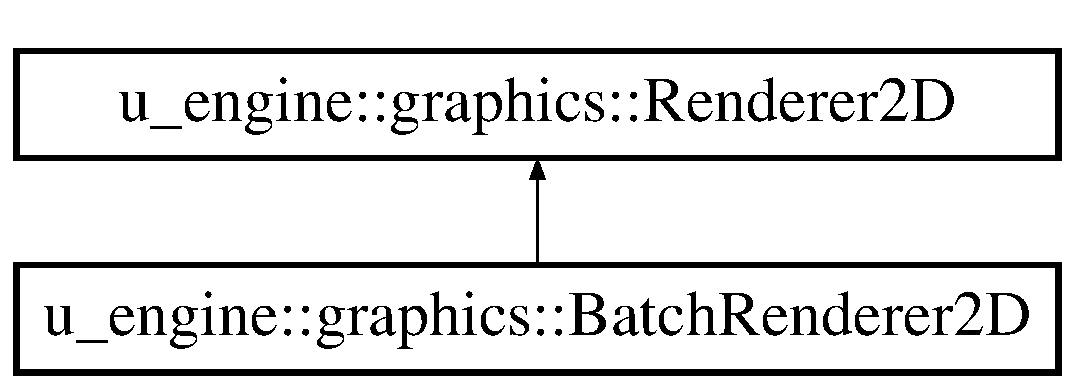
\includegraphics[height=2.000000cm]{classu__engine_1_1graphics_1_1_batch_renderer2_d}
\end{center}
\end{figure}
\subsection*{Public Member Functions}
\begin{DoxyCompactItemize}
\item 
\hyperlink{classu__engine_1_1graphics_1_1_batch_renderer2_d_a8cfb6ce4b560b3a1dede2b4ff0dee650}{Batch\+Renderer2\+D} ()
\item 
\hyperlink{classu__engine_1_1graphics_1_1_batch_renderer2_d_a0e49da8a08355e100e86ee3ef0f888cc}{$\sim$\+Batch\+Renderer2\+D} ()
\item 
\hyperlink{wglew_8h_aeea6e3dfae3acf232096f57d2d57f084}{void} \hyperlink{classu__engine_1_1graphics_1_1_batch_renderer2_d_aa00e0dde727955d2911530fb7d0a53df}{begin} ()
\item 
\hyperlink{wglew_8h_aeea6e3dfae3acf232096f57d2d57f084}{void} \hyperlink{classu__engine_1_1graphics_1_1_batch_renderer2_d_a74a8a92bdf3170a3adbbeebbe9ef8a06}{submit} (const \hyperlink{classu__engine_1_1graphics_1_1_renderable2_d}{Renderable2\+D} $\ast$renderable) override
\item 
\hyperlink{wglew_8h_aeea6e3dfae3acf232096f57d2d57f084}{void} \hyperlink{classu__engine_1_1graphics_1_1_batch_renderer2_d_a587a1e9091632c90b1706ac5a779d3d4}{end} ()
\item 
\hyperlink{wglew_8h_aeea6e3dfae3acf232096f57d2d57f084}{void} \hyperlink{classu__engine_1_1graphics_1_1_batch_renderer2_d_a6f95ef0c0a94e1df2b94efa662babd15}{flush} () override
\end{DoxyCompactItemize}


\subsection{Detailed Description}


Definition at line 18 of file Batch\+Renderer2\+D.\+h.



\subsection{Constructor \& Destructor Documentation}
\hypertarget{classu__engine_1_1graphics_1_1_batch_renderer2_d_a8cfb6ce4b560b3a1dede2b4ff0dee650}{}\index{u\+\_\+engine\+::graphics\+::\+Batch\+Renderer2\+D@{u\+\_\+engine\+::graphics\+::\+Batch\+Renderer2\+D}!Batch\+Renderer2\+D@{Batch\+Renderer2\+D}}
\index{Batch\+Renderer2\+D@{Batch\+Renderer2\+D}!u\+\_\+engine\+::graphics\+::\+Batch\+Renderer2\+D@{u\+\_\+engine\+::graphics\+::\+Batch\+Renderer2\+D}}
\subsubsection[{Batch\+Renderer2\+D()}]{\setlength{\rightskip}{0pt plus 5cm}u\+\_\+engine\+::graphics\+::\+Batch\+Renderer2\+D\+::\+Batch\+Renderer2\+D (
\begin{DoxyParamCaption}
{}
\end{DoxyParamCaption}
)}\label{classu__engine_1_1graphics_1_1_batch_renderer2_d_a8cfb6ce4b560b3a1dede2b4ff0dee650}


Definition at line 5 of file Batch\+Renderer2\+D.\+cpp.

\hypertarget{classu__engine_1_1graphics_1_1_batch_renderer2_d_a0e49da8a08355e100e86ee3ef0f888cc}{}\index{u\+\_\+engine\+::graphics\+::\+Batch\+Renderer2\+D@{u\+\_\+engine\+::graphics\+::\+Batch\+Renderer2\+D}!````~Batch\+Renderer2\+D@{$\sim$\+Batch\+Renderer2\+D}}
\index{````~Batch\+Renderer2\+D@{$\sim$\+Batch\+Renderer2\+D}!u\+\_\+engine\+::graphics\+::\+Batch\+Renderer2\+D@{u\+\_\+engine\+::graphics\+::\+Batch\+Renderer2\+D}}
\subsubsection[{$\sim$\+Batch\+Renderer2\+D()}]{\setlength{\rightskip}{0pt plus 5cm}u\+\_\+engine\+::graphics\+::\+Batch\+Renderer2\+D\+::$\sim$\+Batch\+Renderer2\+D (
\begin{DoxyParamCaption}
{}
\end{DoxyParamCaption}
)}\label{classu__engine_1_1graphics_1_1_batch_renderer2_d_a0e49da8a08355e100e86ee3ef0f888cc}


Definition at line 10 of file Batch\+Renderer2\+D.\+cpp.



\subsection{Member Function Documentation}
\hypertarget{classu__engine_1_1graphics_1_1_batch_renderer2_d_aa00e0dde727955d2911530fb7d0a53df}{}\index{u\+\_\+engine\+::graphics\+::\+Batch\+Renderer2\+D@{u\+\_\+engine\+::graphics\+::\+Batch\+Renderer2\+D}!begin@{begin}}
\index{begin@{begin}!u\+\_\+engine\+::graphics\+::\+Batch\+Renderer2\+D@{u\+\_\+engine\+::graphics\+::\+Batch\+Renderer2\+D}}
\subsubsection[{begin()}]{\setlength{\rightskip}{0pt plus 5cm}{\bf void} u\+\_\+engine\+::graphics\+::\+Batch\+Renderer2\+D\+::begin (
\begin{DoxyParamCaption}
{}
\end{DoxyParamCaption}
)}\label{classu__engine_1_1graphics_1_1_batch_renderer2_d_aa00e0dde727955d2911530fb7d0a53df}


Definition at line 55 of file Batch\+Renderer2\+D.\+cpp.

\hypertarget{classu__engine_1_1graphics_1_1_batch_renderer2_d_a587a1e9091632c90b1706ac5a779d3d4}{}\index{u\+\_\+engine\+::graphics\+::\+Batch\+Renderer2\+D@{u\+\_\+engine\+::graphics\+::\+Batch\+Renderer2\+D}!end@{end}}
\index{end@{end}!u\+\_\+engine\+::graphics\+::\+Batch\+Renderer2\+D@{u\+\_\+engine\+::graphics\+::\+Batch\+Renderer2\+D}}
\subsubsection[{end()}]{\setlength{\rightskip}{0pt plus 5cm}{\bf void} u\+\_\+engine\+::graphics\+::\+Batch\+Renderer2\+D\+::end (
\begin{DoxyParamCaption}
{}
\end{DoxyParamCaption}
)}\label{classu__engine_1_1graphics_1_1_batch_renderer2_d_a587a1e9091632c90b1706ac5a779d3d4}


Definition at line 93 of file Batch\+Renderer2\+D.\+cpp.

\hypertarget{classu__engine_1_1graphics_1_1_batch_renderer2_d_a6f95ef0c0a94e1df2b94efa662babd15}{}\index{u\+\_\+engine\+::graphics\+::\+Batch\+Renderer2\+D@{u\+\_\+engine\+::graphics\+::\+Batch\+Renderer2\+D}!flush@{flush}}
\index{flush@{flush}!u\+\_\+engine\+::graphics\+::\+Batch\+Renderer2\+D@{u\+\_\+engine\+::graphics\+::\+Batch\+Renderer2\+D}}
\subsubsection[{flush() override}]{\setlength{\rightskip}{0pt plus 5cm}{\bf void} u\+\_\+engine\+::graphics\+::\+Batch\+Renderer2\+D\+::flush (
\begin{DoxyParamCaption}
{}
\end{DoxyParamCaption}
)\hspace{0.3cm}{\ttfamily [override]}, {\ttfamily [virtual]}}\label{classu__engine_1_1graphics_1_1_batch_renderer2_d_a6f95ef0c0a94e1df2b94efa662babd15}


Implements \hyperlink{classu__engine_1_1graphics_1_1_renderer2_d_a922880dea9292d4e973c2e2da22b9964}{u\+\_\+engine\+::graphics\+::\+Renderer2\+D}.



Definition at line 99 of file Batch\+Renderer2\+D.\+cpp.

\hypertarget{classu__engine_1_1graphics_1_1_batch_renderer2_d_a74a8a92bdf3170a3adbbeebbe9ef8a06}{}\index{u\+\_\+engine\+::graphics\+::\+Batch\+Renderer2\+D@{u\+\_\+engine\+::graphics\+::\+Batch\+Renderer2\+D}!submit@{submit}}
\index{submit@{submit}!u\+\_\+engine\+::graphics\+::\+Batch\+Renderer2\+D@{u\+\_\+engine\+::graphics\+::\+Batch\+Renderer2\+D}}
\subsubsection[{submit(const Renderable2\+D $\ast$renderable) override}]{\setlength{\rightskip}{0pt plus 5cm}{\bf void} u\+\_\+engine\+::graphics\+::\+Batch\+Renderer2\+D\+::submit (
\begin{DoxyParamCaption}
\item[{const {\bf Renderable2\+D} $\ast$}]{renderable}
\end{DoxyParamCaption}
)\hspace{0.3cm}{\ttfamily [override]}, {\ttfamily [virtual]}}\label{classu__engine_1_1graphics_1_1_batch_renderer2_d_a74a8a92bdf3170a3adbbeebbe9ef8a06}


Implements \hyperlink{classu__engine_1_1graphics_1_1_renderer2_d_ae78a8a0ff8fc052f3cef4c24c9c829f7}{u\+\_\+engine\+::graphics\+::\+Renderer2\+D}.



Definition at line 60 of file Batch\+Renderer2\+D.\+cpp.



The documentation for this class was generated from the following files\+:\begin{DoxyCompactItemize}
\item 
G\+:/\+Libraries/\+V\+S\+Projects/\+Untitled\+Game/\+Unicity\+Engine/\+Unicity/src/graphics/\hyperlink{_batch_renderer2_d_8h}{Batch\+Renderer2\+D.\+h}\item 
G\+:/\+Libraries/\+V\+S\+Projects/\+Untitled\+Game/\+Unicity\+Engine/\+Unicity/src/graphics/\hyperlink{_batch_renderer2_d_8cpp}{Batch\+Renderer2\+D.\+cpp}\end{DoxyCompactItemize}

\hypertarget{classu__engine_1_1graphics_1_1_buffer}{}\section{u\+\_\+engine\+:\+:graphics\+:\+:Buffer Class Reference}
\label{classu__engine_1_1graphics_1_1_buffer}\index{u\+\_\+engine\+::graphics\+::\+Buffer@{u\+\_\+engine\+::graphics\+::\+Buffer}}


{\ttfamily \#include $<$buffer.\+h$>$}

\subsection*{Public Member Functions}
\begin{DoxyCompactItemize}
\item 
\hyperlink{classu__engine_1_1graphics_1_1_buffer_aa496e84b82db2b2a922858dba75c1ce7}{Buffer} (\hyperlink{glew_8h_a31aeedaeef29442c9c015ab355c8f5ab}{G\+Lfloat} $\ast$\hyperlink{glew_8h_a42c2b1d86fa71a425e73a882cb0a72c8}{data}, \hyperlink{glew_8h_a9289d5b99dc1f27f01480360f2e18ae0}{G\+Lsizei} \hyperlink{glew_8h_a10b284d589000663becfbc6867a3a9f7}{count}, \hyperlink{glew_8h_a68c4714e43d8e827d80759f9cb864f3c}{G\+Luint} component\+Count)
\item 
\hyperlink{classu__engine_1_1graphics_1_1_buffer_a1fe1afaa80fb1750b09d3fea3adb9bb1}{$\sim$\+Buffer} ()
\item 
\hyperlink{wglew_8h_aeea6e3dfae3acf232096f57d2d57f084}{void} \hyperlink{classu__engine_1_1graphics_1_1_buffer_a6cf68a13d51b6e4d0269891e462d32de}{bind} () const 
\item 
\hyperlink{wglew_8h_aeea6e3dfae3acf232096f57d2d57f084}{void} \hyperlink{classu__engine_1_1graphics_1_1_buffer_ad125dcdf5b527d0b334052b82cf716f3}{unbind} () const 
\item 
\hyperlink{glew_8h_a68c4714e43d8e827d80759f9cb864f3c}{G\+Luint} \hyperlink{classu__engine_1_1graphics_1_1_buffer_a9fe4116e0732d160bd0586a3b872b889}{get\+Component\+Count} () const 
\end{DoxyCompactItemize}


\subsection{Detailed Description}


Definition at line 6 of file buffer.\+h.



\subsection{Constructor \& Destructor Documentation}
\hypertarget{classu__engine_1_1graphics_1_1_buffer_aa496e84b82db2b2a922858dba75c1ce7}{}\index{u\+\_\+engine\+::graphics\+::\+Buffer@{u\+\_\+engine\+::graphics\+::\+Buffer}!Buffer@{Buffer}}
\index{Buffer@{Buffer}!u\+\_\+engine\+::graphics\+::\+Buffer@{u\+\_\+engine\+::graphics\+::\+Buffer}}
\subsubsection[{Buffer(\+G\+Lfloat $\ast$data, G\+Lsizei count, G\+Luint component\+Count)}]{\setlength{\rightskip}{0pt plus 5cm}u\+\_\+engine\+::graphics\+::\+Buffer\+::\+Buffer (
\begin{DoxyParamCaption}
\item[{{\bf G\+Lfloat} $\ast$}]{data, }
\item[{{\bf G\+Lsizei}}]{count, }
\item[{{\bf G\+Luint}}]{component\+Count}
\end{DoxyParamCaption}
)}\label{classu__engine_1_1graphics_1_1_buffer_aa496e84b82db2b2a922858dba75c1ce7}


Definition at line 5 of file buffer.\+cpp.

\hypertarget{classu__engine_1_1graphics_1_1_buffer_a1fe1afaa80fb1750b09d3fea3adb9bb1}{}\index{u\+\_\+engine\+::graphics\+::\+Buffer@{u\+\_\+engine\+::graphics\+::\+Buffer}!````~Buffer@{$\sim$\+Buffer}}
\index{````~Buffer@{$\sim$\+Buffer}!u\+\_\+engine\+::graphics\+::\+Buffer@{u\+\_\+engine\+::graphics\+::\+Buffer}}
\subsubsection[{$\sim$\+Buffer()}]{\setlength{\rightskip}{0pt plus 5cm}u\+\_\+engine\+::graphics\+::\+Buffer\+::$\sim$\+Buffer (
\begin{DoxyParamCaption}
{}
\end{DoxyParamCaption}
)}\label{classu__engine_1_1graphics_1_1_buffer_a1fe1afaa80fb1750b09d3fea3adb9bb1}


Definition at line 14 of file buffer.\+cpp.



\subsection{Member Function Documentation}
\hypertarget{classu__engine_1_1graphics_1_1_buffer_a6cf68a13d51b6e4d0269891e462d32de}{}\index{u\+\_\+engine\+::graphics\+::\+Buffer@{u\+\_\+engine\+::graphics\+::\+Buffer}!bind@{bind}}
\index{bind@{bind}!u\+\_\+engine\+::graphics\+::\+Buffer@{u\+\_\+engine\+::graphics\+::\+Buffer}}
\subsubsection[{bind() const }]{\setlength{\rightskip}{0pt plus 5cm}{\bf void} u\+\_\+engine\+::graphics\+::\+Buffer\+::bind (
\begin{DoxyParamCaption}
{}
\end{DoxyParamCaption}
) const}\label{classu__engine_1_1graphics_1_1_buffer_a6cf68a13d51b6e4d0269891e462d32de}


Definition at line 19 of file buffer.\+cpp.

\hypertarget{classu__engine_1_1graphics_1_1_buffer_a9fe4116e0732d160bd0586a3b872b889}{}\index{u\+\_\+engine\+::graphics\+::\+Buffer@{u\+\_\+engine\+::graphics\+::\+Buffer}!get\+Component\+Count@{get\+Component\+Count}}
\index{get\+Component\+Count@{get\+Component\+Count}!u\+\_\+engine\+::graphics\+::\+Buffer@{u\+\_\+engine\+::graphics\+::\+Buffer}}
\subsubsection[{get\+Component\+Count() const }]{\setlength{\rightskip}{0pt plus 5cm}{\bf G\+Luint} u\+\_\+engine\+::graphics\+::\+Buffer\+::get\+Component\+Count (
\begin{DoxyParamCaption}
{}
\end{DoxyParamCaption}
) const\hspace{0.3cm}{\ttfamily [inline]}}\label{classu__engine_1_1graphics_1_1_buffer_a9fe4116e0732d160bd0586a3b872b889}


Definition at line 19 of file buffer.\+h.

\hypertarget{classu__engine_1_1graphics_1_1_buffer_ad125dcdf5b527d0b334052b82cf716f3}{}\index{u\+\_\+engine\+::graphics\+::\+Buffer@{u\+\_\+engine\+::graphics\+::\+Buffer}!unbind@{unbind}}
\index{unbind@{unbind}!u\+\_\+engine\+::graphics\+::\+Buffer@{u\+\_\+engine\+::graphics\+::\+Buffer}}
\subsubsection[{unbind() const }]{\setlength{\rightskip}{0pt plus 5cm}{\bf void} u\+\_\+engine\+::graphics\+::\+Buffer\+::unbind (
\begin{DoxyParamCaption}
{}
\end{DoxyParamCaption}
) const}\label{classu__engine_1_1graphics_1_1_buffer_ad125dcdf5b527d0b334052b82cf716f3}


Definition at line 25 of file buffer.\+cpp.



The documentation for this class was generated from the following files\+:\begin{DoxyCompactItemize}
\item 
G\+:/\+Libraries/\+V\+S\+Projects/\+Untitled\+Game/\+Unicity\+Engine/\+Unicity/src/graphics/buffers/\hyperlink{buffer_8h}{buffer.\+h}\item 
G\+:/\+Libraries/\+V\+S\+Projects/\+Untitled\+Game/\+Unicity\+Engine/\+Unicity/src/graphics/buffers/\hyperlink{buffer_8cpp}{buffer.\+cpp}\end{DoxyCompactItemize}

\hypertarget{classu__engine_1_1_file_utils}{}\section{u\+\_\+engine\+:\+:File\+Utils Class Reference}
\label{classu__engine_1_1_file_utils}\index{u\+\_\+engine\+::\+File\+Utils@{u\+\_\+engine\+::\+File\+Utils}}


{\ttfamily \#include $<$fileutils.\+h$>$}

\subsection*{Static Public Member Functions}
\begin{DoxyCompactItemize}
\item 
static \hyperlink{glew_8h_ae84541b4f3d8e1ea24ec0f466a8c568b}{std\+::string} \hyperlink{classu__engine_1_1_file_utils_a71e33a98fa60990a89878e832740c0ca}{read\+\_\+file} (const char $\ast$filepath)
\end{DoxyCompactItemize}


\subsection{Detailed Description}


Definition at line 8 of file fileutils.\+h.



\subsection{Member Function Documentation}
\hypertarget{classu__engine_1_1_file_utils_a71e33a98fa60990a89878e832740c0ca}{}\index{u\+\_\+engine\+::\+File\+Utils@{u\+\_\+engine\+::\+File\+Utils}!read\+\_\+file@{read\+\_\+file}}
\index{read\+\_\+file@{read\+\_\+file}!u\+\_\+engine\+::\+File\+Utils@{u\+\_\+engine\+::\+File\+Utils}}
\subsubsection[{read\+\_\+file(const char $\ast$filepath)}]{\setlength{\rightskip}{0pt plus 5cm}static {\bf std\+::string} u\+\_\+engine\+::\+File\+Utils\+::read\+\_\+file (
\begin{DoxyParamCaption}
\item[{const char $\ast$}]{filepath}
\end{DoxyParamCaption}
)\hspace{0.3cm}{\ttfamily [inline]}, {\ttfamily [static]}}\label{classu__engine_1_1_file_utils_a71e33a98fa60990a89878e832740c0ca}


Definition at line 10 of file fileutils.\+h.



The documentation for this class was generated from the following file\+:\begin{DoxyCompactItemize}
\item 
G\+:/\+Libraries/\+V\+S\+Projects/\+Untitled\+Game/\+Unicity\+Engine/\+Unicity/src/utils/\hyperlink{fileutils_8h}{fileutils.\+h}\end{DoxyCompactItemize}

\hypertarget{struct_g_l_f_wgammaramp}{}\section{G\+L\+F\+Wgammaramp Struct Reference}
\label{struct_g_l_f_wgammaramp}\index{G\+L\+F\+Wgammaramp@{G\+L\+F\+Wgammaramp}}


Gamma ramp.  




{\ttfamily \#include $<$glfw3.\+h$>$}

\subsection*{Public Attributes}
\begin{DoxyCompactItemize}
\item 
unsigned short $\ast$ \hyperlink{struct_g_l_f_wgammaramp_a2cce5d968734b685623eef913e635138}{red}
\item 
unsigned short $\ast$ \hyperlink{struct_g_l_f_wgammaramp_affccc6f5df47820b6562d709da3a5a3a}{green}
\item 
unsigned short $\ast$ \hyperlink{struct_g_l_f_wgammaramp_acf0c836d0efe29c392fe8d1a1042744b}{blue}
\item 
unsigned \hyperlink{wglew_8h_a500a82aecba06f4550f6849b8099ca21}{int} \hyperlink{struct_g_l_f_wgammaramp_ad620e1cffbff9a32c51bca46301b59a5}{size}
\end{DoxyCompactItemize}


\subsection{Detailed Description}
Gamma ramp. 

This describes the gamma ramp for a monitor.

\begin{DoxySeeAlso}{See also}
\hyperlink{group__monitor_gaeeac9198f3c91b83440eed679441f76b}{glfw\+Get\+Gamma\+Ramp} \hyperlink{group__monitor_gac9f36a1cfa10eab191d3029ea8bc9558}{glfw\+Set\+Gamma\+Ramp} 
\end{DoxySeeAlso}


Definition at line 1013 of file glfw3.\+h.



\subsection{Member Data Documentation}
\hypertarget{struct_g_l_f_wgammaramp_acf0c836d0efe29c392fe8d1a1042744b}{}\index{G\+L\+F\+Wgammaramp@{G\+L\+F\+Wgammaramp}!blue@{blue}}
\index{blue@{blue}!G\+L\+F\+Wgammaramp@{G\+L\+F\+Wgammaramp}}
\subsubsection[{blue}]{\setlength{\rightskip}{0pt plus 5cm}unsigned short$\ast$ G\+L\+F\+Wgammaramp\+::blue}\label{struct_g_l_f_wgammaramp_acf0c836d0efe29c392fe8d1a1042744b}
An array of value describing the response of the blue channel. 

Definition at line 1023 of file glfw3.\+h.

\hypertarget{struct_g_l_f_wgammaramp_affccc6f5df47820b6562d709da3a5a3a}{}\index{G\+L\+F\+Wgammaramp@{G\+L\+F\+Wgammaramp}!green@{green}}
\index{green@{green}!G\+L\+F\+Wgammaramp@{G\+L\+F\+Wgammaramp}}
\subsubsection[{green}]{\setlength{\rightskip}{0pt plus 5cm}unsigned short$\ast$ G\+L\+F\+Wgammaramp\+::green}\label{struct_g_l_f_wgammaramp_affccc6f5df47820b6562d709da3a5a3a}
An array of value describing the response of the green channel. 

Definition at line 1020 of file glfw3.\+h.

\hypertarget{struct_g_l_f_wgammaramp_a2cce5d968734b685623eef913e635138}{}\index{G\+L\+F\+Wgammaramp@{G\+L\+F\+Wgammaramp}!red@{red}}
\index{red@{red}!G\+L\+F\+Wgammaramp@{G\+L\+F\+Wgammaramp}}
\subsubsection[{red}]{\setlength{\rightskip}{0pt plus 5cm}unsigned short$\ast$ G\+L\+F\+Wgammaramp\+::red}\label{struct_g_l_f_wgammaramp_a2cce5d968734b685623eef913e635138}
An array of value describing the response of the red channel. 

Definition at line 1017 of file glfw3.\+h.

\hypertarget{struct_g_l_f_wgammaramp_ad620e1cffbff9a32c51bca46301b59a5}{}\index{G\+L\+F\+Wgammaramp@{G\+L\+F\+Wgammaramp}!size@{size}}
\index{size@{size}!G\+L\+F\+Wgammaramp@{G\+L\+F\+Wgammaramp}}
\subsubsection[{size}]{\setlength{\rightskip}{0pt plus 5cm}unsigned {\bf int} G\+L\+F\+Wgammaramp\+::size}\label{struct_g_l_f_wgammaramp_ad620e1cffbff9a32c51bca46301b59a5}
The number of elements in each array. 

Definition at line 1026 of file glfw3.\+h.



The documentation for this struct was generated from the following file\+:\begin{DoxyCompactItemize}
\item 
G\+:/\+Libraries/\+V\+S\+Projects/\+Untitled\+Engine/\+Dependencies/include/\hyperlink{glfw3_8h}{glfw3.\+h}\end{DoxyCompactItemize}

\hypertarget{struct_g_l_f_wimage}{}\section{G\+L\+F\+Wimage Struct Reference}
\label{struct_g_l_f_wimage}\index{G\+L\+F\+Wimage@{G\+L\+F\+Wimage}}


Image data.  




{\ttfamily \#include $<$glfw3.\+h$>$}

\subsection*{Public Attributes}
\begin{DoxyCompactItemize}
\item 
\hyperlink{wglew_8h_a500a82aecba06f4550f6849b8099ca21}{int} \hyperlink{struct_g_l_f_wimage_af6a71cc999fe6d3aea31dd7e9687d835}{width}
\item 
\hyperlink{wglew_8h_a500a82aecba06f4550f6849b8099ca21}{int} \hyperlink{struct_g_l_f_wimage_a0b7d95368f0c80d5e5c9875057c7dbec}{height}
\item 
unsigned char $\ast$ \hyperlink{struct_g_l_f_wimage_a0c532a5c2bb715555279b7817daba0fb}{pixels}
\end{DoxyCompactItemize}


\subsection{Detailed Description}
Image data. 

Definition at line 1031 of file glfw3.\+h.



\subsection{Member Data Documentation}
\hypertarget{struct_g_l_f_wimage_a0b7d95368f0c80d5e5c9875057c7dbec}{}\index{G\+L\+F\+Wimage@{G\+L\+F\+Wimage}!height@{height}}
\index{height@{height}!G\+L\+F\+Wimage@{G\+L\+F\+Wimage}}
\subsubsection[{height}]{\setlength{\rightskip}{0pt plus 5cm}{\bf int} G\+L\+F\+Wimage\+::height}\label{struct_g_l_f_wimage_a0b7d95368f0c80d5e5c9875057c7dbec}
The height, in pixels, of this image. 

Definition at line 1038 of file glfw3.\+h.

\hypertarget{struct_g_l_f_wimage_a0c532a5c2bb715555279b7817daba0fb}{}\index{G\+L\+F\+Wimage@{G\+L\+F\+Wimage}!pixels@{pixels}}
\index{pixels@{pixels}!G\+L\+F\+Wimage@{G\+L\+F\+Wimage}}
\subsubsection[{pixels}]{\setlength{\rightskip}{0pt plus 5cm}unsigned char$\ast$ G\+L\+F\+Wimage\+::pixels}\label{struct_g_l_f_wimage_a0c532a5c2bb715555279b7817daba0fb}
The pixel data of this image, arranged left-\/to-\/right, top-\/to-\/bottom. 

Definition at line 1041 of file glfw3.\+h.

\hypertarget{struct_g_l_f_wimage_af6a71cc999fe6d3aea31dd7e9687d835}{}\index{G\+L\+F\+Wimage@{G\+L\+F\+Wimage}!width@{width}}
\index{width@{width}!G\+L\+F\+Wimage@{G\+L\+F\+Wimage}}
\subsubsection[{width}]{\setlength{\rightskip}{0pt plus 5cm}{\bf int} G\+L\+F\+Wimage\+::width}\label{struct_g_l_f_wimage_af6a71cc999fe6d3aea31dd7e9687d835}
The width, in pixels, of this image. 

Definition at line 1035 of file glfw3.\+h.



The documentation for this struct was generated from the following file\+:\begin{DoxyCompactItemize}
\item 
G\+:/\+Libraries/\+V\+S\+Projects/\+Untitled\+Game/\+Unicity\+Engine/\+Dependencies/include/\hyperlink{glfw3_8h}{glfw3.\+h}\end{DoxyCompactItemize}

\hypertarget{struct_g_l_f_wvidmode}{}\section{G\+L\+F\+Wvidmode Struct Reference}
\label{struct_g_l_f_wvidmode}\index{G\+L\+F\+Wvidmode@{G\+L\+F\+Wvidmode}}


Video mode type.  




{\ttfamily \#include $<$glfw3.\+h$>$}

\subsection*{Public Attributes}
\begin{DoxyCompactItemize}
\item 
\hyperlink{wglew_8h_a500a82aecba06f4550f6849b8099ca21}{int} \hyperlink{struct_g_l_f_wvidmode_a698dcb200562051a7249cb6ae154c71d}{width}
\item 
\hyperlink{wglew_8h_a500a82aecba06f4550f6849b8099ca21}{int} \hyperlink{struct_g_l_f_wvidmode_ac65942a5f6981695517437a9d571d03c}{height}
\item 
\hyperlink{wglew_8h_a500a82aecba06f4550f6849b8099ca21}{int} \hyperlink{struct_g_l_f_wvidmode_a6066c4ecd251098700062d3b735dba1b}{red\+Bits}
\item 
\hyperlink{wglew_8h_a500a82aecba06f4550f6849b8099ca21}{int} \hyperlink{struct_g_l_f_wvidmode_a292fdd281f3485fb3ff102a5bda43faa}{green\+Bits}
\item 
\hyperlink{wglew_8h_a500a82aecba06f4550f6849b8099ca21}{int} \hyperlink{struct_g_l_f_wvidmode_af310977f58d2e3b188175b6e3d314047}{blue\+Bits}
\item 
\hyperlink{wglew_8h_a500a82aecba06f4550f6849b8099ca21}{int} \hyperlink{struct_g_l_f_wvidmode_a791bdd6c7697b09f7e9c97054bf05649}{refresh\+Rate}
\end{DoxyCompactItemize}


\subsection{Detailed Description}
Video mode type. 

This describes a single video mode. 

Definition at line 983 of file glfw3.\+h.



\subsection{Member Data Documentation}
\hypertarget{struct_g_l_f_wvidmode_af310977f58d2e3b188175b6e3d314047}{}\index{G\+L\+F\+Wvidmode@{G\+L\+F\+Wvidmode}!blue\+Bits@{blue\+Bits}}
\index{blue\+Bits@{blue\+Bits}!G\+L\+F\+Wvidmode@{G\+L\+F\+Wvidmode}}
\subsubsection[{blue\+Bits}]{\setlength{\rightskip}{0pt plus 5cm}{\bf int} G\+L\+F\+Wvidmode\+::blue\+Bits}\label{struct_g_l_f_wvidmode_af310977f58d2e3b188175b6e3d314047}
The bit depth of the blue channel of the video mode. 

Definition at line 999 of file glfw3.\+h.

\hypertarget{struct_g_l_f_wvidmode_a292fdd281f3485fb3ff102a5bda43faa}{}\index{G\+L\+F\+Wvidmode@{G\+L\+F\+Wvidmode}!green\+Bits@{green\+Bits}}
\index{green\+Bits@{green\+Bits}!G\+L\+F\+Wvidmode@{G\+L\+F\+Wvidmode}}
\subsubsection[{green\+Bits}]{\setlength{\rightskip}{0pt plus 5cm}{\bf int} G\+L\+F\+Wvidmode\+::green\+Bits}\label{struct_g_l_f_wvidmode_a292fdd281f3485fb3ff102a5bda43faa}
The bit depth of the green channel of the video mode. 

Definition at line 996 of file glfw3.\+h.

\hypertarget{struct_g_l_f_wvidmode_ac65942a5f6981695517437a9d571d03c}{}\index{G\+L\+F\+Wvidmode@{G\+L\+F\+Wvidmode}!height@{height}}
\index{height@{height}!G\+L\+F\+Wvidmode@{G\+L\+F\+Wvidmode}}
\subsubsection[{height}]{\setlength{\rightskip}{0pt plus 5cm}{\bf int} G\+L\+F\+Wvidmode\+::height}\label{struct_g_l_f_wvidmode_ac65942a5f6981695517437a9d571d03c}
The height, in screen coordinates, of the video mode. 

Definition at line 990 of file glfw3.\+h.

\hypertarget{struct_g_l_f_wvidmode_a6066c4ecd251098700062d3b735dba1b}{}\index{G\+L\+F\+Wvidmode@{G\+L\+F\+Wvidmode}!red\+Bits@{red\+Bits}}
\index{red\+Bits@{red\+Bits}!G\+L\+F\+Wvidmode@{G\+L\+F\+Wvidmode}}
\subsubsection[{red\+Bits}]{\setlength{\rightskip}{0pt plus 5cm}{\bf int} G\+L\+F\+Wvidmode\+::red\+Bits}\label{struct_g_l_f_wvidmode_a6066c4ecd251098700062d3b735dba1b}
The bit depth of the red channel of the video mode. 

Definition at line 993 of file glfw3.\+h.

\hypertarget{struct_g_l_f_wvidmode_a791bdd6c7697b09f7e9c97054bf05649}{}\index{G\+L\+F\+Wvidmode@{G\+L\+F\+Wvidmode}!refresh\+Rate@{refresh\+Rate}}
\index{refresh\+Rate@{refresh\+Rate}!G\+L\+F\+Wvidmode@{G\+L\+F\+Wvidmode}}
\subsubsection[{refresh\+Rate}]{\setlength{\rightskip}{0pt plus 5cm}{\bf int} G\+L\+F\+Wvidmode\+::refresh\+Rate}\label{struct_g_l_f_wvidmode_a791bdd6c7697b09f7e9c97054bf05649}
The refresh rate, in Hz, of the video mode. 

Definition at line 1002 of file glfw3.\+h.

\hypertarget{struct_g_l_f_wvidmode_a698dcb200562051a7249cb6ae154c71d}{}\index{G\+L\+F\+Wvidmode@{G\+L\+F\+Wvidmode}!width@{width}}
\index{width@{width}!G\+L\+F\+Wvidmode@{G\+L\+F\+Wvidmode}}
\subsubsection[{width}]{\setlength{\rightskip}{0pt plus 5cm}{\bf int} G\+L\+F\+Wvidmode\+::width}\label{struct_g_l_f_wvidmode_a698dcb200562051a7249cb6ae154c71d}
The width, in screen coordinates, of the video mode. 

Definition at line 987 of file glfw3.\+h.



The documentation for this struct was generated from the following file\+:\begin{DoxyCompactItemize}
\item 
G\+:/\+Libraries/\+V\+S\+Projects/\+Untitled\+Game/\+Unicity\+Engine/\+Dependencies/include/\hyperlink{glfw3_8h}{glfw3.\+h}\end{DoxyCompactItemize}

\hypertarget{struct_g_l_x_buffer_clobber_event_s_g_i_x}{}\section{G\+L\+X\+Buffer\+Clobber\+Event\+S\+G\+I\+X Struct Reference}
\label{struct_g_l_x_buffer_clobber_event_s_g_i_x}\index{G\+L\+X\+Buffer\+Clobber\+Event\+S\+G\+I\+X@{G\+L\+X\+Buffer\+Clobber\+Event\+S\+G\+I\+X}}


{\ttfamily \#include $<$glxew.\+h$>$}

\subsection*{Public Attributes}
\begin{DoxyCompactItemize}
\item 
\hyperlink{wglew_8h_a500a82aecba06f4550f6849b8099ca21}{int} \hyperlink{struct_g_l_x_buffer_clobber_event_s_g_i_x_a36e3e8a5feea664623ea43d0f273b63a}{type}
\item 
unsigned long \hyperlink{struct_g_l_x_buffer_clobber_event_s_g_i_x_ac295e3276a7986eeae4d6a2a28c7e0b7}{serial}
\item 
Bool \hyperlink{struct_g_l_x_buffer_clobber_event_s_g_i_x_af43bf0edbe40a74ef58dfb546a75118b}{send\+\_\+event}
\item 
Display $\ast$ \hyperlink{struct_g_l_x_buffer_clobber_event_s_g_i_x_afef060d81026da75c846727f4a3de9d4}{display}
\item 
\hyperlink{glxew_8h_a826f51745d9d6c81bdbac47ae2b80cf7}{G\+L\+X\+Drawable} \hyperlink{struct_g_l_x_buffer_clobber_event_s_g_i_x_a9c45674193ed80a79261c3b7518ee04f}{drawable}
\item 
\hyperlink{wglew_8h_a500a82aecba06f4550f6849b8099ca21}{int} \hyperlink{struct_g_l_x_buffer_clobber_event_s_g_i_x_a0b405123f1d6528f1f4dfa7ff92bde9b}{event\+\_\+type}
\item 
\hyperlink{wglew_8h_a500a82aecba06f4550f6849b8099ca21}{int} \hyperlink{struct_g_l_x_buffer_clobber_event_s_g_i_x_a25c31e8cbec0919f74a1e93ae74175b1}{draw\+\_\+type}
\item 
unsigned \hyperlink{wglew_8h_a500a82aecba06f4550f6849b8099ca21}{int} \hyperlink{struct_g_l_x_buffer_clobber_event_s_g_i_x_a74b4ad1ad3cac011001151411f621da1}{mask}
\item 
\hyperlink{wglew_8h_a500a82aecba06f4550f6849b8099ca21}{int} \hyperlink{struct_g_l_x_buffer_clobber_event_s_g_i_x_a5118d48c3c8d5253d39922b5014b52ff}{x}
\item 
\hyperlink{wglew_8h_a500a82aecba06f4550f6849b8099ca21}{int} \hyperlink{struct_g_l_x_buffer_clobber_event_s_g_i_x_aef21efa11558a5b67861f96471c56003}{y}
\item 
\hyperlink{wglew_8h_a500a82aecba06f4550f6849b8099ca21}{int} \hyperlink{struct_g_l_x_buffer_clobber_event_s_g_i_x_adad23535733161528427584a42bfc6eb}{width}
\item 
\hyperlink{wglew_8h_a500a82aecba06f4550f6849b8099ca21}{int} \hyperlink{struct_g_l_x_buffer_clobber_event_s_g_i_x_a7838dbabb76c22aa8241310a3f2363ea}{height}
\item 
\hyperlink{wglew_8h_a500a82aecba06f4550f6849b8099ca21}{int} \hyperlink{struct_g_l_x_buffer_clobber_event_s_g_i_x_ad8f4f0aae058e0a1ff542679823e37a9}{count}
\end{DoxyCompactItemize}


\subsection{Detailed Description}


Definition at line 1333 of file glxew.\+h.



\subsection{Member Data Documentation}
\hypertarget{struct_g_l_x_buffer_clobber_event_s_g_i_x_ad8f4f0aae058e0a1ff542679823e37a9}{}\index{G\+L\+X\+Buffer\+Clobber\+Event\+S\+G\+I\+X@{G\+L\+X\+Buffer\+Clobber\+Event\+S\+G\+I\+X}!count@{count}}
\index{count@{count}!G\+L\+X\+Buffer\+Clobber\+Event\+S\+G\+I\+X@{G\+L\+X\+Buffer\+Clobber\+Event\+S\+G\+I\+X}}
\subsubsection[{count}]{\setlength{\rightskip}{0pt plus 5cm}{\bf int} G\+L\+X\+Buffer\+Clobber\+Event\+S\+G\+I\+X\+::count}\label{struct_g_l_x_buffer_clobber_event_s_g_i_x_ad8f4f0aae058e0a1ff542679823e37a9}


Definition at line 1333 of file glxew.\+h.

\hypertarget{struct_g_l_x_buffer_clobber_event_s_g_i_x_afef060d81026da75c846727f4a3de9d4}{}\index{G\+L\+X\+Buffer\+Clobber\+Event\+S\+G\+I\+X@{G\+L\+X\+Buffer\+Clobber\+Event\+S\+G\+I\+X}!display@{display}}
\index{display@{display}!G\+L\+X\+Buffer\+Clobber\+Event\+S\+G\+I\+X@{G\+L\+X\+Buffer\+Clobber\+Event\+S\+G\+I\+X}}
\subsubsection[{display}]{\setlength{\rightskip}{0pt plus 5cm}Display$\ast$ G\+L\+X\+Buffer\+Clobber\+Event\+S\+G\+I\+X\+::display}\label{struct_g_l_x_buffer_clobber_event_s_g_i_x_afef060d81026da75c846727f4a3de9d4}


Definition at line 1333 of file glxew.\+h.

\hypertarget{struct_g_l_x_buffer_clobber_event_s_g_i_x_a25c31e8cbec0919f74a1e93ae74175b1}{}\index{G\+L\+X\+Buffer\+Clobber\+Event\+S\+G\+I\+X@{G\+L\+X\+Buffer\+Clobber\+Event\+S\+G\+I\+X}!draw\+\_\+type@{draw\+\_\+type}}
\index{draw\+\_\+type@{draw\+\_\+type}!G\+L\+X\+Buffer\+Clobber\+Event\+S\+G\+I\+X@{G\+L\+X\+Buffer\+Clobber\+Event\+S\+G\+I\+X}}
\subsubsection[{draw\+\_\+type}]{\setlength{\rightskip}{0pt plus 5cm}{\bf int} G\+L\+X\+Buffer\+Clobber\+Event\+S\+G\+I\+X\+::draw\+\_\+type}\label{struct_g_l_x_buffer_clobber_event_s_g_i_x_a25c31e8cbec0919f74a1e93ae74175b1}


Definition at line 1333 of file glxew.\+h.

\hypertarget{struct_g_l_x_buffer_clobber_event_s_g_i_x_a9c45674193ed80a79261c3b7518ee04f}{}\index{G\+L\+X\+Buffer\+Clobber\+Event\+S\+G\+I\+X@{G\+L\+X\+Buffer\+Clobber\+Event\+S\+G\+I\+X}!drawable@{drawable}}
\index{drawable@{drawable}!G\+L\+X\+Buffer\+Clobber\+Event\+S\+G\+I\+X@{G\+L\+X\+Buffer\+Clobber\+Event\+S\+G\+I\+X}}
\subsubsection[{drawable}]{\setlength{\rightskip}{0pt plus 5cm}{\bf G\+L\+X\+Drawable} G\+L\+X\+Buffer\+Clobber\+Event\+S\+G\+I\+X\+::drawable}\label{struct_g_l_x_buffer_clobber_event_s_g_i_x_a9c45674193ed80a79261c3b7518ee04f}


Definition at line 1333 of file glxew.\+h.

\hypertarget{struct_g_l_x_buffer_clobber_event_s_g_i_x_a0b405123f1d6528f1f4dfa7ff92bde9b}{}\index{G\+L\+X\+Buffer\+Clobber\+Event\+S\+G\+I\+X@{G\+L\+X\+Buffer\+Clobber\+Event\+S\+G\+I\+X}!event\+\_\+type@{event\+\_\+type}}
\index{event\+\_\+type@{event\+\_\+type}!G\+L\+X\+Buffer\+Clobber\+Event\+S\+G\+I\+X@{G\+L\+X\+Buffer\+Clobber\+Event\+S\+G\+I\+X}}
\subsubsection[{event\+\_\+type}]{\setlength{\rightskip}{0pt plus 5cm}{\bf int} G\+L\+X\+Buffer\+Clobber\+Event\+S\+G\+I\+X\+::event\+\_\+type}\label{struct_g_l_x_buffer_clobber_event_s_g_i_x_a0b405123f1d6528f1f4dfa7ff92bde9b}


Definition at line 1333 of file glxew.\+h.

\hypertarget{struct_g_l_x_buffer_clobber_event_s_g_i_x_a7838dbabb76c22aa8241310a3f2363ea}{}\index{G\+L\+X\+Buffer\+Clobber\+Event\+S\+G\+I\+X@{G\+L\+X\+Buffer\+Clobber\+Event\+S\+G\+I\+X}!height@{height}}
\index{height@{height}!G\+L\+X\+Buffer\+Clobber\+Event\+S\+G\+I\+X@{G\+L\+X\+Buffer\+Clobber\+Event\+S\+G\+I\+X}}
\subsubsection[{height}]{\setlength{\rightskip}{0pt plus 5cm}{\bf int} G\+L\+X\+Buffer\+Clobber\+Event\+S\+G\+I\+X\+::height}\label{struct_g_l_x_buffer_clobber_event_s_g_i_x_a7838dbabb76c22aa8241310a3f2363ea}


Definition at line 1333 of file glxew.\+h.

\hypertarget{struct_g_l_x_buffer_clobber_event_s_g_i_x_a74b4ad1ad3cac011001151411f621da1}{}\index{G\+L\+X\+Buffer\+Clobber\+Event\+S\+G\+I\+X@{G\+L\+X\+Buffer\+Clobber\+Event\+S\+G\+I\+X}!mask@{mask}}
\index{mask@{mask}!G\+L\+X\+Buffer\+Clobber\+Event\+S\+G\+I\+X@{G\+L\+X\+Buffer\+Clobber\+Event\+S\+G\+I\+X}}
\subsubsection[{mask}]{\setlength{\rightskip}{0pt plus 5cm}unsigned {\bf int} G\+L\+X\+Buffer\+Clobber\+Event\+S\+G\+I\+X\+::mask}\label{struct_g_l_x_buffer_clobber_event_s_g_i_x_a74b4ad1ad3cac011001151411f621da1}


Definition at line 1333 of file glxew.\+h.

\hypertarget{struct_g_l_x_buffer_clobber_event_s_g_i_x_af43bf0edbe40a74ef58dfb546a75118b}{}\index{G\+L\+X\+Buffer\+Clobber\+Event\+S\+G\+I\+X@{G\+L\+X\+Buffer\+Clobber\+Event\+S\+G\+I\+X}!send\+\_\+event@{send\+\_\+event}}
\index{send\+\_\+event@{send\+\_\+event}!G\+L\+X\+Buffer\+Clobber\+Event\+S\+G\+I\+X@{G\+L\+X\+Buffer\+Clobber\+Event\+S\+G\+I\+X}}
\subsubsection[{send\+\_\+event}]{\setlength{\rightskip}{0pt plus 5cm}Bool G\+L\+X\+Buffer\+Clobber\+Event\+S\+G\+I\+X\+::send\+\_\+event}\label{struct_g_l_x_buffer_clobber_event_s_g_i_x_af43bf0edbe40a74ef58dfb546a75118b}


Definition at line 1333 of file glxew.\+h.

\hypertarget{struct_g_l_x_buffer_clobber_event_s_g_i_x_ac295e3276a7986eeae4d6a2a28c7e0b7}{}\index{G\+L\+X\+Buffer\+Clobber\+Event\+S\+G\+I\+X@{G\+L\+X\+Buffer\+Clobber\+Event\+S\+G\+I\+X}!serial@{serial}}
\index{serial@{serial}!G\+L\+X\+Buffer\+Clobber\+Event\+S\+G\+I\+X@{G\+L\+X\+Buffer\+Clobber\+Event\+S\+G\+I\+X}}
\subsubsection[{serial}]{\setlength{\rightskip}{0pt plus 5cm}unsigned long G\+L\+X\+Buffer\+Clobber\+Event\+S\+G\+I\+X\+::serial}\label{struct_g_l_x_buffer_clobber_event_s_g_i_x_ac295e3276a7986eeae4d6a2a28c7e0b7}


Definition at line 1333 of file glxew.\+h.

\hypertarget{struct_g_l_x_buffer_clobber_event_s_g_i_x_a36e3e8a5feea664623ea43d0f273b63a}{}\index{G\+L\+X\+Buffer\+Clobber\+Event\+S\+G\+I\+X@{G\+L\+X\+Buffer\+Clobber\+Event\+S\+G\+I\+X}!type@{type}}
\index{type@{type}!G\+L\+X\+Buffer\+Clobber\+Event\+S\+G\+I\+X@{G\+L\+X\+Buffer\+Clobber\+Event\+S\+G\+I\+X}}
\subsubsection[{type}]{\setlength{\rightskip}{0pt plus 5cm}{\bf int} G\+L\+X\+Buffer\+Clobber\+Event\+S\+G\+I\+X\+::type}\label{struct_g_l_x_buffer_clobber_event_s_g_i_x_a36e3e8a5feea664623ea43d0f273b63a}


Definition at line 1333 of file glxew.\+h.

\hypertarget{struct_g_l_x_buffer_clobber_event_s_g_i_x_adad23535733161528427584a42bfc6eb}{}\index{G\+L\+X\+Buffer\+Clobber\+Event\+S\+G\+I\+X@{G\+L\+X\+Buffer\+Clobber\+Event\+S\+G\+I\+X}!width@{width}}
\index{width@{width}!G\+L\+X\+Buffer\+Clobber\+Event\+S\+G\+I\+X@{G\+L\+X\+Buffer\+Clobber\+Event\+S\+G\+I\+X}}
\subsubsection[{width}]{\setlength{\rightskip}{0pt plus 5cm}{\bf int} G\+L\+X\+Buffer\+Clobber\+Event\+S\+G\+I\+X\+::width}\label{struct_g_l_x_buffer_clobber_event_s_g_i_x_adad23535733161528427584a42bfc6eb}


Definition at line 1333 of file glxew.\+h.

\hypertarget{struct_g_l_x_buffer_clobber_event_s_g_i_x_a5118d48c3c8d5253d39922b5014b52ff}{}\index{G\+L\+X\+Buffer\+Clobber\+Event\+S\+G\+I\+X@{G\+L\+X\+Buffer\+Clobber\+Event\+S\+G\+I\+X}!x@{x}}
\index{x@{x}!G\+L\+X\+Buffer\+Clobber\+Event\+S\+G\+I\+X@{G\+L\+X\+Buffer\+Clobber\+Event\+S\+G\+I\+X}}
\subsubsection[{x}]{\setlength{\rightskip}{0pt plus 5cm}{\bf int} G\+L\+X\+Buffer\+Clobber\+Event\+S\+G\+I\+X\+::x}\label{struct_g_l_x_buffer_clobber_event_s_g_i_x_a5118d48c3c8d5253d39922b5014b52ff}


Definition at line 1333 of file glxew.\+h.

\hypertarget{struct_g_l_x_buffer_clobber_event_s_g_i_x_aef21efa11558a5b67861f96471c56003}{}\index{G\+L\+X\+Buffer\+Clobber\+Event\+S\+G\+I\+X@{G\+L\+X\+Buffer\+Clobber\+Event\+S\+G\+I\+X}!y@{y}}
\index{y@{y}!G\+L\+X\+Buffer\+Clobber\+Event\+S\+G\+I\+X@{G\+L\+X\+Buffer\+Clobber\+Event\+S\+G\+I\+X}}
\subsubsection[{y}]{\setlength{\rightskip}{0pt plus 5cm}{\bf int} G\+L\+X\+Buffer\+Clobber\+Event\+S\+G\+I\+X\+::y}\label{struct_g_l_x_buffer_clobber_event_s_g_i_x_aef21efa11558a5b67861f96471c56003}


Definition at line 1333 of file glxew.\+h.



The documentation for this struct was generated from the following file\+:\begin{DoxyCompactItemize}
\item 
G\+:/\+Libraries/\+V\+S\+Projects/\+Untitled\+Game/\+Unicity\+Engine/\+Dependencies/include/\hyperlink{glxew_8h}{glxew.\+h}\end{DoxyCompactItemize}

\hypertarget{struct_g_l_x_hyperpipe_config_s_g_i_x}{}\section{G\+L\+X\+Hyperpipe\+Config\+S\+G\+I\+X Struct Reference}
\label{struct_g_l_x_hyperpipe_config_s_g_i_x}\index{G\+L\+X\+Hyperpipe\+Config\+S\+G\+I\+X@{G\+L\+X\+Hyperpipe\+Config\+S\+G\+I\+X}}


{\ttfamily \#include $<$glxew.\+h$>$}

\subsection*{Public Attributes}
\begin{DoxyCompactItemize}
\item 
char \hyperlink{struct_g_l_x_hyperpipe_config_s_g_i_x_a9e3748f92005cac81cb44d4c67acccb8}{pipe\+Name} \mbox{[}\hyperlink{glxew_8h_ae1c8261c0861010d8003a31d07e26005}{G\+L\+X\+\_\+\+H\+Y\+P\+E\+R\+P\+I\+P\+E\+\_\+\+P\+I\+P\+E\+\_\+\+N\+A\+M\+E\+\_\+\+L\+E\+N\+G\+T\+H\+\_\+\+S\+G\+I\+X}\mbox{]}
\item 
\hyperlink{wglew_8h_a500a82aecba06f4550f6849b8099ca21}{int} \hyperlink{struct_g_l_x_hyperpipe_config_s_g_i_x_abc812d8796ba89d5de4e33b3532d8335}{channel}
\item 
unsigned \hyperlink{wglew_8h_a500a82aecba06f4550f6849b8099ca21}{int} \hyperlink{struct_g_l_x_hyperpipe_config_s_g_i_x_a093cfaaec305531f66e1120929b5b01b}{participation\+Type}
\item 
\hyperlink{wglew_8h_a500a82aecba06f4550f6849b8099ca21}{int} \hyperlink{struct_g_l_x_hyperpipe_config_s_g_i_x_afe9288e75dc1ae5e0f33eff978d7024d}{time\+Slice}
\end{DoxyCompactItemize}


\subsection{Detailed Description}


Definition at line 1261 of file glxew.\+h.



\subsection{Member Data Documentation}
\hypertarget{struct_g_l_x_hyperpipe_config_s_g_i_x_abc812d8796ba89d5de4e33b3532d8335}{}\index{G\+L\+X\+Hyperpipe\+Config\+S\+G\+I\+X@{G\+L\+X\+Hyperpipe\+Config\+S\+G\+I\+X}!channel@{channel}}
\index{channel@{channel}!G\+L\+X\+Hyperpipe\+Config\+S\+G\+I\+X@{G\+L\+X\+Hyperpipe\+Config\+S\+G\+I\+X}}
\subsubsection[{channel}]{\setlength{\rightskip}{0pt plus 5cm}{\bf int} G\+L\+X\+Hyperpipe\+Config\+S\+G\+I\+X\+::channel}\label{struct_g_l_x_hyperpipe_config_s_g_i_x_abc812d8796ba89d5de4e33b3532d8335}


Definition at line 1263 of file glxew.\+h.

\hypertarget{struct_g_l_x_hyperpipe_config_s_g_i_x_a093cfaaec305531f66e1120929b5b01b}{}\index{G\+L\+X\+Hyperpipe\+Config\+S\+G\+I\+X@{G\+L\+X\+Hyperpipe\+Config\+S\+G\+I\+X}!participation\+Type@{participation\+Type}}
\index{participation\+Type@{participation\+Type}!G\+L\+X\+Hyperpipe\+Config\+S\+G\+I\+X@{G\+L\+X\+Hyperpipe\+Config\+S\+G\+I\+X}}
\subsubsection[{participation\+Type}]{\setlength{\rightskip}{0pt plus 5cm}unsigned {\bf int} G\+L\+X\+Hyperpipe\+Config\+S\+G\+I\+X\+::participation\+Type}\label{struct_g_l_x_hyperpipe_config_s_g_i_x_a093cfaaec305531f66e1120929b5b01b}


Definition at line 1264 of file glxew.\+h.

\hypertarget{struct_g_l_x_hyperpipe_config_s_g_i_x_a9e3748f92005cac81cb44d4c67acccb8}{}\index{G\+L\+X\+Hyperpipe\+Config\+S\+G\+I\+X@{G\+L\+X\+Hyperpipe\+Config\+S\+G\+I\+X}!pipe\+Name@{pipe\+Name}}
\index{pipe\+Name@{pipe\+Name}!G\+L\+X\+Hyperpipe\+Config\+S\+G\+I\+X@{G\+L\+X\+Hyperpipe\+Config\+S\+G\+I\+X}}
\subsubsection[{pipe\+Name}]{\setlength{\rightskip}{0pt plus 5cm}char G\+L\+X\+Hyperpipe\+Config\+S\+G\+I\+X\+::pipe\+Name\mbox{[}{\bf G\+L\+X\+\_\+\+H\+Y\+P\+E\+R\+P\+I\+P\+E\+\_\+\+P\+I\+P\+E\+\_\+\+N\+A\+M\+E\+\_\+\+L\+E\+N\+G\+T\+H\+\_\+\+S\+G\+I\+X}\mbox{]}}\label{struct_g_l_x_hyperpipe_config_s_g_i_x_a9e3748f92005cac81cb44d4c67acccb8}


Definition at line 1262 of file glxew.\+h.

\hypertarget{struct_g_l_x_hyperpipe_config_s_g_i_x_afe9288e75dc1ae5e0f33eff978d7024d}{}\index{G\+L\+X\+Hyperpipe\+Config\+S\+G\+I\+X@{G\+L\+X\+Hyperpipe\+Config\+S\+G\+I\+X}!time\+Slice@{time\+Slice}}
\index{time\+Slice@{time\+Slice}!G\+L\+X\+Hyperpipe\+Config\+S\+G\+I\+X@{G\+L\+X\+Hyperpipe\+Config\+S\+G\+I\+X}}
\subsubsection[{time\+Slice}]{\setlength{\rightskip}{0pt plus 5cm}{\bf int} G\+L\+X\+Hyperpipe\+Config\+S\+G\+I\+X\+::time\+Slice}\label{struct_g_l_x_hyperpipe_config_s_g_i_x_afe9288e75dc1ae5e0f33eff978d7024d}


Definition at line 1265 of file glxew.\+h.



The documentation for this struct was generated from the following file\+:\begin{DoxyCompactItemize}
\item 
G\+:/\+Libraries/\+V\+S\+Projects/\+Untitled\+Engine/\+Dependencies/include/\hyperlink{glxew_8h}{glxew.\+h}\end{DoxyCompactItemize}

\hypertarget{struct_g_l_x_hyperpipe_network_s_g_i_x}{}\section{G\+L\+X\+Hyperpipe\+Network\+S\+G\+I\+X Struct Reference}
\label{struct_g_l_x_hyperpipe_network_s_g_i_x}\index{G\+L\+X\+Hyperpipe\+Network\+S\+G\+I\+X@{G\+L\+X\+Hyperpipe\+Network\+S\+G\+I\+X}}


{\ttfamily \#include $<$glxew.\+h$>$}

\subsection*{Public Attributes}
\begin{DoxyCompactItemize}
\item 
char \hyperlink{struct_g_l_x_hyperpipe_network_s_g_i_x_a6338b9717fa895aec16b932f2ef693ed}{pipe\+Name} \mbox{[}\hyperlink{glxew_8h_ae1c8261c0861010d8003a31d07e26005}{G\+L\+X\+\_\+\+H\+Y\+P\+E\+R\+P\+I\+P\+E\+\_\+\+P\+I\+P\+E\+\_\+\+N\+A\+M\+E\+\_\+\+L\+E\+N\+G\+T\+H\+\_\+\+S\+G\+I\+X}\mbox{]}
\item 
\hyperlink{wglew_8h_a500a82aecba06f4550f6849b8099ca21}{int} \hyperlink{struct_g_l_x_hyperpipe_network_s_g_i_x_a81393053988b32fadb0b21615024add1}{network\+Id}
\end{DoxyCompactItemize}


\subsection{Detailed Description}


Definition at line 1250 of file glxew.\+h.



\subsection{Member Data Documentation}
\hypertarget{struct_g_l_x_hyperpipe_network_s_g_i_x_a81393053988b32fadb0b21615024add1}{}\index{G\+L\+X\+Hyperpipe\+Network\+S\+G\+I\+X@{G\+L\+X\+Hyperpipe\+Network\+S\+G\+I\+X}!network\+Id@{network\+Id}}
\index{network\+Id@{network\+Id}!G\+L\+X\+Hyperpipe\+Network\+S\+G\+I\+X@{G\+L\+X\+Hyperpipe\+Network\+S\+G\+I\+X}}
\subsubsection[{network\+Id}]{\setlength{\rightskip}{0pt plus 5cm}{\bf int} G\+L\+X\+Hyperpipe\+Network\+S\+G\+I\+X\+::network\+Id}\label{struct_g_l_x_hyperpipe_network_s_g_i_x_a81393053988b32fadb0b21615024add1}


Definition at line 1252 of file glxew.\+h.

\hypertarget{struct_g_l_x_hyperpipe_network_s_g_i_x_a6338b9717fa895aec16b932f2ef693ed}{}\index{G\+L\+X\+Hyperpipe\+Network\+S\+G\+I\+X@{G\+L\+X\+Hyperpipe\+Network\+S\+G\+I\+X}!pipe\+Name@{pipe\+Name}}
\index{pipe\+Name@{pipe\+Name}!G\+L\+X\+Hyperpipe\+Network\+S\+G\+I\+X@{G\+L\+X\+Hyperpipe\+Network\+S\+G\+I\+X}}
\subsubsection[{pipe\+Name}]{\setlength{\rightskip}{0pt plus 5cm}char G\+L\+X\+Hyperpipe\+Network\+S\+G\+I\+X\+::pipe\+Name\mbox{[}{\bf G\+L\+X\+\_\+\+H\+Y\+P\+E\+R\+P\+I\+P\+E\+\_\+\+P\+I\+P\+E\+\_\+\+N\+A\+M\+E\+\_\+\+L\+E\+N\+G\+T\+H\+\_\+\+S\+G\+I\+X}\mbox{]}}\label{struct_g_l_x_hyperpipe_network_s_g_i_x_a6338b9717fa895aec16b932f2ef693ed}


Definition at line 1251 of file glxew.\+h.



The documentation for this struct was generated from the following file\+:\begin{DoxyCompactItemize}
\item 
G\+:/\+Libraries/\+V\+S\+Projects/\+Untitled\+Engine/\+Dependencies/include/\hyperlink{glxew_8h}{glxew.\+h}\end{DoxyCompactItemize}

\hypertarget{struct_g_l_x_pbuffer_clobber_event}{}\section{G\+L\+X\+Pbuffer\+Clobber\+Event Struct Reference}
\label{struct_g_l_x_pbuffer_clobber_event}\index{G\+L\+X\+Pbuffer\+Clobber\+Event@{G\+L\+X\+Pbuffer\+Clobber\+Event}}


{\ttfamily \#include $<$glxew.\+h$>$}

\subsection*{Public Attributes}
\begin{DoxyCompactItemize}
\item 
\hyperlink{wglew_8h_a500a82aecba06f4550f6849b8099ca21}{int} \hyperlink{struct_g_l_x_pbuffer_clobber_event_a30d7162d8d77246b01f5e610cda4da68}{event\+\_\+type}
\item 
\hyperlink{wglew_8h_a500a82aecba06f4550f6849b8099ca21}{int} \hyperlink{struct_g_l_x_pbuffer_clobber_event_a243f92b79d3cfbde73eab02815be2320}{draw\+\_\+type}
\item 
unsigned long \hyperlink{struct_g_l_x_pbuffer_clobber_event_a6390b2875ae06a4cb827d2b4c321eda3}{serial}
\item 
Bool \hyperlink{struct_g_l_x_pbuffer_clobber_event_aa51969e67e4ad6095bda26ca64fe8ba6}{send\+\_\+event}
\item 
Display $\ast$ \hyperlink{struct_g_l_x_pbuffer_clobber_event_aeb49bb93cc59448e75d66170a39596d1}{display}
\item 
\hyperlink{glxew_8h_a826f51745d9d6c81bdbac47ae2b80cf7}{G\+L\+X\+Drawable} \hyperlink{struct_g_l_x_pbuffer_clobber_event_a388908b766e35205c1a461ea8b60439f}{drawable}
\item 
unsigned \hyperlink{wglew_8h_a500a82aecba06f4550f6849b8099ca21}{int} \hyperlink{struct_g_l_x_pbuffer_clobber_event_aff4c23d00f6dad98427f8d32a5f10580}{buffer\+\_\+mask}
\item 
unsigned \hyperlink{wglew_8h_a500a82aecba06f4550f6849b8099ca21}{int} \hyperlink{struct_g_l_x_pbuffer_clobber_event_a13193b6e7e3e52b15f754fe91403b7ec}{aux\+\_\+buffer}
\item 
\hyperlink{wglew_8h_a500a82aecba06f4550f6849b8099ca21}{int} \hyperlink{struct_g_l_x_pbuffer_clobber_event_a8f0a7162a033c89ee94ce535580dbc32}{x}
\item 
\hyperlink{wglew_8h_a500a82aecba06f4550f6849b8099ca21}{int} \hyperlink{struct_g_l_x_pbuffer_clobber_event_a69eb7ac60d36ac3ec4550ac206cfc61f}{y}
\item 
\hyperlink{wglew_8h_a500a82aecba06f4550f6849b8099ca21}{int} \hyperlink{struct_g_l_x_pbuffer_clobber_event_aaca375fecb872c73c60cd5d0bfc7c7a5}{width}
\item 
\hyperlink{wglew_8h_a500a82aecba06f4550f6849b8099ca21}{int} \hyperlink{struct_g_l_x_pbuffer_clobber_event_aed4e539c896bdad15217bf92c28f8520}{height}
\item 
\hyperlink{wglew_8h_a500a82aecba06f4550f6849b8099ca21}{int} \hyperlink{struct_g_l_x_pbuffer_clobber_event_a61e9f6b31738464dca67f909fcacd298}{count}
\end{DoxyCompactItemize}


\subsection{Detailed Description}


Definition at line 266 of file glxew.\+h.



\subsection{Member Data Documentation}
\hypertarget{struct_g_l_x_pbuffer_clobber_event_a13193b6e7e3e52b15f754fe91403b7ec}{}\index{G\+L\+X\+Pbuffer\+Clobber\+Event@{G\+L\+X\+Pbuffer\+Clobber\+Event}!aux\+\_\+buffer@{aux\+\_\+buffer}}
\index{aux\+\_\+buffer@{aux\+\_\+buffer}!G\+L\+X\+Pbuffer\+Clobber\+Event@{G\+L\+X\+Pbuffer\+Clobber\+Event}}
\subsubsection[{aux\+\_\+buffer}]{\setlength{\rightskip}{0pt plus 5cm}unsigned {\bf int} G\+L\+X\+Pbuffer\+Clobber\+Event\+::aux\+\_\+buffer}\label{struct_g_l_x_pbuffer_clobber_event_a13193b6e7e3e52b15f754fe91403b7ec}


Definition at line 274 of file glxew.\+h.

\hypertarget{struct_g_l_x_pbuffer_clobber_event_aff4c23d00f6dad98427f8d32a5f10580}{}\index{G\+L\+X\+Pbuffer\+Clobber\+Event@{G\+L\+X\+Pbuffer\+Clobber\+Event}!buffer\+\_\+mask@{buffer\+\_\+mask}}
\index{buffer\+\_\+mask@{buffer\+\_\+mask}!G\+L\+X\+Pbuffer\+Clobber\+Event@{G\+L\+X\+Pbuffer\+Clobber\+Event}}
\subsubsection[{buffer\+\_\+mask}]{\setlength{\rightskip}{0pt plus 5cm}unsigned {\bf int} G\+L\+X\+Pbuffer\+Clobber\+Event\+::buffer\+\_\+mask}\label{struct_g_l_x_pbuffer_clobber_event_aff4c23d00f6dad98427f8d32a5f10580}


Definition at line 273 of file glxew.\+h.

\hypertarget{struct_g_l_x_pbuffer_clobber_event_a61e9f6b31738464dca67f909fcacd298}{}\index{G\+L\+X\+Pbuffer\+Clobber\+Event@{G\+L\+X\+Pbuffer\+Clobber\+Event}!count@{count}}
\index{count@{count}!G\+L\+X\+Pbuffer\+Clobber\+Event@{G\+L\+X\+Pbuffer\+Clobber\+Event}}
\subsubsection[{count}]{\setlength{\rightskip}{0pt plus 5cm}{\bf int} G\+L\+X\+Pbuffer\+Clobber\+Event\+::count}\label{struct_g_l_x_pbuffer_clobber_event_a61e9f6b31738464dca67f909fcacd298}


Definition at line 277 of file glxew.\+h.

\hypertarget{struct_g_l_x_pbuffer_clobber_event_aeb49bb93cc59448e75d66170a39596d1}{}\index{G\+L\+X\+Pbuffer\+Clobber\+Event@{G\+L\+X\+Pbuffer\+Clobber\+Event}!display@{display}}
\index{display@{display}!G\+L\+X\+Pbuffer\+Clobber\+Event@{G\+L\+X\+Pbuffer\+Clobber\+Event}}
\subsubsection[{display}]{\setlength{\rightskip}{0pt plus 5cm}Display$\ast$ G\+L\+X\+Pbuffer\+Clobber\+Event\+::display}\label{struct_g_l_x_pbuffer_clobber_event_aeb49bb93cc59448e75d66170a39596d1}


Definition at line 271 of file glxew.\+h.

\hypertarget{struct_g_l_x_pbuffer_clobber_event_a243f92b79d3cfbde73eab02815be2320}{}\index{G\+L\+X\+Pbuffer\+Clobber\+Event@{G\+L\+X\+Pbuffer\+Clobber\+Event}!draw\+\_\+type@{draw\+\_\+type}}
\index{draw\+\_\+type@{draw\+\_\+type}!G\+L\+X\+Pbuffer\+Clobber\+Event@{G\+L\+X\+Pbuffer\+Clobber\+Event}}
\subsubsection[{draw\+\_\+type}]{\setlength{\rightskip}{0pt plus 5cm}{\bf int} G\+L\+X\+Pbuffer\+Clobber\+Event\+::draw\+\_\+type}\label{struct_g_l_x_pbuffer_clobber_event_a243f92b79d3cfbde73eab02815be2320}


Definition at line 268 of file glxew.\+h.

\hypertarget{struct_g_l_x_pbuffer_clobber_event_a388908b766e35205c1a461ea8b60439f}{}\index{G\+L\+X\+Pbuffer\+Clobber\+Event@{G\+L\+X\+Pbuffer\+Clobber\+Event}!drawable@{drawable}}
\index{drawable@{drawable}!G\+L\+X\+Pbuffer\+Clobber\+Event@{G\+L\+X\+Pbuffer\+Clobber\+Event}}
\subsubsection[{drawable}]{\setlength{\rightskip}{0pt plus 5cm}{\bf G\+L\+X\+Drawable} G\+L\+X\+Pbuffer\+Clobber\+Event\+::drawable}\label{struct_g_l_x_pbuffer_clobber_event_a388908b766e35205c1a461ea8b60439f}


Definition at line 272 of file glxew.\+h.

\hypertarget{struct_g_l_x_pbuffer_clobber_event_a30d7162d8d77246b01f5e610cda4da68}{}\index{G\+L\+X\+Pbuffer\+Clobber\+Event@{G\+L\+X\+Pbuffer\+Clobber\+Event}!event\+\_\+type@{event\+\_\+type}}
\index{event\+\_\+type@{event\+\_\+type}!G\+L\+X\+Pbuffer\+Clobber\+Event@{G\+L\+X\+Pbuffer\+Clobber\+Event}}
\subsubsection[{event\+\_\+type}]{\setlength{\rightskip}{0pt plus 5cm}{\bf int} G\+L\+X\+Pbuffer\+Clobber\+Event\+::event\+\_\+type}\label{struct_g_l_x_pbuffer_clobber_event_a30d7162d8d77246b01f5e610cda4da68}


Definition at line 267 of file glxew.\+h.

\hypertarget{struct_g_l_x_pbuffer_clobber_event_aed4e539c896bdad15217bf92c28f8520}{}\index{G\+L\+X\+Pbuffer\+Clobber\+Event@{G\+L\+X\+Pbuffer\+Clobber\+Event}!height@{height}}
\index{height@{height}!G\+L\+X\+Pbuffer\+Clobber\+Event@{G\+L\+X\+Pbuffer\+Clobber\+Event}}
\subsubsection[{height}]{\setlength{\rightskip}{0pt plus 5cm}{\bf int} G\+L\+X\+Pbuffer\+Clobber\+Event\+::height}\label{struct_g_l_x_pbuffer_clobber_event_aed4e539c896bdad15217bf92c28f8520}


Definition at line 276 of file glxew.\+h.

\hypertarget{struct_g_l_x_pbuffer_clobber_event_aa51969e67e4ad6095bda26ca64fe8ba6}{}\index{G\+L\+X\+Pbuffer\+Clobber\+Event@{G\+L\+X\+Pbuffer\+Clobber\+Event}!send\+\_\+event@{send\+\_\+event}}
\index{send\+\_\+event@{send\+\_\+event}!G\+L\+X\+Pbuffer\+Clobber\+Event@{G\+L\+X\+Pbuffer\+Clobber\+Event}}
\subsubsection[{send\+\_\+event}]{\setlength{\rightskip}{0pt plus 5cm}Bool G\+L\+X\+Pbuffer\+Clobber\+Event\+::send\+\_\+event}\label{struct_g_l_x_pbuffer_clobber_event_aa51969e67e4ad6095bda26ca64fe8ba6}


Definition at line 270 of file glxew.\+h.

\hypertarget{struct_g_l_x_pbuffer_clobber_event_a6390b2875ae06a4cb827d2b4c321eda3}{}\index{G\+L\+X\+Pbuffer\+Clobber\+Event@{G\+L\+X\+Pbuffer\+Clobber\+Event}!serial@{serial}}
\index{serial@{serial}!G\+L\+X\+Pbuffer\+Clobber\+Event@{G\+L\+X\+Pbuffer\+Clobber\+Event}}
\subsubsection[{serial}]{\setlength{\rightskip}{0pt plus 5cm}unsigned long G\+L\+X\+Pbuffer\+Clobber\+Event\+::serial}\label{struct_g_l_x_pbuffer_clobber_event_a6390b2875ae06a4cb827d2b4c321eda3}


Definition at line 269 of file glxew.\+h.

\hypertarget{struct_g_l_x_pbuffer_clobber_event_aaca375fecb872c73c60cd5d0bfc7c7a5}{}\index{G\+L\+X\+Pbuffer\+Clobber\+Event@{G\+L\+X\+Pbuffer\+Clobber\+Event}!width@{width}}
\index{width@{width}!G\+L\+X\+Pbuffer\+Clobber\+Event@{G\+L\+X\+Pbuffer\+Clobber\+Event}}
\subsubsection[{width}]{\setlength{\rightskip}{0pt plus 5cm}{\bf int} G\+L\+X\+Pbuffer\+Clobber\+Event\+::width}\label{struct_g_l_x_pbuffer_clobber_event_aaca375fecb872c73c60cd5d0bfc7c7a5}


Definition at line 276 of file glxew.\+h.

\hypertarget{struct_g_l_x_pbuffer_clobber_event_a8f0a7162a033c89ee94ce535580dbc32}{}\index{G\+L\+X\+Pbuffer\+Clobber\+Event@{G\+L\+X\+Pbuffer\+Clobber\+Event}!x@{x}}
\index{x@{x}!G\+L\+X\+Pbuffer\+Clobber\+Event@{G\+L\+X\+Pbuffer\+Clobber\+Event}}
\subsubsection[{x}]{\setlength{\rightskip}{0pt plus 5cm}{\bf int} G\+L\+X\+Pbuffer\+Clobber\+Event\+::x}\label{struct_g_l_x_pbuffer_clobber_event_a8f0a7162a033c89ee94ce535580dbc32}


Definition at line 275 of file glxew.\+h.

\hypertarget{struct_g_l_x_pbuffer_clobber_event_a69eb7ac60d36ac3ec4550ac206cfc61f}{}\index{G\+L\+X\+Pbuffer\+Clobber\+Event@{G\+L\+X\+Pbuffer\+Clobber\+Event}!y@{y}}
\index{y@{y}!G\+L\+X\+Pbuffer\+Clobber\+Event@{G\+L\+X\+Pbuffer\+Clobber\+Event}}
\subsubsection[{y}]{\setlength{\rightskip}{0pt plus 5cm}{\bf int} G\+L\+X\+Pbuffer\+Clobber\+Event\+::y}\label{struct_g_l_x_pbuffer_clobber_event_a69eb7ac60d36ac3ec4550ac206cfc61f}


Definition at line 275 of file glxew.\+h.



The documentation for this struct was generated from the following file\+:\begin{DoxyCompactItemize}
\item 
G\+:/\+Libraries/\+V\+S\+Projects/\+Untitled\+Game/\+Unicity\+Engine/\+Dependencies/include/\hyperlink{glxew_8h}{glxew.\+h}\end{DoxyCompactItemize}

\hypertarget{struct_g_l_x_pipe_rect}{}\section{G\+L\+X\+Pipe\+Rect Struct Reference}
\label{struct_g_l_x_pipe_rect}\index{G\+L\+X\+Pipe\+Rect@{G\+L\+X\+Pipe\+Rect}}


{\ttfamily \#include $<$glxew.\+h$>$}

\subsection*{Public Attributes}
\begin{DoxyCompactItemize}
\item 
char \hyperlink{struct_g_l_x_pipe_rect_aa4c4f60e9647705ddefa10f95a37cb79}{pipe\+Name} \mbox{[}\hyperlink{glxew_8h_ae1c8261c0861010d8003a31d07e26005}{G\+L\+X\+\_\+\+H\+Y\+P\+E\+R\+P\+I\+P\+E\+\_\+\+P\+I\+P\+E\+\_\+\+N\+A\+M\+E\+\_\+\+L\+E\+N\+G\+T\+H\+\_\+\+S\+G\+I\+X}\mbox{]}
\item 
\hyperlink{wglew_8h_a500a82aecba06f4550f6849b8099ca21}{int} \hyperlink{struct_g_l_x_pipe_rect_a9df2313c01f75d149e64f2ff467bc266}{src\+X\+Origin}
\item 
\hyperlink{wglew_8h_a500a82aecba06f4550f6849b8099ca21}{int} \hyperlink{struct_g_l_x_pipe_rect_a1f7316dff7050ab2ce9d3d37f8c5450e}{src\+Y\+Origin}
\item 
\hyperlink{wglew_8h_a500a82aecba06f4550f6849b8099ca21}{int} \hyperlink{struct_g_l_x_pipe_rect_a2c6c180a4dabb71076366e06a1c7d0ef}{src\+Width}
\item 
\hyperlink{wglew_8h_a500a82aecba06f4550f6849b8099ca21}{int} \hyperlink{struct_g_l_x_pipe_rect_a35632524bce6bffa05f284a9b1c1b8ff}{src\+Height}
\item 
\hyperlink{wglew_8h_a500a82aecba06f4550f6849b8099ca21}{int} \hyperlink{struct_g_l_x_pipe_rect_a8b7b941894ad3420326d7e9fa885bb71}{dest\+X\+Origin}
\item 
\hyperlink{wglew_8h_a500a82aecba06f4550f6849b8099ca21}{int} \hyperlink{struct_g_l_x_pipe_rect_aef7766b02ef07c20a11e89da5878b469}{dest\+Y\+Origin}
\item 
\hyperlink{wglew_8h_a500a82aecba06f4550f6849b8099ca21}{int} \hyperlink{struct_g_l_x_pipe_rect_a3c07991d2a8fb6e973eae834650b3dad}{dest\+Width}
\item 
\hyperlink{wglew_8h_a500a82aecba06f4550f6849b8099ca21}{int} \hyperlink{struct_g_l_x_pipe_rect_a858b0ea6642e451495aff35cfefbd083}{dest\+Height}
\end{DoxyCompactItemize}


\subsection{Detailed Description}


Definition at line 1267 of file glxew.\+h.



\subsection{Member Data Documentation}
\hypertarget{struct_g_l_x_pipe_rect_a858b0ea6642e451495aff35cfefbd083}{}\index{G\+L\+X\+Pipe\+Rect@{G\+L\+X\+Pipe\+Rect}!dest\+Height@{dest\+Height}}
\index{dest\+Height@{dest\+Height}!G\+L\+X\+Pipe\+Rect@{G\+L\+X\+Pipe\+Rect}}
\subsubsection[{dest\+Height}]{\setlength{\rightskip}{0pt plus 5cm}{\bf int} G\+L\+X\+Pipe\+Rect\+::dest\+Height}\label{struct_g_l_x_pipe_rect_a858b0ea6642e451495aff35cfefbd083}


Definition at line 1276 of file glxew.\+h.

\hypertarget{struct_g_l_x_pipe_rect_a3c07991d2a8fb6e973eae834650b3dad}{}\index{G\+L\+X\+Pipe\+Rect@{G\+L\+X\+Pipe\+Rect}!dest\+Width@{dest\+Width}}
\index{dest\+Width@{dest\+Width}!G\+L\+X\+Pipe\+Rect@{G\+L\+X\+Pipe\+Rect}}
\subsubsection[{dest\+Width}]{\setlength{\rightskip}{0pt plus 5cm}{\bf int} G\+L\+X\+Pipe\+Rect\+::dest\+Width}\label{struct_g_l_x_pipe_rect_a3c07991d2a8fb6e973eae834650b3dad}


Definition at line 1275 of file glxew.\+h.

\hypertarget{struct_g_l_x_pipe_rect_a8b7b941894ad3420326d7e9fa885bb71}{}\index{G\+L\+X\+Pipe\+Rect@{G\+L\+X\+Pipe\+Rect}!dest\+X\+Origin@{dest\+X\+Origin}}
\index{dest\+X\+Origin@{dest\+X\+Origin}!G\+L\+X\+Pipe\+Rect@{G\+L\+X\+Pipe\+Rect}}
\subsubsection[{dest\+X\+Origin}]{\setlength{\rightskip}{0pt plus 5cm}{\bf int} G\+L\+X\+Pipe\+Rect\+::dest\+X\+Origin}\label{struct_g_l_x_pipe_rect_a8b7b941894ad3420326d7e9fa885bb71}


Definition at line 1273 of file glxew.\+h.

\hypertarget{struct_g_l_x_pipe_rect_aef7766b02ef07c20a11e89da5878b469}{}\index{G\+L\+X\+Pipe\+Rect@{G\+L\+X\+Pipe\+Rect}!dest\+Y\+Origin@{dest\+Y\+Origin}}
\index{dest\+Y\+Origin@{dest\+Y\+Origin}!G\+L\+X\+Pipe\+Rect@{G\+L\+X\+Pipe\+Rect}}
\subsubsection[{dest\+Y\+Origin}]{\setlength{\rightskip}{0pt plus 5cm}{\bf int} G\+L\+X\+Pipe\+Rect\+::dest\+Y\+Origin}\label{struct_g_l_x_pipe_rect_aef7766b02ef07c20a11e89da5878b469}


Definition at line 1274 of file glxew.\+h.

\hypertarget{struct_g_l_x_pipe_rect_aa4c4f60e9647705ddefa10f95a37cb79}{}\index{G\+L\+X\+Pipe\+Rect@{G\+L\+X\+Pipe\+Rect}!pipe\+Name@{pipe\+Name}}
\index{pipe\+Name@{pipe\+Name}!G\+L\+X\+Pipe\+Rect@{G\+L\+X\+Pipe\+Rect}}
\subsubsection[{pipe\+Name}]{\setlength{\rightskip}{0pt plus 5cm}char G\+L\+X\+Pipe\+Rect\+::pipe\+Name\mbox{[}{\bf G\+L\+X\+\_\+\+H\+Y\+P\+E\+R\+P\+I\+P\+E\+\_\+\+P\+I\+P\+E\+\_\+\+N\+A\+M\+E\+\_\+\+L\+E\+N\+G\+T\+H\+\_\+\+S\+G\+I\+X}\mbox{]}}\label{struct_g_l_x_pipe_rect_aa4c4f60e9647705ddefa10f95a37cb79}


Definition at line 1268 of file glxew.\+h.

\hypertarget{struct_g_l_x_pipe_rect_a35632524bce6bffa05f284a9b1c1b8ff}{}\index{G\+L\+X\+Pipe\+Rect@{G\+L\+X\+Pipe\+Rect}!src\+Height@{src\+Height}}
\index{src\+Height@{src\+Height}!G\+L\+X\+Pipe\+Rect@{G\+L\+X\+Pipe\+Rect}}
\subsubsection[{src\+Height}]{\setlength{\rightskip}{0pt plus 5cm}{\bf int} G\+L\+X\+Pipe\+Rect\+::src\+Height}\label{struct_g_l_x_pipe_rect_a35632524bce6bffa05f284a9b1c1b8ff}


Definition at line 1272 of file glxew.\+h.

\hypertarget{struct_g_l_x_pipe_rect_a2c6c180a4dabb71076366e06a1c7d0ef}{}\index{G\+L\+X\+Pipe\+Rect@{G\+L\+X\+Pipe\+Rect}!src\+Width@{src\+Width}}
\index{src\+Width@{src\+Width}!G\+L\+X\+Pipe\+Rect@{G\+L\+X\+Pipe\+Rect}}
\subsubsection[{src\+Width}]{\setlength{\rightskip}{0pt plus 5cm}{\bf int} G\+L\+X\+Pipe\+Rect\+::src\+Width}\label{struct_g_l_x_pipe_rect_a2c6c180a4dabb71076366e06a1c7d0ef}


Definition at line 1271 of file glxew.\+h.

\hypertarget{struct_g_l_x_pipe_rect_a9df2313c01f75d149e64f2ff467bc266}{}\index{G\+L\+X\+Pipe\+Rect@{G\+L\+X\+Pipe\+Rect}!src\+X\+Origin@{src\+X\+Origin}}
\index{src\+X\+Origin@{src\+X\+Origin}!G\+L\+X\+Pipe\+Rect@{G\+L\+X\+Pipe\+Rect}}
\subsubsection[{src\+X\+Origin}]{\setlength{\rightskip}{0pt plus 5cm}{\bf int} G\+L\+X\+Pipe\+Rect\+::src\+X\+Origin}\label{struct_g_l_x_pipe_rect_a9df2313c01f75d149e64f2ff467bc266}


Definition at line 1269 of file glxew.\+h.

\hypertarget{struct_g_l_x_pipe_rect_a1f7316dff7050ab2ce9d3d37f8c5450e}{}\index{G\+L\+X\+Pipe\+Rect@{G\+L\+X\+Pipe\+Rect}!src\+Y\+Origin@{src\+Y\+Origin}}
\index{src\+Y\+Origin@{src\+Y\+Origin}!G\+L\+X\+Pipe\+Rect@{G\+L\+X\+Pipe\+Rect}}
\subsubsection[{src\+Y\+Origin}]{\setlength{\rightskip}{0pt plus 5cm}{\bf int} G\+L\+X\+Pipe\+Rect\+::src\+Y\+Origin}\label{struct_g_l_x_pipe_rect_a1f7316dff7050ab2ce9d3d37f8c5450e}


Definition at line 1270 of file glxew.\+h.



The documentation for this struct was generated from the following file\+:\begin{DoxyCompactItemize}
\item 
G\+:/\+Libraries/\+V\+S\+Projects/\+Untitled\+Engine/\+Dependencies/include/\hyperlink{glxew_8h}{glxew.\+h}\end{DoxyCompactItemize}

\hypertarget{struct_g_l_x_pipe_rect_limits}{}\section{G\+L\+X\+Pipe\+Rect\+Limits Struct Reference}
\label{struct_g_l_x_pipe_rect_limits}\index{G\+L\+X\+Pipe\+Rect\+Limits@{G\+L\+X\+Pipe\+Rect\+Limits}}


{\ttfamily \#include $<$glxew.\+h$>$}

\subsection*{Public Attributes}
\begin{DoxyCompactItemize}
\item 
char \hyperlink{struct_g_l_x_pipe_rect_limits_ae78b4b6656101bc841946733a5b6e5ce}{pipe\+Name} \mbox{[}\hyperlink{glxew_8h_ae1c8261c0861010d8003a31d07e26005}{G\+L\+X\+\_\+\+H\+Y\+P\+E\+R\+P\+I\+P\+E\+\_\+\+P\+I\+P\+E\+\_\+\+N\+A\+M\+E\+\_\+\+L\+E\+N\+G\+T\+H\+\_\+\+S\+G\+I\+X}\mbox{]}
\item 
\hyperlink{wglew_8h_a500a82aecba06f4550f6849b8099ca21}{int} \hyperlink{struct_g_l_x_pipe_rect_limits_a3e5a965059d9f5d2ca42acd35af5bb9b}{X\+Origin}
\item 
\hyperlink{wglew_8h_a500a82aecba06f4550f6849b8099ca21}{int} \hyperlink{struct_g_l_x_pipe_rect_limits_a50e06bcf0dae95854be7d93a515199e9}{Y\+Origin}
\item 
\hyperlink{wglew_8h_a500a82aecba06f4550f6849b8099ca21}{int} \hyperlink{struct_g_l_x_pipe_rect_limits_a27572e499c0d3280031c2ad8e387c0c1}{max\+Height}
\item 
\hyperlink{wglew_8h_a500a82aecba06f4550f6849b8099ca21}{int} \hyperlink{struct_g_l_x_pipe_rect_limits_a8662c7a712b30620e25fc994adf337a1}{max\+Width}
\end{DoxyCompactItemize}


\subsection{Detailed Description}


Definition at line 1254 of file glxew.\+h.



\subsection{Member Data Documentation}
\hypertarget{struct_g_l_x_pipe_rect_limits_a27572e499c0d3280031c2ad8e387c0c1}{}\index{G\+L\+X\+Pipe\+Rect\+Limits@{G\+L\+X\+Pipe\+Rect\+Limits}!max\+Height@{max\+Height}}
\index{max\+Height@{max\+Height}!G\+L\+X\+Pipe\+Rect\+Limits@{G\+L\+X\+Pipe\+Rect\+Limits}}
\subsubsection[{max\+Height}]{\setlength{\rightskip}{0pt plus 5cm}{\bf int} G\+L\+X\+Pipe\+Rect\+Limits\+::max\+Height}\label{struct_g_l_x_pipe_rect_limits_a27572e499c0d3280031c2ad8e387c0c1}


Definition at line 1258 of file glxew.\+h.

\hypertarget{struct_g_l_x_pipe_rect_limits_a8662c7a712b30620e25fc994adf337a1}{}\index{G\+L\+X\+Pipe\+Rect\+Limits@{G\+L\+X\+Pipe\+Rect\+Limits}!max\+Width@{max\+Width}}
\index{max\+Width@{max\+Width}!G\+L\+X\+Pipe\+Rect\+Limits@{G\+L\+X\+Pipe\+Rect\+Limits}}
\subsubsection[{max\+Width}]{\setlength{\rightskip}{0pt plus 5cm}{\bf int} G\+L\+X\+Pipe\+Rect\+Limits\+::max\+Width}\label{struct_g_l_x_pipe_rect_limits_a8662c7a712b30620e25fc994adf337a1}


Definition at line 1259 of file glxew.\+h.

\hypertarget{struct_g_l_x_pipe_rect_limits_ae78b4b6656101bc841946733a5b6e5ce}{}\index{G\+L\+X\+Pipe\+Rect\+Limits@{G\+L\+X\+Pipe\+Rect\+Limits}!pipe\+Name@{pipe\+Name}}
\index{pipe\+Name@{pipe\+Name}!G\+L\+X\+Pipe\+Rect\+Limits@{G\+L\+X\+Pipe\+Rect\+Limits}}
\subsubsection[{pipe\+Name}]{\setlength{\rightskip}{0pt plus 5cm}char G\+L\+X\+Pipe\+Rect\+Limits\+::pipe\+Name\mbox{[}{\bf G\+L\+X\+\_\+\+H\+Y\+P\+E\+R\+P\+I\+P\+E\+\_\+\+P\+I\+P\+E\+\_\+\+N\+A\+M\+E\+\_\+\+L\+E\+N\+G\+T\+H\+\_\+\+S\+G\+I\+X}\mbox{]}}\label{struct_g_l_x_pipe_rect_limits_ae78b4b6656101bc841946733a5b6e5ce}


Definition at line 1255 of file glxew.\+h.

\hypertarget{struct_g_l_x_pipe_rect_limits_a3e5a965059d9f5d2ca42acd35af5bb9b}{}\index{G\+L\+X\+Pipe\+Rect\+Limits@{G\+L\+X\+Pipe\+Rect\+Limits}!X\+Origin@{X\+Origin}}
\index{X\+Origin@{X\+Origin}!G\+L\+X\+Pipe\+Rect\+Limits@{G\+L\+X\+Pipe\+Rect\+Limits}}
\subsubsection[{X\+Origin}]{\setlength{\rightskip}{0pt plus 5cm}{\bf int} G\+L\+X\+Pipe\+Rect\+Limits\+::\+X\+Origin}\label{struct_g_l_x_pipe_rect_limits_a3e5a965059d9f5d2ca42acd35af5bb9b}


Definition at line 1256 of file glxew.\+h.

\hypertarget{struct_g_l_x_pipe_rect_limits_a50e06bcf0dae95854be7d93a515199e9}{}\index{G\+L\+X\+Pipe\+Rect\+Limits@{G\+L\+X\+Pipe\+Rect\+Limits}!Y\+Origin@{Y\+Origin}}
\index{Y\+Origin@{Y\+Origin}!G\+L\+X\+Pipe\+Rect\+Limits@{G\+L\+X\+Pipe\+Rect\+Limits}}
\subsubsection[{Y\+Origin}]{\setlength{\rightskip}{0pt plus 5cm}{\bf int} G\+L\+X\+Pipe\+Rect\+Limits\+::\+Y\+Origin}\label{struct_g_l_x_pipe_rect_limits_a50e06bcf0dae95854be7d93a515199e9}


Definition at line 1257 of file glxew.\+h.



The documentation for this struct was generated from the following file\+:\begin{DoxyCompactItemize}
\item 
G\+:/\+Libraries/\+V\+S\+Projects/\+Untitled\+Engine/\+Dependencies/include/\hyperlink{glxew_8h}{glxew.\+h}\end{DoxyCompactItemize}

\hypertarget{classu__engine_1_1graphics_1_1_index_buffer}{}\section{u\+\_\+engine\+:\+:graphics\+:\+:Index\+Buffer Class Reference}
\label{classu__engine_1_1graphics_1_1_index_buffer}\index{u\+\_\+engine\+::graphics\+::\+Index\+Buffer@{u\+\_\+engine\+::graphics\+::\+Index\+Buffer}}


{\ttfamily \#include $<$indexbuffer.\+h$>$}

\subsection*{Public Member Functions}
\begin{DoxyCompactItemize}
\item 
\hyperlink{classu__engine_1_1graphics_1_1_index_buffer_a34f1387eba8e2e1b36e70f0e6dd18aad}{Index\+Buffer} (\hyperlink{glew_8h_ac995a558f6571eb5f98b7a6d2b2a4468}{G\+Lushort} $\ast$\hyperlink{glew_8h_a42c2b1d86fa71a425e73a882cb0a72c8}{data}, \hyperlink{glew_8h_a9289d5b99dc1f27f01480360f2e18ae0}{G\+Lsizei} \hyperlink{glew_8h_a10b284d589000663becfbc6867a3a9f7}{count})
\item 
\hyperlink{classu__engine_1_1graphics_1_1_index_buffer_a3db35637755fd34e8adae039f9d6f7c8}{Index\+Buffer} (\hyperlink{glew_8h_a68c4714e43d8e827d80759f9cb864f3c}{G\+Luint} $\ast$\hyperlink{glew_8h_a42c2b1d86fa71a425e73a882cb0a72c8}{data}, \hyperlink{glew_8h_a9289d5b99dc1f27f01480360f2e18ae0}{G\+Lsizei} \hyperlink{glew_8h_a10b284d589000663becfbc6867a3a9f7}{count})
\item 
\hyperlink{classu__engine_1_1graphics_1_1_index_buffer_adb1ac6c7a5cb61f6be02874f71d8257b}{$\sim$\+Index\+Buffer} ()
\item 
\hyperlink{wglew_8h_aeea6e3dfae3acf232096f57d2d57f084}{void} \hyperlink{classu__engine_1_1graphics_1_1_index_buffer_abfe5030965d9aec354dd21999ed34185}{bind} () const 
\item 
\hyperlink{wglew_8h_aeea6e3dfae3acf232096f57d2d57f084}{void} \hyperlink{classu__engine_1_1graphics_1_1_index_buffer_ab917e66feff8da48503e3943d47855f3}{unbind} () const 
\item 
\hyperlink{glew_8h_a68c4714e43d8e827d80759f9cb864f3c}{G\+Luint} \hyperlink{classu__engine_1_1graphics_1_1_index_buffer_af69bbec43b691d938d65d7ac5ddf8994}{get\+Count} () const 
\end{DoxyCompactItemize}


\subsection{Detailed Description}


Definition at line 8 of file indexbuffer.\+h.



\subsection{Constructor \& Destructor Documentation}
\hypertarget{classu__engine_1_1graphics_1_1_index_buffer_a34f1387eba8e2e1b36e70f0e6dd18aad}{}\index{u\+\_\+engine\+::graphics\+::\+Index\+Buffer@{u\+\_\+engine\+::graphics\+::\+Index\+Buffer}!Index\+Buffer@{Index\+Buffer}}
\index{Index\+Buffer@{Index\+Buffer}!u\+\_\+engine\+::graphics\+::\+Index\+Buffer@{u\+\_\+engine\+::graphics\+::\+Index\+Buffer}}
\subsubsection[{Index\+Buffer(\+G\+Lushort $\ast$data, G\+Lsizei count)}]{\setlength{\rightskip}{0pt plus 5cm}u\+\_\+engine\+::graphics\+::\+Index\+Buffer\+::\+Index\+Buffer (
\begin{DoxyParamCaption}
\item[{{\bf G\+Lushort} $\ast$}]{data, }
\item[{{\bf G\+Lsizei}}]{count}
\end{DoxyParamCaption}
)}\label{classu__engine_1_1graphics_1_1_index_buffer_a34f1387eba8e2e1b36e70f0e6dd18aad}


Definition at line 5 of file indexbuffer.\+cpp.

\hypertarget{classu__engine_1_1graphics_1_1_index_buffer_a3db35637755fd34e8adae039f9d6f7c8}{}\index{u\+\_\+engine\+::graphics\+::\+Index\+Buffer@{u\+\_\+engine\+::graphics\+::\+Index\+Buffer}!Index\+Buffer@{Index\+Buffer}}
\index{Index\+Buffer@{Index\+Buffer}!u\+\_\+engine\+::graphics\+::\+Index\+Buffer@{u\+\_\+engine\+::graphics\+::\+Index\+Buffer}}
\subsubsection[{Index\+Buffer(\+G\+Luint $\ast$data, G\+Lsizei count)}]{\setlength{\rightskip}{0pt plus 5cm}u\+\_\+engine\+::graphics\+::\+Index\+Buffer\+::\+Index\+Buffer (
\begin{DoxyParamCaption}
\item[{{\bf G\+Luint} $\ast$}]{data, }
\item[{{\bf G\+Lsizei}}]{count}
\end{DoxyParamCaption}
)}\label{classu__engine_1_1graphics_1_1_index_buffer_a3db35637755fd34e8adae039f9d6f7c8}


Definition at line 14 of file indexbuffer.\+cpp.

\hypertarget{classu__engine_1_1graphics_1_1_index_buffer_adb1ac6c7a5cb61f6be02874f71d8257b}{}\index{u\+\_\+engine\+::graphics\+::\+Index\+Buffer@{u\+\_\+engine\+::graphics\+::\+Index\+Buffer}!````~Index\+Buffer@{$\sim$\+Index\+Buffer}}
\index{````~Index\+Buffer@{$\sim$\+Index\+Buffer}!u\+\_\+engine\+::graphics\+::\+Index\+Buffer@{u\+\_\+engine\+::graphics\+::\+Index\+Buffer}}
\subsubsection[{$\sim$\+Index\+Buffer()}]{\setlength{\rightskip}{0pt plus 5cm}u\+\_\+engine\+::graphics\+::\+Index\+Buffer\+::$\sim$\+Index\+Buffer (
\begin{DoxyParamCaption}
{}
\end{DoxyParamCaption}
)}\label{classu__engine_1_1graphics_1_1_index_buffer_adb1ac6c7a5cb61f6be02874f71d8257b}


Definition at line 23 of file indexbuffer.\+cpp.



\subsection{Member Function Documentation}
\hypertarget{classu__engine_1_1graphics_1_1_index_buffer_abfe5030965d9aec354dd21999ed34185}{}\index{u\+\_\+engine\+::graphics\+::\+Index\+Buffer@{u\+\_\+engine\+::graphics\+::\+Index\+Buffer}!bind@{bind}}
\index{bind@{bind}!u\+\_\+engine\+::graphics\+::\+Index\+Buffer@{u\+\_\+engine\+::graphics\+::\+Index\+Buffer}}
\subsubsection[{bind() const }]{\setlength{\rightskip}{0pt plus 5cm}{\bf void} u\+\_\+engine\+::graphics\+::\+Index\+Buffer\+::bind (
\begin{DoxyParamCaption}
{}
\end{DoxyParamCaption}
) const}\label{classu__engine_1_1graphics_1_1_index_buffer_abfe5030965d9aec354dd21999ed34185}


Definition at line 27 of file indexbuffer.\+cpp.

\hypertarget{classu__engine_1_1graphics_1_1_index_buffer_af69bbec43b691d938d65d7ac5ddf8994}{}\index{u\+\_\+engine\+::graphics\+::\+Index\+Buffer@{u\+\_\+engine\+::graphics\+::\+Index\+Buffer}!get\+Count@{get\+Count}}
\index{get\+Count@{get\+Count}!u\+\_\+engine\+::graphics\+::\+Index\+Buffer@{u\+\_\+engine\+::graphics\+::\+Index\+Buffer}}
\subsubsection[{get\+Count() const }]{\setlength{\rightskip}{0pt plus 5cm}{\bf G\+Luint} u\+\_\+engine\+::graphics\+::\+Index\+Buffer\+::get\+Count (
\begin{DoxyParamCaption}
{}
\end{DoxyParamCaption}
) const\hspace{0.3cm}{\ttfamily [inline]}}\label{classu__engine_1_1graphics_1_1_index_buffer_af69bbec43b691d938d65d7ac5ddf8994}


Definition at line 24 of file indexbuffer.\+h.

\hypertarget{classu__engine_1_1graphics_1_1_index_buffer_ab917e66feff8da48503e3943d47855f3}{}\index{u\+\_\+engine\+::graphics\+::\+Index\+Buffer@{u\+\_\+engine\+::graphics\+::\+Index\+Buffer}!unbind@{unbind}}
\index{unbind@{unbind}!u\+\_\+engine\+::graphics\+::\+Index\+Buffer@{u\+\_\+engine\+::graphics\+::\+Index\+Buffer}}
\subsubsection[{unbind() const }]{\setlength{\rightskip}{0pt plus 5cm}{\bf void} u\+\_\+engine\+::graphics\+::\+Index\+Buffer\+::unbind (
\begin{DoxyParamCaption}
{}
\end{DoxyParamCaption}
) const}\label{classu__engine_1_1graphics_1_1_index_buffer_ab917e66feff8da48503e3943d47855f3}


Definition at line 33 of file indexbuffer.\+cpp.



The documentation for this class was generated from the following files\+:\begin{DoxyCompactItemize}
\item 
G\+:/\+Libraries/\+V\+S\+Projects/\+Untitled\+Game/\+Unicity\+Engine/\+Unicity/src/graphics/buffers/\hyperlink{indexbuffer_8h}{indexbuffer.\+h}\item 
G\+:/\+Libraries/\+V\+S\+Projects/\+Untitled\+Game/\+Unicity\+Engine/\+Unicity/src/graphics/buffers/\hyperlink{indexbuffer_8cpp}{indexbuffer.\+cpp}\end{DoxyCompactItemize}

\hypertarget{structu__engine_1_1maths_1_1mat4}{}\section{u\+\_\+engine\+:\+:maths\+:\+:mat4 Struct Reference}
\label{structu__engine_1_1maths_1_1mat4}\index{u\+\_\+engine\+::maths\+::mat4@{u\+\_\+engine\+::maths\+::mat4}}


{\ttfamily \#include $<$mat4.\+h$>$}

\subsection*{Public Member Functions}
\begin{DoxyCompactItemize}
\item 
\hyperlink{structu__engine_1_1maths_1_1mat4_a3e30d4dc01f897306d0b9ab969e6a78f}{mat4} ()
\item 
\hyperlink{structu__engine_1_1maths_1_1mat4_aaab4e7ed7809ee1a99ea5ae8b5488ce4}{mat4} (float diagonal)
\item 
\hyperlink{structu__engine_1_1maths_1_1vec4}{vec4} \hyperlink{structu__engine_1_1maths_1_1mat4_a48f5a4fe578dfb584fab942877972a94}{get\+Column} (\hyperlink{wglew_8h_a500a82aecba06f4550f6849b8099ca21}{int} \hyperlink{glew_8h_a57f14e05b1900f16a2da82ade47d0c6d}{index})
\item 
\hyperlink{structu__engine_1_1maths_1_1mat4}{mat4} \& \hyperlink{structu__engine_1_1maths_1_1mat4_a24a049d834f2b5905d22e3cdbd75b10d}{multiply} (const \hyperlink{structu__engine_1_1maths_1_1mat4}{mat4} \&other)
\item 
\hyperlink{structu__engine_1_1maths_1_1mat4}{mat4} \& \hyperlink{structu__engine_1_1maths_1_1mat4_a34f02331c174475d829789d6a89802b2}{operator$\ast$=} (const \hyperlink{structu__engine_1_1maths_1_1mat4}{mat4} \&other)
\end{DoxyCompactItemize}
\subsection*{Static Public Member Functions}
\begin{DoxyCompactItemize}
\item 
static \hyperlink{structu__engine_1_1maths_1_1mat4}{mat4} \hyperlink{structu__engine_1_1maths_1_1mat4_af6320e9644c38c1ad6ccf8579b3579f9}{identity} ()
\item 
static \hyperlink{structu__engine_1_1maths_1_1mat4}{mat4} \hyperlink{structu__engine_1_1maths_1_1mat4_acad18e49f82c123ffc29f07f32110d54}{orthographic} (float \hyperlink{glew_8h_a6358510bdde486b81c7951ee5c470ee4}{left}, float \hyperlink{glew_8h_a18826d74cd7b4e758c25b4ba66e20be2}{right}, float \hyperlink{glew_8h_a111675ec0799cd2ffecf18fd6c4ba449}{bottom}, float \hyperlink{glew_8h_a2d9dcbd99961f3384f2c4d57014e0c38}{top}, float near, float far)
\item 
static \hyperlink{structu__engine_1_1maths_1_1mat4}{mat4} \hyperlink{structu__engine_1_1maths_1_1mat4_adc7f54a60b855ece7513bdf946f96c39}{perspective} (float fov, float aspect\+Ratio, float near, float far)
\item 
static \hyperlink{structu__engine_1_1maths_1_1mat4}{mat4} \hyperlink{structu__engine_1_1maths_1_1mat4_a611759978e5699de27e278913a499239}{translation} (const \hyperlink{structu__engine_1_1maths_1_1vec3}{vec3} \&translation)
\item 
static \hyperlink{structu__engine_1_1maths_1_1mat4}{mat4} \hyperlink{structu__engine_1_1maths_1_1mat4_a4eaef201f513b1a506962323d625e928}{rotation} (float \hyperlink{glew_8h_a6d7a98b0d979b9411a4344a98a7a6122}{angle}, const \hyperlink{structu__engine_1_1maths_1_1vec3}{vec3} \&axis)
\item 
static \hyperlink{structu__engine_1_1maths_1_1mat4}{mat4} \hyperlink{structu__engine_1_1maths_1_1mat4_a7c7d37cb58d4c116c945308592bf65e8}{scale} (const \hyperlink{structu__engine_1_1maths_1_1vec3}{vec3} \&\hyperlink{glew_8h_a281421b881aa7a1266842b73a3bc7655}{scale})
\end{DoxyCompactItemize}
\subsection*{Public Attributes}
\begin{DoxyCompactItemize}
\item 
\begin{tabbing}
xx\=xx\=xx\=xx\=xx\=xx\=xx\=xx\=xx\=\kill
union \{\\
\>float \hyperlink{structu__engine_1_1maths_1_1mat4_a0efbb2abf6b7fd363620e1b0130a7e1c}{elements} \mbox{[}4 $\ast$4\mbox{]}\\
\>\hyperlink{structu__engine_1_1maths_1_1vec4}{vec4} \hyperlink{structu__engine_1_1maths_1_1mat4_a6aad7268685211b538669541ff52895e}{columns} \mbox{[}4\mbox{]}\\
\}; \\

\end{tabbing}\end{DoxyCompactItemize}
\subsection*{Friends}
\begin{DoxyCompactItemize}
\item 
\hyperlink{structu__engine_1_1maths_1_1mat4}{mat4} \hyperlink{structu__engine_1_1maths_1_1mat4_aec96623f8535f2451a1cfef2b9f56e29}{operator$\ast$} (\hyperlink{structu__engine_1_1maths_1_1mat4}{mat4} \hyperlink{glew_8h_a6358510bdde486b81c7951ee5c470ee4}{left}, const \hyperlink{structu__engine_1_1maths_1_1mat4}{mat4} \&\hyperlink{glew_8h_a18826d74cd7b4e758c25b4ba66e20be2}{right})
\end{DoxyCompactItemize}


\subsection{Detailed Description}


Definition at line 11 of file mat4.\+h.



\subsection{Constructor \& Destructor Documentation}
\hypertarget{structu__engine_1_1maths_1_1mat4_a3e30d4dc01f897306d0b9ab969e6a78f}{}\index{u\+\_\+engine\+::maths\+::mat4@{u\+\_\+engine\+::maths\+::mat4}!mat4@{mat4}}
\index{mat4@{mat4}!u\+\_\+engine\+::maths\+::mat4@{u\+\_\+engine\+::maths\+::mat4}}
\subsubsection[{mat4()}]{\setlength{\rightskip}{0pt plus 5cm}u\+\_\+engine\+::maths\+::mat4\+::mat4 (
\begin{DoxyParamCaption}
{}
\end{DoxyParamCaption}
)}\label{structu__engine_1_1maths_1_1mat4_a3e30d4dc01f897306d0b9ab969e6a78f}


Definition at line 6 of file mat4.\+cpp.

\hypertarget{structu__engine_1_1maths_1_1mat4_aaab4e7ed7809ee1a99ea5ae8b5488ce4}{}\index{u\+\_\+engine\+::maths\+::mat4@{u\+\_\+engine\+::maths\+::mat4}!mat4@{mat4}}
\index{mat4@{mat4}!u\+\_\+engine\+::maths\+::mat4@{u\+\_\+engine\+::maths\+::mat4}}
\subsubsection[{mat4(float diagonal)}]{\setlength{\rightskip}{0pt plus 5cm}u\+\_\+engine\+::maths\+::mat4\+::mat4 (
\begin{DoxyParamCaption}
\item[{float}]{diagonal}
\end{DoxyParamCaption}
)}\label{structu__engine_1_1maths_1_1mat4_aaab4e7ed7809ee1a99ea5ae8b5488ce4}


Definition at line 12 of file mat4.\+cpp.



\subsection{Member Function Documentation}
\hypertarget{structu__engine_1_1maths_1_1mat4_a48f5a4fe578dfb584fab942877972a94}{}\index{u\+\_\+engine\+::maths\+::mat4@{u\+\_\+engine\+::maths\+::mat4}!get\+Column@{get\+Column}}
\index{get\+Column@{get\+Column}!u\+\_\+engine\+::maths\+::mat4@{u\+\_\+engine\+::maths\+::mat4}}
\subsubsection[{get\+Column(int index)}]{\setlength{\rightskip}{0pt plus 5cm}{\bf vec4} u\+\_\+engine\+::maths\+::mat4\+::get\+Column (
\begin{DoxyParamCaption}
\item[{{\bf int}}]{index}
\end{DoxyParamCaption}
)\hspace{0.3cm}{\ttfamily [inline]}}\label{structu__engine_1_1maths_1_1mat4_a48f5a4fe578dfb584fab942877972a94}


Definition at line 20 of file mat4.\+h.

\hypertarget{structu__engine_1_1maths_1_1mat4_af6320e9644c38c1ad6ccf8579b3579f9}{}\index{u\+\_\+engine\+::maths\+::mat4@{u\+\_\+engine\+::maths\+::mat4}!identity@{identity}}
\index{identity@{identity}!u\+\_\+engine\+::maths\+::mat4@{u\+\_\+engine\+::maths\+::mat4}}
\subsubsection[{identity()}]{\setlength{\rightskip}{0pt plus 5cm}{\bf mat4} u\+\_\+engine\+::maths\+::mat4\+::identity (
\begin{DoxyParamCaption}
{}
\end{DoxyParamCaption}
)\hspace{0.3cm}{\ttfamily [static]}}\label{structu__engine_1_1maths_1_1mat4_af6320e9644c38c1ad6ccf8579b3579f9}


Definition at line 22 of file mat4.\+cpp.

\hypertarget{structu__engine_1_1maths_1_1mat4_a24a049d834f2b5905d22e3cdbd75b10d}{}\index{u\+\_\+engine\+::maths\+::mat4@{u\+\_\+engine\+::maths\+::mat4}!multiply@{multiply}}
\index{multiply@{multiply}!u\+\_\+engine\+::maths\+::mat4@{u\+\_\+engine\+::maths\+::mat4}}
\subsubsection[{multiply(const mat4 \&other)}]{\setlength{\rightskip}{0pt plus 5cm}{\bf mat4} \& u\+\_\+engine\+::maths\+::mat4\+::multiply (
\begin{DoxyParamCaption}
\item[{const {\bf mat4} \&}]{other}
\end{DoxyParamCaption}
)}\label{structu__engine_1_1maths_1_1mat4_a24a049d834f2b5905d22e3cdbd75b10d}


Definition at line 26 of file mat4.\+cpp.

\hypertarget{structu__engine_1_1maths_1_1mat4_a34f02331c174475d829789d6a89802b2}{}\index{u\+\_\+engine\+::maths\+::mat4@{u\+\_\+engine\+::maths\+::mat4}!operator$\ast$=@{operator$\ast$=}}
\index{operator$\ast$=@{operator$\ast$=}!u\+\_\+engine\+::maths\+::mat4@{u\+\_\+engine\+::maths\+::mat4}}
\subsubsection[{operator$\ast$=(const mat4 \&other)}]{\setlength{\rightskip}{0pt plus 5cm}{\bf mat4} \& u\+\_\+engine\+::maths\+::mat4\+::operator$\ast$= (
\begin{DoxyParamCaption}
\item[{const {\bf mat4} \&}]{other}
\end{DoxyParamCaption}
)}\label{structu__engine_1_1maths_1_1mat4_a34f02331c174475d829789d6a89802b2}


Definition at line 54 of file mat4.\+cpp.

\hypertarget{structu__engine_1_1maths_1_1mat4_acad18e49f82c123ffc29f07f32110d54}{}\index{u\+\_\+engine\+::maths\+::mat4@{u\+\_\+engine\+::maths\+::mat4}!orthographic@{orthographic}}
\index{orthographic@{orthographic}!u\+\_\+engine\+::maths\+::mat4@{u\+\_\+engine\+::maths\+::mat4}}
\subsubsection[{orthographic(float left, float right, float bottom, float top, float near, float far)}]{\setlength{\rightskip}{0pt plus 5cm}{\bf mat4} u\+\_\+engine\+::maths\+::mat4\+::orthographic (
\begin{DoxyParamCaption}
\item[{float}]{left, }
\item[{float}]{right, }
\item[{float}]{bottom, }
\item[{float}]{top, }
\item[{float}]{near, }
\item[{float}]{far}
\end{DoxyParamCaption}
)\hspace{0.3cm}{\ttfamily [static]}}\label{structu__engine_1_1maths_1_1mat4_acad18e49f82c123ffc29f07f32110d54}


Definition at line 59 of file mat4.\+cpp.

\hypertarget{structu__engine_1_1maths_1_1mat4_adc7f54a60b855ece7513bdf946f96c39}{}\index{u\+\_\+engine\+::maths\+::mat4@{u\+\_\+engine\+::maths\+::mat4}!perspective@{perspective}}
\index{perspective@{perspective}!u\+\_\+engine\+::maths\+::mat4@{u\+\_\+engine\+::maths\+::mat4}}
\subsubsection[{perspective(float fov, float aspect\+Ratio, float near, float far)}]{\setlength{\rightskip}{0pt plus 5cm}{\bf mat4} u\+\_\+engine\+::maths\+::mat4\+::perspective (
\begin{DoxyParamCaption}
\item[{float}]{fov, }
\item[{float}]{aspect\+Ratio, }
\item[{float}]{near, }
\item[{float}]{far}
\end{DoxyParamCaption}
)\hspace{0.3cm}{\ttfamily [static]}}\label{structu__engine_1_1maths_1_1mat4_adc7f54a60b855ece7513bdf946f96c39}


Definition at line 77 of file mat4.\+cpp.

\hypertarget{structu__engine_1_1maths_1_1mat4_a4eaef201f513b1a506962323d625e928}{}\index{u\+\_\+engine\+::maths\+::mat4@{u\+\_\+engine\+::maths\+::mat4}!rotation@{rotation}}
\index{rotation@{rotation}!u\+\_\+engine\+::maths\+::mat4@{u\+\_\+engine\+::maths\+::mat4}}
\subsubsection[{rotation(float angle, const vec3 \&axis)}]{\setlength{\rightskip}{0pt plus 5cm}{\bf mat4} u\+\_\+engine\+::maths\+::mat4\+::rotation (
\begin{DoxyParamCaption}
\item[{float}]{angle, }
\item[{const {\bf vec3} \&}]{axis}
\end{DoxyParamCaption}
)\hspace{0.3cm}{\ttfamily [static]}}\label{structu__engine_1_1maths_1_1mat4_a4eaef201f513b1a506962323d625e928}


Definition at line 113 of file mat4.\+cpp.

\hypertarget{structu__engine_1_1maths_1_1mat4_a7c7d37cb58d4c116c945308592bf65e8}{}\index{u\+\_\+engine\+::maths\+::mat4@{u\+\_\+engine\+::maths\+::mat4}!scale@{scale}}
\index{scale@{scale}!u\+\_\+engine\+::maths\+::mat4@{u\+\_\+engine\+::maths\+::mat4}}
\subsubsection[{scale(const vec3 \&scale)}]{\setlength{\rightskip}{0pt plus 5cm}{\bf mat4} u\+\_\+engine\+::maths\+::mat4\+::scale (
\begin{DoxyParamCaption}
\item[{const {\bf vec3} \&}]{scale}
\end{DoxyParamCaption}
)\hspace{0.3cm}{\ttfamily [static]}}\label{structu__engine_1_1maths_1_1mat4_a7c7d37cb58d4c116c945308592bf65e8}


Definition at line 148 of file mat4.\+cpp.

\hypertarget{structu__engine_1_1maths_1_1mat4_a611759978e5699de27e278913a499239}{}\index{u\+\_\+engine\+::maths\+::mat4@{u\+\_\+engine\+::maths\+::mat4}!translation@{translation}}
\index{translation@{translation}!u\+\_\+engine\+::maths\+::mat4@{u\+\_\+engine\+::maths\+::mat4}}
\subsubsection[{translation(const vec3 \&translation)}]{\setlength{\rightskip}{0pt plus 5cm}{\bf mat4} u\+\_\+engine\+::maths\+::mat4\+::translation (
\begin{DoxyParamCaption}
\item[{const {\bf vec3} \&}]{translation}
\end{DoxyParamCaption}
)\hspace{0.3cm}{\ttfamily [static]}}\label{structu__engine_1_1maths_1_1mat4_a611759978e5699de27e278913a499239}


Definition at line 99 of file mat4.\+cpp.



\subsection{Friends And Related Function Documentation}
\hypertarget{structu__engine_1_1maths_1_1mat4_aec96623f8535f2451a1cfef2b9f56e29}{}\index{u\+\_\+engine\+::maths\+::mat4@{u\+\_\+engine\+::maths\+::mat4}!operator$\ast$@{operator$\ast$}}
\index{operator$\ast$@{operator$\ast$}!u\+\_\+engine\+::maths\+::mat4@{u\+\_\+engine\+::maths\+::mat4}}
\subsubsection[{operator$\ast$}]{\setlength{\rightskip}{0pt plus 5cm}{\bf mat4} operator$\ast$ (
\begin{DoxyParamCaption}
\item[{{\bf mat4}}]{left, }
\item[{const {\bf mat4} \&}]{right}
\end{DoxyParamCaption}
)\hspace{0.3cm}{\ttfamily [friend]}}\label{structu__engine_1_1maths_1_1mat4_aec96623f8535f2451a1cfef2b9f56e29}


Definition at line 48 of file mat4.\+cpp.



\subsection{Member Data Documentation}
\hypertarget{structu__engine_1_1maths_1_1mat4_af4fe66f09ffebbe03e558488b93053de}{}\subsubsection[{"@1}]{\setlength{\rightskip}{0pt plus 5cm}union \{ ... \} }\label{structu__engine_1_1maths_1_1mat4_af4fe66f09ffebbe03e558488b93053de}
\hypertarget{structu__engine_1_1maths_1_1mat4_a6aad7268685211b538669541ff52895e}{}\index{u\+\_\+engine\+::maths\+::mat4@{u\+\_\+engine\+::maths\+::mat4}!columns@{columns}}
\index{columns@{columns}!u\+\_\+engine\+::maths\+::mat4@{u\+\_\+engine\+::maths\+::mat4}}
\subsubsection[{columns}]{\setlength{\rightskip}{0pt plus 5cm}{\bf vec4} u\+\_\+engine\+::maths\+::mat4\+::columns\mbox{[}4\mbox{]}}\label{structu__engine_1_1maths_1_1mat4_a6aad7268685211b538669541ff52895e}


Definition at line 15 of file mat4.\+h.

\hypertarget{structu__engine_1_1maths_1_1mat4_a0efbb2abf6b7fd363620e1b0130a7e1c}{}\index{u\+\_\+engine\+::maths\+::mat4@{u\+\_\+engine\+::maths\+::mat4}!elements@{elements}}
\index{elements@{elements}!u\+\_\+engine\+::maths\+::mat4@{u\+\_\+engine\+::maths\+::mat4}}
\subsubsection[{elements}]{\setlength{\rightskip}{0pt plus 5cm}float u\+\_\+engine\+::maths\+::mat4\+::elements\mbox{[}4 $\ast$4\mbox{]}}\label{structu__engine_1_1maths_1_1mat4_a0efbb2abf6b7fd363620e1b0130a7e1c}


Definition at line 14 of file mat4.\+h.



The documentation for this struct was generated from the following files\+:\begin{DoxyCompactItemize}
\item 
G\+:/\+Libraries/\+V\+S\+Projects/\+Untitled\+Game/\+Unicity\+Engine/\+Unicity/src/maths/\hyperlink{mat4_8h}{mat4.\+h}\item 
G\+:/\+Libraries/\+V\+S\+Projects/\+Untitled\+Game/\+Unicity\+Engine/\+Unicity/src/maths/\hyperlink{mat4_8cpp}{mat4.\+cpp}\end{DoxyCompactItemize}

\hypertarget{classu__engine_1_1graphics_1_1_renderable2_d}{}\section{u\+\_\+engine\+:\+:graphics\+:\+:Renderable2\+D Class Reference}
\label{classu__engine_1_1graphics_1_1_renderable2_d}\index{u\+\_\+engine\+::graphics\+::\+Renderable2\+D@{u\+\_\+engine\+::graphics\+::\+Renderable2\+D}}


{\ttfamily \#include $<$renderable2\+D.\+h$>$}

Inheritance diagram for u\+\_\+engine\+:\+:graphics\+:\+:Renderable2\+D\+:\begin{figure}[H]
\begin{center}
\leavevmode
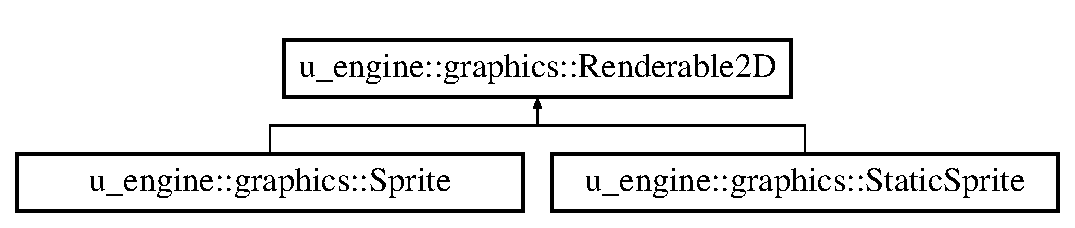
\includegraphics[height=2.000000cm]{classu__engine_1_1graphics_1_1_renderable2_d}
\end{center}
\end{figure}
\subsection*{Public Member Functions}
\begin{DoxyCompactItemize}
\item 
\hyperlink{classu__engine_1_1graphics_1_1_renderable2_d_acdc7a84857290506f345d357ac51fe37}{Renderable2\+D} (\hyperlink{structu__engine_1_1maths_1_1vec3}{maths\+::vec3} position, \hyperlink{structu__engine_1_1maths_1_1vec2}{maths\+::vec2} \hyperlink{glew_8h_a3d1e3edfcf61ca2d831883e1afbad89e}{size}, \hyperlink{structu__engine_1_1maths_1_1vec4}{maths\+::vec4} \hyperlink{glew_8h_a3ea846f998d64f079b86052b6c4193a8}{color})
\item 
virtual \hyperlink{classu__engine_1_1graphics_1_1_renderable2_d_a43d2ee8d12d8fb224f7b86b9d8ab8289}{$\sim$\+Renderable2\+D} ()
\item 
const \hyperlink{structu__engine_1_1maths_1_1vec3}{maths\+::vec3} \& \hyperlink{classu__engine_1_1graphics_1_1_renderable2_d_a0effc31dccfd2aa05bcae8c9ef46fa3e}{get\+Position} () const 
\item 
const \hyperlink{structu__engine_1_1maths_1_1vec2}{maths\+::vec2} \& \hyperlink{classu__engine_1_1graphics_1_1_renderable2_d_a7656d5848c3a8b8dd620e9381071edeb}{get\+Size} () const 
\item 
const \hyperlink{structu__engine_1_1maths_1_1vec4}{maths\+::vec4} \& \hyperlink{classu__engine_1_1graphics_1_1_renderable2_d_af1e0f83a39dab53ca99d3c2fb054065e}{get\+Color} () const 
\end{DoxyCompactItemize}
\subsection*{Protected Attributes}
\begin{DoxyCompactItemize}
\item 
\hyperlink{structu__engine_1_1maths_1_1vec3}{maths\+::vec3} \hyperlink{classu__engine_1_1graphics_1_1_renderable2_d_a9558c847a17ef83a3384359af797b997}{m\+\_\+\+Position}
\item 
\hyperlink{structu__engine_1_1maths_1_1vec2}{maths\+::vec2} \hyperlink{classu__engine_1_1graphics_1_1_renderable2_d_ac3d5d16f629eb4863cf315cccfb6f683}{m\+\_\+\+Size}
\item 
\hyperlink{structu__engine_1_1maths_1_1vec4}{maths\+::vec4} \hyperlink{classu__engine_1_1graphics_1_1_renderable2_d_a81e804854cb4b85b4d34860ab47f1034}{m\+\_\+\+Color}
\end{DoxyCompactItemize}


\subsection{Detailed Description}


Definition at line 18 of file renderable2\+D.\+h.



\subsection{Constructor \& Destructor Documentation}
\hypertarget{classu__engine_1_1graphics_1_1_renderable2_d_acdc7a84857290506f345d357ac51fe37}{}\index{u\+\_\+engine\+::graphics\+::\+Renderable2\+D@{u\+\_\+engine\+::graphics\+::\+Renderable2\+D}!Renderable2\+D@{Renderable2\+D}}
\index{Renderable2\+D@{Renderable2\+D}!u\+\_\+engine\+::graphics\+::\+Renderable2\+D@{u\+\_\+engine\+::graphics\+::\+Renderable2\+D}}
\subsubsection[{Renderable2\+D(maths\+::vec3 position, maths\+::vec2 size, maths\+::vec4 color)}]{\setlength{\rightskip}{0pt plus 5cm}u\+\_\+engine\+::graphics\+::\+Renderable2\+D\+::\+Renderable2\+D (
\begin{DoxyParamCaption}
\item[{{\bf maths\+::vec3}}]{position, }
\item[{{\bf maths\+::vec2}}]{size, }
\item[{{\bf maths\+::vec4}}]{color}
\end{DoxyParamCaption}
)\hspace{0.3cm}{\ttfamily [inline]}}\label{classu__engine_1_1graphics_1_1_renderable2_d_acdc7a84857290506f345d357ac51fe37}


Definition at line 27 of file renderable2\+D.\+h.

\hypertarget{classu__engine_1_1graphics_1_1_renderable2_d_a43d2ee8d12d8fb224f7b86b9d8ab8289}{}\index{u\+\_\+engine\+::graphics\+::\+Renderable2\+D@{u\+\_\+engine\+::graphics\+::\+Renderable2\+D}!````~Renderable2\+D@{$\sim$\+Renderable2\+D}}
\index{````~Renderable2\+D@{$\sim$\+Renderable2\+D}!u\+\_\+engine\+::graphics\+::\+Renderable2\+D@{u\+\_\+engine\+::graphics\+::\+Renderable2\+D}}
\subsubsection[{$\sim$\+Renderable2\+D()}]{\setlength{\rightskip}{0pt plus 5cm}virtual u\+\_\+engine\+::graphics\+::\+Renderable2\+D\+::$\sim$\+Renderable2\+D (
\begin{DoxyParamCaption}
{}
\end{DoxyParamCaption}
)\hspace{0.3cm}{\ttfamily [inline]}, {\ttfamily [virtual]}}\label{classu__engine_1_1graphics_1_1_renderable2_d_a43d2ee8d12d8fb224f7b86b9d8ab8289}


Definition at line 32 of file renderable2\+D.\+h.



\subsection{Member Function Documentation}
\hypertarget{classu__engine_1_1graphics_1_1_renderable2_d_af1e0f83a39dab53ca99d3c2fb054065e}{}\index{u\+\_\+engine\+::graphics\+::\+Renderable2\+D@{u\+\_\+engine\+::graphics\+::\+Renderable2\+D}!get\+Color@{get\+Color}}
\index{get\+Color@{get\+Color}!u\+\_\+engine\+::graphics\+::\+Renderable2\+D@{u\+\_\+engine\+::graphics\+::\+Renderable2\+D}}
\subsubsection[{get\+Color() const }]{\setlength{\rightskip}{0pt plus 5cm}const {\bf maths\+::vec4}\& u\+\_\+engine\+::graphics\+::\+Renderable2\+D\+::get\+Color (
\begin{DoxyParamCaption}
{}
\end{DoxyParamCaption}
) const\hspace{0.3cm}{\ttfamily [inline]}}\label{classu__engine_1_1graphics_1_1_renderable2_d_af1e0f83a39dab53ca99d3c2fb054065e}


Definition at line 37 of file renderable2\+D.\+h.

\hypertarget{classu__engine_1_1graphics_1_1_renderable2_d_a0effc31dccfd2aa05bcae8c9ef46fa3e}{}\index{u\+\_\+engine\+::graphics\+::\+Renderable2\+D@{u\+\_\+engine\+::graphics\+::\+Renderable2\+D}!get\+Position@{get\+Position}}
\index{get\+Position@{get\+Position}!u\+\_\+engine\+::graphics\+::\+Renderable2\+D@{u\+\_\+engine\+::graphics\+::\+Renderable2\+D}}
\subsubsection[{get\+Position() const }]{\setlength{\rightskip}{0pt plus 5cm}const {\bf maths\+::vec3}\& u\+\_\+engine\+::graphics\+::\+Renderable2\+D\+::get\+Position (
\begin{DoxyParamCaption}
{}
\end{DoxyParamCaption}
) const\hspace{0.3cm}{\ttfamily [inline]}}\label{classu__engine_1_1graphics_1_1_renderable2_d_a0effc31dccfd2aa05bcae8c9ef46fa3e}


Definition at line 35 of file renderable2\+D.\+h.

\hypertarget{classu__engine_1_1graphics_1_1_renderable2_d_a7656d5848c3a8b8dd620e9381071edeb}{}\index{u\+\_\+engine\+::graphics\+::\+Renderable2\+D@{u\+\_\+engine\+::graphics\+::\+Renderable2\+D}!get\+Size@{get\+Size}}
\index{get\+Size@{get\+Size}!u\+\_\+engine\+::graphics\+::\+Renderable2\+D@{u\+\_\+engine\+::graphics\+::\+Renderable2\+D}}
\subsubsection[{get\+Size() const }]{\setlength{\rightskip}{0pt plus 5cm}const {\bf maths\+::vec2}\& u\+\_\+engine\+::graphics\+::\+Renderable2\+D\+::get\+Size (
\begin{DoxyParamCaption}
{}
\end{DoxyParamCaption}
) const\hspace{0.3cm}{\ttfamily [inline]}}\label{classu__engine_1_1graphics_1_1_renderable2_d_a7656d5848c3a8b8dd620e9381071edeb}


Definition at line 36 of file renderable2\+D.\+h.



\subsection{Member Data Documentation}
\hypertarget{classu__engine_1_1graphics_1_1_renderable2_d_a81e804854cb4b85b4d34860ab47f1034}{}\index{u\+\_\+engine\+::graphics\+::\+Renderable2\+D@{u\+\_\+engine\+::graphics\+::\+Renderable2\+D}!m\+\_\+\+Color@{m\+\_\+\+Color}}
\index{m\+\_\+\+Color@{m\+\_\+\+Color}!u\+\_\+engine\+::graphics\+::\+Renderable2\+D@{u\+\_\+engine\+::graphics\+::\+Renderable2\+D}}
\subsubsection[{m\+\_\+\+Color}]{\setlength{\rightskip}{0pt plus 5cm}{\bf maths\+::vec4} u\+\_\+engine\+::graphics\+::\+Renderable2\+D\+::m\+\_\+\+Color\hspace{0.3cm}{\ttfamily [protected]}}\label{classu__engine_1_1graphics_1_1_renderable2_d_a81e804854cb4b85b4d34860ab47f1034}


Definition at line 22 of file renderable2\+D.\+h.

\hypertarget{classu__engine_1_1graphics_1_1_renderable2_d_a9558c847a17ef83a3384359af797b997}{}\index{u\+\_\+engine\+::graphics\+::\+Renderable2\+D@{u\+\_\+engine\+::graphics\+::\+Renderable2\+D}!m\+\_\+\+Position@{m\+\_\+\+Position}}
\index{m\+\_\+\+Position@{m\+\_\+\+Position}!u\+\_\+engine\+::graphics\+::\+Renderable2\+D@{u\+\_\+engine\+::graphics\+::\+Renderable2\+D}}
\subsubsection[{m\+\_\+\+Position}]{\setlength{\rightskip}{0pt plus 5cm}{\bf maths\+::vec3} u\+\_\+engine\+::graphics\+::\+Renderable2\+D\+::m\+\_\+\+Position\hspace{0.3cm}{\ttfamily [protected]}}\label{classu__engine_1_1graphics_1_1_renderable2_d_a9558c847a17ef83a3384359af797b997}


Definition at line 20 of file renderable2\+D.\+h.

\hypertarget{classu__engine_1_1graphics_1_1_renderable2_d_ac3d5d16f629eb4863cf315cccfb6f683}{}\index{u\+\_\+engine\+::graphics\+::\+Renderable2\+D@{u\+\_\+engine\+::graphics\+::\+Renderable2\+D}!m\+\_\+\+Size@{m\+\_\+\+Size}}
\index{m\+\_\+\+Size@{m\+\_\+\+Size}!u\+\_\+engine\+::graphics\+::\+Renderable2\+D@{u\+\_\+engine\+::graphics\+::\+Renderable2\+D}}
\subsubsection[{m\+\_\+\+Size}]{\setlength{\rightskip}{0pt plus 5cm}{\bf maths\+::vec2} u\+\_\+engine\+::graphics\+::\+Renderable2\+D\+::m\+\_\+\+Size\hspace{0.3cm}{\ttfamily [protected]}}\label{classu__engine_1_1graphics_1_1_renderable2_d_ac3d5d16f629eb4863cf315cccfb6f683}


Definition at line 21 of file renderable2\+D.\+h.



The documentation for this class was generated from the following file\+:\begin{DoxyCompactItemize}
\item 
G\+:/\+Libraries/\+V\+S\+Projects/\+Untitled\+Game/\+Unicity\+Engine/\+Unicity/src/graphics/\hyperlink{renderable2_d_8h}{renderable2\+D.\+h}\end{DoxyCompactItemize}

\hypertarget{classu__engine_1_1graphics_1_1_renderer2_d}{}\section{u\+\_\+engine\+:\+:graphics\+:\+:Renderer2\+D Class Reference}
\label{classu__engine_1_1graphics_1_1_renderer2_d}\index{u\+\_\+engine\+::graphics\+::\+Renderer2\+D@{u\+\_\+engine\+::graphics\+::\+Renderer2\+D}}


{\ttfamily \#include $<$renderer2\+D.\+h$>$}

Inheritance diagram for u\+\_\+engine\+:\+:graphics\+:\+:Renderer2\+D\+:\begin{figure}[H]
\begin{center}
\leavevmode
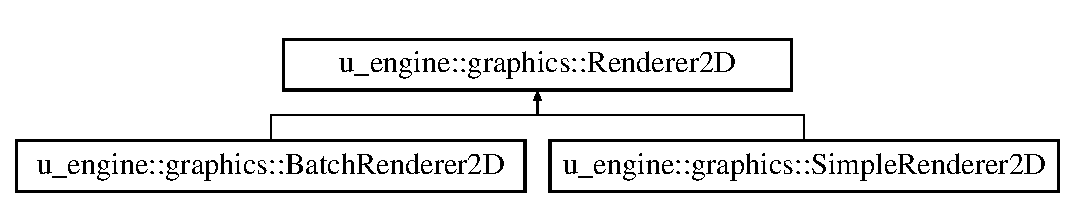
\includegraphics[height=2.000000cm]{classu__engine_1_1graphics_1_1_renderer2_d}
\end{center}
\end{figure}
\subsection*{Public Member Functions}
\begin{DoxyCompactItemize}
\item 
virtual \hyperlink{wglew_8h_aeea6e3dfae3acf232096f57d2d57f084}{void} \hyperlink{classu__engine_1_1graphics_1_1_renderer2_d_ae78a8a0ff8fc052f3cef4c24c9c829f7}{submit} (const \hyperlink{classu__engine_1_1graphics_1_1_renderable2_d}{Renderable2\+D} $\ast$renderable)=0
\item 
virtual \hyperlink{wglew_8h_aeea6e3dfae3acf232096f57d2d57f084}{void} \hyperlink{classu__engine_1_1graphics_1_1_renderer2_d_a922880dea9292d4e973c2e2da22b9964}{flush} ()=0
\end{DoxyCompactItemize}


\subsection{Detailed Description}


Definition at line 10 of file renderer2\+D.\+h.



\subsection{Member Function Documentation}
\hypertarget{classu__engine_1_1graphics_1_1_renderer2_d_a922880dea9292d4e973c2e2da22b9964}{}\index{u\+\_\+engine\+::graphics\+::\+Renderer2\+D@{u\+\_\+engine\+::graphics\+::\+Renderer2\+D}!flush@{flush}}
\index{flush@{flush}!u\+\_\+engine\+::graphics\+::\+Renderer2\+D@{u\+\_\+engine\+::graphics\+::\+Renderer2\+D}}
\subsubsection[{flush()=0}]{\setlength{\rightskip}{0pt plus 5cm}virtual {\bf void} u\+\_\+engine\+::graphics\+::\+Renderer2\+D\+::flush (
\begin{DoxyParamCaption}
{}
\end{DoxyParamCaption}
)\hspace{0.3cm}{\ttfamily [pure virtual]}}\label{classu__engine_1_1graphics_1_1_renderer2_d_a922880dea9292d4e973c2e2da22b9964}


Implemented in \hyperlink{classu__engine_1_1graphics_1_1_batch_renderer2_d_a6f95ef0c0a94e1df2b94efa662babd15}{u\+\_\+engine\+::graphics\+::\+Batch\+Renderer2\+D}, and \hyperlink{classu__engine_1_1graphics_1_1_simple_renderer2_d_ac5687d3e57c732ac23b297660a351e27}{u\+\_\+engine\+::graphics\+::\+Simple\+Renderer2\+D}.

\hypertarget{classu__engine_1_1graphics_1_1_renderer2_d_ae78a8a0ff8fc052f3cef4c24c9c829f7}{}\index{u\+\_\+engine\+::graphics\+::\+Renderer2\+D@{u\+\_\+engine\+::graphics\+::\+Renderer2\+D}!submit@{submit}}
\index{submit@{submit}!u\+\_\+engine\+::graphics\+::\+Renderer2\+D@{u\+\_\+engine\+::graphics\+::\+Renderer2\+D}}
\subsubsection[{submit(const Renderable2\+D $\ast$renderable)=0}]{\setlength{\rightskip}{0pt plus 5cm}virtual {\bf void} u\+\_\+engine\+::graphics\+::\+Renderer2\+D\+::submit (
\begin{DoxyParamCaption}
\item[{const {\bf Renderable2\+D} $\ast$}]{renderable}
\end{DoxyParamCaption}
)\hspace{0.3cm}{\ttfamily [pure virtual]}}\label{classu__engine_1_1graphics_1_1_renderer2_d_ae78a8a0ff8fc052f3cef4c24c9c829f7}


Implemented in \hyperlink{classu__engine_1_1graphics_1_1_batch_renderer2_d_a74a8a92bdf3170a3adbbeebbe9ef8a06}{u\+\_\+engine\+::graphics\+::\+Batch\+Renderer2\+D}, and \hyperlink{classu__engine_1_1graphics_1_1_simple_renderer2_d_aa35d6472fe50af78a13680a03fe1fdcc}{u\+\_\+engine\+::graphics\+::\+Simple\+Renderer2\+D}.



The documentation for this class was generated from the following file\+:\begin{DoxyCompactItemize}
\item 
G\+:/\+Libraries/\+V\+S\+Projects/\+Untitled\+Game/\+Unicity\+Engine/\+Unicity/src/graphics/\hyperlink{renderer2_d_8h}{renderer2\+D.\+h}\end{DoxyCompactItemize}

\hypertarget{classu__engine_1_1graphics_1_1_shader}{}\section{u\+\_\+engine\+:\+:graphics\+:\+:Shader Class Reference}
\label{classu__engine_1_1graphics_1_1_shader}\index{u\+\_\+engine\+::graphics\+::\+Shader@{u\+\_\+engine\+::graphics\+::\+Shader}}


{\ttfamily \#include $<$shader.\+h$>$}

\subsection*{Public Member Functions}
\begin{DoxyCompactItemize}
\item 
\hyperlink{classu__engine_1_1graphics_1_1_shader_a983b1025759d580f47499d4103321e1e}{Shader} (const char $\ast$vert\+Path, const char $\ast$frag\+Path)
\item 
\hyperlink{classu__engine_1_1graphics_1_1_shader_a8d08acdf9bb1b18cc980a8229838434a}{$\sim$\+Shader} ()
\item 
\hyperlink{wglew_8h_aeea6e3dfae3acf232096f57d2d57f084}{void} \hyperlink{classu__engine_1_1graphics_1_1_shader_a0427896de6509827a587bff443ffdade}{set\+Uniform1i} (const \hyperlink{glew_8h_af7575655ac056b187ea385966b95a22d}{G\+Lchar} $\ast$\hyperlink{glew_8h_a5c4947d4516dd7cfa3505ce3a648a4ef}{name}, \hyperlink{wglew_8h_a500a82aecba06f4550f6849b8099ca21}{int} \hyperlink{glew_8h_a26942fd2ed566ef553eae82d2c109c8f}{val})
\item 
\hyperlink{wglew_8h_aeea6e3dfae3acf232096f57d2d57f084}{void} \hyperlink{classu__engine_1_1graphics_1_1_shader_ac4f9160e334ff67a69918d978ddeba29}{set\+Uniform1f} (const \hyperlink{glew_8h_af7575655ac056b187ea385966b95a22d}{G\+Lchar} $\ast$\hyperlink{glew_8h_a5c4947d4516dd7cfa3505ce3a648a4ef}{name}, float \hyperlink{glew_8h_a26942fd2ed566ef553eae82d2c109c8f}{val})
\item 
\hyperlink{wglew_8h_aeea6e3dfae3acf232096f57d2d57f084}{void} \hyperlink{classu__engine_1_1graphics_1_1_shader_af7c3899c2f210b8f662d5077ffa07c3a}{set\+Uniform2f} (const \hyperlink{glew_8h_af7575655ac056b187ea385966b95a22d}{G\+Lchar} $\ast$\hyperlink{glew_8h_a5c4947d4516dd7cfa3505ce3a648a4ef}{name}, const \hyperlink{structu__engine_1_1maths_1_1vec2}{maths\+::vec2} \&vector)
\item 
\hyperlink{wglew_8h_aeea6e3dfae3acf232096f57d2d57f084}{void} \hyperlink{classu__engine_1_1graphics_1_1_shader_ae760e5ccae41bb68a71c7e849285fe6a}{set\+Uniform3f} (const \hyperlink{glew_8h_af7575655ac056b187ea385966b95a22d}{G\+Lchar} $\ast$\hyperlink{glew_8h_a5c4947d4516dd7cfa3505ce3a648a4ef}{name}, const \hyperlink{structu__engine_1_1maths_1_1vec3}{maths\+::vec3} \&vector)
\item 
\hyperlink{wglew_8h_aeea6e3dfae3acf232096f57d2d57f084}{void} \hyperlink{classu__engine_1_1graphics_1_1_shader_a13d3e1d8aef749fe1db1b6fa766ca9d8}{set\+Uniform4f} (const \hyperlink{glew_8h_af7575655ac056b187ea385966b95a22d}{G\+Lchar} $\ast$\hyperlink{glew_8h_a5c4947d4516dd7cfa3505ce3a648a4ef}{name}, const \hyperlink{structu__engine_1_1maths_1_1vec4}{maths\+::vec4} \&vector)
\item 
\hyperlink{wglew_8h_aeea6e3dfae3acf232096f57d2d57f084}{void} \hyperlink{classu__engine_1_1graphics_1_1_shader_a6afb273e58deb41aec1c0e8d30794d14}{set\+Uniform\+Mat4} (const \hyperlink{glew_8h_af7575655ac056b187ea385966b95a22d}{G\+Lchar} $\ast$\hyperlink{glew_8h_a5c4947d4516dd7cfa3505ce3a648a4ef}{name}, const \hyperlink{structu__engine_1_1maths_1_1mat4}{maths\+::mat4} \&\hyperlink{glew_8h_a7b24a3f2f56eb1244ae69dacb4fecb6f}{matrix})
\item 
\hyperlink{wglew_8h_aeea6e3dfae3acf232096f57d2d57f084}{void} \hyperlink{classu__engine_1_1graphics_1_1_shader_a2fd8a40b1794c80f827932024b873cce}{enable} () const 
\item 
\hyperlink{wglew_8h_aeea6e3dfae3acf232096f57d2d57f084}{void} \hyperlink{classu__engine_1_1graphics_1_1_shader_a76c38646d03ad4b54cdb59dd33e0615b}{disable} () const 
\end{DoxyCompactItemize}


\subsection{Detailed Description}


Definition at line 13 of file shader.\+h.



\subsection{Constructor \& Destructor Documentation}
\hypertarget{classu__engine_1_1graphics_1_1_shader_a983b1025759d580f47499d4103321e1e}{}\index{u\+\_\+engine\+::graphics\+::\+Shader@{u\+\_\+engine\+::graphics\+::\+Shader}!Shader@{Shader}}
\index{Shader@{Shader}!u\+\_\+engine\+::graphics\+::\+Shader@{u\+\_\+engine\+::graphics\+::\+Shader}}
\subsubsection[{Shader(const char $\ast$vert\+Path, const char $\ast$frag\+Path)}]{\setlength{\rightskip}{0pt plus 5cm}u\+\_\+engine\+::graphics\+::\+Shader\+::\+Shader (
\begin{DoxyParamCaption}
\item[{const char $\ast$}]{vert\+Path, }
\item[{const char $\ast$}]{frag\+Path}
\end{DoxyParamCaption}
)}\label{classu__engine_1_1graphics_1_1_shader_a983b1025759d580f47499d4103321e1e}


Definition at line 5 of file shader.\+cpp.

\hypertarget{classu__engine_1_1graphics_1_1_shader_a8d08acdf9bb1b18cc980a8229838434a}{}\index{u\+\_\+engine\+::graphics\+::\+Shader@{u\+\_\+engine\+::graphics\+::\+Shader}!````~Shader@{$\sim$\+Shader}}
\index{````~Shader@{$\sim$\+Shader}!u\+\_\+engine\+::graphics\+::\+Shader@{u\+\_\+engine\+::graphics\+::\+Shader}}
\subsubsection[{$\sim$\+Shader()}]{\setlength{\rightskip}{0pt plus 5cm}u\+\_\+engine\+::graphics\+::\+Shader\+::$\sim$\+Shader (
\begin{DoxyParamCaption}
{}
\end{DoxyParamCaption}
)}\label{classu__engine_1_1graphics_1_1_shader_a8d08acdf9bb1b18cc980a8229838434a}


Definition at line 9 of file shader.\+cpp.



\subsection{Member Function Documentation}
\hypertarget{classu__engine_1_1graphics_1_1_shader_a76c38646d03ad4b54cdb59dd33e0615b}{}\index{u\+\_\+engine\+::graphics\+::\+Shader@{u\+\_\+engine\+::graphics\+::\+Shader}!disable@{disable}}
\index{disable@{disable}!u\+\_\+engine\+::graphics\+::\+Shader@{u\+\_\+engine\+::graphics\+::\+Shader}}
\subsubsection[{disable() const }]{\setlength{\rightskip}{0pt plus 5cm}{\bf void} u\+\_\+engine\+::graphics\+::\+Shader\+::disable (
\begin{DoxyParamCaption}
{}
\end{DoxyParamCaption}
) const}\label{classu__engine_1_1graphics_1_1_shader_a76c38646d03ad4b54cdb59dd33e0615b}


Definition at line 106 of file shader.\+cpp.

\hypertarget{classu__engine_1_1graphics_1_1_shader_a2fd8a40b1794c80f827932024b873cce}{}\index{u\+\_\+engine\+::graphics\+::\+Shader@{u\+\_\+engine\+::graphics\+::\+Shader}!enable@{enable}}
\index{enable@{enable}!u\+\_\+engine\+::graphics\+::\+Shader@{u\+\_\+engine\+::graphics\+::\+Shader}}
\subsubsection[{enable() const }]{\setlength{\rightskip}{0pt plus 5cm}{\bf void} u\+\_\+engine\+::graphics\+::\+Shader\+::enable (
\begin{DoxyParamCaption}
{}
\end{DoxyParamCaption}
) const}\label{classu__engine_1_1graphics_1_1_shader_a2fd8a40b1794c80f827932024b873cce}


Definition at line 103 of file shader.\+cpp.

\hypertarget{classu__engine_1_1graphics_1_1_shader_ac4f9160e334ff67a69918d978ddeba29}{}\index{u\+\_\+engine\+::graphics\+::\+Shader@{u\+\_\+engine\+::graphics\+::\+Shader}!set\+Uniform1f@{set\+Uniform1f}}
\index{set\+Uniform1f@{set\+Uniform1f}!u\+\_\+engine\+::graphics\+::\+Shader@{u\+\_\+engine\+::graphics\+::\+Shader}}
\subsubsection[{set\+Uniform1f(const G\+Lchar $\ast$name, float val)}]{\setlength{\rightskip}{0pt plus 5cm}{\bf void} u\+\_\+engine\+::graphics\+::\+Shader\+::set\+Uniform1f (
\begin{DoxyParamCaption}
\item[{const {\bf G\+Lchar} $\ast$}]{name, }
\item[{float}]{val}
\end{DoxyParamCaption}
)}\label{classu__engine_1_1graphics_1_1_shader_ac4f9160e334ff67a69918d978ddeba29}


Definition at line 81 of file shader.\+cpp.

\hypertarget{classu__engine_1_1graphics_1_1_shader_a0427896de6509827a587bff443ffdade}{}\index{u\+\_\+engine\+::graphics\+::\+Shader@{u\+\_\+engine\+::graphics\+::\+Shader}!set\+Uniform1i@{set\+Uniform1i}}
\index{set\+Uniform1i@{set\+Uniform1i}!u\+\_\+engine\+::graphics\+::\+Shader@{u\+\_\+engine\+::graphics\+::\+Shader}}
\subsubsection[{set\+Uniform1i(const G\+Lchar $\ast$name, int val)}]{\setlength{\rightskip}{0pt plus 5cm}{\bf void} u\+\_\+engine\+::graphics\+::\+Shader\+::set\+Uniform1i (
\begin{DoxyParamCaption}
\item[{const {\bf G\+Lchar} $\ast$}]{name, }
\item[{{\bf int}}]{val}
\end{DoxyParamCaption}
)}\label{classu__engine_1_1graphics_1_1_shader_a0427896de6509827a587bff443ffdade}


Definition at line 77 of file shader.\+cpp.

\hypertarget{classu__engine_1_1graphics_1_1_shader_af7c3899c2f210b8f662d5077ffa07c3a}{}\index{u\+\_\+engine\+::graphics\+::\+Shader@{u\+\_\+engine\+::graphics\+::\+Shader}!set\+Uniform2f@{set\+Uniform2f}}
\index{set\+Uniform2f@{set\+Uniform2f}!u\+\_\+engine\+::graphics\+::\+Shader@{u\+\_\+engine\+::graphics\+::\+Shader}}
\subsubsection[{set\+Uniform2f(const G\+Lchar $\ast$name, const maths\+::vec2 \&vector)}]{\setlength{\rightskip}{0pt plus 5cm}{\bf void} u\+\_\+engine\+::graphics\+::\+Shader\+::set\+Uniform2f (
\begin{DoxyParamCaption}
\item[{const {\bf G\+Lchar} $\ast$}]{name, }
\item[{const {\bf maths\+::vec2} \&}]{vector}
\end{DoxyParamCaption}
)}\label{classu__engine_1_1graphics_1_1_shader_af7c3899c2f210b8f662d5077ffa07c3a}


Definition at line 85 of file shader.\+cpp.

\hypertarget{classu__engine_1_1graphics_1_1_shader_ae760e5ccae41bb68a71c7e849285fe6a}{}\index{u\+\_\+engine\+::graphics\+::\+Shader@{u\+\_\+engine\+::graphics\+::\+Shader}!set\+Uniform3f@{set\+Uniform3f}}
\index{set\+Uniform3f@{set\+Uniform3f}!u\+\_\+engine\+::graphics\+::\+Shader@{u\+\_\+engine\+::graphics\+::\+Shader}}
\subsubsection[{set\+Uniform3f(const G\+Lchar $\ast$name, const maths\+::vec3 \&vector)}]{\setlength{\rightskip}{0pt plus 5cm}{\bf void} u\+\_\+engine\+::graphics\+::\+Shader\+::set\+Uniform3f (
\begin{DoxyParamCaption}
\item[{const {\bf G\+Lchar} $\ast$}]{name, }
\item[{const {\bf maths\+::vec3} \&}]{vector}
\end{DoxyParamCaption}
)}\label{classu__engine_1_1graphics_1_1_shader_ae760e5ccae41bb68a71c7e849285fe6a}


Definition at line 89 of file shader.\+cpp.

\hypertarget{classu__engine_1_1graphics_1_1_shader_a13d3e1d8aef749fe1db1b6fa766ca9d8}{}\index{u\+\_\+engine\+::graphics\+::\+Shader@{u\+\_\+engine\+::graphics\+::\+Shader}!set\+Uniform4f@{set\+Uniform4f}}
\index{set\+Uniform4f@{set\+Uniform4f}!u\+\_\+engine\+::graphics\+::\+Shader@{u\+\_\+engine\+::graphics\+::\+Shader}}
\subsubsection[{set\+Uniform4f(const G\+Lchar $\ast$name, const maths\+::vec4 \&vector)}]{\setlength{\rightskip}{0pt plus 5cm}{\bf void} u\+\_\+engine\+::graphics\+::\+Shader\+::set\+Uniform4f (
\begin{DoxyParamCaption}
\item[{const {\bf G\+Lchar} $\ast$}]{name, }
\item[{const {\bf maths\+::vec4} \&}]{vector}
\end{DoxyParamCaption}
)}\label{classu__engine_1_1graphics_1_1_shader_a13d3e1d8aef749fe1db1b6fa766ca9d8}


Definition at line 93 of file shader.\+cpp.

\hypertarget{classu__engine_1_1graphics_1_1_shader_a6afb273e58deb41aec1c0e8d30794d14}{}\index{u\+\_\+engine\+::graphics\+::\+Shader@{u\+\_\+engine\+::graphics\+::\+Shader}!set\+Uniform\+Mat4@{set\+Uniform\+Mat4}}
\index{set\+Uniform\+Mat4@{set\+Uniform\+Mat4}!u\+\_\+engine\+::graphics\+::\+Shader@{u\+\_\+engine\+::graphics\+::\+Shader}}
\subsubsection[{set\+Uniform\+Mat4(const G\+Lchar $\ast$name, const maths\+::mat4 \&matrix)}]{\setlength{\rightskip}{0pt plus 5cm}{\bf void} u\+\_\+engine\+::graphics\+::\+Shader\+::set\+Uniform\+Mat4 (
\begin{DoxyParamCaption}
\item[{const {\bf G\+Lchar} $\ast$}]{name, }
\item[{const {\bf maths\+::mat4} \&}]{matrix}
\end{DoxyParamCaption}
)}\label{classu__engine_1_1graphics_1_1_shader_a6afb273e58deb41aec1c0e8d30794d14}


Definition at line 97 of file shader.\+cpp.



The documentation for this class was generated from the following files\+:\begin{DoxyCompactItemize}
\item 
G\+:/\+Libraries/\+V\+S\+Projects/\+Untitled\+Game/\+Unicity\+Engine/\+Unicity/src/graphics/\hyperlink{shader_8h}{shader.\+h}\item 
G\+:/\+Libraries/\+V\+S\+Projects/\+Untitled\+Game/\+Unicity\+Engine/\+Unicity/src/graphics/\hyperlink{shader_8cpp}{shader.\+cpp}\end{DoxyCompactItemize}

\hypertarget{classu__engine_1_1graphics_1_1_simple_renderer2_d}{}\section{u\+\_\+engine\+:\+:graphics\+:\+:Simple\+Renderer2\+D Class Reference}
\label{classu__engine_1_1graphics_1_1_simple_renderer2_d}\index{u\+\_\+engine\+::graphics\+::\+Simple\+Renderer2\+D@{u\+\_\+engine\+::graphics\+::\+Simple\+Renderer2\+D}}


{\ttfamily \#include $<$simplerenderer2\+D.\+h$>$}

Inheritance diagram for u\+\_\+engine\+:\+:graphics\+:\+:Simple\+Renderer2\+D\+:\begin{figure}[H]
\begin{center}
\leavevmode
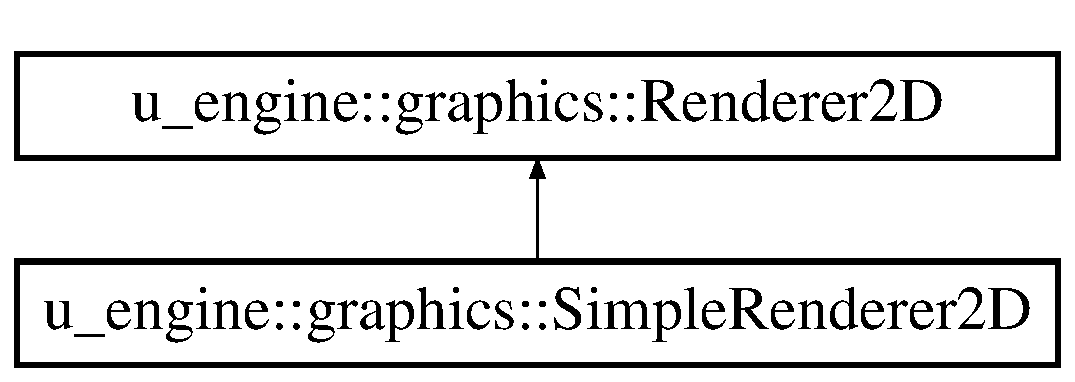
\includegraphics[height=2.000000cm]{classu__engine_1_1graphics_1_1_simple_renderer2_d}
\end{center}
\end{figure}
\subsection*{Public Member Functions}
\begin{DoxyCompactItemize}
\item 
\hyperlink{wglew_8h_aeea6e3dfae3acf232096f57d2d57f084}{void} \hyperlink{classu__engine_1_1graphics_1_1_simple_renderer2_d_aa35d6472fe50af78a13680a03fe1fdcc}{submit} (const \hyperlink{classu__engine_1_1graphics_1_1_renderable2_d}{Renderable2\+D} $\ast$renderable) override
\item 
\hyperlink{wglew_8h_aeea6e3dfae3acf232096f57d2d57f084}{void} \hyperlink{classu__engine_1_1graphics_1_1_simple_renderer2_d_ac5687d3e57c732ac23b297660a351e27}{flush} () override
\end{DoxyCompactItemize}


\subsection{Detailed Description}


Definition at line 10 of file simplerenderer2\+D.\+h.



\subsection{Member Function Documentation}
\hypertarget{classu__engine_1_1graphics_1_1_simple_renderer2_d_ac5687d3e57c732ac23b297660a351e27}{}\index{u\+\_\+engine\+::graphics\+::\+Simple\+Renderer2\+D@{u\+\_\+engine\+::graphics\+::\+Simple\+Renderer2\+D}!flush@{flush}}
\index{flush@{flush}!u\+\_\+engine\+::graphics\+::\+Simple\+Renderer2\+D@{u\+\_\+engine\+::graphics\+::\+Simple\+Renderer2\+D}}
\subsubsection[{flush() override}]{\setlength{\rightskip}{0pt plus 5cm}{\bf void} u\+\_\+engine\+::graphics\+::\+Simple\+Renderer2\+D\+::flush (
\begin{DoxyParamCaption}
{}
\end{DoxyParamCaption}
)\hspace{0.3cm}{\ttfamily [override]}, {\ttfamily [virtual]}}\label{classu__engine_1_1graphics_1_1_simple_renderer2_d_ac5687d3e57c732ac23b297660a351e27}


Implements \hyperlink{classu__engine_1_1graphics_1_1_renderer2_d_a922880dea9292d4e973c2e2da22b9964}{u\+\_\+engine\+::graphics\+::\+Renderer2\+D}.



Definition at line 11 of file simplerenderer2\+D.\+cpp.

\hypertarget{classu__engine_1_1graphics_1_1_simple_renderer2_d_aa35d6472fe50af78a13680a03fe1fdcc}{}\index{u\+\_\+engine\+::graphics\+::\+Simple\+Renderer2\+D@{u\+\_\+engine\+::graphics\+::\+Simple\+Renderer2\+D}!submit@{submit}}
\index{submit@{submit}!u\+\_\+engine\+::graphics\+::\+Simple\+Renderer2\+D@{u\+\_\+engine\+::graphics\+::\+Simple\+Renderer2\+D}}
\subsubsection[{submit(const Renderable2\+D $\ast$renderable) override}]{\setlength{\rightskip}{0pt plus 5cm}{\bf void} u\+\_\+engine\+::graphics\+::\+Simple\+Renderer2\+D\+::submit (
\begin{DoxyParamCaption}
\item[{const {\bf Renderable2\+D} $\ast$}]{renderable}
\end{DoxyParamCaption}
)\hspace{0.3cm}{\ttfamily [override]}, {\ttfamily [virtual]}}\label{classu__engine_1_1graphics_1_1_simple_renderer2_d_aa35d6472fe50af78a13680a03fe1fdcc}


Implements \hyperlink{classu__engine_1_1graphics_1_1_renderer2_d_ae78a8a0ff8fc052f3cef4c24c9c829f7}{u\+\_\+engine\+::graphics\+::\+Renderer2\+D}.



Definition at line 7 of file simplerenderer2\+D.\+cpp.



The documentation for this class was generated from the following files\+:\begin{DoxyCompactItemize}
\item 
G\+:/\+Libraries/\+V\+S\+Projects/\+Untitled\+Game/\+Unicity\+Engine/\+Unicity/src/graphics/\hyperlink{simplerenderer2_d_8h}{simplerenderer2\+D.\+h}\item 
G\+:/\+Libraries/\+V\+S\+Projects/\+Untitled\+Game/\+Unicity\+Engine/\+Unicity/src/graphics/\hyperlink{simplerenderer2_d_8cpp}{simplerenderer2\+D.\+cpp}\end{DoxyCompactItemize}

\hypertarget{classu__engine_1_1graphics_1_1_sprite}{}\section{u\+\_\+engine\+:\+:graphics\+:\+:Sprite Class Reference}
\label{classu__engine_1_1graphics_1_1_sprite}\index{u\+\_\+engine\+::graphics\+::\+Sprite@{u\+\_\+engine\+::graphics\+::\+Sprite}}


{\ttfamily \#include $<$sprite.\+h$>$}

Inheritance diagram for u\+\_\+engine\+:\+:graphics\+:\+:Sprite\+:\begin{figure}[H]
\begin{center}
\leavevmode
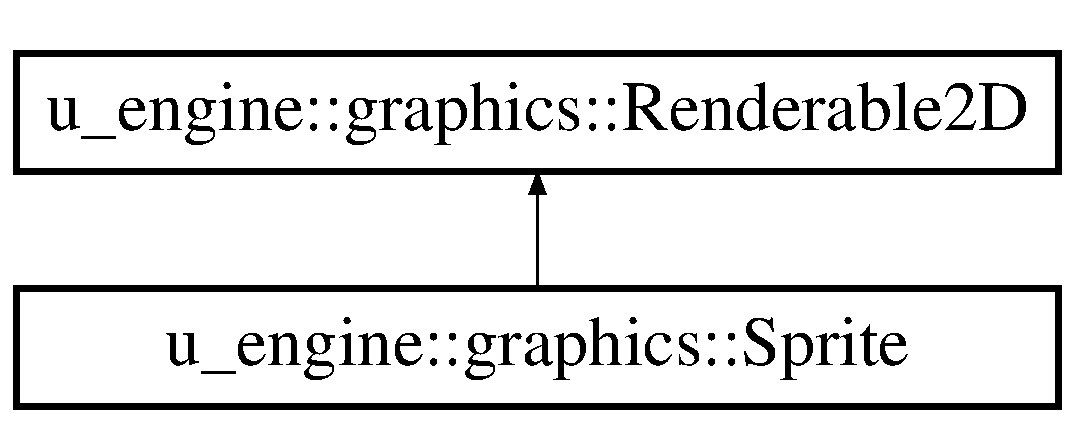
\includegraphics[height=2.000000cm]{classu__engine_1_1graphics_1_1_sprite}
\end{center}
\end{figure}
\subsection*{Public Member Functions}
\begin{DoxyCompactItemize}
\item 
\hyperlink{classu__engine_1_1graphics_1_1_sprite_acf4e11ebb1c16bb0bf54f989dc9fe343}{Sprite} (float \hyperlink{glew_8h_ad77deca22f617d3f0e0eb786445689fc}{x}, float \hyperlink{glew_8h_a9298c7ad619074f5285b32c6b72bfdea}{y}, float \hyperlink{glew_8h_aa105b18f96e6bc2485cb7f576a7fb9ba}{width}, float \hyperlink{glew_8h_aa214bd63e12f7ddf524c83894fcc69a7}{height}, const \hyperlink{structu__engine_1_1maths_1_1vec4}{maths\+::vec4} \&\hyperlink{glew_8h_a3ea846f998d64f079b86052b6c4193a8}{color})
\end{DoxyCompactItemize}
\subsection*{Additional Inherited Members}


\subsection{Detailed Description}


Definition at line 8 of file sprite.\+h.



\subsection{Constructor \& Destructor Documentation}
\hypertarget{classu__engine_1_1graphics_1_1_sprite_acf4e11ebb1c16bb0bf54f989dc9fe343}{}\index{u\+\_\+engine\+::graphics\+::\+Sprite@{u\+\_\+engine\+::graphics\+::\+Sprite}!Sprite@{Sprite}}
\index{Sprite@{Sprite}!u\+\_\+engine\+::graphics\+::\+Sprite@{u\+\_\+engine\+::graphics\+::\+Sprite}}
\subsubsection[{Sprite(float x, float y, float width, float height, const maths\+::vec4 \&color)}]{\setlength{\rightskip}{0pt plus 5cm}u\+\_\+engine\+::graphics\+::\+Sprite\+::\+Sprite (
\begin{DoxyParamCaption}
\item[{float}]{x, }
\item[{float}]{y, }
\item[{float}]{width, }
\item[{float}]{height, }
\item[{const {\bf maths\+::vec4} \&}]{color}
\end{DoxyParamCaption}
)}\label{classu__engine_1_1graphics_1_1_sprite_acf4e11ebb1c16bb0bf54f989dc9fe343}


Definition at line 8 of file sprite.\+cpp.



The documentation for this class was generated from the following files\+:\begin{DoxyCompactItemize}
\item 
G\+:/\+Libraries/\+V\+S\+Projects/\+Untitled\+Game/\+Unicity\+Engine/\+Unicity/src/graphics/\hyperlink{sprite_8h}{sprite.\+h}\item 
G\+:/\+Libraries/\+V\+S\+Projects/\+Untitled\+Game/\+Unicity\+Engine/\+Unicity/src/graphics/\hyperlink{sprite_8cpp}{sprite.\+cpp}\end{DoxyCompactItemize}

\hypertarget{classu__engine_1_1graphics_1_1_static_sprite}{}\section{u\+\_\+engine\+:\+:graphics\+:\+:Static\+Sprite Class Reference}
\label{classu__engine_1_1graphics_1_1_static_sprite}\index{u\+\_\+engine\+::graphics\+::\+Static\+Sprite@{u\+\_\+engine\+::graphics\+::\+Static\+Sprite}}


{\ttfamily \#include $<$static\+\_\+sprite.\+h$>$}

Inheritance diagram for u\+\_\+engine\+:\+:graphics\+:\+:Static\+Sprite\+:\begin{figure}[H]
\begin{center}
\leavevmode
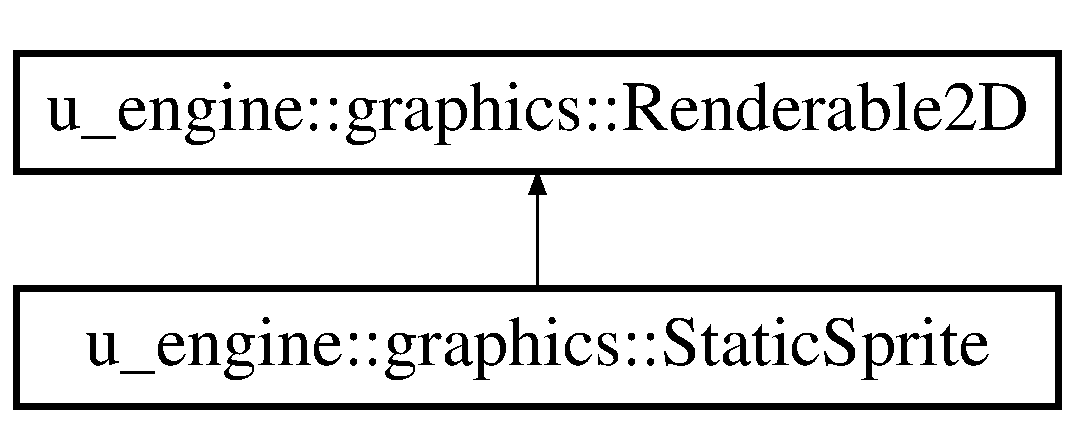
\includegraphics[height=2.000000cm]{classu__engine_1_1graphics_1_1_static_sprite}
\end{center}
\end{figure}
\subsection*{Public Member Functions}
\begin{DoxyCompactItemize}
\item 
\hyperlink{classu__engine_1_1graphics_1_1_static_sprite_ad105ab0dce536bae761fe6e37e0d0b05}{Static\+Sprite} (float \hyperlink{glew_8h_ad77deca22f617d3f0e0eb786445689fc}{x}, float \hyperlink{glew_8h_a9298c7ad619074f5285b32c6b72bfdea}{y}, float \hyperlink{glew_8h_aa105b18f96e6bc2485cb7f576a7fb9ba}{width}, float \hyperlink{glew_8h_aa214bd63e12f7ddf524c83894fcc69a7}{height}, const \hyperlink{structu__engine_1_1maths_1_1vec4}{maths\+::vec4} \&\hyperlink{glew_8h_a3ea846f998d64f079b86052b6c4193a8}{color}, \hyperlink{classu__engine_1_1graphics_1_1_shader}{Shader} \&\hyperlink{glew_8h_a57b2a96adb1d51204909a82d861e395e}{shader})
\item 
\hyperlink{classu__engine_1_1graphics_1_1_static_sprite_a1c116dae0aed78c3f4f6cc6e91f47c07}{$\sim$\+Static\+Sprite} ()
\item 
const \hyperlink{classu__engine_1_1graphics_1_1_vertex_array}{Vertex\+Array} $\ast$ \hyperlink{classu__engine_1_1graphics_1_1_static_sprite_a509d453a7df4435ad3e1470aca77a355}{get\+V\+A\+O} () const 
\item 
const \hyperlink{classu__engine_1_1graphics_1_1_index_buffer}{Index\+Buffer} $\ast$ \hyperlink{classu__engine_1_1graphics_1_1_static_sprite_afd7a4ed2a17dbabc7f3b944638cf480b}{get\+I\+B\+O} () const 
\item 
\hyperlink{classu__engine_1_1graphics_1_1_shader}{Shader} \& \hyperlink{classu__engine_1_1graphics_1_1_static_sprite_a2368c7eb0b4556dec5ee324ce30ccc4a}{get\+Shader} () const 
\end{DoxyCompactItemize}
\subsection*{Additional Inherited Members}


\subsection{Detailed Description}


Definition at line 8 of file static\+\_\+sprite.\+h.



\subsection{Constructor \& Destructor Documentation}
\hypertarget{classu__engine_1_1graphics_1_1_static_sprite_ad105ab0dce536bae761fe6e37e0d0b05}{}\index{u\+\_\+engine\+::graphics\+::\+Static\+Sprite@{u\+\_\+engine\+::graphics\+::\+Static\+Sprite}!Static\+Sprite@{Static\+Sprite}}
\index{Static\+Sprite@{Static\+Sprite}!u\+\_\+engine\+::graphics\+::\+Static\+Sprite@{u\+\_\+engine\+::graphics\+::\+Static\+Sprite}}
\subsubsection[{Static\+Sprite(float x, float y, float width, float height, const maths\+::vec4 \&color, Shader \&shader)}]{\setlength{\rightskip}{0pt plus 5cm}u\+\_\+engine\+::graphics\+::\+Static\+Sprite\+::\+Static\+Sprite (
\begin{DoxyParamCaption}
\item[{float}]{x, }
\item[{float}]{y, }
\item[{float}]{width, }
\item[{float}]{height, }
\item[{const {\bf maths\+::vec4} \&}]{color, }
\item[{{\bf Shader} \&}]{shader}
\end{DoxyParamCaption}
)}\label{classu__engine_1_1graphics_1_1_static_sprite_ad105ab0dce536bae761fe6e37e0d0b05}


Definition at line 5 of file static\+\_\+sprite.\+cpp.

\hypertarget{classu__engine_1_1graphics_1_1_static_sprite_a1c116dae0aed78c3f4f6cc6e91f47c07}{}\index{u\+\_\+engine\+::graphics\+::\+Static\+Sprite@{u\+\_\+engine\+::graphics\+::\+Static\+Sprite}!````~Static\+Sprite@{$\sim$\+Static\+Sprite}}
\index{````~Static\+Sprite@{$\sim$\+Static\+Sprite}!u\+\_\+engine\+::graphics\+::\+Static\+Sprite@{u\+\_\+engine\+::graphics\+::\+Static\+Sprite}}
\subsubsection[{$\sim$\+Static\+Sprite()}]{\setlength{\rightskip}{0pt plus 5cm}u\+\_\+engine\+::graphics\+::\+Static\+Sprite\+::$\sim$\+Static\+Sprite (
\begin{DoxyParamCaption}
{}
\end{DoxyParamCaption}
)}\label{classu__engine_1_1graphics_1_1_static_sprite_a1c116dae0aed78c3f4f6cc6e91f47c07}


Definition at line 30 of file static\+\_\+sprite.\+cpp.



\subsection{Member Function Documentation}
\hypertarget{classu__engine_1_1graphics_1_1_static_sprite_afd7a4ed2a17dbabc7f3b944638cf480b}{}\index{u\+\_\+engine\+::graphics\+::\+Static\+Sprite@{u\+\_\+engine\+::graphics\+::\+Static\+Sprite}!get\+I\+B\+O@{get\+I\+B\+O}}
\index{get\+I\+B\+O@{get\+I\+B\+O}!u\+\_\+engine\+::graphics\+::\+Static\+Sprite@{u\+\_\+engine\+::graphics\+::\+Static\+Sprite}}
\subsubsection[{get\+I\+B\+O() const }]{\setlength{\rightskip}{0pt plus 5cm}const {\bf Index\+Buffer}$\ast$ u\+\_\+engine\+::graphics\+::\+Static\+Sprite\+::get\+I\+B\+O (
\begin{DoxyParamCaption}
{}
\end{DoxyParamCaption}
) const\hspace{0.3cm}{\ttfamily [inline]}}\label{classu__engine_1_1graphics_1_1_static_sprite_afd7a4ed2a17dbabc7f3b944638cf480b}


Definition at line 20 of file static\+\_\+sprite.\+h.

\hypertarget{classu__engine_1_1graphics_1_1_static_sprite_a2368c7eb0b4556dec5ee324ce30ccc4a}{}\index{u\+\_\+engine\+::graphics\+::\+Static\+Sprite@{u\+\_\+engine\+::graphics\+::\+Static\+Sprite}!get\+Shader@{get\+Shader}}
\index{get\+Shader@{get\+Shader}!u\+\_\+engine\+::graphics\+::\+Static\+Sprite@{u\+\_\+engine\+::graphics\+::\+Static\+Sprite}}
\subsubsection[{get\+Shader() const }]{\setlength{\rightskip}{0pt plus 5cm}{\bf Shader}\& u\+\_\+engine\+::graphics\+::\+Static\+Sprite\+::get\+Shader (
\begin{DoxyParamCaption}
{}
\end{DoxyParamCaption}
) const\hspace{0.3cm}{\ttfamily [inline]}}\label{classu__engine_1_1graphics_1_1_static_sprite_a2368c7eb0b4556dec5ee324ce30ccc4a}


Definition at line 22 of file static\+\_\+sprite.\+h.

\hypertarget{classu__engine_1_1graphics_1_1_static_sprite_a509d453a7df4435ad3e1470aca77a355}{}\index{u\+\_\+engine\+::graphics\+::\+Static\+Sprite@{u\+\_\+engine\+::graphics\+::\+Static\+Sprite}!get\+V\+A\+O@{get\+V\+A\+O}}
\index{get\+V\+A\+O@{get\+V\+A\+O}!u\+\_\+engine\+::graphics\+::\+Static\+Sprite@{u\+\_\+engine\+::graphics\+::\+Static\+Sprite}}
\subsubsection[{get\+V\+A\+O() const }]{\setlength{\rightskip}{0pt plus 5cm}const {\bf Vertex\+Array}$\ast$ u\+\_\+engine\+::graphics\+::\+Static\+Sprite\+::get\+V\+A\+O (
\begin{DoxyParamCaption}
{}
\end{DoxyParamCaption}
) const\hspace{0.3cm}{\ttfamily [inline]}}\label{classu__engine_1_1graphics_1_1_static_sprite_a509d453a7df4435ad3e1470aca77a355}


Definition at line 19 of file static\+\_\+sprite.\+h.



The documentation for this class was generated from the following files\+:\begin{DoxyCompactItemize}
\item 
G\+:/\+Libraries/\+V\+S\+Projects/\+Untitled\+Game/\+Unicity\+Engine/\+Unicity/src/graphics/\hyperlink{static__sprite_8h}{static\+\_\+sprite.\+h}\item 
G\+:/\+Libraries/\+V\+S\+Projects/\+Untitled\+Game/\+Unicity\+Engine/\+Unicity/src/graphics/\hyperlink{static__sprite_8cpp}{static\+\_\+sprite.\+cpp}\end{DoxyCompactItemize}

\hypertarget{classu__engine_1_1_timer}{}\section{u\+\_\+engine\+:\+:Timer Class Reference}
\label{classu__engine_1_1_timer}\index{u\+\_\+engine\+::\+Timer@{u\+\_\+engine\+::\+Timer}}


{\ttfamily \#include $<$timer.\+h$>$}

\subsection*{Public Member Functions}
\begin{DoxyCompactItemize}
\item 
\hyperlink{classu__engine_1_1_timer_ad5d0d59945362cc975870b20c0d7ba54}{Timer} ()
\item 
\hyperlink{wglew_8h_aeea6e3dfae3acf232096f57d2d57f084}{void} \hyperlink{classu__engine_1_1_timer_a3f253f1617ed72bd4a5d114109d8d2ed}{reset} ()
\item 
float \hyperlink{classu__engine_1_1_timer_a269854aab794ff1d1d18e6d64dce4e9d}{elapsed} ()
\end{DoxyCompactItemize}


\subsection{Detailed Description}


Definition at line 7 of file timer.\+h.



\subsection{Constructor \& Destructor Documentation}
\hypertarget{classu__engine_1_1_timer_ad5d0d59945362cc975870b20c0d7ba54}{}\index{u\+\_\+engine\+::\+Timer@{u\+\_\+engine\+::\+Timer}!Timer@{Timer}}
\index{Timer@{Timer}!u\+\_\+engine\+::\+Timer@{u\+\_\+engine\+::\+Timer}}
\subsubsection[{Timer()}]{\setlength{\rightskip}{0pt plus 5cm}u\+\_\+engine\+::\+Timer\+::\+Timer (
\begin{DoxyParamCaption}
{}
\end{DoxyParamCaption}
)\hspace{0.3cm}{\ttfamily [inline]}}\label{classu__engine_1_1_timer_ad5d0d59945362cc975870b20c0d7ba54}


Definition at line 15 of file timer.\+h.



\subsection{Member Function Documentation}
\hypertarget{classu__engine_1_1_timer_a269854aab794ff1d1d18e6d64dce4e9d}{}\index{u\+\_\+engine\+::\+Timer@{u\+\_\+engine\+::\+Timer}!elapsed@{elapsed}}
\index{elapsed@{elapsed}!u\+\_\+engine\+::\+Timer@{u\+\_\+engine\+::\+Timer}}
\subsubsection[{elapsed()}]{\setlength{\rightskip}{0pt plus 5cm}float u\+\_\+engine\+::\+Timer\+::elapsed (
\begin{DoxyParamCaption}
{}
\end{DoxyParamCaption}
)\hspace{0.3cm}{\ttfamily [inline]}}\label{classu__engine_1_1_timer_a269854aab794ff1d1d18e6d64dce4e9d}


Definition at line 28 of file timer.\+h.

\hypertarget{classu__engine_1_1_timer_a3f253f1617ed72bd4a5d114109d8d2ed}{}\index{u\+\_\+engine\+::\+Timer@{u\+\_\+engine\+::\+Timer}!reset@{reset}}
\index{reset@{reset}!u\+\_\+engine\+::\+Timer@{u\+\_\+engine\+::\+Timer}}
\subsubsection[{reset()}]{\setlength{\rightskip}{0pt plus 5cm}{\bf void} u\+\_\+engine\+::\+Timer\+::reset (
\begin{DoxyParamCaption}
{}
\end{DoxyParamCaption}
)\hspace{0.3cm}{\ttfamily [inline]}}\label{classu__engine_1_1_timer_a3f253f1617ed72bd4a5d114109d8d2ed}


Definition at line 23 of file timer.\+h.



The documentation for this class was generated from the following file\+:\begin{DoxyCompactItemize}
\item 
G\+:/\+Libraries/\+V\+S\+Projects/\+Untitled\+Game/\+Unicity\+Engine/\+Unicity/src/utils/\hyperlink{timer_8h}{timer.\+h}\end{DoxyCompactItemize}

\hypertarget{structu__engine_1_1maths_1_1vec2}{}\section{u\+\_\+engine\+:\+:maths\+:\+:vec2 Struct Reference}
\label{structu__engine_1_1maths_1_1vec2}\index{u\+\_\+engine\+::maths\+::vec2@{u\+\_\+engine\+::maths\+::vec2}}


{\ttfamily \#include $<$vec2.\+h$>$}

\subsection*{Public Member Functions}
\begin{DoxyCompactItemize}
\item 
\hyperlink{structu__engine_1_1maths_1_1vec2_a1c09ec7cee1835bec73914006ca47630}{vec2} ()
\item 
\hyperlink{structu__engine_1_1maths_1_1vec2_a5e62f1ed2bc05f7a15d184aefbaad0f3}{vec2} (const float \&\hyperlink{glew_8h_ad77deca22f617d3f0e0eb786445689fc}{x}, const float \&\hyperlink{glew_8h_a9298c7ad619074f5285b32c6b72bfdea}{y})
\item 
\hyperlink{structu__engine_1_1maths_1_1vec2}{vec2} \& \hyperlink{structu__engine_1_1maths_1_1vec2_a77dcc6ea319d01b879b70a166e5e3b36}{add} (const \hyperlink{structu__engine_1_1maths_1_1vec2}{vec2} \&other)
\item 
\hyperlink{structu__engine_1_1maths_1_1vec2}{vec2} \& \hyperlink{structu__engine_1_1maths_1_1vec2_aa7e68398e0f2145437e596f49e3e2558}{substract} (const \hyperlink{structu__engine_1_1maths_1_1vec2}{vec2} \&other)
\item 
\hyperlink{structu__engine_1_1maths_1_1vec2}{vec2} \& \hyperlink{structu__engine_1_1maths_1_1vec2_a72e4eb0147653cfb7e11d17a95905a63}{multiply} (const \hyperlink{structu__engine_1_1maths_1_1vec2}{vec2} \&other)
\item 
\hyperlink{structu__engine_1_1maths_1_1vec2}{vec2} \& \hyperlink{structu__engine_1_1maths_1_1vec2_abd1b83d58c0be35cddb1240b97042ecd}{divide} (const \hyperlink{structu__engine_1_1maths_1_1vec2}{vec2} \&other)
\item 
bool \hyperlink{structu__engine_1_1maths_1_1vec2_a064d00472db4ca1dda5f088e5d38760d}{operator==} (const \hyperlink{structu__engine_1_1maths_1_1vec2}{vec2} \&other)
\item 
bool \hyperlink{structu__engine_1_1maths_1_1vec2_ae71445038d7dc1eb8a77f18b54a7bec2}{operator!=} (const \hyperlink{structu__engine_1_1maths_1_1vec2}{vec2} \&other)
\item 
\hyperlink{structu__engine_1_1maths_1_1vec2}{vec2} \& \hyperlink{structu__engine_1_1maths_1_1vec2_ae391a123d5c6a0481d9add1ed18344a2}{operator+=} (const \hyperlink{structu__engine_1_1maths_1_1vec2}{vec2} \&other)
\item 
\hyperlink{structu__engine_1_1maths_1_1vec2}{vec2} \& \hyperlink{structu__engine_1_1maths_1_1vec2_a551721c28c7516406cb7a7dc89399505}{operator-\/=} (const \hyperlink{structu__engine_1_1maths_1_1vec2}{vec2} \&other)
\item 
\hyperlink{structu__engine_1_1maths_1_1vec2}{vec2} \& \hyperlink{structu__engine_1_1maths_1_1vec2_a7022f354e0dfb9ea0fff3549ef0497c0}{operator$\ast$=} (const \hyperlink{structu__engine_1_1maths_1_1vec2}{vec2} \&other)
\item 
\hyperlink{structu__engine_1_1maths_1_1vec2}{vec2} \& \hyperlink{structu__engine_1_1maths_1_1vec2_a92ee54dab1a7d9036665c87a2a1eb28b}{operator/=} (const \hyperlink{structu__engine_1_1maths_1_1vec2}{vec2} \&other)
\end{DoxyCompactItemize}
\subsection*{Public Attributes}
\begin{DoxyCompactItemize}
\item 
float \hyperlink{structu__engine_1_1maths_1_1vec2_a25400d4a0d4e8bf5a24fd3a3e2073d4a}{x}
\item 
float \hyperlink{structu__engine_1_1maths_1_1vec2_acf03e4690998267ec3c7b6e957746355}{y}
\end{DoxyCompactItemize}
\subsection*{Friends}
\begin{DoxyCompactItemize}
\item 
\hyperlink{structu__engine_1_1maths_1_1vec2}{vec2} \hyperlink{structu__engine_1_1maths_1_1vec2_acbbd9fb82f40deeca3b6fbfcdb3baa30}{operator+} (\hyperlink{structu__engine_1_1maths_1_1vec2}{vec2} \hyperlink{glew_8h_a6358510bdde486b81c7951ee5c470ee4}{left}, const \hyperlink{structu__engine_1_1maths_1_1vec2}{vec2} \&\hyperlink{glew_8h_a18826d74cd7b4e758c25b4ba66e20be2}{right})
\item 
\hyperlink{structu__engine_1_1maths_1_1vec2}{vec2} \hyperlink{structu__engine_1_1maths_1_1vec2_adfffcea694a076d10b3b734c0c149062}{operator-\/} (\hyperlink{structu__engine_1_1maths_1_1vec2}{vec2} \hyperlink{glew_8h_a6358510bdde486b81c7951ee5c470ee4}{left}, const \hyperlink{structu__engine_1_1maths_1_1vec2}{vec2} \&\hyperlink{glew_8h_a18826d74cd7b4e758c25b4ba66e20be2}{right})
\item 
\hyperlink{structu__engine_1_1maths_1_1vec2}{vec2} \hyperlink{structu__engine_1_1maths_1_1vec2_a54f52eaceb5eb993f9d3960e55b866a7}{operator$\ast$} (\hyperlink{structu__engine_1_1maths_1_1vec2}{vec2} \hyperlink{glew_8h_a6358510bdde486b81c7951ee5c470ee4}{left}, const \hyperlink{structu__engine_1_1maths_1_1vec2}{vec2} \&\hyperlink{glew_8h_a18826d74cd7b4e758c25b4ba66e20be2}{right})
\item 
\hyperlink{structu__engine_1_1maths_1_1vec2}{vec2} \hyperlink{structu__engine_1_1maths_1_1vec2_a73f8d7dee179a44d9f7e23c167467088}{operator/} (\hyperlink{structu__engine_1_1maths_1_1vec2}{vec2} \hyperlink{glew_8h_a6358510bdde486b81c7951ee5c470ee4}{left}, const \hyperlink{structu__engine_1_1maths_1_1vec2}{vec2} \&\hyperlink{glew_8h_a18826d74cd7b4e758c25b4ba66e20be2}{right})
\item 
std\+::ostream \& \hyperlink{structu__engine_1_1maths_1_1vec2_a840ecb00134864b59939ed0c556dce84}{operator$<$$<$} (std\+::ostream \&\hyperlink{glew_8h_a10d3bc96cdfc1d478f52c13d5ffd9316}{stream}, const \hyperlink{structu__engine_1_1maths_1_1vec2}{vec2} \&vector)
\end{DoxyCompactItemize}


\subsection{Detailed Description}


Definition at line 5 of file vec2.\+h.



\subsection{Constructor \& Destructor Documentation}
\hypertarget{structu__engine_1_1maths_1_1vec2_a1c09ec7cee1835bec73914006ca47630}{}\index{u\+\_\+engine\+::maths\+::vec2@{u\+\_\+engine\+::maths\+::vec2}!vec2@{vec2}}
\index{vec2@{vec2}!u\+\_\+engine\+::maths\+::vec2@{u\+\_\+engine\+::maths\+::vec2}}
\subsubsection[{vec2()}]{\setlength{\rightskip}{0pt plus 5cm}u\+\_\+engine\+::maths\+::vec2\+::vec2 (
\begin{DoxyParamCaption}
{}
\end{DoxyParamCaption}
)}\label{structu__engine_1_1maths_1_1vec2_a1c09ec7cee1835bec73914006ca47630}


Definition at line 5 of file vec2.\+cpp.

\hypertarget{structu__engine_1_1maths_1_1vec2_a5e62f1ed2bc05f7a15d184aefbaad0f3}{}\index{u\+\_\+engine\+::maths\+::vec2@{u\+\_\+engine\+::maths\+::vec2}!vec2@{vec2}}
\index{vec2@{vec2}!u\+\_\+engine\+::maths\+::vec2@{u\+\_\+engine\+::maths\+::vec2}}
\subsubsection[{vec2(const float \&x, const float \&y)}]{\setlength{\rightskip}{0pt plus 5cm}u\+\_\+engine\+::maths\+::vec2\+::vec2 (
\begin{DoxyParamCaption}
\item[{const float \&}]{x, }
\item[{const float \&}]{y}
\end{DoxyParamCaption}
)}\label{structu__engine_1_1maths_1_1vec2_a5e62f1ed2bc05f7a15d184aefbaad0f3}


Definition at line 10 of file vec2.\+cpp.



\subsection{Member Function Documentation}
\hypertarget{structu__engine_1_1maths_1_1vec2_a77dcc6ea319d01b879b70a166e5e3b36}{}\index{u\+\_\+engine\+::maths\+::vec2@{u\+\_\+engine\+::maths\+::vec2}!add@{add}}
\index{add@{add}!u\+\_\+engine\+::maths\+::vec2@{u\+\_\+engine\+::maths\+::vec2}}
\subsubsection[{add(const vec2 \&other)}]{\setlength{\rightskip}{0pt plus 5cm}{\bf vec2} \& u\+\_\+engine\+::maths\+::vec2\+::add (
\begin{DoxyParamCaption}
\item[{const {\bf vec2} \&}]{other}
\end{DoxyParamCaption}
)}\label{structu__engine_1_1maths_1_1vec2_a77dcc6ea319d01b879b70a166e5e3b36}


Definition at line 16 of file vec2.\+cpp.

\hypertarget{structu__engine_1_1maths_1_1vec2_abd1b83d58c0be35cddb1240b97042ecd}{}\index{u\+\_\+engine\+::maths\+::vec2@{u\+\_\+engine\+::maths\+::vec2}!divide@{divide}}
\index{divide@{divide}!u\+\_\+engine\+::maths\+::vec2@{u\+\_\+engine\+::maths\+::vec2}}
\subsubsection[{divide(const vec2 \&other)}]{\setlength{\rightskip}{0pt plus 5cm}{\bf vec2} \& u\+\_\+engine\+::maths\+::vec2\+::divide (
\begin{DoxyParamCaption}
\item[{const {\bf vec2} \&}]{other}
\end{DoxyParamCaption}
)}\label{structu__engine_1_1maths_1_1vec2_abd1b83d58c0be35cddb1240b97042ecd}


Definition at line 37 of file vec2.\+cpp.

\hypertarget{structu__engine_1_1maths_1_1vec2_a72e4eb0147653cfb7e11d17a95905a63}{}\index{u\+\_\+engine\+::maths\+::vec2@{u\+\_\+engine\+::maths\+::vec2}!multiply@{multiply}}
\index{multiply@{multiply}!u\+\_\+engine\+::maths\+::vec2@{u\+\_\+engine\+::maths\+::vec2}}
\subsubsection[{multiply(const vec2 \&other)}]{\setlength{\rightskip}{0pt plus 5cm}{\bf vec2} \& u\+\_\+engine\+::maths\+::vec2\+::multiply (
\begin{DoxyParamCaption}
\item[{const {\bf vec2} \&}]{other}
\end{DoxyParamCaption}
)}\label{structu__engine_1_1maths_1_1vec2_a72e4eb0147653cfb7e11d17a95905a63}


Definition at line 30 of file vec2.\+cpp.

\hypertarget{structu__engine_1_1maths_1_1vec2_ae71445038d7dc1eb8a77f18b54a7bec2}{}\index{u\+\_\+engine\+::maths\+::vec2@{u\+\_\+engine\+::maths\+::vec2}!operator"!=@{operator"!=}}
\index{operator"!=@{operator"!=}!u\+\_\+engine\+::maths\+::vec2@{u\+\_\+engine\+::maths\+::vec2}}
\subsubsection[{operator"!=(const vec2 \&other)}]{\setlength{\rightskip}{0pt plus 5cm}bool u\+\_\+engine\+::maths\+::vec2\+::operator!= (
\begin{DoxyParamCaption}
\item[{const {\bf vec2} \&}]{other}
\end{DoxyParamCaption}
)}\label{structu__engine_1_1maths_1_1vec2_ae71445038d7dc1eb8a77f18b54a7bec2}


Definition at line 82 of file vec2.\+cpp.

\hypertarget{structu__engine_1_1maths_1_1vec2_a7022f354e0dfb9ea0fff3549ef0497c0}{}\index{u\+\_\+engine\+::maths\+::vec2@{u\+\_\+engine\+::maths\+::vec2}!operator$\ast$=@{operator$\ast$=}}
\index{operator$\ast$=@{operator$\ast$=}!u\+\_\+engine\+::maths\+::vec2@{u\+\_\+engine\+::maths\+::vec2}}
\subsubsection[{operator$\ast$=(const vec2 \&other)}]{\setlength{\rightskip}{0pt plus 5cm}{\bf vec2} \& u\+\_\+engine\+::maths\+::vec2\+::operator$\ast$= (
\begin{DoxyParamCaption}
\item[{const {\bf vec2} \&}]{other}
\end{DoxyParamCaption}
)}\label{structu__engine_1_1maths_1_1vec2_a7022f354e0dfb9ea0fff3549ef0497c0}


Definition at line 68 of file vec2.\+cpp.

\hypertarget{structu__engine_1_1maths_1_1vec2_ae391a123d5c6a0481d9add1ed18344a2}{}\index{u\+\_\+engine\+::maths\+::vec2@{u\+\_\+engine\+::maths\+::vec2}!operator+=@{operator+=}}
\index{operator+=@{operator+=}!u\+\_\+engine\+::maths\+::vec2@{u\+\_\+engine\+::maths\+::vec2}}
\subsubsection[{operator+=(const vec2 \&other)}]{\setlength{\rightskip}{0pt plus 5cm}{\bf vec2} \& u\+\_\+engine\+::maths\+::vec2\+::operator+= (
\begin{DoxyParamCaption}
\item[{const {\bf vec2} \&}]{other}
\end{DoxyParamCaption}
)}\label{structu__engine_1_1maths_1_1vec2_ae391a123d5c6a0481d9add1ed18344a2}


Definition at line 60 of file vec2.\+cpp.

\hypertarget{structu__engine_1_1maths_1_1vec2_a551721c28c7516406cb7a7dc89399505}{}\index{u\+\_\+engine\+::maths\+::vec2@{u\+\_\+engine\+::maths\+::vec2}!operator-\/=@{operator-\/=}}
\index{operator-\/=@{operator-\/=}!u\+\_\+engine\+::maths\+::vec2@{u\+\_\+engine\+::maths\+::vec2}}
\subsubsection[{operator-\/=(const vec2 \&other)}]{\setlength{\rightskip}{0pt plus 5cm}{\bf vec2} \& u\+\_\+engine\+::maths\+::vec2\+::operator-\/= (
\begin{DoxyParamCaption}
\item[{const {\bf vec2} \&}]{other}
\end{DoxyParamCaption}
)}\label{structu__engine_1_1maths_1_1vec2_a551721c28c7516406cb7a7dc89399505}


Definition at line 64 of file vec2.\+cpp.

\hypertarget{structu__engine_1_1maths_1_1vec2_a92ee54dab1a7d9036665c87a2a1eb28b}{}\index{u\+\_\+engine\+::maths\+::vec2@{u\+\_\+engine\+::maths\+::vec2}!operator/=@{operator/=}}
\index{operator/=@{operator/=}!u\+\_\+engine\+::maths\+::vec2@{u\+\_\+engine\+::maths\+::vec2}}
\subsubsection[{operator/=(const vec2 \&other)}]{\setlength{\rightskip}{0pt plus 5cm}{\bf vec2} \& u\+\_\+engine\+::maths\+::vec2\+::operator/= (
\begin{DoxyParamCaption}
\item[{const {\bf vec2} \&}]{other}
\end{DoxyParamCaption}
)}\label{structu__engine_1_1maths_1_1vec2_a92ee54dab1a7d9036665c87a2a1eb28b}


Definition at line 72 of file vec2.\+cpp.

\hypertarget{structu__engine_1_1maths_1_1vec2_a064d00472db4ca1dda5f088e5d38760d}{}\index{u\+\_\+engine\+::maths\+::vec2@{u\+\_\+engine\+::maths\+::vec2}!operator==@{operator==}}
\index{operator==@{operator==}!u\+\_\+engine\+::maths\+::vec2@{u\+\_\+engine\+::maths\+::vec2}}
\subsubsection[{operator==(const vec2 \&other)}]{\setlength{\rightskip}{0pt plus 5cm}bool u\+\_\+engine\+::maths\+::vec2\+::operator== (
\begin{DoxyParamCaption}
\item[{const {\bf vec2} \&}]{other}
\end{DoxyParamCaption}
)}\label{structu__engine_1_1maths_1_1vec2_a064d00472db4ca1dda5f088e5d38760d}


Definition at line 78 of file vec2.\+cpp.

\hypertarget{structu__engine_1_1maths_1_1vec2_aa7e68398e0f2145437e596f49e3e2558}{}\index{u\+\_\+engine\+::maths\+::vec2@{u\+\_\+engine\+::maths\+::vec2}!substract@{substract}}
\index{substract@{substract}!u\+\_\+engine\+::maths\+::vec2@{u\+\_\+engine\+::maths\+::vec2}}
\subsubsection[{substract(const vec2 \&other)}]{\setlength{\rightskip}{0pt plus 5cm}{\bf vec2} \& u\+\_\+engine\+::maths\+::vec2\+::substract (
\begin{DoxyParamCaption}
\item[{const {\bf vec2} \&}]{other}
\end{DoxyParamCaption}
)}\label{structu__engine_1_1maths_1_1vec2_aa7e68398e0f2145437e596f49e3e2558}


Definition at line 23 of file vec2.\+cpp.



\subsection{Friends And Related Function Documentation}
\hypertarget{structu__engine_1_1maths_1_1vec2_a54f52eaceb5eb993f9d3960e55b866a7}{}\index{u\+\_\+engine\+::maths\+::vec2@{u\+\_\+engine\+::maths\+::vec2}!operator$\ast$@{operator$\ast$}}
\index{operator$\ast$@{operator$\ast$}!u\+\_\+engine\+::maths\+::vec2@{u\+\_\+engine\+::maths\+::vec2}}
\subsubsection[{operator$\ast$}]{\setlength{\rightskip}{0pt plus 5cm}{\bf vec2} operator$\ast$ (
\begin{DoxyParamCaption}
\item[{{\bf vec2}}]{left, }
\item[{const {\bf vec2} \&}]{right}
\end{DoxyParamCaption}
)\hspace{0.3cm}{\ttfamily [friend]}}\label{structu__engine_1_1maths_1_1vec2_a54f52eaceb5eb993f9d3960e55b866a7}


Definition at line 51 of file vec2.\+cpp.

\hypertarget{structu__engine_1_1maths_1_1vec2_acbbd9fb82f40deeca3b6fbfcdb3baa30}{}\index{u\+\_\+engine\+::maths\+::vec2@{u\+\_\+engine\+::maths\+::vec2}!operator+@{operator+}}
\index{operator+@{operator+}!u\+\_\+engine\+::maths\+::vec2@{u\+\_\+engine\+::maths\+::vec2}}
\subsubsection[{operator+}]{\setlength{\rightskip}{0pt plus 5cm}{\bf vec2} operator+ (
\begin{DoxyParamCaption}
\item[{{\bf vec2}}]{left, }
\item[{const {\bf vec2} \&}]{right}
\end{DoxyParamCaption}
)\hspace{0.3cm}{\ttfamily [friend]}}\label{structu__engine_1_1maths_1_1vec2_acbbd9fb82f40deeca3b6fbfcdb3baa30}


Definition at line 45 of file vec2.\+cpp.

\hypertarget{structu__engine_1_1maths_1_1vec2_adfffcea694a076d10b3b734c0c149062}{}\index{u\+\_\+engine\+::maths\+::vec2@{u\+\_\+engine\+::maths\+::vec2}!operator-\/@{operator-\/}}
\index{operator-\/@{operator-\/}!u\+\_\+engine\+::maths\+::vec2@{u\+\_\+engine\+::maths\+::vec2}}
\subsubsection[{operator-\/}]{\setlength{\rightskip}{0pt plus 5cm}{\bf vec2} operator-\/ (
\begin{DoxyParamCaption}
\item[{{\bf vec2}}]{left, }
\item[{const {\bf vec2} \&}]{right}
\end{DoxyParamCaption}
)\hspace{0.3cm}{\ttfamily [friend]}}\label{structu__engine_1_1maths_1_1vec2_adfffcea694a076d10b3b734c0c149062}


Definition at line 48 of file vec2.\+cpp.

\hypertarget{structu__engine_1_1maths_1_1vec2_a73f8d7dee179a44d9f7e23c167467088}{}\index{u\+\_\+engine\+::maths\+::vec2@{u\+\_\+engine\+::maths\+::vec2}!operator/@{operator/}}
\index{operator/@{operator/}!u\+\_\+engine\+::maths\+::vec2@{u\+\_\+engine\+::maths\+::vec2}}
\subsubsection[{operator/}]{\setlength{\rightskip}{0pt plus 5cm}{\bf vec2} operator/ (
\begin{DoxyParamCaption}
\item[{{\bf vec2}}]{left, }
\item[{const {\bf vec2} \&}]{right}
\end{DoxyParamCaption}
)\hspace{0.3cm}{\ttfamily [friend]}}\label{structu__engine_1_1maths_1_1vec2_a73f8d7dee179a44d9f7e23c167467088}


Definition at line 54 of file vec2.\+cpp.

\hypertarget{structu__engine_1_1maths_1_1vec2_a840ecb00134864b59939ed0c556dce84}{}\index{u\+\_\+engine\+::maths\+::vec2@{u\+\_\+engine\+::maths\+::vec2}!operator$<$$<$@{operator$<$$<$}}
\index{operator$<$$<$@{operator$<$$<$}!u\+\_\+engine\+::maths\+::vec2@{u\+\_\+engine\+::maths\+::vec2}}
\subsubsection[{operator$<$$<$}]{\setlength{\rightskip}{0pt plus 5cm}std\+::ostream\& operator$<$$<$ (
\begin{DoxyParamCaption}
\item[{std\+::ostream \&}]{stream, }
\item[{const {\bf vec2} \&}]{vector}
\end{DoxyParamCaption}
)\hspace{0.3cm}{\ttfamily [friend]}}\label{structu__engine_1_1maths_1_1vec2_a840ecb00134864b59939ed0c556dce84}


Definition at line 87 of file vec2.\+cpp.



\subsection{Member Data Documentation}
\hypertarget{structu__engine_1_1maths_1_1vec2_a25400d4a0d4e8bf5a24fd3a3e2073d4a}{}\index{u\+\_\+engine\+::maths\+::vec2@{u\+\_\+engine\+::maths\+::vec2}!x@{x}}
\index{x@{x}!u\+\_\+engine\+::maths\+::vec2@{u\+\_\+engine\+::maths\+::vec2}}
\subsubsection[{x}]{\setlength{\rightskip}{0pt plus 5cm}float u\+\_\+engine\+::maths\+::vec2\+::x}\label{structu__engine_1_1maths_1_1vec2_a25400d4a0d4e8bf5a24fd3a3e2073d4a}


Definition at line 6 of file vec2.\+h.

\hypertarget{structu__engine_1_1maths_1_1vec2_acf03e4690998267ec3c7b6e957746355}{}\index{u\+\_\+engine\+::maths\+::vec2@{u\+\_\+engine\+::maths\+::vec2}!y@{y}}
\index{y@{y}!u\+\_\+engine\+::maths\+::vec2@{u\+\_\+engine\+::maths\+::vec2}}
\subsubsection[{y}]{\setlength{\rightskip}{0pt plus 5cm}float u\+\_\+engine\+::maths\+::vec2\+::y}\label{structu__engine_1_1maths_1_1vec2_acf03e4690998267ec3c7b6e957746355}


Definition at line 6 of file vec2.\+h.



The documentation for this struct was generated from the following files\+:\begin{DoxyCompactItemize}
\item 
G\+:/\+Libraries/\+V\+S\+Projects/\+Untitled\+Engine/\+Engine-\/\+Core/src/maths/\hyperlink{vec2_8h}{vec2.\+h}\item 
G\+:/\+Libraries/\+V\+S\+Projects/\+Untitled\+Engine/\+Engine-\/\+Core/src/maths/\hyperlink{vec2_8cpp}{vec2.\+cpp}\end{DoxyCompactItemize}

\hypertarget{structu__engine_1_1maths_1_1vec3}{}\section{u\+\_\+engine\+:\+:maths\+:\+:vec3 Struct Reference}
\label{structu__engine_1_1maths_1_1vec3}\index{u\+\_\+engine\+::maths\+::vec3@{u\+\_\+engine\+::maths\+::vec3}}


{\ttfamily \#include $<$vec3.\+h$>$}

\subsection*{Public Member Functions}
\begin{DoxyCompactItemize}
\item 
\hyperlink{structu__engine_1_1maths_1_1vec3_ae639346a1535c2d8a619f5084f78ca97}{vec3} ()
\item 
\hyperlink{structu__engine_1_1maths_1_1vec3_ac8763e2f08d7ac3ee731a28d8ef29458}{vec3} (const float \&\hyperlink{glew_8h_ad77deca22f617d3f0e0eb786445689fc}{x}, const float \&\hyperlink{glew_8h_a9298c7ad619074f5285b32c6b72bfdea}{y}, const float \&\hyperlink{glew_8h_a826e1ac898f4ef56cea62219f74607db}{z})
\item 
\hyperlink{structu__engine_1_1maths_1_1vec3}{vec3} \& \hyperlink{structu__engine_1_1maths_1_1vec3_a3f96326f5d0bc679c85078f892755841}{add} (const \hyperlink{structu__engine_1_1maths_1_1vec3}{vec3} \&other)
\item 
\hyperlink{structu__engine_1_1maths_1_1vec3}{vec3} \& \hyperlink{structu__engine_1_1maths_1_1vec3_aa2da6da52c959d9196f827732efaa9fb}{substract} (const \hyperlink{structu__engine_1_1maths_1_1vec3}{vec3} \&other)
\item 
\hyperlink{structu__engine_1_1maths_1_1vec3}{vec3} \& \hyperlink{structu__engine_1_1maths_1_1vec3_ae35579d6f1e5d5f8d13f813f918da5f2}{multiply} (const \hyperlink{structu__engine_1_1maths_1_1vec3}{vec3} \&other)
\item 
\hyperlink{structu__engine_1_1maths_1_1vec3}{vec3} \& \hyperlink{structu__engine_1_1maths_1_1vec3_afa8ea0391b5de06e21b94a6b248ef093}{divide} (const \hyperlink{structu__engine_1_1maths_1_1vec3}{vec3} \&other)
\item 
bool \hyperlink{structu__engine_1_1maths_1_1vec3_a514cbc1a0f23784dcbf2a785656070aa}{operator==} (const \hyperlink{structu__engine_1_1maths_1_1vec3}{vec3} \&other)
\item 
bool \hyperlink{structu__engine_1_1maths_1_1vec3_a0c8132cf5b2b3a050b97302b695ac883}{operator!=} (const \hyperlink{structu__engine_1_1maths_1_1vec3}{vec3} \&other)
\item 
\hyperlink{structu__engine_1_1maths_1_1vec3}{vec3} \& \hyperlink{structu__engine_1_1maths_1_1vec3_a64fdbd5c88b72189c3414423358f85bc}{operator+=} (const \hyperlink{structu__engine_1_1maths_1_1vec3}{vec3} \&other)
\item 
\hyperlink{structu__engine_1_1maths_1_1vec3}{vec3} \& \hyperlink{structu__engine_1_1maths_1_1vec3_adb2b74a6dd4bab89fe303f246f4f51d2}{operator-\/=} (const \hyperlink{structu__engine_1_1maths_1_1vec3}{vec3} \&other)
\item 
\hyperlink{structu__engine_1_1maths_1_1vec3}{vec3} \& \hyperlink{structu__engine_1_1maths_1_1vec3_afc16e0958388dbaecc246b32101b9457}{operator$\ast$=} (const \hyperlink{structu__engine_1_1maths_1_1vec3}{vec3} \&other)
\item 
\hyperlink{structu__engine_1_1maths_1_1vec3}{vec3} \& \hyperlink{structu__engine_1_1maths_1_1vec3_afec777e42c743407943198dcc9b5702a}{operator/=} (const \hyperlink{structu__engine_1_1maths_1_1vec3}{vec3} \&other)
\end{DoxyCompactItemize}
\subsection*{Public Attributes}
\begin{DoxyCompactItemize}
\item 
float \hyperlink{structu__engine_1_1maths_1_1vec3_a3f06fa22fb72fb083d0e641660c39872}{x}
\item 
float \hyperlink{structu__engine_1_1maths_1_1vec3_a81eeaa47644dce42e0da6e6a76c25a79}{y}
\item 
float \hyperlink{structu__engine_1_1maths_1_1vec3_ad154179faa92b8c3e78c2256a41096ee}{z}
\end{DoxyCompactItemize}
\subsection*{Friends}
\begin{DoxyCompactItemize}
\item 
\hyperlink{structu__engine_1_1maths_1_1vec3}{vec3} \hyperlink{structu__engine_1_1maths_1_1vec3_ab5ababcc661860b3e72144fa98a0bcc5}{operator+} (\hyperlink{structu__engine_1_1maths_1_1vec3}{vec3} \hyperlink{glew_8h_a6358510bdde486b81c7951ee5c470ee4}{left}, const \hyperlink{structu__engine_1_1maths_1_1vec3}{vec3} \&\hyperlink{glew_8h_a18826d74cd7b4e758c25b4ba66e20be2}{right})
\item 
\hyperlink{structu__engine_1_1maths_1_1vec3}{vec3} \hyperlink{structu__engine_1_1maths_1_1vec3_ac0df6ad93c455d7fb2c2d73dc75b8f65}{operator-\/} (\hyperlink{structu__engine_1_1maths_1_1vec3}{vec3} \hyperlink{glew_8h_a6358510bdde486b81c7951ee5c470ee4}{left}, const \hyperlink{structu__engine_1_1maths_1_1vec3}{vec3} \&\hyperlink{glew_8h_a18826d74cd7b4e758c25b4ba66e20be2}{right})
\item 
\hyperlink{structu__engine_1_1maths_1_1vec3}{vec3} \hyperlink{structu__engine_1_1maths_1_1vec3_a02f8c1e00fe963541dbbc13a4790c651}{operator$\ast$} (\hyperlink{structu__engine_1_1maths_1_1vec3}{vec3} \hyperlink{glew_8h_a6358510bdde486b81c7951ee5c470ee4}{left}, const \hyperlink{structu__engine_1_1maths_1_1vec3}{vec3} \&\hyperlink{glew_8h_a18826d74cd7b4e758c25b4ba66e20be2}{right})
\item 
\hyperlink{structu__engine_1_1maths_1_1vec3}{vec3} \hyperlink{structu__engine_1_1maths_1_1vec3_af38169a8a95a92def18943d0c4836f16}{operator/} (\hyperlink{structu__engine_1_1maths_1_1vec3}{vec3} \hyperlink{glew_8h_a6358510bdde486b81c7951ee5c470ee4}{left}, const \hyperlink{structu__engine_1_1maths_1_1vec3}{vec3} \&\hyperlink{glew_8h_a18826d74cd7b4e758c25b4ba66e20be2}{right})
\item 
std\+::ostream \& \hyperlink{structu__engine_1_1maths_1_1vec3_a5fc8e41707a3afaebd2005b8e8cd48dd}{operator$<$$<$} (std\+::ostream \&\hyperlink{glew_8h_a10d3bc96cdfc1d478f52c13d5ffd9316}{stream}, const \hyperlink{structu__engine_1_1maths_1_1vec3}{vec3} \&vector)
\end{DoxyCompactItemize}


\subsection{Detailed Description}


Definition at line 5 of file vec3.\+h.



\subsection{Constructor \& Destructor Documentation}
\hypertarget{structu__engine_1_1maths_1_1vec3_ae639346a1535c2d8a619f5084f78ca97}{}\index{u\+\_\+engine\+::maths\+::vec3@{u\+\_\+engine\+::maths\+::vec3}!vec3@{vec3}}
\index{vec3@{vec3}!u\+\_\+engine\+::maths\+::vec3@{u\+\_\+engine\+::maths\+::vec3}}
\subsubsection[{vec3()}]{\setlength{\rightskip}{0pt plus 5cm}u\+\_\+engine\+::maths\+::vec3\+::vec3 (
\begin{DoxyParamCaption}
{}
\end{DoxyParamCaption}
)}\label{structu__engine_1_1maths_1_1vec3_ae639346a1535c2d8a619f5084f78ca97}


Definition at line 5 of file vec3.\+cpp.

\hypertarget{structu__engine_1_1maths_1_1vec3_ac8763e2f08d7ac3ee731a28d8ef29458}{}\index{u\+\_\+engine\+::maths\+::vec3@{u\+\_\+engine\+::maths\+::vec3}!vec3@{vec3}}
\index{vec3@{vec3}!u\+\_\+engine\+::maths\+::vec3@{u\+\_\+engine\+::maths\+::vec3}}
\subsubsection[{vec3(const float \&x, const float \&y, const float \&z)}]{\setlength{\rightskip}{0pt plus 5cm}u\+\_\+engine\+::maths\+::vec3\+::vec3 (
\begin{DoxyParamCaption}
\item[{const float \&}]{x, }
\item[{const float \&}]{y, }
\item[{const float \&}]{z}
\end{DoxyParamCaption}
)}\label{structu__engine_1_1maths_1_1vec3_ac8763e2f08d7ac3ee731a28d8ef29458}


Definition at line 11 of file vec3.\+cpp.



\subsection{Member Function Documentation}
\hypertarget{structu__engine_1_1maths_1_1vec3_a3f96326f5d0bc679c85078f892755841}{}\index{u\+\_\+engine\+::maths\+::vec3@{u\+\_\+engine\+::maths\+::vec3}!add@{add}}
\index{add@{add}!u\+\_\+engine\+::maths\+::vec3@{u\+\_\+engine\+::maths\+::vec3}}
\subsubsection[{add(const vec3 \&other)}]{\setlength{\rightskip}{0pt plus 5cm}{\bf vec3} \& u\+\_\+engine\+::maths\+::vec3\+::add (
\begin{DoxyParamCaption}
\item[{const {\bf vec3} \&}]{other}
\end{DoxyParamCaption}
)}\label{structu__engine_1_1maths_1_1vec3_a3f96326f5d0bc679c85078f892755841}


Definition at line 18 of file vec3.\+cpp.

\hypertarget{structu__engine_1_1maths_1_1vec3_afa8ea0391b5de06e21b94a6b248ef093}{}\index{u\+\_\+engine\+::maths\+::vec3@{u\+\_\+engine\+::maths\+::vec3}!divide@{divide}}
\index{divide@{divide}!u\+\_\+engine\+::maths\+::vec3@{u\+\_\+engine\+::maths\+::vec3}}
\subsubsection[{divide(const vec3 \&other)}]{\setlength{\rightskip}{0pt plus 5cm}{\bf vec3} \& u\+\_\+engine\+::maths\+::vec3\+::divide (
\begin{DoxyParamCaption}
\item[{const {\bf vec3} \&}]{other}
\end{DoxyParamCaption}
)}\label{structu__engine_1_1maths_1_1vec3_afa8ea0391b5de06e21b94a6b248ef093}


Definition at line 39 of file vec3.\+cpp.

\hypertarget{structu__engine_1_1maths_1_1vec3_ae35579d6f1e5d5f8d13f813f918da5f2}{}\index{u\+\_\+engine\+::maths\+::vec3@{u\+\_\+engine\+::maths\+::vec3}!multiply@{multiply}}
\index{multiply@{multiply}!u\+\_\+engine\+::maths\+::vec3@{u\+\_\+engine\+::maths\+::vec3}}
\subsubsection[{multiply(const vec3 \&other)}]{\setlength{\rightskip}{0pt plus 5cm}{\bf vec3} \& u\+\_\+engine\+::maths\+::vec3\+::multiply (
\begin{DoxyParamCaption}
\item[{const {\bf vec3} \&}]{other}
\end{DoxyParamCaption}
)}\label{structu__engine_1_1maths_1_1vec3_ae35579d6f1e5d5f8d13f813f918da5f2}


Definition at line 32 of file vec3.\+cpp.

\hypertarget{structu__engine_1_1maths_1_1vec3_a0c8132cf5b2b3a050b97302b695ac883}{}\index{u\+\_\+engine\+::maths\+::vec3@{u\+\_\+engine\+::maths\+::vec3}!operator"!=@{operator"!=}}
\index{operator"!=@{operator"!=}!u\+\_\+engine\+::maths\+::vec3@{u\+\_\+engine\+::maths\+::vec3}}
\subsubsection[{operator"!=(const vec3 \&other)}]{\setlength{\rightskip}{0pt plus 5cm}bool u\+\_\+engine\+::maths\+::vec3\+::operator!= (
\begin{DoxyParamCaption}
\item[{const {\bf vec3} \&}]{other}
\end{DoxyParamCaption}
)}\label{structu__engine_1_1maths_1_1vec3_a0c8132cf5b2b3a050b97302b695ac883}


Definition at line 84 of file vec3.\+cpp.

\hypertarget{structu__engine_1_1maths_1_1vec3_afc16e0958388dbaecc246b32101b9457}{}\index{u\+\_\+engine\+::maths\+::vec3@{u\+\_\+engine\+::maths\+::vec3}!operator$\ast$=@{operator$\ast$=}}
\index{operator$\ast$=@{operator$\ast$=}!u\+\_\+engine\+::maths\+::vec3@{u\+\_\+engine\+::maths\+::vec3}}
\subsubsection[{operator$\ast$=(const vec3 \&other)}]{\setlength{\rightskip}{0pt plus 5cm}{\bf vec3} \& u\+\_\+engine\+::maths\+::vec3\+::operator$\ast$= (
\begin{DoxyParamCaption}
\item[{const {\bf vec3} \&}]{other}
\end{DoxyParamCaption}
)}\label{structu__engine_1_1maths_1_1vec3_afc16e0958388dbaecc246b32101b9457}


Definition at line 70 of file vec3.\+cpp.

\hypertarget{structu__engine_1_1maths_1_1vec3_a64fdbd5c88b72189c3414423358f85bc}{}\index{u\+\_\+engine\+::maths\+::vec3@{u\+\_\+engine\+::maths\+::vec3}!operator+=@{operator+=}}
\index{operator+=@{operator+=}!u\+\_\+engine\+::maths\+::vec3@{u\+\_\+engine\+::maths\+::vec3}}
\subsubsection[{operator+=(const vec3 \&other)}]{\setlength{\rightskip}{0pt plus 5cm}{\bf vec3} \& u\+\_\+engine\+::maths\+::vec3\+::operator+= (
\begin{DoxyParamCaption}
\item[{const {\bf vec3} \&}]{other}
\end{DoxyParamCaption}
)}\label{structu__engine_1_1maths_1_1vec3_a64fdbd5c88b72189c3414423358f85bc}


Definition at line 62 of file vec3.\+cpp.

\hypertarget{structu__engine_1_1maths_1_1vec3_adb2b74a6dd4bab89fe303f246f4f51d2}{}\index{u\+\_\+engine\+::maths\+::vec3@{u\+\_\+engine\+::maths\+::vec3}!operator-\/=@{operator-\/=}}
\index{operator-\/=@{operator-\/=}!u\+\_\+engine\+::maths\+::vec3@{u\+\_\+engine\+::maths\+::vec3}}
\subsubsection[{operator-\/=(const vec3 \&other)}]{\setlength{\rightskip}{0pt plus 5cm}{\bf vec3} \& u\+\_\+engine\+::maths\+::vec3\+::operator-\/= (
\begin{DoxyParamCaption}
\item[{const {\bf vec3} \&}]{other}
\end{DoxyParamCaption}
)}\label{structu__engine_1_1maths_1_1vec3_adb2b74a6dd4bab89fe303f246f4f51d2}


Definition at line 66 of file vec3.\+cpp.

\hypertarget{structu__engine_1_1maths_1_1vec3_afec777e42c743407943198dcc9b5702a}{}\index{u\+\_\+engine\+::maths\+::vec3@{u\+\_\+engine\+::maths\+::vec3}!operator/=@{operator/=}}
\index{operator/=@{operator/=}!u\+\_\+engine\+::maths\+::vec3@{u\+\_\+engine\+::maths\+::vec3}}
\subsubsection[{operator/=(const vec3 \&other)}]{\setlength{\rightskip}{0pt plus 5cm}{\bf vec3} \& u\+\_\+engine\+::maths\+::vec3\+::operator/= (
\begin{DoxyParamCaption}
\item[{const {\bf vec3} \&}]{other}
\end{DoxyParamCaption}
)}\label{structu__engine_1_1maths_1_1vec3_afec777e42c743407943198dcc9b5702a}


Definition at line 74 of file vec3.\+cpp.

\hypertarget{structu__engine_1_1maths_1_1vec3_a514cbc1a0f23784dcbf2a785656070aa}{}\index{u\+\_\+engine\+::maths\+::vec3@{u\+\_\+engine\+::maths\+::vec3}!operator==@{operator==}}
\index{operator==@{operator==}!u\+\_\+engine\+::maths\+::vec3@{u\+\_\+engine\+::maths\+::vec3}}
\subsubsection[{operator==(const vec3 \&other)}]{\setlength{\rightskip}{0pt plus 5cm}bool u\+\_\+engine\+::maths\+::vec3\+::operator== (
\begin{DoxyParamCaption}
\item[{const {\bf vec3} \&}]{other}
\end{DoxyParamCaption}
)}\label{structu__engine_1_1maths_1_1vec3_a514cbc1a0f23784dcbf2a785656070aa}


Definition at line 80 of file vec3.\+cpp.

\hypertarget{structu__engine_1_1maths_1_1vec3_aa2da6da52c959d9196f827732efaa9fb}{}\index{u\+\_\+engine\+::maths\+::vec3@{u\+\_\+engine\+::maths\+::vec3}!substract@{substract}}
\index{substract@{substract}!u\+\_\+engine\+::maths\+::vec3@{u\+\_\+engine\+::maths\+::vec3}}
\subsubsection[{substract(const vec3 \&other)}]{\setlength{\rightskip}{0pt plus 5cm}{\bf vec3} \& u\+\_\+engine\+::maths\+::vec3\+::substract (
\begin{DoxyParamCaption}
\item[{const {\bf vec3} \&}]{other}
\end{DoxyParamCaption}
)}\label{structu__engine_1_1maths_1_1vec3_aa2da6da52c959d9196f827732efaa9fb}


Definition at line 25 of file vec3.\+cpp.



\subsection{Friends And Related Function Documentation}
\hypertarget{structu__engine_1_1maths_1_1vec3_a02f8c1e00fe963541dbbc13a4790c651}{}\index{u\+\_\+engine\+::maths\+::vec3@{u\+\_\+engine\+::maths\+::vec3}!operator$\ast$@{operator$\ast$}}
\index{operator$\ast$@{operator$\ast$}!u\+\_\+engine\+::maths\+::vec3@{u\+\_\+engine\+::maths\+::vec3}}
\subsubsection[{operator$\ast$}]{\setlength{\rightskip}{0pt plus 5cm}{\bf vec3} operator$\ast$ (
\begin{DoxyParamCaption}
\item[{{\bf vec3}}]{left, }
\item[{const {\bf vec3} \&}]{right}
\end{DoxyParamCaption}
)\hspace{0.3cm}{\ttfamily [friend]}}\label{structu__engine_1_1maths_1_1vec3_a02f8c1e00fe963541dbbc13a4790c651}


Definition at line 53 of file vec3.\+cpp.

\hypertarget{structu__engine_1_1maths_1_1vec3_ab5ababcc661860b3e72144fa98a0bcc5}{}\index{u\+\_\+engine\+::maths\+::vec3@{u\+\_\+engine\+::maths\+::vec3}!operator+@{operator+}}
\index{operator+@{operator+}!u\+\_\+engine\+::maths\+::vec3@{u\+\_\+engine\+::maths\+::vec3}}
\subsubsection[{operator+}]{\setlength{\rightskip}{0pt plus 5cm}{\bf vec3} operator+ (
\begin{DoxyParamCaption}
\item[{{\bf vec3}}]{left, }
\item[{const {\bf vec3} \&}]{right}
\end{DoxyParamCaption}
)\hspace{0.3cm}{\ttfamily [friend]}}\label{structu__engine_1_1maths_1_1vec3_ab5ababcc661860b3e72144fa98a0bcc5}


Definition at line 47 of file vec3.\+cpp.

\hypertarget{structu__engine_1_1maths_1_1vec3_ac0df6ad93c455d7fb2c2d73dc75b8f65}{}\index{u\+\_\+engine\+::maths\+::vec3@{u\+\_\+engine\+::maths\+::vec3}!operator-\/@{operator-\/}}
\index{operator-\/@{operator-\/}!u\+\_\+engine\+::maths\+::vec3@{u\+\_\+engine\+::maths\+::vec3}}
\subsubsection[{operator-\/}]{\setlength{\rightskip}{0pt plus 5cm}{\bf vec3} operator-\/ (
\begin{DoxyParamCaption}
\item[{{\bf vec3}}]{left, }
\item[{const {\bf vec3} \&}]{right}
\end{DoxyParamCaption}
)\hspace{0.3cm}{\ttfamily [friend]}}\label{structu__engine_1_1maths_1_1vec3_ac0df6ad93c455d7fb2c2d73dc75b8f65}


Definition at line 50 of file vec3.\+cpp.

\hypertarget{structu__engine_1_1maths_1_1vec3_af38169a8a95a92def18943d0c4836f16}{}\index{u\+\_\+engine\+::maths\+::vec3@{u\+\_\+engine\+::maths\+::vec3}!operator/@{operator/}}
\index{operator/@{operator/}!u\+\_\+engine\+::maths\+::vec3@{u\+\_\+engine\+::maths\+::vec3}}
\subsubsection[{operator/}]{\setlength{\rightskip}{0pt plus 5cm}{\bf vec3} operator/ (
\begin{DoxyParamCaption}
\item[{{\bf vec3}}]{left, }
\item[{const {\bf vec3} \&}]{right}
\end{DoxyParamCaption}
)\hspace{0.3cm}{\ttfamily [friend]}}\label{structu__engine_1_1maths_1_1vec3_af38169a8a95a92def18943d0c4836f16}


Definition at line 56 of file vec3.\+cpp.

\hypertarget{structu__engine_1_1maths_1_1vec3_a5fc8e41707a3afaebd2005b8e8cd48dd}{}\index{u\+\_\+engine\+::maths\+::vec3@{u\+\_\+engine\+::maths\+::vec3}!operator$<$$<$@{operator$<$$<$}}
\index{operator$<$$<$@{operator$<$$<$}!u\+\_\+engine\+::maths\+::vec3@{u\+\_\+engine\+::maths\+::vec3}}
\subsubsection[{operator$<$$<$}]{\setlength{\rightskip}{0pt plus 5cm}std\+::ostream\& operator$<$$<$ (
\begin{DoxyParamCaption}
\item[{std\+::ostream \&}]{stream, }
\item[{const {\bf vec3} \&}]{vector}
\end{DoxyParamCaption}
)\hspace{0.3cm}{\ttfamily [friend]}}\label{structu__engine_1_1maths_1_1vec3_a5fc8e41707a3afaebd2005b8e8cd48dd}


Definition at line 89 of file vec3.\+cpp.



\subsection{Member Data Documentation}
\hypertarget{structu__engine_1_1maths_1_1vec3_a3f06fa22fb72fb083d0e641660c39872}{}\index{u\+\_\+engine\+::maths\+::vec3@{u\+\_\+engine\+::maths\+::vec3}!x@{x}}
\index{x@{x}!u\+\_\+engine\+::maths\+::vec3@{u\+\_\+engine\+::maths\+::vec3}}
\subsubsection[{x}]{\setlength{\rightskip}{0pt plus 5cm}float u\+\_\+engine\+::maths\+::vec3\+::x}\label{structu__engine_1_1maths_1_1vec3_a3f06fa22fb72fb083d0e641660c39872}


Definition at line 6 of file vec3.\+h.

\hypertarget{structu__engine_1_1maths_1_1vec3_a81eeaa47644dce42e0da6e6a76c25a79}{}\index{u\+\_\+engine\+::maths\+::vec3@{u\+\_\+engine\+::maths\+::vec3}!y@{y}}
\index{y@{y}!u\+\_\+engine\+::maths\+::vec3@{u\+\_\+engine\+::maths\+::vec3}}
\subsubsection[{y}]{\setlength{\rightskip}{0pt plus 5cm}float u\+\_\+engine\+::maths\+::vec3\+::y}\label{structu__engine_1_1maths_1_1vec3_a81eeaa47644dce42e0da6e6a76c25a79}


Definition at line 6 of file vec3.\+h.

\hypertarget{structu__engine_1_1maths_1_1vec3_ad154179faa92b8c3e78c2256a41096ee}{}\index{u\+\_\+engine\+::maths\+::vec3@{u\+\_\+engine\+::maths\+::vec3}!z@{z}}
\index{z@{z}!u\+\_\+engine\+::maths\+::vec3@{u\+\_\+engine\+::maths\+::vec3}}
\subsubsection[{z}]{\setlength{\rightskip}{0pt plus 5cm}float u\+\_\+engine\+::maths\+::vec3\+::z}\label{structu__engine_1_1maths_1_1vec3_ad154179faa92b8c3e78c2256a41096ee}


Definition at line 6 of file vec3.\+h.



The documentation for this struct was generated from the following files\+:\begin{DoxyCompactItemize}
\item 
G\+:/\+Libraries/\+V\+S\+Projects/\+Untitled\+Game/\+Unicity\+Engine/\+Unicity/src/maths/\hyperlink{vec3_8h}{vec3.\+h}\item 
G\+:/\+Libraries/\+V\+S\+Projects/\+Untitled\+Game/\+Unicity\+Engine/\+Unicity/src/maths/\hyperlink{vec3_8cpp}{vec3.\+cpp}\end{DoxyCompactItemize}

\hypertarget{structu__engine_1_1maths_1_1vec4}{}\section{u\+\_\+engine\+:\+:maths\+:\+:vec4 Struct Reference}
\label{structu__engine_1_1maths_1_1vec4}\index{u\+\_\+engine\+::maths\+::vec4@{u\+\_\+engine\+::maths\+::vec4}}


{\ttfamily \#include $<$vec4.\+h$>$}

\subsection*{Public Member Functions}
\begin{DoxyCompactItemize}
\item 
\hyperlink{structu__engine_1_1maths_1_1vec4_a27572645f3e2c3e21447dba4fb43fe9e}{vec4} ()=default
\item 
\hyperlink{structu__engine_1_1maths_1_1vec4_ad631a181d415966bb60ff6957d3e86f2}{vec4} (const float \&\hyperlink{glew_8h_ad77deca22f617d3f0e0eb786445689fc}{x}, const float \&\hyperlink{glew_8h_a9298c7ad619074f5285b32c6b72bfdea}{y}, const float \&\hyperlink{glew_8h_a826e1ac898f4ef56cea62219f74607db}{z}, const float \&\hyperlink{glew_8h_a433584688554d9a05d22844c39473968}{w})
\item 
\hyperlink{structu__engine_1_1maths_1_1vec4}{vec4} \& \hyperlink{structu__engine_1_1maths_1_1vec4_aa4235b88548c3fa37481b7486cfc80c5}{add} (const \hyperlink{structu__engine_1_1maths_1_1vec4}{vec4} \&other)
\item 
\hyperlink{structu__engine_1_1maths_1_1vec4}{vec4} \& \hyperlink{structu__engine_1_1maths_1_1vec4_ace7cc83f8c8ba43864caf8a5a508e175}{substract} (const \hyperlink{structu__engine_1_1maths_1_1vec4}{vec4} \&other)
\item 
\hyperlink{structu__engine_1_1maths_1_1vec4}{vec4} \& \hyperlink{structu__engine_1_1maths_1_1vec4_af65b36c890031315de94d474fa56f6fc}{multiply} (const \hyperlink{structu__engine_1_1maths_1_1vec4}{vec4} \&other)
\item 
\hyperlink{structu__engine_1_1maths_1_1vec4}{vec4} \& \hyperlink{structu__engine_1_1maths_1_1vec4_a52fd7b26797d488d2059acc885d56092}{divide} (const \hyperlink{structu__engine_1_1maths_1_1vec4}{vec4} \&other)
\item 
bool \hyperlink{structu__engine_1_1maths_1_1vec4_adef6410dbb61af15d95f8784a57b460c}{operator==} (const \hyperlink{structu__engine_1_1maths_1_1vec4}{vec4} \&other)
\item 
bool \hyperlink{structu__engine_1_1maths_1_1vec4_a5fca11dcf7d26779a77848a1a008fd81}{operator!=} (const \hyperlink{structu__engine_1_1maths_1_1vec4}{vec4} \&other)
\item 
\hyperlink{structu__engine_1_1maths_1_1vec4}{vec4} \& \hyperlink{structu__engine_1_1maths_1_1vec4_afa920101db70f2d003a6bcb82cf6e0c4}{operator+=} (const \hyperlink{structu__engine_1_1maths_1_1vec4}{vec4} \&other)
\item 
\hyperlink{structu__engine_1_1maths_1_1vec4}{vec4} \& \hyperlink{structu__engine_1_1maths_1_1vec4_a83ad242c72ee1bf57378b3375f467076}{operator-\/=} (const \hyperlink{structu__engine_1_1maths_1_1vec4}{vec4} \&other)
\item 
\hyperlink{structu__engine_1_1maths_1_1vec4}{vec4} \& \hyperlink{structu__engine_1_1maths_1_1vec4_a45fe9c9271ba22c5fdf60985ba95cce9}{operator$\ast$=} (const \hyperlink{structu__engine_1_1maths_1_1vec4}{vec4} \&other)
\item 
\hyperlink{structu__engine_1_1maths_1_1vec4}{vec4} \& \hyperlink{structu__engine_1_1maths_1_1vec4_acd51e1193766532515ecda949d1eace1}{operator/=} (const \hyperlink{structu__engine_1_1maths_1_1vec4}{vec4} \&other)
\end{DoxyCompactItemize}
\subsection*{Public Attributes}
\begin{DoxyCompactItemize}
\item 
float \hyperlink{structu__engine_1_1maths_1_1vec4_a7b942a2b3961a50f279a67f56dc5e74d}{x}
\item 
float \hyperlink{structu__engine_1_1maths_1_1vec4_a6a927f4b26273d6edafc9dd1ae2ee6ff}{y}
\item 
float \hyperlink{structu__engine_1_1maths_1_1vec4_aa4ee395d64d387a30ec6e46a6413c3a1}{z}
\item 
float \hyperlink{structu__engine_1_1maths_1_1vec4_a5bcce6d958d948707fec88887b05d7b6}{w}
\end{DoxyCompactItemize}
\subsection*{Friends}
\begin{DoxyCompactItemize}
\item 
\hyperlink{structu__engine_1_1maths_1_1vec4}{vec4} \hyperlink{structu__engine_1_1maths_1_1vec4_a9ec62ee0886928c55c9b6f0288c73c60}{operator+} (\hyperlink{structu__engine_1_1maths_1_1vec4}{vec4} \hyperlink{glew_8h_a6358510bdde486b81c7951ee5c470ee4}{left}, const \hyperlink{structu__engine_1_1maths_1_1vec4}{vec4} \&\hyperlink{glew_8h_a18826d74cd7b4e758c25b4ba66e20be2}{right})
\item 
\hyperlink{structu__engine_1_1maths_1_1vec4}{vec4} \hyperlink{structu__engine_1_1maths_1_1vec4_aefbcaef8da779dca955172b3245c56b0}{operator-\/} (\hyperlink{structu__engine_1_1maths_1_1vec4}{vec4} \hyperlink{glew_8h_a6358510bdde486b81c7951ee5c470ee4}{left}, const \hyperlink{structu__engine_1_1maths_1_1vec4}{vec4} \&\hyperlink{glew_8h_a18826d74cd7b4e758c25b4ba66e20be2}{right})
\item 
\hyperlink{structu__engine_1_1maths_1_1vec4}{vec4} \hyperlink{structu__engine_1_1maths_1_1vec4_a37d87fd93437b19bb5227e993e55e01f}{operator$\ast$} (\hyperlink{structu__engine_1_1maths_1_1vec4}{vec4} \hyperlink{glew_8h_a6358510bdde486b81c7951ee5c470ee4}{left}, const \hyperlink{structu__engine_1_1maths_1_1vec4}{vec4} \&\hyperlink{glew_8h_a18826d74cd7b4e758c25b4ba66e20be2}{right})
\item 
\hyperlink{structu__engine_1_1maths_1_1vec4}{vec4} \hyperlink{structu__engine_1_1maths_1_1vec4_a5a0b11e86fa22f63a08a7e7c21cfcc83}{operator/} (\hyperlink{structu__engine_1_1maths_1_1vec4}{vec4} \hyperlink{glew_8h_a6358510bdde486b81c7951ee5c470ee4}{left}, const \hyperlink{structu__engine_1_1maths_1_1vec4}{vec4} \&\hyperlink{glew_8h_a18826d74cd7b4e758c25b4ba66e20be2}{right})
\item 
std\+::ostream \& \hyperlink{structu__engine_1_1maths_1_1vec4_a6dcd498e1c41ae3faf0d638058aef180}{operator$<$$<$} (std\+::ostream \&\hyperlink{glew_8h_a10d3bc96cdfc1d478f52c13d5ffd9316}{stream}, const \hyperlink{structu__engine_1_1maths_1_1vec4}{vec4} \&vector)
\end{DoxyCompactItemize}


\subsection{Detailed Description}


Definition at line 6 of file vec4.\+h.



\subsection{Constructor \& Destructor Documentation}
\hypertarget{structu__engine_1_1maths_1_1vec4_a27572645f3e2c3e21447dba4fb43fe9e}{}\index{u\+\_\+engine\+::maths\+::vec4@{u\+\_\+engine\+::maths\+::vec4}!vec4@{vec4}}
\index{vec4@{vec4}!u\+\_\+engine\+::maths\+::vec4@{u\+\_\+engine\+::maths\+::vec4}}
\subsubsection[{vec4()=default}]{\setlength{\rightskip}{0pt plus 5cm}u\+\_\+engine\+::maths\+::vec4\+::vec4 (
\begin{DoxyParamCaption}
{}
\end{DoxyParamCaption}
)\hspace{0.3cm}{\ttfamily [default]}}\label{structu__engine_1_1maths_1_1vec4_a27572645f3e2c3e21447dba4fb43fe9e}
\hypertarget{structu__engine_1_1maths_1_1vec4_ad631a181d415966bb60ff6957d3e86f2}{}\index{u\+\_\+engine\+::maths\+::vec4@{u\+\_\+engine\+::maths\+::vec4}!vec4@{vec4}}
\index{vec4@{vec4}!u\+\_\+engine\+::maths\+::vec4@{u\+\_\+engine\+::maths\+::vec4}}
\subsubsection[{vec4(const float \&x, const float \&y, const float \&z, const float \&w)}]{\setlength{\rightskip}{0pt plus 5cm}u\+\_\+engine\+::maths\+::vec4\+::vec4 (
\begin{DoxyParamCaption}
\item[{const float \&}]{x, }
\item[{const float \&}]{y, }
\item[{const float \&}]{z, }
\item[{const float \&}]{w}
\end{DoxyParamCaption}
)}\label{structu__engine_1_1maths_1_1vec4_ad631a181d415966bb60ff6957d3e86f2}


Definition at line 13 of file vec4.\+cpp.



\subsection{Member Function Documentation}
\hypertarget{structu__engine_1_1maths_1_1vec4_aa4235b88548c3fa37481b7486cfc80c5}{}\index{u\+\_\+engine\+::maths\+::vec4@{u\+\_\+engine\+::maths\+::vec4}!add@{add}}
\index{add@{add}!u\+\_\+engine\+::maths\+::vec4@{u\+\_\+engine\+::maths\+::vec4}}
\subsubsection[{add(const vec4 \&other)}]{\setlength{\rightskip}{0pt plus 5cm}{\bf vec4} \& u\+\_\+engine\+::maths\+::vec4\+::add (
\begin{DoxyParamCaption}
\item[{const {\bf vec4} \&}]{other}
\end{DoxyParamCaption}
)}\label{structu__engine_1_1maths_1_1vec4_aa4235b88548c3fa37481b7486cfc80c5}


Definition at line 21 of file vec4.\+cpp.

\hypertarget{structu__engine_1_1maths_1_1vec4_a52fd7b26797d488d2059acc885d56092}{}\index{u\+\_\+engine\+::maths\+::vec4@{u\+\_\+engine\+::maths\+::vec4}!divide@{divide}}
\index{divide@{divide}!u\+\_\+engine\+::maths\+::vec4@{u\+\_\+engine\+::maths\+::vec4}}
\subsubsection[{divide(const vec4 \&other)}]{\setlength{\rightskip}{0pt plus 5cm}{\bf vec4} \& u\+\_\+engine\+::maths\+::vec4\+::divide (
\begin{DoxyParamCaption}
\item[{const {\bf vec4} \&}]{other}
\end{DoxyParamCaption}
)}\label{structu__engine_1_1maths_1_1vec4_a52fd7b26797d488d2059acc885d56092}


Definition at line 46 of file vec4.\+cpp.

\hypertarget{structu__engine_1_1maths_1_1vec4_af65b36c890031315de94d474fa56f6fc}{}\index{u\+\_\+engine\+::maths\+::vec4@{u\+\_\+engine\+::maths\+::vec4}!multiply@{multiply}}
\index{multiply@{multiply}!u\+\_\+engine\+::maths\+::vec4@{u\+\_\+engine\+::maths\+::vec4}}
\subsubsection[{multiply(const vec4 \&other)}]{\setlength{\rightskip}{0pt plus 5cm}{\bf vec4} \& u\+\_\+engine\+::maths\+::vec4\+::multiply (
\begin{DoxyParamCaption}
\item[{const {\bf vec4} \&}]{other}
\end{DoxyParamCaption}
)}\label{structu__engine_1_1maths_1_1vec4_af65b36c890031315de94d474fa56f6fc}


Definition at line 38 of file vec4.\+cpp.

\hypertarget{structu__engine_1_1maths_1_1vec4_a5fca11dcf7d26779a77848a1a008fd81}{}\index{u\+\_\+engine\+::maths\+::vec4@{u\+\_\+engine\+::maths\+::vec4}!operator"!=@{operator"!=}}
\index{operator"!=@{operator"!=}!u\+\_\+engine\+::maths\+::vec4@{u\+\_\+engine\+::maths\+::vec4}}
\subsubsection[{operator"!=(const vec4 \&other)}]{\setlength{\rightskip}{0pt plus 5cm}bool u\+\_\+engine\+::maths\+::vec4\+::operator!= (
\begin{DoxyParamCaption}
\item[{const {\bf vec4} \&}]{other}
\end{DoxyParamCaption}
)}\label{structu__engine_1_1maths_1_1vec4_a5fca11dcf7d26779a77848a1a008fd81}


Definition at line 92 of file vec4.\+cpp.

\hypertarget{structu__engine_1_1maths_1_1vec4_a45fe9c9271ba22c5fdf60985ba95cce9}{}\index{u\+\_\+engine\+::maths\+::vec4@{u\+\_\+engine\+::maths\+::vec4}!operator$\ast$=@{operator$\ast$=}}
\index{operator$\ast$=@{operator$\ast$=}!u\+\_\+engine\+::maths\+::vec4@{u\+\_\+engine\+::maths\+::vec4}}
\subsubsection[{operator$\ast$=(const vec4 \&other)}]{\setlength{\rightskip}{0pt plus 5cm}{\bf vec4} \& u\+\_\+engine\+::maths\+::vec4\+::operator$\ast$= (
\begin{DoxyParamCaption}
\item[{const {\bf vec4} \&}]{other}
\end{DoxyParamCaption}
)}\label{structu__engine_1_1maths_1_1vec4_a45fe9c9271ba22c5fdf60985ba95cce9}


Definition at line 78 of file vec4.\+cpp.

\hypertarget{structu__engine_1_1maths_1_1vec4_afa920101db70f2d003a6bcb82cf6e0c4}{}\index{u\+\_\+engine\+::maths\+::vec4@{u\+\_\+engine\+::maths\+::vec4}!operator+=@{operator+=}}
\index{operator+=@{operator+=}!u\+\_\+engine\+::maths\+::vec4@{u\+\_\+engine\+::maths\+::vec4}}
\subsubsection[{operator+=(const vec4 \&other)}]{\setlength{\rightskip}{0pt plus 5cm}{\bf vec4} \& u\+\_\+engine\+::maths\+::vec4\+::operator+= (
\begin{DoxyParamCaption}
\item[{const {\bf vec4} \&}]{other}
\end{DoxyParamCaption}
)}\label{structu__engine_1_1maths_1_1vec4_afa920101db70f2d003a6bcb82cf6e0c4}


Definition at line 70 of file vec4.\+cpp.

\hypertarget{structu__engine_1_1maths_1_1vec4_a83ad242c72ee1bf57378b3375f467076}{}\index{u\+\_\+engine\+::maths\+::vec4@{u\+\_\+engine\+::maths\+::vec4}!operator-\/=@{operator-\/=}}
\index{operator-\/=@{operator-\/=}!u\+\_\+engine\+::maths\+::vec4@{u\+\_\+engine\+::maths\+::vec4}}
\subsubsection[{operator-\/=(const vec4 \&other)}]{\setlength{\rightskip}{0pt plus 5cm}{\bf vec4} \& u\+\_\+engine\+::maths\+::vec4\+::operator-\/= (
\begin{DoxyParamCaption}
\item[{const {\bf vec4} \&}]{other}
\end{DoxyParamCaption}
)}\label{structu__engine_1_1maths_1_1vec4_a83ad242c72ee1bf57378b3375f467076}


Definition at line 74 of file vec4.\+cpp.

\hypertarget{structu__engine_1_1maths_1_1vec4_acd51e1193766532515ecda949d1eace1}{}\index{u\+\_\+engine\+::maths\+::vec4@{u\+\_\+engine\+::maths\+::vec4}!operator/=@{operator/=}}
\index{operator/=@{operator/=}!u\+\_\+engine\+::maths\+::vec4@{u\+\_\+engine\+::maths\+::vec4}}
\subsubsection[{operator/=(const vec4 \&other)}]{\setlength{\rightskip}{0pt plus 5cm}{\bf vec4} \& u\+\_\+engine\+::maths\+::vec4\+::operator/= (
\begin{DoxyParamCaption}
\item[{const {\bf vec4} \&}]{other}
\end{DoxyParamCaption}
)}\label{structu__engine_1_1maths_1_1vec4_acd51e1193766532515ecda949d1eace1}


Definition at line 82 of file vec4.\+cpp.

\hypertarget{structu__engine_1_1maths_1_1vec4_adef6410dbb61af15d95f8784a57b460c}{}\index{u\+\_\+engine\+::maths\+::vec4@{u\+\_\+engine\+::maths\+::vec4}!operator==@{operator==}}
\index{operator==@{operator==}!u\+\_\+engine\+::maths\+::vec4@{u\+\_\+engine\+::maths\+::vec4}}
\subsubsection[{operator==(const vec4 \&other)}]{\setlength{\rightskip}{0pt plus 5cm}bool u\+\_\+engine\+::maths\+::vec4\+::operator== (
\begin{DoxyParamCaption}
\item[{const {\bf vec4} \&}]{other}
\end{DoxyParamCaption}
)}\label{structu__engine_1_1maths_1_1vec4_adef6410dbb61af15d95f8784a57b460c}


Definition at line 88 of file vec4.\+cpp.

\hypertarget{structu__engine_1_1maths_1_1vec4_ace7cc83f8c8ba43864caf8a5a508e175}{}\index{u\+\_\+engine\+::maths\+::vec4@{u\+\_\+engine\+::maths\+::vec4}!substract@{substract}}
\index{substract@{substract}!u\+\_\+engine\+::maths\+::vec4@{u\+\_\+engine\+::maths\+::vec4}}
\subsubsection[{substract(const vec4 \&other)}]{\setlength{\rightskip}{0pt plus 5cm}{\bf vec4} \& u\+\_\+engine\+::maths\+::vec4\+::substract (
\begin{DoxyParamCaption}
\item[{const {\bf vec4} \&}]{other}
\end{DoxyParamCaption}
)}\label{structu__engine_1_1maths_1_1vec4_ace7cc83f8c8ba43864caf8a5a508e175}


Definition at line 30 of file vec4.\+cpp.



\subsection{Friends And Related Function Documentation}
\hypertarget{structu__engine_1_1maths_1_1vec4_a37d87fd93437b19bb5227e993e55e01f}{}\index{u\+\_\+engine\+::maths\+::vec4@{u\+\_\+engine\+::maths\+::vec4}!operator$\ast$@{operator$\ast$}}
\index{operator$\ast$@{operator$\ast$}!u\+\_\+engine\+::maths\+::vec4@{u\+\_\+engine\+::maths\+::vec4}}
\subsubsection[{operator$\ast$}]{\setlength{\rightskip}{0pt plus 5cm}{\bf vec4} operator$\ast$ (
\begin{DoxyParamCaption}
\item[{{\bf vec4}}]{left, }
\item[{const {\bf vec4} \&}]{right}
\end{DoxyParamCaption}
)\hspace{0.3cm}{\ttfamily [friend]}}\label{structu__engine_1_1maths_1_1vec4_a37d87fd93437b19bb5227e993e55e01f}


Definition at line 61 of file vec4.\+cpp.

\hypertarget{structu__engine_1_1maths_1_1vec4_a9ec62ee0886928c55c9b6f0288c73c60}{}\index{u\+\_\+engine\+::maths\+::vec4@{u\+\_\+engine\+::maths\+::vec4}!operator+@{operator+}}
\index{operator+@{operator+}!u\+\_\+engine\+::maths\+::vec4@{u\+\_\+engine\+::maths\+::vec4}}
\subsubsection[{operator+}]{\setlength{\rightskip}{0pt plus 5cm}{\bf vec4} operator+ (
\begin{DoxyParamCaption}
\item[{{\bf vec4}}]{left, }
\item[{const {\bf vec4} \&}]{right}
\end{DoxyParamCaption}
)\hspace{0.3cm}{\ttfamily [friend]}}\label{structu__engine_1_1maths_1_1vec4_a9ec62ee0886928c55c9b6f0288c73c60}


Definition at line 55 of file vec4.\+cpp.

\hypertarget{structu__engine_1_1maths_1_1vec4_aefbcaef8da779dca955172b3245c56b0}{}\index{u\+\_\+engine\+::maths\+::vec4@{u\+\_\+engine\+::maths\+::vec4}!operator-\/@{operator-\/}}
\index{operator-\/@{operator-\/}!u\+\_\+engine\+::maths\+::vec4@{u\+\_\+engine\+::maths\+::vec4}}
\subsubsection[{operator-\/}]{\setlength{\rightskip}{0pt plus 5cm}{\bf vec4} operator-\/ (
\begin{DoxyParamCaption}
\item[{{\bf vec4}}]{left, }
\item[{const {\bf vec4} \&}]{right}
\end{DoxyParamCaption}
)\hspace{0.3cm}{\ttfamily [friend]}}\label{structu__engine_1_1maths_1_1vec4_aefbcaef8da779dca955172b3245c56b0}


Definition at line 58 of file vec4.\+cpp.

\hypertarget{structu__engine_1_1maths_1_1vec4_a5a0b11e86fa22f63a08a7e7c21cfcc83}{}\index{u\+\_\+engine\+::maths\+::vec4@{u\+\_\+engine\+::maths\+::vec4}!operator/@{operator/}}
\index{operator/@{operator/}!u\+\_\+engine\+::maths\+::vec4@{u\+\_\+engine\+::maths\+::vec4}}
\subsubsection[{operator/}]{\setlength{\rightskip}{0pt plus 5cm}{\bf vec4} operator/ (
\begin{DoxyParamCaption}
\item[{{\bf vec4}}]{left, }
\item[{const {\bf vec4} \&}]{right}
\end{DoxyParamCaption}
)\hspace{0.3cm}{\ttfamily [friend]}}\label{structu__engine_1_1maths_1_1vec4_a5a0b11e86fa22f63a08a7e7c21cfcc83}


Definition at line 64 of file vec4.\+cpp.

\hypertarget{structu__engine_1_1maths_1_1vec4_a6dcd498e1c41ae3faf0d638058aef180}{}\index{u\+\_\+engine\+::maths\+::vec4@{u\+\_\+engine\+::maths\+::vec4}!operator$<$$<$@{operator$<$$<$}}
\index{operator$<$$<$@{operator$<$$<$}!u\+\_\+engine\+::maths\+::vec4@{u\+\_\+engine\+::maths\+::vec4}}
\subsubsection[{operator$<$$<$}]{\setlength{\rightskip}{0pt plus 5cm}std\+::ostream\& operator$<$$<$ (
\begin{DoxyParamCaption}
\item[{std\+::ostream \&}]{stream, }
\item[{const {\bf vec4} \&}]{vector}
\end{DoxyParamCaption}
)\hspace{0.3cm}{\ttfamily [friend]}}\label{structu__engine_1_1maths_1_1vec4_a6dcd498e1c41ae3faf0d638058aef180}


Definition at line 97 of file vec4.\+cpp.



\subsection{Member Data Documentation}
\hypertarget{structu__engine_1_1maths_1_1vec4_a5bcce6d958d948707fec88887b05d7b6}{}\index{u\+\_\+engine\+::maths\+::vec4@{u\+\_\+engine\+::maths\+::vec4}!w@{w}}
\index{w@{w}!u\+\_\+engine\+::maths\+::vec4@{u\+\_\+engine\+::maths\+::vec4}}
\subsubsection[{w}]{\setlength{\rightskip}{0pt plus 5cm}float u\+\_\+engine\+::maths\+::vec4\+::w}\label{structu__engine_1_1maths_1_1vec4_a5bcce6d958d948707fec88887b05d7b6}


Definition at line 7 of file vec4.\+h.

\hypertarget{structu__engine_1_1maths_1_1vec4_a7b942a2b3961a50f279a67f56dc5e74d}{}\index{u\+\_\+engine\+::maths\+::vec4@{u\+\_\+engine\+::maths\+::vec4}!x@{x}}
\index{x@{x}!u\+\_\+engine\+::maths\+::vec4@{u\+\_\+engine\+::maths\+::vec4}}
\subsubsection[{x}]{\setlength{\rightskip}{0pt plus 5cm}float u\+\_\+engine\+::maths\+::vec4\+::x}\label{structu__engine_1_1maths_1_1vec4_a7b942a2b3961a50f279a67f56dc5e74d}


Definition at line 7 of file vec4.\+h.

\hypertarget{structu__engine_1_1maths_1_1vec4_a6a927f4b26273d6edafc9dd1ae2ee6ff}{}\index{u\+\_\+engine\+::maths\+::vec4@{u\+\_\+engine\+::maths\+::vec4}!y@{y}}
\index{y@{y}!u\+\_\+engine\+::maths\+::vec4@{u\+\_\+engine\+::maths\+::vec4}}
\subsubsection[{y}]{\setlength{\rightskip}{0pt plus 5cm}float u\+\_\+engine\+::maths\+::vec4\+::y}\label{structu__engine_1_1maths_1_1vec4_a6a927f4b26273d6edafc9dd1ae2ee6ff}


Definition at line 7 of file vec4.\+h.

\hypertarget{structu__engine_1_1maths_1_1vec4_aa4ee395d64d387a30ec6e46a6413c3a1}{}\index{u\+\_\+engine\+::maths\+::vec4@{u\+\_\+engine\+::maths\+::vec4}!z@{z}}
\index{z@{z}!u\+\_\+engine\+::maths\+::vec4@{u\+\_\+engine\+::maths\+::vec4}}
\subsubsection[{z}]{\setlength{\rightskip}{0pt plus 5cm}float u\+\_\+engine\+::maths\+::vec4\+::z}\label{structu__engine_1_1maths_1_1vec4_aa4ee395d64d387a30ec6e46a6413c3a1}


Definition at line 7 of file vec4.\+h.



The documentation for this struct was generated from the following files\+:\begin{DoxyCompactItemize}
\item 
G\+:/\+Libraries/\+V\+S\+Projects/\+Untitled\+Game/\+Unicity\+Engine/\+Unicity/src/maths/\hyperlink{vec4_8h}{vec4.\+h}\item 
G\+:/\+Libraries/\+V\+S\+Projects/\+Untitled\+Game/\+Unicity\+Engine/\+Unicity/src/maths/\hyperlink{vec4_8cpp}{vec4.\+cpp}\end{DoxyCompactItemize}

\hypertarget{classu__engine_1_1graphics_1_1_vertex_array}{}\section{u\+\_\+engine\+:\+:graphics\+:\+:Vertex\+Array Class Reference}
\label{classu__engine_1_1graphics_1_1_vertex_array}\index{u\+\_\+engine\+::graphics\+::\+Vertex\+Array@{u\+\_\+engine\+::graphics\+::\+Vertex\+Array}}


{\ttfamily \#include $<$vertexarray.\+h$>$}

\subsection*{Public Member Functions}
\begin{DoxyCompactItemize}
\item 
\hyperlink{classu__engine_1_1graphics_1_1_vertex_array_afb27a15c9ca228a1efffd73100a92011}{Vertex\+Array} ()
\item 
\hyperlink{classu__engine_1_1graphics_1_1_vertex_array_a225ea943783ebcf85617ae837aaf1759}{$\sim$\+Vertex\+Array} ()
\item 
\hyperlink{wglew_8h_aeea6e3dfae3acf232096f57d2d57f084}{void} \hyperlink{classu__engine_1_1graphics_1_1_vertex_array_ade87d3dbab2b52604a3af2d99f48e43c}{add\+Buffer} (\hyperlink{classu__engine_1_1graphics_1_1_buffer}{Buffer} $\ast$\hyperlink{glew_8h_a6c0f527f003707dfaca177b40f406ed9}{buffer}, \hyperlink{glew_8h_a68c4714e43d8e827d80759f9cb864f3c}{G\+Luint} \hyperlink{glew_8h_a57f14e05b1900f16a2da82ade47d0c6d}{index})
\item 
\hyperlink{wglew_8h_aeea6e3dfae3acf232096f57d2d57f084}{void} \hyperlink{classu__engine_1_1graphics_1_1_vertex_array_a4e89d768beafb3b63802089cee2560e9}{bind} () const 
\item 
\hyperlink{wglew_8h_aeea6e3dfae3acf232096f57d2d57f084}{void} \hyperlink{classu__engine_1_1graphics_1_1_vertex_array_a75b0bba7b3a13e624a9b2656334e8a6a}{unbind} () const 
\end{DoxyCompactItemize}


\subsection{Detailed Description}


Definition at line 10 of file vertexarray.\+h.



\subsection{Constructor \& Destructor Documentation}
\hypertarget{classu__engine_1_1graphics_1_1_vertex_array_afb27a15c9ca228a1efffd73100a92011}{}\index{u\+\_\+engine\+::graphics\+::\+Vertex\+Array@{u\+\_\+engine\+::graphics\+::\+Vertex\+Array}!Vertex\+Array@{Vertex\+Array}}
\index{Vertex\+Array@{Vertex\+Array}!u\+\_\+engine\+::graphics\+::\+Vertex\+Array@{u\+\_\+engine\+::graphics\+::\+Vertex\+Array}}
\subsubsection[{Vertex\+Array()}]{\setlength{\rightskip}{0pt plus 5cm}u\+\_\+engine\+::graphics\+::\+Vertex\+Array\+::\+Vertex\+Array (
\begin{DoxyParamCaption}
{}
\end{DoxyParamCaption}
)}\label{classu__engine_1_1graphics_1_1_vertex_array_afb27a15c9ca228a1efffd73100a92011}


Definition at line 7 of file vertexarray.\+cpp.

\hypertarget{classu__engine_1_1graphics_1_1_vertex_array_a225ea943783ebcf85617ae837aaf1759}{}\index{u\+\_\+engine\+::graphics\+::\+Vertex\+Array@{u\+\_\+engine\+::graphics\+::\+Vertex\+Array}!````~Vertex\+Array@{$\sim$\+Vertex\+Array}}
\index{````~Vertex\+Array@{$\sim$\+Vertex\+Array}!u\+\_\+engine\+::graphics\+::\+Vertex\+Array@{u\+\_\+engine\+::graphics\+::\+Vertex\+Array}}
\subsubsection[{$\sim$\+Vertex\+Array()}]{\setlength{\rightskip}{0pt plus 5cm}u\+\_\+engine\+::graphics\+::\+Vertex\+Array\+::$\sim$\+Vertex\+Array (
\begin{DoxyParamCaption}
{}
\end{DoxyParamCaption}
)}\label{classu__engine_1_1graphics_1_1_vertex_array_a225ea943783ebcf85617ae837aaf1759}


Definition at line 13 of file vertexarray.\+cpp.



\subsection{Member Function Documentation}
\hypertarget{classu__engine_1_1graphics_1_1_vertex_array_ade87d3dbab2b52604a3af2d99f48e43c}{}\index{u\+\_\+engine\+::graphics\+::\+Vertex\+Array@{u\+\_\+engine\+::graphics\+::\+Vertex\+Array}!add\+Buffer@{add\+Buffer}}
\index{add\+Buffer@{add\+Buffer}!u\+\_\+engine\+::graphics\+::\+Vertex\+Array@{u\+\_\+engine\+::graphics\+::\+Vertex\+Array}}
\subsubsection[{add\+Buffer(\+Buffer $\ast$buffer, G\+Luint index)}]{\setlength{\rightskip}{0pt plus 5cm}{\bf void} u\+\_\+engine\+::graphics\+::\+Vertex\+Array\+::add\+Buffer (
\begin{DoxyParamCaption}
\item[{{\bf Buffer} $\ast$}]{buffer, }
\item[{{\bf G\+Luint}}]{index}
\end{DoxyParamCaption}
)}\label{classu__engine_1_1graphics_1_1_vertex_array_ade87d3dbab2b52604a3af2d99f48e43c}


Definition at line 22 of file vertexarray.\+cpp.

\hypertarget{classu__engine_1_1graphics_1_1_vertex_array_a4e89d768beafb3b63802089cee2560e9}{}\index{u\+\_\+engine\+::graphics\+::\+Vertex\+Array@{u\+\_\+engine\+::graphics\+::\+Vertex\+Array}!bind@{bind}}
\index{bind@{bind}!u\+\_\+engine\+::graphics\+::\+Vertex\+Array@{u\+\_\+engine\+::graphics\+::\+Vertex\+Array}}
\subsubsection[{bind() const }]{\setlength{\rightskip}{0pt plus 5cm}{\bf void} u\+\_\+engine\+::graphics\+::\+Vertex\+Array\+::bind (
\begin{DoxyParamCaption}
{}
\end{DoxyParamCaption}
) const}\label{classu__engine_1_1graphics_1_1_vertex_array_a4e89d768beafb3b63802089cee2560e9}


Definition at line 35 of file vertexarray.\+cpp.

\hypertarget{classu__engine_1_1graphics_1_1_vertex_array_a75b0bba7b3a13e624a9b2656334e8a6a}{}\index{u\+\_\+engine\+::graphics\+::\+Vertex\+Array@{u\+\_\+engine\+::graphics\+::\+Vertex\+Array}!unbind@{unbind}}
\index{unbind@{unbind}!u\+\_\+engine\+::graphics\+::\+Vertex\+Array@{u\+\_\+engine\+::graphics\+::\+Vertex\+Array}}
\subsubsection[{unbind() const }]{\setlength{\rightskip}{0pt plus 5cm}{\bf void} u\+\_\+engine\+::graphics\+::\+Vertex\+Array\+::unbind (
\begin{DoxyParamCaption}
{}
\end{DoxyParamCaption}
) const}\label{classu__engine_1_1graphics_1_1_vertex_array_a75b0bba7b3a13e624a9b2656334e8a6a}


Definition at line 40 of file vertexarray.\+cpp.



The documentation for this class was generated from the following files\+:\begin{DoxyCompactItemize}
\item 
G\+:/\+Libraries/\+V\+S\+Projects/\+Untitled\+Game/\+Unicity\+Engine/\+Unicity/src/graphics/buffers/\hyperlink{vertexarray_8h}{vertexarray.\+h}\item 
G\+:/\+Libraries/\+V\+S\+Projects/\+Untitled\+Game/\+Unicity\+Engine/\+Unicity/src/graphics/buffers/\hyperlink{vertexarray_8cpp}{vertexarray.\+cpp}\end{DoxyCompactItemize}

\hypertarget{structu__engine_1_1graphics_1_1_vertex_data}{}\section{u\+\_\+engine\+:\+:graphics\+:\+:Vertex\+Data Struct Reference}
\label{structu__engine_1_1graphics_1_1_vertex_data}\index{u\+\_\+engine\+::graphics\+::\+Vertex\+Data@{u\+\_\+engine\+::graphics\+::\+Vertex\+Data}}


{\ttfamily \#include $<$renderable2\+D.\+h$>$}

\subsection*{Public Attributes}
\begin{DoxyCompactItemize}
\item 
\hyperlink{structu__engine_1_1maths_1_1vec3}{maths\+::vec3} \hyperlink{structu__engine_1_1graphics_1_1_vertex_data_adf046d0ecf57011afb32f5ac737c2efd}{vertex}
\item 
unsigned \hyperlink{wglew_8h_a500a82aecba06f4550f6849b8099ca21}{int} \hyperlink{structu__engine_1_1graphics_1_1_vertex_data_a3cc6c952a7b302374d84c048981a773f}{color}
\end{DoxyCompactItemize}


\subsection{Detailed Description}


Definition at line 10 of file renderable2\+D.\+h.



\subsection{Member Data Documentation}
\hypertarget{structu__engine_1_1graphics_1_1_vertex_data_a3cc6c952a7b302374d84c048981a773f}{}\index{u\+\_\+engine\+::graphics\+::\+Vertex\+Data@{u\+\_\+engine\+::graphics\+::\+Vertex\+Data}!color@{color}}
\index{color@{color}!u\+\_\+engine\+::graphics\+::\+Vertex\+Data@{u\+\_\+engine\+::graphics\+::\+Vertex\+Data}}
\subsubsection[{color}]{\setlength{\rightskip}{0pt plus 5cm}unsigned {\bf int} u\+\_\+engine\+::graphics\+::\+Vertex\+Data\+::color}\label{structu__engine_1_1graphics_1_1_vertex_data_a3cc6c952a7b302374d84c048981a773f}


Definition at line 14 of file renderable2\+D.\+h.

\hypertarget{structu__engine_1_1graphics_1_1_vertex_data_adf046d0ecf57011afb32f5ac737c2efd}{}\index{u\+\_\+engine\+::graphics\+::\+Vertex\+Data@{u\+\_\+engine\+::graphics\+::\+Vertex\+Data}!vertex@{vertex}}
\index{vertex@{vertex}!u\+\_\+engine\+::graphics\+::\+Vertex\+Data@{u\+\_\+engine\+::graphics\+::\+Vertex\+Data}}
\subsubsection[{vertex}]{\setlength{\rightskip}{0pt plus 5cm}{\bf maths\+::vec3} u\+\_\+engine\+::graphics\+::\+Vertex\+Data\+::vertex}\label{structu__engine_1_1graphics_1_1_vertex_data_adf046d0ecf57011afb32f5ac737c2efd}


Definition at line 12 of file renderable2\+D.\+h.



The documentation for this struct was generated from the following file\+:\begin{DoxyCompactItemize}
\item 
G\+:/\+Libraries/\+V\+S\+Projects/\+Untitled\+Game/\+Unicity\+Engine/\+Unicity/src/graphics/\hyperlink{renderable2_d_8h}{renderable2\+D.\+h}\end{DoxyCompactItemize}

\hypertarget{classu__engine_1_1graphics_1_1_window}{}\section{u\+\_\+engine\+:\+:graphics\+:\+:Window Class Reference}
\label{classu__engine_1_1graphics_1_1_window}\index{u\+\_\+engine\+::graphics\+::\+Window@{u\+\_\+engine\+::graphics\+::\+Window}}


{\ttfamily \#include $<$window.\+h$>$}

\subsection*{Public Member Functions}
\begin{DoxyCompactItemize}
\item 
\hyperlink{classu__engine_1_1graphics_1_1_window_abffd9ce4556a8020292f0db6e86c4b7b}{Window} (const char $\ast$title, \hyperlink{wglew_8h_a500a82aecba06f4550f6849b8099ca21}{int} \hyperlink{glew_8h_aa105b18f96e6bc2485cb7f576a7fb9ba}{width}, \hyperlink{wglew_8h_a500a82aecba06f4550f6849b8099ca21}{int} \hyperlink{glew_8h_aa214bd63e12f7ddf524c83894fcc69a7}{height})
\item 
\hyperlink{classu__engine_1_1graphics_1_1_window_a8e30906139e8e91cceb32c50c2a44098}{$\sim$\+Window} ()
\item 
bool \hyperlink{classu__engine_1_1graphics_1_1_window_a96d6897109221d2147c9302b52e0e860}{closed} () const 
\item 
\hyperlink{wglew_8h_aeea6e3dfae3acf232096f57d2d57f084}{void} \hyperlink{classu__engine_1_1graphics_1_1_window_a498d5b982b6b7589653a3f60686c089c}{update} ()
\item 
\hyperlink{wglew_8h_aeea6e3dfae3acf232096f57d2d57f084}{void} \hyperlink{classu__engine_1_1graphics_1_1_window_a1bd69497bd45d1265b0bf3bc07f086c4}{clear} () const 
\item 
\hyperlink{wglew_8h_a500a82aecba06f4550f6849b8099ca21}{int} \hyperlink{classu__engine_1_1graphics_1_1_window_aff46afa2292ddca01e3e02fbe37e0173}{get\+Width} () const 
\item 
\hyperlink{wglew_8h_a500a82aecba06f4550f6849b8099ca21}{int} \hyperlink{classu__engine_1_1graphics_1_1_window_ad60ae406aebee2012dd2d71ab08de66f}{get\+Height} () const 
\item 
bool \hyperlink{classu__engine_1_1graphics_1_1_window_a3653c57a4857b352f4460860f2612858}{is\+Key\+Pressed} (unsigned \hyperlink{wglew_8h_a500a82aecba06f4550f6849b8099ca21}{int} keycode) const 
\item 
bool \hyperlink{classu__engine_1_1graphics_1_1_window_a1ce63ea608ff16bfeb6ebbcec26a200d}{is\+M\+Button\+Pressed} (unsigned \hyperlink{wglew_8h_a500a82aecba06f4550f6849b8099ca21}{int} button) const 
\item 
\hyperlink{wglew_8h_aeea6e3dfae3acf232096f57d2d57f084}{void} \hyperlink{classu__engine_1_1graphics_1_1_window_ae49ae110d10fa0741a3da682849b1ff1}{get\+Mouse\+Position} (double \&\hyperlink{glew_8h_ad77deca22f617d3f0e0eb786445689fc}{x}, double \&\hyperlink{glew_8h_a9298c7ad619074f5285b32c6b72bfdea}{y}) const 
\end{DoxyCompactItemize}
\subsection*{Friends}
\begin{DoxyCompactItemize}
\item 
struct \hyperlink{classu__engine_1_1graphics_1_1_window_aae4160679a33d851ec8945cc866dfaac}{G\+L\+F\+Wwindow}
\begin{DoxyCompactList}\small\item\em Opaque window object. \end{DoxyCompactList}\item 
static friend \hyperlink{wglew_8h_aeea6e3dfae3acf232096f57d2d57f084}{void} \hyperlink{classu__engine_1_1graphics_1_1_window_a934c179d0911e7f70088cebec526bfb6}{mouse\+\_\+button\+\_\+callback} (\hyperlink{group__window_ga3c96d80d363e67d13a41b5d1821f3242}{G\+L\+F\+Wwindow} $\ast$window, \hyperlink{wglew_8h_a500a82aecba06f4550f6849b8099ca21}{int} button, \hyperlink{wglew_8h_a500a82aecba06f4550f6849b8099ca21}{int} action, \hyperlink{wglew_8h_a500a82aecba06f4550f6849b8099ca21}{int} mods)
\item 
static friend \hyperlink{wglew_8h_aeea6e3dfae3acf232096f57d2d57f084}{void} \hyperlink{classu__engine_1_1graphics_1_1_window_a5d0f196b2f1443f793ef20de522995a3}{key\+\_\+callback} (\hyperlink{group__window_ga3c96d80d363e67d13a41b5d1821f3242}{G\+L\+F\+Wwindow} $\ast$window, \hyperlink{wglew_8h_a500a82aecba06f4550f6849b8099ca21}{int} key, \hyperlink{wglew_8h_a500a82aecba06f4550f6849b8099ca21}{int} scancode, \hyperlink{wglew_8h_a500a82aecba06f4550f6849b8099ca21}{int} action, \hyperlink{wglew_8h_a500a82aecba06f4550f6849b8099ca21}{int} mods)
\item 
static friend \hyperlink{wglew_8h_aeea6e3dfae3acf232096f57d2d57f084}{void} \hyperlink{classu__engine_1_1graphics_1_1_window_abd0dee5e80d63ce619c6681efb034852}{cursor\+\_\+position\+\_\+callback} (\hyperlink{group__window_ga3c96d80d363e67d13a41b5d1821f3242}{G\+L\+F\+Wwindow} $\ast$window, double xpos, double ypos)
\end{DoxyCompactItemize}


\subsection{Detailed Description}


Definition at line 11 of file window.\+h.



\subsection{Constructor \& Destructor Documentation}
\hypertarget{classu__engine_1_1graphics_1_1_window_abffd9ce4556a8020292f0db6e86c4b7b}{}\index{u\+\_\+engine\+::graphics\+::\+Window@{u\+\_\+engine\+::graphics\+::\+Window}!Window@{Window}}
\index{Window@{Window}!u\+\_\+engine\+::graphics\+::\+Window@{u\+\_\+engine\+::graphics\+::\+Window}}
\subsubsection[{Window(const char $\ast$title, int width, int height)}]{\setlength{\rightskip}{0pt plus 5cm}u\+\_\+engine\+::graphics\+::\+Window\+::\+Window (
\begin{DoxyParamCaption}
\item[{const char $\ast$}]{title, }
\item[{{\bf int}}]{width, }
\item[{{\bf int}}]{height}
\end{DoxyParamCaption}
)}\label{classu__engine_1_1graphics_1_1_window_abffd9ce4556a8020292f0db6e86c4b7b}


Definition at line 12 of file window.\+cpp.

\hypertarget{classu__engine_1_1graphics_1_1_window_a8e30906139e8e91cceb32c50c2a44098}{}\index{u\+\_\+engine\+::graphics\+::\+Window@{u\+\_\+engine\+::graphics\+::\+Window}!````~Window@{$\sim$\+Window}}
\index{````~Window@{$\sim$\+Window}!u\+\_\+engine\+::graphics\+::\+Window@{u\+\_\+engine\+::graphics\+::\+Window}}
\subsubsection[{$\sim$\+Window()}]{\setlength{\rightskip}{0pt plus 5cm}u\+\_\+engine\+::graphics\+::\+Window\+::$\sim$\+Window (
\begin{DoxyParamCaption}
{}
\end{DoxyParamCaption}
)}\label{classu__engine_1_1graphics_1_1_window_a8e30906139e8e91cceb32c50c2a44098}


Definition at line 33 of file window.\+cpp.



\subsection{Member Function Documentation}
\hypertarget{classu__engine_1_1graphics_1_1_window_a1bd69497bd45d1265b0bf3bc07f086c4}{}\index{u\+\_\+engine\+::graphics\+::\+Window@{u\+\_\+engine\+::graphics\+::\+Window}!clear@{clear}}
\index{clear@{clear}!u\+\_\+engine\+::graphics\+::\+Window@{u\+\_\+engine\+::graphics\+::\+Window}}
\subsubsection[{clear() const }]{\setlength{\rightskip}{0pt plus 5cm}{\bf void} u\+\_\+engine\+::graphics\+::\+Window\+::clear (
\begin{DoxyParamCaption}
{}
\end{DoxyParamCaption}
) const}\label{classu__engine_1_1graphics_1_1_window_a1bd69497bd45d1265b0bf3bc07f086c4}


Definition at line 96 of file window.\+cpp.

\hypertarget{classu__engine_1_1graphics_1_1_window_a96d6897109221d2147c9302b52e0e860}{}\index{u\+\_\+engine\+::graphics\+::\+Window@{u\+\_\+engine\+::graphics\+::\+Window}!closed@{closed}}
\index{closed@{closed}!u\+\_\+engine\+::graphics\+::\+Window@{u\+\_\+engine\+::graphics\+::\+Window}}
\subsubsection[{closed() const }]{\setlength{\rightskip}{0pt plus 5cm}bool u\+\_\+engine\+::graphics\+::\+Window\+::closed (
\begin{DoxyParamCaption}
{}
\end{DoxyParamCaption}
) const}\label{classu__engine_1_1graphics_1_1_window_a96d6897109221d2147c9302b52e0e860}


Definition at line 105 of file window.\+cpp.

\hypertarget{classu__engine_1_1graphics_1_1_window_ad60ae406aebee2012dd2d71ab08de66f}{}\index{u\+\_\+engine\+::graphics\+::\+Window@{u\+\_\+engine\+::graphics\+::\+Window}!get\+Height@{get\+Height}}
\index{get\+Height@{get\+Height}!u\+\_\+engine\+::graphics\+::\+Window@{u\+\_\+engine\+::graphics\+::\+Window}}
\subsubsection[{get\+Height() const }]{\setlength{\rightskip}{0pt plus 5cm}{\bf int} u\+\_\+engine\+::graphics\+::\+Window\+::get\+Height (
\begin{DoxyParamCaption}
{}
\end{DoxyParamCaption}
) const\hspace{0.3cm}{\ttfamily [inline]}}\label{classu__engine_1_1graphics_1_1_window_ad60ae406aebee2012dd2d71ab08de66f}


Definition at line 32 of file window.\+h.

\hypertarget{classu__engine_1_1graphics_1_1_window_ae49ae110d10fa0741a3da682849b1ff1}{}\index{u\+\_\+engine\+::graphics\+::\+Window@{u\+\_\+engine\+::graphics\+::\+Window}!get\+Mouse\+Position@{get\+Mouse\+Position}}
\index{get\+Mouse\+Position@{get\+Mouse\+Position}!u\+\_\+engine\+::graphics\+::\+Window@{u\+\_\+engine\+::graphics\+::\+Window}}
\subsubsection[{get\+Mouse\+Position(double \&x, double \&y) const }]{\setlength{\rightskip}{0pt plus 5cm}{\bf void} u\+\_\+engine\+::graphics\+::\+Window\+::get\+Mouse\+Position (
\begin{DoxyParamCaption}
\item[{double \&}]{x, }
\item[{double \&}]{y}
\end{DoxyParamCaption}
) const}\label{classu__engine_1_1graphics_1_1_window_ae49ae110d10fa0741a3da682849b1ff1}


Definition at line 91 of file window.\+cpp.

\hypertarget{classu__engine_1_1graphics_1_1_window_aff46afa2292ddca01e3e02fbe37e0173}{}\index{u\+\_\+engine\+::graphics\+::\+Window@{u\+\_\+engine\+::graphics\+::\+Window}!get\+Width@{get\+Width}}
\index{get\+Width@{get\+Width}!u\+\_\+engine\+::graphics\+::\+Window@{u\+\_\+engine\+::graphics\+::\+Window}}
\subsubsection[{get\+Width() const }]{\setlength{\rightskip}{0pt plus 5cm}{\bf int} u\+\_\+engine\+::graphics\+::\+Window\+::get\+Width (
\begin{DoxyParamCaption}
{}
\end{DoxyParamCaption}
) const\hspace{0.3cm}{\ttfamily [inline]}}\label{classu__engine_1_1graphics_1_1_window_aff46afa2292ddca01e3e02fbe37e0173}


Definition at line 31 of file window.\+h.

\hypertarget{classu__engine_1_1graphics_1_1_window_a3653c57a4857b352f4460860f2612858}{}\index{u\+\_\+engine\+::graphics\+::\+Window@{u\+\_\+engine\+::graphics\+::\+Window}!is\+Key\+Pressed@{is\+Key\+Pressed}}
\index{is\+Key\+Pressed@{is\+Key\+Pressed}!u\+\_\+engine\+::graphics\+::\+Window@{u\+\_\+engine\+::graphics\+::\+Window}}
\subsubsection[{is\+Key\+Pressed(unsigned int keycode) const }]{\setlength{\rightskip}{0pt plus 5cm}bool u\+\_\+engine\+::graphics\+::\+Window\+::is\+Key\+Pressed (
\begin{DoxyParamCaption}
\item[{unsigned {\bf int}}]{keycode}
\end{DoxyParamCaption}
) const}\label{classu__engine_1_1graphics_1_1_window_a3653c57a4857b352f4460860f2612858}


Definition at line 73 of file window.\+cpp.

\hypertarget{classu__engine_1_1graphics_1_1_window_a1ce63ea608ff16bfeb6ebbcec26a200d}{}\index{u\+\_\+engine\+::graphics\+::\+Window@{u\+\_\+engine\+::graphics\+::\+Window}!is\+M\+Button\+Pressed@{is\+M\+Button\+Pressed}}
\index{is\+M\+Button\+Pressed@{is\+M\+Button\+Pressed}!u\+\_\+engine\+::graphics\+::\+Window@{u\+\_\+engine\+::graphics\+::\+Window}}
\subsubsection[{is\+M\+Button\+Pressed(unsigned int button) const }]{\setlength{\rightskip}{0pt plus 5cm}bool u\+\_\+engine\+::graphics\+::\+Window\+::is\+M\+Button\+Pressed (
\begin{DoxyParamCaption}
\item[{unsigned {\bf int}}]{button}
\end{DoxyParamCaption}
) const}\label{classu__engine_1_1graphics_1_1_window_a1ce63ea608ff16bfeb6ebbcec26a200d}


Definition at line 82 of file window.\+cpp.

\hypertarget{classu__engine_1_1graphics_1_1_window_a498d5b982b6b7589653a3f60686c089c}{}\index{u\+\_\+engine\+::graphics\+::\+Window@{u\+\_\+engine\+::graphics\+::\+Window}!update@{update}}
\index{update@{update}!u\+\_\+engine\+::graphics\+::\+Window@{u\+\_\+engine\+::graphics\+::\+Window}}
\subsubsection[{update()}]{\setlength{\rightskip}{0pt plus 5cm}{\bf void} u\+\_\+engine\+::graphics\+::\+Window\+::update (
\begin{DoxyParamCaption}
{}
\end{DoxyParamCaption}
)}\label{classu__engine_1_1graphics_1_1_window_a498d5b982b6b7589653a3f60686c089c}


Definition at line 100 of file window.\+cpp.



\subsection{Friends And Related Function Documentation}
\hypertarget{classu__engine_1_1graphics_1_1_window_abd0dee5e80d63ce619c6681efb034852}{}\index{u\+\_\+engine\+::graphics\+::\+Window@{u\+\_\+engine\+::graphics\+::\+Window}!cursor\+\_\+position\+\_\+callback@{cursor\+\_\+position\+\_\+callback}}
\index{cursor\+\_\+position\+\_\+callback@{cursor\+\_\+position\+\_\+callback}!u\+\_\+engine\+::graphics\+::\+Window@{u\+\_\+engine\+::graphics\+::\+Window}}
\subsubsection[{cursor\+\_\+position\+\_\+callback}]{\setlength{\rightskip}{0pt plus 5cm}static friend {\bf void} cursor\+\_\+position\+\_\+callback (
\begin{DoxyParamCaption}
\item[{{\bf G\+L\+F\+Wwindow} $\ast$}]{window, }
\item[{double}]{xpos, }
\item[{double}]{ypos}
\end{DoxyParamCaption}
)\hspace{0.3cm}{\ttfamily [friend]}}\label{classu__engine_1_1graphics_1_1_window_abd0dee5e80d63ce619c6681efb034852}


Definition at line 125 of file window.\+cpp.

\hypertarget{classu__engine_1_1graphics_1_1_window_aae4160679a33d851ec8945cc866dfaac}{}\index{u\+\_\+engine\+::graphics\+::\+Window@{u\+\_\+engine\+::graphics\+::\+Window}!G\+L\+F\+Wwindow@{G\+L\+F\+Wwindow}}
\index{G\+L\+F\+Wwindow@{G\+L\+F\+Wwindow}!u\+\_\+engine\+::graphics\+::\+Window@{u\+\_\+engine\+::graphics\+::\+Window}}
\subsubsection[{G\+L\+F\+Wwindow}]{\setlength{\rightskip}{0pt plus 5cm}friend struct {\bf G\+L\+F\+Wwindow}\hspace{0.3cm}{\ttfamily [friend]}}\label{classu__engine_1_1graphics_1_1_window_aae4160679a33d851ec8945cc866dfaac}


Opaque window object. 

Opaque window object. 

Definition at line 13 of file window.\+h.

\hypertarget{classu__engine_1_1graphics_1_1_window_a5d0f196b2f1443f793ef20de522995a3}{}\index{u\+\_\+engine\+::graphics\+::\+Window@{u\+\_\+engine\+::graphics\+::\+Window}!key\+\_\+callback@{key\+\_\+callback}}
\index{key\+\_\+callback@{key\+\_\+callback}!u\+\_\+engine\+::graphics\+::\+Window@{u\+\_\+engine\+::graphics\+::\+Window}}
\subsubsection[{key\+\_\+callback}]{\setlength{\rightskip}{0pt plus 5cm}static friend {\bf void} key\+\_\+callback (
\begin{DoxyParamCaption}
\item[{{\bf G\+L\+F\+Wwindow} $\ast$}]{window, }
\item[{{\bf int}}]{key, }
\item[{{\bf int}}]{scancode, }
\item[{{\bf int}}]{action, }
\item[{{\bf int}}]{mods}
\end{DoxyParamCaption}
)\hspace{0.3cm}{\ttfamily [friend]}}\label{classu__engine_1_1graphics_1_1_window_a5d0f196b2f1443f793ef20de522995a3}


Definition at line 120 of file window.\+cpp.

\hypertarget{classu__engine_1_1graphics_1_1_window_a934c179d0911e7f70088cebec526bfb6}{}\index{u\+\_\+engine\+::graphics\+::\+Window@{u\+\_\+engine\+::graphics\+::\+Window}!mouse\+\_\+button\+\_\+callback@{mouse\+\_\+button\+\_\+callback}}
\index{mouse\+\_\+button\+\_\+callback@{mouse\+\_\+button\+\_\+callback}!u\+\_\+engine\+::graphics\+::\+Window@{u\+\_\+engine\+::graphics\+::\+Window}}
\subsubsection[{mouse\+\_\+button\+\_\+callback}]{\setlength{\rightskip}{0pt plus 5cm}static friend {\bf void} mouse\+\_\+button\+\_\+callback (
\begin{DoxyParamCaption}
\item[{{\bf G\+L\+F\+Wwindow} $\ast$}]{window, }
\item[{{\bf int}}]{button, }
\item[{{\bf int}}]{action, }
\item[{{\bf int}}]{mods}
\end{DoxyParamCaption}
)\hspace{0.3cm}{\ttfamily [friend]}}\label{classu__engine_1_1graphics_1_1_window_a934c179d0911e7f70088cebec526bfb6}


Definition at line 115 of file window.\+cpp.



The documentation for this class was generated from the following files\+:\begin{DoxyCompactItemize}
\item 
G\+:/\+Libraries/\+V\+S\+Projects/\+Untitled\+Engine/\+Engine-\/\+Core/src/graphics/\hyperlink{window_8h}{window.\+h}\item 
G\+:/\+Libraries/\+V\+S\+Projects/\+Untitled\+Engine/\+Engine-\/\+Core/src/graphics/\hyperlink{window_8cpp}{window.\+cpp}\end{DoxyCompactItemize}

\chapter{File Documentation}
\input{glew_8h}
\hypertarget{glfw3_8h}{}\section{G\+:/\+Libraries/\+V\+S\+Projects/\+Untitled\+Game/\+Unicity\+Engine/\+Dependencies/include/glfw3.h File Reference}
\label{glfw3_8h}\index{G\+:/\+Libraries/\+V\+S\+Projects/\+Untitled\+Game/\+Unicity\+Engine/\+Dependencies/include/glfw3.\+h@{G\+:/\+Libraries/\+V\+S\+Projects/\+Untitled\+Game/\+Unicity\+Engine/\+Dependencies/include/glfw3.\+h}}
{\ttfamily \#include $<$stddef.\+h$>$}\\*
{\ttfamily \#include $<$G\+L/gl.\+h$>$}\\*
\subsection*{Classes}
\begin{DoxyCompactItemize}
\item 
struct \hyperlink{struct_g_l_f_wvidmode}{G\+L\+F\+Wvidmode}
\begin{DoxyCompactList}\small\item\em Video mode type. \end{DoxyCompactList}\item 
struct \hyperlink{struct_g_l_f_wgammaramp}{G\+L\+F\+Wgammaramp}
\begin{DoxyCompactList}\small\item\em Gamma ramp. \end{DoxyCompactList}\item 
struct \hyperlink{struct_g_l_f_wimage}{G\+L\+F\+Wimage}
\begin{DoxyCompactList}\small\item\em Image data. \end{DoxyCompactList}\end{DoxyCompactItemize}
\subsection*{Macros}
\begin{DoxyCompactItemize}
\item 
\#define \hyperlink{glfw3_8h_a428a91acf2c2439dc1a257708ee1f805}{A\+P\+I\+E\+N\+T\+R\+Y}
\item 
\#define \hyperlink{glfw3_8h_a56da5036b2cc259351ae22fd6439bb47}{G\+L\+F\+W\+A\+P\+I}
\item 
\#define \hyperlink{group__keys_ga99aacc875b6b27a072552631e13775c7}{G\+L\+F\+W\+\_\+\+K\+E\+Y\+\_\+\+U\+N\+K\+N\+O\+W\+N}~-\/1
\item 
\#define \hyperlink{group__keys_gaddb2c23772b97fd7e26e8ee66f1ad014}{G\+L\+F\+W\+\_\+\+K\+E\+Y\+\_\+\+S\+P\+A\+C\+E}~32
\item 
\#define \hyperlink{group__keys_ga6059b0b048ba6980b6107fffbd3b4b24}{G\+L\+F\+W\+\_\+\+K\+E\+Y\+\_\+\+A\+P\+O\+S\+T\+R\+O\+P\+H\+E}~39  /$\ast$ \textquotesingle{} $\ast$/
\item 
\#define \hyperlink{group__keys_gab3d5d72e59d3055f494627b0a524926c}{G\+L\+F\+W\+\_\+\+K\+E\+Y\+\_\+\+C\+O\+M\+M\+A}~44  /$\ast$ , $\ast$/
\item 
\#define \hyperlink{group__keys_gac556b360f7f6fca4b70ba0aecf313fd4}{G\+L\+F\+W\+\_\+\+K\+E\+Y\+\_\+\+M\+I\+N\+U\+S}~45  /$\ast$ -\/ $\ast$/
\item 
\#define \hyperlink{group__keys_ga37e296b650eab419fc474ff69033d927}{G\+L\+F\+W\+\_\+\+K\+E\+Y\+\_\+\+P\+E\+R\+I\+O\+D}~46  /$\ast$ . $\ast$/
\item 
\#define \hyperlink{group__keys_gadf3d753b2d479148d711de34b83fd0db}{G\+L\+F\+W\+\_\+\+K\+E\+Y\+\_\+\+S\+L\+A\+S\+H}~47  /$\ast$ / $\ast$/
\item 
\#define \hyperlink{group__keys_ga50391730e9d7112ad4fd42d0bd1597c1}{G\+L\+F\+W\+\_\+\+K\+E\+Y\+\_\+0}~48
\item 
\#define \hyperlink{group__keys_ga05e4cae9ddb8d40cf6d82c8f11f2502f}{G\+L\+F\+W\+\_\+\+K\+E\+Y\+\_\+1}~49
\item 
\#define \hyperlink{group__keys_gadc8e66b3a4c4b5c39ad1305cf852863c}{G\+L\+F\+W\+\_\+\+K\+E\+Y\+\_\+2}~50
\item 
\#define \hyperlink{group__keys_ga812f0273fe1a981e1fa002ae73e92271}{G\+L\+F\+W\+\_\+\+K\+E\+Y\+\_\+3}~51
\item 
\#define \hyperlink{group__keys_ga9e14b6975a9cc8f66cdd5cb3d3861356}{G\+L\+F\+W\+\_\+\+K\+E\+Y\+\_\+4}~52
\item 
\#define \hyperlink{group__keys_ga4d74ddaa5d4c609993b4d4a15736c924}{G\+L\+F\+W\+\_\+\+K\+E\+Y\+\_\+5}~53
\item 
\#define \hyperlink{group__keys_ga9ea4ab80c313a227b14d0a7c6f810b5d}{G\+L\+F\+W\+\_\+\+K\+E\+Y\+\_\+6}~54
\item 
\#define \hyperlink{group__keys_gab79b1cfae7bd630cfc4604c1f263c666}{G\+L\+F\+W\+\_\+\+K\+E\+Y\+\_\+7}~55
\item 
\#define \hyperlink{group__keys_gadeaa109a0f9f5afc94fe4a108e686f6f}{G\+L\+F\+W\+\_\+\+K\+E\+Y\+\_\+8}~56
\item 
\#define \hyperlink{group__keys_ga2924cb5349ebbf97c8987f3521c44f39}{G\+L\+F\+W\+\_\+\+K\+E\+Y\+\_\+9}~57
\item 
\#define \hyperlink{group__keys_ga84233de9ee5bb3e8788a5aa07d80af7d}{G\+L\+F\+W\+\_\+\+K\+E\+Y\+\_\+\+S\+E\+M\+I\+C\+O\+L\+O\+N}~59  /$\ast$ ; $\ast$/
\item 
\#define \hyperlink{group__keys_gae1a2de47240d6664423c204bdd91bd17}{G\+L\+F\+W\+\_\+\+K\+E\+Y\+\_\+\+E\+Q\+U\+A\+L}~61  /$\ast$ = $\ast$/
\item 
\#define \hyperlink{group__keys_ga03e842608e1ea323370889d33b8f70ff}{G\+L\+F\+W\+\_\+\+K\+E\+Y\+\_\+\+A}~65
\item 
\#define \hyperlink{group__keys_ga8e3fb647ff3aca9e8dbf14fe66332941}{G\+L\+F\+W\+\_\+\+K\+E\+Y\+\_\+\+B}~66
\item 
\#define \hyperlink{group__keys_ga00ccf3475d9ee2e679480d540d554669}{G\+L\+F\+W\+\_\+\+K\+E\+Y\+\_\+\+C}~67
\item 
\#define \hyperlink{group__keys_ga011f7cdc9a654da984a2506479606933}{G\+L\+F\+W\+\_\+\+K\+E\+Y\+\_\+\+D}~68
\item 
\#define \hyperlink{group__keys_gabf48fcc3afbe69349df432b470c96ef2}{G\+L\+F\+W\+\_\+\+K\+E\+Y\+\_\+\+E}~69
\item 
\#define \hyperlink{group__keys_ga5df402e02aca08444240058fd9b42a55}{G\+L\+F\+W\+\_\+\+K\+E\+Y\+\_\+\+F}~70
\item 
\#define \hyperlink{group__keys_gae74ecddf7cc96104ab23989b1cdab536}{G\+L\+F\+W\+\_\+\+K\+E\+Y\+\_\+\+G}~71
\item 
\#define \hyperlink{group__keys_gad4cc98fc8f35f015d9e2fb94bf136076}{G\+L\+F\+W\+\_\+\+K\+E\+Y\+\_\+\+H}~72
\item 
\#define \hyperlink{group__keys_ga274655c8bfe39742684ca393cf8ed093}{G\+L\+F\+W\+\_\+\+K\+E\+Y\+\_\+\+I}~73
\item 
\#define \hyperlink{group__keys_ga65ff2aedb129a3149ad9cb3e4159a75f}{G\+L\+F\+W\+\_\+\+K\+E\+Y\+\_\+\+J}~74
\item 
\#define \hyperlink{group__keys_ga4ae8debadf6d2a691badae0b53ea3ba0}{G\+L\+F\+W\+\_\+\+K\+E\+Y\+\_\+\+K}~75
\item 
\#define \hyperlink{group__keys_gaaa8b54a13f6b1eed85ac86f82d550db2}{G\+L\+F\+W\+\_\+\+K\+E\+Y\+\_\+\+L}~76
\item 
\#define \hyperlink{group__keys_ga4d7f0260c82e4ea3d6ebc7a21d6e3716}{G\+L\+F\+W\+\_\+\+K\+E\+Y\+\_\+\+M}~77
\item 
\#define \hyperlink{group__keys_gae00856dfeb5d13aafebf59d44de5cdda}{G\+L\+F\+W\+\_\+\+K\+E\+Y\+\_\+\+N}~78
\item 
\#define \hyperlink{group__keys_gaecbbb79130df419d58dd7f09a169efe9}{G\+L\+F\+W\+\_\+\+K\+E\+Y\+\_\+\+O}~79
\item 
\#define \hyperlink{group__keys_ga8fc15819c1094fb2afa01d84546b33e1}{G\+L\+F\+W\+\_\+\+K\+E\+Y\+\_\+\+P}~80
\item 
\#define \hyperlink{group__keys_gafdd01e38b120d67cf51e348bb47f3964}{G\+L\+F\+W\+\_\+\+K\+E\+Y\+\_\+\+Q}~81
\item 
\#define \hyperlink{group__keys_ga4ce6c70a0c98c50b3fe4ab9a728d4d36}{G\+L\+F\+W\+\_\+\+K\+E\+Y\+\_\+\+R}~82
\item 
\#define \hyperlink{group__keys_ga1570e2ccaab036ea82bed66fc1dab2a9}{G\+L\+F\+W\+\_\+\+K\+E\+Y\+\_\+\+S}~83
\item 
\#define \hyperlink{group__keys_ga90e0560422ec7a30e7f3f375bc9f37f9}{G\+L\+F\+W\+\_\+\+K\+E\+Y\+\_\+\+T}~84
\item 
\#define \hyperlink{group__keys_gacad52f3bf7d378fc0ffa72a76769256d}{G\+L\+F\+W\+\_\+\+K\+E\+Y\+\_\+\+U}~85
\item 
\#define \hyperlink{group__keys_ga22c7763899ecf7788862e5f90eacce6b}{G\+L\+F\+W\+\_\+\+K\+E\+Y\+\_\+\+V}~86
\item 
\#define \hyperlink{group__keys_gaa06a712e6202661fc03da5bdb7b6e545}{G\+L\+F\+W\+\_\+\+K\+E\+Y\+\_\+\+W}~87
\item 
\#define \hyperlink{group__keys_gac1c42c0bf4192cea713c55598b06b744}{G\+L\+F\+W\+\_\+\+K\+E\+Y\+\_\+\+X}~88
\item 
\#define \hyperlink{group__keys_gafd9f115a549effdf8e372a787c360313}{G\+L\+F\+W\+\_\+\+K\+E\+Y\+\_\+\+Y}~89
\item 
\#define \hyperlink{group__keys_gac489e208c26afda8d4938ed88718760a}{G\+L\+F\+W\+\_\+\+K\+E\+Y\+\_\+\+Z}~90
\item 
\#define \hyperlink{group__keys_gad1c8d9adac53925276ecb1d592511d8a}{G\+L\+F\+W\+\_\+\+K\+E\+Y\+\_\+\+L\+E\+F\+T\+\_\+\+B\+R\+A\+C\+K\+E\+T}~91  /$\ast$ \mbox{[} $\ast$/
\item 
\#define \hyperlink{group__keys_gab8155ea99d1ab27ff56f24f8dc73f8d1}{G\+L\+F\+W\+\_\+\+K\+E\+Y\+\_\+\+B\+A\+C\+K\+S\+L\+A\+S\+H}~92  /$\ast$ \textbackslash{} $\ast$/
\item 
\#define \hyperlink{group__keys_ga86ef225fd6a66404caae71044cdd58d8}{G\+L\+F\+W\+\_\+\+K\+E\+Y\+\_\+\+R\+I\+G\+H\+T\+\_\+\+B\+R\+A\+C\+K\+E\+T}~93  /$\ast$ \mbox{]} $\ast$/
\item 
\#define \hyperlink{group__keys_ga7a3701fb4e2a0b136ff4b568c3c8d668}{G\+L\+F\+W\+\_\+\+K\+E\+Y\+\_\+\+G\+R\+A\+V\+E\+\_\+\+A\+C\+C\+E\+N\+T}~96  /$\ast$ ` $\ast$/
\item 
\#define \hyperlink{group__keys_gadc78dad3dab76bcd4b5c20114052577a}{G\+L\+F\+W\+\_\+\+K\+E\+Y\+\_\+\+W\+O\+R\+L\+D\+\_\+1}~161 /$\ast$ non-\/U\+S \#1 $\ast$/
\item 
\#define \hyperlink{group__keys_ga20494bfebf0bb4fc9503afca18ab2c5e}{G\+L\+F\+W\+\_\+\+K\+E\+Y\+\_\+\+W\+O\+R\+L\+D\+\_\+2}~162 /$\ast$ non-\/U\+S \#2 $\ast$/
\item 
\#define \hyperlink{group__keys_gaac6596c350b635c245113b81c2123b93}{G\+L\+F\+W\+\_\+\+K\+E\+Y\+\_\+\+E\+S\+C\+A\+P\+E}~256
\item 
\#define \hyperlink{group__keys_ga9555a92ecbecdbc1f3435219c571d667}{G\+L\+F\+W\+\_\+\+K\+E\+Y\+\_\+\+E\+N\+T\+E\+R}~257
\item 
\#define \hyperlink{group__keys_ga6908a4bda9950a3e2b73f794bbe985df}{G\+L\+F\+W\+\_\+\+K\+E\+Y\+\_\+\+T\+A\+B}~258
\item 
\#define \hyperlink{group__keys_ga6c0df1fe2f156bbd5a98c66d76ff3635}{G\+L\+F\+W\+\_\+\+K\+E\+Y\+\_\+\+B\+A\+C\+K\+S\+P\+A\+C\+E}~259
\item 
\#define \hyperlink{group__keys_ga373ac7365435d6b0eb1068f470e34f47}{G\+L\+F\+W\+\_\+\+K\+E\+Y\+\_\+\+I\+N\+S\+E\+R\+T}~260
\item 
\#define \hyperlink{group__keys_gadb111e4df74b8a715f2c05dad58d2682}{G\+L\+F\+W\+\_\+\+K\+E\+Y\+\_\+\+D\+E\+L\+E\+T\+E}~261
\item 
\#define \hyperlink{group__keys_ga06ba07662e8c291a4a84535379ffc7ac}{G\+L\+F\+W\+\_\+\+K\+E\+Y\+\_\+\+R\+I\+G\+H\+T}~262
\item 
\#define \hyperlink{group__keys_gae12a010d33c309a67ab9460c51eb2462}{G\+L\+F\+W\+\_\+\+K\+E\+Y\+\_\+\+L\+E\+F\+T}~263
\item 
\#define \hyperlink{group__keys_gae2e3958c71595607416aa7bf082be2f9}{G\+L\+F\+W\+\_\+\+K\+E\+Y\+\_\+\+D\+O\+W\+N}~264
\item 
\#define \hyperlink{group__keys_ga2f3342b194020d3544c67e3506b6f144}{G\+L\+F\+W\+\_\+\+K\+E\+Y\+\_\+\+U\+P}~265
\item 
\#define \hyperlink{group__keys_ga3ab731f9622f0db280178a5f3cc6d586}{G\+L\+F\+W\+\_\+\+K\+E\+Y\+\_\+\+P\+A\+G\+E\+\_\+\+U\+P}~266
\item 
\#define \hyperlink{group__keys_gaee0a8fa442001cc2147812f84b59041c}{G\+L\+F\+W\+\_\+\+K\+E\+Y\+\_\+\+P\+A\+G\+E\+\_\+\+D\+O\+W\+N}~267
\item 
\#define \hyperlink{group__keys_ga41452c7287195d481e43207318c126a7}{G\+L\+F\+W\+\_\+\+K\+E\+Y\+\_\+\+H\+O\+M\+E}~268
\item 
\#define \hyperlink{group__keys_ga86587ea1df19a65978d3e3b8439bedd9}{G\+L\+F\+W\+\_\+\+K\+E\+Y\+\_\+\+E\+N\+D}~269
\item 
\#define \hyperlink{group__keys_ga92c1d2c9d63485f3d70f94f688d48672}{G\+L\+F\+W\+\_\+\+K\+E\+Y\+\_\+\+C\+A\+P\+S\+\_\+\+L\+O\+C\+K}~280
\item 
\#define \hyperlink{group__keys_gaf622b63b9537f7084c2ab649b8365630}{G\+L\+F\+W\+\_\+\+K\+E\+Y\+\_\+\+S\+C\+R\+O\+L\+L\+\_\+\+L\+O\+C\+K}~281
\item 
\#define \hyperlink{group__keys_ga3946edc362aeff213b2be6304296cf43}{G\+L\+F\+W\+\_\+\+K\+E\+Y\+\_\+\+N\+U\+M\+\_\+\+L\+O\+C\+K}~282
\item 
\#define \hyperlink{group__keys_gaf964c2e65e97d0cf785a5636ee8df642}{G\+L\+F\+W\+\_\+\+K\+E\+Y\+\_\+\+P\+R\+I\+N\+T\+\_\+\+S\+C\+R\+E\+E\+N}~283
\item 
\#define \hyperlink{group__keys_ga8116b9692d87382afb5849b6d8907f18}{G\+L\+F\+W\+\_\+\+K\+E\+Y\+\_\+\+P\+A\+U\+S\+E}~284
\item 
\#define \hyperlink{group__keys_gafb8d66c573acf22e364049477dcbea30}{G\+L\+F\+W\+\_\+\+K\+E\+Y\+\_\+\+F1}~290
\item 
\#define \hyperlink{group__keys_ga0900750aff94889b940f5e428c07daee}{G\+L\+F\+W\+\_\+\+K\+E\+Y\+\_\+\+F2}~291
\item 
\#define \hyperlink{group__keys_gaed7cd729c0147a551bb8b7bb36c17015}{G\+L\+F\+W\+\_\+\+K\+E\+Y\+\_\+\+F3}~292
\item 
\#define \hyperlink{group__keys_ga9b61ebd0c63b44b7332fda2c9763eaa6}{G\+L\+F\+W\+\_\+\+K\+E\+Y\+\_\+\+F4}~293
\item 
\#define \hyperlink{group__keys_gaf258dda9947daa428377938ed577c8c2}{G\+L\+F\+W\+\_\+\+K\+E\+Y\+\_\+\+F5}~294
\item 
\#define \hyperlink{group__keys_ga6dc2d3f87b9d51ffbbbe2ef0299d8e1d}{G\+L\+F\+W\+\_\+\+K\+E\+Y\+\_\+\+F6}~295
\item 
\#define \hyperlink{group__keys_gacca6ef8a2162c52a0ac1d881e8d9c38a}{G\+L\+F\+W\+\_\+\+K\+E\+Y\+\_\+\+F7}~296
\item 
\#define \hyperlink{group__keys_gac9d39390336ae14e4a93e295de43c7e8}{G\+L\+F\+W\+\_\+\+K\+E\+Y\+\_\+\+F8}~297
\item 
\#define \hyperlink{group__keys_gae40de0de1c9f21cd26c9afa3d7050851}{G\+L\+F\+W\+\_\+\+K\+E\+Y\+\_\+\+F9}~298
\item 
\#define \hyperlink{group__keys_ga718d11d2f7d57471a2f6a894235995b1}{G\+L\+F\+W\+\_\+\+K\+E\+Y\+\_\+\+F10}~299
\item 
\#define \hyperlink{group__keys_ga0bc04b11627e7d69339151e7306b2832}{G\+L\+F\+W\+\_\+\+K\+E\+Y\+\_\+\+F11}~300
\item 
\#define \hyperlink{group__keys_gaf5908fa9b0a906ae03fc2c61ac7aa3e2}{G\+L\+F\+W\+\_\+\+K\+E\+Y\+\_\+\+F12}~301
\item 
\#define \hyperlink{group__keys_gad637f4308655e1001bd6ad942bc0fd4b}{G\+L\+F\+W\+\_\+\+K\+E\+Y\+\_\+\+F13}~302
\item 
\#define \hyperlink{group__keys_gaf14c66cff3396e5bd46e803c035e6c1f}{G\+L\+F\+W\+\_\+\+K\+E\+Y\+\_\+\+F14}~303
\item 
\#define \hyperlink{group__keys_ga7f70970db6e8be1794da8516a6d14058}{G\+L\+F\+W\+\_\+\+K\+E\+Y\+\_\+\+F15}~304
\item 
\#define \hyperlink{group__keys_gaa582dbb1d2ba2050aa1dca0838095b27}{G\+L\+F\+W\+\_\+\+K\+E\+Y\+\_\+\+F16}~305
\item 
\#define \hyperlink{group__keys_ga972ce5c365e2394b36104b0e3125c748}{G\+L\+F\+W\+\_\+\+K\+E\+Y\+\_\+\+F17}~306
\item 
\#define \hyperlink{group__keys_gaebf6391058d5566601e357edc5ea737c}{G\+L\+F\+W\+\_\+\+K\+E\+Y\+\_\+\+F18}~307
\item 
\#define \hyperlink{group__keys_gaec011d9ba044058cb54529da710e9791}{G\+L\+F\+W\+\_\+\+K\+E\+Y\+\_\+\+F19}~308
\item 
\#define \hyperlink{group__keys_ga82b9c721ada04cd5ca8de767da38022f}{G\+L\+F\+W\+\_\+\+K\+E\+Y\+\_\+\+F20}~309
\item 
\#define \hyperlink{group__keys_ga356afb14d3440ff2bb378f74f7ebc60f}{G\+L\+F\+W\+\_\+\+K\+E\+Y\+\_\+\+F21}~310
\item 
\#define \hyperlink{group__keys_ga90960bd2a155f2b09675324d3dff1565}{G\+L\+F\+W\+\_\+\+K\+E\+Y\+\_\+\+F22}~311
\item 
\#define \hyperlink{group__keys_ga43c21099aac10952d1be909a8ddee4d5}{G\+L\+F\+W\+\_\+\+K\+E\+Y\+\_\+\+F23}~312
\item 
\#define \hyperlink{group__keys_ga8150374677b5bed3043408732152dea2}{G\+L\+F\+W\+\_\+\+K\+E\+Y\+\_\+\+F24}~313
\item 
\#define \hyperlink{group__keys_gaa4bbd93ed73bb4c6ae7d83df880b7199}{G\+L\+F\+W\+\_\+\+K\+E\+Y\+\_\+\+F25}~314
\item 
\#define \hyperlink{group__keys_ga10515dafc55b71e7683f5b4fedd1c70d}{G\+L\+F\+W\+\_\+\+K\+E\+Y\+\_\+\+K\+P\+\_\+0}~320
\item 
\#define \hyperlink{group__keys_gaf3a29a334402c5eaf0b3439edf5587c3}{G\+L\+F\+W\+\_\+\+K\+E\+Y\+\_\+\+K\+P\+\_\+1}~321
\item 
\#define \hyperlink{group__keys_gaf82d5a802ab8213c72653d7480c16f13}{G\+L\+F\+W\+\_\+\+K\+E\+Y\+\_\+\+K\+P\+\_\+2}~322
\item 
\#define \hyperlink{group__keys_ga7e25ff30d56cd512828c1d4ae8d54ef2}{G\+L\+F\+W\+\_\+\+K\+E\+Y\+\_\+\+K\+P\+\_\+3}~323
\item 
\#define \hyperlink{group__keys_gada7ec86778b85e0b4de0beea72234aea}{G\+L\+F\+W\+\_\+\+K\+E\+Y\+\_\+\+K\+P\+\_\+4}~324
\item 
\#define \hyperlink{group__keys_ga9a5be274434866c51738cafbb6d26b45}{G\+L\+F\+W\+\_\+\+K\+E\+Y\+\_\+\+K\+P\+\_\+5}~325
\item 
\#define \hyperlink{group__keys_gafc141b0f8450519084c01092a3157faa}{G\+L\+F\+W\+\_\+\+K\+E\+Y\+\_\+\+K\+P\+\_\+6}~326
\item 
\#define \hyperlink{group__keys_ga8882f411f05d04ec77a9563974bbfa53}{G\+L\+F\+W\+\_\+\+K\+E\+Y\+\_\+\+K\+P\+\_\+7}~327
\item 
\#define \hyperlink{group__keys_gab2ea2e6a12f89d315045af520ac78cec}{G\+L\+F\+W\+\_\+\+K\+E\+Y\+\_\+\+K\+P\+\_\+8}~328
\item 
\#define \hyperlink{group__keys_gafb21426b630ed4fcc084868699ba74c1}{G\+L\+F\+W\+\_\+\+K\+E\+Y\+\_\+\+K\+P\+\_\+9}~329
\item 
\#define \hyperlink{group__keys_ga4e231d968796331a9ea0dbfb98d4005b}{G\+L\+F\+W\+\_\+\+K\+E\+Y\+\_\+\+K\+P\+\_\+\+D\+E\+C\+I\+M\+A\+L}~330
\item 
\#define \hyperlink{group__keys_gabca1733780a273d549129ad0f250d1e5}{G\+L\+F\+W\+\_\+\+K\+E\+Y\+\_\+\+K\+P\+\_\+\+D\+I\+V\+I\+D\+E}~331
\item 
\#define \hyperlink{group__keys_ga9ada267eb0e78ed2ada8701dd24a56ef}{G\+L\+F\+W\+\_\+\+K\+E\+Y\+\_\+\+K\+P\+\_\+\+M\+U\+L\+T\+I\+P\+L\+Y}~332
\item 
\#define \hyperlink{group__keys_gaa3dbd60782ff93d6082a124bce1fa236}{G\+L\+F\+W\+\_\+\+K\+E\+Y\+\_\+\+K\+P\+\_\+\+S\+U\+B\+T\+R\+A\+C\+T}~333
\item 
\#define \hyperlink{group__keys_gad09c7c98acc79e89aa6a0a91275becac}{G\+L\+F\+W\+\_\+\+K\+E\+Y\+\_\+\+K\+P\+\_\+\+A\+D\+D}~334
\item 
\#define \hyperlink{group__keys_ga4f728f8738f2986bd63eedd3d412e8cf}{G\+L\+F\+W\+\_\+\+K\+E\+Y\+\_\+\+K\+P\+\_\+\+E\+N\+T\+E\+R}~335
\item 
\#define \hyperlink{group__keys_gaebdc76d4a808191e6d21b7e4ad2acd97}{G\+L\+F\+W\+\_\+\+K\+E\+Y\+\_\+\+K\+P\+\_\+\+E\+Q\+U\+A\+L}~336
\item 
\#define \hyperlink{group__keys_ga8a530a28a65c44ab5d00b759b756d3f6}{G\+L\+F\+W\+\_\+\+K\+E\+Y\+\_\+\+L\+E\+F\+T\+\_\+\+S\+H\+I\+F\+T}~340
\item 
\#define \hyperlink{group__keys_ga9f97b743e81460ac4b2deddecd10a464}{G\+L\+F\+W\+\_\+\+K\+E\+Y\+\_\+\+L\+E\+F\+T\+\_\+\+C\+O\+N\+T\+R\+O\+L}~341
\item 
\#define \hyperlink{group__keys_ga7f27dabf63a7789daa31e1c96790219b}{G\+L\+F\+W\+\_\+\+K\+E\+Y\+\_\+\+L\+E\+F\+T\+\_\+\+A\+L\+T}~342
\item 
\#define \hyperlink{group__keys_gafb1207c91997fc295afd1835fbc5641a}{G\+L\+F\+W\+\_\+\+K\+E\+Y\+\_\+\+L\+E\+F\+T\+\_\+\+S\+U\+P\+E\+R}~343
\item 
\#define \hyperlink{group__keys_gaffca36b99c9dce1a19cb9befbadce691}{G\+L\+F\+W\+\_\+\+K\+E\+Y\+\_\+\+R\+I\+G\+H\+T\+\_\+\+S\+H\+I\+F\+T}~344
\item 
\#define \hyperlink{group__keys_gad1ca2094b2694e7251d0ab1fd34f8519}{G\+L\+F\+W\+\_\+\+K\+E\+Y\+\_\+\+R\+I\+G\+H\+T\+\_\+\+C\+O\+N\+T\+R\+O\+L}~345
\item 
\#define \hyperlink{group__keys_ga687b38009131cfdd07a8d05fff8fa446}{G\+L\+F\+W\+\_\+\+K\+E\+Y\+\_\+\+R\+I\+G\+H\+T\+\_\+\+A\+L\+T}~346
\item 
\#define \hyperlink{group__keys_gad4547a3e8e247594acb60423fe6502db}{G\+L\+F\+W\+\_\+\+K\+E\+Y\+\_\+\+R\+I\+G\+H\+T\+\_\+\+S\+U\+P\+E\+R}~347
\item 
\#define \hyperlink{group__keys_ga9845be48a745fc232045c9ec174d8820}{G\+L\+F\+W\+\_\+\+K\+E\+Y\+\_\+\+M\+E\+N\+U}~348
\item 
\#define \hyperlink{group__keys_ga442cbaef7bfb9a4ba13594dd7fbf2789}{G\+L\+F\+W\+\_\+\+K\+E\+Y\+\_\+\+L\+A\+S\+T}~\hyperlink{group__keys_ga9845be48a745fc232045c9ec174d8820}{G\+L\+F\+W\+\_\+\+K\+E\+Y\+\_\+\+M\+E\+N\+U}
\item 
\#define \hyperlink{group__mods_ga14994d3196c290aaa347248e51740274}{G\+L\+F\+W\+\_\+\+M\+O\+D\+\_\+\+S\+H\+I\+F\+T}~0x0001
\begin{DoxyCompactList}\small\item\em If this bit is set one or more Shift keys were held down. \end{DoxyCompactList}\item 
\#define \hyperlink{group__mods_ga6ed94871c3208eefd85713fa929d45aa}{G\+L\+F\+W\+\_\+\+M\+O\+D\+\_\+\+C\+O\+N\+T\+R\+O\+L}~0x0002
\begin{DoxyCompactList}\small\item\em If this bit is set one or more Control keys were held down. \end{DoxyCompactList}\item 
\#define \hyperlink{group__mods_gad2acd5633463c29e07008687ea73c0f4}{G\+L\+F\+W\+\_\+\+M\+O\+D\+\_\+\+A\+L\+T}~0x0004
\begin{DoxyCompactList}\small\item\em If this bit is set one or more Alt keys were held down. \end{DoxyCompactList}\item 
\#define \hyperlink{group__mods_ga6b64ba10ea0227cf6f42efd0a220aba1}{G\+L\+F\+W\+\_\+\+M\+O\+D\+\_\+\+S\+U\+P\+E\+R}~0x0008
\begin{DoxyCompactList}\small\item\em If this bit is set one or more Super keys were held down. \end{DoxyCompactList}\item 
\#define \hyperlink{group__buttons_ga181a6e875251fd8671654eff00f9112e}{G\+L\+F\+W\+\_\+\+M\+O\+U\+S\+E\+\_\+\+B\+U\+T\+T\+O\+N\+\_\+1}~0
\item 
\#define \hyperlink{group__buttons_ga604b39b92c88ce9bd332e97fc3f4156c}{G\+L\+F\+W\+\_\+\+M\+O\+U\+S\+E\+\_\+\+B\+U\+T\+T\+O\+N\+\_\+2}~1
\item 
\#define \hyperlink{group__buttons_ga0130d505563d0236a6f85545f19e1721}{G\+L\+F\+W\+\_\+\+M\+O\+U\+S\+E\+\_\+\+B\+U\+T\+T\+O\+N\+\_\+3}~2
\item 
\#define \hyperlink{group__buttons_ga53f4097bb01d5521c7d9513418c91ca9}{G\+L\+F\+W\+\_\+\+M\+O\+U\+S\+E\+\_\+\+B\+U\+T\+T\+O\+N\+\_\+4}~3
\item 
\#define \hyperlink{group__buttons_gaf08c4ddecb051d3d9667db1d5e417c9c}{G\+L\+F\+W\+\_\+\+M\+O\+U\+S\+E\+\_\+\+B\+U\+T\+T\+O\+N\+\_\+5}~4
\item 
\#define \hyperlink{group__buttons_gae8513e06aab8aa393b595f22c6d8257a}{G\+L\+F\+W\+\_\+\+M\+O\+U\+S\+E\+\_\+\+B\+U\+T\+T\+O\+N\+\_\+6}~5
\item 
\#define \hyperlink{group__buttons_ga8b02a1ab55dde45b3a3883d54ffd7dc7}{G\+L\+F\+W\+\_\+\+M\+O\+U\+S\+E\+\_\+\+B\+U\+T\+T\+O\+N\+\_\+7}~6
\item 
\#define \hyperlink{group__buttons_ga35d5c4263e0dc0d0a4731ca6c562f32c}{G\+L\+F\+W\+\_\+\+M\+O\+U\+S\+E\+\_\+\+B\+U\+T\+T\+O\+N\+\_\+8}~7
\item 
\#define \hyperlink{group__buttons_gab1fd86a4518a9141ec7bcde2e15a2fdf}{G\+L\+F\+W\+\_\+\+M\+O\+U\+S\+E\+\_\+\+B\+U\+T\+T\+O\+N\+\_\+\+L\+A\+S\+T}~\hyperlink{group__buttons_ga35d5c4263e0dc0d0a4731ca6c562f32c}{G\+L\+F\+W\+\_\+\+M\+O\+U\+S\+E\+\_\+\+B\+U\+T\+T\+O\+N\+\_\+8}
\item 
\#define \hyperlink{group__buttons_gaf37100431dcd5082d48f95ee8bc8cd56}{G\+L\+F\+W\+\_\+\+M\+O\+U\+S\+E\+\_\+\+B\+U\+T\+T\+O\+N\+\_\+\+L\+E\+F\+T}~\hyperlink{group__buttons_ga181a6e875251fd8671654eff00f9112e}{G\+L\+F\+W\+\_\+\+M\+O\+U\+S\+E\+\_\+\+B\+U\+T\+T\+O\+N\+\_\+1}
\item 
\#define \hyperlink{group__buttons_ga3e2f2cf3c4942df73cc094247d275e74}{G\+L\+F\+W\+\_\+\+M\+O\+U\+S\+E\+\_\+\+B\+U\+T\+T\+O\+N\+\_\+\+R\+I\+G\+H\+T}~\hyperlink{group__buttons_ga604b39b92c88ce9bd332e97fc3f4156c}{G\+L\+F\+W\+\_\+\+M\+O\+U\+S\+E\+\_\+\+B\+U\+T\+T\+O\+N\+\_\+2}
\item 
\#define \hyperlink{group__buttons_ga34a4d2a701434f763fd93a2ff842b95a}{G\+L\+F\+W\+\_\+\+M\+O\+U\+S\+E\+\_\+\+B\+U\+T\+T\+O\+N\+\_\+\+M\+I\+D\+D\+L\+E}~\hyperlink{group__buttons_ga0130d505563d0236a6f85545f19e1721}{G\+L\+F\+W\+\_\+\+M\+O\+U\+S\+E\+\_\+\+B\+U\+T\+T\+O\+N\+\_\+3}
\item 
\#define \hyperlink{group__joysticks_ga34a0443d059e9f22272cd4669073f73d}{G\+L\+F\+W\+\_\+\+J\+O\+Y\+S\+T\+I\+C\+K\+\_\+1}~0
\item 
\#define \hyperlink{group__joysticks_ga6eab65ec88e65e0850ef8413504cb50c}{G\+L\+F\+W\+\_\+\+J\+O\+Y\+S\+T\+I\+C\+K\+\_\+2}~1
\item 
\#define \hyperlink{group__joysticks_gae6f3eedfeb42424c2f5e3161efb0b654}{G\+L\+F\+W\+\_\+\+J\+O\+Y\+S\+T\+I\+C\+K\+\_\+3}~2
\item 
\#define \hyperlink{group__joysticks_ga97ddbcad02b7f48d74fad4ddb08fff59}{G\+L\+F\+W\+\_\+\+J\+O\+Y\+S\+T\+I\+C\+K\+\_\+4}~3
\item 
\#define \hyperlink{group__joysticks_gae43281bc66d3fa5089fb50c3e7a28695}{G\+L\+F\+W\+\_\+\+J\+O\+Y\+S\+T\+I\+C\+K\+\_\+5}~4
\item 
\#define \hyperlink{group__joysticks_ga74771620aa53bd68a487186dea66fd77}{G\+L\+F\+W\+\_\+\+J\+O\+Y\+S\+T\+I\+C\+K\+\_\+6}~5
\item 
\#define \hyperlink{group__joysticks_ga20a9f4f3aaefed9ea5e66072fc588b87}{G\+L\+F\+W\+\_\+\+J\+O\+Y\+S\+T\+I\+C\+K\+\_\+7}~6
\item 
\#define \hyperlink{group__joysticks_ga21a934c940bcf25db0e4c8fe9b364bdb}{G\+L\+F\+W\+\_\+\+J\+O\+Y\+S\+T\+I\+C\+K\+\_\+8}~7
\item 
\#define \hyperlink{group__joysticks_ga87689d47df0ba6f9f5fcbbcaf7b3cecf}{G\+L\+F\+W\+\_\+\+J\+O\+Y\+S\+T\+I\+C\+K\+\_\+9}~8
\item 
\#define \hyperlink{group__joysticks_gaef55389ee605d6dfc31aef6fe98c54ec}{G\+L\+F\+W\+\_\+\+J\+O\+Y\+S\+T\+I\+C\+K\+\_\+10}~9
\item 
\#define \hyperlink{group__joysticks_gae7d26e3df447c2c14a569fcc18516af4}{G\+L\+F\+W\+\_\+\+J\+O\+Y\+S\+T\+I\+C\+K\+\_\+11}~10
\item 
\#define \hyperlink{group__joysticks_gab91bbf5b7ca6be8d3ac5c4d89ff48ac7}{G\+L\+F\+W\+\_\+\+J\+O\+Y\+S\+T\+I\+C\+K\+\_\+12}~11
\item 
\#define \hyperlink{group__joysticks_ga5c84fb4e49bf661d7d7c78eb4018c508}{G\+L\+F\+W\+\_\+\+J\+O\+Y\+S\+T\+I\+C\+K\+\_\+13}~12
\item 
\#define \hyperlink{group__joysticks_ga89540873278ae5a42b3e70d64164dc74}{G\+L\+F\+W\+\_\+\+J\+O\+Y\+S\+T\+I\+C\+K\+\_\+14}~13
\item 
\#define \hyperlink{group__joysticks_ga7b02ab70daf7a78bcc942d5d4cc1dcf9}{G\+L\+F\+W\+\_\+\+J\+O\+Y\+S\+T\+I\+C\+K\+\_\+15}~14
\item 
\#define \hyperlink{group__joysticks_ga453edeeabf350827646b6857df4f80ce}{G\+L\+F\+W\+\_\+\+J\+O\+Y\+S\+T\+I\+C\+K\+\_\+16}~15
\item 
\#define \hyperlink{group__joysticks_ga9ca13ebf24c331dd98df17d84a4b72c9}{G\+L\+F\+W\+\_\+\+J\+O\+Y\+S\+T\+I\+C\+K\+\_\+\+L\+A\+S\+T}~\hyperlink{group__joysticks_ga453edeeabf350827646b6857df4f80ce}{G\+L\+F\+W\+\_\+\+J\+O\+Y\+S\+T\+I\+C\+K\+\_\+16}
\item 
\#define \hyperlink{group__errors_ga2374ee02c177f12e1fa76ff3ed15e14a}{G\+L\+F\+W\+\_\+\+N\+O\+T\+\_\+\+I\+N\+I\+T\+I\+A\+L\+I\+Z\+E\+D}~0x00010001
\begin{DoxyCompactList}\small\item\em G\+L\+F\+W has not been initialized. \end{DoxyCompactList}\item 
\#define \hyperlink{group__errors_gaa8290386e9528ccb9e42a3a4e16fc0d0}{G\+L\+F\+W\+\_\+\+N\+O\+\_\+\+C\+U\+R\+R\+E\+N\+T\+\_\+\+C\+O\+N\+T\+E\+X\+T}~0x00010002
\begin{DoxyCompactList}\small\item\em No context is current for this thread. \end{DoxyCompactList}\item 
\#define \hyperlink{group__errors_ga76f6bb9c4eea73db675f096b404593ce}{G\+L\+F\+W\+\_\+\+I\+N\+V\+A\+L\+I\+D\+\_\+\+E\+N\+U\+M}~0x00010003
\begin{DoxyCompactList}\small\item\em One of the arguments to the function was an invalid enum value. \end{DoxyCompactList}\item 
\#define \hyperlink{group__errors_gaaf2ef9aa8202c2b82ac2d921e554c687}{G\+L\+F\+W\+\_\+\+I\+N\+V\+A\+L\+I\+D\+\_\+\+V\+A\+L\+U\+E}~0x00010004
\begin{DoxyCompactList}\small\item\em One of the arguments to the function was an invalid value. \end{DoxyCompactList}\item 
\#define \hyperlink{group__errors_ga9023953a2bcb98c2906afd071d21ee7f}{G\+L\+F\+W\+\_\+\+O\+U\+T\+\_\+\+O\+F\+\_\+\+M\+E\+M\+O\+R\+Y}~0x00010005
\begin{DoxyCompactList}\small\item\em A memory allocation failed. \end{DoxyCompactList}\item 
\#define \hyperlink{group__errors_ga56882b290db23261cc6c053c40c2d08e}{G\+L\+F\+W\+\_\+\+A\+P\+I\+\_\+\+U\+N\+A\+V\+A\+I\+L\+A\+B\+L\+E}~0x00010006
\begin{DoxyCompactList}\small\item\em G\+L\+F\+W could not find support for the requested client A\+P\+I on the system. \end{DoxyCompactList}\item 
\#define \hyperlink{group__errors_gad16c5565b4a69f9c2a9ac2c0dbc89462}{G\+L\+F\+W\+\_\+\+V\+E\+R\+S\+I\+O\+N\+\_\+\+U\+N\+A\+V\+A\+I\+L\+A\+B\+L\+E}~0x00010007
\begin{DoxyCompactList}\small\item\em The requested Open\+G\+L or Open\+G\+L E\+S version is not available. \end{DoxyCompactList}\item 
\#define \hyperlink{group__errors_gad44162d78100ea5e87cdd38426b8c7a1}{G\+L\+F\+W\+\_\+\+P\+L\+A\+T\+F\+O\+R\+M\+\_\+\+E\+R\+R\+O\+R}~0x00010008
\begin{DoxyCompactList}\small\item\em A platform-\/specific error occurred that does not match any of the more specific categories. \end{DoxyCompactList}\item 
\#define \hyperlink{group__errors_ga196e125ef261d94184e2b55c05762f14}{G\+L\+F\+W\+\_\+\+F\+O\+R\+M\+A\+T\+\_\+\+U\+N\+A\+V\+A\+I\+L\+A\+B\+L\+E}~0x00010009
\begin{DoxyCompactList}\small\item\em The requested format is not supported or available. \end{DoxyCompactList}\item 
\#define \hyperlink{glfw3_8h_a54ddb14825a1541a56e22afb5f832a9e}{G\+L\+F\+W\+\_\+\+F\+O\+C\+U\+S\+E\+D}~0x00020001
\item 
\#define \hyperlink{glfw3_8h_a39d44b7c056e55e581355a92d240b58a}{G\+L\+F\+W\+\_\+\+I\+C\+O\+N\+I\+F\+I\+E\+D}~0x00020002
\item 
\#define \hyperlink{glfw3_8h_adba13c7a1b3aa40831eb2beedbd5bd1d}{G\+L\+F\+W\+\_\+\+R\+E\+S\+I\+Z\+A\+B\+L\+E}~0x00020003
\item 
\#define \hyperlink{glfw3_8h_afb3cdc45297e06d8f1eb13adc69ca6c4}{G\+L\+F\+W\+\_\+\+V\+I\+S\+I\+B\+L\+E}~0x00020004
\item 
\#define \hyperlink{glfw3_8h_a21b854d36314c94d65aed84405b2f25e}{G\+L\+F\+W\+\_\+\+D\+E\+C\+O\+R\+A\+T\+E\+D}~0x00020005
\item 
\#define \hyperlink{glfw3_8h_a9d9874fc928200136a6dcdad726aa252}{G\+L\+F\+W\+\_\+\+A\+U\+T\+O\+\_\+\+I\+C\+O\+N\+I\+F\+Y}~0x00020006
\item 
\#define \hyperlink{glfw3_8h_a7fb0be51407783b41adbf5bec0b09d80}{G\+L\+F\+W\+\_\+\+F\+L\+O\+A\+T\+I\+N\+G}~0x00020007
\item 
\#define \hyperlink{glfw3_8h_af78ed8e417dbcc1e354906cc2708c982}{G\+L\+F\+W\+\_\+\+R\+E\+D\+\_\+\+B\+I\+T\+S}~0x00021001
\item 
\#define \hyperlink{glfw3_8h_afba3b72638c914e5fb8a237dd4c50d4d}{G\+L\+F\+W\+\_\+\+G\+R\+E\+E\+N\+\_\+\+B\+I\+T\+S}~0x00021002
\item 
\#define \hyperlink{glfw3_8h_ab292ea403db6d514537b515311bf9ae3}{G\+L\+F\+W\+\_\+\+B\+L\+U\+E\+\_\+\+B\+I\+T\+S}~0x00021003
\item 
\#define \hyperlink{glfw3_8h_afed79a3f468997877da86c449bd43e8c}{G\+L\+F\+W\+\_\+\+A\+L\+P\+H\+A\+\_\+\+B\+I\+T\+S}~0x00021004
\item 
\#define \hyperlink{glfw3_8h_a318a55eac1fee57dfe593b6d38149d07}{G\+L\+F\+W\+\_\+\+D\+E\+P\+T\+H\+\_\+\+B\+I\+T\+S}~0x00021005
\item 
\#define \hyperlink{glfw3_8h_a5339890a45a1fb38e93cb9fcc5fd069d}{G\+L\+F\+W\+\_\+\+S\+T\+E\+N\+C\+I\+L\+\_\+\+B\+I\+T\+S}~0x00021006
\item 
\#define \hyperlink{glfw3_8h_aead34a9a683b2bc20eecf30ba738bfc6}{G\+L\+F\+W\+\_\+\+A\+C\+C\+U\+M\+\_\+\+R\+E\+D\+\_\+\+B\+I\+T\+S}~0x00021007
\item 
\#define \hyperlink{glfw3_8h_a65713cee1326f8e9d806fdf93187b471}{G\+L\+F\+W\+\_\+\+A\+C\+C\+U\+M\+\_\+\+G\+R\+E\+E\+N\+\_\+\+B\+I\+T\+S}~0x00021008
\item 
\#define \hyperlink{glfw3_8h_a22bbe9104a8ce1f8b88fb4f186aa36ce}{G\+L\+F\+W\+\_\+\+A\+C\+C\+U\+M\+\_\+\+B\+L\+U\+E\+\_\+\+B\+I\+T\+S}~0x00021009
\item 
\#define \hyperlink{glfw3_8h_ae829b55591c18169a40ab4067a041b1f}{G\+L\+F\+W\+\_\+\+A\+C\+C\+U\+M\+\_\+\+A\+L\+P\+H\+A\+\_\+\+B\+I\+T\+S}~0x0002100\+A
\item 
\#define \hyperlink{glfw3_8h_ab05108c5029443b371112b031d1fa174}{G\+L\+F\+W\+\_\+\+A\+U\+X\+\_\+\+B\+U\+F\+F\+E\+R\+S}~0x0002100\+B
\item 
\#define \hyperlink{glfw3_8h_a83d991efca02537e2d69969135b77b03}{G\+L\+F\+W\+\_\+\+S\+T\+E\+R\+E\+O}~0x0002100\+C
\item 
\#define \hyperlink{glfw3_8h_a2cdf86fdcb7722fb8829c4e201607535}{G\+L\+F\+W\+\_\+\+S\+A\+M\+P\+L\+E\+S}~0x0002100\+D
\item 
\#define \hyperlink{glfw3_8h_a444a8f00414a63220591f9fdb7b5642b}{G\+L\+F\+W\+\_\+\+S\+R\+G\+B\+\_\+\+C\+A\+P\+A\+B\+L\+E}~0x0002100\+E
\item 
\#define \hyperlink{glfw3_8h_a0f20825e6e47ee8ba389024519682212}{G\+L\+F\+W\+\_\+\+R\+E\+F\+R\+E\+S\+H\+\_\+\+R\+A\+T\+E}~0x0002100\+F
\item 
\#define \hyperlink{glfw3_8h_a714a5d569e8a274ea58fdfa020955339}{G\+L\+F\+W\+\_\+\+D\+O\+U\+B\+L\+E\+B\+U\+F\+F\+E\+R}~0x00021010
\item 
\#define \hyperlink{glfw3_8h_a649309cf72a3d3de5b1348ca7936c95b}{G\+L\+F\+W\+\_\+\+C\+L\+I\+E\+N\+T\+\_\+\+A\+P\+I}~0x00022001
\item 
\#define \hyperlink{glfw3_8h_afe5e4922de1f9932d7e9849bb053b0c0}{G\+L\+F\+W\+\_\+\+C\+O\+N\+T\+E\+X\+T\+\_\+\+V\+E\+R\+S\+I\+O\+N\+\_\+\+M\+A\+J\+O\+R}~0x00022002
\item 
\#define \hyperlink{glfw3_8h_a31aca791e4b538c4e4a771eb95cc2d07}{G\+L\+F\+W\+\_\+\+C\+O\+N\+T\+E\+X\+T\+\_\+\+V\+E\+R\+S\+I\+O\+N\+\_\+\+M\+I\+N\+O\+R}~0x00022003
\item 
\#define \hyperlink{glfw3_8h_afb9475071aa77c6fb05ca5a5c8678a08}{G\+L\+F\+W\+\_\+\+C\+O\+N\+T\+E\+X\+T\+\_\+\+R\+E\+V\+I\+S\+I\+O\+N}~0x00022004
\item 
\#define \hyperlink{glfw3_8h_ade3593916b4c507900aa2d6844810e00}{G\+L\+F\+W\+\_\+\+C\+O\+N\+T\+E\+X\+T\+\_\+\+R\+O\+B\+U\+S\+T\+N\+E\+S\+S}~0x00022005
\item 
\#define \hyperlink{glfw3_8h_a13d24b12465da8b28985f46c8557925b}{G\+L\+F\+W\+\_\+\+O\+P\+E\+N\+G\+L\+\_\+\+F\+O\+R\+W\+A\+R\+D\+\_\+\+C\+O\+M\+P\+A\+T}~0x00022006
\item 
\#define \hyperlink{glfw3_8h_a87ec2df0b915201e950ca42d5d0831e1}{G\+L\+F\+W\+\_\+\+O\+P\+E\+N\+G\+L\+\_\+\+D\+E\+B\+U\+G\+\_\+\+C\+O\+N\+T\+E\+X\+T}~0x00022007
\item 
\#define \hyperlink{glfw3_8h_a44f3a6b4261fbe351e0b950b0f372e12}{G\+L\+F\+W\+\_\+\+O\+P\+E\+N\+G\+L\+\_\+\+P\+R\+O\+F\+I\+L\+E}~0x00022008
\item 
\#define \hyperlink{glfw3_8h_a72b648a8378fe3310c7c7bbecc0f7be6}{G\+L\+F\+W\+\_\+\+C\+O\+N\+T\+E\+X\+T\+\_\+\+R\+E\+L\+E\+A\+S\+E\+\_\+\+B\+E\+H\+A\+V\+I\+O\+R}~0x00022009
\item 
\#define \hyperlink{glfw3_8h_a01b3f66db266341425e9abee6b257db2}{G\+L\+F\+W\+\_\+\+O\+P\+E\+N\+G\+L\+\_\+\+A\+P\+I}~0x00030001
\item 
\#define \hyperlink{glfw3_8h_a28d9b3bc6c2a522d815c8e146595051f}{G\+L\+F\+W\+\_\+\+O\+P\+E\+N\+G\+L\+\_\+\+E\+S\+\_\+\+A\+P\+I}~0x00030002
\item 
\#define \hyperlink{glfw3_8h_a8b306cb27f5bb0d6d67c7356a0e0fc34}{G\+L\+F\+W\+\_\+\+N\+O\+\_\+\+R\+O\+B\+U\+S\+T\+N\+E\+S\+S}~0
\item 
\#define \hyperlink{glfw3_8h_aee84a679230d205005e22487ff678a85}{G\+L\+F\+W\+\_\+\+N\+O\+\_\+\+R\+E\+S\+E\+T\+\_\+\+N\+O\+T\+I\+F\+I\+C\+A\+T\+I\+O\+N}~0x00031001
\item 
\#define \hyperlink{glfw3_8h_aec1132f245143fc915b2f0995228564c}{G\+L\+F\+W\+\_\+\+L\+O\+S\+E\+\_\+\+C\+O\+N\+T\+E\+X\+T\+\_\+\+O\+N\+\_\+\+R\+E\+S\+E\+T}~0x00031002
\item 
\#define \hyperlink{glfw3_8h_ad6f2335d6f21cc9bab96633b1c111d5f}{G\+L\+F\+W\+\_\+\+O\+P\+E\+N\+G\+L\+\_\+\+A\+N\+Y\+\_\+\+P\+R\+O\+F\+I\+L\+E}~0
\item 
\#define \hyperlink{glfw3_8h_af094bb16da76f66ebceb19ee213b3de8}{G\+L\+F\+W\+\_\+\+O\+P\+E\+N\+G\+L\+\_\+\+C\+O\+R\+E\+\_\+\+P\+R\+O\+F\+I\+L\+E}~0x00032001
\item 
\#define \hyperlink{glfw3_8h_ac06b663d79c8fcf04669cc8fcc0b7670}{G\+L\+F\+W\+\_\+\+O\+P\+E\+N\+G\+L\+\_\+\+C\+O\+M\+P\+A\+T\+\_\+\+P\+R\+O\+F\+I\+L\+E}~0x00032002
\item 
\#define \hyperlink{glfw3_8h_aade31da5b884a84a7625c6b059b9132c}{G\+L\+F\+W\+\_\+\+C\+U\+R\+S\+O\+R}~0x00033001
\item 
\#define \hyperlink{glfw3_8h_ae3bbe2315b7691ab088159eb6c9110fc}{G\+L\+F\+W\+\_\+\+S\+T\+I\+C\+K\+Y\+\_\+\+K\+E\+Y\+S}~0x00033002
\item 
\#define \hyperlink{glfw3_8h_a4d7ce8ce71030c3b04e2b78145bc59d1}{G\+L\+F\+W\+\_\+\+S\+T\+I\+C\+K\+Y\+\_\+\+M\+O\+U\+S\+E\+\_\+\+B\+U\+T\+T\+O\+N\+S}~0x00033003
\item 
\#define \hyperlink{glfw3_8h_ae04dd25c8577e19fa8c97368561f6c68}{G\+L\+F\+W\+\_\+\+C\+U\+R\+S\+O\+R\+\_\+\+N\+O\+R\+M\+A\+L}~0x00034001
\item 
\#define \hyperlink{glfw3_8h_ac4d5cb9d78de8573349c58763d53bf11}{G\+L\+F\+W\+\_\+\+C\+U\+R\+S\+O\+R\+\_\+\+H\+I\+D\+D\+E\+N}~0x00034002
\item 
\#define \hyperlink{glfw3_8h_a2315b99a329ce53e6a13a9d46fd5ca88}{G\+L\+F\+W\+\_\+\+C\+U\+R\+S\+O\+R\+\_\+\+D\+I\+S\+A\+B\+L\+E\+D}~0x00034003
\item 
\#define \hyperlink{glfw3_8h_a6b47d806f285efe9bfd7aeec667297ee}{G\+L\+F\+W\+\_\+\+A\+N\+Y\+\_\+\+R\+E\+L\+E\+A\+S\+E\+\_\+\+B\+E\+H\+A\+V\+I\+O\+R}~0
\item 
\#define \hyperlink{glfw3_8h_a999961d391db49cb4f949c1dece0e13b}{G\+L\+F\+W\+\_\+\+R\+E\+L\+E\+A\+S\+E\+\_\+\+B\+E\+H\+A\+V\+I\+O\+R\+\_\+\+F\+L\+U\+S\+H}~0x00035001
\item 
\#define \hyperlink{glfw3_8h_afca09088eccacdce4b59036cfae349c5}{G\+L\+F\+W\+\_\+\+R\+E\+L\+E\+A\+S\+E\+\_\+\+B\+E\+H\+A\+V\+I\+O\+R\+\_\+\+N\+O\+N\+E}~0x00035002
\item 
\#define \hyperlink{group__shapes_ga8ab0e717245b85506cb0eaefdea39d0a}{G\+L\+F\+W\+\_\+\+A\+R\+R\+O\+W\+\_\+\+C\+U\+R\+S\+O\+R}~0x00036001
\begin{DoxyCompactList}\small\item\em The regular arrow cursor shape. \end{DoxyCompactList}\item 
\#define \hyperlink{group__shapes_ga36185f4375eaada1b04e431244774c86}{G\+L\+F\+W\+\_\+\+I\+B\+E\+A\+M\+\_\+\+C\+U\+R\+S\+O\+R}~0x00036002
\begin{DoxyCompactList}\small\item\em The text input I-\/beam cursor shape. \end{DoxyCompactList}\item 
\#define \hyperlink{group__shapes_ga8af88c0ea05ab9e8f9ac1530e8873c22}{G\+L\+F\+W\+\_\+\+C\+R\+O\+S\+S\+H\+A\+I\+R\+\_\+\+C\+U\+R\+S\+O\+R}~0x00036003
\begin{DoxyCompactList}\small\item\em The crosshair shape. \end{DoxyCompactList}\item 
\#define \hyperlink{group__shapes_ga1db35e20849e0837c82e3dc1fd797263}{G\+L\+F\+W\+\_\+\+H\+A\+N\+D\+\_\+\+C\+U\+R\+S\+O\+R}~0x00036004
\begin{DoxyCompactList}\small\item\em The hand shape. \end{DoxyCompactList}\item 
\#define \hyperlink{group__shapes_gabb3eb0109f11bb808fc34659177ca962}{G\+L\+F\+W\+\_\+\+H\+R\+E\+S\+I\+Z\+E\+\_\+\+C\+U\+R\+S\+O\+R}~0x00036005
\begin{DoxyCompactList}\small\item\em The horizontal resize arrow shape. \end{DoxyCompactList}\item 
\#define \hyperlink{group__shapes_gaf024f0e1ff8366fb2b5c260509a1fce5}{G\+L\+F\+W\+\_\+\+V\+R\+E\+S\+I\+Z\+E\+\_\+\+C\+U\+R\+S\+O\+R}~0x00036006
\begin{DoxyCompactList}\small\item\em The vertical resize arrow shape. \end{DoxyCompactList}\item 
\#define \hyperlink{glfw3_8h_abe11513fd1ffbee5bb9b173f06028b9e}{G\+L\+F\+W\+\_\+\+C\+O\+N\+N\+E\+C\+T\+E\+D}~0x00040001
\item 
\#define \hyperlink{glfw3_8h_aab64b25921ef21d89252d6f0a71bfc32}{G\+L\+F\+W\+\_\+\+D\+I\+S\+C\+O\+N\+N\+E\+C\+T\+E\+D}~0x00040002
\item 
\#define \hyperlink{glfw3_8h_a7a2edf2c18446833d27d07f1b7f3d571}{G\+L\+F\+W\+\_\+\+D\+O\+N\+T\+\_\+\+C\+A\+R\+E}~-\/1
\end{DoxyCompactItemize}
\begin{Indent}{\bf G\+L\+F\+W version macros}\par
\begin{DoxyCompactItemize}
\item 
\#define \hyperlink{group__init_ga6337d9ea43b22fc529b2bba066b4a576}{G\+L\+F\+W\+\_\+\+V\+E\+R\+S\+I\+O\+N\+\_\+\+M\+A\+J\+O\+R}~3
\begin{DoxyCompactList}\small\item\em The major version number of the G\+L\+F\+W library. \end{DoxyCompactList}\item 
\#define \hyperlink{group__init_gaf80d40f0aea7088ff337606e9c48f7a3}{G\+L\+F\+W\+\_\+\+V\+E\+R\+S\+I\+O\+N\+\_\+\+M\+I\+N\+O\+R}~1
\begin{DoxyCompactList}\small\item\em The minor version number of the G\+L\+F\+W library. \end{DoxyCompactList}\item 
\#define \hyperlink{group__init_gab72ae2e2035d9ea461abc3495eac0502}{G\+L\+F\+W\+\_\+\+V\+E\+R\+S\+I\+O\+N\+\_\+\+R\+E\+V\+I\+S\+I\+O\+N}~1
\begin{DoxyCompactList}\small\item\em The revision number of the G\+L\+F\+W library. \end{DoxyCompactList}\end{DoxyCompactItemize}
\end{Indent}
\begin{Indent}{\bf Key and button actions}\par
\begin{DoxyCompactItemize}
\item 
\#define \hyperlink{group__input_gada11d965c4da13090ad336e030e4d11f}{G\+L\+F\+W\+\_\+\+R\+E\+L\+E\+A\+S\+E}~0
\begin{DoxyCompactList}\small\item\em The key or mouse button was released. \end{DoxyCompactList}\item 
\#define \hyperlink{group__input_ga2485743d0b59df3791c45951c4195265}{G\+L\+F\+W\+\_\+\+P\+R\+E\+S\+S}~1
\begin{DoxyCompactList}\small\item\em The key or mouse button was pressed. \end{DoxyCompactList}\item 
\#define \hyperlink{group__input_gac96fd3b9fc66c6f0eebaf6532595338f}{G\+L\+F\+W\+\_\+\+R\+E\+P\+E\+A\+T}~2
\begin{DoxyCompactList}\small\item\em The key was held down until it repeated. \end{DoxyCompactList}\end{DoxyCompactItemize}
\end{Indent}
\subsection*{Typedefs}
\begin{DoxyCompactItemize}
\item 
typedef \hyperlink{wglew_8h_aeea6e3dfae3acf232096f57d2d57f084}{void}($\ast$ \hyperlink{group__context_ga3d47c2d2fbe0be9c505d0e04e91a133c}{G\+L\+F\+Wglproc}) (\hyperlink{wglew_8h_aeea6e3dfae3acf232096f57d2d57f084}{void})
\begin{DoxyCompactList}\small\item\em Client A\+P\+I function pointer type. \end{DoxyCompactList}\item 
typedef struct \hyperlink{group__monitor_ga8d9efd1cde9426692c73fe40437d0ae3}{G\+L\+F\+Wmonitor} \hyperlink{group__monitor_ga8d9efd1cde9426692c73fe40437d0ae3}{G\+L\+F\+Wmonitor}
\begin{DoxyCompactList}\small\item\em Opaque monitor object. \end{DoxyCompactList}\item 
typedef struct \hyperlink{group__window_ga3c96d80d363e67d13a41b5d1821f3242}{G\+L\+F\+Wwindow} \hyperlink{group__window_ga3c96d80d363e67d13a41b5d1821f3242}{G\+L\+F\+Wwindow}
\begin{DoxyCompactList}\small\item\em Opaque window object. \end{DoxyCompactList}\item 
typedef struct \hyperlink{glfw3_8h_a89261ae18c75e863aaf2656ecdd238f4}{G\+L\+F\+Wcursor} \hyperlink{glfw3_8h_a89261ae18c75e863aaf2656ecdd238f4}{G\+L\+F\+Wcursor}
\begin{DoxyCompactList}\small\item\em Opaque cursor object. \end{DoxyCompactList}\item 
typedef \hyperlink{wglew_8h_aeea6e3dfae3acf232096f57d2d57f084}{void}($\ast$ \hyperlink{group__init_ga6b8a2639706d5c409fc1287e8f55e928}{G\+L\+F\+Werrorfun}) (\hyperlink{wglew_8h_a500a82aecba06f4550f6849b8099ca21}{int}, const char $\ast$)
\begin{DoxyCompactList}\small\item\em The function signature for error callbacks. \end{DoxyCompactList}\item 
typedef \hyperlink{wglew_8h_aeea6e3dfae3acf232096f57d2d57f084}{void}($\ast$ \hyperlink{group__window_gafd8db81fdb0e850549dc6bace5ed697a}{G\+L\+F\+Wwindowposfun}) (\hyperlink{group__window_ga3c96d80d363e67d13a41b5d1821f3242}{G\+L\+F\+Wwindow} $\ast$, \hyperlink{wglew_8h_a500a82aecba06f4550f6849b8099ca21}{int}, \hyperlink{wglew_8h_a500a82aecba06f4550f6849b8099ca21}{int})
\begin{DoxyCompactList}\small\item\em The function signature for window position callbacks. \end{DoxyCompactList}\item 
typedef \hyperlink{wglew_8h_aeea6e3dfae3acf232096f57d2d57f084}{void}($\ast$ \hyperlink{group__window_gae49ee6ebc03fa2da024b89943a331355}{G\+L\+F\+Wwindowsizefun}) (\hyperlink{group__window_ga3c96d80d363e67d13a41b5d1821f3242}{G\+L\+F\+Wwindow} $\ast$, \hyperlink{wglew_8h_a500a82aecba06f4550f6849b8099ca21}{int}, \hyperlink{wglew_8h_a500a82aecba06f4550f6849b8099ca21}{int})
\begin{DoxyCompactList}\small\item\em The function signature for window resize callbacks. \end{DoxyCompactList}\item 
typedef \hyperlink{wglew_8h_aeea6e3dfae3acf232096f57d2d57f084}{void}($\ast$ \hyperlink{group__window_ga93e7c2555bd837f4ed8b20f76cada72e}{G\+L\+F\+Wwindowclosefun}) (\hyperlink{group__window_ga3c96d80d363e67d13a41b5d1821f3242}{G\+L\+F\+Wwindow} $\ast$)
\begin{DoxyCompactList}\small\item\em The function signature for window close callbacks. \end{DoxyCompactList}\item 
typedef \hyperlink{wglew_8h_aeea6e3dfae3acf232096f57d2d57f084}{void}($\ast$ \hyperlink{group__window_ga7a56f9e0227e2cd9470d80d919032e08}{G\+L\+F\+Wwindowrefreshfun}) (\hyperlink{group__window_ga3c96d80d363e67d13a41b5d1821f3242}{G\+L\+F\+Wwindow} $\ast$)
\begin{DoxyCompactList}\small\item\em The function signature for window content refresh callbacks. \end{DoxyCompactList}\item 
typedef \hyperlink{wglew_8h_aeea6e3dfae3acf232096f57d2d57f084}{void}($\ast$ \hyperlink{group__window_ga58be2061828dd35080bb438405d3a7e2}{G\+L\+F\+Wwindowfocusfun}) (\hyperlink{group__window_ga3c96d80d363e67d13a41b5d1821f3242}{G\+L\+F\+Wwindow} $\ast$, \hyperlink{wglew_8h_a500a82aecba06f4550f6849b8099ca21}{int})
\begin{DoxyCompactList}\small\item\em The function signature for window focus/defocus callbacks. \end{DoxyCompactList}\item 
typedef \hyperlink{wglew_8h_aeea6e3dfae3acf232096f57d2d57f084}{void}($\ast$ \hyperlink{group__window_gad2d4e4c3d28b1242e742e8268b9528af}{G\+L\+F\+Wwindowiconifyfun}) (\hyperlink{group__window_ga3c96d80d363e67d13a41b5d1821f3242}{G\+L\+F\+Wwindow} $\ast$, \hyperlink{wglew_8h_a500a82aecba06f4550f6849b8099ca21}{int})
\begin{DoxyCompactList}\small\item\em The function signature for window iconify/restore callbacks. \end{DoxyCompactList}\item 
typedef \hyperlink{wglew_8h_aeea6e3dfae3acf232096f57d2d57f084}{void}($\ast$ \hyperlink{group__window_ga3e218ef9ff826129c55a7d5f6971a285}{G\+L\+F\+Wframebuffersizefun}) (\hyperlink{group__window_ga3c96d80d363e67d13a41b5d1821f3242}{G\+L\+F\+Wwindow} $\ast$, \hyperlink{wglew_8h_a500a82aecba06f4550f6849b8099ca21}{int}, \hyperlink{wglew_8h_a500a82aecba06f4550f6849b8099ca21}{int})
\begin{DoxyCompactList}\small\item\em The function signature for framebuffer resize callbacks. \end{DoxyCompactList}\item 
typedef \hyperlink{wglew_8h_aeea6e3dfae3acf232096f57d2d57f084}{void}($\ast$ \hyperlink{group__input_ga39893a4a7e7c3239c98d29c9e084350c}{G\+L\+F\+Wmousebuttonfun}) (\hyperlink{group__window_ga3c96d80d363e67d13a41b5d1821f3242}{G\+L\+F\+Wwindow} $\ast$, \hyperlink{wglew_8h_a500a82aecba06f4550f6849b8099ca21}{int}, \hyperlink{wglew_8h_a500a82aecba06f4550f6849b8099ca21}{int}, \hyperlink{wglew_8h_a500a82aecba06f4550f6849b8099ca21}{int})
\begin{DoxyCompactList}\small\item\em The function signature for mouse button callbacks. \end{DoxyCompactList}\item 
typedef \hyperlink{wglew_8h_aeea6e3dfae3acf232096f57d2d57f084}{void}($\ast$ \hyperlink{group__input_ga4cfad918fa836f09541e7b9acd36686c}{G\+L\+F\+Wcursorposfun}) (\hyperlink{group__window_ga3c96d80d363e67d13a41b5d1821f3242}{G\+L\+F\+Wwindow} $\ast$, double, double)
\begin{DoxyCompactList}\small\item\em The function signature for cursor position callbacks. \end{DoxyCompactList}\item 
typedef \hyperlink{wglew_8h_aeea6e3dfae3acf232096f57d2d57f084}{void}($\ast$ \hyperlink{group__input_ga51ab436c41eeaed6db5a0c9403b1c840}{G\+L\+F\+Wcursorenterfun}) (\hyperlink{group__window_ga3c96d80d363e67d13a41b5d1821f3242}{G\+L\+F\+Wwindow} $\ast$, \hyperlink{wglew_8h_a500a82aecba06f4550f6849b8099ca21}{int})
\begin{DoxyCompactList}\small\item\em The function signature for cursor enter/leave callbacks. \end{DoxyCompactList}\item 
typedef \hyperlink{wglew_8h_aeea6e3dfae3acf232096f57d2d57f084}{void}($\ast$ \hyperlink{group__input_ga4687e2199c60a18a8dd1da532e6d75c9}{G\+L\+F\+Wscrollfun}) (\hyperlink{group__window_ga3c96d80d363e67d13a41b5d1821f3242}{G\+L\+F\+Wwindow} $\ast$, double, double)
\begin{DoxyCompactList}\small\item\em The function signature for scroll callbacks. \end{DoxyCompactList}\item 
typedef \hyperlink{wglew_8h_aeea6e3dfae3acf232096f57d2d57f084}{void}($\ast$ \hyperlink{group__input_ga0192a232a41e4e82948217c8ba94fdfd}{G\+L\+F\+Wkeyfun}) (\hyperlink{group__window_ga3c96d80d363e67d13a41b5d1821f3242}{G\+L\+F\+Wwindow} $\ast$, \hyperlink{wglew_8h_a500a82aecba06f4550f6849b8099ca21}{int}, \hyperlink{wglew_8h_a500a82aecba06f4550f6849b8099ca21}{int}, \hyperlink{wglew_8h_a500a82aecba06f4550f6849b8099ca21}{int}, \hyperlink{wglew_8h_a500a82aecba06f4550f6849b8099ca21}{int})
\begin{DoxyCompactList}\small\item\em The function signature for keyboard key callbacks. \end{DoxyCompactList}\item 
typedef \hyperlink{wglew_8h_aeea6e3dfae3acf232096f57d2d57f084}{void}($\ast$ \hyperlink{group__input_gabf24451c7ceb1952bc02b17a0d5c3e5f}{G\+L\+F\+Wcharfun}) (\hyperlink{group__window_ga3c96d80d363e67d13a41b5d1821f3242}{G\+L\+F\+Wwindow} $\ast$, unsigned \hyperlink{wglew_8h_a500a82aecba06f4550f6849b8099ca21}{int})
\begin{DoxyCompactList}\small\item\em The function signature for Unicode character callbacks. \end{DoxyCompactList}\item 
typedef \hyperlink{wglew_8h_aeea6e3dfae3acf232096f57d2d57f084}{void}($\ast$ \hyperlink{group__input_gae36fb6897d2b7df9b128900c8ce9c507}{G\+L\+F\+Wcharmodsfun}) (\hyperlink{group__window_ga3c96d80d363e67d13a41b5d1821f3242}{G\+L\+F\+Wwindow} $\ast$, unsigned \hyperlink{wglew_8h_a500a82aecba06f4550f6849b8099ca21}{int}, \hyperlink{wglew_8h_a500a82aecba06f4550f6849b8099ca21}{int})
\begin{DoxyCompactList}\small\item\em The function signature for Unicode character with modifiers callbacks. \end{DoxyCompactList}\item 
typedef \hyperlink{wglew_8h_aeea6e3dfae3acf232096f57d2d57f084}{void}($\ast$ \hyperlink{group__input_gab71f4ca80b651462852e601caf308c4a}{G\+L\+F\+Wdropfun}) (\hyperlink{group__window_ga3c96d80d363e67d13a41b5d1821f3242}{G\+L\+F\+Wwindow} $\ast$, \hyperlink{wglew_8h_a500a82aecba06f4550f6849b8099ca21}{int}, const char $\ast$$\ast$)
\begin{DoxyCompactList}\small\item\em The function signature for file drop callbacks. \end{DoxyCompactList}\item 
typedef \hyperlink{wglew_8h_aeea6e3dfae3acf232096f57d2d57f084}{void}($\ast$ \hyperlink{group__monitor_ga8a7ee579a66720f24d656526f3e44c63}{G\+L\+F\+Wmonitorfun}) (\hyperlink{group__monitor_ga8d9efd1cde9426692c73fe40437d0ae3}{G\+L\+F\+Wmonitor} $\ast$, \hyperlink{wglew_8h_a500a82aecba06f4550f6849b8099ca21}{int})
\begin{DoxyCompactList}\small\item\em The function signature for monitor configuration callbacks. \end{DoxyCompactList}\item 
typedef struct \hyperlink{struct_g_l_f_wvidmode}{G\+L\+F\+Wvidmode} \hyperlink{group__monitor_gae48aadf4ea0967e6605c8f58fa5daccb}{G\+L\+F\+Wvidmode}
\begin{DoxyCompactList}\small\item\em Video mode type. \end{DoxyCompactList}\item 
typedef struct \hyperlink{struct_g_l_f_wgammaramp}{G\+L\+F\+Wgammaramp} \hyperlink{group__monitor_gaec0bd37af673be8813592849f13e02f0}{G\+L\+F\+Wgammaramp}
\begin{DoxyCompactList}\small\item\em Gamma ramp. \end{DoxyCompactList}\item 
typedef struct \hyperlink{struct_g_l_f_wimage}{G\+L\+F\+Wimage} \hyperlink{glfw3_8h_ac81c32f4437de7b3aa58ab62c3d9e5b1}{G\+L\+F\+Wimage}
\begin{DoxyCompactList}\small\item\em Image data. \end{DoxyCompactList}\end{DoxyCompactItemize}
\subsection*{Functions}
\begin{DoxyCompactItemize}
\item 
\hyperlink{glfw3_8h_a56da5036b2cc259351ae22fd6439bb47}{G\+L\+F\+W\+A\+P\+I} \hyperlink{wglew_8h_a500a82aecba06f4550f6849b8099ca21}{int} \hyperlink{group__init_gab41771f0215a2e0afb4cf1cf98082d40}{glfw\+Init} (\hyperlink{wglew_8h_aeea6e3dfae3acf232096f57d2d57f084}{void})
\begin{DoxyCompactList}\small\item\em Initializes the G\+L\+F\+W library. \end{DoxyCompactList}\item 
\hyperlink{glfw3_8h_a56da5036b2cc259351ae22fd6439bb47}{G\+L\+F\+W\+A\+P\+I} \hyperlink{wglew_8h_aeea6e3dfae3acf232096f57d2d57f084}{void} \hyperlink{group__init_gafd90e6fd4819ea9e22e5e739519a6504}{glfw\+Terminate} (\hyperlink{wglew_8h_aeea6e3dfae3acf232096f57d2d57f084}{void})
\begin{DoxyCompactList}\small\item\em Terminates the G\+L\+F\+W library. \end{DoxyCompactList}\item 
\hyperlink{glfw3_8h_a56da5036b2cc259351ae22fd6439bb47}{G\+L\+F\+W\+A\+P\+I} \hyperlink{wglew_8h_aeea6e3dfae3acf232096f57d2d57f084}{void} \hyperlink{group__init_ga2402c7824ac0194c13722790ff9559ff}{glfw\+Get\+Version} (\hyperlink{wglew_8h_a500a82aecba06f4550f6849b8099ca21}{int} $\ast$major, \hyperlink{wglew_8h_a500a82aecba06f4550f6849b8099ca21}{int} $\ast$minor, \hyperlink{wglew_8h_a500a82aecba06f4550f6849b8099ca21}{int} $\ast$rev)
\begin{DoxyCompactList}\small\item\em Retrieves the version of the G\+L\+F\+W library. \end{DoxyCompactList}\item 
\hyperlink{glfw3_8h_a56da5036b2cc259351ae22fd6439bb47}{G\+L\+F\+W\+A\+P\+I} const char $\ast$ \hyperlink{group__init_ga4b9092ac5eace57d94d3cd551d6b8ded}{glfw\+Get\+Version\+String} (\hyperlink{wglew_8h_aeea6e3dfae3acf232096f57d2d57f084}{void})
\begin{DoxyCompactList}\small\item\em Returns a string describing the compile-\/time configuration. \end{DoxyCompactList}\item 
\hyperlink{glfw3_8h_a56da5036b2cc259351ae22fd6439bb47}{G\+L\+F\+W\+A\+P\+I} \hyperlink{group__init_ga6b8a2639706d5c409fc1287e8f55e928}{G\+L\+F\+Werrorfun} \hyperlink{group__init_ga5919096b958c47102126061fb5a6f9c3}{glfw\+Set\+Error\+Callback} (\hyperlink{group__init_ga6b8a2639706d5c409fc1287e8f55e928}{G\+L\+F\+Werrorfun} cbfun)
\begin{DoxyCompactList}\small\item\em Sets the error callback. \end{DoxyCompactList}\item 
\hyperlink{glfw3_8h_a56da5036b2cc259351ae22fd6439bb47}{G\+L\+F\+W\+A\+P\+I} \hyperlink{group__monitor_ga8d9efd1cde9426692c73fe40437d0ae3}{G\+L\+F\+Wmonitor} $\ast$$\ast$ \hyperlink{group__monitor_gab4d483284c57e28837bc2cd9639e9665}{glfw\+Get\+Monitors} (\hyperlink{wglew_8h_a500a82aecba06f4550f6849b8099ca21}{int} $\ast$\hyperlink{glew_8h_a10b284d589000663becfbc6867a3a9f7}{count})
\begin{DoxyCompactList}\small\item\em Returns the currently connected monitors. \end{DoxyCompactList}\item 
\hyperlink{glfw3_8h_a56da5036b2cc259351ae22fd6439bb47}{G\+L\+F\+W\+A\+P\+I} \hyperlink{group__monitor_ga8d9efd1cde9426692c73fe40437d0ae3}{G\+L\+F\+Wmonitor} $\ast$ \hyperlink{group__monitor_ga59ea49f377fe701dd76764183e64d9f4}{glfw\+Get\+Primary\+Monitor} (\hyperlink{wglew_8h_aeea6e3dfae3acf232096f57d2d57f084}{void})
\begin{DoxyCompactList}\small\item\em Returns the primary monitor. \end{DoxyCompactList}\item 
\hyperlink{glfw3_8h_a56da5036b2cc259351ae22fd6439bb47}{G\+L\+F\+W\+A\+P\+I} \hyperlink{wglew_8h_aeea6e3dfae3acf232096f57d2d57f084}{void} \hyperlink{group__monitor_ga45b5481a614ad7beb2aade9746d07563}{glfw\+Get\+Monitor\+Pos} (\hyperlink{group__monitor_ga8d9efd1cde9426692c73fe40437d0ae3}{G\+L\+F\+Wmonitor} $\ast$monitor, \hyperlink{wglew_8h_a500a82aecba06f4550f6849b8099ca21}{int} $\ast$xpos, \hyperlink{wglew_8h_a500a82aecba06f4550f6849b8099ca21}{int} $\ast$ypos)
\begin{DoxyCompactList}\small\item\em Returns the position of the monitor\textquotesingle{}s viewport on the virtual screen. \end{DoxyCompactList}\item 
\hyperlink{glfw3_8h_a56da5036b2cc259351ae22fd6439bb47}{G\+L\+F\+W\+A\+P\+I} \hyperlink{wglew_8h_aeea6e3dfae3acf232096f57d2d57f084}{void} \hyperlink{group__monitor_gad0e93a9e42b32394369cabbbdc1ab702}{glfw\+Get\+Monitor\+Physical\+Size} (\hyperlink{group__monitor_ga8d9efd1cde9426692c73fe40437d0ae3}{G\+L\+F\+Wmonitor} $\ast$monitor, \hyperlink{wglew_8h_a500a82aecba06f4550f6849b8099ca21}{int} $\ast$width\+M\+M, \hyperlink{wglew_8h_a500a82aecba06f4550f6849b8099ca21}{int} $\ast$height\+M\+M)
\begin{DoxyCompactList}\small\item\em Returns the physical size of the monitor. \end{DoxyCompactList}\item 
\hyperlink{glfw3_8h_a56da5036b2cc259351ae22fd6439bb47}{G\+L\+F\+W\+A\+P\+I} const char $\ast$ \hyperlink{group__monitor_ga22f62011bae33ea8d2974eff5d14f9b8}{glfw\+Get\+Monitor\+Name} (\hyperlink{group__monitor_ga8d9efd1cde9426692c73fe40437d0ae3}{G\+L\+F\+Wmonitor} $\ast$monitor)
\begin{DoxyCompactList}\small\item\em Returns the name of the specified monitor. \end{DoxyCompactList}\item 
\hyperlink{glfw3_8h_a56da5036b2cc259351ae22fd6439bb47}{G\+L\+F\+W\+A\+P\+I} \hyperlink{group__monitor_ga8a7ee579a66720f24d656526f3e44c63}{G\+L\+F\+Wmonitorfun} \hyperlink{group__monitor_gacfa9978e57c73670577d530df23bf275}{glfw\+Set\+Monitor\+Callback} (\hyperlink{group__monitor_ga8a7ee579a66720f24d656526f3e44c63}{G\+L\+F\+Wmonitorfun} cbfun)
\begin{DoxyCompactList}\small\item\em Sets the monitor configuration callback. \end{DoxyCompactList}\item 
\hyperlink{glfw3_8h_a56da5036b2cc259351ae22fd6439bb47}{G\+L\+F\+W\+A\+P\+I} const \hyperlink{struct_g_l_f_wvidmode}{G\+L\+F\+Wvidmode} $\ast$ \hyperlink{group__monitor_ga811c28d61595e630774389985947c665}{glfw\+Get\+Video\+Modes} (\hyperlink{group__monitor_ga8d9efd1cde9426692c73fe40437d0ae3}{G\+L\+F\+Wmonitor} $\ast$monitor, \hyperlink{wglew_8h_a500a82aecba06f4550f6849b8099ca21}{int} $\ast$\hyperlink{glew_8h_a10b284d589000663becfbc6867a3a9f7}{count})
\begin{DoxyCompactList}\small\item\em Returns the available video modes for the specified monitor. \end{DoxyCompactList}\item 
\hyperlink{glfw3_8h_a56da5036b2cc259351ae22fd6439bb47}{G\+L\+F\+W\+A\+P\+I} const \hyperlink{struct_g_l_f_wvidmode}{G\+L\+F\+Wvidmode} $\ast$ \hyperlink{group__monitor_gac234b63ec525c70d7e18ac84aca088c6}{glfw\+Get\+Video\+Mode} (\hyperlink{group__monitor_ga8d9efd1cde9426692c73fe40437d0ae3}{G\+L\+F\+Wmonitor} $\ast$monitor)
\begin{DoxyCompactList}\small\item\em Returns the current mode of the specified monitor. \end{DoxyCompactList}\item 
\hyperlink{glfw3_8h_a56da5036b2cc259351ae22fd6439bb47}{G\+L\+F\+W\+A\+P\+I} \hyperlink{wglew_8h_aeea6e3dfae3acf232096f57d2d57f084}{void} \hyperlink{group__monitor_ga3e4ab484476c935b4cd0bf49a5c429d6}{glfw\+Set\+Gamma} (\hyperlink{group__monitor_ga8d9efd1cde9426692c73fe40437d0ae3}{G\+L\+F\+Wmonitor} $\ast$monitor, float gamma)
\begin{DoxyCompactList}\small\item\em Generates a gamma ramp and sets it for the specified monitor. \end{DoxyCompactList}\item 
\hyperlink{glfw3_8h_a56da5036b2cc259351ae22fd6439bb47}{G\+L\+F\+W\+A\+P\+I} const \hyperlink{struct_g_l_f_wgammaramp}{G\+L\+F\+Wgammaramp} $\ast$ \hyperlink{group__monitor_gaeeac9198f3c91b83440eed679441f76b}{glfw\+Get\+Gamma\+Ramp} (\hyperlink{group__monitor_ga8d9efd1cde9426692c73fe40437d0ae3}{G\+L\+F\+Wmonitor} $\ast$monitor)
\begin{DoxyCompactList}\small\item\em Returns the current gamma ramp for the specified monitor. \end{DoxyCompactList}\item 
\hyperlink{glfw3_8h_a56da5036b2cc259351ae22fd6439bb47}{G\+L\+F\+W\+A\+P\+I} \hyperlink{wglew_8h_aeea6e3dfae3acf232096f57d2d57f084}{void} \hyperlink{group__monitor_gac9f36a1cfa10eab191d3029ea8bc9558}{glfw\+Set\+Gamma\+Ramp} (\hyperlink{group__monitor_ga8d9efd1cde9426692c73fe40437d0ae3}{G\+L\+F\+Wmonitor} $\ast$monitor, const \hyperlink{struct_g_l_f_wgammaramp}{G\+L\+F\+Wgammaramp} $\ast$ramp)
\begin{DoxyCompactList}\small\item\em Sets the current gamma ramp for the specified monitor. \end{DoxyCompactList}\item 
\hyperlink{glfw3_8h_a56da5036b2cc259351ae22fd6439bb47}{G\+L\+F\+W\+A\+P\+I} \hyperlink{wglew_8h_aeea6e3dfae3acf232096f57d2d57f084}{void} \hyperlink{group__window_ga8050ddceed9dc6bd9d3aa35666195cd4}{glfw\+Default\+Window\+Hints} (\hyperlink{wglew_8h_aeea6e3dfae3acf232096f57d2d57f084}{void})
\begin{DoxyCompactList}\small\item\em Resets all window hints to their default values. \end{DoxyCompactList}\item 
\hyperlink{glfw3_8h_a56da5036b2cc259351ae22fd6439bb47}{G\+L\+F\+W\+A\+P\+I} \hyperlink{wglew_8h_aeea6e3dfae3acf232096f57d2d57f084}{void} \hyperlink{group__window_gab6e60483d79175b868d6d4dc1dcc63e2}{glfw\+Window\+Hint} (\hyperlink{wglew_8h_a500a82aecba06f4550f6849b8099ca21}{int} \hyperlink{glew_8h_aa43eab0fe80422366a4602998d53b133}{target}, \hyperlink{wglew_8h_a500a82aecba06f4550f6849b8099ca21}{int} hint)
\begin{DoxyCompactList}\small\item\em Sets the specified window hint to the desired value. \end{DoxyCompactList}\item 
\hyperlink{glfw3_8h_a56da5036b2cc259351ae22fd6439bb47}{G\+L\+F\+W\+A\+P\+I} \hyperlink{group__window_ga3c96d80d363e67d13a41b5d1821f3242}{G\+L\+F\+Wwindow} $\ast$ \hyperlink{group__window_ga680a02abe0e4494b6759d5703240713e}{glfw\+Create\+Window} (\hyperlink{wglew_8h_a500a82aecba06f4550f6849b8099ca21}{int} \hyperlink{glew_8h_aa105b18f96e6bc2485cb7f576a7fb9ba}{width}, \hyperlink{wglew_8h_a500a82aecba06f4550f6849b8099ca21}{int} \hyperlink{glew_8h_aa214bd63e12f7ddf524c83894fcc69a7}{height}, const char $\ast$title, \hyperlink{group__monitor_ga8d9efd1cde9426692c73fe40437d0ae3}{G\+L\+F\+Wmonitor} $\ast$monitor, \hyperlink{group__window_ga3c96d80d363e67d13a41b5d1821f3242}{G\+L\+F\+Wwindow} $\ast$share)
\begin{DoxyCompactList}\small\item\em Creates a window and its associated context. \end{DoxyCompactList}\item 
\hyperlink{glfw3_8h_a56da5036b2cc259351ae22fd6439bb47}{G\+L\+F\+W\+A\+P\+I} \hyperlink{wglew_8h_aeea6e3dfae3acf232096f57d2d57f084}{void} \hyperlink{group__window_ga806747476b7247d292be3711c323ea10}{glfw\+Destroy\+Window} (\hyperlink{group__window_ga3c96d80d363e67d13a41b5d1821f3242}{G\+L\+F\+Wwindow} $\ast$window)
\begin{DoxyCompactList}\small\item\em Destroys the specified window and its context. \end{DoxyCompactList}\item 
\hyperlink{glfw3_8h_a56da5036b2cc259351ae22fd6439bb47}{G\+L\+F\+W\+A\+P\+I} \hyperlink{wglew_8h_a500a82aecba06f4550f6849b8099ca21}{int} \hyperlink{group__window_gaa6162f67dfa38b8beda2fea623649332}{glfw\+Window\+Should\+Close} (\hyperlink{group__window_ga3c96d80d363e67d13a41b5d1821f3242}{G\+L\+F\+Wwindow} $\ast$window)
\begin{DoxyCompactList}\small\item\em Checks the close flag of the specified window. \end{DoxyCompactList}\item 
\hyperlink{glfw3_8h_a56da5036b2cc259351ae22fd6439bb47}{G\+L\+F\+W\+A\+P\+I} \hyperlink{wglew_8h_aeea6e3dfae3acf232096f57d2d57f084}{void} \hyperlink{group__window_ga1cadeda7a1e2f224e06a8415d30741aa}{glfw\+Set\+Window\+Should\+Close} (\hyperlink{group__window_ga3c96d80d363e67d13a41b5d1821f3242}{G\+L\+F\+Wwindow} $\ast$window, \hyperlink{wglew_8h_a500a82aecba06f4550f6849b8099ca21}{int} \hyperlink{glew_8h_a6a4f8a1a444e9080b297963b3db29fe0}{value})
\begin{DoxyCompactList}\small\item\em Sets the close flag of the specified window. \end{DoxyCompactList}\item 
\hyperlink{glfw3_8h_a56da5036b2cc259351ae22fd6439bb47}{G\+L\+F\+W\+A\+P\+I} \hyperlink{wglew_8h_aeea6e3dfae3acf232096f57d2d57f084}{void} \hyperlink{group__window_ga861ed3414ab8120e2f74151a666ed1dc}{glfw\+Set\+Window\+Title} (\hyperlink{group__window_ga3c96d80d363e67d13a41b5d1821f3242}{G\+L\+F\+Wwindow} $\ast$window, const char $\ast$title)
\begin{DoxyCompactList}\small\item\em Sets the title of the specified window. \end{DoxyCompactList}\item 
\hyperlink{glfw3_8h_a56da5036b2cc259351ae22fd6439bb47}{G\+L\+F\+W\+A\+P\+I} \hyperlink{wglew_8h_aeea6e3dfae3acf232096f57d2d57f084}{void} \hyperlink{group__window_ga0076a8591ef7494d359730cf2250b45b}{glfw\+Get\+Window\+Pos} (\hyperlink{group__window_ga3c96d80d363e67d13a41b5d1821f3242}{G\+L\+F\+Wwindow} $\ast$window, \hyperlink{wglew_8h_a500a82aecba06f4550f6849b8099ca21}{int} $\ast$xpos, \hyperlink{wglew_8h_a500a82aecba06f4550f6849b8099ca21}{int} $\ast$ypos)
\begin{DoxyCompactList}\small\item\em Retrieves the position of the client area of the specified window. \end{DoxyCompactList}\item 
\hyperlink{glfw3_8h_a56da5036b2cc259351ae22fd6439bb47}{G\+L\+F\+W\+A\+P\+I} \hyperlink{wglew_8h_aeea6e3dfae3acf232096f57d2d57f084}{void} \hyperlink{group__window_ga0dc8d880a0d87be16d3ea8114561f6f0}{glfw\+Set\+Window\+Pos} (\hyperlink{group__window_ga3c96d80d363e67d13a41b5d1821f3242}{G\+L\+F\+Wwindow} $\ast$window, \hyperlink{wglew_8h_a500a82aecba06f4550f6849b8099ca21}{int} xpos, \hyperlink{wglew_8h_a500a82aecba06f4550f6849b8099ca21}{int} ypos)
\begin{DoxyCompactList}\small\item\em Sets the position of the client area of the specified window. \end{DoxyCompactList}\item 
\hyperlink{glfw3_8h_a56da5036b2cc259351ae22fd6439bb47}{G\+L\+F\+W\+A\+P\+I} \hyperlink{wglew_8h_aeea6e3dfae3acf232096f57d2d57f084}{void} \hyperlink{group__window_ga7feb769ebb3f3d21579b5a3fb07be76e}{glfw\+Get\+Window\+Size} (\hyperlink{group__window_ga3c96d80d363e67d13a41b5d1821f3242}{G\+L\+F\+Wwindow} $\ast$window, \hyperlink{wglew_8h_a500a82aecba06f4550f6849b8099ca21}{int} $\ast$\hyperlink{glew_8h_aa105b18f96e6bc2485cb7f576a7fb9ba}{width}, \hyperlink{wglew_8h_a500a82aecba06f4550f6849b8099ca21}{int} $\ast$\hyperlink{glew_8h_aa214bd63e12f7ddf524c83894fcc69a7}{height})
\begin{DoxyCompactList}\small\item\em Retrieves the size of the client area of the specified window. \end{DoxyCompactList}\item 
\hyperlink{glfw3_8h_a56da5036b2cc259351ae22fd6439bb47}{G\+L\+F\+W\+A\+P\+I} \hyperlink{wglew_8h_aeea6e3dfae3acf232096f57d2d57f084}{void} \hyperlink{group__window_gae54d1f4915ded15e267ddd3f41496cd2}{glfw\+Set\+Window\+Size} (\hyperlink{group__window_ga3c96d80d363e67d13a41b5d1821f3242}{G\+L\+F\+Wwindow} $\ast$window, \hyperlink{wglew_8h_a500a82aecba06f4550f6849b8099ca21}{int} \hyperlink{glew_8h_aa105b18f96e6bc2485cb7f576a7fb9ba}{width}, \hyperlink{wglew_8h_a500a82aecba06f4550f6849b8099ca21}{int} \hyperlink{glew_8h_aa214bd63e12f7ddf524c83894fcc69a7}{height})
\begin{DoxyCompactList}\small\item\em Sets the size of the client area of the specified window. \end{DoxyCompactList}\item 
\hyperlink{glfw3_8h_a56da5036b2cc259351ae22fd6439bb47}{G\+L\+F\+W\+A\+P\+I} \hyperlink{wglew_8h_aeea6e3dfae3acf232096f57d2d57f084}{void} \hyperlink{group__window_gaf7d17f3534b4b6dc9a6f905e3a240b7e}{glfw\+Get\+Framebuffer\+Size} (\hyperlink{group__window_ga3c96d80d363e67d13a41b5d1821f3242}{G\+L\+F\+Wwindow} $\ast$window, \hyperlink{wglew_8h_a500a82aecba06f4550f6849b8099ca21}{int} $\ast$\hyperlink{glew_8h_aa105b18f96e6bc2485cb7f576a7fb9ba}{width}, \hyperlink{wglew_8h_a500a82aecba06f4550f6849b8099ca21}{int} $\ast$\hyperlink{glew_8h_aa214bd63e12f7ddf524c83894fcc69a7}{height})
\begin{DoxyCompactList}\small\item\em Retrieves the size of the framebuffer of the specified window. \end{DoxyCompactList}\item 
\hyperlink{glfw3_8h_a56da5036b2cc259351ae22fd6439bb47}{G\+L\+F\+W\+A\+P\+I} \hyperlink{wglew_8h_aeea6e3dfae3acf232096f57d2d57f084}{void} \hyperlink{group__window_gaad46cdaae2eb732f68d3a1499a7c5409}{glfw\+Get\+Window\+Frame\+Size} (\hyperlink{group__window_ga3c96d80d363e67d13a41b5d1821f3242}{G\+L\+F\+Wwindow} $\ast$window, \hyperlink{wglew_8h_a500a82aecba06f4550f6849b8099ca21}{int} $\ast$\hyperlink{glew_8h_a6358510bdde486b81c7951ee5c470ee4}{left}, \hyperlink{wglew_8h_a500a82aecba06f4550f6849b8099ca21}{int} $\ast$\hyperlink{glew_8h_a2d9dcbd99961f3384f2c4d57014e0c38}{top}, \hyperlink{wglew_8h_a500a82aecba06f4550f6849b8099ca21}{int} $\ast$\hyperlink{glew_8h_a18826d74cd7b4e758c25b4ba66e20be2}{right}, \hyperlink{wglew_8h_a500a82aecba06f4550f6849b8099ca21}{int} $\ast$\hyperlink{glew_8h_a111675ec0799cd2ffecf18fd6c4ba449}{bottom})
\begin{DoxyCompactList}\small\item\em Retrieves the size of the frame of the window. \end{DoxyCompactList}\item 
\hyperlink{glfw3_8h_a56da5036b2cc259351ae22fd6439bb47}{G\+L\+F\+W\+A\+P\+I} \hyperlink{wglew_8h_aeea6e3dfae3acf232096f57d2d57f084}{void} \hyperlink{group__window_ga24274e3c6ecd44e11fec5e6b66e4d7f3}{glfw\+Iconify\+Window} (\hyperlink{group__window_ga3c96d80d363e67d13a41b5d1821f3242}{G\+L\+F\+Wwindow} $\ast$window)
\begin{DoxyCompactList}\small\item\em Iconifies the specified window. \end{DoxyCompactList}\item 
\hyperlink{glfw3_8h_a56da5036b2cc259351ae22fd6439bb47}{G\+L\+F\+W\+A\+P\+I} \hyperlink{wglew_8h_aeea6e3dfae3acf232096f57d2d57f084}{void} \hyperlink{group__window_ga1e29caf0b819f578b04db52fff17256c}{glfw\+Restore\+Window} (\hyperlink{group__window_ga3c96d80d363e67d13a41b5d1821f3242}{G\+L\+F\+Wwindow} $\ast$window)
\begin{DoxyCompactList}\small\item\em Restores the specified window. \end{DoxyCompactList}\item 
\hyperlink{glfw3_8h_a56da5036b2cc259351ae22fd6439bb47}{G\+L\+F\+W\+A\+P\+I} \hyperlink{wglew_8h_aeea6e3dfae3acf232096f57d2d57f084}{void} \hyperlink{group__window_ga7945bcdff9e5e058cf36505d6873ed8c}{glfw\+Show\+Window} (\hyperlink{group__window_ga3c96d80d363e67d13a41b5d1821f3242}{G\+L\+F\+Wwindow} $\ast$window)
\begin{DoxyCompactList}\small\item\em Makes the specified window visible. \end{DoxyCompactList}\item 
\hyperlink{glfw3_8h_a56da5036b2cc259351ae22fd6439bb47}{G\+L\+F\+W\+A\+P\+I} \hyperlink{wglew_8h_aeea6e3dfae3acf232096f57d2d57f084}{void} \hyperlink{group__window_gaa17e287d521544bdeceafa09ac036e20}{glfw\+Hide\+Window} (\hyperlink{group__window_ga3c96d80d363e67d13a41b5d1821f3242}{G\+L\+F\+Wwindow} $\ast$window)
\begin{DoxyCompactList}\small\item\em Hides the specified window. \end{DoxyCompactList}\item 
\hyperlink{glfw3_8h_a56da5036b2cc259351ae22fd6439bb47}{G\+L\+F\+W\+A\+P\+I} \hyperlink{group__monitor_ga8d9efd1cde9426692c73fe40437d0ae3}{G\+L\+F\+Wmonitor} $\ast$ \hyperlink{group__window_gaf1525cb3bccd5789c702cc9676ef3403}{glfw\+Get\+Window\+Monitor} (\hyperlink{group__window_ga3c96d80d363e67d13a41b5d1821f3242}{G\+L\+F\+Wwindow} $\ast$window)
\begin{DoxyCompactList}\small\item\em Returns the monitor that the window uses for full screen mode. \end{DoxyCompactList}\item 
\hyperlink{glfw3_8h_a56da5036b2cc259351ae22fd6439bb47}{G\+L\+F\+W\+A\+P\+I} \hyperlink{wglew_8h_a500a82aecba06f4550f6849b8099ca21}{int} \hyperlink{group__window_ga1bb0c7e100418e284dbb800789c63d40}{glfw\+Get\+Window\+Attrib} (\hyperlink{group__window_ga3c96d80d363e67d13a41b5d1821f3242}{G\+L\+F\+Wwindow} $\ast$window, \hyperlink{wglew_8h_a500a82aecba06f4550f6849b8099ca21}{int} attrib)
\begin{DoxyCompactList}\small\item\em Returns an attribute of the specified window. \end{DoxyCompactList}\item 
\hyperlink{glfw3_8h_a56da5036b2cc259351ae22fd6439bb47}{G\+L\+F\+W\+A\+P\+I} \hyperlink{wglew_8h_aeea6e3dfae3acf232096f57d2d57f084}{void} \hyperlink{group__window_gacc9e68faee3c1763b54cd9bc405cf43e}{glfw\+Set\+Window\+User\+Pointer} (\hyperlink{group__window_ga3c96d80d363e67d13a41b5d1821f3242}{G\+L\+F\+Wwindow} $\ast$window, \hyperlink{wglew_8h_aeea6e3dfae3acf232096f57d2d57f084}{void} $\ast$\hyperlink{glew_8h_ae4ec13b07602b85e317515a2601533da}{pointer})
\begin{DoxyCompactList}\small\item\em Sets the user pointer of the specified window. \end{DoxyCompactList}\item 
\hyperlink{glfw3_8h_a56da5036b2cc259351ae22fd6439bb47}{G\+L\+F\+W\+A\+P\+I} \hyperlink{wglew_8h_aeea6e3dfae3acf232096f57d2d57f084}{void} $\ast$ \hyperlink{group__window_ga0a9ff3b4bf8589e9518e8816d06a8f50}{glfw\+Get\+Window\+User\+Pointer} (\hyperlink{group__window_ga3c96d80d363e67d13a41b5d1821f3242}{G\+L\+F\+Wwindow} $\ast$window)
\begin{DoxyCompactList}\small\item\em Returns the user pointer of the specified window. \end{DoxyCompactList}\item 
\hyperlink{glfw3_8h_a56da5036b2cc259351ae22fd6439bb47}{G\+L\+F\+W\+A\+P\+I} \hyperlink{group__window_gafd8db81fdb0e850549dc6bace5ed697a}{G\+L\+F\+Wwindowposfun} \hyperlink{group__window_gaea610899c4cb070dcd655c6de1fe1d2c}{glfw\+Set\+Window\+Pos\+Callback} (\hyperlink{group__window_ga3c96d80d363e67d13a41b5d1821f3242}{G\+L\+F\+Wwindow} $\ast$window, \hyperlink{group__window_gafd8db81fdb0e850549dc6bace5ed697a}{G\+L\+F\+Wwindowposfun} cbfun)
\begin{DoxyCompactList}\small\item\em Sets the position callback for the specified window. \end{DoxyCompactList}\item 
\hyperlink{glfw3_8h_a56da5036b2cc259351ae22fd6439bb47}{G\+L\+F\+W\+A\+P\+I} \hyperlink{group__window_gae49ee6ebc03fa2da024b89943a331355}{G\+L\+F\+Wwindowsizefun} \hyperlink{group__window_ga150dad5f364425916c5816074cffa5e7}{glfw\+Set\+Window\+Size\+Callback} (\hyperlink{group__window_ga3c96d80d363e67d13a41b5d1821f3242}{G\+L\+F\+Wwindow} $\ast$window, \hyperlink{group__window_gae49ee6ebc03fa2da024b89943a331355}{G\+L\+F\+Wwindowsizefun} cbfun)
\begin{DoxyCompactList}\small\item\em Sets the size callback for the specified window. \end{DoxyCompactList}\item 
\hyperlink{glfw3_8h_a56da5036b2cc259351ae22fd6439bb47}{G\+L\+F\+W\+A\+P\+I} \hyperlink{group__window_ga93e7c2555bd837f4ed8b20f76cada72e}{G\+L\+F\+Wwindowclosefun} \hyperlink{group__window_ga5b827da350141c789acd64f5c4f7a0e1}{glfw\+Set\+Window\+Close\+Callback} (\hyperlink{group__window_ga3c96d80d363e67d13a41b5d1821f3242}{G\+L\+F\+Wwindow} $\ast$window, \hyperlink{group__window_ga93e7c2555bd837f4ed8b20f76cada72e}{G\+L\+F\+Wwindowclosefun} cbfun)
\begin{DoxyCompactList}\small\item\em Sets the close callback for the specified window. \end{DoxyCompactList}\item 
\hyperlink{glfw3_8h_a56da5036b2cc259351ae22fd6439bb47}{G\+L\+F\+W\+A\+P\+I} \hyperlink{group__window_ga7a56f9e0227e2cd9470d80d919032e08}{G\+L\+F\+Wwindowrefreshfun} \hyperlink{group__window_ga9d2621fbc271a0cdc0ce91f9749f46e3}{glfw\+Set\+Window\+Refresh\+Callback} (\hyperlink{group__window_ga3c96d80d363e67d13a41b5d1821f3242}{G\+L\+F\+Wwindow} $\ast$window, \hyperlink{group__window_ga7a56f9e0227e2cd9470d80d919032e08}{G\+L\+F\+Wwindowrefreshfun} cbfun)
\begin{DoxyCompactList}\small\item\em Sets the refresh callback for the specified window. \end{DoxyCompactList}\item 
\hyperlink{glfw3_8h_a56da5036b2cc259351ae22fd6439bb47}{G\+L\+F\+W\+A\+P\+I} \hyperlink{group__window_ga58be2061828dd35080bb438405d3a7e2}{G\+L\+F\+Wwindowfocusfun} \hyperlink{group__window_gac89c6534ba7fbab6f6c68b855656c0d4}{glfw\+Set\+Window\+Focus\+Callback} (\hyperlink{group__window_ga3c96d80d363e67d13a41b5d1821f3242}{G\+L\+F\+Wwindow} $\ast$window, \hyperlink{group__window_ga58be2061828dd35080bb438405d3a7e2}{G\+L\+F\+Wwindowfocusfun} cbfun)
\begin{DoxyCompactList}\small\item\em Sets the focus callback for the specified window. \end{DoxyCompactList}\item 
\hyperlink{glfw3_8h_a56da5036b2cc259351ae22fd6439bb47}{G\+L\+F\+W\+A\+P\+I} \hyperlink{group__window_gad2d4e4c3d28b1242e742e8268b9528af}{G\+L\+F\+Wwindowiconifyfun} \hyperlink{group__window_ga17cd86946117b56c76397530900519db}{glfw\+Set\+Window\+Iconify\+Callback} (\hyperlink{group__window_ga3c96d80d363e67d13a41b5d1821f3242}{G\+L\+F\+Wwindow} $\ast$window, \hyperlink{group__window_gad2d4e4c3d28b1242e742e8268b9528af}{G\+L\+F\+Wwindowiconifyfun} cbfun)
\begin{DoxyCompactList}\small\item\em Sets the iconify callback for the specified window. \end{DoxyCompactList}\item 
\hyperlink{glfw3_8h_a56da5036b2cc259351ae22fd6439bb47}{G\+L\+F\+W\+A\+P\+I} \hyperlink{group__window_ga3e218ef9ff826129c55a7d5f6971a285}{G\+L\+F\+Wframebuffersizefun} \hyperlink{group__window_gad766bcdb4465f9c6c62e5d8ca7cfba56}{glfw\+Set\+Framebuffer\+Size\+Callback} (\hyperlink{group__window_ga3c96d80d363e67d13a41b5d1821f3242}{G\+L\+F\+Wwindow} $\ast$window, \hyperlink{group__window_ga3e218ef9ff826129c55a7d5f6971a285}{G\+L\+F\+Wframebuffersizefun} cbfun)
\begin{DoxyCompactList}\small\item\em Sets the framebuffer resize callback for the specified window. \end{DoxyCompactList}\item 
\hyperlink{glfw3_8h_a56da5036b2cc259351ae22fd6439bb47}{G\+L\+F\+W\+A\+P\+I} \hyperlink{wglew_8h_aeea6e3dfae3acf232096f57d2d57f084}{void} \hyperlink{group__window_ga872d16e4c77f58c0436f356255920cfc}{glfw\+Poll\+Events} (\hyperlink{wglew_8h_aeea6e3dfae3acf232096f57d2d57f084}{void})
\begin{DoxyCompactList}\small\item\em Processes all pending events. \end{DoxyCompactList}\item 
\hyperlink{glfw3_8h_a56da5036b2cc259351ae22fd6439bb47}{G\+L\+F\+W\+A\+P\+I} \hyperlink{wglew_8h_aeea6e3dfae3acf232096f57d2d57f084}{void} \hyperlink{group__window_ga6e042d05823c11e11c7339b81a237738}{glfw\+Wait\+Events} (\hyperlink{wglew_8h_aeea6e3dfae3acf232096f57d2d57f084}{void})
\begin{DoxyCompactList}\small\item\em Waits until events are queued and processes them. \end{DoxyCompactList}\item 
\hyperlink{glfw3_8h_a56da5036b2cc259351ae22fd6439bb47}{G\+L\+F\+W\+A\+P\+I} \hyperlink{wglew_8h_aeea6e3dfae3acf232096f57d2d57f084}{void} \hyperlink{group__window_gad6f6b997278c91c43b35970eb9713d7e}{glfw\+Post\+Empty\+Event} (\hyperlink{wglew_8h_aeea6e3dfae3acf232096f57d2d57f084}{void})
\begin{DoxyCompactList}\small\item\em Posts an empty event to the event queue. \end{DoxyCompactList}\item 
\hyperlink{glfw3_8h_a56da5036b2cc259351ae22fd6439bb47}{G\+L\+F\+W\+A\+P\+I} \hyperlink{wglew_8h_a500a82aecba06f4550f6849b8099ca21}{int} \hyperlink{group__input_ga1248dd5b1e566b2817e71547564d6af9}{glfw\+Get\+Input\+Mode} (\hyperlink{group__window_ga3c96d80d363e67d13a41b5d1821f3242}{G\+L\+F\+Wwindow} $\ast$window, \hyperlink{wglew_8h_a500a82aecba06f4550f6849b8099ca21}{int} \hyperlink{glew_8h_a1e71d9c196e4683cc06c4b54d53f7ef5}{mode})
\begin{DoxyCompactList}\small\item\em Returns the value of an input option for the specified window. \end{DoxyCompactList}\item 
\hyperlink{glfw3_8h_a56da5036b2cc259351ae22fd6439bb47}{G\+L\+F\+W\+A\+P\+I} \hyperlink{wglew_8h_aeea6e3dfae3acf232096f57d2d57f084}{void} \hyperlink{group__input_gae1eb729d2dd91dc33fd60e150a6e1684}{glfw\+Set\+Input\+Mode} (\hyperlink{group__window_ga3c96d80d363e67d13a41b5d1821f3242}{G\+L\+F\+Wwindow} $\ast$window, \hyperlink{wglew_8h_a500a82aecba06f4550f6849b8099ca21}{int} \hyperlink{glew_8h_a1e71d9c196e4683cc06c4b54d53f7ef5}{mode}, \hyperlink{wglew_8h_a500a82aecba06f4550f6849b8099ca21}{int} \hyperlink{glew_8h_a6a4f8a1a444e9080b297963b3db29fe0}{value})
\begin{DoxyCompactList}\small\item\em Sets an input option for the specified window. \end{DoxyCompactList}\item 
\hyperlink{glfw3_8h_a56da5036b2cc259351ae22fd6439bb47}{G\+L\+F\+W\+A\+P\+I} \hyperlink{wglew_8h_a500a82aecba06f4550f6849b8099ca21}{int} \hyperlink{group__input_ga7d8ad8ffaf272808f04e1d5d33ec8859}{glfw\+Get\+Key} (\hyperlink{group__window_ga3c96d80d363e67d13a41b5d1821f3242}{G\+L\+F\+Wwindow} $\ast$window, \hyperlink{wglew_8h_a500a82aecba06f4550f6849b8099ca21}{int} key)
\begin{DoxyCompactList}\small\item\em Returns the last reported state of a keyboard key for the specified window. \end{DoxyCompactList}\item 
\hyperlink{glfw3_8h_a56da5036b2cc259351ae22fd6439bb47}{G\+L\+F\+W\+A\+P\+I} \hyperlink{wglew_8h_a500a82aecba06f4550f6849b8099ca21}{int} \hyperlink{group__input_ga6da5efb04f700c312a57a169fa9393a0}{glfw\+Get\+Mouse\+Button} (\hyperlink{group__window_ga3c96d80d363e67d13a41b5d1821f3242}{G\+L\+F\+Wwindow} $\ast$window, \hyperlink{wglew_8h_a500a82aecba06f4550f6849b8099ca21}{int} button)
\begin{DoxyCompactList}\small\item\em Returns the last reported state of a mouse button for the specified window. \end{DoxyCompactList}\item 
\hyperlink{glfw3_8h_a56da5036b2cc259351ae22fd6439bb47}{G\+L\+F\+W\+A\+P\+I} \hyperlink{wglew_8h_aeea6e3dfae3acf232096f57d2d57f084}{void} \hyperlink{group__input_gad289438eb7cf53d11eca685373f44105}{glfw\+Get\+Cursor\+Pos} (\hyperlink{group__window_ga3c96d80d363e67d13a41b5d1821f3242}{G\+L\+F\+Wwindow} $\ast$window, double $\ast$xpos, double $\ast$ypos)
\begin{DoxyCompactList}\small\item\em Retrieves the position of the cursor relative to the client area of the window. \end{DoxyCompactList}\item 
\hyperlink{glfw3_8h_a56da5036b2cc259351ae22fd6439bb47}{G\+L\+F\+W\+A\+P\+I} \hyperlink{wglew_8h_aeea6e3dfae3acf232096f57d2d57f084}{void} \hyperlink{group__input_gaaf152cc93418acb0ba342e3f4af922bc}{glfw\+Set\+Cursor\+Pos} (\hyperlink{group__window_ga3c96d80d363e67d13a41b5d1821f3242}{G\+L\+F\+Wwindow} $\ast$window, double xpos, double ypos)
\begin{DoxyCompactList}\small\item\em Sets the position of the cursor, relative to the client area of the window. \end{DoxyCompactList}\item 
\hyperlink{glfw3_8h_a56da5036b2cc259351ae22fd6439bb47}{G\+L\+F\+W\+A\+P\+I} \hyperlink{glfw3_8h_a89261ae18c75e863aaf2656ecdd238f4}{G\+L\+F\+Wcursor} $\ast$ \hyperlink{group__input_gac0f0f691f2d110f9acfb4bfe07f1216c}{glfw\+Create\+Cursor} (const \hyperlink{struct_g_l_f_wimage}{G\+L\+F\+Wimage} $\ast$\hyperlink{glew_8h_afee73cc3a067f1a92ff8b87391c73cb2}{image}, \hyperlink{wglew_8h_a500a82aecba06f4550f6849b8099ca21}{int} xhot, \hyperlink{wglew_8h_a500a82aecba06f4550f6849b8099ca21}{int} yhot)
\begin{DoxyCompactList}\small\item\em Creates a custom cursor. \end{DoxyCompactList}\item 
\hyperlink{glfw3_8h_a56da5036b2cc259351ae22fd6439bb47}{G\+L\+F\+W\+A\+P\+I} \hyperlink{glfw3_8h_a89261ae18c75e863aaf2656ecdd238f4}{G\+L\+F\+Wcursor} $\ast$ \hyperlink{group__input_ga969dd87ad2ddbf3e1086cc40f235eed1}{glfw\+Create\+Standard\+Cursor} (\hyperlink{wglew_8h_a500a82aecba06f4550f6849b8099ca21}{int} shape)
\begin{DoxyCompactList}\small\item\em Creates a cursor with a standard shape. \end{DoxyCompactList}\item 
\hyperlink{glfw3_8h_a56da5036b2cc259351ae22fd6439bb47}{G\+L\+F\+W\+A\+P\+I} \hyperlink{wglew_8h_aeea6e3dfae3acf232096f57d2d57f084}{void} \hyperlink{group__input_ga27556b7122117bc1bbb4bb3cc003ea43}{glfw\+Destroy\+Cursor} (\hyperlink{glfw3_8h_a89261ae18c75e863aaf2656ecdd238f4}{G\+L\+F\+Wcursor} $\ast$cursor)
\begin{DoxyCompactList}\small\item\em Destroys a cursor. \end{DoxyCompactList}\item 
\hyperlink{glfw3_8h_a56da5036b2cc259351ae22fd6439bb47}{G\+L\+F\+W\+A\+P\+I} \hyperlink{wglew_8h_aeea6e3dfae3acf232096f57d2d57f084}{void} \hyperlink{group__input_gafaf103cea2f43530cff7de4e01126a4f}{glfw\+Set\+Cursor} (\hyperlink{group__window_ga3c96d80d363e67d13a41b5d1821f3242}{G\+L\+F\+Wwindow} $\ast$window, \hyperlink{glfw3_8h_a89261ae18c75e863aaf2656ecdd238f4}{G\+L\+F\+Wcursor} $\ast$cursor)
\begin{DoxyCompactList}\small\item\em Sets the cursor for the window. \end{DoxyCompactList}\item 
\hyperlink{glfw3_8h_a56da5036b2cc259351ae22fd6439bb47}{G\+L\+F\+W\+A\+P\+I} \hyperlink{group__input_ga0192a232a41e4e82948217c8ba94fdfd}{G\+L\+F\+Wkeyfun} \hyperlink{group__input_gaa73bb92f628a2a0be9c132d56f19362c}{glfw\+Set\+Key\+Callback} (\hyperlink{group__window_ga3c96d80d363e67d13a41b5d1821f3242}{G\+L\+F\+Wwindow} $\ast$window, \hyperlink{group__input_ga0192a232a41e4e82948217c8ba94fdfd}{G\+L\+F\+Wkeyfun} cbfun)
\begin{DoxyCompactList}\small\item\em Sets the key callback. \end{DoxyCompactList}\item 
\hyperlink{glfw3_8h_a56da5036b2cc259351ae22fd6439bb47}{G\+L\+F\+W\+A\+P\+I} \hyperlink{group__input_gabf24451c7ceb1952bc02b17a0d5c3e5f}{G\+L\+F\+Wcharfun} \hyperlink{group__input_ga07b2959b23dc3e466ce7475746021002}{glfw\+Set\+Char\+Callback} (\hyperlink{group__window_ga3c96d80d363e67d13a41b5d1821f3242}{G\+L\+F\+Wwindow} $\ast$window, \hyperlink{group__input_gabf24451c7ceb1952bc02b17a0d5c3e5f}{G\+L\+F\+Wcharfun} cbfun)
\begin{DoxyCompactList}\small\item\em Sets the Unicode character callback. \end{DoxyCompactList}\item 
\hyperlink{glfw3_8h_a56da5036b2cc259351ae22fd6439bb47}{G\+L\+F\+W\+A\+P\+I} \hyperlink{group__input_gae36fb6897d2b7df9b128900c8ce9c507}{G\+L\+F\+Wcharmodsfun} \hyperlink{group__input_gae6eee0bda7429bfe8028615847cf6795}{glfw\+Set\+Char\+Mods\+Callback} (\hyperlink{group__window_ga3c96d80d363e67d13a41b5d1821f3242}{G\+L\+F\+Wwindow} $\ast$window, \hyperlink{group__input_gae36fb6897d2b7df9b128900c8ce9c507}{G\+L\+F\+Wcharmodsfun} cbfun)
\begin{DoxyCompactList}\small\item\em Sets the Unicode character with modifiers callback. \end{DoxyCompactList}\item 
\hyperlink{glfw3_8h_a56da5036b2cc259351ae22fd6439bb47}{G\+L\+F\+W\+A\+P\+I} \hyperlink{group__input_ga39893a4a7e7c3239c98d29c9e084350c}{G\+L\+F\+Wmousebuttonfun} \hyperlink{group__input_ga20e5ba1ce4e086aedd48a06dc311c95f}{glfw\+Set\+Mouse\+Button\+Callback} (\hyperlink{group__window_ga3c96d80d363e67d13a41b5d1821f3242}{G\+L\+F\+Wwindow} $\ast$window, \hyperlink{group__input_ga39893a4a7e7c3239c98d29c9e084350c}{G\+L\+F\+Wmousebuttonfun} cbfun)
\begin{DoxyCompactList}\small\item\em Sets the mouse button callback. \end{DoxyCompactList}\item 
\hyperlink{glfw3_8h_a56da5036b2cc259351ae22fd6439bb47}{G\+L\+F\+W\+A\+P\+I} \hyperlink{group__input_ga4cfad918fa836f09541e7b9acd36686c}{G\+L\+F\+Wcursorposfun} \hyperlink{group__input_ga9c49c0d3d3c775c3124726f1d902124d}{glfw\+Set\+Cursor\+Pos\+Callback} (\hyperlink{group__window_ga3c96d80d363e67d13a41b5d1821f3242}{G\+L\+F\+Wwindow} $\ast$window, \hyperlink{group__input_ga4cfad918fa836f09541e7b9acd36686c}{G\+L\+F\+Wcursorposfun} cbfun)
\begin{DoxyCompactList}\small\item\em Sets the cursor position callback. \end{DoxyCompactList}\item 
\hyperlink{glfw3_8h_a56da5036b2cc259351ae22fd6439bb47}{G\+L\+F\+W\+A\+P\+I} \hyperlink{group__input_ga51ab436c41eeaed6db5a0c9403b1c840}{G\+L\+F\+Wcursorenterfun} \hyperlink{group__input_gaa20014985561efeb2c53f1956f727830}{glfw\+Set\+Cursor\+Enter\+Callback} (\hyperlink{group__window_ga3c96d80d363e67d13a41b5d1821f3242}{G\+L\+F\+Wwindow} $\ast$window, \hyperlink{group__input_ga51ab436c41eeaed6db5a0c9403b1c840}{G\+L\+F\+Wcursorenterfun} cbfun)
\begin{DoxyCompactList}\small\item\em Sets the cursor enter/exit callback. \end{DoxyCompactList}\item 
\hyperlink{glfw3_8h_a56da5036b2cc259351ae22fd6439bb47}{G\+L\+F\+W\+A\+P\+I} \hyperlink{group__input_ga4687e2199c60a18a8dd1da532e6d75c9}{G\+L\+F\+Wscrollfun} \hyperlink{group__input_ga29011514e93368712a3063a28707ced3}{glfw\+Set\+Scroll\+Callback} (\hyperlink{group__window_ga3c96d80d363e67d13a41b5d1821f3242}{G\+L\+F\+Wwindow} $\ast$window, \hyperlink{group__input_ga4687e2199c60a18a8dd1da532e6d75c9}{G\+L\+F\+Wscrollfun} cbfun)
\begin{DoxyCompactList}\small\item\em Sets the scroll callback. \end{DoxyCompactList}\item 
\hyperlink{glfw3_8h_a56da5036b2cc259351ae22fd6439bb47}{G\+L\+F\+W\+A\+P\+I} \hyperlink{group__input_gab71f4ca80b651462852e601caf308c4a}{G\+L\+F\+Wdropfun} \hyperlink{group__input_gad4fc40df63a5d0441ab06de9a585cc04}{glfw\+Set\+Drop\+Callback} (\hyperlink{group__window_ga3c96d80d363e67d13a41b5d1821f3242}{G\+L\+F\+Wwindow} $\ast$window, \hyperlink{group__input_gab71f4ca80b651462852e601caf308c4a}{G\+L\+F\+Wdropfun} cbfun)
\begin{DoxyCompactList}\small\item\em Sets the file drop callback. \end{DoxyCompactList}\item 
\hyperlink{glfw3_8h_a56da5036b2cc259351ae22fd6439bb47}{G\+L\+F\+W\+A\+P\+I} \hyperlink{wglew_8h_a500a82aecba06f4550f6849b8099ca21}{int} \hyperlink{group__input_ga7f81f22f355f4b7d315caf73cdfd9906}{glfw\+Joystick\+Present} (\hyperlink{wglew_8h_a500a82aecba06f4550f6849b8099ca21}{int} joy)
\begin{DoxyCompactList}\small\item\em Returns whether the specified joystick is present. \end{DoxyCompactList}\item 
\hyperlink{glfw3_8h_a56da5036b2cc259351ae22fd6439bb47}{G\+L\+F\+W\+A\+P\+I} const float $\ast$ \hyperlink{group__input_gaab9e573d808b088c5079c0f577d39448}{glfw\+Get\+Joystick\+Axes} (\hyperlink{wglew_8h_a500a82aecba06f4550f6849b8099ca21}{int} joy, \hyperlink{wglew_8h_a500a82aecba06f4550f6849b8099ca21}{int} $\ast$\hyperlink{glew_8h_a10b284d589000663becfbc6867a3a9f7}{count})
\begin{DoxyCompactList}\small\item\em Returns the values of all axes of the specified joystick. \end{DoxyCompactList}\item 
\hyperlink{glfw3_8h_a56da5036b2cc259351ae22fd6439bb47}{G\+L\+F\+W\+A\+P\+I} const unsigned char $\ast$ \hyperlink{group__input_ga3951bea72b5fb4870b1aa0e5c2e9c903}{glfw\+Get\+Joystick\+Buttons} (\hyperlink{wglew_8h_a500a82aecba06f4550f6849b8099ca21}{int} joy, \hyperlink{wglew_8h_a500a82aecba06f4550f6849b8099ca21}{int} $\ast$\hyperlink{glew_8h_a10b284d589000663becfbc6867a3a9f7}{count})
\begin{DoxyCompactList}\small\item\em Returns the state of all buttons of the specified joystick. \end{DoxyCompactList}\item 
\hyperlink{glfw3_8h_a56da5036b2cc259351ae22fd6439bb47}{G\+L\+F\+W\+A\+P\+I} const char $\ast$ \hyperlink{group__input_gac50a4fd9b01886cf9fa2c45f19191fb8}{glfw\+Get\+Joystick\+Name} (\hyperlink{wglew_8h_a500a82aecba06f4550f6849b8099ca21}{int} joy)
\begin{DoxyCompactList}\small\item\em Returns the name of the specified joystick. \end{DoxyCompactList}\item 
\hyperlink{glfw3_8h_a56da5036b2cc259351ae22fd6439bb47}{G\+L\+F\+W\+A\+P\+I} \hyperlink{wglew_8h_aeea6e3dfae3acf232096f57d2d57f084}{void} \hyperlink{group__input_ga7a580309bbc185a0459c3559021d2fd7}{glfw\+Set\+Clipboard\+String} (\hyperlink{group__window_ga3c96d80d363e67d13a41b5d1821f3242}{G\+L\+F\+Wwindow} $\ast$window, const char $\ast$\hyperlink{glew_8h_ae84541b4f3d8e1ea24ec0f466a8c568b}{string})
\begin{DoxyCompactList}\small\item\em Sets the clipboard to the specified string. \end{DoxyCompactList}\item 
\hyperlink{glfw3_8h_a56da5036b2cc259351ae22fd6439bb47}{G\+L\+F\+W\+A\+P\+I} const char $\ast$ \hyperlink{group__input_ga3ac90c8bbaf0b46063bb02b574f3b6f7}{glfw\+Get\+Clipboard\+String} (\hyperlink{group__window_ga3c96d80d363e67d13a41b5d1821f3242}{G\+L\+F\+Wwindow} $\ast$window)
\begin{DoxyCompactList}\small\item\em Returns the contents of the clipboard as a string. \end{DoxyCompactList}\item 
\hyperlink{glfw3_8h_a56da5036b2cc259351ae22fd6439bb47}{G\+L\+F\+W\+A\+P\+I} double \hyperlink{group__input_ga03d4a1039b8662c71eeb40beea8cb622}{glfw\+Get\+Time} (\hyperlink{wglew_8h_aeea6e3dfae3acf232096f57d2d57f084}{void})
\begin{DoxyCompactList}\small\item\em Returns the value of the G\+L\+F\+W timer. \end{DoxyCompactList}\item 
\hyperlink{glfw3_8h_a56da5036b2cc259351ae22fd6439bb47}{G\+L\+F\+W\+A\+P\+I} \hyperlink{wglew_8h_aeea6e3dfae3acf232096f57d2d57f084}{void} \hyperlink{group__input_ga94360a3628a09f32708f83cc3fa48590}{glfw\+Set\+Time} (double time)
\begin{DoxyCompactList}\small\item\em Sets the G\+L\+F\+W timer. \end{DoxyCompactList}\item 
\hyperlink{glfw3_8h_a56da5036b2cc259351ae22fd6439bb47}{G\+L\+F\+W\+A\+P\+I} \hyperlink{wglew_8h_aeea6e3dfae3acf232096f57d2d57f084}{void} \hyperlink{group__context_gafd76c93e15ec8b0b90506a9936a46185}{glfw\+Make\+Context\+Current} (\hyperlink{group__window_ga3c96d80d363e67d13a41b5d1821f3242}{G\+L\+F\+Wwindow} $\ast$window)
\begin{DoxyCompactList}\small\item\em Makes the context of the specified window current for the calling thread. \end{DoxyCompactList}\item 
\hyperlink{glfw3_8h_a56da5036b2cc259351ae22fd6439bb47}{G\+L\+F\+W\+A\+P\+I} \hyperlink{group__window_ga3c96d80d363e67d13a41b5d1821f3242}{G\+L\+F\+Wwindow} $\ast$ \hyperlink{group__context_gac28d98c655377d81a516bf5ef90780c8}{glfw\+Get\+Current\+Context} (\hyperlink{wglew_8h_aeea6e3dfae3acf232096f57d2d57f084}{void})
\begin{DoxyCompactList}\small\item\em Returns the window whose context is current on the calling thread. \end{DoxyCompactList}\item 
\hyperlink{glfw3_8h_a56da5036b2cc259351ae22fd6439bb47}{G\+L\+F\+W\+A\+P\+I} \hyperlink{wglew_8h_aeea6e3dfae3acf232096f57d2d57f084}{void} \hyperlink{group__window_gafb827800eedbfcbc97b1e5408df668d7}{glfw\+Swap\+Buffers} (\hyperlink{group__window_ga3c96d80d363e67d13a41b5d1821f3242}{G\+L\+F\+Wwindow} $\ast$window)
\begin{DoxyCompactList}\small\item\em Swaps the front and back buffers of the specified window. \end{DoxyCompactList}\item 
\hyperlink{glfw3_8h_a56da5036b2cc259351ae22fd6439bb47}{G\+L\+F\+W\+A\+P\+I} \hyperlink{wglew_8h_aeea6e3dfae3acf232096f57d2d57f084}{void} \hyperlink{group__context_ga12a595c06947cec4967c6e1f14210a8a}{glfw\+Swap\+Interval} (\hyperlink{wglew_8h_a500a82aecba06f4550f6849b8099ca21}{int} interval)
\begin{DoxyCompactList}\small\item\em Sets the swap interval for the current context. \end{DoxyCompactList}\item 
\hyperlink{glfw3_8h_a56da5036b2cc259351ae22fd6439bb47}{G\+L\+F\+W\+A\+P\+I} \hyperlink{wglew_8h_a500a82aecba06f4550f6849b8099ca21}{int} \hyperlink{group__context_ga9a28c712d35f9e43534e1d03b051c04c}{glfw\+Extension\+Supported} (const char $\ast$extension)
\begin{DoxyCompactList}\small\item\em Returns whether the specified extension is available. \end{DoxyCompactList}\item 
\hyperlink{glfw3_8h_a56da5036b2cc259351ae22fd6439bb47}{G\+L\+F\+W\+A\+P\+I} \hyperlink{group__context_ga3d47c2d2fbe0be9c505d0e04e91a133c}{G\+L\+F\+Wglproc} \hyperlink{group__context_ga0e8af175218929615c16e74938c10f2a}{glfw\+Get\+Proc\+Address} (const char $\ast$procname)
\begin{DoxyCompactList}\small\item\em Returns the address of the specified function for the current context. \end{DoxyCompactList}\end{DoxyCompactItemize}


\subsection{Macro Definition Documentation}
\hypertarget{glfw3_8h_a428a91acf2c2439dc1a257708ee1f805}{}\index{glfw3.\+h@{glfw3.\+h}!A\+P\+I\+E\+N\+T\+R\+Y@{A\+P\+I\+E\+N\+T\+R\+Y}}
\index{A\+P\+I\+E\+N\+T\+R\+Y@{A\+P\+I\+E\+N\+T\+R\+Y}!glfw3.\+h@{glfw3.\+h}}
\subsubsection[{A\+P\+I\+E\+N\+T\+R\+Y}]{\setlength{\rightskip}{0pt plus 5cm}\#define A\+P\+I\+E\+N\+T\+R\+Y}\label{glfw3_8h_a428a91acf2c2439dc1a257708ee1f805}


Definition at line 87 of file glfw3.\+h.

\hypertarget{glfw3_8h_ae829b55591c18169a40ab4067a041b1f}{}\index{glfw3.\+h@{glfw3.\+h}!G\+L\+F\+W\+\_\+\+A\+C\+C\+U\+M\+\_\+\+A\+L\+P\+H\+A\+\_\+\+B\+I\+T\+S@{G\+L\+F\+W\+\_\+\+A\+C\+C\+U\+M\+\_\+\+A\+L\+P\+H\+A\+\_\+\+B\+I\+T\+S}}
\index{G\+L\+F\+W\+\_\+\+A\+C\+C\+U\+M\+\_\+\+A\+L\+P\+H\+A\+\_\+\+B\+I\+T\+S@{G\+L\+F\+W\+\_\+\+A\+C\+C\+U\+M\+\_\+\+A\+L\+P\+H\+A\+\_\+\+B\+I\+T\+S}!glfw3.\+h@{glfw3.\+h}}
\subsubsection[{G\+L\+F\+W\+\_\+\+A\+C\+C\+U\+M\+\_\+\+A\+L\+P\+H\+A\+\_\+\+B\+I\+T\+S}]{\setlength{\rightskip}{0pt plus 5cm}\#define G\+L\+F\+W\+\_\+\+A\+C\+C\+U\+M\+\_\+\+A\+L\+P\+H\+A\+\_\+\+B\+I\+T\+S~0x0002100\+A}\label{glfw3_8h_ae829b55591c18169a40ab4067a041b1f}


Definition at line 609 of file glfw3.\+h.

\hypertarget{glfw3_8h_a22bbe9104a8ce1f8b88fb4f186aa36ce}{}\index{glfw3.\+h@{glfw3.\+h}!G\+L\+F\+W\+\_\+\+A\+C\+C\+U\+M\+\_\+\+B\+L\+U\+E\+\_\+\+B\+I\+T\+S@{G\+L\+F\+W\+\_\+\+A\+C\+C\+U\+M\+\_\+\+B\+L\+U\+E\+\_\+\+B\+I\+T\+S}}
\index{G\+L\+F\+W\+\_\+\+A\+C\+C\+U\+M\+\_\+\+B\+L\+U\+E\+\_\+\+B\+I\+T\+S@{G\+L\+F\+W\+\_\+\+A\+C\+C\+U\+M\+\_\+\+B\+L\+U\+E\+\_\+\+B\+I\+T\+S}!glfw3.\+h@{glfw3.\+h}}
\subsubsection[{G\+L\+F\+W\+\_\+\+A\+C\+C\+U\+M\+\_\+\+B\+L\+U\+E\+\_\+\+B\+I\+T\+S}]{\setlength{\rightskip}{0pt plus 5cm}\#define G\+L\+F\+W\+\_\+\+A\+C\+C\+U\+M\+\_\+\+B\+L\+U\+E\+\_\+\+B\+I\+T\+S~0x00021009}\label{glfw3_8h_a22bbe9104a8ce1f8b88fb4f186aa36ce}


Definition at line 608 of file glfw3.\+h.

\hypertarget{glfw3_8h_a65713cee1326f8e9d806fdf93187b471}{}\index{glfw3.\+h@{glfw3.\+h}!G\+L\+F\+W\+\_\+\+A\+C\+C\+U\+M\+\_\+\+G\+R\+E\+E\+N\+\_\+\+B\+I\+T\+S@{G\+L\+F\+W\+\_\+\+A\+C\+C\+U\+M\+\_\+\+G\+R\+E\+E\+N\+\_\+\+B\+I\+T\+S}}
\index{G\+L\+F\+W\+\_\+\+A\+C\+C\+U\+M\+\_\+\+G\+R\+E\+E\+N\+\_\+\+B\+I\+T\+S@{G\+L\+F\+W\+\_\+\+A\+C\+C\+U\+M\+\_\+\+G\+R\+E\+E\+N\+\_\+\+B\+I\+T\+S}!glfw3.\+h@{glfw3.\+h}}
\subsubsection[{G\+L\+F\+W\+\_\+\+A\+C\+C\+U\+M\+\_\+\+G\+R\+E\+E\+N\+\_\+\+B\+I\+T\+S}]{\setlength{\rightskip}{0pt plus 5cm}\#define G\+L\+F\+W\+\_\+\+A\+C\+C\+U\+M\+\_\+\+G\+R\+E\+E\+N\+\_\+\+B\+I\+T\+S~0x00021008}\label{glfw3_8h_a65713cee1326f8e9d806fdf93187b471}


Definition at line 607 of file glfw3.\+h.

\hypertarget{glfw3_8h_aead34a9a683b2bc20eecf30ba738bfc6}{}\index{glfw3.\+h@{glfw3.\+h}!G\+L\+F\+W\+\_\+\+A\+C\+C\+U\+M\+\_\+\+R\+E\+D\+\_\+\+B\+I\+T\+S@{G\+L\+F\+W\+\_\+\+A\+C\+C\+U\+M\+\_\+\+R\+E\+D\+\_\+\+B\+I\+T\+S}}
\index{G\+L\+F\+W\+\_\+\+A\+C\+C\+U\+M\+\_\+\+R\+E\+D\+\_\+\+B\+I\+T\+S@{G\+L\+F\+W\+\_\+\+A\+C\+C\+U\+M\+\_\+\+R\+E\+D\+\_\+\+B\+I\+T\+S}!glfw3.\+h@{glfw3.\+h}}
\subsubsection[{G\+L\+F\+W\+\_\+\+A\+C\+C\+U\+M\+\_\+\+R\+E\+D\+\_\+\+B\+I\+T\+S}]{\setlength{\rightskip}{0pt plus 5cm}\#define G\+L\+F\+W\+\_\+\+A\+C\+C\+U\+M\+\_\+\+R\+E\+D\+\_\+\+B\+I\+T\+S~0x00021007}\label{glfw3_8h_aead34a9a683b2bc20eecf30ba738bfc6}


Definition at line 606 of file glfw3.\+h.

\hypertarget{glfw3_8h_afed79a3f468997877da86c449bd43e8c}{}\index{glfw3.\+h@{glfw3.\+h}!G\+L\+F\+W\+\_\+\+A\+L\+P\+H\+A\+\_\+\+B\+I\+T\+S@{G\+L\+F\+W\+\_\+\+A\+L\+P\+H\+A\+\_\+\+B\+I\+T\+S}}
\index{G\+L\+F\+W\+\_\+\+A\+L\+P\+H\+A\+\_\+\+B\+I\+T\+S@{G\+L\+F\+W\+\_\+\+A\+L\+P\+H\+A\+\_\+\+B\+I\+T\+S}!glfw3.\+h@{glfw3.\+h}}
\subsubsection[{G\+L\+F\+W\+\_\+\+A\+L\+P\+H\+A\+\_\+\+B\+I\+T\+S}]{\setlength{\rightskip}{0pt plus 5cm}\#define G\+L\+F\+W\+\_\+\+A\+L\+P\+H\+A\+\_\+\+B\+I\+T\+S~0x00021004}\label{glfw3_8h_afed79a3f468997877da86c449bd43e8c}


Definition at line 603 of file glfw3.\+h.

\hypertarget{glfw3_8h_a6b47d806f285efe9bfd7aeec667297ee}{}\index{glfw3.\+h@{glfw3.\+h}!G\+L\+F\+W\+\_\+\+A\+N\+Y\+\_\+\+R\+E\+L\+E\+A\+S\+E\+\_\+\+B\+E\+H\+A\+V\+I\+O\+R@{G\+L\+F\+W\+\_\+\+A\+N\+Y\+\_\+\+R\+E\+L\+E\+A\+S\+E\+\_\+\+B\+E\+H\+A\+V\+I\+O\+R}}
\index{G\+L\+F\+W\+\_\+\+A\+N\+Y\+\_\+\+R\+E\+L\+E\+A\+S\+E\+\_\+\+B\+E\+H\+A\+V\+I\+O\+R@{G\+L\+F\+W\+\_\+\+A\+N\+Y\+\_\+\+R\+E\+L\+E\+A\+S\+E\+\_\+\+B\+E\+H\+A\+V\+I\+O\+R}!glfw3.\+h@{glfw3.\+h}}
\subsubsection[{G\+L\+F\+W\+\_\+\+A\+N\+Y\+\_\+\+R\+E\+L\+E\+A\+S\+E\+\_\+\+B\+E\+H\+A\+V\+I\+O\+R}]{\setlength{\rightskip}{0pt plus 5cm}\#define G\+L\+F\+W\+\_\+\+A\+N\+Y\+\_\+\+R\+E\+L\+E\+A\+S\+E\+\_\+\+B\+E\+H\+A\+V\+I\+O\+R~0}\label{glfw3_8h_a6b47d806f285efe9bfd7aeec667297ee}


Definition at line 646 of file glfw3.\+h.

\hypertarget{glfw3_8h_a9d9874fc928200136a6dcdad726aa252}{}\index{glfw3.\+h@{glfw3.\+h}!G\+L\+F\+W\+\_\+\+A\+U\+T\+O\+\_\+\+I\+C\+O\+N\+I\+F\+Y@{G\+L\+F\+W\+\_\+\+A\+U\+T\+O\+\_\+\+I\+C\+O\+N\+I\+F\+Y}}
\index{G\+L\+F\+W\+\_\+\+A\+U\+T\+O\+\_\+\+I\+C\+O\+N\+I\+F\+Y@{G\+L\+F\+W\+\_\+\+A\+U\+T\+O\+\_\+\+I\+C\+O\+N\+I\+F\+Y}!glfw3.\+h@{glfw3.\+h}}
\subsubsection[{G\+L\+F\+W\+\_\+\+A\+U\+T\+O\+\_\+\+I\+C\+O\+N\+I\+F\+Y}]{\setlength{\rightskip}{0pt plus 5cm}\#define G\+L\+F\+W\+\_\+\+A\+U\+T\+O\+\_\+\+I\+C\+O\+N\+I\+F\+Y~0x00020006}\label{glfw3_8h_a9d9874fc928200136a6dcdad726aa252}


Definition at line 597 of file glfw3.\+h.

\hypertarget{glfw3_8h_ab05108c5029443b371112b031d1fa174}{}\index{glfw3.\+h@{glfw3.\+h}!G\+L\+F\+W\+\_\+\+A\+U\+X\+\_\+\+B\+U\+F\+F\+E\+R\+S@{G\+L\+F\+W\+\_\+\+A\+U\+X\+\_\+\+B\+U\+F\+F\+E\+R\+S}}
\index{G\+L\+F\+W\+\_\+\+A\+U\+X\+\_\+\+B\+U\+F\+F\+E\+R\+S@{G\+L\+F\+W\+\_\+\+A\+U\+X\+\_\+\+B\+U\+F\+F\+E\+R\+S}!glfw3.\+h@{glfw3.\+h}}
\subsubsection[{G\+L\+F\+W\+\_\+\+A\+U\+X\+\_\+\+B\+U\+F\+F\+E\+R\+S}]{\setlength{\rightskip}{0pt plus 5cm}\#define G\+L\+F\+W\+\_\+\+A\+U\+X\+\_\+\+B\+U\+F\+F\+E\+R\+S~0x0002100\+B}\label{glfw3_8h_ab05108c5029443b371112b031d1fa174}


Definition at line 610 of file glfw3.\+h.

\hypertarget{glfw3_8h_ab292ea403db6d514537b515311bf9ae3}{}\index{glfw3.\+h@{glfw3.\+h}!G\+L\+F\+W\+\_\+\+B\+L\+U\+E\+\_\+\+B\+I\+T\+S@{G\+L\+F\+W\+\_\+\+B\+L\+U\+E\+\_\+\+B\+I\+T\+S}}
\index{G\+L\+F\+W\+\_\+\+B\+L\+U\+E\+\_\+\+B\+I\+T\+S@{G\+L\+F\+W\+\_\+\+B\+L\+U\+E\+\_\+\+B\+I\+T\+S}!glfw3.\+h@{glfw3.\+h}}
\subsubsection[{G\+L\+F\+W\+\_\+\+B\+L\+U\+E\+\_\+\+B\+I\+T\+S}]{\setlength{\rightskip}{0pt plus 5cm}\#define G\+L\+F\+W\+\_\+\+B\+L\+U\+E\+\_\+\+B\+I\+T\+S~0x00021003}\label{glfw3_8h_ab292ea403db6d514537b515311bf9ae3}


Definition at line 602 of file glfw3.\+h.

\hypertarget{glfw3_8h_a649309cf72a3d3de5b1348ca7936c95b}{}\index{glfw3.\+h@{glfw3.\+h}!G\+L\+F\+W\+\_\+\+C\+L\+I\+E\+N\+T\+\_\+\+A\+P\+I@{G\+L\+F\+W\+\_\+\+C\+L\+I\+E\+N\+T\+\_\+\+A\+P\+I}}
\index{G\+L\+F\+W\+\_\+\+C\+L\+I\+E\+N\+T\+\_\+\+A\+P\+I@{G\+L\+F\+W\+\_\+\+C\+L\+I\+E\+N\+T\+\_\+\+A\+P\+I}!glfw3.\+h@{glfw3.\+h}}
\subsubsection[{G\+L\+F\+W\+\_\+\+C\+L\+I\+E\+N\+T\+\_\+\+A\+P\+I}]{\setlength{\rightskip}{0pt plus 5cm}\#define G\+L\+F\+W\+\_\+\+C\+L\+I\+E\+N\+T\+\_\+\+A\+P\+I~0x00022001}\label{glfw3_8h_a649309cf72a3d3de5b1348ca7936c95b}


Definition at line 617 of file glfw3.\+h.

\hypertarget{glfw3_8h_abe11513fd1ffbee5bb9b173f06028b9e}{}\index{glfw3.\+h@{glfw3.\+h}!G\+L\+F\+W\+\_\+\+C\+O\+N\+N\+E\+C\+T\+E\+D@{G\+L\+F\+W\+\_\+\+C\+O\+N\+N\+E\+C\+T\+E\+D}}
\index{G\+L\+F\+W\+\_\+\+C\+O\+N\+N\+E\+C\+T\+E\+D@{G\+L\+F\+W\+\_\+\+C\+O\+N\+N\+E\+C\+T\+E\+D}!glfw3.\+h@{glfw3.\+h}}
\subsubsection[{G\+L\+F\+W\+\_\+\+C\+O\+N\+N\+E\+C\+T\+E\+D}]{\setlength{\rightskip}{0pt plus 5cm}\#define G\+L\+F\+W\+\_\+\+C\+O\+N\+N\+E\+C\+T\+E\+D~0x00040001}\label{glfw3_8h_abe11513fd1ffbee5bb9b173f06028b9e}


Definition at line 689 of file glfw3.\+h.

\hypertarget{glfw3_8h_a72b648a8378fe3310c7c7bbecc0f7be6}{}\index{glfw3.\+h@{glfw3.\+h}!G\+L\+F\+W\+\_\+\+C\+O\+N\+T\+E\+X\+T\+\_\+\+R\+E\+L\+E\+A\+S\+E\+\_\+\+B\+E\+H\+A\+V\+I\+O\+R@{G\+L\+F\+W\+\_\+\+C\+O\+N\+T\+E\+X\+T\+\_\+\+R\+E\+L\+E\+A\+S\+E\+\_\+\+B\+E\+H\+A\+V\+I\+O\+R}}
\index{G\+L\+F\+W\+\_\+\+C\+O\+N\+T\+E\+X\+T\+\_\+\+R\+E\+L\+E\+A\+S\+E\+\_\+\+B\+E\+H\+A\+V\+I\+O\+R@{G\+L\+F\+W\+\_\+\+C\+O\+N\+T\+E\+X\+T\+\_\+\+R\+E\+L\+E\+A\+S\+E\+\_\+\+B\+E\+H\+A\+V\+I\+O\+R}!glfw3.\+h@{glfw3.\+h}}
\subsubsection[{G\+L\+F\+W\+\_\+\+C\+O\+N\+T\+E\+X\+T\+\_\+\+R\+E\+L\+E\+A\+S\+E\+\_\+\+B\+E\+H\+A\+V\+I\+O\+R}]{\setlength{\rightskip}{0pt plus 5cm}\#define G\+L\+F\+W\+\_\+\+C\+O\+N\+T\+E\+X\+T\+\_\+\+R\+E\+L\+E\+A\+S\+E\+\_\+\+B\+E\+H\+A\+V\+I\+O\+R~0x00022009}\label{glfw3_8h_a72b648a8378fe3310c7c7bbecc0f7be6}


Definition at line 625 of file glfw3.\+h.

\hypertarget{glfw3_8h_afb9475071aa77c6fb05ca5a5c8678a08}{}\index{glfw3.\+h@{glfw3.\+h}!G\+L\+F\+W\+\_\+\+C\+O\+N\+T\+E\+X\+T\+\_\+\+R\+E\+V\+I\+S\+I\+O\+N@{G\+L\+F\+W\+\_\+\+C\+O\+N\+T\+E\+X\+T\+\_\+\+R\+E\+V\+I\+S\+I\+O\+N}}
\index{G\+L\+F\+W\+\_\+\+C\+O\+N\+T\+E\+X\+T\+\_\+\+R\+E\+V\+I\+S\+I\+O\+N@{G\+L\+F\+W\+\_\+\+C\+O\+N\+T\+E\+X\+T\+\_\+\+R\+E\+V\+I\+S\+I\+O\+N}!glfw3.\+h@{glfw3.\+h}}
\subsubsection[{G\+L\+F\+W\+\_\+\+C\+O\+N\+T\+E\+X\+T\+\_\+\+R\+E\+V\+I\+S\+I\+O\+N}]{\setlength{\rightskip}{0pt plus 5cm}\#define G\+L\+F\+W\+\_\+\+C\+O\+N\+T\+E\+X\+T\+\_\+\+R\+E\+V\+I\+S\+I\+O\+N~0x00022004}\label{glfw3_8h_afb9475071aa77c6fb05ca5a5c8678a08}


Definition at line 620 of file glfw3.\+h.

\hypertarget{glfw3_8h_ade3593916b4c507900aa2d6844810e00}{}\index{glfw3.\+h@{glfw3.\+h}!G\+L\+F\+W\+\_\+\+C\+O\+N\+T\+E\+X\+T\+\_\+\+R\+O\+B\+U\+S\+T\+N\+E\+S\+S@{G\+L\+F\+W\+\_\+\+C\+O\+N\+T\+E\+X\+T\+\_\+\+R\+O\+B\+U\+S\+T\+N\+E\+S\+S}}
\index{G\+L\+F\+W\+\_\+\+C\+O\+N\+T\+E\+X\+T\+\_\+\+R\+O\+B\+U\+S\+T\+N\+E\+S\+S@{G\+L\+F\+W\+\_\+\+C\+O\+N\+T\+E\+X\+T\+\_\+\+R\+O\+B\+U\+S\+T\+N\+E\+S\+S}!glfw3.\+h@{glfw3.\+h}}
\subsubsection[{G\+L\+F\+W\+\_\+\+C\+O\+N\+T\+E\+X\+T\+\_\+\+R\+O\+B\+U\+S\+T\+N\+E\+S\+S}]{\setlength{\rightskip}{0pt plus 5cm}\#define G\+L\+F\+W\+\_\+\+C\+O\+N\+T\+E\+X\+T\+\_\+\+R\+O\+B\+U\+S\+T\+N\+E\+S\+S~0x00022005}\label{glfw3_8h_ade3593916b4c507900aa2d6844810e00}


Definition at line 621 of file glfw3.\+h.

\hypertarget{glfw3_8h_afe5e4922de1f9932d7e9849bb053b0c0}{}\index{glfw3.\+h@{glfw3.\+h}!G\+L\+F\+W\+\_\+\+C\+O\+N\+T\+E\+X\+T\+\_\+\+V\+E\+R\+S\+I\+O\+N\+\_\+\+M\+A\+J\+O\+R@{G\+L\+F\+W\+\_\+\+C\+O\+N\+T\+E\+X\+T\+\_\+\+V\+E\+R\+S\+I\+O\+N\+\_\+\+M\+A\+J\+O\+R}}
\index{G\+L\+F\+W\+\_\+\+C\+O\+N\+T\+E\+X\+T\+\_\+\+V\+E\+R\+S\+I\+O\+N\+\_\+\+M\+A\+J\+O\+R@{G\+L\+F\+W\+\_\+\+C\+O\+N\+T\+E\+X\+T\+\_\+\+V\+E\+R\+S\+I\+O\+N\+\_\+\+M\+A\+J\+O\+R}!glfw3.\+h@{glfw3.\+h}}
\subsubsection[{G\+L\+F\+W\+\_\+\+C\+O\+N\+T\+E\+X\+T\+\_\+\+V\+E\+R\+S\+I\+O\+N\+\_\+\+M\+A\+J\+O\+R}]{\setlength{\rightskip}{0pt plus 5cm}\#define G\+L\+F\+W\+\_\+\+C\+O\+N\+T\+E\+X\+T\+\_\+\+V\+E\+R\+S\+I\+O\+N\+\_\+\+M\+A\+J\+O\+R~0x00022002}\label{glfw3_8h_afe5e4922de1f9932d7e9849bb053b0c0}


Definition at line 618 of file glfw3.\+h.

\hypertarget{glfw3_8h_a31aca791e4b538c4e4a771eb95cc2d07}{}\index{glfw3.\+h@{glfw3.\+h}!G\+L\+F\+W\+\_\+\+C\+O\+N\+T\+E\+X\+T\+\_\+\+V\+E\+R\+S\+I\+O\+N\+\_\+\+M\+I\+N\+O\+R@{G\+L\+F\+W\+\_\+\+C\+O\+N\+T\+E\+X\+T\+\_\+\+V\+E\+R\+S\+I\+O\+N\+\_\+\+M\+I\+N\+O\+R}}
\index{G\+L\+F\+W\+\_\+\+C\+O\+N\+T\+E\+X\+T\+\_\+\+V\+E\+R\+S\+I\+O\+N\+\_\+\+M\+I\+N\+O\+R@{G\+L\+F\+W\+\_\+\+C\+O\+N\+T\+E\+X\+T\+\_\+\+V\+E\+R\+S\+I\+O\+N\+\_\+\+M\+I\+N\+O\+R}!glfw3.\+h@{glfw3.\+h}}
\subsubsection[{G\+L\+F\+W\+\_\+\+C\+O\+N\+T\+E\+X\+T\+\_\+\+V\+E\+R\+S\+I\+O\+N\+\_\+\+M\+I\+N\+O\+R}]{\setlength{\rightskip}{0pt plus 5cm}\#define G\+L\+F\+W\+\_\+\+C\+O\+N\+T\+E\+X\+T\+\_\+\+V\+E\+R\+S\+I\+O\+N\+\_\+\+M\+I\+N\+O\+R~0x00022003}\label{glfw3_8h_a31aca791e4b538c4e4a771eb95cc2d07}


Definition at line 619 of file glfw3.\+h.

\hypertarget{glfw3_8h_aade31da5b884a84a7625c6b059b9132c}{}\index{glfw3.\+h@{glfw3.\+h}!G\+L\+F\+W\+\_\+\+C\+U\+R\+S\+O\+R@{G\+L\+F\+W\+\_\+\+C\+U\+R\+S\+O\+R}}
\index{G\+L\+F\+W\+\_\+\+C\+U\+R\+S\+O\+R@{G\+L\+F\+W\+\_\+\+C\+U\+R\+S\+O\+R}!glfw3.\+h@{glfw3.\+h}}
\subsubsection[{G\+L\+F\+W\+\_\+\+C\+U\+R\+S\+O\+R}]{\setlength{\rightskip}{0pt plus 5cm}\#define G\+L\+F\+W\+\_\+\+C\+U\+R\+S\+O\+R~0x00033001}\label{glfw3_8h_aade31da5b884a84a7625c6b059b9132c}


Definition at line 638 of file glfw3.\+h.

\hypertarget{glfw3_8h_a2315b99a329ce53e6a13a9d46fd5ca88}{}\index{glfw3.\+h@{glfw3.\+h}!G\+L\+F\+W\+\_\+\+C\+U\+R\+S\+O\+R\+\_\+\+D\+I\+S\+A\+B\+L\+E\+D@{G\+L\+F\+W\+\_\+\+C\+U\+R\+S\+O\+R\+\_\+\+D\+I\+S\+A\+B\+L\+E\+D}}
\index{G\+L\+F\+W\+\_\+\+C\+U\+R\+S\+O\+R\+\_\+\+D\+I\+S\+A\+B\+L\+E\+D@{G\+L\+F\+W\+\_\+\+C\+U\+R\+S\+O\+R\+\_\+\+D\+I\+S\+A\+B\+L\+E\+D}!glfw3.\+h@{glfw3.\+h}}
\subsubsection[{G\+L\+F\+W\+\_\+\+C\+U\+R\+S\+O\+R\+\_\+\+D\+I\+S\+A\+B\+L\+E\+D}]{\setlength{\rightskip}{0pt plus 5cm}\#define G\+L\+F\+W\+\_\+\+C\+U\+R\+S\+O\+R\+\_\+\+D\+I\+S\+A\+B\+L\+E\+D~0x00034003}\label{glfw3_8h_a2315b99a329ce53e6a13a9d46fd5ca88}


Definition at line 644 of file glfw3.\+h.

\hypertarget{glfw3_8h_ac4d5cb9d78de8573349c58763d53bf11}{}\index{glfw3.\+h@{glfw3.\+h}!G\+L\+F\+W\+\_\+\+C\+U\+R\+S\+O\+R\+\_\+\+H\+I\+D\+D\+E\+N@{G\+L\+F\+W\+\_\+\+C\+U\+R\+S\+O\+R\+\_\+\+H\+I\+D\+D\+E\+N}}
\index{G\+L\+F\+W\+\_\+\+C\+U\+R\+S\+O\+R\+\_\+\+H\+I\+D\+D\+E\+N@{G\+L\+F\+W\+\_\+\+C\+U\+R\+S\+O\+R\+\_\+\+H\+I\+D\+D\+E\+N}!glfw3.\+h@{glfw3.\+h}}
\subsubsection[{G\+L\+F\+W\+\_\+\+C\+U\+R\+S\+O\+R\+\_\+\+H\+I\+D\+D\+E\+N}]{\setlength{\rightskip}{0pt plus 5cm}\#define G\+L\+F\+W\+\_\+\+C\+U\+R\+S\+O\+R\+\_\+\+H\+I\+D\+D\+E\+N~0x00034002}\label{glfw3_8h_ac4d5cb9d78de8573349c58763d53bf11}


Definition at line 643 of file glfw3.\+h.

\hypertarget{glfw3_8h_ae04dd25c8577e19fa8c97368561f6c68}{}\index{glfw3.\+h@{glfw3.\+h}!G\+L\+F\+W\+\_\+\+C\+U\+R\+S\+O\+R\+\_\+\+N\+O\+R\+M\+A\+L@{G\+L\+F\+W\+\_\+\+C\+U\+R\+S\+O\+R\+\_\+\+N\+O\+R\+M\+A\+L}}
\index{G\+L\+F\+W\+\_\+\+C\+U\+R\+S\+O\+R\+\_\+\+N\+O\+R\+M\+A\+L@{G\+L\+F\+W\+\_\+\+C\+U\+R\+S\+O\+R\+\_\+\+N\+O\+R\+M\+A\+L}!glfw3.\+h@{glfw3.\+h}}
\subsubsection[{G\+L\+F\+W\+\_\+\+C\+U\+R\+S\+O\+R\+\_\+\+N\+O\+R\+M\+A\+L}]{\setlength{\rightskip}{0pt plus 5cm}\#define G\+L\+F\+W\+\_\+\+C\+U\+R\+S\+O\+R\+\_\+\+N\+O\+R\+M\+A\+L~0x00034001}\label{glfw3_8h_ae04dd25c8577e19fa8c97368561f6c68}


Definition at line 642 of file glfw3.\+h.

\hypertarget{glfw3_8h_a21b854d36314c94d65aed84405b2f25e}{}\index{glfw3.\+h@{glfw3.\+h}!G\+L\+F\+W\+\_\+\+D\+E\+C\+O\+R\+A\+T\+E\+D@{G\+L\+F\+W\+\_\+\+D\+E\+C\+O\+R\+A\+T\+E\+D}}
\index{G\+L\+F\+W\+\_\+\+D\+E\+C\+O\+R\+A\+T\+E\+D@{G\+L\+F\+W\+\_\+\+D\+E\+C\+O\+R\+A\+T\+E\+D}!glfw3.\+h@{glfw3.\+h}}
\subsubsection[{G\+L\+F\+W\+\_\+\+D\+E\+C\+O\+R\+A\+T\+E\+D}]{\setlength{\rightskip}{0pt plus 5cm}\#define G\+L\+F\+W\+\_\+\+D\+E\+C\+O\+R\+A\+T\+E\+D~0x00020005}\label{glfw3_8h_a21b854d36314c94d65aed84405b2f25e}


Definition at line 596 of file glfw3.\+h.

\hypertarget{glfw3_8h_a318a55eac1fee57dfe593b6d38149d07}{}\index{glfw3.\+h@{glfw3.\+h}!G\+L\+F\+W\+\_\+\+D\+E\+P\+T\+H\+\_\+\+B\+I\+T\+S@{G\+L\+F\+W\+\_\+\+D\+E\+P\+T\+H\+\_\+\+B\+I\+T\+S}}
\index{G\+L\+F\+W\+\_\+\+D\+E\+P\+T\+H\+\_\+\+B\+I\+T\+S@{G\+L\+F\+W\+\_\+\+D\+E\+P\+T\+H\+\_\+\+B\+I\+T\+S}!glfw3.\+h@{glfw3.\+h}}
\subsubsection[{G\+L\+F\+W\+\_\+\+D\+E\+P\+T\+H\+\_\+\+B\+I\+T\+S}]{\setlength{\rightskip}{0pt plus 5cm}\#define G\+L\+F\+W\+\_\+\+D\+E\+P\+T\+H\+\_\+\+B\+I\+T\+S~0x00021005}\label{glfw3_8h_a318a55eac1fee57dfe593b6d38149d07}


Definition at line 604 of file glfw3.\+h.

\hypertarget{glfw3_8h_aab64b25921ef21d89252d6f0a71bfc32}{}\index{glfw3.\+h@{glfw3.\+h}!G\+L\+F\+W\+\_\+\+D\+I\+S\+C\+O\+N\+N\+E\+C\+T\+E\+D@{G\+L\+F\+W\+\_\+\+D\+I\+S\+C\+O\+N\+N\+E\+C\+T\+E\+D}}
\index{G\+L\+F\+W\+\_\+\+D\+I\+S\+C\+O\+N\+N\+E\+C\+T\+E\+D@{G\+L\+F\+W\+\_\+\+D\+I\+S\+C\+O\+N\+N\+E\+C\+T\+E\+D}!glfw3.\+h@{glfw3.\+h}}
\subsubsection[{G\+L\+F\+W\+\_\+\+D\+I\+S\+C\+O\+N\+N\+E\+C\+T\+E\+D}]{\setlength{\rightskip}{0pt plus 5cm}\#define G\+L\+F\+W\+\_\+\+D\+I\+S\+C\+O\+N\+N\+E\+C\+T\+E\+D~0x00040002}\label{glfw3_8h_aab64b25921ef21d89252d6f0a71bfc32}


Definition at line 690 of file glfw3.\+h.

\hypertarget{glfw3_8h_a7a2edf2c18446833d27d07f1b7f3d571}{}\index{glfw3.\+h@{glfw3.\+h}!G\+L\+F\+W\+\_\+\+D\+O\+N\+T\+\_\+\+C\+A\+R\+E@{G\+L\+F\+W\+\_\+\+D\+O\+N\+T\+\_\+\+C\+A\+R\+E}}
\index{G\+L\+F\+W\+\_\+\+D\+O\+N\+T\+\_\+\+C\+A\+R\+E@{G\+L\+F\+W\+\_\+\+D\+O\+N\+T\+\_\+\+C\+A\+R\+E}!glfw3.\+h@{glfw3.\+h}}
\subsubsection[{G\+L\+F\+W\+\_\+\+D\+O\+N\+T\+\_\+\+C\+A\+R\+E}]{\setlength{\rightskip}{0pt plus 5cm}\#define G\+L\+F\+W\+\_\+\+D\+O\+N\+T\+\_\+\+C\+A\+R\+E~-\/1}\label{glfw3_8h_a7a2edf2c18446833d27d07f1b7f3d571}


Definition at line 692 of file glfw3.\+h.

\hypertarget{glfw3_8h_a714a5d569e8a274ea58fdfa020955339}{}\index{glfw3.\+h@{glfw3.\+h}!G\+L\+F\+W\+\_\+\+D\+O\+U\+B\+L\+E\+B\+U\+F\+F\+E\+R@{G\+L\+F\+W\+\_\+\+D\+O\+U\+B\+L\+E\+B\+U\+F\+F\+E\+R}}
\index{G\+L\+F\+W\+\_\+\+D\+O\+U\+B\+L\+E\+B\+U\+F\+F\+E\+R@{G\+L\+F\+W\+\_\+\+D\+O\+U\+B\+L\+E\+B\+U\+F\+F\+E\+R}!glfw3.\+h@{glfw3.\+h}}
\subsubsection[{G\+L\+F\+W\+\_\+\+D\+O\+U\+B\+L\+E\+B\+U\+F\+F\+E\+R}]{\setlength{\rightskip}{0pt plus 5cm}\#define G\+L\+F\+W\+\_\+\+D\+O\+U\+B\+L\+E\+B\+U\+F\+F\+E\+R~0x00021010}\label{glfw3_8h_a714a5d569e8a274ea58fdfa020955339}


Definition at line 615 of file glfw3.\+h.

\hypertarget{glfw3_8h_a7fb0be51407783b41adbf5bec0b09d80}{}\index{glfw3.\+h@{glfw3.\+h}!G\+L\+F\+W\+\_\+\+F\+L\+O\+A\+T\+I\+N\+G@{G\+L\+F\+W\+\_\+\+F\+L\+O\+A\+T\+I\+N\+G}}
\index{G\+L\+F\+W\+\_\+\+F\+L\+O\+A\+T\+I\+N\+G@{G\+L\+F\+W\+\_\+\+F\+L\+O\+A\+T\+I\+N\+G}!glfw3.\+h@{glfw3.\+h}}
\subsubsection[{G\+L\+F\+W\+\_\+\+F\+L\+O\+A\+T\+I\+N\+G}]{\setlength{\rightskip}{0pt plus 5cm}\#define G\+L\+F\+W\+\_\+\+F\+L\+O\+A\+T\+I\+N\+G~0x00020007}\label{glfw3_8h_a7fb0be51407783b41adbf5bec0b09d80}


Definition at line 598 of file glfw3.\+h.

\hypertarget{glfw3_8h_a54ddb14825a1541a56e22afb5f832a9e}{}\index{glfw3.\+h@{glfw3.\+h}!G\+L\+F\+W\+\_\+\+F\+O\+C\+U\+S\+E\+D@{G\+L\+F\+W\+\_\+\+F\+O\+C\+U\+S\+E\+D}}
\index{G\+L\+F\+W\+\_\+\+F\+O\+C\+U\+S\+E\+D@{G\+L\+F\+W\+\_\+\+F\+O\+C\+U\+S\+E\+D}!glfw3.\+h@{glfw3.\+h}}
\subsubsection[{G\+L\+F\+W\+\_\+\+F\+O\+C\+U\+S\+E\+D}]{\setlength{\rightskip}{0pt plus 5cm}\#define G\+L\+F\+W\+\_\+\+F\+O\+C\+U\+S\+E\+D~0x00020001}\label{glfw3_8h_a54ddb14825a1541a56e22afb5f832a9e}


Definition at line 592 of file glfw3.\+h.

\hypertarget{glfw3_8h_afba3b72638c914e5fb8a237dd4c50d4d}{}\index{glfw3.\+h@{glfw3.\+h}!G\+L\+F\+W\+\_\+\+G\+R\+E\+E\+N\+\_\+\+B\+I\+T\+S@{G\+L\+F\+W\+\_\+\+G\+R\+E\+E\+N\+\_\+\+B\+I\+T\+S}}
\index{G\+L\+F\+W\+\_\+\+G\+R\+E\+E\+N\+\_\+\+B\+I\+T\+S@{G\+L\+F\+W\+\_\+\+G\+R\+E\+E\+N\+\_\+\+B\+I\+T\+S}!glfw3.\+h@{glfw3.\+h}}
\subsubsection[{G\+L\+F\+W\+\_\+\+G\+R\+E\+E\+N\+\_\+\+B\+I\+T\+S}]{\setlength{\rightskip}{0pt plus 5cm}\#define G\+L\+F\+W\+\_\+\+G\+R\+E\+E\+N\+\_\+\+B\+I\+T\+S~0x00021002}\label{glfw3_8h_afba3b72638c914e5fb8a237dd4c50d4d}


Definition at line 601 of file glfw3.\+h.

\hypertarget{glfw3_8h_a39d44b7c056e55e581355a92d240b58a}{}\index{glfw3.\+h@{glfw3.\+h}!G\+L\+F\+W\+\_\+\+I\+C\+O\+N\+I\+F\+I\+E\+D@{G\+L\+F\+W\+\_\+\+I\+C\+O\+N\+I\+F\+I\+E\+D}}
\index{G\+L\+F\+W\+\_\+\+I\+C\+O\+N\+I\+F\+I\+E\+D@{G\+L\+F\+W\+\_\+\+I\+C\+O\+N\+I\+F\+I\+E\+D}!glfw3.\+h@{glfw3.\+h}}
\subsubsection[{G\+L\+F\+W\+\_\+\+I\+C\+O\+N\+I\+F\+I\+E\+D}]{\setlength{\rightskip}{0pt plus 5cm}\#define G\+L\+F\+W\+\_\+\+I\+C\+O\+N\+I\+F\+I\+E\+D~0x00020002}\label{glfw3_8h_a39d44b7c056e55e581355a92d240b58a}


Definition at line 593 of file glfw3.\+h.

\hypertarget{glfw3_8h_aec1132f245143fc915b2f0995228564c}{}\index{glfw3.\+h@{glfw3.\+h}!G\+L\+F\+W\+\_\+\+L\+O\+S\+E\+\_\+\+C\+O\+N\+T\+E\+X\+T\+\_\+\+O\+N\+\_\+\+R\+E\+S\+E\+T@{G\+L\+F\+W\+\_\+\+L\+O\+S\+E\+\_\+\+C\+O\+N\+T\+E\+X\+T\+\_\+\+O\+N\+\_\+\+R\+E\+S\+E\+T}}
\index{G\+L\+F\+W\+\_\+\+L\+O\+S\+E\+\_\+\+C\+O\+N\+T\+E\+X\+T\+\_\+\+O\+N\+\_\+\+R\+E\+S\+E\+T@{G\+L\+F\+W\+\_\+\+L\+O\+S\+E\+\_\+\+C\+O\+N\+T\+E\+X\+T\+\_\+\+O\+N\+\_\+\+R\+E\+S\+E\+T}!glfw3.\+h@{glfw3.\+h}}
\subsubsection[{G\+L\+F\+W\+\_\+\+L\+O\+S\+E\+\_\+\+C\+O\+N\+T\+E\+X\+T\+\_\+\+O\+N\+\_\+\+R\+E\+S\+E\+T}]{\setlength{\rightskip}{0pt plus 5cm}\#define G\+L\+F\+W\+\_\+\+L\+O\+S\+E\+\_\+\+C\+O\+N\+T\+E\+X\+T\+\_\+\+O\+N\+\_\+\+R\+E\+S\+E\+T~0x00031002}\label{glfw3_8h_aec1132f245143fc915b2f0995228564c}


Definition at line 632 of file glfw3.\+h.

\hypertarget{glfw3_8h_aee84a679230d205005e22487ff678a85}{}\index{glfw3.\+h@{glfw3.\+h}!G\+L\+F\+W\+\_\+\+N\+O\+\_\+\+R\+E\+S\+E\+T\+\_\+\+N\+O\+T\+I\+F\+I\+C\+A\+T\+I\+O\+N@{G\+L\+F\+W\+\_\+\+N\+O\+\_\+\+R\+E\+S\+E\+T\+\_\+\+N\+O\+T\+I\+F\+I\+C\+A\+T\+I\+O\+N}}
\index{G\+L\+F\+W\+\_\+\+N\+O\+\_\+\+R\+E\+S\+E\+T\+\_\+\+N\+O\+T\+I\+F\+I\+C\+A\+T\+I\+O\+N@{G\+L\+F\+W\+\_\+\+N\+O\+\_\+\+R\+E\+S\+E\+T\+\_\+\+N\+O\+T\+I\+F\+I\+C\+A\+T\+I\+O\+N}!glfw3.\+h@{glfw3.\+h}}
\subsubsection[{G\+L\+F\+W\+\_\+\+N\+O\+\_\+\+R\+E\+S\+E\+T\+\_\+\+N\+O\+T\+I\+F\+I\+C\+A\+T\+I\+O\+N}]{\setlength{\rightskip}{0pt plus 5cm}\#define G\+L\+F\+W\+\_\+\+N\+O\+\_\+\+R\+E\+S\+E\+T\+\_\+\+N\+O\+T\+I\+F\+I\+C\+A\+T\+I\+O\+N~0x00031001}\label{glfw3_8h_aee84a679230d205005e22487ff678a85}


Definition at line 631 of file glfw3.\+h.

\hypertarget{glfw3_8h_a8b306cb27f5bb0d6d67c7356a0e0fc34}{}\index{glfw3.\+h@{glfw3.\+h}!G\+L\+F\+W\+\_\+\+N\+O\+\_\+\+R\+O\+B\+U\+S\+T\+N\+E\+S\+S@{G\+L\+F\+W\+\_\+\+N\+O\+\_\+\+R\+O\+B\+U\+S\+T\+N\+E\+S\+S}}
\index{G\+L\+F\+W\+\_\+\+N\+O\+\_\+\+R\+O\+B\+U\+S\+T\+N\+E\+S\+S@{G\+L\+F\+W\+\_\+\+N\+O\+\_\+\+R\+O\+B\+U\+S\+T\+N\+E\+S\+S}!glfw3.\+h@{glfw3.\+h}}
\subsubsection[{G\+L\+F\+W\+\_\+\+N\+O\+\_\+\+R\+O\+B\+U\+S\+T\+N\+E\+S\+S}]{\setlength{\rightskip}{0pt plus 5cm}\#define G\+L\+F\+W\+\_\+\+N\+O\+\_\+\+R\+O\+B\+U\+S\+T\+N\+E\+S\+S~0}\label{glfw3_8h_a8b306cb27f5bb0d6d67c7356a0e0fc34}


Definition at line 630 of file glfw3.\+h.

\hypertarget{glfw3_8h_ad6f2335d6f21cc9bab96633b1c111d5f}{}\index{glfw3.\+h@{glfw3.\+h}!G\+L\+F\+W\+\_\+\+O\+P\+E\+N\+G\+L\+\_\+\+A\+N\+Y\+\_\+\+P\+R\+O\+F\+I\+L\+E@{G\+L\+F\+W\+\_\+\+O\+P\+E\+N\+G\+L\+\_\+\+A\+N\+Y\+\_\+\+P\+R\+O\+F\+I\+L\+E}}
\index{G\+L\+F\+W\+\_\+\+O\+P\+E\+N\+G\+L\+\_\+\+A\+N\+Y\+\_\+\+P\+R\+O\+F\+I\+L\+E@{G\+L\+F\+W\+\_\+\+O\+P\+E\+N\+G\+L\+\_\+\+A\+N\+Y\+\_\+\+P\+R\+O\+F\+I\+L\+E}!glfw3.\+h@{glfw3.\+h}}
\subsubsection[{G\+L\+F\+W\+\_\+\+O\+P\+E\+N\+G\+L\+\_\+\+A\+N\+Y\+\_\+\+P\+R\+O\+F\+I\+L\+E}]{\setlength{\rightskip}{0pt plus 5cm}\#define G\+L\+F\+W\+\_\+\+O\+P\+E\+N\+G\+L\+\_\+\+A\+N\+Y\+\_\+\+P\+R\+O\+F\+I\+L\+E~0}\label{glfw3_8h_ad6f2335d6f21cc9bab96633b1c111d5f}


Definition at line 634 of file glfw3.\+h.

\hypertarget{glfw3_8h_a01b3f66db266341425e9abee6b257db2}{}\index{glfw3.\+h@{glfw3.\+h}!G\+L\+F\+W\+\_\+\+O\+P\+E\+N\+G\+L\+\_\+\+A\+P\+I@{G\+L\+F\+W\+\_\+\+O\+P\+E\+N\+G\+L\+\_\+\+A\+P\+I}}
\index{G\+L\+F\+W\+\_\+\+O\+P\+E\+N\+G\+L\+\_\+\+A\+P\+I@{G\+L\+F\+W\+\_\+\+O\+P\+E\+N\+G\+L\+\_\+\+A\+P\+I}!glfw3.\+h@{glfw3.\+h}}
\subsubsection[{G\+L\+F\+W\+\_\+\+O\+P\+E\+N\+G\+L\+\_\+\+A\+P\+I}]{\setlength{\rightskip}{0pt plus 5cm}\#define G\+L\+F\+W\+\_\+\+O\+P\+E\+N\+G\+L\+\_\+\+A\+P\+I~0x00030001}\label{glfw3_8h_a01b3f66db266341425e9abee6b257db2}


Definition at line 627 of file glfw3.\+h.

\hypertarget{glfw3_8h_ac06b663d79c8fcf04669cc8fcc0b7670}{}\index{glfw3.\+h@{glfw3.\+h}!G\+L\+F\+W\+\_\+\+O\+P\+E\+N\+G\+L\+\_\+\+C\+O\+M\+P\+A\+T\+\_\+\+P\+R\+O\+F\+I\+L\+E@{G\+L\+F\+W\+\_\+\+O\+P\+E\+N\+G\+L\+\_\+\+C\+O\+M\+P\+A\+T\+\_\+\+P\+R\+O\+F\+I\+L\+E}}
\index{G\+L\+F\+W\+\_\+\+O\+P\+E\+N\+G\+L\+\_\+\+C\+O\+M\+P\+A\+T\+\_\+\+P\+R\+O\+F\+I\+L\+E@{G\+L\+F\+W\+\_\+\+O\+P\+E\+N\+G\+L\+\_\+\+C\+O\+M\+P\+A\+T\+\_\+\+P\+R\+O\+F\+I\+L\+E}!glfw3.\+h@{glfw3.\+h}}
\subsubsection[{G\+L\+F\+W\+\_\+\+O\+P\+E\+N\+G\+L\+\_\+\+C\+O\+M\+P\+A\+T\+\_\+\+P\+R\+O\+F\+I\+L\+E}]{\setlength{\rightskip}{0pt plus 5cm}\#define G\+L\+F\+W\+\_\+\+O\+P\+E\+N\+G\+L\+\_\+\+C\+O\+M\+P\+A\+T\+\_\+\+P\+R\+O\+F\+I\+L\+E~0x00032002}\label{glfw3_8h_ac06b663d79c8fcf04669cc8fcc0b7670}


Definition at line 636 of file glfw3.\+h.

\hypertarget{glfw3_8h_af094bb16da76f66ebceb19ee213b3de8}{}\index{glfw3.\+h@{glfw3.\+h}!G\+L\+F\+W\+\_\+\+O\+P\+E\+N\+G\+L\+\_\+\+C\+O\+R\+E\+\_\+\+P\+R\+O\+F\+I\+L\+E@{G\+L\+F\+W\+\_\+\+O\+P\+E\+N\+G\+L\+\_\+\+C\+O\+R\+E\+\_\+\+P\+R\+O\+F\+I\+L\+E}}
\index{G\+L\+F\+W\+\_\+\+O\+P\+E\+N\+G\+L\+\_\+\+C\+O\+R\+E\+\_\+\+P\+R\+O\+F\+I\+L\+E@{G\+L\+F\+W\+\_\+\+O\+P\+E\+N\+G\+L\+\_\+\+C\+O\+R\+E\+\_\+\+P\+R\+O\+F\+I\+L\+E}!glfw3.\+h@{glfw3.\+h}}
\subsubsection[{G\+L\+F\+W\+\_\+\+O\+P\+E\+N\+G\+L\+\_\+\+C\+O\+R\+E\+\_\+\+P\+R\+O\+F\+I\+L\+E}]{\setlength{\rightskip}{0pt plus 5cm}\#define G\+L\+F\+W\+\_\+\+O\+P\+E\+N\+G\+L\+\_\+\+C\+O\+R\+E\+\_\+\+P\+R\+O\+F\+I\+L\+E~0x00032001}\label{glfw3_8h_af094bb16da76f66ebceb19ee213b3de8}


Definition at line 635 of file glfw3.\+h.

\hypertarget{glfw3_8h_a87ec2df0b915201e950ca42d5d0831e1}{}\index{glfw3.\+h@{glfw3.\+h}!G\+L\+F\+W\+\_\+\+O\+P\+E\+N\+G\+L\+\_\+\+D\+E\+B\+U\+G\+\_\+\+C\+O\+N\+T\+E\+X\+T@{G\+L\+F\+W\+\_\+\+O\+P\+E\+N\+G\+L\+\_\+\+D\+E\+B\+U\+G\+\_\+\+C\+O\+N\+T\+E\+X\+T}}
\index{G\+L\+F\+W\+\_\+\+O\+P\+E\+N\+G\+L\+\_\+\+D\+E\+B\+U\+G\+\_\+\+C\+O\+N\+T\+E\+X\+T@{G\+L\+F\+W\+\_\+\+O\+P\+E\+N\+G\+L\+\_\+\+D\+E\+B\+U\+G\+\_\+\+C\+O\+N\+T\+E\+X\+T}!glfw3.\+h@{glfw3.\+h}}
\subsubsection[{G\+L\+F\+W\+\_\+\+O\+P\+E\+N\+G\+L\+\_\+\+D\+E\+B\+U\+G\+\_\+\+C\+O\+N\+T\+E\+X\+T}]{\setlength{\rightskip}{0pt plus 5cm}\#define G\+L\+F\+W\+\_\+\+O\+P\+E\+N\+G\+L\+\_\+\+D\+E\+B\+U\+G\+\_\+\+C\+O\+N\+T\+E\+X\+T~0x00022007}\label{glfw3_8h_a87ec2df0b915201e950ca42d5d0831e1}


Definition at line 623 of file glfw3.\+h.

\hypertarget{glfw3_8h_a28d9b3bc6c2a522d815c8e146595051f}{}\index{glfw3.\+h@{glfw3.\+h}!G\+L\+F\+W\+\_\+\+O\+P\+E\+N\+G\+L\+\_\+\+E\+S\+\_\+\+A\+P\+I@{G\+L\+F\+W\+\_\+\+O\+P\+E\+N\+G\+L\+\_\+\+E\+S\+\_\+\+A\+P\+I}}
\index{G\+L\+F\+W\+\_\+\+O\+P\+E\+N\+G\+L\+\_\+\+E\+S\+\_\+\+A\+P\+I@{G\+L\+F\+W\+\_\+\+O\+P\+E\+N\+G\+L\+\_\+\+E\+S\+\_\+\+A\+P\+I}!glfw3.\+h@{glfw3.\+h}}
\subsubsection[{G\+L\+F\+W\+\_\+\+O\+P\+E\+N\+G\+L\+\_\+\+E\+S\+\_\+\+A\+P\+I}]{\setlength{\rightskip}{0pt plus 5cm}\#define G\+L\+F\+W\+\_\+\+O\+P\+E\+N\+G\+L\+\_\+\+E\+S\+\_\+\+A\+P\+I~0x00030002}\label{glfw3_8h_a28d9b3bc6c2a522d815c8e146595051f}


Definition at line 628 of file glfw3.\+h.

\hypertarget{glfw3_8h_a13d24b12465da8b28985f46c8557925b}{}\index{glfw3.\+h@{glfw3.\+h}!G\+L\+F\+W\+\_\+\+O\+P\+E\+N\+G\+L\+\_\+\+F\+O\+R\+W\+A\+R\+D\+\_\+\+C\+O\+M\+P\+A\+T@{G\+L\+F\+W\+\_\+\+O\+P\+E\+N\+G\+L\+\_\+\+F\+O\+R\+W\+A\+R\+D\+\_\+\+C\+O\+M\+P\+A\+T}}
\index{G\+L\+F\+W\+\_\+\+O\+P\+E\+N\+G\+L\+\_\+\+F\+O\+R\+W\+A\+R\+D\+\_\+\+C\+O\+M\+P\+A\+T@{G\+L\+F\+W\+\_\+\+O\+P\+E\+N\+G\+L\+\_\+\+F\+O\+R\+W\+A\+R\+D\+\_\+\+C\+O\+M\+P\+A\+T}!glfw3.\+h@{glfw3.\+h}}
\subsubsection[{G\+L\+F\+W\+\_\+\+O\+P\+E\+N\+G\+L\+\_\+\+F\+O\+R\+W\+A\+R\+D\+\_\+\+C\+O\+M\+P\+A\+T}]{\setlength{\rightskip}{0pt plus 5cm}\#define G\+L\+F\+W\+\_\+\+O\+P\+E\+N\+G\+L\+\_\+\+F\+O\+R\+W\+A\+R\+D\+\_\+\+C\+O\+M\+P\+A\+T~0x00022006}\label{glfw3_8h_a13d24b12465da8b28985f46c8557925b}


Definition at line 622 of file glfw3.\+h.

\hypertarget{glfw3_8h_a44f3a6b4261fbe351e0b950b0f372e12}{}\index{glfw3.\+h@{glfw3.\+h}!G\+L\+F\+W\+\_\+\+O\+P\+E\+N\+G\+L\+\_\+\+P\+R\+O\+F\+I\+L\+E@{G\+L\+F\+W\+\_\+\+O\+P\+E\+N\+G\+L\+\_\+\+P\+R\+O\+F\+I\+L\+E}}
\index{G\+L\+F\+W\+\_\+\+O\+P\+E\+N\+G\+L\+\_\+\+P\+R\+O\+F\+I\+L\+E@{G\+L\+F\+W\+\_\+\+O\+P\+E\+N\+G\+L\+\_\+\+P\+R\+O\+F\+I\+L\+E}!glfw3.\+h@{glfw3.\+h}}
\subsubsection[{G\+L\+F\+W\+\_\+\+O\+P\+E\+N\+G\+L\+\_\+\+P\+R\+O\+F\+I\+L\+E}]{\setlength{\rightskip}{0pt plus 5cm}\#define G\+L\+F\+W\+\_\+\+O\+P\+E\+N\+G\+L\+\_\+\+P\+R\+O\+F\+I\+L\+E~0x00022008}\label{glfw3_8h_a44f3a6b4261fbe351e0b950b0f372e12}


Definition at line 624 of file glfw3.\+h.

\hypertarget{glfw3_8h_af78ed8e417dbcc1e354906cc2708c982}{}\index{glfw3.\+h@{glfw3.\+h}!G\+L\+F\+W\+\_\+\+R\+E\+D\+\_\+\+B\+I\+T\+S@{G\+L\+F\+W\+\_\+\+R\+E\+D\+\_\+\+B\+I\+T\+S}}
\index{G\+L\+F\+W\+\_\+\+R\+E\+D\+\_\+\+B\+I\+T\+S@{G\+L\+F\+W\+\_\+\+R\+E\+D\+\_\+\+B\+I\+T\+S}!glfw3.\+h@{glfw3.\+h}}
\subsubsection[{G\+L\+F\+W\+\_\+\+R\+E\+D\+\_\+\+B\+I\+T\+S}]{\setlength{\rightskip}{0pt plus 5cm}\#define G\+L\+F\+W\+\_\+\+R\+E\+D\+\_\+\+B\+I\+T\+S~0x00021001}\label{glfw3_8h_af78ed8e417dbcc1e354906cc2708c982}


Definition at line 600 of file glfw3.\+h.

\hypertarget{glfw3_8h_a0f20825e6e47ee8ba389024519682212}{}\index{glfw3.\+h@{glfw3.\+h}!G\+L\+F\+W\+\_\+\+R\+E\+F\+R\+E\+S\+H\+\_\+\+R\+A\+T\+E@{G\+L\+F\+W\+\_\+\+R\+E\+F\+R\+E\+S\+H\+\_\+\+R\+A\+T\+E}}
\index{G\+L\+F\+W\+\_\+\+R\+E\+F\+R\+E\+S\+H\+\_\+\+R\+A\+T\+E@{G\+L\+F\+W\+\_\+\+R\+E\+F\+R\+E\+S\+H\+\_\+\+R\+A\+T\+E}!glfw3.\+h@{glfw3.\+h}}
\subsubsection[{G\+L\+F\+W\+\_\+\+R\+E\+F\+R\+E\+S\+H\+\_\+\+R\+A\+T\+E}]{\setlength{\rightskip}{0pt plus 5cm}\#define G\+L\+F\+W\+\_\+\+R\+E\+F\+R\+E\+S\+H\+\_\+\+R\+A\+T\+E~0x0002100\+F}\label{glfw3_8h_a0f20825e6e47ee8ba389024519682212}


Definition at line 614 of file glfw3.\+h.

\hypertarget{glfw3_8h_a999961d391db49cb4f949c1dece0e13b}{}\index{glfw3.\+h@{glfw3.\+h}!G\+L\+F\+W\+\_\+\+R\+E\+L\+E\+A\+S\+E\+\_\+\+B\+E\+H\+A\+V\+I\+O\+R\+\_\+\+F\+L\+U\+S\+H@{G\+L\+F\+W\+\_\+\+R\+E\+L\+E\+A\+S\+E\+\_\+\+B\+E\+H\+A\+V\+I\+O\+R\+\_\+\+F\+L\+U\+S\+H}}
\index{G\+L\+F\+W\+\_\+\+R\+E\+L\+E\+A\+S\+E\+\_\+\+B\+E\+H\+A\+V\+I\+O\+R\+\_\+\+F\+L\+U\+S\+H@{G\+L\+F\+W\+\_\+\+R\+E\+L\+E\+A\+S\+E\+\_\+\+B\+E\+H\+A\+V\+I\+O\+R\+\_\+\+F\+L\+U\+S\+H}!glfw3.\+h@{glfw3.\+h}}
\subsubsection[{G\+L\+F\+W\+\_\+\+R\+E\+L\+E\+A\+S\+E\+\_\+\+B\+E\+H\+A\+V\+I\+O\+R\+\_\+\+F\+L\+U\+S\+H}]{\setlength{\rightskip}{0pt plus 5cm}\#define G\+L\+F\+W\+\_\+\+R\+E\+L\+E\+A\+S\+E\+\_\+\+B\+E\+H\+A\+V\+I\+O\+R\+\_\+\+F\+L\+U\+S\+H~0x00035001}\label{glfw3_8h_a999961d391db49cb4f949c1dece0e13b}


Definition at line 647 of file glfw3.\+h.

\hypertarget{glfw3_8h_afca09088eccacdce4b59036cfae349c5}{}\index{glfw3.\+h@{glfw3.\+h}!G\+L\+F\+W\+\_\+\+R\+E\+L\+E\+A\+S\+E\+\_\+\+B\+E\+H\+A\+V\+I\+O\+R\+\_\+\+N\+O\+N\+E@{G\+L\+F\+W\+\_\+\+R\+E\+L\+E\+A\+S\+E\+\_\+\+B\+E\+H\+A\+V\+I\+O\+R\+\_\+\+N\+O\+N\+E}}
\index{G\+L\+F\+W\+\_\+\+R\+E\+L\+E\+A\+S\+E\+\_\+\+B\+E\+H\+A\+V\+I\+O\+R\+\_\+\+N\+O\+N\+E@{G\+L\+F\+W\+\_\+\+R\+E\+L\+E\+A\+S\+E\+\_\+\+B\+E\+H\+A\+V\+I\+O\+R\+\_\+\+N\+O\+N\+E}!glfw3.\+h@{glfw3.\+h}}
\subsubsection[{G\+L\+F\+W\+\_\+\+R\+E\+L\+E\+A\+S\+E\+\_\+\+B\+E\+H\+A\+V\+I\+O\+R\+\_\+\+N\+O\+N\+E}]{\setlength{\rightskip}{0pt plus 5cm}\#define G\+L\+F\+W\+\_\+\+R\+E\+L\+E\+A\+S\+E\+\_\+\+B\+E\+H\+A\+V\+I\+O\+R\+\_\+\+N\+O\+N\+E~0x00035002}\label{glfw3_8h_afca09088eccacdce4b59036cfae349c5}


Definition at line 648 of file glfw3.\+h.

\hypertarget{glfw3_8h_adba13c7a1b3aa40831eb2beedbd5bd1d}{}\index{glfw3.\+h@{glfw3.\+h}!G\+L\+F\+W\+\_\+\+R\+E\+S\+I\+Z\+A\+B\+L\+E@{G\+L\+F\+W\+\_\+\+R\+E\+S\+I\+Z\+A\+B\+L\+E}}
\index{G\+L\+F\+W\+\_\+\+R\+E\+S\+I\+Z\+A\+B\+L\+E@{G\+L\+F\+W\+\_\+\+R\+E\+S\+I\+Z\+A\+B\+L\+E}!glfw3.\+h@{glfw3.\+h}}
\subsubsection[{G\+L\+F\+W\+\_\+\+R\+E\+S\+I\+Z\+A\+B\+L\+E}]{\setlength{\rightskip}{0pt plus 5cm}\#define G\+L\+F\+W\+\_\+\+R\+E\+S\+I\+Z\+A\+B\+L\+E~0x00020003}\label{glfw3_8h_adba13c7a1b3aa40831eb2beedbd5bd1d}


Definition at line 594 of file glfw3.\+h.

\hypertarget{glfw3_8h_a2cdf86fdcb7722fb8829c4e201607535}{}\index{glfw3.\+h@{glfw3.\+h}!G\+L\+F\+W\+\_\+\+S\+A\+M\+P\+L\+E\+S@{G\+L\+F\+W\+\_\+\+S\+A\+M\+P\+L\+E\+S}}
\index{G\+L\+F\+W\+\_\+\+S\+A\+M\+P\+L\+E\+S@{G\+L\+F\+W\+\_\+\+S\+A\+M\+P\+L\+E\+S}!glfw3.\+h@{glfw3.\+h}}
\subsubsection[{G\+L\+F\+W\+\_\+\+S\+A\+M\+P\+L\+E\+S}]{\setlength{\rightskip}{0pt plus 5cm}\#define G\+L\+F\+W\+\_\+\+S\+A\+M\+P\+L\+E\+S~0x0002100\+D}\label{glfw3_8h_a2cdf86fdcb7722fb8829c4e201607535}


Definition at line 612 of file glfw3.\+h.

\hypertarget{glfw3_8h_a444a8f00414a63220591f9fdb7b5642b}{}\index{glfw3.\+h@{glfw3.\+h}!G\+L\+F\+W\+\_\+\+S\+R\+G\+B\+\_\+\+C\+A\+P\+A\+B\+L\+E@{G\+L\+F\+W\+\_\+\+S\+R\+G\+B\+\_\+\+C\+A\+P\+A\+B\+L\+E}}
\index{G\+L\+F\+W\+\_\+\+S\+R\+G\+B\+\_\+\+C\+A\+P\+A\+B\+L\+E@{G\+L\+F\+W\+\_\+\+S\+R\+G\+B\+\_\+\+C\+A\+P\+A\+B\+L\+E}!glfw3.\+h@{glfw3.\+h}}
\subsubsection[{G\+L\+F\+W\+\_\+\+S\+R\+G\+B\+\_\+\+C\+A\+P\+A\+B\+L\+E}]{\setlength{\rightskip}{0pt plus 5cm}\#define G\+L\+F\+W\+\_\+\+S\+R\+G\+B\+\_\+\+C\+A\+P\+A\+B\+L\+E~0x0002100\+E}\label{glfw3_8h_a444a8f00414a63220591f9fdb7b5642b}


Definition at line 613 of file glfw3.\+h.

\hypertarget{glfw3_8h_a5339890a45a1fb38e93cb9fcc5fd069d}{}\index{glfw3.\+h@{glfw3.\+h}!G\+L\+F\+W\+\_\+\+S\+T\+E\+N\+C\+I\+L\+\_\+\+B\+I\+T\+S@{G\+L\+F\+W\+\_\+\+S\+T\+E\+N\+C\+I\+L\+\_\+\+B\+I\+T\+S}}
\index{G\+L\+F\+W\+\_\+\+S\+T\+E\+N\+C\+I\+L\+\_\+\+B\+I\+T\+S@{G\+L\+F\+W\+\_\+\+S\+T\+E\+N\+C\+I\+L\+\_\+\+B\+I\+T\+S}!glfw3.\+h@{glfw3.\+h}}
\subsubsection[{G\+L\+F\+W\+\_\+\+S\+T\+E\+N\+C\+I\+L\+\_\+\+B\+I\+T\+S}]{\setlength{\rightskip}{0pt plus 5cm}\#define G\+L\+F\+W\+\_\+\+S\+T\+E\+N\+C\+I\+L\+\_\+\+B\+I\+T\+S~0x00021006}\label{glfw3_8h_a5339890a45a1fb38e93cb9fcc5fd069d}


Definition at line 605 of file glfw3.\+h.

\hypertarget{glfw3_8h_a83d991efca02537e2d69969135b77b03}{}\index{glfw3.\+h@{glfw3.\+h}!G\+L\+F\+W\+\_\+\+S\+T\+E\+R\+E\+O@{G\+L\+F\+W\+\_\+\+S\+T\+E\+R\+E\+O}}
\index{G\+L\+F\+W\+\_\+\+S\+T\+E\+R\+E\+O@{G\+L\+F\+W\+\_\+\+S\+T\+E\+R\+E\+O}!glfw3.\+h@{glfw3.\+h}}
\subsubsection[{G\+L\+F\+W\+\_\+\+S\+T\+E\+R\+E\+O}]{\setlength{\rightskip}{0pt plus 5cm}\#define G\+L\+F\+W\+\_\+\+S\+T\+E\+R\+E\+O~0x0002100\+C}\label{glfw3_8h_a83d991efca02537e2d69969135b77b03}


Definition at line 611 of file glfw3.\+h.

\hypertarget{glfw3_8h_ae3bbe2315b7691ab088159eb6c9110fc}{}\index{glfw3.\+h@{glfw3.\+h}!G\+L\+F\+W\+\_\+\+S\+T\+I\+C\+K\+Y\+\_\+\+K\+E\+Y\+S@{G\+L\+F\+W\+\_\+\+S\+T\+I\+C\+K\+Y\+\_\+\+K\+E\+Y\+S}}
\index{G\+L\+F\+W\+\_\+\+S\+T\+I\+C\+K\+Y\+\_\+\+K\+E\+Y\+S@{G\+L\+F\+W\+\_\+\+S\+T\+I\+C\+K\+Y\+\_\+\+K\+E\+Y\+S}!glfw3.\+h@{glfw3.\+h}}
\subsubsection[{G\+L\+F\+W\+\_\+\+S\+T\+I\+C\+K\+Y\+\_\+\+K\+E\+Y\+S}]{\setlength{\rightskip}{0pt plus 5cm}\#define G\+L\+F\+W\+\_\+\+S\+T\+I\+C\+K\+Y\+\_\+\+K\+E\+Y\+S~0x00033002}\label{glfw3_8h_ae3bbe2315b7691ab088159eb6c9110fc}


Definition at line 639 of file glfw3.\+h.

\hypertarget{glfw3_8h_a4d7ce8ce71030c3b04e2b78145bc59d1}{}\index{glfw3.\+h@{glfw3.\+h}!G\+L\+F\+W\+\_\+\+S\+T\+I\+C\+K\+Y\+\_\+\+M\+O\+U\+S\+E\+\_\+\+B\+U\+T\+T\+O\+N\+S@{G\+L\+F\+W\+\_\+\+S\+T\+I\+C\+K\+Y\+\_\+\+M\+O\+U\+S\+E\+\_\+\+B\+U\+T\+T\+O\+N\+S}}
\index{G\+L\+F\+W\+\_\+\+S\+T\+I\+C\+K\+Y\+\_\+\+M\+O\+U\+S\+E\+\_\+\+B\+U\+T\+T\+O\+N\+S@{G\+L\+F\+W\+\_\+\+S\+T\+I\+C\+K\+Y\+\_\+\+M\+O\+U\+S\+E\+\_\+\+B\+U\+T\+T\+O\+N\+S}!glfw3.\+h@{glfw3.\+h}}
\subsubsection[{G\+L\+F\+W\+\_\+\+S\+T\+I\+C\+K\+Y\+\_\+\+M\+O\+U\+S\+E\+\_\+\+B\+U\+T\+T\+O\+N\+S}]{\setlength{\rightskip}{0pt plus 5cm}\#define G\+L\+F\+W\+\_\+\+S\+T\+I\+C\+K\+Y\+\_\+\+M\+O\+U\+S\+E\+\_\+\+B\+U\+T\+T\+O\+N\+S~0x00033003}\label{glfw3_8h_a4d7ce8ce71030c3b04e2b78145bc59d1}


Definition at line 640 of file glfw3.\+h.

\hypertarget{glfw3_8h_afb3cdc45297e06d8f1eb13adc69ca6c4}{}\index{glfw3.\+h@{glfw3.\+h}!G\+L\+F\+W\+\_\+\+V\+I\+S\+I\+B\+L\+E@{G\+L\+F\+W\+\_\+\+V\+I\+S\+I\+B\+L\+E}}
\index{G\+L\+F\+W\+\_\+\+V\+I\+S\+I\+B\+L\+E@{G\+L\+F\+W\+\_\+\+V\+I\+S\+I\+B\+L\+E}!glfw3.\+h@{glfw3.\+h}}
\subsubsection[{G\+L\+F\+W\+\_\+\+V\+I\+S\+I\+B\+L\+E}]{\setlength{\rightskip}{0pt plus 5cm}\#define G\+L\+F\+W\+\_\+\+V\+I\+S\+I\+B\+L\+E~0x00020004}\label{glfw3_8h_afb3cdc45297e06d8f1eb13adc69ca6c4}


Definition at line 595 of file glfw3.\+h.

\hypertarget{glfw3_8h_a56da5036b2cc259351ae22fd6439bb47}{}\index{glfw3.\+h@{glfw3.\+h}!G\+L\+F\+W\+A\+P\+I@{G\+L\+F\+W\+A\+P\+I}}
\index{G\+L\+F\+W\+A\+P\+I@{G\+L\+F\+W\+A\+P\+I}!glfw3.\+h@{glfw3.\+h}}
\subsubsection[{G\+L\+F\+W\+A\+P\+I}]{\setlength{\rightskip}{0pt plus 5cm}\#define G\+L\+F\+W\+A\+P\+I}\label{glfw3_8h_a56da5036b2cc259351ae22fd6439bb47}


Definition at line 185 of file glfw3.\+h.



\subsection{Typedef Documentation}
\hypertarget{glfw3_8h_a89261ae18c75e863aaf2656ecdd238f4}{}\index{glfw3.\+h@{glfw3.\+h}!G\+L\+F\+Wcursor@{G\+L\+F\+Wcursor}}
\index{G\+L\+F\+Wcursor@{G\+L\+F\+Wcursor}!glfw3.\+h@{glfw3.\+h}}
\subsubsection[{G\+L\+F\+Wcursor}]{\setlength{\rightskip}{0pt plus 5cm}typedef struct {\bf G\+L\+F\+Wcursor} {\bf G\+L\+F\+Wcursor}}\label{glfw3_8h_a89261ae18c75e863aaf2656ecdd238f4}


Opaque cursor object. 

Opaque cursor object. 

Definition at line 730 of file glfw3.\+h.

\hypertarget{glfw3_8h_ac81c32f4437de7b3aa58ab62c3d9e5b1}{}\index{glfw3.\+h@{glfw3.\+h}!G\+L\+F\+Wimage@{G\+L\+F\+Wimage}}
\index{G\+L\+F\+Wimage@{G\+L\+F\+Wimage}!glfw3.\+h@{glfw3.\+h}}
\subsubsection[{G\+L\+F\+Wimage}]{\setlength{\rightskip}{0pt plus 5cm}typedef struct {\bf G\+L\+F\+Wimage}  {\bf G\+L\+F\+Wimage}}\label{glfw3_8h_ac81c32f4437de7b3aa58ab62c3d9e5b1}


Image data. 


\hypertarget{glfw3native_8h}{}\section{G\+:/\+Libraries/\+V\+S\+Projects/\+Untitled\+Engine/\+Dependencies/include/glfw3native.h File Reference}
\label{glfw3native_8h}\index{G\+:/\+Libraries/\+V\+S\+Projects/\+Untitled\+Engine/\+Dependencies/include/glfw3native.\+h@{G\+:/\+Libraries/\+V\+S\+Projects/\+Untitled\+Engine/\+Dependencies/include/glfw3native.\+h}}

\hypertarget{glxew_8h}{}\section{G\+:/\+Libraries/\+V\+S\+Projects/\+Untitled\+Game/\+Unicity\+Engine/\+Dependencies/include/glxew.h File Reference}
\label{glxew_8h}\index{G\+:/\+Libraries/\+V\+S\+Projects/\+Untitled\+Game/\+Unicity\+Engine/\+Dependencies/include/glxew.\+h@{G\+:/\+Libraries/\+V\+S\+Projects/\+Untitled\+Game/\+Unicity\+Engine/\+Dependencies/include/glxew.\+h}}
{\ttfamily \#include $<$X11/\+Xlib.\+h$>$}\\*
{\ttfamily \#include $<$X11/\+Xutil.\+h$>$}\\*
{\ttfamily \#include $<$X11/\+Xmd.\+h$>$}\\*
{\ttfamily \#include $<$G\+L/glew.\+h$>$}\\*
\subsection*{Classes}
\begin{DoxyCompactItemize}
\item 
struct \hyperlink{struct_g_l_x_pbuffer_clobber_event}{G\+L\+X\+Pbuffer\+Clobber\+Event}
\item 
union \hyperlink{union_____g_l_x_event}{\+\_\+\+\_\+\+G\+L\+X\+Event}
\item 
struct \hyperlink{struct_g_l_x_hyperpipe_network_s_g_i_x}{G\+L\+X\+Hyperpipe\+Network\+S\+G\+I\+X}
\item 
struct \hyperlink{struct_g_l_x_pipe_rect_limits}{G\+L\+X\+Pipe\+Rect\+Limits}
\item 
struct \hyperlink{struct_g_l_x_hyperpipe_config_s_g_i_x}{G\+L\+X\+Hyperpipe\+Config\+S\+G\+I\+X}
\item 
struct \hyperlink{struct_g_l_x_pipe_rect}{G\+L\+X\+Pipe\+Rect}
\item 
struct \hyperlink{struct_g_l_x_buffer_clobber_event_s_g_i_x}{G\+L\+X\+Buffer\+Clobber\+Event\+S\+G\+I\+X}
\end{DoxyCompactItemize}
\subsection*{Macros}
\begin{DoxyCompactItemize}
\item 
\#define \hyperlink{glxew_8h_aa7125c3f5052f02624a3a036fffd6dd4}{\+\_\+\+\_\+\+G\+L\+X\+E\+W\+\_\+\+H\+\_\+\+\_\+}
\item 
\#define \hyperlink{glxew_8h_a208c385335a6f63b1cf4246b0813ded3}{\+\_\+\+\_\+glxext\+\_\+h\+\_\+}
\item 
\#define \hyperlink{glxew_8h_acd234bd95540c3eb7882346c3815d219}{G\+L\+X\+\_\+\+H}
\item 
\#define \hyperlink{glxew_8h_ae8aeaa34bab5d54e3ad9c60c71250699}{\+\_\+\+\_\+\+G\+L\+X\+\_\+glx\+\_\+h\+\_\+\+\_\+}
\item 
\#define \hyperlink{glxew_8h_a2b2b0b7077692e0806e9081087712a0e}{\+\_\+\+\_\+glx\+\_\+h\+\_\+\+\_\+}
\item 
\#define \hyperlink{glxew_8h_a9db607c99e8c82bf0b9ed0fd1848140e}{G\+L\+X\+\_\+\+V\+E\+R\+S\+I\+O\+N\+\_\+1\+\_\+0}~1
\item 
\#define \hyperlink{glxew_8h_a4b04101e315c782306d9847dac4bd81e}{G\+L\+X\+\_\+\+U\+S\+E\+\_\+\+G\+L}~1
\item 
\#define \hyperlink{glxew_8h_a3b6f1996a7ec5c0e4b474bd847f8cc01}{G\+L\+X\+\_\+\+B\+U\+F\+F\+E\+R\+\_\+\+S\+I\+Z\+E}~2
\item 
\#define \hyperlink{glxew_8h_a22738f49c53260af4c09bf9a9f21de4b}{G\+L\+X\+\_\+\+L\+E\+V\+E\+L}~3
\item 
\#define \hyperlink{glxew_8h_a99b65d5ae76a30533a0a6a9d6c91835e}{G\+L\+X\+\_\+\+R\+G\+B\+A}~4
\item 
\#define \hyperlink{glxew_8h_a3bf7844b05aa4a7ae5c56924eac41c35}{G\+L\+X\+\_\+\+D\+O\+U\+B\+L\+E\+B\+U\+F\+F\+E\+R}~5
\item 
\#define \hyperlink{glxew_8h_ad907898a759575e9fb3ba8bbb4bd70f2}{G\+L\+X\+\_\+\+S\+T\+E\+R\+E\+O}~6
\item 
\#define \hyperlink{glxew_8h_a90405ce40d727d02a35ab7267c0d071c}{G\+L\+X\+\_\+\+A\+U\+X\+\_\+\+B\+U\+F\+F\+E\+R\+S}~7
\item 
\#define \hyperlink{glxew_8h_a7fe726c0860e8ab1ca8aee4e041b4fd7}{G\+L\+X\+\_\+\+R\+E\+D\+\_\+\+S\+I\+Z\+E}~8
\item 
\#define \hyperlink{glxew_8h_af4f4b564881ee8ef2f3ccd0a315e42b4}{G\+L\+X\+\_\+\+G\+R\+E\+E\+N\+\_\+\+S\+I\+Z\+E}~9
\item 
\#define \hyperlink{glxew_8h_a6a628fdbdc83def58f76c4231cedad82}{G\+L\+X\+\_\+\+B\+L\+U\+E\+\_\+\+S\+I\+Z\+E}~10
\item 
\#define \hyperlink{glxew_8h_aa08eb17ba68eb9f66b50667ff8768803}{G\+L\+X\+\_\+\+A\+L\+P\+H\+A\+\_\+\+S\+I\+Z\+E}~11
\item 
\#define \hyperlink{glxew_8h_ab3bc9f4a23a2626f3d3c487e57af4cd3}{G\+L\+X\+\_\+\+D\+E\+P\+T\+H\+\_\+\+S\+I\+Z\+E}~12
\item 
\#define \hyperlink{glxew_8h_adfcdddf7b66469af3a29e5f52d43054b}{G\+L\+X\+\_\+\+S\+T\+E\+N\+C\+I\+L\+\_\+\+S\+I\+Z\+E}~13
\item 
\#define \hyperlink{glxew_8h_aebfea4047e9f5effb0bc9206d439031b}{G\+L\+X\+\_\+\+A\+C\+C\+U\+M\+\_\+\+R\+E\+D\+\_\+\+S\+I\+Z\+E}~14
\item 
\#define \hyperlink{glxew_8h_abfc1f958ab3dc1094340ab97d4e7c11a}{G\+L\+X\+\_\+\+A\+C\+C\+U\+M\+\_\+\+G\+R\+E\+E\+N\+\_\+\+S\+I\+Z\+E}~15
\item 
\#define \hyperlink{glxew_8h_a2d03116f2dcb3393a7fcab5c62300c56}{G\+L\+X\+\_\+\+A\+C\+C\+U\+M\+\_\+\+B\+L\+U\+E\+\_\+\+S\+I\+Z\+E}~16
\item 
\#define \hyperlink{glxew_8h_a7d4321cb0900caeb61047d3d8619c0b4}{G\+L\+X\+\_\+\+A\+C\+C\+U\+M\+\_\+\+A\+L\+P\+H\+A\+\_\+\+S\+I\+Z\+E}~17
\item 
\#define \hyperlink{glxew_8h_ad221a127f56672d5c5971debb45748a3}{G\+L\+X\+\_\+\+B\+A\+D\+\_\+\+S\+C\+R\+E\+E\+N}~1
\item 
\#define \hyperlink{glxew_8h_a3b7c0632c81e87fa7baf16564c5148f4}{G\+L\+X\+\_\+\+B\+A\+D\+\_\+\+A\+T\+T\+R\+I\+B\+U\+T\+E}~2
\item 
\#define \hyperlink{glxew_8h_a4e98ca2d441de1524b8482d777e7c8ad}{G\+L\+X\+\_\+\+N\+O\+\_\+\+E\+X\+T\+E\+N\+S\+I\+O\+N}~3
\item 
\#define \hyperlink{glxew_8h_af4ae600ecb5878dff4c9a4efe7bdfcdb}{G\+L\+X\+\_\+\+B\+A\+D\+\_\+\+V\+I\+S\+U\+A\+L}~4
\item 
\#define \hyperlink{glxew_8h_a2e4c4633e534d0360f6bbf5954aeac21}{G\+L\+X\+\_\+\+B\+A\+D\+\_\+\+C\+O\+N\+T\+E\+X\+T}~5
\item 
\#define \hyperlink{glxew_8h_aed136f586d80922d80d203cf2ad6991c}{G\+L\+X\+\_\+\+B\+A\+D\+\_\+\+V\+A\+L\+U\+E}~6
\item 
\#define \hyperlink{glxew_8h_a089318891f39aedabe0e901a97e1dbd8}{G\+L\+X\+\_\+\+B\+A\+D\+\_\+\+E\+N\+U\+M}~7
\item 
\#define \hyperlink{glxew_8h_a6b325640307d0ae52d7e36fc8f7e3456}{G\+L\+X\+E\+W\+\_\+\+V\+E\+R\+S\+I\+O\+N\+\_\+1\+\_\+0}~\hyperlink{glxew_8h_af68d37942a265e60ea4220c7e5215314}{G\+L\+X\+E\+W\+\_\+\+G\+E\+T\+\_\+\+V\+A\+R}(\hyperlink{glxew_8h_aaf71fa39863a04eb77d9a46c0324c963}{\+\_\+\+\_\+\+G\+L\+X\+E\+W\+\_\+\+V\+E\+R\+S\+I\+O\+N\+\_\+1\+\_\+0})
\item 
\#define \hyperlink{glxew_8h_ae7906b57aba77ab452bfcbdd49d4aad1}{G\+L\+X\+\_\+\+V\+E\+R\+S\+I\+O\+N\+\_\+1\+\_\+1}
\item 
\#define \hyperlink{glxew_8h_a1d58049e601eef392d3d582d14c60893}{G\+L\+X\+\_\+\+V\+E\+N\+D\+O\+R}~0x1
\item 
\#define \hyperlink{glxew_8h_ac8fe8653c4826fb3a370b1f76678f181}{G\+L\+X\+\_\+\+V\+E\+R\+S\+I\+O\+N}~0x2
\item 
\#define \hyperlink{glxew_8h_a5aaab2c7372549a54b856e8438215db8}{G\+L\+X\+\_\+\+E\+X\+T\+E\+N\+S\+I\+O\+N\+S}~0x3
\item 
\#define \hyperlink{glxew_8h_aaedf11c88b0c9cd3274418ab89c8a1b9}{G\+L\+X\+E\+W\+\_\+\+V\+E\+R\+S\+I\+O\+N\+\_\+1\+\_\+1}~\hyperlink{glxew_8h_af68d37942a265e60ea4220c7e5215314}{G\+L\+X\+E\+W\+\_\+\+G\+E\+T\+\_\+\+V\+A\+R}(\hyperlink{glxew_8h_a2d0b3da06cb95c594cd46d2fb073f68a}{\+\_\+\+\_\+\+G\+L\+X\+E\+W\+\_\+\+V\+E\+R\+S\+I\+O\+N\+\_\+1\+\_\+1})
\item 
\#define \hyperlink{glxew_8h_a32f398ad62037e638b6b2e6216f7c4b3}{G\+L\+X\+\_\+\+V\+E\+R\+S\+I\+O\+N\+\_\+1\+\_\+2}~1
\item 
\#define \hyperlink{glxew_8h_a5b202b4cfd077e706f5772cb38df9048}{gl\+X\+Get\+Current\+Display}~\hyperlink{glxew_8h_ad6c9eec1aebfe37a392caa91046f8e79}{G\+L\+X\+E\+W\+\_\+\+G\+E\+T\+\_\+\+F\+U\+N}(\hyperlink{glxew_8h_a800feacf9b61384a01b93939b4639054}{\+\_\+\+\_\+glew\+X\+Get\+Current\+Display})
\item 
\#define \hyperlink{glxew_8h_a4c6b04c826273036ee74d83e2374ff82}{G\+L\+X\+E\+W\+\_\+\+V\+E\+R\+S\+I\+O\+N\+\_\+1\+\_\+2}~\hyperlink{glxew_8h_af68d37942a265e60ea4220c7e5215314}{G\+L\+X\+E\+W\+\_\+\+G\+E\+T\+\_\+\+V\+A\+R}(\hyperlink{glxew_8h_a6f5d75002f8d90632374dfa7ec82e7e3}{\+\_\+\+\_\+\+G\+L\+X\+E\+W\+\_\+\+V\+E\+R\+S\+I\+O\+N\+\_\+1\+\_\+2})
\item 
\#define \hyperlink{glxew_8h_a60bbf06a30a6be4428fecd140ec50ced}{G\+L\+X\+\_\+\+V\+E\+R\+S\+I\+O\+N\+\_\+1\+\_\+3}~1
\item 
\#define \hyperlink{glxew_8h_a6b7cea42e7878a2992959e705444ba33}{G\+L\+X\+\_\+\+F\+R\+O\+N\+T\+\_\+\+L\+E\+F\+T\+\_\+\+B\+U\+F\+F\+E\+R\+\_\+\+B\+I\+T}~0x00000001
\item 
\#define \hyperlink{glxew_8h_a6ac91c2ef1293de23e782773c065d309}{G\+L\+X\+\_\+\+R\+G\+B\+A\+\_\+\+B\+I\+T}~0x00000001
\item 
\#define \hyperlink{glxew_8h_aea4137405780d52ab6a7af2839d8e41d}{G\+L\+X\+\_\+\+W\+I\+N\+D\+O\+W\+\_\+\+B\+I\+T}~0x00000001
\item 
\#define \hyperlink{glxew_8h_a1a7c1c861fa561e43cf9315c92fedc36}{G\+L\+X\+\_\+\+C\+O\+L\+O\+R\+\_\+\+I\+N\+D\+E\+X\+\_\+\+B\+I\+T}~0x00000002
\item 
\#define \hyperlink{glxew_8h_a9ff65cdb3d80ffe3414dfa39f4efcfe0}{G\+L\+X\+\_\+\+F\+R\+O\+N\+T\+\_\+\+R\+I\+G\+H\+T\+\_\+\+B\+U\+F\+F\+E\+R\+\_\+\+B\+I\+T}~0x00000002
\item 
\#define \hyperlink{glxew_8h_a8b043ca42cf3151855f5bb1415fa8ab8}{G\+L\+X\+\_\+\+P\+I\+X\+M\+A\+P\+\_\+\+B\+I\+T}~0x00000002
\item 
\#define \hyperlink{glxew_8h_a643d6da57a434132456af5413bc2a10b}{G\+L\+X\+\_\+\+B\+A\+C\+K\+\_\+\+L\+E\+F\+T\+\_\+\+B\+U\+F\+F\+E\+R\+\_\+\+B\+I\+T}~0x00000004
\item 
\#define \hyperlink{glxew_8h_a40747561b132c6268a17c152248ff1c3}{G\+L\+X\+\_\+\+P\+B\+U\+F\+F\+E\+R\+\_\+\+B\+I\+T}~0x00000004
\item 
\#define \hyperlink{glxew_8h_ae3ad7b22e7d2aba779de5eca0d0792e1}{G\+L\+X\+\_\+\+B\+A\+C\+K\+\_\+\+R\+I\+G\+H\+T\+\_\+\+B\+U\+F\+F\+E\+R\+\_\+\+B\+I\+T}~0x00000008
\item 
\#define \hyperlink{glxew_8h_a04f4c25fd706968488a0980d523cdf16}{G\+L\+X\+\_\+\+A\+U\+X\+\_\+\+B\+U\+F\+F\+E\+R\+S\+\_\+\+B\+I\+T}~0x00000010
\item 
\#define \hyperlink{glxew_8h_a58d27359c7214348a8107d0550ba59fa}{G\+L\+X\+\_\+\+C\+O\+N\+F\+I\+G\+\_\+\+C\+A\+V\+E\+A\+T}~0x20
\item 
\#define \hyperlink{glxew_8h_a7adcbb19f1bb44c0583f03ee60eb6011}{G\+L\+X\+\_\+\+D\+E\+P\+T\+H\+\_\+\+B\+U\+F\+F\+E\+R\+\_\+\+B\+I\+T}~0x00000020
\item 
\#define \hyperlink{glxew_8h_aef59bbc4fbbf455493d317bc7287c2e6}{G\+L\+X\+\_\+\+X\+\_\+\+V\+I\+S\+U\+A\+L\+\_\+\+T\+Y\+P\+E}~0x22
\item 
\#define \hyperlink{glxew_8h_aee4d64e71ecaca236c8057292ac0851d}{G\+L\+X\+\_\+\+T\+R\+A\+N\+S\+P\+A\+R\+E\+N\+T\+\_\+\+T\+Y\+P\+E}~0x23
\item 
\#define \hyperlink{glxew_8h_a44e3c21ff8fecdd57e66e727d1398662}{G\+L\+X\+\_\+\+T\+R\+A\+N\+S\+P\+A\+R\+E\+N\+T\+\_\+\+I\+N\+D\+E\+X\+\_\+\+V\+A\+L\+U\+E}~0x24
\item 
\#define \hyperlink{glxew_8h_adfe1ceb7569af890e93a4714c2d192c5}{G\+L\+X\+\_\+\+T\+R\+A\+N\+S\+P\+A\+R\+E\+N\+T\+\_\+\+R\+E\+D\+\_\+\+V\+A\+L\+U\+E}~0x25
\item 
\#define \hyperlink{glxew_8h_a02e636f028bdab6aca452102d422ea53}{G\+L\+X\+\_\+\+T\+R\+A\+N\+S\+P\+A\+R\+E\+N\+T\+\_\+\+G\+R\+E\+E\+N\+\_\+\+V\+A\+L\+U\+E}~0x26
\item 
\#define \hyperlink{glxew_8h_a0e3231ad93d61956c258f92043ba5583}{G\+L\+X\+\_\+\+T\+R\+A\+N\+S\+P\+A\+R\+E\+N\+T\+\_\+\+B\+L\+U\+E\+\_\+\+V\+A\+L\+U\+E}~0x27
\item 
\#define \hyperlink{glxew_8h_a174b5da54ffeddfb135207e122bd174d}{G\+L\+X\+\_\+\+T\+R\+A\+N\+S\+P\+A\+R\+E\+N\+T\+\_\+\+A\+L\+P\+H\+A\+\_\+\+V\+A\+L\+U\+E}~0x28
\item 
\#define \hyperlink{glxew_8h_af6cf6b3886b2f2552e4f9b4191543e5d}{G\+L\+X\+\_\+\+S\+T\+E\+N\+C\+I\+L\+\_\+\+B\+U\+F\+F\+E\+R\+\_\+\+B\+I\+T}~0x00000040
\item 
\#define \hyperlink{glxew_8h_a5fd8727d1cea644d19e16466547b872c}{G\+L\+X\+\_\+\+A\+C\+C\+U\+M\+\_\+\+B\+U\+F\+F\+E\+R\+\_\+\+B\+I\+T}~0x00000080
\item 
\#define \hyperlink{glxew_8h_a469be69ad75b8720ad5f00160bd671b7}{G\+L\+X\+\_\+\+N\+O\+N\+E}~0x8000
\item 
\#define \hyperlink{glxew_8h_aeb1d4b6b85fb53f9958aaf63dfc697aa}{G\+L\+X\+\_\+\+S\+L\+O\+W\+\_\+\+C\+O\+N\+F\+I\+G}~0x8001
\item 
\#define \hyperlink{glxew_8h_abe725d7d3c640b7c698114ef27b2b2df}{G\+L\+X\+\_\+\+T\+R\+U\+E\+\_\+\+C\+O\+L\+O\+R}~0x8002
\item 
\#define \hyperlink{glxew_8h_adb3f2ceaa1fba3b0c97bb0880ff6cce2}{G\+L\+X\+\_\+\+D\+I\+R\+E\+C\+T\+\_\+\+C\+O\+L\+O\+R}~0x8003
\item 
\#define \hyperlink{glxew_8h_a8fea3c0abfe2929ee257ecf1a137c259}{G\+L\+X\+\_\+\+P\+S\+E\+U\+D\+O\+\_\+\+C\+O\+L\+O\+R}~0x8004
\item 
\#define \hyperlink{glxew_8h_a0b8e43514dcd363ad0c3ad8938c2b836}{G\+L\+X\+\_\+\+S\+T\+A\+T\+I\+C\+\_\+\+C\+O\+L\+O\+R}~0x8005
\item 
\#define \hyperlink{glxew_8h_a9928d6f51bedefef8538e2ce3a631fb0}{G\+L\+X\+\_\+\+G\+R\+A\+Y\+\_\+\+S\+C\+A\+L\+E}~0x8006
\item 
\#define \hyperlink{glxew_8h_ac2755eb66996189e7554da1f380d98fa}{G\+L\+X\+\_\+\+S\+T\+A\+T\+I\+C\+\_\+\+G\+R\+A\+Y}~0x8007
\item 
\#define \hyperlink{glxew_8h_a752fccf1e81a8cb94773fc5192662623}{G\+L\+X\+\_\+\+T\+R\+A\+N\+S\+P\+A\+R\+E\+N\+T\+\_\+\+R\+G\+B}~0x8008
\item 
\#define \hyperlink{glxew_8h_a71e88eac4edd6b4b55287b4467893075}{G\+L\+X\+\_\+\+T\+R\+A\+N\+S\+P\+A\+R\+E\+N\+T\+\_\+\+I\+N\+D\+E\+X}~0x8009
\item 
\#define \hyperlink{glxew_8h_ac2aa66d52771f5cdfb6edd2f3d916788}{G\+L\+X\+\_\+\+V\+I\+S\+U\+A\+L\+\_\+\+I\+D}~0x800\+B
\item 
\#define \hyperlink{glxew_8h_a62f7ac8950a947df31cba3d7d24f6c8c}{G\+L\+X\+\_\+\+S\+C\+R\+E\+E\+N}~0x800\+C
\item 
\#define \hyperlink{glxew_8h_adadd435abcc247be896391d019ebfbea}{G\+L\+X\+\_\+\+N\+O\+N\+\_\+\+C\+O\+N\+F\+O\+R\+M\+A\+N\+T\+\_\+\+C\+O\+N\+F\+I\+G}~0x800\+D
\item 
\#define \hyperlink{glxew_8h_a0eae3a00b9d4abf47ae7238e55e03905}{G\+L\+X\+\_\+\+D\+R\+A\+W\+A\+B\+L\+E\+\_\+\+T\+Y\+P\+E}~0x8010
\item 
\#define \hyperlink{glxew_8h_a5f84122254df2d5a84aa6e44d074c24a}{G\+L\+X\+\_\+\+R\+E\+N\+D\+E\+R\+\_\+\+T\+Y\+P\+E}~0x8011
\item 
\#define \hyperlink{glxew_8h_aab3c57256b851c4a790422dfbbbcff4a}{G\+L\+X\+\_\+\+X\+\_\+\+R\+E\+N\+D\+E\+R\+A\+B\+L\+E}~0x8012
\item 
\#define \hyperlink{glxew_8h_ac27348d36dd5c4a0de9c3ca633caf33e}{G\+L\+X\+\_\+\+F\+B\+C\+O\+N\+F\+I\+G\+\_\+\+I\+D}~0x8013
\item 
\#define \hyperlink{glxew_8h_a1853a9117176b461cc21583332f14734}{G\+L\+X\+\_\+\+R\+G\+B\+A\+\_\+\+T\+Y\+P\+E}~0x8014
\item 
\#define \hyperlink{glxew_8h_a1aea3930b21fb0d6fa2925f02564a8f8}{G\+L\+X\+\_\+\+C\+O\+L\+O\+R\+\_\+\+I\+N\+D\+E\+X\+\_\+\+T\+Y\+P\+E}~0x8015
\item 
\#define \hyperlink{glxew_8h_a0cc1956b35f17412802be44df902477c}{G\+L\+X\+\_\+\+M\+A\+X\+\_\+\+P\+B\+U\+F\+F\+E\+R\+\_\+\+W\+I\+D\+T\+H}~0x8016
\item 
\#define \hyperlink{glxew_8h_a6d670a2668878cb74fdda26a24755641}{G\+L\+X\+\_\+\+M\+A\+X\+\_\+\+P\+B\+U\+F\+F\+E\+R\+\_\+\+H\+E\+I\+G\+H\+T}~0x8017
\item 
\#define \hyperlink{glxew_8h_a147bd4363a3a75aab344112ba4896799}{G\+L\+X\+\_\+\+M\+A\+X\+\_\+\+P\+B\+U\+F\+F\+E\+R\+\_\+\+P\+I\+X\+E\+L\+S}~0x8018
\item 
\#define \hyperlink{glxew_8h_ae4a52076cdb82aa8bd12b1b55c6cd6e5}{G\+L\+X\+\_\+\+P\+R\+E\+S\+E\+R\+V\+E\+D\+\_\+\+C\+O\+N\+T\+E\+N\+T\+S}~0x801\+B
\item 
\#define \hyperlink{glxew_8h_a336366e9afe258a080025fb27635b89f}{G\+L\+X\+\_\+\+L\+A\+R\+G\+E\+S\+T\+\_\+\+P\+B\+U\+F\+F\+E\+R}~0x801\+C
\item 
\#define \hyperlink{glxew_8h_ad4f8fb4c08c6e2ff35845f4df250b1ab}{G\+L\+X\+\_\+\+W\+I\+D\+T\+H}~0x801\+D
\item 
\#define \hyperlink{glxew_8h_a291203c744ad54765644ca1126d5ce06}{G\+L\+X\+\_\+\+H\+E\+I\+G\+H\+T}~0x801\+E
\item 
\#define \hyperlink{glxew_8h_a841537cb352bb4b5da32abcae363c6b8}{G\+L\+X\+\_\+\+E\+V\+E\+N\+T\+\_\+\+M\+A\+S\+K}~0x801\+F
\item 
\#define \hyperlink{glxew_8h_a1066c7c318a5bc0744bd891a31b3279f}{G\+L\+X\+\_\+\+D\+A\+M\+A\+G\+E\+D}~0x8020
\item 
\#define \hyperlink{glxew_8h_a37765e3d603b11680f677f43f0d84a9f}{G\+L\+X\+\_\+\+S\+A\+V\+E\+D}~0x8021
\item 
\#define \hyperlink{glxew_8h_a1a8b24e54162728da459297a6fc9ade4}{G\+L\+X\+\_\+\+W\+I\+N\+D\+O\+W}~0x8022
\item 
\#define \hyperlink{glxew_8h_a522907a44d32ff8d315c67141775c6bb}{G\+L\+X\+\_\+\+P\+B\+U\+F\+F\+E\+R}~0x8023
\item 
\#define \hyperlink{glxew_8h_aebe1451505d127574b016dffd195178c}{G\+L\+X\+\_\+\+P\+B\+U\+F\+F\+E\+R\+\_\+\+H\+E\+I\+G\+H\+T}~0x8040
\item 
\#define \hyperlink{glxew_8h_a45bffd673ef79f2eaf92ac2e12f092af}{G\+L\+X\+\_\+\+P\+B\+U\+F\+F\+E\+R\+\_\+\+W\+I\+D\+T\+H}~0x8041
\item 
\#define \hyperlink{glxew_8h_a35b037dde69dd0405c1218f196bcf2cc}{G\+L\+X\+\_\+\+P\+B\+U\+F\+F\+E\+R\+\_\+\+C\+L\+O\+B\+B\+E\+R\+\_\+\+M\+A\+S\+K}~0x08000000
\item 
\#define \hyperlink{glxew_8h_a139db61d3057b17b2f058ba5d4f57606}{G\+L\+X\+\_\+\+D\+O\+N\+T\+\_\+\+C\+A\+R\+E}~0x\+F\+F\+F\+F\+F\+F\+F\+F
\item 
\#define \hyperlink{glxew_8h_a53bea768c8f19fd587e2284c9fbd8df4}{gl\+X\+Choose\+F\+B\+Config}~\hyperlink{glxew_8h_ad6c9eec1aebfe37a392caa91046f8e79}{G\+L\+X\+E\+W\+\_\+\+G\+E\+T\+\_\+\+F\+U\+N}(\hyperlink{glxew_8h_a80d4e73c10de166d67051458deffa6b1}{\+\_\+\+\_\+glew\+X\+Choose\+F\+B\+Config})
\item 
\#define \hyperlink{glxew_8h_aae1648b02e83a3d02b5db6bf488f21d2}{gl\+X\+Create\+New\+Context}~\hyperlink{glxew_8h_ad6c9eec1aebfe37a392caa91046f8e79}{G\+L\+X\+E\+W\+\_\+\+G\+E\+T\+\_\+\+F\+U\+N}(\hyperlink{glxew_8h_abea7c5652e224c4a5f0798a3b504dc52}{\+\_\+\+\_\+glew\+X\+Create\+New\+Context})
\item 
\#define \hyperlink{glxew_8h_a5797b03118c9779f1b0706e614a3e345}{gl\+X\+Create\+Pbuffer}~\hyperlink{glxew_8h_ad6c9eec1aebfe37a392caa91046f8e79}{G\+L\+X\+E\+W\+\_\+\+G\+E\+T\+\_\+\+F\+U\+N}(\hyperlink{glxew_8h_a20c66b2b04e550b97d95b4aa7c10280d}{\+\_\+\+\_\+glew\+X\+Create\+Pbuffer})
\item 
\#define \hyperlink{glxew_8h_a32c0ab25e4b3e902aee1b110f113cd86}{gl\+X\+Create\+Pixmap}~\hyperlink{glxew_8h_ad6c9eec1aebfe37a392caa91046f8e79}{G\+L\+X\+E\+W\+\_\+\+G\+E\+T\+\_\+\+F\+U\+N}(\hyperlink{glxew_8h_a65f240d0a3d0c27860e3ae7c342df75a}{\+\_\+\+\_\+glew\+X\+Create\+Pixmap})
\item 
\#define \hyperlink{glxew_8h_af69090351b578fddce1a2938c214d40d}{gl\+X\+Create\+Window}~\hyperlink{glxew_8h_ad6c9eec1aebfe37a392caa91046f8e79}{G\+L\+X\+E\+W\+\_\+\+G\+E\+T\+\_\+\+F\+U\+N}(\hyperlink{glxew_8h_a17d50d51a74c8247e65dabe423b25c2a}{\+\_\+\+\_\+glew\+X\+Create\+Window})
\item 
\#define \hyperlink{glxew_8h_a5ede232d85000c2f59572ff29a9f1780}{gl\+X\+Destroy\+Pbuffer}~\hyperlink{glxew_8h_ad6c9eec1aebfe37a392caa91046f8e79}{G\+L\+X\+E\+W\+\_\+\+G\+E\+T\+\_\+\+F\+U\+N}(\hyperlink{glxew_8h_a70e419c7aa1fd4d4d40d3b2e868c5ba2}{\+\_\+\+\_\+glew\+X\+Destroy\+Pbuffer})
\item 
\#define \hyperlink{glxew_8h_a5d1338ca5d8841d585b208472b5eb601}{gl\+X\+Destroy\+Pixmap}~\hyperlink{glxew_8h_ad6c9eec1aebfe37a392caa91046f8e79}{G\+L\+X\+E\+W\+\_\+\+G\+E\+T\+\_\+\+F\+U\+N}(\hyperlink{glxew_8h_a653c646027a90d7801baacb4df1bcceb}{\+\_\+\+\_\+glew\+X\+Destroy\+Pixmap})
\item 
\#define \hyperlink{glxew_8h_ae2406b2df908b37a3e60d940a6632723}{gl\+X\+Destroy\+Window}~\hyperlink{glxew_8h_ad6c9eec1aebfe37a392caa91046f8e79}{G\+L\+X\+E\+W\+\_\+\+G\+E\+T\+\_\+\+F\+U\+N}(\hyperlink{glxew_8h_a2006af6549baad836bfd32034be38b4f}{\+\_\+\+\_\+glew\+X\+Destroy\+Window})
\item 
\#define \hyperlink{glxew_8h_a0d53c59bd1a71d7312cfb4d8a67ab480}{gl\+X\+Get\+Current\+Read\+Drawable}~\hyperlink{glxew_8h_ad6c9eec1aebfe37a392caa91046f8e79}{G\+L\+X\+E\+W\+\_\+\+G\+E\+T\+\_\+\+F\+U\+N}(\hyperlink{glxew_8h_a4302e147d66613430b5cec1ded839ad3}{\+\_\+\+\_\+glew\+X\+Get\+Current\+Read\+Drawable})
\item 
\#define \hyperlink{glxew_8h_af2743a7cf1822e5374a1d66c381ae2c9}{gl\+X\+Get\+F\+B\+Config\+Attrib}~\hyperlink{glxew_8h_ad6c9eec1aebfe37a392caa91046f8e79}{G\+L\+X\+E\+W\+\_\+\+G\+E\+T\+\_\+\+F\+U\+N}(\hyperlink{glxew_8h_a59da21cfa0b4d32db07487f0ee6e3808}{\+\_\+\+\_\+glew\+X\+Get\+F\+B\+Config\+Attrib})
\item 
\#define \hyperlink{glxew_8h_aaf8ac97f39b34a9c07b942afe85727e3}{gl\+X\+Get\+F\+B\+Configs}~\hyperlink{glxew_8h_ad6c9eec1aebfe37a392caa91046f8e79}{G\+L\+X\+E\+W\+\_\+\+G\+E\+T\+\_\+\+F\+U\+N}(\hyperlink{glxew_8h_a1915e38d36f74507a5d48b6b38bcf2bc}{\+\_\+\+\_\+glew\+X\+Get\+F\+B\+Configs})
\item 
\#define \hyperlink{glxew_8h_aefcf2e90314d8b2fd701f96aa56883a4}{gl\+X\+Get\+Selected\+Event}~\hyperlink{glxew_8h_ad6c9eec1aebfe37a392caa91046f8e79}{G\+L\+X\+E\+W\+\_\+\+G\+E\+T\+\_\+\+F\+U\+N}(\hyperlink{glxew_8h_aa18685840805b69638543b0e28fcca8b}{\+\_\+\+\_\+glew\+X\+Get\+Selected\+Event})
\item 
\#define \hyperlink{glxew_8h_a88941f4492eacfc24b886eea8afb413f}{gl\+X\+Get\+Visual\+From\+F\+B\+Config}~\hyperlink{glxew_8h_ad6c9eec1aebfe37a392caa91046f8e79}{G\+L\+X\+E\+W\+\_\+\+G\+E\+T\+\_\+\+F\+U\+N}(\hyperlink{glxew_8h_a9788035dfa218fc2eb17a46ce119289f}{\+\_\+\+\_\+glew\+X\+Get\+Visual\+From\+F\+B\+Config})
\item 
\#define \hyperlink{glxew_8h_abbe37dd553fdef5210871c5d25b3233f}{gl\+X\+Make\+Context\+Current}~\hyperlink{glxew_8h_ad6c9eec1aebfe37a392caa91046f8e79}{G\+L\+X\+E\+W\+\_\+\+G\+E\+T\+\_\+\+F\+U\+N}(\hyperlink{glxew_8h_ab303321add857e6de5c20bd6588ea1a9}{\+\_\+\+\_\+glew\+X\+Make\+Context\+Current})
\item 
\#define \hyperlink{glxew_8h_ac265a1c7421d748026b4e8e62a8868de}{gl\+X\+Query\+Context}~\hyperlink{glxew_8h_ad6c9eec1aebfe37a392caa91046f8e79}{G\+L\+X\+E\+W\+\_\+\+G\+E\+T\+\_\+\+F\+U\+N}(\hyperlink{glxew_8h_ae0dac3d587c84ec0b7f55147876d9958}{\+\_\+\+\_\+glew\+X\+Query\+Context})
\item 
\#define \hyperlink{glxew_8h_ac13260a5a2a9b5d0ec3cf107c2684aab}{gl\+X\+Query\+Drawable}~\hyperlink{glxew_8h_ad6c9eec1aebfe37a392caa91046f8e79}{G\+L\+X\+E\+W\+\_\+\+G\+E\+T\+\_\+\+F\+U\+N}(\hyperlink{glxew_8h_a45511259404108584e9e7f628ad91bc6}{\+\_\+\+\_\+glew\+X\+Query\+Drawable})
\item 
\#define \hyperlink{glxew_8h_ae48a8b59c2f59eca403f596fc436d2e8}{gl\+X\+Select\+Event}~\hyperlink{glxew_8h_ad6c9eec1aebfe37a392caa91046f8e79}{G\+L\+X\+E\+W\+\_\+\+G\+E\+T\+\_\+\+F\+U\+N}(\hyperlink{glxew_8h_a7c2c56b338f14cf799dfec0273c39944}{\+\_\+\+\_\+glew\+X\+Select\+Event})
\item 
\#define \hyperlink{glxew_8h_a032004b24f91438f6c58531f00dd2fe7}{G\+L\+X\+E\+W\+\_\+\+V\+E\+R\+S\+I\+O\+N\+\_\+1\+\_\+3}~\hyperlink{glxew_8h_af68d37942a265e60ea4220c7e5215314}{G\+L\+X\+E\+W\+\_\+\+G\+E\+T\+\_\+\+V\+A\+R}(\hyperlink{glxew_8h_a924620199af72bc322effe4808379b3e}{\+\_\+\+\_\+\+G\+L\+X\+E\+W\+\_\+\+V\+E\+R\+S\+I\+O\+N\+\_\+1\+\_\+3})
\item 
\#define \hyperlink{glxew_8h_a13af8478caf16ac74140dd83510d020e}{G\+L\+X\+\_\+\+V\+E\+R\+S\+I\+O\+N\+\_\+1\+\_\+4}~1
\item 
\#define \hyperlink{glxew_8h_ad495f735c017f4e1a77206b56a5ae1a0}{G\+L\+X\+\_\+\+S\+A\+M\+P\+L\+E\+\_\+\+B\+U\+F\+F\+E\+R\+S}~100000
\item 
\#define \hyperlink{glxew_8h_aa78c8894e8eab6c2d53b9cd945063d6e}{G\+L\+X\+\_\+\+S\+A\+M\+P\+L\+E\+S}~100001
\item 
\#define \hyperlink{glxew_8h_a4c68464fc180891dbccf5ca8adbfd9cd}{G\+L\+X\+E\+W\+\_\+\+V\+E\+R\+S\+I\+O\+N\+\_\+1\+\_\+4}~\hyperlink{glxew_8h_af68d37942a265e60ea4220c7e5215314}{G\+L\+X\+E\+W\+\_\+\+G\+E\+T\+\_\+\+V\+A\+R}(\hyperlink{glxew_8h_a2cc8a7311e71c4293354c124ea571e9d}{\+\_\+\+\_\+\+G\+L\+X\+E\+W\+\_\+\+V\+E\+R\+S\+I\+O\+N\+\_\+1\+\_\+4})
\item 
\#define \hyperlink{glxew_8h_a7ff5947706e4199a1a4b930c3485a37a}{G\+L\+X\+\_\+3\+D\+F\+X\+\_\+multisample}~1
\item 
\#define \hyperlink{glxew_8h_a19c0cf09f5f9765254a06740ff825d8d}{G\+L\+X\+\_\+\+S\+A\+M\+P\+L\+E\+\_\+\+B\+U\+F\+F\+E\+R\+S\+\_\+3\+D\+F\+X}~0x8050
\item 
\#define \hyperlink{glxew_8h_a112e1adbf518f157e6f5f9d3b66144ea}{G\+L\+X\+\_\+\+S\+A\+M\+P\+L\+E\+S\+\_\+3\+D\+F\+X}~0x8051
\item 
\#define \hyperlink{glxew_8h_abee1ac97a0dd96c80d7073c71a8f3d32}{G\+L\+X\+E\+W\+\_\+3\+D\+F\+X\+\_\+multisample}~\hyperlink{glxew_8h_af68d37942a265e60ea4220c7e5215314}{G\+L\+X\+E\+W\+\_\+\+G\+E\+T\+\_\+\+V\+A\+R}(\hyperlink{glxew_8h_ae2d2e1ef05f36893f9a2be36b3a48762}{\+\_\+\+\_\+\+G\+L\+X\+E\+W\+\_\+3\+D\+F\+X\+\_\+multisample})
\item 
\#define \hyperlink{glxew_8h_ace421819978d802f9ea1126da119889b}{G\+L\+X\+\_\+\+A\+M\+D\+\_\+gpu\+\_\+association}~1
\item 
\#define \hyperlink{glxew_8h_af39bf8ccd0aba02a9dcc8fb1bab779f5}{G\+L\+X\+\_\+\+G\+P\+U\+\_\+\+V\+E\+N\+D\+O\+R\+\_\+\+A\+M\+D}~0x1\+F00
\item 
\#define \hyperlink{glxew_8h_a5f18cd6c0b4cf2eebcd3032fb8661535}{G\+L\+X\+\_\+\+G\+P\+U\+\_\+\+R\+E\+N\+D\+E\+R\+E\+R\+\_\+\+S\+T\+R\+I\+N\+G\+\_\+\+A\+M\+D}~0x1\+F01
\item 
\#define \hyperlink{glxew_8h_ad2d8cfc51b5d9d295136379f9d79120c}{G\+L\+X\+\_\+\+G\+P\+U\+\_\+\+O\+P\+E\+N\+G\+L\+\_\+\+V\+E\+R\+S\+I\+O\+N\+\_\+\+S\+T\+R\+I\+N\+G\+\_\+\+A\+M\+D}~0x1\+F02
\item 
\#define \hyperlink{glxew_8h_a8a80b2447910de3fc9405ac282068b39}{G\+L\+X\+\_\+\+G\+P\+U\+\_\+\+F\+A\+S\+T\+E\+S\+T\+\_\+\+T\+A\+R\+G\+E\+T\+\_\+\+G\+P\+U\+S\+\_\+\+A\+M\+D}~0x21\+A2
\item 
\#define \hyperlink{glxew_8h_ab2f10262bfe86a483a7479df57c15a79}{G\+L\+X\+\_\+\+G\+P\+U\+\_\+\+R\+A\+M\+\_\+\+A\+M\+D}~0x21\+A3
\item 
\#define \hyperlink{glxew_8h_a26cdc312f99e6c3a0080f96dd2c42d7e}{G\+L\+X\+\_\+\+G\+P\+U\+\_\+\+C\+L\+O\+C\+K\+\_\+\+A\+M\+D}~0x21\+A4
\item 
\#define \hyperlink{glxew_8h_a3f0a1128c3c1a18860fe6572fcaa5724}{G\+L\+X\+\_\+\+G\+P\+U\+\_\+\+N\+U\+M\+\_\+\+P\+I\+P\+E\+S\+\_\+\+A\+M\+D}~0x21\+A5
\item 
\#define \hyperlink{glxew_8h_a866db370947af8c7d43a3e2e5c2ac642}{G\+L\+X\+\_\+\+G\+P\+U\+\_\+\+N\+U\+M\+\_\+\+S\+I\+M\+D\+\_\+\+A\+M\+D}~0x21\+A6
\item 
\#define \hyperlink{glxew_8h_a0a11017ee0be8556a52c2203913fa60e}{G\+L\+X\+\_\+\+G\+P\+U\+\_\+\+N\+U\+M\+\_\+\+R\+B\+\_\+\+A\+M\+D}~0x21\+A7
\item 
\#define \hyperlink{glxew_8h_a9cbfa6ad32b84d96c32f8da0d5985058}{G\+L\+X\+\_\+\+G\+P\+U\+\_\+\+N\+U\+M\+\_\+\+S\+P\+I\+\_\+\+A\+M\+D}~0x21\+A8
\item 
\#define \hyperlink{glxew_8h_a38af73faf23fe96dd0bac4f60d012fb8}{gl\+X\+Blit\+Context\+Framebuffer\+A\+M\+D}~\hyperlink{glxew_8h_ad6c9eec1aebfe37a392caa91046f8e79}{G\+L\+X\+E\+W\+\_\+\+G\+E\+T\+\_\+\+F\+U\+N}(\hyperlink{glxew_8h_aa9cc1254dd67580b32ee9001b2963746}{\+\_\+\+\_\+glew\+X\+Blit\+Context\+Framebuffer\+A\+M\+D})
\item 
\#define \hyperlink{glxew_8h_ab9996e51f1003035a562e0fa672bb2b9}{gl\+X\+Create\+Associated\+Context\+A\+M\+D}~\hyperlink{glxew_8h_ad6c9eec1aebfe37a392caa91046f8e79}{G\+L\+X\+E\+W\+\_\+\+G\+E\+T\+\_\+\+F\+U\+N}(\hyperlink{glxew_8h_a643d30311cabaec6ffd061e48feb883f}{\+\_\+\+\_\+glew\+X\+Create\+Associated\+Context\+A\+M\+D})
\item 
\#define \hyperlink{glxew_8h_ac634631c1fa47a2440ff4c8243001d2b}{gl\+X\+Create\+Associated\+Context\+Attribs\+A\+M\+D}~\hyperlink{glxew_8h_ad6c9eec1aebfe37a392caa91046f8e79}{G\+L\+X\+E\+W\+\_\+\+G\+E\+T\+\_\+\+F\+U\+N}(\hyperlink{glxew_8h_a5b5a062e3d9aa44cc4070cd45615ee4f}{\+\_\+\+\_\+glew\+X\+Create\+Associated\+Context\+Attribs\+A\+M\+D})
\item 
\#define \hyperlink{glxew_8h_a4a2b63e2ccd2a7dffaa3faa3b17cdd3b}{gl\+X\+Delete\+Associated\+Context\+A\+M\+D}~\hyperlink{glxew_8h_ad6c9eec1aebfe37a392caa91046f8e79}{G\+L\+X\+E\+W\+\_\+\+G\+E\+T\+\_\+\+F\+U\+N}(\hyperlink{glxew_8h_a0e11a1d6282d89d12c194af6e72b34f9}{\+\_\+\+\_\+glew\+X\+Delete\+Associated\+Context\+A\+M\+D})
\item 
\#define \hyperlink{glxew_8h_a4e2fb7dc30e36f2acfc9bd01b6b728ae}{gl\+X\+Get\+Context\+G\+P\+U\+I\+D\+A\+M\+D}~\hyperlink{glxew_8h_ad6c9eec1aebfe37a392caa91046f8e79}{G\+L\+X\+E\+W\+\_\+\+G\+E\+T\+\_\+\+F\+U\+N}(\hyperlink{glxew_8h_afc413d4ee026f3d83633ed0deaa37141}{\+\_\+\+\_\+glew\+X\+Get\+Context\+G\+P\+U\+I\+D\+A\+M\+D})
\item 
\#define \hyperlink{glxew_8h_a43a2f27c8075cef567b3455bc2f0ef25}{gl\+X\+Get\+Current\+Associated\+Context\+A\+M\+D}~\hyperlink{glxew_8h_ad6c9eec1aebfe37a392caa91046f8e79}{G\+L\+X\+E\+W\+\_\+\+G\+E\+T\+\_\+\+F\+U\+N}(\hyperlink{glxew_8h_acf34e42332f85faf090cec3f103ab9d0}{\+\_\+\+\_\+glew\+X\+Get\+Current\+Associated\+Context\+A\+M\+D})
\item 
\#define \hyperlink{glxew_8h_abcbc29c88caa3991f66bed6ce4a8ccad}{gl\+X\+Get\+G\+P\+U\+I\+Ds\+A\+M\+D}~\hyperlink{glxew_8h_ad6c9eec1aebfe37a392caa91046f8e79}{G\+L\+X\+E\+W\+\_\+\+G\+E\+T\+\_\+\+F\+U\+N}(\hyperlink{glxew_8h_aef2d18edb359834b374fe76e077fe063}{\+\_\+\+\_\+glew\+X\+Get\+G\+P\+U\+I\+Ds\+A\+M\+D})
\item 
\#define \hyperlink{glxew_8h_a853701feeb71dc8122dd82a1c8ca9879}{gl\+X\+Get\+G\+P\+U\+Info\+A\+M\+D}~\hyperlink{glxew_8h_ad6c9eec1aebfe37a392caa91046f8e79}{G\+L\+X\+E\+W\+\_\+\+G\+E\+T\+\_\+\+F\+U\+N}(\hyperlink{glxew_8h_a5549db65cb8ea0be8d29b07ec1f41b8a}{\+\_\+\+\_\+glew\+X\+Get\+G\+P\+U\+Info\+A\+M\+D})
\item 
\#define \hyperlink{glxew_8h_a3069e9d0d7e3769befbc6b33d76494f6}{gl\+X\+Make\+Associated\+Context\+Current\+A\+M\+D}~\hyperlink{glxew_8h_ad6c9eec1aebfe37a392caa91046f8e79}{G\+L\+X\+E\+W\+\_\+\+G\+E\+T\+\_\+\+F\+U\+N}(\hyperlink{glxew_8h_ad3a70ce720836dfe5ad4b7df3f24eb6f}{\+\_\+\+\_\+glew\+X\+Make\+Associated\+Context\+Current\+A\+M\+D})
\item 
\#define \hyperlink{glxew_8h_a382f2824e1539667940dd804d13a6cd4}{G\+L\+X\+E\+W\+\_\+\+A\+M\+D\+\_\+gpu\+\_\+association}~\hyperlink{glxew_8h_af68d37942a265e60ea4220c7e5215314}{G\+L\+X\+E\+W\+\_\+\+G\+E\+T\+\_\+\+V\+A\+R}(\hyperlink{glxew_8h_a20b04e8cc9ddd188c827fe1a1d9069eb}{\+\_\+\+\_\+\+G\+L\+X\+E\+W\+\_\+\+A\+M\+D\+\_\+gpu\+\_\+association})
\item 
\#define \hyperlink{glxew_8h_afaf8ccbc6fcfc6d98a9da72fb48195ec}{G\+L\+X\+\_\+\+A\+R\+B\+\_\+context\+\_\+flush\+\_\+control}~1
\item 
\#define \hyperlink{glxew_8h_ab0764cfac8ba47d78d451c14a3a5f950}{G\+L\+X\+\_\+\+C\+O\+N\+T\+E\+X\+T\+\_\+\+R\+E\+L\+E\+A\+S\+E\+\_\+\+B\+E\+H\+A\+V\+I\+O\+R\+\_\+\+N\+O\+N\+E\+\_\+\+A\+R\+B}~0x0000
\item 
\#define \hyperlink{glxew_8h_aa0ce6b87f56e22021183746d1e3dbea9}{G\+L\+X\+\_\+\+C\+O\+N\+T\+E\+X\+T\+\_\+\+R\+E\+L\+E\+A\+S\+E\+\_\+\+B\+E\+H\+A\+V\+I\+O\+R\+\_\+\+A\+R\+B}~0x2097
\item 
\#define \hyperlink{glxew_8h_afd5ba22dd6d2255bbbc219733a99830d}{G\+L\+X\+\_\+\+C\+O\+N\+T\+E\+X\+T\+\_\+\+R\+E\+L\+E\+A\+S\+E\+\_\+\+B\+E\+H\+A\+V\+I\+O\+R\+\_\+\+F\+L\+U\+S\+H\+\_\+\+A\+R\+B}~0x2098
\item 
\#define \hyperlink{glxew_8h_a34d6ca2b0779f710042a31c32ce637b6}{G\+L\+X\+E\+W\+\_\+\+A\+R\+B\+\_\+context\+\_\+flush\+\_\+control}~\hyperlink{glxew_8h_af68d37942a265e60ea4220c7e5215314}{G\+L\+X\+E\+W\+\_\+\+G\+E\+T\+\_\+\+V\+A\+R}(\hyperlink{glxew_8h_a8abff8c49391ef0a61fd8e9c1c074ed6}{\+\_\+\+\_\+\+G\+L\+X\+E\+W\+\_\+\+A\+R\+B\+\_\+context\+\_\+flush\+\_\+control})
\item 
\#define \hyperlink{glxew_8h_af0528737af934826a69a16b21231a686}{G\+L\+X\+\_\+\+A\+R\+B\+\_\+create\+\_\+context}~1
\item 
\#define \hyperlink{glxew_8h_a0cf90dff9121a185ae2a6aa992fe0bb9}{G\+L\+X\+\_\+\+C\+O\+N\+T\+E\+X\+T\+\_\+\+D\+E\+B\+U\+G\+\_\+\+B\+I\+T\+\_\+\+A\+R\+B}~0x0001
\item 
\#define \hyperlink{glxew_8h_a1d17031e0942bb0babeabef74cf320c9}{G\+L\+X\+\_\+\+C\+O\+N\+T\+E\+X\+T\+\_\+\+F\+O\+R\+W\+A\+R\+D\+\_\+\+C\+O\+M\+P\+A\+T\+I\+B\+L\+E\+\_\+\+B\+I\+T\+\_\+\+A\+R\+B}~0x0002
\item 
\#define \hyperlink{glxew_8h_ac44e7b00d5bc2af9f87b752093e96fcd}{G\+L\+X\+\_\+\+C\+O\+N\+T\+E\+X\+T\+\_\+\+M\+A\+J\+O\+R\+\_\+\+V\+E\+R\+S\+I\+O\+N\+\_\+\+A\+R\+B}~0x2091
\item 
\#define \hyperlink{glxew_8h_a60923ecde3d05e9be4ec4688af4a186c}{G\+L\+X\+\_\+\+C\+O\+N\+T\+E\+X\+T\+\_\+\+M\+I\+N\+O\+R\+\_\+\+V\+E\+R\+S\+I\+O\+N\+\_\+\+A\+R\+B}~0x2092
\item 
\#define \hyperlink{glxew_8h_a9fbf65742f759adfe86f8dd3ad9fb175}{G\+L\+X\+\_\+\+C\+O\+N\+T\+E\+X\+T\+\_\+\+F\+L\+A\+G\+S\+\_\+\+A\+R\+B}~0x2094
\item 
\#define \hyperlink{glxew_8h_a2fe2e4d2ac7f98074003289fa52e93a1}{gl\+X\+Create\+Context\+Attribs\+A\+R\+B}~\hyperlink{glxew_8h_ad6c9eec1aebfe37a392caa91046f8e79}{G\+L\+X\+E\+W\+\_\+\+G\+E\+T\+\_\+\+F\+U\+N}(\hyperlink{glxew_8h_a3d972014304ae0b67f16a866d2234111}{\+\_\+\+\_\+glew\+X\+Create\+Context\+Attribs\+A\+R\+B})
\item 
\#define \hyperlink{glxew_8h_aef12539be4b3ad28d799421fa4054b8e}{G\+L\+X\+E\+W\+\_\+\+A\+R\+B\+\_\+create\+\_\+context}~\hyperlink{glxew_8h_af68d37942a265e60ea4220c7e5215314}{G\+L\+X\+E\+W\+\_\+\+G\+E\+T\+\_\+\+V\+A\+R}(\hyperlink{glxew_8h_a88813d507384ad72ecdd602625567927}{\+\_\+\+\_\+\+G\+L\+X\+E\+W\+\_\+\+A\+R\+B\+\_\+create\+\_\+context})
\item 
\#define \hyperlink{glxew_8h_a50c1074433b44a9566d86729c49b9cff}{G\+L\+X\+\_\+\+A\+R\+B\+\_\+create\+\_\+context\+\_\+profile}~1
\item 
\#define \hyperlink{glxew_8h_aefd242a232e2acbd909a211afd867807}{G\+L\+X\+\_\+\+C\+O\+N\+T\+E\+X\+T\+\_\+\+C\+O\+R\+E\+\_\+\+P\+R\+O\+F\+I\+L\+E\+\_\+\+B\+I\+T\+\_\+\+A\+R\+B}~0x00000001
\item 
\#define \hyperlink{glxew_8h_a1748fca6f96fd5483e950db3e6e3cc36}{G\+L\+X\+\_\+\+C\+O\+N\+T\+E\+X\+T\+\_\+\+C\+O\+M\+P\+A\+T\+I\+B\+I\+L\+I\+T\+Y\+\_\+\+P\+R\+O\+F\+I\+L\+E\+\_\+\+B\+I\+T\+\_\+\+A\+R\+B}~0x00000002
\item 
\#define \hyperlink{glxew_8h_ab41280edf02867e5169cb776785e6e59}{G\+L\+X\+\_\+\+C\+O\+N\+T\+E\+X\+T\+\_\+\+P\+R\+O\+F\+I\+L\+E\+\_\+\+M\+A\+S\+K\+\_\+\+A\+R\+B}~0x9126
\item 
\#define \hyperlink{glxew_8h_a45d1b49ce1ce7922558461afb0882880}{G\+L\+X\+E\+W\+\_\+\+A\+R\+B\+\_\+create\+\_\+context\+\_\+profile}~\hyperlink{glxew_8h_af68d37942a265e60ea4220c7e5215314}{G\+L\+X\+E\+W\+\_\+\+G\+E\+T\+\_\+\+V\+A\+R}(\hyperlink{glxew_8h_a183bb45c41114be48c706b03e4d21131}{\+\_\+\+\_\+\+G\+L\+X\+E\+W\+\_\+\+A\+R\+B\+\_\+create\+\_\+context\+\_\+profile})
\item 
\#define \hyperlink{glxew_8h_a7cab7193c72b34e2b4e4e6b017884425}{G\+L\+X\+\_\+\+A\+R\+B\+\_\+create\+\_\+context\+\_\+robustness}~1
\item 
\#define \hyperlink{glxew_8h_a83b9074cbbdfd34a1dbcee0ef61bc67b}{G\+L\+X\+\_\+\+C\+O\+N\+T\+E\+X\+T\+\_\+\+R\+O\+B\+U\+S\+T\+\_\+\+A\+C\+C\+E\+S\+S\+\_\+\+B\+I\+T\+\_\+\+A\+R\+B}~0x00000004
\item 
\#define \hyperlink{glxew_8h_af878914ae535aa0044c89e56ad9b5dc6}{G\+L\+X\+\_\+\+L\+O\+S\+E\+\_\+\+C\+O\+N\+T\+E\+X\+T\+\_\+\+O\+N\+\_\+\+R\+E\+S\+E\+T\+\_\+\+A\+R\+B}~0x8252
\item 
\#define \hyperlink{glxew_8h_ade49d3de67b904fcdfc8bc5025e2b171}{G\+L\+X\+\_\+\+C\+O\+N\+T\+E\+X\+T\+\_\+\+R\+E\+S\+E\+T\+\_\+\+N\+O\+T\+I\+F\+I\+C\+A\+T\+I\+O\+N\+\_\+\+S\+T\+R\+A\+T\+E\+G\+Y\+\_\+\+A\+R\+B}~0x8256
\item 
\#define \hyperlink{glxew_8h_a013a043a0fb1e9227eeb2df2272956a5}{G\+L\+X\+\_\+\+N\+O\+\_\+\+R\+E\+S\+E\+T\+\_\+\+N\+O\+T\+I\+F\+I\+C\+A\+T\+I\+O\+N\+\_\+\+A\+R\+B}~0x8261
\item 
\#define \hyperlink{glxew_8h_a219ec44e76d2bd4005001dedccc7c236}{G\+L\+X\+E\+W\+\_\+\+A\+R\+B\+\_\+create\+\_\+context\+\_\+robustness}~\hyperlink{glxew_8h_af68d37942a265e60ea4220c7e5215314}{G\+L\+X\+E\+W\+\_\+\+G\+E\+T\+\_\+\+V\+A\+R}(\hyperlink{glxew_8h_a0627993b4bad3f072d8ca921fdbd1bd0}{\+\_\+\+\_\+\+G\+L\+X\+E\+W\+\_\+\+A\+R\+B\+\_\+create\+\_\+context\+\_\+robustness})
\item 
\#define \hyperlink{glxew_8h_ade2658034d4bd6c0ea60ff11f7117ca3}{G\+L\+X\+\_\+\+A\+R\+B\+\_\+fbconfig\+\_\+float}~1
\item 
\#define \hyperlink{glxew_8h_af58a27417947c0585cf35e0b4e3f25c2}{G\+L\+X\+\_\+\+R\+G\+B\+A\+\_\+\+F\+L\+O\+A\+T\+\_\+\+B\+I\+T\+\_\+\+A\+R\+B}~0x00000004
\item 
\#define \hyperlink{glxew_8h_a7d164825ef1f33708991df014e5512c1}{G\+L\+X\+\_\+\+R\+G\+B\+A\+\_\+\+F\+L\+O\+A\+T\+\_\+\+T\+Y\+P\+E\+\_\+\+A\+R\+B}~0x20\+B9
\item 
\#define \hyperlink{glxew_8h_ae0af968db5a78665bf8c485f51da22a1}{G\+L\+X\+E\+W\+\_\+\+A\+R\+B\+\_\+fbconfig\+\_\+float}~\hyperlink{glxew_8h_af68d37942a265e60ea4220c7e5215314}{G\+L\+X\+E\+W\+\_\+\+G\+E\+T\+\_\+\+V\+A\+R}(\hyperlink{glxew_8h_a7f2c10f032867c3a1fc801238c454221}{\+\_\+\+\_\+\+G\+L\+X\+E\+W\+\_\+\+A\+R\+B\+\_\+fbconfig\+\_\+float})
\item 
\#define \hyperlink{glxew_8h_a9c9df0bf189d9d14f33af97630c134d0}{G\+L\+X\+\_\+\+A\+R\+B\+\_\+framebuffer\+\_\+s\+R\+G\+B}~1
\item 
\#define \hyperlink{glxew_8h_af937953290befc7539b58eb5d240841e}{G\+L\+X\+\_\+\+F\+R\+A\+M\+E\+B\+U\+F\+F\+E\+R\+\_\+\+S\+R\+G\+B\+\_\+\+C\+A\+P\+A\+B\+L\+E\+\_\+\+A\+R\+B}~0x20\+B2
\item 
\#define \hyperlink{glxew_8h_a4e5a470ec2d15f62b4995ac702bd856a}{G\+L\+X\+E\+W\+\_\+\+A\+R\+B\+\_\+framebuffer\+\_\+s\+R\+G\+B}~\hyperlink{glxew_8h_af68d37942a265e60ea4220c7e5215314}{G\+L\+X\+E\+W\+\_\+\+G\+E\+T\+\_\+\+V\+A\+R}(\hyperlink{glxew_8h_a6bd31719223001b6777a1552bce7040c}{\+\_\+\+\_\+\+G\+L\+X\+E\+W\+\_\+\+A\+R\+B\+\_\+framebuffer\+\_\+s\+R\+G\+B})
\item 
\#define \hyperlink{glxew_8h_ad57b0b6ddb16eba7ccf974e492bf8220}{G\+L\+X\+\_\+\+A\+R\+B\+\_\+get\+\_\+proc\+\_\+address}~1
\item 
\#define \hyperlink{glxew_8h_ab97a6c40d571758468ab99b7101de9e5}{G\+L\+X\+E\+W\+\_\+\+A\+R\+B\+\_\+get\+\_\+proc\+\_\+address}~\hyperlink{glxew_8h_af68d37942a265e60ea4220c7e5215314}{G\+L\+X\+E\+W\+\_\+\+G\+E\+T\+\_\+\+V\+A\+R}(\hyperlink{glxew_8h_ac12500c54506efb954371d69cf761ca5}{\+\_\+\+\_\+\+G\+L\+X\+E\+W\+\_\+\+A\+R\+B\+\_\+get\+\_\+proc\+\_\+address})
\item 
\#define \hyperlink{glxew_8h_a8d052cf0d2a5b705d00c75e41c3755da}{G\+L\+X\+\_\+\+A\+R\+B\+\_\+multisample}~1
\item 
\#define \hyperlink{glxew_8h_ab7d57246e9879b1104813ed8087b0f3f}{G\+L\+X\+\_\+\+S\+A\+M\+P\+L\+E\+\_\+\+B\+U\+F\+F\+E\+R\+S\+\_\+\+A\+R\+B}~100000
\item 
\#define \hyperlink{glxew_8h_a3b0dc14f38ac16ec38ce3c3a331727e6}{G\+L\+X\+\_\+\+S\+A\+M\+P\+L\+E\+S\+\_\+\+A\+R\+B}~100001
\item 
\#define \hyperlink{glxew_8h_a4d79576726b994c15104093f40bce2ce}{G\+L\+X\+E\+W\+\_\+\+A\+R\+B\+\_\+multisample}~\hyperlink{glxew_8h_af68d37942a265e60ea4220c7e5215314}{G\+L\+X\+E\+W\+\_\+\+G\+E\+T\+\_\+\+V\+A\+R}(\hyperlink{glxew_8h_a1dc4858ece047957d22cb4ccd49958b5}{\+\_\+\+\_\+\+G\+L\+X\+E\+W\+\_\+\+A\+R\+B\+\_\+multisample})
\item 
\#define \hyperlink{glxew_8h_a0702e9913c5750e18e90dc1707345a18}{G\+L\+X\+\_\+\+A\+R\+B\+\_\+robustness\+\_\+application\+\_\+isolation}~1
\item 
\#define \hyperlink{glxew_8h_aab7962b73c08f640c5d47407dd4844c5}{G\+L\+X\+\_\+\+C\+O\+N\+T\+E\+X\+T\+\_\+\+R\+E\+S\+E\+T\+\_\+\+I\+S\+O\+L\+A\+T\+I\+O\+N\+\_\+\+B\+I\+T\+\_\+\+A\+R\+B}~0x00000008
\item 
\#define \hyperlink{glxew_8h_a58275d53036e3f1eae33dbe021fef3b5}{G\+L\+X\+E\+W\+\_\+\+A\+R\+B\+\_\+robustness\+\_\+application\+\_\+isolation}~\hyperlink{glxew_8h_af68d37942a265e60ea4220c7e5215314}{G\+L\+X\+E\+W\+\_\+\+G\+E\+T\+\_\+\+V\+A\+R}(\hyperlink{glxew_8h_acd50c8a0bdaa553ecb3245feb11a746d}{\+\_\+\+\_\+\+G\+L\+X\+E\+W\+\_\+\+A\+R\+B\+\_\+robustness\+\_\+application\+\_\+isolation})
\item 
\#define \hyperlink{glxew_8h_a399848ac7bf406283185bbaa7eb36fa4}{G\+L\+X\+\_\+\+A\+R\+B\+\_\+robustness\+\_\+share\+\_\+group\+\_\+isolation}~1
\item 
\#define \hyperlink{glxew_8h_aab7962b73c08f640c5d47407dd4844c5}{G\+L\+X\+\_\+\+C\+O\+N\+T\+E\+X\+T\+\_\+\+R\+E\+S\+E\+T\+\_\+\+I\+S\+O\+L\+A\+T\+I\+O\+N\+\_\+\+B\+I\+T\+\_\+\+A\+R\+B}~0x00000008
\item 
\#define \hyperlink{glxew_8h_a1402d2652f1962982a1e912f639210a6}{G\+L\+X\+E\+W\+\_\+\+A\+R\+B\+\_\+robustness\+\_\+share\+\_\+group\+\_\+isolation}~\hyperlink{glxew_8h_af68d37942a265e60ea4220c7e5215314}{G\+L\+X\+E\+W\+\_\+\+G\+E\+T\+\_\+\+V\+A\+R}(\hyperlink{glxew_8h_a0257b762e6282e21066181da1e60e227}{\+\_\+\+\_\+\+G\+L\+X\+E\+W\+\_\+\+A\+R\+B\+\_\+robustness\+\_\+share\+\_\+group\+\_\+isolation})
\item 
\#define \hyperlink{glxew_8h_a0a861beabbf8b94721b39cbc3f0d08fe}{G\+L\+X\+\_\+\+A\+R\+B\+\_\+vertex\+\_\+buffer\+\_\+object}~1
\item 
\#define \hyperlink{glxew_8h_a483bb688d71f4e8f7f239d260c3d78f8}{G\+L\+X\+\_\+\+C\+O\+N\+T\+E\+X\+T\+\_\+\+A\+L\+L\+O\+W\+\_\+\+B\+U\+F\+F\+E\+R\+\_\+\+B\+Y\+T\+E\+\_\+\+O\+R\+D\+E\+R\+\_\+\+M\+I\+S\+M\+A\+T\+C\+H\+\_\+\+A\+R\+B}~0x2095
\item 
\#define \hyperlink{glxew_8h_a4315b10aee5f8a72f49a0c98134264a1}{G\+L\+X\+E\+W\+\_\+\+A\+R\+B\+\_\+vertex\+\_\+buffer\+\_\+object}~\hyperlink{glxew_8h_af68d37942a265e60ea4220c7e5215314}{G\+L\+X\+E\+W\+\_\+\+G\+E\+T\+\_\+\+V\+A\+R}(\hyperlink{glxew_8h_a8c27272f78fe1c6c3ae484745b105316}{\+\_\+\+\_\+\+G\+L\+X\+E\+W\+\_\+\+A\+R\+B\+\_\+vertex\+\_\+buffer\+\_\+object})
\item 
\#define \hyperlink{glxew_8h_a820dab26f96562a85141e90afea6afe9}{G\+L\+X\+\_\+\+A\+T\+I\+\_\+pixel\+\_\+format\+\_\+float}~1
\item 
\#define \hyperlink{glxew_8h_abe73fb839ccad04848ed1c31fca77540}{G\+L\+X\+\_\+\+R\+G\+B\+A\+\_\+\+F\+L\+O\+A\+T\+\_\+\+A\+T\+I\+\_\+\+B\+I\+T}~0x00000100
\item 
\#define \hyperlink{glxew_8h_a5151a49b99a9535164649448f0d4152c}{G\+L\+X\+E\+W\+\_\+\+A\+T\+I\+\_\+pixel\+\_\+format\+\_\+float}~\hyperlink{glxew_8h_af68d37942a265e60ea4220c7e5215314}{G\+L\+X\+E\+W\+\_\+\+G\+E\+T\+\_\+\+V\+A\+R}(\hyperlink{glxew_8h_a2ae5b37e774dc7c89ae981948da1545c}{\+\_\+\+\_\+\+G\+L\+X\+E\+W\+\_\+\+A\+T\+I\+\_\+pixel\+\_\+format\+\_\+float})
\item 
\#define \hyperlink{glxew_8h_a4ffdf767112136678298a57178c456cf}{G\+L\+X\+\_\+\+A\+T\+I\+\_\+render\+\_\+texture}~1
\item 
\#define \hyperlink{glxew_8h_a90c0cd13e36952cc80361cddc498f53c}{G\+L\+X\+\_\+\+B\+I\+N\+D\+\_\+\+T\+O\+\_\+\+T\+E\+X\+T\+U\+R\+E\+\_\+\+R\+G\+B\+\_\+\+A\+T\+I}~0x9800
\item 
\#define \hyperlink{glxew_8h_a367892a87123b144d7d01387f42843f5}{G\+L\+X\+\_\+\+B\+I\+N\+D\+\_\+\+T\+O\+\_\+\+T\+E\+X\+T\+U\+R\+E\+\_\+\+R\+G\+B\+A\+\_\+\+A\+T\+I}~0x9801
\item 
\#define \hyperlink{glxew_8h_a2332745761c8d6296a0813c88c8844d2}{G\+L\+X\+\_\+\+T\+E\+X\+T\+U\+R\+E\+\_\+\+F\+O\+R\+M\+A\+T\+\_\+\+A\+T\+I}~0x9802
\item 
\#define \hyperlink{glxew_8h_a61087c947c5777313c36e511a5a2999a}{G\+L\+X\+\_\+\+T\+E\+X\+T\+U\+R\+E\+\_\+\+T\+A\+R\+G\+E\+T\+\_\+\+A\+T\+I}~0x9803
\item 
\#define \hyperlink{glxew_8h_a4b50f831ac53fa7b435b434b101a14f5}{G\+L\+X\+\_\+\+M\+I\+P\+M\+A\+P\+\_\+\+T\+E\+X\+T\+U\+R\+E\+\_\+\+A\+T\+I}~0x9804
\item 
\#define \hyperlink{glxew_8h_a9cc7fae4ccb8df7ba582726867858146}{G\+L\+X\+\_\+\+T\+E\+X\+T\+U\+R\+E\+\_\+\+R\+G\+B\+\_\+\+A\+T\+I}~0x9805
\item 
\#define \hyperlink{glxew_8h_a480b783df9e33ce9b208a4b56260630f}{G\+L\+X\+\_\+\+T\+E\+X\+T\+U\+R\+E\+\_\+\+R\+G\+B\+A\+\_\+\+A\+T\+I}~0x9806
\item 
\#define \hyperlink{glxew_8h_a73c7f36e6b9b0c56b71bae63cd9dfd3b}{G\+L\+X\+\_\+\+N\+O\+\_\+\+T\+E\+X\+T\+U\+R\+E\+\_\+\+A\+T\+I}~0x9807
\item 
\#define \hyperlink{glxew_8h_af5244c4a7aa07ea7b5b954a7e4f97122}{G\+L\+X\+\_\+\+T\+E\+X\+T\+U\+R\+E\+\_\+\+C\+U\+B\+E\+\_\+\+M\+A\+P\+\_\+\+A\+T\+I}~0x9808
\item 
\#define \hyperlink{glxew_8h_af9698800915d7728fee44d8af8d36ca7}{G\+L\+X\+\_\+\+T\+E\+X\+T\+U\+R\+E\+\_\+1\+D\+\_\+\+A\+T\+I}~0x9809
\item 
\#define \hyperlink{glxew_8h_abf1dca2e7462682dbdccc6fda740dfea}{G\+L\+X\+\_\+\+T\+E\+X\+T\+U\+R\+E\+\_\+2\+D\+\_\+\+A\+T\+I}~0x980\+A
\item 
\#define \hyperlink{glxew_8h_a2186022cc47ce5f290d962713de5272b}{G\+L\+X\+\_\+\+M\+I\+P\+M\+A\+P\+\_\+\+L\+E\+V\+E\+L\+\_\+\+A\+T\+I}~0x980\+B
\item 
\#define \hyperlink{glxew_8h_a1919ffafa19c2ae7c243012d3cd26677}{G\+L\+X\+\_\+\+C\+U\+B\+E\+\_\+\+M\+A\+P\+\_\+\+F\+A\+C\+E\+\_\+\+A\+T\+I}~0x980\+C
\item 
\#define \hyperlink{glxew_8h_a0e53b743821bdc97b2fb9ce3f151ce4e}{G\+L\+X\+\_\+\+T\+E\+X\+T\+U\+R\+E\+\_\+\+C\+U\+B\+E\+\_\+\+M\+A\+P\+\_\+\+P\+O\+S\+I\+T\+I\+V\+E\+\_\+\+X\+\_\+\+A\+T\+I}~0x980\+D
\item 
\#define \hyperlink{glxew_8h_a953b19695a88799086980dceaacf9bcf}{G\+L\+X\+\_\+\+T\+E\+X\+T\+U\+R\+E\+\_\+\+C\+U\+B\+E\+\_\+\+M\+A\+P\+\_\+\+N\+E\+G\+A\+T\+I\+V\+E\+\_\+\+X\+\_\+\+A\+T\+I}~0x980\+E
\item 
\#define \hyperlink{glxew_8h_a418e904c4121e55661e881b04457e438}{G\+L\+X\+\_\+\+T\+E\+X\+T\+U\+R\+E\+\_\+\+C\+U\+B\+E\+\_\+\+M\+A\+P\+\_\+\+P\+O\+S\+I\+T\+I\+V\+E\+\_\+\+Y\+\_\+\+A\+T\+I}~0x980\+F
\item 
\#define \hyperlink{glxew_8h_a5df81e0cab2da000a49ed3fbfb39f253}{G\+L\+X\+\_\+\+T\+E\+X\+T\+U\+R\+E\+\_\+\+C\+U\+B\+E\+\_\+\+M\+A\+P\+\_\+\+N\+E\+G\+A\+T\+I\+V\+E\+\_\+\+Y\+\_\+\+A\+T\+I}~0x9810
\item 
\#define \hyperlink{glxew_8h_ae9882a9849bfb8a3b29d9ef0f31a088c}{G\+L\+X\+\_\+\+T\+E\+X\+T\+U\+R\+E\+\_\+\+C\+U\+B\+E\+\_\+\+M\+A\+P\+\_\+\+P\+O\+S\+I\+T\+I\+V\+E\+\_\+\+Z\+\_\+\+A\+T\+I}~0x9811
\item 
\#define \hyperlink{glxew_8h_ad522cc0d2a6894721b4893bb3f7f47b6}{G\+L\+X\+\_\+\+T\+E\+X\+T\+U\+R\+E\+\_\+\+C\+U\+B\+E\+\_\+\+M\+A\+P\+\_\+\+N\+E\+G\+A\+T\+I\+V\+E\+\_\+\+Z\+\_\+\+A\+T\+I}~0x9812
\item 
\#define \hyperlink{glxew_8h_abf1a95fd0cbd4999d8072aeed1504cb9}{G\+L\+X\+\_\+\+F\+R\+O\+N\+T\+\_\+\+L\+E\+F\+T\+\_\+\+A\+T\+I}~0x9813
\item 
\#define \hyperlink{glxew_8h_a6f41eb676a841576d32b98b3af795441}{G\+L\+X\+\_\+\+F\+R\+O\+N\+T\+\_\+\+R\+I\+G\+H\+T\+\_\+\+A\+T\+I}~0x9814
\item 
\#define \hyperlink{glxew_8h_ae07f6d641f371bee0e6d86a1c24605ae}{G\+L\+X\+\_\+\+B\+A\+C\+K\+\_\+\+L\+E\+F\+T\+\_\+\+A\+T\+I}~0x9815
\item 
\#define \hyperlink{glxew_8h_a0dfc153053ab1cef05ccbdf9ee6d43bd}{G\+L\+X\+\_\+\+B\+A\+C\+K\+\_\+\+R\+I\+G\+H\+T\+\_\+\+A\+T\+I}~0x9816
\item 
\#define \hyperlink{glxew_8h_ae23a0bf46149488c23866a8b53a70326}{G\+L\+X\+\_\+\+A\+U\+X0\+\_\+\+A\+T\+I}~0x9817
\item 
\#define \hyperlink{glxew_8h_aff2da638f8d6fcc8030d049a0ffaacc1}{G\+L\+X\+\_\+\+A\+U\+X1\+\_\+\+A\+T\+I}~0x9818
\item 
\#define \hyperlink{glxew_8h_ab5524b17224579c7fa558e948f4b99cc}{G\+L\+X\+\_\+\+A\+U\+X2\+\_\+\+A\+T\+I}~0x9819
\item 
\#define \hyperlink{glxew_8h_aee7cb0c7f6249a6d3a682d384b4b6406}{G\+L\+X\+\_\+\+A\+U\+X3\+\_\+\+A\+T\+I}~0x981\+A
\item 
\#define \hyperlink{glxew_8h_a366bc40becda6c08f822c91dc680ecb5}{G\+L\+X\+\_\+\+A\+U\+X4\+\_\+\+A\+T\+I}~0x981\+B
\item 
\#define \hyperlink{glxew_8h_aea9f62a2d45d4a0c222c2debe6e71435}{G\+L\+X\+\_\+\+A\+U\+X5\+\_\+\+A\+T\+I}~0x981\+C
\item 
\#define \hyperlink{glxew_8h_a55115982a6da81b2a7e7a9ec354e9d04}{G\+L\+X\+\_\+\+A\+U\+X6\+\_\+\+A\+T\+I}~0x981\+D
\item 
\#define \hyperlink{glxew_8h_a72d76f75312134dc6a6c3e7a80b283e5}{G\+L\+X\+\_\+\+A\+U\+X7\+\_\+\+A\+T\+I}~0x981\+E
\item 
\#define \hyperlink{glxew_8h_afe1c330413e66dcff2761352d2f066f9}{G\+L\+X\+\_\+\+A\+U\+X8\+\_\+\+A\+T\+I}~0x981\+F
\item 
\#define \hyperlink{glxew_8h_a326f770e3a8cca8566d199c1536e2b65}{G\+L\+X\+\_\+\+A\+U\+X9\+\_\+\+A\+T\+I}~0x9820
\item 
\#define \hyperlink{glxew_8h_a6048129a063184cc294291b719aa4ac4}{G\+L\+X\+\_\+\+B\+I\+N\+D\+\_\+\+T\+O\+\_\+\+T\+E\+X\+T\+U\+R\+E\+\_\+\+L\+U\+M\+I\+N\+A\+N\+C\+E\+\_\+\+A\+T\+I}~0x9821
\item 
\#define \hyperlink{glxew_8h_a92f08520d0ad148cceecb2f9e8652b7b}{G\+L\+X\+\_\+\+B\+I\+N\+D\+\_\+\+T\+O\+\_\+\+T\+E\+X\+T\+U\+R\+E\+\_\+\+I\+N\+T\+E\+N\+S\+I\+T\+Y\+\_\+\+A\+T\+I}~0x9822
\item 
\#define \hyperlink{glxew_8h_a7fe46e579a4082199ffda9f302c949fd}{gl\+X\+Bind\+Tex\+Image\+A\+T\+I}~\hyperlink{glxew_8h_ad6c9eec1aebfe37a392caa91046f8e79}{G\+L\+X\+E\+W\+\_\+\+G\+E\+T\+\_\+\+F\+U\+N}(\hyperlink{glxew_8h_a88c594fa171ed566f2702d9103d4154e}{\+\_\+\+\_\+glew\+X\+Bind\+Tex\+Image\+A\+T\+I})
\item 
\#define \hyperlink{glxew_8h_abd1031743a325d5b06c9104633b6d123}{gl\+X\+Drawable\+Attrib\+A\+T\+I}~\hyperlink{glxew_8h_ad6c9eec1aebfe37a392caa91046f8e79}{G\+L\+X\+E\+W\+\_\+\+G\+E\+T\+\_\+\+F\+U\+N}(\hyperlink{glxew_8h_a03f23dc9fac7672212da858146e6eebf}{\+\_\+\+\_\+glew\+X\+Drawable\+Attrib\+A\+T\+I})
\item 
\#define \hyperlink{glxew_8h_ac0081d8e17faf85307fe99d21fbe2fe1}{gl\+X\+Release\+Tex\+Image\+A\+T\+I}~\hyperlink{glxew_8h_ad6c9eec1aebfe37a392caa91046f8e79}{G\+L\+X\+E\+W\+\_\+\+G\+E\+T\+\_\+\+F\+U\+N}(\hyperlink{glxew_8h_ac5c87d01f43a400b157bb764706d3314}{\+\_\+\+\_\+glew\+X\+Release\+Tex\+Image\+A\+T\+I})
\item 
\#define \hyperlink{glxew_8h_aff4e0bd9a08ea2cca8b1ba8d915608e0}{G\+L\+X\+E\+W\+\_\+\+A\+T\+I\+\_\+render\+\_\+texture}~\hyperlink{glxew_8h_af68d37942a265e60ea4220c7e5215314}{G\+L\+X\+E\+W\+\_\+\+G\+E\+T\+\_\+\+V\+A\+R}(\hyperlink{glxew_8h_af86de904824e2d843a9815bbb98c157b}{\+\_\+\+\_\+\+G\+L\+X\+E\+W\+\_\+\+A\+T\+I\+\_\+render\+\_\+texture})
\item 
\#define \hyperlink{glxew_8h_a823acaebe69dff55e16c3f3a88af74ce}{G\+L\+X\+\_\+\+E\+X\+T\+\_\+buffer\+\_\+age}~1
\item 
\#define \hyperlink{glxew_8h_a2d88d6d382a20e21f1715599c49fe554}{G\+L\+X\+\_\+\+B\+A\+C\+K\+\_\+\+B\+U\+F\+F\+E\+R\+\_\+\+A\+G\+E\+\_\+\+E\+X\+T}~0x20\+F4
\item 
\#define \hyperlink{glxew_8h_a92d0fb11e07d5d00b37e563b49c5bb19}{G\+L\+X\+E\+W\+\_\+\+E\+X\+T\+\_\+buffer\+\_\+age}~\hyperlink{glxew_8h_af68d37942a265e60ea4220c7e5215314}{G\+L\+X\+E\+W\+\_\+\+G\+E\+T\+\_\+\+V\+A\+R}(\hyperlink{glxew_8h_a4954d42f6213441e09099f0dbd273f74}{\+\_\+\+\_\+\+G\+L\+X\+E\+W\+\_\+\+E\+X\+T\+\_\+buffer\+\_\+age})
\item 
\#define \hyperlink{glxew_8h_a1a4155d6b86d8a3b6e423b3bd4a8c4d3}{G\+L\+X\+\_\+\+E\+X\+T\+\_\+create\+\_\+context\+\_\+es2\+\_\+profile}~1
\item 
\#define \hyperlink{glxew_8h_af709c65a95e42fd42b8873b626d99367}{G\+L\+X\+\_\+\+C\+O\+N\+T\+E\+X\+T\+\_\+\+E\+S2\+\_\+\+P\+R\+O\+F\+I\+L\+E\+\_\+\+B\+I\+T\+\_\+\+E\+X\+T}~0x00000004
\item 
\#define \hyperlink{glxew_8h_af59e7315314e2d275ef401c0d193ae1a}{G\+L\+X\+E\+W\+\_\+\+E\+X\+T\+\_\+create\+\_\+context\+\_\+es2\+\_\+profile}~\hyperlink{glxew_8h_af68d37942a265e60ea4220c7e5215314}{G\+L\+X\+E\+W\+\_\+\+G\+E\+T\+\_\+\+V\+A\+R}(\hyperlink{glxew_8h_aed1c10df4f4e04166b549aa61c2d732e}{\+\_\+\+\_\+\+G\+L\+X\+E\+W\+\_\+\+E\+X\+T\+\_\+create\+\_\+context\+\_\+es2\+\_\+profile})
\item 
\#define \hyperlink{glxew_8h_aad62d095f1871818fd932715bc93cbbc}{G\+L\+X\+\_\+\+E\+X\+T\+\_\+create\+\_\+context\+\_\+es\+\_\+profile}~1
\item 
\#define \hyperlink{glxew_8h_a54371caa8e02f6cbb755c9946c47ff15}{G\+L\+X\+\_\+\+C\+O\+N\+T\+E\+X\+T\+\_\+\+E\+S\+\_\+\+P\+R\+O\+F\+I\+L\+E\+\_\+\+B\+I\+T\+\_\+\+E\+X\+T}~0x00000004
\item 
\#define \hyperlink{glxew_8h_ac9de5e2494db32bdc5d8cab4ae057303}{G\+L\+X\+E\+W\+\_\+\+E\+X\+T\+\_\+create\+\_\+context\+\_\+es\+\_\+profile}~\hyperlink{glxew_8h_af68d37942a265e60ea4220c7e5215314}{G\+L\+X\+E\+W\+\_\+\+G\+E\+T\+\_\+\+V\+A\+R}(\hyperlink{glxew_8h_aa7264a588409a8f0761988a88ea32771}{\+\_\+\+\_\+\+G\+L\+X\+E\+W\+\_\+\+E\+X\+T\+\_\+create\+\_\+context\+\_\+es\+\_\+profile})
\item 
\#define \hyperlink{glxew_8h_a4be75a7ecb334ac86d4b2496a6480afb}{G\+L\+X\+\_\+\+E\+X\+T\+\_\+fbconfig\+\_\+packed\+\_\+float}~1
\item 
\#define \hyperlink{glxew_8h_ab5124f1d701dbb554ee9ac90c90a63a4}{G\+L\+X\+\_\+\+R\+G\+B\+A\+\_\+\+U\+N\+S\+I\+G\+N\+E\+D\+\_\+\+F\+L\+O\+A\+T\+\_\+\+B\+I\+T\+\_\+\+E\+X\+T}~0x00000008
\item 
\#define \hyperlink{glxew_8h_a2e2f2dc4e761b519706ba4afa98f87a7}{G\+L\+X\+\_\+\+R\+G\+B\+A\+\_\+\+U\+N\+S\+I\+G\+N\+E\+D\+\_\+\+F\+L\+O\+A\+T\+\_\+\+T\+Y\+P\+E\+\_\+\+E\+X\+T}~0x20\+B1
\item 
\#define \hyperlink{glxew_8h_a73a541e81865da8e696ebcc09b0ca5ac}{G\+L\+X\+E\+W\+\_\+\+E\+X\+T\+\_\+fbconfig\+\_\+packed\+\_\+float}~\hyperlink{glxew_8h_af68d37942a265e60ea4220c7e5215314}{G\+L\+X\+E\+W\+\_\+\+G\+E\+T\+\_\+\+V\+A\+R}(\hyperlink{glxew_8h_a7e9378bc6c6b30ce11c2b1c1475d30ec}{\+\_\+\+\_\+\+G\+L\+X\+E\+W\+\_\+\+E\+X\+T\+\_\+fbconfig\+\_\+packed\+\_\+float})
\item 
\#define \hyperlink{glxew_8h_a3fcf7344714c58a26b610220b4ad9a7d}{G\+L\+X\+\_\+\+E\+X\+T\+\_\+framebuffer\+\_\+s\+R\+G\+B}~1
\item 
\#define \hyperlink{glxew_8h_a21d956bb959815a78efc518e7d1552a5}{G\+L\+X\+\_\+\+F\+R\+A\+M\+E\+B\+U\+F\+F\+E\+R\+\_\+\+S\+R\+G\+B\+\_\+\+C\+A\+P\+A\+B\+L\+E\+\_\+\+E\+X\+T}~0x20\+B2
\item 
\#define \hyperlink{glxew_8h_a894a594c1d4bc21ba243ec0f09be9352}{G\+L\+X\+E\+W\+\_\+\+E\+X\+T\+\_\+framebuffer\+\_\+s\+R\+G\+B}~\hyperlink{glxew_8h_af68d37942a265e60ea4220c7e5215314}{G\+L\+X\+E\+W\+\_\+\+G\+E\+T\+\_\+\+V\+A\+R}(\hyperlink{glxew_8h_a83dbe06a776935cd64e3c87a3dd22ef5}{\+\_\+\+\_\+\+G\+L\+X\+E\+W\+\_\+\+E\+X\+T\+\_\+framebuffer\+\_\+s\+R\+G\+B})
\item 
\#define \hyperlink{glxew_8h_ab29bfaf5825f916733f5a0727894c324}{G\+L\+X\+\_\+\+E\+X\+T\+\_\+import\+\_\+context}~1
\item 
\#define \hyperlink{glxew_8h_a54a7337e14fa9e3ab7d1b528f8cf418c}{G\+L\+X\+\_\+\+S\+H\+A\+R\+E\+\_\+\+C\+O\+N\+T\+E\+X\+T\+\_\+\+E\+X\+T}~0x800\+A
\item 
\#define \hyperlink{glxew_8h_a86534c9bd922da8df862f492c9203134}{G\+L\+X\+\_\+\+V\+I\+S\+U\+A\+L\+\_\+\+I\+D\+\_\+\+E\+X\+T}~0x800\+B
\item 
\#define \hyperlink{glxew_8h_a9652c3c17c79f8f9a8a0ff1c6f5d1187}{G\+L\+X\+\_\+\+S\+C\+R\+E\+E\+N\+\_\+\+E\+X\+T}~0x800\+C
\item 
\#define \hyperlink{glxew_8h_a830299194df611d5ce20115c436f0988}{gl\+X\+Free\+Context\+E\+X\+T}~\hyperlink{glxew_8h_ad6c9eec1aebfe37a392caa91046f8e79}{G\+L\+X\+E\+W\+\_\+\+G\+E\+T\+\_\+\+F\+U\+N}(\hyperlink{glxew_8h_abbc2c862124a4c01a735a15f1b9d5c79}{\+\_\+\+\_\+glew\+X\+Free\+Context\+E\+X\+T})
\item 
\#define \hyperlink{glxew_8h_a4b403086230983ca93ac20f9999b7206}{gl\+X\+Get\+Context\+I\+D\+E\+X\+T}~\hyperlink{glxew_8h_ad6c9eec1aebfe37a392caa91046f8e79}{G\+L\+X\+E\+W\+\_\+\+G\+E\+T\+\_\+\+F\+U\+N}(\hyperlink{glxew_8h_a9f35870800dc8eaf444b52697640d241}{\+\_\+\+\_\+glew\+X\+Get\+Context\+I\+D\+E\+X\+T})
\item 
\#define \hyperlink{glxew_8h_a7e2f5b1e503606502b4f4b13886d4666}{gl\+X\+Import\+Context\+E\+X\+T}~\hyperlink{glxew_8h_ad6c9eec1aebfe37a392caa91046f8e79}{G\+L\+X\+E\+W\+\_\+\+G\+E\+T\+\_\+\+F\+U\+N}(\hyperlink{glxew_8h_a8f597eca67c3ff2c53de6a76ee912d84}{\+\_\+\+\_\+glew\+X\+Import\+Context\+E\+X\+T})
\item 
\#define \hyperlink{glxew_8h_a8077988dd2e5345d0046d60b77144694}{gl\+X\+Query\+Context\+Info\+E\+X\+T}~\hyperlink{glxew_8h_ad6c9eec1aebfe37a392caa91046f8e79}{G\+L\+X\+E\+W\+\_\+\+G\+E\+T\+\_\+\+F\+U\+N}(\hyperlink{glxew_8h_a12eedfe52b54a4b12b6a14db7b462e6b}{\+\_\+\+\_\+glew\+X\+Query\+Context\+Info\+E\+X\+T})
\item 
\#define \hyperlink{glxew_8h_a80a8f06684e492120dc7f0393a7488b4}{G\+L\+X\+E\+W\+\_\+\+E\+X\+T\+\_\+import\+\_\+context}~\hyperlink{glxew_8h_af68d37942a265e60ea4220c7e5215314}{G\+L\+X\+E\+W\+\_\+\+G\+E\+T\+\_\+\+V\+A\+R}(\hyperlink{glxew_8h_aead5233dc33942c9490db7be7e0ee288}{\+\_\+\+\_\+\+G\+L\+X\+E\+W\+\_\+\+E\+X\+T\+\_\+import\+\_\+context})
\item 
\#define \hyperlink{glxew_8h_a825fcf723c9ed41cea8df1fd915ba247}{G\+L\+X\+\_\+\+E\+X\+T\+\_\+scene\+\_\+marker}~1
\item 
\#define \hyperlink{glxew_8h_a7b687e0fe152c158aebad0ca6dac7562}{G\+L\+X\+E\+W\+\_\+\+E\+X\+T\+\_\+scene\+\_\+marker}~\hyperlink{glxew_8h_af68d37942a265e60ea4220c7e5215314}{G\+L\+X\+E\+W\+\_\+\+G\+E\+T\+\_\+\+V\+A\+R}(\hyperlink{glxew_8h_a305dd28b4b1124553d790ecab93369bf}{\+\_\+\+\_\+\+G\+L\+X\+E\+W\+\_\+\+E\+X\+T\+\_\+scene\+\_\+marker})
\item 
\#define \hyperlink{glxew_8h_a51c8359858052d091840de0200b8df50}{G\+L\+X\+\_\+\+E\+X\+T\+\_\+stereo\+\_\+tree}~1
\item 
\#define \hyperlink{glxew_8h_a14313a4384d0577dab147b2eae5cc63b}{G\+L\+X\+\_\+\+S\+T\+E\+R\+E\+O\+\_\+\+N\+O\+T\+I\+F\+Y\+\_\+\+E\+X\+T}~0x00000000
\item 
\#define \hyperlink{glxew_8h_a880013babc2fd2f23a3d668f1264d4ea}{G\+L\+X\+\_\+\+S\+T\+E\+R\+E\+O\+\_\+\+N\+O\+T\+I\+F\+Y\+\_\+\+M\+A\+S\+K\+\_\+\+E\+X\+T}~0x00000001
\item 
\#define \hyperlink{glxew_8h_af8b281777adf6204c81df8d87cb26ed0}{G\+L\+X\+\_\+\+S\+T\+E\+R\+E\+O\+\_\+\+T\+R\+E\+E\+\_\+\+E\+X\+T}~0x20\+F5
\item 
\#define \hyperlink{glxew_8h_abdd94e60c258d179201e0c889885812d}{G\+L\+X\+E\+W\+\_\+\+E\+X\+T\+\_\+stereo\+\_\+tree}~\hyperlink{glxew_8h_af68d37942a265e60ea4220c7e5215314}{G\+L\+X\+E\+W\+\_\+\+G\+E\+T\+\_\+\+V\+A\+R}(\hyperlink{glxew_8h_a580a9bf035578e600c77cd5fede1cdf9}{\+\_\+\+\_\+\+G\+L\+X\+E\+W\+\_\+\+E\+X\+T\+\_\+stereo\+\_\+tree})
\item 
\#define \hyperlink{glxew_8h_abb1481401268ffe33ec48d99684dc152}{G\+L\+X\+\_\+\+E\+X\+T\+\_\+swap\+\_\+control}~1
\item 
\#define \hyperlink{glxew_8h_a10efdc97c020cd97f46270e42b7afd25}{G\+L\+X\+\_\+\+S\+W\+A\+P\+\_\+\+I\+N\+T\+E\+R\+V\+A\+L\+\_\+\+E\+X\+T}~0x20\+F1
\item 
\#define \hyperlink{glxew_8h_a074b6203923b0dcc4ec043ba17928200}{G\+L\+X\+\_\+\+M\+A\+X\+\_\+\+S\+W\+A\+P\+\_\+\+I\+N\+T\+E\+R\+V\+A\+L\+\_\+\+E\+X\+T}~0x20\+F2
\item 
\#define \hyperlink{glxew_8h_a44370466816fdf575153176149d87b7d}{gl\+X\+Swap\+Interval\+E\+X\+T}~\hyperlink{glxew_8h_ad6c9eec1aebfe37a392caa91046f8e79}{G\+L\+X\+E\+W\+\_\+\+G\+E\+T\+\_\+\+F\+U\+N}(\hyperlink{glxew_8h_a005da8dc8e9e4ec82a6a6600af87b463}{\+\_\+\+\_\+glew\+X\+Swap\+Interval\+E\+X\+T})
\item 
\#define \hyperlink{glxew_8h_a9b300bb166b7d96d13f4c23dd5dc918e}{G\+L\+X\+E\+W\+\_\+\+E\+X\+T\+\_\+swap\+\_\+control}~\hyperlink{glxew_8h_af68d37942a265e60ea4220c7e5215314}{G\+L\+X\+E\+W\+\_\+\+G\+E\+T\+\_\+\+V\+A\+R}(\hyperlink{glxew_8h_ae2e4c8ae19261af6810484ee217782d8}{\+\_\+\+\_\+\+G\+L\+X\+E\+W\+\_\+\+E\+X\+T\+\_\+swap\+\_\+control})
\item 
\#define \hyperlink{glxew_8h_ac6ea4e891cf2378b9c11172641bb1d4a}{G\+L\+X\+\_\+\+E\+X\+T\+\_\+swap\+\_\+control\+\_\+tear}~1
\item 
\#define \hyperlink{glxew_8h_a42ac3a8caf366bd95b0cb1efeeada004}{G\+L\+X\+\_\+\+L\+A\+T\+E\+\_\+\+S\+W\+A\+P\+S\+\_\+\+T\+E\+A\+R\+\_\+\+E\+X\+T}~0x20\+F3
\item 
\#define \hyperlink{glxew_8h_a606c450a0095cc740461fbfe741d2d2a}{G\+L\+X\+E\+W\+\_\+\+E\+X\+T\+\_\+swap\+\_\+control\+\_\+tear}~\hyperlink{glxew_8h_af68d37942a265e60ea4220c7e5215314}{G\+L\+X\+E\+W\+\_\+\+G\+E\+T\+\_\+\+V\+A\+R}(\hyperlink{glxew_8h_a0b78078c844328bdae171dac7b67dae6}{\+\_\+\+\_\+\+G\+L\+X\+E\+W\+\_\+\+E\+X\+T\+\_\+swap\+\_\+control\+\_\+tear})
\item 
\#define \hyperlink{glxew_8h_af298c73c003ebc4944fe537679f553a6}{G\+L\+X\+\_\+\+E\+X\+T\+\_\+texture\+\_\+from\+\_\+pixmap}~1
\item 
\#define \hyperlink{glxew_8h_a871d7feebca00547af00864fbb398013}{G\+L\+X\+\_\+\+T\+E\+X\+T\+U\+R\+E\+\_\+1\+D\+\_\+\+B\+I\+T\+\_\+\+E\+X\+T}~0x00000001
\item 
\#define \hyperlink{glxew_8h_ad00c49da5233261e8e384b88863020a2}{G\+L\+X\+\_\+\+T\+E\+X\+T\+U\+R\+E\+\_\+2\+D\+\_\+\+B\+I\+T\+\_\+\+E\+X\+T}~0x00000002
\item 
\#define \hyperlink{glxew_8h_a0efa804082f8579292118e4e92f756cd}{G\+L\+X\+\_\+\+T\+E\+X\+T\+U\+R\+E\+\_\+\+R\+E\+C\+T\+A\+N\+G\+L\+E\+\_\+\+B\+I\+T\+\_\+\+E\+X\+T}~0x00000004
\item 
\#define \hyperlink{glxew_8h_a06c1a1a7fa90cf0e27eeda2e74bfdca8}{G\+L\+X\+\_\+\+B\+I\+N\+D\+\_\+\+T\+O\+\_\+\+T\+E\+X\+T\+U\+R\+E\+\_\+\+R\+G\+B\+\_\+\+E\+X\+T}~0x20\+D0
\item 
\#define \hyperlink{glxew_8h_a9adffe85376e091b1b54fd8b358f1018}{G\+L\+X\+\_\+\+B\+I\+N\+D\+\_\+\+T\+O\+\_\+\+T\+E\+X\+T\+U\+R\+E\+\_\+\+R\+G\+B\+A\+\_\+\+E\+X\+T}~0x20\+D1
\item 
\#define \hyperlink{glxew_8h_abc4f5184b4db99c8d96c4cb3730581be}{G\+L\+X\+\_\+\+B\+I\+N\+D\+\_\+\+T\+O\+\_\+\+M\+I\+P\+M\+A\+P\+\_\+\+T\+E\+X\+T\+U\+R\+E\+\_\+\+E\+X\+T}~0x20\+D2
\item 
\#define \hyperlink{glxew_8h_aa9ed7186e9c9a6b499416206fc12c4d2}{G\+L\+X\+\_\+\+B\+I\+N\+D\+\_\+\+T\+O\+\_\+\+T\+E\+X\+T\+U\+R\+E\+\_\+\+T\+A\+R\+G\+E\+T\+S\+\_\+\+E\+X\+T}~0x20\+D3
\item 
\#define \hyperlink{glxew_8h_a5da97b982e5ccafaab84235cb8738022}{G\+L\+X\+\_\+\+Y\+\_\+\+I\+N\+V\+E\+R\+T\+E\+D\+\_\+\+E\+X\+T}~0x20\+D4
\item 
\#define \hyperlink{glxew_8h_a35adbd9e682633c71b4dcebf410dae57}{G\+L\+X\+\_\+\+T\+E\+X\+T\+U\+R\+E\+\_\+\+F\+O\+R\+M\+A\+T\+\_\+\+E\+X\+T}~0x20\+D5
\item 
\#define \hyperlink{glxew_8h_a03fa266976102e1140b8418b0a55b203}{G\+L\+X\+\_\+\+T\+E\+X\+T\+U\+R\+E\+\_\+\+T\+A\+R\+G\+E\+T\+\_\+\+E\+X\+T}~0x20\+D6
\item 
\#define \hyperlink{glxew_8h_add0d6c6d2ea8eba9881330bdb1ccef5f}{G\+L\+X\+\_\+\+M\+I\+P\+M\+A\+P\+\_\+\+T\+E\+X\+T\+U\+R\+E\+\_\+\+E\+X\+T}~0x20\+D7
\item 
\#define \hyperlink{glxew_8h_a18d72873a80967d104346e649148d3c5}{G\+L\+X\+\_\+\+T\+E\+X\+T\+U\+R\+E\+\_\+\+F\+O\+R\+M\+A\+T\+\_\+\+N\+O\+N\+E\+\_\+\+E\+X\+T}~0x20\+D8
\item 
\#define \hyperlink{glxew_8h_a38d1bff0d14c7dcba8beb050f2df0822}{G\+L\+X\+\_\+\+T\+E\+X\+T\+U\+R\+E\+\_\+\+F\+O\+R\+M\+A\+T\+\_\+\+R\+G\+B\+\_\+\+E\+X\+T}~0x20\+D9
\item 
\#define \hyperlink{glxew_8h_ada18a6bd621c8eb62069fda76b5126bd}{G\+L\+X\+\_\+\+T\+E\+X\+T\+U\+R\+E\+\_\+\+F\+O\+R\+M\+A\+T\+\_\+\+R\+G\+B\+A\+\_\+\+E\+X\+T}~0x20\+D\+A
\item 
\#define \hyperlink{glxew_8h_aa167bc6e71106518f0aac9aef1536856}{G\+L\+X\+\_\+\+T\+E\+X\+T\+U\+R\+E\+\_\+1\+D\+\_\+\+E\+X\+T}~0x20\+D\+B
\item 
\#define \hyperlink{glxew_8h_a188aa9fadf5b067106a1e36fea6556f7}{G\+L\+X\+\_\+\+T\+E\+X\+T\+U\+R\+E\+\_\+2\+D\+\_\+\+E\+X\+T}~0x20\+D\+C
\item 
\#define \hyperlink{glxew_8h_aa615e70d6a1644369249d53dc17b3cc0}{G\+L\+X\+\_\+\+T\+E\+X\+T\+U\+R\+E\+\_\+\+R\+E\+C\+T\+A\+N\+G\+L\+E\+\_\+\+E\+X\+T}~0x20\+D\+D
\item 
\#define \hyperlink{glxew_8h_a07cddbabead9bf4f2f2e6e2eb02db1f4}{G\+L\+X\+\_\+\+F\+R\+O\+N\+T\+\_\+\+L\+E\+F\+T\+\_\+\+E\+X\+T}~0x20\+D\+E
\item 
\#define \hyperlink{glxew_8h_a7e4579cc2597459fbd1cd5a04612b8cd}{G\+L\+X\+\_\+\+F\+R\+O\+N\+T\+\_\+\+R\+I\+G\+H\+T\+\_\+\+E\+X\+T}~0x20\+D\+F
\item 
\#define \hyperlink{glxew_8h_a66e1dc7b5ab409282902a73045f42e00}{G\+L\+X\+\_\+\+B\+A\+C\+K\+\_\+\+L\+E\+F\+T\+\_\+\+E\+X\+T}~0x20\+E0
\item 
\#define \hyperlink{glxew_8h_ae1900a94d426c8e8f04410c72c7a7338}{G\+L\+X\+\_\+\+B\+A\+C\+K\+\_\+\+R\+I\+G\+H\+T\+\_\+\+E\+X\+T}~0x20\+E1
\item 
\#define \hyperlink{glxew_8h_a17242237ff084b6204bfe11a5d59b329}{G\+L\+X\+\_\+\+A\+U\+X0\+\_\+\+E\+X\+T}~0x20\+E2
\item 
\#define \hyperlink{glxew_8h_adcd619a8fa601645251cd62542ee1ab8}{G\+L\+X\+\_\+\+A\+U\+X1\+\_\+\+E\+X\+T}~0x20\+E3
\item 
\#define \hyperlink{glxew_8h_a3328cb0020596921cf1c662658dc7c46}{G\+L\+X\+\_\+\+A\+U\+X2\+\_\+\+E\+X\+T}~0x20\+E4
\item 
\#define \hyperlink{glxew_8h_a561759ef2e037e5c0fc690c1317199d0}{G\+L\+X\+\_\+\+A\+U\+X3\+\_\+\+E\+X\+T}~0x20\+E5
\item 
\#define \hyperlink{glxew_8h_a4583b587413ecd8c2c8012665b06de0b}{G\+L\+X\+\_\+\+A\+U\+X4\+\_\+\+E\+X\+T}~0x20\+E6
\item 
\#define \hyperlink{glxew_8h_ad7308243a764034c3c1f14737d3579ca}{G\+L\+X\+\_\+\+A\+U\+X5\+\_\+\+E\+X\+T}~0x20\+E7
\item 
\#define \hyperlink{glxew_8h_aad31918c2bb62967550d54f34321b95c}{G\+L\+X\+\_\+\+A\+U\+X6\+\_\+\+E\+X\+T}~0x20\+E8
\item 
\#define \hyperlink{glxew_8h_ad966e66657e22de7ce2d7cc12497b096}{G\+L\+X\+\_\+\+A\+U\+X7\+\_\+\+E\+X\+T}~0x20\+E9
\item 
\#define \hyperlink{glxew_8h_a59f3b2cea25519fcb29e9afea37cbe59}{G\+L\+X\+\_\+\+A\+U\+X8\+\_\+\+E\+X\+T}~0x20\+E\+A
\item 
\#define \hyperlink{glxew_8h_a8c38b7e38ab452a394657523081dcbbb}{G\+L\+X\+\_\+\+A\+U\+X9\+\_\+\+E\+X\+T}~0x20\+E\+B
\item 
\#define \hyperlink{glxew_8h_ab32a90f5a8898177f09f5c60ee8f9f0a}{gl\+X\+Bind\+Tex\+Image\+E\+X\+T}~\hyperlink{glxew_8h_ad6c9eec1aebfe37a392caa91046f8e79}{G\+L\+X\+E\+W\+\_\+\+G\+E\+T\+\_\+\+F\+U\+N}(\hyperlink{glxew_8h_a5526a916c963b64ae1316a50f2b25c8d}{\+\_\+\+\_\+glew\+X\+Bind\+Tex\+Image\+E\+X\+T})
\item 
\#define \hyperlink{glxew_8h_a17fbe507c891708c88eb021cfd718138}{gl\+X\+Release\+Tex\+Image\+E\+X\+T}~\hyperlink{glxew_8h_ad6c9eec1aebfe37a392caa91046f8e79}{G\+L\+X\+E\+W\+\_\+\+G\+E\+T\+\_\+\+F\+U\+N}(\hyperlink{glxew_8h_aa67f12867d79e75e74649ae5a6fc6923}{\+\_\+\+\_\+glew\+X\+Release\+Tex\+Image\+E\+X\+T})
\item 
\#define \hyperlink{glxew_8h_a3930c9b853a50cc07a050b2e4fa7ff46}{G\+L\+X\+E\+W\+\_\+\+E\+X\+T\+\_\+texture\+\_\+from\+\_\+pixmap}~\hyperlink{glxew_8h_af68d37942a265e60ea4220c7e5215314}{G\+L\+X\+E\+W\+\_\+\+G\+E\+T\+\_\+\+V\+A\+R}(\hyperlink{glxew_8h_a6a017fda84d2efed6367db5e6a0aebcf}{\+\_\+\+\_\+\+G\+L\+X\+E\+W\+\_\+\+E\+X\+T\+\_\+texture\+\_\+from\+\_\+pixmap})
\item 
\#define \hyperlink{glxew_8h_a1c82db236ce6cd52e1c88b7a96fcb8d9}{G\+L\+X\+\_\+\+E\+X\+T\+\_\+visual\+\_\+info}~1
\item 
\#define \hyperlink{glxew_8h_a42a1f3a9e5a9fb8b40f215190224a03b}{G\+L\+X\+\_\+\+X\+\_\+\+V\+I\+S\+U\+A\+L\+\_\+\+T\+Y\+P\+E\+\_\+\+E\+X\+T}~0x22
\item 
\#define \hyperlink{glxew_8h_a774951813c3685476805b58d6ab39ad1}{G\+L\+X\+\_\+\+T\+R\+A\+N\+S\+P\+A\+R\+E\+N\+T\+\_\+\+T\+Y\+P\+E\+\_\+\+E\+X\+T}~0x23
\item 
\#define \hyperlink{glxew_8h_a7889555b32e9861b84a52e890a5c71b6}{G\+L\+X\+\_\+\+T\+R\+A\+N\+S\+P\+A\+R\+E\+N\+T\+\_\+\+I\+N\+D\+E\+X\+\_\+\+V\+A\+L\+U\+E\+\_\+\+E\+X\+T}~0x24
\item 
\#define \hyperlink{glxew_8h_a3134a2362f62bf802c1471646a5ebde7}{G\+L\+X\+\_\+\+T\+R\+A\+N\+S\+P\+A\+R\+E\+N\+T\+\_\+\+R\+E\+D\+\_\+\+V\+A\+L\+U\+E\+\_\+\+E\+X\+T}~0x25
\item 
\#define \hyperlink{glxew_8h_a7ba8b374f60505e52bf836236cf64fb9}{G\+L\+X\+\_\+\+T\+R\+A\+N\+S\+P\+A\+R\+E\+N\+T\+\_\+\+G\+R\+E\+E\+N\+\_\+\+V\+A\+L\+U\+E\+\_\+\+E\+X\+T}~0x26
\item 
\#define \hyperlink{glxew_8h_a38d97a1028930fe63a0bea02961f779e}{G\+L\+X\+\_\+\+T\+R\+A\+N\+S\+P\+A\+R\+E\+N\+T\+\_\+\+B\+L\+U\+E\+\_\+\+V\+A\+L\+U\+E\+\_\+\+E\+X\+T}~0x27
\item 
\#define \hyperlink{glxew_8h_a27d88067b5a23d3cd78f7cce9f8a48c7}{G\+L\+X\+\_\+\+T\+R\+A\+N\+S\+P\+A\+R\+E\+N\+T\+\_\+\+A\+L\+P\+H\+A\+\_\+\+V\+A\+L\+U\+E\+\_\+\+E\+X\+T}~0x28
\item 
\#define \hyperlink{glxew_8h_acc387c3f87a7436c15436b74d8ef2151}{G\+L\+X\+\_\+\+N\+O\+N\+E\+\_\+\+E\+X\+T}~0x8000
\item 
\#define \hyperlink{glxew_8h_aee7a2961b5aa91c8b32c233e47b04942}{G\+L\+X\+\_\+\+T\+R\+U\+E\+\_\+\+C\+O\+L\+O\+R\+\_\+\+E\+X\+T}~0x8002
\item 
\#define \hyperlink{glxew_8h_ae2904791fa5b715ebe48752853a11b7a}{G\+L\+X\+\_\+\+D\+I\+R\+E\+C\+T\+\_\+\+C\+O\+L\+O\+R\+\_\+\+E\+X\+T}~0x8003
\item 
\#define \hyperlink{glxew_8h_a08bb8d30ee51e953d187feefa14bbe55}{G\+L\+X\+\_\+\+P\+S\+E\+U\+D\+O\+\_\+\+C\+O\+L\+O\+R\+\_\+\+E\+X\+T}~0x8004
\item 
\#define \hyperlink{glxew_8h_a90439a8fb042d92eab2e7a99e6a34615}{G\+L\+X\+\_\+\+S\+T\+A\+T\+I\+C\+\_\+\+C\+O\+L\+O\+R\+\_\+\+E\+X\+T}~0x8005
\item 
\#define \hyperlink{glxew_8h_add382ceac40add6d06dd23b56fa0f021}{G\+L\+X\+\_\+\+G\+R\+A\+Y\+\_\+\+S\+C\+A\+L\+E\+\_\+\+E\+X\+T}~0x8006
\item 
\#define \hyperlink{glxew_8h_aa67c2891b1488fc6df6b14c1d01d45a7}{G\+L\+X\+\_\+\+S\+T\+A\+T\+I\+C\+\_\+\+G\+R\+A\+Y\+\_\+\+E\+X\+T}~0x8007
\item 
\#define \hyperlink{glxew_8h_a2a935b6674a1244a46820bf534a28ec9}{G\+L\+X\+\_\+\+T\+R\+A\+N\+S\+P\+A\+R\+E\+N\+T\+\_\+\+R\+G\+B\+\_\+\+E\+X\+T}~0x8008
\item 
\#define \hyperlink{glxew_8h_a19dc6699b9a6313097d4df706590695b}{G\+L\+X\+\_\+\+T\+R\+A\+N\+S\+P\+A\+R\+E\+N\+T\+\_\+\+I\+N\+D\+E\+X\+\_\+\+E\+X\+T}~0x8009
\item 
\#define \hyperlink{glxew_8h_a63ae5121c7f134cd083c5c57caa5216b}{G\+L\+X\+E\+W\+\_\+\+E\+X\+T\+\_\+visual\+\_\+info}~\hyperlink{glxew_8h_af68d37942a265e60ea4220c7e5215314}{G\+L\+X\+E\+W\+\_\+\+G\+E\+T\+\_\+\+V\+A\+R}(\hyperlink{glxew_8h_aa6bf028f260057425a68220298833a6d}{\+\_\+\+\_\+\+G\+L\+X\+E\+W\+\_\+\+E\+X\+T\+\_\+visual\+\_\+info})
\item 
\#define \hyperlink{glxew_8h_ae22da29cd04eeae957e3afbd85da40d4}{G\+L\+X\+\_\+\+E\+X\+T\+\_\+visual\+\_\+rating}~1
\item 
\#define \hyperlink{glxew_8h_a7e945ded8cce9f3ae2d14fa636255a02}{G\+L\+X\+\_\+\+V\+I\+S\+U\+A\+L\+\_\+\+C\+A\+V\+E\+A\+T\+\_\+\+E\+X\+T}~0x20
\item 
\#define \hyperlink{glxew_8h_a12893b09da879f370016f66c19bd178b}{G\+L\+X\+\_\+\+S\+L\+O\+W\+\_\+\+V\+I\+S\+U\+A\+L\+\_\+\+E\+X\+T}~0x8001
\item 
\#define \hyperlink{glxew_8h_a3059b0a1f99ae628568c5c7f09465fb5}{G\+L\+X\+\_\+\+N\+O\+N\+\_\+\+C\+O\+N\+F\+O\+R\+M\+A\+N\+T\+\_\+\+V\+I\+S\+U\+A\+L\+\_\+\+E\+X\+T}~0x800\+D
\item 
\#define \hyperlink{glxew_8h_aea83057a68c918826494c9f17ebdd9b9}{G\+L\+X\+E\+W\+\_\+\+E\+X\+T\+\_\+visual\+\_\+rating}~\hyperlink{glxew_8h_af68d37942a265e60ea4220c7e5215314}{G\+L\+X\+E\+W\+\_\+\+G\+E\+T\+\_\+\+V\+A\+R}(\hyperlink{glxew_8h_a4051a9a1ba38bde6d19cc96899fe1b49}{\+\_\+\+\_\+\+G\+L\+X\+E\+W\+\_\+\+E\+X\+T\+\_\+visual\+\_\+rating})
\item 
\#define \hyperlink{glxew_8h_aef5ae6cfbf45bdec2e3f7a4124ac0596}{G\+L\+X\+\_\+\+I\+N\+T\+E\+L\+\_\+swap\+\_\+event}~1
\item 
\#define \hyperlink{glxew_8h_a6c42410eca794832774938441761d35a}{G\+L\+X\+\_\+\+E\+X\+C\+H\+A\+N\+G\+E\+\_\+\+C\+O\+M\+P\+L\+E\+T\+E\+\_\+\+I\+N\+T\+E\+L}~0x8180
\item 
\#define \hyperlink{glxew_8h_a9d95cec21a2f86c6f80311e447f2dfba}{G\+L\+X\+\_\+\+C\+O\+P\+Y\+\_\+\+C\+O\+M\+P\+L\+E\+T\+E\+\_\+\+I\+N\+T\+E\+L}~0x8181
\item 
\#define \hyperlink{glxew_8h_acbaa9fe160654db82e87671ebaff7ff7}{G\+L\+X\+\_\+\+F\+L\+I\+P\+\_\+\+C\+O\+M\+P\+L\+E\+T\+E\+\_\+\+I\+N\+T\+E\+L}~0x8182
\item 
\#define \hyperlink{glxew_8h_af6dde555c77262c71bec3fcd298baf87}{G\+L\+X\+\_\+\+B\+U\+F\+F\+E\+R\+\_\+\+S\+W\+A\+P\+\_\+\+C\+O\+M\+P\+L\+E\+T\+E\+\_\+\+I\+N\+T\+E\+L\+\_\+\+M\+A\+S\+K}~0x04000000
\item 
\#define \hyperlink{glxew_8h_aa18d6346178b8fa6b94ffc9055d2e034}{G\+L\+X\+E\+W\+\_\+\+I\+N\+T\+E\+L\+\_\+swap\+\_\+event}~\hyperlink{glxew_8h_af68d37942a265e60ea4220c7e5215314}{G\+L\+X\+E\+W\+\_\+\+G\+E\+T\+\_\+\+V\+A\+R}(\hyperlink{glxew_8h_a95386a61647bf52a011331a6fbeba878}{\+\_\+\+\_\+\+G\+L\+X\+E\+W\+\_\+\+I\+N\+T\+E\+L\+\_\+swap\+\_\+event})
\item 
\#define \hyperlink{glxew_8h_a6e9a0bda8d50d21ff0fcb6139309abc6}{G\+L\+X\+\_\+\+M\+E\+S\+A\+\_\+agp\+\_\+offset}~1
\item 
\#define \hyperlink{glxew_8h_aa7836215bbd8d3901efb6abdcb4ed364}{gl\+X\+Get\+A\+G\+P\+Offset\+M\+E\+S\+A}~\hyperlink{glxew_8h_ad6c9eec1aebfe37a392caa91046f8e79}{G\+L\+X\+E\+W\+\_\+\+G\+E\+T\+\_\+\+F\+U\+N}(\hyperlink{glxew_8h_a5d0a610146a4f1b48e71de0b48fb0341}{\+\_\+\+\_\+glew\+X\+Get\+A\+G\+P\+Offset\+M\+E\+S\+A})
\item 
\#define \hyperlink{glxew_8h_a134a2ca7acccc389ac612acb62f4d672}{G\+L\+X\+E\+W\+\_\+\+M\+E\+S\+A\+\_\+agp\+\_\+offset}~\hyperlink{glxew_8h_af68d37942a265e60ea4220c7e5215314}{G\+L\+X\+E\+W\+\_\+\+G\+E\+T\+\_\+\+V\+A\+R}(\hyperlink{glxew_8h_a9e6d20ec20d6f666ca0a25f8021bd211}{\+\_\+\+\_\+\+G\+L\+X\+E\+W\+\_\+\+M\+E\+S\+A\+\_\+agp\+\_\+offset})
\item 
\#define \hyperlink{glxew_8h_abe900740ae5bcbbdc80e88f4c2b7c866}{G\+L\+X\+\_\+\+M\+E\+S\+A\+\_\+copy\+\_\+sub\+\_\+buffer}~1
\item 
\#define \hyperlink{glxew_8h_a676e708edc08fcfebe1af5671fd4c4e0}{gl\+X\+Copy\+Sub\+Buffer\+M\+E\+S\+A}~\hyperlink{glxew_8h_ad6c9eec1aebfe37a392caa91046f8e79}{G\+L\+X\+E\+W\+\_\+\+G\+E\+T\+\_\+\+F\+U\+N}(\hyperlink{glxew_8h_a078cc9db36d35e3f46bcede5017a00f0}{\+\_\+\+\_\+glew\+X\+Copy\+Sub\+Buffer\+M\+E\+S\+A})
\item 
\#define \hyperlink{glxew_8h_ade6813f84c5598ae8d33b19113f43085}{G\+L\+X\+E\+W\+\_\+\+M\+E\+S\+A\+\_\+copy\+\_\+sub\+\_\+buffer}~\hyperlink{glxew_8h_af68d37942a265e60ea4220c7e5215314}{G\+L\+X\+E\+W\+\_\+\+G\+E\+T\+\_\+\+V\+A\+R}(\hyperlink{glxew_8h_a8735fdf9b1a0a0efc0c69d6b14bddaf4}{\+\_\+\+\_\+\+G\+L\+X\+E\+W\+\_\+\+M\+E\+S\+A\+\_\+copy\+\_\+sub\+\_\+buffer})
\item 
\#define \hyperlink{glxew_8h_a638d88213fb27365002e4ba84bbf636a}{G\+L\+X\+\_\+\+M\+E\+S\+A\+\_\+pixmap\+\_\+colormap}~1
\item 
\#define \hyperlink{glxew_8h_af8f14d809b9c7d612c58c1fc3d009de6}{gl\+X\+Create\+G\+L\+X\+Pixmap\+M\+E\+S\+A}~\hyperlink{glxew_8h_ad6c9eec1aebfe37a392caa91046f8e79}{G\+L\+X\+E\+W\+\_\+\+G\+E\+T\+\_\+\+F\+U\+N}(\hyperlink{glxew_8h_a06b0d385838ceb5468b22e6daed7e92d}{\+\_\+\+\_\+glew\+X\+Create\+G\+L\+X\+Pixmap\+M\+E\+S\+A})
\item 
\#define \hyperlink{glxew_8h_a12a322d23e3a8eb88422ba22aff6d27a}{G\+L\+X\+E\+W\+\_\+\+M\+E\+S\+A\+\_\+pixmap\+\_\+colormap}~\hyperlink{glxew_8h_af68d37942a265e60ea4220c7e5215314}{G\+L\+X\+E\+W\+\_\+\+G\+E\+T\+\_\+\+V\+A\+R}(\hyperlink{glxew_8h_a3dd14afcd1f02a8e249bd79abd9f2125}{\+\_\+\+\_\+\+G\+L\+X\+E\+W\+\_\+\+M\+E\+S\+A\+\_\+pixmap\+\_\+colormap})
\item 
\#define \hyperlink{glxew_8h_af9551569ec8c82761a8b1074bc8bad7c}{G\+L\+X\+\_\+\+M\+E\+S\+A\+\_\+query\+\_\+renderer}~1
\item 
\#define \hyperlink{glxew_8h_ae2078c49eb1f1c9682b586603f2236aa}{G\+L\+X\+\_\+\+R\+E\+N\+D\+E\+R\+E\+R\+\_\+\+V\+E\+N\+D\+O\+R\+\_\+\+I\+D\+\_\+\+M\+E\+S\+A}~0x8183
\item 
\#define \hyperlink{glxew_8h_a8a0fd1a9341f24d37c465bdc034cf9f0}{G\+L\+X\+\_\+\+R\+E\+N\+D\+E\+R\+E\+R\+\_\+\+D\+E\+V\+I\+C\+E\+\_\+\+I\+D\+\_\+\+M\+E\+S\+A}~0x8184
\item 
\#define \hyperlink{glxew_8h_a6a67b2211ce1f810a835db4a51492292}{G\+L\+X\+\_\+\+R\+E\+N\+D\+E\+R\+E\+R\+\_\+\+V\+E\+R\+S\+I\+O\+N\+\_\+\+M\+E\+S\+A}~0x8185
\item 
\#define \hyperlink{glxew_8h_ab75b9d3e2edda89a21cb8960a6462007}{G\+L\+X\+\_\+\+R\+E\+N\+D\+E\+R\+E\+R\+\_\+\+A\+C\+C\+E\+L\+E\+R\+A\+T\+E\+D\+\_\+\+M\+E\+S\+A}~0x8186
\item 
\#define \hyperlink{glxew_8h_a7cb78f9189c1bf2f9274dd5f0b3c5ca2}{G\+L\+X\+\_\+\+R\+E\+N\+D\+E\+R\+E\+R\+\_\+\+V\+I\+D\+E\+O\+\_\+\+M\+E\+M\+O\+R\+Y\+\_\+\+M\+E\+S\+A}~0x8187
\item 
\#define \hyperlink{glxew_8h_af6b8723527cff5693ea0c38102faf5c5}{G\+L\+X\+\_\+\+R\+E\+N\+D\+E\+R\+E\+R\+\_\+\+U\+N\+I\+F\+I\+E\+D\+\_\+\+M\+E\+M\+O\+R\+Y\+\_\+\+A\+R\+C\+H\+I\+T\+E\+C\+T\+U\+R\+E\+\_\+\+M\+E\+S\+A}~0x8188
\item 
\#define \hyperlink{glxew_8h_a292e4a3245302f0f0dad6c26c38c5f7b}{G\+L\+X\+\_\+\+R\+E\+N\+D\+E\+R\+E\+R\+\_\+\+P\+R\+E\+F\+E\+R\+R\+E\+D\+\_\+\+P\+R\+O\+F\+I\+L\+E\+\_\+\+M\+E\+S\+A}~0x8189
\item 
\#define \hyperlink{glxew_8h_a8b13b2333229fc7aac4397f84dad9f51}{G\+L\+X\+\_\+\+R\+E\+N\+D\+E\+R\+E\+R\+\_\+\+O\+P\+E\+N\+G\+L\+\_\+\+C\+O\+R\+E\+\_\+\+P\+R\+O\+F\+I\+L\+E\+\_\+\+V\+E\+R\+S\+I\+O\+N\+\_\+\+M\+E\+S\+A}~0x818\+A
\item 
\#define \hyperlink{glxew_8h_ab0b8396856f79d8d1ae3254684558310}{G\+L\+X\+\_\+\+R\+E\+N\+D\+E\+R\+E\+R\+\_\+\+O\+P\+E\+N\+G\+L\+\_\+\+C\+O\+M\+P\+A\+T\+I\+B\+I\+L\+I\+T\+Y\+\_\+\+P\+R\+O\+F\+I\+L\+E\+\_\+\+V\+E\+R\+S\+I\+O\+N\+\_\+\+M\+E\+S\+A}~0x818\+B
\item 
\#define \hyperlink{glxew_8h_a6cb23d3a424b2c773623693578b1b6a4}{G\+L\+X\+\_\+\+R\+E\+N\+D\+E\+R\+E\+R\+\_\+\+O\+P\+E\+N\+G\+L\+\_\+\+E\+S\+\_\+\+P\+R\+O\+F\+I\+L\+E\+\_\+\+V\+E\+R\+S\+I\+O\+N\+\_\+\+M\+E\+S\+A}~0x818\+C
\item 
\#define \hyperlink{glxew_8h_a1de38ee34a7312c94285fe2db40bf0fe}{G\+L\+X\+\_\+\+R\+E\+N\+D\+E\+R\+E\+R\+\_\+\+O\+P\+E\+N\+G\+L\+\_\+\+E\+S2\+\_\+\+P\+R\+O\+F\+I\+L\+E\+\_\+\+V\+E\+R\+S\+I\+O\+N\+\_\+\+M\+E\+S\+A}~0x818\+D
\item 
\#define \hyperlink{glxew_8h_a05c1b386df65635d6d2dec533bb75e4b}{G\+L\+X\+\_\+\+R\+E\+N\+D\+E\+R\+E\+R\+\_\+\+I\+D\+\_\+\+M\+E\+S\+A}~0x818\+E
\item 
\#define \hyperlink{glxew_8h_a1a84bdf23d906e178558b304e826de77}{gl\+X\+Query\+Current\+Renderer\+Integer\+M\+E\+S\+A}~\hyperlink{glxew_8h_ad6c9eec1aebfe37a392caa91046f8e79}{G\+L\+X\+E\+W\+\_\+\+G\+E\+T\+\_\+\+F\+U\+N}(\hyperlink{glxew_8h_aafdf5c4ca536862bb576cd6012201dd7}{\+\_\+\+\_\+glew\+X\+Query\+Current\+Renderer\+Integer\+M\+E\+S\+A})
\item 
\#define \hyperlink{glxew_8h_adf4ecabf8cef60674ba18c02f07dc4fa}{gl\+X\+Query\+Current\+Renderer\+String\+M\+E\+S\+A}~\hyperlink{glxew_8h_ad6c9eec1aebfe37a392caa91046f8e79}{G\+L\+X\+E\+W\+\_\+\+G\+E\+T\+\_\+\+F\+U\+N}(\hyperlink{glxew_8h_a9f49078de201e2986ebe2d4570c84eaf}{\+\_\+\+\_\+glew\+X\+Query\+Current\+Renderer\+String\+M\+E\+S\+A})
\item 
\#define \hyperlink{glxew_8h_a96b5601f3e2706fbe4bf01f41ed3f355}{gl\+X\+Query\+Renderer\+Integer\+M\+E\+S\+A}~\hyperlink{glxew_8h_ad6c9eec1aebfe37a392caa91046f8e79}{G\+L\+X\+E\+W\+\_\+\+G\+E\+T\+\_\+\+F\+U\+N}(\hyperlink{glxew_8h_ae0097987805f32977c3d8875e4648112}{\+\_\+\+\_\+glew\+X\+Query\+Renderer\+Integer\+M\+E\+S\+A})
\item 
\#define \hyperlink{glxew_8h_a8ffd8e8e423cd84d962d66f5726153e6}{gl\+X\+Query\+Renderer\+String\+M\+E\+S\+A}~\hyperlink{glxew_8h_ad6c9eec1aebfe37a392caa91046f8e79}{G\+L\+X\+E\+W\+\_\+\+G\+E\+T\+\_\+\+F\+U\+N}(\hyperlink{glxew_8h_a0009ec5767c30ebe66fd76cf9b581ac8}{\+\_\+\+\_\+glew\+X\+Query\+Renderer\+String\+M\+E\+S\+A})
\item 
\#define \hyperlink{glxew_8h_addbc014827b8231338b026caedf64af6}{G\+L\+X\+E\+W\+\_\+\+M\+E\+S\+A\+\_\+query\+\_\+renderer}~\hyperlink{glxew_8h_af68d37942a265e60ea4220c7e5215314}{G\+L\+X\+E\+W\+\_\+\+G\+E\+T\+\_\+\+V\+A\+R}(\hyperlink{glxew_8h_a0fe5ea7e9451a966d18b479736bf6deb}{\+\_\+\+\_\+\+G\+L\+X\+E\+W\+\_\+\+M\+E\+S\+A\+\_\+query\+\_\+renderer})
\item 
\#define \hyperlink{glxew_8h_a59a1edfd5c947a9cb32dca17c3624790}{G\+L\+X\+\_\+\+M\+E\+S\+A\+\_\+release\+\_\+buffers}~1
\item 
\#define \hyperlink{glxew_8h_ae4c8589eb57011098d2ec7a9a86c0211}{gl\+X\+Release\+Buffers\+M\+E\+S\+A}~\hyperlink{glxew_8h_ad6c9eec1aebfe37a392caa91046f8e79}{G\+L\+X\+E\+W\+\_\+\+G\+E\+T\+\_\+\+F\+U\+N}(\hyperlink{glxew_8h_ad6e0dac457cc2fd1e06c4191356daeb6}{\+\_\+\+\_\+glew\+X\+Release\+Buffers\+M\+E\+S\+A})
\item 
\#define \hyperlink{glxew_8h_aca69096474820fdcc18b3852a4ee009b}{G\+L\+X\+E\+W\+\_\+\+M\+E\+S\+A\+\_\+release\+\_\+buffers}~\hyperlink{glxew_8h_af68d37942a265e60ea4220c7e5215314}{G\+L\+X\+E\+W\+\_\+\+G\+E\+T\+\_\+\+V\+A\+R}(\hyperlink{glxew_8h_a5f019883d511997e5cea91904a8b96fb}{\+\_\+\+\_\+\+G\+L\+X\+E\+W\+\_\+\+M\+E\+S\+A\+\_\+release\+\_\+buffers})
\item 
\#define \hyperlink{glxew_8h_a30dcabd0e875f147312038a28000eafb}{G\+L\+X\+\_\+\+M\+E\+S\+A\+\_\+set\+\_\+3dfx\+\_\+mode}~1
\item 
\#define \hyperlink{glxew_8h_aab70c07e8142b0e9d82d5a8eab2e916a}{G\+L\+X\+\_\+3\+D\+F\+X\+\_\+\+W\+I\+N\+D\+O\+W\+\_\+\+M\+O\+D\+E\+\_\+\+M\+E\+S\+A}~0x1
\item 
\#define \hyperlink{glxew_8h_a8f8fb5d0a49c090134ee4ef77e3264f6}{G\+L\+X\+\_\+3\+D\+F\+X\+\_\+\+F\+U\+L\+L\+S\+C\+R\+E\+E\+N\+\_\+\+M\+O\+D\+E\+\_\+\+M\+E\+S\+A}~0x2
\item 
\#define \hyperlink{glxew_8h_ad10f8837fa95d126368d68bec83decd0}{gl\+X\+Set3\+Dfx\+Mode\+M\+E\+S\+A}~\hyperlink{glxew_8h_ad6c9eec1aebfe37a392caa91046f8e79}{G\+L\+X\+E\+W\+\_\+\+G\+E\+T\+\_\+\+F\+U\+N}(\hyperlink{glxew_8h_ae773598f7122572b436f1cc36409d4da}{\+\_\+\+\_\+glew\+X\+Set3\+Dfx\+Mode\+M\+E\+S\+A})
\item 
\#define \hyperlink{glxew_8h_a850f527377ac64f0722841c235ac2e11}{G\+L\+X\+E\+W\+\_\+\+M\+E\+S\+A\+\_\+set\+\_\+3dfx\+\_\+mode}~\hyperlink{glxew_8h_af68d37942a265e60ea4220c7e5215314}{G\+L\+X\+E\+W\+\_\+\+G\+E\+T\+\_\+\+V\+A\+R}(\hyperlink{glxew_8h_a0872ccd0fd2eea7a878b2a2fe200835c}{\+\_\+\+\_\+\+G\+L\+X\+E\+W\+\_\+\+M\+E\+S\+A\+\_\+set\+\_\+3dfx\+\_\+mode})
\item 
\#define \hyperlink{glxew_8h_a7f137c65e1d5ae73fffcf67a087de66e}{G\+L\+X\+\_\+\+M\+E\+S\+A\+\_\+swap\+\_\+control}~1
\item 
\#define \hyperlink{glxew_8h_ae26304bd595cbf68115c4fd1e3c18d32}{gl\+X\+Get\+Swap\+Interval\+M\+E\+S\+A}~\hyperlink{glxew_8h_ad6c9eec1aebfe37a392caa91046f8e79}{G\+L\+X\+E\+W\+\_\+\+G\+E\+T\+\_\+\+F\+U\+N}(\hyperlink{glxew_8h_a2a3b9ee71005915ef370e8f7b3340b75}{\+\_\+\+\_\+glew\+X\+Get\+Swap\+Interval\+M\+E\+S\+A})
\item 
\#define \hyperlink{glxew_8h_a85d0c31db6dcef9db71c11f3524cd427}{gl\+X\+Swap\+Interval\+M\+E\+S\+A}~\hyperlink{glxew_8h_ad6c9eec1aebfe37a392caa91046f8e79}{G\+L\+X\+E\+W\+\_\+\+G\+E\+T\+\_\+\+F\+U\+N}(\hyperlink{glxew_8h_a291ffb6ef7f4125ea770001473df8ea9}{\+\_\+\+\_\+glew\+X\+Swap\+Interval\+M\+E\+S\+A})
\item 
\#define \hyperlink{glxew_8h_aa6ac5080ff0e1c67332363d7b3ac7998}{G\+L\+X\+E\+W\+\_\+\+M\+E\+S\+A\+\_\+swap\+\_\+control}~\hyperlink{glxew_8h_af68d37942a265e60ea4220c7e5215314}{G\+L\+X\+E\+W\+\_\+\+G\+E\+T\+\_\+\+V\+A\+R}(\hyperlink{glxew_8h_a9a457d5779db01ff447e7ab00747f521}{\+\_\+\+\_\+\+G\+L\+X\+E\+W\+\_\+\+M\+E\+S\+A\+\_\+swap\+\_\+control})
\item 
\#define \hyperlink{glxew_8h_ad596eb9958d52ea1db1e67a3955eabdc}{G\+L\+X\+\_\+\+N\+V\+\_\+copy\+\_\+buffer}~1
\item 
\#define \hyperlink{glxew_8h_ab809502a0a8bc2611cdeed7da2209c45}{gl\+X\+Copy\+Buffer\+Sub\+Data\+N\+V}~\hyperlink{glxew_8h_ad6c9eec1aebfe37a392caa91046f8e79}{G\+L\+X\+E\+W\+\_\+\+G\+E\+T\+\_\+\+F\+U\+N}(\hyperlink{glxew_8h_a106f981c800b3a5c95e57045f662d9d5}{\+\_\+\+\_\+glew\+X\+Copy\+Buffer\+Sub\+Data\+N\+V})
\item 
\#define \hyperlink{glxew_8h_adbc085d54f3a7cc43875f09a210df5cf}{gl\+X\+Named\+Copy\+Buffer\+Sub\+Data\+N\+V}~\hyperlink{glxew_8h_ad6c9eec1aebfe37a392caa91046f8e79}{G\+L\+X\+E\+W\+\_\+\+G\+E\+T\+\_\+\+F\+U\+N}(\hyperlink{glxew_8h_a0027a270d369de89beaefdce1d719a45}{\+\_\+\+\_\+glew\+X\+Named\+Copy\+Buffer\+Sub\+Data\+N\+V})
\item 
\#define \hyperlink{glxew_8h_a2f89616a4076a71715db596156d20959}{G\+L\+X\+E\+W\+\_\+\+N\+V\+\_\+copy\+\_\+buffer}~\hyperlink{glxew_8h_af68d37942a265e60ea4220c7e5215314}{G\+L\+X\+E\+W\+\_\+\+G\+E\+T\+\_\+\+V\+A\+R}(\hyperlink{glxew_8h_a2d72a8f5fbc16e7e3b17581223525f02}{\+\_\+\+\_\+\+G\+L\+X\+E\+W\+\_\+\+N\+V\+\_\+copy\+\_\+buffer})
\item 
\#define \hyperlink{glxew_8h_a0c2ad52eb57b4efc42d5132a1d006c2c}{G\+L\+X\+\_\+\+N\+V\+\_\+copy\+\_\+image}~1
\item 
\#define \hyperlink{glxew_8h_a9c06548bbe02862199411737477e07bf}{gl\+X\+Copy\+Image\+Sub\+Data\+N\+V}~\hyperlink{glxew_8h_ad6c9eec1aebfe37a392caa91046f8e79}{G\+L\+X\+E\+W\+\_\+\+G\+E\+T\+\_\+\+F\+U\+N}(\hyperlink{glxew_8h_a28be8f71f81e9ab1466aed25375dead8}{\+\_\+\+\_\+glew\+X\+Copy\+Image\+Sub\+Data\+N\+V})
\item 
\#define \hyperlink{glxew_8h_aca0fa09437d8937ae4c268637bd7ac05}{G\+L\+X\+E\+W\+\_\+\+N\+V\+\_\+copy\+\_\+image}~\hyperlink{glxew_8h_af68d37942a265e60ea4220c7e5215314}{G\+L\+X\+E\+W\+\_\+\+G\+E\+T\+\_\+\+V\+A\+R}(\hyperlink{glxew_8h_a6e7bee766012b9684d55490f790cc8bb}{\+\_\+\+\_\+\+G\+L\+X\+E\+W\+\_\+\+N\+V\+\_\+copy\+\_\+image})
\item 
\#define \hyperlink{glxew_8h_adf94bb181bdcce408a2e029c72572ba7}{G\+L\+X\+\_\+\+N\+V\+\_\+delay\+\_\+before\+\_\+swap}~1
\item 
\#define \hyperlink{glxew_8h_a4a81fa0489ec0f86b0ed5620dc3044fa}{gl\+X\+Delay\+Before\+Swap\+N\+V}~\hyperlink{glxew_8h_ad6c9eec1aebfe37a392caa91046f8e79}{G\+L\+X\+E\+W\+\_\+\+G\+E\+T\+\_\+\+F\+U\+N}(\hyperlink{glxew_8h_a382d565f7f36aff7f4888da6d7433e4c}{\+\_\+\+\_\+glew\+X\+Delay\+Before\+Swap\+N\+V})
\item 
\#define \hyperlink{glxew_8h_aaa80fd6c8c26facc93139d4593deaf12}{G\+L\+X\+E\+W\+\_\+\+N\+V\+\_\+delay\+\_\+before\+\_\+swap}~\hyperlink{glxew_8h_af68d37942a265e60ea4220c7e5215314}{G\+L\+X\+E\+W\+\_\+\+G\+E\+T\+\_\+\+V\+A\+R}(\hyperlink{glxew_8h_a177598fafacaa72f418afc1c27ba5c17}{\+\_\+\+\_\+\+G\+L\+X\+E\+W\+\_\+\+N\+V\+\_\+delay\+\_\+before\+\_\+swap})
\item 
\#define \hyperlink{glxew_8h_a5f82c0ca7c75147ea8518c504648b307}{G\+L\+X\+\_\+\+N\+V\+\_\+float\+\_\+buffer}~1
\item 
\#define \hyperlink{glxew_8h_a652fec7ee490821b79e44f7e35a778d9}{G\+L\+X\+\_\+\+F\+L\+O\+A\+T\+\_\+\+C\+O\+M\+P\+O\+N\+E\+N\+T\+S\+\_\+\+N\+V}~0x20\+B0
\item 
\#define \hyperlink{glxew_8h_a19f2d111fccee0c33c54833ab6bae223}{G\+L\+X\+E\+W\+\_\+\+N\+V\+\_\+float\+\_\+buffer}~\hyperlink{glxew_8h_af68d37942a265e60ea4220c7e5215314}{G\+L\+X\+E\+W\+\_\+\+G\+E\+T\+\_\+\+V\+A\+R}(\hyperlink{glxew_8h_a08e0d92ac0c6377764dd7f40e6e3bc2d}{\+\_\+\+\_\+\+G\+L\+X\+E\+W\+\_\+\+N\+V\+\_\+float\+\_\+buffer})
\item 
\#define \hyperlink{glxew_8h_a44040c98786b12d3075fbf742dc47dd9}{G\+L\+X\+\_\+\+N\+V\+\_\+multisample\+\_\+coverage}~1
\item 
\#define \hyperlink{glxew_8h_a8e5b1fadc443187a585a7555bfe46cb8}{G\+L\+X\+\_\+\+C\+O\+L\+O\+R\+\_\+\+S\+A\+M\+P\+L\+E\+S\+\_\+\+N\+V}~0x20\+B3
\item 
\#define \hyperlink{glxew_8h_afe2e4050ac27ec136f2f2de08da0c4ba}{G\+L\+X\+\_\+\+C\+O\+V\+E\+R\+A\+G\+E\+\_\+\+S\+A\+M\+P\+L\+E\+S\+\_\+\+N\+V}~100001
\item 
\#define \hyperlink{glxew_8h_a6a46dfcb2b99ac9e00dd7939b9b02f49}{G\+L\+X\+E\+W\+\_\+\+N\+V\+\_\+multisample\+\_\+coverage}~\hyperlink{glxew_8h_af68d37942a265e60ea4220c7e5215314}{G\+L\+X\+E\+W\+\_\+\+G\+E\+T\+\_\+\+V\+A\+R}(\hyperlink{glxew_8h_aed5b37e2c967329630982c58f7380fba}{\+\_\+\+\_\+\+G\+L\+X\+E\+W\+\_\+\+N\+V\+\_\+multisample\+\_\+coverage})
\item 
\#define \hyperlink{glxew_8h_abfe4a8cc409b1e4438e38a733db57901}{G\+L\+X\+\_\+\+N\+V\+\_\+present\+\_\+video}~1
\item 
\#define \hyperlink{glxew_8h_aa829705ce53dde6a3ff12fbd64f31de0}{G\+L\+X\+\_\+\+N\+U\+M\+\_\+\+V\+I\+D\+E\+O\+\_\+\+S\+L\+O\+T\+S\+\_\+\+N\+V}~0x20\+F0
\item 
\#define \hyperlink{glxew_8h_a8caa8282c83c5fab88bc187d68df07a1}{gl\+X\+Bind\+Video\+Device\+N\+V}~\hyperlink{glxew_8h_ad6c9eec1aebfe37a392caa91046f8e79}{G\+L\+X\+E\+W\+\_\+\+G\+E\+T\+\_\+\+F\+U\+N}(\hyperlink{glxew_8h_a5f1d6d8597571ee95c3c8384bd691e12}{\+\_\+\+\_\+glew\+X\+Bind\+Video\+Device\+N\+V})
\item 
\#define \hyperlink{glxew_8h_afc8d6bca4203efc55918c753cf626389}{gl\+X\+Enumerate\+Video\+Devices\+N\+V}~\hyperlink{glxew_8h_ad6c9eec1aebfe37a392caa91046f8e79}{G\+L\+X\+E\+W\+\_\+\+G\+E\+T\+\_\+\+F\+U\+N}(\hyperlink{glxew_8h_a73b28ec42492064d981faa62835b9dd5}{\+\_\+\+\_\+glew\+X\+Enumerate\+Video\+Devices\+N\+V})
\item 
\#define \hyperlink{glxew_8h_a7eadb8d46faac1c3184097537ff7d35a}{G\+L\+X\+E\+W\+\_\+\+N\+V\+\_\+present\+\_\+video}~\hyperlink{glxew_8h_af68d37942a265e60ea4220c7e5215314}{G\+L\+X\+E\+W\+\_\+\+G\+E\+T\+\_\+\+V\+A\+R}(\hyperlink{glxew_8h_af50e48adf70996b7cd47db0713e65a9a}{\+\_\+\+\_\+\+G\+L\+X\+E\+W\+\_\+\+N\+V\+\_\+present\+\_\+video})
\item 
\#define \hyperlink{glxew_8h_ab8ecd2c64ea0cc11663caecb9499d99b}{G\+L\+X\+\_\+\+N\+V\+\_\+swap\+\_\+group}~1
\item 
\#define \hyperlink{glxew_8h_a36f901ef7a84949a9b528db4ad1f3ca7}{gl\+X\+Bind\+Swap\+Barrier\+N\+V}~\hyperlink{glxew_8h_ad6c9eec1aebfe37a392caa91046f8e79}{G\+L\+X\+E\+W\+\_\+\+G\+E\+T\+\_\+\+F\+U\+N}(\hyperlink{glxew_8h_a451670f4b265bfe2f940a4888b959d83}{\+\_\+\+\_\+glew\+X\+Bind\+Swap\+Barrier\+N\+V})
\item 
\#define \hyperlink{glxew_8h_a625f3ace4ee49c8d56619e118e597ab9}{gl\+X\+Join\+Swap\+Group\+N\+V}~\hyperlink{glxew_8h_ad6c9eec1aebfe37a392caa91046f8e79}{G\+L\+X\+E\+W\+\_\+\+G\+E\+T\+\_\+\+F\+U\+N}(\hyperlink{glxew_8h_acdda05f41d2e0dbf9b82940ac5bf2e6e}{\+\_\+\+\_\+glew\+X\+Join\+Swap\+Group\+N\+V})
\item 
\#define \hyperlink{glxew_8h_af1f93d288adb5677b35b77ed68dd1bae}{gl\+X\+Query\+Frame\+Count\+N\+V}~\hyperlink{glxew_8h_ad6c9eec1aebfe37a392caa91046f8e79}{G\+L\+X\+E\+W\+\_\+\+G\+E\+T\+\_\+\+F\+U\+N}(\hyperlink{glxew_8h_a7ad6bb1fcf14ded691862d9bf7e97264}{\+\_\+\+\_\+glew\+X\+Query\+Frame\+Count\+N\+V})
\item 
\#define \hyperlink{glxew_8h_a88a097e338c2751f92d354a8d8df2c27}{gl\+X\+Query\+Max\+Swap\+Groups\+N\+V}~\hyperlink{glxew_8h_ad6c9eec1aebfe37a392caa91046f8e79}{G\+L\+X\+E\+W\+\_\+\+G\+E\+T\+\_\+\+F\+U\+N}(\hyperlink{glxew_8h_a37712e17673480b226f2ec090e3e8b03}{\+\_\+\+\_\+glew\+X\+Query\+Max\+Swap\+Groups\+N\+V})
\item 
\#define \hyperlink{glxew_8h_adf5366445d90bfe81f3fcd31c990b82c}{gl\+X\+Query\+Swap\+Group\+N\+V}~\hyperlink{glxew_8h_ad6c9eec1aebfe37a392caa91046f8e79}{G\+L\+X\+E\+W\+\_\+\+G\+E\+T\+\_\+\+F\+U\+N}(\hyperlink{glxew_8h_a732b1227b36aef25c6ffa45bea233339}{\+\_\+\+\_\+glew\+X\+Query\+Swap\+Group\+N\+V})
\item 
\#define \hyperlink{glxew_8h_a5c3447098da06c7359e15fd54d1aa581}{gl\+X\+Reset\+Frame\+Count\+N\+V}~\hyperlink{glxew_8h_ad6c9eec1aebfe37a392caa91046f8e79}{G\+L\+X\+E\+W\+\_\+\+G\+E\+T\+\_\+\+F\+U\+N}(\hyperlink{glxew_8h_ae5503c7d5356d4f545c892d1b7bcd4d5}{\+\_\+\+\_\+glew\+X\+Reset\+Frame\+Count\+N\+V})
\item 
\#define \hyperlink{glxew_8h_acf5ae111355e4ef02c8da685ae541214}{G\+L\+X\+E\+W\+\_\+\+N\+V\+\_\+swap\+\_\+group}~\hyperlink{glxew_8h_af68d37942a265e60ea4220c7e5215314}{G\+L\+X\+E\+W\+\_\+\+G\+E\+T\+\_\+\+V\+A\+R}(\hyperlink{glxew_8h_aafcaf123de74e71ebfd412aec9675b15}{\+\_\+\+\_\+\+G\+L\+X\+E\+W\+\_\+\+N\+V\+\_\+swap\+\_\+group})
\item 
\#define \hyperlink{glxew_8h_aa752422f84e2a7eb601b7d9844bd2d76}{G\+L\+X\+\_\+\+N\+V\+\_\+vertex\+\_\+array\+\_\+range}~1
\item 
\#define \hyperlink{glxew_8h_a731478359a61b7447ba25a030df4f894}{gl\+X\+Allocate\+Memory\+N\+V}~\hyperlink{glxew_8h_ad6c9eec1aebfe37a392caa91046f8e79}{G\+L\+X\+E\+W\+\_\+\+G\+E\+T\+\_\+\+F\+U\+N}(\hyperlink{glxew_8h_aab62e27a64700ea11fd25e6952df84cf}{\+\_\+\+\_\+glew\+X\+Allocate\+Memory\+N\+V})
\item 
\#define \hyperlink{glxew_8h_a70c04b28dd0e475b9bb758dc7baad0e4}{gl\+X\+Free\+Memory\+N\+V}~\hyperlink{glxew_8h_ad6c9eec1aebfe37a392caa91046f8e79}{G\+L\+X\+E\+W\+\_\+\+G\+E\+T\+\_\+\+F\+U\+N}(\hyperlink{glxew_8h_ad529ac2304201a82aa9ffa14ad2f286d}{\+\_\+\+\_\+glew\+X\+Free\+Memory\+N\+V})
\item 
\#define \hyperlink{glxew_8h_ad53e2e3a9b762d7ec2425e89e7436053}{G\+L\+X\+E\+W\+\_\+\+N\+V\+\_\+vertex\+\_\+array\+\_\+range}~\hyperlink{glxew_8h_af68d37942a265e60ea4220c7e5215314}{G\+L\+X\+E\+W\+\_\+\+G\+E\+T\+\_\+\+V\+A\+R}(\hyperlink{glxew_8h_ad9e0c6677991b8b726cc8619aecb743b}{\+\_\+\+\_\+\+G\+L\+X\+E\+W\+\_\+\+N\+V\+\_\+vertex\+\_\+array\+\_\+range})
\item 
\#define \hyperlink{glxew_8h_ad91fd0682169f0a3c28c0c5d23eb250d}{G\+L\+X\+\_\+\+N\+V\+\_\+video\+\_\+capture}~1
\item 
\#define \hyperlink{glxew_8h_af9efaf1da9d35a6965294aeec306f750}{G\+L\+X\+\_\+\+D\+E\+V\+I\+C\+E\+\_\+\+I\+D\+\_\+\+N\+V}~0x20\+C\+D
\item 
\#define \hyperlink{glxew_8h_add266c85dc409defe7718945002e0a8e}{G\+L\+X\+\_\+\+U\+N\+I\+Q\+U\+E\+\_\+\+I\+D\+\_\+\+N\+V}~0x20\+C\+E
\item 
\#define \hyperlink{glxew_8h_a750b3c075b8de718aa5cb5983f93c2b7}{G\+L\+X\+\_\+\+N\+U\+M\+\_\+\+V\+I\+D\+E\+O\+\_\+\+C\+A\+P\+T\+U\+R\+E\+\_\+\+S\+L\+O\+T\+S\+\_\+\+N\+V}~0x20\+C\+F
\item 
\#define \hyperlink{glxew_8h_a60b29a266100d8d94ce4f84982b6f4ac}{gl\+X\+Bind\+Video\+Capture\+Device\+N\+V}~\hyperlink{glxew_8h_ad6c9eec1aebfe37a392caa91046f8e79}{G\+L\+X\+E\+W\+\_\+\+G\+E\+T\+\_\+\+F\+U\+N}(\hyperlink{glxew_8h_a96c500288efd62958676169499afa54b}{\+\_\+\+\_\+glew\+X\+Bind\+Video\+Capture\+Device\+N\+V})
\item 
\#define \hyperlink{glxew_8h_ae1a1997292c2416e681d67c63f2a8219}{gl\+X\+Enumerate\+Video\+Capture\+Devices\+N\+V}~\hyperlink{glxew_8h_ad6c9eec1aebfe37a392caa91046f8e79}{G\+L\+X\+E\+W\+\_\+\+G\+E\+T\+\_\+\+F\+U\+N}(\hyperlink{glxew_8h_a81f5255673852ce0229b601296593bac}{\+\_\+\+\_\+glew\+X\+Enumerate\+Video\+Capture\+Devices\+N\+V})
\item 
\#define \hyperlink{glxew_8h_a7de10f646df9c4ee5e80241beca81a28}{gl\+X\+Lock\+Video\+Capture\+Device\+N\+V}~\hyperlink{glxew_8h_ad6c9eec1aebfe37a392caa91046f8e79}{G\+L\+X\+E\+W\+\_\+\+G\+E\+T\+\_\+\+F\+U\+N}(\hyperlink{glxew_8h_aa881d681af0a8e8b889522cffb849813}{\+\_\+\+\_\+glew\+X\+Lock\+Video\+Capture\+Device\+N\+V})
\item 
\#define \hyperlink{glxew_8h_a662d7dba95d8eeee7ff23d3cf8fe8047}{gl\+X\+Query\+Video\+Capture\+Device\+N\+V}~\hyperlink{glxew_8h_ad6c9eec1aebfe37a392caa91046f8e79}{G\+L\+X\+E\+W\+\_\+\+G\+E\+T\+\_\+\+F\+U\+N}(\hyperlink{glxew_8h_a70f64d69f844ff303021fab308d0efe5}{\+\_\+\+\_\+glew\+X\+Query\+Video\+Capture\+Device\+N\+V})
\item 
\#define \hyperlink{glxew_8h_ae9f975408c1c70233130f5615303db75}{gl\+X\+Release\+Video\+Capture\+Device\+N\+V}~\hyperlink{glxew_8h_ad6c9eec1aebfe37a392caa91046f8e79}{G\+L\+X\+E\+W\+\_\+\+G\+E\+T\+\_\+\+F\+U\+N}(\hyperlink{glxew_8h_a1abcb51e84c073bf824989f228b4f8df}{\+\_\+\+\_\+glew\+X\+Release\+Video\+Capture\+Device\+N\+V})
\item 
\#define \hyperlink{glxew_8h_a79d2d300c9c3c04fe8cb3d2ddb11eec1}{G\+L\+X\+E\+W\+\_\+\+N\+V\+\_\+video\+\_\+capture}~\hyperlink{glxew_8h_af68d37942a265e60ea4220c7e5215314}{G\+L\+X\+E\+W\+\_\+\+G\+E\+T\+\_\+\+V\+A\+R}(\hyperlink{glxew_8h_a78e0c13ed42c0f927392cefade9ea923}{\+\_\+\+\_\+\+G\+L\+X\+E\+W\+\_\+\+N\+V\+\_\+video\+\_\+capture})
\item 
\#define \hyperlink{glxew_8h_ac41dd3a6964ae9ecfaea6d8b9fd7f6c0}{G\+L\+X\+\_\+\+N\+V\+\_\+video\+\_\+out}~1
\item 
\#define \hyperlink{glxew_8h_a9ef0bccd9e2f7bdb12473bc5aa93d606}{G\+L\+X\+\_\+\+V\+I\+D\+E\+O\+\_\+\+O\+U\+T\+\_\+\+C\+O\+L\+O\+R\+\_\+\+N\+V}~0x20\+C3
\item 
\#define \hyperlink{glxew_8h_a990df4276d92ca28664771ebaf66400e}{G\+L\+X\+\_\+\+V\+I\+D\+E\+O\+\_\+\+O\+U\+T\+\_\+\+A\+L\+P\+H\+A\+\_\+\+N\+V}~0x20\+C4
\item 
\#define \hyperlink{glxew_8h_a8039098938d52e8d7d51d5ad5f4510b1}{G\+L\+X\+\_\+\+V\+I\+D\+E\+O\+\_\+\+O\+U\+T\+\_\+\+D\+E\+P\+T\+H\+\_\+\+N\+V}~0x20\+C5
\item 
\#define \hyperlink{glxew_8h_ad4fbaeb75025b0878e03f53ae14b9701}{G\+L\+X\+\_\+\+V\+I\+D\+E\+O\+\_\+\+O\+U\+T\+\_\+\+C\+O\+L\+O\+R\+\_\+\+A\+N\+D\+\_\+\+A\+L\+P\+H\+A\+\_\+\+N\+V}~0x20\+C6
\item 
\#define \hyperlink{glxew_8h_ac947d68644226fe72928694c76f0182e}{G\+L\+X\+\_\+\+V\+I\+D\+E\+O\+\_\+\+O\+U\+T\+\_\+\+C\+O\+L\+O\+R\+\_\+\+A\+N\+D\+\_\+\+D\+E\+P\+T\+H\+\_\+\+N\+V}~0x20\+C7
\item 
\#define \hyperlink{glxew_8h_a6962c702a44bb0708fea8495baf8df42}{G\+L\+X\+\_\+\+V\+I\+D\+E\+O\+\_\+\+O\+U\+T\+\_\+\+F\+R\+A\+M\+E\+\_\+\+N\+V}~0x20\+C8
\item 
\#define \hyperlink{glxew_8h_a3fa369536499075849a6e1805b6c5c4c}{G\+L\+X\+\_\+\+V\+I\+D\+E\+O\+\_\+\+O\+U\+T\+\_\+\+F\+I\+E\+L\+D\+\_\+1\+\_\+\+N\+V}~0x20\+C9
\item 
\#define \hyperlink{glxew_8h_adcfcf9bed6cbb7e1021e793df95ddb60}{G\+L\+X\+\_\+\+V\+I\+D\+E\+O\+\_\+\+O\+U\+T\+\_\+\+F\+I\+E\+L\+D\+\_\+2\+\_\+\+N\+V}~0x20\+C\+A
\item 
\#define \hyperlink{glxew_8h_a7e0aab13ff09fcbd46cfbe50a066befa}{G\+L\+X\+\_\+\+V\+I\+D\+E\+O\+\_\+\+O\+U\+T\+\_\+\+S\+T\+A\+C\+K\+E\+D\+\_\+\+F\+I\+E\+L\+D\+S\+\_\+1\+\_\+2\+\_\+\+N\+V}~0x20\+C\+B
\item 
\#define \hyperlink{glxew_8h_ab3ebdf73929d6b794c6e5f5dee65e831}{G\+L\+X\+\_\+\+V\+I\+D\+E\+O\+\_\+\+O\+U\+T\+\_\+\+S\+T\+A\+C\+K\+E\+D\+\_\+\+F\+I\+E\+L\+D\+S\+\_\+2\+\_\+1\+\_\+\+N\+V}~0x20\+C\+C
\item 
\#define \hyperlink{glxew_8h_a31829bef0a134db174e5d03594856610}{gl\+X\+Bind\+Video\+Image\+N\+V}~\hyperlink{glxew_8h_ad6c9eec1aebfe37a392caa91046f8e79}{G\+L\+X\+E\+W\+\_\+\+G\+E\+T\+\_\+\+F\+U\+N}(\hyperlink{glxew_8h_a9330ef32612795b407301a97702b44b6}{\+\_\+\+\_\+glew\+X\+Bind\+Video\+Image\+N\+V})
\item 
\#define \hyperlink{glxew_8h_ab3eee6cb75ceb44bd87422cf86c33c3b}{gl\+X\+Get\+Video\+Device\+N\+V}~\hyperlink{glxew_8h_ad6c9eec1aebfe37a392caa91046f8e79}{G\+L\+X\+E\+W\+\_\+\+G\+E\+T\+\_\+\+F\+U\+N}(\hyperlink{glxew_8h_a21c491361aa5f2d488185d71710fa086}{\+\_\+\+\_\+glew\+X\+Get\+Video\+Device\+N\+V})
\item 
\#define \hyperlink{glxew_8h_aa4fd4aee58a3a28d5f58c64f8bb909b5}{gl\+X\+Get\+Video\+Info\+N\+V}~\hyperlink{glxew_8h_ad6c9eec1aebfe37a392caa91046f8e79}{G\+L\+X\+E\+W\+\_\+\+G\+E\+T\+\_\+\+F\+U\+N}(\hyperlink{glxew_8h_a80f443d6add580d235447ce7ffcea73a}{\+\_\+\+\_\+glew\+X\+Get\+Video\+Info\+N\+V})
\item 
\#define \hyperlink{glxew_8h_a88cdd5b603be54761d5e7d62032afcaf}{gl\+X\+Release\+Video\+Device\+N\+V}~\hyperlink{glxew_8h_ad6c9eec1aebfe37a392caa91046f8e79}{G\+L\+X\+E\+W\+\_\+\+G\+E\+T\+\_\+\+F\+U\+N}(\hyperlink{glxew_8h_aebe10849559b443fac42cd6c288b7f25}{\+\_\+\+\_\+glew\+X\+Release\+Video\+Device\+N\+V})
\item 
\#define \hyperlink{glxew_8h_a37076887ae0f214a02c719f017d2cf13}{gl\+X\+Release\+Video\+Image\+N\+V}~\hyperlink{glxew_8h_ad6c9eec1aebfe37a392caa91046f8e79}{G\+L\+X\+E\+W\+\_\+\+G\+E\+T\+\_\+\+F\+U\+N}(\hyperlink{glxew_8h_a55ee5bfdaf08572c26a2bc0f3bbc649d}{\+\_\+\+\_\+glew\+X\+Release\+Video\+Image\+N\+V})
\item 
\#define \hyperlink{glxew_8h_a2c7dc0c9fd72ae581613ad8eadbda722}{gl\+X\+Send\+Pbuffer\+To\+Video\+N\+V}~\hyperlink{glxew_8h_ad6c9eec1aebfe37a392caa91046f8e79}{G\+L\+X\+E\+W\+\_\+\+G\+E\+T\+\_\+\+F\+U\+N}(\hyperlink{glxew_8h_afc4f5fcc41143265a09a5907ea2a7806}{\+\_\+\+\_\+glew\+X\+Send\+Pbuffer\+To\+Video\+N\+V})
\item 
\#define \hyperlink{glxew_8h_a86a24a31abefbb527a07cf847c48b860}{G\+L\+X\+E\+W\+\_\+\+N\+V\+\_\+video\+\_\+out}~\hyperlink{glxew_8h_af68d37942a265e60ea4220c7e5215314}{G\+L\+X\+E\+W\+\_\+\+G\+E\+T\+\_\+\+V\+A\+R}(\hyperlink{glxew_8h_a668033e99ce6a0484a05792abed3b24b}{\+\_\+\+\_\+\+G\+L\+X\+E\+W\+\_\+\+N\+V\+\_\+video\+\_\+out})
\item 
\#define \hyperlink{glxew_8h_a6c070c28421443d9ec78e60647c381cd}{G\+L\+X\+\_\+\+O\+M\+L\+\_\+swap\+\_\+method}~1
\item 
\#define \hyperlink{glxew_8h_af6a69eae3a32e84e31fe8fd4a96007b2}{G\+L\+X\+\_\+\+S\+W\+A\+P\+\_\+\+M\+E\+T\+H\+O\+D\+\_\+\+O\+M\+L}~0x8060
\item 
\#define \hyperlink{glxew_8h_ab23ced13cd5a60a93a8531d16a413fb5}{G\+L\+X\+\_\+\+S\+W\+A\+P\+\_\+\+E\+X\+C\+H\+A\+N\+G\+E\+\_\+\+O\+M\+L}~0x8061
\item 
\#define \hyperlink{glxew_8h_a2468bfb6a251c336e6396f5aca2c9674}{G\+L\+X\+\_\+\+S\+W\+A\+P\+\_\+\+C\+O\+P\+Y\+\_\+\+O\+M\+L}~0x8062
\item 
\#define \hyperlink{glxew_8h_a4fe2af57efb0ec3acb654db3824fc91c}{G\+L\+X\+\_\+\+S\+W\+A\+P\+\_\+\+U\+N\+D\+E\+F\+I\+N\+E\+D\+\_\+\+O\+M\+L}~0x8063
\item 
\#define \hyperlink{glxew_8h_aa2d442f37c6075040f7a24050417ea18}{G\+L\+X\+E\+W\+\_\+\+O\+M\+L\+\_\+swap\+\_\+method}~\hyperlink{glxew_8h_af68d37942a265e60ea4220c7e5215314}{G\+L\+X\+E\+W\+\_\+\+G\+E\+T\+\_\+\+V\+A\+R}(\hyperlink{glxew_8h_ab44d86108513d9568837c8a35e1b908b}{\+\_\+\+\_\+\+G\+L\+X\+E\+W\+\_\+\+O\+M\+L\+\_\+swap\+\_\+method})
\item 
\#define \hyperlink{glxew_8h_ab2328aa172a607e98313dd4e7ba5aee6}{G\+L\+X\+\_\+\+O\+M\+L\+\_\+sync\+\_\+control}~1
\item 
\#define \hyperlink{glxew_8h_a21c7472cc8be1db27ab7cf156f5fc34d}{gl\+X\+Get\+Msc\+Rate\+O\+M\+L}~\hyperlink{glxew_8h_ad6c9eec1aebfe37a392caa91046f8e79}{G\+L\+X\+E\+W\+\_\+\+G\+E\+T\+\_\+\+F\+U\+N}(\hyperlink{glxew_8h_a959cac43654c413166f56fb07545327b}{\+\_\+\+\_\+glew\+X\+Get\+Msc\+Rate\+O\+M\+L})
\item 
\#define \hyperlink{glxew_8h_a8c81a413bcfb6441ef818c3399d0e325}{gl\+X\+Get\+Sync\+Values\+O\+M\+L}~\hyperlink{glxew_8h_ad6c9eec1aebfe37a392caa91046f8e79}{G\+L\+X\+E\+W\+\_\+\+G\+E\+T\+\_\+\+F\+U\+N}(\hyperlink{glxew_8h_a9bfcc1be06f1969cf40b3295ff9d0725}{\+\_\+\+\_\+glew\+X\+Get\+Sync\+Values\+O\+M\+L})
\item 
\#define \hyperlink{glxew_8h_ad5940c57b590cc0bfef2082bf9e10c0e}{gl\+X\+Swap\+Buffers\+Msc\+O\+M\+L}~\hyperlink{glxew_8h_ad6c9eec1aebfe37a392caa91046f8e79}{G\+L\+X\+E\+W\+\_\+\+G\+E\+T\+\_\+\+F\+U\+N}(\hyperlink{glxew_8h_a817b86ce18a2d36e9dfc83b9562c1283}{\+\_\+\+\_\+glew\+X\+Swap\+Buffers\+Msc\+O\+M\+L})
\item 
\#define \hyperlink{glxew_8h_a2e81853a29ba7109d76253cadcee4b5e}{gl\+X\+Wait\+For\+Msc\+O\+M\+L}~\hyperlink{glxew_8h_ad6c9eec1aebfe37a392caa91046f8e79}{G\+L\+X\+E\+W\+\_\+\+G\+E\+T\+\_\+\+F\+U\+N}(\hyperlink{glxew_8h_a0020b2151565b9b9f1ebad449b38b4cc}{\+\_\+\+\_\+glew\+X\+Wait\+For\+Msc\+O\+M\+L})
\item 
\#define \hyperlink{glxew_8h_a9c4de6b8312697597d6a8c404f73df6d}{gl\+X\+Wait\+For\+Sbc\+O\+M\+L}~\hyperlink{glxew_8h_ad6c9eec1aebfe37a392caa91046f8e79}{G\+L\+X\+E\+W\+\_\+\+G\+E\+T\+\_\+\+F\+U\+N}(\hyperlink{glxew_8h_a50d5364f3c950f689c4e91e930a61d13}{\+\_\+\+\_\+glew\+X\+Wait\+For\+Sbc\+O\+M\+L})
\item 
\#define \hyperlink{glxew_8h_af8ced48d2be7f373cc21b9ee0fde661d}{G\+L\+X\+E\+W\+\_\+\+O\+M\+L\+\_\+sync\+\_\+control}~\hyperlink{glxew_8h_af68d37942a265e60ea4220c7e5215314}{G\+L\+X\+E\+W\+\_\+\+G\+E\+T\+\_\+\+V\+A\+R}(\hyperlink{glxew_8h_a82b3bd5cd1ad8ad89fd3d89138d71adc}{\+\_\+\+\_\+\+G\+L\+X\+E\+W\+\_\+\+O\+M\+L\+\_\+sync\+\_\+control})
\item 
\#define \hyperlink{glxew_8h_acb5683270c52cab475f3a29a51493840}{G\+L\+X\+\_\+\+S\+G\+I\+S\+\_\+blended\+\_\+overlay}~1
\item 
\#define \hyperlink{glxew_8h_ae9d05adf1096a5105ffd4cdf38bc2a24}{G\+L\+X\+\_\+\+B\+L\+E\+N\+D\+E\+D\+\_\+\+R\+G\+B\+A\+\_\+\+S\+G\+I\+S}~0x8025
\item 
\#define \hyperlink{glxew_8h_a4273bd11616638a00ff50c42b7034c2d}{G\+L\+X\+E\+W\+\_\+\+S\+G\+I\+S\+\_\+blended\+\_\+overlay}~\hyperlink{glxew_8h_af68d37942a265e60ea4220c7e5215314}{G\+L\+X\+E\+W\+\_\+\+G\+E\+T\+\_\+\+V\+A\+R}(\hyperlink{glxew_8h_a35bdc8aceba14a265c73a6040c637413}{\+\_\+\+\_\+\+G\+L\+X\+E\+W\+\_\+\+S\+G\+I\+S\+\_\+blended\+\_\+overlay})
\item 
\#define \hyperlink{glxew_8h_ab739ac03d1dfdf91cee279c8cf760fef}{G\+L\+X\+\_\+\+S\+G\+I\+S\+\_\+color\+\_\+range}~1
\item 
\#define \hyperlink{glxew_8h_ab41c2bed56855a6efb99f1a1cbe02dd5}{G\+L\+X\+E\+W\+\_\+\+S\+G\+I\+S\+\_\+color\+\_\+range}~\hyperlink{glxew_8h_af68d37942a265e60ea4220c7e5215314}{G\+L\+X\+E\+W\+\_\+\+G\+E\+T\+\_\+\+V\+A\+R}(\hyperlink{glxew_8h_aa055dcf02e1c3e738dc926c6558dc49d}{\+\_\+\+\_\+\+G\+L\+X\+E\+W\+\_\+\+S\+G\+I\+S\+\_\+color\+\_\+range})
\item 
\#define \hyperlink{glxew_8h_a73327a15631768627aec6d7dc20e1528}{G\+L\+X\+\_\+\+S\+G\+I\+S\+\_\+multisample}~1
\item 
\#define \hyperlink{glxew_8h_a9982de9c99b7711bfa697f73af805598}{G\+L\+X\+\_\+\+S\+A\+M\+P\+L\+E\+\_\+\+B\+U\+F\+F\+E\+R\+S\+\_\+\+S\+G\+I\+S}~100000
\item 
\#define \hyperlink{glxew_8h_acf146da3d7cb0171c58c1ef16defb34d}{G\+L\+X\+\_\+\+S\+A\+M\+P\+L\+E\+S\+\_\+\+S\+G\+I\+S}~100001
\item 
\#define \hyperlink{glxew_8h_aa342e81388eec236fd04abb3bd3bb0e5}{G\+L\+X\+E\+W\+\_\+\+S\+G\+I\+S\+\_\+multisample}~\hyperlink{glxew_8h_af68d37942a265e60ea4220c7e5215314}{G\+L\+X\+E\+W\+\_\+\+G\+E\+T\+\_\+\+V\+A\+R}(\hyperlink{glxew_8h_a4c7006fa55f4ae2a52eec82f1267ad1f}{\+\_\+\+\_\+\+G\+L\+X\+E\+W\+\_\+\+S\+G\+I\+S\+\_\+multisample})
\item 
\#define \hyperlink{glxew_8h_af6cd3ea90c3d49aba4d354e2994b3f20}{G\+L\+X\+\_\+\+S\+G\+I\+S\+\_\+shared\+\_\+multisample}~1
\item 
\#define \hyperlink{glxew_8h_add2acf14b473daf6ac3a7d9d96610a6a}{G\+L\+X\+\_\+\+M\+U\+L\+T\+I\+S\+A\+M\+P\+L\+E\+\_\+\+S\+U\+B\+\_\+\+R\+E\+C\+T\+\_\+\+W\+I\+D\+T\+H\+\_\+\+S\+G\+I\+S}~0x8026
\item 
\#define \hyperlink{glxew_8h_ad52a7f1989b30d1e2a2c238dc63770fa}{G\+L\+X\+\_\+\+M\+U\+L\+T\+I\+S\+A\+M\+P\+L\+E\+\_\+\+S\+U\+B\+\_\+\+R\+E\+C\+T\+\_\+\+H\+E\+I\+G\+H\+T\+\_\+\+S\+G\+I\+S}~0x8027
\item 
\#define \hyperlink{glxew_8h_aae3937f0701d407617d2d21063b57590}{G\+L\+X\+E\+W\+\_\+\+S\+G\+I\+S\+\_\+shared\+\_\+multisample}~\hyperlink{glxew_8h_af68d37942a265e60ea4220c7e5215314}{G\+L\+X\+E\+W\+\_\+\+G\+E\+T\+\_\+\+V\+A\+R}(\hyperlink{glxew_8h_a87f558a2f945dc24eaa50ea9554d03a3}{\+\_\+\+\_\+\+G\+L\+X\+E\+W\+\_\+\+S\+G\+I\+S\+\_\+shared\+\_\+multisample})
\item 
\#define \hyperlink{glxew_8h_abde042d052eb94f15b0263138f56b1bc}{G\+L\+X\+\_\+\+S\+G\+I\+X\+\_\+fbconfig}~1
\item 
\#define \hyperlink{glxew_8h_a1b85644deac304334333b8c54ebf2947}{G\+L\+X\+\_\+\+R\+G\+B\+A\+\_\+\+B\+I\+T\+\_\+\+S\+G\+I\+X}~0x00000001
\item 
\#define \hyperlink{glxew_8h_ae4e9163fde3b88dbec70717d0d66a7e7}{G\+L\+X\+\_\+\+W\+I\+N\+D\+O\+W\+\_\+\+B\+I\+T\+\_\+\+S\+G\+I\+X}~0x00000001
\item 
\#define \hyperlink{glxew_8h_afedf5dffd201a3176d6d78b1b6163a66}{G\+L\+X\+\_\+\+C\+O\+L\+O\+R\+\_\+\+I\+N\+D\+E\+X\+\_\+\+B\+I\+T\+\_\+\+S\+G\+I\+X}~0x00000002
\item 
\#define \hyperlink{glxew_8h_afde1a4e1c4f1c29f7f4bb56668558068}{G\+L\+X\+\_\+\+P\+I\+X\+M\+A\+P\+\_\+\+B\+I\+T\+\_\+\+S\+G\+I\+X}~0x00000002
\item 
\#define \hyperlink{glxew_8h_a9652c3c17c79f8f9a8a0ff1c6f5d1187}{G\+L\+X\+\_\+\+S\+C\+R\+E\+E\+N\+\_\+\+E\+X\+T}~0x800\+C
\item 
\#define \hyperlink{glxew_8h_a6ac9cb7ae0e24cbb64ecc96fac1fbe27}{G\+L\+X\+\_\+\+D\+R\+A\+W\+A\+B\+L\+E\+\_\+\+T\+Y\+P\+E\+\_\+\+S\+G\+I\+X}~0x8010
\item 
\#define \hyperlink{glxew_8h_a49c16b1b6a705788c4411e1e17e2fd36}{G\+L\+X\+\_\+\+R\+E\+N\+D\+E\+R\+\_\+\+T\+Y\+P\+E\+\_\+\+S\+G\+I\+X}~0x8011
\item 
\#define \hyperlink{glxew_8h_a838ee3e7614852777bbee8110e84c0b3}{G\+L\+X\+\_\+\+X\+\_\+\+R\+E\+N\+D\+E\+R\+A\+B\+L\+E\+\_\+\+S\+G\+I\+X}~0x8012
\item 
\#define \hyperlink{glxew_8h_af1625b2d7d7708788559d8ff27b33d70}{G\+L\+X\+\_\+\+F\+B\+C\+O\+N\+F\+I\+G\+\_\+\+I\+D\+\_\+\+S\+G\+I\+X}~0x8013
\item 
\#define \hyperlink{glxew_8h_ace3aa416fb1a4be4384824d35e96b296}{G\+L\+X\+\_\+\+R\+G\+B\+A\+\_\+\+T\+Y\+P\+E\+\_\+\+S\+G\+I\+X}~0x8014
\item 
\#define \hyperlink{glxew_8h_a4d5ecff4f725dd187c2968231e8520ef}{G\+L\+X\+\_\+\+C\+O\+L\+O\+R\+\_\+\+I\+N\+D\+E\+X\+\_\+\+T\+Y\+P\+E\+\_\+\+S\+G\+I\+X}~0x8015
\item 
\#define \hyperlink{glxew_8h_ae133d3207d433bde7558a8306f8c4b7d}{gl\+X\+Choose\+F\+B\+Config\+S\+G\+I\+X}~\hyperlink{glxew_8h_ad6c9eec1aebfe37a392caa91046f8e79}{G\+L\+X\+E\+W\+\_\+\+G\+E\+T\+\_\+\+F\+U\+N}(\hyperlink{glxew_8h_a03024bc251e7dae8dbd23218d447d2a9}{\+\_\+\+\_\+glew\+X\+Choose\+F\+B\+Config\+S\+G\+I\+X})
\item 
\#define \hyperlink{glxew_8h_a06f740f0e7218ccb28c9db0d5952a636}{gl\+X\+Create\+Context\+With\+Config\+S\+G\+I\+X}~\hyperlink{glxew_8h_ad6c9eec1aebfe37a392caa91046f8e79}{G\+L\+X\+E\+W\+\_\+\+G\+E\+T\+\_\+\+F\+U\+N}(\hyperlink{glxew_8h_a25b6024ab994985082c48563cae6f693}{\+\_\+\+\_\+glew\+X\+Create\+Context\+With\+Config\+S\+G\+I\+X})
\item 
\#define \hyperlink{glxew_8h_a511c37e9dbde5f53a65a6b5799f8ee50}{gl\+X\+Create\+G\+L\+X\+Pixmap\+With\+Config\+S\+G\+I\+X}~\hyperlink{glxew_8h_ad6c9eec1aebfe37a392caa91046f8e79}{G\+L\+X\+E\+W\+\_\+\+G\+E\+T\+\_\+\+F\+U\+N}(\hyperlink{glxew_8h_a85801e2a853c1f464367d6d93b54f0b0}{\+\_\+\+\_\+glew\+X\+Create\+G\+L\+X\+Pixmap\+With\+Config\+S\+G\+I\+X})
\item 
\#define \hyperlink{glxew_8h_ae4515948dc9f65525833b6310140c68b}{gl\+X\+Get\+F\+B\+Config\+Attrib\+S\+G\+I\+X}~\hyperlink{glxew_8h_ad6c9eec1aebfe37a392caa91046f8e79}{G\+L\+X\+E\+W\+\_\+\+G\+E\+T\+\_\+\+F\+U\+N}(\hyperlink{glxew_8h_a704c10921a5ee86dda601b42d6842ceb}{\+\_\+\+\_\+glew\+X\+Get\+F\+B\+Config\+Attrib\+S\+G\+I\+X})
\item 
\#define \hyperlink{glxew_8h_a88e6984178fce023373309fe50a55ee4}{gl\+X\+Get\+F\+B\+Config\+From\+Visual\+S\+G\+I\+X}~\hyperlink{glxew_8h_ad6c9eec1aebfe37a392caa91046f8e79}{G\+L\+X\+E\+W\+\_\+\+G\+E\+T\+\_\+\+F\+U\+N}(\hyperlink{glxew_8h_aef42ce8513febe5ce30b37982e79d0af}{\+\_\+\+\_\+glew\+X\+Get\+F\+B\+Config\+From\+Visual\+S\+G\+I\+X})
\item 
\#define \hyperlink{glxew_8h_a6648aea4e1a0c7cc52d17f0332a5c951}{gl\+X\+Get\+Visual\+From\+F\+B\+Config\+S\+G\+I\+X}~\hyperlink{glxew_8h_ad6c9eec1aebfe37a392caa91046f8e79}{G\+L\+X\+E\+W\+\_\+\+G\+E\+T\+\_\+\+F\+U\+N}(\hyperlink{glxew_8h_a66fd5dc331dc99370b1718038ac84eaf}{\+\_\+\+\_\+glew\+X\+Get\+Visual\+From\+F\+B\+Config\+S\+G\+I\+X})
\item 
\#define \hyperlink{glxew_8h_add23ba6909617ab99b541612493a8e18}{G\+L\+X\+E\+W\+\_\+\+S\+G\+I\+X\+\_\+fbconfig}~\hyperlink{glxew_8h_af68d37942a265e60ea4220c7e5215314}{G\+L\+X\+E\+W\+\_\+\+G\+E\+T\+\_\+\+V\+A\+R}(\hyperlink{glxew_8h_a024e42437864b9c39e67aabf58ed0964}{\+\_\+\+\_\+\+G\+L\+X\+E\+W\+\_\+\+S\+G\+I\+X\+\_\+fbconfig})
\item 
\#define \hyperlink{glxew_8h_a8e8e9a90dc63cffe1887b146fde63d99}{G\+L\+X\+\_\+\+S\+G\+I\+X\+\_\+hyperpipe}~1
\item 
\#define \hyperlink{glxew_8h_a61c6246fc9137e9683c827ad5cfecd30}{G\+L\+X\+\_\+\+H\+Y\+P\+E\+R\+P\+I\+P\+E\+\_\+\+D\+I\+S\+P\+L\+A\+Y\+\_\+\+P\+I\+P\+E\+\_\+\+S\+G\+I\+X}~0x00000001
\item 
\#define \hyperlink{glxew_8h_a1a85d1b7c5319b00656c9c95f6b6a1b4}{G\+L\+X\+\_\+\+P\+I\+P\+E\+\_\+\+R\+E\+C\+T\+\_\+\+S\+G\+I\+X}~0x00000001
\item 
\#define \hyperlink{glxew_8h_ad049b8342092a75a7e61d7c4ee6bb653}{G\+L\+X\+\_\+\+H\+Y\+P\+E\+R\+P\+I\+P\+E\+\_\+\+R\+E\+N\+D\+E\+R\+\_\+\+P\+I\+P\+E\+\_\+\+S\+G\+I\+X}~0x00000002
\item 
\#define \hyperlink{glxew_8h_a43fc83d07958aa80221d61e26ad9bfeb}{G\+L\+X\+\_\+\+P\+I\+P\+E\+\_\+\+R\+E\+C\+T\+\_\+\+L\+I\+M\+I\+T\+S\+\_\+\+S\+G\+I\+X}~0x00000002
\item 
\#define \hyperlink{glxew_8h_aa1526c2e514f402bf8d0e91fc3297205}{G\+L\+X\+\_\+\+H\+Y\+P\+E\+R\+P\+I\+P\+E\+\_\+\+S\+T\+E\+R\+E\+O\+\_\+\+S\+G\+I\+X}~0x00000003
\item 
\#define \hyperlink{glxew_8h_af700a32f17c175eb667b913c883360c6}{G\+L\+X\+\_\+\+H\+Y\+P\+E\+R\+P\+I\+P\+E\+\_\+\+P\+I\+X\+E\+L\+\_\+\+A\+V\+E\+R\+A\+G\+E\+\_\+\+S\+G\+I\+X}~0x00000004
\item 
\#define \hyperlink{glxew_8h_ae1c8261c0861010d8003a31d07e26005}{G\+L\+X\+\_\+\+H\+Y\+P\+E\+R\+P\+I\+P\+E\+\_\+\+P\+I\+P\+E\+\_\+\+N\+A\+M\+E\+\_\+\+L\+E\+N\+G\+T\+H\+\_\+\+S\+G\+I\+X}~80
\item 
\#define \hyperlink{glxew_8h_a0ef20a60fc6bba0538fe2a8329e23214}{G\+L\+X\+\_\+\+B\+A\+D\+\_\+\+H\+Y\+P\+E\+R\+P\+I\+P\+E\+\_\+\+C\+O\+N\+F\+I\+G\+\_\+\+S\+G\+I\+X}~91
\item 
\#define \hyperlink{glxew_8h_a1374674d55ecf2dda8ebd09bb8765145}{G\+L\+X\+\_\+\+B\+A\+D\+\_\+\+H\+Y\+P\+E\+R\+P\+I\+P\+E\+\_\+\+S\+G\+I\+X}~92
\item 
\#define \hyperlink{glxew_8h_a09b104a99fc28afab8ed6682888fe7b9}{G\+L\+X\+\_\+\+H\+Y\+P\+E\+R\+P\+I\+P\+E\+\_\+\+I\+D\+\_\+\+S\+G\+I\+X}~0x8030
\item 
\#define \hyperlink{glxew_8h_aee4ba30aabe8cfe8f9412e09eaf4d490}{gl\+X\+Bind\+Hyperpipe\+S\+G\+I\+X}~\hyperlink{glxew_8h_ad6c9eec1aebfe37a392caa91046f8e79}{G\+L\+X\+E\+W\+\_\+\+G\+E\+T\+\_\+\+F\+U\+N}(\hyperlink{glxew_8h_a16b0dd87803d0a7503ccca667345d51e}{\+\_\+\+\_\+glew\+X\+Bind\+Hyperpipe\+S\+G\+I\+X})
\item 
\#define \hyperlink{glxew_8h_a674cc673873c306a3dc842bdaa0957da}{gl\+X\+Destroy\+Hyperpipe\+Config\+S\+G\+I\+X}~\hyperlink{glxew_8h_ad6c9eec1aebfe37a392caa91046f8e79}{G\+L\+X\+E\+W\+\_\+\+G\+E\+T\+\_\+\+F\+U\+N}(\hyperlink{glxew_8h_a89dc9232183ff08aaa04f2f245505067}{\+\_\+\+\_\+glew\+X\+Destroy\+Hyperpipe\+Config\+S\+G\+I\+X})
\item 
\#define \hyperlink{glxew_8h_a5198563c3b8ffc4f3819785c27600d33}{gl\+X\+Hyperpipe\+Attrib\+S\+G\+I\+X}~\hyperlink{glxew_8h_ad6c9eec1aebfe37a392caa91046f8e79}{G\+L\+X\+E\+W\+\_\+\+G\+E\+T\+\_\+\+F\+U\+N}(\hyperlink{glxew_8h_a82d01b409fbd5823ad9509c2674c223d}{\+\_\+\+\_\+glew\+X\+Hyperpipe\+Attrib\+S\+G\+I\+X})
\item 
\#define \hyperlink{glxew_8h_af6aab4582cf9cbe81fd58aa6876efb7f}{gl\+X\+Hyperpipe\+Config\+S\+G\+I\+X}~\hyperlink{glxew_8h_ad6c9eec1aebfe37a392caa91046f8e79}{G\+L\+X\+E\+W\+\_\+\+G\+E\+T\+\_\+\+F\+U\+N}(\hyperlink{glxew_8h_a43fb39b5d767922485002753aba1b7ce}{\+\_\+\+\_\+glew\+X\+Hyperpipe\+Config\+S\+G\+I\+X})
\item 
\#define \hyperlink{glxew_8h_a236c33876cf01f7ea8b97347f97d4a9a}{gl\+X\+Query\+Hyperpipe\+Attrib\+S\+G\+I\+X}~\hyperlink{glxew_8h_ad6c9eec1aebfe37a392caa91046f8e79}{G\+L\+X\+E\+W\+\_\+\+G\+E\+T\+\_\+\+F\+U\+N}(\hyperlink{glxew_8h_a9680637161020393f8905525486b5666}{\+\_\+\+\_\+glew\+X\+Query\+Hyperpipe\+Attrib\+S\+G\+I\+X})
\item 
\#define \hyperlink{glxew_8h_a4b1fa2f8c91a80b3d6141fcb932d3808}{gl\+X\+Query\+Hyperpipe\+Best\+Attrib\+S\+G\+I\+X}~\hyperlink{glxew_8h_ad6c9eec1aebfe37a392caa91046f8e79}{G\+L\+X\+E\+W\+\_\+\+G\+E\+T\+\_\+\+F\+U\+N}(\hyperlink{glxew_8h_a2eee1925d4e3cd9b5be3e247e8ac7dd8}{\+\_\+\+\_\+glew\+X\+Query\+Hyperpipe\+Best\+Attrib\+S\+G\+I\+X})
\item 
\#define \hyperlink{glxew_8h_ab8406146a08497bcb77ea2c96489d4d3}{gl\+X\+Query\+Hyperpipe\+Config\+S\+G\+I\+X}~\hyperlink{glxew_8h_ad6c9eec1aebfe37a392caa91046f8e79}{G\+L\+X\+E\+W\+\_\+\+G\+E\+T\+\_\+\+F\+U\+N}(\hyperlink{glxew_8h_abfd1965ee624e6379f03ea404fa4bfb6}{\+\_\+\+\_\+glew\+X\+Query\+Hyperpipe\+Config\+S\+G\+I\+X})
\item 
\#define \hyperlink{glxew_8h_a1a5282aaec162d48c287de4cefb30edb}{gl\+X\+Query\+Hyperpipe\+Network\+S\+G\+I\+X}~\hyperlink{glxew_8h_ad6c9eec1aebfe37a392caa91046f8e79}{G\+L\+X\+E\+W\+\_\+\+G\+E\+T\+\_\+\+F\+U\+N}(\hyperlink{glxew_8h_a5c10efd922461cce72ac577425e23e8b}{\+\_\+\+\_\+glew\+X\+Query\+Hyperpipe\+Network\+S\+G\+I\+X})
\item 
\#define \hyperlink{glxew_8h_a68371d964379b25f5488f5533a0ab0af}{G\+L\+X\+E\+W\+\_\+\+S\+G\+I\+X\+\_\+hyperpipe}~\hyperlink{glxew_8h_af68d37942a265e60ea4220c7e5215314}{G\+L\+X\+E\+W\+\_\+\+G\+E\+T\+\_\+\+V\+A\+R}(\hyperlink{glxew_8h_a08b3cc9cee4de555427b31be567ccb48}{\+\_\+\+\_\+\+G\+L\+X\+E\+W\+\_\+\+S\+G\+I\+X\+\_\+hyperpipe})
\item 
\#define \hyperlink{glxew_8h_ac43930d40c1efe8721421df62baac0fc}{G\+L\+X\+\_\+\+S\+G\+I\+X\+\_\+pbuffer}~1
\item 
\#define \hyperlink{glxew_8h_a93f0b8d2e25fac3502e71fd299cebb9c}{G\+L\+X\+\_\+\+F\+R\+O\+N\+T\+\_\+\+L\+E\+F\+T\+\_\+\+B\+U\+F\+F\+E\+R\+\_\+\+B\+I\+T\+\_\+\+S\+G\+I\+X}~0x00000001
\item 
\#define \hyperlink{glxew_8h_a4ca44537e54bbe4b7e1c74a11639e060}{G\+L\+X\+\_\+\+F\+R\+O\+N\+T\+\_\+\+R\+I\+G\+H\+T\+\_\+\+B\+U\+F\+F\+E\+R\+\_\+\+B\+I\+T\+\_\+\+S\+G\+I\+X}~0x00000002
\item 
\#define \hyperlink{glxew_8h_a73fec69dca30c91c62fb283d1bede7cf}{G\+L\+X\+\_\+\+B\+A\+C\+K\+\_\+\+L\+E\+F\+T\+\_\+\+B\+U\+F\+F\+E\+R\+\_\+\+B\+I\+T\+\_\+\+S\+G\+I\+X}~0x00000004
\item 
\#define \hyperlink{glxew_8h_a48b0361e770643e89a00540e75cd5b2b}{G\+L\+X\+\_\+\+P\+B\+U\+F\+F\+E\+R\+\_\+\+B\+I\+T\+\_\+\+S\+G\+I\+X}~0x00000004
\item 
\#define \hyperlink{glxew_8h_aaacc3c204d92de73fb1b989ad013eb63}{G\+L\+X\+\_\+\+B\+A\+C\+K\+\_\+\+R\+I\+G\+H\+T\+\_\+\+B\+U\+F\+F\+E\+R\+\_\+\+B\+I\+T\+\_\+\+S\+G\+I\+X}~0x00000008
\item 
\#define \hyperlink{glxew_8h_a56e8f40936a1eb487e7031e0c129b610}{G\+L\+X\+\_\+\+A\+U\+X\+\_\+\+B\+U\+F\+F\+E\+R\+S\+\_\+\+B\+I\+T\+\_\+\+S\+G\+I\+X}~0x00000010
\item 
\#define \hyperlink{glxew_8h_ad436484252bf4bbafe10b9fa07accb39}{G\+L\+X\+\_\+\+D\+E\+P\+T\+H\+\_\+\+B\+U\+F\+F\+E\+R\+\_\+\+B\+I\+T\+\_\+\+S\+G\+I\+X}~0x00000020
\item 
\#define \hyperlink{glxew_8h_a5baf1e1ecd18a92922a814bdd7ebe915}{G\+L\+X\+\_\+\+S\+T\+E\+N\+C\+I\+L\+\_\+\+B\+U\+F\+F\+E\+R\+\_\+\+B\+I\+T\+\_\+\+S\+G\+I\+X}~0x00000040
\item 
\#define \hyperlink{glxew_8h_af99b23723b3c4a9a3f985636f32422a7}{G\+L\+X\+\_\+\+A\+C\+C\+U\+M\+\_\+\+B\+U\+F\+F\+E\+R\+\_\+\+B\+I\+T\+\_\+\+S\+G\+I\+X}~0x00000080
\item 
\#define \hyperlink{glxew_8h_a1a7fd98412669f5ab2d3561653c16ee8}{G\+L\+X\+\_\+\+S\+A\+M\+P\+L\+E\+\_\+\+B\+U\+F\+F\+E\+R\+S\+\_\+\+B\+I\+T\+\_\+\+S\+G\+I\+X}~0x00000100
\item 
\#define \hyperlink{glxew_8h_a75985bbeda5c75f916407e6e5bd6fa00}{G\+L\+X\+\_\+\+M\+A\+X\+\_\+\+P\+B\+U\+F\+F\+E\+R\+\_\+\+W\+I\+D\+T\+H\+\_\+\+S\+G\+I\+X}~0x8016
\item 
\#define \hyperlink{glxew_8h_a835e62e42fda39ac2d44dacafc6e6027}{G\+L\+X\+\_\+\+M\+A\+X\+\_\+\+P\+B\+U\+F\+F\+E\+R\+\_\+\+H\+E\+I\+G\+H\+T\+\_\+\+S\+G\+I\+X}~0x8017
\item 
\#define \hyperlink{glxew_8h_a5d5cf90fbf33ca8964c0ec3136284582}{G\+L\+X\+\_\+\+M\+A\+X\+\_\+\+P\+B\+U\+F\+F\+E\+R\+\_\+\+P\+I\+X\+E\+L\+S\+\_\+\+S\+G\+I\+X}~0x8018
\item 
\#define \hyperlink{glxew_8h_af84eb3d46ff2909d6e301f487763be7e}{G\+L\+X\+\_\+\+O\+P\+T\+I\+M\+A\+L\+\_\+\+P\+B\+U\+F\+F\+E\+R\+\_\+\+W\+I\+D\+T\+H\+\_\+\+S\+G\+I\+X}~0x8019
\item 
\#define \hyperlink{glxew_8h_a17335f9628e50159db1da0a63008582f}{G\+L\+X\+\_\+\+O\+P\+T\+I\+M\+A\+L\+\_\+\+P\+B\+U\+F\+F\+E\+R\+\_\+\+H\+E\+I\+G\+H\+T\+\_\+\+S\+G\+I\+X}~0x801\+A
\item 
\#define \hyperlink{glxew_8h_a9c2cf8a04efb8ee01d7ec043eb40f764}{G\+L\+X\+\_\+\+P\+R\+E\+S\+E\+R\+V\+E\+D\+\_\+\+C\+O\+N\+T\+E\+N\+T\+S\+\_\+\+S\+G\+I\+X}~0x801\+B
\item 
\#define \hyperlink{glxew_8h_a71f4349e6a64bd79d9c7690cd95210bc}{G\+L\+X\+\_\+\+L\+A\+R\+G\+E\+S\+T\+\_\+\+P\+B\+U\+F\+F\+E\+R\+\_\+\+S\+G\+I\+X}~0x801\+C
\item 
\#define \hyperlink{glxew_8h_adebe880d7415de1e6fc901240c1e2c3b}{G\+L\+X\+\_\+\+W\+I\+D\+T\+H\+\_\+\+S\+G\+I\+X}~0x801\+D
\item 
\#define \hyperlink{glxew_8h_af39811cdab2c330a71caca97c574ab81}{G\+L\+X\+\_\+\+H\+E\+I\+G\+H\+T\+\_\+\+S\+G\+I\+X}~0x801\+E
\item 
\#define \hyperlink{glxew_8h_a56c79f89bc48c8760ecf1789e2295d60}{G\+L\+X\+\_\+\+E\+V\+E\+N\+T\+\_\+\+M\+A\+S\+K\+\_\+\+S\+G\+I\+X}~0x801\+F
\item 
\#define \hyperlink{glxew_8h_adaed634e2875703016c7ffb764a8ea84}{G\+L\+X\+\_\+\+D\+A\+M\+A\+G\+E\+D\+\_\+\+S\+G\+I\+X}~0x8020
\item 
\#define \hyperlink{glxew_8h_a77ee36eaad1d4b0d4c584ed1b40b68d8}{G\+L\+X\+\_\+\+S\+A\+V\+E\+D\+\_\+\+S\+G\+I\+X}~0x8021
\item 
\#define \hyperlink{glxew_8h_ad8c70a281cbfa1cbd9e6e7bfe405c62f}{G\+L\+X\+\_\+\+W\+I\+N\+D\+O\+W\+\_\+\+S\+G\+I\+X}~0x8022
\item 
\#define \hyperlink{glxew_8h_ac2e1a91962c9215875751ee161fccb36}{G\+L\+X\+\_\+\+P\+B\+U\+F\+F\+E\+R\+\_\+\+S\+G\+I\+X}~0x8023
\item 
\#define \hyperlink{glxew_8h_ada2984dea7df5bb171b1056779cf09b5}{G\+L\+X\+\_\+\+B\+U\+F\+F\+E\+R\+\_\+\+C\+L\+O\+B\+B\+E\+R\+\_\+\+M\+A\+S\+K\+\_\+\+S\+G\+I\+X}~0x08000000
\item 
\#define \hyperlink{glxew_8h_a543a165ea4856f1b96a8bb61e23e7a21}{gl\+X\+Create\+G\+L\+X\+Pbuffer\+S\+G\+I\+X}~\hyperlink{glxew_8h_ad6c9eec1aebfe37a392caa91046f8e79}{G\+L\+X\+E\+W\+\_\+\+G\+E\+T\+\_\+\+F\+U\+N}(\hyperlink{glxew_8h_a3fa6fee44162eb7d273d4bddde32fd3d}{\+\_\+\+\_\+glew\+X\+Create\+G\+L\+X\+Pbuffer\+S\+G\+I\+X})
\item 
\#define \hyperlink{glxew_8h_a0ca5e9068c45bce05272c7c0e48d8e32}{gl\+X\+Destroy\+G\+L\+X\+Pbuffer\+S\+G\+I\+X}~\hyperlink{glxew_8h_ad6c9eec1aebfe37a392caa91046f8e79}{G\+L\+X\+E\+W\+\_\+\+G\+E\+T\+\_\+\+F\+U\+N}(\hyperlink{glxew_8h_adbe344d247fb67a1063dd43274ef8539}{\+\_\+\+\_\+glew\+X\+Destroy\+G\+L\+X\+Pbuffer\+S\+G\+I\+X})
\item 
\#define \hyperlink{glxew_8h_ad2b91d235c977a66676ef4cf29688900}{gl\+X\+Get\+Selected\+Event\+S\+G\+I\+X}~\hyperlink{glxew_8h_ad6c9eec1aebfe37a392caa91046f8e79}{G\+L\+X\+E\+W\+\_\+\+G\+E\+T\+\_\+\+F\+U\+N}(\hyperlink{glxew_8h_aa7786e39b0e45e9041a63eafb426cee0}{\+\_\+\+\_\+glew\+X\+Get\+Selected\+Event\+S\+G\+I\+X})
\item 
\#define \hyperlink{glxew_8h_af0b18ee2b1c4cd868fc9c3e10f78564d}{gl\+X\+Query\+G\+L\+X\+Pbuffer\+S\+G\+I\+X}~\hyperlink{glxew_8h_ad6c9eec1aebfe37a392caa91046f8e79}{G\+L\+X\+E\+W\+\_\+\+G\+E\+T\+\_\+\+F\+U\+N}(\hyperlink{glxew_8h_a784d276b71a5e77bb68ae3b4d2e4bf4a}{\+\_\+\+\_\+glew\+X\+Query\+G\+L\+X\+Pbuffer\+S\+G\+I\+X})
\item 
\#define \hyperlink{glxew_8h_a71e6d09bc0b52b096554910029c93b3a}{gl\+X\+Select\+Event\+S\+G\+I\+X}~\hyperlink{glxew_8h_ad6c9eec1aebfe37a392caa91046f8e79}{G\+L\+X\+E\+W\+\_\+\+G\+E\+T\+\_\+\+F\+U\+N}(\hyperlink{glxew_8h_aecee2abb8bd9e946ebe3d50a97d6aeaa}{\+\_\+\+\_\+glew\+X\+Select\+Event\+S\+G\+I\+X})
\item 
\#define \hyperlink{glxew_8h_a5487d4c6644f49eb8489310285ca4a8d}{G\+L\+X\+E\+W\+\_\+\+S\+G\+I\+X\+\_\+pbuffer}~\hyperlink{glxew_8h_af68d37942a265e60ea4220c7e5215314}{G\+L\+X\+E\+W\+\_\+\+G\+E\+T\+\_\+\+V\+A\+R}(\hyperlink{glxew_8h_add470363dcf72d2e172a763705b87d8b}{\+\_\+\+\_\+\+G\+L\+X\+E\+W\+\_\+\+S\+G\+I\+X\+\_\+pbuffer})
\item 
\#define \hyperlink{glxew_8h_abd96338bf9c1656256eea6a1b2316870}{G\+L\+X\+\_\+\+S\+G\+I\+X\+\_\+swap\+\_\+barrier}~1
\item 
\#define \hyperlink{glxew_8h_adffa4bb5733b5b2898a16872b120b9e4}{gl\+X\+Bind\+Swap\+Barrier\+S\+G\+I\+X}~\hyperlink{glxew_8h_ad6c9eec1aebfe37a392caa91046f8e79}{G\+L\+X\+E\+W\+\_\+\+G\+E\+T\+\_\+\+F\+U\+N}(\hyperlink{glxew_8h_a9b04b59cef8c33176d81147519a7bb3e}{\+\_\+\+\_\+glew\+X\+Bind\+Swap\+Barrier\+S\+G\+I\+X})
\item 
\#define \hyperlink{glxew_8h_ad0bbe3a961f33db264342e12ea2bf7ac}{gl\+X\+Query\+Max\+Swap\+Barriers\+S\+G\+I\+X}~\hyperlink{glxew_8h_ad6c9eec1aebfe37a392caa91046f8e79}{G\+L\+X\+E\+W\+\_\+\+G\+E\+T\+\_\+\+F\+U\+N}(\hyperlink{glxew_8h_ad928020f91fcef34166a9376607e77c1}{\+\_\+\+\_\+glew\+X\+Query\+Max\+Swap\+Barriers\+S\+G\+I\+X})
\item 
\#define \hyperlink{glxew_8h_ab06c2cbf55fedca894834576f9b9b66c}{G\+L\+X\+E\+W\+\_\+\+S\+G\+I\+X\+\_\+swap\+\_\+barrier}~\hyperlink{glxew_8h_af68d37942a265e60ea4220c7e5215314}{G\+L\+X\+E\+W\+\_\+\+G\+E\+T\+\_\+\+V\+A\+R}(\hyperlink{glxew_8h_a583e672df8704e156ec81392255ba290}{\+\_\+\+\_\+\+G\+L\+X\+E\+W\+\_\+\+S\+G\+I\+X\+\_\+swap\+\_\+barrier})
\item 
\#define \hyperlink{glxew_8h_a51c7d18727c9d5a08acf8ae752a95dc8}{G\+L\+X\+\_\+\+S\+G\+I\+X\+\_\+swap\+\_\+group}~1
\item 
\#define \hyperlink{glxew_8h_ac0ba60fc2b1d1c686c0cdaa4a08a9aff}{gl\+X\+Join\+Swap\+Group\+S\+G\+I\+X}~\hyperlink{glxew_8h_ad6c9eec1aebfe37a392caa91046f8e79}{G\+L\+X\+E\+W\+\_\+\+G\+E\+T\+\_\+\+F\+U\+N}(\hyperlink{glxew_8h_afce5482d74ae0ff6151be1b3aeb5cb4f}{\+\_\+\+\_\+glew\+X\+Join\+Swap\+Group\+S\+G\+I\+X})
\item 
\#define \hyperlink{glxew_8h_a46eb6816358163bfd03967a707ea71c2}{G\+L\+X\+E\+W\+\_\+\+S\+G\+I\+X\+\_\+swap\+\_\+group}~\hyperlink{glxew_8h_af68d37942a265e60ea4220c7e5215314}{G\+L\+X\+E\+W\+\_\+\+G\+E\+T\+\_\+\+V\+A\+R}(\hyperlink{glxew_8h_aeb1f57d7535382330349c2f56d5dd49b}{\+\_\+\+\_\+\+G\+L\+X\+E\+W\+\_\+\+S\+G\+I\+X\+\_\+swap\+\_\+group})
\item 
\#define \hyperlink{glxew_8h_a776e33188ffea5a97f43a5d3acb777a5}{G\+L\+X\+\_\+\+S\+G\+I\+X\+\_\+video\+\_\+resize}~1
\item 
\#define \hyperlink{glxew_8h_a6ad58e4c250e50f7bbff67b1a37c35da}{G\+L\+X\+\_\+\+S\+Y\+N\+C\+\_\+\+F\+R\+A\+M\+E\+\_\+\+S\+G\+I\+X}~0x00000000
\item 
\#define \hyperlink{glxew_8h_a9e6d8ea78f4e4f5dad6a2b05fb506350}{G\+L\+X\+\_\+\+S\+Y\+N\+C\+\_\+\+S\+W\+A\+P\+\_\+\+S\+G\+I\+X}~0x00000001
\item 
\#define \hyperlink{glxew_8h_a660bd12446cb5a8f1ae3a1e697c839d0}{gl\+X\+Bind\+Channel\+To\+Window\+S\+G\+I\+X}~\hyperlink{glxew_8h_ad6c9eec1aebfe37a392caa91046f8e79}{G\+L\+X\+E\+W\+\_\+\+G\+E\+T\+\_\+\+F\+U\+N}(\hyperlink{glxew_8h_a05652f451ec5291acb089fee30da20e9}{\+\_\+\+\_\+glew\+X\+Bind\+Channel\+To\+Window\+S\+G\+I\+X})
\item 
\#define \hyperlink{glxew_8h_a5cb2badaaebe423eed1574e069c340bb}{gl\+X\+Channel\+Rect\+S\+G\+I\+X}~\hyperlink{glxew_8h_ad6c9eec1aebfe37a392caa91046f8e79}{G\+L\+X\+E\+W\+\_\+\+G\+E\+T\+\_\+\+F\+U\+N}(\hyperlink{glxew_8h_a279ed51ff53f32a0086706be32300c72}{\+\_\+\+\_\+glew\+X\+Channel\+Rect\+S\+G\+I\+X})
\item 
\#define \hyperlink{glxew_8h_a7871cce1f532178bb99cdeb599fa0338}{gl\+X\+Channel\+Rect\+Sync\+S\+G\+I\+X}~\hyperlink{glxew_8h_ad6c9eec1aebfe37a392caa91046f8e79}{G\+L\+X\+E\+W\+\_\+\+G\+E\+T\+\_\+\+F\+U\+N}(\hyperlink{glxew_8h_a35d359c968c513b4ea30622c8b2ba8ef}{\+\_\+\+\_\+glew\+X\+Channel\+Rect\+Sync\+S\+G\+I\+X})
\item 
\#define \hyperlink{glxew_8h_a112f862437fd4904271f57653f6097a6}{gl\+X\+Query\+Channel\+Deltas\+S\+G\+I\+X}~\hyperlink{glxew_8h_ad6c9eec1aebfe37a392caa91046f8e79}{G\+L\+X\+E\+W\+\_\+\+G\+E\+T\+\_\+\+F\+U\+N}(\hyperlink{glxew_8h_a3dc4b76566c3f3a2c0de6f7da6feae38}{\+\_\+\+\_\+glew\+X\+Query\+Channel\+Deltas\+S\+G\+I\+X})
\item 
\#define \hyperlink{glxew_8h_ae606c4512001b06d348cbabfc79fe95e}{gl\+X\+Query\+Channel\+Rect\+S\+G\+I\+X}~\hyperlink{glxew_8h_ad6c9eec1aebfe37a392caa91046f8e79}{G\+L\+X\+E\+W\+\_\+\+G\+E\+T\+\_\+\+F\+U\+N}(\hyperlink{glxew_8h_a22a014fb8035ffa18604f5a8c0b26c96}{\+\_\+\+\_\+glew\+X\+Query\+Channel\+Rect\+S\+G\+I\+X})
\item 
\#define \hyperlink{glxew_8h_acaf6f02c4579ab73f2b22501a15135a0}{G\+L\+X\+E\+W\+\_\+\+S\+G\+I\+X\+\_\+video\+\_\+resize}~\hyperlink{glxew_8h_af68d37942a265e60ea4220c7e5215314}{G\+L\+X\+E\+W\+\_\+\+G\+E\+T\+\_\+\+V\+A\+R}(\hyperlink{glxew_8h_a56d8ac8720dfcc108f60df19db09c8ec}{\+\_\+\+\_\+\+G\+L\+X\+E\+W\+\_\+\+S\+G\+I\+X\+\_\+video\+\_\+resize})
\item 
\#define \hyperlink{glxew_8h_a7f2155061e8d6c64dbeb77edda71484e}{G\+L\+X\+\_\+\+S\+G\+I\+X\+\_\+visual\+\_\+select\+\_\+group}~1
\item 
\#define \hyperlink{glxew_8h_a6afe7c968dd13e8d589c065b8197acd5}{G\+L\+X\+\_\+\+V\+I\+S\+U\+A\+L\+\_\+\+S\+E\+L\+E\+C\+T\+\_\+\+G\+R\+O\+U\+P\+\_\+\+S\+G\+I\+X}~0x8028
\item 
\#define \hyperlink{glxew_8h_a3326d3c057aac1010f1df769f7370e90}{G\+L\+X\+E\+W\+\_\+\+S\+G\+I\+X\+\_\+visual\+\_\+select\+\_\+group}~\hyperlink{glxew_8h_af68d37942a265e60ea4220c7e5215314}{G\+L\+X\+E\+W\+\_\+\+G\+E\+T\+\_\+\+V\+A\+R}(\hyperlink{glxew_8h_a8580abf7414025758732edb3d74d056b}{\+\_\+\+\_\+\+G\+L\+X\+E\+W\+\_\+\+S\+G\+I\+X\+\_\+visual\+\_\+select\+\_\+group})
\item 
\#define \hyperlink{glxew_8h_a6824c0f4a445d814a10094cca9b5215f}{G\+L\+X\+\_\+\+S\+G\+I\+\_\+cushion}~1
\item 
\#define \hyperlink{glxew_8h_aac6dd7ba35d4c8f401ccce57da38f40f}{gl\+X\+Cushion\+S\+G\+I}~\hyperlink{glxew_8h_ad6c9eec1aebfe37a392caa91046f8e79}{G\+L\+X\+E\+W\+\_\+\+G\+E\+T\+\_\+\+F\+U\+N}(\hyperlink{glxew_8h_ab1eba0d71d214455c342eb68e3f763e6}{\+\_\+\+\_\+glew\+X\+Cushion\+S\+G\+I})
\item 
\#define \hyperlink{glxew_8h_a1c448cf3c47273d963181915cb289772}{G\+L\+X\+E\+W\+\_\+\+S\+G\+I\+\_\+cushion}~\hyperlink{glxew_8h_af68d37942a265e60ea4220c7e5215314}{G\+L\+X\+E\+W\+\_\+\+G\+E\+T\+\_\+\+V\+A\+R}(\hyperlink{glxew_8h_a783e39e6ad829d956b142888b4972fb9}{\+\_\+\+\_\+\+G\+L\+X\+E\+W\+\_\+\+S\+G\+I\+\_\+cushion})
\item 
\#define \hyperlink{glxew_8h_a75212ade5addc2ea8a468be67838d4e8}{G\+L\+X\+\_\+\+S\+G\+I\+\_\+make\+\_\+current\+\_\+read}~1
\item 
\#define \hyperlink{glxew_8h_af4092e6fc468acf5b42ad86e138159d9}{gl\+X\+Get\+Current\+Read\+Drawable\+S\+G\+I}~\hyperlink{glxew_8h_ad6c9eec1aebfe37a392caa91046f8e79}{G\+L\+X\+E\+W\+\_\+\+G\+E\+T\+\_\+\+F\+U\+N}(\hyperlink{glxew_8h_a0a5983777edd5b8bf29eafbb8f71bfaa}{\+\_\+\+\_\+glew\+X\+Get\+Current\+Read\+Drawable\+S\+G\+I})
\item 
\#define \hyperlink{glxew_8h_a5a102d92849aa014063d87e56891a65a}{gl\+X\+Make\+Current\+Read\+S\+G\+I}~\hyperlink{glxew_8h_ad6c9eec1aebfe37a392caa91046f8e79}{G\+L\+X\+E\+W\+\_\+\+G\+E\+T\+\_\+\+F\+U\+N}(\hyperlink{glxew_8h_ad1915eefafd603bba015344f9266a6df}{\+\_\+\+\_\+glew\+X\+Make\+Current\+Read\+S\+G\+I})
\item 
\#define \hyperlink{glxew_8h_a28ea5a9fb73f0b8c28ca0887eeeb9a4a}{G\+L\+X\+E\+W\+\_\+\+S\+G\+I\+\_\+make\+\_\+current\+\_\+read}~\hyperlink{glxew_8h_af68d37942a265e60ea4220c7e5215314}{G\+L\+X\+E\+W\+\_\+\+G\+E\+T\+\_\+\+V\+A\+R}(\hyperlink{glxew_8h_a45c3c178cf9715076f39c17570f71e7c}{\+\_\+\+\_\+\+G\+L\+X\+E\+W\+\_\+\+S\+G\+I\+\_\+make\+\_\+current\+\_\+read})
\item 
\#define \hyperlink{glxew_8h_a37aa440968a3b6d5ad062307484ddfa4}{G\+L\+X\+\_\+\+S\+G\+I\+\_\+swap\+\_\+control}~1
\item 
\#define \hyperlink{glxew_8h_a8f05a01089c48d69a5bbcdb453b774b2}{gl\+X\+Swap\+Interval\+S\+G\+I}~\hyperlink{glxew_8h_ad6c9eec1aebfe37a392caa91046f8e79}{G\+L\+X\+E\+W\+\_\+\+G\+E\+T\+\_\+\+F\+U\+N}(\hyperlink{glxew_8h_a7423a3e588ea9243fe10c7f48b2a0417}{\+\_\+\+\_\+glew\+X\+Swap\+Interval\+S\+G\+I})
\item 
\#define \hyperlink{glxew_8h_aae6ac0611b12398ae44873513c7f7ac4}{G\+L\+X\+E\+W\+\_\+\+S\+G\+I\+\_\+swap\+\_\+control}~\hyperlink{glxew_8h_af68d37942a265e60ea4220c7e5215314}{G\+L\+X\+E\+W\+\_\+\+G\+E\+T\+\_\+\+V\+A\+R}(\hyperlink{glxew_8h_af161d6d3abd5cab8d387bf7b0ce5639d}{\+\_\+\+\_\+\+G\+L\+X\+E\+W\+\_\+\+S\+G\+I\+\_\+swap\+\_\+control})
\item 
\#define \hyperlink{glxew_8h_a792ac48815d45bf1dcc52d75b1b36fa7}{G\+L\+X\+\_\+\+S\+G\+I\+\_\+video\+\_\+sync}~1
\item 
\#define \hyperlink{glxew_8h_a194a598fab5e3118e50e7dbf7909f28d}{gl\+X\+Get\+Video\+Sync\+S\+G\+I}~\hyperlink{glxew_8h_ad6c9eec1aebfe37a392caa91046f8e79}{G\+L\+X\+E\+W\+\_\+\+G\+E\+T\+\_\+\+F\+U\+N}(\hyperlink{glxew_8h_a79a5cdf59c129da56ef86a1b96425761}{\+\_\+\+\_\+glew\+X\+Get\+Video\+Sync\+S\+G\+I})
\item 
\#define \hyperlink{glxew_8h_a00091ad4585c8aba70c4e6acc61026b0}{gl\+X\+Wait\+Video\+Sync\+S\+G\+I}~\hyperlink{glxew_8h_ad6c9eec1aebfe37a392caa91046f8e79}{G\+L\+X\+E\+W\+\_\+\+G\+E\+T\+\_\+\+F\+U\+N}(\hyperlink{glxew_8h_af9262bd43240f1d836a6bb3d8318e2cf}{\+\_\+\+\_\+glew\+X\+Wait\+Video\+Sync\+S\+G\+I})
\item 
\#define \hyperlink{glxew_8h_a023d406c4d4911e73c32747ad12275e8}{G\+L\+X\+E\+W\+\_\+\+S\+G\+I\+\_\+video\+\_\+sync}~\hyperlink{glxew_8h_af68d37942a265e60ea4220c7e5215314}{G\+L\+X\+E\+W\+\_\+\+G\+E\+T\+\_\+\+V\+A\+R}(\hyperlink{glxew_8h_a737b227e8dc6fb81386765731457c288}{\+\_\+\+\_\+\+G\+L\+X\+E\+W\+\_\+\+S\+G\+I\+\_\+video\+\_\+sync})
\item 
\#define \hyperlink{glxew_8h_af48f10098b6f5da2cdbe38bf92df1356}{G\+L\+X\+\_\+\+S\+U\+N\+\_\+get\+\_\+transparent\+\_\+index}~1
\item 
\#define \hyperlink{glxew_8h_a3fd89aa6c6dbef83ceb2fdfd5b759e2c}{gl\+X\+Get\+Transparent\+Index\+S\+U\+N}~\hyperlink{glxew_8h_ad6c9eec1aebfe37a392caa91046f8e79}{G\+L\+X\+E\+W\+\_\+\+G\+E\+T\+\_\+\+F\+U\+N}(\hyperlink{glxew_8h_a83d0ee60879cb8ccdf3aa6e6ffba54a2}{\+\_\+\+\_\+glew\+X\+Get\+Transparent\+Index\+S\+U\+N})
\item 
\#define \hyperlink{glxew_8h_a8c5ee74b8572b222ea4952c682ae8ec4}{G\+L\+X\+E\+W\+\_\+\+S\+U\+N\+\_\+get\+\_\+transparent\+\_\+index}~\hyperlink{glxew_8h_af68d37942a265e60ea4220c7e5215314}{G\+L\+X\+E\+W\+\_\+\+G\+E\+T\+\_\+\+V\+A\+R}(\hyperlink{glxew_8h_a6512bbd218cef027b55b06fc1e18bb8c}{\+\_\+\+\_\+\+G\+L\+X\+E\+W\+\_\+\+S\+U\+N\+\_\+get\+\_\+transparent\+\_\+index})
\item 
\#define \hyperlink{glxew_8h_a646b95eb0c515d3d4ee28c924e7f32a0}{G\+L\+X\+\_\+\+S\+U\+N\+\_\+video\+\_\+resize}~1
\item 
\#define \hyperlink{glxew_8h_a59edbced57959efebbe70b59190f6d47}{G\+L\+X\+\_\+\+V\+I\+D\+E\+O\+\_\+\+R\+E\+S\+I\+Z\+E\+\_\+\+S\+U\+N}~0x8171
\item 
\#define \hyperlink{glxew_8h_a4f08b7b661de553ce1db9e3939cf7f61}{G\+L\+\_\+\+V\+I\+D\+E\+O\+\_\+\+R\+E\+S\+I\+Z\+E\+\_\+\+C\+O\+M\+P\+E\+N\+S\+A\+T\+I\+O\+N\+\_\+\+S\+U\+N}~0x85\+C\+D
\item 
\#define \hyperlink{glxew_8h_abfa62bcdbc8976c3515b41418e41b700}{gl\+X\+Get\+Video\+Resize\+S\+U\+N}~\hyperlink{glxew_8h_ad6c9eec1aebfe37a392caa91046f8e79}{G\+L\+X\+E\+W\+\_\+\+G\+E\+T\+\_\+\+F\+U\+N}(\hyperlink{glxew_8h_a6682b21ffe2c701798a6204d5ab73a3a}{\+\_\+\+\_\+glew\+X\+Get\+Video\+Resize\+S\+U\+N})
\item 
\#define \hyperlink{glxew_8h_ad113f66233b4c2da9d98945702396708}{gl\+X\+Video\+Resize\+S\+U\+N}~\hyperlink{glxew_8h_ad6c9eec1aebfe37a392caa91046f8e79}{G\+L\+X\+E\+W\+\_\+\+G\+E\+T\+\_\+\+F\+U\+N}(\hyperlink{glxew_8h_a22588d5285f4589f9c2109ed99d975be}{\+\_\+\+\_\+glew\+X\+Video\+Resize\+S\+U\+N})
\item 
\#define \hyperlink{glxew_8h_aa9cab81b4f458ad06c4210af344ba22f}{G\+L\+X\+E\+W\+\_\+\+S\+U\+N\+\_\+video\+\_\+resize}~\hyperlink{glxew_8h_af68d37942a265e60ea4220c7e5215314}{G\+L\+X\+E\+W\+\_\+\+G\+E\+T\+\_\+\+V\+A\+R}(\hyperlink{glxew_8h_a21b61c147b9ceb02218419276dd0e6c1}{\+\_\+\+\_\+\+G\+L\+X\+E\+W\+\_\+\+S\+U\+N\+\_\+video\+\_\+resize})
\item 
\#define \hyperlink{glxew_8h_ac7a3cb9e98fd6d390c1a46899634563b}{G\+L\+X\+E\+W\+\_\+\+F\+U\+N\+\_\+\+E\+X\+P\+O\+R\+T}~\hyperlink{glew_8h_a495b7144cfd7aafaa378cb4576630f0c}{G\+L\+E\+W\+\_\+\+F\+U\+N\+\_\+\+E\+X\+P\+O\+R\+T}
\item 
\#define \hyperlink{glxew_8h_a0fb3259244e3bb85283a7e4f6999a4ee}{G\+L\+X\+E\+W\+\_\+\+V\+A\+R\+\_\+\+E\+X\+P\+O\+R\+T}~\hyperlink{glew_8h_abd6b64ab2b8be2ae7d862e34c3ccd36f}{G\+L\+E\+W\+\_\+\+V\+A\+R\+\_\+\+E\+X\+P\+O\+R\+T}
\item 
\#define \hyperlink{glxew_8h_af68d37942a265e60ea4220c7e5215314}{G\+L\+X\+E\+W\+\_\+\+G\+E\+T\+\_\+\+V\+A\+R}(\hyperlink{glew_8h_ad77deca22f617d3f0e0eb786445689fc}{x})~($\ast$(const \hyperlink{glew_8h_aea1419aa8aec5854bd9807b45171029d}{G\+Lboolean}$\ast$)\&\hyperlink{glew_8h_ad77deca22f617d3f0e0eb786445689fc}{x})
\item 
\#define \hyperlink{glxew_8h_ad6c9eec1aebfe37a392caa91046f8e79}{G\+L\+X\+E\+W\+\_\+\+G\+E\+T\+\_\+\+F\+U\+N}(\hyperlink{glew_8h_ad77deca22f617d3f0e0eb786445689fc}{x})~\hyperlink{glew_8h_ad77deca22f617d3f0e0eb786445689fc}{x}
\end{DoxyCompactItemize}
\subsection*{Typedefs}
\begin{DoxyCompactItemize}
\item 
typedef X\+I\+D \hyperlink{glxew_8h_a826f51745d9d6c81bdbac47ae2b80cf7}{G\+L\+X\+Drawable}
\item 
typedef X\+I\+D \hyperlink{glxew_8h_a6577d581069de43ebaac50c78dbccbd0}{G\+L\+X\+Pixmap}
\item 
typedef struct \+\_\+\+\_\+\+G\+L\+Xcontext\+Rec $\ast$ \hyperlink{glxew_8h_ab14f757b495fc428b0564f1914be5838}{G\+L\+X\+Context}
\item 
typedef unsigned \hyperlink{wglew_8h_a500a82aecba06f4550f6849b8099ca21}{int} \hyperlink{glxew_8h_afe2acbb4a962d7ef1575a68f864a5226}{G\+L\+X\+Video\+Device\+N\+V}
\item 
typedef Display $\ast$($\ast$ \hyperlink{glxew_8h_a42f9077233e8d8c05b6dd4530ed336d9}{P\+F\+N\+G\+L\+X\+G\+E\+T\+C\+U\+R\+R\+E\+N\+T\+D\+I\+S\+P\+L\+A\+Y\+P\+R\+O\+C}) (\hyperlink{wglew_8h_aeea6e3dfae3acf232096f57d2d57f084}{void})
\item 
typedef X\+I\+D \hyperlink{glxew_8h_a38e78acefebf732d1a0da441ad1de05f}{G\+L\+X\+F\+B\+Config\+I\+D}
\item 
typedef X\+I\+D \hyperlink{glxew_8h_a0e12899d42d3570d659900a17247cb71}{G\+L\+X\+Pbuffer}
\item 
typedef X\+I\+D \hyperlink{glxew_8h_a7b7fbb726212feadef35c6c7c09b9541}{G\+L\+X\+Window}
\item 
typedef struct \+\_\+\+\_\+\+G\+L\+X\+F\+B\+Config\+Rec $\ast$ \hyperlink{glxew_8h_a0fd4b87f01422e347316867d18cdd91f}{G\+L\+X\+F\+B\+Config}
\item 
typedef union \hyperlink{union_____g_l_x_event}{\+\_\+\+\_\+\+G\+L\+X\+Event} \hyperlink{glxew_8h_a251904312933c2d12ad95d0633c42d72}{G\+L\+X\+Event}
\item 
typedef \hyperlink{glxew_8h_a0fd4b87f01422e347316867d18cdd91f}{G\+L\+X\+F\+B\+Config} $\ast$($\ast$ \hyperlink{glxew_8h_aaedde12273ed2b5c87f488384a437cad}{P\+F\+N\+G\+L\+X\+C\+H\+O\+O\+S\+E\+F\+B\+C\+O\+N\+F\+I\+G\+P\+R\+O\+C}) (Display $\ast$dpy, \hyperlink{wglew_8h_a500a82aecba06f4550f6849b8099ca21}{int} screen, const \hyperlink{wglew_8h_a500a82aecba06f4550f6849b8099ca21}{int} $\ast$attrib\+\_\+list, \hyperlink{wglew_8h_a500a82aecba06f4550f6849b8099ca21}{int} $\ast$nelements)
\item 
typedef \hyperlink{glxew_8h_ab14f757b495fc428b0564f1914be5838}{G\+L\+X\+Context}($\ast$ \hyperlink{glxew_8h_a100eb573b9ba67ee48e487a24a8f4e0e}{P\+F\+N\+G\+L\+X\+C\+R\+E\+A\+T\+E\+N\+E\+W\+C\+O\+N\+T\+E\+X\+T\+P\+R\+O\+C}) (Display $\ast$dpy, \hyperlink{glxew_8h_a0fd4b87f01422e347316867d18cdd91f}{G\+L\+X\+F\+B\+Config} config, \hyperlink{wglew_8h_a500a82aecba06f4550f6849b8099ca21}{int} render\+\_\+type, \hyperlink{glxew_8h_ab14f757b495fc428b0564f1914be5838}{G\+L\+X\+Context} share\+\_\+list, Bool direct)
\item 
typedef \hyperlink{glxew_8h_a0e12899d42d3570d659900a17247cb71}{G\+L\+X\+Pbuffer}($\ast$ \hyperlink{glxew_8h_afc9bd78a8c1b9dbd2616f40fc0612818}{P\+F\+N\+G\+L\+X\+C\+R\+E\+A\+T\+E\+P\+B\+U\+F\+F\+E\+R\+P\+R\+O\+C}) (Display $\ast$dpy, \hyperlink{glxew_8h_a0fd4b87f01422e347316867d18cdd91f}{G\+L\+X\+F\+B\+Config} config, const \hyperlink{wglew_8h_a500a82aecba06f4550f6849b8099ca21}{int} $\ast$attrib\+\_\+list)
\item 
typedef \hyperlink{glxew_8h_a6577d581069de43ebaac50c78dbccbd0}{G\+L\+X\+Pixmap}($\ast$ \hyperlink{glxew_8h_a5bceeb91331023205a3ca54b5923a3ce}{P\+F\+N\+G\+L\+X\+C\+R\+E\+A\+T\+E\+P\+I\+X\+M\+A\+P\+P\+R\+O\+C}) (Display $\ast$dpy, \hyperlink{glxew_8h_a0fd4b87f01422e347316867d18cdd91f}{G\+L\+X\+F\+B\+Config} config, Pixmap pixmap, const \hyperlink{wglew_8h_a500a82aecba06f4550f6849b8099ca21}{int} $\ast$attrib\+\_\+list)
\item 
typedef \hyperlink{glxew_8h_a7b7fbb726212feadef35c6c7c09b9541}{G\+L\+X\+Window}($\ast$ \hyperlink{glxew_8h_ac6e2ef777ff49c494564f9b47cf3099b}{P\+F\+N\+G\+L\+X\+C\+R\+E\+A\+T\+E\+W\+I\+N\+D\+O\+W\+P\+R\+O\+C}) (Display $\ast$dpy, \hyperlink{glxew_8h_a0fd4b87f01422e347316867d18cdd91f}{G\+L\+X\+F\+B\+Config} config, Window win, const \hyperlink{wglew_8h_a500a82aecba06f4550f6849b8099ca21}{int} $\ast$attrib\+\_\+list)
\item 
typedef \hyperlink{wglew_8h_aeea6e3dfae3acf232096f57d2d57f084}{void}($\ast$ \hyperlink{glxew_8h_a2389f86c1fb37e613ad36b341c1cde49}{P\+F\+N\+G\+L\+X\+D\+E\+S\+T\+R\+O\+Y\+P\+B\+U\+F\+F\+E\+R\+P\+R\+O\+C}) (Display $\ast$dpy, \hyperlink{glxew_8h_a0e12899d42d3570d659900a17247cb71}{G\+L\+X\+Pbuffer} pbuf)
\item 
typedef \hyperlink{wglew_8h_aeea6e3dfae3acf232096f57d2d57f084}{void}($\ast$ \hyperlink{glxew_8h_a1e63bd9098007175c9531618f95e80a9}{P\+F\+N\+G\+L\+X\+D\+E\+S\+T\+R\+O\+Y\+P\+I\+X\+M\+A\+P\+P\+R\+O\+C}) (Display $\ast$dpy, \hyperlink{glxew_8h_a6577d581069de43ebaac50c78dbccbd0}{G\+L\+X\+Pixmap} pixmap)
\item 
typedef \hyperlink{wglew_8h_aeea6e3dfae3acf232096f57d2d57f084}{void}($\ast$ \hyperlink{glxew_8h_a534e98afcdb861e7fe95a84cdc684a9b}{P\+F\+N\+G\+L\+X\+D\+E\+S\+T\+R\+O\+Y\+W\+I\+N\+D\+O\+W\+P\+R\+O\+C}) (Display $\ast$dpy, \hyperlink{glxew_8h_a7b7fbb726212feadef35c6c7c09b9541}{G\+L\+X\+Window} win)
\item 
typedef \hyperlink{glxew_8h_a826f51745d9d6c81bdbac47ae2b80cf7}{G\+L\+X\+Drawable}($\ast$ \hyperlink{glxew_8h_ac32cc2ea48a1d9dab09890fa3534c3f8}{P\+F\+N\+G\+L\+X\+G\+E\+T\+C\+U\+R\+R\+E\+N\+T\+R\+E\+A\+D\+D\+R\+A\+W\+A\+B\+L\+E\+P\+R\+O\+C}) (\hyperlink{wglew_8h_aeea6e3dfae3acf232096f57d2d57f084}{void})
\item 
typedef \hyperlink{wglew_8h_a500a82aecba06f4550f6849b8099ca21}{int}($\ast$ \hyperlink{glxew_8h_ae4903396eebff5d5d66c60a0a8dde4bd}{P\+F\+N\+G\+L\+X\+G\+E\+T\+F\+B\+C\+O\+N\+F\+I\+G\+A\+T\+T\+R\+I\+B\+P\+R\+O\+C}) (Display $\ast$dpy, \hyperlink{glxew_8h_a0fd4b87f01422e347316867d18cdd91f}{G\+L\+X\+F\+B\+Config} config, \hyperlink{wglew_8h_a500a82aecba06f4550f6849b8099ca21}{int} attribute, \hyperlink{wglew_8h_a500a82aecba06f4550f6849b8099ca21}{int} $\ast$\hyperlink{glew_8h_a6a4f8a1a444e9080b297963b3db29fe0}{value})
\item 
typedef \hyperlink{glxew_8h_a0fd4b87f01422e347316867d18cdd91f}{G\+L\+X\+F\+B\+Config} $\ast$($\ast$ \hyperlink{glxew_8h_a7e8816ffec9f1720384fb283ce235b9b}{P\+F\+N\+G\+L\+X\+G\+E\+T\+F\+B\+C\+O\+N\+F\+I\+G\+S\+P\+R\+O\+C}) (Display $\ast$dpy, \hyperlink{wglew_8h_a500a82aecba06f4550f6849b8099ca21}{int} screen, \hyperlink{wglew_8h_a500a82aecba06f4550f6849b8099ca21}{int} $\ast$nelements)
\item 
typedef \hyperlink{wglew_8h_aeea6e3dfae3acf232096f57d2d57f084}{void}($\ast$ \hyperlink{glxew_8h_a46b8805a3f81dacd2d268b6f57f9caad}{P\+F\+N\+G\+L\+X\+G\+E\+T\+S\+E\+L\+E\+C\+T\+E\+D\+E\+V\+E\+N\+T\+P\+R\+O\+C}) (Display $\ast$dpy, \hyperlink{glxew_8h_a826f51745d9d6c81bdbac47ae2b80cf7}{G\+L\+X\+Drawable} draw, unsigned long $\ast$event\+\_\+mask)
\item 
typedef X\+Visual\+Info $\ast$($\ast$ \hyperlink{glxew_8h_aed0be1b25423518ff49882ae1cad023b}{P\+F\+N\+G\+L\+X\+G\+E\+T\+V\+I\+S\+U\+A\+L\+F\+R\+O\+M\+F\+B\+C\+O\+N\+F\+I\+G\+P\+R\+O\+C}) (Display $\ast$dpy, \hyperlink{glxew_8h_a0fd4b87f01422e347316867d18cdd91f}{G\+L\+X\+F\+B\+Config} config)
\item 
typedef Bool($\ast$ \hyperlink{glxew_8h_a4665c73390d50f382709eb5fe506d66f}{P\+F\+N\+G\+L\+X\+M\+A\+K\+E\+C\+O\+N\+T\+E\+X\+T\+C\+U\+R\+R\+E\+N\+T\+P\+R\+O\+C}) (Display $\ast$display, \hyperlink{glxew_8h_a826f51745d9d6c81bdbac47ae2b80cf7}{G\+L\+X\+Drawable} draw, \hyperlink{glxew_8h_a826f51745d9d6c81bdbac47ae2b80cf7}{G\+L\+X\+Drawable} read, \hyperlink{glxew_8h_ab14f757b495fc428b0564f1914be5838}{G\+L\+X\+Context} ctx)
\item 
typedef \hyperlink{wglew_8h_a500a82aecba06f4550f6849b8099ca21}{int}($\ast$ \hyperlink{glxew_8h_a272ed0f678ae347b12984564066df356}{P\+F\+N\+G\+L\+X\+Q\+U\+E\+R\+Y\+C\+O\+N\+T\+E\+X\+T\+P\+R\+O\+C}) (Display $\ast$dpy, \hyperlink{glxew_8h_ab14f757b495fc428b0564f1914be5838}{G\+L\+X\+Context} ctx, \hyperlink{wglew_8h_a500a82aecba06f4550f6849b8099ca21}{int} attribute, \hyperlink{wglew_8h_a500a82aecba06f4550f6849b8099ca21}{int} $\ast$\hyperlink{glew_8h_a6a4f8a1a444e9080b297963b3db29fe0}{value})
\item 
typedef \hyperlink{wglew_8h_aeea6e3dfae3acf232096f57d2d57f084}{void}($\ast$ \hyperlink{glxew_8h_a26cd4e8852edc6e3b2dffcab17b4cb33}{P\+F\+N\+G\+L\+X\+Q\+U\+E\+R\+Y\+D\+R\+A\+W\+A\+B\+L\+E\+P\+R\+O\+C}) (Display $\ast$dpy, \hyperlink{glxew_8h_a826f51745d9d6c81bdbac47ae2b80cf7}{G\+L\+X\+Drawable} draw, \hyperlink{wglew_8h_a500a82aecba06f4550f6849b8099ca21}{int} attribute, unsigned \hyperlink{wglew_8h_a500a82aecba06f4550f6849b8099ca21}{int} $\ast$\hyperlink{glew_8h_a6a4f8a1a444e9080b297963b3db29fe0}{value})
\item 
typedef \hyperlink{wglew_8h_aeea6e3dfae3acf232096f57d2d57f084}{void}($\ast$ \hyperlink{glxew_8h_ae53bfc1d3d392aba6252fe8c76871777}{P\+F\+N\+G\+L\+X\+S\+E\+L\+E\+C\+T\+E\+V\+E\+N\+T\+P\+R\+O\+C}) (Display $\ast$dpy, \hyperlink{glxew_8h_a826f51745d9d6c81bdbac47ae2b80cf7}{G\+L\+X\+Drawable} draw, unsigned long event\+\_\+mask)
\item 
typedef \hyperlink{wglew_8h_aeea6e3dfae3acf232096f57d2d57f084}{void}($\ast$ \hyperlink{glxew_8h_aa6ee7351c2c461241552811fccce5782}{P\+F\+N\+G\+L\+X\+B\+L\+I\+T\+C\+O\+N\+T\+E\+X\+T\+F\+R\+A\+M\+E\+B\+U\+F\+F\+E\+R\+A\+M\+D\+P\+R\+O\+C}) (\hyperlink{glxew_8h_ab14f757b495fc428b0564f1914be5838}{G\+L\+X\+Context} dst\+Ctx, \hyperlink{glew_8h_acebcc1c5663f14ebde1d16831e5fed94}{G\+Lint} \hyperlink{glew_8h_a13a050706ae0c8d5d25c843df0527753}{src\+X0}, \hyperlink{glew_8h_acebcc1c5663f14ebde1d16831e5fed94}{G\+Lint} \hyperlink{glew_8h_a274444303b2daeb586bf930200812d14}{src\+Y0}, \hyperlink{glew_8h_acebcc1c5663f14ebde1d16831e5fed94}{G\+Lint} \hyperlink{glew_8h_ab31358d0f5e2a6f39f8a2dcfdb5e0820}{src\+X1}, \hyperlink{glew_8h_acebcc1c5663f14ebde1d16831e5fed94}{G\+Lint} \hyperlink{glew_8h_a8821e9a95bf0c186ac57d2c3f35b4448}{src\+Y1}, \hyperlink{glew_8h_acebcc1c5663f14ebde1d16831e5fed94}{G\+Lint} \hyperlink{glew_8h_af088612058ae25aaefd76210fcdb480e}{dst\+X0}, \hyperlink{glew_8h_acebcc1c5663f14ebde1d16831e5fed94}{G\+Lint} \hyperlink{glew_8h_a828a0708c8e3ebe901aba9022b72d904}{dst\+Y0}, \hyperlink{glew_8h_acebcc1c5663f14ebde1d16831e5fed94}{G\+Lint} \hyperlink{glew_8h_a67695e2103461680c794506cd17ac2e2}{dst\+X1}, \hyperlink{glew_8h_acebcc1c5663f14ebde1d16831e5fed94}{G\+Lint} \hyperlink{glew_8h_a164758878d9314363398e6f128dd9fbe}{dst\+Y1}, \hyperlink{glew_8h_a0fb936f29008789fb46b434319f68cc9}{G\+Lbitfield} \hyperlink{glew_8h_a7ea8e824401ae7ae3a0b6a56d768f559}{mask}, \hyperlink{glew_8h_a5d5233918a454ad3975c620a69ac5f0b}{G\+Lenum} \hyperlink{glew_8h_ab3664546554b8fc4b0b5a1a981ad97ec}{filter})
\item 
typedef \hyperlink{glxew_8h_ab14f757b495fc428b0564f1914be5838}{G\+L\+X\+Context}($\ast$ \hyperlink{glxew_8h_aa361ad4b6d295cd7dee9a8f8a197db55}{P\+F\+N\+G\+L\+X\+C\+R\+E\+A\+T\+E\+A\+S\+S\+O\+C\+I\+A\+T\+E\+D\+C\+O\+N\+T\+E\+X\+T\+A\+M\+D\+P\+R\+O\+C}) (unsigned \hyperlink{wglew_8h_a500a82aecba06f4550f6849b8099ca21}{int} \hyperlink{glew_8h_a58c2a664503e14ffb8f21012aabff3e9}{id}, \hyperlink{glxew_8h_ab14f757b495fc428b0564f1914be5838}{G\+L\+X\+Context} share\+\_\+list)
\item 
typedef \hyperlink{glxew_8h_ab14f757b495fc428b0564f1914be5838}{G\+L\+X\+Context}($\ast$ \hyperlink{glxew_8h_adb6a2814b4bdf7f06ba79bdc82104894}{P\+F\+N\+G\+L\+X\+C\+R\+E\+A\+T\+E\+A\+S\+S\+O\+C\+I\+A\+T\+E\+D\+C\+O\+N\+T\+E\+X\+T\+A\+T\+T\+R\+I\+B\+S\+A\+M\+D\+P\+R\+O\+C}) (unsigned \hyperlink{wglew_8h_a500a82aecba06f4550f6849b8099ca21}{int} \hyperlink{glew_8h_a58c2a664503e14ffb8f21012aabff3e9}{id}, \hyperlink{glxew_8h_ab14f757b495fc428b0564f1914be5838}{G\+L\+X\+Context} share\+\_\+context, const \hyperlink{wglew_8h_a500a82aecba06f4550f6849b8099ca21}{int} $\ast$\hyperlink{wglew_8h_ac0af107519b9e50064be3ae744e2f6c2}{attrib\+List})
\item 
typedef Bool($\ast$ \hyperlink{glxew_8h_ad0d8f2c89fd536995cca24e259d23f9d}{P\+F\+N\+G\+L\+X\+D\+E\+L\+E\+T\+E\+A\+S\+S\+O\+C\+I\+A\+T\+E\+D\+C\+O\+N\+T\+E\+X\+T\+A\+M\+D\+P\+R\+O\+C}) (\hyperlink{glxew_8h_ab14f757b495fc428b0564f1914be5838}{G\+L\+X\+Context} ctx)
\item 
typedef unsigned \hyperlink{wglew_8h_a500a82aecba06f4550f6849b8099ca21}{int}($\ast$ \hyperlink{glxew_8h_ae1174399878544ae32bbcfc7e1731b11}{P\+F\+N\+G\+L\+X\+G\+E\+T\+C\+O\+N\+T\+E\+X\+T\+G\+P\+U\+I\+D\+A\+M\+D\+P\+R\+O\+C}) (\hyperlink{glxew_8h_ab14f757b495fc428b0564f1914be5838}{G\+L\+X\+Context} ctx)
\item 
typedef \hyperlink{glxew_8h_ab14f757b495fc428b0564f1914be5838}{G\+L\+X\+Context}($\ast$ \hyperlink{glxew_8h_ae532e9e6dc52a33ede8ae909881a34ad}{P\+F\+N\+G\+L\+X\+G\+E\+T\+C\+U\+R\+R\+E\+N\+T\+A\+S\+S\+O\+C\+I\+A\+T\+E\+D\+C\+O\+N\+T\+E\+X\+T\+A\+M\+D\+P\+R\+O\+C}) (\hyperlink{wglew_8h_aeea6e3dfae3acf232096f57d2d57f084}{void})
\item 
typedef unsigned \hyperlink{wglew_8h_a500a82aecba06f4550f6849b8099ca21}{int}($\ast$ \hyperlink{glxew_8h_a498a1141609b8ab0501fd8fcfa124ef5}{P\+F\+N\+G\+L\+X\+G\+E\+T\+G\+P\+U\+I\+D\+S\+A\+M\+D\+P\+R\+O\+C}) (unsigned \hyperlink{wglew_8h_a500a82aecba06f4550f6849b8099ca21}{int} \hyperlink{glew_8h_a76b486a23d5da07752f89495cdaedcf4}{max\+Count}, unsigned \hyperlink{wglew_8h_a500a82aecba06f4550f6849b8099ca21}{int} $\ast$\hyperlink{glew_8h_ac09c908fc71fc6b9f4e0b2051c70c5f9}{ids})
\item 
typedef \hyperlink{wglew_8h_a500a82aecba06f4550f6849b8099ca21}{int}($\ast$ \hyperlink{glxew_8h_ad377d6bd4340f7de2cb62f4c6b05522a}{P\+F\+N\+G\+L\+X\+G\+E\+T\+G\+P\+U\+I\+N\+F\+O\+A\+M\+D\+P\+R\+O\+C}) (unsigned \hyperlink{wglew_8h_a500a82aecba06f4550f6849b8099ca21}{int} \hyperlink{glew_8h_a58c2a664503e14ffb8f21012aabff3e9}{id}, \hyperlink{wglew_8h_a500a82aecba06f4550f6849b8099ca21}{int} \hyperlink{wglew_8h_a4d7487db9789a98afe326731754e5ff9}{property}, \hyperlink{glew_8h_a5d5233918a454ad3975c620a69ac5f0b}{G\+Lenum} \hyperlink{wglew_8h_a9798df3a48c4765477ecd49b3383c0f8}{data\+Type}, unsigned \hyperlink{wglew_8h_a500a82aecba06f4550f6849b8099ca21}{int} \hyperlink{glew_8h_a3d1e3edfcf61ca2d831883e1afbad89e}{size}, \hyperlink{wglew_8h_aeea6e3dfae3acf232096f57d2d57f084}{void} $\ast$\hyperlink{glew_8h_a42c2b1d86fa71a425e73a882cb0a72c8}{data})
\item 
typedef Bool($\ast$ \hyperlink{glxew_8h_ab56293680c2f40473ec2d0b94e795fa6}{P\+F\+N\+G\+L\+X\+M\+A\+K\+E\+A\+S\+S\+O\+C\+I\+A\+T\+E\+D\+C\+O\+N\+T\+E\+X\+T\+C\+U\+R\+R\+E\+N\+T\+A\+M\+D\+P\+R\+O\+C}) (\hyperlink{glxew_8h_ab14f757b495fc428b0564f1914be5838}{G\+L\+X\+Context} ctx)
\item 
typedef \hyperlink{glxew_8h_ab14f757b495fc428b0564f1914be5838}{G\+L\+X\+Context}($\ast$ \hyperlink{glxew_8h_a47d464f2f4a0dca78020027ca8e8dc7d}{P\+F\+N\+G\+L\+X\+C\+R\+E\+A\+T\+E\+C\+O\+N\+T\+E\+X\+T\+A\+T\+T\+R\+I\+B\+S\+A\+R\+B\+P\+R\+O\+C}) (Display $\ast$dpy, \hyperlink{glxew_8h_a0fd4b87f01422e347316867d18cdd91f}{G\+L\+X\+F\+B\+Config} config, \hyperlink{glxew_8h_ab14f757b495fc428b0564f1914be5838}{G\+L\+X\+Context} share\+\_\+context, Bool direct, const \hyperlink{wglew_8h_a500a82aecba06f4550f6849b8099ca21}{int} $\ast$attrib\+\_\+list)
\item 
typedef \hyperlink{wglew_8h_aeea6e3dfae3acf232096f57d2d57f084}{void}($\ast$ \hyperlink{glxew_8h_ae2d08664e3f2189fbb35d530ff397601}{P\+F\+N\+G\+L\+X\+B\+I\+N\+D\+T\+E\+X\+I\+M\+A\+G\+E\+A\+T\+I\+P\+R\+O\+C}) (Display $\ast$dpy, \hyperlink{glxew_8h_a0e12899d42d3570d659900a17247cb71}{G\+L\+X\+Pbuffer} pbuf, \hyperlink{wglew_8h_a500a82aecba06f4550f6849b8099ca21}{int} \hyperlink{glew_8h_a6c0f527f003707dfaca177b40f406ed9}{buffer})
\item 
typedef \hyperlink{wglew_8h_aeea6e3dfae3acf232096f57d2d57f084}{void}($\ast$ \hyperlink{glxew_8h_ad40c4d3455a043a0cdf8e4cc61af7e17}{P\+F\+N\+G\+L\+X\+D\+R\+A\+W\+A\+B\+L\+E\+A\+T\+T\+R\+I\+B\+A\+T\+I\+P\+R\+O\+C}) (Display $\ast$dpy, \hyperlink{glxew_8h_a826f51745d9d6c81bdbac47ae2b80cf7}{G\+L\+X\+Drawable} draw, const \hyperlink{wglew_8h_a500a82aecba06f4550f6849b8099ca21}{int} $\ast$attrib\+\_\+list)
\item 
typedef \hyperlink{wglew_8h_aeea6e3dfae3acf232096f57d2d57f084}{void}($\ast$ \hyperlink{glxew_8h_a94aac108e1ad0bfa9d897cfacfd9fbe3}{P\+F\+N\+G\+L\+X\+R\+E\+L\+E\+A\+S\+E\+T\+E\+X\+I\+M\+A\+G\+E\+A\+T\+I\+P\+R\+O\+C}) (Display $\ast$dpy, \hyperlink{glxew_8h_a0e12899d42d3570d659900a17247cb71}{G\+L\+X\+Pbuffer} pbuf, \hyperlink{wglew_8h_a500a82aecba06f4550f6849b8099ca21}{int} \hyperlink{glew_8h_a6c0f527f003707dfaca177b40f406ed9}{buffer})
\item 
typedef X\+I\+D \hyperlink{glxew_8h_a17c7ca5b76cc448032df0b5352803005}{G\+L\+X\+Context\+I\+D}
\item 
typedef \hyperlink{wglew_8h_aeea6e3dfae3acf232096f57d2d57f084}{void}($\ast$ \hyperlink{glxew_8h_a17e60725885cead8d338a8c8ec58bb6d}{P\+F\+N\+G\+L\+X\+F\+R\+E\+E\+C\+O\+N\+T\+E\+X\+T\+E\+X\+T\+P\+R\+O\+C}) (Display $\ast$dpy, \hyperlink{glxew_8h_ab14f757b495fc428b0564f1914be5838}{G\+L\+X\+Context} context)
\item 
typedef \hyperlink{glxew_8h_a17c7ca5b76cc448032df0b5352803005}{G\+L\+X\+Context\+I\+D}($\ast$ \hyperlink{glxew_8h_a83e7aec767ad95ec0f206ef6f70df9f6}{P\+F\+N\+G\+L\+X\+G\+E\+T\+C\+O\+N\+T\+E\+X\+T\+I\+D\+E\+X\+T\+P\+R\+O\+C}) (const \hyperlink{glxew_8h_ab14f757b495fc428b0564f1914be5838}{G\+L\+X\+Context} context)
\item 
typedef \hyperlink{glxew_8h_ab14f757b495fc428b0564f1914be5838}{G\+L\+X\+Context}($\ast$ \hyperlink{glxew_8h_a20ad1b03ba9424074f7146bc9075b281}{P\+F\+N\+G\+L\+X\+I\+M\+P\+O\+R\+T\+C\+O\+N\+T\+E\+X\+T\+E\+X\+T\+P\+R\+O\+C}) (Display $\ast$dpy, \hyperlink{glxew_8h_a17c7ca5b76cc448032df0b5352803005}{G\+L\+X\+Context\+I\+D} context\+I\+D)
\item 
typedef \hyperlink{wglew_8h_a500a82aecba06f4550f6849b8099ca21}{int}($\ast$ \hyperlink{glxew_8h_a2e72e2e4d581898f4b53fa4780735128}{P\+F\+N\+G\+L\+X\+Q\+U\+E\+R\+Y\+C\+O\+N\+T\+E\+X\+T\+I\+N\+F\+O\+E\+X\+T\+P\+R\+O\+C}) (Display $\ast$dpy, \hyperlink{glxew_8h_ab14f757b495fc428b0564f1914be5838}{G\+L\+X\+Context} context, \hyperlink{wglew_8h_a500a82aecba06f4550f6849b8099ca21}{int} attribute, \hyperlink{wglew_8h_a500a82aecba06f4550f6849b8099ca21}{int} $\ast$\hyperlink{glew_8h_a6a4f8a1a444e9080b297963b3db29fe0}{value})
\item 
typedef \hyperlink{wglew_8h_aeea6e3dfae3acf232096f57d2d57f084}{void}($\ast$ \hyperlink{glxew_8h_af279ccc1de1fe24cc80122bd08f66d37}{P\+F\+N\+G\+L\+X\+S\+W\+A\+P\+I\+N\+T\+E\+R\+V\+A\+L\+E\+X\+T\+P\+R\+O\+C}) (Display $\ast$dpy, \hyperlink{glxew_8h_a826f51745d9d6c81bdbac47ae2b80cf7}{G\+L\+X\+Drawable} drawable, \hyperlink{wglew_8h_a500a82aecba06f4550f6849b8099ca21}{int} interval)
\item 
typedef \hyperlink{wglew_8h_aeea6e3dfae3acf232096f57d2d57f084}{void}($\ast$ \hyperlink{glxew_8h_a033694ea877b3b9df41fe7a2fa7a5ed6}{P\+F\+N\+G\+L\+X\+B\+I\+N\+D\+T\+E\+X\+I\+M\+A\+G\+E\+E\+X\+T\+P\+R\+O\+C}) (Display $\ast$display, \hyperlink{glxew_8h_a826f51745d9d6c81bdbac47ae2b80cf7}{G\+L\+X\+Drawable} drawable, \hyperlink{wglew_8h_a500a82aecba06f4550f6849b8099ca21}{int} \hyperlink{glew_8h_a6c0f527f003707dfaca177b40f406ed9}{buffer}, const \hyperlink{wglew_8h_a500a82aecba06f4550f6849b8099ca21}{int} $\ast$attrib\+\_\+list)
\item 
typedef \hyperlink{wglew_8h_aeea6e3dfae3acf232096f57d2d57f084}{void}($\ast$ \hyperlink{glxew_8h_a4227edcbe5867e117220f1c42e00c780}{P\+F\+N\+G\+L\+X\+R\+E\+L\+E\+A\+S\+E\+T\+E\+X\+I\+M\+A\+G\+E\+E\+X\+T\+P\+R\+O\+C}) (Display $\ast$display, \hyperlink{glxew_8h_a826f51745d9d6c81bdbac47ae2b80cf7}{G\+L\+X\+Drawable} drawable, \hyperlink{wglew_8h_a500a82aecba06f4550f6849b8099ca21}{int} \hyperlink{glew_8h_a6c0f527f003707dfaca177b40f406ed9}{buffer})
\item 
typedef unsigned \hyperlink{wglew_8h_a500a82aecba06f4550f6849b8099ca21}{int}($\ast$ \hyperlink{glxew_8h_a5f3bfd14b655e3fded7333d8b68dc642}{P\+F\+N\+G\+L\+X\+G\+E\+T\+A\+G\+P\+O\+F\+F\+S\+E\+T\+M\+E\+S\+A\+P\+R\+O\+C}) (const \hyperlink{wglew_8h_aeea6e3dfae3acf232096f57d2d57f084}{void} $\ast$\hyperlink{glew_8h_ae4ec13b07602b85e317515a2601533da}{pointer})
\item 
typedef \hyperlink{wglew_8h_aeea6e3dfae3acf232096f57d2d57f084}{void}($\ast$ \hyperlink{glxew_8h_adbe47201df4bd2b487fc51e61a778c09}{P\+F\+N\+G\+L\+X\+C\+O\+P\+Y\+S\+U\+B\+B\+U\+F\+F\+E\+R\+M\+E\+S\+A\+P\+R\+O\+C}) (Display $\ast$dpy, \hyperlink{glxew_8h_a826f51745d9d6c81bdbac47ae2b80cf7}{G\+L\+X\+Drawable} drawable, \hyperlink{wglew_8h_a500a82aecba06f4550f6849b8099ca21}{int} \hyperlink{glew_8h_ad77deca22f617d3f0e0eb786445689fc}{x}, \hyperlink{wglew_8h_a500a82aecba06f4550f6849b8099ca21}{int} \hyperlink{glew_8h_a9298c7ad619074f5285b32c6b72bfdea}{y}, \hyperlink{wglew_8h_a500a82aecba06f4550f6849b8099ca21}{int} \hyperlink{glew_8h_aa105b18f96e6bc2485cb7f576a7fb9ba}{width}, \hyperlink{wglew_8h_a500a82aecba06f4550f6849b8099ca21}{int} \hyperlink{glew_8h_aa214bd63e12f7ddf524c83894fcc69a7}{height})
\item 
typedef \hyperlink{glxew_8h_a6577d581069de43ebaac50c78dbccbd0}{G\+L\+X\+Pixmap}($\ast$ \hyperlink{glxew_8h_ada911fb3bb25eaf6fb8a20d8d862e1b0}{P\+F\+N\+G\+L\+X\+C\+R\+E\+A\+T\+E\+G\+L\+X\+P\+I\+X\+M\+A\+P\+M\+E\+S\+A\+P\+R\+O\+C}) (Display $\ast$dpy, X\+Visual\+Info $\ast$visual, Pixmap pixmap, Colormap cmap)
\item 
typedef Bool($\ast$ \hyperlink{glxew_8h_a7be558ff41cd0397385574936e0f3710}{P\+F\+N\+G\+L\+X\+Q\+U\+E\+R\+Y\+C\+U\+R\+R\+E\+N\+T\+R\+E\+N\+D\+E\+R\+E\+R\+I\+N\+T\+E\+G\+E\+R\+M\+E\+S\+A\+P\+R\+O\+C}) (\hyperlink{wglew_8h_a500a82aecba06f4550f6849b8099ca21}{int} attribute, unsigned \hyperlink{wglew_8h_a500a82aecba06f4550f6849b8099ca21}{int} $\ast$\hyperlink{glew_8h_a6a4f8a1a444e9080b297963b3db29fe0}{value})
\item 
typedef const char $\ast$($\ast$ \hyperlink{glxew_8h_adc05dc6e1ac0d861ecb9ad072db76950}{P\+F\+N\+G\+L\+X\+Q\+U\+E\+R\+Y\+C\+U\+R\+R\+E\+N\+T\+R\+E\+N\+D\+E\+R\+E\+R\+S\+T\+R\+I\+N\+G\+M\+E\+S\+A\+P\+R\+O\+C}) (\hyperlink{wglew_8h_a500a82aecba06f4550f6849b8099ca21}{int} attribute)
\item 
typedef Bool($\ast$ \hyperlink{glxew_8h_a48a5dd62544a7195395f4024e35b6deb}{P\+F\+N\+G\+L\+X\+Q\+U\+E\+R\+Y\+R\+E\+N\+D\+E\+R\+E\+R\+I\+N\+T\+E\+G\+E\+R\+M\+E\+S\+A\+P\+R\+O\+C}) (Display $\ast$dpy, \hyperlink{wglew_8h_a500a82aecba06f4550f6849b8099ca21}{int} screen, \hyperlink{wglew_8h_a500a82aecba06f4550f6849b8099ca21}{int} renderer, \hyperlink{wglew_8h_a500a82aecba06f4550f6849b8099ca21}{int} attribute, unsigned \hyperlink{wglew_8h_a500a82aecba06f4550f6849b8099ca21}{int} $\ast$\hyperlink{glew_8h_a6a4f8a1a444e9080b297963b3db29fe0}{value})
\item 
typedef const char $\ast$($\ast$ \hyperlink{glxew_8h_a69daf95fcb84f30b4f7645370279e4ab}{P\+F\+N\+G\+L\+X\+Q\+U\+E\+R\+Y\+R\+E\+N\+D\+E\+R\+E\+R\+S\+T\+R\+I\+N\+G\+M\+E\+S\+A\+P\+R\+O\+C}) (Display $\ast$dpy, \hyperlink{wglew_8h_a500a82aecba06f4550f6849b8099ca21}{int} screen, \hyperlink{wglew_8h_a500a82aecba06f4550f6849b8099ca21}{int} renderer, \hyperlink{wglew_8h_a500a82aecba06f4550f6849b8099ca21}{int} attribute)
\item 
typedef Bool($\ast$ \hyperlink{glxew_8h_af22ad6761769b09cd20cb5ce517833f6}{P\+F\+N\+G\+L\+X\+R\+E\+L\+E\+A\+S\+E\+B\+U\+F\+F\+E\+R\+S\+M\+E\+S\+A\+P\+R\+O\+C}) (Display $\ast$dpy, \hyperlink{glxew_8h_a826f51745d9d6c81bdbac47ae2b80cf7}{G\+L\+X\+Drawable} d)
\item 
typedef \hyperlink{glew_8h_aea1419aa8aec5854bd9807b45171029d}{G\+Lboolean}($\ast$ \hyperlink{glxew_8h_a7777a2069882559004273eae69998fc1}{P\+F\+N\+G\+L\+X\+S\+E\+T3\+D\+F\+X\+M\+O\+D\+E\+M\+E\+S\+A\+P\+R\+O\+C}) (\hyperlink{glew_8h_acebcc1c5663f14ebde1d16831e5fed94}{G\+Lint} \hyperlink{glew_8h_a1e71d9c196e4683cc06c4b54d53f7ef5}{mode})
\item 
typedef \hyperlink{wglew_8h_a500a82aecba06f4550f6849b8099ca21}{int}($\ast$ \hyperlink{glxew_8h_aee272308eca3532baad1e42ae9ba1846}{P\+F\+N\+G\+L\+X\+G\+E\+T\+S\+W\+A\+P\+I\+N\+T\+E\+R\+V\+A\+L\+M\+E\+S\+A\+P\+R\+O\+C}) (\hyperlink{wglew_8h_aeea6e3dfae3acf232096f57d2d57f084}{void})
\item 
typedef \hyperlink{wglew_8h_a500a82aecba06f4550f6849b8099ca21}{int}($\ast$ \hyperlink{glxew_8h_a70b6ebb8d908138d36edae8542e7f680}{P\+F\+N\+G\+L\+X\+S\+W\+A\+P\+I\+N\+T\+E\+R\+V\+A\+L\+M\+E\+S\+A\+P\+R\+O\+C}) (unsigned \hyperlink{wglew_8h_a500a82aecba06f4550f6849b8099ca21}{int} interval)
\item 
typedef \hyperlink{wglew_8h_aeea6e3dfae3acf232096f57d2d57f084}{void}($\ast$ \hyperlink{glxew_8h_ae1f2f650eeafcf011b6c29fcb29aec25}{P\+F\+N\+G\+L\+X\+C\+O\+P\+Y\+B\+U\+F\+F\+E\+R\+S\+U\+B\+D\+A\+T\+A\+N\+V\+P\+R\+O\+C}) (Display $\ast$dpy, \hyperlink{glxew_8h_ab14f757b495fc428b0564f1914be5838}{G\+L\+X\+Context} read\+Ctx, \hyperlink{glxew_8h_ab14f757b495fc428b0564f1914be5838}{G\+L\+X\+Context} write\+Ctx, \hyperlink{glew_8h_a5d5233918a454ad3975c620a69ac5f0b}{G\+Lenum} read\+Target, \hyperlink{glew_8h_a5d5233918a454ad3975c620a69ac5f0b}{G\+Lenum} write\+Target, \hyperlink{glew_8h_a0374caf1f25a139da21f84d81f637c23}{G\+Lintptr} \hyperlink{glew_8h_a2d6559779f2cdb4d7d405c0c83c4d650}{read\+Offset}, \hyperlink{glew_8h_a0374caf1f25a139da21f84d81f637c23}{G\+Lintptr} \hyperlink{glew_8h_a913270e5d2e57ccc1d7326ab223acd76}{write\+Offset}, \hyperlink{glew_8h_aa4edc01036f13fcf17e0b1baf6c70ea7}{G\+Lsizeiptr} \hyperlink{glew_8h_a3d1e3edfcf61ca2d831883e1afbad89e}{size})
\item 
typedef \hyperlink{wglew_8h_aeea6e3dfae3acf232096f57d2d57f084}{void}($\ast$ \hyperlink{glxew_8h_a3590175e2f66ee2a389d95e43b1e7ccd}{P\+F\+N\+G\+L\+X\+N\+A\+M\+E\+D\+C\+O\+P\+Y\+B\+U\+F\+F\+E\+R\+S\+U\+B\+D\+A\+T\+A\+N\+V\+P\+R\+O\+C}) (Display $\ast$dpy, \hyperlink{glxew_8h_ab14f757b495fc428b0564f1914be5838}{G\+L\+X\+Context} read\+Ctx, \hyperlink{glxew_8h_ab14f757b495fc428b0564f1914be5838}{G\+L\+X\+Context} write\+Ctx, \hyperlink{glew_8h_a68c4714e43d8e827d80759f9cb864f3c}{G\+Luint} read\+Buffer, \hyperlink{glew_8h_a68c4714e43d8e827d80759f9cb864f3c}{G\+Luint} \hyperlink{glew_8h_a1ee0c6ac700a3b1aeb60feaf73314e0b}{write\+Buffer}, \hyperlink{glew_8h_a0374caf1f25a139da21f84d81f637c23}{G\+Lintptr} \hyperlink{glew_8h_a2d6559779f2cdb4d7d405c0c83c4d650}{read\+Offset}, \hyperlink{glew_8h_a0374caf1f25a139da21f84d81f637c23}{G\+Lintptr} \hyperlink{glew_8h_a913270e5d2e57ccc1d7326ab223acd76}{write\+Offset}, \hyperlink{glew_8h_aa4edc01036f13fcf17e0b1baf6c70ea7}{G\+Lsizeiptr} \hyperlink{glew_8h_a3d1e3edfcf61ca2d831883e1afbad89e}{size})
\item 
typedef \hyperlink{wglew_8h_aeea6e3dfae3acf232096f57d2d57f084}{void}($\ast$ \hyperlink{glxew_8h_a6b3a4bb777aa55a4fa1cae092eb778b9}{P\+F\+N\+G\+L\+X\+C\+O\+P\+Y\+I\+M\+A\+G\+E\+S\+U\+B\+D\+A\+T\+A\+N\+V\+P\+R\+O\+C}) (Display $\ast$dpy, \hyperlink{glxew_8h_ab14f757b495fc428b0564f1914be5838}{G\+L\+X\+Context} src\+Ctx, \hyperlink{glew_8h_a68c4714e43d8e827d80759f9cb864f3c}{G\+Luint} \hyperlink{wglew_8h_ae95485055152bdc10a16a3c9be97772c}{src\+Name}, \hyperlink{glew_8h_a5d5233918a454ad3975c620a69ac5f0b}{G\+Lenum} \hyperlink{glew_8h_ab53045ebb396ffa198dd7d644556bf8c}{src\+Target}, \hyperlink{glew_8h_acebcc1c5663f14ebde1d16831e5fed94}{G\+Lint} \hyperlink{glew_8h_aaf6df9e79dd78f07113106bf7678fce6}{src\+Level}, \hyperlink{glew_8h_acebcc1c5663f14ebde1d16831e5fed94}{G\+Lint} \hyperlink{glew_8h_ae3f0313bc06be5a5b7b061636435357d}{src\+X}, \hyperlink{glew_8h_acebcc1c5663f14ebde1d16831e5fed94}{G\+Lint} \hyperlink{glew_8h_af4b365bb510504af575e0ec6c9edb44c}{src\+Y}, \hyperlink{glew_8h_acebcc1c5663f14ebde1d16831e5fed94}{G\+Lint} \hyperlink{glew_8h_a7c88b2cf5324a0d79b19a89cdf77e2f5}{src\+Z}, \hyperlink{glxew_8h_ab14f757b495fc428b0564f1914be5838}{G\+L\+X\+Context} dst\+Ctx, \hyperlink{glew_8h_a68c4714e43d8e827d80759f9cb864f3c}{G\+Luint} \hyperlink{glew_8h_a6b9ae31edbc4be3478eb7261e83c3f69}{dst\+Name}, \hyperlink{glew_8h_a5d5233918a454ad3975c620a69ac5f0b}{G\+Lenum} \hyperlink{glew_8h_a4393a789ab5854a0bbe6948411f5f46b}{dst\+Target}, \hyperlink{glew_8h_acebcc1c5663f14ebde1d16831e5fed94}{G\+Lint} \hyperlink{glew_8h_a4232880e2565d036bfd6bb65157f21f9}{dst\+Level}, \hyperlink{glew_8h_acebcc1c5663f14ebde1d16831e5fed94}{G\+Lint} \hyperlink{glew_8h_a77ca91b97fba539ad60562725e8dd838}{dst\+X}, \hyperlink{glew_8h_acebcc1c5663f14ebde1d16831e5fed94}{G\+Lint} \hyperlink{glew_8h_a21939fb92a25aa503f1f212e948ce515}{dst\+Y}, \hyperlink{glew_8h_acebcc1c5663f14ebde1d16831e5fed94}{G\+Lint} \hyperlink{glew_8h_a593d85deabce4ced745ca619931a4f9e}{dst\+Z}, \hyperlink{glew_8h_a9289d5b99dc1f27f01480360f2e18ae0}{G\+Lsizei} \hyperlink{glew_8h_aa105b18f96e6bc2485cb7f576a7fb9ba}{width}, \hyperlink{glew_8h_a9289d5b99dc1f27f01480360f2e18ae0}{G\+Lsizei} \hyperlink{glew_8h_aa214bd63e12f7ddf524c83894fcc69a7}{height}, \hyperlink{glew_8h_a9289d5b99dc1f27f01480360f2e18ae0}{G\+Lsizei} \hyperlink{glew_8h_a1c814629538debe12a7bfe2509a3671e}{depth})
\item 
typedef Bool($\ast$ \hyperlink{glxew_8h_a90489505525cf615e4f1a991944be9a3}{P\+F\+N\+G\+L\+X\+D\+E\+L\+A\+Y\+B\+E\+F\+O\+R\+E\+S\+W\+A\+P\+N\+V\+P\+R\+O\+C}) (Display $\ast$dpy, \hyperlink{glxew_8h_a826f51745d9d6c81bdbac47ae2b80cf7}{G\+L\+X\+Drawable} drawable, \hyperlink{glew_8h_a31aeedaeef29442c9c015ab355c8f5ab}{G\+Lfloat} \hyperlink{wglew_8h_a0b0bf11730a56d9138d77ed713db634e}{seconds})
\item 
typedef \hyperlink{wglew_8h_a500a82aecba06f4550f6849b8099ca21}{int}($\ast$ \hyperlink{glxew_8h_aeb7c9392c7cd966b3063b8a4eafa6055}{P\+F\+N\+G\+L\+X\+B\+I\+N\+D\+V\+I\+D\+E\+O\+D\+E\+V\+I\+C\+E\+N\+V\+P\+R\+O\+C}) (Display $\ast$dpy, unsigned \hyperlink{wglew_8h_a500a82aecba06f4550f6849b8099ca21}{int} video\+\_\+slot, unsigned \hyperlink{wglew_8h_a500a82aecba06f4550f6849b8099ca21}{int} video\+\_\+device, const \hyperlink{wglew_8h_a500a82aecba06f4550f6849b8099ca21}{int} $\ast$attrib\+\_\+list)
\item 
typedef unsigned \hyperlink{wglew_8h_a500a82aecba06f4550f6849b8099ca21}{int} $\ast$($\ast$ \hyperlink{glxew_8h_a2947cc76f2998452d29dda775741f45c}{P\+F\+N\+G\+L\+X\+E\+N\+U\+M\+E\+R\+A\+T\+E\+V\+I\+D\+E\+O\+D\+E\+V\+I\+C\+E\+S\+N\+V\+P\+R\+O\+C}) (Display $\ast$dpy, \hyperlink{wglew_8h_a500a82aecba06f4550f6849b8099ca21}{int} screen, \hyperlink{wglew_8h_a500a82aecba06f4550f6849b8099ca21}{int} $\ast$nelements)
\item 
typedef Bool($\ast$ \hyperlink{glxew_8h_ad2aff56cb4bf396ac4a1a2eba7275245}{P\+F\+N\+G\+L\+X\+B\+I\+N\+D\+S\+W\+A\+P\+B\+A\+R\+R\+I\+E\+R\+N\+V\+P\+R\+O\+C}) (Display $\ast$dpy, \hyperlink{glew_8h_a68c4714e43d8e827d80759f9cb864f3c}{G\+Luint} \hyperlink{glew_8h_a69cec9b28d037f2272131b4fcd148620}{group}, \hyperlink{glew_8h_a68c4714e43d8e827d80759f9cb864f3c}{G\+Luint} \hyperlink{wglew_8h_a78bd9428b187e1d2cca0eca84ca713e1}{barrier})
\item 
typedef Bool($\ast$ \hyperlink{glxew_8h_a5efc0b859cad5e5a31c7383958c59c11}{P\+F\+N\+G\+L\+X\+J\+O\+I\+N\+S\+W\+A\+P\+G\+R\+O\+U\+P\+N\+V\+P\+R\+O\+C}) (Display $\ast$dpy, \hyperlink{glxew_8h_a826f51745d9d6c81bdbac47ae2b80cf7}{G\+L\+X\+Drawable} drawable, \hyperlink{glew_8h_a68c4714e43d8e827d80759f9cb864f3c}{G\+Luint} \hyperlink{glew_8h_a69cec9b28d037f2272131b4fcd148620}{group})
\item 
typedef Bool($\ast$ \hyperlink{glxew_8h_a5975d8215e5065fcf86059a836d8a0b9}{P\+F\+N\+G\+L\+X\+Q\+U\+E\+R\+Y\+F\+R\+A\+M\+E\+C\+O\+U\+N\+T\+N\+V\+P\+R\+O\+C}) (Display $\ast$dpy, \hyperlink{wglew_8h_a500a82aecba06f4550f6849b8099ca21}{int} screen, \hyperlink{glew_8h_a68c4714e43d8e827d80759f9cb864f3c}{G\+Luint} $\ast$\hyperlink{glew_8h_a10b284d589000663becfbc6867a3a9f7}{count})
\item 
typedef Bool($\ast$ \hyperlink{glxew_8h_a1b7a0fa4e1ef3e953f57637fddfb3930}{P\+F\+N\+G\+L\+X\+Q\+U\+E\+R\+Y\+M\+A\+X\+S\+W\+A\+P\+G\+R\+O\+U\+P\+S\+N\+V\+P\+R\+O\+C}) (Display $\ast$dpy, \hyperlink{wglew_8h_a500a82aecba06f4550f6849b8099ca21}{int} screen, \hyperlink{glew_8h_a68c4714e43d8e827d80759f9cb864f3c}{G\+Luint} $\ast$\hyperlink{wglew_8h_a508519b99ae8663aba7fd349cc69997b}{max\+Groups}, \hyperlink{glew_8h_a68c4714e43d8e827d80759f9cb864f3c}{G\+Luint} $\ast$\hyperlink{wglew_8h_a97112cce661fcb78de40e65a6d9230a6}{max\+Barriers})
\item 
typedef Bool($\ast$ \hyperlink{glxew_8h_a48fd381bf18e46144e6cafc36133d5d4}{P\+F\+N\+G\+L\+X\+Q\+U\+E\+R\+Y\+S\+W\+A\+P\+G\+R\+O\+U\+P\+N\+V\+P\+R\+O\+C}) (Display $\ast$dpy, \hyperlink{glxew_8h_a826f51745d9d6c81bdbac47ae2b80cf7}{G\+L\+X\+Drawable} drawable, \hyperlink{glew_8h_a68c4714e43d8e827d80759f9cb864f3c}{G\+Luint} $\ast$\hyperlink{glew_8h_a69cec9b28d037f2272131b4fcd148620}{group}, \hyperlink{glew_8h_a68c4714e43d8e827d80759f9cb864f3c}{G\+Luint} $\ast$\hyperlink{wglew_8h_a78bd9428b187e1d2cca0eca84ca713e1}{barrier})
\item 
typedef Bool($\ast$ \hyperlink{glxew_8h_abb5a0148ea05ac340ffb4d1048f20389}{P\+F\+N\+G\+L\+X\+R\+E\+S\+E\+T\+F\+R\+A\+M\+E\+C\+O\+U\+N\+T\+N\+V\+P\+R\+O\+C}) (Display $\ast$dpy, \hyperlink{wglew_8h_a500a82aecba06f4550f6849b8099ca21}{int} screen)
\item 
typedef \hyperlink{wglew_8h_aeea6e3dfae3acf232096f57d2d57f084}{void} $\ast$($\ast$ \hyperlink{glxew_8h_a3728ac54d87f9d4fce0aa7a9f4170648}{P\+F\+N\+G\+L\+X\+A\+L\+L\+O\+C\+A\+T\+E\+M\+E\+M\+O\+R\+Y\+N\+V\+P\+R\+O\+C}) (\hyperlink{glew_8h_a9289d5b99dc1f27f01480360f2e18ae0}{G\+Lsizei} \hyperlink{glew_8h_a3d1e3edfcf61ca2d831883e1afbad89e}{size}, \hyperlink{glew_8h_a31aeedaeef29442c9c015ab355c8f5ab}{G\+Lfloat} read\+Frequency, \hyperlink{glew_8h_a31aeedaeef29442c9c015ab355c8f5ab}{G\+Lfloat} write\+Frequency, \hyperlink{glew_8h_a31aeedaeef29442c9c015ab355c8f5ab}{G\+Lfloat} priority)
\item 
typedef \hyperlink{wglew_8h_aeea6e3dfae3acf232096f57d2d57f084}{void}($\ast$ \hyperlink{glxew_8h_a2c3058dce873d3a8d0bdff206ea5bee8}{P\+F\+N\+G\+L\+X\+F\+R\+E\+E\+M\+E\+M\+O\+R\+Y\+N\+V\+P\+R\+O\+C}) (\hyperlink{wglew_8h_aeea6e3dfae3acf232096f57d2d57f084}{void} $\ast$\hyperlink{glew_8h_ae4ec13b07602b85e317515a2601533da}{pointer})
\item 
typedef X\+I\+D \hyperlink{glxew_8h_a336ce7c0aab103ac70bae44de7ea87d6}{G\+L\+X\+Video\+Capture\+Device\+N\+V}
\item 
typedef \hyperlink{wglew_8h_a500a82aecba06f4550f6849b8099ca21}{int}($\ast$ \hyperlink{glxew_8h_aad11889150720da15be44859ae7672da}{P\+F\+N\+G\+L\+X\+B\+I\+N\+D\+V\+I\+D\+E\+O\+C\+A\+P\+T\+U\+R\+E\+D\+E\+V\+I\+C\+E\+N\+V\+P\+R\+O\+C}) (Display $\ast$dpy, unsigned \hyperlink{wglew_8h_a500a82aecba06f4550f6849b8099ca21}{int} video\+\_\+capture\+\_\+slot, \hyperlink{glxew_8h_a336ce7c0aab103ac70bae44de7ea87d6}{G\+L\+X\+Video\+Capture\+Device\+N\+V} device)
\item 
typedef \hyperlink{glxew_8h_a336ce7c0aab103ac70bae44de7ea87d6}{G\+L\+X\+Video\+Capture\+Device\+N\+V} $\ast$($\ast$ \hyperlink{glxew_8h_a1da219a2eac5fab7ff0b1af925994d9b}{P\+F\+N\+G\+L\+X\+E\+N\+U\+M\+E\+R\+A\+T\+E\+V\+I\+D\+E\+O\+C\+A\+P\+T\+U\+R\+E\+D\+E\+V\+I\+C\+E\+S\+N\+V\+P\+R\+O\+C}) (Display $\ast$dpy, \hyperlink{wglew_8h_a500a82aecba06f4550f6849b8099ca21}{int} screen, \hyperlink{wglew_8h_a500a82aecba06f4550f6849b8099ca21}{int} $\ast$nelements)
\item 
typedef \hyperlink{wglew_8h_aeea6e3dfae3acf232096f57d2d57f084}{void}($\ast$ \hyperlink{glxew_8h_aae159dbe612d5b807a196bd9b43cda22}{P\+F\+N\+G\+L\+X\+L\+O\+C\+K\+V\+I\+D\+E\+O\+C\+A\+P\+T\+U\+R\+E\+D\+E\+V\+I\+C\+E\+N\+V\+P\+R\+O\+C}) (Display $\ast$dpy, \hyperlink{glxew_8h_a336ce7c0aab103ac70bae44de7ea87d6}{G\+L\+X\+Video\+Capture\+Device\+N\+V} device)
\item 
typedef \hyperlink{wglew_8h_a500a82aecba06f4550f6849b8099ca21}{int}($\ast$ \hyperlink{glxew_8h_a8ce4ab55be94399e170aa713f10d152b}{P\+F\+N\+G\+L\+X\+Q\+U\+E\+R\+Y\+V\+I\+D\+E\+O\+C\+A\+P\+T\+U\+R\+E\+D\+E\+V\+I\+C\+E\+N\+V\+P\+R\+O\+C}) (Display $\ast$dpy, \hyperlink{glxew_8h_a336ce7c0aab103ac70bae44de7ea87d6}{G\+L\+X\+Video\+Capture\+Device\+N\+V} device, \hyperlink{wglew_8h_a500a82aecba06f4550f6849b8099ca21}{int} attribute, \hyperlink{wglew_8h_a500a82aecba06f4550f6849b8099ca21}{int} $\ast$\hyperlink{glew_8h_a6a4f8a1a444e9080b297963b3db29fe0}{value})
\item 
typedef \hyperlink{wglew_8h_aeea6e3dfae3acf232096f57d2d57f084}{void}($\ast$ \hyperlink{glxew_8h_a5e1c6c608dc959ae82e804e455acf6fc}{P\+F\+N\+G\+L\+X\+R\+E\+L\+E\+A\+S\+E\+V\+I\+D\+E\+O\+C\+A\+P\+T\+U\+R\+E\+D\+E\+V\+I\+C\+E\+N\+V\+P\+R\+O\+C}) (Display $\ast$dpy, \hyperlink{glxew_8h_a336ce7c0aab103ac70bae44de7ea87d6}{G\+L\+X\+Video\+Capture\+Device\+N\+V} device)
\item 
typedef \hyperlink{wglew_8h_a500a82aecba06f4550f6849b8099ca21}{int}($\ast$ \hyperlink{glxew_8h_ae52a0109987352d641fea9ada8aecf48}{P\+F\+N\+G\+L\+X\+B\+I\+N\+D\+V\+I\+D\+E\+O\+I\+M\+A\+G\+E\+N\+V\+P\+R\+O\+C}) (Display $\ast$dpy, \hyperlink{glxew_8h_afe2acbb4a962d7ef1575a68f864a5226}{G\+L\+X\+Video\+Device\+N\+V} Video\+Device, \hyperlink{glxew_8h_a0e12899d42d3570d659900a17247cb71}{G\+L\+X\+Pbuffer} pbuf, \hyperlink{wglew_8h_a500a82aecba06f4550f6849b8099ca21}{int} \hyperlink{wglew_8h_a828402df42454da09f21b6f165498412}{i\+Video\+Buffer})
\item 
typedef \hyperlink{wglew_8h_a500a82aecba06f4550f6849b8099ca21}{int}($\ast$ \hyperlink{glxew_8h_aa66eee1c3782a559be72526ca874233e}{P\+F\+N\+G\+L\+X\+G\+E\+T\+V\+I\+D\+E\+O\+D\+E\+V\+I\+C\+E\+N\+V\+P\+R\+O\+C}) (Display $\ast$dpy, \hyperlink{wglew_8h_a500a82aecba06f4550f6849b8099ca21}{int} screen, \hyperlink{wglew_8h_a500a82aecba06f4550f6849b8099ca21}{int} num\+Video\+Devices, \hyperlink{glxew_8h_afe2acbb4a962d7ef1575a68f864a5226}{G\+L\+X\+Video\+Device\+N\+V} $\ast$p\+Video\+Device)
\item 
typedef \hyperlink{wglew_8h_a500a82aecba06f4550f6849b8099ca21}{int}($\ast$ \hyperlink{glxew_8h_a7fac75306eb0b21c129eedafd422614a}{P\+F\+N\+G\+L\+X\+G\+E\+T\+V\+I\+D\+E\+O\+I\+N\+F\+O\+N\+V\+P\+R\+O\+C}) (Display $\ast$dpy, \hyperlink{wglew_8h_a500a82aecba06f4550f6849b8099ca21}{int} screen, \hyperlink{glxew_8h_afe2acbb4a962d7ef1575a68f864a5226}{G\+L\+X\+Video\+Device\+N\+V} Video\+Device, unsigned long $\ast$\hyperlink{wglew_8h_a031065a3be8d68ea1e12f932eba82412}{pul\+Counter\+Output\+Pbuffer}, unsigned long $\ast$\hyperlink{wglew_8h_a3872e7e43b4f47aa0aeda17b5ef2ecf9}{pul\+Counter\+Output\+Video})
\item 
typedef \hyperlink{wglew_8h_a500a82aecba06f4550f6849b8099ca21}{int}($\ast$ \hyperlink{glxew_8h_a37336c8a768866b5169a2a3ad7861208}{P\+F\+N\+G\+L\+X\+R\+E\+L\+E\+A\+S\+E\+V\+I\+D\+E\+O\+D\+E\+V\+I\+C\+E\+N\+V\+P\+R\+O\+C}) (Display $\ast$dpy, \hyperlink{wglew_8h_a500a82aecba06f4550f6849b8099ca21}{int} screen, \hyperlink{glxew_8h_afe2acbb4a962d7ef1575a68f864a5226}{G\+L\+X\+Video\+Device\+N\+V} Video\+Device)
\item 
typedef \hyperlink{wglew_8h_a500a82aecba06f4550f6849b8099ca21}{int}($\ast$ \hyperlink{glxew_8h_aa19c16914d6aeac26647b3efc768e9ec}{P\+F\+N\+G\+L\+X\+R\+E\+L\+E\+A\+S\+E\+V\+I\+D\+E\+O\+I\+M\+A\+G\+E\+N\+V\+P\+R\+O\+C}) (Display $\ast$dpy, \hyperlink{glxew_8h_a0e12899d42d3570d659900a17247cb71}{G\+L\+X\+Pbuffer} pbuf)
\item 
typedef \hyperlink{wglew_8h_a500a82aecba06f4550f6849b8099ca21}{int}($\ast$ \hyperlink{glxew_8h_a0068300d087594e661aac5e50ba03a6d}{P\+F\+N\+G\+L\+X\+S\+E\+N\+D\+P\+B\+U\+F\+F\+E\+R\+T\+O\+V\+I\+D\+E\+O\+N\+V\+P\+R\+O\+C}) (Display $\ast$dpy, \hyperlink{glxew_8h_a0e12899d42d3570d659900a17247cb71}{G\+L\+X\+Pbuffer} pbuf, \hyperlink{wglew_8h_a500a82aecba06f4550f6849b8099ca21}{int} \hyperlink{wglew_8h_ae03f4985c7e8773d829d7757c43a7876}{i\+Buffer\+Type}, unsigned long $\ast$\hyperlink{wglew_8h_ad4082f05d78fb03d2073e36cac99b511}{pul\+Counter\+Pbuffer}, \hyperlink{glew_8h_aea1419aa8aec5854bd9807b45171029d}{G\+Lboolean} \hyperlink{wglew_8h_a11cb1b052cc99b30dfc15f79929d6d50}{b\+Block})
\item 
typedef Bool($\ast$ \hyperlink{glxew_8h_a35181d0d6831a81b2f3d6d692899038e}{P\+F\+N\+G\+L\+X\+G\+E\+T\+M\+S\+C\+R\+A\+T\+E\+O\+M\+L\+P\+R\+O\+C}) (Display $\ast$dpy, \hyperlink{glxew_8h_a826f51745d9d6c81bdbac47ae2b80cf7}{G\+L\+X\+Drawable} drawable, int32\+\_\+t $\ast$\hyperlink{wglew_8h_a25f46232b6f4a7410d48b173460f06f2}{numerator}, int32\+\_\+t $\ast$\hyperlink{wglew_8h_a39c8938d48dd25ea293b00ec2f0fb3cc}{denominator})
\item 
typedef Bool($\ast$ \hyperlink{glxew_8h_aa09524b8b946cb829427863c34f3c584}{P\+F\+N\+G\+L\+X\+G\+E\+T\+S\+Y\+N\+C\+V\+A\+L\+U\+E\+S\+O\+M\+L\+P\+R\+O\+C}) (Display $\ast$dpy, \hyperlink{glxew_8h_a826f51745d9d6c81bdbac47ae2b80cf7}{G\+L\+X\+Drawable} drawable, int64\+\_\+t $\ast$\hyperlink{wglew_8h_a0451014f70da85d839e8aaeedb261f0c}{ust}, int64\+\_\+t $\ast$\hyperlink{wglew_8h_ac6ab09fc64bb73d869061c8f9a13c9fd}{msc}, int64\+\_\+t $\ast$\hyperlink{wglew_8h_a736174037e55824c2eb6f4cf40ff5965}{sbc})
\item 
typedef int64\+\_\+t($\ast$ \hyperlink{glxew_8h_a058acb697fc842662c1fdaf296aa2537}{P\+F\+N\+G\+L\+X\+S\+W\+A\+P\+B\+U\+F\+F\+E\+R\+S\+M\+S\+C\+O\+M\+L\+P\+R\+O\+C}) (Display $\ast$dpy, \hyperlink{glxew_8h_a826f51745d9d6c81bdbac47ae2b80cf7}{G\+L\+X\+Drawable} drawable, int64\+\_\+t \hyperlink{wglew_8h_a9c267838ba784fae2da343628260bf77}{target\+\_\+msc}, int64\+\_\+t \hyperlink{glew_8h_a3c52243718c17289294081550b5a758a}{divisor}, int64\+\_\+t \hyperlink{wglew_8h_a226a3effbf4b18fa52a40406d23ab396}{remainder})
\item 
typedef Bool($\ast$ \hyperlink{glxew_8h_a142f5a6be1767ff0daedcadc9b3f13ea}{P\+F\+N\+G\+L\+X\+W\+A\+I\+T\+F\+O\+R\+M\+S\+C\+O\+M\+L\+P\+R\+O\+C}) (Display $\ast$dpy, \hyperlink{glxew_8h_a826f51745d9d6c81bdbac47ae2b80cf7}{G\+L\+X\+Drawable} drawable, int64\+\_\+t \hyperlink{wglew_8h_a9c267838ba784fae2da343628260bf77}{target\+\_\+msc}, int64\+\_\+t \hyperlink{glew_8h_a3c52243718c17289294081550b5a758a}{divisor}, int64\+\_\+t \hyperlink{wglew_8h_a226a3effbf4b18fa52a40406d23ab396}{remainder}, int64\+\_\+t $\ast$\hyperlink{wglew_8h_a0451014f70da85d839e8aaeedb261f0c}{ust}, int64\+\_\+t $\ast$\hyperlink{wglew_8h_ac6ab09fc64bb73d869061c8f9a13c9fd}{msc}, int64\+\_\+t $\ast$\hyperlink{wglew_8h_a736174037e55824c2eb6f4cf40ff5965}{sbc})
\item 
typedef Bool($\ast$ \hyperlink{glxew_8h_a7e035d000422b2210f421266b2c839da}{P\+F\+N\+G\+L\+X\+W\+A\+I\+T\+F\+O\+R\+S\+B\+C\+O\+M\+L\+P\+R\+O\+C}) (Display $\ast$dpy, \hyperlink{glxew_8h_a826f51745d9d6c81bdbac47ae2b80cf7}{G\+L\+X\+Drawable} drawable, int64\+\_\+t \hyperlink{wglew_8h_a803ea7cb0dc5a61d3cff625e086fc8be}{target\+\_\+sbc}, int64\+\_\+t $\ast$\hyperlink{wglew_8h_a0451014f70da85d839e8aaeedb261f0c}{ust}, int64\+\_\+t $\ast$\hyperlink{wglew_8h_ac6ab09fc64bb73d869061c8f9a13c9fd}{msc}, int64\+\_\+t $\ast$\hyperlink{wglew_8h_a736174037e55824c2eb6f4cf40ff5965}{sbc})
\item 
typedef X\+I\+D \hyperlink{glxew_8h_a51cf02a43f7f525256512749b6041ed0}{G\+L\+X\+F\+B\+Config\+I\+D\+S\+G\+I\+X}
\item 
typedef struct \+\_\+\+\_\+\+G\+L\+X\+F\+B\+Config\+Rec $\ast$ \hyperlink{glxew_8h_af81aa8667909660cb354b0b56bc84dec}{G\+L\+X\+F\+B\+Config\+S\+G\+I\+X}
\item 
typedef \hyperlink{glxew_8h_af81aa8667909660cb354b0b56bc84dec}{G\+L\+X\+F\+B\+Config\+S\+G\+I\+X} $\ast$($\ast$ \hyperlink{glxew_8h_a6fdae56acf3d2f4d613924f2213b7cce}{P\+F\+N\+G\+L\+X\+C\+H\+O\+O\+S\+E\+F\+B\+C\+O\+N\+F\+I\+G\+S\+G\+I\+X\+P\+R\+O\+C}) (Display $\ast$dpy, \hyperlink{wglew_8h_a500a82aecba06f4550f6849b8099ca21}{int} screen, const \hyperlink{wglew_8h_a500a82aecba06f4550f6849b8099ca21}{int} $\ast$attrib\+\_\+list, \hyperlink{wglew_8h_a500a82aecba06f4550f6849b8099ca21}{int} $\ast$nelements)
\item 
typedef \hyperlink{glxew_8h_ab14f757b495fc428b0564f1914be5838}{G\+L\+X\+Context}($\ast$ \hyperlink{glxew_8h_aed8ede12fab5d490bb0482e96d097dfd}{P\+F\+N\+G\+L\+X\+C\+R\+E\+A\+T\+E\+C\+O\+N\+T\+E\+X\+T\+W\+I\+T\+H\+C\+O\+N\+F\+I\+G\+S\+G\+I\+X\+P\+R\+O\+C}) (Display $\ast$dpy, \hyperlink{glxew_8h_a0fd4b87f01422e347316867d18cdd91f}{G\+L\+X\+F\+B\+Config} config, \hyperlink{wglew_8h_a500a82aecba06f4550f6849b8099ca21}{int} render\+\_\+type, \hyperlink{glxew_8h_ab14f757b495fc428b0564f1914be5838}{G\+L\+X\+Context} share\+\_\+list, Bool direct)
\item 
typedef \hyperlink{glxew_8h_a6577d581069de43ebaac50c78dbccbd0}{G\+L\+X\+Pixmap}($\ast$ \hyperlink{glxew_8h_abf27c479b7cabf7b97e4b3c061fc0e19}{P\+F\+N\+G\+L\+X\+C\+R\+E\+A\+T\+E\+G\+L\+X\+P\+I\+X\+M\+A\+P\+W\+I\+T\+H\+C\+O\+N\+F\+I\+G\+S\+G\+I\+X\+P\+R\+O\+C}) (Display $\ast$dpy, \hyperlink{glxew_8h_a0fd4b87f01422e347316867d18cdd91f}{G\+L\+X\+F\+B\+Config} config, Pixmap pixmap)
\item 
typedef \hyperlink{wglew_8h_a500a82aecba06f4550f6849b8099ca21}{int}($\ast$ \hyperlink{glxew_8h_aebd988e527376b53bef873891e77c389}{P\+F\+N\+G\+L\+X\+G\+E\+T\+F\+B\+C\+O\+N\+F\+I\+G\+A\+T\+T\+R\+I\+B\+S\+G\+I\+X\+P\+R\+O\+C}) (Display $\ast$dpy, \hyperlink{glxew_8h_af81aa8667909660cb354b0b56bc84dec}{G\+L\+X\+F\+B\+Config\+S\+G\+I\+X} config, \hyperlink{wglew_8h_a500a82aecba06f4550f6849b8099ca21}{int} attribute, \hyperlink{wglew_8h_a500a82aecba06f4550f6849b8099ca21}{int} $\ast$\hyperlink{glew_8h_a6a4f8a1a444e9080b297963b3db29fe0}{value})
\item 
typedef \hyperlink{glxew_8h_af81aa8667909660cb354b0b56bc84dec}{G\+L\+X\+F\+B\+Config\+S\+G\+I\+X}($\ast$ \hyperlink{glxew_8h_a8779e32cd52fb678a458ca9bbb6e68fc}{P\+F\+N\+G\+L\+X\+G\+E\+T\+F\+B\+C\+O\+N\+F\+I\+G\+F\+R\+O\+M\+V\+I\+S\+U\+A\+L\+S\+G\+I\+X\+P\+R\+O\+C}) (Display $\ast$dpy, X\+Visual\+Info $\ast$vis)
\item 
typedef X\+Visual\+Info $\ast$($\ast$ \hyperlink{glxew_8h_a424f0360d34de7a48d0c0bc4d9192c34}{P\+F\+N\+G\+L\+X\+G\+E\+T\+V\+I\+S\+U\+A\+L\+F\+R\+O\+M\+F\+B\+C\+O\+N\+F\+I\+G\+S\+G\+I\+X\+P\+R\+O\+C}) (Display $\ast$dpy, \hyperlink{glxew_8h_a0fd4b87f01422e347316867d18cdd91f}{G\+L\+X\+F\+B\+Config} config)
\item 
typedef \hyperlink{wglew_8h_a500a82aecba06f4550f6849b8099ca21}{int}($\ast$ \hyperlink{glxew_8h_a8db4ed606315cbe5ebc3f3adbf3009e9}{P\+F\+N\+G\+L\+X\+B\+I\+N\+D\+H\+Y\+P\+E\+R\+P\+I\+P\+E\+S\+G\+I\+X\+P\+R\+O\+C}) (Display $\ast$dpy, \hyperlink{wglew_8h_a500a82aecba06f4550f6849b8099ca21}{int} hp\+Id)
\item 
typedef \hyperlink{wglew_8h_a500a82aecba06f4550f6849b8099ca21}{int}($\ast$ \hyperlink{glxew_8h_a6eed1d7b5e42674b42dede46f4db0c70}{P\+F\+N\+G\+L\+X\+D\+E\+S\+T\+R\+O\+Y\+H\+Y\+P\+E\+R\+P\+I\+P\+E\+C\+O\+N\+F\+I\+G\+S\+G\+I\+X\+P\+R\+O\+C}) (Display $\ast$dpy, \hyperlink{wglew_8h_a500a82aecba06f4550f6849b8099ca21}{int} hp\+Id)
\item 
typedef \hyperlink{wglew_8h_a500a82aecba06f4550f6849b8099ca21}{int}($\ast$ \hyperlink{glxew_8h_a8018a0c9128e5b524636d77ee15e4ef1}{P\+F\+N\+G\+L\+X\+H\+Y\+P\+E\+R\+P\+I\+P\+E\+A\+T\+T\+R\+I\+B\+S\+G\+I\+X\+P\+R\+O\+C}) (Display $\ast$dpy, \hyperlink{wglew_8h_a500a82aecba06f4550f6849b8099ca21}{int} time\+Slice, \hyperlink{wglew_8h_a500a82aecba06f4550f6849b8099ca21}{int} attrib, \hyperlink{wglew_8h_a500a82aecba06f4550f6849b8099ca21}{int} \hyperlink{glew_8h_a3d1e3edfcf61ca2d831883e1afbad89e}{size}, \hyperlink{wglew_8h_aeea6e3dfae3acf232096f57d2d57f084}{void} $\ast$\hyperlink{wglew_8h_ac0af107519b9e50064be3ae744e2f6c2}{attrib\+List})
\item 
typedef \hyperlink{wglew_8h_a500a82aecba06f4550f6849b8099ca21}{int}($\ast$ \hyperlink{glxew_8h_ac8a067c6309849f71d6aad85d90134fc}{P\+F\+N\+G\+L\+X\+H\+Y\+P\+E\+R\+P\+I\+P\+E\+C\+O\+N\+F\+I\+G\+S\+G\+I\+X\+P\+R\+O\+C}) (Display $\ast$dpy, \hyperlink{wglew_8h_a500a82aecba06f4550f6849b8099ca21}{int} network\+Id, \hyperlink{wglew_8h_a500a82aecba06f4550f6849b8099ca21}{int} npipes, \hyperlink{struct_g_l_x_hyperpipe_config_s_g_i_x}{G\+L\+X\+Hyperpipe\+Config\+S\+G\+I\+X} $\ast$cfg, \hyperlink{wglew_8h_a500a82aecba06f4550f6849b8099ca21}{int} $\ast$hp\+Id)
\item 
typedef \hyperlink{wglew_8h_a500a82aecba06f4550f6849b8099ca21}{int}($\ast$ \hyperlink{glxew_8h_aca0600f42205de7072d3f34e702bdfaa}{P\+F\+N\+G\+L\+X\+Q\+U\+E\+R\+Y\+H\+Y\+P\+E\+R\+P\+I\+P\+E\+A\+T\+T\+R\+I\+B\+S\+G\+I\+X\+P\+R\+O\+C}) (Display $\ast$dpy, \hyperlink{wglew_8h_a500a82aecba06f4550f6849b8099ca21}{int} time\+Slice, \hyperlink{wglew_8h_a500a82aecba06f4550f6849b8099ca21}{int} attrib, \hyperlink{wglew_8h_a500a82aecba06f4550f6849b8099ca21}{int} \hyperlink{glew_8h_a3d1e3edfcf61ca2d831883e1afbad89e}{size}, \hyperlink{wglew_8h_aeea6e3dfae3acf232096f57d2d57f084}{void} $\ast$return\+Attrib\+List)
\item 
typedef \hyperlink{wglew_8h_a500a82aecba06f4550f6849b8099ca21}{int}($\ast$ \hyperlink{glxew_8h_ab2dc05791529a8356a5cfed92e3476d7}{P\+F\+N\+G\+L\+X\+Q\+U\+E\+R\+Y\+H\+Y\+P\+E\+R\+P\+I\+P\+E\+B\+E\+S\+T\+A\+T\+T\+R\+I\+B\+S\+G\+I\+X\+P\+R\+O\+C}) (Display $\ast$dpy, \hyperlink{wglew_8h_a500a82aecba06f4550f6849b8099ca21}{int} time\+Slice, \hyperlink{wglew_8h_a500a82aecba06f4550f6849b8099ca21}{int} attrib, \hyperlink{wglew_8h_a500a82aecba06f4550f6849b8099ca21}{int} \hyperlink{glew_8h_a3d1e3edfcf61ca2d831883e1afbad89e}{size}, \hyperlink{wglew_8h_aeea6e3dfae3acf232096f57d2d57f084}{void} $\ast$\hyperlink{wglew_8h_ac0af107519b9e50064be3ae744e2f6c2}{attrib\+List}, \hyperlink{wglew_8h_aeea6e3dfae3acf232096f57d2d57f084}{void} $\ast$return\+Attrib\+List)
\item 
typedef \hyperlink{struct_g_l_x_hyperpipe_config_s_g_i_x}{G\+L\+X\+Hyperpipe\+Config\+S\+G\+I\+X} $\ast$($\ast$ \hyperlink{glxew_8h_a001e37fad42d61b0e6d02986c6d6d936}{P\+F\+N\+G\+L\+X\+Q\+U\+E\+R\+Y\+H\+Y\+P\+E\+R\+P\+I\+P\+E\+C\+O\+N\+F\+I\+G\+S\+G\+I\+X\+P\+R\+O\+C}) (Display $\ast$dpy, \hyperlink{wglew_8h_a500a82aecba06f4550f6849b8099ca21}{int} hp\+Id, \hyperlink{wglew_8h_a500a82aecba06f4550f6849b8099ca21}{int} $\ast$npipes)
\item 
typedef \hyperlink{struct_g_l_x_hyperpipe_network_s_g_i_x}{G\+L\+X\+Hyperpipe\+Network\+S\+G\+I\+X} $\ast$($\ast$ \hyperlink{glxew_8h_a6797a8b73814c39fe7e5992c0a1573d5}{P\+F\+N\+G\+L\+X\+Q\+U\+E\+R\+Y\+H\+Y\+P\+E\+R\+P\+I\+P\+E\+N\+E\+T\+W\+O\+R\+K\+S\+G\+I\+X\+P\+R\+O\+C}) (Display $\ast$dpy, \hyperlink{wglew_8h_a500a82aecba06f4550f6849b8099ca21}{int} $\ast$npipes)
\item 
typedef X\+I\+D \hyperlink{glxew_8h_ab1266042d7daf35af48c5372ae4bfcf7}{G\+L\+X\+Pbuffer\+S\+G\+I\+X}
\item 
typedef \hyperlink{glxew_8h_a0e12899d42d3570d659900a17247cb71}{G\+L\+X\+Pbuffer}($\ast$ \hyperlink{glxew_8h_a716bffdfa146b2e6829474322737f80d}{P\+F\+N\+G\+L\+X\+C\+R\+E\+A\+T\+E\+G\+L\+X\+P\+B\+U\+F\+F\+E\+R\+S\+G\+I\+X\+P\+R\+O\+C}) (Display $\ast$dpy, \hyperlink{glxew_8h_a0fd4b87f01422e347316867d18cdd91f}{G\+L\+X\+F\+B\+Config} config, unsigned \hyperlink{wglew_8h_a500a82aecba06f4550f6849b8099ca21}{int} \hyperlink{glew_8h_aa105b18f96e6bc2485cb7f576a7fb9ba}{width}, unsigned \hyperlink{wglew_8h_a500a82aecba06f4550f6849b8099ca21}{int} \hyperlink{glew_8h_aa214bd63e12f7ddf524c83894fcc69a7}{height}, \hyperlink{wglew_8h_a500a82aecba06f4550f6849b8099ca21}{int} $\ast$attrib\+\_\+list)
\item 
typedef \hyperlink{wglew_8h_aeea6e3dfae3acf232096f57d2d57f084}{void}($\ast$ \hyperlink{glxew_8h_a23e22d9041077e62be03d47a05cdd00d}{P\+F\+N\+G\+L\+X\+D\+E\+S\+T\+R\+O\+Y\+G\+L\+X\+P\+B\+U\+F\+F\+E\+R\+S\+G\+I\+X\+P\+R\+O\+C}) (Display $\ast$dpy, \hyperlink{glxew_8h_a0e12899d42d3570d659900a17247cb71}{G\+L\+X\+Pbuffer} pbuf)
\item 
typedef \hyperlink{wglew_8h_aeea6e3dfae3acf232096f57d2d57f084}{void}($\ast$ \hyperlink{glxew_8h_a6286929166bfa69d2f24b369897dacb0}{P\+F\+N\+G\+L\+X\+G\+E\+T\+S\+E\+L\+E\+C\+T\+E\+D\+E\+V\+E\+N\+T\+S\+G\+I\+X\+P\+R\+O\+C}) (Display $\ast$dpy, \hyperlink{glxew_8h_a826f51745d9d6c81bdbac47ae2b80cf7}{G\+L\+X\+Drawable} drawable, unsigned long $\ast$\hyperlink{glew_8h_a7ea8e824401ae7ae3a0b6a56d768f559}{mask})
\item 
typedef \hyperlink{wglew_8h_aeea6e3dfae3acf232096f57d2d57f084}{void}($\ast$ \hyperlink{glxew_8h_afac4e56811a48c1cd7139655a74acad3}{P\+F\+N\+G\+L\+X\+Q\+U\+E\+R\+Y\+G\+L\+X\+P\+B\+U\+F\+F\+E\+R\+S\+G\+I\+X\+P\+R\+O\+C}) (Display $\ast$dpy, \hyperlink{glxew_8h_a0e12899d42d3570d659900a17247cb71}{G\+L\+X\+Pbuffer} pbuf, \hyperlink{wglew_8h_a500a82aecba06f4550f6849b8099ca21}{int} attribute, unsigned \hyperlink{wglew_8h_a500a82aecba06f4550f6849b8099ca21}{int} $\ast$\hyperlink{glew_8h_a6a4f8a1a444e9080b297963b3db29fe0}{value})
\item 
typedef \hyperlink{wglew_8h_aeea6e3dfae3acf232096f57d2d57f084}{void}($\ast$ \hyperlink{glxew_8h_a24d0eb83f8248b817c692879c4ce7ae4}{P\+F\+N\+G\+L\+X\+S\+E\+L\+E\+C\+T\+E\+V\+E\+N\+T\+S\+G\+I\+X\+P\+R\+O\+C}) (Display $\ast$dpy, \hyperlink{glxew_8h_a826f51745d9d6c81bdbac47ae2b80cf7}{G\+L\+X\+Drawable} drawable, unsigned long \hyperlink{glew_8h_a7ea8e824401ae7ae3a0b6a56d768f559}{mask})
\item 
typedef \hyperlink{wglew_8h_aeea6e3dfae3acf232096f57d2d57f084}{void}($\ast$ \hyperlink{glxew_8h_addc2659058497b84a46d473d116f6e54}{P\+F\+N\+G\+L\+X\+B\+I\+N\+D\+S\+W\+A\+P\+B\+A\+R\+R\+I\+E\+R\+S\+G\+I\+X\+P\+R\+O\+C}) (Display $\ast$dpy, \hyperlink{glxew_8h_a826f51745d9d6c81bdbac47ae2b80cf7}{G\+L\+X\+Drawable} drawable, \hyperlink{wglew_8h_a500a82aecba06f4550f6849b8099ca21}{int} \hyperlink{wglew_8h_a78bd9428b187e1d2cca0eca84ca713e1}{barrier})
\item 
typedef Bool($\ast$ \hyperlink{glxew_8h_a8aeb3888a3f1bcfddba6572139c8abbb}{P\+F\+N\+G\+L\+X\+Q\+U\+E\+R\+Y\+M\+A\+X\+S\+W\+A\+P\+B\+A\+R\+R\+I\+E\+R\+S\+S\+G\+I\+X\+P\+R\+O\+C}) (Display $\ast$dpy, \hyperlink{wglew_8h_a500a82aecba06f4550f6849b8099ca21}{int} screen, \hyperlink{wglew_8h_a500a82aecba06f4550f6849b8099ca21}{int} $\ast$max)
\item 
typedef \hyperlink{wglew_8h_aeea6e3dfae3acf232096f57d2d57f084}{void}($\ast$ \hyperlink{glxew_8h_a209b164bff79bea49d64adbb50e092d7}{P\+F\+N\+G\+L\+X\+J\+O\+I\+N\+S\+W\+A\+P\+G\+R\+O\+U\+P\+S\+G\+I\+X\+P\+R\+O\+C}) (Display $\ast$dpy, \hyperlink{glxew_8h_a826f51745d9d6c81bdbac47ae2b80cf7}{G\+L\+X\+Drawable} drawable, \hyperlink{glxew_8h_a826f51745d9d6c81bdbac47ae2b80cf7}{G\+L\+X\+Drawable} member)
\item 
typedef \hyperlink{wglew_8h_a500a82aecba06f4550f6849b8099ca21}{int}($\ast$ \hyperlink{glxew_8h_a77fbb634adf8917ff42dba343f4c744f}{P\+F\+N\+G\+L\+X\+B\+I\+N\+D\+C\+H\+A\+N\+N\+E\+L\+T\+O\+W\+I\+N\+D\+O\+W\+S\+G\+I\+X\+P\+R\+O\+C}) (Display $\ast$display, \hyperlink{wglew_8h_a500a82aecba06f4550f6849b8099ca21}{int} screen, \hyperlink{wglew_8h_a500a82aecba06f4550f6849b8099ca21}{int} channel, Window window)
\item 
typedef \hyperlink{wglew_8h_a500a82aecba06f4550f6849b8099ca21}{int}($\ast$ \hyperlink{glxew_8h_a6f196213ff77878e2d92cb98e509004e}{P\+F\+N\+G\+L\+X\+C\+H\+A\+N\+N\+E\+L\+R\+E\+C\+T\+S\+G\+I\+X\+P\+R\+O\+C}) (Display $\ast$display, \hyperlink{wglew_8h_a500a82aecba06f4550f6849b8099ca21}{int} screen, \hyperlink{wglew_8h_a500a82aecba06f4550f6849b8099ca21}{int} channel, \hyperlink{wglew_8h_a500a82aecba06f4550f6849b8099ca21}{int} \hyperlink{glew_8h_ad77deca22f617d3f0e0eb786445689fc}{x}, \hyperlink{wglew_8h_a500a82aecba06f4550f6849b8099ca21}{int} \hyperlink{glew_8h_a9298c7ad619074f5285b32c6b72bfdea}{y}, \hyperlink{wglew_8h_a500a82aecba06f4550f6849b8099ca21}{int} \hyperlink{glew_8h_a433584688554d9a05d22844c39473968}{w}, \hyperlink{wglew_8h_a500a82aecba06f4550f6849b8099ca21}{int} \hyperlink{glew_8h_afa0fb1b5e976920c0abeff2dca3ed774}{h})
\item 
typedef \hyperlink{wglew_8h_a500a82aecba06f4550f6849b8099ca21}{int}($\ast$ \hyperlink{glxew_8h_a2a107d777f0ed432438bccd38640bedc}{P\+F\+N\+G\+L\+X\+C\+H\+A\+N\+N\+E\+L\+R\+E\+C\+T\+S\+Y\+N\+C\+S\+G\+I\+X\+P\+R\+O\+C}) (Display $\ast$display, \hyperlink{wglew_8h_a500a82aecba06f4550f6849b8099ca21}{int} screen, \hyperlink{wglew_8h_a500a82aecba06f4550f6849b8099ca21}{int} channel, \hyperlink{glew_8h_a5d5233918a454ad3975c620a69ac5f0b}{G\+Lenum} synctype)
\item 
typedef \hyperlink{wglew_8h_a500a82aecba06f4550f6849b8099ca21}{int}($\ast$ \hyperlink{glxew_8h_a5d6ac3fdae7575a99a08236aebe417e6}{P\+F\+N\+G\+L\+X\+Q\+U\+E\+R\+Y\+C\+H\+A\+N\+N\+E\+L\+D\+E\+L\+T\+A\+S\+S\+G\+I\+X\+P\+R\+O\+C}) (Display $\ast$display, \hyperlink{wglew_8h_a500a82aecba06f4550f6849b8099ca21}{int} screen, \hyperlink{wglew_8h_a500a82aecba06f4550f6849b8099ca21}{int} channel, \hyperlink{wglew_8h_a500a82aecba06f4550f6849b8099ca21}{int} $\ast$\hyperlink{glew_8h_ad77deca22f617d3f0e0eb786445689fc}{x}, \hyperlink{wglew_8h_a500a82aecba06f4550f6849b8099ca21}{int} $\ast$\hyperlink{glew_8h_a9298c7ad619074f5285b32c6b72bfdea}{y}, \hyperlink{wglew_8h_a500a82aecba06f4550f6849b8099ca21}{int} $\ast$\hyperlink{glew_8h_a433584688554d9a05d22844c39473968}{w}, \hyperlink{wglew_8h_a500a82aecba06f4550f6849b8099ca21}{int} $\ast$\hyperlink{glew_8h_afa0fb1b5e976920c0abeff2dca3ed774}{h})
\item 
typedef \hyperlink{wglew_8h_a500a82aecba06f4550f6849b8099ca21}{int}($\ast$ \hyperlink{glxew_8h_a3cb0333a45d6f824b2a8f2e8a2a2a842}{P\+F\+N\+G\+L\+X\+Q\+U\+E\+R\+Y\+C\+H\+A\+N\+N\+E\+L\+R\+E\+C\+T\+S\+G\+I\+X\+P\+R\+O\+C}) (Display $\ast$display, \hyperlink{wglew_8h_a500a82aecba06f4550f6849b8099ca21}{int} screen, \hyperlink{wglew_8h_a500a82aecba06f4550f6849b8099ca21}{int} channel, \hyperlink{wglew_8h_a500a82aecba06f4550f6849b8099ca21}{int} $\ast$dx, \hyperlink{wglew_8h_a500a82aecba06f4550f6849b8099ca21}{int} $\ast$dy, \hyperlink{wglew_8h_a500a82aecba06f4550f6849b8099ca21}{int} $\ast$dw, \hyperlink{wglew_8h_a500a82aecba06f4550f6849b8099ca21}{int} $\ast$dh)
\item 
typedef \hyperlink{wglew_8h_aeea6e3dfae3acf232096f57d2d57f084}{void}($\ast$ \hyperlink{glxew_8h_aa03be4ddabced9094e2655e9edabf86c}{P\+F\+N\+G\+L\+X\+C\+U\+S\+H\+I\+O\+N\+S\+G\+I\+P\+R\+O\+C}) (Display $\ast$dpy, Window window, float cushion)
\item 
typedef \hyperlink{glxew_8h_a826f51745d9d6c81bdbac47ae2b80cf7}{G\+L\+X\+Drawable}($\ast$ \hyperlink{glxew_8h_a4306c3df508d718823686f7868eafc6a}{P\+F\+N\+G\+L\+X\+G\+E\+T\+C\+U\+R\+R\+E\+N\+T\+R\+E\+A\+D\+D\+R\+A\+W\+A\+B\+L\+E\+S\+G\+I\+P\+R\+O\+C}) (\hyperlink{wglew_8h_aeea6e3dfae3acf232096f57d2d57f084}{void})
\item 
typedef Bool($\ast$ \hyperlink{glxew_8h_a4aadde2107c170a6ce9d49eefac6fa9a}{P\+F\+N\+G\+L\+X\+M\+A\+K\+E\+C\+U\+R\+R\+E\+N\+T\+R\+E\+A\+D\+S\+G\+I\+P\+R\+O\+C}) (Display $\ast$dpy, \hyperlink{glxew_8h_a826f51745d9d6c81bdbac47ae2b80cf7}{G\+L\+X\+Drawable} draw, \hyperlink{glxew_8h_a826f51745d9d6c81bdbac47ae2b80cf7}{G\+L\+X\+Drawable} read, \hyperlink{glxew_8h_ab14f757b495fc428b0564f1914be5838}{G\+L\+X\+Context} ctx)
\item 
typedef \hyperlink{wglew_8h_a500a82aecba06f4550f6849b8099ca21}{int}($\ast$ \hyperlink{glxew_8h_af39be916858a37f53d0d8fe0c986d4b4}{P\+F\+N\+G\+L\+X\+S\+W\+A\+P\+I\+N\+T\+E\+R\+V\+A\+L\+S\+G\+I\+P\+R\+O\+C}) (\hyperlink{wglew_8h_a500a82aecba06f4550f6849b8099ca21}{int} interval)
\item 
typedef \hyperlink{wglew_8h_a500a82aecba06f4550f6849b8099ca21}{int}($\ast$ \hyperlink{glxew_8h_a89606120cd98bcbf4018569354f28fe7}{P\+F\+N\+G\+L\+X\+G\+E\+T\+V\+I\+D\+E\+O\+S\+Y\+N\+C\+S\+G\+I\+P\+R\+O\+C}) (unsigned \hyperlink{wglew_8h_a500a82aecba06f4550f6849b8099ca21}{int} $\ast$\hyperlink{glew_8h_a10b284d589000663becfbc6867a3a9f7}{count})
\item 
typedef \hyperlink{wglew_8h_a500a82aecba06f4550f6849b8099ca21}{int}($\ast$ \hyperlink{glxew_8h_ac27136a36a0b17a1c41828bc593779b5}{P\+F\+N\+G\+L\+X\+W\+A\+I\+T\+V\+I\+D\+E\+O\+S\+Y\+N\+C\+S\+G\+I\+P\+R\+O\+C}) (\hyperlink{wglew_8h_a500a82aecba06f4550f6849b8099ca21}{int} \hyperlink{glew_8h_a3c52243718c17289294081550b5a758a}{divisor}, \hyperlink{wglew_8h_a500a82aecba06f4550f6849b8099ca21}{int} \hyperlink{wglew_8h_a226a3effbf4b18fa52a40406d23ab396}{remainder}, unsigned \hyperlink{wglew_8h_a500a82aecba06f4550f6849b8099ca21}{int} $\ast$\hyperlink{glew_8h_a10b284d589000663becfbc6867a3a9f7}{count})
\item 
typedef Status($\ast$ \hyperlink{glxew_8h_a3a7ee3d34c80c9b0a4f2a182527aef87}{P\+F\+N\+G\+L\+X\+G\+E\+T\+T\+R\+A\+N\+S\+P\+A\+R\+E\+N\+T\+I\+N\+D\+E\+X\+S\+U\+N\+P\+R\+O\+C}) (Display $\ast$dpy, Window overlay, Window underlay, unsigned long $\ast$p\+Transparent\+Index)
\item 
typedef \hyperlink{wglew_8h_a500a82aecba06f4550f6849b8099ca21}{int}($\ast$ \hyperlink{glxew_8h_a3a4ba91620e1c15b687ca8faa3302340}{P\+F\+N\+G\+L\+X\+G\+E\+T\+V\+I\+D\+E\+O\+R\+E\+S\+I\+Z\+E\+S\+U\+N\+P\+R\+O\+C}) (Display $\ast$display, \hyperlink{glxew_8h_a826f51745d9d6c81bdbac47ae2b80cf7}{G\+L\+X\+Drawable} window, float $\ast$factor)
\item 
typedef \hyperlink{wglew_8h_a500a82aecba06f4550f6849b8099ca21}{int}($\ast$ \hyperlink{glxew_8h_ae2c0ca1f05eaf7e13a20b7a8341d605e}{P\+F\+N\+G\+L\+X\+V\+I\+D\+E\+O\+R\+E\+S\+I\+Z\+E\+S\+U\+N\+P\+R\+O\+C}) (Display $\ast$display, \hyperlink{glxew_8h_a826f51745d9d6c81bdbac47ae2b80cf7}{G\+L\+X\+Drawable} window, float factor)
\end{DoxyCompactItemize}
\subsection*{Functions}
\begin{DoxyCompactItemize}
\item 
Bool \hyperlink{glxew_8h_a13df2f7d7de61b71be5223fe74c213e8}{gl\+X\+Query\+Extension} (Display $\ast$dpy, \hyperlink{wglew_8h_a500a82aecba06f4550f6849b8099ca21}{int} $\ast$error\+Base, \hyperlink{wglew_8h_a500a82aecba06f4550f6849b8099ca21}{int} $\ast$event\+Base)
\item 
Bool \hyperlink{glxew_8h_abe33df0d0a90ca798161656e07a88482}{gl\+X\+Query\+Version} (Display $\ast$dpy, \hyperlink{wglew_8h_a500a82aecba06f4550f6849b8099ca21}{int} $\ast$major, \hyperlink{wglew_8h_a500a82aecba06f4550f6849b8099ca21}{int} $\ast$minor)
\item 
\hyperlink{wglew_8h_a500a82aecba06f4550f6849b8099ca21}{int} \hyperlink{glxew_8h_abeac5c04d395adaf0a08442eb3e3323e}{gl\+X\+Get\+Config} (Display $\ast$dpy, X\+Visual\+Info $\ast$vis, \hyperlink{wglew_8h_a500a82aecba06f4550f6849b8099ca21}{int} attrib, \hyperlink{wglew_8h_a500a82aecba06f4550f6849b8099ca21}{int} $\ast$\hyperlink{glew_8h_a6a4f8a1a444e9080b297963b3db29fe0}{value})
\item 
X\+Visual\+Info $\ast$ \hyperlink{glxew_8h_a0089c188de2611b3474340af31e19355}{gl\+X\+Choose\+Visual} (Display $\ast$dpy, \hyperlink{wglew_8h_a500a82aecba06f4550f6849b8099ca21}{int} screen, \hyperlink{wglew_8h_a500a82aecba06f4550f6849b8099ca21}{int} $\ast$\hyperlink{wglew_8h_ac0af107519b9e50064be3ae744e2f6c2}{attrib\+List})
\item 
\hyperlink{glxew_8h_a6577d581069de43ebaac50c78dbccbd0}{G\+L\+X\+Pixmap} \hyperlink{glxew_8h_a7951589deb0add6ef493bec86d358a9f}{gl\+X\+Create\+G\+L\+X\+Pixmap} (Display $\ast$dpy, X\+Visual\+Info $\ast$vis, Pixmap pixmap)
\item 
\hyperlink{wglew_8h_aeea6e3dfae3acf232096f57d2d57f084}{void} \hyperlink{glxew_8h_aa373208c7de268f7453402c75057613b}{gl\+X\+Destroy\+G\+L\+X\+Pixmap} (Display $\ast$dpy, \hyperlink{glxew_8h_a6577d581069de43ebaac50c78dbccbd0}{G\+L\+X\+Pixmap} pix)
\item 
\hyperlink{glxew_8h_ab14f757b495fc428b0564f1914be5838}{G\+L\+X\+Context} \hyperlink{glxew_8h_a194b7e7f5b8a5d167f3166b2b696631a}{gl\+X\+Create\+Context} (Display $\ast$dpy, X\+Visual\+Info $\ast$vis, \hyperlink{glxew_8h_ab14f757b495fc428b0564f1914be5838}{G\+L\+X\+Context} share\+List, Bool direct)
\item 
\hyperlink{wglew_8h_aeea6e3dfae3acf232096f57d2d57f084}{void} \hyperlink{glxew_8h_a84f8530e3fa01fba10d715eeca3bd5d2}{gl\+X\+Destroy\+Context} (Display $\ast$dpy, \hyperlink{glxew_8h_ab14f757b495fc428b0564f1914be5838}{G\+L\+X\+Context} ctx)
\item 
Bool \hyperlink{glxew_8h_a644a3ec7778c2a841e8ed84005ac4f0e}{gl\+X\+Is\+Direct} (Display $\ast$dpy, \hyperlink{glxew_8h_ab14f757b495fc428b0564f1914be5838}{G\+L\+X\+Context} ctx)
\item 
\hyperlink{wglew_8h_aeea6e3dfae3acf232096f57d2d57f084}{void} \hyperlink{glxew_8h_ab17966247d58d018c9a1c30000749010}{gl\+X\+Copy\+Context} (Display $\ast$dpy, \hyperlink{glxew_8h_ab14f757b495fc428b0564f1914be5838}{G\+L\+X\+Context} \hyperlink{glew_8h_a72e0fdf0f845ded60b1fada9e9195cd7}{src}, \hyperlink{glxew_8h_ab14f757b495fc428b0564f1914be5838}{G\+L\+X\+Context} \hyperlink{glew_8h_a92034251bfd455d524a9b5610cddba00}{dst}, \hyperlink{glew_8h_a8f6f6dc6769b28bef09e380cb5bcddbb}{G\+Lulong} \hyperlink{glew_8h_a7ea8e824401ae7ae3a0b6a56d768f559}{mask})
\item 
Bool \hyperlink{glxew_8h_a48fc247a5c42d06cda6664d2a36b470b}{gl\+X\+Make\+Current} (Display $\ast$dpy, \hyperlink{glxew_8h_a826f51745d9d6c81bdbac47ae2b80cf7}{G\+L\+X\+Drawable} drawable, \hyperlink{glxew_8h_ab14f757b495fc428b0564f1914be5838}{G\+L\+X\+Context} ctx)
\item 
\hyperlink{glxew_8h_ab14f757b495fc428b0564f1914be5838}{G\+L\+X\+Context} \hyperlink{glxew_8h_a3124873668dd8c0aa2aeba23499eef7d}{gl\+X\+Get\+Current\+Context} (\hyperlink{wglew_8h_aeea6e3dfae3acf232096f57d2d57f084}{void})
\item 
\hyperlink{glxew_8h_a826f51745d9d6c81bdbac47ae2b80cf7}{G\+L\+X\+Drawable} \hyperlink{glxew_8h_a16ac5b0ed109285666ccceabc36c30a7}{gl\+X\+Get\+Current\+Drawable} (\hyperlink{wglew_8h_aeea6e3dfae3acf232096f57d2d57f084}{void})
\item 
\hyperlink{wglew_8h_aeea6e3dfae3acf232096f57d2d57f084}{void} \hyperlink{glxew_8h_a260017b9f7cac2a3e1aa21dfa5dde3c0}{gl\+X\+Wait\+G\+L} (\hyperlink{wglew_8h_aeea6e3dfae3acf232096f57d2d57f084}{void})
\item 
\hyperlink{wglew_8h_aeea6e3dfae3acf232096f57d2d57f084}{void} \hyperlink{glxew_8h_ae37efe4bfc21adda1d4ef1606d5c53c1}{gl\+X\+Wait\+X} (\hyperlink{wglew_8h_aeea6e3dfae3acf232096f57d2d57f084}{void})
\item 
\hyperlink{wglew_8h_aeea6e3dfae3acf232096f57d2d57f084}{void} \hyperlink{glxew_8h_adf5758fe90cccf8daa9f0b9753ea1085}{gl\+X\+Swap\+Buffers} (Display $\ast$dpy, \hyperlink{glxew_8h_a826f51745d9d6c81bdbac47ae2b80cf7}{G\+L\+X\+Drawable} drawable)
\item 
\hyperlink{wglew_8h_aeea6e3dfae3acf232096f57d2d57f084}{void} \hyperlink{glxew_8h_ad1165317ed6cc928202997ae741edbc9}{gl\+X\+Use\+X\+Font} (Font font, \hyperlink{wglew_8h_a500a82aecba06f4550f6849b8099ca21}{int} \hyperlink{glew_8h_a1d06221983ffd8920e50099d6382e24f}{first}, \hyperlink{wglew_8h_a500a82aecba06f4550f6849b8099ca21}{int} \hyperlink{glew_8h_a10b284d589000663becfbc6867a3a9f7}{count}, \hyperlink{wglew_8h_a500a82aecba06f4550f6849b8099ca21}{int} list\+Base)
\item 
const char $\ast$ \hyperlink{glxew_8h_ac14041089580801572ad2bbf414c8991}{gl\+X\+Query\+Extensions\+String} (Display $\ast$dpy, \hyperlink{wglew_8h_a500a82aecba06f4550f6849b8099ca21}{int} screen)
\item 
const char $\ast$ \hyperlink{glxew_8h_ae3fde424d32aa1e0014eff8aeba288e3}{gl\+X\+Get\+Client\+String} (Display $\ast$dpy, \hyperlink{wglew_8h_a500a82aecba06f4550f6849b8099ca21}{int} \hyperlink{glew_8h_a5c4947d4516dd7cfa3505ce3a648a4ef}{name})
\item 
const char $\ast$ \hyperlink{glxew_8h_ad2db35f9ffedda7c927921e661fba969}{gl\+X\+Query\+Server\+String} (Display $\ast$dpy, \hyperlink{wglew_8h_a500a82aecba06f4550f6849b8099ca21}{int} screen, \hyperlink{wglew_8h_a500a82aecba06f4550f6849b8099ca21}{int} \hyperlink{glew_8h_a5c4947d4516dd7cfa3505ce3a648a4ef}{name})
\item 
\hyperlink{wglew_8h_a9511a879ef26c5b9a6fc4f9605580e6f}{G\+L\+E\+W\+A\+P\+I} \hyperlink{glew_8h_a5d5233918a454ad3975c620a69ac5f0b}{G\+Lenum} \hyperlink{glew_8h_a60cc5f81ba83274ab701b5890a227caa}{G\+L\+E\+W\+A\+P\+I\+E\+N\+T\+R\+Y} \hyperlink{glxew_8h_a836a129967caded0c3dc75e1e7424ca3}{glxew\+Init} ()
\item 
\hyperlink{wglew_8h_a9511a879ef26c5b9a6fc4f9605580e6f}{G\+L\+E\+W\+A\+P\+I} \hyperlink{glew_8h_aea1419aa8aec5854bd9807b45171029d}{G\+Lboolean} \hyperlink{glew_8h_a60cc5f81ba83274ab701b5890a227caa}{G\+L\+E\+W\+A\+P\+I\+E\+N\+T\+R\+Y} \hyperlink{glxew_8h_a45431fbafe8a505ed89e8d9e48d6cac3}{glxew\+Is\+Supported} (const char $\ast$\hyperlink{glew_8h_a5c4947d4516dd7cfa3505ce3a648a4ef}{name})
\item 
\hyperlink{wglew_8h_a9511a879ef26c5b9a6fc4f9605580e6f}{G\+L\+E\+W\+A\+P\+I} \hyperlink{glew_8h_aea1419aa8aec5854bd9807b45171029d}{G\+Lboolean} \hyperlink{glew_8h_a60cc5f81ba83274ab701b5890a227caa}{G\+L\+E\+W\+A\+P\+I\+E\+N\+T\+R\+Y} \hyperlink{glxew_8h_a57de4782ff2af15d3a03e6e27e0e92cb}{glxew\+Get\+Extension} (const char $\ast$\hyperlink{glew_8h_a5c4947d4516dd7cfa3505ce3a648a4ef}{name})
\end{DoxyCompactItemize}
\subsection*{Variables}
\begin{DoxyCompactItemize}
\item 
\hyperlink{wglew_8h_aeea6e3dfae3acf232096f57d2d57f084}{void}($\ast$)(\hyperlink{wglew_8h_aeea6e3dfae3acf232096f57d2d57f084}{void}) \hyperlink{glxew_8h_a36ef3350096435bd104ac92c743ef873}{gl\+X\+Get\+Proc\+Address} (const \hyperlink{glew_8h_a0595908be03a8cff881a23cdc9170e7c}{G\+Lubyte} $\ast$proc\+Name)
\item 
\hyperlink{wglew_8h_aeea6e3dfae3acf232096f57d2d57f084}{void}($\ast$)(\hyperlink{wglew_8h_aeea6e3dfae3acf232096f57d2d57f084}{void}) \hyperlink{glxew_8h_adbdaea4315f49c9104277c1080cba315}{gl\+X\+Get\+Proc\+Address\+A\+R\+B} (const \hyperlink{glew_8h_a0595908be03a8cff881a23cdc9170e7c}{G\+Lubyte} $\ast$proc\+Name)
\item 
\hyperlink{glxew_8h_ac7a3cb9e98fd6d390c1a46899634563b}{G\+L\+X\+E\+W\+\_\+\+F\+U\+N\+\_\+\+E\+X\+P\+O\+R\+T} \hyperlink{glxew_8h_a42f9077233e8d8c05b6dd4530ed336d9}{P\+F\+N\+G\+L\+X\+G\+E\+T\+C\+U\+R\+R\+E\+N\+T\+D\+I\+S\+P\+L\+A\+Y\+P\+R\+O\+C} \hyperlink{glxew_8h_a800feacf9b61384a01b93939b4639054}{\+\_\+\+\_\+glew\+X\+Get\+Current\+Display}
\item 
\hyperlink{glxew_8h_ac7a3cb9e98fd6d390c1a46899634563b}{G\+L\+X\+E\+W\+\_\+\+F\+U\+N\+\_\+\+E\+X\+P\+O\+R\+T} \hyperlink{glxew_8h_aaedde12273ed2b5c87f488384a437cad}{P\+F\+N\+G\+L\+X\+C\+H\+O\+O\+S\+E\+F\+B\+C\+O\+N\+F\+I\+G\+P\+R\+O\+C} \hyperlink{glxew_8h_a80d4e73c10de166d67051458deffa6b1}{\+\_\+\+\_\+glew\+X\+Choose\+F\+B\+Config}
\item 
\hyperlink{glxew_8h_ac7a3cb9e98fd6d390c1a46899634563b}{G\+L\+X\+E\+W\+\_\+\+F\+U\+N\+\_\+\+E\+X\+P\+O\+R\+T} \hyperlink{glxew_8h_a100eb573b9ba67ee48e487a24a8f4e0e}{P\+F\+N\+G\+L\+X\+C\+R\+E\+A\+T\+E\+N\+E\+W\+C\+O\+N\+T\+E\+X\+T\+P\+R\+O\+C} \hyperlink{glxew_8h_abea7c5652e224c4a5f0798a3b504dc52}{\+\_\+\+\_\+glew\+X\+Create\+New\+Context}
\item 
\hyperlink{glxew_8h_ac7a3cb9e98fd6d390c1a46899634563b}{G\+L\+X\+E\+W\+\_\+\+F\+U\+N\+\_\+\+E\+X\+P\+O\+R\+T} \hyperlink{glxew_8h_afc9bd78a8c1b9dbd2616f40fc0612818}{P\+F\+N\+G\+L\+X\+C\+R\+E\+A\+T\+E\+P\+B\+U\+F\+F\+E\+R\+P\+R\+O\+C} \hyperlink{glxew_8h_a20c66b2b04e550b97d95b4aa7c10280d}{\+\_\+\+\_\+glew\+X\+Create\+Pbuffer}
\item 
\hyperlink{glxew_8h_ac7a3cb9e98fd6d390c1a46899634563b}{G\+L\+X\+E\+W\+\_\+\+F\+U\+N\+\_\+\+E\+X\+P\+O\+R\+T} \hyperlink{glxew_8h_a5bceeb91331023205a3ca54b5923a3ce}{P\+F\+N\+G\+L\+X\+C\+R\+E\+A\+T\+E\+P\+I\+X\+M\+A\+P\+P\+R\+O\+C} \hyperlink{glxew_8h_a65f240d0a3d0c27860e3ae7c342df75a}{\+\_\+\+\_\+glew\+X\+Create\+Pixmap}
\item 
\hyperlink{glxew_8h_ac7a3cb9e98fd6d390c1a46899634563b}{G\+L\+X\+E\+W\+\_\+\+F\+U\+N\+\_\+\+E\+X\+P\+O\+R\+T} \hyperlink{glxew_8h_ac6e2ef777ff49c494564f9b47cf3099b}{P\+F\+N\+G\+L\+X\+C\+R\+E\+A\+T\+E\+W\+I\+N\+D\+O\+W\+P\+R\+O\+C} \hyperlink{glxew_8h_a17d50d51a74c8247e65dabe423b25c2a}{\+\_\+\+\_\+glew\+X\+Create\+Window}
\item 
\hyperlink{glxew_8h_ac7a3cb9e98fd6d390c1a46899634563b}{G\+L\+X\+E\+W\+\_\+\+F\+U\+N\+\_\+\+E\+X\+P\+O\+R\+T} \hyperlink{glxew_8h_a2389f86c1fb37e613ad36b341c1cde49}{P\+F\+N\+G\+L\+X\+D\+E\+S\+T\+R\+O\+Y\+P\+B\+U\+F\+F\+E\+R\+P\+R\+O\+C} \hyperlink{glxew_8h_a70e419c7aa1fd4d4d40d3b2e868c5ba2}{\+\_\+\+\_\+glew\+X\+Destroy\+Pbuffer}
\item 
\hyperlink{glxew_8h_ac7a3cb9e98fd6d390c1a46899634563b}{G\+L\+X\+E\+W\+\_\+\+F\+U\+N\+\_\+\+E\+X\+P\+O\+R\+T} \hyperlink{glxew_8h_a1e63bd9098007175c9531618f95e80a9}{P\+F\+N\+G\+L\+X\+D\+E\+S\+T\+R\+O\+Y\+P\+I\+X\+M\+A\+P\+P\+R\+O\+C} \hyperlink{glxew_8h_a653c646027a90d7801baacb4df1bcceb}{\+\_\+\+\_\+glew\+X\+Destroy\+Pixmap}
\item 
\hyperlink{glxew_8h_ac7a3cb9e98fd6d390c1a46899634563b}{G\+L\+X\+E\+W\+\_\+\+F\+U\+N\+\_\+\+E\+X\+P\+O\+R\+T} \hyperlink{glxew_8h_a534e98afcdb861e7fe95a84cdc684a9b}{P\+F\+N\+G\+L\+X\+D\+E\+S\+T\+R\+O\+Y\+W\+I\+N\+D\+O\+W\+P\+R\+O\+C} \hyperlink{glxew_8h_a2006af6549baad836bfd32034be38b4f}{\+\_\+\+\_\+glew\+X\+Destroy\+Window}
\item 
\hyperlink{glxew_8h_ac7a3cb9e98fd6d390c1a46899634563b}{G\+L\+X\+E\+W\+\_\+\+F\+U\+N\+\_\+\+E\+X\+P\+O\+R\+T} \hyperlink{glxew_8h_ac32cc2ea48a1d9dab09890fa3534c3f8}{P\+F\+N\+G\+L\+X\+G\+E\+T\+C\+U\+R\+R\+E\+N\+T\+R\+E\+A\+D\+D\+R\+A\+W\+A\+B\+L\+E\+P\+R\+O\+C} \hyperlink{glxew_8h_a4302e147d66613430b5cec1ded839ad3}{\+\_\+\+\_\+glew\+X\+Get\+Current\+Read\+Drawable}
\item 
\hyperlink{glxew_8h_ac7a3cb9e98fd6d390c1a46899634563b}{G\+L\+X\+E\+W\+\_\+\+F\+U\+N\+\_\+\+E\+X\+P\+O\+R\+T} \hyperlink{glxew_8h_ae4903396eebff5d5d66c60a0a8dde4bd}{P\+F\+N\+G\+L\+X\+G\+E\+T\+F\+B\+C\+O\+N\+F\+I\+G\+A\+T\+T\+R\+I\+B\+P\+R\+O\+C} \hyperlink{glxew_8h_a59da21cfa0b4d32db07487f0ee6e3808}{\+\_\+\+\_\+glew\+X\+Get\+F\+B\+Config\+Attrib}
\item 
\hyperlink{glxew_8h_ac7a3cb9e98fd6d390c1a46899634563b}{G\+L\+X\+E\+W\+\_\+\+F\+U\+N\+\_\+\+E\+X\+P\+O\+R\+T} \hyperlink{glxew_8h_a7e8816ffec9f1720384fb283ce235b9b}{P\+F\+N\+G\+L\+X\+G\+E\+T\+F\+B\+C\+O\+N\+F\+I\+G\+S\+P\+R\+O\+C} \hyperlink{glxew_8h_a1915e38d36f74507a5d48b6b38bcf2bc}{\+\_\+\+\_\+glew\+X\+Get\+F\+B\+Configs}
\item 
\hyperlink{glxew_8h_ac7a3cb9e98fd6d390c1a46899634563b}{G\+L\+X\+E\+W\+\_\+\+F\+U\+N\+\_\+\+E\+X\+P\+O\+R\+T} \hyperlink{glxew_8h_a46b8805a3f81dacd2d268b6f57f9caad}{P\+F\+N\+G\+L\+X\+G\+E\+T\+S\+E\+L\+E\+C\+T\+E\+D\+E\+V\+E\+N\+T\+P\+R\+O\+C} \hyperlink{glxew_8h_aa18685840805b69638543b0e28fcca8b}{\+\_\+\+\_\+glew\+X\+Get\+Selected\+Event}
\item 
\hyperlink{glxew_8h_ac7a3cb9e98fd6d390c1a46899634563b}{G\+L\+X\+E\+W\+\_\+\+F\+U\+N\+\_\+\+E\+X\+P\+O\+R\+T} \hyperlink{glxew_8h_aed0be1b25423518ff49882ae1cad023b}{P\+F\+N\+G\+L\+X\+G\+E\+T\+V\+I\+S\+U\+A\+L\+F\+R\+O\+M\+F\+B\+C\+O\+N\+F\+I\+G\+P\+R\+O\+C} \hyperlink{glxew_8h_a9788035dfa218fc2eb17a46ce119289f}{\+\_\+\+\_\+glew\+X\+Get\+Visual\+From\+F\+B\+Config}
\item 
\hyperlink{glxew_8h_ac7a3cb9e98fd6d390c1a46899634563b}{G\+L\+X\+E\+W\+\_\+\+F\+U\+N\+\_\+\+E\+X\+P\+O\+R\+T} \hyperlink{glxew_8h_a4665c73390d50f382709eb5fe506d66f}{P\+F\+N\+G\+L\+X\+M\+A\+K\+E\+C\+O\+N\+T\+E\+X\+T\+C\+U\+R\+R\+E\+N\+T\+P\+R\+O\+C} \hyperlink{glxew_8h_ab303321add857e6de5c20bd6588ea1a9}{\+\_\+\+\_\+glew\+X\+Make\+Context\+Current}
\item 
\hyperlink{glxew_8h_ac7a3cb9e98fd6d390c1a46899634563b}{G\+L\+X\+E\+W\+\_\+\+F\+U\+N\+\_\+\+E\+X\+P\+O\+R\+T} \hyperlink{glxew_8h_a272ed0f678ae347b12984564066df356}{P\+F\+N\+G\+L\+X\+Q\+U\+E\+R\+Y\+C\+O\+N\+T\+E\+X\+T\+P\+R\+O\+C} \hyperlink{glxew_8h_ae0dac3d587c84ec0b7f55147876d9958}{\+\_\+\+\_\+glew\+X\+Query\+Context}
\item 
\hyperlink{glxew_8h_ac7a3cb9e98fd6d390c1a46899634563b}{G\+L\+X\+E\+W\+\_\+\+F\+U\+N\+\_\+\+E\+X\+P\+O\+R\+T} \hyperlink{glxew_8h_a26cd4e8852edc6e3b2dffcab17b4cb33}{P\+F\+N\+G\+L\+X\+Q\+U\+E\+R\+Y\+D\+R\+A\+W\+A\+B\+L\+E\+P\+R\+O\+C} \hyperlink{glxew_8h_a45511259404108584e9e7f628ad91bc6}{\+\_\+\+\_\+glew\+X\+Query\+Drawable}
\item 
\hyperlink{glxew_8h_ac7a3cb9e98fd6d390c1a46899634563b}{G\+L\+X\+E\+W\+\_\+\+F\+U\+N\+\_\+\+E\+X\+P\+O\+R\+T} \hyperlink{glxew_8h_ae53bfc1d3d392aba6252fe8c76871777}{P\+F\+N\+G\+L\+X\+S\+E\+L\+E\+C\+T\+E\+V\+E\+N\+T\+P\+R\+O\+C} \hyperlink{glxew_8h_a7c2c56b338f14cf799dfec0273c39944}{\+\_\+\+\_\+glew\+X\+Select\+Event}
\item 
\hyperlink{glxew_8h_ac7a3cb9e98fd6d390c1a46899634563b}{G\+L\+X\+E\+W\+\_\+\+F\+U\+N\+\_\+\+E\+X\+P\+O\+R\+T} \hyperlink{glxew_8h_aa6ee7351c2c461241552811fccce5782}{P\+F\+N\+G\+L\+X\+B\+L\+I\+T\+C\+O\+N\+T\+E\+X\+T\+F\+R\+A\+M\+E\+B\+U\+F\+F\+E\+R\+A\+M\+D\+P\+R\+O\+C} \hyperlink{glxew_8h_aa9cc1254dd67580b32ee9001b2963746}{\+\_\+\+\_\+glew\+X\+Blit\+Context\+Framebuffer\+A\+M\+D}
\item 
\hyperlink{glxew_8h_ac7a3cb9e98fd6d390c1a46899634563b}{G\+L\+X\+E\+W\+\_\+\+F\+U\+N\+\_\+\+E\+X\+P\+O\+R\+T} \hyperlink{glxew_8h_aa361ad4b6d295cd7dee9a8f8a197db55}{P\+F\+N\+G\+L\+X\+C\+R\+E\+A\+T\+E\+A\+S\+S\+O\+C\+I\+A\+T\+E\+D\+C\+O\+N\+T\+E\+X\+T\+A\+M\+D\+P\+R\+O\+C} \hyperlink{glxew_8h_a643d30311cabaec6ffd061e48feb883f}{\+\_\+\+\_\+glew\+X\+Create\+Associated\+Context\+A\+M\+D}
\item 
\hyperlink{glxew_8h_ac7a3cb9e98fd6d390c1a46899634563b}{G\+L\+X\+E\+W\+\_\+\+F\+U\+N\+\_\+\+E\+X\+P\+O\+R\+T} \hyperlink{glxew_8h_adb6a2814b4bdf7f06ba79bdc82104894}{P\+F\+N\+G\+L\+X\+C\+R\+E\+A\+T\+E\+A\+S\+S\+O\+C\+I\+A\+T\+E\+D\+C\+O\+N\+T\+E\+X\+T\+A\+T\+T\+R\+I\+B\+S\+A\+M\+D\+P\+R\+O\+C} \hyperlink{glxew_8h_a5b5a062e3d9aa44cc4070cd45615ee4f}{\+\_\+\+\_\+glew\+X\+Create\+Associated\+Context\+Attribs\+A\+M\+D}
\item 
\hyperlink{glxew_8h_ac7a3cb9e98fd6d390c1a46899634563b}{G\+L\+X\+E\+W\+\_\+\+F\+U\+N\+\_\+\+E\+X\+P\+O\+R\+T} \hyperlink{glxew_8h_ad0d8f2c89fd536995cca24e259d23f9d}{P\+F\+N\+G\+L\+X\+D\+E\+L\+E\+T\+E\+A\+S\+S\+O\+C\+I\+A\+T\+E\+D\+C\+O\+N\+T\+E\+X\+T\+A\+M\+D\+P\+R\+O\+C} \hyperlink{glxew_8h_a0e11a1d6282d89d12c194af6e72b34f9}{\+\_\+\+\_\+glew\+X\+Delete\+Associated\+Context\+A\+M\+D}
\item 
\hyperlink{glxew_8h_ac7a3cb9e98fd6d390c1a46899634563b}{G\+L\+X\+E\+W\+\_\+\+F\+U\+N\+\_\+\+E\+X\+P\+O\+R\+T} \hyperlink{glxew_8h_ae1174399878544ae32bbcfc7e1731b11}{P\+F\+N\+G\+L\+X\+G\+E\+T\+C\+O\+N\+T\+E\+X\+T\+G\+P\+U\+I\+D\+A\+M\+D\+P\+R\+O\+C} \hyperlink{glxew_8h_afc413d4ee026f3d83633ed0deaa37141}{\+\_\+\+\_\+glew\+X\+Get\+Context\+G\+P\+U\+I\+D\+A\+M\+D}
\item 
\hyperlink{glxew_8h_ac7a3cb9e98fd6d390c1a46899634563b}{G\+L\+X\+E\+W\+\_\+\+F\+U\+N\+\_\+\+E\+X\+P\+O\+R\+T} \hyperlink{glxew_8h_ae532e9e6dc52a33ede8ae909881a34ad}{P\+F\+N\+G\+L\+X\+G\+E\+T\+C\+U\+R\+R\+E\+N\+T\+A\+S\+S\+O\+C\+I\+A\+T\+E\+D\+C\+O\+N\+T\+E\+X\+T\+A\+M\+D\+P\+R\+O\+C} \hyperlink{glxew_8h_acf34e42332f85faf090cec3f103ab9d0}{\+\_\+\+\_\+glew\+X\+Get\+Current\+Associated\+Context\+A\+M\+D}
\item 
\hyperlink{glxew_8h_ac7a3cb9e98fd6d390c1a46899634563b}{G\+L\+X\+E\+W\+\_\+\+F\+U\+N\+\_\+\+E\+X\+P\+O\+R\+T} \hyperlink{glxew_8h_a498a1141609b8ab0501fd8fcfa124ef5}{P\+F\+N\+G\+L\+X\+G\+E\+T\+G\+P\+U\+I\+D\+S\+A\+M\+D\+P\+R\+O\+C} \hyperlink{glxew_8h_aef2d18edb359834b374fe76e077fe063}{\+\_\+\+\_\+glew\+X\+Get\+G\+P\+U\+I\+Ds\+A\+M\+D}
\item 
\hyperlink{glxew_8h_ac7a3cb9e98fd6d390c1a46899634563b}{G\+L\+X\+E\+W\+\_\+\+F\+U\+N\+\_\+\+E\+X\+P\+O\+R\+T} \hyperlink{glxew_8h_ad377d6bd4340f7de2cb62f4c6b05522a}{P\+F\+N\+G\+L\+X\+G\+E\+T\+G\+P\+U\+I\+N\+F\+O\+A\+M\+D\+P\+R\+O\+C} \hyperlink{glxew_8h_a5549db65cb8ea0be8d29b07ec1f41b8a}{\+\_\+\+\_\+glew\+X\+Get\+G\+P\+U\+Info\+A\+M\+D}
\item 
\hyperlink{glxew_8h_ac7a3cb9e98fd6d390c1a46899634563b}{G\+L\+X\+E\+W\+\_\+\+F\+U\+N\+\_\+\+E\+X\+P\+O\+R\+T} \hyperlink{glxew_8h_ab56293680c2f40473ec2d0b94e795fa6}{P\+F\+N\+G\+L\+X\+M\+A\+K\+E\+A\+S\+S\+O\+C\+I\+A\+T\+E\+D\+C\+O\+N\+T\+E\+X\+T\+C\+U\+R\+R\+E\+N\+T\+A\+M\+D\+P\+R\+O\+C} \hyperlink{glxew_8h_ad3a70ce720836dfe5ad4b7df3f24eb6f}{\+\_\+\+\_\+glew\+X\+Make\+Associated\+Context\+Current\+A\+M\+D}
\item 
\hyperlink{glxew_8h_ac7a3cb9e98fd6d390c1a46899634563b}{G\+L\+X\+E\+W\+\_\+\+F\+U\+N\+\_\+\+E\+X\+P\+O\+R\+T} \hyperlink{glxew_8h_a47d464f2f4a0dca78020027ca8e8dc7d}{P\+F\+N\+G\+L\+X\+C\+R\+E\+A\+T\+E\+C\+O\+N\+T\+E\+X\+T\+A\+T\+T\+R\+I\+B\+S\+A\+R\+B\+P\+R\+O\+C} \hyperlink{glxew_8h_a3d972014304ae0b67f16a866d2234111}{\+\_\+\+\_\+glew\+X\+Create\+Context\+Attribs\+A\+R\+B}
\item 
\hyperlink{glxew_8h_ac7a3cb9e98fd6d390c1a46899634563b}{G\+L\+X\+E\+W\+\_\+\+F\+U\+N\+\_\+\+E\+X\+P\+O\+R\+T} \hyperlink{glxew_8h_ae2d08664e3f2189fbb35d530ff397601}{P\+F\+N\+G\+L\+X\+B\+I\+N\+D\+T\+E\+X\+I\+M\+A\+G\+E\+A\+T\+I\+P\+R\+O\+C} \hyperlink{glxew_8h_a88c594fa171ed566f2702d9103d4154e}{\+\_\+\+\_\+glew\+X\+Bind\+Tex\+Image\+A\+T\+I}
\item 
\hyperlink{glxew_8h_ac7a3cb9e98fd6d390c1a46899634563b}{G\+L\+X\+E\+W\+\_\+\+F\+U\+N\+\_\+\+E\+X\+P\+O\+R\+T} \hyperlink{glxew_8h_ad40c4d3455a043a0cdf8e4cc61af7e17}{P\+F\+N\+G\+L\+X\+D\+R\+A\+W\+A\+B\+L\+E\+A\+T\+T\+R\+I\+B\+A\+T\+I\+P\+R\+O\+C} \hyperlink{glxew_8h_a03f23dc9fac7672212da858146e6eebf}{\+\_\+\+\_\+glew\+X\+Drawable\+Attrib\+A\+T\+I}
\item 
\hyperlink{glxew_8h_ac7a3cb9e98fd6d390c1a46899634563b}{G\+L\+X\+E\+W\+\_\+\+F\+U\+N\+\_\+\+E\+X\+P\+O\+R\+T} \hyperlink{glxew_8h_a94aac108e1ad0bfa9d897cfacfd9fbe3}{P\+F\+N\+G\+L\+X\+R\+E\+L\+E\+A\+S\+E\+T\+E\+X\+I\+M\+A\+G\+E\+A\+T\+I\+P\+R\+O\+C} \hyperlink{glxew_8h_ac5c87d01f43a400b157bb764706d3314}{\+\_\+\+\_\+glew\+X\+Release\+Tex\+Image\+A\+T\+I}
\item 
\hyperlink{glxew_8h_ac7a3cb9e98fd6d390c1a46899634563b}{G\+L\+X\+E\+W\+\_\+\+F\+U\+N\+\_\+\+E\+X\+P\+O\+R\+T} \hyperlink{glxew_8h_a17e60725885cead8d338a8c8ec58bb6d}{P\+F\+N\+G\+L\+X\+F\+R\+E\+E\+C\+O\+N\+T\+E\+X\+T\+E\+X\+T\+P\+R\+O\+C} \hyperlink{glxew_8h_abbc2c862124a4c01a735a15f1b9d5c79}{\+\_\+\+\_\+glew\+X\+Free\+Context\+E\+X\+T}
\item 
\hyperlink{glxew_8h_ac7a3cb9e98fd6d390c1a46899634563b}{G\+L\+X\+E\+W\+\_\+\+F\+U\+N\+\_\+\+E\+X\+P\+O\+R\+T} \hyperlink{glxew_8h_a83e7aec767ad95ec0f206ef6f70df9f6}{P\+F\+N\+G\+L\+X\+G\+E\+T\+C\+O\+N\+T\+E\+X\+T\+I\+D\+E\+X\+T\+P\+R\+O\+C} \hyperlink{glxew_8h_a9f35870800dc8eaf444b52697640d241}{\+\_\+\+\_\+glew\+X\+Get\+Context\+I\+D\+E\+X\+T}
\item 
\hyperlink{glxew_8h_ac7a3cb9e98fd6d390c1a46899634563b}{G\+L\+X\+E\+W\+\_\+\+F\+U\+N\+\_\+\+E\+X\+P\+O\+R\+T} \hyperlink{glxew_8h_a20ad1b03ba9424074f7146bc9075b281}{P\+F\+N\+G\+L\+X\+I\+M\+P\+O\+R\+T\+C\+O\+N\+T\+E\+X\+T\+E\+X\+T\+P\+R\+O\+C} \hyperlink{glxew_8h_a8f597eca67c3ff2c53de6a76ee912d84}{\+\_\+\+\_\+glew\+X\+Import\+Context\+E\+X\+T}
\item 
\hyperlink{glxew_8h_ac7a3cb9e98fd6d390c1a46899634563b}{G\+L\+X\+E\+W\+\_\+\+F\+U\+N\+\_\+\+E\+X\+P\+O\+R\+T} \hyperlink{glxew_8h_a2e72e2e4d581898f4b53fa4780735128}{P\+F\+N\+G\+L\+X\+Q\+U\+E\+R\+Y\+C\+O\+N\+T\+E\+X\+T\+I\+N\+F\+O\+E\+X\+T\+P\+R\+O\+C} \hyperlink{glxew_8h_a12eedfe52b54a4b12b6a14db7b462e6b}{\+\_\+\+\_\+glew\+X\+Query\+Context\+Info\+E\+X\+T}
\item 
\hyperlink{glxew_8h_ac7a3cb9e98fd6d390c1a46899634563b}{G\+L\+X\+E\+W\+\_\+\+F\+U\+N\+\_\+\+E\+X\+P\+O\+R\+T} \hyperlink{glxew_8h_af279ccc1de1fe24cc80122bd08f66d37}{P\+F\+N\+G\+L\+X\+S\+W\+A\+P\+I\+N\+T\+E\+R\+V\+A\+L\+E\+X\+T\+P\+R\+O\+C} \hyperlink{glxew_8h_a005da8dc8e9e4ec82a6a6600af87b463}{\+\_\+\+\_\+glew\+X\+Swap\+Interval\+E\+X\+T}
\item 
\hyperlink{glxew_8h_ac7a3cb9e98fd6d390c1a46899634563b}{G\+L\+X\+E\+W\+\_\+\+F\+U\+N\+\_\+\+E\+X\+P\+O\+R\+T} \hyperlink{glxew_8h_a033694ea877b3b9df41fe7a2fa7a5ed6}{P\+F\+N\+G\+L\+X\+B\+I\+N\+D\+T\+E\+X\+I\+M\+A\+G\+E\+E\+X\+T\+P\+R\+O\+C} \hyperlink{glxew_8h_a5526a916c963b64ae1316a50f2b25c8d}{\+\_\+\+\_\+glew\+X\+Bind\+Tex\+Image\+E\+X\+T}
\item 
\hyperlink{glxew_8h_ac7a3cb9e98fd6d390c1a46899634563b}{G\+L\+X\+E\+W\+\_\+\+F\+U\+N\+\_\+\+E\+X\+P\+O\+R\+T} \hyperlink{glxew_8h_a4227edcbe5867e117220f1c42e00c780}{P\+F\+N\+G\+L\+X\+R\+E\+L\+E\+A\+S\+E\+T\+E\+X\+I\+M\+A\+G\+E\+E\+X\+T\+P\+R\+O\+C} \hyperlink{glxew_8h_aa67f12867d79e75e74649ae5a6fc6923}{\+\_\+\+\_\+glew\+X\+Release\+Tex\+Image\+E\+X\+T}
\item 
\hyperlink{glxew_8h_ac7a3cb9e98fd6d390c1a46899634563b}{G\+L\+X\+E\+W\+\_\+\+F\+U\+N\+\_\+\+E\+X\+P\+O\+R\+T} \hyperlink{glxew_8h_a5f3bfd14b655e3fded7333d8b68dc642}{P\+F\+N\+G\+L\+X\+G\+E\+T\+A\+G\+P\+O\+F\+F\+S\+E\+T\+M\+E\+S\+A\+P\+R\+O\+C} \hyperlink{glxew_8h_a5d0a610146a4f1b48e71de0b48fb0341}{\+\_\+\+\_\+glew\+X\+Get\+A\+G\+P\+Offset\+M\+E\+S\+A}
\item 
\hyperlink{glxew_8h_ac7a3cb9e98fd6d390c1a46899634563b}{G\+L\+X\+E\+W\+\_\+\+F\+U\+N\+\_\+\+E\+X\+P\+O\+R\+T} \hyperlink{glxew_8h_adbe47201df4bd2b487fc51e61a778c09}{P\+F\+N\+G\+L\+X\+C\+O\+P\+Y\+S\+U\+B\+B\+U\+F\+F\+E\+R\+M\+E\+S\+A\+P\+R\+O\+C} \hyperlink{glxew_8h_a078cc9db36d35e3f46bcede5017a00f0}{\+\_\+\+\_\+glew\+X\+Copy\+Sub\+Buffer\+M\+E\+S\+A}
\item 
\hyperlink{glxew_8h_ac7a3cb9e98fd6d390c1a46899634563b}{G\+L\+X\+E\+W\+\_\+\+F\+U\+N\+\_\+\+E\+X\+P\+O\+R\+T} \hyperlink{glxew_8h_ada911fb3bb25eaf6fb8a20d8d862e1b0}{P\+F\+N\+G\+L\+X\+C\+R\+E\+A\+T\+E\+G\+L\+X\+P\+I\+X\+M\+A\+P\+M\+E\+S\+A\+P\+R\+O\+C} \hyperlink{glxew_8h_a06b0d385838ceb5468b22e6daed7e92d}{\+\_\+\+\_\+glew\+X\+Create\+G\+L\+X\+Pixmap\+M\+E\+S\+A}
\item 
\hyperlink{glxew_8h_ac7a3cb9e98fd6d390c1a46899634563b}{G\+L\+X\+E\+W\+\_\+\+F\+U\+N\+\_\+\+E\+X\+P\+O\+R\+T} \hyperlink{glxew_8h_a7be558ff41cd0397385574936e0f3710}{P\+F\+N\+G\+L\+X\+Q\+U\+E\+R\+Y\+C\+U\+R\+R\+E\+N\+T\+R\+E\+N\+D\+E\+R\+E\+R\+I\+N\+T\+E\+G\+E\+R\+M\+E\+S\+A\+P\+R\+O\+C} \hyperlink{glxew_8h_aafdf5c4ca536862bb576cd6012201dd7}{\+\_\+\+\_\+glew\+X\+Query\+Current\+Renderer\+Integer\+M\+E\+S\+A}
\item 
\hyperlink{glxew_8h_ac7a3cb9e98fd6d390c1a46899634563b}{G\+L\+X\+E\+W\+\_\+\+F\+U\+N\+\_\+\+E\+X\+P\+O\+R\+T} \hyperlink{glxew_8h_adc05dc6e1ac0d861ecb9ad072db76950}{P\+F\+N\+G\+L\+X\+Q\+U\+E\+R\+Y\+C\+U\+R\+R\+E\+N\+T\+R\+E\+N\+D\+E\+R\+E\+R\+S\+T\+R\+I\+N\+G\+M\+E\+S\+A\+P\+R\+O\+C} \hyperlink{glxew_8h_a9f49078de201e2986ebe2d4570c84eaf}{\+\_\+\+\_\+glew\+X\+Query\+Current\+Renderer\+String\+M\+E\+S\+A}
\item 
\hyperlink{glxew_8h_ac7a3cb9e98fd6d390c1a46899634563b}{G\+L\+X\+E\+W\+\_\+\+F\+U\+N\+\_\+\+E\+X\+P\+O\+R\+T} \hyperlink{glxew_8h_a48a5dd62544a7195395f4024e35b6deb}{P\+F\+N\+G\+L\+X\+Q\+U\+E\+R\+Y\+R\+E\+N\+D\+E\+R\+E\+R\+I\+N\+T\+E\+G\+E\+R\+M\+E\+S\+A\+P\+R\+O\+C} \hyperlink{glxew_8h_ae0097987805f32977c3d8875e4648112}{\+\_\+\+\_\+glew\+X\+Query\+Renderer\+Integer\+M\+E\+S\+A}
\item 
\hyperlink{glxew_8h_ac7a3cb9e98fd6d390c1a46899634563b}{G\+L\+X\+E\+W\+\_\+\+F\+U\+N\+\_\+\+E\+X\+P\+O\+R\+T} \hyperlink{glxew_8h_a69daf95fcb84f30b4f7645370279e4ab}{P\+F\+N\+G\+L\+X\+Q\+U\+E\+R\+Y\+R\+E\+N\+D\+E\+R\+E\+R\+S\+T\+R\+I\+N\+G\+M\+E\+S\+A\+P\+R\+O\+C} \hyperlink{glxew_8h_a0009ec5767c30ebe66fd76cf9b581ac8}{\+\_\+\+\_\+glew\+X\+Query\+Renderer\+String\+M\+E\+S\+A}
\item 
\hyperlink{glxew_8h_ac7a3cb9e98fd6d390c1a46899634563b}{G\+L\+X\+E\+W\+\_\+\+F\+U\+N\+\_\+\+E\+X\+P\+O\+R\+T} \hyperlink{glxew_8h_af22ad6761769b09cd20cb5ce517833f6}{P\+F\+N\+G\+L\+X\+R\+E\+L\+E\+A\+S\+E\+B\+U\+F\+F\+E\+R\+S\+M\+E\+S\+A\+P\+R\+O\+C} \hyperlink{glxew_8h_ad6e0dac457cc2fd1e06c4191356daeb6}{\+\_\+\+\_\+glew\+X\+Release\+Buffers\+M\+E\+S\+A}
\item 
\hyperlink{glxew_8h_ac7a3cb9e98fd6d390c1a46899634563b}{G\+L\+X\+E\+W\+\_\+\+F\+U\+N\+\_\+\+E\+X\+P\+O\+R\+T} \hyperlink{glxew_8h_a7777a2069882559004273eae69998fc1}{P\+F\+N\+G\+L\+X\+S\+E\+T3\+D\+F\+X\+M\+O\+D\+E\+M\+E\+S\+A\+P\+R\+O\+C} \hyperlink{glxew_8h_ae773598f7122572b436f1cc36409d4da}{\+\_\+\+\_\+glew\+X\+Set3\+Dfx\+Mode\+M\+E\+S\+A}
\item 
\hyperlink{glxew_8h_ac7a3cb9e98fd6d390c1a46899634563b}{G\+L\+X\+E\+W\+\_\+\+F\+U\+N\+\_\+\+E\+X\+P\+O\+R\+T} \hyperlink{glxew_8h_aee272308eca3532baad1e42ae9ba1846}{P\+F\+N\+G\+L\+X\+G\+E\+T\+S\+W\+A\+P\+I\+N\+T\+E\+R\+V\+A\+L\+M\+E\+S\+A\+P\+R\+O\+C} \hyperlink{glxew_8h_a2a3b9ee71005915ef370e8f7b3340b75}{\+\_\+\+\_\+glew\+X\+Get\+Swap\+Interval\+M\+E\+S\+A}
\item 
\hyperlink{glxew_8h_ac7a3cb9e98fd6d390c1a46899634563b}{G\+L\+X\+E\+W\+\_\+\+F\+U\+N\+\_\+\+E\+X\+P\+O\+R\+T} \hyperlink{glxew_8h_a70b6ebb8d908138d36edae8542e7f680}{P\+F\+N\+G\+L\+X\+S\+W\+A\+P\+I\+N\+T\+E\+R\+V\+A\+L\+M\+E\+S\+A\+P\+R\+O\+C} \hyperlink{glxew_8h_a291ffb6ef7f4125ea770001473df8ea9}{\+\_\+\+\_\+glew\+X\+Swap\+Interval\+M\+E\+S\+A}
\item 
\hyperlink{glxew_8h_ac7a3cb9e98fd6d390c1a46899634563b}{G\+L\+X\+E\+W\+\_\+\+F\+U\+N\+\_\+\+E\+X\+P\+O\+R\+T} \hyperlink{glxew_8h_ae1f2f650eeafcf011b6c29fcb29aec25}{P\+F\+N\+G\+L\+X\+C\+O\+P\+Y\+B\+U\+F\+F\+E\+R\+S\+U\+B\+D\+A\+T\+A\+N\+V\+P\+R\+O\+C} \hyperlink{glxew_8h_a106f981c800b3a5c95e57045f662d9d5}{\+\_\+\+\_\+glew\+X\+Copy\+Buffer\+Sub\+Data\+N\+V}
\item 
\hyperlink{glxew_8h_ac7a3cb9e98fd6d390c1a46899634563b}{G\+L\+X\+E\+W\+\_\+\+F\+U\+N\+\_\+\+E\+X\+P\+O\+R\+T} \hyperlink{glxew_8h_a3590175e2f66ee2a389d95e43b1e7ccd}{P\+F\+N\+G\+L\+X\+N\+A\+M\+E\+D\+C\+O\+P\+Y\+B\+U\+F\+F\+E\+R\+S\+U\+B\+D\+A\+T\+A\+N\+V\+P\+R\+O\+C} \hyperlink{glxew_8h_a0027a270d369de89beaefdce1d719a45}{\+\_\+\+\_\+glew\+X\+Named\+Copy\+Buffer\+Sub\+Data\+N\+V}
\item 
\hyperlink{glxew_8h_ac7a3cb9e98fd6d390c1a46899634563b}{G\+L\+X\+E\+W\+\_\+\+F\+U\+N\+\_\+\+E\+X\+P\+O\+R\+T} \hyperlink{glxew_8h_a6b3a4bb777aa55a4fa1cae092eb778b9}{P\+F\+N\+G\+L\+X\+C\+O\+P\+Y\+I\+M\+A\+G\+E\+S\+U\+B\+D\+A\+T\+A\+N\+V\+P\+R\+O\+C} \hyperlink{glxew_8h_a28be8f71f81e9ab1466aed25375dead8}{\+\_\+\+\_\+glew\+X\+Copy\+Image\+Sub\+Data\+N\+V}
\item 
\hyperlink{glxew_8h_ac7a3cb9e98fd6d390c1a46899634563b}{G\+L\+X\+E\+W\+\_\+\+F\+U\+N\+\_\+\+E\+X\+P\+O\+R\+T} \hyperlink{glxew_8h_a90489505525cf615e4f1a991944be9a3}{P\+F\+N\+G\+L\+X\+D\+E\+L\+A\+Y\+B\+E\+F\+O\+R\+E\+S\+W\+A\+P\+N\+V\+P\+R\+O\+C} \hyperlink{glxew_8h_a382d565f7f36aff7f4888da6d7433e4c}{\+\_\+\+\_\+glew\+X\+Delay\+Before\+Swap\+N\+V}
\item 
\hyperlink{glxew_8h_ac7a3cb9e98fd6d390c1a46899634563b}{G\+L\+X\+E\+W\+\_\+\+F\+U\+N\+\_\+\+E\+X\+P\+O\+R\+T} \hyperlink{glxew_8h_aeb7c9392c7cd966b3063b8a4eafa6055}{P\+F\+N\+G\+L\+X\+B\+I\+N\+D\+V\+I\+D\+E\+O\+D\+E\+V\+I\+C\+E\+N\+V\+P\+R\+O\+C} \hyperlink{glxew_8h_a5f1d6d8597571ee95c3c8384bd691e12}{\+\_\+\+\_\+glew\+X\+Bind\+Video\+Device\+N\+V}
\item 
\hyperlink{glxew_8h_ac7a3cb9e98fd6d390c1a46899634563b}{G\+L\+X\+E\+W\+\_\+\+F\+U\+N\+\_\+\+E\+X\+P\+O\+R\+T} \hyperlink{glxew_8h_a2947cc76f2998452d29dda775741f45c}{P\+F\+N\+G\+L\+X\+E\+N\+U\+M\+E\+R\+A\+T\+E\+V\+I\+D\+E\+O\+D\+E\+V\+I\+C\+E\+S\+N\+V\+P\+R\+O\+C} \hyperlink{glxew_8h_a73b28ec42492064d981faa62835b9dd5}{\+\_\+\+\_\+glew\+X\+Enumerate\+Video\+Devices\+N\+V}
\item 
\hyperlink{glxew_8h_ac7a3cb9e98fd6d390c1a46899634563b}{G\+L\+X\+E\+W\+\_\+\+F\+U\+N\+\_\+\+E\+X\+P\+O\+R\+T} \hyperlink{glxew_8h_ad2aff56cb4bf396ac4a1a2eba7275245}{P\+F\+N\+G\+L\+X\+B\+I\+N\+D\+S\+W\+A\+P\+B\+A\+R\+R\+I\+E\+R\+N\+V\+P\+R\+O\+C} \hyperlink{glxew_8h_a451670f4b265bfe2f940a4888b959d83}{\+\_\+\+\_\+glew\+X\+Bind\+Swap\+Barrier\+N\+V}
\item 
\hyperlink{glxew_8h_ac7a3cb9e98fd6d390c1a46899634563b}{G\+L\+X\+E\+W\+\_\+\+F\+U\+N\+\_\+\+E\+X\+P\+O\+R\+T} \hyperlink{glxew_8h_a5efc0b859cad5e5a31c7383958c59c11}{P\+F\+N\+G\+L\+X\+J\+O\+I\+N\+S\+W\+A\+P\+G\+R\+O\+U\+P\+N\+V\+P\+R\+O\+C} \hyperlink{glxew_8h_acdda05f41d2e0dbf9b82940ac5bf2e6e}{\+\_\+\+\_\+glew\+X\+Join\+Swap\+Group\+N\+V}
\item 
\hyperlink{glxew_8h_ac7a3cb9e98fd6d390c1a46899634563b}{G\+L\+X\+E\+W\+\_\+\+F\+U\+N\+\_\+\+E\+X\+P\+O\+R\+T} \hyperlink{glxew_8h_a5975d8215e5065fcf86059a836d8a0b9}{P\+F\+N\+G\+L\+X\+Q\+U\+E\+R\+Y\+F\+R\+A\+M\+E\+C\+O\+U\+N\+T\+N\+V\+P\+R\+O\+C} \hyperlink{glxew_8h_a7ad6bb1fcf14ded691862d9bf7e97264}{\+\_\+\+\_\+glew\+X\+Query\+Frame\+Count\+N\+V}
\item 
\hyperlink{glxew_8h_ac7a3cb9e98fd6d390c1a46899634563b}{G\+L\+X\+E\+W\+\_\+\+F\+U\+N\+\_\+\+E\+X\+P\+O\+R\+T} \hyperlink{glxew_8h_a1b7a0fa4e1ef3e953f57637fddfb3930}{P\+F\+N\+G\+L\+X\+Q\+U\+E\+R\+Y\+M\+A\+X\+S\+W\+A\+P\+G\+R\+O\+U\+P\+S\+N\+V\+P\+R\+O\+C} \hyperlink{glxew_8h_a37712e17673480b226f2ec090e3e8b03}{\+\_\+\+\_\+glew\+X\+Query\+Max\+Swap\+Groups\+N\+V}
\item 
\hyperlink{glxew_8h_ac7a3cb9e98fd6d390c1a46899634563b}{G\+L\+X\+E\+W\+\_\+\+F\+U\+N\+\_\+\+E\+X\+P\+O\+R\+T} \hyperlink{glxew_8h_a48fd381bf18e46144e6cafc36133d5d4}{P\+F\+N\+G\+L\+X\+Q\+U\+E\+R\+Y\+S\+W\+A\+P\+G\+R\+O\+U\+P\+N\+V\+P\+R\+O\+C} \hyperlink{glxew_8h_a732b1227b36aef25c6ffa45bea233339}{\+\_\+\+\_\+glew\+X\+Query\+Swap\+Group\+N\+V}
\item 
\hyperlink{glxew_8h_ac7a3cb9e98fd6d390c1a46899634563b}{G\+L\+X\+E\+W\+\_\+\+F\+U\+N\+\_\+\+E\+X\+P\+O\+R\+T} \hyperlink{glxew_8h_abb5a0148ea05ac340ffb4d1048f20389}{P\+F\+N\+G\+L\+X\+R\+E\+S\+E\+T\+F\+R\+A\+M\+E\+C\+O\+U\+N\+T\+N\+V\+P\+R\+O\+C} \hyperlink{glxew_8h_ae5503c7d5356d4f545c892d1b7bcd4d5}{\+\_\+\+\_\+glew\+X\+Reset\+Frame\+Count\+N\+V}
\item 
\hyperlink{glxew_8h_ac7a3cb9e98fd6d390c1a46899634563b}{G\+L\+X\+E\+W\+\_\+\+F\+U\+N\+\_\+\+E\+X\+P\+O\+R\+T} \hyperlink{glxew_8h_a3728ac54d87f9d4fce0aa7a9f4170648}{P\+F\+N\+G\+L\+X\+A\+L\+L\+O\+C\+A\+T\+E\+M\+E\+M\+O\+R\+Y\+N\+V\+P\+R\+O\+C} \hyperlink{glxew_8h_aab62e27a64700ea11fd25e6952df84cf}{\+\_\+\+\_\+glew\+X\+Allocate\+Memory\+N\+V}
\item 
\hyperlink{glxew_8h_ac7a3cb9e98fd6d390c1a46899634563b}{G\+L\+X\+E\+W\+\_\+\+F\+U\+N\+\_\+\+E\+X\+P\+O\+R\+T} \hyperlink{glxew_8h_a2c3058dce873d3a8d0bdff206ea5bee8}{P\+F\+N\+G\+L\+X\+F\+R\+E\+E\+M\+E\+M\+O\+R\+Y\+N\+V\+P\+R\+O\+C} \hyperlink{glxew_8h_ad529ac2304201a82aa9ffa14ad2f286d}{\+\_\+\+\_\+glew\+X\+Free\+Memory\+N\+V}
\item 
\hyperlink{glxew_8h_ac7a3cb9e98fd6d390c1a46899634563b}{G\+L\+X\+E\+W\+\_\+\+F\+U\+N\+\_\+\+E\+X\+P\+O\+R\+T} \hyperlink{glxew_8h_aad11889150720da15be44859ae7672da}{P\+F\+N\+G\+L\+X\+B\+I\+N\+D\+V\+I\+D\+E\+O\+C\+A\+P\+T\+U\+R\+E\+D\+E\+V\+I\+C\+E\+N\+V\+P\+R\+O\+C} \hyperlink{glxew_8h_a96c500288efd62958676169499afa54b}{\+\_\+\+\_\+glew\+X\+Bind\+Video\+Capture\+Device\+N\+V}
\item 
\hyperlink{glxew_8h_ac7a3cb9e98fd6d390c1a46899634563b}{G\+L\+X\+E\+W\+\_\+\+F\+U\+N\+\_\+\+E\+X\+P\+O\+R\+T} \hyperlink{glxew_8h_a1da219a2eac5fab7ff0b1af925994d9b}{P\+F\+N\+G\+L\+X\+E\+N\+U\+M\+E\+R\+A\+T\+E\+V\+I\+D\+E\+O\+C\+A\+P\+T\+U\+R\+E\+D\+E\+V\+I\+C\+E\+S\+N\+V\+P\+R\+O\+C} \hyperlink{glxew_8h_a81f5255673852ce0229b601296593bac}{\+\_\+\+\_\+glew\+X\+Enumerate\+Video\+Capture\+Devices\+N\+V}
\item 
\hyperlink{glxew_8h_ac7a3cb9e98fd6d390c1a46899634563b}{G\+L\+X\+E\+W\+\_\+\+F\+U\+N\+\_\+\+E\+X\+P\+O\+R\+T} \hyperlink{glxew_8h_aae159dbe612d5b807a196bd9b43cda22}{P\+F\+N\+G\+L\+X\+L\+O\+C\+K\+V\+I\+D\+E\+O\+C\+A\+P\+T\+U\+R\+E\+D\+E\+V\+I\+C\+E\+N\+V\+P\+R\+O\+C} \hyperlink{glxew_8h_aa881d681af0a8e8b889522cffb849813}{\+\_\+\+\_\+glew\+X\+Lock\+Video\+Capture\+Device\+N\+V}
\item 
\hyperlink{glxew_8h_ac7a3cb9e98fd6d390c1a46899634563b}{G\+L\+X\+E\+W\+\_\+\+F\+U\+N\+\_\+\+E\+X\+P\+O\+R\+T} \hyperlink{glxew_8h_a8ce4ab55be94399e170aa713f10d152b}{P\+F\+N\+G\+L\+X\+Q\+U\+E\+R\+Y\+V\+I\+D\+E\+O\+C\+A\+P\+T\+U\+R\+E\+D\+E\+V\+I\+C\+E\+N\+V\+P\+R\+O\+C} \hyperlink{glxew_8h_a70f64d69f844ff303021fab308d0efe5}{\+\_\+\+\_\+glew\+X\+Query\+Video\+Capture\+Device\+N\+V}
\item 
\hyperlink{glxew_8h_ac7a3cb9e98fd6d390c1a46899634563b}{G\+L\+X\+E\+W\+\_\+\+F\+U\+N\+\_\+\+E\+X\+P\+O\+R\+T} \hyperlink{glxew_8h_a5e1c6c608dc959ae82e804e455acf6fc}{P\+F\+N\+G\+L\+X\+R\+E\+L\+E\+A\+S\+E\+V\+I\+D\+E\+O\+C\+A\+P\+T\+U\+R\+E\+D\+E\+V\+I\+C\+E\+N\+V\+P\+R\+O\+C} \hyperlink{glxew_8h_a1abcb51e84c073bf824989f228b4f8df}{\+\_\+\+\_\+glew\+X\+Release\+Video\+Capture\+Device\+N\+V}
\item 
\hyperlink{glxew_8h_ac7a3cb9e98fd6d390c1a46899634563b}{G\+L\+X\+E\+W\+\_\+\+F\+U\+N\+\_\+\+E\+X\+P\+O\+R\+T} \hyperlink{glxew_8h_ae52a0109987352d641fea9ada8aecf48}{P\+F\+N\+G\+L\+X\+B\+I\+N\+D\+V\+I\+D\+E\+O\+I\+M\+A\+G\+E\+N\+V\+P\+R\+O\+C} \hyperlink{glxew_8h_a9330ef32612795b407301a97702b44b6}{\+\_\+\+\_\+glew\+X\+Bind\+Video\+Image\+N\+V}
\item 
\hyperlink{glxew_8h_ac7a3cb9e98fd6d390c1a46899634563b}{G\+L\+X\+E\+W\+\_\+\+F\+U\+N\+\_\+\+E\+X\+P\+O\+R\+T} \hyperlink{glxew_8h_aa66eee1c3782a559be72526ca874233e}{P\+F\+N\+G\+L\+X\+G\+E\+T\+V\+I\+D\+E\+O\+D\+E\+V\+I\+C\+E\+N\+V\+P\+R\+O\+C} \hyperlink{glxew_8h_a21c491361aa5f2d488185d71710fa086}{\+\_\+\+\_\+glew\+X\+Get\+Video\+Device\+N\+V}
\item 
\hyperlink{glxew_8h_ac7a3cb9e98fd6d390c1a46899634563b}{G\+L\+X\+E\+W\+\_\+\+F\+U\+N\+\_\+\+E\+X\+P\+O\+R\+T} \hyperlink{glxew_8h_a7fac75306eb0b21c129eedafd422614a}{P\+F\+N\+G\+L\+X\+G\+E\+T\+V\+I\+D\+E\+O\+I\+N\+F\+O\+N\+V\+P\+R\+O\+C} \hyperlink{glxew_8h_a80f443d6add580d235447ce7ffcea73a}{\+\_\+\+\_\+glew\+X\+Get\+Video\+Info\+N\+V}
\item 
\hyperlink{glxew_8h_ac7a3cb9e98fd6d390c1a46899634563b}{G\+L\+X\+E\+W\+\_\+\+F\+U\+N\+\_\+\+E\+X\+P\+O\+R\+T} \hyperlink{glxew_8h_a37336c8a768866b5169a2a3ad7861208}{P\+F\+N\+G\+L\+X\+R\+E\+L\+E\+A\+S\+E\+V\+I\+D\+E\+O\+D\+E\+V\+I\+C\+E\+N\+V\+P\+R\+O\+C} \hyperlink{glxew_8h_aebe10849559b443fac42cd6c288b7f25}{\+\_\+\+\_\+glew\+X\+Release\+Video\+Device\+N\+V}
\item 
\hyperlink{glxew_8h_ac7a3cb9e98fd6d390c1a46899634563b}{G\+L\+X\+E\+W\+\_\+\+F\+U\+N\+\_\+\+E\+X\+P\+O\+R\+T} \hyperlink{glxew_8h_aa19c16914d6aeac26647b3efc768e9ec}{P\+F\+N\+G\+L\+X\+R\+E\+L\+E\+A\+S\+E\+V\+I\+D\+E\+O\+I\+M\+A\+G\+E\+N\+V\+P\+R\+O\+C} \hyperlink{glxew_8h_a55ee5bfdaf08572c26a2bc0f3bbc649d}{\+\_\+\+\_\+glew\+X\+Release\+Video\+Image\+N\+V}
\item 
\hyperlink{glxew_8h_ac7a3cb9e98fd6d390c1a46899634563b}{G\+L\+X\+E\+W\+\_\+\+F\+U\+N\+\_\+\+E\+X\+P\+O\+R\+T} \hyperlink{glxew_8h_a0068300d087594e661aac5e50ba03a6d}{P\+F\+N\+G\+L\+X\+S\+E\+N\+D\+P\+B\+U\+F\+F\+E\+R\+T\+O\+V\+I\+D\+E\+O\+N\+V\+P\+R\+O\+C} \hyperlink{glxew_8h_afc4f5fcc41143265a09a5907ea2a7806}{\+\_\+\+\_\+glew\+X\+Send\+Pbuffer\+To\+Video\+N\+V}
\item 
\hyperlink{glxew_8h_ac7a3cb9e98fd6d390c1a46899634563b}{G\+L\+X\+E\+W\+\_\+\+F\+U\+N\+\_\+\+E\+X\+P\+O\+R\+T} \hyperlink{glxew_8h_a35181d0d6831a81b2f3d6d692899038e}{P\+F\+N\+G\+L\+X\+G\+E\+T\+M\+S\+C\+R\+A\+T\+E\+O\+M\+L\+P\+R\+O\+C} \hyperlink{glxew_8h_a959cac43654c413166f56fb07545327b}{\+\_\+\+\_\+glew\+X\+Get\+Msc\+Rate\+O\+M\+L}
\item 
\hyperlink{glxew_8h_ac7a3cb9e98fd6d390c1a46899634563b}{G\+L\+X\+E\+W\+\_\+\+F\+U\+N\+\_\+\+E\+X\+P\+O\+R\+T} \hyperlink{glxew_8h_aa09524b8b946cb829427863c34f3c584}{P\+F\+N\+G\+L\+X\+G\+E\+T\+S\+Y\+N\+C\+V\+A\+L\+U\+E\+S\+O\+M\+L\+P\+R\+O\+C} \hyperlink{glxew_8h_a9bfcc1be06f1969cf40b3295ff9d0725}{\+\_\+\+\_\+glew\+X\+Get\+Sync\+Values\+O\+M\+L}
\item 
\hyperlink{glxew_8h_ac7a3cb9e98fd6d390c1a46899634563b}{G\+L\+X\+E\+W\+\_\+\+F\+U\+N\+\_\+\+E\+X\+P\+O\+R\+T} \hyperlink{glxew_8h_a058acb697fc842662c1fdaf296aa2537}{P\+F\+N\+G\+L\+X\+S\+W\+A\+P\+B\+U\+F\+F\+E\+R\+S\+M\+S\+C\+O\+M\+L\+P\+R\+O\+C} \hyperlink{glxew_8h_a817b86ce18a2d36e9dfc83b9562c1283}{\+\_\+\+\_\+glew\+X\+Swap\+Buffers\+Msc\+O\+M\+L}
\item 
\hyperlink{glxew_8h_ac7a3cb9e98fd6d390c1a46899634563b}{G\+L\+X\+E\+W\+\_\+\+F\+U\+N\+\_\+\+E\+X\+P\+O\+R\+T} \hyperlink{glxew_8h_a142f5a6be1767ff0daedcadc9b3f13ea}{P\+F\+N\+G\+L\+X\+W\+A\+I\+T\+F\+O\+R\+M\+S\+C\+O\+M\+L\+P\+R\+O\+C} \hyperlink{glxew_8h_a0020b2151565b9b9f1ebad449b38b4cc}{\+\_\+\+\_\+glew\+X\+Wait\+For\+Msc\+O\+M\+L}
\item 
\hyperlink{glxew_8h_ac7a3cb9e98fd6d390c1a46899634563b}{G\+L\+X\+E\+W\+\_\+\+F\+U\+N\+\_\+\+E\+X\+P\+O\+R\+T} \hyperlink{glxew_8h_a7e035d000422b2210f421266b2c839da}{P\+F\+N\+G\+L\+X\+W\+A\+I\+T\+F\+O\+R\+S\+B\+C\+O\+M\+L\+P\+R\+O\+C} \hyperlink{glxew_8h_a50d5364f3c950f689c4e91e930a61d13}{\+\_\+\+\_\+glew\+X\+Wait\+For\+Sbc\+O\+M\+L}
\item 
\hyperlink{glxew_8h_ac7a3cb9e98fd6d390c1a46899634563b}{G\+L\+X\+E\+W\+\_\+\+F\+U\+N\+\_\+\+E\+X\+P\+O\+R\+T} \hyperlink{glxew_8h_a6fdae56acf3d2f4d613924f2213b7cce}{P\+F\+N\+G\+L\+X\+C\+H\+O\+O\+S\+E\+F\+B\+C\+O\+N\+F\+I\+G\+S\+G\+I\+X\+P\+R\+O\+C} \hyperlink{glxew_8h_a03024bc251e7dae8dbd23218d447d2a9}{\+\_\+\+\_\+glew\+X\+Choose\+F\+B\+Config\+S\+G\+I\+X}
\item 
\hyperlink{glxew_8h_ac7a3cb9e98fd6d390c1a46899634563b}{G\+L\+X\+E\+W\+\_\+\+F\+U\+N\+\_\+\+E\+X\+P\+O\+R\+T} \hyperlink{glxew_8h_aed8ede12fab5d490bb0482e96d097dfd}{P\+F\+N\+G\+L\+X\+C\+R\+E\+A\+T\+E\+C\+O\+N\+T\+E\+X\+T\+W\+I\+T\+H\+C\+O\+N\+F\+I\+G\+S\+G\+I\+X\+P\+R\+O\+C} \hyperlink{glxew_8h_a25b6024ab994985082c48563cae6f693}{\+\_\+\+\_\+glew\+X\+Create\+Context\+With\+Config\+S\+G\+I\+X}
\item 
\hyperlink{glxew_8h_ac7a3cb9e98fd6d390c1a46899634563b}{G\+L\+X\+E\+W\+\_\+\+F\+U\+N\+\_\+\+E\+X\+P\+O\+R\+T} \hyperlink{glxew_8h_abf27c479b7cabf7b97e4b3c061fc0e19}{P\+F\+N\+G\+L\+X\+C\+R\+E\+A\+T\+E\+G\+L\+X\+P\+I\+X\+M\+A\+P\+W\+I\+T\+H\+C\+O\+N\+F\+I\+G\+S\+G\+I\+X\+P\+R\+O\+C} \hyperlink{glxew_8h_a85801e2a853c1f464367d6d93b54f0b0}{\+\_\+\+\_\+glew\+X\+Create\+G\+L\+X\+Pixmap\+With\+Config\+S\+G\+I\+X}
\item 
\hyperlink{glxew_8h_ac7a3cb9e98fd6d390c1a46899634563b}{G\+L\+X\+E\+W\+\_\+\+F\+U\+N\+\_\+\+E\+X\+P\+O\+R\+T} \hyperlink{glxew_8h_aebd988e527376b53bef873891e77c389}{P\+F\+N\+G\+L\+X\+G\+E\+T\+F\+B\+C\+O\+N\+F\+I\+G\+A\+T\+T\+R\+I\+B\+S\+G\+I\+X\+P\+R\+O\+C} \hyperlink{glxew_8h_a704c10921a5ee86dda601b42d6842ceb}{\+\_\+\+\_\+glew\+X\+Get\+F\+B\+Config\+Attrib\+S\+G\+I\+X}
\item 
\hyperlink{glxew_8h_ac7a3cb9e98fd6d390c1a46899634563b}{G\+L\+X\+E\+W\+\_\+\+F\+U\+N\+\_\+\+E\+X\+P\+O\+R\+T} \hyperlink{glxew_8h_a8779e32cd52fb678a458ca9bbb6e68fc}{P\+F\+N\+G\+L\+X\+G\+E\+T\+F\+B\+C\+O\+N\+F\+I\+G\+F\+R\+O\+M\+V\+I\+S\+U\+A\+L\+S\+G\+I\+X\+P\+R\+O\+C} \hyperlink{glxew_8h_aef42ce8513febe5ce30b37982e79d0af}{\+\_\+\+\_\+glew\+X\+Get\+F\+B\+Config\+From\+Visual\+S\+G\+I\+X}
\item 
\hyperlink{glxew_8h_ac7a3cb9e98fd6d390c1a46899634563b}{G\+L\+X\+E\+W\+\_\+\+F\+U\+N\+\_\+\+E\+X\+P\+O\+R\+T} \hyperlink{glxew_8h_a424f0360d34de7a48d0c0bc4d9192c34}{P\+F\+N\+G\+L\+X\+G\+E\+T\+V\+I\+S\+U\+A\+L\+F\+R\+O\+M\+F\+B\+C\+O\+N\+F\+I\+G\+S\+G\+I\+X\+P\+R\+O\+C} \hyperlink{glxew_8h_a66fd5dc331dc99370b1718038ac84eaf}{\+\_\+\+\_\+glew\+X\+Get\+Visual\+From\+F\+B\+Config\+S\+G\+I\+X}
\item 
\hyperlink{glxew_8h_ac7a3cb9e98fd6d390c1a46899634563b}{G\+L\+X\+E\+W\+\_\+\+F\+U\+N\+\_\+\+E\+X\+P\+O\+R\+T} \hyperlink{glxew_8h_a8db4ed606315cbe5ebc3f3adbf3009e9}{P\+F\+N\+G\+L\+X\+B\+I\+N\+D\+H\+Y\+P\+E\+R\+P\+I\+P\+E\+S\+G\+I\+X\+P\+R\+O\+C} \hyperlink{glxew_8h_a16b0dd87803d0a7503ccca667345d51e}{\+\_\+\+\_\+glew\+X\+Bind\+Hyperpipe\+S\+G\+I\+X}
\item 
\hyperlink{glxew_8h_ac7a3cb9e98fd6d390c1a46899634563b}{G\+L\+X\+E\+W\+\_\+\+F\+U\+N\+\_\+\+E\+X\+P\+O\+R\+T} \hyperlink{glxew_8h_a6eed1d7b5e42674b42dede46f4db0c70}{P\+F\+N\+G\+L\+X\+D\+E\+S\+T\+R\+O\+Y\+H\+Y\+P\+E\+R\+P\+I\+P\+E\+C\+O\+N\+F\+I\+G\+S\+G\+I\+X\+P\+R\+O\+C} \hyperlink{glxew_8h_a89dc9232183ff08aaa04f2f245505067}{\+\_\+\+\_\+glew\+X\+Destroy\+Hyperpipe\+Config\+S\+G\+I\+X}
\item 
\hyperlink{glxew_8h_ac7a3cb9e98fd6d390c1a46899634563b}{G\+L\+X\+E\+W\+\_\+\+F\+U\+N\+\_\+\+E\+X\+P\+O\+R\+T} \hyperlink{glxew_8h_a8018a0c9128e5b524636d77ee15e4ef1}{P\+F\+N\+G\+L\+X\+H\+Y\+P\+E\+R\+P\+I\+P\+E\+A\+T\+T\+R\+I\+B\+S\+G\+I\+X\+P\+R\+O\+C} \hyperlink{glxew_8h_a82d01b409fbd5823ad9509c2674c223d}{\+\_\+\+\_\+glew\+X\+Hyperpipe\+Attrib\+S\+G\+I\+X}
\item 
\hyperlink{glxew_8h_ac7a3cb9e98fd6d390c1a46899634563b}{G\+L\+X\+E\+W\+\_\+\+F\+U\+N\+\_\+\+E\+X\+P\+O\+R\+T} \hyperlink{glxew_8h_ac8a067c6309849f71d6aad85d90134fc}{P\+F\+N\+G\+L\+X\+H\+Y\+P\+E\+R\+P\+I\+P\+E\+C\+O\+N\+F\+I\+G\+S\+G\+I\+X\+P\+R\+O\+C} \hyperlink{glxew_8h_a43fb39b5d767922485002753aba1b7ce}{\+\_\+\+\_\+glew\+X\+Hyperpipe\+Config\+S\+G\+I\+X}
\item 
\hyperlink{glxew_8h_ac7a3cb9e98fd6d390c1a46899634563b}{G\+L\+X\+E\+W\+\_\+\+F\+U\+N\+\_\+\+E\+X\+P\+O\+R\+T} \hyperlink{glxew_8h_aca0600f42205de7072d3f34e702bdfaa}{P\+F\+N\+G\+L\+X\+Q\+U\+E\+R\+Y\+H\+Y\+P\+E\+R\+P\+I\+P\+E\+A\+T\+T\+R\+I\+B\+S\+G\+I\+X\+P\+R\+O\+C} \hyperlink{glxew_8h_a9680637161020393f8905525486b5666}{\+\_\+\+\_\+glew\+X\+Query\+Hyperpipe\+Attrib\+S\+G\+I\+X}
\item 
\hyperlink{glxew_8h_ac7a3cb9e98fd6d390c1a46899634563b}{G\+L\+X\+E\+W\+\_\+\+F\+U\+N\+\_\+\+E\+X\+P\+O\+R\+T} \hyperlink{glxew_8h_ab2dc05791529a8356a5cfed92e3476d7}{P\+F\+N\+G\+L\+X\+Q\+U\+E\+R\+Y\+H\+Y\+P\+E\+R\+P\+I\+P\+E\+B\+E\+S\+T\+A\+T\+T\+R\+I\+B\+S\+G\+I\+X\+P\+R\+O\+C} \hyperlink{glxew_8h_a2eee1925d4e3cd9b5be3e247e8ac7dd8}{\+\_\+\+\_\+glew\+X\+Query\+Hyperpipe\+Best\+Attrib\+S\+G\+I\+X}
\item 
\hyperlink{glxew_8h_ac7a3cb9e98fd6d390c1a46899634563b}{G\+L\+X\+E\+W\+\_\+\+F\+U\+N\+\_\+\+E\+X\+P\+O\+R\+T} \hyperlink{glxew_8h_a001e37fad42d61b0e6d02986c6d6d936}{P\+F\+N\+G\+L\+X\+Q\+U\+E\+R\+Y\+H\+Y\+P\+E\+R\+P\+I\+P\+E\+C\+O\+N\+F\+I\+G\+S\+G\+I\+X\+P\+R\+O\+C} \hyperlink{glxew_8h_abfd1965ee624e6379f03ea404fa4bfb6}{\+\_\+\+\_\+glew\+X\+Query\+Hyperpipe\+Config\+S\+G\+I\+X}
\item 
\hyperlink{glxew_8h_ac7a3cb9e98fd6d390c1a46899634563b}{G\+L\+X\+E\+W\+\_\+\+F\+U\+N\+\_\+\+E\+X\+P\+O\+R\+T} \hyperlink{glxew_8h_a6797a8b73814c39fe7e5992c0a1573d5}{P\+F\+N\+G\+L\+X\+Q\+U\+E\+R\+Y\+H\+Y\+P\+E\+R\+P\+I\+P\+E\+N\+E\+T\+W\+O\+R\+K\+S\+G\+I\+X\+P\+R\+O\+C} \hyperlink{glxew_8h_a5c10efd922461cce72ac577425e23e8b}{\+\_\+\+\_\+glew\+X\+Query\+Hyperpipe\+Network\+S\+G\+I\+X}
\item 
\hyperlink{glxew_8h_ac7a3cb9e98fd6d390c1a46899634563b}{G\+L\+X\+E\+W\+\_\+\+F\+U\+N\+\_\+\+E\+X\+P\+O\+R\+T} \hyperlink{glxew_8h_a716bffdfa146b2e6829474322737f80d}{P\+F\+N\+G\+L\+X\+C\+R\+E\+A\+T\+E\+G\+L\+X\+P\+B\+U\+F\+F\+E\+R\+S\+G\+I\+X\+P\+R\+O\+C} \hyperlink{glxew_8h_a3fa6fee44162eb7d273d4bddde32fd3d}{\+\_\+\+\_\+glew\+X\+Create\+G\+L\+X\+Pbuffer\+S\+G\+I\+X}
\item 
\hyperlink{glxew_8h_ac7a3cb9e98fd6d390c1a46899634563b}{G\+L\+X\+E\+W\+\_\+\+F\+U\+N\+\_\+\+E\+X\+P\+O\+R\+T} \hyperlink{glxew_8h_a23e22d9041077e62be03d47a05cdd00d}{P\+F\+N\+G\+L\+X\+D\+E\+S\+T\+R\+O\+Y\+G\+L\+X\+P\+B\+U\+F\+F\+E\+R\+S\+G\+I\+X\+P\+R\+O\+C} \hyperlink{glxew_8h_adbe344d247fb67a1063dd43274ef8539}{\+\_\+\+\_\+glew\+X\+Destroy\+G\+L\+X\+Pbuffer\+S\+G\+I\+X}
\item 
\hyperlink{glxew_8h_ac7a3cb9e98fd6d390c1a46899634563b}{G\+L\+X\+E\+W\+\_\+\+F\+U\+N\+\_\+\+E\+X\+P\+O\+R\+T} \hyperlink{glxew_8h_a6286929166bfa69d2f24b369897dacb0}{P\+F\+N\+G\+L\+X\+G\+E\+T\+S\+E\+L\+E\+C\+T\+E\+D\+E\+V\+E\+N\+T\+S\+G\+I\+X\+P\+R\+O\+C} \hyperlink{glxew_8h_aa7786e39b0e45e9041a63eafb426cee0}{\+\_\+\+\_\+glew\+X\+Get\+Selected\+Event\+S\+G\+I\+X}
\item 
\hyperlink{glxew_8h_ac7a3cb9e98fd6d390c1a46899634563b}{G\+L\+X\+E\+W\+\_\+\+F\+U\+N\+\_\+\+E\+X\+P\+O\+R\+T} \hyperlink{glxew_8h_afac4e56811a48c1cd7139655a74acad3}{P\+F\+N\+G\+L\+X\+Q\+U\+E\+R\+Y\+G\+L\+X\+P\+B\+U\+F\+F\+E\+R\+S\+G\+I\+X\+P\+R\+O\+C} \hyperlink{glxew_8h_a784d276b71a5e77bb68ae3b4d2e4bf4a}{\+\_\+\+\_\+glew\+X\+Query\+G\+L\+X\+Pbuffer\+S\+G\+I\+X}
\item 
\hyperlink{glxew_8h_ac7a3cb9e98fd6d390c1a46899634563b}{G\+L\+X\+E\+W\+\_\+\+F\+U\+N\+\_\+\+E\+X\+P\+O\+R\+T} \hyperlink{glxew_8h_a24d0eb83f8248b817c692879c4ce7ae4}{P\+F\+N\+G\+L\+X\+S\+E\+L\+E\+C\+T\+E\+V\+E\+N\+T\+S\+G\+I\+X\+P\+R\+O\+C} \hyperlink{glxew_8h_aecee2abb8bd9e946ebe3d50a97d6aeaa}{\+\_\+\+\_\+glew\+X\+Select\+Event\+S\+G\+I\+X}
\item 
\hyperlink{glxew_8h_ac7a3cb9e98fd6d390c1a46899634563b}{G\+L\+X\+E\+W\+\_\+\+F\+U\+N\+\_\+\+E\+X\+P\+O\+R\+T} \hyperlink{glxew_8h_addc2659058497b84a46d473d116f6e54}{P\+F\+N\+G\+L\+X\+B\+I\+N\+D\+S\+W\+A\+P\+B\+A\+R\+R\+I\+E\+R\+S\+G\+I\+X\+P\+R\+O\+C} \hyperlink{glxew_8h_a9b04b59cef8c33176d81147519a7bb3e}{\+\_\+\+\_\+glew\+X\+Bind\+Swap\+Barrier\+S\+G\+I\+X}
\item 
\hyperlink{glxew_8h_ac7a3cb9e98fd6d390c1a46899634563b}{G\+L\+X\+E\+W\+\_\+\+F\+U\+N\+\_\+\+E\+X\+P\+O\+R\+T} \hyperlink{glxew_8h_a8aeb3888a3f1bcfddba6572139c8abbb}{P\+F\+N\+G\+L\+X\+Q\+U\+E\+R\+Y\+M\+A\+X\+S\+W\+A\+P\+B\+A\+R\+R\+I\+E\+R\+S\+S\+G\+I\+X\+P\+R\+O\+C} \hyperlink{glxew_8h_ad928020f91fcef34166a9376607e77c1}{\+\_\+\+\_\+glew\+X\+Query\+Max\+Swap\+Barriers\+S\+G\+I\+X}
\item 
\hyperlink{glxew_8h_ac7a3cb9e98fd6d390c1a46899634563b}{G\+L\+X\+E\+W\+\_\+\+F\+U\+N\+\_\+\+E\+X\+P\+O\+R\+T} \hyperlink{glxew_8h_a209b164bff79bea49d64adbb50e092d7}{P\+F\+N\+G\+L\+X\+J\+O\+I\+N\+S\+W\+A\+P\+G\+R\+O\+U\+P\+S\+G\+I\+X\+P\+R\+O\+C} \hyperlink{glxew_8h_afce5482d74ae0ff6151be1b3aeb5cb4f}{\+\_\+\+\_\+glew\+X\+Join\+Swap\+Group\+S\+G\+I\+X}
\item 
\hyperlink{glxew_8h_ac7a3cb9e98fd6d390c1a46899634563b}{G\+L\+X\+E\+W\+\_\+\+F\+U\+N\+\_\+\+E\+X\+P\+O\+R\+T} \hyperlink{glxew_8h_a77fbb634adf8917ff42dba343f4c744f}{P\+F\+N\+G\+L\+X\+B\+I\+N\+D\+C\+H\+A\+N\+N\+E\+L\+T\+O\+W\+I\+N\+D\+O\+W\+S\+G\+I\+X\+P\+R\+O\+C} \hyperlink{glxew_8h_a05652f451ec5291acb089fee30da20e9}{\+\_\+\+\_\+glew\+X\+Bind\+Channel\+To\+Window\+S\+G\+I\+X}
\item 
\hyperlink{glxew_8h_ac7a3cb9e98fd6d390c1a46899634563b}{G\+L\+X\+E\+W\+\_\+\+F\+U\+N\+\_\+\+E\+X\+P\+O\+R\+T} \hyperlink{glxew_8h_a6f196213ff77878e2d92cb98e509004e}{P\+F\+N\+G\+L\+X\+C\+H\+A\+N\+N\+E\+L\+R\+E\+C\+T\+S\+G\+I\+X\+P\+R\+O\+C} \hyperlink{glxew_8h_a279ed51ff53f32a0086706be32300c72}{\+\_\+\+\_\+glew\+X\+Channel\+Rect\+S\+G\+I\+X}
\item 
\hyperlink{glxew_8h_ac7a3cb9e98fd6d390c1a46899634563b}{G\+L\+X\+E\+W\+\_\+\+F\+U\+N\+\_\+\+E\+X\+P\+O\+R\+T} \hyperlink{glxew_8h_a2a107d777f0ed432438bccd38640bedc}{P\+F\+N\+G\+L\+X\+C\+H\+A\+N\+N\+E\+L\+R\+E\+C\+T\+S\+Y\+N\+C\+S\+G\+I\+X\+P\+R\+O\+C} \hyperlink{glxew_8h_a35d359c968c513b4ea30622c8b2ba8ef}{\+\_\+\+\_\+glew\+X\+Channel\+Rect\+Sync\+S\+G\+I\+X}
\item 
\hyperlink{glxew_8h_ac7a3cb9e98fd6d390c1a46899634563b}{G\+L\+X\+E\+W\+\_\+\+F\+U\+N\+\_\+\+E\+X\+P\+O\+R\+T} \hyperlink{glxew_8h_a5d6ac3fdae7575a99a08236aebe417e6}{P\+F\+N\+G\+L\+X\+Q\+U\+E\+R\+Y\+C\+H\+A\+N\+N\+E\+L\+D\+E\+L\+T\+A\+S\+S\+G\+I\+X\+P\+R\+O\+C} \hyperlink{glxew_8h_a3dc4b76566c3f3a2c0de6f7da6feae38}{\+\_\+\+\_\+glew\+X\+Query\+Channel\+Deltas\+S\+G\+I\+X}
\item 
\hyperlink{glxew_8h_ac7a3cb9e98fd6d390c1a46899634563b}{G\+L\+X\+E\+W\+\_\+\+F\+U\+N\+\_\+\+E\+X\+P\+O\+R\+T} \hyperlink{glxew_8h_a3cb0333a45d6f824b2a8f2e8a2a2a842}{P\+F\+N\+G\+L\+X\+Q\+U\+E\+R\+Y\+C\+H\+A\+N\+N\+E\+L\+R\+E\+C\+T\+S\+G\+I\+X\+P\+R\+O\+C} \hyperlink{glxew_8h_a22a014fb8035ffa18604f5a8c0b26c96}{\+\_\+\+\_\+glew\+X\+Query\+Channel\+Rect\+S\+G\+I\+X}
\item 
\hyperlink{glxew_8h_ac7a3cb9e98fd6d390c1a46899634563b}{G\+L\+X\+E\+W\+\_\+\+F\+U\+N\+\_\+\+E\+X\+P\+O\+R\+T} \hyperlink{glxew_8h_aa03be4ddabced9094e2655e9edabf86c}{P\+F\+N\+G\+L\+X\+C\+U\+S\+H\+I\+O\+N\+S\+G\+I\+P\+R\+O\+C} \hyperlink{glxew_8h_ab1eba0d71d214455c342eb68e3f763e6}{\+\_\+\+\_\+glew\+X\+Cushion\+S\+G\+I}
\item 
\hyperlink{glxew_8h_ac7a3cb9e98fd6d390c1a46899634563b}{G\+L\+X\+E\+W\+\_\+\+F\+U\+N\+\_\+\+E\+X\+P\+O\+R\+T} \hyperlink{glxew_8h_a4306c3df508d718823686f7868eafc6a}{P\+F\+N\+G\+L\+X\+G\+E\+T\+C\+U\+R\+R\+E\+N\+T\+R\+E\+A\+D\+D\+R\+A\+W\+A\+B\+L\+E\+S\+G\+I\+P\+R\+O\+C} \hyperlink{glxew_8h_a0a5983777edd5b8bf29eafbb8f71bfaa}{\+\_\+\+\_\+glew\+X\+Get\+Current\+Read\+Drawable\+S\+G\+I}
\item 
\hyperlink{glxew_8h_ac7a3cb9e98fd6d390c1a46899634563b}{G\+L\+X\+E\+W\+\_\+\+F\+U\+N\+\_\+\+E\+X\+P\+O\+R\+T} \hyperlink{glxew_8h_a4aadde2107c170a6ce9d49eefac6fa9a}{P\+F\+N\+G\+L\+X\+M\+A\+K\+E\+C\+U\+R\+R\+E\+N\+T\+R\+E\+A\+D\+S\+G\+I\+P\+R\+O\+C} \hyperlink{glxew_8h_ad1915eefafd603bba015344f9266a6df}{\+\_\+\+\_\+glew\+X\+Make\+Current\+Read\+S\+G\+I}
\item 
\hyperlink{glxew_8h_ac7a3cb9e98fd6d390c1a46899634563b}{G\+L\+X\+E\+W\+\_\+\+F\+U\+N\+\_\+\+E\+X\+P\+O\+R\+T} \hyperlink{glxew_8h_af39be916858a37f53d0d8fe0c986d4b4}{P\+F\+N\+G\+L\+X\+S\+W\+A\+P\+I\+N\+T\+E\+R\+V\+A\+L\+S\+G\+I\+P\+R\+O\+C} \hyperlink{glxew_8h_a7423a3e588ea9243fe10c7f48b2a0417}{\+\_\+\+\_\+glew\+X\+Swap\+Interval\+S\+G\+I}
\item 
\hyperlink{glxew_8h_ac7a3cb9e98fd6d390c1a46899634563b}{G\+L\+X\+E\+W\+\_\+\+F\+U\+N\+\_\+\+E\+X\+P\+O\+R\+T} \hyperlink{glxew_8h_a89606120cd98bcbf4018569354f28fe7}{P\+F\+N\+G\+L\+X\+G\+E\+T\+V\+I\+D\+E\+O\+S\+Y\+N\+C\+S\+G\+I\+P\+R\+O\+C} \hyperlink{glxew_8h_a79a5cdf59c129da56ef86a1b96425761}{\+\_\+\+\_\+glew\+X\+Get\+Video\+Sync\+S\+G\+I}
\item 
\hyperlink{glxew_8h_ac7a3cb9e98fd6d390c1a46899634563b}{G\+L\+X\+E\+W\+\_\+\+F\+U\+N\+\_\+\+E\+X\+P\+O\+R\+T} \hyperlink{glxew_8h_ac27136a36a0b17a1c41828bc593779b5}{P\+F\+N\+G\+L\+X\+W\+A\+I\+T\+V\+I\+D\+E\+O\+S\+Y\+N\+C\+S\+G\+I\+P\+R\+O\+C} \hyperlink{glxew_8h_af9262bd43240f1d836a6bb3d8318e2cf}{\+\_\+\+\_\+glew\+X\+Wait\+Video\+Sync\+S\+G\+I}
\item 
\hyperlink{glxew_8h_ac7a3cb9e98fd6d390c1a46899634563b}{G\+L\+X\+E\+W\+\_\+\+F\+U\+N\+\_\+\+E\+X\+P\+O\+R\+T} \hyperlink{glxew_8h_a3a7ee3d34c80c9b0a4f2a182527aef87}{P\+F\+N\+G\+L\+X\+G\+E\+T\+T\+R\+A\+N\+S\+P\+A\+R\+E\+N\+T\+I\+N\+D\+E\+X\+S\+U\+N\+P\+R\+O\+C} \hyperlink{glxew_8h_a83d0ee60879cb8ccdf3aa6e6ffba54a2}{\+\_\+\+\_\+glew\+X\+Get\+Transparent\+Index\+S\+U\+N}
\item 
\hyperlink{glxew_8h_ac7a3cb9e98fd6d390c1a46899634563b}{G\+L\+X\+E\+W\+\_\+\+F\+U\+N\+\_\+\+E\+X\+P\+O\+R\+T} \hyperlink{glxew_8h_a3a4ba91620e1c15b687ca8faa3302340}{P\+F\+N\+G\+L\+X\+G\+E\+T\+V\+I\+D\+E\+O\+R\+E\+S\+I\+Z\+E\+S\+U\+N\+P\+R\+O\+C} \hyperlink{glxew_8h_a6682b21ffe2c701798a6204d5ab73a3a}{\+\_\+\+\_\+glew\+X\+Get\+Video\+Resize\+S\+U\+N}
\item 
\hyperlink{glxew_8h_ac7a3cb9e98fd6d390c1a46899634563b}{G\+L\+X\+E\+W\+\_\+\+F\+U\+N\+\_\+\+E\+X\+P\+O\+R\+T} \hyperlink{glxew_8h_ae2c0ca1f05eaf7e13a20b7a8341d605e}{P\+F\+N\+G\+L\+X\+V\+I\+D\+E\+O\+R\+E\+S\+I\+Z\+E\+S\+U\+N\+P\+R\+O\+C} \hyperlink{glxew_8h_a22588d5285f4589f9c2109ed99d975be}{\+\_\+\+\_\+glew\+X\+Video\+Resize\+S\+U\+N}
\item 
\hyperlink{glxew_8h_a0fb3259244e3bb85283a7e4f6999a4ee}{G\+L\+X\+E\+W\+\_\+\+V\+A\+R\+\_\+\+E\+X\+P\+O\+R\+T} \hyperlink{glew_8h_aea1419aa8aec5854bd9807b45171029d}{G\+Lboolean} \hyperlink{glxew_8h_aaf71fa39863a04eb77d9a46c0324c963}{\+\_\+\+\_\+\+G\+L\+X\+E\+W\+\_\+\+V\+E\+R\+S\+I\+O\+N\+\_\+1\+\_\+0}
\item 
\hyperlink{glxew_8h_a0fb3259244e3bb85283a7e4f6999a4ee}{G\+L\+X\+E\+W\+\_\+\+V\+A\+R\+\_\+\+E\+X\+P\+O\+R\+T} \hyperlink{glew_8h_aea1419aa8aec5854bd9807b45171029d}{G\+Lboolean} \hyperlink{glxew_8h_a2d0b3da06cb95c594cd46d2fb073f68a}{\+\_\+\+\_\+\+G\+L\+X\+E\+W\+\_\+\+V\+E\+R\+S\+I\+O\+N\+\_\+1\+\_\+1}
\item 
\hyperlink{glxew_8h_a0fb3259244e3bb85283a7e4f6999a4ee}{G\+L\+X\+E\+W\+\_\+\+V\+A\+R\+\_\+\+E\+X\+P\+O\+R\+T} \hyperlink{glew_8h_aea1419aa8aec5854bd9807b45171029d}{G\+Lboolean} \hyperlink{glxew_8h_a6f5d75002f8d90632374dfa7ec82e7e3}{\+\_\+\+\_\+\+G\+L\+X\+E\+W\+\_\+\+V\+E\+R\+S\+I\+O\+N\+\_\+1\+\_\+2}
\item 
\hyperlink{glxew_8h_a0fb3259244e3bb85283a7e4f6999a4ee}{G\+L\+X\+E\+W\+\_\+\+V\+A\+R\+\_\+\+E\+X\+P\+O\+R\+T} \hyperlink{glew_8h_aea1419aa8aec5854bd9807b45171029d}{G\+Lboolean} \hyperlink{glxew_8h_a924620199af72bc322effe4808379b3e}{\+\_\+\+\_\+\+G\+L\+X\+E\+W\+\_\+\+V\+E\+R\+S\+I\+O\+N\+\_\+1\+\_\+3}
\item 
\hyperlink{glxew_8h_a0fb3259244e3bb85283a7e4f6999a4ee}{G\+L\+X\+E\+W\+\_\+\+V\+A\+R\+\_\+\+E\+X\+P\+O\+R\+T} \hyperlink{glew_8h_aea1419aa8aec5854bd9807b45171029d}{G\+Lboolean} \hyperlink{glxew_8h_a2cc8a7311e71c4293354c124ea571e9d}{\+\_\+\+\_\+\+G\+L\+X\+E\+W\+\_\+\+V\+E\+R\+S\+I\+O\+N\+\_\+1\+\_\+4}
\item 
\hyperlink{glxew_8h_a0fb3259244e3bb85283a7e4f6999a4ee}{G\+L\+X\+E\+W\+\_\+\+V\+A\+R\+\_\+\+E\+X\+P\+O\+R\+T} \hyperlink{glew_8h_aea1419aa8aec5854bd9807b45171029d}{G\+Lboolean} \hyperlink{glxew_8h_ae2d2e1ef05f36893f9a2be36b3a48762}{\+\_\+\+\_\+\+G\+L\+X\+E\+W\+\_\+3\+D\+F\+X\+\_\+multisample}
\item 
\hyperlink{glxew_8h_a0fb3259244e3bb85283a7e4f6999a4ee}{G\+L\+X\+E\+W\+\_\+\+V\+A\+R\+\_\+\+E\+X\+P\+O\+R\+T} \hyperlink{glew_8h_aea1419aa8aec5854bd9807b45171029d}{G\+Lboolean} \hyperlink{glxew_8h_a20b04e8cc9ddd188c827fe1a1d9069eb}{\+\_\+\+\_\+\+G\+L\+X\+E\+W\+\_\+\+A\+M\+D\+\_\+gpu\+\_\+association}
\item 
\hyperlink{glxew_8h_a0fb3259244e3bb85283a7e4f6999a4ee}{G\+L\+X\+E\+W\+\_\+\+V\+A\+R\+\_\+\+E\+X\+P\+O\+R\+T} \hyperlink{glew_8h_aea1419aa8aec5854bd9807b45171029d}{G\+Lboolean} \hyperlink{glxew_8h_a8abff8c49391ef0a61fd8e9c1c074ed6}{\+\_\+\+\_\+\+G\+L\+X\+E\+W\+\_\+\+A\+R\+B\+\_\+context\+\_\+flush\+\_\+control}
\item 
\hyperlink{glxew_8h_a0fb3259244e3bb85283a7e4f6999a4ee}{G\+L\+X\+E\+W\+\_\+\+V\+A\+R\+\_\+\+E\+X\+P\+O\+R\+T} \hyperlink{glew_8h_aea1419aa8aec5854bd9807b45171029d}{G\+Lboolean} \hyperlink{glxew_8h_a88813d507384ad72ecdd602625567927}{\+\_\+\+\_\+\+G\+L\+X\+E\+W\+\_\+\+A\+R\+B\+\_\+create\+\_\+context}
\item 
\hyperlink{glxew_8h_a0fb3259244e3bb85283a7e4f6999a4ee}{G\+L\+X\+E\+W\+\_\+\+V\+A\+R\+\_\+\+E\+X\+P\+O\+R\+T} \hyperlink{glew_8h_aea1419aa8aec5854bd9807b45171029d}{G\+Lboolean} \hyperlink{glxew_8h_a183bb45c41114be48c706b03e4d21131}{\+\_\+\+\_\+\+G\+L\+X\+E\+W\+\_\+\+A\+R\+B\+\_\+create\+\_\+context\+\_\+profile}
\item 
\hyperlink{glxew_8h_a0fb3259244e3bb85283a7e4f6999a4ee}{G\+L\+X\+E\+W\+\_\+\+V\+A\+R\+\_\+\+E\+X\+P\+O\+R\+T} \hyperlink{glew_8h_aea1419aa8aec5854bd9807b45171029d}{G\+Lboolean} \hyperlink{glxew_8h_a0627993b4bad3f072d8ca921fdbd1bd0}{\+\_\+\+\_\+\+G\+L\+X\+E\+W\+\_\+\+A\+R\+B\+\_\+create\+\_\+context\+\_\+robustness}
\item 
\hyperlink{glxew_8h_a0fb3259244e3bb85283a7e4f6999a4ee}{G\+L\+X\+E\+W\+\_\+\+V\+A\+R\+\_\+\+E\+X\+P\+O\+R\+T} \hyperlink{glew_8h_aea1419aa8aec5854bd9807b45171029d}{G\+Lboolean} \hyperlink{glxew_8h_a7f2c10f032867c3a1fc801238c454221}{\+\_\+\+\_\+\+G\+L\+X\+E\+W\+\_\+\+A\+R\+B\+\_\+fbconfig\+\_\+float}
\item 
\hyperlink{glxew_8h_a0fb3259244e3bb85283a7e4f6999a4ee}{G\+L\+X\+E\+W\+\_\+\+V\+A\+R\+\_\+\+E\+X\+P\+O\+R\+T} \hyperlink{glew_8h_aea1419aa8aec5854bd9807b45171029d}{G\+Lboolean} \hyperlink{glxew_8h_a6bd31719223001b6777a1552bce7040c}{\+\_\+\+\_\+\+G\+L\+X\+E\+W\+\_\+\+A\+R\+B\+\_\+framebuffer\+\_\+s\+R\+G\+B}
\item 
\hyperlink{glxew_8h_a0fb3259244e3bb85283a7e4f6999a4ee}{G\+L\+X\+E\+W\+\_\+\+V\+A\+R\+\_\+\+E\+X\+P\+O\+R\+T} \hyperlink{glew_8h_aea1419aa8aec5854bd9807b45171029d}{G\+Lboolean} \hyperlink{glxew_8h_ac12500c54506efb954371d69cf761ca5}{\+\_\+\+\_\+\+G\+L\+X\+E\+W\+\_\+\+A\+R\+B\+\_\+get\+\_\+proc\+\_\+address}
\item 
\hyperlink{glxew_8h_a0fb3259244e3bb85283a7e4f6999a4ee}{G\+L\+X\+E\+W\+\_\+\+V\+A\+R\+\_\+\+E\+X\+P\+O\+R\+T} \hyperlink{glew_8h_aea1419aa8aec5854bd9807b45171029d}{G\+Lboolean} \hyperlink{glxew_8h_a1dc4858ece047957d22cb4ccd49958b5}{\+\_\+\+\_\+\+G\+L\+X\+E\+W\+\_\+\+A\+R\+B\+\_\+multisample}
\item 
\hyperlink{glxew_8h_a0fb3259244e3bb85283a7e4f6999a4ee}{G\+L\+X\+E\+W\+\_\+\+V\+A\+R\+\_\+\+E\+X\+P\+O\+R\+T} \hyperlink{glew_8h_aea1419aa8aec5854bd9807b45171029d}{G\+Lboolean} \hyperlink{glxew_8h_acd50c8a0bdaa553ecb3245feb11a746d}{\+\_\+\+\_\+\+G\+L\+X\+E\+W\+\_\+\+A\+R\+B\+\_\+robustness\+\_\+application\+\_\+isolation}
\item 
\hyperlink{glxew_8h_a0fb3259244e3bb85283a7e4f6999a4ee}{G\+L\+X\+E\+W\+\_\+\+V\+A\+R\+\_\+\+E\+X\+P\+O\+R\+T} \hyperlink{glew_8h_aea1419aa8aec5854bd9807b45171029d}{G\+Lboolean} \hyperlink{glxew_8h_a0257b762e6282e21066181da1e60e227}{\+\_\+\+\_\+\+G\+L\+X\+E\+W\+\_\+\+A\+R\+B\+\_\+robustness\+\_\+share\+\_\+group\+\_\+isolation}
\item 
\hyperlink{glxew_8h_a0fb3259244e3bb85283a7e4f6999a4ee}{G\+L\+X\+E\+W\+\_\+\+V\+A\+R\+\_\+\+E\+X\+P\+O\+R\+T} \hyperlink{glew_8h_aea1419aa8aec5854bd9807b45171029d}{G\+Lboolean} \hyperlink{glxew_8h_a8c27272f78fe1c6c3ae484745b105316}{\+\_\+\+\_\+\+G\+L\+X\+E\+W\+\_\+\+A\+R\+B\+\_\+vertex\+\_\+buffer\+\_\+object}
\item 
\hyperlink{glxew_8h_a0fb3259244e3bb85283a7e4f6999a4ee}{G\+L\+X\+E\+W\+\_\+\+V\+A\+R\+\_\+\+E\+X\+P\+O\+R\+T} \hyperlink{glew_8h_aea1419aa8aec5854bd9807b45171029d}{G\+Lboolean} \hyperlink{glxew_8h_a2ae5b37e774dc7c89ae981948da1545c}{\+\_\+\+\_\+\+G\+L\+X\+E\+W\+\_\+\+A\+T\+I\+\_\+pixel\+\_\+format\+\_\+float}
\item 
\hyperlink{glxew_8h_a0fb3259244e3bb85283a7e4f6999a4ee}{G\+L\+X\+E\+W\+\_\+\+V\+A\+R\+\_\+\+E\+X\+P\+O\+R\+T} \hyperlink{glew_8h_aea1419aa8aec5854bd9807b45171029d}{G\+Lboolean} \hyperlink{glxew_8h_af86de904824e2d843a9815bbb98c157b}{\+\_\+\+\_\+\+G\+L\+X\+E\+W\+\_\+\+A\+T\+I\+\_\+render\+\_\+texture}
\item 
\hyperlink{glxew_8h_a0fb3259244e3bb85283a7e4f6999a4ee}{G\+L\+X\+E\+W\+\_\+\+V\+A\+R\+\_\+\+E\+X\+P\+O\+R\+T} \hyperlink{glew_8h_aea1419aa8aec5854bd9807b45171029d}{G\+Lboolean} \hyperlink{glxew_8h_a4954d42f6213441e09099f0dbd273f74}{\+\_\+\+\_\+\+G\+L\+X\+E\+W\+\_\+\+E\+X\+T\+\_\+buffer\+\_\+age}
\item 
\hyperlink{glxew_8h_a0fb3259244e3bb85283a7e4f6999a4ee}{G\+L\+X\+E\+W\+\_\+\+V\+A\+R\+\_\+\+E\+X\+P\+O\+R\+T} \hyperlink{glew_8h_aea1419aa8aec5854bd9807b45171029d}{G\+Lboolean} \hyperlink{glxew_8h_aed1c10df4f4e04166b549aa61c2d732e}{\+\_\+\+\_\+\+G\+L\+X\+E\+W\+\_\+\+E\+X\+T\+\_\+create\+\_\+context\+\_\+es2\+\_\+profile}
\item 
\hyperlink{glxew_8h_a0fb3259244e3bb85283a7e4f6999a4ee}{G\+L\+X\+E\+W\+\_\+\+V\+A\+R\+\_\+\+E\+X\+P\+O\+R\+T} \hyperlink{glew_8h_aea1419aa8aec5854bd9807b45171029d}{G\+Lboolean} \hyperlink{glxew_8h_aa7264a588409a8f0761988a88ea32771}{\+\_\+\+\_\+\+G\+L\+X\+E\+W\+\_\+\+E\+X\+T\+\_\+create\+\_\+context\+\_\+es\+\_\+profile}
\item 
\hyperlink{glxew_8h_a0fb3259244e3bb85283a7e4f6999a4ee}{G\+L\+X\+E\+W\+\_\+\+V\+A\+R\+\_\+\+E\+X\+P\+O\+R\+T} \hyperlink{glew_8h_aea1419aa8aec5854bd9807b45171029d}{G\+Lboolean} \hyperlink{glxew_8h_a7e9378bc6c6b30ce11c2b1c1475d30ec}{\+\_\+\+\_\+\+G\+L\+X\+E\+W\+\_\+\+E\+X\+T\+\_\+fbconfig\+\_\+packed\+\_\+float}
\item 
\hyperlink{glxew_8h_a0fb3259244e3bb85283a7e4f6999a4ee}{G\+L\+X\+E\+W\+\_\+\+V\+A\+R\+\_\+\+E\+X\+P\+O\+R\+T} \hyperlink{glew_8h_aea1419aa8aec5854bd9807b45171029d}{G\+Lboolean} \hyperlink{glxew_8h_a83dbe06a776935cd64e3c87a3dd22ef5}{\+\_\+\+\_\+\+G\+L\+X\+E\+W\+\_\+\+E\+X\+T\+\_\+framebuffer\+\_\+s\+R\+G\+B}
\item 
\hyperlink{glxew_8h_a0fb3259244e3bb85283a7e4f6999a4ee}{G\+L\+X\+E\+W\+\_\+\+V\+A\+R\+\_\+\+E\+X\+P\+O\+R\+T} \hyperlink{glew_8h_aea1419aa8aec5854bd9807b45171029d}{G\+Lboolean} \hyperlink{glxew_8h_aead5233dc33942c9490db7be7e0ee288}{\+\_\+\+\_\+\+G\+L\+X\+E\+W\+\_\+\+E\+X\+T\+\_\+import\+\_\+context}
\item 
\hyperlink{glxew_8h_a0fb3259244e3bb85283a7e4f6999a4ee}{G\+L\+X\+E\+W\+\_\+\+V\+A\+R\+\_\+\+E\+X\+P\+O\+R\+T} \hyperlink{glew_8h_aea1419aa8aec5854bd9807b45171029d}{G\+Lboolean} \hyperlink{glxew_8h_a305dd28b4b1124553d790ecab93369bf}{\+\_\+\+\_\+\+G\+L\+X\+E\+W\+\_\+\+E\+X\+T\+\_\+scene\+\_\+marker}
\item 
\hyperlink{glxew_8h_a0fb3259244e3bb85283a7e4f6999a4ee}{G\+L\+X\+E\+W\+\_\+\+V\+A\+R\+\_\+\+E\+X\+P\+O\+R\+T} \hyperlink{glew_8h_aea1419aa8aec5854bd9807b45171029d}{G\+Lboolean} \hyperlink{glxew_8h_a580a9bf035578e600c77cd5fede1cdf9}{\+\_\+\+\_\+\+G\+L\+X\+E\+W\+\_\+\+E\+X\+T\+\_\+stereo\+\_\+tree}
\item 
\hyperlink{glxew_8h_a0fb3259244e3bb85283a7e4f6999a4ee}{G\+L\+X\+E\+W\+\_\+\+V\+A\+R\+\_\+\+E\+X\+P\+O\+R\+T} \hyperlink{glew_8h_aea1419aa8aec5854bd9807b45171029d}{G\+Lboolean} \hyperlink{glxew_8h_ae2e4c8ae19261af6810484ee217782d8}{\+\_\+\+\_\+\+G\+L\+X\+E\+W\+\_\+\+E\+X\+T\+\_\+swap\+\_\+control}
\item 
\hyperlink{glxew_8h_a0fb3259244e3bb85283a7e4f6999a4ee}{G\+L\+X\+E\+W\+\_\+\+V\+A\+R\+\_\+\+E\+X\+P\+O\+R\+T} \hyperlink{glew_8h_aea1419aa8aec5854bd9807b45171029d}{G\+Lboolean} \hyperlink{glxew_8h_a0b78078c844328bdae171dac7b67dae6}{\+\_\+\+\_\+\+G\+L\+X\+E\+W\+\_\+\+E\+X\+T\+\_\+swap\+\_\+control\+\_\+tear}
\item 
\hyperlink{glxew_8h_a0fb3259244e3bb85283a7e4f6999a4ee}{G\+L\+X\+E\+W\+\_\+\+V\+A\+R\+\_\+\+E\+X\+P\+O\+R\+T} \hyperlink{glew_8h_aea1419aa8aec5854bd9807b45171029d}{G\+Lboolean} \hyperlink{glxew_8h_a6a017fda84d2efed6367db5e6a0aebcf}{\+\_\+\+\_\+\+G\+L\+X\+E\+W\+\_\+\+E\+X\+T\+\_\+texture\+\_\+from\+\_\+pixmap}
\item 
\hyperlink{glxew_8h_a0fb3259244e3bb85283a7e4f6999a4ee}{G\+L\+X\+E\+W\+\_\+\+V\+A\+R\+\_\+\+E\+X\+P\+O\+R\+T} \hyperlink{glew_8h_aea1419aa8aec5854bd9807b45171029d}{G\+Lboolean} \hyperlink{glxew_8h_aa6bf028f260057425a68220298833a6d}{\+\_\+\+\_\+\+G\+L\+X\+E\+W\+\_\+\+E\+X\+T\+\_\+visual\+\_\+info}
\item 
\hyperlink{glxew_8h_a0fb3259244e3bb85283a7e4f6999a4ee}{G\+L\+X\+E\+W\+\_\+\+V\+A\+R\+\_\+\+E\+X\+P\+O\+R\+T} \hyperlink{glew_8h_aea1419aa8aec5854bd9807b45171029d}{G\+Lboolean} \hyperlink{glxew_8h_a4051a9a1ba38bde6d19cc96899fe1b49}{\+\_\+\+\_\+\+G\+L\+X\+E\+W\+\_\+\+E\+X\+T\+\_\+visual\+\_\+rating}
\item 
\hyperlink{glxew_8h_a0fb3259244e3bb85283a7e4f6999a4ee}{G\+L\+X\+E\+W\+\_\+\+V\+A\+R\+\_\+\+E\+X\+P\+O\+R\+T} \hyperlink{glew_8h_aea1419aa8aec5854bd9807b45171029d}{G\+Lboolean} \hyperlink{glxew_8h_a95386a61647bf52a011331a6fbeba878}{\+\_\+\+\_\+\+G\+L\+X\+E\+W\+\_\+\+I\+N\+T\+E\+L\+\_\+swap\+\_\+event}
\item 
\hyperlink{glxew_8h_a0fb3259244e3bb85283a7e4f6999a4ee}{G\+L\+X\+E\+W\+\_\+\+V\+A\+R\+\_\+\+E\+X\+P\+O\+R\+T} \hyperlink{glew_8h_aea1419aa8aec5854bd9807b45171029d}{G\+Lboolean} \hyperlink{glxew_8h_a9e6d20ec20d6f666ca0a25f8021bd211}{\+\_\+\+\_\+\+G\+L\+X\+E\+W\+\_\+\+M\+E\+S\+A\+\_\+agp\+\_\+offset}
\item 
\hyperlink{glxew_8h_a0fb3259244e3bb85283a7e4f6999a4ee}{G\+L\+X\+E\+W\+\_\+\+V\+A\+R\+\_\+\+E\+X\+P\+O\+R\+T} \hyperlink{glew_8h_aea1419aa8aec5854bd9807b45171029d}{G\+Lboolean} \hyperlink{glxew_8h_a8735fdf9b1a0a0efc0c69d6b14bddaf4}{\+\_\+\+\_\+\+G\+L\+X\+E\+W\+\_\+\+M\+E\+S\+A\+\_\+copy\+\_\+sub\+\_\+buffer}
\item 
\hyperlink{glxew_8h_a0fb3259244e3bb85283a7e4f6999a4ee}{G\+L\+X\+E\+W\+\_\+\+V\+A\+R\+\_\+\+E\+X\+P\+O\+R\+T} \hyperlink{glew_8h_aea1419aa8aec5854bd9807b45171029d}{G\+Lboolean} \hyperlink{glxew_8h_a3dd14afcd1f02a8e249bd79abd9f2125}{\+\_\+\+\_\+\+G\+L\+X\+E\+W\+\_\+\+M\+E\+S\+A\+\_\+pixmap\+\_\+colormap}
\item 
\hyperlink{glxew_8h_a0fb3259244e3bb85283a7e4f6999a4ee}{G\+L\+X\+E\+W\+\_\+\+V\+A\+R\+\_\+\+E\+X\+P\+O\+R\+T} \hyperlink{glew_8h_aea1419aa8aec5854bd9807b45171029d}{G\+Lboolean} \hyperlink{glxew_8h_a0fe5ea7e9451a966d18b479736bf6deb}{\+\_\+\+\_\+\+G\+L\+X\+E\+W\+\_\+\+M\+E\+S\+A\+\_\+query\+\_\+renderer}
\item 
\hyperlink{glxew_8h_a0fb3259244e3bb85283a7e4f6999a4ee}{G\+L\+X\+E\+W\+\_\+\+V\+A\+R\+\_\+\+E\+X\+P\+O\+R\+T} \hyperlink{glew_8h_aea1419aa8aec5854bd9807b45171029d}{G\+Lboolean} \hyperlink{glxew_8h_a5f019883d511997e5cea91904a8b96fb}{\+\_\+\+\_\+\+G\+L\+X\+E\+W\+\_\+\+M\+E\+S\+A\+\_\+release\+\_\+buffers}
\item 
\hyperlink{glxew_8h_a0fb3259244e3bb85283a7e4f6999a4ee}{G\+L\+X\+E\+W\+\_\+\+V\+A\+R\+\_\+\+E\+X\+P\+O\+R\+T} \hyperlink{glew_8h_aea1419aa8aec5854bd9807b45171029d}{G\+Lboolean} \hyperlink{glxew_8h_a0872ccd0fd2eea7a878b2a2fe200835c}{\+\_\+\+\_\+\+G\+L\+X\+E\+W\+\_\+\+M\+E\+S\+A\+\_\+set\+\_\+3dfx\+\_\+mode}
\item 
\hyperlink{glxew_8h_a0fb3259244e3bb85283a7e4f6999a4ee}{G\+L\+X\+E\+W\+\_\+\+V\+A\+R\+\_\+\+E\+X\+P\+O\+R\+T} \hyperlink{glew_8h_aea1419aa8aec5854bd9807b45171029d}{G\+Lboolean} \hyperlink{glxew_8h_a9a457d5779db01ff447e7ab00747f521}{\+\_\+\+\_\+\+G\+L\+X\+E\+W\+\_\+\+M\+E\+S\+A\+\_\+swap\+\_\+control}
\item 
\hyperlink{glxew_8h_a0fb3259244e3bb85283a7e4f6999a4ee}{G\+L\+X\+E\+W\+\_\+\+V\+A\+R\+\_\+\+E\+X\+P\+O\+R\+T} \hyperlink{glew_8h_aea1419aa8aec5854bd9807b45171029d}{G\+Lboolean} \hyperlink{glxew_8h_a2d72a8f5fbc16e7e3b17581223525f02}{\+\_\+\+\_\+\+G\+L\+X\+E\+W\+\_\+\+N\+V\+\_\+copy\+\_\+buffer}
\item 
\hyperlink{glxew_8h_a0fb3259244e3bb85283a7e4f6999a4ee}{G\+L\+X\+E\+W\+\_\+\+V\+A\+R\+\_\+\+E\+X\+P\+O\+R\+T} \hyperlink{glew_8h_aea1419aa8aec5854bd9807b45171029d}{G\+Lboolean} \hyperlink{glxew_8h_a6e7bee766012b9684d55490f790cc8bb}{\+\_\+\+\_\+\+G\+L\+X\+E\+W\+\_\+\+N\+V\+\_\+copy\+\_\+image}
\item 
\hyperlink{glxew_8h_a0fb3259244e3bb85283a7e4f6999a4ee}{G\+L\+X\+E\+W\+\_\+\+V\+A\+R\+\_\+\+E\+X\+P\+O\+R\+T} \hyperlink{glew_8h_aea1419aa8aec5854bd9807b45171029d}{G\+Lboolean} \hyperlink{glxew_8h_a177598fafacaa72f418afc1c27ba5c17}{\+\_\+\+\_\+\+G\+L\+X\+E\+W\+\_\+\+N\+V\+\_\+delay\+\_\+before\+\_\+swap}
\item 
\hyperlink{glxew_8h_a0fb3259244e3bb85283a7e4f6999a4ee}{G\+L\+X\+E\+W\+\_\+\+V\+A\+R\+\_\+\+E\+X\+P\+O\+R\+T} \hyperlink{glew_8h_aea1419aa8aec5854bd9807b45171029d}{G\+Lboolean} \hyperlink{glxew_8h_a08e0d92ac0c6377764dd7f40e6e3bc2d}{\+\_\+\+\_\+\+G\+L\+X\+E\+W\+\_\+\+N\+V\+\_\+float\+\_\+buffer}
\item 
\hyperlink{glxew_8h_a0fb3259244e3bb85283a7e4f6999a4ee}{G\+L\+X\+E\+W\+\_\+\+V\+A\+R\+\_\+\+E\+X\+P\+O\+R\+T} \hyperlink{glew_8h_aea1419aa8aec5854bd9807b45171029d}{G\+Lboolean} \hyperlink{glxew_8h_aed5b37e2c967329630982c58f7380fba}{\+\_\+\+\_\+\+G\+L\+X\+E\+W\+\_\+\+N\+V\+\_\+multisample\+\_\+coverage}
\item 
\hyperlink{glxew_8h_a0fb3259244e3bb85283a7e4f6999a4ee}{G\+L\+X\+E\+W\+\_\+\+V\+A\+R\+\_\+\+E\+X\+P\+O\+R\+T} \hyperlink{glew_8h_aea1419aa8aec5854bd9807b45171029d}{G\+Lboolean} \hyperlink{glxew_8h_af50e48adf70996b7cd47db0713e65a9a}{\+\_\+\+\_\+\+G\+L\+X\+E\+W\+\_\+\+N\+V\+\_\+present\+\_\+video}
\item 
\hyperlink{glxew_8h_a0fb3259244e3bb85283a7e4f6999a4ee}{G\+L\+X\+E\+W\+\_\+\+V\+A\+R\+\_\+\+E\+X\+P\+O\+R\+T} \hyperlink{glew_8h_aea1419aa8aec5854bd9807b45171029d}{G\+Lboolean} \hyperlink{glxew_8h_aafcaf123de74e71ebfd412aec9675b15}{\+\_\+\+\_\+\+G\+L\+X\+E\+W\+\_\+\+N\+V\+\_\+swap\+\_\+group}
\item 
\hyperlink{glxew_8h_a0fb3259244e3bb85283a7e4f6999a4ee}{G\+L\+X\+E\+W\+\_\+\+V\+A\+R\+\_\+\+E\+X\+P\+O\+R\+T} \hyperlink{glew_8h_aea1419aa8aec5854bd9807b45171029d}{G\+Lboolean} \hyperlink{glxew_8h_ad9e0c6677991b8b726cc8619aecb743b}{\+\_\+\+\_\+\+G\+L\+X\+E\+W\+\_\+\+N\+V\+\_\+vertex\+\_\+array\+\_\+range}
\item 
\hyperlink{glxew_8h_a0fb3259244e3bb85283a7e4f6999a4ee}{G\+L\+X\+E\+W\+\_\+\+V\+A\+R\+\_\+\+E\+X\+P\+O\+R\+T} \hyperlink{glew_8h_aea1419aa8aec5854bd9807b45171029d}{G\+Lboolean} \hyperlink{glxew_8h_a78e0c13ed42c0f927392cefade9ea923}{\+\_\+\+\_\+\+G\+L\+X\+E\+W\+\_\+\+N\+V\+\_\+video\+\_\+capture}
\item 
\hyperlink{glxew_8h_a0fb3259244e3bb85283a7e4f6999a4ee}{G\+L\+X\+E\+W\+\_\+\+V\+A\+R\+\_\+\+E\+X\+P\+O\+R\+T} \hyperlink{glew_8h_aea1419aa8aec5854bd9807b45171029d}{G\+Lboolean} \hyperlink{glxew_8h_a668033e99ce6a0484a05792abed3b24b}{\+\_\+\+\_\+\+G\+L\+X\+E\+W\+\_\+\+N\+V\+\_\+video\+\_\+out}
\item 
\hyperlink{glxew_8h_a0fb3259244e3bb85283a7e4f6999a4ee}{G\+L\+X\+E\+W\+\_\+\+V\+A\+R\+\_\+\+E\+X\+P\+O\+R\+T} \hyperlink{glew_8h_aea1419aa8aec5854bd9807b45171029d}{G\+Lboolean} \hyperlink{glxew_8h_ab44d86108513d9568837c8a35e1b908b}{\+\_\+\+\_\+\+G\+L\+X\+E\+W\+\_\+\+O\+M\+L\+\_\+swap\+\_\+method}
\item 
\hyperlink{glxew_8h_a0fb3259244e3bb85283a7e4f6999a4ee}{G\+L\+X\+E\+W\+\_\+\+V\+A\+R\+\_\+\+E\+X\+P\+O\+R\+T} \hyperlink{glew_8h_aea1419aa8aec5854bd9807b45171029d}{G\+Lboolean} \hyperlink{glxew_8h_a82b3bd5cd1ad8ad89fd3d89138d71adc}{\+\_\+\+\_\+\+G\+L\+X\+E\+W\+\_\+\+O\+M\+L\+\_\+sync\+\_\+control}
\item 
\hyperlink{glxew_8h_a0fb3259244e3bb85283a7e4f6999a4ee}{G\+L\+X\+E\+W\+\_\+\+V\+A\+R\+\_\+\+E\+X\+P\+O\+R\+T} \hyperlink{glew_8h_aea1419aa8aec5854bd9807b45171029d}{G\+Lboolean} \hyperlink{glxew_8h_a35bdc8aceba14a265c73a6040c637413}{\+\_\+\+\_\+\+G\+L\+X\+E\+W\+\_\+\+S\+G\+I\+S\+\_\+blended\+\_\+overlay}
\item 
\hyperlink{glxew_8h_a0fb3259244e3bb85283a7e4f6999a4ee}{G\+L\+X\+E\+W\+\_\+\+V\+A\+R\+\_\+\+E\+X\+P\+O\+R\+T} \hyperlink{glew_8h_aea1419aa8aec5854bd9807b45171029d}{G\+Lboolean} \hyperlink{glxew_8h_aa055dcf02e1c3e738dc926c6558dc49d}{\+\_\+\+\_\+\+G\+L\+X\+E\+W\+\_\+\+S\+G\+I\+S\+\_\+color\+\_\+range}
\item 
\hyperlink{glxew_8h_a0fb3259244e3bb85283a7e4f6999a4ee}{G\+L\+X\+E\+W\+\_\+\+V\+A\+R\+\_\+\+E\+X\+P\+O\+R\+T} \hyperlink{glew_8h_aea1419aa8aec5854bd9807b45171029d}{G\+Lboolean} \hyperlink{glxew_8h_a4c7006fa55f4ae2a52eec82f1267ad1f}{\+\_\+\+\_\+\+G\+L\+X\+E\+W\+\_\+\+S\+G\+I\+S\+\_\+multisample}
\item 
\hyperlink{glxew_8h_a0fb3259244e3bb85283a7e4f6999a4ee}{G\+L\+X\+E\+W\+\_\+\+V\+A\+R\+\_\+\+E\+X\+P\+O\+R\+T} \hyperlink{glew_8h_aea1419aa8aec5854bd9807b45171029d}{G\+Lboolean} \hyperlink{glxew_8h_a87f558a2f945dc24eaa50ea9554d03a3}{\+\_\+\+\_\+\+G\+L\+X\+E\+W\+\_\+\+S\+G\+I\+S\+\_\+shared\+\_\+multisample}
\item 
\hyperlink{glxew_8h_a0fb3259244e3bb85283a7e4f6999a4ee}{G\+L\+X\+E\+W\+\_\+\+V\+A\+R\+\_\+\+E\+X\+P\+O\+R\+T} \hyperlink{glew_8h_aea1419aa8aec5854bd9807b45171029d}{G\+Lboolean} \hyperlink{glxew_8h_a024e42437864b9c39e67aabf58ed0964}{\+\_\+\+\_\+\+G\+L\+X\+E\+W\+\_\+\+S\+G\+I\+X\+\_\+fbconfig}
\item 
\hyperlink{glxew_8h_a0fb3259244e3bb85283a7e4f6999a4ee}{G\+L\+X\+E\+W\+\_\+\+V\+A\+R\+\_\+\+E\+X\+P\+O\+R\+T} \hyperlink{glew_8h_aea1419aa8aec5854bd9807b45171029d}{G\+Lboolean} \hyperlink{glxew_8h_a08b3cc9cee4de555427b31be567ccb48}{\+\_\+\+\_\+\+G\+L\+X\+E\+W\+\_\+\+S\+G\+I\+X\+\_\+hyperpipe}
\item 
\hyperlink{glxew_8h_a0fb3259244e3bb85283a7e4f6999a4ee}{G\+L\+X\+E\+W\+\_\+\+V\+A\+R\+\_\+\+E\+X\+P\+O\+R\+T} \hyperlink{glew_8h_aea1419aa8aec5854bd9807b45171029d}{G\+Lboolean} \hyperlink{glxew_8h_add470363dcf72d2e172a763705b87d8b}{\+\_\+\+\_\+\+G\+L\+X\+E\+W\+\_\+\+S\+G\+I\+X\+\_\+pbuffer}
\item 
\hyperlink{glxew_8h_a0fb3259244e3bb85283a7e4f6999a4ee}{G\+L\+X\+E\+W\+\_\+\+V\+A\+R\+\_\+\+E\+X\+P\+O\+R\+T} \hyperlink{glew_8h_aea1419aa8aec5854bd9807b45171029d}{G\+Lboolean} \hyperlink{glxew_8h_a583e672df8704e156ec81392255ba290}{\+\_\+\+\_\+\+G\+L\+X\+E\+W\+\_\+\+S\+G\+I\+X\+\_\+swap\+\_\+barrier}
\item 
\hyperlink{glxew_8h_a0fb3259244e3bb85283a7e4f6999a4ee}{G\+L\+X\+E\+W\+\_\+\+V\+A\+R\+\_\+\+E\+X\+P\+O\+R\+T} \hyperlink{glew_8h_aea1419aa8aec5854bd9807b45171029d}{G\+Lboolean} \hyperlink{glxew_8h_aeb1f57d7535382330349c2f56d5dd49b}{\+\_\+\+\_\+\+G\+L\+X\+E\+W\+\_\+\+S\+G\+I\+X\+\_\+swap\+\_\+group}
\item 
\hyperlink{glxew_8h_a0fb3259244e3bb85283a7e4f6999a4ee}{G\+L\+X\+E\+W\+\_\+\+V\+A\+R\+\_\+\+E\+X\+P\+O\+R\+T} \hyperlink{glew_8h_aea1419aa8aec5854bd9807b45171029d}{G\+Lboolean} \hyperlink{glxew_8h_a56d8ac8720dfcc108f60df19db09c8ec}{\+\_\+\+\_\+\+G\+L\+X\+E\+W\+\_\+\+S\+G\+I\+X\+\_\+video\+\_\+resize}
\item 
\hyperlink{glxew_8h_a0fb3259244e3bb85283a7e4f6999a4ee}{G\+L\+X\+E\+W\+\_\+\+V\+A\+R\+\_\+\+E\+X\+P\+O\+R\+T} \hyperlink{glew_8h_aea1419aa8aec5854bd9807b45171029d}{G\+Lboolean} \hyperlink{glxew_8h_a8580abf7414025758732edb3d74d056b}{\+\_\+\+\_\+\+G\+L\+X\+E\+W\+\_\+\+S\+G\+I\+X\+\_\+visual\+\_\+select\+\_\+group}
\item 
\hyperlink{glxew_8h_a0fb3259244e3bb85283a7e4f6999a4ee}{G\+L\+X\+E\+W\+\_\+\+V\+A\+R\+\_\+\+E\+X\+P\+O\+R\+T} \hyperlink{glew_8h_aea1419aa8aec5854bd9807b45171029d}{G\+Lboolean} \hyperlink{glxew_8h_a783e39e6ad829d956b142888b4972fb9}{\+\_\+\+\_\+\+G\+L\+X\+E\+W\+\_\+\+S\+G\+I\+\_\+cushion}
\item 
\hyperlink{glxew_8h_a0fb3259244e3bb85283a7e4f6999a4ee}{G\+L\+X\+E\+W\+\_\+\+V\+A\+R\+\_\+\+E\+X\+P\+O\+R\+T} \hyperlink{glew_8h_aea1419aa8aec5854bd9807b45171029d}{G\+Lboolean} \hyperlink{glxew_8h_a45c3c178cf9715076f39c17570f71e7c}{\+\_\+\+\_\+\+G\+L\+X\+E\+W\+\_\+\+S\+G\+I\+\_\+make\+\_\+current\+\_\+read}
\item 
\hyperlink{glxew_8h_a0fb3259244e3bb85283a7e4f6999a4ee}{G\+L\+X\+E\+W\+\_\+\+V\+A\+R\+\_\+\+E\+X\+P\+O\+R\+T} \hyperlink{glew_8h_aea1419aa8aec5854bd9807b45171029d}{G\+Lboolean} \hyperlink{glxew_8h_af161d6d3abd5cab8d387bf7b0ce5639d}{\+\_\+\+\_\+\+G\+L\+X\+E\+W\+\_\+\+S\+G\+I\+\_\+swap\+\_\+control}
\item 
\hyperlink{glxew_8h_a0fb3259244e3bb85283a7e4f6999a4ee}{G\+L\+X\+E\+W\+\_\+\+V\+A\+R\+\_\+\+E\+X\+P\+O\+R\+T} \hyperlink{glew_8h_aea1419aa8aec5854bd9807b45171029d}{G\+Lboolean} \hyperlink{glxew_8h_a737b227e8dc6fb81386765731457c288}{\+\_\+\+\_\+\+G\+L\+X\+E\+W\+\_\+\+S\+G\+I\+\_\+video\+\_\+sync}
\item 
\hyperlink{glxew_8h_a0fb3259244e3bb85283a7e4f6999a4ee}{G\+L\+X\+E\+W\+\_\+\+V\+A\+R\+\_\+\+E\+X\+P\+O\+R\+T} \hyperlink{glew_8h_aea1419aa8aec5854bd9807b45171029d}{G\+Lboolean} \hyperlink{glxew_8h_a6512bbd218cef027b55b06fc1e18bb8c}{\+\_\+\+\_\+\+G\+L\+X\+E\+W\+\_\+\+S\+U\+N\+\_\+get\+\_\+transparent\+\_\+index}
\item 
\hyperlink{glxew_8h_a0fb3259244e3bb85283a7e4f6999a4ee}{G\+L\+X\+E\+W\+\_\+\+V\+A\+R\+\_\+\+E\+X\+P\+O\+R\+T} \hyperlink{glew_8h_aea1419aa8aec5854bd9807b45171029d}{G\+Lboolean} \hyperlink{glxew_8h_a21b61c147b9ceb02218419276dd0e6c1}{\+\_\+\+\_\+\+G\+L\+X\+E\+W\+\_\+\+S\+U\+N\+\_\+video\+\_\+resize}
\end{DoxyCompactItemize}


\subsection{Macro Definition Documentation}
\hypertarget{glxew_8h_ae8aeaa34bab5d54e3ad9c60c71250699}{}\index{glxew.\+h@{glxew.\+h}!\+\_\+\+\_\+\+G\+L\+X\+\_\+glx\+\_\+h\+\_\+\+\_\+@{\+\_\+\+\_\+\+G\+L\+X\+\_\+glx\+\_\+h\+\_\+\+\_\+}}
\index{\+\_\+\+\_\+\+G\+L\+X\+\_\+glx\+\_\+h\+\_\+\+\_\+@{\+\_\+\+\_\+\+G\+L\+X\+\_\+glx\+\_\+h\+\_\+\+\_\+}!glxew.\+h@{glxew.\+h}}
\subsubsection[{\+\_\+\+\_\+\+G\+L\+X\+\_\+glx\+\_\+h\+\_\+\+\_\+}]{\setlength{\rightskip}{0pt plus 5cm}\#define \+\_\+\+\_\+\+G\+L\+X\+\_\+glx\+\_\+h\+\_\+\+\_\+}\label{glxew_8h_ae8aeaa34bab5d54e3ad9c60c71250699}


Definition at line 95 of file glxew.\+h.

\hypertarget{glxew_8h_a2b2b0b7077692e0806e9081087712a0e}{}\index{glxew.\+h@{glxew.\+h}!\+\_\+\+\_\+glx\+\_\+h\+\_\+\+\_\+@{\+\_\+\+\_\+glx\+\_\+h\+\_\+\+\_\+}}
\index{\+\_\+\+\_\+glx\+\_\+h\+\_\+\+\_\+@{\+\_\+\+\_\+glx\+\_\+h\+\_\+\+\_\+}!glxew.\+h@{glxew.\+h}}
\subsubsection[{\+\_\+\+\_\+glx\+\_\+h\+\_\+\+\_\+}]{\setlength{\rightskip}{0pt plus 5cm}\#define \+\_\+\+\_\+glx\+\_\+h\+\_\+\+\_\+}\label{glxew_8h_a2b2b0b7077692e0806e9081087712a0e}


Definition at line 96 of file glxew.\+h.

\hypertarget{glxew_8h_aa7125c3f5052f02624a3a036fffd6dd4}{}\index{glxew.\+h@{glxew.\+h}!\+\_\+\+\_\+\+G\+L\+X\+E\+W\+\_\+\+H\+\_\+\+\_\+@{\+\_\+\+\_\+\+G\+L\+X\+E\+W\+\_\+\+H\+\_\+\+\_\+}}
\index{\+\_\+\+\_\+\+G\+L\+X\+E\+W\+\_\+\+H\+\_\+\+\_\+@{\+\_\+\+\_\+\+G\+L\+X\+E\+W\+\_\+\+H\+\_\+\+\_\+}!glxew.\+h@{glxew.\+h}}
\subsubsection[{\+\_\+\+\_\+\+G\+L\+X\+E\+W\+\_\+\+H\+\_\+\+\_\+}]{\setlength{\rightskip}{0pt plus 5cm}\#define \+\_\+\+\_\+\+G\+L\+X\+E\+W\+\_\+\+H\+\_\+\+\_\+}\label{glxew_8h_aa7125c3f5052f02624a3a036fffd6dd4}


Definition at line 82 of file glxew.\+h.

\hypertarget{glxew_8h_a208c385335a6f63b1cf4246b0813ded3}{}\index{glxew.\+h@{glxew.\+h}!\+\_\+\+\_\+glxext\+\_\+h\+\_\+@{\+\_\+\+\_\+glxext\+\_\+h\+\_\+}}
\index{\+\_\+\+\_\+glxext\+\_\+h\+\_\+@{\+\_\+\+\_\+glxext\+\_\+h\+\_\+}!glxew.\+h@{glxew.\+h}}
\subsubsection[{\+\_\+\+\_\+glxext\+\_\+h\+\_\+}]{\setlength{\rightskip}{0pt plus 5cm}\#define \+\_\+\+\_\+glxext\+\_\+h\+\_\+}\label{glxew_8h_a208c385335a6f63b1cf4246b0813ded3}


Definition at line 92 of file glxew.\+h.

\hypertarget{glxew_8h_a4f08b7b661de553ce1db9e3939cf7f61}{}\index{glxew.\+h@{glxew.\+h}!G\+L\+\_\+\+V\+I\+D\+E\+O\+\_\+\+R\+E\+S\+I\+Z\+E\+\_\+\+C\+O\+M\+P\+E\+N\+S\+A\+T\+I\+O\+N\+\_\+\+S\+U\+N@{G\+L\+\_\+\+V\+I\+D\+E\+O\+\_\+\+R\+E\+S\+I\+Z\+E\+\_\+\+C\+O\+M\+P\+E\+N\+S\+A\+T\+I\+O\+N\+\_\+\+S\+U\+N}}
\index{G\+L\+\_\+\+V\+I\+D\+E\+O\+\_\+\+R\+E\+S\+I\+Z\+E\+\_\+\+C\+O\+M\+P\+E\+N\+S\+A\+T\+I\+O\+N\+\_\+\+S\+U\+N@{G\+L\+\_\+\+V\+I\+D\+E\+O\+\_\+\+R\+E\+S\+I\+Z\+E\+\_\+\+C\+O\+M\+P\+E\+N\+S\+A\+T\+I\+O\+N\+\_\+\+S\+U\+N}!glxew.\+h@{glxew.\+h}}
\subsubsection[{G\+L\+\_\+\+V\+I\+D\+E\+O\+\_\+\+R\+E\+S\+I\+Z\+E\+\_\+\+C\+O\+M\+P\+E\+N\+S\+A\+T\+I\+O\+N\+\_\+\+S\+U\+N}]{\setlength{\rightskip}{0pt plus 5cm}\#define G\+L\+\_\+\+V\+I\+D\+E\+O\+\_\+\+R\+E\+S\+I\+Z\+E\+\_\+\+C\+O\+M\+P\+E\+N\+S\+A\+T\+I\+O\+N\+\_\+\+S\+U\+N~0x85\+C\+D}\label{glxew_8h_a4f08b7b661de553ce1db9e3939cf7f61}


Definition at line 1489 of file glxew.\+h.

\hypertarget{glxew_8h_a8f8fb5d0a49c090134ee4ef77e3264f6}{}\index{glxew.\+h@{glxew.\+h}!G\+L\+X\+\_\+3\+D\+F\+X\+\_\+\+F\+U\+L\+L\+S\+C\+R\+E\+E\+N\+\_\+\+M\+O\+D\+E\+\_\+\+M\+E\+S\+A@{G\+L\+X\+\_\+3\+D\+F\+X\+\_\+\+F\+U\+L\+L\+S\+C\+R\+E\+E\+N\+\_\+\+M\+O\+D\+E\+\_\+\+M\+E\+S\+A}}
\index{G\+L\+X\+\_\+3\+D\+F\+X\+\_\+\+F\+U\+L\+L\+S\+C\+R\+E\+E\+N\+\_\+\+M\+O\+D\+E\+\_\+\+M\+E\+S\+A@{G\+L\+X\+\_\+3\+D\+F\+X\+\_\+\+F\+U\+L\+L\+S\+C\+R\+E\+E\+N\+\_\+\+M\+O\+D\+E\+\_\+\+M\+E\+S\+A}!glxew.\+h@{glxew.\+h}}
\subsubsection[{G\+L\+X\+\_\+3\+D\+F\+X\+\_\+\+F\+U\+L\+L\+S\+C\+R\+E\+E\+N\+\_\+\+M\+O\+D\+E\+\_\+\+M\+E\+S\+A}]{\setlength{\rightskip}{0pt plus 5cm}\#define G\+L\+X\+\_\+3\+D\+F\+X\+\_\+\+F\+U\+L\+L\+S\+C\+R\+E\+E\+N\+\_\+\+M\+O\+D\+E\+\_\+\+M\+E\+S\+A~0x2}\label{glxew_8h_a8f8fb5d0a49c090134ee4ef77e3264f6}


Definition at line 912 of file glxew.\+h.

\hypertarget{glxew_8h_a7ff5947706e4199a1a4b930c3485a37a}{}\index{glxew.\+h@{glxew.\+h}!G\+L\+X\+\_\+3\+D\+F\+X\+\_\+multisample@{G\+L\+X\+\_\+3\+D\+F\+X\+\_\+multisample}}
\index{G\+L\+X\+\_\+3\+D\+F\+X\+\_\+multisample@{G\+L\+X\+\_\+3\+D\+F\+X\+\_\+multisample}!glxew.\+h@{glxew.\+h}}
\subsubsection[{G\+L\+X\+\_\+3\+D\+F\+X\+\_\+multisample}]{\setlength{\rightskip}{0pt plus 5cm}\#define G\+L\+X\+\_\+3\+D\+F\+X\+\_\+multisample~1}\label{glxew_8h_a7ff5947706e4199a1a4b930c3485a37a}


Definition at line 341 of file glxew.\+h.

\hypertarget{glxew_8h_aab70c07e8142b0e9d82d5a8eab2e916a}{}\index{glxew.\+h@{glxew.\+h}!G\+L\+X\+\_\+3\+D\+F\+X\+\_\+\+W\+I\+N\+D\+O\+W\+\_\+\+M\+O\+D\+E\+\_\+\+M\+E\+S\+A@{G\+L\+X\+\_\+3\+D\+F\+X\+\_\+\+W\+I\+N\+D\+O\+W\+\_\+\+M\+O\+D\+E\+\_\+\+M\+E\+S\+A}}
\index{G\+L\+X\+\_\+3\+D\+F\+X\+\_\+\+W\+I\+N\+D\+O\+W\+\_\+\+M\+O\+D\+E\+\_\+\+M\+E\+S\+A@{G\+L\+X\+\_\+3\+D\+F\+X\+\_\+\+W\+I\+N\+D\+O\+W\+\_\+\+M\+O\+D\+E\+\_\+\+M\+E\+S\+A}!glxew.\+h@{glxew.\+h}}
\subsubsection[{G\+L\+X\+\_\+3\+D\+F\+X\+\_\+\+W\+I\+N\+D\+O\+W\+\_\+\+M\+O\+D\+E\+\_\+\+M\+E\+S\+A}]{\setlength{\rightskip}{0pt plus 5cm}\#define G\+L\+X\+\_\+3\+D\+F\+X\+\_\+\+W\+I\+N\+D\+O\+W\+\_\+\+M\+O\+D\+E\+\_\+\+M\+E\+S\+A~0x1}\label{glxew_8h_aab70c07e8142b0e9d82d5a8eab2e916a}


Definition at line 911 of file glxew.\+h.

\hypertarget{glxew_8h_a7d4321cb0900caeb61047d3d8619c0b4}{}\index{glxew.\+h@{glxew.\+h}!G\+L\+X\+\_\+\+A\+C\+C\+U\+M\+\_\+\+A\+L\+P\+H\+A\+\_\+\+S\+I\+Z\+E@{G\+L\+X\+\_\+\+A\+C\+C\+U\+M\+\_\+\+A\+L\+P\+H\+A\+\_\+\+S\+I\+Z\+E}}
\index{G\+L\+X\+\_\+\+A\+C\+C\+U\+M\+\_\+\+A\+L\+P\+H\+A\+\_\+\+S\+I\+Z\+E@{G\+L\+X\+\_\+\+A\+C\+C\+U\+M\+\_\+\+A\+L\+P\+H\+A\+\_\+\+S\+I\+Z\+E}!glxew.\+h@{glxew.\+h}}
\subsubsection[{G\+L\+X\+\_\+\+A\+C\+C\+U\+M\+\_\+\+A\+L\+P\+H\+A\+\_\+\+S\+I\+Z\+E}]{\setlength{\rightskip}{0pt plus 5cm}\#define G\+L\+X\+\_\+\+A\+C\+C\+U\+M\+\_\+\+A\+L\+P\+H\+A\+\_\+\+S\+I\+Z\+E~17}\label{glxew_8h_a7d4321cb0900caeb61047d3d8619c0b4}


Definition at line 128 of file glxew.\+h.

\hypertarget{glxew_8h_a2d03116f2dcb3393a7fcab5c62300c56}{}\index{glxew.\+h@{glxew.\+h}!G\+L\+X\+\_\+\+A\+C\+C\+U\+M\+\_\+\+B\+L\+U\+E\+\_\+\+S\+I\+Z\+E@{G\+L\+X\+\_\+\+A\+C\+C\+U\+M\+\_\+\+B\+L\+U\+E\+\_\+\+S\+I\+Z\+E}}
\index{G\+L\+X\+\_\+\+A\+C\+C\+U\+M\+\_\+\+B\+L\+U\+E\+\_\+\+S\+I\+Z\+E@{G\+L\+X\+\_\+\+A\+C\+C\+U\+M\+\_\+\+B\+L\+U\+E\+\_\+\+S\+I\+Z\+E}!glxew.\+h@{glxew.\+h}}
\subsubsection[{G\+L\+X\+\_\+\+A\+C\+C\+U\+M\+\_\+\+B\+L\+U\+E\+\_\+\+S\+I\+Z\+E}]{\setlength{\rightskip}{0pt plus 5cm}\#define G\+L\+X\+\_\+\+A\+C\+C\+U\+M\+\_\+\+B\+L\+U\+E\+\_\+\+S\+I\+Z\+E~16}\label{glxew_8h_a2d03116f2dcb3393a7fcab5c62300c56}


Definition at line 127 of file glxew.\+h.

\hypertarget{glxew_8h_a5fd8727d1cea644d19e16466547b872c}{}\index{glxew.\+h@{glxew.\+h}!G\+L\+X\+\_\+\+A\+C\+C\+U\+M\+\_\+\+B\+U\+F\+F\+E\+R\+\_\+\+B\+I\+T@{G\+L\+X\+\_\+\+A\+C\+C\+U\+M\+\_\+\+B\+U\+F\+F\+E\+R\+\_\+\+B\+I\+T}}
\index{G\+L\+X\+\_\+\+A\+C\+C\+U\+M\+\_\+\+B\+U\+F\+F\+E\+R\+\_\+\+B\+I\+T@{G\+L\+X\+\_\+\+A\+C\+C\+U\+M\+\_\+\+B\+U\+F\+F\+E\+R\+\_\+\+B\+I\+T}!glxew.\+h@{glxew.\+h}}
\subsubsection[{G\+L\+X\+\_\+\+A\+C\+C\+U\+M\+\_\+\+B\+U\+F\+F\+E\+R\+\_\+\+B\+I\+T}]{\setlength{\rightskip}{0pt plus 5cm}\#define G\+L\+X\+\_\+\+A\+C\+C\+U\+M\+\_\+\+B\+U\+F\+F\+E\+R\+\_\+\+B\+I\+T~0x00000080}\label{glxew_8h_a5fd8727d1cea644d19e16466547b872c}


Definition at line 224 of file glxew.\+h.

\hypertarget{glxew_8h_af99b23723b3c4a9a3f985636f32422a7}{}\index{glxew.\+h@{glxew.\+h}!G\+L\+X\+\_\+\+A\+C\+C\+U\+M\+\_\+\+B\+U\+F\+F\+E\+R\+\_\+\+B\+I\+T\+\_\+\+S\+G\+I\+X@{G\+L\+X\+\_\+\+A\+C\+C\+U\+M\+\_\+\+B\+U\+F\+F\+E\+R\+\_\+\+B\+I\+T\+\_\+\+S\+G\+I\+X}}
\index{G\+L\+X\+\_\+\+A\+C\+C\+U\+M\+\_\+\+B\+U\+F\+F\+E\+R\+\_\+\+B\+I\+T\+\_\+\+S\+G\+I\+X@{G\+L\+X\+\_\+\+A\+C\+C\+U\+M\+\_\+\+B\+U\+F\+F\+E\+R\+\_\+\+B\+I\+T\+\_\+\+S\+G\+I\+X}!glxew.\+h@{glxew.\+h}}
\subsubsection[{G\+L\+X\+\_\+\+A\+C\+C\+U\+M\+\_\+\+B\+U\+F\+F\+E\+R\+\_\+\+B\+I\+T\+\_\+\+S\+G\+I\+X}]{\setlength{\rightskip}{0pt plus 5cm}\#define G\+L\+X\+\_\+\+A\+C\+C\+U\+M\+\_\+\+B\+U\+F\+F\+E\+R\+\_\+\+B\+I\+T\+\_\+\+S\+G\+I\+X~0x00000080}\label{glxew_8h_af99b23723b3c4a9a3f985636f32422a7}


Definition at line 1314 of file glxew.\+h.

\hypertarget{glxew_8h_abfc1f958ab3dc1094340ab97d4e7c11a}{}\index{glxew.\+h@{glxew.\+h}!G\+L\+X\+\_\+\+A\+C\+C\+U\+M\+\_\+\+G\+R\+E\+E\+N\+\_\+\+S\+I\+Z\+E@{G\+L\+X\+\_\+\+A\+C\+C\+U\+M\+\_\+\+G\+R\+E\+E\+N\+\_\+\+S\+I\+Z\+E}}
\index{G\+L\+X\+\_\+\+A\+C\+C\+U\+M\+\_\+\+G\+R\+E\+E\+N\+\_\+\+S\+I\+Z\+E@{G\+L\+X\+\_\+\+A\+C\+C\+U\+M\+\_\+\+G\+R\+E\+E\+N\+\_\+\+S\+I\+Z\+E}!glxew.\+h@{glxew.\+h}}
\subsubsection[{G\+L\+X\+\_\+\+A\+C\+C\+U\+M\+\_\+\+G\+R\+E\+E\+N\+\_\+\+S\+I\+Z\+E}]{\setlength{\rightskip}{0pt plus 5cm}\#define G\+L\+X\+\_\+\+A\+C\+C\+U\+M\+\_\+\+G\+R\+E\+E\+N\+\_\+\+S\+I\+Z\+E~15}\label{glxew_8h_abfc1f958ab3dc1094340ab97d4e7c11a}


Definition at line 126 of file glxew.\+h.

\hypertarget{glxew_8h_aebfea4047e9f5effb0bc9206d439031b}{}\index{glxew.\+h@{glxew.\+h}!G\+L\+X\+\_\+\+A\+C\+C\+U\+M\+\_\+\+R\+E\+D\+\_\+\+S\+I\+Z\+E@{G\+L\+X\+\_\+\+A\+C\+C\+U\+M\+\_\+\+R\+E\+D\+\_\+\+S\+I\+Z\+E}}
\index{G\+L\+X\+\_\+\+A\+C\+C\+U\+M\+\_\+\+R\+E\+D\+\_\+\+S\+I\+Z\+E@{G\+L\+X\+\_\+\+A\+C\+C\+U\+M\+\_\+\+R\+E\+D\+\_\+\+S\+I\+Z\+E}!glxew.\+h@{glxew.\+h}}
\subsubsection[{G\+L\+X\+\_\+\+A\+C\+C\+U\+M\+\_\+\+R\+E\+D\+\_\+\+S\+I\+Z\+E}]{\setlength{\rightskip}{0pt plus 5cm}\#define G\+L\+X\+\_\+\+A\+C\+C\+U\+M\+\_\+\+R\+E\+D\+\_\+\+S\+I\+Z\+E~14}\label{glxew_8h_aebfea4047e9f5effb0bc9206d439031b}


Definition at line 125 of file glxew.\+h.

\hypertarget{glxew_8h_aa08eb17ba68eb9f66b50667ff8768803}{}\index{glxew.\+h@{glxew.\+h}!G\+L\+X\+\_\+\+A\+L\+P\+H\+A\+\_\+\+S\+I\+Z\+E@{G\+L\+X\+\_\+\+A\+L\+P\+H\+A\+\_\+\+S\+I\+Z\+E}}
\index{G\+L\+X\+\_\+\+A\+L\+P\+H\+A\+\_\+\+S\+I\+Z\+E@{G\+L\+X\+\_\+\+A\+L\+P\+H\+A\+\_\+\+S\+I\+Z\+E}!glxew.\+h@{glxew.\+h}}
\subsubsection[{G\+L\+X\+\_\+\+A\+L\+P\+H\+A\+\_\+\+S\+I\+Z\+E}]{\setlength{\rightskip}{0pt plus 5cm}\#define G\+L\+X\+\_\+\+A\+L\+P\+H\+A\+\_\+\+S\+I\+Z\+E~11}\label{glxew_8h_aa08eb17ba68eb9f66b50667ff8768803}


Definition at line 122 of file glxew.\+h.

\hypertarget{glxew_8h_ace421819978d802f9ea1126da119889b}{}\index{glxew.\+h@{glxew.\+h}!G\+L\+X\+\_\+\+A\+M\+D\+\_\+gpu\+\_\+association@{G\+L\+X\+\_\+\+A\+M\+D\+\_\+gpu\+\_\+association}}
\index{G\+L\+X\+\_\+\+A\+M\+D\+\_\+gpu\+\_\+association@{G\+L\+X\+\_\+\+A\+M\+D\+\_\+gpu\+\_\+association}!glxew.\+h@{glxew.\+h}}
\subsubsection[{G\+L\+X\+\_\+\+A\+M\+D\+\_\+gpu\+\_\+association}]{\setlength{\rightskip}{0pt plus 5cm}\#define G\+L\+X\+\_\+\+A\+M\+D\+\_\+gpu\+\_\+association~1}\label{glxew_8h_ace421819978d802f9ea1126da119889b}


Definition at line 353 of file glxew.\+h.

\hypertarget{glxew_8h_afaf8ccbc6fcfc6d98a9da72fb48195ec}{}\index{glxew.\+h@{glxew.\+h}!G\+L\+X\+\_\+\+A\+R\+B\+\_\+context\+\_\+flush\+\_\+control@{G\+L\+X\+\_\+\+A\+R\+B\+\_\+context\+\_\+flush\+\_\+control}}
\index{G\+L\+X\+\_\+\+A\+R\+B\+\_\+context\+\_\+flush\+\_\+control@{G\+L\+X\+\_\+\+A\+R\+B\+\_\+context\+\_\+flush\+\_\+control}!glxew.\+h@{glxew.\+h}}
\subsubsection[{G\+L\+X\+\_\+\+A\+R\+B\+\_\+context\+\_\+flush\+\_\+control}]{\setlength{\rightskip}{0pt plus 5cm}\#define G\+L\+X\+\_\+\+A\+R\+B\+\_\+context\+\_\+flush\+\_\+control~1}\label{glxew_8h_afaf8ccbc6fcfc6d98a9da72fb48195ec}


Definition at line 393 of file glxew.\+h.

\hypertarget{glxew_8h_af0528737af934826a69a16b21231a686}{}\index{glxew.\+h@{glxew.\+h}!G\+L\+X\+\_\+\+A\+R\+B\+\_\+create\+\_\+context@{G\+L\+X\+\_\+\+A\+R\+B\+\_\+create\+\_\+context}}
\index{G\+L\+X\+\_\+\+A\+R\+B\+\_\+create\+\_\+context@{G\+L\+X\+\_\+\+A\+R\+B\+\_\+create\+\_\+context}!glxew.\+h@{glxew.\+h}}
\subsubsection[{G\+L\+X\+\_\+\+A\+R\+B\+\_\+create\+\_\+context}]{\setlength{\rightskip}{0pt plus 5cm}\#define G\+L\+X\+\_\+\+A\+R\+B\+\_\+create\+\_\+context~1}\label{glxew_8h_af0528737af934826a69a16b21231a686}


Definition at line 406 of file glxew.\+h.

\hypertarget{glxew_8h_a50c1074433b44a9566d86729c49b9cff}{}\index{glxew.\+h@{glxew.\+h}!G\+L\+X\+\_\+\+A\+R\+B\+\_\+create\+\_\+context\+\_\+profile@{G\+L\+X\+\_\+\+A\+R\+B\+\_\+create\+\_\+context\+\_\+profile}}
\index{G\+L\+X\+\_\+\+A\+R\+B\+\_\+create\+\_\+context\+\_\+profile@{G\+L\+X\+\_\+\+A\+R\+B\+\_\+create\+\_\+context\+\_\+profile}!glxew.\+h@{glxew.\+h}}
\subsubsection[{G\+L\+X\+\_\+\+A\+R\+B\+\_\+create\+\_\+context\+\_\+profile}]{\setlength{\rightskip}{0pt plus 5cm}\#define G\+L\+X\+\_\+\+A\+R\+B\+\_\+create\+\_\+context\+\_\+profile~1}\label{glxew_8h_a50c1074433b44a9566d86729c49b9cff}


Definition at line 425 of file glxew.\+h.

\hypertarget{glxew_8h_a7cab7193c72b34e2b4e4e6b017884425}{}\index{glxew.\+h@{glxew.\+h}!G\+L\+X\+\_\+\+A\+R\+B\+\_\+create\+\_\+context\+\_\+robustness@{G\+L\+X\+\_\+\+A\+R\+B\+\_\+create\+\_\+context\+\_\+robustness}}
\index{G\+L\+X\+\_\+\+A\+R\+B\+\_\+create\+\_\+context\+\_\+robustness@{G\+L\+X\+\_\+\+A\+R\+B\+\_\+create\+\_\+context\+\_\+robustness}!glxew.\+h@{glxew.\+h}}
\subsubsection[{G\+L\+X\+\_\+\+A\+R\+B\+\_\+create\+\_\+context\+\_\+robustness}]{\setlength{\rightskip}{0pt plus 5cm}\#define G\+L\+X\+\_\+\+A\+R\+B\+\_\+create\+\_\+context\+\_\+robustness~1}\label{glxew_8h_a7cab7193c72b34e2b4e4e6b017884425}


Definition at line 438 of file glxew.\+h.

\hypertarget{glxew_8h_ade2658034d4bd6c0ea60ff11f7117ca3}{}\index{glxew.\+h@{glxew.\+h}!G\+L\+X\+\_\+\+A\+R\+B\+\_\+fbconfig\+\_\+float@{G\+L\+X\+\_\+\+A\+R\+B\+\_\+fbconfig\+\_\+float}}
\index{G\+L\+X\+\_\+\+A\+R\+B\+\_\+fbconfig\+\_\+float@{G\+L\+X\+\_\+\+A\+R\+B\+\_\+fbconfig\+\_\+float}!glxew.\+h@{glxew.\+h}}
\subsubsection[{G\+L\+X\+\_\+\+A\+R\+B\+\_\+fbconfig\+\_\+float}]{\setlength{\rightskip}{0pt plus 5cm}\#define G\+L\+X\+\_\+\+A\+R\+B\+\_\+fbconfig\+\_\+float~1}\label{glxew_8h_ade2658034d4bd6c0ea60ff11f7117ca3}


Definition at line 452 of file glxew.\+h.

\hypertarget{glxew_8h_a9c9df0bf189d9d14f33af97630c134d0}{}\index{glxew.\+h@{glxew.\+h}!G\+L\+X\+\_\+\+A\+R\+B\+\_\+framebuffer\+\_\+s\+R\+G\+B@{G\+L\+X\+\_\+\+A\+R\+B\+\_\+framebuffer\+\_\+s\+R\+G\+B}}
\index{G\+L\+X\+\_\+\+A\+R\+B\+\_\+framebuffer\+\_\+s\+R\+G\+B@{G\+L\+X\+\_\+\+A\+R\+B\+\_\+framebuffer\+\_\+s\+R\+G\+B}!glxew.\+h@{glxew.\+h}}
\subsubsection[{G\+L\+X\+\_\+\+A\+R\+B\+\_\+framebuffer\+\_\+s\+R\+G\+B}]{\setlength{\rightskip}{0pt plus 5cm}\#define G\+L\+X\+\_\+\+A\+R\+B\+\_\+framebuffer\+\_\+s\+R\+G\+B~1}\label{glxew_8h_a9c9df0bf189d9d14f33af97630c134d0}


Definition at line 464 of file glxew.\+h.

\hypertarget{glxew_8h_ad57b0b6ddb16eba7ccf974e492bf8220}{}\index{glxew.\+h@{glxew.\+h}!G\+L\+X\+\_\+\+A\+R\+B\+\_\+get\+\_\+proc\+\_\+address@{G\+L\+X\+\_\+\+A\+R\+B\+\_\+get\+\_\+proc\+\_\+address}}
\index{G\+L\+X\+\_\+\+A\+R\+B\+\_\+get\+\_\+proc\+\_\+address@{G\+L\+X\+\_\+\+A\+R\+B\+\_\+get\+\_\+proc\+\_\+address}!glxew.\+h@{glxew.\+h}}
\subsubsection[{G\+L\+X\+\_\+\+A\+R\+B\+\_\+get\+\_\+proc\+\_\+address}]{\setlength{\rightskip}{0pt plus 5cm}\#define G\+L\+X\+\_\+\+A\+R\+B\+\_\+get\+\_\+proc\+\_\+address~1}\label{glxew_8h_ad57b0b6ddb16eba7ccf974e492bf8220}


Definition at line 475 of file glxew.\+h.

\hypertarget{glxew_8h_a8d052cf0d2a5b705d00c75e41c3755da}{}\index{glxew.\+h@{glxew.\+h}!G\+L\+X\+\_\+\+A\+R\+B\+\_\+multisample@{G\+L\+X\+\_\+\+A\+R\+B\+\_\+multisample}}
\index{G\+L\+X\+\_\+\+A\+R\+B\+\_\+multisample@{G\+L\+X\+\_\+\+A\+R\+B\+\_\+multisample}!glxew.\+h@{glxew.\+h}}
\subsubsection[{G\+L\+X\+\_\+\+A\+R\+B\+\_\+multisample}]{\setlength{\rightskip}{0pt plus 5cm}\#define G\+L\+X\+\_\+\+A\+R\+B\+\_\+multisample~1}\label{glxew_8h_a8d052cf0d2a5b705d00c75e41c3755da}


Definition at line 486 of file glxew.\+h.

\hypertarget{glxew_8h_a0702e9913c5750e18e90dc1707345a18}{}\index{glxew.\+h@{glxew.\+h}!G\+L\+X\+\_\+\+A\+R\+B\+\_\+robustness\+\_\+application\+\_\+isolation@{G\+L\+X\+\_\+\+A\+R\+B\+\_\+robustness\+\_\+application\+\_\+isolation}}
\index{G\+L\+X\+\_\+\+A\+R\+B\+\_\+robustness\+\_\+application\+\_\+isolation@{G\+L\+X\+\_\+\+A\+R\+B\+\_\+robustness\+\_\+application\+\_\+isolation}!glxew.\+h@{glxew.\+h}}
\subsubsection[{G\+L\+X\+\_\+\+A\+R\+B\+\_\+robustness\+\_\+application\+\_\+isolation}]{\setlength{\rightskip}{0pt plus 5cm}\#define G\+L\+X\+\_\+\+A\+R\+B\+\_\+robustness\+\_\+application\+\_\+isolation~1}\label{glxew_8h_a0702e9913c5750e18e90dc1707345a18}


Definition at line 498 of file glxew.\+h.

\hypertarget{glxew_8h_a399848ac7bf406283185bbaa7eb36fa4}{}\index{glxew.\+h@{glxew.\+h}!G\+L\+X\+\_\+\+A\+R\+B\+\_\+robustness\+\_\+share\+\_\+group\+\_\+isolation@{G\+L\+X\+\_\+\+A\+R\+B\+\_\+robustness\+\_\+share\+\_\+group\+\_\+isolation}}
\index{G\+L\+X\+\_\+\+A\+R\+B\+\_\+robustness\+\_\+share\+\_\+group\+\_\+isolation@{G\+L\+X\+\_\+\+A\+R\+B\+\_\+robustness\+\_\+share\+\_\+group\+\_\+isolation}!glxew.\+h@{glxew.\+h}}
\subsubsection[{G\+L\+X\+\_\+\+A\+R\+B\+\_\+robustness\+\_\+share\+\_\+group\+\_\+isolation}]{\setlength{\rightskip}{0pt plus 5cm}\#define G\+L\+X\+\_\+\+A\+R\+B\+\_\+robustness\+\_\+share\+\_\+group\+\_\+isolation~1}\label{glxew_8h_a399848ac7bf406283185bbaa7eb36fa4}


Definition at line 509 of file glxew.\+h.

\hypertarget{glxew_8h_a0a861beabbf8b94721b39cbc3f0d08fe}{}\index{glxew.\+h@{glxew.\+h}!G\+L\+X\+\_\+\+A\+R\+B\+\_\+vertex\+\_\+buffer\+\_\+object@{G\+L\+X\+\_\+\+A\+R\+B\+\_\+vertex\+\_\+buffer\+\_\+object}}
\index{G\+L\+X\+\_\+\+A\+R\+B\+\_\+vertex\+\_\+buffer\+\_\+object@{G\+L\+X\+\_\+\+A\+R\+B\+\_\+vertex\+\_\+buffer\+\_\+object}!glxew.\+h@{glxew.\+h}}
\subsubsection[{G\+L\+X\+\_\+\+A\+R\+B\+\_\+vertex\+\_\+buffer\+\_\+object}]{\setlength{\rightskip}{0pt plus 5cm}\#define G\+L\+X\+\_\+\+A\+R\+B\+\_\+vertex\+\_\+buffer\+\_\+object~1}\label{glxew_8h_a0a861beabbf8b94721b39cbc3f0d08fe}


Definition at line 520 of file glxew.\+h.

\hypertarget{glxew_8h_a820dab26f96562a85141e90afea6afe9}{}\index{glxew.\+h@{glxew.\+h}!G\+L\+X\+\_\+\+A\+T\+I\+\_\+pixel\+\_\+format\+\_\+float@{G\+L\+X\+\_\+\+A\+T\+I\+\_\+pixel\+\_\+format\+\_\+float}}
\index{G\+L\+X\+\_\+\+A\+T\+I\+\_\+pixel\+\_\+format\+\_\+float@{G\+L\+X\+\_\+\+A\+T\+I\+\_\+pixel\+\_\+format\+\_\+float}!glxew.\+h@{glxew.\+h}}
\subsubsection[{G\+L\+X\+\_\+\+A\+T\+I\+\_\+pixel\+\_\+format\+\_\+float}]{\setlength{\rightskip}{0pt plus 5cm}\#define G\+L\+X\+\_\+\+A\+T\+I\+\_\+pixel\+\_\+format\+\_\+float~1}\label{glxew_8h_a820dab26f96562a85141e90afea6afe9}


Definition at line 531 of file glxew.\+h.

\hypertarget{glxew_8h_a4ffdf767112136678298a57178c456cf}{}\index{glxew.\+h@{glxew.\+h}!G\+L\+X\+\_\+\+A\+T\+I\+\_\+render\+\_\+texture@{G\+L\+X\+\_\+\+A\+T\+I\+\_\+render\+\_\+texture}}
\index{G\+L\+X\+\_\+\+A\+T\+I\+\_\+render\+\_\+texture@{G\+L\+X\+\_\+\+A\+T\+I\+\_\+render\+\_\+texture}!glxew.\+h@{glxew.\+h}}
\subsubsection[{G\+L\+X\+\_\+\+A\+T\+I\+\_\+render\+\_\+texture}]{\setlength{\rightskip}{0pt plus 5cm}\#define G\+L\+X\+\_\+\+A\+T\+I\+\_\+render\+\_\+texture~1}\label{glxew_8h_a4ffdf767112136678298a57178c456cf}


Definition at line 542 of file glxew.\+h.

\hypertarget{glxew_8h_ae23a0bf46149488c23866a8b53a70326}{}\index{glxew.\+h@{glxew.\+h}!G\+L\+X\+\_\+\+A\+U\+X0\+\_\+\+A\+T\+I@{G\+L\+X\+\_\+\+A\+U\+X0\+\_\+\+A\+T\+I}}
\index{G\+L\+X\+\_\+\+A\+U\+X0\+\_\+\+A\+T\+I@{G\+L\+X\+\_\+\+A\+U\+X0\+\_\+\+A\+T\+I}!glxew.\+h@{glxew.\+h}}
\subsubsection[{G\+L\+X\+\_\+\+A\+U\+X0\+\_\+\+A\+T\+I}]{\setlength{\rightskip}{0pt plus 5cm}\#define G\+L\+X\+\_\+\+A\+U\+X0\+\_\+\+A\+T\+I~0x9817}\label{glxew_8h_ae23a0bf46149488c23866a8b53a70326}


Definition at line 567 of file glxew.\+h.

\hypertarget{glxew_8h_a17242237ff084b6204bfe11a5d59b329}{}\index{glxew.\+h@{glxew.\+h}!G\+L\+X\+\_\+\+A\+U\+X0\+\_\+\+E\+X\+T@{G\+L\+X\+\_\+\+A\+U\+X0\+\_\+\+E\+X\+T}}
\index{G\+L\+X\+\_\+\+A\+U\+X0\+\_\+\+E\+X\+T@{G\+L\+X\+\_\+\+A\+U\+X0\+\_\+\+E\+X\+T}!glxew.\+h@{glxew.\+h}}
\subsubsection[{G\+L\+X\+\_\+\+A\+U\+X0\+\_\+\+E\+X\+T}]{\setlength{\rightskip}{0pt plus 5cm}\#define G\+L\+X\+\_\+\+A\+U\+X0\+\_\+\+E\+X\+T~0x20\+E2}\label{glxew_8h_a17242237ff084b6204bfe11a5d59b329}


Definition at line 748 of file glxew.\+h.

\hypertarget{glxew_8h_aff2da638f8d6fcc8030d049a0ffaacc1}{}\index{glxew.\+h@{glxew.\+h}!G\+L\+X\+\_\+\+A\+U\+X1\+\_\+\+A\+T\+I@{G\+L\+X\+\_\+\+A\+U\+X1\+\_\+\+A\+T\+I}}
\index{G\+L\+X\+\_\+\+A\+U\+X1\+\_\+\+A\+T\+I@{G\+L\+X\+\_\+\+A\+U\+X1\+\_\+\+A\+T\+I}!glxew.\+h@{glxew.\+h}}
\subsubsection[{G\+L\+X\+\_\+\+A\+U\+X1\+\_\+\+A\+T\+I}]{\setlength{\rightskip}{0pt plus 5cm}\#define G\+L\+X\+\_\+\+A\+U\+X1\+\_\+\+A\+T\+I~0x9818}\label{glxew_8h_aff2da638f8d6fcc8030d049a0ffaacc1}


Definition at line 568 of file glxew.\+h.

\hypertarget{glxew_8h_adcd619a8fa601645251cd62542ee1ab8}{}\index{glxew.\+h@{glxew.\+h}!G\+L\+X\+\_\+\+A\+U\+X1\+\_\+\+E\+X\+T@{G\+L\+X\+\_\+\+A\+U\+X1\+\_\+\+E\+X\+T}}
\index{G\+L\+X\+\_\+\+A\+U\+X1\+\_\+\+E\+X\+T@{G\+L\+X\+\_\+\+A\+U\+X1\+\_\+\+E\+X\+T}!glxew.\+h@{glxew.\+h}}
\subsubsection[{G\+L\+X\+\_\+\+A\+U\+X1\+\_\+\+E\+X\+T}]{\setlength{\rightskip}{0pt plus 5cm}\#define G\+L\+X\+\_\+\+A\+U\+X1\+\_\+\+E\+X\+T~0x20\+E3}\label{glxew_8h_adcd619a8fa601645251cd62542ee1ab8}


Definition at line 749 of file glxew.\+h.

\hypertarget{glxew_8h_ab5524b17224579c7fa558e948f4b99cc}{}\index{glxew.\+h@{glxew.\+h}!G\+L\+X\+\_\+\+A\+U\+X2\+\_\+\+A\+T\+I@{G\+L\+X\+\_\+\+A\+U\+X2\+\_\+\+A\+T\+I}}
\index{G\+L\+X\+\_\+\+A\+U\+X2\+\_\+\+A\+T\+I@{G\+L\+X\+\_\+\+A\+U\+X2\+\_\+\+A\+T\+I}!glxew.\+h@{glxew.\+h}}
\subsubsection[{G\+L\+X\+\_\+\+A\+U\+X2\+\_\+\+A\+T\+I}]{\setlength{\rightskip}{0pt plus 5cm}\#define G\+L\+X\+\_\+\+A\+U\+X2\+\_\+\+A\+T\+I~0x9819}\label{glxew_8h_ab5524b17224579c7fa558e948f4b99cc}


Definition at line 569 of file glxew.\+h.

\hypertarget{glxew_8h_a3328cb0020596921cf1c662658dc7c46}{}\index{glxew.\+h@{glxew.\+h}!G\+L\+X\+\_\+\+A\+U\+X2\+\_\+\+E\+X\+T@{G\+L\+X\+\_\+\+A\+U\+X2\+\_\+\+E\+X\+T}}
\index{G\+L\+X\+\_\+\+A\+U\+X2\+\_\+\+E\+X\+T@{G\+L\+X\+\_\+\+A\+U\+X2\+\_\+\+E\+X\+T}!glxew.\+h@{glxew.\+h}}
\subsubsection[{G\+L\+X\+\_\+\+A\+U\+X2\+\_\+\+E\+X\+T}]{\setlength{\rightskip}{0pt plus 5cm}\#define G\+L\+X\+\_\+\+A\+U\+X2\+\_\+\+E\+X\+T~0x20\+E4}\label{glxew_8h_a3328cb0020596921cf1c662658dc7c46}


Definition at line 750 of file glxew.\+h.

\hypertarget{glxew_8h_aee7cb0c7f6249a6d3a682d384b4b6406}{}\index{glxew.\+h@{glxew.\+h}!G\+L\+X\+\_\+\+A\+U\+X3\+\_\+\+A\+T\+I@{G\+L\+X\+\_\+\+A\+U\+X3\+\_\+\+A\+T\+I}}
\index{G\+L\+X\+\_\+\+A\+U\+X3\+\_\+\+A\+T\+I@{G\+L\+X\+\_\+\+A\+U\+X3\+\_\+\+A\+T\+I}!glxew.\+h@{glxew.\+h}}
\subsubsection[{G\+L\+X\+\_\+\+A\+U\+X3\+\_\+\+A\+T\+I}]{\setlength{\rightskip}{0pt plus 5cm}\#define G\+L\+X\+\_\+\+A\+U\+X3\+\_\+\+A\+T\+I~0x981\+A}\label{glxew_8h_aee7cb0c7f6249a6d3a682d384b4b6406}


Definition at line 570 of file glxew.\+h.

\hypertarget{glxew_8h_a561759ef2e037e5c0fc690c1317199d0}{}\index{glxew.\+h@{glxew.\+h}!G\+L\+X\+\_\+\+A\+U\+X3\+\_\+\+E\+X\+T@{G\+L\+X\+\_\+\+A\+U\+X3\+\_\+\+E\+X\+T}}
\index{G\+L\+X\+\_\+\+A\+U\+X3\+\_\+\+E\+X\+T@{G\+L\+X\+\_\+\+A\+U\+X3\+\_\+\+E\+X\+T}!glxew.\+h@{glxew.\+h}}
\subsubsection[{G\+L\+X\+\_\+\+A\+U\+X3\+\_\+\+E\+X\+T}]{\setlength{\rightskip}{0pt plus 5cm}\#define G\+L\+X\+\_\+\+A\+U\+X3\+\_\+\+E\+X\+T~0x20\+E5}\label{glxew_8h_a561759ef2e037e5c0fc690c1317199d0}


Definition at line 751 of file glxew.\+h.

\hypertarget{glxew_8h_a366bc40becda6c08f822c91dc680ecb5}{}\index{glxew.\+h@{glxew.\+h}!G\+L\+X\+\_\+\+A\+U\+X4\+\_\+\+A\+T\+I@{G\+L\+X\+\_\+\+A\+U\+X4\+\_\+\+A\+T\+I}}
\index{G\+L\+X\+\_\+\+A\+U\+X4\+\_\+\+A\+T\+I@{G\+L\+X\+\_\+\+A\+U\+X4\+\_\+\+A\+T\+I}!glxew.\+h@{glxew.\+h}}
\subsubsection[{G\+L\+X\+\_\+\+A\+U\+X4\+\_\+\+A\+T\+I}]{\setlength{\rightskip}{0pt plus 5cm}\#define G\+L\+X\+\_\+\+A\+U\+X4\+\_\+\+A\+T\+I~0x981\+B}\label{glxew_8h_a366bc40becda6c08f822c91dc680ecb5}


Definition at line 571 of file glxew.\+h.

\hypertarget{glxew_8h_a4583b587413ecd8c2c8012665b06de0b}{}\index{glxew.\+h@{glxew.\+h}!G\+L\+X\+\_\+\+A\+U\+X4\+\_\+\+E\+X\+T@{G\+L\+X\+\_\+\+A\+U\+X4\+\_\+\+E\+X\+T}}
\index{G\+L\+X\+\_\+\+A\+U\+X4\+\_\+\+E\+X\+T@{G\+L\+X\+\_\+\+A\+U\+X4\+\_\+\+E\+X\+T}!glxew.\+h@{glxew.\+h}}
\subsubsection[{G\+L\+X\+\_\+\+A\+U\+X4\+\_\+\+E\+X\+T}]{\setlength{\rightskip}{0pt plus 5cm}\#define G\+L\+X\+\_\+\+A\+U\+X4\+\_\+\+E\+X\+T~0x20\+E6}\label{glxew_8h_a4583b587413ecd8c2c8012665b06de0b}


Definition at line 752 of file glxew.\+h.

\hypertarget{glxew_8h_aea9f62a2d45d4a0c222c2debe6e71435}{}\index{glxew.\+h@{glxew.\+h}!G\+L\+X\+\_\+\+A\+U\+X5\+\_\+\+A\+T\+I@{G\+L\+X\+\_\+\+A\+U\+X5\+\_\+\+A\+T\+I}}
\index{G\+L\+X\+\_\+\+A\+U\+X5\+\_\+\+A\+T\+I@{G\+L\+X\+\_\+\+A\+U\+X5\+\_\+\+A\+T\+I}!glxew.\+h@{glxew.\+h}}
\subsubsection[{G\+L\+X\+\_\+\+A\+U\+X5\+\_\+\+A\+T\+I}]{\setlength{\rightskip}{0pt plus 5cm}\#define G\+L\+X\+\_\+\+A\+U\+X5\+\_\+\+A\+T\+I~0x981\+C}\label{glxew_8h_aea9f62a2d45d4a0c222c2debe6e71435}


Definition at line 572 of file glxew.\+h.

\hypertarget{glxew_8h_ad7308243a764034c3c1f14737d3579ca}{}\index{glxew.\+h@{glxew.\+h}!G\+L\+X\+\_\+\+A\+U\+X5\+\_\+\+E\+X\+T@{G\+L\+X\+\_\+\+A\+U\+X5\+\_\+\+E\+X\+T}}
\index{G\+L\+X\+\_\+\+A\+U\+X5\+\_\+\+E\+X\+T@{G\+L\+X\+\_\+\+A\+U\+X5\+\_\+\+E\+X\+T}!glxew.\+h@{glxew.\+h}}
\subsubsection[{G\+L\+X\+\_\+\+A\+U\+X5\+\_\+\+E\+X\+T}]{\setlength{\rightskip}{0pt plus 5cm}\#define G\+L\+X\+\_\+\+A\+U\+X5\+\_\+\+E\+X\+T~0x20\+E7}\label{glxew_8h_ad7308243a764034c3c1f14737d3579ca}


Definition at line 753 of file glxew.\+h.

\hypertarget{glxew_8h_a55115982a6da81b2a7e7a9ec354e9d04}{}\index{glxew.\+h@{glxew.\+h}!G\+L\+X\+\_\+\+A\+U\+X6\+\_\+\+A\+T\+I@{G\+L\+X\+\_\+\+A\+U\+X6\+\_\+\+A\+T\+I}}
\index{G\+L\+X\+\_\+\+A\+U\+X6\+\_\+\+A\+T\+I@{G\+L\+X\+\_\+\+A\+U\+X6\+\_\+\+A\+T\+I}!glxew.\+h@{glxew.\+h}}
\subsubsection[{G\+L\+X\+\_\+\+A\+U\+X6\+\_\+\+A\+T\+I}]{\setlength{\rightskip}{0pt plus 5cm}\#define G\+L\+X\+\_\+\+A\+U\+X6\+\_\+\+A\+T\+I~0x981\+D}\label{glxew_8h_a55115982a6da81b2a7e7a9ec354e9d04}


Definition at line 573 of file glxew.\+h.

\hypertarget{glxew_8h_aad31918c2bb62967550d54f34321b95c}{}\index{glxew.\+h@{glxew.\+h}!G\+L\+X\+\_\+\+A\+U\+X6\+\_\+\+E\+X\+T@{G\+L\+X\+\_\+\+A\+U\+X6\+\_\+\+E\+X\+T}}
\index{G\+L\+X\+\_\+\+A\+U\+X6\+\_\+\+E\+X\+T@{G\+L\+X\+\_\+\+A\+U\+X6\+\_\+\+E\+X\+T}!glxew.\+h@{glxew.\+h}}
\subsubsection[{G\+L\+X\+\_\+\+A\+U\+X6\+\_\+\+E\+X\+T}]{\setlength{\rightskip}{0pt plus 5cm}\#define G\+L\+X\+\_\+\+A\+U\+X6\+\_\+\+E\+X\+T~0x20\+E8}\label{glxew_8h_aad31918c2bb62967550d54f34321b95c}


Definition at line 754 of file glxew.\+h.

\hypertarget{glxew_8h_a72d76f75312134dc6a6c3e7a80b283e5}{}\index{glxew.\+h@{glxew.\+h}!G\+L\+X\+\_\+\+A\+U\+X7\+\_\+\+A\+T\+I@{G\+L\+X\+\_\+\+A\+U\+X7\+\_\+\+A\+T\+I}}
\index{G\+L\+X\+\_\+\+A\+U\+X7\+\_\+\+A\+T\+I@{G\+L\+X\+\_\+\+A\+U\+X7\+\_\+\+A\+T\+I}!glxew.\+h@{glxew.\+h}}
\subsubsection[{G\+L\+X\+\_\+\+A\+U\+X7\+\_\+\+A\+T\+I}]{\setlength{\rightskip}{0pt plus 5cm}\#define G\+L\+X\+\_\+\+A\+U\+X7\+\_\+\+A\+T\+I~0x981\+E}\label{glxew_8h_a72d76f75312134dc6a6c3e7a80b283e5}


Definition at line 574 of file glxew.\+h.

\hypertarget{glxew_8h_ad966e66657e22de7ce2d7cc12497b096}{}\index{glxew.\+h@{glxew.\+h}!G\+L\+X\+\_\+\+A\+U\+X7\+\_\+\+E\+X\+T@{G\+L\+X\+\_\+\+A\+U\+X7\+\_\+\+E\+X\+T}}
\index{G\+L\+X\+\_\+\+A\+U\+X7\+\_\+\+E\+X\+T@{G\+L\+X\+\_\+\+A\+U\+X7\+\_\+\+E\+X\+T}!glxew.\+h@{glxew.\+h}}
\subsubsection[{G\+L\+X\+\_\+\+A\+U\+X7\+\_\+\+E\+X\+T}]{\setlength{\rightskip}{0pt plus 5cm}\#define G\+L\+X\+\_\+\+A\+U\+X7\+\_\+\+E\+X\+T~0x20\+E9}\label{glxew_8h_ad966e66657e22de7ce2d7cc12497b096}


Definition at line 755 of file glxew.\+h.

\hypertarget{glxew_8h_afe1c330413e66dcff2761352d2f066f9}{}\index{glxew.\+h@{glxew.\+h}!G\+L\+X\+\_\+\+A\+U\+X8\+\_\+\+A\+T\+I@{G\+L\+X\+\_\+\+A\+U\+X8\+\_\+\+A\+T\+I}}
\index{G\+L\+X\+\_\+\+A\+U\+X8\+\_\+\+A\+T\+I@{G\+L\+X\+\_\+\+A\+U\+X8\+\_\+\+A\+T\+I}!glxew.\+h@{glxew.\+h}}
\subsubsection[{G\+L\+X\+\_\+\+A\+U\+X8\+\_\+\+A\+T\+I}]{\setlength{\rightskip}{0pt plus 5cm}\#define G\+L\+X\+\_\+\+A\+U\+X8\+\_\+\+A\+T\+I~0x981\+F}\label{glxew_8h_afe1c330413e66dcff2761352d2f066f9}


Definition at line 575 of file glxew.\+h.

\hypertarget{glxew_8h_a59f3b2cea25519fcb29e9afea37cbe59}{}\index{glxew.\+h@{glxew.\+h}!G\+L\+X\+\_\+\+A\+U\+X8\+\_\+\+E\+X\+T@{G\+L\+X\+\_\+\+A\+U\+X8\+\_\+\+E\+X\+T}}
\index{G\+L\+X\+\_\+\+A\+U\+X8\+\_\+\+E\+X\+T@{G\+L\+X\+\_\+\+A\+U\+X8\+\_\+\+E\+X\+T}!glxew.\+h@{glxew.\+h}}
\subsubsection[{G\+L\+X\+\_\+\+A\+U\+X8\+\_\+\+E\+X\+T}]{\setlength{\rightskip}{0pt plus 5cm}\#define G\+L\+X\+\_\+\+A\+U\+X8\+\_\+\+E\+X\+T~0x20\+E\+A}\label{glxew_8h_a59f3b2cea25519fcb29e9afea37cbe59}


Definition at line 756 of file glxew.\+h.

\hypertarget{glxew_8h_a326f770e3a8cca8566d199c1536e2b65}{}\index{glxew.\+h@{glxew.\+h}!G\+L\+X\+\_\+\+A\+U\+X9\+\_\+\+A\+T\+I@{G\+L\+X\+\_\+\+A\+U\+X9\+\_\+\+A\+T\+I}}
\index{G\+L\+X\+\_\+\+A\+U\+X9\+\_\+\+A\+T\+I@{G\+L\+X\+\_\+\+A\+U\+X9\+\_\+\+A\+T\+I}!glxew.\+h@{glxew.\+h}}
\subsubsection[{G\+L\+X\+\_\+\+A\+U\+X9\+\_\+\+A\+T\+I}]{\setlength{\rightskip}{0pt plus 5cm}\#define G\+L\+X\+\_\+\+A\+U\+X9\+\_\+\+A\+T\+I~0x9820}\label{glxew_8h_a326f770e3a8cca8566d199c1536e2b65}


Definition at line 576 of file glxew.\+h.

\hypertarget{glxew_8h_a8c38b7e38ab452a394657523081dcbbb}{}\index{glxew.\+h@{glxew.\+h}!G\+L\+X\+\_\+\+A\+U\+X9\+\_\+\+E\+X\+T@{G\+L\+X\+\_\+\+A\+U\+X9\+\_\+\+E\+X\+T}}
\index{G\+L\+X\+\_\+\+A\+U\+X9\+\_\+\+E\+X\+T@{G\+L\+X\+\_\+\+A\+U\+X9\+\_\+\+E\+X\+T}!glxew.\+h@{glxew.\+h}}
\subsubsection[{G\+L\+X\+\_\+\+A\+U\+X9\+\_\+\+E\+X\+T}]{\setlength{\rightskip}{0pt plus 5cm}\#define G\+L\+X\+\_\+\+A\+U\+X9\+\_\+\+E\+X\+T~0x20\+E\+B}\label{glxew_8h_a8c38b7e38ab452a394657523081dcbbb}


Definition at line 757 of file glxew.\+h.

\hypertarget{glxew_8h_a90405ce40d727d02a35ab7267c0d071c}{}\index{glxew.\+h@{glxew.\+h}!G\+L\+X\+\_\+\+A\+U\+X\+\_\+\+B\+U\+F\+F\+E\+R\+S@{G\+L\+X\+\_\+\+A\+U\+X\+\_\+\+B\+U\+F\+F\+E\+R\+S}}
\index{G\+L\+X\+\_\+\+A\+U\+X\+\_\+\+B\+U\+F\+F\+E\+R\+S@{G\+L\+X\+\_\+\+A\+U\+X\+\_\+\+B\+U\+F\+F\+E\+R\+S}!glxew.\+h@{glxew.\+h}}
\subsubsection[{G\+L\+X\+\_\+\+A\+U\+X\+\_\+\+B\+U\+F\+F\+E\+R\+S}]{\setlength{\rightskip}{0pt plus 5cm}\#define G\+L\+X\+\_\+\+A\+U\+X\+\_\+\+B\+U\+F\+F\+E\+R\+S~7}\label{glxew_8h_a90405ce40d727d02a35ab7267c0d071c}


Definition at line 118 of file glxew.\+h.

\hypertarget{glxew_8h_a04f4c25fd706968488a0980d523cdf16}{}\index{glxew.\+h@{glxew.\+h}!G\+L\+X\+\_\+\+A\+U\+X\+\_\+\+B\+U\+F\+F\+E\+R\+S\+\_\+\+B\+I\+T@{G\+L\+X\+\_\+\+A\+U\+X\+\_\+\+B\+U\+F\+F\+E\+R\+S\+\_\+\+B\+I\+T}}
\index{G\+L\+X\+\_\+\+A\+U\+X\+\_\+\+B\+U\+F\+F\+E\+R\+S\+\_\+\+B\+I\+T@{G\+L\+X\+\_\+\+A\+U\+X\+\_\+\+B\+U\+F\+F\+E\+R\+S\+\_\+\+B\+I\+T}!glxew.\+h@{glxew.\+h}}
\subsubsection[{G\+L\+X\+\_\+\+A\+U\+X\+\_\+\+B\+U\+F\+F\+E\+R\+S\+\_\+\+B\+I\+T}]{\setlength{\rightskip}{0pt plus 5cm}\#define G\+L\+X\+\_\+\+A\+U\+X\+\_\+\+B\+U\+F\+F\+E\+R\+S\+\_\+\+B\+I\+T~0x00000010}\label{glxew_8h_a04f4c25fd706968488a0980d523cdf16}


Definition at line 213 of file glxew.\+h.

\hypertarget{glxew_8h_a56e8f40936a1eb487e7031e0c129b610}{}\index{glxew.\+h@{glxew.\+h}!G\+L\+X\+\_\+\+A\+U\+X\+\_\+\+B\+U\+F\+F\+E\+R\+S\+\_\+\+B\+I\+T\+\_\+\+S\+G\+I\+X@{G\+L\+X\+\_\+\+A\+U\+X\+\_\+\+B\+U\+F\+F\+E\+R\+S\+\_\+\+B\+I\+T\+\_\+\+S\+G\+I\+X}}
\index{G\+L\+X\+\_\+\+A\+U\+X\+\_\+\+B\+U\+F\+F\+E\+R\+S\+\_\+\+B\+I\+T\+\_\+\+S\+G\+I\+X@{G\+L\+X\+\_\+\+A\+U\+X\+\_\+\+B\+U\+F\+F\+E\+R\+S\+\_\+\+B\+I\+T\+\_\+\+S\+G\+I\+X}!glxew.\+h@{glxew.\+h}}
\subsubsection[{G\+L\+X\+\_\+\+A\+U\+X\+\_\+\+B\+U\+F\+F\+E\+R\+S\+\_\+\+B\+I\+T\+\_\+\+S\+G\+I\+X}]{\setlength{\rightskip}{0pt plus 5cm}\#define G\+L\+X\+\_\+\+A\+U\+X\+\_\+\+B\+U\+F\+F\+E\+R\+S\+\_\+\+B\+I\+T\+\_\+\+S\+G\+I\+X~0x00000010}\label{glxew_8h_a56e8f40936a1eb487e7031e0c129b610}


Definition at line 1311 of file glxew.\+h.

\hypertarget{glxew_8h_a2d88d6d382a20e21f1715599c49fe554}{}\index{glxew.\+h@{glxew.\+h}!G\+L\+X\+\_\+\+B\+A\+C\+K\+\_\+\+B\+U\+F\+F\+E\+R\+\_\+\+A\+G\+E\+\_\+\+E\+X\+T@{G\+L\+X\+\_\+\+B\+A\+C\+K\+\_\+\+B\+U\+F\+F\+E\+R\+\_\+\+A\+G\+E\+\_\+\+E\+X\+T}}
\index{G\+L\+X\+\_\+\+B\+A\+C\+K\+\_\+\+B\+U\+F\+F\+E\+R\+\_\+\+A\+G\+E\+\_\+\+E\+X\+T@{G\+L\+X\+\_\+\+B\+A\+C\+K\+\_\+\+B\+U\+F\+F\+E\+R\+\_\+\+A\+G\+E\+\_\+\+E\+X\+T}!glxew.\+h@{glxew.\+h}}
\subsubsection[{G\+L\+X\+\_\+\+B\+A\+C\+K\+\_\+\+B\+U\+F\+F\+E\+R\+\_\+\+A\+G\+E\+\_\+\+E\+X\+T}]{\setlength{\rightskip}{0pt plus 5cm}\#define G\+L\+X\+\_\+\+B\+A\+C\+K\+\_\+\+B\+U\+F\+F\+E\+R\+\_\+\+A\+G\+E\+\_\+\+E\+X\+T~0x20\+F4}\label{glxew_8h_a2d88d6d382a20e21f1715599c49fe554}


Definition at line 597 of file glxew.\+h.

\hypertarget{glxew_8h_ae07f6d641f371bee0e6d86a1c24605ae}{}\index{glxew.\+h@{glxew.\+h}!G\+L\+X\+\_\+\+B\+A\+C\+K\+\_\+\+L\+E\+F\+T\+\_\+\+A\+T\+I@{G\+L\+X\+\_\+\+B\+A\+C\+K\+\_\+\+L\+E\+F\+T\+\_\+\+A\+T\+I}}
\index{G\+L\+X\+\_\+\+B\+A\+C\+K\+\_\+\+L\+E\+F\+T\+\_\+\+A\+T\+I@{G\+L\+X\+\_\+\+B\+A\+C\+K\+\_\+\+L\+E\+F\+T\+\_\+\+A\+T\+I}!glxew.\+h@{glxew.\+h}}
\subsubsection[{G\+L\+X\+\_\+\+B\+A\+C\+K\+\_\+\+L\+E\+F\+T\+\_\+\+A\+T\+I}]{\setlength{\rightskip}{0pt plus 5cm}\#define G\+L\+X\+\_\+\+B\+A\+C\+K\+\_\+\+L\+E\+F\+T\+\_\+\+A\+T\+I~0x9815}\label{glxew_8h_ae07f6d641f371bee0e6d86a1c24605ae}


Definition at line 565 of file glxew.\+h.

\hypertarget{glxew_8h_a643d6da57a434132456af5413bc2a10b}{}\index{glxew.\+h@{glxew.\+h}!G\+L\+X\+\_\+\+B\+A\+C\+K\+\_\+\+L\+E\+F\+T\+\_\+\+B\+U\+F\+F\+E\+R\+\_\+\+B\+I\+T@{G\+L\+X\+\_\+\+B\+A\+C\+K\+\_\+\+L\+E\+F\+T\+\_\+\+B\+U\+F\+F\+E\+R\+\_\+\+B\+I\+T}}
\index{G\+L\+X\+\_\+\+B\+A\+C\+K\+\_\+\+L\+E\+F\+T\+\_\+\+B\+U\+F\+F\+E\+R\+\_\+\+B\+I\+T@{G\+L\+X\+\_\+\+B\+A\+C\+K\+\_\+\+L\+E\+F\+T\+\_\+\+B\+U\+F\+F\+E\+R\+\_\+\+B\+I\+T}!glxew.\+h@{glxew.\+h}}
\subsubsection[{G\+L\+X\+\_\+\+B\+A\+C\+K\+\_\+\+L\+E\+F\+T\+\_\+\+B\+U\+F\+F\+E\+R\+\_\+\+B\+I\+T}]{\setlength{\rightskip}{0pt plus 5cm}\#define G\+L\+X\+\_\+\+B\+A\+C\+K\+\_\+\+L\+E\+F\+T\+\_\+\+B\+U\+F\+F\+E\+R\+\_\+\+B\+I\+T~0x00000004}\label{glxew_8h_a643d6da57a434132456af5413bc2a10b}


Definition at line 210 of file glxew.\+h.

\hypertarget{glxew_8h_a73fec69dca30c91c62fb283d1bede7cf}{}\index{glxew.\+h@{glxew.\+h}!G\+L\+X\+\_\+\+B\+A\+C\+K\+\_\+\+L\+E\+F\+T\+\_\+\+B\+U\+F\+F\+E\+R\+\_\+\+B\+I\+T\+\_\+\+S\+G\+I\+X@{G\+L\+X\+\_\+\+B\+A\+C\+K\+\_\+\+L\+E\+F\+T\+\_\+\+B\+U\+F\+F\+E\+R\+\_\+\+B\+I\+T\+\_\+\+S\+G\+I\+X}}
\index{G\+L\+X\+\_\+\+B\+A\+C\+K\+\_\+\+L\+E\+F\+T\+\_\+\+B\+U\+F\+F\+E\+R\+\_\+\+B\+I\+T\+\_\+\+S\+G\+I\+X@{G\+L\+X\+\_\+\+B\+A\+C\+K\+\_\+\+L\+E\+F\+T\+\_\+\+B\+U\+F\+F\+E\+R\+\_\+\+B\+I\+T\+\_\+\+S\+G\+I\+X}!glxew.\+h@{glxew.\+h}}
\subsubsection[{G\+L\+X\+\_\+\+B\+A\+C\+K\+\_\+\+L\+E\+F\+T\+\_\+\+B\+U\+F\+F\+E\+R\+\_\+\+B\+I\+T\+\_\+\+S\+G\+I\+X}]{\setlength{\rightskip}{0pt plus 5cm}\#define G\+L\+X\+\_\+\+B\+A\+C\+K\+\_\+\+L\+E\+F\+T\+\_\+\+B\+U\+F\+F\+E\+R\+\_\+\+B\+I\+T\+\_\+\+S\+G\+I\+X~0x00000004}\label{glxew_8h_a73fec69dca30c91c62fb283d1bede7cf}


Definition at line 1308 of file glxew.\+h.

\hypertarget{glxew_8h_a66e1dc7b5ab409282902a73045f42e00}{}\index{glxew.\+h@{glxew.\+h}!G\+L\+X\+\_\+\+B\+A\+C\+K\+\_\+\+L\+E\+F\+T\+\_\+\+E\+X\+T@{G\+L\+X\+\_\+\+B\+A\+C\+K\+\_\+\+L\+E\+F\+T\+\_\+\+E\+X\+T}}
\index{G\+L\+X\+\_\+\+B\+A\+C\+K\+\_\+\+L\+E\+F\+T\+\_\+\+E\+X\+T@{G\+L\+X\+\_\+\+B\+A\+C\+K\+\_\+\+L\+E\+F\+T\+\_\+\+E\+X\+T}!glxew.\+h@{glxew.\+h}}
\subsubsection[{G\+L\+X\+\_\+\+B\+A\+C\+K\+\_\+\+L\+E\+F\+T\+\_\+\+E\+X\+T}]{\setlength{\rightskip}{0pt plus 5cm}\#define G\+L\+X\+\_\+\+B\+A\+C\+K\+\_\+\+L\+E\+F\+T\+\_\+\+E\+X\+T~0x20\+E0}\label{glxew_8h_a66e1dc7b5ab409282902a73045f42e00}


Definition at line 746 of file glxew.\+h.

\hypertarget{glxew_8h_a0dfc153053ab1cef05ccbdf9ee6d43bd}{}\index{glxew.\+h@{glxew.\+h}!G\+L\+X\+\_\+\+B\+A\+C\+K\+\_\+\+R\+I\+G\+H\+T\+\_\+\+A\+T\+I@{G\+L\+X\+\_\+\+B\+A\+C\+K\+\_\+\+R\+I\+G\+H\+T\+\_\+\+A\+T\+I}}
\index{G\+L\+X\+\_\+\+B\+A\+C\+K\+\_\+\+R\+I\+G\+H\+T\+\_\+\+A\+T\+I@{G\+L\+X\+\_\+\+B\+A\+C\+K\+\_\+\+R\+I\+G\+H\+T\+\_\+\+A\+T\+I}!glxew.\+h@{glxew.\+h}}
\subsubsection[{G\+L\+X\+\_\+\+B\+A\+C\+K\+\_\+\+R\+I\+G\+H\+T\+\_\+\+A\+T\+I}]{\setlength{\rightskip}{0pt plus 5cm}\#define G\+L\+X\+\_\+\+B\+A\+C\+K\+\_\+\+R\+I\+G\+H\+T\+\_\+\+A\+T\+I~0x9816}\label{glxew_8h_a0dfc153053ab1cef05ccbdf9ee6d43bd}


Definition at line 566 of file glxew.\+h.

\hypertarget{glxew_8h_ae3ad7b22e7d2aba779de5eca0d0792e1}{}\index{glxew.\+h@{glxew.\+h}!G\+L\+X\+\_\+\+B\+A\+C\+K\+\_\+\+R\+I\+G\+H\+T\+\_\+\+B\+U\+F\+F\+E\+R\+\_\+\+B\+I\+T@{G\+L\+X\+\_\+\+B\+A\+C\+K\+\_\+\+R\+I\+G\+H\+T\+\_\+\+B\+U\+F\+F\+E\+R\+\_\+\+B\+I\+T}}
\index{G\+L\+X\+\_\+\+B\+A\+C\+K\+\_\+\+R\+I\+G\+H\+T\+\_\+\+B\+U\+F\+F\+E\+R\+\_\+\+B\+I\+T@{G\+L\+X\+\_\+\+B\+A\+C\+K\+\_\+\+R\+I\+G\+H\+T\+\_\+\+B\+U\+F\+F\+E\+R\+\_\+\+B\+I\+T}!glxew.\+h@{glxew.\+h}}
\subsubsection[{G\+L\+X\+\_\+\+B\+A\+C\+K\+\_\+\+R\+I\+G\+H\+T\+\_\+\+B\+U\+F\+F\+E\+R\+\_\+\+B\+I\+T}]{\setlength{\rightskip}{0pt plus 5cm}\#define G\+L\+X\+\_\+\+B\+A\+C\+K\+\_\+\+R\+I\+G\+H\+T\+\_\+\+B\+U\+F\+F\+E\+R\+\_\+\+B\+I\+T~0x00000008}\label{glxew_8h_ae3ad7b22e7d2aba779de5eca0d0792e1}


Definition at line 212 of file glxew.\+h.

\hypertarget{glxew_8h_aaacc3c204d92de73fb1b989ad013eb63}{}\index{glxew.\+h@{glxew.\+h}!G\+L\+X\+\_\+\+B\+A\+C\+K\+\_\+\+R\+I\+G\+H\+T\+\_\+\+B\+U\+F\+F\+E\+R\+\_\+\+B\+I\+T\+\_\+\+S\+G\+I\+X@{G\+L\+X\+\_\+\+B\+A\+C\+K\+\_\+\+R\+I\+G\+H\+T\+\_\+\+B\+U\+F\+F\+E\+R\+\_\+\+B\+I\+T\+\_\+\+S\+G\+I\+X}}
\index{G\+L\+X\+\_\+\+B\+A\+C\+K\+\_\+\+R\+I\+G\+H\+T\+\_\+\+B\+U\+F\+F\+E\+R\+\_\+\+B\+I\+T\+\_\+\+S\+G\+I\+X@{G\+L\+X\+\_\+\+B\+A\+C\+K\+\_\+\+R\+I\+G\+H\+T\+\_\+\+B\+U\+F\+F\+E\+R\+\_\+\+B\+I\+T\+\_\+\+S\+G\+I\+X}!glxew.\+h@{glxew.\+h}}
\subsubsection[{G\+L\+X\+\_\+\+B\+A\+C\+K\+\_\+\+R\+I\+G\+H\+T\+\_\+\+B\+U\+F\+F\+E\+R\+\_\+\+B\+I\+T\+\_\+\+S\+G\+I\+X}]{\setlength{\rightskip}{0pt plus 5cm}\#define G\+L\+X\+\_\+\+B\+A\+C\+K\+\_\+\+R\+I\+G\+H\+T\+\_\+\+B\+U\+F\+F\+E\+R\+\_\+\+B\+I\+T\+\_\+\+S\+G\+I\+X~0x00000008}\label{glxew_8h_aaacc3c204d92de73fb1b989ad013eb63}


Definition at line 1310 of file glxew.\+h.

\hypertarget{glxew_8h_ae1900a94d426c8e8f04410c72c7a7338}{}\index{glxew.\+h@{glxew.\+h}!G\+L\+X\+\_\+\+B\+A\+C\+K\+\_\+\+R\+I\+G\+H\+T\+\_\+\+E\+X\+T@{G\+L\+X\+\_\+\+B\+A\+C\+K\+\_\+\+R\+I\+G\+H\+T\+\_\+\+E\+X\+T}}
\index{G\+L\+X\+\_\+\+B\+A\+C\+K\+\_\+\+R\+I\+G\+H\+T\+\_\+\+E\+X\+T@{G\+L\+X\+\_\+\+B\+A\+C\+K\+\_\+\+R\+I\+G\+H\+T\+\_\+\+E\+X\+T}!glxew.\+h@{glxew.\+h}}
\subsubsection[{G\+L\+X\+\_\+\+B\+A\+C\+K\+\_\+\+R\+I\+G\+H\+T\+\_\+\+E\+X\+T}]{\setlength{\rightskip}{0pt plus 5cm}\#define G\+L\+X\+\_\+\+B\+A\+C\+K\+\_\+\+R\+I\+G\+H\+T\+\_\+\+E\+X\+T~0x20\+E1}\label{glxew_8h_ae1900a94d426c8e8f04410c72c7a7338}


Definition at line 747 of file glxew.\+h.

\hypertarget{glxew_8h_a3b7c0632c81e87fa7baf16564c5148f4}{}\index{glxew.\+h@{glxew.\+h}!G\+L\+X\+\_\+\+B\+A\+D\+\_\+\+A\+T\+T\+R\+I\+B\+U\+T\+E@{G\+L\+X\+\_\+\+B\+A\+D\+\_\+\+A\+T\+T\+R\+I\+B\+U\+T\+E}}
\index{G\+L\+X\+\_\+\+B\+A\+D\+\_\+\+A\+T\+T\+R\+I\+B\+U\+T\+E@{G\+L\+X\+\_\+\+B\+A\+D\+\_\+\+A\+T\+T\+R\+I\+B\+U\+T\+E}!glxew.\+h@{glxew.\+h}}
\subsubsection[{G\+L\+X\+\_\+\+B\+A\+D\+\_\+\+A\+T\+T\+R\+I\+B\+U\+T\+E}]{\setlength{\rightskip}{0pt plus 5cm}\#define G\+L\+X\+\_\+\+B\+A\+D\+\_\+\+A\+T\+T\+R\+I\+B\+U\+T\+E~2}\label{glxew_8h_a3b7c0632c81e87fa7baf16564c5148f4}


Definition at line 130 of file glxew.\+h.

\hypertarget{glxew_8h_a2e4c4633e534d0360f6bbf5954aeac21}{}\index{glxew.\+h@{glxew.\+h}!G\+L\+X\+\_\+\+B\+A\+D\+\_\+\+C\+O\+N\+T\+E\+X\+T@{G\+L\+X\+\_\+\+B\+A\+D\+\_\+\+C\+O\+N\+T\+E\+X\+T}}
\index{G\+L\+X\+\_\+\+B\+A\+D\+\_\+\+C\+O\+N\+T\+E\+X\+T@{G\+L\+X\+\_\+\+B\+A\+D\+\_\+\+C\+O\+N\+T\+E\+X\+T}!glxew.\+h@{glxew.\+h}}
\subsubsection[{G\+L\+X\+\_\+\+B\+A\+D\+\_\+\+C\+O\+N\+T\+E\+X\+T}]{\setlength{\rightskip}{0pt plus 5cm}\#define G\+L\+X\+\_\+\+B\+A\+D\+\_\+\+C\+O\+N\+T\+E\+X\+T~5}\label{glxew_8h_a2e4c4633e534d0360f6bbf5954aeac21}


Definition at line 133 of file glxew.\+h.

\hypertarget{glxew_8h_a089318891f39aedabe0e901a97e1dbd8}{}\index{glxew.\+h@{glxew.\+h}!G\+L\+X\+\_\+\+B\+A\+D\+\_\+\+E\+N\+U\+M@{G\+L\+X\+\_\+\+B\+A\+D\+\_\+\+E\+N\+U\+M}}
\index{G\+L\+X\+\_\+\+B\+A\+D\+\_\+\+E\+N\+U\+M@{G\+L\+X\+\_\+\+B\+A\+D\+\_\+\+E\+N\+U\+M}!glxew.\+h@{glxew.\+h}}
\subsubsection[{G\+L\+X\+\_\+\+B\+A\+D\+\_\+\+E\+N\+U\+M}]{\setlength{\rightskip}{0pt plus 5cm}\#define G\+L\+X\+\_\+\+B\+A\+D\+\_\+\+E\+N\+U\+M~7}\label{glxew_8h_a089318891f39aedabe0e901a97e1dbd8}


Definition at line 135 of file glxew.\+h.

\hypertarget{glxew_8h_a0ef20a60fc6bba0538fe2a8329e23214}{}\index{glxew.\+h@{glxew.\+h}!G\+L\+X\+\_\+\+B\+A\+D\+\_\+\+H\+Y\+P\+E\+R\+P\+I\+P\+E\+\_\+\+C\+O\+N\+F\+I\+G\+\_\+\+S\+G\+I\+X@{G\+L\+X\+\_\+\+B\+A\+D\+\_\+\+H\+Y\+P\+E\+R\+P\+I\+P\+E\+\_\+\+C\+O\+N\+F\+I\+G\+\_\+\+S\+G\+I\+X}}
\index{G\+L\+X\+\_\+\+B\+A\+D\+\_\+\+H\+Y\+P\+E\+R\+P\+I\+P\+E\+\_\+\+C\+O\+N\+F\+I\+G\+\_\+\+S\+G\+I\+X@{G\+L\+X\+\_\+\+B\+A\+D\+\_\+\+H\+Y\+P\+E\+R\+P\+I\+P\+E\+\_\+\+C\+O\+N\+F\+I\+G\+\_\+\+S\+G\+I\+X}!glxew.\+h@{glxew.\+h}}
\subsubsection[{G\+L\+X\+\_\+\+B\+A\+D\+\_\+\+H\+Y\+P\+E\+R\+P\+I\+P\+E\+\_\+\+C\+O\+N\+F\+I\+G\+\_\+\+S\+G\+I\+X}]{\setlength{\rightskip}{0pt plus 5cm}\#define G\+L\+X\+\_\+\+B\+A\+D\+\_\+\+H\+Y\+P\+E\+R\+P\+I\+P\+E\+\_\+\+C\+O\+N\+F\+I\+G\+\_\+\+S\+G\+I\+X~91}\label{glxew_8h_a0ef20a60fc6bba0538fe2a8329e23214}


Definition at line 1246 of file glxew.\+h.

\hypertarget{glxew_8h_a1374674d55ecf2dda8ebd09bb8765145}{}\index{glxew.\+h@{glxew.\+h}!G\+L\+X\+\_\+\+B\+A\+D\+\_\+\+H\+Y\+P\+E\+R\+P\+I\+P\+E\+\_\+\+S\+G\+I\+X@{G\+L\+X\+\_\+\+B\+A\+D\+\_\+\+H\+Y\+P\+E\+R\+P\+I\+P\+E\+\_\+\+S\+G\+I\+X}}
\index{G\+L\+X\+\_\+\+B\+A\+D\+\_\+\+H\+Y\+P\+E\+R\+P\+I\+P\+E\+\_\+\+S\+G\+I\+X@{G\+L\+X\+\_\+\+B\+A\+D\+\_\+\+H\+Y\+P\+E\+R\+P\+I\+P\+E\+\_\+\+S\+G\+I\+X}!glxew.\+h@{glxew.\+h}}
\subsubsection[{G\+L\+X\+\_\+\+B\+A\+D\+\_\+\+H\+Y\+P\+E\+R\+P\+I\+P\+E\+\_\+\+S\+G\+I\+X}]{\setlength{\rightskip}{0pt plus 5cm}\#define G\+L\+X\+\_\+\+B\+A\+D\+\_\+\+H\+Y\+P\+E\+R\+P\+I\+P\+E\+\_\+\+S\+G\+I\+X~92}\label{glxew_8h_a1374674d55ecf2dda8ebd09bb8765145}


Definition at line 1247 of file glxew.\+h.

\hypertarget{glxew_8h_ad221a127f56672d5c5971debb45748a3}{}\index{glxew.\+h@{glxew.\+h}!G\+L\+X\+\_\+\+B\+A\+D\+\_\+\+S\+C\+R\+E\+E\+N@{G\+L\+X\+\_\+\+B\+A\+D\+\_\+\+S\+C\+R\+E\+E\+N}}
\index{G\+L\+X\+\_\+\+B\+A\+D\+\_\+\+S\+C\+R\+E\+E\+N@{G\+L\+X\+\_\+\+B\+A\+D\+\_\+\+S\+C\+R\+E\+E\+N}!glxew.\+h@{glxew.\+h}}
\subsubsection[{G\+L\+X\+\_\+\+B\+A\+D\+\_\+\+S\+C\+R\+E\+E\+N}]{\setlength{\rightskip}{0pt plus 5cm}\#define G\+L\+X\+\_\+\+B\+A\+D\+\_\+\+S\+C\+R\+E\+E\+N~1}\label{glxew_8h_ad221a127f56672d5c5971debb45748a3}


Definition at line 129 of file glxew.\+h.

\hypertarget{glxew_8h_aed136f586d80922d80d203cf2ad6991c}{}\index{glxew.\+h@{glxew.\+h}!G\+L\+X\+\_\+\+B\+A\+D\+\_\+\+V\+A\+L\+U\+E@{G\+L\+X\+\_\+\+B\+A\+D\+\_\+\+V\+A\+L\+U\+E}}
\index{G\+L\+X\+\_\+\+B\+A\+D\+\_\+\+V\+A\+L\+U\+E@{G\+L\+X\+\_\+\+B\+A\+D\+\_\+\+V\+A\+L\+U\+E}!glxew.\+h@{glxew.\+h}}
\subsubsection[{G\+L\+X\+\_\+\+B\+A\+D\+\_\+\+V\+A\+L\+U\+E}]{\setlength{\rightskip}{0pt plus 5cm}\#define G\+L\+X\+\_\+\+B\+A\+D\+\_\+\+V\+A\+L\+U\+E~6}\label{glxew_8h_aed136f586d80922d80d203cf2ad6991c}


Definition at line 134 of file glxew.\+h.

\hypertarget{glxew_8h_af4ae600ecb5878dff4c9a4efe7bdfcdb}{}\index{glxew.\+h@{glxew.\+h}!G\+L\+X\+\_\+\+B\+A\+D\+\_\+\+V\+I\+S\+U\+A\+L@{G\+L\+X\+\_\+\+B\+A\+D\+\_\+\+V\+I\+S\+U\+A\+L}}
\index{G\+L\+X\+\_\+\+B\+A\+D\+\_\+\+V\+I\+S\+U\+A\+L@{G\+L\+X\+\_\+\+B\+A\+D\+\_\+\+V\+I\+S\+U\+A\+L}!glxew.\+h@{glxew.\+h}}
\subsubsection[{G\+L\+X\+\_\+\+B\+A\+D\+\_\+\+V\+I\+S\+U\+A\+L}]{\setlength{\rightskip}{0pt plus 5cm}\#define G\+L\+X\+\_\+\+B\+A\+D\+\_\+\+V\+I\+S\+U\+A\+L~4}\label{glxew_8h_af4ae600ecb5878dff4c9a4efe7bdfcdb}


Definition at line 132 of file glxew.\+h.

\hypertarget{glxew_8h_abc4f5184b4db99c8d96c4cb3730581be}{}\index{glxew.\+h@{glxew.\+h}!G\+L\+X\+\_\+\+B\+I\+N\+D\+\_\+\+T\+O\+\_\+\+M\+I\+P\+M\+A\+P\+\_\+\+T\+E\+X\+T\+U\+R\+E\+\_\+\+E\+X\+T@{G\+L\+X\+\_\+\+B\+I\+N\+D\+\_\+\+T\+O\+\_\+\+M\+I\+P\+M\+A\+P\+\_\+\+T\+E\+X\+T\+U\+R\+E\+\_\+\+E\+X\+T}}
\index{G\+L\+X\+\_\+\+B\+I\+N\+D\+\_\+\+T\+O\+\_\+\+M\+I\+P\+M\+A\+P\+\_\+\+T\+E\+X\+T\+U\+R\+E\+\_\+\+E\+X\+T@{G\+L\+X\+\_\+\+B\+I\+N\+D\+\_\+\+T\+O\+\_\+\+M\+I\+P\+M\+A\+P\+\_\+\+T\+E\+X\+T\+U\+R\+E\+\_\+\+E\+X\+T}!glxew.\+h@{glxew.\+h}}
\subsubsection[{G\+L\+X\+\_\+\+B\+I\+N\+D\+\_\+\+T\+O\+\_\+\+M\+I\+P\+M\+A\+P\+\_\+\+T\+E\+X\+T\+U\+R\+E\+\_\+\+E\+X\+T}]{\setlength{\rightskip}{0pt plus 5cm}\#define G\+L\+X\+\_\+\+B\+I\+N\+D\+\_\+\+T\+O\+\_\+\+M\+I\+P\+M\+A\+P\+\_\+\+T\+E\+X\+T\+U\+R\+E\+\_\+\+E\+X\+T~0x20\+D2}\label{glxew_8h_abc4f5184b4db99c8d96c4cb3730581be}


Definition at line 732 of file glxew.\+h.

\hypertarget{glxew_8h_a92f08520d0ad148cceecb2f9e8652b7b}{}\index{glxew.\+h@{glxew.\+h}!G\+L\+X\+\_\+\+B\+I\+N\+D\+\_\+\+T\+O\+\_\+\+T\+E\+X\+T\+U\+R\+E\+\_\+\+I\+N\+T\+E\+N\+S\+I\+T\+Y\+\_\+\+A\+T\+I@{G\+L\+X\+\_\+\+B\+I\+N\+D\+\_\+\+T\+O\+\_\+\+T\+E\+X\+T\+U\+R\+E\+\_\+\+I\+N\+T\+E\+N\+S\+I\+T\+Y\+\_\+\+A\+T\+I}}
\index{G\+L\+X\+\_\+\+B\+I\+N\+D\+\_\+\+T\+O\+\_\+\+T\+E\+X\+T\+U\+R\+E\+\_\+\+I\+N\+T\+E\+N\+S\+I\+T\+Y\+\_\+\+A\+T\+I@{G\+L\+X\+\_\+\+B\+I\+N\+D\+\_\+\+T\+O\+\_\+\+T\+E\+X\+T\+U\+R\+E\+\_\+\+I\+N\+T\+E\+N\+S\+I\+T\+Y\+\_\+\+A\+T\+I}!glxew.\+h@{glxew.\+h}}
\subsubsection[{G\+L\+X\+\_\+\+B\+I\+N\+D\+\_\+\+T\+O\+\_\+\+T\+E\+X\+T\+U\+R\+E\+\_\+\+I\+N\+T\+E\+N\+S\+I\+T\+Y\+\_\+\+A\+T\+I}]{\setlength{\rightskip}{0pt plus 5cm}\#define G\+L\+X\+\_\+\+B\+I\+N\+D\+\_\+\+T\+O\+\_\+\+T\+E\+X\+T\+U\+R\+E\+\_\+\+I\+N\+T\+E\+N\+S\+I\+T\+Y\+\_\+\+A\+T\+I~0x9822}\label{glxew_8h_a92f08520d0ad148cceecb2f9e8652b7b}


Definition at line 578 of file glxew.\+h.

\hypertarget{glxew_8h_a6048129a063184cc294291b719aa4ac4}{}\index{glxew.\+h@{glxew.\+h}!G\+L\+X\+\_\+\+B\+I\+N\+D\+\_\+\+T\+O\+\_\+\+T\+E\+X\+T\+U\+R\+E\+\_\+\+L\+U\+M\+I\+N\+A\+N\+C\+E\+\_\+\+A\+T\+I@{G\+L\+X\+\_\+\+B\+I\+N\+D\+\_\+\+T\+O\+\_\+\+T\+E\+X\+T\+U\+R\+E\+\_\+\+L\+U\+M\+I\+N\+A\+N\+C\+E\+\_\+\+A\+T\+I}}
\index{G\+L\+X\+\_\+\+B\+I\+N\+D\+\_\+\+T\+O\+\_\+\+T\+E\+X\+T\+U\+R\+E\+\_\+\+L\+U\+M\+I\+N\+A\+N\+C\+E\+\_\+\+A\+T\+I@{G\+L\+X\+\_\+\+B\+I\+N\+D\+\_\+\+T\+O\+\_\+\+T\+E\+X\+T\+U\+R\+E\+\_\+\+L\+U\+M\+I\+N\+A\+N\+C\+E\+\_\+\+A\+T\+I}!glxew.\+h@{glxew.\+h}}
\subsubsection[{G\+L\+X\+\_\+\+B\+I\+N\+D\+\_\+\+T\+O\+\_\+\+T\+E\+X\+T\+U\+R\+E\+\_\+\+L\+U\+M\+I\+N\+A\+N\+C\+E\+\_\+\+A\+T\+I}]{\setlength{\rightskip}{0pt plus 5cm}\#define G\+L\+X\+\_\+\+B\+I\+N\+D\+\_\+\+T\+O\+\_\+\+T\+E\+X\+T\+U\+R\+E\+\_\+\+L\+U\+M\+I\+N\+A\+N\+C\+E\+\_\+\+A\+T\+I~0x9821}\label{glxew_8h_a6048129a063184cc294291b719aa4ac4}


Definition at line 577 of file glxew.\+h.

\hypertarget{glxew_8h_a90c0cd13e36952cc80361cddc498f53c}{}\index{glxew.\+h@{glxew.\+h}!G\+L\+X\+\_\+\+B\+I\+N\+D\+\_\+\+T\+O\+\_\+\+T\+E\+X\+T\+U\+R\+E\+\_\+\+R\+G\+B\+\_\+\+A\+T\+I@{G\+L\+X\+\_\+\+B\+I\+N\+D\+\_\+\+T\+O\+\_\+\+T\+E\+X\+T\+U\+R\+E\+\_\+\+R\+G\+B\+\_\+\+A\+T\+I}}
\index{G\+L\+X\+\_\+\+B\+I\+N\+D\+\_\+\+T\+O\+\_\+\+T\+E\+X\+T\+U\+R\+E\+\_\+\+R\+G\+B\+\_\+\+A\+T\+I@{G\+L\+X\+\_\+\+B\+I\+N\+D\+\_\+\+T\+O\+\_\+\+T\+E\+X\+T\+U\+R\+E\+\_\+\+R\+G\+B\+\_\+\+A\+T\+I}!glxew.\+h@{glxew.\+h}}
\subsubsection[{G\+L\+X\+\_\+\+B\+I\+N\+D\+\_\+\+T\+O\+\_\+\+T\+E\+X\+T\+U\+R\+E\+\_\+\+R\+G\+B\+\_\+\+A\+T\+I}]{\setlength{\rightskip}{0pt plus 5cm}\#define G\+L\+X\+\_\+\+B\+I\+N\+D\+\_\+\+T\+O\+\_\+\+T\+E\+X\+T\+U\+R\+E\+\_\+\+R\+G\+B\+\_\+\+A\+T\+I~0x9800}\label{glxew_8h_a90c0cd13e36952cc80361cddc498f53c}


Definition at line 544 of file glxew.\+h.

\hypertarget{glxew_8h_a06c1a1a7fa90cf0e27eeda2e74bfdca8}{}\index{glxew.\+h@{glxew.\+h}!G\+L\+X\+\_\+\+B\+I\+N\+D\+\_\+\+T\+O\+\_\+\+T\+E\+X\+T\+U\+R\+E\+\_\+\+R\+G\+B\+\_\+\+E\+X\+T@{G\+L\+X\+\_\+\+B\+I\+N\+D\+\_\+\+T\+O\+\_\+\+T\+E\+X\+T\+U\+R\+E\+\_\+\+R\+G\+B\+\_\+\+E\+X\+T}}
\index{G\+L\+X\+\_\+\+B\+I\+N\+D\+\_\+\+T\+O\+\_\+\+T\+E\+X\+T\+U\+R\+E\+\_\+\+R\+G\+B\+\_\+\+E\+X\+T@{G\+L\+X\+\_\+\+B\+I\+N\+D\+\_\+\+T\+O\+\_\+\+T\+E\+X\+T\+U\+R\+E\+\_\+\+R\+G\+B\+\_\+\+E\+X\+T}!glxew.\+h@{glxew.\+h}}
\subsubsection[{G\+L\+X\+\_\+\+B\+I\+N\+D\+\_\+\+T\+O\+\_\+\+T\+E\+X\+T\+U\+R\+E\+\_\+\+R\+G\+B\+\_\+\+E\+X\+T}]{\setlength{\rightskip}{0pt plus 5cm}\#define G\+L\+X\+\_\+\+B\+I\+N\+D\+\_\+\+T\+O\+\_\+\+T\+E\+X\+T\+U\+R\+E\+\_\+\+R\+G\+B\+\_\+\+E\+X\+T~0x20\+D0}\label{glxew_8h_a06c1a1a7fa90cf0e27eeda2e74bfdca8}


Definition at line 730 of file glxew.\+h.

\hypertarget{glxew_8h_a367892a87123b144d7d01387f42843f5}{}\index{glxew.\+h@{glxew.\+h}!G\+L\+X\+\_\+\+B\+I\+N\+D\+\_\+\+T\+O\+\_\+\+T\+E\+X\+T\+U\+R\+E\+\_\+\+R\+G\+B\+A\+\_\+\+A\+T\+I@{G\+L\+X\+\_\+\+B\+I\+N\+D\+\_\+\+T\+O\+\_\+\+T\+E\+X\+T\+U\+R\+E\+\_\+\+R\+G\+B\+A\+\_\+\+A\+T\+I}}
\index{G\+L\+X\+\_\+\+B\+I\+N\+D\+\_\+\+T\+O\+\_\+\+T\+E\+X\+T\+U\+R\+E\+\_\+\+R\+G\+B\+A\+\_\+\+A\+T\+I@{G\+L\+X\+\_\+\+B\+I\+N\+D\+\_\+\+T\+O\+\_\+\+T\+E\+X\+T\+U\+R\+E\+\_\+\+R\+G\+B\+A\+\_\+\+A\+T\+I}!glxew.\+h@{glxew.\+h}}
\subsubsection[{G\+L\+X\+\_\+\+B\+I\+N\+D\+\_\+\+T\+O\+\_\+\+T\+E\+X\+T\+U\+R\+E\+\_\+\+R\+G\+B\+A\+\_\+\+A\+T\+I}]{\setlength{\rightskip}{0pt plus 5cm}\#define G\+L\+X\+\_\+\+B\+I\+N\+D\+\_\+\+T\+O\+\_\+\+T\+E\+X\+T\+U\+R\+E\+\_\+\+R\+G\+B\+A\+\_\+\+A\+T\+I~0x9801}\label{glxew_8h_a367892a87123b144d7d01387f42843f5}


Definition at line 545 of file glxew.\+h.

\hypertarget{glxew_8h_a9adffe85376e091b1b54fd8b358f1018}{}\index{glxew.\+h@{glxew.\+h}!G\+L\+X\+\_\+\+B\+I\+N\+D\+\_\+\+T\+O\+\_\+\+T\+E\+X\+T\+U\+R\+E\+\_\+\+R\+G\+B\+A\+\_\+\+E\+X\+T@{G\+L\+X\+\_\+\+B\+I\+N\+D\+\_\+\+T\+O\+\_\+\+T\+E\+X\+T\+U\+R\+E\+\_\+\+R\+G\+B\+A\+\_\+\+E\+X\+T}}
\index{G\+L\+X\+\_\+\+B\+I\+N\+D\+\_\+\+T\+O\+\_\+\+T\+E\+X\+T\+U\+R\+E\+\_\+\+R\+G\+B\+A\+\_\+\+E\+X\+T@{G\+L\+X\+\_\+\+B\+I\+N\+D\+\_\+\+T\+O\+\_\+\+T\+E\+X\+T\+U\+R\+E\+\_\+\+R\+G\+B\+A\+\_\+\+E\+X\+T}!glxew.\+h@{glxew.\+h}}
\subsubsection[{G\+L\+X\+\_\+\+B\+I\+N\+D\+\_\+\+T\+O\+\_\+\+T\+E\+X\+T\+U\+R\+E\+\_\+\+R\+G\+B\+A\+\_\+\+E\+X\+T}]{\setlength{\rightskip}{0pt plus 5cm}\#define G\+L\+X\+\_\+\+B\+I\+N\+D\+\_\+\+T\+O\+\_\+\+T\+E\+X\+T\+U\+R\+E\+\_\+\+R\+G\+B\+A\+\_\+\+E\+X\+T~0x20\+D1}\label{glxew_8h_a9adffe85376e091b1b54fd8b358f1018}


Definition at line 731 of file glxew.\+h.

\hypertarget{glxew_8h_aa9ed7186e9c9a6b499416206fc12c4d2}{}\index{glxew.\+h@{glxew.\+h}!G\+L\+X\+\_\+\+B\+I\+N\+D\+\_\+\+T\+O\+\_\+\+T\+E\+X\+T\+U\+R\+E\+\_\+\+T\+A\+R\+G\+E\+T\+S\+\_\+\+E\+X\+T@{G\+L\+X\+\_\+\+B\+I\+N\+D\+\_\+\+T\+O\+\_\+\+T\+E\+X\+T\+U\+R\+E\+\_\+\+T\+A\+R\+G\+E\+T\+S\+\_\+\+E\+X\+T}}
\index{G\+L\+X\+\_\+\+B\+I\+N\+D\+\_\+\+T\+O\+\_\+\+T\+E\+X\+T\+U\+R\+E\+\_\+\+T\+A\+R\+G\+E\+T\+S\+\_\+\+E\+X\+T@{G\+L\+X\+\_\+\+B\+I\+N\+D\+\_\+\+T\+O\+\_\+\+T\+E\+X\+T\+U\+R\+E\+\_\+\+T\+A\+R\+G\+E\+T\+S\+\_\+\+E\+X\+T}!glxew.\+h@{glxew.\+h}}
\subsubsection[{G\+L\+X\+\_\+\+B\+I\+N\+D\+\_\+\+T\+O\+\_\+\+T\+E\+X\+T\+U\+R\+E\+\_\+\+T\+A\+R\+G\+E\+T\+S\+\_\+\+E\+X\+T}]{\setlength{\rightskip}{0pt plus 5cm}\#define G\+L\+X\+\_\+\+B\+I\+N\+D\+\_\+\+T\+O\+\_\+\+T\+E\+X\+T\+U\+R\+E\+\_\+\+T\+A\+R\+G\+E\+T\+S\+\_\+\+E\+X\+T~0x20\+D3}\label{glxew_8h_aa9ed7186e9c9a6b499416206fc12c4d2}


Definition at line 733 of file glxew.\+h.

\hypertarget{glxew_8h_ae9d05adf1096a5105ffd4cdf38bc2a24}{}\index{glxew.\+h@{glxew.\+h}!G\+L\+X\+\_\+\+B\+L\+E\+N\+D\+E\+D\+\_\+\+R\+G\+B\+A\+\_\+\+S\+G\+I\+S@{G\+L\+X\+\_\+\+B\+L\+E\+N\+D\+E\+D\+\_\+\+R\+G\+B\+A\+\_\+\+S\+G\+I\+S}}
\index{G\+L\+X\+\_\+\+B\+L\+E\+N\+D\+E\+D\+\_\+\+R\+G\+B\+A\+\_\+\+S\+G\+I\+S@{G\+L\+X\+\_\+\+B\+L\+E\+N\+D\+E\+D\+\_\+\+R\+G\+B\+A\+\_\+\+S\+G\+I\+S}!glxew.\+h@{glxew.\+h}}
\subsubsection[{G\+L\+X\+\_\+\+B\+L\+E\+N\+D\+E\+D\+\_\+\+R\+G\+B\+A\+\_\+\+S\+G\+I\+S}]{\setlength{\rightskip}{0pt plus 5cm}\#define G\+L\+X\+\_\+\+B\+L\+E\+N\+D\+E\+D\+\_\+\+R\+G\+B\+A\+\_\+\+S\+G\+I\+S~0x8025}\label{glxew_8h_ae9d05adf1096a5105ffd4cdf38bc2a24}


Definition at line 1157 of file glxew.\+h.

\hypertarget{glxew_8h_a6a628fdbdc83def58f76c4231cedad82}{}\index{glxew.\+h@{glxew.\+h}!G\+L\+X\+\_\+\+B\+L\+U\+E\+\_\+\+S\+I\+Z\+E@{G\+L\+X\+\_\+\+B\+L\+U\+E\+\_\+\+S\+I\+Z\+E}}
\index{G\+L\+X\+\_\+\+B\+L\+U\+E\+\_\+\+S\+I\+Z\+E@{G\+L\+X\+\_\+\+B\+L\+U\+E\+\_\+\+S\+I\+Z\+E}!glxew.\+h@{glxew.\+h}}
\subsubsection[{G\+L\+X\+\_\+\+B\+L\+U\+E\+\_\+\+S\+I\+Z\+E}]{\setlength{\rightskip}{0pt plus 5cm}\#define G\+L\+X\+\_\+\+B\+L\+U\+E\+\_\+\+S\+I\+Z\+E~10}\label{glxew_8h_a6a628fdbdc83def58f76c4231cedad82}


Definition at line 121 of file glxew.\+h.

\hypertarget{glxew_8h_ada2984dea7df5bb171b1056779cf09b5}{}\index{glxew.\+h@{glxew.\+h}!G\+L\+X\+\_\+\+B\+U\+F\+F\+E\+R\+\_\+\+C\+L\+O\+B\+B\+E\+R\+\_\+\+M\+A\+S\+K\+\_\+\+S\+G\+I\+X@{G\+L\+X\+\_\+\+B\+U\+F\+F\+E\+R\+\_\+\+C\+L\+O\+B\+B\+E\+R\+\_\+\+M\+A\+S\+K\+\_\+\+S\+G\+I\+X}}
\index{G\+L\+X\+\_\+\+B\+U\+F\+F\+E\+R\+\_\+\+C\+L\+O\+B\+B\+E\+R\+\_\+\+M\+A\+S\+K\+\_\+\+S\+G\+I\+X@{G\+L\+X\+\_\+\+B\+U\+F\+F\+E\+R\+\_\+\+C\+L\+O\+B\+B\+E\+R\+\_\+\+M\+A\+S\+K\+\_\+\+S\+G\+I\+X}!glxew.\+h@{glxew.\+h}}
\subsubsection[{G\+L\+X\+\_\+\+B\+U\+F\+F\+E\+R\+\_\+\+C\+L\+O\+B\+B\+E\+R\+\_\+\+M\+A\+S\+K\+\_\+\+S\+G\+I\+X}]{\setlength{\rightskip}{0pt plus 5cm}\#define G\+L\+X\+\_\+\+B\+U\+F\+F\+E\+R\+\_\+\+C\+L\+O\+B\+B\+E\+R\+\_\+\+M\+A\+S\+K\+\_\+\+S\+G\+I\+X~0x08000000}\label{glxew_8h_ada2984dea7df5bb171b1056779cf09b5}


Definition at line 1330 of file glxew.\+h.

\hypertarget{glxew_8h_a3b6f1996a7ec5c0e4b474bd847f8cc01}{}\index{glxew.\+h@{glxew.\+h}!G\+L\+X\+\_\+\+B\+U\+F\+F\+E\+R\+\_\+\+S\+I\+Z\+E@{G\+L\+X\+\_\+\+B\+U\+F\+F\+E\+R\+\_\+\+S\+I\+Z\+E}}
\index{G\+L\+X\+\_\+\+B\+U\+F\+F\+E\+R\+\_\+\+S\+I\+Z\+E@{G\+L\+X\+\_\+\+B\+U\+F\+F\+E\+R\+\_\+\+S\+I\+Z\+E}!glxew.\+h@{glxew.\+h}}
\subsubsection[{G\+L\+X\+\_\+\+B\+U\+F\+F\+E\+R\+\_\+\+S\+I\+Z\+E}]{\setlength{\rightskip}{0pt plus 5cm}\#define G\+L\+X\+\_\+\+B\+U\+F\+F\+E\+R\+\_\+\+S\+I\+Z\+E~2}\label{glxew_8h_a3b6f1996a7ec5c0e4b474bd847f8cc01}


Definition at line 113 of file glxew.\+h.

\hypertarget{glxew_8h_af6dde555c77262c71bec3fcd298baf87}{}\index{glxew.\+h@{glxew.\+h}!G\+L\+X\+\_\+\+B\+U\+F\+F\+E\+R\+\_\+\+S\+W\+A\+P\+\_\+\+C\+O\+M\+P\+L\+E\+T\+E\+\_\+\+I\+N\+T\+E\+L\+\_\+\+M\+A\+S\+K@{G\+L\+X\+\_\+\+B\+U\+F\+F\+E\+R\+\_\+\+S\+W\+A\+P\+\_\+\+C\+O\+M\+P\+L\+E\+T\+E\+\_\+\+I\+N\+T\+E\+L\+\_\+\+M\+A\+S\+K}}
\index{G\+L\+X\+\_\+\+B\+U\+F\+F\+E\+R\+\_\+\+S\+W\+A\+P\+\_\+\+C\+O\+M\+P\+L\+E\+T\+E\+\_\+\+I\+N\+T\+E\+L\+\_\+\+M\+A\+S\+K@{G\+L\+X\+\_\+\+B\+U\+F\+F\+E\+R\+\_\+\+S\+W\+A\+P\+\_\+\+C\+O\+M\+P\+L\+E\+T\+E\+\_\+\+I\+N\+T\+E\+L\+\_\+\+M\+A\+S\+K}!glxew.\+h@{glxew.\+h}}
\subsubsection[{G\+L\+X\+\_\+\+B\+U\+F\+F\+E\+R\+\_\+\+S\+W\+A\+P\+\_\+\+C\+O\+M\+P\+L\+E\+T\+E\+\_\+\+I\+N\+T\+E\+L\+\_\+\+M\+A\+S\+K}]{\setlength{\rightskip}{0pt plus 5cm}\#define G\+L\+X\+\_\+\+B\+U\+F\+F\+E\+R\+\_\+\+S\+W\+A\+P\+\_\+\+C\+O\+M\+P\+L\+E\+T\+E\+\_\+\+I\+N\+T\+E\+L\+\_\+\+M\+A\+S\+K~0x04000000}\label{glxew_8h_af6dde555c77262c71bec3fcd298baf87}


Definition at line 816 of file glxew.\+h.

\hypertarget{glxew_8h_a1a7c1c861fa561e43cf9315c92fedc36}{}\index{glxew.\+h@{glxew.\+h}!G\+L\+X\+\_\+\+C\+O\+L\+O\+R\+\_\+\+I\+N\+D\+E\+X\+\_\+\+B\+I\+T@{G\+L\+X\+\_\+\+C\+O\+L\+O\+R\+\_\+\+I\+N\+D\+E\+X\+\_\+\+B\+I\+T}}
\index{G\+L\+X\+\_\+\+C\+O\+L\+O\+R\+\_\+\+I\+N\+D\+E\+X\+\_\+\+B\+I\+T@{G\+L\+X\+\_\+\+C\+O\+L\+O\+R\+\_\+\+I\+N\+D\+E\+X\+\_\+\+B\+I\+T}!glxew.\+h@{glxew.\+h}}
\subsubsection[{G\+L\+X\+\_\+\+C\+O\+L\+O\+R\+\_\+\+I\+N\+D\+E\+X\+\_\+\+B\+I\+T}]{\setlength{\rightskip}{0pt plus 5cm}\#define G\+L\+X\+\_\+\+C\+O\+L\+O\+R\+\_\+\+I\+N\+D\+E\+X\+\_\+\+B\+I\+T~0x00000002}\label{glxew_8h_a1a7c1c861fa561e43cf9315c92fedc36}


Definition at line 207 of file glxew.\+h.

\hypertarget{glxew_8h_afedf5dffd201a3176d6d78b1b6163a66}{}\index{glxew.\+h@{glxew.\+h}!G\+L\+X\+\_\+\+C\+O\+L\+O\+R\+\_\+\+I\+N\+D\+E\+X\+\_\+\+B\+I\+T\+\_\+\+S\+G\+I\+X@{G\+L\+X\+\_\+\+C\+O\+L\+O\+R\+\_\+\+I\+N\+D\+E\+X\+\_\+\+B\+I\+T\+\_\+\+S\+G\+I\+X}}
\index{G\+L\+X\+\_\+\+C\+O\+L\+O\+R\+\_\+\+I\+N\+D\+E\+X\+\_\+\+B\+I\+T\+\_\+\+S\+G\+I\+X@{G\+L\+X\+\_\+\+C\+O\+L\+O\+R\+\_\+\+I\+N\+D\+E\+X\+\_\+\+B\+I\+T\+\_\+\+S\+G\+I\+X}!glxew.\+h@{glxew.\+h}}
\subsubsection[{G\+L\+X\+\_\+\+C\+O\+L\+O\+R\+\_\+\+I\+N\+D\+E\+X\+\_\+\+B\+I\+T\+\_\+\+S\+G\+I\+X}]{\setlength{\rightskip}{0pt plus 5cm}\#define G\+L\+X\+\_\+\+C\+O\+L\+O\+R\+\_\+\+I\+N\+D\+E\+X\+\_\+\+B\+I\+T\+\_\+\+S\+G\+I\+X~0x00000002}\label{glxew_8h_afedf5dffd201a3176d6d78b1b6163a66}


Definition at line 1203 of file glxew.\+h.

\hypertarget{glxew_8h_a1aea3930b21fb0d6fa2925f02564a8f8}{}\index{glxew.\+h@{glxew.\+h}!G\+L\+X\+\_\+\+C\+O\+L\+O\+R\+\_\+\+I\+N\+D\+E\+X\+\_\+\+T\+Y\+P\+E@{G\+L\+X\+\_\+\+C\+O\+L\+O\+R\+\_\+\+I\+N\+D\+E\+X\+\_\+\+T\+Y\+P\+E}}
\index{G\+L\+X\+\_\+\+C\+O\+L\+O\+R\+\_\+\+I\+N\+D\+E\+X\+\_\+\+T\+Y\+P\+E@{G\+L\+X\+\_\+\+C\+O\+L\+O\+R\+\_\+\+I\+N\+D\+E\+X\+\_\+\+T\+Y\+P\+E}!glxew.\+h@{glxew.\+h}}
\subsubsection[{G\+L\+X\+\_\+\+C\+O\+L\+O\+R\+\_\+\+I\+N\+D\+E\+X\+\_\+\+T\+Y\+P\+E}]{\setlength{\rightskip}{0pt plus 5cm}\#define G\+L\+X\+\_\+\+C\+O\+L\+O\+R\+\_\+\+I\+N\+D\+E\+X\+\_\+\+T\+Y\+P\+E~0x8015}\label{glxew_8h_a1aea3930b21fb0d6fa2925f02564a8f8}


Definition at line 243 of file glxew.\+h.

\hypertarget{glxew_8h_a4d5ecff4f725dd187c2968231e8520ef}{}\index{glxew.\+h@{glxew.\+h}!G\+L\+X\+\_\+\+C\+O\+L\+O\+R\+\_\+\+I\+N\+D\+E\+X\+\_\+\+T\+Y\+P\+E\+\_\+\+S\+G\+I\+X@{G\+L\+X\+\_\+\+C\+O\+L\+O\+R\+\_\+\+I\+N\+D\+E\+X\+\_\+\+T\+Y\+P\+E\+\_\+\+S\+G\+I\+X}}
\index{G\+L\+X\+\_\+\+C\+O\+L\+O\+R\+\_\+\+I\+N\+D\+E\+X\+\_\+\+T\+Y\+P\+E\+\_\+\+S\+G\+I\+X@{G\+L\+X\+\_\+\+C\+O\+L\+O\+R\+\_\+\+I\+N\+D\+E\+X\+\_\+\+T\+Y\+P\+E\+\_\+\+S\+G\+I\+X}!glxew.\+h@{glxew.\+h}}
\subsubsection[{G\+L\+X\+\_\+\+C\+O\+L\+O\+R\+\_\+\+I\+N\+D\+E\+X\+\_\+\+T\+Y\+P\+E\+\_\+\+S\+G\+I\+X}]{\setlength{\rightskip}{0pt plus 5cm}\#define G\+L\+X\+\_\+\+C\+O\+L\+O\+R\+\_\+\+I\+N\+D\+E\+X\+\_\+\+T\+Y\+P\+E\+\_\+\+S\+G\+I\+X~0x8015}\label{glxew_8h_a4d5ecff4f725dd187c2968231e8520ef}


Definition at line 1211 of file glxew.\+h.

\hypertarget{glxew_8h_a8e5b1fadc443187a585a7555bfe46cb8}{}\index{glxew.\+h@{glxew.\+h}!G\+L\+X\+\_\+\+C\+O\+L\+O\+R\+\_\+\+S\+A\+M\+P\+L\+E\+S\+\_\+\+N\+V@{G\+L\+X\+\_\+\+C\+O\+L\+O\+R\+\_\+\+S\+A\+M\+P\+L\+E\+S\+\_\+\+N\+V}}
\index{G\+L\+X\+\_\+\+C\+O\+L\+O\+R\+\_\+\+S\+A\+M\+P\+L\+E\+S\+\_\+\+N\+V@{G\+L\+X\+\_\+\+C\+O\+L\+O\+R\+\_\+\+S\+A\+M\+P\+L\+E\+S\+\_\+\+N\+V}!glxew.\+h@{glxew.\+h}}
\subsubsection[{G\+L\+X\+\_\+\+C\+O\+L\+O\+R\+\_\+\+S\+A\+M\+P\+L\+E\+S\+\_\+\+N\+V}]{\setlength{\rightskip}{0pt plus 5cm}\#define G\+L\+X\+\_\+\+C\+O\+L\+O\+R\+\_\+\+S\+A\+M\+P\+L\+E\+S\+\_\+\+N\+V~0x20\+B3}\label{glxew_8h_a8e5b1fadc443187a585a7555bfe46cb8}


Definition at line 994 of file glxew.\+h.

\hypertarget{glxew_8h_a58d27359c7214348a8107d0550ba59fa}{}\index{glxew.\+h@{glxew.\+h}!G\+L\+X\+\_\+\+C\+O\+N\+F\+I\+G\+\_\+\+C\+A\+V\+E\+A\+T@{G\+L\+X\+\_\+\+C\+O\+N\+F\+I\+G\+\_\+\+C\+A\+V\+E\+A\+T}}
\index{G\+L\+X\+\_\+\+C\+O\+N\+F\+I\+G\+\_\+\+C\+A\+V\+E\+A\+T@{G\+L\+X\+\_\+\+C\+O\+N\+F\+I\+G\+\_\+\+C\+A\+V\+E\+A\+T}!glxew.\+h@{glxew.\+h}}
\subsubsection[{G\+L\+X\+\_\+\+C\+O\+N\+F\+I\+G\+\_\+\+C\+A\+V\+E\+A\+T}]{\setlength{\rightskip}{0pt plus 5cm}\#define G\+L\+X\+\_\+\+C\+O\+N\+F\+I\+G\+\_\+\+C\+A\+V\+E\+A\+T~0x20}\label{glxew_8h_a58d27359c7214348a8107d0550ba59fa}


Definition at line 214 of file glxew.\+h.

\hypertarget{glxew_8h_a483bb688d71f4e8f7f239d260c3d78f8}{}\index{glxew.\+h@{glxew.\+h}!G\+L\+X\+\_\+\+C\+O\+N\+T\+E\+X\+T\+\_\+\+A\+L\+L\+O\+W\+\_\+\+B\+U\+F\+F\+E\+R\+\_\+\+B\+Y\+T\+E\+\_\+\+O\+R\+D\+E\+R\+\_\+\+M\+I\+S\+M\+A\+T\+C\+H\+\_\+\+A\+R\+B@{G\+L\+X\+\_\+\+C\+O\+N\+T\+E\+X\+T\+\_\+\+A\+L\+L\+O\+W\+\_\+\+B\+U\+F\+F\+E\+R\+\_\+\+B\+Y\+T\+E\+\_\+\+O\+R\+D\+E\+R\+\_\+\+M\+I\+S\+M\+A\+T\+C\+H\+\_\+\+A\+R\+B}}
\index{G\+L\+X\+\_\+\+C\+O\+N\+T\+E\+X\+T\+\_\+\+A\+L\+L\+O\+W\+\_\+\+B\+U\+F\+F\+E\+R\+\_\+\+B\+Y\+T\+E\+\_\+\+O\+R\+D\+E\+R\+\_\+\+M\+I\+S\+M\+A\+T\+C\+H\+\_\+\+A\+R\+B@{G\+L\+X\+\_\+\+C\+O\+N\+T\+E\+X\+T\+\_\+\+A\+L\+L\+O\+W\+\_\+\+B\+U\+F\+F\+E\+R\+\_\+\+B\+Y\+T\+E\+\_\+\+O\+R\+D\+E\+R\+\_\+\+M\+I\+S\+M\+A\+T\+C\+H\+\_\+\+A\+R\+B}!glxew.\+h@{glxew.\+h}}
\subsubsection[{G\+L\+X\+\_\+\+C\+O\+N\+T\+E\+X\+T\+\_\+\+A\+L\+L\+O\+W\+\_\+\+B\+U\+F\+F\+E\+R\+\_\+\+B\+Y\+T\+E\+\_\+\+O\+R\+D\+E\+R\+\_\+\+M\+I\+S\+M\+A\+T\+C\+H\+\_\+\+A\+R\+B}]{\setlength{\rightskip}{0pt plus 5cm}\#define G\+L\+X\+\_\+\+C\+O\+N\+T\+E\+X\+T\+\_\+\+A\+L\+L\+O\+W\+\_\+\+B\+U\+F\+F\+E\+R\+\_\+\+B\+Y\+T\+E\+\_\+\+O\+R\+D\+E\+R\+\_\+\+M\+I\+S\+M\+A\+T\+C\+H\+\_\+\+A\+R\+B~0x2095}\label{glxew_8h_a483bb688d71f4e8f7f239d260c3d78f8}


Definition at line 522 of file glxew.\+h.

\hypertarget{glxew_8h_a1748fca6f96fd5483e950db3e6e3cc36}{}\index{glxew.\+h@{glxew.\+h}!G\+L\+X\+\_\+\+C\+O\+N\+T\+E\+X\+T\+\_\+\+C\+O\+M\+P\+A\+T\+I\+B\+I\+L\+I\+T\+Y\+\_\+\+P\+R\+O\+F\+I\+L\+E\+\_\+\+B\+I\+T\+\_\+\+A\+R\+B@{G\+L\+X\+\_\+\+C\+O\+N\+T\+E\+X\+T\+\_\+\+C\+O\+M\+P\+A\+T\+I\+B\+I\+L\+I\+T\+Y\+\_\+\+P\+R\+O\+F\+I\+L\+E\+\_\+\+B\+I\+T\+\_\+\+A\+R\+B}}
\index{G\+L\+X\+\_\+\+C\+O\+N\+T\+E\+X\+T\+\_\+\+C\+O\+M\+P\+A\+T\+I\+B\+I\+L\+I\+T\+Y\+\_\+\+P\+R\+O\+F\+I\+L\+E\+\_\+\+B\+I\+T\+\_\+\+A\+R\+B@{G\+L\+X\+\_\+\+C\+O\+N\+T\+E\+X\+T\+\_\+\+C\+O\+M\+P\+A\+T\+I\+B\+I\+L\+I\+T\+Y\+\_\+\+P\+R\+O\+F\+I\+L\+E\+\_\+\+B\+I\+T\+\_\+\+A\+R\+B}!glxew.\+h@{glxew.\+h}}
\subsubsection[{G\+L\+X\+\_\+\+C\+O\+N\+T\+E\+X\+T\+\_\+\+C\+O\+M\+P\+A\+T\+I\+B\+I\+L\+I\+T\+Y\+\_\+\+P\+R\+O\+F\+I\+L\+E\+\_\+\+B\+I\+T\+\_\+\+A\+R\+B}]{\setlength{\rightskip}{0pt plus 5cm}\#define G\+L\+X\+\_\+\+C\+O\+N\+T\+E\+X\+T\+\_\+\+C\+O\+M\+P\+A\+T\+I\+B\+I\+L\+I\+T\+Y\+\_\+\+P\+R\+O\+F\+I\+L\+E\+\_\+\+B\+I\+T\+\_\+\+A\+R\+B~0x00000002}\label{glxew_8h_a1748fca6f96fd5483e950db3e6e3cc36}


Definition at line 428 of file glxew.\+h.

\hypertarget{glxew_8h_aefd242a232e2acbd909a211afd867807}{}\index{glxew.\+h@{glxew.\+h}!G\+L\+X\+\_\+\+C\+O\+N\+T\+E\+X\+T\+\_\+\+C\+O\+R\+E\+\_\+\+P\+R\+O\+F\+I\+L\+E\+\_\+\+B\+I\+T\+\_\+\+A\+R\+B@{G\+L\+X\+\_\+\+C\+O\+N\+T\+E\+X\+T\+\_\+\+C\+O\+R\+E\+\_\+\+P\+R\+O\+F\+I\+L\+E\+\_\+\+B\+I\+T\+\_\+\+A\+R\+B}}
\index{G\+L\+X\+\_\+\+C\+O\+N\+T\+E\+X\+T\+\_\+\+C\+O\+R\+E\+\_\+\+P\+R\+O\+F\+I\+L\+E\+\_\+\+B\+I\+T\+\_\+\+A\+R\+B@{G\+L\+X\+\_\+\+C\+O\+N\+T\+E\+X\+T\+\_\+\+C\+O\+R\+E\+\_\+\+P\+R\+O\+F\+I\+L\+E\+\_\+\+B\+I\+T\+\_\+\+A\+R\+B}!glxew.\+h@{glxew.\+h}}
\subsubsection[{G\+L\+X\+\_\+\+C\+O\+N\+T\+E\+X\+T\+\_\+\+C\+O\+R\+E\+\_\+\+P\+R\+O\+F\+I\+L\+E\+\_\+\+B\+I\+T\+\_\+\+A\+R\+B}]{\setlength{\rightskip}{0pt plus 5cm}\#define G\+L\+X\+\_\+\+C\+O\+N\+T\+E\+X\+T\+\_\+\+C\+O\+R\+E\+\_\+\+P\+R\+O\+F\+I\+L\+E\+\_\+\+B\+I\+T\+\_\+\+A\+R\+B~0x00000001}\label{glxew_8h_aefd242a232e2acbd909a211afd867807}


Definition at line 427 of file glxew.\+h.

\hypertarget{glxew_8h_a0cf90dff9121a185ae2a6aa992fe0bb9}{}\index{glxew.\+h@{glxew.\+h}!G\+L\+X\+\_\+\+C\+O\+N\+T\+E\+X\+T\+\_\+\+D\+E\+B\+U\+G\+\_\+\+B\+I\+T\+\_\+\+A\+R\+B@{G\+L\+X\+\_\+\+C\+O\+N\+T\+E\+X\+T\+\_\+\+D\+E\+B\+U\+G\+\_\+\+B\+I\+T\+\_\+\+A\+R\+B}}
\index{G\+L\+X\+\_\+\+C\+O\+N\+T\+E\+X\+T\+\_\+\+D\+E\+B\+U\+G\+\_\+\+B\+I\+T\+\_\+\+A\+R\+B@{G\+L\+X\+\_\+\+C\+O\+N\+T\+E\+X\+T\+\_\+\+D\+E\+B\+U\+G\+\_\+\+B\+I\+T\+\_\+\+A\+R\+B}!glxew.\+h@{glxew.\+h}}
\subsubsection[{G\+L\+X\+\_\+\+C\+O\+N\+T\+E\+X\+T\+\_\+\+D\+E\+B\+U\+G\+\_\+\+B\+I\+T\+\_\+\+A\+R\+B}]{\setlength{\rightskip}{0pt plus 5cm}\#define G\+L\+X\+\_\+\+C\+O\+N\+T\+E\+X\+T\+\_\+\+D\+E\+B\+U\+G\+\_\+\+B\+I\+T\+\_\+\+A\+R\+B~0x0001}\label{glxew_8h_a0cf90dff9121a185ae2a6aa992fe0bb9}


Definition at line 408 of file glxew.\+h.

\hypertarget{glxew_8h_af709c65a95e42fd42b8873b626d99367}{}\index{glxew.\+h@{glxew.\+h}!G\+L\+X\+\_\+\+C\+O\+N\+T\+E\+X\+T\+\_\+\+E\+S2\+\_\+\+P\+R\+O\+F\+I\+L\+E\+\_\+\+B\+I\+T\+\_\+\+E\+X\+T@{G\+L\+X\+\_\+\+C\+O\+N\+T\+E\+X\+T\+\_\+\+E\+S2\+\_\+\+P\+R\+O\+F\+I\+L\+E\+\_\+\+B\+I\+T\+\_\+\+E\+X\+T}}
\index{G\+L\+X\+\_\+\+C\+O\+N\+T\+E\+X\+T\+\_\+\+E\+S2\+\_\+\+P\+R\+O\+F\+I\+L\+E\+\_\+\+B\+I\+T\+\_\+\+E\+X\+T@{G\+L\+X\+\_\+\+C\+O\+N\+T\+E\+X\+T\+\_\+\+E\+S2\+\_\+\+P\+R\+O\+F\+I\+L\+E\+\_\+\+B\+I\+T\+\_\+\+E\+X\+T}!glxew.\+h@{glxew.\+h}}
\subsubsection[{G\+L\+X\+\_\+\+C\+O\+N\+T\+E\+X\+T\+\_\+\+E\+S2\+\_\+\+P\+R\+O\+F\+I\+L\+E\+\_\+\+B\+I\+T\+\_\+\+E\+X\+T}]{\setlength{\rightskip}{0pt plus 5cm}\#define G\+L\+X\+\_\+\+C\+O\+N\+T\+E\+X\+T\+\_\+\+E\+S2\+\_\+\+P\+R\+O\+F\+I\+L\+E\+\_\+\+B\+I\+T\+\_\+\+E\+X\+T~0x00000004}\label{glxew_8h_af709c65a95e42fd42b8873b626d99367}


Definition at line 608 of file glxew.\+h.

\hypertarget{glxew_8h_a54371caa8e02f6cbb755c9946c47ff15}{}\index{glxew.\+h@{glxew.\+h}!G\+L\+X\+\_\+\+C\+O\+N\+T\+E\+X\+T\+\_\+\+E\+S\+\_\+\+P\+R\+O\+F\+I\+L\+E\+\_\+\+B\+I\+T\+\_\+\+E\+X\+T@{G\+L\+X\+\_\+\+C\+O\+N\+T\+E\+X\+T\+\_\+\+E\+S\+\_\+\+P\+R\+O\+F\+I\+L\+E\+\_\+\+B\+I\+T\+\_\+\+E\+X\+T}}
\index{G\+L\+X\+\_\+\+C\+O\+N\+T\+E\+X\+T\+\_\+\+E\+S\+\_\+\+P\+R\+O\+F\+I\+L\+E\+\_\+\+B\+I\+T\+\_\+\+E\+X\+T@{G\+L\+X\+\_\+\+C\+O\+N\+T\+E\+X\+T\+\_\+\+E\+S\+\_\+\+P\+R\+O\+F\+I\+L\+E\+\_\+\+B\+I\+T\+\_\+\+E\+X\+T}!glxew.\+h@{glxew.\+h}}
\subsubsection[{G\+L\+X\+\_\+\+C\+O\+N\+T\+E\+X\+T\+\_\+\+E\+S\+\_\+\+P\+R\+O\+F\+I\+L\+E\+\_\+\+B\+I\+T\+\_\+\+E\+X\+T}]{\setlength{\rightskip}{0pt plus 5cm}\#define G\+L\+X\+\_\+\+C\+O\+N\+T\+E\+X\+T\+\_\+\+E\+S\+\_\+\+P\+R\+O\+F\+I\+L\+E\+\_\+\+B\+I\+T\+\_\+\+E\+X\+T~0x00000004}\label{glxew_8h_a54371caa8e02f6cbb755c9946c47ff15}


Definition at line 619 of file glxew.\+h.

\hypertarget{glxew_8h_a9fbf65742f759adfe86f8dd3ad9fb175}{}\index{glxew.\+h@{glxew.\+h}!G\+L\+X\+\_\+\+C\+O\+N\+T\+E\+X\+T\+\_\+\+F\+L\+A\+G\+S\+\_\+\+A\+R\+B@{G\+L\+X\+\_\+\+C\+O\+N\+T\+E\+X\+T\+\_\+\+F\+L\+A\+G\+S\+\_\+\+A\+R\+B}}
\index{G\+L\+X\+\_\+\+C\+O\+N\+T\+E\+X\+T\+\_\+\+F\+L\+A\+G\+S\+\_\+\+A\+R\+B@{G\+L\+X\+\_\+\+C\+O\+N\+T\+E\+X\+T\+\_\+\+F\+L\+A\+G\+S\+\_\+\+A\+R\+B}!glxew.\+h@{glxew.\+h}}
\subsubsection[{G\+L\+X\+\_\+\+C\+O\+N\+T\+E\+X\+T\+\_\+\+F\+L\+A\+G\+S\+\_\+\+A\+R\+B}]{\setlength{\rightskip}{0pt plus 5cm}\#define G\+L\+X\+\_\+\+C\+O\+N\+T\+E\+X\+T\+\_\+\+F\+L\+A\+G\+S\+\_\+\+A\+R\+B~0x2094}\label{glxew_8h_a9fbf65742f759adfe86f8dd3ad9fb175}


Definition at line 412 of file glxew.\+h.

\hypertarget{glxew_8h_a1d17031e0942bb0babeabef74cf320c9}{}\index{glxew.\+h@{glxew.\+h}!G\+L\+X\+\_\+\+C\+O\+N\+T\+E\+X\+T\+\_\+\+F\+O\+R\+W\+A\+R\+D\+\_\+\+C\+O\+M\+P\+A\+T\+I\+B\+L\+E\+\_\+\+B\+I\+T\+\_\+\+A\+R\+B@{G\+L\+X\+\_\+\+C\+O\+N\+T\+E\+X\+T\+\_\+\+F\+O\+R\+W\+A\+R\+D\+\_\+\+C\+O\+M\+P\+A\+T\+I\+B\+L\+E\+\_\+\+B\+I\+T\+\_\+\+A\+R\+B}}
\index{G\+L\+X\+\_\+\+C\+O\+N\+T\+E\+X\+T\+\_\+\+F\+O\+R\+W\+A\+R\+D\+\_\+\+C\+O\+M\+P\+A\+T\+I\+B\+L\+E\+\_\+\+B\+I\+T\+\_\+\+A\+R\+B@{G\+L\+X\+\_\+\+C\+O\+N\+T\+E\+X\+T\+\_\+\+F\+O\+R\+W\+A\+R\+D\+\_\+\+C\+O\+M\+P\+A\+T\+I\+B\+L\+E\+\_\+\+B\+I\+T\+\_\+\+A\+R\+B}!glxew.\+h@{glxew.\+h}}
\subsubsection[{G\+L\+X\+\_\+\+C\+O\+N\+T\+E\+X\+T\+\_\+\+F\+O\+R\+W\+A\+R\+D\+\_\+\+C\+O\+M\+P\+A\+T\+I\+B\+L\+E\+\_\+\+B\+I\+T\+\_\+\+A\+R\+B}]{\setlength{\rightskip}{0pt plus 5cm}\#define G\+L\+X\+\_\+\+C\+O\+N\+T\+E\+X\+T\+\_\+\+F\+O\+R\+W\+A\+R\+D\+\_\+\+C\+O\+M\+P\+A\+T\+I\+B\+L\+E\+\_\+\+B\+I\+T\+\_\+\+A\+R\+B~0x0002}\label{glxew_8h_a1d17031e0942bb0babeabef74cf320c9}


Definition at line 409 of file glxew.\+h.

\hypertarget{glxew_8h_ac44e7b00d5bc2af9f87b752093e96fcd}{}\index{glxew.\+h@{glxew.\+h}!G\+L\+X\+\_\+\+C\+O\+N\+T\+E\+X\+T\+\_\+\+M\+A\+J\+O\+R\+\_\+\+V\+E\+R\+S\+I\+O\+N\+\_\+\+A\+R\+B@{G\+L\+X\+\_\+\+C\+O\+N\+T\+E\+X\+T\+\_\+\+M\+A\+J\+O\+R\+\_\+\+V\+E\+R\+S\+I\+O\+N\+\_\+\+A\+R\+B}}
\index{G\+L\+X\+\_\+\+C\+O\+N\+T\+E\+X\+T\+\_\+\+M\+A\+J\+O\+R\+\_\+\+V\+E\+R\+S\+I\+O\+N\+\_\+\+A\+R\+B@{G\+L\+X\+\_\+\+C\+O\+N\+T\+E\+X\+T\+\_\+\+M\+A\+J\+O\+R\+\_\+\+V\+E\+R\+S\+I\+O\+N\+\_\+\+A\+R\+B}!glxew.\+h@{glxew.\+h}}
\subsubsection[{G\+L\+X\+\_\+\+C\+O\+N\+T\+E\+X\+T\+\_\+\+M\+A\+J\+O\+R\+\_\+\+V\+E\+R\+S\+I\+O\+N\+\_\+\+A\+R\+B}]{\setlength{\rightskip}{0pt plus 5cm}\#define G\+L\+X\+\_\+\+C\+O\+N\+T\+E\+X\+T\+\_\+\+M\+A\+J\+O\+R\+\_\+\+V\+E\+R\+S\+I\+O\+N\+\_\+\+A\+R\+B~0x2091}\label{glxew_8h_ac44e7b00d5bc2af9f87b752093e96fcd}


Definition at line 410 of file glxew.\+h.

\hypertarget{glxew_8h_a60923ecde3d05e9be4ec4688af4a186c}{}\index{glxew.\+h@{glxew.\+h}!G\+L\+X\+\_\+\+C\+O\+N\+T\+E\+X\+T\+\_\+\+M\+I\+N\+O\+R\+\_\+\+V\+E\+R\+S\+I\+O\+N\+\_\+\+A\+R\+B@{G\+L\+X\+\_\+\+C\+O\+N\+T\+E\+X\+T\+\_\+\+M\+I\+N\+O\+R\+\_\+\+V\+E\+R\+S\+I\+O\+N\+\_\+\+A\+R\+B}}
\index{G\+L\+X\+\_\+\+C\+O\+N\+T\+E\+X\+T\+\_\+\+M\+I\+N\+O\+R\+\_\+\+V\+E\+R\+S\+I\+O\+N\+\_\+\+A\+R\+B@{G\+L\+X\+\_\+\+C\+O\+N\+T\+E\+X\+T\+\_\+\+M\+I\+N\+O\+R\+\_\+\+V\+E\+R\+S\+I\+O\+N\+\_\+\+A\+R\+B}!glxew.\+h@{glxew.\+h}}
\subsubsection[{G\+L\+X\+\_\+\+C\+O\+N\+T\+E\+X\+T\+\_\+\+M\+I\+N\+O\+R\+\_\+\+V\+E\+R\+S\+I\+O\+N\+\_\+\+A\+R\+B}]{\setlength{\rightskip}{0pt plus 5cm}\#define G\+L\+X\+\_\+\+C\+O\+N\+T\+E\+X\+T\+\_\+\+M\+I\+N\+O\+R\+\_\+\+V\+E\+R\+S\+I\+O\+N\+\_\+\+A\+R\+B~0x2092}\label{glxew_8h_a60923ecde3d05e9be4ec4688af4a186c}


Definition at line 411 of file glxew.\+h.

\hypertarget{glxew_8h_ab41280edf02867e5169cb776785e6e59}{}\index{glxew.\+h@{glxew.\+h}!G\+L\+X\+\_\+\+C\+O\+N\+T\+E\+X\+T\+\_\+\+P\+R\+O\+F\+I\+L\+E\+\_\+\+M\+A\+S\+K\+\_\+\+A\+R\+B@{G\+L\+X\+\_\+\+C\+O\+N\+T\+E\+X\+T\+\_\+\+P\+R\+O\+F\+I\+L\+E\+\_\+\+M\+A\+S\+K\+\_\+\+A\+R\+B}}
\index{G\+L\+X\+\_\+\+C\+O\+N\+T\+E\+X\+T\+\_\+\+P\+R\+O\+F\+I\+L\+E\+\_\+\+M\+A\+S\+K\+\_\+\+A\+R\+B@{G\+L\+X\+\_\+\+C\+O\+N\+T\+E\+X\+T\+\_\+\+P\+R\+O\+F\+I\+L\+E\+\_\+\+M\+A\+S\+K\+\_\+\+A\+R\+B}!glxew.\+h@{glxew.\+h}}
\subsubsection[{G\+L\+X\+\_\+\+C\+O\+N\+T\+E\+X\+T\+\_\+\+P\+R\+O\+F\+I\+L\+E\+\_\+\+M\+A\+S\+K\+\_\+\+A\+R\+B}]{\setlength{\rightskip}{0pt plus 5cm}\#define G\+L\+X\+\_\+\+C\+O\+N\+T\+E\+X\+T\+\_\+\+P\+R\+O\+F\+I\+L\+E\+\_\+\+M\+A\+S\+K\+\_\+\+A\+R\+B~0x9126}\label{glxew_8h_ab41280edf02867e5169cb776785e6e59}


Definition at line 429 of file glxew.\+h.

\hypertarget{glxew_8h_aa0ce6b87f56e22021183746d1e3dbea9}{}\index{glxew.\+h@{glxew.\+h}!G\+L\+X\+\_\+\+C\+O\+N\+T\+E\+X\+T\+\_\+\+R\+E\+L\+E\+A\+S\+E\+\_\+\+B\+E\+H\+A\+V\+I\+O\+R\+\_\+\+A\+R\+B@{G\+L\+X\+\_\+\+C\+O\+N\+T\+E\+X\+T\+\_\+\+R\+E\+L\+E\+A\+S\+E\+\_\+\+B\+E\+H\+A\+V\+I\+O\+R\+\_\+\+A\+R\+B}}
\index{G\+L\+X\+\_\+\+C\+O\+N\+T\+E\+X\+T\+\_\+\+R\+E\+L\+E\+A\+S\+E\+\_\+\+B\+E\+H\+A\+V\+I\+O\+R\+\_\+\+A\+R\+B@{G\+L\+X\+\_\+\+C\+O\+N\+T\+E\+X\+T\+\_\+\+R\+E\+L\+E\+A\+S\+E\+\_\+\+B\+E\+H\+A\+V\+I\+O\+R\+\_\+\+A\+R\+B}!glxew.\+h@{glxew.\+h}}
\subsubsection[{G\+L\+X\+\_\+\+C\+O\+N\+T\+E\+X\+T\+\_\+\+R\+E\+L\+E\+A\+S\+E\+\_\+\+B\+E\+H\+A\+V\+I\+O\+R\+\_\+\+A\+R\+B}]{\setlength{\rightskip}{0pt plus 5cm}\#define G\+L\+X\+\_\+\+C\+O\+N\+T\+E\+X\+T\+\_\+\+R\+E\+L\+E\+A\+S\+E\+\_\+\+B\+E\+H\+A\+V\+I\+O\+R\+\_\+\+A\+R\+B~0x2097}\label{glxew_8h_aa0ce6b87f56e22021183746d1e3dbea9}


Definition at line 396 of file glxew.\+h.

\hypertarget{glxew_8h_afd5ba22dd6d2255bbbc219733a99830d}{}\index{glxew.\+h@{glxew.\+h}!G\+L\+X\+\_\+\+C\+O\+N\+T\+E\+X\+T\+\_\+\+R\+E\+L\+E\+A\+S\+E\+\_\+\+B\+E\+H\+A\+V\+I\+O\+R\+\_\+\+F\+L\+U\+S\+H\+\_\+\+A\+R\+B@{G\+L\+X\+\_\+\+C\+O\+N\+T\+E\+X\+T\+\_\+\+R\+E\+L\+E\+A\+S\+E\+\_\+\+B\+E\+H\+A\+V\+I\+O\+R\+\_\+\+F\+L\+U\+S\+H\+\_\+\+A\+R\+B}}
\index{G\+L\+X\+\_\+\+C\+O\+N\+T\+E\+X\+T\+\_\+\+R\+E\+L\+E\+A\+S\+E\+\_\+\+B\+E\+H\+A\+V\+I\+O\+R\+\_\+\+F\+L\+U\+S\+H\+\_\+\+A\+R\+B@{G\+L\+X\+\_\+\+C\+O\+N\+T\+E\+X\+T\+\_\+\+R\+E\+L\+E\+A\+S\+E\+\_\+\+B\+E\+H\+A\+V\+I\+O\+R\+\_\+\+F\+L\+U\+S\+H\+\_\+\+A\+R\+B}!glxew.\+h@{glxew.\+h}}
\subsubsection[{G\+L\+X\+\_\+\+C\+O\+N\+T\+E\+X\+T\+\_\+\+R\+E\+L\+E\+A\+S\+E\+\_\+\+B\+E\+H\+A\+V\+I\+O\+R\+\_\+\+F\+L\+U\+S\+H\+\_\+\+A\+R\+B}]{\setlength{\rightskip}{0pt plus 5cm}\#define G\+L\+X\+\_\+\+C\+O\+N\+T\+E\+X\+T\+\_\+\+R\+E\+L\+E\+A\+S\+E\+\_\+\+B\+E\+H\+A\+V\+I\+O\+R\+\_\+\+F\+L\+U\+S\+H\+\_\+\+A\+R\+B~0x2098}\label{glxew_8h_afd5ba22dd6d2255bbbc219733a99830d}


Definition at line 397 of file glxew.\+h.

\hypertarget{glxew_8h_ab0764cfac8ba47d78d451c14a3a5f950}{}\index{glxew.\+h@{glxew.\+h}!G\+L\+X\+\_\+\+C\+O\+N\+T\+E\+X\+T\+\_\+\+R\+E\+L\+E\+A\+S\+E\+\_\+\+B\+E\+H\+A\+V\+I\+O\+R\+\_\+\+N\+O\+N\+E\+\_\+\+A\+R\+B@{G\+L\+X\+\_\+\+C\+O\+N\+T\+E\+X\+T\+\_\+\+R\+E\+L\+E\+A\+S\+E\+\_\+\+B\+E\+H\+A\+V\+I\+O\+R\+\_\+\+N\+O\+N\+E\+\_\+\+A\+R\+B}}
\index{G\+L\+X\+\_\+\+C\+O\+N\+T\+E\+X\+T\+\_\+\+R\+E\+L\+E\+A\+S\+E\+\_\+\+B\+E\+H\+A\+V\+I\+O\+R\+\_\+\+N\+O\+N\+E\+\_\+\+A\+R\+B@{G\+L\+X\+\_\+\+C\+O\+N\+T\+E\+X\+T\+\_\+\+R\+E\+L\+E\+A\+S\+E\+\_\+\+B\+E\+H\+A\+V\+I\+O\+R\+\_\+\+N\+O\+N\+E\+\_\+\+A\+R\+B}!glxew.\+h@{glxew.\+h}}
\subsubsection[{G\+L\+X\+\_\+\+C\+O\+N\+T\+E\+X\+T\+\_\+\+R\+E\+L\+E\+A\+S\+E\+\_\+\+B\+E\+H\+A\+V\+I\+O\+R\+\_\+\+N\+O\+N\+E\+\_\+\+A\+R\+B}]{\setlength{\rightskip}{0pt plus 5cm}\#define G\+L\+X\+\_\+\+C\+O\+N\+T\+E\+X\+T\+\_\+\+R\+E\+L\+E\+A\+S\+E\+\_\+\+B\+E\+H\+A\+V\+I\+O\+R\+\_\+\+N\+O\+N\+E\+\_\+\+A\+R\+B~0x0000}\label{glxew_8h_ab0764cfac8ba47d78d451c14a3a5f950}


Definition at line 395 of file glxew.\+h.

\hypertarget{glxew_8h_aab7962b73c08f640c5d47407dd4844c5}{}\index{glxew.\+h@{glxew.\+h}!G\+L\+X\+\_\+\+C\+O\+N\+T\+E\+X\+T\+\_\+\+R\+E\+S\+E\+T\+\_\+\+I\+S\+O\+L\+A\+T\+I\+O\+N\+\_\+\+B\+I\+T\+\_\+\+A\+R\+B@{G\+L\+X\+\_\+\+C\+O\+N\+T\+E\+X\+T\+\_\+\+R\+E\+S\+E\+T\+\_\+\+I\+S\+O\+L\+A\+T\+I\+O\+N\+\_\+\+B\+I\+T\+\_\+\+A\+R\+B}}
\index{G\+L\+X\+\_\+\+C\+O\+N\+T\+E\+X\+T\+\_\+\+R\+E\+S\+E\+T\+\_\+\+I\+S\+O\+L\+A\+T\+I\+O\+N\+\_\+\+B\+I\+T\+\_\+\+A\+R\+B@{G\+L\+X\+\_\+\+C\+O\+N\+T\+E\+X\+T\+\_\+\+R\+E\+S\+E\+T\+\_\+\+I\+S\+O\+L\+A\+T\+I\+O\+N\+\_\+\+B\+I\+T\+\_\+\+A\+R\+B}!glxew.\+h@{glxew.\+h}}
\subsubsection[{G\+L\+X\+\_\+\+C\+O\+N\+T\+E\+X\+T\+\_\+\+R\+E\+S\+E\+T\+\_\+\+I\+S\+O\+L\+A\+T\+I\+O\+N\+\_\+\+B\+I\+T\+\_\+\+A\+R\+B}]{\setlength{\rightskip}{0pt plus 5cm}\#define G\+L\+X\+\_\+\+C\+O\+N\+T\+E\+X\+T\+\_\+\+R\+E\+S\+E\+T\+\_\+\+I\+S\+O\+L\+A\+T\+I\+O\+N\+\_\+\+B\+I\+T\+\_\+\+A\+R\+B~0x00000008}\label{glxew_8h_aab7962b73c08f640c5d47407dd4844c5}


Definition at line 511 of file glxew.\+h.

\hypertarget{glxew_8h_aab7962b73c08f640c5d47407dd4844c5}{}\index{glxew.\+h@{glxew.\+h}!G\+L\+X\+\_\+\+C\+O\+N\+T\+E\+X\+T\+\_\+\+R\+E\+S\+E\+T\+\_\+\+I\+S\+O\+L\+A\+T\+I\+O\+N\+\_\+\+B\+I\+T\+\_\+\+A\+R\+B@{G\+L\+X\+\_\+\+C\+O\+N\+T\+E\+X\+T\+\_\+\+R\+E\+S\+E\+T\+\_\+\+I\+S\+O\+L\+A\+T\+I\+O\+N\+\_\+\+B\+I\+T\+\_\+\+A\+R\+B}}
\index{G\+L\+X\+\_\+\+C\+O\+N\+T\+E\+X\+T\+\_\+\+R\+E\+S\+E\+T\+\_\+\+I\+S\+O\+L\+A\+T\+I\+O\+N\+\_\+\+B\+I\+T\+\_\+\+A\+R\+B@{G\+L\+X\+\_\+\+C\+O\+N\+T\+E\+X\+T\+\_\+\+R\+E\+S\+E\+T\+\_\+\+I\+S\+O\+L\+A\+T\+I\+O\+N\+\_\+\+B\+I\+T\+\_\+\+A\+R\+B}!glxew.\+h@{glxew.\+h}}
\subsubsection[{G\+L\+X\+\_\+\+C\+O\+N\+T\+E\+X\+T\+\_\+\+R\+E\+S\+E\+T\+\_\+\+I\+S\+O\+L\+A\+T\+I\+O\+N\+\_\+\+B\+I\+T\+\_\+\+A\+R\+B}]{\setlength{\rightskip}{0pt plus 5cm}\#define G\+L\+X\+\_\+\+C\+O\+N\+T\+E\+X\+T\+\_\+\+R\+E\+S\+E\+T\+\_\+\+I\+S\+O\+L\+A\+T\+I\+O\+N\+\_\+\+B\+I\+T\+\_\+\+A\+R\+B~0x00000008}\label{glxew_8h_aab7962b73c08f640c5d47407dd4844c5}


Definition at line 511 of file glxew.\+h.

\hypertarget{glxew_8h_ade49d3de67b904fcdfc8bc5025e2b171}{}\index{glxew.\+h@{glxew.\+h}!G\+L\+X\+\_\+\+C\+O\+N\+T\+E\+X\+T\+\_\+\+R\+E\+S\+E\+T\+\_\+\+N\+O\+T\+I\+F\+I\+C\+A\+T\+I\+O\+N\+\_\+\+S\+T\+R\+A\+T\+E\+G\+Y\+\_\+\+A\+R\+B@{G\+L\+X\+\_\+\+C\+O\+N\+T\+E\+X\+T\+\_\+\+R\+E\+S\+E\+T\+\_\+\+N\+O\+T\+I\+F\+I\+C\+A\+T\+I\+O\+N\+\_\+\+S\+T\+R\+A\+T\+E\+G\+Y\+\_\+\+A\+R\+B}}
\index{G\+L\+X\+\_\+\+C\+O\+N\+T\+E\+X\+T\+\_\+\+R\+E\+S\+E\+T\+\_\+\+N\+O\+T\+I\+F\+I\+C\+A\+T\+I\+O\+N\+\_\+\+S\+T\+R\+A\+T\+E\+G\+Y\+\_\+\+A\+R\+B@{G\+L\+X\+\_\+\+C\+O\+N\+T\+E\+X\+T\+\_\+\+R\+E\+S\+E\+T\+\_\+\+N\+O\+T\+I\+F\+I\+C\+A\+T\+I\+O\+N\+\_\+\+S\+T\+R\+A\+T\+E\+G\+Y\+\_\+\+A\+R\+B}!glxew.\+h@{glxew.\+h}}
\subsubsection[{G\+L\+X\+\_\+\+C\+O\+N\+T\+E\+X\+T\+\_\+\+R\+E\+S\+E\+T\+\_\+\+N\+O\+T\+I\+F\+I\+C\+A\+T\+I\+O\+N\+\_\+\+S\+T\+R\+A\+T\+E\+G\+Y\+\_\+\+A\+R\+B}]{\setlength{\rightskip}{0pt plus 5cm}\#define G\+L\+X\+\_\+\+C\+O\+N\+T\+E\+X\+T\+\_\+\+R\+E\+S\+E\+T\+\_\+\+N\+O\+T\+I\+F\+I\+C\+A\+T\+I\+O\+N\+\_\+\+S\+T\+R\+A\+T\+E\+G\+Y\+\_\+\+A\+R\+B~0x8256}\label{glxew_8h_ade49d3de67b904fcdfc8bc5025e2b171}


Definition at line 442 of file glxew.\+h.

\hypertarget{glxew_8h_a83b9074cbbdfd34a1dbcee0ef61bc67b}{}\index{glxew.\+h@{glxew.\+h}!G\+L\+X\+\_\+\+C\+O\+N\+T\+E\+X\+T\+\_\+\+R\+O\+B\+U\+S\+T\+\_\+\+A\+C\+C\+E\+S\+S\+\_\+\+B\+I\+T\+\_\+\+A\+R\+B@{G\+L\+X\+\_\+\+C\+O\+N\+T\+E\+X\+T\+\_\+\+R\+O\+B\+U\+S\+T\+\_\+\+A\+C\+C\+E\+S\+S\+\_\+\+B\+I\+T\+\_\+\+A\+R\+B}}
\index{G\+L\+X\+\_\+\+C\+O\+N\+T\+E\+X\+T\+\_\+\+R\+O\+B\+U\+S\+T\+\_\+\+A\+C\+C\+E\+S\+S\+\_\+\+B\+I\+T\+\_\+\+A\+R\+B@{G\+L\+X\+\_\+\+C\+O\+N\+T\+E\+X\+T\+\_\+\+R\+O\+B\+U\+S\+T\+\_\+\+A\+C\+C\+E\+S\+S\+\_\+\+B\+I\+T\+\_\+\+A\+R\+B}!glxew.\+h@{glxew.\+h}}
\subsubsection[{G\+L\+X\+\_\+\+C\+O\+N\+T\+E\+X\+T\+\_\+\+R\+O\+B\+U\+S\+T\+\_\+\+A\+C\+C\+E\+S\+S\+\_\+\+B\+I\+T\+\_\+\+A\+R\+B}]{\setlength{\rightskip}{0pt plus 5cm}\#define G\+L\+X\+\_\+\+C\+O\+N\+T\+E\+X\+T\+\_\+\+R\+O\+B\+U\+S\+T\+\_\+\+A\+C\+C\+E\+S\+S\+\_\+\+B\+I\+T\+\_\+\+A\+R\+B~0x00000004}\label{glxew_8h_a83b9074cbbdfd34a1dbcee0ef61bc67b}


Definition at line 440 of file glxew.\+h.

\hypertarget{glxew_8h_a9d95cec21a2f86c6f80311e447f2dfba}{}\index{glxew.\+h@{glxew.\+h}!G\+L\+X\+\_\+\+C\+O\+P\+Y\+\_\+\+C\+O\+M\+P\+L\+E\+T\+E\+\_\+\+I\+N\+T\+E\+L@{G\+L\+X\+\_\+\+C\+O\+P\+Y\+\_\+\+C\+O\+M\+P\+L\+E\+T\+E\+\_\+\+I\+N\+T\+E\+L}}
\index{G\+L\+X\+\_\+\+C\+O\+P\+Y\+\_\+\+C\+O\+M\+P\+L\+E\+T\+E\+\_\+\+I\+N\+T\+E\+L@{G\+L\+X\+\_\+\+C\+O\+P\+Y\+\_\+\+C\+O\+M\+P\+L\+E\+T\+E\+\_\+\+I\+N\+T\+E\+L}!glxew.\+h@{glxew.\+h}}
\subsubsection[{G\+L\+X\+\_\+\+C\+O\+P\+Y\+\_\+\+C\+O\+M\+P\+L\+E\+T\+E\+\_\+\+I\+N\+T\+E\+L}]{\setlength{\rightskip}{0pt plus 5cm}\#define G\+L\+X\+\_\+\+C\+O\+P\+Y\+\_\+\+C\+O\+M\+P\+L\+E\+T\+E\+\_\+\+I\+N\+T\+E\+L~0x8181}\label{glxew_8h_a9d95cec21a2f86c6f80311e447f2dfba}


Definition at line 814 of file glxew.\+h.

\hypertarget{glxew_8h_afe2e4050ac27ec136f2f2de08da0c4ba}{}\index{glxew.\+h@{glxew.\+h}!G\+L\+X\+\_\+\+C\+O\+V\+E\+R\+A\+G\+E\+\_\+\+S\+A\+M\+P\+L\+E\+S\+\_\+\+N\+V@{G\+L\+X\+\_\+\+C\+O\+V\+E\+R\+A\+G\+E\+\_\+\+S\+A\+M\+P\+L\+E\+S\+\_\+\+N\+V}}
\index{G\+L\+X\+\_\+\+C\+O\+V\+E\+R\+A\+G\+E\+\_\+\+S\+A\+M\+P\+L\+E\+S\+\_\+\+N\+V@{G\+L\+X\+\_\+\+C\+O\+V\+E\+R\+A\+G\+E\+\_\+\+S\+A\+M\+P\+L\+E\+S\+\_\+\+N\+V}!glxew.\+h@{glxew.\+h}}
\subsubsection[{G\+L\+X\+\_\+\+C\+O\+V\+E\+R\+A\+G\+E\+\_\+\+S\+A\+M\+P\+L\+E\+S\+\_\+\+N\+V}]{\setlength{\rightskip}{0pt plus 5cm}\#define G\+L\+X\+\_\+\+C\+O\+V\+E\+R\+A\+G\+E\+\_\+\+S\+A\+M\+P\+L\+E\+S\+\_\+\+N\+V~100001}\label{glxew_8h_afe2e4050ac27ec136f2f2de08da0c4ba}


Definition at line 995 of file glxew.\+h.

\hypertarget{glxew_8h_a1919ffafa19c2ae7c243012d3cd26677}{}\index{glxew.\+h@{glxew.\+h}!G\+L\+X\+\_\+\+C\+U\+B\+E\+\_\+\+M\+A\+P\+\_\+\+F\+A\+C\+E\+\_\+\+A\+T\+I@{G\+L\+X\+\_\+\+C\+U\+B\+E\+\_\+\+M\+A\+P\+\_\+\+F\+A\+C\+E\+\_\+\+A\+T\+I}}
\index{G\+L\+X\+\_\+\+C\+U\+B\+E\+\_\+\+M\+A\+P\+\_\+\+F\+A\+C\+E\+\_\+\+A\+T\+I@{G\+L\+X\+\_\+\+C\+U\+B\+E\+\_\+\+M\+A\+P\+\_\+\+F\+A\+C\+E\+\_\+\+A\+T\+I}!glxew.\+h@{glxew.\+h}}
\subsubsection[{G\+L\+X\+\_\+\+C\+U\+B\+E\+\_\+\+M\+A\+P\+\_\+\+F\+A\+C\+E\+\_\+\+A\+T\+I}]{\setlength{\rightskip}{0pt plus 5cm}\#define G\+L\+X\+\_\+\+C\+U\+B\+E\+\_\+\+M\+A\+P\+\_\+\+F\+A\+C\+E\+\_\+\+A\+T\+I~0x980\+C}\label{glxew_8h_a1919ffafa19c2ae7c243012d3cd26677}


Definition at line 556 of file glxew.\+h.

\hypertarget{glxew_8h_a1066c7c318a5bc0744bd891a31b3279f}{}\index{glxew.\+h@{glxew.\+h}!G\+L\+X\+\_\+\+D\+A\+M\+A\+G\+E\+D@{G\+L\+X\+\_\+\+D\+A\+M\+A\+G\+E\+D}}
\index{G\+L\+X\+\_\+\+D\+A\+M\+A\+G\+E\+D@{G\+L\+X\+\_\+\+D\+A\+M\+A\+G\+E\+D}!glxew.\+h@{glxew.\+h}}
\subsubsection[{G\+L\+X\+\_\+\+D\+A\+M\+A\+G\+E\+D}]{\setlength{\rightskip}{0pt plus 5cm}\#define G\+L\+X\+\_\+\+D\+A\+M\+A\+G\+E\+D~0x8020}\label{glxew_8h_a1066c7c318a5bc0744bd891a31b3279f}


Definition at line 252 of file glxew.\+h.

\hypertarget{glxew_8h_adaed634e2875703016c7ffb764a8ea84}{}\index{glxew.\+h@{glxew.\+h}!G\+L\+X\+\_\+\+D\+A\+M\+A\+G\+E\+D\+\_\+\+S\+G\+I\+X@{G\+L\+X\+\_\+\+D\+A\+M\+A\+G\+E\+D\+\_\+\+S\+G\+I\+X}}
\index{G\+L\+X\+\_\+\+D\+A\+M\+A\+G\+E\+D\+\_\+\+S\+G\+I\+X@{G\+L\+X\+\_\+\+D\+A\+M\+A\+G\+E\+D\+\_\+\+S\+G\+I\+X}!glxew.\+h@{glxew.\+h}}
\subsubsection[{G\+L\+X\+\_\+\+D\+A\+M\+A\+G\+E\+D\+\_\+\+S\+G\+I\+X}]{\setlength{\rightskip}{0pt plus 5cm}\#define G\+L\+X\+\_\+\+D\+A\+M\+A\+G\+E\+D\+\_\+\+S\+G\+I\+X~0x8020}\label{glxew_8h_adaed634e2875703016c7ffb764a8ea84}


Definition at line 1326 of file glxew.\+h.

\hypertarget{glxew_8h_a7adcbb19f1bb44c0583f03ee60eb6011}{}\index{glxew.\+h@{glxew.\+h}!G\+L\+X\+\_\+\+D\+E\+P\+T\+H\+\_\+\+B\+U\+F\+F\+E\+R\+\_\+\+B\+I\+T@{G\+L\+X\+\_\+\+D\+E\+P\+T\+H\+\_\+\+B\+U\+F\+F\+E\+R\+\_\+\+B\+I\+T}}
\index{G\+L\+X\+\_\+\+D\+E\+P\+T\+H\+\_\+\+B\+U\+F\+F\+E\+R\+\_\+\+B\+I\+T@{G\+L\+X\+\_\+\+D\+E\+P\+T\+H\+\_\+\+B\+U\+F\+F\+E\+R\+\_\+\+B\+I\+T}!glxew.\+h@{glxew.\+h}}
\subsubsection[{G\+L\+X\+\_\+\+D\+E\+P\+T\+H\+\_\+\+B\+U\+F\+F\+E\+R\+\_\+\+B\+I\+T}]{\setlength{\rightskip}{0pt plus 5cm}\#define G\+L\+X\+\_\+\+D\+E\+P\+T\+H\+\_\+\+B\+U\+F\+F\+E\+R\+\_\+\+B\+I\+T~0x00000020}\label{glxew_8h_a7adcbb19f1bb44c0583f03ee60eb6011}


Definition at line 215 of file glxew.\+h.

\hypertarget{glxew_8h_ad436484252bf4bbafe10b9fa07accb39}{}\index{glxew.\+h@{glxew.\+h}!G\+L\+X\+\_\+\+D\+E\+P\+T\+H\+\_\+\+B\+U\+F\+F\+E\+R\+\_\+\+B\+I\+T\+\_\+\+S\+G\+I\+X@{G\+L\+X\+\_\+\+D\+E\+P\+T\+H\+\_\+\+B\+U\+F\+F\+E\+R\+\_\+\+B\+I\+T\+\_\+\+S\+G\+I\+X}}
\index{G\+L\+X\+\_\+\+D\+E\+P\+T\+H\+\_\+\+B\+U\+F\+F\+E\+R\+\_\+\+B\+I\+T\+\_\+\+S\+G\+I\+X@{G\+L\+X\+\_\+\+D\+E\+P\+T\+H\+\_\+\+B\+U\+F\+F\+E\+R\+\_\+\+B\+I\+T\+\_\+\+S\+G\+I\+X}!glxew.\+h@{glxew.\+h}}
\subsubsection[{G\+L\+X\+\_\+\+D\+E\+P\+T\+H\+\_\+\+B\+U\+F\+F\+E\+R\+\_\+\+B\+I\+T\+\_\+\+S\+G\+I\+X}]{\setlength{\rightskip}{0pt plus 5cm}\#define G\+L\+X\+\_\+\+D\+E\+P\+T\+H\+\_\+\+B\+U\+F\+F\+E\+R\+\_\+\+B\+I\+T\+\_\+\+S\+G\+I\+X~0x00000020}\label{glxew_8h_ad436484252bf4bbafe10b9fa07accb39}


Definition at line 1312 of file glxew.\+h.

\hypertarget{glxew_8h_ab3bc9f4a23a2626f3d3c487e57af4cd3}{}\index{glxew.\+h@{glxew.\+h}!G\+L\+X\+\_\+\+D\+E\+P\+T\+H\+\_\+\+S\+I\+Z\+E@{G\+L\+X\+\_\+\+D\+E\+P\+T\+H\+\_\+\+S\+I\+Z\+E}}
\index{G\+L\+X\+\_\+\+D\+E\+P\+T\+H\+\_\+\+S\+I\+Z\+E@{G\+L\+X\+\_\+\+D\+E\+P\+T\+H\+\_\+\+S\+I\+Z\+E}!glxew.\+h@{glxew.\+h}}
\subsubsection[{G\+L\+X\+\_\+\+D\+E\+P\+T\+H\+\_\+\+S\+I\+Z\+E}]{\setlength{\rightskip}{0pt plus 5cm}\#define G\+L\+X\+\_\+\+D\+E\+P\+T\+H\+\_\+\+S\+I\+Z\+E~12}\label{glxew_8h_ab3bc9f4a23a2626f3d3c487e57af4cd3}


Definition at line 123 of file glxew.\+h.

\hypertarget{glxew_8h_af9efaf1da9d35a6965294aeec306f750}{}\index{glxew.\+h@{glxew.\+h}!G\+L\+X\+\_\+\+D\+E\+V\+I\+C\+E\+\_\+\+I\+D\+\_\+\+N\+V@{G\+L\+X\+\_\+\+D\+E\+V\+I\+C\+E\+\_\+\+I\+D\+\_\+\+N\+V}}
\index{G\+L\+X\+\_\+\+D\+E\+V\+I\+C\+E\+\_\+\+I\+D\+\_\+\+N\+V@{G\+L\+X\+\_\+\+D\+E\+V\+I\+C\+E\+\_\+\+I\+D\+\_\+\+N\+V}!glxew.\+h@{glxew.\+h}}
\subsubsection[{G\+L\+X\+\_\+\+D\+E\+V\+I\+C\+E\+\_\+\+I\+D\+\_\+\+N\+V}]{\setlength{\rightskip}{0pt plus 5cm}\#define G\+L\+X\+\_\+\+D\+E\+V\+I\+C\+E\+\_\+\+I\+D\+\_\+\+N\+V~0x20\+C\+D}\label{glxew_8h_af9efaf1da9d35a6965294aeec306f750}


Definition at line 1061 of file glxew.\+h.

\hypertarget{glxew_8h_adb3f2ceaa1fba3b0c97bb0880ff6cce2}{}\index{glxew.\+h@{glxew.\+h}!G\+L\+X\+\_\+\+D\+I\+R\+E\+C\+T\+\_\+\+C\+O\+L\+O\+R@{G\+L\+X\+\_\+\+D\+I\+R\+E\+C\+T\+\_\+\+C\+O\+L\+O\+R}}
\index{G\+L\+X\+\_\+\+D\+I\+R\+E\+C\+T\+\_\+\+C\+O\+L\+O\+R@{G\+L\+X\+\_\+\+D\+I\+R\+E\+C\+T\+\_\+\+C\+O\+L\+O\+R}!glxew.\+h@{glxew.\+h}}
\subsubsection[{G\+L\+X\+\_\+\+D\+I\+R\+E\+C\+T\+\_\+\+C\+O\+L\+O\+R}]{\setlength{\rightskip}{0pt plus 5cm}\#define G\+L\+X\+\_\+\+D\+I\+R\+E\+C\+T\+\_\+\+C\+O\+L\+O\+R~0x8003}\label{glxew_8h_adb3f2ceaa1fba3b0c97bb0880ff6cce2}


Definition at line 228 of file glxew.\+h.

\hypertarget{glxew_8h_ae2904791fa5b715ebe48752853a11b7a}{}\index{glxew.\+h@{glxew.\+h}!G\+L\+X\+\_\+\+D\+I\+R\+E\+C\+T\+\_\+\+C\+O\+L\+O\+R\+\_\+\+E\+X\+T@{G\+L\+X\+\_\+\+D\+I\+R\+E\+C\+T\+\_\+\+C\+O\+L\+O\+R\+\_\+\+E\+X\+T}}
\index{G\+L\+X\+\_\+\+D\+I\+R\+E\+C\+T\+\_\+\+C\+O\+L\+O\+R\+\_\+\+E\+X\+T@{G\+L\+X\+\_\+\+D\+I\+R\+E\+C\+T\+\_\+\+C\+O\+L\+O\+R\+\_\+\+E\+X\+T}!glxew.\+h@{glxew.\+h}}
\subsubsection[{G\+L\+X\+\_\+\+D\+I\+R\+E\+C\+T\+\_\+\+C\+O\+L\+O\+R\+\_\+\+E\+X\+T}]{\setlength{\rightskip}{0pt plus 5cm}\#define G\+L\+X\+\_\+\+D\+I\+R\+E\+C\+T\+\_\+\+C\+O\+L\+O\+R\+\_\+\+E\+X\+T~0x8003}\label{glxew_8h_ae2904791fa5b715ebe48752853a11b7a}


Definition at line 783 of file glxew.\+h.

\hypertarget{glxew_8h_a139db61d3057b17b2f058ba5d4f57606}{}\index{glxew.\+h@{glxew.\+h}!G\+L\+X\+\_\+\+D\+O\+N\+T\+\_\+\+C\+A\+R\+E@{G\+L\+X\+\_\+\+D\+O\+N\+T\+\_\+\+C\+A\+R\+E}}
\index{G\+L\+X\+\_\+\+D\+O\+N\+T\+\_\+\+C\+A\+R\+E@{G\+L\+X\+\_\+\+D\+O\+N\+T\+\_\+\+C\+A\+R\+E}!glxew.\+h@{glxew.\+h}}
\subsubsection[{G\+L\+X\+\_\+\+D\+O\+N\+T\+\_\+\+C\+A\+R\+E}]{\setlength{\rightskip}{0pt plus 5cm}\#define G\+L\+X\+\_\+\+D\+O\+N\+T\+\_\+\+C\+A\+R\+E~0x\+F\+F\+F\+F\+F\+F\+F\+F}\label{glxew_8h_a139db61d3057b17b2f058ba5d4f57606}


Definition at line 259 of file glxew.\+h.

\hypertarget{glxew_8h_a3bf7844b05aa4a7ae5c56924eac41c35}{}\index{glxew.\+h@{glxew.\+h}!G\+L\+X\+\_\+\+D\+O\+U\+B\+L\+E\+B\+U\+F\+F\+E\+R@{G\+L\+X\+\_\+\+D\+O\+U\+B\+L\+E\+B\+U\+F\+F\+E\+R}}
\index{G\+L\+X\+\_\+\+D\+O\+U\+B\+L\+E\+B\+U\+F\+F\+E\+R@{G\+L\+X\+\_\+\+D\+O\+U\+B\+L\+E\+B\+U\+F\+F\+E\+R}!glxew.\+h@{glxew.\+h}}
\subsubsection[{G\+L\+X\+\_\+\+D\+O\+U\+B\+L\+E\+B\+U\+F\+F\+E\+R}]{\setlength{\rightskip}{0pt plus 5cm}\#define G\+L\+X\+\_\+\+D\+O\+U\+B\+L\+E\+B\+U\+F\+F\+E\+R~5}\label{glxew_8h_a3bf7844b05aa4a7ae5c56924eac41c35}


Definition at line 116 of file glxew.\+h.

\hypertarget{glxew_8h_a0eae3a00b9d4abf47ae7238e55e03905}{}\index{glxew.\+h@{glxew.\+h}!G\+L\+X\+\_\+\+D\+R\+A\+W\+A\+B\+L\+E\+\_\+\+T\+Y\+P\+E@{G\+L\+X\+\_\+\+D\+R\+A\+W\+A\+B\+L\+E\+\_\+\+T\+Y\+P\+E}}
\index{G\+L\+X\+\_\+\+D\+R\+A\+W\+A\+B\+L\+E\+\_\+\+T\+Y\+P\+E@{G\+L\+X\+\_\+\+D\+R\+A\+W\+A\+B\+L\+E\+\_\+\+T\+Y\+P\+E}!glxew.\+h@{glxew.\+h}}
\subsubsection[{G\+L\+X\+\_\+\+D\+R\+A\+W\+A\+B\+L\+E\+\_\+\+T\+Y\+P\+E}]{\setlength{\rightskip}{0pt plus 5cm}\#define G\+L\+X\+\_\+\+D\+R\+A\+W\+A\+B\+L\+E\+\_\+\+T\+Y\+P\+E~0x8010}\label{glxew_8h_a0eae3a00b9d4abf47ae7238e55e03905}


Definition at line 238 of file glxew.\+h.

\hypertarget{glxew_8h_a6ac9cb7ae0e24cbb64ecc96fac1fbe27}{}\index{glxew.\+h@{glxew.\+h}!G\+L\+X\+\_\+\+D\+R\+A\+W\+A\+B\+L\+E\+\_\+\+T\+Y\+P\+E\+\_\+\+S\+G\+I\+X@{G\+L\+X\+\_\+\+D\+R\+A\+W\+A\+B\+L\+E\+\_\+\+T\+Y\+P\+E\+\_\+\+S\+G\+I\+X}}
\index{G\+L\+X\+\_\+\+D\+R\+A\+W\+A\+B\+L\+E\+\_\+\+T\+Y\+P\+E\+\_\+\+S\+G\+I\+X@{G\+L\+X\+\_\+\+D\+R\+A\+W\+A\+B\+L\+E\+\_\+\+T\+Y\+P\+E\+\_\+\+S\+G\+I\+X}!glxew.\+h@{glxew.\+h}}
\subsubsection[{G\+L\+X\+\_\+\+D\+R\+A\+W\+A\+B\+L\+E\+\_\+\+T\+Y\+P\+E\+\_\+\+S\+G\+I\+X}]{\setlength{\rightskip}{0pt plus 5cm}\#define G\+L\+X\+\_\+\+D\+R\+A\+W\+A\+B\+L\+E\+\_\+\+T\+Y\+P\+E\+\_\+\+S\+G\+I\+X~0x8010}\label{glxew_8h_a6ac9cb7ae0e24cbb64ecc96fac1fbe27}


Definition at line 1206 of file glxew.\+h.

\hypertarget{glxew_8h_a841537cb352bb4b5da32abcae363c6b8}{}\index{glxew.\+h@{glxew.\+h}!G\+L\+X\+\_\+\+E\+V\+E\+N\+T\+\_\+\+M\+A\+S\+K@{G\+L\+X\+\_\+\+E\+V\+E\+N\+T\+\_\+\+M\+A\+S\+K}}
\index{G\+L\+X\+\_\+\+E\+V\+E\+N\+T\+\_\+\+M\+A\+S\+K@{G\+L\+X\+\_\+\+E\+V\+E\+N\+T\+\_\+\+M\+A\+S\+K}!glxew.\+h@{glxew.\+h}}
\subsubsection[{G\+L\+X\+\_\+\+E\+V\+E\+N\+T\+\_\+\+M\+A\+S\+K}]{\setlength{\rightskip}{0pt plus 5cm}\#define G\+L\+X\+\_\+\+E\+V\+E\+N\+T\+\_\+\+M\+A\+S\+K~0x801\+F}\label{glxew_8h_a841537cb352bb4b5da32abcae363c6b8}


Definition at line 251 of file glxew.\+h.

\hypertarget{glxew_8h_a56c79f89bc48c8760ecf1789e2295d60}{}\index{glxew.\+h@{glxew.\+h}!G\+L\+X\+\_\+\+E\+V\+E\+N\+T\+\_\+\+M\+A\+S\+K\+\_\+\+S\+G\+I\+X@{G\+L\+X\+\_\+\+E\+V\+E\+N\+T\+\_\+\+M\+A\+S\+K\+\_\+\+S\+G\+I\+X}}
\index{G\+L\+X\+\_\+\+E\+V\+E\+N\+T\+\_\+\+M\+A\+S\+K\+\_\+\+S\+G\+I\+X@{G\+L\+X\+\_\+\+E\+V\+E\+N\+T\+\_\+\+M\+A\+S\+K\+\_\+\+S\+G\+I\+X}!glxew.\+h@{glxew.\+h}}
\subsubsection[{G\+L\+X\+\_\+\+E\+V\+E\+N\+T\+\_\+\+M\+A\+S\+K\+\_\+\+S\+G\+I\+X}]{\setlength{\rightskip}{0pt plus 5cm}\#define G\+L\+X\+\_\+\+E\+V\+E\+N\+T\+\_\+\+M\+A\+S\+K\+\_\+\+S\+G\+I\+X~0x801\+F}\label{glxew_8h_a56c79f89bc48c8760ecf1789e2295d60}


Definition at line 1325 of file glxew.\+h.

\hypertarget{glxew_8h_a6c42410eca794832774938441761d35a}{}\index{glxew.\+h@{glxew.\+h}!G\+L\+X\+\_\+\+E\+X\+C\+H\+A\+N\+G\+E\+\_\+\+C\+O\+M\+P\+L\+E\+T\+E\+\_\+\+I\+N\+T\+E\+L@{G\+L\+X\+\_\+\+E\+X\+C\+H\+A\+N\+G\+E\+\_\+\+C\+O\+M\+P\+L\+E\+T\+E\+\_\+\+I\+N\+T\+E\+L}}
\index{G\+L\+X\+\_\+\+E\+X\+C\+H\+A\+N\+G\+E\+\_\+\+C\+O\+M\+P\+L\+E\+T\+E\+\_\+\+I\+N\+T\+E\+L@{G\+L\+X\+\_\+\+E\+X\+C\+H\+A\+N\+G\+E\+\_\+\+C\+O\+M\+P\+L\+E\+T\+E\+\_\+\+I\+N\+T\+E\+L}!glxew.\+h@{glxew.\+h}}
\subsubsection[{G\+L\+X\+\_\+\+E\+X\+C\+H\+A\+N\+G\+E\+\_\+\+C\+O\+M\+P\+L\+E\+T\+E\+\_\+\+I\+N\+T\+E\+L}]{\setlength{\rightskip}{0pt plus 5cm}\#define G\+L\+X\+\_\+\+E\+X\+C\+H\+A\+N\+G\+E\+\_\+\+C\+O\+M\+P\+L\+E\+T\+E\+\_\+\+I\+N\+T\+E\+L~0x8180}\label{glxew_8h_a6c42410eca794832774938441761d35a}


Definition at line 813 of file glxew.\+h.

\hypertarget{glxew_8h_a823acaebe69dff55e16c3f3a88af74ce}{}\index{glxew.\+h@{glxew.\+h}!G\+L\+X\+\_\+\+E\+X\+T\+\_\+buffer\+\_\+age@{G\+L\+X\+\_\+\+E\+X\+T\+\_\+buffer\+\_\+age}}
\index{G\+L\+X\+\_\+\+E\+X\+T\+\_\+buffer\+\_\+age@{G\+L\+X\+\_\+\+E\+X\+T\+\_\+buffer\+\_\+age}!glxew.\+h@{glxew.\+h}}
\subsubsection[{G\+L\+X\+\_\+\+E\+X\+T\+\_\+buffer\+\_\+age}]{\setlength{\rightskip}{0pt plus 5cm}\#define G\+L\+X\+\_\+\+E\+X\+T\+\_\+buffer\+\_\+age~1}\label{glxew_8h_a823acaebe69dff55e16c3f3a88af74ce}


Definition at line 595 of file glxew.\+h.

\hypertarget{glxew_8h_a1a4155d6b86d8a3b6e423b3bd4a8c4d3}{}\index{glxew.\+h@{glxew.\+h}!G\+L\+X\+\_\+\+E\+X\+T\+\_\+create\+\_\+context\+\_\+es2\+\_\+profile@{G\+L\+X\+\_\+\+E\+X\+T\+\_\+create\+\_\+context\+\_\+es2\+\_\+profile}}
\index{G\+L\+X\+\_\+\+E\+X\+T\+\_\+create\+\_\+context\+\_\+es2\+\_\+profile@{G\+L\+X\+\_\+\+E\+X\+T\+\_\+create\+\_\+context\+\_\+es2\+\_\+profile}!glxew.\+h@{glxew.\+h}}
\subsubsection[{G\+L\+X\+\_\+\+E\+X\+T\+\_\+create\+\_\+context\+\_\+es2\+\_\+profile}]{\setlength{\rightskip}{0pt plus 5cm}\#define G\+L\+X\+\_\+\+E\+X\+T\+\_\+create\+\_\+context\+\_\+es2\+\_\+profile~1}\label{glxew_8h_a1a4155d6b86d8a3b6e423b3bd4a8c4d3}


Definition at line 606 of file glxew.\+h.

\hypertarget{glxew_8h_aad62d095f1871818fd932715bc93cbbc}{}\index{glxew.\+h@{glxew.\+h}!G\+L\+X\+\_\+\+E\+X\+T\+\_\+create\+\_\+context\+\_\+es\+\_\+profile@{G\+L\+X\+\_\+\+E\+X\+T\+\_\+create\+\_\+context\+\_\+es\+\_\+profile}}
\index{G\+L\+X\+\_\+\+E\+X\+T\+\_\+create\+\_\+context\+\_\+es\+\_\+profile@{G\+L\+X\+\_\+\+E\+X\+T\+\_\+create\+\_\+context\+\_\+es\+\_\+profile}!glxew.\+h@{glxew.\+h}}
\subsubsection[{G\+L\+X\+\_\+\+E\+X\+T\+\_\+create\+\_\+context\+\_\+es\+\_\+profile}]{\setlength{\rightskip}{0pt plus 5cm}\#define G\+L\+X\+\_\+\+E\+X\+T\+\_\+create\+\_\+context\+\_\+es\+\_\+profile~1}\label{glxew_8h_aad62d095f1871818fd932715bc93cbbc}


Definition at line 617 of file glxew.\+h.

\hypertarget{glxew_8h_a4be75a7ecb334ac86d4b2496a6480afb}{}\index{glxew.\+h@{glxew.\+h}!G\+L\+X\+\_\+\+E\+X\+T\+\_\+fbconfig\+\_\+packed\+\_\+float@{G\+L\+X\+\_\+\+E\+X\+T\+\_\+fbconfig\+\_\+packed\+\_\+float}}
\index{G\+L\+X\+\_\+\+E\+X\+T\+\_\+fbconfig\+\_\+packed\+\_\+float@{G\+L\+X\+\_\+\+E\+X\+T\+\_\+fbconfig\+\_\+packed\+\_\+float}!glxew.\+h@{glxew.\+h}}
\subsubsection[{G\+L\+X\+\_\+\+E\+X\+T\+\_\+fbconfig\+\_\+packed\+\_\+float}]{\setlength{\rightskip}{0pt plus 5cm}\#define G\+L\+X\+\_\+\+E\+X\+T\+\_\+fbconfig\+\_\+packed\+\_\+float~1}\label{glxew_8h_a4be75a7ecb334ac86d4b2496a6480afb}


Definition at line 628 of file glxew.\+h.

\hypertarget{glxew_8h_a3fcf7344714c58a26b610220b4ad9a7d}{}\index{glxew.\+h@{glxew.\+h}!G\+L\+X\+\_\+\+E\+X\+T\+\_\+framebuffer\+\_\+s\+R\+G\+B@{G\+L\+X\+\_\+\+E\+X\+T\+\_\+framebuffer\+\_\+s\+R\+G\+B}}
\index{G\+L\+X\+\_\+\+E\+X\+T\+\_\+framebuffer\+\_\+s\+R\+G\+B@{G\+L\+X\+\_\+\+E\+X\+T\+\_\+framebuffer\+\_\+s\+R\+G\+B}!glxew.\+h@{glxew.\+h}}
\subsubsection[{G\+L\+X\+\_\+\+E\+X\+T\+\_\+framebuffer\+\_\+s\+R\+G\+B}]{\setlength{\rightskip}{0pt plus 5cm}\#define G\+L\+X\+\_\+\+E\+X\+T\+\_\+framebuffer\+\_\+s\+R\+G\+B~1}\label{glxew_8h_a3fcf7344714c58a26b610220b4ad9a7d}


Definition at line 640 of file glxew.\+h.

\hypertarget{glxew_8h_ab29bfaf5825f916733f5a0727894c324}{}\index{glxew.\+h@{glxew.\+h}!G\+L\+X\+\_\+\+E\+X\+T\+\_\+import\+\_\+context@{G\+L\+X\+\_\+\+E\+X\+T\+\_\+import\+\_\+context}}
\index{G\+L\+X\+\_\+\+E\+X\+T\+\_\+import\+\_\+context@{G\+L\+X\+\_\+\+E\+X\+T\+\_\+import\+\_\+context}!glxew.\+h@{glxew.\+h}}
\subsubsection[{G\+L\+X\+\_\+\+E\+X\+T\+\_\+import\+\_\+context}]{\setlength{\rightskip}{0pt plus 5cm}\#define G\+L\+X\+\_\+\+E\+X\+T\+\_\+import\+\_\+context~1}\label{glxew_8h_ab29bfaf5825f916733f5a0727894c324}


Definition at line 651 of file glxew.\+h.

\hypertarget{glxew_8h_a825fcf723c9ed41cea8df1fd915ba247}{}\index{glxew.\+h@{glxew.\+h}!G\+L\+X\+\_\+\+E\+X\+T\+\_\+scene\+\_\+marker@{G\+L\+X\+\_\+\+E\+X\+T\+\_\+scene\+\_\+marker}}
\index{G\+L\+X\+\_\+\+E\+X\+T\+\_\+scene\+\_\+marker@{G\+L\+X\+\_\+\+E\+X\+T\+\_\+scene\+\_\+marker}!glxew.\+h@{glxew.\+h}}
\subsubsection[{G\+L\+X\+\_\+\+E\+X\+T\+\_\+scene\+\_\+marker}]{\setlength{\rightskip}{0pt plus 5cm}\#define G\+L\+X\+\_\+\+E\+X\+T\+\_\+scene\+\_\+marker~1}\label{glxew_8h_a825fcf723c9ed41cea8df1fd915ba247}


Definition at line 676 of file glxew.\+h.

\hypertarget{glxew_8h_a51c8359858052d091840de0200b8df50}{}\index{glxew.\+h@{glxew.\+h}!G\+L\+X\+\_\+\+E\+X\+T\+\_\+stereo\+\_\+tree@{G\+L\+X\+\_\+\+E\+X\+T\+\_\+stereo\+\_\+tree}}
\index{G\+L\+X\+\_\+\+E\+X\+T\+\_\+stereo\+\_\+tree@{G\+L\+X\+\_\+\+E\+X\+T\+\_\+stereo\+\_\+tree}!glxew.\+h@{glxew.\+h}}
\subsubsection[{G\+L\+X\+\_\+\+E\+X\+T\+\_\+stereo\+\_\+tree}]{\setlength{\rightskip}{0pt plus 5cm}\#define G\+L\+X\+\_\+\+E\+X\+T\+\_\+stereo\+\_\+tree~1}\label{glxew_8h_a51c8359858052d091840de0200b8df50}


Definition at line 685 of file glxew.\+h.

\hypertarget{glxew_8h_abb1481401268ffe33ec48d99684dc152}{}\index{glxew.\+h@{glxew.\+h}!G\+L\+X\+\_\+\+E\+X\+T\+\_\+swap\+\_\+control@{G\+L\+X\+\_\+\+E\+X\+T\+\_\+swap\+\_\+control}}
\index{G\+L\+X\+\_\+\+E\+X\+T\+\_\+swap\+\_\+control@{G\+L\+X\+\_\+\+E\+X\+T\+\_\+swap\+\_\+control}!glxew.\+h@{glxew.\+h}}
\subsubsection[{G\+L\+X\+\_\+\+E\+X\+T\+\_\+swap\+\_\+control}]{\setlength{\rightskip}{0pt plus 5cm}\#define G\+L\+X\+\_\+\+E\+X\+T\+\_\+swap\+\_\+control~1}\label{glxew_8h_abb1481401268ffe33ec48d99684dc152}


Definition at line 698 of file glxew.\+h.

\hypertarget{glxew_8h_ac6ea4e891cf2378b9c11172641bb1d4a}{}\index{glxew.\+h@{glxew.\+h}!G\+L\+X\+\_\+\+E\+X\+T\+\_\+swap\+\_\+control\+\_\+tear@{G\+L\+X\+\_\+\+E\+X\+T\+\_\+swap\+\_\+control\+\_\+tear}}
\index{G\+L\+X\+\_\+\+E\+X\+T\+\_\+swap\+\_\+control\+\_\+tear@{G\+L\+X\+\_\+\+E\+X\+T\+\_\+swap\+\_\+control\+\_\+tear}!glxew.\+h@{glxew.\+h}}
\subsubsection[{G\+L\+X\+\_\+\+E\+X\+T\+\_\+swap\+\_\+control\+\_\+tear}]{\setlength{\rightskip}{0pt plus 5cm}\#define G\+L\+X\+\_\+\+E\+X\+T\+\_\+swap\+\_\+control\+\_\+tear~1}\label{glxew_8h_ac6ea4e891cf2378b9c11172641bb1d4a}


Definition at line 714 of file glxew.\+h.

\hypertarget{glxew_8h_af298c73c003ebc4944fe537679f553a6}{}\index{glxew.\+h@{glxew.\+h}!G\+L\+X\+\_\+\+E\+X\+T\+\_\+texture\+\_\+from\+\_\+pixmap@{G\+L\+X\+\_\+\+E\+X\+T\+\_\+texture\+\_\+from\+\_\+pixmap}}
\index{G\+L\+X\+\_\+\+E\+X\+T\+\_\+texture\+\_\+from\+\_\+pixmap@{G\+L\+X\+\_\+\+E\+X\+T\+\_\+texture\+\_\+from\+\_\+pixmap}!glxew.\+h@{glxew.\+h}}
\subsubsection[{G\+L\+X\+\_\+\+E\+X\+T\+\_\+texture\+\_\+from\+\_\+pixmap}]{\setlength{\rightskip}{0pt plus 5cm}\#define G\+L\+X\+\_\+\+E\+X\+T\+\_\+texture\+\_\+from\+\_\+pixmap~1}\label{glxew_8h_af298c73c003ebc4944fe537679f553a6}


Definition at line 725 of file glxew.\+h.

\hypertarget{glxew_8h_a1c82db236ce6cd52e1c88b7a96fcb8d9}{}\index{glxew.\+h@{glxew.\+h}!G\+L\+X\+\_\+\+E\+X\+T\+\_\+visual\+\_\+info@{G\+L\+X\+\_\+\+E\+X\+T\+\_\+visual\+\_\+info}}
\index{G\+L\+X\+\_\+\+E\+X\+T\+\_\+visual\+\_\+info@{G\+L\+X\+\_\+\+E\+X\+T\+\_\+visual\+\_\+info}!glxew.\+h@{glxew.\+h}}
\subsubsection[{G\+L\+X\+\_\+\+E\+X\+T\+\_\+visual\+\_\+info}]{\setlength{\rightskip}{0pt plus 5cm}\#define G\+L\+X\+\_\+\+E\+X\+T\+\_\+visual\+\_\+info~1}\label{glxew_8h_a1c82db236ce6cd52e1c88b7a96fcb8d9}


Definition at line 772 of file glxew.\+h.

\hypertarget{glxew_8h_ae22da29cd04eeae957e3afbd85da40d4}{}\index{glxew.\+h@{glxew.\+h}!G\+L\+X\+\_\+\+E\+X\+T\+\_\+visual\+\_\+rating@{G\+L\+X\+\_\+\+E\+X\+T\+\_\+visual\+\_\+rating}}
\index{G\+L\+X\+\_\+\+E\+X\+T\+\_\+visual\+\_\+rating@{G\+L\+X\+\_\+\+E\+X\+T\+\_\+visual\+\_\+rating}!glxew.\+h@{glxew.\+h}}
\subsubsection[{G\+L\+X\+\_\+\+E\+X\+T\+\_\+visual\+\_\+rating}]{\setlength{\rightskip}{0pt plus 5cm}\#define G\+L\+X\+\_\+\+E\+X\+T\+\_\+visual\+\_\+rating~1}\label{glxew_8h_ae22da29cd04eeae957e3afbd85da40d4}


Definition at line 798 of file glxew.\+h.

\hypertarget{glxew_8h_a5aaab2c7372549a54b856e8438215db8}{}\index{glxew.\+h@{glxew.\+h}!G\+L\+X\+\_\+\+E\+X\+T\+E\+N\+S\+I\+O\+N\+S@{G\+L\+X\+\_\+\+E\+X\+T\+E\+N\+S\+I\+O\+N\+S}}
\index{G\+L\+X\+\_\+\+E\+X\+T\+E\+N\+S\+I\+O\+N\+S@{G\+L\+X\+\_\+\+E\+X\+T\+E\+N\+S\+I\+O\+N\+S}!glxew.\+h@{glxew.\+h}}
\subsubsection[{G\+L\+X\+\_\+\+E\+X\+T\+E\+N\+S\+I\+O\+N\+S}]{\setlength{\rightskip}{0pt plus 5cm}\#define G\+L\+X\+\_\+\+E\+X\+T\+E\+N\+S\+I\+O\+N\+S~0x3}\label{glxew_8h_a5aaab2c7372549a54b856e8438215db8}


Definition at line 176 of file glxew.\+h.

\hypertarget{glxew_8h_ac27348d36dd5c4a0de9c3ca633caf33e}{}\index{glxew.\+h@{glxew.\+h}!G\+L\+X\+\_\+\+F\+B\+C\+O\+N\+F\+I\+G\+\_\+\+I\+D@{G\+L\+X\+\_\+\+F\+B\+C\+O\+N\+F\+I\+G\+\_\+\+I\+D}}
\index{G\+L\+X\+\_\+\+F\+B\+C\+O\+N\+F\+I\+G\+\_\+\+I\+D@{G\+L\+X\+\_\+\+F\+B\+C\+O\+N\+F\+I\+G\+\_\+\+I\+D}!glxew.\+h@{glxew.\+h}}
\subsubsection[{G\+L\+X\+\_\+\+F\+B\+C\+O\+N\+F\+I\+G\+\_\+\+I\+D}]{\setlength{\rightskip}{0pt plus 5cm}\#define G\+L\+X\+\_\+\+F\+B\+C\+O\+N\+F\+I\+G\+\_\+\+I\+D~0x8013}\label{glxew_8h_ac27348d36dd5c4a0de9c3ca633caf33e}


Definition at line 241 of file glxew.\+h.

\hypertarget{glxew_8h_af1625b2d7d7708788559d8ff27b33d70}{}\index{glxew.\+h@{glxew.\+h}!G\+L\+X\+\_\+\+F\+B\+C\+O\+N\+F\+I\+G\+\_\+\+I\+D\+\_\+\+S\+G\+I\+X@{G\+L\+X\+\_\+\+F\+B\+C\+O\+N\+F\+I\+G\+\_\+\+I\+D\+\_\+\+S\+G\+I\+X}}
\index{G\+L\+X\+\_\+\+F\+B\+C\+O\+N\+F\+I\+G\+\_\+\+I\+D\+\_\+\+S\+G\+I\+X@{G\+L\+X\+\_\+\+F\+B\+C\+O\+N\+F\+I\+G\+\_\+\+I\+D\+\_\+\+S\+G\+I\+X}!glxew.\+h@{glxew.\+h}}
\subsubsection[{G\+L\+X\+\_\+\+F\+B\+C\+O\+N\+F\+I\+G\+\_\+\+I\+D\+\_\+\+S\+G\+I\+X}]{\setlength{\rightskip}{0pt plus 5cm}\#define G\+L\+X\+\_\+\+F\+B\+C\+O\+N\+F\+I\+G\+\_\+\+I\+D\+\_\+\+S\+G\+I\+X~0x8013}\label{glxew_8h_af1625b2d7d7708788559d8ff27b33d70}


Definition at line 1209 of file glxew.\+h.

\hypertarget{glxew_8h_acbaa9fe160654db82e87671ebaff7ff7}{}\index{glxew.\+h@{glxew.\+h}!G\+L\+X\+\_\+\+F\+L\+I\+P\+\_\+\+C\+O\+M\+P\+L\+E\+T\+E\+\_\+\+I\+N\+T\+E\+L@{G\+L\+X\+\_\+\+F\+L\+I\+P\+\_\+\+C\+O\+M\+P\+L\+E\+T\+E\+\_\+\+I\+N\+T\+E\+L}}
\index{G\+L\+X\+\_\+\+F\+L\+I\+P\+\_\+\+C\+O\+M\+P\+L\+E\+T\+E\+\_\+\+I\+N\+T\+E\+L@{G\+L\+X\+\_\+\+F\+L\+I\+P\+\_\+\+C\+O\+M\+P\+L\+E\+T\+E\+\_\+\+I\+N\+T\+E\+L}!glxew.\+h@{glxew.\+h}}
\subsubsection[{G\+L\+X\+\_\+\+F\+L\+I\+P\+\_\+\+C\+O\+M\+P\+L\+E\+T\+E\+\_\+\+I\+N\+T\+E\+L}]{\setlength{\rightskip}{0pt plus 5cm}\#define G\+L\+X\+\_\+\+F\+L\+I\+P\+\_\+\+C\+O\+M\+P\+L\+E\+T\+E\+\_\+\+I\+N\+T\+E\+L~0x8182}\label{glxew_8h_acbaa9fe160654db82e87671ebaff7ff7}


Definition at line 815 of file glxew.\+h.

\hypertarget{glxew_8h_a652fec7ee490821b79e44f7e35a778d9}{}\index{glxew.\+h@{glxew.\+h}!G\+L\+X\+\_\+\+F\+L\+O\+A\+T\+\_\+\+C\+O\+M\+P\+O\+N\+E\+N\+T\+S\+\_\+\+N\+V@{G\+L\+X\+\_\+\+F\+L\+O\+A\+T\+\_\+\+C\+O\+M\+P\+O\+N\+E\+N\+T\+S\+\_\+\+N\+V}}
\index{G\+L\+X\+\_\+\+F\+L\+O\+A\+T\+\_\+\+C\+O\+M\+P\+O\+N\+E\+N\+T\+S\+\_\+\+N\+V@{G\+L\+X\+\_\+\+F\+L\+O\+A\+T\+\_\+\+C\+O\+M\+P\+O\+N\+E\+N\+T\+S\+\_\+\+N\+V}!glxew.\+h@{glxew.\+h}}
\subsubsection[{G\+L\+X\+\_\+\+F\+L\+O\+A\+T\+\_\+\+C\+O\+M\+P\+O\+N\+E\+N\+T\+S\+\_\+\+N\+V}]{\setlength{\rightskip}{0pt plus 5cm}\#define G\+L\+X\+\_\+\+F\+L\+O\+A\+T\+\_\+\+C\+O\+M\+P\+O\+N\+E\+N\+T\+S\+\_\+\+N\+V~0x20\+B0}\label{glxew_8h_a652fec7ee490821b79e44f7e35a778d9}


Definition at line 983 of file glxew.\+h.

\hypertarget{glxew_8h_af937953290befc7539b58eb5d240841e}{}\index{glxew.\+h@{glxew.\+h}!G\+L\+X\+\_\+\+F\+R\+A\+M\+E\+B\+U\+F\+F\+E\+R\+\_\+\+S\+R\+G\+B\+\_\+\+C\+A\+P\+A\+B\+L\+E\+\_\+\+A\+R\+B@{G\+L\+X\+\_\+\+F\+R\+A\+M\+E\+B\+U\+F\+F\+E\+R\+\_\+\+S\+R\+G\+B\+\_\+\+C\+A\+P\+A\+B\+L\+E\+\_\+\+A\+R\+B}}
\index{G\+L\+X\+\_\+\+F\+R\+A\+M\+E\+B\+U\+F\+F\+E\+R\+\_\+\+S\+R\+G\+B\+\_\+\+C\+A\+P\+A\+B\+L\+E\+\_\+\+A\+R\+B@{G\+L\+X\+\_\+\+F\+R\+A\+M\+E\+B\+U\+F\+F\+E\+R\+\_\+\+S\+R\+G\+B\+\_\+\+C\+A\+P\+A\+B\+L\+E\+\_\+\+A\+R\+B}!glxew.\+h@{glxew.\+h}}
\subsubsection[{G\+L\+X\+\_\+\+F\+R\+A\+M\+E\+B\+U\+F\+F\+E\+R\+\_\+\+S\+R\+G\+B\+\_\+\+C\+A\+P\+A\+B\+L\+E\+\_\+\+A\+R\+B}]{\setlength{\rightskip}{0pt plus 5cm}\#define G\+L\+X\+\_\+\+F\+R\+A\+M\+E\+B\+U\+F\+F\+E\+R\+\_\+\+S\+R\+G\+B\+\_\+\+C\+A\+P\+A\+B\+L\+E\+\_\+\+A\+R\+B~0x20\+B2}\label{glxew_8h_af937953290befc7539b58eb5d240841e}


Definition at line 466 of file glxew.\+h.

\hypertarget{glxew_8h_a21d956bb959815a78efc518e7d1552a5}{}\index{glxew.\+h@{glxew.\+h}!G\+L\+X\+\_\+\+F\+R\+A\+M\+E\+B\+U\+F\+F\+E\+R\+\_\+\+S\+R\+G\+B\+\_\+\+C\+A\+P\+A\+B\+L\+E\+\_\+\+E\+X\+T@{G\+L\+X\+\_\+\+F\+R\+A\+M\+E\+B\+U\+F\+F\+E\+R\+\_\+\+S\+R\+G\+B\+\_\+\+C\+A\+P\+A\+B\+L\+E\+\_\+\+E\+X\+T}}
\index{G\+L\+X\+\_\+\+F\+R\+A\+M\+E\+B\+U\+F\+F\+E\+R\+\_\+\+S\+R\+G\+B\+\_\+\+C\+A\+P\+A\+B\+L\+E\+\_\+\+E\+X\+T@{G\+L\+X\+\_\+\+F\+R\+A\+M\+E\+B\+U\+F\+F\+E\+R\+\_\+\+S\+R\+G\+B\+\_\+\+C\+A\+P\+A\+B\+L\+E\+\_\+\+E\+X\+T}!glxew.\+h@{glxew.\+h}}
\subsubsection[{G\+L\+X\+\_\+\+F\+R\+A\+M\+E\+B\+U\+F\+F\+E\+R\+\_\+\+S\+R\+G\+B\+\_\+\+C\+A\+P\+A\+B\+L\+E\+\_\+\+E\+X\+T}]{\setlength{\rightskip}{0pt plus 5cm}\#define G\+L\+X\+\_\+\+F\+R\+A\+M\+E\+B\+U\+F\+F\+E\+R\+\_\+\+S\+R\+G\+B\+\_\+\+C\+A\+P\+A\+B\+L\+E\+\_\+\+E\+X\+T~0x20\+B2}\label{glxew_8h_a21d956bb959815a78efc518e7d1552a5}


Definition at line 642 of file glxew.\+h.

\hypertarget{glxew_8h_abf1a95fd0cbd4999d8072aeed1504cb9}{}\index{glxew.\+h@{glxew.\+h}!G\+L\+X\+\_\+\+F\+R\+O\+N\+T\+\_\+\+L\+E\+F\+T\+\_\+\+A\+T\+I@{G\+L\+X\+\_\+\+F\+R\+O\+N\+T\+\_\+\+L\+E\+F\+T\+\_\+\+A\+T\+I}}
\index{G\+L\+X\+\_\+\+F\+R\+O\+N\+T\+\_\+\+L\+E\+F\+T\+\_\+\+A\+T\+I@{G\+L\+X\+\_\+\+F\+R\+O\+N\+T\+\_\+\+L\+E\+F\+T\+\_\+\+A\+T\+I}!glxew.\+h@{glxew.\+h}}
\subsubsection[{G\+L\+X\+\_\+\+F\+R\+O\+N\+T\+\_\+\+L\+E\+F\+T\+\_\+\+A\+T\+I}]{\setlength{\rightskip}{0pt plus 5cm}\#define G\+L\+X\+\_\+\+F\+R\+O\+N\+T\+\_\+\+L\+E\+F\+T\+\_\+\+A\+T\+I~0x9813}\label{glxew_8h_abf1a95fd0cbd4999d8072aeed1504cb9}


Definition at line 563 of file glxew.\+h.

\hypertarget{glxew_8h_a6b7cea42e7878a2992959e705444ba33}{}\index{glxew.\+h@{glxew.\+h}!G\+L\+X\+\_\+\+F\+R\+O\+N\+T\+\_\+\+L\+E\+F\+T\+\_\+\+B\+U\+F\+F\+E\+R\+\_\+\+B\+I\+T@{G\+L\+X\+\_\+\+F\+R\+O\+N\+T\+\_\+\+L\+E\+F\+T\+\_\+\+B\+U\+F\+F\+E\+R\+\_\+\+B\+I\+T}}
\index{G\+L\+X\+\_\+\+F\+R\+O\+N\+T\+\_\+\+L\+E\+F\+T\+\_\+\+B\+U\+F\+F\+E\+R\+\_\+\+B\+I\+T@{G\+L\+X\+\_\+\+F\+R\+O\+N\+T\+\_\+\+L\+E\+F\+T\+\_\+\+B\+U\+F\+F\+E\+R\+\_\+\+B\+I\+T}!glxew.\+h@{glxew.\+h}}
\subsubsection[{G\+L\+X\+\_\+\+F\+R\+O\+N\+T\+\_\+\+L\+E\+F\+T\+\_\+\+B\+U\+F\+F\+E\+R\+\_\+\+B\+I\+T}]{\setlength{\rightskip}{0pt plus 5cm}\#define G\+L\+X\+\_\+\+F\+R\+O\+N\+T\+\_\+\+L\+E\+F\+T\+\_\+\+B\+U\+F\+F\+E\+R\+\_\+\+B\+I\+T~0x00000001}\label{glxew_8h_a6b7cea42e7878a2992959e705444ba33}


Definition at line 204 of file glxew.\+h.

\hypertarget{glxew_8h_a93f0b8d2e25fac3502e71fd299cebb9c}{}\index{glxew.\+h@{glxew.\+h}!G\+L\+X\+\_\+\+F\+R\+O\+N\+T\+\_\+\+L\+E\+F\+T\+\_\+\+B\+U\+F\+F\+E\+R\+\_\+\+B\+I\+T\+\_\+\+S\+G\+I\+X@{G\+L\+X\+\_\+\+F\+R\+O\+N\+T\+\_\+\+L\+E\+F\+T\+\_\+\+B\+U\+F\+F\+E\+R\+\_\+\+B\+I\+T\+\_\+\+S\+G\+I\+X}}
\index{G\+L\+X\+\_\+\+F\+R\+O\+N\+T\+\_\+\+L\+E\+F\+T\+\_\+\+B\+U\+F\+F\+E\+R\+\_\+\+B\+I\+T\+\_\+\+S\+G\+I\+X@{G\+L\+X\+\_\+\+F\+R\+O\+N\+T\+\_\+\+L\+E\+F\+T\+\_\+\+B\+U\+F\+F\+E\+R\+\_\+\+B\+I\+T\+\_\+\+S\+G\+I\+X}!glxew.\+h@{glxew.\+h}}
\subsubsection[{G\+L\+X\+\_\+\+F\+R\+O\+N\+T\+\_\+\+L\+E\+F\+T\+\_\+\+B\+U\+F\+F\+E\+R\+\_\+\+B\+I\+T\+\_\+\+S\+G\+I\+X}]{\setlength{\rightskip}{0pt plus 5cm}\#define G\+L\+X\+\_\+\+F\+R\+O\+N\+T\+\_\+\+L\+E\+F\+T\+\_\+\+B\+U\+F\+F\+E\+R\+\_\+\+B\+I\+T\+\_\+\+S\+G\+I\+X~0x00000001}\label{glxew_8h_a93f0b8d2e25fac3502e71fd299cebb9c}


Definition at line 1306 of file glxew.\+h.

\hypertarget{glxew_8h_a07cddbabead9bf4f2f2e6e2eb02db1f4}{}\index{glxew.\+h@{glxew.\+h}!G\+L\+X\+\_\+\+F\+R\+O\+N\+T\+\_\+\+L\+E\+F\+T\+\_\+\+E\+X\+T@{G\+L\+X\+\_\+\+F\+R\+O\+N\+T\+\_\+\+L\+E\+F\+T\+\_\+\+E\+X\+T}}
\index{G\+L\+X\+\_\+\+F\+R\+O\+N\+T\+\_\+\+L\+E\+F\+T\+\_\+\+E\+X\+T@{G\+L\+X\+\_\+\+F\+R\+O\+N\+T\+\_\+\+L\+E\+F\+T\+\_\+\+E\+X\+T}!glxew.\+h@{glxew.\+h}}
\subsubsection[{G\+L\+X\+\_\+\+F\+R\+O\+N\+T\+\_\+\+L\+E\+F\+T\+\_\+\+E\+X\+T}]{\setlength{\rightskip}{0pt plus 5cm}\#define G\+L\+X\+\_\+\+F\+R\+O\+N\+T\+\_\+\+L\+E\+F\+T\+\_\+\+E\+X\+T~0x20\+D\+E}\label{glxew_8h_a07cddbabead9bf4f2f2e6e2eb02db1f4}


Definition at line 744 of file glxew.\+h.

\hypertarget{glxew_8h_a6f41eb676a841576d32b98b3af795441}{}\index{glxew.\+h@{glxew.\+h}!G\+L\+X\+\_\+\+F\+R\+O\+N\+T\+\_\+\+R\+I\+G\+H\+T\+\_\+\+A\+T\+I@{G\+L\+X\+\_\+\+F\+R\+O\+N\+T\+\_\+\+R\+I\+G\+H\+T\+\_\+\+A\+T\+I}}
\index{G\+L\+X\+\_\+\+F\+R\+O\+N\+T\+\_\+\+R\+I\+G\+H\+T\+\_\+\+A\+T\+I@{G\+L\+X\+\_\+\+F\+R\+O\+N\+T\+\_\+\+R\+I\+G\+H\+T\+\_\+\+A\+T\+I}!glxew.\+h@{glxew.\+h}}
\subsubsection[{G\+L\+X\+\_\+\+F\+R\+O\+N\+T\+\_\+\+R\+I\+G\+H\+T\+\_\+\+A\+T\+I}]{\setlength{\rightskip}{0pt plus 5cm}\#define G\+L\+X\+\_\+\+F\+R\+O\+N\+T\+\_\+\+R\+I\+G\+H\+T\+\_\+\+A\+T\+I~0x9814}\label{glxew_8h_a6f41eb676a841576d32b98b3af795441}


Definition at line 564 of file glxew.\+h.

\hypertarget{glxew_8h_a9ff65cdb3d80ffe3414dfa39f4efcfe0}{}\index{glxew.\+h@{glxew.\+h}!G\+L\+X\+\_\+\+F\+R\+O\+N\+T\+\_\+\+R\+I\+G\+H\+T\+\_\+\+B\+U\+F\+F\+E\+R\+\_\+\+B\+I\+T@{G\+L\+X\+\_\+\+F\+R\+O\+N\+T\+\_\+\+R\+I\+G\+H\+T\+\_\+\+B\+U\+F\+F\+E\+R\+\_\+\+B\+I\+T}}
\index{G\+L\+X\+\_\+\+F\+R\+O\+N\+T\+\_\+\+R\+I\+G\+H\+T\+\_\+\+B\+U\+F\+F\+E\+R\+\_\+\+B\+I\+T@{G\+L\+X\+\_\+\+F\+R\+O\+N\+T\+\_\+\+R\+I\+G\+H\+T\+\_\+\+B\+U\+F\+F\+E\+R\+\_\+\+B\+I\+T}!glxew.\+h@{glxew.\+h}}
\subsubsection[{G\+L\+X\+\_\+\+F\+R\+O\+N\+T\+\_\+\+R\+I\+G\+H\+T\+\_\+\+B\+U\+F\+F\+E\+R\+\_\+\+B\+I\+T}]{\setlength{\rightskip}{0pt plus 5cm}\#define G\+L\+X\+\_\+\+F\+R\+O\+N\+T\+\_\+\+R\+I\+G\+H\+T\+\_\+\+B\+U\+F\+F\+E\+R\+\_\+\+B\+I\+T~0x00000002}\label{glxew_8h_a9ff65cdb3d80ffe3414dfa39f4efcfe0}


Definition at line 208 of file glxew.\+h.

\hypertarget{glxew_8h_a4ca44537e54bbe4b7e1c74a11639e060}{}\index{glxew.\+h@{glxew.\+h}!G\+L\+X\+\_\+\+F\+R\+O\+N\+T\+\_\+\+R\+I\+G\+H\+T\+\_\+\+B\+U\+F\+F\+E\+R\+\_\+\+B\+I\+T\+\_\+\+S\+G\+I\+X@{G\+L\+X\+\_\+\+F\+R\+O\+N\+T\+\_\+\+R\+I\+G\+H\+T\+\_\+\+B\+U\+F\+F\+E\+R\+\_\+\+B\+I\+T\+\_\+\+S\+G\+I\+X}}
\index{G\+L\+X\+\_\+\+F\+R\+O\+N\+T\+\_\+\+R\+I\+G\+H\+T\+\_\+\+B\+U\+F\+F\+E\+R\+\_\+\+B\+I\+T\+\_\+\+S\+G\+I\+X@{G\+L\+X\+\_\+\+F\+R\+O\+N\+T\+\_\+\+R\+I\+G\+H\+T\+\_\+\+B\+U\+F\+F\+E\+R\+\_\+\+B\+I\+T\+\_\+\+S\+G\+I\+X}!glxew.\+h@{glxew.\+h}}
\subsubsection[{G\+L\+X\+\_\+\+F\+R\+O\+N\+T\+\_\+\+R\+I\+G\+H\+T\+\_\+\+B\+U\+F\+F\+E\+R\+\_\+\+B\+I\+T\+\_\+\+S\+G\+I\+X}]{\setlength{\rightskip}{0pt plus 5cm}\#define G\+L\+X\+\_\+\+F\+R\+O\+N\+T\+\_\+\+R\+I\+G\+H\+T\+\_\+\+B\+U\+F\+F\+E\+R\+\_\+\+B\+I\+T\+\_\+\+S\+G\+I\+X~0x00000002}\label{glxew_8h_a4ca44537e54bbe4b7e1c74a11639e060}


Definition at line 1307 of file glxew.\+h.

\hypertarget{glxew_8h_a7e4579cc2597459fbd1cd5a04612b8cd}{}\index{glxew.\+h@{glxew.\+h}!G\+L\+X\+\_\+\+F\+R\+O\+N\+T\+\_\+\+R\+I\+G\+H\+T\+\_\+\+E\+X\+T@{G\+L\+X\+\_\+\+F\+R\+O\+N\+T\+\_\+\+R\+I\+G\+H\+T\+\_\+\+E\+X\+T}}
\index{G\+L\+X\+\_\+\+F\+R\+O\+N\+T\+\_\+\+R\+I\+G\+H\+T\+\_\+\+E\+X\+T@{G\+L\+X\+\_\+\+F\+R\+O\+N\+T\+\_\+\+R\+I\+G\+H\+T\+\_\+\+E\+X\+T}!glxew.\+h@{glxew.\+h}}
\subsubsection[{G\+L\+X\+\_\+\+F\+R\+O\+N\+T\+\_\+\+R\+I\+G\+H\+T\+\_\+\+E\+X\+T}]{\setlength{\rightskip}{0pt plus 5cm}\#define G\+L\+X\+\_\+\+F\+R\+O\+N\+T\+\_\+\+R\+I\+G\+H\+T\+\_\+\+E\+X\+T~0x20\+D\+F}\label{glxew_8h_a7e4579cc2597459fbd1cd5a04612b8cd}


Definition at line 745 of file glxew.\+h.

\hypertarget{glxew_8h_a26cdc312f99e6c3a0080f96dd2c42d7e}{}\index{glxew.\+h@{glxew.\+h}!G\+L\+X\+\_\+\+G\+P\+U\+\_\+\+C\+L\+O\+C\+K\+\_\+\+A\+M\+D@{G\+L\+X\+\_\+\+G\+P\+U\+\_\+\+C\+L\+O\+C\+K\+\_\+\+A\+M\+D}}
\index{G\+L\+X\+\_\+\+G\+P\+U\+\_\+\+C\+L\+O\+C\+K\+\_\+\+A\+M\+D@{G\+L\+X\+\_\+\+G\+P\+U\+\_\+\+C\+L\+O\+C\+K\+\_\+\+A\+M\+D}!glxew.\+h@{glxew.\+h}}
\subsubsection[{G\+L\+X\+\_\+\+G\+P\+U\+\_\+\+C\+L\+O\+C\+K\+\_\+\+A\+M\+D}]{\setlength{\rightskip}{0pt plus 5cm}\#define G\+L\+X\+\_\+\+G\+P\+U\+\_\+\+C\+L\+O\+C\+K\+\_\+\+A\+M\+D~0x21\+A4}\label{glxew_8h_a26cdc312f99e6c3a0080f96dd2c42d7e}


Definition at line 360 of file glxew.\+h.

\hypertarget{glxew_8h_a8a80b2447910de3fc9405ac282068b39}{}\index{glxew.\+h@{glxew.\+h}!G\+L\+X\+\_\+\+G\+P\+U\+\_\+\+F\+A\+S\+T\+E\+S\+T\+\_\+\+T\+A\+R\+G\+E\+T\+\_\+\+G\+P\+U\+S\+\_\+\+A\+M\+D@{G\+L\+X\+\_\+\+G\+P\+U\+\_\+\+F\+A\+S\+T\+E\+S\+T\+\_\+\+T\+A\+R\+G\+E\+T\+\_\+\+G\+P\+U\+S\+\_\+\+A\+M\+D}}
\index{G\+L\+X\+\_\+\+G\+P\+U\+\_\+\+F\+A\+S\+T\+E\+S\+T\+\_\+\+T\+A\+R\+G\+E\+T\+\_\+\+G\+P\+U\+S\+\_\+\+A\+M\+D@{G\+L\+X\+\_\+\+G\+P\+U\+\_\+\+F\+A\+S\+T\+E\+S\+T\+\_\+\+T\+A\+R\+G\+E\+T\+\_\+\+G\+P\+U\+S\+\_\+\+A\+M\+D}!glxew.\+h@{glxew.\+h}}
\subsubsection[{G\+L\+X\+\_\+\+G\+P\+U\+\_\+\+F\+A\+S\+T\+E\+S\+T\+\_\+\+T\+A\+R\+G\+E\+T\+\_\+\+G\+P\+U\+S\+\_\+\+A\+M\+D}]{\setlength{\rightskip}{0pt plus 5cm}\#define G\+L\+X\+\_\+\+G\+P\+U\+\_\+\+F\+A\+S\+T\+E\+S\+T\+\_\+\+T\+A\+R\+G\+E\+T\+\_\+\+G\+P\+U\+S\+\_\+\+A\+M\+D~0x21\+A2}\label{glxew_8h_a8a80b2447910de3fc9405ac282068b39}


Definition at line 358 of file glxew.\+h.

\hypertarget{glxew_8h_a3f0a1128c3c1a18860fe6572fcaa5724}{}\index{glxew.\+h@{glxew.\+h}!G\+L\+X\+\_\+\+G\+P\+U\+\_\+\+N\+U\+M\+\_\+\+P\+I\+P\+E\+S\+\_\+\+A\+M\+D@{G\+L\+X\+\_\+\+G\+P\+U\+\_\+\+N\+U\+M\+\_\+\+P\+I\+P\+E\+S\+\_\+\+A\+M\+D}}
\index{G\+L\+X\+\_\+\+G\+P\+U\+\_\+\+N\+U\+M\+\_\+\+P\+I\+P\+E\+S\+\_\+\+A\+M\+D@{G\+L\+X\+\_\+\+G\+P\+U\+\_\+\+N\+U\+M\+\_\+\+P\+I\+P\+E\+S\+\_\+\+A\+M\+D}!glxew.\+h@{glxew.\+h}}
\subsubsection[{G\+L\+X\+\_\+\+G\+P\+U\+\_\+\+N\+U\+M\+\_\+\+P\+I\+P\+E\+S\+\_\+\+A\+M\+D}]{\setlength{\rightskip}{0pt plus 5cm}\#define G\+L\+X\+\_\+\+G\+P\+U\+\_\+\+N\+U\+M\+\_\+\+P\+I\+P\+E\+S\+\_\+\+A\+M\+D~0x21\+A5}\label{glxew_8h_a3f0a1128c3c1a18860fe6572fcaa5724}


Definition at line 361 of file glxew.\+h.

\hypertarget{glxew_8h_a0a11017ee0be8556a52c2203913fa60e}{}\index{glxew.\+h@{glxew.\+h}!G\+L\+X\+\_\+\+G\+P\+U\+\_\+\+N\+U\+M\+\_\+\+R\+B\+\_\+\+A\+M\+D@{G\+L\+X\+\_\+\+G\+P\+U\+\_\+\+N\+U\+M\+\_\+\+R\+B\+\_\+\+A\+M\+D}}
\index{G\+L\+X\+\_\+\+G\+P\+U\+\_\+\+N\+U\+M\+\_\+\+R\+B\+\_\+\+A\+M\+D@{G\+L\+X\+\_\+\+G\+P\+U\+\_\+\+N\+U\+M\+\_\+\+R\+B\+\_\+\+A\+M\+D}!glxew.\+h@{glxew.\+h}}
\subsubsection[{G\+L\+X\+\_\+\+G\+P\+U\+\_\+\+N\+U\+M\+\_\+\+R\+B\+\_\+\+A\+M\+D}]{\setlength{\rightskip}{0pt plus 5cm}\#define G\+L\+X\+\_\+\+G\+P\+U\+\_\+\+N\+U\+M\+\_\+\+R\+B\+\_\+\+A\+M\+D~0x21\+A7}\label{glxew_8h_a0a11017ee0be8556a52c2203913fa60e}


Definition at line 363 of file glxew.\+h.

\hypertarget{glxew_8h_a866db370947af8c7d43a3e2e5c2ac642}{}\index{glxew.\+h@{glxew.\+h}!G\+L\+X\+\_\+\+G\+P\+U\+\_\+\+N\+U\+M\+\_\+\+S\+I\+M\+D\+\_\+\+A\+M\+D@{G\+L\+X\+\_\+\+G\+P\+U\+\_\+\+N\+U\+M\+\_\+\+S\+I\+M\+D\+\_\+\+A\+M\+D}}
\index{G\+L\+X\+\_\+\+G\+P\+U\+\_\+\+N\+U\+M\+\_\+\+S\+I\+M\+D\+\_\+\+A\+M\+D@{G\+L\+X\+\_\+\+G\+P\+U\+\_\+\+N\+U\+M\+\_\+\+S\+I\+M\+D\+\_\+\+A\+M\+D}!glxew.\+h@{glxew.\+h}}
\subsubsection[{G\+L\+X\+\_\+\+G\+P\+U\+\_\+\+N\+U\+M\+\_\+\+S\+I\+M\+D\+\_\+\+A\+M\+D}]{\setlength{\rightskip}{0pt plus 5cm}\#define G\+L\+X\+\_\+\+G\+P\+U\+\_\+\+N\+U\+M\+\_\+\+S\+I\+M\+D\+\_\+\+A\+M\+D~0x21\+A6}\label{glxew_8h_a866db370947af8c7d43a3e2e5c2ac642}


Definition at line 362 of file glxew.\+h.

\hypertarget{glxew_8h_a9cbfa6ad32b84d96c32f8da0d5985058}{}\index{glxew.\+h@{glxew.\+h}!G\+L\+X\+\_\+\+G\+P\+U\+\_\+\+N\+U\+M\+\_\+\+S\+P\+I\+\_\+\+A\+M\+D@{G\+L\+X\+\_\+\+G\+P\+U\+\_\+\+N\+U\+M\+\_\+\+S\+P\+I\+\_\+\+A\+M\+D}}
\index{G\+L\+X\+\_\+\+G\+P\+U\+\_\+\+N\+U\+M\+\_\+\+S\+P\+I\+\_\+\+A\+M\+D@{G\+L\+X\+\_\+\+G\+P\+U\+\_\+\+N\+U\+M\+\_\+\+S\+P\+I\+\_\+\+A\+M\+D}!glxew.\+h@{glxew.\+h}}
\subsubsection[{G\+L\+X\+\_\+\+G\+P\+U\+\_\+\+N\+U\+M\+\_\+\+S\+P\+I\+\_\+\+A\+M\+D}]{\setlength{\rightskip}{0pt plus 5cm}\#define G\+L\+X\+\_\+\+G\+P\+U\+\_\+\+N\+U\+M\+\_\+\+S\+P\+I\+\_\+\+A\+M\+D~0x21\+A8}\label{glxew_8h_a9cbfa6ad32b84d96c32f8da0d5985058}


Definition at line 364 of file glxew.\+h.

\hypertarget{glxew_8h_ad2d8cfc51b5d9d295136379f9d79120c}{}\index{glxew.\+h@{glxew.\+h}!G\+L\+X\+\_\+\+G\+P\+U\+\_\+\+O\+P\+E\+N\+G\+L\+\_\+\+V\+E\+R\+S\+I\+O\+N\+\_\+\+S\+T\+R\+I\+N\+G\+\_\+\+A\+M\+D@{G\+L\+X\+\_\+\+G\+P\+U\+\_\+\+O\+P\+E\+N\+G\+L\+\_\+\+V\+E\+R\+S\+I\+O\+N\+\_\+\+S\+T\+R\+I\+N\+G\+\_\+\+A\+M\+D}}
\index{G\+L\+X\+\_\+\+G\+P\+U\+\_\+\+O\+P\+E\+N\+G\+L\+\_\+\+V\+E\+R\+S\+I\+O\+N\+\_\+\+S\+T\+R\+I\+N\+G\+\_\+\+A\+M\+D@{G\+L\+X\+\_\+\+G\+P\+U\+\_\+\+O\+P\+E\+N\+G\+L\+\_\+\+V\+E\+R\+S\+I\+O\+N\+\_\+\+S\+T\+R\+I\+N\+G\+\_\+\+A\+M\+D}!glxew.\+h@{glxew.\+h}}
\subsubsection[{G\+L\+X\+\_\+\+G\+P\+U\+\_\+\+O\+P\+E\+N\+G\+L\+\_\+\+V\+E\+R\+S\+I\+O\+N\+\_\+\+S\+T\+R\+I\+N\+G\+\_\+\+A\+M\+D}]{\setlength{\rightskip}{0pt plus 5cm}\#define G\+L\+X\+\_\+\+G\+P\+U\+\_\+\+O\+P\+E\+N\+G\+L\+\_\+\+V\+E\+R\+S\+I\+O\+N\+\_\+\+S\+T\+R\+I\+N\+G\+\_\+\+A\+M\+D~0x1\+F02}\label{glxew_8h_ad2d8cfc51b5d9d295136379f9d79120c}


Definition at line 357 of file glxew.\+h.

\hypertarget{glxew_8h_ab2f10262bfe86a483a7479df57c15a79}{}\index{glxew.\+h@{glxew.\+h}!G\+L\+X\+\_\+\+G\+P\+U\+\_\+\+R\+A\+M\+\_\+\+A\+M\+D@{G\+L\+X\+\_\+\+G\+P\+U\+\_\+\+R\+A\+M\+\_\+\+A\+M\+D}}
\index{G\+L\+X\+\_\+\+G\+P\+U\+\_\+\+R\+A\+M\+\_\+\+A\+M\+D@{G\+L\+X\+\_\+\+G\+P\+U\+\_\+\+R\+A\+M\+\_\+\+A\+M\+D}!glxew.\+h@{glxew.\+h}}
\subsubsection[{G\+L\+X\+\_\+\+G\+P\+U\+\_\+\+R\+A\+M\+\_\+\+A\+M\+D}]{\setlength{\rightskip}{0pt plus 5cm}\#define G\+L\+X\+\_\+\+G\+P\+U\+\_\+\+R\+A\+M\+\_\+\+A\+M\+D~0x21\+A3}\label{glxew_8h_ab2f10262bfe86a483a7479df57c15a79}


Definition at line 359 of file glxew.\+h.

\hypertarget{glxew_8h_a5f18cd6c0b4cf2eebcd3032fb8661535}{}\index{glxew.\+h@{glxew.\+h}!G\+L\+X\+\_\+\+G\+P\+U\+\_\+\+R\+E\+N\+D\+E\+R\+E\+R\+\_\+\+S\+T\+R\+I\+N\+G\+\_\+\+A\+M\+D@{G\+L\+X\+\_\+\+G\+P\+U\+\_\+\+R\+E\+N\+D\+E\+R\+E\+R\+\_\+\+S\+T\+R\+I\+N\+G\+\_\+\+A\+M\+D}}
\index{G\+L\+X\+\_\+\+G\+P\+U\+\_\+\+R\+E\+N\+D\+E\+R\+E\+R\+\_\+\+S\+T\+R\+I\+N\+G\+\_\+\+A\+M\+D@{G\+L\+X\+\_\+\+G\+P\+U\+\_\+\+R\+E\+N\+D\+E\+R\+E\+R\+\_\+\+S\+T\+R\+I\+N\+G\+\_\+\+A\+M\+D}!glxew.\+h@{glxew.\+h}}
\subsubsection[{G\+L\+X\+\_\+\+G\+P\+U\+\_\+\+R\+E\+N\+D\+E\+R\+E\+R\+\_\+\+S\+T\+R\+I\+N\+G\+\_\+\+A\+M\+D}]{\setlength{\rightskip}{0pt plus 5cm}\#define G\+L\+X\+\_\+\+G\+P\+U\+\_\+\+R\+E\+N\+D\+E\+R\+E\+R\+\_\+\+S\+T\+R\+I\+N\+G\+\_\+\+A\+M\+D~0x1\+F01}\label{glxew_8h_a5f18cd6c0b4cf2eebcd3032fb8661535}


Definition at line 356 of file glxew.\+h.

\hypertarget{glxew_8h_af39bf8ccd0aba02a9dcc8fb1bab779f5}{}\index{glxew.\+h@{glxew.\+h}!G\+L\+X\+\_\+\+G\+P\+U\+\_\+\+V\+E\+N\+D\+O\+R\+\_\+\+A\+M\+D@{G\+L\+X\+\_\+\+G\+P\+U\+\_\+\+V\+E\+N\+D\+O\+R\+\_\+\+A\+M\+D}}
\index{G\+L\+X\+\_\+\+G\+P\+U\+\_\+\+V\+E\+N\+D\+O\+R\+\_\+\+A\+M\+D@{G\+L\+X\+\_\+\+G\+P\+U\+\_\+\+V\+E\+N\+D\+O\+R\+\_\+\+A\+M\+D}!glxew.\+h@{glxew.\+h}}
\subsubsection[{G\+L\+X\+\_\+\+G\+P\+U\+\_\+\+V\+E\+N\+D\+O\+R\+\_\+\+A\+M\+D}]{\setlength{\rightskip}{0pt plus 5cm}\#define G\+L\+X\+\_\+\+G\+P\+U\+\_\+\+V\+E\+N\+D\+O\+R\+\_\+\+A\+M\+D~0x1\+F00}\label{glxew_8h_af39bf8ccd0aba02a9dcc8fb1bab779f5}


Definition at line 355 of file glxew.\+h.

\hypertarget{glxew_8h_a9928d6f51bedefef8538e2ce3a631fb0}{}\index{glxew.\+h@{glxew.\+h}!G\+L\+X\+\_\+\+G\+R\+A\+Y\+\_\+\+S\+C\+A\+L\+E@{G\+L\+X\+\_\+\+G\+R\+A\+Y\+\_\+\+S\+C\+A\+L\+E}}
\index{G\+L\+X\+\_\+\+G\+R\+A\+Y\+\_\+\+S\+C\+A\+L\+E@{G\+L\+X\+\_\+\+G\+R\+A\+Y\+\_\+\+S\+C\+A\+L\+E}!glxew.\+h@{glxew.\+h}}
\subsubsection[{G\+L\+X\+\_\+\+G\+R\+A\+Y\+\_\+\+S\+C\+A\+L\+E}]{\setlength{\rightskip}{0pt plus 5cm}\#define G\+L\+X\+\_\+\+G\+R\+A\+Y\+\_\+\+S\+C\+A\+L\+E~0x8006}\label{glxew_8h_a9928d6f51bedefef8538e2ce3a631fb0}


Definition at line 231 of file glxew.\+h.

\hypertarget{glxew_8h_add382ceac40add6d06dd23b56fa0f021}{}\index{glxew.\+h@{glxew.\+h}!G\+L\+X\+\_\+\+G\+R\+A\+Y\+\_\+\+S\+C\+A\+L\+E\+\_\+\+E\+X\+T@{G\+L\+X\+\_\+\+G\+R\+A\+Y\+\_\+\+S\+C\+A\+L\+E\+\_\+\+E\+X\+T}}
\index{G\+L\+X\+\_\+\+G\+R\+A\+Y\+\_\+\+S\+C\+A\+L\+E\+\_\+\+E\+X\+T@{G\+L\+X\+\_\+\+G\+R\+A\+Y\+\_\+\+S\+C\+A\+L\+E\+\_\+\+E\+X\+T}!glxew.\+h@{glxew.\+h}}
\subsubsection[{G\+L\+X\+\_\+\+G\+R\+A\+Y\+\_\+\+S\+C\+A\+L\+E\+\_\+\+E\+X\+T}]{\setlength{\rightskip}{0pt plus 5cm}\#define G\+L\+X\+\_\+\+G\+R\+A\+Y\+\_\+\+S\+C\+A\+L\+E\+\_\+\+E\+X\+T~0x8006}\label{glxew_8h_add382ceac40add6d06dd23b56fa0f021}


Definition at line 786 of file glxew.\+h.

\hypertarget{glxew_8h_af4f4b564881ee8ef2f3ccd0a315e42b4}{}\index{glxew.\+h@{glxew.\+h}!G\+L\+X\+\_\+\+G\+R\+E\+E\+N\+\_\+\+S\+I\+Z\+E@{G\+L\+X\+\_\+\+G\+R\+E\+E\+N\+\_\+\+S\+I\+Z\+E}}
\index{G\+L\+X\+\_\+\+G\+R\+E\+E\+N\+\_\+\+S\+I\+Z\+E@{G\+L\+X\+\_\+\+G\+R\+E\+E\+N\+\_\+\+S\+I\+Z\+E}!glxew.\+h@{glxew.\+h}}
\subsubsection[{G\+L\+X\+\_\+\+G\+R\+E\+E\+N\+\_\+\+S\+I\+Z\+E}]{\setlength{\rightskip}{0pt plus 5cm}\#define G\+L\+X\+\_\+\+G\+R\+E\+E\+N\+\_\+\+S\+I\+Z\+E~9}\label{glxew_8h_af4f4b564881ee8ef2f3ccd0a315e42b4}


Definition at line 120 of file glxew.\+h.

\hypertarget{glxew_8h_acd234bd95540c3eb7882346c3815d219}{}\index{glxew.\+h@{glxew.\+h}!G\+L\+X\+\_\+\+H@{G\+L\+X\+\_\+\+H}}
\index{G\+L\+X\+\_\+\+H@{G\+L\+X\+\_\+\+H}!glxew.\+h@{glxew.\+h}}
\subsubsection[{G\+L\+X\+\_\+\+H}]{\setlength{\rightskip}{0pt plus 5cm}\#define G\+L\+X\+\_\+\+H}\label{glxew_8h_acd234bd95540c3eb7882346c3815d219}


Definition at line 94 of file glxew.\+h.

\hypertarget{glxew_8h_a291203c744ad54765644ca1126d5ce06}{}\index{glxew.\+h@{glxew.\+h}!G\+L\+X\+\_\+\+H\+E\+I\+G\+H\+T@{G\+L\+X\+\_\+\+H\+E\+I\+G\+H\+T}}
\index{G\+L\+X\+\_\+\+H\+E\+I\+G\+H\+T@{G\+L\+X\+\_\+\+H\+E\+I\+G\+H\+T}!glxew.\+h@{glxew.\+h}}
\subsubsection[{G\+L\+X\+\_\+\+H\+E\+I\+G\+H\+T}]{\setlength{\rightskip}{0pt plus 5cm}\#define G\+L\+X\+\_\+\+H\+E\+I\+G\+H\+T~0x801\+E}\label{glxew_8h_a291203c744ad54765644ca1126d5ce06}


Definition at line 250 of file glxew.\+h.

\hypertarget{glxew_8h_af39811cdab2c330a71caca97c574ab81}{}\index{glxew.\+h@{glxew.\+h}!G\+L\+X\+\_\+\+H\+E\+I\+G\+H\+T\+\_\+\+S\+G\+I\+X@{G\+L\+X\+\_\+\+H\+E\+I\+G\+H\+T\+\_\+\+S\+G\+I\+X}}
\index{G\+L\+X\+\_\+\+H\+E\+I\+G\+H\+T\+\_\+\+S\+G\+I\+X@{G\+L\+X\+\_\+\+H\+E\+I\+G\+H\+T\+\_\+\+S\+G\+I\+X}!glxew.\+h@{glxew.\+h}}
\subsubsection[{G\+L\+X\+\_\+\+H\+E\+I\+G\+H\+T\+\_\+\+S\+G\+I\+X}]{\setlength{\rightskip}{0pt plus 5cm}\#define G\+L\+X\+\_\+\+H\+E\+I\+G\+H\+T\+\_\+\+S\+G\+I\+X~0x801\+E}\label{glxew_8h_af39811cdab2c330a71caca97c574ab81}


Definition at line 1324 of file glxew.\+h.

\hypertarget{glxew_8h_a61c6246fc9137e9683c827ad5cfecd30}{}\index{glxew.\+h@{glxew.\+h}!G\+L\+X\+\_\+\+H\+Y\+P\+E\+R\+P\+I\+P\+E\+\_\+\+D\+I\+S\+P\+L\+A\+Y\+\_\+\+P\+I\+P\+E\+\_\+\+S\+G\+I\+X@{G\+L\+X\+\_\+\+H\+Y\+P\+E\+R\+P\+I\+P\+E\+\_\+\+D\+I\+S\+P\+L\+A\+Y\+\_\+\+P\+I\+P\+E\+\_\+\+S\+G\+I\+X}}
\index{G\+L\+X\+\_\+\+H\+Y\+P\+E\+R\+P\+I\+P\+E\+\_\+\+D\+I\+S\+P\+L\+A\+Y\+\_\+\+P\+I\+P\+E\+\_\+\+S\+G\+I\+X@{G\+L\+X\+\_\+\+H\+Y\+P\+E\+R\+P\+I\+P\+E\+\_\+\+D\+I\+S\+P\+L\+A\+Y\+\_\+\+P\+I\+P\+E\+\_\+\+S\+G\+I\+X}!glxew.\+h@{glxew.\+h}}
\subsubsection[{G\+L\+X\+\_\+\+H\+Y\+P\+E\+R\+P\+I\+P\+E\+\_\+\+D\+I\+S\+P\+L\+A\+Y\+\_\+\+P\+I\+P\+E\+\_\+\+S\+G\+I\+X}]{\setlength{\rightskip}{0pt plus 5cm}\#define G\+L\+X\+\_\+\+H\+Y\+P\+E\+R\+P\+I\+P\+E\+\_\+\+D\+I\+S\+P\+L\+A\+Y\+\_\+\+P\+I\+P\+E\+\_\+\+S\+G\+I\+X~0x00000001}\label{glxew_8h_a61c6246fc9137e9683c827ad5cfecd30}


Definition at line 1239 of file glxew.\+h.

\hypertarget{glxew_8h_a09b104a99fc28afab8ed6682888fe7b9}{}\index{glxew.\+h@{glxew.\+h}!G\+L\+X\+\_\+\+H\+Y\+P\+E\+R\+P\+I\+P\+E\+\_\+\+I\+D\+\_\+\+S\+G\+I\+X@{G\+L\+X\+\_\+\+H\+Y\+P\+E\+R\+P\+I\+P\+E\+\_\+\+I\+D\+\_\+\+S\+G\+I\+X}}
\index{G\+L\+X\+\_\+\+H\+Y\+P\+E\+R\+P\+I\+P\+E\+\_\+\+I\+D\+\_\+\+S\+G\+I\+X@{G\+L\+X\+\_\+\+H\+Y\+P\+E\+R\+P\+I\+P\+E\+\_\+\+I\+D\+\_\+\+S\+G\+I\+X}!glxew.\+h@{glxew.\+h}}
\subsubsection[{G\+L\+X\+\_\+\+H\+Y\+P\+E\+R\+P\+I\+P\+E\+\_\+\+I\+D\+\_\+\+S\+G\+I\+X}]{\setlength{\rightskip}{0pt plus 5cm}\#define G\+L\+X\+\_\+\+H\+Y\+P\+E\+R\+P\+I\+P\+E\+\_\+\+I\+D\+\_\+\+S\+G\+I\+X~0x8030}\label{glxew_8h_a09b104a99fc28afab8ed6682888fe7b9}


Definition at line 1248 of file glxew.\+h.

\hypertarget{glxew_8h_ae1c8261c0861010d8003a31d07e26005}{}\index{glxew.\+h@{glxew.\+h}!G\+L\+X\+\_\+\+H\+Y\+P\+E\+R\+P\+I\+P\+E\+\_\+\+P\+I\+P\+E\+\_\+\+N\+A\+M\+E\+\_\+\+L\+E\+N\+G\+T\+H\+\_\+\+S\+G\+I\+X@{G\+L\+X\+\_\+\+H\+Y\+P\+E\+R\+P\+I\+P\+E\+\_\+\+P\+I\+P\+E\+\_\+\+N\+A\+M\+E\+\_\+\+L\+E\+N\+G\+T\+H\+\_\+\+S\+G\+I\+X}}
\index{G\+L\+X\+\_\+\+H\+Y\+P\+E\+R\+P\+I\+P\+E\+\_\+\+P\+I\+P\+E\+\_\+\+N\+A\+M\+E\+\_\+\+L\+E\+N\+G\+T\+H\+\_\+\+S\+G\+I\+X@{G\+L\+X\+\_\+\+H\+Y\+P\+E\+R\+P\+I\+P\+E\+\_\+\+P\+I\+P\+E\+\_\+\+N\+A\+M\+E\+\_\+\+L\+E\+N\+G\+T\+H\+\_\+\+S\+G\+I\+X}!glxew.\+h@{glxew.\+h}}
\subsubsection[{G\+L\+X\+\_\+\+H\+Y\+P\+E\+R\+P\+I\+P\+E\+\_\+\+P\+I\+P\+E\+\_\+\+N\+A\+M\+E\+\_\+\+L\+E\+N\+G\+T\+H\+\_\+\+S\+G\+I\+X}]{\setlength{\rightskip}{0pt plus 5cm}\#define G\+L\+X\+\_\+\+H\+Y\+P\+E\+R\+P\+I\+P\+E\+\_\+\+P\+I\+P\+E\+\_\+\+N\+A\+M\+E\+\_\+\+L\+E\+N\+G\+T\+H\+\_\+\+S\+G\+I\+X~80}\label{glxew_8h_ae1c8261c0861010d8003a31d07e26005}


Definition at line 1245 of file glxew.\+h.

\hypertarget{glxew_8h_af700a32f17c175eb667b913c883360c6}{}\index{glxew.\+h@{glxew.\+h}!G\+L\+X\+\_\+\+H\+Y\+P\+E\+R\+P\+I\+P\+E\+\_\+\+P\+I\+X\+E\+L\+\_\+\+A\+V\+E\+R\+A\+G\+E\+\_\+\+S\+G\+I\+X@{G\+L\+X\+\_\+\+H\+Y\+P\+E\+R\+P\+I\+P\+E\+\_\+\+P\+I\+X\+E\+L\+\_\+\+A\+V\+E\+R\+A\+G\+E\+\_\+\+S\+G\+I\+X}}
\index{G\+L\+X\+\_\+\+H\+Y\+P\+E\+R\+P\+I\+P\+E\+\_\+\+P\+I\+X\+E\+L\+\_\+\+A\+V\+E\+R\+A\+G\+E\+\_\+\+S\+G\+I\+X@{G\+L\+X\+\_\+\+H\+Y\+P\+E\+R\+P\+I\+P\+E\+\_\+\+P\+I\+X\+E\+L\+\_\+\+A\+V\+E\+R\+A\+G\+E\+\_\+\+S\+G\+I\+X}!glxew.\+h@{glxew.\+h}}
\subsubsection[{G\+L\+X\+\_\+\+H\+Y\+P\+E\+R\+P\+I\+P\+E\+\_\+\+P\+I\+X\+E\+L\+\_\+\+A\+V\+E\+R\+A\+G\+E\+\_\+\+S\+G\+I\+X}]{\setlength{\rightskip}{0pt plus 5cm}\#define G\+L\+X\+\_\+\+H\+Y\+P\+E\+R\+P\+I\+P\+E\+\_\+\+P\+I\+X\+E\+L\+\_\+\+A\+V\+E\+R\+A\+G\+E\+\_\+\+S\+G\+I\+X~0x00000004}\label{glxew_8h_af700a32f17c175eb667b913c883360c6}


Definition at line 1244 of file glxew.\+h.

\hypertarget{glxew_8h_ad049b8342092a75a7e61d7c4ee6bb653}{}\index{glxew.\+h@{glxew.\+h}!G\+L\+X\+\_\+\+H\+Y\+P\+E\+R\+P\+I\+P\+E\+\_\+\+R\+E\+N\+D\+E\+R\+\_\+\+P\+I\+P\+E\+\_\+\+S\+G\+I\+X@{G\+L\+X\+\_\+\+H\+Y\+P\+E\+R\+P\+I\+P\+E\+\_\+\+R\+E\+N\+D\+E\+R\+\_\+\+P\+I\+P\+E\+\_\+\+S\+G\+I\+X}}
\index{G\+L\+X\+\_\+\+H\+Y\+P\+E\+R\+P\+I\+P\+E\+\_\+\+R\+E\+N\+D\+E\+R\+\_\+\+P\+I\+P\+E\+\_\+\+S\+G\+I\+X@{G\+L\+X\+\_\+\+H\+Y\+P\+E\+R\+P\+I\+P\+E\+\_\+\+R\+E\+N\+D\+E\+R\+\_\+\+P\+I\+P\+E\+\_\+\+S\+G\+I\+X}!glxew.\+h@{glxew.\+h}}
\subsubsection[{G\+L\+X\+\_\+\+H\+Y\+P\+E\+R\+P\+I\+P\+E\+\_\+\+R\+E\+N\+D\+E\+R\+\_\+\+P\+I\+P\+E\+\_\+\+S\+G\+I\+X}]{\setlength{\rightskip}{0pt plus 5cm}\#define G\+L\+X\+\_\+\+H\+Y\+P\+E\+R\+P\+I\+P\+E\+\_\+\+R\+E\+N\+D\+E\+R\+\_\+\+P\+I\+P\+E\+\_\+\+S\+G\+I\+X~0x00000002}\label{glxew_8h_ad049b8342092a75a7e61d7c4ee6bb653}


Definition at line 1241 of file glxew.\+h.

\hypertarget{glxew_8h_aa1526c2e514f402bf8d0e91fc3297205}{}\index{glxew.\+h@{glxew.\+h}!G\+L\+X\+\_\+\+H\+Y\+P\+E\+R\+P\+I\+P\+E\+\_\+\+S\+T\+E\+R\+E\+O\+\_\+\+S\+G\+I\+X@{G\+L\+X\+\_\+\+H\+Y\+P\+E\+R\+P\+I\+P\+E\+\_\+\+S\+T\+E\+R\+E\+O\+\_\+\+S\+G\+I\+X}}
\index{G\+L\+X\+\_\+\+H\+Y\+P\+E\+R\+P\+I\+P\+E\+\_\+\+S\+T\+E\+R\+E\+O\+\_\+\+S\+G\+I\+X@{G\+L\+X\+\_\+\+H\+Y\+P\+E\+R\+P\+I\+P\+E\+\_\+\+S\+T\+E\+R\+E\+O\+\_\+\+S\+G\+I\+X}!glxew.\+h@{glxew.\+h}}
\subsubsection[{G\+L\+X\+\_\+\+H\+Y\+P\+E\+R\+P\+I\+P\+E\+\_\+\+S\+T\+E\+R\+E\+O\+\_\+\+S\+G\+I\+X}]{\setlength{\rightskip}{0pt plus 5cm}\#define G\+L\+X\+\_\+\+H\+Y\+P\+E\+R\+P\+I\+P\+E\+\_\+\+S\+T\+E\+R\+E\+O\+\_\+\+S\+G\+I\+X~0x00000003}\label{glxew_8h_aa1526c2e514f402bf8d0e91fc3297205}


Definition at line 1243 of file glxew.\+h.

\hypertarget{glxew_8h_aef5ae6cfbf45bdec2e3f7a4124ac0596}{}\index{glxew.\+h@{glxew.\+h}!G\+L\+X\+\_\+\+I\+N\+T\+E\+L\+\_\+swap\+\_\+event@{G\+L\+X\+\_\+\+I\+N\+T\+E\+L\+\_\+swap\+\_\+event}}
\index{G\+L\+X\+\_\+\+I\+N\+T\+E\+L\+\_\+swap\+\_\+event@{G\+L\+X\+\_\+\+I\+N\+T\+E\+L\+\_\+swap\+\_\+event}!glxew.\+h@{glxew.\+h}}
\subsubsection[{G\+L\+X\+\_\+\+I\+N\+T\+E\+L\+\_\+swap\+\_\+event}]{\setlength{\rightskip}{0pt plus 5cm}\#define G\+L\+X\+\_\+\+I\+N\+T\+E\+L\+\_\+swap\+\_\+event~1}\label{glxew_8h_aef5ae6cfbf45bdec2e3f7a4124ac0596}


Definition at line 811 of file glxew.\+h.

\hypertarget{glxew_8h_a336366e9afe258a080025fb27635b89f}{}\index{glxew.\+h@{glxew.\+h}!G\+L\+X\+\_\+\+L\+A\+R\+G\+E\+S\+T\+\_\+\+P\+B\+U\+F\+F\+E\+R@{G\+L\+X\+\_\+\+L\+A\+R\+G\+E\+S\+T\+\_\+\+P\+B\+U\+F\+F\+E\+R}}
\index{G\+L\+X\+\_\+\+L\+A\+R\+G\+E\+S\+T\+\_\+\+P\+B\+U\+F\+F\+E\+R@{G\+L\+X\+\_\+\+L\+A\+R\+G\+E\+S\+T\+\_\+\+P\+B\+U\+F\+F\+E\+R}!glxew.\+h@{glxew.\+h}}
\subsubsection[{G\+L\+X\+\_\+\+L\+A\+R\+G\+E\+S\+T\+\_\+\+P\+B\+U\+F\+F\+E\+R}]{\setlength{\rightskip}{0pt plus 5cm}\#define G\+L\+X\+\_\+\+L\+A\+R\+G\+E\+S\+T\+\_\+\+P\+B\+U\+F\+F\+E\+R~0x801\+C}\label{glxew_8h_a336366e9afe258a080025fb27635b89f}


Definition at line 248 of file glxew.\+h.

\hypertarget{glxew_8h_a71f4349e6a64bd79d9c7690cd95210bc}{}\index{glxew.\+h@{glxew.\+h}!G\+L\+X\+\_\+\+L\+A\+R\+G\+E\+S\+T\+\_\+\+P\+B\+U\+F\+F\+E\+R\+\_\+\+S\+G\+I\+X@{G\+L\+X\+\_\+\+L\+A\+R\+G\+E\+S\+T\+\_\+\+P\+B\+U\+F\+F\+E\+R\+\_\+\+S\+G\+I\+X}}
\index{G\+L\+X\+\_\+\+L\+A\+R\+G\+E\+S\+T\+\_\+\+P\+B\+U\+F\+F\+E\+R\+\_\+\+S\+G\+I\+X@{G\+L\+X\+\_\+\+L\+A\+R\+G\+E\+S\+T\+\_\+\+P\+B\+U\+F\+F\+E\+R\+\_\+\+S\+G\+I\+X}!glxew.\+h@{glxew.\+h}}
\subsubsection[{G\+L\+X\+\_\+\+L\+A\+R\+G\+E\+S\+T\+\_\+\+P\+B\+U\+F\+F\+E\+R\+\_\+\+S\+G\+I\+X}]{\setlength{\rightskip}{0pt plus 5cm}\#define G\+L\+X\+\_\+\+L\+A\+R\+G\+E\+S\+T\+\_\+\+P\+B\+U\+F\+F\+E\+R\+\_\+\+S\+G\+I\+X~0x801\+C}\label{glxew_8h_a71f4349e6a64bd79d9c7690cd95210bc}


Definition at line 1322 of file glxew.\+h.

\hypertarget{glxew_8h_a42ac3a8caf366bd95b0cb1efeeada004}{}\index{glxew.\+h@{glxew.\+h}!G\+L\+X\+\_\+\+L\+A\+T\+E\+\_\+\+S\+W\+A\+P\+S\+\_\+\+T\+E\+A\+R\+\_\+\+E\+X\+T@{G\+L\+X\+\_\+\+L\+A\+T\+E\+\_\+\+S\+W\+A\+P\+S\+\_\+\+T\+E\+A\+R\+\_\+\+E\+X\+T}}
\index{G\+L\+X\+\_\+\+L\+A\+T\+E\+\_\+\+S\+W\+A\+P\+S\+\_\+\+T\+E\+A\+R\+\_\+\+E\+X\+T@{G\+L\+X\+\_\+\+L\+A\+T\+E\+\_\+\+S\+W\+A\+P\+S\+\_\+\+T\+E\+A\+R\+\_\+\+E\+X\+T}!glxew.\+h@{glxew.\+h}}
\subsubsection[{G\+L\+X\+\_\+\+L\+A\+T\+E\+\_\+\+S\+W\+A\+P\+S\+\_\+\+T\+E\+A\+R\+\_\+\+E\+X\+T}]{\setlength{\rightskip}{0pt plus 5cm}\#define G\+L\+X\+\_\+\+L\+A\+T\+E\+\_\+\+S\+W\+A\+P\+S\+\_\+\+T\+E\+A\+R\+\_\+\+E\+X\+T~0x20\+F3}\label{glxew_8h_a42ac3a8caf366bd95b0cb1efeeada004}


Definition at line 716 of file glxew.\+h.

\hypertarget{glxew_8h_a22738f49c53260af4c09bf9a9f21de4b}{}\index{glxew.\+h@{glxew.\+h}!G\+L\+X\+\_\+\+L\+E\+V\+E\+L@{G\+L\+X\+\_\+\+L\+E\+V\+E\+L}}
\index{G\+L\+X\+\_\+\+L\+E\+V\+E\+L@{G\+L\+X\+\_\+\+L\+E\+V\+E\+L}!glxew.\+h@{glxew.\+h}}
\subsubsection[{G\+L\+X\+\_\+\+L\+E\+V\+E\+L}]{\setlength{\rightskip}{0pt plus 5cm}\#define G\+L\+X\+\_\+\+L\+E\+V\+E\+L~3}\label{glxew_8h_a22738f49c53260af4c09bf9a9f21de4b}


Definition at line 114 of file glxew.\+h.

\hypertarget{glxew_8h_af878914ae535aa0044c89e56ad9b5dc6}{}\index{glxew.\+h@{glxew.\+h}!G\+L\+X\+\_\+\+L\+O\+S\+E\+\_\+\+C\+O\+N\+T\+E\+X\+T\+\_\+\+O\+N\+\_\+\+R\+E\+S\+E\+T\+\_\+\+A\+R\+B@{G\+L\+X\+\_\+\+L\+O\+S\+E\+\_\+\+C\+O\+N\+T\+E\+X\+T\+\_\+\+O\+N\+\_\+\+R\+E\+S\+E\+T\+\_\+\+A\+R\+B}}
\index{G\+L\+X\+\_\+\+L\+O\+S\+E\+\_\+\+C\+O\+N\+T\+E\+X\+T\+\_\+\+O\+N\+\_\+\+R\+E\+S\+E\+T\+\_\+\+A\+R\+B@{G\+L\+X\+\_\+\+L\+O\+S\+E\+\_\+\+C\+O\+N\+T\+E\+X\+T\+\_\+\+O\+N\+\_\+\+R\+E\+S\+E\+T\+\_\+\+A\+R\+B}!glxew.\+h@{glxew.\+h}}
\subsubsection[{G\+L\+X\+\_\+\+L\+O\+S\+E\+\_\+\+C\+O\+N\+T\+E\+X\+T\+\_\+\+O\+N\+\_\+\+R\+E\+S\+E\+T\+\_\+\+A\+R\+B}]{\setlength{\rightskip}{0pt plus 5cm}\#define G\+L\+X\+\_\+\+L\+O\+S\+E\+\_\+\+C\+O\+N\+T\+E\+X\+T\+\_\+\+O\+N\+\_\+\+R\+E\+S\+E\+T\+\_\+\+A\+R\+B~0x8252}\label{glxew_8h_af878914ae535aa0044c89e56ad9b5dc6}


Definition at line 441 of file glxew.\+h.

\hypertarget{glxew_8h_a6d670a2668878cb74fdda26a24755641}{}\index{glxew.\+h@{glxew.\+h}!G\+L\+X\+\_\+\+M\+A\+X\+\_\+\+P\+B\+U\+F\+F\+E\+R\+\_\+\+H\+E\+I\+G\+H\+T@{G\+L\+X\+\_\+\+M\+A\+X\+\_\+\+P\+B\+U\+F\+F\+E\+R\+\_\+\+H\+E\+I\+G\+H\+T}}
\index{G\+L\+X\+\_\+\+M\+A\+X\+\_\+\+P\+B\+U\+F\+F\+E\+R\+\_\+\+H\+E\+I\+G\+H\+T@{G\+L\+X\+\_\+\+M\+A\+X\+\_\+\+P\+B\+U\+F\+F\+E\+R\+\_\+\+H\+E\+I\+G\+H\+T}!glxew.\+h@{glxew.\+h}}
\subsubsection[{G\+L\+X\+\_\+\+M\+A\+X\+\_\+\+P\+B\+U\+F\+F\+E\+R\+\_\+\+H\+E\+I\+G\+H\+T}]{\setlength{\rightskip}{0pt plus 5cm}\#define G\+L\+X\+\_\+\+M\+A\+X\+\_\+\+P\+B\+U\+F\+F\+E\+R\+\_\+\+H\+E\+I\+G\+H\+T~0x8017}\label{glxew_8h_a6d670a2668878cb74fdda26a24755641}


Definition at line 245 of file glxew.\+h.

\hypertarget{glxew_8h_a835e62e42fda39ac2d44dacafc6e6027}{}\index{glxew.\+h@{glxew.\+h}!G\+L\+X\+\_\+\+M\+A\+X\+\_\+\+P\+B\+U\+F\+F\+E\+R\+\_\+\+H\+E\+I\+G\+H\+T\+\_\+\+S\+G\+I\+X@{G\+L\+X\+\_\+\+M\+A\+X\+\_\+\+P\+B\+U\+F\+F\+E\+R\+\_\+\+H\+E\+I\+G\+H\+T\+\_\+\+S\+G\+I\+X}}
\index{G\+L\+X\+\_\+\+M\+A\+X\+\_\+\+P\+B\+U\+F\+F\+E\+R\+\_\+\+H\+E\+I\+G\+H\+T\+\_\+\+S\+G\+I\+X@{G\+L\+X\+\_\+\+M\+A\+X\+\_\+\+P\+B\+U\+F\+F\+E\+R\+\_\+\+H\+E\+I\+G\+H\+T\+\_\+\+S\+G\+I\+X}!glxew.\+h@{glxew.\+h}}
\subsubsection[{G\+L\+X\+\_\+\+M\+A\+X\+\_\+\+P\+B\+U\+F\+F\+E\+R\+\_\+\+H\+E\+I\+G\+H\+T\+\_\+\+S\+G\+I\+X}]{\setlength{\rightskip}{0pt plus 5cm}\#define G\+L\+X\+\_\+\+M\+A\+X\+\_\+\+P\+B\+U\+F\+F\+E\+R\+\_\+\+H\+E\+I\+G\+H\+T\+\_\+\+S\+G\+I\+X~0x8017}\label{glxew_8h_a835e62e42fda39ac2d44dacafc6e6027}


Definition at line 1317 of file glxew.\+h.

\hypertarget{glxew_8h_a147bd4363a3a75aab344112ba4896799}{}\index{glxew.\+h@{glxew.\+h}!G\+L\+X\+\_\+\+M\+A\+X\+\_\+\+P\+B\+U\+F\+F\+E\+R\+\_\+\+P\+I\+X\+E\+L\+S@{G\+L\+X\+\_\+\+M\+A\+X\+\_\+\+P\+B\+U\+F\+F\+E\+R\+\_\+\+P\+I\+X\+E\+L\+S}}
\index{G\+L\+X\+\_\+\+M\+A\+X\+\_\+\+P\+B\+U\+F\+F\+E\+R\+\_\+\+P\+I\+X\+E\+L\+S@{G\+L\+X\+\_\+\+M\+A\+X\+\_\+\+P\+B\+U\+F\+F\+E\+R\+\_\+\+P\+I\+X\+E\+L\+S}!glxew.\+h@{glxew.\+h}}
\subsubsection[{G\+L\+X\+\_\+\+M\+A\+X\+\_\+\+P\+B\+U\+F\+F\+E\+R\+\_\+\+P\+I\+X\+E\+L\+S}]{\setlength{\rightskip}{0pt plus 5cm}\#define G\+L\+X\+\_\+\+M\+A\+X\+\_\+\+P\+B\+U\+F\+F\+E\+R\+\_\+\+P\+I\+X\+E\+L\+S~0x8018}\label{glxew_8h_a147bd4363a3a75aab344112ba4896799}


Definition at line 246 of file glxew.\+h.

\hypertarget{glxew_8h_a5d5cf90fbf33ca8964c0ec3136284582}{}\index{glxew.\+h@{glxew.\+h}!G\+L\+X\+\_\+\+M\+A\+X\+\_\+\+P\+B\+U\+F\+F\+E\+R\+\_\+\+P\+I\+X\+E\+L\+S\+\_\+\+S\+G\+I\+X@{G\+L\+X\+\_\+\+M\+A\+X\+\_\+\+P\+B\+U\+F\+F\+E\+R\+\_\+\+P\+I\+X\+E\+L\+S\+\_\+\+S\+G\+I\+X}}
\index{G\+L\+X\+\_\+\+M\+A\+X\+\_\+\+P\+B\+U\+F\+F\+E\+R\+\_\+\+P\+I\+X\+E\+L\+S\+\_\+\+S\+G\+I\+X@{G\+L\+X\+\_\+\+M\+A\+X\+\_\+\+P\+B\+U\+F\+F\+E\+R\+\_\+\+P\+I\+X\+E\+L\+S\+\_\+\+S\+G\+I\+X}!glxew.\+h@{glxew.\+h}}
\subsubsection[{G\+L\+X\+\_\+\+M\+A\+X\+\_\+\+P\+B\+U\+F\+F\+E\+R\+\_\+\+P\+I\+X\+E\+L\+S\+\_\+\+S\+G\+I\+X}]{\setlength{\rightskip}{0pt plus 5cm}\#define G\+L\+X\+\_\+\+M\+A\+X\+\_\+\+P\+B\+U\+F\+F\+E\+R\+\_\+\+P\+I\+X\+E\+L\+S\+\_\+\+S\+G\+I\+X~0x8018}\label{glxew_8h_a5d5cf90fbf33ca8964c0ec3136284582}


Definition at line 1318 of file glxew.\+h.

\hypertarget{glxew_8h_a0cc1956b35f17412802be44df902477c}{}\index{glxew.\+h@{glxew.\+h}!G\+L\+X\+\_\+\+M\+A\+X\+\_\+\+P\+B\+U\+F\+F\+E\+R\+\_\+\+W\+I\+D\+T\+H@{G\+L\+X\+\_\+\+M\+A\+X\+\_\+\+P\+B\+U\+F\+F\+E\+R\+\_\+\+W\+I\+D\+T\+H}}
\index{G\+L\+X\+\_\+\+M\+A\+X\+\_\+\+P\+B\+U\+F\+F\+E\+R\+\_\+\+W\+I\+D\+T\+H@{G\+L\+X\+\_\+\+M\+A\+X\+\_\+\+P\+B\+U\+F\+F\+E\+R\+\_\+\+W\+I\+D\+T\+H}!glxew.\+h@{glxew.\+h}}
\subsubsection[{G\+L\+X\+\_\+\+M\+A\+X\+\_\+\+P\+B\+U\+F\+F\+E\+R\+\_\+\+W\+I\+D\+T\+H}]{\setlength{\rightskip}{0pt plus 5cm}\#define G\+L\+X\+\_\+\+M\+A\+X\+\_\+\+P\+B\+U\+F\+F\+E\+R\+\_\+\+W\+I\+D\+T\+H~0x8016}\label{glxew_8h_a0cc1956b35f17412802be44df902477c}


Definition at line 244 of file glxew.\+h.

\hypertarget{glxew_8h_a75985bbeda5c75f916407e6e5bd6fa00}{}\index{glxew.\+h@{glxew.\+h}!G\+L\+X\+\_\+\+M\+A\+X\+\_\+\+P\+B\+U\+F\+F\+E\+R\+\_\+\+W\+I\+D\+T\+H\+\_\+\+S\+G\+I\+X@{G\+L\+X\+\_\+\+M\+A\+X\+\_\+\+P\+B\+U\+F\+F\+E\+R\+\_\+\+W\+I\+D\+T\+H\+\_\+\+S\+G\+I\+X}}
\index{G\+L\+X\+\_\+\+M\+A\+X\+\_\+\+P\+B\+U\+F\+F\+E\+R\+\_\+\+W\+I\+D\+T\+H\+\_\+\+S\+G\+I\+X@{G\+L\+X\+\_\+\+M\+A\+X\+\_\+\+P\+B\+U\+F\+F\+E\+R\+\_\+\+W\+I\+D\+T\+H\+\_\+\+S\+G\+I\+X}!glxew.\+h@{glxew.\+h}}
\subsubsection[{G\+L\+X\+\_\+\+M\+A\+X\+\_\+\+P\+B\+U\+F\+F\+E\+R\+\_\+\+W\+I\+D\+T\+H\+\_\+\+S\+G\+I\+X}]{\setlength{\rightskip}{0pt plus 5cm}\#define G\+L\+X\+\_\+\+M\+A\+X\+\_\+\+P\+B\+U\+F\+F\+E\+R\+\_\+\+W\+I\+D\+T\+H\+\_\+\+S\+G\+I\+X~0x8016}\label{glxew_8h_a75985bbeda5c75f916407e6e5bd6fa00}


Definition at line 1316 of file glxew.\+h.

\hypertarget{glxew_8h_a074b6203923b0dcc4ec043ba17928200}{}\index{glxew.\+h@{glxew.\+h}!G\+L\+X\+\_\+\+M\+A\+X\+\_\+\+S\+W\+A\+P\+\_\+\+I\+N\+T\+E\+R\+V\+A\+L\+\_\+\+E\+X\+T@{G\+L\+X\+\_\+\+M\+A\+X\+\_\+\+S\+W\+A\+P\+\_\+\+I\+N\+T\+E\+R\+V\+A\+L\+\_\+\+E\+X\+T}}
\index{G\+L\+X\+\_\+\+M\+A\+X\+\_\+\+S\+W\+A\+P\+\_\+\+I\+N\+T\+E\+R\+V\+A\+L\+\_\+\+E\+X\+T@{G\+L\+X\+\_\+\+M\+A\+X\+\_\+\+S\+W\+A\+P\+\_\+\+I\+N\+T\+E\+R\+V\+A\+L\+\_\+\+E\+X\+T}!glxew.\+h@{glxew.\+h}}
\subsubsection[{G\+L\+X\+\_\+\+M\+A\+X\+\_\+\+S\+W\+A\+P\+\_\+\+I\+N\+T\+E\+R\+V\+A\+L\+\_\+\+E\+X\+T}]{\setlength{\rightskip}{0pt plus 5cm}\#define G\+L\+X\+\_\+\+M\+A\+X\+\_\+\+S\+W\+A\+P\+\_\+\+I\+N\+T\+E\+R\+V\+A\+L\+\_\+\+E\+X\+T~0x20\+F2}\label{glxew_8h_a074b6203923b0dcc4ec043ba17928200}


Definition at line 701 of file glxew.\+h.

\hypertarget{glxew_8h_a6e9a0bda8d50d21ff0fcb6139309abc6}{}\index{glxew.\+h@{glxew.\+h}!G\+L\+X\+\_\+\+M\+E\+S\+A\+\_\+agp\+\_\+offset@{G\+L\+X\+\_\+\+M\+E\+S\+A\+\_\+agp\+\_\+offset}}
\index{G\+L\+X\+\_\+\+M\+E\+S\+A\+\_\+agp\+\_\+offset@{G\+L\+X\+\_\+\+M\+E\+S\+A\+\_\+agp\+\_\+offset}!glxew.\+h@{glxew.\+h}}
\subsubsection[{G\+L\+X\+\_\+\+M\+E\+S\+A\+\_\+agp\+\_\+offset}]{\setlength{\rightskip}{0pt plus 5cm}\#define G\+L\+X\+\_\+\+M\+E\+S\+A\+\_\+agp\+\_\+offset~1}\label{glxew_8h_a6e9a0bda8d50d21ff0fcb6139309abc6}


Definition at line 825 of file glxew.\+h.

\hypertarget{glxew_8h_abe900740ae5bcbbdc80e88f4c2b7c866}{}\index{glxew.\+h@{glxew.\+h}!G\+L\+X\+\_\+\+M\+E\+S\+A\+\_\+copy\+\_\+sub\+\_\+buffer@{G\+L\+X\+\_\+\+M\+E\+S\+A\+\_\+copy\+\_\+sub\+\_\+buffer}}
\index{G\+L\+X\+\_\+\+M\+E\+S\+A\+\_\+copy\+\_\+sub\+\_\+buffer@{G\+L\+X\+\_\+\+M\+E\+S\+A\+\_\+copy\+\_\+sub\+\_\+buffer}!glxew.\+h@{glxew.\+h}}
\subsubsection[{G\+L\+X\+\_\+\+M\+E\+S\+A\+\_\+copy\+\_\+sub\+\_\+buffer}]{\setlength{\rightskip}{0pt plus 5cm}\#define G\+L\+X\+\_\+\+M\+E\+S\+A\+\_\+copy\+\_\+sub\+\_\+buffer~1}\label{glxew_8h_abe900740ae5bcbbdc80e88f4c2b7c866}


Definition at line 838 of file glxew.\+h.

\hypertarget{glxew_8h_a638d88213fb27365002e4ba84bbf636a}{}\index{glxew.\+h@{glxew.\+h}!G\+L\+X\+\_\+\+M\+E\+S\+A\+\_\+pixmap\+\_\+colormap@{G\+L\+X\+\_\+\+M\+E\+S\+A\+\_\+pixmap\+\_\+colormap}}
\index{G\+L\+X\+\_\+\+M\+E\+S\+A\+\_\+pixmap\+\_\+colormap@{G\+L\+X\+\_\+\+M\+E\+S\+A\+\_\+pixmap\+\_\+colormap}!glxew.\+h@{glxew.\+h}}
\subsubsection[{G\+L\+X\+\_\+\+M\+E\+S\+A\+\_\+pixmap\+\_\+colormap}]{\setlength{\rightskip}{0pt plus 5cm}\#define G\+L\+X\+\_\+\+M\+E\+S\+A\+\_\+pixmap\+\_\+colormap~1}\label{glxew_8h_a638d88213fb27365002e4ba84bbf636a}


Definition at line 851 of file glxew.\+h.

\hypertarget{glxew_8h_af9551569ec8c82761a8b1074bc8bad7c}{}\index{glxew.\+h@{glxew.\+h}!G\+L\+X\+\_\+\+M\+E\+S\+A\+\_\+query\+\_\+renderer@{G\+L\+X\+\_\+\+M\+E\+S\+A\+\_\+query\+\_\+renderer}}
\index{G\+L\+X\+\_\+\+M\+E\+S\+A\+\_\+query\+\_\+renderer@{G\+L\+X\+\_\+\+M\+E\+S\+A\+\_\+query\+\_\+renderer}!glxew.\+h@{glxew.\+h}}
\subsubsection[{G\+L\+X\+\_\+\+M\+E\+S\+A\+\_\+query\+\_\+renderer}]{\setlength{\rightskip}{0pt plus 5cm}\#define G\+L\+X\+\_\+\+M\+E\+S\+A\+\_\+query\+\_\+renderer~1}\label{glxew_8h_af9551569ec8c82761a8b1074bc8bad7c}


Definition at line 864 of file glxew.\+h.

\hypertarget{glxew_8h_a59a1edfd5c947a9cb32dca17c3624790}{}\index{glxew.\+h@{glxew.\+h}!G\+L\+X\+\_\+\+M\+E\+S\+A\+\_\+release\+\_\+buffers@{G\+L\+X\+\_\+\+M\+E\+S\+A\+\_\+release\+\_\+buffers}}
\index{G\+L\+X\+\_\+\+M\+E\+S\+A\+\_\+release\+\_\+buffers@{G\+L\+X\+\_\+\+M\+E\+S\+A\+\_\+release\+\_\+buffers}!glxew.\+h@{glxew.\+h}}
\subsubsection[{G\+L\+X\+\_\+\+M\+E\+S\+A\+\_\+release\+\_\+buffers}]{\setlength{\rightskip}{0pt plus 5cm}\#define G\+L\+X\+\_\+\+M\+E\+S\+A\+\_\+release\+\_\+buffers~1}\label{glxew_8h_a59a1edfd5c947a9cb32dca17c3624790}


Definition at line 896 of file glxew.\+h.

\hypertarget{glxew_8h_a30dcabd0e875f147312038a28000eafb}{}\index{glxew.\+h@{glxew.\+h}!G\+L\+X\+\_\+\+M\+E\+S\+A\+\_\+set\+\_\+3dfx\+\_\+mode@{G\+L\+X\+\_\+\+M\+E\+S\+A\+\_\+set\+\_\+3dfx\+\_\+mode}}
\index{G\+L\+X\+\_\+\+M\+E\+S\+A\+\_\+set\+\_\+3dfx\+\_\+mode@{G\+L\+X\+\_\+\+M\+E\+S\+A\+\_\+set\+\_\+3dfx\+\_\+mode}!glxew.\+h@{glxew.\+h}}
\subsubsection[{G\+L\+X\+\_\+\+M\+E\+S\+A\+\_\+set\+\_\+3dfx\+\_\+mode}]{\setlength{\rightskip}{0pt plus 5cm}\#define G\+L\+X\+\_\+\+M\+E\+S\+A\+\_\+set\+\_\+3dfx\+\_\+mode~1}\label{glxew_8h_a30dcabd0e875f147312038a28000eafb}


Definition at line 909 of file glxew.\+h.

\hypertarget{glxew_8h_a7f137c65e1d5ae73fffcf67a087de66e}{}\index{glxew.\+h@{glxew.\+h}!G\+L\+X\+\_\+\+M\+E\+S\+A\+\_\+swap\+\_\+control@{G\+L\+X\+\_\+\+M\+E\+S\+A\+\_\+swap\+\_\+control}}
\index{G\+L\+X\+\_\+\+M\+E\+S\+A\+\_\+swap\+\_\+control@{G\+L\+X\+\_\+\+M\+E\+S\+A\+\_\+swap\+\_\+control}!glxew.\+h@{glxew.\+h}}
\subsubsection[{G\+L\+X\+\_\+\+M\+E\+S\+A\+\_\+swap\+\_\+control}]{\setlength{\rightskip}{0pt plus 5cm}\#define G\+L\+X\+\_\+\+M\+E\+S\+A\+\_\+swap\+\_\+control~1}\label{glxew_8h_a7f137c65e1d5ae73fffcf67a087de66e}


Definition at line 925 of file glxew.\+h.

\hypertarget{glxew_8h_a2186022cc47ce5f290d962713de5272b}{}\index{glxew.\+h@{glxew.\+h}!G\+L\+X\+\_\+\+M\+I\+P\+M\+A\+P\+\_\+\+L\+E\+V\+E\+L\+\_\+\+A\+T\+I@{G\+L\+X\+\_\+\+M\+I\+P\+M\+A\+P\+\_\+\+L\+E\+V\+E\+L\+\_\+\+A\+T\+I}}
\index{G\+L\+X\+\_\+\+M\+I\+P\+M\+A\+P\+\_\+\+L\+E\+V\+E\+L\+\_\+\+A\+T\+I@{G\+L\+X\+\_\+\+M\+I\+P\+M\+A\+P\+\_\+\+L\+E\+V\+E\+L\+\_\+\+A\+T\+I}!glxew.\+h@{glxew.\+h}}
\subsubsection[{G\+L\+X\+\_\+\+M\+I\+P\+M\+A\+P\+\_\+\+L\+E\+V\+E\+L\+\_\+\+A\+T\+I}]{\setlength{\rightskip}{0pt plus 5cm}\#define G\+L\+X\+\_\+\+M\+I\+P\+M\+A\+P\+\_\+\+L\+E\+V\+E\+L\+\_\+\+A\+T\+I~0x980\+B}\label{glxew_8h_a2186022cc47ce5f290d962713de5272b}


Definition at line 555 of file glxew.\+h.

\hypertarget{glxew_8h_a4b50f831ac53fa7b435b434b101a14f5}{}\index{glxew.\+h@{glxew.\+h}!G\+L\+X\+\_\+\+M\+I\+P\+M\+A\+P\+\_\+\+T\+E\+X\+T\+U\+R\+E\+\_\+\+A\+T\+I@{G\+L\+X\+\_\+\+M\+I\+P\+M\+A\+P\+\_\+\+T\+E\+X\+T\+U\+R\+E\+\_\+\+A\+T\+I}}
\index{G\+L\+X\+\_\+\+M\+I\+P\+M\+A\+P\+\_\+\+T\+E\+X\+T\+U\+R\+E\+\_\+\+A\+T\+I@{G\+L\+X\+\_\+\+M\+I\+P\+M\+A\+P\+\_\+\+T\+E\+X\+T\+U\+R\+E\+\_\+\+A\+T\+I}!glxew.\+h@{glxew.\+h}}
\subsubsection[{G\+L\+X\+\_\+\+M\+I\+P\+M\+A\+P\+\_\+\+T\+E\+X\+T\+U\+R\+E\+\_\+\+A\+T\+I}]{\setlength{\rightskip}{0pt plus 5cm}\#define G\+L\+X\+\_\+\+M\+I\+P\+M\+A\+P\+\_\+\+T\+E\+X\+T\+U\+R\+E\+\_\+\+A\+T\+I~0x9804}\label{glxew_8h_a4b50f831ac53fa7b435b434b101a14f5}


Definition at line 548 of file glxew.\+h.

\hypertarget{glxew_8h_add0d6c6d2ea8eba9881330bdb1ccef5f}{}\index{glxew.\+h@{glxew.\+h}!G\+L\+X\+\_\+\+M\+I\+P\+M\+A\+P\+\_\+\+T\+E\+X\+T\+U\+R\+E\+\_\+\+E\+X\+T@{G\+L\+X\+\_\+\+M\+I\+P\+M\+A\+P\+\_\+\+T\+E\+X\+T\+U\+R\+E\+\_\+\+E\+X\+T}}
\index{G\+L\+X\+\_\+\+M\+I\+P\+M\+A\+P\+\_\+\+T\+E\+X\+T\+U\+R\+E\+\_\+\+E\+X\+T@{G\+L\+X\+\_\+\+M\+I\+P\+M\+A\+P\+\_\+\+T\+E\+X\+T\+U\+R\+E\+\_\+\+E\+X\+T}!glxew.\+h@{glxew.\+h}}
\subsubsection[{G\+L\+X\+\_\+\+M\+I\+P\+M\+A\+P\+\_\+\+T\+E\+X\+T\+U\+R\+E\+\_\+\+E\+X\+T}]{\setlength{\rightskip}{0pt plus 5cm}\#define G\+L\+X\+\_\+\+M\+I\+P\+M\+A\+P\+\_\+\+T\+E\+X\+T\+U\+R\+E\+\_\+\+E\+X\+T~0x20\+D7}\label{glxew_8h_add0d6c6d2ea8eba9881330bdb1ccef5f}


Definition at line 737 of file glxew.\+h.

\hypertarget{glxew_8h_ad52a7f1989b30d1e2a2c238dc63770fa}{}\index{glxew.\+h@{glxew.\+h}!G\+L\+X\+\_\+\+M\+U\+L\+T\+I\+S\+A\+M\+P\+L\+E\+\_\+\+S\+U\+B\+\_\+\+R\+E\+C\+T\+\_\+\+H\+E\+I\+G\+H\+T\+\_\+\+S\+G\+I\+S@{G\+L\+X\+\_\+\+M\+U\+L\+T\+I\+S\+A\+M\+P\+L\+E\+\_\+\+S\+U\+B\+\_\+\+R\+E\+C\+T\+\_\+\+H\+E\+I\+G\+H\+T\+\_\+\+S\+G\+I\+S}}
\index{G\+L\+X\+\_\+\+M\+U\+L\+T\+I\+S\+A\+M\+P\+L\+E\+\_\+\+S\+U\+B\+\_\+\+R\+E\+C\+T\+\_\+\+H\+E\+I\+G\+H\+T\+\_\+\+S\+G\+I\+S@{G\+L\+X\+\_\+\+M\+U\+L\+T\+I\+S\+A\+M\+P\+L\+E\+\_\+\+S\+U\+B\+\_\+\+R\+E\+C\+T\+\_\+\+H\+E\+I\+G\+H\+T\+\_\+\+S\+G\+I\+S}!glxew.\+h@{glxew.\+h}}
\subsubsection[{G\+L\+X\+\_\+\+M\+U\+L\+T\+I\+S\+A\+M\+P\+L\+E\+\_\+\+S\+U\+B\+\_\+\+R\+E\+C\+T\+\_\+\+H\+E\+I\+G\+H\+T\+\_\+\+S\+G\+I\+S}]{\setlength{\rightskip}{0pt plus 5cm}\#define G\+L\+X\+\_\+\+M\+U\+L\+T\+I\+S\+A\+M\+P\+L\+E\+\_\+\+S\+U\+B\+\_\+\+R\+E\+C\+T\+\_\+\+H\+E\+I\+G\+H\+T\+\_\+\+S\+G\+I\+S~0x8027}\label{glxew_8h_ad52a7f1989b30d1e2a2c238dc63770fa}


Definition at line 1190 of file glxew.\+h.

\hypertarget{glxew_8h_add2acf14b473daf6ac3a7d9d96610a6a}{}\index{glxew.\+h@{glxew.\+h}!G\+L\+X\+\_\+\+M\+U\+L\+T\+I\+S\+A\+M\+P\+L\+E\+\_\+\+S\+U\+B\+\_\+\+R\+E\+C\+T\+\_\+\+W\+I\+D\+T\+H\+\_\+\+S\+G\+I\+S@{G\+L\+X\+\_\+\+M\+U\+L\+T\+I\+S\+A\+M\+P\+L\+E\+\_\+\+S\+U\+B\+\_\+\+R\+E\+C\+T\+\_\+\+W\+I\+D\+T\+H\+\_\+\+S\+G\+I\+S}}
\index{G\+L\+X\+\_\+\+M\+U\+L\+T\+I\+S\+A\+M\+P\+L\+E\+\_\+\+S\+U\+B\+\_\+\+R\+E\+C\+T\+\_\+\+W\+I\+D\+T\+H\+\_\+\+S\+G\+I\+S@{G\+L\+X\+\_\+\+M\+U\+L\+T\+I\+S\+A\+M\+P\+L\+E\+\_\+\+S\+U\+B\+\_\+\+R\+E\+C\+T\+\_\+\+W\+I\+D\+T\+H\+\_\+\+S\+G\+I\+S}!glxew.\+h@{glxew.\+h}}
\subsubsection[{G\+L\+X\+\_\+\+M\+U\+L\+T\+I\+S\+A\+M\+P\+L\+E\+\_\+\+S\+U\+B\+\_\+\+R\+E\+C\+T\+\_\+\+W\+I\+D\+T\+H\+\_\+\+S\+G\+I\+S}]{\setlength{\rightskip}{0pt plus 5cm}\#define G\+L\+X\+\_\+\+M\+U\+L\+T\+I\+S\+A\+M\+P\+L\+E\+\_\+\+S\+U\+B\+\_\+\+R\+E\+C\+T\+\_\+\+W\+I\+D\+T\+H\+\_\+\+S\+G\+I\+S~0x8026}\label{glxew_8h_add2acf14b473daf6ac3a7d9d96610a6a}


Definition at line 1189 of file glxew.\+h.

\hypertarget{glxew_8h_a4e98ca2d441de1524b8482d777e7c8ad}{}\index{glxew.\+h@{glxew.\+h}!G\+L\+X\+\_\+\+N\+O\+\_\+\+E\+X\+T\+E\+N\+S\+I\+O\+N@{G\+L\+X\+\_\+\+N\+O\+\_\+\+E\+X\+T\+E\+N\+S\+I\+O\+N}}
\index{G\+L\+X\+\_\+\+N\+O\+\_\+\+E\+X\+T\+E\+N\+S\+I\+O\+N@{G\+L\+X\+\_\+\+N\+O\+\_\+\+E\+X\+T\+E\+N\+S\+I\+O\+N}!glxew.\+h@{glxew.\+h}}
\subsubsection[{G\+L\+X\+\_\+\+N\+O\+\_\+\+E\+X\+T\+E\+N\+S\+I\+O\+N}]{\setlength{\rightskip}{0pt plus 5cm}\#define G\+L\+X\+\_\+\+N\+O\+\_\+\+E\+X\+T\+E\+N\+S\+I\+O\+N~3}\label{glxew_8h_a4e98ca2d441de1524b8482d777e7c8ad}


Definition at line 131 of file glxew.\+h.

\hypertarget{glxew_8h_a013a043a0fb1e9227eeb2df2272956a5}{}\index{glxew.\+h@{glxew.\+h}!G\+L\+X\+\_\+\+N\+O\+\_\+\+R\+E\+S\+E\+T\+\_\+\+N\+O\+T\+I\+F\+I\+C\+A\+T\+I\+O\+N\+\_\+\+A\+R\+B@{G\+L\+X\+\_\+\+N\+O\+\_\+\+R\+E\+S\+E\+T\+\_\+\+N\+O\+T\+I\+F\+I\+C\+A\+T\+I\+O\+N\+\_\+\+A\+R\+B}}
\index{G\+L\+X\+\_\+\+N\+O\+\_\+\+R\+E\+S\+E\+T\+\_\+\+N\+O\+T\+I\+F\+I\+C\+A\+T\+I\+O\+N\+\_\+\+A\+R\+B@{G\+L\+X\+\_\+\+N\+O\+\_\+\+R\+E\+S\+E\+T\+\_\+\+N\+O\+T\+I\+F\+I\+C\+A\+T\+I\+O\+N\+\_\+\+A\+R\+B}!glxew.\+h@{glxew.\+h}}
\subsubsection[{G\+L\+X\+\_\+\+N\+O\+\_\+\+R\+E\+S\+E\+T\+\_\+\+N\+O\+T\+I\+F\+I\+C\+A\+T\+I\+O\+N\+\_\+\+A\+R\+B}]{\setlength{\rightskip}{0pt plus 5cm}\#define G\+L\+X\+\_\+\+N\+O\+\_\+\+R\+E\+S\+E\+T\+\_\+\+N\+O\+T\+I\+F\+I\+C\+A\+T\+I\+O\+N\+\_\+\+A\+R\+B~0x8261}\label{glxew_8h_a013a043a0fb1e9227eeb2df2272956a5}


Definition at line 443 of file glxew.\+h.

\hypertarget{glxew_8h_a73c7f36e6b9b0c56b71bae63cd9dfd3b}{}\index{glxew.\+h@{glxew.\+h}!G\+L\+X\+\_\+\+N\+O\+\_\+\+T\+E\+X\+T\+U\+R\+E\+\_\+\+A\+T\+I@{G\+L\+X\+\_\+\+N\+O\+\_\+\+T\+E\+X\+T\+U\+R\+E\+\_\+\+A\+T\+I}}
\index{G\+L\+X\+\_\+\+N\+O\+\_\+\+T\+E\+X\+T\+U\+R\+E\+\_\+\+A\+T\+I@{G\+L\+X\+\_\+\+N\+O\+\_\+\+T\+E\+X\+T\+U\+R\+E\+\_\+\+A\+T\+I}!glxew.\+h@{glxew.\+h}}
\subsubsection[{G\+L\+X\+\_\+\+N\+O\+\_\+\+T\+E\+X\+T\+U\+R\+E\+\_\+\+A\+T\+I}]{\setlength{\rightskip}{0pt plus 5cm}\#define G\+L\+X\+\_\+\+N\+O\+\_\+\+T\+E\+X\+T\+U\+R\+E\+\_\+\+A\+T\+I~0x9807}\label{glxew_8h_a73c7f36e6b9b0c56b71bae63cd9dfd3b}


Definition at line 551 of file glxew.\+h.

\hypertarget{glxew_8h_adadd435abcc247be896391d019ebfbea}{}\index{glxew.\+h@{glxew.\+h}!G\+L\+X\+\_\+\+N\+O\+N\+\_\+\+C\+O\+N\+F\+O\+R\+M\+A\+N\+T\+\_\+\+C\+O\+N\+F\+I\+G@{G\+L\+X\+\_\+\+N\+O\+N\+\_\+\+C\+O\+N\+F\+O\+R\+M\+A\+N\+T\+\_\+\+C\+O\+N\+F\+I\+G}}
\index{G\+L\+X\+\_\+\+N\+O\+N\+\_\+\+C\+O\+N\+F\+O\+R\+M\+A\+N\+T\+\_\+\+C\+O\+N\+F\+I\+G@{G\+L\+X\+\_\+\+N\+O\+N\+\_\+\+C\+O\+N\+F\+O\+R\+M\+A\+N\+T\+\_\+\+C\+O\+N\+F\+I\+G}!glxew.\+h@{glxew.\+h}}
\subsubsection[{G\+L\+X\+\_\+\+N\+O\+N\+\_\+\+C\+O\+N\+F\+O\+R\+M\+A\+N\+T\+\_\+\+C\+O\+N\+F\+I\+G}]{\setlength{\rightskip}{0pt plus 5cm}\#define G\+L\+X\+\_\+\+N\+O\+N\+\_\+\+C\+O\+N\+F\+O\+R\+M\+A\+N\+T\+\_\+\+C\+O\+N\+F\+I\+G~0x800\+D}\label{glxew_8h_adadd435abcc247be896391d019ebfbea}


Definition at line 237 of file glxew.\+h.

\hypertarget{glxew_8h_a3059b0a1f99ae628568c5c7f09465fb5}{}\index{glxew.\+h@{glxew.\+h}!G\+L\+X\+\_\+\+N\+O\+N\+\_\+\+C\+O\+N\+F\+O\+R\+M\+A\+N\+T\+\_\+\+V\+I\+S\+U\+A\+L\+\_\+\+E\+X\+T@{G\+L\+X\+\_\+\+N\+O\+N\+\_\+\+C\+O\+N\+F\+O\+R\+M\+A\+N\+T\+\_\+\+V\+I\+S\+U\+A\+L\+\_\+\+E\+X\+T}}
\index{G\+L\+X\+\_\+\+N\+O\+N\+\_\+\+C\+O\+N\+F\+O\+R\+M\+A\+N\+T\+\_\+\+V\+I\+S\+U\+A\+L\+\_\+\+E\+X\+T@{G\+L\+X\+\_\+\+N\+O\+N\+\_\+\+C\+O\+N\+F\+O\+R\+M\+A\+N\+T\+\_\+\+V\+I\+S\+U\+A\+L\+\_\+\+E\+X\+T}!glxew.\+h@{glxew.\+h}}
\subsubsection[{G\+L\+X\+\_\+\+N\+O\+N\+\_\+\+C\+O\+N\+F\+O\+R\+M\+A\+N\+T\+\_\+\+V\+I\+S\+U\+A\+L\+\_\+\+E\+X\+T}]{\setlength{\rightskip}{0pt plus 5cm}\#define G\+L\+X\+\_\+\+N\+O\+N\+\_\+\+C\+O\+N\+F\+O\+R\+M\+A\+N\+T\+\_\+\+V\+I\+S\+U\+A\+L\+\_\+\+E\+X\+T~0x800\+D}\label{glxew_8h_a3059b0a1f99ae628568c5c7f09465fb5}


Definition at line 802 of file glxew.\+h.

\hypertarget{glxew_8h_a469be69ad75b8720ad5f00160bd671b7}{}\index{glxew.\+h@{glxew.\+h}!G\+L\+X\+\_\+\+N\+O\+N\+E@{G\+L\+X\+\_\+\+N\+O\+N\+E}}
\index{G\+L\+X\+\_\+\+N\+O\+N\+E@{G\+L\+X\+\_\+\+N\+O\+N\+E}!glxew.\+h@{glxew.\+h}}
\subsubsection[{G\+L\+X\+\_\+\+N\+O\+N\+E}]{\setlength{\rightskip}{0pt plus 5cm}\#define G\+L\+X\+\_\+\+N\+O\+N\+E~0x8000}\label{glxew_8h_a469be69ad75b8720ad5f00160bd671b7}


Definition at line 225 of file glxew.\+h.

\hypertarget{glxew_8h_acc387c3f87a7436c15436b74d8ef2151}{}\index{glxew.\+h@{glxew.\+h}!G\+L\+X\+\_\+\+N\+O\+N\+E\+\_\+\+E\+X\+T@{G\+L\+X\+\_\+\+N\+O\+N\+E\+\_\+\+E\+X\+T}}
\index{G\+L\+X\+\_\+\+N\+O\+N\+E\+\_\+\+E\+X\+T@{G\+L\+X\+\_\+\+N\+O\+N\+E\+\_\+\+E\+X\+T}!glxew.\+h@{glxew.\+h}}
\subsubsection[{G\+L\+X\+\_\+\+N\+O\+N\+E\+\_\+\+E\+X\+T}]{\setlength{\rightskip}{0pt plus 5cm}\#define G\+L\+X\+\_\+\+N\+O\+N\+E\+\_\+\+E\+X\+T~0x8000}\label{glxew_8h_acc387c3f87a7436c15436b74d8ef2151}


Definition at line 781 of file glxew.\+h.

\hypertarget{glxew_8h_a750b3c075b8de718aa5cb5983f93c2b7}{}\index{glxew.\+h@{glxew.\+h}!G\+L\+X\+\_\+\+N\+U\+M\+\_\+\+V\+I\+D\+E\+O\+\_\+\+C\+A\+P\+T\+U\+R\+E\+\_\+\+S\+L\+O\+T\+S\+\_\+\+N\+V@{G\+L\+X\+\_\+\+N\+U\+M\+\_\+\+V\+I\+D\+E\+O\+\_\+\+C\+A\+P\+T\+U\+R\+E\+\_\+\+S\+L\+O\+T\+S\+\_\+\+N\+V}}
\index{G\+L\+X\+\_\+\+N\+U\+M\+\_\+\+V\+I\+D\+E\+O\+\_\+\+C\+A\+P\+T\+U\+R\+E\+\_\+\+S\+L\+O\+T\+S\+\_\+\+N\+V@{G\+L\+X\+\_\+\+N\+U\+M\+\_\+\+V\+I\+D\+E\+O\+\_\+\+C\+A\+P\+T\+U\+R\+E\+\_\+\+S\+L\+O\+T\+S\+\_\+\+N\+V}!glxew.\+h@{glxew.\+h}}
\subsubsection[{G\+L\+X\+\_\+\+N\+U\+M\+\_\+\+V\+I\+D\+E\+O\+\_\+\+C\+A\+P\+T\+U\+R\+E\+\_\+\+S\+L\+O\+T\+S\+\_\+\+N\+V}]{\setlength{\rightskip}{0pt plus 5cm}\#define G\+L\+X\+\_\+\+N\+U\+M\+\_\+\+V\+I\+D\+E\+O\+\_\+\+C\+A\+P\+T\+U\+R\+E\+\_\+\+S\+L\+O\+T\+S\+\_\+\+N\+V~0x20\+C\+F}\label{glxew_8h_a750b3c075b8de718aa5cb5983f93c2b7}


Definition at line 1063 of file glxew.\+h.

\hypertarget{glxew_8h_aa829705ce53dde6a3ff12fbd64f31de0}{}\index{glxew.\+h@{glxew.\+h}!G\+L\+X\+\_\+\+N\+U\+M\+\_\+\+V\+I\+D\+E\+O\+\_\+\+S\+L\+O\+T\+S\+\_\+\+N\+V@{G\+L\+X\+\_\+\+N\+U\+M\+\_\+\+V\+I\+D\+E\+O\+\_\+\+S\+L\+O\+T\+S\+\_\+\+N\+V}}
\index{G\+L\+X\+\_\+\+N\+U\+M\+\_\+\+V\+I\+D\+E\+O\+\_\+\+S\+L\+O\+T\+S\+\_\+\+N\+V@{G\+L\+X\+\_\+\+N\+U\+M\+\_\+\+V\+I\+D\+E\+O\+\_\+\+S\+L\+O\+T\+S\+\_\+\+N\+V}!glxew.\+h@{glxew.\+h}}
\subsubsection[{G\+L\+X\+\_\+\+N\+U\+M\+\_\+\+V\+I\+D\+E\+O\+\_\+\+S\+L\+O\+T\+S\+\_\+\+N\+V}]{\setlength{\rightskip}{0pt plus 5cm}\#define G\+L\+X\+\_\+\+N\+U\+M\+\_\+\+V\+I\+D\+E\+O\+\_\+\+S\+L\+O\+T\+S\+\_\+\+N\+V~0x20\+F0}\label{glxew_8h_aa829705ce53dde6a3ff12fbd64f31de0}


Definition at line 1006 of file glxew.\+h.

\hypertarget{glxew_8h_ad596eb9958d52ea1db1e67a3955eabdc}{}\index{glxew.\+h@{glxew.\+h}!G\+L\+X\+\_\+\+N\+V\+\_\+copy\+\_\+buffer@{G\+L\+X\+\_\+\+N\+V\+\_\+copy\+\_\+buffer}}
\index{G\+L\+X\+\_\+\+N\+V\+\_\+copy\+\_\+buffer@{G\+L\+X\+\_\+\+N\+V\+\_\+copy\+\_\+buffer}!glxew.\+h@{glxew.\+h}}
\subsubsection[{G\+L\+X\+\_\+\+N\+V\+\_\+copy\+\_\+buffer}]{\setlength{\rightskip}{0pt plus 5cm}\#define G\+L\+X\+\_\+\+N\+V\+\_\+copy\+\_\+buffer~1}\label{glxew_8h_ad596eb9958d52ea1db1e67a3955eabdc}


Definition at line 940 of file glxew.\+h.

\hypertarget{glxew_8h_a0c2ad52eb57b4efc42d5132a1d006c2c}{}\index{glxew.\+h@{glxew.\+h}!G\+L\+X\+\_\+\+N\+V\+\_\+copy\+\_\+image@{G\+L\+X\+\_\+\+N\+V\+\_\+copy\+\_\+image}}
\index{G\+L\+X\+\_\+\+N\+V\+\_\+copy\+\_\+image@{G\+L\+X\+\_\+\+N\+V\+\_\+copy\+\_\+image}!glxew.\+h@{glxew.\+h}}
\subsubsection[{G\+L\+X\+\_\+\+N\+V\+\_\+copy\+\_\+image}]{\setlength{\rightskip}{0pt plus 5cm}\#define G\+L\+X\+\_\+\+N\+V\+\_\+copy\+\_\+image~1}\label{glxew_8h_a0c2ad52eb57b4efc42d5132a1d006c2c}


Definition at line 955 of file glxew.\+h.

\hypertarget{glxew_8h_adf94bb181bdcce408a2e029c72572ba7}{}\index{glxew.\+h@{glxew.\+h}!G\+L\+X\+\_\+\+N\+V\+\_\+delay\+\_\+before\+\_\+swap@{G\+L\+X\+\_\+\+N\+V\+\_\+delay\+\_\+before\+\_\+swap}}
\index{G\+L\+X\+\_\+\+N\+V\+\_\+delay\+\_\+before\+\_\+swap@{G\+L\+X\+\_\+\+N\+V\+\_\+delay\+\_\+before\+\_\+swap}!glxew.\+h@{glxew.\+h}}
\subsubsection[{G\+L\+X\+\_\+\+N\+V\+\_\+delay\+\_\+before\+\_\+swap}]{\setlength{\rightskip}{0pt plus 5cm}\#define G\+L\+X\+\_\+\+N\+V\+\_\+delay\+\_\+before\+\_\+swap~1}\label{glxew_8h_adf94bb181bdcce408a2e029c72572ba7}


Definition at line 968 of file glxew.\+h.

\hypertarget{glxew_8h_a5f82c0ca7c75147ea8518c504648b307}{}\index{glxew.\+h@{glxew.\+h}!G\+L\+X\+\_\+\+N\+V\+\_\+float\+\_\+buffer@{G\+L\+X\+\_\+\+N\+V\+\_\+float\+\_\+buffer}}
\index{G\+L\+X\+\_\+\+N\+V\+\_\+float\+\_\+buffer@{G\+L\+X\+\_\+\+N\+V\+\_\+float\+\_\+buffer}!glxew.\+h@{glxew.\+h}}
\subsubsection[{G\+L\+X\+\_\+\+N\+V\+\_\+float\+\_\+buffer}]{\setlength{\rightskip}{0pt plus 5cm}\#define G\+L\+X\+\_\+\+N\+V\+\_\+float\+\_\+buffer~1}\label{glxew_8h_a5f82c0ca7c75147ea8518c504648b307}


Definition at line 981 of file glxew.\+h.

\hypertarget{glxew_8h_a44040c98786b12d3075fbf742dc47dd9}{}\index{glxew.\+h@{glxew.\+h}!G\+L\+X\+\_\+\+N\+V\+\_\+multisample\+\_\+coverage@{G\+L\+X\+\_\+\+N\+V\+\_\+multisample\+\_\+coverage}}
\index{G\+L\+X\+\_\+\+N\+V\+\_\+multisample\+\_\+coverage@{G\+L\+X\+\_\+\+N\+V\+\_\+multisample\+\_\+coverage}!glxew.\+h@{glxew.\+h}}
\subsubsection[{G\+L\+X\+\_\+\+N\+V\+\_\+multisample\+\_\+coverage}]{\setlength{\rightskip}{0pt plus 5cm}\#define G\+L\+X\+\_\+\+N\+V\+\_\+multisample\+\_\+coverage~1}\label{glxew_8h_a44040c98786b12d3075fbf742dc47dd9}


Definition at line 992 of file glxew.\+h.

\hypertarget{glxew_8h_abfe4a8cc409b1e4438e38a733db57901}{}\index{glxew.\+h@{glxew.\+h}!G\+L\+X\+\_\+\+N\+V\+\_\+present\+\_\+video@{G\+L\+X\+\_\+\+N\+V\+\_\+present\+\_\+video}}
\index{G\+L\+X\+\_\+\+N\+V\+\_\+present\+\_\+video@{G\+L\+X\+\_\+\+N\+V\+\_\+present\+\_\+video}!glxew.\+h@{glxew.\+h}}
\subsubsection[{G\+L\+X\+\_\+\+N\+V\+\_\+present\+\_\+video}]{\setlength{\rightskip}{0pt plus 5cm}\#define G\+L\+X\+\_\+\+N\+V\+\_\+present\+\_\+video~1}\label{glxew_8h_abfe4a8cc409b1e4438e38a733db57901}


Definition at line 1004 of file glxew.\+h.

\hypertarget{glxew_8h_ab8ecd2c64ea0cc11663caecb9499d99b}{}\index{glxew.\+h@{glxew.\+h}!G\+L\+X\+\_\+\+N\+V\+\_\+swap\+\_\+group@{G\+L\+X\+\_\+\+N\+V\+\_\+swap\+\_\+group}}
\index{G\+L\+X\+\_\+\+N\+V\+\_\+swap\+\_\+group@{G\+L\+X\+\_\+\+N\+V\+\_\+swap\+\_\+group}!glxew.\+h@{glxew.\+h}}
\subsubsection[{G\+L\+X\+\_\+\+N\+V\+\_\+swap\+\_\+group}]{\setlength{\rightskip}{0pt plus 5cm}\#define G\+L\+X\+\_\+\+N\+V\+\_\+swap\+\_\+group~1}\label{glxew_8h_ab8ecd2c64ea0cc11663caecb9499d99b}


Definition at line 1021 of file glxew.\+h.

\hypertarget{glxew_8h_aa752422f84e2a7eb601b7d9844bd2d76}{}\index{glxew.\+h@{glxew.\+h}!G\+L\+X\+\_\+\+N\+V\+\_\+vertex\+\_\+array\+\_\+range@{G\+L\+X\+\_\+\+N\+V\+\_\+vertex\+\_\+array\+\_\+range}}
\index{G\+L\+X\+\_\+\+N\+V\+\_\+vertex\+\_\+array\+\_\+range@{G\+L\+X\+\_\+\+N\+V\+\_\+vertex\+\_\+array\+\_\+range}!glxew.\+h@{glxew.\+h}}
\subsubsection[{G\+L\+X\+\_\+\+N\+V\+\_\+vertex\+\_\+array\+\_\+range}]{\setlength{\rightskip}{0pt plus 5cm}\#define G\+L\+X\+\_\+\+N\+V\+\_\+vertex\+\_\+array\+\_\+range~1}\label{glxew_8h_aa752422f84e2a7eb601b7d9844bd2d76}


Definition at line 1044 of file glxew.\+h.

\hypertarget{glxew_8h_ad91fd0682169f0a3c28c0c5d23eb250d}{}\index{glxew.\+h@{glxew.\+h}!G\+L\+X\+\_\+\+N\+V\+\_\+video\+\_\+capture@{G\+L\+X\+\_\+\+N\+V\+\_\+video\+\_\+capture}}
\index{G\+L\+X\+\_\+\+N\+V\+\_\+video\+\_\+capture@{G\+L\+X\+\_\+\+N\+V\+\_\+video\+\_\+capture}!glxew.\+h@{glxew.\+h}}
\subsubsection[{G\+L\+X\+\_\+\+N\+V\+\_\+video\+\_\+capture}]{\setlength{\rightskip}{0pt plus 5cm}\#define G\+L\+X\+\_\+\+N\+V\+\_\+video\+\_\+capture~1}\label{glxew_8h_ad91fd0682169f0a3c28c0c5d23eb250d}


Definition at line 1059 of file glxew.\+h.

\hypertarget{glxew_8h_ac41dd3a6964ae9ecfaea6d8b9fd7f6c0}{}\index{glxew.\+h@{glxew.\+h}!G\+L\+X\+\_\+\+N\+V\+\_\+video\+\_\+out@{G\+L\+X\+\_\+\+N\+V\+\_\+video\+\_\+out}}
\index{G\+L\+X\+\_\+\+N\+V\+\_\+video\+\_\+out@{G\+L\+X\+\_\+\+N\+V\+\_\+video\+\_\+out}!glxew.\+h@{glxew.\+h}}
\subsubsection[{G\+L\+X\+\_\+\+N\+V\+\_\+video\+\_\+out}]{\setlength{\rightskip}{0pt plus 5cm}\#define G\+L\+X\+\_\+\+N\+V\+\_\+video\+\_\+out~1}\label{glxew_8h_ac41dd3a6964ae9ecfaea6d8b9fd7f6c0}


Definition at line 1086 of file glxew.\+h.

\hypertarget{glxew_8h_a6c070c28421443d9ec78e60647c381cd}{}\index{glxew.\+h@{glxew.\+h}!G\+L\+X\+\_\+\+O\+M\+L\+\_\+swap\+\_\+method@{G\+L\+X\+\_\+\+O\+M\+L\+\_\+swap\+\_\+method}}
\index{G\+L\+X\+\_\+\+O\+M\+L\+\_\+swap\+\_\+method@{G\+L\+X\+\_\+\+O\+M\+L\+\_\+swap\+\_\+method}!glxew.\+h@{glxew.\+h}}
\subsubsection[{G\+L\+X\+\_\+\+O\+M\+L\+\_\+swap\+\_\+method}]{\setlength{\rightskip}{0pt plus 5cm}\#define G\+L\+X\+\_\+\+O\+M\+L\+\_\+swap\+\_\+method~1}\label{glxew_8h_a6c070c28421443d9ec78e60647c381cd}


Definition at line 1120 of file glxew.\+h.

\hypertarget{glxew_8h_ab2328aa172a607e98313dd4e7ba5aee6}{}\index{glxew.\+h@{glxew.\+h}!G\+L\+X\+\_\+\+O\+M\+L\+\_\+sync\+\_\+control@{G\+L\+X\+\_\+\+O\+M\+L\+\_\+sync\+\_\+control}}
\index{G\+L\+X\+\_\+\+O\+M\+L\+\_\+sync\+\_\+control@{G\+L\+X\+\_\+\+O\+M\+L\+\_\+sync\+\_\+control}!glxew.\+h@{glxew.\+h}}
\subsubsection[{G\+L\+X\+\_\+\+O\+M\+L\+\_\+sync\+\_\+control}]{\setlength{\rightskip}{0pt plus 5cm}\#define G\+L\+X\+\_\+\+O\+M\+L\+\_\+sync\+\_\+control~1}\label{glxew_8h_ab2328aa172a607e98313dd4e7ba5aee6}


Definition at line 1134 of file glxew.\+h.

\hypertarget{glxew_8h_a17335f9628e50159db1da0a63008582f}{}\index{glxew.\+h@{glxew.\+h}!G\+L\+X\+\_\+\+O\+P\+T\+I\+M\+A\+L\+\_\+\+P\+B\+U\+F\+F\+E\+R\+\_\+\+H\+E\+I\+G\+H\+T\+\_\+\+S\+G\+I\+X@{G\+L\+X\+\_\+\+O\+P\+T\+I\+M\+A\+L\+\_\+\+P\+B\+U\+F\+F\+E\+R\+\_\+\+H\+E\+I\+G\+H\+T\+\_\+\+S\+G\+I\+X}}
\index{G\+L\+X\+\_\+\+O\+P\+T\+I\+M\+A\+L\+\_\+\+P\+B\+U\+F\+F\+E\+R\+\_\+\+H\+E\+I\+G\+H\+T\+\_\+\+S\+G\+I\+X@{G\+L\+X\+\_\+\+O\+P\+T\+I\+M\+A\+L\+\_\+\+P\+B\+U\+F\+F\+E\+R\+\_\+\+H\+E\+I\+G\+H\+T\+\_\+\+S\+G\+I\+X}!glxew.\+h@{glxew.\+h}}
\subsubsection[{G\+L\+X\+\_\+\+O\+P\+T\+I\+M\+A\+L\+\_\+\+P\+B\+U\+F\+F\+E\+R\+\_\+\+H\+E\+I\+G\+H\+T\+\_\+\+S\+G\+I\+X}]{\setlength{\rightskip}{0pt plus 5cm}\#define G\+L\+X\+\_\+\+O\+P\+T\+I\+M\+A\+L\+\_\+\+P\+B\+U\+F\+F\+E\+R\+\_\+\+H\+E\+I\+G\+H\+T\+\_\+\+S\+G\+I\+X~0x801\+A}\label{glxew_8h_a17335f9628e50159db1da0a63008582f}


Definition at line 1320 of file glxew.\+h.

\hypertarget{glxew_8h_af84eb3d46ff2909d6e301f487763be7e}{}\index{glxew.\+h@{glxew.\+h}!G\+L\+X\+\_\+\+O\+P\+T\+I\+M\+A\+L\+\_\+\+P\+B\+U\+F\+F\+E\+R\+\_\+\+W\+I\+D\+T\+H\+\_\+\+S\+G\+I\+X@{G\+L\+X\+\_\+\+O\+P\+T\+I\+M\+A\+L\+\_\+\+P\+B\+U\+F\+F\+E\+R\+\_\+\+W\+I\+D\+T\+H\+\_\+\+S\+G\+I\+X}}
\index{G\+L\+X\+\_\+\+O\+P\+T\+I\+M\+A\+L\+\_\+\+P\+B\+U\+F\+F\+E\+R\+\_\+\+W\+I\+D\+T\+H\+\_\+\+S\+G\+I\+X@{G\+L\+X\+\_\+\+O\+P\+T\+I\+M\+A\+L\+\_\+\+P\+B\+U\+F\+F\+E\+R\+\_\+\+W\+I\+D\+T\+H\+\_\+\+S\+G\+I\+X}!glxew.\+h@{glxew.\+h}}
\subsubsection[{G\+L\+X\+\_\+\+O\+P\+T\+I\+M\+A\+L\+\_\+\+P\+B\+U\+F\+F\+E\+R\+\_\+\+W\+I\+D\+T\+H\+\_\+\+S\+G\+I\+X}]{\setlength{\rightskip}{0pt plus 5cm}\#define G\+L\+X\+\_\+\+O\+P\+T\+I\+M\+A\+L\+\_\+\+P\+B\+U\+F\+F\+E\+R\+\_\+\+W\+I\+D\+T\+H\+\_\+\+S\+G\+I\+X~0x8019}\label{glxew_8h_af84eb3d46ff2909d6e301f487763be7e}


Definition at line 1319 of file glxew.\+h.

\hypertarget{glxew_8h_a522907a44d32ff8d315c67141775c6bb}{}\index{glxew.\+h@{glxew.\+h}!G\+L\+X\+\_\+\+P\+B\+U\+F\+F\+E\+R@{G\+L\+X\+\_\+\+P\+B\+U\+F\+F\+E\+R}}
\index{G\+L\+X\+\_\+\+P\+B\+U\+F\+F\+E\+R@{G\+L\+X\+\_\+\+P\+B\+U\+F\+F\+E\+R}!glxew.\+h@{glxew.\+h}}
\subsubsection[{G\+L\+X\+\_\+\+P\+B\+U\+F\+F\+E\+R}]{\setlength{\rightskip}{0pt plus 5cm}\#define G\+L\+X\+\_\+\+P\+B\+U\+F\+F\+E\+R~0x8023}\label{glxew_8h_a522907a44d32ff8d315c67141775c6bb}


Definition at line 255 of file glxew.\+h.

\hypertarget{glxew_8h_a40747561b132c6268a17c152248ff1c3}{}\index{glxew.\+h@{glxew.\+h}!G\+L\+X\+\_\+\+P\+B\+U\+F\+F\+E\+R\+\_\+\+B\+I\+T@{G\+L\+X\+\_\+\+P\+B\+U\+F\+F\+E\+R\+\_\+\+B\+I\+T}}
\index{G\+L\+X\+\_\+\+P\+B\+U\+F\+F\+E\+R\+\_\+\+B\+I\+T@{G\+L\+X\+\_\+\+P\+B\+U\+F\+F\+E\+R\+\_\+\+B\+I\+T}!glxew.\+h@{glxew.\+h}}
\subsubsection[{G\+L\+X\+\_\+\+P\+B\+U\+F\+F\+E\+R\+\_\+\+B\+I\+T}]{\setlength{\rightskip}{0pt plus 5cm}\#define G\+L\+X\+\_\+\+P\+B\+U\+F\+F\+E\+R\+\_\+\+B\+I\+T~0x00000004}\label{glxew_8h_a40747561b132c6268a17c152248ff1c3}


Definition at line 211 of file glxew.\+h.

\hypertarget{glxew_8h_a48b0361e770643e89a00540e75cd5b2b}{}\index{glxew.\+h@{glxew.\+h}!G\+L\+X\+\_\+\+P\+B\+U\+F\+F\+E\+R\+\_\+\+B\+I\+T\+\_\+\+S\+G\+I\+X@{G\+L\+X\+\_\+\+P\+B\+U\+F\+F\+E\+R\+\_\+\+B\+I\+T\+\_\+\+S\+G\+I\+X}}
\index{G\+L\+X\+\_\+\+P\+B\+U\+F\+F\+E\+R\+\_\+\+B\+I\+T\+\_\+\+S\+G\+I\+X@{G\+L\+X\+\_\+\+P\+B\+U\+F\+F\+E\+R\+\_\+\+B\+I\+T\+\_\+\+S\+G\+I\+X}!glxew.\+h@{glxew.\+h}}
\subsubsection[{G\+L\+X\+\_\+\+P\+B\+U\+F\+F\+E\+R\+\_\+\+B\+I\+T\+\_\+\+S\+G\+I\+X}]{\setlength{\rightskip}{0pt plus 5cm}\#define G\+L\+X\+\_\+\+P\+B\+U\+F\+F\+E\+R\+\_\+\+B\+I\+T\+\_\+\+S\+G\+I\+X~0x00000004}\label{glxew_8h_a48b0361e770643e89a00540e75cd5b2b}


Definition at line 1309 of file glxew.\+h.

\hypertarget{glxew_8h_a35b037dde69dd0405c1218f196bcf2cc}{}\index{glxew.\+h@{glxew.\+h}!G\+L\+X\+\_\+\+P\+B\+U\+F\+F\+E\+R\+\_\+\+C\+L\+O\+B\+B\+E\+R\+\_\+\+M\+A\+S\+K@{G\+L\+X\+\_\+\+P\+B\+U\+F\+F\+E\+R\+\_\+\+C\+L\+O\+B\+B\+E\+R\+\_\+\+M\+A\+S\+K}}
\index{G\+L\+X\+\_\+\+P\+B\+U\+F\+F\+E\+R\+\_\+\+C\+L\+O\+B\+B\+E\+R\+\_\+\+M\+A\+S\+K@{G\+L\+X\+\_\+\+P\+B\+U\+F\+F\+E\+R\+\_\+\+C\+L\+O\+B\+B\+E\+R\+\_\+\+M\+A\+S\+K}!glxew.\+h@{glxew.\+h}}
\subsubsection[{G\+L\+X\+\_\+\+P\+B\+U\+F\+F\+E\+R\+\_\+\+C\+L\+O\+B\+B\+E\+R\+\_\+\+M\+A\+S\+K}]{\setlength{\rightskip}{0pt plus 5cm}\#define G\+L\+X\+\_\+\+P\+B\+U\+F\+F\+E\+R\+\_\+\+C\+L\+O\+B\+B\+E\+R\+\_\+\+M\+A\+S\+K~0x08000000}\label{glxew_8h_a35b037dde69dd0405c1218f196bcf2cc}


Definition at line 258 of file glxew.\+h.

\hypertarget{glxew_8h_aebe1451505d127574b016dffd195178c}{}\index{glxew.\+h@{glxew.\+h}!G\+L\+X\+\_\+\+P\+B\+U\+F\+F\+E\+R\+\_\+\+H\+E\+I\+G\+H\+T@{G\+L\+X\+\_\+\+P\+B\+U\+F\+F\+E\+R\+\_\+\+H\+E\+I\+G\+H\+T}}
\index{G\+L\+X\+\_\+\+P\+B\+U\+F\+F\+E\+R\+\_\+\+H\+E\+I\+G\+H\+T@{G\+L\+X\+\_\+\+P\+B\+U\+F\+F\+E\+R\+\_\+\+H\+E\+I\+G\+H\+T}!glxew.\+h@{glxew.\+h}}
\subsubsection[{G\+L\+X\+\_\+\+P\+B\+U\+F\+F\+E\+R\+\_\+\+H\+E\+I\+G\+H\+T}]{\setlength{\rightskip}{0pt plus 5cm}\#define G\+L\+X\+\_\+\+P\+B\+U\+F\+F\+E\+R\+\_\+\+H\+E\+I\+G\+H\+T~0x8040}\label{glxew_8h_aebe1451505d127574b016dffd195178c}


Definition at line 256 of file glxew.\+h.

\hypertarget{glxew_8h_ac2e1a91962c9215875751ee161fccb36}{}\index{glxew.\+h@{glxew.\+h}!G\+L\+X\+\_\+\+P\+B\+U\+F\+F\+E\+R\+\_\+\+S\+G\+I\+X@{G\+L\+X\+\_\+\+P\+B\+U\+F\+F\+E\+R\+\_\+\+S\+G\+I\+X}}
\index{G\+L\+X\+\_\+\+P\+B\+U\+F\+F\+E\+R\+\_\+\+S\+G\+I\+X@{G\+L\+X\+\_\+\+P\+B\+U\+F\+F\+E\+R\+\_\+\+S\+G\+I\+X}!glxew.\+h@{glxew.\+h}}
\subsubsection[{G\+L\+X\+\_\+\+P\+B\+U\+F\+F\+E\+R\+\_\+\+S\+G\+I\+X}]{\setlength{\rightskip}{0pt plus 5cm}\#define G\+L\+X\+\_\+\+P\+B\+U\+F\+F\+E\+R\+\_\+\+S\+G\+I\+X~0x8023}\label{glxew_8h_ac2e1a91962c9215875751ee161fccb36}


Definition at line 1329 of file glxew.\+h.

\hypertarget{glxew_8h_a45bffd673ef79f2eaf92ac2e12f092af}{}\index{glxew.\+h@{glxew.\+h}!G\+L\+X\+\_\+\+P\+B\+U\+F\+F\+E\+R\+\_\+\+W\+I\+D\+T\+H@{G\+L\+X\+\_\+\+P\+B\+U\+F\+F\+E\+R\+\_\+\+W\+I\+D\+T\+H}}
\index{G\+L\+X\+\_\+\+P\+B\+U\+F\+F\+E\+R\+\_\+\+W\+I\+D\+T\+H@{G\+L\+X\+\_\+\+P\+B\+U\+F\+F\+E\+R\+\_\+\+W\+I\+D\+T\+H}!glxew.\+h@{glxew.\+h}}
\subsubsection[{G\+L\+X\+\_\+\+P\+B\+U\+F\+F\+E\+R\+\_\+\+W\+I\+D\+T\+H}]{\setlength{\rightskip}{0pt plus 5cm}\#define G\+L\+X\+\_\+\+P\+B\+U\+F\+F\+E\+R\+\_\+\+W\+I\+D\+T\+H~0x8041}\label{glxew_8h_a45bffd673ef79f2eaf92ac2e12f092af}


Definition at line 257 of file glxew.\+h.

\hypertarget{glxew_8h_a43fc83d07958aa80221d61e26ad9bfeb}{}\index{glxew.\+h@{glxew.\+h}!G\+L\+X\+\_\+\+P\+I\+P\+E\+\_\+\+R\+E\+C\+T\+\_\+\+L\+I\+M\+I\+T\+S\+\_\+\+S\+G\+I\+X@{G\+L\+X\+\_\+\+P\+I\+P\+E\+\_\+\+R\+E\+C\+T\+\_\+\+L\+I\+M\+I\+T\+S\+\_\+\+S\+G\+I\+X}}
\index{G\+L\+X\+\_\+\+P\+I\+P\+E\+\_\+\+R\+E\+C\+T\+\_\+\+L\+I\+M\+I\+T\+S\+\_\+\+S\+G\+I\+X@{G\+L\+X\+\_\+\+P\+I\+P\+E\+\_\+\+R\+E\+C\+T\+\_\+\+L\+I\+M\+I\+T\+S\+\_\+\+S\+G\+I\+X}!glxew.\+h@{glxew.\+h}}
\subsubsection[{G\+L\+X\+\_\+\+P\+I\+P\+E\+\_\+\+R\+E\+C\+T\+\_\+\+L\+I\+M\+I\+T\+S\+\_\+\+S\+G\+I\+X}]{\setlength{\rightskip}{0pt plus 5cm}\#define G\+L\+X\+\_\+\+P\+I\+P\+E\+\_\+\+R\+E\+C\+T\+\_\+\+L\+I\+M\+I\+T\+S\+\_\+\+S\+G\+I\+X~0x00000002}\label{glxew_8h_a43fc83d07958aa80221d61e26ad9bfeb}


Definition at line 1242 of file glxew.\+h.

\hypertarget{glxew_8h_a1a85d1b7c5319b00656c9c95f6b6a1b4}{}\index{glxew.\+h@{glxew.\+h}!G\+L\+X\+\_\+\+P\+I\+P\+E\+\_\+\+R\+E\+C\+T\+\_\+\+S\+G\+I\+X@{G\+L\+X\+\_\+\+P\+I\+P\+E\+\_\+\+R\+E\+C\+T\+\_\+\+S\+G\+I\+X}}
\index{G\+L\+X\+\_\+\+P\+I\+P\+E\+\_\+\+R\+E\+C\+T\+\_\+\+S\+G\+I\+X@{G\+L\+X\+\_\+\+P\+I\+P\+E\+\_\+\+R\+E\+C\+T\+\_\+\+S\+G\+I\+X}!glxew.\+h@{glxew.\+h}}
\subsubsection[{G\+L\+X\+\_\+\+P\+I\+P\+E\+\_\+\+R\+E\+C\+T\+\_\+\+S\+G\+I\+X}]{\setlength{\rightskip}{0pt plus 5cm}\#define G\+L\+X\+\_\+\+P\+I\+P\+E\+\_\+\+R\+E\+C\+T\+\_\+\+S\+G\+I\+X~0x00000001}\label{glxew_8h_a1a85d1b7c5319b00656c9c95f6b6a1b4}


Definition at line 1240 of file glxew.\+h.

\hypertarget{glxew_8h_a8b043ca42cf3151855f5bb1415fa8ab8}{}\index{glxew.\+h@{glxew.\+h}!G\+L\+X\+\_\+\+P\+I\+X\+M\+A\+P\+\_\+\+B\+I\+T@{G\+L\+X\+\_\+\+P\+I\+X\+M\+A\+P\+\_\+\+B\+I\+T}}
\index{G\+L\+X\+\_\+\+P\+I\+X\+M\+A\+P\+\_\+\+B\+I\+T@{G\+L\+X\+\_\+\+P\+I\+X\+M\+A\+P\+\_\+\+B\+I\+T}!glxew.\+h@{glxew.\+h}}
\subsubsection[{G\+L\+X\+\_\+\+P\+I\+X\+M\+A\+P\+\_\+\+B\+I\+T}]{\setlength{\rightskip}{0pt plus 5cm}\#define G\+L\+X\+\_\+\+P\+I\+X\+M\+A\+P\+\_\+\+B\+I\+T~0x00000002}\label{glxew_8h_a8b043ca42cf3151855f5bb1415fa8ab8}


Definition at line 209 of file glxew.\+h.

\hypertarget{glxew_8h_afde1a4e1c4f1c29f7f4bb56668558068}{}\index{glxew.\+h@{glxew.\+h}!G\+L\+X\+\_\+\+P\+I\+X\+M\+A\+P\+\_\+\+B\+I\+T\+\_\+\+S\+G\+I\+X@{G\+L\+X\+\_\+\+P\+I\+X\+M\+A\+P\+\_\+\+B\+I\+T\+\_\+\+S\+G\+I\+X}}
\index{G\+L\+X\+\_\+\+P\+I\+X\+M\+A\+P\+\_\+\+B\+I\+T\+\_\+\+S\+G\+I\+X@{G\+L\+X\+\_\+\+P\+I\+X\+M\+A\+P\+\_\+\+B\+I\+T\+\_\+\+S\+G\+I\+X}!glxew.\+h@{glxew.\+h}}
\subsubsection[{G\+L\+X\+\_\+\+P\+I\+X\+M\+A\+P\+\_\+\+B\+I\+T\+\_\+\+S\+G\+I\+X}]{\setlength{\rightskip}{0pt plus 5cm}\#define G\+L\+X\+\_\+\+P\+I\+X\+M\+A\+P\+\_\+\+B\+I\+T\+\_\+\+S\+G\+I\+X~0x00000002}\label{glxew_8h_afde1a4e1c4f1c29f7f4bb56668558068}


Definition at line 1204 of file glxew.\+h.

\hypertarget{glxew_8h_ae4a52076cdb82aa8bd12b1b55c6cd6e5}{}\index{glxew.\+h@{glxew.\+h}!G\+L\+X\+\_\+\+P\+R\+E\+S\+E\+R\+V\+E\+D\+\_\+\+C\+O\+N\+T\+E\+N\+T\+S@{G\+L\+X\+\_\+\+P\+R\+E\+S\+E\+R\+V\+E\+D\+\_\+\+C\+O\+N\+T\+E\+N\+T\+S}}
\index{G\+L\+X\+\_\+\+P\+R\+E\+S\+E\+R\+V\+E\+D\+\_\+\+C\+O\+N\+T\+E\+N\+T\+S@{G\+L\+X\+\_\+\+P\+R\+E\+S\+E\+R\+V\+E\+D\+\_\+\+C\+O\+N\+T\+E\+N\+T\+S}!glxew.\+h@{glxew.\+h}}
\subsubsection[{G\+L\+X\+\_\+\+P\+R\+E\+S\+E\+R\+V\+E\+D\+\_\+\+C\+O\+N\+T\+E\+N\+T\+S}]{\setlength{\rightskip}{0pt plus 5cm}\#define G\+L\+X\+\_\+\+P\+R\+E\+S\+E\+R\+V\+E\+D\+\_\+\+C\+O\+N\+T\+E\+N\+T\+S~0x801\+B}\label{glxew_8h_ae4a52076cdb82aa8bd12b1b55c6cd6e5}


Definition at line 247 of file glxew.\+h.

\hypertarget{glxew_8h_a9c2cf8a04efb8ee01d7ec043eb40f764}{}\index{glxew.\+h@{glxew.\+h}!G\+L\+X\+\_\+\+P\+R\+E\+S\+E\+R\+V\+E\+D\+\_\+\+C\+O\+N\+T\+E\+N\+T\+S\+\_\+\+S\+G\+I\+X@{G\+L\+X\+\_\+\+P\+R\+E\+S\+E\+R\+V\+E\+D\+\_\+\+C\+O\+N\+T\+E\+N\+T\+S\+\_\+\+S\+G\+I\+X}}
\index{G\+L\+X\+\_\+\+P\+R\+E\+S\+E\+R\+V\+E\+D\+\_\+\+C\+O\+N\+T\+E\+N\+T\+S\+\_\+\+S\+G\+I\+X@{G\+L\+X\+\_\+\+P\+R\+E\+S\+E\+R\+V\+E\+D\+\_\+\+C\+O\+N\+T\+E\+N\+T\+S\+\_\+\+S\+G\+I\+X}!glxew.\+h@{glxew.\+h}}
\subsubsection[{G\+L\+X\+\_\+\+P\+R\+E\+S\+E\+R\+V\+E\+D\+\_\+\+C\+O\+N\+T\+E\+N\+T\+S\+\_\+\+S\+G\+I\+X}]{\setlength{\rightskip}{0pt plus 5cm}\#define G\+L\+X\+\_\+\+P\+R\+E\+S\+E\+R\+V\+E\+D\+\_\+\+C\+O\+N\+T\+E\+N\+T\+S\+\_\+\+S\+G\+I\+X~0x801\+B}\label{glxew_8h_a9c2cf8a04efb8ee01d7ec043eb40f764}


Definition at line 1321 of file glxew.\+h.

\hypertarget{glxew_8h_a8fea3c0abfe2929ee257ecf1a137c259}{}\index{glxew.\+h@{glxew.\+h}!G\+L\+X\+\_\+\+P\+S\+E\+U\+D\+O\+\_\+\+C\+O\+L\+O\+R@{G\+L\+X\+\_\+\+P\+S\+E\+U\+D\+O\+\_\+\+C\+O\+L\+O\+R}}
\index{G\+L\+X\+\_\+\+P\+S\+E\+U\+D\+O\+\_\+\+C\+O\+L\+O\+R@{G\+L\+X\+\_\+\+P\+S\+E\+U\+D\+O\+\_\+\+C\+O\+L\+O\+R}!glxew.\+h@{glxew.\+h}}
\subsubsection[{G\+L\+X\+\_\+\+P\+S\+E\+U\+D\+O\+\_\+\+C\+O\+L\+O\+R}]{\setlength{\rightskip}{0pt plus 5cm}\#define G\+L\+X\+\_\+\+P\+S\+E\+U\+D\+O\+\_\+\+C\+O\+L\+O\+R~0x8004}\label{glxew_8h_a8fea3c0abfe2929ee257ecf1a137c259}


Definition at line 229 of file glxew.\+h.

\hypertarget{glxew_8h_a08bb8d30ee51e953d187feefa14bbe55}{}\index{glxew.\+h@{glxew.\+h}!G\+L\+X\+\_\+\+P\+S\+E\+U\+D\+O\+\_\+\+C\+O\+L\+O\+R\+\_\+\+E\+X\+T@{G\+L\+X\+\_\+\+P\+S\+E\+U\+D\+O\+\_\+\+C\+O\+L\+O\+R\+\_\+\+E\+X\+T}}
\index{G\+L\+X\+\_\+\+P\+S\+E\+U\+D\+O\+\_\+\+C\+O\+L\+O\+R\+\_\+\+E\+X\+T@{G\+L\+X\+\_\+\+P\+S\+E\+U\+D\+O\+\_\+\+C\+O\+L\+O\+R\+\_\+\+E\+X\+T}!glxew.\+h@{glxew.\+h}}
\subsubsection[{G\+L\+X\+\_\+\+P\+S\+E\+U\+D\+O\+\_\+\+C\+O\+L\+O\+R\+\_\+\+E\+X\+T}]{\setlength{\rightskip}{0pt plus 5cm}\#define G\+L\+X\+\_\+\+P\+S\+E\+U\+D\+O\+\_\+\+C\+O\+L\+O\+R\+\_\+\+E\+X\+T~0x8004}\label{glxew_8h_a08bb8d30ee51e953d187feefa14bbe55}


Definition at line 784 of file glxew.\+h.

\hypertarget{glxew_8h_a7fe726c0860e8ab1ca8aee4e041b4fd7}{}\index{glxew.\+h@{glxew.\+h}!G\+L\+X\+\_\+\+R\+E\+D\+\_\+\+S\+I\+Z\+E@{G\+L\+X\+\_\+\+R\+E\+D\+\_\+\+S\+I\+Z\+E}}
\index{G\+L\+X\+\_\+\+R\+E\+D\+\_\+\+S\+I\+Z\+E@{G\+L\+X\+\_\+\+R\+E\+D\+\_\+\+S\+I\+Z\+E}!glxew.\+h@{glxew.\+h}}
\subsubsection[{G\+L\+X\+\_\+\+R\+E\+D\+\_\+\+S\+I\+Z\+E}]{\setlength{\rightskip}{0pt plus 5cm}\#define G\+L\+X\+\_\+\+R\+E\+D\+\_\+\+S\+I\+Z\+E~8}\label{glxew_8h_a7fe726c0860e8ab1ca8aee4e041b4fd7}


Definition at line 119 of file glxew.\+h.

\hypertarget{glxew_8h_a5f84122254df2d5a84aa6e44d074c24a}{}\index{glxew.\+h@{glxew.\+h}!G\+L\+X\+\_\+\+R\+E\+N\+D\+E\+R\+\_\+\+T\+Y\+P\+E@{G\+L\+X\+\_\+\+R\+E\+N\+D\+E\+R\+\_\+\+T\+Y\+P\+E}}
\index{G\+L\+X\+\_\+\+R\+E\+N\+D\+E\+R\+\_\+\+T\+Y\+P\+E@{G\+L\+X\+\_\+\+R\+E\+N\+D\+E\+R\+\_\+\+T\+Y\+P\+E}!glxew.\+h@{glxew.\+h}}
\subsubsection[{G\+L\+X\+\_\+\+R\+E\+N\+D\+E\+R\+\_\+\+T\+Y\+P\+E}]{\setlength{\rightskip}{0pt plus 5cm}\#define G\+L\+X\+\_\+\+R\+E\+N\+D\+E\+R\+\_\+\+T\+Y\+P\+E~0x8011}\label{glxew_8h_a5f84122254df2d5a84aa6e44d074c24a}


Definition at line 239 of file glxew.\+h.

\hypertarget{glxew_8h_a49c16b1b6a705788c4411e1e17e2fd36}{}\index{glxew.\+h@{glxew.\+h}!G\+L\+X\+\_\+\+R\+E\+N\+D\+E\+R\+\_\+\+T\+Y\+P\+E\+\_\+\+S\+G\+I\+X@{G\+L\+X\+\_\+\+R\+E\+N\+D\+E\+R\+\_\+\+T\+Y\+P\+E\+\_\+\+S\+G\+I\+X}}
\index{G\+L\+X\+\_\+\+R\+E\+N\+D\+E\+R\+\_\+\+T\+Y\+P\+E\+\_\+\+S\+G\+I\+X@{G\+L\+X\+\_\+\+R\+E\+N\+D\+E\+R\+\_\+\+T\+Y\+P\+E\+\_\+\+S\+G\+I\+X}!glxew.\+h@{glxew.\+h}}
\subsubsection[{G\+L\+X\+\_\+\+R\+E\+N\+D\+E\+R\+\_\+\+T\+Y\+P\+E\+\_\+\+S\+G\+I\+X}]{\setlength{\rightskip}{0pt plus 5cm}\#define G\+L\+X\+\_\+\+R\+E\+N\+D\+E\+R\+\_\+\+T\+Y\+P\+E\+\_\+\+S\+G\+I\+X~0x8011}\label{glxew_8h_a49c16b1b6a705788c4411e1e17e2fd36}


Definition at line 1207 of file glxew.\+h.

\hypertarget{glxew_8h_ab75b9d3e2edda89a21cb8960a6462007}{}\index{glxew.\+h@{glxew.\+h}!G\+L\+X\+\_\+\+R\+E\+N\+D\+E\+R\+E\+R\+\_\+\+A\+C\+C\+E\+L\+E\+R\+A\+T\+E\+D\+\_\+\+M\+E\+S\+A@{G\+L\+X\+\_\+\+R\+E\+N\+D\+E\+R\+E\+R\+\_\+\+A\+C\+C\+E\+L\+E\+R\+A\+T\+E\+D\+\_\+\+M\+E\+S\+A}}
\index{G\+L\+X\+\_\+\+R\+E\+N\+D\+E\+R\+E\+R\+\_\+\+A\+C\+C\+E\+L\+E\+R\+A\+T\+E\+D\+\_\+\+M\+E\+S\+A@{G\+L\+X\+\_\+\+R\+E\+N\+D\+E\+R\+E\+R\+\_\+\+A\+C\+C\+E\+L\+E\+R\+A\+T\+E\+D\+\_\+\+M\+E\+S\+A}!glxew.\+h@{glxew.\+h}}
\subsubsection[{G\+L\+X\+\_\+\+R\+E\+N\+D\+E\+R\+E\+R\+\_\+\+A\+C\+C\+E\+L\+E\+R\+A\+T\+E\+D\+\_\+\+M\+E\+S\+A}]{\setlength{\rightskip}{0pt plus 5cm}\#define G\+L\+X\+\_\+\+R\+E\+N\+D\+E\+R\+E\+R\+\_\+\+A\+C\+C\+E\+L\+E\+R\+A\+T\+E\+D\+\_\+\+M\+E\+S\+A~0x8186}\label{glxew_8h_ab75b9d3e2edda89a21cb8960a6462007}


Definition at line 869 of file glxew.\+h.

\hypertarget{glxew_8h_a8a0fd1a9341f24d37c465bdc034cf9f0}{}\index{glxew.\+h@{glxew.\+h}!G\+L\+X\+\_\+\+R\+E\+N\+D\+E\+R\+E\+R\+\_\+\+D\+E\+V\+I\+C\+E\+\_\+\+I\+D\+\_\+\+M\+E\+S\+A@{G\+L\+X\+\_\+\+R\+E\+N\+D\+E\+R\+E\+R\+\_\+\+D\+E\+V\+I\+C\+E\+\_\+\+I\+D\+\_\+\+M\+E\+S\+A}}
\index{G\+L\+X\+\_\+\+R\+E\+N\+D\+E\+R\+E\+R\+\_\+\+D\+E\+V\+I\+C\+E\+\_\+\+I\+D\+\_\+\+M\+E\+S\+A@{G\+L\+X\+\_\+\+R\+E\+N\+D\+E\+R\+E\+R\+\_\+\+D\+E\+V\+I\+C\+E\+\_\+\+I\+D\+\_\+\+M\+E\+S\+A}!glxew.\+h@{glxew.\+h}}
\subsubsection[{G\+L\+X\+\_\+\+R\+E\+N\+D\+E\+R\+E\+R\+\_\+\+D\+E\+V\+I\+C\+E\+\_\+\+I\+D\+\_\+\+M\+E\+S\+A}]{\setlength{\rightskip}{0pt plus 5cm}\#define G\+L\+X\+\_\+\+R\+E\+N\+D\+E\+R\+E\+R\+\_\+\+D\+E\+V\+I\+C\+E\+\_\+\+I\+D\+\_\+\+M\+E\+S\+A~0x8184}\label{glxew_8h_a8a0fd1a9341f24d37c465bdc034cf9f0}


Definition at line 867 of file glxew.\+h.

\hypertarget{glxew_8h_a05c1b386df65635d6d2dec533bb75e4b}{}\index{glxew.\+h@{glxew.\+h}!G\+L\+X\+\_\+\+R\+E\+N\+D\+E\+R\+E\+R\+\_\+\+I\+D\+\_\+\+M\+E\+S\+A@{G\+L\+X\+\_\+\+R\+E\+N\+D\+E\+R\+E\+R\+\_\+\+I\+D\+\_\+\+M\+E\+S\+A}}
\index{G\+L\+X\+\_\+\+R\+E\+N\+D\+E\+R\+E\+R\+\_\+\+I\+D\+\_\+\+M\+E\+S\+A@{G\+L\+X\+\_\+\+R\+E\+N\+D\+E\+R\+E\+R\+\_\+\+I\+D\+\_\+\+M\+E\+S\+A}!glxew.\+h@{glxew.\+h}}
\subsubsection[{G\+L\+X\+\_\+\+R\+E\+N\+D\+E\+R\+E\+R\+\_\+\+I\+D\+\_\+\+M\+E\+S\+A}]{\setlength{\rightskip}{0pt plus 5cm}\#define G\+L\+X\+\_\+\+R\+E\+N\+D\+E\+R\+E\+R\+\_\+\+I\+D\+\_\+\+M\+E\+S\+A~0x818\+E}\label{glxew_8h_a05c1b386df65635d6d2dec533bb75e4b}


Definition at line 877 of file glxew.\+h.

\hypertarget{glxew_8h_ab0b8396856f79d8d1ae3254684558310}{}\index{glxew.\+h@{glxew.\+h}!G\+L\+X\+\_\+\+R\+E\+N\+D\+E\+R\+E\+R\+\_\+\+O\+P\+E\+N\+G\+L\+\_\+\+C\+O\+M\+P\+A\+T\+I\+B\+I\+L\+I\+T\+Y\+\_\+\+P\+R\+O\+F\+I\+L\+E\+\_\+\+V\+E\+R\+S\+I\+O\+N\+\_\+\+M\+E\+S\+A@{G\+L\+X\+\_\+\+R\+E\+N\+D\+E\+R\+E\+R\+\_\+\+O\+P\+E\+N\+G\+L\+\_\+\+C\+O\+M\+P\+A\+T\+I\+B\+I\+L\+I\+T\+Y\+\_\+\+P\+R\+O\+F\+I\+L\+E\+\_\+\+V\+E\+R\+S\+I\+O\+N\+\_\+\+M\+E\+S\+A}}
\index{G\+L\+X\+\_\+\+R\+E\+N\+D\+E\+R\+E\+R\+\_\+\+O\+P\+E\+N\+G\+L\+\_\+\+C\+O\+M\+P\+A\+T\+I\+B\+I\+L\+I\+T\+Y\+\_\+\+P\+R\+O\+F\+I\+L\+E\+\_\+\+V\+E\+R\+S\+I\+O\+N\+\_\+\+M\+E\+S\+A@{G\+L\+X\+\_\+\+R\+E\+N\+D\+E\+R\+E\+R\+\_\+\+O\+P\+E\+N\+G\+L\+\_\+\+C\+O\+M\+P\+A\+T\+I\+B\+I\+L\+I\+T\+Y\+\_\+\+P\+R\+O\+F\+I\+L\+E\+\_\+\+V\+E\+R\+S\+I\+O\+N\+\_\+\+M\+E\+S\+A}!glxew.\+h@{glxew.\+h}}
\subsubsection[{G\+L\+X\+\_\+\+R\+E\+N\+D\+E\+R\+E\+R\+\_\+\+O\+P\+E\+N\+G\+L\+\_\+\+C\+O\+M\+P\+A\+T\+I\+B\+I\+L\+I\+T\+Y\+\_\+\+P\+R\+O\+F\+I\+L\+E\+\_\+\+V\+E\+R\+S\+I\+O\+N\+\_\+\+M\+E\+S\+A}]{\setlength{\rightskip}{0pt plus 5cm}\#define G\+L\+X\+\_\+\+R\+E\+N\+D\+E\+R\+E\+R\+\_\+\+O\+P\+E\+N\+G\+L\+\_\+\+C\+O\+M\+P\+A\+T\+I\+B\+I\+L\+I\+T\+Y\+\_\+\+P\+R\+O\+F\+I\+L\+E\+\_\+\+V\+E\+R\+S\+I\+O\+N\+\_\+\+M\+E\+S\+A~0x818\+B}\label{glxew_8h_ab0b8396856f79d8d1ae3254684558310}


Definition at line 874 of file glxew.\+h.

\hypertarget{glxew_8h_a8b13b2333229fc7aac4397f84dad9f51}{}\index{glxew.\+h@{glxew.\+h}!G\+L\+X\+\_\+\+R\+E\+N\+D\+E\+R\+E\+R\+\_\+\+O\+P\+E\+N\+G\+L\+\_\+\+C\+O\+R\+E\+\_\+\+P\+R\+O\+F\+I\+L\+E\+\_\+\+V\+E\+R\+S\+I\+O\+N\+\_\+\+M\+E\+S\+A@{G\+L\+X\+\_\+\+R\+E\+N\+D\+E\+R\+E\+R\+\_\+\+O\+P\+E\+N\+G\+L\+\_\+\+C\+O\+R\+E\+\_\+\+P\+R\+O\+F\+I\+L\+E\+\_\+\+V\+E\+R\+S\+I\+O\+N\+\_\+\+M\+E\+S\+A}}
\index{G\+L\+X\+\_\+\+R\+E\+N\+D\+E\+R\+E\+R\+\_\+\+O\+P\+E\+N\+G\+L\+\_\+\+C\+O\+R\+E\+\_\+\+P\+R\+O\+F\+I\+L\+E\+\_\+\+V\+E\+R\+S\+I\+O\+N\+\_\+\+M\+E\+S\+A@{G\+L\+X\+\_\+\+R\+E\+N\+D\+E\+R\+E\+R\+\_\+\+O\+P\+E\+N\+G\+L\+\_\+\+C\+O\+R\+E\+\_\+\+P\+R\+O\+F\+I\+L\+E\+\_\+\+V\+E\+R\+S\+I\+O\+N\+\_\+\+M\+E\+S\+A}!glxew.\+h@{glxew.\+h}}
\subsubsection[{G\+L\+X\+\_\+\+R\+E\+N\+D\+E\+R\+E\+R\+\_\+\+O\+P\+E\+N\+G\+L\+\_\+\+C\+O\+R\+E\+\_\+\+P\+R\+O\+F\+I\+L\+E\+\_\+\+V\+E\+R\+S\+I\+O\+N\+\_\+\+M\+E\+S\+A}]{\setlength{\rightskip}{0pt plus 5cm}\#define G\+L\+X\+\_\+\+R\+E\+N\+D\+E\+R\+E\+R\+\_\+\+O\+P\+E\+N\+G\+L\+\_\+\+C\+O\+R\+E\+\_\+\+P\+R\+O\+F\+I\+L\+E\+\_\+\+V\+E\+R\+S\+I\+O\+N\+\_\+\+M\+E\+S\+A~0x818\+A}\label{glxew_8h_a8b13b2333229fc7aac4397f84dad9f51}


Definition at line 873 of file glxew.\+h.

\hypertarget{glxew_8h_a1de38ee34a7312c94285fe2db40bf0fe}{}\index{glxew.\+h@{glxew.\+h}!G\+L\+X\+\_\+\+R\+E\+N\+D\+E\+R\+E\+R\+\_\+\+O\+P\+E\+N\+G\+L\+\_\+\+E\+S2\+\_\+\+P\+R\+O\+F\+I\+L\+E\+\_\+\+V\+E\+R\+S\+I\+O\+N\+\_\+\+M\+E\+S\+A@{G\+L\+X\+\_\+\+R\+E\+N\+D\+E\+R\+E\+R\+\_\+\+O\+P\+E\+N\+G\+L\+\_\+\+E\+S2\+\_\+\+P\+R\+O\+F\+I\+L\+E\+\_\+\+V\+E\+R\+S\+I\+O\+N\+\_\+\+M\+E\+S\+A}}
\index{G\+L\+X\+\_\+\+R\+E\+N\+D\+E\+R\+E\+R\+\_\+\+O\+P\+E\+N\+G\+L\+\_\+\+E\+S2\+\_\+\+P\+R\+O\+F\+I\+L\+E\+\_\+\+V\+E\+R\+S\+I\+O\+N\+\_\+\+M\+E\+S\+A@{G\+L\+X\+\_\+\+R\+E\+N\+D\+E\+R\+E\+R\+\_\+\+O\+P\+E\+N\+G\+L\+\_\+\+E\+S2\+\_\+\+P\+R\+O\+F\+I\+L\+E\+\_\+\+V\+E\+R\+S\+I\+O\+N\+\_\+\+M\+E\+S\+A}!glxew.\+h@{glxew.\+h}}
\subsubsection[{G\+L\+X\+\_\+\+R\+E\+N\+D\+E\+R\+E\+R\+\_\+\+O\+P\+E\+N\+G\+L\+\_\+\+E\+S2\+\_\+\+P\+R\+O\+F\+I\+L\+E\+\_\+\+V\+E\+R\+S\+I\+O\+N\+\_\+\+M\+E\+S\+A}]{\setlength{\rightskip}{0pt plus 5cm}\#define G\+L\+X\+\_\+\+R\+E\+N\+D\+E\+R\+E\+R\+\_\+\+O\+P\+E\+N\+G\+L\+\_\+\+E\+S2\+\_\+\+P\+R\+O\+F\+I\+L\+E\+\_\+\+V\+E\+R\+S\+I\+O\+N\+\_\+\+M\+E\+S\+A~0x818\+D}\label{glxew_8h_a1de38ee34a7312c94285fe2db40bf0fe}


Definition at line 876 of file glxew.\+h.

\hypertarget{glxew_8h_a6cb23d3a424b2c773623693578b1b6a4}{}\index{glxew.\+h@{glxew.\+h}!G\+L\+X\+\_\+\+R\+E\+N\+D\+E\+R\+E\+R\+\_\+\+O\+P\+E\+N\+G\+L\+\_\+\+E\+S\+\_\+\+P\+R\+O\+F\+I\+L\+E\+\_\+\+V\+E\+R\+S\+I\+O\+N\+\_\+\+M\+E\+S\+A@{G\+L\+X\+\_\+\+R\+E\+N\+D\+E\+R\+E\+R\+\_\+\+O\+P\+E\+N\+G\+L\+\_\+\+E\+S\+\_\+\+P\+R\+O\+F\+I\+L\+E\+\_\+\+V\+E\+R\+S\+I\+O\+N\+\_\+\+M\+E\+S\+A}}
\index{G\+L\+X\+\_\+\+R\+E\+N\+D\+E\+R\+E\+R\+\_\+\+O\+P\+E\+N\+G\+L\+\_\+\+E\+S\+\_\+\+P\+R\+O\+F\+I\+L\+E\+\_\+\+V\+E\+R\+S\+I\+O\+N\+\_\+\+M\+E\+S\+A@{G\+L\+X\+\_\+\+R\+E\+N\+D\+E\+R\+E\+R\+\_\+\+O\+P\+E\+N\+G\+L\+\_\+\+E\+S\+\_\+\+P\+R\+O\+F\+I\+L\+E\+\_\+\+V\+E\+R\+S\+I\+O\+N\+\_\+\+M\+E\+S\+A}!glxew.\+h@{glxew.\+h}}
\subsubsection[{G\+L\+X\+\_\+\+R\+E\+N\+D\+E\+R\+E\+R\+\_\+\+O\+P\+E\+N\+G\+L\+\_\+\+E\+S\+\_\+\+P\+R\+O\+F\+I\+L\+E\+\_\+\+V\+E\+R\+S\+I\+O\+N\+\_\+\+M\+E\+S\+A}]{\setlength{\rightskip}{0pt plus 5cm}\#define G\+L\+X\+\_\+\+R\+E\+N\+D\+E\+R\+E\+R\+\_\+\+O\+P\+E\+N\+G\+L\+\_\+\+E\+S\+\_\+\+P\+R\+O\+F\+I\+L\+E\+\_\+\+V\+E\+R\+S\+I\+O\+N\+\_\+\+M\+E\+S\+A~0x818\+C}\label{glxew_8h_a6cb23d3a424b2c773623693578b1b6a4}


Definition at line 875 of file glxew.\+h.

\hypertarget{glxew_8h_a292e4a3245302f0f0dad6c26c38c5f7b}{}\index{glxew.\+h@{glxew.\+h}!G\+L\+X\+\_\+\+R\+E\+N\+D\+E\+R\+E\+R\+\_\+\+P\+R\+E\+F\+E\+R\+R\+E\+D\+\_\+\+P\+R\+O\+F\+I\+L\+E\+\_\+\+M\+E\+S\+A@{G\+L\+X\+\_\+\+R\+E\+N\+D\+E\+R\+E\+R\+\_\+\+P\+R\+E\+F\+E\+R\+R\+E\+D\+\_\+\+P\+R\+O\+F\+I\+L\+E\+\_\+\+M\+E\+S\+A}}
\index{G\+L\+X\+\_\+\+R\+E\+N\+D\+E\+R\+E\+R\+\_\+\+P\+R\+E\+F\+E\+R\+R\+E\+D\+\_\+\+P\+R\+O\+F\+I\+L\+E\+\_\+\+M\+E\+S\+A@{G\+L\+X\+\_\+\+R\+E\+N\+D\+E\+R\+E\+R\+\_\+\+P\+R\+E\+F\+E\+R\+R\+E\+D\+\_\+\+P\+R\+O\+F\+I\+L\+E\+\_\+\+M\+E\+S\+A}!glxew.\+h@{glxew.\+h}}
\subsubsection[{G\+L\+X\+\_\+\+R\+E\+N\+D\+E\+R\+E\+R\+\_\+\+P\+R\+E\+F\+E\+R\+R\+E\+D\+\_\+\+P\+R\+O\+F\+I\+L\+E\+\_\+\+M\+E\+S\+A}]{\setlength{\rightskip}{0pt plus 5cm}\#define G\+L\+X\+\_\+\+R\+E\+N\+D\+E\+R\+E\+R\+\_\+\+P\+R\+E\+F\+E\+R\+R\+E\+D\+\_\+\+P\+R\+O\+F\+I\+L\+E\+\_\+\+M\+E\+S\+A~0x8189}\label{glxew_8h_a292e4a3245302f0f0dad6c26c38c5f7b}


Definition at line 872 of file glxew.\+h.

\hypertarget{glxew_8h_af6b8723527cff5693ea0c38102faf5c5}{}\index{glxew.\+h@{glxew.\+h}!G\+L\+X\+\_\+\+R\+E\+N\+D\+E\+R\+E\+R\+\_\+\+U\+N\+I\+F\+I\+E\+D\+\_\+\+M\+E\+M\+O\+R\+Y\+\_\+\+A\+R\+C\+H\+I\+T\+E\+C\+T\+U\+R\+E\+\_\+\+M\+E\+S\+A@{G\+L\+X\+\_\+\+R\+E\+N\+D\+E\+R\+E\+R\+\_\+\+U\+N\+I\+F\+I\+E\+D\+\_\+\+M\+E\+M\+O\+R\+Y\+\_\+\+A\+R\+C\+H\+I\+T\+E\+C\+T\+U\+R\+E\+\_\+\+M\+E\+S\+A}}
\index{G\+L\+X\+\_\+\+R\+E\+N\+D\+E\+R\+E\+R\+\_\+\+U\+N\+I\+F\+I\+E\+D\+\_\+\+M\+E\+M\+O\+R\+Y\+\_\+\+A\+R\+C\+H\+I\+T\+E\+C\+T\+U\+R\+E\+\_\+\+M\+E\+S\+A@{G\+L\+X\+\_\+\+R\+E\+N\+D\+E\+R\+E\+R\+\_\+\+U\+N\+I\+F\+I\+E\+D\+\_\+\+M\+E\+M\+O\+R\+Y\+\_\+\+A\+R\+C\+H\+I\+T\+E\+C\+T\+U\+R\+E\+\_\+\+M\+E\+S\+A}!glxew.\+h@{glxew.\+h}}
\subsubsection[{G\+L\+X\+\_\+\+R\+E\+N\+D\+E\+R\+E\+R\+\_\+\+U\+N\+I\+F\+I\+E\+D\+\_\+\+M\+E\+M\+O\+R\+Y\+\_\+\+A\+R\+C\+H\+I\+T\+E\+C\+T\+U\+R\+E\+\_\+\+M\+E\+S\+A}]{\setlength{\rightskip}{0pt plus 5cm}\#define G\+L\+X\+\_\+\+R\+E\+N\+D\+E\+R\+E\+R\+\_\+\+U\+N\+I\+F\+I\+E\+D\+\_\+\+M\+E\+M\+O\+R\+Y\+\_\+\+A\+R\+C\+H\+I\+T\+E\+C\+T\+U\+R\+E\+\_\+\+M\+E\+S\+A~0x8188}\label{glxew_8h_af6b8723527cff5693ea0c38102faf5c5}


Definition at line 871 of file glxew.\+h.

\hypertarget{glxew_8h_ae2078c49eb1f1c9682b586603f2236aa}{}\index{glxew.\+h@{glxew.\+h}!G\+L\+X\+\_\+\+R\+E\+N\+D\+E\+R\+E\+R\+\_\+\+V\+E\+N\+D\+O\+R\+\_\+\+I\+D\+\_\+\+M\+E\+S\+A@{G\+L\+X\+\_\+\+R\+E\+N\+D\+E\+R\+E\+R\+\_\+\+V\+E\+N\+D\+O\+R\+\_\+\+I\+D\+\_\+\+M\+E\+S\+A}}
\index{G\+L\+X\+\_\+\+R\+E\+N\+D\+E\+R\+E\+R\+\_\+\+V\+E\+N\+D\+O\+R\+\_\+\+I\+D\+\_\+\+M\+E\+S\+A@{G\+L\+X\+\_\+\+R\+E\+N\+D\+E\+R\+E\+R\+\_\+\+V\+E\+N\+D\+O\+R\+\_\+\+I\+D\+\_\+\+M\+E\+S\+A}!glxew.\+h@{glxew.\+h}}
\subsubsection[{G\+L\+X\+\_\+\+R\+E\+N\+D\+E\+R\+E\+R\+\_\+\+V\+E\+N\+D\+O\+R\+\_\+\+I\+D\+\_\+\+M\+E\+S\+A}]{\setlength{\rightskip}{0pt plus 5cm}\#define G\+L\+X\+\_\+\+R\+E\+N\+D\+E\+R\+E\+R\+\_\+\+V\+E\+N\+D\+O\+R\+\_\+\+I\+D\+\_\+\+M\+E\+S\+A~0x8183}\label{glxew_8h_ae2078c49eb1f1c9682b586603f2236aa}


Definition at line 866 of file glxew.\+h.

\hypertarget{glxew_8h_a6a67b2211ce1f810a835db4a51492292}{}\index{glxew.\+h@{glxew.\+h}!G\+L\+X\+\_\+\+R\+E\+N\+D\+E\+R\+E\+R\+\_\+\+V\+E\+R\+S\+I\+O\+N\+\_\+\+M\+E\+S\+A@{G\+L\+X\+\_\+\+R\+E\+N\+D\+E\+R\+E\+R\+\_\+\+V\+E\+R\+S\+I\+O\+N\+\_\+\+M\+E\+S\+A}}
\index{G\+L\+X\+\_\+\+R\+E\+N\+D\+E\+R\+E\+R\+\_\+\+V\+E\+R\+S\+I\+O\+N\+\_\+\+M\+E\+S\+A@{G\+L\+X\+\_\+\+R\+E\+N\+D\+E\+R\+E\+R\+\_\+\+V\+E\+R\+S\+I\+O\+N\+\_\+\+M\+E\+S\+A}!glxew.\+h@{glxew.\+h}}
\subsubsection[{G\+L\+X\+\_\+\+R\+E\+N\+D\+E\+R\+E\+R\+\_\+\+V\+E\+R\+S\+I\+O\+N\+\_\+\+M\+E\+S\+A}]{\setlength{\rightskip}{0pt plus 5cm}\#define G\+L\+X\+\_\+\+R\+E\+N\+D\+E\+R\+E\+R\+\_\+\+V\+E\+R\+S\+I\+O\+N\+\_\+\+M\+E\+S\+A~0x8185}\label{glxew_8h_a6a67b2211ce1f810a835db4a51492292}


Definition at line 868 of file glxew.\+h.

\hypertarget{glxew_8h_a7cb78f9189c1bf2f9274dd5f0b3c5ca2}{}\index{glxew.\+h@{glxew.\+h}!G\+L\+X\+\_\+\+R\+E\+N\+D\+E\+R\+E\+R\+\_\+\+V\+I\+D\+E\+O\+\_\+\+M\+E\+M\+O\+R\+Y\+\_\+\+M\+E\+S\+A@{G\+L\+X\+\_\+\+R\+E\+N\+D\+E\+R\+E\+R\+\_\+\+V\+I\+D\+E\+O\+\_\+\+M\+E\+M\+O\+R\+Y\+\_\+\+M\+E\+S\+A}}
\index{G\+L\+X\+\_\+\+R\+E\+N\+D\+E\+R\+E\+R\+\_\+\+V\+I\+D\+E\+O\+\_\+\+M\+E\+M\+O\+R\+Y\+\_\+\+M\+E\+S\+A@{G\+L\+X\+\_\+\+R\+E\+N\+D\+E\+R\+E\+R\+\_\+\+V\+I\+D\+E\+O\+\_\+\+M\+E\+M\+O\+R\+Y\+\_\+\+M\+E\+S\+A}!glxew.\+h@{glxew.\+h}}
\subsubsection[{G\+L\+X\+\_\+\+R\+E\+N\+D\+E\+R\+E\+R\+\_\+\+V\+I\+D\+E\+O\+\_\+\+M\+E\+M\+O\+R\+Y\+\_\+\+M\+E\+S\+A}]{\setlength{\rightskip}{0pt plus 5cm}\#define G\+L\+X\+\_\+\+R\+E\+N\+D\+E\+R\+E\+R\+\_\+\+V\+I\+D\+E\+O\+\_\+\+M\+E\+M\+O\+R\+Y\+\_\+\+M\+E\+S\+A~0x8187}\label{glxew_8h_a7cb78f9189c1bf2f9274dd5f0b3c5ca2}


Definition at line 870 of file glxew.\+h.

\hypertarget{glxew_8h_a99b65d5ae76a30533a0a6a9d6c91835e}{}\index{glxew.\+h@{glxew.\+h}!G\+L\+X\+\_\+\+R\+G\+B\+A@{G\+L\+X\+\_\+\+R\+G\+B\+A}}
\index{G\+L\+X\+\_\+\+R\+G\+B\+A@{G\+L\+X\+\_\+\+R\+G\+B\+A}!glxew.\+h@{glxew.\+h}}
\subsubsection[{G\+L\+X\+\_\+\+R\+G\+B\+A}]{\setlength{\rightskip}{0pt plus 5cm}\#define G\+L\+X\+\_\+\+R\+G\+B\+A~4}\label{glxew_8h_a99b65d5ae76a30533a0a6a9d6c91835e}


Definition at line 115 of file glxew.\+h.

\hypertarget{glxew_8h_a6ac91c2ef1293de23e782773c065d309}{}\index{glxew.\+h@{glxew.\+h}!G\+L\+X\+\_\+\+R\+G\+B\+A\+\_\+\+B\+I\+T@{G\+L\+X\+\_\+\+R\+G\+B\+A\+\_\+\+B\+I\+T}}
\index{G\+L\+X\+\_\+\+R\+G\+B\+A\+\_\+\+B\+I\+T@{G\+L\+X\+\_\+\+R\+G\+B\+A\+\_\+\+B\+I\+T}!glxew.\+h@{glxew.\+h}}
\subsubsection[{G\+L\+X\+\_\+\+R\+G\+B\+A\+\_\+\+B\+I\+T}]{\setlength{\rightskip}{0pt plus 5cm}\#define G\+L\+X\+\_\+\+R\+G\+B\+A\+\_\+\+B\+I\+T~0x00000001}\label{glxew_8h_a6ac91c2ef1293de23e782773c065d309}


Definition at line 205 of file glxew.\+h.

\hypertarget{glxew_8h_a1b85644deac304334333b8c54ebf2947}{}\index{glxew.\+h@{glxew.\+h}!G\+L\+X\+\_\+\+R\+G\+B\+A\+\_\+\+B\+I\+T\+\_\+\+S\+G\+I\+X@{G\+L\+X\+\_\+\+R\+G\+B\+A\+\_\+\+B\+I\+T\+\_\+\+S\+G\+I\+X}}
\index{G\+L\+X\+\_\+\+R\+G\+B\+A\+\_\+\+B\+I\+T\+\_\+\+S\+G\+I\+X@{G\+L\+X\+\_\+\+R\+G\+B\+A\+\_\+\+B\+I\+T\+\_\+\+S\+G\+I\+X}!glxew.\+h@{glxew.\+h}}
\subsubsection[{G\+L\+X\+\_\+\+R\+G\+B\+A\+\_\+\+B\+I\+T\+\_\+\+S\+G\+I\+X}]{\setlength{\rightskip}{0pt plus 5cm}\#define G\+L\+X\+\_\+\+R\+G\+B\+A\+\_\+\+B\+I\+T\+\_\+\+S\+G\+I\+X~0x00000001}\label{glxew_8h_a1b85644deac304334333b8c54ebf2947}


Definition at line 1201 of file glxew.\+h.

\hypertarget{glxew_8h_abe73fb839ccad04848ed1c31fca77540}{}\index{glxew.\+h@{glxew.\+h}!G\+L\+X\+\_\+\+R\+G\+B\+A\+\_\+\+F\+L\+O\+A\+T\+\_\+\+A\+T\+I\+\_\+\+B\+I\+T@{G\+L\+X\+\_\+\+R\+G\+B\+A\+\_\+\+F\+L\+O\+A\+T\+\_\+\+A\+T\+I\+\_\+\+B\+I\+T}}
\index{G\+L\+X\+\_\+\+R\+G\+B\+A\+\_\+\+F\+L\+O\+A\+T\+\_\+\+A\+T\+I\+\_\+\+B\+I\+T@{G\+L\+X\+\_\+\+R\+G\+B\+A\+\_\+\+F\+L\+O\+A\+T\+\_\+\+A\+T\+I\+\_\+\+B\+I\+T}!glxew.\+h@{glxew.\+h}}
\subsubsection[{G\+L\+X\+\_\+\+R\+G\+B\+A\+\_\+\+F\+L\+O\+A\+T\+\_\+\+A\+T\+I\+\_\+\+B\+I\+T}]{\setlength{\rightskip}{0pt plus 5cm}\#define G\+L\+X\+\_\+\+R\+G\+B\+A\+\_\+\+F\+L\+O\+A\+T\+\_\+\+A\+T\+I\+\_\+\+B\+I\+T~0x00000100}\label{glxew_8h_abe73fb839ccad04848ed1c31fca77540}


Definition at line 533 of file glxew.\+h.

\hypertarget{glxew_8h_af58a27417947c0585cf35e0b4e3f25c2}{}\index{glxew.\+h@{glxew.\+h}!G\+L\+X\+\_\+\+R\+G\+B\+A\+\_\+\+F\+L\+O\+A\+T\+\_\+\+B\+I\+T\+\_\+\+A\+R\+B@{G\+L\+X\+\_\+\+R\+G\+B\+A\+\_\+\+F\+L\+O\+A\+T\+\_\+\+B\+I\+T\+\_\+\+A\+R\+B}}
\index{G\+L\+X\+\_\+\+R\+G\+B\+A\+\_\+\+F\+L\+O\+A\+T\+\_\+\+B\+I\+T\+\_\+\+A\+R\+B@{G\+L\+X\+\_\+\+R\+G\+B\+A\+\_\+\+F\+L\+O\+A\+T\+\_\+\+B\+I\+T\+\_\+\+A\+R\+B}!glxew.\+h@{glxew.\+h}}
\subsubsection[{G\+L\+X\+\_\+\+R\+G\+B\+A\+\_\+\+F\+L\+O\+A\+T\+\_\+\+B\+I\+T\+\_\+\+A\+R\+B}]{\setlength{\rightskip}{0pt plus 5cm}\#define G\+L\+X\+\_\+\+R\+G\+B\+A\+\_\+\+F\+L\+O\+A\+T\+\_\+\+B\+I\+T\+\_\+\+A\+R\+B~0x00000004}\label{glxew_8h_af58a27417947c0585cf35e0b4e3f25c2}


Definition at line 454 of file glxew.\+h.

\hypertarget{glxew_8h_a7d164825ef1f33708991df014e5512c1}{}\index{glxew.\+h@{glxew.\+h}!G\+L\+X\+\_\+\+R\+G\+B\+A\+\_\+\+F\+L\+O\+A\+T\+\_\+\+T\+Y\+P\+E\+\_\+\+A\+R\+B@{G\+L\+X\+\_\+\+R\+G\+B\+A\+\_\+\+F\+L\+O\+A\+T\+\_\+\+T\+Y\+P\+E\+\_\+\+A\+R\+B}}
\index{G\+L\+X\+\_\+\+R\+G\+B\+A\+\_\+\+F\+L\+O\+A\+T\+\_\+\+T\+Y\+P\+E\+\_\+\+A\+R\+B@{G\+L\+X\+\_\+\+R\+G\+B\+A\+\_\+\+F\+L\+O\+A\+T\+\_\+\+T\+Y\+P\+E\+\_\+\+A\+R\+B}!glxew.\+h@{glxew.\+h}}
\subsubsection[{G\+L\+X\+\_\+\+R\+G\+B\+A\+\_\+\+F\+L\+O\+A\+T\+\_\+\+T\+Y\+P\+E\+\_\+\+A\+R\+B}]{\setlength{\rightskip}{0pt plus 5cm}\#define G\+L\+X\+\_\+\+R\+G\+B\+A\+\_\+\+F\+L\+O\+A\+T\+\_\+\+T\+Y\+P\+E\+\_\+\+A\+R\+B~0x20\+B9}\label{glxew_8h_a7d164825ef1f33708991df014e5512c1}


Definition at line 455 of file glxew.\+h.

\hypertarget{glxew_8h_a1853a9117176b461cc21583332f14734}{}\index{glxew.\+h@{glxew.\+h}!G\+L\+X\+\_\+\+R\+G\+B\+A\+\_\+\+T\+Y\+P\+E@{G\+L\+X\+\_\+\+R\+G\+B\+A\+\_\+\+T\+Y\+P\+E}}
\index{G\+L\+X\+\_\+\+R\+G\+B\+A\+\_\+\+T\+Y\+P\+E@{G\+L\+X\+\_\+\+R\+G\+B\+A\+\_\+\+T\+Y\+P\+E}!glxew.\+h@{glxew.\+h}}
\subsubsection[{G\+L\+X\+\_\+\+R\+G\+B\+A\+\_\+\+T\+Y\+P\+E}]{\setlength{\rightskip}{0pt plus 5cm}\#define G\+L\+X\+\_\+\+R\+G\+B\+A\+\_\+\+T\+Y\+P\+E~0x8014}\label{glxew_8h_a1853a9117176b461cc21583332f14734}


Definition at line 242 of file glxew.\+h.

\hypertarget{glxew_8h_ace3aa416fb1a4be4384824d35e96b296}{}\index{glxew.\+h@{glxew.\+h}!G\+L\+X\+\_\+\+R\+G\+B\+A\+\_\+\+T\+Y\+P\+E\+\_\+\+S\+G\+I\+X@{G\+L\+X\+\_\+\+R\+G\+B\+A\+\_\+\+T\+Y\+P\+E\+\_\+\+S\+G\+I\+X}}
\index{G\+L\+X\+\_\+\+R\+G\+B\+A\+\_\+\+T\+Y\+P\+E\+\_\+\+S\+G\+I\+X@{G\+L\+X\+\_\+\+R\+G\+B\+A\+\_\+\+T\+Y\+P\+E\+\_\+\+S\+G\+I\+X}!glxew.\+h@{glxew.\+h}}
\subsubsection[{G\+L\+X\+\_\+\+R\+G\+B\+A\+\_\+\+T\+Y\+P\+E\+\_\+\+S\+G\+I\+X}]{\setlength{\rightskip}{0pt plus 5cm}\#define G\+L\+X\+\_\+\+R\+G\+B\+A\+\_\+\+T\+Y\+P\+E\+\_\+\+S\+G\+I\+X~0x8014}\label{glxew_8h_ace3aa416fb1a4be4384824d35e96b296}


Definition at line 1210 of file glxew.\+h.

\hypertarget{glxew_8h_ab5124f1d701dbb554ee9ac90c90a63a4}{}\index{glxew.\+h@{glxew.\+h}!G\+L\+X\+\_\+\+R\+G\+B\+A\+\_\+\+U\+N\+S\+I\+G\+N\+E\+D\+\_\+\+F\+L\+O\+A\+T\+\_\+\+B\+I\+T\+\_\+\+E\+X\+T@{G\+L\+X\+\_\+\+R\+G\+B\+A\+\_\+\+U\+N\+S\+I\+G\+N\+E\+D\+\_\+\+F\+L\+O\+A\+T\+\_\+\+B\+I\+T\+\_\+\+E\+X\+T}}
\index{G\+L\+X\+\_\+\+R\+G\+B\+A\+\_\+\+U\+N\+S\+I\+G\+N\+E\+D\+\_\+\+F\+L\+O\+A\+T\+\_\+\+B\+I\+T\+\_\+\+E\+X\+T@{G\+L\+X\+\_\+\+R\+G\+B\+A\+\_\+\+U\+N\+S\+I\+G\+N\+E\+D\+\_\+\+F\+L\+O\+A\+T\+\_\+\+B\+I\+T\+\_\+\+E\+X\+T}!glxew.\+h@{glxew.\+h}}
\subsubsection[{G\+L\+X\+\_\+\+R\+G\+B\+A\+\_\+\+U\+N\+S\+I\+G\+N\+E\+D\+\_\+\+F\+L\+O\+A\+T\+\_\+\+B\+I\+T\+\_\+\+E\+X\+T}]{\setlength{\rightskip}{0pt plus 5cm}\#define G\+L\+X\+\_\+\+R\+G\+B\+A\+\_\+\+U\+N\+S\+I\+G\+N\+E\+D\+\_\+\+F\+L\+O\+A\+T\+\_\+\+B\+I\+T\+\_\+\+E\+X\+T~0x00000008}\label{glxew_8h_ab5124f1d701dbb554ee9ac90c90a63a4}


Definition at line 630 of file glxew.\+h.

\hypertarget{glxew_8h_a2e2f2dc4e761b519706ba4afa98f87a7}{}\index{glxew.\+h@{glxew.\+h}!G\+L\+X\+\_\+\+R\+G\+B\+A\+\_\+\+U\+N\+S\+I\+G\+N\+E\+D\+\_\+\+F\+L\+O\+A\+T\+\_\+\+T\+Y\+P\+E\+\_\+\+E\+X\+T@{G\+L\+X\+\_\+\+R\+G\+B\+A\+\_\+\+U\+N\+S\+I\+G\+N\+E\+D\+\_\+\+F\+L\+O\+A\+T\+\_\+\+T\+Y\+P\+E\+\_\+\+E\+X\+T}}
\index{G\+L\+X\+\_\+\+R\+G\+B\+A\+\_\+\+U\+N\+S\+I\+G\+N\+E\+D\+\_\+\+F\+L\+O\+A\+T\+\_\+\+T\+Y\+P\+E\+\_\+\+E\+X\+T@{G\+L\+X\+\_\+\+R\+G\+B\+A\+\_\+\+U\+N\+S\+I\+G\+N\+E\+D\+\_\+\+F\+L\+O\+A\+T\+\_\+\+T\+Y\+P\+E\+\_\+\+E\+X\+T}!glxew.\+h@{glxew.\+h}}
\subsubsection[{G\+L\+X\+\_\+\+R\+G\+B\+A\+\_\+\+U\+N\+S\+I\+G\+N\+E\+D\+\_\+\+F\+L\+O\+A\+T\+\_\+\+T\+Y\+P\+E\+\_\+\+E\+X\+T}]{\setlength{\rightskip}{0pt plus 5cm}\#define G\+L\+X\+\_\+\+R\+G\+B\+A\+\_\+\+U\+N\+S\+I\+G\+N\+E\+D\+\_\+\+F\+L\+O\+A\+T\+\_\+\+T\+Y\+P\+E\+\_\+\+E\+X\+T~0x20\+B1}\label{glxew_8h_a2e2f2dc4e761b519706ba4afa98f87a7}


Definition at line 631 of file glxew.\+h.

\hypertarget{glxew_8h_ad495f735c017f4e1a77206b56a5ae1a0}{}\index{glxew.\+h@{glxew.\+h}!G\+L\+X\+\_\+\+S\+A\+M\+P\+L\+E\+\_\+\+B\+U\+F\+F\+E\+R\+S@{G\+L\+X\+\_\+\+S\+A\+M\+P\+L\+E\+\_\+\+B\+U\+F\+F\+E\+R\+S}}
\index{G\+L\+X\+\_\+\+S\+A\+M\+P\+L\+E\+\_\+\+B\+U\+F\+F\+E\+R\+S@{G\+L\+X\+\_\+\+S\+A\+M\+P\+L\+E\+\_\+\+B\+U\+F\+F\+E\+R\+S}!glxew.\+h@{glxew.\+h}}
\subsubsection[{G\+L\+X\+\_\+\+S\+A\+M\+P\+L\+E\+\_\+\+B\+U\+F\+F\+E\+R\+S}]{\setlength{\rightskip}{0pt plus 5cm}\#define G\+L\+X\+\_\+\+S\+A\+M\+P\+L\+E\+\_\+\+B\+U\+F\+F\+E\+R\+S~100000}\label{glxew_8h_ad495f735c017f4e1a77206b56a5ae1a0}


Definition at line 329 of file glxew.\+h.

\hypertarget{glxew_8h_a19c0cf09f5f9765254a06740ff825d8d}{}\index{glxew.\+h@{glxew.\+h}!G\+L\+X\+\_\+\+S\+A\+M\+P\+L\+E\+\_\+\+B\+U\+F\+F\+E\+R\+S\+\_\+3\+D\+F\+X@{G\+L\+X\+\_\+\+S\+A\+M\+P\+L\+E\+\_\+\+B\+U\+F\+F\+E\+R\+S\+\_\+3\+D\+F\+X}}
\index{G\+L\+X\+\_\+\+S\+A\+M\+P\+L\+E\+\_\+\+B\+U\+F\+F\+E\+R\+S\+\_\+3\+D\+F\+X@{G\+L\+X\+\_\+\+S\+A\+M\+P\+L\+E\+\_\+\+B\+U\+F\+F\+E\+R\+S\+\_\+3\+D\+F\+X}!glxew.\+h@{glxew.\+h}}
\subsubsection[{G\+L\+X\+\_\+\+S\+A\+M\+P\+L\+E\+\_\+\+B\+U\+F\+F\+E\+R\+S\+\_\+3\+D\+F\+X}]{\setlength{\rightskip}{0pt plus 5cm}\#define G\+L\+X\+\_\+\+S\+A\+M\+P\+L\+E\+\_\+\+B\+U\+F\+F\+E\+R\+S\+\_\+3\+D\+F\+X~0x8050}\label{glxew_8h_a19c0cf09f5f9765254a06740ff825d8d}


Definition at line 343 of file glxew.\+h.

\hypertarget{glxew_8h_ab7d57246e9879b1104813ed8087b0f3f}{}\index{glxew.\+h@{glxew.\+h}!G\+L\+X\+\_\+\+S\+A\+M\+P\+L\+E\+\_\+\+B\+U\+F\+F\+E\+R\+S\+\_\+\+A\+R\+B@{G\+L\+X\+\_\+\+S\+A\+M\+P\+L\+E\+\_\+\+B\+U\+F\+F\+E\+R\+S\+\_\+\+A\+R\+B}}
\index{G\+L\+X\+\_\+\+S\+A\+M\+P\+L\+E\+\_\+\+B\+U\+F\+F\+E\+R\+S\+\_\+\+A\+R\+B@{G\+L\+X\+\_\+\+S\+A\+M\+P\+L\+E\+\_\+\+B\+U\+F\+F\+E\+R\+S\+\_\+\+A\+R\+B}!glxew.\+h@{glxew.\+h}}
\subsubsection[{G\+L\+X\+\_\+\+S\+A\+M\+P\+L\+E\+\_\+\+B\+U\+F\+F\+E\+R\+S\+\_\+\+A\+R\+B}]{\setlength{\rightskip}{0pt plus 5cm}\#define G\+L\+X\+\_\+\+S\+A\+M\+P\+L\+E\+\_\+\+B\+U\+F\+F\+E\+R\+S\+\_\+\+A\+R\+B~100000}\label{glxew_8h_ab7d57246e9879b1104813ed8087b0f3f}


Definition at line 488 of file glxew.\+h.

\hypertarget{glxew_8h_a1a7fd98412669f5ab2d3561653c16ee8}{}\index{glxew.\+h@{glxew.\+h}!G\+L\+X\+\_\+\+S\+A\+M\+P\+L\+E\+\_\+\+B\+U\+F\+F\+E\+R\+S\+\_\+\+B\+I\+T\+\_\+\+S\+G\+I\+X@{G\+L\+X\+\_\+\+S\+A\+M\+P\+L\+E\+\_\+\+B\+U\+F\+F\+E\+R\+S\+\_\+\+B\+I\+T\+\_\+\+S\+G\+I\+X}}
\index{G\+L\+X\+\_\+\+S\+A\+M\+P\+L\+E\+\_\+\+B\+U\+F\+F\+E\+R\+S\+\_\+\+B\+I\+T\+\_\+\+S\+G\+I\+X@{G\+L\+X\+\_\+\+S\+A\+M\+P\+L\+E\+\_\+\+B\+U\+F\+F\+E\+R\+S\+\_\+\+B\+I\+T\+\_\+\+S\+G\+I\+X}!glxew.\+h@{glxew.\+h}}
\subsubsection[{G\+L\+X\+\_\+\+S\+A\+M\+P\+L\+E\+\_\+\+B\+U\+F\+F\+E\+R\+S\+\_\+\+B\+I\+T\+\_\+\+S\+G\+I\+X}]{\setlength{\rightskip}{0pt plus 5cm}\#define G\+L\+X\+\_\+\+S\+A\+M\+P\+L\+E\+\_\+\+B\+U\+F\+F\+E\+R\+S\+\_\+\+B\+I\+T\+\_\+\+S\+G\+I\+X~0x00000100}\label{glxew_8h_a1a7fd98412669f5ab2d3561653c16ee8}


Definition at line 1315 of file glxew.\+h.

\hypertarget{glxew_8h_a9982de9c99b7711bfa697f73af805598}{}\index{glxew.\+h@{glxew.\+h}!G\+L\+X\+\_\+\+S\+A\+M\+P\+L\+E\+\_\+\+B\+U\+F\+F\+E\+R\+S\+\_\+\+S\+G\+I\+S@{G\+L\+X\+\_\+\+S\+A\+M\+P\+L\+E\+\_\+\+B\+U\+F\+F\+E\+R\+S\+\_\+\+S\+G\+I\+S}}
\index{G\+L\+X\+\_\+\+S\+A\+M\+P\+L\+E\+\_\+\+B\+U\+F\+F\+E\+R\+S\+\_\+\+S\+G\+I\+S@{G\+L\+X\+\_\+\+S\+A\+M\+P\+L\+E\+\_\+\+B\+U\+F\+F\+E\+R\+S\+\_\+\+S\+G\+I\+S}!glxew.\+h@{glxew.\+h}}
\subsubsection[{G\+L\+X\+\_\+\+S\+A\+M\+P\+L\+E\+\_\+\+B\+U\+F\+F\+E\+R\+S\+\_\+\+S\+G\+I\+S}]{\setlength{\rightskip}{0pt plus 5cm}\#define G\+L\+X\+\_\+\+S\+A\+M\+P\+L\+E\+\_\+\+B\+U\+F\+F\+E\+R\+S\+\_\+\+S\+G\+I\+S~100000}\label{glxew_8h_a9982de9c99b7711bfa697f73af805598}


Definition at line 1177 of file glxew.\+h.

\hypertarget{glxew_8h_aa78c8894e8eab6c2d53b9cd945063d6e}{}\index{glxew.\+h@{glxew.\+h}!G\+L\+X\+\_\+\+S\+A\+M\+P\+L\+E\+S@{G\+L\+X\+\_\+\+S\+A\+M\+P\+L\+E\+S}}
\index{G\+L\+X\+\_\+\+S\+A\+M\+P\+L\+E\+S@{G\+L\+X\+\_\+\+S\+A\+M\+P\+L\+E\+S}!glxew.\+h@{glxew.\+h}}
\subsubsection[{G\+L\+X\+\_\+\+S\+A\+M\+P\+L\+E\+S}]{\setlength{\rightskip}{0pt plus 5cm}\#define G\+L\+X\+\_\+\+S\+A\+M\+P\+L\+E\+S~100001}\label{glxew_8h_aa78c8894e8eab6c2d53b9cd945063d6e}


Definition at line 330 of file glxew.\+h.

\hypertarget{glxew_8h_a112e1adbf518f157e6f5f9d3b66144ea}{}\index{glxew.\+h@{glxew.\+h}!G\+L\+X\+\_\+\+S\+A\+M\+P\+L\+E\+S\+\_\+3\+D\+F\+X@{G\+L\+X\+\_\+\+S\+A\+M\+P\+L\+E\+S\+\_\+3\+D\+F\+X}}
\index{G\+L\+X\+\_\+\+S\+A\+M\+P\+L\+E\+S\+\_\+3\+D\+F\+X@{G\+L\+X\+\_\+\+S\+A\+M\+P\+L\+E\+S\+\_\+3\+D\+F\+X}!glxew.\+h@{glxew.\+h}}
\subsubsection[{G\+L\+X\+\_\+\+S\+A\+M\+P\+L\+E\+S\+\_\+3\+D\+F\+X}]{\setlength{\rightskip}{0pt plus 5cm}\#define G\+L\+X\+\_\+\+S\+A\+M\+P\+L\+E\+S\+\_\+3\+D\+F\+X~0x8051}\label{glxew_8h_a112e1adbf518f157e6f5f9d3b66144ea}


Definition at line 344 of file glxew.\+h.

\hypertarget{glxew_8h_a3b0dc14f38ac16ec38ce3c3a331727e6}{}\index{glxew.\+h@{glxew.\+h}!G\+L\+X\+\_\+\+S\+A\+M\+P\+L\+E\+S\+\_\+\+A\+R\+B@{G\+L\+X\+\_\+\+S\+A\+M\+P\+L\+E\+S\+\_\+\+A\+R\+B}}
\index{G\+L\+X\+\_\+\+S\+A\+M\+P\+L\+E\+S\+\_\+\+A\+R\+B@{G\+L\+X\+\_\+\+S\+A\+M\+P\+L\+E\+S\+\_\+\+A\+R\+B}!glxew.\+h@{glxew.\+h}}
\subsubsection[{G\+L\+X\+\_\+\+S\+A\+M\+P\+L\+E\+S\+\_\+\+A\+R\+B}]{\setlength{\rightskip}{0pt plus 5cm}\#define G\+L\+X\+\_\+\+S\+A\+M\+P\+L\+E\+S\+\_\+\+A\+R\+B~100001}\label{glxew_8h_a3b0dc14f38ac16ec38ce3c3a331727e6}


Definition at line 489 of file glxew.\+h.

\hypertarget{glxew_8h_acf146da3d7cb0171c58c1ef16defb34d}{}\index{glxew.\+h@{glxew.\+h}!G\+L\+X\+\_\+\+S\+A\+M\+P\+L\+E\+S\+\_\+\+S\+G\+I\+S@{G\+L\+X\+\_\+\+S\+A\+M\+P\+L\+E\+S\+\_\+\+S\+G\+I\+S}}
\index{G\+L\+X\+\_\+\+S\+A\+M\+P\+L\+E\+S\+\_\+\+S\+G\+I\+S@{G\+L\+X\+\_\+\+S\+A\+M\+P\+L\+E\+S\+\_\+\+S\+G\+I\+S}!glxew.\+h@{glxew.\+h}}
\subsubsection[{G\+L\+X\+\_\+\+S\+A\+M\+P\+L\+E\+S\+\_\+\+S\+G\+I\+S}]{\setlength{\rightskip}{0pt plus 5cm}\#define G\+L\+X\+\_\+\+S\+A\+M\+P\+L\+E\+S\+\_\+\+S\+G\+I\+S~100001}\label{glxew_8h_acf146da3d7cb0171c58c1ef16defb34d}


Definition at line 1178 of file glxew.\+h.

\hypertarget{glxew_8h_a37765e3d603b11680f677f43f0d84a9f}{}\index{glxew.\+h@{glxew.\+h}!G\+L\+X\+\_\+\+S\+A\+V\+E\+D@{G\+L\+X\+\_\+\+S\+A\+V\+E\+D}}
\index{G\+L\+X\+\_\+\+S\+A\+V\+E\+D@{G\+L\+X\+\_\+\+S\+A\+V\+E\+D}!glxew.\+h@{glxew.\+h}}
\subsubsection[{G\+L\+X\+\_\+\+S\+A\+V\+E\+D}]{\setlength{\rightskip}{0pt plus 5cm}\#define G\+L\+X\+\_\+\+S\+A\+V\+E\+D~0x8021}\label{glxew_8h_a37765e3d603b11680f677f43f0d84a9f}


Definition at line 253 of file glxew.\+h.

\hypertarget{glxew_8h_a77ee36eaad1d4b0d4c584ed1b40b68d8}{}\index{glxew.\+h@{glxew.\+h}!G\+L\+X\+\_\+\+S\+A\+V\+E\+D\+\_\+\+S\+G\+I\+X@{G\+L\+X\+\_\+\+S\+A\+V\+E\+D\+\_\+\+S\+G\+I\+X}}
\index{G\+L\+X\+\_\+\+S\+A\+V\+E\+D\+\_\+\+S\+G\+I\+X@{G\+L\+X\+\_\+\+S\+A\+V\+E\+D\+\_\+\+S\+G\+I\+X}!glxew.\+h@{glxew.\+h}}
\subsubsection[{G\+L\+X\+\_\+\+S\+A\+V\+E\+D\+\_\+\+S\+G\+I\+X}]{\setlength{\rightskip}{0pt plus 5cm}\#define G\+L\+X\+\_\+\+S\+A\+V\+E\+D\+\_\+\+S\+G\+I\+X~0x8021}\label{glxew_8h_a77ee36eaad1d4b0d4c584ed1b40b68d8}


Definition at line 1327 of file glxew.\+h.

\hypertarget{glxew_8h_a62f7ac8950a947df31cba3d7d24f6c8c}{}\index{glxew.\+h@{glxew.\+h}!G\+L\+X\+\_\+\+S\+C\+R\+E\+E\+N@{G\+L\+X\+\_\+\+S\+C\+R\+E\+E\+N}}
\index{G\+L\+X\+\_\+\+S\+C\+R\+E\+E\+N@{G\+L\+X\+\_\+\+S\+C\+R\+E\+E\+N}!glxew.\+h@{glxew.\+h}}
\subsubsection[{G\+L\+X\+\_\+\+S\+C\+R\+E\+E\+N}]{\setlength{\rightskip}{0pt plus 5cm}\#define G\+L\+X\+\_\+\+S\+C\+R\+E\+E\+N~0x800\+C}\label{glxew_8h_a62f7ac8950a947df31cba3d7d24f6c8c}


Definition at line 236 of file glxew.\+h.

\hypertarget{glxew_8h_a9652c3c17c79f8f9a8a0ff1c6f5d1187}{}\index{glxew.\+h@{glxew.\+h}!G\+L\+X\+\_\+\+S\+C\+R\+E\+E\+N\+\_\+\+E\+X\+T@{G\+L\+X\+\_\+\+S\+C\+R\+E\+E\+N\+\_\+\+E\+X\+T}}
\index{G\+L\+X\+\_\+\+S\+C\+R\+E\+E\+N\+\_\+\+E\+X\+T@{G\+L\+X\+\_\+\+S\+C\+R\+E\+E\+N\+\_\+\+E\+X\+T}!glxew.\+h@{glxew.\+h}}
\subsubsection[{G\+L\+X\+\_\+\+S\+C\+R\+E\+E\+N\+\_\+\+E\+X\+T}]{\setlength{\rightskip}{0pt plus 5cm}\#define G\+L\+X\+\_\+\+S\+C\+R\+E\+E\+N\+\_\+\+E\+X\+T~0x800\+C}\label{glxew_8h_a9652c3c17c79f8f9a8a0ff1c6f5d1187}


Definition at line 1205 of file glxew.\+h.

\hypertarget{glxew_8h_a9652c3c17c79f8f9a8a0ff1c6f5d1187}{}\index{glxew.\+h@{glxew.\+h}!G\+L\+X\+\_\+\+S\+C\+R\+E\+E\+N\+\_\+\+E\+X\+T@{G\+L\+X\+\_\+\+S\+C\+R\+E\+E\+N\+\_\+\+E\+X\+T}}
\index{G\+L\+X\+\_\+\+S\+C\+R\+E\+E\+N\+\_\+\+E\+X\+T@{G\+L\+X\+\_\+\+S\+C\+R\+E\+E\+N\+\_\+\+E\+X\+T}!glxew.\+h@{glxew.\+h}}
\subsubsection[{G\+L\+X\+\_\+\+S\+C\+R\+E\+E\+N\+\_\+\+E\+X\+T}]{\setlength{\rightskip}{0pt plus 5cm}\#define G\+L\+X\+\_\+\+S\+C\+R\+E\+E\+N\+\_\+\+E\+X\+T~0x800\+C}\label{glxew_8h_a9652c3c17c79f8f9a8a0ff1c6f5d1187}


Definition at line 1205 of file glxew.\+h.

\hypertarget{glxew_8h_a6824c0f4a445d814a10094cca9b5215f}{}\index{glxew.\+h@{glxew.\+h}!G\+L\+X\+\_\+\+S\+G\+I\+\_\+cushion@{G\+L\+X\+\_\+\+S\+G\+I\+\_\+cushion}}
\index{G\+L\+X\+\_\+\+S\+G\+I\+\_\+cushion@{G\+L\+X\+\_\+\+S\+G\+I\+\_\+cushion}!glxew.\+h@{glxew.\+h}}
\subsubsection[{G\+L\+X\+\_\+\+S\+G\+I\+\_\+cushion}]{\setlength{\rightskip}{0pt plus 5cm}\#define G\+L\+X\+\_\+\+S\+G\+I\+\_\+cushion~1}\label{glxew_8h_a6824c0f4a445d814a10094cca9b5215f}


Definition at line 1417 of file glxew.\+h.

\hypertarget{glxew_8h_a75212ade5addc2ea8a468be67838d4e8}{}\index{glxew.\+h@{glxew.\+h}!G\+L\+X\+\_\+\+S\+G\+I\+\_\+make\+\_\+current\+\_\+read@{G\+L\+X\+\_\+\+S\+G\+I\+\_\+make\+\_\+current\+\_\+read}}
\index{G\+L\+X\+\_\+\+S\+G\+I\+\_\+make\+\_\+current\+\_\+read@{G\+L\+X\+\_\+\+S\+G\+I\+\_\+make\+\_\+current\+\_\+read}!glxew.\+h@{glxew.\+h}}
\subsubsection[{G\+L\+X\+\_\+\+S\+G\+I\+\_\+make\+\_\+current\+\_\+read}]{\setlength{\rightskip}{0pt plus 5cm}\#define G\+L\+X\+\_\+\+S\+G\+I\+\_\+make\+\_\+current\+\_\+read~1}\label{glxew_8h_a75212ade5addc2ea8a468be67838d4e8}


Definition at line 1430 of file glxew.\+h.

\hypertarget{glxew_8h_a37aa440968a3b6d5ad062307484ddfa4}{}\index{glxew.\+h@{glxew.\+h}!G\+L\+X\+\_\+\+S\+G\+I\+\_\+swap\+\_\+control@{G\+L\+X\+\_\+\+S\+G\+I\+\_\+swap\+\_\+control}}
\index{G\+L\+X\+\_\+\+S\+G\+I\+\_\+swap\+\_\+control@{G\+L\+X\+\_\+\+S\+G\+I\+\_\+swap\+\_\+control}!glxew.\+h@{glxew.\+h}}
\subsubsection[{G\+L\+X\+\_\+\+S\+G\+I\+\_\+swap\+\_\+control}]{\setlength{\rightskip}{0pt plus 5cm}\#define G\+L\+X\+\_\+\+S\+G\+I\+\_\+swap\+\_\+control~1}\label{glxew_8h_a37aa440968a3b6d5ad062307484ddfa4}


Definition at line 1445 of file glxew.\+h.

\hypertarget{glxew_8h_a792ac48815d45bf1dcc52d75b1b36fa7}{}\index{glxew.\+h@{glxew.\+h}!G\+L\+X\+\_\+\+S\+G\+I\+\_\+video\+\_\+sync@{G\+L\+X\+\_\+\+S\+G\+I\+\_\+video\+\_\+sync}}
\index{G\+L\+X\+\_\+\+S\+G\+I\+\_\+video\+\_\+sync@{G\+L\+X\+\_\+\+S\+G\+I\+\_\+video\+\_\+sync}!glxew.\+h@{glxew.\+h}}
\subsubsection[{G\+L\+X\+\_\+\+S\+G\+I\+\_\+video\+\_\+sync}]{\setlength{\rightskip}{0pt plus 5cm}\#define G\+L\+X\+\_\+\+S\+G\+I\+\_\+video\+\_\+sync~1}\label{glxew_8h_a792ac48815d45bf1dcc52d75b1b36fa7}


Definition at line 1458 of file glxew.\+h.

\hypertarget{glxew_8h_acb5683270c52cab475f3a29a51493840}{}\index{glxew.\+h@{glxew.\+h}!G\+L\+X\+\_\+\+S\+G\+I\+S\+\_\+blended\+\_\+overlay@{G\+L\+X\+\_\+\+S\+G\+I\+S\+\_\+blended\+\_\+overlay}}
\index{G\+L\+X\+\_\+\+S\+G\+I\+S\+\_\+blended\+\_\+overlay@{G\+L\+X\+\_\+\+S\+G\+I\+S\+\_\+blended\+\_\+overlay}!glxew.\+h@{glxew.\+h}}
\subsubsection[{G\+L\+X\+\_\+\+S\+G\+I\+S\+\_\+blended\+\_\+overlay}]{\setlength{\rightskip}{0pt plus 5cm}\#define G\+L\+X\+\_\+\+S\+G\+I\+S\+\_\+blended\+\_\+overlay~1}\label{glxew_8h_acb5683270c52cab475f3a29a51493840}


Definition at line 1155 of file glxew.\+h.

\hypertarget{glxew_8h_ab739ac03d1dfdf91cee279c8cf760fef}{}\index{glxew.\+h@{glxew.\+h}!G\+L\+X\+\_\+\+S\+G\+I\+S\+\_\+color\+\_\+range@{G\+L\+X\+\_\+\+S\+G\+I\+S\+\_\+color\+\_\+range}}
\index{G\+L\+X\+\_\+\+S\+G\+I\+S\+\_\+color\+\_\+range@{G\+L\+X\+\_\+\+S\+G\+I\+S\+\_\+color\+\_\+range}!glxew.\+h@{glxew.\+h}}
\subsubsection[{G\+L\+X\+\_\+\+S\+G\+I\+S\+\_\+color\+\_\+range}]{\setlength{\rightskip}{0pt plus 5cm}\#define G\+L\+X\+\_\+\+S\+G\+I\+S\+\_\+color\+\_\+range~1}\label{glxew_8h_ab739ac03d1dfdf91cee279c8cf760fef}


Definition at line 1166 of file glxew.\+h.

\hypertarget{glxew_8h_a73327a15631768627aec6d7dc20e1528}{}\index{glxew.\+h@{glxew.\+h}!G\+L\+X\+\_\+\+S\+G\+I\+S\+\_\+multisample@{G\+L\+X\+\_\+\+S\+G\+I\+S\+\_\+multisample}}
\index{G\+L\+X\+\_\+\+S\+G\+I\+S\+\_\+multisample@{G\+L\+X\+\_\+\+S\+G\+I\+S\+\_\+multisample}!glxew.\+h@{glxew.\+h}}
\subsubsection[{G\+L\+X\+\_\+\+S\+G\+I\+S\+\_\+multisample}]{\setlength{\rightskip}{0pt plus 5cm}\#define G\+L\+X\+\_\+\+S\+G\+I\+S\+\_\+multisample~1}\label{glxew_8h_a73327a15631768627aec6d7dc20e1528}


Definition at line 1175 of file glxew.\+h.

\hypertarget{glxew_8h_af6cd3ea90c3d49aba4d354e2994b3f20}{}\index{glxew.\+h@{glxew.\+h}!G\+L\+X\+\_\+\+S\+G\+I\+S\+\_\+shared\+\_\+multisample@{G\+L\+X\+\_\+\+S\+G\+I\+S\+\_\+shared\+\_\+multisample}}
\index{G\+L\+X\+\_\+\+S\+G\+I\+S\+\_\+shared\+\_\+multisample@{G\+L\+X\+\_\+\+S\+G\+I\+S\+\_\+shared\+\_\+multisample}!glxew.\+h@{glxew.\+h}}
\subsubsection[{G\+L\+X\+\_\+\+S\+G\+I\+S\+\_\+shared\+\_\+multisample}]{\setlength{\rightskip}{0pt plus 5cm}\#define G\+L\+X\+\_\+\+S\+G\+I\+S\+\_\+shared\+\_\+multisample~1}\label{glxew_8h_af6cd3ea90c3d49aba4d354e2994b3f20}


Definition at line 1187 of file glxew.\+h.

\hypertarget{glxew_8h_abde042d052eb94f15b0263138f56b1bc}{}\index{glxew.\+h@{glxew.\+h}!G\+L\+X\+\_\+\+S\+G\+I\+X\+\_\+fbconfig@{G\+L\+X\+\_\+\+S\+G\+I\+X\+\_\+fbconfig}}
\index{G\+L\+X\+\_\+\+S\+G\+I\+X\+\_\+fbconfig@{G\+L\+X\+\_\+\+S\+G\+I\+X\+\_\+fbconfig}!glxew.\+h@{glxew.\+h}}
\subsubsection[{G\+L\+X\+\_\+\+S\+G\+I\+X\+\_\+fbconfig}]{\setlength{\rightskip}{0pt plus 5cm}\#define G\+L\+X\+\_\+\+S\+G\+I\+X\+\_\+fbconfig~1}\label{glxew_8h_abde042d052eb94f15b0263138f56b1bc}


Definition at line 1199 of file glxew.\+h.

\hypertarget{glxew_8h_a8e8e9a90dc63cffe1887b146fde63d99}{}\index{glxew.\+h@{glxew.\+h}!G\+L\+X\+\_\+\+S\+G\+I\+X\+\_\+hyperpipe@{G\+L\+X\+\_\+\+S\+G\+I\+X\+\_\+hyperpipe}}
\index{G\+L\+X\+\_\+\+S\+G\+I\+X\+\_\+hyperpipe@{G\+L\+X\+\_\+\+S\+G\+I\+X\+\_\+hyperpipe}!glxew.\+h@{glxew.\+h}}
\subsubsection[{G\+L\+X\+\_\+\+S\+G\+I\+X\+\_\+hyperpipe}]{\setlength{\rightskip}{0pt plus 5cm}\#define G\+L\+X\+\_\+\+S\+G\+I\+X\+\_\+hyperpipe~1}\label{glxew_8h_a8e8e9a90dc63cffe1887b146fde63d99}


Definition at line 1237 of file glxew.\+h.

\hypertarget{glxew_8h_ac43930d40c1efe8721421df62baac0fc}{}\index{glxew.\+h@{glxew.\+h}!G\+L\+X\+\_\+\+S\+G\+I\+X\+\_\+pbuffer@{G\+L\+X\+\_\+\+S\+G\+I\+X\+\_\+pbuffer}}
\index{G\+L\+X\+\_\+\+S\+G\+I\+X\+\_\+pbuffer@{G\+L\+X\+\_\+\+S\+G\+I\+X\+\_\+pbuffer}!glxew.\+h@{glxew.\+h}}
\subsubsection[{G\+L\+X\+\_\+\+S\+G\+I\+X\+\_\+pbuffer}]{\setlength{\rightskip}{0pt plus 5cm}\#define G\+L\+X\+\_\+\+S\+G\+I\+X\+\_\+pbuffer~1}\label{glxew_8h_ac43930d40c1efe8721421df62baac0fc}


Definition at line 1304 of file glxew.\+h.

\hypertarget{glxew_8h_abd96338bf9c1656256eea6a1b2316870}{}\index{glxew.\+h@{glxew.\+h}!G\+L\+X\+\_\+\+S\+G\+I\+X\+\_\+swap\+\_\+barrier@{G\+L\+X\+\_\+\+S\+G\+I\+X\+\_\+swap\+\_\+barrier}}
\index{G\+L\+X\+\_\+\+S\+G\+I\+X\+\_\+swap\+\_\+barrier@{G\+L\+X\+\_\+\+S\+G\+I\+X\+\_\+swap\+\_\+barrier}!glxew.\+h@{glxew.\+h}}
\subsubsection[{G\+L\+X\+\_\+\+S\+G\+I\+X\+\_\+swap\+\_\+barrier}]{\setlength{\rightskip}{0pt plus 5cm}\#define G\+L\+X\+\_\+\+S\+G\+I\+X\+\_\+swap\+\_\+barrier~1}\label{glxew_8h_abd96338bf9c1656256eea6a1b2316870}


Definition at line 1354 of file glxew.\+h.

\hypertarget{glxew_8h_a51c7d18727c9d5a08acf8ae752a95dc8}{}\index{glxew.\+h@{glxew.\+h}!G\+L\+X\+\_\+\+S\+G\+I\+X\+\_\+swap\+\_\+group@{G\+L\+X\+\_\+\+S\+G\+I\+X\+\_\+swap\+\_\+group}}
\index{G\+L\+X\+\_\+\+S\+G\+I\+X\+\_\+swap\+\_\+group@{G\+L\+X\+\_\+\+S\+G\+I\+X\+\_\+swap\+\_\+group}!glxew.\+h@{glxew.\+h}}
\subsubsection[{G\+L\+X\+\_\+\+S\+G\+I\+X\+\_\+swap\+\_\+group}]{\setlength{\rightskip}{0pt plus 5cm}\#define G\+L\+X\+\_\+\+S\+G\+I\+X\+\_\+swap\+\_\+group~1}\label{glxew_8h_a51c7d18727c9d5a08acf8ae752a95dc8}


Definition at line 1369 of file glxew.\+h.

\hypertarget{glxew_8h_a776e33188ffea5a97f43a5d3acb777a5}{}\index{glxew.\+h@{glxew.\+h}!G\+L\+X\+\_\+\+S\+G\+I\+X\+\_\+video\+\_\+resize@{G\+L\+X\+\_\+\+S\+G\+I\+X\+\_\+video\+\_\+resize}}
\index{G\+L\+X\+\_\+\+S\+G\+I\+X\+\_\+video\+\_\+resize@{G\+L\+X\+\_\+\+S\+G\+I\+X\+\_\+video\+\_\+resize}!glxew.\+h@{glxew.\+h}}
\subsubsection[{G\+L\+X\+\_\+\+S\+G\+I\+X\+\_\+video\+\_\+resize}]{\setlength{\rightskip}{0pt plus 5cm}\#define G\+L\+X\+\_\+\+S\+G\+I\+X\+\_\+video\+\_\+resize~1}\label{glxew_8h_a776e33188ffea5a97f43a5d3acb777a5}


Definition at line 1382 of file glxew.\+h.

\hypertarget{glxew_8h_a7f2155061e8d6c64dbeb77edda71484e}{}\index{glxew.\+h@{glxew.\+h}!G\+L\+X\+\_\+\+S\+G\+I\+X\+\_\+visual\+\_\+select\+\_\+group@{G\+L\+X\+\_\+\+S\+G\+I\+X\+\_\+visual\+\_\+select\+\_\+group}}
\index{G\+L\+X\+\_\+\+S\+G\+I\+X\+\_\+visual\+\_\+select\+\_\+group@{G\+L\+X\+\_\+\+S\+G\+I\+X\+\_\+visual\+\_\+select\+\_\+group}!glxew.\+h@{glxew.\+h}}
\subsubsection[{G\+L\+X\+\_\+\+S\+G\+I\+X\+\_\+visual\+\_\+select\+\_\+group}]{\setlength{\rightskip}{0pt plus 5cm}\#define G\+L\+X\+\_\+\+S\+G\+I\+X\+\_\+visual\+\_\+select\+\_\+group~1}\label{glxew_8h_a7f2155061e8d6c64dbeb77edda71484e}


Definition at line 1406 of file glxew.\+h.

\hypertarget{glxew_8h_a54a7337e14fa9e3ab7d1b528f8cf418c}{}\index{glxew.\+h@{glxew.\+h}!G\+L\+X\+\_\+\+S\+H\+A\+R\+E\+\_\+\+C\+O\+N\+T\+E\+X\+T\+\_\+\+E\+X\+T@{G\+L\+X\+\_\+\+S\+H\+A\+R\+E\+\_\+\+C\+O\+N\+T\+E\+X\+T\+\_\+\+E\+X\+T}}
\index{G\+L\+X\+\_\+\+S\+H\+A\+R\+E\+\_\+\+C\+O\+N\+T\+E\+X\+T\+\_\+\+E\+X\+T@{G\+L\+X\+\_\+\+S\+H\+A\+R\+E\+\_\+\+C\+O\+N\+T\+E\+X\+T\+\_\+\+E\+X\+T}!glxew.\+h@{glxew.\+h}}
\subsubsection[{G\+L\+X\+\_\+\+S\+H\+A\+R\+E\+\_\+\+C\+O\+N\+T\+E\+X\+T\+\_\+\+E\+X\+T}]{\setlength{\rightskip}{0pt plus 5cm}\#define G\+L\+X\+\_\+\+S\+H\+A\+R\+E\+\_\+\+C\+O\+N\+T\+E\+X\+T\+\_\+\+E\+X\+T~0x800\+A}\label{glxew_8h_a54a7337e14fa9e3ab7d1b528f8cf418c}


Definition at line 653 of file glxew.\+h.

\hypertarget{glxew_8h_aeb1d4b6b85fb53f9958aaf63dfc697aa}{}\index{glxew.\+h@{glxew.\+h}!G\+L\+X\+\_\+\+S\+L\+O\+W\+\_\+\+C\+O\+N\+F\+I\+G@{G\+L\+X\+\_\+\+S\+L\+O\+W\+\_\+\+C\+O\+N\+F\+I\+G}}
\index{G\+L\+X\+\_\+\+S\+L\+O\+W\+\_\+\+C\+O\+N\+F\+I\+G@{G\+L\+X\+\_\+\+S\+L\+O\+W\+\_\+\+C\+O\+N\+F\+I\+G}!glxew.\+h@{glxew.\+h}}
\subsubsection[{G\+L\+X\+\_\+\+S\+L\+O\+W\+\_\+\+C\+O\+N\+F\+I\+G}]{\setlength{\rightskip}{0pt plus 5cm}\#define G\+L\+X\+\_\+\+S\+L\+O\+W\+\_\+\+C\+O\+N\+F\+I\+G~0x8001}\label{glxew_8h_aeb1d4b6b85fb53f9958aaf63dfc697aa}


Definition at line 226 of file glxew.\+h.

\hypertarget{glxew_8h_a12893b09da879f370016f66c19bd178b}{}\index{glxew.\+h@{glxew.\+h}!G\+L\+X\+\_\+\+S\+L\+O\+W\+\_\+\+V\+I\+S\+U\+A\+L\+\_\+\+E\+X\+T@{G\+L\+X\+\_\+\+S\+L\+O\+W\+\_\+\+V\+I\+S\+U\+A\+L\+\_\+\+E\+X\+T}}
\index{G\+L\+X\+\_\+\+S\+L\+O\+W\+\_\+\+V\+I\+S\+U\+A\+L\+\_\+\+E\+X\+T@{G\+L\+X\+\_\+\+S\+L\+O\+W\+\_\+\+V\+I\+S\+U\+A\+L\+\_\+\+E\+X\+T}!glxew.\+h@{glxew.\+h}}
\subsubsection[{G\+L\+X\+\_\+\+S\+L\+O\+W\+\_\+\+V\+I\+S\+U\+A\+L\+\_\+\+E\+X\+T}]{\setlength{\rightskip}{0pt plus 5cm}\#define G\+L\+X\+\_\+\+S\+L\+O\+W\+\_\+\+V\+I\+S\+U\+A\+L\+\_\+\+E\+X\+T~0x8001}\label{glxew_8h_a12893b09da879f370016f66c19bd178b}


Definition at line 801 of file glxew.\+h.

\hypertarget{glxew_8h_a0b8e43514dcd363ad0c3ad8938c2b836}{}\index{glxew.\+h@{glxew.\+h}!G\+L\+X\+\_\+\+S\+T\+A\+T\+I\+C\+\_\+\+C\+O\+L\+O\+R@{G\+L\+X\+\_\+\+S\+T\+A\+T\+I\+C\+\_\+\+C\+O\+L\+O\+R}}
\index{G\+L\+X\+\_\+\+S\+T\+A\+T\+I\+C\+\_\+\+C\+O\+L\+O\+R@{G\+L\+X\+\_\+\+S\+T\+A\+T\+I\+C\+\_\+\+C\+O\+L\+O\+R}!glxew.\+h@{glxew.\+h}}
\subsubsection[{G\+L\+X\+\_\+\+S\+T\+A\+T\+I\+C\+\_\+\+C\+O\+L\+O\+R}]{\setlength{\rightskip}{0pt plus 5cm}\#define G\+L\+X\+\_\+\+S\+T\+A\+T\+I\+C\+\_\+\+C\+O\+L\+O\+R~0x8005}\label{glxew_8h_a0b8e43514dcd363ad0c3ad8938c2b836}


Definition at line 230 of file glxew.\+h.

\hypertarget{glxew_8h_a90439a8fb042d92eab2e7a99e6a34615}{}\index{glxew.\+h@{glxew.\+h}!G\+L\+X\+\_\+\+S\+T\+A\+T\+I\+C\+\_\+\+C\+O\+L\+O\+R\+\_\+\+E\+X\+T@{G\+L\+X\+\_\+\+S\+T\+A\+T\+I\+C\+\_\+\+C\+O\+L\+O\+R\+\_\+\+E\+X\+T}}
\index{G\+L\+X\+\_\+\+S\+T\+A\+T\+I\+C\+\_\+\+C\+O\+L\+O\+R\+\_\+\+E\+X\+T@{G\+L\+X\+\_\+\+S\+T\+A\+T\+I\+C\+\_\+\+C\+O\+L\+O\+R\+\_\+\+E\+X\+T}!glxew.\+h@{glxew.\+h}}
\subsubsection[{G\+L\+X\+\_\+\+S\+T\+A\+T\+I\+C\+\_\+\+C\+O\+L\+O\+R\+\_\+\+E\+X\+T}]{\setlength{\rightskip}{0pt plus 5cm}\#define G\+L\+X\+\_\+\+S\+T\+A\+T\+I\+C\+\_\+\+C\+O\+L\+O\+R\+\_\+\+E\+X\+T~0x8005}\label{glxew_8h_a90439a8fb042d92eab2e7a99e6a34615}


Definition at line 785 of file glxew.\+h.

\hypertarget{glxew_8h_ac2755eb66996189e7554da1f380d98fa}{}\index{glxew.\+h@{glxew.\+h}!G\+L\+X\+\_\+\+S\+T\+A\+T\+I\+C\+\_\+\+G\+R\+A\+Y@{G\+L\+X\+\_\+\+S\+T\+A\+T\+I\+C\+\_\+\+G\+R\+A\+Y}}
\index{G\+L\+X\+\_\+\+S\+T\+A\+T\+I\+C\+\_\+\+G\+R\+A\+Y@{G\+L\+X\+\_\+\+S\+T\+A\+T\+I\+C\+\_\+\+G\+R\+A\+Y}!glxew.\+h@{glxew.\+h}}
\subsubsection[{G\+L\+X\+\_\+\+S\+T\+A\+T\+I\+C\+\_\+\+G\+R\+A\+Y}]{\setlength{\rightskip}{0pt plus 5cm}\#define G\+L\+X\+\_\+\+S\+T\+A\+T\+I\+C\+\_\+\+G\+R\+A\+Y~0x8007}\label{glxew_8h_ac2755eb66996189e7554da1f380d98fa}


Definition at line 232 of file glxew.\+h.

\hypertarget{glxew_8h_aa67c2891b1488fc6df6b14c1d01d45a7}{}\index{glxew.\+h@{glxew.\+h}!G\+L\+X\+\_\+\+S\+T\+A\+T\+I\+C\+\_\+\+G\+R\+A\+Y\+\_\+\+E\+X\+T@{G\+L\+X\+\_\+\+S\+T\+A\+T\+I\+C\+\_\+\+G\+R\+A\+Y\+\_\+\+E\+X\+T}}
\index{G\+L\+X\+\_\+\+S\+T\+A\+T\+I\+C\+\_\+\+G\+R\+A\+Y\+\_\+\+E\+X\+T@{G\+L\+X\+\_\+\+S\+T\+A\+T\+I\+C\+\_\+\+G\+R\+A\+Y\+\_\+\+E\+X\+T}!glxew.\+h@{glxew.\+h}}
\subsubsection[{G\+L\+X\+\_\+\+S\+T\+A\+T\+I\+C\+\_\+\+G\+R\+A\+Y\+\_\+\+E\+X\+T}]{\setlength{\rightskip}{0pt plus 5cm}\#define G\+L\+X\+\_\+\+S\+T\+A\+T\+I\+C\+\_\+\+G\+R\+A\+Y\+\_\+\+E\+X\+T~0x8007}\label{glxew_8h_aa67c2891b1488fc6df6b14c1d01d45a7}


Definition at line 787 of file glxew.\+h.

\hypertarget{glxew_8h_af6cf6b3886b2f2552e4f9b4191543e5d}{}\index{glxew.\+h@{glxew.\+h}!G\+L\+X\+\_\+\+S\+T\+E\+N\+C\+I\+L\+\_\+\+B\+U\+F\+F\+E\+R\+\_\+\+B\+I\+T@{G\+L\+X\+\_\+\+S\+T\+E\+N\+C\+I\+L\+\_\+\+B\+U\+F\+F\+E\+R\+\_\+\+B\+I\+T}}
\index{G\+L\+X\+\_\+\+S\+T\+E\+N\+C\+I\+L\+\_\+\+B\+U\+F\+F\+E\+R\+\_\+\+B\+I\+T@{G\+L\+X\+\_\+\+S\+T\+E\+N\+C\+I\+L\+\_\+\+B\+U\+F\+F\+E\+R\+\_\+\+B\+I\+T}!glxew.\+h@{glxew.\+h}}
\subsubsection[{G\+L\+X\+\_\+\+S\+T\+E\+N\+C\+I\+L\+\_\+\+B\+U\+F\+F\+E\+R\+\_\+\+B\+I\+T}]{\setlength{\rightskip}{0pt plus 5cm}\#define G\+L\+X\+\_\+\+S\+T\+E\+N\+C\+I\+L\+\_\+\+B\+U\+F\+F\+E\+R\+\_\+\+B\+I\+T~0x00000040}\label{glxew_8h_af6cf6b3886b2f2552e4f9b4191543e5d}


Definition at line 223 of file glxew.\+h.

\hypertarget{glxew_8h_a5baf1e1ecd18a92922a814bdd7ebe915}{}\index{glxew.\+h@{glxew.\+h}!G\+L\+X\+\_\+\+S\+T\+E\+N\+C\+I\+L\+\_\+\+B\+U\+F\+F\+E\+R\+\_\+\+B\+I\+T\+\_\+\+S\+G\+I\+X@{G\+L\+X\+\_\+\+S\+T\+E\+N\+C\+I\+L\+\_\+\+B\+U\+F\+F\+E\+R\+\_\+\+B\+I\+T\+\_\+\+S\+G\+I\+X}}
\index{G\+L\+X\+\_\+\+S\+T\+E\+N\+C\+I\+L\+\_\+\+B\+U\+F\+F\+E\+R\+\_\+\+B\+I\+T\+\_\+\+S\+G\+I\+X@{G\+L\+X\+\_\+\+S\+T\+E\+N\+C\+I\+L\+\_\+\+B\+U\+F\+F\+E\+R\+\_\+\+B\+I\+T\+\_\+\+S\+G\+I\+X}!glxew.\+h@{glxew.\+h}}
\subsubsection[{G\+L\+X\+\_\+\+S\+T\+E\+N\+C\+I\+L\+\_\+\+B\+U\+F\+F\+E\+R\+\_\+\+B\+I\+T\+\_\+\+S\+G\+I\+X}]{\setlength{\rightskip}{0pt plus 5cm}\#define G\+L\+X\+\_\+\+S\+T\+E\+N\+C\+I\+L\+\_\+\+B\+U\+F\+F\+E\+R\+\_\+\+B\+I\+T\+\_\+\+S\+G\+I\+X~0x00000040}\label{glxew_8h_a5baf1e1ecd18a92922a814bdd7ebe915}


Definition at line 1313 of file glxew.\+h.

\hypertarget{glxew_8h_adfcdddf7b66469af3a29e5f52d43054b}{}\index{glxew.\+h@{glxew.\+h}!G\+L\+X\+\_\+\+S\+T\+E\+N\+C\+I\+L\+\_\+\+S\+I\+Z\+E@{G\+L\+X\+\_\+\+S\+T\+E\+N\+C\+I\+L\+\_\+\+S\+I\+Z\+E}}
\index{G\+L\+X\+\_\+\+S\+T\+E\+N\+C\+I\+L\+\_\+\+S\+I\+Z\+E@{G\+L\+X\+\_\+\+S\+T\+E\+N\+C\+I\+L\+\_\+\+S\+I\+Z\+E}!glxew.\+h@{glxew.\+h}}
\subsubsection[{G\+L\+X\+\_\+\+S\+T\+E\+N\+C\+I\+L\+\_\+\+S\+I\+Z\+E}]{\setlength{\rightskip}{0pt plus 5cm}\#define G\+L\+X\+\_\+\+S\+T\+E\+N\+C\+I\+L\+\_\+\+S\+I\+Z\+E~13}\label{glxew_8h_adfcdddf7b66469af3a29e5f52d43054b}


Definition at line 124 of file glxew.\+h.

\hypertarget{glxew_8h_ad907898a759575e9fb3ba8bbb4bd70f2}{}\index{glxew.\+h@{glxew.\+h}!G\+L\+X\+\_\+\+S\+T\+E\+R\+E\+O@{G\+L\+X\+\_\+\+S\+T\+E\+R\+E\+O}}
\index{G\+L\+X\+\_\+\+S\+T\+E\+R\+E\+O@{G\+L\+X\+\_\+\+S\+T\+E\+R\+E\+O}!glxew.\+h@{glxew.\+h}}
\subsubsection[{G\+L\+X\+\_\+\+S\+T\+E\+R\+E\+O}]{\setlength{\rightskip}{0pt plus 5cm}\#define G\+L\+X\+\_\+\+S\+T\+E\+R\+E\+O~6}\label{glxew_8h_ad907898a759575e9fb3ba8bbb4bd70f2}


Definition at line 117 of file glxew.\+h.

\hypertarget{glxew_8h_a14313a4384d0577dab147b2eae5cc63b}{}\index{glxew.\+h@{glxew.\+h}!G\+L\+X\+\_\+\+S\+T\+E\+R\+E\+O\+\_\+\+N\+O\+T\+I\+F\+Y\+\_\+\+E\+X\+T@{G\+L\+X\+\_\+\+S\+T\+E\+R\+E\+O\+\_\+\+N\+O\+T\+I\+F\+Y\+\_\+\+E\+X\+T}}
\index{G\+L\+X\+\_\+\+S\+T\+E\+R\+E\+O\+\_\+\+N\+O\+T\+I\+F\+Y\+\_\+\+E\+X\+T@{G\+L\+X\+\_\+\+S\+T\+E\+R\+E\+O\+\_\+\+N\+O\+T\+I\+F\+Y\+\_\+\+E\+X\+T}!glxew.\+h@{glxew.\+h}}
\subsubsection[{G\+L\+X\+\_\+\+S\+T\+E\+R\+E\+O\+\_\+\+N\+O\+T\+I\+F\+Y\+\_\+\+E\+X\+T}]{\setlength{\rightskip}{0pt plus 5cm}\#define G\+L\+X\+\_\+\+S\+T\+E\+R\+E\+O\+\_\+\+N\+O\+T\+I\+F\+Y\+\_\+\+E\+X\+T~0x00000000}\label{glxew_8h_a14313a4384d0577dab147b2eae5cc63b}


Definition at line 687 of file glxew.\+h.

\hypertarget{glxew_8h_a880013babc2fd2f23a3d668f1264d4ea}{}\index{glxew.\+h@{glxew.\+h}!G\+L\+X\+\_\+\+S\+T\+E\+R\+E\+O\+\_\+\+N\+O\+T\+I\+F\+Y\+\_\+\+M\+A\+S\+K\+\_\+\+E\+X\+T@{G\+L\+X\+\_\+\+S\+T\+E\+R\+E\+O\+\_\+\+N\+O\+T\+I\+F\+Y\+\_\+\+M\+A\+S\+K\+\_\+\+E\+X\+T}}
\index{G\+L\+X\+\_\+\+S\+T\+E\+R\+E\+O\+\_\+\+N\+O\+T\+I\+F\+Y\+\_\+\+M\+A\+S\+K\+\_\+\+E\+X\+T@{G\+L\+X\+\_\+\+S\+T\+E\+R\+E\+O\+\_\+\+N\+O\+T\+I\+F\+Y\+\_\+\+M\+A\+S\+K\+\_\+\+E\+X\+T}!glxew.\+h@{glxew.\+h}}
\subsubsection[{G\+L\+X\+\_\+\+S\+T\+E\+R\+E\+O\+\_\+\+N\+O\+T\+I\+F\+Y\+\_\+\+M\+A\+S\+K\+\_\+\+E\+X\+T}]{\setlength{\rightskip}{0pt plus 5cm}\#define G\+L\+X\+\_\+\+S\+T\+E\+R\+E\+O\+\_\+\+N\+O\+T\+I\+F\+Y\+\_\+\+M\+A\+S\+K\+\_\+\+E\+X\+T~0x00000001}\label{glxew_8h_a880013babc2fd2f23a3d668f1264d4ea}


Definition at line 688 of file glxew.\+h.

\hypertarget{glxew_8h_af8b281777adf6204c81df8d87cb26ed0}{}\index{glxew.\+h@{glxew.\+h}!G\+L\+X\+\_\+\+S\+T\+E\+R\+E\+O\+\_\+\+T\+R\+E\+E\+\_\+\+E\+X\+T@{G\+L\+X\+\_\+\+S\+T\+E\+R\+E\+O\+\_\+\+T\+R\+E\+E\+\_\+\+E\+X\+T}}
\index{G\+L\+X\+\_\+\+S\+T\+E\+R\+E\+O\+\_\+\+T\+R\+E\+E\+\_\+\+E\+X\+T@{G\+L\+X\+\_\+\+S\+T\+E\+R\+E\+O\+\_\+\+T\+R\+E\+E\+\_\+\+E\+X\+T}!glxew.\+h@{glxew.\+h}}
\subsubsection[{G\+L\+X\+\_\+\+S\+T\+E\+R\+E\+O\+\_\+\+T\+R\+E\+E\+\_\+\+E\+X\+T}]{\setlength{\rightskip}{0pt plus 5cm}\#define G\+L\+X\+\_\+\+S\+T\+E\+R\+E\+O\+\_\+\+T\+R\+E\+E\+\_\+\+E\+X\+T~0x20\+F5}\label{glxew_8h_af8b281777adf6204c81df8d87cb26ed0}


Definition at line 689 of file glxew.\+h.

\hypertarget{glxew_8h_af48f10098b6f5da2cdbe38bf92df1356}{}\index{glxew.\+h@{glxew.\+h}!G\+L\+X\+\_\+\+S\+U\+N\+\_\+get\+\_\+transparent\+\_\+index@{G\+L\+X\+\_\+\+S\+U\+N\+\_\+get\+\_\+transparent\+\_\+index}}
\index{G\+L\+X\+\_\+\+S\+U\+N\+\_\+get\+\_\+transparent\+\_\+index@{G\+L\+X\+\_\+\+S\+U\+N\+\_\+get\+\_\+transparent\+\_\+index}!glxew.\+h@{glxew.\+h}}
\subsubsection[{G\+L\+X\+\_\+\+S\+U\+N\+\_\+get\+\_\+transparent\+\_\+index}]{\setlength{\rightskip}{0pt plus 5cm}\#define G\+L\+X\+\_\+\+S\+U\+N\+\_\+get\+\_\+transparent\+\_\+index~1}\label{glxew_8h_af48f10098b6f5da2cdbe38bf92df1356}


Definition at line 1473 of file glxew.\+h.

\hypertarget{glxew_8h_a646b95eb0c515d3d4ee28c924e7f32a0}{}\index{glxew.\+h@{glxew.\+h}!G\+L\+X\+\_\+\+S\+U\+N\+\_\+video\+\_\+resize@{G\+L\+X\+\_\+\+S\+U\+N\+\_\+video\+\_\+resize}}
\index{G\+L\+X\+\_\+\+S\+U\+N\+\_\+video\+\_\+resize@{G\+L\+X\+\_\+\+S\+U\+N\+\_\+video\+\_\+resize}!glxew.\+h@{glxew.\+h}}
\subsubsection[{G\+L\+X\+\_\+\+S\+U\+N\+\_\+video\+\_\+resize}]{\setlength{\rightskip}{0pt plus 5cm}\#define G\+L\+X\+\_\+\+S\+U\+N\+\_\+video\+\_\+resize~1}\label{glxew_8h_a646b95eb0c515d3d4ee28c924e7f32a0}


Definition at line 1486 of file glxew.\+h.

\hypertarget{glxew_8h_a2468bfb6a251c336e6396f5aca2c9674}{}\index{glxew.\+h@{glxew.\+h}!G\+L\+X\+\_\+\+S\+W\+A\+P\+\_\+\+C\+O\+P\+Y\+\_\+\+O\+M\+L@{G\+L\+X\+\_\+\+S\+W\+A\+P\+\_\+\+C\+O\+P\+Y\+\_\+\+O\+M\+L}}
\index{G\+L\+X\+\_\+\+S\+W\+A\+P\+\_\+\+C\+O\+P\+Y\+\_\+\+O\+M\+L@{G\+L\+X\+\_\+\+S\+W\+A\+P\+\_\+\+C\+O\+P\+Y\+\_\+\+O\+M\+L}!glxew.\+h@{glxew.\+h}}
\subsubsection[{G\+L\+X\+\_\+\+S\+W\+A\+P\+\_\+\+C\+O\+P\+Y\+\_\+\+O\+M\+L}]{\setlength{\rightskip}{0pt plus 5cm}\#define G\+L\+X\+\_\+\+S\+W\+A\+P\+\_\+\+C\+O\+P\+Y\+\_\+\+O\+M\+L~0x8062}\label{glxew_8h_a2468bfb6a251c336e6396f5aca2c9674}


Definition at line 1124 of file glxew.\+h.

\hypertarget{glxew_8h_ab23ced13cd5a60a93a8531d16a413fb5}{}\index{glxew.\+h@{glxew.\+h}!G\+L\+X\+\_\+\+S\+W\+A\+P\+\_\+\+E\+X\+C\+H\+A\+N\+G\+E\+\_\+\+O\+M\+L@{G\+L\+X\+\_\+\+S\+W\+A\+P\+\_\+\+E\+X\+C\+H\+A\+N\+G\+E\+\_\+\+O\+M\+L}}
\index{G\+L\+X\+\_\+\+S\+W\+A\+P\+\_\+\+E\+X\+C\+H\+A\+N\+G\+E\+\_\+\+O\+M\+L@{G\+L\+X\+\_\+\+S\+W\+A\+P\+\_\+\+E\+X\+C\+H\+A\+N\+G\+E\+\_\+\+O\+M\+L}!glxew.\+h@{glxew.\+h}}
\subsubsection[{G\+L\+X\+\_\+\+S\+W\+A\+P\+\_\+\+E\+X\+C\+H\+A\+N\+G\+E\+\_\+\+O\+M\+L}]{\setlength{\rightskip}{0pt plus 5cm}\#define G\+L\+X\+\_\+\+S\+W\+A\+P\+\_\+\+E\+X\+C\+H\+A\+N\+G\+E\+\_\+\+O\+M\+L~0x8061}\label{glxew_8h_ab23ced13cd5a60a93a8531d16a413fb5}


Definition at line 1123 of file glxew.\+h.

\hypertarget{glxew_8h_a10efdc97c020cd97f46270e42b7afd25}{}\index{glxew.\+h@{glxew.\+h}!G\+L\+X\+\_\+\+S\+W\+A\+P\+\_\+\+I\+N\+T\+E\+R\+V\+A\+L\+\_\+\+E\+X\+T@{G\+L\+X\+\_\+\+S\+W\+A\+P\+\_\+\+I\+N\+T\+E\+R\+V\+A\+L\+\_\+\+E\+X\+T}}
\index{G\+L\+X\+\_\+\+S\+W\+A\+P\+\_\+\+I\+N\+T\+E\+R\+V\+A\+L\+\_\+\+E\+X\+T@{G\+L\+X\+\_\+\+S\+W\+A\+P\+\_\+\+I\+N\+T\+E\+R\+V\+A\+L\+\_\+\+E\+X\+T}!glxew.\+h@{glxew.\+h}}
\subsubsection[{G\+L\+X\+\_\+\+S\+W\+A\+P\+\_\+\+I\+N\+T\+E\+R\+V\+A\+L\+\_\+\+E\+X\+T}]{\setlength{\rightskip}{0pt plus 5cm}\#define G\+L\+X\+\_\+\+S\+W\+A\+P\+\_\+\+I\+N\+T\+E\+R\+V\+A\+L\+\_\+\+E\+X\+T~0x20\+F1}\label{glxew_8h_a10efdc97c020cd97f46270e42b7afd25}


Definition at line 700 of file glxew.\+h.

\hypertarget{glxew_8h_af6a69eae3a32e84e31fe8fd4a96007b2}{}\index{glxew.\+h@{glxew.\+h}!G\+L\+X\+\_\+\+S\+W\+A\+P\+\_\+\+M\+E\+T\+H\+O\+D\+\_\+\+O\+M\+L@{G\+L\+X\+\_\+\+S\+W\+A\+P\+\_\+\+M\+E\+T\+H\+O\+D\+\_\+\+O\+M\+L}}
\index{G\+L\+X\+\_\+\+S\+W\+A\+P\+\_\+\+M\+E\+T\+H\+O\+D\+\_\+\+O\+M\+L@{G\+L\+X\+\_\+\+S\+W\+A\+P\+\_\+\+M\+E\+T\+H\+O\+D\+\_\+\+O\+M\+L}!glxew.\+h@{glxew.\+h}}
\subsubsection[{G\+L\+X\+\_\+\+S\+W\+A\+P\+\_\+\+M\+E\+T\+H\+O\+D\+\_\+\+O\+M\+L}]{\setlength{\rightskip}{0pt plus 5cm}\#define G\+L\+X\+\_\+\+S\+W\+A\+P\+\_\+\+M\+E\+T\+H\+O\+D\+\_\+\+O\+M\+L~0x8060}\label{glxew_8h_af6a69eae3a32e84e31fe8fd4a96007b2}


Definition at line 1122 of file glxew.\+h.

\hypertarget{glxew_8h_a4fe2af57efb0ec3acb654db3824fc91c}{}\index{glxew.\+h@{glxew.\+h}!G\+L\+X\+\_\+\+S\+W\+A\+P\+\_\+\+U\+N\+D\+E\+F\+I\+N\+E\+D\+\_\+\+O\+M\+L@{G\+L\+X\+\_\+\+S\+W\+A\+P\+\_\+\+U\+N\+D\+E\+F\+I\+N\+E\+D\+\_\+\+O\+M\+L}}
\index{G\+L\+X\+\_\+\+S\+W\+A\+P\+\_\+\+U\+N\+D\+E\+F\+I\+N\+E\+D\+\_\+\+O\+M\+L@{G\+L\+X\+\_\+\+S\+W\+A\+P\+\_\+\+U\+N\+D\+E\+F\+I\+N\+E\+D\+\_\+\+O\+M\+L}!glxew.\+h@{glxew.\+h}}
\subsubsection[{G\+L\+X\+\_\+\+S\+W\+A\+P\+\_\+\+U\+N\+D\+E\+F\+I\+N\+E\+D\+\_\+\+O\+M\+L}]{\setlength{\rightskip}{0pt plus 5cm}\#define G\+L\+X\+\_\+\+S\+W\+A\+P\+\_\+\+U\+N\+D\+E\+F\+I\+N\+E\+D\+\_\+\+O\+M\+L~0x8063}\label{glxew_8h_a4fe2af57efb0ec3acb654db3824fc91c}


Definition at line 1125 of file glxew.\+h.

\hypertarget{glxew_8h_a6ad58e4c250e50f7bbff67b1a37c35da}{}\index{glxew.\+h@{glxew.\+h}!G\+L\+X\+\_\+\+S\+Y\+N\+C\+\_\+\+F\+R\+A\+M\+E\+\_\+\+S\+G\+I\+X@{G\+L\+X\+\_\+\+S\+Y\+N\+C\+\_\+\+F\+R\+A\+M\+E\+\_\+\+S\+G\+I\+X}}
\index{G\+L\+X\+\_\+\+S\+Y\+N\+C\+\_\+\+F\+R\+A\+M\+E\+\_\+\+S\+G\+I\+X@{G\+L\+X\+\_\+\+S\+Y\+N\+C\+\_\+\+F\+R\+A\+M\+E\+\_\+\+S\+G\+I\+X}!glxew.\+h@{glxew.\+h}}
\subsubsection[{G\+L\+X\+\_\+\+S\+Y\+N\+C\+\_\+\+F\+R\+A\+M\+E\+\_\+\+S\+G\+I\+X}]{\setlength{\rightskip}{0pt plus 5cm}\#define G\+L\+X\+\_\+\+S\+Y\+N\+C\+\_\+\+F\+R\+A\+M\+E\+\_\+\+S\+G\+I\+X~0x00000000}\label{glxew_8h_a6ad58e4c250e50f7bbff67b1a37c35da}


Definition at line 1384 of file glxew.\+h.

\hypertarget{glxew_8h_a9e6d8ea78f4e4f5dad6a2b05fb506350}{}\index{glxew.\+h@{glxew.\+h}!G\+L\+X\+\_\+\+S\+Y\+N\+C\+\_\+\+S\+W\+A\+P\+\_\+\+S\+G\+I\+X@{G\+L\+X\+\_\+\+S\+Y\+N\+C\+\_\+\+S\+W\+A\+P\+\_\+\+S\+G\+I\+X}}
\index{G\+L\+X\+\_\+\+S\+Y\+N\+C\+\_\+\+S\+W\+A\+P\+\_\+\+S\+G\+I\+X@{G\+L\+X\+\_\+\+S\+Y\+N\+C\+\_\+\+S\+W\+A\+P\+\_\+\+S\+G\+I\+X}!glxew.\+h@{glxew.\+h}}
\subsubsection[{G\+L\+X\+\_\+\+S\+Y\+N\+C\+\_\+\+S\+W\+A\+P\+\_\+\+S\+G\+I\+X}]{\setlength{\rightskip}{0pt plus 5cm}\#define G\+L\+X\+\_\+\+S\+Y\+N\+C\+\_\+\+S\+W\+A\+P\+\_\+\+S\+G\+I\+X~0x00000001}\label{glxew_8h_a9e6d8ea78f4e4f5dad6a2b05fb506350}


Definition at line 1385 of file glxew.\+h.

\hypertarget{glxew_8h_af9698800915d7728fee44d8af8d36ca7}{}\index{glxew.\+h@{glxew.\+h}!G\+L\+X\+\_\+\+T\+E\+X\+T\+U\+R\+E\+\_\+1\+D\+\_\+\+A\+T\+I@{G\+L\+X\+\_\+\+T\+E\+X\+T\+U\+R\+E\+\_\+1\+D\+\_\+\+A\+T\+I}}
\index{G\+L\+X\+\_\+\+T\+E\+X\+T\+U\+R\+E\+\_\+1\+D\+\_\+\+A\+T\+I@{G\+L\+X\+\_\+\+T\+E\+X\+T\+U\+R\+E\+\_\+1\+D\+\_\+\+A\+T\+I}!glxew.\+h@{glxew.\+h}}
\subsubsection[{G\+L\+X\+\_\+\+T\+E\+X\+T\+U\+R\+E\+\_\+1\+D\+\_\+\+A\+T\+I}]{\setlength{\rightskip}{0pt plus 5cm}\#define G\+L\+X\+\_\+\+T\+E\+X\+T\+U\+R\+E\+\_\+1\+D\+\_\+\+A\+T\+I~0x9809}\label{glxew_8h_af9698800915d7728fee44d8af8d36ca7}


Definition at line 553 of file glxew.\+h.

\hypertarget{glxew_8h_a871d7feebca00547af00864fbb398013}{}\index{glxew.\+h@{glxew.\+h}!G\+L\+X\+\_\+\+T\+E\+X\+T\+U\+R\+E\+\_\+1\+D\+\_\+\+B\+I\+T\+\_\+\+E\+X\+T@{G\+L\+X\+\_\+\+T\+E\+X\+T\+U\+R\+E\+\_\+1\+D\+\_\+\+B\+I\+T\+\_\+\+E\+X\+T}}
\index{G\+L\+X\+\_\+\+T\+E\+X\+T\+U\+R\+E\+\_\+1\+D\+\_\+\+B\+I\+T\+\_\+\+E\+X\+T@{G\+L\+X\+\_\+\+T\+E\+X\+T\+U\+R\+E\+\_\+1\+D\+\_\+\+B\+I\+T\+\_\+\+E\+X\+T}!glxew.\+h@{glxew.\+h}}
\subsubsection[{G\+L\+X\+\_\+\+T\+E\+X\+T\+U\+R\+E\+\_\+1\+D\+\_\+\+B\+I\+T\+\_\+\+E\+X\+T}]{\setlength{\rightskip}{0pt plus 5cm}\#define G\+L\+X\+\_\+\+T\+E\+X\+T\+U\+R\+E\+\_\+1\+D\+\_\+\+B\+I\+T\+\_\+\+E\+X\+T~0x00000001}\label{glxew_8h_a871d7feebca00547af00864fbb398013}


Definition at line 727 of file glxew.\+h.

\hypertarget{glxew_8h_aa167bc6e71106518f0aac9aef1536856}{}\index{glxew.\+h@{glxew.\+h}!G\+L\+X\+\_\+\+T\+E\+X\+T\+U\+R\+E\+\_\+1\+D\+\_\+\+E\+X\+T@{G\+L\+X\+\_\+\+T\+E\+X\+T\+U\+R\+E\+\_\+1\+D\+\_\+\+E\+X\+T}}
\index{G\+L\+X\+\_\+\+T\+E\+X\+T\+U\+R\+E\+\_\+1\+D\+\_\+\+E\+X\+T@{G\+L\+X\+\_\+\+T\+E\+X\+T\+U\+R\+E\+\_\+1\+D\+\_\+\+E\+X\+T}!glxew.\+h@{glxew.\+h}}
\subsubsection[{G\+L\+X\+\_\+\+T\+E\+X\+T\+U\+R\+E\+\_\+1\+D\+\_\+\+E\+X\+T}]{\setlength{\rightskip}{0pt plus 5cm}\#define G\+L\+X\+\_\+\+T\+E\+X\+T\+U\+R\+E\+\_\+1\+D\+\_\+\+E\+X\+T~0x20\+D\+B}\label{glxew_8h_aa167bc6e71106518f0aac9aef1536856}


Definition at line 741 of file glxew.\+h.

\hypertarget{glxew_8h_abf1dca2e7462682dbdccc6fda740dfea}{}\index{glxew.\+h@{glxew.\+h}!G\+L\+X\+\_\+\+T\+E\+X\+T\+U\+R\+E\+\_\+2\+D\+\_\+\+A\+T\+I@{G\+L\+X\+\_\+\+T\+E\+X\+T\+U\+R\+E\+\_\+2\+D\+\_\+\+A\+T\+I}}
\index{G\+L\+X\+\_\+\+T\+E\+X\+T\+U\+R\+E\+\_\+2\+D\+\_\+\+A\+T\+I@{G\+L\+X\+\_\+\+T\+E\+X\+T\+U\+R\+E\+\_\+2\+D\+\_\+\+A\+T\+I}!glxew.\+h@{glxew.\+h}}
\subsubsection[{G\+L\+X\+\_\+\+T\+E\+X\+T\+U\+R\+E\+\_\+2\+D\+\_\+\+A\+T\+I}]{\setlength{\rightskip}{0pt plus 5cm}\#define G\+L\+X\+\_\+\+T\+E\+X\+T\+U\+R\+E\+\_\+2\+D\+\_\+\+A\+T\+I~0x980\+A}\label{glxew_8h_abf1dca2e7462682dbdccc6fda740dfea}


Definition at line 554 of file glxew.\+h.

\hypertarget{glxew_8h_ad00c49da5233261e8e384b88863020a2}{}\index{glxew.\+h@{glxew.\+h}!G\+L\+X\+\_\+\+T\+E\+X\+T\+U\+R\+E\+\_\+2\+D\+\_\+\+B\+I\+T\+\_\+\+E\+X\+T@{G\+L\+X\+\_\+\+T\+E\+X\+T\+U\+R\+E\+\_\+2\+D\+\_\+\+B\+I\+T\+\_\+\+E\+X\+T}}
\index{G\+L\+X\+\_\+\+T\+E\+X\+T\+U\+R\+E\+\_\+2\+D\+\_\+\+B\+I\+T\+\_\+\+E\+X\+T@{G\+L\+X\+\_\+\+T\+E\+X\+T\+U\+R\+E\+\_\+2\+D\+\_\+\+B\+I\+T\+\_\+\+E\+X\+T}!glxew.\+h@{glxew.\+h}}
\subsubsection[{G\+L\+X\+\_\+\+T\+E\+X\+T\+U\+R\+E\+\_\+2\+D\+\_\+\+B\+I\+T\+\_\+\+E\+X\+T}]{\setlength{\rightskip}{0pt plus 5cm}\#define G\+L\+X\+\_\+\+T\+E\+X\+T\+U\+R\+E\+\_\+2\+D\+\_\+\+B\+I\+T\+\_\+\+E\+X\+T~0x00000002}\label{glxew_8h_ad00c49da5233261e8e384b88863020a2}


Definition at line 728 of file glxew.\+h.

\hypertarget{glxew_8h_a188aa9fadf5b067106a1e36fea6556f7}{}\index{glxew.\+h@{glxew.\+h}!G\+L\+X\+\_\+\+T\+E\+X\+T\+U\+R\+E\+\_\+2\+D\+\_\+\+E\+X\+T@{G\+L\+X\+\_\+\+T\+E\+X\+T\+U\+R\+E\+\_\+2\+D\+\_\+\+E\+X\+T}}
\index{G\+L\+X\+\_\+\+T\+E\+X\+T\+U\+R\+E\+\_\+2\+D\+\_\+\+E\+X\+T@{G\+L\+X\+\_\+\+T\+E\+X\+T\+U\+R\+E\+\_\+2\+D\+\_\+\+E\+X\+T}!glxew.\+h@{glxew.\+h}}
\subsubsection[{G\+L\+X\+\_\+\+T\+E\+X\+T\+U\+R\+E\+\_\+2\+D\+\_\+\+E\+X\+T}]{\setlength{\rightskip}{0pt plus 5cm}\#define G\+L\+X\+\_\+\+T\+E\+X\+T\+U\+R\+E\+\_\+2\+D\+\_\+\+E\+X\+T~0x20\+D\+C}\label{glxew_8h_a188aa9fadf5b067106a1e36fea6556f7}


Definition at line 742 of file glxew.\+h.

\hypertarget{glxew_8h_af5244c4a7aa07ea7b5b954a7e4f97122}{}\index{glxew.\+h@{glxew.\+h}!G\+L\+X\+\_\+\+T\+E\+X\+T\+U\+R\+E\+\_\+\+C\+U\+B\+E\+\_\+\+M\+A\+P\+\_\+\+A\+T\+I@{G\+L\+X\+\_\+\+T\+E\+X\+T\+U\+R\+E\+\_\+\+C\+U\+B\+E\+\_\+\+M\+A\+P\+\_\+\+A\+T\+I}}
\index{G\+L\+X\+\_\+\+T\+E\+X\+T\+U\+R\+E\+\_\+\+C\+U\+B\+E\+\_\+\+M\+A\+P\+\_\+\+A\+T\+I@{G\+L\+X\+\_\+\+T\+E\+X\+T\+U\+R\+E\+\_\+\+C\+U\+B\+E\+\_\+\+M\+A\+P\+\_\+\+A\+T\+I}!glxew.\+h@{glxew.\+h}}
\subsubsection[{G\+L\+X\+\_\+\+T\+E\+X\+T\+U\+R\+E\+\_\+\+C\+U\+B\+E\+\_\+\+M\+A\+P\+\_\+\+A\+T\+I}]{\setlength{\rightskip}{0pt plus 5cm}\#define G\+L\+X\+\_\+\+T\+E\+X\+T\+U\+R\+E\+\_\+\+C\+U\+B\+E\+\_\+\+M\+A\+P\+\_\+\+A\+T\+I~0x9808}\label{glxew_8h_af5244c4a7aa07ea7b5b954a7e4f97122}


Definition at line 552 of file glxew.\+h.

\hypertarget{glxew_8h_a953b19695a88799086980dceaacf9bcf}{}\index{glxew.\+h@{glxew.\+h}!G\+L\+X\+\_\+\+T\+E\+X\+T\+U\+R\+E\+\_\+\+C\+U\+B\+E\+\_\+\+M\+A\+P\+\_\+\+N\+E\+G\+A\+T\+I\+V\+E\+\_\+\+X\+\_\+\+A\+T\+I@{G\+L\+X\+\_\+\+T\+E\+X\+T\+U\+R\+E\+\_\+\+C\+U\+B\+E\+\_\+\+M\+A\+P\+\_\+\+N\+E\+G\+A\+T\+I\+V\+E\+\_\+\+X\+\_\+\+A\+T\+I}}
\index{G\+L\+X\+\_\+\+T\+E\+X\+T\+U\+R\+E\+\_\+\+C\+U\+B\+E\+\_\+\+M\+A\+P\+\_\+\+N\+E\+G\+A\+T\+I\+V\+E\+\_\+\+X\+\_\+\+A\+T\+I@{G\+L\+X\+\_\+\+T\+E\+X\+T\+U\+R\+E\+\_\+\+C\+U\+B\+E\+\_\+\+M\+A\+P\+\_\+\+N\+E\+G\+A\+T\+I\+V\+E\+\_\+\+X\+\_\+\+A\+T\+I}!glxew.\+h@{glxew.\+h}}
\subsubsection[{G\+L\+X\+\_\+\+T\+E\+X\+T\+U\+R\+E\+\_\+\+C\+U\+B\+E\+\_\+\+M\+A\+P\+\_\+\+N\+E\+G\+A\+T\+I\+V\+E\+\_\+\+X\+\_\+\+A\+T\+I}]{\setlength{\rightskip}{0pt plus 5cm}\#define G\+L\+X\+\_\+\+T\+E\+X\+T\+U\+R\+E\+\_\+\+C\+U\+B\+E\+\_\+\+M\+A\+P\+\_\+\+N\+E\+G\+A\+T\+I\+V\+E\+\_\+\+X\+\_\+\+A\+T\+I~0x980\+E}\label{glxew_8h_a953b19695a88799086980dceaacf9bcf}


Definition at line 558 of file glxew.\+h.

\hypertarget{glxew_8h_a5df81e0cab2da000a49ed3fbfb39f253}{}\index{glxew.\+h@{glxew.\+h}!G\+L\+X\+\_\+\+T\+E\+X\+T\+U\+R\+E\+\_\+\+C\+U\+B\+E\+\_\+\+M\+A\+P\+\_\+\+N\+E\+G\+A\+T\+I\+V\+E\+\_\+\+Y\+\_\+\+A\+T\+I@{G\+L\+X\+\_\+\+T\+E\+X\+T\+U\+R\+E\+\_\+\+C\+U\+B\+E\+\_\+\+M\+A\+P\+\_\+\+N\+E\+G\+A\+T\+I\+V\+E\+\_\+\+Y\+\_\+\+A\+T\+I}}
\index{G\+L\+X\+\_\+\+T\+E\+X\+T\+U\+R\+E\+\_\+\+C\+U\+B\+E\+\_\+\+M\+A\+P\+\_\+\+N\+E\+G\+A\+T\+I\+V\+E\+\_\+\+Y\+\_\+\+A\+T\+I@{G\+L\+X\+\_\+\+T\+E\+X\+T\+U\+R\+E\+\_\+\+C\+U\+B\+E\+\_\+\+M\+A\+P\+\_\+\+N\+E\+G\+A\+T\+I\+V\+E\+\_\+\+Y\+\_\+\+A\+T\+I}!glxew.\+h@{glxew.\+h}}
\subsubsection[{G\+L\+X\+\_\+\+T\+E\+X\+T\+U\+R\+E\+\_\+\+C\+U\+B\+E\+\_\+\+M\+A\+P\+\_\+\+N\+E\+G\+A\+T\+I\+V\+E\+\_\+\+Y\+\_\+\+A\+T\+I}]{\setlength{\rightskip}{0pt plus 5cm}\#define G\+L\+X\+\_\+\+T\+E\+X\+T\+U\+R\+E\+\_\+\+C\+U\+B\+E\+\_\+\+M\+A\+P\+\_\+\+N\+E\+G\+A\+T\+I\+V\+E\+\_\+\+Y\+\_\+\+A\+T\+I~0x9810}\label{glxew_8h_a5df81e0cab2da000a49ed3fbfb39f253}


Definition at line 560 of file glxew.\+h.

\hypertarget{glxew_8h_ad522cc0d2a6894721b4893bb3f7f47b6}{}\index{glxew.\+h@{glxew.\+h}!G\+L\+X\+\_\+\+T\+E\+X\+T\+U\+R\+E\+\_\+\+C\+U\+B\+E\+\_\+\+M\+A\+P\+\_\+\+N\+E\+G\+A\+T\+I\+V\+E\+\_\+\+Z\+\_\+\+A\+T\+I@{G\+L\+X\+\_\+\+T\+E\+X\+T\+U\+R\+E\+\_\+\+C\+U\+B\+E\+\_\+\+M\+A\+P\+\_\+\+N\+E\+G\+A\+T\+I\+V\+E\+\_\+\+Z\+\_\+\+A\+T\+I}}
\index{G\+L\+X\+\_\+\+T\+E\+X\+T\+U\+R\+E\+\_\+\+C\+U\+B\+E\+\_\+\+M\+A\+P\+\_\+\+N\+E\+G\+A\+T\+I\+V\+E\+\_\+\+Z\+\_\+\+A\+T\+I@{G\+L\+X\+\_\+\+T\+E\+X\+T\+U\+R\+E\+\_\+\+C\+U\+B\+E\+\_\+\+M\+A\+P\+\_\+\+N\+E\+G\+A\+T\+I\+V\+E\+\_\+\+Z\+\_\+\+A\+T\+I}!glxew.\+h@{glxew.\+h}}
\subsubsection[{G\+L\+X\+\_\+\+T\+E\+X\+T\+U\+R\+E\+\_\+\+C\+U\+B\+E\+\_\+\+M\+A\+P\+\_\+\+N\+E\+G\+A\+T\+I\+V\+E\+\_\+\+Z\+\_\+\+A\+T\+I}]{\setlength{\rightskip}{0pt plus 5cm}\#define G\+L\+X\+\_\+\+T\+E\+X\+T\+U\+R\+E\+\_\+\+C\+U\+B\+E\+\_\+\+M\+A\+P\+\_\+\+N\+E\+G\+A\+T\+I\+V\+E\+\_\+\+Z\+\_\+\+A\+T\+I~0x9812}\label{glxew_8h_ad522cc0d2a6894721b4893bb3f7f47b6}


Definition at line 562 of file glxew.\+h.

\hypertarget{glxew_8h_a0e53b743821bdc97b2fb9ce3f151ce4e}{}\index{glxew.\+h@{glxew.\+h}!G\+L\+X\+\_\+\+T\+E\+X\+T\+U\+R\+E\+\_\+\+C\+U\+B\+E\+\_\+\+M\+A\+P\+\_\+\+P\+O\+S\+I\+T\+I\+V\+E\+\_\+\+X\+\_\+\+A\+T\+I@{G\+L\+X\+\_\+\+T\+E\+X\+T\+U\+R\+E\+\_\+\+C\+U\+B\+E\+\_\+\+M\+A\+P\+\_\+\+P\+O\+S\+I\+T\+I\+V\+E\+\_\+\+X\+\_\+\+A\+T\+I}}
\index{G\+L\+X\+\_\+\+T\+E\+X\+T\+U\+R\+E\+\_\+\+C\+U\+B\+E\+\_\+\+M\+A\+P\+\_\+\+P\+O\+S\+I\+T\+I\+V\+E\+\_\+\+X\+\_\+\+A\+T\+I@{G\+L\+X\+\_\+\+T\+E\+X\+T\+U\+R\+E\+\_\+\+C\+U\+B\+E\+\_\+\+M\+A\+P\+\_\+\+P\+O\+S\+I\+T\+I\+V\+E\+\_\+\+X\+\_\+\+A\+T\+I}!glxew.\+h@{glxew.\+h}}
\subsubsection[{G\+L\+X\+\_\+\+T\+E\+X\+T\+U\+R\+E\+\_\+\+C\+U\+B\+E\+\_\+\+M\+A\+P\+\_\+\+P\+O\+S\+I\+T\+I\+V\+E\+\_\+\+X\+\_\+\+A\+T\+I}]{\setlength{\rightskip}{0pt plus 5cm}\#define G\+L\+X\+\_\+\+T\+E\+X\+T\+U\+R\+E\+\_\+\+C\+U\+B\+E\+\_\+\+M\+A\+P\+\_\+\+P\+O\+S\+I\+T\+I\+V\+E\+\_\+\+X\+\_\+\+A\+T\+I~0x980\+D}\label{glxew_8h_a0e53b743821bdc97b2fb9ce3f151ce4e}


Definition at line 557 of file glxew.\+h.

\hypertarget{glxew_8h_a418e904c4121e55661e881b04457e438}{}\index{glxew.\+h@{glxew.\+h}!G\+L\+X\+\_\+\+T\+E\+X\+T\+U\+R\+E\+\_\+\+C\+U\+B\+E\+\_\+\+M\+A\+P\+\_\+\+P\+O\+S\+I\+T\+I\+V\+E\+\_\+\+Y\+\_\+\+A\+T\+I@{G\+L\+X\+\_\+\+T\+E\+X\+T\+U\+R\+E\+\_\+\+C\+U\+B\+E\+\_\+\+M\+A\+P\+\_\+\+P\+O\+S\+I\+T\+I\+V\+E\+\_\+\+Y\+\_\+\+A\+T\+I}}
\index{G\+L\+X\+\_\+\+T\+E\+X\+T\+U\+R\+E\+\_\+\+C\+U\+B\+E\+\_\+\+M\+A\+P\+\_\+\+P\+O\+S\+I\+T\+I\+V\+E\+\_\+\+Y\+\_\+\+A\+T\+I@{G\+L\+X\+\_\+\+T\+E\+X\+T\+U\+R\+E\+\_\+\+C\+U\+B\+E\+\_\+\+M\+A\+P\+\_\+\+P\+O\+S\+I\+T\+I\+V\+E\+\_\+\+Y\+\_\+\+A\+T\+I}!glxew.\+h@{glxew.\+h}}
\subsubsection[{G\+L\+X\+\_\+\+T\+E\+X\+T\+U\+R\+E\+\_\+\+C\+U\+B\+E\+\_\+\+M\+A\+P\+\_\+\+P\+O\+S\+I\+T\+I\+V\+E\+\_\+\+Y\+\_\+\+A\+T\+I}]{\setlength{\rightskip}{0pt plus 5cm}\#define G\+L\+X\+\_\+\+T\+E\+X\+T\+U\+R\+E\+\_\+\+C\+U\+B\+E\+\_\+\+M\+A\+P\+\_\+\+P\+O\+S\+I\+T\+I\+V\+E\+\_\+\+Y\+\_\+\+A\+T\+I~0x980\+F}\label{glxew_8h_a418e904c4121e55661e881b04457e438}


Definition at line 559 of file glxew.\+h.

\hypertarget{glxew_8h_ae9882a9849bfb8a3b29d9ef0f31a088c}{}\index{glxew.\+h@{glxew.\+h}!G\+L\+X\+\_\+\+T\+E\+X\+T\+U\+R\+E\+\_\+\+C\+U\+B\+E\+\_\+\+M\+A\+P\+\_\+\+P\+O\+S\+I\+T\+I\+V\+E\+\_\+\+Z\+\_\+\+A\+T\+I@{G\+L\+X\+\_\+\+T\+E\+X\+T\+U\+R\+E\+\_\+\+C\+U\+B\+E\+\_\+\+M\+A\+P\+\_\+\+P\+O\+S\+I\+T\+I\+V\+E\+\_\+\+Z\+\_\+\+A\+T\+I}}
\index{G\+L\+X\+\_\+\+T\+E\+X\+T\+U\+R\+E\+\_\+\+C\+U\+B\+E\+\_\+\+M\+A\+P\+\_\+\+P\+O\+S\+I\+T\+I\+V\+E\+\_\+\+Z\+\_\+\+A\+T\+I@{G\+L\+X\+\_\+\+T\+E\+X\+T\+U\+R\+E\+\_\+\+C\+U\+B\+E\+\_\+\+M\+A\+P\+\_\+\+P\+O\+S\+I\+T\+I\+V\+E\+\_\+\+Z\+\_\+\+A\+T\+I}!glxew.\+h@{glxew.\+h}}
\subsubsection[{G\+L\+X\+\_\+\+T\+E\+X\+T\+U\+R\+E\+\_\+\+C\+U\+B\+E\+\_\+\+M\+A\+P\+\_\+\+P\+O\+S\+I\+T\+I\+V\+E\+\_\+\+Z\+\_\+\+A\+T\+I}]{\setlength{\rightskip}{0pt plus 5cm}\#define G\+L\+X\+\_\+\+T\+E\+X\+T\+U\+R\+E\+\_\+\+C\+U\+B\+E\+\_\+\+M\+A\+P\+\_\+\+P\+O\+S\+I\+T\+I\+V\+E\+\_\+\+Z\+\_\+\+A\+T\+I~0x9811}\label{glxew_8h_ae9882a9849bfb8a3b29d9ef0f31a088c}


Definition at line 561 of file glxew.\+h.

\hypertarget{glxew_8h_a2332745761c8d6296a0813c88c8844d2}{}\index{glxew.\+h@{glxew.\+h}!G\+L\+X\+\_\+\+T\+E\+X\+T\+U\+R\+E\+\_\+\+F\+O\+R\+M\+A\+T\+\_\+\+A\+T\+I@{G\+L\+X\+\_\+\+T\+E\+X\+T\+U\+R\+E\+\_\+\+F\+O\+R\+M\+A\+T\+\_\+\+A\+T\+I}}
\index{G\+L\+X\+\_\+\+T\+E\+X\+T\+U\+R\+E\+\_\+\+F\+O\+R\+M\+A\+T\+\_\+\+A\+T\+I@{G\+L\+X\+\_\+\+T\+E\+X\+T\+U\+R\+E\+\_\+\+F\+O\+R\+M\+A\+T\+\_\+\+A\+T\+I}!glxew.\+h@{glxew.\+h}}
\subsubsection[{G\+L\+X\+\_\+\+T\+E\+X\+T\+U\+R\+E\+\_\+\+F\+O\+R\+M\+A\+T\+\_\+\+A\+T\+I}]{\setlength{\rightskip}{0pt plus 5cm}\#define G\+L\+X\+\_\+\+T\+E\+X\+T\+U\+R\+E\+\_\+\+F\+O\+R\+M\+A\+T\+\_\+\+A\+T\+I~0x9802}\label{glxew_8h_a2332745761c8d6296a0813c88c8844d2}


Definition at line 546 of file glxew.\+h.

\hypertarget{glxew_8h_a35adbd9e682633c71b4dcebf410dae57}{}\index{glxew.\+h@{glxew.\+h}!G\+L\+X\+\_\+\+T\+E\+X\+T\+U\+R\+E\+\_\+\+F\+O\+R\+M\+A\+T\+\_\+\+E\+X\+T@{G\+L\+X\+\_\+\+T\+E\+X\+T\+U\+R\+E\+\_\+\+F\+O\+R\+M\+A\+T\+\_\+\+E\+X\+T}}
\index{G\+L\+X\+\_\+\+T\+E\+X\+T\+U\+R\+E\+\_\+\+F\+O\+R\+M\+A\+T\+\_\+\+E\+X\+T@{G\+L\+X\+\_\+\+T\+E\+X\+T\+U\+R\+E\+\_\+\+F\+O\+R\+M\+A\+T\+\_\+\+E\+X\+T}!glxew.\+h@{glxew.\+h}}
\subsubsection[{G\+L\+X\+\_\+\+T\+E\+X\+T\+U\+R\+E\+\_\+\+F\+O\+R\+M\+A\+T\+\_\+\+E\+X\+T}]{\setlength{\rightskip}{0pt plus 5cm}\#define G\+L\+X\+\_\+\+T\+E\+X\+T\+U\+R\+E\+\_\+\+F\+O\+R\+M\+A\+T\+\_\+\+E\+X\+T~0x20\+D5}\label{glxew_8h_a35adbd9e682633c71b4dcebf410dae57}


Definition at line 735 of file glxew.\+h.

\hypertarget{glxew_8h_a18d72873a80967d104346e649148d3c5}{}\index{glxew.\+h@{glxew.\+h}!G\+L\+X\+\_\+\+T\+E\+X\+T\+U\+R\+E\+\_\+\+F\+O\+R\+M\+A\+T\+\_\+\+N\+O\+N\+E\+\_\+\+E\+X\+T@{G\+L\+X\+\_\+\+T\+E\+X\+T\+U\+R\+E\+\_\+\+F\+O\+R\+M\+A\+T\+\_\+\+N\+O\+N\+E\+\_\+\+E\+X\+T}}
\index{G\+L\+X\+\_\+\+T\+E\+X\+T\+U\+R\+E\+\_\+\+F\+O\+R\+M\+A\+T\+\_\+\+N\+O\+N\+E\+\_\+\+E\+X\+T@{G\+L\+X\+\_\+\+T\+E\+X\+T\+U\+R\+E\+\_\+\+F\+O\+R\+M\+A\+T\+\_\+\+N\+O\+N\+E\+\_\+\+E\+X\+T}!glxew.\+h@{glxew.\+h}}
\subsubsection[{G\+L\+X\+\_\+\+T\+E\+X\+T\+U\+R\+E\+\_\+\+F\+O\+R\+M\+A\+T\+\_\+\+N\+O\+N\+E\+\_\+\+E\+X\+T}]{\setlength{\rightskip}{0pt plus 5cm}\#define G\+L\+X\+\_\+\+T\+E\+X\+T\+U\+R\+E\+\_\+\+F\+O\+R\+M\+A\+T\+\_\+\+N\+O\+N\+E\+\_\+\+E\+X\+T~0x20\+D8}\label{glxew_8h_a18d72873a80967d104346e649148d3c5}


Definition at line 738 of file glxew.\+h.

\hypertarget{glxew_8h_a38d1bff0d14c7dcba8beb050f2df0822}{}\index{glxew.\+h@{glxew.\+h}!G\+L\+X\+\_\+\+T\+E\+X\+T\+U\+R\+E\+\_\+\+F\+O\+R\+M\+A\+T\+\_\+\+R\+G\+B\+\_\+\+E\+X\+T@{G\+L\+X\+\_\+\+T\+E\+X\+T\+U\+R\+E\+\_\+\+F\+O\+R\+M\+A\+T\+\_\+\+R\+G\+B\+\_\+\+E\+X\+T}}
\index{G\+L\+X\+\_\+\+T\+E\+X\+T\+U\+R\+E\+\_\+\+F\+O\+R\+M\+A\+T\+\_\+\+R\+G\+B\+\_\+\+E\+X\+T@{G\+L\+X\+\_\+\+T\+E\+X\+T\+U\+R\+E\+\_\+\+F\+O\+R\+M\+A\+T\+\_\+\+R\+G\+B\+\_\+\+E\+X\+T}!glxew.\+h@{glxew.\+h}}
\subsubsection[{G\+L\+X\+\_\+\+T\+E\+X\+T\+U\+R\+E\+\_\+\+F\+O\+R\+M\+A\+T\+\_\+\+R\+G\+B\+\_\+\+E\+X\+T}]{\setlength{\rightskip}{0pt plus 5cm}\#define G\+L\+X\+\_\+\+T\+E\+X\+T\+U\+R\+E\+\_\+\+F\+O\+R\+M\+A\+T\+\_\+\+R\+G\+B\+\_\+\+E\+X\+T~0x20\+D9}\label{glxew_8h_a38d1bff0d14c7dcba8beb050f2df0822}


Definition at line 739 of file glxew.\+h.

\hypertarget{glxew_8h_ada18a6bd621c8eb62069fda76b5126bd}{}\index{glxew.\+h@{glxew.\+h}!G\+L\+X\+\_\+\+T\+E\+X\+T\+U\+R\+E\+\_\+\+F\+O\+R\+M\+A\+T\+\_\+\+R\+G\+B\+A\+\_\+\+E\+X\+T@{G\+L\+X\+\_\+\+T\+E\+X\+T\+U\+R\+E\+\_\+\+F\+O\+R\+M\+A\+T\+\_\+\+R\+G\+B\+A\+\_\+\+E\+X\+T}}
\index{G\+L\+X\+\_\+\+T\+E\+X\+T\+U\+R\+E\+\_\+\+F\+O\+R\+M\+A\+T\+\_\+\+R\+G\+B\+A\+\_\+\+E\+X\+T@{G\+L\+X\+\_\+\+T\+E\+X\+T\+U\+R\+E\+\_\+\+F\+O\+R\+M\+A\+T\+\_\+\+R\+G\+B\+A\+\_\+\+E\+X\+T}!glxew.\+h@{glxew.\+h}}
\subsubsection[{G\+L\+X\+\_\+\+T\+E\+X\+T\+U\+R\+E\+\_\+\+F\+O\+R\+M\+A\+T\+\_\+\+R\+G\+B\+A\+\_\+\+E\+X\+T}]{\setlength{\rightskip}{0pt plus 5cm}\#define G\+L\+X\+\_\+\+T\+E\+X\+T\+U\+R\+E\+\_\+\+F\+O\+R\+M\+A\+T\+\_\+\+R\+G\+B\+A\+\_\+\+E\+X\+T~0x20\+D\+A}\label{glxew_8h_ada18a6bd621c8eb62069fda76b5126bd}


Definition at line 740 of file glxew.\+h.

\hypertarget{glxew_8h_a0efa804082f8579292118e4e92f756cd}{}\index{glxew.\+h@{glxew.\+h}!G\+L\+X\+\_\+\+T\+E\+X\+T\+U\+R\+E\+\_\+\+R\+E\+C\+T\+A\+N\+G\+L\+E\+\_\+\+B\+I\+T\+\_\+\+E\+X\+T@{G\+L\+X\+\_\+\+T\+E\+X\+T\+U\+R\+E\+\_\+\+R\+E\+C\+T\+A\+N\+G\+L\+E\+\_\+\+B\+I\+T\+\_\+\+E\+X\+T}}
\index{G\+L\+X\+\_\+\+T\+E\+X\+T\+U\+R\+E\+\_\+\+R\+E\+C\+T\+A\+N\+G\+L\+E\+\_\+\+B\+I\+T\+\_\+\+E\+X\+T@{G\+L\+X\+\_\+\+T\+E\+X\+T\+U\+R\+E\+\_\+\+R\+E\+C\+T\+A\+N\+G\+L\+E\+\_\+\+B\+I\+T\+\_\+\+E\+X\+T}!glxew.\+h@{glxew.\+h}}
\subsubsection[{G\+L\+X\+\_\+\+T\+E\+X\+T\+U\+R\+E\+\_\+\+R\+E\+C\+T\+A\+N\+G\+L\+E\+\_\+\+B\+I\+T\+\_\+\+E\+X\+T}]{\setlength{\rightskip}{0pt plus 5cm}\#define G\+L\+X\+\_\+\+T\+E\+X\+T\+U\+R\+E\+\_\+\+R\+E\+C\+T\+A\+N\+G\+L\+E\+\_\+\+B\+I\+T\+\_\+\+E\+X\+T~0x00000004}\label{glxew_8h_a0efa804082f8579292118e4e92f756cd}


Definition at line 729 of file glxew.\+h.

\hypertarget{glxew_8h_aa615e70d6a1644369249d53dc17b3cc0}{}\index{glxew.\+h@{glxew.\+h}!G\+L\+X\+\_\+\+T\+E\+X\+T\+U\+R\+E\+\_\+\+R\+E\+C\+T\+A\+N\+G\+L\+E\+\_\+\+E\+X\+T@{G\+L\+X\+\_\+\+T\+E\+X\+T\+U\+R\+E\+\_\+\+R\+E\+C\+T\+A\+N\+G\+L\+E\+\_\+\+E\+X\+T}}
\index{G\+L\+X\+\_\+\+T\+E\+X\+T\+U\+R\+E\+\_\+\+R\+E\+C\+T\+A\+N\+G\+L\+E\+\_\+\+E\+X\+T@{G\+L\+X\+\_\+\+T\+E\+X\+T\+U\+R\+E\+\_\+\+R\+E\+C\+T\+A\+N\+G\+L\+E\+\_\+\+E\+X\+T}!glxew.\+h@{glxew.\+h}}
\subsubsection[{G\+L\+X\+\_\+\+T\+E\+X\+T\+U\+R\+E\+\_\+\+R\+E\+C\+T\+A\+N\+G\+L\+E\+\_\+\+E\+X\+T}]{\setlength{\rightskip}{0pt plus 5cm}\#define G\+L\+X\+\_\+\+T\+E\+X\+T\+U\+R\+E\+\_\+\+R\+E\+C\+T\+A\+N\+G\+L\+E\+\_\+\+E\+X\+T~0x20\+D\+D}\label{glxew_8h_aa615e70d6a1644369249d53dc17b3cc0}


Definition at line 743 of file glxew.\+h.

\hypertarget{glxew_8h_a9cc7fae4ccb8df7ba582726867858146}{}\index{glxew.\+h@{glxew.\+h}!G\+L\+X\+\_\+\+T\+E\+X\+T\+U\+R\+E\+\_\+\+R\+G\+B\+\_\+\+A\+T\+I@{G\+L\+X\+\_\+\+T\+E\+X\+T\+U\+R\+E\+\_\+\+R\+G\+B\+\_\+\+A\+T\+I}}
\index{G\+L\+X\+\_\+\+T\+E\+X\+T\+U\+R\+E\+\_\+\+R\+G\+B\+\_\+\+A\+T\+I@{G\+L\+X\+\_\+\+T\+E\+X\+T\+U\+R\+E\+\_\+\+R\+G\+B\+\_\+\+A\+T\+I}!glxew.\+h@{glxew.\+h}}
\subsubsection[{G\+L\+X\+\_\+\+T\+E\+X\+T\+U\+R\+E\+\_\+\+R\+G\+B\+\_\+\+A\+T\+I}]{\setlength{\rightskip}{0pt plus 5cm}\#define G\+L\+X\+\_\+\+T\+E\+X\+T\+U\+R\+E\+\_\+\+R\+G\+B\+\_\+\+A\+T\+I~0x9805}\label{glxew_8h_a9cc7fae4ccb8df7ba582726867858146}


Definition at line 549 of file glxew.\+h.

\hypertarget{glxew_8h_a480b783df9e33ce9b208a4b56260630f}{}\index{glxew.\+h@{glxew.\+h}!G\+L\+X\+\_\+\+T\+E\+X\+T\+U\+R\+E\+\_\+\+R\+G\+B\+A\+\_\+\+A\+T\+I@{G\+L\+X\+\_\+\+T\+E\+X\+T\+U\+R\+E\+\_\+\+R\+G\+B\+A\+\_\+\+A\+T\+I}}
\index{G\+L\+X\+\_\+\+T\+E\+X\+T\+U\+R\+E\+\_\+\+R\+G\+B\+A\+\_\+\+A\+T\+I@{G\+L\+X\+\_\+\+T\+E\+X\+T\+U\+R\+E\+\_\+\+R\+G\+B\+A\+\_\+\+A\+T\+I}!glxew.\+h@{glxew.\+h}}
\subsubsection[{G\+L\+X\+\_\+\+T\+E\+X\+T\+U\+R\+E\+\_\+\+R\+G\+B\+A\+\_\+\+A\+T\+I}]{\setlength{\rightskip}{0pt plus 5cm}\#define G\+L\+X\+\_\+\+T\+E\+X\+T\+U\+R\+E\+\_\+\+R\+G\+B\+A\+\_\+\+A\+T\+I~0x9806}\label{glxew_8h_a480b783df9e33ce9b208a4b56260630f}


Definition at line 550 of file glxew.\+h.

\hypertarget{glxew_8h_a61087c947c5777313c36e511a5a2999a}{}\index{glxew.\+h@{glxew.\+h}!G\+L\+X\+\_\+\+T\+E\+X\+T\+U\+R\+E\+\_\+\+T\+A\+R\+G\+E\+T\+\_\+\+A\+T\+I@{G\+L\+X\+\_\+\+T\+E\+X\+T\+U\+R\+E\+\_\+\+T\+A\+R\+G\+E\+T\+\_\+\+A\+T\+I}}
\index{G\+L\+X\+\_\+\+T\+E\+X\+T\+U\+R\+E\+\_\+\+T\+A\+R\+G\+E\+T\+\_\+\+A\+T\+I@{G\+L\+X\+\_\+\+T\+E\+X\+T\+U\+R\+E\+\_\+\+T\+A\+R\+G\+E\+T\+\_\+\+A\+T\+I}!glxew.\+h@{glxew.\+h}}
\subsubsection[{G\+L\+X\+\_\+\+T\+E\+X\+T\+U\+R\+E\+\_\+\+T\+A\+R\+G\+E\+T\+\_\+\+A\+T\+I}]{\setlength{\rightskip}{0pt plus 5cm}\#define G\+L\+X\+\_\+\+T\+E\+X\+T\+U\+R\+E\+\_\+\+T\+A\+R\+G\+E\+T\+\_\+\+A\+T\+I~0x9803}\label{glxew_8h_a61087c947c5777313c36e511a5a2999a}


Definition at line 547 of file glxew.\+h.

\hypertarget{glxew_8h_a03fa266976102e1140b8418b0a55b203}{}\index{glxew.\+h@{glxew.\+h}!G\+L\+X\+\_\+\+T\+E\+X\+T\+U\+R\+E\+\_\+\+T\+A\+R\+G\+E\+T\+\_\+\+E\+X\+T@{G\+L\+X\+\_\+\+T\+E\+X\+T\+U\+R\+E\+\_\+\+T\+A\+R\+G\+E\+T\+\_\+\+E\+X\+T}}
\index{G\+L\+X\+\_\+\+T\+E\+X\+T\+U\+R\+E\+\_\+\+T\+A\+R\+G\+E\+T\+\_\+\+E\+X\+T@{G\+L\+X\+\_\+\+T\+E\+X\+T\+U\+R\+E\+\_\+\+T\+A\+R\+G\+E\+T\+\_\+\+E\+X\+T}!glxew.\+h@{glxew.\+h}}
\subsubsection[{G\+L\+X\+\_\+\+T\+E\+X\+T\+U\+R\+E\+\_\+\+T\+A\+R\+G\+E\+T\+\_\+\+E\+X\+T}]{\setlength{\rightskip}{0pt plus 5cm}\#define G\+L\+X\+\_\+\+T\+E\+X\+T\+U\+R\+E\+\_\+\+T\+A\+R\+G\+E\+T\+\_\+\+E\+X\+T~0x20\+D6}\label{glxew_8h_a03fa266976102e1140b8418b0a55b203}


Definition at line 736 of file glxew.\+h.

\hypertarget{glxew_8h_a174b5da54ffeddfb135207e122bd174d}{}\index{glxew.\+h@{glxew.\+h}!G\+L\+X\+\_\+\+T\+R\+A\+N\+S\+P\+A\+R\+E\+N\+T\+\_\+\+A\+L\+P\+H\+A\+\_\+\+V\+A\+L\+U\+E@{G\+L\+X\+\_\+\+T\+R\+A\+N\+S\+P\+A\+R\+E\+N\+T\+\_\+\+A\+L\+P\+H\+A\+\_\+\+V\+A\+L\+U\+E}}
\index{G\+L\+X\+\_\+\+T\+R\+A\+N\+S\+P\+A\+R\+E\+N\+T\+\_\+\+A\+L\+P\+H\+A\+\_\+\+V\+A\+L\+U\+E@{G\+L\+X\+\_\+\+T\+R\+A\+N\+S\+P\+A\+R\+E\+N\+T\+\_\+\+A\+L\+P\+H\+A\+\_\+\+V\+A\+L\+U\+E}!glxew.\+h@{glxew.\+h}}
\subsubsection[{G\+L\+X\+\_\+\+T\+R\+A\+N\+S\+P\+A\+R\+E\+N\+T\+\_\+\+A\+L\+P\+H\+A\+\_\+\+V\+A\+L\+U\+E}]{\setlength{\rightskip}{0pt plus 5cm}\#define G\+L\+X\+\_\+\+T\+R\+A\+N\+S\+P\+A\+R\+E\+N\+T\+\_\+\+A\+L\+P\+H\+A\+\_\+\+V\+A\+L\+U\+E~0x28}\label{glxew_8h_a174b5da54ffeddfb135207e122bd174d}


Definition at line 222 of file glxew.\+h.

\hypertarget{glxew_8h_a27d88067b5a23d3cd78f7cce9f8a48c7}{}\index{glxew.\+h@{glxew.\+h}!G\+L\+X\+\_\+\+T\+R\+A\+N\+S\+P\+A\+R\+E\+N\+T\+\_\+\+A\+L\+P\+H\+A\+\_\+\+V\+A\+L\+U\+E\+\_\+\+E\+X\+T@{G\+L\+X\+\_\+\+T\+R\+A\+N\+S\+P\+A\+R\+E\+N\+T\+\_\+\+A\+L\+P\+H\+A\+\_\+\+V\+A\+L\+U\+E\+\_\+\+E\+X\+T}}
\index{G\+L\+X\+\_\+\+T\+R\+A\+N\+S\+P\+A\+R\+E\+N\+T\+\_\+\+A\+L\+P\+H\+A\+\_\+\+V\+A\+L\+U\+E\+\_\+\+E\+X\+T@{G\+L\+X\+\_\+\+T\+R\+A\+N\+S\+P\+A\+R\+E\+N\+T\+\_\+\+A\+L\+P\+H\+A\+\_\+\+V\+A\+L\+U\+E\+\_\+\+E\+X\+T}!glxew.\+h@{glxew.\+h}}
\subsubsection[{G\+L\+X\+\_\+\+T\+R\+A\+N\+S\+P\+A\+R\+E\+N\+T\+\_\+\+A\+L\+P\+H\+A\+\_\+\+V\+A\+L\+U\+E\+\_\+\+E\+X\+T}]{\setlength{\rightskip}{0pt plus 5cm}\#define G\+L\+X\+\_\+\+T\+R\+A\+N\+S\+P\+A\+R\+E\+N\+T\+\_\+\+A\+L\+P\+H\+A\+\_\+\+V\+A\+L\+U\+E\+\_\+\+E\+X\+T~0x28}\label{glxew_8h_a27d88067b5a23d3cd78f7cce9f8a48c7}


Definition at line 780 of file glxew.\+h.

\hypertarget{glxew_8h_a0e3231ad93d61956c258f92043ba5583}{}\index{glxew.\+h@{glxew.\+h}!G\+L\+X\+\_\+\+T\+R\+A\+N\+S\+P\+A\+R\+E\+N\+T\+\_\+\+B\+L\+U\+E\+\_\+\+V\+A\+L\+U\+E@{G\+L\+X\+\_\+\+T\+R\+A\+N\+S\+P\+A\+R\+E\+N\+T\+\_\+\+B\+L\+U\+E\+\_\+\+V\+A\+L\+U\+E}}
\index{G\+L\+X\+\_\+\+T\+R\+A\+N\+S\+P\+A\+R\+E\+N\+T\+\_\+\+B\+L\+U\+E\+\_\+\+V\+A\+L\+U\+E@{G\+L\+X\+\_\+\+T\+R\+A\+N\+S\+P\+A\+R\+E\+N\+T\+\_\+\+B\+L\+U\+E\+\_\+\+V\+A\+L\+U\+E}!glxew.\+h@{glxew.\+h}}
\subsubsection[{G\+L\+X\+\_\+\+T\+R\+A\+N\+S\+P\+A\+R\+E\+N\+T\+\_\+\+B\+L\+U\+E\+\_\+\+V\+A\+L\+U\+E}]{\setlength{\rightskip}{0pt plus 5cm}\#define G\+L\+X\+\_\+\+T\+R\+A\+N\+S\+P\+A\+R\+E\+N\+T\+\_\+\+B\+L\+U\+E\+\_\+\+V\+A\+L\+U\+E~0x27}\label{glxew_8h_a0e3231ad93d61956c258f92043ba5583}


Definition at line 221 of file glxew.\+h.

\hypertarget{glxew_8h_a38d97a1028930fe63a0bea02961f779e}{}\index{glxew.\+h@{glxew.\+h}!G\+L\+X\+\_\+\+T\+R\+A\+N\+S\+P\+A\+R\+E\+N\+T\+\_\+\+B\+L\+U\+E\+\_\+\+V\+A\+L\+U\+E\+\_\+\+E\+X\+T@{G\+L\+X\+\_\+\+T\+R\+A\+N\+S\+P\+A\+R\+E\+N\+T\+\_\+\+B\+L\+U\+E\+\_\+\+V\+A\+L\+U\+E\+\_\+\+E\+X\+T}}
\index{G\+L\+X\+\_\+\+T\+R\+A\+N\+S\+P\+A\+R\+E\+N\+T\+\_\+\+B\+L\+U\+E\+\_\+\+V\+A\+L\+U\+E\+\_\+\+E\+X\+T@{G\+L\+X\+\_\+\+T\+R\+A\+N\+S\+P\+A\+R\+E\+N\+T\+\_\+\+B\+L\+U\+E\+\_\+\+V\+A\+L\+U\+E\+\_\+\+E\+X\+T}!glxew.\+h@{glxew.\+h}}
\subsubsection[{G\+L\+X\+\_\+\+T\+R\+A\+N\+S\+P\+A\+R\+E\+N\+T\+\_\+\+B\+L\+U\+E\+\_\+\+V\+A\+L\+U\+E\+\_\+\+E\+X\+T}]{\setlength{\rightskip}{0pt plus 5cm}\#define G\+L\+X\+\_\+\+T\+R\+A\+N\+S\+P\+A\+R\+E\+N\+T\+\_\+\+B\+L\+U\+E\+\_\+\+V\+A\+L\+U\+E\+\_\+\+E\+X\+T~0x27}\label{glxew_8h_a38d97a1028930fe63a0bea02961f779e}


Definition at line 779 of file glxew.\+h.

\hypertarget{glxew_8h_a02e636f028bdab6aca452102d422ea53}{}\index{glxew.\+h@{glxew.\+h}!G\+L\+X\+\_\+\+T\+R\+A\+N\+S\+P\+A\+R\+E\+N\+T\+\_\+\+G\+R\+E\+E\+N\+\_\+\+V\+A\+L\+U\+E@{G\+L\+X\+\_\+\+T\+R\+A\+N\+S\+P\+A\+R\+E\+N\+T\+\_\+\+G\+R\+E\+E\+N\+\_\+\+V\+A\+L\+U\+E}}
\index{G\+L\+X\+\_\+\+T\+R\+A\+N\+S\+P\+A\+R\+E\+N\+T\+\_\+\+G\+R\+E\+E\+N\+\_\+\+V\+A\+L\+U\+E@{G\+L\+X\+\_\+\+T\+R\+A\+N\+S\+P\+A\+R\+E\+N\+T\+\_\+\+G\+R\+E\+E\+N\+\_\+\+V\+A\+L\+U\+E}!glxew.\+h@{glxew.\+h}}
\subsubsection[{G\+L\+X\+\_\+\+T\+R\+A\+N\+S\+P\+A\+R\+E\+N\+T\+\_\+\+G\+R\+E\+E\+N\+\_\+\+V\+A\+L\+U\+E}]{\setlength{\rightskip}{0pt plus 5cm}\#define G\+L\+X\+\_\+\+T\+R\+A\+N\+S\+P\+A\+R\+E\+N\+T\+\_\+\+G\+R\+E\+E\+N\+\_\+\+V\+A\+L\+U\+E~0x26}\label{glxew_8h_a02e636f028bdab6aca452102d422ea53}


Definition at line 220 of file glxew.\+h.

\hypertarget{glxew_8h_a7ba8b374f60505e52bf836236cf64fb9}{}\index{glxew.\+h@{glxew.\+h}!G\+L\+X\+\_\+\+T\+R\+A\+N\+S\+P\+A\+R\+E\+N\+T\+\_\+\+G\+R\+E\+E\+N\+\_\+\+V\+A\+L\+U\+E\+\_\+\+E\+X\+T@{G\+L\+X\+\_\+\+T\+R\+A\+N\+S\+P\+A\+R\+E\+N\+T\+\_\+\+G\+R\+E\+E\+N\+\_\+\+V\+A\+L\+U\+E\+\_\+\+E\+X\+T}}
\index{G\+L\+X\+\_\+\+T\+R\+A\+N\+S\+P\+A\+R\+E\+N\+T\+\_\+\+G\+R\+E\+E\+N\+\_\+\+V\+A\+L\+U\+E\+\_\+\+E\+X\+T@{G\+L\+X\+\_\+\+T\+R\+A\+N\+S\+P\+A\+R\+E\+N\+T\+\_\+\+G\+R\+E\+E\+N\+\_\+\+V\+A\+L\+U\+E\+\_\+\+E\+X\+T}!glxew.\+h@{glxew.\+h}}
\subsubsection[{G\+L\+X\+\_\+\+T\+R\+A\+N\+S\+P\+A\+R\+E\+N\+T\+\_\+\+G\+R\+E\+E\+N\+\_\+\+V\+A\+L\+U\+E\+\_\+\+E\+X\+T}]{\setlength{\rightskip}{0pt plus 5cm}\#define G\+L\+X\+\_\+\+T\+R\+A\+N\+S\+P\+A\+R\+E\+N\+T\+\_\+\+G\+R\+E\+E\+N\+\_\+\+V\+A\+L\+U\+E\+\_\+\+E\+X\+T~0x26}\label{glxew_8h_a7ba8b374f60505e52bf836236cf64fb9}


Definition at line 778 of file glxew.\+h.

\hypertarget{glxew_8h_a71e88eac4edd6b4b55287b4467893075}{}\index{glxew.\+h@{glxew.\+h}!G\+L\+X\+\_\+\+T\+R\+A\+N\+S\+P\+A\+R\+E\+N\+T\+\_\+\+I\+N\+D\+E\+X@{G\+L\+X\+\_\+\+T\+R\+A\+N\+S\+P\+A\+R\+E\+N\+T\+\_\+\+I\+N\+D\+E\+X}}
\index{G\+L\+X\+\_\+\+T\+R\+A\+N\+S\+P\+A\+R\+E\+N\+T\+\_\+\+I\+N\+D\+E\+X@{G\+L\+X\+\_\+\+T\+R\+A\+N\+S\+P\+A\+R\+E\+N\+T\+\_\+\+I\+N\+D\+E\+X}!glxew.\+h@{glxew.\+h}}
\subsubsection[{G\+L\+X\+\_\+\+T\+R\+A\+N\+S\+P\+A\+R\+E\+N\+T\+\_\+\+I\+N\+D\+E\+X}]{\setlength{\rightskip}{0pt plus 5cm}\#define G\+L\+X\+\_\+\+T\+R\+A\+N\+S\+P\+A\+R\+E\+N\+T\+\_\+\+I\+N\+D\+E\+X~0x8009}\label{glxew_8h_a71e88eac4edd6b4b55287b4467893075}


Definition at line 234 of file glxew.\+h.

\hypertarget{glxew_8h_a19dc6699b9a6313097d4df706590695b}{}\index{glxew.\+h@{glxew.\+h}!G\+L\+X\+\_\+\+T\+R\+A\+N\+S\+P\+A\+R\+E\+N\+T\+\_\+\+I\+N\+D\+E\+X\+\_\+\+E\+X\+T@{G\+L\+X\+\_\+\+T\+R\+A\+N\+S\+P\+A\+R\+E\+N\+T\+\_\+\+I\+N\+D\+E\+X\+\_\+\+E\+X\+T}}
\index{G\+L\+X\+\_\+\+T\+R\+A\+N\+S\+P\+A\+R\+E\+N\+T\+\_\+\+I\+N\+D\+E\+X\+\_\+\+E\+X\+T@{G\+L\+X\+\_\+\+T\+R\+A\+N\+S\+P\+A\+R\+E\+N\+T\+\_\+\+I\+N\+D\+E\+X\+\_\+\+E\+X\+T}!glxew.\+h@{glxew.\+h}}
\subsubsection[{G\+L\+X\+\_\+\+T\+R\+A\+N\+S\+P\+A\+R\+E\+N\+T\+\_\+\+I\+N\+D\+E\+X\+\_\+\+E\+X\+T}]{\setlength{\rightskip}{0pt plus 5cm}\#define G\+L\+X\+\_\+\+T\+R\+A\+N\+S\+P\+A\+R\+E\+N\+T\+\_\+\+I\+N\+D\+E\+X\+\_\+\+E\+X\+T~0x8009}\label{glxew_8h_a19dc6699b9a6313097d4df706590695b}


Definition at line 789 of file glxew.\+h.

\hypertarget{glxew_8h_a44e3c21ff8fecdd57e66e727d1398662}{}\index{glxew.\+h@{glxew.\+h}!G\+L\+X\+\_\+\+T\+R\+A\+N\+S\+P\+A\+R\+E\+N\+T\+\_\+\+I\+N\+D\+E\+X\+\_\+\+V\+A\+L\+U\+E@{G\+L\+X\+\_\+\+T\+R\+A\+N\+S\+P\+A\+R\+E\+N\+T\+\_\+\+I\+N\+D\+E\+X\+\_\+\+V\+A\+L\+U\+E}}
\index{G\+L\+X\+\_\+\+T\+R\+A\+N\+S\+P\+A\+R\+E\+N\+T\+\_\+\+I\+N\+D\+E\+X\+\_\+\+V\+A\+L\+U\+E@{G\+L\+X\+\_\+\+T\+R\+A\+N\+S\+P\+A\+R\+E\+N\+T\+\_\+\+I\+N\+D\+E\+X\+\_\+\+V\+A\+L\+U\+E}!glxew.\+h@{glxew.\+h}}
\subsubsection[{G\+L\+X\+\_\+\+T\+R\+A\+N\+S\+P\+A\+R\+E\+N\+T\+\_\+\+I\+N\+D\+E\+X\+\_\+\+V\+A\+L\+U\+E}]{\setlength{\rightskip}{0pt plus 5cm}\#define G\+L\+X\+\_\+\+T\+R\+A\+N\+S\+P\+A\+R\+E\+N\+T\+\_\+\+I\+N\+D\+E\+X\+\_\+\+V\+A\+L\+U\+E~0x24}\label{glxew_8h_a44e3c21ff8fecdd57e66e727d1398662}


Definition at line 218 of file glxew.\+h.

\hypertarget{glxew_8h_a7889555b32e9861b84a52e890a5c71b6}{}\index{glxew.\+h@{glxew.\+h}!G\+L\+X\+\_\+\+T\+R\+A\+N\+S\+P\+A\+R\+E\+N\+T\+\_\+\+I\+N\+D\+E\+X\+\_\+\+V\+A\+L\+U\+E\+\_\+\+E\+X\+T@{G\+L\+X\+\_\+\+T\+R\+A\+N\+S\+P\+A\+R\+E\+N\+T\+\_\+\+I\+N\+D\+E\+X\+\_\+\+V\+A\+L\+U\+E\+\_\+\+E\+X\+T}}
\index{G\+L\+X\+\_\+\+T\+R\+A\+N\+S\+P\+A\+R\+E\+N\+T\+\_\+\+I\+N\+D\+E\+X\+\_\+\+V\+A\+L\+U\+E\+\_\+\+E\+X\+T@{G\+L\+X\+\_\+\+T\+R\+A\+N\+S\+P\+A\+R\+E\+N\+T\+\_\+\+I\+N\+D\+E\+X\+\_\+\+V\+A\+L\+U\+E\+\_\+\+E\+X\+T}!glxew.\+h@{glxew.\+h}}
\subsubsection[{G\+L\+X\+\_\+\+T\+R\+A\+N\+S\+P\+A\+R\+E\+N\+T\+\_\+\+I\+N\+D\+E\+X\+\_\+\+V\+A\+L\+U\+E\+\_\+\+E\+X\+T}]{\setlength{\rightskip}{0pt plus 5cm}\#define G\+L\+X\+\_\+\+T\+R\+A\+N\+S\+P\+A\+R\+E\+N\+T\+\_\+\+I\+N\+D\+E\+X\+\_\+\+V\+A\+L\+U\+E\+\_\+\+E\+X\+T~0x24}\label{glxew_8h_a7889555b32e9861b84a52e890a5c71b6}


Definition at line 776 of file glxew.\+h.

\hypertarget{glxew_8h_adfe1ceb7569af890e93a4714c2d192c5}{}\index{glxew.\+h@{glxew.\+h}!G\+L\+X\+\_\+\+T\+R\+A\+N\+S\+P\+A\+R\+E\+N\+T\+\_\+\+R\+E\+D\+\_\+\+V\+A\+L\+U\+E@{G\+L\+X\+\_\+\+T\+R\+A\+N\+S\+P\+A\+R\+E\+N\+T\+\_\+\+R\+E\+D\+\_\+\+V\+A\+L\+U\+E}}
\index{G\+L\+X\+\_\+\+T\+R\+A\+N\+S\+P\+A\+R\+E\+N\+T\+\_\+\+R\+E\+D\+\_\+\+V\+A\+L\+U\+E@{G\+L\+X\+\_\+\+T\+R\+A\+N\+S\+P\+A\+R\+E\+N\+T\+\_\+\+R\+E\+D\+\_\+\+V\+A\+L\+U\+E}!glxew.\+h@{glxew.\+h}}
\subsubsection[{G\+L\+X\+\_\+\+T\+R\+A\+N\+S\+P\+A\+R\+E\+N\+T\+\_\+\+R\+E\+D\+\_\+\+V\+A\+L\+U\+E}]{\setlength{\rightskip}{0pt plus 5cm}\#define G\+L\+X\+\_\+\+T\+R\+A\+N\+S\+P\+A\+R\+E\+N\+T\+\_\+\+R\+E\+D\+\_\+\+V\+A\+L\+U\+E~0x25}\label{glxew_8h_adfe1ceb7569af890e93a4714c2d192c5}


Definition at line 219 of file glxew.\+h.

\hypertarget{glxew_8h_a3134a2362f62bf802c1471646a5ebde7}{}\index{glxew.\+h@{glxew.\+h}!G\+L\+X\+\_\+\+T\+R\+A\+N\+S\+P\+A\+R\+E\+N\+T\+\_\+\+R\+E\+D\+\_\+\+V\+A\+L\+U\+E\+\_\+\+E\+X\+T@{G\+L\+X\+\_\+\+T\+R\+A\+N\+S\+P\+A\+R\+E\+N\+T\+\_\+\+R\+E\+D\+\_\+\+V\+A\+L\+U\+E\+\_\+\+E\+X\+T}}
\index{G\+L\+X\+\_\+\+T\+R\+A\+N\+S\+P\+A\+R\+E\+N\+T\+\_\+\+R\+E\+D\+\_\+\+V\+A\+L\+U\+E\+\_\+\+E\+X\+T@{G\+L\+X\+\_\+\+T\+R\+A\+N\+S\+P\+A\+R\+E\+N\+T\+\_\+\+R\+E\+D\+\_\+\+V\+A\+L\+U\+E\+\_\+\+E\+X\+T}!glxew.\+h@{glxew.\+h}}
\subsubsection[{G\+L\+X\+\_\+\+T\+R\+A\+N\+S\+P\+A\+R\+E\+N\+T\+\_\+\+R\+E\+D\+\_\+\+V\+A\+L\+U\+E\+\_\+\+E\+X\+T}]{\setlength{\rightskip}{0pt plus 5cm}\#define G\+L\+X\+\_\+\+T\+R\+A\+N\+S\+P\+A\+R\+E\+N\+T\+\_\+\+R\+E\+D\+\_\+\+V\+A\+L\+U\+E\+\_\+\+E\+X\+T~0x25}\label{glxew_8h_a3134a2362f62bf802c1471646a5ebde7}


Definition at line 777 of file glxew.\+h.

\hypertarget{glxew_8h_a752fccf1e81a8cb94773fc5192662623}{}\index{glxew.\+h@{glxew.\+h}!G\+L\+X\+\_\+\+T\+R\+A\+N\+S\+P\+A\+R\+E\+N\+T\+\_\+\+R\+G\+B@{G\+L\+X\+\_\+\+T\+R\+A\+N\+S\+P\+A\+R\+E\+N\+T\+\_\+\+R\+G\+B}}
\index{G\+L\+X\+\_\+\+T\+R\+A\+N\+S\+P\+A\+R\+E\+N\+T\+\_\+\+R\+G\+B@{G\+L\+X\+\_\+\+T\+R\+A\+N\+S\+P\+A\+R\+E\+N\+T\+\_\+\+R\+G\+B}!glxew.\+h@{glxew.\+h}}
\subsubsection[{G\+L\+X\+\_\+\+T\+R\+A\+N\+S\+P\+A\+R\+E\+N\+T\+\_\+\+R\+G\+B}]{\setlength{\rightskip}{0pt plus 5cm}\#define G\+L\+X\+\_\+\+T\+R\+A\+N\+S\+P\+A\+R\+E\+N\+T\+\_\+\+R\+G\+B~0x8008}\label{glxew_8h_a752fccf1e81a8cb94773fc5192662623}


Definition at line 233 of file glxew.\+h.

\hypertarget{glxew_8h_a2a935b6674a1244a46820bf534a28ec9}{}\index{glxew.\+h@{glxew.\+h}!G\+L\+X\+\_\+\+T\+R\+A\+N\+S\+P\+A\+R\+E\+N\+T\+\_\+\+R\+G\+B\+\_\+\+E\+X\+T@{G\+L\+X\+\_\+\+T\+R\+A\+N\+S\+P\+A\+R\+E\+N\+T\+\_\+\+R\+G\+B\+\_\+\+E\+X\+T}}
\index{G\+L\+X\+\_\+\+T\+R\+A\+N\+S\+P\+A\+R\+E\+N\+T\+\_\+\+R\+G\+B\+\_\+\+E\+X\+T@{G\+L\+X\+\_\+\+T\+R\+A\+N\+S\+P\+A\+R\+E\+N\+T\+\_\+\+R\+G\+B\+\_\+\+E\+X\+T}!glxew.\+h@{glxew.\+h}}
\subsubsection[{G\+L\+X\+\_\+\+T\+R\+A\+N\+S\+P\+A\+R\+E\+N\+T\+\_\+\+R\+G\+B\+\_\+\+E\+X\+T}]{\setlength{\rightskip}{0pt plus 5cm}\#define G\+L\+X\+\_\+\+T\+R\+A\+N\+S\+P\+A\+R\+E\+N\+T\+\_\+\+R\+G\+B\+\_\+\+E\+X\+T~0x8008}\label{glxew_8h_a2a935b6674a1244a46820bf534a28ec9}


Definition at line 788 of file glxew.\+h.

\hypertarget{glxew_8h_aee4d64e71ecaca236c8057292ac0851d}{}\index{glxew.\+h@{glxew.\+h}!G\+L\+X\+\_\+\+T\+R\+A\+N\+S\+P\+A\+R\+E\+N\+T\+\_\+\+T\+Y\+P\+E@{G\+L\+X\+\_\+\+T\+R\+A\+N\+S\+P\+A\+R\+E\+N\+T\+\_\+\+T\+Y\+P\+E}}
\index{G\+L\+X\+\_\+\+T\+R\+A\+N\+S\+P\+A\+R\+E\+N\+T\+\_\+\+T\+Y\+P\+E@{G\+L\+X\+\_\+\+T\+R\+A\+N\+S\+P\+A\+R\+E\+N\+T\+\_\+\+T\+Y\+P\+E}!glxew.\+h@{glxew.\+h}}
\subsubsection[{G\+L\+X\+\_\+\+T\+R\+A\+N\+S\+P\+A\+R\+E\+N\+T\+\_\+\+T\+Y\+P\+E}]{\setlength{\rightskip}{0pt plus 5cm}\#define G\+L\+X\+\_\+\+T\+R\+A\+N\+S\+P\+A\+R\+E\+N\+T\+\_\+\+T\+Y\+P\+E~0x23}\label{glxew_8h_aee4d64e71ecaca236c8057292ac0851d}


Definition at line 217 of file glxew.\+h.

\hypertarget{glxew_8h_a774951813c3685476805b58d6ab39ad1}{}\index{glxew.\+h@{glxew.\+h}!G\+L\+X\+\_\+\+T\+R\+A\+N\+S\+P\+A\+R\+E\+N\+T\+\_\+\+T\+Y\+P\+E\+\_\+\+E\+X\+T@{G\+L\+X\+\_\+\+T\+R\+A\+N\+S\+P\+A\+R\+E\+N\+T\+\_\+\+T\+Y\+P\+E\+\_\+\+E\+X\+T}}
\index{G\+L\+X\+\_\+\+T\+R\+A\+N\+S\+P\+A\+R\+E\+N\+T\+\_\+\+T\+Y\+P\+E\+\_\+\+E\+X\+T@{G\+L\+X\+\_\+\+T\+R\+A\+N\+S\+P\+A\+R\+E\+N\+T\+\_\+\+T\+Y\+P\+E\+\_\+\+E\+X\+T}!glxew.\+h@{glxew.\+h}}
\subsubsection[{G\+L\+X\+\_\+\+T\+R\+A\+N\+S\+P\+A\+R\+E\+N\+T\+\_\+\+T\+Y\+P\+E\+\_\+\+E\+X\+T}]{\setlength{\rightskip}{0pt plus 5cm}\#define G\+L\+X\+\_\+\+T\+R\+A\+N\+S\+P\+A\+R\+E\+N\+T\+\_\+\+T\+Y\+P\+E\+\_\+\+E\+X\+T~0x23}\label{glxew_8h_a774951813c3685476805b58d6ab39ad1}


Definition at line 775 of file glxew.\+h.

\hypertarget{glxew_8h_abe725d7d3c640b7c698114ef27b2b2df}{}\index{glxew.\+h@{glxew.\+h}!G\+L\+X\+\_\+\+T\+R\+U\+E\+\_\+\+C\+O\+L\+O\+R@{G\+L\+X\+\_\+\+T\+R\+U\+E\+\_\+\+C\+O\+L\+O\+R}}
\index{G\+L\+X\+\_\+\+T\+R\+U\+E\+\_\+\+C\+O\+L\+O\+R@{G\+L\+X\+\_\+\+T\+R\+U\+E\+\_\+\+C\+O\+L\+O\+R}!glxew.\+h@{glxew.\+h}}
\subsubsection[{G\+L\+X\+\_\+\+T\+R\+U\+E\+\_\+\+C\+O\+L\+O\+R}]{\setlength{\rightskip}{0pt plus 5cm}\#define G\+L\+X\+\_\+\+T\+R\+U\+E\+\_\+\+C\+O\+L\+O\+R~0x8002}\label{glxew_8h_abe725d7d3c640b7c698114ef27b2b2df}


Definition at line 227 of file glxew.\+h.

\hypertarget{glxew_8h_aee7a2961b5aa91c8b32c233e47b04942}{}\index{glxew.\+h@{glxew.\+h}!G\+L\+X\+\_\+\+T\+R\+U\+E\+\_\+\+C\+O\+L\+O\+R\+\_\+\+E\+X\+T@{G\+L\+X\+\_\+\+T\+R\+U\+E\+\_\+\+C\+O\+L\+O\+R\+\_\+\+E\+X\+T}}
\index{G\+L\+X\+\_\+\+T\+R\+U\+E\+\_\+\+C\+O\+L\+O\+R\+\_\+\+E\+X\+T@{G\+L\+X\+\_\+\+T\+R\+U\+E\+\_\+\+C\+O\+L\+O\+R\+\_\+\+E\+X\+T}!glxew.\+h@{glxew.\+h}}
\subsubsection[{G\+L\+X\+\_\+\+T\+R\+U\+E\+\_\+\+C\+O\+L\+O\+R\+\_\+\+E\+X\+T}]{\setlength{\rightskip}{0pt plus 5cm}\#define G\+L\+X\+\_\+\+T\+R\+U\+E\+\_\+\+C\+O\+L\+O\+R\+\_\+\+E\+X\+T~0x8002}\label{glxew_8h_aee7a2961b5aa91c8b32c233e47b04942}


Definition at line 782 of file glxew.\+h.

\hypertarget{glxew_8h_add266c85dc409defe7718945002e0a8e}{}\index{glxew.\+h@{glxew.\+h}!G\+L\+X\+\_\+\+U\+N\+I\+Q\+U\+E\+\_\+\+I\+D\+\_\+\+N\+V@{G\+L\+X\+\_\+\+U\+N\+I\+Q\+U\+E\+\_\+\+I\+D\+\_\+\+N\+V}}
\index{G\+L\+X\+\_\+\+U\+N\+I\+Q\+U\+E\+\_\+\+I\+D\+\_\+\+N\+V@{G\+L\+X\+\_\+\+U\+N\+I\+Q\+U\+E\+\_\+\+I\+D\+\_\+\+N\+V}!glxew.\+h@{glxew.\+h}}
\subsubsection[{G\+L\+X\+\_\+\+U\+N\+I\+Q\+U\+E\+\_\+\+I\+D\+\_\+\+N\+V}]{\setlength{\rightskip}{0pt plus 5cm}\#define G\+L\+X\+\_\+\+U\+N\+I\+Q\+U\+E\+\_\+\+I\+D\+\_\+\+N\+V~0x20\+C\+E}\label{glxew_8h_add266c85dc409defe7718945002e0a8e}


Definition at line 1062 of file glxew.\+h.

\hypertarget{glxew_8h_a4b04101e315c782306d9847dac4bd81e}{}\index{glxew.\+h@{glxew.\+h}!G\+L\+X\+\_\+\+U\+S\+E\+\_\+\+G\+L@{G\+L\+X\+\_\+\+U\+S\+E\+\_\+\+G\+L}}
\index{G\+L\+X\+\_\+\+U\+S\+E\+\_\+\+G\+L@{G\+L\+X\+\_\+\+U\+S\+E\+\_\+\+G\+L}!glxew.\+h@{glxew.\+h}}
\subsubsection[{G\+L\+X\+\_\+\+U\+S\+E\+\_\+\+G\+L}]{\setlength{\rightskip}{0pt plus 5cm}\#define G\+L\+X\+\_\+\+U\+S\+E\+\_\+\+G\+L~1}\label{glxew_8h_a4b04101e315c782306d9847dac4bd81e}


Definition at line 112 of file glxew.\+h.

\hypertarget{glxew_8h_a1d58049e601eef392d3d582d14c60893}{}\index{glxew.\+h@{glxew.\+h}!G\+L\+X\+\_\+\+V\+E\+N\+D\+O\+R@{G\+L\+X\+\_\+\+V\+E\+N\+D\+O\+R}}
\index{G\+L\+X\+\_\+\+V\+E\+N\+D\+O\+R@{G\+L\+X\+\_\+\+V\+E\+N\+D\+O\+R}!glxew.\+h@{glxew.\+h}}
\subsubsection[{G\+L\+X\+\_\+\+V\+E\+N\+D\+O\+R}]{\setlength{\rightskip}{0pt plus 5cm}\#define G\+L\+X\+\_\+\+V\+E\+N\+D\+O\+R~0x1}\label{glxew_8h_a1d58049e601eef392d3d582d14c60893}


Definition at line 174 of file glxew.\+h.

\hypertarget{glxew_8h_ac8fe8653c4826fb3a370b1f76678f181}{}\index{glxew.\+h@{glxew.\+h}!G\+L\+X\+\_\+\+V\+E\+R\+S\+I\+O\+N@{G\+L\+X\+\_\+\+V\+E\+R\+S\+I\+O\+N}}
\index{G\+L\+X\+\_\+\+V\+E\+R\+S\+I\+O\+N@{G\+L\+X\+\_\+\+V\+E\+R\+S\+I\+O\+N}!glxew.\+h@{glxew.\+h}}
\subsubsection[{G\+L\+X\+\_\+\+V\+E\+R\+S\+I\+O\+N}]{\setlength{\rightskip}{0pt plus 5cm}\#define G\+L\+X\+\_\+\+V\+E\+R\+S\+I\+O\+N~0x2}\label{glxew_8h_ac8fe8653c4826fb3a370b1f76678f181}


Definition at line 175 of file glxew.\+h.

\hypertarget{glxew_8h_a9db607c99e8c82bf0b9ed0fd1848140e}{}\index{glxew.\+h@{glxew.\+h}!G\+L\+X\+\_\+\+V\+E\+R\+S\+I\+O\+N\+\_\+1\+\_\+0@{G\+L\+X\+\_\+\+V\+E\+R\+S\+I\+O\+N\+\_\+1\+\_\+0}}
\index{G\+L\+X\+\_\+\+V\+E\+R\+S\+I\+O\+N\+\_\+1\+\_\+0@{G\+L\+X\+\_\+\+V\+E\+R\+S\+I\+O\+N\+\_\+1\+\_\+0}!glxew.\+h@{glxew.\+h}}
\subsubsection[{G\+L\+X\+\_\+\+V\+E\+R\+S\+I\+O\+N\+\_\+1\+\_\+0}]{\setlength{\rightskip}{0pt plus 5cm}\#define G\+L\+X\+\_\+\+V\+E\+R\+S\+I\+O\+N\+\_\+1\+\_\+0~1}\label{glxew_8h_a9db607c99e8c82bf0b9ed0fd1848140e}


Definition at line 110 of file glxew.\+h.

\hypertarget{glxew_8h_ae7906b57aba77ab452bfcbdd49d4aad1}{}\index{glxew.\+h@{glxew.\+h}!G\+L\+X\+\_\+\+V\+E\+R\+S\+I\+O\+N\+\_\+1\+\_\+1@{G\+L\+X\+\_\+\+V\+E\+R\+S\+I\+O\+N\+\_\+1\+\_\+1}}
\index{G\+L\+X\+\_\+\+V\+E\+R\+S\+I\+O\+N\+\_\+1\+\_\+1@{G\+L\+X\+\_\+\+V\+E\+R\+S\+I\+O\+N\+\_\+1\+\_\+1}!glxew.\+h@{glxew.\+h}}
\subsubsection[{G\+L\+X\+\_\+\+V\+E\+R\+S\+I\+O\+N\+\_\+1\+\_\+1}]{\setlength{\rightskip}{0pt plus 5cm}\#define G\+L\+X\+\_\+\+V\+E\+R\+S\+I\+O\+N\+\_\+1\+\_\+1}\label{glxew_8h_ae7906b57aba77ab452bfcbdd49d4aad1}


Definition at line 172 of file glxew.\+h.

\hypertarget{glxew_8h_a32f398ad62037e638b6b2e6216f7c4b3}{}\index{glxew.\+h@{glxew.\+h}!G\+L\+X\+\_\+\+V\+E\+R\+S\+I\+O\+N\+\_\+1\+\_\+2@{G\+L\+X\+\_\+\+V\+E\+R\+S\+I\+O\+N\+\_\+1\+\_\+2}}
\index{G\+L\+X\+\_\+\+V\+E\+R\+S\+I\+O\+N\+\_\+1\+\_\+2@{G\+L\+X\+\_\+\+V\+E\+R\+S\+I\+O\+N\+\_\+1\+\_\+2}!glxew.\+h@{glxew.\+h}}
\subsubsection[{G\+L\+X\+\_\+\+V\+E\+R\+S\+I\+O\+N\+\_\+1\+\_\+2}]{\setlength{\rightskip}{0pt plus 5cm}\#define G\+L\+X\+\_\+\+V\+E\+R\+S\+I\+O\+N\+\_\+1\+\_\+2~1}\label{glxew_8h_a32f398ad62037e638b6b2e6216f7c4b3}


Definition at line 189 of file glxew.\+h.

\hypertarget{glxew_8h_a60bbf06a30a6be4428fecd140ec50ced}{}\index{glxew.\+h@{glxew.\+h}!G\+L\+X\+\_\+\+V\+E\+R\+S\+I\+O\+N\+\_\+1\+\_\+3@{G\+L\+X\+\_\+\+V\+E\+R\+S\+I\+O\+N\+\_\+1\+\_\+3}}
\index{G\+L\+X\+\_\+\+V\+E\+R\+S\+I\+O\+N\+\_\+1\+\_\+3@{G\+L\+X\+\_\+\+V\+E\+R\+S\+I\+O\+N\+\_\+1\+\_\+3}!glxew.\+h@{glxew.\+h}}
\subsubsection[{G\+L\+X\+\_\+\+V\+E\+R\+S\+I\+O\+N\+\_\+1\+\_\+3}]{\setlength{\rightskip}{0pt plus 5cm}\#define G\+L\+X\+\_\+\+V\+E\+R\+S\+I\+O\+N\+\_\+1\+\_\+3~1}\label{glxew_8h_a60bbf06a30a6be4428fecd140ec50ced}


Definition at line 202 of file glxew.\+h.

\hypertarget{glxew_8h_a13af8478caf16ac74140dd83510d020e}{}\index{glxew.\+h@{glxew.\+h}!G\+L\+X\+\_\+\+V\+E\+R\+S\+I\+O\+N\+\_\+1\+\_\+4@{G\+L\+X\+\_\+\+V\+E\+R\+S\+I\+O\+N\+\_\+1\+\_\+4}}
\index{G\+L\+X\+\_\+\+V\+E\+R\+S\+I\+O\+N\+\_\+1\+\_\+4@{G\+L\+X\+\_\+\+V\+E\+R\+S\+I\+O\+N\+\_\+1\+\_\+4}!glxew.\+h@{glxew.\+h}}
\subsubsection[{G\+L\+X\+\_\+\+V\+E\+R\+S\+I\+O\+N\+\_\+1\+\_\+4}]{\setlength{\rightskip}{0pt plus 5cm}\#define G\+L\+X\+\_\+\+V\+E\+R\+S\+I\+O\+N\+\_\+1\+\_\+4~1}\label{glxew_8h_a13af8478caf16ac74140dd83510d020e}


Definition at line 327 of file glxew.\+h.

\hypertarget{glxew_8h_a990df4276d92ca28664771ebaf66400e}{}\index{glxew.\+h@{glxew.\+h}!G\+L\+X\+\_\+\+V\+I\+D\+E\+O\+\_\+\+O\+U\+T\+\_\+\+A\+L\+P\+H\+A\+\_\+\+N\+V@{G\+L\+X\+\_\+\+V\+I\+D\+E\+O\+\_\+\+O\+U\+T\+\_\+\+A\+L\+P\+H\+A\+\_\+\+N\+V}}
\index{G\+L\+X\+\_\+\+V\+I\+D\+E\+O\+\_\+\+O\+U\+T\+\_\+\+A\+L\+P\+H\+A\+\_\+\+N\+V@{G\+L\+X\+\_\+\+V\+I\+D\+E\+O\+\_\+\+O\+U\+T\+\_\+\+A\+L\+P\+H\+A\+\_\+\+N\+V}!glxew.\+h@{glxew.\+h}}
\subsubsection[{G\+L\+X\+\_\+\+V\+I\+D\+E\+O\+\_\+\+O\+U\+T\+\_\+\+A\+L\+P\+H\+A\+\_\+\+N\+V}]{\setlength{\rightskip}{0pt plus 5cm}\#define G\+L\+X\+\_\+\+V\+I\+D\+E\+O\+\_\+\+O\+U\+T\+\_\+\+A\+L\+P\+H\+A\+\_\+\+N\+V~0x20\+C4}\label{glxew_8h_a990df4276d92ca28664771ebaf66400e}


Definition at line 1089 of file glxew.\+h.

\hypertarget{glxew_8h_ad4fbaeb75025b0878e03f53ae14b9701}{}\index{glxew.\+h@{glxew.\+h}!G\+L\+X\+\_\+\+V\+I\+D\+E\+O\+\_\+\+O\+U\+T\+\_\+\+C\+O\+L\+O\+R\+\_\+\+A\+N\+D\+\_\+\+A\+L\+P\+H\+A\+\_\+\+N\+V@{G\+L\+X\+\_\+\+V\+I\+D\+E\+O\+\_\+\+O\+U\+T\+\_\+\+C\+O\+L\+O\+R\+\_\+\+A\+N\+D\+\_\+\+A\+L\+P\+H\+A\+\_\+\+N\+V}}
\index{G\+L\+X\+\_\+\+V\+I\+D\+E\+O\+\_\+\+O\+U\+T\+\_\+\+C\+O\+L\+O\+R\+\_\+\+A\+N\+D\+\_\+\+A\+L\+P\+H\+A\+\_\+\+N\+V@{G\+L\+X\+\_\+\+V\+I\+D\+E\+O\+\_\+\+O\+U\+T\+\_\+\+C\+O\+L\+O\+R\+\_\+\+A\+N\+D\+\_\+\+A\+L\+P\+H\+A\+\_\+\+N\+V}!glxew.\+h@{glxew.\+h}}
\subsubsection[{G\+L\+X\+\_\+\+V\+I\+D\+E\+O\+\_\+\+O\+U\+T\+\_\+\+C\+O\+L\+O\+R\+\_\+\+A\+N\+D\+\_\+\+A\+L\+P\+H\+A\+\_\+\+N\+V}]{\setlength{\rightskip}{0pt plus 5cm}\#define G\+L\+X\+\_\+\+V\+I\+D\+E\+O\+\_\+\+O\+U\+T\+\_\+\+C\+O\+L\+O\+R\+\_\+\+A\+N\+D\+\_\+\+A\+L\+P\+H\+A\+\_\+\+N\+V~0x20\+C6}\label{glxew_8h_ad4fbaeb75025b0878e03f53ae14b9701}


Definition at line 1091 of file glxew.\+h.

\hypertarget{glxew_8h_ac947d68644226fe72928694c76f0182e}{}\index{glxew.\+h@{glxew.\+h}!G\+L\+X\+\_\+\+V\+I\+D\+E\+O\+\_\+\+O\+U\+T\+\_\+\+C\+O\+L\+O\+R\+\_\+\+A\+N\+D\+\_\+\+D\+E\+P\+T\+H\+\_\+\+N\+V@{G\+L\+X\+\_\+\+V\+I\+D\+E\+O\+\_\+\+O\+U\+T\+\_\+\+C\+O\+L\+O\+R\+\_\+\+A\+N\+D\+\_\+\+D\+E\+P\+T\+H\+\_\+\+N\+V}}
\index{G\+L\+X\+\_\+\+V\+I\+D\+E\+O\+\_\+\+O\+U\+T\+\_\+\+C\+O\+L\+O\+R\+\_\+\+A\+N\+D\+\_\+\+D\+E\+P\+T\+H\+\_\+\+N\+V@{G\+L\+X\+\_\+\+V\+I\+D\+E\+O\+\_\+\+O\+U\+T\+\_\+\+C\+O\+L\+O\+R\+\_\+\+A\+N\+D\+\_\+\+D\+E\+P\+T\+H\+\_\+\+N\+V}!glxew.\+h@{glxew.\+h}}
\subsubsection[{G\+L\+X\+\_\+\+V\+I\+D\+E\+O\+\_\+\+O\+U\+T\+\_\+\+C\+O\+L\+O\+R\+\_\+\+A\+N\+D\+\_\+\+D\+E\+P\+T\+H\+\_\+\+N\+V}]{\setlength{\rightskip}{0pt plus 5cm}\#define G\+L\+X\+\_\+\+V\+I\+D\+E\+O\+\_\+\+O\+U\+T\+\_\+\+C\+O\+L\+O\+R\+\_\+\+A\+N\+D\+\_\+\+D\+E\+P\+T\+H\+\_\+\+N\+V~0x20\+C7}\label{glxew_8h_ac947d68644226fe72928694c76f0182e}


Definition at line 1092 of file glxew.\+h.

\hypertarget{glxew_8h_a9ef0bccd9e2f7bdb12473bc5aa93d606}{}\index{glxew.\+h@{glxew.\+h}!G\+L\+X\+\_\+\+V\+I\+D\+E\+O\+\_\+\+O\+U\+T\+\_\+\+C\+O\+L\+O\+R\+\_\+\+N\+V@{G\+L\+X\+\_\+\+V\+I\+D\+E\+O\+\_\+\+O\+U\+T\+\_\+\+C\+O\+L\+O\+R\+\_\+\+N\+V}}
\index{G\+L\+X\+\_\+\+V\+I\+D\+E\+O\+\_\+\+O\+U\+T\+\_\+\+C\+O\+L\+O\+R\+\_\+\+N\+V@{G\+L\+X\+\_\+\+V\+I\+D\+E\+O\+\_\+\+O\+U\+T\+\_\+\+C\+O\+L\+O\+R\+\_\+\+N\+V}!glxew.\+h@{glxew.\+h}}
\subsubsection[{G\+L\+X\+\_\+\+V\+I\+D\+E\+O\+\_\+\+O\+U\+T\+\_\+\+C\+O\+L\+O\+R\+\_\+\+N\+V}]{\setlength{\rightskip}{0pt plus 5cm}\#define G\+L\+X\+\_\+\+V\+I\+D\+E\+O\+\_\+\+O\+U\+T\+\_\+\+C\+O\+L\+O\+R\+\_\+\+N\+V~0x20\+C3}\label{glxew_8h_a9ef0bccd9e2f7bdb12473bc5aa93d606}


Definition at line 1088 of file glxew.\+h.

\hypertarget{glxew_8h_a8039098938d52e8d7d51d5ad5f4510b1}{}\index{glxew.\+h@{glxew.\+h}!G\+L\+X\+\_\+\+V\+I\+D\+E\+O\+\_\+\+O\+U\+T\+\_\+\+D\+E\+P\+T\+H\+\_\+\+N\+V@{G\+L\+X\+\_\+\+V\+I\+D\+E\+O\+\_\+\+O\+U\+T\+\_\+\+D\+E\+P\+T\+H\+\_\+\+N\+V}}
\index{G\+L\+X\+\_\+\+V\+I\+D\+E\+O\+\_\+\+O\+U\+T\+\_\+\+D\+E\+P\+T\+H\+\_\+\+N\+V@{G\+L\+X\+\_\+\+V\+I\+D\+E\+O\+\_\+\+O\+U\+T\+\_\+\+D\+E\+P\+T\+H\+\_\+\+N\+V}!glxew.\+h@{glxew.\+h}}
\subsubsection[{G\+L\+X\+\_\+\+V\+I\+D\+E\+O\+\_\+\+O\+U\+T\+\_\+\+D\+E\+P\+T\+H\+\_\+\+N\+V}]{\setlength{\rightskip}{0pt plus 5cm}\#define G\+L\+X\+\_\+\+V\+I\+D\+E\+O\+\_\+\+O\+U\+T\+\_\+\+D\+E\+P\+T\+H\+\_\+\+N\+V~0x20\+C5}\label{glxew_8h_a8039098938d52e8d7d51d5ad5f4510b1}


Definition at line 1090 of file glxew.\+h.

\hypertarget{glxew_8h_a3fa369536499075849a6e1805b6c5c4c}{}\index{glxew.\+h@{glxew.\+h}!G\+L\+X\+\_\+\+V\+I\+D\+E\+O\+\_\+\+O\+U\+T\+\_\+\+F\+I\+E\+L\+D\+\_\+1\+\_\+\+N\+V@{G\+L\+X\+\_\+\+V\+I\+D\+E\+O\+\_\+\+O\+U\+T\+\_\+\+F\+I\+E\+L\+D\+\_\+1\+\_\+\+N\+V}}
\index{G\+L\+X\+\_\+\+V\+I\+D\+E\+O\+\_\+\+O\+U\+T\+\_\+\+F\+I\+E\+L\+D\+\_\+1\+\_\+\+N\+V@{G\+L\+X\+\_\+\+V\+I\+D\+E\+O\+\_\+\+O\+U\+T\+\_\+\+F\+I\+E\+L\+D\+\_\+1\+\_\+\+N\+V}!glxew.\+h@{glxew.\+h}}
\subsubsection[{G\+L\+X\+\_\+\+V\+I\+D\+E\+O\+\_\+\+O\+U\+T\+\_\+\+F\+I\+E\+L\+D\+\_\+1\+\_\+\+N\+V}]{\setlength{\rightskip}{0pt plus 5cm}\#define G\+L\+X\+\_\+\+V\+I\+D\+E\+O\+\_\+\+O\+U\+T\+\_\+\+F\+I\+E\+L\+D\+\_\+1\+\_\+\+N\+V~0x20\+C9}\label{glxew_8h_a3fa369536499075849a6e1805b6c5c4c}


Definition at line 1094 of file glxew.\+h.

\hypertarget{glxew_8h_adcfcf9bed6cbb7e1021e793df95ddb60}{}\index{glxew.\+h@{glxew.\+h}!G\+L\+X\+\_\+\+V\+I\+D\+E\+O\+\_\+\+O\+U\+T\+\_\+\+F\+I\+E\+L\+D\+\_\+2\+\_\+\+N\+V@{G\+L\+X\+\_\+\+V\+I\+D\+E\+O\+\_\+\+O\+U\+T\+\_\+\+F\+I\+E\+L\+D\+\_\+2\+\_\+\+N\+V}}
\index{G\+L\+X\+\_\+\+V\+I\+D\+E\+O\+\_\+\+O\+U\+T\+\_\+\+F\+I\+E\+L\+D\+\_\+2\+\_\+\+N\+V@{G\+L\+X\+\_\+\+V\+I\+D\+E\+O\+\_\+\+O\+U\+T\+\_\+\+F\+I\+E\+L\+D\+\_\+2\+\_\+\+N\+V}!glxew.\+h@{glxew.\+h}}
\subsubsection[{G\+L\+X\+\_\+\+V\+I\+D\+E\+O\+\_\+\+O\+U\+T\+\_\+\+F\+I\+E\+L\+D\+\_\+2\+\_\+\+N\+V}]{\setlength{\rightskip}{0pt plus 5cm}\#define G\+L\+X\+\_\+\+V\+I\+D\+E\+O\+\_\+\+O\+U\+T\+\_\+\+F\+I\+E\+L\+D\+\_\+2\+\_\+\+N\+V~0x20\+C\+A}\label{glxew_8h_adcfcf9bed6cbb7e1021e793df95ddb60}


Definition at line 1095 of file glxew.\+h.

\hypertarget{glxew_8h_a6962c702a44bb0708fea8495baf8df42}{}\index{glxew.\+h@{glxew.\+h}!G\+L\+X\+\_\+\+V\+I\+D\+E\+O\+\_\+\+O\+U\+T\+\_\+\+F\+R\+A\+M\+E\+\_\+\+N\+V@{G\+L\+X\+\_\+\+V\+I\+D\+E\+O\+\_\+\+O\+U\+T\+\_\+\+F\+R\+A\+M\+E\+\_\+\+N\+V}}
\index{G\+L\+X\+\_\+\+V\+I\+D\+E\+O\+\_\+\+O\+U\+T\+\_\+\+F\+R\+A\+M\+E\+\_\+\+N\+V@{G\+L\+X\+\_\+\+V\+I\+D\+E\+O\+\_\+\+O\+U\+T\+\_\+\+F\+R\+A\+M\+E\+\_\+\+N\+V}!glxew.\+h@{glxew.\+h}}
\subsubsection[{G\+L\+X\+\_\+\+V\+I\+D\+E\+O\+\_\+\+O\+U\+T\+\_\+\+F\+R\+A\+M\+E\+\_\+\+N\+V}]{\setlength{\rightskip}{0pt plus 5cm}\#define G\+L\+X\+\_\+\+V\+I\+D\+E\+O\+\_\+\+O\+U\+T\+\_\+\+F\+R\+A\+M\+E\+\_\+\+N\+V~0x20\+C8}\label{glxew_8h_a6962c702a44bb0708fea8495baf8df42}


Definition at line 1093 of file glxew.\+h.

\hypertarget{glxew_8h_a7e0aab13ff09fcbd46cfbe50a066befa}{}\index{glxew.\+h@{glxew.\+h}!G\+L\+X\+\_\+\+V\+I\+D\+E\+O\+\_\+\+O\+U\+T\+\_\+\+S\+T\+A\+C\+K\+E\+D\+\_\+\+F\+I\+E\+L\+D\+S\+\_\+1\+\_\+2\+\_\+\+N\+V@{G\+L\+X\+\_\+\+V\+I\+D\+E\+O\+\_\+\+O\+U\+T\+\_\+\+S\+T\+A\+C\+K\+E\+D\+\_\+\+F\+I\+E\+L\+D\+S\+\_\+1\+\_\+2\+\_\+\+N\+V}}
\index{G\+L\+X\+\_\+\+V\+I\+D\+E\+O\+\_\+\+O\+U\+T\+\_\+\+S\+T\+A\+C\+K\+E\+D\+\_\+\+F\+I\+E\+L\+D\+S\+\_\+1\+\_\+2\+\_\+\+N\+V@{G\+L\+X\+\_\+\+V\+I\+D\+E\+O\+\_\+\+O\+U\+T\+\_\+\+S\+T\+A\+C\+K\+E\+D\+\_\+\+F\+I\+E\+L\+D\+S\+\_\+1\+\_\+2\+\_\+\+N\+V}!glxew.\+h@{glxew.\+h}}
\subsubsection[{G\+L\+X\+\_\+\+V\+I\+D\+E\+O\+\_\+\+O\+U\+T\+\_\+\+S\+T\+A\+C\+K\+E\+D\+\_\+\+F\+I\+E\+L\+D\+S\+\_\+1\+\_\+2\+\_\+\+N\+V}]{\setlength{\rightskip}{0pt plus 5cm}\#define G\+L\+X\+\_\+\+V\+I\+D\+E\+O\+\_\+\+O\+U\+T\+\_\+\+S\+T\+A\+C\+K\+E\+D\+\_\+\+F\+I\+E\+L\+D\+S\+\_\+1\+\_\+2\+\_\+\+N\+V~0x20\+C\+B}\label{glxew_8h_a7e0aab13ff09fcbd46cfbe50a066befa}


Definition at line 1096 of file glxew.\+h.

\hypertarget{glxew_8h_ab3ebdf73929d6b794c6e5f5dee65e831}{}\index{glxew.\+h@{glxew.\+h}!G\+L\+X\+\_\+\+V\+I\+D\+E\+O\+\_\+\+O\+U\+T\+\_\+\+S\+T\+A\+C\+K\+E\+D\+\_\+\+F\+I\+E\+L\+D\+S\+\_\+2\+\_\+1\+\_\+\+N\+V@{G\+L\+X\+\_\+\+V\+I\+D\+E\+O\+\_\+\+O\+U\+T\+\_\+\+S\+T\+A\+C\+K\+E\+D\+\_\+\+F\+I\+E\+L\+D\+S\+\_\+2\+\_\+1\+\_\+\+N\+V}}
\index{G\+L\+X\+\_\+\+V\+I\+D\+E\+O\+\_\+\+O\+U\+T\+\_\+\+S\+T\+A\+C\+K\+E\+D\+\_\+\+F\+I\+E\+L\+D\+S\+\_\+2\+\_\+1\+\_\+\+N\+V@{G\+L\+X\+\_\+\+V\+I\+D\+E\+O\+\_\+\+O\+U\+T\+\_\+\+S\+T\+A\+C\+K\+E\+D\+\_\+\+F\+I\+E\+L\+D\+S\+\_\+2\+\_\+1\+\_\+\+N\+V}!glxew.\+h@{glxew.\+h}}
\subsubsection[{G\+L\+X\+\_\+\+V\+I\+D\+E\+O\+\_\+\+O\+U\+T\+\_\+\+S\+T\+A\+C\+K\+E\+D\+\_\+\+F\+I\+E\+L\+D\+S\+\_\+2\+\_\+1\+\_\+\+N\+V}]{\setlength{\rightskip}{0pt plus 5cm}\#define G\+L\+X\+\_\+\+V\+I\+D\+E\+O\+\_\+\+O\+U\+T\+\_\+\+S\+T\+A\+C\+K\+E\+D\+\_\+\+F\+I\+E\+L\+D\+S\+\_\+2\+\_\+1\+\_\+\+N\+V~0x20\+C\+C}\label{glxew_8h_ab3ebdf73929d6b794c6e5f5dee65e831}


Definition at line 1097 of file glxew.\+h.

\hypertarget{glxew_8h_a59edbced57959efebbe70b59190f6d47}{}\index{glxew.\+h@{glxew.\+h}!G\+L\+X\+\_\+\+V\+I\+D\+E\+O\+\_\+\+R\+E\+S\+I\+Z\+E\+\_\+\+S\+U\+N@{G\+L\+X\+\_\+\+V\+I\+D\+E\+O\+\_\+\+R\+E\+S\+I\+Z\+E\+\_\+\+S\+U\+N}}
\index{G\+L\+X\+\_\+\+V\+I\+D\+E\+O\+\_\+\+R\+E\+S\+I\+Z\+E\+\_\+\+S\+U\+N@{G\+L\+X\+\_\+\+V\+I\+D\+E\+O\+\_\+\+R\+E\+S\+I\+Z\+E\+\_\+\+S\+U\+N}!glxew.\+h@{glxew.\+h}}
\subsubsection[{G\+L\+X\+\_\+\+V\+I\+D\+E\+O\+\_\+\+R\+E\+S\+I\+Z\+E\+\_\+\+S\+U\+N}]{\setlength{\rightskip}{0pt plus 5cm}\#define G\+L\+X\+\_\+\+V\+I\+D\+E\+O\+\_\+\+R\+E\+S\+I\+Z\+E\+\_\+\+S\+U\+N~0x8171}\label{glxew_8h_a59edbced57959efebbe70b59190f6d47}


Definition at line 1488 of file glxew.\+h.

\hypertarget{glxew_8h_a7e945ded8cce9f3ae2d14fa636255a02}{}\index{glxew.\+h@{glxew.\+h}!G\+L\+X\+\_\+\+V\+I\+S\+U\+A\+L\+\_\+\+C\+A\+V\+E\+A\+T\+\_\+\+E\+X\+T@{G\+L\+X\+\_\+\+V\+I\+S\+U\+A\+L\+\_\+\+C\+A\+V\+E\+A\+T\+\_\+\+E\+X\+T}}
\index{G\+L\+X\+\_\+\+V\+I\+S\+U\+A\+L\+\_\+\+C\+A\+V\+E\+A\+T\+\_\+\+E\+X\+T@{G\+L\+X\+\_\+\+V\+I\+S\+U\+A\+L\+\_\+\+C\+A\+V\+E\+A\+T\+\_\+\+E\+X\+T}!glxew.\+h@{glxew.\+h}}
\subsubsection[{G\+L\+X\+\_\+\+V\+I\+S\+U\+A\+L\+\_\+\+C\+A\+V\+E\+A\+T\+\_\+\+E\+X\+T}]{\setlength{\rightskip}{0pt plus 5cm}\#define G\+L\+X\+\_\+\+V\+I\+S\+U\+A\+L\+\_\+\+C\+A\+V\+E\+A\+T\+\_\+\+E\+X\+T~0x20}\label{glxew_8h_a7e945ded8cce9f3ae2d14fa636255a02}


Definition at line 800 of file glxew.\+h.

\hypertarget{glxew_8h_ac2aa66d52771f5cdfb6edd2f3d916788}{}\index{glxew.\+h@{glxew.\+h}!G\+L\+X\+\_\+\+V\+I\+S\+U\+A\+L\+\_\+\+I\+D@{G\+L\+X\+\_\+\+V\+I\+S\+U\+A\+L\+\_\+\+I\+D}}
\index{G\+L\+X\+\_\+\+V\+I\+S\+U\+A\+L\+\_\+\+I\+D@{G\+L\+X\+\_\+\+V\+I\+S\+U\+A\+L\+\_\+\+I\+D}!glxew.\+h@{glxew.\+h}}
\subsubsection[{G\+L\+X\+\_\+\+V\+I\+S\+U\+A\+L\+\_\+\+I\+D}]{\setlength{\rightskip}{0pt plus 5cm}\#define G\+L\+X\+\_\+\+V\+I\+S\+U\+A\+L\+\_\+\+I\+D~0x800\+B}\label{glxew_8h_ac2aa66d52771f5cdfb6edd2f3d916788}


Definition at line 235 of file glxew.\+h.

\hypertarget{glxew_8h_a86534c9bd922da8df862f492c9203134}{}\index{glxew.\+h@{glxew.\+h}!G\+L\+X\+\_\+\+V\+I\+S\+U\+A\+L\+\_\+\+I\+D\+\_\+\+E\+X\+T@{G\+L\+X\+\_\+\+V\+I\+S\+U\+A\+L\+\_\+\+I\+D\+\_\+\+E\+X\+T}}
\index{G\+L\+X\+\_\+\+V\+I\+S\+U\+A\+L\+\_\+\+I\+D\+\_\+\+E\+X\+T@{G\+L\+X\+\_\+\+V\+I\+S\+U\+A\+L\+\_\+\+I\+D\+\_\+\+E\+X\+T}!glxew.\+h@{glxew.\+h}}
\subsubsection[{G\+L\+X\+\_\+\+V\+I\+S\+U\+A\+L\+\_\+\+I\+D\+\_\+\+E\+X\+T}]{\setlength{\rightskip}{0pt plus 5cm}\#define G\+L\+X\+\_\+\+V\+I\+S\+U\+A\+L\+\_\+\+I\+D\+\_\+\+E\+X\+T~0x800\+B}\label{glxew_8h_a86534c9bd922da8df862f492c9203134}


Definition at line 654 of file glxew.\+h.

\hypertarget{glxew_8h_a6afe7c968dd13e8d589c065b8197acd5}{}\index{glxew.\+h@{glxew.\+h}!G\+L\+X\+\_\+\+V\+I\+S\+U\+A\+L\+\_\+\+S\+E\+L\+E\+C\+T\+\_\+\+G\+R\+O\+U\+P\+\_\+\+S\+G\+I\+X@{G\+L\+X\+\_\+\+V\+I\+S\+U\+A\+L\+\_\+\+S\+E\+L\+E\+C\+T\+\_\+\+G\+R\+O\+U\+P\+\_\+\+S\+G\+I\+X}}
\index{G\+L\+X\+\_\+\+V\+I\+S\+U\+A\+L\+\_\+\+S\+E\+L\+E\+C\+T\+\_\+\+G\+R\+O\+U\+P\+\_\+\+S\+G\+I\+X@{G\+L\+X\+\_\+\+V\+I\+S\+U\+A\+L\+\_\+\+S\+E\+L\+E\+C\+T\+\_\+\+G\+R\+O\+U\+P\+\_\+\+S\+G\+I\+X}!glxew.\+h@{glxew.\+h}}
\subsubsection[{G\+L\+X\+\_\+\+V\+I\+S\+U\+A\+L\+\_\+\+S\+E\+L\+E\+C\+T\+\_\+\+G\+R\+O\+U\+P\+\_\+\+S\+G\+I\+X}]{\setlength{\rightskip}{0pt plus 5cm}\#define G\+L\+X\+\_\+\+V\+I\+S\+U\+A\+L\+\_\+\+S\+E\+L\+E\+C\+T\+\_\+\+G\+R\+O\+U\+P\+\_\+\+S\+G\+I\+X~0x8028}\label{glxew_8h_a6afe7c968dd13e8d589c065b8197acd5}


Definition at line 1408 of file glxew.\+h.

\hypertarget{glxew_8h_ad4f8fb4c08c6e2ff35845f4df250b1ab}{}\index{glxew.\+h@{glxew.\+h}!G\+L\+X\+\_\+\+W\+I\+D\+T\+H@{G\+L\+X\+\_\+\+W\+I\+D\+T\+H}}
\index{G\+L\+X\+\_\+\+W\+I\+D\+T\+H@{G\+L\+X\+\_\+\+W\+I\+D\+T\+H}!glxew.\+h@{glxew.\+h}}
\subsubsection[{G\+L\+X\+\_\+\+W\+I\+D\+T\+H}]{\setlength{\rightskip}{0pt plus 5cm}\#define G\+L\+X\+\_\+\+W\+I\+D\+T\+H~0x801\+D}\label{glxew_8h_ad4f8fb4c08c6e2ff35845f4df250b1ab}


Definition at line 249 of file glxew.\+h.

\hypertarget{glxew_8h_adebe880d7415de1e6fc901240c1e2c3b}{}\index{glxew.\+h@{glxew.\+h}!G\+L\+X\+\_\+\+W\+I\+D\+T\+H\+\_\+\+S\+G\+I\+X@{G\+L\+X\+\_\+\+W\+I\+D\+T\+H\+\_\+\+S\+G\+I\+X}}
\index{G\+L\+X\+\_\+\+W\+I\+D\+T\+H\+\_\+\+S\+G\+I\+X@{G\+L\+X\+\_\+\+W\+I\+D\+T\+H\+\_\+\+S\+G\+I\+X}!glxew.\+h@{glxew.\+h}}
\subsubsection[{G\+L\+X\+\_\+\+W\+I\+D\+T\+H\+\_\+\+S\+G\+I\+X}]{\setlength{\rightskip}{0pt plus 5cm}\#define G\+L\+X\+\_\+\+W\+I\+D\+T\+H\+\_\+\+S\+G\+I\+X~0x801\+D}\label{glxew_8h_adebe880d7415de1e6fc901240c1e2c3b}


Definition at line 1323 of file glxew.\+h.

\hypertarget{glxew_8h_a1a8b24e54162728da459297a6fc9ade4}{}\index{glxew.\+h@{glxew.\+h}!G\+L\+X\+\_\+\+W\+I\+N\+D\+O\+W@{G\+L\+X\+\_\+\+W\+I\+N\+D\+O\+W}}
\index{G\+L\+X\+\_\+\+W\+I\+N\+D\+O\+W@{G\+L\+X\+\_\+\+W\+I\+N\+D\+O\+W}!glxew.\+h@{glxew.\+h}}
\subsubsection[{G\+L\+X\+\_\+\+W\+I\+N\+D\+O\+W}]{\setlength{\rightskip}{0pt plus 5cm}\#define G\+L\+X\+\_\+\+W\+I\+N\+D\+O\+W~0x8022}\label{glxew_8h_a1a8b24e54162728da459297a6fc9ade4}


Definition at line 254 of file glxew.\+h.

\hypertarget{glxew_8h_aea4137405780d52ab6a7af2839d8e41d}{}\index{glxew.\+h@{glxew.\+h}!G\+L\+X\+\_\+\+W\+I\+N\+D\+O\+W\+\_\+\+B\+I\+T@{G\+L\+X\+\_\+\+W\+I\+N\+D\+O\+W\+\_\+\+B\+I\+T}}
\index{G\+L\+X\+\_\+\+W\+I\+N\+D\+O\+W\+\_\+\+B\+I\+T@{G\+L\+X\+\_\+\+W\+I\+N\+D\+O\+W\+\_\+\+B\+I\+T}!glxew.\+h@{glxew.\+h}}
\subsubsection[{G\+L\+X\+\_\+\+W\+I\+N\+D\+O\+W\+\_\+\+B\+I\+T}]{\setlength{\rightskip}{0pt plus 5cm}\#define G\+L\+X\+\_\+\+W\+I\+N\+D\+O\+W\+\_\+\+B\+I\+T~0x00000001}\label{glxew_8h_aea4137405780d52ab6a7af2839d8e41d}


Definition at line 206 of file glxew.\+h.

\hypertarget{glxew_8h_ae4e9163fde3b88dbec70717d0d66a7e7}{}\index{glxew.\+h@{glxew.\+h}!G\+L\+X\+\_\+\+W\+I\+N\+D\+O\+W\+\_\+\+B\+I\+T\+\_\+\+S\+G\+I\+X@{G\+L\+X\+\_\+\+W\+I\+N\+D\+O\+W\+\_\+\+B\+I\+T\+\_\+\+S\+G\+I\+X}}
\index{G\+L\+X\+\_\+\+W\+I\+N\+D\+O\+W\+\_\+\+B\+I\+T\+\_\+\+S\+G\+I\+X@{G\+L\+X\+\_\+\+W\+I\+N\+D\+O\+W\+\_\+\+B\+I\+T\+\_\+\+S\+G\+I\+X}!glxew.\+h@{glxew.\+h}}
\subsubsection[{G\+L\+X\+\_\+\+W\+I\+N\+D\+O\+W\+\_\+\+B\+I\+T\+\_\+\+S\+G\+I\+X}]{\setlength{\rightskip}{0pt plus 5cm}\#define G\+L\+X\+\_\+\+W\+I\+N\+D\+O\+W\+\_\+\+B\+I\+T\+\_\+\+S\+G\+I\+X~0x00000001}\label{glxew_8h_ae4e9163fde3b88dbec70717d0d66a7e7}


Definition at line 1202 of file glxew.\+h.

\hypertarget{glxew_8h_ad8c70a281cbfa1cbd9e6e7bfe405c62f}{}\index{glxew.\+h@{glxew.\+h}!G\+L\+X\+\_\+\+W\+I\+N\+D\+O\+W\+\_\+\+S\+G\+I\+X@{G\+L\+X\+\_\+\+W\+I\+N\+D\+O\+W\+\_\+\+S\+G\+I\+X}}
\index{G\+L\+X\+\_\+\+W\+I\+N\+D\+O\+W\+\_\+\+S\+G\+I\+X@{G\+L\+X\+\_\+\+W\+I\+N\+D\+O\+W\+\_\+\+S\+G\+I\+X}!glxew.\+h@{glxew.\+h}}
\subsubsection[{G\+L\+X\+\_\+\+W\+I\+N\+D\+O\+W\+\_\+\+S\+G\+I\+X}]{\setlength{\rightskip}{0pt plus 5cm}\#define G\+L\+X\+\_\+\+W\+I\+N\+D\+O\+W\+\_\+\+S\+G\+I\+X~0x8022}\label{glxew_8h_ad8c70a281cbfa1cbd9e6e7bfe405c62f}


Definition at line 1328 of file glxew.\+h.

\hypertarget{glxew_8h_aab3c57256b851c4a790422dfbbbcff4a}{}\index{glxew.\+h@{glxew.\+h}!G\+L\+X\+\_\+\+X\+\_\+\+R\+E\+N\+D\+E\+R\+A\+B\+L\+E@{G\+L\+X\+\_\+\+X\+\_\+\+R\+E\+N\+D\+E\+R\+A\+B\+L\+E}}
\index{G\+L\+X\+\_\+\+X\+\_\+\+R\+E\+N\+D\+E\+R\+A\+B\+L\+E@{G\+L\+X\+\_\+\+X\+\_\+\+R\+E\+N\+D\+E\+R\+A\+B\+L\+E}!glxew.\+h@{glxew.\+h}}
\subsubsection[{G\+L\+X\+\_\+\+X\+\_\+\+R\+E\+N\+D\+E\+R\+A\+B\+L\+E}]{\setlength{\rightskip}{0pt plus 5cm}\#define G\+L\+X\+\_\+\+X\+\_\+\+R\+E\+N\+D\+E\+R\+A\+B\+L\+E~0x8012}\label{glxew_8h_aab3c57256b851c4a790422dfbbbcff4a}


Definition at line 240 of file glxew.\+h.

\hypertarget{glxew_8h_a838ee3e7614852777bbee8110e84c0b3}{}\index{glxew.\+h@{glxew.\+h}!G\+L\+X\+\_\+\+X\+\_\+\+R\+E\+N\+D\+E\+R\+A\+B\+L\+E\+\_\+\+S\+G\+I\+X@{G\+L\+X\+\_\+\+X\+\_\+\+R\+E\+N\+D\+E\+R\+A\+B\+L\+E\+\_\+\+S\+G\+I\+X}}
\index{G\+L\+X\+\_\+\+X\+\_\+\+R\+E\+N\+D\+E\+R\+A\+B\+L\+E\+\_\+\+S\+G\+I\+X@{G\+L\+X\+\_\+\+X\+\_\+\+R\+E\+N\+D\+E\+R\+A\+B\+L\+E\+\_\+\+S\+G\+I\+X}!glxew.\+h@{glxew.\+h}}
\subsubsection[{G\+L\+X\+\_\+\+X\+\_\+\+R\+E\+N\+D\+E\+R\+A\+B\+L\+E\+\_\+\+S\+G\+I\+X}]{\setlength{\rightskip}{0pt plus 5cm}\#define G\+L\+X\+\_\+\+X\+\_\+\+R\+E\+N\+D\+E\+R\+A\+B\+L\+E\+\_\+\+S\+G\+I\+X~0x8012}\label{glxew_8h_a838ee3e7614852777bbee8110e84c0b3}


Definition at line 1208 of file glxew.\+h.

\hypertarget{glxew_8h_aef59bbc4fbbf455493d317bc7287c2e6}{}\index{glxew.\+h@{glxew.\+h}!G\+L\+X\+\_\+\+X\+\_\+\+V\+I\+S\+U\+A\+L\+\_\+\+T\+Y\+P\+E@{G\+L\+X\+\_\+\+X\+\_\+\+V\+I\+S\+U\+A\+L\+\_\+\+T\+Y\+P\+E}}
\index{G\+L\+X\+\_\+\+X\+\_\+\+V\+I\+S\+U\+A\+L\+\_\+\+T\+Y\+P\+E@{G\+L\+X\+\_\+\+X\+\_\+\+V\+I\+S\+U\+A\+L\+\_\+\+T\+Y\+P\+E}!glxew.\+h@{glxew.\+h}}
\subsubsection[{G\+L\+X\+\_\+\+X\+\_\+\+V\+I\+S\+U\+A\+L\+\_\+\+T\+Y\+P\+E}]{\setlength{\rightskip}{0pt plus 5cm}\#define G\+L\+X\+\_\+\+X\+\_\+\+V\+I\+S\+U\+A\+L\+\_\+\+T\+Y\+P\+E~0x22}\label{glxew_8h_aef59bbc4fbbf455493d317bc7287c2e6}


Definition at line 216 of file glxew.\+h.

\hypertarget{glxew_8h_a42a1f3a9e5a9fb8b40f215190224a03b}{}\index{glxew.\+h@{glxew.\+h}!G\+L\+X\+\_\+\+X\+\_\+\+V\+I\+S\+U\+A\+L\+\_\+\+T\+Y\+P\+E\+\_\+\+E\+X\+T@{G\+L\+X\+\_\+\+X\+\_\+\+V\+I\+S\+U\+A\+L\+\_\+\+T\+Y\+P\+E\+\_\+\+E\+X\+T}}
\index{G\+L\+X\+\_\+\+X\+\_\+\+V\+I\+S\+U\+A\+L\+\_\+\+T\+Y\+P\+E\+\_\+\+E\+X\+T@{G\+L\+X\+\_\+\+X\+\_\+\+V\+I\+S\+U\+A\+L\+\_\+\+T\+Y\+P\+E\+\_\+\+E\+X\+T}!glxew.\+h@{glxew.\+h}}
\subsubsection[{G\+L\+X\+\_\+\+X\+\_\+\+V\+I\+S\+U\+A\+L\+\_\+\+T\+Y\+P\+E\+\_\+\+E\+X\+T}]{\setlength{\rightskip}{0pt plus 5cm}\#define G\+L\+X\+\_\+\+X\+\_\+\+V\+I\+S\+U\+A\+L\+\_\+\+T\+Y\+P\+E\+\_\+\+E\+X\+T~0x22}\label{glxew_8h_a42a1f3a9e5a9fb8b40f215190224a03b}


Definition at line 774 of file glxew.\+h.

\hypertarget{glxew_8h_a5da97b982e5ccafaab84235cb8738022}{}\index{glxew.\+h@{glxew.\+h}!G\+L\+X\+\_\+\+Y\+\_\+\+I\+N\+V\+E\+R\+T\+E\+D\+\_\+\+E\+X\+T@{G\+L\+X\+\_\+\+Y\+\_\+\+I\+N\+V\+E\+R\+T\+E\+D\+\_\+\+E\+X\+T}}
\index{G\+L\+X\+\_\+\+Y\+\_\+\+I\+N\+V\+E\+R\+T\+E\+D\+\_\+\+E\+X\+T@{G\+L\+X\+\_\+\+Y\+\_\+\+I\+N\+V\+E\+R\+T\+E\+D\+\_\+\+E\+X\+T}!glxew.\+h@{glxew.\+h}}
\subsubsection[{G\+L\+X\+\_\+\+Y\+\_\+\+I\+N\+V\+E\+R\+T\+E\+D\+\_\+\+E\+X\+T}]{\setlength{\rightskip}{0pt plus 5cm}\#define G\+L\+X\+\_\+\+Y\+\_\+\+I\+N\+V\+E\+R\+T\+E\+D\+\_\+\+E\+X\+T~0x20\+D4}\label{glxew_8h_a5da97b982e5ccafaab84235cb8738022}


Definition at line 734 of file glxew.\+h.

\hypertarget{glxew_8h_a731478359a61b7447ba25a030df4f894}{}\index{glxew.\+h@{glxew.\+h}!gl\+X\+Allocate\+Memory\+N\+V@{gl\+X\+Allocate\+Memory\+N\+V}}
\index{gl\+X\+Allocate\+Memory\+N\+V@{gl\+X\+Allocate\+Memory\+N\+V}!glxew.\+h@{glxew.\+h}}
\subsubsection[{gl\+X\+Allocate\+Memory\+N\+V}]{\setlength{\rightskip}{0pt plus 5cm}\#define gl\+X\+Allocate\+Memory\+N\+V~{\bf G\+L\+X\+E\+W\+\_\+\+G\+E\+T\+\_\+\+F\+U\+N}({\bf \+\_\+\+\_\+glew\+X\+Allocate\+Memory\+N\+V})}\label{glxew_8h_a731478359a61b7447ba25a030df4f894}


Definition at line 1049 of file glxew.\+h.

\hypertarget{glxew_8h_a660bd12446cb5a8f1ae3a1e697c839d0}{}\index{glxew.\+h@{glxew.\+h}!gl\+X\+Bind\+Channel\+To\+Window\+S\+G\+I\+X@{gl\+X\+Bind\+Channel\+To\+Window\+S\+G\+I\+X}}
\index{gl\+X\+Bind\+Channel\+To\+Window\+S\+G\+I\+X@{gl\+X\+Bind\+Channel\+To\+Window\+S\+G\+I\+X}!glxew.\+h@{glxew.\+h}}
\subsubsection[{gl\+X\+Bind\+Channel\+To\+Window\+S\+G\+I\+X}]{\setlength{\rightskip}{0pt plus 5cm}\#define gl\+X\+Bind\+Channel\+To\+Window\+S\+G\+I\+X~{\bf G\+L\+X\+E\+W\+\_\+\+G\+E\+T\+\_\+\+F\+U\+N}({\bf \+\_\+\+\_\+glew\+X\+Bind\+Channel\+To\+Window\+S\+G\+I\+X})}\label{glxew_8h_a660bd12446cb5a8f1ae3a1e697c839d0}


Definition at line 1393 of file glxew.\+h.

\hypertarget{glxew_8h_aee4ba30aabe8cfe8f9412e09eaf4d490}{}\index{glxew.\+h@{glxew.\+h}!gl\+X\+Bind\+Hyperpipe\+S\+G\+I\+X@{gl\+X\+Bind\+Hyperpipe\+S\+G\+I\+X}}
\index{gl\+X\+Bind\+Hyperpipe\+S\+G\+I\+X@{gl\+X\+Bind\+Hyperpipe\+S\+G\+I\+X}!glxew.\+h@{glxew.\+h}}
\subsubsection[{gl\+X\+Bind\+Hyperpipe\+S\+G\+I\+X}]{\setlength{\rightskip}{0pt plus 5cm}\#define gl\+X\+Bind\+Hyperpipe\+S\+G\+I\+X~{\bf G\+L\+X\+E\+W\+\_\+\+G\+E\+T\+\_\+\+F\+U\+N}({\bf \+\_\+\+\_\+glew\+X\+Bind\+Hyperpipe\+S\+G\+I\+X})}\label{glxew_8h_aee4ba30aabe8cfe8f9412e09eaf4d490}


Definition at line 1288 of file glxew.\+h.

\hypertarget{glxew_8h_a36f901ef7a84949a9b528db4ad1f3ca7}{}\index{glxew.\+h@{glxew.\+h}!gl\+X\+Bind\+Swap\+Barrier\+N\+V@{gl\+X\+Bind\+Swap\+Barrier\+N\+V}}
\index{gl\+X\+Bind\+Swap\+Barrier\+N\+V@{gl\+X\+Bind\+Swap\+Barrier\+N\+V}!glxew.\+h@{glxew.\+h}}
\subsubsection[{gl\+X\+Bind\+Swap\+Barrier\+N\+V}]{\setlength{\rightskip}{0pt plus 5cm}\#define gl\+X\+Bind\+Swap\+Barrier\+N\+V~{\bf G\+L\+X\+E\+W\+\_\+\+G\+E\+T\+\_\+\+F\+U\+N}({\bf \+\_\+\+\_\+glew\+X\+Bind\+Swap\+Barrier\+N\+V})}\label{glxew_8h_a36f901ef7a84949a9b528db4ad1f3ca7}


Definition at line 1030 of file glxew.\+h.

\hypertarget{glxew_8h_adffa4bb5733b5b2898a16872b120b9e4}{}\index{glxew.\+h@{glxew.\+h}!gl\+X\+Bind\+Swap\+Barrier\+S\+G\+I\+X@{gl\+X\+Bind\+Swap\+Barrier\+S\+G\+I\+X}}
\index{gl\+X\+Bind\+Swap\+Barrier\+S\+G\+I\+X@{gl\+X\+Bind\+Swap\+Barrier\+S\+G\+I\+X}!glxew.\+h@{glxew.\+h}}
\subsubsection[{gl\+X\+Bind\+Swap\+Barrier\+S\+G\+I\+X}]{\setlength{\rightskip}{0pt plus 5cm}\#define gl\+X\+Bind\+Swap\+Barrier\+S\+G\+I\+X~{\bf G\+L\+X\+E\+W\+\_\+\+G\+E\+T\+\_\+\+F\+U\+N}({\bf \+\_\+\+\_\+glew\+X\+Bind\+Swap\+Barrier\+S\+G\+I\+X})}\label{glxew_8h_adffa4bb5733b5b2898a16872b120b9e4}


Definition at line 1359 of file glxew.\+h.

\hypertarget{glxew_8h_a7fe46e579a4082199ffda9f302c949fd}{}\index{glxew.\+h@{glxew.\+h}!gl\+X\+Bind\+Tex\+Image\+A\+T\+I@{gl\+X\+Bind\+Tex\+Image\+A\+T\+I}}
\index{gl\+X\+Bind\+Tex\+Image\+A\+T\+I@{gl\+X\+Bind\+Tex\+Image\+A\+T\+I}!glxew.\+h@{glxew.\+h}}
\subsubsection[{gl\+X\+Bind\+Tex\+Image\+A\+T\+I}]{\setlength{\rightskip}{0pt plus 5cm}\#define gl\+X\+Bind\+Tex\+Image\+A\+T\+I~{\bf G\+L\+X\+E\+W\+\_\+\+G\+E\+T\+\_\+\+F\+U\+N}({\bf \+\_\+\+\_\+glew\+X\+Bind\+Tex\+Image\+A\+T\+I})}\label{glxew_8h_a7fe46e579a4082199ffda9f302c949fd}


Definition at line 584 of file glxew.\+h.

\hypertarget{glxew_8h_ab32a90f5a8898177f09f5c60ee8f9f0a}{}\index{glxew.\+h@{glxew.\+h}!gl\+X\+Bind\+Tex\+Image\+E\+X\+T@{gl\+X\+Bind\+Tex\+Image\+E\+X\+T}}
\index{gl\+X\+Bind\+Tex\+Image\+E\+X\+T@{gl\+X\+Bind\+Tex\+Image\+E\+X\+T}!glxew.\+h@{glxew.\+h}}
\subsubsection[{gl\+X\+Bind\+Tex\+Image\+E\+X\+T}]{\setlength{\rightskip}{0pt plus 5cm}\#define gl\+X\+Bind\+Tex\+Image\+E\+X\+T~{\bf G\+L\+X\+E\+W\+\_\+\+G\+E\+T\+\_\+\+F\+U\+N}({\bf \+\_\+\+\_\+glew\+X\+Bind\+Tex\+Image\+E\+X\+T})}\label{glxew_8h_ab32a90f5a8898177f09f5c60ee8f9f0a}


Definition at line 762 of file glxew.\+h.

\hypertarget{glxew_8h_a60b29a266100d8d94ce4f84982b6f4ac}{}\index{glxew.\+h@{glxew.\+h}!gl\+X\+Bind\+Video\+Capture\+Device\+N\+V@{gl\+X\+Bind\+Video\+Capture\+Device\+N\+V}}
\index{gl\+X\+Bind\+Video\+Capture\+Device\+N\+V@{gl\+X\+Bind\+Video\+Capture\+Device\+N\+V}!glxew.\+h@{glxew.\+h}}
\subsubsection[{gl\+X\+Bind\+Video\+Capture\+Device\+N\+V}]{\setlength{\rightskip}{0pt plus 5cm}\#define gl\+X\+Bind\+Video\+Capture\+Device\+N\+V~{\bf G\+L\+X\+E\+W\+\_\+\+G\+E\+T\+\_\+\+F\+U\+N}({\bf \+\_\+\+\_\+glew\+X\+Bind\+Video\+Capture\+Device\+N\+V})}\label{glxew_8h_a60b29a266100d8d94ce4f84982b6f4ac}


Definition at line 1073 of file glxew.\+h.

\hypertarget{glxew_8h_a8caa8282c83c5fab88bc187d68df07a1}{}\index{glxew.\+h@{glxew.\+h}!gl\+X\+Bind\+Video\+Device\+N\+V@{gl\+X\+Bind\+Video\+Device\+N\+V}}
\index{gl\+X\+Bind\+Video\+Device\+N\+V@{gl\+X\+Bind\+Video\+Device\+N\+V}!glxew.\+h@{glxew.\+h}}
\subsubsection[{gl\+X\+Bind\+Video\+Device\+N\+V}]{\setlength{\rightskip}{0pt plus 5cm}\#define gl\+X\+Bind\+Video\+Device\+N\+V~{\bf G\+L\+X\+E\+W\+\_\+\+G\+E\+T\+\_\+\+F\+U\+N}({\bf \+\_\+\+\_\+glew\+X\+Bind\+Video\+Device\+N\+V})}\label{glxew_8h_a8caa8282c83c5fab88bc187d68df07a1}


Definition at line 1011 of file glxew.\+h.

\hypertarget{glxew_8h_a31829bef0a134db174e5d03594856610}{}\index{glxew.\+h@{glxew.\+h}!gl\+X\+Bind\+Video\+Image\+N\+V@{gl\+X\+Bind\+Video\+Image\+N\+V}}
\index{gl\+X\+Bind\+Video\+Image\+N\+V@{gl\+X\+Bind\+Video\+Image\+N\+V}!glxew.\+h@{glxew.\+h}}
\subsubsection[{gl\+X\+Bind\+Video\+Image\+N\+V}]{\setlength{\rightskip}{0pt plus 5cm}\#define gl\+X\+Bind\+Video\+Image\+N\+V~{\bf G\+L\+X\+E\+W\+\_\+\+G\+E\+T\+\_\+\+F\+U\+N}({\bf \+\_\+\+\_\+glew\+X\+Bind\+Video\+Image\+N\+V})}\label{glxew_8h_a31829bef0a134db174e5d03594856610}


Definition at line 1106 of file glxew.\+h.

\hypertarget{glxew_8h_a38af73faf23fe96dd0bac4f60d012fb8}{}\index{glxew.\+h@{glxew.\+h}!gl\+X\+Blit\+Context\+Framebuffer\+A\+M\+D@{gl\+X\+Blit\+Context\+Framebuffer\+A\+M\+D}}
\index{gl\+X\+Blit\+Context\+Framebuffer\+A\+M\+D@{gl\+X\+Blit\+Context\+Framebuffer\+A\+M\+D}!glxew.\+h@{glxew.\+h}}
\subsubsection[{gl\+X\+Blit\+Context\+Framebuffer\+A\+M\+D}]{\setlength{\rightskip}{0pt plus 5cm}\#define gl\+X\+Blit\+Context\+Framebuffer\+A\+M\+D~{\bf G\+L\+X\+E\+W\+\_\+\+G\+E\+T\+\_\+\+F\+U\+N}({\bf \+\_\+\+\_\+glew\+X\+Blit\+Context\+Framebuffer\+A\+M\+D})}\label{glxew_8h_a38af73faf23fe96dd0bac4f60d012fb8}


Definition at line 376 of file glxew.\+h.

\hypertarget{glxew_8h_a5cb2badaaebe423eed1574e069c340bb}{}\index{glxew.\+h@{glxew.\+h}!gl\+X\+Channel\+Rect\+S\+G\+I\+X@{gl\+X\+Channel\+Rect\+S\+G\+I\+X}}
\index{gl\+X\+Channel\+Rect\+S\+G\+I\+X@{gl\+X\+Channel\+Rect\+S\+G\+I\+X}!glxew.\+h@{glxew.\+h}}
\subsubsection[{gl\+X\+Channel\+Rect\+S\+G\+I\+X}]{\setlength{\rightskip}{0pt plus 5cm}\#define gl\+X\+Channel\+Rect\+S\+G\+I\+X~{\bf G\+L\+X\+E\+W\+\_\+\+G\+E\+T\+\_\+\+F\+U\+N}({\bf \+\_\+\+\_\+glew\+X\+Channel\+Rect\+S\+G\+I\+X})}\label{glxew_8h_a5cb2badaaebe423eed1574e069c340bb}


Definition at line 1394 of file glxew.\+h.

\hypertarget{glxew_8h_a7871cce1f532178bb99cdeb599fa0338}{}\index{glxew.\+h@{glxew.\+h}!gl\+X\+Channel\+Rect\+Sync\+S\+G\+I\+X@{gl\+X\+Channel\+Rect\+Sync\+S\+G\+I\+X}}
\index{gl\+X\+Channel\+Rect\+Sync\+S\+G\+I\+X@{gl\+X\+Channel\+Rect\+Sync\+S\+G\+I\+X}!glxew.\+h@{glxew.\+h}}
\subsubsection[{gl\+X\+Channel\+Rect\+Sync\+S\+G\+I\+X}]{\setlength{\rightskip}{0pt plus 5cm}\#define gl\+X\+Channel\+Rect\+Sync\+S\+G\+I\+X~{\bf G\+L\+X\+E\+W\+\_\+\+G\+E\+T\+\_\+\+F\+U\+N}({\bf \+\_\+\+\_\+glew\+X\+Channel\+Rect\+Sync\+S\+G\+I\+X})}\label{glxew_8h_a7871cce1f532178bb99cdeb599fa0338}


Definition at line 1395 of file glxew.\+h.

\hypertarget{glxew_8h_a53bea768c8f19fd587e2284c9fbd8df4}{}\index{glxew.\+h@{glxew.\+h}!gl\+X\+Choose\+F\+B\+Config@{gl\+X\+Choose\+F\+B\+Config}}
\index{gl\+X\+Choose\+F\+B\+Config@{gl\+X\+Choose\+F\+B\+Config}!glxew.\+h@{glxew.\+h}}
\subsubsection[{gl\+X\+Choose\+F\+B\+Config}]{\setlength{\rightskip}{0pt plus 5cm}\#define gl\+X\+Choose\+F\+B\+Config~{\bf G\+L\+X\+E\+W\+\_\+\+G\+E\+T\+\_\+\+F\+U\+N}({\bf \+\_\+\+\_\+glew\+X\+Choose\+F\+B\+Config})}\label{glxew_8h_a53bea768c8f19fd587e2284c9fbd8df4}


Definition at line 302 of file glxew.\+h.

\hypertarget{glxew_8h_ae133d3207d433bde7558a8306f8c4b7d}{}\index{glxew.\+h@{glxew.\+h}!gl\+X\+Choose\+F\+B\+Config\+S\+G\+I\+X@{gl\+X\+Choose\+F\+B\+Config\+S\+G\+I\+X}}
\index{gl\+X\+Choose\+F\+B\+Config\+S\+G\+I\+X@{gl\+X\+Choose\+F\+B\+Config\+S\+G\+I\+X}!glxew.\+h@{glxew.\+h}}
\subsubsection[{gl\+X\+Choose\+F\+B\+Config\+S\+G\+I\+X}]{\setlength{\rightskip}{0pt plus 5cm}\#define gl\+X\+Choose\+F\+B\+Config\+S\+G\+I\+X~{\bf G\+L\+X\+E\+W\+\_\+\+G\+E\+T\+\_\+\+F\+U\+N}({\bf \+\_\+\+\_\+glew\+X\+Choose\+F\+B\+Config\+S\+G\+I\+X})}\label{glxew_8h_ae133d3207d433bde7558a8306f8c4b7d}


Definition at line 1223 of file glxew.\+h.

\hypertarget{glxew_8h_ab809502a0a8bc2611cdeed7da2209c45}{}\index{glxew.\+h@{glxew.\+h}!gl\+X\+Copy\+Buffer\+Sub\+Data\+N\+V@{gl\+X\+Copy\+Buffer\+Sub\+Data\+N\+V}}
\index{gl\+X\+Copy\+Buffer\+Sub\+Data\+N\+V@{gl\+X\+Copy\+Buffer\+Sub\+Data\+N\+V}!glxew.\+h@{glxew.\+h}}
\subsubsection[{gl\+X\+Copy\+Buffer\+Sub\+Data\+N\+V}]{\setlength{\rightskip}{0pt plus 5cm}\#define gl\+X\+Copy\+Buffer\+Sub\+Data\+N\+V~{\bf G\+L\+X\+E\+W\+\_\+\+G\+E\+T\+\_\+\+F\+U\+N}({\bf \+\_\+\+\_\+glew\+X\+Copy\+Buffer\+Sub\+Data\+N\+V})}\label{glxew_8h_ab809502a0a8bc2611cdeed7da2209c45}


Definition at line 945 of file glxew.\+h.

\hypertarget{glxew_8h_a9c06548bbe02862199411737477e07bf}{}\index{glxew.\+h@{glxew.\+h}!gl\+X\+Copy\+Image\+Sub\+Data\+N\+V@{gl\+X\+Copy\+Image\+Sub\+Data\+N\+V}}
\index{gl\+X\+Copy\+Image\+Sub\+Data\+N\+V@{gl\+X\+Copy\+Image\+Sub\+Data\+N\+V}!glxew.\+h@{glxew.\+h}}
\subsubsection[{gl\+X\+Copy\+Image\+Sub\+Data\+N\+V}]{\setlength{\rightskip}{0pt plus 5cm}\#define gl\+X\+Copy\+Image\+Sub\+Data\+N\+V~{\bf G\+L\+X\+E\+W\+\_\+\+G\+E\+T\+\_\+\+F\+U\+N}({\bf \+\_\+\+\_\+glew\+X\+Copy\+Image\+Sub\+Data\+N\+V})}\label{glxew_8h_a9c06548bbe02862199411737477e07bf}


Definition at line 959 of file glxew.\+h.

\hypertarget{glxew_8h_a676e708edc08fcfebe1af5671fd4c4e0}{}\index{glxew.\+h@{glxew.\+h}!gl\+X\+Copy\+Sub\+Buffer\+M\+E\+S\+A@{gl\+X\+Copy\+Sub\+Buffer\+M\+E\+S\+A}}
\index{gl\+X\+Copy\+Sub\+Buffer\+M\+E\+S\+A@{gl\+X\+Copy\+Sub\+Buffer\+M\+E\+S\+A}!glxew.\+h@{glxew.\+h}}
\subsubsection[{gl\+X\+Copy\+Sub\+Buffer\+M\+E\+S\+A}]{\setlength{\rightskip}{0pt plus 5cm}\#define gl\+X\+Copy\+Sub\+Buffer\+M\+E\+S\+A~{\bf G\+L\+X\+E\+W\+\_\+\+G\+E\+T\+\_\+\+F\+U\+N}({\bf \+\_\+\+\_\+glew\+X\+Copy\+Sub\+Buffer\+M\+E\+S\+A})}\label{glxew_8h_a676e708edc08fcfebe1af5671fd4c4e0}


Definition at line 842 of file glxew.\+h.

\hypertarget{glxew_8h_ab9996e51f1003035a562e0fa672bb2b9}{}\index{glxew.\+h@{glxew.\+h}!gl\+X\+Create\+Associated\+Context\+A\+M\+D@{gl\+X\+Create\+Associated\+Context\+A\+M\+D}}
\index{gl\+X\+Create\+Associated\+Context\+A\+M\+D@{gl\+X\+Create\+Associated\+Context\+A\+M\+D}!glxew.\+h@{glxew.\+h}}
\subsubsection[{gl\+X\+Create\+Associated\+Context\+A\+M\+D}]{\setlength{\rightskip}{0pt plus 5cm}\#define gl\+X\+Create\+Associated\+Context\+A\+M\+D~{\bf G\+L\+X\+E\+W\+\_\+\+G\+E\+T\+\_\+\+F\+U\+N}({\bf \+\_\+\+\_\+glew\+X\+Create\+Associated\+Context\+A\+M\+D})}\label{glxew_8h_ab9996e51f1003035a562e0fa672bb2b9}


Definition at line 377 of file glxew.\+h.

\hypertarget{glxew_8h_ac634631c1fa47a2440ff4c8243001d2b}{}\index{glxew.\+h@{glxew.\+h}!gl\+X\+Create\+Associated\+Context\+Attribs\+A\+M\+D@{gl\+X\+Create\+Associated\+Context\+Attribs\+A\+M\+D}}
\index{gl\+X\+Create\+Associated\+Context\+Attribs\+A\+M\+D@{gl\+X\+Create\+Associated\+Context\+Attribs\+A\+M\+D}!glxew.\+h@{glxew.\+h}}
\subsubsection[{gl\+X\+Create\+Associated\+Context\+Attribs\+A\+M\+D}]{\setlength{\rightskip}{0pt plus 5cm}\#define gl\+X\+Create\+Associated\+Context\+Attribs\+A\+M\+D~{\bf G\+L\+X\+E\+W\+\_\+\+G\+E\+T\+\_\+\+F\+U\+N}({\bf \+\_\+\+\_\+glew\+X\+Create\+Associated\+Context\+Attribs\+A\+M\+D})}\label{glxew_8h_ac634631c1fa47a2440ff4c8243001d2b}


Definition at line 378 of file glxew.\+h.

\hypertarget{glxew_8h_a2fe2e4d2ac7f98074003289fa52e93a1}{}\index{glxew.\+h@{glxew.\+h}!gl\+X\+Create\+Context\+Attribs\+A\+R\+B@{gl\+X\+Create\+Context\+Attribs\+A\+R\+B}}
\index{gl\+X\+Create\+Context\+Attribs\+A\+R\+B@{gl\+X\+Create\+Context\+Attribs\+A\+R\+B}!glxew.\+h@{glxew.\+h}}
\subsubsection[{gl\+X\+Create\+Context\+Attribs\+A\+R\+B}]{\setlength{\rightskip}{0pt plus 5cm}\#define gl\+X\+Create\+Context\+Attribs\+A\+R\+B~{\bf G\+L\+X\+E\+W\+\_\+\+G\+E\+T\+\_\+\+F\+U\+N}({\bf \+\_\+\+\_\+glew\+X\+Create\+Context\+Attribs\+A\+R\+B})}\label{glxew_8h_a2fe2e4d2ac7f98074003289fa52e93a1}


Definition at line 416 of file glxew.\+h.

\hypertarget{glxew_8h_a06f740f0e7218ccb28c9db0d5952a636}{}\index{glxew.\+h@{glxew.\+h}!gl\+X\+Create\+Context\+With\+Config\+S\+G\+I\+X@{gl\+X\+Create\+Context\+With\+Config\+S\+G\+I\+X}}
\index{gl\+X\+Create\+Context\+With\+Config\+S\+G\+I\+X@{gl\+X\+Create\+Context\+With\+Config\+S\+G\+I\+X}!glxew.\+h@{glxew.\+h}}
\subsubsection[{gl\+X\+Create\+Context\+With\+Config\+S\+G\+I\+X}]{\setlength{\rightskip}{0pt plus 5cm}\#define gl\+X\+Create\+Context\+With\+Config\+S\+G\+I\+X~{\bf G\+L\+X\+E\+W\+\_\+\+G\+E\+T\+\_\+\+F\+U\+N}({\bf \+\_\+\+\_\+glew\+X\+Create\+Context\+With\+Config\+S\+G\+I\+X})}\label{glxew_8h_a06f740f0e7218ccb28c9db0d5952a636}


Definition at line 1224 of file glxew.\+h.

\hypertarget{glxew_8h_a543a165ea4856f1b96a8bb61e23e7a21}{}\index{glxew.\+h@{glxew.\+h}!gl\+X\+Create\+G\+L\+X\+Pbuffer\+S\+G\+I\+X@{gl\+X\+Create\+G\+L\+X\+Pbuffer\+S\+G\+I\+X}}
\index{gl\+X\+Create\+G\+L\+X\+Pbuffer\+S\+G\+I\+X@{gl\+X\+Create\+G\+L\+X\+Pbuffer\+S\+G\+I\+X}!glxew.\+h@{glxew.\+h}}
\subsubsection[{gl\+X\+Create\+G\+L\+X\+Pbuffer\+S\+G\+I\+X}]{\setlength{\rightskip}{0pt plus 5cm}\#define gl\+X\+Create\+G\+L\+X\+Pbuffer\+S\+G\+I\+X~{\bf G\+L\+X\+E\+W\+\_\+\+G\+E\+T\+\_\+\+F\+U\+N}({\bf \+\_\+\+\_\+glew\+X\+Create\+G\+L\+X\+Pbuffer\+S\+G\+I\+X})}\label{glxew_8h_a543a165ea4856f1b96a8bb61e23e7a21}


Definition at line 1341 of file glxew.\+h.

\hypertarget{glxew_8h_af8f14d809b9c7d612c58c1fc3d009de6}{}\index{glxew.\+h@{glxew.\+h}!gl\+X\+Create\+G\+L\+X\+Pixmap\+M\+E\+S\+A@{gl\+X\+Create\+G\+L\+X\+Pixmap\+M\+E\+S\+A}}
\index{gl\+X\+Create\+G\+L\+X\+Pixmap\+M\+E\+S\+A@{gl\+X\+Create\+G\+L\+X\+Pixmap\+M\+E\+S\+A}!glxew.\+h@{glxew.\+h}}
\subsubsection[{gl\+X\+Create\+G\+L\+X\+Pixmap\+M\+E\+S\+A}]{\setlength{\rightskip}{0pt plus 5cm}\#define gl\+X\+Create\+G\+L\+X\+Pixmap\+M\+E\+S\+A~{\bf G\+L\+X\+E\+W\+\_\+\+G\+E\+T\+\_\+\+F\+U\+N}({\bf \+\_\+\+\_\+glew\+X\+Create\+G\+L\+X\+Pixmap\+M\+E\+S\+A})}\label{glxew_8h_af8f14d809b9c7d612c58c1fc3d009de6}


Definition at line 855 of file glxew.\+h.

\hypertarget{glxew_8h_a511c37e9dbde5f53a65a6b5799f8ee50}{}\index{glxew.\+h@{glxew.\+h}!gl\+X\+Create\+G\+L\+X\+Pixmap\+With\+Config\+S\+G\+I\+X@{gl\+X\+Create\+G\+L\+X\+Pixmap\+With\+Config\+S\+G\+I\+X}}
\index{gl\+X\+Create\+G\+L\+X\+Pixmap\+With\+Config\+S\+G\+I\+X@{gl\+X\+Create\+G\+L\+X\+Pixmap\+With\+Config\+S\+G\+I\+X}!glxew.\+h@{glxew.\+h}}
\subsubsection[{gl\+X\+Create\+G\+L\+X\+Pixmap\+With\+Config\+S\+G\+I\+X}]{\setlength{\rightskip}{0pt plus 5cm}\#define gl\+X\+Create\+G\+L\+X\+Pixmap\+With\+Config\+S\+G\+I\+X~{\bf G\+L\+X\+E\+W\+\_\+\+G\+E\+T\+\_\+\+F\+U\+N}({\bf \+\_\+\+\_\+glew\+X\+Create\+G\+L\+X\+Pixmap\+With\+Config\+S\+G\+I\+X})}\label{glxew_8h_a511c37e9dbde5f53a65a6b5799f8ee50}


Definition at line 1225 of file glxew.\+h.

\hypertarget{glxew_8h_aae1648b02e83a3d02b5db6bf488f21d2}{}\index{glxew.\+h@{glxew.\+h}!gl\+X\+Create\+New\+Context@{gl\+X\+Create\+New\+Context}}
\index{gl\+X\+Create\+New\+Context@{gl\+X\+Create\+New\+Context}!glxew.\+h@{glxew.\+h}}
\subsubsection[{gl\+X\+Create\+New\+Context}]{\setlength{\rightskip}{0pt plus 5cm}\#define gl\+X\+Create\+New\+Context~{\bf G\+L\+X\+E\+W\+\_\+\+G\+E\+T\+\_\+\+F\+U\+N}({\bf \+\_\+\+\_\+glew\+X\+Create\+New\+Context})}\label{glxew_8h_aae1648b02e83a3d02b5db6bf488f21d2}


Definition at line 303 of file glxew.\+h.

\hypertarget{glxew_8h_a5797b03118c9779f1b0706e614a3e345}{}\index{glxew.\+h@{glxew.\+h}!gl\+X\+Create\+Pbuffer@{gl\+X\+Create\+Pbuffer}}
\index{gl\+X\+Create\+Pbuffer@{gl\+X\+Create\+Pbuffer}!glxew.\+h@{glxew.\+h}}
\subsubsection[{gl\+X\+Create\+Pbuffer}]{\setlength{\rightskip}{0pt plus 5cm}\#define gl\+X\+Create\+Pbuffer~{\bf G\+L\+X\+E\+W\+\_\+\+G\+E\+T\+\_\+\+F\+U\+N}({\bf \+\_\+\+\_\+glew\+X\+Create\+Pbuffer})}\label{glxew_8h_a5797b03118c9779f1b0706e614a3e345}


Definition at line 304 of file glxew.\+h.

\hypertarget{glxew_8h_a32c0ab25e4b3e902aee1b110f113cd86}{}\index{glxew.\+h@{glxew.\+h}!gl\+X\+Create\+Pixmap@{gl\+X\+Create\+Pixmap}}
\index{gl\+X\+Create\+Pixmap@{gl\+X\+Create\+Pixmap}!glxew.\+h@{glxew.\+h}}
\subsubsection[{gl\+X\+Create\+Pixmap}]{\setlength{\rightskip}{0pt plus 5cm}\#define gl\+X\+Create\+Pixmap~{\bf G\+L\+X\+E\+W\+\_\+\+G\+E\+T\+\_\+\+F\+U\+N}({\bf \+\_\+\+\_\+glew\+X\+Create\+Pixmap})}\label{glxew_8h_a32c0ab25e4b3e902aee1b110f113cd86}


Definition at line 305 of file glxew.\+h.

\hypertarget{glxew_8h_af69090351b578fddce1a2938c214d40d}{}\index{glxew.\+h@{glxew.\+h}!gl\+X\+Create\+Window@{gl\+X\+Create\+Window}}
\index{gl\+X\+Create\+Window@{gl\+X\+Create\+Window}!glxew.\+h@{glxew.\+h}}
\subsubsection[{gl\+X\+Create\+Window}]{\setlength{\rightskip}{0pt plus 5cm}\#define gl\+X\+Create\+Window~{\bf G\+L\+X\+E\+W\+\_\+\+G\+E\+T\+\_\+\+F\+U\+N}({\bf \+\_\+\+\_\+glew\+X\+Create\+Window})}\label{glxew_8h_af69090351b578fddce1a2938c214d40d}


Definition at line 306 of file glxew.\+h.

\hypertarget{glxew_8h_aac6dd7ba35d4c8f401ccce57da38f40f}{}\index{glxew.\+h@{glxew.\+h}!gl\+X\+Cushion\+S\+G\+I@{gl\+X\+Cushion\+S\+G\+I}}
\index{gl\+X\+Cushion\+S\+G\+I@{gl\+X\+Cushion\+S\+G\+I}!glxew.\+h@{glxew.\+h}}
\subsubsection[{gl\+X\+Cushion\+S\+G\+I}]{\setlength{\rightskip}{0pt plus 5cm}\#define gl\+X\+Cushion\+S\+G\+I~{\bf G\+L\+X\+E\+W\+\_\+\+G\+E\+T\+\_\+\+F\+U\+N}({\bf \+\_\+\+\_\+glew\+X\+Cushion\+S\+G\+I})}\label{glxew_8h_aac6dd7ba35d4c8f401ccce57da38f40f}


Definition at line 1421 of file glxew.\+h.

\hypertarget{glxew_8h_a4a81fa0489ec0f86b0ed5620dc3044fa}{}\index{glxew.\+h@{glxew.\+h}!gl\+X\+Delay\+Before\+Swap\+N\+V@{gl\+X\+Delay\+Before\+Swap\+N\+V}}
\index{gl\+X\+Delay\+Before\+Swap\+N\+V@{gl\+X\+Delay\+Before\+Swap\+N\+V}!glxew.\+h@{glxew.\+h}}
\subsubsection[{gl\+X\+Delay\+Before\+Swap\+N\+V}]{\setlength{\rightskip}{0pt plus 5cm}\#define gl\+X\+Delay\+Before\+Swap\+N\+V~{\bf G\+L\+X\+E\+W\+\_\+\+G\+E\+T\+\_\+\+F\+U\+N}({\bf \+\_\+\+\_\+glew\+X\+Delay\+Before\+Swap\+N\+V})}\label{glxew_8h_a4a81fa0489ec0f86b0ed5620dc3044fa}


Definition at line 972 of file glxew.\+h.

\hypertarget{glxew_8h_a4a2b63e2ccd2a7dffaa3faa3b17cdd3b}{}\index{glxew.\+h@{glxew.\+h}!gl\+X\+Delete\+Associated\+Context\+A\+M\+D@{gl\+X\+Delete\+Associated\+Context\+A\+M\+D}}
\index{gl\+X\+Delete\+Associated\+Context\+A\+M\+D@{gl\+X\+Delete\+Associated\+Context\+A\+M\+D}!glxew.\+h@{glxew.\+h}}
\subsubsection[{gl\+X\+Delete\+Associated\+Context\+A\+M\+D}]{\setlength{\rightskip}{0pt plus 5cm}\#define gl\+X\+Delete\+Associated\+Context\+A\+M\+D~{\bf G\+L\+X\+E\+W\+\_\+\+G\+E\+T\+\_\+\+F\+U\+N}({\bf \+\_\+\+\_\+glew\+X\+Delete\+Associated\+Context\+A\+M\+D})}\label{glxew_8h_a4a2b63e2ccd2a7dffaa3faa3b17cdd3b}


Definition at line 379 of file glxew.\+h.

\hypertarget{glxew_8h_a0ca5e9068c45bce05272c7c0e48d8e32}{}\index{glxew.\+h@{glxew.\+h}!gl\+X\+Destroy\+G\+L\+X\+Pbuffer\+S\+G\+I\+X@{gl\+X\+Destroy\+G\+L\+X\+Pbuffer\+S\+G\+I\+X}}
\index{gl\+X\+Destroy\+G\+L\+X\+Pbuffer\+S\+G\+I\+X@{gl\+X\+Destroy\+G\+L\+X\+Pbuffer\+S\+G\+I\+X}!glxew.\+h@{glxew.\+h}}
\subsubsection[{gl\+X\+Destroy\+G\+L\+X\+Pbuffer\+S\+G\+I\+X}]{\setlength{\rightskip}{0pt plus 5cm}\#define gl\+X\+Destroy\+G\+L\+X\+Pbuffer\+S\+G\+I\+X~{\bf G\+L\+X\+E\+W\+\_\+\+G\+E\+T\+\_\+\+F\+U\+N}({\bf \+\_\+\+\_\+glew\+X\+Destroy\+G\+L\+X\+Pbuffer\+S\+G\+I\+X})}\label{glxew_8h_a0ca5e9068c45bce05272c7c0e48d8e32}


Definition at line 1342 of file glxew.\+h.

\hypertarget{glxew_8h_a674cc673873c306a3dc842bdaa0957da}{}\index{glxew.\+h@{glxew.\+h}!gl\+X\+Destroy\+Hyperpipe\+Config\+S\+G\+I\+X@{gl\+X\+Destroy\+Hyperpipe\+Config\+S\+G\+I\+X}}
\index{gl\+X\+Destroy\+Hyperpipe\+Config\+S\+G\+I\+X@{gl\+X\+Destroy\+Hyperpipe\+Config\+S\+G\+I\+X}!glxew.\+h@{glxew.\+h}}
\subsubsection[{gl\+X\+Destroy\+Hyperpipe\+Config\+S\+G\+I\+X}]{\setlength{\rightskip}{0pt plus 5cm}\#define gl\+X\+Destroy\+Hyperpipe\+Config\+S\+G\+I\+X~{\bf G\+L\+X\+E\+W\+\_\+\+G\+E\+T\+\_\+\+F\+U\+N}({\bf \+\_\+\+\_\+glew\+X\+Destroy\+Hyperpipe\+Config\+S\+G\+I\+X})}\label{glxew_8h_a674cc673873c306a3dc842bdaa0957da}


Definition at line 1289 of file glxew.\+h.

\hypertarget{glxew_8h_a5ede232d85000c2f59572ff29a9f1780}{}\index{glxew.\+h@{glxew.\+h}!gl\+X\+Destroy\+Pbuffer@{gl\+X\+Destroy\+Pbuffer}}
\index{gl\+X\+Destroy\+Pbuffer@{gl\+X\+Destroy\+Pbuffer}!glxew.\+h@{glxew.\+h}}
\subsubsection[{gl\+X\+Destroy\+Pbuffer}]{\setlength{\rightskip}{0pt plus 5cm}\#define gl\+X\+Destroy\+Pbuffer~{\bf G\+L\+X\+E\+W\+\_\+\+G\+E\+T\+\_\+\+F\+U\+N}({\bf \+\_\+\+\_\+glew\+X\+Destroy\+Pbuffer})}\label{glxew_8h_a5ede232d85000c2f59572ff29a9f1780}


Definition at line 307 of file glxew.\+h.

\hypertarget{glxew_8h_a5d1338ca5d8841d585b208472b5eb601}{}\index{glxew.\+h@{glxew.\+h}!gl\+X\+Destroy\+Pixmap@{gl\+X\+Destroy\+Pixmap}}
\index{gl\+X\+Destroy\+Pixmap@{gl\+X\+Destroy\+Pixmap}!glxew.\+h@{glxew.\+h}}
\subsubsection[{gl\+X\+Destroy\+Pixmap}]{\setlength{\rightskip}{0pt plus 5cm}\#define gl\+X\+Destroy\+Pixmap~{\bf G\+L\+X\+E\+W\+\_\+\+G\+E\+T\+\_\+\+F\+U\+N}({\bf \+\_\+\+\_\+glew\+X\+Destroy\+Pixmap})}\label{glxew_8h_a5d1338ca5d8841d585b208472b5eb601}


Definition at line 308 of file glxew.\+h.

\hypertarget{glxew_8h_ae2406b2df908b37a3e60d940a6632723}{}\index{glxew.\+h@{glxew.\+h}!gl\+X\+Destroy\+Window@{gl\+X\+Destroy\+Window}}
\index{gl\+X\+Destroy\+Window@{gl\+X\+Destroy\+Window}!glxew.\+h@{glxew.\+h}}
\subsubsection[{gl\+X\+Destroy\+Window}]{\setlength{\rightskip}{0pt plus 5cm}\#define gl\+X\+Destroy\+Window~{\bf G\+L\+X\+E\+W\+\_\+\+G\+E\+T\+\_\+\+F\+U\+N}({\bf \+\_\+\+\_\+glew\+X\+Destroy\+Window})}\label{glxew_8h_ae2406b2df908b37a3e60d940a6632723}


Definition at line 309 of file glxew.\+h.

\hypertarget{glxew_8h_abd1031743a325d5b06c9104633b6d123}{}\index{glxew.\+h@{glxew.\+h}!gl\+X\+Drawable\+Attrib\+A\+T\+I@{gl\+X\+Drawable\+Attrib\+A\+T\+I}}
\index{gl\+X\+Drawable\+Attrib\+A\+T\+I@{gl\+X\+Drawable\+Attrib\+A\+T\+I}!glxew.\+h@{glxew.\+h}}
\subsubsection[{gl\+X\+Drawable\+Attrib\+A\+T\+I}]{\setlength{\rightskip}{0pt plus 5cm}\#define gl\+X\+Drawable\+Attrib\+A\+T\+I~{\bf G\+L\+X\+E\+W\+\_\+\+G\+E\+T\+\_\+\+F\+U\+N}({\bf \+\_\+\+\_\+glew\+X\+Drawable\+Attrib\+A\+T\+I})}\label{glxew_8h_abd1031743a325d5b06c9104633b6d123}


Definition at line 585 of file glxew.\+h.

\hypertarget{glxew_8h_ae1a1997292c2416e681d67c63f2a8219}{}\index{glxew.\+h@{glxew.\+h}!gl\+X\+Enumerate\+Video\+Capture\+Devices\+N\+V@{gl\+X\+Enumerate\+Video\+Capture\+Devices\+N\+V}}
\index{gl\+X\+Enumerate\+Video\+Capture\+Devices\+N\+V@{gl\+X\+Enumerate\+Video\+Capture\+Devices\+N\+V}!glxew.\+h@{glxew.\+h}}
\subsubsection[{gl\+X\+Enumerate\+Video\+Capture\+Devices\+N\+V}]{\setlength{\rightskip}{0pt plus 5cm}\#define gl\+X\+Enumerate\+Video\+Capture\+Devices\+N\+V~{\bf G\+L\+X\+E\+W\+\_\+\+G\+E\+T\+\_\+\+F\+U\+N}({\bf \+\_\+\+\_\+glew\+X\+Enumerate\+Video\+Capture\+Devices\+N\+V})}\label{glxew_8h_ae1a1997292c2416e681d67c63f2a8219}


Definition at line 1074 of file glxew.\+h.

\hypertarget{glxew_8h_afc8d6bca4203efc55918c753cf626389}{}\index{glxew.\+h@{glxew.\+h}!gl\+X\+Enumerate\+Video\+Devices\+N\+V@{gl\+X\+Enumerate\+Video\+Devices\+N\+V}}
\index{gl\+X\+Enumerate\+Video\+Devices\+N\+V@{gl\+X\+Enumerate\+Video\+Devices\+N\+V}!glxew.\+h@{glxew.\+h}}
\subsubsection[{gl\+X\+Enumerate\+Video\+Devices\+N\+V}]{\setlength{\rightskip}{0pt plus 5cm}\#define gl\+X\+Enumerate\+Video\+Devices\+N\+V~{\bf G\+L\+X\+E\+W\+\_\+\+G\+E\+T\+\_\+\+F\+U\+N}({\bf \+\_\+\+\_\+glew\+X\+Enumerate\+Video\+Devices\+N\+V})}\label{glxew_8h_afc8d6bca4203efc55918c753cf626389}


Definition at line 1012 of file glxew.\+h.

\hypertarget{glxew_8h_abee1ac97a0dd96c80d7073c71a8f3d32}{}\index{glxew.\+h@{glxew.\+h}!G\+L\+X\+E\+W\+\_\+3\+D\+F\+X\+\_\+multisample@{G\+L\+X\+E\+W\+\_\+3\+D\+F\+X\+\_\+multisample}}
\index{G\+L\+X\+E\+W\+\_\+3\+D\+F\+X\+\_\+multisample@{G\+L\+X\+E\+W\+\_\+3\+D\+F\+X\+\_\+multisample}!glxew.\+h@{glxew.\+h}}
\subsubsection[{G\+L\+X\+E\+W\+\_\+3\+D\+F\+X\+\_\+multisample}]{\setlength{\rightskip}{0pt plus 5cm}\#define G\+L\+X\+E\+W\+\_\+3\+D\+F\+X\+\_\+multisample~{\bf G\+L\+X\+E\+W\+\_\+\+G\+E\+T\+\_\+\+V\+A\+R}({\bf \+\_\+\+\_\+\+G\+L\+X\+E\+W\+\_\+3\+D\+F\+X\+\_\+multisample})}\label{glxew_8h_abee1ac97a0dd96c80d7073c71a8f3d32}


Definition at line 346 of file glxew.\+h.

\hypertarget{glxew_8h_a382f2824e1539667940dd804d13a6cd4}{}\index{glxew.\+h@{glxew.\+h}!G\+L\+X\+E\+W\+\_\+\+A\+M\+D\+\_\+gpu\+\_\+association@{G\+L\+X\+E\+W\+\_\+\+A\+M\+D\+\_\+gpu\+\_\+association}}
\index{G\+L\+X\+E\+W\+\_\+\+A\+M\+D\+\_\+gpu\+\_\+association@{G\+L\+X\+E\+W\+\_\+\+A\+M\+D\+\_\+gpu\+\_\+association}!glxew.\+h@{glxew.\+h}}
\subsubsection[{G\+L\+X\+E\+W\+\_\+\+A\+M\+D\+\_\+gpu\+\_\+association}]{\setlength{\rightskip}{0pt plus 5cm}\#define G\+L\+X\+E\+W\+\_\+\+A\+M\+D\+\_\+gpu\+\_\+association~{\bf G\+L\+X\+E\+W\+\_\+\+G\+E\+T\+\_\+\+V\+A\+R}({\bf \+\_\+\+\_\+\+G\+L\+X\+E\+W\+\_\+\+A\+M\+D\+\_\+gpu\+\_\+association})}\label{glxew_8h_a382f2824e1539667940dd804d13a6cd4}


Definition at line 386 of file glxew.\+h.

\hypertarget{glxew_8h_a34d6ca2b0779f710042a31c32ce637b6}{}\index{glxew.\+h@{glxew.\+h}!G\+L\+X\+E\+W\+\_\+\+A\+R\+B\+\_\+context\+\_\+flush\+\_\+control@{G\+L\+X\+E\+W\+\_\+\+A\+R\+B\+\_\+context\+\_\+flush\+\_\+control}}
\index{G\+L\+X\+E\+W\+\_\+\+A\+R\+B\+\_\+context\+\_\+flush\+\_\+control@{G\+L\+X\+E\+W\+\_\+\+A\+R\+B\+\_\+context\+\_\+flush\+\_\+control}!glxew.\+h@{glxew.\+h}}
\subsubsection[{G\+L\+X\+E\+W\+\_\+\+A\+R\+B\+\_\+context\+\_\+flush\+\_\+control}]{\setlength{\rightskip}{0pt plus 5cm}\#define G\+L\+X\+E\+W\+\_\+\+A\+R\+B\+\_\+context\+\_\+flush\+\_\+control~{\bf G\+L\+X\+E\+W\+\_\+\+G\+E\+T\+\_\+\+V\+A\+R}({\bf \+\_\+\+\_\+\+G\+L\+X\+E\+W\+\_\+\+A\+R\+B\+\_\+context\+\_\+flush\+\_\+control})}\label{glxew_8h_a34d6ca2b0779f710042a31c32ce637b6}


Definition at line 399 of file glxew.\+h.

\hypertarget{glxew_8h_aef12539be4b3ad28d799421fa4054b8e}{}\index{glxew.\+h@{glxew.\+h}!G\+L\+X\+E\+W\+\_\+\+A\+R\+B\+\_\+create\+\_\+context@{G\+L\+X\+E\+W\+\_\+\+A\+R\+B\+\_\+create\+\_\+context}}
\index{G\+L\+X\+E\+W\+\_\+\+A\+R\+B\+\_\+create\+\_\+context@{G\+L\+X\+E\+W\+\_\+\+A\+R\+B\+\_\+create\+\_\+context}!glxew.\+h@{glxew.\+h}}
\subsubsection[{G\+L\+X\+E\+W\+\_\+\+A\+R\+B\+\_\+create\+\_\+context}]{\setlength{\rightskip}{0pt plus 5cm}\#define G\+L\+X\+E\+W\+\_\+\+A\+R\+B\+\_\+create\+\_\+context~{\bf G\+L\+X\+E\+W\+\_\+\+G\+E\+T\+\_\+\+V\+A\+R}({\bf \+\_\+\+\_\+\+G\+L\+X\+E\+W\+\_\+\+A\+R\+B\+\_\+create\+\_\+context})}\label{glxew_8h_aef12539be4b3ad28d799421fa4054b8e}


Definition at line 418 of file glxew.\+h.

\hypertarget{glxew_8h_a45d1b49ce1ce7922558461afb0882880}{}\index{glxew.\+h@{glxew.\+h}!G\+L\+X\+E\+W\+\_\+\+A\+R\+B\+\_\+create\+\_\+context\+\_\+profile@{G\+L\+X\+E\+W\+\_\+\+A\+R\+B\+\_\+create\+\_\+context\+\_\+profile}}
\index{G\+L\+X\+E\+W\+\_\+\+A\+R\+B\+\_\+create\+\_\+context\+\_\+profile@{G\+L\+X\+E\+W\+\_\+\+A\+R\+B\+\_\+create\+\_\+context\+\_\+profile}!glxew.\+h@{glxew.\+h}}
\subsubsection[{G\+L\+X\+E\+W\+\_\+\+A\+R\+B\+\_\+create\+\_\+context\+\_\+profile}]{\setlength{\rightskip}{0pt plus 5cm}\#define G\+L\+X\+E\+W\+\_\+\+A\+R\+B\+\_\+create\+\_\+context\+\_\+profile~{\bf G\+L\+X\+E\+W\+\_\+\+G\+E\+T\+\_\+\+V\+A\+R}({\bf \+\_\+\+\_\+\+G\+L\+X\+E\+W\+\_\+\+A\+R\+B\+\_\+create\+\_\+context\+\_\+profile})}\label{glxew_8h_a45d1b49ce1ce7922558461afb0882880}


Definition at line 431 of file glxew.\+h.

\hypertarget{glxew_8h_a219ec44e76d2bd4005001dedccc7c236}{}\index{glxew.\+h@{glxew.\+h}!G\+L\+X\+E\+W\+\_\+\+A\+R\+B\+\_\+create\+\_\+context\+\_\+robustness@{G\+L\+X\+E\+W\+\_\+\+A\+R\+B\+\_\+create\+\_\+context\+\_\+robustness}}
\index{G\+L\+X\+E\+W\+\_\+\+A\+R\+B\+\_\+create\+\_\+context\+\_\+robustness@{G\+L\+X\+E\+W\+\_\+\+A\+R\+B\+\_\+create\+\_\+context\+\_\+robustness}!glxew.\+h@{glxew.\+h}}
\subsubsection[{G\+L\+X\+E\+W\+\_\+\+A\+R\+B\+\_\+create\+\_\+context\+\_\+robustness}]{\setlength{\rightskip}{0pt plus 5cm}\#define G\+L\+X\+E\+W\+\_\+\+A\+R\+B\+\_\+create\+\_\+context\+\_\+robustness~{\bf G\+L\+X\+E\+W\+\_\+\+G\+E\+T\+\_\+\+V\+A\+R}({\bf \+\_\+\+\_\+\+G\+L\+X\+E\+W\+\_\+\+A\+R\+B\+\_\+create\+\_\+context\+\_\+robustness})}\label{glxew_8h_a219ec44e76d2bd4005001dedccc7c236}


Definition at line 445 of file glxew.\+h.

\hypertarget{glxew_8h_ae0af968db5a78665bf8c485f51da22a1}{}\index{glxew.\+h@{glxew.\+h}!G\+L\+X\+E\+W\+\_\+\+A\+R\+B\+\_\+fbconfig\+\_\+float@{G\+L\+X\+E\+W\+\_\+\+A\+R\+B\+\_\+fbconfig\+\_\+float}}
\index{G\+L\+X\+E\+W\+\_\+\+A\+R\+B\+\_\+fbconfig\+\_\+float@{G\+L\+X\+E\+W\+\_\+\+A\+R\+B\+\_\+fbconfig\+\_\+float}!glxew.\+h@{glxew.\+h}}
\subsubsection[{G\+L\+X\+E\+W\+\_\+\+A\+R\+B\+\_\+fbconfig\+\_\+float}]{\setlength{\rightskip}{0pt plus 5cm}\#define G\+L\+X\+E\+W\+\_\+\+A\+R\+B\+\_\+fbconfig\+\_\+float~{\bf G\+L\+X\+E\+W\+\_\+\+G\+E\+T\+\_\+\+V\+A\+R}({\bf \+\_\+\+\_\+\+G\+L\+X\+E\+W\+\_\+\+A\+R\+B\+\_\+fbconfig\+\_\+float})}\label{glxew_8h_ae0af968db5a78665bf8c485f51da22a1}


Definition at line 457 of file glxew.\+h.

\hypertarget{glxew_8h_a4e5a470ec2d15f62b4995ac702bd856a}{}\index{glxew.\+h@{glxew.\+h}!G\+L\+X\+E\+W\+\_\+\+A\+R\+B\+\_\+framebuffer\+\_\+s\+R\+G\+B@{G\+L\+X\+E\+W\+\_\+\+A\+R\+B\+\_\+framebuffer\+\_\+s\+R\+G\+B}}
\index{G\+L\+X\+E\+W\+\_\+\+A\+R\+B\+\_\+framebuffer\+\_\+s\+R\+G\+B@{G\+L\+X\+E\+W\+\_\+\+A\+R\+B\+\_\+framebuffer\+\_\+s\+R\+G\+B}!glxew.\+h@{glxew.\+h}}
\subsubsection[{G\+L\+X\+E\+W\+\_\+\+A\+R\+B\+\_\+framebuffer\+\_\+s\+R\+G\+B}]{\setlength{\rightskip}{0pt plus 5cm}\#define G\+L\+X\+E\+W\+\_\+\+A\+R\+B\+\_\+framebuffer\+\_\+s\+R\+G\+B~{\bf G\+L\+X\+E\+W\+\_\+\+G\+E\+T\+\_\+\+V\+A\+R}({\bf \+\_\+\+\_\+\+G\+L\+X\+E\+W\+\_\+\+A\+R\+B\+\_\+framebuffer\+\_\+s\+R\+G\+B})}\label{glxew_8h_a4e5a470ec2d15f62b4995ac702bd856a}


Definition at line 468 of file glxew.\+h.

\hypertarget{glxew_8h_ab97a6c40d571758468ab99b7101de9e5}{}\index{glxew.\+h@{glxew.\+h}!G\+L\+X\+E\+W\+\_\+\+A\+R\+B\+\_\+get\+\_\+proc\+\_\+address@{G\+L\+X\+E\+W\+\_\+\+A\+R\+B\+\_\+get\+\_\+proc\+\_\+address}}
\index{G\+L\+X\+E\+W\+\_\+\+A\+R\+B\+\_\+get\+\_\+proc\+\_\+address@{G\+L\+X\+E\+W\+\_\+\+A\+R\+B\+\_\+get\+\_\+proc\+\_\+address}!glxew.\+h@{glxew.\+h}}
\subsubsection[{G\+L\+X\+E\+W\+\_\+\+A\+R\+B\+\_\+get\+\_\+proc\+\_\+address}]{\setlength{\rightskip}{0pt plus 5cm}\#define G\+L\+X\+E\+W\+\_\+\+A\+R\+B\+\_\+get\+\_\+proc\+\_\+address~{\bf G\+L\+X\+E\+W\+\_\+\+G\+E\+T\+\_\+\+V\+A\+R}({\bf \+\_\+\+\_\+\+G\+L\+X\+E\+W\+\_\+\+A\+R\+B\+\_\+get\+\_\+proc\+\_\+address})}\label{glxew_8h_ab97a6c40d571758468ab99b7101de9e5}


Definition at line 479 of file glxew.\+h.

\hypertarget{glxew_8h_a4d79576726b994c15104093f40bce2ce}{}\index{glxew.\+h@{glxew.\+h}!G\+L\+X\+E\+W\+\_\+\+A\+R\+B\+\_\+multisample@{G\+L\+X\+E\+W\+\_\+\+A\+R\+B\+\_\+multisample}}
\index{G\+L\+X\+E\+W\+\_\+\+A\+R\+B\+\_\+multisample@{G\+L\+X\+E\+W\+\_\+\+A\+R\+B\+\_\+multisample}!glxew.\+h@{glxew.\+h}}
\subsubsection[{G\+L\+X\+E\+W\+\_\+\+A\+R\+B\+\_\+multisample}]{\setlength{\rightskip}{0pt plus 5cm}\#define G\+L\+X\+E\+W\+\_\+\+A\+R\+B\+\_\+multisample~{\bf G\+L\+X\+E\+W\+\_\+\+G\+E\+T\+\_\+\+V\+A\+R}({\bf \+\_\+\+\_\+\+G\+L\+X\+E\+W\+\_\+\+A\+R\+B\+\_\+multisample})}\label{glxew_8h_a4d79576726b994c15104093f40bce2ce}


Definition at line 491 of file glxew.\+h.

\hypertarget{glxew_8h_a58275d53036e3f1eae33dbe021fef3b5}{}\index{glxew.\+h@{glxew.\+h}!G\+L\+X\+E\+W\+\_\+\+A\+R\+B\+\_\+robustness\+\_\+application\+\_\+isolation@{G\+L\+X\+E\+W\+\_\+\+A\+R\+B\+\_\+robustness\+\_\+application\+\_\+isolation}}
\index{G\+L\+X\+E\+W\+\_\+\+A\+R\+B\+\_\+robustness\+\_\+application\+\_\+isolation@{G\+L\+X\+E\+W\+\_\+\+A\+R\+B\+\_\+robustness\+\_\+application\+\_\+isolation}!glxew.\+h@{glxew.\+h}}
\subsubsection[{G\+L\+X\+E\+W\+\_\+\+A\+R\+B\+\_\+robustness\+\_\+application\+\_\+isolation}]{\setlength{\rightskip}{0pt plus 5cm}\#define G\+L\+X\+E\+W\+\_\+\+A\+R\+B\+\_\+robustness\+\_\+application\+\_\+isolation~{\bf G\+L\+X\+E\+W\+\_\+\+G\+E\+T\+\_\+\+V\+A\+R}({\bf \+\_\+\+\_\+\+G\+L\+X\+E\+W\+\_\+\+A\+R\+B\+\_\+robustness\+\_\+application\+\_\+isolation})}\label{glxew_8h_a58275d53036e3f1eae33dbe021fef3b5}


Definition at line 502 of file glxew.\+h.

\hypertarget{glxew_8h_a1402d2652f1962982a1e912f639210a6}{}\index{glxew.\+h@{glxew.\+h}!G\+L\+X\+E\+W\+\_\+\+A\+R\+B\+\_\+robustness\+\_\+share\+\_\+group\+\_\+isolation@{G\+L\+X\+E\+W\+\_\+\+A\+R\+B\+\_\+robustness\+\_\+share\+\_\+group\+\_\+isolation}}
\index{G\+L\+X\+E\+W\+\_\+\+A\+R\+B\+\_\+robustness\+\_\+share\+\_\+group\+\_\+isolation@{G\+L\+X\+E\+W\+\_\+\+A\+R\+B\+\_\+robustness\+\_\+share\+\_\+group\+\_\+isolation}!glxew.\+h@{glxew.\+h}}
\subsubsection[{G\+L\+X\+E\+W\+\_\+\+A\+R\+B\+\_\+robustness\+\_\+share\+\_\+group\+\_\+isolation}]{\setlength{\rightskip}{0pt plus 5cm}\#define G\+L\+X\+E\+W\+\_\+\+A\+R\+B\+\_\+robustness\+\_\+share\+\_\+group\+\_\+isolation~{\bf G\+L\+X\+E\+W\+\_\+\+G\+E\+T\+\_\+\+V\+A\+R}({\bf \+\_\+\+\_\+\+G\+L\+X\+E\+W\+\_\+\+A\+R\+B\+\_\+robustness\+\_\+share\+\_\+group\+\_\+isolation})}\label{glxew_8h_a1402d2652f1962982a1e912f639210a6}


Definition at line 513 of file glxew.\+h.

\hypertarget{glxew_8h_a4315b10aee5f8a72f49a0c98134264a1}{}\index{glxew.\+h@{glxew.\+h}!G\+L\+X\+E\+W\+\_\+\+A\+R\+B\+\_\+vertex\+\_\+buffer\+\_\+object@{G\+L\+X\+E\+W\+\_\+\+A\+R\+B\+\_\+vertex\+\_\+buffer\+\_\+object}}
\index{G\+L\+X\+E\+W\+\_\+\+A\+R\+B\+\_\+vertex\+\_\+buffer\+\_\+object@{G\+L\+X\+E\+W\+\_\+\+A\+R\+B\+\_\+vertex\+\_\+buffer\+\_\+object}!glxew.\+h@{glxew.\+h}}
\subsubsection[{G\+L\+X\+E\+W\+\_\+\+A\+R\+B\+\_\+vertex\+\_\+buffer\+\_\+object}]{\setlength{\rightskip}{0pt plus 5cm}\#define G\+L\+X\+E\+W\+\_\+\+A\+R\+B\+\_\+vertex\+\_\+buffer\+\_\+object~{\bf G\+L\+X\+E\+W\+\_\+\+G\+E\+T\+\_\+\+V\+A\+R}({\bf \+\_\+\+\_\+\+G\+L\+X\+E\+W\+\_\+\+A\+R\+B\+\_\+vertex\+\_\+buffer\+\_\+object})}\label{glxew_8h_a4315b10aee5f8a72f49a0c98134264a1}


Definition at line 524 of file glxew.\+h.

\hypertarget{glxew_8h_a5151a49b99a9535164649448f0d4152c}{}\index{glxew.\+h@{glxew.\+h}!G\+L\+X\+E\+W\+\_\+\+A\+T\+I\+\_\+pixel\+\_\+format\+\_\+float@{G\+L\+X\+E\+W\+\_\+\+A\+T\+I\+\_\+pixel\+\_\+format\+\_\+float}}
\index{G\+L\+X\+E\+W\+\_\+\+A\+T\+I\+\_\+pixel\+\_\+format\+\_\+float@{G\+L\+X\+E\+W\+\_\+\+A\+T\+I\+\_\+pixel\+\_\+format\+\_\+float}!glxew.\+h@{glxew.\+h}}
\subsubsection[{G\+L\+X\+E\+W\+\_\+\+A\+T\+I\+\_\+pixel\+\_\+format\+\_\+float}]{\setlength{\rightskip}{0pt plus 5cm}\#define G\+L\+X\+E\+W\+\_\+\+A\+T\+I\+\_\+pixel\+\_\+format\+\_\+float~{\bf G\+L\+X\+E\+W\+\_\+\+G\+E\+T\+\_\+\+V\+A\+R}({\bf \+\_\+\+\_\+\+G\+L\+X\+E\+W\+\_\+\+A\+T\+I\+\_\+pixel\+\_\+format\+\_\+float})}\label{glxew_8h_a5151a49b99a9535164649448f0d4152c}


Definition at line 535 of file glxew.\+h.

\hypertarget{glxew_8h_aff4e0bd9a08ea2cca8b1ba8d915608e0}{}\index{glxew.\+h@{glxew.\+h}!G\+L\+X\+E\+W\+\_\+\+A\+T\+I\+\_\+render\+\_\+texture@{G\+L\+X\+E\+W\+\_\+\+A\+T\+I\+\_\+render\+\_\+texture}}
\index{G\+L\+X\+E\+W\+\_\+\+A\+T\+I\+\_\+render\+\_\+texture@{G\+L\+X\+E\+W\+\_\+\+A\+T\+I\+\_\+render\+\_\+texture}!glxew.\+h@{glxew.\+h}}
\subsubsection[{G\+L\+X\+E\+W\+\_\+\+A\+T\+I\+\_\+render\+\_\+texture}]{\setlength{\rightskip}{0pt plus 5cm}\#define G\+L\+X\+E\+W\+\_\+\+A\+T\+I\+\_\+render\+\_\+texture~{\bf G\+L\+X\+E\+W\+\_\+\+G\+E\+T\+\_\+\+V\+A\+R}({\bf \+\_\+\+\_\+\+G\+L\+X\+E\+W\+\_\+\+A\+T\+I\+\_\+render\+\_\+texture})}\label{glxew_8h_aff4e0bd9a08ea2cca8b1ba8d915608e0}


Definition at line 588 of file glxew.\+h.

\hypertarget{glxew_8h_a92d0fb11e07d5d00b37e563b49c5bb19}{}\index{glxew.\+h@{glxew.\+h}!G\+L\+X\+E\+W\+\_\+\+E\+X\+T\+\_\+buffer\+\_\+age@{G\+L\+X\+E\+W\+\_\+\+E\+X\+T\+\_\+buffer\+\_\+age}}
\index{G\+L\+X\+E\+W\+\_\+\+E\+X\+T\+\_\+buffer\+\_\+age@{G\+L\+X\+E\+W\+\_\+\+E\+X\+T\+\_\+buffer\+\_\+age}!glxew.\+h@{glxew.\+h}}
\subsubsection[{G\+L\+X\+E\+W\+\_\+\+E\+X\+T\+\_\+buffer\+\_\+age}]{\setlength{\rightskip}{0pt plus 5cm}\#define G\+L\+X\+E\+W\+\_\+\+E\+X\+T\+\_\+buffer\+\_\+age~{\bf G\+L\+X\+E\+W\+\_\+\+G\+E\+T\+\_\+\+V\+A\+R}({\bf \+\_\+\+\_\+\+G\+L\+X\+E\+W\+\_\+\+E\+X\+T\+\_\+buffer\+\_\+age})}\label{glxew_8h_a92d0fb11e07d5d00b37e563b49c5bb19}


Definition at line 599 of file glxew.\+h.

\hypertarget{glxew_8h_af59e7315314e2d275ef401c0d193ae1a}{}\index{glxew.\+h@{glxew.\+h}!G\+L\+X\+E\+W\+\_\+\+E\+X\+T\+\_\+create\+\_\+context\+\_\+es2\+\_\+profile@{G\+L\+X\+E\+W\+\_\+\+E\+X\+T\+\_\+create\+\_\+context\+\_\+es2\+\_\+profile}}
\index{G\+L\+X\+E\+W\+\_\+\+E\+X\+T\+\_\+create\+\_\+context\+\_\+es2\+\_\+profile@{G\+L\+X\+E\+W\+\_\+\+E\+X\+T\+\_\+create\+\_\+context\+\_\+es2\+\_\+profile}!glxew.\+h@{glxew.\+h}}
\subsubsection[{G\+L\+X\+E\+W\+\_\+\+E\+X\+T\+\_\+create\+\_\+context\+\_\+es2\+\_\+profile}]{\setlength{\rightskip}{0pt plus 5cm}\#define G\+L\+X\+E\+W\+\_\+\+E\+X\+T\+\_\+create\+\_\+context\+\_\+es2\+\_\+profile~{\bf G\+L\+X\+E\+W\+\_\+\+G\+E\+T\+\_\+\+V\+A\+R}({\bf \+\_\+\+\_\+\+G\+L\+X\+E\+W\+\_\+\+E\+X\+T\+\_\+create\+\_\+context\+\_\+es2\+\_\+profile})}\label{glxew_8h_af59e7315314e2d275ef401c0d193ae1a}


Definition at line 610 of file glxew.\+h.

\hypertarget{glxew_8h_ac9de5e2494db32bdc5d8cab4ae057303}{}\index{glxew.\+h@{glxew.\+h}!G\+L\+X\+E\+W\+\_\+\+E\+X\+T\+\_\+create\+\_\+context\+\_\+es\+\_\+profile@{G\+L\+X\+E\+W\+\_\+\+E\+X\+T\+\_\+create\+\_\+context\+\_\+es\+\_\+profile}}
\index{G\+L\+X\+E\+W\+\_\+\+E\+X\+T\+\_\+create\+\_\+context\+\_\+es\+\_\+profile@{G\+L\+X\+E\+W\+\_\+\+E\+X\+T\+\_\+create\+\_\+context\+\_\+es\+\_\+profile}!glxew.\+h@{glxew.\+h}}
\subsubsection[{G\+L\+X\+E\+W\+\_\+\+E\+X\+T\+\_\+create\+\_\+context\+\_\+es\+\_\+profile}]{\setlength{\rightskip}{0pt plus 5cm}\#define G\+L\+X\+E\+W\+\_\+\+E\+X\+T\+\_\+create\+\_\+context\+\_\+es\+\_\+profile~{\bf G\+L\+X\+E\+W\+\_\+\+G\+E\+T\+\_\+\+V\+A\+R}({\bf \+\_\+\+\_\+\+G\+L\+X\+E\+W\+\_\+\+E\+X\+T\+\_\+create\+\_\+context\+\_\+es\+\_\+profile})}\label{glxew_8h_ac9de5e2494db32bdc5d8cab4ae057303}


Definition at line 621 of file glxew.\+h.

\hypertarget{glxew_8h_a73a541e81865da8e696ebcc09b0ca5ac}{}\index{glxew.\+h@{glxew.\+h}!G\+L\+X\+E\+W\+\_\+\+E\+X\+T\+\_\+fbconfig\+\_\+packed\+\_\+float@{G\+L\+X\+E\+W\+\_\+\+E\+X\+T\+\_\+fbconfig\+\_\+packed\+\_\+float}}
\index{G\+L\+X\+E\+W\+\_\+\+E\+X\+T\+\_\+fbconfig\+\_\+packed\+\_\+float@{G\+L\+X\+E\+W\+\_\+\+E\+X\+T\+\_\+fbconfig\+\_\+packed\+\_\+float}!glxew.\+h@{glxew.\+h}}
\subsubsection[{G\+L\+X\+E\+W\+\_\+\+E\+X\+T\+\_\+fbconfig\+\_\+packed\+\_\+float}]{\setlength{\rightskip}{0pt plus 5cm}\#define G\+L\+X\+E\+W\+\_\+\+E\+X\+T\+\_\+fbconfig\+\_\+packed\+\_\+float~{\bf G\+L\+X\+E\+W\+\_\+\+G\+E\+T\+\_\+\+V\+A\+R}({\bf \+\_\+\+\_\+\+G\+L\+X\+E\+W\+\_\+\+E\+X\+T\+\_\+fbconfig\+\_\+packed\+\_\+float})}\label{glxew_8h_a73a541e81865da8e696ebcc09b0ca5ac}


Definition at line 633 of file glxew.\+h.

\hypertarget{glxew_8h_a894a594c1d4bc21ba243ec0f09be9352}{}\index{glxew.\+h@{glxew.\+h}!G\+L\+X\+E\+W\+\_\+\+E\+X\+T\+\_\+framebuffer\+\_\+s\+R\+G\+B@{G\+L\+X\+E\+W\+\_\+\+E\+X\+T\+\_\+framebuffer\+\_\+s\+R\+G\+B}}
\index{G\+L\+X\+E\+W\+\_\+\+E\+X\+T\+\_\+framebuffer\+\_\+s\+R\+G\+B@{G\+L\+X\+E\+W\+\_\+\+E\+X\+T\+\_\+framebuffer\+\_\+s\+R\+G\+B}!glxew.\+h@{glxew.\+h}}
\subsubsection[{G\+L\+X\+E\+W\+\_\+\+E\+X\+T\+\_\+framebuffer\+\_\+s\+R\+G\+B}]{\setlength{\rightskip}{0pt plus 5cm}\#define G\+L\+X\+E\+W\+\_\+\+E\+X\+T\+\_\+framebuffer\+\_\+s\+R\+G\+B~{\bf G\+L\+X\+E\+W\+\_\+\+G\+E\+T\+\_\+\+V\+A\+R}({\bf \+\_\+\+\_\+\+G\+L\+X\+E\+W\+\_\+\+E\+X\+T\+\_\+framebuffer\+\_\+s\+R\+G\+B})}\label{glxew_8h_a894a594c1d4bc21ba243ec0f09be9352}


Definition at line 644 of file glxew.\+h.

\hypertarget{glxew_8h_a80a8f06684e492120dc7f0393a7488b4}{}\index{glxew.\+h@{glxew.\+h}!G\+L\+X\+E\+W\+\_\+\+E\+X\+T\+\_\+import\+\_\+context@{G\+L\+X\+E\+W\+\_\+\+E\+X\+T\+\_\+import\+\_\+context}}
\index{G\+L\+X\+E\+W\+\_\+\+E\+X\+T\+\_\+import\+\_\+context@{G\+L\+X\+E\+W\+\_\+\+E\+X\+T\+\_\+import\+\_\+context}!glxew.\+h@{glxew.\+h}}
\subsubsection[{G\+L\+X\+E\+W\+\_\+\+E\+X\+T\+\_\+import\+\_\+context}]{\setlength{\rightskip}{0pt plus 5cm}\#define G\+L\+X\+E\+W\+\_\+\+E\+X\+T\+\_\+import\+\_\+context~{\bf G\+L\+X\+E\+W\+\_\+\+G\+E\+T\+\_\+\+V\+A\+R}({\bf \+\_\+\+\_\+\+G\+L\+X\+E\+W\+\_\+\+E\+X\+T\+\_\+import\+\_\+context})}\label{glxew_8h_a80a8f06684e492120dc7f0393a7488b4}


Definition at line 669 of file glxew.\+h.

\hypertarget{glxew_8h_a7b687e0fe152c158aebad0ca6dac7562}{}\index{glxew.\+h@{glxew.\+h}!G\+L\+X\+E\+W\+\_\+\+E\+X\+T\+\_\+scene\+\_\+marker@{G\+L\+X\+E\+W\+\_\+\+E\+X\+T\+\_\+scene\+\_\+marker}}
\index{G\+L\+X\+E\+W\+\_\+\+E\+X\+T\+\_\+scene\+\_\+marker@{G\+L\+X\+E\+W\+\_\+\+E\+X\+T\+\_\+scene\+\_\+marker}!glxew.\+h@{glxew.\+h}}
\subsubsection[{G\+L\+X\+E\+W\+\_\+\+E\+X\+T\+\_\+scene\+\_\+marker}]{\setlength{\rightskip}{0pt plus 5cm}\#define G\+L\+X\+E\+W\+\_\+\+E\+X\+T\+\_\+scene\+\_\+marker~{\bf G\+L\+X\+E\+W\+\_\+\+G\+E\+T\+\_\+\+V\+A\+R}({\bf \+\_\+\+\_\+\+G\+L\+X\+E\+W\+\_\+\+E\+X\+T\+\_\+scene\+\_\+marker})}\label{glxew_8h_a7b687e0fe152c158aebad0ca6dac7562}


Definition at line 678 of file glxew.\+h.

\hypertarget{glxew_8h_abdd94e60c258d179201e0c889885812d}{}\index{glxew.\+h@{glxew.\+h}!G\+L\+X\+E\+W\+\_\+\+E\+X\+T\+\_\+stereo\+\_\+tree@{G\+L\+X\+E\+W\+\_\+\+E\+X\+T\+\_\+stereo\+\_\+tree}}
\index{G\+L\+X\+E\+W\+\_\+\+E\+X\+T\+\_\+stereo\+\_\+tree@{G\+L\+X\+E\+W\+\_\+\+E\+X\+T\+\_\+stereo\+\_\+tree}!glxew.\+h@{glxew.\+h}}
\subsubsection[{G\+L\+X\+E\+W\+\_\+\+E\+X\+T\+\_\+stereo\+\_\+tree}]{\setlength{\rightskip}{0pt plus 5cm}\#define G\+L\+X\+E\+W\+\_\+\+E\+X\+T\+\_\+stereo\+\_\+tree~{\bf G\+L\+X\+E\+W\+\_\+\+G\+E\+T\+\_\+\+V\+A\+R}({\bf \+\_\+\+\_\+\+G\+L\+X\+E\+W\+\_\+\+E\+X\+T\+\_\+stereo\+\_\+tree})}\label{glxew_8h_abdd94e60c258d179201e0c889885812d}


Definition at line 691 of file glxew.\+h.

\hypertarget{glxew_8h_a9b300bb166b7d96d13f4c23dd5dc918e}{}\index{glxew.\+h@{glxew.\+h}!G\+L\+X\+E\+W\+\_\+\+E\+X\+T\+\_\+swap\+\_\+control@{G\+L\+X\+E\+W\+\_\+\+E\+X\+T\+\_\+swap\+\_\+control}}
\index{G\+L\+X\+E\+W\+\_\+\+E\+X\+T\+\_\+swap\+\_\+control@{G\+L\+X\+E\+W\+\_\+\+E\+X\+T\+\_\+swap\+\_\+control}!glxew.\+h@{glxew.\+h}}
\subsubsection[{G\+L\+X\+E\+W\+\_\+\+E\+X\+T\+\_\+swap\+\_\+control}]{\setlength{\rightskip}{0pt plus 5cm}\#define G\+L\+X\+E\+W\+\_\+\+E\+X\+T\+\_\+swap\+\_\+control~{\bf G\+L\+X\+E\+W\+\_\+\+G\+E\+T\+\_\+\+V\+A\+R}({\bf \+\_\+\+\_\+\+G\+L\+X\+E\+W\+\_\+\+E\+X\+T\+\_\+swap\+\_\+control})}\label{glxew_8h_a9b300bb166b7d96d13f4c23dd5dc918e}


Definition at line 707 of file glxew.\+h.

\hypertarget{glxew_8h_a606c450a0095cc740461fbfe741d2d2a}{}\index{glxew.\+h@{glxew.\+h}!G\+L\+X\+E\+W\+\_\+\+E\+X\+T\+\_\+swap\+\_\+control\+\_\+tear@{G\+L\+X\+E\+W\+\_\+\+E\+X\+T\+\_\+swap\+\_\+control\+\_\+tear}}
\index{G\+L\+X\+E\+W\+\_\+\+E\+X\+T\+\_\+swap\+\_\+control\+\_\+tear@{G\+L\+X\+E\+W\+\_\+\+E\+X\+T\+\_\+swap\+\_\+control\+\_\+tear}!glxew.\+h@{glxew.\+h}}
\subsubsection[{G\+L\+X\+E\+W\+\_\+\+E\+X\+T\+\_\+swap\+\_\+control\+\_\+tear}]{\setlength{\rightskip}{0pt plus 5cm}\#define G\+L\+X\+E\+W\+\_\+\+E\+X\+T\+\_\+swap\+\_\+control\+\_\+tear~{\bf G\+L\+X\+E\+W\+\_\+\+G\+E\+T\+\_\+\+V\+A\+R}({\bf \+\_\+\+\_\+\+G\+L\+X\+E\+W\+\_\+\+E\+X\+T\+\_\+swap\+\_\+control\+\_\+tear})}\label{glxew_8h_a606c450a0095cc740461fbfe741d2d2a}


Definition at line 718 of file glxew.\+h.

\hypertarget{glxew_8h_a3930c9b853a50cc07a050b2e4fa7ff46}{}\index{glxew.\+h@{glxew.\+h}!G\+L\+X\+E\+W\+\_\+\+E\+X\+T\+\_\+texture\+\_\+from\+\_\+pixmap@{G\+L\+X\+E\+W\+\_\+\+E\+X\+T\+\_\+texture\+\_\+from\+\_\+pixmap}}
\index{G\+L\+X\+E\+W\+\_\+\+E\+X\+T\+\_\+texture\+\_\+from\+\_\+pixmap@{G\+L\+X\+E\+W\+\_\+\+E\+X\+T\+\_\+texture\+\_\+from\+\_\+pixmap}!glxew.\+h@{glxew.\+h}}
\subsubsection[{G\+L\+X\+E\+W\+\_\+\+E\+X\+T\+\_\+texture\+\_\+from\+\_\+pixmap}]{\setlength{\rightskip}{0pt plus 5cm}\#define G\+L\+X\+E\+W\+\_\+\+E\+X\+T\+\_\+texture\+\_\+from\+\_\+pixmap~{\bf G\+L\+X\+E\+W\+\_\+\+G\+E\+T\+\_\+\+V\+A\+R}({\bf \+\_\+\+\_\+\+G\+L\+X\+E\+W\+\_\+\+E\+X\+T\+\_\+texture\+\_\+from\+\_\+pixmap})}\label{glxew_8h_a3930c9b853a50cc07a050b2e4fa7ff46}


Definition at line 765 of file glxew.\+h.

\hypertarget{glxew_8h_a63ae5121c7f134cd083c5c57caa5216b}{}\index{glxew.\+h@{glxew.\+h}!G\+L\+X\+E\+W\+\_\+\+E\+X\+T\+\_\+visual\+\_\+info@{G\+L\+X\+E\+W\+\_\+\+E\+X\+T\+\_\+visual\+\_\+info}}
\index{G\+L\+X\+E\+W\+\_\+\+E\+X\+T\+\_\+visual\+\_\+info@{G\+L\+X\+E\+W\+\_\+\+E\+X\+T\+\_\+visual\+\_\+info}!glxew.\+h@{glxew.\+h}}
\subsubsection[{G\+L\+X\+E\+W\+\_\+\+E\+X\+T\+\_\+visual\+\_\+info}]{\setlength{\rightskip}{0pt plus 5cm}\#define G\+L\+X\+E\+W\+\_\+\+E\+X\+T\+\_\+visual\+\_\+info~{\bf G\+L\+X\+E\+W\+\_\+\+G\+E\+T\+\_\+\+V\+A\+R}({\bf \+\_\+\+\_\+\+G\+L\+X\+E\+W\+\_\+\+E\+X\+T\+\_\+visual\+\_\+info})}\label{glxew_8h_a63ae5121c7f134cd083c5c57caa5216b}


Definition at line 791 of file glxew.\+h.

\hypertarget{glxew_8h_aea83057a68c918826494c9f17ebdd9b9}{}\index{glxew.\+h@{glxew.\+h}!G\+L\+X\+E\+W\+\_\+\+E\+X\+T\+\_\+visual\+\_\+rating@{G\+L\+X\+E\+W\+\_\+\+E\+X\+T\+\_\+visual\+\_\+rating}}
\index{G\+L\+X\+E\+W\+\_\+\+E\+X\+T\+\_\+visual\+\_\+rating@{G\+L\+X\+E\+W\+\_\+\+E\+X\+T\+\_\+visual\+\_\+rating}!glxew.\+h@{glxew.\+h}}
\subsubsection[{G\+L\+X\+E\+W\+\_\+\+E\+X\+T\+\_\+visual\+\_\+rating}]{\setlength{\rightskip}{0pt plus 5cm}\#define G\+L\+X\+E\+W\+\_\+\+E\+X\+T\+\_\+visual\+\_\+rating~{\bf G\+L\+X\+E\+W\+\_\+\+G\+E\+T\+\_\+\+V\+A\+R}({\bf \+\_\+\+\_\+\+G\+L\+X\+E\+W\+\_\+\+E\+X\+T\+\_\+visual\+\_\+rating})}\label{glxew_8h_aea83057a68c918826494c9f17ebdd9b9}


Definition at line 804 of file glxew.\+h.

\hypertarget{glxew_8h_ac7a3cb9e98fd6d390c1a46899634563b}{}\index{glxew.\+h@{glxew.\+h}!G\+L\+X\+E\+W\+\_\+\+F\+U\+N\+\_\+\+E\+X\+P\+O\+R\+T@{G\+L\+X\+E\+W\+\_\+\+F\+U\+N\+\_\+\+E\+X\+P\+O\+R\+T}}
\index{G\+L\+X\+E\+W\+\_\+\+F\+U\+N\+\_\+\+E\+X\+P\+O\+R\+T@{G\+L\+X\+E\+W\+\_\+\+F\+U\+N\+\_\+\+E\+X\+P\+O\+R\+T}!glxew.\+h@{glxew.\+h}}
\subsubsection[{G\+L\+X\+E\+W\+\_\+\+F\+U\+N\+\_\+\+E\+X\+P\+O\+R\+T}]{\setlength{\rightskip}{0pt plus 5cm}\#define G\+L\+X\+E\+W\+\_\+\+F\+U\+N\+\_\+\+E\+X\+P\+O\+R\+T~{\bf G\+L\+E\+W\+\_\+\+F\+U\+N\+\_\+\+E\+X\+P\+O\+R\+T}}\label{glxew_8h_ac7a3cb9e98fd6d390c1a46899634563b}


Definition at line 1507 of file glxew.\+h.

\hypertarget{glxew_8h_ad6c9eec1aebfe37a392caa91046f8e79}{}\index{glxew.\+h@{glxew.\+h}!G\+L\+X\+E\+W\+\_\+\+G\+E\+T\+\_\+\+F\+U\+N@{G\+L\+X\+E\+W\+\_\+\+G\+E\+T\+\_\+\+F\+U\+N}}
\index{G\+L\+X\+E\+W\+\_\+\+G\+E\+T\+\_\+\+F\+U\+N@{G\+L\+X\+E\+W\+\_\+\+G\+E\+T\+\_\+\+F\+U\+N}!glxew.\+h@{glxew.\+h}}
\subsubsection[{G\+L\+X\+E\+W\+\_\+\+G\+E\+T\+\_\+\+F\+U\+N}]{\setlength{\rightskip}{0pt plus 5cm}\#define G\+L\+X\+E\+W\+\_\+\+G\+E\+T\+\_\+\+F\+U\+N(
\begin{DoxyParamCaption}
\item[{}]{{\bf x}}
\end{DoxyParamCaption}
)~{\bf x}}\label{glxew_8h_ad6c9eec1aebfe37a392caa91046f8e79}


Definition at line 1762 of file glxew.\+h.

\hypertarget{glxew_8h_af68d37942a265e60ea4220c7e5215314}{}\index{glxew.\+h@{glxew.\+h}!G\+L\+X\+E\+W\+\_\+\+G\+E\+T\+\_\+\+V\+A\+R@{G\+L\+X\+E\+W\+\_\+\+G\+E\+T\+\_\+\+V\+A\+R}}
\index{G\+L\+X\+E\+W\+\_\+\+G\+E\+T\+\_\+\+V\+A\+R@{G\+L\+X\+E\+W\+\_\+\+G\+E\+T\+\_\+\+V\+A\+R}!glxew.\+h@{glxew.\+h}}
\subsubsection[{G\+L\+X\+E\+W\+\_\+\+G\+E\+T\+\_\+\+V\+A\+R}]{\setlength{\rightskip}{0pt plus 5cm}\#define G\+L\+X\+E\+W\+\_\+\+G\+E\+T\+\_\+\+V\+A\+R(
\begin{DoxyParamCaption}
\item[{}]{{\bf x}}
\end{DoxyParamCaption}
)~($\ast$(const {\bf G\+Lboolean}$\ast$)\&{\bf x})}\label{glxew_8h_af68d37942a265e60ea4220c7e5215314}


Definition at line 1761 of file glxew.\+h.

\hypertarget{glxew_8h_aa18d6346178b8fa6b94ffc9055d2e034}{}\index{glxew.\+h@{glxew.\+h}!G\+L\+X\+E\+W\+\_\+\+I\+N\+T\+E\+L\+\_\+swap\+\_\+event@{G\+L\+X\+E\+W\+\_\+\+I\+N\+T\+E\+L\+\_\+swap\+\_\+event}}
\index{G\+L\+X\+E\+W\+\_\+\+I\+N\+T\+E\+L\+\_\+swap\+\_\+event@{G\+L\+X\+E\+W\+\_\+\+I\+N\+T\+E\+L\+\_\+swap\+\_\+event}!glxew.\+h@{glxew.\+h}}
\subsubsection[{G\+L\+X\+E\+W\+\_\+\+I\+N\+T\+E\+L\+\_\+swap\+\_\+event}]{\setlength{\rightskip}{0pt plus 5cm}\#define G\+L\+X\+E\+W\+\_\+\+I\+N\+T\+E\+L\+\_\+swap\+\_\+event~{\bf G\+L\+X\+E\+W\+\_\+\+G\+E\+T\+\_\+\+V\+A\+R}({\bf \+\_\+\+\_\+\+G\+L\+X\+E\+W\+\_\+\+I\+N\+T\+E\+L\+\_\+swap\+\_\+event})}\label{glxew_8h_aa18d6346178b8fa6b94ffc9055d2e034}


Definition at line 818 of file glxew.\+h.

\hypertarget{glxew_8h_a134a2ca7acccc389ac612acb62f4d672}{}\index{glxew.\+h@{glxew.\+h}!G\+L\+X\+E\+W\+\_\+\+M\+E\+S\+A\+\_\+agp\+\_\+offset@{G\+L\+X\+E\+W\+\_\+\+M\+E\+S\+A\+\_\+agp\+\_\+offset}}
\index{G\+L\+X\+E\+W\+\_\+\+M\+E\+S\+A\+\_\+agp\+\_\+offset@{G\+L\+X\+E\+W\+\_\+\+M\+E\+S\+A\+\_\+agp\+\_\+offset}!glxew.\+h@{glxew.\+h}}
\subsubsection[{G\+L\+X\+E\+W\+\_\+\+M\+E\+S\+A\+\_\+agp\+\_\+offset}]{\setlength{\rightskip}{0pt plus 5cm}\#define G\+L\+X\+E\+W\+\_\+\+M\+E\+S\+A\+\_\+agp\+\_\+offset~{\bf G\+L\+X\+E\+W\+\_\+\+G\+E\+T\+\_\+\+V\+A\+R}({\bf \+\_\+\+\_\+\+G\+L\+X\+E\+W\+\_\+\+M\+E\+S\+A\+\_\+agp\+\_\+offset})}\label{glxew_8h_a134a2ca7acccc389ac612acb62f4d672}


Definition at line 831 of file glxew.\+h.

\hypertarget{glxew_8h_ade6813f84c5598ae8d33b19113f43085}{}\index{glxew.\+h@{glxew.\+h}!G\+L\+X\+E\+W\+\_\+\+M\+E\+S\+A\+\_\+copy\+\_\+sub\+\_\+buffer@{G\+L\+X\+E\+W\+\_\+\+M\+E\+S\+A\+\_\+copy\+\_\+sub\+\_\+buffer}}
\index{G\+L\+X\+E\+W\+\_\+\+M\+E\+S\+A\+\_\+copy\+\_\+sub\+\_\+buffer@{G\+L\+X\+E\+W\+\_\+\+M\+E\+S\+A\+\_\+copy\+\_\+sub\+\_\+buffer}!glxew.\+h@{glxew.\+h}}
\subsubsection[{G\+L\+X\+E\+W\+\_\+\+M\+E\+S\+A\+\_\+copy\+\_\+sub\+\_\+buffer}]{\setlength{\rightskip}{0pt plus 5cm}\#define G\+L\+X\+E\+W\+\_\+\+M\+E\+S\+A\+\_\+copy\+\_\+sub\+\_\+buffer~{\bf G\+L\+X\+E\+W\+\_\+\+G\+E\+T\+\_\+\+V\+A\+R}({\bf \+\_\+\+\_\+\+G\+L\+X\+E\+W\+\_\+\+M\+E\+S\+A\+\_\+copy\+\_\+sub\+\_\+buffer})}\label{glxew_8h_ade6813f84c5598ae8d33b19113f43085}


Definition at line 844 of file glxew.\+h.

\hypertarget{glxew_8h_a12a322d23e3a8eb88422ba22aff6d27a}{}\index{glxew.\+h@{glxew.\+h}!G\+L\+X\+E\+W\+\_\+\+M\+E\+S\+A\+\_\+pixmap\+\_\+colormap@{G\+L\+X\+E\+W\+\_\+\+M\+E\+S\+A\+\_\+pixmap\+\_\+colormap}}
\index{G\+L\+X\+E\+W\+\_\+\+M\+E\+S\+A\+\_\+pixmap\+\_\+colormap@{G\+L\+X\+E\+W\+\_\+\+M\+E\+S\+A\+\_\+pixmap\+\_\+colormap}!glxew.\+h@{glxew.\+h}}
\subsubsection[{G\+L\+X\+E\+W\+\_\+\+M\+E\+S\+A\+\_\+pixmap\+\_\+colormap}]{\setlength{\rightskip}{0pt plus 5cm}\#define G\+L\+X\+E\+W\+\_\+\+M\+E\+S\+A\+\_\+pixmap\+\_\+colormap~{\bf G\+L\+X\+E\+W\+\_\+\+G\+E\+T\+\_\+\+V\+A\+R}({\bf \+\_\+\+\_\+\+G\+L\+X\+E\+W\+\_\+\+M\+E\+S\+A\+\_\+pixmap\+\_\+colormap})}\label{glxew_8h_a12a322d23e3a8eb88422ba22aff6d27a}


Definition at line 857 of file glxew.\+h.

\hypertarget{glxew_8h_addbc014827b8231338b026caedf64af6}{}\index{glxew.\+h@{glxew.\+h}!G\+L\+X\+E\+W\+\_\+\+M\+E\+S\+A\+\_\+query\+\_\+renderer@{G\+L\+X\+E\+W\+\_\+\+M\+E\+S\+A\+\_\+query\+\_\+renderer}}
\index{G\+L\+X\+E\+W\+\_\+\+M\+E\+S\+A\+\_\+query\+\_\+renderer@{G\+L\+X\+E\+W\+\_\+\+M\+E\+S\+A\+\_\+query\+\_\+renderer}!glxew.\+h@{glxew.\+h}}
\subsubsection[{G\+L\+X\+E\+W\+\_\+\+M\+E\+S\+A\+\_\+query\+\_\+renderer}]{\setlength{\rightskip}{0pt plus 5cm}\#define G\+L\+X\+E\+W\+\_\+\+M\+E\+S\+A\+\_\+query\+\_\+renderer~{\bf G\+L\+X\+E\+W\+\_\+\+G\+E\+T\+\_\+\+V\+A\+R}({\bf \+\_\+\+\_\+\+G\+L\+X\+E\+W\+\_\+\+M\+E\+S\+A\+\_\+query\+\_\+renderer})}\label{glxew_8h_addbc014827b8231338b026caedf64af6}


Definition at line 889 of file glxew.\+h.

\hypertarget{glxew_8h_aca69096474820fdcc18b3852a4ee009b}{}\index{glxew.\+h@{glxew.\+h}!G\+L\+X\+E\+W\+\_\+\+M\+E\+S\+A\+\_\+release\+\_\+buffers@{G\+L\+X\+E\+W\+\_\+\+M\+E\+S\+A\+\_\+release\+\_\+buffers}}
\index{G\+L\+X\+E\+W\+\_\+\+M\+E\+S\+A\+\_\+release\+\_\+buffers@{G\+L\+X\+E\+W\+\_\+\+M\+E\+S\+A\+\_\+release\+\_\+buffers}!glxew.\+h@{glxew.\+h}}
\subsubsection[{G\+L\+X\+E\+W\+\_\+\+M\+E\+S\+A\+\_\+release\+\_\+buffers}]{\setlength{\rightskip}{0pt plus 5cm}\#define G\+L\+X\+E\+W\+\_\+\+M\+E\+S\+A\+\_\+release\+\_\+buffers~{\bf G\+L\+X\+E\+W\+\_\+\+G\+E\+T\+\_\+\+V\+A\+R}({\bf \+\_\+\+\_\+\+G\+L\+X\+E\+W\+\_\+\+M\+E\+S\+A\+\_\+release\+\_\+buffers})}\label{glxew_8h_aca69096474820fdcc18b3852a4ee009b}


Definition at line 902 of file glxew.\+h.

\hypertarget{glxew_8h_a850f527377ac64f0722841c235ac2e11}{}\index{glxew.\+h@{glxew.\+h}!G\+L\+X\+E\+W\+\_\+\+M\+E\+S\+A\+\_\+set\+\_\+3dfx\+\_\+mode@{G\+L\+X\+E\+W\+\_\+\+M\+E\+S\+A\+\_\+set\+\_\+3dfx\+\_\+mode}}
\index{G\+L\+X\+E\+W\+\_\+\+M\+E\+S\+A\+\_\+set\+\_\+3dfx\+\_\+mode@{G\+L\+X\+E\+W\+\_\+\+M\+E\+S\+A\+\_\+set\+\_\+3dfx\+\_\+mode}!glxew.\+h@{glxew.\+h}}
\subsubsection[{G\+L\+X\+E\+W\+\_\+\+M\+E\+S\+A\+\_\+set\+\_\+3dfx\+\_\+mode}]{\setlength{\rightskip}{0pt plus 5cm}\#define G\+L\+X\+E\+W\+\_\+\+M\+E\+S\+A\+\_\+set\+\_\+3dfx\+\_\+mode~{\bf G\+L\+X\+E\+W\+\_\+\+G\+E\+T\+\_\+\+V\+A\+R}({\bf \+\_\+\+\_\+\+G\+L\+X\+E\+W\+\_\+\+M\+E\+S\+A\+\_\+set\+\_\+3dfx\+\_\+mode})}\label{glxew_8h_a850f527377ac64f0722841c235ac2e11}


Definition at line 918 of file glxew.\+h.

\hypertarget{glxew_8h_aa6ac5080ff0e1c67332363d7b3ac7998}{}\index{glxew.\+h@{glxew.\+h}!G\+L\+X\+E\+W\+\_\+\+M\+E\+S\+A\+\_\+swap\+\_\+control@{G\+L\+X\+E\+W\+\_\+\+M\+E\+S\+A\+\_\+swap\+\_\+control}}
\index{G\+L\+X\+E\+W\+\_\+\+M\+E\+S\+A\+\_\+swap\+\_\+control@{G\+L\+X\+E\+W\+\_\+\+M\+E\+S\+A\+\_\+swap\+\_\+control}!glxew.\+h@{glxew.\+h}}
\subsubsection[{G\+L\+X\+E\+W\+\_\+\+M\+E\+S\+A\+\_\+swap\+\_\+control}]{\setlength{\rightskip}{0pt plus 5cm}\#define G\+L\+X\+E\+W\+\_\+\+M\+E\+S\+A\+\_\+swap\+\_\+control~{\bf G\+L\+X\+E\+W\+\_\+\+G\+E\+T\+\_\+\+V\+A\+R}({\bf \+\_\+\+\_\+\+G\+L\+X\+E\+W\+\_\+\+M\+E\+S\+A\+\_\+swap\+\_\+control})}\label{glxew_8h_aa6ac5080ff0e1c67332363d7b3ac7998}


Definition at line 933 of file glxew.\+h.

\hypertarget{glxew_8h_a2f89616a4076a71715db596156d20959}{}\index{glxew.\+h@{glxew.\+h}!G\+L\+X\+E\+W\+\_\+\+N\+V\+\_\+copy\+\_\+buffer@{G\+L\+X\+E\+W\+\_\+\+N\+V\+\_\+copy\+\_\+buffer}}
\index{G\+L\+X\+E\+W\+\_\+\+N\+V\+\_\+copy\+\_\+buffer@{G\+L\+X\+E\+W\+\_\+\+N\+V\+\_\+copy\+\_\+buffer}!glxew.\+h@{glxew.\+h}}
\subsubsection[{G\+L\+X\+E\+W\+\_\+\+N\+V\+\_\+copy\+\_\+buffer}]{\setlength{\rightskip}{0pt plus 5cm}\#define G\+L\+X\+E\+W\+\_\+\+N\+V\+\_\+copy\+\_\+buffer~{\bf G\+L\+X\+E\+W\+\_\+\+G\+E\+T\+\_\+\+V\+A\+R}({\bf \+\_\+\+\_\+\+G\+L\+X\+E\+W\+\_\+\+N\+V\+\_\+copy\+\_\+buffer})}\label{glxew_8h_a2f89616a4076a71715db596156d20959}


Definition at line 948 of file glxew.\+h.

\hypertarget{glxew_8h_aca0fa09437d8937ae4c268637bd7ac05}{}\index{glxew.\+h@{glxew.\+h}!G\+L\+X\+E\+W\+\_\+\+N\+V\+\_\+copy\+\_\+image@{G\+L\+X\+E\+W\+\_\+\+N\+V\+\_\+copy\+\_\+image}}
\index{G\+L\+X\+E\+W\+\_\+\+N\+V\+\_\+copy\+\_\+image@{G\+L\+X\+E\+W\+\_\+\+N\+V\+\_\+copy\+\_\+image}!glxew.\+h@{glxew.\+h}}
\subsubsection[{G\+L\+X\+E\+W\+\_\+\+N\+V\+\_\+copy\+\_\+image}]{\setlength{\rightskip}{0pt plus 5cm}\#define G\+L\+X\+E\+W\+\_\+\+N\+V\+\_\+copy\+\_\+image~{\bf G\+L\+X\+E\+W\+\_\+\+G\+E\+T\+\_\+\+V\+A\+R}({\bf \+\_\+\+\_\+\+G\+L\+X\+E\+W\+\_\+\+N\+V\+\_\+copy\+\_\+image})}\label{glxew_8h_aca0fa09437d8937ae4c268637bd7ac05}


Definition at line 961 of file glxew.\+h.

\hypertarget{glxew_8h_aaa80fd6c8c26facc93139d4593deaf12}{}\index{glxew.\+h@{glxew.\+h}!G\+L\+X\+E\+W\+\_\+\+N\+V\+\_\+delay\+\_\+before\+\_\+swap@{G\+L\+X\+E\+W\+\_\+\+N\+V\+\_\+delay\+\_\+before\+\_\+swap}}
\index{G\+L\+X\+E\+W\+\_\+\+N\+V\+\_\+delay\+\_\+before\+\_\+swap@{G\+L\+X\+E\+W\+\_\+\+N\+V\+\_\+delay\+\_\+before\+\_\+swap}!glxew.\+h@{glxew.\+h}}
\subsubsection[{G\+L\+X\+E\+W\+\_\+\+N\+V\+\_\+delay\+\_\+before\+\_\+swap}]{\setlength{\rightskip}{0pt plus 5cm}\#define G\+L\+X\+E\+W\+\_\+\+N\+V\+\_\+delay\+\_\+before\+\_\+swap~{\bf G\+L\+X\+E\+W\+\_\+\+G\+E\+T\+\_\+\+V\+A\+R}({\bf \+\_\+\+\_\+\+G\+L\+X\+E\+W\+\_\+\+N\+V\+\_\+delay\+\_\+before\+\_\+swap})}\label{glxew_8h_aaa80fd6c8c26facc93139d4593deaf12}


Definition at line 974 of file glxew.\+h.

\hypertarget{glxew_8h_a19f2d111fccee0c33c54833ab6bae223}{}\index{glxew.\+h@{glxew.\+h}!G\+L\+X\+E\+W\+\_\+\+N\+V\+\_\+float\+\_\+buffer@{G\+L\+X\+E\+W\+\_\+\+N\+V\+\_\+float\+\_\+buffer}}
\index{G\+L\+X\+E\+W\+\_\+\+N\+V\+\_\+float\+\_\+buffer@{G\+L\+X\+E\+W\+\_\+\+N\+V\+\_\+float\+\_\+buffer}!glxew.\+h@{glxew.\+h}}
\subsubsection[{G\+L\+X\+E\+W\+\_\+\+N\+V\+\_\+float\+\_\+buffer}]{\setlength{\rightskip}{0pt plus 5cm}\#define G\+L\+X\+E\+W\+\_\+\+N\+V\+\_\+float\+\_\+buffer~{\bf G\+L\+X\+E\+W\+\_\+\+G\+E\+T\+\_\+\+V\+A\+R}({\bf \+\_\+\+\_\+\+G\+L\+X\+E\+W\+\_\+\+N\+V\+\_\+float\+\_\+buffer})}\label{glxew_8h_a19f2d111fccee0c33c54833ab6bae223}


Definition at line 985 of file glxew.\+h.

\hypertarget{glxew_8h_a6a46dfcb2b99ac9e00dd7939b9b02f49}{}\index{glxew.\+h@{glxew.\+h}!G\+L\+X\+E\+W\+\_\+\+N\+V\+\_\+multisample\+\_\+coverage@{G\+L\+X\+E\+W\+\_\+\+N\+V\+\_\+multisample\+\_\+coverage}}
\index{G\+L\+X\+E\+W\+\_\+\+N\+V\+\_\+multisample\+\_\+coverage@{G\+L\+X\+E\+W\+\_\+\+N\+V\+\_\+multisample\+\_\+coverage}!glxew.\+h@{glxew.\+h}}
\subsubsection[{G\+L\+X\+E\+W\+\_\+\+N\+V\+\_\+multisample\+\_\+coverage}]{\setlength{\rightskip}{0pt plus 5cm}\#define G\+L\+X\+E\+W\+\_\+\+N\+V\+\_\+multisample\+\_\+coverage~{\bf G\+L\+X\+E\+W\+\_\+\+G\+E\+T\+\_\+\+V\+A\+R}({\bf \+\_\+\+\_\+\+G\+L\+X\+E\+W\+\_\+\+N\+V\+\_\+multisample\+\_\+coverage})}\label{glxew_8h_a6a46dfcb2b99ac9e00dd7939b9b02f49}


Definition at line 997 of file glxew.\+h.

\hypertarget{glxew_8h_a7eadb8d46faac1c3184097537ff7d35a}{}\index{glxew.\+h@{glxew.\+h}!G\+L\+X\+E\+W\+\_\+\+N\+V\+\_\+present\+\_\+video@{G\+L\+X\+E\+W\+\_\+\+N\+V\+\_\+present\+\_\+video}}
\index{G\+L\+X\+E\+W\+\_\+\+N\+V\+\_\+present\+\_\+video@{G\+L\+X\+E\+W\+\_\+\+N\+V\+\_\+present\+\_\+video}!glxew.\+h@{glxew.\+h}}
\subsubsection[{G\+L\+X\+E\+W\+\_\+\+N\+V\+\_\+present\+\_\+video}]{\setlength{\rightskip}{0pt plus 5cm}\#define G\+L\+X\+E\+W\+\_\+\+N\+V\+\_\+present\+\_\+video~{\bf G\+L\+X\+E\+W\+\_\+\+G\+E\+T\+\_\+\+V\+A\+R}({\bf \+\_\+\+\_\+\+G\+L\+X\+E\+W\+\_\+\+N\+V\+\_\+present\+\_\+video})}\label{glxew_8h_a7eadb8d46faac1c3184097537ff7d35a}


Definition at line 1014 of file glxew.\+h.

\hypertarget{glxew_8h_acf5ae111355e4ef02c8da685ae541214}{}\index{glxew.\+h@{glxew.\+h}!G\+L\+X\+E\+W\+\_\+\+N\+V\+\_\+swap\+\_\+group@{G\+L\+X\+E\+W\+\_\+\+N\+V\+\_\+swap\+\_\+group}}
\index{G\+L\+X\+E\+W\+\_\+\+N\+V\+\_\+swap\+\_\+group@{G\+L\+X\+E\+W\+\_\+\+N\+V\+\_\+swap\+\_\+group}!glxew.\+h@{glxew.\+h}}
\subsubsection[{G\+L\+X\+E\+W\+\_\+\+N\+V\+\_\+swap\+\_\+group}]{\setlength{\rightskip}{0pt plus 5cm}\#define G\+L\+X\+E\+W\+\_\+\+N\+V\+\_\+swap\+\_\+group~{\bf G\+L\+X\+E\+W\+\_\+\+G\+E\+T\+\_\+\+V\+A\+R}({\bf \+\_\+\+\_\+\+G\+L\+X\+E\+W\+\_\+\+N\+V\+\_\+swap\+\_\+group})}\label{glxew_8h_acf5ae111355e4ef02c8da685ae541214}


Definition at line 1037 of file glxew.\+h.

\hypertarget{glxew_8h_ad53e2e3a9b762d7ec2425e89e7436053}{}\index{glxew.\+h@{glxew.\+h}!G\+L\+X\+E\+W\+\_\+\+N\+V\+\_\+vertex\+\_\+array\+\_\+range@{G\+L\+X\+E\+W\+\_\+\+N\+V\+\_\+vertex\+\_\+array\+\_\+range}}
\index{G\+L\+X\+E\+W\+\_\+\+N\+V\+\_\+vertex\+\_\+array\+\_\+range@{G\+L\+X\+E\+W\+\_\+\+N\+V\+\_\+vertex\+\_\+array\+\_\+range}!glxew.\+h@{glxew.\+h}}
\subsubsection[{G\+L\+X\+E\+W\+\_\+\+N\+V\+\_\+vertex\+\_\+array\+\_\+range}]{\setlength{\rightskip}{0pt plus 5cm}\#define G\+L\+X\+E\+W\+\_\+\+N\+V\+\_\+vertex\+\_\+array\+\_\+range~{\bf G\+L\+X\+E\+W\+\_\+\+G\+E\+T\+\_\+\+V\+A\+R}({\bf \+\_\+\+\_\+\+G\+L\+X\+E\+W\+\_\+\+N\+V\+\_\+vertex\+\_\+array\+\_\+range})}\label{glxew_8h_ad53e2e3a9b762d7ec2425e89e7436053}


Definition at line 1052 of file glxew.\+h.

\hypertarget{glxew_8h_a79d2d300c9c3c04fe8cb3d2ddb11eec1}{}\index{glxew.\+h@{glxew.\+h}!G\+L\+X\+E\+W\+\_\+\+N\+V\+\_\+video\+\_\+capture@{G\+L\+X\+E\+W\+\_\+\+N\+V\+\_\+video\+\_\+capture}}
\index{G\+L\+X\+E\+W\+\_\+\+N\+V\+\_\+video\+\_\+capture@{G\+L\+X\+E\+W\+\_\+\+N\+V\+\_\+video\+\_\+capture}!glxew.\+h@{glxew.\+h}}
\subsubsection[{G\+L\+X\+E\+W\+\_\+\+N\+V\+\_\+video\+\_\+capture}]{\setlength{\rightskip}{0pt plus 5cm}\#define G\+L\+X\+E\+W\+\_\+\+N\+V\+\_\+video\+\_\+capture~{\bf G\+L\+X\+E\+W\+\_\+\+G\+E\+T\+\_\+\+V\+A\+R}({\bf \+\_\+\+\_\+\+G\+L\+X\+E\+W\+\_\+\+N\+V\+\_\+video\+\_\+capture})}\label{glxew_8h_a79d2d300c9c3c04fe8cb3d2ddb11eec1}


Definition at line 1079 of file glxew.\+h.

\hypertarget{glxew_8h_a86a24a31abefbb527a07cf847c48b860}{}\index{glxew.\+h@{glxew.\+h}!G\+L\+X\+E\+W\+\_\+\+N\+V\+\_\+video\+\_\+out@{G\+L\+X\+E\+W\+\_\+\+N\+V\+\_\+video\+\_\+out}}
\index{G\+L\+X\+E\+W\+\_\+\+N\+V\+\_\+video\+\_\+out@{G\+L\+X\+E\+W\+\_\+\+N\+V\+\_\+video\+\_\+out}!glxew.\+h@{glxew.\+h}}
\subsubsection[{G\+L\+X\+E\+W\+\_\+\+N\+V\+\_\+video\+\_\+out}]{\setlength{\rightskip}{0pt plus 5cm}\#define G\+L\+X\+E\+W\+\_\+\+N\+V\+\_\+video\+\_\+out~{\bf G\+L\+X\+E\+W\+\_\+\+G\+E\+T\+\_\+\+V\+A\+R}({\bf \+\_\+\+\_\+\+G\+L\+X\+E\+W\+\_\+\+N\+V\+\_\+video\+\_\+out})}\label{glxew_8h_a86a24a31abefbb527a07cf847c48b860}


Definition at line 1113 of file glxew.\+h.

\hypertarget{glxew_8h_aa2d442f37c6075040f7a24050417ea18}{}\index{glxew.\+h@{glxew.\+h}!G\+L\+X\+E\+W\+\_\+\+O\+M\+L\+\_\+swap\+\_\+method@{G\+L\+X\+E\+W\+\_\+\+O\+M\+L\+\_\+swap\+\_\+method}}
\index{G\+L\+X\+E\+W\+\_\+\+O\+M\+L\+\_\+swap\+\_\+method@{G\+L\+X\+E\+W\+\_\+\+O\+M\+L\+\_\+swap\+\_\+method}!glxew.\+h@{glxew.\+h}}
\subsubsection[{G\+L\+X\+E\+W\+\_\+\+O\+M\+L\+\_\+swap\+\_\+method}]{\setlength{\rightskip}{0pt plus 5cm}\#define G\+L\+X\+E\+W\+\_\+\+O\+M\+L\+\_\+swap\+\_\+method~{\bf G\+L\+X\+E\+W\+\_\+\+G\+E\+T\+\_\+\+V\+A\+R}({\bf \+\_\+\+\_\+\+G\+L\+X\+E\+W\+\_\+\+O\+M\+L\+\_\+swap\+\_\+method})}\label{glxew_8h_aa2d442f37c6075040f7a24050417ea18}


Definition at line 1127 of file glxew.\+h.

\hypertarget{glxew_8h_af8ced48d2be7f373cc21b9ee0fde661d}{}\index{glxew.\+h@{glxew.\+h}!G\+L\+X\+E\+W\+\_\+\+O\+M\+L\+\_\+sync\+\_\+control@{G\+L\+X\+E\+W\+\_\+\+O\+M\+L\+\_\+sync\+\_\+control}}
\index{G\+L\+X\+E\+W\+\_\+\+O\+M\+L\+\_\+sync\+\_\+control@{G\+L\+X\+E\+W\+\_\+\+O\+M\+L\+\_\+sync\+\_\+control}!glxew.\+h@{glxew.\+h}}
\subsubsection[{G\+L\+X\+E\+W\+\_\+\+O\+M\+L\+\_\+sync\+\_\+control}]{\setlength{\rightskip}{0pt plus 5cm}\#define G\+L\+X\+E\+W\+\_\+\+O\+M\+L\+\_\+sync\+\_\+control~{\bf G\+L\+X\+E\+W\+\_\+\+G\+E\+T\+\_\+\+V\+A\+R}({\bf \+\_\+\+\_\+\+G\+L\+X\+E\+W\+\_\+\+O\+M\+L\+\_\+sync\+\_\+control})}\label{glxew_8h_af8ced48d2be7f373cc21b9ee0fde661d}


Definition at line 1148 of file glxew.\+h.

\hypertarget{glxew_8h_a1c448cf3c47273d963181915cb289772}{}\index{glxew.\+h@{glxew.\+h}!G\+L\+X\+E\+W\+\_\+\+S\+G\+I\+\_\+cushion@{G\+L\+X\+E\+W\+\_\+\+S\+G\+I\+\_\+cushion}}
\index{G\+L\+X\+E\+W\+\_\+\+S\+G\+I\+\_\+cushion@{G\+L\+X\+E\+W\+\_\+\+S\+G\+I\+\_\+cushion}!glxew.\+h@{glxew.\+h}}
\subsubsection[{G\+L\+X\+E\+W\+\_\+\+S\+G\+I\+\_\+cushion}]{\setlength{\rightskip}{0pt plus 5cm}\#define G\+L\+X\+E\+W\+\_\+\+S\+G\+I\+\_\+cushion~{\bf G\+L\+X\+E\+W\+\_\+\+G\+E\+T\+\_\+\+V\+A\+R}({\bf \+\_\+\+\_\+\+G\+L\+X\+E\+W\+\_\+\+S\+G\+I\+\_\+cushion})}\label{glxew_8h_a1c448cf3c47273d963181915cb289772}


Definition at line 1423 of file glxew.\+h.

\hypertarget{glxew_8h_a28ea5a9fb73f0b8c28ca0887eeeb9a4a}{}\index{glxew.\+h@{glxew.\+h}!G\+L\+X\+E\+W\+\_\+\+S\+G\+I\+\_\+make\+\_\+current\+\_\+read@{G\+L\+X\+E\+W\+\_\+\+S\+G\+I\+\_\+make\+\_\+current\+\_\+read}}
\index{G\+L\+X\+E\+W\+\_\+\+S\+G\+I\+\_\+make\+\_\+current\+\_\+read@{G\+L\+X\+E\+W\+\_\+\+S\+G\+I\+\_\+make\+\_\+current\+\_\+read}!glxew.\+h@{glxew.\+h}}
\subsubsection[{G\+L\+X\+E\+W\+\_\+\+S\+G\+I\+\_\+make\+\_\+current\+\_\+read}]{\setlength{\rightskip}{0pt plus 5cm}\#define G\+L\+X\+E\+W\+\_\+\+S\+G\+I\+\_\+make\+\_\+current\+\_\+read~{\bf G\+L\+X\+E\+W\+\_\+\+G\+E\+T\+\_\+\+V\+A\+R}({\bf \+\_\+\+\_\+\+G\+L\+X\+E\+W\+\_\+\+S\+G\+I\+\_\+make\+\_\+current\+\_\+read})}\label{glxew_8h_a28ea5a9fb73f0b8c28ca0887eeeb9a4a}


Definition at line 1438 of file glxew.\+h.

\hypertarget{glxew_8h_aae6ac0611b12398ae44873513c7f7ac4}{}\index{glxew.\+h@{glxew.\+h}!G\+L\+X\+E\+W\+\_\+\+S\+G\+I\+\_\+swap\+\_\+control@{G\+L\+X\+E\+W\+\_\+\+S\+G\+I\+\_\+swap\+\_\+control}}
\index{G\+L\+X\+E\+W\+\_\+\+S\+G\+I\+\_\+swap\+\_\+control@{G\+L\+X\+E\+W\+\_\+\+S\+G\+I\+\_\+swap\+\_\+control}!glxew.\+h@{glxew.\+h}}
\subsubsection[{G\+L\+X\+E\+W\+\_\+\+S\+G\+I\+\_\+swap\+\_\+control}]{\setlength{\rightskip}{0pt plus 5cm}\#define G\+L\+X\+E\+W\+\_\+\+S\+G\+I\+\_\+swap\+\_\+control~{\bf G\+L\+X\+E\+W\+\_\+\+G\+E\+T\+\_\+\+V\+A\+R}({\bf \+\_\+\+\_\+\+G\+L\+X\+E\+W\+\_\+\+S\+G\+I\+\_\+swap\+\_\+control})}\label{glxew_8h_aae6ac0611b12398ae44873513c7f7ac4}


Definition at line 1451 of file glxew.\+h.

\hypertarget{glxew_8h_a023d406c4d4911e73c32747ad12275e8}{}\index{glxew.\+h@{glxew.\+h}!G\+L\+X\+E\+W\+\_\+\+S\+G\+I\+\_\+video\+\_\+sync@{G\+L\+X\+E\+W\+\_\+\+S\+G\+I\+\_\+video\+\_\+sync}}
\index{G\+L\+X\+E\+W\+\_\+\+S\+G\+I\+\_\+video\+\_\+sync@{G\+L\+X\+E\+W\+\_\+\+S\+G\+I\+\_\+video\+\_\+sync}!glxew.\+h@{glxew.\+h}}
\subsubsection[{G\+L\+X\+E\+W\+\_\+\+S\+G\+I\+\_\+video\+\_\+sync}]{\setlength{\rightskip}{0pt plus 5cm}\#define G\+L\+X\+E\+W\+\_\+\+S\+G\+I\+\_\+video\+\_\+sync~{\bf G\+L\+X\+E\+W\+\_\+\+G\+E\+T\+\_\+\+V\+A\+R}({\bf \+\_\+\+\_\+\+G\+L\+X\+E\+W\+\_\+\+S\+G\+I\+\_\+video\+\_\+sync})}\label{glxew_8h_a023d406c4d4911e73c32747ad12275e8}


Definition at line 1466 of file glxew.\+h.

\hypertarget{glxew_8h_a4273bd11616638a00ff50c42b7034c2d}{}\index{glxew.\+h@{glxew.\+h}!G\+L\+X\+E\+W\+\_\+\+S\+G\+I\+S\+\_\+blended\+\_\+overlay@{G\+L\+X\+E\+W\+\_\+\+S\+G\+I\+S\+\_\+blended\+\_\+overlay}}
\index{G\+L\+X\+E\+W\+\_\+\+S\+G\+I\+S\+\_\+blended\+\_\+overlay@{G\+L\+X\+E\+W\+\_\+\+S\+G\+I\+S\+\_\+blended\+\_\+overlay}!glxew.\+h@{glxew.\+h}}
\subsubsection[{G\+L\+X\+E\+W\+\_\+\+S\+G\+I\+S\+\_\+blended\+\_\+overlay}]{\setlength{\rightskip}{0pt plus 5cm}\#define G\+L\+X\+E\+W\+\_\+\+S\+G\+I\+S\+\_\+blended\+\_\+overlay~{\bf G\+L\+X\+E\+W\+\_\+\+G\+E\+T\+\_\+\+V\+A\+R}({\bf \+\_\+\+\_\+\+G\+L\+X\+E\+W\+\_\+\+S\+G\+I\+S\+\_\+blended\+\_\+overlay})}\label{glxew_8h_a4273bd11616638a00ff50c42b7034c2d}


Definition at line 1159 of file glxew.\+h.

\hypertarget{glxew_8h_ab41c2bed56855a6efb99f1a1cbe02dd5}{}\index{glxew.\+h@{glxew.\+h}!G\+L\+X\+E\+W\+\_\+\+S\+G\+I\+S\+\_\+color\+\_\+range@{G\+L\+X\+E\+W\+\_\+\+S\+G\+I\+S\+\_\+color\+\_\+range}}
\index{G\+L\+X\+E\+W\+\_\+\+S\+G\+I\+S\+\_\+color\+\_\+range@{G\+L\+X\+E\+W\+\_\+\+S\+G\+I\+S\+\_\+color\+\_\+range}!glxew.\+h@{glxew.\+h}}
\subsubsection[{G\+L\+X\+E\+W\+\_\+\+S\+G\+I\+S\+\_\+color\+\_\+range}]{\setlength{\rightskip}{0pt plus 5cm}\#define G\+L\+X\+E\+W\+\_\+\+S\+G\+I\+S\+\_\+color\+\_\+range~{\bf G\+L\+X\+E\+W\+\_\+\+G\+E\+T\+\_\+\+V\+A\+R}({\bf \+\_\+\+\_\+\+G\+L\+X\+E\+W\+\_\+\+S\+G\+I\+S\+\_\+color\+\_\+range})}\label{glxew_8h_ab41c2bed56855a6efb99f1a1cbe02dd5}


Definition at line 1168 of file glxew.\+h.

\hypertarget{glxew_8h_aa342e81388eec236fd04abb3bd3bb0e5}{}\index{glxew.\+h@{glxew.\+h}!G\+L\+X\+E\+W\+\_\+\+S\+G\+I\+S\+\_\+multisample@{G\+L\+X\+E\+W\+\_\+\+S\+G\+I\+S\+\_\+multisample}}
\index{G\+L\+X\+E\+W\+\_\+\+S\+G\+I\+S\+\_\+multisample@{G\+L\+X\+E\+W\+\_\+\+S\+G\+I\+S\+\_\+multisample}!glxew.\+h@{glxew.\+h}}
\subsubsection[{G\+L\+X\+E\+W\+\_\+\+S\+G\+I\+S\+\_\+multisample}]{\setlength{\rightskip}{0pt plus 5cm}\#define G\+L\+X\+E\+W\+\_\+\+S\+G\+I\+S\+\_\+multisample~{\bf G\+L\+X\+E\+W\+\_\+\+G\+E\+T\+\_\+\+V\+A\+R}({\bf \+\_\+\+\_\+\+G\+L\+X\+E\+W\+\_\+\+S\+G\+I\+S\+\_\+multisample})}\label{glxew_8h_aa342e81388eec236fd04abb3bd3bb0e5}


Definition at line 1180 of file glxew.\+h.

\hypertarget{glxew_8h_aae3937f0701d407617d2d21063b57590}{}\index{glxew.\+h@{glxew.\+h}!G\+L\+X\+E\+W\+\_\+\+S\+G\+I\+S\+\_\+shared\+\_\+multisample@{G\+L\+X\+E\+W\+\_\+\+S\+G\+I\+S\+\_\+shared\+\_\+multisample}}
\index{G\+L\+X\+E\+W\+\_\+\+S\+G\+I\+S\+\_\+shared\+\_\+multisample@{G\+L\+X\+E\+W\+\_\+\+S\+G\+I\+S\+\_\+shared\+\_\+multisample}!glxew.\+h@{glxew.\+h}}
\subsubsection[{G\+L\+X\+E\+W\+\_\+\+S\+G\+I\+S\+\_\+shared\+\_\+multisample}]{\setlength{\rightskip}{0pt plus 5cm}\#define G\+L\+X\+E\+W\+\_\+\+S\+G\+I\+S\+\_\+shared\+\_\+multisample~{\bf G\+L\+X\+E\+W\+\_\+\+G\+E\+T\+\_\+\+V\+A\+R}({\bf \+\_\+\+\_\+\+G\+L\+X\+E\+W\+\_\+\+S\+G\+I\+S\+\_\+shared\+\_\+multisample})}\label{glxew_8h_aae3937f0701d407617d2d21063b57590}


Definition at line 1192 of file glxew.\+h.

\hypertarget{glxew_8h_add23ba6909617ab99b541612493a8e18}{}\index{glxew.\+h@{glxew.\+h}!G\+L\+X\+E\+W\+\_\+\+S\+G\+I\+X\+\_\+fbconfig@{G\+L\+X\+E\+W\+\_\+\+S\+G\+I\+X\+\_\+fbconfig}}
\index{G\+L\+X\+E\+W\+\_\+\+S\+G\+I\+X\+\_\+fbconfig@{G\+L\+X\+E\+W\+\_\+\+S\+G\+I\+X\+\_\+fbconfig}!glxew.\+h@{glxew.\+h}}
\subsubsection[{G\+L\+X\+E\+W\+\_\+\+S\+G\+I\+X\+\_\+fbconfig}]{\setlength{\rightskip}{0pt plus 5cm}\#define G\+L\+X\+E\+W\+\_\+\+S\+G\+I\+X\+\_\+fbconfig~{\bf G\+L\+X\+E\+W\+\_\+\+G\+E\+T\+\_\+\+V\+A\+R}({\bf \+\_\+\+\_\+\+G\+L\+X\+E\+W\+\_\+\+S\+G\+I\+X\+\_\+fbconfig})}\label{glxew_8h_add23ba6909617ab99b541612493a8e18}


Definition at line 1230 of file glxew.\+h.

\hypertarget{glxew_8h_a68371d964379b25f5488f5533a0ab0af}{}\index{glxew.\+h@{glxew.\+h}!G\+L\+X\+E\+W\+\_\+\+S\+G\+I\+X\+\_\+hyperpipe@{G\+L\+X\+E\+W\+\_\+\+S\+G\+I\+X\+\_\+hyperpipe}}
\index{G\+L\+X\+E\+W\+\_\+\+S\+G\+I\+X\+\_\+hyperpipe@{G\+L\+X\+E\+W\+\_\+\+S\+G\+I\+X\+\_\+hyperpipe}!glxew.\+h@{glxew.\+h}}
\subsubsection[{G\+L\+X\+E\+W\+\_\+\+S\+G\+I\+X\+\_\+hyperpipe}]{\setlength{\rightskip}{0pt plus 5cm}\#define G\+L\+X\+E\+W\+\_\+\+S\+G\+I\+X\+\_\+hyperpipe~{\bf G\+L\+X\+E\+W\+\_\+\+G\+E\+T\+\_\+\+V\+A\+R}({\bf \+\_\+\+\_\+\+G\+L\+X\+E\+W\+\_\+\+S\+G\+I\+X\+\_\+hyperpipe})}\label{glxew_8h_a68371d964379b25f5488f5533a0ab0af}


Definition at line 1297 of file glxew.\+h.

\hypertarget{glxew_8h_a5487d4c6644f49eb8489310285ca4a8d}{}\index{glxew.\+h@{glxew.\+h}!G\+L\+X\+E\+W\+\_\+\+S\+G\+I\+X\+\_\+pbuffer@{G\+L\+X\+E\+W\+\_\+\+S\+G\+I\+X\+\_\+pbuffer}}
\index{G\+L\+X\+E\+W\+\_\+\+S\+G\+I\+X\+\_\+pbuffer@{G\+L\+X\+E\+W\+\_\+\+S\+G\+I\+X\+\_\+pbuffer}!glxew.\+h@{glxew.\+h}}
\subsubsection[{G\+L\+X\+E\+W\+\_\+\+S\+G\+I\+X\+\_\+pbuffer}]{\setlength{\rightskip}{0pt plus 5cm}\#define G\+L\+X\+E\+W\+\_\+\+S\+G\+I\+X\+\_\+pbuffer~{\bf G\+L\+X\+E\+W\+\_\+\+G\+E\+T\+\_\+\+V\+A\+R}({\bf \+\_\+\+\_\+\+G\+L\+X\+E\+W\+\_\+\+S\+G\+I\+X\+\_\+pbuffer})}\label{glxew_8h_a5487d4c6644f49eb8489310285ca4a8d}


Definition at line 1347 of file glxew.\+h.

\hypertarget{glxew_8h_ab06c2cbf55fedca894834576f9b9b66c}{}\index{glxew.\+h@{glxew.\+h}!G\+L\+X\+E\+W\+\_\+\+S\+G\+I\+X\+\_\+swap\+\_\+barrier@{G\+L\+X\+E\+W\+\_\+\+S\+G\+I\+X\+\_\+swap\+\_\+barrier}}
\index{G\+L\+X\+E\+W\+\_\+\+S\+G\+I\+X\+\_\+swap\+\_\+barrier@{G\+L\+X\+E\+W\+\_\+\+S\+G\+I\+X\+\_\+swap\+\_\+barrier}!glxew.\+h@{glxew.\+h}}
\subsubsection[{G\+L\+X\+E\+W\+\_\+\+S\+G\+I\+X\+\_\+swap\+\_\+barrier}]{\setlength{\rightskip}{0pt plus 5cm}\#define G\+L\+X\+E\+W\+\_\+\+S\+G\+I\+X\+\_\+swap\+\_\+barrier~{\bf G\+L\+X\+E\+W\+\_\+\+G\+E\+T\+\_\+\+V\+A\+R}({\bf \+\_\+\+\_\+\+G\+L\+X\+E\+W\+\_\+\+S\+G\+I\+X\+\_\+swap\+\_\+barrier})}\label{glxew_8h_ab06c2cbf55fedca894834576f9b9b66c}


Definition at line 1362 of file glxew.\+h.

\hypertarget{glxew_8h_a46eb6816358163bfd03967a707ea71c2}{}\index{glxew.\+h@{glxew.\+h}!G\+L\+X\+E\+W\+\_\+\+S\+G\+I\+X\+\_\+swap\+\_\+group@{G\+L\+X\+E\+W\+\_\+\+S\+G\+I\+X\+\_\+swap\+\_\+group}}
\index{G\+L\+X\+E\+W\+\_\+\+S\+G\+I\+X\+\_\+swap\+\_\+group@{G\+L\+X\+E\+W\+\_\+\+S\+G\+I\+X\+\_\+swap\+\_\+group}!glxew.\+h@{glxew.\+h}}
\subsubsection[{G\+L\+X\+E\+W\+\_\+\+S\+G\+I\+X\+\_\+swap\+\_\+group}]{\setlength{\rightskip}{0pt plus 5cm}\#define G\+L\+X\+E\+W\+\_\+\+S\+G\+I\+X\+\_\+swap\+\_\+group~{\bf G\+L\+X\+E\+W\+\_\+\+G\+E\+T\+\_\+\+V\+A\+R}({\bf \+\_\+\+\_\+\+G\+L\+X\+E\+W\+\_\+\+S\+G\+I\+X\+\_\+swap\+\_\+group})}\label{glxew_8h_a46eb6816358163bfd03967a707ea71c2}


Definition at line 1375 of file glxew.\+h.

\hypertarget{glxew_8h_acaf6f02c4579ab73f2b22501a15135a0}{}\index{glxew.\+h@{glxew.\+h}!G\+L\+X\+E\+W\+\_\+\+S\+G\+I\+X\+\_\+video\+\_\+resize@{G\+L\+X\+E\+W\+\_\+\+S\+G\+I\+X\+\_\+video\+\_\+resize}}
\index{G\+L\+X\+E\+W\+\_\+\+S\+G\+I\+X\+\_\+video\+\_\+resize@{G\+L\+X\+E\+W\+\_\+\+S\+G\+I\+X\+\_\+video\+\_\+resize}!glxew.\+h@{glxew.\+h}}
\subsubsection[{G\+L\+X\+E\+W\+\_\+\+S\+G\+I\+X\+\_\+video\+\_\+resize}]{\setlength{\rightskip}{0pt plus 5cm}\#define G\+L\+X\+E\+W\+\_\+\+S\+G\+I\+X\+\_\+video\+\_\+resize~{\bf G\+L\+X\+E\+W\+\_\+\+G\+E\+T\+\_\+\+V\+A\+R}({\bf \+\_\+\+\_\+\+G\+L\+X\+E\+W\+\_\+\+S\+G\+I\+X\+\_\+video\+\_\+resize})}\label{glxew_8h_acaf6f02c4579ab73f2b22501a15135a0}


Definition at line 1399 of file glxew.\+h.

\hypertarget{glxew_8h_a3326d3c057aac1010f1df769f7370e90}{}\index{glxew.\+h@{glxew.\+h}!G\+L\+X\+E\+W\+\_\+\+S\+G\+I\+X\+\_\+visual\+\_\+select\+\_\+group@{G\+L\+X\+E\+W\+\_\+\+S\+G\+I\+X\+\_\+visual\+\_\+select\+\_\+group}}
\index{G\+L\+X\+E\+W\+\_\+\+S\+G\+I\+X\+\_\+visual\+\_\+select\+\_\+group@{G\+L\+X\+E\+W\+\_\+\+S\+G\+I\+X\+\_\+visual\+\_\+select\+\_\+group}!glxew.\+h@{glxew.\+h}}
\subsubsection[{G\+L\+X\+E\+W\+\_\+\+S\+G\+I\+X\+\_\+visual\+\_\+select\+\_\+group}]{\setlength{\rightskip}{0pt plus 5cm}\#define G\+L\+X\+E\+W\+\_\+\+S\+G\+I\+X\+\_\+visual\+\_\+select\+\_\+group~{\bf G\+L\+X\+E\+W\+\_\+\+G\+E\+T\+\_\+\+V\+A\+R}({\bf \+\_\+\+\_\+\+G\+L\+X\+E\+W\+\_\+\+S\+G\+I\+X\+\_\+visual\+\_\+select\+\_\+group})}\label{glxew_8h_a3326d3c057aac1010f1df769f7370e90}


Definition at line 1410 of file glxew.\+h.

\hypertarget{glxew_8h_a8c5ee74b8572b222ea4952c682ae8ec4}{}\index{glxew.\+h@{glxew.\+h}!G\+L\+X\+E\+W\+\_\+\+S\+U\+N\+\_\+get\+\_\+transparent\+\_\+index@{G\+L\+X\+E\+W\+\_\+\+S\+U\+N\+\_\+get\+\_\+transparent\+\_\+index}}
\index{G\+L\+X\+E\+W\+\_\+\+S\+U\+N\+\_\+get\+\_\+transparent\+\_\+index@{G\+L\+X\+E\+W\+\_\+\+S\+U\+N\+\_\+get\+\_\+transparent\+\_\+index}!glxew.\+h@{glxew.\+h}}
\subsubsection[{G\+L\+X\+E\+W\+\_\+\+S\+U\+N\+\_\+get\+\_\+transparent\+\_\+index}]{\setlength{\rightskip}{0pt plus 5cm}\#define G\+L\+X\+E\+W\+\_\+\+S\+U\+N\+\_\+get\+\_\+transparent\+\_\+index~{\bf G\+L\+X\+E\+W\+\_\+\+G\+E\+T\+\_\+\+V\+A\+R}({\bf \+\_\+\+\_\+\+G\+L\+X\+E\+W\+\_\+\+S\+U\+N\+\_\+get\+\_\+transparent\+\_\+index})}\label{glxew_8h_a8c5ee74b8572b222ea4952c682ae8ec4}


Definition at line 1479 of file glxew.\+h.

\hypertarget{glxew_8h_aa9cab81b4f458ad06c4210af344ba22f}{}\index{glxew.\+h@{glxew.\+h}!G\+L\+X\+E\+W\+\_\+\+S\+U\+N\+\_\+video\+\_\+resize@{G\+L\+X\+E\+W\+\_\+\+S\+U\+N\+\_\+video\+\_\+resize}}
\index{G\+L\+X\+E\+W\+\_\+\+S\+U\+N\+\_\+video\+\_\+resize@{G\+L\+X\+E\+W\+\_\+\+S\+U\+N\+\_\+video\+\_\+resize}!glxew.\+h@{glxew.\+h}}
\subsubsection[{G\+L\+X\+E\+W\+\_\+\+S\+U\+N\+\_\+video\+\_\+resize}]{\setlength{\rightskip}{0pt plus 5cm}\#define G\+L\+X\+E\+W\+\_\+\+S\+U\+N\+\_\+video\+\_\+resize~{\bf G\+L\+X\+E\+W\+\_\+\+G\+E\+T\+\_\+\+V\+A\+R}({\bf \+\_\+\+\_\+\+G\+L\+X\+E\+W\+\_\+\+S\+U\+N\+\_\+video\+\_\+resize})}\label{glxew_8h_aa9cab81b4f458ad06c4210af344ba22f}


Definition at line 1497 of file glxew.\+h.

\hypertarget{glxew_8h_a0fb3259244e3bb85283a7e4f6999a4ee}{}\index{glxew.\+h@{glxew.\+h}!G\+L\+X\+E\+W\+\_\+\+V\+A\+R\+\_\+\+E\+X\+P\+O\+R\+T@{G\+L\+X\+E\+W\+\_\+\+V\+A\+R\+\_\+\+E\+X\+P\+O\+R\+T}}
\index{G\+L\+X\+E\+W\+\_\+\+V\+A\+R\+\_\+\+E\+X\+P\+O\+R\+T@{G\+L\+X\+E\+W\+\_\+\+V\+A\+R\+\_\+\+E\+X\+P\+O\+R\+T}!glxew.\+h@{glxew.\+h}}
\subsubsection[{G\+L\+X\+E\+W\+\_\+\+V\+A\+R\+\_\+\+E\+X\+P\+O\+R\+T}]{\setlength{\rightskip}{0pt plus 5cm}\#define G\+L\+X\+E\+W\+\_\+\+V\+A\+R\+\_\+\+E\+X\+P\+O\+R\+T~{\bf G\+L\+E\+W\+\_\+\+V\+A\+R\+\_\+\+E\+X\+P\+O\+R\+T}}\label{glxew_8h_a0fb3259244e3bb85283a7e4f6999a4ee}


Definition at line 1508 of file glxew.\+h.

\hypertarget{glxew_8h_a6b325640307d0ae52d7e36fc8f7e3456}{}\index{glxew.\+h@{glxew.\+h}!G\+L\+X\+E\+W\+\_\+\+V\+E\+R\+S\+I\+O\+N\+\_\+1\+\_\+0@{G\+L\+X\+E\+W\+\_\+\+V\+E\+R\+S\+I\+O\+N\+\_\+1\+\_\+0}}
\index{G\+L\+X\+E\+W\+\_\+\+V\+E\+R\+S\+I\+O\+N\+\_\+1\+\_\+0@{G\+L\+X\+E\+W\+\_\+\+V\+E\+R\+S\+I\+O\+N\+\_\+1\+\_\+0}!glxew.\+h@{glxew.\+h}}
\subsubsection[{G\+L\+X\+E\+W\+\_\+\+V\+E\+R\+S\+I\+O\+N\+\_\+1\+\_\+0}]{\setlength{\rightskip}{0pt plus 5cm}\#define G\+L\+X\+E\+W\+\_\+\+V\+E\+R\+S\+I\+O\+N\+\_\+1\+\_\+0~{\bf G\+L\+X\+E\+W\+\_\+\+G\+E\+T\+\_\+\+V\+A\+R}({\bf \+\_\+\+\_\+\+G\+L\+X\+E\+W\+\_\+\+V\+E\+R\+S\+I\+O\+N\+\_\+1\+\_\+0})}\label{glxew_8h_a6b325640307d0ae52d7e36fc8f7e3456}


Definition at line 165 of file glxew.\+h.

\hypertarget{glxew_8h_aaedf11c88b0c9cd3274418ab89c8a1b9}{}\index{glxew.\+h@{glxew.\+h}!G\+L\+X\+E\+W\+\_\+\+V\+E\+R\+S\+I\+O\+N\+\_\+1\+\_\+1@{G\+L\+X\+E\+W\+\_\+\+V\+E\+R\+S\+I\+O\+N\+\_\+1\+\_\+1}}
\index{G\+L\+X\+E\+W\+\_\+\+V\+E\+R\+S\+I\+O\+N\+\_\+1\+\_\+1@{G\+L\+X\+E\+W\+\_\+\+V\+E\+R\+S\+I\+O\+N\+\_\+1\+\_\+1}!glxew.\+h@{glxew.\+h}}
\subsubsection[{G\+L\+X\+E\+W\+\_\+\+V\+E\+R\+S\+I\+O\+N\+\_\+1\+\_\+1}]{\setlength{\rightskip}{0pt plus 5cm}\#define G\+L\+X\+E\+W\+\_\+\+V\+E\+R\+S\+I\+O\+N\+\_\+1\+\_\+1~{\bf G\+L\+X\+E\+W\+\_\+\+G\+E\+T\+\_\+\+V\+A\+R}({\bf \+\_\+\+\_\+\+G\+L\+X\+E\+W\+\_\+\+V\+E\+R\+S\+I\+O\+N\+\_\+1\+\_\+1})}\label{glxew_8h_aaedf11c88b0c9cd3274418ab89c8a1b9}


Definition at line 182 of file glxew.\+h.

\hypertarget{glxew_8h_a4c6b04c826273036ee74d83e2374ff82}{}\index{glxew.\+h@{glxew.\+h}!G\+L\+X\+E\+W\+\_\+\+V\+E\+R\+S\+I\+O\+N\+\_\+1\+\_\+2@{G\+L\+X\+E\+W\+\_\+\+V\+E\+R\+S\+I\+O\+N\+\_\+1\+\_\+2}}
\index{G\+L\+X\+E\+W\+\_\+\+V\+E\+R\+S\+I\+O\+N\+\_\+1\+\_\+2@{G\+L\+X\+E\+W\+\_\+\+V\+E\+R\+S\+I\+O\+N\+\_\+1\+\_\+2}!glxew.\+h@{glxew.\+h}}
\subsubsection[{G\+L\+X\+E\+W\+\_\+\+V\+E\+R\+S\+I\+O\+N\+\_\+1\+\_\+2}]{\setlength{\rightskip}{0pt plus 5cm}\#define G\+L\+X\+E\+W\+\_\+\+V\+E\+R\+S\+I\+O\+N\+\_\+1\+\_\+2~{\bf G\+L\+X\+E\+W\+\_\+\+G\+E\+T\+\_\+\+V\+A\+R}({\bf \+\_\+\+\_\+\+G\+L\+X\+E\+W\+\_\+\+V\+E\+R\+S\+I\+O\+N\+\_\+1\+\_\+2})}\label{glxew_8h_a4c6b04c826273036ee74d83e2374ff82}


Definition at line 195 of file glxew.\+h.

\hypertarget{glxew_8h_a032004b24f91438f6c58531f00dd2fe7}{}\index{glxew.\+h@{glxew.\+h}!G\+L\+X\+E\+W\+\_\+\+V\+E\+R\+S\+I\+O\+N\+\_\+1\+\_\+3@{G\+L\+X\+E\+W\+\_\+\+V\+E\+R\+S\+I\+O\+N\+\_\+1\+\_\+3}}
\index{G\+L\+X\+E\+W\+\_\+\+V\+E\+R\+S\+I\+O\+N\+\_\+1\+\_\+3@{G\+L\+X\+E\+W\+\_\+\+V\+E\+R\+S\+I\+O\+N\+\_\+1\+\_\+3}!glxew.\+h@{glxew.\+h}}
\subsubsection[{G\+L\+X\+E\+W\+\_\+\+V\+E\+R\+S\+I\+O\+N\+\_\+1\+\_\+3}]{\setlength{\rightskip}{0pt plus 5cm}\#define G\+L\+X\+E\+W\+\_\+\+V\+E\+R\+S\+I\+O\+N\+\_\+1\+\_\+3~{\bf G\+L\+X\+E\+W\+\_\+\+G\+E\+T\+\_\+\+V\+A\+R}({\bf \+\_\+\+\_\+\+G\+L\+X\+E\+W\+\_\+\+V\+E\+R\+S\+I\+O\+N\+\_\+1\+\_\+3})}\label{glxew_8h_a032004b24f91438f6c58531f00dd2fe7}


Definition at line 320 of file glxew.\+h.

\hypertarget{glxew_8h_a4c68464fc180891dbccf5ca8adbfd9cd}{}\index{glxew.\+h@{glxew.\+h}!G\+L\+X\+E\+W\+\_\+\+V\+E\+R\+S\+I\+O\+N\+\_\+1\+\_\+4@{G\+L\+X\+E\+W\+\_\+\+V\+E\+R\+S\+I\+O\+N\+\_\+1\+\_\+4}}
\index{G\+L\+X\+E\+W\+\_\+\+V\+E\+R\+S\+I\+O\+N\+\_\+1\+\_\+4@{G\+L\+X\+E\+W\+\_\+\+V\+E\+R\+S\+I\+O\+N\+\_\+1\+\_\+4}!glxew.\+h@{glxew.\+h}}
\subsubsection[{G\+L\+X\+E\+W\+\_\+\+V\+E\+R\+S\+I\+O\+N\+\_\+1\+\_\+4}]{\setlength{\rightskip}{0pt plus 5cm}\#define G\+L\+X\+E\+W\+\_\+\+V\+E\+R\+S\+I\+O\+N\+\_\+1\+\_\+4~{\bf G\+L\+X\+E\+W\+\_\+\+G\+E\+T\+\_\+\+V\+A\+R}({\bf \+\_\+\+\_\+\+G\+L\+X\+E\+W\+\_\+\+V\+E\+R\+S\+I\+O\+N\+\_\+1\+\_\+4})}\label{glxew_8h_a4c68464fc180891dbccf5ca8adbfd9cd}


Definition at line 334 of file glxew.\+h.

\hypertarget{glxew_8h_a830299194df611d5ce20115c436f0988}{}\index{glxew.\+h@{glxew.\+h}!gl\+X\+Free\+Context\+E\+X\+T@{gl\+X\+Free\+Context\+E\+X\+T}}
\index{gl\+X\+Free\+Context\+E\+X\+T@{gl\+X\+Free\+Context\+E\+X\+T}!glxew.\+h@{glxew.\+h}}
\subsubsection[{gl\+X\+Free\+Context\+E\+X\+T}]{\setlength{\rightskip}{0pt plus 5cm}\#define gl\+X\+Free\+Context\+E\+X\+T~{\bf G\+L\+X\+E\+W\+\_\+\+G\+E\+T\+\_\+\+F\+U\+N}({\bf \+\_\+\+\_\+glew\+X\+Free\+Context\+E\+X\+T})}\label{glxew_8h_a830299194df611d5ce20115c436f0988}


Definition at line 664 of file glxew.\+h.

\hypertarget{glxew_8h_a70c04b28dd0e475b9bb758dc7baad0e4}{}\index{glxew.\+h@{glxew.\+h}!gl\+X\+Free\+Memory\+N\+V@{gl\+X\+Free\+Memory\+N\+V}}
\index{gl\+X\+Free\+Memory\+N\+V@{gl\+X\+Free\+Memory\+N\+V}!glxew.\+h@{glxew.\+h}}
\subsubsection[{gl\+X\+Free\+Memory\+N\+V}]{\setlength{\rightskip}{0pt plus 5cm}\#define gl\+X\+Free\+Memory\+N\+V~{\bf G\+L\+X\+E\+W\+\_\+\+G\+E\+T\+\_\+\+F\+U\+N}({\bf \+\_\+\+\_\+glew\+X\+Free\+Memory\+N\+V})}\label{glxew_8h_a70c04b28dd0e475b9bb758dc7baad0e4}


Definition at line 1050 of file glxew.\+h.

\hypertarget{glxew_8h_aa7836215bbd8d3901efb6abdcb4ed364}{}\index{glxew.\+h@{glxew.\+h}!gl\+X\+Get\+A\+G\+P\+Offset\+M\+E\+S\+A@{gl\+X\+Get\+A\+G\+P\+Offset\+M\+E\+S\+A}}
\index{gl\+X\+Get\+A\+G\+P\+Offset\+M\+E\+S\+A@{gl\+X\+Get\+A\+G\+P\+Offset\+M\+E\+S\+A}!glxew.\+h@{glxew.\+h}}
\subsubsection[{gl\+X\+Get\+A\+G\+P\+Offset\+M\+E\+S\+A}]{\setlength{\rightskip}{0pt plus 5cm}\#define gl\+X\+Get\+A\+G\+P\+Offset\+M\+E\+S\+A~{\bf G\+L\+X\+E\+W\+\_\+\+G\+E\+T\+\_\+\+F\+U\+N}({\bf \+\_\+\+\_\+glew\+X\+Get\+A\+G\+P\+Offset\+M\+E\+S\+A})}\label{glxew_8h_aa7836215bbd8d3901efb6abdcb4ed364}


Definition at line 829 of file glxew.\+h.

\hypertarget{glxew_8h_a4e2fb7dc30e36f2acfc9bd01b6b728ae}{}\index{glxew.\+h@{glxew.\+h}!gl\+X\+Get\+Context\+G\+P\+U\+I\+D\+A\+M\+D@{gl\+X\+Get\+Context\+G\+P\+U\+I\+D\+A\+M\+D}}
\index{gl\+X\+Get\+Context\+G\+P\+U\+I\+D\+A\+M\+D@{gl\+X\+Get\+Context\+G\+P\+U\+I\+D\+A\+M\+D}!glxew.\+h@{glxew.\+h}}
\subsubsection[{gl\+X\+Get\+Context\+G\+P\+U\+I\+D\+A\+M\+D}]{\setlength{\rightskip}{0pt plus 5cm}\#define gl\+X\+Get\+Context\+G\+P\+U\+I\+D\+A\+M\+D~{\bf G\+L\+X\+E\+W\+\_\+\+G\+E\+T\+\_\+\+F\+U\+N}({\bf \+\_\+\+\_\+glew\+X\+Get\+Context\+G\+P\+U\+I\+D\+A\+M\+D})}\label{glxew_8h_a4e2fb7dc30e36f2acfc9bd01b6b728ae}


Definition at line 380 of file glxew.\+h.

\hypertarget{glxew_8h_a4b403086230983ca93ac20f9999b7206}{}\index{glxew.\+h@{glxew.\+h}!gl\+X\+Get\+Context\+I\+D\+E\+X\+T@{gl\+X\+Get\+Context\+I\+D\+E\+X\+T}}
\index{gl\+X\+Get\+Context\+I\+D\+E\+X\+T@{gl\+X\+Get\+Context\+I\+D\+E\+X\+T}!glxew.\+h@{glxew.\+h}}
\subsubsection[{gl\+X\+Get\+Context\+I\+D\+E\+X\+T}]{\setlength{\rightskip}{0pt plus 5cm}\#define gl\+X\+Get\+Context\+I\+D\+E\+X\+T~{\bf G\+L\+X\+E\+W\+\_\+\+G\+E\+T\+\_\+\+F\+U\+N}({\bf \+\_\+\+\_\+glew\+X\+Get\+Context\+I\+D\+E\+X\+T})}\label{glxew_8h_a4b403086230983ca93ac20f9999b7206}


Definition at line 665 of file glxew.\+h.

\hypertarget{glxew_8h_a43a2f27c8075cef567b3455bc2f0ef25}{}\index{glxew.\+h@{glxew.\+h}!gl\+X\+Get\+Current\+Associated\+Context\+A\+M\+D@{gl\+X\+Get\+Current\+Associated\+Context\+A\+M\+D}}
\index{gl\+X\+Get\+Current\+Associated\+Context\+A\+M\+D@{gl\+X\+Get\+Current\+Associated\+Context\+A\+M\+D}!glxew.\+h@{glxew.\+h}}
\subsubsection[{gl\+X\+Get\+Current\+Associated\+Context\+A\+M\+D}]{\setlength{\rightskip}{0pt plus 5cm}\#define gl\+X\+Get\+Current\+Associated\+Context\+A\+M\+D~{\bf G\+L\+X\+E\+W\+\_\+\+G\+E\+T\+\_\+\+F\+U\+N}({\bf \+\_\+\+\_\+glew\+X\+Get\+Current\+Associated\+Context\+A\+M\+D})}\label{glxew_8h_a43a2f27c8075cef567b3455bc2f0ef25}


Definition at line 381 of file glxew.\+h.

\hypertarget{glxew_8h_a5b202b4cfd077e706f5772cb38df9048}{}\index{glxew.\+h@{glxew.\+h}!gl\+X\+Get\+Current\+Display@{gl\+X\+Get\+Current\+Display}}
\index{gl\+X\+Get\+Current\+Display@{gl\+X\+Get\+Current\+Display}!glxew.\+h@{glxew.\+h}}
\subsubsection[{gl\+X\+Get\+Current\+Display}]{\setlength{\rightskip}{0pt plus 5cm}\#define gl\+X\+Get\+Current\+Display~{\bf G\+L\+X\+E\+W\+\_\+\+G\+E\+T\+\_\+\+F\+U\+N}({\bf \+\_\+\+\_\+glew\+X\+Get\+Current\+Display})}\label{glxew_8h_a5b202b4cfd077e706f5772cb38df9048}


Definition at line 193 of file glxew.\+h.

\hypertarget{glxew_8h_a0d53c59bd1a71d7312cfb4d8a67ab480}{}\index{glxew.\+h@{glxew.\+h}!gl\+X\+Get\+Current\+Read\+Drawable@{gl\+X\+Get\+Current\+Read\+Drawable}}
\index{gl\+X\+Get\+Current\+Read\+Drawable@{gl\+X\+Get\+Current\+Read\+Drawable}!glxew.\+h@{glxew.\+h}}
\subsubsection[{gl\+X\+Get\+Current\+Read\+Drawable}]{\setlength{\rightskip}{0pt plus 5cm}\#define gl\+X\+Get\+Current\+Read\+Drawable~{\bf G\+L\+X\+E\+W\+\_\+\+G\+E\+T\+\_\+\+F\+U\+N}({\bf \+\_\+\+\_\+glew\+X\+Get\+Current\+Read\+Drawable})}\label{glxew_8h_a0d53c59bd1a71d7312cfb4d8a67ab480}


Definition at line 310 of file glxew.\+h.

\hypertarget{glxew_8h_af4092e6fc468acf5b42ad86e138159d9}{}\index{glxew.\+h@{glxew.\+h}!gl\+X\+Get\+Current\+Read\+Drawable\+S\+G\+I@{gl\+X\+Get\+Current\+Read\+Drawable\+S\+G\+I}}
\index{gl\+X\+Get\+Current\+Read\+Drawable\+S\+G\+I@{gl\+X\+Get\+Current\+Read\+Drawable\+S\+G\+I}!glxew.\+h@{glxew.\+h}}
\subsubsection[{gl\+X\+Get\+Current\+Read\+Drawable\+S\+G\+I}]{\setlength{\rightskip}{0pt plus 5cm}\#define gl\+X\+Get\+Current\+Read\+Drawable\+S\+G\+I~{\bf G\+L\+X\+E\+W\+\_\+\+G\+E\+T\+\_\+\+F\+U\+N}({\bf \+\_\+\+\_\+glew\+X\+Get\+Current\+Read\+Drawable\+S\+G\+I})}\label{glxew_8h_af4092e6fc468acf5b42ad86e138159d9}


Definition at line 1435 of file glxew.\+h.

\hypertarget{glxew_8h_af2743a7cf1822e5374a1d66c381ae2c9}{}\index{glxew.\+h@{glxew.\+h}!gl\+X\+Get\+F\+B\+Config\+Attrib@{gl\+X\+Get\+F\+B\+Config\+Attrib}}
\index{gl\+X\+Get\+F\+B\+Config\+Attrib@{gl\+X\+Get\+F\+B\+Config\+Attrib}!glxew.\+h@{glxew.\+h}}
\subsubsection[{gl\+X\+Get\+F\+B\+Config\+Attrib}]{\setlength{\rightskip}{0pt plus 5cm}\#define gl\+X\+Get\+F\+B\+Config\+Attrib~{\bf G\+L\+X\+E\+W\+\_\+\+G\+E\+T\+\_\+\+F\+U\+N}({\bf \+\_\+\+\_\+glew\+X\+Get\+F\+B\+Config\+Attrib})}\label{glxew_8h_af2743a7cf1822e5374a1d66c381ae2c9}


Definition at line 311 of file glxew.\+h.

\hypertarget{glxew_8h_ae4515948dc9f65525833b6310140c68b}{}\index{glxew.\+h@{glxew.\+h}!gl\+X\+Get\+F\+B\+Config\+Attrib\+S\+G\+I\+X@{gl\+X\+Get\+F\+B\+Config\+Attrib\+S\+G\+I\+X}}
\index{gl\+X\+Get\+F\+B\+Config\+Attrib\+S\+G\+I\+X@{gl\+X\+Get\+F\+B\+Config\+Attrib\+S\+G\+I\+X}!glxew.\+h@{glxew.\+h}}
\subsubsection[{gl\+X\+Get\+F\+B\+Config\+Attrib\+S\+G\+I\+X}]{\setlength{\rightskip}{0pt plus 5cm}\#define gl\+X\+Get\+F\+B\+Config\+Attrib\+S\+G\+I\+X~{\bf G\+L\+X\+E\+W\+\_\+\+G\+E\+T\+\_\+\+F\+U\+N}({\bf \+\_\+\+\_\+glew\+X\+Get\+F\+B\+Config\+Attrib\+S\+G\+I\+X})}\label{glxew_8h_ae4515948dc9f65525833b6310140c68b}


Definition at line 1226 of file glxew.\+h.

\hypertarget{glxew_8h_a88e6984178fce023373309fe50a55ee4}{}\index{glxew.\+h@{glxew.\+h}!gl\+X\+Get\+F\+B\+Config\+From\+Visual\+S\+G\+I\+X@{gl\+X\+Get\+F\+B\+Config\+From\+Visual\+S\+G\+I\+X}}
\index{gl\+X\+Get\+F\+B\+Config\+From\+Visual\+S\+G\+I\+X@{gl\+X\+Get\+F\+B\+Config\+From\+Visual\+S\+G\+I\+X}!glxew.\+h@{glxew.\+h}}
\subsubsection[{gl\+X\+Get\+F\+B\+Config\+From\+Visual\+S\+G\+I\+X}]{\setlength{\rightskip}{0pt plus 5cm}\#define gl\+X\+Get\+F\+B\+Config\+From\+Visual\+S\+G\+I\+X~{\bf G\+L\+X\+E\+W\+\_\+\+G\+E\+T\+\_\+\+F\+U\+N}({\bf \+\_\+\+\_\+glew\+X\+Get\+F\+B\+Config\+From\+Visual\+S\+G\+I\+X})}\label{glxew_8h_a88e6984178fce023373309fe50a55ee4}


Definition at line 1227 of file glxew.\+h.

\hypertarget{glxew_8h_aaf8ac97f39b34a9c07b942afe85727e3}{}\index{glxew.\+h@{glxew.\+h}!gl\+X\+Get\+F\+B\+Configs@{gl\+X\+Get\+F\+B\+Configs}}
\index{gl\+X\+Get\+F\+B\+Configs@{gl\+X\+Get\+F\+B\+Configs}!glxew.\+h@{glxew.\+h}}
\subsubsection[{gl\+X\+Get\+F\+B\+Configs}]{\setlength{\rightskip}{0pt plus 5cm}\#define gl\+X\+Get\+F\+B\+Configs~{\bf G\+L\+X\+E\+W\+\_\+\+G\+E\+T\+\_\+\+F\+U\+N}({\bf \+\_\+\+\_\+glew\+X\+Get\+F\+B\+Configs})}\label{glxew_8h_aaf8ac97f39b34a9c07b942afe85727e3}


Definition at line 312 of file glxew.\+h.

\hypertarget{glxew_8h_abcbc29c88caa3991f66bed6ce4a8ccad}{}\index{glxew.\+h@{glxew.\+h}!gl\+X\+Get\+G\+P\+U\+I\+Ds\+A\+M\+D@{gl\+X\+Get\+G\+P\+U\+I\+Ds\+A\+M\+D}}
\index{gl\+X\+Get\+G\+P\+U\+I\+Ds\+A\+M\+D@{gl\+X\+Get\+G\+P\+U\+I\+Ds\+A\+M\+D}!glxew.\+h@{glxew.\+h}}
\subsubsection[{gl\+X\+Get\+G\+P\+U\+I\+Ds\+A\+M\+D}]{\setlength{\rightskip}{0pt plus 5cm}\#define gl\+X\+Get\+G\+P\+U\+I\+Ds\+A\+M\+D~{\bf G\+L\+X\+E\+W\+\_\+\+G\+E\+T\+\_\+\+F\+U\+N}({\bf \+\_\+\+\_\+glew\+X\+Get\+G\+P\+U\+I\+Ds\+A\+M\+D})}\label{glxew_8h_abcbc29c88caa3991f66bed6ce4a8ccad}


Definition at line 382 of file glxew.\+h.

\hypertarget{glxew_8h_a853701feeb71dc8122dd82a1c8ca9879}{}\index{glxew.\+h@{glxew.\+h}!gl\+X\+Get\+G\+P\+U\+Info\+A\+M\+D@{gl\+X\+Get\+G\+P\+U\+Info\+A\+M\+D}}
\index{gl\+X\+Get\+G\+P\+U\+Info\+A\+M\+D@{gl\+X\+Get\+G\+P\+U\+Info\+A\+M\+D}!glxew.\+h@{glxew.\+h}}
\subsubsection[{gl\+X\+Get\+G\+P\+U\+Info\+A\+M\+D}]{\setlength{\rightskip}{0pt plus 5cm}\#define gl\+X\+Get\+G\+P\+U\+Info\+A\+M\+D~{\bf G\+L\+X\+E\+W\+\_\+\+G\+E\+T\+\_\+\+F\+U\+N}({\bf \+\_\+\+\_\+glew\+X\+Get\+G\+P\+U\+Info\+A\+M\+D})}\label{glxew_8h_a853701feeb71dc8122dd82a1c8ca9879}


Definition at line 383 of file glxew.\+h.

\hypertarget{glxew_8h_a21c7472cc8be1db27ab7cf156f5fc34d}{}\index{glxew.\+h@{glxew.\+h}!gl\+X\+Get\+Msc\+Rate\+O\+M\+L@{gl\+X\+Get\+Msc\+Rate\+O\+M\+L}}
\index{gl\+X\+Get\+Msc\+Rate\+O\+M\+L@{gl\+X\+Get\+Msc\+Rate\+O\+M\+L}!glxew.\+h@{glxew.\+h}}
\subsubsection[{gl\+X\+Get\+Msc\+Rate\+O\+M\+L}]{\setlength{\rightskip}{0pt plus 5cm}\#define gl\+X\+Get\+Msc\+Rate\+O\+M\+L~{\bf G\+L\+X\+E\+W\+\_\+\+G\+E\+T\+\_\+\+F\+U\+N}({\bf \+\_\+\+\_\+glew\+X\+Get\+Msc\+Rate\+O\+M\+L})}\label{glxew_8h_a21c7472cc8be1db27ab7cf156f5fc34d}


Definition at line 1142 of file glxew.\+h.

\hypertarget{glxew_8h_aefcf2e90314d8b2fd701f96aa56883a4}{}\index{glxew.\+h@{glxew.\+h}!gl\+X\+Get\+Selected\+Event@{gl\+X\+Get\+Selected\+Event}}
\index{gl\+X\+Get\+Selected\+Event@{gl\+X\+Get\+Selected\+Event}!glxew.\+h@{glxew.\+h}}
\subsubsection[{gl\+X\+Get\+Selected\+Event}]{\setlength{\rightskip}{0pt plus 5cm}\#define gl\+X\+Get\+Selected\+Event~{\bf G\+L\+X\+E\+W\+\_\+\+G\+E\+T\+\_\+\+F\+U\+N}({\bf \+\_\+\+\_\+glew\+X\+Get\+Selected\+Event})}\label{glxew_8h_aefcf2e90314d8b2fd701f96aa56883a4}


Definition at line 313 of file glxew.\+h.

\hypertarget{glxew_8h_ad2b91d235c977a66676ef4cf29688900}{}\index{glxew.\+h@{glxew.\+h}!gl\+X\+Get\+Selected\+Event\+S\+G\+I\+X@{gl\+X\+Get\+Selected\+Event\+S\+G\+I\+X}}
\index{gl\+X\+Get\+Selected\+Event\+S\+G\+I\+X@{gl\+X\+Get\+Selected\+Event\+S\+G\+I\+X}!glxew.\+h@{glxew.\+h}}
\subsubsection[{gl\+X\+Get\+Selected\+Event\+S\+G\+I\+X}]{\setlength{\rightskip}{0pt plus 5cm}\#define gl\+X\+Get\+Selected\+Event\+S\+G\+I\+X~{\bf G\+L\+X\+E\+W\+\_\+\+G\+E\+T\+\_\+\+F\+U\+N}({\bf \+\_\+\+\_\+glew\+X\+Get\+Selected\+Event\+S\+G\+I\+X})}\label{glxew_8h_ad2b91d235c977a66676ef4cf29688900}


Definition at line 1343 of file glxew.\+h.

\hypertarget{glxew_8h_ae26304bd595cbf68115c4fd1e3c18d32}{}\index{glxew.\+h@{glxew.\+h}!gl\+X\+Get\+Swap\+Interval\+M\+E\+S\+A@{gl\+X\+Get\+Swap\+Interval\+M\+E\+S\+A}}
\index{gl\+X\+Get\+Swap\+Interval\+M\+E\+S\+A@{gl\+X\+Get\+Swap\+Interval\+M\+E\+S\+A}!glxew.\+h@{glxew.\+h}}
\subsubsection[{gl\+X\+Get\+Swap\+Interval\+M\+E\+S\+A}]{\setlength{\rightskip}{0pt plus 5cm}\#define gl\+X\+Get\+Swap\+Interval\+M\+E\+S\+A~{\bf G\+L\+X\+E\+W\+\_\+\+G\+E\+T\+\_\+\+F\+U\+N}({\bf \+\_\+\+\_\+glew\+X\+Get\+Swap\+Interval\+M\+E\+S\+A})}\label{glxew_8h_ae26304bd595cbf68115c4fd1e3c18d32}


Definition at line 930 of file glxew.\+h.

\hypertarget{glxew_8h_a8c81a413bcfb6441ef818c3399d0e325}{}\index{glxew.\+h@{glxew.\+h}!gl\+X\+Get\+Sync\+Values\+O\+M\+L@{gl\+X\+Get\+Sync\+Values\+O\+M\+L}}
\index{gl\+X\+Get\+Sync\+Values\+O\+M\+L@{gl\+X\+Get\+Sync\+Values\+O\+M\+L}!glxew.\+h@{glxew.\+h}}
\subsubsection[{gl\+X\+Get\+Sync\+Values\+O\+M\+L}]{\setlength{\rightskip}{0pt plus 5cm}\#define gl\+X\+Get\+Sync\+Values\+O\+M\+L~{\bf G\+L\+X\+E\+W\+\_\+\+G\+E\+T\+\_\+\+F\+U\+N}({\bf \+\_\+\+\_\+glew\+X\+Get\+Sync\+Values\+O\+M\+L})}\label{glxew_8h_a8c81a413bcfb6441ef818c3399d0e325}


Definition at line 1143 of file glxew.\+h.

\hypertarget{glxew_8h_a3fd89aa6c6dbef83ceb2fdfd5b759e2c}{}\index{glxew.\+h@{glxew.\+h}!gl\+X\+Get\+Transparent\+Index\+S\+U\+N@{gl\+X\+Get\+Transparent\+Index\+S\+U\+N}}
\index{gl\+X\+Get\+Transparent\+Index\+S\+U\+N@{gl\+X\+Get\+Transparent\+Index\+S\+U\+N}!glxew.\+h@{glxew.\+h}}
\subsubsection[{gl\+X\+Get\+Transparent\+Index\+S\+U\+N}]{\setlength{\rightskip}{0pt plus 5cm}\#define gl\+X\+Get\+Transparent\+Index\+S\+U\+N~{\bf G\+L\+X\+E\+W\+\_\+\+G\+E\+T\+\_\+\+F\+U\+N}({\bf \+\_\+\+\_\+glew\+X\+Get\+Transparent\+Index\+S\+U\+N})}\label{glxew_8h_a3fd89aa6c6dbef83ceb2fdfd5b759e2c}


Definition at line 1477 of file glxew.\+h.

\hypertarget{glxew_8h_ab3eee6cb75ceb44bd87422cf86c33c3b}{}\index{glxew.\+h@{glxew.\+h}!gl\+X\+Get\+Video\+Device\+N\+V@{gl\+X\+Get\+Video\+Device\+N\+V}}
\index{gl\+X\+Get\+Video\+Device\+N\+V@{gl\+X\+Get\+Video\+Device\+N\+V}!glxew.\+h@{glxew.\+h}}
\subsubsection[{gl\+X\+Get\+Video\+Device\+N\+V}]{\setlength{\rightskip}{0pt plus 5cm}\#define gl\+X\+Get\+Video\+Device\+N\+V~{\bf G\+L\+X\+E\+W\+\_\+\+G\+E\+T\+\_\+\+F\+U\+N}({\bf \+\_\+\+\_\+glew\+X\+Get\+Video\+Device\+N\+V})}\label{glxew_8h_ab3eee6cb75ceb44bd87422cf86c33c3b}


Definition at line 1107 of file glxew.\+h.

\hypertarget{glxew_8h_aa4fd4aee58a3a28d5f58c64f8bb909b5}{}\index{glxew.\+h@{glxew.\+h}!gl\+X\+Get\+Video\+Info\+N\+V@{gl\+X\+Get\+Video\+Info\+N\+V}}
\index{gl\+X\+Get\+Video\+Info\+N\+V@{gl\+X\+Get\+Video\+Info\+N\+V}!glxew.\+h@{glxew.\+h}}
\subsubsection[{gl\+X\+Get\+Video\+Info\+N\+V}]{\setlength{\rightskip}{0pt plus 5cm}\#define gl\+X\+Get\+Video\+Info\+N\+V~{\bf G\+L\+X\+E\+W\+\_\+\+G\+E\+T\+\_\+\+F\+U\+N}({\bf \+\_\+\+\_\+glew\+X\+Get\+Video\+Info\+N\+V})}\label{glxew_8h_aa4fd4aee58a3a28d5f58c64f8bb909b5}


Definition at line 1108 of file glxew.\+h.

\hypertarget{glxew_8h_abfa62bcdbc8976c3515b41418e41b700}{}\index{glxew.\+h@{glxew.\+h}!gl\+X\+Get\+Video\+Resize\+S\+U\+N@{gl\+X\+Get\+Video\+Resize\+S\+U\+N}}
\index{gl\+X\+Get\+Video\+Resize\+S\+U\+N@{gl\+X\+Get\+Video\+Resize\+S\+U\+N}!glxew.\+h@{glxew.\+h}}
\subsubsection[{gl\+X\+Get\+Video\+Resize\+S\+U\+N}]{\setlength{\rightskip}{0pt plus 5cm}\#define gl\+X\+Get\+Video\+Resize\+S\+U\+N~{\bf G\+L\+X\+E\+W\+\_\+\+G\+E\+T\+\_\+\+F\+U\+N}({\bf \+\_\+\+\_\+glew\+X\+Get\+Video\+Resize\+S\+U\+N})}\label{glxew_8h_abfa62bcdbc8976c3515b41418e41b700}


Definition at line 1494 of file glxew.\+h.

\hypertarget{glxew_8h_a194a598fab5e3118e50e7dbf7909f28d}{}\index{glxew.\+h@{glxew.\+h}!gl\+X\+Get\+Video\+Sync\+S\+G\+I@{gl\+X\+Get\+Video\+Sync\+S\+G\+I}}
\index{gl\+X\+Get\+Video\+Sync\+S\+G\+I@{gl\+X\+Get\+Video\+Sync\+S\+G\+I}!glxew.\+h@{glxew.\+h}}
\subsubsection[{gl\+X\+Get\+Video\+Sync\+S\+G\+I}]{\setlength{\rightskip}{0pt plus 5cm}\#define gl\+X\+Get\+Video\+Sync\+S\+G\+I~{\bf G\+L\+X\+E\+W\+\_\+\+G\+E\+T\+\_\+\+F\+U\+N}({\bf \+\_\+\+\_\+glew\+X\+Get\+Video\+Sync\+S\+G\+I})}\label{glxew_8h_a194a598fab5e3118e50e7dbf7909f28d}


Definition at line 1463 of file glxew.\+h.

\hypertarget{glxew_8h_a88941f4492eacfc24b886eea8afb413f}{}\index{glxew.\+h@{glxew.\+h}!gl\+X\+Get\+Visual\+From\+F\+B\+Config@{gl\+X\+Get\+Visual\+From\+F\+B\+Config}}
\index{gl\+X\+Get\+Visual\+From\+F\+B\+Config@{gl\+X\+Get\+Visual\+From\+F\+B\+Config}!glxew.\+h@{glxew.\+h}}
\subsubsection[{gl\+X\+Get\+Visual\+From\+F\+B\+Config}]{\setlength{\rightskip}{0pt plus 5cm}\#define gl\+X\+Get\+Visual\+From\+F\+B\+Config~{\bf G\+L\+X\+E\+W\+\_\+\+G\+E\+T\+\_\+\+F\+U\+N}({\bf \+\_\+\+\_\+glew\+X\+Get\+Visual\+From\+F\+B\+Config})}\label{glxew_8h_a88941f4492eacfc24b886eea8afb413f}


Definition at line 314 of file glxew.\+h.

\hypertarget{glxew_8h_a6648aea4e1a0c7cc52d17f0332a5c951}{}\index{glxew.\+h@{glxew.\+h}!gl\+X\+Get\+Visual\+From\+F\+B\+Config\+S\+G\+I\+X@{gl\+X\+Get\+Visual\+From\+F\+B\+Config\+S\+G\+I\+X}}
\index{gl\+X\+Get\+Visual\+From\+F\+B\+Config\+S\+G\+I\+X@{gl\+X\+Get\+Visual\+From\+F\+B\+Config\+S\+G\+I\+X}!glxew.\+h@{glxew.\+h}}
\subsubsection[{gl\+X\+Get\+Visual\+From\+F\+B\+Config\+S\+G\+I\+X}]{\setlength{\rightskip}{0pt plus 5cm}\#define gl\+X\+Get\+Visual\+From\+F\+B\+Config\+S\+G\+I\+X~{\bf G\+L\+X\+E\+W\+\_\+\+G\+E\+T\+\_\+\+F\+U\+N}({\bf \+\_\+\+\_\+glew\+X\+Get\+Visual\+From\+F\+B\+Config\+S\+G\+I\+X})}\label{glxew_8h_a6648aea4e1a0c7cc52d17f0332a5c951}


Definition at line 1228 of file glxew.\+h.

\hypertarget{glxew_8h_a5198563c3b8ffc4f3819785c27600d33}{}\index{glxew.\+h@{glxew.\+h}!gl\+X\+Hyperpipe\+Attrib\+S\+G\+I\+X@{gl\+X\+Hyperpipe\+Attrib\+S\+G\+I\+X}}
\index{gl\+X\+Hyperpipe\+Attrib\+S\+G\+I\+X@{gl\+X\+Hyperpipe\+Attrib\+S\+G\+I\+X}!glxew.\+h@{glxew.\+h}}
\subsubsection[{gl\+X\+Hyperpipe\+Attrib\+S\+G\+I\+X}]{\setlength{\rightskip}{0pt plus 5cm}\#define gl\+X\+Hyperpipe\+Attrib\+S\+G\+I\+X~{\bf G\+L\+X\+E\+W\+\_\+\+G\+E\+T\+\_\+\+F\+U\+N}({\bf \+\_\+\+\_\+glew\+X\+Hyperpipe\+Attrib\+S\+G\+I\+X})}\label{glxew_8h_a5198563c3b8ffc4f3819785c27600d33}


Definition at line 1290 of file glxew.\+h.

\hypertarget{glxew_8h_af6aab4582cf9cbe81fd58aa6876efb7f}{}\index{glxew.\+h@{glxew.\+h}!gl\+X\+Hyperpipe\+Config\+S\+G\+I\+X@{gl\+X\+Hyperpipe\+Config\+S\+G\+I\+X}}
\index{gl\+X\+Hyperpipe\+Config\+S\+G\+I\+X@{gl\+X\+Hyperpipe\+Config\+S\+G\+I\+X}!glxew.\+h@{glxew.\+h}}
\subsubsection[{gl\+X\+Hyperpipe\+Config\+S\+G\+I\+X}]{\setlength{\rightskip}{0pt plus 5cm}\#define gl\+X\+Hyperpipe\+Config\+S\+G\+I\+X~{\bf G\+L\+X\+E\+W\+\_\+\+G\+E\+T\+\_\+\+F\+U\+N}({\bf \+\_\+\+\_\+glew\+X\+Hyperpipe\+Config\+S\+G\+I\+X})}\label{glxew_8h_af6aab4582cf9cbe81fd58aa6876efb7f}


Definition at line 1291 of file glxew.\+h.

\hypertarget{glxew_8h_a7e2f5b1e503606502b4f4b13886d4666}{}\index{glxew.\+h@{glxew.\+h}!gl\+X\+Import\+Context\+E\+X\+T@{gl\+X\+Import\+Context\+E\+X\+T}}
\index{gl\+X\+Import\+Context\+E\+X\+T@{gl\+X\+Import\+Context\+E\+X\+T}!glxew.\+h@{glxew.\+h}}
\subsubsection[{gl\+X\+Import\+Context\+E\+X\+T}]{\setlength{\rightskip}{0pt plus 5cm}\#define gl\+X\+Import\+Context\+E\+X\+T~{\bf G\+L\+X\+E\+W\+\_\+\+G\+E\+T\+\_\+\+F\+U\+N}({\bf \+\_\+\+\_\+glew\+X\+Import\+Context\+E\+X\+T})}\label{glxew_8h_a7e2f5b1e503606502b4f4b13886d4666}


Definition at line 666 of file glxew.\+h.

\hypertarget{glxew_8h_a625f3ace4ee49c8d56619e118e597ab9}{}\index{glxew.\+h@{glxew.\+h}!gl\+X\+Join\+Swap\+Group\+N\+V@{gl\+X\+Join\+Swap\+Group\+N\+V}}
\index{gl\+X\+Join\+Swap\+Group\+N\+V@{gl\+X\+Join\+Swap\+Group\+N\+V}!glxew.\+h@{glxew.\+h}}
\subsubsection[{gl\+X\+Join\+Swap\+Group\+N\+V}]{\setlength{\rightskip}{0pt plus 5cm}\#define gl\+X\+Join\+Swap\+Group\+N\+V~{\bf G\+L\+X\+E\+W\+\_\+\+G\+E\+T\+\_\+\+F\+U\+N}({\bf \+\_\+\+\_\+glew\+X\+Join\+Swap\+Group\+N\+V})}\label{glxew_8h_a625f3ace4ee49c8d56619e118e597ab9}


Definition at line 1031 of file glxew.\+h.

\hypertarget{glxew_8h_ac0ba60fc2b1d1c686c0cdaa4a08a9aff}{}\index{glxew.\+h@{glxew.\+h}!gl\+X\+Join\+Swap\+Group\+S\+G\+I\+X@{gl\+X\+Join\+Swap\+Group\+S\+G\+I\+X}}
\index{gl\+X\+Join\+Swap\+Group\+S\+G\+I\+X@{gl\+X\+Join\+Swap\+Group\+S\+G\+I\+X}!glxew.\+h@{glxew.\+h}}
\subsubsection[{gl\+X\+Join\+Swap\+Group\+S\+G\+I\+X}]{\setlength{\rightskip}{0pt plus 5cm}\#define gl\+X\+Join\+Swap\+Group\+S\+G\+I\+X~{\bf G\+L\+X\+E\+W\+\_\+\+G\+E\+T\+\_\+\+F\+U\+N}({\bf \+\_\+\+\_\+glew\+X\+Join\+Swap\+Group\+S\+G\+I\+X})}\label{glxew_8h_ac0ba60fc2b1d1c686c0cdaa4a08a9aff}


Definition at line 1373 of file glxew.\+h.

\hypertarget{glxew_8h_a7de10f646df9c4ee5e80241beca81a28}{}\index{glxew.\+h@{glxew.\+h}!gl\+X\+Lock\+Video\+Capture\+Device\+N\+V@{gl\+X\+Lock\+Video\+Capture\+Device\+N\+V}}
\index{gl\+X\+Lock\+Video\+Capture\+Device\+N\+V@{gl\+X\+Lock\+Video\+Capture\+Device\+N\+V}!glxew.\+h@{glxew.\+h}}
\subsubsection[{gl\+X\+Lock\+Video\+Capture\+Device\+N\+V}]{\setlength{\rightskip}{0pt plus 5cm}\#define gl\+X\+Lock\+Video\+Capture\+Device\+N\+V~{\bf G\+L\+X\+E\+W\+\_\+\+G\+E\+T\+\_\+\+F\+U\+N}({\bf \+\_\+\+\_\+glew\+X\+Lock\+Video\+Capture\+Device\+N\+V})}\label{glxew_8h_a7de10f646df9c4ee5e80241beca81a28}


Definition at line 1075 of file glxew.\+h.

\hypertarget{glxew_8h_a3069e9d0d7e3769befbc6b33d76494f6}{}\index{glxew.\+h@{glxew.\+h}!gl\+X\+Make\+Associated\+Context\+Current\+A\+M\+D@{gl\+X\+Make\+Associated\+Context\+Current\+A\+M\+D}}
\index{gl\+X\+Make\+Associated\+Context\+Current\+A\+M\+D@{gl\+X\+Make\+Associated\+Context\+Current\+A\+M\+D}!glxew.\+h@{glxew.\+h}}
\subsubsection[{gl\+X\+Make\+Associated\+Context\+Current\+A\+M\+D}]{\setlength{\rightskip}{0pt plus 5cm}\#define gl\+X\+Make\+Associated\+Context\+Current\+A\+M\+D~{\bf G\+L\+X\+E\+W\+\_\+\+G\+E\+T\+\_\+\+F\+U\+N}({\bf \+\_\+\+\_\+glew\+X\+Make\+Associated\+Context\+Current\+A\+M\+D})}\label{glxew_8h_a3069e9d0d7e3769befbc6b33d76494f6}


Definition at line 384 of file glxew.\+h.

\hypertarget{glxew_8h_abbe37dd553fdef5210871c5d25b3233f}{}\index{glxew.\+h@{glxew.\+h}!gl\+X\+Make\+Context\+Current@{gl\+X\+Make\+Context\+Current}}
\index{gl\+X\+Make\+Context\+Current@{gl\+X\+Make\+Context\+Current}!glxew.\+h@{glxew.\+h}}
\subsubsection[{gl\+X\+Make\+Context\+Current}]{\setlength{\rightskip}{0pt plus 5cm}\#define gl\+X\+Make\+Context\+Current~{\bf G\+L\+X\+E\+W\+\_\+\+G\+E\+T\+\_\+\+F\+U\+N}({\bf \+\_\+\+\_\+glew\+X\+Make\+Context\+Current})}\label{glxew_8h_abbe37dd553fdef5210871c5d25b3233f}


Definition at line 315 of file glxew.\+h.

\hypertarget{glxew_8h_a5a102d92849aa014063d87e56891a65a}{}\index{glxew.\+h@{glxew.\+h}!gl\+X\+Make\+Current\+Read\+S\+G\+I@{gl\+X\+Make\+Current\+Read\+S\+G\+I}}
\index{gl\+X\+Make\+Current\+Read\+S\+G\+I@{gl\+X\+Make\+Current\+Read\+S\+G\+I}!glxew.\+h@{glxew.\+h}}
\subsubsection[{gl\+X\+Make\+Current\+Read\+S\+G\+I}]{\setlength{\rightskip}{0pt plus 5cm}\#define gl\+X\+Make\+Current\+Read\+S\+G\+I~{\bf G\+L\+X\+E\+W\+\_\+\+G\+E\+T\+\_\+\+F\+U\+N}({\bf \+\_\+\+\_\+glew\+X\+Make\+Current\+Read\+S\+G\+I})}\label{glxew_8h_a5a102d92849aa014063d87e56891a65a}


Definition at line 1436 of file glxew.\+h.

\hypertarget{glxew_8h_adbc085d54f3a7cc43875f09a210df5cf}{}\index{glxew.\+h@{glxew.\+h}!gl\+X\+Named\+Copy\+Buffer\+Sub\+Data\+N\+V@{gl\+X\+Named\+Copy\+Buffer\+Sub\+Data\+N\+V}}
\index{gl\+X\+Named\+Copy\+Buffer\+Sub\+Data\+N\+V@{gl\+X\+Named\+Copy\+Buffer\+Sub\+Data\+N\+V}!glxew.\+h@{glxew.\+h}}
\subsubsection[{gl\+X\+Named\+Copy\+Buffer\+Sub\+Data\+N\+V}]{\setlength{\rightskip}{0pt plus 5cm}\#define gl\+X\+Named\+Copy\+Buffer\+Sub\+Data\+N\+V~{\bf G\+L\+X\+E\+W\+\_\+\+G\+E\+T\+\_\+\+F\+U\+N}({\bf \+\_\+\+\_\+glew\+X\+Named\+Copy\+Buffer\+Sub\+Data\+N\+V})}\label{glxew_8h_adbc085d54f3a7cc43875f09a210df5cf}


Definition at line 946 of file glxew.\+h.

\hypertarget{glxew_8h_a112f862437fd4904271f57653f6097a6}{}\index{glxew.\+h@{glxew.\+h}!gl\+X\+Query\+Channel\+Deltas\+S\+G\+I\+X@{gl\+X\+Query\+Channel\+Deltas\+S\+G\+I\+X}}
\index{gl\+X\+Query\+Channel\+Deltas\+S\+G\+I\+X@{gl\+X\+Query\+Channel\+Deltas\+S\+G\+I\+X}!glxew.\+h@{glxew.\+h}}
\subsubsection[{gl\+X\+Query\+Channel\+Deltas\+S\+G\+I\+X}]{\setlength{\rightskip}{0pt plus 5cm}\#define gl\+X\+Query\+Channel\+Deltas\+S\+G\+I\+X~{\bf G\+L\+X\+E\+W\+\_\+\+G\+E\+T\+\_\+\+F\+U\+N}({\bf \+\_\+\+\_\+glew\+X\+Query\+Channel\+Deltas\+S\+G\+I\+X})}\label{glxew_8h_a112f862437fd4904271f57653f6097a6}


Definition at line 1396 of file glxew.\+h.

\hypertarget{glxew_8h_ae606c4512001b06d348cbabfc79fe95e}{}\index{glxew.\+h@{glxew.\+h}!gl\+X\+Query\+Channel\+Rect\+S\+G\+I\+X@{gl\+X\+Query\+Channel\+Rect\+S\+G\+I\+X}}
\index{gl\+X\+Query\+Channel\+Rect\+S\+G\+I\+X@{gl\+X\+Query\+Channel\+Rect\+S\+G\+I\+X}!glxew.\+h@{glxew.\+h}}
\subsubsection[{gl\+X\+Query\+Channel\+Rect\+S\+G\+I\+X}]{\setlength{\rightskip}{0pt plus 5cm}\#define gl\+X\+Query\+Channel\+Rect\+S\+G\+I\+X~{\bf G\+L\+X\+E\+W\+\_\+\+G\+E\+T\+\_\+\+F\+U\+N}({\bf \+\_\+\+\_\+glew\+X\+Query\+Channel\+Rect\+S\+G\+I\+X})}\label{glxew_8h_ae606c4512001b06d348cbabfc79fe95e}


Definition at line 1397 of file glxew.\+h.

\hypertarget{glxew_8h_ac265a1c7421d748026b4e8e62a8868de}{}\index{glxew.\+h@{glxew.\+h}!gl\+X\+Query\+Context@{gl\+X\+Query\+Context}}
\index{gl\+X\+Query\+Context@{gl\+X\+Query\+Context}!glxew.\+h@{glxew.\+h}}
\subsubsection[{gl\+X\+Query\+Context}]{\setlength{\rightskip}{0pt plus 5cm}\#define gl\+X\+Query\+Context~{\bf G\+L\+X\+E\+W\+\_\+\+G\+E\+T\+\_\+\+F\+U\+N}({\bf \+\_\+\+\_\+glew\+X\+Query\+Context})}\label{glxew_8h_ac265a1c7421d748026b4e8e62a8868de}


Definition at line 316 of file glxew.\+h.

\hypertarget{glxew_8h_a8077988dd2e5345d0046d60b77144694}{}\index{glxew.\+h@{glxew.\+h}!gl\+X\+Query\+Context\+Info\+E\+X\+T@{gl\+X\+Query\+Context\+Info\+E\+X\+T}}
\index{gl\+X\+Query\+Context\+Info\+E\+X\+T@{gl\+X\+Query\+Context\+Info\+E\+X\+T}!glxew.\+h@{glxew.\+h}}
\subsubsection[{gl\+X\+Query\+Context\+Info\+E\+X\+T}]{\setlength{\rightskip}{0pt plus 5cm}\#define gl\+X\+Query\+Context\+Info\+E\+X\+T~{\bf G\+L\+X\+E\+W\+\_\+\+G\+E\+T\+\_\+\+F\+U\+N}({\bf \+\_\+\+\_\+glew\+X\+Query\+Context\+Info\+E\+X\+T})}\label{glxew_8h_a8077988dd2e5345d0046d60b77144694}


Definition at line 667 of file glxew.\+h.

\hypertarget{glxew_8h_a1a84bdf23d906e178558b304e826de77}{}\index{glxew.\+h@{glxew.\+h}!gl\+X\+Query\+Current\+Renderer\+Integer\+M\+E\+S\+A@{gl\+X\+Query\+Current\+Renderer\+Integer\+M\+E\+S\+A}}
\index{gl\+X\+Query\+Current\+Renderer\+Integer\+M\+E\+S\+A@{gl\+X\+Query\+Current\+Renderer\+Integer\+M\+E\+S\+A}!glxew.\+h@{glxew.\+h}}
\subsubsection[{gl\+X\+Query\+Current\+Renderer\+Integer\+M\+E\+S\+A}]{\setlength{\rightskip}{0pt plus 5cm}\#define gl\+X\+Query\+Current\+Renderer\+Integer\+M\+E\+S\+A~{\bf G\+L\+X\+E\+W\+\_\+\+G\+E\+T\+\_\+\+F\+U\+N}({\bf \+\_\+\+\_\+glew\+X\+Query\+Current\+Renderer\+Integer\+M\+E\+S\+A})}\label{glxew_8h_a1a84bdf23d906e178558b304e826de77}


Definition at line 884 of file glxew.\+h.

\hypertarget{glxew_8h_adf4ecabf8cef60674ba18c02f07dc4fa}{}\index{glxew.\+h@{glxew.\+h}!gl\+X\+Query\+Current\+Renderer\+String\+M\+E\+S\+A@{gl\+X\+Query\+Current\+Renderer\+String\+M\+E\+S\+A}}
\index{gl\+X\+Query\+Current\+Renderer\+String\+M\+E\+S\+A@{gl\+X\+Query\+Current\+Renderer\+String\+M\+E\+S\+A}!glxew.\+h@{glxew.\+h}}
\subsubsection[{gl\+X\+Query\+Current\+Renderer\+String\+M\+E\+S\+A}]{\setlength{\rightskip}{0pt plus 5cm}\#define gl\+X\+Query\+Current\+Renderer\+String\+M\+E\+S\+A~{\bf G\+L\+X\+E\+W\+\_\+\+G\+E\+T\+\_\+\+F\+U\+N}({\bf \+\_\+\+\_\+glew\+X\+Query\+Current\+Renderer\+String\+M\+E\+S\+A})}\label{glxew_8h_adf4ecabf8cef60674ba18c02f07dc4fa}


Definition at line 885 of file glxew.\+h.

\hypertarget{glxew_8h_ac13260a5a2a9b5d0ec3cf107c2684aab}{}\index{glxew.\+h@{glxew.\+h}!gl\+X\+Query\+Drawable@{gl\+X\+Query\+Drawable}}
\index{gl\+X\+Query\+Drawable@{gl\+X\+Query\+Drawable}!glxew.\+h@{glxew.\+h}}
\subsubsection[{gl\+X\+Query\+Drawable}]{\setlength{\rightskip}{0pt plus 5cm}\#define gl\+X\+Query\+Drawable~{\bf G\+L\+X\+E\+W\+\_\+\+G\+E\+T\+\_\+\+F\+U\+N}({\bf \+\_\+\+\_\+glew\+X\+Query\+Drawable})}\label{glxew_8h_ac13260a5a2a9b5d0ec3cf107c2684aab}


Definition at line 317 of file glxew.\+h.

\hypertarget{glxew_8h_af1f93d288adb5677b35b77ed68dd1bae}{}\index{glxew.\+h@{glxew.\+h}!gl\+X\+Query\+Frame\+Count\+N\+V@{gl\+X\+Query\+Frame\+Count\+N\+V}}
\index{gl\+X\+Query\+Frame\+Count\+N\+V@{gl\+X\+Query\+Frame\+Count\+N\+V}!glxew.\+h@{glxew.\+h}}
\subsubsection[{gl\+X\+Query\+Frame\+Count\+N\+V}]{\setlength{\rightskip}{0pt plus 5cm}\#define gl\+X\+Query\+Frame\+Count\+N\+V~{\bf G\+L\+X\+E\+W\+\_\+\+G\+E\+T\+\_\+\+F\+U\+N}({\bf \+\_\+\+\_\+glew\+X\+Query\+Frame\+Count\+N\+V})}\label{glxew_8h_af1f93d288adb5677b35b77ed68dd1bae}


Definition at line 1032 of file glxew.\+h.

\hypertarget{glxew_8h_af0b18ee2b1c4cd868fc9c3e10f78564d}{}\index{glxew.\+h@{glxew.\+h}!gl\+X\+Query\+G\+L\+X\+Pbuffer\+S\+G\+I\+X@{gl\+X\+Query\+G\+L\+X\+Pbuffer\+S\+G\+I\+X}}
\index{gl\+X\+Query\+G\+L\+X\+Pbuffer\+S\+G\+I\+X@{gl\+X\+Query\+G\+L\+X\+Pbuffer\+S\+G\+I\+X}!glxew.\+h@{glxew.\+h}}
\subsubsection[{gl\+X\+Query\+G\+L\+X\+Pbuffer\+S\+G\+I\+X}]{\setlength{\rightskip}{0pt plus 5cm}\#define gl\+X\+Query\+G\+L\+X\+Pbuffer\+S\+G\+I\+X~{\bf G\+L\+X\+E\+W\+\_\+\+G\+E\+T\+\_\+\+F\+U\+N}({\bf \+\_\+\+\_\+glew\+X\+Query\+G\+L\+X\+Pbuffer\+S\+G\+I\+X})}\label{glxew_8h_af0b18ee2b1c4cd868fc9c3e10f78564d}


Definition at line 1344 of file glxew.\+h.

\hypertarget{glxew_8h_a236c33876cf01f7ea8b97347f97d4a9a}{}\index{glxew.\+h@{glxew.\+h}!gl\+X\+Query\+Hyperpipe\+Attrib\+S\+G\+I\+X@{gl\+X\+Query\+Hyperpipe\+Attrib\+S\+G\+I\+X}}
\index{gl\+X\+Query\+Hyperpipe\+Attrib\+S\+G\+I\+X@{gl\+X\+Query\+Hyperpipe\+Attrib\+S\+G\+I\+X}!glxew.\+h@{glxew.\+h}}
\subsubsection[{gl\+X\+Query\+Hyperpipe\+Attrib\+S\+G\+I\+X}]{\setlength{\rightskip}{0pt plus 5cm}\#define gl\+X\+Query\+Hyperpipe\+Attrib\+S\+G\+I\+X~{\bf G\+L\+X\+E\+W\+\_\+\+G\+E\+T\+\_\+\+F\+U\+N}({\bf \+\_\+\+\_\+glew\+X\+Query\+Hyperpipe\+Attrib\+S\+G\+I\+X})}\label{glxew_8h_a236c33876cf01f7ea8b97347f97d4a9a}


Definition at line 1292 of file glxew.\+h.

\hypertarget{glxew_8h_a4b1fa2f8c91a80b3d6141fcb932d3808}{}\index{glxew.\+h@{glxew.\+h}!gl\+X\+Query\+Hyperpipe\+Best\+Attrib\+S\+G\+I\+X@{gl\+X\+Query\+Hyperpipe\+Best\+Attrib\+S\+G\+I\+X}}
\index{gl\+X\+Query\+Hyperpipe\+Best\+Attrib\+S\+G\+I\+X@{gl\+X\+Query\+Hyperpipe\+Best\+Attrib\+S\+G\+I\+X}!glxew.\+h@{glxew.\+h}}
\subsubsection[{gl\+X\+Query\+Hyperpipe\+Best\+Attrib\+S\+G\+I\+X}]{\setlength{\rightskip}{0pt plus 5cm}\#define gl\+X\+Query\+Hyperpipe\+Best\+Attrib\+S\+G\+I\+X~{\bf G\+L\+X\+E\+W\+\_\+\+G\+E\+T\+\_\+\+F\+U\+N}({\bf \+\_\+\+\_\+glew\+X\+Query\+Hyperpipe\+Best\+Attrib\+S\+G\+I\+X})}\label{glxew_8h_a4b1fa2f8c91a80b3d6141fcb932d3808}


Definition at line 1293 of file glxew.\+h.

\hypertarget{glxew_8h_ab8406146a08497bcb77ea2c96489d4d3}{}\index{glxew.\+h@{glxew.\+h}!gl\+X\+Query\+Hyperpipe\+Config\+S\+G\+I\+X@{gl\+X\+Query\+Hyperpipe\+Config\+S\+G\+I\+X}}
\index{gl\+X\+Query\+Hyperpipe\+Config\+S\+G\+I\+X@{gl\+X\+Query\+Hyperpipe\+Config\+S\+G\+I\+X}!glxew.\+h@{glxew.\+h}}
\subsubsection[{gl\+X\+Query\+Hyperpipe\+Config\+S\+G\+I\+X}]{\setlength{\rightskip}{0pt plus 5cm}\#define gl\+X\+Query\+Hyperpipe\+Config\+S\+G\+I\+X~{\bf G\+L\+X\+E\+W\+\_\+\+G\+E\+T\+\_\+\+F\+U\+N}({\bf \+\_\+\+\_\+glew\+X\+Query\+Hyperpipe\+Config\+S\+G\+I\+X})}\label{glxew_8h_ab8406146a08497bcb77ea2c96489d4d3}


Definition at line 1294 of file glxew.\+h.

\hypertarget{glxew_8h_a1a5282aaec162d48c287de4cefb30edb}{}\index{glxew.\+h@{glxew.\+h}!gl\+X\+Query\+Hyperpipe\+Network\+S\+G\+I\+X@{gl\+X\+Query\+Hyperpipe\+Network\+S\+G\+I\+X}}
\index{gl\+X\+Query\+Hyperpipe\+Network\+S\+G\+I\+X@{gl\+X\+Query\+Hyperpipe\+Network\+S\+G\+I\+X}!glxew.\+h@{glxew.\+h}}
\subsubsection[{gl\+X\+Query\+Hyperpipe\+Network\+S\+G\+I\+X}]{\setlength{\rightskip}{0pt plus 5cm}\#define gl\+X\+Query\+Hyperpipe\+Network\+S\+G\+I\+X~{\bf G\+L\+X\+E\+W\+\_\+\+G\+E\+T\+\_\+\+F\+U\+N}({\bf \+\_\+\+\_\+glew\+X\+Query\+Hyperpipe\+Network\+S\+G\+I\+X})}\label{glxew_8h_a1a5282aaec162d48c287de4cefb30edb}


Definition at line 1295 of file glxew.\+h.

\hypertarget{glxew_8h_ad0bbe3a961f33db264342e12ea2bf7ac}{}\index{glxew.\+h@{glxew.\+h}!gl\+X\+Query\+Max\+Swap\+Barriers\+S\+G\+I\+X@{gl\+X\+Query\+Max\+Swap\+Barriers\+S\+G\+I\+X}}
\index{gl\+X\+Query\+Max\+Swap\+Barriers\+S\+G\+I\+X@{gl\+X\+Query\+Max\+Swap\+Barriers\+S\+G\+I\+X}!glxew.\+h@{glxew.\+h}}
\subsubsection[{gl\+X\+Query\+Max\+Swap\+Barriers\+S\+G\+I\+X}]{\setlength{\rightskip}{0pt plus 5cm}\#define gl\+X\+Query\+Max\+Swap\+Barriers\+S\+G\+I\+X~{\bf G\+L\+X\+E\+W\+\_\+\+G\+E\+T\+\_\+\+F\+U\+N}({\bf \+\_\+\+\_\+glew\+X\+Query\+Max\+Swap\+Barriers\+S\+G\+I\+X})}\label{glxew_8h_ad0bbe3a961f33db264342e12ea2bf7ac}


Definition at line 1360 of file glxew.\+h.

\hypertarget{glxew_8h_a88a097e338c2751f92d354a8d8df2c27}{}\index{glxew.\+h@{glxew.\+h}!gl\+X\+Query\+Max\+Swap\+Groups\+N\+V@{gl\+X\+Query\+Max\+Swap\+Groups\+N\+V}}
\index{gl\+X\+Query\+Max\+Swap\+Groups\+N\+V@{gl\+X\+Query\+Max\+Swap\+Groups\+N\+V}!glxew.\+h@{glxew.\+h}}
\subsubsection[{gl\+X\+Query\+Max\+Swap\+Groups\+N\+V}]{\setlength{\rightskip}{0pt plus 5cm}\#define gl\+X\+Query\+Max\+Swap\+Groups\+N\+V~{\bf G\+L\+X\+E\+W\+\_\+\+G\+E\+T\+\_\+\+F\+U\+N}({\bf \+\_\+\+\_\+glew\+X\+Query\+Max\+Swap\+Groups\+N\+V})}\label{glxew_8h_a88a097e338c2751f92d354a8d8df2c27}


Definition at line 1033 of file glxew.\+h.

\hypertarget{glxew_8h_a96b5601f3e2706fbe4bf01f41ed3f355}{}\index{glxew.\+h@{glxew.\+h}!gl\+X\+Query\+Renderer\+Integer\+M\+E\+S\+A@{gl\+X\+Query\+Renderer\+Integer\+M\+E\+S\+A}}
\index{gl\+X\+Query\+Renderer\+Integer\+M\+E\+S\+A@{gl\+X\+Query\+Renderer\+Integer\+M\+E\+S\+A}!glxew.\+h@{glxew.\+h}}
\subsubsection[{gl\+X\+Query\+Renderer\+Integer\+M\+E\+S\+A}]{\setlength{\rightskip}{0pt plus 5cm}\#define gl\+X\+Query\+Renderer\+Integer\+M\+E\+S\+A~{\bf G\+L\+X\+E\+W\+\_\+\+G\+E\+T\+\_\+\+F\+U\+N}({\bf \+\_\+\+\_\+glew\+X\+Query\+Renderer\+Integer\+M\+E\+S\+A})}\label{glxew_8h_a96b5601f3e2706fbe4bf01f41ed3f355}


Definition at line 886 of file glxew.\+h.

\hypertarget{glxew_8h_a8ffd8e8e423cd84d962d66f5726153e6}{}\index{glxew.\+h@{glxew.\+h}!gl\+X\+Query\+Renderer\+String\+M\+E\+S\+A@{gl\+X\+Query\+Renderer\+String\+M\+E\+S\+A}}
\index{gl\+X\+Query\+Renderer\+String\+M\+E\+S\+A@{gl\+X\+Query\+Renderer\+String\+M\+E\+S\+A}!glxew.\+h@{glxew.\+h}}
\subsubsection[{gl\+X\+Query\+Renderer\+String\+M\+E\+S\+A}]{\setlength{\rightskip}{0pt plus 5cm}\#define gl\+X\+Query\+Renderer\+String\+M\+E\+S\+A~{\bf G\+L\+X\+E\+W\+\_\+\+G\+E\+T\+\_\+\+F\+U\+N}({\bf \+\_\+\+\_\+glew\+X\+Query\+Renderer\+String\+M\+E\+S\+A})}\label{glxew_8h_a8ffd8e8e423cd84d962d66f5726153e6}


Definition at line 887 of file glxew.\+h.

\hypertarget{glxew_8h_adf5366445d90bfe81f3fcd31c990b82c}{}\index{glxew.\+h@{glxew.\+h}!gl\+X\+Query\+Swap\+Group\+N\+V@{gl\+X\+Query\+Swap\+Group\+N\+V}}
\index{gl\+X\+Query\+Swap\+Group\+N\+V@{gl\+X\+Query\+Swap\+Group\+N\+V}!glxew.\+h@{glxew.\+h}}
\subsubsection[{gl\+X\+Query\+Swap\+Group\+N\+V}]{\setlength{\rightskip}{0pt plus 5cm}\#define gl\+X\+Query\+Swap\+Group\+N\+V~{\bf G\+L\+X\+E\+W\+\_\+\+G\+E\+T\+\_\+\+F\+U\+N}({\bf \+\_\+\+\_\+glew\+X\+Query\+Swap\+Group\+N\+V})}\label{glxew_8h_adf5366445d90bfe81f3fcd31c990b82c}


Definition at line 1034 of file glxew.\+h.

\hypertarget{glxew_8h_a662d7dba95d8eeee7ff23d3cf8fe8047}{}\index{glxew.\+h@{glxew.\+h}!gl\+X\+Query\+Video\+Capture\+Device\+N\+V@{gl\+X\+Query\+Video\+Capture\+Device\+N\+V}}
\index{gl\+X\+Query\+Video\+Capture\+Device\+N\+V@{gl\+X\+Query\+Video\+Capture\+Device\+N\+V}!glxew.\+h@{glxew.\+h}}
\subsubsection[{gl\+X\+Query\+Video\+Capture\+Device\+N\+V}]{\setlength{\rightskip}{0pt plus 5cm}\#define gl\+X\+Query\+Video\+Capture\+Device\+N\+V~{\bf G\+L\+X\+E\+W\+\_\+\+G\+E\+T\+\_\+\+F\+U\+N}({\bf \+\_\+\+\_\+glew\+X\+Query\+Video\+Capture\+Device\+N\+V})}\label{glxew_8h_a662d7dba95d8eeee7ff23d3cf8fe8047}


Definition at line 1076 of file glxew.\+h.

\hypertarget{glxew_8h_ae4c8589eb57011098d2ec7a9a86c0211}{}\index{glxew.\+h@{glxew.\+h}!gl\+X\+Release\+Buffers\+M\+E\+S\+A@{gl\+X\+Release\+Buffers\+M\+E\+S\+A}}
\index{gl\+X\+Release\+Buffers\+M\+E\+S\+A@{gl\+X\+Release\+Buffers\+M\+E\+S\+A}!glxew.\+h@{glxew.\+h}}
\subsubsection[{gl\+X\+Release\+Buffers\+M\+E\+S\+A}]{\setlength{\rightskip}{0pt plus 5cm}\#define gl\+X\+Release\+Buffers\+M\+E\+S\+A~{\bf G\+L\+X\+E\+W\+\_\+\+G\+E\+T\+\_\+\+F\+U\+N}({\bf \+\_\+\+\_\+glew\+X\+Release\+Buffers\+M\+E\+S\+A})}\label{glxew_8h_ae4c8589eb57011098d2ec7a9a86c0211}


Definition at line 900 of file glxew.\+h.

\hypertarget{glxew_8h_ac0081d8e17faf85307fe99d21fbe2fe1}{}\index{glxew.\+h@{glxew.\+h}!gl\+X\+Release\+Tex\+Image\+A\+T\+I@{gl\+X\+Release\+Tex\+Image\+A\+T\+I}}
\index{gl\+X\+Release\+Tex\+Image\+A\+T\+I@{gl\+X\+Release\+Tex\+Image\+A\+T\+I}!glxew.\+h@{glxew.\+h}}
\subsubsection[{gl\+X\+Release\+Tex\+Image\+A\+T\+I}]{\setlength{\rightskip}{0pt plus 5cm}\#define gl\+X\+Release\+Tex\+Image\+A\+T\+I~{\bf G\+L\+X\+E\+W\+\_\+\+G\+E\+T\+\_\+\+F\+U\+N}({\bf \+\_\+\+\_\+glew\+X\+Release\+Tex\+Image\+A\+T\+I})}\label{glxew_8h_ac0081d8e17faf85307fe99d21fbe2fe1}


Definition at line 586 of file glxew.\+h.

\hypertarget{glxew_8h_a17fbe507c891708c88eb021cfd718138}{}\index{glxew.\+h@{glxew.\+h}!gl\+X\+Release\+Tex\+Image\+E\+X\+T@{gl\+X\+Release\+Tex\+Image\+E\+X\+T}}
\index{gl\+X\+Release\+Tex\+Image\+E\+X\+T@{gl\+X\+Release\+Tex\+Image\+E\+X\+T}!glxew.\+h@{glxew.\+h}}
\subsubsection[{gl\+X\+Release\+Tex\+Image\+E\+X\+T}]{\setlength{\rightskip}{0pt plus 5cm}\#define gl\+X\+Release\+Tex\+Image\+E\+X\+T~{\bf G\+L\+X\+E\+W\+\_\+\+G\+E\+T\+\_\+\+F\+U\+N}({\bf \+\_\+\+\_\+glew\+X\+Release\+Tex\+Image\+E\+X\+T})}\label{glxew_8h_a17fbe507c891708c88eb021cfd718138}


Definition at line 763 of file glxew.\+h.

\hypertarget{glxew_8h_ae9f975408c1c70233130f5615303db75}{}\index{glxew.\+h@{glxew.\+h}!gl\+X\+Release\+Video\+Capture\+Device\+N\+V@{gl\+X\+Release\+Video\+Capture\+Device\+N\+V}}
\index{gl\+X\+Release\+Video\+Capture\+Device\+N\+V@{gl\+X\+Release\+Video\+Capture\+Device\+N\+V}!glxew.\+h@{glxew.\+h}}
\subsubsection[{gl\+X\+Release\+Video\+Capture\+Device\+N\+V}]{\setlength{\rightskip}{0pt plus 5cm}\#define gl\+X\+Release\+Video\+Capture\+Device\+N\+V~{\bf G\+L\+X\+E\+W\+\_\+\+G\+E\+T\+\_\+\+F\+U\+N}({\bf \+\_\+\+\_\+glew\+X\+Release\+Video\+Capture\+Device\+N\+V})}\label{glxew_8h_ae9f975408c1c70233130f5615303db75}


Definition at line 1077 of file glxew.\+h.

\hypertarget{glxew_8h_a88cdd5b603be54761d5e7d62032afcaf}{}\index{glxew.\+h@{glxew.\+h}!gl\+X\+Release\+Video\+Device\+N\+V@{gl\+X\+Release\+Video\+Device\+N\+V}}
\index{gl\+X\+Release\+Video\+Device\+N\+V@{gl\+X\+Release\+Video\+Device\+N\+V}!glxew.\+h@{glxew.\+h}}
\subsubsection[{gl\+X\+Release\+Video\+Device\+N\+V}]{\setlength{\rightskip}{0pt plus 5cm}\#define gl\+X\+Release\+Video\+Device\+N\+V~{\bf G\+L\+X\+E\+W\+\_\+\+G\+E\+T\+\_\+\+F\+U\+N}({\bf \+\_\+\+\_\+glew\+X\+Release\+Video\+Device\+N\+V})}\label{glxew_8h_a88cdd5b603be54761d5e7d62032afcaf}


Definition at line 1109 of file glxew.\+h.

\hypertarget{glxew_8h_a37076887ae0f214a02c719f017d2cf13}{}\index{glxew.\+h@{glxew.\+h}!gl\+X\+Release\+Video\+Image\+N\+V@{gl\+X\+Release\+Video\+Image\+N\+V}}
\index{gl\+X\+Release\+Video\+Image\+N\+V@{gl\+X\+Release\+Video\+Image\+N\+V}!glxew.\+h@{glxew.\+h}}
\subsubsection[{gl\+X\+Release\+Video\+Image\+N\+V}]{\setlength{\rightskip}{0pt plus 5cm}\#define gl\+X\+Release\+Video\+Image\+N\+V~{\bf G\+L\+X\+E\+W\+\_\+\+G\+E\+T\+\_\+\+F\+U\+N}({\bf \+\_\+\+\_\+glew\+X\+Release\+Video\+Image\+N\+V})}\label{glxew_8h_a37076887ae0f214a02c719f017d2cf13}


Definition at line 1110 of file glxew.\+h.

\hypertarget{glxew_8h_a5c3447098da06c7359e15fd54d1aa581}{}\index{glxew.\+h@{glxew.\+h}!gl\+X\+Reset\+Frame\+Count\+N\+V@{gl\+X\+Reset\+Frame\+Count\+N\+V}}
\index{gl\+X\+Reset\+Frame\+Count\+N\+V@{gl\+X\+Reset\+Frame\+Count\+N\+V}!glxew.\+h@{glxew.\+h}}
\subsubsection[{gl\+X\+Reset\+Frame\+Count\+N\+V}]{\setlength{\rightskip}{0pt plus 5cm}\#define gl\+X\+Reset\+Frame\+Count\+N\+V~{\bf G\+L\+X\+E\+W\+\_\+\+G\+E\+T\+\_\+\+F\+U\+N}({\bf \+\_\+\+\_\+glew\+X\+Reset\+Frame\+Count\+N\+V})}\label{glxew_8h_a5c3447098da06c7359e15fd54d1aa581}


Definition at line 1035 of file glxew.\+h.

\hypertarget{glxew_8h_ae48a8b59c2f59eca403f596fc436d2e8}{}\index{glxew.\+h@{glxew.\+h}!gl\+X\+Select\+Event@{gl\+X\+Select\+Event}}
\index{gl\+X\+Select\+Event@{gl\+X\+Select\+Event}!glxew.\+h@{glxew.\+h}}
\subsubsection[{gl\+X\+Select\+Event}]{\setlength{\rightskip}{0pt plus 5cm}\#define gl\+X\+Select\+Event~{\bf G\+L\+X\+E\+W\+\_\+\+G\+E\+T\+\_\+\+F\+U\+N}({\bf \+\_\+\+\_\+glew\+X\+Select\+Event})}\label{glxew_8h_ae48a8b59c2f59eca403f596fc436d2e8}


Definition at line 318 of file glxew.\+h.

\hypertarget{glxew_8h_a71e6d09bc0b52b096554910029c93b3a}{}\index{glxew.\+h@{glxew.\+h}!gl\+X\+Select\+Event\+S\+G\+I\+X@{gl\+X\+Select\+Event\+S\+G\+I\+X}}
\index{gl\+X\+Select\+Event\+S\+G\+I\+X@{gl\+X\+Select\+Event\+S\+G\+I\+X}!glxew.\+h@{glxew.\+h}}
\subsubsection[{gl\+X\+Select\+Event\+S\+G\+I\+X}]{\setlength{\rightskip}{0pt plus 5cm}\#define gl\+X\+Select\+Event\+S\+G\+I\+X~{\bf G\+L\+X\+E\+W\+\_\+\+G\+E\+T\+\_\+\+F\+U\+N}({\bf \+\_\+\+\_\+glew\+X\+Select\+Event\+S\+G\+I\+X})}\label{glxew_8h_a71e6d09bc0b52b096554910029c93b3a}


Definition at line 1345 of file glxew.\+h.

\hypertarget{glxew_8h_a2c7dc0c9fd72ae581613ad8eadbda722}{}\index{glxew.\+h@{glxew.\+h}!gl\+X\+Send\+Pbuffer\+To\+Video\+N\+V@{gl\+X\+Send\+Pbuffer\+To\+Video\+N\+V}}
\index{gl\+X\+Send\+Pbuffer\+To\+Video\+N\+V@{gl\+X\+Send\+Pbuffer\+To\+Video\+N\+V}!glxew.\+h@{glxew.\+h}}
\subsubsection[{gl\+X\+Send\+Pbuffer\+To\+Video\+N\+V}]{\setlength{\rightskip}{0pt plus 5cm}\#define gl\+X\+Send\+Pbuffer\+To\+Video\+N\+V~{\bf G\+L\+X\+E\+W\+\_\+\+G\+E\+T\+\_\+\+F\+U\+N}({\bf \+\_\+\+\_\+glew\+X\+Send\+Pbuffer\+To\+Video\+N\+V})}\label{glxew_8h_a2c7dc0c9fd72ae581613ad8eadbda722}


Definition at line 1111 of file glxew.\+h.

\hypertarget{glxew_8h_ad10f8837fa95d126368d68bec83decd0}{}\index{glxew.\+h@{glxew.\+h}!gl\+X\+Set3\+Dfx\+Mode\+M\+E\+S\+A@{gl\+X\+Set3\+Dfx\+Mode\+M\+E\+S\+A}}
\index{gl\+X\+Set3\+Dfx\+Mode\+M\+E\+S\+A@{gl\+X\+Set3\+Dfx\+Mode\+M\+E\+S\+A}!glxew.\+h@{glxew.\+h}}
\subsubsection[{gl\+X\+Set3\+Dfx\+Mode\+M\+E\+S\+A}]{\setlength{\rightskip}{0pt plus 5cm}\#define gl\+X\+Set3\+Dfx\+Mode\+M\+E\+S\+A~{\bf G\+L\+X\+E\+W\+\_\+\+G\+E\+T\+\_\+\+F\+U\+N}({\bf \+\_\+\+\_\+glew\+X\+Set3\+Dfx\+Mode\+M\+E\+S\+A})}\label{glxew_8h_ad10f8837fa95d126368d68bec83decd0}


Definition at line 916 of file glxew.\+h.

\hypertarget{glxew_8h_ad5940c57b590cc0bfef2082bf9e10c0e}{}\index{glxew.\+h@{glxew.\+h}!gl\+X\+Swap\+Buffers\+Msc\+O\+M\+L@{gl\+X\+Swap\+Buffers\+Msc\+O\+M\+L}}
\index{gl\+X\+Swap\+Buffers\+Msc\+O\+M\+L@{gl\+X\+Swap\+Buffers\+Msc\+O\+M\+L}!glxew.\+h@{glxew.\+h}}
\subsubsection[{gl\+X\+Swap\+Buffers\+Msc\+O\+M\+L}]{\setlength{\rightskip}{0pt plus 5cm}\#define gl\+X\+Swap\+Buffers\+Msc\+O\+M\+L~{\bf G\+L\+X\+E\+W\+\_\+\+G\+E\+T\+\_\+\+F\+U\+N}({\bf \+\_\+\+\_\+glew\+X\+Swap\+Buffers\+Msc\+O\+M\+L})}\label{glxew_8h_ad5940c57b590cc0bfef2082bf9e10c0e}


Definition at line 1144 of file glxew.\+h.

\hypertarget{glxew_8h_a44370466816fdf575153176149d87b7d}{}\index{glxew.\+h@{glxew.\+h}!gl\+X\+Swap\+Interval\+E\+X\+T@{gl\+X\+Swap\+Interval\+E\+X\+T}}
\index{gl\+X\+Swap\+Interval\+E\+X\+T@{gl\+X\+Swap\+Interval\+E\+X\+T}!glxew.\+h@{glxew.\+h}}
\subsubsection[{gl\+X\+Swap\+Interval\+E\+X\+T}]{\setlength{\rightskip}{0pt plus 5cm}\#define gl\+X\+Swap\+Interval\+E\+X\+T~{\bf G\+L\+X\+E\+W\+\_\+\+G\+E\+T\+\_\+\+F\+U\+N}({\bf \+\_\+\+\_\+glew\+X\+Swap\+Interval\+E\+X\+T})}\label{glxew_8h_a44370466816fdf575153176149d87b7d}


Definition at line 705 of file glxew.\+h.

\hypertarget{glxew_8h_a85d0c31db6dcef9db71c11f3524cd427}{}\index{glxew.\+h@{glxew.\+h}!gl\+X\+Swap\+Interval\+M\+E\+S\+A@{gl\+X\+Swap\+Interval\+M\+E\+S\+A}}
\index{gl\+X\+Swap\+Interval\+M\+E\+S\+A@{gl\+X\+Swap\+Interval\+M\+E\+S\+A}!glxew.\+h@{glxew.\+h}}
\subsubsection[{gl\+X\+Swap\+Interval\+M\+E\+S\+A}]{\setlength{\rightskip}{0pt plus 5cm}\#define gl\+X\+Swap\+Interval\+M\+E\+S\+A~{\bf G\+L\+X\+E\+W\+\_\+\+G\+E\+T\+\_\+\+F\+U\+N}({\bf \+\_\+\+\_\+glew\+X\+Swap\+Interval\+M\+E\+S\+A})}\label{glxew_8h_a85d0c31db6dcef9db71c11f3524cd427}


Definition at line 931 of file glxew.\+h.

\hypertarget{glxew_8h_a8f05a01089c48d69a5bbcdb453b774b2}{}\index{glxew.\+h@{glxew.\+h}!gl\+X\+Swap\+Interval\+S\+G\+I@{gl\+X\+Swap\+Interval\+S\+G\+I}}
\index{gl\+X\+Swap\+Interval\+S\+G\+I@{gl\+X\+Swap\+Interval\+S\+G\+I}!glxew.\+h@{glxew.\+h}}
\subsubsection[{gl\+X\+Swap\+Interval\+S\+G\+I}]{\setlength{\rightskip}{0pt plus 5cm}\#define gl\+X\+Swap\+Interval\+S\+G\+I~{\bf G\+L\+X\+E\+W\+\_\+\+G\+E\+T\+\_\+\+F\+U\+N}({\bf \+\_\+\+\_\+glew\+X\+Swap\+Interval\+S\+G\+I})}\label{glxew_8h_a8f05a01089c48d69a5bbcdb453b774b2}


Definition at line 1449 of file glxew.\+h.

\hypertarget{glxew_8h_ad113f66233b4c2da9d98945702396708}{}\index{glxew.\+h@{glxew.\+h}!gl\+X\+Video\+Resize\+S\+U\+N@{gl\+X\+Video\+Resize\+S\+U\+N}}
\index{gl\+X\+Video\+Resize\+S\+U\+N@{gl\+X\+Video\+Resize\+S\+U\+N}!glxew.\+h@{glxew.\+h}}
\subsubsection[{gl\+X\+Video\+Resize\+S\+U\+N}]{\setlength{\rightskip}{0pt plus 5cm}\#define gl\+X\+Video\+Resize\+S\+U\+N~{\bf G\+L\+X\+E\+W\+\_\+\+G\+E\+T\+\_\+\+F\+U\+N}({\bf \+\_\+\+\_\+glew\+X\+Video\+Resize\+S\+U\+N})}\label{glxew_8h_ad113f66233b4c2da9d98945702396708}


Definition at line 1495 of file glxew.\+h.

\hypertarget{glxew_8h_a2e81853a29ba7109d76253cadcee4b5e}{}\index{glxew.\+h@{glxew.\+h}!gl\+X\+Wait\+For\+Msc\+O\+M\+L@{gl\+X\+Wait\+For\+Msc\+O\+M\+L}}
\index{gl\+X\+Wait\+For\+Msc\+O\+M\+L@{gl\+X\+Wait\+For\+Msc\+O\+M\+L}!glxew.\+h@{glxew.\+h}}
\subsubsection[{gl\+X\+Wait\+For\+Msc\+O\+M\+L}]{\setlength{\rightskip}{0pt plus 5cm}\#define gl\+X\+Wait\+For\+Msc\+O\+M\+L~{\bf G\+L\+X\+E\+W\+\_\+\+G\+E\+T\+\_\+\+F\+U\+N}({\bf \+\_\+\+\_\+glew\+X\+Wait\+For\+Msc\+O\+M\+L})}\label{glxew_8h_a2e81853a29ba7109d76253cadcee4b5e}


Definition at line 1145 of file glxew.\+h.

\hypertarget{glxew_8h_a9c4de6b8312697597d6a8c404f73df6d}{}\index{glxew.\+h@{glxew.\+h}!gl\+X\+Wait\+For\+Sbc\+O\+M\+L@{gl\+X\+Wait\+For\+Sbc\+O\+M\+L}}
\index{gl\+X\+Wait\+For\+Sbc\+O\+M\+L@{gl\+X\+Wait\+For\+Sbc\+O\+M\+L}!glxew.\+h@{glxew.\+h}}
\subsubsection[{gl\+X\+Wait\+For\+Sbc\+O\+M\+L}]{\setlength{\rightskip}{0pt plus 5cm}\#define gl\+X\+Wait\+For\+Sbc\+O\+M\+L~{\bf G\+L\+X\+E\+W\+\_\+\+G\+E\+T\+\_\+\+F\+U\+N}({\bf \+\_\+\+\_\+glew\+X\+Wait\+For\+Sbc\+O\+M\+L})}\label{glxew_8h_a9c4de6b8312697597d6a8c404f73df6d}


Definition at line 1146 of file glxew.\+h.

\hypertarget{glxew_8h_a00091ad4585c8aba70c4e6acc61026b0}{}\index{glxew.\+h@{glxew.\+h}!gl\+X\+Wait\+Video\+Sync\+S\+G\+I@{gl\+X\+Wait\+Video\+Sync\+S\+G\+I}}
\index{gl\+X\+Wait\+Video\+Sync\+S\+G\+I@{gl\+X\+Wait\+Video\+Sync\+S\+G\+I}!glxew.\+h@{glxew.\+h}}
\subsubsection[{gl\+X\+Wait\+Video\+Sync\+S\+G\+I}]{\setlength{\rightskip}{0pt plus 5cm}\#define gl\+X\+Wait\+Video\+Sync\+S\+G\+I~{\bf G\+L\+X\+E\+W\+\_\+\+G\+E\+T\+\_\+\+F\+U\+N}({\bf \+\_\+\+\_\+glew\+X\+Wait\+Video\+Sync\+S\+G\+I})}\label{glxew_8h_a00091ad4585c8aba70c4e6acc61026b0}


Definition at line 1464 of file glxew.\+h.



\subsection{Typedef Documentation}
\hypertarget{glxew_8h_ab14f757b495fc428b0564f1914be5838}{}\index{glxew.\+h@{glxew.\+h}!G\+L\+X\+Context@{G\+L\+X\+Context}}
\index{G\+L\+X\+Context@{G\+L\+X\+Context}!glxew.\+h@{glxew.\+h}}
\subsubsection[{G\+L\+X\+Context}]{\setlength{\rightskip}{0pt plus 5cm}typedef struct \+\_\+\+\_\+\+G\+L\+Xcontext\+Rec$\ast$ {\bf G\+L\+X\+Context}}\label{glxew_8h_ab14f757b495fc428b0564f1914be5838}


Definition at line 142 of file glxew.\+h.

\hypertarget{glxew_8h_a17c7ca5b76cc448032df0b5352803005}{}\index{glxew.\+h@{glxew.\+h}!G\+L\+X\+Context\+I\+D@{G\+L\+X\+Context\+I\+D}}
\index{G\+L\+X\+Context\+I\+D@{G\+L\+X\+Context\+I\+D}!glxew.\+h@{glxew.\+h}}
\subsubsection[{G\+L\+X\+Context\+I\+D}]{\setlength{\rightskip}{0pt plus 5cm}typedef X\+I\+D {\bf G\+L\+X\+Context\+I\+D}}\label{glxew_8h_a17c7ca5b76cc448032df0b5352803005}


Definition at line 657 of file glxew.\+h.

\hypertarget{glxew_8h_a826f51745d9d6c81bdbac47ae2b80cf7}{}\index{glxew.\+h@{glxew.\+h}!G\+L\+X\+Drawable@{G\+L\+X\+Drawable}}
\index{G\+L\+X\+Drawable@{G\+L\+X\+Drawable}!glxew.\+h@{glxew.\+h}}
\subsubsection[{G\+L\+X\+Drawable}]{\setlength{\rightskip}{0pt plus 5cm}typedef X\+I\+D {\bf G\+L\+X\+Drawable}}\label{glxew_8h_a826f51745d9d6c81bdbac47ae2b80cf7}


Definition at line 137 of file glxew.\+h.

\hypertarget{glxew_8h_a251904312933c2d12ad95d0633c42d72}{}\index{glxew.\+h@{glxew.\+h}!G\+L\+X\+Event@{G\+L\+X\+Event}}
\index{G\+L\+X\+Event@{G\+L\+X\+Event}!glxew.\+h@{glxew.\+h}}
\subsubsection[{G\+L\+X\+Event}]{\setlength{\rightskip}{0pt plus 5cm}typedef union {\bf \+\_\+\+\_\+\+G\+L\+X\+Event}  {\bf G\+L\+X\+Event}}\label{glxew_8h_a251904312933c2d12ad95d0633c42d72}
\hypertarget{glxew_8h_a0fd4b87f01422e347316867d18cdd91f}{}\index{glxew.\+h@{glxew.\+h}!G\+L\+X\+F\+B\+Config@{G\+L\+X\+F\+B\+Config}}
\index{G\+L\+X\+F\+B\+Config@{G\+L\+X\+F\+B\+Config}!glxew.\+h@{glxew.\+h}}
\subsubsection[{G\+L\+X\+F\+B\+Config}]{\setlength{\rightskip}{0pt plus 5cm}typedef struct \+\_\+\+\_\+\+G\+L\+X\+F\+B\+Config\+Rec$\ast$ {\bf G\+L\+X\+F\+B\+Config}}\label{glxew_8h_a0fd4b87f01422e347316867d18cdd91f}


Definition at line 264 of file glxew.\+h.

\hypertarget{glxew_8h_a38e78acefebf732d1a0da441ad1de05f}{}\index{glxew.\+h@{glxew.\+h}!G\+L\+X\+F\+B\+Config\+I\+D@{G\+L\+X\+F\+B\+Config\+I\+D}}
\index{G\+L\+X\+F\+B\+Config\+I\+D@{G\+L\+X\+F\+B\+Config\+I\+D}!glxew.\+h@{glxew.\+h}}
\subsubsection[{G\+L\+X\+F\+B\+Config\+I\+D}]{\setlength{\rightskip}{0pt plus 5cm}typedef X\+I\+D {\bf G\+L\+X\+F\+B\+Config\+I\+D}}\label{glxew_8h_a38e78acefebf732d1a0da441ad1de05f}


Definition at line 261 of file glxew.\+h.

\hypertarget{glxew_8h_a51cf02a43f7f525256512749b6041ed0}{}\index{glxew.\+h@{glxew.\+h}!G\+L\+X\+F\+B\+Config\+I\+D\+S\+G\+I\+X@{G\+L\+X\+F\+B\+Config\+I\+D\+S\+G\+I\+X}}
\index{G\+L\+X\+F\+B\+Config\+I\+D\+S\+G\+I\+X@{G\+L\+X\+F\+B\+Config\+I\+D\+S\+G\+I\+X}!glxew.\+h@{glxew.\+h}}
\subsubsection[{G\+L\+X\+F\+B\+Config\+I\+D\+S\+G\+I\+X}]{\setlength{\rightskip}{0pt plus 5cm}typedef X\+I\+D {\bf G\+L\+X\+F\+B\+Config\+I\+D\+S\+G\+I\+X}}\label{glxew_8h_a51cf02a43f7f525256512749b6041ed0}


Definition at line 1213 of file glxew.\+h.

\hypertarget{glxew_8h_af81aa8667909660cb354b0b56bc84dec}{}\index{glxew.\+h@{glxew.\+h}!G\+L\+X\+F\+B\+Config\+S\+G\+I\+X@{G\+L\+X\+F\+B\+Config\+S\+G\+I\+X}}
\index{G\+L\+X\+F\+B\+Config\+S\+G\+I\+X@{G\+L\+X\+F\+B\+Config\+S\+G\+I\+X}!glxew.\+h@{glxew.\+h}}
\subsubsection[{G\+L\+X\+F\+B\+Config\+S\+G\+I\+X}]{\setlength{\rightskip}{0pt plus 5cm}typedef struct \+\_\+\+\_\+\+G\+L\+X\+F\+B\+Config\+Rec$\ast$ {\bf G\+L\+X\+F\+B\+Config\+S\+G\+I\+X}}\label{glxew_8h_af81aa8667909660cb354b0b56bc84dec}


Definition at line 1214 of file glxew.\+h.

\hypertarget{glxew_8h_a0e12899d42d3570d659900a17247cb71}{}\index{glxew.\+h@{glxew.\+h}!G\+L\+X\+Pbuffer@{G\+L\+X\+Pbuffer}}
\index{G\+L\+X\+Pbuffer@{G\+L\+X\+Pbuffer}!glxew.\+h@{glxew.\+h}}
\subsubsection[{G\+L\+X\+Pbuffer}]{\setlength{\rightskip}{0pt plus 5cm}typedef X\+I\+D {\bf G\+L\+X\+Pbuffer}}\label{glxew_8h_a0e12899d42d3570d659900a17247cb71}


Definition at line 262 of file glxew.\+h.

\hypertarget{glxew_8h_ab1266042d7daf35af48c5372ae4bfcf7}{}\index{glxew.\+h@{glxew.\+h}!G\+L\+X\+Pbuffer\+S\+G\+I\+X@{G\+L\+X\+Pbuffer\+S\+G\+I\+X}}
\index{G\+L\+X\+Pbuffer\+S\+G\+I\+X@{G\+L\+X\+Pbuffer\+S\+G\+I\+X}!glxew.\+h@{glxew.\+h}}
\subsubsection[{G\+L\+X\+Pbuffer\+S\+G\+I\+X}]{\setlength{\rightskip}{0pt plus 5cm}typedef X\+I\+D {\bf G\+L\+X\+Pbuffer\+S\+G\+I\+X}}\label{glxew_8h_ab1266042d7daf35af48c5372ae4bfcf7}


Definition at line 1332 of file glxew.\+h.

\hypertarget{glxew_8h_a6577d581069de43ebaac50c78dbccbd0}{}\index{glxew.\+h@{glxew.\+h}!G\+L\+X\+Pixmap@{G\+L\+X\+Pixmap}}
\index{G\+L\+X\+Pixmap@{G\+L\+X\+Pixmap}!glxew.\+h@{glxew.\+h}}
\subsubsection[{G\+L\+X\+Pixmap}]{\setlength{\rightskip}{0pt plus 5cm}typedef X\+I\+D {\bf G\+L\+X\+Pixmap}}\label{glxew_8h_a6577d581069de43ebaac50c78dbccbd0}


Definition at line 138 of file glxew.\+h.

\hypertarget{glxew_8h_a336ce7c0aab103ac70bae44de7ea87d6}{}\index{glxew.\+h@{glxew.\+h}!G\+L\+X\+Video\+Capture\+Device\+N\+V@{G\+L\+X\+Video\+Capture\+Device\+N\+V}}
\index{G\+L\+X\+Video\+Capture\+Device\+N\+V@{G\+L\+X\+Video\+Capture\+Device\+N\+V}!glxew.\+h@{glxew.\+h}}
\subsubsection[{G\+L\+X\+Video\+Capture\+Device\+N\+V}]{\setlength{\rightskip}{0pt plus 5cm}typedef X\+I\+D {\bf G\+L\+X\+Video\+Capture\+Device\+N\+V}}\label{glxew_8h_a336ce7c0aab103ac70bae44de7ea87d6}


Definition at line 1065 of file glxew.\+h.

\hypertarget{glxew_8h_afe2acbb4a962d7ef1575a68f864a5226}{}\index{glxew.\+h@{glxew.\+h}!G\+L\+X\+Video\+Device\+N\+V@{G\+L\+X\+Video\+Device\+N\+V}}
\index{G\+L\+X\+Video\+Device\+N\+V@{G\+L\+X\+Video\+Device\+N\+V}!glxew.\+h@{glxew.\+h}}
\subsubsection[{G\+L\+X\+Video\+Device\+N\+V}]{\setlength{\rightskip}{0pt plus 5cm}typedef unsigned {\bf int} {\bf G\+L\+X\+Video\+Device\+N\+V}}\label{glxew_8h_afe2acbb4a962d7ef1575a68f864a5226}


Definition at line 145 of file glxew.\+h.

\hypertarget{glxew_8h_a7b7fbb726212feadef35c6c7c09b9541}{}\index{glxew.\+h@{glxew.\+h}!G\+L\+X\+Window@{G\+L\+X\+Window}}
\index{G\+L\+X\+Window@{G\+L\+X\+Window}!glxew.\+h@{glxew.\+h}}
\subsubsection[{G\+L\+X\+Window}]{\setlength{\rightskip}{0pt plus 5cm}typedef X\+I\+D {\bf G\+L\+X\+Window}}\label{glxew_8h_a7b7fbb726212feadef35c6c7c09b9541}


Definition at line 263 of file glxew.\+h.

\hypertarget{glxew_8h_a3728ac54d87f9d4fce0aa7a9f4170648}{}\index{glxew.\+h@{glxew.\+h}!P\+F\+N\+G\+L\+X\+A\+L\+L\+O\+C\+A\+T\+E\+M\+E\+M\+O\+R\+Y\+N\+V\+P\+R\+O\+C@{P\+F\+N\+G\+L\+X\+A\+L\+L\+O\+C\+A\+T\+E\+M\+E\+M\+O\+R\+Y\+N\+V\+P\+R\+O\+C}}
\index{P\+F\+N\+G\+L\+X\+A\+L\+L\+O\+C\+A\+T\+E\+M\+E\+M\+O\+R\+Y\+N\+V\+P\+R\+O\+C@{P\+F\+N\+G\+L\+X\+A\+L\+L\+O\+C\+A\+T\+E\+M\+E\+M\+O\+R\+Y\+N\+V\+P\+R\+O\+C}!glxew.\+h@{glxew.\+h}}
\subsubsection[{P\+F\+N\+G\+L\+X\+A\+L\+L\+O\+C\+A\+T\+E\+M\+E\+M\+O\+R\+Y\+N\+V\+P\+R\+O\+C}]{\setlength{\rightskip}{0pt plus 5cm}typedef {\bf void}$\ast$( $\ast$  P\+F\+N\+G\+L\+X\+A\+L\+L\+O\+C\+A\+T\+E\+M\+E\+M\+O\+R\+Y\+N\+V\+P\+R\+O\+C) ({\bf G\+Lsizei} {\bf size}, {\bf G\+Lfloat} read\+Frequency, {\bf G\+Lfloat} write\+Frequency, {\bf G\+Lfloat} priority)}\label{glxew_8h_a3728ac54d87f9d4fce0aa7a9f4170648}


Definition at line 1046 of file glxew.\+h.

\hypertarget{glxew_8h_a77fbb634adf8917ff42dba343f4c744f}{}\index{glxew.\+h@{glxew.\+h}!P\+F\+N\+G\+L\+X\+B\+I\+N\+D\+C\+H\+A\+N\+N\+E\+L\+T\+O\+W\+I\+N\+D\+O\+W\+S\+G\+I\+X\+P\+R\+O\+C@{P\+F\+N\+G\+L\+X\+B\+I\+N\+D\+C\+H\+A\+N\+N\+E\+L\+T\+O\+W\+I\+N\+D\+O\+W\+S\+G\+I\+X\+P\+R\+O\+C}}
\index{P\+F\+N\+G\+L\+X\+B\+I\+N\+D\+C\+H\+A\+N\+N\+E\+L\+T\+O\+W\+I\+N\+D\+O\+W\+S\+G\+I\+X\+P\+R\+O\+C@{P\+F\+N\+G\+L\+X\+B\+I\+N\+D\+C\+H\+A\+N\+N\+E\+L\+T\+O\+W\+I\+N\+D\+O\+W\+S\+G\+I\+X\+P\+R\+O\+C}!glxew.\+h@{glxew.\+h}}
\subsubsection[{P\+F\+N\+G\+L\+X\+B\+I\+N\+D\+C\+H\+A\+N\+N\+E\+L\+T\+O\+W\+I\+N\+D\+O\+W\+S\+G\+I\+X\+P\+R\+O\+C}]{\setlength{\rightskip}{0pt plus 5cm}typedef {\bf int}( $\ast$  P\+F\+N\+G\+L\+X\+B\+I\+N\+D\+C\+H\+A\+N\+N\+E\+L\+T\+O\+W\+I\+N\+D\+O\+W\+S\+G\+I\+X\+P\+R\+O\+C) (Display $\ast$display, {\bf int} screen, {\bf int} channel, Window window)}\label{glxew_8h_a77fbb634adf8917ff42dba343f4c744f}


Definition at line 1387 of file glxew.\+h.

\hypertarget{glxew_8h_a8db4ed606315cbe5ebc3f3adbf3009e9}{}\index{glxew.\+h@{glxew.\+h}!P\+F\+N\+G\+L\+X\+B\+I\+N\+D\+H\+Y\+P\+E\+R\+P\+I\+P\+E\+S\+G\+I\+X\+P\+R\+O\+C@{P\+F\+N\+G\+L\+X\+B\+I\+N\+D\+H\+Y\+P\+E\+R\+P\+I\+P\+E\+S\+G\+I\+X\+P\+R\+O\+C}}
\index{P\+F\+N\+G\+L\+X\+B\+I\+N\+D\+H\+Y\+P\+E\+R\+P\+I\+P\+E\+S\+G\+I\+X\+P\+R\+O\+C@{P\+F\+N\+G\+L\+X\+B\+I\+N\+D\+H\+Y\+P\+E\+R\+P\+I\+P\+E\+S\+G\+I\+X\+P\+R\+O\+C}!glxew.\+h@{glxew.\+h}}
\subsubsection[{P\+F\+N\+G\+L\+X\+B\+I\+N\+D\+H\+Y\+P\+E\+R\+P\+I\+P\+E\+S\+G\+I\+X\+P\+R\+O\+C}]{\setlength{\rightskip}{0pt plus 5cm}typedef {\bf int}( $\ast$  P\+F\+N\+G\+L\+X\+B\+I\+N\+D\+H\+Y\+P\+E\+R\+P\+I\+P\+E\+S\+G\+I\+X\+P\+R\+O\+C) (Display $\ast$dpy, {\bf int} hp\+Id)}\label{glxew_8h_a8db4ed606315cbe5ebc3f3adbf3009e9}


Definition at line 1279 of file glxew.\+h.

\hypertarget{glxew_8h_ad2aff56cb4bf396ac4a1a2eba7275245}{}\index{glxew.\+h@{glxew.\+h}!P\+F\+N\+G\+L\+X\+B\+I\+N\+D\+S\+W\+A\+P\+B\+A\+R\+R\+I\+E\+R\+N\+V\+P\+R\+O\+C@{P\+F\+N\+G\+L\+X\+B\+I\+N\+D\+S\+W\+A\+P\+B\+A\+R\+R\+I\+E\+R\+N\+V\+P\+R\+O\+C}}
\index{P\+F\+N\+G\+L\+X\+B\+I\+N\+D\+S\+W\+A\+P\+B\+A\+R\+R\+I\+E\+R\+N\+V\+P\+R\+O\+C@{P\+F\+N\+G\+L\+X\+B\+I\+N\+D\+S\+W\+A\+P\+B\+A\+R\+R\+I\+E\+R\+N\+V\+P\+R\+O\+C}!glxew.\+h@{glxew.\+h}}
\subsubsection[{P\+F\+N\+G\+L\+X\+B\+I\+N\+D\+S\+W\+A\+P\+B\+A\+R\+R\+I\+E\+R\+N\+V\+P\+R\+O\+C}]{\setlength{\rightskip}{0pt plus 5cm}typedef Bool( $\ast$  P\+F\+N\+G\+L\+X\+B\+I\+N\+D\+S\+W\+A\+P\+B\+A\+R\+R\+I\+E\+R\+N\+V\+P\+R\+O\+C) (Display $\ast$dpy, {\bf G\+Luint} {\bf group}, {\bf G\+Luint} {\bf barrier})}\label{glxew_8h_ad2aff56cb4bf396ac4a1a2eba7275245}


Definition at line 1023 of file glxew.\+h.

\hypertarget{glxew_8h_addc2659058497b84a46d473d116f6e54}{}\index{glxew.\+h@{glxew.\+h}!P\+F\+N\+G\+L\+X\+B\+I\+N\+D\+S\+W\+A\+P\+B\+A\+R\+R\+I\+E\+R\+S\+G\+I\+X\+P\+R\+O\+C@{P\+F\+N\+G\+L\+X\+B\+I\+N\+D\+S\+W\+A\+P\+B\+A\+R\+R\+I\+E\+R\+S\+G\+I\+X\+P\+R\+O\+C}}
\index{P\+F\+N\+G\+L\+X\+B\+I\+N\+D\+S\+W\+A\+P\+B\+A\+R\+R\+I\+E\+R\+S\+G\+I\+X\+P\+R\+O\+C@{P\+F\+N\+G\+L\+X\+B\+I\+N\+D\+S\+W\+A\+P\+B\+A\+R\+R\+I\+E\+R\+S\+G\+I\+X\+P\+R\+O\+C}!glxew.\+h@{glxew.\+h}}
\subsubsection[{P\+F\+N\+G\+L\+X\+B\+I\+N\+D\+S\+W\+A\+P\+B\+A\+R\+R\+I\+E\+R\+S\+G\+I\+X\+P\+R\+O\+C}]{\setlength{\rightskip}{0pt plus 5cm}typedef {\bf void}( $\ast$  P\+F\+N\+G\+L\+X\+B\+I\+N\+D\+S\+W\+A\+P\+B\+A\+R\+R\+I\+E\+R\+S\+G\+I\+X\+P\+R\+O\+C) (Display $\ast$dpy, {\bf G\+L\+X\+Drawable} drawable, {\bf int} {\bf barrier})}\label{glxew_8h_addc2659058497b84a46d473d116f6e54}


Definition at line 1356 of file glxew.\+h.

\hypertarget{glxew_8h_ae2d08664e3f2189fbb35d530ff397601}{}\index{glxew.\+h@{glxew.\+h}!P\+F\+N\+G\+L\+X\+B\+I\+N\+D\+T\+E\+X\+I\+M\+A\+G\+E\+A\+T\+I\+P\+R\+O\+C@{P\+F\+N\+G\+L\+X\+B\+I\+N\+D\+T\+E\+X\+I\+M\+A\+G\+E\+A\+T\+I\+P\+R\+O\+C}}
\index{P\+F\+N\+G\+L\+X\+B\+I\+N\+D\+T\+E\+X\+I\+M\+A\+G\+E\+A\+T\+I\+P\+R\+O\+C@{P\+F\+N\+G\+L\+X\+B\+I\+N\+D\+T\+E\+X\+I\+M\+A\+G\+E\+A\+T\+I\+P\+R\+O\+C}!glxew.\+h@{glxew.\+h}}
\subsubsection[{P\+F\+N\+G\+L\+X\+B\+I\+N\+D\+T\+E\+X\+I\+M\+A\+G\+E\+A\+T\+I\+P\+R\+O\+C}]{\setlength{\rightskip}{0pt plus 5cm}typedef {\bf void}( $\ast$  P\+F\+N\+G\+L\+X\+B\+I\+N\+D\+T\+E\+X\+I\+M\+A\+G\+E\+A\+T\+I\+P\+R\+O\+C) (Display $\ast$dpy, {\bf G\+L\+X\+Pbuffer} pbuf, {\bf int} {\bf buffer})}\label{glxew_8h_ae2d08664e3f2189fbb35d530ff397601}


Definition at line 580 of file glxew.\+h.

\hypertarget{glxew_8h_a033694ea877b3b9df41fe7a2fa7a5ed6}{}\index{glxew.\+h@{glxew.\+h}!P\+F\+N\+G\+L\+X\+B\+I\+N\+D\+T\+E\+X\+I\+M\+A\+G\+E\+E\+X\+T\+P\+R\+O\+C@{P\+F\+N\+G\+L\+X\+B\+I\+N\+D\+T\+E\+X\+I\+M\+A\+G\+E\+E\+X\+T\+P\+R\+O\+C}}
\index{P\+F\+N\+G\+L\+X\+B\+I\+N\+D\+T\+E\+X\+I\+M\+A\+G\+E\+E\+X\+T\+P\+R\+O\+C@{P\+F\+N\+G\+L\+X\+B\+I\+N\+D\+T\+E\+X\+I\+M\+A\+G\+E\+E\+X\+T\+P\+R\+O\+C}!glxew.\+h@{glxew.\+h}}
\subsubsection[{P\+F\+N\+G\+L\+X\+B\+I\+N\+D\+T\+E\+X\+I\+M\+A\+G\+E\+E\+X\+T\+P\+R\+O\+C}]{\setlength{\rightskip}{0pt plus 5cm}typedef {\bf void}( $\ast$  P\+F\+N\+G\+L\+X\+B\+I\+N\+D\+T\+E\+X\+I\+M\+A\+G\+E\+E\+X\+T\+P\+R\+O\+C) (Display $\ast$display, {\bf G\+L\+X\+Drawable} drawable, {\bf int} {\bf buffer}, const {\bf int} $\ast$attrib\+\_\+list)}\label{glxew_8h_a033694ea877b3b9df41fe7a2fa7a5ed6}


Definition at line 759 of file glxew.\+h.

\hypertarget{glxew_8h_aad11889150720da15be44859ae7672da}{}\index{glxew.\+h@{glxew.\+h}!P\+F\+N\+G\+L\+X\+B\+I\+N\+D\+V\+I\+D\+E\+O\+C\+A\+P\+T\+U\+R\+E\+D\+E\+V\+I\+C\+E\+N\+V\+P\+R\+O\+C@{P\+F\+N\+G\+L\+X\+B\+I\+N\+D\+V\+I\+D\+E\+O\+C\+A\+P\+T\+U\+R\+E\+D\+E\+V\+I\+C\+E\+N\+V\+P\+R\+O\+C}}
\index{P\+F\+N\+G\+L\+X\+B\+I\+N\+D\+V\+I\+D\+E\+O\+C\+A\+P\+T\+U\+R\+E\+D\+E\+V\+I\+C\+E\+N\+V\+P\+R\+O\+C@{P\+F\+N\+G\+L\+X\+B\+I\+N\+D\+V\+I\+D\+E\+O\+C\+A\+P\+T\+U\+R\+E\+D\+E\+V\+I\+C\+E\+N\+V\+P\+R\+O\+C}!glxew.\+h@{glxew.\+h}}
\subsubsection[{P\+F\+N\+G\+L\+X\+B\+I\+N\+D\+V\+I\+D\+E\+O\+C\+A\+P\+T\+U\+R\+E\+D\+E\+V\+I\+C\+E\+N\+V\+P\+R\+O\+C}]{\setlength{\rightskip}{0pt plus 5cm}typedef {\bf int}( $\ast$  P\+F\+N\+G\+L\+X\+B\+I\+N\+D\+V\+I\+D\+E\+O\+C\+A\+P\+T\+U\+R\+E\+D\+E\+V\+I\+C\+E\+N\+V\+P\+R\+O\+C) (Display $\ast$dpy, unsigned {\bf int} video\+\_\+capture\+\_\+slot, {\bf G\+L\+X\+Video\+Capture\+Device\+N\+V} device)}\label{glxew_8h_aad11889150720da15be44859ae7672da}


Definition at line 1067 of file glxew.\+h.

\hypertarget{glxew_8h_aeb7c9392c7cd966b3063b8a4eafa6055}{}\index{glxew.\+h@{glxew.\+h}!P\+F\+N\+G\+L\+X\+B\+I\+N\+D\+V\+I\+D\+E\+O\+D\+E\+V\+I\+C\+E\+N\+V\+P\+R\+O\+C@{P\+F\+N\+G\+L\+X\+B\+I\+N\+D\+V\+I\+D\+E\+O\+D\+E\+V\+I\+C\+E\+N\+V\+P\+R\+O\+C}}
\index{P\+F\+N\+G\+L\+X\+B\+I\+N\+D\+V\+I\+D\+E\+O\+D\+E\+V\+I\+C\+E\+N\+V\+P\+R\+O\+C@{P\+F\+N\+G\+L\+X\+B\+I\+N\+D\+V\+I\+D\+E\+O\+D\+E\+V\+I\+C\+E\+N\+V\+P\+R\+O\+C}!glxew.\+h@{glxew.\+h}}
\subsubsection[{P\+F\+N\+G\+L\+X\+B\+I\+N\+D\+V\+I\+D\+E\+O\+D\+E\+V\+I\+C\+E\+N\+V\+P\+R\+O\+C}]{\setlength{\rightskip}{0pt plus 5cm}typedef {\bf int}( $\ast$  P\+F\+N\+G\+L\+X\+B\+I\+N\+D\+V\+I\+D\+E\+O\+D\+E\+V\+I\+C\+E\+N\+V\+P\+R\+O\+C) (Display $\ast$dpy, unsigned {\bf int} video\+\_\+slot, unsigned {\bf int} video\+\_\+device, const {\bf int} $\ast$attrib\+\_\+list)}\label{glxew_8h_aeb7c9392c7cd966b3063b8a4eafa6055}


Definition at line 1008 of file glxew.\+h.

\hypertarget{glxew_8h_ae52a0109987352d641fea9ada8aecf48}{}\index{glxew.\+h@{glxew.\+h}!P\+F\+N\+G\+L\+X\+B\+I\+N\+D\+V\+I\+D\+E\+O\+I\+M\+A\+G\+E\+N\+V\+P\+R\+O\+C@{P\+F\+N\+G\+L\+X\+B\+I\+N\+D\+V\+I\+D\+E\+O\+I\+M\+A\+G\+E\+N\+V\+P\+R\+O\+C}}
\index{P\+F\+N\+G\+L\+X\+B\+I\+N\+D\+V\+I\+D\+E\+O\+I\+M\+A\+G\+E\+N\+V\+P\+R\+O\+C@{P\+F\+N\+G\+L\+X\+B\+I\+N\+D\+V\+I\+D\+E\+O\+I\+M\+A\+G\+E\+N\+V\+P\+R\+O\+C}!glxew.\+h@{glxew.\+h}}
\subsubsection[{P\+F\+N\+G\+L\+X\+B\+I\+N\+D\+V\+I\+D\+E\+O\+I\+M\+A\+G\+E\+N\+V\+P\+R\+O\+C}]{\setlength{\rightskip}{0pt plus 5cm}typedef {\bf int}( $\ast$  P\+F\+N\+G\+L\+X\+B\+I\+N\+D\+V\+I\+D\+E\+O\+I\+M\+A\+G\+E\+N\+V\+P\+R\+O\+C) (Display $\ast$dpy, {\bf G\+L\+X\+Video\+Device\+N\+V} Video\+Device, {\bf G\+L\+X\+Pbuffer} pbuf, {\bf int} {\bf i\+Video\+Buffer})}\label{glxew_8h_ae52a0109987352d641fea9ada8aecf48}


Definition at line 1099 of file glxew.\+h.

\hypertarget{glxew_8h_aa6ee7351c2c461241552811fccce5782}{}\index{glxew.\+h@{glxew.\+h}!P\+F\+N\+G\+L\+X\+B\+L\+I\+T\+C\+O\+N\+T\+E\+X\+T\+F\+R\+A\+M\+E\+B\+U\+F\+F\+E\+R\+A\+M\+D\+P\+R\+O\+C@{P\+F\+N\+G\+L\+X\+B\+L\+I\+T\+C\+O\+N\+T\+E\+X\+T\+F\+R\+A\+M\+E\+B\+U\+F\+F\+E\+R\+A\+M\+D\+P\+R\+O\+C}}
\index{P\+F\+N\+G\+L\+X\+B\+L\+I\+T\+C\+O\+N\+T\+E\+X\+T\+F\+R\+A\+M\+E\+B\+U\+F\+F\+E\+R\+A\+M\+D\+P\+R\+O\+C@{P\+F\+N\+G\+L\+X\+B\+L\+I\+T\+C\+O\+N\+T\+E\+X\+T\+F\+R\+A\+M\+E\+B\+U\+F\+F\+E\+R\+A\+M\+D\+P\+R\+O\+C}!glxew.\+h@{glxew.\+h}}
\subsubsection[{P\+F\+N\+G\+L\+X\+B\+L\+I\+T\+C\+O\+N\+T\+E\+X\+T\+F\+R\+A\+M\+E\+B\+U\+F\+F\+E\+R\+A\+M\+D\+P\+R\+O\+C}]{\setlength{\rightskip}{0pt plus 5cm}typedef {\bf void}( $\ast$  P\+F\+N\+G\+L\+X\+B\+L\+I\+T\+C\+O\+N\+T\+E\+X\+T\+F\+R\+A\+M\+E\+B\+U\+F\+F\+E\+R\+A\+M\+D\+P\+R\+O\+C) ({\bf G\+L\+X\+Context} dst\+Ctx, {\bf G\+Lint} {\bf src\+X0}, {\bf G\+Lint} {\bf src\+Y0}, {\bf G\+Lint} {\bf src\+X1}, {\bf G\+Lint} {\bf src\+Y1}, {\bf G\+Lint} {\bf dst\+X0}, {\bf G\+Lint} {\bf dst\+Y0}, {\bf G\+Lint} {\bf dst\+X1}, {\bf G\+Lint} {\bf dst\+Y1}, {\bf G\+Lbitfield} {\bf mask}, {\bf G\+Lenum} {\bf filter})}\label{glxew_8h_aa6ee7351c2c461241552811fccce5782}


Definition at line 366 of file glxew.\+h.

\hypertarget{glxew_8h_a6f196213ff77878e2d92cb98e509004e}{}\index{glxew.\+h@{glxew.\+h}!P\+F\+N\+G\+L\+X\+C\+H\+A\+N\+N\+E\+L\+R\+E\+C\+T\+S\+G\+I\+X\+P\+R\+O\+C@{P\+F\+N\+G\+L\+X\+C\+H\+A\+N\+N\+E\+L\+R\+E\+C\+T\+S\+G\+I\+X\+P\+R\+O\+C}}
\index{P\+F\+N\+G\+L\+X\+C\+H\+A\+N\+N\+E\+L\+R\+E\+C\+T\+S\+G\+I\+X\+P\+R\+O\+C@{P\+F\+N\+G\+L\+X\+C\+H\+A\+N\+N\+E\+L\+R\+E\+C\+T\+S\+G\+I\+X\+P\+R\+O\+C}!glxew.\+h@{glxew.\+h}}
\subsubsection[{P\+F\+N\+G\+L\+X\+C\+H\+A\+N\+N\+E\+L\+R\+E\+C\+T\+S\+G\+I\+X\+P\+R\+O\+C}]{\setlength{\rightskip}{0pt plus 5cm}typedef {\bf int}( $\ast$  P\+F\+N\+G\+L\+X\+C\+H\+A\+N\+N\+E\+L\+R\+E\+C\+T\+S\+G\+I\+X\+P\+R\+O\+C) (Display $\ast$display, {\bf int} screen, {\bf int} channel, {\bf int} {\bf x}, {\bf int} {\bf y}, {\bf int} {\bf w}, {\bf int} {\bf h})}\label{glxew_8h_a6f196213ff77878e2d92cb98e509004e}


Definition at line 1388 of file glxew.\+h.

\hypertarget{glxew_8h_a2a107d777f0ed432438bccd38640bedc}{}\index{glxew.\+h@{glxew.\+h}!P\+F\+N\+G\+L\+X\+C\+H\+A\+N\+N\+E\+L\+R\+E\+C\+T\+S\+Y\+N\+C\+S\+G\+I\+X\+P\+R\+O\+C@{P\+F\+N\+G\+L\+X\+C\+H\+A\+N\+N\+E\+L\+R\+E\+C\+T\+S\+Y\+N\+C\+S\+G\+I\+X\+P\+R\+O\+C}}
\index{P\+F\+N\+G\+L\+X\+C\+H\+A\+N\+N\+E\+L\+R\+E\+C\+T\+S\+Y\+N\+C\+S\+G\+I\+X\+P\+R\+O\+C@{P\+F\+N\+G\+L\+X\+C\+H\+A\+N\+N\+E\+L\+R\+E\+C\+T\+S\+Y\+N\+C\+S\+G\+I\+X\+P\+R\+O\+C}!glxew.\+h@{glxew.\+h}}
\subsubsection[{P\+F\+N\+G\+L\+X\+C\+H\+A\+N\+N\+E\+L\+R\+E\+C\+T\+S\+Y\+N\+C\+S\+G\+I\+X\+P\+R\+O\+C}]{\setlength{\rightskip}{0pt plus 5cm}typedef {\bf int}( $\ast$  P\+F\+N\+G\+L\+X\+C\+H\+A\+N\+N\+E\+L\+R\+E\+C\+T\+S\+Y\+N\+C\+S\+G\+I\+X\+P\+R\+O\+C) (Display $\ast$display, {\bf int} screen, {\bf int} channel, {\bf G\+Lenum} synctype)}\label{glxew_8h_a2a107d777f0ed432438bccd38640bedc}


Definition at line 1389 of file glxew.\+h.

\hypertarget{glxew_8h_aaedde12273ed2b5c87f488384a437cad}{}\index{glxew.\+h@{glxew.\+h}!P\+F\+N\+G\+L\+X\+C\+H\+O\+O\+S\+E\+F\+B\+C\+O\+N\+F\+I\+G\+P\+R\+O\+C@{P\+F\+N\+G\+L\+X\+C\+H\+O\+O\+S\+E\+F\+B\+C\+O\+N\+F\+I\+G\+P\+R\+O\+C}}
\index{P\+F\+N\+G\+L\+X\+C\+H\+O\+O\+S\+E\+F\+B\+C\+O\+N\+F\+I\+G\+P\+R\+O\+C@{P\+F\+N\+G\+L\+X\+C\+H\+O\+O\+S\+E\+F\+B\+C\+O\+N\+F\+I\+G\+P\+R\+O\+C}!glxew.\+h@{glxew.\+h}}
\subsubsection[{P\+F\+N\+G\+L\+X\+C\+H\+O\+O\+S\+E\+F\+B\+C\+O\+N\+F\+I\+G\+P\+R\+O\+C}]{\setlength{\rightskip}{0pt plus 5cm}typedef {\bf G\+L\+X\+F\+B\+Config}$\ast$( $\ast$  P\+F\+N\+G\+L\+X\+C\+H\+O\+O\+S\+E\+F\+B\+C\+O\+N\+F\+I\+G\+P\+R\+O\+C) (Display $\ast$dpy, {\bf int} screen, const {\bf int} $\ast$attrib\+\_\+list, {\bf int} $\ast$nelements)}\label{glxew_8h_aaedde12273ed2b5c87f488384a437cad}


Definition at line 284 of file glxew.\+h.

\hypertarget{glxew_8h_a6fdae56acf3d2f4d613924f2213b7cce}{}\index{glxew.\+h@{glxew.\+h}!P\+F\+N\+G\+L\+X\+C\+H\+O\+O\+S\+E\+F\+B\+C\+O\+N\+F\+I\+G\+S\+G\+I\+X\+P\+R\+O\+C@{P\+F\+N\+G\+L\+X\+C\+H\+O\+O\+S\+E\+F\+B\+C\+O\+N\+F\+I\+G\+S\+G\+I\+X\+P\+R\+O\+C}}
\index{P\+F\+N\+G\+L\+X\+C\+H\+O\+O\+S\+E\+F\+B\+C\+O\+N\+F\+I\+G\+S\+G\+I\+X\+P\+R\+O\+C@{P\+F\+N\+G\+L\+X\+C\+H\+O\+O\+S\+E\+F\+B\+C\+O\+N\+F\+I\+G\+S\+G\+I\+X\+P\+R\+O\+C}!glxew.\+h@{glxew.\+h}}
\subsubsection[{P\+F\+N\+G\+L\+X\+C\+H\+O\+O\+S\+E\+F\+B\+C\+O\+N\+F\+I\+G\+S\+G\+I\+X\+P\+R\+O\+C}]{\setlength{\rightskip}{0pt plus 5cm}typedef {\bf G\+L\+X\+F\+B\+Config\+S\+G\+I\+X}$\ast$( $\ast$  P\+F\+N\+G\+L\+X\+C\+H\+O\+O\+S\+E\+F\+B\+C\+O\+N\+F\+I\+G\+S\+G\+I\+X\+P\+R\+O\+C) (Display $\ast$dpy, {\bf int} screen, const {\bf int} $\ast$attrib\+\_\+list, {\bf int} $\ast$nelements)}\label{glxew_8h_a6fdae56acf3d2f4d613924f2213b7cce}


Definition at line 1216 of file glxew.\+h.

\hypertarget{glxew_8h_ae1f2f650eeafcf011b6c29fcb29aec25}{}\index{glxew.\+h@{glxew.\+h}!P\+F\+N\+G\+L\+X\+C\+O\+P\+Y\+B\+U\+F\+F\+E\+R\+S\+U\+B\+D\+A\+T\+A\+N\+V\+P\+R\+O\+C@{P\+F\+N\+G\+L\+X\+C\+O\+P\+Y\+B\+U\+F\+F\+E\+R\+S\+U\+B\+D\+A\+T\+A\+N\+V\+P\+R\+O\+C}}
\index{P\+F\+N\+G\+L\+X\+C\+O\+P\+Y\+B\+U\+F\+F\+E\+R\+S\+U\+B\+D\+A\+T\+A\+N\+V\+P\+R\+O\+C@{P\+F\+N\+G\+L\+X\+C\+O\+P\+Y\+B\+U\+F\+F\+E\+R\+S\+U\+B\+D\+A\+T\+A\+N\+V\+P\+R\+O\+C}!glxew.\+h@{glxew.\+h}}
\subsubsection[{P\+F\+N\+G\+L\+X\+C\+O\+P\+Y\+B\+U\+F\+F\+E\+R\+S\+U\+B\+D\+A\+T\+A\+N\+V\+P\+R\+O\+C}]{\setlength{\rightskip}{0pt plus 5cm}typedef {\bf void}( $\ast$  P\+F\+N\+G\+L\+X\+C\+O\+P\+Y\+B\+U\+F\+F\+E\+R\+S\+U\+B\+D\+A\+T\+A\+N\+V\+P\+R\+O\+C) (Display $\ast$dpy, {\bf G\+L\+X\+Context} read\+Ctx, {\bf G\+L\+X\+Context} write\+Ctx, {\bf G\+Lenum} read\+Target, {\bf G\+Lenum} write\+Target, {\bf G\+Lintptr} {\bf read\+Offset}, {\bf G\+Lintptr} {\bf write\+Offset}, {\bf G\+Lsizeiptr} {\bf size})}\label{glxew_8h_ae1f2f650eeafcf011b6c29fcb29aec25}


Definition at line 942 of file glxew.\+h.

\hypertarget{glxew_8h_a6b3a4bb777aa55a4fa1cae092eb778b9}{}\index{glxew.\+h@{glxew.\+h}!P\+F\+N\+G\+L\+X\+C\+O\+P\+Y\+I\+M\+A\+G\+E\+S\+U\+B\+D\+A\+T\+A\+N\+V\+P\+R\+O\+C@{P\+F\+N\+G\+L\+X\+C\+O\+P\+Y\+I\+M\+A\+G\+E\+S\+U\+B\+D\+A\+T\+A\+N\+V\+P\+R\+O\+C}}
\index{P\+F\+N\+G\+L\+X\+C\+O\+P\+Y\+I\+M\+A\+G\+E\+S\+U\+B\+D\+A\+T\+A\+N\+V\+P\+R\+O\+C@{P\+F\+N\+G\+L\+X\+C\+O\+P\+Y\+I\+M\+A\+G\+E\+S\+U\+B\+D\+A\+T\+A\+N\+V\+P\+R\+O\+C}!glxew.\+h@{glxew.\+h}}
\subsubsection[{P\+F\+N\+G\+L\+X\+C\+O\+P\+Y\+I\+M\+A\+G\+E\+S\+U\+B\+D\+A\+T\+A\+N\+V\+P\+R\+O\+C}]{\setlength{\rightskip}{0pt plus 5cm}typedef {\bf void}( $\ast$  P\+F\+N\+G\+L\+X\+C\+O\+P\+Y\+I\+M\+A\+G\+E\+S\+U\+B\+D\+A\+T\+A\+N\+V\+P\+R\+O\+C) (Display $\ast$dpy, {\bf G\+L\+X\+Context} src\+Ctx, {\bf G\+Luint} {\bf src\+Name}, {\bf G\+Lenum} {\bf src\+Target}, {\bf G\+Lint} {\bf src\+Level}, {\bf G\+Lint} {\bf src\+X}, {\bf G\+Lint} {\bf src\+Y}, {\bf G\+Lint} {\bf src\+Z}, {\bf G\+L\+X\+Context} dst\+Ctx, {\bf G\+Luint} {\bf dst\+Name}, {\bf G\+Lenum} {\bf dst\+Target}, {\bf G\+Lint} {\bf dst\+Level}, {\bf G\+Lint} {\bf dst\+X}, {\bf G\+Lint} {\bf dst\+Y}, {\bf G\+Lint} {\bf dst\+Z}, {\bf G\+Lsizei} {\bf width}, {\bf G\+Lsizei} {\bf height}, {\bf G\+Lsizei} {\bf depth})}\label{glxew_8h_a6b3a4bb777aa55a4fa1cae092eb778b9}


Definition at line 957 of file glxew.\+h.

\hypertarget{glxew_8h_adbe47201df4bd2b487fc51e61a778c09}{}\index{glxew.\+h@{glxew.\+h}!P\+F\+N\+G\+L\+X\+C\+O\+P\+Y\+S\+U\+B\+B\+U\+F\+F\+E\+R\+M\+E\+S\+A\+P\+R\+O\+C@{P\+F\+N\+G\+L\+X\+C\+O\+P\+Y\+S\+U\+B\+B\+U\+F\+F\+E\+R\+M\+E\+S\+A\+P\+R\+O\+C}}
\index{P\+F\+N\+G\+L\+X\+C\+O\+P\+Y\+S\+U\+B\+B\+U\+F\+F\+E\+R\+M\+E\+S\+A\+P\+R\+O\+C@{P\+F\+N\+G\+L\+X\+C\+O\+P\+Y\+S\+U\+B\+B\+U\+F\+F\+E\+R\+M\+E\+S\+A\+P\+R\+O\+C}!glxew.\+h@{glxew.\+h}}
\subsubsection[{P\+F\+N\+G\+L\+X\+C\+O\+P\+Y\+S\+U\+B\+B\+U\+F\+F\+E\+R\+M\+E\+S\+A\+P\+R\+O\+C}]{\setlength{\rightskip}{0pt plus 5cm}typedef {\bf void}( $\ast$  P\+F\+N\+G\+L\+X\+C\+O\+P\+Y\+S\+U\+B\+B\+U\+F\+F\+E\+R\+M\+E\+S\+A\+P\+R\+O\+C) (Display $\ast$dpy, {\bf G\+L\+X\+Drawable} drawable, {\bf int} {\bf x}, {\bf int} {\bf y}, {\bf int} {\bf width}, {\bf int} {\bf height})}\label{glxew_8h_adbe47201df4bd2b487fc51e61a778c09}


Definition at line 840 of file glxew.\+h.

\hypertarget{glxew_8h_aa361ad4b6d295cd7dee9a8f8a197db55}{}\index{glxew.\+h@{glxew.\+h}!P\+F\+N\+G\+L\+X\+C\+R\+E\+A\+T\+E\+A\+S\+S\+O\+C\+I\+A\+T\+E\+D\+C\+O\+N\+T\+E\+X\+T\+A\+M\+D\+P\+R\+O\+C@{P\+F\+N\+G\+L\+X\+C\+R\+E\+A\+T\+E\+A\+S\+S\+O\+C\+I\+A\+T\+E\+D\+C\+O\+N\+T\+E\+X\+T\+A\+M\+D\+P\+R\+O\+C}}
\index{P\+F\+N\+G\+L\+X\+C\+R\+E\+A\+T\+E\+A\+S\+S\+O\+C\+I\+A\+T\+E\+D\+C\+O\+N\+T\+E\+X\+T\+A\+M\+D\+P\+R\+O\+C@{P\+F\+N\+G\+L\+X\+C\+R\+E\+A\+T\+E\+A\+S\+S\+O\+C\+I\+A\+T\+E\+D\+C\+O\+N\+T\+E\+X\+T\+A\+M\+D\+P\+R\+O\+C}!glxew.\+h@{glxew.\+h}}
\subsubsection[{P\+F\+N\+G\+L\+X\+C\+R\+E\+A\+T\+E\+A\+S\+S\+O\+C\+I\+A\+T\+E\+D\+C\+O\+N\+T\+E\+X\+T\+A\+M\+D\+P\+R\+O\+C}]{\setlength{\rightskip}{0pt plus 5cm}typedef {\bf G\+L\+X\+Context}( $\ast$  P\+F\+N\+G\+L\+X\+C\+R\+E\+A\+T\+E\+A\+S\+S\+O\+C\+I\+A\+T\+E\+D\+C\+O\+N\+T\+E\+X\+T\+A\+M\+D\+P\+R\+O\+C) (unsigned {\bf int} {\bf id}, {\bf G\+L\+X\+Context} share\+\_\+list)}\label{glxew_8h_aa361ad4b6d295cd7dee9a8f8a197db55}


Definition at line 367 of file glxew.\+h.

\hypertarget{glxew_8h_adb6a2814b4bdf7f06ba79bdc82104894}{}\index{glxew.\+h@{glxew.\+h}!P\+F\+N\+G\+L\+X\+C\+R\+E\+A\+T\+E\+A\+S\+S\+O\+C\+I\+A\+T\+E\+D\+C\+O\+N\+T\+E\+X\+T\+A\+T\+T\+R\+I\+B\+S\+A\+M\+D\+P\+R\+O\+C@{P\+F\+N\+G\+L\+X\+C\+R\+E\+A\+T\+E\+A\+S\+S\+O\+C\+I\+A\+T\+E\+D\+C\+O\+N\+T\+E\+X\+T\+A\+T\+T\+R\+I\+B\+S\+A\+M\+D\+P\+R\+O\+C}}
\index{P\+F\+N\+G\+L\+X\+C\+R\+E\+A\+T\+E\+A\+S\+S\+O\+C\+I\+A\+T\+E\+D\+C\+O\+N\+T\+E\+X\+T\+A\+T\+T\+R\+I\+B\+S\+A\+M\+D\+P\+R\+O\+C@{P\+F\+N\+G\+L\+X\+C\+R\+E\+A\+T\+E\+A\+S\+S\+O\+C\+I\+A\+T\+E\+D\+C\+O\+N\+T\+E\+X\+T\+A\+T\+T\+R\+I\+B\+S\+A\+M\+D\+P\+R\+O\+C}!glxew.\+h@{glxew.\+h}}
\subsubsection[{P\+F\+N\+G\+L\+X\+C\+R\+E\+A\+T\+E\+A\+S\+S\+O\+C\+I\+A\+T\+E\+D\+C\+O\+N\+T\+E\+X\+T\+A\+T\+T\+R\+I\+B\+S\+A\+M\+D\+P\+R\+O\+C}]{\setlength{\rightskip}{0pt plus 5cm}typedef {\bf G\+L\+X\+Context}( $\ast$  P\+F\+N\+G\+L\+X\+C\+R\+E\+A\+T\+E\+A\+S\+S\+O\+C\+I\+A\+T\+E\+D\+C\+O\+N\+T\+E\+X\+T\+A\+T\+T\+R\+I\+B\+S\+A\+M\+D\+P\+R\+O\+C) (unsigned {\bf int} {\bf id}, {\bf G\+L\+X\+Context} share\+\_\+context, const {\bf int} $\ast${\bf attrib\+List})}\label{glxew_8h_adb6a2814b4bdf7f06ba79bdc82104894}


Definition at line 368 of file glxew.\+h.

\hypertarget{glxew_8h_a47d464f2f4a0dca78020027ca8e8dc7d}{}\index{glxew.\+h@{glxew.\+h}!P\+F\+N\+G\+L\+X\+C\+R\+E\+A\+T\+E\+C\+O\+N\+T\+E\+X\+T\+A\+T\+T\+R\+I\+B\+S\+A\+R\+B\+P\+R\+O\+C@{P\+F\+N\+G\+L\+X\+C\+R\+E\+A\+T\+E\+C\+O\+N\+T\+E\+X\+T\+A\+T\+T\+R\+I\+B\+S\+A\+R\+B\+P\+R\+O\+C}}
\index{P\+F\+N\+G\+L\+X\+C\+R\+E\+A\+T\+E\+C\+O\+N\+T\+E\+X\+T\+A\+T\+T\+R\+I\+B\+S\+A\+R\+B\+P\+R\+O\+C@{P\+F\+N\+G\+L\+X\+C\+R\+E\+A\+T\+E\+C\+O\+N\+T\+E\+X\+T\+A\+T\+T\+R\+I\+B\+S\+A\+R\+B\+P\+R\+O\+C}!glxew.\+h@{glxew.\+h}}
\subsubsection[{P\+F\+N\+G\+L\+X\+C\+R\+E\+A\+T\+E\+C\+O\+N\+T\+E\+X\+T\+A\+T\+T\+R\+I\+B\+S\+A\+R\+B\+P\+R\+O\+C}]{\setlength{\rightskip}{0pt plus 5cm}typedef {\bf G\+L\+X\+Context}( $\ast$  P\+F\+N\+G\+L\+X\+C\+R\+E\+A\+T\+E\+C\+O\+N\+T\+E\+X\+T\+A\+T\+T\+R\+I\+B\+S\+A\+R\+B\+P\+R\+O\+C) (Display $\ast$dpy, {\bf G\+L\+X\+F\+B\+Config} config, {\bf G\+L\+X\+Context} share\+\_\+context, Bool direct, const {\bf int} $\ast$attrib\+\_\+list)}\label{glxew_8h_a47d464f2f4a0dca78020027ca8e8dc7d}


Definition at line 414 of file glxew.\+h.

\hypertarget{glxew_8h_aed8ede12fab5d490bb0482e96d097dfd}{}\index{glxew.\+h@{glxew.\+h}!P\+F\+N\+G\+L\+X\+C\+R\+E\+A\+T\+E\+C\+O\+N\+T\+E\+X\+T\+W\+I\+T\+H\+C\+O\+N\+F\+I\+G\+S\+G\+I\+X\+P\+R\+O\+C@{P\+F\+N\+G\+L\+X\+C\+R\+E\+A\+T\+E\+C\+O\+N\+T\+E\+X\+T\+W\+I\+T\+H\+C\+O\+N\+F\+I\+G\+S\+G\+I\+X\+P\+R\+O\+C}}
\index{P\+F\+N\+G\+L\+X\+C\+R\+E\+A\+T\+E\+C\+O\+N\+T\+E\+X\+T\+W\+I\+T\+H\+C\+O\+N\+F\+I\+G\+S\+G\+I\+X\+P\+R\+O\+C@{P\+F\+N\+G\+L\+X\+C\+R\+E\+A\+T\+E\+C\+O\+N\+T\+E\+X\+T\+W\+I\+T\+H\+C\+O\+N\+F\+I\+G\+S\+G\+I\+X\+P\+R\+O\+C}!glxew.\+h@{glxew.\+h}}
\subsubsection[{P\+F\+N\+G\+L\+X\+C\+R\+E\+A\+T\+E\+C\+O\+N\+T\+E\+X\+T\+W\+I\+T\+H\+C\+O\+N\+F\+I\+G\+S\+G\+I\+X\+P\+R\+O\+C}]{\setlength{\rightskip}{0pt plus 5cm}typedef {\bf G\+L\+X\+Context}( $\ast$  P\+F\+N\+G\+L\+X\+C\+R\+E\+A\+T\+E\+C\+O\+N\+T\+E\+X\+T\+W\+I\+T\+H\+C\+O\+N\+F\+I\+G\+S\+G\+I\+X\+P\+R\+O\+C) (Display $\ast$dpy, {\bf G\+L\+X\+F\+B\+Config} config, {\bf int} render\+\_\+type, {\bf G\+L\+X\+Context} share\+\_\+list, Bool direct)}\label{glxew_8h_aed8ede12fab5d490bb0482e96d097dfd}


Definition at line 1217 of file glxew.\+h.

\hypertarget{glxew_8h_a716bffdfa146b2e6829474322737f80d}{}\index{glxew.\+h@{glxew.\+h}!P\+F\+N\+G\+L\+X\+C\+R\+E\+A\+T\+E\+G\+L\+X\+P\+B\+U\+F\+F\+E\+R\+S\+G\+I\+X\+P\+R\+O\+C@{P\+F\+N\+G\+L\+X\+C\+R\+E\+A\+T\+E\+G\+L\+X\+P\+B\+U\+F\+F\+E\+R\+S\+G\+I\+X\+P\+R\+O\+C}}
\index{P\+F\+N\+G\+L\+X\+C\+R\+E\+A\+T\+E\+G\+L\+X\+P\+B\+U\+F\+F\+E\+R\+S\+G\+I\+X\+P\+R\+O\+C@{P\+F\+N\+G\+L\+X\+C\+R\+E\+A\+T\+E\+G\+L\+X\+P\+B\+U\+F\+F\+E\+R\+S\+G\+I\+X\+P\+R\+O\+C}!glxew.\+h@{glxew.\+h}}
\subsubsection[{P\+F\+N\+G\+L\+X\+C\+R\+E\+A\+T\+E\+G\+L\+X\+P\+B\+U\+F\+F\+E\+R\+S\+G\+I\+X\+P\+R\+O\+C}]{\setlength{\rightskip}{0pt plus 5cm}typedef {\bf G\+L\+X\+Pbuffer}( $\ast$  P\+F\+N\+G\+L\+X\+C\+R\+E\+A\+T\+E\+G\+L\+X\+P\+B\+U\+F\+F\+E\+R\+S\+G\+I\+X\+P\+R\+O\+C) (Display $\ast$dpy, {\bf G\+L\+X\+F\+B\+Config} config, unsigned {\bf int} {\bf width}, unsigned {\bf int} {\bf height}, {\bf int} $\ast$attrib\+\_\+list)}\label{glxew_8h_a716bffdfa146b2e6829474322737f80d}


Definition at line 1335 of file glxew.\+h.

\hypertarget{glxew_8h_ada911fb3bb25eaf6fb8a20d8d862e1b0}{}\index{glxew.\+h@{glxew.\+h}!P\+F\+N\+G\+L\+X\+C\+R\+E\+A\+T\+E\+G\+L\+X\+P\+I\+X\+M\+A\+P\+M\+E\+S\+A\+P\+R\+O\+C@{P\+F\+N\+G\+L\+X\+C\+R\+E\+A\+T\+E\+G\+L\+X\+P\+I\+X\+M\+A\+P\+M\+E\+S\+A\+P\+R\+O\+C}}
\index{P\+F\+N\+G\+L\+X\+C\+R\+E\+A\+T\+E\+G\+L\+X\+P\+I\+X\+M\+A\+P\+M\+E\+S\+A\+P\+R\+O\+C@{P\+F\+N\+G\+L\+X\+C\+R\+E\+A\+T\+E\+G\+L\+X\+P\+I\+X\+M\+A\+P\+M\+E\+S\+A\+P\+R\+O\+C}!glxew.\+h@{glxew.\+h}}
\subsubsection[{P\+F\+N\+G\+L\+X\+C\+R\+E\+A\+T\+E\+G\+L\+X\+P\+I\+X\+M\+A\+P\+M\+E\+S\+A\+P\+R\+O\+C}]{\setlength{\rightskip}{0pt plus 5cm}typedef {\bf G\+L\+X\+Pixmap}( $\ast$  P\+F\+N\+G\+L\+X\+C\+R\+E\+A\+T\+E\+G\+L\+X\+P\+I\+X\+M\+A\+P\+M\+E\+S\+A\+P\+R\+O\+C) (Display $\ast$dpy, X\+Visual\+Info $\ast$visual, Pixmap pixmap, Colormap cmap)}\label{glxew_8h_ada911fb3bb25eaf6fb8a20d8d862e1b0}


Definition at line 853 of file glxew.\+h.

\hypertarget{glxew_8h_abf27c479b7cabf7b97e4b3c061fc0e19}{}\index{glxew.\+h@{glxew.\+h}!P\+F\+N\+G\+L\+X\+C\+R\+E\+A\+T\+E\+G\+L\+X\+P\+I\+X\+M\+A\+P\+W\+I\+T\+H\+C\+O\+N\+F\+I\+G\+S\+G\+I\+X\+P\+R\+O\+C@{P\+F\+N\+G\+L\+X\+C\+R\+E\+A\+T\+E\+G\+L\+X\+P\+I\+X\+M\+A\+P\+W\+I\+T\+H\+C\+O\+N\+F\+I\+G\+S\+G\+I\+X\+P\+R\+O\+C}}
\index{P\+F\+N\+G\+L\+X\+C\+R\+E\+A\+T\+E\+G\+L\+X\+P\+I\+X\+M\+A\+P\+W\+I\+T\+H\+C\+O\+N\+F\+I\+G\+S\+G\+I\+X\+P\+R\+O\+C@{P\+F\+N\+G\+L\+X\+C\+R\+E\+A\+T\+E\+G\+L\+X\+P\+I\+X\+M\+A\+P\+W\+I\+T\+H\+C\+O\+N\+F\+I\+G\+S\+G\+I\+X\+P\+R\+O\+C}!glxew.\+h@{glxew.\+h}}
\subsubsection[{P\+F\+N\+G\+L\+X\+C\+R\+E\+A\+T\+E\+G\+L\+X\+P\+I\+X\+M\+A\+P\+W\+I\+T\+H\+C\+O\+N\+F\+I\+G\+S\+G\+I\+X\+P\+R\+O\+C}]{\setlength{\rightskip}{0pt plus 5cm}typedef {\bf G\+L\+X\+Pixmap}( $\ast$  P\+F\+N\+G\+L\+X\+C\+R\+E\+A\+T\+E\+G\+L\+X\+P\+I\+X\+M\+A\+P\+W\+I\+T\+H\+C\+O\+N\+F\+I\+G\+S\+G\+I\+X\+P\+R\+O\+C) (Display $\ast$dpy, {\bf G\+L\+X\+F\+B\+Config} config, Pixmap pixmap)}\label{glxew_8h_abf27c479b7cabf7b97e4b3c061fc0e19}


Definition at line 1218 of file glxew.\+h.

\hypertarget{glxew_8h_a100eb573b9ba67ee48e487a24a8f4e0e}{}\index{glxew.\+h@{glxew.\+h}!P\+F\+N\+G\+L\+X\+C\+R\+E\+A\+T\+E\+N\+E\+W\+C\+O\+N\+T\+E\+X\+T\+P\+R\+O\+C@{P\+F\+N\+G\+L\+X\+C\+R\+E\+A\+T\+E\+N\+E\+W\+C\+O\+N\+T\+E\+X\+T\+P\+R\+O\+C}}
\index{P\+F\+N\+G\+L\+X\+C\+R\+E\+A\+T\+E\+N\+E\+W\+C\+O\+N\+T\+E\+X\+T\+P\+R\+O\+C@{P\+F\+N\+G\+L\+X\+C\+R\+E\+A\+T\+E\+N\+E\+W\+C\+O\+N\+T\+E\+X\+T\+P\+R\+O\+C}!glxew.\+h@{glxew.\+h}}
\subsubsection[{P\+F\+N\+G\+L\+X\+C\+R\+E\+A\+T\+E\+N\+E\+W\+C\+O\+N\+T\+E\+X\+T\+P\+R\+O\+C}]{\setlength{\rightskip}{0pt plus 5cm}typedef {\bf G\+L\+X\+Context}( $\ast$  P\+F\+N\+G\+L\+X\+C\+R\+E\+A\+T\+E\+N\+E\+W\+C\+O\+N\+T\+E\+X\+T\+P\+R\+O\+C) (Display $\ast$dpy, {\bf G\+L\+X\+F\+B\+Config} config, {\bf int} render\+\_\+type, {\bf G\+L\+X\+Context} share\+\_\+list, Bool direct)}\label{glxew_8h_a100eb573b9ba67ee48e487a24a8f4e0e}


Definition at line 285 of file glxew.\+h.

\hypertarget{glxew_8h_afc9bd78a8c1b9dbd2616f40fc0612818}{}\index{glxew.\+h@{glxew.\+h}!P\+F\+N\+G\+L\+X\+C\+R\+E\+A\+T\+E\+P\+B\+U\+F\+F\+E\+R\+P\+R\+O\+C@{P\+F\+N\+G\+L\+X\+C\+R\+E\+A\+T\+E\+P\+B\+U\+F\+F\+E\+R\+P\+R\+O\+C}}
\index{P\+F\+N\+G\+L\+X\+C\+R\+E\+A\+T\+E\+P\+B\+U\+F\+F\+E\+R\+P\+R\+O\+C@{P\+F\+N\+G\+L\+X\+C\+R\+E\+A\+T\+E\+P\+B\+U\+F\+F\+E\+R\+P\+R\+O\+C}!glxew.\+h@{glxew.\+h}}
\subsubsection[{P\+F\+N\+G\+L\+X\+C\+R\+E\+A\+T\+E\+P\+B\+U\+F\+F\+E\+R\+P\+R\+O\+C}]{\setlength{\rightskip}{0pt plus 5cm}typedef {\bf G\+L\+X\+Pbuffer}( $\ast$  P\+F\+N\+G\+L\+X\+C\+R\+E\+A\+T\+E\+P\+B\+U\+F\+F\+E\+R\+P\+R\+O\+C) (Display $\ast$dpy, {\bf G\+L\+X\+F\+B\+Config} config, const {\bf int} $\ast$attrib\+\_\+list)}\label{glxew_8h_afc9bd78a8c1b9dbd2616f40fc0612818}


Definition at line 286 of file glxew.\+h.

\hypertarget{glxew_8h_a5bceeb91331023205a3ca54b5923a3ce}{}\index{glxew.\+h@{glxew.\+h}!P\+F\+N\+G\+L\+X\+C\+R\+E\+A\+T\+E\+P\+I\+X\+M\+A\+P\+P\+R\+O\+C@{P\+F\+N\+G\+L\+X\+C\+R\+E\+A\+T\+E\+P\+I\+X\+M\+A\+P\+P\+R\+O\+C}}
\index{P\+F\+N\+G\+L\+X\+C\+R\+E\+A\+T\+E\+P\+I\+X\+M\+A\+P\+P\+R\+O\+C@{P\+F\+N\+G\+L\+X\+C\+R\+E\+A\+T\+E\+P\+I\+X\+M\+A\+P\+P\+R\+O\+C}!glxew.\+h@{glxew.\+h}}
\subsubsection[{P\+F\+N\+G\+L\+X\+C\+R\+E\+A\+T\+E\+P\+I\+X\+M\+A\+P\+P\+R\+O\+C}]{\setlength{\rightskip}{0pt plus 5cm}typedef {\bf G\+L\+X\+Pixmap}( $\ast$  P\+F\+N\+G\+L\+X\+C\+R\+E\+A\+T\+E\+P\+I\+X\+M\+A\+P\+P\+R\+O\+C) (Display $\ast$dpy, {\bf G\+L\+X\+F\+B\+Config} config, Pixmap pixmap, const {\bf int} $\ast$attrib\+\_\+list)}\label{glxew_8h_a5bceeb91331023205a3ca54b5923a3ce}


Definition at line 287 of file glxew.\+h.

\hypertarget{glxew_8h_ac6e2ef777ff49c494564f9b47cf3099b}{}\index{glxew.\+h@{glxew.\+h}!P\+F\+N\+G\+L\+X\+C\+R\+E\+A\+T\+E\+W\+I\+N\+D\+O\+W\+P\+R\+O\+C@{P\+F\+N\+G\+L\+X\+C\+R\+E\+A\+T\+E\+W\+I\+N\+D\+O\+W\+P\+R\+O\+C}}
\index{P\+F\+N\+G\+L\+X\+C\+R\+E\+A\+T\+E\+W\+I\+N\+D\+O\+W\+P\+R\+O\+C@{P\+F\+N\+G\+L\+X\+C\+R\+E\+A\+T\+E\+W\+I\+N\+D\+O\+W\+P\+R\+O\+C}!glxew.\+h@{glxew.\+h}}
\subsubsection[{P\+F\+N\+G\+L\+X\+C\+R\+E\+A\+T\+E\+W\+I\+N\+D\+O\+W\+P\+R\+O\+C}]{\setlength{\rightskip}{0pt plus 5cm}typedef {\bf G\+L\+X\+Window}( $\ast$  P\+F\+N\+G\+L\+X\+C\+R\+E\+A\+T\+E\+W\+I\+N\+D\+O\+W\+P\+R\+O\+C) (Display $\ast$dpy, {\bf G\+L\+X\+F\+B\+Config} config, Window win, const {\bf int} $\ast$attrib\+\_\+list)}\label{glxew_8h_ac6e2ef777ff49c494564f9b47cf3099b}


Definition at line 288 of file glxew.\+h.

\hypertarget{glxew_8h_aa03be4ddabced9094e2655e9edabf86c}{}\index{glxew.\+h@{glxew.\+h}!P\+F\+N\+G\+L\+X\+C\+U\+S\+H\+I\+O\+N\+S\+G\+I\+P\+R\+O\+C@{P\+F\+N\+G\+L\+X\+C\+U\+S\+H\+I\+O\+N\+S\+G\+I\+P\+R\+O\+C}}
\index{P\+F\+N\+G\+L\+X\+C\+U\+S\+H\+I\+O\+N\+S\+G\+I\+P\+R\+O\+C@{P\+F\+N\+G\+L\+X\+C\+U\+S\+H\+I\+O\+N\+S\+G\+I\+P\+R\+O\+C}!glxew.\+h@{glxew.\+h}}
\subsubsection[{P\+F\+N\+G\+L\+X\+C\+U\+S\+H\+I\+O\+N\+S\+G\+I\+P\+R\+O\+C}]{\setlength{\rightskip}{0pt plus 5cm}typedef {\bf void}( $\ast$  P\+F\+N\+G\+L\+X\+C\+U\+S\+H\+I\+O\+N\+S\+G\+I\+P\+R\+O\+C) (Display $\ast$dpy, Window window, float cushion)}\label{glxew_8h_aa03be4ddabced9094e2655e9edabf86c}


Definition at line 1419 of file glxew.\+h.

\hypertarget{glxew_8h_a90489505525cf615e4f1a991944be9a3}{}\index{glxew.\+h@{glxew.\+h}!P\+F\+N\+G\+L\+X\+D\+E\+L\+A\+Y\+B\+E\+F\+O\+R\+E\+S\+W\+A\+P\+N\+V\+P\+R\+O\+C@{P\+F\+N\+G\+L\+X\+D\+E\+L\+A\+Y\+B\+E\+F\+O\+R\+E\+S\+W\+A\+P\+N\+V\+P\+R\+O\+C}}
\index{P\+F\+N\+G\+L\+X\+D\+E\+L\+A\+Y\+B\+E\+F\+O\+R\+E\+S\+W\+A\+P\+N\+V\+P\+R\+O\+C@{P\+F\+N\+G\+L\+X\+D\+E\+L\+A\+Y\+B\+E\+F\+O\+R\+E\+S\+W\+A\+P\+N\+V\+P\+R\+O\+C}!glxew.\+h@{glxew.\+h}}
\subsubsection[{P\+F\+N\+G\+L\+X\+D\+E\+L\+A\+Y\+B\+E\+F\+O\+R\+E\+S\+W\+A\+P\+N\+V\+P\+R\+O\+C}]{\setlength{\rightskip}{0pt plus 5cm}typedef Bool( $\ast$  P\+F\+N\+G\+L\+X\+D\+E\+L\+A\+Y\+B\+E\+F\+O\+R\+E\+S\+W\+A\+P\+N\+V\+P\+R\+O\+C) (Display $\ast$dpy, {\bf G\+L\+X\+Drawable} drawable, {\bf G\+Lfloat} {\bf seconds})}\label{glxew_8h_a90489505525cf615e4f1a991944be9a3}


Definition at line 970 of file glxew.\+h.

\hypertarget{glxew_8h_ad0d8f2c89fd536995cca24e259d23f9d}{}\index{glxew.\+h@{glxew.\+h}!P\+F\+N\+G\+L\+X\+D\+E\+L\+E\+T\+E\+A\+S\+S\+O\+C\+I\+A\+T\+E\+D\+C\+O\+N\+T\+E\+X\+T\+A\+M\+D\+P\+R\+O\+C@{P\+F\+N\+G\+L\+X\+D\+E\+L\+E\+T\+E\+A\+S\+S\+O\+C\+I\+A\+T\+E\+D\+C\+O\+N\+T\+E\+X\+T\+A\+M\+D\+P\+R\+O\+C}}
\index{P\+F\+N\+G\+L\+X\+D\+E\+L\+E\+T\+E\+A\+S\+S\+O\+C\+I\+A\+T\+E\+D\+C\+O\+N\+T\+E\+X\+T\+A\+M\+D\+P\+R\+O\+C@{P\+F\+N\+G\+L\+X\+D\+E\+L\+E\+T\+E\+A\+S\+S\+O\+C\+I\+A\+T\+E\+D\+C\+O\+N\+T\+E\+X\+T\+A\+M\+D\+P\+R\+O\+C}!glxew.\+h@{glxew.\+h}}
\subsubsection[{P\+F\+N\+G\+L\+X\+D\+E\+L\+E\+T\+E\+A\+S\+S\+O\+C\+I\+A\+T\+E\+D\+C\+O\+N\+T\+E\+X\+T\+A\+M\+D\+P\+R\+O\+C}]{\setlength{\rightskip}{0pt plus 5cm}typedef Bool( $\ast$  P\+F\+N\+G\+L\+X\+D\+E\+L\+E\+T\+E\+A\+S\+S\+O\+C\+I\+A\+T\+E\+D\+C\+O\+N\+T\+E\+X\+T\+A\+M\+D\+P\+R\+O\+C) ({\bf G\+L\+X\+Context} ctx)}\label{glxew_8h_ad0d8f2c89fd536995cca24e259d23f9d}


Definition at line 369 of file glxew.\+h.

\hypertarget{glxew_8h_a23e22d9041077e62be03d47a05cdd00d}{}\index{glxew.\+h@{glxew.\+h}!P\+F\+N\+G\+L\+X\+D\+E\+S\+T\+R\+O\+Y\+G\+L\+X\+P\+B\+U\+F\+F\+E\+R\+S\+G\+I\+X\+P\+R\+O\+C@{P\+F\+N\+G\+L\+X\+D\+E\+S\+T\+R\+O\+Y\+G\+L\+X\+P\+B\+U\+F\+F\+E\+R\+S\+G\+I\+X\+P\+R\+O\+C}}
\index{P\+F\+N\+G\+L\+X\+D\+E\+S\+T\+R\+O\+Y\+G\+L\+X\+P\+B\+U\+F\+F\+E\+R\+S\+G\+I\+X\+P\+R\+O\+C@{P\+F\+N\+G\+L\+X\+D\+E\+S\+T\+R\+O\+Y\+G\+L\+X\+P\+B\+U\+F\+F\+E\+R\+S\+G\+I\+X\+P\+R\+O\+C}!glxew.\+h@{glxew.\+h}}
\subsubsection[{P\+F\+N\+G\+L\+X\+D\+E\+S\+T\+R\+O\+Y\+G\+L\+X\+P\+B\+U\+F\+F\+E\+R\+S\+G\+I\+X\+P\+R\+O\+C}]{\setlength{\rightskip}{0pt plus 5cm}typedef {\bf void}( $\ast$  P\+F\+N\+G\+L\+X\+D\+E\+S\+T\+R\+O\+Y\+G\+L\+X\+P\+B\+U\+F\+F\+E\+R\+S\+G\+I\+X\+P\+R\+O\+C) (Display $\ast$dpy, {\bf G\+L\+X\+Pbuffer} pbuf)}\label{glxew_8h_a23e22d9041077e62be03d47a05cdd00d}


Definition at line 1336 of file glxew.\+h.

\hypertarget{glxew_8h_a6eed1d7b5e42674b42dede46f4db0c70}{}\index{glxew.\+h@{glxew.\+h}!P\+F\+N\+G\+L\+X\+D\+E\+S\+T\+R\+O\+Y\+H\+Y\+P\+E\+R\+P\+I\+P\+E\+C\+O\+N\+F\+I\+G\+S\+G\+I\+X\+P\+R\+O\+C@{P\+F\+N\+G\+L\+X\+D\+E\+S\+T\+R\+O\+Y\+H\+Y\+P\+E\+R\+P\+I\+P\+E\+C\+O\+N\+F\+I\+G\+S\+G\+I\+X\+P\+R\+O\+C}}
\index{P\+F\+N\+G\+L\+X\+D\+E\+S\+T\+R\+O\+Y\+H\+Y\+P\+E\+R\+P\+I\+P\+E\+C\+O\+N\+F\+I\+G\+S\+G\+I\+X\+P\+R\+O\+C@{P\+F\+N\+G\+L\+X\+D\+E\+S\+T\+R\+O\+Y\+H\+Y\+P\+E\+R\+P\+I\+P\+E\+C\+O\+N\+F\+I\+G\+S\+G\+I\+X\+P\+R\+O\+C}!glxew.\+h@{glxew.\+h}}
\subsubsection[{P\+F\+N\+G\+L\+X\+D\+E\+S\+T\+R\+O\+Y\+H\+Y\+P\+E\+R\+P\+I\+P\+E\+C\+O\+N\+F\+I\+G\+S\+G\+I\+X\+P\+R\+O\+C}]{\setlength{\rightskip}{0pt plus 5cm}typedef {\bf int}( $\ast$  P\+F\+N\+G\+L\+X\+D\+E\+S\+T\+R\+O\+Y\+H\+Y\+P\+E\+R\+P\+I\+P\+E\+C\+O\+N\+F\+I\+G\+S\+G\+I\+X\+P\+R\+O\+C) (Display $\ast$dpy, {\bf int} hp\+Id)}\label{glxew_8h_a6eed1d7b5e42674b42dede46f4db0c70}


Definition at line 1280 of file glxew.\+h.

\hypertarget{glxew_8h_a2389f86c1fb37e613ad36b341c1cde49}{}\index{glxew.\+h@{glxew.\+h}!P\+F\+N\+G\+L\+X\+D\+E\+S\+T\+R\+O\+Y\+P\+B\+U\+F\+F\+E\+R\+P\+R\+O\+C@{P\+F\+N\+G\+L\+X\+D\+E\+S\+T\+R\+O\+Y\+P\+B\+U\+F\+F\+E\+R\+P\+R\+O\+C}}
\index{P\+F\+N\+G\+L\+X\+D\+E\+S\+T\+R\+O\+Y\+P\+B\+U\+F\+F\+E\+R\+P\+R\+O\+C@{P\+F\+N\+G\+L\+X\+D\+E\+S\+T\+R\+O\+Y\+P\+B\+U\+F\+F\+E\+R\+P\+R\+O\+C}!glxew.\+h@{glxew.\+h}}
\subsubsection[{P\+F\+N\+G\+L\+X\+D\+E\+S\+T\+R\+O\+Y\+P\+B\+U\+F\+F\+E\+R\+P\+R\+O\+C}]{\setlength{\rightskip}{0pt plus 5cm}typedef {\bf void}( $\ast$  P\+F\+N\+G\+L\+X\+D\+E\+S\+T\+R\+O\+Y\+P\+B\+U\+F\+F\+E\+R\+P\+R\+O\+C) (Display $\ast$dpy, {\bf G\+L\+X\+Pbuffer} pbuf)}\label{glxew_8h_a2389f86c1fb37e613ad36b341c1cde49}


Definition at line 289 of file glxew.\+h.

\hypertarget{glxew_8h_a1e63bd9098007175c9531618f95e80a9}{}\index{glxew.\+h@{glxew.\+h}!P\+F\+N\+G\+L\+X\+D\+E\+S\+T\+R\+O\+Y\+P\+I\+X\+M\+A\+P\+P\+R\+O\+C@{P\+F\+N\+G\+L\+X\+D\+E\+S\+T\+R\+O\+Y\+P\+I\+X\+M\+A\+P\+P\+R\+O\+C}}
\index{P\+F\+N\+G\+L\+X\+D\+E\+S\+T\+R\+O\+Y\+P\+I\+X\+M\+A\+P\+P\+R\+O\+C@{P\+F\+N\+G\+L\+X\+D\+E\+S\+T\+R\+O\+Y\+P\+I\+X\+M\+A\+P\+P\+R\+O\+C}!glxew.\+h@{glxew.\+h}}
\subsubsection[{P\+F\+N\+G\+L\+X\+D\+E\+S\+T\+R\+O\+Y\+P\+I\+X\+M\+A\+P\+P\+R\+O\+C}]{\setlength{\rightskip}{0pt plus 5cm}typedef {\bf void}( $\ast$  P\+F\+N\+G\+L\+X\+D\+E\+S\+T\+R\+O\+Y\+P\+I\+X\+M\+A\+P\+P\+R\+O\+C) (Display $\ast$dpy, {\bf G\+L\+X\+Pixmap} pixmap)}\label{glxew_8h_a1e63bd9098007175c9531618f95e80a9}


Definition at line 290 of file glxew.\+h.

\hypertarget{glxew_8h_a534e98afcdb861e7fe95a84cdc684a9b}{}\index{glxew.\+h@{glxew.\+h}!P\+F\+N\+G\+L\+X\+D\+E\+S\+T\+R\+O\+Y\+W\+I\+N\+D\+O\+W\+P\+R\+O\+C@{P\+F\+N\+G\+L\+X\+D\+E\+S\+T\+R\+O\+Y\+W\+I\+N\+D\+O\+W\+P\+R\+O\+C}}
\index{P\+F\+N\+G\+L\+X\+D\+E\+S\+T\+R\+O\+Y\+W\+I\+N\+D\+O\+W\+P\+R\+O\+C@{P\+F\+N\+G\+L\+X\+D\+E\+S\+T\+R\+O\+Y\+W\+I\+N\+D\+O\+W\+P\+R\+O\+C}!glxew.\+h@{glxew.\+h}}
\subsubsection[{P\+F\+N\+G\+L\+X\+D\+E\+S\+T\+R\+O\+Y\+W\+I\+N\+D\+O\+W\+P\+R\+O\+C}]{\setlength{\rightskip}{0pt plus 5cm}typedef {\bf void}( $\ast$  P\+F\+N\+G\+L\+X\+D\+E\+S\+T\+R\+O\+Y\+W\+I\+N\+D\+O\+W\+P\+R\+O\+C) (Display $\ast$dpy, {\bf G\+L\+X\+Window} win)}\label{glxew_8h_a534e98afcdb861e7fe95a84cdc684a9b}


Definition at line 291 of file glxew.\+h.

\hypertarget{glxew_8h_ad40c4d3455a043a0cdf8e4cc61af7e17}{}\index{glxew.\+h@{glxew.\+h}!P\+F\+N\+G\+L\+X\+D\+R\+A\+W\+A\+B\+L\+E\+A\+T\+T\+R\+I\+B\+A\+T\+I\+P\+R\+O\+C@{P\+F\+N\+G\+L\+X\+D\+R\+A\+W\+A\+B\+L\+E\+A\+T\+T\+R\+I\+B\+A\+T\+I\+P\+R\+O\+C}}
\index{P\+F\+N\+G\+L\+X\+D\+R\+A\+W\+A\+B\+L\+E\+A\+T\+T\+R\+I\+B\+A\+T\+I\+P\+R\+O\+C@{P\+F\+N\+G\+L\+X\+D\+R\+A\+W\+A\+B\+L\+E\+A\+T\+T\+R\+I\+B\+A\+T\+I\+P\+R\+O\+C}!glxew.\+h@{glxew.\+h}}
\subsubsection[{P\+F\+N\+G\+L\+X\+D\+R\+A\+W\+A\+B\+L\+E\+A\+T\+T\+R\+I\+B\+A\+T\+I\+P\+R\+O\+C}]{\setlength{\rightskip}{0pt plus 5cm}typedef {\bf void}( $\ast$  P\+F\+N\+G\+L\+X\+D\+R\+A\+W\+A\+B\+L\+E\+A\+T\+T\+R\+I\+B\+A\+T\+I\+P\+R\+O\+C) (Display $\ast$dpy, {\bf G\+L\+X\+Drawable} draw, const {\bf int} $\ast$attrib\+\_\+list)}\label{glxew_8h_ad40c4d3455a043a0cdf8e4cc61af7e17}


Definition at line 581 of file glxew.\+h.

\hypertarget{glxew_8h_a1da219a2eac5fab7ff0b1af925994d9b}{}\index{glxew.\+h@{glxew.\+h}!P\+F\+N\+G\+L\+X\+E\+N\+U\+M\+E\+R\+A\+T\+E\+V\+I\+D\+E\+O\+C\+A\+P\+T\+U\+R\+E\+D\+E\+V\+I\+C\+E\+S\+N\+V\+P\+R\+O\+C@{P\+F\+N\+G\+L\+X\+E\+N\+U\+M\+E\+R\+A\+T\+E\+V\+I\+D\+E\+O\+C\+A\+P\+T\+U\+R\+E\+D\+E\+V\+I\+C\+E\+S\+N\+V\+P\+R\+O\+C}}
\index{P\+F\+N\+G\+L\+X\+E\+N\+U\+M\+E\+R\+A\+T\+E\+V\+I\+D\+E\+O\+C\+A\+P\+T\+U\+R\+E\+D\+E\+V\+I\+C\+E\+S\+N\+V\+P\+R\+O\+C@{P\+F\+N\+G\+L\+X\+E\+N\+U\+M\+E\+R\+A\+T\+E\+V\+I\+D\+E\+O\+C\+A\+P\+T\+U\+R\+E\+D\+E\+V\+I\+C\+E\+S\+N\+V\+P\+R\+O\+C}!glxew.\+h@{glxew.\+h}}
\subsubsection[{P\+F\+N\+G\+L\+X\+E\+N\+U\+M\+E\+R\+A\+T\+E\+V\+I\+D\+E\+O\+C\+A\+P\+T\+U\+R\+E\+D\+E\+V\+I\+C\+E\+S\+N\+V\+P\+R\+O\+C}]{\setlength{\rightskip}{0pt plus 5cm}typedef {\bf G\+L\+X\+Video\+Capture\+Device\+N\+V}$\ast$( $\ast$  P\+F\+N\+G\+L\+X\+E\+N\+U\+M\+E\+R\+A\+T\+E\+V\+I\+D\+E\+O\+C\+A\+P\+T\+U\+R\+E\+D\+E\+V\+I\+C\+E\+S\+N\+V\+P\+R\+O\+C) (Display $\ast$dpy, {\bf int} screen, {\bf int} $\ast$nelements)}\label{glxew_8h_a1da219a2eac5fab7ff0b1af925994d9b}


Definition at line 1068 of file glxew.\+h.

\hypertarget{glxew_8h_a2947cc76f2998452d29dda775741f45c}{}\index{glxew.\+h@{glxew.\+h}!P\+F\+N\+G\+L\+X\+E\+N\+U\+M\+E\+R\+A\+T\+E\+V\+I\+D\+E\+O\+D\+E\+V\+I\+C\+E\+S\+N\+V\+P\+R\+O\+C@{P\+F\+N\+G\+L\+X\+E\+N\+U\+M\+E\+R\+A\+T\+E\+V\+I\+D\+E\+O\+D\+E\+V\+I\+C\+E\+S\+N\+V\+P\+R\+O\+C}}
\index{P\+F\+N\+G\+L\+X\+E\+N\+U\+M\+E\+R\+A\+T\+E\+V\+I\+D\+E\+O\+D\+E\+V\+I\+C\+E\+S\+N\+V\+P\+R\+O\+C@{P\+F\+N\+G\+L\+X\+E\+N\+U\+M\+E\+R\+A\+T\+E\+V\+I\+D\+E\+O\+D\+E\+V\+I\+C\+E\+S\+N\+V\+P\+R\+O\+C}!glxew.\+h@{glxew.\+h}}
\subsubsection[{P\+F\+N\+G\+L\+X\+E\+N\+U\+M\+E\+R\+A\+T\+E\+V\+I\+D\+E\+O\+D\+E\+V\+I\+C\+E\+S\+N\+V\+P\+R\+O\+C}]{\setlength{\rightskip}{0pt plus 5cm}typedef unsigned {\bf int}$\ast$( $\ast$  P\+F\+N\+G\+L\+X\+E\+N\+U\+M\+E\+R\+A\+T\+E\+V\+I\+D\+E\+O\+D\+E\+V\+I\+C\+E\+S\+N\+V\+P\+R\+O\+C) (Display $\ast$dpy, {\bf int} screen, {\bf int} $\ast$nelements)}\label{glxew_8h_a2947cc76f2998452d29dda775741f45c}


Definition at line 1009 of file glxew.\+h.

\hypertarget{glxew_8h_a17e60725885cead8d338a8c8ec58bb6d}{}\index{glxew.\+h@{glxew.\+h}!P\+F\+N\+G\+L\+X\+F\+R\+E\+E\+C\+O\+N\+T\+E\+X\+T\+E\+X\+T\+P\+R\+O\+C@{P\+F\+N\+G\+L\+X\+F\+R\+E\+E\+C\+O\+N\+T\+E\+X\+T\+E\+X\+T\+P\+R\+O\+C}}
\index{P\+F\+N\+G\+L\+X\+F\+R\+E\+E\+C\+O\+N\+T\+E\+X\+T\+E\+X\+T\+P\+R\+O\+C@{P\+F\+N\+G\+L\+X\+F\+R\+E\+E\+C\+O\+N\+T\+E\+X\+T\+E\+X\+T\+P\+R\+O\+C}!glxew.\+h@{glxew.\+h}}
\subsubsection[{P\+F\+N\+G\+L\+X\+F\+R\+E\+E\+C\+O\+N\+T\+E\+X\+T\+E\+X\+T\+P\+R\+O\+C}]{\setlength{\rightskip}{0pt plus 5cm}typedef {\bf void}( $\ast$  P\+F\+N\+G\+L\+X\+F\+R\+E\+E\+C\+O\+N\+T\+E\+X\+T\+E\+X\+T\+P\+R\+O\+C) (Display $\ast$dpy, {\bf G\+L\+X\+Context} context)}\label{glxew_8h_a17e60725885cead8d338a8c8ec58bb6d}


Definition at line 659 of file glxew.\+h.

\hypertarget{glxew_8h_a2c3058dce873d3a8d0bdff206ea5bee8}{}\index{glxew.\+h@{glxew.\+h}!P\+F\+N\+G\+L\+X\+F\+R\+E\+E\+M\+E\+M\+O\+R\+Y\+N\+V\+P\+R\+O\+C@{P\+F\+N\+G\+L\+X\+F\+R\+E\+E\+M\+E\+M\+O\+R\+Y\+N\+V\+P\+R\+O\+C}}
\index{P\+F\+N\+G\+L\+X\+F\+R\+E\+E\+M\+E\+M\+O\+R\+Y\+N\+V\+P\+R\+O\+C@{P\+F\+N\+G\+L\+X\+F\+R\+E\+E\+M\+E\+M\+O\+R\+Y\+N\+V\+P\+R\+O\+C}!glxew.\+h@{glxew.\+h}}
\subsubsection[{P\+F\+N\+G\+L\+X\+F\+R\+E\+E\+M\+E\+M\+O\+R\+Y\+N\+V\+P\+R\+O\+C}]{\setlength{\rightskip}{0pt plus 5cm}typedef {\bf void}( $\ast$  P\+F\+N\+G\+L\+X\+F\+R\+E\+E\+M\+E\+M\+O\+R\+Y\+N\+V\+P\+R\+O\+C) ({\bf void} $\ast${\bf pointer})}\label{glxew_8h_a2c3058dce873d3a8d0bdff206ea5bee8}


Definition at line 1047 of file glxew.\+h.

\hypertarget{glxew_8h_a5f3bfd14b655e3fded7333d8b68dc642}{}\index{glxew.\+h@{glxew.\+h}!P\+F\+N\+G\+L\+X\+G\+E\+T\+A\+G\+P\+O\+F\+F\+S\+E\+T\+M\+E\+S\+A\+P\+R\+O\+C@{P\+F\+N\+G\+L\+X\+G\+E\+T\+A\+G\+P\+O\+F\+F\+S\+E\+T\+M\+E\+S\+A\+P\+R\+O\+C}}
\index{P\+F\+N\+G\+L\+X\+G\+E\+T\+A\+G\+P\+O\+F\+F\+S\+E\+T\+M\+E\+S\+A\+P\+R\+O\+C@{P\+F\+N\+G\+L\+X\+G\+E\+T\+A\+G\+P\+O\+F\+F\+S\+E\+T\+M\+E\+S\+A\+P\+R\+O\+C}!glxew.\+h@{glxew.\+h}}
\subsubsection[{P\+F\+N\+G\+L\+X\+G\+E\+T\+A\+G\+P\+O\+F\+F\+S\+E\+T\+M\+E\+S\+A\+P\+R\+O\+C}]{\setlength{\rightskip}{0pt plus 5cm}typedef unsigned {\bf int}( $\ast$  P\+F\+N\+G\+L\+X\+G\+E\+T\+A\+G\+P\+O\+F\+F\+S\+E\+T\+M\+E\+S\+A\+P\+R\+O\+C) (const {\bf void} $\ast${\bf pointer})}\label{glxew_8h_a5f3bfd14b655e3fded7333d8b68dc642}


Definition at line 827 of file glxew.\+h.

\hypertarget{glxew_8h_ae1174399878544ae32bbcfc7e1731b11}{}\index{glxew.\+h@{glxew.\+h}!P\+F\+N\+G\+L\+X\+G\+E\+T\+C\+O\+N\+T\+E\+X\+T\+G\+P\+U\+I\+D\+A\+M\+D\+P\+R\+O\+C@{P\+F\+N\+G\+L\+X\+G\+E\+T\+C\+O\+N\+T\+E\+X\+T\+G\+P\+U\+I\+D\+A\+M\+D\+P\+R\+O\+C}}
\index{P\+F\+N\+G\+L\+X\+G\+E\+T\+C\+O\+N\+T\+E\+X\+T\+G\+P\+U\+I\+D\+A\+M\+D\+P\+R\+O\+C@{P\+F\+N\+G\+L\+X\+G\+E\+T\+C\+O\+N\+T\+E\+X\+T\+G\+P\+U\+I\+D\+A\+M\+D\+P\+R\+O\+C}!glxew.\+h@{glxew.\+h}}
\subsubsection[{P\+F\+N\+G\+L\+X\+G\+E\+T\+C\+O\+N\+T\+E\+X\+T\+G\+P\+U\+I\+D\+A\+M\+D\+P\+R\+O\+C}]{\setlength{\rightskip}{0pt plus 5cm}typedef unsigned {\bf int}( $\ast$  P\+F\+N\+G\+L\+X\+G\+E\+T\+C\+O\+N\+T\+E\+X\+T\+G\+P\+U\+I\+D\+A\+M\+D\+P\+R\+O\+C) ({\bf G\+L\+X\+Context} ctx)}\label{glxew_8h_ae1174399878544ae32bbcfc7e1731b11}


Definition at line 370 of file glxew.\+h.

\hypertarget{glxew_8h_a83e7aec767ad95ec0f206ef6f70df9f6}{}\index{glxew.\+h@{glxew.\+h}!P\+F\+N\+G\+L\+X\+G\+E\+T\+C\+O\+N\+T\+E\+X\+T\+I\+D\+E\+X\+T\+P\+R\+O\+C@{P\+F\+N\+G\+L\+X\+G\+E\+T\+C\+O\+N\+T\+E\+X\+T\+I\+D\+E\+X\+T\+P\+R\+O\+C}}
\index{P\+F\+N\+G\+L\+X\+G\+E\+T\+C\+O\+N\+T\+E\+X\+T\+I\+D\+E\+X\+T\+P\+R\+O\+C@{P\+F\+N\+G\+L\+X\+G\+E\+T\+C\+O\+N\+T\+E\+X\+T\+I\+D\+E\+X\+T\+P\+R\+O\+C}!glxew.\+h@{glxew.\+h}}
\subsubsection[{P\+F\+N\+G\+L\+X\+G\+E\+T\+C\+O\+N\+T\+E\+X\+T\+I\+D\+E\+X\+T\+P\+R\+O\+C}]{\setlength{\rightskip}{0pt plus 5cm}typedef {\bf G\+L\+X\+Context\+I\+D}( $\ast$  P\+F\+N\+G\+L\+X\+G\+E\+T\+C\+O\+N\+T\+E\+X\+T\+I\+D\+E\+X\+T\+P\+R\+O\+C) (const {\bf G\+L\+X\+Context} context)}\label{glxew_8h_a83e7aec767ad95ec0f206ef6f70df9f6}


Definition at line 660 of file glxew.\+h.

\hypertarget{glxew_8h_ae532e9e6dc52a33ede8ae909881a34ad}{}\index{glxew.\+h@{glxew.\+h}!P\+F\+N\+G\+L\+X\+G\+E\+T\+C\+U\+R\+R\+E\+N\+T\+A\+S\+S\+O\+C\+I\+A\+T\+E\+D\+C\+O\+N\+T\+E\+X\+T\+A\+M\+D\+P\+R\+O\+C@{P\+F\+N\+G\+L\+X\+G\+E\+T\+C\+U\+R\+R\+E\+N\+T\+A\+S\+S\+O\+C\+I\+A\+T\+E\+D\+C\+O\+N\+T\+E\+X\+T\+A\+M\+D\+P\+R\+O\+C}}
\index{P\+F\+N\+G\+L\+X\+G\+E\+T\+C\+U\+R\+R\+E\+N\+T\+A\+S\+S\+O\+C\+I\+A\+T\+E\+D\+C\+O\+N\+T\+E\+X\+T\+A\+M\+D\+P\+R\+O\+C@{P\+F\+N\+G\+L\+X\+G\+E\+T\+C\+U\+R\+R\+E\+N\+T\+A\+S\+S\+O\+C\+I\+A\+T\+E\+D\+C\+O\+N\+T\+E\+X\+T\+A\+M\+D\+P\+R\+O\+C}!glxew.\+h@{glxew.\+h}}
\subsubsection[{P\+F\+N\+G\+L\+X\+G\+E\+T\+C\+U\+R\+R\+E\+N\+T\+A\+S\+S\+O\+C\+I\+A\+T\+E\+D\+C\+O\+N\+T\+E\+X\+T\+A\+M\+D\+P\+R\+O\+C}]{\setlength{\rightskip}{0pt plus 5cm}typedef {\bf G\+L\+X\+Context}( $\ast$  P\+F\+N\+G\+L\+X\+G\+E\+T\+C\+U\+R\+R\+E\+N\+T\+A\+S\+S\+O\+C\+I\+A\+T\+E\+D\+C\+O\+N\+T\+E\+X\+T\+A\+M\+D\+P\+R\+O\+C) ({\bf void})}\label{glxew_8h_ae532e9e6dc52a33ede8ae909881a34ad}


Definition at line 371 of file glxew.\+h.

\hypertarget{glxew_8h_a42f9077233e8d8c05b6dd4530ed336d9}{}\index{glxew.\+h@{glxew.\+h}!P\+F\+N\+G\+L\+X\+G\+E\+T\+C\+U\+R\+R\+E\+N\+T\+D\+I\+S\+P\+L\+A\+Y\+P\+R\+O\+C@{P\+F\+N\+G\+L\+X\+G\+E\+T\+C\+U\+R\+R\+E\+N\+T\+D\+I\+S\+P\+L\+A\+Y\+P\+R\+O\+C}}
\index{P\+F\+N\+G\+L\+X\+G\+E\+T\+C\+U\+R\+R\+E\+N\+T\+D\+I\+S\+P\+L\+A\+Y\+P\+R\+O\+C@{P\+F\+N\+G\+L\+X\+G\+E\+T\+C\+U\+R\+R\+E\+N\+T\+D\+I\+S\+P\+L\+A\+Y\+P\+R\+O\+C}!glxew.\+h@{glxew.\+h}}
\subsubsection[{P\+F\+N\+G\+L\+X\+G\+E\+T\+C\+U\+R\+R\+E\+N\+T\+D\+I\+S\+P\+L\+A\+Y\+P\+R\+O\+C}]{\setlength{\rightskip}{0pt plus 5cm}typedef Display$\ast$( $\ast$  P\+F\+N\+G\+L\+X\+G\+E\+T\+C\+U\+R\+R\+E\+N\+T\+D\+I\+S\+P\+L\+A\+Y\+P\+R\+O\+C) ({\bf void})}\label{glxew_8h_a42f9077233e8d8c05b6dd4530ed336d9}


Definition at line 191 of file glxew.\+h.

\hypertarget{glxew_8h_ac32cc2ea48a1d9dab09890fa3534c3f8}{}\index{glxew.\+h@{glxew.\+h}!P\+F\+N\+G\+L\+X\+G\+E\+T\+C\+U\+R\+R\+E\+N\+T\+R\+E\+A\+D\+D\+R\+A\+W\+A\+B\+L\+E\+P\+R\+O\+C@{P\+F\+N\+G\+L\+X\+G\+E\+T\+C\+U\+R\+R\+E\+N\+T\+R\+E\+A\+D\+D\+R\+A\+W\+A\+B\+L\+E\+P\+R\+O\+C}}
\index{P\+F\+N\+G\+L\+X\+G\+E\+T\+C\+U\+R\+R\+E\+N\+T\+R\+E\+A\+D\+D\+R\+A\+W\+A\+B\+L\+E\+P\+R\+O\+C@{P\+F\+N\+G\+L\+X\+G\+E\+T\+C\+U\+R\+R\+E\+N\+T\+R\+E\+A\+D\+D\+R\+A\+W\+A\+B\+L\+E\+P\+R\+O\+C}!glxew.\+h@{glxew.\+h}}
\subsubsection[{P\+F\+N\+G\+L\+X\+G\+E\+T\+C\+U\+R\+R\+E\+N\+T\+R\+E\+A\+D\+D\+R\+A\+W\+A\+B\+L\+E\+P\+R\+O\+C}]{\setlength{\rightskip}{0pt plus 5cm}typedef {\bf G\+L\+X\+Drawable}( $\ast$  P\+F\+N\+G\+L\+X\+G\+E\+T\+C\+U\+R\+R\+E\+N\+T\+R\+E\+A\+D\+D\+R\+A\+W\+A\+B\+L\+E\+P\+R\+O\+C) ({\bf void})}\label{glxew_8h_ac32cc2ea48a1d9dab09890fa3534c3f8}


Definition at line 292 of file glxew.\+h.

\hypertarget{glxew_8h_a4306c3df508d718823686f7868eafc6a}{}\index{glxew.\+h@{glxew.\+h}!P\+F\+N\+G\+L\+X\+G\+E\+T\+C\+U\+R\+R\+E\+N\+T\+R\+E\+A\+D\+D\+R\+A\+W\+A\+B\+L\+E\+S\+G\+I\+P\+R\+O\+C@{P\+F\+N\+G\+L\+X\+G\+E\+T\+C\+U\+R\+R\+E\+N\+T\+R\+E\+A\+D\+D\+R\+A\+W\+A\+B\+L\+E\+S\+G\+I\+P\+R\+O\+C}}
\index{P\+F\+N\+G\+L\+X\+G\+E\+T\+C\+U\+R\+R\+E\+N\+T\+R\+E\+A\+D\+D\+R\+A\+W\+A\+B\+L\+E\+S\+G\+I\+P\+R\+O\+C@{P\+F\+N\+G\+L\+X\+G\+E\+T\+C\+U\+R\+R\+E\+N\+T\+R\+E\+A\+D\+D\+R\+A\+W\+A\+B\+L\+E\+S\+G\+I\+P\+R\+O\+C}!glxew.\+h@{glxew.\+h}}
\subsubsection[{P\+F\+N\+G\+L\+X\+G\+E\+T\+C\+U\+R\+R\+E\+N\+T\+R\+E\+A\+D\+D\+R\+A\+W\+A\+B\+L\+E\+S\+G\+I\+P\+R\+O\+C}]{\setlength{\rightskip}{0pt plus 5cm}typedef {\bf G\+L\+X\+Drawable}( $\ast$  P\+F\+N\+G\+L\+X\+G\+E\+T\+C\+U\+R\+R\+E\+N\+T\+R\+E\+A\+D\+D\+R\+A\+W\+A\+B\+L\+E\+S\+G\+I\+P\+R\+O\+C) ({\bf void})}\label{glxew_8h_a4306c3df508d718823686f7868eafc6a}


Definition at line 1432 of file glxew.\+h.

\hypertarget{glxew_8h_ae4903396eebff5d5d66c60a0a8dde4bd}{}\index{glxew.\+h@{glxew.\+h}!P\+F\+N\+G\+L\+X\+G\+E\+T\+F\+B\+C\+O\+N\+F\+I\+G\+A\+T\+T\+R\+I\+B\+P\+R\+O\+C@{P\+F\+N\+G\+L\+X\+G\+E\+T\+F\+B\+C\+O\+N\+F\+I\+G\+A\+T\+T\+R\+I\+B\+P\+R\+O\+C}}
\index{P\+F\+N\+G\+L\+X\+G\+E\+T\+F\+B\+C\+O\+N\+F\+I\+G\+A\+T\+T\+R\+I\+B\+P\+R\+O\+C@{P\+F\+N\+G\+L\+X\+G\+E\+T\+F\+B\+C\+O\+N\+F\+I\+G\+A\+T\+T\+R\+I\+B\+P\+R\+O\+C}!glxew.\+h@{glxew.\+h}}
\subsubsection[{P\+F\+N\+G\+L\+X\+G\+E\+T\+F\+B\+C\+O\+N\+F\+I\+G\+A\+T\+T\+R\+I\+B\+P\+R\+O\+C}]{\setlength{\rightskip}{0pt plus 5cm}typedef {\bf int}( $\ast$  P\+F\+N\+G\+L\+X\+G\+E\+T\+F\+B\+C\+O\+N\+F\+I\+G\+A\+T\+T\+R\+I\+B\+P\+R\+O\+C) (Display $\ast$dpy, {\bf G\+L\+X\+F\+B\+Config} config, {\bf int} attribute, {\bf int} $\ast${\bf value})}\label{glxew_8h_ae4903396eebff5d5d66c60a0a8dde4bd}


Definition at line 293 of file glxew.\+h.

\hypertarget{glxew_8h_aebd988e527376b53bef873891e77c389}{}\index{glxew.\+h@{glxew.\+h}!P\+F\+N\+G\+L\+X\+G\+E\+T\+F\+B\+C\+O\+N\+F\+I\+G\+A\+T\+T\+R\+I\+B\+S\+G\+I\+X\+P\+R\+O\+C@{P\+F\+N\+G\+L\+X\+G\+E\+T\+F\+B\+C\+O\+N\+F\+I\+G\+A\+T\+T\+R\+I\+B\+S\+G\+I\+X\+P\+R\+O\+C}}
\index{P\+F\+N\+G\+L\+X\+G\+E\+T\+F\+B\+C\+O\+N\+F\+I\+G\+A\+T\+T\+R\+I\+B\+S\+G\+I\+X\+P\+R\+O\+C@{P\+F\+N\+G\+L\+X\+G\+E\+T\+F\+B\+C\+O\+N\+F\+I\+G\+A\+T\+T\+R\+I\+B\+S\+G\+I\+X\+P\+R\+O\+C}!glxew.\+h@{glxew.\+h}}
\subsubsection[{P\+F\+N\+G\+L\+X\+G\+E\+T\+F\+B\+C\+O\+N\+F\+I\+G\+A\+T\+T\+R\+I\+B\+S\+G\+I\+X\+P\+R\+O\+C}]{\setlength{\rightskip}{0pt plus 5cm}typedef {\bf int}( $\ast$  P\+F\+N\+G\+L\+X\+G\+E\+T\+F\+B\+C\+O\+N\+F\+I\+G\+A\+T\+T\+R\+I\+B\+S\+G\+I\+X\+P\+R\+O\+C) (Display $\ast$dpy, {\bf G\+L\+X\+F\+B\+Config\+S\+G\+I\+X} config, {\bf int} attribute, {\bf int} $\ast${\bf value})}\label{glxew_8h_aebd988e527376b53bef873891e77c389}


Definition at line 1219 of file glxew.\+h.

\hypertarget{glxew_8h_a8779e32cd52fb678a458ca9bbb6e68fc}{}\index{glxew.\+h@{glxew.\+h}!P\+F\+N\+G\+L\+X\+G\+E\+T\+F\+B\+C\+O\+N\+F\+I\+G\+F\+R\+O\+M\+V\+I\+S\+U\+A\+L\+S\+G\+I\+X\+P\+R\+O\+C@{P\+F\+N\+G\+L\+X\+G\+E\+T\+F\+B\+C\+O\+N\+F\+I\+G\+F\+R\+O\+M\+V\+I\+S\+U\+A\+L\+S\+G\+I\+X\+P\+R\+O\+C}}
\index{P\+F\+N\+G\+L\+X\+G\+E\+T\+F\+B\+C\+O\+N\+F\+I\+G\+F\+R\+O\+M\+V\+I\+S\+U\+A\+L\+S\+G\+I\+X\+P\+R\+O\+C@{P\+F\+N\+G\+L\+X\+G\+E\+T\+F\+B\+C\+O\+N\+F\+I\+G\+F\+R\+O\+M\+V\+I\+S\+U\+A\+L\+S\+G\+I\+X\+P\+R\+O\+C}!glxew.\+h@{glxew.\+h}}
\subsubsection[{P\+F\+N\+G\+L\+X\+G\+E\+T\+F\+B\+C\+O\+N\+F\+I\+G\+F\+R\+O\+M\+V\+I\+S\+U\+A\+L\+S\+G\+I\+X\+P\+R\+O\+C}]{\setlength{\rightskip}{0pt plus 5cm}typedef {\bf G\+L\+X\+F\+B\+Config\+S\+G\+I\+X}( $\ast$  P\+F\+N\+G\+L\+X\+G\+E\+T\+F\+B\+C\+O\+N\+F\+I\+G\+F\+R\+O\+M\+V\+I\+S\+U\+A\+L\+S\+G\+I\+X\+P\+R\+O\+C) (Display $\ast$dpy, X\+Visual\+Info $\ast$vis)}\label{glxew_8h_a8779e32cd52fb678a458ca9bbb6e68fc}


Definition at line 1220 of file glxew.\+h.

\hypertarget{glxew_8h_a7e8816ffec9f1720384fb283ce235b9b}{}\index{glxew.\+h@{glxew.\+h}!P\+F\+N\+G\+L\+X\+G\+E\+T\+F\+B\+C\+O\+N\+F\+I\+G\+S\+P\+R\+O\+C@{P\+F\+N\+G\+L\+X\+G\+E\+T\+F\+B\+C\+O\+N\+F\+I\+G\+S\+P\+R\+O\+C}}
\index{P\+F\+N\+G\+L\+X\+G\+E\+T\+F\+B\+C\+O\+N\+F\+I\+G\+S\+P\+R\+O\+C@{P\+F\+N\+G\+L\+X\+G\+E\+T\+F\+B\+C\+O\+N\+F\+I\+G\+S\+P\+R\+O\+C}!glxew.\+h@{glxew.\+h}}
\subsubsection[{P\+F\+N\+G\+L\+X\+G\+E\+T\+F\+B\+C\+O\+N\+F\+I\+G\+S\+P\+R\+O\+C}]{\setlength{\rightskip}{0pt plus 5cm}typedef {\bf G\+L\+X\+F\+B\+Config}$\ast$( $\ast$  P\+F\+N\+G\+L\+X\+G\+E\+T\+F\+B\+C\+O\+N\+F\+I\+G\+S\+P\+R\+O\+C) (Display $\ast$dpy, {\bf int} screen, {\bf int} $\ast$nelements)}\label{glxew_8h_a7e8816ffec9f1720384fb283ce235b9b}


Definition at line 294 of file glxew.\+h.

\hypertarget{glxew_8h_a498a1141609b8ab0501fd8fcfa124ef5}{}\index{glxew.\+h@{glxew.\+h}!P\+F\+N\+G\+L\+X\+G\+E\+T\+G\+P\+U\+I\+D\+S\+A\+M\+D\+P\+R\+O\+C@{P\+F\+N\+G\+L\+X\+G\+E\+T\+G\+P\+U\+I\+D\+S\+A\+M\+D\+P\+R\+O\+C}}
\index{P\+F\+N\+G\+L\+X\+G\+E\+T\+G\+P\+U\+I\+D\+S\+A\+M\+D\+P\+R\+O\+C@{P\+F\+N\+G\+L\+X\+G\+E\+T\+G\+P\+U\+I\+D\+S\+A\+M\+D\+P\+R\+O\+C}!glxew.\+h@{glxew.\+h}}
\subsubsection[{P\+F\+N\+G\+L\+X\+G\+E\+T\+G\+P\+U\+I\+D\+S\+A\+M\+D\+P\+R\+O\+C}]{\setlength{\rightskip}{0pt plus 5cm}typedef unsigned {\bf int}( $\ast$  P\+F\+N\+G\+L\+X\+G\+E\+T\+G\+P\+U\+I\+D\+S\+A\+M\+D\+P\+R\+O\+C) (unsigned {\bf int} {\bf max\+Count}, unsigned {\bf int} $\ast${\bf ids})}\label{glxew_8h_a498a1141609b8ab0501fd8fcfa124ef5}


Definition at line 372 of file glxew.\+h.

\hypertarget{glxew_8h_ad377d6bd4340f7de2cb62f4c6b05522a}{}\index{glxew.\+h@{glxew.\+h}!P\+F\+N\+G\+L\+X\+G\+E\+T\+G\+P\+U\+I\+N\+F\+O\+A\+M\+D\+P\+R\+O\+C@{P\+F\+N\+G\+L\+X\+G\+E\+T\+G\+P\+U\+I\+N\+F\+O\+A\+M\+D\+P\+R\+O\+C}}
\index{P\+F\+N\+G\+L\+X\+G\+E\+T\+G\+P\+U\+I\+N\+F\+O\+A\+M\+D\+P\+R\+O\+C@{P\+F\+N\+G\+L\+X\+G\+E\+T\+G\+P\+U\+I\+N\+F\+O\+A\+M\+D\+P\+R\+O\+C}!glxew.\+h@{glxew.\+h}}
\subsubsection[{P\+F\+N\+G\+L\+X\+G\+E\+T\+G\+P\+U\+I\+N\+F\+O\+A\+M\+D\+P\+R\+O\+C}]{\setlength{\rightskip}{0pt plus 5cm}typedef {\bf int}( $\ast$  P\+F\+N\+G\+L\+X\+G\+E\+T\+G\+P\+U\+I\+N\+F\+O\+A\+M\+D\+P\+R\+O\+C) (unsigned {\bf int} {\bf id}, {\bf int} {\bf property}, {\bf G\+Lenum} {\bf data\+Type}, unsigned {\bf int} {\bf size}, {\bf void} $\ast${\bf data})}\label{glxew_8h_ad377d6bd4340f7de2cb62f4c6b05522a}


Definition at line 373 of file glxew.\+h.

\hypertarget{glxew_8h_a35181d0d6831a81b2f3d6d692899038e}{}\index{glxew.\+h@{glxew.\+h}!P\+F\+N\+G\+L\+X\+G\+E\+T\+M\+S\+C\+R\+A\+T\+E\+O\+M\+L\+P\+R\+O\+C@{P\+F\+N\+G\+L\+X\+G\+E\+T\+M\+S\+C\+R\+A\+T\+E\+O\+M\+L\+P\+R\+O\+C}}
\index{P\+F\+N\+G\+L\+X\+G\+E\+T\+M\+S\+C\+R\+A\+T\+E\+O\+M\+L\+P\+R\+O\+C@{P\+F\+N\+G\+L\+X\+G\+E\+T\+M\+S\+C\+R\+A\+T\+E\+O\+M\+L\+P\+R\+O\+C}!glxew.\+h@{glxew.\+h}}
\subsubsection[{P\+F\+N\+G\+L\+X\+G\+E\+T\+M\+S\+C\+R\+A\+T\+E\+O\+M\+L\+P\+R\+O\+C}]{\setlength{\rightskip}{0pt plus 5cm}typedef Bool( $\ast$  P\+F\+N\+G\+L\+X\+G\+E\+T\+M\+S\+C\+R\+A\+T\+E\+O\+M\+L\+P\+R\+O\+C) (Display $\ast$dpy, {\bf G\+L\+X\+Drawable} drawable, int32\+\_\+t $\ast${\bf numerator}, int32\+\_\+t $\ast${\bf denominator})}\label{glxew_8h_a35181d0d6831a81b2f3d6d692899038e}


Definition at line 1136 of file glxew.\+h.

\hypertarget{glxew_8h_a46b8805a3f81dacd2d268b6f57f9caad}{}\index{glxew.\+h@{glxew.\+h}!P\+F\+N\+G\+L\+X\+G\+E\+T\+S\+E\+L\+E\+C\+T\+E\+D\+E\+V\+E\+N\+T\+P\+R\+O\+C@{P\+F\+N\+G\+L\+X\+G\+E\+T\+S\+E\+L\+E\+C\+T\+E\+D\+E\+V\+E\+N\+T\+P\+R\+O\+C}}
\index{P\+F\+N\+G\+L\+X\+G\+E\+T\+S\+E\+L\+E\+C\+T\+E\+D\+E\+V\+E\+N\+T\+P\+R\+O\+C@{P\+F\+N\+G\+L\+X\+G\+E\+T\+S\+E\+L\+E\+C\+T\+E\+D\+E\+V\+E\+N\+T\+P\+R\+O\+C}!glxew.\+h@{glxew.\+h}}
\subsubsection[{P\+F\+N\+G\+L\+X\+G\+E\+T\+S\+E\+L\+E\+C\+T\+E\+D\+E\+V\+E\+N\+T\+P\+R\+O\+C}]{\setlength{\rightskip}{0pt plus 5cm}typedef {\bf void}( $\ast$  P\+F\+N\+G\+L\+X\+G\+E\+T\+S\+E\+L\+E\+C\+T\+E\+D\+E\+V\+E\+N\+T\+P\+R\+O\+C) (Display $\ast$dpy, {\bf G\+L\+X\+Drawable} draw, unsigned long $\ast$event\+\_\+mask)}\label{glxew_8h_a46b8805a3f81dacd2d268b6f57f9caad}


Definition at line 295 of file glxew.\+h.

\hypertarget{glxew_8h_a6286929166bfa69d2f24b369897dacb0}{}\index{glxew.\+h@{glxew.\+h}!P\+F\+N\+G\+L\+X\+G\+E\+T\+S\+E\+L\+E\+C\+T\+E\+D\+E\+V\+E\+N\+T\+S\+G\+I\+X\+P\+R\+O\+C@{P\+F\+N\+G\+L\+X\+G\+E\+T\+S\+E\+L\+E\+C\+T\+E\+D\+E\+V\+E\+N\+T\+S\+G\+I\+X\+P\+R\+O\+C}}
\index{P\+F\+N\+G\+L\+X\+G\+E\+T\+S\+E\+L\+E\+C\+T\+E\+D\+E\+V\+E\+N\+T\+S\+G\+I\+X\+P\+R\+O\+C@{P\+F\+N\+G\+L\+X\+G\+E\+T\+S\+E\+L\+E\+C\+T\+E\+D\+E\+V\+E\+N\+T\+S\+G\+I\+X\+P\+R\+O\+C}!glxew.\+h@{glxew.\+h}}
\subsubsection[{P\+F\+N\+G\+L\+X\+G\+E\+T\+S\+E\+L\+E\+C\+T\+E\+D\+E\+V\+E\+N\+T\+S\+G\+I\+X\+P\+R\+O\+C}]{\setlength{\rightskip}{0pt plus 5cm}typedef {\bf void}( $\ast$  P\+F\+N\+G\+L\+X\+G\+E\+T\+S\+E\+L\+E\+C\+T\+E\+D\+E\+V\+E\+N\+T\+S\+G\+I\+X\+P\+R\+O\+C) (Display $\ast$dpy, {\bf G\+L\+X\+Drawable} drawable, unsigned long $\ast${\bf mask})}\label{glxew_8h_a6286929166bfa69d2f24b369897dacb0}


Definition at line 1337 of file glxew.\+h.

\hypertarget{glxew_8h_aee272308eca3532baad1e42ae9ba1846}{}\index{glxew.\+h@{glxew.\+h}!P\+F\+N\+G\+L\+X\+G\+E\+T\+S\+W\+A\+P\+I\+N\+T\+E\+R\+V\+A\+L\+M\+E\+S\+A\+P\+R\+O\+C@{P\+F\+N\+G\+L\+X\+G\+E\+T\+S\+W\+A\+P\+I\+N\+T\+E\+R\+V\+A\+L\+M\+E\+S\+A\+P\+R\+O\+C}}
\index{P\+F\+N\+G\+L\+X\+G\+E\+T\+S\+W\+A\+P\+I\+N\+T\+E\+R\+V\+A\+L\+M\+E\+S\+A\+P\+R\+O\+C@{P\+F\+N\+G\+L\+X\+G\+E\+T\+S\+W\+A\+P\+I\+N\+T\+E\+R\+V\+A\+L\+M\+E\+S\+A\+P\+R\+O\+C}!glxew.\+h@{glxew.\+h}}
\subsubsection[{P\+F\+N\+G\+L\+X\+G\+E\+T\+S\+W\+A\+P\+I\+N\+T\+E\+R\+V\+A\+L\+M\+E\+S\+A\+P\+R\+O\+C}]{\setlength{\rightskip}{0pt plus 5cm}typedef {\bf int}( $\ast$  P\+F\+N\+G\+L\+X\+G\+E\+T\+S\+W\+A\+P\+I\+N\+T\+E\+R\+V\+A\+L\+M\+E\+S\+A\+P\+R\+O\+C) ({\bf void})}\label{glxew_8h_aee272308eca3532baad1e42ae9ba1846}


Definition at line 927 of file glxew.\+h.

\hypertarget{glxew_8h_aa09524b8b946cb829427863c34f3c584}{}\index{glxew.\+h@{glxew.\+h}!P\+F\+N\+G\+L\+X\+G\+E\+T\+S\+Y\+N\+C\+V\+A\+L\+U\+E\+S\+O\+M\+L\+P\+R\+O\+C@{P\+F\+N\+G\+L\+X\+G\+E\+T\+S\+Y\+N\+C\+V\+A\+L\+U\+E\+S\+O\+M\+L\+P\+R\+O\+C}}
\index{P\+F\+N\+G\+L\+X\+G\+E\+T\+S\+Y\+N\+C\+V\+A\+L\+U\+E\+S\+O\+M\+L\+P\+R\+O\+C@{P\+F\+N\+G\+L\+X\+G\+E\+T\+S\+Y\+N\+C\+V\+A\+L\+U\+E\+S\+O\+M\+L\+P\+R\+O\+C}!glxew.\+h@{glxew.\+h}}
\subsubsection[{P\+F\+N\+G\+L\+X\+G\+E\+T\+S\+Y\+N\+C\+V\+A\+L\+U\+E\+S\+O\+M\+L\+P\+R\+O\+C}]{\setlength{\rightskip}{0pt plus 5cm}typedef Bool( $\ast$  P\+F\+N\+G\+L\+X\+G\+E\+T\+S\+Y\+N\+C\+V\+A\+L\+U\+E\+S\+O\+M\+L\+P\+R\+O\+C) (Display $\ast$dpy, {\bf G\+L\+X\+Drawable} drawable, int64\+\_\+t $\ast${\bf ust}, int64\+\_\+t $\ast${\bf msc}, int64\+\_\+t $\ast${\bf sbc})}\label{glxew_8h_aa09524b8b946cb829427863c34f3c584}


Definition at line 1137 of file glxew.\+h.

\hypertarget{glxew_8h_a3a7ee3d34c80c9b0a4f2a182527aef87}{}\index{glxew.\+h@{glxew.\+h}!P\+F\+N\+G\+L\+X\+G\+E\+T\+T\+R\+A\+N\+S\+P\+A\+R\+E\+N\+T\+I\+N\+D\+E\+X\+S\+U\+N\+P\+R\+O\+C@{P\+F\+N\+G\+L\+X\+G\+E\+T\+T\+R\+A\+N\+S\+P\+A\+R\+E\+N\+T\+I\+N\+D\+E\+X\+S\+U\+N\+P\+R\+O\+C}}
\index{P\+F\+N\+G\+L\+X\+G\+E\+T\+T\+R\+A\+N\+S\+P\+A\+R\+E\+N\+T\+I\+N\+D\+E\+X\+S\+U\+N\+P\+R\+O\+C@{P\+F\+N\+G\+L\+X\+G\+E\+T\+T\+R\+A\+N\+S\+P\+A\+R\+E\+N\+T\+I\+N\+D\+E\+X\+S\+U\+N\+P\+R\+O\+C}!glxew.\+h@{glxew.\+h}}
\subsubsection[{P\+F\+N\+G\+L\+X\+G\+E\+T\+T\+R\+A\+N\+S\+P\+A\+R\+E\+N\+T\+I\+N\+D\+E\+X\+S\+U\+N\+P\+R\+O\+C}]{\setlength{\rightskip}{0pt plus 5cm}typedef Status( $\ast$  P\+F\+N\+G\+L\+X\+G\+E\+T\+T\+R\+A\+N\+S\+P\+A\+R\+E\+N\+T\+I\+N\+D\+E\+X\+S\+U\+N\+P\+R\+O\+C) (Display $\ast$dpy, Window overlay, Window underlay, unsigned long $\ast$p\+Transparent\+Index)}\label{glxew_8h_a3a7ee3d34c80c9b0a4f2a182527aef87}


Definition at line 1475 of file glxew.\+h.

\hypertarget{glxew_8h_aa66eee1c3782a559be72526ca874233e}{}\index{glxew.\+h@{glxew.\+h}!P\+F\+N\+G\+L\+X\+G\+E\+T\+V\+I\+D\+E\+O\+D\+E\+V\+I\+C\+E\+N\+V\+P\+R\+O\+C@{P\+F\+N\+G\+L\+X\+G\+E\+T\+V\+I\+D\+E\+O\+D\+E\+V\+I\+C\+E\+N\+V\+P\+R\+O\+C}}
\index{P\+F\+N\+G\+L\+X\+G\+E\+T\+V\+I\+D\+E\+O\+D\+E\+V\+I\+C\+E\+N\+V\+P\+R\+O\+C@{P\+F\+N\+G\+L\+X\+G\+E\+T\+V\+I\+D\+E\+O\+D\+E\+V\+I\+C\+E\+N\+V\+P\+R\+O\+C}!glxew.\+h@{glxew.\+h}}
\subsubsection[{P\+F\+N\+G\+L\+X\+G\+E\+T\+V\+I\+D\+E\+O\+D\+E\+V\+I\+C\+E\+N\+V\+P\+R\+O\+C}]{\setlength{\rightskip}{0pt plus 5cm}typedef {\bf int}( $\ast$  P\+F\+N\+G\+L\+X\+G\+E\+T\+V\+I\+D\+E\+O\+D\+E\+V\+I\+C\+E\+N\+V\+P\+R\+O\+C) (Display $\ast$dpy, {\bf int} screen, {\bf int} num\+Video\+Devices, {\bf G\+L\+X\+Video\+Device\+N\+V} $\ast$p\+Video\+Device)}\label{glxew_8h_aa66eee1c3782a559be72526ca874233e}


Definition at line 1100 of file glxew.\+h.

\hypertarget{glxew_8h_a7fac75306eb0b21c129eedafd422614a}{}\index{glxew.\+h@{glxew.\+h}!P\+F\+N\+G\+L\+X\+G\+E\+T\+V\+I\+D\+E\+O\+I\+N\+F\+O\+N\+V\+P\+R\+O\+C@{P\+F\+N\+G\+L\+X\+G\+E\+T\+V\+I\+D\+E\+O\+I\+N\+F\+O\+N\+V\+P\+R\+O\+C}}
\index{P\+F\+N\+G\+L\+X\+G\+E\+T\+V\+I\+D\+E\+O\+I\+N\+F\+O\+N\+V\+P\+R\+O\+C@{P\+F\+N\+G\+L\+X\+G\+E\+T\+V\+I\+D\+E\+O\+I\+N\+F\+O\+N\+V\+P\+R\+O\+C}!glxew.\+h@{glxew.\+h}}
\subsubsection[{P\+F\+N\+G\+L\+X\+G\+E\+T\+V\+I\+D\+E\+O\+I\+N\+F\+O\+N\+V\+P\+R\+O\+C}]{\setlength{\rightskip}{0pt plus 5cm}typedef {\bf int}( $\ast$  P\+F\+N\+G\+L\+X\+G\+E\+T\+V\+I\+D\+E\+O\+I\+N\+F\+O\+N\+V\+P\+R\+O\+C) (Display $\ast$dpy, {\bf int} screen, {\bf G\+L\+X\+Video\+Device\+N\+V} Video\+Device, unsigned long $\ast${\bf pul\+Counter\+Output\+Pbuffer}, unsigned long $\ast${\bf pul\+Counter\+Output\+Video})}\label{glxew_8h_a7fac75306eb0b21c129eedafd422614a}


Definition at line 1101 of file glxew.\+h.

\hypertarget{glxew_8h_a3a4ba91620e1c15b687ca8faa3302340}{}\index{glxew.\+h@{glxew.\+h}!P\+F\+N\+G\+L\+X\+G\+E\+T\+V\+I\+D\+E\+O\+R\+E\+S\+I\+Z\+E\+S\+U\+N\+P\+R\+O\+C@{P\+F\+N\+G\+L\+X\+G\+E\+T\+V\+I\+D\+E\+O\+R\+E\+S\+I\+Z\+E\+S\+U\+N\+P\+R\+O\+C}}
\index{P\+F\+N\+G\+L\+X\+G\+E\+T\+V\+I\+D\+E\+O\+R\+E\+S\+I\+Z\+E\+S\+U\+N\+P\+R\+O\+C@{P\+F\+N\+G\+L\+X\+G\+E\+T\+V\+I\+D\+E\+O\+R\+E\+S\+I\+Z\+E\+S\+U\+N\+P\+R\+O\+C}!glxew.\+h@{glxew.\+h}}
\subsubsection[{P\+F\+N\+G\+L\+X\+G\+E\+T\+V\+I\+D\+E\+O\+R\+E\+S\+I\+Z\+E\+S\+U\+N\+P\+R\+O\+C}]{\setlength{\rightskip}{0pt plus 5cm}typedef {\bf int}( $\ast$  P\+F\+N\+G\+L\+X\+G\+E\+T\+V\+I\+D\+E\+O\+R\+E\+S\+I\+Z\+E\+S\+U\+N\+P\+R\+O\+C) (Display $\ast$display, {\bf G\+L\+X\+Drawable} window, float $\ast$factor)}\label{glxew_8h_a3a4ba91620e1c15b687ca8faa3302340}


Definition at line 1491 of file glxew.\+h.

\hypertarget{glxew_8h_a89606120cd98bcbf4018569354f28fe7}{}\index{glxew.\+h@{glxew.\+h}!P\+F\+N\+G\+L\+X\+G\+E\+T\+V\+I\+D\+E\+O\+S\+Y\+N\+C\+S\+G\+I\+P\+R\+O\+C@{P\+F\+N\+G\+L\+X\+G\+E\+T\+V\+I\+D\+E\+O\+S\+Y\+N\+C\+S\+G\+I\+P\+R\+O\+C}}
\index{P\+F\+N\+G\+L\+X\+G\+E\+T\+V\+I\+D\+E\+O\+S\+Y\+N\+C\+S\+G\+I\+P\+R\+O\+C@{P\+F\+N\+G\+L\+X\+G\+E\+T\+V\+I\+D\+E\+O\+S\+Y\+N\+C\+S\+G\+I\+P\+R\+O\+C}!glxew.\+h@{glxew.\+h}}
\subsubsection[{P\+F\+N\+G\+L\+X\+G\+E\+T\+V\+I\+D\+E\+O\+S\+Y\+N\+C\+S\+G\+I\+P\+R\+O\+C}]{\setlength{\rightskip}{0pt plus 5cm}typedef {\bf int}( $\ast$  P\+F\+N\+G\+L\+X\+G\+E\+T\+V\+I\+D\+E\+O\+S\+Y\+N\+C\+S\+G\+I\+P\+R\+O\+C) (unsigned {\bf int} $\ast${\bf count})}\label{glxew_8h_a89606120cd98bcbf4018569354f28fe7}


Definition at line 1460 of file glxew.\+h.

\hypertarget{glxew_8h_aed0be1b25423518ff49882ae1cad023b}{}\index{glxew.\+h@{glxew.\+h}!P\+F\+N\+G\+L\+X\+G\+E\+T\+V\+I\+S\+U\+A\+L\+F\+R\+O\+M\+F\+B\+C\+O\+N\+F\+I\+G\+P\+R\+O\+C@{P\+F\+N\+G\+L\+X\+G\+E\+T\+V\+I\+S\+U\+A\+L\+F\+R\+O\+M\+F\+B\+C\+O\+N\+F\+I\+G\+P\+R\+O\+C}}
\index{P\+F\+N\+G\+L\+X\+G\+E\+T\+V\+I\+S\+U\+A\+L\+F\+R\+O\+M\+F\+B\+C\+O\+N\+F\+I\+G\+P\+R\+O\+C@{P\+F\+N\+G\+L\+X\+G\+E\+T\+V\+I\+S\+U\+A\+L\+F\+R\+O\+M\+F\+B\+C\+O\+N\+F\+I\+G\+P\+R\+O\+C}!glxew.\+h@{glxew.\+h}}
\subsubsection[{P\+F\+N\+G\+L\+X\+G\+E\+T\+V\+I\+S\+U\+A\+L\+F\+R\+O\+M\+F\+B\+C\+O\+N\+F\+I\+G\+P\+R\+O\+C}]{\setlength{\rightskip}{0pt plus 5cm}typedef X\+Visual\+Info$\ast$( $\ast$  P\+F\+N\+G\+L\+X\+G\+E\+T\+V\+I\+S\+U\+A\+L\+F\+R\+O\+M\+F\+B\+C\+O\+N\+F\+I\+G\+P\+R\+O\+C) (Display $\ast$dpy, {\bf G\+L\+X\+F\+B\+Config} config)}\label{glxew_8h_aed0be1b25423518ff49882ae1cad023b}


Definition at line 296 of file glxew.\+h.

\hypertarget{glxew_8h_a424f0360d34de7a48d0c0bc4d9192c34}{}\index{glxew.\+h@{glxew.\+h}!P\+F\+N\+G\+L\+X\+G\+E\+T\+V\+I\+S\+U\+A\+L\+F\+R\+O\+M\+F\+B\+C\+O\+N\+F\+I\+G\+S\+G\+I\+X\+P\+R\+O\+C@{P\+F\+N\+G\+L\+X\+G\+E\+T\+V\+I\+S\+U\+A\+L\+F\+R\+O\+M\+F\+B\+C\+O\+N\+F\+I\+G\+S\+G\+I\+X\+P\+R\+O\+C}}
\index{P\+F\+N\+G\+L\+X\+G\+E\+T\+V\+I\+S\+U\+A\+L\+F\+R\+O\+M\+F\+B\+C\+O\+N\+F\+I\+G\+S\+G\+I\+X\+P\+R\+O\+C@{P\+F\+N\+G\+L\+X\+G\+E\+T\+V\+I\+S\+U\+A\+L\+F\+R\+O\+M\+F\+B\+C\+O\+N\+F\+I\+G\+S\+G\+I\+X\+P\+R\+O\+C}!glxew.\+h@{glxew.\+h}}
\subsubsection[{P\+F\+N\+G\+L\+X\+G\+E\+T\+V\+I\+S\+U\+A\+L\+F\+R\+O\+M\+F\+B\+C\+O\+N\+F\+I\+G\+S\+G\+I\+X\+P\+R\+O\+C}]{\setlength{\rightskip}{0pt plus 5cm}typedef X\+Visual\+Info$\ast$( $\ast$  P\+F\+N\+G\+L\+X\+G\+E\+T\+V\+I\+S\+U\+A\+L\+F\+R\+O\+M\+F\+B\+C\+O\+N\+F\+I\+G\+S\+G\+I\+X\+P\+R\+O\+C) (Display $\ast$dpy, {\bf G\+L\+X\+F\+B\+Config} config)}\label{glxew_8h_a424f0360d34de7a48d0c0bc4d9192c34}


Definition at line 1221 of file glxew.\+h.

\hypertarget{glxew_8h_a8018a0c9128e5b524636d77ee15e4ef1}{}\index{glxew.\+h@{glxew.\+h}!P\+F\+N\+G\+L\+X\+H\+Y\+P\+E\+R\+P\+I\+P\+E\+A\+T\+T\+R\+I\+B\+S\+G\+I\+X\+P\+R\+O\+C@{P\+F\+N\+G\+L\+X\+H\+Y\+P\+E\+R\+P\+I\+P\+E\+A\+T\+T\+R\+I\+B\+S\+G\+I\+X\+P\+R\+O\+C}}
\index{P\+F\+N\+G\+L\+X\+H\+Y\+P\+E\+R\+P\+I\+P\+E\+A\+T\+T\+R\+I\+B\+S\+G\+I\+X\+P\+R\+O\+C@{P\+F\+N\+G\+L\+X\+H\+Y\+P\+E\+R\+P\+I\+P\+E\+A\+T\+T\+R\+I\+B\+S\+G\+I\+X\+P\+R\+O\+C}!glxew.\+h@{glxew.\+h}}
\subsubsection[{P\+F\+N\+G\+L\+X\+H\+Y\+P\+E\+R\+P\+I\+P\+E\+A\+T\+T\+R\+I\+B\+S\+G\+I\+X\+P\+R\+O\+C}]{\setlength{\rightskip}{0pt plus 5cm}typedef {\bf int}( $\ast$  P\+F\+N\+G\+L\+X\+H\+Y\+P\+E\+R\+P\+I\+P\+E\+A\+T\+T\+R\+I\+B\+S\+G\+I\+X\+P\+R\+O\+C) (Display $\ast$dpy, {\bf int} time\+Slice, {\bf int} attrib, {\bf int} {\bf size}, {\bf void} $\ast${\bf attrib\+List})}\label{glxew_8h_a8018a0c9128e5b524636d77ee15e4ef1}


Definition at line 1281 of file glxew.\+h.

\hypertarget{glxew_8h_ac8a067c6309849f71d6aad85d90134fc}{}\index{glxew.\+h@{glxew.\+h}!P\+F\+N\+G\+L\+X\+H\+Y\+P\+E\+R\+P\+I\+P\+E\+C\+O\+N\+F\+I\+G\+S\+G\+I\+X\+P\+R\+O\+C@{P\+F\+N\+G\+L\+X\+H\+Y\+P\+E\+R\+P\+I\+P\+E\+C\+O\+N\+F\+I\+G\+S\+G\+I\+X\+P\+R\+O\+C}}
\index{P\+F\+N\+G\+L\+X\+H\+Y\+P\+E\+R\+P\+I\+P\+E\+C\+O\+N\+F\+I\+G\+S\+G\+I\+X\+P\+R\+O\+C@{P\+F\+N\+G\+L\+X\+H\+Y\+P\+E\+R\+P\+I\+P\+E\+C\+O\+N\+F\+I\+G\+S\+G\+I\+X\+P\+R\+O\+C}!glxew.\+h@{glxew.\+h}}
\subsubsection[{P\+F\+N\+G\+L\+X\+H\+Y\+P\+E\+R\+P\+I\+P\+E\+C\+O\+N\+F\+I\+G\+S\+G\+I\+X\+P\+R\+O\+C}]{\setlength{\rightskip}{0pt plus 5cm}typedef {\bf int}( $\ast$  P\+F\+N\+G\+L\+X\+H\+Y\+P\+E\+R\+P\+I\+P\+E\+C\+O\+N\+F\+I\+G\+S\+G\+I\+X\+P\+R\+O\+C) (Display $\ast$dpy, {\bf int} network\+Id, {\bf int} npipes, {\bf G\+L\+X\+Hyperpipe\+Config\+S\+G\+I\+X} $\ast$cfg, {\bf int} $\ast$hp\+Id)}\label{glxew_8h_ac8a067c6309849f71d6aad85d90134fc}


Definition at line 1282 of file glxew.\+h.

\hypertarget{glxew_8h_a20ad1b03ba9424074f7146bc9075b281}{}\index{glxew.\+h@{glxew.\+h}!P\+F\+N\+G\+L\+X\+I\+M\+P\+O\+R\+T\+C\+O\+N\+T\+E\+X\+T\+E\+X\+T\+P\+R\+O\+C@{P\+F\+N\+G\+L\+X\+I\+M\+P\+O\+R\+T\+C\+O\+N\+T\+E\+X\+T\+E\+X\+T\+P\+R\+O\+C}}
\index{P\+F\+N\+G\+L\+X\+I\+M\+P\+O\+R\+T\+C\+O\+N\+T\+E\+X\+T\+E\+X\+T\+P\+R\+O\+C@{P\+F\+N\+G\+L\+X\+I\+M\+P\+O\+R\+T\+C\+O\+N\+T\+E\+X\+T\+E\+X\+T\+P\+R\+O\+C}!glxew.\+h@{glxew.\+h}}
\subsubsection[{P\+F\+N\+G\+L\+X\+I\+M\+P\+O\+R\+T\+C\+O\+N\+T\+E\+X\+T\+E\+X\+T\+P\+R\+O\+C}]{\setlength{\rightskip}{0pt plus 5cm}typedef {\bf G\+L\+X\+Context}( $\ast$  P\+F\+N\+G\+L\+X\+I\+M\+P\+O\+R\+T\+C\+O\+N\+T\+E\+X\+T\+E\+X\+T\+P\+R\+O\+C) (Display $\ast$dpy, {\bf G\+L\+X\+Context\+I\+D} context\+I\+D)}\label{glxew_8h_a20ad1b03ba9424074f7146bc9075b281}


Definition at line 661 of file glxew.\+h.

\hypertarget{glxew_8h_a5efc0b859cad5e5a31c7383958c59c11}{}\index{glxew.\+h@{glxew.\+h}!P\+F\+N\+G\+L\+X\+J\+O\+I\+N\+S\+W\+A\+P\+G\+R\+O\+U\+P\+N\+V\+P\+R\+O\+C@{P\+F\+N\+G\+L\+X\+J\+O\+I\+N\+S\+W\+A\+P\+G\+R\+O\+U\+P\+N\+V\+P\+R\+O\+C}}
\index{P\+F\+N\+G\+L\+X\+J\+O\+I\+N\+S\+W\+A\+P\+G\+R\+O\+U\+P\+N\+V\+P\+R\+O\+C@{P\+F\+N\+G\+L\+X\+J\+O\+I\+N\+S\+W\+A\+P\+G\+R\+O\+U\+P\+N\+V\+P\+R\+O\+C}!glxew.\+h@{glxew.\+h}}
\subsubsection[{P\+F\+N\+G\+L\+X\+J\+O\+I\+N\+S\+W\+A\+P\+G\+R\+O\+U\+P\+N\+V\+P\+R\+O\+C}]{\setlength{\rightskip}{0pt plus 5cm}typedef Bool( $\ast$  P\+F\+N\+G\+L\+X\+J\+O\+I\+N\+S\+W\+A\+P\+G\+R\+O\+U\+P\+N\+V\+P\+R\+O\+C) (Display $\ast$dpy, {\bf G\+L\+X\+Drawable} drawable, {\bf G\+Luint} {\bf group})}\label{glxew_8h_a5efc0b859cad5e5a31c7383958c59c11}


Definition at line 1024 of file glxew.\+h.

\hypertarget{glxew_8h_a209b164bff79bea49d64adbb50e092d7}{}\index{glxew.\+h@{glxew.\+h}!P\+F\+N\+G\+L\+X\+J\+O\+I\+N\+S\+W\+A\+P\+G\+R\+O\+U\+P\+S\+G\+I\+X\+P\+R\+O\+C@{P\+F\+N\+G\+L\+X\+J\+O\+I\+N\+S\+W\+A\+P\+G\+R\+O\+U\+P\+S\+G\+I\+X\+P\+R\+O\+C}}
\index{P\+F\+N\+G\+L\+X\+J\+O\+I\+N\+S\+W\+A\+P\+G\+R\+O\+U\+P\+S\+G\+I\+X\+P\+R\+O\+C@{P\+F\+N\+G\+L\+X\+J\+O\+I\+N\+S\+W\+A\+P\+G\+R\+O\+U\+P\+S\+G\+I\+X\+P\+R\+O\+C}!glxew.\+h@{glxew.\+h}}
\subsubsection[{P\+F\+N\+G\+L\+X\+J\+O\+I\+N\+S\+W\+A\+P\+G\+R\+O\+U\+P\+S\+G\+I\+X\+P\+R\+O\+C}]{\setlength{\rightskip}{0pt plus 5cm}typedef {\bf void}( $\ast$  P\+F\+N\+G\+L\+X\+J\+O\+I\+N\+S\+W\+A\+P\+G\+R\+O\+U\+P\+S\+G\+I\+X\+P\+R\+O\+C) (Display $\ast$dpy, {\bf G\+L\+X\+Drawable} drawable, {\bf G\+L\+X\+Drawable} member)}\label{glxew_8h_a209b164bff79bea49d64adbb50e092d7}


Definition at line 1371 of file glxew.\+h.

\hypertarget{glxew_8h_aae159dbe612d5b807a196bd9b43cda22}{}\index{glxew.\+h@{glxew.\+h}!P\+F\+N\+G\+L\+X\+L\+O\+C\+K\+V\+I\+D\+E\+O\+C\+A\+P\+T\+U\+R\+E\+D\+E\+V\+I\+C\+E\+N\+V\+P\+R\+O\+C@{P\+F\+N\+G\+L\+X\+L\+O\+C\+K\+V\+I\+D\+E\+O\+C\+A\+P\+T\+U\+R\+E\+D\+E\+V\+I\+C\+E\+N\+V\+P\+R\+O\+C}}
\index{P\+F\+N\+G\+L\+X\+L\+O\+C\+K\+V\+I\+D\+E\+O\+C\+A\+P\+T\+U\+R\+E\+D\+E\+V\+I\+C\+E\+N\+V\+P\+R\+O\+C@{P\+F\+N\+G\+L\+X\+L\+O\+C\+K\+V\+I\+D\+E\+O\+C\+A\+P\+T\+U\+R\+E\+D\+E\+V\+I\+C\+E\+N\+V\+P\+R\+O\+C}!glxew.\+h@{glxew.\+h}}
\subsubsection[{P\+F\+N\+G\+L\+X\+L\+O\+C\+K\+V\+I\+D\+E\+O\+C\+A\+P\+T\+U\+R\+E\+D\+E\+V\+I\+C\+E\+N\+V\+P\+R\+O\+C}]{\setlength{\rightskip}{0pt plus 5cm}typedef {\bf void}( $\ast$  P\+F\+N\+G\+L\+X\+L\+O\+C\+K\+V\+I\+D\+E\+O\+C\+A\+P\+T\+U\+R\+E\+D\+E\+V\+I\+C\+E\+N\+V\+P\+R\+O\+C) (Display $\ast$dpy, {\bf G\+L\+X\+Video\+Capture\+Device\+N\+V} device)}\label{glxew_8h_aae159dbe612d5b807a196bd9b43cda22}


Definition at line 1069 of file glxew.\+h.

\hypertarget{glxew_8h_ab56293680c2f40473ec2d0b94e795fa6}{}\index{glxew.\+h@{glxew.\+h}!P\+F\+N\+G\+L\+X\+M\+A\+K\+E\+A\+S\+S\+O\+C\+I\+A\+T\+E\+D\+C\+O\+N\+T\+E\+X\+T\+C\+U\+R\+R\+E\+N\+T\+A\+M\+D\+P\+R\+O\+C@{P\+F\+N\+G\+L\+X\+M\+A\+K\+E\+A\+S\+S\+O\+C\+I\+A\+T\+E\+D\+C\+O\+N\+T\+E\+X\+T\+C\+U\+R\+R\+E\+N\+T\+A\+M\+D\+P\+R\+O\+C}}
\index{P\+F\+N\+G\+L\+X\+M\+A\+K\+E\+A\+S\+S\+O\+C\+I\+A\+T\+E\+D\+C\+O\+N\+T\+E\+X\+T\+C\+U\+R\+R\+E\+N\+T\+A\+M\+D\+P\+R\+O\+C@{P\+F\+N\+G\+L\+X\+M\+A\+K\+E\+A\+S\+S\+O\+C\+I\+A\+T\+E\+D\+C\+O\+N\+T\+E\+X\+T\+C\+U\+R\+R\+E\+N\+T\+A\+M\+D\+P\+R\+O\+C}!glxew.\+h@{glxew.\+h}}
\subsubsection[{P\+F\+N\+G\+L\+X\+M\+A\+K\+E\+A\+S\+S\+O\+C\+I\+A\+T\+E\+D\+C\+O\+N\+T\+E\+X\+T\+C\+U\+R\+R\+E\+N\+T\+A\+M\+D\+P\+R\+O\+C}]{\setlength{\rightskip}{0pt plus 5cm}typedef Bool( $\ast$  P\+F\+N\+G\+L\+X\+M\+A\+K\+E\+A\+S\+S\+O\+C\+I\+A\+T\+E\+D\+C\+O\+N\+T\+E\+X\+T\+C\+U\+R\+R\+E\+N\+T\+A\+M\+D\+P\+R\+O\+C) ({\bf G\+L\+X\+Context} ctx)}\label{glxew_8h_ab56293680c2f40473ec2d0b94e795fa6}


Definition at line 374 of file glxew.\+h.

\hypertarget{glxew_8h_a4665c73390d50f382709eb5fe506d66f}{}\index{glxew.\+h@{glxew.\+h}!P\+F\+N\+G\+L\+X\+M\+A\+K\+E\+C\+O\+N\+T\+E\+X\+T\+C\+U\+R\+R\+E\+N\+T\+P\+R\+O\+C@{P\+F\+N\+G\+L\+X\+M\+A\+K\+E\+C\+O\+N\+T\+E\+X\+T\+C\+U\+R\+R\+E\+N\+T\+P\+R\+O\+C}}
\index{P\+F\+N\+G\+L\+X\+M\+A\+K\+E\+C\+O\+N\+T\+E\+X\+T\+C\+U\+R\+R\+E\+N\+T\+P\+R\+O\+C@{P\+F\+N\+G\+L\+X\+M\+A\+K\+E\+C\+O\+N\+T\+E\+X\+T\+C\+U\+R\+R\+E\+N\+T\+P\+R\+O\+C}!glxew.\+h@{glxew.\+h}}
\subsubsection[{P\+F\+N\+G\+L\+X\+M\+A\+K\+E\+C\+O\+N\+T\+E\+X\+T\+C\+U\+R\+R\+E\+N\+T\+P\+R\+O\+C}]{\setlength{\rightskip}{0pt plus 5cm}typedef Bool( $\ast$  P\+F\+N\+G\+L\+X\+M\+A\+K\+E\+C\+O\+N\+T\+E\+X\+T\+C\+U\+R\+R\+E\+N\+T\+P\+R\+O\+C) (Display $\ast$display, {\bf G\+L\+X\+Drawable} draw, {\bf G\+L\+X\+Drawable} read, {\bf G\+L\+X\+Context} ctx)}\label{glxew_8h_a4665c73390d50f382709eb5fe506d66f}


Definition at line 297 of file glxew.\+h.

\hypertarget{glxew_8h_a4aadde2107c170a6ce9d49eefac6fa9a}{}\index{glxew.\+h@{glxew.\+h}!P\+F\+N\+G\+L\+X\+M\+A\+K\+E\+C\+U\+R\+R\+E\+N\+T\+R\+E\+A\+D\+S\+G\+I\+P\+R\+O\+C@{P\+F\+N\+G\+L\+X\+M\+A\+K\+E\+C\+U\+R\+R\+E\+N\+T\+R\+E\+A\+D\+S\+G\+I\+P\+R\+O\+C}}
\index{P\+F\+N\+G\+L\+X\+M\+A\+K\+E\+C\+U\+R\+R\+E\+N\+T\+R\+E\+A\+D\+S\+G\+I\+P\+R\+O\+C@{P\+F\+N\+G\+L\+X\+M\+A\+K\+E\+C\+U\+R\+R\+E\+N\+T\+R\+E\+A\+D\+S\+G\+I\+P\+R\+O\+C}!glxew.\+h@{glxew.\+h}}
\subsubsection[{P\+F\+N\+G\+L\+X\+M\+A\+K\+E\+C\+U\+R\+R\+E\+N\+T\+R\+E\+A\+D\+S\+G\+I\+P\+R\+O\+C}]{\setlength{\rightskip}{0pt plus 5cm}typedef Bool( $\ast$  P\+F\+N\+G\+L\+X\+M\+A\+K\+E\+C\+U\+R\+R\+E\+N\+T\+R\+E\+A\+D\+S\+G\+I\+P\+R\+O\+C) (Display $\ast$dpy, {\bf G\+L\+X\+Drawable} draw, {\bf G\+L\+X\+Drawable} read, {\bf G\+L\+X\+Context} ctx)}\label{glxew_8h_a4aadde2107c170a6ce9d49eefac6fa9a}


Definition at line 1433 of file glxew.\+h.

\hypertarget{glxew_8h_a3590175e2f66ee2a389d95e43b1e7ccd}{}\index{glxew.\+h@{glxew.\+h}!P\+F\+N\+G\+L\+X\+N\+A\+M\+E\+D\+C\+O\+P\+Y\+B\+U\+F\+F\+E\+R\+S\+U\+B\+D\+A\+T\+A\+N\+V\+P\+R\+O\+C@{P\+F\+N\+G\+L\+X\+N\+A\+M\+E\+D\+C\+O\+P\+Y\+B\+U\+F\+F\+E\+R\+S\+U\+B\+D\+A\+T\+A\+N\+V\+P\+R\+O\+C}}
\index{P\+F\+N\+G\+L\+X\+N\+A\+M\+E\+D\+C\+O\+P\+Y\+B\+U\+F\+F\+E\+R\+S\+U\+B\+D\+A\+T\+A\+N\+V\+P\+R\+O\+C@{P\+F\+N\+G\+L\+X\+N\+A\+M\+E\+D\+C\+O\+P\+Y\+B\+U\+F\+F\+E\+R\+S\+U\+B\+D\+A\+T\+A\+N\+V\+P\+R\+O\+C}!glxew.\+h@{glxew.\+h}}
\subsubsection[{P\+F\+N\+G\+L\+X\+N\+A\+M\+E\+D\+C\+O\+P\+Y\+B\+U\+F\+F\+E\+R\+S\+U\+B\+D\+A\+T\+A\+N\+V\+P\+R\+O\+C}]{\setlength{\rightskip}{0pt plus 5cm}typedef {\bf void}( $\ast$  P\+F\+N\+G\+L\+X\+N\+A\+M\+E\+D\+C\+O\+P\+Y\+B\+U\+F\+F\+E\+R\+S\+U\+B\+D\+A\+T\+A\+N\+V\+P\+R\+O\+C) (Display $\ast$dpy, {\bf G\+L\+X\+Context} read\+Ctx, {\bf G\+L\+X\+Context} write\+Ctx, {\bf G\+Luint} read\+Buffer, {\bf G\+Luint} {\bf write\+Buffer}, {\bf G\+Lintptr} {\bf read\+Offset}, {\bf G\+Lintptr} {\bf write\+Offset}, {\bf G\+Lsizeiptr} {\bf size})}\label{glxew_8h_a3590175e2f66ee2a389d95e43b1e7ccd}


Definition at line 943 of file glxew.\+h.

\hypertarget{glxew_8h_a5d6ac3fdae7575a99a08236aebe417e6}{}\index{glxew.\+h@{glxew.\+h}!P\+F\+N\+G\+L\+X\+Q\+U\+E\+R\+Y\+C\+H\+A\+N\+N\+E\+L\+D\+E\+L\+T\+A\+S\+S\+G\+I\+X\+P\+R\+O\+C@{P\+F\+N\+G\+L\+X\+Q\+U\+E\+R\+Y\+C\+H\+A\+N\+N\+E\+L\+D\+E\+L\+T\+A\+S\+S\+G\+I\+X\+P\+R\+O\+C}}
\index{P\+F\+N\+G\+L\+X\+Q\+U\+E\+R\+Y\+C\+H\+A\+N\+N\+E\+L\+D\+E\+L\+T\+A\+S\+S\+G\+I\+X\+P\+R\+O\+C@{P\+F\+N\+G\+L\+X\+Q\+U\+E\+R\+Y\+C\+H\+A\+N\+N\+E\+L\+D\+E\+L\+T\+A\+S\+S\+G\+I\+X\+P\+R\+O\+C}!glxew.\+h@{glxew.\+h}}
\subsubsection[{P\+F\+N\+G\+L\+X\+Q\+U\+E\+R\+Y\+C\+H\+A\+N\+N\+E\+L\+D\+E\+L\+T\+A\+S\+S\+G\+I\+X\+P\+R\+O\+C}]{\setlength{\rightskip}{0pt plus 5cm}typedef {\bf int}( $\ast$  P\+F\+N\+G\+L\+X\+Q\+U\+E\+R\+Y\+C\+H\+A\+N\+N\+E\+L\+D\+E\+L\+T\+A\+S\+S\+G\+I\+X\+P\+R\+O\+C) (Display $\ast$display, {\bf int} screen, {\bf int} channel, {\bf int} $\ast${\bf x}, {\bf int} $\ast${\bf y}, {\bf int} $\ast${\bf w}, {\bf int} $\ast${\bf h})}\label{glxew_8h_a5d6ac3fdae7575a99a08236aebe417e6}


Definition at line 1390 of file glxew.\+h.

\hypertarget{glxew_8h_a3cb0333a45d6f824b2a8f2e8a2a2a842}{}\index{glxew.\+h@{glxew.\+h}!P\+F\+N\+G\+L\+X\+Q\+U\+E\+R\+Y\+C\+H\+A\+N\+N\+E\+L\+R\+E\+C\+T\+S\+G\+I\+X\+P\+R\+O\+C@{P\+F\+N\+G\+L\+X\+Q\+U\+E\+R\+Y\+C\+H\+A\+N\+N\+E\+L\+R\+E\+C\+T\+S\+G\+I\+X\+P\+R\+O\+C}}
\index{P\+F\+N\+G\+L\+X\+Q\+U\+E\+R\+Y\+C\+H\+A\+N\+N\+E\+L\+R\+E\+C\+T\+S\+G\+I\+X\+P\+R\+O\+C@{P\+F\+N\+G\+L\+X\+Q\+U\+E\+R\+Y\+C\+H\+A\+N\+N\+E\+L\+R\+E\+C\+T\+S\+G\+I\+X\+P\+R\+O\+C}!glxew.\+h@{glxew.\+h}}
\subsubsection[{P\+F\+N\+G\+L\+X\+Q\+U\+E\+R\+Y\+C\+H\+A\+N\+N\+E\+L\+R\+E\+C\+T\+S\+G\+I\+X\+P\+R\+O\+C}]{\setlength{\rightskip}{0pt plus 5cm}typedef {\bf int}( $\ast$  P\+F\+N\+G\+L\+X\+Q\+U\+E\+R\+Y\+C\+H\+A\+N\+N\+E\+L\+R\+E\+C\+T\+S\+G\+I\+X\+P\+R\+O\+C) (Display $\ast$display, {\bf int} screen, {\bf int} channel, {\bf int} $\ast$dx, {\bf int} $\ast$dy, {\bf int} $\ast$dw, {\bf int} $\ast$dh)}\label{glxew_8h_a3cb0333a45d6f824b2a8f2e8a2a2a842}


Definition at line 1391 of file glxew.\+h.

\hypertarget{glxew_8h_a2e72e2e4d581898f4b53fa4780735128}{}\index{glxew.\+h@{glxew.\+h}!P\+F\+N\+G\+L\+X\+Q\+U\+E\+R\+Y\+C\+O\+N\+T\+E\+X\+T\+I\+N\+F\+O\+E\+X\+T\+P\+R\+O\+C@{P\+F\+N\+G\+L\+X\+Q\+U\+E\+R\+Y\+C\+O\+N\+T\+E\+X\+T\+I\+N\+F\+O\+E\+X\+T\+P\+R\+O\+C}}
\index{P\+F\+N\+G\+L\+X\+Q\+U\+E\+R\+Y\+C\+O\+N\+T\+E\+X\+T\+I\+N\+F\+O\+E\+X\+T\+P\+R\+O\+C@{P\+F\+N\+G\+L\+X\+Q\+U\+E\+R\+Y\+C\+O\+N\+T\+E\+X\+T\+I\+N\+F\+O\+E\+X\+T\+P\+R\+O\+C}!glxew.\+h@{glxew.\+h}}
\subsubsection[{P\+F\+N\+G\+L\+X\+Q\+U\+E\+R\+Y\+C\+O\+N\+T\+E\+X\+T\+I\+N\+F\+O\+E\+X\+T\+P\+R\+O\+C}]{\setlength{\rightskip}{0pt plus 5cm}typedef {\bf int}( $\ast$  P\+F\+N\+G\+L\+X\+Q\+U\+E\+R\+Y\+C\+O\+N\+T\+E\+X\+T\+I\+N\+F\+O\+E\+X\+T\+P\+R\+O\+C) (Display $\ast$dpy, {\bf G\+L\+X\+Context} context, {\bf int} attribute, {\bf int} $\ast${\bf value})}\label{glxew_8h_a2e72e2e4d581898f4b53fa4780735128}


Definition at line 662 of file glxew.\+h.

\hypertarget{glxew_8h_a272ed0f678ae347b12984564066df356}{}\index{glxew.\+h@{glxew.\+h}!P\+F\+N\+G\+L\+X\+Q\+U\+E\+R\+Y\+C\+O\+N\+T\+E\+X\+T\+P\+R\+O\+C@{P\+F\+N\+G\+L\+X\+Q\+U\+E\+R\+Y\+C\+O\+N\+T\+E\+X\+T\+P\+R\+O\+C}}
\index{P\+F\+N\+G\+L\+X\+Q\+U\+E\+R\+Y\+C\+O\+N\+T\+E\+X\+T\+P\+R\+O\+C@{P\+F\+N\+G\+L\+X\+Q\+U\+E\+R\+Y\+C\+O\+N\+T\+E\+X\+T\+P\+R\+O\+C}!glxew.\+h@{glxew.\+h}}
\subsubsection[{P\+F\+N\+G\+L\+X\+Q\+U\+E\+R\+Y\+C\+O\+N\+T\+E\+X\+T\+P\+R\+O\+C}]{\setlength{\rightskip}{0pt plus 5cm}typedef {\bf int}( $\ast$  P\+F\+N\+G\+L\+X\+Q\+U\+E\+R\+Y\+C\+O\+N\+T\+E\+X\+T\+P\+R\+O\+C) (Display $\ast$dpy, {\bf G\+L\+X\+Context} ctx, {\bf int} attribute, {\bf int} $\ast${\bf value})}\label{glxew_8h_a272ed0f678ae347b12984564066df356}


Definition at line 298 of file glxew.\+h.

\hypertarget{glxew_8h_a7be558ff41cd0397385574936e0f3710}{}\index{glxew.\+h@{glxew.\+h}!P\+F\+N\+G\+L\+X\+Q\+U\+E\+R\+Y\+C\+U\+R\+R\+E\+N\+T\+R\+E\+N\+D\+E\+R\+E\+R\+I\+N\+T\+E\+G\+E\+R\+M\+E\+S\+A\+P\+R\+O\+C@{P\+F\+N\+G\+L\+X\+Q\+U\+E\+R\+Y\+C\+U\+R\+R\+E\+N\+T\+R\+E\+N\+D\+E\+R\+E\+R\+I\+N\+T\+E\+G\+E\+R\+M\+E\+S\+A\+P\+R\+O\+C}}
\index{P\+F\+N\+G\+L\+X\+Q\+U\+E\+R\+Y\+C\+U\+R\+R\+E\+N\+T\+R\+E\+N\+D\+E\+R\+E\+R\+I\+N\+T\+E\+G\+E\+R\+M\+E\+S\+A\+P\+R\+O\+C@{P\+F\+N\+G\+L\+X\+Q\+U\+E\+R\+Y\+C\+U\+R\+R\+E\+N\+T\+R\+E\+N\+D\+E\+R\+E\+R\+I\+N\+T\+E\+G\+E\+R\+M\+E\+S\+A\+P\+R\+O\+C}!glxew.\+h@{glxew.\+h}}
\subsubsection[{P\+F\+N\+G\+L\+X\+Q\+U\+E\+R\+Y\+C\+U\+R\+R\+E\+N\+T\+R\+E\+N\+D\+E\+R\+E\+R\+I\+N\+T\+E\+G\+E\+R\+M\+E\+S\+A\+P\+R\+O\+C}]{\setlength{\rightskip}{0pt plus 5cm}typedef Bool( $\ast$  P\+F\+N\+G\+L\+X\+Q\+U\+E\+R\+Y\+C\+U\+R\+R\+E\+N\+T\+R\+E\+N\+D\+E\+R\+E\+R\+I\+N\+T\+E\+G\+E\+R\+M\+E\+S\+A\+P\+R\+O\+C) ({\bf int} attribute, unsigned {\bf int} $\ast${\bf value})}\label{glxew_8h_a7be558ff41cd0397385574936e0f3710}


Definition at line 879 of file glxew.\+h.

\hypertarget{glxew_8h_adc05dc6e1ac0d861ecb9ad072db76950}{}\index{glxew.\+h@{glxew.\+h}!P\+F\+N\+G\+L\+X\+Q\+U\+E\+R\+Y\+C\+U\+R\+R\+E\+N\+T\+R\+E\+N\+D\+E\+R\+E\+R\+S\+T\+R\+I\+N\+G\+M\+E\+S\+A\+P\+R\+O\+C@{P\+F\+N\+G\+L\+X\+Q\+U\+E\+R\+Y\+C\+U\+R\+R\+E\+N\+T\+R\+E\+N\+D\+E\+R\+E\+R\+S\+T\+R\+I\+N\+G\+M\+E\+S\+A\+P\+R\+O\+C}}
\index{P\+F\+N\+G\+L\+X\+Q\+U\+E\+R\+Y\+C\+U\+R\+R\+E\+N\+T\+R\+E\+N\+D\+E\+R\+E\+R\+S\+T\+R\+I\+N\+G\+M\+E\+S\+A\+P\+R\+O\+C@{P\+F\+N\+G\+L\+X\+Q\+U\+E\+R\+Y\+C\+U\+R\+R\+E\+N\+T\+R\+E\+N\+D\+E\+R\+E\+R\+S\+T\+R\+I\+N\+G\+M\+E\+S\+A\+P\+R\+O\+C}!glxew.\+h@{glxew.\+h}}
\subsubsection[{P\+F\+N\+G\+L\+X\+Q\+U\+E\+R\+Y\+C\+U\+R\+R\+E\+N\+T\+R\+E\+N\+D\+E\+R\+E\+R\+S\+T\+R\+I\+N\+G\+M\+E\+S\+A\+P\+R\+O\+C}]{\setlength{\rightskip}{0pt plus 5cm}typedef const char$\ast$( $\ast$  P\+F\+N\+G\+L\+X\+Q\+U\+E\+R\+Y\+C\+U\+R\+R\+E\+N\+T\+R\+E\+N\+D\+E\+R\+E\+R\+S\+T\+R\+I\+N\+G\+M\+E\+S\+A\+P\+R\+O\+C) ({\bf int} attribute)}\label{glxew_8h_adc05dc6e1ac0d861ecb9ad072db76950}


Definition at line 880 of file glxew.\+h.

\hypertarget{glxew_8h_a26cd4e8852edc6e3b2dffcab17b4cb33}{}\index{glxew.\+h@{glxew.\+h}!P\+F\+N\+G\+L\+X\+Q\+U\+E\+R\+Y\+D\+R\+A\+W\+A\+B\+L\+E\+P\+R\+O\+C@{P\+F\+N\+G\+L\+X\+Q\+U\+E\+R\+Y\+D\+R\+A\+W\+A\+B\+L\+E\+P\+R\+O\+C}}
\index{P\+F\+N\+G\+L\+X\+Q\+U\+E\+R\+Y\+D\+R\+A\+W\+A\+B\+L\+E\+P\+R\+O\+C@{P\+F\+N\+G\+L\+X\+Q\+U\+E\+R\+Y\+D\+R\+A\+W\+A\+B\+L\+E\+P\+R\+O\+C}!glxew.\+h@{glxew.\+h}}
\subsubsection[{P\+F\+N\+G\+L\+X\+Q\+U\+E\+R\+Y\+D\+R\+A\+W\+A\+B\+L\+E\+P\+R\+O\+C}]{\setlength{\rightskip}{0pt plus 5cm}typedef {\bf void}( $\ast$  P\+F\+N\+G\+L\+X\+Q\+U\+E\+R\+Y\+D\+R\+A\+W\+A\+B\+L\+E\+P\+R\+O\+C) (Display $\ast$dpy, {\bf G\+L\+X\+Drawable} draw, {\bf int} attribute, unsigned {\bf int} $\ast${\bf value})}\label{glxew_8h_a26cd4e8852edc6e3b2dffcab17b4cb33}


Definition at line 299 of file glxew.\+h.

\hypertarget{glxew_8h_a5975d8215e5065fcf86059a836d8a0b9}{}\index{glxew.\+h@{glxew.\+h}!P\+F\+N\+G\+L\+X\+Q\+U\+E\+R\+Y\+F\+R\+A\+M\+E\+C\+O\+U\+N\+T\+N\+V\+P\+R\+O\+C@{P\+F\+N\+G\+L\+X\+Q\+U\+E\+R\+Y\+F\+R\+A\+M\+E\+C\+O\+U\+N\+T\+N\+V\+P\+R\+O\+C}}
\index{P\+F\+N\+G\+L\+X\+Q\+U\+E\+R\+Y\+F\+R\+A\+M\+E\+C\+O\+U\+N\+T\+N\+V\+P\+R\+O\+C@{P\+F\+N\+G\+L\+X\+Q\+U\+E\+R\+Y\+F\+R\+A\+M\+E\+C\+O\+U\+N\+T\+N\+V\+P\+R\+O\+C}!glxew.\+h@{glxew.\+h}}
\subsubsection[{P\+F\+N\+G\+L\+X\+Q\+U\+E\+R\+Y\+F\+R\+A\+M\+E\+C\+O\+U\+N\+T\+N\+V\+P\+R\+O\+C}]{\setlength{\rightskip}{0pt plus 5cm}typedef Bool( $\ast$  P\+F\+N\+G\+L\+X\+Q\+U\+E\+R\+Y\+F\+R\+A\+M\+E\+C\+O\+U\+N\+T\+N\+V\+P\+R\+O\+C) (Display $\ast$dpy, {\bf int} screen, {\bf G\+Luint} $\ast${\bf count})}\label{glxew_8h_a5975d8215e5065fcf86059a836d8a0b9}


Definition at line 1025 of file glxew.\+h.

\hypertarget{glxew_8h_afac4e56811a48c1cd7139655a74acad3}{}\index{glxew.\+h@{glxew.\+h}!P\+F\+N\+G\+L\+X\+Q\+U\+E\+R\+Y\+G\+L\+X\+P\+B\+U\+F\+F\+E\+R\+S\+G\+I\+X\+P\+R\+O\+C@{P\+F\+N\+G\+L\+X\+Q\+U\+E\+R\+Y\+G\+L\+X\+P\+B\+U\+F\+F\+E\+R\+S\+G\+I\+X\+P\+R\+O\+C}}
\index{P\+F\+N\+G\+L\+X\+Q\+U\+E\+R\+Y\+G\+L\+X\+P\+B\+U\+F\+F\+E\+R\+S\+G\+I\+X\+P\+R\+O\+C@{P\+F\+N\+G\+L\+X\+Q\+U\+E\+R\+Y\+G\+L\+X\+P\+B\+U\+F\+F\+E\+R\+S\+G\+I\+X\+P\+R\+O\+C}!glxew.\+h@{glxew.\+h}}
\subsubsection[{P\+F\+N\+G\+L\+X\+Q\+U\+E\+R\+Y\+G\+L\+X\+P\+B\+U\+F\+F\+E\+R\+S\+G\+I\+X\+P\+R\+O\+C}]{\setlength{\rightskip}{0pt plus 5cm}typedef {\bf void}( $\ast$  P\+F\+N\+G\+L\+X\+Q\+U\+E\+R\+Y\+G\+L\+X\+P\+B\+U\+F\+F\+E\+R\+S\+G\+I\+X\+P\+R\+O\+C) (Display $\ast$dpy, {\bf G\+L\+X\+Pbuffer} pbuf, {\bf int} attribute, unsigned {\bf int} $\ast${\bf value})}\label{glxew_8h_afac4e56811a48c1cd7139655a74acad3}


Definition at line 1338 of file glxew.\+h.

\hypertarget{glxew_8h_aca0600f42205de7072d3f34e702bdfaa}{}\index{glxew.\+h@{glxew.\+h}!P\+F\+N\+G\+L\+X\+Q\+U\+E\+R\+Y\+H\+Y\+P\+E\+R\+P\+I\+P\+E\+A\+T\+T\+R\+I\+B\+S\+G\+I\+X\+P\+R\+O\+C@{P\+F\+N\+G\+L\+X\+Q\+U\+E\+R\+Y\+H\+Y\+P\+E\+R\+P\+I\+P\+E\+A\+T\+T\+R\+I\+B\+S\+G\+I\+X\+P\+R\+O\+C}}
\index{P\+F\+N\+G\+L\+X\+Q\+U\+E\+R\+Y\+H\+Y\+P\+E\+R\+P\+I\+P\+E\+A\+T\+T\+R\+I\+B\+S\+G\+I\+X\+P\+R\+O\+C@{P\+F\+N\+G\+L\+X\+Q\+U\+E\+R\+Y\+H\+Y\+P\+E\+R\+P\+I\+P\+E\+A\+T\+T\+R\+I\+B\+S\+G\+I\+X\+P\+R\+O\+C}!glxew.\+h@{glxew.\+h}}
\subsubsection[{P\+F\+N\+G\+L\+X\+Q\+U\+E\+R\+Y\+H\+Y\+P\+E\+R\+P\+I\+P\+E\+A\+T\+T\+R\+I\+B\+S\+G\+I\+X\+P\+R\+O\+C}]{\setlength{\rightskip}{0pt plus 5cm}typedef {\bf int}( $\ast$  P\+F\+N\+G\+L\+X\+Q\+U\+E\+R\+Y\+H\+Y\+P\+E\+R\+P\+I\+P\+E\+A\+T\+T\+R\+I\+B\+S\+G\+I\+X\+P\+R\+O\+C) (Display $\ast$dpy, {\bf int} time\+Slice, {\bf int} attrib, {\bf int} {\bf size}, {\bf void} $\ast$return\+Attrib\+List)}\label{glxew_8h_aca0600f42205de7072d3f34e702bdfaa}


Definition at line 1283 of file glxew.\+h.

\hypertarget{glxew_8h_ab2dc05791529a8356a5cfed92e3476d7}{}\index{glxew.\+h@{glxew.\+h}!P\+F\+N\+G\+L\+X\+Q\+U\+E\+R\+Y\+H\+Y\+P\+E\+R\+P\+I\+P\+E\+B\+E\+S\+T\+A\+T\+T\+R\+I\+B\+S\+G\+I\+X\+P\+R\+O\+C@{P\+F\+N\+G\+L\+X\+Q\+U\+E\+R\+Y\+H\+Y\+P\+E\+R\+P\+I\+P\+E\+B\+E\+S\+T\+A\+T\+T\+R\+I\+B\+S\+G\+I\+X\+P\+R\+O\+C}}
\index{P\+F\+N\+G\+L\+X\+Q\+U\+E\+R\+Y\+H\+Y\+P\+E\+R\+P\+I\+P\+E\+B\+E\+S\+T\+A\+T\+T\+R\+I\+B\+S\+G\+I\+X\+P\+R\+O\+C@{P\+F\+N\+G\+L\+X\+Q\+U\+E\+R\+Y\+H\+Y\+P\+E\+R\+P\+I\+P\+E\+B\+E\+S\+T\+A\+T\+T\+R\+I\+B\+S\+G\+I\+X\+P\+R\+O\+C}!glxew.\+h@{glxew.\+h}}
\subsubsection[{P\+F\+N\+G\+L\+X\+Q\+U\+E\+R\+Y\+H\+Y\+P\+E\+R\+P\+I\+P\+E\+B\+E\+S\+T\+A\+T\+T\+R\+I\+B\+S\+G\+I\+X\+P\+R\+O\+C}]{\setlength{\rightskip}{0pt plus 5cm}typedef {\bf int}( $\ast$  P\+F\+N\+G\+L\+X\+Q\+U\+E\+R\+Y\+H\+Y\+P\+E\+R\+P\+I\+P\+E\+B\+E\+S\+T\+A\+T\+T\+R\+I\+B\+S\+G\+I\+X\+P\+R\+O\+C) (Display $\ast$dpy, {\bf int} time\+Slice, {\bf int} attrib, {\bf int} {\bf size}, {\bf void} $\ast${\bf attrib\+List}, {\bf void} $\ast$return\+Attrib\+List)}\label{glxew_8h_ab2dc05791529a8356a5cfed92e3476d7}


Definition at line 1284 of file glxew.\+h.

\hypertarget{glxew_8h_a001e37fad42d61b0e6d02986c6d6d936}{}\index{glxew.\+h@{glxew.\+h}!P\+F\+N\+G\+L\+X\+Q\+U\+E\+R\+Y\+H\+Y\+P\+E\+R\+P\+I\+P\+E\+C\+O\+N\+F\+I\+G\+S\+G\+I\+X\+P\+R\+O\+C@{P\+F\+N\+G\+L\+X\+Q\+U\+E\+R\+Y\+H\+Y\+P\+E\+R\+P\+I\+P\+E\+C\+O\+N\+F\+I\+G\+S\+G\+I\+X\+P\+R\+O\+C}}
\index{P\+F\+N\+G\+L\+X\+Q\+U\+E\+R\+Y\+H\+Y\+P\+E\+R\+P\+I\+P\+E\+C\+O\+N\+F\+I\+G\+S\+G\+I\+X\+P\+R\+O\+C@{P\+F\+N\+G\+L\+X\+Q\+U\+E\+R\+Y\+H\+Y\+P\+E\+R\+P\+I\+P\+E\+C\+O\+N\+F\+I\+G\+S\+G\+I\+X\+P\+R\+O\+C}!glxew.\+h@{glxew.\+h}}
\subsubsection[{P\+F\+N\+G\+L\+X\+Q\+U\+E\+R\+Y\+H\+Y\+P\+E\+R\+P\+I\+P\+E\+C\+O\+N\+F\+I\+G\+S\+G\+I\+X\+P\+R\+O\+C}]{\setlength{\rightskip}{0pt plus 5cm}typedef {\bf G\+L\+X\+Hyperpipe\+Config\+S\+G\+I\+X}$\ast$( $\ast$  P\+F\+N\+G\+L\+X\+Q\+U\+E\+R\+Y\+H\+Y\+P\+E\+R\+P\+I\+P\+E\+C\+O\+N\+F\+I\+G\+S\+G\+I\+X\+P\+R\+O\+C) (Display $\ast$dpy, {\bf int} hp\+Id, {\bf int} $\ast$npipes)}\label{glxew_8h_a001e37fad42d61b0e6d02986c6d6d936}


Definition at line 1285 of file glxew.\+h.

\hypertarget{glxew_8h_a6797a8b73814c39fe7e5992c0a1573d5}{}\index{glxew.\+h@{glxew.\+h}!P\+F\+N\+G\+L\+X\+Q\+U\+E\+R\+Y\+H\+Y\+P\+E\+R\+P\+I\+P\+E\+N\+E\+T\+W\+O\+R\+K\+S\+G\+I\+X\+P\+R\+O\+C@{P\+F\+N\+G\+L\+X\+Q\+U\+E\+R\+Y\+H\+Y\+P\+E\+R\+P\+I\+P\+E\+N\+E\+T\+W\+O\+R\+K\+S\+G\+I\+X\+P\+R\+O\+C}}
\index{P\+F\+N\+G\+L\+X\+Q\+U\+E\+R\+Y\+H\+Y\+P\+E\+R\+P\+I\+P\+E\+N\+E\+T\+W\+O\+R\+K\+S\+G\+I\+X\+P\+R\+O\+C@{P\+F\+N\+G\+L\+X\+Q\+U\+E\+R\+Y\+H\+Y\+P\+E\+R\+P\+I\+P\+E\+N\+E\+T\+W\+O\+R\+K\+S\+G\+I\+X\+P\+R\+O\+C}!glxew.\+h@{glxew.\+h}}
\subsubsection[{P\+F\+N\+G\+L\+X\+Q\+U\+E\+R\+Y\+H\+Y\+P\+E\+R\+P\+I\+P\+E\+N\+E\+T\+W\+O\+R\+K\+S\+G\+I\+X\+P\+R\+O\+C}]{\setlength{\rightskip}{0pt plus 5cm}typedef {\bf G\+L\+X\+Hyperpipe\+Network\+S\+G\+I\+X}$\ast$( $\ast$  P\+F\+N\+G\+L\+X\+Q\+U\+E\+R\+Y\+H\+Y\+P\+E\+R\+P\+I\+P\+E\+N\+E\+T\+W\+O\+R\+K\+S\+G\+I\+X\+P\+R\+O\+C) (Display $\ast$dpy, {\bf int} $\ast$npipes)}\label{glxew_8h_a6797a8b73814c39fe7e5992c0a1573d5}


Definition at line 1286 of file glxew.\+h.

\hypertarget{glxew_8h_a8aeb3888a3f1bcfddba6572139c8abbb}{}\index{glxew.\+h@{glxew.\+h}!P\+F\+N\+G\+L\+X\+Q\+U\+E\+R\+Y\+M\+A\+X\+S\+W\+A\+P\+B\+A\+R\+R\+I\+E\+R\+S\+S\+G\+I\+X\+P\+R\+O\+C@{P\+F\+N\+G\+L\+X\+Q\+U\+E\+R\+Y\+M\+A\+X\+S\+W\+A\+P\+B\+A\+R\+R\+I\+E\+R\+S\+S\+G\+I\+X\+P\+R\+O\+C}}
\index{P\+F\+N\+G\+L\+X\+Q\+U\+E\+R\+Y\+M\+A\+X\+S\+W\+A\+P\+B\+A\+R\+R\+I\+E\+R\+S\+S\+G\+I\+X\+P\+R\+O\+C@{P\+F\+N\+G\+L\+X\+Q\+U\+E\+R\+Y\+M\+A\+X\+S\+W\+A\+P\+B\+A\+R\+R\+I\+E\+R\+S\+S\+G\+I\+X\+P\+R\+O\+C}!glxew.\+h@{glxew.\+h}}
\subsubsection[{P\+F\+N\+G\+L\+X\+Q\+U\+E\+R\+Y\+M\+A\+X\+S\+W\+A\+P\+B\+A\+R\+R\+I\+E\+R\+S\+S\+G\+I\+X\+P\+R\+O\+C}]{\setlength{\rightskip}{0pt plus 5cm}typedef Bool( $\ast$  P\+F\+N\+G\+L\+X\+Q\+U\+E\+R\+Y\+M\+A\+X\+S\+W\+A\+P\+B\+A\+R\+R\+I\+E\+R\+S\+S\+G\+I\+X\+P\+R\+O\+C) (Display $\ast$dpy, {\bf int} screen, {\bf int} $\ast$max)}\label{glxew_8h_a8aeb3888a3f1bcfddba6572139c8abbb}


Definition at line 1357 of file glxew.\+h.

\hypertarget{glxew_8h_a1b7a0fa4e1ef3e953f57637fddfb3930}{}\index{glxew.\+h@{glxew.\+h}!P\+F\+N\+G\+L\+X\+Q\+U\+E\+R\+Y\+M\+A\+X\+S\+W\+A\+P\+G\+R\+O\+U\+P\+S\+N\+V\+P\+R\+O\+C@{P\+F\+N\+G\+L\+X\+Q\+U\+E\+R\+Y\+M\+A\+X\+S\+W\+A\+P\+G\+R\+O\+U\+P\+S\+N\+V\+P\+R\+O\+C}}
\index{P\+F\+N\+G\+L\+X\+Q\+U\+E\+R\+Y\+M\+A\+X\+S\+W\+A\+P\+G\+R\+O\+U\+P\+S\+N\+V\+P\+R\+O\+C@{P\+F\+N\+G\+L\+X\+Q\+U\+E\+R\+Y\+M\+A\+X\+S\+W\+A\+P\+G\+R\+O\+U\+P\+S\+N\+V\+P\+R\+O\+C}!glxew.\+h@{glxew.\+h}}
\subsubsection[{P\+F\+N\+G\+L\+X\+Q\+U\+E\+R\+Y\+M\+A\+X\+S\+W\+A\+P\+G\+R\+O\+U\+P\+S\+N\+V\+P\+R\+O\+C}]{\setlength{\rightskip}{0pt plus 5cm}typedef Bool( $\ast$  P\+F\+N\+G\+L\+X\+Q\+U\+E\+R\+Y\+M\+A\+X\+S\+W\+A\+P\+G\+R\+O\+U\+P\+S\+N\+V\+P\+R\+O\+C) (Display $\ast$dpy, {\bf int} screen, {\bf G\+Luint} $\ast${\bf max\+Groups}, {\bf G\+Luint} $\ast${\bf max\+Barriers})}\label{glxew_8h_a1b7a0fa4e1ef3e953f57637fddfb3930}


Definition at line 1026 of file glxew.\+h.

\hypertarget{glxew_8h_a48a5dd62544a7195395f4024e35b6deb}{}\index{glxew.\+h@{glxew.\+h}!P\+F\+N\+G\+L\+X\+Q\+U\+E\+R\+Y\+R\+E\+N\+D\+E\+R\+E\+R\+I\+N\+T\+E\+G\+E\+R\+M\+E\+S\+A\+P\+R\+O\+C@{P\+F\+N\+G\+L\+X\+Q\+U\+E\+R\+Y\+R\+E\+N\+D\+E\+R\+E\+R\+I\+N\+T\+E\+G\+E\+R\+M\+E\+S\+A\+P\+R\+O\+C}}
\index{P\+F\+N\+G\+L\+X\+Q\+U\+E\+R\+Y\+R\+E\+N\+D\+E\+R\+E\+R\+I\+N\+T\+E\+G\+E\+R\+M\+E\+S\+A\+P\+R\+O\+C@{P\+F\+N\+G\+L\+X\+Q\+U\+E\+R\+Y\+R\+E\+N\+D\+E\+R\+E\+R\+I\+N\+T\+E\+G\+E\+R\+M\+E\+S\+A\+P\+R\+O\+C}!glxew.\+h@{glxew.\+h}}
\subsubsection[{P\+F\+N\+G\+L\+X\+Q\+U\+E\+R\+Y\+R\+E\+N\+D\+E\+R\+E\+R\+I\+N\+T\+E\+G\+E\+R\+M\+E\+S\+A\+P\+R\+O\+C}]{\setlength{\rightskip}{0pt plus 5cm}typedef Bool( $\ast$  P\+F\+N\+G\+L\+X\+Q\+U\+E\+R\+Y\+R\+E\+N\+D\+E\+R\+E\+R\+I\+N\+T\+E\+G\+E\+R\+M\+E\+S\+A\+P\+R\+O\+C) (Display $\ast$dpy, {\bf int} screen, {\bf int} renderer, {\bf int} attribute, unsigned {\bf int} $\ast${\bf value})}\label{glxew_8h_a48a5dd62544a7195395f4024e35b6deb}


Definition at line 881 of file glxew.\+h.

\hypertarget{glxew_8h_a69daf95fcb84f30b4f7645370279e4ab}{}\index{glxew.\+h@{glxew.\+h}!P\+F\+N\+G\+L\+X\+Q\+U\+E\+R\+Y\+R\+E\+N\+D\+E\+R\+E\+R\+S\+T\+R\+I\+N\+G\+M\+E\+S\+A\+P\+R\+O\+C@{P\+F\+N\+G\+L\+X\+Q\+U\+E\+R\+Y\+R\+E\+N\+D\+E\+R\+E\+R\+S\+T\+R\+I\+N\+G\+M\+E\+S\+A\+P\+R\+O\+C}}
\index{P\+F\+N\+G\+L\+X\+Q\+U\+E\+R\+Y\+R\+E\+N\+D\+E\+R\+E\+R\+S\+T\+R\+I\+N\+G\+M\+E\+S\+A\+P\+R\+O\+C@{P\+F\+N\+G\+L\+X\+Q\+U\+E\+R\+Y\+R\+E\+N\+D\+E\+R\+E\+R\+S\+T\+R\+I\+N\+G\+M\+E\+S\+A\+P\+R\+O\+C}!glxew.\+h@{glxew.\+h}}
\subsubsection[{P\+F\+N\+G\+L\+X\+Q\+U\+E\+R\+Y\+R\+E\+N\+D\+E\+R\+E\+R\+S\+T\+R\+I\+N\+G\+M\+E\+S\+A\+P\+R\+O\+C}]{\setlength{\rightskip}{0pt plus 5cm}typedef const char$\ast$( $\ast$  P\+F\+N\+G\+L\+X\+Q\+U\+E\+R\+Y\+R\+E\+N\+D\+E\+R\+E\+R\+S\+T\+R\+I\+N\+G\+M\+E\+S\+A\+P\+R\+O\+C) (Display $\ast$dpy, {\bf int} screen, {\bf int} renderer, {\bf int} attribute)}\label{glxew_8h_a69daf95fcb84f30b4f7645370279e4ab}


Definition at line 882 of file glxew.\+h.

\hypertarget{glxew_8h_a48fd381bf18e46144e6cafc36133d5d4}{}\index{glxew.\+h@{glxew.\+h}!P\+F\+N\+G\+L\+X\+Q\+U\+E\+R\+Y\+S\+W\+A\+P\+G\+R\+O\+U\+P\+N\+V\+P\+R\+O\+C@{P\+F\+N\+G\+L\+X\+Q\+U\+E\+R\+Y\+S\+W\+A\+P\+G\+R\+O\+U\+P\+N\+V\+P\+R\+O\+C}}
\index{P\+F\+N\+G\+L\+X\+Q\+U\+E\+R\+Y\+S\+W\+A\+P\+G\+R\+O\+U\+P\+N\+V\+P\+R\+O\+C@{P\+F\+N\+G\+L\+X\+Q\+U\+E\+R\+Y\+S\+W\+A\+P\+G\+R\+O\+U\+P\+N\+V\+P\+R\+O\+C}!glxew.\+h@{glxew.\+h}}
\subsubsection[{P\+F\+N\+G\+L\+X\+Q\+U\+E\+R\+Y\+S\+W\+A\+P\+G\+R\+O\+U\+P\+N\+V\+P\+R\+O\+C}]{\setlength{\rightskip}{0pt plus 5cm}typedef Bool( $\ast$  P\+F\+N\+G\+L\+X\+Q\+U\+E\+R\+Y\+S\+W\+A\+P\+G\+R\+O\+U\+P\+N\+V\+P\+R\+O\+C) (Display $\ast$dpy, {\bf G\+L\+X\+Drawable} drawable, {\bf G\+Luint} $\ast${\bf group}, {\bf G\+Luint} $\ast${\bf barrier})}\label{glxew_8h_a48fd381bf18e46144e6cafc36133d5d4}


Definition at line 1027 of file glxew.\+h.

\hypertarget{glxew_8h_a8ce4ab55be94399e170aa713f10d152b}{}\index{glxew.\+h@{glxew.\+h}!P\+F\+N\+G\+L\+X\+Q\+U\+E\+R\+Y\+V\+I\+D\+E\+O\+C\+A\+P\+T\+U\+R\+E\+D\+E\+V\+I\+C\+E\+N\+V\+P\+R\+O\+C@{P\+F\+N\+G\+L\+X\+Q\+U\+E\+R\+Y\+V\+I\+D\+E\+O\+C\+A\+P\+T\+U\+R\+E\+D\+E\+V\+I\+C\+E\+N\+V\+P\+R\+O\+C}}
\index{P\+F\+N\+G\+L\+X\+Q\+U\+E\+R\+Y\+V\+I\+D\+E\+O\+C\+A\+P\+T\+U\+R\+E\+D\+E\+V\+I\+C\+E\+N\+V\+P\+R\+O\+C@{P\+F\+N\+G\+L\+X\+Q\+U\+E\+R\+Y\+V\+I\+D\+E\+O\+C\+A\+P\+T\+U\+R\+E\+D\+E\+V\+I\+C\+E\+N\+V\+P\+R\+O\+C}!glxew.\+h@{glxew.\+h}}
\subsubsection[{P\+F\+N\+G\+L\+X\+Q\+U\+E\+R\+Y\+V\+I\+D\+E\+O\+C\+A\+P\+T\+U\+R\+E\+D\+E\+V\+I\+C\+E\+N\+V\+P\+R\+O\+C}]{\setlength{\rightskip}{0pt plus 5cm}typedef {\bf int}( $\ast$  P\+F\+N\+G\+L\+X\+Q\+U\+E\+R\+Y\+V\+I\+D\+E\+O\+C\+A\+P\+T\+U\+R\+E\+D\+E\+V\+I\+C\+E\+N\+V\+P\+R\+O\+C) (Display $\ast$dpy, {\bf G\+L\+X\+Video\+Capture\+Device\+N\+V} device, {\bf int} attribute, {\bf int} $\ast${\bf value})}\label{glxew_8h_a8ce4ab55be94399e170aa713f10d152b}


Definition at line 1070 of file glxew.\+h.

\hypertarget{glxew_8h_af22ad6761769b09cd20cb5ce517833f6}{}\index{glxew.\+h@{glxew.\+h}!P\+F\+N\+G\+L\+X\+R\+E\+L\+E\+A\+S\+E\+B\+U\+F\+F\+E\+R\+S\+M\+E\+S\+A\+P\+R\+O\+C@{P\+F\+N\+G\+L\+X\+R\+E\+L\+E\+A\+S\+E\+B\+U\+F\+F\+E\+R\+S\+M\+E\+S\+A\+P\+R\+O\+C}}
\index{P\+F\+N\+G\+L\+X\+R\+E\+L\+E\+A\+S\+E\+B\+U\+F\+F\+E\+R\+S\+M\+E\+S\+A\+P\+R\+O\+C@{P\+F\+N\+G\+L\+X\+R\+E\+L\+E\+A\+S\+E\+B\+U\+F\+F\+E\+R\+S\+M\+E\+S\+A\+P\+R\+O\+C}!glxew.\+h@{glxew.\+h}}
\subsubsection[{P\+F\+N\+G\+L\+X\+R\+E\+L\+E\+A\+S\+E\+B\+U\+F\+F\+E\+R\+S\+M\+E\+S\+A\+P\+R\+O\+C}]{\setlength{\rightskip}{0pt plus 5cm}typedef Bool( $\ast$  P\+F\+N\+G\+L\+X\+R\+E\+L\+E\+A\+S\+E\+B\+U\+F\+F\+E\+R\+S\+M\+E\+S\+A\+P\+R\+O\+C) (Display $\ast$dpy, {\bf G\+L\+X\+Drawable} d)}\label{glxew_8h_af22ad6761769b09cd20cb5ce517833f6}


Definition at line 898 of file glxew.\+h.

\hypertarget{glxew_8h_a94aac108e1ad0bfa9d897cfacfd9fbe3}{}\index{glxew.\+h@{glxew.\+h}!P\+F\+N\+G\+L\+X\+R\+E\+L\+E\+A\+S\+E\+T\+E\+X\+I\+M\+A\+G\+E\+A\+T\+I\+P\+R\+O\+C@{P\+F\+N\+G\+L\+X\+R\+E\+L\+E\+A\+S\+E\+T\+E\+X\+I\+M\+A\+G\+E\+A\+T\+I\+P\+R\+O\+C}}
\index{P\+F\+N\+G\+L\+X\+R\+E\+L\+E\+A\+S\+E\+T\+E\+X\+I\+M\+A\+G\+E\+A\+T\+I\+P\+R\+O\+C@{P\+F\+N\+G\+L\+X\+R\+E\+L\+E\+A\+S\+E\+T\+E\+X\+I\+M\+A\+G\+E\+A\+T\+I\+P\+R\+O\+C}!glxew.\+h@{glxew.\+h}}
\subsubsection[{P\+F\+N\+G\+L\+X\+R\+E\+L\+E\+A\+S\+E\+T\+E\+X\+I\+M\+A\+G\+E\+A\+T\+I\+P\+R\+O\+C}]{\setlength{\rightskip}{0pt plus 5cm}typedef {\bf void}( $\ast$  P\+F\+N\+G\+L\+X\+R\+E\+L\+E\+A\+S\+E\+T\+E\+X\+I\+M\+A\+G\+E\+A\+T\+I\+P\+R\+O\+C) (Display $\ast$dpy, {\bf G\+L\+X\+Pbuffer} pbuf, {\bf int} {\bf buffer})}\label{glxew_8h_a94aac108e1ad0bfa9d897cfacfd9fbe3}


Definition at line 582 of file glxew.\+h.

\hypertarget{glxew_8h_a4227edcbe5867e117220f1c42e00c780}{}\index{glxew.\+h@{glxew.\+h}!P\+F\+N\+G\+L\+X\+R\+E\+L\+E\+A\+S\+E\+T\+E\+X\+I\+M\+A\+G\+E\+E\+X\+T\+P\+R\+O\+C@{P\+F\+N\+G\+L\+X\+R\+E\+L\+E\+A\+S\+E\+T\+E\+X\+I\+M\+A\+G\+E\+E\+X\+T\+P\+R\+O\+C}}
\index{P\+F\+N\+G\+L\+X\+R\+E\+L\+E\+A\+S\+E\+T\+E\+X\+I\+M\+A\+G\+E\+E\+X\+T\+P\+R\+O\+C@{P\+F\+N\+G\+L\+X\+R\+E\+L\+E\+A\+S\+E\+T\+E\+X\+I\+M\+A\+G\+E\+E\+X\+T\+P\+R\+O\+C}!glxew.\+h@{glxew.\+h}}
\subsubsection[{P\+F\+N\+G\+L\+X\+R\+E\+L\+E\+A\+S\+E\+T\+E\+X\+I\+M\+A\+G\+E\+E\+X\+T\+P\+R\+O\+C}]{\setlength{\rightskip}{0pt plus 5cm}typedef {\bf void}( $\ast$  P\+F\+N\+G\+L\+X\+R\+E\+L\+E\+A\+S\+E\+T\+E\+X\+I\+M\+A\+G\+E\+E\+X\+T\+P\+R\+O\+C) (Display $\ast$display, {\bf G\+L\+X\+Drawable} drawable, {\bf int} {\bf buffer})}\label{glxew_8h_a4227edcbe5867e117220f1c42e00c780}


Definition at line 760 of file glxew.\+h.

\hypertarget{glxew_8h_a5e1c6c608dc959ae82e804e455acf6fc}{}\index{glxew.\+h@{glxew.\+h}!P\+F\+N\+G\+L\+X\+R\+E\+L\+E\+A\+S\+E\+V\+I\+D\+E\+O\+C\+A\+P\+T\+U\+R\+E\+D\+E\+V\+I\+C\+E\+N\+V\+P\+R\+O\+C@{P\+F\+N\+G\+L\+X\+R\+E\+L\+E\+A\+S\+E\+V\+I\+D\+E\+O\+C\+A\+P\+T\+U\+R\+E\+D\+E\+V\+I\+C\+E\+N\+V\+P\+R\+O\+C}}
\index{P\+F\+N\+G\+L\+X\+R\+E\+L\+E\+A\+S\+E\+V\+I\+D\+E\+O\+C\+A\+P\+T\+U\+R\+E\+D\+E\+V\+I\+C\+E\+N\+V\+P\+R\+O\+C@{P\+F\+N\+G\+L\+X\+R\+E\+L\+E\+A\+S\+E\+V\+I\+D\+E\+O\+C\+A\+P\+T\+U\+R\+E\+D\+E\+V\+I\+C\+E\+N\+V\+P\+R\+O\+C}!glxew.\+h@{glxew.\+h}}
\subsubsection[{P\+F\+N\+G\+L\+X\+R\+E\+L\+E\+A\+S\+E\+V\+I\+D\+E\+O\+C\+A\+P\+T\+U\+R\+E\+D\+E\+V\+I\+C\+E\+N\+V\+P\+R\+O\+C}]{\setlength{\rightskip}{0pt plus 5cm}typedef {\bf void}( $\ast$  P\+F\+N\+G\+L\+X\+R\+E\+L\+E\+A\+S\+E\+V\+I\+D\+E\+O\+C\+A\+P\+T\+U\+R\+E\+D\+E\+V\+I\+C\+E\+N\+V\+P\+R\+O\+C) (Display $\ast$dpy, {\bf G\+L\+X\+Video\+Capture\+Device\+N\+V} device)}\label{glxew_8h_a5e1c6c608dc959ae82e804e455acf6fc}


Definition at line 1071 of file glxew.\+h.

\hypertarget{glxew_8h_a37336c8a768866b5169a2a3ad7861208}{}\index{glxew.\+h@{glxew.\+h}!P\+F\+N\+G\+L\+X\+R\+E\+L\+E\+A\+S\+E\+V\+I\+D\+E\+O\+D\+E\+V\+I\+C\+E\+N\+V\+P\+R\+O\+C@{P\+F\+N\+G\+L\+X\+R\+E\+L\+E\+A\+S\+E\+V\+I\+D\+E\+O\+D\+E\+V\+I\+C\+E\+N\+V\+P\+R\+O\+C}}
\index{P\+F\+N\+G\+L\+X\+R\+E\+L\+E\+A\+S\+E\+V\+I\+D\+E\+O\+D\+E\+V\+I\+C\+E\+N\+V\+P\+R\+O\+C@{P\+F\+N\+G\+L\+X\+R\+E\+L\+E\+A\+S\+E\+V\+I\+D\+E\+O\+D\+E\+V\+I\+C\+E\+N\+V\+P\+R\+O\+C}!glxew.\+h@{glxew.\+h}}
\subsubsection[{P\+F\+N\+G\+L\+X\+R\+E\+L\+E\+A\+S\+E\+V\+I\+D\+E\+O\+D\+E\+V\+I\+C\+E\+N\+V\+P\+R\+O\+C}]{\setlength{\rightskip}{0pt plus 5cm}typedef {\bf int}( $\ast$  P\+F\+N\+G\+L\+X\+R\+E\+L\+E\+A\+S\+E\+V\+I\+D\+E\+O\+D\+E\+V\+I\+C\+E\+N\+V\+P\+R\+O\+C) (Display $\ast$dpy, {\bf int} screen, {\bf G\+L\+X\+Video\+Device\+N\+V} Video\+Device)}\label{glxew_8h_a37336c8a768866b5169a2a3ad7861208}


Definition at line 1102 of file glxew.\+h.

\hypertarget{glxew_8h_aa19c16914d6aeac26647b3efc768e9ec}{}\index{glxew.\+h@{glxew.\+h}!P\+F\+N\+G\+L\+X\+R\+E\+L\+E\+A\+S\+E\+V\+I\+D\+E\+O\+I\+M\+A\+G\+E\+N\+V\+P\+R\+O\+C@{P\+F\+N\+G\+L\+X\+R\+E\+L\+E\+A\+S\+E\+V\+I\+D\+E\+O\+I\+M\+A\+G\+E\+N\+V\+P\+R\+O\+C}}
\index{P\+F\+N\+G\+L\+X\+R\+E\+L\+E\+A\+S\+E\+V\+I\+D\+E\+O\+I\+M\+A\+G\+E\+N\+V\+P\+R\+O\+C@{P\+F\+N\+G\+L\+X\+R\+E\+L\+E\+A\+S\+E\+V\+I\+D\+E\+O\+I\+M\+A\+G\+E\+N\+V\+P\+R\+O\+C}!glxew.\+h@{glxew.\+h}}
\subsubsection[{P\+F\+N\+G\+L\+X\+R\+E\+L\+E\+A\+S\+E\+V\+I\+D\+E\+O\+I\+M\+A\+G\+E\+N\+V\+P\+R\+O\+C}]{\setlength{\rightskip}{0pt plus 5cm}typedef {\bf int}( $\ast$  P\+F\+N\+G\+L\+X\+R\+E\+L\+E\+A\+S\+E\+V\+I\+D\+E\+O\+I\+M\+A\+G\+E\+N\+V\+P\+R\+O\+C) (Display $\ast$dpy, {\bf G\+L\+X\+Pbuffer} pbuf)}\label{glxew_8h_aa19c16914d6aeac26647b3efc768e9ec}


Definition at line 1103 of file glxew.\+h.

\hypertarget{glxew_8h_abb5a0148ea05ac340ffb4d1048f20389}{}\index{glxew.\+h@{glxew.\+h}!P\+F\+N\+G\+L\+X\+R\+E\+S\+E\+T\+F\+R\+A\+M\+E\+C\+O\+U\+N\+T\+N\+V\+P\+R\+O\+C@{P\+F\+N\+G\+L\+X\+R\+E\+S\+E\+T\+F\+R\+A\+M\+E\+C\+O\+U\+N\+T\+N\+V\+P\+R\+O\+C}}
\index{P\+F\+N\+G\+L\+X\+R\+E\+S\+E\+T\+F\+R\+A\+M\+E\+C\+O\+U\+N\+T\+N\+V\+P\+R\+O\+C@{P\+F\+N\+G\+L\+X\+R\+E\+S\+E\+T\+F\+R\+A\+M\+E\+C\+O\+U\+N\+T\+N\+V\+P\+R\+O\+C}!glxew.\+h@{glxew.\+h}}
\subsubsection[{P\+F\+N\+G\+L\+X\+R\+E\+S\+E\+T\+F\+R\+A\+M\+E\+C\+O\+U\+N\+T\+N\+V\+P\+R\+O\+C}]{\setlength{\rightskip}{0pt plus 5cm}typedef Bool( $\ast$  P\+F\+N\+G\+L\+X\+R\+E\+S\+E\+T\+F\+R\+A\+M\+E\+C\+O\+U\+N\+T\+N\+V\+P\+R\+O\+C) (Display $\ast$dpy, {\bf int} screen)}\label{glxew_8h_abb5a0148ea05ac340ffb4d1048f20389}


Definition at line 1028 of file glxew.\+h.

\hypertarget{glxew_8h_ae53bfc1d3d392aba6252fe8c76871777}{}\index{glxew.\+h@{glxew.\+h}!P\+F\+N\+G\+L\+X\+S\+E\+L\+E\+C\+T\+E\+V\+E\+N\+T\+P\+R\+O\+C@{P\+F\+N\+G\+L\+X\+S\+E\+L\+E\+C\+T\+E\+V\+E\+N\+T\+P\+R\+O\+C}}
\index{P\+F\+N\+G\+L\+X\+S\+E\+L\+E\+C\+T\+E\+V\+E\+N\+T\+P\+R\+O\+C@{P\+F\+N\+G\+L\+X\+S\+E\+L\+E\+C\+T\+E\+V\+E\+N\+T\+P\+R\+O\+C}!glxew.\+h@{glxew.\+h}}
\subsubsection[{P\+F\+N\+G\+L\+X\+S\+E\+L\+E\+C\+T\+E\+V\+E\+N\+T\+P\+R\+O\+C}]{\setlength{\rightskip}{0pt plus 5cm}typedef {\bf void}( $\ast$  P\+F\+N\+G\+L\+X\+S\+E\+L\+E\+C\+T\+E\+V\+E\+N\+T\+P\+R\+O\+C) (Display $\ast$dpy, {\bf G\+L\+X\+Drawable} draw, unsigned long event\+\_\+mask)}\label{glxew_8h_ae53bfc1d3d392aba6252fe8c76871777}


Definition at line 300 of file glxew.\+h.

\hypertarget{glxew_8h_a24d0eb83f8248b817c692879c4ce7ae4}{}\index{glxew.\+h@{glxew.\+h}!P\+F\+N\+G\+L\+X\+S\+E\+L\+E\+C\+T\+E\+V\+E\+N\+T\+S\+G\+I\+X\+P\+R\+O\+C@{P\+F\+N\+G\+L\+X\+S\+E\+L\+E\+C\+T\+E\+V\+E\+N\+T\+S\+G\+I\+X\+P\+R\+O\+C}}
\index{P\+F\+N\+G\+L\+X\+S\+E\+L\+E\+C\+T\+E\+V\+E\+N\+T\+S\+G\+I\+X\+P\+R\+O\+C@{P\+F\+N\+G\+L\+X\+S\+E\+L\+E\+C\+T\+E\+V\+E\+N\+T\+S\+G\+I\+X\+P\+R\+O\+C}!glxew.\+h@{glxew.\+h}}
\subsubsection[{P\+F\+N\+G\+L\+X\+S\+E\+L\+E\+C\+T\+E\+V\+E\+N\+T\+S\+G\+I\+X\+P\+R\+O\+C}]{\setlength{\rightskip}{0pt plus 5cm}typedef {\bf void}( $\ast$  P\+F\+N\+G\+L\+X\+S\+E\+L\+E\+C\+T\+E\+V\+E\+N\+T\+S\+G\+I\+X\+P\+R\+O\+C) (Display $\ast$dpy, {\bf G\+L\+X\+Drawable} drawable, unsigned long {\bf mask})}\label{glxew_8h_a24d0eb83f8248b817c692879c4ce7ae4}


Definition at line 1339 of file glxew.\+h.

\hypertarget{glxew_8h_a0068300d087594e661aac5e50ba03a6d}{}\index{glxew.\+h@{glxew.\+h}!P\+F\+N\+G\+L\+X\+S\+E\+N\+D\+P\+B\+U\+F\+F\+E\+R\+T\+O\+V\+I\+D\+E\+O\+N\+V\+P\+R\+O\+C@{P\+F\+N\+G\+L\+X\+S\+E\+N\+D\+P\+B\+U\+F\+F\+E\+R\+T\+O\+V\+I\+D\+E\+O\+N\+V\+P\+R\+O\+C}}
\index{P\+F\+N\+G\+L\+X\+S\+E\+N\+D\+P\+B\+U\+F\+F\+E\+R\+T\+O\+V\+I\+D\+E\+O\+N\+V\+P\+R\+O\+C@{P\+F\+N\+G\+L\+X\+S\+E\+N\+D\+P\+B\+U\+F\+F\+E\+R\+T\+O\+V\+I\+D\+E\+O\+N\+V\+P\+R\+O\+C}!glxew.\+h@{glxew.\+h}}
\subsubsection[{P\+F\+N\+G\+L\+X\+S\+E\+N\+D\+P\+B\+U\+F\+F\+E\+R\+T\+O\+V\+I\+D\+E\+O\+N\+V\+P\+R\+O\+C}]{\setlength{\rightskip}{0pt plus 5cm}typedef {\bf int}( $\ast$  P\+F\+N\+G\+L\+X\+S\+E\+N\+D\+P\+B\+U\+F\+F\+E\+R\+T\+O\+V\+I\+D\+E\+O\+N\+V\+P\+R\+O\+C) (Display $\ast$dpy, {\bf G\+L\+X\+Pbuffer} pbuf, {\bf int} {\bf i\+Buffer\+Type}, unsigned long $\ast${\bf pul\+Counter\+Pbuffer}, {\bf G\+Lboolean} {\bf b\+Block})}\label{glxew_8h_a0068300d087594e661aac5e50ba03a6d}


Definition at line 1104 of file glxew.\+h.

\hypertarget{glxew_8h_a7777a2069882559004273eae69998fc1}{}\index{glxew.\+h@{glxew.\+h}!P\+F\+N\+G\+L\+X\+S\+E\+T3\+D\+F\+X\+M\+O\+D\+E\+M\+E\+S\+A\+P\+R\+O\+C@{P\+F\+N\+G\+L\+X\+S\+E\+T3\+D\+F\+X\+M\+O\+D\+E\+M\+E\+S\+A\+P\+R\+O\+C}}
\index{P\+F\+N\+G\+L\+X\+S\+E\+T3\+D\+F\+X\+M\+O\+D\+E\+M\+E\+S\+A\+P\+R\+O\+C@{P\+F\+N\+G\+L\+X\+S\+E\+T3\+D\+F\+X\+M\+O\+D\+E\+M\+E\+S\+A\+P\+R\+O\+C}!glxew.\+h@{glxew.\+h}}
\subsubsection[{P\+F\+N\+G\+L\+X\+S\+E\+T3\+D\+F\+X\+M\+O\+D\+E\+M\+E\+S\+A\+P\+R\+O\+C}]{\setlength{\rightskip}{0pt plus 5cm}typedef {\bf G\+Lboolean}( $\ast$  P\+F\+N\+G\+L\+X\+S\+E\+T3\+D\+F\+X\+M\+O\+D\+E\+M\+E\+S\+A\+P\+R\+O\+C) ({\bf G\+Lint} {\bf mode})}\label{glxew_8h_a7777a2069882559004273eae69998fc1}


Definition at line 914 of file glxew.\+h.

\hypertarget{glxew_8h_a058acb697fc842662c1fdaf296aa2537}{}\index{glxew.\+h@{glxew.\+h}!P\+F\+N\+G\+L\+X\+S\+W\+A\+P\+B\+U\+F\+F\+E\+R\+S\+M\+S\+C\+O\+M\+L\+P\+R\+O\+C@{P\+F\+N\+G\+L\+X\+S\+W\+A\+P\+B\+U\+F\+F\+E\+R\+S\+M\+S\+C\+O\+M\+L\+P\+R\+O\+C}}
\index{P\+F\+N\+G\+L\+X\+S\+W\+A\+P\+B\+U\+F\+F\+E\+R\+S\+M\+S\+C\+O\+M\+L\+P\+R\+O\+C@{P\+F\+N\+G\+L\+X\+S\+W\+A\+P\+B\+U\+F\+F\+E\+R\+S\+M\+S\+C\+O\+M\+L\+P\+R\+O\+C}!glxew.\+h@{glxew.\+h}}
\subsubsection[{P\+F\+N\+G\+L\+X\+S\+W\+A\+P\+B\+U\+F\+F\+E\+R\+S\+M\+S\+C\+O\+M\+L\+P\+R\+O\+C}]{\setlength{\rightskip}{0pt plus 5cm}typedef int64\+\_\+t( $\ast$  P\+F\+N\+G\+L\+X\+S\+W\+A\+P\+B\+U\+F\+F\+E\+R\+S\+M\+S\+C\+O\+M\+L\+P\+R\+O\+C) (Display $\ast$dpy, {\bf G\+L\+X\+Drawable} drawable, int64\+\_\+t {\bf target\+\_\+msc}, int64\+\_\+t {\bf divisor}, int64\+\_\+t {\bf remainder})}\label{glxew_8h_a058acb697fc842662c1fdaf296aa2537}


Definition at line 1138 of file glxew.\+h.

\hypertarget{glxew_8h_af279ccc1de1fe24cc80122bd08f66d37}{}\index{glxew.\+h@{glxew.\+h}!P\+F\+N\+G\+L\+X\+S\+W\+A\+P\+I\+N\+T\+E\+R\+V\+A\+L\+E\+X\+T\+P\+R\+O\+C@{P\+F\+N\+G\+L\+X\+S\+W\+A\+P\+I\+N\+T\+E\+R\+V\+A\+L\+E\+X\+T\+P\+R\+O\+C}}
\index{P\+F\+N\+G\+L\+X\+S\+W\+A\+P\+I\+N\+T\+E\+R\+V\+A\+L\+E\+X\+T\+P\+R\+O\+C@{P\+F\+N\+G\+L\+X\+S\+W\+A\+P\+I\+N\+T\+E\+R\+V\+A\+L\+E\+X\+T\+P\+R\+O\+C}!glxew.\+h@{glxew.\+h}}
\subsubsection[{P\+F\+N\+G\+L\+X\+S\+W\+A\+P\+I\+N\+T\+E\+R\+V\+A\+L\+E\+X\+T\+P\+R\+O\+C}]{\setlength{\rightskip}{0pt plus 5cm}typedef {\bf void}( $\ast$  P\+F\+N\+G\+L\+X\+S\+W\+A\+P\+I\+N\+T\+E\+R\+V\+A\+L\+E\+X\+T\+P\+R\+O\+C) (Display $\ast$dpy, {\bf G\+L\+X\+Drawable} drawable, {\bf int} interval)}\label{glxew_8h_af279ccc1de1fe24cc80122bd08f66d37}


Definition at line 703 of file glxew.\+h.

\hypertarget{glxew_8h_a70b6ebb8d908138d36edae8542e7f680}{}\index{glxew.\+h@{glxew.\+h}!P\+F\+N\+G\+L\+X\+S\+W\+A\+P\+I\+N\+T\+E\+R\+V\+A\+L\+M\+E\+S\+A\+P\+R\+O\+C@{P\+F\+N\+G\+L\+X\+S\+W\+A\+P\+I\+N\+T\+E\+R\+V\+A\+L\+M\+E\+S\+A\+P\+R\+O\+C}}
\index{P\+F\+N\+G\+L\+X\+S\+W\+A\+P\+I\+N\+T\+E\+R\+V\+A\+L\+M\+E\+S\+A\+P\+R\+O\+C@{P\+F\+N\+G\+L\+X\+S\+W\+A\+P\+I\+N\+T\+E\+R\+V\+A\+L\+M\+E\+S\+A\+P\+R\+O\+C}!glxew.\+h@{glxew.\+h}}
\subsubsection[{P\+F\+N\+G\+L\+X\+S\+W\+A\+P\+I\+N\+T\+E\+R\+V\+A\+L\+M\+E\+S\+A\+P\+R\+O\+C}]{\setlength{\rightskip}{0pt plus 5cm}typedef {\bf int}( $\ast$  P\+F\+N\+G\+L\+X\+S\+W\+A\+P\+I\+N\+T\+E\+R\+V\+A\+L\+M\+E\+S\+A\+P\+R\+O\+C) (unsigned {\bf int} interval)}\label{glxew_8h_a70b6ebb8d908138d36edae8542e7f680}


Definition at line 928 of file glxew.\+h.

\hypertarget{glxew_8h_af39be916858a37f53d0d8fe0c986d4b4}{}\index{glxew.\+h@{glxew.\+h}!P\+F\+N\+G\+L\+X\+S\+W\+A\+P\+I\+N\+T\+E\+R\+V\+A\+L\+S\+G\+I\+P\+R\+O\+C@{P\+F\+N\+G\+L\+X\+S\+W\+A\+P\+I\+N\+T\+E\+R\+V\+A\+L\+S\+G\+I\+P\+R\+O\+C}}
\index{P\+F\+N\+G\+L\+X\+S\+W\+A\+P\+I\+N\+T\+E\+R\+V\+A\+L\+S\+G\+I\+P\+R\+O\+C@{P\+F\+N\+G\+L\+X\+S\+W\+A\+P\+I\+N\+T\+E\+R\+V\+A\+L\+S\+G\+I\+P\+R\+O\+C}!glxew.\+h@{glxew.\+h}}
\subsubsection[{P\+F\+N\+G\+L\+X\+S\+W\+A\+P\+I\+N\+T\+E\+R\+V\+A\+L\+S\+G\+I\+P\+R\+O\+C}]{\setlength{\rightskip}{0pt plus 5cm}typedef {\bf int}( $\ast$  P\+F\+N\+G\+L\+X\+S\+W\+A\+P\+I\+N\+T\+E\+R\+V\+A\+L\+S\+G\+I\+P\+R\+O\+C) ({\bf int} interval)}\label{glxew_8h_af39be916858a37f53d0d8fe0c986d4b4}


Definition at line 1447 of file glxew.\+h.

\hypertarget{glxew_8h_ae2c0ca1f05eaf7e13a20b7a8341d605e}{}\index{glxew.\+h@{glxew.\+h}!P\+F\+N\+G\+L\+X\+V\+I\+D\+E\+O\+R\+E\+S\+I\+Z\+E\+S\+U\+N\+P\+R\+O\+C@{P\+F\+N\+G\+L\+X\+V\+I\+D\+E\+O\+R\+E\+S\+I\+Z\+E\+S\+U\+N\+P\+R\+O\+C}}
\index{P\+F\+N\+G\+L\+X\+V\+I\+D\+E\+O\+R\+E\+S\+I\+Z\+E\+S\+U\+N\+P\+R\+O\+C@{P\+F\+N\+G\+L\+X\+V\+I\+D\+E\+O\+R\+E\+S\+I\+Z\+E\+S\+U\+N\+P\+R\+O\+C}!glxew.\+h@{glxew.\+h}}
\subsubsection[{P\+F\+N\+G\+L\+X\+V\+I\+D\+E\+O\+R\+E\+S\+I\+Z\+E\+S\+U\+N\+P\+R\+O\+C}]{\setlength{\rightskip}{0pt plus 5cm}typedef {\bf int}( $\ast$  P\+F\+N\+G\+L\+X\+V\+I\+D\+E\+O\+R\+E\+S\+I\+Z\+E\+S\+U\+N\+P\+R\+O\+C) (Display $\ast$display, {\bf G\+L\+X\+Drawable} window, float factor)}\label{glxew_8h_ae2c0ca1f05eaf7e13a20b7a8341d605e}


Definition at line 1492 of file glxew.\+h.

\hypertarget{glxew_8h_a142f5a6be1767ff0daedcadc9b3f13ea}{}\index{glxew.\+h@{glxew.\+h}!P\+F\+N\+G\+L\+X\+W\+A\+I\+T\+F\+O\+R\+M\+S\+C\+O\+M\+L\+P\+R\+O\+C@{P\+F\+N\+G\+L\+X\+W\+A\+I\+T\+F\+O\+R\+M\+S\+C\+O\+M\+L\+P\+R\+O\+C}}
\index{P\+F\+N\+G\+L\+X\+W\+A\+I\+T\+F\+O\+R\+M\+S\+C\+O\+M\+L\+P\+R\+O\+C@{P\+F\+N\+G\+L\+X\+W\+A\+I\+T\+F\+O\+R\+M\+S\+C\+O\+M\+L\+P\+R\+O\+C}!glxew.\+h@{glxew.\+h}}
\subsubsection[{P\+F\+N\+G\+L\+X\+W\+A\+I\+T\+F\+O\+R\+M\+S\+C\+O\+M\+L\+P\+R\+O\+C}]{\setlength{\rightskip}{0pt plus 5cm}typedef Bool( $\ast$  P\+F\+N\+G\+L\+X\+W\+A\+I\+T\+F\+O\+R\+M\+S\+C\+O\+M\+L\+P\+R\+O\+C) (Display $\ast$dpy, {\bf G\+L\+X\+Drawable} drawable, int64\+\_\+t {\bf target\+\_\+msc}, int64\+\_\+t {\bf divisor}, int64\+\_\+t {\bf remainder}, int64\+\_\+t $\ast${\bf ust}, int64\+\_\+t $\ast${\bf msc}, int64\+\_\+t $\ast${\bf sbc})}\label{glxew_8h_a142f5a6be1767ff0daedcadc9b3f13ea}


Definition at line 1139 of file glxew.\+h.

\hypertarget{glxew_8h_a7e035d000422b2210f421266b2c839da}{}\index{glxew.\+h@{glxew.\+h}!P\+F\+N\+G\+L\+X\+W\+A\+I\+T\+F\+O\+R\+S\+B\+C\+O\+M\+L\+P\+R\+O\+C@{P\+F\+N\+G\+L\+X\+W\+A\+I\+T\+F\+O\+R\+S\+B\+C\+O\+M\+L\+P\+R\+O\+C}}
\index{P\+F\+N\+G\+L\+X\+W\+A\+I\+T\+F\+O\+R\+S\+B\+C\+O\+M\+L\+P\+R\+O\+C@{P\+F\+N\+G\+L\+X\+W\+A\+I\+T\+F\+O\+R\+S\+B\+C\+O\+M\+L\+P\+R\+O\+C}!glxew.\+h@{glxew.\+h}}
\subsubsection[{P\+F\+N\+G\+L\+X\+W\+A\+I\+T\+F\+O\+R\+S\+B\+C\+O\+M\+L\+P\+R\+O\+C}]{\setlength{\rightskip}{0pt plus 5cm}typedef Bool( $\ast$  P\+F\+N\+G\+L\+X\+W\+A\+I\+T\+F\+O\+R\+S\+B\+C\+O\+M\+L\+P\+R\+O\+C) (Display $\ast$dpy, {\bf G\+L\+X\+Drawable} drawable, int64\+\_\+t {\bf target\+\_\+sbc}, int64\+\_\+t $\ast${\bf ust}, int64\+\_\+t $\ast${\bf msc}, int64\+\_\+t $\ast${\bf sbc})}\label{glxew_8h_a7e035d000422b2210f421266b2c839da}


Definition at line 1140 of file glxew.\+h.

\hypertarget{glxew_8h_ac27136a36a0b17a1c41828bc593779b5}{}\index{glxew.\+h@{glxew.\+h}!P\+F\+N\+G\+L\+X\+W\+A\+I\+T\+V\+I\+D\+E\+O\+S\+Y\+N\+C\+S\+G\+I\+P\+R\+O\+C@{P\+F\+N\+G\+L\+X\+W\+A\+I\+T\+V\+I\+D\+E\+O\+S\+Y\+N\+C\+S\+G\+I\+P\+R\+O\+C}}
\index{P\+F\+N\+G\+L\+X\+W\+A\+I\+T\+V\+I\+D\+E\+O\+S\+Y\+N\+C\+S\+G\+I\+P\+R\+O\+C@{P\+F\+N\+G\+L\+X\+W\+A\+I\+T\+V\+I\+D\+E\+O\+S\+Y\+N\+C\+S\+G\+I\+P\+R\+O\+C}!glxew.\+h@{glxew.\+h}}
\subsubsection[{P\+F\+N\+G\+L\+X\+W\+A\+I\+T\+V\+I\+D\+E\+O\+S\+Y\+N\+C\+S\+G\+I\+P\+R\+O\+C}]{\setlength{\rightskip}{0pt plus 5cm}typedef {\bf int}( $\ast$  P\+F\+N\+G\+L\+X\+W\+A\+I\+T\+V\+I\+D\+E\+O\+S\+Y\+N\+C\+S\+G\+I\+P\+R\+O\+C) ({\bf int} {\bf divisor}, {\bf int} {\bf remainder}, unsigned {\bf int} $\ast${\bf count})}\label{glxew_8h_ac27136a36a0b17a1c41828bc593779b5}


Definition at line 1461 of file glxew.\+h.



\subsection{Function Documentation}
\hypertarget{glxew_8h_a0089c188de2611b3474340af31e19355}{}\index{glxew.\+h@{glxew.\+h}!gl\+X\+Choose\+Visual@{gl\+X\+Choose\+Visual}}
\index{gl\+X\+Choose\+Visual@{gl\+X\+Choose\+Visual}!glxew.\+h@{glxew.\+h}}
\subsubsection[{gl\+X\+Choose\+Visual(\+Display $\ast$dpy, int screen, int $\ast$attrib\+List)}]{\setlength{\rightskip}{0pt plus 5cm}X\+Visual\+Info$\ast$ gl\+X\+Choose\+Visual (
\begin{DoxyParamCaption}
\item[{Display $\ast$}]{dpy, }
\item[{{\bf int}}]{screen, }
\item[{{\bf int} $\ast$}]{attrib\+List}
\end{DoxyParamCaption}
)}\label{glxew_8h_a0089c188de2611b3474340af31e19355}
\hypertarget{glxew_8h_ab17966247d58d018c9a1c30000749010}{}\index{glxew.\+h@{glxew.\+h}!gl\+X\+Copy\+Context@{gl\+X\+Copy\+Context}}
\index{gl\+X\+Copy\+Context@{gl\+X\+Copy\+Context}!glxew.\+h@{glxew.\+h}}
\subsubsection[{gl\+X\+Copy\+Context(\+Display $\ast$dpy, G\+L\+X\+Context src, G\+L\+X\+Context dst, G\+Lulong mask)}]{\setlength{\rightskip}{0pt plus 5cm}{\bf void} gl\+X\+Copy\+Context (
\begin{DoxyParamCaption}
\item[{Display $\ast$}]{dpy, }
\item[{{\bf G\+L\+X\+Context}}]{src, }
\item[{{\bf G\+L\+X\+Context}}]{dst, }
\item[{{\bf G\+Lulong}}]{mask}
\end{DoxyParamCaption}
)}\label{glxew_8h_ab17966247d58d018c9a1c30000749010}
\hypertarget{glxew_8h_a194b7e7f5b8a5d167f3166b2b696631a}{}\index{glxew.\+h@{glxew.\+h}!gl\+X\+Create\+Context@{gl\+X\+Create\+Context}}
\index{gl\+X\+Create\+Context@{gl\+X\+Create\+Context}!glxew.\+h@{glxew.\+h}}
\subsubsection[{gl\+X\+Create\+Context(\+Display $\ast$dpy, X\+Visual\+Info $\ast$vis, G\+L\+X\+Context share\+List, Bool direct)}]{\setlength{\rightskip}{0pt plus 5cm}{\bf G\+L\+X\+Context} gl\+X\+Create\+Context (
\begin{DoxyParamCaption}
\item[{Display $\ast$}]{dpy, }
\item[{X\+Visual\+Info $\ast$}]{vis, }
\item[{{\bf G\+L\+X\+Context}}]{share\+List, }
\item[{Bool}]{direct}
\end{DoxyParamCaption}
)}\label{glxew_8h_a194b7e7f5b8a5d167f3166b2b696631a}
\hypertarget{glxew_8h_a7951589deb0add6ef493bec86d358a9f}{}\index{glxew.\+h@{glxew.\+h}!gl\+X\+Create\+G\+L\+X\+Pixmap@{gl\+X\+Create\+G\+L\+X\+Pixmap}}
\index{gl\+X\+Create\+G\+L\+X\+Pixmap@{gl\+X\+Create\+G\+L\+X\+Pixmap}!glxew.\+h@{glxew.\+h}}
\subsubsection[{gl\+X\+Create\+G\+L\+X\+Pixmap(\+Display $\ast$dpy, X\+Visual\+Info $\ast$vis, Pixmap pixmap)}]{\setlength{\rightskip}{0pt plus 5cm}{\bf G\+L\+X\+Pixmap} gl\+X\+Create\+G\+L\+X\+Pixmap (
\begin{DoxyParamCaption}
\item[{Display $\ast$}]{dpy, }
\item[{X\+Visual\+Info $\ast$}]{vis, }
\item[{Pixmap}]{pixmap}
\end{DoxyParamCaption}
)}\label{glxew_8h_a7951589deb0add6ef493bec86d358a9f}
\hypertarget{glxew_8h_a84f8530e3fa01fba10d715eeca3bd5d2}{}\index{glxew.\+h@{glxew.\+h}!gl\+X\+Destroy\+Context@{gl\+X\+Destroy\+Context}}
\index{gl\+X\+Destroy\+Context@{gl\+X\+Destroy\+Context}!glxew.\+h@{glxew.\+h}}
\subsubsection[{gl\+X\+Destroy\+Context(\+Display $\ast$dpy, G\+L\+X\+Context ctx)}]{\setlength{\rightskip}{0pt plus 5cm}{\bf void} gl\+X\+Destroy\+Context (
\begin{DoxyParamCaption}
\item[{Display $\ast$}]{dpy, }
\item[{{\bf G\+L\+X\+Context}}]{ctx}
\end{DoxyParamCaption}
)}\label{glxew_8h_a84f8530e3fa01fba10d715eeca3bd5d2}
\hypertarget{glxew_8h_aa373208c7de268f7453402c75057613b}{}\index{glxew.\+h@{glxew.\+h}!gl\+X\+Destroy\+G\+L\+X\+Pixmap@{gl\+X\+Destroy\+G\+L\+X\+Pixmap}}
\index{gl\+X\+Destroy\+G\+L\+X\+Pixmap@{gl\+X\+Destroy\+G\+L\+X\+Pixmap}!glxew.\+h@{glxew.\+h}}
\subsubsection[{gl\+X\+Destroy\+G\+L\+X\+Pixmap(\+Display $\ast$dpy, G\+L\+X\+Pixmap pix)}]{\setlength{\rightskip}{0pt plus 5cm}{\bf void} gl\+X\+Destroy\+G\+L\+X\+Pixmap (
\begin{DoxyParamCaption}
\item[{Display $\ast$}]{dpy, }
\item[{{\bf G\+L\+X\+Pixmap}}]{pix}
\end{DoxyParamCaption}
)}\label{glxew_8h_aa373208c7de268f7453402c75057613b}
\hypertarget{glxew_8h_a57de4782ff2af15d3a03e6e27e0e92cb}{}\index{glxew.\+h@{glxew.\+h}!glxew\+Get\+Extension@{glxew\+Get\+Extension}}
\index{glxew\+Get\+Extension@{glxew\+Get\+Extension}!glxew.\+h@{glxew.\+h}}
\subsubsection[{glxew\+Get\+Extension(const char $\ast$name)}]{\setlength{\rightskip}{0pt plus 5cm}{\bf G\+L\+E\+W\+A\+P\+I} {\bf G\+Lboolean} {\bf G\+L\+E\+W\+A\+P\+I\+E\+N\+T\+R\+Y} glxew\+Get\+Extension (
\begin{DoxyParamCaption}
\item[{const char $\ast$}]{name}
\end{DoxyParamCaption}
)}\label{glxew_8h_a57de4782ff2af15d3a03e6e27e0e92cb}
\hypertarget{glxew_8h_a836a129967caded0c3dc75e1e7424ca3}{}\index{glxew.\+h@{glxew.\+h}!glxew\+Init@{glxew\+Init}}
\index{glxew\+Init@{glxew\+Init}!glxew.\+h@{glxew.\+h}}
\subsubsection[{glxew\+Init()}]{\setlength{\rightskip}{0pt plus 5cm}{\bf G\+L\+E\+W\+A\+P\+I} {\bf G\+Lenum} {\bf G\+L\+E\+W\+A\+P\+I\+E\+N\+T\+R\+Y} glxew\+Init (
\begin{DoxyParamCaption}
{}
\end{DoxyParamCaption}
)}\label{glxew_8h_a836a129967caded0c3dc75e1e7424ca3}
\hypertarget{glxew_8h_a45431fbafe8a505ed89e8d9e48d6cac3}{}\index{glxew.\+h@{glxew.\+h}!glxew\+Is\+Supported@{glxew\+Is\+Supported}}
\index{glxew\+Is\+Supported@{glxew\+Is\+Supported}!glxew.\+h@{glxew.\+h}}
\subsubsection[{glxew\+Is\+Supported(const char $\ast$name)}]{\setlength{\rightskip}{0pt plus 5cm}{\bf G\+L\+E\+W\+A\+P\+I} {\bf G\+Lboolean} {\bf G\+L\+E\+W\+A\+P\+I\+E\+N\+T\+R\+Y} glxew\+Is\+Supported (
\begin{DoxyParamCaption}
\item[{const char $\ast$}]{name}
\end{DoxyParamCaption}
)}\label{glxew_8h_a45431fbafe8a505ed89e8d9e48d6cac3}
\hypertarget{glxew_8h_ae3fde424d32aa1e0014eff8aeba288e3}{}\index{glxew.\+h@{glxew.\+h}!gl\+X\+Get\+Client\+String@{gl\+X\+Get\+Client\+String}}
\index{gl\+X\+Get\+Client\+String@{gl\+X\+Get\+Client\+String}!glxew.\+h@{glxew.\+h}}
\subsubsection[{gl\+X\+Get\+Client\+String(\+Display $\ast$dpy, int name)}]{\setlength{\rightskip}{0pt plus 5cm}const char$\ast$ gl\+X\+Get\+Client\+String (
\begin{DoxyParamCaption}
\item[{Display $\ast$}]{dpy, }
\item[{{\bf int}}]{name}
\end{DoxyParamCaption}
)}\label{glxew_8h_ae3fde424d32aa1e0014eff8aeba288e3}
\hypertarget{glxew_8h_abeac5c04d395adaf0a08442eb3e3323e}{}\index{glxew.\+h@{glxew.\+h}!gl\+X\+Get\+Config@{gl\+X\+Get\+Config}}
\index{gl\+X\+Get\+Config@{gl\+X\+Get\+Config}!glxew.\+h@{glxew.\+h}}
\subsubsection[{gl\+X\+Get\+Config(\+Display $\ast$dpy, X\+Visual\+Info $\ast$vis, int attrib, int $\ast$value)}]{\setlength{\rightskip}{0pt plus 5cm}{\bf int} gl\+X\+Get\+Config (
\begin{DoxyParamCaption}
\item[{Display $\ast$}]{dpy, }
\item[{X\+Visual\+Info $\ast$}]{vis, }
\item[{{\bf int}}]{attrib, }
\item[{{\bf int} $\ast$}]{value}
\end{DoxyParamCaption}
)}\label{glxew_8h_abeac5c04d395adaf0a08442eb3e3323e}
\hypertarget{glxew_8h_a3124873668dd8c0aa2aeba23499eef7d}{}\index{glxew.\+h@{glxew.\+h}!gl\+X\+Get\+Current\+Context@{gl\+X\+Get\+Current\+Context}}
\index{gl\+X\+Get\+Current\+Context@{gl\+X\+Get\+Current\+Context}!glxew.\+h@{glxew.\+h}}
\subsubsection[{gl\+X\+Get\+Current\+Context(void)}]{\setlength{\rightskip}{0pt plus 5cm}{\bf G\+L\+X\+Context} gl\+X\+Get\+Current\+Context (
\begin{DoxyParamCaption}
\item[{{\bf void}}]{}
\end{DoxyParamCaption}
)}\label{glxew_8h_a3124873668dd8c0aa2aeba23499eef7d}
\hypertarget{glxew_8h_a16ac5b0ed109285666ccceabc36c30a7}{}\index{glxew.\+h@{glxew.\+h}!gl\+X\+Get\+Current\+Drawable@{gl\+X\+Get\+Current\+Drawable}}
\index{gl\+X\+Get\+Current\+Drawable@{gl\+X\+Get\+Current\+Drawable}!glxew.\+h@{glxew.\+h}}
\subsubsection[{gl\+X\+Get\+Current\+Drawable(void)}]{\setlength{\rightskip}{0pt plus 5cm}{\bf G\+L\+X\+Drawable} gl\+X\+Get\+Current\+Drawable (
\begin{DoxyParamCaption}
\item[{{\bf void}}]{}
\end{DoxyParamCaption}
)}\label{glxew_8h_a16ac5b0ed109285666ccceabc36c30a7}
\hypertarget{glxew_8h_a644a3ec7778c2a841e8ed84005ac4f0e}{}\index{glxew.\+h@{glxew.\+h}!gl\+X\+Is\+Direct@{gl\+X\+Is\+Direct}}
\index{gl\+X\+Is\+Direct@{gl\+X\+Is\+Direct}!glxew.\+h@{glxew.\+h}}
\subsubsection[{gl\+X\+Is\+Direct(\+Display $\ast$dpy, G\+L\+X\+Context ctx)}]{\setlength{\rightskip}{0pt plus 5cm}Bool gl\+X\+Is\+Direct (
\begin{DoxyParamCaption}
\item[{Display $\ast$}]{dpy, }
\item[{{\bf G\+L\+X\+Context}}]{ctx}
\end{DoxyParamCaption}
)}\label{glxew_8h_a644a3ec7778c2a841e8ed84005ac4f0e}
\hypertarget{glxew_8h_a48fc247a5c42d06cda6664d2a36b470b}{}\index{glxew.\+h@{glxew.\+h}!gl\+X\+Make\+Current@{gl\+X\+Make\+Current}}
\index{gl\+X\+Make\+Current@{gl\+X\+Make\+Current}!glxew.\+h@{glxew.\+h}}
\subsubsection[{gl\+X\+Make\+Current(\+Display $\ast$dpy, G\+L\+X\+Drawable drawable, G\+L\+X\+Context ctx)}]{\setlength{\rightskip}{0pt plus 5cm}Bool gl\+X\+Make\+Current (
\begin{DoxyParamCaption}
\item[{Display $\ast$}]{dpy, }
\item[{{\bf G\+L\+X\+Drawable}}]{drawable, }
\item[{{\bf G\+L\+X\+Context}}]{ctx}
\end{DoxyParamCaption}
)}\label{glxew_8h_a48fc247a5c42d06cda6664d2a36b470b}
\hypertarget{glxew_8h_a13df2f7d7de61b71be5223fe74c213e8}{}\index{glxew.\+h@{glxew.\+h}!gl\+X\+Query\+Extension@{gl\+X\+Query\+Extension}}
\index{gl\+X\+Query\+Extension@{gl\+X\+Query\+Extension}!glxew.\+h@{glxew.\+h}}
\subsubsection[{gl\+X\+Query\+Extension(\+Display $\ast$dpy, int $\ast$error\+Base, int $\ast$event\+Base)}]{\setlength{\rightskip}{0pt plus 5cm}Bool gl\+X\+Query\+Extension (
\begin{DoxyParamCaption}
\item[{Display $\ast$}]{dpy, }
\item[{{\bf int} $\ast$}]{error\+Base, }
\item[{{\bf int} $\ast$}]{event\+Base}
\end{DoxyParamCaption}
)}\label{glxew_8h_a13df2f7d7de61b71be5223fe74c213e8}
\hypertarget{glxew_8h_ac14041089580801572ad2bbf414c8991}{}\index{glxew.\+h@{glxew.\+h}!gl\+X\+Query\+Extensions\+String@{gl\+X\+Query\+Extensions\+String}}
\index{gl\+X\+Query\+Extensions\+String@{gl\+X\+Query\+Extensions\+String}!glxew.\+h@{glxew.\+h}}
\subsubsection[{gl\+X\+Query\+Extensions\+String(\+Display $\ast$dpy, int screen)}]{\setlength{\rightskip}{0pt plus 5cm}const char$\ast$ gl\+X\+Query\+Extensions\+String (
\begin{DoxyParamCaption}
\item[{Display $\ast$}]{dpy, }
\item[{{\bf int}}]{screen}
\end{DoxyParamCaption}
)}\label{glxew_8h_ac14041089580801572ad2bbf414c8991}
\hypertarget{glxew_8h_ad2db35f9ffedda7c927921e661fba969}{}\index{glxew.\+h@{glxew.\+h}!gl\+X\+Query\+Server\+String@{gl\+X\+Query\+Server\+String}}
\index{gl\+X\+Query\+Server\+String@{gl\+X\+Query\+Server\+String}!glxew.\+h@{glxew.\+h}}
\subsubsection[{gl\+X\+Query\+Server\+String(\+Display $\ast$dpy, int screen, int name)}]{\setlength{\rightskip}{0pt plus 5cm}const char$\ast$ gl\+X\+Query\+Server\+String (
\begin{DoxyParamCaption}
\item[{Display $\ast$}]{dpy, }
\item[{{\bf int}}]{screen, }
\item[{{\bf int}}]{name}
\end{DoxyParamCaption}
)}\label{glxew_8h_ad2db35f9ffedda7c927921e661fba969}
\hypertarget{glxew_8h_abe33df0d0a90ca798161656e07a88482}{}\index{glxew.\+h@{glxew.\+h}!gl\+X\+Query\+Version@{gl\+X\+Query\+Version}}
\index{gl\+X\+Query\+Version@{gl\+X\+Query\+Version}!glxew.\+h@{glxew.\+h}}
\subsubsection[{gl\+X\+Query\+Version(\+Display $\ast$dpy, int $\ast$major, int $\ast$minor)}]{\setlength{\rightskip}{0pt plus 5cm}Bool gl\+X\+Query\+Version (
\begin{DoxyParamCaption}
\item[{Display $\ast$}]{dpy, }
\item[{{\bf int} $\ast$}]{major, }
\item[{{\bf int} $\ast$}]{minor}
\end{DoxyParamCaption}
)}\label{glxew_8h_abe33df0d0a90ca798161656e07a88482}
\hypertarget{glxew_8h_adf5758fe90cccf8daa9f0b9753ea1085}{}\index{glxew.\+h@{glxew.\+h}!gl\+X\+Swap\+Buffers@{gl\+X\+Swap\+Buffers}}
\index{gl\+X\+Swap\+Buffers@{gl\+X\+Swap\+Buffers}!glxew.\+h@{glxew.\+h}}
\subsubsection[{gl\+X\+Swap\+Buffers(\+Display $\ast$dpy, G\+L\+X\+Drawable drawable)}]{\setlength{\rightskip}{0pt plus 5cm}{\bf void} gl\+X\+Swap\+Buffers (
\begin{DoxyParamCaption}
\item[{Display $\ast$}]{dpy, }
\item[{{\bf G\+L\+X\+Drawable}}]{drawable}
\end{DoxyParamCaption}
)}\label{glxew_8h_adf5758fe90cccf8daa9f0b9753ea1085}
\hypertarget{glxew_8h_ad1165317ed6cc928202997ae741edbc9}{}\index{glxew.\+h@{glxew.\+h}!gl\+X\+Use\+X\+Font@{gl\+X\+Use\+X\+Font}}
\index{gl\+X\+Use\+X\+Font@{gl\+X\+Use\+X\+Font}!glxew.\+h@{glxew.\+h}}
\subsubsection[{gl\+X\+Use\+X\+Font(\+Font font, int first, int count, int list\+Base)}]{\setlength{\rightskip}{0pt plus 5cm}{\bf void} gl\+X\+Use\+X\+Font (
\begin{DoxyParamCaption}
\item[{Font}]{font, }
\item[{{\bf int}}]{first, }
\item[{{\bf int}}]{count, }
\item[{{\bf int}}]{list\+Base}
\end{DoxyParamCaption}
)}\label{glxew_8h_ad1165317ed6cc928202997ae741edbc9}
\hypertarget{glxew_8h_a260017b9f7cac2a3e1aa21dfa5dde3c0}{}\index{glxew.\+h@{glxew.\+h}!gl\+X\+Wait\+G\+L@{gl\+X\+Wait\+G\+L}}
\index{gl\+X\+Wait\+G\+L@{gl\+X\+Wait\+G\+L}!glxew.\+h@{glxew.\+h}}
\subsubsection[{gl\+X\+Wait\+G\+L(void)}]{\setlength{\rightskip}{0pt plus 5cm}{\bf void} gl\+X\+Wait\+G\+L (
\begin{DoxyParamCaption}
\item[{{\bf void}}]{}
\end{DoxyParamCaption}
)}\label{glxew_8h_a260017b9f7cac2a3e1aa21dfa5dde3c0}
\hypertarget{glxew_8h_ae37efe4bfc21adda1d4ef1606d5c53c1}{}\index{glxew.\+h@{glxew.\+h}!gl\+X\+Wait\+X@{gl\+X\+Wait\+X}}
\index{gl\+X\+Wait\+X@{gl\+X\+Wait\+X}!glxew.\+h@{glxew.\+h}}
\subsubsection[{gl\+X\+Wait\+X(void)}]{\setlength{\rightskip}{0pt plus 5cm}{\bf void} gl\+X\+Wait\+X (
\begin{DoxyParamCaption}
\item[{{\bf void}}]{}
\end{DoxyParamCaption}
)}\label{glxew_8h_ae37efe4bfc21adda1d4ef1606d5c53c1}


\subsection{Variable Documentation}
\hypertarget{glxew_8h_aab62e27a64700ea11fd25e6952df84cf}{}\index{glxew.\+h@{glxew.\+h}!\+\_\+\+\_\+glew\+X\+Allocate\+Memory\+N\+V@{\+\_\+\+\_\+glew\+X\+Allocate\+Memory\+N\+V}}
\index{\+\_\+\+\_\+glew\+X\+Allocate\+Memory\+N\+V@{\+\_\+\+\_\+glew\+X\+Allocate\+Memory\+N\+V}!glxew.\+h@{glxew.\+h}}
\subsubsection[{\+\_\+\+\_\+glew\+X\+Allocate\+Memory\+N\+V}]{\setlength{\rightskip}{0pt plus 5cm}{\bf G\+L\+X\+E\+W\+\_\+\+F\+U\+N\+\_\+\+E\+X\+P\+O\+R\+T} {\bf P\+F\+N\+G\+L\+X\+A\+L\+L\+O\+C\+A\+T\+E\+M\+E\+M\+O\+R\+Y\+N\+V\+P\+R\+O\+C} \+\_\+\+\_\+glew\+X\+Allocate\+Memory\+N\+V}\label{glxew_8h_aab62e27a64700ea11fd25e6952df84cf}


Definition at line 1592 of file glxew.\+h.

\hypertarget{glxew_8h_a05652f451ec5291acb089fee30da20e9}{}\index{glxew.\+h@{glxew.\+h}!\+\_\+\+\_\+glew\+X\+Bind\+Channel\+To\+Window\+S\+G\+I\+X@{\+\_\+\+\_\+glew\+X\+Bind\+Channel\+To\+Window\+S\+G\+I\+X}}
\index{\+\_\+\+\_\+glew\+X\+Bind\+Channel\+To\+Window\+S\+G\+I\+X@{\+\_\+\+\_\+glew\+X\+Bind\+Channel\+To\+Window\+S\+G\+I\+X}!glxew.\+h@{glxew.\+h}}
\subsubsection[{\+\_\+\+\_\+glew\+X\+Bind\+Channel\+To\+Window\+S\+G\+I\+X}]{\setlength{\rightskip}{0pt plus 5cm}{\bf G\+L\+X\+E\+W\+\_\+\+F\+U\+N\+\_\+\+E\+X\+P\+O\+R\+T} {\bf P\+F\+N\+G\+L\+X\+B\+I\+N\+D\+C\+H\+A\+N\+N\+E\+L\+T\+O\+W\+I\+N\+D\+O\+W\+S\+G\+I\+X\+P\+R\+O\+C} \+\_\+\+\_\+glew\+X\+Bind\+Channel\+To\+Window\+S\+G\+I\+X}\label{glxew_8h_a05652f451ec5291acb089fee30da20e9}


Definition at line 1641 of file glxew.\+h.

\hypertarget{glxew_8h_a16b0dd87803d0a7503ccca667345d51e}{}\index{glxew.\+h@{glxew.\+h}!\+\_\+\+\_\+glew\+X\+Bind\+Hyperpipe\+S\+G\+I\+X@{\+\_\+\+\_\+glew\+X\+Bind\+Hyperpipe\+S\+G\+I\+X}}
\index{\+\_\+\+\_\+glew\+X\+Bind\+Hyperpipe\+S\+G\+I\+X@{\+\_\+\+\_\+glew\+X\+Bind\+Hyperpipe\+S\+G\+I\+X}!glxew.\+h@{glxew.\+h}}
\subsubsection[{\+\_\+\+\_\+glew\+X\+Bind\+Hyperpipe\+S\+G\+I\+X}]{\setlength{\rightskip}{0pt plus 5cm}{\bf G\+L\+X\+E\+W\+\_\+\+F\+U\+N\+\_\+\+E\+X\+P\+O\+R\+T} {\bf P\+F\+N\+G\+L\+X\+B\+I\+N\+D\+H\+Y\+P\+E\+R\+P\+I\+P\+E\+S\+G\+I\+X\+P\+R\+O\+C} \+\_\+\+\_\+glew\+X\+Bind\+Hyperpipe\+S\+G\+I\+X}\label{glxew_8h_a16b0dd87803d0a7503ccca667345d51e}


Definition at line 1621 of file glxew.\+h.

\hypertarget{glxew_8h_a451670f4b265bfe2f940a4888b959d83}{}\index{glxew.\+h@{glxew.\+h}!\+\_\+\+\_\+glew\+X\+Bind\+Swap\+Barrier\+N\+V@{\+\_\+\+\_\+glew\+X\+Bind\+Swap\+Barrier\+N\+V}}
\index{\+\_\+\+\_\+glew\+X\+Bind\+Swap\+Barrier\+N\+V@{\+\_\+\+\_\+glew\+X\+Bind\+Swap\+Barrier\+N\+V}!glxew.\+h@{glxew.\+h}}
\subsubsection[{\+\_\+\+\_\+glew\+X\+Bind\+Swap\+Barrier\+N\+V}]{\setlength{\rightskip}{0pt plus 5cm}{\bf G\+L\+X\+E\+W\+\_\+\+F\+U\+N\+\_\+\+E\+X\+P\+O\+R\+T} {\bf P\+F\+N\+G\+L\+X\+B\+I\+N\+D\+S\+W\+A\+P\+B\+A\+R\+R\+I\+E\+R\+N\+V\+P\+R\+O\+C} \+\_\+\+\_\+glew\+X\+Bind\+Swap\+Barrier\+N\+V}\label{glxew_8h_a451670f4b265bfe2f940a4888b959d83}


Definition at line 1585 of file glxew.\+h.

\hypertarget{glxew_8h_a9b04b59cef8c33176d81147519a7bb3e}{}\index{glxew.\+h@{glxew.\+h}!\+\_\+\+\_\+glew\+X\+Bind\+Swap\+Barrier\+S\+G\+I\+X@{\+\_\+\+\_\+glew\+X\+Bind\+Swap\+Barrier\+S\+G\+I\+X}}
\index{\+\_\+\+\_\+glew\+X\+Bind\+Swap\+Barrier\+S\+G\+I\+X@{\+\_\+\+\_\+glew\+X\+Bind\+Swap\+Barrier\+S\+G\+I\+X}!glxew.\+h@{glxew.\+h}}
\subsubsection[{\+\_\+\+\_\+glew\+X\+Bind\+Swap\+Barrier\+S\+G\+I\+X}]{\setlength{\rightskip}{0pt plus 5cm}{\bf G\+L\+X\+E\+W\+\_\+\+F\+U\+N\+\_\+\+E\+X\+P\+O\+R\+T} {\bf P\+F\+N\+G\+L\+X\+B\+I\+N\+D\+S\+W\+A\+P\+B\+A\+R\+R\+I\+E\+R\+S\+G\+I\+X\+P\+R\+O\+C} \+\_\+\+\_\+glew\+X\+Bind\+Swap\+Barrier\+S\+G\+I\+X}\label{glxew_8h_a9b04b59cef8c33176d81147519a7bb3e}


Definition at line 1636 of file glxew.\+h.

\hypertarget{glxew_8h_a88c594fa171ed566f2702d9103d4154e}{}\index{glxew.\+h@{glxew.\+h}!\+\_\+\+\_\+glew\+X\+Bind\+Tex\+Image\+A\+T\+I@{\+\_\+\+\_\+glew\+X\+Bind\+Tex\+Image\+A\+T\+I}}
\index{\+\_\+\+\_\+glew\+X\+Bind\+Tex\+Image\+A\+T\+I@{\+\_\+\+\_\+glew\+X\+Bind\+Tex\+Image\+A\+T\+I}!glxew.\+h@{glxew.\+h}}
\subsubsection[{\+\_\+\+\_\+glew\+X\+Bind\+Tex\+Image\+A\+T\+I}]{\setlength{\rightskip}{0pt plus 5cm}{\bf G\+L\+X\+E\+W\+\_\+\+F\+U\+N\+\_\+\+E\+X\+P\+O\+R\+T} {\bf P\+F\+N\+G\+L\+X\+B\+I\+N\+D\+T\+E\+X\+I\+M\+A\+G\+E\+A\+T\+I\+P\+R\+O\+C} \+\_\+\+\_\+glew\+X\+Bind\+Tex\+Image\+A\+T\+I}\label{glxew_8h_a88c594fa171ed566f2702d9103d4154e}


Definition at line 1543 of file glxew.\+h.

\hypertarget{glxew_8h_a5526a916c963b64ae1316a50f2b25c8d}{}\index{glxew.\+h@{glxew.\+h}!\+\_\+\+\_\+glew\+X\+Bind\+Tex\+Image\+E\+X\+T@{\+\_\+\+\_\+glew\+X\+Bind\+Tex\+Image\+E\+X\+T}}
\index{\+\_\+\+\_\+glew\+X\+Bind\+Tex\+Image\+E\+X\+T@{\+\_\+\+\_\+glew\+X\+Bind\+Tex\+Image\+E\+X\+T}!glxew.\+h@{glxew.\+h}}
\subsubsection[{\+\_\+\+\_\+glew\+X\+Bind\+Tex\+Image\+E\+X\+T}]{\setlength{\rightskip}{0pt plus 5cm}{\bf G\+L\+X\+E\+W\+\_\+\+F\+U\+N\+\_\+\+E\+X\+P\+O\+R\+T} {\bf P\+F\+N\+G\+L\+X\+B\+I\+N\+D\+T\+E\+X\+I\+M\+A\+G\+E\+E\+X\+T\+P\+R\+O\+C} \+\_\+\+\_\+glew\+X\+Bind\+Tex\+Image\+E\+X\+T}\label{glxew_8h_a5526a916c963b64ae1316a50f2b25c8d}


Definition at line 1554 of file glxew.\+h.

\hypertarget{glxew_8h_a96c500288efd62958676169499afa54b}{}\index{glxew.\+h@{glxew.\+h}!\+\_\+\+\_\+glew\+X\+Bind\+Video\+Capture\+Device\+N\+V@{\+\_\+\+\_\+glew\+X\+Bind\+Video\+Capture\+Device\+N\+V}}
\index{\+\_\+\+\_\+glew\+X\+Bind\+Video\+Capture\+Device\+N\+V@{\+\_\+\+\_\+glew\+X\+Bind\+Video\+Capture\+Device\+N\+V}!glxew.\+h@{glxew.\+h}}
\subsubsection[{\+\_\+\+\_\+glew\+X\+Bind\+Video\+Capture\+Device\+N\+V}]{\setlength{\rightskip}{0pt plus 5cm}{\bf G\+L\+X\+E\+W\+\_\+\+F\+U\+N\+\_\+\+E\+X\+P\+O\+R\+T} {\bf P\+F\+N\+G\+L\+X\+B\+I\+N\+D\+V\+I\+D\+E\+O\+C\+A\+P\+T\+U\+R\+E\+D\+E\+V\+I\+C\+E\+N\+V\+P\+R\+O\+C} \+\_\+\+\_\+glew\+X\+Bind\+Video\+Capture\+Device\+N\+V}\label{glxew_8h_a96c500288efd62958676169499afa54b}


Definition at line 1595 of file glxew.\+h.

\hypertarget{glxew_8h_a5f1d6d8597571ee95c3c8384bd691e12}{}\index{glxew.\+h@{glxew.\+h}!\+\_\+\+\_\+glew\+X\+Bind\+Video\+Device\+N\+V@{\+\_\+\+\_\+glew\+X\+Bind\+Video\+Device\+N\+V}}
\index{\+\_\+\+\_\+glew\+X\+Bind\+Video\+Device\+N\+V@{\+\_\+\+\_\+glew\+X\+Bind\+Video\+Device\+N\+V}!glxew.\+h@{glxew.\+h}}
\subsubsection[{\+\_\+\+\_\+glew\+X\+Bind\+Video\+Device\+N\+V}]{\setlength{\rightskip}{0pt plus 5cm}{\bf G\+L\+X\+E\+W\+\_\+\+F\+U\+N\+\_\+\+E\+X\+P\+O\+R\+T} {\bf P\+F\+N\+G\+L\+X\+B\+I\+N\+D\+V\+I\+D\+E\+O\+D\+E\+V\+I\+C\+E\+N\+V\+P\+R\+O\+C} \+\_\+\+\_\+glew\+X\+Bind\+Video\+Device\+N\+V}\label{glxew_8h_a5f1d6d8597571ee95c3c8384bd691e12}


Definition at line 1582 of file glxew.\+h.

\hypertarget{glxew_8h_a9330ef32612795b407301a97702b44b6}{}\index{glxew.\+h@{glxew.\+h}!\+\_\+\+\_\+glew\+X\+Bind\+Video\+Image\+N\+V@{\+\_\+\+\_\+glew\+X\+Bind\+Video\+Image\+N\+V}}
\index{\+\_\+\+\_\+glew\+X\+Bind\+Video\+Image\+N\+V@{\+\_\+\+\_\+glew\+X\+Bind\+Video\+Image\+N\+V}!glxew.\+h@{glxew.\+h}}
\subsubsection[{\+\_\+\+\_\+glew\+X\+Bind\+Video\+Image\+N\+V}]{\setlength{\rightskip}{0pt plus 5cm}{\bf G\+L\+X\+E\+W\+\_\+\+F\+U\+N\+\_\+\+E\+X\+P\+O\+R\+T} {\bf P\+F\+N\+G\+L\+X\+B\+I\+N\+D\+V\+I\+D\+E\+O\+I\+M\+A\+G\+E\+N\+V\+P\+R\+O\+C} \+\_\+\+\_\+glew\+X\+Bind\+Video\+Image\+N\+V}\label{glxew_8h_a9330ef32612795b407301a97702b44b6}


Definition at line 1601 of file glxew.\+h.

\hypertarget{glxew_8h_aa9cc1254dd67580b32ee9001b2963746}{}\index{glxew.\+h@{glxew.\+h}!\+\_\+\+\_\+glew\+X\+Blit\+Context\+Framebuffer\+A\+M\+D@{\+\_\+\+\_\+glew\+X\+Blit\+Context\+Framebuffer\+A\+M\+D}}
\index{\+\_\+\+\_\+glew\+X\+Blit\+Context\+Framebuffer\+A\+M\+D@{\+\_\+\+\_\+glew\+X\+Blit\+Context\+Framebuffer\+A\+M\+D}!glxew.\+h@{glxew.\+h}}
\subsubsection[{\+\_\+\+\_\+glew\+X\+Blit\+Context\+Framebuffer\+A\+M\+D}]{\setlength{\rightskip}{0pt plus 5cm}{\bf G\+L\+X\+E\+W\+\_\+\+F\+U\+N\+\_\+\+E\+X\+P\+O\+R\+T} {\bf P\+F\+N\+G\+L\+X\+B\+L\+I\+T\+C\+O\+N\+T\+E\+X\+T\+F\+R\+A\+M\+E\+B\+U\+F\+F\+E\+R\+A\+M\+D\+P\+R\+O\+C} \+\_\+\+\_\+glew\+X\+Blit\+Context\+Framebuffer\+A\+M\+D}\label{glxew_8h_aa9cc1254dd67580b32ee9001b2963746}


Definition at line 1531 of file glxew.\+h.

\hypertarget{glxew_8h_a279ed51ff53f32a0086706be32300c72}{}\index{glxew.\+h@{glxew.\+h}!\+\_\+\+\_\+glew\+X\+Channel\+Rect\+S\+G\+I\+X@{\+\_\+\+\_\+glew\+X\+Channel\+Rect\+S\+G\+I\+X}}
\index{\+\_\+\+\_\+glew\+X\+Channel\+Rect\+S\+G\+I\+X@{\+\_\+\+\_\+glew\+X\+Channel\+Rect\+S\+G\+I\+X}!glxew.\+h@{glxew.\+h}}
\subsubsection[{\+\_\+\+\_\+glew\+X\+Channel\+Rect\+S\+G\+I\+X}]{\setlength{\rightskip}{0pt plus 5cm}{\bf G\+L\+X\+E\+W\+\_\+\+F\+U\+N\+\_\+\+E\+X\+P\+O\+R\+T} {\bf P\+F\+N\+G\+L\+X\+C\+H\+A\+N\+N\+E\+L\+R\+E\+C\+T\+S\+G\+I\+X\+P\+R\+O\+C} \+\_\+\+\_\+glew\+X\+Channel\+Rect\+S\+G\+I\+X}\label{glxew_8h_a279ed51ff53f32a0086706be32300c72}


Definition at line 1642 of file glxew.\+h.

\hypertarget{glxew_8h_a35d359c968c513b4ea30622c8b2ba8ef}{}\index{glxew.\+h@{glxew.\+h}!\+\_\+\+\_\+glew\+X\+Channel\+Rect\+Sync\+S\+G\+I\+X@{\+\_\+\+\_\+glew\+X\+Channel\+Rect\+Sync\+S\+G\+I\+X}}
\index{\+\_\+\+\_\+glew\+X\+Channel\+Rect\+Sync\+S\+G\+I\+X@{\+\_\+\+\_\+glew\+X\+Channel\+Rect\+Sync\+S\+G\+I\+X}!glxew.\+h@{glxew.\+h}}
\subsubsection[{\+\_\+\+\_\+glew\+X\+Channel\+Rect\+Sync\+S\+G\+I\+X}]{\setlength{\rightskip}{0pt plus 5cm}{\bf G\+L\+X\+E\+W\+\_\+\+F\+U\+N\+\_\+\+E\+X\+P\+O\+R\+T} {\bf P\+F\+N\+G\+L\+X\+C\+H\+A\+N\+N\+E\+L\+R\+E\+C\+T\+S\+Y\+N\+C\+S\+G\+I\+X\+P\+R\+O\+C} \+\_\+\+\_\+glew\+X\+Channel\+Rect\+Sync\+S\+G\+I\+X}\label{glxew_8h_a35d359c968c513b4ea30622c8b2ba8ef}


Definition at line 1643 of file glxew.\+h.

\hypertarget{glxew_8h_a80d4e73c10de166d67051458deffa6b1}{}\index{glxew.\+h@{glxew.\+h}!\+\_\+\+\_\+glew\+X\+Choose\+F\+B\+Config@{\+\_\+\+\_\+glew\+X\+Choose\+F\+B\+Config}}
\index{\+\_\+\+\_\+glew\+X\+Choose\+F\+B\+Config@{\+\_\+\+\_\+glew\+X\+Choose\+F\+B\+Config}!glxew.\+h@{glxew.\+h}}
\subsubsection[{\+\_\+\+\_\+glew\+X\+Choose\+F\+B\+Config}]{\setlength{\rightskip}{0pt plus 5cm}{\bf G\+L\+X\+E\+W\+\_\+\+F\+U\+N\+\_\+\+E\+X\+P\+O\+R\+T} {\bf P\+F\+N\+G\+L\+X\+C\+H\+O\+O\+S\+E\+F\+B\+C\+O\+N\+F\+I\+G\+P\+R\+O\+C} \+\_\+\+\_\+glew\+X\+Choose\+F\+B\+Config}\label{glxew_8h_a80d4e73c10de166d67051458deffa6b1}


Definition at line 1513 of file glxew.\+h.

\hypertarget{glxew_8h_a03024bc251e7dae8dbd23218d447d2a9}{}\index{glxew.\+h@{glxew.\+h}!\+\_\+\+\_\+glew\+X\+Choose\+F\+B\+Config\+S\+G\+I\+X@{\+\_\+\+\_\+glew\+X\+Choose\+F\+B\+Config\+S\+G\+I\+X}}
\index{\+\_\+\+\_\+glew\+X\+Choose\+F\+B\+Config\+S\+G\+I\+X@{\+\_\+\+\_\+glew\+X\+Choose\+F\+B\+Config\+S\+G\+I\+X}!glxew.\+h@{glxew.\+h}}
\subsubsection[{\+\_\+\+\_\+glew\+X\+Choose\+F\+B\+Config\+S\+G\+I\+X}]{\setlength{\rightskip}{0pt plus 5cm}{\bf G\+L\+X\+E\+W\+\_\+\+F\+U\+N\+\_\+\+E\+X\+P\+O\+R\+T} {\bf P\+F\+N\+G\+L\+X\+C\+H\+O\+O\+S\+E\+F\+B\+C\+O\+N\+F\+I\+G\+S\+G\+I\+X\+P\+R\+O\+C} \+\_\+\+\_\+glew\+X\+Choose\+F\+B\+Config\+S\+G\+I\+X}\label{glxew_8h_a03024bc251e7dae8dbd23218d447d2a9}


Definition at line 1614 of file glxew.\+h.

\hypertarget{glxew_8h_a106f981c800b3a5c95e57045f662d9d5}{}\index{glxew.\+h@{glxew.\+h}!\+\_\+\+\_\+glew\+X\+Copy\+Buffer\+Sub\+Data\+N\+V@{\+\_\+\+\_\+glew\+X\+Copy\+Buffer\+Sub\+Data\+N\+V}}
\index{\+\_\+\+\_\+glew\+X\+Copy\+Buffer\+Sub\+Data\+N\+V@{\+\_\+\+\_\+glew\+X\+Copy\+Buffer\+Sub\+Data\+N\+V}!glxew.\+h@{glxew.\+h}}
\subsubsection[{\+\_\+\+\_\+glew\+X\+Copy\+Buffer\+Sub\+Data\+N\+V}]{\setlength{\rightskip}{0pt plus 5cm}{\bf G\+L\+X\+E\+W\+\_\+\+F\+U\+N\+\_\+\+E\+X\+P\+O\+R\+T} {\bf P\+F\+N\+G\+L\+X\+C\+O\+P\+Y\+B\+U\+F\+F\+E\+R\+S\+U\+B\+D\+A\+T\+A\+N\+V\+P\+R\+O\+C} \+\_\+\+\_\+glew\+X\+Copy\+Buffer\+Sub\+Data\+N\+V}\label{glxew_8h_a106f981c800b3a5c95e57045f662d9d5}


Definition at line 1575 of file glxew.\+h.

\hypertarget{glxew_8h_a28be8f71f81e9ab1466aed25375dead8}{}\index{glxew.\+h@{glxew.\+h}!\+\_\+\+\_\+glew\+X\+Copy\+Image\+Sub\+Data\+N\+V@{\+\_\+\+\_\+glew\+X\+Copy\+Image\+Sub\+Data\+N\+V}}
\index{\+\_\+\+\_\+glew\+X\+Copy\+Image\+Sub\+Data\+N\+V@{\+\_\+\+\_\+glew\+X\+Copy\+Image\+Sub\+Data\+N\+V}!glxew.\+h@{glxew.\+h}}
\subsubsection[{\+\_\+\+\_\+glew\+X\+Copy\+Image\+Sub\+Data\+N\+V}]{\setlength{\rightskip}{0pt plus 5cm}{\bf G\+L\+X\+E\+W\+\_\+\+F\+U\+N\+\_\+\+E\+X\+P\+O\+R\+T} {\bf P\+F\+N\+G\+L\+X\+C\+O\+P\+Y\+I\+M\+A\+G\+E\+S\+U\+B\+D\+A\+T\+A\+N\+V\+P\+R\+O\+C} \+\_\+\+\_\+glew\+X\+Copy\+Image\+Sub\+Data\+N\+V}\label{glxew_8h_a28be8f71f81e9ab1466aed25375dead8}


Definition at line 1578 of file glxew.\+h.

\hypertarget{glxew_8h_a078cc9db36d35e3f46bcede5017a00f0}{}\index{glxew.\+h@{glxew.\+h}!\+\_\+\+\_\+glew\+X\+Copy\+Sub\+Buffer\+M\+E\+S\+A@{\+\_\+\+\_\+glew\+X\+Copy\+Sub\+Buffer\+M\+E\+S\+A}}
\index{\+\_\+\+\_\+glew\+X\+Copy\+Sub\+Buffer\+M\+E\+S\+A@{\+\_\+\+\_\+glew\+X\+Copy\+Sub\+Buffer\+M\+E\+S\+A}!glxew.\+h@{glxew.\+h}}
\subsubsection[{\+\_\+\+\_\+glew\+X\+Copy\+Sub\+Buffer\+M\+E\+S\+A}]{\setlength{\rightskip}{0pt plus 5cm}{\bf G\+L\+X\+E\+W\+\_\+\+F\+U\+N\+\_\+\+E\+X\+P\+O\+R\+T} {\bf P\+F\+N\+G\+L\+X\+C\+O\+P\+Y\+S\+U\+B\+B\+U\+F\+F\+E\+R\+M\+E\+S\+A\+P\+R\+O\+C} \+\_\+\+\_\+glew\+X\+Copy\+Sub\+Buffer\+M\+E\+S\+A}\label{glxew_8h_a078cc9db36d35e3f46bcede5017a00f0}


Definition at line 1559 of file glxew.\+h.

\hypertarget{glxew_8h_a643d30311cabaec6ffd061e48feb883f}{}\index{glxew.\+h@{glxew.\+h}!\+\_\+\+\_\+glew\+X\+Create\+Associated\+Context\+A\+M\+D@{\+\_\+\+\_\+glew\+X\+Create\+Associated\+Context\+A\+M\+D}}
\index{\+\_\+\+\_\+glew\+X\+Create\+Associated\+Context\+A\+M\+D@{\+\_\+\+\_\+glew\+X\+Create\+Associated\+Context\+A\+M\+D}!glxew.\+h@{glxew.\+h}}
\subsubsection[{\+\_\+\+\_\+glew\+X\+Create\+Associated\+Context\+A\+M\+D}]{\setlength{\rightskip}{0pt plus 5cm}{\bf G\+L\+X\+E\+W\+\_\+\+F\+U\+N\+\_\+\+E\+X\+P\+O\+R\+T} {\bf P\+F\+N\+G\+L\+X\+C\+R\+E\+A\+T\+E\+A\+S\+S\+O\+C\+I\+A\+T\+E\+D\+C\+O\+N\+T\+E\+X\+T\+A\+M\+D\+P\+R\+O\+C} \+\_\+\+\_\+glew\+X\+Create\+Associated\+Context\+A\+M\+D}\label{glxew_8h_a643d30311cabaec6ffd061e48feb883f}


Definition at line 1532 of file glxew.\+h.

\hypertarget{glxew_8h_a5b5a062e3d9aa44cc4070cd45615ee4f}{}\index{glxew.\+h@{glxew.\+h}!\+\_\+\+\_\+glew\+X\+Create\+Associated\+Context\+Attribs\+A\+M\+D@{\+\_\+\+\_\+glew\+X\+Create\+Associated\+Context\+Attribs\+A\+M\+D}}
\index{\+\_\+\+\_\+glew\+X\+Create\+Associated\+Context\+Attribs\+A\+M\+D@{\+\_\+\+\_\+glew\+X\+Create\+Associated\+Context\+Attribs\+A\+M\+D}!glxew.\+h@{glxew.\+h}}
\subsubsection[{\+\_\+\+\_\+glew\+X\+Create\+Associated\+Context\+Attribs\+A\+M\+D}]{\setlength{\rightskip}{0pt plus 5cm}{\bf G\+L\+X\+E\+W\+\_\+\+F\+U\+N\+\_\+\+E\+X\+P\+O\+R\+T} {\bf P\+F\+N\+G\+L\+X\+C\+R\+E\+A\+T\+E\+A\+S\+S\+O\+C\+I\+A\+T\+E\+D\+C\+O\+N\+T\+E\+X\+T\+A\+T\+T\+R\+I\+B\+S\+A\+M\+D\+P\+R\+O\+C} \+\_\+\+\_\+glew\+X\+Create\+Associated\+Context\+Attribs\+A\+M\+D}\label{glxew_8h_a5b5a062e3d9aa44cc4070cd45615ee4f}


Definition at line 1533 of file glxew.\+h.

\hypertarget{glxew_8h_a3d972014304ae0b67f16a866d2234111}{}\index{glxew.\+h@{glxew.\+h}!\+\_\+\+\_\+glew\+X\+Create\+Context\+Attribs\+A\+R\+B@{\+\_\+\+\_\+glew\+X\+Create\+Context\+Attribs\+A\+R\+B}}
\index{\+\_\+\+\_\+glew\+X\+Create\+Context\+Attribs\+A\+R\+B@{\+\_\+\+\_\+glew\+X\+Create\+Context\+Attribs\+A\+R\+B}!glxew.\+h@{glxew.\+h}}
\subsubsection[{\+\_\+\+\_\+glew\+X\+Create\+Context\+Attribs\+A\+R\+B}]{\setlength{\rightskip}{0pt plus 5cm}{\bf G\+L\+X\+E\+W\+\_\+\+F\+U\+N\+\_\+\+E\+X\+P\+O\+R\+T} {\bf P\+F\+N\+G\+L\+X\+C\+R\+E\+A\+T\+E\+C\+O\+N\+T\+E\+X\+T\+A\+T\+T\+R\+I\+B\+S\+A\+R\+B\+P\+R\+O\+C} \+\_\+\+\_\+glew\+X\+Create\+Context\+Attribs\+A\+R\+B}\label{glxew_8h_a3d972014304ae0b67f16a866d2234111}


Definition at line 1541 of file glxew.\+h.

\hypertarget{glxew_8h_a25b6024ab994985082c48563cae6f693}{}\index{glxew.\+h@{glxew.\+h}!\+\_\+\+\_\+glew\+X\+Create\+Context\+With\+Config\+S\+G\+I\+X@{\+\_\+\+\_\+glew\+X\+Create\+Context\+With\+Config\+S\+G\+I\+X}}
\index{\+\_\+\+\_\+glew\+X\+Create\+Context\+With\+Config\+S\+G\+I\+X@{\+\_\+\+\_\+glew\+X\+Create\+Context\+With\+Config\+S\+G\+I\+X}!glxew.\+h@{glxew.\+h}}
\subsubsection[{\+\_\+\+\_\+glew\+X\+Create\+Context\+With\+Config\+S\+G\+I\+X}]{\setlength{\rightskip}{0pt plus 5cm}{\bf G\+L\+X\+E\+W\+\_\+\+F\+U\+N\+\_\+\+E\+X\+P\+O\+R\+T} {\bf P\+F\+N\+G\+L\+X\+C\+R\+E\+A\+T\+E\+C\+O\+N\+T\+E\+X\+T\+W\+I\+T\+H\+C\+O\+N\+F\+I\+G\+S\+G\+I\+X\+P\+R\+O\+C} \+\_\+\+\_\+glew\+X\+Create\+Context\+With\+Config\+S\+G\+I\+X}\label{glxew_8h_a25b6024ab994985082c48563cae6f693}


Definition at line 1615 of file glxew.\+h.

\hypertarget{glxew_8h_a3fa6fee44162eb7d273d4bddde32fd3d}{}\index{glxew.\+h@{glxew.\+h}!\+\_\+\+\_\+glew\+X\+Create\+G\+L\+X\+Pbuffer\+S\+G\+I\+X@{\+\_\+\+\_\+glew\+X\+Create\+G\+L\+X\+Pbuffer\+S\+G\+I\+X}}
\index{\+\_\+\+\_\+glew\+X\+Create\+G\+L\+X\+Pbuffer\+S\+G\+I\+X@{\+\_\+\+\_\+glew\+X\+Create\+G\+L\+X\+Pbuffer\+S\+G\+I\+X}!glxew.\+h@{glxew.\+h}}
\subsubsection[{\+\_\+\+\_\+glew\+X\+Create\+G\+L\+X\+Pbuffer\+S\+G\+I\+X}]{\setlength{\rightskip}{0pt plus 5cm}{\bf G\+L\+X\+E\+W\+\_\+\+F\+U\+N\+\_\+\+E\+X\+P\+O\+R\+T} {\bf P\+F\+N\+G\+L\+X\+C\+R\+E\+A\+T\+E\+G\+L\+X\+P\+B\+U\+F\+F\+E\+R\+S\+G\+I\+X\+P\+R\+O\+C} \+\_\+\+\_\+glew\+X\+Create\+G\+L\+X\+Pbuffer\+S\+G\+I\+X}\label{glxew_8h_a3fa6fee44162eb7d273d4bddde32fd3d}


Definition at line 1630 of file glxew.\+h.

\hypertarget{glxew_8h_a06b0d385838ceb5468b22e6daed7e92d}{}\index{glxew.\+h@{glxew.\+h}!\+\_\+\+\_\+glew\+X\+Create\+G\+L\+X\+Pixmap\+M\+E\+S\+A@{\+\_\+\+\_\+glew\+X\+Create\+G\+L\+X\+Pixmap\+M\+E\+S\+A}}
\index{\+\_\+\+\_\+glew\+X\+Create\+G\+L\+X\+Pixmap\+M\+E\+S\+A@{\+\_\+\+\_\+glew\+X\+Create\+G\+L\+X\+Pixmap\+M\+E\+S\+A}!glxew.\+h@{glxew.\+h}}
\subsubsection[{\+\_\+\+\_\+glew\+X\+Create\+G\+L\+X\+Pixmap\+M\+E\+S\+A}]{\setlength{\rightskip}{0pt plus 5cm}{\bf G\+L\+X\+E\+W\+\_\+\+F\+U\+N\+\_\+\+E\+X\+P\+O\+R\+T} {\bf P\+F\+N\+G\+L\+X\+C\+R\+E\+A\+T\+E\+G\+L\+X\+P\+I\+X\+M\+A\+P\+M\+E\+S\+A\+P\+R\+O\+C} \+\_\+\+\_\+glew\+X\+Create\+G\+L\+X\+Pixmap\+M\+E\+S\+A}\label{glxew_8h_a06b0d385838ceb5468b22e6daed7e92d}


Definition at line 1561 of file glxew.\+h.

\hypertarget{glxew_8h_a85801e2a853c1f464367d6d93b54f0b0}{}\index{glxew.\+h@{glxew.\+h}!\+\_\+\+\_\+glew\+X\+Create\+G\+L\+X\+Pixmap\+With\+Config\+S\+G\+I\+X@{\+\_\+\+\_\+glew\+X\+Create\+G\+L\+X\+Pixmap\+With\+Config\+S\+G\+I\+X}}
\index{\+\_\+\+\_\+glew\+X\+Create\+G\+L\+X\+Pixmap\+With\+Config\+S\+G\+I\+X@{\+\_\+\+\_\+glew\+X\+Create\+G\+L\+X\+Pixmap\+With\+Config\+S\+G\+I\+X}!glxew.\+h@{glxew.\+h}}
\subsubsection[{\+\_\+\+\_\+glew\+X\+Create\+G\+L\+X\+Pixmap\+With\+Config\+S\+G\+I\+X}]{\setlength{\rightskip}{0pt plus 5cm}{\bf G\+L\+X\+E\+W\+\_\+\+F\+U\+N\+\_\+\+E\+X\+P\+O\+R\+T} {\bf P\+F\+N\+G\+L\+X\+C\+R\+E\+A\+T\+E\+G\+L\+X\+P\+I\+X\+M\+A\+P\+W\+I\+T\+H\+C\+O\+N\+F\+I\+G\+S\+G\+I\+X\+P\+R\+O\+C} \+\_\+\+\_\+glew\+X\+Create\+G\+L\+X\+Pixmap\+With\+Config\+S\+G\+I\+X}\label{glxew_8h_a85801e2a853c1f464367d6d93b54f0b0}


Definition at line 1616 of file glxew.\+h.

\hypertarget{glxew_8h_abea7c5652e224c4a5f0798a3b504dc52}{}\index{glxew.\+h@{glxew.\+h}!\+\_\+\+\_\+glew\+X\+Create\+New\+Context@{\+\_\+\+\_\+glew\+X\+Create\+New\+Context}}
\index{\+\_\+\+\_\+glew\+X\+Create\+New\+Context@{\+\_\+\+\_\+glew\+X\+Create\+New\+Context}!glxew.\+h@{glxew.\+h}}
\subsubsection[{\+\_\+\+\_\+glew\+X\+Create\+New\+Context}]{\setlength{\rightskip}{0pt plus 5cm}{\bf G\+L\+X\+E\+W\+\_\+\+F\+U\+N\+\_\+\+E\+X\+P\+O\+R\+T} {\bf P\+F\+N\+G\+L\+X\+C\+R\+E\+A\+T\+E\+N\+E\+W\+C\+O\+N\+T\+E\+X\+T\+P\+R\+O\+C} \+\_\+\+\_\+glew\+X\+Create\+New\+Context}\label{glxew_8h_abea7c5652e224c4a5f0798a3b504dc52}


Definition at line 1514 of file glxew.\+h.

\hypertarget{glxew_8h_a20c66b2b04e550b97d95b4aa7c10280d}{}\index{glxew.\+h@{glxew.\+h}!\+\_\+\+\_\+glew\+X\+Create\+Pbuffer@{\+\_\+\+\_\+glew\+X\+Create\+Pbuffer}}
\index{\+\_\+\+\_\+glew\+X\+Create\+Pbuffer@{\+\_\+\+\_\+glew\+X\+Create\+Pbuffer}!glxew.\+h@{glxew.\+h}}
\subsubsection[{\+\_\+\+\_\+glew\+X\+Create\+Pbuffer}]{\setlength{\rightskip}{0pt plus 5cm}{\bf G\+L\+X\+E\+W\+\_\+\+F\+U\+N\+\_\+\+E\+X\+P\+O\+R\+T} {\bf P\+F\+N\+G\+L\+X\+C\+R\+E\+A\+T\+E\+P\+B\+U\+F\+F\+E\+R\+P\+R\+O\+C} \+\_\+\+\_\+glew\+X\+Create\+Pbuffer}\label{glxew_8h_a20c66b2b04e550b97d95b4aa7c10280d}


Definition at line 1515 of file glxew.\+h.

\hypertarget{glxew_8h_a65f240d0a3d0c27860e3ae7c342df75a}{}\index{glxew.\+h@{glxew.\+h}!\+\_\+\+\_\+glew\+X\+Create\+Pixmap@{\+\_\+\+\_\+glew\+X\+Create\+Pixmap}}
\index{\+\_\+\+\_\+glew\+X\+Create\+Pixmap@{\+\_\+\+\_\+glew\+X\+Create\+Pixmap}!glxew.\+h@{glxew.\+h}}
\subsubsection[{\+\_\+\+\_\+glew\+X\+Create\+Pixmap}]{\setlength{\rightskip}{0pt plus 5cm}{\bf G\+L\+X\+E\+W\+\_\+\+F\+U\+N\+\_\+\+E\+X\+P\+O\+R\+T} {\bf P\+F\+N\+G\+L\+X\+C\+R\+E\+A\+T\+E\+P\+I\+X\+M\+A\+P\+P\+R\+O\+C} \+\_\+\+\_\+glew\+X\+Create\+Pixmap}\label{glxew_8h_a65f240d0a3d0c27860e3ae7c342df75a}


Definition at line 1516 of file glxew.\+h.

\hypertarget{glxew_8h_a17d50d51a74c8247e65dabe423b25c2a}{}\index{glxew.\+h@{glxew.\+h}!\+\_\+\+\_\+glew\+X\+Create\+Window@{\+\_\+\+\_\+glew\+X\+Create\+Window}}
\index{\+\_\+\+\_\+glew\+X\+Create\+Window@{\+\_\+\+\_\+glew\+X\+Create\+Window}!glxew.\+h@{glxew.\+h}}
\subsubsection[{\+\_\+\+\_\+glew\+X\+Create\+Window}]{\setlength{\rightskip}{0pt plus 5cm}{\bf G\+L\+X\+E\+W\+\_\+\+F\+U\+N\+\_\+\+E\+X\+P\+O\+R\+T} {\bf P\+F\+N\+G\+L\+X\+C\+R\+E\+A\+T\+E\+W\+I\+N\+D\+O\+W\+P\+R\+O\+C} \+\_\+\+\_\+glew\+X\+Create\+Window}\label{glxew_8h_a17d50d51a74c8247e65dabe423b25c2a}


Definition at line 1517 of file glxew.\+h.

\hypertarget{glxew_8h_ab1eba0d71d214455c342eb68e3f763e6}{}\index{glxew.\+h@{glxew.\+h}!\+\_\+\+\_\+glew\+X\+Cushion\+S\+G\+I@{\+\_\+\+\_\+glew\+X\+Cushion\+S\+G\+I}}
\index{\+\_\+\+\_\+glew\+X\+Cushion\+S\+G\+I@{\+\_\+\+\_\+glew\+X\+Cushion\+S\+G\+I}!glxew.\+h@{glxew.\+h}}
\subsubsection[{\+\_\+\+\_\+glew\+X\+Cushion\+S\+G\+I}]{\setlength{\rightskip}{0pt plus 5cm}{\bf G\+L\+X\+E\+W\+\_\+\+F\+U\+N\+\_\+\+E\+X\+P\+O\+R\+T} {\bf P\+F\+N\+G\+L\+X\+C\+U\+S\+H\+I\+O\+N\+S\+G\+I\+P\+R\+O\+C} \+\_\+\+\_\+glew\+X\+Cushion\+S\+G\+I}\label{glxew_8h_ab1eba0d71d214455c342eb68e3f763e6}


Definition at line 1647 of file glxew.\+h.

\hypertarget{glxew_8h_a382d565f7f36aff7f4888da6d7433e4c}{}\index{glxew.\+h@{glxew.\+h}!\+\_\+\+\_\+glew\+X\+Delay\+Before\+Swap\+N\+V@{\+\_\+\+\_\+glew\+X\+Delay\+Before\+Swap\+N\+V}}
\index{\+\_\+\+\_\+glew\+X\+Delay\+Before\+Swap\+N\+V@{\+\_\+\+\_\+glew\+X\+Delay\+Before\+Swap\+N\+V}!glxew.\+h@{glxew.\+h}}
\subsubsection[{\+\_\+\+\_\+glew\+X\+Delay\+Before\+Swap\+N\+V}]{\setlength{\rightskip}{0pt plus 5cm}{\bf G\+L\+X\+E\+W\+\_\+\+F\+U\+N\+\_\+\+E\+X\+P\+O\+R\+T} {\bf P\+F\+N\+G\+L\+X\+D\+E\+L\+A\+Y\+B\+E\+F\+O\+R\+E\+S\+W\+A\+P\+N\+V\+P\+R\+O\+C} \+\_\+\+\_\+glew\+X\+Delay\+Before\+Swap\+N\+V}\label{glxew_8h_a382d565f7f36aff7f4888da6d7433e4c}


Definition at line 1580 of file glxew.\+h.

\hypertarget{glxew_8h_a0e11a1d6282d89d12c194af6e72b34f9}{}\index{glxew.\+h@{glxew.\+h}!\+\_\+\+\_\+glew\+X\+Delete\+Associated\+Context\+A\+M\+D@{\+\_\+\+\_\+glew\+X\+Delete\+Associated\+Context\+A\+M\+D}}
\index{\+\_\+\+\_\+glew\+X\+Delete\+Associated\+Context\+A\+M\+D@{\+\_\+\+\_\+glew\+X\+Delete\+Associated\+Context\+A\+M\+D}!glxew.\+h@{glxew.\+h}}
\subsubsection[{\+\_\+\+\_\+glew\+X\+Delete\+Associated\+Context\+A\+M\+D}]{\setlength{\rightskip}{0pt plus 5cm}{\bf G\+L\+X\+E\+W\+\_\+\+F\+U\+N\+\_\+\+E\+X\+P\+O\+R\+T} {\bf P\+F\+N\+G\+L\+X\+D\+E\+L\+E\+T\+E\+A\+S\+S\+O\+C\+I\+A\+T\+E\+D\+C\+O\+N\+T\+E\+X\+T\+A\+M\+D\+P\+R\+O\+C} \+\_\+\+\_\+glew\+X\+Delete\+Associated\+Context\+A\+M\+D}\label{glxew_8h_a0e11a1d6282d89d12c194af6e72b34f9}


Definition at line 1534 of file glxew.\+h.

\hypertarget{glxew_8h_adbe344d247fb67a1063dd43274ef8539}{}\index{glxew.\+h@{glxew.\+h}!\+\_\+\+\_\+glew\+X\+Destroy\+G\+L\+X\+Pbuffer\+S\+G\+I\+X@{\+\_\+\+\_\+glew\+X\+Destroy\+G\+L\+X\+Pbuffer\+S\+G\+I\+X}}
\index{\+\_\+\+\_\+glew\+X\+Destroy\+G\+L\+X\+Pbuffer\+S\+G\+I\+X@{\+\_\+\+\_\+glew\+X\+Destroy\+G\+L\+X\+Pbuffer\+S\+G\+I\+X}!glxew.\+h@{glxew.\+h}}
\subsubsection[{\+\_\+\+\_\+glew\+X\+Destroy\+G\+L\+X\+Pbuffer\+S\+G\+I\+X}]{\setlength{\rightskip}{0pt plus 5cm}{\bf G\+L\+X\+E\+W\+\_\+\+F\+U\+N\+\_\+\+E\+X\+P\+O\+R\+T} {\bf P\+F\+N\+G\+L\+X\+D\+E\+S\+T\+R\+O\+Y\+G\+L\+X\+P\+B\+U\+F\+F\+E\+R\+S\+G\+I\+X\+P\+R\+O\+C} \+\_\+\+\_\+glew\+X\+Destroy\+G\+L\+X\+Pbuffer\+S\+G\+I\+X}\label{glxew_8h_adbe344d247fb67a1063dd43274ef8539}


Definition at line 1631 of file glxew.\+h.

\hypertarget{glxew_8h_a89dc9232183ff08aaa04f2f245505067}{}\index{glxew.\+h@{glxew.\+h}!\+\_\+\+\_\+glew\+X\+Destroy\+Hyperpipe\+Config\+S\+G\+I\+X@{\+\_\+\+\_\+glew\+X\+Destroy\+Hyperpipe\+Config\+S\+G\+I\+X}}
\index{\+\_\+\+\_\+glew\+X\+Destroy\+Hyperpipe\+Config\+S\+G\+I\+X@{\+\_\+\+\_\+glew\+X\+Destroy\+Hyperpipe\+Config\+S\+G\+I\+X}!glxew.\+h@{glxew.\+h}}
\subsubsection[{\+\_\+\+\_\+glew\+X\+Destroy\+Hyperpipe\+Config\+S\+G\+I\+X}]{\setlength{\rightskip}{0pt plus 5cm}{\bf G\+L\+X\+E\+W\+\_\+\+F\+U\+N\+\_\+\+E\+X\+P\+O\+R\+T} {\bf P\+F\+N\+G\+L\+X\+D\+E\+S\+T\+R\+O\+Y\+H\+Y\+P\+E\+R\+P\+I\+P\+E\+C\+O\+N\+F\+I\+G\+S\+G\+I\+X\+P\+R\+O\+C} \+\_\+\+\_\+glew\+X\+Destroy\+Hyperpipe\+Config\+S\+G\+I\+X}\label{glxew_8h_a89dc9232183ff08aaa04f2f245505067}


Definition at line 1622 of file glxew.\+h.

\hypertarget{glxew_8h_a70e419c7aa1fd4d4d40d3b2e868c5ba2}{}\index{glxew.\+h@{glxew.\+h}!\+\_\+\+\_\+glew\+X\+Destroy\+Pbuffer@{\+\_\+\+\_\+glew\+X\+Destroy\+Pbuffer}}
\index{\+\_\+\+\_\+glew\+X\+Destroy\+Pbuffer@{\+\_\+\+\_\+glew\+X\+Destroy\+Pbuffer}!glxew.\+h@{glxew.\+h}}
\subsubsection[{\+\_\+\+\_\+glew\+X\+Destroy\+Pbuffer}]{\setlength{\rightskip}{0pt plus 5cm}{\bf G\+L\+X\+E\+W\+\_\+\+F\+U\+N\+\_\+\+E\+X\+P\+O\+R\+T} {\bf P\+F\+N\+G\+L\+X\+D\+E\+S\+T\+R\+O\+Y\+P\+B\+U\+F\+F\+E\+R\+P\+R\+O\+C} \+\_\+\+\_\+glew\+X\+Destroy\+Pbuffer}\label{glxew_8h_a70e419c7aa1fd4d4d40d3b2e868c5ba2}


Definition at line 1518 of file glxew.\+h.

\hypertarget{glxew_8h_a653c646027a90d7801baacb4df1bcceb}{}\index{glxew.\+h@{glxew.\+h}!\+\_\+\+\_\+glew\+X\+Destroy\+Pixmap@{\+\_\+\+\_\+glew\+X\+Destroy\+Pixmap}}
\index{\+\_\+\+\_\+glew\+X\+Destroy\+Pixmap@{\+\_\+\+\_\+glew\+X\+Destroy\+Pixmap}!glxew.\+h@{glxew.\+h}}
\subsubsection[{\+\_\+\+\_\+glew\+X\+Destroy\+Pixmap}]{\setlength{\rightskip}{0pt plus 5cm}{\bf G\+L\+X\+E\+W\+\_\+\+F\+U\+N\+\_\+\+E\+X\+P\+O\+R\+T} {\bf P\+F\+N\+G\+L\+X\+D\+E\+S\+T\+R\+O\+Y\+P\+I\+X\+M\+A\+P\+P\+R\+O\+C} \+\_\+\+\_\+glew\+X\+Destroy\+Pixmap}\label{glxew_8h_a653c646027a90d7801baacb4df1bcceb}


Definition at line 1519 of file glxew.\+h.

\hypertarget{glxew_8h_a2006af6549baad836bfd32034be38b4f}{}\index{glxew.\+h@{glxew.\+h}!\+\_\+\+\_\+glew\+X\+Destroy\+Window@{\+\_\+\+\_\+glew\+X\+Destroy\+Window}}
\index{\+\_\+\+\_\+glew\+X\+Destroy\+Window@{\+\_\+\+\_\+glew\+X\+Destroy\+Window}!glxew.\+h@{glxew.\+h}}
\subsubsection[{\+\_\+\+\_\+glew\+X\+Destroy\+Window}]{\setlength{\rightskip}{0pt plus 5cm}{\bf G\+L\+X\+E\+W\+\_\+\+F\+U\+N\+\_\+\+E\+X\+P\+O\+R\+T} {\bf P\+F\+N\+G\+L\+X\+D\+E\+S\+T\+R\+O\+Y\+W\+I\+N\+D\+O\+W\+P\+R\+O\+C} \+\_\+\+\_\+glew\+X\+Destroy\+Window}\label{glxew_8h_a2006af6549baad836bfd32034be38b4f}


Definition at line 1520 of file glxew.\+h.

\hypertarget{glxew_8h_a03f23dc9fac7672212da858146e6eebf}{}\index{glxew.\+h@{glxew.\+h}!\+\_\+\+\_\+glew\+X\+Drawable\+Attrib\+A\+T\+I@{\+\_\+\+\_\+glew\+X\+Drawable\+Attrib\+A\+T\+I}}
\index{\+\_\+\+\_\+glew\+X\+Drawable\+Attrib\+A\+T\+I@{\+\_\+\+\_\+glew\+X\+Drawable\+Attrib\+A\+T\+I}!glxew.\+h@{glxew.\+h}}
\subsubsection[{\+\_\+\+\_\+glew\+X\+Drawable\+Attrib\+A\+T\+I}]{\setlength{\rightskip}{0pt plus 5cm}{\bf G\+L\+X\+E\+W\+\_\+\+F\+U\+N\+\_\+\+E\+X\+P\+O\+R\+T} {\bf P\+F\+N\+G\+L\+X\+D\+R\+A\+W\+A\+B\+L\+E\+A\+T\+T\+R\+I\+B\+A\+T\+I\+P\+R\+O\+C} \+\_\+\+\_\+glew\+X\+Drawable\+Attrib\+A\+T\+I}\label{glxew_8h_a03f23dc9fac7672212da858146e6eebf}


Definition at line 1544 of file glxew.\+h.

\hypertarget{glxew_8h_a81f5255673852ce0229b601296593bac}{}\index{glxew.\+h@{glxew.\+h}!\+\_\+\+\_\+glew\+X\+Enumerate\+Video\+Capture\+Devices\+N\+V@{\+\_\+\+\_\+glew\+X\+Enumerate\+Video\+Capture\+Devices\+N\+V}}
\index{\+\_\+\+\_\+glew\+X\+Enumerate\+Video\+Capture\+Devices\+N\+V@{\+\_\+\+\_\+glew\+X\+Enumerate\+Video\+Capture\+Devices\+N\+V}!glxew.\+h@{glxew.\+h}}
\subsubsection[{\+\_\+\+\_\+glew\+X\+Enumerate\+Video\+Capture\+Devices\+N\+V}]{\setlength{\rightskip}{0pt plus 5cm}{\bf G\+L\+X\+E\+W\+\_\+\+F\+U\+N\+\_\+\+E\+X\+P\+O\+R\+T} {\bf P\+F\+N\+G\+L\+X\+E\+N\+U\+M\+E\+R\+A\+T\+E\+V\+I\+D\+E\+O\+C\+A\+P\+T\+U\+R\+E\+D\+E\+V\+I\+C\+E\+S\+N\+V\+P\+R\+O\+C} \+\_\+\+\_\+glew\+X\+Enumerate\+Video\+Capture\+Devices\+N\+V}\label{glxew_8h_a81f5255673852ce0229b601296593bac}


Definition at line 1596 of file glxew.\+h.

\hypertarget{glxew_8h_a73b28ec42492064d981faa62835b9dd5}{}\index{glxew.\+h@{glxew.\+h}!\+\_\+\+\_\+glew\+X\+Enumerate\+Video\+Devices\+N\+V@{\+\_\+\+\_\+glew\+X\+Enumerate\+Video\+Devices\+N\+V}}
\index{\+\_\+\+\_\+glew\+X\+Enumerate\+Video\+Devices\+N\+V@{\+\_\+\+\_\+glew\+X\+Enumerate\+Video\+Devices\+N\+V}!glxew.\+h@{glxew.\+h}}
\subsubsection[{\+\_\+\+\_\+glew\+X\+Enumerate\+Video\+Devices\+N\+V}]{\setlength{\rightskip}{0pt plus 5cm}{\bf G\+L\+X\+E\+W\+\_\+\+F\+U\+N\+\_\+\+E\+X\+P\+O\+R\+T} {\bf P\+F\+N\+G\+L\+X\+E\+N\+U\+M\+E\+R\+A\+T\+E\+V\+I\+D\+E\+O\+D\+E\+V\+I\+C\+E\+S\+N\+V\+P\+R\+O\+C} \+\_\+\+\_\+glew\+X\+Enumerate\+Video\+Devices\+N\+V}\label{glxew_8h_a73b28ec42492064d981faa62835b9dd5}


Definition at line 1583 of file glxew.\+h.

\hypertarget{glxew_8h_abbc2c862124a4c01a735a15f1b9d5c79}{}\index{glxew.\+h@{glxew.\+h}!\+\_\+\+\_\+glew\+X\+Free\+Context\+E\+X\+T@{\+\_\+\+\_\+glew\+X\+Free\+Context\+E\+X\+T}}
\index{\+\_\+\+\_\+glew\+X\+Free\+Context\+E\+X\+T@{\+\_\+\+\_\+glew\+X\+Free\+Context\+E\+X\+T}!glxew.\+h@{glxew.\+h}}
\subsubsection[{\+\_\+\+\_\+glew\+X\+Free\+Context\+E\+X\+T}]{\setlength{\rightskip}{0pt plus 5cm}{\bf G\+L\+X\+E\+W\+\_\+\+F\+U\+N\+\_\+\+E\+X\+P\+O\+R\+T} {\bf P\+F\+N\+G\+L\+X\+F\+R\+E\+E\+C\+O\+N\+T\+E\+X\+T\+E\+X\+T\+P\+R\+O\+C} \+\_\+\+\_\+glew\+X\+Free\+Context\+E\+X\+T}\label{glxew_8h_abbc2c862124a4c01a735a15f1b9d5c79}


Definition at line 1547 of file glxew.\+h.

\hypertarget{glxew_8h_ad529ac2304201a82aa9ffa14ad2f286d}{}\index{glxew.\+h@{glxew.\+h}!\+\_\+\+\_\+glew\+X\+Free\+Memory\+N\+V@{\+\_\+\+\_\+glew\+X\+Free\+Memory\+N\+V}}
\index{\+\_\+\+\_\+glew\+X\+Free\+Memory\+N\+V@{\+\_\+\+\_\+glew\+X\+Free\+Memory\+N\+V}!glxew.\+h@{glxew.\+h}}
\subsubsection[{\+\_\+\+\_\+glew\+X\+Free\+Memory\+N\+V}]{\setlength{\rightskip}{0pt plus 5cm}{\bf G\+L\+X\+E\+W\+\_\+\+F\+U\+N\+\_\+\+E\+X\+P\+O\+R\+T} {\bf P\+F\+N\+G\+L\+X\+F\+R\+E\+E\+M\+E\+M\+O\+R\+Y\+N\+V\+P\+R\+O\+C} \+\_\+\+\_\+glew\+X\+Free\+Memory\+N\+V}\label{glxew_8h_ad529ac2304201a82aa9ffa14ad2f286d}


Definition at line 1593 of file glxew.\+h.

\hypertarget{glxew_8h_a5d0a610146a4f1b48e71de0b48fb0341}{}\index{glxew.\+h@{glxew.\+h}!\+\_\+\+\_\+glew\+X\+Get\+A\+G\+P\+Offset\+M\+E\+S\+A@{\+\_\+\+\_\+glew\+X\+Get\+A\+G\+P\+Offset\+M\+E\+S\+A}}
\index{\+\_\+\+\_\+glew\+X\+Get\+A\+G\+P\+Offset\+M\+E\+S\+A@{\+\_\+\+\_\+glew\+X\+Get\+A\+G\+P\+Offset\+M\+E\+S\+A}!glxew.\+h@{glxew.\+h}}
\subsubsection[{\+\_\+\+\_\+glew\+X\+Get\+A\+G\+P\+Offset\+M\+E\+S\+A}]{\setlength{\rightskip}{0pt plus 5cm}{\bf G\+L\+X\+E\+W\+\_\+\+F\+U\+N\+\_\+\+E\+X\+P\+O\+R\+T} {\bf P\+F\+N\+G\+L\+X\+G\+E\+T\+A\+G\+P\+O\+F\+F\+S\+E\+T\+M\+E\+S\+A\+P\+R\+O\+C} \+\_\+\+\_\+glew\+X\+Get\+A\+G\+P\+Offset\+M\+E\+S\+A}\label{glxew_8h_a5d0a610146a4f1b48e71de0b48fb0341}


Definition at line 1557 of file glxew.\+h.

\hypertarget{glxew_8h_afc413d4ee026f3d83633ed0deaa37141}{}\index{glxew.\+h@{glxew.\+h}!\+\_\+\+\_\+glew\+X\+Get\+Context\+G\+P\+U\+I\+D\+A\+M\+D@{\+\_\+\+\_\+glew\+X\+Get\+Context\+G\+P\+U\+I\+D\+A\+M\+D}}
\index{\+\_\+\+\_\+glew\+X\+Get\+Context\+G\+P\+U\+I\+D\+A\+M\+D@{\+\_\+\+\_\+glew\+X\+Get\+Context\+G\+P\+U\+I\+D\+A\+M\+D}!glxew.\+h@{glxew.\+h}}
\subsubsection[{\+\_\+\+\_\+glew\+X\+Get\+Context\+G\+P\+U\+I\+D\+A\+M\+D}]{\setlength{\rightskip}{0pt plus 5cm}{\bf G\+L\+X\+E\+W\+\_\+\+F\+U\+N\+\_\+\+E\+X\+P\+O\+R\+T} {\bf P\+F\+N\+G\+L\+X\+G\+E\+T\+C\+O\+N\+T\+E\+X\+T\+G\+P\+U\+I\+D\+A\+M\+D\+P\+R\+O\+C} \+\_\+\+\_\+glew\+X\+Get\+Context\+G\+P\+U\+I\+D\+A\+M\+D}\label{glxew_8h_afc413d4ee026f3d83633ed0deaa37141}


Definition at line 1535 of file glxew.\+h.

\hypertarget{glxew_8h_a9f35870800dc8eaf444b52697640d241}{}\index{glxew.\+h@{glxew.\+h}!\+\_\+\+\_\+glew\+X\+Get\+Context\+I\+D\+E\+X\+T@{\+\_\+\+\_\+glew\+X\+Get\+Context\+I\+D\+E\+X\+T}}
\index{\+\_\+\+\_\+glew\+X\+Get\+Context\+I\+D\+E\+X\+T@{\+\_\+\+\_\+glew\+X\+Get\+Context\+I\+D\+E\+X\+T}!glxew.\+h@{glxew.\+h}}
\subsubsection[{\+\_\+\+\_\+glew\+X\+Get\+Context\+I\+D\+E\+X\+T}]{\setlength{\rightskip}{0pt plus 5cm}{\bf G\+L\+X\+E\+W\+\_\+\+F\+U\+N\+\_\+\+E\+X\+P\+O\+R\+T} {\bf P\+F\+N\+G\+L\+X\+G\+E\+T\+C\+O\+N\+T\+E\+X\+T\+I\+D\+E\+X\+T\+P\+R\+O\+C} \+\_\+\+\_\+glew\+X\+Get\+Context\+I\+D\+E\+X\+T}\label{glxew_8h_a9f35870800dc8eaf444b52697640d241}


Definition at line 1548 of file glxew.\+h.

\hypertarget{glxew_8h_acf34e42332f85faf090cec3f103ab9d0}{}\index{glxew.\+h@{glxew.\+h}!\+\_\+\+\_\+glew\+X\+Get\+Current\+Associated\+Context\+A\+M\+D@{\+\_\+\+\_\+glew\+X\+Get\+Current\+Associated\+Context\+A\+M\+D}}
\index{\+\_\+\+\_\+glew\+X\+Get\+Current\+Associated\+Context\+A\+M\+D@{\+\_\+\+\_\+glew\+X\+Get\+Current\+Associated\+Context\+A\+M\+D}!glxew.\+h@{glxew.\+h}}
\subsubsection[{\+\_\+\+\_\+glew\+X\+Get\+Current\+Associated\+Context\+A\+M\+D}]{\setlength{\rightskip}{0pt plus 5cm}{\bf G\+L\+X\+E\+W\+\_\+\+F\+U\+N\+\_\+\+E\+X\+P\+O\+R\+T} {\bf P\+F\+N\+G\+L\+X\+G\+E\+T\+C\+U\+R\+R\+E\+N\+T\+A\+S\+S\+O\+C\+I\+A\+T\+E\+D\+C\+O\+N\+T\+E\+X\+T\+A\+M\+D\+P\+R\+O\+C} \+\_\+\+\_\+glew\+X\+Get\+Current\+Associated\+Context\+A\+M\+D}\label{glxew_8h_acf34e42332f85faf090cec3f103ab9d0}


Definition at line 1536 of file glxew.\+h.

\hypertarget{glxew_8h_a800feacf9b61384a01b93939b4639054}{}\index{glxew.\+h@{glxew.\+h}!\+\_\+\+\_\+glew\+X\+Get\+Current\+Display@{\+\_\+\+\_\+glew\+X\+Get\+Current\+Display}}
\index{\+\_\+\+\_\+glew\+X\+Get\+Current\+Display@{\+\_\+\+\_\+glew\+X\+Get\+Current\+Display}!glxew.\+h@{glxew.\+h}}
\subsubsection[{\+\_\+\+\_\+glew\+X\+Get\+Current\+Display}]{\setlength{\rightskip}{0pt plus 5cm}{\bf G\+L\+X\+E\+W\+\_\+\+F\+U\+N\+\_\+\+E\+X\+P\+O\+R\+T} {\bf P\+F\+N\+G\+L\+X\+G\+E\+T\+C\+U\+R\+R\+E\+N\+T\+D\+I\+S\+P\+L\+A\+Y\+P\+R\+O\+C} \+\_\+\+\_\+glew\+X\+Get\+Current\+Display}\label{glxew_8h_a800feacf9b61384a01b93939b4639054}


Definition at line 1511 of file glxew.\+h.

\hypertarget{glxew_8h_a4302e147d66613430b5cec1ded839ad3}{}\index{glxew.\+h@{glxew.\+h}!\+\_\+\+\_\+glew\+X\+Get\+Current\+Read\+Drawable@{\+\_\+\+\_\+glew\+X\+Get\+Current\+Read\+Drawable}}
\index{\+\_\+\+\_\+glew\+X\+Get\+Current\+Read\+Drawable@{\+\_\+\+\_\+glew\+X\+Get\+Current\+Read\+Drawable}!glxew.\+h@{glxew.\+h}}
\subsubsection[{\+\_\+\+\_\+glew\+X\+Get\+Current\+Read\+Drawable}]{\setlength{\rightskip}{0pt plus 5cm}{\bf G\+L\+X\+E\+W\+\_\+\+F\+U\+N\+\_\+\+E\+X\+P\+O\+R\+T} {\bf P\+F\+N\+G\+L\+X\+G\+E\+T\+C\+U\+R\+R\+E\+N\+T\+R\+E\+A\+D\+D\+R\+A\+W\+A\+B\+L\+E\+P\+R\+O\+C} \+\_\+\+\_\+glew\+X\+Get\+Current\+Read\+Drawable}\label{glxew_8h_a4302e147d66613430b5cec1ded839ad3}


Definition at line 1521 of file glxew.\+h.

\hypertarget{glxew_8h_a0a5983777edd5b8bf29eafbb8f71bfaa}{}\index{glxew.\+h@{glxew.\+h}!\+\_\+\+\_\+glew\+X\+Get\+Current\+Read\+Drawable\+S\+G\+I@{\+\_\+\+\_\+glew\+X\+Get\+Current\+Read\+Drawable\+S\+G\+I}}
\index{\+\_\+\+\_\+glew\+X\+Get\+Current\+Read\+Drawable\+S\+G\+I@{\+\_\+\+\_\+glew\+X\+Get\+Current\+Read\+Drawable\+S\+G\+I}!glxew.\+h@{glxew.\+h}}
\subsubsection[{\+\_\+\+\_\+glew\+X\+Get\+Current\+Read\+Drawable\+S\+G\+I}]{\setlength{\rightskip}{0pt plus 5cm}{\bf G\+L\+X\+E\+W\+\_\+\+F\+U\+N\+\_\+\+E\+X\+P\+O\+R\+T} {\bf P\+F\+N\+G\+L\+X\+G\+E\+T\+C\+U\+R\+R\+E\+N\+T\+R\+E\+A\+D\+D\+R\+A\+W\+A\+B\+L\+E\+S\+G\+I\+P\+R\+O\+C} \+\_\+\+\_\+glew\+X\+Get\+Current\+Read\+Drawable\+S\+G\+I}\label{glxew_8h_a0a5983777edd5b8bf29eafbb8f71bfaa}


Definition at line 1649 of file glxew.\+h.

\hypertarget{glxew_8h_a59da21cfa0b4d32db07487f0ee6e3808}{}\index{glxew.\+h@{glxew.\+h}!\+\_\+\+\_\+glew\+X\+Get\+F\+B\+Config\+Attrib@{\+\_\+\+\_\+glew\+X\+Get\+F\+B\+Config\+Attrib}}
\index{\+\_\+\+\_\+glew\+X\+Get\+F\+B\+Config\+Attrib@{\+\_\+\+\_\+glew\+X\+Get\+F\+B\+Config\+Attrib}!glxew.\+h@{glxew.\+h}}
\subsubsection[{\+\_\+\+\_\+glew\+X\+Get\+F\+B\+Config\+Attrib}]{\setlength{\rightskip}{0pt plus 5cm}{\bf G\+L\+X\+E\+W\+\_\+\+F\+U\+N\+\_\+\+E\+X\+P\+O\+R\+T} {\bf P\+F\+N\+G\+L\+X\+G\+E\+T\+F\+B\+C\+O\+N\+F\+I\+G\+A\+T\+T\+R\+I\+B\+P\+R\+O\+C} \+\_\+\+\_\+glew\+X\+Get\+F\+B\+Config\+Attrib}\label{glxew_8h_a59da21cfa0b4d32db07487f0ee6e3808}


Definition at line 1522 of file glxew.\+h.

\hypertarget{glxew_8h_a704c10921a5ee86dda601b42d6842ceb}{}\index{glxew.\+h@{glxew.\+h}!\+\_\+\+\_\+glew\+X\+Get\+F\+B\+Config\+Attrib\+S\+G\+I\+X@{\+\_\+\+\_\+glew\+X\+Get\+F\+B\+Config\+Attrib\+S\+G\+I\+X}}
\index{\+\_\+\+\_\+glew\+X\+Get\+F\+B\+Config\+Attrib\+S\+G\+I\+X@{\+\_\+\+\_\+glew\+X\+Get\+F\+B\+Config\+Attrib\+S\+G\+I\+X}!glxew.\+h@{glxew.\+h}}
\subsubsection[{\+\_\+\+\_\+glew\+X\+Get\+F\+B\+Config\+Attrib\+S\+G\+I\+X}]{\setlength{\rightskip}{0pt plus 5cm}{\bf G\+L\+X\+E\+W\+\_\+\+F\+U\+N\+\_\+\+E\+X\+P\+O\+R\+T} {\bf P\+F\+N\+G\+L\+X\+G\+E\+T\+F\+B\+C\+O\+N\+F\+I\+G\+A\+T\+T\+R\+I\+B\+S\+G\+I\+X\+P\+R\+O\+C} \+\_\+\+\_\+glew\+X\+Get\+F\+B\+Config\+Attrib\+S\+G\+I\+X}\label{glxew_8h_a704c10921a5ee86dda601b42d6842ceb}


Definition at line 1617 of file glxew.\+h.

\hypertarget{glxew_8h_aef42ce8513febe5ce30b37982e79d0af}{}\index{glxew.\+h@{glxew.\+h}!\+\_\+\+\_\+glew\+X\+Get\+F\+B\+Config\+From\+Visual\+S\+G\+I\+X@{\+\_\+\+\_\+glew\+X\+Get\+F\+B\+Config\+From\+Visual\+S\+G\+I\+X}}
\index{\+\_\+\+\_\+glew\+X\+Get\+F\+B\+Config\+From\+Visual\+S\+G\+I\+X@{\+\_\+\+\_\+glew\+X\+Get\+F\+B\+Config\+From\+Visual\+S\+G\+I\+X}!glxew.\+h@{glxew.\+h}}
\subsubsection[{\+\_\+\+\_\+glew\+X\+Get\+F\+B\+Config\+From\+Visual\+S\+G\+I\+X}]{\setlength{\rightskip}{0pt plus 5cm}{\bf G\+L\+X\+E\+W\+\_\+\+F\+U\+N\+\_\+\+E\+X\+P\+O\+R\+T} {\bf P\+F\+N\+G\+L\+X\+G\+E\+T\+F\+B\+C\+O\+N\+F\+I\+G\+F\+R\+O\+M\+V\+I\+S\+U\+A\+L\+S\+G\+I\+X\+P\+R\+O\+C} \+\_\+\+\_\+glew\+X\+Get\+F\+B\+Config\+From\+Visual\+S\+G\+I\+X}\label{glxew_8h_aef42ce8513febe5ce30b37982e79d0af}


Definition at line 1618 of file glxew.\+h.

\hypertarget{glxew_8h_a1915e38d36f74507a5d48b6b38bcf2bc}{}\index{glxew.\+h@{glxew.\+h}!\+\_\+\+\_\+glew\+X\+Get\+F\+B\+Configs@{\+\_\+\+\_\+glew\+X\+Get\+F\+B\+Configs}}
\index{\+\_\+\+\_\+glew\+X\+Get\+F\+B\+Configs@{\+\_\+\+\_\+glew\+X\+Get\+F\+B\+Configs}!glxew.\+h@{glxew.\+h}}
\subsubsection[{\+\_\+\+\_\+glew\+X\+Get\+F\+B\+Configs}]{\setlength{\rightskip}{0pt plus 5cm}{\bf G\+L\+X\+E\+W\+\_\+\+F\+U\+N\+\_\+\+E\+X\+P\+O\+R\+T} {\bf P\+F\+N\+G\+L\+X\+G\+E\+T\+F\+B\+C\+O\+N\+F\+I\+G\+S\+P\+R\+O\+C} \+\_\+\+\_\+glew\+X\+Get\+F\+B\+Configs}\label{glxew_8h_a1915e38d36f74507a5d48b6b38bcf2bc}


Definition at line 1523 of file glxew.\+h.

\hypertarget{glxew_8h_aef2d18edb359834b374fe76e077fe063}{}\index{glxew.\+h@{glxew.\+h}!\+\_\+\+\_\+glew\+X\+Get\+G\+P\+U\+I\+Ds\+A\+M\+D@{\+\_\+\+\_\+glew\+X\+Get\+G\+P\+U\+I\+Ds\+A\+M\+D}}
\index{\+\_\+\+\_\+glew\+X\+Get\+G\+P\+U\+I\+Ds\+A\+M\+D@{\+\_\+\+\_\+glew\+X\+Get\+G\+P\+U\+I\+Ds\+A\+M\+D}!glxew.\+h@{glxew.\+h}}
\subsubsection[{\+\_\+\+\_\+glew\+X\+Get\+G\+P\+U\+I\+Ds\+A\+M\+D}]{\setlength{\rightskip}{0pt plus 5cm}{\bf G\+L\+X\+E\+W\+\_\+\+F\+U\+N\+\_\+\+E\+X\+P\+O\+R\+T} {\bf P\+F\+N\+G\+L\+X\+G\+E\+T\+G\+P\+U\+I\+D\+S\+A\+M\+D\+P\+R\+O\+C} \+\_\+\+\_\+glew\+X\+Get\+G\+P\+U\+I\+Ds\+A\+M\+D}\label{glxew_8h_aef2d18edb359834b374fe76e077fe063}


Definition at line 1537 of file glxew.\+h.

\hypertarget{glxew_8h_a5549db65cb8ea0be8d29b07ec1f41b8a}{}\index{glxew.\+h@{glxew.\+h}!\+\_\+\+\_\+glew\+X\+Get\+G\+P\+U\+Info\+A\+M\+D@{\+\_\+\+\_\+glew\+X\+Get\+G\+P\+U\+Info\+A\+M\+D}}
\index{\+\_\+\+\_\+glew\+X\+Get\+G\+P\+U\+Info\+A\+M\+D@{\+\_\+\+\_\+glew\+X\+Get\+G\+P\+U\+Info\+A\+M\+D}!glxew.\+h@{glxew.\+h}}
\subsubsection[{\+\_\+\+\_\+glew\+X\+Get\+G\+P\+U\+Info\+A\+M\+D}]{\setlength{\rightskip}{0pt plus 5cm}{\bf G\+L\+X\+E\+W\+\_\+\+F\+U\+N\+\_\+\+E\+X\+P\+O\+R\+T} {\bf P\+F\+N\+G\+L\+X\+G\+E\+T\+G\+P\+U\+I\+N\+F\+O\+A\+M\+D\+P\+R\+O\+C} \+\_\+\+\_\+glew\+X\+Get\+G\+P\+U\+Info\+A\+M\+D}\label{glxew_8h_a5549db65cb8ea0be8d29b07ec1f41b8a}


Definition at line 1538 of file glxew.\+h.

\hypertarget{glxew_8h_a959cac43654c413166f56fb07545327b}{}\index{glxew.\+h@{glxew.\+h}!\+\_\+\+\_\+glew\+X\+Get\+Msc\+Rate\+O\+M\+L@{\+\_\+\+\_\+glew\+X\+Get\+Msc\+Rate\+O\+M\+L}}
\index{\+\_\+\+\_\+glew\+X\+Get\+Msc\+Rate\+O\+M\+L@{\+\_\+\+\_\+glew\+X\+Get\+Msc\+Rate\+O\+M\+L}!glxew.\+h@{glxew.\+h}}
\subsubsection[{\+\_\+\+\_\+glew\+X\+Get\+Msc\+Rate\+O\+M\+L}]{\setlength{\rightskip}{0pt plus 5cm}{\bf G\+L\+X\+E\+W\+\_\+\+F\+U\+N\+\_\+\+E\+X\+P\+O\+R\+T} {\bf P\+F\+N\+G\+L\+X\+G\+E\+T\+M\+S\+C\+R\+A\+T\+E\+O\+M\+L\+P\+R\+O\+C} \+\_\+\+\_\+glew\+X\+Get\+Msc\+Rate\+O\+M\+L}\label{glxew_8h_a959cac43654c413166f56fb07545327b}


Definition at line 1608 of file glxew.\+h.

\hypertarget{glxew_8h_aa18685840805b69638543b0e28fcca8b}{}\index{glxew.\+h@{glxew.\+h}!\+\_\+\+\_\+glew\+X\+Get\+Selected\+Event@{\+\_\+\+\_\+glew\+X\+Get\+Selected\+Event}}
\index{\+\_\+\+\_\+glew\+X\+Get\+Selected\+Event@{\+\_\+\+\_\+glew\+X\+Get\+Selected\+Event}!glxew.\+h@{glxew.\+h}}
\subsubsection[{\+\_\+\+\_\+glew\+X\+Get\+Selected\+Event}]{\setlength{\rightskip}{0pt plus 5cm}{\bf G\+L\+X\+E\+W\+\_\+\+F\+U\+N\+\_\+\+E\+X\+P\+O\+R\+T} {\bf P\+F\+N\+G\+L\+X\+G\+E\+T\+S\+E\+L\+E\+C\+T\+E\+D\+E\+V\+E\+N\+T\+P\+R\+O\+C} \+\_\+\+\_\+glew\+X\+Get\+Selected\+Event}\label{glxew_8h_aa18685840805b69638543b0e28fcca8b}


Definition at line 1524 of file glxew.\+h.

\hypertarget{glxew_8h_aa7786e39b0e45e9041a63eafb426cee0}{}\index{glxew.\+h@{glxew.\+h}!\+\_\+\+\_\+glew\+X\+Get\+Selected\+Event\+S\+G\+I\+X@{\+\_\+\+\_\+glew\+X\+Get\+Selected\+Event\+S\+G\+I\+X}}
\index{\+\_\+\+\_\+glew\+X\+Get\+Selected\+Event\+S\+G\+I\+X@{\+\_\+\+\_\+glew\+X\+Get\+Selected\+Event\+S\+G\+I\+X}!glxew.\+h@{glxew.\+h}}
\subsubsection[{\+\_\+\+\_\+glew\+X\+Get\+Selected\+Event\+S\+G\+I\+X}]{\setlength{\rightskip}{0pt plus 5cm}{\bf G\+L\+X\+E\+W\+\_\+\+F\+U\+N\+\_\+\+E\+X\+P\+O\+R\+T} {\bf P\+F\+N\+G\+L\+X\+G\+E\+T\+S\+E\+L\+E\+C\+T\+E\+D\+E\+V\+E\+N\+T\+S\+G\+I\+X\+P\+R\+O\+C} \+\_\+\+\_\+glew\+X\+Get\+Selected\+Event\+S\+G\+I\+X}\label{glxew_8h_aa7786e39b0e45e9041a63eafb426cee0}


Definition at line 1632 of file glxew.\+h.

\hypertarget{glxew_8h_a2a3b9ee71005915ef370e8f7b3340b75}{}\index{glxew.\+h@{glxew.\+h}!\+\_\+\+\_\+glew\+X\+Get\+Swap\+Interval\+M\+E\+S\+A@{\+\_\+\+\_\+glew\+X\+Get\+Swap\+Interval\+M\+E\+S\+A}}
\index{\+\_\+\+\_\+glew\+X\+Get\+Swap\+Interval\+M\+E\+S\+A@{\+\_\+\+\_\+glew\+X\+Get\+Swap\+Interval\+M\+E\+S\+A}!glxew.\+h@{glxew.\+h}}
\subsubsection[{\+\_\+\+\_\+glew\+X\+Get\+Swap\+Interval\+M\+E\+S\+A}]{\setlength{\rightskip}{0pt plus 5cm}{\bf G\+L\+X\+E\+W\+\_\+\+F\+U\+N\+\_\+\+E\+X\+P\+O\+R\+T} {\bf P\+F\+N\+G\+L\+X\+G\+E\+T\+S\+W\+A\+P\+I\+N\+T\+E\+R\+V\+A\+L\+M\+E\+S\+A\+P\+R\+O\+C} \+\_\+\+\_\+glew\+X\+Get\+Swap\+Interval\+M\+E\+S\+A}\label{glxew_8h_a2a3b9ee71005915ef370e8f7b3340b75}


Definition at line 1572 of file glxew.\+h.

\hypertarget{glxew_8h_a9bfcc1be06f1969cf40b3295ff9d0725}{}\index{glxew.\+h@{glxew.\+h}!\+\_\+\+\_\+glew\+X\+Get\+Sync\+Values\+O\+M\+L@{\+\_\+\+\_\+glew\+X\+Get\+Sync\+Values\+O\+M\+L}}
\index{\+\_\+\+\_\+glew\+X\+Get\+Sync\+Values\+O\+M\+L@{\+\_\+\+\_\+glew\+X\+Get\+Sync\+Values\+O\+M\+L}!glxew.\+h@{glxew.\+h}}
\subsubsection[{\+\_\+\+\_\+glew\+X\+Get\+Sync\+Values\+O\+M\+L}]{\setlength{\rightskip}{0pt plus 5cm}{\bf G\+L\+X\+E\+W\+\_\+\+F\+U\+N\+\_\+\+E\+X\+P\+O\+R\+T} {\bf P\+F\+N\+G\+L\+X\+G\+E\+T\+S\+Y\+N\+C\+V\+A\+L\+U\+E\+S\+O\+M\+L\+P\+R\+O\+C} \+\_\+\+\_\+glew\+X\+Get\+Sync\+Values\+O\+M\+L}\label{glxew_8h_a9bfcc1be06f1969cf40b3295ff9d0725}


Definition at line 1609 of file glxew.\+h.

\hypertarget{glxew_8h_a83d0ee60879cb8ccdf3aa6e6ffba54a2}{}\index{glxew.\+h@{glxew.\+h}!\+\_\+\+\_\+glew\+X\+Get\+Transparent\+Index\+S\+U\+N@{\+\_\+\+\_\+glew\+X\+Get\+Transparent\+Index\+S\+U\+N}}
\index{\+\_\+\+\_\+glew\+X\+Get\+Transparent\+Index\+S\+U\+N@{\+\_\+\+\_\+glew\+X\+Get\+Transparent\+Index\+S\+U\+N}!glxew.\+h@{glxew.\+h}}
\subsubsection[{\+\_\+\+\_\+glew\+X\+Get\+Transparent\+Index\+S\+U\+N}]{\setlength{\rightskip}{0pt plus 5cm}{\bf G\+L\+X\+E\+W\+\_\+\+F\+U\+N\+\_\+\+E\+X\+P\+O\+R\+T} {\bf P\+F\+N\+G\+L\+X\+G\+E\+T\+T\+R\+A\+N\+S\+P\+A\+R\+E\+N\+T\+I\+N\+D\+E\+X\+S\+U\+N\+P\+R\+O\+C} \+\_\+\+\_\+glew\+X\+Get\+Transparent\+Index\+S\+U\+N}\label{glxew_8h_a83d0ee60879cb8ccdf3aa6e6ffba54a2}


Definition at line 1657 of file glxew.\+h.

\hypertarget{glxew_8h_a21c491361aa5f2d488185d71710fa086}{}\index{glxew.\+h@{glxew.\+h}!\+\_\+\+\_\+glew\+X\+Get\+Video\+Device\+N\+V@{\+\_\+\+\_\+glew\+X\+Get\+Video\+Device\+N\+V}}
\index{\+\_\+\+\_\+glew\+X\+Get\+Video\+Device\+N\+V@{\+\_\+\+\_\+glew\+X\+Get\+Video\+Device\+N\+V}!glxew.\+h@{glxew.\+h}}
\subsubsection[{\+\_\+\+\_\+glew\+X\+Get\+Video\+Device\+N\+V}]{\setlength{\rightskip}{0pt plus 5cm}{\bf G\+L\+X\+E\+W\+\_\+\+F\+U\+N\+\_\+\+E\+X\+P\+O\+R\+T} {\bf P\+F\+N\+G\+L\+X\+G\+E\+T\+V\+I\+D\+E\+O\+D\+E\+V\+I\+C\+E\+N\+V\+P\+R\+O\+C} \+\_\+\+\_\+glew\+X\+Get\+Video\+Device\+N\+V}\label{glxew_8h_a21c491361aa5f2d488185d71710fa086}


Definition at line 1602 of file glxew.\+h.

\hypertarget{glxew_8h_a80f443d6add580d235447ce7ffcea73a}{}\index{glxew.\+h@{glxew.\+h}!\+\_\+\+\_\+glew\+X\+Get\+Video\+Info\+N\+V@{\+\_\+\+\_\+glew\+X\+Get\+Video\+Info\+N\+V}}
\index{\+\_\+\+\_\+glew\+X\+Get\+Video\+Info\+N\+V@{\+\_\+\+\_\+glew\+X\+Get\+Video\+Info\+N\+V}!glxew.\+h@{glxew.\+h}}
\subsubsection[{\+\_\+\+\_\+glew\+X\+Get\+Video\+Info\+N\+V}]{\setlength{\rightskip}{0pt plus 5cm}{\bf G\+L\+X\+E\+W\+\_\+\+F\+U\+N\+\_\+\+E\+X\+P\+O\+R\+T} {\bf P\+F\+N\+G\+L\+X\+G\+E\+T\+V\+I\+D\+E\+O\+I\+N\+F\+O\+N\+V\+P\+R\+O\+C} \+\_\+\+\_\+glew\+X\+Get\+Video\+Info\+N\+V}\label{glxew_8h_a80f443d6add580d235447ce7ffcea73a}


Definition at line 1603 of file glxew.\+h.

\hypertarget{glxew_8h_a6682b21ffe2c701798a6204d5ab73a3a}{}\index{glxew.\+h@{glxew.\+h}!\+\_\+\+\_\+glew\+X\+Get\+Video\+Resize\+S\+U\+N@{\+\_\+\+\_\+glew\+X\+Get\+Video\+Resize\+S\+U\+N}}
\index{\+\_\+\+\_\+glew\+X\+Get\+Video\+Resize\+S\+U\+N@{\+\_\+\+\_\+glew\+X\+Get\+Video\+Resize\+S\+U\+N}!glxew.\+h@{glxew.\+h}}
\subsubsection[{\+\_\+\+\_\+glew\+X\+Get\+Video\+Resize\+S\+U\+N}]{\setlength{\rightskip}{0pt plus 5cm}{\bf G\+L\+X\+E\+W\+\_\+\+F\+U\+N\+\_\+\+E\+X\+P\+O\+R\+T} {\bf P\+F\+N\+G\+L\+X\+G\+E\+T\+V\+I\+D\+E\+O\+R\+E\+S\+I\+Z\+E\+S\+U\+N\+P\+R\+O\+C} \+\_\+\+\_\+glew\+X\+Get\+Video\+Resize\+S\+U\+N}\label{glxew_8h_a6682b21ffe2c701798a6204d5ab73a3a}


Definition at line 1659 of file glxew.\+h.

\hypertarget{glxew_8h_a79a5cdf59c129da56ef86a1b96425761}{}\index{glxew.\+h@{glxew.\+h}!\+\_\+\+\_\+glew\+X\+Get\+Video\+Sync\+S\+G\+I@{\+\_\+\+\_\+glew\+X\+Get\+Video\+Sync\+S\+G\+I}}
\index{\+\_\+\+\_\+glew\+X\+Get\+Video\+Sync\+S\+G\+I@{\+\_\+\+\_\+glew\+X\+Get\+Video\+Sync\+S\+G\+I}!glxew.\+h@{glxew.\+h}}
\subsubsection[{\+\_\+\+\_\+glew\+X\+Get\+Video\+Sync\+S\+G\+I}]{\setlength{\rightskip}{0pt plus 5cm}{\bf G\+L\+X\+E\+W\+\_\+\+F\+U\+N\+\_\+\+E\+X\+P\+O\+R\+T} {\bf P\+F\+N\+G\+L\+X\+G\+E\+T\+V\+I\+D\+E\+O\+S\+Y\+N\+C\+S\+G\+I\+P\+R\+O\+C} \+\_\+\+\_\+glew\+X\+Get\+Video\+Sync\+S\+G\+I}\label{glxew_8h_a79a5cdf59c129da56ef86a1b96425761}


Definition at line 1654 of file glxew.\+h.

\hypertarget{glxew_8h_a9788035dfa218fc2eb17a46ce119289f}{}\index{glxew.\+h@{glxew.\+h}!\+\_\+\+\_\+glew\+X\+Get\+Visual\+From\+F\+B\+Config@{\+\_\+\+\_\+glew\+X\+Get\+Visual\+From\+F\+B\+Config}}
\index{\+\_\+\+\_\+glew\+X\+Get\+Visual\+From\+F\+B\+Config@{\+\_\+\+\_\+glew\+X\+Get\+Visual\+From\+F\+B\+Config}!glxew.\+h@{glxew.\+h}}
\subsubsection[{\+\_\+\+\_\+glew\+X\+Get\+Visual\+From\+F\+B\+Config}]{\setlength{\rightskip}{0pt plus 5cm}{\bf G\+L\+X\+E\+W\+\_\+\+F\+U\+N\+\_\+\+E\+X\+P\+O\+R\+T} {\bf P\+F\+N\+G\+L\+X\+G\+E\+T\+V\+I\+S\+U\+A\+L\+F\+R\+O\+M\+F\+B\+C\+O\+N\+F\+I\+G\+P\+R\+O\+C} \+\_\+\+\_\+glew\+X\+Get\+Visual\+From\+F\+B\+Config}\label{glxew_8h_a9788035dfa218fc2eb17a46ce119289f}


Definition at line 1525 of file glxew.\+h.

\hypertarget{glxew_8h_a66fd5dc331dc99370b1718038ac84eaf}{}\index{glxew.\+h@{glxew.\+h}!\+\_\+\+\_\+glew\+X\+Get\+Visual\+From\+F\+B\+Config\+S\+G\+I\+X@{\+\_\+\+\_\+glew\+X\+Get\+Visual\+From\+F\+B\+Config\+S\+G\+I\+X}}
\index{\+\_\+\+\_\+glew\+X\+Get\+Visual\+From\+F\+B\+Config\+S\+G\+I\+X@{\+\_\+\+\_\+glew\+X\+Get\+Visual\+From\+F\+B\+Config\+S\+G\+I\+X}!glxew.\+h@{glxew.\+h}}
\subsubsection[{\+\_\+\+\_\+glew\+X\+Get\+Visual\+From\+F\+B\+Config\+S\+G\+I\+X}]{\setlength{\rightskip}{0pt plus 5cm}{\bf G\+L\+X\+E\+W\+\_\+\+F\+U\+N\+\_\+\+E\+X\+P\+O\+R\+T} {\bf P\+F\+N\+G\+L\+X\+G\+E\+T\+V\+I\+S\+U\+A\+L\+F\+R\+O\+M\+F\+B\+C\+O\+N\+F\+I\+G\+S\+G\+I\+X\+P\+R\+O\+C} \+\_\+\+\_\+glew\+X\+Get\+Visual\+From\+F\+B\+Config\+S\+G\+I\+X}\label{glxew_8h_a66fd5dc331dc99370b1718038ac84eaf}


Definition at line 1619 of file glxew.\+h.

\hypertarget{glxew_8h_a82d01b409fbd5823ad9509c2674c223d}{}\index{glxew.\+h@{glxew.\+h}!\+\_\+\+\_\+glew\+X\+Hyperpipe\+Attrib\+S\+G\+I\+X@{\+\_\+\+\_\+glew\+X\+Hyperpipe\+Attrib\+S\+G\+I\+X}}
\index{\+\_\+\+\_\+glew\+X\+Hyperpipe\+Attrib\+S\+G\+I\+X@{\+\_\+\+\_\+glew\+X\+Hyperpipe\+Attrib\+S\+G\+I\+X}!glxew.\+h@{glxew.\+h}}
\subsubsection[{\+\_\+\+\_\+glew\+X\+Hyperpipe\+Attrib\+S\+G\+I\+X}]{\setlength{\rightskip}{0pt plus 5cm}{\bf G\+L\+X\+E\+W\+\_\+\+F\+U\+N\+\_\+\+E\+X\+P\+O\+R\+T} {\bf P\+F\+N\+G\+L\+X\+H\+Y\+P\+E\+R\+P\+I\+P\+E\+A\+T\+T\+R\+I\+B\+S\+G\+I\+X\+P\+R\+O\+C} \+\_\+\+\_\+glew\+X\+Hyperpipe\+Attrib\+S\+G\+I\+X}\label{glxew_8h_a82d01b409fbd5823ad9509c2674c223d}


Definition at line 1623 of file glxew.\+h.

\hypertarget{glxew_8h_a43fb39b5d767922485002753aba1b7ce}{}\index{glxew.\+h@{glxew.\+h}!\+\_\+\+\_\+glew\+X\+Hyperpipe\+Config\+S\+G\+I\+X@{\+\_\+\+\_\+glew\+X\+Hyperpipe\+Config\+S\+G\+I\+X}}
\index{\+\_\+\+\_\+glew\+X\+Hyperpipe\+Config\+S\+G\+I\+X@{\+\_\+\+\_\+glew\+X\+Hyperpipe\+Config\+S\+G\+I\+X}!glxew.\+h@{glxew.\+h}}
\subsubsection[{\+\_\+\+\_\+glew\+X\+Hyperpipe\+Config\+S\+G\+I\+X}]{\setlength{\rightskip}{0pt plus 5cm}{\bf G\+L\+X\+E\+W\+\_\+\+F\+U\+N\+\_\+\+E\+X\+P\+O\+R\+T} {\bf P\+F\+N\+G\+L\+X\+H\+Y\+P\+E\+R\+P\+I\+P\+E\+C\+O\+N\+F\+I\+G\+S\+G\+I\+X\+P\+R\+O\+C} \+\_\+\+\_\+glew\+X\+Hyperpipe\+Config\+S\+G\+I\+X}\label{glxew_8h_a43fb39b5d767922485002753aba1b7ce}


Definition at line 1624 of file glxew.\+h.

\hypertarget{glxew_8h_a8f597eca67c3ff2c53de6a76ee912d84}{}\index{glxew.\+h@{glxew.\+h}!\+\_\+\+\_\+glew\+X\+Import\+Context\+E\+X\+T@{\+\_\+\+\_\+glew\+X\+Import\+Context\+E\+X\+T}}
\index{\+\_\+\+\_\+glew\+X\+Import\+Context\+E\+X\+T@{\+\_\+\+\_\+glew\+X\+Import\+Context\+E\+X\+T}!glxew.\+h@{glxew.\+h}}
\subsubsection[{\+\_\+\+\_\+glew\+X\+Import\+Context\+E\+X\+T}]{\setlength{\rightskip}{0pt plus 5cm}{\bf G\+L\+X\+E\+W\+\_\+\+F\+U\+N\+\_\+\+E\+X\+P\+O\+R\+T} {\bf P\+F\+N\+G\+L\+X\+I\+M\+P\+O\+R\+T\+C\+O\+N\+T\+E\+X\+T\+E\+X\+T\+P\+R\+O\+C} \+\_\+\+\_\+glew\+X\+Import\+Context\+E\+X\+T}\label{glxew_8h_a8f597eca67c3ff2c53de6a76ee912d84}


Definition at line 1549 of file glxew.\+h.

\hypertarget{glxew_8h_acdda05f41d2e0dbf9b82940ac5bf2e6e}{}\index{glxew.\+h@{glxew.\+h}!\+\_\+\+\_\+glew\+X\+Join\+Swap\+Group\+N\+V@{\+\_\+\+\_\+glew\+X\+Join\+Swap\+Group\+N\+V}}
\index{\+\_\+\+\_\+glew\+X\+Join\+Swap\+Group\+N\+V@{\+\_\+\+\_\+glew\+X\+Join\+Swap\+Group\+N\+V}!glxew.\+h@{glxew.\+h}}
\subsubsection[{\+\_\+\+\_\+glew\+X\+Join\+Swap\+Group\+N\+V}]{\setlength{\rightskip}{0pt plus 5cm}{\bf G\+L\+X\+E\+W\+\_\+\+F\+U\+N\+\_\+\+E\+X\+P\+O\+R\+T} {\bf P\+F\+N\+G\+L\+X\+J\+O\+I\+N\+S\+W\+A\+P\+G\+R\+O\+U\+P\+N\+V\+P\+R\+O\+C} \+\_\+\+\_\+glew\+X\+Join\+Swap\+Group\+N\+V}\label{glxew_8h_acdda05f41d2e0dbf9b82940ac5bf2e6e}


Definition at line 1586 of file glxew.\+h.

\hypertarget{glxew_8h_afce5482d74ae0ff6151be1b3aeb5cb4f}{}\index{glxew.\+h@{glxew.\+h}!\+\_\+\+\_\+glew\+X\+Join\+Swap\+Group\+S\+G\+I\+X@{\+\_\+\+\_\+glew\+X\+Join\+Swap\+Group\+S\+G\+I\+X}}
\index{\+\_\+\+\_\+glew\+X\+Join\+Swap\+Group\+S\+G\+I\+X@{\+\_\+\+\_\+glew\+X\+Join\+Swap\+Group\+S\+G\+I\+X}!glxew.\+h@{glxew.\+h}}
\subsubsection[{\+\_\+\+\_\+glew\+X\+Join\+Swap\+Group\+S\+G\+I\+X}]{\setlength{\rightskip}{0pt plus 5cm}{\bf G\+L\+X\+E\+W\+\_\+\+F\+U\+N\+\_\+\+E\+X\+P\+O\+R\+T} {\bf P\+F\+N\+G\+L\+X\+J\+O\+I\+N\+S\+W\+A\+P\+G\+R\+O\+U\+P\+S\+G\+I\+X\+P\+R\+O\+C} \+\_\+\+\_\+glew\+X\+Join\+Swap\+Group\+S\+G\+I\+X}\label{glxew_8h_afce5482d74ae0ff6151be1b3aeb5cb4f}


Definition at line 1639 of file glxew.\+h.

\hypertarget{glxew_8h_aa881d681af0a8e8b889522cffb849813}{}\index{glxew.\+h@{glxew.\+h}!\+\_\+\+\_\+glew\+X\+Lock\+Video\+Capture\+Device\+N\+V@{\+\_\+\+\_\+glew\+X\+Lock\+Video\+Capture\+Device\+N\+V}}
\index{\+\_\+\+\_\+glew\+X\+Lock\+Video\+Capture\+Device\+N\+V@{\+\_\+\+\_\+glew\+X\+Lock\+Video\+Capture\+Device\+N\+V}!glxew.\+h@{glxew.\+h}}
\subsubsection[{\+\_\+\+\_\+glew\+X\+Lock\+Video\+Capture\+Device\+N\+V}]{\setlength{\rightskip}{0pt plus 5cm}{\bf G\+L\+X\+E\+W\+\_\+\+F\+U\+N\+\_\+\+E\+X\+P\+O\+R\+T} {\bf P\+F\+N\+G\+L\+X\+L\+O\+C\+K\+V\+I\+D\+E\+O\+C\+A\+P\+T\+U\+R\+E\+D\+E\+V\+I\+C\+E\+N\+V\+P\+R\+O\+C} \+\_\+\+\_\+glew\+X\+Lock\+Video\+Capture\+Device\+N\+V}\label{glxew_8h_aa881d681af0a8e8b889522cffb849813}


Definition at line 1597 of file glxew.\+h.

\hypertarget{glxew_8h_ad3a70ce720836dfe5ad4b7df3f24eb6f}{}\index{glxew.\+h@{glxew.\+h}!\+\_\+\+\_\+glew\+X\+Make\+Associated\+Context\+Current\+A\+M\+D@{\+\_\+\+\_\+glew\+X\+Make\+Associated\+Context\+Current\+A\+M\+D}}
\index{\+\_\+\+\_\+glew\+X\+Make\+Associated\+Context\+Current\+A\+M\+D@{\+\_\+\+\_\+glew\+X\+Make\+Associated\+Context\+Current\+A\+M\+D}!glxew.\+h@{glxew.\+h}}
\subsubsection[{\+\_\+\+\_\+glew\+X\+Make\+Associated\+Context\+Current\+A\+M\+D}]{\setlength{\rightskip}{0pt plus 5cm}{\bf G\+L\+X\+E\+W\+\_\+\+F\+U\+N\+\_\+\+E\+X\+P\+O\+R\+T} {\bf P\+F\+N\+G\+L\+X\+M\+A\+K\+E\+A\+S\+S\+O\+C\+I\+A\+T\+E\+D\+C\+O\+N\+T\+E\+X\+T\+C\+U\+R\+R\+E\+N\+T\+A\+M\+D\+P\+R\+O\+C} \+\_\+\+\_\+glew\+X\+Make\+Associated\+Context\+Current\+A\+M\+D}\label{glxew_8h_ad3a70ce720836dfe5ad4b7df3f24eb6f}


Definition at line 1539 of file glxew.\+h.

\hypertarget{glxew_8h_ab303321add857e6de5c20bd6588ea1a9}{}\index{glxew.\+h@{glxew.\+h}!\+\_\+\+\_\+glew\+X\+Make\+Context\+Current@{\+\_\+\+\_\+glew\+X\+Make\+Context\+Current}}
\index{\+\_\+\+\_\+glew\+X\+Make\+Context\+Current@{\+\_\+\+\_\+glew\+X\+Make\+Context\+Current}!glxew.\+h@{glxew.\+h}}
\subsubsection[{\+\_\+\+\_\+glew\+X\+Make\+Context\+Current}]{\setlength{\rightskip}{0pt plus 5cm}{\bf G\+L\+X\+E\+W\+\_\+\+F\+U\+N\+\_\+\+E\+X\+P\+O\+R\+T} {\bf P\+F\+N\+G\+L\+X\+M\+A\+K\+E\+C\+O\+N\+T\+E\+X\+T\+C\+U\+R\+R\+E\+N\+T\+P\+R\+O\+C} \+\_\+\+\_\+glew\+X\+Make\+Context\+Current}\label{glxew_8h_ab303321add857e6de5c20bd6588ea1a9}


Definition at line 1526 of file glxew.\+h.

\hypertarget{glxew_8h_ad1915eefafd603bba015344f9266a6df}{}\index{glxew.\+h@{glxew.\+h}!\+\_\+\+\_\+glew\+X\+Make\+Current\+Read\+S\+G\+I@{\+\_\+\+\_\+glew\+X\+Make\+Current\+Read\+S\+G\+I}}
\index{\+\_\+\+\_\+glew\+X\+Make\+Current\+Read\+S\+G\+I@{\+\_\+\+\_\+glew\+X\+Make\+Current\+Read\+S\+G\+I}!glxew.\+h@{glxew.\+h}}
\subsubsection[{\+\_\+\+\_\+glew\+X\+Make\+Current\+Read\+S\+G\+I}]{\setlength{\rightskip}{0pt plus 5cm}{\bf G\+L\+X\+E\+W\+\_\+\+F\+U\+N\+\_\+\+E\+X\+P\+O\+R\+T} {\bf P\+F\+N\+G\+L\+X\+M\+A\+K\+E\+C\+U\+R\+R\+E\+N\+T\+R\+E\+A\+D\+S\+G\+I\+P\+R\+O\+C} \+\_\+\+\_\+glew\+X\+Make\+Current\+Read\+S\+G\+I}\label{glxew_8h_ad1915eefafd603bba015344f9266a6df}


Definition at line 1650 of file glxew.\+h.

\hypertarget{glxew_8h_a0027a270d369de89beaefdce1d719a45}{}\index{glxew.\+h@{glxew.\+h}!\+\_\+\+\_\+glew\+X\+Named\+Copy\+Buffer\+Sub\+Data\+N\+V@{\+\_\+\+\_\+glew\+X\+Named\+Copy\+Buffer\+Sub\+Data\+N\+V}}
\index{\+\_\+\+\_\+glew\+X\+Named\+Copy\+Buffer\+Sub\+Data\+N\+V@{\+\_\+\+\_\+glew\+X\+Named\+Copy\+Buffer\+Sub\+Data\+N\+V}!glxew.\+h@{glxew.\+h}}
\subsubsection[{\+\_\+\+\_\+glew\+X\+Named\+Copy\+Buffer\+Sub\+Data\+N\+V}]{\setlength{\rightskip}{0pt plus 5cm}{\bf G\+L\+X\+E\+W\+\_\+\+F\+U\+N\+\_\+\+E\+X\+P\+O\+R\+T} {\bf P\+F\+N\+G\+L\+X\+N\+A\+M\+E\+D\+C\+O\+P\+Y\+B\+U\+F\+F\+E\+R\+S\+U\+B\+D\+A\+T\+A\+N\+V\+P\+R\+O\+C} \+\_\+\+\_\+glew\+X\+Named\+Copy\+Buffer\+Sub\+Data\+N\+V}\label{glxew_8h_a0027a270d369de89beaefdce1d719a45}


Definition at line 1576 of file glxew.\+h.

\hypertarget{glxew_8h_a3dc4b76566c3f3a2c0de6f7da6feae38}{}\index{glxew.\+h@{glxew.\+h}!\+\_\+\+\_\+glew\+X\+Query\+Channel\+Deltas\+S\+G\+I\+X@{\+\_\+\+\_\+glew\+X\+Query\+Channel\+Deltas\+S\+G\+I\+X}}
\index{\+\_\+\+\_\+glew\+X\+Query\+Channel\+Deltas\+S\+G\+I\+X@{\+\_\+\+\_\+glew\+X\+Query\+Channel\+Deltas\+S\+G\+I\+X}!glxew.\+h@{glxew.\+h}}
\subsubsection[{\+\_\+\+\_\+glew\+X\+Query\+Channel\+Deltas\+S\+G\+I\+X}]{\setlength{\rightskip}{0pt plus 5cm}{\bf G\+L\+X\+E\+W\+\_\+\+F\+U\+N\+\_\+\+E\+X\+P\+O\+R\+T} {\bf P\+F\+N\+G\+L\+X\+Q\+U\+E\+R\+Y\+C\+H\+A\+N\+N\+E\+L\+D\+E\+L\+T\+A\+S\+S\+G\+I\+X\+P\+R\+O\+C} \+\_\+\+\_\+glew\+X\+Query\+Channel\+Deltas\+S\+G\+I\+X}\label{glxew_8h_a3dc4b76566c3f3a2c0de6f7da6feae38}


Definition at line 1644 of file glxew.\+h.

\hypertarget{glxew_8h_a22a014fb8035ffa18604f5a8c0b26c96}{}\index{glxew.\+h@{glxew.\+h}!\+\_\+\+\_\+glew\+X\+Query\+Channel\+Rect\+S\+G\+I\+X@{\+\_\+\+\_\+glew\+X\+Query\+Channel\+Rect\+S\+G\+I\+X}}
\index{\+\_\+\+\_\+glew\+X\+Query\+Channel\+Rect\+S\+G\+I\+X@{\+\_\+\+\_\+glew\+X\+Query\+Channel\+Rect\+S\+G\+I\+X}!glxew.\+h@{glxew.\+h}}
\subsubsection[{\+\_\+\+\_\+glew\+X\+Query\+Channel\+Rect\+S\+G\+I\+X}]{\setlength{\rightskip}{0pt plus 5cm}{\bf G\+L\+X\+E\+W\+\_\+\+F\+U\+N\+\_\+\+E\+X\+P\+O\+R\+T} {\bf P\+F\+N\+G\+L\+X\+Q\+U\+E\+R\+Y\+C\+H\+A\+N\+N\+E\+L\+R\+E\+C\+T\+S\+G\+I\+X\+P\+R\+O\+C} \+\_\+\+\_\+glew\+X\+Query\+Channel\+Rect\+S\+G\+I\+X}\label{glxew_8h_a22a014fb8035ffa18604f5a8c0b26c96}


Definition at line 1645 of file glxew.\+h.

\hypertarget{glxew_8h_ae0dac3d587c84ec0b7f55147876d9958}{}\index{glxew.\+h@{glxew.\+h}!\+\_\+\+\_\+glew\+X\+Query\+Context@{\+\_\+\+\_\+glew\+X\+Query\+Context}}
\index{\+\_\+\+\_\+glew\+X\+Query\+Context@{\+\_\+\+\_\+glew\+X\+Query\+Context}!glxew.\+h@{glxew.\+h}}
\subsubsection[{\+\_\+\+\_\+glew\+X\+Query\+Context}]{\setlength{\rightskip}{0pt plus 5cm}{\bf G\+L\+X\+E\+W\+\_\+\+F\+U\+N\+\_\+\+E\+X\+P\+O\+R\+T} {\bf P\+F\+N\+G\+L\+X\+Q\+U\+E\+R\+Y\+C\+O\+N\+T\+E\+X\+T\+P\+R\+O\+C} \+\_\+\+\_\+glew\+X\+Query\+Context}\label{glxew_8h_ae0dac3d587c84ec0b7f55147876d9958}


Definition at line 1527 of file glxew.\+h.

\hypertarget{glxew_8h_a12eedfe52b54a4b12b6a14db7b462e6b}{}\index{glxew.\+h@{glxew.\+h}!\+\_\+\+\_\+glew\+X\+Query\+Context\+Info\+E\+X\+T@{\+\_\+\+\_\+glew\+X\+Query\+Context\+Info\+E\+X\+T}}
\index{\+\_\+\+\_\+glew\+X\+Query\+Context\+Info\+E\+X\+T@{\+\_\+\+\_\+glew\+X\+Query\+Context\+Info\+E\+X\+T}!glxew.\+h@{glxew.\+h}}
\subsubsection[{\+\_\+\+\_\+glew\+X\+Query\+Context\+Info\+E\+X\+T}]{\setlength{\rightskip}{0pt plus 5cm}{\bf G\+L\+X\+E\+W\+\_\+\+F\+U\+N\+\_\+\+E\+X\+P\+O\+R\+T} {\bf P\+F\+N\+G\+L\+X\+Q\+U\+E\+R\+Y\+C\+O\+N\+T\+E\+X\+T\+I\+N\+F\+O\+E\+X\+T\+P\+R\+O\+C} \+\_\+\+\_\+glew\+X\+Query\+Context\+Info\+E\+X\+T}\label{glxew_8h_a12eedfe52b54a4b12b6a14db7b462e6b}


Definition at line 1550 of file glxew.\+h.

\hypertarget{glxew_8h_aafdf5c4ca536862bb576cd6012201dd7}{}\index{glxew.\+h@{glxew.\+h}!\+\_\+\+\_\+glew\+X\+Query\+Current\+Renderer\+Integer\+M\+E\+S\+A@{\+\_\+\+\_\+glew\+X\+Query\+Current\+Renderer\+Integer\+M\+E\+S\+A}}
\index{\+\_\+\+\_\+glew\+X\+Query\+Current\+Renderer\+Integer\+M\+E\+S\+A@{\+\_\+\+\_\+glew\+X\+Query\+Current\+Renderer\+Integer\+M\+E\+S\+A}!glxew.\+h@{glxew.\+h}}
\subsubsection[{\+\_\+\+\_\+glew\+X\+Query\+Current\+Renderer\+Integer\+M\+E\+S\+A}]{\setlength{\rightskip}{0pt plus 5cm}{\bf G\+L\+X\+E\+W\+\_\+\+F\+U\+N\+\_\+\+E\+X\+P\+O\+R\+T} {\bf P\+F\+N\+G\+L\+X\+Q\+U\+E\+R\+Y\+C\+U\+R\+R\+E\+N\+T\+R\+E\+N\+D\+E\+R\+E\+R\+I\+N\+T\+E\+G\+E\+R\+M\+E\+S\+A\+P\+R\+O\+C} \+\_\+\+\_\+glew\+X\+Query\+Current\+Renderer\+Integer\+M\+E\+S\+A}\label{glxew_8h_aafdf5c4ca536862bb576cd6012201dd7}


Definition at line 1563 of file glxew.\+h.

\hypertarget{glxew_8h_a9f49078de201e2986ebe2d4570c84eaf}{}\index{glxew.\+h@{glxew.\+h}!\+\_\+\+\_\+glew\+X\+Query\+Current\+Renderer\+String\+M\+E\+S\+A@{\+\_\+\+\_\+glew\+X\+Query\+Current\+Renderer\+String\+M\+E\+S\+A}}
\index{\+\_\+\+\_\+glew\+X\+Query\+Current\+Renderer\+String\+M\+E\+S\+A@{\+\_\+\+\_\+glew\+X\+Query\+Current\+Renderer\+String\+M\+E\+S\+A}!glxew.\+h@{glxew.\+h}}
\subsubsection[{\+\_\+\+\_\+glew\+X\+Query\+Current\+Renderer\+String\+M\+E\+S\+A}]{\setlength{\rightskip}{0pt plus 5cm}{\bf G\+L\+X\+E\+W\+\_\+\+F\+U\+N\+\_\+\+E\+X\+P\+O\+R\+T} {\bf P\+F\+N\+G\+L\+X\+Q\+U\+E\+R\+Y\+C\+U\+R\+R\+E\+N\+T\+R\+E\+N\+D\+E\+R\+E\+R\+S\+T\+R\+I\+N\+G\+M\+E\+S\+A\+P\+R\+O\+C} \+\_\+\+\_\+glew\+X\+Query\+Current\+Renderer\+String\+M\+E\+S\+A}\label{glxew_8h_a9f49078de201e2986ebe2d4570c84eaf}


Definition at line 1564 of file glxew.\+h.

\hypertarget{glxew_8h_a45511259404108584e9e7f628ad91bc6}{}\index{glxew.\+h@{glxew.\+h}!\+\_\+\+\_\+glew\+X\+Query\+Drawable@{\+\_\+\+\_\+glew\+X\+Query\+Drawable}}
\index{\+\_\+\+\_\+glew\+X\+Query\+Drawable@{\+\_\+\+\_\+glew\+X\+Query\+Drawable}!glxew.\+h@{glxew.\+h}}
\subsubsection[{\+\_\+\+\_\+glew\+X\+Query\+Drawable}]{\setlength{\rightskip}{0pt plus 5cm}{\bf G\+L\+X\+E\+W\+\_\+\+F\+U\+N\+\_\+\+E\+X\+P\+O\+R\+T} {\bf P\+F\+N\+G\+L\+X\+Q\+U\+E\+R\+Y\+D\+R\+A\+W\+A\+B\+L\+E\+P\+R\+O\+C} \+\_\+\+\_\+glew\+X\+Query\+Drawable}\label{glxew_8h_a45511259404108584e9e7f628ad91bc6}


Definition at line 1528 of file glxew.\+h.

\hypertarget{glxew_8h_a7ad6bb1fcf14ded691862d9bf7e97264}{}\index{glxew.\+h@{glxew.\+h}!\+\_\+\+\_\+glew\+X\+Query\+Frame\+Count\+N\+V@{\+\_\+\+\_\+glew\+X\+Query\+Frame\+Count\+N\+V}}
\index{\+\_\+\+\_\+glew\+X\+Query\+Frame\+Count\+N\+V@{\+\_\+\+\_\+glew\+X\+Query\+Frame\+Count\+N\+V}!glxew.\+h@{glxew.\+h}}
\subsubsection[{\+\_\+\+\_\+glew\+X\+Query\+Frame\+Count\+N\+V}]{\setlength{\rightskip}{0pt plus 5cm}{\bf G\+L\+X\+E\+W\+\_\+\+F\+U\+N\+\_\+\+E\+X\+P\+O\+R\+T} {\bf P\+F\+N\+G\+L\+X\+Q\+U\+E\+R\+Y\+F\+R\+A\+M\+E\+C\+O\+U\+N\+T\+N\+V\+P\+R\+O\+C} \+\_\+\+\_\+glew\+X\+Query\+Frame\+Count\+N\+V}\label{glxew_8h_a7ad6bb1fcf14ded691862d9bf7e97264}


Definition at line 1587 of file glxew.\+h.

\hypertarget{glxew_8h_a784d276b71a5e77bb68ae3b4d2e4bf4a}{}\index{glxew.\+h@{glxew.\+h}!\+\_\+\+\_\+glew\+X\+Query\+G\+L\+X\+Pbuffer\+S\+G\+I\+X@{\+\_\+\+\_\+glew\+X\+Query\+G\+L\+X\+Pbuffer\+S\+G\+I\+X}}
\index{\+\_\+\+\_\+glew\+X\+Query\+G\+L\+X\+Pbuffer\+S\+G\+I\+X@{\+\_\+\+\_\+glew\+X\+Query\+G\+L\+X\+Pbuffer\+S\+G\+I\+X}!glxew.\+h@{glxew.\+h}}
\subsubsection[{\+\_\+\+\_\+glew\+X\+Query\+G\+L\+X\+Pbuffer\+S\+G\+I\+X}]{\setlength{\rightskip}{0pt plus 5cm}{\bf G\+L\+X\+E\+W\+\_\+\+F\+U\+N\+\_\+\+E\+X\+P\+O\+R\+T} {\bf P\+F\+N\+G\+L\+X\+Q\+U\+E\+R\+Y\+G\+L\+X\+P\+B\+U\+F\+F\+E\+R\+S\+G\+I\+X\+P\+R\+O\+C} \+\_\+\+\_\+glew\+X\+Query\+G\+L\+X\+Pbuffer\+S\+G\+I\+X}\label{glxew_8h_a784d276b71a5e77bb68ae3b4d2e4bf4a}


Definition at line 1633 of file glxew.\+h.

\hypertarget{glxew_8h_a9680637161020393f8905525486b5666}{}\index{glxew.\+h@{glxew.\+h}!\+\_\+\+\_\+glew\+X\+Query\+Hyperpipe\+Attrib\+S\+G\+I\+X@{\+\_\+\+\_\+glew\+X\+Query\+Hyperpipe\+Attrib\+S\+G\+I\+X}}
\index{\+\_\+\+\_\+glew\+X\+Query\+Hyperpipe\+Attrib\+S\+G\+I\+X@{\+\_\+\+\_\+glew\+X\+Query\+Hyperpipe\+Attrib\+S\+G\+I\+X}!glxew.\+h@{glxew.\+h}}
\subsubsection[{\+\_\+\+\_\+glew\+X\+Query\+Hyperpipe\+Attrib\+S\+G\+I\+X}]{\setlength{\rightskip}{0pt plus 5cm}{\bf G\+L\+X\+E\+W\+\_\+\+F\+U\+N\+\_\+\+E\+X\+P\+O\+R\+T} {\bf P\+F\+N\+G\+L\+X\+Q\+U\+E\+R\+Y\+H\+Y\+P\+E\+R\+P\+I\+P\+E\+A\+T\+T\+R\+I\+B\+S\+G\+I\+X\+P\+R\+O\+C} \+\_\+\+\_\+glew\+X\+Query\+Hyperpipe\+Attrib\+S\+G\+I\+X}\label{glxew_8h_a9680637161020393f8905525486b5666}


Definition at line 1625 of file glxew.\+h.

\hypertarget{glxew_8h_a2eee1925d4e3cd9b5be3e247e8ac7dd8}{}\index{glxew.\+h@{glxew.\+h}!\+\_\+\+\_\+glew\+X\+Query\+Hyperpipe\+Best\+Attrib\+S\+G\+I\+X@{\+\_\+\+\_\+glew\+X\+Query\+Hyperpipe\+Best\+Attrib\+S\+G\+I\+X}}
\index{\+\_\+\+\_\+glew\+X\+Query\+Hyperpipe\+Best\+Attrib\+S\+G\+I\+X@{\+\_\+\+\_\+glew\+X\+Query\+Hyperpipe\+Best\+Attrib\+S\+G\+I\+X}!glxew.\+h@{glxew.\+h}}
\subsubsection[{\+\_\+\+\_\+glew\+X\+Query\+Hyperpipe\+Best\+Attrib\+S\+G\+I\+X}]{\setlength{\rightskip}{0pt plus 5cm}{\bf G\+L\+X\+E\+W\+\_\+\+F\+U\+N\+\_\+\+E\+X\+P\+O\+R\+T} {\bf P\+F\+N\+G\+L\+X\+Q\+U\+E\+R\+Y\+H\+Y\+P\+E\+R\+P\+I\+P\+E\+B\+E\+S\+T\+A\+T\+T\+R\+I\+B\+S\+G\+I\+X\+P\+R\+O\+C} \+\_\+\+\_\+glew\+X\+Query\+Hyperpipe\+Best\+Attrib\+S\+G\+I\+X}\label{glxew_8h_a2eee1925d4e3cd9b5be3e247e8ac7dd8}


Definition at line 1626 of file glxew.\+h.

\hypertarget{glxew_8h_abfd1965ee624e6379f03ea404fa4bfb6}{}\index{glxew.\+h@{glxew.\+h}!\+\_\+\+\_\+glew\+X\+Query\+Hyperpipe\+Config\+S\+G\+I\+X@{\+\_\+\+\_\+glew\+X\+Query\+Hyperpipe\+Config\+S\+G\+I\+X}}
\index{\+\_\+\+\_\+glew\+X\+Query\+Hyperpipe\+Config\+S\+G\+I\+X@{\+\_\+\+\_\+glew\+X\+Query\+Hyperpipe\+Config\+S\+G\+I\+X}!glxew.\+h@{glxew.\+h}}
\subsubsection[{\+\_\+\+\_\+glew\+X\+Query\+Hyperpipe\+Config\+S\+G\+I\+X}]{\setlength{\rightskip}{0pt plus 5cm}{\bf G\+L\+X\+E\+W\+\_\+\+F\+U\+N\+\_\+\+E\+X\+P\+O\+R\+T} {\bf P\+F\+N\+G\+L\+X\+Q\+U\+E\+R\+Y\+H\+Y\+P\+E\+R\+P\+I\+P\+E\+C\+O\+N\+F\+I\+G\+S\+G\+I\+X\+P\+R\+O\+C} \+\_\+\+\_\+glew\+X\+Query\+Hyperpipe\+Config\+S\+G\+I\+X}\label{glxew_8h_abfd1965ee624e6379f03ea404fa4bfb6}


Definition at line 1627 of file glxew.\+h.

\hypertarget{glxew_8h_a5c10efd922461cce72ac577425e23e8b}{}\index{glxew.\+h@{glxew.\+h}!\+\_\+\+\_\+glew\+X\+Query\+Hyperpipe\+Network\+S\+G\+I\+X@{\+\_\+\+\_\+glew\+X\+Query\+Hyperpipe\+Network\+S\+G\+I\+X}}
\index{\+\_\+\+\_\+glew\+X\+Query\+Hyperpipe\+Network\+S\+G\+I\+X@{\+\_\+\+\_\+glew\+X\+Query\+Hyperpipe\+Network\+S\+G\+I\+X}!glxew.\+h@{glxew.\+h}}
\subsubsection[{\+\_\+\+\_\+glew\+X\+Query\+Hyperpipe\+Network\+S\+G\+I\+X}]{\setlength{\rightskip}{0pt plus 5cm}{\bf G\+L\+X\+E\+W\+\_\+\+F\+U\+N\+\_\+\+E\+X\+P\+O\+R\+T} {\bf P\+F\+N\+G\+L\+X\+Q\+U\+E\+R\+Y\+H\+Y\+P\+E\+R\+P\+I\+P\+E\+N\+E\+T\+W\+O\+R\+K\+S\+G\+I\+X\+P\+R\+O\+C} \+\_\+\+\_\+glew\+X\+Query\+Hyperpipe\+Network\+S\+G\+I\+X}\label{glxew_8h_a5c10efd922461cce72ac577425e23e8b}


Definition at line 1628 of file glxew.\+h.

\hypertarget{glxew_8h_ad928020f91fcef34166a9376607e77c1}{}\index{glxew.\+h@{glxew.\+h}!\+\_\+\+\_\+glew\+X\+Query\+Max\+Swap\+Barriers\+S\+G\+I\+X@{\+\_\+\+\_\+glew\+X\+Query\+Max\+Swap\+Barriers\+S\+G\+I\+X}}
\index{\+\_\+\+\_\+glew\+X\+Query\+Max\+Swap\+Barriers\+S\+G\+I\+X@{\+\_\+\+\_\+glew\+X\+Query\+Max\+Swap\+Barriers\+S\+G\+I\+X}!glxew.\+h@{glxew.\+h}}
\subsubsection[{\+\_\+\+\_\+glew\+X\+Query\+Max\+Swap\+Barriers\+S\+G\+I\+X}]{\setlength{\rightskip}{0pt plus 5cm}{\bf G\+L\+X\+E\+W\+\_\+\+F\+U\+N\+\_\+\+E\+X\+P\+O\+R\+T} {\bf P\+F\+N\+G\+L\+X\+Q\+U\+E\+R\+Y\+M\+A\+X\+S\+W\+A\+P\+B\+A\+R\+R\+I\+E\+R\+S\+S\+G\+I\+X\+P\+R\+O\+C} \+\_\+\+\_\+glew\+X\+Query\+Max\+Swap\+Barriers\+S\+G\+I\+X}\label{glxew_8h_ad928020f91fcef34166a9376607e77c1}


Definition at line 1637 of file glxew.\+h.

\hypertarget{glxew_8h_a37712e17673480b226f2ec090e3e8b03}{}\index{glxew.\+h@{glxew.\+h}!\+\_\+\+\_\+glew\+X\+Query\+Max\+Swap\+Groups\+N\+V@{\+\_\+\+\_\+glew\+X\+Query\+Max\+Swap\+Groups\+N\+V}}
\index{\+\_\+\+\_\+glew\+X\+Query\+Max\+Swap\+Groups\+N\+V@{\+\_\+\+\_\+glew\+X\+Query\+Max\+Swap\+Groups\+N\+V}!glxew.\+h@{glxew.\+h}}
\subsubsection[{\+\_\+\+\_\+glew\+X\+Query\+Max\+Swap\+Groups\+N\+V}]{\setlength{\rightskip}{0pt plus 5cm}{\bf G\+L\+X\+E\+W\+\_\+\+F\+U\+N\+\_\+\+E\+X\+P\+O\+R\+T} {\bf P\+F\+N\+G\+L\+X\+Q\+U\+E\+R\+Y\+M\+A\+X\+S\+W\+A\+P\+G\+R\+O\+U\+P\+S\+N\+V\+P\+R\+O\+C} \+\_\+\+\_\+glew\+X\+Query\+Max\+Swap\+Groups\+N\+V}\label{glxew_8h_a37712e17673480b226f2ec090e3e8b03}


Definition at line 1588 of file glxew.\+h.

\hypertarget{glxew_8h_ae0097987805f32977c3d8875e4648112}{}\index{glxew.\+h@{glxew.\+h}!\+\_\+\+\_\+glew\+X\+Query\+Renderer\+Integer\+M\+E\+S\+A@{\+\_\+\+\_\+glew\+X\+Query\+Renderer\+Integer\+M\+E\+S\+A}}
\index{\+\_\+\+\_\+glew\+X\+Query\+Renderer\+Integer\+M\+E\+S\+A@{\+\_\+\+\_\+glew\+X\+Query\+Renderer\+Integer\+M\+E\+S\+A}!glxew.\+h@{glxew.\+h}}
\subsubsection[{\+\_\+\+\_\+glew\+X\+Query\+Renderer\+Integer\+M\+E\+S\+A}]{\setlength{\rightskip}{0pt plus 5cm}{\bf G\+L\+X\+E\+W\+\_\+\+F\+U\+N\+\_\+\+E\+X\+P\+O\+R\+T} {\bf P\+F\+N\+G\+L\+X\+Q\+U\+E\+R\+Y\+R\+E\+N\+D\+E\+R\+E\+R\+I\+N\+T\+E\+G\+E\+R\+M\+E\+S\+A\+P\+R\+O\+C} \+\_\+\+\_\+glew\+X\+Query\+Renderer\+Integer\+M\+E\+S\+A}\label{glxew_8h_ae0097987805f32977c3d8875e4648112}


Definition at line 1565 of file glxew.\+h.

\hypertarget{glxew_8h_a0009ec5767c30ebe66fd76cf9b581ac8}{}\index{glxew.\+h@{glxew.\+h}!\+\_\+\+\_\+glew\+X\+Query\+Renderer\+String\+M\+E\+S\+A@{\+\_\+\+\_\+glew\+X\+Query\+Renderer\+String\+M\+E\+S\+A}}
\index{\+\_\+\+\_\+glew\+X\+Query\+Renderer\+String\+M\+E\+S\+A@{\+\_\+\+\_\+glew\+X\+Query\+Renderer\+String\+M\+E\+S\+A}!glxew.\+h@{glxew.\+h}}
\subsubsection[{\+\_\+\+\_\+glew\+X\+Query\+Renderer\+String\+M\+E\+S\+A}]{\setlength{\rightskip}{0pt plus 5cm}{\bf G\+L\+X\+E\+W\+\_\+\+F\+U\+N\+\_\+\+E\+X\+P\+O\+R\+T} {\bf P\+F\+N\+G\+L\+X\+Q\+U\+E\+R\+Y\+R\+E\+N\+D\+E\+R\+E\+R\+S\+T\+R\+I\+N\+G\+M\+E\+S\+A\+P\+R\+O\+C} \+\_\+\+\_\+glew\+X\+Query\+Renderer\+String\+M\+E\+S\+A}\label{glxew_8h_a0009ec5767c30ebe66fd76cf9b581ac8}


Definition at line 1566 of file glxew.\+h.

\hypertarget{glxew_8h_a732b1227b36aef25c6ffa45bea233339}{}\index{glxew.\+h@{glxew.\+h}!\+\_\+\+\_\+glew\+X\+Query\+Swap\+Group\+N\+V@{\+\_\+\+\_\+glew\+X\+Query\+Swap\+Group\+N\+V}}
\index{\+\_\+\+\_\+glew\+X\+Query\+Swap\+Group\+N\+V@{\+\_\+\+\_\+glew\+X\+Query\+Swap\+Group\+N\+V}!glxew.\+h@{glxew.\+h}}
\subsubsection[{\+\_\+\+\_\+glew\+X\+Query\+Swap\+Group\+N\+V}]{\setlength{\rightskip}{0pt plus 5cm}{\bf G\+L\+X\+E\+W\+\_\+\+F\+U\+N\+\_\+\+E\+X\+P\+O\+R\+T} {\bf P\+F\+N\+G\+L\+X\+Q\+U\+E\+R\+Y\+S\+W\+A\+P\+G\+R\+O\+U\+P\+N\+V\+P\+R\+O\+C} \+\_\+\+\_\+glew\+X\+Query\+Swap\+Group\+N\+V}\label{glxew_8h_a732b1227b36aef25c6ffa45bea233339}


Definition at line 1589 of file glxew.\+h.

\hypertarget{glxew_8h_a70f64d69f844ff303021fab308d0efe5}{}\index{glxew.\+h@{glxew.\+h}!\+\_\+\+\_\+glew\+X\+Query\+Video\+Capture\+Device\+N\+V@{\+\_\+\+\_\+glew\+X\+Query\+Video\+Capture\+Device\+N\+V}}
\index{\+\_\+\+\_\+glew\+X\+Query\+Video\+Capture\+Device\+N\+V@{\+\_\+\+\_\+glew\+X\+Query\+Video\+Capture\+Device\+N\+V}!glxew.\+h@{glxew.\+h}}
\subsubsection[{\+\_\+\+\_\+glew\+X\+Query\+Video\+Capture\+Device\+N\+V}]{\setlength{\rightskip}{0pt plus 5cm}{\bf G\+L\+X\+E\+W\+\_\+\+F\+U\+N\+\_\+\+E\+X\+P\+O\+R\+T} {\bf P\+F\+N\+G\+L\+X\+Q\+U\+E\+R\+Y\+V\+I\+D\+E\+O\+C\+A\+P\+T\+U\+R\+E\+D\+E\+V\+I\+C\+E\+N\+V\+P\+R\+O\+C} \+\_\+\+\_\+glew\+X\+Query\+Video\+Capture\+Device\+N\+V}\label{glxew_8h_a70f64d69f844ff303021fab308d0efe5}


Definition at line 1598 of file glxew.\+h.

\hypertarget{glxew_8h_ad6e0dac457cc2fd1e06c4191356daeb6}{}\index{glxew.\+h@{glxew.\+h}!\+\_\+\+\_\+glew\+X\+Release\+Buffers\+M\+E\+S\+A@{\+\_\+\+\_\+glew\+X\+Release\+Buffers\+M\+E\+S\+A}}
\index{\+\_\+\+\_\+glew\+X\+Release\+Buffers\+M\+E\+S\+A@{\+\_\+\+\_\+glew\+X\+Release\+Buffers\+M\+E\+S\+A}!glxew.\+h@{glxew.\+h}}
\subsubsection[{\+\_\+\+\_\+glew\+X\+Release\+Buffers\+M\+E\+S\+A}]{\setlength{\rightskip}{0pt plus 5cm}{\bf G\+L\+X\+E\+W\+\_\+\+F\+U\+N\+\_\+\+E\+X\+P\+O\+R\+T} {\bf P\+F\+N\+G\+L\+X\+R\+E\+L\+E\+A\+S\+E\+B\+U\+F\+F\+E\+R\+S\+M\+E\+S\+A\+P\+R\+O\+C} \+\_\+\+\_\+glew\+X\+Release\+Buffers\+M\+E\+S\+A}\label{glxew_8h_ad6e0dac457cc2fd1e06c4191356daeb6}


Definition at line 1568 of file glxew.\+h.

\hypertarget{glxew_8h_ac5c87d01f43a400b157bb764706d3314}{}\index{glxew.\+h@{glxew.\+h}!\+\_\+\+\_\+glew\+X\+Release\+Tex\+Image\+A\+T\+I@{\+\_\+\+\_\+glew\+X\+Release\+Tex\+Image\+A\+T\+I}}
\index{\+\_\+\+\_\+glew\+X\+Release\+Tex\+Image\+A\+T\+I@{\+\_\+\+\_\+glew\+X\+Release\+Tex\+Image\+A\+T\+I}!glxew.\+h@{glxew.\+h}}
\subsubsection[{\+\_\+\+\_\+glew\+X\+Release\+Tex\+Image\+A\+T\+I}]{\setlength{\rightskip}{0pt plus 5cm}{\bf G\+L\+X\+E\+W\+\_\+\+F\+U\+N\+\_\+\+E\+X\+P\+O\+R\+T} {\bf P\+F\+N\+G\+L\+X\+R\+E\+L\+E\+A\+S\+E\+T\+E\+X\+I\+M\+A\+G\+E\+A\+T\+I\+P\+R\+O\+C} \+\_\+\+\_\+glew\+X\+Release\+Tex\+Image\+A\+T\+I}\label{glxew_8h_ac5c87d01f43a400b157bb764706d3314}


Definition at line 1545 of file glxew.\+h.

\hypertarget{glxew_8h_aa67f12867d79e75e74649ae5a6fc6923}{}\index{glxew.\+h@{glxew.\+h}!\+\_\+\+\_\+glew\+X\+Release\+Tex\+Image\+E\+X\+T@{\+\_\+\+\_\+glew\+X\+Release\+Tex\+Image\+E\+X\+T}}
\index{\+\_\+\+\_\+glew\+X\+Release\+Tex\+Image\+E\+X\+T@{\+\_\+\+\_\+glew\+X\+Release\+Tex\+Image\+E\+X\+T}!glxew.\+h@{glxew.\+h}}
\subsubsection[{\+\_\+\+\_\+glew\+X\+Release\+Tex\+Image\+E\+X\+T}]{\setlength{\rightskip}{0pt plus 5cm}{\bf G\+L\+X\+E\+W\+\_\+\+F\+U\+N\+\_\+\+E\+X\+P\+O\+R\+T} {\bf P\+F\+N\+G\+L\+X\+R\+E\+L\+E\+A\+S\+E\+T\+E\+X\+I\+M\+A\+G\+E\+E\+X\+T\+P\+R\+O\+C} \+\_\+\+\_\+glew\+X\+Release\+Tex\+Image\+E\+X\+T}\label{glxew_8h_aa67f12867d79e75e74649ae5a6fc6923}


Definition at line 1555 of file glxew.\+h.

\hypertarget{glxew_8h_a1abcb51e84c073bf824989f228b4f8df}{}\index{glxew.\+h@{glxew.\+h}!\+\_\+\+\_\+glew\+X\+Release\+Video\+Capture\+Device\+N\+V@{\+\_\+\+\_\+glew\+X\+Release\+Video\+Capture\+Device\+N\+V}}
\index{\+\_\+\+\_\+glew\+X\+Release\+Video\+Capture\+Device\+N\+V@{\+\_\+\+\_\+glew\+X\+Release\+Video\+Capture\+Device\+N\+V}!glxew.\+h@{glxew.\+h}}
\subsubsection[{\+\_\+\+\_\+glew\+X\+Release\+Video\+Capture\+Device\+N\+V}]{\setlength{\rightskip}{0pt plus 5cm}{\bf G\+L\+X\+E\+W\+\_\+\+F\+U\+N\+\_\+\+E\+X\+P\+O\+R\+T} {\bf P\+F\+N\+G\+L\+X\+R\+E\+L\+E\+A\+S\+E\+V\+I\+D\+E\+O\+C\+A\+P\+T\+U\+R\+E\+D\+E\+V\+I\+C\+E\+N\+V\+P\+R\+O\+C} \+\_\+\+\_\+glew\+X\+Release\+Video\+Capture\+Device\+N\+V}\label{glxew_8h_a1abcb51e84c073bf824989f228b4f8df}


Definition at line 1599 of file glxew.\+h.

\hypertarget{glxew_8h_aebe10849559b443fac42cd6c288b7f25}{}\index{glxew.\+h@{glxew.\+h}!\+\_\+\+\_\+glew\+X\+Release\+Video\+Device\+N\+V@{\+\_\+\+\_\+glew\+X\+Release\+Video\+Device\+N\+V}}
\index{\+\_\+\+\_\+glew\+X\+Release\+Video\+Device\+N\+V@{\+\_\+\+\_\+glew\+X\+Release\+Video\+Device\+N\+V}!glxew.\+h@{glxew.\+h}}
\subsubsection[{\+\_\+\+\_\+glew\+X\+Release\+Video\+Device\+N\+V}]{\setlength{\rightskip}{0pt plus 5cm}{\bf G\+L\+X\+E\+W\+\_\+\+F\+U\+N\+\_\+\+E\+X\+P\+O\+R\+T} {\bf P\+F\+N\+G\+L\+X\+R\+E\+L\+E\+A\+S\+E\+V\+I\+D\+E\+O\+D\+E\+V\+I\+C\+E\+N\+V\+P\+R\+O\+C} \+\_\+\+\_\+glew\+X\+Release\+Video\+Device\+N\+V}\label{glxew_8h_aebe10849559b443fac42cd6c288b7f25}


Definition at line 1604 of file glxew.\+h.

\hypertarget{glxew_8h_a55ee5bfdaf08572c26a2bc0f3bbc649d}{}\index{glxew.\+h@{glxew.\+h}!\+\_\+\+\_\+glew\+X\+Release\+Video\+Image\+N\+V@{\+\_\+\+\_\+glew\+X\+Release\+Video\+Image\+N\+V}}
\index{\+\_\+\+\_\+glew\+X\+Release\+Video\+Image\+N\+V@{\+\_\+\+\_\+glew\+X\+Release\+Video\+Image\+N\+V}!glxew.\+h@{glxew.\+h}}
\subsubsection[{\+\_\+\+\_\+glew\+X\+Release\+Video\+Image\+N\+V}]{\setlength{\rightskip}{0pt plus 5cm}{\bf G\+L\+X\+E\+W\+\_\+\+F\+U\+N\+\_\+\+E\+X\+P\+O\+R\+T} {\bf P\+F\+N\+G\+L\+X\+R\+E\+L\+E\+A\+S\+E\+V\+I\+D\+E\+O\+I\+M\+A\+G\+E\+N\+V\+P\+R\+O\+C} \+\_\+\+\_\+glew\+X\+Release\+Video\+Image\+N\+V}\label{glxew_8h_a55ee5bfdaf08572c26a2bc0f3bbc649d}


Definition at line 1605 of file glxew.\+h.

\hypertarget{glxew_8h_ae5503c7d5356d4f545c892d1b7bcd4d5}{}\index{glxew.\+h@{glxew.\+h}!\+\_\+\+\_\+glew\+X\+Reset\+Frame\+Count\+N\+V@{\+\_\+\+\_\+glew\+X\+Reset\+Frame\+Count\+N\+V}}
\index{\+\_\+\+\_\+glew\+X\+Reset\+Frame\+Count\+N\+V@{\+\_\+\+\_\+glew\+X\+Reset\+Frame\+Count\+N\+V}!glxew.\+h@{glxew.\+h}}
\subsubsection[{\+\_\+\+\_\+glew\+X\+Reset\+Frame\+Count\+N\+V}]{\setlength{\rightskip}{0pt plus 5cm}{\bf G\+L\+X\+E\+W\+\_\+\+F\+U\+N\+\_\+\+E\+X\+P\+O\+R\+T} {\bf P\+F\+N\+G\+L\+X\+R\+E\+S\+E\+T\+F\+R\+A\+M\+E\+C\+O\+U\+N\+T\+N\+V\+P\+R\+O\+C} \+\_\+\+\_\+glew\+X\+Reset\+Frame\+Count\+N\+V}\label{glxew_8h_ae5503c7d5356d4f545c892d1b7bcd4d5}


Definition at line 1590 of file glxew.\+h.

\hypertarget{glxew_8h_a7c2c56b338f14cf799dfec0273c39944}{}\index{glxew.\+h@{glxew.\+h}!\+\_\+\+\_\+glew\+X\+Select\+Event@{\+\_\+\+\_\+glew\+X\+Select\+Event}}
\index{\+\_\+\+\_\+glew\+X\+Select\+Event@{\+\_\+\+\_\+glew\+X\+Select\+Event}!glxew.\+h@{glxew.\+h}}
\subsubsection[{\+\_\+\+\_\+glew\+X\+Select\+Event}]{\setlength{\rightskip}{0pt plus 5cm}{\bf G\+L\+X\+E\+W\+\_\+\+F\+U\+N\+\_\+\+E\+X\+P\+O\+R\+T} {\bf P\+F\+N\+G\+L\+X\+S\+E\+L\+E\+C\+T\+E\+V\+E\+N\+T\+P\+R\+O\+C} \+\_\+\+\_\+glew\+X\+Select\+Event}\label{glxew_8h_a7c2c56b338f14cf799dfec0273c39944}


Definition at line 1529 of file glxew.\+h.

\hypertarget{glxew_8h_aecee2abb8bd9e946ebe3d50a97d6aeaa}{}\index{glxew.\+h@{glxew.\+h}!\+\_\+\+\_\+glew\+X\+Select\+Event\+S\+G\+I\+X@{\+\_\+\+\_\+glew\+X\+Select\+Event\+S\+G\+I\+X}}
\index{\+\_\+\+\_\+glew\+X\+Select\+Event\+S\+G\+I\+X@{\+\_\+\+\_\+glew\+X\+Select\+Event\+S\+G\+I\+X}!glxew.\+h@{glxew.\+h}}
\subsubsection[{\+\_\+\+\_\+glew\+X\+Select\+Event\+S\+G\+I\+X}]{\setlength{\rightskip}{0pt plus 5cm}{\bf G\+L\+X\+E\+W\+\_\+\+F\+U\+N\+\_\+\+E\+X\+P\+O\+R\+T} {\bf P\+F\+N\+G\+L\+X\+S\+E\+L\+E\+C\+T\+E\+V\+E\+N\+T\+S\+G\+I\+X\+P\+R\+O\+C} \+\_\+\+\_\+glew\+X\+Select\+Event\+S\+G\+I\+X}\label{glxew_8h_aecee2abb8bd9e946ebe3d50a97d6aeaa}


Definition at line 1634 of file glxew.\+h.

\hypertarget{glxew_8h_afc4f5fcc41143265a09a5907ea2a7806}{}\index{glxew.\+h@{glxew.\+h}!\+\_\+\+\_\+glew\+X\+Send\+Pbuffer\+To\+Video\+N\+V@{\+\_\+\+\_\+glew\+X\+Send\+Pbuffer\+To\+Video\+N\+V}}
\index{\+\_\+\+\_\+glew\+X\+Send\+Pbuffer\+To\+Video\+N\+V@{\+\_\+\+\_\+glew\+X\+Send\+Pbuffer\+To\+Video\+N\+V}!glxew.\+h@{glxew.\+h}}
\subsubsection[{\+\_\+\+\_\+glew\+X\+Send\+Pbuffer\+To\+Video\+N\+V}]{\setlength{\rightskip}{0pt plus 5cm}{\bf G\+L\+X\+E\+W\+\_\+\+F\+U\+N\+\_\+\+E\+X\+P\+O\+R\+T} {\bf P\+F\+N\+G\+L\+X\+S\+E\+N\+D\+P\+B\+U\+F\+F\+E\+R\+T\+O\+V\+I\+D\+E\+O\+N\+V\+P\+R\+O\+C} \+\_\+\+\_\+glew\+X\+Send\+Pbuffer\+To\+Video\+N\+V}\label{glxew_8h_afc4f5fcc41143265a09a5907ea2a7806}


Definition at line 1606 of file glxew.\+h.

\hypertarget{glxew_8h_ae773598f7122572b436f1cc36409d4da}{}\index{glxew.\+h@{glxew.\+h}!\+\_\+\+\_\+glew\+X\+Set3\+Dfx\+Mode\+M\+E\+S\+A@{\+\_\+\+\_\+glew\+X\+Set3\+Dfx\+Mode\+M\+E\+S\+A}}
\index{\+\_\+\+\_\+glew\+X\+Set3\+Dfx\+Mode\+M\+E\+S\+A@{\+\_\+\+\_\+glew\+X\+Set3\+Dfx\+Mode\+M\+E\+S\+A}!glxew.\+h@{glxew.\+h}}
\subsubsection[{\+\_\+\+\_\+glew\+X\+Set3\+Dfx\+Mode\+M\+E\+S\+A}]{\setlength{\rightskip}{0pt plus 5cm}{\bf G\+L\+X\+E\+W\+\_\+\+F\+U\+N\+\_\+\+E\+X\+P\+O\+R\+T} {\bf P\+F\+N\+G\+L\+X\+S\+E\+T3\+D\+F\+X\+M\+O\+D\+E\+M\+E\+S\+A\+P\+R\+O\+C} \+\_\+\+\_\+glew\+X\+Set3\+Dfx\+Mode\+M\+E\+S\+A}\label{glxew_8h_ae773598f7122572b436f1cc36409d4da}


Definition at line 1570 of file glxew.\+h.

\hypertarget{glxew_8h_a817b86ce18a2d36e9dfc83b9562c1283}{}\index{glxew.\+h@{glxew.\+h}!\+\_\+\+\_\+glew\+X\+Swap\+Buffers\+Msc\+O\+M\+L@{\+\_\+\+\_\+glew\+X\+Swap\+Buffers\+Msc\+O\+M\+L}}
\index{\+\_\+\+\_\+glew\+X\+Swap\+Buffers\+Msc\+O\+M\+L@{\+\_\+\+\_\+glew\+X\+Swap\+Buffers\+Msc\+O\+M\+L}!glxew.\+h@{glxew.\+h}}
\subsubsection[{\+\_\+\+\_\+glew\+X\+Swap\+Buffers\+Msc\+O\+M\+L}]{\setlength{\rightskip}{0pt plus 5cm}{\bf G\+L\+X\+E\+W\+\_\+\+F\+U\+N\+\_\+\+E\+X\+P\+O\+R\+T} {\bf P\+F\+N\+G\+L\+X\+S\+W\+A\+P\+B\+U\+F\+F\+E\+R\+S\+M\+S\+C\+O\+M\+L\+P\+R\+O\+C} \+\_\+\+\_\+glew\+X\+Swap\+Buffers\+Msc\+O\+M\+L}\label{glxew_8h_a817b86ce18a2d36e9dfc83b9562c1283}


Definition at line 1610 of file glxew.\+h.

\hypertarget{glxew_8h_a005da8dc8e9e4ec82a6a6600af87b463}{}\index{glxew.\+h@{glxew.\+h}!\+\_\+\+\_\+glew\+X\+Swap\+Interval\+E\+X\+T@{\+\_\+\+\_\+glew\+X\+Swap\+Interval\+E\+X\+T}}
\index{\+\_\+\+\_\+glew\+X\+Swap\+Interval\+E\+X\+T@{\+\_\+\+\_\+glew\+X\+Swap\+Interval\+E\+X\+T}!glxew.\+h@{glxew.\+h}}
\subsubsection[{\+\_\+\+\_\+glew\+X\+Swap\+Interval\+E\+X\+T}]{\setlength{\rightskip}{0pt plus 5cm}{\bf G\+L\+X\+E\+W\+\_\+\+F\+U\+N\+\_\+\+E\+X\+P\+O\+R\+T} {\bf P\+F\+N\+G\+L\+X\+S\+W\+A\+P\+I\+N\+T\+E\+R\+V\+A\+L\+E\+X\+T\+P\+R\+O\+C} \+\_\+\+\_\+glew\+X\+Swap\+Interval\+E\+X\+T}\label{glxew_8h_a005da8dc8e9e4ec82a6a6600af87b463}


Definition at line 1552 of file glxew.\+h.

\hypertarget{glxew_8h_a291ffb6ef7f4125ea770001473df8ea9}{}\index{glxew.\+h@{glxew.\+h}!\+\_\+\+\_\+glew\+X\+Swap\+Interval\+M\+E\+S\+A@{\+\_\+\+\_\+glew\+X\+Swap\+Interval\+M\+E\+S\+A}}
\index{\+\_\+\+\_\+glew\+X\+Swap\+Interval\+M\+E\+S\+A@{\+\_\+\+\_\+glew\+X\+Swap\+Interval\+M\+E\+S\+A}!glxew.\+h@{glxew.\+h}}
\subsubsection[{\+\_\+\+\_\+glew\+X\+Swap\+Interval\+M\+E\+S\+A}]{\setlength{\rightskip}{0pt plus 5cm}{\bf G\+L\+X\+E\+W\+\_\+\+F\+U\+N\+\_\+\+E\+X\+P\+O\+R\+T} {\bf P\+F\+N\+G\+L\+X\+S\+W\+A\+P\+I\+N\+T\+E\+R\+V\+A\+L\+M\+E\+S\+A\+P\+R\+O\+C} \+\_\+\+\_\+glew\+X\+Swap\+Interval\+M\+E\+S\+A}\label{glxew_8h_a291ffb6ef7f4125ea770001473df8ea9}


Definition at line 1573 of file glxew.\+h.

\hypertarget{glxew_8h_a7423a3e588ea9243fe10c7f48b2a0417}{}\index{glxew.\+h@{glxew.\+h}!\+\_\+\+\_\+glew\+X\+Swap\+Interval\+S\+G\+I@{\+\_\+\+\_\+glew\+X\+Swap\+Interval\+S\+G\+I}}
\index{\+\_\+\+\_\+glew\+X\+Swap\+Interval\+S\+G\+I@{\+\_\+\+\_\+glew\+X\+Swap\+Interval\+S\+G\+I}!glxew.\+h@{glxew.\+h}}
\subsubsection[{\+\_\+\+\_\+glew\+X\+Swap\+Interval\+S\+G\+I}]{\setlength{\rightskip}{0pt plus 5cm}{\bf G\+L\+X\+E\+W\+\_\+\+F\+U\+N\+\_\+\+E\+X\+P\+O\+R\+T} {\bf P\+F\+N\+G\+L\+X\+S\+W\+A\+P\+I\+N\+T\+E\+R\+V\+A\+L\+S\+G\+I\+P\+R\+O\+C} \+\_\+\+\_\+glew\+X\+Swap\+Interval\+S\+G\+I}\label{glxew_8h_a7423a3e588ea9243fe10c7f48b2a0417}


Definition at line 1652 of file glxew.\+h.

\hypertarget{glxew_8h_a22588d5285f4589f9c2109ed99d975be}{}\index{glxew.\+h@{glxew.\+h}!\+\_\+\+\_\+glew\+X\+Video\+Resize\+S\+U\+N@{\+\_\+\+\_\+glew\+X\+Video\+Resize\+S\+U\+N}}
\index{\+\_\+\+\_\+glew\+X\+Video\+Resize\+S\+U\+N@{\+\_\+\+\_\+glew\+X\+Video\+Resize\+S\+U\+N}!glxew.\+h@{glxew.\+h}}
\subsubsection[{\+\_\+\+\_\+glew\+X\+Video\+Resize\+S\+U\+N}]{\setlength{\rightskip}{0pt plus 5cm}{\bf G\+L\+X\+E\+W\+\_\+\+F\+U\+N\+\_\+\+E\+X\+P\+O\+R\+T} {\bf P\+F\+N\+G\+L\+X\+V\+I\+D\+E\+O\+R\+E\+S\+I\+Z\+E\+S\+U\+N\+P\+R\+O\+C} \+\_\+\+\_\+glew\+X\+Video\+Resize\+S\+U\+N}\label{glxew_8h_a22588d5285f4589f9c2109ed99d975be}


Definition at line 1660 of file glxew.\+h.

\hypertarget{glxew_8h_a0020b2151565b9b9f1ebad449b38b4cc}{}\index{glxew.\+h@{glxew.\+h}!\+\_\+\+\_\+glew\+X\+Wait\+For\+Msc\+O\+M\+L@{\+\_\+\+\_\+glew\+X\+Wait\+For\+Msc\+O\+M\+L}}
\index{\+\_\+\+\_\+glew\+X\+Wait\+For\+Msc\+O\+M\+L@{\+\_\+\+\_\+glew\+X\+Wait\+For\+Msc\+O\+M\+L}!glxew.\+h@{glxew.\+h}}
\subsubsection[{\+\_\+\+\_\+glew\+X\+Wait\+For\+Msc\+O\+M\+L}]{\setlength{\rightskip}{0pt plus 5cm}{\bf G\+L\+X\+E\+W\+\_\+\+F\+U\+N\+\_\+\+E\+X\+P\+O\+R\+T} {\bf P\+F\+N\+G\+L\+X\+W\+A\+I\+T\+F\+O\+R\+M\+S\+C\+O\+M\+L\+P\+R\+O\+C} \+\_\+\+\_\+glew\+X\+Wait\+For\+Msc\+O\+M\+L}\label{glxew_8h_a0020b2151565b9b9f1ebad449b38b4cc}


Definition at line 1611 of file glxew.\+h.

\hypertarget{glxew_8h_a50d5364f3c950f689c4e91e930a61d13}{}\index{glxew.\+h@{glxew.\+h}!\+\_\+\+\_\+glew\+X\+Wait\+For\+Sbc\+O\+M\+L@{\+\_\+\+\_\+glew\+X\+Wait\+For\+Sbc\+O\+M\+L}}
\index{\+\_\+\+\_\+glew\+X\+Wait\+For\+Sbc\+O\+M\+L@{\+\_\+\+\_\+glew\+X\+Wait\+For\+Sbc\+O\+M\+L}!glxew.\+h@{glxew.\+h}}
\subsubsection[{\+\_\+\+\_\+glew\+X\+Wait\+For\+Sbc\+O\+M\+L}]{\setlength{\rightskip}{0pt plus 5cm}{\bf G\+L\+X\+E\+W\+\_\+\+F\+U\+N\+\_\+\+E\+X\+P\+O\+R\+T} {\bf P\+F\+N\+G\+L\+X\+W\+A\+I\+T\+F\+O\+R\+S\+B\+C\+O\+M\+L\+P\+R\+O\+C} \+\_\+\+\_\+glew\+X\+Wait\+For\+Sbc\+O\+M\+L}\label{glxew_8h_a50d5364f3c950f689c4e91e930a61d13}


Definition at line 1612 of file glxew.\+h.

\hypertarget{glxew_8h_af9262bd43240f1d836a6bb3d8318e2cf}{}\index{glxew.\+h@{glxew.\+h}!\+\_\+\+\_\+glew\+X\+Wait\+Video\+Sync\+S\+G\+I@{\+\_\+\+\_\+glew\+X\+Wait\+Video\+Sync\+S\+G\+I}}
\index{\+\_\+\+\_\+glew\+X\+Wait\+Video\+Sync\+S\+G\+I@{\+\_\+\+\_\+glew\+X\+Wait\+Video\+Sync\+S\+G\+I}!glxew.\+h@{glxew.\+h}}
\subsubsection[{\+\_\+\+\_\+glew\+X\+Wait\+Video\+Sync\+S\+G\+I}]{\setlength{\rightskip}{0pt plus 5cm}{\bf G\+L\+X\+E\+W\+\_\+\+F\+U\+N\+\_\+\+E\+X\+P\+O\+R\+T} {\bf P\+F\+N\+G\+L\+X\+W\+A\+I\+T\+V\+I\+D\+E\+O\+S\+Y\+N\+C\+S\+G\+I\+P\+R\+O\+C} \+\_\+\+\_\+glew\+X\+Wait\+Video\+Sync\+S\+G\+I}\label{glxew_8h_af9262bd43240f1d836a6bb3d8318e2cf}


Definition at line 1655 of file glxew.\+h.

\hypertarget{glxew_8h_ae2d2e1ef05f36893f9a2be36b3a48762}{}\index{glxew.\+h@{glxew.\+h}!\+\_\+\+\_\+\+G\+L\+X\+E\+W\+\_\+3\+D\+F\+X\+\_\+multisample@{\+\_\+\+\_\+\+G\+L\+X\+E\+W\+\_\+3\+D\+F\+X\+\_\+multisample}}
\index{\+\_\+\+\_\+\+G\+L\+X\+E\+W\+\_\+3\+D\+F\+X\+\_\+multisample@{\+\_\+\+\_\+\+G\+L\+X\+E\+W\+\_\+3\+D\+F\+X\+\_\+multisample}!glxew.\+h@{glxew.\+h}}
\subsubsection[{\+\_\+\+\_\+\+G\+L\+X\+E\+W\+\_\+3\+D\+F\+X\+\_\+multisample}]{\setlength{\rightskip}{0pt plus 5cm}{\bf G\+L\+X\+E\+W\+\_\+\+V\+A\+R\+\_\+\+E\+X\+P\+O\+R\+T} {\bf G\+Lboolean} \+\_\+\+\_\+\+G\+L\+X\+E\+W\+\_\+3\+D\+F\+X\+\_\+multisample}\label{glxew_8h_ae2d2e1ef05f36893f9a2be36b3a48762}


Definition at line 1672 of file glxew.\+h.

\hypertarget{glxew_8h_a20b04e8cc9ddd188c827fe1a1d9069eb}{}\index{glxew.\+h@{glxew.\+h}!\+\_\+\+\_\+\+G\+L\+X\+E\+W\+\_\+\+A\+M\+D\+\_\+gpu\+\_\+association@{\+\_\+\+\_\+\+G\+L\+X\+E\+W\+\_\+\+A\+M\+D\+\_\+gpu\+\_\+association}}
\index{\+\_\+\+\_\+\+G\+L\+X\+E\+W\+\_\+\+A\+M\+D\+\_\+gpu\+\_\+association@{\+\_\+\+\_\+\+G\+L\+X\+E\+W\+\_\+\+A\+M\+D\+\_\+gpu\+\_\+association}!glxew.\+h@{glxew.\+h}}
\subsubsection[{\+\_\+\+\_\+\+G\+L\+X\+E\+W\+\_\+\+A\+M\+D\+\_\+gpu\+\_\+association}]{\setlength{\rightskip}{0pt plus 5cm}{\bf G\+L\+X\+E\+W\+\_\+\+V\+A\+R\+\_\+\+E\+X\+P\+O\+R\+T} {\bf G\+Lboolean} \+\_\+\+\_\+\+G\+L\+X\+E\+W\+\_\+\+A\+M\+D\+\_\+gpu\+\_\+association}\label{glxew_8h_a20b04e8cc9ddd188c827fe1a1d9069eb}


Definition at line 1673 of file glxew.\+h.

\hypertarget{glxew_8h_a8abff8c49391ef0a61fd8e9c1c074ed6}{}\index{glxew.\+h@{glxew.\+h}!\+\_\+\+\_\+\+G\+L\+X\+E\+W\+\_\+\+A\+R\+B\+\_\+context\+\_\+flush\+\_\+control@{\+\_\+\+\_\+\+G\+L\+X\+E\+W\+\_\+\+A\+R\+B\+\_\+context\+\_\+flush\+\_\+control}}
\index{\+\_\+\+\_\+\+G\+L\+X\+E\+W\+\_\+\+A\+R\+B\+\_\+context\+\_\+flush\+\_\+control@{\+\_\+\+\_\+\+G\+L\+X\+E\+W\+\_\+\+A\+R\+B\+\_\+context\+\_\+flush\+\_\+control}!glxew.\+h@{glxew.\+h}}
\subsubsection[{\+\_\+\+\_\+\+G\+L\+X\+E\+W\+\_\+\+A\+R\+B\+\_\+context\+\_\+flush\+\_\+control}]{\setlength{\rightskip}{0pt plus 5cm}{\bf G\+L\+X\+E\+W\+\_\+\+V\+A\+R\+\_\+\+E\+X\+P\+O\+R\+T} {\bf G\+Lboolean} \+\_\+\+\_\+\+G\+L\+X\+E\+W\+\_\+\+A\+R\+B\+\_\+context\+\_\+flush\+\_\+control}\label{glxew_8h_a8abff8c49391ef0a61fd8e9c1c074ed6}


Definition at line 1674 of file glxew.\+h.

\hypertarget{glxew_8h_a88813d507384ad72ecdd602625567927}{}\index{glxew.\+h@{glxew.\+h}!\+\_\+\+\_\+\+G\+L\+X\+E\+W\+\_\+\+A\+R\+B\+\_\+create\+\_\+context@{\+\_\+\+\_\+\+G\+L\+X\+E\+W\+\_\+\+A\+R\+B\+\_\+create\+\_\+context}}
\index{\+\_\+\+\_\+\+G\+L\+X\+E\+W\+\_\+\+A\+R\+B\+\_\+create\+\_\+context@{\+\_\+\+\_\+\+G\+L\+X\+E\+W\+\_\+\+A\+R\+B\+\_\+create\+\_\+context}!glxew.\+h@{glxew.\+h}}
\subsubsection[{\+\_\+\+\_\+\+G\+L\+X\+E\+W\+\_\+\+A\+R\+B\+\_\+create\+\_\+context}]{\setlength{\rightskip}{0pt plus 5cm}{\bf G\+L\+X\+E\+W\+\_\+\+V\+A\+R\+\_\+\+E\+X\+P\+O\+R\+T} {\bf G\+Lboolean} \+\_\+\+\_\+\+G\+L\+X\+E\+W\+\_\+\+A\+R\+B\+\_\+create\+\_\+context}\label{glxew_8h_a88813d507384ad72ecdd602625567927}


Definition at line 1675 of file glxew.\+h.

\hypertarget{glxew_8h_a183bb45c41114be48c706b03e4d21131}{}\index{glxew.\+h@{glxew.\+h}!\+\_\+\+\_\+\+G\+L\+X\+E\+W\+\_\+\+A\+R\+B\+\_\+create\+\_\+context\+\_\+profile@{\+\_\+\+\_\+\+G\+L\+X\+E\+W\+\_\+\+A\+R\+B\+\_\+create\+\_\+context\+\_\+profile}}
\index{\+\_\+\+\_\+\+G\+L\+X\+E\+W\+\_\+\+A\+R\+B\+\_\+create\+\_\+context\+\_\+profile@{\+\_\+\+\_\+\+G\+L\+X\+E\+W\+\_\+\+A\+R\+B\+\_\+create\+\_\+context\+\_\+profile}!glxew.\+h@{glxew.\+h}}
\subsubsection[{\+\_\+\+\_\+\+G\+L\+X\+E\+W\+\_\+\+A\+R\+B\+\_\+create\+\_\+context\+\_\+profile}]{\setlength{\rightskip}{0pt plus 5cm}{\bf G\+L\+X\+E\+W\+\_\+\+V\+A\+R\+\_\+\+E\+X\+P\+O\+R\+T} {\bf G\+Lboolean} \+\_\+\+\_\+\+G\+L\+X\+E\+W\+\_\+\+A\+R\+B\+\_\+create\+\_\+context\+\_\+profile}\label{glxew_8h_a183bb45c41114be48c706b03e4d21131}


Definition at line 1676 of file glxew.\+h.

\hypertarget{glxew_8h_a0627993b4bad3f072d8ca921fdbd1bd0}{}\index{glxew.\+h@{glxew.\+h}!\+\_\+\+\_\+\+G\+L\+X\+E\+W\+\_\+\+A\+R\+B\+\_\+create\+\_\+context\+\_\+robustness@{\+\_\+\+\_\+\+G\+L\+X\+E\+W\+\_\+\+A\+R\+B\+\_\+create\+\_\+context\+\_\+robustness}}
\index{\+\_\+\+\_\+\+G\+L\+X\+E\+W\+\_\+\+A\+R\+B\+\_\+create\+\_\+context\+\_\+robustness@{\+\_\+\+\_\+\+G\+L\+X\+E\+W\+\_\+\+A\+R\+B\+\_\+create\+\_\+context\+\_\+robustness}!glxew.\+h@{glxew.\+h}}
\subsubsection[{\+\_\+\+\_\+\+G\+L\+X\+E\+W\+\_\+\+A\+R\+B\+\_\+create\+\_\+context\+\_\+robustness}]{\setlength{\rightskip}{0pt plus 5cm}{\bf G\+L\+X\+E\+W\+\_\+\+V\+A\+R\+\_\+\+E\+X\+P\+O\+R\+T} {\bf G\+Lboolean} \+\_\+\+\_\+\+G\+L\+X\+E\+W\+\_\+\+A\+R\+B\+\_\+create\+\_\+context\+\_\+robustness}\label{glxew_8h_a0627993b4bad3f072d8ca921fdbd1bd0}


Definition at line 1677 of file glxew.\+h.

\hypertarget{glxew_8h_a7f2c10f032867c3a1fc801238c454221}{}\index{glxew.\+h@{glxew.\+h}!\+\_\+\+\_\+\+G\+L\+X\+E\+W\+\_\+\+A\+R\+B\+\_\+fbconfig\+\_\+float@{\+\_\+\+\_\+\+G\+L\+X\+E\+W\+\_\+\+A\+R\+B\+\_\+fbconfig\+\_\+float}}
\index{\+\_\+\+\_\+\+G\+L\+X\+E\+W\+\_\+\+A\+R\+B\+\_\+fbconfig\+\_\+float@{\+\_\+\+\_\+\+G\+L\+X\+E\+W\+\_\+\+A\+R\+B\+\_\+fbconfig\+\_\+float}!glxew.\+h@{glxew.\+h}}
\subsubsection[{\+\_\+\+\_\+\+G\+L\+X\+E\+W\+\_\+\+A\+R\+B\+\_\+fbconfig\+\_\+float}]{\setlength{\rightskip}{0pt plus 5cm}{\bf G\+L\+X\+E\+W\+\_\+\+V\+A\+R\+\_\+\+E\+X\+P\+O\+R\+T} {\bf G\+Lboolean} \+\_\+\+\_\+\+G\+L\+X\+E\+W\+\_\+\+A\+R\+B\+\_\+fbconfig\+\_\+float}\label{glxew_8h_a7f2c10f032867c3a1fc801238c454221}


Definition at line 1678 of file glxew.\+h.

\hypertarget{glxew_8h_a6bd31719223001b6777a1552bce7040c}{}\index{glxew.\+h@{glxew.\+h}!\+\_\+\+\_\+\+G\+L\+X\+E\+W\+\_\+\+A\+R\+B\+\_\+framebuffer\+\_\+s\+R\+G\+B@{\+\_\+\+\_\+\+G\+L\+X\+E\+W\+\_\+\+A\+R\+B\+\_\+framebuffer\+\_\+s\+R\+G\+B}}
\index{\+\_\+\+\_\+\+G\+L\+X\+E\+W\+\_\+\+A\+R\+B\+\_\+framebuffer\+\_\+s\+R\+G\+B@{\+\_\+\+\_\+\+G\+L\+X\+E\+W\+\_\+\+A\+R\+B\+\_\+framebuffer\+\_\+s\+R\+G\+B}!glxew.\+h@{glxew.\+h}}
\subsubsection[{\+\_\+\+\_\+\+G\+L\+X\+E\+W\+\_\+\+A\+R\+B\+\_\+framebuffer\+\_\+s\+R\+G\+B}]{\setlength{\rightskip}{0pt plus 5cm}{\bf G\+L\+X\+E\+W\+\_\+\+V\+A\+R\+\_\+\+E\+X\+P\+O\+R\+T} {\bf G\+Lboolean} \+\_\+\+\_\+\+G\+L\+X\+E\+W\+\_\+\+A\+R\+B\+\_\+framebuffer\+\_\+s\+R\+G\+B}\label{glxew_8h_a6bd31719223001b6777a1552bce7040c}


Definition at line 1679 of file glxew.\+h.

\hypertarget{glxew_8h_ac12500c54506efb954371d69cf761ca5}{}\index{glxew.\+h@{glxew.\+h}!\+\_\+\+\_\+\+G\+L\+X\+E\+W\+\_\+\+A\+R\+B\+\_\+get\+\_\+proc\+\_\+address@{\+\_\+\+\_\+\+G\+L\+X\+E\+W\+\_\+\+A\+R\+B\+\_\+get\+\_\+proc\+\_\+address}}
\index{\+\_\+\+\_\+\+G\+L\+X\+E\+W\+\_\+\+A\+R\+B\+\_\+get\+\_\+proc\+\_\+address@{\+\_\+\+\_\+\+G\+L\+X\+E\+W\+\_\+\+A\+R\+B\+\_\+get\+\_\+proc\+\_\+address}!glxew.\+h@{glxew.\+h}}
\subsubsection[{\+\_\+\+\_\+\+G\+L\+X\+E\+W\+\_\+\+A\+R\+B\+\_\+get\+\_\+proc\+\_\+address}]{\setlength{\rightskip}{0pt plus 5cm}{\bf G\+L\+X\+E\+W\+\_\+\+V\+A\+R\+\_\+\+E\+X\+P\+O\+R\+T} {\bf G\+Lboolean} \+\_\+\+\_\+\+G\+L\+X\+E\+W\+\_\+\+A\+R\+B\+\_\+get\+\_\+proc\+\_\+address}\label{glxew_8h_ac12500c54506efb954371d69cf761ca5}


Definition at line 1680 of file glxew.\+h.

\hypertarget{glxew_8h_a1dc4858ece047957d22cb4ccd49958b5}{}\index{glxew.\+h@{glxew.\+h}!\+\_\+\+\_\+\+G\+L\+X\+E\+W\+\_\+\+A\+R\+B\+\_\+multisample@{\+\_\+\+\_\+\+G\+L\+X\+E\+W\+\_\+\+A\+R\+B\+\_\+multisample}}
\index{\+\_\+\+\_\+\+G\+L\+X\+E\+W\+\_\+\+A\+R\+B\+\_\+multisample@{\+\_\+\+\_\+\+G\+L\+X\+E\+W\+\_\+\+A\+R\+B\+\_\+multisample}!glxew.\+h@{glxew.\+h}}
\subsubsection[{\+\_\+\+\_\+\+G\+L\+X\+E\+W\+\_\+\+A\+R\+B\+\_\+multisample}]{\setlength{\rightskip}{0pt plus 5cm}{\bf G\+L\+X\+E\+W\+\_\+\+V\+A\+R\+\_\+\+E\+X\+P\+O\+R\+T} {\bf G\+Lboolean} \+\_\+\+\_\+\+G\+L\+X\+E\+W\+\_\+\+A\+R\+B\+\_\+multisample}\label{glxew_8h_a1dc4858ece047957d22cb4ccd49958b5}


Definition at line 1681 of file glxew.\+h.

\hypertarget{glxew_8h_acd50c8a0bdaa553ecb3245feb11a746d}{}\index{glxew.\+h@{glxew.\+h}!\+\_\+\+\_\+\+G\+L\+X\+E\+W\+\_\+\+A\+R\+B\+\_\+robustness\+\_\+application\+\_\+isolation@{\+\_\+\+\_\+\+G\+L\+X\+E\+W\+\_\+\+A\+R\+B\+\_\+robustness\+\_\+application\+\_\+isolation}}
\index{\+\_\+\+\_\+\+G\+L\+X\+E\+W\+\_\+\+A\+R\+B\+\_\+robustness\+\_\+application\+\_\+isolation@{\+\_\+\+\_\+\+G\+L\+X\+E\+W\+\_\+\+A\+R\+B\+\_\+robustness\+\_\+application\+\_\+isolation}!glxew.\+h@{glxew.\+h}}
\subsubsection[{\+\_\+\+\_\+\+G\+L\+X\+E\+W\+\_\+\+A\+R\+B\+\_\+robustness\+\_\+application\+\_\+isolation}]{\setlength{\rightskip}{0pt plus 5cm}{\bf G\+L\+X\+E\+W\+\_\+\+V\+A\+R\+\_\+\+E\+X\+P\+O\+R\+T} {\bf G\+Lboolean} \+\_\+\+\_\+\+G\+L\+X\+E\+W\+\_\+\+A\+R\+B\+\_\+robustness\+\_\+application\+\_\+isolation}\label{glxew_8h_acd50c8a0bdaa553ecb3245feb11a746d}


Definition at line 1682 of file glxew.\+h.

\hypertarget{glxew_8h_a0257b762e6282e21066181da1e60e227}{}\index{glxew.\+h@{glxew.\+h}!\+\_\+\+\_\+\+G\+L\+X\+E\+W\+\_\+\+A\+R\+B\+\_\+robustness\+\_\+share\+\_\+group\+\_\+isolation@{\+\_\+\+\_\+\+G\+L\+X\+E\+W\+\_\+\+A\+R\+B\+\_\+robustness\+\_\+share\+\_\+group\+\_\+isolation}}
\index{\+\_\+\+\_\+\+G\+L\+X\+E\+W\+\_\+\+A\+R\+B\+\_\+robustness\+\_\+share\+\_\+group\+\_\+isolation@{\+\_\+\+\_\+\+G\+L\+X\+E\+W\+\_\+\+A\+R\+B\+\_\+robustness\+\_\+share\+\_\+group\+\_\+isolation}!glxew.\+h@{glxew.\+h}}
\subsubsection[{\+\_\+\+\_\+\+G\+L\+X\+E\+W\+\_\+\+A\+R\+B\+\_\+robustness\+\_\+share\+\_\+group\+\_\+isolation}]{\setlength{\rightskip}{0pt plus 5cm}{\bf G\+L\+X\+E\+W\+\_\+\+V\+A\+R\+\_\+\+E\+X\+P\+O\+R\+T} {\bf G\+Lboolean} \+\_\+\+\_\+\+G\+L\+X\+E\+W\+\_\+\+A\+R\+B\+\_\+robustness\+\_\+share\+\_\+group\+\_\+isolation}\label{glxew_8h_a0257b762e6282e21066181da1e60e227}


Definition at line 1683 of file glxew.\+h.

\hypertarget{glxew_8h_a8c27272f78fe1c6c3ae484745b105316}{}\index{glxew.\+h@{glxew.\+h}!\+\_\+\+\_\+\+G\+L\+X\+E\+W\+\_\+\+A\+R\+B\+\_\+vertex\+\_\+buffer\+\_\+object@{\+\_\+\+\_\+\+G\+L\+X\+E\+W\+\_\+\+A\+R\+B\+\_\+vertex\+\_\+buffer\+\_\+object}}
\index{\+\_\+\+\_\+\+G\+L\+X\+E\+W\+\_\+\+A\+R\+B\+\_\+vertex\+\_\+buffer\+\_\+object@{\+\_\+\+\_\+\+G\+L\+X\+E\+W\+\_\+\+A\+R\+B\+\_\+vertex\+\_\+buffer\+\_\+object}!glxew.\+h@{glxew.\+h}}
\subsubsection[{\+\_\+\+\_\+\+G\+L\+X\+E\+W\+\_\+\+A\+R\+B\+\_\+vertex\+\_\+buffer\+\_\+object}]{\setlength{\rightskip}{0pt plus 5cm}{\bf G\+L\+X\+E\+W\+\_\+\+V\+A\+R\+\_\+\+E\+X\+P\+O\+R\+T} {\bf G\+Lboolean} \+\_\+\+\_\+\+G\+L\+X\+E\+W\+\_\+\+A\+R\+B\+\_\+vertex\+\_\+buffer\+\_\+object}\label{glxew_8h_a8c27272f78fe1c6c3ae484745b105316}


Definition at line 1684 of file glxew.\+h.

\hypertarget{glxew_8h_a2ae5b37e774dc7c89ae981948da1545c}{}\index{glxew.\+h@{glxew.\+h}!\+\_\+\+\_\+\+G\+L\+X\+E\+W\+\_\+\+A\+T\+I\+\_\+pixel\+\_\+format\+\_\+float@{\+\_\+\+\_\+\+G\+L\+X\+E\+W\+\_\+\+A\+T\+I\+\_\+pixel\+\_\+format\+\_\+float}}
\index{\+\_\+\+\_\+\+G\+L\+X\+E\+W\+\_\+\+A\+T\+I\+\_\+pixel\+\_\+format\+\_\+float@{\+\_\+\+\_\+\+G\+L\+X\+E\+W\+\_\+\+A\+T\+I\+\_\+pixel\+\_\+format\+\_\+float}!glxew.\+h@{glxew.\+h}}
\subsubsection[{\+\_\+\+\_\+\+G\+L\+X\+E\+W\+\_\+\+A\+T\+I\+\_\+pixel\+\_\+format\+\_\+float}]{\setlength{\rightskip}{0pt plus 5cm}{\bf G\+L\+X\+E\+W\+\_\+\+V\+A\+R\+\_\+\+E\+X\+P\+O\+R\+T} {\bf G\+Lboolean} \+\_\+\+\_\+\+G\+L\+X\+E\+W\+\_\+\+A\+T\+I\+\_\+pixel\+\_\+format\+\_\+float}\label{glxew_8h_a2ae5b37e774dc7c89ae981948da1545c}


Definition at line 1685 of file glxew.\+h.

\hypertarget{glxew_8h_af86de904824e2d843a9815bbb98c157b}{}\index{glxew.\+h@{glxew.\+h}!\+\_\+\+\_\+\+G\+L\+X\+E\+W\+\_\+\+A\+T\+I\+\_\+render\+\_\+texture@{\+\_\+\+\_\+\+G\+L\+X\+E\+W\+\_\+\+A\+T\+I\+\_\+render\+\_\+texture}}
\index{\+\_\+\+\_\+\+G\+L\+X\+E\+W\+\_\+\+A\+T\+I\+\_\+render\+\_\+texture@{\+\_\+\+\_\+\+G\+L\+X\+E\+W\+\_\+\+A\+T\+I\+\_\+render\+\_\+texture}!glxew.\+h@{glxew.\+h}}
\subsubsection[{\+\_\+\+\_\+\+G\+L\+X\+E\+W\+\_\+\+A\+T\+I\+\_\+render\+\_\+texture}]{\setlength{\rightskip}{0pt plus 5cm}{\bf G\+L\+X\+E\+W\+\_\+\+V\+A\+R\+\_\+\+E\+X\+P\+O\+R\+T} {\bf G\+Lboolean} \+\_\+\+\_\+\+G\+L\+X\+E\+W\+\_\+\+A\+T\+I\+\_\+render\+\_\+texture}\label{glxew_8h_af86de904824e2d843a9815bbb98c157b}


Definition at line 1686 of file glxew.\+h.

\hypertarget{glxew_8h_a4954d42f6213441e09099f0dbd273f74}{}\index{glxew.\+h@{glxew.\+h}!\+\_\+\+\_\+\+G\+L\+X\+E\+W\+\_\+\+E\+X\+T\+\_\+buffer\+\_\+age@{\+\_\+\+\_\+\+G\+L\+X\+E\+W\+\_\+\+E\+X\+T\+\_\+buffer\+\_\+age}}
\index{\+\_\+\+\_\+\+G\+L\+X\+E\+W\+\_\+\+E\+X\+T\+\_\+buffer\+\_\+age@{\+\_\+\+\_\+\+G\+L\+X\+E\+W\+\_\+\+E\+X\+T\+\_\+buffer\+\_\+age}!glxew.\+h@{glxew.\+h}}
\subsubsection[{\+\_\+\+\_\+\+G\+L\+X\+E\+W\+\_\+\+E\+X\+T\+\_\+buffer\+\_\+age}]{\setlength{\rightskip}{0pt plus 5cm}{\bf G\+L\+X\+E\+W\+\_\+\+V\+A\+R\+\_\+\+E\+X\+P\+O\+R\+T} {\bf G\+Lboolean} \+\_\+\+\_\+\+G\+L\+X\+E\+W\+\_\+\+E\+X\+T\+\_\+buffer\+\_\+age}\label{glxew_8h_a4954d42f6213441e09099f0dbd273f74}


Definition at line 1687 of file glxew.\+h.

\hypertarget{glxew_8h_aed1c10df4f4e04166b549aa61c2d732e}{}\index{glxew.\+h@{glxew.\+h}!\+\_\+\+\_\+\+G\+L\+X\+E\+W\+\_\+\+E\+X\+T\+\_\+create\+\_\+context\+\_\+es2\+\_\+profile@{\+\_\+\+\_\+\+G\+L\+X\+E\+W\+\_\+\+E\+X\+T\+\_\+create\+\_\+context\+\_\+es2\+\_\+profile}}
\index{\+\_\+\+\_\+\+G\+L\+X\+E\+W\+\_\+\+E\+X\+T\+\_\+create\+\_\+context\+\_\+es2\+\_\+profile@{\+\_\+\+\_\+\+G\+L\+X\+E\+W\+\_\+\+E\+X\+T\+\_\+create\+\_\+context\+\_\+es2\+\_\+profile}!glxew.\+h@{glxew.\+h}}
\subsubsection[{\+\_\+\+\_\+\+G\+L\+X\+E\+W\+\_\+\+E\+X\+T\+\_\+create\+\_\+context\+\_\+es2\+\_\+profile}]{\setlength{\rightskip}{0pt plus 5cm}{\bf G\+L\+X\+E\+W\+\_\+\+V\+A\+R\+\_\+\+E\+X\+P\+O\+R\+T} {\bf G\+Lboolean} \+\_\+\+\_\+\+G\+L\+X\+E\+W\+\_\+\+E\+X\+T\+\_\+create\+\_\+context\+\_\+es2\+\_\+profile}\label{glxew_8h_aed1c10df4f4e04166b549aa61c2d732e}


Definition at line 1688 of file glxew.\+h.

\hypertarget{glxew_8h_aa7264a588409a8f0761988a88ea32771}{}\index{glxew.\+h@{glxew.\+h}!\+\_\+\+\_\+\+G\+L\+X\+E\+W\+\_\+\+E\+X\+T\+\_\+create\+\_\+context\+\_\+es\+\_\+profile@{\+\_\+\+\_\+\+G\+L\+X\+E\+W\+\_\+\+E\+X\+T\+\_\+create\+\_\+context\+\_\+es\+\_\+profile}}
\index{\+\_\+\+\_\+\+G\+L\+X\+E\+W\+\_\+\+E\+X\+T\+\_\+create\+\_\+context\+\_\+es\+\_\+profile@{\+\_\+\+\_\+\+G\+L\+X\+E\+W\+\_\+\+E\+X\+T\+\_\+create\+\_\+context\+\_\+es\+\_\+profile}!glxew.\+h@{glxew.\+h}}
\subsubsection[{\+\_\+\+\_\+\+G\+L\+X\+E\+W\+\_\+\+E\+X\+T\+\_\+create\+\_\+context\+\_\+es\+\_\+profile}]{\setlength{\rightskip}{0pt plus 5cm}{\bf G\+L\+X\+E\+W\+\_\+\+V\+A\+R\+\_\+\+E\+X\+P\+O\+R\+T} {\bf G\+Lboolean} \+\_\+\+\_\+\+G\+L\+X\+E\+W\+\_\+\+E\+X\+T\+\_\+create\+\_\+context\+\_\+es\+\_\+profile}\label{glxew_8h_aa7264a588409a8f0761988a88ea32771}


Definition at line 1689 of file glxew.\+h.

\hypertarget{glxew_8h_a7e9378bc6c6b30ce11c2b1c1475d30ec}{}\index{glxew.\+h@{glxew.\+h}!\+\_\+\+\_\+\+G\+L\+X\+E\+W\+\_\+\+E\+X\+T\+\_\+fbconfig\+\_\+packed\+\_\+float@{\+\_\+\+\_\+\+G\+L\+X\+E\+W\+\_\+\+E\+X\+T\+\_\+fbconfig\+\_\+packed\+\_\+float}}
\index{\+\_\+\+\_\+\+G\+L\+X\+E\+W\+\_\+\+E\+X\+T\+\_\+fbconfig\+\_\+packed\+\_\+float@{\+\_\+\+\_\+\+G\+L\+X\+E\+W\+\_\+\+E\+X\+T\+\_\+fbconfig\+\_\+packed\+\_\+float}!glxew.\+h@{glxew.\+h}}
\subsubsection[{\+\_\+\+\_\+\+G\+L\+X\+E\+W\+\_\+\+E\+X\+T\+\_\+fbconfig\+\_\+packed\+\_\+float}]{\setlength{\rightskip}{0pt plus 5cm}{\bf G\+L\+X\+E\+W\+\_\+\+V\+A\+R\+\_\+\+E\+X\+P\+O\+R\+T} {\bf G\+Lboolean} \+\_\+\+\_\+\+G\+L\+X\+E\+W\+\_\+\+E\+X\+T\+\_\+fbconfig\+\_\+packed\+\_\+float}\label{glxew_8h_a7e9378bc6c6b30ce11c2b1c1475d30ec}


Definition at line 1690 of file glxew.\+h.

\hypertarget{glxew_8h_a83dbe06a776935cd64e3c87a3dd22ef5}{}\index{glxew.\+h@{glxew.\+h}!\+\_\+\+\_\+\+G\+L\+X\+E\+W\+\_\+\+E\+X\+T\+\_\+framebuffer\+\_\+s\+R\+G\+B@{\+\_\+\+\_\+\+G\+L\+X\+E\+W\+\_\+\+E\+X\+T\+\_\+framebuffer\+\_\+s\+R\+G\+B}}
\index{\+\_\+\+\_\+\+G\+L\+X\+E\+W\+\_\+\+E\+X\+T\+\_\+framebuffer\+\_\+s\+R\+G\+B@{\+\_\+\+\_\+\+G\+L\+X\+E\+W\+\_\+\+E\+X\+T\+\_\+framebuffer\+\_\+s\+R\+G\+B}!glxew.\+h@{glxew.\+h}}
\subsubsection[{\+\_\+\+\_\+\+G\+L\+X\+E\+W\+\_\+\+E\+X\+T\+\_\+framebuffer\+\_\+s\+R\+G\+B}]{\setlength{\rightskip}{0pt plus 5cm}{\bf G\+L\+X\+E\+W\+\_\+\+V\+A\+R\+\_\+\+E\+X\+P\+O\+R\+T} {\bf G\+Lboolean} \+\_\+\+\_\+\+G\+L\+X\+E\+W\+\_\+\+E\+X\+T\+\_\+framebuffer\+\_\+s\+R\+G\+B}\label{glxew_8h_a83dbe06a776935cd64e3c87a3dd22ef5}


Definition at line 1691 of file glxew.\+h.

\hypertarget{glxew_8h_aead5233dc33942c9490db7be7e0ee288}{}\index{glxew.\+h@{glxew.\+h}!\+\_\+\+\_\+\+G\+L\+X\+E\+W\+\_\+\+E\+X\+T\+\_\+import\+\_\+context@{\+\_\+\+\_\+\+G\+L\+X\+E\+W\+\_\+\+E\+X\+T\+\_\+import\+\_\+context}}
\index{\+\_\+\+\_\+\+G\+L\+X\+E\+W\+\_\+\+E\+X\+T\+\_\+import\+\_\+context@{\+\_\+\+\_\+\+G\+L\+X\+E\+W\+\_\+\+E\+X\+T\+\_\+import\+\_\+context}!glxew.\+h@{glxew.\+h}}
\subsubsection[{\+\_\+\+\_\+\+G\+L\+X\+E\+W\+\_\+\+E\+X\+T\+\_\+import\+\_\+context}]{\setlength{\rightskip}{0pt plus 5cm}{\bf G\+L\+X\+E\+W\+\_\+\+V\+A\+R\+\_\+\+E\+X\+P\+O\+R\+T} {\bf G\+Lboolean} \+\_\+\+\_\+\+G\+L\+X\+E\+W\+\_\+\+E\+X\+T\+\_\+import\+\_\+context}\label{glxew_8h_aead5233dc33942c9490db7be7e0ee288}


Definition at line 1692 of file glxew.\+h.

\hypertarget{glxew_8h_a305dd28b4b1124553d790ecab93369bf}{}\index{glxew.\+h@{glxew.\+h}!\+\_\+\+\_\+\+G\+L\+X\+E\+W\+\_\+\+E\+X\+T\+\_\+scene\+\_\+marker@{\+\_\+\+\_\+\+G\+L\+X\+E\+W\+\_\+\+E\+X\+T\+\_\+scene\+\_\+marker}}
\index{\+\_\+\+\_\+\+G\+L\+X\+E\+W\+\_\+\+E\+X\+T\+\_\+scene\+\_\+marker@{\+\_\+\+\_\+\+G\+L\+X\+E\+W\+\_\+\+E\+X\+T\+\_\+scene\+\_\+marker}!glxew.\+h@{glxew.\+h}}
\subsubsection[{\+\_\+\+\_\+\+G\+L\+X\+E\+W\+\_\+\+E\+X\+T\+\_\+scene\+\_\+marker}]{\setlength{\rightskip}{0pt plus 5cm}{\bf G\+L\+X\+E\+W\+\_\+\+V\+A\+R\+\_\+\+E\+X\+P\+O\+R\+T} {\bf G\+Lboolean} \+\_\+\+\_\+\+G\+L\+X\+E\+W\+\_\+\+E\+X\+T\+\_\+scene\+\_\+marker}\label{glxew_8h_a305dd28b4b1124553d790ecab93369bf}


Definition at line 1693 of file glxew.\+h.

\hypertarget{glxew_8h_a580a9bf035578e600c77cd5fede1cdf9}{}\index{glxew.\+h@{glxew.\+h}!\+\_\+\+\_\+\+G\+L\+X\+E\+W\+\_\+\+E\+X\+T\+\_\+stereo\+\_\+tree@{\+\_\+\+\_\+\+G\+L\+X\+E\+W\+\_\+\+E\+X\+T\+\_\+stereo\+\_\+tree}}
\index{\+\_\+\+\_\+\+G\+L\+X\+E\+W\+\_\+\+E\+X\+T\+\_\+stereo\+\_\+tree@{\+\_\+\+\_\+\+G\+L\+X\+E\+W\+\_\+\+E\+X\+T\+\_\+stereo\+\_\+tree}!glxew.\+h@{glxew.\+h}}
\subsubsection[{\+\_\+\+\_\+\+G\+L\+X\+E\+W\+\_\+\+E\+X\+T\+\_\+stereo\+\_\+tree}]{\setlength{\rightskip}{0pt plus 5cm}{\bf G\+L\+X\+E\+W\+\_\+\+V\+A\+R\+\_\+\+E\+X\+P\+O\+R\+T} {\bf G\+Lboolean} \+\_\+\+\_\+\+G\+L\+X\+E\+W\+\_\+\+E\+X\+T\+\_\+stereo\+\_\+tree}\label{glxew_8h_a580a9bf035578e600c77cd5fede1cdf9}


Definition at line 1694 of file glxew.\+h.

\hypertarget{glxew_8h_ae2e4c8ae19261af6810484ee217782d8}{}\index{glxew.\+h@{glxew.\+h}!\+\_\+\+\_\+\+G\+L\+X\+E\+W\+\_\+\+E\+X\+T\+\_\+swap\+\_\+control@{\+\_\+\+\_\+\+G\+L\+X\+E\+W\+\_\+\+E\+X\+T\+\_\+swap\+\_\+control}}
\index{\+\_\+\+\_\+\+G\+L\+X\+E\+W\+\_\+\+E\+X\+T\+\_\+swap\+\_\+control@{\+\_\+\+\_\+\+G\+L\+X\+E\+W\+\_\+\+E\+X\+T\+\_\+swap\+\_\+control}!glxew.\+h@{glxew.\+h}}
\subsubsection[{\+\_\+\+\_\+\+G\+L\+X\+E\+W\+\_\+\+E\+X\+T\+\_\+swap\+\_\+control}]{\setlength{\rightskip}{0pt plus 5cm}{\bf G\+L\+X\+E\+W\+\_\+\+V\+A\+R\+\_\+\+E\+X\+P\+O\+R\+T} {\bf G\+Lboolean} \+\_\+\+\_\+\+G\+L\+X\+E\+W\+\_\+\+E\+X\+T\+\_\+swap\+\_\+control}\label{glxew_8h_ae2e4c8ae19261af6810484ee217782d8}


Definition at line 1695 of file glxew.\+h.

\hypertarget{glxew_8h_a0b78078c844328bdae171dac7b67dae6}{}\index{glxew.\+h@{glxew.\+h}!\+\_\+\+\_\+\+G\+L\+X\+E\+W\+\_\+\+E\+X\+T\+\_\+swap\+\_\+control\+\_\+tear@{\+\_\+\+\_\+\+G\+L\+X\+E\+W\+\_\+\+E\+X\+T\+\_\+swap\+\_\+control\+\_\+tear}}
\index{\+\_\+\+\_\+\+G\+L\+X\+E\+W\+\_\+\+E\+X\+T\+\_\+swap\+\_\+control\+\_\+tear@{\+\_\+\+\_\+\+G\+L\+X\+E\+W\+\_\+\+E\+X\+T\+\_\+swap\+\_\+control\+\_\+tear}!glxew.\+h@{glxew.\+h}}
\subsubsection[{\+\_\+\+\_\+\+G\+L\+X\+E\+W\+\_\+\+E\+X\+T\+\_\+swap\+\_\+control\+\_\+tear}]{\setlength{\rightskip}{0pt plus 5cm}{\bf G\+L\+X\+E\+W\+\_\+\+V\+A\+R\+\_\+\+E\+X\+P\+O\+R\+T} {\bf G\+Lboolean} \+\_\+\+\_\+\+G\+L\+X\+E\+W\+\_\+\+E\+X\+T\+\_\+swap\+\_\+control\+\_\+tear}\label{glxew_8h_a0b78078c844328bdae171dac7b67dae6}


Definition at line 1696 of file glxew.\+h.

\hypertarget{glxew_8h_a6a017fda84d2efed6367db5e6a0aebcf}{}\index{glxew.\+h@{glxew.\+h}!\+\_\+\+\_\+\+G\+L\+X\+E\+W\+\_\+\+E\+X\+T\+\_\+texture\+\_\+from\+\_\+pixmap@{\+\_\+\+\_\+\+G\+L\+X\+E\+W\+\_\+\+E\+X\+T\+\_\+texture\+\_\+from\+\_\+pixmap}}
\index{\+\_\+\+\_\+\+G\+L\+X\+E\+W\+\_\+\+E\+X\+T\+\_\+texture\+\_\+from\+\_\+pixmap@{\+\_\+\+\_\+\+G\+L\+X\+E\+W\+\_\+\+E\+X\+T\+\_\+texture\+\_\+from\+\_\+pixmap}!glxew.\+h@{glxew.\+h}}
\subsubsection[{\+\_\+\+\_\+\+G\+L\+X\+E\+W\+\_\+\+E\+X\+T\+\_\+texture\+\_\+from\+\_\+pixmap}]{\setlength{\rightskip}{0pt plus 5cm}{\bf G\+L\+X\+E\+W\+\_\+\+V\+A\+R\+\_\+\+E\+X\+P\+O\+R\+T} {\bf G\+Lboolean} \+\_\+\+\_\+\+G\+L\+X\+E\+W\+\_\+\+E\+X\+T\+\_\+texture\+\_\+from\+\_\+pixmap}\label{glxew_8h_a6a017fda84d2efed6367db5e6a0aebcf}


Definition at line 1697 of file glxew.\+h.

\hypertarget{glxew_8h_aa6bf028f260057425a68220298833a6d}{}\index{glxew.\+h@{glxew.\+h}!\+\_\+\+\_\+\+G\+L\+X\+E\+W\+\_\+\+E\+X\+T\+\_\+visual\+\_\+info@{\+\_\+\+\_\+\+G\+L\+X\+E\+W\+\_\+\+E\+X\+T\+\_\+visual\+\_\+info}}
\index{\+\_\+\+\_\+\+G\+L\+X\+E\+W\+\_\+\+E\+X\+T\+\_\+visual\+\_\+info@{\+\_\+\+\_\+\+G\+L\+X\+E\+W\+\_\+\+E\+X\+T\+\_\+visual\+\_\+info}!glxew.\+h@{glxew.\+h}}
\subsubsection[{\+\_\+\+\_\+\+G\+L\+X\+E\+W\+\_\+\+E\+X\+T\+\_\+visual\+\_\+info}]{\setlength{\rightskip}{0pt plus 5cm}{\bf G\+L\+X\+E\+W\+\_\+\+V\+A\+R\+\_\+\+E\+X\+P\+O\+R\+T} {\bf G\+Lboolean} \+\_\+\+\_\+\+G\+L\+X\+E\+W\+\_\+\+E\+X\+T\+\_\+visual\+\_\+info}\label{glxew_8h_aa6bf028f260057425a68220298833a6d}


Definition at line 1698 of file glxew.\+h.

\hypertarget{glxew_8h_a4051a9a1ba38bde6d19cc96899fe1b49}{}\index{glxew.\+h@{glxew.\+h}!\+\_\+\+\_\+\+G\+L\+X\+E\+W\+\_\+\+E\+X\+T\+\_\+visual\+\_\+rating@{\+\_\+\+\_\+\+G\+L\+X\+E\+W\+\_\+\+E\+X\+T\+\_\+visual\+\_\+rating}}
\index{\+\_\+\+\_\+\+G\+L\+X\+E\+W\+\_\+\+E\+X\+T\+\_\+visual\+\_\+rating@{\+\_\+\+\_\+\+G\+L\+X\+E\+W\+\_\+\+E\+X\+T\+\_\+visual\+\_\+rating}!glxew.\+h@{glxew.\+h}}
\subsubsection[{\+\_\+\+\_\+\+G\+L\+X\+E\+W\+\_\+\+E\+X\+T\+\_\+visual\+\_\+rating}]{\setlength{\rightskip}{0pt plus 5cm}{\bf G\+L\+X\+E\+W\+\_\+\+V\+A\+R\+\_\+\+E\+X\+P\+O\+R\+T} {\bf G\+Lboolean} \+\_\+\+\_\+\+G\+L\+X\+E\+W\+\_\+\+E\+X\+T\+\_\+visual\+\_\+rating}\label{glxew_8h_a4051a9a1ba38bde6d19cc96899fe1b49}


Definition at line 1699 of file glxew.\+h.

\hypertarget{glxew_8h_a95386a61647bf52a011331a6fbeba878}{}\index{glxew.\+h@{glxew.\+h}!\+\_\+\+\_\+\+G\+L\+X\+E\+W\+\_\+\+I\+N\+T\+E\+L\+\_\+swap\+\_\+event@{\+\_\+\+\_\+\+G\+L\+X\+E\+W\+\_\+\+I\+N\+T\+E\+L\+\_\+swap\+\_\+event}}
\index{\+\_\+\+\_\+\+G\+L\+X\+E\+W\+\_\+\+I\+N\+T\+E\+L\+\_\+swap\+\_\+event@{\+\_\+\+\_\+\+G\+L\+X\+E\+W\+\_\+\+I\+N\+T\+E\+L\+\_\+swap\+\_\+event}!glxew.\+h@{glxew.\+h}}
\subsubsection[{\+\_\+\+\_\+\+G\+L\+X\+E\+W\+\_\+\+I\+N\+T\+E\+L\+\_\+swap\+\_\+event}]{\setlength{\rightskip}{0pt plus 5cm}{\bf G\+L\+X\+E\+W\+\_\+\+V\+A\+R\+\_\+\+E\+X\+P\+O\+R\+T} {\bf G\+Lboolean} \+\_\+\+\_\+\+G\+L\+X\+E\+W\+\_\+\+I\+N\+T\+E\+L\+\_\+swap\+\_\+event}\label{glxew_8h_a95386a61647bf52a011331a6fbeba878}


Definition at line 1700 of file glxew.\+h.

\hypertarget{glxew_8h_a9e6d20ec20d6f666ca0a25f8021bd211}{}\index{glxew.\+h@{glxew.\+h}!\+\_\+\+\_\+\+G\+L\+X\+E\+W\+\_\+\+M\+E\+S\+A\+\_\+agp\+\_\+offset@{\+\_\+\+\_\+\+G\+L\+X\+E\+W\+\_\+\+M\+E\+S\+A\+\_\+agp\+\_\+offset}}
\index{\+\_\+\+\_\+\+G\+L\+X\+E\+W\+\_\+\+M\+E\+S\+A\+\_\+agp\+\_\+offset@{\+\_\+\+\_\+\+G\+L\+X\+E\+W\+\_\+\+M\+E\+S\+A\+\_\+agp\+\_\+offset}!glxew.\+h@{glxew.\+h}}
\subsubsection[{\+\_\+\+\_\+\+G\+L\+X\+E\+W\+\_\+\+M\+E\+S\+A\+\_\+agp\+\_\+offset}]{\setlength{\rightskip}{0pt plus 5cm}{\bf G\+L\+X\+E\+W\+\_\+\+V\+A\+R\+\_\+\+E\+X\+P\+O\+R\+T} {\bf G\+Lboolean} \+\_\+\+\_\+\+G\+L\+X\+E\+W\+\_\+\+M\+E\+S\+A\+\_\+agp\+\_\+offset}\label{glxew_8h_a9e6d20ec20d6f666ca0a25f8021bd211}


Definition at line 1701 of file glxew.\+h.

\hypertarget{glxew_8h_a8735fdf9b1a0a0efc0c69d6b14bddaf4}{}\index{glxew.\+h@{glxew.\+h}!\+\_\+\+\_\+\+G\+L\+X\+E\+W\+\_\+\+M\+E\+S\+A\+\_\+copy\+\_\+sub\+\_\+buffer@{\+\_\+\+\_\+\+G\+L\+X\+E\+W\+\_\+\+M\+E\+S\+A\+\_\+copy\+\_\+sub\+\_\+buffer}}
\index{\+\_\+\+\_\+\+G\+L\+X\+E\+W\+\_\+\+M\+E\+S\+A\+\_\+copy\+\_\+sub\+\_\+buffer@{\+\_\+\+\_\+\+G\+L\+X\+E\+W\+\_\+\+M\+E\+S\+A\+\_\+copy\+\_\+sub\+\_\+buffer}!glxew.\+h@{glxew.\+h}}
\subsubsection[{\+\_\+\+\_\+\+G\+L\+X\+E\+W\+\_\+\+M\+E\+S\+A\+\_\+copy\+\_\+sub\+\_\+buffer}]{\setlength{\rightskip}{0pt plus 5cm}{\bf G\+L\+X\+E\+W\+\_\+\+V\+A\+R\+\_\+\+E\+X\+P\+O\+R\+T} {\bf G\+Lboolean} \+\_\+\+\_\+\+G\+L\+X\+E\+W\+\_\+\+M\+E\+S\+A\+\_\+copy\+\_\+sub\+\_\+buffer}\label{glxew_8h_a8735fdf9b1a0a0efc0c69d6b14bddaf4}


Definition at line 1702 of file glxew.\+h.

\hypertarget{glxew_8h_a3dd14afcd1f02a8e249bd79abd9f2125}{}\index{glxew.\+h@{glxew.\+h}!\+\_\+\+\_\+\+G\+L\+X\+E\+W\+\_\+\+M\+E\+S\+A\+\_\+pixmap\+\_\+colormap@{\+\_\+\+\_\+\+G\+L\+X\+E\+W\+\_\+\+M\+E\+S\+A\+\_\+pixmap\+\_\+colormap}}
\index{\+\_\+\+\_\+\+G\+L\+X\+E\+W\+\_\+\+M\+E\+S\+A\+\_\+pixmap\+\_\+colormap@{\+\_\+\+\_\+\+G\+L\+X\+E\+W\+\_\+\+M\+E\+S\+A\+\_\+pixmap\+\_\+colormap}!glxew.\+h@{glxew.\+h}}
\subsubsection[{\+\_\+\+\_\+\+G\+L\+X\+E\+W\+\_\+\+M\+E\+S\+A\+\_\+pixmap\+\_\+colormap}]{\setlength{\rightskip}{0pt plus 5cm}{\bf G\+L\+X\+E\+W\+\_\+\+V\+A\+R\+\_\+\+E\+X\+P\+O\+R\+T} {\bf G\+Lboolean} \+\_\+\+\_\+\+G\+L\+X\+E\+W\+\_\+\+M\+E\+S\+A\+\_\+pixmap\+\_\+colormap}\label{glxew_8h_a3dd14afcd1f02a8e249bd79abd9f2125}


Definition at line 1703 of file glxew.\+h.

\hypertarget{glxew_8h_a0fe5ea7e9451a966d18b479736bf6deb}{}\index{glxew.\+h@{glxew.\+h}!\+\_\+\+\_\+\+G\+L\+X\+E\+W\+\_\+\+M\+E\+S\+A\+\_\+query\+\_\+renderer@{\+\_\+\+\_\+\+G\+L\+X\+E\+W\+\_\+\+M\+E\+S\+A\+\_\+query\+\_\+renderer}}
\index{\+\_\+\+\_\+\+G\+L\+X\+E\+W\+\_\+\+M\+E\+S\+A\+\_\+query\+\_\+renderer@{\+\_\+\+\_\+\+G\+L\+X\+E\+W\+\_\+\+M\+E\+S\+A\+\_\+query\+\_\+renderer}!glxew.\+h@{glxew.\+h}}
\subsubsection[{\+\_\+\+\_\+\+G\+L\+X\+E\+W\+\_\+\+M\+E\+S\+A\+\_\+query\+\_\+renderer}]{\setlength{\rightskip}{0pt plus 5cm}{\bf G\+L\+X\+E\+W\+\_\+\+V\+A\+R\+\_\+\+E\+X\+P\+O\+R\+T} {\bf G\+Lboolean} \+\_\+\+\_\+\+G\+L\+X\+E\+W\+\_\+\+M\+E\+S\+A\+\_\+query\+\_\+renderer}\label{glxew_8h_a0fe5ea7e9451a966d18b479736bf6deb}


Definition at line 1704 of file glxew.\+h.

\hypertarget{glxew_8h_a5f019883d511997e5cea91904a8b96fb}{}\index{glxew.\+h@{glxew.\+h}!\+\_\+\+\_\+\+G\+L\+X\+E\+W\+\_\+\+M\+E\+S\+A\+\_\+release\+\_\+buffers@{\+\_\+\+\_\+\+G\+L\+X\+E\+W\+\_\+\+M\+E\+S\+A\+\_\+release\+\_\+buffers}}
\index{\+\_\+\+\_\+\+G\+L\+X\+E\+W\+\_\+\+M\+E\+S\+A\+\_\+release\+\_\+buffers@{\+\_\+\+\_\+\+G\+L\+X\+E\+W\+\_\+\+M\+E\+S\+A\+\_\+release\+\_\+buffers}!glxew.\+h@{glxew.\+h}}
\subsubsection[{\+\_\+\+\_\+\+G\+L\+X\+E\+W\+\_\+\+M\+E\+S\+A\+\_\+release\+\_\+buffers}]{\setlength{\rightskip}{0pt plus 5cm}{\bf G\+L\+X\+E\+W\+\_\+\+V\+A\+R\+\_\+\+E\+X\+P\+O\+R\+T} {\bf G\+Lboolean} \+\_\+\+\_\+\+G\+L\+X\+E\+W\+\_\+\+M\+E\+S\+A\+\_\+release\+\_\+buffers}\label{glxew_8h_a5f019883d511997e5cea91904a8b96fb}


Definition at line 1705 of file glxew.\+h.

\hypertarget{glxew_8h_a0872ccd0fd2eea7a878b2a2fe200835c}{}\index{glxew.\+h@{glxew.\+h}!\+\_\+\+\_\+\+G\+L\+X\+E\+W\+\_\+\+M\+E\+S\+A\+\_\+set\+\_\+3dfx\+\_\+mode@{\+\_\+\+\_\+\+G\+L\+X\+E\+W\+\_\+\+M\+E\+S\+A\+\_\+set\+\_\+3dfx\+\_\+mode}}
\index{\+\_\+\+\_\+\+G\+L\+X\+E\+W\+\_\+\+M\+E\+S\+A\+\_\+set\+\_\+3dfx\+\_\+mode@{\+\_\+\+\_\+\+G\+L\+X\+E\+W\+\_\+\+M\+E\+S\+A\+\_\+set\+\_\+3dfx\+\_\+mode}!glxew.\+h@{glxew.\+h}}
\subsubsection[{\+\_\+\+\_\+\+G\+L\+X\+E\+W\+\_\+\+M\+E\+S\+A\+\_\+set\+\_\+3dfx\+\_\+mode}]{\setlength{\rightskip}{0pt plus 5cm}{\bf G\+L\+X\+E\+W\+\_\+\+V\+A\+R\+\_\+\+E\+X\+P\+O\+R\+T} {\bf G\+Lboolean} \+\_\+\+\_\+\+G\+L\+X\+E\+W\+\_\+\+M\+E\+S\+A\+\_\+set\+\_\+3dfx\+\_\+mode}\label{glxew_8h_a0872ccd0fd2eea7a878b2a2fe200835c}


Definition at line 1706 of file glxew.\+h.

\hypertarget{glxew_8h_a9a457d5779db01ff447e7ab00747f521}{}\index{glxew.\+h@{glxew.\+h}!\+\_\+\+\_\+\+G\+L\+X\+E\+W\+\_\+\+M\+E\+S\+A\+\_\+swap\+\_\+control@{\+\_\+\+\_\+\+G\+L\+X\+E\+W\+\_\+\+M\+E\+S\+A\+\_\+swap\+\_\+control}}
\index{\+\_\+\+\_\+\+G\+L\+X\+E\+W\+\_\+\+M\+E\+S\+A\+\_\+swap\+\_\+control@{\+\_\+\+\_\+\+G\+L\+X\+E\+W\+\_\+\+M\+E\+S\+A\+\_\+swap\+\_\+control}!glxew.\+h@{glxew.\+h}}
\subsubsection[{\+\_\+\+\_\+\+G\+L\+X\+E\+W\+\_\+\+M\+E\+S\+A\+\_\+swap\+\_\+control}]{\setlength{\rightskip}{0pt plus 5cm}{\bf G\+L\+X\+E\+W\+\_\+\+V\+A\+R\+\_\+\+E\+X\+P\+O\+R\+T} {\bf G\+Lboolean} \+\_\+\+\_\+\+G\+L\+X\+E\+W\+\_\+\+M\+E\+S\+A\+\_\+swap\+\_\+control}\label{glxew_8h_a9a457d5779db01ff447e7ab00747f521}


Definition at line 1707 of file glxew.\+h.

\hypertarget{glxew_8h_a2d72a8f5fbc16e7e3b17581223525f02}{}\index{glxew.\+h@{glxew.\+h}!\+\_\+\+\_\+\+G\+L\+X\+E\+W\+\_\+\+N\+V\+\_\+copy\+\_\+buffer@{\+\_\+\+\_\+\+G\+L\+X\+E\+W\+\_\+\+N\+V\+\_\+copy\+\_\+buffer}}
\index{\+\_\+\+\_\+\+G\+L\+X\+E\+W\+\_\+\+N\+V\+\_\+copy\+\_\+buffer@{\+\_\+\+\_\+\+G\+L\+X\+E\+W\+\_\+\+N\+V\+\_\+copy\+\_\+buffer}!glxew.\+h@{glxew.\+h}}
\subsubsection[{\+\_\+\+\_\+\+G\+L\+X\+E\+W\+\_\+\+N\+V\+\_\+copy\+\_\+buffer}]{\setlength{\rightskip}{0pt plus 5cm}{\bf G\+L\+X\+E\+W\+\_\+\+V\+A\+R\+\_\+\+E\+X\+P\+O\+R\+T} {\bf G\+Lboolean} \+\_\+\+\_\+\+G\+L\+X\+E\+W\+\_\+\+N\+V\+\_\+copy\+\_\+buffer}\label{glxew_8h_a2d72a8f5fbc16e7e3b17581223525f02}


Definition at line 1708 of file glxew.\+h.

\hypertarget{glxew_8h_a6e7bee766012b9684d55490f790cc8bb}{}\index{glxew.\+h@{glxew.\+h}!\+\_\+\+\_\+\+G\+L\+X\+E\+W\+\_\+\+N\+V\+\_\+copy\+\_\+image@{\+\_\+\+\_\+\+G\+L\+X\+E\+W\+\_\+\+N\+V\+\_\+copy\+\_\+image}}
\index{\+\_\+\+\_\+\+G\+L\+X\+E\+W\+\_\+\+N\+V\+\_\+copy\+\_\+image@{\+\_\+\+\_\+\+G\+L\+X\+E\+W\+\_\+\+N\+V\+\_\+copy\+\_\+image}!glxew.\+h@{glxew.\+h}}
\subsubsection[{\+\_\+\+\_\+\+G\+L\+X\+E\+W\+\_\+\+N\+V\+\_\+copy\+\_\+image}]{\setlength{\rightskip}{0pt plus 5cm}{\bf G\+L\+X\+E\+W\+\_\+\+V\+A\+R\+\_\+\+E\+X\+P\+O\+R\+T} {\bf G\+Lboolean} \+\_\+\+\_\+\+G\+L\+X\+E\+W\+\_\+\+N\+V\+\_\+copy\+\_\+image}\label{glxew_8h_a6e7bee766012b9684d55490f790cc8bb}


Definition at line 1709 of file glxew.\+h.

\hypertarget{glxew_8h_a177598fafacaa72f418afc1c27ba5c17}{}\index{glxew.\+h@{glxew.\+h}!\+\_\+\+\_\+\+G\+L\+X\+E\+W\+\_\+\+N\+V\+\_\+delay\+\_\+before\+\_\+swap@{\+\_\+\+\_\+\+G\+L\+X\+E\+W\+\_\+\+N\+V\+\_\+delay\+\_\+before\+\_\+swap}}
\index{\+\_\+\+\_\+\+G\+L\+X\+E\+W\+\_\+\+N\+V\+\_\+delay\+\_\+before\+\_\+swap@{\+\_\+\+\_\+\+G\+L\+X\+E\+W\+\_\+\+N\+V\+\_\+delay\+\_\+before\+\_\+swap}!glxew.\+h@{glxew.\+h}}
\subsubsection[{\+\_\+\+\_\+\+G\+L\+X\+E\+W\+\_\+\+N\+V\+\_\+delay\+\_\+before\+\_\+swap}]{\setlength{\rightskip}{0pt plus 5cm}{\bf G\+L\+X\+E\+W\+\_\+\+V\+A\+R\+\_\+\+E\+X\+P\+O\+R\+T} {\bf G\+Lboolean} \+\_\+\+\_\+\+G\+L\+X\+E\+W\+\_\+\+N\+V\+\_\+delay\+\_\+before\+\_\+swap}\label{glxew_8h_a177598fafacaa72f418afc1c27ba5c17}


Definition at line 1710 of file glxew.\+h.

\hypertarget{glxew_8h_a08e0d92ac0c6377764dd7f40e6e3bc2d}{}\index{glxew.\+h@{glxew.\+h}!\+\_\+\+\_\+\+G\+L\+X\+E\+W\+\_\+\+N\+V\+\_\+float\+\_\+buffer@{\+\_\+\+\_\+\+G\+L\+X\+E\+W\+\_\+\+N\+V\+\_\+float\+\_\+buffer}}
\index{\+\_\+\+\_\+\+G\+L\+X\+E\+W\+\_\+\+N\+V\+\_\+float\+\_\+buffer@{\+\_\+\+\_\+\+G\+L\+X\+E\+W\+\_\+\+N\+V\+\_\+float\+\_\+buffer}!glxew.\+h@{glxew.\+h}}
\subsubsection[{\+\_\+\+\_\+\+G\+L\+X\+E\+W\+\_\+\+N\+V\+\_\+float\+\_\+buffer}]{\setlength{\rightskip}{0pt plus 5cm}{\bf G\+L\+X\+E\+W\+\_\+\+V\+A\+R\+\_\+\+E\+X\+P\+O\+R\+T} {\bf G\+Lboolean} \+\_\+\+\_\+\+G\+L\+X\+E\+W\+\_\+\+N\+V\+\_\+float\+\_\+buffer}\label{glxew_8h_a08e0d92ac0c6377764dd7f40e6e3bc2d}


Definition at line 1711 of file glxew.\+h.

\hypertarget{glxew_8h_aed5b37e2c967329630982c58f7380fba}{}\index{glxew.\+h@{glxew.\+h}!\+\_\+\+\_\+\+G\+L\+X\+E\+W\+\_\+\+N\+V\+\_\+multisample\+\_\+coverage@{\+\_\+\+\_\+\+G\+L\+X\+E\+W\+\_\+\+N\+V\+\_\+multisample\+\_\+coverage}}
\index{\+\_\+\+\_\+\+G\+L\+X\+E\+W\+\_\+\+N\+V\+\_\+multisample\+\_\+coverage@{\+\_\+\+\_\+\+G\+L\+X\+E\+W\+\_\+\+N\+V\+\_\+multisample\+\_\+coverage}!glxew.\+h@{glxew.\+h}}
\subsubsection[{\+\_\+\+\_\+\+G\+L\+X\+E\+W\+\_\+\+N\+V\+\_\+multisample\+\_\+coverage}]{\setlength{\rightskip}{0pt plus 5cm}{\bf G\+L\+X\+E\+W\+\_\+\+V\+A\+R\+\_\+\+E\+X\+P\+O\+R\+T} {\bf G\+Lboolean} \+\_\+\+\_\+\+G\+L\+X\+E\+W\+\_\+\+N\+V\+\_\+multisample\+\_\+coverage}\label{glxew_8h_aed5b37e2c967329630982c58f7380fba}


Definition at line 1712 of file glxew.\+h.

\hypertarget{glxew_8h_af50e48adf70996b7cd47db0713e65a9a}{}\index{glxew.\+h@{glxew.\+h}!\+\_\+\+\_\+\+G\+L\+X\+E\+W\+\_\+\+N\+V\+\_\+present\+\_\+video@{\+\_\+\+\_\+\+G\+L\+X\+E\+W\+\_\+\+N\+V\+\_\+present\+\_\+video}}
\index{\+\_\+\+\_\+\+G\+L\+X\+E\+W\+\_\+\+N\+V\+\_\+present\+\_\+video@{\+\_\+\+\_\+\+G\+L\+X\+E\+W\+\_\+\+N\+V\+\_\+present\+\_\+video}!glxew.\+h@{glxew.\+h}}
\subsubsection[{\+\_\+\+\_\+\+G\+L\+X\+E\+W\+\_\+\+N\+V\+\_\+present\+\_\+video}]{\setlength{\rightskip}{0pt plus 5cm}{\bf G\+L\+X\+E\+W\+\_\+\+V\+A\+R\+\_\+\+E\+X\+P\+O\+R\+T} {\bf G\+Lboolean} \+\_\+\+\_\+\+G\+L\+X\+E\+W\+\_\+\+N\+V\+\_\+present\+\_\+video}\label{glxew_8h_af50e48adf70996b7cd47db0713e65a9a}


Definition at line 1713 of file glxew.\+h.

\hypertarget{glxew_8h_aafcaf123de74e71ebfd412aec9675b15}{}\index{glxew.\+h@{glxew.\+h}!\+\_\+\+\_\+\+G\+L\+X\+E\+W\+\_\+\+N\+V\+\_\+swap\+\_\+group@{\+\_\+\+\_\+\+G\+L\+X\+E\+W\+\_\+\+N\+V\+\_\+swap\+\_\+group}}
\index{\+\_\+\+\_\+\+G\+L\+X\+E\+W\+\_\+\+N\+V\+\_\+swap\+\_\+group@{\+\_\+\+\_\+\+G\+L\+X\+E\+W\+\_\+\+N\+V\+\_\+swap\+\_\+group}!glxew.\+h@{glxew.\+h}}
\subsubsection[{\+\_\+\+\_\+\+G\+L\+X\+E\+W\+\_\+\+N\+V\+\_\+swap\+\_\+group}]{\setlength{\rightskip}{0pt plus 5cm}{\bf G\+L\+X\+E\+W\+\_\+\+V\+A\+R\+\_\+\+E\+X\+P\+O\+R\+T} {\bf G\+Lboolean} \+\_\+\+\_\+\+G\+L\+X\+E\+W\+\_\+\+N\+V\+\_\+swap\+\_\+group}\label{glxew_8h_aafcaf123de74e71ebfd412aec9675b15}


Definition at line 1714 of file glxew.\+h.

\hypertarget{glxew_8h_ad9e0c6677991b8b726cc8619aecb743b}{}\index{glxew.\+h@{glxew.\+h}!\+\_\+\+\_\+\+G\+L\+X\+E\+W\+\_\+\+N\+V\+\_\+vertex\+\_\+array\+\_\+range@{\+\_\+\+\_\+\+G\+L\+X\+E\+W\+\_\+\+N\+V\+\_\+vertex\+\_\+array\+\_\+range}}
\index{\+\_\+\+\_\+\+G\+L\+X\+E\+W\+\_\+\+N\+V\+\_\+vertex\+\_\+array\+\_\+range@{\+\_\+\+\_\+\+G\+L\+X\+E\+W\+\_\+\+N\+V\+\_\+vertex\+\_\+array\+\_\+range}!glxew.\+h@{glxew.\+h}}
\subsubsection[{\+\_\+\+\_\+\+G\+L\+X\+E\+W\+\_\+\+N\+V\+\_\+vertex\+\_\+array\+\_\+range}]{\setlength{\rightskip}{0pt plus 5cm}{\bf G\+L\+X\+E\+W\+\_\+\+V\+A\+R\+\_\+\+E\+X\+P\+O\+R\+T} {\bf G\+Lboolean} \+\_\+\+\_\+\+G\+L\+X\+E\+W\+\_\+\+N\+V\+\_\+vertex\+\_\+array\+\_\+range}\label{glxew_8h_ad9e0c6677991b8b726cc8619aecb743b}


Definition at line 1715 of file glxew.\+h.

\hypertarget{glxew_8h_a78e0c13ed42c0f927392cefade9ea923}{}\index{glxew.\+h@{glxew.\+h}!\+\_\+\+\_\+\+G\+L\+X\+E\+W\+\_\+\+N\+V\+\_\+video\+\_\+capture@{\+\_\+\+\_\+\+G\+L\+X\+E\+W\+\_\+\+N\+V\+\_\+video\+\_\+capture}}
\index{\+\_\+\+\_\+\+G\+L\+X\+E\+W\+\_\+\+N\+V\+\_\+video\+\_\+capture@{\+\_\+\+\_\+\+G\+L\+X\+E\+W\+\_\+\+N\+V\+\_\+video\+\_\+capture}!glxew.\+h@{glxew.\+h}}
\subsubsection[{\+\_\+\+\_\+\+G\+L\+X\+E\+W\+\_\+\+N\+V\+\_\+video\+\_\+capture}]{\setlength{\rightskip}{0pt plus 5cm}{\bf G\+L\+X\+E\+W\+\_\+\+V\+A\+R\+\_\+\+E\+X\+P\+O\+R\+T} {\bf G\+Lboolean} \+\_\+\+\_\+\+G\+L\+X\+E\+W\+\_\+\+N\+V\+\_\+video\+\_\+capture}\label{glxew_8h_a78e0c13ed42c0f927392cefade9ea923}


Definition at line 1716 of file glxew.\+h.

\hypertarget{glxew_8h_a668033e99ce6a0484a05792abed3b24b}{}\index{glxew.\+h@{glxew.\+h}!\+\_\+\+\_\+\+G\+L\+X\+E\+W\+\_\+\+N\+V\+\_\+video\+\_\+out@{\+\_\+\+\_\+\+G\+L\+X\+E\+W\+\_\+\+N\+V\+\_\+video\+\_\+out}}
\index{\+\_\+\+\_\+\+G\+L\+X\+E\+W\+\_\+\+N\+V\+\_\+video\+\_\+out@{\+\_\+\+\_\+\+G\+L\+X\+E\+W\+\_\+\+N\+V\+\_\+video\+\_\+out}!glxew.\+h@{glxew.\+h}}
\subsubsection[{\+\_\+\+\_\+\+G\+L\+X\+E\+W\+\_\+\+N\+V\+\_\+video\+\_\+out}]{\setlength{\rightskip}{0pt plus 5cm}{\bf G\+L\+X\+E\+W\+\_\+\+V\+A\+R\+\_\+\+E\+X\+P\+O\+R\+T} {\bf G\+Lboolean} \+\_\+\+\_\+\+G\+L\+X\+E\+W\+\_\+\+N\+V\+\_\+video\+\_\+out}\label{glxew_8h_a668033e99ce6a0484a05792abed3b24b}


Definition at line 1717 of file glxew.\+h.

\hypertarget{glxew_8h_ab44d86108513d9568837c8a35e1b908b}{}\index{glxew.\+h@{glxew.\+h}!\+\_\+\+\_\+\+G\+L\+X\+E\+W\+\_\+\+O\+M\+L\+\_\+swap\+\_\+method@{\+\_\+\+\_\+\+G\+L\+X\+E\+W\+\_\+\+O\+M\+L\+\_\+swap\+\_\+method}}
\index{\+\_\+\+\_\+\+G\+L\+X\+E\+W\+\_\+\+O\+M\+L\+\_\+swap\+\_\+method@{\+\_\+\+\_\+\+G\+L\+X\+E\+W\+\_\+\+O\+M\+L\+\_\+swap\+\_\+method}!glxew.\+h@{glxew.\+h}}
\subsubsection[{\+\_\+\+\_\+\+G\+L\+X\+E\+W\+\_\+\+O\+M\+L\+\_\+swap\+\_\+method}]{\setlength{\rightskip}{0pt plus 5cm}{\bf G\+L\+X\+E\+W\+\_\+\+V\+A\+R\+\_\+\+E\+X\+P\+O\+R\+T} {\bf G\+Lboolean} \+\_\+\+\_\+\+G\+L\+X\+E\+W\+\_\+\+O\+M\+L\+\_\+swap\+\_\+method}\label{glxew_8h_ab44d86108513d9568837c8a35e1b908b}


Definition at line 1718 of file glxew.\+h.

\hypertarget{glxew_8h_a82b3bd5cd1ad8ad89fd3d89138d71adc}{}\index{glxew.\+h@{glxew.\+h}!\+\_\+\+\_\+\+G\+L\+X\+E\+W\+\_\+\+O\+M\+L\+\_\+sync\+\_\+control@{\+\_\+\+\_\+\+G\+L\+X\+E\+W\+\_\+\+O\+M\+L\+\_\+sync\+\_\+control}}
\index{\+\_\+\+\_\+\+G\+L\+X\+E\+W\+\_\+\+O\+M\+L\+\_\+sync\+\_\+control@{\+\_\+\+\_\+\+G\+L\+X\+E\+W\+\_\+\+O\+M\+L\+\_\+sync\+\_\+control}!glxew.\+h@{glxew.\+h}}
\subsubsection[{\+\_\+\+\_\+\+G\+L\+X\+E\+W\+\_\+\+O\+M\+L\+\_\+sync\+\_\+control}]{\setlength{\rightskip}{0pt plus 5cm}{\bf G\+L\+X\+E\+W\+\_\+\+V\+A\+R\+\_\+\+E\+X\+P\+O\+R\+T} {\bf G\+Lboolean} \+\_\+\+\_\+\+G\+L\+X\+E\+W\+\_\+\+O\+M\+L\+\_\+sync\+\_\+control}\label{glxew_8h_a82b3bd5cd1ad8ad89fd3d89138d71adc}


Definition at line 1719 of file glxew.\+h.

\hypertarget{glxew_8h_a783e39e6ad829d956b142888b4972fb9}{}\index{glxew.\+h@{glxew.\+h}!\+\_\+\+\_\+\+G\+L\+X\+E\+W\+\_\+\+S\+G\+I\+\_\+cushion@{\+\_\+\+\_\+\+G\+L\+X\+E\+W\+\_\+\+S\+G\+I\+\_\+cushion}}
\index{\+\_\+\+\_\+\+G\+L\+X\+E\+W\+\_\+\+S\+G\+I\+\_\+cushion@{\+\_\+\+\_\+\+G\+L\+X\+E\+W\+\_\+\+S\+G\+I\+\_\+cushion}!glxew.\+h@{glxew.\+h}}
\subsubsection[{\+\_\+\+\_\+\+G\+L\+X\+E\+W\+\_\+\+S\+G\+I\+\_\+cushion}]{\setlength{\rightskip}{0pt plus 5cm}{\bf G\+L\+X\+E\+W\+\_\+\+V\+A\+R\+\_\+\+E\+X\+P\+O\+R\+T} {\bf G\+Lboolean} \+\_\+\+\_\+\+G\+L\+X\+E\+W\+\_\+\+S\+G\+I\+\_\+cushion}\label{glxew_8h_a783e39e6ad829d956b142888b4972fb9}


Definition at line 1731 of file glxew.\+h.

\hypertarget{glxew_8h_a45c3c178cf9715076f39c17570f71e7c}{}\index{glxew.\+h@{glxew.\+h}!\+\_\+\+\_\+\+G\+L\+X\+E\+W\+\_\+\+S\+G\+I\+\_\+make\+\_\+current\+\_\+read@{\+\_\+\+\_\+\+G\+L\+X\+E\+W\+\_\+\+S\+G\+I\+\_\+make\+\_\+current\+\_\+read}}
\index{\+\_\+\+\_\+\+G\+L\+X\+E\+W\+\_\+\+S\+G\+I\+\_\+make\+\_\+current\+\_\+read@{\+\_\+\+\_\+\+G\+L\+X\+E\+W\+\_\+\+S\+G\+I\+\_\+make\+\_\+current\+\_\+read}!glxew.\+h@{glxew.\+h}}
\subsubsection[{\+\_\+\+\_\+\+G\+L\+X\+E\+W\+\_\+\+S\+G\+I\+\_\+make\+\_\+current\+\_\+read}]{\setlength{\rightskip}{0pt plus 5cm}{\bf G\+L\+X\+E\+W\+\_\+\+V\+A\+R\+\_\+\+E\+X\+P\+O\+R\+T} {\bf G\+Lboolean} \+\_\+\+\_\+\+G\+L\+X\+E\+W\+\_\+\+S\+G\+I\+\_\+make\+\_\+current\+\_\+read}\label{glxew_8h_a45c3c178cf9715076f39c17570f71e7c}


Definition at line 1732 of file glxew.\+h.

\hypertarget{glxew_8h_af161d6d3abd5cab8d387bf7b0ce5639d}{}\index{glxew.\+h@{glxew.\+h}!\+\_\+\+\_\+\+G\+L\+X\+E\+W\+\_\+\+S\+G\+I\+\_\+swap\+\_\+control@{\+\_\+\+\_\+\+G\+L\+X\+E\+W\+\_\+\+S\+G\+I\+\_\+swap\+\_\+control}}
\index{\+\_\+\+\_\+\+G\+L\+X\+E\+W\+\_\+\+S\+G\+I\+\_\+swap\+\_\+control@{\+\_\+\+\_\+\+G\+L\+X\+E\+W\+\_\+\+S\+G\+I\+\_\+swap\+\_\+control}!glxew.\+h@{glxew.\+h}}
\subsubsection[{\+\_\+\+\_\+\+G\+L\+X\+E\+W\+\_\+\+S\+G\+I\+\_\+swap\+\_\+control}]{\setlength{\rightskip}{0pt plus 5cm}{\bf G\+L\+X\+E\+W\+\_\+\+V\+A\+R\+\_\+\+E\+X\+P\+O\+R\+T} {\bf G\+Lboolean} \+\_\+\+\_\+\+G\+L\+X\+E\+W\+\_\+\+S\+G\+I\+\_\+swap\+\_\+control}\label{glxew_8h_af161d6d3abd5cab8d387bf7b0ce5639d}


Definition at line 1733 of file glxew.\+h.

\hypertarget{glxew_8h_a737b227e8dc6fb81386765731457c288}{}\index{glxew.\+h@{glxew.\+h}!\+\_\+\+\_\+\+G\+L\+X\+E\+W\+\_\+\+S\+G\+I\+\_\+video\+\_\+sync@{\+\_\+\+\_\+\+G\+L\+X\+E\+W\+\_\+\+S\+G\+I\+\_\+video\+\_\+sync}}
\index{\+\_\+\+\_\+\+G\+L\+X\+E\+W\+\_\+\+S\+G\+I\+\_\+video\+\_\+sync@{\+\_\+\+\_\+\+G\+L\+X\+E\+W\+\_\+\+S\+G\+I\+\_\+video\+\_\+sync}!glxew.\+h@{glxew.\+h}}
\subsubsection[{\+\_\+\+\_\+\+G\+L\+X\+E\+W\+\_\+\+S\+G\+I\+\_\+video\+\_\+sync}]{\setlength{\rightskip}{0pt plus 5cm}{\bf G\+L\+X\+E\+W\+\_\+\+V\+A\+R\+\_\+\+E\+X\+P\+O\+R\+T} {\bf G\+Lboolean} \+\_\+\+\_\+\+G\+L\+X\+E\+W\+\_\+\+S\+G\+I\+\_\+video\+\_\+sync}\label{glxew_8h_a737b227e8dc6fb81386765731457c288}


Definition at line 1734 of file glxew.\+h.

\hypertarget{glxew_8h_a35bdc8aceba14a265c73a6040c637413}{}\index{glxew.\+h@{glxew.\+h}!\+\_\+\+\_\+\+G\+L\+X\+E\+W\+\_\+\+S\+G\+I\+S\+\_\+blended\+\_\+overlay@{\+\_\+\+\_\+\+G\+L\+X\+E\+W\+\_\+\+S\+G\+I\+S\+\_\+blended\+\_\+overlay}}
\index{\+\_\+\+\_\+\+G\+L\+X\+E\+W\+\_\+\+S\+G\+I\+S\+\_\+blended\+\_\+overlay@{\+\_\+\+\_\+\+G\+L\+X\+E\+W\+\_\+\+S\+G\+I\+S\+\_\+blended\+\_\+overlay}!glxew.\+h@{glxew.\+h}}
\subsubsection[{\+\_\+\+\_\+\+G\+L\+X\+E\+W\+\_\+\+S\+G\+I\+S\+\_\+blended\+\_\+overlay}]{\setlength{\rightskip}{0pt plus 5cm}{\bf G\+L\+X\+E\+W\+\_\+\+V\+A\+R\+\_\+\+E\+X\+P\+O\+R\+T} {\bf G\+Lboolean} \+\_\+\+\_\+\+G\+L\+X\+E\+W\+\_\+\+S\+G\+I\+S\+\_\+blended\+\_\+overlay}\label{glxew_8h_a35bdc8aceba14a265c73a6040c637413}


Definition at line 1720 of file glxew.\+h.

\hypertarget{glxew_8h_aa055dcf02e1c3e738dc926c6558dc49d}{}\index{glxew.\+h@{glxew.\+h}!\+\_\+\+\_\+\+G\+L\+X\+E\+W\+\_\+\+S\+G\+I\+S\+\_\+color\+\_\+range@{\+\_\+\+\_\+\+G\+L\+X\+E\+W\+\_\+\+S\+G\+I\+S\+\_\+color\+\_\+range}}
\index{\+\_\+\+\_\+\+G\+L\+X\+E\+W\+\_\+\+S\+G\+I\+S\+\_\+color\+\_\+range@{\+\_\+\+\_\+\+G\+L\+X\+E\+W\+\_\+\+S\+G\+I\+S\+\_\+color\+\_\+range}!glxew.\+h@{glxew.\+h}}
\subsubsection[{\+\_\+\+\_\+\+G\+L\+X\+E\+W\+\_\+\+S\+G\+I\+S\+\_\+color\+\_\+range}]{\setlength{\rightskip}{0pt plus 5cm}{\bf G\+L\+X\+E\+W\+\_\+\+V\+A\+R\+\_\+\+E\+X\+P\+O\+R\+T} {\bf G\+Lboolean} \+\_\+\+\_\+\+G\+L\+X\+E\+W\+\_\+\+S\+G\+I\+S\+\_\+color\+\_\+range}\label{glxew_8h_aa055dcf02e1c3e738dc926c6558dc49d}


Definition at line 1721 of file glxew.\+h.

\hypertarget{glxew_8h_a4c7006fa55f4ae2a52eec82f1267ad1f}{}\index{glxew.\+h@{glxew.\+h}!\+\_\+\+\_\+\+G\+L\+X\+E\+W\+\_\+\+S\+G\+I\+S\+\_\+multisample@{\+\_\+\+\_\+\+G\+L\+X\+E\+W\+\_\+\+S\+G\+I\+S\+\_\+multisample}}
\index{\+\_\+\+\_\+\+G\+L\+X\+E\+W\+\_\+\+S\+G\+I\+S\+\_\+multisample@{\+\_\+\+\_\+\+G\+L\+X\+E\+W\+\_\+\+S\+G\+I\+S\+\_\+multisample}!glxew.\+h@{glxew.\+h}}
\subsubsection[{\+\_\+\+\_\+\+G\+L\+X\+E\+W\+\_\+\+S\+G\+I\+S\+\_\+multisample}]{\setlength{\rightskip}{0pt plus 5cm}{\bf G\+L\+X\+E\+W\+\_\+\+V\+A\+R\+\_\+\+E\+X\+P\+O\+R\+T} {\bf G\+Lboolean} \+\_\+\+\_\+\+G\+L\+X\+E\+W\+\_\+\+S\+G\+I\+S\+\_\+multisample}\label{glxew_8h_a4c7006fa55f4ae2a52eec82f1267ad1f}


Definition at line 1722 of file glxew.\+h.

\hypertarget{glxew_8h_a87f558a2f945dc24eaa50ea9554d03a3}{}\index{glxew.\+h@{glxew.\+h}!\+\_\+\+\_\+\+G\+L\+X\+E\+W\+\_\+\+S\+G\+I\+S\+\_\+shared\+\_\+multisample@{\+\_\+\+\_\+\+G\+L\+X\+E\+W\+\_\+\+S\+G\+I\+S\+\_\+shared\+\_\+multisample}}
\index{\+\_\+\+\_\+\+G\+L\+X\+E\+W\+\_\+\+S\+G\+I\+S\+\_\+shared\+\_\+multisample@{\+\_\+\+\_\+\+G\+L\+X\+E\+W\+\_\+\+S\+G\+I\+S\+\_\+shared\+\_\+multisample}!glxew.\+h@{glxew.\+h}}
\subsubsection[{\+\_\+\+\_\+\+G\+L\+X\+E\+W\+\_\+\+S\+G\+I\+S\+\_\+shared\+\_\+multisample}]{\setlength{\rightskip}{0pt plus 5cm}{\bf G\+L\+X\+E\+W\+\_\+\+V\+A\+R\+\_\+\+E\+X\+P\+O\+R\+T} {\bf G\+Lboolean} \+\_\+\+\_\+\+G\+L\+X\+E\+W\+\_\+\+S\+G\+I\+S\+\_\+shared\+\_\+multisample}\label{glxew_8h_a87f558a2f945dc24eaa50ea9554d03a3}


Definition at line 1723 of file glxew.\+h.

\hypertarget{glxew_8h_a024e42437864b9c39e67aabf58ed0964}{}\index{glxew.\+h@{glxew.\+h}!\+\_\+\+\_\+\+G\+L\+X\+E\+W\+\_\+\+S\+G\+I\+X\+\_\+fbconfig@{\+\_\+\+\_\+\+G\+L\+X\+E\+W\+\_\+\+S\+G\+I\+X\+\_\+fbconfig}}
\index{\+\_\+\+\_\+\+G\+L\+X\+E\+W\+\_\+\+S\+G\+I\+X\+\_\+fbconfig@{\+\_\+\+\_\+\+G\+L\+X\+E\+W\+\_\+\+S\+G\+I\+X\+\_\+fbconfig}!glxew.\+h@{glxew.\+h}}
\subsubsection[{\+\_\+\+\_\+\+G\+L\+X\+E\+W\+\_\+\+S\+G\+I\+X\+\_\+fbconfig}]{\setlength{\rightskip}{0pt plus 5cm}{\bf G\+L\+X\+E\+W\+\_\+\+V\+A\+R\+\_\+\+E\+X\+P\+O\+R\+T} {\bf G\+Lboolean} \+\_\+\+\_\+\+G\+L\+X\+E\+W\+\_\+\+S\+G\+I\+X\+\_\+fbconfig}\label{glxew_8h_a024e42437864b9c39e67aabf58ed0964}


Definition at line 1724 of file glxew.\+h.

\hypertarget{glxew_8h_a08b3cc9cee4de555427b31be567ccb48}{}\index{glxew.\+h@{glxew.\+h}!\+\_\+\+\_\+\+G\+L\+X\+E\+W\+\_\+\+S\+G\+I\+X\+\_\+hyperpipe@{\+\_\+\+\_\+\+G\+L\+X\+E\+W\+\_\+\+S\+G\+I\+X\+\_\+hyperpipe}}
\index{\+\_\+\+\_\+\+G\+L\+X\+E\+W\+\_\+\+S\+G\+I\+X\+\_\+hyperpipe@{\+\_\+\+\_\+\+G\+L\+X\+E\+W\+\_\+\+S\+G\+I\+X\+\_\+hyperpipe}!glxew.\+h@{glxew.\+h}}
\subsubsection[{\+\_\+\+\_\+\+G\+L\+X\+E\+W\+\_\+\+S\+G\+I\+X\+\_\+hyperpipe}]{\setlength{\rightskip}{0pt plus 5cm}{\bf G\+L\+X\+E\+W\+\_\+\+V\+A\+R\+\_\+\+E\+X\+P\+O\+R\+T} {\bf G\+Lboolean} \+\_\+\+\_\+\+G\+L\+X\+E\+W\+\_\+\+S\+G\+I\+X\+\_\+hyperpipe}\label{glxew_8h_a08b3cc9cee4de555427b31be567ccb48}


Definition at line 1725 of file glxew.\+h.

\hypertarget{glxew_8h_add470363dcf72d2e172a763705b87d8b}{}\index{glxew.\+h@{glxew.\+h}!\+\_\+\+\_\+\+G\+L\+X\+E\+W\+\_\+\+S\+G\+I\+X\+\_\+pbuffer@{\+\_\+\+\_\+\+G\+L\+X\+E\+W\+\_\+\+S\+G\+I\+X\+\_\+pbuffer}}
\index{\+\_\+\+\_\+\+G\+L\+X\+E\+W\+\_\+\+S\+G\+I\+X\+\_\+pbuffer@{\+\_\+\+\_\+\+G\+L\+X\+E\+W\+\_\+\+S\+G\+I\+X\+\_\+pbuffer}!glxew.\+h@{glxew.\+h}}
\subsubsection[{\+\_\+\+\_\+\+G\+L\+X\+E\+W\+\_\+\+S\+G\+I\+X\+\_\+pbuffer}]{\setlength{\rightskip}{0pt plus 5cm}{\bf G\+L\+X\+E\+W\+\_\+\+V\+A\+R\+\_\+\+E\+X\+P\+O\+R\+T} {\bf G\+Lboolean} \+\_\+\+\_\+\+G\+L\+X\+E\+W\+\_\+\+S\+G\+I\+X\+\_\+pbuffer}\label{glxew_8h_add470363dcf72d2e172a763705b87d8b}


Definition at line 1726 of file glxew.\+h.

\hypertarget{glxew_8h_a583e672df8704e156ec81392255ba290}{}\index{glxew.\+h@{glxew.\+h}!\+\_\+\+\_\+\+G\+L\+X\+E\+W\+\_\+\+S\+G\+I\+X\+\_\+swap\+\_\+barrier@{\+\_\+\+\_\+\+G\+L\+X\+E\+W\+\_\+\+S\+G\+I\+X\+\_\+swap\+\_\+barrier}}
\index{\+\_\+\+\_\+\+G\+L\+X\+E\+W\+\_\+\+S\+G\+I\+X\+\_\+swap\+\_\+barrier@{\+\_\+\+\_\+\+G\+L\+X\+E\+W\+\_\+\+S\+G\+I\+X\+\_\+swap\+\_\+barrier}!glxew.\+h@{glxew.\+h}}
\subsubsection[{\+\_\+\+\_\+\+G\+L\+X\+E\+W\+\_\+\+S\+G\+I\+X\+\_\+swap\+\_\+barrier}]{\setlength{\rightskip}{0pt plus 5cm}{\bf G\+L\+X\+E\+W\+\_\+\+V\+A\+R\+\_\+\+E\+X\+P\+O\+R\+T} {\bf G\+Lboolean} \+\_\+\+\_\+\+G\+L\+X\+E\+W\+\_\+\+S\+G\+I\+X\+\_\+swap\+\_\+barrier}\label{glxew_8h_a583e672df8704e156ec81392255ba290}


Definition at line 1727 of file glxew.\+h.

\hypertarget{glxew_8h_aeb1f57d7535382330349c2f56d5dd49b}{}\index{glxew.\+h@{glxew.\+h}!\+\_\+\+\_\+\+G\+L\+X\+E\+W\+\_\+\+S\+G\+I\+X\+\_\+swap\+\_\+group@{\+\_\+\+\_\+\+G\+L\+X\+E\+W\+\_\+\+S\+G\+I\+X\+\_\+swap\+\_\+group}}
\index{\+\_\+\+\_\+\+G\+L\+X\+E\+W\+\_\+\+S\+G\+I\+X\+\_\+swap\+\_\+group@{\+\_\+\+\_\+\+G\+L\+X\+E\+W\+\_\+\+S\+G\+I\+X\+\_\+swap\+\_\+group}!glxew.\+h@{glxew.\+h}}
\subsubsection[{\+\_\+\+\_\+\+G\+L\+X\+E\+W\+\_\+\+S\+G\+I\+X\+\_\+swap\+\_\+group}]{\setlength{\rightskip}{0pt plus 5cm}{\bf G\+L\+X\+E\+W\+\_\+\+V\+A\+R\+\_\+\+E\+X\+P\+O\+R\+T} {\bf G\+Lboolean} \+\_\+\+\_\+\+G\+L\+X\+E\+W\+\_\+\+S\+G\+I\+X\+\_\+swap\+\_\+group}\label{glxew_8h_aeb1f57d7535382330349c2f56d5dd49b}


Definition at line 1728 of file glxew.\+h.

\hypertarget{glxew_8h_a56d8ac8720dfcc108f60df19db09c8ec}{}\index{glxew.\+h@{glxew.\+h}!\+\_\+\+\_\+\+G\+L\+X\+E\+W\+\_\+\+S\+G\+I\+X\+\_\+video\+\_\+resize@{\+\_\+\+\_\+\+G\+L\+X\+E\+W\+\_\+\+S\+G\+I\+X\+\_\+video\+\_\+resize}}
\index{\+\_\+\+\_\+\+G\+L\+X\+E\+W\+\_\+\+S\+G\+I\+X\+\_\+video\+\_\+resize@{\+\_\+\+\_\+\+G\+L\+X\+E\+W\+\_\+\+S\+G\+I\+X\+\_\+video\+\_\+resize}!glxew.\+h@{glxew.\+h}}
\subsubsection[{\+\_\+\+\_\+\+G\+L\+X\+E\+W\+\_\+\+S\+G\+I\+X\+\_\+video\+\_\+resize}]{\setlength{\rightskip}{0pt plus 5cm}{\bf G\+L\+X\+E\+W\+\_\+\+V\+A\+R\+\_\+\+E\+X\+P\+O\+R\+T} {\bf G\+Lboolean} \+\_\+\+\_\+\+G\+L\+X\+E\+W\+\_\+\+S\+G\+I\+X\+\_\+video\+\_\+resize}\label{glxew_8h_a56d8ac8720dfcc108f60df19db09c8ec}


Definition at line 1729 of file glxew.\+h.

\hypertarget{glxew_8h_a8580abf7414025758732edb3d74d056b}{}\index{glxew.\+h@{glxew.\+h}!\+\_\+\+\_\+\+G\+L\+X\+E\+W\+\_\+\+S\+G\+I\+X\+\_\+visual\+\_\+select\+\_\+group@{\+\_\+\+\_\+\+G\+L\+X\+E\+W\+\_\+\+S\+G\+I\+X\+\_\+visual\+\_\+select\+\_\+group}}
\index{\+\_\+\+\_\+\+G\+L\+X\+E\+W\+\_\+\+S\+G\+I\+X\+\_\+visual\+\_\+select\+\_\+group@{\+\_\+\+\_\+\+G\+L\+X\+E\+W\+\_\+\+S\+G\+I\+X\+\_\+visual\+\_\+select\+\_\+group}!glxew.\+h@{glxew.\+h}}
\subsubsection[{\+\_\+\+\_\+\+G\+L\+X\+E\+W\+\_\+\+S\+G\+I\+X\+\_\+visual\+\_\+select\+\_\+group}]{\setlength{\rightskip}{0pt plus 5cm}{\bf G\+L\+X\+E\+W\+\_\+\+V\+A\+R\+\_\+\+E\+X\+P\+O\+R\+T} {\bf G\+Lboolean} \+\_\+\+\_\+\+G\+L\+X\+E\+W\+\_\+\+S\+G\+I\+X\+\_\+visual\+\_\+select\+\_\+group}\label{glxew_8h_a8580abf7414025758732edb3d74d056b}


Definition at line 1730 of file glxew.\+h.

\hypertarget{glxew_8h_a6512bbd218cef027b55b06fc1e18bb8c}{}\index{glxew.\+h@{glxew.\+h}!\+\_\+\+\_\+\+G\+L\+X\+E\+W\+\_\+\+S\+U\+N\+\_\+get\+\_\+transparent\+\_\+index@{\+\_\+\+\_\+\+G\+L\+X\+E\+W\+\_\+\+S\+U\+N\+\_\+get\+\_\+transparent\+\_\+index}}
\index{\+\_\+\+\_\+\+G\+L\+X\+E\+W\+\_\+\+S\+U\+N\+\_\+get\+\_\+transparent\+\_\+index@{\+\_\+\+\_\+\+G\+L\+X\+E\+W\+\_\+\+S\+U\+N\+\_\+get\+\_\+transparent\+\_\+index}!glxew.\+h@{glxew.\+h}}
\subsubsection[{\+\_\+\+\_\+\+G\+L\+X\+E\+W\+\_\+\+S\+U\+N\+\_\+get\+\_\+transparent\+\_\+index}]{\setlength{\rightskip}{0pt plus 5cm}{\bf G\+L\+X\+E\+W\+\_\+\+V\+A\+R\+\_\+\+E\+X\+P\+O\+R\+T} {\bf G\+Lboolean} \+\_\+\+\_\+\+G\+L\+X\+E\+W\+\_\+\+S\+U\+N\+\_\+get\+\_\+transparent\+\_\+index}\label{glxew_8h_a6512bbd218cef027b55b06fc1e18bb8c}


Definition at line 1735 of file glxew.\+h.

\hypertarget{glxew_8h_a21b61c147b9ceb02218419276dd0e6c1}{}\index{glxew.\+h@{glxew.\+h}!\+\_\+\+\_\+\+G\+L\+X\+E\+W\+\_\+\+S\+U\+N\+\_\+video\+\_\+resize@{\+\_\+\+\_\+\+G\+L\+X\+E\+W\+\_\+\+S\+U\+N\+\_\+video\+\_\+resize}}
\index{\+\_\+\+\_\+\+G\+L\+X\+E\+W\+\_\+\+S\+U\+N\+\_\+video\+\_\+resize@{\+\_\+\+\_\+\+G\+L\+X\+E\+W\+\_\+\+S\+U\+N\+\_\+video\+\_\+resize}!glxew.\+h@{glxew.\+h}}
\subsubsection[{\+\_\+\+\_\+\+G\+L\+X\+E\+W\+\_\+\+S\+U\+N\+\_\+video\+\_\+resize}]{\setlength{\rightskip}{0pt plus 5cm}{\bf G\+L\+X\+E\+W\+\_\+\+V\+A\+R\+\_\+\+E\+X\+P\+O\+R\+T} {\bf G\+Lboolean} \+\_\+\+\_\+\+G\+L\+X\+E\+W\+\_\+\+S\+U\+N\+\_\+video\+\_\+resize}\label{glxew_8h_a21b61c147b9ceb02218419276dd0e6c1}


Definition at line 1736 of file glxew.\+h.

\hypertarget{glxew_8h_aaf71fa39863a04eb77d9a46c0324c963}{}\index{glxew.\+h@{glxew.\+h}!\+\_\+\+\_\+\+G\+L\+X\+E\+W\+\_\+\+V\+E\+R\+S\+I\+O\+N\+\_\+1\+\_\+0@{\+\_\+\+\_\+\+G\+L\+X\+E\+W\+\_\+\+V\+E\+R\+S\+I\+O\+N\+\_\+1\+\_\+0}}
\index{\+\_\+\+\_\+\+G\+L\+X\+E\+W\+\_\+\+V\+E\+R\+S\+I\+O\+N\+\_\+1\+\_\+0@{\+\_\+\+\_\+\+G\+L\+X\+E\+W\+\_\+\+V\+E\+R\+S\+I\+O\+N\+\_\+1\+\_\+0}!glxew.\+h@{glxew.\+h}}
\subsubsection[{\+\_\+\+\_\+\+G\+L\+X\+E\+W\+\_\+\+V\+E\+R\+S\+I\+O\+N\+\_\+1\+\_\+0}]{\setlength{\rightskip}{0pt plus 5cm}{\bf G\+L\+X\+E\+W\+\_\+\+V\+A\+R\+\_\+\+E\+X\+P\+O\+R\+T} {\bf G\+Lboolean} \+\_\+\+\_\+\+G\+L\+X\+E\+W\+\_\+\+V\+E\+R\+S\+I\+O\+N\+\_\+1\+\_\+0}\label{glxew_8h_aaf71fa39863a04eb77d9a46c0324c963}


Definition at line 1667 of file glxew.\+h.

\hypertarget{glxew_8h_a2d0b3da06cb95c594cd46d2fb073f68a}{}\index{glxew.\+h@{glxew.\+h}!\+\_\+\+\_\+\+G\+L\+X\+E\+W\+\_\+\+V\+E\+R\+S\+I\+O\+N\+\_\+1\+\_\+1@{\+\_\+\+\_\+\+G\+L\+X\+E\+W\+\_\+\+V\+E\+R\+S\+I\+O\+N\+\_\+1\+\_\+1}}
\index{\+\_\+\+\_\+\+G\+L\+X\+E\+W\+\_\+\+V\+E\+R\+S\+I\+O\+N\+\_\+1\+\_\+1@{\+\_\+\+\_\+\+G\+L\+X\+E\+W\+\_\+\+V\+E\+R\+S\+I\+O\+N\+\_\+1\+\_\+1}!glxew.\+h@{glxew.\+h}}
\subsubsection[{\+\_\+\+\_\+\+G\+L\+X\+E\+W\+\_\+\+V\+E\+R\+S\+I\+O\+N\+\_\+1\+\_\+1}]{\setlength{\rightskip}{0pt plus 5cm}{\bf G\+L\+X\+E\+W\+\_\+\+V\+A\+R\+\_\+\+E\+X\+P\+O\+R\+T} {\bf G\+Lboolean} \+\_\+\+\_\+\+G\+L\+X\+E\+W\+\_\+\+V\+E\+R\+S\+I\+O\+N\+\_\+1\+\_\+1}\label{glxew_8h_a2d0b3da06cb95c594cd46d2fb073f68a}


Definition at line 1668 of file glxew.\+h.

\hypertarget{glxew_8h_a6f5d75002f8d90632374dfa7ec82e7e3}{}\index{glxew.\+h@{glxew.\+h}!\+\_\+\+\_\+\+G\+L\+X\+E\+W\+\_\+\+V\+E\+R\+S\+I\+O\+N\+\_\+1\+\_\+2@{\+\_\+\+\_\+\+G\+L\+X\+E\+W\+\_\+\+V\+E\+R\+S\+I\+O\+N\+\_\+1\+\_\+2}}
\index{\+\_\+\+\_\+\+G\+L\+X\+E\+W\+\_\+\+V\+E\+R\+S\+I\+O\+N\+\_\+1\+\_\+2@{\+\_\+\+\_\+\+G\+L\+X\+E\+W\+\_\+\+V\+E\+R\+S\+I\+O\+N\+\_\+1\+\_\+2}!glxew.\+h@{glxew.\+h}}
\subsubsection[{\+\_\+\+\_\+\+G\+L\+X\+E\+W\+\_\+\+V\+E\+R\+S\+I\+O\+N\+\_\+1\+\_\+2}]{\setlength{\rightskip}{0pt plus 5cm}{\bf G\+L\+X\+E\+W\+\_\+\+V\+A\+R\+\_\+\+E\+X\+P\+O\+R\+T} {\bf G\+Lboolean} \+\_\+\+\_\+\+G\+L\+X\+E\+W\+\_\+\+V\+E\+R\+S\+I\+O\+N\+\_\+1\+\_\+2}\label{glxew_8h_a6f5d75002f8d90632374dfa7ec82e7e3}


Definition at line 1669 of file glxew.\+h.

\hypertarget{glxew_8h_a924620199af72bc322effe4808379b3e}{}\index{glxew.\+h@{glxew.\+h}!\+\_\+\+\_\+\+G\+L\+X\+E\+W\+\_\+\+V\+E\+R\+S\+I\+O\+N\+\_\+1\+\_\+3@{\+\_\+\+\_\+\+G\+L\+X\+E\+W\+\_\+\+V\+E\+R\+S\+I\+O\+N\+\_\+1\+\_\+3}}
\index{\+\_\+\+\_\+\+G\+L\+X\+E\+W\+\_\+\+V\+E\+R\+S\+I\+O\+N\+\_\+1\+\_\+3@{\+\_\+\+\_\+\+G\+L\+X\+E\+W\+\_\+\+V\+E\+R\+S\+I\+O\+N\+\_\+1\+\_\+3}!glxew.\+h@{glxew.\+h}}
\subsubsection[{\+\_\+\+\_\+\+G\+L\+X\+E\+W\+\_\+\+V\+E\+R\+S\+I\+O\+N\+\_\+1\+\_\+3}]{\setlength{\rightskip}{0pt plus 5cm}{\bf G\+L\+X\+E\+W\+\_\+\+V\+A\+R\+\_\+\+E\+X\+P\+O\+R\+T} {\bf G\+Lboolean} \+\_\+\+\_\+\+G\+L\+X\+E\+W\+\_\+\+V\+E\+R\+S\+I\+O\+N\+\_\+1\+\_\+3}\label{glxew_8h_a924620199af72bc322effe4808379b3e}


Definition at line 1670 of file glxew.\+h.

\hypertarget{glxew_8h_a2cc8a7311e71c4293354c124ea571e9d}{}\index{glxew.\+h@{glxew.\+h}!\+\_\+\+\_\+\+G\+L\+X\+E\+W\+\_\+\+V\+E\+R\+S\+I\+O\+N\+\_\+1\+\_\+4@{\+\_\+\+\_\+\+G\+L\+X\+E\+W\+\_\+\+V\+E\+R\+S\+I\+O\+N\+\_\+1\+\_\+4}}
\index{\+\_\+\+\_\+\+G\+L\+X\+E\+W\+\_\+\+V\+E\+R\+S\+I\+O\+N\+\_\+1\+\_\+4@{\+\_\+\+\_\+\+G\+L\+X\+E\+W\+\_\+\+V\+E\+R\+S\+I\+O\+N\+\_\+1\+\_\+4}!glxew.\+h@{glxew.\+h}}
\subsubsection[{\+\_\+\+\_\+\+G\+L\+X\+E\+W\+\_\+\+V\+E\+R\+S\+I\+O\+N\+\_\+1\+\_\+4}]{\setlength{\rightskip}{0pt plus 5cm}{\bf G\+L\+X\+E\+W\+\_\+\+V\+A\+R\+\_\+\+E\+X\+P\+O\+R\+T} {\bf G\+Lboolean} \+\_\+\+\_\+\+G\+L\+X\+E\+W\+\_\+\+V\+E\+R\+S\+I\+O\+N\+\_\+1\+\_\+4}\label{glxew_8h_a2cc8a7311e71c4293354c124ea571e9d}


Definition at line 1671 of file glxew.\+h.

\hypertarget{glxew_8h_a36ef3350096435bd104ac92c743ef873}{}\index{glxew.\+h@{glxew.\+h}!gl\+X\+Get\+Proc\+Address@{gl\+X\+Get\+Proc\+Address}}
\index{gl\+X\+Get\+Proc\+Address@{gl\+X\+Get\+Proc\+Address}!glxew.\+h@{glxew.\+h}}
\subsubsection[{gl\+X\+Get\+Proc\+Address}]{\setlength{\rightskip}{0pt plus 5cm}{\bf void}( $\ast$ )({\bf void}) gl\+X\+Get\+Proc\+Address(const {\bf G\+Lubyte} $\ast$proc\+Name)}\label{glxew_8h_a36ef3350096435bd104ac92c743ef873}
\hypertarget{glxew_8h_adbdaea4315f49c9104277c1080cba315}{}\index{glxew.\+h@{glxew.\+h}!gl\+X\+Get\+Proc\+Address\+A\+R\+B@{gl\+X\+Get\+Proc\+Address\+A\+R\+B}}
\index{gl\+X\+Get\+Proc\+Address\+A\+R\+B@{gl\+X\+Get\+Proc\+Address\+A\+R\+B}!glxew.\+h@{glxew.\+h}}
\subsubsection[{gl\+X\+Get\+Proc\+Address\+A\+R\+B}]{\setlength{\rightskip}{0pt plus 5cm}{\bf void}( $\ast$ )({\bf void}) gl\+X\+Get\+Proc\+Address\+A\+R\+B(const {\bf G\+Lubyte} $\ast$proc\+Name)}\label{glxew_8h_adbdaea4315f49c9104277c1080cba315}

\hypertarget{wglew_8h}{}\section{G\+:/\+Libraries/\+V\+S\+Projects/\+Untitled\+Game/\+Unicity\+Engine/\+Dependencies/include/wglew.h File Reference}
\label{wglew_8h}\index{G\+:/\+Libraries/\+V\+S\+Projects/\+Untitled\+Game/\+Unicity\+Engine/\+Dependencies/include/wglew.\+h@{G\+:/\+Libraries/\+V\+S\+Projects/\+Untitled\+Game/\+Unicity\+Engine/\+Dependencies/include/wglew.\+h}}
{\ttfamily \#include $<$windows.\+h$>$}\\*
\subsection*{Classes}
\begin{DoxyCompactItemize}
\item 
struct \hyperlink{struct___g_p_u___d_e_v_i_c_e}{\+\_\+\+G\+P\+U\+\_\+\+D\+E\+V\+I\+C\+E}
\end{DoxyCompactItemize}
\subsection*{Macros}
\begin{DoxyCompactItemize}
\item 
\#define \hyperlink{wglew_8h_a751c24c3631aa4abee81a5d1fe3e96de}{\+\_\+\+\_\+\+W\+G\+L\+E\+W\+\_\+\+H\+\_\+\+\_\+}
\item 
\#define \hyperlink{wglew_8h_ad280bef26e8b92343568301ed5134878}{\+\_\+\+\_\+wglext\+\_\+h\+\_\+}
\item 
\#define \hyperlink{wglew_8h_ac7bef5d85e3dcd73eef56ad39ffc84a9}{W\+I\+N32\+\_\+\+L\+E\+A\+N\+\_\+\+A\+N\+D\+\_\+\+M\+E\+A\+N}~1
\item 
\#define \hyperlink{wglew_8h_a9511a879ef26c5b9a6fc4f9605580e6f}{G\+L\+E\+W\+A\+P\+I}~extern \+\_\+\+\_\+declspec(dllimport)
\item 
\#define \hyperlink{wglew_8h_af5ed25634801e3d9ee7c59ec23404be1}{W\+G\+L\+\_\+3\+D\+F\+X\+\_\+multisample}~1
\item 
\#define \hyperlink{wglew_8h_af8543e13367acb27bbeaaac430612cdb}{W\+G\+L\+\_\+\+S\+A\+M\+P\+L\+E\+\_\+\+B\+U\+F\+F\+E\+R\+S\+\_\+3\+D\+F\+X}~0x2060
\item 
\#define \hyperlink{wglew_8h_a7bd4abaa174f3161a1cdcbed57c841df}{W\+G\+L\+\_\+\+S\+A\+M\+P\+L\+E\+S\+\_\+3\+D\+F\+X}~0x2061
\item 
\#define \hyperlink{wglew_8h_adb8c7c298996ba0b878bbec1f42c2939}{W\+G\+L\+E\+W\+\_\+3\+D\+F\+X\+\_\+multisample}~\hyperlink{wglew_8h_a8966bcd0040f53d6d0f7485dc69b1494}{W\+G\+L\+E\+W\+\_\+\+G\+E\+T\+\_\+\+V\+A\+R}(\hyperlink{wglew_8h_a2980407b339675bfb3fcab6a603f8f24}{\+\_\+\+\_\+\+W\+G\+L\+E\+W\+\_\+3\+D\+F\+X\+\_\+multisample})
\item 
\#define \hyperlink{wglew_8h_ae915fa14beea1d6a7ea47ae8454f0058}{W\+G\+L\+\_\+3\+D\+L\+\_\+stereo\+\_\+control}~1
\item 
\#define \hyperlink{wglew_8h_a98e1644d3f18bc7ae78a863c704adbd6}{W\+G\+L\+\_\+\+S\+T\+E\+R\+E\+O\+\_\+\+E\+M\+I\+T\+T\+E\+R\+\_\+\+E\+N\+A\+B\+L\+E\+\_\+3\+D\+L}~0x2055
\item 
\#define \hyperlink{wglew_8h_a2ce7570bcb8cace6a9e2a88f682a681a}{W\+G\+L\+\_\+\+S\+T\+E\+R\+E\+O\+\_\+\+E\+M\+I\+T\+T\+E\+R\+\_\+\+D\+I\+S\+A\+B\+L\+E\+\_\+3\+D\+L}~0x2056
\item 
\#define \hyperlink{wglew_8h_aae17fea643cae49108a76e70e9b26034}{W\+G\+L\+\_\+\+S\+T\+E\+R\+E\+O\+\_\+\+P\+O\+L\+A\+R\+I\+T\+Y\+\_\+\+N\+O\+R\+M\+A\+L\+\_\+3\+D\+L}~0x2057
\item 
\#define \hyperlink{wglew_8h_acbc8fa22365f16366b1e037bb8f26148}{W\+G\+L\+\_\+\+S\+T\+E\+R\+E\+O\+\_\+\+P\+O\+L\+A\+R\+I\+T\+Y\+\_\+\+I\+N\+V\+E\+R\+T\+\_\+3\+D\+L}~0x2058
\item 
\#define \hyperlink{wglew_8h_a2fbb5d5b06a123ca0e84fe88765c01ef}{wgl\+Set\+Stereo\+Emitter\+State3\+D\+L}~\hyperlink{wglew_8h_a9bf17f1f643907f8c8d95a1c80d476fa}{W\+G\+L\+E\+W\+\_\+\+G\+E\+T\+\_\+\+F\+U\+N}(\hyperlink{wglew_8h_a15272b4a0f43b2ef8f0fc6a2e535aaf8}{\+\_\+\+\_\+wglew\+Set\+Stereo\+Emitter\+State3\+D\+L})
\item 
\#define \hyperlink{wglew_8h_a0db30101726ed3b4f2fbc189fb18f22a}{W\+G\+L\+E\+W\+\_\+3\+D\+L\+\_\+stereo\+\_\+control}~\hyperlink{wglew_8h_a8966bcd0040f53d6d0f7485dc69b1494}{W\+G\+L\+E\+W\+\_\+\+G\+E\+T\+\_\+\+V\+A\+R}(\hyperlink{wglew_8h_ace62159398948b096557c32c1a24dae9}{\+\_\+\+\_\+\+W\+G\+L\+E\+W\+\_\+3\+D\+L\+\_\+stereo\+\_\+control})
\item 
\#define \hyperlink{wglew_8h_a810bda3518cdca62f9f063dbff672715}{W\+G\+L\+\_\+\+A\+M\+D\+\_\+gpu\+\_\+association}~1
\item 
\#define \hyperlink{wglew_8h_a482cc97c76007e50dac1f647075fc897}{W\+G\+L\+\_\+\+G\+P\+U\+\_\+\+V\+E\+N\+D\+O\+R\+\_\+\+A\+M\+D}~0x1\+F00
\item 
\#define \hyperlink{wglew_8h_a1bfab76b8b0b337a5cdcca2df0f3719e}{W\+G\+L\+\_\+\+G\+P\+U\+\_\+\+R\+E\+N\+D\+E\+R\+E\+R\+\_\+\+S\+T\+R\+I\+N\+G\+\_\+\+A\+M\+D}~0x1\+F01
\item 
\#define \hyperlink{wglew_8h_ae48550ec7a7458c5a3112fc7ee85d4cb}{W\+G\+L\+\_\+\+G\+P\+U\+\_\+\+O\+P\+E\+N\+G\+L\+\_\+\+V\+E\+R\+S\+I\+O\+N\+\_\+\+S\+T\+R\+I\+N\+G\+\_\+\+A\+M\+D}~0x1\+F02
\item 
\#define \hyperlink{wglew_8h_a45f528757f75ce33fe29d4fc302ddc0b}{W\+G\+L\+\_\+\+G\+P\+U\+\_\+\+F\+A\+S\+T\+E\+S\+T\+\_\+\+T\+A\+R\+G\+E\+T\+\_\+\+G\+P\+U\+S\+\_\+\+A\+M\+D}~0x21\+A2
\item 
\#define \hyperlink{wglew_8h_ab96fc9bfe33539e78a41bf5c538b55d8}{W\+G\+L\+\_\+\+G\+P\+U\+\_\+\+R\+A\+M\+\_\+\+A\+M\+D}~0x21\+A3
\item 
\#define \hyperlink{wglew_8h_a710022e00b5e2383a5ec2e22add83796}{W\+G\+L\+\_\+\+G\+P\+U\+\_\+\+C\+L\+O\+C\+K\+\_\+\+A\+M\+D}~0x21\+A4
\item 
\#define \hyperlink{wglew_8h_a477bf8f003987f872c0c52055b06afc4}{W\+G\+L\+\_\+\+G\+P\+U\+\_\+\+N\+U\+M\+\_\+\+P\+I\+P\+E\+S\+\_\+\+A\+M\+D}~0x21\+A5
\item 
\#define \hyperlink{wglew_8h_a7292c3cd77b9a14493f773d00176ce96}{W\+G\+L\+\_\+\+G\+P\+U\+\_\+\+N\+U\+M\+\_\+\+S\+I\+M\+D\+\_\+\+A\+M\+D}~0x21\+A6
\item 
\#define \hyperlink{wglew_8h_a7a4d2d68b8a1d8badc176c36cbd07da0}{W\+G\+L\+\_\+\+G\+P\+U\+\_\+\+N\+U\+M\+\_\+\+R\+B\+\_\+\+A\+M\+D}~0x21\+A7
\item 
\#define \hyperlink{wglew_8h_a238a06c914e44af46300e6d073dacbff}{W\+G\+L\+\_\+\+G\+P\+U\+\_\+\+N\+U\+M\+\_\+\+S\+P\+I\+\_\+\+A\+M\+D}~0x21\+A8
\item 
\#define \hyperlink{wglew_8h_ad212b9799695b7782de0e605a68ee018}{wgl\+Blit\+Context\+Framebuffer\+A\+M\+D}~\hyperlink{wglew_8h_a9bf17f1f643907f8c8d95a1c80d476fa}{W\+G\+L\+E\+W\+\_\+\+G\+E\+T\+\_\+\+F\+U\+N}(\hyperlink{wglew_8h_ac4a166467680ec2bf202207a345d862a}{\+\_\+\+\_\+wglew\+Blit\+Context\+Framebuffer\+A\+M\+D})
\item 
\#define \hyperlink{wglew_8h_abb88e77121e87fadae7af0e56736ba68}{wgl\+Create\+Associated\+Context\+A\+M\+D}~\hyperlink{wglew_8h_a9bf17f1f643907f8c8d95a1c80d476fa}{W\+G\+L\+E\+W\+\_\+\+G\+E\+T\+\_\+\+F\+U\+N}(\hyperlink{wglew_8h_a1552ffd3529711de793685a4c9352f6a}{\+\_\+\+\_\+wglew\+Create\+Associated\+Context\+A\+M\+D})
\item 
\#define \hyperlink{wglew_8h_ae6efbf21cd4f4a1160acf9a0a0c5ee92}{wgl\+Create\+Associated\+Context\+Attribs\+A\+M\+D}~\hyperlink{wglew_8h_a9bf17f1f643907f8c8d95a1c80d476fa}{W\+G\+L\+E\+W\+\_\+\+G\+E\+T\+\_\+\+F\+U\+N}(\hyperlink{wglew_8h_aa80a43da3f2b5ca10a0a569a486b5e11}{\+\_\+\+\_\+wglew\+Create\+Associated\+Context\+Attribs\+A\+M\+D})
\item 
\#define \hyperlink{wglew_8h_a4bcc647147a904498c6ab4ecb43d9337}{wgl\+Delete\+Associated\+Context\+A\+M\+D}~\hyperlink{wglew_8h_a9bf17f1f643907f8c8d95a1c80d476fa}{W\+G\+L\+E\+W\+\_\+\+G\+E\+T\+\_\+\+F\+U\+N}(\hyperlink{wglew_8h_a7575069b566ec67a84a267f530d44dcf}{\+\_\+\+\_\+wglew\+Delete\+Associated\+Context\+A\+M\+D})
\item 
\#define \hyperlink{wglew_8h_a5db1a4ff6c82fc1ae12f16088dedf210}{wgl\+Get\+Context\+G\+P\+U\+I\+D\+A\+M\+D}~\hyperlink{wglew_8h_a9bf17f1f643907f8c8d95a1c80d476fa}{W\+G\+L\+E\+W\+\_\+\+G\+E\+T\+\_\+\+F\+U\+N}(\hyperlink{wglew_8h_a2f6845f51b141da1d01f51b0d1d546b9}{\+\_\+\+\_\+wglew\+Get\+Context\+G\+P\+U\+I\+D\+A\+M\+D})
\item 
\#define \hyperlink{wglew_8h_a1210fe9a5a2a04b214b2058fbbe50d50}{wgl\+Get\+Current\+Associated\+Context\+A\+M\+D}~\hyperlink{wglew_8h_a9bf17f1f643907f8c8d95a1c80d476fa}{W\+G\+L\+E\+W\+\_\+\+G\+E\+T\+\_\+\+F\+U\+N}(\hyperlink{wglew_8h_a1ac37ac84a5d6497df751faabe88f605}{\+\_\+\+\_\+wglew\+Get\+Current\+Associated\+Context\+A\+M\+D})
\item 
\#define \hyperlink{wglew_8h_a2ecd0a82dd2131c09d5afe3890d72712}{wgl\+Get\+G\+P\+U\+I\+Ds\+A\+M\+D}~\hyperlink{wglew_8h_a9bf17f1f643907f8c8d95a1c80d476fa}{W\+G\+L\+E\+W\+\_\+\+G\+E\+T\+\_\+\+F\+U\+N}(\hyperlink{wglew_8h_a2e8ac2477fb9d270f2c4aa3c48229bcc}{\+\_\+\+\_\+wglew\+Get\+G\+P\+U\+I\+Ds\+A\+M\+D})
\item 
\#define \hyperlink{wglew_8h_af4eb482ede0e823855427b9aadae1bf0}{wgl\+Get\+G\+P\+U\+Info\+A\+M\+D}~\hyperlink{wglew_8h_a9bf17f1f643907f8c8d95a1c80d476fa}{W\+G\+L\+E\+W\+\_\+\+G\+E\+T\+\_\+\+F\+U\+N}(\hyperlink{wglew_8h_a2148effece0408187210638d0018a93f}{\+\_\+\+\_\+wglew\+Get\+G\+P\+U\+Info\+A\+M\+D})
\item 
\#define \hyperlink{wglew_8h_a8c2a6222f9c448c5288e0f10421f8f84}{wgl\+Make\+Associated\+Context\+Current\+A\+M\+D}~\hyperlink{wglew_8h_a9bf17f1f643907f8c8d95a1c80d476fa}{W\+G\+L\+E\+W\+\_\+\+G\+E\+T\+\_\+\+F\+U\+N}(\hyperlink{wglew_8h_a05b07064d12e6d5edd3cb1ff64d7a0d5}{\+\_\+\+\_\+wglew\+Make\+Associated\+Context\+Current\+A\+M\+D})
\item 
\#define \hyperlink{wglew_8h_af971026c306ec0e033e1d8bc20d3e95b}{W\+G\+L\+E\+W\+\_\+\+A\+M\+D\+\_\+gpu\+\_\+association}~\hyperlink{wglew_8h_a8966bcd0040f53d6d0f7485dc69b1494}{W\+G\+L\+E\+W\+\_\+\+G\+E\+T\+\_\+\+V\+A\+R}(\hyperlink{wglew_8h_a450208b1d615ddba3e5a59eb5c68e176}{\+\_\+\+\_\+\+W\+G\+L\+E\+W\+\_\+\+A\+M\+D\+\_\+gpu\+\_\+association})
\item 
\#define \hyperlink{wglew_8h_ad5a72e5e40fff6682fadcc5aa8a413ac}{W\+G\+L\+\_\+\+A\+R\+B\+\_\+buffer\+\_\+region}~1
\item 
\#define \hyperlink{wglew_8h_ac865567a7d53cc4a929d357a6769145a}{W\+G\+L\+\_\+\+F\+R\+O\+N\+T\+\_\+\+C\+O\+L\+O\+R\+\_\+\+B\+U\+F\+F\+E\+R\+\_\+\+B\+I\+T\+\_\+\+A\+R\+B}~0x00000001
\item 
\#define \hyperlink{wglew_8h_a6d2853c28d30616eed6102b905df2b83}{W\+G\+L\+\_\+\+B\+A\+C\+K\+\_\+\+C\+O\+L\+O\+R\+\_\+\+B\+U\+F\+F\+E\+R\+\_\+\+B\+I\+T\+\_\+\+A\+R\+B}~0x00000002
\item 
\#define \hyperlink{wglew_8h_a44d6260c41640c5d05c051144ea8d863}{W\+G\+L\+\_\+\+D\+E\+P\+T\+H\+\_\+\+B\+U\+F\+F\+E\+R\+\_\+\+B\+I\+T\+\_\+\+A\+R\+B}~0x00000004
\item 
\#define \hyperlink{wglew_8h_acead508dee137b6e3517ef7b871a49f4}{W\+G\+L\+\_\+\+S\+T\+E\+N\+C\+I\+L\+\_\+\+B\+U\+F\+F\+E\+R\+\_\+\+B\+I\+T\+\_\+\+A\+R\+B}~0x00000008
\item 
\#define \hyperlink{wglew_8h_ab124e4b21ea3b218681115893176a263}{wgl\+Create\+Buffer\+Region\+A\+R\+B}~\hyperlink{wglew_8h_a9bf17f1f643907f8c8d95a1c80d476fa}{W\+G\+L\+E\+W\+\_\+\+G\+E\+T\+\_\+\+F\+U\+N}(\hyperlink{wglew_8h_a4348e9866ab344a4f10f35628c8788d1}{\+\_\+\+\_\+wglew\+Create\+Buffer\+Region\+A\+R\+B})
\item 
\#define \hyperlink{wglew_8h_a79dd0f5b122ec6611a140c259ce1095e}{wgl\+Delete\+Buffer\+Region\+A\+R\+B}~\hyperlink{wglew_8h_a9bf17f1f643907f8c8d95a1c80d476fa}{W\+G\+L\+E\+W\+\_\+\+G\+E\+T\+\_\+\+F\+U\+N}(\hyperlink{wglew_8h_aba5e637a0e67ceadd0352ded5ae83f46}{\+\_\+\+\_\+wglew\+Delete\+Buffer\+Region\+A\+R\+B})
\item 
\#define \hyperlink{wglew_8h_a9f4fdb93cd779a0f8ea1f85426a91636}{wgl\+Restore\+Buffer\+Region\+A\+R\+B}~\hyperlink{wglew_8h_a9bf17f1f643907f8c8d95a1c80d476fa}{W\+G\+L\+E\+W\+\_\+\+G\+E\+T\+\_\+\+F\+U\+N}(\hyperlink{wglew_8h_a56cddfd896f72362aabbde73cba32ae7}{\+\_\+\+\_\+wglew\+Restore\+Buffer\+Region\+A\+R\+B})
\item 
\#define \hyperlink{wglew_8h_a47718957769367a4e25f55337886c008}{wgl\+Save\+Buffer\+Region\+A\+R\+B}~\hyperlink{wglew_8h_a9bf17f1f643907f8c8d95a1c80d476fa}{W\+G\+L\+E\+W\+\_\+\+G\+E\+T\+\_\+\+F\+U\+N}(\hyperlink{wglew_8h_a27061ae4a6f24dd98f337983e92c81a5}{\+\_\+\+\_\+wglew\+Save\+Buffer\+Region\+A\+R\+B})
\item 
\#define \hyperlink{wglew_8h_a74b50ba43340d6413b20a7754e6a03a6}{W\+G\+L\+E\+W\+\_\+\+A\+R\+B\+\_\+buffer\+\_\+region}~\hyperlink{wglew_8h_a8966bcd0040f53d6d0f7485dc69b1494}{W\+G\+L\+E\+W\+\_\+\+G\+E\+T\+\_\+\+V\+A\+R}(\hyperlink{wglew_8h_ac15c5765702960896b844d681ce9cc64}{\+\_\+\+\_\+\+W\+G\+L\+E\+W\+\_\+\+A\+R\+B\+\_\+buffer\+\_\+region})
\item 
\#define \hyperlink{wglew_8h_aea01c350901a9a07a7552e84ef6017fd}{W\+G\+L\+\_\+\+A\+R\+B\+\_\+context\+\_\+flush\+\_\+control}~1
\item 
\#define \hyperlink{wglew_8h_a1c52f05f8e71f0ad70cc196e390b8d9f}{W\+G\+L\+\_\+\+C\+O\+N\+T\+E\+X\+T\+\_\+\+R\+E\+L\+E\+A\+S\+E\+\_\+\+B\+E\+H\+A\+V\+I\+O\+R\+\_\+\+N\+O\+N\+E\+\_\+\+A\+R\+B}~0x0000
\item 
\#define \hyperlink{wglew_8h_a82a475adf314346fe8a5375edfa0560d}{W\+G\+L\+\_\+\+C\+O\+N\+T\+E\+X\+T\+\_\+\+R\+E\+L\+E\+A\+S\+E\+\_\+\+B\+E\+H\+A\+V\+I\+O\+R\+\_\+\+A\+R\+B}~0x2097
\item 
\#define \hyperlink{wglew_8h_a0fbf2bf72421745143dd3505d18cb53c}{W\+G\+L\+\_\+\+C\+O\+N\+T\+E\+X\+T\+\_\+\+R\+E\+L\+E\+A\+S\+E\+\_\+\+B\+E\+H\+A\+V\+I\+O\+R\+\_\+\+F\+L\+U\+S\+H\+\_\+\+A\+R\+B}~0x2098
\item 
\#define \hyperlink{wglew_8h_a865af766ab97a53304244c11eb837021}{W\+G\+L\+E\+W\+\_\+\+A\+R\+B\+\_\+context\+\_\+flush\+\_\+control}~\hyperlink{wglew_8h_a8966bcd0040f53d6d0f7485dc69b1494}{W\+G\+L\+E\+W\+\_\+\+G\+E\+T\+\_\+\+V\+A\+R}(\hyperlink{wglew_8h_a2774e2e976adcb9102a82cc7c0d4ffcd}{\+\_\+\+\_\+\+W\+G\+L\+E\+W\+\_\+\+A\+R\+B\+\_\+context\+\_\+flush\+\_\+control})
\item 
\#define \hyperlink{wglew_8h_af9df7287ebc54553ffdd27b64edba1ba}{W\+G\+L\+\_\+\+A\+R\+B\+\_\+create\+\_\+context}~1
\item 
\#define \hyperlink{wglew_8h_a8a600cc66dbc5a788e7b16dd9c116055}{W\+G\+L\+\_\+\+C\+O\+N\+T\+E\+X\+T\+\_\+\+D\+E\+B\+U\+G\+\_\+\+B\+I\+T\+\_\+\+A\+R\+B}~0x0001
\item 
\#define \hyperlink{wglew_8h_aaec3bbb2c9fb813e229ad64f25130da6}{W\+G\+L\+\_\+\+C\+O\+N\+T\+E\+X\+T\+\_\+\+F\+O\+R\+W\+A\+R\+D\+\_\+\+C\+O\+M\+P\+A\+T\+I\+B\+L\+E\+\_\+\+B\+I\+T\+\_\+\+A\+R\+B}~0x0002
\item 
\#define \hyperlink{wglew_8h_a64d5f1fa63a1979e33aee2949f6f21ad}{W\+G\+L\+\_\+\+C\+O\+N\+T\+E\+X\+T\+\_\+\+M\+A\+J\+O\+R\+\_\+\+V\+E\+R\+S\+I\+O\+N\+\_\+\+A\+R\+B}~0x2091
\item 
\#define \hyperlink{wglew_8h_a043b9ae0e73a1ff853339c02a3026096}{W\+G\+L\+\_\+\+C\+O\+N\+T\+E\+X\+T\+\_\+\+M\+I\+N\+O\+R\+\_\+\+V\+E\+R\+S\+I\+O\+N\+\_\+\+A\+R\+B}~0x2092
\item 
\#define \hyperlink{wglew_8h_a3e171b65bf6c350ed81ecd79101f0424}{W\+G\+L\+\_\+\+C\+O\+N\+T\+E\+X\+T\+\_\+\+L\+A\+Y\+E\+R\+\_\+\+P\+L\+A\+N\+E\+\_\+\+A\+R\+B}~0x2093
\item 
\#define \hyperlink{wglew_8h_aa9b5de1c7cb84a809ad79296192a76d3}{W\+G\+L\+\_\+\+C\+O\+N\+T\+E\+X\+T\+\_\+\+F\+L\+A\+G\+S\+\_\+\+A\+R\+B}~0x2094
\item 
\#define \hyperlink{wglew_8h_aa711b7b414242207d8f58d9e9a8feb73}{E\+R\+R\+O\+R\+\_\+\+I\+N\+V\+A\+L\+I\+D\+\_\+\+V\+E\+R\+S\+I\+O\+N\+\_\+\+A\+R\+B}~0x2095
\item 
\#define \hyperlink{wglew_8h_a685e9dcd28f13baaa254a1c41a796a5a}{E\+R\+R\+O\+R\+\_\+\+I\+N\+V\+A\+L\+I\+D\+\_\+\+P\+R\+O\+F\+I\+L\+E\+\_\+\+A\+R\+B}~0x2096
\item 
\#define \hyperlink{wglew_8h_acdca080586c894bbe2244900e8dfa24c}{wgl\+Create\+Context\+Attribs\+A\+R\+B}~\hyperlink{wglew_8h_a9bf17f1f643907f8c8d95a1c80d476fa}{W\+G\+L\+E\+W\+\_\+\+G\+E\+T\+\_\+\+F\+U\+N}(\hyperlink{wglew_8h_af75adb475a3acb8f3afdc62a3407eeba}{\+\_\+\+\_\+wglew\+Create\+Context\+Attribs\+A\+R\+B})
\item 
\#define \hyperlink{wglew_8h_a12396dce1daddd51669cf05d6530526e}{W\+G\+L\+E\+W\+\_\+\+A\+R\+B\+\_\+create\+\_\+context}~\hyperlink{wglew_8h_a8966bcd0040f53d6d0f7485dc69b1494}{W\+G\+L\+E\+W\+\_\+\+G\+E\+T\+\_\+\+V\+A\+R}(\hyperlink{wglew_8h_ac30538964ba624f9a7ba4a546abd91e1}{\+\_\+\+\_\+\+W\+G\+L\+E\+W\+\_\+\+A\+R\+B\+\_\+create\+\_\+context})
\item 
\#define \hyperlink{wglew_8h_a2d3c08e05c220a6e53d4efaa076b3701}{W\+G\+L\+\_\+\+A\+R\+B\+\_\+create\+\_\+context\+\_\+profile}~1
\item 
\#define \hyperlink{wglew_8h_a956f8c0391ca8b3076aacdd11123ab23}{W\+G\+L\+\_\+\+C\+O\+N\+T\+E\+X\+T\+\_\+\+C\+O\+R\+E\+\_\+\+P\+R\+O\+F\+I\+L\+E\+\_\+\+B\+I\+T\+\_\+\+A\+R\+B}~0x00000001
\item 
\#define \hyperlink{wglew_8h_ac0e0f83037fd693f85a0a382245cded4}{W\+G\+L\+\_\+\+C\+O\+N\+T\+E\+X\+T\+\_\+\+C\+O\+M\+P\+A\+T\+I\+B\+I\+L\+I\+T\+Y\+\_\+\+P\+R\+O\+F\+I\+L\+E\+\_\+\+B\+I\+T\+\_\+\+A\+R\+B}~0x00000002
\item 
\#define \hyperlink{wglew_8h_a6847a02f9b4e6e9712a4b32250337dc1}{W\+G\+L\+\_\+\+C\+O\+N\+T\+E\+X\+T\+\_\+\+P\+R\+O\+F\+I\+L\+E\+\_\+\+M\+A\+S\+K\+\_\+\+A\+R\+B}~0x9126
\item 
\#define \hyperlink{wglew_8h_a083228d2d2a2bf19017af2904f9b244e}{W\+G\+L\+E\+W\+\_\+\+A\+R\+B\+\_\+create\+\_\+context\+\_\+profile}~\hyperlink{wglew_8h_a8966bcd0040f53d6d0f7485dc69b1494}{W\+G\+L\+E\+W\+\_\+\+G\+E\+T\+\_\+\+V\+A\+R}(\hyperlink{wglew_8h_a4b1dc654e85d5f9be1046c33c9b74642}{\+\_\+\+\_\+\+W\+G\+L\+E\+W\+\_\+\+A\+R\+B\+\_\+create\+\_\+context\+\_\+profile})
\item 
\#define \hyperlink{wglew_8h_afc55094d1d37fc038ce207591bcf6ab4}{W\+G\+L\+\_\+\+A\+R\+B\+\_\+create\+\_\+context\+\_\+robustness}~1
\item 
\#define \hyperlink{wglew_8h_aa003e5620fa6d66c356ede014cdf1648}{W\+G\+L\+\_\+\+C\+O\+N\+T\+E\+X\+T\+\_\+\+R\+O\+B\+U\+S\+T\+\_\+\+A\+C\+C\+E\+S\+S\+\_\+\+B\+I\+T\+\_\+\+A\+R\+B}~0x00000004
\item 
\#define \hyperlink{wglew_8h_aba383b9c347928b3ba1d1f749763f697}{W\+G\+L\+\_\+\+L\+O\+S\+E\+\_\+\+C\+O\+N\+T\+E\+X\+T\+\_\+\+O\+N\+\_\+\+R\+E\+S\+E\+T\+\_\+\+A\+R\+B}~0x8252
\item 
\#define \hyperlink{wglew_8h_a276501381fad6637056ecc04c5439e31}{W\+G\+L\+\_\+\+C\+O\+N\+T\+E\+X\+T\+\_\+\+R\+E\+S\+E\+T\+\_\+\+N\+O\+T\+I\+F\+I\+C\+A\+T\+I\+O\+N\+\_\+\+S\+T\+R\+A\+T\+E\+G\+Y\+\_\+\+A\+R\+B}~0x8256
\item 
\#define \hyperlink{wglew_8h_ac2884bc3b423afa8ef44d4426370b7bf}{W\+G\+L\+\_\+\+N\+O\+\_\+\+R\+E\+S\+E\+T\+\_\+\+N\+O\+T\+I\+F\+I\+C\+A\+T\+I\+O\+N\+\_\+\+A\+R\+B}~0x8261
\item 
\#define \hyperlink{wglew_8h_aa06d9d5f3be3a5391ab3df211fffd1b8}{W\+G\+L\+E\+W\+\_\+\+A\+R\+B\+\_\+create\+\_\+context\+\_\+robustness}~\hyperlink{wglew_8h_a8966bcd0040f53d6d0f7485dc69b1494}{W\+G\+L\+E\+W\+\_\+\+G\+E\+T\+\_\+\+V\+A\+R}(\hyperlink{wglew_8h_a60993676424ba0a72f3e1f9a56852366}{\+\_\+\+\_\+\+W\+G\+L\+E\+W\+\_\+\+A\+R\+B\+\_\+create\+\_\+context\+\_\+robustness})
\item 
\#define \hyperlink{wglew_8h_a4d7db892fdd77701f3efd34c070e19c3}{W\+G\+L\+\_\+\+A\+R\+B\+\_\+extensions\+\_\+string}~1
\item 
\#define \hyperlink{wglew_8h_adee3b196f14083e02d4e6f8222fd3791}{wgl\+Get\+Extensions\+String\+A\+R\+B}~\hyperlink{wglew_8h_a9bf17f1f643907f8c8d95a1c80d476fa}{W\+G\+L\+E\+W\+\_\+\+G\+E\+T\+\_\+\+F\+U\+N}(\hyperlink{wglew_8h_acd1ef3d23f5e097d333b5a0fb047da4f}{\+\_\+\+\_\+wglew\+Get\+Extensions\+String\+A\+R\+B})
\item 
\#define \hyperlink{wglew_8h_a2b45dc973f3d2734cac223f7109e16b6}{W\+G\+L\+E\+W\+\_\+\+A\+R\+B\+\_\+extensions\+\_\+string}~\hyperlink{wglew_8h_a8966bcd0040f53d6d0f7485dc69b1494}{W\+G\+L\+E\+W\+\_\+\+G\+E\+T\+\_\+\+V\+A\+R}(\hyperlink{wglew_8h_ae44db195cc5023368f6ade3ecc35d3a1}{\+\_\+\+\_\+\+W\+G\+L\+E\+W\+\_\+\+A\+R\+B\+\_\+extensions\+\_\+string})
\item 
\#define \hyperlink{wglew_8h_aeb7a8cb36bd85cb917aa94bca199a75c}{W\+G\+L\+\_\+\+A\+R\+B\+\_\+framebuffer\+\_\+s\+R\+G\+B}~1
\item 
\#define \hyperlink{wglew_8h_a18ba4b32abb0962574805c320cc6e00a}{W\+G\+L\+\_\+\+F\+R\+A\+M\+E\+B\+U\+F\+F\+E\+R\+\_\+\+S\+R\+G\+B\+\_\+\+C\+A\+P\+A\+B\+L\+E\+\_\+\+A\+R\+B}~0x20\+A9
\item 
\#define \hyperlink{wglew_8h_ae16f7c226228338e79b21a3d8da78f1d}{W\+G\+L\+E\+W\+\_\+\+A\+R\+B\+\_\+framebuffer\+\_\+s\+R\+G\+B}~\hyperlink{wglew_8h_a8966bcd0040f53d6d0f7485dc69b1494}{W\+G\+L\+E\+W\+\_\+\+G\+E\+T\+\_\+\+V\+A\+R}(\hyperlink{wglew_8h_adb4c4f745d2e9470a1999b8f25342e9f}{\+\_\+\+\_\+\+W\+G\+L\+E\+W\+\_\+\+A\+R\+B\+\_\+framebuffer\+\_\+s\+R\+G\+B})
\item 
\#define \hyperlink{wglew_8h_a542f39fa8099b5438ce9f36572fff177}{W\+G\+L\+\_\+\+A\+R\+B\+\_\+make\+\_\+current\+\_\+read}~1
\item 
\#define \hyperlink{wglew_8h_a4160f1333021dbf789fbc005ff9c8888}{E\+R\+R\+O\+R\+\_\+\+I\+N\+V\+A\+L\+I\+D\+\_\+\+P\+I\+X\+E\+L\+\_\+\+T\+Y\+P\+E\+\_\+\+A\+R\+B}~0x2043
\item 
\#define \hyperlink{wglew_8h_adf20e6297613c960933d70196939049d}{E\+R\+R\+O\+R\+\_\+\+I\+N\+C\+O\+M\+P\+A\+T\+I\+B\+L\+E\+\_\+\+D\+E\+V\+I\+C\+E\+\_\+\+C\+O\+N\+T\+E\+X\+T\+S\+\_\+\+A\+R\+B}~0x2054
\item 
\#define \hyperlink{wglew_8h_af8bdf9b4c5dd59ae10a00cae34ca02dd}{wgl\+Get\+Current\+Read\+D\+C\+A\+R\+B}~\hyperlink{wglew_8h_a9bf17f1f643907f8c8d95a1c80d476fa}{W\+G\+L\+E\+W\+\_\+\+G\+E\+T\+\_\+\+F\+U\+N}(\hyperlink{wglew_8h_ac9b31ad2fd993a3ca3eb66f51913d549}{\+\_\+\+\_\+wglew\+Get\+Current\+Read\+D\+C\+A\+R\+B})
\item 
\#define \hyperlink{wglew_8h_af431472ec18b1a7245544e64078752fd}{wgl\+Make\+Context\+Current\+A\+R\+B}~\hyperlink{wglew_8h_a9bf17f1f643907f8c8d95a1c80d476fa}{W\+G\+L\+E\+W\+\_\+\+G\+E\+T\+\_\+\+F\+U\+N}(\hyperlink{wglew_8h_ad2b9a1e962e0ec48befd34c28f29734a}{\+\_\+\+\_\+wglew\+Make\+Context\+Current\+A\+R\+B})
\item 
\#define \hyperlink{wglew_8h_a86ad8028c5d2ea15f1614ed7f131cb71}{W\+G\+L\+E\+W\+\_\+\+A\+R\+B\+\_\+make\+\_\+current\+\_\+read}~\hyperlink{wglew_8h_a8966bcd0040f53d6d0f7485dc69b1494}{W\+G\+L\+E\+W\+\_\+\+G\+E\+T\+\_\+\+V\+A\+R}(\hyperlink{wglew_8h_a94641f9facc4f5db42a06a54279a8fe1}{\+\_\+\+\_\+\+W\+G\+L\+E\+W\+\_\+\+A\+R\+B\+\_\+make\+\_\+current\+\_\+read})
\item 
\#define \hyperlink{wglew_8h_a2a45e7c88a5e6c754aeeaf5fa1153ff7}{W\+G\+L\+\_\+\+A\+R\+B\+\_\+multisample}~1
\item 
\#define \hyperlink{wglew_8h_ac9792da6e4869780e07504635b3e1a42}{W\+G\+L\+\_\+\+S\+A\+M\+P\+L\+E\+\_\+\+B\+U\+F\+F\+E\+R\+S\+\_\+\+A\+R\+B}~0x2041
\item 
\#define \hyperlink{wglew_8h_a99289a023da8e683eb7de95543e22c87}{W\+G\+L\+\_\+\+S\+A\+M\+P\+L\+E\+S\+\_\+\+A\+R\+B}~0x2042
\item 
\#define \hyperlink{wglew_8h_a2793b6d184dec3ac5c38a3b0f2feff46}{W\+G\+L\+E\+W\+\_\+\+A\+R\+B\+\_\+multisample}~\hyperlink{wglew_8h_a8966bcd0040f53d6d0f7485dc69b1494}{W\+G\+L\+E\+W\+\_\+\+G\+E\+T\+\_\+\+V\+A\+R}(\hyperlink{wglew_8h_a2cb489c1b40db76bb801aac9ceccc16d}{\+\_\+\+\_\+\+W\+G\+L\+E\+W\+\_\+\+A\+R\+B\+\_\+multisample})
\item 
\#define \hyperlink{wglew_8h_af5c1a41d6050c963287486dfc80f42a5}{W\+G\+L\+\_\+\+A\+R\+B\+\_\+pbuffer}~1
\item 
\#define \hyperlink{wglew_8h_a96e1f671cfc6ac0930c31a1cd0742d8f}{W\+G\+L\+\_\+\+D\+R\+A\+W\+\_\+\+T\+O\+\_\+\+P\+B\+U\+F\+F\+E\+R\+\_\+\+A\+R\+B}~0x202\+D
\item 
\#define \hyperlink{wglew_8h_a2f56e6cef8e60e45a1dca9f08db524b9}{W\+G\+L\+\_\+\+M\+A\+X\+\_\+\+P\+B\+U\+F\+F\+E\+R\+\_\+\+P\+I\+X\+E\+L\+S\+\_\+\+A\+R\+B}~0x202\+E
\item 
\#define \hyperlink{wglew_8h_afe7252e31e53dd49c32075c7359816bc}{W\+G\+L\+\_\+\+M\+A\+X\+\_\+\+P\+B\+U\+F\+F\+E\+R\+\_\+\+W\+I\+D\+T\+H\+\_\+\+A\+R\+B}~0x202\+F
\item 
\#define \hyperlink{wglew_8h_a1f82fa69634a81f8ab407240b95df5f1}{W\+G\+L\+\_\+\+M\+A\+X\+\_\+\+P\+B\+U\+F\+F\+E\+R\+\_\+\+H\+E\+I\+G\+H\+T\+\_\+\+A\+R\+B}~0x2030
\item 
\#define \hyperlink{wglew_8h_adef2a95fbd105e06e8a699cc61c3fc49}{W\+G\+L\+\_\+\+P\+B\+U\+F\+F\+E\+R\+\_\+\+L\+A\+R\+G\+E\+S\+T\+\_\+\+A\+R\+B}~0x2033
\item 
\#define \hyperlink{wglew_8h_a5c1dc6dc8a0aaf63b0ec5250001fc561}{W\+G\+L\+\_\+\+P\+B\+U\+F\+F\+E\+R\+\_\+\+W\+I\+D\+T\+H\+\_\+\+A\+R\+B}~0x2034
\item 
\#define \hyperlink{wglew_8h_a9b0a9b9a933aca4a57ce0c665d13c682}{W\+G\+L\+\_\+\+P\+B\+U\+F\+F\+E\+R\+\_\+\+H\+E\+I\+G\+H\+T\+\_\+\+A\+R\+B}~0x2035
\item 
\#define \hyperlink{wglew_8h_a965793730415a067e6445bd7cc325b22}{W\+G\+L\+\_\+\+P\+B\+U\+F\+F\+E\+R\+\_\+\+L\+O\+S\+T\+\_\+\+A\+R\+B}~0x2036
\item 
\#define \hyperlink{wglew_8h_a19e4cd37146596d6608d175f909f643c}{wgl\+Create\+Pbuffer\+A\+R\+B}~\hyperlink{wglew_8h_a9bf17f1f643907f8c8d95a1c80d476fa}{W\+G\+L\+E\+W\+\_\+\+G\+E\+T\+\_\+\+F\+U\+N}(\hyperlink{wglew_8h_a7d8525d5a3dd1c76750b0ae8a705d411}{\+\_\+\+\_\+wglew\+Create\+Pbuffer\+A\+R\+B})
\item 
\#define \hyperlink{wglew_8h_a9f08c595b107bbf053b2551b18260416}{wgl\+Destroy\+Pbuffer\+A\+R\+B}~\hyperlink{wglew_8h_a9bf17f1f643907f8c8d95a1c80d476fa}{W\+G\+L\+E\+W\+\_\+\+G\+E\+T\+\_\+\+F\+U\+N}(\hyperlink{wglew_8h_a53d52305f110e1f0688c623f46738508}{\+\_\+\+\_\+wglew\+Destroy\+Pbuffer\+A\+R\+B})
\item 
\#define \hyperlink{wglew_8h_a62cc2dd14065b9bba106e03861222e51}{wgl\+Get\+Pbuffer\+D\+C\+A\+R\+B}~\hyperlink{wglew_8h_a9bf17f1f643907f8c8d95a1c80d476fa}{W\+G\+L\+E\+W\+\_\+\+G\+E\+T\+\_\+\+F\+U\+N}(\hyperlink{wglew_8h_a84f6dcc35b40048a5474caea01aea272}{\+\_\+\+\_\+wglew\+Get\+Pbuffer\+D\+C\+A\+R\+B})
\item 
\#define \hyperlink{wglew_8h_a5e6ee5d9b4bc75b0446c06e228740e91}{wgl\+Query\+Pbuffer\+A\+R\+B}~\hyperlink{wglew_8h_a9bf17f1f643907f8c8d95a1c80d476fa}{W\+G\+L\+E\+W\+\_\+\+G\+E\+T\+\_\+\+F\+U\+N}(\hyperlink{wglew_8h_a518dac139d274125870d9706da03b534}{\+\_\+\+\_\+wglew\+Query\+Pbuffer\+A\+R\+B})
\item 
\#define \hyperlink{wglew_8h_a5e97d07092dd3dc6e0a0c5739d865861}{wgl\+Release\+Pbuffer\+D\+C\+A\+R\+B}~\hyperlink{wglew_8h_a9bf17f1f643907f8c8d95a1c80d476fa}{W\+G\+L\+E\+W\+\_\+\+G\+E\+T\+\_\+\+F\+U\+N}(\hyperlink{wglew_8h_a008a6d96bfc93bfd3f7e22dc79c8b2e3}{\+\_\+\+\_\+wglew\+Release\+Pbuffer\+D\+C\+A\+R\+B})
\item 
\#define \hyperlink{wglew_8h_a48823fbe9939898d28ea2a5f4414a6d3}{W\+G\+L\+E\+W\+\_\+\+A\+R\+B\+\_\+pbuffer}~\hyperlink{wglew_8h_a8966bcd0040f53d6d0f7485dc69b1494}{W\+G\+L\+E\+W\+\_\+\+G\+E\+T\+\_\+\+V\+A\+R}(\hyperlink{wglew_8h_a67bf56a6cd659d3b90b766a679c17d8d}{\+\_\+\+\_\+\+W\+G\+L\+E\+W\+\_\+\+A\+R\+B\+\_\+pbuffer})
\item 
\#define \hyperlink{wglew_8h_a53c2abeb08e5feeaf8e4fc67b84e7b41}{W\+G\+L\+\_\+\+A\+R\+B\+\_\+pixel\+\_\+format}~1
\item 
\#define \hyperlink{wglew_8h_ac08792306c4cb9c9f258979cebd7895d}{W\+G\+L\+\_\+\+N\+U\+M\+B\+E\+R\+\_\+\+P\+I\+X\+E\+L\+\_\+\+F\+O\+R\+M\+A\+T\+S\+\_\+\+A\+R\+B}~0x2000
\item 
\#define \hyperlink{wglew_8h_a9b0723a3d7c302c78c2c225a142e6e84}{W\+G\+L\+\_\+\+D\+R\+A\+W\+\_\+\+T\+O\+\_\+\+W\+I\+N\+D\+O\+W\+\_\+\+A\+R\+B}~0x2001
\item 
\#define \hyperlink{wglew_8h_a1509eb13bd86db634067c22218dbbde2}{W\+G\+L\+\_\+\+D\+R\+A\+W\+\_\+\+T\+O\+\_\+\+B\+I\+T\+M\+A\+P\+\_\+\+A\+R\+B}~0x2002
\item 
\#define \hyperlink{wglew_8h_a131f3cc56b5489a6fd8f7efa556634ea}{W\+G\+L\+\_\+\+A\+C\+C\+E\+L\+E\+R\+A\+T\+I\+O\+N\+\_\+\+A\+R\+B}~0x2003
\item 
\#define \hyperlink{wglew_8h_ab2dc3925b8ae5000a84920192d80cecf}{W\+G\+L\+\_\+\+N\+E\+E\+D\+\_\+\+P\+A\+L\+E\+T\+T\+E\+\_\+\+A\+R\+B}~0x2004
\item 
\#define \hyperlink{wglew_8h_a35239e4dce57200276d0d72fc2ccf5b6}{W\+G\+L\+\_\+\+N\+E\+E\+D\+\_\+\+S\+Y\+S\+T\+E\+M\+\_\+\+P\+A\+L\+E\+T\+T\+E\+\_\+\+A\+R\+B}~0x2005
\item 
\#define \hyperlink{wglew_8h_ac314b1700a0bcda2d7530373d9dde7c2}{W\+G\+L\+\_\+\+S\+W\+A\+P\+\_\+\+L\+A\+Y\+E\+R\+\_\+\+B\+U\+F\+F\+E\+R\+S\+\_\+\+A\+R\+B}~0x2006
\item 
\#define \hyperlink{wglew_8h_a2c1814f7285f6392517ed940fb675f15}{W\+G\+L\+\_\+\+S\+W\+A\+P\+\_\+\+M\+E\+T\+H\+O\+D\+\_\+\+A\+R\+B}~0x2007
\item 
\#define \hyperlink{wglew_8h_a85f0cf7dcb4fa8628282ffcb64bc8c07}{W\+G\+L\+\_\+\+N\+U\+M\+B\+E\+R\+\_\+\+O\+V\+E\+R\+L\+A\+Y\+S\+\_\+\+A\+R\+B}~0x2008
\item 
\#define \hyperlink{wglew_8h_a740af5b0cb6eaa7c3b509ae41b7c3297}{W\+G\+L\+\_\+\+N\+U\+M\+B\+E\+R\+\_\+\+U\+N\+D\+E\+R\+L\+A\+Y\+S\+\_\+\+A\+R\+B}~0x2009
\item 
\#define \hyperlink{wglew_8h_a2a9cc47f0c03ed77341edc8c502b9ff1}{W\+G\+L\+\_\+\+T\+R\+A\+N\+S\+P\+A\+R\+E\+N\+T\+\_\+\+A\+R\+B}~0x200\+A
\item 
\#define \hyperlink{wglew_8h_aba970a427c2dca2f2a3907d867d3ca7e}{W\+G\+L\+\_\+\+S\+H\+A\+R\+E\+\_\+\+D\+E\+P\+T\+H\+\_\+\+A\+R\+B}~0x200\+C
\item 
\#define \hyperlink{wglew_8h_a5b0fd4fef9367431eb546d3e735803ea}{W\+G\+L\+\_\+\+S\+H\+A\+R\+E\+\_\+\+S\+T\+E\+N\+C\+I\+L\+\_\+\+A\+R\+B}~0x200\+D
\item 
\#define \hyperlink{wglew_8h_a6da7ce52485fdd258b9ab494eedcd98e}{W\+G\+L\+\_\+\+S\+H\+A\+R\+E\+\_\+\+A\+C\+C\+U\+M\+\_\+\+A\+R\+B}~0x200\+E
\item 
\#define \hyperlink{wglew_8h_aba61f71193fd3d3d86c685f7b34e56dd}{W\+G\+L\+\_\+\+S\+U\+P\+P\+O\+R\+T\+\_\+\+G\+D\+I\+\_\+\+A\+R\+B}~0x200\+F
\item 
\#define \hyperlink{wglew_8h_afddc80fbff35c1f270613b83090eca85}{W\+G\+L\+\_\+\+S\+U\+P\+P\+O\+R\+T\+\_\+\+O\+P\+E\+N\+G\+L\+\_\+\+A\+R\+B}~0x2010
\item 
\#define \hyperlink{wglew_8h_a8acd69a2be1c4ed51226145c520ecbe5}{W\+G\+L\+\_\+\+D\+O\+U\+B\+L\+E\+\_\+\+B\+U\+F\+F\+E\+R\+\_\+\+A\+R\+B}~0x2011
\item 
\#define \hyperlink{wglew_8h_a2aa289efbc19a76be9dc0ac303f01689}{W\+G\+L\+\_\+\+S\+T\+E\+R\+E\+O\+\_\+\+A\+R\+B}~0x2012
\item 
\#define \hyperlink{wglew_8h_a74709fd85aae5b059d39dd4b51694249}{W\+G\+L\+\_\+\+P\+I\+X\+E\+L\+\_\+\+T\+Y\+P\+E\+\_\+\+A\+R\+B}~0x2013
\item 
\#define \hyperlink{wglew_8h_af979369c958742bf188a9dc993886b0f}{W\+G\+L\+\_\+\+C\+O\+L\+O\+R\+\_\+\+B\+I\+T\+S\+\_\+\+A\+R\+B}~0x2014
\item 
\#define \hyperlink{wglew_8h_acf6d0dc14bd58ab03b10d4cf1534625a}{W\+G\+L\+\_\+\+R\+E\+D\+\_\+\+B\+I\+T\+S\+\_\+\+A\+R\+B}~0x2015
\item 
\#define \hyperlink{wglew_8h_a266ab3ccd927f4caf9df1f426c960c1b}{W\+G\+L\+\_\+\+R\+E\+D\+\_\+\+S\+H\+I\+F\+T\+\_\+\+A\+R\+B}~0x2016
\item 
\#define \hyperlink{wglew_8h_a4b67d94c2dbd3c5ad5235eeac10749db}{W\+G\+L\+\_\+\+G\+R\+E\+E\+N\+\_\+\+B\+I\+T\+S\+\_\+\+A\+R\+B}~0x2017
\item 
\#define \hyperlink{wglew_8h_a6d6fd2424c846bcd2800ea296e76113f}{W\+G\+L\+\_\+\+G\+R\+E\+E\+N\+\_\+\+S\+H\+I\+F\+T\+\_\+\+A\+R\+B}~0x2018
\item 
\#define \hyperlink{wglew_8h_a25743041a05d4564428d28a2e0e35e09}{W\+G\+L\+\_\+\+B\+L\+U\+E\+\_\+\+B\+I\+T\+S\+\_\+\+A\+R\+B}~0x2019
\item 
\#define \hyperlink{wglew_8h_a33128dba5304ec64ed26475722828a9b}{W\+G\+L\+\_\+\+B\+L\+U\+E\+\_\+\+S\+H\+I\+F\+T\+\_\+\+A\+R\+B}~0x201\+A
\item 
\#define \hyperlink{wglew_8h_a5d54c3606cc49e80cb6420b145a2119a}{W\+G\+L\+\_\+\+A\+L\+P\+H\+A\+\_\+\+B\+I\+T\+S\+\_\+\+A\+R\+B}~0x201\+B
\item 
\#define \hyperlink{wglew_8h_aa5f833102cee048157f3c96a887d9922}{W\+G\+L\+\_\+\+A\+L\+P\+H\+A\+\_\+\+S\+H\+I\+F\+T\+\_\+\+A\+R\+B}~0x201\+C
\item 
\#define \hyperlink{wglew_8h_ae70e59419a58e3c6c1951cad5e78c055}{W\+G\+L\+\_\+\+A\+C\+C\+U\+M\+\_\+\+B\+I\+T\+S\+\_\+\+A\+R\+B}~0x201\+D
\item 
\#define \hyperlink{wglew_8h_ac457cdee636955daf428b8d5311f7870}{W\+G\+L\+\_\+\+A\+C\+C\+U\+M\+\_\+\+R\+E\+D\+\_\+\+B\+I\+T\+S\+\_\+\+A\+R\+B}~0x201\+E
\item 
\#define \hyperlink{wglew_8h_a491952e52b2caad0be533c23b65b16e2}{W\+G\+L\+\_\+\+A\+C\+C\+U\+M\+\_\+\+G\+R\+E\+E\+N\+\_\+\+B\+I\+T\+S\+\_\+\+A\+R\+B}~0x201\+F
\item 
\#define \hyperlink{wglew_8h_a0044e12ada2c0cee252e1205400413a1}{W\+G\+L\+\_\+\+A\+C\+C\+U\+M\+\_\+\+B\+L\+U\+E\+\_\+\+B\+I\+T\+S\+\_\+\+A\+R\+B}~0x2020
\item 
\#define \hyperlink{wglew_8h_aeb27a625f80aaa587b86c28ea44fbe65}{W\+G\+L\+\_\+\+A\+C\+C\+U\+M\+\_\+\+A\+L\+P\+H\+A\+\_\+\+B\+I\+T\+S\+\_\+\+A\+R\+B}~0x2021
\item 
\#define \hyperlink{wglew_8h_a75b1340d23a385c2b1ce88a303930820}{W\+G\+L\+\_\+\+D\+E\+P\+T\+H\+\_\+\+B\+I\+T\+S\+\_\+\+A\+R\+B}~0x2022
\item 
\#define \hyperlink{wglew_8h_a0adda3bf0bcae1b1f66094f4331570bd}{W\+G\+L\+\_\+\+S\+T\+E\+N\+C\+I\+L\+\_\+\+B\+I\+T\+S\+\_\+\+A\+R\+B}~0x2023
\item 
\#define \hyperlink{wglew_8h_ade9ba085a4a1ad9db1fea0ede7139948}{W\+G\+L\+\_\+\+A\+U\+X\+\_\+\+B\+U\+F\+F\+E\+R\+S\+\_\+\+A\+R\+B}~0x2024
\item 
\#define \hyperlink{wglew_8h_a6e99b85ae842730daef27353a9e3d434}{W\+G\+L\+\_\+\+N\+O\+\_\+\+A\+C\+C\+E\+L\+E\+R\+A\+T\+I\+O\+N\+\_\+\+A\+R\+B}~0x2025
\item 
\#define \hyperlink{wglew_8h_a5352d3160045983765b46358b3a43d4a}{W\+G\+L\+\_\+\+G\+E\+N\+E\+R\+I\+C\+\_\+\+A\+C\+C\+E\+L\+E\+R\+A\+T\+I\+O\+N\+\_\+\+A\+R\+B}~0x2026
\item 
\#define \hyperlink{wglew_8h_ac7e61d450f6af6ffd08143f33421958e}{W\+G\+L\+\_\+\+F\+U\+L\+L\+\_\+\+A\+C\+C\+E\+L\+E\+R\+A\+T\+I\+O\+N\+\_\+\+A\+R\+B}~0x2027
\item 
\#define \hyperlink{wglew_8h_a0d1f93ca815d7a25ab315f7c0eacae84}{W\+G\+L\+\_\+\+S\+W\+A\+P\+\_\+\+E\+X\+C\+H\+A\+N\+G\+E\+\_\+\+A\+R\+B}~0x2028
\item 
\#define \hyperlink{wglew_8h_ac27ce73d3f143c8353ef1df789ef046e}{W\+G\+L\+\_\+\+S\+W\+A\+P\+\_\+\+C\+O\+P\+Y\+\_\+\+A\+R\+B}~0x2029
\item 
\#define \hyperlink{wglew_8h_addc0aa8a0b99095e09cc748e17dcd8bb}{W\+G\+L\+\_\+\+S\+W\+A\+P\+\_\+\+U\+N\+D\+E\+F\+I\+N\+E\+D\+\_\+\+A\+R\+B}~0x202\+A
\item 
\#define \hyperlink{wglew_8h_a9ef316350bc3d0261a55e22242da3573}{W\+G\+L\+\_\+\+T\+Y\+P\+E\+\_\+\+R\+G\+B\+A\+\_\+\+A\+R\+B}~0x202\+B
\item 
\#define \hyperlink{wglew_8h_a8bf596fcd313de5ab063c732774063cb}{W\+G\+L\+\_\+\+T\+Y\+P\+E\+\_\+\+C\+O\+L\+O\+R\+I\+N\+D\+E\+X\+\_\+\+A\+R\+B}~0x202\+C
\item 
\#define \hyperlink{wglew_8h_a9f6ea6a06f906059c0103fc38479170a}{W\+G\+L\+\_\+\+T\+R\+A\+N\+S\+P\+A\+R\+E\+N\+T\+\_\+\+R\+E\+D\+\_\+\+V\+A\+L\+U\+E\+\_\+\+A\+R\+B}~0x2037
\item 
\#define \hyperlink{wglew_8h_af61c714bf83ed4ab06e6e5e8970008e8}{W\+G\+L\+\_\+\+T\+R\+A\+N\+S\+P\+A\+R\+E\+N\+T\+\_\+\+G\+R\+E\+E\+N\+\_\+\+V\+A\+L\+U\+E\+\_\+\+A\+R\+B}~0x2038
\item 
\#define \hyperlink{wglew_8h_abc05aa81ef07b7c2e4f3a55bd30dfded}{W\+G\+L\+\_\+\+T\+R\+A\+N\+S\+P\+A\+R\+E\+N\+T\+\_\+\+B\+L\+U\+E\+\_\+\+V\+A\+L\+U\+E\+\_\+\+A\+R\+B}~0x2039
\item 
\#define \hyperlink{wglew_8h_a4ed17228cd09c34f556948807c91a2d3}{W\+G\+L\+\_\+\+T\+R\+A\+N\+S\+P\+A\+R\+E\+N\+T\+\_\+\+A\+L\+P\+H\+A\+\_\+\+V\+A\+L\+U\+E\+\_\+\+A\+R\+B}~0x203\+A
\item 
\#define \hyperlink{wglew_8h_ab0dce9ba7c0a09bb36e508d872d313cf}{W\+G\+L\+\_\+\+T\+R\+A\+N\+S\+P\+A\+R\+E\+N\+T\+\_\+\+I\+N\+D\+E\+X\+\_\+\+V\+A\+L\+U\+E\+\_\+\+A\+R\+B}~0x203\+B
\item 
\#define \hyperlink{wglew_8h_ac8759d4f1193da04f4f215446b70eded}{wgl\+Choose\+Pixel\+Format\+A\+R\+B}~\hyperlink{wglew_8h_a9bf17f1f643907f8c8d95a1c80d476fa}{W\+G\+L\+E\+W\+\_\+\+G\+E\+T\+\_\+\+F\+U\+N}(\hyperlink{wglew_8h_ab65e7b17c0a880d0465fea97c29b72d6}{\+\_\+\+\_\+wglew\+Choose\+Pixel\+Format\+A\+R\+B})
\item 
\#define \hyperlink{wglew_8h_a1fd864e9fd93c12a28350cf391ef4f28}{wgl\+Get\+Pixel\+Format\+Attribfv\+A\+R\+B}~\hyperlink{wglew_8h_a9bf17f1f643907f8c8d95a1c80d476fa}{W\+G\+L\+E\+W\+\_\+\+G\+E\+T\+\_\+\+F\+U\+N}(\hyperlink{wglew_8h_a828532c9a9e29717e957e0755798f67c}{\+\_\+\+\_\+wglew\+Get\+Pixel\+Format\+Attribfv\+A\+R\+B})
\item 
\#define \hyperlink{wglew_8h_a8edcc08abf2e74d0331fdfe925e98199}{wgl\+Get\+Pixel\+Format\+Attribiv\+A\+R\+B}~\hyperlink{wglew_8h_a9bf17f1f643907f8c8d95a1c80d476fa}{W\+G\+L\+E\+W\+\_\+\+G\+E\+T\+\_\+\+F\+U\+N}(\hyperlink{wglew_8h_a392122469263f5957e373a1dbf199e8d}{\+\_\+\+\_\+wglew\+Get\+Pixel\+Format\+Attribiv\+A\+R\+B})
\item 
\#define \hyperlink{wglew_8h_a7b3c0d104122b9abe1265815228d8d50}{W\+G\+L\+E\+W\+\_\+\+A\+R\+B\+\_\+pixel\+\_\+format}~\hyperlink{wglew_8h_a8966bcd0040f53d6d0f7485dc69b1494}{W\+G\+L\+E\+W\+\_\+\+G\+E\+T\+\_\+\+V\+A\+R}(\hyperlink{wglew_8h_a1584b9b24ef8653d32c924f51ebb578d}{\+\_\+\+\_\+\+W\+G\+L\+E\+W\+\_\+\+A\+R\+B\+\_\+pixel\+\_\+format})
\item 
\#define \hyperlink{wglew_8h_a6b0a4da1eb50c54481a6e986aa0768b8}{W\+G\+L\+\_\+\+A\+R\+B\+\_\+pixel\+\_\+format\+\_\+float}~1
\item 
\#define \hyperlink{wglew_8h_a4a01809cbe61997b514f80ada8c3274a}{W\+G\+L\+\_\+\+T\+Y\+P\+E\+\_\+\+R\+G\+B\+A\+\_\+\+F\+L\+O\+A\+T\+\_\+\+A\+R\+B}~0x21\+A0
\item 
\#define \hyperlink{wglew_8h_abf9a1950be977e2961b127fac307e3cb}{W\+G\+L\+E\+W\+\_\+\+A\+R\+B\+\_\+pixel\+\_\+format\+\_\+float}~\hyperlink{wglew_8h_a8966bcd0040f53d6d0f7485dc69b1494}{W\+G\+L\+E\+W\+\_\+\+G\+E\+T\+\_\+\+V\+A\+R}(\hyperlink{wglew_8h_ac4e0d00acc2dacec8c6eed728adf94fb}{\+\_\+\+\_\+\+W\+G\+L\+E\+W\+\_\+\+A\+R\+B\+\_\+pixel\+\_\+format\+\_\+float})
\item 
\#define \hyperlink{wglew_8h_aaef02f0a1c3c7b55213bddaaabeb0f59}{W\+G\+L\+\_\+\+A\+R\+B\+\_\+render\+\_\+texture}~1
\item 
\#define \hyperlink{wglew_8h_a5885666f9ddcf5e24cba27a6cc7fea5d}{W\+G\+L\+\_\+\+B\+I\+N\+D\+\_\+\+T\+O\+\_\+\+T\+E\+X\+T\+U\+R\+E\+\_\+\+R\+G\+B\+\_\+\+A\+R\+B}~0x2070
\item 
\#define \hyperlink{wglew_8h_ac1305e90a9d951b0d3abf44a5004a3b6}{W\+G\+L\+\_\+\+B\+I\+N\+D\+\_\+\+T\+O\+\_\+\+T\+E\+X\+T\+U\+R\+E\+\_\+\+R\+G\+B\+A\+\_\+\+A\+R\+B}~0x2071
\item 
\#define \hyperlink{wglew_8h_ac5568e1893bea5119750cce290e51543}{W\+G\+L\+\_\+\+T\+E\+X\+T\+U\+R\+E\+\_\+\+F\+O\+R\+M\+A\+T\+\_\+\+A\+R\+B}~0x2072
\item 
\#define \hyperlink{wglew_8h_a192fc0dc3758050181b423ca2604fdf0}{W\+G\+L\+\_\+\+T\+E\+X\+T\+U\+R\+E\+\_\+\+T\+A\+R\+G\+E\+T\+\_\+\+A\+R\+B}~0x2073
\item 
\#define \hyperlink{wglew_8h_a0a85f4e8b6880c0482225d79cd0d595c}{W\+G\+L\+\_\+\+M\+I\+P\+M\+A\+P\+\_\+\+T\+E\+X\+T\+U\+R\+E\+\_\+\+A\+R\+B}~0x2074
\item 
\#define \hyperlink{wglew_8h_aa8e971af28667351deca4ed1ad68447e}{W\+G\+L\+\_\+\+T\+E\+X\+T\+U\+R\+E\+\_\+\+R\+G\+B\+\_\+\+A\+R\+B}~0x2075
\item 
\#define \hyperlink{wglew_8h_a82511b9960b4f6eaca94de22a76e317d}{W\+G\+L\+\_\+\+T\+E\+X\+T\+U\+R\+E\+\_\+\+R\+G\+B\+A\+\_\+\+A\+R\+B}~0x2076
\item 
\#define \hyperlink{wglew_8h_a822ebae295e46c6e4fee5183fb16af45}{W\+G\+L\+\_\+\+N\+O\+\_\+\+T\+E\+X\+T\+U\+R\+E\+\_\+\+A\+R\+B}~0x2077
\item 
\#define \hyperlink{wglew_8h_ac70f0e77aa0d427270463b5284223313}{W\+G\+L\+\_\+\+T\+E\+X\+T\+U\+R\+E\+\_\+\+C\+U\+B\+E\+\_\+\+M\+A\+P\+\_\+\+A\+R\+B}~0x2078
\item 
\#define \hyperlink{wglew_8h_a536b7f16817bd892f30dd67181138c1a}{W\+G\+L\+\_\+\+T\+E\+X\+T\+U\+R\+E\+\_\+1\+D\+\_\+\+A\+R\+B}~0x2079
\item 
\#define \hyperlink{wglew_8h_ab3638f21cd6fef0ff7684ad29fd42298}{W\+G\+L\+\_\+\+T\+E\+X\+T\+U\+R\+E\+\_\+2\+D\+\_\+\+A\+R\+B}~0x207\+A
\item 
\#define \hyperlink{wglew_8h_aa01d8cd206cbcc03654ded015ef314f8}{W\+G\+L\+\_\+\+M\+I\+P\+M\+A\+P\+\_\+\+L\+E\+V\+E\+L\+\_\+\+A\+R\+B}~0x207\+B
\item 
\#define \hyperlink{wglew_8h_a23900ad81fafd2242ed6d7c30a1b5a57}{W\+G\+L\+\_\+\+C\+U\+B\+E\+\_\+\+M\+A\+P\+\_\+\+F\+A\+C\+E\+\_\+\+A\+R\+B}~0x207\+C
\item 
\#define \hyperlink{wglew_8h_a4cb2ec90501fd77c3224ef748c1f01af}{W\+G\+L\+\_\+\+T\+E\+X\+T\+U\+R\+E\+\_\+\+C\+U\+B\+E\+\_\+\+M\+A\+P\+\_\+\+P\+O\+S\+I\+T\+I\+V\+E\+\_\+\+X\+\_\+\+A\+R\+B}~0x207\+D
\item 
\#define \hyperlink{wglew_8h_ae577ea7e7aa69a2c1f5dc232cc4ade78}{W\+G\+L\+\_\+\+T\+E\+X\+T\+U\+R\+E\+\_\+\+C\+U\+B\+E\+\_\+\+M\+A\+P\+\_\+\+N\+E\+G\+A\+T\+I\+V\+E\+\_\+\+X\+\_\+\+A\+R\+B}~0x207\+E
\item 
\#define \hyperlink{wglew_8h_afa47fb9c961e5a05540bc3aac87b760e}{W\+G\+L\+\_\+\+T\+E\+X\+T\+U\+R\+E\+\_\+\+C\+U\+B\+E\+\_\+\+M\+A\+P\+\_\+\+P\+O\+S\+I\+T\+I\+V\+E\+\_\+\+Y\+\_\+\+A\+R\+B}~0x207\+F
\item 
\#define \hyperlink{wglew_8h_a7216236e0cd23535d73358e1dd06cb5b}{W\+G\+L\+\_\+\+T\+E\+X\+T\+U\+R\+E\+\_\+\+C\+U\+B\+E\+\_\+\+M\+A\+P\+\_\+\+N\+E\+G\+A\+T\+I\+V\+E\+\_\+\+Y\+\_\+\+A\+R\+B}~0x2080
\item 
\#define \hyperlink{wglew_8h_a61020a8fd98ebed6af9ec1c2f2066451}{W\+G\+L\+\_\+\+T\+E\+X\+T\+U\+R\+E\+\_\+\+C\+U\+B\+E\+\_\+\+M\+A\+P\+\_\+\+P\+O\+S\+I\+T\+I\+V\+E\+\_\+\+Z\+\_\+\+A\+R\+B}~0x2081
\item 
\#define \hyperlink{wglew_8h_afe687e69abd2d5e10d7ebe0cb8ac2227}{W\+G\+L\+\_\+\+T\+E\+X\+T\+U\+R\+E\+\_\+\+C\+U\+B\+E\+\_\+\+M\+A\+P\+\_\+\+N\+E\+G\+A\+T\+I\+V\+E\+\_\+\+Z\+\_\+\+A\+R\+B}~0x2082
\item 
\#define \hyperlink{wglew_8h_a8a7996246a8869efb7c3e54d9a029bcc}{W\+G\+L\+\_\+\+F\+R\+O\+N\+T\+\_\+\+L\+E\+F\+T\+\_\+\+A\+R\+B}~0x2083
\item 
\#define \hyperlink{wglew_8h_ab111c5e9f3ab8119e5f82fda212f3f06}{W\+G\+L\+\_\+\+F\+R\+O\+N\+T\+\_\+\+R\+I\+G\+H\+T\+\_\+\+A\+R\+B}~0x2084
\item 
\#define \hyperlink{wglew_8h_af0bf1753968873282dd47c90a32a3642}{W\+G\+L\+\_\+\+B\+A\+C\+K\+\_\+\+L\+E\+F\+T\+\_\+\+A\+R\+B}~0x2085
\item 
\#define \hyperlink{wglew_8h_a1c48d2baa1a6571777ff238795df09b2}{W\+G\+L\+\_\+\+B\+A\+C\+K\+\_\+\+R\+I\+G\+H\+T\+\_\+\+A\+R\+B}~0x2086
\item 
\#define \hyperlink{wglew_8h_aac6ff5ff0fe80b29dfa18116f409ef9a}{W\+G\+L\+\_\+\+A\+U\+X0\+\_\+\+A\+R\+B}~0x2087
\item 
\#define \hyperlink{wglew_8h_a22efbf4037d231a78c6b44f44f18138b}{W\+G\+L\+\_\+\+A\+U\+X1\+\_\+\+A\+R\+B}~0x2088
\item 
\#define \hyperlink{wglew_8h_ad5468c533d492762307c54843005939e}{W\+G\+L\+\_\+\+A\+U\+X2\+\_\+\+A\+R\+B}~0x2089
\item 
\#define \hyperlink{wglew_8h_a723b1ceb9d816b121918ebcebedf4509}{W\+G\+L\+\_\+\+A\+U\+X3\+\_\+\+A\+R\+B}~0x208\+A
\item 
\#define \hyperlink{wglew_8h_a4590e5d0e54fd0709246d12972faf878}{W\+G\+L\+\_\+\+A\+U\+X4\+\_\+\+A\+R\+B}~0x208\+B
\item 
\#define \hyperlink{wglew_8h_abfa26f2ef5558912380614077d01c11c}{W\+G\+L\+\_\+\+A\+U\+X5\+\_\+\+A\+R\+B}~0x208\+C
\item 
\#define \hyperlink{wglew_8h_a75c89f506a739edd65c58c1c0bbb7144}{W\+G\+L\+\_\+\+A\+U\+X6\+\_\+\+A\+R\+B}~0x208\+D
\item 
\#define \hyperlink{wglew_8h_aaf4d6346518779b319de4f5853c0a1da}{W\+G\+L\+\_\+\+A\+U\+X7\+\_\+\+A\+R\+B}~0x208\+E
\item 
\#define \hyperlink{wglew_8h_a23daa2691df3c97928a0a05ac8e8c3d1}{W\+G\+L\+\_\+\+A\+U\+X8\+\_\+\+A\+R\+B}~0x208\+F
\item 
\#define \hyperlink{wglew_8h_a8d5e7155972f8380a3586ad58952399e}{W\+G\+L\+\_\+\+A\+U\+X9\+\_\+\+A\+R\+B}~0x2090
\item 
\#define \hyperlink{wglew_8h_aeed8540d0ee878aeb84eea16b00e71f6}{wgl\+Bind\+Tex\+Image\+A\+R\+B}~\hyperlink{wglew_8h_a9bf17f1f643907f8c8d95a1c80d476fa}{W\+G\+L\+E\+W\+\_\+\+G\+E\+T\+\_\+\+F\+U\+N}(\hyperlink{wglew_8h_ac03a7fb48efa8a0cfdc727878414fbc2}{\+\_\+\+\_\+wglew\+Bind\+Tex\+Image\+A\+R\+B})
\item 
\#define \hyperlink{wglew_8h_a0f08587fe69e50d1c37a2684574ef887}{wgl\+Release\+Tex\+Image\+A\+R\+B}~\hyperlink{wglew_8h_a9bf17f1f643907f8c8d95a1c80d476fa}{W\+G\+L\+E\+W\+\_\+\+G\+E\+T\+\_\+\+F\+U\+N}(\hyperlink{wglew_8h_a92ae9d2cf395f5ee3483b6759bd56042}{\+\_\+\+\_\+wglew\+Release\+Tex\+Image\+A\+R\+B})
\item 
\#define \hyperlink{wglew_8h_a4a079e1851a0b8be744f24ca601352c9}{wgl\+Set\+Pbuffer\+Attrib\+A\+R\+B}~\hyperlink{wglew_8h_a9bf17f1f643907f8c8d95a1c80d476fa}{W\+G\+L\+E\+W\+\_\+\+G\+E\+T\+\_\+\+F\+U\+N}(\hyperlink{wglew_8h_a2a9ff508af5de72c4d8bd029803999c3}{\+\_\+\+\_\+wglew\+Set\+Pbuffer\+Attrib\+A\+R\+B})
\item 
\#define \hyperlink{wglew_8h_ababa882bfb0b7f4822ab4269ac5f5fd6}{W\+G\+L\+E\+W\+\_\+\+A\+R\+B\+\_\+render\+\_\+texture}~\hyperlink{wglew_8h_a8966bcd0040f53d6d0f7485dc69b1494}{W\+G\+L\+E\+W\+\_\+\+G\+E\+T\+\_\+\+V\+A\+R}(\hyperlink{wglew_8h_afb1713d23cbb4ca81eb81d232a47f85a}{\+\_\+\+\_\+\+W\+G\+L\+E\+W\+\_\+\+A\+R\+B\+\_\+render\+\_\+texture})
\item 
\#define \hyperlink{wglew_8h_a365d9db7126f458ecad3136b8ec5c26a}{W\+G\+L\+\_\+\+A\+R\+B\+\_\+robustness\+\_\+application\+\_\+isolation}~1
\item 
\#define \hyperlink{wglew_8h_af92f804e892df78a4fcf47c1ec89c15a}{W\+G\+L\+\_\+\+C\+O\+N\+T\+E\+X\+T\+\_\+\+R\+E\+S\+E\+T\+\_\+\+I\+S\+O\+L\+A\+T\+I\+O\+N\+\_\+\+B\+I\+T\+\_\+\+A\+R\+B}~0x00000008
\item 
\#define \hyperlink{wglew_8h_af08f3574f9d022e8fadfff2b763d68fd}{W\+G\+L\+E\+W\+\_\+\+A\+R\+B\+\_\+robustness\+\_\+application\+\_\+isolation}~\hyperlink{wglew_8h_a8966bcd0040f53d6d0f7485dc69b1494}{W\+G\+L\+E\+W\+\_\+\+G\+E\+T\+\_\+\+V\+A\+R}(\hyperlink{wglew_8h_a19191aab309b4a835b6583c5930b5e8f}{\+\_\+\+\_\+\+W\+G\+L\+E\+W\+\_\+\+A\+R\+B\+\_\+robustness\+\_\+application\+\_\+isolation})
\item 
\#define \hyperlink{wglew_8h_a34b482c28641bec910ccbd75f2cd23b4}{W\+G\+L\+\_\+\+A\+R\+B\+\_\+robustness\+\_\+share\+\_\+group\+\_\+isolation}~1
\item 
\#define \hyperlink{wglew_8h_af92f804e892df78a4fcf47c1ec89c15a}{W\+G\+L\+\_\+\+C\+O\+N\+T\+E\+X\+T\+\_\+\+R\+E\+S\+E\+T\+\_\+\+I\+S\+O\+L\+A\+T\+I\+O\+N\+\_\+\+B\+I\+T\+\_\+\+A\+R\+B}~0x00000008
\item 
\#define \hyperlink{wglew_8h_a56937f006c0fa151b0dcbc9aa708fce6}{W\+G\+L\+E\+W\+\_\+\+A\+R\+B\+\_\+robustness\+\_\+share\+\_\+group\+\_\+isolation}~\hyperlink{wglew_8h_a8966bcd0040f53d6d0f7485dc69b1494}{W\+G\+L\+E\+W\+\_\+\+G\+E\+T\+\_\+\+V\+A\+R}(\hyperlink{wglew_8h_a84909744fb53a1abcb06abd9a8179614}{\+\_\+\+\_\+\+W\+G\+L\+E\+W\+\_\+\+A\+R\+B\+\_\+robustness\+\_\+share\+\_\+group\+\_\+isolation})
\item 
\#define \hyperlink{wglew_8h_adc1f946e0c44758509184a52b8a821a3}{W\+G\+L\+\_\+\+A\+T\+I\+\_\+pixel\+\_\+format\+\_\+float}~1
\item 
\#define \hyperlink{wglew_8h_a76c95bad1c0d17b34b535c026529cfcf}{W\+G\+L\+\_\+\+T\+Y\+P\+E\+\_\+\+R\+G\+B\+A\+\_\+\+F\+L\+O\+A\+T\+\_\+\+A\+T\+I}~0x21\+A0
\item 
\#define \hyperlink{wglew_8h_a533cbec43d241c821d80ecad98f63489}{G\+L\+\_\+\+R\+G\+B\+A\+\_\+\+F\+L\+O\+A\+T\+\_\+\+M\+O\+D\+E\+\_\+\+A\+T\+I}~0x8820
\item 
\#define \hyperlink{wglew_8h_a11c28a6c42e070ca6ef680200652eab6}{G\+L\+\_\+\+C\+O\+L\+O\+R\+\_\+\+C\+L\+E\+A\+R\+\_\+\+U\+N\+C\+L\+A\+M\+P\+E\+D\+\_\+\+V\+A\+L\+U\+E\+\_\+\+A\+T\+I}~0x8835
\item 
\#define \hyperlink{wglew_8h_aca98c858a90d7fb2245af5740d296624}{W\+G\+L\+E\+W\+\_\+\+A\+T\+I\+\_\+pixel\+\_\+format\+\_\+float}~\hyperlink{wglew_8h_a8966bcd0040f53d6d0f7485dc69b1494}{W\+G\+L\+E\+W\+\_\+\+G\+E\+T\+\_\+\+V\+A\+R}(\hyperlink{wglew_8h_a3c64fc1e4e9d25170cc6531a7d9f215a}{\+\_\+\+\_\+\+W\+G\+L\+E\+W\+\_\+\+A\+T\+I\+\_\+pixel\+\_\+format\+\_\+float})
\item 
\#define \hyperlink{wglew_8h_afedf2e4f004a257c59252099adf490fa}{W\+G\+L\+\_\+\+A\+T\+I\+\_\+render\+\_\+texture\+\_\+rectangle}~1
\item 
\#define \hyperlink{wglew_8h_a313acc4ed76326b59474ae39749902d2}{W\+G\+L\+\_\+\+T\+E\+X\+T\+U\+R\+E\+\_\+\+R\+E\+C\+T\+A\+N\+G\+L\+E\+\_\+\+A\+T\+I}~0x21\+A5
\item 
\#define \hyperlink{wglew_8h_a52e75335794b23fbc64306eb7df6465a}{W\+G\+L\+E\+W\+\_\+\+A\+T\+I\+\_\+render\+\_\+texture\+\_\+rectangle}~\hyperlink{wglew_8h_a8966bcd0040f53d6d0f7485dc69b1494}{W\+G\+L\+E\+W\+\_\+\+G\+E\+T\+\_\+\+V\+A\+R}(\hyperlink{wglew_8h_a3f5e82becaf8e2ddf220d711e6b44cec}{\+\_\+\+\_\+\+W\+G\+L\+E\+W\+\_\+\+A\+T\+I\+\_\+render\+\_\+texture\+\_\+rectangle})
\item 
\#define \hyperlink{wglew_8h_ac98198c1d9a6608acb66037a6de1e228}{W\+G\+L\+\_\+\+E\+X\+T\+\_\+create\+\_\+context\+\_\+es2\+\_\+profile}~1
\item 
\#define \hyperlink{wglew_8h_a5eb4392eceedc35a06f15bba687daff4}{W\+G\+L\+\_\+\+C\+O\+N\+T\+E\+X\+T\+\_\+\+E\+S2\+\_\+\+P\+R\+O\+F\+I\+L\+E\+\_\+\+B\+I\+T\+\_\+\+E\+X\+T}~0x00000004
\item 
\#define \hyperlink{wglew_8h_ac1e35238674fa82bc1ffd418894bd1dc}{W\+G\+L\+E\+W\+\_\+\+E\+X\+T\+\_\+create\+\_\+context\+\_\+es2\+\_\+profile}~\hyperlink{wglew_8h_a8966bcd0040f53d6d0f7485dc69b1494}{W\+G\+L\+E\+W\+\_\+\+G\+E\+T\+\_\+\+V\+A\+R}(\hyperlink{wglew_8h_abccf7eedb0f86ce97cbdc15bc7a99ab5}{\+\_\+\+\_\+\+W\+G\+L\+E\+W\+\_\+\+E\+X\+T\+\_\+create\+\_\+context\+\_\+es2\+\_\+profile})
\item 
\#define \hyperlink{wglew_8h_a6fc53ca50afc04261a6c07bd34a195c4}{W\+G\+L\+\_\+\+E\+X\+T\+\_\+create\+\_\+context\+\_\+es\+\_\+profile}~1
\item 
\#define \hyperlink{wglew_8h_a3949a53c9feb4d03a34f6740aa6a6223}{W\+G\+L\+\_\+\+C\+O\+N\+T\+E\+X\+T\+\_\+\+E\+S\+\_\+\+P\+R\+O\+F\+I\+L\+E\+\_\+\+B\+I\+T\+\_\+\+E\+X\+T}~0x00000004
\item 
\#define \hyperlink{wglew_8h_a8222a254f15bc233ce6e37420a22cff3}{W\+G\+L\+E\+W\+\_\+\+E\+X\+T\+\_\+create\+\_\+context\+\_\+es\+\_\+profile}~\hyperlink{wglew_8h_a8966bcd0040f53d6d0f7485dc69b1494}{W\+G\+L\+E\+W\+\_\+\+G\+E\+T\+\_\+\+V\+A\+R}(\hyperlink{wglew_8h_a95ba46ccd7c9446428cf5b3ca797b11a}{\+\_\+\+\_\+\+W\+G\+L\+E\+W\+\_\+\+E\+X\+T\+\_\+create\+\_\+context\+\_\+es\+\_\+profile})
\item 
\#define \hyperlink{wglew_8h_a6836e2369e7cd300a3e5e8641a57a99a}{W\+G\+L\+\_\+\+E\+X\+T\+\_\+depth\+\_\+float}~1
\item 
\#define \hyperlink{wglew_8h_abac648557de935f5880142c2f15eb704}{W\+G\+L\+\_\+\+D\+E\+P\+T\+H\+\_\+\+F\+L\+O\+A\+T\+\_\+\+E\+X\+T}~0x2040
\item 
\#define \hyperlink{wglew_8h_a28243aa0b3dc4657e072cf89aae50e26}{W\+G\+L\+E\+W\+\_\+\+E\+X\+T\+\_\+depth\+\_\+float}~\hyperlink{wglew_8h_a8966bcd0040f53d6d0f7485dc69b1494}{W\+G\+L\+E\+W\+\_\+\+G\+E\+T\+\_\+\+V\+A\+R}(\hyperlink{wglew_8h_ad402f9a537641b2dd67038b51602c8c4}{\+\_\+\+\_\+\+W\+G\+L\+E\+W\+\_\+\+E\+X\+T\+\_\+depth\+\_\+float})
\item 
\#define \hyperlink{wglew_8h_ad7b8af8862da917560b7acb41dc0a5d0}{W\+G\+L\+\_\+\+E\+X\+T\+\_\+display\+\_\+color\+\_\+table}~1
\item 
\#define \hyperlink{wglew_8h_a3eec753ea62cae5d7bc51d8cec5fe5ec}{wgl\+Bind\+Display\+Color\+Table\+E\+X\+T}~\hyperlink{wglew_8h_a9bf17f1f643907f8c8d95a1c80d476fa}{W\+G\+L\+E\+W\+\_\+\+G\+E\+T\+\_\+\+F\+U\+N}(\hyperlink{wglew_8h_ae1b4ff87bea82f8f295cfd11aa94d1eb}{\+\_\+\+\_\+wglew\+Bind\+Display\+Color\+Table\+E\+X\+T})
\item 
\#define \hyperlink{wglew_8h_ad22c94ac36f62f8e2ab81fdeaee5d174}{wgl\+Create\+Display\+Color\+Table\+E\+X\+T}~\hyperlink{wglew_8h_a9bf17f1f643907f8c8d95a1c80d476fa}{W\+G\+L\+E\+W\+\_\+\+G\+E\+T\+\_\+\+F\+U\+N}(\hyperlink{wglew_8h_a08c5b0c6c24f9f79f82844d92e2ea734}{\+\_\+\+\_\+wglew\+Create\+Display\+Color\+Table\+E\+X\+T})
\item 
\#define \hyperlink{wglew_8h_a34c045eb9557031fe4639025a7d1798a}{wgl\+Destroy\+Display\+Color\+Table\+E\+X\+T}~\hyperlink{wglew_8h_a9bf17f1f643907f8c8d95a1c80d476fa}{W\+G\+L\+E\+W\+\_\+\+G\+E\+T\+\_\+\+F\+U\+N}(\hyperlink{wglew_8h_a05bd93e2b703b042046f2bf7dbd9da6c}{\+\_\+\+\_\+wglew\+Destroy\+Display\+Color\+Table\+E\+X\+T})
\item 
\#define \hyperlink{wglew_8h_aade14e36974d80d3843c2ad5e549a074}{wgl\+Load\+Display\+Color\+Table\+E\+X\+T}~\hyperlink{wglew_8h_a9bf17f1f643907f8c8d95a1c80d476fa}{W\+G\+L\+E\+W\+\_\+\+G\+E\+T\+\_\+\+F\+U\+N}(\hyperlink{wglew_8h_a8b75131924d51792e410a63fd73455cb}{\+\_\+\+\_\+wglew\+Load\+Display\+Color\+Table\+E\+X\+T})
\item 
\#define \hyperlink{wglew_8h_aab47183156b8775b69785508c4e9e4a7}{W\+G\+L\+E\+W\+\_\+\+E\+X\+T\+\_\+display\+\_\+color\+\_\+table}~\hyperlink{wglew_8h_a8966bcd0040f53d6d0f7485dc69b1494}{W\+G\+L\+E\+W\+\_\+\+G\+E\+T\+\_\+\+V\+A\+R}(\hyperlink{wglew_8h_a9c353a07cfd4a52523a0ef49c090526b}{\+\_\+\+\_\+\+W\+G\+L\+E\+W\+\_\+\+E\+X\+T\+\_\+display\+\_\+color\+\_\+table})
\item 
\#define \hyperlink{wglew_8h_a398dc467ed3bd3d58524154e0e75483a}{W\+G\+L\+\_\+\+E\+X\+T\+\_\+extensions\+\_\+string}~1
\item 
\#define \hyperlink{wglew_8h_a134614db3b57ba3660b3bc2e01b6c886}{wgl\+Get\+Extensions\+String\+E\+X\+T}~\hyperlink{wglew_8h_a9bf17f1f643907f8c8d95a1c80d476fa}{W\+G\+L\+E\+W\+\_\+\+G\+E\+T\+\_\+\+F\+U\+N}(\hyperlink{wglew_8h_a40b8cf5b919c91a320ce9f24495d7f03}{\+\_\+\+\_\+wglew\+Get\+Extensions\+String\+E\+X\+T})
\item 
\#define \hyperlink{wglew_8h_a3fd5a3702a46dd6075b27c5aec54a938}{W\+G\+L\+E\+W\+\_\+\+E\+X\+T\+\_\+extensions\+\_\+string}~\hyperlink{wglew_8h_a8966bcd0040f53d6d0f7485dc69b1494}{W\+G\+L\+E\+W\+\_\+\+G\+E\+T\+\_\+\+V\+A\+R}(\hyperlink{wglew_8h_aea684005b86d7927833320c6e3a43fc5}{\+\_\+\+\_\+\+W\+G\+L\+E\+W\+\_\+\+E\+X\+T\+\_\+extensions\+\_\+string})
\item 
\#define \hyperlink{wglew_8h_af3c6f4a530e32998cd4e1a7a8920a6db}{W\+G\+L\+\_\+\+E\+X\+T\+\_\+framebuffer\+\_\+s\+R\+G\+B}~1
\item 
\#define \hyperlink{wglew_8h_adcfb2958b77d12448b2873771ed53d39}{W\+G\+L\+\_\+\+F\+R\+A\+M\+E\+B\+U\+F\+F\+E\+R\+\_\+\+S\+R\+G\+B\+\_\+\+C\+A\+P\+A\+B\+L\+E\+\_\+\+E\+X\+T}~0x20\+A9
\item 
\#define \hyperlink{wglew_8h_abdd8252ce23f83c0e262cb88d758d973}{W\+G\+L\+E\+W\+\_\+\+E\+X\+T\+\_\+framebuffer\+\_\+s\+R\+G\+B}~\hyperlink{wglew_8h_a8966bcd0040f53d6d0f7485dc69b1494}{W\+G\+L\+E\+W\+\_\+\+G\+E\+T\+\_\+\+V\+A\+R}(\hyperlink{wglew_8h_af5c99ffcf456b4dd9d565c59a26d6e6c}{\+\_\+\+\_\+\+W\+G\+L\+E\+W\+\_\+\+E\+X\+T\+\_\+framebuffer\+\_\+s\+R\+G\+B})
\item 
\#define \hyperlink{wglew_8h_ade2d456d3fe320961dd0557ac3b4fe25}{W\+G\+L\+\_\+\+E\+X\+T\+\_\+make\+\_\+current\+\_\+read}~1
\item 
\#define \hyperlink{wglew_8h_a7137111625e80446e58919bad3e25072}{E\+R\+R\+O\+R\+\_\+\+I\+N\+V\+A\+L\+I\+D\+\_\+\+P\+I\+X\+E\+L\+\_\+\+T\+Y\+P\+E\+\_\+\+E\+X\+T}~0x2043
\item 
\#define \hyperlink{wglew_8h_a54b29e146020114a8585dd740842c394}{wgl\+Get\+Current\+Read\+D\+C\+E\+X\+T}~\hyperlink{wglew_8h_a9bf17f1f643907f8c8d95a1c80d476fa}{W\+G\+L\+E\+W\+\_\+\+G\+E\+T\+\_\+\+F\+U\+N}(\hyperlink{wglew_8h_ac3c6cfb8aa6a913393adce1eed221928}{\+\_\+\+\_\+wglew\+Get\+Current\+Read\+D\+C\+E\+X\+T})
\item 
\#define \hyperlink{wglew_8h_a560bc1294b68b5dcd4a238a69938dcac}{wgl\+Make\+Context\+Current\+E\+X\+T}~\hyperlink{wglew_8h_a9bf17f1f643907f8c8d95a1c80d476fa}{W\+G\+L\+E\+W\+\_\+\+G\+E\+T\+\_\+\+F\+U\+N}(\hyperlink{wglew_8h_a3a08908efa5f415a31c8b68e6f5ffccd}{\+\_\+\+\_\+wglew\+Make\+Context\+Current\+E\+X\+T})
\item 
\#define \hyperlink{wglew_8h_ab87823edd76b7c76f7affc8ec2499361}{W\+G\+L\+E\+W\+\_\+\+E\+X\+T\+\_\+make\+\_\+current\+\_\+read}~\hyperlink{wglew_8h_a8966bcd0040f53d6d0f7485dc69b1494}{W\+G\+L\+E\+W\+\_\+\+G\+E\+T\+\_\+\+V\+A\+R}(\hyperlink{wglew_8h_a2e4272f0edccbe2e8fa914d08774f1b1}{\+\_\+\+\_\+\+W\+G\+L\+E\+W\+\_\+\+E\+X\+T\+\_\+make\+\_\+current\+\_\+read})
\item 
\#define \hyperlink{wglew_8h_a1f5fa486ceb969814e1390cbcd2d6b8c}{W\+G\+L\+\_\+\+E\+X\+T\+\_\+multisample}~1
\item 
\#define \hyperlink{wglew_8h_aca541e52d31ef1896c9ae5e945434a48}{W\+G\+L\+\_\+\+S\+A\+M\+P\+L\+E\+\_\+\+B\+U\+F\+F\+E\+R\+S\+\_\+\+E\+X\+T}~0x2041
\item 
\#define \hyperlink{wglew_8h_aa660c0431a3af4a5bcb3f227eaf0db11}{W\+G\+L\+\_\+\+S\+A\+M\+P\+L\+E\+S\+\_\+\+E\+X\+T}~0x2042
\item 
\#define \hyperlink{wglew_8h_a4dda6b4b2f3d33a6d252b016f825c685}{W\+G\+L\+E\+W\+\_\+\+E\+X\+T\+\_\+multisample}~\hyperlink{wglew_8h_a8966bcd0040f53d6d0f7485dc69b1494}{W\+G\+L\+E\+W\+\_\+\+G\+E\+T\+\_\+\+V\+A\+R}(\hyperlink{wglew_8h_ada68fd7bb8b25dacefd8980acf27d434}{\+\_\+\+\_\+\+W\+G\+L\+E\+W\+\_\+\+E\+X\+T\+\_\+multisample})
\item 
\#define \hyperlink{wglew_8h_af3423cbe0af4161c8f23cd566264d0dc}{W\+G\+L\+\_\+\+E\+X\+T\+\_\+pbuffer}~1
\item 
\#define \hyperlink{wglew_8h_a32d922d43b66ebc4e6293cd2c0b68b78}{W\+G\+L\+\_\+\+D\+R\+A\+W\+\_\+\+T\+O\+\_\+\+P\+B\+U\+F\+F\+E\+R\+\_\+\+E\+X\+T}~0x202\+D
\item 
\#define \hyperlink{wglew_8h_aac146378415a6fcb07377feb64b9407b}{W\+G\+L\+\_\+\+M\+A\+X\+\_\+\+P\+B\+U\+F\+F\+E\+R\+\_\+\+P\+I\+X\+E\+L\+S\+\_\+\+E\+X\+T}~0x202\+E
\item 
\#define \hyperlink{wglew_8h_a2f92d35045682b1fc2d87eb78d1a914e}{W\+G\+L\+\_\+\+M\+A\+X\+\_\+\+P\+B\+U\+F\+F\+E\+R\+\_\+\+W\+I\+D\+T\+H\+\_\+\+E\+X\+T}~0x202\+F
\item 
\#define \hyperlink{wglew_8h_ab2ca92cc20f8c9ade873aee54bcd5ed7}{W\+G\+L\+\_\+\+M\+A\+X\+\_\+\+P\+B\+U\+F\+F\+E\+R\+\_\+\+H\+E\+I\+G\+H\+T\+\_\+\+E\+X\+T}~0x2030
\item 
\#define \hyperlink{wglew_8h_ad0ad4dd12f9eff3fa4b771be91173023}{W\+G\+L\+\_\+\+O\+P\+T\+I\+M\+A\+L\+\_\+\+P\+B\+U\+F\+F\+E\+R\+\_\+\+W\+I\+D\+T\+H\+\_\+\+E\+X\+T}~0x2031
\item 
\#define \hyperlink{wglew_8h_a18f8ab77d4839b76302318611a98b9b5}{W\+G\+L\+\_\+\+O\+P\+T\+I\+M\+A\+L\+\_\+\+P\+B\+U\+F\+F\+E\+R\+\_\+\+H\+E\+I\+G\+H\+T\+\_\+\+E\+X\+T}~0x2032
\item 
\#define \hyperlink{wglew_8h_aee2573dd71418bb53de6336cd2543445}{W\+G\+L\+\_\+\+P\+B\+U\+F\+F\+E\+R\+\_\+\+L\+A\+R\+G\+E\+S\+T\+\_\+\+E\+X\+T}~0x2033
\item 
\#define \hyperlink{wglew_8h_a7c812e205282bb85cd75dd34d5a5c989}{W\+G\+L\+\_\+\+P\+B\+U\+F\+F\+E\+R\+\_\+\+W\+I\+D\+T\+H\+\_\+\+E\+X\+T}~0x2034
\item 
\#define \hyperlink{wglew_8h_ad8ab0ab268e82b5dd0e7a674d94cd329}{W\+G\+L\+\_\+\+P\+B\+U\+F\+F\+E\+R\+\_\+\+H\+E\+I\+G\+H\+T\+\_\+\+E\+X\+T}~0x2035
\item 
\#define \hyperlink{wglew_8h_a3196763adc50b4b176a3a2bc9541bce9}{wgl\+Create\+Pbuffer\+E\+X\+T}~\hyperlink{wglew_8h_a9bf17f1f643907f8c8d95a1c80d476fa}{W\+G\+L\+E\+W\+\_\+\+G\+E\+T\+\_\+\+F\+U\+N}(\hyperlink{wglew_8h_a6a91fe95243bffbb451df564de4c4f50}{\+\_\+\+\_\+wglew\+Create\+Pbuffer\+E\+X\+T})
\item 
\#define \hyperlink{wglew_8h_a01d8966a7aea753d515204a2830bc366}{wgl\+Destroy\+Pbuffer\+E\+X\+T}~\hyperlink{wglew_8h_a9bf17f1f643907f8c8d95a1c80d476fa}{W\+G\+L\+E\+W\+\_\+\+G\+E\+T\+\_\+\+F\+U\+N}(\hyperlink{wglew_8h_acd1dc7c2554f980092bcdcf7552bc0a4}{\+\_\+\+\_\+wglew\+Destroy\+Pbuffer\+E\+X\+T})
\item 
\#define \hyperlink{wglew_8h_ae4813910547c100a407047e97e0e697f}{wgl\+Get\+Pbuffer\+D\+C\+E\+X\+T}~\hyperlink{wglew_8h_a9bf17f1f643907f8c8d95a1c80d476fa}{W\+G\+L\+E\+W\+\_\+\+G\+E\+T\+\_\+\+F\+U\+N}(\hyperlink{wglew_8h_af07fbd4f18ac5cc2640219b3df382015}{\+\_\+\+\_\+wglew\+Get\+Pbuffer\+D\+C\+E\+X\+T})
\item 
\#define \hyperlink{wglew_8h_a69a04f2ec57a63ee3140c798d778a544}{wgl\+Query\+Pbuffer\+E\+X\+T}~\hyperlink{wglew_8h_a9bf17f1f643907f8c8d95a1c80d476fa}{W\+G\+L\+E\+W\+\_\+\+G\+E\+T\+\_\+\+F\+U\+N}(\hyperlink{wglew_8h_aad45898273bd59173f9201f39834cde9}{\+\_\+\+\_\+wglew\+Query\+Pbuffer\+E\+X\+T})
\item 
\#define \hyperlink{wglew_8h_ac97660418ce5bf4ce023e07799ff8e1f}{wgl\+Release\+Pbuffer\+D\+C\+E\+X\+T}~\hyperlink{wglew_8h_a9bf17f1f643907f8c8d95a1c80d476fa}{W\+G\+L\+E\+W\+\_\+\+G\+E\+T\+\_\+\+F\+U\+N}(\hyperlink{wglew_8h_a57d614292585e297b6cd4077c29e31c0}{\+\_\+\+\_\+wglew\+Release\+Pbuffer\+D\+C\+E\+X\+T})
\item 
\#define \hyperlink{wglew_8h_a485b78591d256e776596cef7bb83b241}{W\+G\+L\+E\+W\+\_\+\+E\+X\+T\+\_\+pbuffer}~\hyperlink{wglew_8h_a8966bcd0040f53d6d0f7485dc69b1494}{W\+G\+L\+E\+W\+\_\+\+G\+E\+T\+\_\+\+V\+A\+R}(\hyperlink{wglew_8h_a68de1d7ccd477f6dafc0d997421f31ae}{\+\_\+\+\_\+\+W\+G\+L\+E\+W\+\_\+\+E\+X\+T\+\_\+pbuffer})
\item 
\#define \hyperlink{wglew_8h_aa5a1c7c17b8fe59174a9d5877680f054}{W\+G\+L\+\_\+\+E\+X\+T\+\_\+pixel\+\_\+format}~1
\item 
\#define \hyperlink{wglew_8h_a02b40cff4e9c5236e2efb2a8b9c8ba68}{W\+G\+L\+\_\+\+N\+U\+M\+B\+E\+R\+\_\+\+P\+I\+X\+E\+L\+\_\+\+F\+O\+R\+M\+A\+T\+S\+\_\+\+E\+X\+T}~0x2000
\item 
\#define \hyperlink{wglew_8h_abc2854b61642bae13df628740f22d93c}{W\+G\+L\+\_\+\+D\+R\+A\+W\+\_\+\+T\+O\+\_\+\+W\+I\+N\+D\+O\+W\+\_\+\+E\+X\+T}~0x2001
\item 
\#define \hyperlink{wglew_8h_ac7f2df35d17bf05d9054cdc65676d694}{W\+G\+L\+\_\+\+D\+R\+A\+W\+\_\+\+T\+O\+\_\+\+B\+I\+T\+M\+A\+P\+\_\+\+E\+X\+T}~0x2002
\item 
\#define \hyperlink{wglew_8h_a2916477b75e565075d11be52b770e4d3}{W\+G\+L\+\_\+\+A\+C\+C\+E\+L\+E\+R\+A\+T\+I\+O\+N\+\_\+\+E\+X\+T}~0x2003
\item 
\#define \hyperlink{wglew_8h_ab880a89f34eb701077a395245a93432f}{W\+G\+L\+\_\+\+N\+E\+E\+D\+\_\+\+P\+A\+L\+E\+T\+T\+E\+\_\+\+E\+X\+T}~0x2004
\item 
\#define \hyperlink{wglew_8h_afc8cc643517a0c95dd2e41256373cdfc}{W\+G\+L\+\_\+\+N\+E\+E\+D\+\_\+\+S\+Y\+S\+T\+E\+M\+\_\+\+P\+A\+L\+E\+T\+T\+E\+\_\+\+E\+X\+T}~0x2005
\item 
\#define \hyperlink{wglew_8h_af5593d11200e09825e586c4419136151}{W\+G\+L\+\_\+\+S\+W\+A\+P\+\_\+\+L\+A\+Y\+E\+R\+\_\+\+B\+U\+F\+F\+E\+R\+S\+\_\+\+E\+X\+T}~0x2006
\item 
\#define \hyperlink{wglew_8h_a301c7708a1e5a21b5c74cf981b94290a}{W\+G\+L\+\_\+\+S\+W\+A\+P\+\_\+\+M\+E\+T\+H\+O\+D\+\_\+\+E\+X\+T}~0x2007
\item 
\#define \hyperlink{wglew_8h_aa168f73f349569d18588a782b215882b}{W\+G\+L\+\_\+\+N\+U\+M\+B\+E\+R\+\_\+\+O\+V\+E\+R\+L\+A\+Y\+S\+\_\+\+E\+X\+T}~0x2008
\item 
\#define \hyperlink{wglew_8h_af7c27dbf2bf15c5740c35f55e43aaa06}{W\+G\+L\+\_\+\+N\+U\+M\+B\+E\+R\+\_\+\+U\+N\+D\+E\+R\+L\+A\+Y\+S\+\_\+\+E\+X\+T}~0x2009
\item 
\#define \hyperlink{wglew_8h_a3b4a412e0399218dfe402380d1eb2b37}{W\+G\+L\+\_\+\+T\+R\+A\+N\+S\+P\+A\+R\+E\+N\+T\+\_\+\+E\+X\+T}~0x200\+A
\item 
\#define \hyperlink{wglew_8h_a8bd8249522026330b56c44b9f75c78b9}{W\+G\+L\+\_\+\+T\+R\+A\+N\+S\+P\+A\+R\+E\+N\+T\+\_\+\+V\+A\+L\+U\+E\+\_\+\+E\+X\+T}~0x200\+B
\item 
\#define \hyperlink{wglew_8h_af0c91b10c8987a23fd49abe5b7726e45}{W\+G\+L\+\_\+\+S\+H\+A\+R\+E\+\_\+\+D\+E\+P\+T\+H\+\_\+\+E\+X\+T}~0x200\+C
\item 
\#define \hyperlink{wglew_8h_af0121e21140c019cc4c2a996b9fa2f35}{W\+G\+L\+\_\+\+S\+H\+A\+R\+E\+\_\+\+S\+T\+E\+N\+C\+I\+L\+\_\+\+E\+X\+T}~0x200\+D
\item 
\#define \hyperlink{wglew_8h_a70528ce3cc7d08b118b54251d56e8624}{W\+G\+L\+\_\+\+S\+H\+A\+R\+E\+\_\+\+A\+C\+C\+U\+M\+\_\+\+E\+X\+T}~0x200\+E
\item 
\#define \hyperlink{wglew_8h_a3bdea97216e39c01308ead803c70d17e}{W\+G\+L\+\_\+\+S\+U\+P\+P\+O\+R\+T\+\_\+\+G\+D\+I\+\_\+\+E\+X\+T}~0x200\+F
\item 
\#define \hyperlink{wglew_8h_af269ce9e91afd6de9f831f14011d50c6}{W\+G\+L\+\_\+\+S\+U\+P\+P\+O\+R\+T\+\_\+\+O\+P\+E\+N\+G\+L\+\_\+\+E\+X\+T}~0x2010
\item 
\#define \hyperlink{wglew_8h_a77c90d9df38d4c022cccb2086647b360}{W\+G\+L\+\_\+\+D\+O\+U\+B\+L\+E\+\_\+\+B\+U\+F\+F\+E\+R\+\_\+\+E\+X\+T}~0x2011
\item 
\#define \hyperlink{wglew_8h_af41898c14c7103984878d144bc1aee9f}{W\+G\+L\+\_\+\+S\+T\+E\+R\+E\+O\+\_\+\+E\+X\+T}~0x2012
\item 
\#define \hyperlink{wglew_8h_af70c220c9473946fda180c70ee8110d2}{W\+G\+L\+\_\+\+P\+I\+X\+E\+L\+\_\+\+T\+Y\+P\+E\+\_\+\+E\+X\+T}~0x2013
\item 
\#define \hyperlink{wglew_8h_a8b8c8ffb7c5ab9b004e22b80852b79c1}{W\+G\+L\+\_\+\+C\+O\+L\+O\+R\+\_\+\+B\+I\+T\+S\+\_\+\+E\+X\+T}~0x2014
\item 
\#define \hyperlink{wglew_8h_a3878784a8ec69eec90c1748c6eed96b5}{W\+G\+L\+\_\+\+R\+E\+D\+\_\+\+B\+I\+T\+S\+\_\+\+E\+X\+T}~0x2015
\item 
\#define \hyperlink{wglew_8h_ab13d56cf8ebe635361e43c1d14db9e74}{W\+G\+L\+\_\+\+R\+E\+D\+\_\+\+S\+H\+I\+F\+T\+\_\+\+E\+X\+T}~0x2016
\item 
\#define \hyperlink{wglew_8h_af40f5104d474727e099c4cffabc54fe7}{W\+G\+L\+\_\+\+G\+R\+E\+E\+N\+\_\+\+B\+I\+T\+S\+\_\+\+E\+X\+T}~0x2017
\item 
\#define \hyperlink{wglew_8h_a1beb5406a8f7d0a2baad1722c0fcc359}{W\+G\+L\+\_\+\+G\+R\+E\+E\+N\+\_\+\+S\+H\+I\+F\+T\+\_\+\+E\+X\+T}~0x2018
\item 
\#define \hyperlink{wglew_8h_a7a4ea12ad0ec62069b41b383fbf64a33}{W\+G\+L\+\_\+\+B\+L\+U\+E\+\_\+\+B\+I\+T\+S\+\_\+\+E\+X\+T}~0x2019
\item 
\#define \hyperlink{wglew_8h_a98fdf8cd509c4ce4463a8a056e57e6fc}{W\+G\+L\+\_\+\+B\+L\+U\+E\+\_\+\+S\+H\+I\+F\+T\+\_\+\+E\+X\+T}~0x201\+A
\item 
\#define \hyperlink{wglew_8h_af5cf43af3d8ef3e2185cb3463cefd207}{W\+G\+L\+\_\+\+A\+L\+P\+H\+A\+\_\+\+B\+I\+T\+S\+\_\+\+E\+X\+T}~0x201\+B
\item 
\#define \hyperlink{wglew_8h_a4f1bab83605c47cca36f2e1451fd8339}{W\+G\+L\+\_\+\+A\+L\+P\+H\+A\+\_\+\+S\+H\+I\+F\+T\+\_\+\+E\+X\+T}~0x201\+C
\item 
\#define \hyperlink{wglew_8h_a5861b098b33e6c4caf1a8965789ec015}{W\+G\+L\+\_\+\+A\+C\+C\+U\+M\+\_\+\+B\+I\+T\+S\+\_\+\+E\+X\+T}~0x201\+D
\item 
\#define \hyperlink{wglew_8h_acc4f642c4eb50fecca152a845f9f132e}{W\+G\+L\+\_\+\+A\+C\+C\+U\+M\+\_\+\+R\+E\+D\+\_\+\+B\+I\+T\+S\+\_\+\+E\+X\+T}~0x201\+E
\item 
\#define \hyperlink{wglew_8h_ab4b78fc6225b380f71b2b5e4030957de}{W\+G\+L\+\_\+\+A\+C\+C\+U\+M\+\_\+\+G\+R\+E\+E\+N\+\_\+\+B\+I\+T\+S\+\_\+\+E\+X\+T}~0x201\+F
\item 
\#define \hyperlink{wglew_8h_a0e76ced70d79d1c281373433d0dbda39}{W\+G\+L\+\_\+\+A\+C\+C\+U\+M\+\_\+\+B\+L\+U\+E\+\_\+\+B\+I\+T\+S\+\_\+\+E\+X\+T}~0x2020
\item 
\#define \hyperlink{wglew_8h_a84275880feeb17215f67565f4da5f48b}{W\+G\+L\+\_\+\+A\+C\+C\+U\+M\+\_\+\+A\+L\+P\+H\+A\+\_\+\+B\+I\+T\+S\+\_\+\+E\+X\+T}~0x2021
\item 
\#define \hyperlink{wglew_8h_a588b0c76227199af09a823cccbc8d7f3}{W\+G\+L\+\_\+\+D\+E\+P\+T\+H\+\_\+\+B\+I\+T\+S\+\_\+\+E\+X\+T}~0x2022
\item 
\#define \hyperlink{wglew_8h_a07074bca58bc97de5fb2e72f2e171936}{W\+G\+L\+\_\+\+S\+T\+E\+N\+C\+I\+L\+\_\+\+B\+I\+T\+S\+\_\+\+E\+X\+T}~0x2023
\item 
\#define \hyperlink{wglew_8h_a9b1b7793edce9175d76868dd59d6f277}{W\+G\+L\+\_\+\+A\+U\+X\+\_\+\+B\+U\+F\+F\+E\+R\+S\+\_\+\+E\+X\+T}~0x2024
\item 
\#define \hyperlink{wglew_8h_a3e7a68431bf5c129c8574a4bc2e0d266}{W\+G\+L\+\_\+\+N\+O\+\_\+\+A\+C\+C\+E\+L\+E\+R\+A\+T\+I\+O\+N\+\_\+\+E\+X\+T}~0x2025
\item 
\#define \hyperlink{wglew_8h_a248225339b2328b488d6f12f6d05ee67}{W\+G\+L\+\_\+\+G\+E\+N\+E\+R\+I\+C\+\_\+\+A\+C\+C\+E\+L\+E\+R\+A\+T\+I\+O\+N\+\_\+\+E\+X\+T}~0x2026
\item 
\#define \hyperlink{wglew_8h_a2f04b282bbfb2cb4a1de0eea2617f10f}{W\+G\+L\+\_\+\+F\+U\+L\+L\+\_\+\+A\+C\+C\+E\+L\+E\+R\+A\+T\+I\+O\+N\+\_\+\+E\+X\+T}~0x2027
\item 
\#define \hyperlink{wglew_8h_a15dc8b430b60855a5f01215b762f4e8a}{W\+G\+L\+\_\+\+S\+W\+A\+P\+\_\+\+E\+X\+C\+H\+A\+N\+G\+E\+\_\+\+E\+X\+T}~0x2028
\item 
\#define \hyperlink{wglew_8h_a1712a407e684c764eaee84a7072ecf4f}{W\+G\+L\+\_\+\+S\+W\+A\+P\+\_\+\+C\+O\+P\+Y\+\_\+\+E\+X\+T}~0x2029
\item 
\#define \hyperlink{wglew_8h_aa3af1fa82176cfb619b1024958771392}{W\+G\+L\+\_\+\+S\+W\+A\+P\+\_\+\+U\+N\+D\+E\+F\+I\+N\+E\+D\+\_\+\+E\+X\+T}~0x202\+A
\item 
\#define \hyperlink{wglew_8h_a4a4fa815a56b3ced62a7d35edb6fd157}{W\+G\+L\+\_\+\+T\+Y\+P\+E\+\_\+\+R\+G\+B\+A\+\_\+\+E\+X\+T}~0x202\+B
\item 
\#define \hyperlink{wglew_8h_a0fa4b51bb215c2b30863da3dca7393e4}{W\+G\+L\+\_\+\+T\+Y\+P\+E\+\_\+\+C\+O\+L\+O\+R\+I\+N\+D\+E\+X\+\_\+\+E\+X\+T}~0x202\+C
\item 
\#define \hyperlink{wglew_8h_aab686386195282bca80935947b125754}{wgl\+Choose\+Pixel\+Format\+E\+X\+T}~\hyperlink{wglew_8h_a9bf17f1f643907f8c8d95a1c80d476fa}{W\+G\+L\+E\+W\+\_\+\+G\+E\+T\+\_\+\+F\+U\+N}(\hyperlink{wglew_8h_aef97b6b0387e6f28a8e14c79c1655ab1}{\+\_\+\+\_\+wglew\+Choose\+Pixel\+Format\+E\+X\+T})
\item 
\#define \hyperlink{wglew_8h_a848e0d2a007834f01272af0422262198}{wgl\+Get\+Pixel\+Format\+Attribfv\+E\+X\+T}~\hyperlink{wglew_8h_a9bf17f1f643907f8c8d95a1c80d476fa}{W\+G\+L\+E\+W\+\_\+\+G\+E\+T\+\_\+\+F\+U\+N}(\hyperlink{wglew_8h_ac25c063be0c423b6f251e10f3cbb0300}{\+\_\+\+\_\+wglew\+Get\+Pixel\+Format\+Attribfv\+E\+X\+T})
\item 
\#define \hyperlink{wglew_8h_ac46d0a6764f6887c3cbcaf38360aacd4}{wgl\+Get\+Pixel\+Format\+Attribiv\+E\+X\+T}~\hyperlink{wglew_8h_a9bf17f1f643907f8c8d95a1c80d476fa}{W\+G\+L\+E\+W\+\_\+\+G\+E\+T\+\_\+\+F\+U\+N}(\hyperlink{wglew_8h_ad744a6b631a97500c5d6bd7bc90e727c}{\+\_\+\+\_\+wglew\+Get\+Pixel\+Format\+Attribiv\+E\+X\+T})
\item 
\#define \hyperlink{wglew_8h_a5e1d344d92d5ab6b0f66c069808dc846}{W\+G\+L\+E\+W\+\_\+\+E\+X\+T\+\_\+pixel\+\_\+format}~\hyperlink{wglew_8h_a8966bcd0040f53d6d0f7485dc69b1494}{W\+G\+L\+E\+W\+\_\+\+G\+E\+T\+\_\+\+V\+A\+R}(\hyperlink{wglew_8h_af2cff6686aced6c4a9d8b693062476f0}{\+\_\+\+\_\+\+W\+G\+L\+E\+W\+\_\+\+E\+X\+T\+\_\+pixel\+\_\+format})
\item 
\#define \hyperlink{wglew_8h_ab125ddb1ddc7789d9b1b54ca7c4a8106}{W\+G\+L\+\_\+\+E\+X\+T\+\_\+pixel\+\_\+format\+\_\+packed\+\_\+float}~1
\item 
\#define \hyperlink{wglew_8h_a790067fd86b07df99bbfe319560628bb}{W\+G\+L\+\_\+\+T\+Y\+P\+E\+\_\+\+R\+G\+B\+A\+\_\+\+U\+N\+S\+I\+G\+N\+E\+D\+\_\+\+F\+L\+O\+A\+T\+\_\+\+E\+X\+T}~0x20\+A8
\item 
\#define \hyperlink{wglew_8h_aefd0aeefb75fce6dceaf123cdb143f4d}{W\+G\+L\+E\+W\+\_\+\+E\+X\+T\+\_\+pixel\+\_\+format\+\_\+packed\+\_\+float}~\hyperlink{wglew_8h_a8966bcd0040f53d6d0f7485dc69b1494}{W\+G\+L\+E\+W\+\_\+\+G\+E\+T\+\_\+\+V\+A\+R}(\hyperlink{wglew_8h_a539c66726de2dff7b6882ccd99a595c4}{\+\_\+\+\_\+\+W\+G\+L\+E\+W\+\_\+\+E\+X\+T\+\_\+pixel\+\_\+format\+\_\+packed\+\_\+float})
\item 
\#define \hyperlink{wglew_8h_abce6504ea96abbd7b5b4d0d99053e544}{W\+G\+L\+\_\+\+E\+X\+T\+\_\+swap\+\_\+control}~1
\item 
\#define \hyperlink{wglew_8h_a7073e5f629ddd39067319f13e13f676e}{wgl\+Get\+Swap\+Interval\+E\+X\+T}~\hyperlink{wglew_8h_a9bf17f1f643907f8c8d95a1c80d476fa}{W\+G\+L\+E\+W\+\_\+\+G\+E\+T\+\_\+\+F\+U\+N}(\hyperlink{wglew_8h_a25b4a5c583af803a8b36c92c17ce4da5}{\+\_\+\+\_\+wglew\+Get\+Swap\+Interval\+E\+X\+T})
\item 
\#define \hyperlink{wglew_8h_a8a2877f5187c2bbcaab779c518e4bb1a}{wgl\+Swap\+Interval\+E\+X\+T}~\hyperlink{wglew_8h_a9bf17f1f643907f8c8d95a1c80d476fa}{W\+G\+L\+E\+W\+\_\+\+G\+E\+T\+\_\+\+F\+U\+N}(\hyperlink{wglew_8h_a6dde70d58babef4e9acda1d766e04586}{\+\_\+\+\_\+wglew\+Swap\+Interval\+E\+X\+T})
\item 
\#define \hyperlink{wglew_8h_ad04b4cb1d11226b4e317d13f12f9a7e1}{W\+G\+L\+E\+W\+\_\+\+E\+X\+T\+\_\+swap\+\_\+control}~\hyperlink{wglew_8h_a8966bcd0040f53d6d0f7485dc69b1494}{W\+G\+L\+E\+W\+\_\+\+G\+E\+T\+\_\+\+V\+A\+R}(\hyperlink{wglew_8h_af8181d52b954b4ee0110391dbf5e4f4b}{\+\_\+\+\_\+\+W\+G\+L\+E\+W\+\_\+\+E\+X\+T\+\_\+swap\+\_\+control})
\item 
\#define \hyperlink{wglew_8h_a3562c0f8af796d4a9e383e78703162cf}{W\+G\+L\+\_\+\+E\+X\+T\+\_\+swap\+\_\+control\+\_\+tear}~1
\item 
\#define \hyperlink{wglew_8h_a3bda8cb70f1690040057f6f2ebd7fa1b}{W\+G\+L\+E\+W\+\_\+\+E\+X\+T\+\_\+swap\+\_\+control\+\_\+tear}~\hyperlink{wglew_8h_a8966bcd0040f53d6d0f7485dc69b1494}{W\+G\+L\+E\+W\+\_\+\+G\+E\+T\+\_\+\+V\+A\+R}(\hyperlink{wglew_8h_ac8a79ab9441b18200b2391d84f7a58e5}{\+\_\+\+\_\+\+W\+G\+L\+E\+W\+\_\+\+E\+X\+T\+\_\+swap\+\_\+control\+\_\+tear})
\item 
\#define \hyperlink{wglew_8h_aec92f744e0092c2acdff218494ea71dc}{W\+G\+L\+\_\+\+I3\+D\+\_\+digital\+\_\+video\+\_\+control}~1
\item 
\#define \hyperlink{wglew_8h_a4b85ab502fc949433b4e82eecc79958c}{W\+G\+L\+\_\+\+D\+I\+G\+I\+T\+A\+L\+\_\+\+V\+I\+D\+E\+O\+\_\+\+C\+U\+R\+S\+O\+R\+\_\+\+A\+L\+P\+H\+A\+\_\+\+F\+R\+A\+M\+E\+B\+U\+F\+F\+E\+R\+\_\+\+I3\+D}~0x2050
\item 
\#define \hyperlink{wglew_8h_ae97ae9b5577e5d1f9a5c8159b4482462}{W\+G\+L\+\_\+\+D\+I\+G\+I\+T\+A\+L\+\_\+\+V\+I\+D\+E\+O\+\_\+\+C\+U\+R\+S\+O\+R\+\_\+\+A\+L\+P\+H\+A\+\_\+\+V\+A\+L\+U\+E\+\_\+\+I3\+D}~0x2051
\item 
\#define \hyperlink{wglew_8h_a02db424ba5910c6eef521a1b1d2a6592}{W\+G\+L\+\_\+\+D\+I\+G\+I\+T\+A\+L\+\_\+\+V\+I\+D\+E\+O\+\_\+\+C\+U\+R\+S\+O\+R\+\_\+\+I\+N\+C\+L\+U\+D\+E\+D\+\_\+\+I3\+D}~0x2052
\item 
\#define \hyperlink{wglew_8h_ae51cab191b8a2a996b36024d0b17b5ec}{W\+G\+L\+\_\+\+D\+I\+G\+I\+T\+A\+L\+\_\+\+V\+I\+D\+E\+O\+\_\+\+G\+A\+M\+M\+A\+\_\+\+C\+O\+R\+R\+E\+C\+T\+E\+D\+\_\+\+I3\+D}~0x2053
\item 
\#define \hyperlink{wglew_8h_a241a407b0c344107b153bdf2ec4c9cbb}{wgl\+Get\+Digital\+Video\+Parameters\+I3\+D}~\hyperlink{wglew_8h_a9bf17f1f643907f8c8d95a1c80d476fa}{W\+G\+L\+E\+W\+\_\+\+G\+E\+T\+\_\+\+F\+U\+N}(\hyperlink{wglew_8h_a08f9b746772a811973a45c146ef61a21}{\+\_\+\+\_\+wglew\+Get\+Digital\+Video\+Parameters\+I3\+D})
\item 
\#define \hyperlink{wglew_8h_a1b660e16d64f8bf45fc2e8f877bb0e61}{wgl\+Set\+Digital\+Video\+Parameters\+I3\+D}~\hyperlink{wglew_8h_a9bf17f1f643907f8c8d95a1c80d476fa}{W\+G\+L\+E\+W\+\_\+\+G\+E\+T\+\_\+\+F\+U\+N}(\hyperlink{wglew_8h_a56d7b9fe6f98fe45ca362d3fe91f4fa5}{\+\_\+\+\_\+wglew\+Set\+Digital\+Video\+Parameters\+I3\+D})
\item 
\#define \hyperlink{wglew_8h_ad0ec18bce9fa5ceb5c46e2eea41482b1}{W\+G\+L\+E\+W\+\_\+\+I3\+D\+\_\+digital\+\_\+video\+\_\+control}~\hyperlink{wglew_8h_a8966bcd0040f53d6d0f7485dc69b1494}{W\+G\+L\+E\+W\+\_\+\+G\+E\+T\+\_\+\+V\+A\+R}(\hyperlink{wglew_8h_a96121fe96112cbe9d4908b4751751b6b}{\+\_\+\+\_\+\+W\+G\+L\+E\+W\+\_\+\+I3\+D\+\_\+digital\+\_\+video\+\_\+control})
\item 
\#define \hyperlink{wglew_8h_a0ae2fbb4ca22d78f55974a6d95974aac}{W\+G\+L\+\_\+\+I3\+D\+\_\+gamma}~1
\item 
\#define \hyperlink{wglew_8h_a36653a33d0fc22ef09d02841e8f54ac6}{W\+G\+L\+\_\+\+G\+A\+M\+M\+A\+\_\+\+T\+A\+B\+L\+E\+\_\+\+S\+I\+Z\+E\+\_\+\+I3\+D}~0x204\+E
\item 
\#define \hyperlink{wglew_8h_a59e3456bed7402d944cd5fe2645190e7}{W\+G\+L\+\_\+\+G\+A\+M\+M\+A\+\_\+\+E\+X\+C\+L\+U\+D\+E\+\_\+\+D\+E\+S\+K\+T\+O\+P\+\_\+\+I3\+D}~0x204\+F
\item 
\#define \hyperlink{wglew_8h_a612373debebec906c05048cf0410c649}{wgl\+Get\+Gamma\+Table\+I3\+D}~\hyperlink{wglew_8h_a9bf17f1f643907f8c8d95a1c80d476fa}{W\+G\+L\+E\+W\+\_\+\+G\+E\+T\+\_\+\+F\+U\+N}(\hyperlink{wglew_8h_a4e98d6f803540393e3fc920da804b41a}{\+\_\+\+\_\+wglew\+Get\+Gamma\+Table\+I3\+D})
\item 
\#define \hyperlink{wglew_8h_a31d0b176918ce4378283bd990e878f1e}{wgl\+Get\+Gamma\+Table\+Parameters\+I3\+D}~\hyperlink{wglew_8h_a9bf17f1f643907f8c8d95a1c80d476fa}{W\+G\+L\+E\+W\+\_\+\+G\+E\+T\+\_\+\+F\+U\+N}(\hyperlink{wglew_8h_a69f5edaf7ce272f4e95ba8d4afa61368}{\+\_\+\+\_\+wglew\+Get\+Gamma\+Table\+Parameters\+I3\+D})
\item 
\#define \hyperlink{wglew_8h_a49555726b79c6860c87dfa53c318f9ec}{wgl\+Set\+Gamma\+Table\+I3\+D}~\hyperlink{wglew_8h_a9bf17f1f643907f8c8d95a1c80d476fa}{W\+G\+L\+E\+W\+\_\+\+G\+E\+T\+\_\+\+F\+U\+N}(\hyperlink{wglew_8h_ae0739dcdd74396a124b85e209d184275}{\+\_\+\+\_\+wglew\+Set\+Gamma\+Table\+I3\+D})
\item 
\#define \hyperlink{wglew_8h_aecb3d556088235fa9bc8a2f73bf49e8a}{wgl\+Set\+Gamma\+Table\+Parameters\+I3\+D}~\hyperlink{wglew_8h_a9bf17f1f643907f8c8d95a1c80d476fa}{W\+G\+L\+E\+W\+\_\+\+G\+E\+T\+\_\+\+F\+U\+N}(\hyperlink{wglew_8h_aaff39ed71029fc08e9d3b0d669519567}{\+\_\+\+\_\+wglew\+Set\+Gamma\+Table\+Parameters\+I3\+D})
\item 
\#define \hyperlink{wglew_8h_a17b5e04a1e368f788d3ff908515e2e78}{W\+G\+L\+E\+W\+\_\+\+I3\+D\+\_\+gamma}~\hyperlink{wglew_8h_a8966bcd0040f53d6d0f7485dc69b1494}{W\+G\+L\+E\+W\+\_\+\+G\+E\+T\+\_\+\+V\+A\+R}(\hyperlink{wglew_8h_acebed353cac924c18e514daf7a63aee6}{\+\_\+\+\_\+\+W\+G\+L\+E\+W\+\_\+\+I3\+D\+\_\+gamma})
\item 
\#define \hyperlink{wglew_8h_af38a22e552f8ac0011119f5ded8dfe50}{W\+G\+L\+\_\+\+I3\+D\+\_\+genlock}~1
\item 
\#define \hyperlink{wglew_8h_abd463daf7f20fda23eb29f4e9cf8820f}{W\+G\+L\+\_\+\+G\+E\+N\+L\+O\+C\+K\+\_\+\+S\+O\+U\+R\+C\+E\+\_\+\+M\+U\+L\+T\+I\+V\+I\+E\+W\+\_\+\+I3\+D}~0x2044
\item 
\#define \hyperlink{wglew_8h_ae7f24c17966fd6b088b413f34139883b}{W\+G\+L\+\_\+\+G\+E\+N\+L\+O\+C\+K\+\_\+\+S\+O\+U\+R\+C\+E\+\_\+\+E\+X\+T\+E\+R\+N\+A\+L\+\_\+\+S\+Y\+N\+C\+\_\+\+I3\+D}~0x2045
\item 
\#define \hyperlink{wglew_8h_aa2f04fd2c6a9130f7bca50112a8d9509}{W\+G\+L\+\_\+\+G\+E\+N\+L\+O\+C\+K\+\_\+\+S\+O\+U\+R\+C\+E\+\_\+\+E\+X\+T\+E\+R\+N\+A\+L\+\_\+\+F\+I\+E\+L\+D\+\_\+\+I3\+D}~0x2046
\item 
\#define \hyperlink{wglew_8h_a5d8953ff20acd5bd16865c3fdf8d727f}{W\+G\+L\+\_\+\+G\+E\+N\+L\+O\+C\+K\+\_\+\+S\+O\+U\+R\+C\+E\+\_\+\+E\+X\+T\+E\+R\+N\+A\+L\+\_\+\+T\+T\+L\+\_\+\+I3\+D}~0x2047
\item 
\#define \hyperlink{wglew_8h_a134b7e1def50c251da5a8ad4aa28a1ee}{W\+G\+L\+\_\+\+G\+E\+N\+L\+O\+C\+K\+\_\+\+S\+O\+U\+R\+C\+E\+\_\+\+D\+I\+G\+I\+T\+A\+L\+\_\+\+S\+Y\+N\+C\+\_\+\+I3\+D}~0x2048
\item 
\#define \hyperlink{wglew_8h_afaf54cc956c1171b2eec918a45afbbf7}{W\+G\+L\+\_\+\+G\+E\+N\+L\+O\+C\+K\+\_\+\+S\+O\+U\+R\+C\+E\+\_\+\+D\+I\+G\+I\+T\+A\+L\+\_\+\+F\+I\+E\+L\+D\+\_\+\+I3\+D}~0x2049
\item 
\#define \hyperlink{wglew_8h_ad9fc11ea652391727848bbd9fdc2914a}{W\+G\+L\+\_\+\+G\+E\+N\+L\+O\+C\+K\+\_\+\+S\+O\+U\+R\+C\+E\+\_\+\+E\+D\+G\+E\+\_\+\+F\+A\+L\+L\+I\+N\+G\+\_\+\+I3\+D}~0x204\+A
\item 
\#define \hyperlink{wglew_8h_a9c6fb4ea610044c050d4909baab50af4}{W\+G\+L\+\_\+\+G\+E\+N\+L\+O\+C\+K\+\_\+\+S\+O\+U\+R\+C\+E\+\_\+\+E\+D\+G\+E\+\_\+\+R\+I\+S\+I\+N\+G\+\_\+\+I3\+D}~0x204\+B
\item 
\#define \hyperlink{wglew_8h_ad6c6b4ffd5bdfbac31d752a378ae1c87}{W\+G\+L\+\_\+\+G\+E\+N\+L\+O\+C\+K\+\_\+\+S\+O\+U\+R\+C\+E\+\_\+\+E\+D\+G\+E\+\_\+\+B\+O\+T\+H\+\_\+\+I3\+D}~0x204\+C
\item 
\#define \hyperlink{wglew_8h_a7b4cb8bd1c1839a0d814140ef56eaa2b}{wgl\+Disable\+Genlock\+I3\+D}~\hyperlink{wglew_8h_a9bf17f1f643907f8c8d95a1c80d476fa}{W\+G\+L\+E\+W\+\_\+\+G\+E\+T\+\_\+\+F\+U\+N}(\hyperlink{wglew_8h_a0858991b9228173f2b209fe65acf017b}{\+\_\+\+\_\+wglew\+Disable\+Genlock\+I3\+D})
\item 
\#define \hyperlink{wglew_8h_ac3a965f10b1119f34ab811c2913255ae}{wgl\+Enable\+Genlock\+I3\+D}~\hyperlink{wglew_8h_a9bf17f1f643907f8c8d95a1c80d476fa}{W\+G\+L\+E\+W\+\_\+\+G\+E\+T\+\_\+\+F\+U\+N}(\hyperlink{wglew_8h_ade2b060bda9160dc683c760a052bf8b8}{\+\_\+\+\_\+wglew\+Enable\+Genlock\+I3\+D})
\item 
\#define \hyperlink{wglew_8h_a971c6a430d88acc62cdb08e8cb9203d3}{wgl\+Genlock\+Sample\+Rate\+I3\+D}~\hyperlink{wglew_8h_a9bf17f1f643907f8c8d95a1c80d476fa}{W\+G\+L\+E\+W\+\_\+\+G\+E\+T\+\_\+\+F\+U\+N}(\hyperlink{wglew_8h_af8116d72e2d88c0ec45ad55ae36ee491}{\+\_\+\+\_\+wglew\+Genlock\+Sample\+Rate\+I3\+D})
\item 
\#define \hyperlink{wglew_8h_a4c3f965a7052f4dc214eaf276d3cbcea}{wgl\+Genlock\+Source\+Delay\+I3\+D}~\hyperlink{wglew_8h_a9bf17f1f643907f8c8d95a1c80d476fa}{W\+G\+L\+E\+W\+\_\+\+G\+E\+T\+\_\+\+F\+U\+N}(\hyperlink{wglew_8h_a3e23968a3faa44ec79666512e6010e37}{\+\_\+\+\_\+wglew\+Genlock\+Source\+Delay\+I3\+D})
\item 
\#define \hyperlink{wglew_8h_a732c3b947c6e0e6a181605fddf7907d2}{wgl\+Genlock\+Source\+Edge\+I3\+D}~\hyperlink{wglew_8h_a9bf17f1f643907f8c8d95a1c80d476fa}{W\+G\+L\+E\+W\+\_\+\+G\+E\+T\+\_\+\+F\+U\+N}(\hyperlink{wglew_8h_a9cdc5d318e0a46cda8e31666748db4dc}{\+\_\+\+\_\+wglew\+Genlock\+Source\+Edge\+I3\+D})
\item 
\#define \hyperlink{wglew_8h_aa7a7a4ebdf71f9059bb5ee7e86faf43d}{wgl\+Genlock\+Source\+I3\+D}~\hyperlink{wglew_8h_a9bf17f1f643907f8c8d95a1c80d476fa}{W\+G\+L\+E\+W\+\_\+\+G\+E\+T\+\_\+\+F\+U\+N}(\hyperlink{wglew_8h_adbc19a4abcdae2345c54a364f21c6cd6}{\+\_\+\+\_\+wglew\+Genlock\+Source\+I3\+D})
\item 
\#define \hyperlink{wglew_8h_ae7492be94a27cd042f70e57005bada39}{wgl\+Get\+Genlock\+Sample\+Rate\+I3\+D}~\hyperlink{wglew_8h_a9bf17f1f643907f8c8d95a1c80d476fa}{W\+G\+L\+E\+W\+\_\+\+G\+E\+T\+\_\+\+F\+U\+N}(\hyperlink{wglew_8h_a990d53ce9d7ce4eb1a677c8a0c14df24}{\+\_\+\+\_\+wglew\+Get\+Genlock\+Sample\+Rate\+I3\+D})
\item 
\#define \hyperlink{wglew_8h_a2a03ab43f8b9a6356a2ac04876fe316e}{wgl\+Get\+Genlock\+Source\+Delay\+I3\+D}~\hyperlink{wglew_8h_a9bf17f1f643907f8c8d95a1c80d476fa}{W\+G\+L\+E\+W\+\_\+\+G\+E\+T\+\_\+\+F\+U\+N}(\hyperlink{wglew_8h_a71a66ef941f4087b93f4ec30c137a7a9}{\+\_\+\+\_\+wglew\+Get\+Genlock\+Source\+Delay\+I3\+D})
\item 
\#define \hyperlink{wglew_8h_a65233422e95a02e58be44828761c32c9}{wgl\+Get\+Genlock\+Source\+Edge\+I3\+D}~\hyperlink{wglew_8h_a9bf17f1f643907f8c8d95a1c80d476fa}{W\+G\+L\+E\+W\+\_\+\+G\+E\+T\+\_\+\+F\+U\+N}(\hyperlink{wglew_8h_a9fcfcde06561abd384f6760877b39774}{\+\_\+\+\_\+wglew\+Get\+Genlock\+Source\+Edge\+I3\+D})
\item 
\#define \hyperlink{wglew_8h_ad5f61ed9805c03705b3aa89147afdc92}{wgl\+Get\+Genlock\+Source\+I3\+D}~\hyperlink{wglew_8h_a9bf17f1f643907f8c8d95a1c80d476fa}{W\+G\+L\+E\+W\+\_\+\+G\+E\+T\+\_\+\+F\+U\+N}(\hyperlink{wglew_8h_a6445bdaa98cb704176ba1be25aaa37eb}{\+\_\+\+\_\+wglew\+Get\+Genlock\+Source\+I3\+D})
\item 
\#define \hyperlink{wglew_8h_a4b48630978a2123dbbebad2360657c5d}{wgl\+Is\+Enabled\+Genlock\+I3\+D}~\hyperlink{wglew_8h_a9bf17f1f643907f8c8d95a1c80d476fa}{W\+G\+L\+E\+W\+\_\+\+G\+E\+T\+\_\+\+F\+U\+N}(\hyperlink{wglew_8h_ade7133a1ec001611f8e1639755cca8f5}{\+\_\+\+\_\+wglew\+Is\+Enabled\+Genlock\+I3\+D})
\item 
\#define \hyperlink{wglew_8h_a4253ec326e49190f6a0f7d5e29ad2834}{wgl\+Query\+Genlock\+Max\+Source\+Delay\+I3\+D}~\hyperlink{wglew_8h_a9bf17f1f643907f8c8d95a1c80d476fa}{W\+G\+L\+E\+W\+\_\+\+G\+E\+T\+\_\+\+F\+U\+N}(\hyperlink{wglew_8h_a35ba4ded7ca94f6d331a55994e81ea1e}{\+\_\+\+\_\+wglew\+Query\+Genlock\+Max\+Source\+Delay\+I3\+D})
\item 
\#define \hyperlink{wglew_8h_a0a291e39c01c37a97fa96fd53ecc270e}{W\+G\+L\+E\+W\+\_\+\+I3\+D\+\_\+genlock}~\hyperlink{wglew_8h_a8966bcd0040f53d6d0f7485dc69b1494}{W\+G\+L\+E\+W\+\_\+\+G\+E\+T\+\_\+\+V\+A\+R}(\hyperlink{wglew_8h_a69db227fe904b2deab49c15defa125e0}{\+\_\+\+\_\+\+W\+G\+L\+E\+W\+\_\+\+I3\+D\+\_\+genlock})
\item 
\#define \hyperlink{wglew_8h_a71bf29560e470083a823d655bcc1c063}{W\+G\+L\+\_\+\+I3\+D\+\_\+image\+\_\+buffer}~1
\item 
\#define \hyperlink{wglew_8h_a6a11cbfb71e905bff73a08345c007261}{W\+G\+L\+\_\+\+I\+M\+A\+G\+E\+\_\+\+B\+U\+F\+F\+E\+R\+\_\+\+M\+I\+N\+\_\+\+A\+C\+C\+E\+S\+S\+\_\+\+I3\+D}~0x00000001
\item 
\#define \hyperlink{wglew_8h_ad14bfc5da636c0bb522e2c3a113e9009}{W\+G\+L\+\_\+\+I\+M\+A\+G\+E\+\_\+\+B\+U\+F\+F\+E\+R\+\_\+\+L\+O\+C\+K\+\_\+\+I3\+D}~0x00000002
\item 
\#define \hyperlink{wglew_8h_aabcf44a9b2ca68604fa56a7125f3a198}{wgl\+Associate\+Image\+Buffer\+Events\+I3\+D}~\hyperlink{wglew_8h_a9bf17f1f643907f8c8d95a1c80d476fa}{W\+G\+L\+E\+W\+\_\+\+G\+E\+T\+\_\+\+F\+U\+N}(\hyperlink{wglew_8h_a514f8854f2fab7024de5a9921ddf3cc1}{\+\_\+\+\_\+wglew\+Associate\+Image\+Buffer\+Events\+I3\+D})
\item 
\#define \hyperlink{wglew_8h_aea1acbdb20171dbe984539920ec46e4c}{wgl\+Create\+Image\+Buffer\+I3\+D}~\hyperlink{wglew_8h_a9bf17f1f643907f8c8d95a1c80d476fa}{W\+G\+L\+E\+W\+\_\+\+G\+E\+T\+\_\+\+F\+U\+N}(\hyperlink{wglew_8h_abeafa5676936a58f69615a5eb7ea92c1}{\+\_\+\+\_\+wglew\+Create\+Image\+Buffer\+I3\+D})
\item 
\#define \hyperlink{wglew_8h_af6275fe7f80a5c3a772279758ac99577}{wgl\+Destroy\+Image\+Buffer\+I3\+D}~\hyperlink{wglew_8h_a9bf17f1f643907f8c8d95a1c80d476fa}{W\+G\+L\+E\+W\+\_\+\+G\+E\+T\+\_\+\+F\+U\+N}(\hyperlink{wglew_8h_a83696e4ef262f1620ca57dd93acd6572}{\+\_\+\+\_\+wglew\+Destroy\+Image\+Buffer\+I3\+D})
\item 
\#define \hyperlink{wglew_8h_a15415929244c044ce5327a5f3bbb36cb}{wgl\+Release\+Image\+Buffer\+Events\+I3\+D}~\hyperlink{wglew_8h_a9bf17f1f643907f8c8d95a1c80d476fa}{W\+G\+L\+E\+W\+\_\+\+G\+E\+T\+\_\+\+F\+U\+N}(\hyperlink{wglew_8h_a0fc0beb31a100ddb88d4a003919af57b}{\+\_\+\+\_\+wglew\+Release\+Image\+Buffer\+Events\+I3\+D})
\item 
\#define \hyperlink{wglew_8h_a95239d4d187c487064b2eeb050d8aed6}{W\+G\+L\+E\+W\+\_\+\+I3\+D\+\_\+image\+\_\+buffer}~\hyperlink{wglew_8h_a8966bcd0040f53d6d0f7485dc69b1494}{W\+G\+L\+E\+W\+\_\+\+G\+E\+T\+\_\+\+V\+A\+R}(\hyperlink{wglew_8h_a696bb9e70d49bc330af89fb652a8f705}{\+\_\+\+\_\+\+W\+G\+L\+E\+W\+\_\+\+I3\+D\+\_\+image\+\_\+buffer})
\item 
\#define \hyperlink{wglew_8h_ab721baf0553a65da84ffbc2dedad1b3a}{W\+G\+L\+\_\+\+I3\+D\+\_\+swap\+\_\+frame\+\_\+lock}~1
\item 
\#define \hyperlink{wglew_8h_ab6d7668587413126646b34695bb4e890}{wgl\+Disable\+Frame\+Lock\+I3\+D}~\hyperlink{wglew_8h_a9bf17f1f643907f8c8d95a1c80d476fa}{W\+G\+L\+E\+W\+\_\+\+G\+E\+T\+\_\+\+F\+U\+N}(\hyperlink{wglew_8h_a37b69f6ddaf9437a881c5379c33d3946}{\+\_\+\+\_\+wglew\+Disable\+Frame\+Lock\+I3\+D})
\item 
\#define \hyperlink{wglew_8h_a49dd29013698242ccb0054a034c9079c}{wgl\+Enable\+Frame\+Lock\+I3\+D}~\hyperlink{wglew_8h_a9bf17f1f643907f8c8d95a1c80d476fa}{W\+G\+L\+E\+W\+\_\+\+G\+E\+T\+\_\+\+F\+U\+N}(\hyperlink{wglew_8h_a16abf2f925312d9fe8d6c7b528a5c642}{\+\_\+\+\_\+wglew\+Enable\+Frame\+Lock\+I3\+D})
\item 
\#define \hyperlink{wglew_8h_a085bf427725a0fb0442afac0fee4c86b}{wgl\+Is\+Enabled\+Frame\+Lock\+I3\+D}~\hyperlink{wglew_8h_a9bf17f1f643907f8c8d95a1c80d476fa}{W\+G\+L\+E\+W\+\_\+\+G\+E\+T\+\_\+\+F\+U\+N}(\hyperlink{wglew_8h_a9f6ca6bea5c38d9e9e92f51acd4502d5}{\+\_\+\+\_\+wglew\+Is\+Enabled\+Frame\+Lock\+I3\+D})
\item 
\#define \hyperlink{wglew_8h_a2f8fabe7739c6fd4d16ef9b36296ccd0}{wgl\+Query\+Frame\+Lock\+Master\+I3\+D}~\hyperlink{wglew_8h_a9bf17f1f643907f8c8d95a1c80d476fa}{W\+G\+L\+E\+W\+\_\+\+G\+E\+T\+\_\+\+F\+U\+N}(\hyperlink{wglew_8h_a9d647a2e36042814924bc0534e1fae08}{\+\_\+\+\_\+wglew\+Query\+Frame\+Lock\+Master\+I3\+D})
\item 
\#define \hyperlink{wglew_8h_ac258894a98c533ad283514465aa6924f}{W\+G\+L\+E\+W\+\_\+\+I3\+D\+\_\+swap\+\_\+frame\+\_\+lock}~\hyperlink{wglew_8h_a8966bcd0040f53d6d0f7485dc69b1494}{W\+G\+L\+E\+W\+\_\+\+G\+E\+T\+\_\+\+V\+A\+R}(\hyperlink{wglew_8h_af9f208b8360ac89c18c773d7607bb8f7}{\+\_\+\+\_\+\+W\+G\+L\+E\+W\+\_\+\+I3\+D\+\_\+swap\+\_\+frame\+\_\+lock})
\item 
\#define \hyperlink{wglew_8h_aa92b7b0f3d248ce4d5ef4364fdc85d0e}{W\+G\+L\+\_\+\+I3\+D\+\_\+swap\+\_\+frame\+\_\+usage}~1
\item 
\#define \hyperlink{wglew_8h_addaac8b0b811921d9f3392fb983115ca}{wgl\+Begin\+Frame\+Tracking\+I3\+D}~\hyperlink{wglew_8h_a9bf17f1f643907f8c8d95a1c80d476fa}{W\+G\+L\+E\+W\+\_\+\+G\+E\+T\+\_\+\+F\+U\+N}(\hyperlink{wglew_8h_a15bbfb26222a59ae41f03f46cd593b78}{\+\_\+\+\_\+wglew\+Begin\+Frame\+Tracking\+I3\+D})
\item 
\#define \hyperlink{wglew_8h_aa40000aab494d3a824b6a50f7c832591}{wgl\+End\+Frame\+Tracking\+I3\+D}~\hyperlink{wglew_8h_a9bf17f1f643907f8c8d95a1c80d476fa}{W\+G\+L\+E\+W\+\_\+\+G\+E\+T\+\_\+\+F\+U\+N}(\hyperlink{wglew_8h_af7806f370f50d629aeb2421808e24ac3}{\+\_\+\+\_\+wglew\+End\+Frame\+Tracking\+I3\+D})
\item 
\#define \hyperlink{wglew_8h_ab0c98db93e1eb69ceb2ed6679066deb3}{wgl\+Get\+Frame\+Usage\+I3\+D}~\hyperlink{wglew_8h_a9bf17f1f643907f8c8d95a1c80d476fa}{W\+G\+L\+E\+W\+\_\+\+G\+E\+T\+\_\+\+F\+U\+N}(\hyperlink{wglew_8h_a67e332f9c0050517efda5d6e15e46d6f}{\+\_\+\+\_\+wglew\+Get\+Frame\+Usage\+I3\+D})
\item 
\#define \hyperlink{wglew_8h_af12e438c60226956f507df294eb030cd}{wgl\+Query\+Frame\+Tracking\+I3\+D}~\hyperlink{wglew_8h_a9bf17f1f643907f8c8d95a1c80d476fa}{W\+G\+L\+E\+W\+\_\+\+G\+E\+T\+\_\+\+F\+U\+N}(\hyperlink{wglew_8h_ac8579606de9e03e81591115474d29a4e}{\+\_\+\+\_\+wglew\+Query\+Frame\+Tracking\+I3\+D})
\item 
\#define \hyperlink{wglew_8h_a6dcf265d71615e6be3d25bb7363862dc}{W\+G\+L\+E\+W\+\_\+\+I3\+D\+\_\+swap\+\_\+frame\+\_\+usage}~\hyperlink{wglew_8h_a8966bcd0040f53d6d0f7485dc69b1494}{W\+G\+L\+E\+W\+\_\+\+G\+E\+T\+\_\+\+V\+A\+R}(\hyperlink{wglew_8h_af71b29fa1c978d7cf75f971b2333d45c}{\+\_\+\+\_\+\+W\+G\+L\+E\+W\+\_\+\+I3\+D\+\_\+swap\+\_\+frame\+\_\+usage})
\item 
\#define \hyperlink{wglew_8h_ae33e1788268d3e96c7b128bef24315dd}{W\+G\+L\+\_\+\+N\+V\+\_\+\+D\+X\+\_\+interop}~1
\item 
\#define \hyperlink{wglew_8h_a7c61096f2eaef62cb56de0a7e7315ae8}{W\+G\+L\+\_\+\+A\+C\+C\+E\+S\+S\+\_\+\+R\+E\+A\+D\+\_\+\+O\+N\+L\+Y\+\_\+\+N\+V}~0x0000
\item 
\#define \hyperlink{wglew_8h_a4dbfaf2345a52d0c930a0709b97e1898}{W\+G\+L\+\_\+\+A\+C\+C\+E\+S\+S\+\_\+\+R\+E\+A\+D\+\_\+\+W\+R\+I\+T\+E\+\_\+\+N\+V}~0x0001
\item 
\#define \hyperlink{wglew_8h_a22c9e047e601f522cf09f47d1a1c529f}{W\+G\+L\+\_\+\+A\+C\+C\+E\+S\+S\+\_\+\+W\+R\+I\+T\+E\+\_\+\+D\+I\+S\+C\+A\+R\+D\+\_\+\+N\+V}~0x0002
\item 
\#define \hyperlink{wglew_8h_a0f5ab5a634578f6dc65987d9b4384ff3}{wgl\+D\+X\+Close\+Device\+N\+V}~\hyperlink{wglew_8h_a9bf17f1f643907f8c8d95a1c80d476fa}{W\+G\+L\+E\+W\+\_\+\+G\+E\+T\+\_\+\+F\+U\+N}(\hyperlink{wglew_8h_aaa40fdd6d5bf53f7dfe70c2f943e6e1e}{\+\_\+\+\_\+wglew\+D\+X\+Close\+Device\+N\+V})
\item 
\#define \hyperlink{wglew_8h_a336fd7860000eddba56e05abf316ae34}{wgl\+D\+X\+Lock\+Objects\+N\+V}~\hyperlink{wglew_8h_a9bf17f1f643907f8c8d95a1c80d476fa}{W\+G\+L\+E\+W\+\_\+\+G\+E\+T\+\_\+\+F\+U\+N}(\hyperlink{wglew_8h_ade8bfcd5dde6d4692e54c3ac6dedd4b9}{\+\_\+\+\_\+wglew\+D\+X\+Lock\+Objects\+N\+V})
\item 
\#define \hyperlink{wglew_8h_aeef3b7fc8a361e3ad411cbe12f3610dd}{wgl\+D\+X\+Object\+Access\+N\+V}~\hyperlink{wglew_8h_a9bf17f1f643907f8c8d95a1c80d476fa}{W\+G\+L\+E\+W\+\_\+\+G\+E\+T\+\_\+\+F\+U\+N}(\hyperlink{wglew_8h_a8449edb158b33fe048ee21a0b6519141}{\+\_\+\+\_\+wglew\+D\+X\+Object\+Access\+N\+V})
\item 
\#define \hyperlink{wglew_8h_a6dd0d96a01e6600977d461f49fd5ccaf}{wgl\+D\+X\+Open\+Device\+N\+V}~\hyperlink{wglew_8h_a9bf17f1f643907f8c8d95a1c80d476fa}{W\+G\+L\+E\+W\+\_\+\+G\+E\+T\+\_\+\+F\+U\+N}(\hyperlink{wglew_8h_a3e07668bc511ef4569940fc2849a3919}{\+\_\+\+\_\+wglew\+D\+X\+Open\+Device\+N\+V})
\item 
\#define \hyperlink{wglew_8h_a3bc170471fbe14d4369234e5dfcd0926}{wgl\+D\+X\+Register\+Object\+N\+V}~\hyperlink{wglew_8h_a9bf17f1f643907f8c8d95a1c80d476fa}{W\+G\+L\+E\+W\+\_\+\+G\+E\+T\+\_\+\+F\+U\+N}(\hyperlink{wglew_8h_a69618c047e91223762f7f10221a2e3ed}{\+\_\+\+\_\+wglew\+D\+X\+Register\+Object\+N\+V})
\item 
\#define \hyperlink{wglew_8h_a494c1a61e7bccb198a03b19b98420556}{wgl\+D\+X\+Set\+Resource\+Share\+Handle\+N\+V}~\hyperlink{wglew_8h_a9bf17f1f643907f8c8d95a1c80d476fa}{W\+G\+L\+E\+W\+\_\+\+G\+E\+T\+\_\+\+F\+U\+N}(\hyperlink{wglew_8h_aec783cde88dd1415d8d00eb0cdf7dd3a}{\+\_\+\+\_\+wglew\+D\+X\+Set\+Resource\+Share\+Handle\+N\+V})
\item 
\#define \hyperlink{wglew_8h_a7160e22620f2bd2e61ab074b082986c6}{wgl\+D\+X\+Unlock\+Objects\+N\+V}~\hyperlink{wglew_8h_a9bf17f1f643907f8c8d95a1c80d476fa}{W\+G\+L\+E\+W\+\_\+\+G\+E\+T\+\_\+\+F\+U\+N}(\hyperlink{wglew_8h_a66d6a392b302f73123a9b80d98229357}{\+\_\+\+\_\+wglew\+D\+X\+Unlock\+Objects\+N\+V})
\item 
\#define \hyperlink{wglew_8h_a50a8f6f128557e294530926853179e3b}{wgl\+D\+X\+Unregister\+Object\+N\+V}~\hyperlink{wglew_8h_a9bf17f1f643907f8c8d95a1c80d476fa}{W\+G\+L\+E\+W\+\_\+\+G\+E\+T\+\_\+\+F\+U\+N}(\hyperlink{wglew_8h_a34c4558f70019e59ba93e22e5633a725}{\+\_\+\+\_\+wglew\+D\+X\+Unregister\+Object\+N\+V})
\item 
\#define \hyperlink{wglew_8h_aedf3456a1e6a81931da75f19fc889ff3}{W\+G\+L\+E\+W\+\_\+\+N\+V\+\_\+\+D\+X\+\_\+interop}~\hyperlink{wglew_8h_a8966bcd0040f53d6d0f7485dc69b1494}{W\+G\+L\+E\+W\+\_\+\+G\+E\+T\+\_\+\+V\+A\+R}(\hyperlink{wglew_8h_a1b71660f8b530b5eb4baa81072464e96}{\+\_\+\+\_\+\+W\+G\+L\+E\+W\+\_\+\+N\+V\+\_\+\+D\+X\+\_\+interop})
\item 
\#define \hyperlink{wglew_8h_a612ba75ce05d0ca49d6b99015cfc3a13}{W\+G\+L\+\_\+\+N\+V\+\_\+\+D\+X\+\_\+interop2}~1
\item 
\#define \hyperlink{wglew_8h_a0ca36c9fff082071bcb4b1ecebfa8f13}{W\+G\+L\+E\+W\+\_\+\+N\+V\+\_\+\+D\+X\+\_\+interop2}~\hyperlink{wglew_8h_a8966bcd0040f53d6d0f7485dc69b1494}{W\+G\+L\+E\+W\+\_\+\+G\+E\+T\+\_\+\+V\+A\+R}(\hyperlink{wglew_8h_a06bd8015ddbdf1d9be9a47fc0070fa15}{\+\_\+\+\_\+\+W\+G\+L\+E\+W\+\_\+\+N\+V\+\_\+\+D\+X\+\_\+interop2})
\item 
\#define \hyperlink{wglew_8h_a905981820a7d5f5186891b84007a948a}{W\+G\+L\+\_\+\+N\+V\+\_\+copy\+\_\+image}~1
\item 
\#define \hyperlink{wglew_8h_ad6747611d788ea473622cb3f30291ac8}{wgl\+Copy\+Image\+Sub\+Data\+N\+V}~\hyperlink{wglew_8h_a9bf17f1f643907f8c8d95a1c80d476fa}{W\+G\+L\+E\+W\+\_\+\+G\+E\+T\+\_\+\+F\+U\+N}(\hyperlink{wglew_8h_a6973cab602b4d81926c1984ceb4d4f49}{\+\_\+\+\_\+wglew\+Copy\+Image\+Sub\+Data\+N\+V})
\item 
\#define \hyperlink{wglew_8h_a0f44752ec1d1f478ade0c48a97755a0d}{W\+G\+L\+E\+W\+\_\+\+N\+V\+\_\+copy\+\_\+image}~\hyperlink{wglew_8h_a8966bcd0040f53d6d0f7485dc69b1494}{W\+G\+L\+E\+W\+\_\+\+G\+E\+T\+\_\+\+V\+A\+R}(\hyperlink{wglew_8h_aed1953d6b67371e7c29d1f4a6f544072}{\+\_\+\+\_\+\+W\+G\+L\+E\+W\+\_\+\+N\+V\+\_\+copy\+\_\+image})
\item 
\#define \hyperlink{wglew_8h_a59dffb57180accf6e5597b26a1eb1aef}{W\+G\+L\+\_\+\+N\+V\+\_\+delay\+\_\+before\+\_\+swap}~1
\item 
\#define \hyperlink{wglew_8h_a93a1f7229d47f14b9092ef08d8975931}{wgl\+Delay\+Before\+Swap\+N\+V}~\hyperlink{wglew_8h_a9bf17f1f643907f8c8d95a1c80d476fa}{W\+G\+L\+E\+W\+\_\+\+G\+E\+T\+\_\+\+F\+U\+N}(\hyperlink{wglew_8h_a19ac50c92775354d3a948b6df4121652}{\+\_\+\+\_\+wglew\+Delay\+Before\+Swap\+N\+V})
\item 
\#define \hyperlink{wglew_8h_a45d428a9d7f59803e55ea5e4e6241172}{W\+G\+L\+E\+W\+\_\+\+N\+V\+\_\+delay\+\_\+before\+\_\+swap}~\hyperlink{wglew_8h_a8966bcd0040f53d6d0f7485dc69b1494}{W\+G\+L\+E\+W\+\_\+\+G\+E\+T\+\_\+\+V\+A\+R}(\hyperlink{wglew_8h_aa85c11d467dd4d4db31136965ba97857}{\+\_\+\+\_\+\+W\+G\+L\+E\+W\+\_\+\+N\+V\+\_\+delay\+\_\+before\+\_\+swap})
\item 
\#define \hyperlink{wglew_8h_ab3397edc8c860119e14d7a65bb8b7be3}{W\+G\+L\+\_\+\+N\+V\+\_\+float\+\_\+buffer}~1
\item 
\#define \hyperlink{wglew_8h_a514a9f09518e6ee2521981dd2d9350d7}{W\+G\+L\+\_\+\+F\+L\+O\+A\+T\+\_\+\+C\+O\+M\+P\+O\+N\+E\+N\+T\+S\+\_\+\+N\+V}~0x20\+B0
\item 
\#define \hyperlink{wglew_8h_a5fca6822282f60bc4567578e526ea3a1}{W\+G\+L\+\_\+\+B\+I\+N\+D\+\_\+\+T\+O\+\_\+\+T\+E\+X\+T\+U\+R\+E\+\_\+\+R\+E\+C\+T\+A\+N\+G\+L\+E\+\_\+\+F\+L\+O\+A\+T\+\_\+\+R\+\_\+\+N\+V}~0x20\+B1
\item 
\#define \hyperlink{wglew_8h_afdc259215ca7fcf9039347b670e87d43}{W\+G\+L\+\_\+\+B\+I\+N\+D\+\_\+\+T\+O\+\_\+\+T\+E\+X\+T\+U\+R\+E\+\_\+\+R\+E\+C\+T\+A\+N\+G\+L\+E\+\_\+\+F\+L\+O\+A\+T\+\_\+\+R\+G\+\_\+\+N\+V}~0x20\+B2
\item 
\#define \hyperlink{wglew_8h_a2312d69f2e8e260ff63de5dc42034f2e}{W\+G\+L\+\_\+\+B\+I\+N\+D\+\_\+\+T\+O\+\_\+\+T\+E\+X\+T\+U\+R\+E\+\_\+\+R\+E\+C\+T\+A\+N\+G\+L\+E\+\_\+\+F\+L\+O\+A\+T\+\_\+\+R\+G\+B\+\_\+\+N\+V}~0x20\+B3
\item 
\#define \hyperlink{wglew_8h_aed68101a19d71372fa2f5673b998e9cf}{W\+G\+L\+\_\+\+B\+I\+N\+D\+\_\+\+T\+O\+\_\+\+T\+E\+X\+T\+U\+R\+E\+\_\+\+R\+E\+C\+T\+A\+N\+G\+L\+E\+\_\+\+F\+L\+O\+A\+T\+\_\+\+R\+G\+B\+A\+\_\+\+N\+V}~0x20\+B4
\item 
\#define \hyperlink{wglew_8h_a540dcda7f14fb508d31f7463b2a07907}{W\+G\+L\+\_\+\+T\+E\+X\+T\+U\+R\+E\+\_\+\+F\+L\+O\+A\+T\+\_\+\+R\+\_\+\+N\+V}~0x20\+B5
\item 
\#define \hyperlink{wglew_8h_a8026a4edbb97e4d9162b39995d8a0173}{W\+G\+L\+\_\+\+T\+E\+X\+T\+U\+R\+E\+\_\+\+F\+L\+O\+A\+T\+\_\+\+R\+G\+\_\+\+N\+V}~0x20\+B6
\item 
\#define \hyperlink{wglew_8h_a040fff2b7bec1295b7adba2ee16d66e5}{W\+G\+L\+\_\+\+T\+E\+X\+T\+U\+R\+E\+\_\+\+F\+L\+O\+A\+T\+\_\+\+R\+G\+B\+\_\+\+N\+V}~0x20\+B7
\item 
\#define \hyperlink{wglew_8h_a3cc1b7ec1f80ca32ee77643a514b9237}{W\+G\+L\+\_\+\+T\+E\+X\+T\+U\+R\+E\+\_\+\+F\+L\+O\+A\+T\+\_\+\+R\+G\+B\+A\+\_\+\+N\+V}~0x20\+B8
\item 
\#define \hyperlink{wglew_8h_aefb403ead2dd0131287d00fe38cda97e}{W\+G\+L\+E\+W\+\_\+\+N\+V\+\_\+float\+\_\+buffer}~\hyperlink{wglew_8h_a8966bcd0040f53d6d0f7485dc69b1494}{W\+G\+L\+E\+W\+\_\+\+G\+E\+T\+\_\+\+V\+A\+R}(\hyperlink{wglew_8h_a842b6bf17ed0bcfe3dd51dd53840e280}{\+\_\+\+\_\+\+W\+G\+L\+E\+W\+\_\+\+N\+V\+\_\+float\+\_\+buffer})
\item 
\#define \hyperlink{wglew_8h_ae6441462ad1d4f4966c803d15707b084}{W\+G\+L\+\_\+\+N\+V\+\_\+gpu\+\_\+affinity}~1
\item 
\#define \hyperlink{wglew_8h_a84a85e72d5f66328130d6a087f0116de}{W\+G\+L\+\_\+\+E\+R\+R\+O\+R\+\_\+\+I\+N\+C\+O\+M\+P\+A\+T\+I\+B\+L\+E\+\_\+\+A\+F\+F\+I\+N\+I\+T\+Y\+\_\+\+M\+A\+S\+K\+S\+\_\+\+N\+V}~0x20\+D0
\item 
\#define \hyperlink{wglew_8h_ab51a16f1c72acef09834b3703ab4182b}{W\+G\+L\+\_\+\+E\+R\+R\+O\+R\+\_\+\+M\+I\+S\+S\+I\+N\+G\+\_\+\+A\+F\+F\+I\+N\+I\+T\+Y\+\_\+\+M\+A\+S\+K\+\_\+\+N\+V}~0x20\+D1
\item 
\#define \hyperlink{wglew_8h_a4fdf3e4c14b9894ab5ae9502e3ba6bb9}{wgl\+Create\+Affinity\+D\+C\+N\+V}~\hyperlink{wglew_8h_a9bf17f1f643907f8c8d95a1c80d476fa}{W\+G\+L\+E\+W\+\_\+\+G\+E\+T\+\_\+\+F\+U\+N}(\hyperlink{wglew_8h_ac0e4500512c06606d65c339d78c89770}{\+\_\+\+\_\+wglew\+Create\+Affinity\+D\+C\+N\+V})
\item 
\#define \hyperlink{wglew_8h_a72f2fbe4c2b7d97f7346c0b9c75addb4}{wgl\+Delete\+D\+C\+N\+V}~\hyperlink{wglew_8h_a9bf17f1f643907f8c8d95a1c80d476fa}{W\+G\+L\+E\+W\+\_\+\+G\+E\+T\+\_\+\+F\+U\+N}(\hyperlink{wglew_8h_a88b00c2857bce6cca3436141c484f898}{\+\_\+\+\_\+wglew\+Delete\+D\+C\+N\+V})
\item 
\#define \hyperlink{wglew_8h_ab17c4b701e0f483169b9a00a8f1afb46}{wgl\+Enum\+Gpu\+Devices\+N\+V}~\hyperlink{wglew_8h_a9bf17f1f643907f8c8d95a1c80d476fa}{W\+G\+L\+E\+W\+\_\+\+G\+E\+T\+\_\+\+F\+U\+N}(\hyperlink{wglew_8h_ad387f5140d435b0ac3915a61113d849d}{\+\_\+\+\_\+wglew\+Enum\+Gpu\+Devices\+N\+V})
\item 
\#define \hyperlink{wglew_8h_a0a39f83257b99441c0ab8a0d69e7c297}{wgl\+Enum\+Gpus\+From\+Affinity\+D\+C\+N\+V}~\hyperlink{wglew_8h_a9bf17f1f643907f8c8d95a1c80d476fa}{W\+G\+L\+E\+W\+\_\+\+G\+E\+T\+\_\+\+F\+U\+N}(\hyperlink{wglew_8h_a3895fb39939233874faf7c07f96c57db}{\+\_\+\+\_\+wglew\+Enum\+Gpus\+From\+Affinity\+D\+C\+N\+V})
\item 
\#define \hyperlink{wglew_8h_ac53d6bf4dfa4cf2a9c9bcc26b622ac22}{wgl\+Enum\+Gpus\+N\+V}~\hyperlink{wglew_8h_a9bf17f1f643907f8c8d95a1c80d476fa}{W\+G\+L\+E\+W\+\_\+\+G\+E\+T\+\_\+\+F\+U\+N}(\hyperlink{wglew_8h_a0b2ec561420bab894ff42ce7f1fd37b2}{\+\_\+\+\_\+wglew\+Enum\+Gpus\+N\+V})
\item 
\#define \hyperlink{wglew_8h_aed6184a211701172695f36bdb7f1f45e}{W\+G\+L\+E\+W\+\_\+\+N\+V\+\_\+gpu\+\_\+affinity}~\hyperlink{wglew_8h_a8966bcd0040f53d6d0f7485dc69b1494}{W\+G\+L\+E\+W\+\_\+\+G\+E\+T\+\_\+\+V\+A\+R}(\hyperlink{wglew_8h_a2f8517847f80119030415299e513f7ef}{\+\_\+\+\_\+\+W\+G\+L\+E\+W\+\_\+\+N\+V\+\_\+gpu\+\_\+affinity})
\item 
\#define \hyperlink{wglew_8h_ad3bb11e0e69a75b97dc3ebfdbf4cdbbe}{W\+G\+L\+\_\+\+N\+V\+\_\+multisample\+\_\+coverage}~1
\item 
\#define \hyperlink{wglew_8h_aad36e37aab24a3a8fa151518a15c9bf5}{W\+G\+L\+\_\+\+C\+O\+V\+E\+R\+A\+G\+E\+\_\+\+S\+A\+M\+P\+L\+E\+S\+\_\+\+N\+V}~0x2042
\item 
\#define \hyperlink{wglew_8h_a2fc19410cf7b76062f3be215534544ee}{W\+G\+L\+\_\+\+C\+O\+L\+O\+R\+\_\+\+S\+A\+M\+P\+L\+E\+S\+\_\+\+N\+V}~0x20\+B9
\item 
\#define \hyperlink{wglew_8h_a78917dfa07b43408d98a1a423d56ce20}{W\+G\+L\+E\+W\+\_\+\+N\+V\+\_\+multisample\+\_\+coverage}~\hyperlink{wglew_8h_a8966bcd0040f53d6d0f7485dc69b1494}{W\+G\+L\+E\+W\+\_\+\+G\+E\+T\+\_\+\+V\+A\+R}(\hyperlink{wglew_8h_a5f073380f5a7b30d0de67346ec4fa961}{\+\_\+\+\_\+\+W\+G\+L\+E\+W\+\_\+\+N\+V\+\_\+multisample\+\_\+coverage})
\item 
\#define \hyperlink{wglew_8h_aff2e861a8a2eb08d0d1d18b9b197f827}{W\+G\+L\+\_\+\+N\+V\+\_\+present\+\_\+video}~1
\item 
\#define \hyperlink{wglew_8h_aa246640167606ec95c31f271136a49de}{W\+G\+L\+\_\+\+N\+U\+M\+\_\+\+V\+I\+D\+E\+O\+\_\+\+S\+L\+O\+T\+S\+\_\+\+N\+V}~0x20\+F0
\item 
\#define \hyperlink{wglew_8h_a6bc0f437b189c4e3f5b4bfcd3539c6cc}{wgl\+Bind\+Video\+Device\+N\+V}~\hyperlink{wglew_8h_a9bf17f1f643907f8c8d95a1c80d476fa}{W\+G\+L\+E\+W\+\_\+\+G\+E\+T\+\_\+\+F\+U\+N}(\hyperlink{wglew_8h_a7fd9ae3e720080eebc87da7c0cdaf505}{\+\_\+\+\_\+wglew\+Bind\+Video\+Device\+N\+V})
\item 
\#define \hyperlink{wglew_8h_aaff42c9e306019cf37e3157677bac40c}{wgl\+Enumerate\+Video\+Devices\+N\+V}~\hyperlink{wglew_8h_a9bf17f1f643907f8c8d95a1c80d476fa}{W\+G\+L\+E\+W\+\_\+\+G\+E\+T\+\_\+\+F\+U\+N}(\hyperlink{wglew_8h_abf384335b285a481531d95ea824f5880}{\+\_\+\+\_\+wglew\+Enumerate\+Video\+Devices\+N\+V})
\item 
\#define \hyperlink{wglew_8h_a61c2601155d7beb66459b68594c750a6}{wgl\+Query\+Current\+Context\+N\+V}~\hyperlink{wglew_8h_a9bf17f1f643907f8c8d95a1c80d476fa}{W\+G\+L\+E\+W\+\_\+\+G\+E\+T\+\_\+\+F\+U\+N}(\hyperlink{wglew_8h_a2ec8ed2e2836eb82254e52f3cb09964f}{\+\_\+\+\_\+wglew\+Query\+Current\+Context\+N\+V})
\item 
\#define \hyperlink{wglew_8h_a34e8351b77646343cbc5036b827d089e}{W\+G\+L\+E\+W\+\_\+\+N\+V\+\_\+present\+\_\+video}~\hyperlink{wglew_8h_a8966bcd0040f53d6d0f7485dc69b1494}{W\+G\+L\+E\+W\+\_\+\+G\+E\+T\+\_\+\+V\+A\+R}(\hyperlink{wglew_8h_af8377eb4a90039705a8106273bfc58d6}{\+\_\+\+\_\+\+W\+G\+L\+E\+W\+\_\+\+N\+V\+\_\+present\+\_\+video})
\item 
\#define \hyperlink{wglew_8h_a621629351f5ae56defc56b0086a90e4f}{W\+G\+L\+\_\+\+N\+V\+\_\+render\+\_\+depth\+\_\+texture}~1
\item 
\#define \hyperlink{wglew_8h_a822ebae295e46c6e4fee5183fb16af45}{W\+G\+L\+\_\+\+N\+O\+\_\+\+T\+E\+X\+T\+U\+R\+E\+\_\+\+A\+R\+B}~0x2077
\item 
\#define \hyperlink{wglew_8h_a2ad7f133b3a38cb2b8a9dbce67850583}{W\+G\+L\+\_\+\+B\+I\+N\+D\+\_\+\+T\+O\+\_\+\+T\+E\+X\+T\+U\+R\+E\+\_\+\+D\+E\+P\+T\+H\+\_\+\+N\+V}~0x20\+A3
\item 
\#define \hyperlink{wglew_8h_a1fa44f44950f5d625e102c45bc233e5a}{W\+G\+L\+\_\+\+B\+I\+N\+D\+\_\+\+T\+O\+\_\+\+T\+E\+X\+T\+U\+R\+E\+\_\+\+R\+E\+C\+T\+A\+N\+G\+L\+E\+\_\+\+D\+E\+P\+T\+H\+\_\+\+N\+V}~0x20\+A4
\item 
\#define \hyperlink{wglew_8h_ad7485bda751770381e2378dd91a7bc08}{W\+G\+L\+\_\+\+D\+E\+P\+T\+H\+\_\+\+T\+E\+X\+T\+U\+R\+E\+\_\+\+F\+O\+R\+M\+A\+T\+\_\+\+N\+V}~0x20\+A5
\item 
\#define \hyperlink{wglew_8h_ab64fd82fcd723b3295a8a675e4c084f3}{W\+G\+L\+\_\+\+T\+E\+X\+T\+U\+R\+E\+\_\+\+D\+E\+P\+T\+H\+\_\+\+C\+O\+M\+P\+O\+N\+E\+N\+T\+\_\+\+N\+V}~0x20\+A6
\item 
\#define \hyperlink{wglew_8h_a0dc31aab835ebbfbd1feea28289d93ba}{W\+G\+L\+\_\+\+D\+E\+P\+T\+H\+\_\+\+C\+O\+M\+P\+O\+N\+E\+N\+T\+\_\+\+N\+V}~0x20\+A7
\item 
\#define \hyperlink{wglew_8h_a140dbed2fe6d4e25eca064f80bf33287}{W\+G\+L\+E\+W\+\_\+\+N\+V\+\_\+render\+\_\+depth\+\_\+texture}~\hyperlink{wglew_8h_a8966bcd0040f53d6d0f7485dc69b1494}{W\+G\+L\+E\+W\+\_\+\+G\+E\+T\+\_\+\+V\+A\+R}(\hyperlink{wglew_8h_a4a6b07e653c013d32eaedf1ba3a5daf4}{\+\_\+\+\_\+\+W\+G\+L\+E\+W\+\_\+\+N\+V\+\_\+render\+\_\+depth\+\_\+texture})
\item 
\#define \hyperlink{wglew_8h_aac58a731fe0b519eb4d8497d42553c0a}{W\+G\+L\+\_\+\+N\+V\+\_\+render\+\_\+texture\+\_\+rectangle}~1
\item 
\#define \hyperlink{wglew_8h_accf920a286002d239fca6d34d3df3c35}{W\+G\+L\+\_\+\+B\+I\+N\+D\+\_\+\+T\+O\+\_\+\+T\+E\+X\+T\+U\+R\+E\+\_\+\+R\+E\+C\+T\+A\+N\+G\+L\+E\+\_\+\+R\+G\+B\+\_\+\+N\+V}~0x20\+A0
\item 
\#define \hyperlink{wglew_8h_acacbd40854f47d2b75410b5fecfc6e7b}{W\+G\+L\+\_\+\+B\+I\+N\+D\+\_\+\+T\+O\+\_\+\+T\+E\+X\+T\+U\+R\+E\+\_\+\+R\+E\+C\+T\+A\+N\+G\+L\+E\+\_\+\+R\+G\+B\+A\+\_\+\+N\+V}~0x20\+A1
\item 
\#define \hyperlink{wglew_8h_a756b417a1c940fabf1612e6f3180129e}{W\+G\+L\+\_\+\+T\+E\+X\+T\+U\+R\+E\+\_\+\+R\+E\+C\+T\+A\+N\+G\+L\+E\+\_\+\+N\+V}~0x20\+A2
\item 
\#define \hyperlink{wglew_8h_a8454d4fb9d5b821a180055482c89a17b}{W\+G\+L\+E\+W\+\_\+\+N\+V\+\_\+render\+\_\+texture\+\_\+rectangle}~\hyperlink{wglew_8h_a8966bcd0040f53d6d0f7485dc69b1494}{W\+G\+L\+E\+W\+\_\+\+G\+E\+T\+\_\+\+V\+A\+R}(\hyperlink{wglew_8h_a49b91ea50cf4f8c41e3de60a23d90397}{\+\_\+\+\_\+\+W\+G\+L\+E\+W\+\_\+\+N\+V\+\_\+render\+\_\+texture\+\_\+rectangle})
\item 
\#define \hyperlink{wglew_8h_a09bc5f86189af904806f2bbf07d6aad2}{W\+G\+L\+\_\+\+N\+V\+\_\+swap\+\_\+group}~1
\item 
\#define \hyperlink{wglew_8h_a06cc0ce1d9b063d878c3cb756717b13c}{wgl\+Bind\+Swap\+Barrier\+N\+V}~\hyperlink{wglew_8h_a9bf17f1f643907f8c8d95a1c80d476fa}{W\+G\+L\+E\+W\+\_\+\+G\+E\+T\+\_\+\+F\+U\+N}(\hyperlink{wglew_8h_ace33a12eb3169fa04d75a822a4cc9d7b}{\+\_\+\+\_\+wglew\+Bind\+Swap\+Barrier\+N\+V})
\item 
\#define \hyperlink{wglew_8h_af85d35a2241041170c1075c4965aa50a}{wgl\+Join\+Swap\+Group\+N\+V}~\hyperlink{wglew_8h_a9bf17f1f643907f8c8d95a1c80d476fa}{W\+G\+L\+E\+W\+\_\+\+G\+E\+T\+\_\+\+F\+U\+N}(\hyperlink{wglew_8h_ae7fae09b767109d6dd3071db07bf04f7}{\+\_\+\+\_\+wglew\+Join\+Swap\+Group\+N\+V})
\item 
\#define \hyperlink{wglew_8h_a593591ea012fdbd812428edff50665fd}{wgl\+Query\+Frame\+Count\+N\+V}~\hyperlink{wglew_8h_a9bf17f1f643907f8c8d95a1c80d476fa}{W\+G\+L\+E\+W\+\_\+\+G\+E\+T\+\_\+\+F\+U\+N}(\hyperlink{wglew_8h_aaed142ecac5810bfd5d0d7696ff339e5}{\+\_\+\+\_\+wglew\+Query\+Frame\+Count\+N\+V})
\item 
\#define \hyperlink{wglew_8h_a5a05072b45261bf1077f8fc1e98a2bfc}{wgl\+Query\+Max\+Swap\+Groups\+N\+V}~\hyperlink{wglew_8h_a9bf17f1f643907f8c8d95a1c80d476fa}{W\+G\+L\+E\+W\+\_\+\+G\+E\+T\+\_\+\+F\+U\+N}(\hyperlink{wglew_8h_a508efcb08880cf59ac5f2a190800040d}{\+\_\+\+\_\+wglew\+Query\+Max\+Swap\+Groups\+N\+V})
\item 
\#define \hyperlink{wglew_8h_ab591fd9cffa987701c5418e50f79ec36}{wgl\+Query\+Swap\+Group\+N\+V}~\hyperlink{wglew_8h_a9bf17f1f643907f8c8d95a1c80d476fa}{W\+G\+L\+E\+W\+\_\+\+G\+E\+T\+\_\+\+F\+U\+N}(\hyperlink{wglew_8h_a69dfe4827e2918d47bd96a40010b6dc7}{\+\_\+\+\_\+wglew\+Query\+Swap\+Group\+N\+V})
\item 
\#define \hyperlink{wglew_8h_a6d4b87a102ce9b21cc4f91b30b2d119e}{wgl\+Reset\+Frame\+Count\+N\+V}~\hyperlink{wglew_8h_a9bf17f1f643907f8c8d95a1c80d476fa}{W\+G\+L\+E\+W\+\_\+\+G\+E\+T\+\_\+\+F\+U\+N}(\hyperlink{wglew_8h_a0ccd4019ef1ca8873453add954dc3b4a}{\+\_\+\+\_\+wglew\+Reset\+Frame\+Count\+N\+V})
\item 
\#define \hyperlink{wglew_8h_a1e592e31963b488f4a3af993884639f6}{W\+G\+L\+E\+W\+\_\+\+N\+V\+\_\+swap\+\_\+group}~\hyperlink{wglew_8h_a8966bcd0040f53d6d0f7485dc69b1494}{W\+G\+L\+E\+W\+\_\+\+G\+E\+T\+\_\+\+V\+A\+R}(\hyperlink{wglew_8h_a8eeb64971328e553d5f3fd493a98a2f0}{\+\_\+\+\_\+\+W\+G\+L\+E\+W\+\_\+\+N\+V\+\_\+swap\+\_\+group})
\item 
\#define \hyperlink{wglew_8h_a504d170b8b1a57040076aec89ee88d6e}{W\+G\+L\+\_\+\+N\+V\+\_\+vertex\+\_\+array\+\_\+range}~1
\item 
\#define \hyperlink{wglew_8h_ad7eff35f844e0081c6b5f105acaea9c1}{wgl\+Allocate\+Memory\+N\+V}~\hyperlink{wglew_8h_a9bf17f1f643907f8c8d95a1c80d476fa}{W\+G\+L\+E\+W\+\_\+\+G\+E\+T\+\_\+\+F\+U\+N}(\hyperlink{wglew_8h_aeb0d2041be0aa06e6b60a674dd17622f}{\+\_\+\+\_\+wglew\+Allocate\+Memory\+N\+V})
\item 
\#define \hyperlink{wglew_8h_af7be2b2eca44d8dbb20f383f1ab3074e}{wgl\+Free\+Memory\+N\+V}~\hyperlink{wglew_8h_a9bf17f1f643907f8c8d95a1c80d476fa}{W\+G\+L\+E\+W\+\_\+\+G\+E\+T\+\_\+\+F\+U\+N}(\hyperlink{wglew_8h_a8359ec7f6c9cf84d4bb0eef3cef9aa67}{\+\_\+\+\_\+wglew\+Free\+Memory\+N\+V})
\item 
\#define \hyperlink{wglew_8h_a1e28eb14f1c9553fc4ceeb9f62610f6c}{W\+G\+L\+E\+W\+\_\+\+N\+V\+\_\+vertex\+\_\+array\+\_\+range}~\hyperlink{wglew_8h_a8966bcd0040f53d6d0f7485dc69b1494}{W\+G\+L\+E\+W\+\_\+\+G\+E\+T\+\_\+\+V\+A\+R}(\hyperlink{wglew_8h_ac30a0ec7cabeb82e5cefcca4bb06c810}{\+\_\+\+\_\+\+W\+G\+L\+E\+W\+\_\+\+N\+V\+\_\+vertex\+\_\+array\+\_\+range})
\item 
\#define \hyperlink{wglew_8h_ae068d43ecac7fff94c3caf98d2ff7147}{W\+G\+L\+\_\+\+N\+V\+\_\+video\+\_\+capture}~1
\item 
\#define \hyperlink{wglew_8h_a3bdde5ef807acf8ada361ad026e8e85a}{W\+G\+L\+\_\+\+U\+N\+I\+Q\+U\+E\+\_\+\+I\+D\+\_\+\+N\+V}~0x20\+C\+E
\item 
\#define \hyperlink{wglew_8h_a2668ac8019dee0c50a2788e2488f7721}{W\+G\+L\+\_\+\+N\+U\+M\+\_\+\+V\+I\+D\+E\+O\+\_\+\+C\+A\+P\+T\+U\+R\+E\+\_\+\+S\+L\+O\+T\+S\+\_\+\+N\+V}~0x20\+C\+F
\item 
\#define \hyperlink{wglew_8h_a171d4d1ec74892dcfae7b7fb3b9d3b72}{wgl\+Bind\+Video\+Capture\+Device\+N\+V}~\hyperlink{wglew_8h_a9bf17f1f643907f8c8d95a1c80d476fa}{W\+G\+L\+E\+W\+\_\+\+G\+E\+T\+\_\+\+F\+U\+N}(\hyperlink{wglew_8h_a3c7a5adc82fc21684fe7d4c24f966528}{\+\_\+\+\_\+wglew\+Bind\+Video\+Capture\+Device\+N\+V})
\item 
\#define \hyperlink{wglew_8h_acec1d2ce4e57d8997af9fcfb87518841}{wgl\+Enumerate\+Video\+Capture\+Devices\+N\+V}~\hyperlink{wglew_8h_a9bf17f1f643907f8c8d95a1c80d476fa}{W\+G\+L\+E\+W\+\_\+\+G\+E\+T\+\_\+\+F\+U\+N}(\hyperlink{wglew_8h_aebbf2778c239b0c5128d00fcbc7b6a4c}{\+\_\+\+\_\+wglew\+Enumerate\+Video\+Capture\+Devices\+N\+V})
\item 
\#define \hyperlink{wglew_8h_aecdc47508c36697dfd8fae73bb2f2080}{wgl\+Lock\+Video\+Capture\+Device\+N\+V}~\hyperlink{wglew_8h_a9bf17f1f643907f8c8d95a1c80d476fa}{W\+G\+L\+E\+W\+\_\+\+G\+E\+T\+\_\+\+F\+U\+N}(\hyperlink{wglew_8h_a2f9ddc886c21903e41ec594e27446cb9}{\+\_\+\+\_\+wglew\+Lock\+Video\+Capture\+Device\+N\+V})
\item 
\#define \hyperlink{wglew_8h_ac57a832d515992512befc2a139d21b30}{wgl\+Query\+Video\+Capture\+Device\+N\+V}~\hyperlink{wglew_8h_a9bf17f1f643907f8c8d95a1c80d476fa}{W\+G\+L\+E\+W\+\_\+\+G\+E\+T\+\_\+\+F\+U\+N}(\hyperlink{wglew_8h_a0757abcdad8f8b174c977c9841f647c7}{\+\_\+\+\_\+wglew\+Query\+Video\+Capture\+Device\+N\+V})
\item 
\#define \hyperlink{wglew_8h_a6cdab025a50002ea60258b0a71d41f2c}{wgl\+Release\+Video\+Capture\+Device\+N\+V}~\hyperlink{wglew_8h_a9bf17f1f643907f8c8d95a1c80d476fa}{W\+G\+L\+E\+W\+\_\+\+G\+E\+T\+\_\+\+F\+U\+N}(\hyperlink{wglew_8h_a1740b3f90ab8710219e430bf150fc956}{\+\_\+\+\_\+wglew\+Release\+Video\+Capture\+Device\+N\+V})
\item 
\#define \hyperlink{wglew_8h_af9d9de3039c51608028f54d37de20539}{W\+G\+L\+E\+W\+\_\+\+N\+V\+\_\+video\+\_\+capture}~\hyperlink{wglew_8h_a8966bcd0040f53d6d0f7485dc69b1494}{W\+G\+L\+E\+W\+\_\+\+G\+E\+T\+\_\+\+V\+A\+R}(\hyperlink{wglew_8h_a803e216d0abac4cf638b8a3b7b44c472}{\+\_\+\+\_\+\+W\+G\+L\+E\+W\+\_\+\+N\+V\+\_\+video\+\_\+capture})
\item 
\#define \hyperlink{wglew_8h_a3d31f07fc7fd81725558ab38f7f71af8}{W\+G\+L\+\_\+\+N\+V\+\_\+video\+\_\+output}~1
\item 
\#define \hyperlink{wglew_8h_ad625020b46634f6a30612351f1a2f56e}{W\+G\+L\+\_\+\+B\+I\+N\+D\+\_\+\+T\+O\+\_\+\+V\+I\+D\+E\+O\+\_\+\+R\+G\+B\+\_\+\+N\+V}~0x20\+C0
\item 
\#define \hyperlink{wglew_8h_aa4236d1c19c5923c81ad1fd296d105fe}{W\+G\+L\+\_\+\+B\+I\+N\+D\+\_\+\+T\+O\+\_\+\+V\+I\+D\+E\+O\+\_\+\+R\+G\+B\+A\+\_\+\+N\+V}~0x20\+C1
\item 
\#define \hyperlink{wglew_8h_a280d1df7242a199e705625127168d2ff}{W\+G\+L\+\_\+\+B\+I\+N\+D\+\_\+\+T\+O\+\_\+\+V\+I\+D\+E\+O\+\_\+\+R\+G\+B\+\_\+\+A\+N\+D\+\_\+\+D\+E\+P\+T\+H\+\_\+\+N\+V}~0x20\+C2
\item 
\#define \hyperlink{wglew_8h_ae9e284cf9211fdda54671e92303da81e}{W\+G\+L\+\_\+\+V\+I\+D\+E\+O\+\_\+\+O\+U\+T\+\_\+\+C\+O\+L\+O\+R\+\_\+\+N\+V}~0x20\+C3
\item 
\#define \hyperlink{wglew_8h_a84bd7505179e46f4a156a630c168d5a6}{W\+G\+L\+\_\+\+V\+I\+D\+E\+O\+\_\+\+O\+U\+T\+\_\+\+A\+L\+P\+H\+A\+\_\+\+N\+V}~0x20\+C4
\item 
\#define \hyperlink{wglew_8h_a59a12fd6274f9105accf9932551b99e4}{W\+G\+L\+\_\+\+V\+I\+D\+E\+O\+\_\+\+O\+U\+T\+\_\+\+D\+E\+P\+T\+H\+\_\+\+N\+V}~0x20\+C5
\item 
\#define \hyperlink{wglew_8h_aafca7e1cbcbddc57f5095c4001826e06}{W\+G\+L\+\_\+\+V\+I\+D\+E\+O\+\_\+\+O\+U\+T\+\_\+\+C\+O\+L\+O\+R\+\_\+\+A\+N\+D\+\_\+\+A\+L\+P\+H\+A\+\_\+\+N\+V}~0x20\+C6
\item 
\#define \hyperlink{wglew_8h_a8166d35803d41b8cde54f75b3f7a008d}{W\+G\+L\+\_\+\+V\+I\+D\+E\+O\+\_\+\+O\+U\+T\+\_\+\+C\+O\+L\+O\+R\+\_\+\+A\+N\+D\+\_\+\+D\+E\+P\+T\+H\+\_\+\+N\+V}~0x20\+C7
\item 
\#define \hyperlink{wglew_8h_ae55107470ec97eb225a196f25bb37d88}{W\+G\+L\+\_\+\+V\+I\+D\+E\+O\+\_\+\+O\+U\+T\+\_\+\+F\+R\+A\+M\+E}~0x20\+C8
\item 
\#define \hyperlink{wglew_8h_a2d60a37fcaf491f19e0fb05890a70364}{W\+G\+L\+\_\+\+V\+I\+D\+E\+O\+\_\+\+O\+U\+T\+\_\+\+F\+I\+E\+L\+D\+\_\+1}~0x20\+C9
\item 
\#define \hyperlink{wglew_8h_a77028662a3ce1cb3605cd7cc9dab50d9}{W\+G\+L\+\_\+\+V\+I\+D\+E\+O\+\_\+\+O\+U\+T\+\_\+\+F\+I\+E\+L\+D\+\_\+2}~0x20\+C\+A
\item 
\#define \hyperlink{wglew_8h_a01778babddbdd6a8974723ba576ea068}{W\+G\+L\+\_\+\+V\+I\+D\+E\+O\+\_\+\+O\+U\+T\+\_\+\+S\+T\+A\+C\+K\+E\+D\+\_\+\+F\+I\+E\+L\+D\+S\+\_\+1\+\_\+2}~0x20\+C\+B
\item 
\#define \hyperlink{wglew_8h_aef79934314dbff08bc8ec170d902f2f4}{W\+G\+L\+\_\+\+V\+I\+D\+E\+O\+\_\+\+O\+U\+T\+\_\+\+S\+T\+A\+C\+K\+E\+D\+\_\+\+F\+I\+E\+L\+D\+S\+\_\+2\+\_\+1}~0x20\+C\+C
\item 
\#define \hyperlink{wglew_8h_a44f303d6cb4d1ebb1fc2d94b0680caac}{wgl\+Bind\+Video\+Image\+N\+V}~\hyperlink{wglew_8h_a9bf17f1f643907f8c8d95a1c80d476fa}{W\+G\+L\+E\+W\+\_\+\+G\+E\+T\+\_\+\+F\+U\+N}(\hyperlink{wglew_8h_a567d39cccee48662df9f9dbf699b0bc6}{\+\_\+\+\_\+wglew\+Bind\+Video\+Image\+N\+V})
\item 
\#define \hyperlink{wglew_8h_a165a2e5cae38f0bd06c228f9ee666278}{wgl\+Get\+Video\+Device\+N\+V}~\hyperlink{wglew_8h_a9bf17f1f643907f8c8d95a1c80d476fa}{W\+G\+L\+E\+W\+\_\+\+G\+E\+T\+\_\+\+F\+U\+N}(\hyperlink{wglew_8h_ab0409a7e275e79833a464a3cf65f8cfb}{\+\_\+\+\_\+wglew\+Get\+Video\+Device\+N\+V})
\item 
\#define \hyperlink{wglew_8h_a9088f2995563970c07ec2520cc33b0b6}{wgl\+Get\+Video\+Info\+N\+V}~\hyperlink{wglew_8h_a9bf17f1f643907f8c8d95a1c80d476fa}{W\+G\+L\+E\+W\+\_\+\+G\+E\+T\+\_\+\+F\+U\+N}(\hyperlink{wglew_8h_a8ed219043585b3260bfb6105ab0c62fc}{\+\_\+\+\_\+wglew\+Get\+Video\+Info\+N\+V})
\item 
\#define \hyperlink{wglew_8h_aed5bc930d6ddd2969098547cf792617b}{wgl\+Release\+Video\+Device\+N\+V}~\hyperlink{wglew_8h_a9bf17f1f643907f8c8d95a1c80d476fa}{W\+G\+L\+E\+W\+\_\+\+G\+E\+T\+\_\+\+F\+U\+N}(\hyperlink{wglew_8h_aecca59b1656d579b4faa674379bab6a5}{\+\_\+\+\_\+wglew\+Release\+Video\+Device\+N\+V})
\item 
\#define \hyperlink{wglew_8h_a8c361d50b75f4a1de008f8a2b4461467}{wgl\+Release\+Video\+Image\+N\+V}~\hyperlink{wglew_8h_a9bf17f1f643907f8c8d95a1c80d476fa}{W\+G\+L\+E\+W\+\_\+\+G\+E\+T\+\_\+\+F\+U\+N}(\hyperlink{wglew_8h_a4b68e4deb1ed8bd65106d4b5b5272994}{\+\_\+\+\_\+wglew\+Release\+Video\+Image\+N\+V})
\item 
\#define \hyperlink{wglew_8h_a4244c7d1e9f9f580e3f3eb0d3ae2d34e}{wgl\+Send\+Pbuffer\+To\+Video\+N\+V}~\hyperlink{wglew_8h_a9bf17f1f643907f8c8d95a1c80d476fa}{W\+G\+L\+E\+W\+\_\+\+G\+E\+T\+\_\+\+F\+U\+N}(\hyperlink{wglew_8h_acbe4f1b6820a09016500d417a1c2f36d}{\+\_\+\+\_\+wglew\+Send\+Pbuffer\+To\+Video\+N\+V})
\item 
\#define \hyperlink{wglew_8h_a0e1014a41036cde15af2e00bb26c5528}{W\+G\+L\+E\+W\+\_\+\+N\+V\+\_\+video\+\_\+output}~\hyperlink{wglew_8h_a8966bcd0040f53d6d0f7485dc69b1494}{W\+G\+L\+E\+W\+\_\+\+G\+E\+T\+\_\+\+V\+A\+R}(\hyperlink{wglew_8h_a94c7736336b192cde4dc02ac402d8963}{\+\_\+\+\_\+\+W\+G\+L\+E\+W\+\_\+\+N\+V\+\_\+video\+\_\+output})
\item 
\#define \hyperlink{wglew_8h_a4c460834c3fd933b36a58e5ce7505020}{W\+G\+L\+\_\+\+O\+M\+L\+\_\+sync\+\_\+control}~1
\item 
\#define \hyperlink{wglew_8h_afef814622a563732f5beb4704e956fd2}{wgl\+Get\+Msc\+Rate\+O\+M\+L}~\hyperlink{wglew_8h_a9bf17f1f643907f8c8d95a1c80d476fa}{W\+G\+L\+E\+W\+\_\+\+G\+E\+T\+\_\+\+F\+U\+N}(\hyperlink{wglew_8h_a7788bb72f5cc8f472ed2e06ce89385a5}{\+\_\+\+\_\+wglew\+Get\+Msc\+Rate\+O\+M\+L})
\item 
\#define \hyperlink{wglew_8h_af41e690551053f96282a4a4fbe3ff374}{wgl\+Get\+Sync\+Values\+O\+M\+L}~\hyperlink{wglew_8h_a9bf17f1f643907f8c8d95a1c80d476fa}{W\+G\+L\+E\+W\+\_\+\+G\+E\+T\+\_\+\+F\+U\+N}(\hyperlink{wglew_8h_ab962d4728ae47f11e85751c2c9222aff}{\+\_\+\+\_\+wglew\+Get\+Sync\+Values\+O\+M\+L})
\item 
\#define \hyperlink{wglew_8h_a33e085307827d7f09ac3d7b0ddb26acf}{wgl\+Swap\+Buffers\+Msc\+O\+M\+L}~\hyperlink{wglew_8h_a9bf17f1f643907f8c8d95a1c80d476fa}{W\+G\+L\+E\+W\+\_\+\+G\+E\+T\+\_\+\+F\+U\+N}(\hyperlink{wglew_8h_a73fbc6493dc4551f9743b33f050ab736}{\+\_\+\+\_\+wglew\+Swap\+Buffers\+Msc\+O\+M\+L})
\item 
\#define \hyperlink{wglew_8h_a16425d3173d1ed6dea6a1547c1afa9c1}{wgl\+Swap\+Layer\+Buffers\+Msc\+O\+M\+L}~\hyperlink{wglew_8h_a9bf17f1f643907f8c8d95a1c80d476fa}{W\+G\+L\+E\+W\+\_\+\+G\+E\+T\+\_\+\+F\+U\+N}(\hyperlink{wglew_8h_aa43bfde7d06ba47a11a24cfdbc5d5fe5}{\+\_\+\+\_\+wglew\+Swap\+Layer\+Buffers\+Msc\+O\+M\+L})
\item 
\#define \hyperlink{wglew_8h_ae10cde31a2641ea1139487ad56573084}{wgl\+Wait\+For\+Msc\+O\+M\+L}~\hyperlink{wglew_8h_a9bf17f1f643907f8c8d95a1c80d476fa}{W\+G\+L\+E\+W\+\_\+\+G\+E\+T\+\_\+\+F\+U\+N}(\hyperlink{wglew_8h_a169951c2f5e80bd9a1e341c34fef3385}{\+\_\+\+\_\+wglew\+Wait\+For\+Msc\+O\+M\+L})
\item 
\#define \hyperlink{wglew_8h_ad0130e84e1957c8bcc9398bef46f05ba}{wgl\+Wait\+For\+Sbc\+O\+M\+L}~\hyperlink{wglew_8h_a9bf17f1f643907f8c8d95a1c80d476fa}{W\+G\+L\+E\+W\+\_\+\+G\+E\+T\+\_\+\+F\+U\+N}(\hyperlink{wglew_8h_a25f5262fb8fa4dd75ce7916acc19cee6}{\+\_\+\+\_\+wglew\+Wait\+For\+Sbc\+O\+M\+L})
\item 
\#define \hyperlink{wglew_8h_a32b018d01bbd4d8af0699d1c26f63c45}{W\+G\+L\+E\+W\+\_\+\+O\+M\+L\+\_\+sync\+\_\+control}~\hyperlink{wglew_8h_a8966bcd0040f53d6d0f7485dc69b1494}{W\+G\+L\+E\+W\+\_\+\+G\+E\+T\+\_\+\+V\+A\+R}(\hyperlink{wglew_8h_a91b4ee6e06b3fa400ca57cfb22e8dee8}{\+\_\+\+\_\+\+W\+G\+L\+E\+W\+\_\+\+O\+M\+L\+\_\+sync\+\_\+control})
\item 
\#define \hyperlink{wglew_8h_a9066ab83f5450a4590cd43fed34bd584}{W\+G\+L\+E\+W\+\_\+\+F\+U\+N\+\_\+\+E\+X\+P\+O\+R\+T}~\hyperlink{glew_8h_a495b7144cfd7aafaa378cb4576630f0c}{G\+L\+E\+W\+\_\+\+F\+U\+N\+\_\+\+E\+X\+P\+O\+R\+T}
\item 
\#define \hyperlink{wglew_8h_a8c6eaf86fc238babaca4ac8c93c8c3b7}{W\+G\+L\+E\+W\+\_\+\+V\+A\+R\+\_\+\+E\+X\+P\+O\+R\+T}~\hyperlink{glew_8h_abd6b64ab2b8be2ae7d862e34c3ccd36f}{G\+L\+E\+W\+\_\+\+V\+A\+R\+\_\+\+E\+X\+P\+O\+R\+T}
\item 
\#define \hyperlink{wglew_8h_a8966bcd0040f53d6d0f7485dc69b1494}{W\+G\+L\+E\+W\+\_\+\+G\+E\+T\+\_\+\+V\+A\+R}(\hyperlink{glew_8h_ad77deca22f617d3f0e0eb786445689fc}{x})~($\ast$(const \hyperlink{glew_8h_aea1419aa8aec5854bd9807b45171029d}{G\+Lboolean}$\ast$)\&\hyperlink{glew_8h_ad77deca22f617d3f0e0eb786445689fc}{x})
\item 
\#define \hyperlink{wglew_8h_a9bf17f1f643907f8c8d95a1c80d476fa}{W\+G\+L\+E\+W\+\_\+\+G\+E\+T\+\_\+\+F\+U\+N}(\hyperlink{glew_8h_ad77deca22f617d3f0e0eb786445689fc}{x})~\hyperlink{glew_8h_ad77deca22f617d3f0e0eb786445689fc}{x}
\end{DoxyCompactItemize}
\subsection*{Typedefs}
\begin{DoxyCompactItemize}
\item 
typedef \hyperlink{wglew_8h_a2cedd0ac2b26123330d3366994684b52}{U\+I\+N\+T} \hyperlink{wglew_8h_aef808945233c49c01fa533c44d4ff0bf}{u\+State}
\item 
typedef \hyperlink{glew_8h_acebcc1c5663f14ebde1d16831e5fed94}{G\+Lint} \hyperlink{wglew_8h_ad0848d0ec103899d86c40a7858f27bb3}{src\+X0}
\item 
typedef \hyperlink{glew_8h_acebcc1c5663f14ebde1d16831e5fed94}{G\+Lint} \hyperlink{glew_8h_acebcc1c5663f14ebde1d16831e5fed94}{G\+Lint} \hyperlink{wglew_8h_acfbcedf60191644a2b2d902d58c649a6}{src\+Y0}
\item 
typedef \hyperlink{glew_8h_acebcc1c5663f14ebde1d16831e5fed94}{G\+Lint} \hyperlink{glew_8h_acebcc1c5663f14ebde1d16831e5fed94}{G\+Lint} \hyperlink{glew_8h_acebcc1c5663f14ebde1d16831e5fed94}{G\+Lint} \hyperlink{wglew_8h_aebfed1e726d2317b9a38066b850851f2}{src\+X1}
\item 
typedef \hyperlink{glew_8h_acebcc1c5663f14ebde1d16831e5fed94}{G\+Lint} \hyperlink{glew_8h_acebcc1c5663f14ebde1d16831e5fed94}{G\+Lint} \hyperlink{glew_8h_acebcc1c5663f14ebde1d16831e5fed94}{G\+Lint} \hyperlink{glew_8h_acebcc1c5663f14ebde1d16831e5fed94}{G\+Lint} \hyperlink{wglew_8h_a984bfb8b4e4ca01283408e678ec451ef}{src\+Y1}
\item 
typedef \hyperlink{glew_8h_acebcc1c5663f14ebde1d16831e5fed94}{G\+Lint} \hyperlink{glew_8h_acebcc1c5663f14ebde1d16831e5fed94}{G\+Lint} \hyperlink{glew_8h_acebcc1c5663f14ebde1d16831e5fed94}{G\+Lint} \hyperlink{glew_8h_acebcc1c5663f14ebde1d16831e5fed94}{G\+Lint} \hyperlink{glew_8h_acebcc1c5663f14ebde1d16831e5fed94}{G\+Lint} \hyperlink{wglew_8h_a9d9af538c704fe1703a0c8224e498b38}{dst\+X0}
\item 
typedef \hyperlink{glew_8h_acebcc1c5663f14ebde1d16831e5fed94}{G\+Lint} \hyperlink{glew_8h_acebcc1c5663f14ebde1d16831e5fed94}{G\+Lint} \hyperlink{glew_8h_acebcc1c5663f14ebde1d16831e5fed94}{G\+Lint} \hyperlink{glew_8h_acebcc1c5663f14ebde1d16831e5fed94}{G\+Lint} \hyperlink{glew_8h_acebcc1c5663f14ebde1d16831e5fed94}{G\+Lint} \hyperlink{glew_8h_acebcc1c5663f14ebde1d16831e5fed94}{G\+Lint} \hyperlink{wglew_8h_a9775c48005abcfbd66faa8ac731ccb52}{dst\+Y0}
\item 
typedef \hyperlink{glew_8h_acebcc1c5663f14ebde1d16831e5fed94}{G\+Lint} \hyperlink{glew_8h_acebcc1c5663f14ebde1d16831e5fed94}{G\+Lint} \hyperlink{glew_8h_acebcc1c5663f14ebde1d16831e5fed94}{G\+Lint} \hyperlink{glew_8h_acebcc1c5663f14ebde1d16831e5fed94}{G\+Lint} \hyperlink{glew_8h_acebcc1c5663f14ebde1d16831e5fed94}{G\+Lint} \hyperlink{glew_8h_acebcc1c5663f14ebde1d16831e5fed94}{G\+Lint} \hyperlink{glew_8h_acebcc1c5663f14ebde1d16831e5fed94}{G\+Lint} \hyperlink{wglew_8h_a8d0a8a3fce3125ccf9087a10a80203b5}{dst\+X1}
\item 
typedef \hyperlink{glew_8h_acebcc1c5663f14ebde1d16831e5fed94}{G\+Lint} \hyperlink{glew_8h_acebcc1c5663f14ebde1d16831e5fed94}{G\+Lint} \hyperlink{glew_8h_acebcc1c5663f14ebde1d16831e5fed94}{G\+Lint} \hyperlink{glew_8h_acebcc1c5663f14ebde1d16831e5fed94}{G\+Lint} \hyperlink{glew_8h_acebcc1c5663f14ebde1d16831e5fed94}{G\+Lint} \hyperlink{glew_8h_acebcc1c5663f14ebde1d16831e5fed94}{G\+Lint} \hyperlink{glew_8h_acebcc1c5663f14ebde1d16831e5fed94}{G\+Lint} \hyperlink{glew_8h_acebcc1c5663f14ebde1d16831e5fed94}{G\+Lint} \hyperlink{wglew_8h_aa194c8cc99f1cbd48a6f45e2778661e5}{dst\+Y1}
\item 
typedef \hyperlink{glew_8h_acebcc1c5663f14ebde1d16831e5fed94}{G\+Lint} \hyperlink{glew_8h_acebcc1c5663f14ebde1d16831e5fed94}{G\+Lint} \hyperlink{glew_8h_acebcc1c5663f14ebde1d16831e5fed94}{G\+Lint} \hyperlink{glew_8h_acebcc1c5663f14ebde1d16831e5fed94}{G\+Lint} \hyperlink{glew_8h_acebcc1c5663f14ebde1d16831e5fed94}{G\+Lint} \hyperlink{glew_8h_acebcc1c5663f14ebde1d16831e5fed94}{G\+Lint} \hyperlink{glew_8h_acebcc1c5663f14ebde1d16831e5fed94}{G\+Lint} \hyperlink{glew_8h_acebcc1c5663f14ebde1d16831e5fed94}{G\+Lint} \hyperlink{glew_8h_a0fb936f29008789fb46b434319f68cc9}{G\+Lbitfield} \hyperlink{wglew_8h_ac96012c186757f49c8d39675cd43a4e4}{mask}
\item 
typedef \hyperlink{glew_8h_acebcc1c5663f14ebde1d16831e5fed94}{G\+Lint} \hyperlink{glew_8h_acebcc1c5663f14ebde1d16831e5fed94}{G\+Lint} \hyperlink{glew_8h_acebcc1c5663f14ebde1d16831e5fed94}{G\+Lint} \hyperlink{glew_8h_acebcc1c5663f14ebde1d16831e5fed94}{G\+Lint} \hyperlink{glew_8h_acebcc1c5663f14ebde1d16831e5fed94}{G\+Lint} \hyperlink{glew_8h_acebcc1c5663f14ebde1d16831e5fed94}{G\+Lint} \hyperlink{glew_8h_acebcc1c5663f14ebde1d16831e5fed94}{G\+Lint} \hyperlink{glew_8h_acebcc1c5663f14ebde1d16831e5fed94}{G\+Lint} \hyperlink{glew_8h_a0fb936f29008789fb46b434319f68cc9}{G\+Lbitfield} \hyperlink{glew_8h_a5d5233918a454ad3975c620a69ac5f0b}{G\+Lenum} \hyperlink{wglew_8h_a6832b9d605f40ff6e8e8f56d0ed3c51b}{filter}
\item 
typedef \hyperlink{wglew_8h_a79abb55a8f5ce093fad0358132a376e4}{H\+G\+L\+R\+C} \hyperlink{wglew_8h_a7304940b68a48769443c1eb41a9a4a02}{h\+Share\+Context}
\item 
typedef \hyperlink{wglew_8h_a79abb55a8f5ce093fad0358132a376e4}{H\+G\+L\+R\+C} const \hyperlink{wglew_8h_a500a82aecba06f4550f6849b8099ca21}{int} $\ast$ \hyperlink{wglew_8h_ac0af107519b9e50064be3ae744e2f6c2}{attrib\+List}
\item 
typedef \hyperlink{wglew_8h_a2cedd0ac2b26123330d3366994684b52}{U\+I\+N\+T} $\ast$ \hyperlink{wglew_8h_a4ae7c8888a9ef9a8a8434df7521ab625}{ids}
\item 
typedef \hyperlink{wglew_8h_a4805e8edd7040ed9662e4e7f8db39a8f}{I\+N\+T} \hyperlink{wglew_8h_a4d7487db9789a98afe326731754e5ff9}{property}
\item 
typedef \hyperlink{wglew_8h_a4805e8edd7040ed9662e4e7f8db39a8f}{I\+N\+T} \hyperlink{glew_8h_a5d5233918a454ad3975c620a69ac5f0b}{G\+Lenum} \hyperlink{wglew_8h_a9798df3a48c4765477ecd49b3383c0f8}{data\+Type}
\item 
typedef \hyperlink{wglew_8h_a4805e8edd7040ed9662e4e7f8db39a8f}{I\+N\+T} \hyperlink{glew_8h_a5d5233918a454ad3975c620a69ac5f0b}{G\+Lenum} \hyperlink{wglew_8h_a2cedd0ac2b26123330d3366994684b52}{U\+I\+N\+T} \hyperlink{wglew_8h_ad2b499a6f510792ae5b522526738a607}{size}
\item 
typedef \hyperlink{wglew_8h_a4805e8edd7040ed9662e4e7f8db39a8f}{I\+N\+T} \hyperlink{glew_8h_a5d5233918a454ad3975c620a69ac5f0b}{G\+Lenum} \hyperlink{wglew_8h_a2cedd0ac2b26123330d3366994684b52}{U\+I\+N\+T} \hyperlink{wglew_8h_aeea6e3dfae3acf232096f57d2d57f084}{void} $\ast$ \hyperlink{wglew_8h_a465dec1ce63d00e7ee74e136a178c031}{data}
\item 
typedef \hyperlink{wglew_8h_a500a82aecba06f4550f6849b8099ca21}{int} \hyperlink{wglew_8h_acd1d4ba2057248b69d5fda1a765b6c4c}{i\+Layer\+Plane}
\item 
typedef \hyperlink{wglew_8h_a500a82aecba06f4550f6849b8099ca21}{int} \hyperlink{wglew_8h_a2cedd0ac2b26123330d3366994684b52}{U\+I\+N\+T} \hyperlink{wglew_8h_aa04747ffb75c0cafda5e7d93061f2f64}{u\+Type}
\item 
typedef \hyperlink{wglew_8h_a500a82aecba06f4550f6849b8099ca21}{int} \hyperlink{wglew_8h_ad77deca22f617d3f0e0eb786445689fc}{x}
\item 
typedef \hyperlink{wglew_8h_a500a82aecba06f4550f6849b8099ca21}{int} \hyperlink{wglew_8h_a500a82aecba06f4550f6849b8099ca21}{int} \hyperlink{wglew_8h_a9298c7ad619074f5285b32c6b72bfdea}{y}
\item 
typedef \hyperlink{wglew_8h_a500a82aecba06f4550f6849b8099ca21}{int} \hyperlink{wglew_8h_a500a82aecba06f4550f6849b8099ca21}{int} \hyperlink{wglew_8h_a500a82aecba06f4550f6849b8099ca21}{int} \hyperlink{wglew_8h_aa105b18f96e6bc2485cb7f576a7fb9ba}{width}
\item 
typedef \hyperlink{wglew_8h_a500a82aecba06f4550f6849b8099ca21}{int} \hyperlink{wglew_8h_a500a82aecba06f4550f6849b8099ca21}{int} \hyperlink{wglew_8h_a500a82aecba06f4550f6849b8099ca21}{int} \hyperlink{wglew_8h_a500a82aecba06f4550f6849b8099ca21}{int} \hyperlink{wglew_8h_aa214bd63e12f7ddf524c83894fcc69a7}{height}
\item 
typedef \hyperlink{wglew_8h_a500a82aecba06f4550f6849b8099ca21}{int} \hyperlink{wglew_8h_a500a82aecba06f4550f6849b8099ca21}{int} \hyperlink{wglew_8h_a500a82aecba06f4550f6849b8099ca21}{int} \hyperlink{wglew_8h_a500a82aecba06f4550f6849b8099ca21}{int} \hyperlink{wglew_8h_a500a82aecba06f4550f6849b8099ca21}{int} \hyperlink{wglew_8h_a1e74c8a3cae0daace05913929453de8f}{x\+Src}
\item 
typedef \hyperlink{wglew_8h_a500a82aecba06f4550f6849b8099ca21}{int} \hyperlink{wglew_8h_a500a82aecba06f4550f6849b8099ca21}{int} \hyperlink{wglew_8h_a500a82aecba06f4550f6849b8099ca21}{int} \hyperlink{wglew_8h_a500a82aecba06f4550f6849b8099ca21}{int} \hyperlink{wglew_8h_a500a82aecba06f4550f6849b8099ca21}{int} \hyperlink{wglew_8h_a500a82aecba06f4550f6849b8099ca21}{int} \hyperlink{wglew_8h_af9af3d7bdd9195fcb4a59cc008285a8e}{y\+Src}
\item 
typedef const char $\ast$W\+I\+N\+A\+P\+I $\ast$ \hyperlink{wglew_8h_acee8654382893ad169d4bec33fd7b4b3}{P\+F\+N\+W\+G\+L\+G\+E\+T\+E\+X\+T\+E\+N\+S\+I\+O\+N\+S\+S\+T\+R\+I\+N\+G\+A\+R\+B\+P\+R\+O\+C}(\hyperlink{wglew_8h_a7b84f5391331438359747d138a86ffe3}{H\+D\+C} hdc)
\item 
typedef \hyperlink{wglew_8h_a7b84f5391331438359747d138a86ffe3}{H\+D\+C} \hyperlink{wglew_8h_afd88903d22347d0a98a2e56b97352816}{h\+Read\+D\+C}
\item 
typedef \hyperlink{wglew_8h_a7b84f5391331438359747d138a86ffe3}{H\+D\+C} \hyperlink{wglew_8h_a79abb55a8f5ce093fad0358132a376e4}{H\+G\+L\+R\+C} \hyperlink{wglew_8h_a98897a35ef7e68db0de8b46c262892de}{hglrc}
\item 
typedef \hyperlink{wglew_8h_a500a82aecba06f4550f6849b8099ca21}{int} \hyperlink{wglew_8h_ac1fc7b5b3d46c4439d17890974c8b41e}{i\+Pixel\+Format}
\item 
typedef \hyperlink{wglew_8h_a500a82aecba06f4550f6849b8099ca21}{int} \hyperlink{wglew_8h_a500a82aecba06f4550f6849b8099ca21}{int} \hyperlink{wglew_8h_a30fafed225cae9e58d3fe93fe778565b}{i\+Width}
\item 
typedef \hyperlink{wglew_8h_a500a82aecba06f4550f6849b8099ca21}{int} \hyperlink{wglew_8h_a500a82aecba06f4550f6849b8099ca21}{int} \hyperlink{wglew_8h_a500a82aecba06f4550f6849b8099ca21}{int} \hyperlink{wglew_8h_a39ec6c6cbc64ff726f20a1398f026fd9}{i\+Height}
\item 
typedef \hyperlink{wglew_8h_a500a82aecba06f4550f6849b8099ca21}{int} \hyperlink{wglew_8h_a500a82aecba06f4550f6849b8099ca21}{int} \hyperlink{wglew_8h_a500a82aecba06f4550f6849b8099ca21}{int} const \hyperlink{wglew_8h_a500a82aecba06f4550f6849b8099ca21}{int} $\ast$ \hyperlink{wglew_8h_ae83d0e683f28988d695e05fcf2bf34a9}{pi\+Attrib\+List}
\item 
typedef \hyperlink{wglew_8h_a500a82aecba06f4550f6849b8099ca21}{int} \hyperlink{wglew_8h_a266939dd3ac6edf05c305ffd1a761ace}{i\+Attribute}
\item 
typedef \hyperlink{wglew_8h_a500a82aecba06f4550f6849b8099ca21}{int} \hyperlink{wglew_8h_a500a82aecba06f4550f6849b8099ca21}{int} $\ast$ \hyperlink{wglew_8h_afd25cb0f974415c74f00d0ad16a589f8}{pi\+Value}
\item 
typedef \hyperlink{wglew_8h_a7b84f5391331438359747d138a86ffe3}{H\+D\+C} \hyperlink{wglew_8h_a3ad0eade1f425b718bd6461c1ef31af8}{h\+D\+C}
\item 
typedef const \hyperlink{wglew_8h_a500a82aecba06f4550f6849b8099ca21}{int} $\ast$ \hyperlink{wglew_8h_a7c969529e6d5a2ba58aed6735fd416fd}{pi\+Attrib\+I\+List}
\item 
typedef const \hyperlink{wglew_8h_a500a82aecba06f4550f6849b8099ca21}{int} const F\+L\+O\+A\+T $\ast$ \hyperlink{wglew_8h_ae0b1b383e79743a33c015ad1ecac31d7}{pf\+Attrib\+F\+List}
\item 
typedef const \hyperlink{wglew_8h_a500a82aecba06f4550f6849b8099ca21}{int} const F\+L\+O\+A\+T \hyperlink{wglew_8h_a2cedd0ac2b26123330d3366994684b52}{U\+I\+N\+T} \hyperlink{wglew_8h_aca5696c6ab08d74792b53555406d4153}{n\+Max\+Formats}
\item 
typedef const \hyperlink{wglew_8h_a500a82aecba06f4550f6849b8099ca21}{int} const F\+L\+O\+A\+T \hyperlink{wglew_8h_a2cedd0ac2b26123330d3366994684b52}{U\+I\+N\+T} \hyperlink{wglew_8h_a500a82aecba06f4550f6849b8099ca21}{int} $\ast$ \hyperlink{wglew_8h_a9656c2f569817c343a4ad0d71a0918fe}{pi\+Formats}
\item 
typedef const \hyperlink{wglew_8h_a500a82aecba06f4550f6849b8099ca21}{int} const F\+L\+O\+A\+T \hyperlink{wglew_8h_a2cedd0ac2b26123330d3366994684b52}{U\+I\+N\+T} \hyperlink{wglew_8h_a500a82aecba06f4550f6849b8099ca21}{int} \hyperlink{wglew_8h_a2cedd0ac2b26123330d3366994684b52}{U\+I\+N\+T} $\ast$ \hyperlink{wglew_8h_aaa6694aa8869804a9ea240d2a0b0bac0}{n\+Num\+Formats}
\item 
typedef \hyperlink{wglew_8h_a500a82aecba06f4550f6849b8099ca21}{int} \hyperlink{wglew_8h_a500a82aecba06f4550f6849b8099ca21}{int} \hyperlink{wglew_8h_a2cedd0ac2b26123330d3366994684b52}{U\+I\+N\+T} \hyperlink{wglew_8h_acbdabb26241c2bbf86c1a1ee4629c5c8}{n\+Attributes}
\item 
typedef \hyperlink{wglew_8h_a500a82aecba06f4550f6849b8099ca21}{int} \hyperlink{wglew_8h_a500a82aecba06f4550f6849b8099ca21}{int} \hyperlink{wglew_8h_a2cedd0ac2b26123330d3366994684b52}{U\+I\+N\+T} const \hyperlink{wglew_8h_a500a82aecba06f4550f6849b8099ca21}{int} $\ast$ \hyperlink{wglew_8h_a02bd9a619ff024959a639fb0e427b450}{pi\+Attributes}
\item 
typedef \hyperlink{wglew_8h_a500a82aecba06f4550f6849b8099ca21}{int} \hyperlink{wglew_8h_a500a82aecba06f4550f6849b8099ca21}{int} \hyperlink{wglew_8h_a2cedd0ac2b26123330d3366994684b52}{U\+I\+N\+T} const \hyperlink{wglew_8h_a500a82aecba06f4550f6849b8099ca21}{int} F\+L\+O\+A\+T $\ast$ \hyperlink{wglew_8h_a2de9a19d9edb93fdc2ca333cfad14aa4}{pf\+Values}
\item 
typedef \hyperlink{wglew_8h_a500a82aecba06f4550f6849b8099ca21}{int} \hyperlink{wglew_8h_a500a82aecba06f4550f6849b8099ca21}{int} \hyperlink{wglew_8h_a2cedd0ac2b26123330d3366994684b52}{U\+I\+N\+T} const \hyperlink{wglew_8h_a500a82aecba06f4550f6849b8099ca21}{int} \hyperlink{wglew_8h_a500a82aecba06f4550f6849b8099ca21}{int} $\ast$ \hyperlink{wglew_8h_aa99a7e53442b8cd89b1d3cd5b4134fc7}{pi\+Values}
\item 
typedef \hyperlink{wglew_8h_a500a82aecba06f4550f6849b8099ca21}{int} \hyperlink{wglew_8h_a5bbdea9850db7c8ebb25aeaa1f40012a}{i\+Buffer}
\item 
typedef \hyperlink{glew_8h_a68c4714e43d8e827d80759f9cb864f3c}{G\+Luint} \hyperlink{wglew_8h_a74efbdef71b2e5711088ae39fc925d2d}{length}
\item 
typedef const char $\ast$W\+I\+N\+A\+P\+I $\ast$ \hyperlink{wglew_8h_a81f2b3f7b713a5502bac8c0f4763b3ad}{P\+F\+N\+W\+G\+L\+G\+E\+T\+E\+X\+T\+E\+N\+S\+I\+O\+N\+S\+S\+T\+R\+I\+N\+G\+E\+X\+T\+P\+R\+O\+C}(\hyperlink{wglew_8h_aeea6e3dfae3acf232096f57d2d57f084}{void})
\item 
typedef \hyperlink{wglew_8h_a500a82aecba06f4550f6849b8099ca21}{int} \hyperlink{wglew_8h_a80258a3c992d0cb8c4e4c7bf0b18db1e}{i\+Entries}
\item 
typedef \hyperlink{wglew_8h_a500a82aecba06f4550f6849b8099ca21}{int} U\+S\+H\+O\+R\+T $\ast$ \hyperlink{wglew_8h_af25e35df51ad9076738319dbc7a6c8a9}{pu\+Red}
\item 
typedef \hyperlink{wglew_8h_a500a82aecba06f4550f6849b8099ca21}{int} U\+S\+H\+O\+R\+T U\+S\+H\+O\+R\+T $\ast$ \hyperlink{wglew_8h_a03b17731665646978289ab7559f7bb2d}{pu\+Green}
\item 
typedef \hyperlink{wglew_8h_a500a82aecba06f4550f6849b8099ca21}{int} U\+S\+H\+O\+R\+T U\+S\+H\+O\+R\+T U\+S\+H\+O\+R\+T $\ast$ \hyperlink{wglew_8h_a666e1029071176cadae1ed0c23fd4636}{pu\+Blue}
\item 
typedef \hyperlink{wglew_8h_a2cedd0ac2b26123330d3366994684b52}{U\+I\+N\+T} \hyperlink{wglew_8h_a1ce22fbd429733831a7a5fbf2e563ced}{u\+Rate}
\item 
typedef \hyperlink{wglew_8h_a2cedd0ac2b26123330d3366994684b52}{U\+I\+N\+T} \hyperlink{wglew_8h_abbf6a4b4dbb8b41efa229dd47ea7859a}{u\+Delay}
\item 
typedef \hyperlink{wglew_8h_a2cedd0ac2b26123330d3366994684b52}{U\+I\+N\+T} \hyperlink{wglew_8h_a81bba31b9300df9f7bb4011039093fd5}{u\+Edge}
\item 
typedef \hyperlink{wglew_8h_a2cedd0ac2b26123330d3366994684b52}{U\+I\+N\+T} \hyperlink{wglew_8h_a375f9a7c9f48a12795e90482255aff5f}{u\+Source}
\item 
typedef \hyperlink{wglew_8h_aac8eace2cea06e3f4abec4e884000342}{B\+O\+O\+L} $\ast$ \hyperlink{wglew_8h_a972897da1b4f27ee908a24dbab027261}{p\+Flag}
\item 
typedef \hyperlink{wglew_8h_a2cedd0ac2b26123330d3366994684b52}{U\+I\+N\+T} $\ast$ \hyperlink{wglew_8h_a9815b143fd3dd51430535aca34ddf3b2}{u\+Max\+Line\+Delay}
\item 
typedef \hyperlink{wglew_8h_a2cedd0ac2b26123330d3366994684b52}{U\+I\+N\+T} \hyperlink{wglew_8h_a2cedd0ac2b26123330d3366994684b52}{U\+I\+N\+T} $\ast$ \hyperlink{wglew_8h_abc9a169ec16cbe695616f6612c73d770}{u\+Max\+Pixel\+Delay}
\item 
typedef \hyperlink{wglew_8h_aa1efb7b85228601549d183556de19dfc}{H\+A\+N\+D\+L\+E} $\ast$ \hyperlink{wglew_8h_a9773a57f1625c789c645a9d0d827f78d}{p\+Event}
\item 
typedef \hyperlink{wglew_8h_aa1efb7b85228601549d183556de19dfc}{H\+A\+N\+D\+L\+E} \hyperlink{wglew_8h_a67fabc4d4f75dccc95c4b72aef1d9823}{L\+P\+V\+O\+I\+D} $\ast$ \hyperlink{wglew_8h_a8fe88e10022de47f477797ce6a5af1e2}{p\+Address}
\item 
typedef \hyperlink{wglew_8h_aa1efb7b85228601549d183556de19dfc}{H\+A\+N\+D\+L\+E} \hyperlink{wglew_8h_a67fabc4d4f75dccc95c4b72aef1d9823}{L\+P\+V\+O\+I\+D} D\+W\+O\+R\+D $\ast$ \hyperlink{wglew_8h_a95e478a19268863e38a9733ac885ac14}{p\+Size}
\item 
typedef \hyperlink{wglew_8h_aa1efb7b85228601549d183556de19dfc}{H\+A\+N\+D\+L\+E} \hyperlink{wglew_8h_a67fabc4d4f75dccc95c4b72aef1d9823}{L\+P\+V\+O\+I\+D} D\+W\+O\+R\+D \hyperlink{wglew_8h_a2cedd0ac2b26123330d3366994684b52}{U\+I\+N\+T} \hyperlink{wglew_8h_a98d18d6b4e3ba4ed266c6fb54c839d70}{count}
\item 
typedef D\+W\+O\+R\+D \hyperlink{wglew_8h_a37d3bd6eb92958ad35ad75483212ca56}{dw\+Size}
\item 
typedef D\+W\+O\+R\+D \hyperlink{wglew_8h_a2cedd0ac2b26123330d3366994684b52}{U\+I\+N\+T} \hyperlink{wglew_8h_af49e403ee7327a56b7b06812c26960a7}{u\+Flags}
\item 
typedef D\+W\+O\+R\+D $\ast$ \hyperlink{wglew_8h_a9e9c7376290e4339c8a14495d42f653c}{p\+Missed\+Frames}
\item 
typedef D\+W\+O\+R\+D float $\ast$ \hyperlink{wglew_8h_ac6905da435c6e8d0b38fdc407c8d9507}{p\+Last\+Missed\+Usage}
\item 
typedef \hyperlink{glew_8h_acebcc1c5663f14ebde1d16831e5fed94}{G\+Lint} \hyperlink{wglew_8h_aa1efb7b85228601549d183556de19dfc}{H\+A\+N\+D\+L\+E} $\ast$ \hyperlink{wglew_8h_a7570bc8e66ab8b493ac26343e360db2f}{h\+Objects}
\item 
typedef \hyperlink{glew_8h_a5d5233918a454ad3975c620a69ac5f0b}{G\+Lenum} \hyperlink{wglew_8h_aeaa124685fd30a946bbb2dbd08110916}{access}
\item 
typedef \hyperlink{wglew_8h_aeea6e3dfae3acf232096f57d2d57f084}{void} $\ast$ \hyperlink{wglew_8h_a84cbae22e541d1bd0d0824480594970f}{dx\+Object}
\item 
typedef \hyperlink{wglew_8h_aeea6e3dfae3acf232096f57d2d57f084}{void} \hyperlink{glew_8h_a68c4714e43d8e827d80759f9cb864f3c}{G\+Luint} \hyperlink{wglew_8h_aee931c572fb72bbecd081085e5fd4132}{name}
\item 
typedef \hyperlink{wglew_8h_aeea6e3dfae3acf232096f57d2d57f084}{void} \hyperlink{glew_8h_a68c4714e43d8e827d80759f9cb864f3c}{G\+Luint} \hyperlink{glew_8h_a5d5233918a454ad3975c620a69ac5f0b}{G\+Lenum} \hyperlink{wglew_8h_adef6e62b57cfeb2a6221fa6bc6c311a3}{type}
\item 
typedef \hyperlink{wglew_8h_aa1efb7b85228601549d183556de19dfc}{H\+A\+N\+D\+L\+E} \hyperlink{wglew_8h_a17b3a73ead77f2d296edbe77ec48cc61}{share\+Handle}
\item 
typedef \hyperlink{wglew_8h_aa1efb7b85228601549d183556de19dfc}{H\+A\+N\+D\+L\+E} \hyperlink{wglew_8h_aa5a5fe2b63fcd8a600867982bb851ad9}{h\+Object}
\item 
typedef \hyperlink{glew_8h_a68c4714e43d8e827d80759f9cb864f3c}{G\+Luint} \hyperlink{wglew_8h_ae95485055152bdc10a16a3c9be97772c}{src\+Name}
\item 
typedef \hyperlink{glew_8h_a68c4714e43d8e827d80759f9cb864f3c}{G\+Luint} \hyperlink{glew_8h_a5d5233918a454ad3975c620a69ac5f0b}{G\+Lenum} \hyperlink{wglew_8h_aa10fc2f8db3cadbe8c6b80450f8e79e4}{src\+Target}
\item 
typedef \hyperlink{glew_8h_a68c4714e43d8e827d80759f9cb864f3c}{G\+Luint} \hyperlink{glew_8h_a5d5233918a454ad3975c620a69ac5f0b}{G\+Lenum} \hyperlink{glew_8h_acebcc1c5663f14ebde1d16831e5fed94}{G\+Lint} \hyperlink{wglew_8h_a1ccd2cfa403b29c73399f23ccad53f3d}{src\+Level}
\item 
typedef \hyperlink{glew_8h_a68c4714e43d8e827d80759f9cb864f3c}{G\+Luint} \hyperlink{glew_8h_a5d5233918a454ad3975c620a69ac5f0b}{G\+Lenum} \hyperlink{glew_8h_acebcc1c5663f14ebde1d16831e5fed94}{G\+Lint} \hyperlink{glew_8h_acebcc1c5663f14ebde1d16831e5fed94}{G\+Lint} \hyperlink{wglew_8h_a7896a9003b7c800ce957fe0fedd70bfa}{src\+X}
\item 
typedef \hyperlink{glew_8h_a68c4714e43d8e827d80759f9cb864f3c}{G\+Luint} \hyperlink{glew_8h_a5d5233918a454ad3975c620a69ac5f0b}{G\+Lenum} \hyperlink{glew_8h_acebcc1c5663f14ebde1d16831e5fed94}{G\+Lint} \hyperlink{glew_8h_acebcc1c5663f14ebde1d16831e5fed94}{G\+Lint} \hyperlink{glew_8h_acebcc1c5663f14ebde1d16831e5fed94}{G\+Lint} \hyperlink{wglew_8h_a249f2564a36627d1c6e0a54b7a09a42e}{src\+Y}
\item 
typedef \hyperlink{glew_8h_a68c4714e43d8e827d80759f9cb864f3c}{G\+Luint} \hyperlink{glew_8h_a5d5233918a454ad3975c620a69ac5f0b}{G\+Lenum} \hyperlink{glew_8h_acebcc1c5663f14ebde1d16831e5fed94}{G\+Lint} \hyperlink{glew_8h_acebcc1c5663f14ebde1d16831e5fed94}{G\+Lint} \hyperlink{glew_8h_acebcc1c5663f14ebde1d16831e5fed94}{G\+Lint} \hyperlink{glew_8h_acebcc1c5663f14ebde1d16831e5fed94}{G\+Lint} \hyperlink{wglew_8h_a116aa3a1e32f7bda3b7f6c80ff6b806f}{src\+Z}
\item 
typedef \hyperlink{glew_8h_a68c4714e43d8e827d80759f9cb864f3c}{G\+Luint} \hyperlink{glew_8h_a5d5233918a454ad3975c620a69ac5f0b}{G\+Lenum} \hyperlink{glew_8h_acebcc1c5663f14ebde1d16831e5fed94}{G\+Lint} \hyperlink{glew_8h_acebcc1c5663f14ebde1d16831e5fed94}{G\+Lint} \hyperlink{glew_8h_acebcc1c5663f14ebde1d16831e5fed94}{G\+Lint} \hyperlink{glew_8h_acebcc1c5663f14ebde1d16831e5fed94}{G\+Lint} \hyperlink{wglew_8h_a79abb55a8f5ce093fad0358132a376e4}{H\+G\+L\+R\+C} \hyperlink{wglew_8h_ac6b18426b15ee4e093c27413fe4a74f7}{h\+Dst\+R\+C}
\item 
typedef \hyperlink{glew_8h_a68c4714e43d8e827d80759f9cb864f3c}{G\+Luint} \hyperlink{glew_8h_a5d5233918a454ad3975c620a69ac5f0b}{G\+Lenum} \hyperlink{glew_8h_acebcc1c5663f14ebde1d16831e5fed94}{G\+Lint} \hyperlink{glew_8h_acebcc1c5663f14ebde1d16831e5fed94}{G\+Lint} \hyperlink{glew_8h_acebcc1c5663f14ebde1d16831e5fed94}{G\+Lint} \hyperlink{glew_8h_acebcc1c5663f14ebde1d16831e5fed94}{G\+Lint} \hyperlink{wglew_8h_a79abb55a8f5ce093fad0358132a376e4}{H\+G\+L\+R\+C} \hyperlink{glew_8h_a68c4714e43d8e827d80759f9cb864f3c}{G\+Luint} \hyperlink{wglew_8h_a6c7a086a4645803ec6623e4bfdff4bd9}{dst\+Name}
\item 
typedef \hyperlink{glew_8h_a68c4714e43d8e827d80759f9cb864f3c}{G\+Luint} \hyperlink{glew_8h_a5d5233918a454ad3975c620a69ac5f0b}{G\+Lenum} \hyperlink{glew_8h_acebcc1c5663f14ebde1d16831e5fed94}{G\+Lint} \hyperlink{glew_8h_acebcc1c5663f14ebde1d16831e5fed94}{G\+Lint} \hyperlink{glew_8h_acebcc1c5663f14ebde1d16831e5fed94}{G\+Lint} \hyperlink{glew_8h_acebcc1c5663f14ebde1d16831e5fed94}{G\+Lint} \hyperlink{wglew_8h_a79abb55a8f5ce093fad0358132a376e4}{H\+G\+L\+R\+C} \hyperlink{glew_8h_a68c4714e43d8e827d80759f9cb864f3c}{G\+Luint} \hyperlink{glew_8h_a5d5233918a454ad3975c620a69ac5f0b}{G\+Lenum} \hyperlink{wglew_8h_a26fa3f71f13bffcc33a82733ea4c29dd}{dst\+Target}
\item 
typedef \hyperlink{glew_8h_a68c4714e43d8e827d80759f9cb864f3c}{G\+Luint} \hyperlink{glew_8h_a5d5233918a454ad3975c620a69ac5f0b}{G\+Lenum} \hyperlink{glew_8h_acebcc1c5663f14ebde1d16831e5fed94}{G\+Lint} \hyperlink{glew_8h_acebcc1c5663f14ebde1d16831e5fed94}{G\+Lint} \hyperlink{glew_8h_acebcc1c5663f14ebde1d16831e5fed94}{G\+Lint} \hyperlink{glew_8h_acebcc1c5663f14ebde1d16831e5fed94}{G\+Lint} \hyperlink{wglew_8h_a79abb55a8f5ce093fad0358132a376e4}{H\+G\+L\+R\+C} \hyperlink{glew_8h_a68c4714e43d8e827d80759f9cb864f3c}{G\+Luint} \hyperlink{glew_8h_a5d5233918a454ad3975c620a69ac5f0b}{G\+Lenum} \hyperlink{glew_8h_acebcc1c5663f14ebde1d16831e5fed94}{G\+Lint} \hyperlink{wglew_8h_a5ddced50c53f700a1a4722d9871d2c1e}{dst\+Level}
\item 
typedef \hyperlink{glew_8h_a68c4714e43d8e827d80759f9cb864f3c}{G\+Luint} \hyperlink{glew_8h_a5d5233918a454ad3975c620a69ac5f0b}{G\+Lenum} \hyperlink{glew_8h_acebcc1c5663f14ebde1d16831e5fed94}{G\+Lint} \hyperlink{glew_8h_acebcc1c5663f14ebde1d16831e5fed94}{G\+Lint} \hyperlink{glew_8h_acebcc1c5663f14ebde1d16831e5fed94}{G\+Lint} \hyperlink{glew_8h_acebcc1c5663f14ebde1d16831e5fed94}{G\+Lint} \hyperlink{wglew_8h_a79abb55a8f5ce093fad0358132a376e4}{H\+G\+L\+R\+C} \hyperlink{glew_8h_a68c4714e43d8e827d80759f9cb864f3c}{G\+Luint} \hyperlink{glew_8h_a5d5233918a454ad3975c620a69ac5f0b}{G\+Lenum} \hyperlink{glew_8h_acebcc1c5663f14ebde1d16831e5fed94}{G\+Lint} \hyperlink{glew_8h_acebcc1c5663f14ebde1d16831e5fed94}{G\+Lint} \hyperlink{wglew_8h_adb484de12b5207a4a52aaa9d4f4732d4}{dst\+X}
\item 
typedef \hyperlink{glew_8h_a68c4714e43d8e827d80759f9cb864f3c}{G\+Luint} \hyperlink{glew_8h_a5d5233918a454ad3975c620a69ac5f0b}{G\+Lenum} \hyperlink{glew_8h_acebcc1c5663f14ebde1d16831e5fed94}{G\+Lint} \hyperlink{glew_8h_acebcc1c5663f14ebde1d16831e5fed94}{G\+Lint} \hyperlink{glew_8h_acebcc1c5663f14ebde1d16831e5fed94}{G\+Lint} \hyperlink{glew_8h_acebcc1c5663f14ebde1d16831e5fed94}{G\+Lint} \hyperlink{wglew_8h_a79abb55a8f5ce093fad0358132a376e4}{H\+G\+L\+R\+C} \hyperlink{glew_8h_a68c4714e43d8e827d80759f9cb864f3c}{G\+Luint} \hyperlink{glew_8h_a5d5233918a454ad3975c620a69ac5f0b}{G\+Lenum} \hyperlink{glew_8h_acebcc1c5663f14ebde1d16831e5fed94}{G\+Lint} \hyperlink{glew_8h_acebcc1c5663f14ebde1d16831e5fed94}{G\+Lint} \hyperlink{glew_8h_acebcc1c5663f14ebde1d16831e5fed94}{G\+Lint} \hyperlink{wglew_8h_a63075223069f3ccf46d559f926d65919}{dst\+Y}
\item 
typedef \hyperlink{glew_8h_a68c4714e43d8e827d80759f9cb864f3c}{G\+Luint} \hyperlink{glew_8h_a5d5233918a454ad3975c620a69ac5f0b}{G\+Lenum} \hyperlink{glew_8h_acebcc1c5663f14ebde1d16831e5fed94}{G\+Lint} \hyperlink{glew_8h_acebcc1c5663f14ebde1d16831e5fed94}{G\+Lint} \hyperlink{glew_8h_acebcc1c5663f14ebde1d16831e5fed94}{G\+Lint} \hyperlink{glew_8h_acebcc1c5663f14ebde1d16831e5fed94}{G\+Lint} \hyperlink{wglew_8h_a79abb55a8f5ce093fad0358132a376e4}{H\+G\+L\+R\+C} \hyperlink{glew_8h_a68c4714e43d8e827d80759f9cb864f3c}{G\+Luint} \hyperlink{glew_8h_a5d5233918a454ad3975c620a69ac5f0b}{G\+Lenum} \hyperlink{glew_8h_acebcc1c5663f14ebde1d16831e5fed94}{G\+Lint} \hyperlink{glew_8h_acebcc1c5663f14ebde1d16831e5fed94}{G\+Lint} \hyperlink{glew_8h_acebcc1c5663f14ebde1d16831e5fed94}{G\+Lint} \hyperlink{glew_8h_acebcc1c5663f14ebde1d16831e5fed94}{G\+Lint} \hyperlink{wglew_8h_ae76b8a730053e589df4d7abed4d47862}{dst\+Z}
\item 
typedef \hyperlink{glew_8h_a68c4714e43d8e827d80759f9cb864f3c}{G\+Luint} \hyperlink{glew_8h_a5d5233918a454ad3975c620a69ac5f0b}{G\+Lenum} \hyperlink{glew_8h_acebcc1c5663f14ebde1d16831e5fed94}{G\+Lint} \hyperlink{glew_8h_acebcc1c5663f14ebde1d16831e5fed94}{G\+Lint} \hyperlink{glew_8h_acebcc1c5663f14ebde1d16831e5fed94}{G\+Lint} \hyperlink{glew_8h_acebcc1c5663f14ebde1d16831e5fed94}{G\+Lint} \hyperlink{wglew_8h_a79abb55a8f5ce093fad0358132a376e4}{H\+G\+L\+R\+C} \hyperlink{glew_8h_a68c4714e43d8e827d80759f9cb864f3c}{G\+Luint} \hyperlink{glew_8h_a5d5233918a454ad3975c620a69ac5f0b}{G\+Lenum} \hyperlink{glew_8h_acebcc1c5663f14ebde1d16831e5fed94}{G\+Lint} \hyperlink{glew_8h_acebcc1c5663f14ebde1d16831e5fed94}{G\+Lint} \hyperlink{glew_8h_acebcc1c5663f14ebde1d16831e5fed94}{G\+Lint} \hyperlink{glew_8h_acebcc1c5663f14ebde1d16831e5fed94}{G\+Lint} \hyperlink{glew_8h_a9289d5b99dc1f27f01480360f2e18ae0}{G\+Lsizei} \hyperlink{glew_8h_a9289d5b99dc1f27f01480360f2e18ae0}{G\+Lsizei} \hyperlink{glew_8h_a9289d5b99dc1f27f01480360f2e18ae0}{G\+Lsizei} \hyperlink{wglew_8h_ada6e480a6a74d7ec54bf8f34626976bb}{depth}
\item 
typedef \hyperlink{glew_8h_a31aeedaeef29442c9c015ab355c8f5ab}{G\+Lfloat} \hyperlink{wglew_8h_a0b0bf11730a56d9138d77ed713db634e}{seconds}
\item 
typedef struct \hyperlink{struct___g_p_u___d_e_v_i_c_e}{\+\_\+\+G\+P\+U\+\_\+\+D\+E\+V\+I\+C\+E} \hyperlink{wglew_8h_a0319df955afcbca7b016ff0f73ccc63c}{G\+P\+U\+\_\+\+D\+E\+V\+I\+C\+E}
\item 
typedef struct \hyperlink{struct___g_p_u___d_e_v_i_c_e}{\+\_\+\+G\+P\+U\+\_\+\+D\+E\+V\+I\+C\+E} $\ast$ \hyperlink{wglew_8h_a6e272efe8f4c3663204c387ae0cd4761}{P\+G\+P\+U\+\_\+\+D\+E\+V\+I\+C\+E}
\item 
typedef \hyperlink{wglew_8h_a2cedd0ac2b26123330d3366994684b52}{U\+I\+N\+T} \hyperlink{wglew_8h_a0cd9bdd9a7451e220a7eed9905059216}{i\+Device\+Index}
\item 
typedef \hyperlink{wglew_8h_a2cedd0ac2b26123330d3366994684b52}{U\+I\+N\+T} \hyperlink{wglew_8h_a6e272efe8f4c3663204c387ae0cd4761}{P\+G\+P\+U\+\_\+\+D\+E\+V\+I\+C\+E} \hyperlink{wglew_8h_aa898d12612a2f5da1fc1158350c862d0}{lp\+Gpu\+Device}
\item 
typedef \hyperlink{wglew_8h_a2cedd0ac2b26123330d3366994684b52}{U\+I\+N\+T} \hyperlink{wglew_8h_acffc60a856cb6f3c567e4262cdc27321}{i\+Gpu\+Index}
\item 
typedef \hyperlink{wglew_8h_a2cedd0ac2b26123330d3366994684b52}{U\+I\+N\+T} H\+G\+P\+U\+N\+V $\ast$ \hyperlink{wglew_8h_aed4a6a9f2b563a76ae9fa1bb8721d09b}{h\+Gpu}
\item 
typedef H\+G\+P\+U\+N\+V $\ast$ \hyperlink{wglew_8h_a7a1268ce60dee3728746196f8f040dde}{ph\+Gpu}
\item 
typedef unsigned \hyperlink{wglew_8h_a500a82aecba06f4550f6849b8099ca21}{int} \hyperlink{wglew_8h_a385c9039f8d1a2aaa7571a35a799bf07}{u\+Video\+Slot}
\item 
typedef unsigned \hyperlink{wglew_8h_a500a82aecba06f4550f6849b8099ca21}{int} H\+V\+I\+D\+E\+O\+O\+U\+T\+P\+U\+T\+D\+E\+V\+I\+C\+E\+N\+V \hyperlink{wglew_8h_a7c99b7249a7c33b96e3c006bd9e0add4}{h\+Video\+Device}
\item 
typedef H\+V\+I\+D\+E\+O\+O\+U\+T\+P\+U\+T\+D\+E\+V\+I\+C\+E\+N\+V $\ast$ \hyperlink{wglew_8h_afd25233431ba8de61bfc2be8fa9a7981}{ph\+Device\+List}
\item 
typedef \hyperlink{glew_8h_a68c4714e43d8e827d80759f9cb864f3c}{G\+Luint} \hyperlink{wglew_8h_a78bd9428b187e1d2cca0eca84ca713e1}{barrier}
\item 
typedef \hyperlink{glew_8h_a68c4714e43d8e827d80759f9cb864f3c}{G\+Luint} \hyperlink{wglew_8h_adaebdf4737d742d40de5934e45ff5a5a}{group}
\item 
typedef \hyperlink{glew_8h_a68c4714e43d8e827d80759f9cb864f3c}{G\+Luint} $\ast$ \hyperlink{wglew_8h_a508519b99ae8663aba7fd349cc69997b}{max\+Groups}
\item 
typedef \hyperlink{glew_8h_a68c4714e43d8e827d80759f9cb864f3c}{G\+Luint} \hyperlink{glew_8h_a68c4714e43d8e827d80759f9cb864f3c}{G\+Luint} $\ast$ \hyperlink{wglew_8h_a97112cce661fcb78de40e65a6d9230a6}{max\+Barriers}
\item 
typedef \hyperlink{wglew_8h_aeea6e3dfae3acf232096f57d2d57f084}{void} $\ast$W\+I\+N\+A\+P\+I $\ast$ \hyperlink{wglew_8h_a83d9b4cd5b80697e927061434b0eb03c}{P\+F\+N\+W\+G\+L\+A\+L\+L\+O\+C\+A\+T\+E\+M\+E\+M\+O\+R\+Y\+N\+V\+P\+R\+O\+C}(\hyperlink{glew_8h_a9289d5b99dc1f27f01480360f2e18ae0}{G\+Lsizei} \hyperlink{glew_8h_a3d1e3edfcf61ca2d831883e1afbad89e}{size}, \hyperlink{glew_8h_a31aeedaeef29442c9c015ab355c8f5ab}{G\+Lfloat} read\+Frequency, \hyperlink{glew_8h_a31aeedaeef29442c9c015ab355c8f5ab}{G\+Lfloat} write\+Frequency, \hyperlink{glew_8h_a31aeedaeef29442c9c015ab355c8f5ab}{G\+Lfloat} priority)
\item 
typedef H\+V\+I\+D\+E\+O\+I\+N\+P\+U\+T\+D\+E\+V\+I\+C\+E\+N\+V \hyperlink{wglew_8h_a53c0953388d3bab702f8fed88c008d94}{h\+Device}
\item 
typedef \hyperlink{wglew_8h_a90ca6f3efc25075502afda6d38df143b}{H\+P\+B\+U\+F\+F\+E\+R\+A\+R\+B} \hyperlink{wglew_8h_a7933788375ff3cd41e28997678f1930d}{h\+Pbuffer}
\item 
typedef \hyperlink{wglew_8h_a90ca6f3efc25075502afda6d38df143b}{H\+P\+B\+U\+F\+F\+E\+R\+A\+R\+B} \hyperlink{wglew_8h_a500a82aecba06f4550f6849b8099ca21}{int} \hyperlink{wglew_8h_a828402df42454da09f21b6f165498412}{i\+Video\+Buffer}
\item 
typedef \hyperlink{wglew_8h_a500a82aecba06f4550f6849b8099ca21}{int} \hyperlink{wglew_8h_afc3b4efd994aedcffc2dac18a1728cd2}{num\+Devices}
\item 
typedef unsigned long $\ast$ \hyperlink{wglew_8h_a031065a3be8d68ea1e12f932eba82412}{pul\+Counter\+Output\+Pbuffer}
\item 
typedef unsigned long unsigned long $\ast$ \hyperlink{wglew_8h_a3872e7e43b4f47aa0aeda17b5ef2ecf9}{pul\+Counter\+Output\+Video}
\item 
typedef \hyperlink{wglew_8h_a500a82aecba06f4550f6849b8099ca21}{int} \hyperlink{wglew_8h_ae03f4985c7e8773d829d7757c43a7876}{i\+Buffer\+Type}
\item 
typedef \hyperlink{wglew_8h_a500a82aecba06f4550f6849b8099ca21}{int} unsigned long $\ast$ \hyperlink{wglew_8h_ad4082f05d78fb03d2073e36cac99b511}{pul\+Counter\+Pbuffer}
\item 
typedef \hyperlink{wglew_8h_a500a82aecba06f4550f6849b8099ca21}{int} unsigned long \hyperlink{wglew_8h_aac8eace2cea06e3f4abec4e884000342}{B\+O\+O\+L} \hyperlink{wglew_8h_a11cb1b052cc99b30dfc15f79929d6d50}{b\+Block}
\item 
typedef I\+N\+T32 $\ast$ \hyperlink{wglew_8h_a25f46232b6f4a7410d48b173460f06f2}{numerator}
\item 
typedef I\+N\+T32 I\+N\+T32 $\ast$ \hyperlink{wglew_8h_a39c8938d48dd25ea293b00ec2f0fb3cc}{denominator}
\item 
typedef \hyperlink{wglew_8h_a35fd85f86b0d3504c01dc4404b227f0b}{I\+N\+T64} $\ast$ \hyperlink{wglew_8h_a0451014f70da85d839e8aaeedb261f0c}{ust}
\item 
typedef \hyperlink{wglew_8h_a35fd85f86b0d3504c01dc4404b227f0b}{I\+N\+T64} \hyperlink{wglew_8h_a35fd85f86b0d3504c01dc4404b227f0b}{I\+N\+T64} $\ast$ \hyperlink{wglew_8h_ac6ab09fc64bb73d869061c8f9a13c9fd}{msc}
\item 
typedef \hyperlink{wglew_8h_a35fd85f86b0d3504c01dc4404b227f0b}{I\+N\+T64} \hyperlink{wglew_8h_a35fd85f86b0d3504c01dc4404b227f0b}{I\+N\+T64} \hyperlink{wglew_8h_a35fd85f86b0d3504c01dc4404b227f0b}{I\+N\+T64} $\ast$ \hyperlink{wglew_8h_a736174037e55824c2eb6f4cf40ff5965}{sbc}
\item 
typedef \hyperlink{wglew_8h_a35fd85f86b0d3504c01dc4404b227f0b}{I\+N\+T64} \hyperlink{wglew_8h_a9c267838ba784fae2da343628260bf77}{target\+\_\+msc}
\item 
typedef \hyperlink{wglew_8h_a35fd85f86b0d3504c01dc4404b227f0b}{I\+N\+T64} \hyperlink{wglew_8h_a35fd85f86b0d3504c01dc4404b227f0b}{I\+N\+T64} \hyperlink{wglew_8h_a3c52243718c17289294081550b5a758a}{divisor}
\item 
typedef \hyperlink{wglew_8h_a35fd85f86b0d3504c01dc4404b227f0b}{I\+N\+T64} \hyperlink{wglew_8h_a35fd85f86b0d3504c01dc4404b227f0b}{I\+N\+T64} \hyperlink{wglew_8h_a35fd85f86b0d3504c01dc4404b227f0b}{I\+N\+T64} \hyperlink{wglew_8h_a226a3effbf4b18fa52a40406d23ab396}{remainder}
\item 
typedef \hyperlink{wglew_8h_a4805e8edd7040ed9662e4e7f8db39a8f}{I\+N\+T} \hyperlink{wglew_8h_acddb291d98ed011b2136289b0cb981c9}{fu\+Planes}
\item 
typedef \hyperlink{wglew_8h_a35fd85f86b0d3504c01dc4404b227f0b}{I\+N\+T64} \hyperlink{wglew_8h_a803ea7cb0dc5a61d3cff625e086fc8be}{target\+\_\+sbc}
\end{DoxyCompactItemize}
\subsection*{Functions}
\begin{DoxyCompactItemize}
\item 
typedef \hyperlink{wglew_8h_aac8eace2cea06e3f4abec4e884000342}{B\+O\+O\+L} (W\+I\+N\+A\+P\+I $\ast$P\+F\+N\+W\+G\+L\+S\+E\+T\+S\+T\+E\+R\+E\+O\+E\+M\+I\+T\+T\+E\+R\+S\+T\+A\+T\+E3\+D\+L\+P\+R\+O\+C)(\hyperlink{wglew_8h_a7b84f5391331438359747d138a86ffe3}{H\+D\+C} \hyperlink{wglew_8h_a3ad0eade1f425b718bd6461c1ef31af8}{h\+D\+C}
\item 
typedef \hyperlink{wglew_8h_a226d0100fb70523a2f1c16366add1196}{V\+O\+I\+D} (W\+I\+N\+A\+P\+I $\ast$P\+F\+N\+W\+G\+L\+B\+L\+I\+T\+C\+O\+N\+T\+E\+X\+T\+F\+R\+A\+M\+E\+B\+U\+F\+F\+E\+R\+A\+M\+D\+P\+R\+O\+C)(\hyperlink{wglew_8h_a79abb55a8f5ce093fad0358132a376e4}{H\+G\+L\+R\+C} dst\+Ctx
\item 
typedef \hyperlink{wglew_8h_a79abb55a8f5ce093fad0358132a376e4}{H\+G\+L\+R\+C} (W\+I\+N\+A\+P\+I $\ast$P\+F\+N\+W\+G\+L\+C\+R\+E\+A\+T\+E\+A\+S\+S\+O\+C\+I\+A\+T\+E\+D\+C\+O\+N\+T\+E\+X\+T\+A\+M\+D\+P\+R\+O\+C)(\hyperlink{wglew_8h_a2cedd0ac2b26123330d3366994684b52}{U\+I\+N\+T} \hyperlink{glew_8h_a58c2a664503e14ffb8f21012aabff3e9}{id})
\item 
typedef \hyperlink{wglew_8h_a2cedd0ac2b26123330d3366994684b52}{U\+I\+N\+T} (W\+I\+N\+A\+P\+I $\ast$P\+F\+N\+W\+G\+L\+G\+E\+T\+C\+O\+N\+T\+E\+X\+T\+G\+P\+U\+I\+D\+A\+M\+D\+P\+R\+O\+C)(\hyperlink{wglew_8h_a79abb55a8f5ce093fad0358132a376e4}{H\+G\+L\+R\+C} \hyperlink{wglew_8h_a98897a35ef7e68db0de8b46c262892de}{hglrc})
\item 
typedef \hyperlink{wglew_8h_a4805e8edd7040ed9662e4e7f8db39a8f}{I\+N\+T} (W\+I\+N\+A\+P\+I $\ast$P\+F\+N\+W\+G\+L\+G\+E\+T\+G\+P\+U\+I\+N\+F\+O\+A\+M\+D\+P\+R\+O\+C)(\hyperlink{wglew_8h_a2cedd0ac2b26123330d3366994684b52}{U\+I\+N\+T} \hyperlink{glew_8h_a58c2a664503e14ffb8f21012aabff3e9}{id}
\item 
typedef \hyperlink{wglew_8h_aa1efb7b85228601549d183556de19dfc}{H\+A\+N\+D\+L\+E} (W\+I\+N\+A\+P\+I $\ast$P\+F\+N\+W\+G\+L\+C\+R\+E\+A\+T\+E\+B\+U\+F\+F\+E\+R\+R\+E\+G\+I\+O\+N\+A\+R\+B\+P\+R\+O\+C)(\hyperlink{wglew_8h_a7b84f5391331438359747d138a86ffe3}{H\+D\+C} \hyperlink{wglew_8h_a3ad0eade1f425b718bd6461c1ef31af8}{h\+D\+C}
\item 
typedef \hyperlink{wglew_8h_a7b84f5391331438359747d138a86ffe3}{H\+D\+C} (W\+I\+N\+A\+P\+I $\ast$P\+F\+N\+W\+G\+L\+G\+E\+T\+C\+U\+R\+R\+E\+N\+T\+R\+E\+A\+D\+D\+C\+A\+R\+B\+P\+R\+O\+C)(\hyperlink{wglew_8h_a226d0100fb70523a2f1c16366add1196}{V\+O\+I\+D})
\item 
\hyperlink{wglew_8h_a2323c13d0f42654f004c358af0753921}{D\+E\+C\+L\+A\+R\+E\+\_\+\+H\+A\+N\+D\+L\+E} (\hyperlink{wglew_8h_a90ca6f3efc25075502afda6d38df143b}{H\+P\+B\+U\+F\+F\+E\+R\+A\+R\+B})
\item 
typedef \hyperlink{wglew_8h_a90ca6f3efc25075502afda6d38df143b}{H\+P\+B\+U\+F\+F\+E\+R\+A\+R\+B} (W\+I\+N\+A\+P\+I $\ast$P\+F\+N\+W\+G\+L\+C\+R\+E\+A\+T\+E\+P\+B\+U\+F\+F\+E\+R\+A\+R\+B\+P\+R\+O\+C)(\hyperlink{wglew_8h_a7b84f5391331438359747d138a86ffe3}{H\+D\+C} \hyperlink{wglew_8h_a3ad0eade1f425b718bd6461c1ef31af8}{h\+D\+C}
\item 
typedef \hyperlink{wglew_8h_a500a82aecba06f4550f6849b8099ca21}{int} (W\+I\+N\+A\+P\+I $\ast$P\+F\+N\+W\+G\+L\+R\+E\+L\+E\+A\+S\+E\+P\+B\+U\+F\+F\+E\+R\+D\+C\+A\+R\+B\+P\+R\+O\+C)(\hyperlink{wglew_8h_a90ca6f3efc25075502afda6d38df143b}{H\+P\+B\+U\+F\+F\+E\+R\+A\+R\+B} \hyperlink{wglew_8h_a7933788375ff3cd41e28997678f1930d}{h\+Pbuffer}
\item 
typedef \hyperlink{wglew_8h_a47f08f52e9d01c659d8209c670ae4846}{G\+Lboolean} (W\+I\+N\+A\+P\+I $\ast$P\+F\+N\+W\+G\+L\+B\+I\+N\+D\+D\+I\+S\+P\+L\+A\+Y\+C\+O\+L\+O\+R\+T\+A\+B\+L\+E\+E\+X\+T\+P\+R\+O\+C)(\hyperlink{glew_8h_ac995a558f6571eb5f98b7a6d2b2a4468}{G\+Lushort} \hyperlink{glew_8h_a58c2a664503e14ffb8f21012aabff3e9}{id})
\item 
typedef \hyperlink{wglew_8h_aeea6e3dfae3acf232096f57d2d57f084}{void} (W\+I\+N\+A\+P\+I $\ast$P\+F\+N\+W\+G\+L\+D\+E\+S\+T\+R\+O\+Y\+D\+I\+S\+P\+L\+A\+Y\+C\+O\+L\+O\+R\+T\+A\+B\+L\+E\+E\+X\+T\+P\+R\+O\+C)(\hyperlink{glew_8h_ac995a558f6571eb5f98b7a6d2b2a4468}{G\+Lushort} \hyperlink{glew_8h_a58c2a664503e14ffb8f21012aabff3e9}{id})
\item 
\hyperlink{wglew_8h_ad121866d66db9d4244bc5b63347dfdf0}{D\+E\+C\+L\+A\+R\+E\+\_\+\+H\+A\+N\+D\+L\+E} (\hyperlink{wglew_8h_a9a3e24dd9ba635197a508013c122d1d1}{H\+P\+B\+U\+F\+F\+E\+R\+E\+X\+T})
\item 
typedef \hyperlink{wglew_8h_a9a3e24dd9ba635197a508013c122d1d1}{H\+P\+B\+U\+F\+F\+E\+R\+E\+X\+T} (W\+I\+N\+A\+P\+I $\ast$P\+F\+N\+W\+G\+L\+C\+R\+E\+A\+T\+E\+P\+B\+U\+F\+F\+E\+R\+E\+X\+T\+P\+R\+O\+C)(\hyperlink{wglew_8h_a7b84f5391331438359747d138a86ffe3}{H\+D\+C} \hyperlink{wglew_8h_a3ad0eade1f425b718bd6461c1ef31af8}{h\+D\+C}
\item 
typedef \hyperlink{wglew_8h_a67fabc4d4f75dccc95c4b72aef1d9823}{L\+P\+V\+O\+I\+D} (W\+I\+N\+A\+P\+I $\ast$P\+F\+N\+W\+G\+L\+C\+R\+E\+A\+T\+E\+I\+M\+A\+G\+E\+B\+U\+F\+F\+E\+R\+I3\+D\+P\+R\+O\+C)(\hyperlink{wglew_8h_a7b84f5391331438359747d138a86ffe3}{H\+D\+C} \hyperlink{wglew_8h_a3ad0eade1f425b718bd6461c1ef31af8}{h\+D\+C}
\item 
\hyperlink{wglew_8h_ac8c780d847b73fc3bb6630af090a0a5e}{D\+E\+C\+L\+A\+R\+E\+\_\+\+H\+A\+N\+D\+L\+E} (H\+G\+P\+U\+N\+V)
\item 
\hyperlink{wglew_8h_a151582be63bbce7f4b7e0ae262a257dc}{D\+E\+C\+L\+A\+R\+E\+\_\+\+H\+A\+N\+D\+L\+E} (H\+V\+I\+D\+E\+O\+O\+U\+T\+P\+U\+T\+D\+E\+V\+I\+C\+E\+N\+V)
\item 
\hyperlink{wglew_8h_a656d791c955682368207c1fe3a662401}{D\+E\+C\+L\+A\+R\+E\+\_\+\+H\+A\+N\+D\+L\+E} (H\+V\+I\+D\+E\+O\+I\+N\+P\+U\+T\+D\+E\+V\+I\+C\+E\+N\+V)
\item 
\hyperlink{wglew_8h_aee641dec07ca3cb211d0101a520075a7}{D\+E\+C\+L\+A\+R\+E\+\_\+\+H\+A\+N\+D\+L\+E} (H\+P\+V\+I\+D\+E\+O\+D\+E\+V)
\item 
typedef \hyperlink{wglew_8h_a35fd85f86b0d3504c01dc4404b227f0b}{I\+N\+T64} (W\+I\+N\+A\+P\+I $\ast$P\+F\+N\+W\+G\+L\+S\+W\+A\+P\+B\+U\+F\+F\+E\+R\+S\+M\+S\+C\+O\+M\+L\+P\+R\+O\+C)(\hyperlink{wglew_8h_a7b84f5391331438359747d138a86ffe3}{H\+D\+C} hdc
\item 
\hyperlink{wglew_8h_a9511a879ef26c5b9a6fc4f9605580e6f}{G\+L\+E\+W\+A\+P\+I} \hyperlink{glew_8h_a5d5233918a454ad3975c620a69ac5f0b}{G\+Lenum} \hyperlink{glew_8h_a60cc5f81ba83274ab701b5890a227caa}{G\+L\+E\+W\+A\+P\+I\+E\+N\+T\+R\+Y} \hyperlink{wglew_8h_a0224c337d78d69390c15e281779479c2}{wglew\+Init} ()
\item 
\hyperlink{wglew_8h_a9511a879ef26c5b9a6fc4f9605580e6f}{G\+L\+E\+W\+A\+P\+I} \hyperlink{glew_8h_aea1419aa8aec5854bd9807b45171029d}{G\+Lboolean} \hyperlink{glew_8h_a60cc5f81ba83274ab701b5890a227caa}{G\+L\+E\+W\+A\+P\+I\+E\+N\+T\+R\+Y} \hyperlink{wglew_8h_a1490cc56ab9bc75d76fee7c1ce74cca7}{wglew\+Is\+Supported} (const char $\ast$\hyperlink{glew_8h_a5c4947d4516dd7cfa3505ce3a648a4ef}{name})
\item 
\hyperlink{wglew_8h_a9511a879ef26c5b9a6fc4f9605580e6f}{G\+L\+E\+W\+A\+P\+I} \hyperlink{glew_8h_aea1419aa8aec5854bd9807b45171029d}{G\+Lboolean} \hyperlink{glew_8h_a60cc5f81ba83274ab701b5890a227caa}{G\+L\+E\+W\+A\+P\+I\+E\+N\+T\+R\+Y} \hyperlink{wglew_8h_a94fee4b6c42dde264cc296bc8ec0caea}{wglew\+Get\+Extension} (const char $\ast$\hyperlink{glew_8h_a5c4947d4516dd7cfa3505ce3a648a4ef}{name})
\end{DoxyCompactItemize}
\subsection*{Variables}
\begin{DoxyCompactItemize}
\item 
\hyperlink{wglew_8h_a9066ab83f5450a4590cd43fed34bd584}{W\+G\+L\+E\+W\+\_\+\+F\+U\+N\+\_\+\+E\+X\+P\+O\+R\+T} P\+F\+N\+W\+G\+L\+S\+E\+T\+S\+T\+E\+R\+E\+O\+E\+M\+I\+T\+T\+E\+R\+S\+T\+A\+T\+E3\+D\+L\+P\+R\+O\+C \hyperlink{wglew_8h_a15272b4a0f43b2ef8f0fc6a2e535aaf8}{\+\_\+\+\_\+wglew\+Set\+Stereo\+Emitter\+State3\+D\+L}
\item 
\hyperlink{wglew_8h_a9066ab83f5450a4590cd43fed34bd584}{W\+G\+L\+E\+W\+\_\+\+F\+U\+N\+\_\+\+E\+X\+P\+O\+R\+T} P\+F\+N\+W\+G\+L\+B\+L\+I\+T\+C\+O\+N\+T\+E\+X\+T\+F\+R\+A\+M\+E\+B\+U\+F\+F\+E\+R\+A\+M\+D\+P\+R\+O\+C \hyperlink{wglew_8h_ac4a166467680ec2bf202207a345d862a}{\+\_\+\+\_\+wglew\+Blit\+Context\+Framebuffer\+A\+M\+D}
\item 
\hyperlink{wglew_8h_a9066ab83f5450a4590cd43fed34bd584}{W\+G\+L\+E\+W\+\_\+\+F\+U\+N\+\_\+\+E\+X\+P\+O\+R\+T} P\+F\+N\+W\+G\+L\+C\+R\+E\+A\+T\+E\+A\+S\+S\+O\+C\+I\+A\+T\+E\+D\+C\+O\+N\+T\+E\+X\+T\+A\+M\+D\+P\+R\+O\+C \hyperlink{wglew_8h_a1552ffd3529711de793685a4c9352f6a}{\+\_\+\+\_\+wglew\+Create\+Associated\+Context\+A\+M\+D}
\item 
\hyperlink{wglew_8h_a9066ab83f5450a4590cd43fed34bd584}{W\+G\+L\+E\+W\+\_\+\+F\+U\+N\+\_\+\+E\+X\+P\+O\+R\+T} P\+F\+N\+W\+G\+L\+C\+R\+E\+A\+T\+E\+A\+S\+S\+O\+C\+I\+A\+T\+E\+D\+C\+O\+N\+T\+E\+X\+T\+A\+T\+T\+R\+I\+B\+S\+A\+M\+D\+P\+R\+O\+C \hyperlink{wglew_8h_aa80a43da3f2b5ca10a0a569a486b5e11}{\+\_\+\+\_\+wglew\+Create\+Associated\+Context\+Attribs\+A\+M\+D}
\item 
\hyperlink{wglew_8h_a9066ab83f5450a4590cd43fed34bd584}{W\+G\+L\+E\+W\+\_\+\+F\+U\+N\+\_\+\+E\+X\+P\+O\+R\+T} P\+F\+N\+W\+G\+L\+D\+E\+L\+E\+T\+E\+A\+S\+S\+O\+C\+I\+A\+T\+E\+D\+C\+O\+N\+T\+E\+X\+T\+A\+M\+D\+P\+R\+O\+C \hyperlink{wglew_8h_a7575069b566ec67a84a267f530d44dcf}{\+\_\+\+\_\+wglew\+Delete\+Associated\+Context\+A\+M\+D}
\item 
\hyperlink{wglew_8h_a9066ab83f5450a4590cd43fed34bd584}{W\+G\+L\+E\+W\+\_\+\+F\+U\+N\+\_\+\+E\+X\+P\+O\+R\+T} P\+F\+N\+W\+G\+L\+G\+E\+T\+C\+O\+N\+T\+E\+X\+T\+G\+P\+U\+I\+D\+A\+M\+D\+P\+R\+O\+C \hyperlink{wglew_8h_a2f6845f51b141da1d01f51b0d1d546b9}{\+\_\+\+\_\+wglew\+Get\+Context\+G\+P\+U\+I\+D\+A\+M\+D}
\item 
\hyperlink{wglew_8h_a9066ab83f5450a4590cd43fed34bd584}{W\+G\+L\+E\+W\+\_\+\+F\+U\+N\+\_\+\+E\+X\+P\+O\+R\+T} P\+F\+N\+W\+G\+L\+G\+E\+T\+C\+U\+R\+R\+E\+N\+T\+A\+S\+S\+O\+C\+I\+A\+T\+E\+D\+C\+O\+N\+T\+E\+X\+T\+A\+M\+D\+P\+R\+O\+C \hyperlink{wglew_8h_a1ac37ac84a5d6497df751faabe88f605}{\+\_\+\+\_\+wglew\+Get\+Current\+Associated\+Context\+A\+M\+D}
\item 
\hyperlink{wglew_8h_a9066ab83f5450a4590cd43fed34bd584}{W\+G\+L\+E\+W\+\_\+\+F\+U\+N\+\_\+\+E\+X\+P\+O\+R\+T} P\+F\+N\+W\+G\+L\+G\+E\+T\+G\+P\+U\+I\+D\+S\+A\+M\+D\+P\+R\+O\+C \hyperlink{wglew_8h_a2e8ac2477fb9d270f2c4aa3c48229bcc}{\+\_\+\+\_\+wglew\+Get\+G\+P\+U\+I\+Ds\+A\+M\+D}
\item 
\hyperlink{wglew_8h_a9066ab83f5450a4590cd43fed34bd584}{W\+G\+L\+E\+W\+\_\+\+F\+U\+N\+\_\+\+E\+X\+P\+O\+R\+T} P\+F\+N\+W\+G\+L\+G\+E\+T\+G\+P\+U\+I\+N\+F\+O\+A\+M\+D\+P\+R\+O\+C \hyperlink{wglew_8h_a2148effece0408187210638d0018a93f}{\+\_\+\+\_\+wglew\+Get\+G\+P\+U\+Info\+A\+M\+D}
\item 
\hyperlink{wglew_8h_a9066ab83f5450a4590cd43fed34bd584}{W\+G\+L\+E\+W\+\_\+\+F\+U\+N\+\_\+\+E\+X\+P\+O\+R\+T} P\+F\+N\+W\+G\+L\+M\+A\+K\+E\+A\+S\+S\+O\+C\+I\+A\+T\+E\+D\+C\+O\+N\+T\+E\+X\+T\+C\+U\+R\+R\+E\+N\+T\+A\+M\+D\+P\+R\+O\+C \hyperlink{wglew_8h_a05b07064d12e6d5edd3cb1ff64d7a0d5}{\+\_\+\+\_\+wglew\+Make\+Associated\+Context\+Current\+A\+M\+D}
\item 
\hyperlink{wglew_8h_a9066ab83f5450a4590cd43fed34bd584}{W\+G\+L\+E\+W\+\_\+\+F\+U\+N\+\_\+\+E\+X\+P\+O\+R\+T} P\+F\+N\+W\+G\+L\+C\+R\+E\+A\+T\+E\+B\+U\+F\+F\+E\+R\+R\+E\+G\+I\+O\+N\+A\+R\+B\+P\+R\+O\+C \hyperlink{wglew_8h_a4348e9866ab344a4f10f35628c8788d1}{\+\_\+\+\_\+wglew\+Create\+Buffer\+Region\+A\+R\+B}
\item 
\hyperlink{wglew_8h_a9066ab83f5450a4590cd43fed34bd584}{W\+G\+L\+E\+W\+\_\+\+F\+U\+N\+\_\+\+E\+X\+P\+O\+R\+T} P\+F\+N\+W\+G\+L\+D\+E\+L\+E\+T\+E\+B\+U\+F\+F\+E\+R\+R\+E\+G\+I\+O\+N\+A\+R\+B\+P\+R\+O\+C \hyperlink{wglew_8h_aba5e637a0e67ceadd0352ded5ae83f46}{\+\_\+\+\_\+wglew\+Delete\+Buffer\+Region\+A\+R\+B}
\item 
\hyperlink{wglew_8h_a9066ab83f5450a4590cd43fed34bd584}{W\+G\+L\+E\+W\+\_\+\+F\+U\+N\+\_\+\+E\+X\+P\+O\+R\+T} P\+F\+N\+W\+G\+L\+R\+E\+S\+T\+O\+R\+E\+B\+U\+F\+F\+E\+R\+R\+E\+G\+I\+O\+N\+A\+R\+B\+P\+R\+O\+C \hyperlink{wglew_8h_a56cddfd896f72362aabbde73cba32ae7}{\+\_\+\+\_\+wglew\+Restore\+Buffer\+Region\+A\+R\+B}
\item 
\hyperlink{wglew_8h_a9066ab83f5450a4590cd43fed34bd584}{W\+G\+L\+E\+W\+\_\+\+F\+U\+N\+\_\+\+E\+X\+P\+O\+R\+T} P\+F\+N\+W\+G\+L\+S\+A\+V\+E\+B\+U\+F\+F\+E\+R\+R\+E\+G\+I\+O\+N\+A\+R\+B\+P\+R\+O\+C \hyperlink{wglew_8h_a27061ae4a6f24dd98f337983e92c81a5}{\+\_\+\+\_\+wglew\+Save\+Buffer\+Region\+A\+R\+B}
\item 
\hyperlink{wglew_8h_a9066ab83f5450a4590cd43fed34bd584}{W\+G\+L\+E\+W\+\_\+\+F\+U\+N\+\_\+\+E\+X\+P\+O\+R\+T} P\+F\+N\+W\+G\+L\+C\+R\+E\+A\+T\+E\+C\+O\+N\+T\+E\+X\+T\+A\+T\+T\+R\+I\+B\+S\+A\+R\+B\+P\+R\+O\+C \hyperlink{wglew_8h_af75adb475a3acb8f3afdc62a3407eeba}{\+\_\+\+\_\+wglew\+Create\+Context\+Attribs\+A\+R\+B}
\item 
\hyperlink{wglew_8h_a9066ab83f5450a4590cd43fed34bd584}{W\+G\+L\+E\+W\+\_\+\+F\+U\+N\+\_\+\+E\+X\+P\+O\+R\+T} \hyperlink{wglew_8h_acee8654382893ad169d4bec33fd7b4b3}{P\+F\+N\+W\+G\+L\+G\+E\+T\+E\+X\+T\+E\+N\+S\+I\+O\+N\+S\+S\+T\+R\+I\+N\+G\+A\+R\+B\+P\+R\+O\+C} \hyperlink{wglew_8h_acd1ef3d23f5e097d333b5a0fb047da4f}{\+\_\+\+\_\+wglew\+Get\+Extensions\+String\+A\+R\+B}
\item 
\hyperlink{wglew_8h_a9066ab83f5450a4590cd43fed34bd584}{W\+G\+L\+E\+W\+\_\+\+F\+U\+N\+\_\+\+E\+X\+P\+O\+R\+T} P\+F\+N\+W\+G\+L\+G\+E\+T\+C\+U\+R\+R\+E\+N\+T\+R\+E\+A\+D\+D\+C\+A\+R\+B\+P\+R\+O\+C \hyperlink{wglew_8h_ac9b31ad2fd993a3ca3eb66f51913d549}{\+\_\+\+\_\+wglew\+Get\+Current\+Read\+D\+C\+A\+R\+B}
\item 
\hyperlink{wglew_8h_a9066ab83f5450a4590cd43fed34bd584}{W\+G\+L\+E\+W\+\_\+\+F\+U\+N\+\_\+\+E\+X\+P\+O\+R\+T} P\+F\+N\+W\+G\+L\+M\+A\+K\+E\+C\+O\+N\+T\+E\+X\+T\+C\+U\+R\+R\+E\+N\+T\+A\+R\+B\+P\+R\+O\+C \hyperlink{wglew_8h_ad2b9a1e962e0ec48befd34c28f29734a}{\+\_\+\+\_\+wglew\+Make\+Context\+Current\+A\+R\+B}
\item 
\hyperlink{wglew_8h_a9066ab83f5450a4590cd43fed34bd584}{W\+G\+L\+E\+W\+\_\+\+F\+U\+N\+\_\+\+E\+X\+P\+O\+R\+T} P\+F\+N\+W\+G\+L\+C\+R\+E\+A\+T\+E\+P\+B\+U\+F\+F\+E\+R\+A\+R\+B\+P\+R\+O\+C \hyperlink{wglew_8h_a7d8525d5a3dd1c76750b0ae8a705d411}{\+\_\+\+\_\+wglew\+Create\+Pbuffer\+A\+R\+B}
\item 
\hyperlink{wglew_8h_a9066ab83f5450a4590cd43fed34bd584}{W\+G\+L\+E\+W\+\_\+\+F\+U\+N\+\_\+\+E\+X\+P\+O\+R\+T} P\+F\+N\+W\+G\+L\+D\+E\+S\+T\+R\+O\+Y\+P\+B\+U\+F\+F\+E\+R\+A\+R\+B\+P\+R\+O\+C \hyperlink{wglew_8h_a53d52305f110e1f0688c623f46738508}{\+\_\+\+\_\+wglew\+Destroy\+Pbuffer\+A\+R\+B}
\item 
\hyperlink{wglew_8h_a9066ab83f5450a4590cd43fed34bd584}{W\+G\+L\+E\+W\+\_\+\+F\+U\+N\+\_\+\+E\+X\+P\+O\+R\+T} P\+F\+N\+W\+G\+L\+G\+E\+T\+P\+B\+U\+F\+F\+E\+R\+D\+C\+A\+R\+B\+P\+R\+O\+C \hyperlink{wglew_8h_a84f6dcc35b40048a5474caea01aea272}{\+\_\+\+\_\+wglew\+Get\+Pbuffer\+D\+C\+A\+R\+B}
\item 
\hyperlink{wglew_8h_a9066ab83f5450a4590cd43fed34bd584}{W\+G\+L\+E\+W\+\_\+\+F\+U\+N\+\_\+\+E\+X\+P\+O\+R\+T} P\+F\+N\+W\+G\+L\+Q\+U\+E\+R\+Y\+P\+B\+U\+F\+F\+E\+R\+A\+R\+B\+P\+R\+O\+C \hyperlink{wglew_8h_a518dac139d274125870d9706da03b534}{\+\_\+\+\_\+wglew\+Query\+Pbuffer\+A\+R\+B}
\item 
\hyperlink{wglew_8h_a9066ab83f5450a4590cd43fed34bd584}{W\+G\+L\+E\+W\+\_\+\+F\+U\+N\+\_\+\+E\+X\+P\+O\+R\+T} P\+F\+N\+W\+G\+L\+R\+E\+L\+E\+A\+S\+E\+P\+B\+U\+F\+F\+E\+R\+D\+C\+A\+R\+B\+P\+R\+O\+C \hyperlink{wglew_8h_a008a6d96bfc93bfd3f7e22dc79c8b2e3}{\+\_\+\+\_\+wglew\+Release\+Pbuffer\+D\+C\+A\+R\+B}
\item 
\hyperlink{wglew_8h_a9066ab83f5450a4590cd43fed34bd584}{W\+G\+L\+E\+W\+\_\+\+F\+U\+N\+\_\+\+E\+X\+P\+O\+R\+T} P\+F\+N\+W\+G\+L\+C\+H\+O\+O\+S\+E\+P\+I\+X\+E\+L\+F\+O\+R\+M\+A\+T\+A\+R\+B\+P\+R\+O\+C \hyperlink{wglew_8h_ab65e7b17c0a880d0465fea97c29b72d6}{\+\_\+\+\_\+wglew\+Choose\+Pixel\+Format\+A\+R\+B}
\item 
\hyperlink{wglew_8h_a9066ab83f5450a4590cd43fed34bd584}{W\+G\+L\+E\+W\+\_\+\+F\+U\+N\+\_\+\+E\+X\+P\+O\+R\+T} P\+F\+N\+W\+G\+L\+G\+E\+T\+P\+I\+X\+E\+L\+F\+O\+R\+M\+A\+T\+A\+T\+T\+R\+I\+B\+F\+V\+A\+R\+B\+P\+R\+O\+C \hyperlink{wglew_8h_a828532c9a9e29717e957e0755798f67c}{\+\_\+\+\_\+wglew\+Get\+Pixel\+Format\+Attribfv\+A\+R\+B}
\item 
\hyperlink{wglew_8h_a9066ab83f5450a4590cd43fed34bd584}{W\+G\+L\+E\+W\+\_\+\+F\+U\+N\+\_\+\+E\+X\+P\+O\+R\+T} P\+F\+N\+W\+G\+L\+G\+E\+T\+P\+I\+X\+E\+L\+F\+O\+R\+M\+A\+T\+A\+T\+T\+R\+I\+B\+I\+V\+A\+R\+B\+P\+R\+O\+C \hyperlink{wglew_8h_a392122469263f5957e373a1dbf199e8d}{\+\_\+\+\_\+wglew\+Get\+Pixel\+Format\+Attribiv\+A\+R\+B}
\item 
\hyperlink{wglew_8h_a9066ab83f5450a4590cd43fed34bd584}{W\+G\+L\+E\+W\+\_\+\+F\+U\+N\+\_\+\+E\+X\+P\+O\+R\+T} P\+F\+N\+W\+G\+L\+B\+I\+N\+D\+T\+E\+X\+I\+M\+A\+G\+E\+A\+R\+B\+P\+R\+O\+C \hyperlink{wglew_8h_ac03a7fb48efa8a0cfdc727878414fbc2}{\+\_\+\+\_\+wglew\+Bind\+Tex\+Image\+A\+R\+B}
\item 
\hyperlink{wglew_8h_a9066ab83f5450a4590cd43fed34bd584}{W\+G\+L\+E\+W\+\_\+\+F\+U\+N\+\_\+\+E\+X\+P\+O\+R\+T} P\+F\+N\+W\+G\+L\+R\+E\+L\+E\+A\+S\+E\+T\+E\+X\+I\+M\+A\+G\+E\+A\+R\+B\+P\+R\+O\+C \hyperlink{wglew_8h_a92ae9d2cf395f5ee3483b6759bd56042}{\+\_\+\+\_\+wglew\+Release\+Tex\+Image\+A\+R\+B}
\item 
\hyperlink{wglew_8h_a9066ab83f5450a4590cd43fed34bd584}{W\+G\+L\+E\+W\+\_\+\+F\+U\+N\+\_\+\+E\+X\+P\+O\+R\+T} P\+F\+N\+W\+G\+L\+S\+E\+T\+P\+B\+U\+F\+F\+E\+R\+A\+T\+T\+R\+I\+B\+A\+R\+B\+P\+R\+O\+C \hyperlink{wglew_8h_a2a9ff508af5de72c4d8bd029803999c3}{\+\_\+\+\_\+wglew\+Set\+Pbuffer\+Attrib\+A\+R\+B}
\item 
\hyperlink{wglew_8h_a9066ab83f5450a4590cd43fed34bd584}{W\+G\+L\+E\+W\+\_\+\+F\+U\+N\+\_\+\+E\+X\+P\+O\+R\+T} P\+F\+N\+W\+G\+L\+B\+I\+N\+D\+D\+I\+S\+P\+L\+A\+Y\+C\+O\+L\+O\+R\+T\+A\+B\+L\+E\+E\+X\+T\+P\+R\+O\+C \hyperlink{wglew_8h_ae1b4ff87bea82f8f295cfd11aa94d1eb}{\+\_\+\+\_\+wglew\+Bind\+Display\+Color\+Table\+E\+X\+T}
\item 
\hyperlink{wglew_8h_a9066ab83f5450a4590cd43fed34bd584}{W\+G\+L\+E\+W\+\_\+\+F\+U\+N\+\_\+\+E\+X\+P\+O\+R\+T} P\+F\+N\+W\+G\+L\+C\+R\+E\+A\+T\+E\+D\+I\+S\+P\+L\+A\+Y\+C\+O\+L\+O\+R\+T\+A\+B\+L\+E\+E\+X\+T\+P\+R\+O\+C \hyperlink{wglew_8h_a08c5b0c6c24f9f79f82844d92e2ea734}{\+\_\+\+\_\+wglew\+Create\+Display\+Color\+Table\+E\+X\+T}
\item 
\hyperlink{wglew_8h_a9066ab83f5450a4590cd43fed34bd584}{W\+G\+L\+E\+W\+\_\+\+F\+U\+N\+\_\+\+E\+X\+P\+O\+R\+T} P\+F\+N\+W\+G\+L\+D\+E\+S\+T\+R\+O\+Y\+D\+I\+S\+P\+L\+A\+Y\+C\+O\+L\+O\+R\+T\+A\+B\+L\+E\+E\+X\+T\+P\+R\+O\+C \hyperlink{wglew_8h_a05bd93e2b703b042046f2bf7dbd9da6c}{\+\_\+\+\_\+wglew\+Destroy\+Display\+Color\+Table\+E\+X\+T}
\item 
\hyperlink{wglew_8h_a9066ab83f5450a4590cd43fed34bd584}{W\+G\+L\+E\+W\+\_\+\+F\+U\+N\+\_\+\+E\+X\+P\+O\+R\+T} P\+F\+N\+W\+G\+L\+L\+O\+A\+D\+D\+I\+S\+P\+L\+A\+Y\+C\+O\+L\+O\+R\+T\+A\+B\+L\+E\+E\+X\+T\+P\+R\+O\+C \hyperlink{wglew_8h_a8b75131924d51792e410a63fd73455cb}{\+\_\+\+\_\+wglew\+Load\+Display\+Color\+Table\+E\+X\+T}
\item 
\hyperlink{wglew_8h_a9066ab83f5450a4590cd43fed34bd584}{W\+G\+L\+E\+W\+\_\+\+F\+U\+N\+\_\+\+E\+X\+P\+O\+R\+T} \hyperlink{wglew_8h_a81f2b3f7b713a5502bac8c0f4763b3ad}{P\+F\+N\+W\+G\+L\+G\+E\+T\+E\+X\+T\+E\+N\+S\+I\+O\+N\+S\+S\+T\+R\+I\+N\+G\+E\+X\+T\+P\+R\+O\+C} \hyperlink{wglew_8h_a40b8cf5b919c91a320ce9f24495d7f03}{\+\_\+\+\_\+wglew\+Get\+Extensions\+String\+E\+X\+T}
\item 
\hyperlink{wglew_8h_a9066ab83f5450a4590cd43fed34bd584}{W\+G\+L\+E\+W\+\_\+\+F\+U\+N\+\_\+\+E\+X\+P\+O\+R\+T} P\+F\+N\+W\+G\+L\+G\+E\+T\+C\+U\+R\+R\+E\+N\+T\+R\+E\+A\+D\+D\+C\+E\+X\+T\+P\+R\+O\+C \hyperlink{wglew_8h_ac3c6cfb8aa6a913393adce1eed221928}{\+\_\+\+\_\+wglew\+Get\+Current\+Read\+D\+C\+E\+X\+T}
\item 
\hyperlink{wglew_8h_a9066ab83f5450a4590cd43fed34bd584}{W\+G\+L\+E\+W\+\_\+\+F\+U\+N\+\_\+\+E\+X\+P\+O\+R\+T} P\+F\+N\+W\+G\+L\+M\+A\+K\+E\+C\+O\+N\+T\+E\+X\+T\+C\+U\+R\+R\+E\+N\+T\+E\+X\+T\+P\+R\+O\+C \hyperlink{wglew_8h_a3a08908efa5f415a31c8b68e6f5ffccd}{\+\_\+\+\_\+wglew\+Make\+Context\+Current\+E\+X\+T}
\item 
\hyperlink{wglew_8h_a9066ab83f5450a4590cd43fed34bd584}{W\+G\+L\+E\+W\+\_\+\+F\+U\+N\+\_\+\+E\+X\+P\+O\+R\+T} P\+F\+N\+W\+G\+L\+C\+R\+E\+A\+T\+E\+P\+B\+U\+F\+F\+E\+R\+E\+X\+T\+P\+R\+O\+C \hyperlink{wglew_8h_a6a91fe95243bffbb451df564de4c4f50}{\+\_\+\+\_\+wglew\+Create\+Pbuffer\+E\+X\+T}
\item 
\hyperlink{wglew_8h_a9066ab83f5450a4590cd43fed34bd584}{W\+G\+L\+E\+W\+\_\+\+F\+U\+N\+\_\+\+E\+X\+P\+O\+R\+T} P\+F\+N\+W\+G\+L\+D\+E\+S\+T\+R\+O\+Y\+P\+B\+U\+F\+F\+E\+R\+E\+X\+T\+P\+R\+O\+C \hyperlink{wglew_8h_acd1dc7c2554f980092bcdcf7552bc0a4}{\+\_\+\+\_\+wglew\+Destroy\+Pbuffer\+E\+X\+T}
\item 
\hyperlink{wglew_8h_a9066ab83f5450a4590cd43fed34bd584}{W\+G\+L\+E\+W\+\_\+\+F\+U\+N\+\_\+\+E\+X\+P\+O\+R\+T} P\+F\+N\+W\+G\+L\+G\+E\+T\+P\+B\+U\+F\+F\+E\+R\+D\+C\+E\+X\+T\+P\+R\+O\+C \hyperlink{wglew_8h_af07fbd4f18ac5cc2640219b3df382015}{\+\_\+\+\_\+wglew\+Get\+Pbuffer\+D\+C\+E\+X\+T}
\item 
\hyperlink{wglew_8h_a9066ab83f5450a4590cd43fed34bd584}{W\+G\+L\+E\+W\+\_\+\+F\+U\+N\+\_\+\+E\+X\+P\+O\+R\+T} P\+F\+N\+W\+G\+L\+Q\+U\+E\+R\+Y\+P\+B\+U\+F\+F\+E\+R\+E\+X\+T\+P\+R\+O\+C \hyperlink{wglew_8h_aad45898273bd59173f9201f39834cde9}{\+\_\+\+\_\+wglew\+Query\+Pbuffer\+E\+X\+T}
\item 
\hyperlink{wglew_8h_a9066ab83f5450a4590cd43fed34bd584}{W\+G\+L\+E\+W\+\_\+\+F\+U\+N\+\_\+\+E\+X\+P\+O\+R\+T} P\+F\+N\+W\+G\+L\+R\+E\+L\+E\+A\+S\+E\+P\+B\+U\+F\+F\+E\+R\+D\+C\+E\+X\+T\+P\+R\+O\+C \hyperlink{wglew_8h_a57d614292585e297b6cd4077c29e31c0}{\+\_\+\+\_\+wglew\+Release\+Pbuffer\+D\+C\+E\+X\+T}
\item 
\hyperlink{wglew_8h_a9066ab83f5450a4590cd43fed34bd584}{W\+G\+L\+E\+W\+\_\+\+F\+U\+N\+\_\+\+E\+X\+P\+O\+R\+T} P\+F\+N\+W\+G\+L\+C\+H\+O\+O\+S\+E\+P\+I\+X\+E\+L\+F\+O\+R\+M\+A\+T\+E\+X\+T\+P\+R\+O\+C \hyperlink{wglew_8h_aef97b6b0387e6f28a8e14c79c1655ab1}{\+\_\+\+\_\+wglew\+Choose\+Pixel\+Format\+E\+X\+T}
\item 
\hyperlink{wglew_8h_a9066ab83f5450a4590cd43fed34bd584}{W\+G\+L\+E\+W\+\_\+\+F\+U\+N\+\_\+\+E\+X\+P\+O\+R\+T} P\+F\+N\+W\+G\+L\+G\+E\+T\+P\+I\+X\+E\+L\+F\+O\+R\+M\+A\+T\+A\+T\+T\+R\+I\+B\+F\+V\+E\+X\+T\+P\+R\+O\+C \hyperlink{wglew_8h_ac25c063be0c423b6f251e10f3cbb0300}{\+\_\+\+\_\+wglew\+Get\+Pixel\+Format\+Attribfv\+E\+X\+T}
\item 
\hyperlink{wglew_8h_a9066ab83f5450a4590cd43fed34bd584}{W\+G\+L\+E\+W\+\_\+\+F\+U\+N\+\_\+\+E\+X\+P\+O\+R\+T} P\+F\+N\+W\+G\+L\+G\+E\+T\+P\+I\+X\+E\+L\+F\+O\+R\+M\+A\+T\+A\+T\+T\+R\+I\+B\+I\+V\+E\+X\+T\+P\+R\+O\+C \hyperlink{wglew_8h_ad744a6b631a97500c5d6bd7bc90e727c}{\+\_\+\+\_\+wglew\+Get\+Pixel\+Format\+Attribiv\+E\+X\+T}
\item 
\hyperlink{wglew_8h_a9066ab83f5450a4590cd43fed34bd584}{W\+G\+L\+E\+W\+\_\+\+F\+U\+N\+\_\+\+E\+X\+P\+O\+R\+T} P\+F\+N\+W\+G\+L\+G\+E\+T\+S\+W\+A\+P\+I\+N\+T\+E\+R\+V\+A\+L\+E\+X\+T\+P\+R\+O\+C \hyperlink{wglew_8h_a25b4a5c583af803a8b36c92c17ce4da5}{\+\_\+\+\_\+wglew\+Get\+Swap\+Interval\+E\+X\+T}
\item 
\hyperlink{wglew_8h_a9066ab83f5450a4590cd43fed34bd584}{W\+G\+L\+E\+W\+\_\+\+F\+U\+N\+\_\+\+E\+X\+P\+O\+R\+T} P\+F\+N\+W\+G\+L\+S\+W\+A\+P\+I\+N\+T\+E\+R\+V\+A\+L\+E\+X\+T\+P\+R\+O\+C \hyperlink{wglew_8h_a6dde70d58babef4e9acda1d766e04586}{\+\_\+\+\_\+wglew\+Swap\+Interval\+E\+X\+T}
\item 
\hyperlink{wglew_8h_a9066ab83f5450a4590cd43fed34bd584}{W\+G\+L\+E\+W\+\_\+\+F\+U\+N\+\_\+\+E\+X\+P\+O\+R\+T} P\+F\+N\+W\+G\+L\+G\+E\+T\+D\+I\+G\+I\+T\+A\+L\+V\+I\+D\+E\+O\+P\+A\+R\+A\+M\+E\+T\+E\+R\+S\+I3\+D\+P\+R\+O\+C \hyperlink{wglew_8h_a08f9b746772a811973a45c146ef61a21}{\+\_\+\+\_\+wglew\+Get\+Digital\+Video\+Parameters\+I3\+D}
\item 
\hyperlink{wglew_8h_a9066ab83f5450a4590cd43fed34bd584}{W\+G\+L\+E\+W\+\_\+\+F\+U\+N\+\_\+\+E\+X\+P\+O\+R\+T} P\+F\+N\+W\+G\+L\+S\+E\+T\+D\+I\+G\+I\+T\+A\+L\+V\+I\+D\+E\+O\+P\+A\+R\+A\+M\+E\+T\+E\+R\+S\+I3\+D\+P\+R\+O\+C \hyperlink{wglew_8h_a56d7b9fe6f98fe45ca362d3fe91f4fa5}{\+\_\+\+\_\+wglew\+Set\+Digital\+Video\+Parameters\+I3\+D}
\item 
\hyperlink{wglew_8h_a9066ab83f5450a4590cd43fed34bd584}{W\+G\+L\+E\+W\+\_\+\+F\+U\+N\+\_\+\+E\+X\+P\+O\+R\+T} P\+F\+N\+W\+G\+L\+G\+E\+T\+G\+A\+M\+M\+A\+T\+A\+B\+L\+E\+I3\+D\+P\+R\+O\+C \hyperlink{wglew_8h_a4e98d6f803540393e3fc920da804b41a}{\+\_\+\+\_\+wglew\+Get\+Gamma\+Table\+I3\+D}
\item 
\hyperlink{wglew_8h_a9066ab83f5450a4590cd43fed34bd584}{W\+G\+L\+E\+W\+\_\+\+F\+U\+N\+\_\+\+E\+X\+P\+O\+R\+T} P\+F\+N\+W\+G\+L\+G\+E\+T\+G\+A\+M\+M\+A\+T\+A\+B\+L\+E\+P\+A\+R\+A\+M\+E\+T\+E\+R\+S\+I3\+D\+P\+R\+O\+C \hyperlink{wglew_8h_a69f5edaf7ce272f4e95ba8d4afa61368}{\+\_\+\+\_\+wglew\+Get\+Gamma\+Table\+Parameters\+I3\+D}
\item 
\hyperlink{wglew_8h_a9066ab83f5450a4590cd43fed34bd584}{W\+G\+L\+E\+W\+\_\+\+F\+U\+N\+\_\+\+E\+X\+P\+O\+R\+T} P\+F\+N\+W\+G\+L\+S\+E\+T\+G\+A\+M\+M\+A\+T\+A\+B\+L\+E\+I3\+D\+P\+R\+O\+C \hyperlink{wglew_8h_ae0739dcdd74396a124b85e209d184275}{\+\_\+\+\_\+wglew\+Set\+Gamma\+Table\+I3\+D}
\item 
\hyperlink{wglew_8h_a9066ab83f5450a4590cd43fed34bd584}{W\+G\+L\+E\+W\+\_\+\+F\+U\+N\+\_\+\+E\+X\+P\+O\+R\+T} P\+F\+N\+W\+G\+L\+S\+E\+T\+G\+A\+M\+M\+A\+T\+A\+B\+L\+E\+P\+A\+R\+A\+M\+E\+T\+E\+R\+S\+I3\+D\+P\+R\+O\+C \hyperlink{wglew_8h_aaff39ed71029fc08e9d3b0d669519567}{\+\_\+\+\_\+wglew\+Set\+Gamma\+Table\+Parameters\+I3\+D}
\item 
\hyperlink{wglew_8h_a9066ab83f5450a4590cd43fed34bd584}{W\+G\+L\+E\+W\+\_\+\+F\+U\+N\+\_\+\+E\+X\+P\+O\+R\+T} P\+F\+N\+W\+G\+L\+D\+I\+S\+A\+B\+L\+E\+G\+E\+N\+L\+O\+C\+K\+I3\+D\+P\+R\+O\+C \hyperlink{wglew_8h_a0858991b9228173f2b209fe65acf017b}{\+\_\+\+\_\+wglew\+Disable\+Genlock\+I3\+D}
\item 
\hyperlink{wglew_8h_a9066ab83f5450a4590cd43fed34bd584}{W\+G\+L\+E\+W\+\_\+\+F\+U\+N\+\_\+\+E\+X\+P\+O\+R\+T} P\+F\+N\+W\+G\+L\+E\+N\+A\+B\+L\+E\+G\+E\+N\+L\+O\+C\+K\+I3\+D\+P\+R\+O\+C \hyperlink{wglew_8h_ade2b060bda9160dc683c760a052bf8b8}{\+\_\+\+\_\+wglew\+Enable\+Genlock\+I3\+D}
\item 
\hyperlink{wglew_8h_a9066ab83f5450a4590cd43fed34bd584}{W\+G\+L\+E\+W\+\_\+\+F\+U\+N\+\_\+\+E\+X\+P\+O\+R\+T} P\+F\+N\+W\+G\+L\+G\+E\+N\+L\+O\+C\+K\+S\+A\+M\+P\+L\+E\+R\+A\+T\+E\+I3\+D\+P\+R\+O\+C \hyperlink{wglew_8h_af8116d72e2d88c0ec45ad55ae36ee491}{\+\_\+\+\_\+wglew\+Genlock\+Sample\+Rate\+I3\+D}
\item 
\hyperlink{wglew_8h_a9066ab83f5450a4590cd43fed34bd584}{W\+G\+L\+E\+W\+\_\+\+F\+U\+N\+\_\+\+E\+X\+P\+O\+R\+T} P\+F\+N\+W\+G\+L\+G\+E\+N\+L\+O\+C\+K\+S\+O\+U\+R\+C\+E\+D\+E\+L\+A\+Y\+I3\+D\+P\+R\+O\+C \hyperlink{wglew_8h_a3e23968a3faa44ec79666512e6010e37}{\+\_\+\+\_\+wglew\+Genlock\+Source\+Delay\+I3\+D}
\item 
\hyperlink{wglew_8h_a9066ab83f5450a4590cd43fed34bd584}{W\+G\+L\+E\+W\+\_\+\+F\+U\+N\+\_\+\+E\+X\+P\+O\+R\+T} P\+F\+N\+W\+G\+L\+G\+E\+N\+L\+O\+C\+K\+S\+O\+U\+R\+C\+E\+E\+D\+G\+E\+I3\+D\+P\+R\+O\+C \hyperlink{wglew_8h_a9cdc5d318e0a46cda8e31666748db4dc}{\+\_\+\+\_\+wglew\+Genlock\+Source\+Edge\+I3\+D}
\item 
\hyperlink{wglew_8h_a9066ab83f5450a4590cd43fed34bd584}{W\+G\+L\+E\+W\+\_\+\+F\+U\+N\+\_\+\+E\+X\+P\+O\+R\+T} P\+F\+N\+W\+G\+L\+G\+E\+N\+L\+O\+C\+K\+S\+O\+U\+R\+C\+E\+I3\+D\+P\+R\+O\+C \hyperlink{wglew_8h_adbc19a4abcdae2345c54a364f21c6cd6}{\+\_\+\+\_\+wglew\+Genlock\+Source\+I3\+D}
\item 
\hyperlink{wglew_8h_a9066ab83f5450a4590cd43fed34bd584}{W\+G\+L\+E\+W\+\_\+\+F\+U\+N\+\_\+\+E\+X\+P\+O\+R\+T} P\+F\+N\+W\+G\+L\+G\+E\+T\+G\+E\+N\+L\+O\+C\+K\+S\+A\+M\+P\+L\+E\+R\+A\+T\+E\+I3\+D\+P\+R\+O\+C \hyperlink{wglew_8h_a990d53ce9d7ce4eb1a677c8a0c14df24}{\+\_\+\+\_\+wglew\+Get\+Genlock\+Sample\+Rate\+I3\+D}
\item 
\hyperlink{wglew_8h_a9066ab83f5450a4590cd43fed34bd584}{W\+G\+L\+E\+W\+\_\+\+F\+U\+N\+\_\+\+E\+X\+P\+O\+R\+T} P\+F\+N\+W\+G\+L\+G\+E\+T\+G\+E\+N\+L\+O\+C\+K\+S\+O\+U\+R\+C\+E\+D\+E\+L\+A\+Y\+I3\+D\+P\+R\+O\+C \hyperlink{wglew_8h_a71a66ef941f4087b93f4ec30c137a7a9}{\+\_\+\+\_\+wglew\+Get\+Genlock\+Source\+Delay\+I3\+D}
\item 
\hyperlink{wglew_8h_a9066ab83f5450a4590cd43fed34bd584}{W\+G\+L\+E\+W\+\_\+\+F\+U\+N\+\_\+\+E\+X\+P\+O\+R\+T} P\+F\+N\+W\+G\+L\+G\+E\+T\+G\+E\+N\+L\+O\+C\+K\+S\+O\+U\+R\+C\+E\+E\+D\+G\+E\+I3\+D\+P\+R\+O\+C \hyperlink{wglew_8h_a9fcfcde06561abd384f6760877b39774}{\+\_\+\+\_\+wglew\+Get\+Genlock\+Source\+Edge\+I3\+D}
\item 
\hyperlink{wglew_8h_a9066ab83f5450a4590cd43fed34bd584}{W\+G\+L\+E\+W\+\_\+\+F\+U\+N\+\_\+\+E\+X\+P\+O\+R\+T} P\+F\+N\+W\+G\+L\+G\+E\+T\+G\+E\+N\+L\+O\+C\+K\+S\+O\+U\+R\+C\+E\+I3\+D\+P\+R\+O\+C \hyperlink{wglew_8h_a6445bdaa98cb704176ba1be25aaa37eb}{\+\_\+\+\_\+wglew\+Get\+Genlock\+Source\+I3\+D}
\item 
\hyperlink{wglew_8h_a9066ab83f5450a4590cd43fed34bd584}{W\+G\+L\+E\+W\+\_\+\+F\+U\+N\+\_\+\+E\+X\+P\+O\+R\+T} P\+F\+N\+W\+G\+L\+I\+S\+E\+N\+A\+B\+L\+E\+D\+G\+E\+N\+L\+O\+C\+K\+I3\+D\+P\+R\+O\+C \hyperlink{wglew_8h_ade7133a1ec001611f8e1639755cca8f5}{\+\_\+\+\_\+wglew\+Is\+Enabled\+Genlock\+I3\+D}
\item 
\hyperlink{wglew_8h_a9066ab83f5450a4590cd43fed34bd584}{W\+G\+L\+E\+W\+\_\+\+F\+U\+N\+\_\+\+E\+X\+P\+O\+R\+T} P\+F\+N\+W\+G\+L\+Q\+U\+E\+R\+Y\+G\+E\+N\+L\+O\+C\+K\+M\+A\+X\+S\+O\+U\+R\+C\+E\+D\+E\+L\+A\+Y\+I3\+D\+P\+R\+O\+C \hyperlink{wglew_8h_a35ba4ded7ca94f6d331a55994e81ea1e}{\+\_\+\+\_\+wglew\+Query\+Genlock\+Max\+Source\+Delay\+I3\+D}
\item 
\hyperlink{wglew_8h_a9066ab83f5450a4590cd43fed34bd584}{W\+G\+L\+E\+W\+\_\+\+F\+U\+N\+\_\+\+E\+X\+P\+O\+R\+T} P\+F\+N\+W\+G\+L\+A\+S\+S\+O\+C\+I\+A\+T\+E\+I\+M\+A\+G\+E\+B\+U\+F\+F\+E\+R\+E\+V\+E\+N\+T\+S\+I3\+D\+P\+R\+O\+C \hyperlink{wglew_8h_a514f8854f2fab7024de5a9921ddf3cc1}{\+\_\+\+\_\+wglew\+Associate\+Image\+Buffer\+Events\+I3\+D}
\item 
\hyperlink{wglew_8h_a9066ab83f5450a4590cd43fed34bd584}{W\+G\+L\+E\+W\+\_\+\+F\+U\+N\+\_\+\+E\+X\+P\+O\+R\+T} P\+F\+N\+W\+G\+L\+C\+R\+E\+A\+T\+E\+I\+M\+A\+G\+E\+B\+U\+F\+F\+E\+R\+I3\+D\+P\+R\+O\+C \hyperlink{wglew_8h_abeafa5676936a58f69615a5eb7ea92c1}{\+\_\+\+\_\+wglew\+Create\+Image\+Buffer\+I3\+D}
\item 
\hyperlink{wglew_8h_a9066ab83f5450a4590cd43fed34bd584}{W\+G\+L\+E\+W\+\_\+\+F\+U\+N\+\_\+\+E\+X\+P\+O\+R\+T} P\+F\+N\+W\+G\+L\+D\+E\+S\+T\+R\+O\+Y\+I\+M\+A\+G\+E\+B\+U\+F\+F\+E\+R\+I3\+D\+P\+R\+O\+C \hyperlink{wglew_8h_a83696e4ef262f1620ca57dd93acd6572}{\+\_\+\+\_\+wglew\+Destroy\+Image\+Buffer\+I3\+D}
\item 
\hyperlink{wglew_8h_a9066ab83f5450a4590cd43fed34bd584}{W\+G\+L\+E\+W\+\_\+\+F\+U\+N\+\_\+\+E\+X\+P\+O\+R\+T} P\+F\+N\+W\+G\+L\+R\+E\+L\+E\+A\+S\+E\+I\+M\+A\+G\+E\+B\+U\+F\+F\+E\+R\+E\+V\+E\+N\+T\+S\+I3\+D\+P\+R\+O\+C \hyperlink{wglew_8h_a0fc0beb31a100ddb88d4a003919af57b}{\+\_\+\+\_\+wglew\+Release\+Image\+Buffer\+Events\+I3\+D}
\item 
\hyperlink{wglew_8h_a9066ab83f5450a4590cd43fed34bd584}{W\+G\+L\+E\+W\+\_\+\+F\+U\+N\+\_\+\+E\+X\+P\+O\+R\+T} P\+F\+N\+W\+G\+L\+D\+I\+S\+A\+B\+L\+E\+F\+R\+A\+M\+E\+L\+O\+C\+K\+I3\+D\+P\+R\+O\+C \hyperlink{wglew_8h_a37b69f6ddaf9437a881c5379c33d3946}{\+\_\+\+\_\+wglew\+Disable\+Frame\+Lock\+I3\+D}
\item 
\hyperlink{wglew_8h_a9066ab83f5450a4590cd43fed34bd584}{W\+G\+L\+E\+W\+\_\+\+F\+U\+N\+\_\+\+E\+X\+P\+O\+R\+T} P\+F\+N\+W\+G\+L\+E\+N\+A\+B\+L\+E\+F\+R\+A\+M\+E\+L\+O\+C\+K\+I3\+D\+P\+R\+O\+C \hyperlink{wglew_8h_a16abf2f925312d9fe8d6c7b528a5c642}{\+\_\+\+\_\+wglew\+Enable\+Frame\+Lock\+I3\+D}
\item 
\hyperlink{wglew_8h_a9066ab83f5450a4590cd43fed34bd584}{W\+G\+L\+E\+W\+\_\+\+F\+U\+N\+\_\+\+E\+X\+P\+O\+R\+T} P\+F\+N\+W\+G\+L\+I\+S\+E\+N\+A\+B\+L\+E\+D\+F\+R\+A\+M\+E\+L\+O\+C\+K\+I3\+D\+P\+R\+O\+C \hyperlink{wglew_8h_a9f6ca6bea5c38d9e9e92f51acd4502d5}{\+\_\+\+\_\+wglew\+Is\+Enabled\+Frame\+Lock\+I3\+D}
\item 
\hyperlink{wglew_8h_a9066ab83f5450a4590cd43fed34bd584}{W\+G\+L\+E\+W\+\_\+\+F\+U\+N\+\_\+\+E\+X\+P\+O\+R\+T} P\+F\+N\+W\+G\+L\+Q\+U\+E\+R\+Y\+F\+R\+A\+M\+E\+L\+O\+C\+K\+M\+A\+S\+T\+E\+R\+I3\+D\+P\+R\+O\+C \hyperlink{wglew_8h_a9d647a2e36042814924bc0534e1fae08}{\+\_\+\+\_\+wglew\+Query\+Frame\+Lock\+Master\+I3\+D}
\item 
\hyperlink{wglew_8h_a9066ab83f5450a4590cd43fed34bd584}{W\+G\+L\+E\+W\+\_\+\+F\+U\+N\+\_\+\+E\+X\+P\+O\+R\+T} P\+F\+N\+W\+G\+L\+B\+E\+G\+I\+N\+F\+R\+A\+M\+E\+T\+R\+A\+C\+K\+I\+N\+G\+I3\+D\+P\+R\+O\+C \hyperlink{wglew_8h_a15bbfb26222a59ae41f03f46cd593b78}{\+\_\+\+\_\+wglew\+Begin\+Frame\+Tracking\+I3\+D}
\item 
\hyperlink{wglew_8h_a9066ab83f5450a4590cd43fed34bd584}{W\+G\+L\+E\+W\+\_\+\+F\+U\+N\+\_\+\+E\+X\+P\+O\+R\+T} P\+F\+N\+W\+G\+L\+E\+N\+D\+F\+R\+A\+M\+E\+T\+R\+A\+C\+K\+I\+N\+G\+I3\+D\+P\+R\+O\+C \hyperlink{wglew_8h_af7806f370f50d629aeb2421808e24ac3}{\+\_\+\+\_\+wglew\+End\+Frame\+Tracking\+I3\+D}
\item 
\hyperlink{wglew_8h_a9066ab83f5450a4590cd43fed34bd584}{W\+G\+L\+E\+W\+\_\+\+F\+U\+N\+\_\+\+E\+X\+P\+O\+R\+T} P\+F\+N\+W\+G\+L\+G\+E\+T\+F\+R\+A\+M\+E\+U\+S\+A\+G\+E\+I3\+D\+P\+R\+O\+C \hyperlink{wglew_8h_a67e332f9c0050517efda5d6e15e46d6f}{\+\_\+\+\_\+wglew\+Get\+Frame\+Usage\+I3\+D}
\item 
\hyperlink{wglew_8h_a9066ab83f5450a4590cd43fed34bd584}{W\+G\+L\+E\+W\+\_\+\+F\+U\+N\+\_\+\+E\+X\+P\+O\+R\+T} P\+F\+N\+W\+G\+L\+Q\+U\+E\+R\+Y\+F\+R\+A\+M\+E\+T\+R\+A\+C\+K\+I\+N\+G\+I3\+D\+P\+R\+O\+C \hyperlink{wglew_8h_ac8579606de9e03e81591115474d29a4e}{\+\_\+\+\_\+wglew\+Query\+Frame\+Tracking\+I3\+D}
\item 
\hyperlink{wglew_8h_a9066ab83f5450a4590cd43fed34bd584}{W\+G\+L\+E\+W\+\_\+\+F\+U\+N\+\_\+\+E\+X\+P\+O\+R\+T} P\+F\+N\+W\+G\+L\+D\+X\+C\+L\+O\+S\+E\+D\+E\+V\+I\+C\+E\+N\+V\+P\+R\+O\+C \hyperlink{wglew_8h_aaa40fdd6d5bf53f7dfe70c2f943e6e1e}{\+\_\+\+\_\+wglew\+D\+X\+Close\+Device\+N\+V}
\item 
\hyperlink{wglew_8h_a9066ab83f5450a4590cd43fed34bd584}{W\+G\+L\+E\+W\+\_\+\+F\+U\+N\+\_\+\+E\+X\+P\+O\+R\+T} P\+F\+N\+W\+G\+L\+D\+X\+L\+O\+C\+K\+O\+B\+J\+E\+C\+T\+S\+N\+V\+P\+R\+O\+C \hyperlink{wglew_8h_ade8bfcd5dde6d4692e54c3ac6dedd4b9}{\+\_\+\+\_\+wglew\+D\+X\+Lock\+Objects\+N\+V}
\item 
\hyperlink{wglew_8h_a9066ab83f5450a4590cd43fed34bd584}{W\+G\+L\+E\+W\+\_\+\+F\+U\+N\+\_\+\+E\+X\+P\+O\+R\+T} P\+F\+N\+W\+G\+L\+D\+X\+O\+B\+J\+E\+C\+T\+A\+C\+C\+E\+S\+S\+N\+V\+P\+R\+O\+C \hyperlink{wglew_8h_a8449edb158b33fe048ee21a0b6519141}{\+\_\+\+\_\+wglew\+D\+X\+Object\+Access\+N\+V}
\item 
\hyperlink{wglew_8h_a9066ab83f5450a4590cd43fed34bd584}{W\+G\+L\+E\+W\+\_\+\+F\+U\+N\+\_\+\+E\+X\+P\+O\+R\+T} P\+F\+N\+W\+G\+L\+D\+X\+O\+P\+E\+N\+D\+E\+V\+I\+C\+E\+N\+V\+P\+R\+O\+C \hyperlink{wglew_8h_a3e07668bc511ef4569940fc2849a3919}{\+\_\+\+\_\+wglew\+D\+X\+Open\+Device\+N\+V}
\item 
\hyperlink{wglew_8h_a9066ab83f5450a4590cd43fed34bd584}{W\+G\+L\+E\+W\+\_\+\+F\+U\+N\+\_\+\+E\+X\+P\+O\+R\+T} P\+F\+N\+W\+G\+L\+D\+X\+R\+E\+G\+I\+S\+T\+E\+R\+O\+B\+J\+E\+C\+T\+N\+V\+P\+R\+O\+C \hyperlink{wglew_8h_a69618c047e91223762f7f10221a2e3ed}{\+\_\+\+\_\+wglew\+D\+X\+Register\+Object\+N\+V}
\item 
\hyperlink{wglew_8h_a9066ab83f5450a4590cd43fed34bd584}{W\+G\+L\+E\+W\+\_\+\+F\+U\+N\+\_\+\+E\+X\+P\+O\+R\+T} P\+F\+N\+W\+G\+L\+D\+X\+S\+E\+T\+R\+E\+S\+O\+U\+R\+C\+E\+S\+H\+A\+R\+E\+H\+A\+N\+D\+L\+E\+N\+V\+P\+R\+O\+C \hyperlink{wglew_8h_aec783cde88dd1415d8d00eb0cdf7dd3a}{\+\_\+\+\_\+wglew\+D\+X\+Set\+Resource\+Share\+Handle\+N\+V}
\item 
\hyperlink{wglew_8h_a9066ab83f5450a4590cd43fed34bd584}{W\+G\+L\+E\+W\+\_\+\+F\+U\+N\+\_\+\+E\+X\+P\+O\+R\+T} P\+F\+N\+W\+G\+L\+D\+X\+U\+N\+L\+O\+C\+K\+O\+B\+J\+E\+C\+T\+S\+N\+V\+P\+R\+O\+C \hyperlink{wglew_8h_a66d6a392b302f73123a9b80d98229357}{\+\_\+\+\_\+wglew\+D\+X\+Unlock\+Objects\+N\+V}
\item 
\hyperlink{wglew_8h_a9066ab83f5450a4590cd43fed34bd584}{W\+G\+L\+E\+W\+\_\+\+F\+U\+N\+\_\+\+E\+X\+P\+O\+R\+T} P\+F\+N\+W\+G\+L\+D\+X\+U\+N\+R\+E\+G\+I\+S\+T\+E\+R\+O\+B\+J\+E\+C\+T\+N\+V\+P\+R\+O\+C \hyperlink{wglew_8h_a34c4558f70019e59ba93e22e5633a725}{\+\_\+\+\_\+wglew\+D\+X\+Unregister\+Object\+N\+V}
\item 
\hyperlink{wglew_8h_a9066ab83f5450a4590cd43fed34bd584}{W\+G\+L\+E\+W\+\_\+\+F\+U\+N\+\_\+\+E\+X\+P\+O\+R\+T} P\+F\+N\+W\+G\+L\+C\+O\+P\+Y\+I\+M\+A\+G\+E\+S\+U\+B\+D\+A\+T\+A\+N\+V\+P\+R\+O\+C \hyperlink{wglew_8h_a6973cab602b4d81926c1984ceb4d4f49}{\+\_\+\+\_\+wglew\+Copy\+Image\+Sub\+Data\+N\+V}
\item 
\hyperlink{wglew_8h_a9066ab83f5450a4590cd43fed34bd584}{W\+G\+L\+E\+W\+\_\+\+F\+U\+N\+\_\+\+E\+X\+P\+O\+R\+T} P\+F\+N\+W\+G\+L\+D\+E\+L\+A\+Y\+B\+E\+F\+O\+R\+E\+S\+W\+A\+P\+N\+V\+P\+R\+O\+C \hyperlink{wglew_8h_a19ac50c92775354d3a948b6df4121652}{\+\_\+\+\_\+wglew\+Delay\+Before\+Swap\+N\+V}
\item 
\hyperlink{wglew_8h_a9066ab83f5450a4590cd43fed34bd584}{W\+G\+L\+E\+W\+\_\+\+F\+U\+N\+\_\+\+E\+X\+P\+O\+R\+T} P\+F\+N\+W\+G\+L\+C\+R\+E\+A\+T\+E\+A\+F\+F\+I\+N\+I\+T\+Y\+D\+C\+N\+V\+P\+R\+O\+C \hyperlink{wglew_8h_ac0e4500512c06606d65c339d78c89770}{\+\_\+\+\_\+wglew\+Create\+Affinity\+D\+C\+N\+V}
\item 
\hyperlink{wglew_8h_a9066ab83f5450a4590cd43fed34bd584}{W\+G\+L\+E\+W\+\_\+\+F\+U\+N\+\_\+\+E\+X\+P\+O\+R\+T} P\+F\+N\+W\+G\+L\+D\+E\+L\+E\+T\+E\+D\+C\+N\+V\+P\+R\+O\+C \hyperlink{wglew_8h_a88b00c2857bce6cca3436141c484f898}{\+\_\+\+\_\+wglew\+Delete\+D\+C\+N\+V}
\item 
\hyperlink{wglew_8h_a9066ab83f5450a4590cd43fed34bd584}{W\+G\+L\+E\+W\+\_\+\+F\+U\+N\+\_\+\+E\+X\+P\+O\+R\+T} P\+F\+N\+W\+G\+L\+E\+N\+U\+M\+G\+P\+U\+D\+E\+V\+I\+C\+E\+S\+N\+V\+P\+R\+O\+C \hyperlink{wglew_8h_ad387f5140d435b0ac3915a61113d849d}{\+\_\+\+\_\+wglew\+Enum\+Gpu\+Devices\+N\+V}
\item 
\hyperlink{wglew_8h_a9066ab83f5450a4590cd43fed34bd584}{W\+G\+L\+E\+W\+\_\+\+F\+U\+N\+\_\+\+E\+X\+P\+O\+R\+T} P\+F\+N\+W\+G\+L\+E\+N\+U\+M\+G\+P\+U\+S\+F\+R\+O\+M\+A\+F\+F\+I\+N\+I\+T\+Y\+D\+C\+N\+V\+P\+R\+O\+C \hyperlink{wglew_8h_a3895fb39939233874faf7c07f96c57db}{\+\_\+\+\_\+wglew\+Enum\+Gpus\+From\+Affinity\+D\+C\+N\+V}
\item 
\hyperlink{wglew_8h_a9066ab83f5450a4590cd43fed34bd584}{W\+G\+L\+E\+W\+\_\+\+F\+U\+N\+\_\+\+E\+X\+P\+O\+R\+T} P\+F\+N\+W\+G\+L\+E\+N\+U\+M\+G\+P\+U\+S\+N\+V\+P\+R\+O\+C \hyperlink{wglew_8h_a0b2ec561420bab894ff42ce7f1fd37b2}{\+\_\+\+\_\+wglew\+Enum\+Gpus\+N\+V}
\item 
\hyperlink{wglew_8h_a9066ab83f5450a4590cd43fed34bd584}{W\+G\+L\+E\+W\+\_\+\+F\+U\+N\+\_\+\+E\+X\+P\+O\+R\+T} P\+F\+N\+W\+G\+L\+B\+I\+N\+D\+V\+I\+D\+E\+O\+D\+E\+V\+I\+C\+E\+N\+V\+P\+R\+O\+C \hyperlink{wglew_8h_a7fd9ae3e720080eebc87da7c0cdaf505}{\+\_\+\+\_\+wglew\+Bind\+Video\+Device\+N\+V}
\item 
\hyperlink{wglew_8h_a9066ab83f5450a4590cd43fed34bd584}{W\+G\+L\+E\+W\+\_\+\+F\+U\+N\+\_\+\+E\+X\+P\+O\+R\+T} P\+F\+N\+W\+G\+L\+E\+N\+U\+M\+E\+R\+A\+T\+E\+V\+I\+D\+E\+O\+D\+E\+V\+I\+C\+E\+S\+N\+V\+P\+R\+O\+C \hyperlink{wglew_8h_abf384335b285a481531d95ea824f5880}{\+\_\+\+\_\+wglew\+Enumerate\+Video\+Devices\+N\+V}
\item 
\hyperlink{wglew_8h_a9066ab83f5450a4590cd43fed34bd584}{W\+G\+L\+E\+W\+\_\+\+F\+U\+N\+\_\+\+E\+X\+P\+O\+R\+T} P\+F\+N\+W\+G\+L\+Q\+U\+E\+R\+Y\+C\+U\+R\+R\+E\+N\+T\+C\+O\+N\+T\+E\+X\+T\+N\+V\+P\+R\+O\+C \hyperlink{wglew_8h_a2ec8ed2e2836eb82254e52f3cb09964f}{\+\_\+\+\_\+wglew\+Query\+Current\+Context\+N\+V}
\item 
\hyperlink{wglew_8h_a9066ab83f5450a4590cd43fed34bd584}{W\+G\+L\+E\+W\+\_\+\+F\+U\+N\+\_\+\+E\+X\+P\+O\+R\+T} P\+F\+N\+W\+G\+L\+B\+I\+N\+D\+S\+W\+A\+P\+B\+A\+R\+R\+I\+E\+R\+N\+V\+P\+R\+O\+C \hyperlink{wglew_8h_ace33a12eb3169fa04d75a822a4cc9d7b}{\+\_\+\+\_\+wglew\+Bind\+Swap\+Barrier\+N\+V}
\item 
\hyperlink{wglew_8h_a9066ab83f5450a4590cd43fed34bd584}{W\+G\+L\+E\+W\+\_\+\+F\+U\+N\+\_\+\+E\+X\+P\+O\+R\+T} P\+F\+N\+W\+G\+L\+J\+O\+I\+N\+S\+W\+A\+P\+G\+R\+O\+U\+P\+N\+V\+P\+R\+O\+C \hyperlink{wglew_8h_ae7fae09b767109d6dd3071db07bf04f7}{\+\_\+\+\_\+wglew\+Join\+Swap\+Group\+N\+V}
\item 
\hyperlink{wglew_8h_a9066ab83f5450a4590cd43fed34bd584}{W\+G\+L\+E\+W\+\_\+\+F\+U\+N\+\_\+\+E\+X\+P\+O\+R\+T} P\+F\+N\+W\+G\+L\+Q\+U\+E\+R\+Y\+F\+R\+A\+M\+E\+C\+O\+U\+N\+T\+N\+V\+P\+R\+O\+C \hyperlink{wglew_8h_aaed142ecac5810bfd5d0d7696ff339e5}{\+\_\+\+\_\+wglew\+Query\+Frame\+Count\+N\+V}
\item 
\hyperlink{wglew_8h_a9066ab83f5450a4590cd43fed34bd584}{W\+G\+L\+E\+W\+\_\+\+F\+U\+N\+\_\+\+E\+X\+P\+O\+R\+T} P\+F\+N\+W\+G\+L\+Q\+U\+E\+R\+Y\+M\+A\+X\+S\+W\+A\+P\+G\+R\+O\+U\+P\+S\+N\+V\+P\+R\+O\+C \hyperlink{wglew_8h_a508efcb08880cf59ac5f2a190800040d}{\+\_\+\+\_\+wglew\+Query\+Max\+Swap\+Groups\+N\+V}
\item 
\hyperlink{wglew_8h_a9066ab83f5450a4590cd43fed34bd584}{W\+G\+L\+E\+W\+\_\+\+F\+U\+N\+\_\+\+E\+X\+P\+O\+R\+T} P\+F\+N\+W\+G\+L\+Q\+U\+E\+R\+Y\+S\+W\+A\+P\+G\+R\+O\+U\+P\+N\+V\+P\+R\+O\+C \hyperlink{wglew_8h_a69dfe4827e2918d47bd96a40010b6dc7}{\+\_\+\+\_\+wglew\+Query\+Swap\+Group\+N\+V}
\item 
\hyperlink{wglew_8h_a9066ab83f5450a4590cd43fed34bd584}{W\+G\+L\+E\+W\+\_\+\+F\+U\+N\+\_\+\+E\+X\+P\+O\+R\+T} P\+F\+N\+W\+G\+L\+R\+E\+S\+E\+T\+F\+R\+A\+M\+E\+C\+O\+U\+N\+T\+N\+V\+P\+R\+O\+C \hyperlink{wglew_8h_a0ccd4019ef1ca8873453add954dc3b4a}{\+\_\+\+\_\+wglew\+Reset\+Frame\+Count\+N\+V}
\item 
\hyperlink{wglew_8h_a9066ab83f5450a4590cd43fed34bd584}{W\+G\+L\+E\+W\+\_\+\+F\+U\+N\+\_\+\+E\+X\+P\+O\+R\+T} \hyperlink{wglew_8h_a83d9b4cd5b80697e927061434b0eb03c}{P\+F\+N\+W\+G\+L\+A\+L\+L\+O\+C\+A\+T\+E\+M\+E\+M\+O\+R\+Y\+N\+V\+P\+R\+O\+C} \hyperlink{wglew_8h_aeb0d2041be0aa06e6b60a674dd17622f}{\+\_\+\+\_\+wglew\+Allocate\+Memory\+N\+V}
\item 
\hyperlink{wglew_8h_a9066ab83f5450a4590cd43fed34bd584}{W\+G\+L\+E\+W\+\_\+\+F\+U\+N\+\_\+\+E\+X\+P\+O\+R\+T} P\+F\+N\+W\+G\+L\+F\+R\+E\+E\+M\+E\+M\+O\+R\+Y\+N\+V\+P\+R\+O\+C \hyperlink{wglew_8h_a8359ec7f6c9cf84d4bb0eef3cef9aa67}{\+\_\+\+\_\+wglew\+Free\+Memory\+N\+V}
\item 
\hyperlink{wglew_8h_a9066ab83f5450a4590cd43fed34bd584}{W\+G\+L\+E\+W\+\_\+\+F\+U\+N\+\_\+\+E\+X\+P\+O\+R\+T} P\+F\+N\+W\+G\+L\+B\+I\+N\+D\+V\+I\+D\+E\+O\+C\+A\+P\+T\+U\+R\+E\+D\+E\+V\+I\+C\+E\+N\+V\+P\+R\+O\+C \hyperlink{wglew_8h_a3c7a5adc82fc21684fe7d4c24f966528}{\+\_\+\+\_\+wglew\+Bind\+Video\+Capture\+Device\+N\+V}
\item 
\hyperlink{wglew_8h_a9066ab83f5450a4590cd43fed34bd584}{W\+G\+L\+E\+W\+\_\+\+F\+U\+N\+\_\+\+E\+X\+P\+O\+R\+T} P\+F\+N\+W\+G\+L\+E\+N\+U\+M\+E\+R\+A\+T\+E\+V\+I\+D\+E\+O\+C\+A\+P\+T\+U\+R\+E\+D\+E\+V\+I\+C\+E\+S\+N\+V\+P\+R\+O\+C \hyperlink{wglew_8h_aebbf2778c239b0c5128d00fcbc7b6a4c}{\+\_\+\+\_\+wglew\+Enumerate\+Video\+Capture\+Devices\+N\+V}
\item 
\hyperlink{wglew_8h_a9066ab83f5450a4590cd43fed34bd584}{W\+G\+L\+E\+W\+\_\+\+F\+U\+N\+\_\+\+E\+X\+P\+O\+R\+T} P\+F\+N\+W\+G\+L\+L\+O\+C\+K\+V\+I\+D\+E\+O\+C\+A\+P\+T\+U\+R\+E\+D\+E\+V\+I\+C\+E\+N\+V\+P\+R\+O\+C \hyperlink{wglew_8h_a2f9ddc886c21903e41ec594e27446cb9}{\+\_\+\+\_\+wglew\+Lock\+Video\+Capture\+Device\+N\+V}
\item 
\hyperlink{wglew_8h_a9066ab83f5450a4590cd43fed34bd584}{W\+G\+L\+E\+W\+\_\+\+F\+U\+N\+\_\+\+E\+X\+P\+O\+R\+T} P\+F\+N\+W\+G\+L\+Q\+U\+E\+R\+Y\+V\+I\+D\+E\+O\+C\+A\+P\+T\+U\+R\+E\+D\+E\+V\+I\+C\+E\+N\+V\+P\+R\+O\+C \hyperlink{wglew_8h_a0757abcdad8f8b174c977c9841f647c7}{\+\_\+\+\_\+wglew\+Query\+Video\+Capture\+Device\+N\+V}
\item 
\hyperlink{wglew_8h_a9066ab83f5450a4590cd43fed34bd584}{W\+G\+L\+E\+W\+\_\+\+F\+U\+N\+\_\+\+E\+X\+P\+O\+R\+T} P\+F\+N\+W\+G\+L\+R\+E\+L\+E\+A\+S\+E\+V\+I\+D\+E\+O\+C\+A\+P\+T\+U\+R\+E\+D\+E\+V\+I\+C\+E\+N\+V\+P\+R\+O\+C \hyperlink{wglew_8h_a1740b3f90ab8710219e430bf150fc956}{\+\_\+\+\_\+wglew\+Release\+Video\+Capture\+Device\+N\+V}
\item 
\hyperlink{wglew_8h_a9066ab83f5450a4590cd43fed34bd584}{W\+G\+L\+E\+W\+\_\+\+F\+U\+N\+\_\+\+E\+X\+P\+O\+R\+T} P\+F\+N\+W\+G\+L\+B\+I\+N\+D\+V\+I\+D\+E\+O\+I\+M\+A\+G\+E\+N\+V\+P\+R\+O\+C \hyperlink{wglew_8h_a567d39cccee48662df9f9dbf699b0bc6}{\+\_\+\+\_\+wglew\+Bind\+Video\+Image\+N\+V}
\item 
\hyperlink{wglew_8h_a9066ab83f5450a4590cd43fed34bd584}{W\+G\+L\+E\+W\+\_\+\+F\+U\+N\+\_\+\+E\+X\+P\+O\+R\+T} P\+F\+N\+W\+G\+L\+G\+E\+T\+V\+I\+D\+E\+O\+D\+E\+V\+I\+C\+E\+N\+V\+P\+R\+O\+C \hyperlink{wglew_8h_ab0409a7e275e79833a464a3cf65f8cfb}{\+\_\+\+\_\+wglew\+Get\+Video\+Device\+N\+V}
\item 
\hyperlink{wglew_8h_a9066ab83f5450a4590cd43fed34bd584}{W\+G\+L\+E\+W\+\_\+\+F\+U\+N\+\_\+\+E\+X\+P\+O\+R\+T} P\+F\+N\+W\+G\+L\+G\+E\+T\+V\+I\+D\+E\+O\+I\+N\+F\+O\+N\+V\+P\+R\+O\+C \hyperlink{wglew_8h_a8ed219043585b3260bfb6105ab0c62fc}{\+\_\+\+\_\+wglew\+Get\+Video\+Info\+N\+V}
\item 
\hyperlink{wglew_8h_a9066ab83f5450a4590cd43fed34bd584}{W\+G\+L\+E\+W\+\_\+\+F\+U\+N\+\_\+\+E\+X\+P\+O\+R\+T} P\+F\+N\+W\+G\+L\+R\+E\+L\+E\+A\+S\+E\+V\+I\+D\+E\+O\+D\+E\+V\+I\+C\+E\+N\+V\+P\+R\+O\+C \hyperlink{wglew_8h_aecca59b1656d579b4faa674379bab6a5}{\+\_\+\+\_\+wglew\+Release\+Video\+Device\+N\+V}
\item 
\hyperlink{wglew_8h_a9066ab83f5450a4590cd43fed34bd584}{W\+G\+L\+E\+W\+\_\+\+F\+U\+N\+\_\+\+E\+X\+P\+O\+R\+T} P\+F\+N\+W\+G\+L\+R\+E\+L\+E\+A\+S\+E\+V\+I\+D\+E\+O\+I\+M\+A\+G\+E\+N\+V\+P\+R\+O\+C \hyperlink{wglew_8h_a4b68e4deb1ed8bd65106d4b5b5272994}{\+\_\+\+\_\+wglew\+Release\+Video\+Image\+N\+V}
\item 
\hyperlink{wglew_8h_a9066ab83f5450a4590cd43fed34bd584}{W\+G\+L\+E\+W\+\_\+\+F\+U\+N\+\_\+\+E\+X\+P\+O\+R\+T} P\+F\+N\+W\+G\+L\+S\+E\+N\+D\+P\+B\+U\+F\+F\+E\+R\+T\+O\+V\+I\+D\+E\+O\+N\+V\+P\+R\+O\+C \hyperlink{wglew_8h_acbe4f1b6820a09016500d417a1c2f36d}{\+\_\+\+\_\+wglew\+Send\+Pbuffer\+To\+Video\+N\+V}
\item 
\hyperlink{wglew_8h_a9066ab83f5450a4590cd43fed34bd584}{W\+G\+L\+E\+W\+\_\+\+F\+U\+N\+\_\+\+E\+X\+P\+O\+R\+T} P\+F\+N\+W\+G\+L\+G\+E\+T\+M\+S\+C\+R\+A\+T\+E\+O\+M\+L\+P\+R\+O\+C \hyperlink{wglew_8h_a7788bb72f5cc8f472ed2e06ce89385a5}{\+\_\+\+\_\+wglew\+Get\+Msc\+Rate\+O\+M\+L}
\item 
\hyperlink{wglew_8h_a9066ab83f5450a4590cd43fed34bd584}{W\+G\+L\+E\+W\+\_\+\+F\+U\+N\+\_\+\+E\+X\+P\+O\+R\+T} P\+F\+N\+W\+G\+L\+G\+E\+T\+S\+Y\+N\+C\+V\+A\+L\+U\+E\+S\+O\+M\+L\+P\+R\+O\+C \hyperlink{wglew_8h_ab962d4728ae47f11e85751c2c9222aff}{\+\_\+\+\_\+wglew\+Get\+Sync\+Values\+O\+M\+L}
\item 
\hyperlink{wglew_8h_a9066ab83f5450a4590cd43fed34bd584}{W\+G\+L\+E\+W\+\_\+\+F\+U\+N\+\_\+\+E\+X\+P\+O\+R\+T} P\+F\+N\+W\+G\+L\+S\+W\+A\+P\+B\+U\+F\+F\+E\+R\+S\+M\+S\+C\+O\+M\+L\+P\+R\+O\+C \hyperlink{wglew_8h_a73fbc6493dc4551f9743b33f050ab736}{\+\_\+\+\_\+wglew\+Swap\+Buffers\+Msc\+O\+M\+L}
\item 
\hyperlink{wglew_8h_a9066ab83f5450a4590cd43fed34bd584}{W\+G\+L\+E\+W\+\_\+\+F\+U\+N\+\_\+\+E\+X\+P\+O\+R\+T} P\+F\+N\+W\+G\+L\+S\+W\+A\+P\+L\+A\+Y\+E\+R\+B\+U\+F\+F\+E\+R\+S\+M\+S\+C\+O\+M\+L\+P\+R\+O\+C \hyperlink{wglew_8h_aa43bfde7d06ba47a11a24cfdbc5d5fe5}{\+\_\+\+\_\+wglew\+Swap\+Layer\+Buffers\+Msc\+O\+M\+L}
\item 
\hyperlink{wglew_8h_a9066ab83f5450a4590cd43fed34bd584}{W\+G\+L\+E\+W\+\_\+\+F\+U\+N\+\_\+\+E\+X\+P\+O\+R\+T} P\+F\+N\+W\+G\+L\+W\+A\+I\+T\+F\+O\+R\+M\+S\+C\+O\+M\+L\+P\+R\+O\+C \hyperlink{wglew_8h_a169951c2f5e80bd9a1e341c34fef3385}{\+\_\+\+\_\+wglew\+Wait\+For\+Msc\+O\+M\+L}
\item 
\hyperlink{wglew_8h_a9066ab83f5450a4590cd43fed34bd584}{W\+G\+L\+E\+W\+\_\+\+F\+U\+N\+\_\+\+E\+X\+P\+O\+R\+T} P\+F\+N\+W\+G\+L\+W\+A\+I\+T\+F\+O\+R\+S\+B\+C\+O\+M\+L\+P\+R\+O\+C \hyperlink{wglew_8h_a25f5262fb8fa4dd75ce7916acc19cee6}{\+\_\+\+\_\+wglew\+Wait\+For\+Sbc\+O\+M\+L}
\item 
\hyperlink{wglew_8h_a8c6eaf86fc238babaca4ac8c93c8c3b7}{W\+G\+L\+E\+W\+\_\+\+V\+A\+R\+\_\+\+E\+X\+P\+O\+R\+T} \hyperlink{glew_8h_aea1419aa8aec5854bd9807b45171029d}{G\+Lboolean} \hyperlink{wglew_8h_a2980407b339675bfb3fcab6a603f8f24}{\+\_\+\+\_\+\+W\+G\+L\+E\+W\+\_\+3\+D\+F\+X\+\_\+multisample}
\item 
\hyperlink{wglew_8h_a8c6eaf86fc238babaca4ac8c93c8c3b7}{W\+G\+L\+E\+W\+\_\+\+V\+A\+R\+\_\+\+E\+X\+P\+O\+R\+T} \hyperlink{glew_8h_aea1419aa8aec5854bd9807b45171029d}{G\+Lboolean} \hyperlink{wglew_8h_ace62159398948b096557c32c1a24dae9}{\+\_\+\+\_\+\+W\+G\+L\+E\+W\+\_\+3\+D\+L\+\_\+stereo\+\_\+control}
\item 
\hyperlink{wglew_8h_a8c6eaf86fc238babaca4ac8c93c8c3b7}{W\+G\+L\+E\+W\+\_\+\+V\+A\+R\+\_\+\+E\+X\+P\+O\+R\+T} \hyperlink{glew_8h_aea1419aa8aec5854bd9807b45171029d}{G\+Lboolean} \hyperlink{wglew_8h_a450208b1d615ddba3e5a59eb5c68e176}{\+\_\+\+\_\+\+W\+G\+L\+E\+W\+\_\+\+A\+M\+D\+\_\+gpu\+\_\+association}
\item 
\hyperlink{wglew_8h_a8c6eaf86fc238babaca4ac8c93c8c3b7}{W\+G\+L\+E\+W\+\_\+\+V\+A\+R\+\_\+\+E\+X\+P\+O\+R\+T} \hyperlink{glew_8h_aea1419aa8aec5854bd9807b45171029d}{G\+Lboolean} \hyperlink{wglew_8h_ac15c5765702960896b844d681ce9cc64}{\+\_\+\+\_\+\+W\+G\+L\+E\+W\+\_\+\+A\+R\+B\+\_\+buffer\+\_\+region}
\item 
\hyperlink{wglew_8h_a8c6eaf86fc238babaca4ac8c93c8c3b7}{W\+G\+L\+E\+W\+\_\+\+V\+A\+R\+\_\+\+E\+X\+P\+O\+R\+T} \hyperlink{glew_8h_aea1419aa8aec5854bd9807b45171029d}{G\+Lboolean} \hyperlink{wglew_8h_a2774e2e976adcb9102a82cc7c0d4ffcd}{\+\_\+\+\_\+\+W\+G\+L\+E\+W\+\_\+\+A\+R\+B\+\_\+context\+\_\+flush\+\_\+control}
\item 
\hyperlink{wglew_8h_a8c6eaf86fc238babaca4ac8c93c8c3b7}{W\+G\+L\+E\+W\+\_\+\+V\+A\+R\+\_\+\+E\+X\+P\+O\+R\+T} \hyperlink{glew_8h_aea1419aa8aec5854bd9807b45171029d}{G\+Lboolean} \hyperlink{wglew_8h_ac30538964ba624f9a7ba4a546abd91e1}{\+\_\+\+\_\+\+W\+G\+L\+E\+W\+\_\+\+A\+R\+B\+\_\+create\+\_\+context}
\item 
\hyperlink{wglew_8h_a8c6eaf86fc238babaca4ac8c93c8c3b7}{W\+G\+L\+E\+W\+\_\+\+V\+A\+R\+\_\+\+E\+X\+P\+O\+R\+T} \hyperlink{glew_8h_aea1419aa8aec5854bd9807b45171029d}{G\+Lboolean} \hyperlink{wglew_8h_a4b1dc654e85d5f9be1046c33c9b74642}{\+\_\+\+\_\+\+W\+G\+L\+E\+W\+\_\+\+A\+R\+B\+\_\+create\+\_\+context\+\_\+profile}
\item 
\hyperlink{wglew_8h_a8c6eaf86fc238babaca4ac8c93c8c3b7}{W\+G\+L\+E\+W\+\_\+\+V\+A\+R\+\_\+\+E\+X\+P\+O\+R\+T} \hyperlink{glew_8h_aea1419aa8aec5854bd9807b45171029d}{G\+Lboolean} \hyperlink{wglew_8h_a60993676424ba0a72f3e1f9a56852366}{\+\_\+\+\_\+\+W\+G\+L\+E\+W\+\_\+\+A\+R\+B\+\_\+create\+\_\+context\+\_\+robustness}
\item 
\hyperlink{wglew_8h_a8c6eaf86fc238babaca4ac8c93c8c3b7}{W\+G\+L\+E\+W\+\_\+\+V\+A\+R\+\_\+\+E\+X\+P\+O\+R\+T} \hyperlink{glew_8h_aea1419aa8aec5854bd9807b45171029d}{G\+Lboolean} \hyperlink{wglew_8h_ae44db195cc5023368f6ade3ecc35d3a1}{\+\_\+\+\_\+\+W\+G\+L\+E\+W\+\_\+\+A\+R\+B\+\_\+extensions\+\_\+string}
\item 
\hyperlink{wglew_8h_a8c6eaf86fc238babaca4ac8c93c8c3b7}{W\+G\+L\+E\+W\+\_\+\+V\+A\+R\+\_\+\+E\+X\+P\+O\+R\+T} \hyperlink{glew_8h_aea1419aa8aec5854bd9807b45171029d}{G\+Lboolean} \hyperlink{wglew_8h_adb4c4f745d2e9470a1999b8f25342e9f}{\+\_\+\+\_\+\+W\+G\+L\+E\+W\+\_\+\+A\+R\+B\+\_\+framebuffer\+\_\+s\+R\+G\+B}
\item 
\hyperlink{wglew_8h_a8c6eaf86fc238babaca4ac8c93c8c3b7}{W\+G\+L\+E\+W\+\_\+\+V\+A\+R\+\_\+\+E\+X\+P\+O\+R\+T} \hyperlink{glew_8h_aea1419aa8aec5854bd9807b45171029d}{G\+Lboolean} \hyperlink{wglew_8h_a94641f9facc4f5db42a06a54279a8fe1}{\+\_\+\+\_\+\+W\+G\+L\+E\+W\+\_\+\+A\+R\+B\+\_\+make\+\_\+current\+\_\+read}
\item 
\hyperlink{wglew_8h_a8c6eaf86fc238babaca4ac8c93c8c3b7}{W\+G\+L\+E\+W\+\_\+\+V\+A\+R\+\_\+\+E\+X\+P\+O\+R\+T} \hyperlink{glew_8h_aea1419aa8aec5854bd9807b45171029d}{G\+Lboolean} \hyperlink{wglew_8h_a2cb489c1b40db76bb801aac9ceccc16d}{\+\_\+\+\_\+\+W\+G\+L\+E\+W\+\_\+\+A\+R\+B\+\_\+multisample}
\item 
\hyperlink{wglew_8h_a8c6eaf86fc238babaca4ac8c93c8c3b7}{W\+G\+L\+E\+W\+\_\+\+V\+A\+R\+\_\+\+E\+X\+P\+O\+R\+T} \hyperlink{glew_8h_aea1419aa8aec5854bd9807b45171029d}{G\+Lboolean} \hyperlink{wglew_8h_a67bf56a6cd659d3b90b766a679c17d8d}{\+\_\+\+\_\+\+W\+G\+L\+E\+W\+\_\+\+A\+R\+B\+\_\+pbuffer}
\item 
\hyperlink{wglew_8h_a8c6eaf86fc238babaca4ac8c93c8c3b7}{W\+G\+L\+E\+W\+\_\+\+V\+A\+R\+\_\+\+E\+X\+P\+O\+R\+T} \hyperlink{glew_8h_aea1419aa8aec5854bd9807b45171029d}{G\+Lboolean} \hyperlink{wglew_8h_a1584b9b24ef8653d32c924f51ebb578d}{\+\_\+\+\_\+\+W\+G\+L\+E\+W\+\_\+\+A\+R\+B\+\_\+pixel\+\_\+format}
\item 
\hyperlink{wglew_8h_a8c6eaf86fc238babaca4ac8c93c8c3b7}{W\+G\+L\+E\+W\+\_\+\+V\+A\+R\+\_\+\+E\+X\+P\+O\+R\+T} \hyperlink{glew_8h_aea1419aa8aec5854bd9807b45171029d}{G\+Lboolean} \hyperlink{wglew_8h_ac4e0d00acc2dacec8c6eed728adf94fb}{\+\_\+\+\_\+\+W\+G\+L\+E\+W\+\_\+\+A\+R\+B\+\_\+pixel\+\_\+format\+\_\+float}
\item 
\hyperlink{wglew_8h_a8c6eaf86fc238babaca4ac8c93c8c3b7}{W\+G\+L\+E\+W\+\_\+\+V\+A\+R\+\_\+\+E\+X\+P\+O\+R\+T} \hyperlink{glew_8h_aea1419aa8aec5854bd9807b45171029d}{G\+Lboolean} \hyperlink{wglew_8h_afb1713d23cbb4ca81eb81d232a47f85a}{\+\_\+\+\_\+\+W\+G\+L\+E\+W\+\_\+\+A\+R\+B\+\_\+render\+\_\+texture}
\item 
\hyperlink{wglew_8h_a8c6eaf86fc238babaca4ac8c93c8c3b7}{W\+G\+L\+E\+W\+\_\+\+V\+A\+R\+\_\+\+E\+X\+P\+O\+R\+T} \hyperlink{glew_8h_aea1419aa8aec5854bd9807b45171029d}{G\+Lboolean} \hyperlink{wglew_8h_a19191aab309b4a835b6583c5930b5e8f}{\+\_\+\+\_\+\+W\+G\+L\+E\+W\+\_\+\+A\+R\+B\+\_\+robustness\+\_\+application\+\_\+isolation}
\item 
\hyperlink{wglew_8h_a8c6eaf86fc238babaca4ac8c93c8c3b7}{W\+G\+L\+E\+W\+\_\+\+V\+A\+R\+\_\+\+E\+X\+P\+O\+R\+T} \hyperlink{glew_8h_aea1419aa8aec5854bd9807b45171029d}{G\+Lboolean} \hyperlink{wglew_8h_a84909744fb53a1abcb06abd9a8179614}{\+\_\+\+\_\+\+W\+G\+L\+E\+W\+\_\+\+A\+R\+B\+\_\+robustness\+\_\+share\+\_\+group\+\_\+isolation}
\item 
\hyperlink{wglew_8h_a8c6eaf86fc238babaca4ac8c93c8c3b7}{W\+G\+L\+E\+W\+\_\+\+V\+A\+R\+\_\+\+E\+X\+P\+O\+R\+T} \hyperlink{glew_8h_aea1419aa8aec5854bd9807b45171029d}{G\+Lboolean} \hyperlink{wglew_8h_a3c64fc1e4e9d25170cc6531a7d9f215a}{\+\_\+\+\_\+\+W\+G\+L\+E\+W\+\_\+\+A\+T\+I\+\_\+pixel\+\_\+format\+\_\+float}
\item 
\hyperlink{wglew_8h_a8c6eaf86fc238babaca4ac8c93c8c3b7}{W\+G\+L\+E\+W\+\_\+\+V\+A\+R\+\_\+\+E\+X\+P\+O\+R\+T} \hyperlink{glew_8h_aea1419aa8aec5854bd9807b45171029d}{G\+Lboolean} \hyperlink{wglew_8h_a3f5e82becaf8e2ddf220d711e6b44cec}{\+\_\+\+\_\+\+W\+G\+L\+E\+W\+\_\+\+A\+T\+I\+\_\+render\+\_\+texture\+\_\+rectangle}
\item 
\hyperlink{wglew_8h_a8c6eaf86fc238babaca4ac8c93c8c3b7}{W\+G\+L\+E\+W\+\_\+\+V\+A\+R\+\_\+\+E\+X\+P\+O\+R\+T} \hyperlink{glew_8h_aea1419aa8aec5854bd9807b45171029d}{G\+Lboolean} \hyperlink{wglew_8h_abccf7eedb0f86ce97cbdc15bc7a99ab5}{\+\_\+\+\_\+\+W\+G\+L\+E\+W\+\_\+\+E\+X\+T\+\_\+create\+\_\+context\+\_\+es2\+\_\+profile}
\item 
\hyperlink{wglew_8h_a8c6eaf86fc238babaca4ac8c93c8c3b7}{W\+G\+L\+E\+W\+\_\+\+V\+A\+R\+\_\+\+E\+X\+P\+O\+R\+T} \hyperlink{glew_8h_aea1419aa8aec5854bd9807b45171029d}{G\+Lboolean} \hyperlink{wglew_8h_a95ba46ccd7c9446428cf5b3ca797b11a}{\+\_\+\+\_\+\+W\+G\+L\+E\+W\+\_\+\+E\+X\+T\+\_\+create\+\_\+context\+\_\+es\+\_\+profile}
\item 
\hyperlink{wglew_8h_a8c6eaf86fc238babaca4ac8c93c8c3b7}{W\+G\+L\+E\+W\+\_\+\+V\+A\+R\+\_\+\+E\+X\+P\+O\+R\+T} \hyperlink{glew_8h_aea1419aa8aec5854bd9807b45171029d}{G\+Lboolean} \hyperlink{wglew_8h_ad402f9a537641b2dd67038b51602c8c4}{\+\_\+\+\_\+\+W\+G\+L\+E\+W\+\_\+\+E\+X\+T\+\_\+depth\+\_\+float}
\item 
\hyperlink{wglew_8h_a8c6eaf86fc238babaca4ac8c93c8c3b7}{W\+G\+L\+E\+W\+\_\+\+V\+A\+R\+\_\+\+E\+X\+P\+O\+R\+T} \hyperlink{glew_8h_aea1419aa8aec5854bd9807b45171029d}{G\+Lboolean} \hyperlink{wglew_8h_a9c353a07cfd4a52523a0ef49c090526b}{\+\_\+\+\_\+\+W\+G\+L\+E\+W\+\_\+\+E\+X\+T\+\_\+display\+\_\+color\+\_\+table}
\item 
\hyperlink{wglew_8h_a8c6eaf86fc238babaca4ac8c93c8c3b7}{W\+G\+L\+E\+W\+\_\+\+V\+A\+R\+\_\+\+E\+X\+P\+O\+R\+T} \hyperlink{glew_8h_aea1419aa8aec5854bd9807b45171029d}{G\+Lboolean} \hyperlink{wglew_8h_aea684005b86d7927833320c6e3a43fc5}{\+\_\+\+\_\+\+W\+G\+L\+E\+W\+\_\+\+E\+X\+T\+\_\+extensions\+\_\+string}
\item 
\hyperlink{wglew_8h_a8c6eaf86fc238babaca4ac8c93c8c3b7}{W\+G\+L\+E\+W\+\_\+\+V\+A\+R\+\_\+\+E\+X\+P\+O\+R\+T} \hyperlink{glew_8h_aea1419aa8aec5854bd9807b45171029d}{G\+Lboolean} \hyperlink{wglew_8h_af5c99ffcf456b4dd9d565c59a26d6e6c}{\+\_\+\+\_\+\+W\+G\+L\+E\+W\+\_\+\+E\+X\+T\+\_\+framebuffer\+\_\+s\+R\+G\+B}
\item 
\hyperlink{wglew_8h_a8c6eaf86fc238babaca4ac8c93c8c3b7}{W\+G\+L\+E\+W\+\_\+\+V\+A\+R\+\_\+\+E\+X\+P\+O\+R\+T} \hyperlink{glew_8h_aea1419aa8aec5854bd9807b45171029d}{G\+Lboolean} \hyperlink{wglew_8h_a2e4272f0edccbe2e8fa914d08774f1b1}{\+\_\+\+\_\+\+W\+G\+L\+E\+W\+\_\+\+E\+X\+T\+\_\+make\+\_\+current\+\_\+read}
\item 
\hyperlink{wglew_8h_a8c6eaf86fc238babaca4ac8c93c8c3b7}{W\+G\+L\+E\+W\+\_\+\+V\+A\+R\+\_\+\+E\+X\+P\+O\+R\+T} \hyperlink{glew_8h_aea1419aa8aec5854bd9807b45171029d}{G\+Lboolean} \hyperlink{wglew_8h_ada68fd7bb8b25dacefd8980acf27d434}{\+\_\+\+\_\+\+W\+G\+L\+E\+W\+\_\+\+E\+X\+T\+\_\+multisample}
\item 
\hyperlink{wglew_8h_a8c6eaf86fc238babaca4ac8c93c8c3b7}{W\+G\+L\+E\+W\+\_\+\+V\+A\+R\+\_\+\+E\+X\+P\+O\+R\+T} \hyperlink{glew_8h_aea1419aa8aec5854bd9807b45171029d}{G\+Lboolean} \hyperlink{wglew_8h_a68de1d7ccd477f6dafc0d997421f31ae}{\+\_\+\+\_\+\+W\+G\+L\+E\+W\+\_\+\+E\+X\+T\+\_\+pbuffer}
\item 
\hyperlink{wglew_8h_a8c6eaf86fc238babaca4ac8c93c8c3b7}{W\+G\+L\+E\+W\+\_\+\+V\+A\+R\+\_\+\+E\+X\+P\+O\+R\+T} \hyperlink{glew_8h_aea1419aa8aec5854bd9807b45171029d}{G\+Lboolean} \hyperlink{wglew_8h_af2cff6686aced6c4a9d8b693062476f0}{\+\_\+\+\_\+\+W\+G\+L\+E\+W\+\_\+\+E\+X\+T\+\_\+pixel\+\_\+format}
\item 
\hyperlink{wglew_8h_a8c6eaf86fc238babaca4ac8c93c8c3b7}{W\+G\+L\+E\+W\+\_\+\+V\+A\+R\+\_\+\+E\+X\+P\+O\+R\+T} \hyperlink{glew_8h_aea1419aa8aec5854bd9807b45171029d}{G\+Lboolean} \hyperlink{wglew_8h_a539c66726de2dff7b6882ccd99a595c4}{\+\_\+\+\_\+\+W\+G\+L\+E\+W\+\_\+\+E\+X\+T\+\_\+pixel\+\_\+format\+\_\+packed\+\_\+float}
\item 
\hyperlink{wglew_8h_a8c6eaf86fc238babaca4ac8c93c8c3b7}{W\+G\+L\+E\+W\+\_\+\+V\+A\+R\+\_\+\+E\+X\+P\+O\+R\+T} \hyperlink{glew_8h_aea1419aa8aec5854bd9807b45171029d}{G\+Lboolean} \hyperlink{wglew_8h_af8181d52b954b4ee0110391dbf5e4f4b}{\+\_\+\+\_\+\+W\+G\+L\+E\+W\+\_\+\+E\+X\+T\+\_\+swap\+\_\+control}
\item 
\hyperlink{wglew_8h_a8c6eaf86fc238babaca4ac8c93c8c3b7}{W\+G\+L\+E\+W\+\_\+\+V\+A\+R\+\_\+\+E\+X\+P\+O\+R\+T} \hyperlink{glew_8h_aea1419aa8aec5854bd9807b45171029d}{G\+Lboolean} \hyperlink{wglew_8h_ac8a79ab9441b18200b2391d84f7a58e5}{\+\_\+\+\_\+\+W\+G\+L\+E\+W\+\_\+\+E\+X\+T\+\_\+swap\+\_\+control\+\_\+tear}
\item 
\hyperlink{wglew_8h_a8c6eaf86fc238babaca4ac8c93c8c3b7}{W\+G\+L\+E\+W\+\_\+\+V\+A\+R\+\_\+\+E\+X\+P\+O\+R\+T} \hyperlink{glew_8h_aea1419aa8aec5854bd9807b45171029d}{G\+Lboolean} \hyperlink{wglew_8h_a96121fe96112cbe9d4908b4751751b6b}{\+\_\+\+\_\+\+W\+G\+L\+E\+W\+\_\+\+I3\+D\+\_\+digital\+\_\+video\+\_\+control}
\item 
\hyperlink{wglew_8h_a8c6eaf86fc238babaca4ac8c93c8c3b7}{W\+G\+L\+E\+W\+\_\+\+V\+A\+R\+\_\+\+E\+X\+P\+O\+R\+T} \hyperlink{glew_8h_aea1419aa8aec5854bd9807b45171029d}{G\+Lboolean} \hyperlink{wglew_8h_acebed353cac924c18e514daf7a63aee6}{\+\_\+\+\_\+\+W\+G\+L\+E\+W\+\_\+\+I3\+D\+\_\+gamma}
\item 
\hyperlink{wglew_8h_a8c6eaf86fc238babaca4ac8c93c8c3b7}{W\+G\+L\+E\+W\+\_\+\+V\+A\+R\+\_\+\+E\+X\+P\+O\+R\+T} \hyperlink{glew_8h_aea1419aa8aec5854bd9807b45171029d}{G\+Lboolean} \hyperlink{wglew_8h_a69db227fe904b2deab49c15defa125e0}{\+\_\+\+\_\+\+W\+G\+L\+E\+W\+\_\+\+I3\+D\+\_\+genlock}
\item 
\hyperlink{wglew_8h_a8c6eaf86fc238babaca4ac8c93c8c3b7}{W\+G\+L\+E\+W\+\_\+\+V\+A\+R\+\_\+\+E\+X\+P\+O\+R\+T} \hyperlink{glew_8h_aea1419aa8aec5854bd9807b45171029d}{G\+Lboolean} \hyperlink{wglew_8h_a696bb9e70d49bc330af89fb652a8f705}{\+\_\+\+\_\+\+W\+G\+L\+E\+W\+\_\+\+I3\+D\+\_\+image\+\_\+buffer}
\item 
\hyperlink{wglew_8h_a8c6eaf86fc238babaca4ac8c93c8c3b7}{W\+G\+L\+E\+W\+\_\+\+V\+A\+R\+\_\+\+E\+X\+P\+O\+R\+T} \hyperlink{glew_8h_aea1419aa8aec5854bd9807b45171029d}{G\+Lboolean} \hyperlink{wglew_8h_af9f208b8360ac89c18c773d7607bb8f7}{\+\_\+\+\_\+\+W\+G\+L\+E\+W\+\_\+\+I3\+D\+\_\+swap\+\_\+frame\+\_\+lock}
\item 
\hyperlink{wglew_8h_a8c6eaf86fc238babaca4ac8c93c8c3b7}{W\+G\+L\+E\+W\+\_\+\+V\+A\+R\+\_\+\+E\+X\+P\+O\+R\+T} \hyperlink{glew_8h_aea1419aa8aec5854bd9807b45171029d}{G\+Lboolean} \hyperlink{wglew_8h_af71b29fa1c978d7cf75f971b2333d45c}{\+\_\+\+\_\+\+W\+G\+L\+E\+W\+\_\+\+I3\+D\+\_\+swap\+\_\+frame\+\_\+usage}
\item 
\hyperlink{wglew_8h_a8c6eaf86fc238babaca4ac8c93c8c3b7}{W\+G\+L\+E\+W\+\_\+\+V\+A\+R\+\_\+\+E\+X\+P\+O\+R\+T} \hyperlink{glew_8h_aea1419aa8aec5854bd9807b45171029d}{G\+Lboolean} \hyperlink{wglew_8h_a1b71660f8b530b5eb4baa81072464e96}{\+\_\+\+\_\+\+W\+G\+L\+E\+W\+\_\+\+N\+V\+\_\+\+D\+X\+\_\+interop}
\item 
\hyperlink{wglew_8h_a8c6eaf86fc238babaca4ac8c93c8c3b7}{W\+G\+L\+E\+W\+\_\+\+V\+A\+R\+\_\+\+E\+X\+P\+O\+R\+T} \hyperlink{glew_8h_aea1419aa8aec5854bd9807b45171029d}{G\+Lboolean} \hyperlink{wglew_8h_a06bd8015ddbdf1d9be9a47fc0070fa15}{\+\_\+\+\_\+\+W\+G\+L\+E\+W\+\_\+\+N\+V\+\_\+\+D\+X\+\_\+interop2}
\item 
\hyperlink{wglew_8h_a8c6eaf86fc238babaca4ac8c93c8c3b7}{W\+G\+L\+E\+W\+\_\+\+V\+A\+R\+\_\+\+E\+X\+P\+O\+R\+T} \hyperlink{glew_8h_aea1419aa8aec5854bd9807b45171029d}{G\+Lboolean} \hyperlink{wglew_8h_aed1953d6b67371e7c29d1f4a6f544072}{\+\_\+\+\_\+\+W\+G\+L\+E\+W\+\_\+\+N\+V\+\_\+copy\+\_\+image}
\item 
\hyperlink{wglew_8h_a8c6eaf86fc238babaca4ac8c93c8c3b7}{W\+G\+L\+E\+W\+\_\+\+V\+A\+R\+\_\+\+E\+X\+P\+O\+R\+T} \hyperlink{glew_8h_aea1419aa8aec5854bd9807b45171029d}{G\+Lboolean} \hyperlink{wglew_8h_aa85c11d467dd4d4db31136965ba97857}{\+\_\+\+\_\+\+W\+G\+L\+E\+W\+\_\+\+N\+V\+\_\+delay\+\_\+before\+\_\+swap}
\item 
\hyperlink{wglew_8h_a8c6eaf86fc238babaca4ac8c93c8c3b7}{W\+G\+L\+E\+W\+\_\+\+V\+A\+R\+\_\+\+E\+X\+P\+O\+R\+T} \hyperlink{glew_8h_aea1419aa8aec5854bd9807b45171029d}{G\+Lboolean} \hyperlink{wglew_8h_a842b6bf17ed0bcfe3dd51dd53840e280}{\+\_\+\+\_\+\+W\+G\+L\+E\+W\+\_\+\+N\+V\+\_\+float\+\_\+buffer}
\item 
\hyperlink{wglew_8h_a8c6eaf86fc238babaca4ac8c93c8c3b7}{W\+G\+L\+E\+W\+\_\+\+V\+A\+R\+\_\+\+E\+X\+P\+O\+R\+T} \hyperlink{glew_8h_aea1419aa8aec5854bd9807b45171029d}{G\+Lboolean} \hyperlink{wglew_8h_a2f8517847f80119030415299e513f7ef}{\+\_\+\+\_\+\+W\+G\+L\+E\+W\+\_\+\+N\+V\+\_\+gpu\+\_\+affinity}
\item 
\hyperlink{wglew_8h_a8c6eaf86fc238babaca4ac8c93c8c3b7}{W\+G\+L\+E\+W\+\_\+\+V\+A\+R\+\_\+\+E\+X\+P\+O\+R\+T} \hyperlink{glew_8h_aea1419aa8aec5854bd9807b45171029d}{G\+Lboolean} \hyperlink{wglew_8h_a5f073380f5a7b30d0de67346ec4fa961}{\+\_\+\+\_\+\+W\+G\+L\+E\+W\+\_\+\+N\+V\+\_\+multisample\+\_\+coverage}
\item 
\hyperlink{wglew_8h_a8c6eaf86fc238babaca4ac8c93c8c3b7}{W\+G\+L\+E\+W\+\_\+\+V\+A\+R\+\_\+\+E\+X\+P\+O\+R\+T} \hyperlink{glew_8h_aea1419aa8aec5854bd9807b45171029d}{G\+Lboolean} \hyperlink{wglew_8h_af8377eb4a90039705a8106273bfc58d6}{\+\_\+\+\_\+\+W\+G\+L\+E\+W\+\_\+\+N\+V\+\_\+present\+\_\+video}
\item 
\hyperlink{wglew_8h_a8c6eaf86fc238babaca4ac8c93c8c3b7}{W\+G\+L\+E\+W\+\_\+\+V\+A\+R\+\_\+\+E\+X\+P\+O\+R\+T} \hyperlink{glew_8h_aea1419aa8aec5854bd9807b45171029d}{G\+Lboolean} \hyperlink{wglew_8h_a4a6b07e653c013d32eaedf1ba3a5daf4}{\+\_\+\+\_\+\+W\+G\+L\+E\+W\+\_\+\+N\+V\+\_\+render\+\_\+depth\+\_\+texture}
\item 
\hyperlink{wglew_8h_a8c6eaf86fc238babaca4ac8c93c8c3b7}{W\+G\+L\+E\+W\+\_\+\+V\+A\+R\+\_\+\+E\+X\+P\+O\+R\+T} \hyperlink{glew_8h_aea1419aa8aec5854bd9807b45171029d}{G\+Lboolean} \hyperlink{wglew_8h_a49b91ea50cf4f8c41e3de60a23d90397}{\+\_\+\+\_\+\+W\+G\+L\+E\+W\+\_\+\+N\+V\+\_\+render\+\_\+texture\+\_\+rectangle}
\item 
\hyperlink{wglew_8h_a8c6eaf86fc238babaca4ac8c93c8c3b7}{W\+G\+L\+E\+W\+\_\+\+V\+A\+R\+\_\+\+E\+X\+P\+O\+R\+T} \hyperlink{glew_8h_aea1419aa8aec5854bd9807b45171029d}{G\+Lboolean} \hyperlink{wglew_8h_a8eeb64971328e553d5f3fd493a98a2f0}{\+\_\+\+\_\+\+W\+G\+L\+E\+W\+\_\+\+N\+V\+\_\+swap\+\_\+group}
\item 
\hyperlink{wglew_8h_a8c6eaf86fc238babaca4ac8c93c8c3b7}{W\+G\+L\+E\+W\+\_\+\+V\+A\+R\+\_\+\+E\+X\+P\+O\+R\+T} \hyperlink{glew_8h_aea1419aa8aec5854bd9807b45171029d}{G\+Lboolean} \hyperlink{wglew_8h_ac30a0ec7cabeb82e5cefcca4bb06c810}{\+\_\+\+\_\+\+W\+G\+L\+E\+W\+\_\+\+N\+V\+\_\+vertex\+\_\+array\+\_\+range}
\item 
\hyperlink{wglew_8h_a8c6eaf86fc238babaca4ac8c93c8c3b7}{W\+G\+L\+E\+W\+\_\+\+V\+A\+R\+\_\+\+E\+X\+P\+O\+R\+T} \hyperlink{glew_8h_aea1419aa8aec5854bd9807b45171029d}{G\+Lboolean} \hyperlink{wglew_8h_a803e216d0abac4cf638b8a3b7b44c472}{\+\_\+\+\_\+\+W\+G\+L\+E\+W\+\_\+\+N\+V\+\_\+video\+\_\+capture}
\item 
\hyperlink{wglew_8h_a8c6eaf86fc238babaca4ac8c93c8c3b7}{W\+G\+L\+E\+W\+\_\+\+V\+A\+R\+\_\+\+E\+X\+P\+O\+R\+T} \hyperlink{glew_8h_aea1419aa8aec5854bd9807b45171029d}{G\+Lboolean} \hyperlink{wglew_8h_a94c7736336b192cde4dc02ac402d8963}{\+\_\+\+\_\+\+W\+G\+L\+E\+W\+\_\+\+N\+V\+\_\+video\+\_\+output}
\item 
\hyperlink{wglew_8h_a8c6eaf86fc238babaca4ac8c93c8c3b7}{W\+G\+L\+E\+W\+\_\+\+V\+A\+R\+\_\+\+E\+X\+P\+O\+R\+T} \hyperlink{glew_8h_aea1419aa8aec5854bd9807b45171029d}{G\+Lboolean} \hyperlink{wglew_8h_a91b4ee6e06b3fa400ca57cfb22e8dee8}{\+\_\+\+\_\+\+W\+G\+L\+E\+W\+\_\+\+O\+M\+L\+\_\+sync\+\_\+control}
\end{DoxyCompactItemize}


\subsection{Macro Definition Documentation}
\hypertarget{wglew_8h_a751c24c3631aa4abee81a5d1fe3e96de}{}\index{wglew.\+h@{wglew.\+h}!\+\_\+\+\_\+\+W\+G\+L\+E\+W\+\_\+\+H\+\_\+\+\_\+@{\+\_\+\+\_\+\+W\+G\+L\+E\+W\+\_\+\+H\+\_\+\+\_\+}}
\index{\+\_\+\+\_\+\+W\+G\+L\+E\+W\+\_\+\+H\+\_\+\+\_\+@{\+\_\+\+\_\+\+W\+G\+L\+E\+W\+\_\+\+H\+\_\+\+\_\+}!wglew.\+h@{wglew.\+h}}
\subsubsection[{\+\_\+\+\_\+\+W\+G\+L\+E\+W\+\_\+\+H\+\_\+\+\_\+}]{\setlength{\rightskip}{0pt plus 5cm}\#define \+\_\+\+\_\+\+W\+G\+L\+E\+W\+\_\+\+H\+\_\+\+\_\+}\label{wglew_8h_a751c24c3631aa4abee81a5d1fe3e96de}


Definition at line 58 of file wglew.\+h.

\hypertarget{wglew_8h_ad280bef26e8b92343568301ed5134878}{}\index{wglew.\+h@{wglew.\+h}!\+\_\+\+\_\+wglext\+\_\+h\+\_\+@{\+\_\+\+\_\+wglext\+\_\+h\+\_\+}}
\index{\+\_\+\+\_\+wglext\+\_\+h\+\_\+@{\+\_\+\+\_\+wglext\+\_\+h\+\_\+}!wglew.\+h@{wglew.\+h}}
\subsubsection[{\+\_\+\+\_\+wglext\+\_\+h\+\_\+}]{\setlength{\rightskip}{0pt plus 5cm}\#define \+\_\+\+\_\+wglext\+\_\+h\+\_\+}\label{wglew_8h_ad280bef26e8b92343568301ed5134878}


Definition at line 64 of file wglew.\+h.

\hypertarget{wglew_8h_adf20e6297613c960933d70196939049d}{}\index{wglew.\+h@{wglew.\+h}!E\+R\+R\+O\+R\+\_\+\+I\+N\+C\+O\+M\+P\+A\+T\+I\+B\+L\+E\+\_\+\+D\+E\+V\+I\+C\+E\+\_\+\+C\+O\+N\+T\+E\+X\+T\+S\+\_\+\+A\+R\+B@{E\+R\+R\+O\+R\+\_\+\+I\+N\+C\+O\+M\+P\+A\+T\+I\+B\+L\+E\+\_\+\+D\+E\+V\+I\+C\+E\+\_\+\+C\+O\+N\+T\+E\+X\+T\+S\+\_\+\+A\+R\+B}}
\index{E\+R\+R\+O\+R\+\_\+\+I\+N\+C\+O\+M\+P\+A\+T\+I\+B\+L\+E\+\_\+\+D\+E\+V\+I\+C\+E\+\_\+\+C\+O\+N\+T\+E\+X\+T\+S\+\_\+\+A\+R\+B@{E\+R\+R\+O\+R\+\_\+\+I\+N\+C\+O\+M\+P\+A\+T\+I\+B\+L\+E\+\_\+\+D\+E\+V\+I\+C\+E\+\_\+\+C\+O\+N\+T\+E\+X\+T\+S\+\_\+\+A\+R\+B}!wglew.\+h@{wglew.\+h}}
\subsubsection[{E\+R\+R\+O\+R\+\_\+\+I\+N\+C\+O\+M\+P\+A\+T\+I\+B\+L\+E\+\_\+\+D\+E\+V\+I\+C\+E\+\_\+\+C\+O\+N\+T\+E\+X\+T\+S\+\_\+\+A\+R\+B}]{\setlength{\rightskip}{0pt plus 5cm}\#define E\+R\+R\+O\+R\+\_\+\+I\+N\+C\+O\+M\+P\+A\+T\+I\+B\+L\+E\+\_\+\+D\+E\+V\+I\+C\+E\+\_\+\+C\+O\+N\+T\+E\+X\+T\+S\+\_\+\+A\+R\+B~0x2054}\label{wglew_8h_adf20e6297613c960933d70196939049d}


Definition at line 278 of file wglew.\+h.

\hypertarget{wglew_8h_a4160f1333021dbf789fbc005ff9c8888}{}\index{wglew.\+h@{wglew.\+h}!E\+R\+R\+O\+R\+\_\+\+I\+N\+V\+A\+L\+I\+D\+\_\+\+P\+I\+X\+E\+L\+\_\+\+T\+Y\+P\+E\+\_\+\+A\+R\+B@{E\+R\+R\+O\+R\+\_\+\+I\+N\+V\+A\+L\+I\+D\+\_\+\+P\+I\+X\+E\+L\+\_\+\+T\+Y\+P\+E\+\_\+\+A\+R\+B}}
\index{E\+R\+R\+O\+R\+\_\+\+I\+N\+V\+A\+L\+I\+D\+\_\+\+P\+I\+X\+E\+L\+\_\+\+T\+Y\+P\+E\+\_\+\+A\+R\+B@{E\+R\+R\+O\+R\+\_\+\+I\+N\+V\+A\+L\+I\+D\+\_\+\+P\+I\+X\+E\+L\+\_\+\+T\+Y\+P\+E\+\_\+\+A\+R\+B}!wglew.\+h@{wglew.\+h}}
\subsubsection[{E\+R\+R\+O\+R\+\_\+\+I\+N\+V\+A\+L\+I\+D\+\_\+\+P\+I\+X\+E\+L\+\_\+\+T\+Y\+P\+E\+\_\+\+A\+R\+B}]{\setlength{\rightskip}{0pt plus 5cm}\#define E\+R\+R\+O\+R\+\_\+\+I\+N\+V\+A\+L\+I\+D\+\_\+\+P\+I\+X\+E\+L\+\_\+\+T\+Y\+P\+E\+\_\+\+A\+R\+B~0x2043}\label{wglew_8h_a4160f1333021dbf789fbc005ff9c8888}


Definition at line 277 of file wglew.\+h.

\hypertarget{wglew_8h_a7137111625e80446e58919bad3e25072}{}\index{wglew.\+h@{wglew.\+h}!E\+R\+R\+O\+R\+\_\+\+I\+N\+V\+A\+L\+I\+D\+\_\+\+P\+I\+X\+E\+L\+\_\+\+T\+Y\+P\+E\+\_\+\+E\+X\+T@{E\+R\+R\+O\+R\+\_\+\+I\+N\+V\+A\+L\+I\+D\+\_\+\+P\+I\+X\+E\+L\+\_\+\+T\+Y\+P\+E\+\_\+\+E\+X\+T}}
\index{E\+R\+R\+O\+R\+\_\+\+I\+N\+V\+A\+L\+I\+D\+\_\+\+P\+I\+X\+E\+L\+\_\+\+T\+Y\+P\+E\+\_\+\+E\+X\+T@{E\+R\+R\+O\+R\+\_\+\+I\+N\+V\+A\+L\+I\+D\+\_\+\+P\+I\+X\+E\+L\+\_\+\+T\+Y\+P\+E\+\_\+\+E\+X\+T}!wglew.\+h@{wglew.\+h}}
\subsubsection[{E\+R\+R\+O\+R\+\_\+\+I\+N\+V\+A\+L\+I\+D\+\_\+\+P\+I\+X\+E\+L\+\_\+\+T\+Y\+P\+E\+\_\+\+E\+X\+T}]{\setlength{\rightskip}{0pt plus 5cm}\#define E\+R\+R\+O\+R\+\_\+\+I\+N\+V\+A\+L\+I\+D\+\_\+\+P\+I\+X\+E\+L\+\_\+\+T\+Y\+P\+E\+\_\+\+E\+X\+T~0x2043}\label{wglew_8h_a7137111625e80446e58919bad3e25072}


Definition at line 590 of file wglew.\+h.

\hypertarget{wglew_8h_a685e9dcd28f13baaa254a1c41a796a5a}{}\index{wglew.\+h@{wglew.\+h}!E\+R\+R\+O\+R\+\_\+\+I\+N\+V\+A\+L\+I\+D\+\_\+\+P\+R\+O\+F\+I\+L\+E\+\_\+\+A\+R\+B@{E\+R\+R\+O\+R\+\_\+\+I\+N\+V\+A\+L\+I\+D\+\_\+\+P\+R\+O\+F\+I\+L\+E\+\_\+\+A\+R\+B}}
\index{E\+R\+R\+O\+R\+\_\+\+I\+N\+V\+A\+L\+I\+D\+\_\+\+P\+R\+O\+F\+I\+L\+E\+\_\+\+A\+R\+B@{E\+R\+R\+O\+R\+\_\+\+I\+N\+V\+A\+L\+I\+D\+\_\+\+P\+R\+O\+F\+I\+L\+E\+\_\+\+A\+R\+B}!wglew.\+h@{wglew.\+h}}
\subsubsection[{E\+R\+R\+O\+R\+\_\+\+I\+N\+V\+A\+L\+I\+D\+\_\+\+P\+R\+O\+F\+I\+L\+E\+\_\+\+A\+R\+B}]{\setlength{\rightskip}{0pt plus 5cm}\#define E\+R\+R\+O\+R\+\_\+\+I\+N\+V\+A\+L\+I\+D\+\_\+\+P\+R\+O\+F\+I\+L\+E\+\_\+\+A\+R\+B~0x2096}\label{wglew_8h_a685e9dcd28f13baaa254a1c41a796a5a}


Definition at line 211 of file wglew.\+h.

\hypertarget{wglew_8h_aa711b7b414242207d8f58d9e9a8feb73}{}\index{wglew.\+h@{wglew.\+h}!E\+R\+R\+O\+R\+\_\+\+I\+N\+V\+A\+L\+I\+D\+\_\+\+V\+E\+R\+S\+I\+O\+N\+\_\+\+A\+R\+B@{E\+R\+R\+O\+R\+\_\+\+I\+N\+V\+A\+L\+I\+D\+\_\+\+V\+E\+R\+S\+I\+O\+N\+\_\+\+A\+R\+B}}
\index{E\+R\+R\+O\+R\+\_\+\+I\+N\+V\+A\+L\+I\+D\+\_\+\+V\+E\+R\+S\+I\+O\+N\+\_\+\+A\+R\+B@{E\+R\+R\+O\+R\+\_\+\+I\+N\+V\+A\+L\+I\+D\+\_\+\+V\+E\+R\+S\+I\+O\+N\+\_\+\+A\+R\+B}!wglew.\+h@{wglew.\+h}}
\subsubsection[{E\+R\+R\+O\+R\+\_\+\+I\+N\+V\+A\+L\+I\+D\+\_\+\+V\+E\+R\+S\+I\+O\+N\+\_\+\+A\+R\+B}]{\setlength{\rightskip}{0pt plus 5cm}\#define E\+R\+R\+O\+R\+\_\+\+I\+N\+V\+A\+L\+I\+D\+\_\+\+V\+E\+R\+S\+I\+O\+N\+\_\+\+A\+R\+B~0x2095}\label{wglew_8h_aa711b7b414242207d8f58d9e9a8feb73}


Definition at line 210 of file wglew.\+h.

\hypertarget{wglew_8h_a11c28a6c42e070ca6ef680200652eab6}{}\index{wglew.\+h@{wglew.\+h}!G\+L\+\_\+\+C\+O\+L\+O\+R\+\_\+\+C\+L\+E\+A\+R\+\_\+\+U\+N\+C\+L\+A\+M\+P\+E\+D\+\_\+\+V\+A\+L\+U\+E\+\_\+\+A\+T\+I@{G\+L\+\_\+\+C\+O\+L\+O\+R\+\_\+\+C\+L\+E\+A\+R\+\_\+\+U\+N\+C\+L\+A\+M\+P\+E\+D\+\_\+\+V\+A\+L\+U\+E\+\_\+\+A\+T\+I}}
\index{G\+L\+\_\+\+C\+O\+L\+O\+R\+\_\+\+C\+L\+E\+A\+R\+\_\+\+U\+N\+C\+L\+A\+M\+P\+E\+D\+\_\+\+V\+A\+L\+U\+E\+\_\+\+A\+T\+I@{G\+L\+\_\+\+C\+O\+L\+O\+R\+\_\+\+C\+L\+E\+A\+R\+\_\+\+U\+N\+C\+L\+A\+M\+P\+E\+D\+\_\+\+V\+A\+L\+U\+E\+\_\+\+A\+T\+I}!wglew.\+h@{wglew.\+h}}
\subsubsection[{G\+L\+\_\+\+C\+O\+L\+O\+R\+\_\+\+C\+L\+E\+A\+R\+\_\+\+U\+N\+C\+L\+A\+M\+P\+E\+D\+\_\+\+V\+A\+L\+U\+E\+\_\+\+A\+T\+I}]{\setlength{\rightskip}{0pt plus 5cm}\#define G\+L\+\_\+\+C\+O\+L\+O\+R\+\_\+\+C\+L\+E\+A\+R\+\_\+\+U\+N\+C\+L\+A\+M\+P\+E\+D\+\_\+\+V\+A\+L\+U\+E\+\_\+\+A\+T\+I~0x8835}\label{wglew_8h_a11c28a6c42e070ca6ef680200652eab6}


Definition at line 492 of file wglew.\+h.

\hypertarget{wglew_8h_a533cbec43d241c821d80ecad98f63489}{}\index{wglew.\+h@{wglew.\+h}!G\+L\+\_\+\+R\+G\+B\+A\+\_\+\+F\+L\+O\+A\+T\+\_\+\+M\+O\+D\+E\+\_\+\+A\+T\+I@{G\+L\+\_\+\+R\+G\+B\+A\+\_\+\+F\+L\+O\+A\+T\+\_\+\+M\+O\+D\+E\+\_\+\+A\+T\+I}}
\index{G\+L\+\_\+\+R\+G\+B\+A\+\_\+\+F\+L\+O\+A\+T\+\_\+\+M\+O\+D\+E\+\_\+\+A\+T\+I@{G\+L\+\_\+\+R\+G\+B\+A\+\_\+\+F\+L\+O\+A\+T\+\_\+\+M\+O\+D\+E\+\_\+\+A\+T\+I}!wglew.\+h@{wglew.\+h}}
\subsubsection[{G\+L\+\_\+\+R\+G\+B\+A\+\_\+\+F\+L\+O\+A\+T\+\_\+\+M\+O\+D\+E\+\_\+\+A\+T\+I}]{\setlength{\rightskip}{0pt plus 5cm}\#define G\+L\+\_\+\+R\+G\+B\+A\+\_\+\+F\+L\+O\+A\+T\+\_\+\+M\+O\+D\+E\+\_\+\+A\+T\+I~0x8820}\label{wglew_8h_a533cbec43d241c821d80ecad98f63489}


Definition at line 491 of file wglew.\+h.

\hypertarget{wglew_8h_a9511a879ef26c5b9a6fc4f9605580e6f}{}\index{wglew.\+h@{wglew.\+h}!G\+L\+E\+W\+A\+P\+I@{G\+L\+E\+W\+A\+P\+I}}
\index{G\+L\+E\+W\+A\+P\+I@{G\+L\+E\+W\+A\+P\+I}!wglew.\+h@{wglew.\+h}}
\subsubsection[{G\+L\+E\+W\+A\+P\+I}]{\setlength{\rightskip}{0pt plus 5cm}\#define G\+L\+E\+W\+A\+P\+I~extern \+\_\+\+\_\+declspec(dllimport)}\label{wglew_8h_a9511a879ef26c5b9a6fc4f9605580e6f}


Definition at line 84 of file wglew.\+h.

\hypertarget{wglew_8h_af5ed25634801e3d9ee7c59ec23404be1}{}\index{wglew.\+h@{wglew.\+h}!W\+G\+L\+\_\+3\+D\+F\+X\+\_\+multisample@{W\+G\+L\+\_\+3\+D\+F\+X\+\_\+multisample}}
\index{W\+G\+L\+\_\+3\+D\+F\+X\+\_\+multisample@{W\+G\+L\+\_\+3\+D\+F\+X\+\_\+multisample}!wglew.\+h@{wglew.\+h}}
\subsubsection[{W\+G\+L\+\_\+3\+D\+F\+X\+\_\+multisample}]{\setlength{\rightskip}{0pt plus 5cm}\#define W\+G\+L\+\_\+3\+D\+F\+X\+\_\+multisample~1}\label{wglew_8h_af5ed25634801e3d9ee7c59ec23404be1}


Definition at line 95 of file wglew.\+h.

\hypertarget{wglew_8h_ae915fa14beea1d6a7ea47ae8454f0058}{}\index{wglew.\+h@{wglew.\+h}!W\+G\+L\+\_\+3\+D\+L\+\_\+stereo\+\_\+control@{W\+G\+L\+\_\+3\+D\+L\+\_\+stereo\+\_\+control}}
\index{W\+G\+L\+\_\+3\+D\+L\+\_\+stereo\+\_\+control@{W\+G\+L\+\_\+3\+D\+L\+\_\+stereo\+\_\+control}!wglew.\+h@{wglew.\+h}}
\subsubsection[{W\+G\+L\+\_\+3\+D\+L\+\_\+stereo\+\_\+control}]{\setlength{\rightskip}{0pt plus 5cm}\#define W\+G\+L\+\_\+3\+D\+L\+\_\+stereo\+\_\+control~1}\label{wglew_8h_ae915fa14beea1d6a7ea47ae8454f0058}


Definition at line 107 of file wglew.\+h.

\hypertarget{wglew_8h_a131f3cc56b5489a6fd8f7efa556634ea}{}\index{wglew.\+h@{wglew.\+h}!W\+G\+L\+\_\+\+A\+C\+C\+E\+L\+E\+R\+A\+T\+I\+O\+N\+\_\+\+A\+R\+B@{W\+G\+L\+\_\+\+A\+C\+C\+E\+L\+E\+R\+A\+T\+I\+O\+N\+\_\+\+A\+R\+B}}
\index{W\+G\+L\+\_\+\+A\+C\+C\+E\+L\+E\+R\+A\+T\+I\+O\+N\+\_\+\+A\+R\+B@{W\+G\+L\+\_\+\+A\+C\+C\+E\+L\+E\+R\+A\+T\+I\+O\+N\+\_\+\+A\+R\+B}!wglew.\+h@{wglew.\+h}}
\subsubsection[{W\+G\+L\+\_\+\+A\+C\+C\+E\+L\+E\+R\+A\+T\+I\+O\+N\+\_\+\+A\+R\+B}]{\setlength{\rightskip}{0pt plus 5cm}\#define W\+G\+L\+\_\+\+A\+C\+C\+E\+L\+E\+R\+A\+T\+I\+O\+N\+\_\+\+A\+R\+B~0x2003}\label{wglew_8h_a131f3cc56b5489a6fd8f7efa556634ea}


Definition at line 342 of file wglew.\+h.

\hypertarget{wglew_8h_a2916477b75e565075d11be52b770e4d3}{}\index{wglew.\+h@{wglew.\+h}!W\+G\+L\+\_\+\+A\+C\+C\+E\+L\+E\+R\+A\+T\+I\+O\+N\+\_\+\+E\+X\+T@{W\+G\+L\+\_\+\+A\+C\+C\+E\+L\+E\+R\+A\+T\+I\+O\+N\+\_\+\+E\+X\+T}}
\index{W\+G\+L\+\_\+\+A\+C\+C\+E\+L\+E\+R\+A\+T\+I\+O\+N\+\_\+\+E\+X\+T@{W\+G\+L\+\_\+\+A\+C\+C\+E\+L\+E\+R\+A\+T\+I\+O\+N\+\_\+\+E\+X\+T}!wglew.\+h@{wglew.\+h}}
\subsubsection[{W\+G\+L\+\_\+\+A\+C\+C\+E\+L\+E\+R\+A\+T\+I\+O\+N\+\_\+\+E\+X\+T}]{\setlength{\rightskip}{0pt plus 5cm}\#define W\+G\+L\+\_\+\+A\+C\+C\+E\+L\+E\+R\+A\+T\+I\+O\+N\+\_\+\+E\+X\+T~0x2003}\label{wglew_8h_a2916477b75e565075d11be52b770e4d3}


Definition at line 655 of file wglew.\+h.

\hypertarget{wglew_8h_a7c61096f2eaef62cb56de0a7e7315ae8}{}\index{wglew.\+h@{wglew.\+h}!W\+G\+L\+\_\+\+A\+C\+C\+E\+S\+S\+\_\+\+R\+E\+A\+D\+\_\+\+O\+N\+L\+Y\+\_\+\+N\+V@{W\+G\+L\+\_\+\+A\+C\+C\+E\+S\+S\+\_\+\+R\+E\+A\+D\+\_\+\+O\+N\+L\+Y\+\_\+\+N\+V}}
\index{W\+G\+L\+\_\+\+A\+C\+C\+E\+S\+S\+\_\+\+R\+E\+A\+D\+\_\+\+O\+N\+L\+Y\+\_\+\+N\+V@{W\+G\+L\+\_\+\+A\+C\+C\+E\+S\+S\+\_\+\+R\+E\+A\+D\+\_\+\+O\+N\+L\+Y\+\_\+\+N\+V}!wglew.\+h@{wglew.\+h}}
\subsubsection[{W\+G\+L\+\_\+\+A\+C\+C\+E\+S\+S\+\_\+\+R\+E\+A\+D\+\_\+\+O\+N\+L\+Y\+\_\+\+N\+V}]{\setlength{\rightskip}{0pt plus 5cm}\#define W\+G\+L\+\_\+\+A\+C\+C\+E\+S\+S\+\_\+\+R\+E\+A\+D\+\_\+\+O\+N\+L\+Y\+\_\+\+N\+V~0x0000}\label{wglew_8h_a7c61096f2eaef62cb56de0a7e7315ae8}


Definition at line 897 of file wglew.\+h.

\hypertarget{wglew_8h_a4dbfaf2345a52d0c930a0709b97e1898}{}\index{wglew.\+h@{wglew.\+h}!W\+G\+L\+\_\+\+A\+C\+C\+E\+S\+S\+\_\+\+R\+E\+A\+D\+\_\+\+W\+R\+I\+T\+E\+\_\+\+N\+V@{W\+G\+L\+\_\+\+A\+C\+C\+E\+S\+S\+\_\+\+R\+E\+A\+D\+\_\+\+W\+R\+I\+T\+E\+\_\+\+N\+V}}
\index{W\+G\+L\+\_\+\+A\+C\+C\+E\+S\+S\+\_\+\+R\+E\+A\+D\+\_\+\+W\+R\+I\+T\+E\+\_\+\+N\+V@{W\+G\+L\+\_\+\+A\+C\+C\+E\+S\+S\+\_\+\+R\+E\+A\+D\+\_\+\+W\+R\+I\+T\+E\+\_\+\+N\+V}!wglew.\+h@{wglew.\+h}}
\subsubsection[{W\+G\+L\+\_\+\+A\+C\+C\+E\+S\+S\+\_\+\+R\+E\+A\+D\+\_\+\+W\+R\+I\+T\+E\+\_\+\+N\+V}]{\setlength{\rightskip}{0pt plus 5cm}\#define W\+G\+L\+\_\+\+A\+C\+C\+E\+S\+S\+\_\+\+R\+E\+A\+D\+\_\+\+W\+R\+I\+T\+E\+\_\+\+N\+V~0x0001}\label{wglew_8h_a4dbfaf2345a52d0c930a0709b97e1898}


Definition at line 898 of file wglew.\+h.

\hypertarget{wglew_8h_a22c9e047e601f522cf09f47d1a1c529f}{}\index{wglew.\+h@{wglew.\+h}!W\+G\+L\+\_\+\+A\+C\+C\+E\+S\+S\+\_\+\+W\+R\+I\+T\+E\+\_\+\+D\+I\+S\+C\+A\+R\+D\+\_\+\+N\+V@{W\+G\+L\+\_\+\+A\+C\+C\+E\+S\+S\+\_\+\+W\+R\+I\+T\+E\+\_\+\+D\+I\+S\+C\+A\+R\+D\+\_\+\+N\+V}}
\index{W\+G\+L\+\_\+\+A\+C\+C\+E\+S\+S\+\_\+\+W\+R\+I\+T\+E\+\_\+\+D\+I\+S\+C\+A\+R\+D\+\_\+\+N\+V@{W\+G\+L\+\_\+\+A\+C\+C\+E\+S\+S\+\_\+\+W\+R\+I\+T\+E\+\_\+\+D\+I\+S\+C\+A\+R\+D\+\_\+\+N\+V}!wglew.\+h@{wglew.\+h}}
\subsubsection[{W\+G\+L\+\_\+\+A\+C\+C\+E\+S\+S\+\_\+\+W\+R\+I\+T\+E\+\_\+\+D\+I\+S\+C\+A\+R\+D\+\_\+\+N\+V}]{\setlength{\rightskip}{0pt plus 5cm}\#define W\+G\+L\+\_\+\+A\+C\+C\+E\+S\+S\+\_\+\+W\+R\+I\+T\+E\+\_\+\+D\+I\+S\+C\+A\+R\+D\+\_\+\+N\+V~0x0002}\label{wglew_8h_a22c9e047e601f522cf09f47d1a1c529f}


Definition at line 899 of file wglew.\+h.

\hypertarget{wglew_8h_aeb27a625f80aaa587b86c28ea44fbe65}{}\index{wglew.\+h@{wglew.\+h}!W\+G\+L\+\_\+\+A\+C\+C\+U\+M\+\_\+\+A\+L\+P\+H\+A\+\_\+\+B\+I\+T\+S\+\_\+\+A\+R\+B@{W\+G\+L\+\_\+\+A\+C\+C\+U\+M\+\_\+\+A\+L\+P\+H\+A\+\_\+\+B\+I\+T\+S\+\_\+\+A\+R\+B}}
\index{W\+G\+L\+\_\+\+A\+C\+C\+U\+M\+\_\+\+A\+L\+P\+H\+A\+\_\+\+B\+I\+T\+S\+\_\+\+A\+R\+B@{W\+G\+L\+\_\+\+A\+C\+C\+U\+M\+\_\+\+A\+L\+P\+H\+A\+\_\+\+B\+I\+T\+S\+\_\+\+A\+R\+B}!wglew.\+h@{wglew.\+h}}
\subsubsection[{W\+G\+L\+\_\+\+A\+C\+C\+U\+M\+\_\+\+A\+L\+P\+H\+A\+\_\+\+B\+I\+T\+S\+\_\+\+A\+R\+B}]{\setlength{\rightskip}{0pt plus 5cm}\#define W\+G\+L\+\_\+\+A\+C\+C\+U\+M\+\_\+\+A\+L\+P\+H\+A\+\_\+\+B\+I\+T\+S\+\_\+\+A\+R\+B~0x2021}\label{wglew_8h_aeb27a625f80aaa587b86c28ea44fbe65}


Definition at line 371 of file wglew.\+h.

\hypertarget{wglew_8h_a84275880feeb17215f67565f4da5f48b}{}\index{wglew.\+h@{wglew.\+h}!W\+G\+L\+\_\+\+A\+C\+C\+U\+M\+\_\+\+A\+L\+P\+H\+A\+\_\+\+B\+I\+T\+S\+\_\+\+E\+X\+T@{W\+G\+L\+\_\+\+A\+C\+C\+U\+M\+\_\+\+A\+L\+P\+H\+A\+\_\+\+B\+I\+T\+S\+\_\+\+E\+X\+T}}
\index{W\+G\+L\+\_\+\+A\+C\+C\+U\+M\+\_\+\+A\+L\+P\+H\+A\+\_\+\+B\+I\+T\+S\+\_\+\+E\+X\+T@{W\+G\+L\+\_\+\+A\+C\+C\+U\+M\+\_\+\+A\+L\+P\+H\+A\+\_\+\+B\+I\+T\+S\+\_\+\+E\+X\+T}!wglew.\+h@{wglew.\+h}}
\subsubsection[{W\+G\+L\+\_\+\+A\+C\+C\+U\+M\+\_\+\+A\+L\+P\+H\+A\+\_\+\+B\+I\+T\+S\+\_\+\+E\+X\+T}]{\setlength{\rightskip}{0pt plus 5cm}\#define W\+G\+L\+\_\+\+A\+C\+C\+U\+M\+\_\+\+A\+L\+P\+H\+A\+\_\+\+B\+I\+T\+S\+\_\+\+E\+X\+T~0x2021}\label{wglew_8h_a84275880feeb17215f67565f4da5f48b}


Definition at line 685 of file wglew.\+h.

\hypertarget{wglew_8h_ae70e59419a58e3c6c1951cad5e78c055}{}\index{wglew.\+h@{wglew.\+h}!W\+G\+L\+\_\+\+A\+C\+C\+U\+M\+\_\+\+B\+I\+T\+S\+\_\+\+A\+R\+B@{W\+G\+L\+\_\+\+A\+C\+C\+U\+M\+\_\+\+B\+I\+T\+S\+\_\+\+A\+R\+B}}
\index{W\+G\+L\+\_\+\+A\+C\+C\+U\+M\+\_\+\+B\+I\+T\+S\+\_\+\+A\+R\+B@{W\+G\+L\+\_\+\+A\+C\+C\+U\+M\+\_\+\+B\+I\+T\+S\+\_\+\+A\+R\+B}!wglew.\+h@{wglew.\+h}}
\subsubsection[{W\+G\+L\+\_\+\+A\+C\+C\+U\+M\+\_\+\+B\+I\+T\+S\+\_\+\+A\+R\+B}]{\setlength{\rightskip}{0pt plus 5cm}\#define W\+G\+L\+\_\+\+A\+C\+C\+U\+M\+\_\+\+B\+I\+T\+S\+\_\+\+A\+R\+B~0x201\+D}\label{wglew_8h_ae70e59419a58e3c6c1951cad5e78c055}


Definition at line 367 of file wglew.\+h.

\hypertarget{wglew_8h_a5861b098b33e6c4caf1a8965789ec015}{}\index{wglew.\+h@{wglew.\+h}!W\+G\+L\+\_\+\+A\+C\+C\+U\+M\+\_\+\+B\+I\+T\+S\+\_\+\+E\+X\+T@{W\+G\+L\+\_\+\+A\+C\+C\+U\+M\+\_\+\+B\+I\+T\+S\+\_\+\+E\+X\+T}}
\index{W\+G\+L\+\_\+\+A\+C\+C\+U\+M\+\_\+\+B\+I\+T\+S\+\_\+\+E\+X\+T@{W\+G\+L\+\_\+\+A\+C\+C\+U\+M\+\_\+\+B\+I\+T\+S\+\_\+\+E\+X\+T}!wglew.\+h@{wglew.\+h}}
\subsubsection[{W\+G\+L\+\_\+\+A\+C\+C\+U\+M\+\_\+\+B\+I\+T\+S\+\_\+\+E\+X\+T}]{\setlength{\rightskip}{0pt plus 5cm}\#define W\+G\+L\+\_\+\+A\+C\+C\+U\+M\+\_\+\+B\+I\+T\+S\+\_\+\+E\+X\+T~0x201\+D}\label{wglew_8h_a5861b098b33e6c4caf1a8965789ec015}


Definition at line 681 of file wglew.\+h.

\hypertarget{wglew_8h_a0044e12ada2c0cee252e1205400413a1}{}\index{wglew.\+h@{wglew.\+h}!W\+G\+L\+\_\+\+A\+C\+C\+U\+M\+\_\+\+B\+L\+U\+E\+\_\+\+B\+I\+T\+S\+\_\+\+A\+R\+B@{W\+G\+L\+\_\+\+A\+C\+C\+U\+M\+\_\+\+B\+L\+U\+E\+\_\+\+B\+I\+T\+S\+\_\+\+A\+R\+B}}
\index{W\+G\+L\+\_\+\+A\+C\+C\+U\+M\+\_\+\+B\+L\+U\+E\+\_\+\+B\+I\+T\+S\+\_\+\+A\+R\+B@{W\+G\+L\+\_\+\+A\+C\+C\+U\+M\+\_\+\+B\+L\+U\+E\+\_\+\+B\+I\+T\+S\+\_\+\+A\+R\+B}!wglew.\+h@{wglew.\+h}}
\subsubsection[{W\+G\+L\+\_\+\+A\+C\+C\+U\+M\+\_\+\+B\+L\+U\+E\+\_\+\+B\+I\+T\+S\+\_\+\+A\+R\+B}]{\setlength{\rightskip}{0pt plus 5cm}\#define W\+G\+L\+\_\+\+A\+C\+C\+U\+M\+\_\+\+B\+L\+U\+E\+\_\+\+B\+I\+T\+S\+\_\+\+A\+R\+B~0x2020}\label{wglew_8h_a0044e12ada2c0cee252e1205400413a1}


Definition at line 370 of file wglew.\+h.

\hypertarget{wglew_8h_a0e76ced70d79d1c281373433d0dbda39}{}\index{wglew.\+h@{wglew.\+h}!W\+G\+L\+\_\+\+A\+C\+C\+U\+M\+\_\+\+B\+L\+U\+E\+\_\+\+B\+I\+T\+S\+\_\+\+E\+X\+T@{W\+G\+L\+\_\+\+A\+C\+C\+U\+M\+\_\+\+B\+L\+U\+E\+\_\+\+B\+I\+T\+S\+\_\+\+E\+X\+T}}
\index{W\+G\+L\+\_\+\+A\+C\+C\+U\+M\+\_\+\+B\+L\+U\+E\+\_\+\+B\+I\+T\+S\+\_\+\+E\+X\+T@{W\+G\+L\+\_\+\+A\+C\+C\+U\+M\+\_\+\+B\+L\+U\+E\+\_\+\+B\+I\+T\+S\+\_\+\+E\+X\+T}!wglew.\+h@{wglew.\+h}}
\subsubsection[{W\+G\+L\+\_\+\+A\+C\+C\+U\+M\+\_\+\+B\+L\+U\+E\+\_\+\+B\+I\+T\+S\+\_\+\+E\+X\+T}]{\setlength{\rightskip}{0pt plus 5cm}\#define W\+G\+L\+\_\+\+A\+C\+C\+U\+M\+\_\+\+B\+L\+U\+E\+\_\+\+B\+I\+T\+S\+\_\+\+E\+X\+T~0x2020}\label{wglew_8h_a0e76ced70d79d1c281373433d0dbda39}


Definition at line 684 of file wglew.\+h.

\hypertarget{wglew_8h_a491952e52b2caad0be533c23b65b16e2}{}\index{wglew.\+h@{wglew.\+h}!W\+G\+L\+\_\+\+A\+C\+C\+U\+M\+\_\+\+G\+R\+E\+E\+N\+\_\+\+B\+I\+T\+S\+\_\+\+A\+R\+B@{W\+G\+L\+\_\+\+A\+C\+C\+U\+M\+\_\+\+G\+R\+E\+E\+N\+\_\+\+B\+I\+T\+S\+\_\+\+A\+R\+B}}
\index{W\+G\+L\+\_\+\+A\+C\+C\+U\+M\+\_\+\+G\+R\+E\+E\+N\+\_\+\+B\+I\+T\+S\+\_\+\+A\+R\+B@{W\+G\+L\+\_\+\+A\+C\+C\+U\+M\+\_\+\+G\+R\+E\+E\+N\+\_\+\+B\+I\+T\+S\+\_\+\+A\+R\+B}!wglew.\+h@{wglew.\+h}}
\subsubsection[{W\+G\+L\+\_\+\+A\+C\+C\+U\+M\+\_\+\+G\+R\+E\+E\+N\+\_\+\+B\+I\+T\+S\+\_\+\+A\+R\+B}]{\setlength{\rightskip}{0pt plus 5cm}\#define W\+G\+L\+\_\+\+A\+C\+C\+U\+M\+\_\+\+G\+R\+E\+E\+N\+\_\+\+B\+I\+T\+S\+\_\+\+A\+R\+B~0x201\+F}\label{wglew_8h_a491952e52b2caad0be533c23b65b16e2}


Definition at line 369 of file wglew.\+h.

\hypertarget{wglew_8h_ab4b78fc6225b380f71b2b5e4030957de}{}\index{wglew.\+h@{wglew.\+h}!W\+G\+L\+\_\+\+A\+C\+C\+U\+M\+\_\+\+G\+R\+E\+E\+N\+\_\+\+B\+I\+T\+S\+\_\+\+E\+X\+T@{W\+G\+L\+\_\+\+A\+C\+C\+U\+M\+\_\+\+G\+R\+E\+E\+N\+\_\+\+B\+I\+T\+S\+\_\+\+E\+X\+T}}
\index{W\+G\+L\+\_\+\+A\+C\+C\+U\+M\+\_\+\+G\+R\+E\+E\+N\+\_\+\+B\+I\+T\+S\+\_\+\+E\+X\+T@{W\+G\+L\+\_\+\+A\+C\+C\+U\+M\+\_\+\+G\+R\+E\+E\+N\+\_\+\+B\+I\+T\+S\+\_\+\+E\+X\+T}!wglew.\+h@{wglew.\+h}}
\subsubsection[{W\+G\+L\+\_\+\+A\+C\+C\+U\+M\+\_\+\+G\+R\+E\+E\+N\+\_\+\+B\+I\+T\+S\+\_\+\+E\+X\+T}]{\setlength{\rightskip}{0pt plus 5cm}\#define W\+G\+L\+\_\+\+A\+C\+C\+U\+M\+\_\+\+G\+R\+E\+E\+N\+\_\+\+B\+I\+T\+S\+\_\+\+E\+X\+T~0x201\+F}\label{wglew_8h_ab4b78fc6225b380f71b2b5e4030957de}


Definition at line 683 of file wglew.\+h.

\hypertarget{wglew_8h_ac457cdee636955daf428b8d5311f7870}{}\index{wglew.\+h@{wglew.\+h}!W\+G\+L\+\_\+\+A\+C\+C\+U\+M\+\_\+\+R\+E\+D\+\_\+\+B\+I\+T\+S\+\_\+\+A\+R\+B@{W\+G\+L\+\_\+\+A\+C\+C\+U\+M\+\_\+\+R\+E\+D\+\_\+\+B\+I\+T\+S\+\_\+\+A\+R\+B}}
\index{W\+G\+L\+\_\+\+A\+C\+C\+U\+M\+\_\+\+R\+E\+D\+\_\+\+B\+I\+T\+S\+\_\+\+A\+R\+B@{W\+G\+L\+\_\+\+A\+C\+C\+U\+M\+\_\+\+R\+E\+D\+\_\+\+B\+I\+T\+S\+\_\+\+A\+R\+B}!wglew.\+h@{wglew.\+h}}
\subsubsection[{W\+G\+L\+\_\+\+A\+C\+C\+U\+M\+\_\+\+R\+E\+D\+\_\+\+B\+I\+T\+S\+\_\+\+A\+R\+B}]{\setlength{\rightskip}{0pt plus 5cm}\#define W\+G\+L\+\_\+\+A\+C\+C\+U\+M\+\_\+\+R\+E\+D\+\_\+\+B\+I\+T\+S\+\_\+\+A\+R\+B~0x201\+E}\label{wglew_8h_ac457cdee636955daf428b8d5311f7870}


Definition at line 368 of file wglew.\+h.

\hypertarget{wglew_8h_acc4f642c4eb50fecca152a845f9f132e}{}\index{wglew.\+h@{wglew.\+h}!W\+G\+L\+\_\+\+A\+C\+C\+U\+M\+\_\+\+R\+E\+D\+\_\+\+B\+I\+T\+S\+\_\+\+E\+X\+T@{W\+G\+L\+\_\+\+A\+C\+C\+U\+M\+\_\+\+R\+E\+D\+\_\+\+B\+I\+T\+S\+\_\+\+E\+X\+T}}
\index{W\+G\+L\+\_\+\+A\+C\+C\+U\+M\+\_\+\+R\+E\+D\+\_\+\+B\+I\+T\+S\+\_\+\+E\+X\+T@{W\+G\+L\+\_\+\+A\+C\+C\+U\+M\+\_\+\+R\+E\+D\+\_\+\+B\+I\+T\+S\+\_\+\+E\+X\+T}!wglew.\+h@{wglew.\+h}}
\subsubsection[{W\+G\+L\+\_\+\+A\+C\+C\+U\+M\+\_\+\+R\+E\+D\+\_\+\+B\+I\+T\+S\+\_\+\+E\+X\+T}]{\setlength{\rightskip}{0pt plus 5cm}\#define W\+G\+L\+\_\+\+A\+C\+C\+U\+M\+\_\+\+R\+E\+D\+\_\+\+B\+I\+T\+S\+\_\+\+E\+X\+T~0x201\+E}\label{wglew_8h_acc4f642c4eb50fecca152a845f9f132e}


Definition at line 682 of file wglew.\+h.

\hypertarget{wglew_8h_a5d54c3606cc49e80cb6420b145a2119a}{}\index{wglew.\+h@{wglew.\+h}!W\+G\+L\+\_\+\+A\+L\+P\+H\+A\+\_\+\+B\+I\+T\+S\+\_\+\+A\+R\+B@{W\+G\+L\+\_\+\+A\+L\+P\+H\+A\+\_\+\+B\+I\+T\+S\+\_\+\+A\+R\+B}}
\index{W\+G\+L\+\_\+\+A\+L\+P\+H\+A\+\_\+\+B\+I\+T\+S\+\_\+\+A\+R\+B@{W\+G\+L\+\_\+\+A\+L\+P\+H\+A\+\_\+\+B\+I\+T\+S\+\_\+\+A\+R\+B}!wglew.\+h@{wglew.\+h}}
\subsubsection[{W\+G\+L\+\_\+\+A\+L\+P\+H\+A\+\_\+\+B\+I\+T\+S\+\_\+\+A\+R\+B}]{\setlength{\rightskip}{0pt plus 5cm}\#define W\+G\+L\+\_\+\+A\+L\+P\+H\+A\+\_\+\+B\+I\+T\+S\+\_\+\+A\+R\+B~0x201\+B}\label{wglew_8h_a5d54c3606cc49e80cb6420b145a2119a}


Definition at line 365 of file wglew.\+h.

\hypertarget{wglew_8h_af5cf43af3d8ef3e2185cb3463cefd207}{}\index{wglew.\+h@{wglew.\+h}!W\+G\+L\+\_\+\+A\+L\+P\+H\+A\+\_\+\+B\+I\+T\+S\+\_\+\+E\+X\+T@{W\+G\+L\+\_\+\+A\+L\+P\+H\+A\+\_\+\+B\+I\+T\+S\+\_\+\+E\+X\+T}}
\index{W\+G\+L\+\_\+\+A\+L\+P\+H\+A\+\_\+\+B\+I\+T\+S\+\_\+\+E\+X\+T@{W\+G\+L\+\_\+\+A\+L\+P\+H\+A\+\_\+\+B\+I\+T\+S\+\_\+\+E\+X\+T}!wglew.\+h@{wglew.\+h}}
\subsubsection[{W\+G\+L\+\_\+\+A\+L\+P\+H\+A\+\_\+\+B\+I\+T\+S\+\_\+\+E\+X\+T}]{\setlength{\rightskip}{0pt plus 5cm}\#define W\+G\+L\+\_\+\+A\+L\+P\+H\+A\+\_\+\+B\+I\+T\+S\+\_\+\+E\+X\+T~0x201\+B}\label{wglew_8h_af5cf43af3d8ef3e2185cb3463cefd207}


Definition at line 679 of file wglew.\+h.

\hypertarget{wglew_8h_aa5f833102cee048157f3c96a887d9922}{}\index{wglew.\+h@{wglew.\+h}!W\+G\+L\+\_\+\+A\+L\+P\+H\+A\+\_\+\+S\+H\+I\+F\+T\+\_\+\+A\+R\+B@{W\+G\+L\+\_\+\+A\+L\+P\+H\+A\+\_\+\+S\+H\+I\+F\+T\+\_\+\+A\+R\+B}}
\index{W\+G\+L\+\_\+\+A\+L\+P\+H\+A\+\_\+\+S\+H\+I\+F\+T\+\_\+\+A\+R\+B@{W\+G\+L\+\_\+\+A\+L\+P\+H\+A\+\_\+\+S\+H\+I\+F\+T\+\_\+\+A\+R\+B}!wglew.\+h@{wglew.\+h}}
\subsubsection[{W\+G\+L\+\_\+\+A\+L\+P\+H\+A\+\_\+\+S\+H\+I\+F\+T\+\_\+\+A\+R\+B}]{\setlength{\rightskip}{0pt plus 5cm}\#define W\+G\+L\+\_\+\+A\+L\+P\+H\+A\+\_\+\+S\+H\+I\+F\+T\+\_\+\+A\+R\+B~0x201\+C}\label{wglew_8h_aa5f833102cee048157f3c96a887d9922}


Definition at line 366 of file wglew.\+h.

\hypertarget{wglew_8h_a4f1bab83605c47cca36f2e1451fd8339}{}\index{wglew.\+h@{wglew.\+h}!W\+G\+L\+\_\+\+A\+L\+P\+H\+A\+\_\+\+S\+H\+I\+F\+T\+\_\+\+E\+X\+T@{W\+G\+L\+\_\+\+A\+L\+P\+H\+A\+\_\+\+S\+H\+I\+F\+T\+\_\+\+E\+X\+T}}
\index{W\+G\+L\+\_\+\+A\+L\+P\+H\+A\+\_\+\+S\+H\+I\+F\+T\+\_\+\+E\+X\+T@{W\+G\+L\+\_\+\+A\+L\+P\+H\+A\+\_\+\+S\+H\+I\+F\+T\+\_\+\+E\+X\+T}!wglew.\+h@{wglew.\+h}}
\subsubsection[{W\+G\+L\+\_\+\+A\+L\+P\+H\+A\+\_\+\+S\+H\+I\+F\+T\+\_\+\+E\+X\+T}]{\setlength{\rightskip}{0pt plus 5cm}\#define W\+G\+L\+\_\+\+A\+L\+P\+H\+A\+\_\+\+S\+H\+I\+F\+T\+\_\+\+E\+X\+T~0x201\+C}\label{wglew_8h_a4f1bab83605c47cca36f2e1451fd8339}


Definition at line 680 of file wglew.\+h.

\hypertarget{wglew_8h_a810bda3518cdca62f9f063dbff672715}{}\index{wglew.\+h@{wglew.\+h}!W\+G\+L\+\_\+\+A\+M\+D\+\_\+gpu\+\_\+association@{W\+G\+L\+\_\+\+A\+M\+D\+\_\+gpu\+\_\+association}}
\index{W\+G\+L\+\_\+\+A\+M\+D\+\_\+gpu\+\_\+association@{W\+G\+L\+\_\+\+A\+M\+D\+\_\+gpu\+\_\+association}!wglew.\+h@{wglew.\+h}}
\subsubsection[{W\+G\+L\+\_\+\+A\+M\+D\+\_\+gpu\+\_\+association}]{\setlength{\rightskip}{0pt plus 5cm}\#define W\+G\+L\+\_\+\+A\+M\+D\+\_\+gpu\+\_\+association~1}\label{wglew_8h_a810bda3518cdca62f9f063dbff672715}


Definition at line 125 of file wglew.\+h.

\hypertarget{wglew_8h_ad5a72e5e40fff6682fadcc5aa8a413ac}{}\index{wglew.\+h@{wglew.\+h}!W\+G\+L\+\_\+\+A\+R\+B\+\_\+buffer\+\_\+region@{W\+G\+L\+\_\+\+A\+R\+B\+\_\+buffer\+\_\+region}}
\index{W\+G\+L\+\_\+\+A\+R\+B\+\_\+buffer\+\_\+region@{W\+G\+L\+\_\+\+A\+R\+B\+\_\+buffer\+\_\+region}!wglew.\+h@{wglew.\+h}}
\subsubsection[{W\+G\+L\+\_\+\+A\+R\+B\+\_\+buffer\+\_\+region}]{\setlength{\rightskip}{0pt plus 5cm}\#define W\+G\+L\+\_\+\+A\+R\+B\+\_\+buffer\+\_\+region~1}\label{wglew_8h_ad5a72e5e40fff6682fadcc5aa8a413ac}


Definition at line 165 of file wglew.\+h.

\hypertarget{wglew_8h_aea01c350901a9a07a7552e84ef6017fd}{}\index{wglew.\+h@{wglew.\+h}!W\+G\+L\+\_\+\+A\+R\+B\+\_\+context\+\_\+flush\+\_\+control@{W\+G\+L\+\_\+\+A\+R\+B\+\_\+context\+\_\+flush\+\_\+control}}
\index{W\+G\+L\+\_\+\+A\+R\+B\+\_\+context\+\_\+flush\+\_\+control@{W\+G\+L\+\_\+\+A\+R\+B\+\_\+context\+\_\+flush\+\_\+control}!wglew.\+h@{wglew.\+h}}
\subsubsection[{W\+G\+L\+\_\+\+A\+R\+B\+\_\+context\+\_\+flush\+\_\+control}]{\setlength{\rightskip}{0pt plus 5cm}\#define W\+G\+L\+\_\+\+A\+R\+B\+\_\+context\+\_\+flush\+\_\+control~1}\label{wglew_8h_aea01c350901a9a07a7552e84ef6017fd}


Definition at line 189 of file wglew.\+h.

\hypertarget{wglew_8h_af9df7287ebc54553ffdd27b64edba1ba}{}\index{wglew.\+h@{wglew.\+h}!W\+G\+L\+\_\+\+A\+R\+B\+\_\+create\+\_\+context@{W\+G\+L\+\_\+\+A\+R\+B\+\_\+create\+\_\+context}}
\index{W\+G\+L\+\_\+\+A\+R\+B\+\_\+create\+\_\+context@{W\+G\+L\+\_\+\+A\+R\+B\+\_\+create\+\_\+context}!wglew.\+h@{wglew.\+h}}
\subsubsection[{W\+G\+L\+\_\+\+A\+R\+B\+\_\+create\+\_\+context}]{\setlength{\rightskip}{0pt plus 5cm}\#define W\+G\+L\+\_\+\+A\+R\+B\+\_\+create\+\_\+context~1}\label{wglew_8h_af9df7287ebc54553ffdd27b64edba1ba}


Definition at line 202 of file wglew.\+h.

\hypertarget{wglew_8h_a2d3c08e05c220a6e53d4efaa076b3701}{}\index{wglew.\+h@{wglew.\+h}!W\+G\+L\+\_\+\+A\+R\+B\+\_\+create\+\_\+context\+\_\+profile@{W\+G\+L\+\_\+\+A\+R\+B\+\_\+create\+\_\+context\+\_\+profile}}
\index{W\+G\+L\+\_\+\+A\+R\+B\+\_\+create\+\_\+context\+\_\+profile@{W\+G\+L\+\_\+\+A\+R\+B\+\_\+create\+\_\+context\+\_\+profile}!wglew.\+h@{wglew.\+h}}
\subsubsection[{W\+G\+L\+\_\+\+A\+R\+B\+\_\+create\+\_\+context\+\_\+profile}]{\setlength{\rightskip}{0pt plus 5cm}\#define W\+G\+L\+\_\+\+A\+R\+B\+\_\+create\+\_\+context\+\_\+profile~1}\label{wglew_8h_a2d3c08e05c220a6e53d4efaa076b3701}


Definition at line 224 of file wglew.\+h.

\hypertarget{wglew_8h_afc55094d1d37fc038ce207591bcf6ab4}{}\index{wglew.\+h@{wglew.\+h}!W\+G\+L\+\_\+\+A\+R\+B\+\_\+create\+\_\+context\+\_\+robustness@{W\+G\+L\+\_\+\+A\+R\+B\+\_\+create\+\_\+context\+\_\+robustness}}
\index{W\+G\+L\+\_\+\+A\+R\+B\+\_\+create\+\_\+context\+\_\+robustness@{W\+G\+L\+\_\+\+A\+R\+B\+\_\+create\+\_\+context\+\_\+robustness}!wglew.\+h@{wglew.\+h}}
\subsubsection[{W\+G\+L\+\_\+\+A\+R\+B\+\_\+create\+\_\+context\+\_\+robustness}]{\setlength{\rightskip}{0pt plus 5cm}\#define W\+G\+L\+\_\+\+A\+R\+B\+\_\+create\+\_\+context\+\_\+robustness~1}\label{wglew_8h_afc55094d1d37fc038ce207591bcf6ab4}


Definition at line 237 of file wglew.\+h.

\hypertarget{wglew_8h_a4d7db892fdd77701f3efd34c070e19c3}{}\index{wglew.\+h@{wglew.\+h}!W\+G\+L\+\_\+\+A\+R\+B\+\_\+extensions\+\_\+string@{W\+G\+L\+\_\+\+A\+R\+B\+\_\+extensions\+\_\+string}}
\index{W\+G\+L\+\_\+\+A\+R\+B\+\_\+extensions\+\_\+string@{W\+G\+L\+\_\+\+A\+R\+B\+\_\+extensions\+\_\+string}!wglew.\+h@{wglew.\+h}}
\subsubsection[{W\+G\+L\+\_\+\+A\+R\+B\+\_\+extensions\+\_\+string}]{\setlength{\rightskip}{0pt plus 5cm}\#define W\+G\+L\+\_\+\+A\+R\+B\+\_\+extensions\+\_\+string~1}\label{wglew_8h_a4d7db892fdd77701f3efd34c070e19c3}


Definition at line 251 of file wglew.\+h.

\hypertarget{wglew_8h_aeb7a8cb36bd85cb917aa94bca199a75c}{}\index{wglew.\+h@{wglew.\+h}!W\+G\+L\+\_\+\+A\+R\+B\+\_\+framebuffer\+\_\+s\+R\+G\+B@{W\+G\+L\+\_\+\+A\+R\+B\+\_\+framebuffer\+\_\+s\+R\+G\+B}}
\index{W\+G\+L\+\_\+\+A\+R\+B\+\_\+framebuffer\+\_\+s\+R\+G\+B@{W\+G\+L\+\_\+\+A\+R\+B\+\_\+framebuffer\+\_\+s\+R\+G\+B}!wglew.\+h@{wglew.\+h}}
\subsubsection[{W\+G\+L\+\_\+\+A\+R\+B\+\_\+framebuffer\+\_\+s\+R\+G\+B}]{\setlength{\rightskip}{0pt plus 5cm}\#define W\+G\+L\+\_\+\+A\+R\+B\+\_\+framebuffer\+\_\+s\+R\+G\+B~1}\label{wglew_8h_aeb7a8cb36bd85cb917aa94bca199a75c}


Definition at line 264 of file wglew.\+h.

\hypertarget{wglew_8h_a542f39fa8099b5438ce9f36572fff177}{}\index{wglew.\+h@{wglew.\+h}!W\+G\+L\+\_\+\+A\+R\+B\+\_\+make\+\_\+current\+\_\+read@{W\+G\+L\+\_\+\+A\+R\+B\+\_\+make\+\_\+current\+\_\+read}}
\index{W\+G\+L\+\_\+\+A\+R\+B\+\_\+make\+\_\+current\+\_\+read@{W\+G\+L\+\_\+\+A\+R\+B\+\_\+make\+\_\+current\+\_\+read}!wglew.\+h@{wglew.\+h}}
\subsubsection[{W\+G\+L\+\_\+\+A\+R\+B\+\_\+make\+\_\+current\+\_\+read}]{\setlength{\rightskip}{0pt plus 5cm}\#define W\+G\+L\+\_\+\+A\+R\+B\+\_\+make\+\_\+current\+\_\+read~1}\label{wglew_8h_a542f39fa8099b5438ce9f36572fff177}


Definition at line 275 of file wglew.\+h.

\hypertarget{wglew_8h_a2a45e7c88a5e6c754aeeaf5fa1153ff7}{}\index{wglew.\+h@{wglew.\+h}!W\+G\+L\+\_\+\+A\+R\+B\+\_\+multisample@{W\+G\+L\+\_\+\+A\+R\+B\+\_\+multisample}}
\index{W\+G\+L\+\_\+\+A\+R\+B\+\_\+multisample@{W\+G\+L\+\_\+\+A\+R\+B\+\_\+multisample}!wglew.\+h@{wglew.\+h}}
\subsubsection[{W\+G\+L\+\_\+\+A\+R\+B\+\_\+multisample}]{\setlength{\rightskip}{0pt plus 5cm}\#define W\+G\+L\+\_\+\+A\+R\+B\+\_\+multisample~1}\label{wglew_8h_a2a45e7c88a5e6c754aeeaf5fa1153ff7}


Definition at line 293 of file wglew.\+h.

\hypertarget{wglew_8h_af5c1a41d6050c963287486dfc80f42a5}{}\index{wglew.\+h@{wglew.\+h}!W\+G\+L\+\_\+\+A\+R\+B\+\_\+pbuffer@{W\+G\+L\+\_\+\+A\+R\+B\+\_\+pbuffer}}
\index{W\+G\+L\+\_\+\+A\+R\+B\+\_\+pbuffer@{W\+G\+L\+\_\+\+A\+R\+B\+\_\+pbuffer}!wglew.\+h@{wglew.\+h}}
\subsubsection[{W\+G\+L\+\_\+\+A\+R\+B\+\_\+pbuffer}]{\setlength{\rightskip}{0pt plus 5cm}\#define W\+G\+L\+\_\+\+A\+R\+B\+\_\+pbuffer~1}\label{wglew_8h_af5c1a41d6050c963287486dfc80f42a5}


Definition at line 305 of file wglew.\+h.

\hypertarget{wglew_8h_a53c2abeb08e5feeaf8e4fc67b84e7b41}{}\index{wglew.\+h@{wglew.\+h}!W\+G\+L\+\_\+\+A\+R\+B\+\_\+pixel\+\_\+format@{W\+G\+L\+\_\+\+A\+R\+B\+\_\+pixel\+\_\+format}}
\index{W\+G\+L\+\_\+\+A\+R\+B\+\_\+pixel\+\_\+format@{W\+G\+L\+\_\+\+A\+R\+B\+\_\+pixel\+\_\+format}!wglew.\+h@{wglew.\+h}}
\subsubsection[{W\+G\+L\+\_\+\+A\+R\+B\+\_\+pixel\+\_\+format}]{\setlength{\rightskip}{0pt plus 5cm}\#define W\+G\+L\+\_\+\+A\+R\+B\+\_\+pixel\+\_\+format~1}\label{wglew_8h_a53c2abeb08e5feeaf8e4fc67b84e7b41}


Definition at line 337 of file wglew.\+h.

\hypertarget{wglew_8h_a6b0a4da1eb50c54481a6e986aa0768b8}{}\index{wglew.\+h@{wglew.\+h}!W\+G\+L\+\_\+\+A\+R\+B\+\_\+pixel\+\_\+format\+\_\+float@{W\+G\+L\+\_\+\+A\+R\+B\+\_\+pixel\+\_\+format\+\_\+float}}
\index{W\+G\+L\+\_\+\+A\+R\+B\+\_\+pixel\+\_\+format\+\_\+float@{W\+G\+L\+\_\+\+A\+R\+B\+\_\+pixel\+\_\+format\+\_\+float}!wglew.\+h@{wglew.\+h}}
\subsubsection[{W\+G\+L\+\_\+\+A\+R\+B\+\_\+pixel\+\_\+format\+\_\+float}]{\setlength{\rightskip}{0pt plus 5cm}\#define W\+G\+L\+\_\+\+A\+R\+B\+\_\+pixel\+\_\+format\+\_\+float~1}\label{wglew_8h_a6b0a4da1eb50c54481a6e986aa0768b8}


Definition at line 404 of file wglew.\+h.

\hypertarget{wglew_8h_aaef02f0a1c3c7b55213bddaaabeb0f59}{}\index{wglew.\+h@{wglew.\+h}!W\+G\+L\+\_\+\+A\+R\+B\+\_\+render\+\_\+texture@{W\+G\+L\+\_\+\+A\+R\+B\+\_\+render\+\_\+texture}}
\index{W\+G\+L\+\_\+\+A\+R\+B\+\_\+render\+\_\+texture@{W\+G\+L\+\_\+\+A\+R\+B\+\_\+render\+\_\+texture}!wglew.\+h@{wglew.\+h}}
\subsubsection[{W\+G\+L\+\_\+\+A\+R\+B\+\_\+render\+\_\+texture}]{\setlength{\rightskip}{0pt plus 5cm}\#define W\+G\+L\+\_\+\+A\+R\+B\+\_\+render\+\_\+texture~1}\label{wglew_8h_aaef02f0a1c3c7b55213bddaaabeb0f59}


Definition at line 415 of file wglew.\+h.

\hypertarget{wglew_8h_a365d9db7126f458ecad3136b8ec5c26a}{}\index{wglew.\+h@{wglew.\+h}!W\+G\+L\+\_\+\+A\+R\+B\+\_\+robustness\+\_\+application\+\_\+isolation@{W\+G\+L\+\_\+\+A\+R\+B\+\_\+robustness\+\_\+application\+\_\+isolation}}
\index{W\+G\+L\+\_\+\+A\+R\+B\+\_\+robustness\+\_\+application\+\_\+isolation@{W\+G\+L\+\_\+\+A\+R\+B\+\_\+robustness\+\_\+application\+\_\+isolation}!wglew.\+h@{wglew.\+h}}
\subsubsection[{W\+G\+L\+\_\+\+A\+R\+B\+\_\+robustness\+\_\+application\+\_\+isolation}]{\setlength{\rightskip}{0pt plus 5cm}\#define W\+G\+L\+\_\+\+A\+R\+B\+\_\+robustness\+\_\+application\+\_\+isolation~1}\label{wglew_8h_a365d9db7126f458ecad3136b8ec5c26a}


Definition at line 466 of file wglew.\+h.

\hypertarget{wglew_8h_a34b482c28641bec910ccbd75f2cd23b4}{}\index{wglew.\+h@{wglew.\+h}!W\+G\+L\+\_\+\+A\+R\+B\+\_\+robustness\+\_\+share\+\_\+group\+\_\+isolation@{W\+G\+L\+\_\+\+A\+R\+B\+\_\+robustness\+\_\+share\+\_\+group\+\_\+isolation}}
\index{W\+G\+L\+\_\+\+A\+R\+B\+\_\+robustness\+\_\+share\+\_\+group\+\_\+isolation@{W\+G\+L\+\_\+\+A\+R\+B\+\_\+robustness\+\_\+share\+\_\+group\+\_\+isolation}!wglew.\+h@{wglew.\+h}}
\subsubsection[{W\+G\+L\+\_\+\+A\+R\+B\+\_\+robustness\+\_\+share\+\_\+group\+\_\+isolation}]{\setlength{\rightskip}{0pt plus 5cm}\#define W\+G\+L\+\_\+\+A\+R\+B\+\_\+robustness\+\_\+share\+\_\+group\+\_\+isolation~1}\label{wglew_8h_a34b482c28641bec910ccbd75f2cd23b4}


Definition at line 477 of file wglew.\+h.

\hypertarget{wglew_8h_adc1f946e0c44758509184a52b8a821a3}{}\index{wglew.\+h@{wglew.\+h}!W\+G\+L\+\_\+\+A\+T\+I\+\_\+pixel\+\_\+format\+\_\+float@{W\+G\+L\+\_\+\+A\+T\+I\+\_\+pixel\+\_\+format\+\_\+float}}
\index{W\+G\+L\+\_\+\+A\+T\+I\+\_\+pixel\+\_\+format\+\_\+float@{W\+G\+L\+\_\+\+A\+T\+I\+\_\+pixel\+\_\+format\+\_\+float}!wglew.\+h@{wglew.\+h}}
\subsubsection[{W\+G\+L\+\_\+\+A\+T\+I\+\_\+pixel\+\_\+format\+\_\+float}]{\setlength{\rightskip}{0pt plus 5cm}\#define W\+G\+L\+\_\+\+A\+T\+I\+\_\+pixel\+\_\+format\+\_\+float~1}\label{wglew_8h_adc1f946e0c44758509184a52b8a821a3}


Definition at line 488 of file wglew.\+h.

\hypertarget{wglew_8h_afedf2e4f004a257c59252099adf490fa}{}\index{wglew.\+h@{wglew.\+h}!W\+G\+L\+\_\+\+A\+T\+I\+\_\+render\+\_\+texture\+\_\+rectangle@{W\+G\+L\+\_\+\+A\+T\+I\+\_\+render\+\_\+texture\+\_\+rectangle}}
\index{W\+G\+L\+\_\+\+A\+T\+I\+\_\+render\+\_\+texture\+\_\+rectangle@{W\+G\+L\+\_\+\+A\+T\+I\+\_\+render\+\_\+texture\+\_\+rectangle}!wglew.\+h@{wglew.\+h}}
\subsubsection[{W\+G\+L\+\_\+\+A\+T\+I\+\_\+render\+\_\+texture\+\_\+rectangle}]{\setlength{\rightskip}{0pt plus 5cm}\#define W\+G\+L\+\_\+\+A\+T\+I\+\_\+render\+\_\+texture\+\_\+rectangle~1}\label{wglew_8h_afedf2e4f004a257c59252099adf490fa}


Definition at line 501 of file wglew.\+h.

\hypertarget{wglew_8h_aac6ff5ff0fe80b29dfa18116f409ef9a}{}\index{wglew.\+h@{wglew.\+h}!W\+G\+L\+\_\+\+A\+U\+X0\+\_\+\+A\+R\+B@{W\+G\+L\+\_\+\+A\+U\+X0\+\_\+\+A\+R\+B}}
\index{W\+G\+L\+\_\+\+A\+U\+X0\+\_\+\+A\+R\+B@{W\+G\+L\+\_\+\+A\+U\+X0\+\_\+\+A\+R\+B}!wglew.\+h@{wglew.\+h}}
\subsubsection[{W\+G\+L\+\_\+\+A\+U\+X0\+\_\+\+A\+R\+B}]{\setlength{\rightskip}{0pt plus 5cm}\#define W\+G\+L\+\_\+\+A\+U\+X0\+\_\+\+A\+R\+B~0x2087}\label{wglew_8h_aac6ff5ff0fe80b29dfa18116f409ef9a}


Definition at line 440 of file wglew.\+h.

\hypertarget{wglew_8h_a22efbf4037d231a78c6b44f44f18138b}{}\index{wglew.\+h@{wglew.\+h}!W\+G\+L\+\_\+\+A\+U\+X1\+\_\+\+A\+R\+B@{W\+G\+L\+\_\+\+A\+U\+X1\+\_\+\+A\+R\+B}}
\index{W\+G\+L\+\_\+\+A\+U\+X1\+\_\+\+A\+R\+B@{W\+G\+L\+\_\+\+A\+U\+X1\+\_\+\+A\+R\+B}!wglew.\+h@{wglew.\+h}}
\subsubsection[{W\+G\+L\+\_\+\+A\+U\+X1\+\_\+\+A\+R\+B}]{\setlength{\rightskip}{0pt plus 5cm}\#define W\+G\+L\+\_\+\+A\+U\+X1\+\_\+\+A\+R\+B~0x2088}\label{wglew_8h_a22efbf4037d231a78c6b44f44f18138b}


Definition at line 441 of file wglew.\+h.

\hypertarget{wglew_8h_ad5468c533d492762307c54843005939e}{}\index{wglew.\+h@{wglew.\+h}!W\+G\+L\+\_\+\+A\+U\+X2\+\_\+\+A\+R\+B@{W\+G\+L\+\_\+\+A\+U\+X2\+\_\+\+A\+R\+B}}
\index{W\+G\+L\+\_\+\+A\+U\+X2\+\_\+\+A\+R\+B@{W\+G\+L\+\_\+\+A\+U\+X2\+\_\+\+A\+R\+B}!wglew.\+h@{wglew.\+h}}
\subsubsection[{W\+G\+L\+\_\+\+A\+U\+X2\+\_\+\+A\+R\+B}]{\setlength{\rightskip}{0pt plus 5cm}\#define W\+G\+L\+\_\+\+A\+U\+X2\+\_\+\+A\+R\+B~0x2089}\label{wglew_8h_ad5468c533d492762307c54843005939e}


Definition at line 442 of file wglew.\+h.

\hypertarget{wglew_8h_a723b1ceb9d816b121918ebcebedf4509}{}\index{wglew.\+h@{wglew.\+h}!W\+G\+L\+\_\+\+A\+U\+X3\+\_\+\+A\+R\+B@{W\+G\+L\+\_\+\+A\+U\+X3\+\_\+\+A\+R\+B}}
\index{W\+G\+L\+\_\+\+A\+U\+X3\+\_\+\+A\+R\+B@{W\+G\+L\+\_\+\+A\+U\+X3\+\_\+\+A\+R\+B}!wglew.\+h@{wglew.\+h}}
\subsubsection[{W\+G\+L\+\_\+\+A\+U\+X3\+\_\+\+A\+R\+B}]{\setlength{\rightskip}{0pt plus 5cm}\#define W\+G\+L\+\_\+\+A\+U\+X3\+\_\+\+A\+R\+B~0x208\+A}\label{wglew_8h_a723b1ceb9d816b121918ebcebedf4509}


Definition at line 443 of file wglew.\+h.

\hypertarget{wglew_8h_a4590e5d0e54fd0709246d12972faf878}{}\index{wglew.\+h@{wglew.\+h}!W\+G\+L\+\_\+\+A\+U\+X4\+\_\+\+A\+R\+B@{W\+G\+L\+\_\+\+A\+U\+X4\+\_\+\+A\+R\+B}}
\index{W\+G\+L\+\_\+\+A\+U\+X4\+\_\+\+A\+R\+B@{W\+G\+L\+\_\+\+A\+U\+X4\+\_\+\+A\+R\+B}!wglew.\+h@{wglew.\+h}}
\subsubsection[{W\+G\+L\+\_\+\+A\+U\+X4\+\_\+\+A\+R\+B}]{\setlength{\rightskip}{0pt plus 5cm}\#define W\+G\+L\+\_\+\+A\+U\+X4\+\_\+\+A\+R\+B~0x208\+B}\label{wglew_8h_a4590e5d0e54fd0709246d12972faf878}


Definition at line 444 of file wglew.\+h.

\hypertarget{wglew_8h_abfa26f2ef5558912380614077d01c11c}{}\index{wglew.\+h@{wglew.\+h}!W\+G\+L\+\_\+\+A\+U\+X5\+\_\+\+A\+R\+B@{W\+G\+L\+\_\+\+A\+U\+X5\+\_\+\+A\+R\+B}}
\index{W\+G\+L\+\_\+\+A\+U\+X5\+\_\+\+A\+R\+B@{W\+G\+L\+\_\+\+A\+U\+X5\+\_\+\+A\+R\+B}!wglew.\+h@{wglew.\+h}}
\subsubsection[{W\+G\+L\+\_\+\+A\+U\+X5\+\_\+\+A\+R\+B}]{\setlength{\rightskip}{0pt plus 5cm}\#define W\+G\+L\+\_\+\+A\+U\+X5\+\_\+\+A\+R\+B~0x208\+C}\label{wglew_8h_abfa26f2ef5558912380614077d01c11c}


Definition at line 445 of file wglew.\+h.

\hypertarget{wglew_8h_a75c89f506a739edd65c58c1c0bbb7144}{}\index{wglew.\+h@{wglew.\+h}!W\+G\+L\+\_\+\+A\+U\+X6\+\_\+\+A\+R\+B@{W\+G\+L\+\_\+\+A\+U\+X6\+\_\+\+A\+R\+B}}
\index{W\+G\+L\+\_\+\+A\+U\+X6\+\_\+\+A\+R\+B@{W\+G\+L\+\_\+\+A\+U\+X6\+\_\+\+A\+R\+B}!wglew.\+h@{wglew.\+h}}
\subsubsection[{W\+G\+L\+\_\+\+A\+U\+X6\+\_\+\+A\+R\+B}]{\setlength{\rightskip}{0pt plus 5cm}\#define W\+G\+L\+\_\+\+A\+U\+X6\+\_\+\+A\+R\+B~0x208\+D}\label{wglew_8h_a75c89f506a739edd65c58c1c0bbb7144}


Definition at line 446 of file wglew.\+h.

\hypertarget{wglew_8h_aaf4d6346518779b319de4f5853c0a1da}{}\index{wglew.\+h@{wglew.\+h}!W\+G\+L\+\_\+\+A\+U\+X7\+\_\+\+A\+R\+B@{W\+G\+L\+\_\+\+A\+U\+X7\+\_\+\+A\+R\+B}}
\index{W\+G\+L\+\_\+\+A\+U\+X7\+\_\+\+A\+R\+B@{W\+G\+L\+\_\+\+A\+U\+X7\+\_\+\+A\+R\+B}!wglew.\+h@{wglew.\+h}}
\subsubsection[{W\+G\+L\+\_\+\+A\+U\+X7\+\_\+\+A\+R\+B}]{\setlength{\rightskip}{0pt plus 5cm}\#define W\+G\+L\+\_\+\+A\+U\+X7\+\_\+\+A\+R\+B~0x208\+E}\label{wglew_8h_aaf4d6346518779b319de4f5853c0a1da}


Definition at line 447 of file wglew.\+h.

\hypertarget{wglew_8h_a23daa2691df3c97928a0a05ac8e8c3d1}{}\index{wglew.\+h@{wglew.\+h}!W\+G\+L\+\_\+\+A\+U\+X8\+\_\+\+A\+R\+B@{W\+G\+L\+\_\+\+A\+U\+X8\+\_\+\+A\+R\+B}}
\index{W\+G\+L\+\_\+\+A\+U\+X8\+\_\+\+A\+R\+B@{W\+G\+L\+\_\+\+A\+U\+X8\+\_\+\+A\+R\+B}!wglew.\+h@{wglew.\+h}}
\subsubsection[{W\+G\+L\+\_\+\+A\+U\+X8\+\_\+\+A\+R\+B}]{\setlength{\rightskip}{0pt plus 5cm}\#define W\+G\+L\+\_\+\+A\+U\+X8\+\_\+\+A\+R\+B~0x208\+F}\label{wglew_8h_a23daa2691df3c97928a0a05ac8e8c3d1}


Definition at line 448 of file wglew.\+h.

\hypertarget{wglew_8h_a8d5e7155972f8380a3586ad58952399e}{}\index{wglew.\+h@{wglew.\+h}!W\+G\+L\+\_\+\+A\+U\+X9\+\_\+\+A\+R\+B@{W\+G\+L\+\_\+\+A\+U\+X9\+\_\+\+A\+R\+B}}
\index{W\+G\+L\+\_\+\+A\+U\+X9\+\_\+\+A\+R\+B@{W\+G\+L\+\_\+\+A\+U\+X9\+\_\+\+A\+R\+B}!wglew.\+h@{wglew.\+h}}
\subsubsection[{W\+G\+L\+\_\+\+A\+U\+X9\+\_\+\+A\+R\+B}]{\setlength{\rightskip}{0pt plus 5cm}\#define W\+G\+L\+\_\+\+A\+U\+X9\+\_\+\+A\+R\+B~0x2090}\label{wglew_8h_a8d5e7155972f8380a3586ad58952399e}


Definition at line 449 of file wglew.\+h.

\hypertarget{wglew_8h_ade9ba085a4a1ad9db1fea0ede7139948}{}\index{wglew.\+h@{wglew.\+h}!W\+G\+L\+\_\+\+A\+U\+X\+\_\+\+B\+U\+F\+F\+E\+R\+S\+\_\+\+A\+R\+B@{W\+G\+L\+\_\+\+A\+U\+X\+\_\+\+B\+U\+F\+F\+E\+R\+S\+\_\+\+A\+R\+B}}
\index{W\+G\+L\+\_\+\+A\+U\+X\+\_\+\+B\+U\+F\+F\+E\+R\+S\+\_\+\+A\+R\+B@{W\+G\+L\+\_\+\+A\+U\+X\+\_\+\+B\+U\+F\+F\+E\+R\+S\+\_\+\+A\+R\+B}!wglew.\+h@{wglew.\+h}}
\subsubsection[{W\+G\+L\+\_\+\+A\+U\+X\+\_\+\+B\+U\+F\+F\+E\+R\+S\+\_\+\+A\+R\+B}]{\setlength{\rightskip}{0pt plus 5cm}\#define W\+G\+L\+\_\+\+A\+U\+X\+\_\+\+B\+U\+F\+F\+E\+R\+S\+\_\+\+A\+R\+B~0x2024}\label{wglew_8h_ade9ba085a4a1ad9db1fea0ede7139948}


Definition at line 374 of file wglew.\+h.

\hypertarget{wglew_8h_a9b1b7793edce9175d76868dd59d6f277}{}\index{wglew.\+h@{wglew.\+h}!W\+G\+L\+\_\+\+A\+U\+X\+\_\+\+B\+U\+F\+F\+E\+R\+S\+\_\+\+E\+X\+T@{W\+G\+L\+\_\+\+A\+U\+X\+\_\+\+B\+U\+F\+F\+E\+R\+S\+\_\+\+E\+X\+T}}
\index{W\+G\+L\+\_\+\+A\+U\+X\+\_\+\+B\+U\+F\+F\+E\+R\+S\+\_\+\+E\+X\+T@{W\+G\+L\+\_\+\+A\+U\+X\+\_\+\+B\+U\+F\+F\+E\+R\+S\+\_\+\+E\+X\+T}!wglew.\+h@{wglew.\+h}}
\subsubsection[{W\+G\+L\+\_\+\+A\+U\+X\+\_\+\+B\+U\+F\+F\+E\+R\+S\+\_\+\+E\+X\+T}]{\setlength{\rightskip}{0pt plus 5cm}\#define W\+G\+L\+\_\+\+A\+U\+X\+\_\+\+B\+U\+F\+F\+E\+R\+S\+\_\+\+E\+X\+T~0x2024}\label{wglew_8h_a9b1b7793edce9175d76868dd59d6f277}


Definition at line 688 of file wglew.\+h.

\hypertarget{wglew_8h_a6d2853c28d30616eed6102b905df2b83}{}\index{wglew.\+h@{wglew.\+h}!W\+G\+L\+\_\+\+B\+A\+C\+K\+\_\+\+C\+O\+L\+O\+R\+\_\+\+B\+U\+F\+F\+E\+R\+\_\+\+B\+I\+T\+\_\+\+A\+R\+B@{W\+G\+L\+\_\+\+B\+A\+C\+K\+\_\+\+C\+O\+L\+O\+R\+\_\+\+B\+U\+F\+F\+E\+R\+\_\+\+B\+I\+T\+\_\+\+A\+R\+B}}
\index{W\+G\+L\+\_\+\+B\+A\+C\+K\+\_\+\+C\+O\+L\+O\+R\+\_\+\+B\+U\+F\+F\+E\+R\+\_\+\+B\+I\+T\+\_\+\+A\+R\+B@{W\+G\+L\+\_\+\+B\+A\+C\+K\+\_\+\+C\+O\+L\+O\+R\+\_\+\+B\+U\+F\+F\+E\+R\+\_\+\+B\+I\+T\+\_\+\+A\+R\+B}!wglew.\+h@{wglew.\+h}}
\subsubsection[{W\+G\+L\+\_\+\+B\+A\+C\+K\+\_\+\+C\+O\+L\+O\+R\+\_\+\+B\+U\+F\+F\+E\+R\+\_\+\+B\+I\+T\+\_\+\+A\+R\+B}]{\setlength{\rightskip}{0pt plus 5cm}\#define W\+G\+L\+\_\+\+B\+A\+C\+K\+\_\+\+C\+O\+L\+O\+R\+\_\+\+B\+U\+F\+F\+E\+R\+\_\+\+B\+I\+T\+\_\+\+A\+R\+B~0x00000002}\label{wglew_8h_a6d2853c28d30616eed6102b905df2b83}


Definition at line 168 of file wglew.\+h.

\hypertarget{wglew_8h_af0bf1753968873282dd47c90a32a3642}{}\index{wglew.\+h@{wglew.\+h}!W\+G\+L\+\_\+\+B\+A\+C\+K\+\_\+\+L\+E\+F\+T\+\_\+\+A\+R\+B@{W\+G\+L\+\_\+\+B\+A\+C\+K\+\_\+\+L\+E\+F\+T\+\_\+\+A\+R\+B}}
\index{W\+G\+L\+\_\+\+B\+A\+C\+K\+\_\+\+L\+E\+F\+T\+\_\+\+A\+R\+B@{W\+G\+L\+\_\+\+B\+A\+C\+K\+\_\+\+L\+E\+F\+T\+\_\+\+A\+R\+B}!wglew.\+h@{wglew.\+h}}
\subsubsection[{W\+G\+L\+\_\+\+B\+A\+C\+K\+\_\+\+L\+E\+F\+T\+\_\+\+A\+R\+B}]{\setlength{\rightskip}{0pt plus 5cm}\#define W\+G\+L\+\_\+\+B\+A\+C\+K\+\_\+\+L\+E\+F\+T\+\_\+\+A\+R\+B~0x2085}\label{wglew_8h_af0bf1753968873282dd47c90a32a3642}


Definition at line 438 of file wglew.\+h.

\hypertarget{wglew_8h_a1c48d2baa1a6571777ff238795df09b2}{}\index{wglew.\+h@{wglew.\+h}!W\+G\+L\+\_\+\+B\+A\+C\+K\+\_\+\+R\+I\+G\+H\+T\+\_\+\+A\+R\+B@{W\+G\+L\+\_\+\+B\+A\+C\+K\+\_\+\+R\+I\+G\+H\+T\+\_\+\+A\+R\+B}}
\index{W\+G\+L\+\_\+\+B\+A\+C\+K\+\_\+\+R\+I\+G\+H\+T\+\_\+\+A\+R\+B@{W\+G\+L\+\_\+\+B\+A\+C\+K\+\_\+\+R\+I\+G\+H\+T\+\_\+\+A\+R\+B}!wglew.\+h@{wglew.\+h}}
\subsubsection[{W\+G\+L\+\_\+\+B\+A\+C\+K\+\_\+\+R\+I\+G\+H\+T\+\_\+\+A\+R\+B}]{\setlength{\rightskip}{0pt plus 5cm}\#define W\+G\+L\+\_\+\+B\+A\+C\+K\+\_\+\+R\+I\+G\+H\+T\+\_\+\+A\+R\+B~0x2086}\label{wglew_8h_a1c48d2baa1a6571777ff238795df09b2}


Definition at line 439 of file wglew.\+h.

\hypertarget{wglew_8h_a2ad7f133b3a38cb2b8a9dbce67850583}{}\index{wglew.\+h@{wglew.\+h}!W\+G\+L\+\_\+\+B\+I\+N\+D\+\_\+\+T\+O\+\_\+\+T\+E\+X\+T\+U\+R\+E\+\_\+\+D\+E\+P\+T\+H\+\_\+\+N\+V@{W\+G\+L\+\_\+\+B\+I\+N\+D\+\_\+\+T\+O\+\_\+\+T\+E\+X\+T\+U\+R\+E\+\_\+\+D\+E\+P\+T\+H\+\_\+\+N\+V}}
\index{W\+G\+L\+\_\+\+B\+I\+N\+D\+\_\+\+T\+O\+\_\+\+T\+E\+X\+T\+U\+R\+E\+\_\+\+D\+E\+P\+T\+H\+\_\+\+N\+V@{W\+G\+L\+\_\+\+B\+I\+N\+D\+\_\+\+T\+O\+\_\+\+T\+E\+X\+T\+U\+R\+E\+\_\+\+D\+E\+P\+T\+H\+\_\+\+N\+V}!wglew.\+h@{wglew.\+h}}
\subsubsection[{W\+G\+L\+\_\+\+B\+I\+N\+D\+\_\+\+T\+O\+\_\+\+T\+E\+X\+T\+U\+R\+E\+\_\+\+D\+E\+P\+T\+H\+\_\+\+N\+V}]{\setlength{\rightskip}{0pt plus 5cm}\#define W\+G\+L\+\_\+\+B\+I\+N\+D\+\_\+\+T\+O\+\_\+\+T\+E\+X\+T\+U\+R\+E\+\_\+\+D\+E\+P\+T\+H\+\_\+\+N\+V~0x20\+A3}\label{wglew_8h_a2ad7f133b3a38cb2b8a9dbce67850583}


Definition at line 1049 of file wglew.\+h.

\hypertarget{wglew_8h_a1fa44f44950f5d625e102c45bc233e5a}{}\index{wglew.\+h@{wglew.\+h}!W\+G\+L\+\_\+\+B\+I\+N\+D\+\_\+\+T\+O\+\_\+\+T\+E\+X\+T\+U\+R\+E\+\_\+\+R\+E\+C\+T\+A\+N\+G\+L\+E\+\_\+\+D\+E\+P\+T\+H\+\_\+\+N\+V@{W\+G\+L\+\_\+\+B\+I\+N\+D\+\_\+\+T\+O\+\_\+\+T\+E\+X\+T\+U\+R\+E\+\_\+\+R\+E\+C\+T\+A\+N\+G\+L\+E\+\_\+\+D\+E\+P\+T\+H\+\_\+\+N\+V}}
\index{W\+G\+L\+\_\+\+B\+I\+N\+D\+\_\+\+T\+O\+\_\+\+T\+E\+X\+T\+U\+R\+E\+\_\+\+R\+E\+C\+T\+A\+N\+G\+L\+E\+\_\+\+D\+E\+P\+T\+H\+\_\+\+N\+V@{W\+G\+L\+\_\+\+B\+I\+N\+D\+\_\+\+T\+O\+\_\+\+T\+E\+X\+T\+U\+R\+E\+\_\+\+R\+E\+C\+T\+A\+N\+G\+L\+E\+\_\+\+D\+E\+P\+T\+H\+\_\+\+N\+V}!wglew.\+h@{wglew.\+h}}
\subsubsection[{W\+G\+L\+\_\+\+B\+I\+N\+D\+\_\+\+T\+O\+\_\+\+T\+E\+X\+T\+U\+R\+E\+\_\+\+R\+E\+C\+T\+A\+N\+G\+L\+E\+\_\+\+D\+E\+P\+T\+H\+\_\+\+N\+V}]{\setlength{\rightskip}{0pt plus 5cm}\#define W\+G\+L\+\_\+\+B\+I\+N\+D\+\_\+\+T\+O\+\_\+\+T\+E\+X\+T\+U\+R\+E\+\_\+\+R\+E\+C\+T\+A\+N\+G\+L\+E\+\_\+\+D\+E\+P\+T\+H\+\_\+\+N\+V~0x20\+A4}\label{wglew_8h_a1fa44f44950f5d625e102c45bc233e5a}


Definition at line 1050 of file wglew.\+h.

\hypertarget{wglew_8h_a5fca6822282f60bc4567578e526ea3a1}{}\index{wglew.\+h@{wglew.\+h}!W\+G\+L\+\_\+\+B\+I\+N\+D\+\_\+\+T\+O\+\_\+\+T\+E\+X\+T\+U\+R\+E\+\_\+\+R\+E\+C\+T\+A\+N\+G\+L\+E\+\_\+\+F\+L\+O\+A\+T\+\_\+\+R\+\_\+\+N\+V@{W\+G\+L\+\_\+\+B\+I\+N\+D\+\_\+\+T\+O\+\_\+\+T\+E\+X\+T\+U\+R\+E\+\_\+\+R\+E\+C\+T\+A\+N\+G\+L\+E\+\_\+\+F\+L\+O\+A\+T\+\_\+\+R\+\_\+\+N\+V}}
\index{W\+G\+L\+\_\+\+B\+I\+N\+D\+\_\+\+T\+O\+\_\+\+T\+E\+X\+T\+U\+R\+E\+\_\+\+R\+E\+C\+T\+A\+N\+G\+L\+E\+\_\+\+F\+L\+O\+A\+T\+\_\+\+R\+\_\+\+N\+V@{W\+G\+L\+\_\+\+B\+I\+N\+D\+\_\+\+T\+O\+\_\+\+T\+E\+X\+T\+U\+R\+E\+\_\+\+R\+E\+C\+T\+A\+N\+G\+L\+E\+\_\+\+F\+L\+O\+A\+T\+\_\+\+R\+\_\+\+N\+V}!wglew.\+h@{wglew.\+h}}
\subsubsection[{W\+G\+L\+\_\+\+B\+I\+N\+D\+\_\+\+T\+O\+\_\+\+T\+E\+X\+T\+U\+R\+E\+\_\+\+R\+E\+C\+T\+A\+N\+G\+L\+E\+\_\+\+F\+L\+O\+A\+T\+\_\+\+R\+\_\+\+N\+V}]{\setlength{\rightskip}{0pt plus 5cm}\#define W\+G\+L\+\_\+\+B\+I\+N\+D\+\_\+\+T\+O\+\_\+\+T\+E\+X\+T\+U\+R\+E\+\_\+\+R\+E\+C\+T\+A\+N\+G\+L\+E\+\_\+\+F\+L\+O\+A\+T\+\_\+\+R\+\_\+\+N\+V~0x20\+B1}\label{wglew_8h_a5fca6822282f60bc4567578e526ea3a1}


Definition at line 964 of file wglew.\+h.

\hypertarget{wglew_8h_afdc259215ca7fcf9039347b670e87d43}{}\index{wglew.\+h@{wglew.\+h}!W\+G\+L\+\_\+\+B\+I\+N\+D\+\_\+\+T\+O\+\_\+\+T\+E\+X\+T\+U\+R\+E\+\_\+\+R\+E\+C\+T\+A\+N\+G\+L\+E\+\_\+\+F\+L\+O\+A\+T\+\_\+\+R\+G\+\_\+\+N\+V@{W\+G\+L\+\_\+\+B\+I\+N\+D\+\_\+\+T\+O\+\_\+\+T\+E\+X\+T\+U\+R\+E\+\_\+\+R\+E\+C\+T\+A\+N\+G\+L\+E\+\_\+\+F\+L\+O\+A\+T\+\_\+\+R\+G\+\_\+\+N\+V}}
\index{W\+G\+L\+\_\+\+B\+I\+N\+D\+\_\+\+T\+O\+\_\+\+T\+E\+X\+T\+U\+R\+E\+\_\+\+R\+E\+C\+T\+A\+N\+G\+L\+E\+\_\+\+F\+L\+O\+A\+T\+\_\+\+R\+G\+\_\+\+N\+V@{W\+G\+L\+\_\+\+B\+I\+N\+D\+\_\+\+T\+O\+\_\+\+T\+E\+X\+T\+U\+R\+E\+\_\+\+R\+E\+C\+T\+A\+N\+G\+L\+E\+\_\+\+F\+L\+O\+A\+T\+\_\+\+R\+G\+\_\+\+N\+V}!wglew.\+h@{wglew.\+h}}
\subsubsection[{W\+G\+L\+\_\+\+B\+I\+N\+D\+\_\+\+T\+O\+\_\+\+T\+E\+X\+T\+U\+R\+E\+\_\+\+R\+E\+C\+T\+A\+N\+G\+L\+E\+\_\+\+F\+L\+O\+A\+T\+\_\+\+R\+G\+\_\+\+N\+V}]{\setlength{\rightskip}{0pt plus 5cm}\#define W\+G\+L\+\_\+\+B\+I\+N\+D\+\_\+\+T\+O\+\_\+\+T\+E\+X\+T\+U\+R\+E\+\_\+\+R\+E\+C\+T\+A\+N\+G\+L\+E\+\_\+\+F\+L\+O\+A\+T\+\_\+\+R\+G\+\_\+\+N\+V~0x20\+B2}\label{wglew_8h_afdc259215ca7fcf9039347b670e87d43}


Definition at line 965 of file wglew.\+h.

\hypertarget{wglew_8h_a2312d69f2e8e260ff63de5dc42034f2e}{}\index{wglew.\+h@{wglew.\+h}!W\+G\+L\+\_\+\+B\+I\+N\+D\+\_\+\+T\+O\+\_\+\+T\+E\+X\+T\+U\+R\+E\+\_\+\+R\+E\+C\+T\+A\+N\+G\+L\+E\+\_\+\+F\+L\+O\+A\+T\+\_\+\+R\+G\+B\+\_\+\+N\+V@{W\+G\+L\+\_\+\+B\+I\+N\+D\+\_\+\+T\+O\+\_\+\+T\+E\+X\+T\+U\+R\+E\+\_\+\+R\+E\+C\+T\+A\+N\+G\+L\+E\+\_\+\+F\+L\+O\+A\+T\+\_\+\+R\+G\+B\+\_\+\+N\+V}}
\index{W\+G\+L\+\_\+\+B\+I\+N\+D\+\_\+\+T\+O\+\_\+\+T\+E\+X\+T\+U\+R\+E\+\_\+\+R\+E\+C\+T\+A\+N\+G\+L\+E\+\_\+\+F\+L\+O\+A\+T\+\_\+\+R\+G\+B\+\_\+\+N\+V@{W\+G\+L\+\_\+\+B\+I\+N\+D\+\_\+\+T\+O\+\_\+\+T\+E\+X\+T\+U\+R\+E\+\_\+\+R\+E\+C\+T\+A\+N\+G\+L\+E\+\_\+\+F\+L\+O\+A\+T\+\_\+\+R\+G\+B\+\_\+\+N\+V}!wglew.\+h@{wglew.\+h}}
\subsubsection[{W\+G\+L\+\_\+\+B\+I\+N\+D\+\_\+\+T\+O\+\_\+\+T\+E\+X\+T\+U\+R\+E\+\_\+\+R\+E\+C\+T\+A\+N\+G\+L\+E\+\_\+\+F\+L\+O\+A\+T\+\_\+\+R\+G\+B\+\_\+\+N\+V}]{\setlength{\rightskip}{0pt plus 5cm}\#define W\+G\+L\+\_\+\+B\+I\+N\+D\+\_\+\+T\+O\+\_\+\+T\+E\+X\+T\+U\+R\+E\+\_\+\+R\+E\+C\+T\+A\+N\+G\+L\+E\+\_\+\+F\+L\+O\+A\+T\+\_\+\+R\+G\+B\+\_\+\+N\+V~0x20\+B3}\label{wglew_8h_a2312d69f2e8e260ff63de5dc42034f2e}


Definition at line 966 of file wglew.\+h.

\hypertarget{wglew_8h_aed68101a19d71372fa2f5673b998e9cf}{}\index{wglew.\+h@{wglew.\+h}!W\+G\+L\+\_\+\+B\+I\+N\+D\+\_\+\+T\+O\+\_\+\+T\+E\+X\+T\+U\+R\+E\+\_\+\+R\+E\+C\+T\+A\+N\+G\+L\+E\+\_\+\+F\+L\+O\+A\+T\+\_\+\+R\+G\+B\+A\+\_\+\+N\+V@{W\+G\+L\+\_\+\+B\+I\+N\+D\+\_\+\+T\+O\+\_\+\+T\+E\+X\+T\+U\+R\+E\+\_\+\+R\+E\+C\+T\+A\+N\+G\+L\+E\+\_\+\+F\+L\+O\+A\+T\+\_\+\+R\+G\+B\+A\+\_\+\+N\+V}}
\index{W\+G\+L\+\_\+\+B\+I\+N\+D\+\_\+\+T\+O\+\_\+\+T\+E\+X\+T\+U\+R\+E\+\_\+\+R\+E\+C\+T\+A\+N\+G\+L\+E\+\_\+\+F\+L\+O\+A\+T\+\_\+\+R\+G\+B\+A\+\_\+\+N\+V@{W\+G\+L\+\_\+\+B\+I\+N\+D\+\_\+\+T\+O\+\_\+\+T\+E\+X\+T\+U\+R\+E\+\_\+\+R\+E\+C\+T\+A\+N\+G\+L\+E\+\_\+\+F\+L\+O\+A\+T\+\_\+\+R\+G\+B\+A\+\_\+\+N\+V}!wglew.\+h@{wglew.\+h}}
\subsubsection[{W\+G\+L\+\_\+\+B\+I\+N\+D\+\_\+\+T\+O\+\_\+\+T\+E\+X\+T\+U\+R\+E\+\_\+\+R\+E\+C\+T\+A\+N\+G\+L\+E\+\_\+\+F\+L\+O\+A\+T\+\_\+\+R\+G\+B\+A\+\_\+\+N\+V}]{\setlength{\rightskip}{0pt plus 5cm}\#define W\+G\+L\+\_\+\+B\+I\+N\+D\+\_\+\+T\+O\+\_\+\+T\+E\+X\+T\+U\+R\+E\+\_\+\+R\+E\+C\+T\+A\+N\+G\+L\+E\+\_\+\+F\+L\+O\+A\+T\+\_\+\+R\+G\+B\+A\+\_\+\+N\+V~0x20\+B4}\label{wglew_8h_aed68101a19d71372fa2f5673b998e9cf}


Definition at line 967 of file wglew.\+h.

\hypertarget{wglew_8h_accf920a286002d239fca6d34d3df3c35}{}\index{wglew.\+h@{wglew.\+h}!W\+G\+L\+\_\+\+B\+I\+N\+D\+\_\+\+T\+O\+\_\+\+T\+E\+X\+T\+U\+R\+E\+\_\+\+R\+E\+C\+T\+A\+N\+G\+L\+E\+\_\+\+R\+G\+B\+\_\+\+N\+V@{W\+G\+L\+\_\+\+B\+I\+N\+D\+\_\+\+T\+O\+\_\+\+T\+E\+X\+T\+U\+R\+E\+\_\+\+R\+E\+C\+T\+A\+N\+G\+L\+E\+\_\+\+R\+G\+B\+\_\+\+N\+V}}
\index{W\+G\+L\+\_\+\+B\+I\+N\+D\+\_\+\+T\+O\+\_\+\+T\+E\+X\+T\+U\+R\+E\+\_\+\+R\+E\+C\+T\+A\+N\+G\+L\+E\+\_\+\+R\+G\+B\+\_\+\+N\+V@{W\+G\+L\+\_\+\+B\+I\+N\+D\+\_\+\+T\+O\+\_\+\+T\+E\+X\+T\+U\+R\+E\+\_\+\+R\+E\+C\+T\+A\+N\+G\+L\+E\+\_\+\+R\+G\+B\+\_\+\+N\+V}!wglew.\+h@{wglew.\+h}}
\subsubsection[{W\+G\+L\+\_\+\+B\+I\+N\+D\+\_\+\+T\+O\+\_\+\+T\+E\+X\+T\+U\+R\+E\+\_\+\+R\+E\+C\+T\+A\+N\+G\+L\+E\+\_\+\+R\+G\+B\+\_\+\+N\+V}]{\setlength{\rightskip}{0pt plus 5cm}\#define W\+G\+L\+\_\+\+B\+I\+N\+D\+\_\+\+T\+O\+\_\+\+T\+E\+X\+T\+U\+R\+E\+\_\+\+R\+E\+C\+T\+A\+N\+G\+L\+E\+\_\+\+R\+G\+B\+\_\+\+N\+V~0x20\+A0}\label{wglew_8h_accf920a286002d239fca6d34d3df3c35}


Definition at line 1064 of file wglew.\+h.

\hypertarget{wglew_8h_acacbd40854f47d2b75410b5fecfc6e7b}{}\index{wglew.\+h@{wglew.\+h}!W\+G\+L\+\_\+\+B\+I\+N\+D\+\_\+\+T\+O\+\_\+\+T\+E\+X\+T\+U\+R\+E\+\_\+\+R\+E\+C\+T\+A\+N\+G\+L\+E\+\_\+\+R\+G\+B\+A\+\_\+\+N\+V@{W\+G\+L\+\_\+\+B\+I\+N\+D\+\_\+\+T\+O\+\_\+\+T\+E\+X\+T\+U\+R\+E\+\_\+\+R\+E\+C\+T\+A\+N\+G\+L\+E\+\_\+\+R\+G\+B\+A\+\_\+\+N\+V}}
\index{W\+G\+L\+\_\+\+B\+I\+N\+D\+\_\+\+T\+O\+\_\+\+T\+E\+X\+T\+U\+R\+E\+\_\+\+R\+E\+C\+T\+A\+N\+G\+L\+E\+\_\+\+R\+G\+B\+A\+\_\+\+N\+V@{W\+G\+L\+\_\+\+B\+I\+N\+D\+\_\+\+T\+O\+\_\+\+T\+E\+X\+T\+U\+R\+E\+\_\+\+R\+E\+C\+T\+A\+N\+G\+L\+E\+\_\+\+R\+G\+B\+A\+\_\+\+N\+V}!wglew.\+h@{wglew.\+h}}
\subsubsection[{W\+G\+L\+\_\+\+B\+I\+N\+D\+\_\+\+T\+O\+\_\+\+T\+E\+X\+T\+U\+R\+E\+\_\+\+R\+E\+C\+T\+A\+N\+G\+L\+E\+\_\+\+R\+G\+B\+A\+\_\+\+N\+V}]{\setlength{\rightskip}{0pt plus 5cm}\#define W\+G\+L\+\_\+\+B\+I\+N\+D\+\_\+\+T\+O\+\_\+\+T\+E\+X\+T\+U\+R\+E\+\_\+\+R\+E\+C\+T\+A\+N\+G\+L\+E\+\_\+\+R\+G\+B\+A\+\_\+\+N\+V~0x20\+A1}\label{wglew_8h_acacbd40854f47d2b75410b5fecfc6e7b}


Definition at line 1065 of file wglew.\+h.

\hypertarget{wglew_8h_a5885666f9ddcf5e24cba27a6cc7fea5d}{}\index{wglew.\+h@{wglew.\+h}!W\+G\+L\+\_\+\+B\+I\+N\+D\+\_\+\+T\+O\+\_\+\+T\+E\+X\+T\+U\+R\+E\+\_\+\+R\+G\+B\+\_\+\+A\+R\+B@{W\+G\+L\+\_\+\+B\+I\+N\+D\+\_\+\+T\+O\+\_\+\+T\+E\+X\+T\+U\+R\+E\+\_\+\+R\+G\+B\+\_\+\+A\+R\+B}}
\index{W\+G\+L\+\_\+\+B\+I\+N\+D\+\_\+\+T\+O\+\_\+\+T\+E\+X\+T\+U\+R\+E\+\_\+\+R\+G\+B\+\_\+\+A\+R\+B@{W\+G\+L\+\_\+\+B\+I\+N\+D\+\_\+\+T\+O\+\_\+\+T\+E\+X\+T\+U\+R\+E\+\_\+\+R\+G\+B\+\_\+\+A\+R\+B}!wglew.\+h@{wglew.\+h}}
\subsubsection[{W\+G\+L\+\_\+\+B\+I\+N\+D\+\_\+\+T\+O\+\_\+\+T\+E\+X\+T\+U\+R\+E\+\_\+\+R\+G\+B\+\_\+\+A\+R\+B}]{\setlength{\rightskip}{0pt plus 5cm}\#define W\+G\+L\+\_\+\+B\+I\+N\+D\+\_\+\+T\+O\+\_\+\+T\+E\+X\+T\+U\+R\+E\+\_\+\+R\+G\+B\+\_\+\+A\+R\+B~0x2070}\label{wglew_8h_a5885666f9ddcf5e24cba27a6cc7fea5d}


Definition at line 417 of file wglew.\+h.

\hypertarget{wglew_8h_ac1305e90a9d951b0d3abf44a5004a3b6}{}\index{wglew.\+h@{wglew.\+h}!W\+G\+L\+\_\+\+B\+I\+N\+D\+\_\+\+T\+O\+\_\+\+T\+E\+X\+T\+U\+R\+E\+\_\+\+R\+G\+B\+A\+\_\+\+A\+R\+B@{W\+G\+L\+\_\+\+B\+I\+N\+D\+\_\+\+T\+O\+\_\+\+T\+E\+X\+T\+U\+R\+E\+\_\+\+R\+G\+B\+A\+\_\+\+A\+R\+B}}
\index{W\+G\+L\+\_\+\+B\+I\+N\+D\+\_\+\+T\+O\+\_\+\+T\+E\+X\+T\+U\+R\+E\+\_\+\+R\+G\+B\+A\+\_\+\+A\+R\+B@{W\+G\+L\+\_\+\+B\+I\+N\+D\+\_\+\+T\+O\+\_\+\+T\+E\+X\+T\+U\+R\+E\+\_\+\+R\+G\+B\+A\+\_\+\+A\+R\+B}!wglew.\+h@{wglew.\+h}}
\subsubsection[{W\+G\+L\+\_\+\+B\+I\+N\+D\+\_\+\+T\+O\+\_\+\+T\+E\+X\+T\+U\+R\+E\+\_\+\+R\+G\+B\+A\+\_\+\+A\+R\+B}]{\setlength{\rightskip}{0pt plus 5cm}\#define W\+G\+L\+\_\+\+B\+I\+N\+D\+\_\+\+T\+O\+\_\+\+T\+E\+X\+T\+U\+R\+E\+\_\+\+R\+G\+B\+A\+\_\+\+A\+R\+B~0x2071}\label{wglew_8h_ac1305e90a9d951b0d3abf44a5004a3b6}


Definition at line 418 of file wglew.\+h.

\hypertarget{wglew_8h_a280d1df7242a199e705625127168d2ff}{}\index{wglew.\+h@{wglew.\+h}!W\+G\+L\+\_\+\+B\+I\+N\+D\+\_\+\+T\+O\+\_\+\+V\+I\+D\+E\+O\+\_\+\+R\+G\+B\+\_\+\+A\+N\+D\+\_\+\+D\+E\+P\+T\+H\+\_\+\+N\+V@{W\+G\+L\+\_\+\+B\+I\+N\+D\+\_\+\+T\+O\+\_\+\+V\+I\+D\+E\+O\+\_\+\+R\+G\+B\+\_\+\+A\+N\+D\+\_\+\+D\+E\+P\+T\+H\+\_\+\+N\+V}}
\index{W\+G\+L\+\_\+\+B\+I\+N\+D\+\_\+\+T\+O\+\_\+\+V\+I\+D\+E\+O\+\_\+\+R\+G\+B\+\_\+\+A\+N\+D\+\_\+\+D\+E\+P\+T\+H\+\_\+\+N\+V@{W\+G\+L\+\_\+\+B\+I\+N\+D\+\_\+\+T\+O\+\_\+\+V\+I\+D\+E\+O\+\_\+\+R\+G\+B\+\_\+\+A\+N\+D\+\_\+\+D\+E\+P\+T\+H\+\_\+\+N\+V}!wglew.\+h@{wglew.\+h}}
\subsubsection[{W\+G\+L\+\_\+\+B\+I\+N\+D\+\_\+\+T\+O\+\_\+\+V\+I\+D\+E\+O\+\_\+\+R\+G\+B\+\_\+\+A\+N\+D\+\_\+\+D\+E\+P\+T\+H\+\_\+\+N\+V}]{\setlength{\rightskip}{0pt plus 5cm}\#define W\+G\+L\+\_\+\+B\+I\+N\+D\+\_\+\+T\+O\+\_\+\+V\+I\+D\+E\+O\+\_\+\+R\+G\+B\+\_\+\+A\+N\+D\+\_\+\+D\+E\+P\+T\+H\+\_\+\+N\+V~0x20\+C2}\label{wglew_8h_a280d1df7242a199e705625127168d2ff}


Definition at line 1143 of file wglew.\+h.

\hypertarget{wglew_8h_ad625020b46634f6a30612351f1a2f56e}{}\index{wglew.\+h@{wglew.\+h}!W\+G\+L\+\_\+\+B\+I\+N\+D\+\_\+\+T\+O\+\_\+\+V\+I\+D\+E\+O\+\_\+\+R\+G\+B\+\_\+\+N\+V@{W\+G\+L\+\_\+\+B\+I\+N\+D\+\_\+\+T\+O\+\_\+\+V\+I\+D\+E\+O\+\_\+\+R\+G\+B\+\_\+\+N\+V}}
\index{W\+G\+L\+\_\+\+B\+I\+N\+D\+\_\+\+T\+O\+\_\+\+V\+I\+D\+E\+O\+\_\+\+R\+G\+B\+\_\+\+N\+V@{W\+G\+L\+\_\+\+B\+I\+N\+D\+\_\+\+T\+O\+\_\+\+V\+I\+D\+E\+O\+\_\+\+R\+G\+B\+\_\+\+N\+V}!wglew.\+h@{wglew.\+h}}
\subsubsection[{W\+G\+L\+\_\+\+B\+I\+N\+D\+\_\+\+T\+O\+\_\+\+V\+I\+D\+E\+O\+\_\+\+R\+G\+B\+\_\+\+N\+V}]{\setlength{\rightskip}{0pt plus 5cm}\#define W\+G\+L\+\_\+\+B\+I\+N\+D\+\_\+\+T\+O\+\_\+\+V\+I\+D\+E\+O\+\_\+\+R\+G\+B\+\_\+\+N\+V~0x20\+C0}\label{wglew_8h_ad625020b46634f6a30612351f1a2f56e}


Definition at line 1141 of file wglew.\+h.

\hypertarget{wglew_8h_aa4236d1c19c5923c81ad1fd296d105fe}{}\index{wglew.\+h@{wglew.\+h}!W\+G\+L\+\_\+\+B\+I\+N\+D\+\_\+\+T\+O\+\_\+\+V\+I\+D\+E\+O\+\_\+\+R\+G\+B\+A\+\_\+\+N\+V@{W\+G\+L\+\_\+\+B\+I\+N\+D\+\_\+\+T\+O\+\_\+\+V\+I\+D\+E\+O\+\_\+\+R\+G\+B\+A\+\_\+\+N\+V}}
\index{W\+G\+L\+\_\+\+B\+I\+N\+D\+\_\+\+T\+O\+\_\+\+V\+I\+D\+E\+O\+\_\+\+R\+G\+B\+A\+\_\+\+N\+V@{W\+G\+L\+\_\+\+B\+I\+N\+D\+\_\+\+T\+O\+\_\+\+V\+I\+D\+E\+O\+\_\+\+R\+G\+B\+A\+\_\+\+N\+V}!wglew.\+h@{wglew.\+h}}
\subsubsection[{W\+G\+L\+\_\+\+B\+I\+N\+D\+\_\+\+T\+O\+\_\+\+V\+I\+D\+E\+O\+\_\+\+R\+G\+B\+A\+\_\+\+N\+V}]{\setlength{\rightskip}{0pt plus 5cm}\#define W\+G\+L\+\_\+\+B\+I\+N\+D\+\_\+\+T\+O\+\_\+\+V\+I\+D\+E\+O\+\_\+\+R\+G\+B\+A\+\_\+\+N\+V~0x20\+C1}\label{wglew_8h_aa4236d1c19c5923c81ad1fd296d105fe}


Definition at line 1142 of file wglew.\+h.

\hypertarget{wglew_8h_a25743041a05d4564428d28a2e0e35e09}{}\index{wglew.\+h@{wglew.\+h}!W\+G\+L\+\_\+\+B\+L\+U\+E\+\_\+\+B\+I\+T\+S\+\_\+\+A\+R\+B@{W\+G\+L\+\_\+\+B\+L\+U\+E\+\_\+\+B\+I\+T\+S\+\_\+\+A\+R\+B}}
\index{W\+G\+L\+\_\+\+B\+L\+U\+E\+\_\+\+B\+I\+T\+S\+\_\+\+A\+R\+B@{W\+G\+L\+\_\+\+B\+L\+U\+E\+\_\+\+B\+I\+T\+S\+\_\+\+A\+R\+B}!wglew.\+h@{wglew.\+h}}
\subsubsection[{W\+G\+L\+\_\+\+B\+L\+U\+E\+\_\+\+B\+I\+T\+S\+\_\+\+A\+R\+B}]{\setlength{\rightskip}{0pt plus 5cm}\#define W\+G\+L\+\_\+\+B\+L\+U\+E\+\_\+\+B\+I\+T\+S\+\_\+\+A\+R\+B~0x2019}\label{wglew_8h_a25743041a05d4564428d28a2e0e35e09}


Definition at line 363 of file wglew.\+h.

\hypertarget{wglew_8h_a7a4ea12ad0ec62069b41b383fbf64a33}{}\index{wglew.\+h@{wglew.\+h}!W\+G\+L\+\_\+\+B\+L\+U\+E\+\_\+\+B\+I\+T\+S\+\_\+\+E\+X\+T@{W\+G\+L\+\_\+\+B\+L\+U\+E\+\_\+\+B\+I\+T\+S\+\_\+\+E\+X\+T}}
\index{W\+G\+L\+\_\+\+B\+L\+U\+E\+\_\+\+B\+I\+T\+S\+\_\+\+E\+X\+T@{W\+G\+L\+\_\+\+B\+L\+U\+E\+\_\+\+B\+I\+T\+S\+\_\+\+E\+X\+T}!wglew.\+h@{wglew.\+h}}
\subsubsection[{W\+G\+L\+\_\+\+B\+L\+U\+E\+\_\+\+B\+I\+T\+S\+\_\+\+E\+X\+T}]{\setlength{\rightskip}{0pt plus 5cm}\#define W\+G\+L\+\_\+\+B\+L\+U\+E\+\_\+\+B\+I\+T\+S\+\_\+\+E\+X\+T~0x2019}\label{wglew_8h_a7a4ea12ad0ec62069b41b383fbf64a33}


Definition at line 677 of file wglew.\+h.

\hypertarget{wglew_8h_a33128dba5304ec64ed26475722828a9b}{}\index{wglew.\+h@{wglew.\+h}!W\+G\+L\+\_\+\+B\+L\+U\+E\+\_\+\+S\+H\+I\+F\+T\+\_\+\+A\+R\+B@{W\+G\+L\+\_\+\+B\+L\+U\+E\+\_\+\+S\+H\+I\+F\+T\+\_\+\+A\+R\+B}}
\index{W\+G\+L\+\_\+\+B\+L\+U\+E\+\_\+\+S\+H\+I\+F\+T\+\_\+\+A\+R\+B@{W\+G\+L\+\_\+\+B\+L\+U\+E\+\_\+\+S\+H\+I\+F\+T\+\_\+\+A\+R\+B}!wglew.\+h@{wglew.\+h}}
\subsubsection[{W\+G\+L\+\_\+\+B\+L\+U\+E\+\_\+\+S\+H\+I\+F\+T\+\_\+\+A\+R\+B}]{\setlength{\rightskip}{0pt plus 5cm}\#define W\+G\+L\+\_\+\+B\+L\+U\+E\+\_\+\+S\+H\+I\+F\+T\+\_\+\+A\+R\+B~0x201\+A}\label{wglew_8h_a33128dba5304ec64ed26475722828a9b}


Definition at line 364 of file wglew.\+h.

\hypertarget{wglew_8h_a98fdf8cd509c4ce4463a8a056e57e6fc}{}\index{wglew.\+h@{wglew.\+h}!W\+G\+L\+\_\+\+B\+L\+U\+E\+\_\+\+S\+H\+I\+F\+T\+\_\+\+E\+X\+T@{W\+G\+L\+\_\+\+B\+L\+U\+E\+\_\+\+S\+H\+I\+F\+T\+\_\+\+E\+X\+T}}
\index{W\+G\+L\+\_\+\+B\+L\+U\+E\+\_\+\+S\+H\+I\+F\+T\+\_\+\+E\+X\+T@{W\+G\+L\+\_\+\+B\+L\+U\+E\+\_\+\+S\+H\+I\+F\+T\+\_\+\+E\+X\+T}!wglew.\+h@{wglew.\+h}}
\subsubsection[{W\+G\+L\+\_\+\+B\+L\+U\+E\+\_\+\+S\+H\+I\+F\+T\+\_\+\+E\+X\+T}]{\setlength{\rightskip}{0pt plus 5cm}\#define W\+G\+L\+\_\+\+B\+L\+U\+E\+\_\+\+S\+H\+I\+F\+T\+\_\+\+E\+X\+T~0x201\+A}\label{wglew_8h_a98fdf8cd509c4ce4463a8a056e57e6fc}


Definition at line 678 of file wglew.\+h.

\hypertarget{wglew_8h_af979369c958742bf188a9dc993886b0f}{}\index{wglew.\+h@{wglew.\+h}!W\+G\+L\+\_\+\+C\+O\+L\+O\+R\+\_\+\+B\+I\+T\+S\+\_\+\+A\+R\+B@{W\+G\+L\+\_\+\+C\+O\+L\+O\+R\+\_\+\+B\+I\+T\+S\+\_\+\+A\+R\+B}}
\index{W\+G\+L\+\_\+\+C\+O\+L\+O\+R\+\_\+\+B\+I\+T\+S\+\_\+\+A\+R\+B@{W\+G\+L\+\_\+\+C\+O\+L\+O\+R\+\_\+\+B\+I\+T\+S\+\_\+\+A\+R\+B}!wglew.\+h@{wglew.\+h}}
\subsubsection[{W\+G\+L\+\_\+\+C\+O\+L\+O\+R\+\_\+\+B\+I\+T\+S\+\_\+\+A\+R\+B}]{\setlength{\rightskip}{0pt plus 5cm}\#define W\+G\+L\+\_\+\+C\+O\+L\+O\+R\+\_\+\+B\+I\+T\+S\+\_\+\+A\+R\+B~0x2014}\label{wglew_8h_af979369c958742bf188a9dc993886b0f}


Definition at line 358 of file wglew.\+h.

\hypertarget{wglew_8h_a8b8c8ffb7c5ab9b004e22b80852b79c1}{}\index{wglew.\+h@{wglew.\+h}!W\+G\+L\+\_\+\+C\+O\+L\+O\+R\+\_\+\+B\+I\+T\+S\+\_\+\+E\+X\+T@{W\+G\+L\+\_\+\+C\+O\+L\+O\+R\+\_\+\+B\+I\+T\+S\+\_\+\+E\+X\+T}}
\index{W\+G\+L\+\_\+\+C\+O\+L\+O\+R\+\_\+\+B\+I\+T\+S\+\_\+\+E\+X\+T@{W\+G\+L\+\_\+\+C\+O\+L\+O\+R\+\_\+\+B\+I\+T\+S\+\_\+\+E\+X\+T}!wglew.\+h@{wglew.\+h}}
\subsubsection[{W\+G\+L\+\_\+\+C\+O\+L\+O\+R\+\_\+\+B\+I\+T\+S\+\_\+\+E\+X\+T}]{\setlength{\rightskip}{0pt plus 5cm}\#define W\+G\+L\+\_\+\+C\+O\+L\+O\+R\+\_\+\+B\+I\+T\+S\+\_\+\+E\+X\+T~0x2014}\label{wglew_8h_a8b8c8ffb7c5ab9b004e22b80852b79c1}


Definition at line 672 of file wglew.\+h.

\hypertarget{wglew_8h_a2fc19410cf7b76062f3be215534544ee}{}\index{wglew.\+h@{wglew.\+h}!W\+G\+L\+\_\+\+C\+O\+L\+O\+R\+\_\+\+S\+A\+M\+P\+L\+E\+S\+\_\+\+N\+V@{W\+G\+L\+\_\+\+C\+O\+L\+O\+R\+\_\+\+S\+A\+M\+P\+L\+E\+S\+\_\+\+N\+V}}
\index{W\+G\+L\+\_\+\+C\+O\+L\+O\+R\+\_\+\+S\+A\+M\+P\+L\+E\+S\+\_\+\+N\+V@{W\+G\+L\+\_\+\+C\+O\+L\+O\+R\+\_\+\+S\+A\+M\+P\+L\+E\+S\+\_\+\+N\+V}!wglew.\+h@{wglew.\+h}}
\subsubsection[{W\+G\+L\+\_\+\+C\+O\+L\+O\+R\+\_\+\+S\+A\+M\+P\+L\+E\+S\+\_\+\+N\+V}]{\setlength{\rightskip}{0pt plus 5cm}\#define W\+G\+L\+\_\+\+C\+O\+L\+O\+R\+\_\+\+S\+A\+M\+P\+L\+E\+S\+\_\+\+N\+V~0x20\+B9}\label{wglew_8h_a2fc19410cf7b76062f3be215534544ee}


Definition at line 1016 of file wglew.\+h.

\hypertarget{wglew_8h_ac0e0f83037fd693f85a0a382245cded4}{}\index{wglew.\+h@{wglew.\+h}!W\+G\+L\+\_\+\+C\+O\+N\+T\+E\+X\+T\+\_\+\+C\+O\+M\+P\+A\+T\+I\+B\+I\+L\+I\+T\+Y\+\_\+\+P\+R\+O\+F\+I\+L\+E\+\_\+\+B\+I\+T\+\_\+\+A\+R\+B@{W\+G\+L\+\_\+\+C\+O\+N\+T\+E\+X\+T\+\_\+\+C\+O\+M\+P\+A\+T\+I\+B\+I\+L\+I\+T\+Y\+\_\+\+P\+R\+O\+F\+I\+L\+E\+\_\+\+B\+I\+T\+\_\+\+A\+R\+B}}
\index{W\+G\+L\+\_\+\+C\+O\+N\+T\+E\+X\+T\+\_\+\+C\+O\+M\+P\+A\+T\+I\+B\+I\+L\+I\+T\+Y\+\_\+\+P\+R\+O\+F\+I\+L\+E\+\_\+\+B\+I\+T\+\_\+\+A\+R\+B@{W\+G\+L\+\_\+\+C\+O\+N\+T\+E\+X\+T\+\_\+\+C\+O\+M\+P\+A\+T\+I\+B\+I\+L\+I\+T\+Y\+\_\+\+P\+R\+O\+F\+I\+L\+E\+\_\+\+B\+I\+T\+\_\+\+A\+R\+B}!wglew.\+h@{wglew.\+h}}
\subsubsection[{W\+G\+L\+\_\+\+C\+O\+N\+T\+E\+X\+T\+\_\+\+C\+O\+M\+P\+A\+T\+I\+B\+I\+L\+I\+T\+Y\+\_\+\+P\+R\+O\+F\+I\+L\+E\+\_\+\+B\+I\+T\+\_\+\+A\+R\+B}]{\setlength{\rightskip}{0pt plus 5cm}\#define W\+G\+L\+\_\+\+C\+O\+N\+T\+E\+X\+T\+\_\+\+C\+O\+M\+P\+A\+T\+I\+B\+I\+L\+I\+T\+Y\+\_\+\+P\+R\+O\+F\+I\+L\+E\+\_\+\+B\+I\+T\+\_\+\+A\+R\+B~0x00000002}\label{wglew_8h_ac0e0f83037fd693f85a0a382245cded4}


Definition at line 227 of file wglew.\+h.

\hypertarget{wglew_8h_a956f8c0391ca8b3076aacdd11123ab23}{}\index{wglew.\+h@{wglew.\+h}!W\+G\+L\+\_\+\+C\+O\+N\+T\+E\+X\+T\+\_\+\+C\+O\+R\+E\+\_\+\+P\+R\+O\+F\+I\+L\+E\+\_\+\+B\+I\+T\+\_\+\+A\+R\+B@{W\+G\+L\+\_\+\+C\+O\+N\+T\+E\+X\+T\+\_\+\+C\+O\+R\+E\+\_\+\+P\+R\+O\+F\+I\+L\+E\+\_\+\+B\+I\+T\+\_\+\+A\+R\+B}}
\index{W\+G\+L\+\_\+\+C\+O\+N\+T\+E\+X\+T\+\_\+\+C\+O\+R\+E\+\_\+\+P\+R\+O\+F\+I\+L\+E\+\_\+\+B\+I\+T\+\_\+\+A\+R\+B@{W\+G\+L\+\_\+\+C\+O\+N\+T\+E\+X\+T\+\_\+\+C\+O\+R\+E\+\_\+\+P\+R\+O\+F\+I\+L\+E\+\_\+\+B\+I\+T\+\_\+\+A\+R\+B}!wglew.\+h@{wglew.\+h}}
\subsubsection[{W\+G\+L\+\_\+\+C\+O\+N\+T\+E\+X\+T\+\_\+\+C\+O\+R\+E\+\_\+\+P\+R\+O\+F\+I\+L\+E\+\_\+\+B\+I\+T\+\_\+\+A\+R\+B}]{\setlength{\rightskip}{0pt plus 5cm}\#define W\+G\+L\+\_\+\+C\+O\+N\+T\+E\+X\+T\+\_\+\+C\+O\+R\+E\+\_\+\+P\+R\+O\+F\+I\+L\+E\+\_\+\+B\+I\+T\+\_\+\+A\+R\+B~0x00000001}\label{wglew_8h_a956f8c0391ca8b3076aacdd11123ab23}


Definition at line 226 of file wglew.\+h.

\hypertarget{wglew_8h_a8a600cc66dbc5a788e7b16dd9c116055}{}\index{wglew.\+h@{wglew.\+h}!W\+G\+L\+\_\+\+C\+O\+N\+T\+E\+X\+T\+\_\+\+D\+E\+B\+U\+G\+\_\+\+B\+I\+T\+\_\+\+A\+R\+B@{W\+G\+L\+\_\+\+C\+O\+N\+T\+E\+X\+T\+\_\+\+D\+E\+B\+U\+G\+\_\+\+B\+I\+T\+\_\+\+A\+R\+B}}
\index{W\+G\+L\+\_\+\+C\+O\+N\+T\+E\+X\+T\+\_\+\+D\+E\+B\+U\+G\+\_\+\+B\+I\+T\+\_\+\+A\+R\+B@{W\+G\+L\+\_\+\+C\+O\+N\+T\+E\+X\+T\+\_\+\+D\+E\+B\+U\+G\+\_\+\+B\+I\+T\+\_\+\+A\+R\+B}!wglew.\+h@{wglew.\+h}}
\subsubsection[{W\+G\+L\+\_\+\+C\+O\+N\+T\+E\+X\+T\+\_\+\+D\+E\+B\+U\+G\+\_\+\+B\+I\+T\+\_\+\+A\+R\+B}]{\setlength{\rightskip}{0pt plus 5cm}\#define W\+G\+L\+\_\+\+C\+O\+N\+T\+E\+X\+T\+\_\+\+D\+E\+B\+U\+G\+\_\+\+B\+I\+T\+\_\+\+A\+R\+B~0x0001}\label{wglew_8h_a8a600cc66dbc5a788e7b16dd9c116055}


Definition at line 204 of file wglew.\+h.

\hypertarget{wglew_8h_a5eb4392eceedc35a06f15bba687daff4}{}\index{wglew.\+h@{wglew.\+h}!W\+G\+L\+\_\+\+C\+O\+N\+T\+E\+X\+T\+\_\+\+E\+S2\+\_\+\+P\+R\+O\+F\+I\+L\+E\+\_\+\+B\+I\+T\+\_\+\+E\+X\+T@{W\+G\+L\+\_\+\+C\+O\+N\+T\+E\+X\+T\+\_\+\+E\+S2\+\_\+\+P\+R\+O\+F\+I\+L\+E\+\_\+\+B\+I\+T\+\_\+\+E\+X\+T}}
\index{W\+G\+L\+\_\+\+C\+O\+N\+T\+E\+X\+T\+\_\+\+E\+S2\+\_\+\+P\+R\+O\+F\+I\+L\+E\+\_\+\+B\+I\+T\+\_\+\+E\+X\+T@{W\+G\+L\+\_\+\+C\+O\+N\+T\+E\+X\+T\+\_\+\+E\+S2\+\_\+\+P\+R\+O\+F\+I\+L\+E\+\_\+\+B\+I\+T\+\_\+\+E\+X\+T}!wglew.\+h@{wglew.\+h}}
\subsubsection[{W\+G\+L\+\_\+\+C\+O\+N\+T\+E\+X\+T\+\_\+\+E\+S2\+\_\+\+P\+R\+O\+F\+I\+L\+E\+\_\+\+B\+I\+T\+\_\+\+E\+X\+T}]{\setlength{\rightskip}{0pt plus 5cm}\#define W\+G\+L\+\_\+\+C\+O\+N\+T\+E\+X\+T\+\_\+\+E\+S2\+\_\+\+P\+R\+O\+F\+I\+L\+E\+\_\+\+B\+I\+T\+\_\+\+E\+X\+T~0x00000004}\label{wglew_8h_a5eb4392eceedc35a06f15bba687daff4}


Definition at line 514 of file wglew.\+h.

\hypertarget{wglew_8h_a3949a53c9feb4d03a34f6740aa6a6223}{}\index{wglew.\+h@{wglew.\+h}!W\+G\+L\+\_\+\+C\+O\+N\+T\+E\+X\+T\+\_\+\+E\+S\+\_\+\+P\+R\+O\+F\+I\+L\+E\+\_\+\+B\+I\+T\+\_\+\+E\+X\+T@{W\+G\+L\+\_\+\+C\+O\+N\+T\+E\+X\+T\+\_\+\+E\+S\+\_\+\+P\+R\+O\+F\+I\+L\+E\+\_\+\+B\+I\+T\+\_\+\+E\+X\+T}}
\index{W\+G\+L\+\_\+\+C\+O\+N\+T\+E\+X\+T\+\_\+\+E\+S\+\_\+\+P\+R\+O\+F\+I\+L\+E\+\_\+\+B\+I\+T\+\_\+\+E\+X\+T@{W\+G\+L\+\_\+\+C\+O\+N\+T\+E\+X\+T\+\_\+\+E\+S\+\_\+\+P\+R\+O\+F\+I\+L\+E\+\_\+\+B\+I\+T\+\_\+\+E\+X\+T}!wglew.\+h@{wglew.\+h}}
\subsubsection[{W\+G\+L\+\_\+\+C\+O\+N\+T\+E\+X\+T\+\_\+\+E\+S\+\_\+\+P\+R\+O\+F\+I\+L\+E\+\_\+\+B\+I\+T\+\_\+\+E\+X\+T}]{\setlength{\rightskip}{0pt plus 5cm}\#define W\+G\+L\+\_\+\+C\+O\+N\+T\+E\+X\+T\+\_\+\+E\+S\+\_\+\+P\+R\+O\+F\+I\+L\+E\+\_\+\+B\+I\+T\+\_\+\+E\+X\+T~0x00000004}\label{wglew_8h_a3949a53c9feb4d03a34f6740aa6a6223}


Definition at line 525 of file wglew.\+h.

\hypertarget{wglew_8h_aa9b5de1c7cb84a809ad79296192a76d3}{}\index{wglew.\+h@{wglew.\+h}!W\+G\+L\+\_\+\+C\+O\+N\+T\+E\+X\+T\+\_\+\+F\+L\+A\+G\+S\+\_\+\+A\+R\+B@{W\+G\+L\+\_\+\+C\+O\+N\+T\+E\+X\+T\+\_\+\+F\+L\+A\+G\+S\+\_\+\+A\+R\+B}}
\index{W\+G\+L\+\_\+\+C\+O\+N\+T\+E\+X\+T\+\_\+\+F\+L\+A\+G\+S\+\_\+\+A\+R\+B@{W\+G\+L\+\_\+\+C\+O\+N\+T\+E\+X\+T\+\_\+\+F\+L\+A\+G\+S\+\_\+\+A\+R\+B}!wglew.\+h@{wglew.\+h}}
\subsubsection[{W\+G\+L\+\_\+\+C\+O\+N\+T\+E\+X\+T\+\_\+\+F\+L\+A\+G\+S\+\_\+\+A\+R\+B}]{\setlength{\rightskip}{0pt plus 5cm}\#define W\+G\+L\+\_\+\+C\+O\+N\+T\+E\+X\+T\+\_\+\+F\+L\+A\+G\+S\+\_\+\+A\+R\+B~0x2094}\label{wglew_8h_aa9b5de1c7cb84a809ad79296192a76d3}


Definition at line 209 of file wglew.\+h.

\hypertarget{wglew_8h_aaec3bbb2c9fb813e229ad64f25130da6}{}\index{wglew.\+h@{wglew.\+h}!W\+G\+L\+\_\+\+C\+O\+N\+T\+E\+X\+T\+\_\+\+F\+O\+R\+W\+A\+R\+D\+\_\+\+C\+O\+M\+P\+A\+T\+I\+B\+L\+E\+\_\+\+B\+I\+T\+\_\+\+A\+R\+B@{W\+G\+L\+\_\+\+C\+O\+N\+T\+E\+X\+T\+\_\+\+F\+O\+R\+W\+A\+R\+D\+\_\+\+C\+O\+M\+P\+A\+T\+I\+B\+L\+E\+\_\+\+B\+I\+T\+\_\+\+A\+R\+B}}
\index{W\+G\+L\+\_\+\+C\+O\+N\+T\+E\+X\+T\+\_\+\+F\+O\+R\+W\+A\+R\+D\+\_\+\+C\+O\+M\+P\+A\+T\+I\+B\+L\+E\+\_\+\+B\+I\+T\+\_\+\+A\+R\+B@{W\+G\+L\+\_\+\+C\+O\+N\+T\+E\+X\+T\+\_\+\+F\+O\+R\+W\+A\+R\+D\+\_\+\+C\+O\+M\+P\+A\+T\+I\+B\+L\+E\+\_\+\+B\+I\+T\+\_\+\+A\+R\+B}!wglew.\+h@{wglew.\+h}}
\subsubsection[{W\+G\+L\+\_\+\+C\+O\+N\+T\+E\+X\+T\+\_\+\+F\+O\+R\+W\+A\+R\+D\+\_\+\+C\+O\+M\+P\+A\+T\+I\+B\+L\+E\+\_\+\+B\+I\+T\+\_\+\+A\+R\+B}]{\setlength{\rightskip}{0pt plus 5cm}\#define W\+G\+L\+\_\+\+C\+O\+N\+T\+E\+X\+T\+\_\+\+F\+O\+R\+W\+A\+R\+D\+\_\+\+C\+O\+M\+P\+A\+T\+I\+B\+L\+E\+\_\+\+B\+I\+T\+\_\+\+A\+R\+B~0x0002}\label{wglew_8h_aaec3bbb2c9fb813e229ad64f25130da6}


Definition at line 205 of file wglew.\+h.

\hypertarget{wglew_8h_a3e171b65bf6c350ed81ecd79101f0424}{}\index{wglew.\+h@{wglew.\+h}!W\+G\+L\+\_\+\+C\+O\+N\+T\+E\+X\+T\+\_\+\+L\+A\+Y\+E\+R\+\_\+\+P\+L\+A\+N\+E\+\_\+\+A\+R\+B@{W\+G\+L\+\_\+\+C\+O\+N\+T\+E\+X\+T\+\_\+\+L\+A\+Y\+E\+R\+\_\+\+P\+L\+A\+N\+E\+\_\+\+A\+R\+B}}
\index{W\+G\+L\+\_\+\+C\+O\+N\+T\+E\+X\+T\+\_\+\+L\+A\+Y\+E\+R\+\_\+\+P\+L\+A\+N\+E\+\_\+\+A\+R\+B@{W\+G\+L\+\_\+\+C\+O\+N\+T\+E\+X\+T\+\_\+\+L\+A\+Y\+E\+R\+\_\+\+P\+L\+A\+N\+E\+\_\+\+A\+R\+B}!wglew.\+h@{wglew.\+h}}
\subsubsection[{W\+G\+L\+\_\+\+C\+O\+N\+T\+E\+X\+T\+\_\+\+L\+A\+Y\+E\+R\+\_\+\+P\+L\+A\+N\+E\+\_\+\+A\+R\+B}]{\setlength{\rightskip}{0pt plus 5cm}\#define W\+G\+L\+\_\+\+C\+O\+N\+T\+E\+X\+T\+\_\+\+L\+A\+Y\+E\+R\+\_\+\+P\+L\+A\+N\+E\+\_\+\+A\+R\+B~0x2093}\label{wglew_8h_a3e171b65bf6c350ed81ecd79101f0424}


Definition at line 208 of file wglew.\+h.

\hypertarget{wglew_8h_a64d5f1fa63a1979e33aee2949f6f21ad}{}\index{wglew.\+h@{wglew.\+h}!W\+G\+L\+\_\+\+C\+O\+N\+T\+E\+X\+T\+\_\+\+M\+A\+J\+O\+R\+\_\+\+V\+E\+R\+S\+I\+O\+N\+\_\+\+A\+R\+B@{W\+G\+L\+\_\+\+C\+O\+N\+T\+E\+X\+T\+\_\+\+M\+A\+J\+O\+R\+\_\+\+V\+E\+R\+S\+I\+O\+N\+\_\+\+A\+R\+B}}
\index{W\+G\+L\+\_\+\+C\+O\+N\+T\+E\+X\+T\+\_\+\+M\+A\+J\+O\+R\+\_\+\+V\+E\+R\+S\+I\+O\+N\+\_\+\+A\+R\+B@{W\+G\+L\+\_\+\+C\+O\+N\+T\+E\+X\+T\+\_\+\+M\+A\+J\+O\+R\+\_\+\+V\+E\+R\+S\+I\+O\+N\+\_\+\+A\+R\+B}!wglew.\+h@{wglew.\+h}}
\subsubsection[{W\+G\+L\+\_\+\+C\+O\+N\+T\+E\+X\+T\+\_\+\+M\+A\+J\+O\+R\+\_\+\+V\+E\+R\+S\+I\+O\+N\+\_\+\+A\+R\+B}]{\setlength{\rightskip}{0pt plus 5cm}\#define W\+G\+L\+\_\+\+C\+O\+N\+T\+E\+X\+T\+\_\+\+M\+A\+J\+O\+R\+\_\+\+V\+E\+R\+S\+I\+O\+N\+\_\+\+A\+R\+B~0x2091}\label{wglew_8h_a64d5f1fa63a1979e33aee2949f6f21ad}


Definition at line 206 of file wglew.\+h.

\hypertarget{wglew_8h_a043b9ae0e73a1ff853339c02a3026096}{}\index{wglew.\+h@{wglew.\+h}!W\+G\+L\+\_\+\+C\+O\+N\+T\+E\+X\+T\+\_\+\+M\+I\+N\+O\+R\+\_\+\+V\+E\+R\+S\+I\+O\+N\+\_\+\+A\+R\+B@{W\+G\+L\+\_\+\+C\+O\+N\+T\+E\+X\+T\+\_\+\+M\+I\+N\+O\+R\+\_\+\+V\+E\+R\+S\+I\+O\+N\+\_\+\+A\+R\+B}}
\index{W\+G\+L\+\_\+\+C\+O\+N\+T\+E\+X\+T\+\_\+\+M\+I\+N\+O\+R\+\_\+\+V\+E\+R\+S\+I\+O\+N\+\_\+\+A\+R\+B@{W\+G\+L\+\_\+\+C\+O\+N\+T\+E\+X\+T\+\_\+\+M\+I\+N\+O\+R\+\_\+\+V\+E\+R\+S\+I\+O\+N\+\_\+\+A\+R\+B}!wglew.\+h@{wglew.\+h}}
\subsubsection[{W\+G\+L\+\_\+\+C\+O\+N\+T\+E\+X\+T\+\_\+\+M\+I\+N\+O\+R\+\_\+\+V\+E\+R\+S\+I\+O\+N\+\_\+\+A\+R\+B}]{\setlength{\rightskip}{0pt plus 5cm}\#define W\+G\+L\+\_\+\+C\+O\+N\+T\+E\+X\+T\+\_\+\+M\+I\+N\+O\+R\+\_\+\+V\+E\+R\+S\+I\+O\+N\+\_\+\+A\+R\+B~0x2092}\label{wglew_8h_a043b9ae0e73a1ff853339c02a3026096}


Definition at line 207 of file wglew.\+h.

\hypertarget{wglew_8h_a6847a02f9b4e6e9712a4b32250337dc1}{}\index{wglew.\+h@{wglew.\+h}!W\+G\+L\+\_\+\+C\+O\+N\+T\+E\+X\+T\+\_\+\+P\+R\+O\+F\+I\+L\+E\+\_\+\+M\+A\+S\+K\+\_\+\+A\+R\+B@{W\+G\+L\+\_\+\+C\+O\+N\+T\+E\+X\+T\+\_\+\+P\+R\+O\+F\+I\+L\+E\+\_\+\+M\+A\+S\+K\+\_\+\+A\+R\+B}}
\index{W\+G\+L\+\_\+\+C\+O\+N\+T\+E\+X\+T\+\_\+\+P\+R\+O\+F\+I\+L\+E\+\_\+\+M\+A\+S\+K\+\_\+\+A\+R\+B@{W\+G\+L\+\_\+\+C\+O\+N\+T\+E\+X\+T\+\_\+\+P\+R\+O\+F\+I\+L\+E\+\_\+\+M\+A\+S\+K\+\_\+\+A\+R\+B}!wglew.\+h@{wglew.\+h}}
\subsubsection[{W\+G\+L\+\_\+\+C\+O\+N\+T\+E\+X\+T\+\_\+\+P\+R\+O\+F\+I\+L\+E\+\_\+\+M\+A\+S\+K\+\_\+\+A\+R\+B}]{\setlength{\rightskip}{0pt plus 5cm}\#define W\+G\+L\+\_\+\+C\+O\+N\+T\+E\+X\+T\+\_\+\+P\+R\+O\+F\+I\+L\+E\+\_\+\+M\+A\+S\+K\+\_\+\+A\+R\+B~0x9126}\label{wglew_8h_a6847a02f9b4e6e9712a4b32250337dc1}


Definition at line 228 of file wglew.\+h.

\hypertarget{wglew_8h_a82a475adf314346fe8a5375edfa0560d}{}\index{wglew.\+h@{wglew.\+h}!W\+G\+L\+\_\+\+C\+O\+N\+T\+E\+X\+T\+\_\+\+R\+E\+L\+E\+A\+S\+E\+\_\+\+B\+E\+H\+A\+V\+I\+O\+R\+\_\+\+A\+R\+B@{W\+G\+L\+\_\+\+C\+O\+N\+T\+E\+X\+T\+\_\+\+R\+E\+L\+E\+A\+S\+E\+\_\+\+B\+E\+H\+A\+V\+I\+O\+R\+\_\+\+A\+R\+B}}
\index{W\+G\+L\+\_\+\+C\+O\+N\+T\+E\+X\+T\+\_\+\+R\+E\+L\+E\+A\+S\+E\+\_\+\+B\+E\+H\+A\+V\+I\+O\+R\+\_\+\+A\+R\+B@{W\+G\+L\+\_\+\+C\+O\+N\+T\+E\+X\+T\+\_\+\+R\+E\+L\+E\+A\+S\+E\+\_\+\+B\+E\+H\+A\+V\+I\+O\+R\+\_\+\+A\+R\+B}!wglew.\+h@{wglew.\+h}}
\subsubsection[{W\+G\+L\+\_\+\+C\+O\+N\+T\+E\+X\+T\+\_\+\+R\+E\+L\+E\+A\+S\+E\+\_\+\+B\+E\+H\+A\+V\+I\+O\+R\+\_\+\+A\+R\+B}]{\setlength{\rightskip}{0pt plus 5cm}\#define W\+G\+L\+\_\+\+C\+O\+N\+T\+E\+X\+T\+\_\+\+R\+E\+L\+E\+A\+S\+E\+\_\+\+B\+E\+H\+A\+V\+I\+O\+R\+\_\+\+A\+R\+B~0x2097}\label{wglew_8h_a82a475adf314346fe8a5375edfa0560d}


Definition at line 192 of file wglew.\+h.

\hypertarget{wglew_8h_a0fbf2bf72421745143dd3505d18cb53c}{}\index{wglew.\+h@{wglew.\+h}!W\+G\+L\+\_\+\+C\+O\+N\+T\+E\+X\+T\+\_\+\+R\+E\+L\+E\+A\+S\+E\+\_\+\+B\+E\+H\+A\+V\+I\+O\+R\+\_\+\+F\+L\+U\+S\+H\+\_\+\+A\+R\+B@{W\+G\+L\+\_\+\+C\+O\+N\+T\+E\+X\+T\+\_\+\+R\+E\+L\+E\+A\+S\+E\+\_\+\+B\+E\+H\+A\+V\+I\+O\+R\+\_\+\+F\+L\+U\+S\+H\+\_\+\+A\+R\+B}}
\index{W\+G\+L\+\_\+\+C\+O\+N\+T\+E\+X\+T\+\_\+\+R\+E\+L\+E\+A\+S\+E\+\_\+\+B\+E\+H\+A\+V\+I\+O\+R\+\_\+\+F\+L\+U\+S\+H\+\_\+\+A\+R\+B@{W\+G\+L\+\_\+\+C\+O\+N\+T\+E\+X\+T\+\_\+\+R\+E\+L\+E\+A\+S\+E\+\_\+\+B\+E\+H\+A\+V\+I\+O\+R\+\_\+\+F\+L\+U\+S\+H\+\_\+\+A\+R\+B}!wglew.\+h@{wglew.\+h}}
\subsubsection[{W\+G\+L\+\_\+\+C\+O\+N\+T\+E\+X\+T\+\_\+\+R\+E\+L\+E\+A\+S\+E\+\_\+\+B\+E\+H\+A\+V\+I\+O\+R\+\_\+\+F\+L\+U\+S\+H\+\_\+\+A\+R\+B}]{\setlength{\rightskip}{0pt plus 5cm}\#define W\+G\+L\+\_\+\+C\+O\+N\+T\+E\+X\+T\+\_\+\+R\+E\+L\+E\+A\+S\+E\+\_\+\+B\+E\+H\+A\+V\+I\+O\+R\+\_\+\+F\+L\+U\+S\+H\+\_\+\+A\+R\+B~0x2098}\label{wglew_8h_a0fbf2bf72421745143dd3505d18cb53c}


Definition at line 193 of file wglew.\+h.

\hypertarget{wglew_8h_a1c52f05f8e71f0ad70cc196e390b8d9f}{}\index{wglew.\+h@{wglew.\+h}!W\+G\+L\+\_\+\+C\+O\+N\+T\+E\+X\+T\+\_\+\+R\+E\+L\+E\+A\+S\+E\+\_\+\+B\+E\+H\+A\+V\+I\+O\+R\+\_\+\+N\+O\+N\+E\+\_\+\+A\+R\+B@{W\+G\+L\+\_\+\+C\+O\+N\+T\+E\+X\+T\+\_\+\+R\+E\+L\+E\+A\+S\+E\+\_\+\+B\+E\+H\+A\+V\+I\+O\+R\+\_\+\+N\+O\+N\+E\+\_\+\+A\+R\+B}}
\index{W\+G\+L\+\_\+\+C\+O\+N\+T\+E\+X\+T\+\_\+\+R\+E\+L\+E\+A\+S\+E\+\_\+\+B\+E\+H\+A\+V\+I\+O\+R\+\_\+\+N\+O\+N\+E\+\_\+\+A\+R\+B@{W\+G\+L\+\_\+\+C\+O\+N\+T\+E\+X\+T\+\_\+\+R\+E\+L\+E\+A\+S\+E\+\_\+\+B\+E\+H\+A\+V\+I\+O\+R\+\_\+\+N\+O\+N\+E\+\_\+\+A\+R\+B}!wglew.\+h@{wglew.\+h}}
\subsubsection[{W\+G\+L\+\_\+\+C\+O\+N\+T\+E\+X\+T\+\_\+\+R\+E\+L\+E\+A\+S\+E\+\_\+\+B\+E\+H\+A\+V\+I\+O\+R\+\_\+\+N\+O\+N\+E\+\_\+\+A\+R\+B}]{\setlength{\rightskip}{0pt plus 5cm}\#define W\+G\+L\+\_\+\+C\+O\+N\+T\+E\+X\+T\+\_\+\+R\+E\+L\+E\+A\+S\+E\+\_\+\+B\+E\+H\+A\+V\+I\+O\+R\+\_\+\+N\+O\+N\+E\+\_\+\+A\+R\+B~0x0000}\label{wglew_8h_a1c52f05f8e71f0ad70cc196e390b8d9f}


Definition at line 191 of file wglew.\+h.

\hypertarget{wglew_8h_af92f804e892df78a4fcf47c1ec89c15a}{}\index{wglew.\+h@{wglew.\+h}!W\+G\+L\+\_\+\+C\+O\+N\+T\+E\+X\+T\+\_\+\+R\+E\+S\+E\+T\+\_\+\+I\+S\+O\+L\+A\+T\+I\+O\+N\+\_\+\+B\+I\+T\+\_\+\+A\+R\+B@{W\+G\+L\+\_\+\+C\+O\+N\+T\+E\+X\+T\+\_\+\+R\+E\+S\+E\+T\+\_\+\+I\+S\+O\+L\+A\+T\+I\+O\+N\+\_\+\+B\+I\+T\+\_\+\+A\+R\+B}}
\index{W\+G\+L\+\_\+\+C\+O\+N\+T\+E\+X\+T\+\_\+\+R\+E\+S\+E\+T\+\_\+\+I\+S\+O\+L\+A\+T\+I\+O\+N\+\_\+\+B\+I\+T\+\_\+\+A\+R\+B@{W\+G\+L\+\_\+\+C\+O\+N\+T\+E\+X\+T\+\_\+\+R\+E\+S\+E\+T\+\_\+\+I\+S\+O\+L\+A\+T\+I\+O\+N\+\_\+\+B\+I\+T\+\_\+\+A\+R\+B}!wglew.\+h@{wglew.\+h}}
\subsubsection[{W\+G\+L\+\_\+\+C\+O\+N\+T\+E\+X\+T\+\_\+\+R\+E\+S\+E\+T\+\_\+\+I\+S\+O\+L\+A\+T\+I\+O\+N\+\_\+\+B\+I\+T\+\_\+\+A\+R\+B}]{\setlength{\rightskip}{0pt plus 5cm}\#define W\+G\+L\+\_\+\+C\+O\+N\+T\+E\+X\+T\+\_\+\+R\+E\+S\+E\+T\+\_\+\+I\+S\+O\+L\+A\+T\+I\+O\+N\+\_\+\+B\+I\+T\+\_\+\+A\+R\+B~0x00000008}\label{wglew_8h_af92f804e892df78a4fcf47c1ec89c15a}


Definition at line 479 of file wglew.\+h.

\hypertarget{wglew_8h_af92f804e892df78a4fcf47c1ec89c15a}{}\index{wglew.\+h@{wglew.\+h}!W\+G\+L\+\_\+\+C\+O\+N\+T\+E\+X\+T\+\_\+\+R\+E\+S\+E\+T\+\_\+\+I\+S\+O\+L\+A\+T\+I\+O\+N\+\_\+\+B\+I\+T\+\_\+\+A\+R\+B@{W\+G\+L\+\_\+\+C\+O\+N\+T\+E\+X\+T\+\_\+\+R\+E\+S\+E\+T\+\_\+\+I\+S\+O\+L\+A\+T\+I\+O\+N\+\_\+\+B\+I\+T\+\_\+\+A\+R\+B}}
\index{W\+G\+L\+\_\+\+C\+O\+N\+T\+E\+X\+T\+\_\+\+R\+E\+S\+E\+T\+\_\+\+I\+S\+O\+L\+A\+T\+I\+O\+N\+\_\+\+B\+I\+T\+\_\+\+A\+R\+B@{W\+G\+L\+\_\+\+C\+O\+N\+T\+E\+X\+T\+\_\+\+R\+E\+S\+E\+T\+\_\+\+I\+S\+O\+L\+A\+T\+I\+O\+N\+\_\+\+B\+I\+T\+\_\+\+A\+R\+B}!wglew.\+h@{wglew.\+h}}
\subsubsection[{W\+G\+L\+\_\+\+C\+O\+N\+T\+E\+X\+T\+\_\+\+R\+E\+S\+E\+T\+\_\+\+I\+S\+O\+L\+A\+T\+I\+O\+N\+\_\+\+B\+I\+T\+\_\+\+A\+R\+B}]{\setlength{\rightskip}{0pt plus 5cm}\#define W\+G\+L\+\_\+\+C\+O\+N\+T\+E\+X\+T\+\_\+\+R\+E\+S\+E\+T\+\_\+\+I\+S\+O\+L\+A\+T\+I\+O\+N\+\_\+\+B\+I\+T\+\_\+\+A\+R\+B~0x00000008}\label{wglew_8h_af92f804e892df78a4fcf47c1ec89c15a}


Definition at line 479 of file wglew.\+h.

\hypertarget{wglew_8h_a276501381fad6637056ecc04c5439e31}{}\index{wglew.\+h@{wglew.\+h}!W\+G\+L\+\_\+\+C\+O\+N\+T\+E\+X\+T\+\_\+\+R\+E\+S\+E\+T\+\_\+\+N\+O\+T\+I\+F\+I\+C\+A\+T\+I\+O\+N\+\_\+\+S\+T\+R\+A\+T\+E\+G\+Y\+\_\+\+A\+R\+B@{W\+G\+L\+\_\+\+C\+O\+N\+T\+E\+X\+T\+\_\+\+R\+E\+S\+E\+T\+\_\+\+N\+O\+T\+I\+F\+I\+C\+A\+T\+I\+O\+N\+\_\+\+S\+T\+R\+A\+T\+E\+G\+Y\+\_\+\+A\+R\+B}}
\index{W\+G\+L\+\_\+\+C\+O\+N\+T\+E\+X\+T\+\_\+\+R\+E\+S\+E\+T\+\_\+\+N\+O\+T\+I\+F\+I\+C\+A\+T\+I\+O\+N\+\_\+\+S\+T\+R\+A\+T\+E\+G\+Y\+\_\+\+A\+R\+B@{W\+G\+L\+\_\+\+C\+O\+N\+T\+E\+X\+T\+\_\+\+R\+E\+S\+E\+T\+\_\+\+N\+O\+T\+I\+F\+I\+C\+A\+T\+I\+O\+N\+\_\+\+S\+T\+R\+A\+T\+E\+G\+Y\+\_\+\+A\+R\+B}!wglew.\+h@{wglew.\+h}}
\subsubsection[{W\+G\+L\+\_\+\+C\+O\+N\+T\+E\+X\+T\+\_\+\+R\+E\+S\+E\+T\+\_\+\+N\+O\+T\+I\+F\+I\+C\+A\+T\+I\+O\+N\+\_\+\+S\+T\+R\+A\+T\+E\+G\+Y\+\_\+\+A\+R\+B}]{\setlength{\rightskip}{0pt plus 5cm}\#define W\+G\+L\+\_\+\+C\+O\+N\+T\+E\+X\+T\+\_\+\+R\+E\+S\+E\+T\+\_\+\+N\+O\+T\+I\+F\+I\+C\+A\+T\+I\+O\+N\+\_\+\+S\+T\+R\+A\+T\+E\+G\+Y\+\_\+\+A\+R\+B~0x8256}\label{wglew_8h_a276501381fad6637056ecc04c5439e31}


Definition at line 241 of file wglew.\+h.

\hypertarget{wglew_8h_aa003e5620fa6d66c356ede014cdf1648}{}\index{wglew.\+h@{wglew.\+h}!W\+G\+L\+\_\+\+C\+O\+N\+T\+E\+X\+T\+\_\+\+R\+O\+B\+U\+S\+T\+\_\+\+A\+C\+C\+E\+S\+S\+\_\+\+B\+I\+T\+\_\+\+A\+R\+B@{W\+G\+L\+\_\+\+C\+O\+N\+T\+E\+X\+T\+\_\+\+R\+O\+B\+U\+S\+T\+\_\+\+A\+C\+C\+E\+S\+S\+\_\+\+B\+I\+T\+\_\+\+A\+R\+B}}
\index{W\+G\+L\+\_\+\+C\+O\+N\+T\+E\+X\+T\+\_\+\+R\+O\+B\+U\+S\+T\+\_\+\+A\+C\+C\+E\+S\+S\+\_\+\+B\+I\+T\+\_\+\+A\+R\+B@{W\+G\+L\+\_\+\+C\+O\+N\+T\+E\+X\+T\+\_\+\+R\+O\+B\+U\+S\+T\+\_\+\+A\+C\+C\+E\+S\+S\+\_\+\+B\+I\+T\+\_\+\+A\+R\+B}!wglew.\+h@{wglew.\+h}}
\subsubsection[{W\+G\+L\+\_\+\+C\+O\+N\+T\+E\+X\+T\+\_\+\+R\+O\+B\+U\+S\+T\+\_\+\+A\+C\+C\+E\+S\+S\+\_\+\+B\+I\+T\+\_\+\+A\+R\+B}]{\setlength{\rightskip}{0pt plus 5cm}\#define W\+G\+L\+\_\+\+C\+O\+N\+T\+E\+X\+T\+\_\+\+R\+O\+B\+U\+S\+T\+\_\+\+A\+C\+C\+E\+S\+S\+\_\+\+B\+I\+T\+\_\+\+A\+R\+B~0x00000004}\label{wglew_8h_aa003e5620fa6d66c356ede014cdf1648}


Definition at line 239 of file wglew.\+h.

\hypertarget{wglew_8h_aad36e37aab24a3a8fa151518a15c9bf5}{}\index{wglew.\+h@{wglew.\+h}!W\+G\+L\+\_\+\+C\+O\+V\+E\+R\+A\+G\+E\+\_\+\+S\+A\+M\+P\+L\+E\+S\+\_\+\+N\+V@{W\+G\+L\+\_\+\+C\+O\+V\+E\+R\+A\+G\+E\+\_\+\+S\+A\+M\+P\+L\+E\+S\+\_\+\+N\+V}}
\index{W\+G\+L\+\_\+\+C\+O\+V\+E\+R\+A\+G\+E\+\_\+\+S\+A\+M\+P\+L\+E\+S\+\_\+\+N\+V@{W\+G\+L\+\_\+\+C\+O\+V\+E\+R\+A\+G\+E\+\_\+\+S\+A\+M\+P\+L\+E\+S\+\_\+\+N\+V}!wglew.\+h@{wglew.\+h}}
\subsubsection[{W\+G\+L\+\_\+\+C\+O\+V\+E\+R\+A\+G\+E\+\_\+\+S\+A\+M\+P\+L\+E\+S\+\_\+\+N\+V}]{\setlength{\rightskip}{0pt plus 5cm}\#define W\+G\+L\+\_\+\+C\+O\+V\+E\+R\+A\+G\+E\+\_\+\+S\+A\+M\+P\+L\+E\+S\+\_\+\+N\+V~0x2042}\label{wglew_8h_aad36e37aab24a3a8fa151518a15c9bf5}


Definition at line 1015 of file wglew.\+h.

\hypertarget{wglew_8h_a23900ad81fafd2242ed6d7c30a1b5a57}{}\index{wglew.\+h@{wglew.\+h}!W\+G\+L\+\_\+\+C\+U\+B\+E\+\_\+\+M\+A\+P\+\_\+\+F\+A\+C\+E\+\_\+\+A\+R\+B@{W\+G\+L\+\_\+\+C\+U\+B\+E\+\_\+\+M\+A\+P\+\_\+\+F\+A\+C\+E\+\_\+\+A\+R\+B}}
\index{W\+G\+L\+\_\+\+C\+U\+B\+E\+\_\+\+M\+A\+P\+\_\+\+F\+A\+C\+E\+\_\+\+A\+R\+B@{W\+G\+L\+\_\+\+C\+U\+B\+E\+\_\+\+M\+A\+P\+\_\+\+F\+A\+C\+E\+\_\+\+A\+R\+B}!wglew.\+h@{wglew.\+h}}
\subsubsection[{W\+G\+L\+\_\+\+C\+U\+B\+E\+\_\+\+M\+A\+P\+\_\+\+F\+A\+C\+E\+\_\+\+A\+R\+B}]{\setlength{\rightskip}{0pt plus 5cm}\#define W\+G\+L\+\_\+\+C\+U\+B\+E\+\_\+\+M\+A\+P\+\_\+\+F\+A\+C\+E\+\_\+\+A\+R\+B~0x207\+C}\label{wglew_8h_a23900ad81fafd2242ed6d7c30a1b5a57}


Definition at line 429 of file wglew.\+h.

\hypertarget{wglew_8h_a75b1340d23a385c2b1ce88a303930820}{}\index{wglew.\+h@{wglew.\+h}!W\+G\+L\+\_\+\+D\+E\+P\+T\+H\+\_\+\+B\+I\+T\+S\+\_\+\+A\+R\+B@{W\+G\+L\+\_\+\+D\+E\+P\+T\+H\+\_\+\+B\+I\+T\+S\+\_\+\+A\+R\+B}}
\index{W\+G\+L\+\_\+\+D\+E\+P\+T\+H\+\_\+\+B\+I\+T\+S\+\_\+\+A\+R\+B@{W\+G\+L\+\_\+\+D\+E\+P\+T\+H\+\_\+\+B\+I\+T\+S\+\_\+\+A\+R\+B}!wglew.\+h@{wglew.\+h}}
\subsubsection[{W\+G\+L\+\_\+\+D\+E\+P\+T\+H\+\_\+\+B\+I\+T\+S\+\_\+\+A\+R\+B}]{\setlength{\rightskip}{0pt plus 5cm}\#define W\+G\+L\+\_\+\+D\+E\+P\+T\+H\+\_\+\+B\+I\+T\+S\+\_\+\+A\+R\+B~0x2022}\label{wglew_8h_a75b1340d23a385c2b1ce88a303930820}


Definition at line 372 of file wglew.\+h.

\hypertarget{wglew_8h_a588b0c76227199af09a823cccbc8d7f3}{}\index{wglew.\+h@{wglew.\+h}!W\+G\+L\+\_\+\+D\+E\+P\+T\+H\+\_\+\+B\+I\+T\+S\+\_\+\+E\+X\+T@{W\+G\+L\+\_\+\+D\+E\+P\+T\+H\+\_\+\+B\+I\+T\+S\+\_\+\+E\+X\+T}}
\index{W\+G\+L\+\_\+\+D\+E\+P\+T\+H\+\_\+\+B\+I\+T\+S\+\_\+\+E\+X\+T@{W\+G\+L\+\_\+\+D\+E\+P\+T\+H\+\_\+\+B\+I\+T\+S\+\_\+\+E\+X\+T}!wglew.\+h@{wglew.\+h}}
\subsubsection[{W\+G\+L\+\_\+\+D\+E\+P\+T\+H\+\_\+\+B\+I\+T\+S\+\_\+\+E\+X\+T}]{\setlength{\rightskip}{0pt plus 5cm}\#define W\+G\+L\+\_\+\+D\+E\+P\+T\+H\+\_\+\+B\+I\+T\+S\+\_\+\+E\+X\+T~0x2022}\label{wglew_8h_a588b0c76227199af09a823cccbc8d7f3}


Definition at line 686 of file wglew.\+h.

\hypertarget{wglew_8h_a44d6260c41640c5d05c051144ea8d863}{}\index{wglew.\+h@{wglew.\+h}!W\+G\+L\+\_\+\+D\+E\+P\+T\+H\+\_\+\+B\+U\+F\+F\+E\+R\+\_\+\+B\+I\+T\+\_\+\+A\+R\+B@{W\+G\+L\+\_\+\+D\+E\+P\+T\+H\+\_\+\+B\+U\+F\+F\+E\+R\+\_\+\+B\+I\+T\+\_\+\+A\+R\+B}}
\index{W\+G\+L\+\_\+\+D\+E\+P\+T\+H\+\_\+\+B\+U\+F\+F\+E\+R\+\_\+\+B\+I\+T\+\_\+\+A\+R\+B@{W\+G\+L\+\_\+\+D\+E\+P\+T\+H\+\_\+\+B\+U\+F\+F\+E\+R\+\_\+\+B\+I\+T\+\_\+\+A\+R\+B}!wglew.\+h@{wglew.\+h}}
\subsubsection[{W\+G\+L\+\_\+\+D\+E\+P\+T\+H\+\_\+\+B\+U\+F\+F\+E\+R\+\_\+\+B\+I\+T\+\_\+\+A\+R\+B}]{\setlength{\rightskip}{0pt plus 5cm}\#define W\+G\+L\+\_\+\+D\+E\+P\+T\+H\+\_\+\+B\+U\+F\+F\+E\+R\+\_\+\+B\+I\+T\+\_\+\+A\+R\+B~0x00000004}\label{wglew_8h_a44d6260c41640c5d05c051144ea8d863}


Definition at line 169 of file wglew.\+h.

\hypertarget{wglew_8h_a0dc31aab835ebbfbd1feea28289d93ba}{}\index{wglew.\+h@{wglew.\+h}!W\+G\+L\+\_\+\+D\+E\+P\+T\+H\+\_\+\+C\+O\+M\+P\+O\+N\+E\+N\+T\+\_\+\+N\+V@{W\+G\+L\+\_\+\+D\+E\+P\+T\+H\+\_\+\+C\+O\+M\+P\+O\+N\+E\+N\+T\+\_\+\+N\+V}}
\index{W\+G\+L\+\_\+\+D\+E\+P\+T\+H\+\_\+\+C\+O\+M\+P\+O\+N\+E\+N\+T\+\_\+\+N\+V@{W\+G\+L\+\_\+\+D\+E\+P\+T\+H\+\_\+\+C\+O\+M\+P\+O\+N\+E\+N\+T\+\_\+\+N\+V}!wglew.\+h@{wglew.\+h}}
\subsubsection[{W\+G\+L\+\_\+\+D\+E\+P\+T\+H\+\_\+\+C\+O\+M\+P\+O\+N\+E\+N\+T\+\_\+\+N\+V}]{\setlength{\rightskip}{0pt plus 5cm}\#define W\+G\+L\+\_\+\+D\+E\+P\+T\+H\+\_\+\+C\+O\+M\+P\+O\+N\+E\+N\+T\+\_\+\+N\+V~0x20\+A7}\label{wglew_8h_a0dc31aab835ebbfbd1feea28289d93ba}


Definition at line 1053 of file wglew.\+h.

\hypertarget{wglew_8h_abac648557de935f5880142c2f15eb704}{}\index{wglew.\+h@{wglew.\+h}!W\+G\+L\+\_\+\+D\+E\+P\+T\+H\+\_\+\+F\+L\+O\+A\+T\+\_\+\+E\+X\+T@{W\+G\+L\+\_\+\+D\+E\+P\+T\+H\+\_\+\+F\+L\+O\+A\+T\+\_\+\+E\+X\+T}}
\index{W\+G\+L\+\_\+\+D\+E\+P\+T\+H\+\_\+\+F\+L\+O\+A\+T\+\_\+\+E\+X\+T@{W\+G\+L\+\_\+\+D\+E\+P\+T\+H\+\_\+\+F\+L\+O\+A\+T\+\_\+\+E\+X\+T}!wglew.\+h@{wglew.\+h}}
\subsubsection[{W\+G\+L\+\_\+\+D\+E\+P\+T\+H\+\_\+\+F\+L\+O\+A\+T\+\_\+\+E\+X\+T}]{\setlength{\rightskip}{0pt plus 5cm}\#define W\+G\+L\+\_\+\+D\+E\+P\+T\+H\+\_\+\+F\+L\+O\+A\+T\+\_\+\+E\+X\+T~0x2040}\label{wglew_8h_abac648557de935f5880142c2f15eb704}


Definition at line 536 of file wglew.\+h.

\hypertarget{wglew_8h_ad7485bda751770381e2378dd91a7bc08}{}\index{wglew.\+h@{wglew.\+h}!W\+G\+L\+\_\+\+D\+E\+P\+T\+H\+\_\+\+T\+E\+X\+T\+U\+R\+E\+\_\+\+F\+O\+R\+M\+A\+T\+\_\+\+N\+V@{W\+G\+L\+\_\+\+D\+E\+P\+T\+H\+\_\+\+T\+E\+X\+T\+U\+R\+E\+\_\+\+F\+O\+R\+M\+A\+T\+\_\+\+N\+V}}
\index{W\+G\+L\+\_\+\+D\+E\+P\+T\+H\+\_\+\+T\+E\+X\+T\+U\+R\+E\+\_\+\+F\+O\+R\+M\+A\+T\+\_\+\+N\+V@{W\+G\+L\+\_\+\+D\+E\+P\+T\+H\+\_\+\+T\+E\+X\+T\+U\+R\+E\+\_\+\+F\+O\+R\+M\+A\+T\+\_\+\+N\+V}!wglew.\+h@{wglew.\+h}}
\subsubsection[{W\+G\+L\+\_\+\+D\+E\+P\+T\+H\+\_\+\+T\+E\+X\+T\+U\+R\+E\+\_\+\+F\+O\+R\+M\+A\+T\+\_\+\+N\+V}]{\setlength{\rightskip}{0pt plus 5cm}\#define W\+G\+L\+\_\+\+D\+E\+P\+T\+H\+\_\+\+T\+E\+X\+T\+U\+R\+E\+\_\+\+F\+O\+R\+M\+A\+T\+\_\+\+N\+V~0x20\+A5}\label{wglew_8h_ad7485bda751770381e2378dd91a7bc08}


Definition at line 1051 of file wglew.\+h.

\hypertarget{wglew_8h_a4b85ab502fc949433b4e82eecc79958c}{}\index{wglew.\+h@{wglew.\+h}!W\+G\+L\+\_\+\+D\+I\+G\+I\+T\+A\+L\+\_\+\+V\+I\+D\+E\+O\+\_\+\+C\+U\+R\+S\+O\+R\+\_\+\+A\+L\+P\+H\+A\+\_\+\+F\+R\+A\+M\+E\+B\+U\+F\+F\+E\+R\+\_\+\+I3\+D@{W\+G\+L\+\_\+\+D\+I\+G\+I\+T\+A\+L\+\_\+\+V\+I\+D\+E\+O\+\_\+\+C\+U\+R\+S\+O\+R\+\_\+\+A\+L\+P\+H\+A\+\_\+\+F\+R\+A\+M\+E\+B\+U\+F\+F\+E\+R\+\_\+\+I3\+D}}
\index{W\+G\+L\+\_\+\+D\+I\+G\+I\+T\+A\+L\+\_\+\+V\+I\+D\+E\+O\+\_\+\+C\+U\+R\+S\+O\+R\+\_\+\+A\+L\+P\+H\+A\+\_\+\+F\+R\+A\+M\+E\+B\+U\+F\+F\+E\+R\+\_\+\+I3\+D@{W\+G\+L\+\_\+\+D\+I\+G\+I\+T\+A\+L\+\_\+\+V\+I\+D\+E\+O\+\_\+\+C\+U\+R\+S\+O\+R\+\_\+\+A\+L\+P\+H\+A\+\_\+\+F\+R\+A\+M\+E\+B\+U\+F\+F\+E\+R\+\_\+\+I3\+D}!wglew.\+h@{wglew.\+h}}
\subsubsection[{W\+G\+L\+\_\+\+D\+I\+G\+I\+T\+A\+L\+\_\+\+V\+I\+D\+E\+O\+\_\+\+C\+U\+R\+S\+O\+R\+\_\+\+A\+L\+P\+H\+A\+\_\+\+F\+R\+A\+M\+E\+B\+U\+F\+F\+E\+R\+\_\+\+I3\+D}]{\setlength{\rightskip}{0pt plus 5cm}\#define W\+G\+L\+\_\+\+D\+I\+G\+I\+T\+A\+L\+\_\+\+V\+I\+D\+E\+O\+\_\+\+C\+U\+R\+S\+O\+R\+\_\+\+A\+L\+P\+H\+A\+\_\+\+F\+R\+A\+M\+E\+B\+U\+F\+F\+E\+R\+\_\+\+I3\+D~0x2050}\label{wglew_8h_a4b85ab502fc949433b4e82eecc79958c}


Definition at line 750 of file wglew.\+h.

\hypertarget{wglew_8h_ae97ae9b5577e5d1f9a5c8159b4482462}{}\index{wglew.\+h@{wglew.\+h}!W\+G\+L\+\_\+\+D\+I\+G\+I\+T\+A\+L\+\_\+\+V\+I\+D\+E\+O\+\_\+\+C\+U\+R\+S\+O\+R\+\_\+\+A\+L\+P\+H\+A\+\_\+\+V\+A\+L\+U\+E\+\_\+\+I3\+D@{W\+G\+L\+\_\+\+D\+I\+G\+I\+T\+A\+L\+\_\+\+V\+I\+D\+E\+O\+\_\+\+C\+U\+R\+S\+O\+R\+\_\+\+A\+L\+P\+H\+A\+\_\+\+V\+A\+L\+U\+E\+\_\+\+I3\+D}}
\index{W\+G\+L\+\_\+\+D\+I\+G\+I\+T\+A\+L\+\_\+\+V\+I\+D\+E\+O\+\_\+\+C\+U\+R\+S\+O\+R\+\_\+\+A\+L\+P\+H\+A\+\_\+\+V\+A\+L\+U\+E\+\_\+\+I3\+D@{W\+G\+L\+\_\+\+D\+I\+G\+I\+T\+A\+L\+\_\+\+V\+I\+D\+E\+O\+\_\+\+C\+U\+R\+S\+O\+R\+\_\+\+A\+L\+P\+H\+A\+\_\+\+V\+A\+L\+U\+E\+\_\+\+I3\+D}!wglew.\+h@{wglew.\+h}}
\subsubsection[{W\+G\+L\+\_\+\+D\+I\+G\+I\+T\+A\+L\+\_\+\+V\+I\+D\+E\+O\+\_\+\+C\+U\+R\+S\+O\+R\+\_\+\+A\+L\+P\+H\+A\+\_\+\+V\+A\+L\+U\+E\+\_\+\+I3\+D}]{\setlength{\rightskip}{0pt plus 5cm}\#define W\+G\+L\+\_\+\+D\+I\+G\+I\+T\+A\+L\+\_\+\+V\+I\+D\+E\+O\+\_\+\+C\+U\+R\+S\+O\+R\+\_\+\+A\+L\+P\+H\+A\+\_\+\+V\+A\+L\+U\+E\+\_\+\+I3\+D~0x2051}\label{wglew_8h_ae97ae9b5577e5d1f9a5c8159b4482462}


Definition at line 751 of file wglew.\+h.

\hypertarget{wglew_8h_a02db424ba5910c6eef521a1b1d2a6592}{}\index{wglew.\+h@{wglew.\+h}!W\+G\+L\+\_\+\+D\+I\+G\+I\+T\+A\+L\+\_\+\+V\+I\+D\+E\+O\+\_\+\+C\+U\+R\+S\+O\+R\+\_\+\+I\+N\+C\+L\+U\+D\+E\+D\+\_\+\+I3\+D@{W\+G\+L\+\_\+\+D\+I\+G\+I\+T\+A\+L\+\_\+\+V\+I\+D\+E\+O\+\_\+\+C\+U\+R\+S\+O\+R\+\_\+\+I\+N\+C\+L\+U\+D\+E\+D\+\_\+\+I3\+D}}
\index{W\+G\+L\+\_\+\+D\+I\+G\+I\+T\+A\+L\+\_\+\+V\+I\+D\+E\+O\+\_\+\+C\+U\+R\+S\+O\+R\+\_\+\+I\+N\+C\+L\+U\+D\+E\+D\+\_\+\+I3\+D@{W\+G\+L\+\_\+\+D\+I\+G\+I\+T\+A\+L\+\_\+\+V\+I\+D\+E\+O\+\_\+\+C\+U\+R\+S\+O\+R\+\_\+\+I\+N\+C\+L\+U\+D\+E\+D\+\_\+\+I3\+D}!wglew.\+h@{wglew.\+h}}
\subsubsection[{W\+G\+L\+\_\+\+D\+I\+G\+I\+T\+A\+L\+\_\+\+V\+I\+D\+E\+O\+\_\+\+C\+U\+R\+S\+O\+R\+\_\+\+I\+N\+C\+L\+U\+D\+E\+D\+\_\+\+I3\+D}]{\setlength{\rightskip}{0pt plus 5cm}\#define W\+G\+L\+\_\+\+D\+I\+G\+I\+T\+A\+L\+\_\+\+V\+I\+D\+E\+O\+\_\+\+C\+U\+R\+S\+O\+R\+\_\+\+I\+N\+C\+L\+U\+D\+E\+D\+\_\+\+I3\+D~0x2052}\label{wglew_8h_a02db424ba5910c6eef521a1b1d2a6592}


Definition at line 752 of file wglew.\+h.

\hypertarget{wglew_8h_ae51cab191b8a2a996b36024d0b17b5ec}{}\index{wglew.\+h@{wglew.\+h}!W\+G\+L\+\_\+\+D\+I\+G\+I\+T\+A\+L\+\_\+\+V\+I\+D\+E\+O\+\_\+\+G\+A\+M\+M\+A\+\_\+\+C\+O\+R\+R\+E\+C\+T\+E\+D\+\_\+\+I3\+D@{W\+G\+L\+\_\+\+D\+I\+G\+I\+T\+A\+L\+\_\+\+V\+I\+D\+E\+O\+\_\+\+G\+A\+M\+M\+A\+\_\+\+C\+O\+R\+R\+E\+C\+T\+E\+D\+\_\+\+I3\+D}}
\index{W\+G\+L\+\_\+\+D\+I\+G\+I\+T\+A\+L\+\_\+\+V\+I\+D\+E\+O\+\_\+\+G\+A\+M\+M\+A\+\_\+\+C\+O\+R\+R\+E\+C\+T\+E\+D\+\_\+\+I3\+D@{W\+G\+L\+\_\+\+D\+I\+G\+I\+T\+A\+L\+\_\+\+V\+I\+D\+E\+O\+\_\+\+G\+A\+M\+M\+A\+\_\+\+C\+O\+R\+R\+E\+C\+T\+E\+D\+\_\+\+I3\+D}!wglew.\+h@{wglew.\+h}}
\subsubsection[{W\+G\+L\+\_\+\+D\+I\+G\+I\+T\+A\+L\+\_\+\+V\+I\+D\+E\+O\+\_\+\+G\+A\+M\+M\+A\+\_\+\+C\+O\+R\+R\+E\+C\+T\+E\+D\+\_\+\+I3\+D}]{\setlength{\rightskip}{0pt plus 5cm}\#define W\+G\+L\+\_\+\+D\+I\+G\+I\+T\+A\+L\+\_\+\+V\+I\+D\+E\+O\+\_\+\+G\+A\+M\+M\+A\+\_\+\+C\+O\+R\+R\+E\+C\+T\+E\+D\+\_\+\+I3\+D~0x2053}\label{wglew_8h_ae51cab191b8a2a996b36024d0b17b5ec}


Definition at line 753 of file wglew.\+h.

\hypertarget{wglew_8h_a8acd69a2be1c4ed51226145c520ecbe5}{}\index{wglew.\+h@{wglew.\+h}!W\+G\+L\+\_\+\+D\+O\+U\+B\+L\+E\+\_\+\+B\+U\+F\+F\+E\+R\+\_\+\+A\+R\+B@{W\+G\+L\+\_\+\+D\+O\+U\+B\+L\+E\+\_\+\+B\+U\+F\+F\+E\+R\+\_\+\+A\+R\+B}}
\index{W\+G\+L\+\_\+\+D\+O\+U\+B\+L\+E\+\_\+\+B\+U\+F\+F\+E\+R\+\_\+\+A\+R\+B@{W\+G\+L\+\_\+\+D\+O\+U\+B\+L\+E\+\_\+\+B\+U\+F\+F\+E\+R\+\_\+\+A\+R\+B}!wglew.\+h@{wglew.\+h}}
\subsubsection[{W\+G\+L\+\_\+\+D\+O\+U\+B\+L\+E\+\_\+\+B\+U\+F\+F\+E\+R\+\_\+\+A\+R\+B}]{\setlength{\rightskip}{0pt plus 5cm}\#define W\+G\+L\+\_\+\+D\+O\+U\+B\+L\+E\+\_\+\+B\+U\+F\+F\+E\+R\+\_\+\+A\+R\+B~0x2011}\label{wglew_8h_a8acd69a2be1c4ed51226145c520ecbe5}


Definition at line 355 of file wglew.\+h.

\hypertarget{wglew_8h_a77c90d9df38d4c022cccb2086647b360}{}\index{wglew.\+h@{wglew.\+h}!W\+G\+L\+\_\+\+D\+O\+U\+B\+L\+E\+\_\+\+B\+U\+F\+F\+E\+R\+\_\+\+E\+X\+T@{W\+G\+L\+\_\+\+D\+O\+U\+B\+L\+E\+\_\+\+B\+U\+F\+F\+E\+R\+\_\+\+E\+X\+T}}
\index{W\+G\+L\+\_\+\+D\+O\+U\+B\+L\+E\+\_\+\+B\+U\+F\+F\+E\+R\+\_\+\+E\+X\+T@{W\+G\+L\+\_\+\+D\+O\+U\+B\+L\+E\+\_\+\+B\+U\+F\+F\+E\+R\+\_\+\+E\+X\+T}!wglew.\+h@{wglew.\+h}}
\subsubsection[{W\+G\+L\+\_\+\+D\+O\+U\+B\+L\+E\+\_\+\+B\+U\+F\+F\+E\+R\+\_\+\+E\+X\+T}]{\setlength{\rightskip}{0pt plus 5cm}\#define W\+G\+L\+\_\+\+D\+O\+U\+B\+L\+E\+\_\+\+B\+U\+F\+F\+E\+R\+\_\+\+E\+X\+T~0x2011}\label{wglew_8h_a77c90d9df38d4c022cccb2086647b360}


Definition at line 669 of file wglew.\+h.

\hypertarget{wglew_8h_a1509eb13bd86db634067c22218dbbde2}{}\index{wglew.\+h@{wglew.\+h}!W\+G\+L\+\_\+\+D\+R\+A\+W\+\_\+\+T\+O\+\_\+\+B\+I\+T\+M\+A\+P\+\_\+\+A\+R\+B@{W\+G\+L\+\_\+\+D\+R\+A\+W\+\_\+\+T\+O\+\_\+\+B\+I\+T\+M\+A\+P\+\_\+\+A\+R\+B}}
\index{W\+G\+L\+\_\+\+D\+R\+A\+W\+\_\+\+T\+O\+\_\+\+B\+I\+T\+M\+A\+P\+\_\+\+A\+R\+B@{W\+G\+L\+\_\+\+D\+R\+A\+W\+\_\+\+T\+O\+\_\+\+B\+I\+T\+M\+A\+P\+\_\+\+A\+R\+B}!wglew.\+h@{wglew.\+h}}
\subsubsection[{W\+G\+L\+\_\+\+D\+R\+A\+W\+\_\+\+T\+O\+\_\+\+B\+I\+T\+M\+A\+P\+\_\+\+A\+R\+B}]{\setlength{\rightskip}{0pt plus 5cm}\#define W\+G\+L\+\_\+\+D\+R\+A\+W\+\_\+\+T\+O\+\_\+\+B\+I\+T\+M\+A\+P\+\_\+\+A\+R\+B~0x2002}\label{wglew_8h_a1509eb13bd86db634067c22218dbbde2}


Definition at line 341 of file wglew.\+h.

\hypertarget{wglew_8h_ac7f2df35d17bf05d9054cdc65676d694}{}\index{wglew.\+h@{wglew.\+h}!W\+G\+L\+\_\+\+D\+R\+A\+W\+\_\+\+T\+O\+\_\+\+B\+I\+T\+M\+A\+P\+\_\+\+E\+X\+T@{W\+G\+L\+\_\+\+D\+R\+A\+W\+\_\+\+T\+O\+\_\+\+B\+I\+T\+M\+A\+P\+\_\+\+E\+X\+T}}
\index{W\+G\+L\+\_\+\+D\+R\+A\+W\+\_\+\+T\+O\+\_\+\+B\+I\+T\+M\+A\+P\+\_\+\+E\+X\+T@{W\+G\+L\+\_\+\+D\+R\+A\+W\+\_\+\+T\+O\+\_\+\+B\+I\+T\+M\+A\+P\+\_\+\+E\+X\+T}!wglew.\+h@{wglew.\+h}}
\subsubsection[{W\+G\+L\+\_\+\+D\+R\+A\+W\+\_\+\+T\+O\+\_\+\+B\+I\+T\+M\+A\+P\+\_\+\+E\+X\+T}]{\setlength{\rightskip}{0pt plus 5cm}\#define W\+G\+L\+\_\+\+D\+R\+A\+W\+\_\+\+T\+O\+\_\+\+B\+I\+T\+M\+A\+P\+\_\+\+E\+X\+T~0x2002}\label{wglew_8h_ac7f2df35d17bf05d9054cdc65676d694}


Definition at line 654 of file wglew.\+h.

\hypertarget{wglew_8h_a96e1f671cfc6ac0930c31a1cd0742d8f}{}\index{wglew.\+h@{wglew.\+h}!W\+G\+L\+\_\+\+D\+R\+A\+W\+\_\+\+T\+O\+\_\+\+P\+B\+U\+F\+F\+E\+R\+\_\+\+A\+R\+B@{W\+G\+L\+\_\+\+D\+R\+A\+W\+\_\+\+T\+O\+\_\+\+P\+B\+U\+F\+F\+E\+R\+\_\+\+A\+R\+B}}
\index{W\+G\+L\+\_\+\+D\+R\+A\+W\+\_\+\+T\+O\+\_\+\+P\+B\+U\+F\+F\+E\+R\+\_\+\+A\+R\+B@{W\+G\+L\+\_\+\+D\+R\+A\+W\+\_\+\+T\+O\+\_\+\+P\+B\+U\+F\+F\+E\+R\+\_\+\+A\+R\+B}!wglew.\+h@{wglew.\+h}}
\subsubsection[{W\+G\+L\+\_\+\+D\+R\+A\+W\+\_\+\+T\+O\+\_\+\+P\+B\+U\+F\+F\+E\+R\+\_\+\+A\+R\+B}]{\setlength{\rightskip}{0pt plus 5cm}\#define W\+G\+L\+\_\+\+D\+R\+A\+W\+\_\+\+T\+O\+\_\+\+P\+B\+U\+F\+F\+E\+R\+\_\+\+A\+R\+B~0x202\+D}\label{wglew_8h_a96e1f671cfc6ac0930c31a1cd0742d8f}


Definition at line 307 of file wglew.\+h.

\hypertarget{wglew_8h_a32d922d43b66ebc4e6293cd2c0b68b78}{}\index{wglew.\+h@{wglew.\+h}!W\+G\+L\+\_\+\+D\+R\+A\+W\+\_\+\+T\+O\+\_\+\+P\+B\+U\+F\+F\+E\+R\+\_\+\+E\+X\+T@{W\+G\+L\+\_\+\+D\+R\+A\+W\+\_\+\+T\+O\+\_\+\+P\+B\+U\+F\+F\+E\+R\+\_\+\+E\+X\+T}}
\index{W\+G\+L\+\_\+\+D\+R\+A\+W\+\_\+\+T\+O\+\_\+\+P\+B\+U\+F\+F\+E\+R\+\_\+\+E\+X\+T@{W\+G\+L\+\_\+\+D\+R\+A\+W\+\_\+\+T\+O\+\_\+\+P\+B\+U\+F\+F\+E\+R\+\_\+\+E\+X\+T}!wglew.\+h@{wglew.\+h}}
\subsubsection[{W\+G\+L\+\_\+\+D\+R\+A\+W\+\_\+\+T\+O\+\_\+\+P\+B\+U\+F\+F\+E\+R\+\_\+\+E\+X\+T}]{\setlength{\rightskip}{0pt plus 5cm}\#define W\+G\+L\+\_\+\+D\+R\+A\+W\+\_\+\+T\+O\+\_\+\+P\+B\+U\+F\+F\+E\+R\+\_\+\+E\+X\+T~0x202\+D}\label{wglew_8h_a32d922d43b66ebc4e6293cd2c0b68b78}


Definition at line 619 of file wglew.\+h.

\hypertarget{wglew_8h_a9b0723a3d7c302c78c2c225a142e6e84}{}\index{wglew.\+h@{wglew.\+h}!W\+G\+L\+\_\+\+D\+R\+A\+W\+\_\+\+T\+O\+\_\+\+W\+I\+N\+D\+O\+W\+\_\+\+A\+R\+B@{W\+G\+L\+\_\+\+D\+R\+A\+W\+\_\+\+T\+O\+\_\+\+W\+I\+N\+D\+O\+W\+\_\+\+A\+R\+B}}
\index{W\+G\+L\+\_\+\+D\+R\+A\+W\+\_\+\+T\+O\+\_\+\+W\+I\+N\+D\+O\+W\+\_\+\+A\+R\+B@{W\+G\+L\+\_\+\+D\+R\+A\+W\+\_\+\+T\+O\+\_\+\+W\+I\+N\+D\+O\+W\+\_\+\+A\+R\+B}!wglew.\+h@{wglew.\+h}}
\subsubsection[{W\+G\+L\+\_\+\+D\+R\+A\+W\+\_\+\+T\+O\+\_\+\+W\+I\+N\+D\+O\+W\+\_\+\+A\+R\+B}]{\setlength{\rightskip}{0pt plus 5cm}\#define W\+G\+L\+\_\+\+D\+R\+A\+W\+\_\+\+T\+O\+\_\+\+W\+I\+N\+D\+O\+W\+\_\+\+A\+R\+B~0x2001}\label{wglew_8h_a9b0723a3d7c302c78c2c225a142e6e84}


Definition at line 340 of file wglew.\+h.

\hypertarget{wglew_8h_abc2854b61642bae13df628740f22d93c}{}\index{wglew.\+h@{wglew.\+h}!W\+G\+L\+\_\+\+D\+R\+A\+W\+\_\+\+T\+O\+\_\+\+W\+I\+N\+D\+O\+W\+\_\+\+E\+X\+T@{W\+G\+L\+\_\+\+D\+R\+A\+W\+\_\+\+T\+O\+\_\+\+W\+I\+N\+D\+O\+W\+\_\+\+E\+X\+T}}
\index{W\+G\+L\+\_\+\+D\+R\+A\+W\+\_\+\+T\+O\+\_\+\+W\+I\+N\+D\+O\+W\+\_\+\+E\+X\+T@{W\+G\+L\+\_\+\+D\+R\+A\+W\+\_\+\+T\+O\+\_\+\+W\+I\+N\+D\+O\+W\+\_\+\+E\+X\+T}!wglew.\+h@{wglew.\+h}}
\subsubsection[{W\+G\+L\+\_\+\+D\+R\+A\+W\+\_\+\+T\+O\+\_\+\+W\+I\+N\+D\+O\+W\+\_\+\+E\+X\+T}]{\setlength{\rightskip}{0pt plus 5cm}\#define W\+G\+L\+\_\+\+D\+R\+A\+W\+\_\+\+T\+O\+\_\+\+W\+I\+N\+D\+O\+W\+\_\+\+E\+X\+T~0x2001}\label{wglew_8h_abc2854b61642bae13df628740f22d93c}


Definition at line 653 of file wglew.\+h.

\hypertarget{wglew_8h_a84a85e72d5f66328130d6a087f0116de}{}\index{wglew.\+h@{wglew.\+h}!W\+G\+L\+\_\+\+E\+R\+R\+O\+R\+\_\+\+I\+N\+C\+O\+M\+P\+A\+T\+I\+B\+L\+E\+\_\+\+A\+F\+F\+I\+N\+I\+T\+Y\+\_\+\+M\+A\+S\+K\+S\+\_\+\+N\+V@{W\+G\+L\+\_\+\+E\+R\+R\+O\+R\+\_\+\+I\+N\+C\+O\+M\+P\+A\+T\+I\+B\+L\+E\+\_\+\+A\+F\+F\+I\+N\+I\+T\+Y\+\_\+\+M\+A\+S\+K\+S\+\_\+\+N\+V}}
\index{W\+G\+L\+\_\+\+E\+R\+R\+O\+R\+\_\+\+I\+N\+C\+O\+M\+P\+A\+T\+I\+B\+L\+E\+\_\+\+A\+F\+F\+I\+N\+I\+T\+Y\+\_\+\+M\+A\+S\+K\+S\+\_\+\+N\+V@{W\+G\+L\+\_\+\+E\+R\+R\+O\+R\+\_\+\+I\+N\+C\+O\+M\+P\+A\+T\+I\+B\+L\+E\+\_\+\+A\+F\+F\+I\+N\+I\+T\+Y\+\_\+\+M\+A\+S\+K\+S\+\_\+\+N\+V}!wglew.\+h@{wglew.\+h}}
\subsubsection[{W\+G\+L\+\_\+\+E\+R\+R\+O\+R\+\_\+\+I\+N\+C\+O\+M\+P\+A\+T\+I\+B\+L\+E\+\_\+\+A\+F\+F\+I\+N\+I\+T\+Y\+\_\+\+M\+A\+S\+K\+S\+\_\+\+N\+V}]{\setlength{\rightskip}{0pt plus 5cm}\#define W\+G\+L\+\_\+\+E\+R\+R\+O\+R\+\_\+\+I\+N\+C\+O\+M\+P\+A\+T\+I\+B\+L\+E\+\_\+\+A\+F\+F\+I\+N\+I\+T\+Y\+\_\+\+M\+A\+S\+K\+S\+\_\+\+N\+V~0x20\+D0}\label{wglew_8h_a84a85e72d5f66328130d6a087f0116de}


Definition at line 982 of file wglew.\+h.

\hypertarget{wglew_8h_ab51a16f1c72acef09834b3703ab4182b}{}\index{wglew.\+h@{wglew.\+h}!W\+G\+L\+\_\+\+E\+R\+R\+O\+R\+\_\+\+M\+I\+S\+S\+I\+N\+G\+\_\+\+A\+F\+F\+I\+N\+I\+T\+Y\+\_\+\+M\+A\+S\+K\+\_\+\+N\+V@{W\+G\+L\+\_\+\+E\+R\+R\+O\+R\+\_\+\+M\+I\+S\+S\+I\+N\+G\+\_\+\+A\+F\+F\+I\+N\+I\+T\+Y\+\_\+\+M\+A\+S\+K\+\_\+\+N\+V}}
\index{W\+G\+L\+\_\+\+E\+R\+R\+O\+R\+\_\+\+M\+I\+S\+S\+I\+N\+G\+\_\+\+A\+F\+F\+I\+N\+I\+T\+Y\+\_\+\+M\+A\+S\+K\+\_\+\+N\+V@{W\+G\+L\+\_\+\+E\+R\+R\+O\+R\+\_\+\+M\+I\+S\+S\+I\+N\+G\+\_\+\+A\+F\+F\+I\+N\+I\+T\+Y\+\_\+\+M\+A\+S\+K\+\_\+\+N\+V}!wglew.\+h@{wglew.\+h}}
\subsubsection[{W\+G\+L\+\_\+\+E\+R\+R\+O\+R\+\_\+\+M\+I\+S\+S\+I\+N\+G\+\_\+\+A\+F\+F\+I\+N\+I\+T\+Y\+\_\+\+M\+A\+S\+K\+\_\+\+N\+V}]{\setlength{\rightskip}{0pt plus 5cm}\#define W\+G\+L\+\_\+\+E\+R\+R\+O\+R\+\_\+\+M\+I\+S\+S\+I\+N\+G\+\_\+\+A\+F\+F\+I\+N\+I\+T\+Y\+\_\+\+M\+A\+S\+K\+\_\+\+N\+V~0x20\+D1}\label{wglew_8h_ab51a16f1c72acef09834b3703ab4182b}


Definition at line 983 of file wglew.\+h.

\hypertarget{wglew_8h_ac98198c1d9a6608acb66037a6de1e228}{}\index{wglew.\+h@{wglew.\+h}!W\+G\+L\+\_\+\+E\+X\+T\+\_\+create\+\_\+context\+\_\+es2\+\_\+profile@{W\+G\+L\+\_\+\+E\+X\+T\+\_\+create\+\_\+context\+\_\+es2\+\_\+profile}}
\index{W\+G\+L\+\_\+\+E\+X\+T\+\_\+create\+\_\+context\+\_\+es2\+\_\+profile@{W\+G\+L\+\_\+\+E\+X\+T\+\_\+create\+\_\+context\+\_\+es2\+\_\+profile}!wglew.\+h@{wglew.\+h}}
\subsubsection[{W\+G\+L\+\_\+\+E\+X\+T\+\_\+create\+\_\+context\+\_\+es2\+\_\+profile}]{\setlength{\rightskip}{0pt plus 5cm}\#define W\+G\+L\+\_\+\+E\+X\+T\+\_\+create\+\_\+context\+\_\+es2\+\_\+profile~1}\label{wglew_8h_ac98198c1d9a6608acb66037a6de1e228}


Definition at line 512 of file wglew.\+h.

\hypertarget{wglew_8h_a6fc53ca50afc04261a6c07bd34a195c4}{}\index{wglew.\+h@{wglew.\+h}!W\+G\+L\+\_\+\+E\+X\+T\+\_\+create\+\_\+context\+\_\+es\+\_\+profile@{W\+G\+L\+\_\+\+E\+X\+T\+\_\+create\+\_\+context\+\_\+es\+\_\+profile}}
\index{W\+G\+L\+\_\+\+E\+X\+T\+\_\+create\+\_\+context\+\_\+es\+\_\+profile@{W\+G\+L\+\_\+\+E\+X\+T\+\_\+create\+\_\+context\+\_\+es\+\_\+profile}!wglew.\+h@{wglew.\+h}}
\subsubsection[{W\+G\+L\+\_\+\+E\+X\+T\+\_\+create\+\_\+context\+\_\+es\+\_\+profile}]{\setlength{\rightskip}{0pt plus 5cm}\#define W\+G\+L\+\_\+\+E\+X\+T\+\_\+create\+\_\+context\+\_\+es\+\_\+profile~1}\label{wglew_8h_a6fc53ca50afc04261a6c07bd34a195c4}


Definition at line 523 of file wglew.\+h.

\hypertarget{wglew_8h_a6836e2369e7cd300a3e5e8641a57a99a}{}\index{wglew.\+h@{wglew.\+h}!W\+G\+L\+\_\+\+E\+X\+T\+\_\+depth\+\_\+float@{W\+G\+L\+\_\+\+E\+X\+T\+\_\+depth\+\_\+float}}
\index{W\+G\+L\+\_\+\+E\+X\+T\+\_\+depth\+\_\+float@{W\+G\+L\+\_\+\+E\+X\+T\+\_\+depth\+\_\+float}!wglew.\+h@{wglew.\+h}}
\subsubsection[{W\+G\+L\+\_\+\+E\+X\+T\+\_\+depth\+\_\+float}]{\setlength{\rightskip}{0pt plus 5cm}\#define W\+G\+L\+\_\+\+E\+X\+T\+\_\+depth\+\_\+float~1}\label{wglew_8h_a6836e2369e7cd300a3e5e8641a57a99a}


Definition at line 534 of file wglew.\+h.

\hypertarget{wglew_8h_ad7b8af8862da917560b7acb41dc0a5d0}{}\index{wglew.\+h@{wglew.\+h}!W\+G\+L\+\_\+\+E\+X\+T\+\_\+display\+\_\+color\+\_\+table@{W\+G\+L\+\_\+\+E\+X\+T\+\_\+display\+\_\+color\+\_\+table}}
\index{W\+G\+L\+\_\+\+E\+X\+T\+\_\+display\+\_\+color\+\_\+table@{W\+G\+L\+\_\+\+E\+X\+T\+\_\+display\+\_\+color\+\_\+table}!wglew.\+h@{wglew.\+h}}
\subsubsection[{W\+G\+L\+\_\+\+E\+X\+T\+\_\+display\+\_\+color\+\_\+table}]{\setlength{\rightskip}{0pt plus 5cm}\#define W\+G\+L\+\_\+\+E\+X\+T\+\_\+display\+\_\+color\+\_\+table~1}\label{wglew_8h_ad7b8af8862da917560b7acb41dc0a5d0}


Definition at line 545 of file wglew.\+h.

\hypertarget{wglew_8h_a398dc467ed3bd3d58524154e0e75483a}{}\index{wglew.\+h@{wglew.\+h}!W\+G\+L\+\_\+\+E\+X\+T\+\_\+extensions\+\_\+string@{W\+G\+L\+\_\+\+E\+X\+T\+\_\+extensions\+\_\+string}}
\index{W\+G\+L\+\_\+\+E\+X\+T\+\_\+extensions\+\_\+string@{W\+G\+L\+\_\+\+E\+X\+T\+\_\+extensions\+\_\+string}!wglew.\+h@{wglew.\+h}}
\subsubsection[{W\+G\+L\+\_\+\+E\+X\+T\+\_\+extensions\+\_\+string}]{\setlength{\rightskip}{0pt plus 5cm}\#define W\+G\+L\+\_\+\+E\+X\+T\+\_\+extensions\+\_\+string~1}\label{wglew_8h_a398dc467ed3bd3d58524154e0e75483a}


Definition at line 564 of file wglew.\+h.

\hypertarget{wglew_8h_af3c6f4a530e32998cd4e1a7a8920a6db}{}\index{wglew.\+h@{wglew.\+h}!W\+G\+L\+\_\+\+E\+X\+T\+\_\+framebuffer\+\_\+s\+R\+G\+B@{W\+G\+L\+\_\+\+E\+X\+T\+\_\+framebuffer\+\_\+s\+R\+G\+B}}
\index{W\+G\+L\+\_\+\+E\+X\+T\+\_\+framebuffer\+\_\+s\+R\+G\+B@{W\+G\+L\+\_\+\+E\+X\+T\+\_\+framebuffer\+\_\+s\+R\+G\+B}!wglew.\+h@{wglew.\+h}}
\subsubsection[{W\+G\+L\+\_\+\+E\+X\+T\+\_\+framebuffer\+\_\+s\+R\+G\+B}]{\setlength{\rightskip}{0pt plus 5cm}\#define W\+G\+L\+\_\+\+E\+X\+T\+\_\+framebuffer\+\_\+s\+R\+G\+B~1}\label{wglew_8h_af3c6f4a530e32998cd4e1a7a8920a6db}


Definition at line 577 of file wglew.\+h.

\hypertarget{wglew_8h_ade2d456d3fe320961dd0557ac3b4fe25}{}\index{wglew.\+h@{wglew.\+h}!W\+G\+L\+\_\+\+E\+X\+T\+\_\+make\+\_\+current\+\_\+read@{W\+G\+L\+\_\+\+E\+X\+T\+\_\+make\+\_\+current\+\_\+read}}
\index{W\+G\+L\+\_\+\+E\+X\+T\+\_\+make\+\_\+current\+\_\+read@{W\+G\+L\+\_\+\+E\+X\+T\+\_\+make\+\_\+current\+\_\+read}!wglew.\+h@{wglew.\+h}}
\subsubsection[{W\+G\+L\+\_\+\+E\+X\+T\+\_\+make\+\_\+current\+\_\+read}]{\setlength{\rightskip}{0pt plus 5cm}\#define W\+G\+L\+\_\+\+E\+X\+T\+\_\+make\+\_\+current\+\_\+read~1}\label{wglew_8h_ade2d456d3fe320961dd0557ac3b4fe25}


Definition at line 588 of file wglew.\+h.

\hypertarget{wglew_8h_a1f5fa486ceb969814e1390cbcd2d6b8c}{}\index{wglew.\+h@{wglew.\+h}!W\+G\+L\+\_\+\+E\+X\+T\+\_\+multisample@{W\+G\+L\+\_\+\+E\+X\+T\+\_\+multisample}}
\index{W\+G\+L\+\_\+\+E\+X\+T\+\_\+multisample@{W\+G\+L\+\_\+\+E\+X\+T\+\_\+multisample}!wglew.\+h@{wglew.\+h}}
\subsubsection[{W\+G\+L\+\_\+\+E\+X\+T\+\_\+multisample}]{\setlength{\rightskip}{0pt plus 5cm}\#define W\+G\+L\+\_\+\+E\+X\+T\+\_\+multisample~1}\label{wglew_8h_a1f5fa486ceb969814e1390cbcd2d6b8c}


Definition at line 605 of file wglew.\+h.

\hypertarget{wglew_8h_af3423cbe0af4161c8f23cd566264d0dc}{}\index{wglew.\+h@{wglew.\+h}!W\+G\+L\+\_\+\+E\+X\+T\+\_\+pbuffer@{W\+G\+L\+\_\+\+E\+X\+T\+\_\+pbuffer}}
\index{W\+G\+L\+\_\+\+E\+X\+T\+\_\+pbuffer@{W\+G\+L\+\_\+\+E\+X\+T\+\_\+pbuffer}!wglew.\+h@{wglew.\+h}}
\subsubsection[{W\+G\+L\+\_\+\+E\+X\+T\+\_\+pbuffer}]{\setlength{\rightskip}{0pt plus 5cm}\#define W\+G\+L\+\_\+\+E\+X\+T\+\_\+pbuffer~1}\label{wglew_8h_af3423cbe0af4161c8f23cd566264d0dc}


Definition at line 617 of file wglew.\+h.

\hypertarget{wglew_8h_aa5a1c7c17b8fe59174a9d5877680f054}{}\index{wglew.\+h@{wglew.\+h}!W\+G\+L\+\_\+\+E\+X\+T\+\_\+pixel\+\_\+format@{W\+G\+L\+\_\+\+E\+X\+T\+\_\+pixel\+\_\+format}}
\index{W\+G\+L\+\_\+\+E\+X\+T\+\_\+pixel\+\_\+format@{W\+G\+L\+\_\+\+E\+X\+T\+\_\+pixel\+\_\+format}!wglew.\+h@{wglew.\+h}}
\subsubsection[{W\+G\+L\+\_\+\+E\+X\+T\+\_\+pixel\+\_\+format}]{\setlength{\rightskip}{0pt plus 5cm}\#define W\+G\+L\+\_\+\+E\+X\+T\+\_\+pixel\+\_\+format~1}\label{wglew_8h_aa5a1c7c17b8fe59174a9d5877680f054}


Definition at line 650 of file wglew.\+h.

\hypertarget{wglew_8h_ab125ddb1ddc7789d9b1b54ca7c4a8106}{}\index{wglew.\+h@{wglew.\+h}!W\+G\+L\+\_\+\+E\+X\+T\+\_\+pixel\+\_\+format\+\_\+packed\+\_\+float@{W\+G\+L\+\_\+\+E\+X\+T\+\_\+pixel\+\_\+format\+\_\+packed\+\_\+float}}
\index{W\+G\+L\+\_\+\+E\+X\+T\+\_\+pixel\+\_\+format\+\_\+packed\+\_\+float@{W\+G\+L\+\_\+\+E\+X\+T\+\_\+pixel\+\_\+format\+\_\+packed\+\_\+float}!wglew.\+h@{wglew.\+h}}
\subsubsection[{W\+G\+L\+\_\+\+E\+X\+T\+\_\+pixel\+\_\+format\+\_\+packed\+\_\+float}]{\setlength{\rightskip}{0pt plus 5cm}\#define W\+G\+L\+\_\+\+E\+X\+T\+\_\+pixel\+\_\+format\+\_\+packed\+\_\+float~1}\label{wglew_8h_ab125ddb1ddc7789d9b1b54ca7c4a8106}


Definition at line 713 of file wglew.\+h.

\hypertarget{wglew_8h_abce6504ea96abbd7b5b4d0d99053e544}{}\index{wglew.\+h@{wglew.\+h}!W\+G\+L\+\_\+\+E\+X\+T\+\_\+swap\+\_\+control@{W\+G\+L\+\_\+\+E\+X\+T\+\_\+swap\+\_\+control}}
\index{W\+G\+L\+\_\+\+E\+X\+T\+\_\+swap\+\_\+control@{W\+G\+L\+\_\+\+E\+X\+T\+\_\+swap\+\_\+control}!wglew.\+h@{wglew.\+h}}
\subsubsection[{W\+G\+L\+\_\+\+E\+X\+T\+\_\+swap\+\_\+control}]{\setlength{\rightskip}{0pt plus 5cm}\#define W\+G\+L\+\_\+\+E\+X\+T\+\_\+swap\+\_\+control~1}\label{wglew_8h_abce6504ea96abbd7b5b4d0d99053e544}


Definition at line 724 of file wglew.\+h.

\hypertarget{wglew_8h_a3562c0f8af796d4a9e383e78703162cf}{}\index{wglew.\+h@{wglew.\+h}!W\+G\+L\+\_\+\+E\+X\+T\+\_\+swap\+\_\+control\+\_\+tear@{W\+G\+L\+\_\+\+E\+X\+T\+\_\+swap\+\_\+control\+\_\+tear}}
\index{W\+G\+L\+\_\+\+E\+X\+T\+\_\+swap\+\_\+control\+\_\+tear@{W\+G\+L\+\_\+\+E\+X\+T\+\_\+swap\+\_\+control\+\_\+tear}!wglew.\+h@{wglew.\+h}}
\subsubsection[{W\+G\+L\+\_\+\+E\+X\+T\+\_\+swap\+\_\+control\+\_\+tear}]{\setlength{\rightskip}{0pt plus 5cm}\#define W\+G\+L\+\_\+\+E\+X\+T\+\_\+swap\+\_\+control\+\_\+tear~1}\label{wglew_8h_a3562c0f8af796d4a9e383e78703162cf}


Definition at line 739 of file wglew.\+h.

\hypertarget{wglew_8h_a514a9f09518e6ee2521981dd2d9350d7}{}\index{wglew.\+h@{wglew.\+h}!W\+G\+L\+\_\+\+F\+L\+O\+A\+T\+\_\+\+C\+O\+M\+P\+O\+N\+E\+N\+T\+S\+\_\+\+N\+V@{W\+G\+L\+\_\+\+F\+L\+O\+A\+T\+\_\+\+C\+O\+M\+P\+O\+N\+E\+N\+T\+S\+\_\+\+N\+V}}
\index{W\+G\+L\+\_\+\+F\+L\+O\+A\+T\+\_\+\+C\+O\+M\+P\+O\+N\+E\+N\+T\+S\+\_\+\+N\+V@{W\+G\+L\+\_\+\+F\+L\+O\+A\+T\+\_\+\+C\+O\+M\+P\+O\+N\+E\+N\+T\+S\+\_\+\+N\+V}!wglew.\+h@{wglew.\+h}}
\subsubsection[{W\+G\+L\+\_\+\+F\+L\+O\+A\+T\+\_\+\+C\+O\+M\+P\+O\+N\+E\+N\+T\+S\+\_\+\+N\+V}]{\setlength{\rightskip}{0pt plus 5cm}\#define W\+G\+L\+\_\+\+F\+L\+O\+A\+T\+\_\+\+C\+O\+M\+P\+O\+N\+E\+N\+T\+S\+\_\+\+N\+V~0x20\+B0}\label{wglew_8h_a514a9f09518e6ee2521981dd2d9350d7}


Definition at line 963 of file wglew.\+h.

\hypertarget{wglew_8h_a18ba4b32abb0962574805c320cc6e00a}{}\index{wglew.\+h@{wglew.\+h}!W\+G\+L\+\_\+\+F\+R\+A\+M\+E\+B\+U\+F\+F\+E\+R\+\_\+\+S\+R\+G\+B\+\_\+\+C\+A\+P\+A\+B\+L\+E\+\_\+\+A\+R\+B@{W\+G\+L\+\_\+\+F\+R\+A\+M\+E\+B\+U\+F\+F\+E\+R\+\_\+\+S\+R\+G\+B\+\_\+\+C\+A\+P\+A\+B\+L\+E\+\_\+\+A\+R\+B}}
\index{W\+G\+L\+\_\+\+F\+R\+A\+M\+E\+B\+U\+F\+F\+E\+R\+\_\+\+S\+R\+G\+B\+\_\+\+C\+A\+P\+A\+B\+L\+E\+\_\+\+A\+R\+B@{W\+G\+L\+\_\+\+F\+R\+A\+M\+E\+B\+U\+F\+F\+E\+R\+\_\+\+S\+R\+G\+B\+\_\+\+C\+A\+P\+A\+B\+L\+E\+\_\+\+A\+R\+B}!wglew.\+h@{wglew.\+h}}
\subsubsection[{W\+G\+L\+\_\+\+F\+R\+A\+M\+E\+B\+U\+F\+F\+E\+R\+\_\+\+S\+R\+G\+B\+\_\+\+C\+A\+P\+A\+B\+L\+E\+\_\+\+A\+R\+B}]{\setlength{\rightskip}{0pt plus 5cm}\#define W\+G\+L\+\_\+\+F\+R\+A\+M\+E\+B\+U\+F\+F\+E\+R\+\_\+\+S\+R\+G\+B\+\_\+\+C\+A\+P\+A\+B\+L\+E\+\_\+\+A\+R\+B~0x20\+A9}\label{wglew_8h_a18ba4b32abb0962574805c320cc6e00a}


Definition at line 266 of file wglew.\+h.

\hypertarget{wglew_8h_adcfb2958b77d12448b2873771ed53d39}{}\index{wglew.\+h@{wglew.\+h}!W\+G\+L\+\_\+\+F\+R\+A\+M\+E\+B\+U\+F\+F\+E\+R\+\_\+\+S\+R\+G\+B\+\_\+\+C\+A\+P\+A\+B\+L\+E\+\_\+\+E\+X\+T@{W\+G\+L\+\_\+\+F\+R\+A\+M\+E\+B\+U\+F\+F\+E\+R\+\_\+\+S\+R\+G\+B\+\_\+\+C\+A\+P\+A\+B\+L\+E\+\_\+\+E\+X\+T}}
\index{W\+G\+L\+\_\+\+F\+R\+A\+M\+E\+B\+U\+F\+F\+E\+R\+\_\+\+S\+R\+G\+B\+\_\+\+C\+A\+P\+A\+B\+L\+E\+\_\+\+E\+X\+T@{W\+G\+L\+\_\+\+F\+R\+A\+M\+E\+B\+U\+F\+F\+E\+R\+\_\+\+S\+R\+G\+B\+\_\+\+C\+A\+P\+A\+B\+L\+E\+\_\+\+E\+X\+T}!wglew.\+h@{wglew.\+h}}
\subsubsection[{W\+G\+L\+\_\+\+F\+R\+A\+M\+E\+B\+U\+F\+F\+E\+R\+\_\+\+S\+R\+G\+B\+\_\+\+C\+A\+P\+A\+B\+L\+E\+\_\+\+E\+X\+T}]{\setlength{\rightskip}{0pt plus 5cm}\#define W\+G\+L\+\_\+\+F\+R\+A\+M\+E\+B\+U\+F\+F\+E\+R\+\_\+\+S\+R\+G\+B\+\_\+\+C\+A\+P\+A\+B\+L\+E\+\_\+\+E\+X\+T~0x20\+A9}\label{wglew_8h_adcfb2958b77d12448b2873771ed53d39}


Definition at line 579 of file wglew.\+h.

\hypertarget{wglew_8h_ac865567a7d53cc4a929d357a6769145a}{}\index{wglew.\+h@{wglew.\+h}!W\+G\+L\+\_\+\+F\+R\+O\+N\+T\+\_\+\+C\+O\+L\+O\+R\+\_\+\+B\+U\+F\+F\+E\+R\+\_\+\+B\+I\+T\+\_\+\+A\+R\+B@{W\+G\+L\+\_\+\+F\+R\+O\+N\+T\+\_\+\+C\+O\+L\+O\+R\+\_\+\+B\+U\+F\+F\+E\+R\+\_\+\+B\+I\+T\+\_\+\+A\+R\+B}}
\index{W\+G\+L\+\_\+\+F\+R\+O\+N\+T\+\_\+\+C\+O\+L\+O\+R\+\_\+\+B\+U\+F\+F\+E\+R\+\_\+\+B\+I\+T\+\_\+\+A\+R\+B@{W\+G\+L\+\_\+\+F\+R\+O\+N\+T\+\_\+\+C\+O\+L\+O\+R\+\_\+\+B\+U\+F\+F\+E\+R\+\_\+\+B\+I\+T\+\_\+\+A\+R\+B}!wglew.\+h@{wglew.\+h}}
\subsubsection[{W\+G\+L\+\_\+\+F\+R\+O\+N\+T\+\_\+\+C\+O\+L\+O\+R\+\_\+\+B\+U\+F\+F\+E\+R\+\_\+\+B\+I\+T\+\_\+\+A\+R\+B}]{\setlength{\rightskip}{0pt plus 5cm}\#define W\+G\+L\+\_\+\+F\+R\+O\+N\+T\+\_\+\+C\+O\+L\+O\+R\+\_\+\+B\+U\+F\+F\+E\+R\+\_\+\+B\+I\+T\+\_\+\+A\+R\+B~0x00000001}\label{wglew_8h_ac865567a7d53cc4a929d357a6769145a}


Definition at line 167 of file wglew.\+h.

\hypertarget{wglew_8h_a8a7996246a8869efb7c3e54d9a029bcc}{}\index{wglew.\+h@{wglew.\+h}!W\+G\+L\+\_\+\+F\+R\+O\+N\+T\+\_\+\+L\+E\+F\+T\+\_\+\+A\+R\+B@{W\+G\+L\+\_\+\+F\+R\+O\+N\+T\+\_\+\+L\+E\+F\+T\+\_\+\+A\+R\+B}}
\index{W\+G\+L\+\_\+\+F\+R\+O\+N\+T\+\_\+\+L\+E\+F\+T\+\_\+\+A\+R\+B@{W\+G\+L\+\_\+\+F\+R\+O\+N\+T\+\_\+\+L\+E\+F\+T\+\_\+\+A\+R\+B}!wglew.\+h@{wglew.\+h}}
\subsubsection[{W\+G\+L\+\_\+\+F\+R\+O\+N\+T\+\_\+\+L\+E\+F\+T\+\_\+\+A\+R\+B}]{\setlength{\rightskip}{0pt plus 5cm}\#define W\+G\+L\+\_\+\+F\+R\+O\+N\+T\+\_\+\+L\+E\+F\+T\+\_\+\+A\+R\+B~0x2083}\label{wglew_8h_a8a7996246a8869efb7c3e54d9a029bcc}


Definition at line 436 of file wglew.\+h.

\hypertarget{wglew_8h_ab111c5e9f3ab8119e5f82fda212f3f06}{}\index{wglew.\+h@{wglew.\+h}!W\+G\+L\+\_\+\+F\+R\+O\+N\+T\+\_\+\+R\+I\+G\+H\+T\+\_\+\+A\+R\+B@{W\+G\+L\+\_\+\+F\+R\+O\+N\+T\+\_\+\+R\+I\+G\+H\+T\+\_\+\+A\+R\+B}}
\index{W\+G\+L\+\_\+\+F\+R\+O\+N\+T\+\_\+\+R\+I\+G\+H\+T\+\_\+\+A\+R\+B@{W\+G\+L\+\_\+\+F\+R\+O\+N\+T\+\_\+\+R\+I\+G\+H\+T\+\_\+\+A\+R\+B}!wglew.\+h@{wglew.\+h}}
\subsubsection[{W\+G\+L\+\_\+\+F\+R\+O\+N\+T\+\_\+\+R\+I\+G\+H\+T\+\_\+\+A\+R\+B}]{\setlength{\rightskip}{0pt plus 5cm}\#define W\+G\+L\+\_\+\+F\+R\+O\+N\+T\+\_\+\+R\+I\+G\+H\+T\+\_\+\+A\+R\+B~0x2084}\label{wglew_8h_ab111c5e9f3ab8119e5f82fda212f3f06}


Definition at line 437 of file wglew.\+h.

\hypertarget{wglew_8h_ac7e61d450f6af6ffd08143f33421958e}{}\index{wglew.\+h@{wglew.\+h}!W\+G\+L\+\_\+\+F\+U\+L\+L\+\_\+\+A\+C\+C\+E\+L\+E\+R\+A\+T\+I\+O\+N\+\_\+\+A\+R\+B@{W\+G\+L\+\_\+\+F\+U\+L\+L\+\_\+\+A\+C\+C\+E\+L\+E\+R\+A\+T\+I\+O\+N\+\_\+\+A\+R\+B}}
\index{W\+G\+L\+\_\+\+F\+U\+L\+L\+\_\+\+A\+C\+C\+E\+L\+E\+R\+A\+T\+I\+O\+N\+\_\+\+A\+R\+B@{W\+G\+L\+\_\+\+F\+U\+L\+L\+\_\+\+A\+C\+C\+E\+L\+E\+R\+A\+T\+I\+O\+N\+\_\+\+A\+R\+B}!wglew.\+h@{wglew.\+h}}
\subsubsection[{W\+G\+L\+\_\+\+F\+U\+L\+L\+\_\+\+A\+C\+C\+E\+L\+E\+R\+A\+T\+I\+O\+N\+\_\+\+A\+R\+B}]{\setlength{\rightskip}{0pt plus 5cm}\#define W\+G\+L\+\_\+\+F\+U\+L\+L\+\_\+\+A\+C\+C\+E\+L\+E\+R\+A\+T\+I\+O\+N\+\_\+\+A\+R\+B~0x2027}\label{wglew_8h_ac7e61d450f6af6ffd08143f33421958e}


Definition at line 377 of file wglew.\+h.

\hypertarget{wglew_8h_a2f04b282bbfb2cb4a1de0eea2617f10f}{}\index{wglew.\+h@{wglew.\+h}!W\+G\+L\+\_\+\+F\+U\+L\+L\+\_\+\+A\+C\+C\+E\+L\+E\+R\+A\+T\+I\+O\+N\+\_\+\+E\+X\+T@{W\+G\+L\+\_\+\+F\+U\+L\+L\+\_\+\+A\+C\+C\+E\+L\+E\+R\+A\+T\+I\+O\+N\+\_\+\+E\+X\+T}}
\index{W\+G\+L\+\_\+\+F\+U\+L\+L\+\_\+\+A\+C\+C\+E\+L\+E\+R\+A\+T\+I\+O\+N\+\_\+\+E\+X\+T@{W\+G\+L\+\_\+\+F\+U\+L\+L\+\_\+\+A\+C\+C\+E\+L\+E\+R\+A\+T\+I\+O\+N\+\_\+\+E\+X\+T}!wglew.\+h@{wglew.\+h}}
\subsubsection[{W\+G\+L\+\_\+\+F\+U\+L\+L\+\_\+\+A\+C\+C\+E\+L\+E\+R\+A\+T\+I\+O\+N\+\_\+\+E\+X\+T}]{\setlength{\rightskip}{0pt plus 5cm}\#define W\+G\+L\+\_\+\+F\+U\+L\+L\+\_\+\+A\+C\+C\+E\+L\+E\+R\+A\+T\+I\+O\+N\+\_\+\+E\+X\+T~0x2027}\label{wglew_8h_a2f04b282bbfb2cb4a1de0eea2617f10f}


Definition at line 691 of file wglew.\+h.

\hypertarget{wglew_8h_a59e3456bed7402d944cd5fe2645190e7}{}\index{wglew.\+h@{wglew.\+h}!W\+G\+L\+\_\+\+G\+A\+M\+M\+A\+\_\+\+E\+X\+C\+L\+U\+D\+E\+\_\+\+D\+E\+S\+K\+T\+O\+P\+\_\+\+I3\+D@{W\+G\+L\+\_\+\+G\+A\+M\+M\+A\+\_\+\+E\+X\+C\+L\+U\+D\+E\+\_\+\+D\+E\+S\+K\+T\+O\+P\+\_\+\+I3\+D}}
\index{W\+G\+L\+\_\+\+G\+A\+M\+M\+A\+\_\+\+E\+X\+C\+L\+U\+D\+E\+\_\+\+D\+E\+S\+K\+T\+O\+P\+\_\+\+I3\+D@{W\+G\+L\+\_\+\+G\+A\+M\+M\+A\+\_\+\+E\+X\+C\+L\+U\+D\+E\+\_\+\+D\+E\+S\+K\+T\+O\+P\+\_\+\+I3\+D}!wglew.\+h@{wglew.\+h}}
\subsubsection[{W\+G\+L\+\_\+\+G\+A\+M\+M\+A\+\_\+\+E\+X\+C\+L\+U\+D\+E\+\_\+\+D\+E\+S\+K\+T\+O\+P\+\_\+\+I3\+D}]{\setlength{\rightskip}{0pt plus 5cm}\#define W\+G\+L\+\_\+\+G\+A\+M\+M\+A\+\_\+\+E\+X\+C\+L\+U\+D\+E\+\_\+\+D\+E\+S\+K\+T\+O\+P\+\_\+\+I3\+D~0x204\+F}\label{wglew_8h_a59e3456bed7402d944cd5fe2645190e7}


Definition at line 771 of file wglew.\+h.

\hypertarget{wglew_8h_a36653a33d0fc22ef09d02841e8f54ac6}{}\index{wglew.\+h@{wglew.\+h}!W\+G\+L\+\_\+\+G\+A\+M\+M\+A\+\_\+\+T\+A\+B\+L\+E\+\_\+\+S\+I\+Z\+E\+\_\+\+I3\+D@{W\+G\+L\+\_\+\+G\+A\+M\+M\+A\+\_\+\+T\+A\+B\+L\+E\+\_\+\+S\+I\+Z\+E\+\_\+\+I3\+D}}
\index{W\+G\+L\+\_\+\+G\+A\+M\+M\+A\+\_\+\+T\+A\+B\+L\+E\+\_\+\+S\+I\+Z\+E\+\_\+\+I3\+D@{W\+G\+L\+\_\+\+G\+A\+M\+M\+A\+\_\+\+T\+A\+B\+L\+E\+\_\+\+S\+I\+Z\+E\+\_\+\+I3\+D}!wglew.\+h@{wglew.\+h}}
\subsubsection[{W\+G\+L\+\_\+\+G\+A\+M\+M\+A\+\_\+\+T\+A\+B\+L\+E\+\_\+\+S\+I\+Z\+E\+\_\+\+I3\+D}]{\setlength{\rightskip}{0pt plus 5cm}\#define W\+G\+L\+\_\+\+G\+A\+M\+M\+A\+\_\+\+T\+A\+B\+L\+E\+\_\+\+S\+I\+Z\+E\+\_\+\+I3\+D~0x204\+E}\label{wglew_8h_a36653a33d0fc22ef09d02841e8f54ac6}


Definition at line 770 of file wglew.\+h.

\hypertarget{wglew_8h_a5352d3160045983765b46358b3a43d4a}{}\index{wglew.\+h@{wglew.\+h}!W\+G\+L\+\_\+\+G\+E\+N\+E\+R\+I\+C\+\_\+\+A\+C\+C\+E\+L\+E\+R\+A\+T\+I\+O\+N\+\_\+\+A\+R\+B@{W\+G\+L\+\_\+\+G\+E\+N\+E\+R\+I\+C\+\_\+\+A\+C\+C\+E\+L\+E\+R\+A\+T\+I\+O\+N\+\_\+\+A\+R\+B}}
\index{W\+G\+L\+\_\+\+G\+E\+N\+E\+R\+I\+C\+\_\+\+A\+C\+C\+E\+L\+E\+R\+A\+T\+I\+O\+N\+\_\+\+A\+R\+B@{W\+G\+L\+\_\+\+G\+E\+N\+E\+R\+I\+C\+\_\+\+A\+C\+C\+E\+L\+E\+R\+A\+T\+I\+O\+N\+\_\+\+A\+R\+B}!wglew.\+h@{wglew.\+h}}
\subsubsection[{W\+G\+L\+\_\+\+G\+E\+N\+E\+R\+I\+C\+\_\+\+A\+C\+C\+E\+L\+E\+R\+A\+T\+I\+O\+N\+\_\+\+A\+R\+B}]{\setlength{\rightskip}{0pt plus 5cm}\#define W\+G\+L\+\_\+\+G\+E\+N\+E\+R\+I\+C\+\_\+\+A\+C\+C\+E\+L\+E\+R\+A\+T\+I\+O\+N\+\_\+\+A\+R\+B~0x2026}\label{wglew_8h_a5352d3160045983765b46358b3a43d4a}


Definition at line 376 of file wglew.\+h.

\hypertarget{wglew_8h_a248225339b2328b488d6f12f6d05ee67}{}\index{wglew.\+h@{wglew.\+h}!W\+G\+L\+\_\+\+G\+E\+N\+E\+R\+I\+C\+\_\+\+A\+C\+C\+E\+L\+E\+R\+A\+T\+I\+O\+N\+\_\+\+E\+X\+T@{W\+G\+L\+\_\+\+G\+E\+N\+E\+R\+I\+C\+\_\+\+A\+C\+C\+E\+L\+E\+R\+A\+T\+I\+O\+N\+\_\+\+E\+X\+T}}
\index{W\+G\+L\+\_\+\+G\+E\+N\+E\+R\+I\+C\+\_\+\+A\+C\+C\+E\+L\+E\+R\+A\+T\+I\+O\+N\+\_\+\+E\+X\+T@{W\+G\+L\+\_\+\+G\+E\+N\+E\+R\+I\+C\+\_\+\+A\+C\+C\+E\+L\+E\+R\+A\+T\+I\+O\+N\+\_\+\+E\+X\+T}!wglew.\+h@{wglew.\+h}}
\subsubsection[{W\+G\+L\+\_\+\+G\+E\+N\+E\+R\+I\+C\+\_\+\+A\+C\+C\+E\+L\+E\+R\+A\+T\+I\+O\+N\+\_\+\+E\+X\+T}]{\setlength{\rightskip}{0pt plus 5cm}\#define W\+G\+L\+\_\+\+G\+E\+N\+E\+R\+I\+C\+\_\+\+A\+C\+C\+E\+L\+E\+R\+A\+T\+I\+O\+N\+\_\+\+E\+X\+T~0x2026}\label{wglew_8h_a248225339b2328b488d6f12f6d05ee67}


Definition at line 690 of file wglew.\+h.

\hypertarget{wglew_8h_afaf54cc956c1171b2eec918a45afbbf7}{}\index{wglew.\+h@{wglew.\+h}!W\+G\+L\+\_\+\+G\+E\+N\+L\+O\+C\+K\+\_\+\+S\+O\+U\+R\+C\+E\+\_\+\+D\+I\+G\+I\+T\+A\+L\+\_\+\+F\+I\+E\+L\+D\+\_\+\+I3\+D@{W\+G\+L\+\_\+\+G\+E\+N\+L\+O\+C\+K\+\_\+\+S\+O\+U\+R\+C\+E\+\_\+\+D\+I\+G\+I\+T\+A\+L\+\_\+\+F\+I\+E\+L\+D\+\_\+\+I3\+D}}
\index{W\+G\+L\+\_\+\+G\+E\+N\+L\+O\+C\+K\+\_\+\+S\+O\+U\+R\+C\+E\+\_\+\+D\+I\+G\+I\+T\+A\+L\+\_\+\+F\+I\+E\+L\+D\+\_\+\+I3\+D@{W\+G\+L\+\_\+\+G\+E\+N\+L\+O\+C\+K\+\_\+\+S\+O\+U\+R\+C\+E\+\_\+\+D\+I\+G\+I\+T\+A\+L\+\_\+\+F\+I\+E\+L\+D\+\_\+\+I3\+D}!wglew.\+h@{wglew.\+h}}
\subsubsection[{W\+G\+L\+\_\+\+G\+E\+N\+L\+O\+C\+K\+\_\+\+S\+O\+U\+R\+C\+E\+\_\+\+D\+I\+G\+I\+T\+A\+L\+\_\+\+F\+I\+E\+L\+D\+\_\+\+I3\+D}]{\setlength{\rightskip}{0pt plus 5cm}\#define W\+G\+L\+\_\+\+G\+E\+N\+L\+O\+C\+K\+\_\+\+S\+O\+U\+R\+C\+E\+\_\+\+D\+I\+G\+I\+T\+A\+L\+\_\+\+F\+I\+E\+L\+D\+\_\+\+I3\+D~0x2049}\label{wglew_8h_afaf54cc956c1171b2eec918a45afbbf7}


Definition at line 797 of file wglew.\+h.

\hypertarget{wglew_8h_a134b7e1def50c251da5a8ad4aa28a1ee}{}\index{wglew.\+h@{wglew.\+h}!W\+G\+L\+\_\+\+G\+E\+N\+L\+O\+C\+K\+\_\+\+S\+O\+U\+R\+C\+E\+\_\+\+D\+I\+G\+I\+T\+A\+L\+\_\+\+S\+Y\+N\+C\+\_\+\+I3\+D@{W\+G\+L\+\_\+\+G\+E\+N\+L\+O\+C\+K\+\_\+\+S\+O\+U\+R\+C\+E\+\_\+\+D\+I\+G\+I\+T\+A\+L\+\_\+\+S\+Y\+N\+C\+\_\+\+I3\+D}}
\index{W\+G\+L\+\_\+\+G\+E\+N\+L\+O\+C\+K\+\_\+\+S\+O\+U\+R\+C\+E\+\_\+\+D\+I\+G\+I\+T\+A\+L\+\_\+\+S\+Y\+N\+C\+\_\+\+I3\+D@{W\+G\+L\+\_\+\+G\+E\+N\+L\+O\+C\+K\+\_\+\+S\+O\+U\+R\+C\+E\+\_\+\+D\+I\+G\+I\+T\+A\+L\+\_\+\+S\+Y\+N\+C\+\_\+\+I3\+D}!wglew.\+h@{wglew.\+h}}
\subsubsection[{W\+G\+L\+\_\+\+G\+E\+N\+L\+O\+C\+K\+\_\+\+S\+O\+U\+R\+C\+E\+\_\+\+D\+I\+G\+I\+T\+A\+L\+\_\+\+S\+Y\+N\+C\+\_\+\+I3\+D}]{\setlength{\rightskip}{0pt plus 5cm}\#define W\+G\+L\+\_\+\+G\+E\+N\+L\+O\+C\+K\+\_\+\+S\+O\+U\+R\+C\+E\+\_\+\+D\+I\+G\+I\+T\+A\+L\+\_\+\+S\+Y\+N\+C\+\_\+\+I3\+D~0x2048}\label{wglew_8h_a134b7e1def50c251da5a8ad4aa28a1ee}


Definition at line 796 of file wglew.\+h.

\hypertarget{wglew_8h_ad6c6b4ffd5bdfbac31d752a378ae1c87}{}\index{wglew.\+h@{wglew.\+h}!W\+G\+L\+\_\+\+G\+E\+N\+L\+O\+C\+K\+\_\+\+S\+O\+U\+R\+C\+E\+\_\+\+E\+D\+G\+E\+\_\+\+B\+O\+T\+H\+\_\+\+I3\+D@{W\+G\+L\+\_\+\+G\+E\+N\+L\+O\+C\+K\+\_\+\+S\+O\+U\+R\+C\+E\+\_\+\+E\+D\+G\+E\+\_\+\+B\+O\+T\+H\+\_\+\+I3\+D}}
\index{W\+G\+L\+\_\+\+G\+E\+N\+L\+O\+C\+K\+\_\+\+S\+O\+U\+R\+C\+E\+\_\+\+E\+D\+G\+E\+\_\+\+B\+O\+T\+H\+\_\+\+I3\+D@{W\+G\+L\+\_\+\+G\+E\+N\+L\+O\+C\+K\+\_\+\+S\+O\+U\+R\+C\+E\+\_\+\+E\+D\+G\+E\+\_\+\+B\+O\+T\+H\+\_\+\+I3\+D}!wglew.\+h@{wglew.\+h}}
\subsubsection[{W\+G\+L\+\_\+\+G\+E\+N\+L\+O\+C\+K\+\_\+\+S\+O\+U\+R\+C\+E\+\_\+\+E\+D\+G\+E\+\_\+\+B\+O\+T\+H\+\_\+\+I3\+D}]{\setlength{\rightskip}{0pt plus 5cm}\#define W\+G\+L\+\_\+\+G\+E\+N\+L\+O\+C\+K\+\_\+\+S\+O\+U\+R\+C\+E\+\_\+\+E\+D\+G\+E\+\_\+\+B\+O\+T\+H\+\_\+\+I3\+D~0x204\+C}\label{wglew_8h_ad6c6b4ffd5bdfbac31d752a378ae1c87}


Definition at line 800 of file wglew.\+h.

\hypertarget{wglew_8h_ad9fc11ea652391727848bbd9fdc2914a}{}\index{wglew.\+h@{wglew.\+h}!W\+G\+L\+\_\+\+G\+E\+N\+L\+O\+C\+K\+\_\+\+S\+O\+U\+R\+C\+E\+\_\+\+E\+D\+G\+E\+\_\+\+F\+A\+L\+L\+I\+N\+G\+\_\+\+I3\+D@{W\+G\+L\+\_\+\+G\+E\+N\+L\+O\+C\+K\+\_\+\+S\+O\+U\+R\+C\+E\+\_\+\+E\+D\+G\+E\+\_\+\+F\+A\+L\+L\+I\+N\+G\+\_\+\+I3\+D}}
\index{W\+G\+L\+\_\+\+G\+E\+N\+L\+O\+C\+K\+\_\+\+S\+O\+U\+R\+C\+E\+\_\+\+E\+D\+G\+E\+\_\+\+F\+A\+L\+L\+I\+N\+G\+\_\+\+I3\+D@{W\+G\+L\+\_\+\+G\+E\+N\+L\+O\+C\+K\+\_\+\+S\+O\+U\+R\+C\+E\+\_\+\+E\+D\+G\+E\+\_\+\+F\+A\+L\+L\+I\+N\+G\+\_\+\+I3\+D}!wglew.\+h@{wglew.\+h}}
\subsubsection[{W\+G\+L\+\_\+\+G\+E\+N\+L\+O\+C\+K\+\_\+\+S\+O\+U\+R\+C\+E\+\_\+\+E\+D\+G\+E\+\_\+\+F\+A\+L\+L\+I\+N\+G\+\_\+\+I3\+D}]{\setlength{\rightskip}{0pt plus 5cm}\#define W\+G\+L\+\_\+\+G\+E\+N\+L\+O\+C\+K\+\_\+\+S\+O\+U\+R\+C\+E\+\_\+\+E\+D\+G\+E\+\_\+\+F\+A\+L\+L\+I\+N\+G\+\_\+\+I3\+D~0x204\+A}\label{wglew_8h_ad9fc11ea652391727848bbd9fdc2914a}


Definition at line 798 of file wglew.\+h.

\hypertarget{wglew_8h_a9c6fb4ea610044c050d4909baab50af4}{}\index{wglew.\+h@{wglew.\+h}!W\+G\+L\+\_\+\+G\+E\+N\+L\+O\+C\+K\+\_\+\+S\+O\+U\+R\+C\+E\+\_\+\+E\+D\+G\+E\+\_\+\+R\+I\+S\+I\+N\+G\+\_\+\+I3\+D@{W\+G\+L\+\_\+\+G\+E\+N\+L\+O\+C\+K\+\_\+\+S\+O\+U\+R\+C\+E\+\_\+\+E\+D\+G\+E\+\_\+\+R\+I\+S\+I\+N\+G\+\_\+\+I3\+D}}
\index{W\+G\+L\+\_\+\+G\+E\+N\+L\+O\+C\+K\+\_\+\+S\+O\+U\+R\+C\+E\+\_\+\+E\+D\+G\+E\+\_\+\+R\+I\+S\+I\+N\+G\+\_\+\+I3\+D@{W\+G\+L\+\_\+\+G\+E\+N\+L\+O\+C\+K\+\_\+\+S\+O\+U\+R\+C\+E\+\_\+\+E\+D\+G\+E\+\_\+\+R\+I\+S\+I\+N\+G\+\_\+\+I3\+D}!wglew.\+h@{wglew.\+h}}
\subsubsection[{W\+G\+L\+\_\+\+G\+E\+N\+L\+O\+C\+K\+\_\+\+S\+O\+U\+R\+C\+E\+\_\+\+E\+D\+G\+E\+\_\+\+R\+I\+S\+I\+N\+G\+\_\+\+I3\+D}]{\setlength{\rightskip}{0pt plus 5cm}\#define W\+G\+L\+\_\+\+G\+E\+N\+L\+O\+C\+K\+\_\+\+S\+O\+U\+R\+C\+E\+\_\+\+E\+D\+G\+E\+\_\+\+R\+I\+S\+I\+N\+G\+\_\+\+I3\+D~0x204\+B}\label{wglew_8h_a9c6fb4ea610044c050d4909baab50af4}


Definition at line 799 of file wglew.\+h.

\hypertarget{wglew_8h_aa2f04fd2c6a9130f7bca50112a8d9509}{}\index{wglew.\+h@{wglew.\+h}!W\+G\+L\+\_\+\+G\+E\+N\+L\+O\+C\+K\+\_\+\+S\+O\+U\+R\+C\+E\+\_\+\+E\+X\+T\+E\+R\+N\+A\+L\+\_\+\+F\+I\+E\+L\+D\+\_\+\+I3\+D@{W\+G\+L\+\_\+\+G\+E\+N\+L\+O\+C\+K\+\_\+\+S\+O\+U\+R\+C\+E\+\_\+\+E\+X\+T\+E\+R\+N\+A\+L\+\_\+\+F\+I\+E\+L\+D\+\_\+\+I3\+D}}
\index{W\+G\+L\+\_\+\+G\+E\+N\+L\+O\+C\+K\+\_\+\+S\+O\+U\+R\+C\+E\+\_\+\+E\+X\+T\+E\+R\+N\+A\+L\+\_\+\+F\+I\+E\+L\+D\+\_\+\+I3\+D@{W\+G\+L\+\_\+\+G\+E\+N\+L\+O\+C\+K\+\_\+\+S\+O\+U\+R\+C\+E\+\_\+\+E\+X\+T\+E\+R\+N\+A\+L\+\_\+\+F\+I\+E\+L\+D\+\_\+\+I3\+D}!wglew.\+h@{wglew.\+h}}
\subsubsection[{W\+G\+L\+\_\+\+G\+E\+N\+L\+O\+C\+K\+\_\+\+S\+O\+U\+R\+C\+E\+\_\+\+E\+X\+T\+E\+R\+N\+A\+L\+\_\+\+F\+I\+E\+L\+D\+\_\+\+I3\+D}]{\setlength{\rightskip}{0pt plus 5cm}\#define W\+G\+L\+\_\+\+G\+E\+N\+L\+O\+C\+K\+\_\+\+S\+O\+U\+R\+C\+E\+\_\+\+E\+X\+T\+E\+R\+N\+A\+L\+\_\+\+F\+I\+E\+L\+D\+\_\+\+I3\+D~0x2046}\label{wglew_8h_aa2f04fd2c6a9130f7bca50112a8d9509}


Definition at line 794 of file wglew.\+h.

\hypertarget{wglew_8h_ae7f24c17966fd6b088b413f34139883b}{}\index{wglew.\+h@{wglew.\+h}!W\+G\+L\+\_\+\+G\+E\+N\+L\+O\+C\+K\+\_\+\+S\+O\+U\+R\+C\+E\+\_\+\+E\+X\+T\+E\+R\+N\+A\+L\+\_\+\+S\+Y\+N\+C\+\_\+\+I3\+D@{W\+G\+L\+\_\+\+G\+E\+N\+L\+O\+C\+K\+\_\+\+S\+O\+U\+R\+C\+E\+\_\+\+E\+X\+T\+E\+R\+N\+A\+L\+\_\+\+S\+Y\+N\+C\+\_\+\+I3\+D}}
\index{W\+G\+L\+\_\+\+G\+E\+N\+L\+O\+C\+K\+\_\+\+S\+O\+U\+R\+C\+E\+\_\+\+E\+X\+T\+E\+R\+N\+A\+L\+\_\+\+S\+Y\+N\+C\+\_\+\+I3\+D@{W\+G\+L\+\_\+\+G\+E\+N\+L\+O\+C\+K\+\_\+\+S\+O\+U\+R\+C\+E\+\_\+\+E\+X\+T\+E\+R\+N\+A\+L\+\_\+\+S\+Y\+N\+C\+\_\+\+I3\+D}!wglew.\+h@{wglew.\+h}}
\subsubsection[{W\+G\+L\+\_\+\+G\+E\+N\+L\+O\+C\+K\+\_\+\+S\+O\+U\+R\+C\+E\+\_\+\+E\+X\+T\+E\+R\+N\+A\+L\+\_\+\+S\+Y\+N\+C\+\_\+\+I3\+D}]{\setlength{\rightskip}{0pt plus 5cm}\#define W\+G\+L\+\_\+\+G\+E\+N\+L\+O\+C\+K\+\_\+\+S\+O\+U\+R\+C\+E\+\_\+\+E\+X\+T\+E\+R\+N\+A\+L\+\_\+\+S\+Y\+N\+C\+\_\+\+I3\+D~0x2045}\label{wglew_8h_ae7f24c17966fd6b088b413f34139883b}


Definition at line 793 of file wglew.\+h.

\hypertarget{wglew_8h_a5d8953ff20acd5bd16865c3fdf8d727f}{}\index{wglew.\+h@{wglew.\+h}!W\+G\+L\+\_\+\+G\+E\+N\+L\+O\+C\+K\+\_\+\+S\+O\+U\+R\+C\+E\+\_\+\+E\+X\+T\+E\+R\+N\+A\+L\+\_\+\+T\+T\+L\+\_\+\+I3\+D@{W\+G\+L\+\_\+\+G\+E\+N\+L\+O\+C\+K\+\_\+\+S\+O\+U\+R\+C\+E\+\_\+\+E\+X\+T\+E\+R\+N\+A\+L\+\_\+\+T\+T\+L\+\_\+\+I3\+D}}
\index{W\+G\+L\+\_\+\+G\+E\+N\+L\+O\+C\+K\+\_\+\+S\+O\+U\+R\+C\+E\+\_\+\+E\+X\+T\+E\+R\+N\+A\+L\+\_\+\+T\+T\+L\+\_\+\+I3\+D@{W\+G\+L\+\_\+\+G\+E\+N\+L\+O\+C\+K\+\_\+\+S\+O\+U\+R\+C\+E\+\_\+\+E\+X\+T\+E\+R\+N\+A\+L\+\_\+\+T\+T\+L\+\_\+\+I3\+D}!wglew.\+h@{wglew.\+h}}
\subsubsection[{W\+G\+L\+\_\+\+G\+E\+N\+L\+O\+C\+K\+\_\+\+S\+O\+U\+R\+C\+E\+\_\+\+E\+X\+T\+E\+R\+N\+A\+L\+\_\+\+T\+T\+L\+\_\+\+I3\+D}]{\setlength{\rightskip}{0pt plus 5cm}\#define W\+G\+L\+\_\+\+G\+E\+N\+L\+O\+C\+K\+\_\+\+S\+O\+U\+R\+C\+E\+\_\+\+E\+X\+T\+E\+R\+N\+A\+L\+\_\+\+T\+T\+L\+\_\+\+I3\+D~0x2047}\label{wglew_8h_a5d8953ff20acd5bd16865c3fdf8d727f}


Definition at line 795 of file wglew.\+h.

\hypertarget{wglew_8h_abd463daf7f20fda23eb29f4e9cf8820f}{}\index{wglew.\+h@{wglew.\+h}!W\+G\+L\+\_\+\+G\+E\+N\+L\+O\+C\+K\+\_\+\+S\+O\+U\+R\+C\+E\+\_\+\+M\+U\+L\+T\+I\+V\+I\+E\+W\+\_\+\+I3\+D@{W\+G\+L\+\_\+\+G\+E\+N\+L\+O\+C\+K\+\_\+\+S\+O\+U\+R\+C\+E\+\_\+\+M\+U\+L\+T\+I\+V\+I\+E\+W\+\_\+\+I3\+D}}
\index{W\+G\+L\+\_\+\+G\+E\+N\+L\+O\+C\+K\+\_\+\+S\+O\+U\+R\+C\+E\+\_\+\+M\+U\+L\+T\+I\+V\+I\+E\+W\+\_\+\+I3\+D@{W\+G\+L\+\_\+\+G\+E\+N\+L\+O\+C\+K\+\_\+\+S\+O\+U\+R\+C\+E\+\_\+\+M\+U\+L\+T\+I\+V\+I\+E\+W\+\_\+\+I3\+D}!wglew.\+h@{wglew.\+h}}
\subsubsection[{W\+G\+L\+\_\+\+G\+E\+N\+L\+O\+C\+K\+\_\+\+S\+O\+U\+R\+C\+E\+\_\+\+M\+U\+L\+T\+I\+V\+I\+E\+W\+\_\+\+I3\+D}]{\setlength{\rightskip}{0pt plus 5cm}\#define W\+G\+L\+\_\+\+G\+E\+N\+L\+O\+C\+K\+\_\+\+S\+O\+U\+R\+C\+E\+\_\+\+M\+U\+L\+T\+I\+V\+I\+E\+W\+\_\+\+I3\+D~0x2044}\label{wglew_8h_abd463daf7f20fda23eb29f4e9cf8820f}


Definition at line 792 of file wglew.\+h.

\hypertarget{wglew_8h_a710022e00b5e2383a5ec2e22add83796}{}\index{wglew.\+h@{wglew.\+h}!W\+G\+L\+\_\+\+G\+P\+U\+\_\+\+C\+L\+O\+C\+K\+\_\+\+A\+M\+D@{W\+G\+L\+\_\+\+G\+P\+U\+\_\+\+C\+L\+O\+C\+K\+\_\+\+A\+M\+D}}
\index{W\+G\+L\+\_\+\+G\+P\+U\+\_\+\+C\+L\+O\+C\+K\+\_\+\+A\+M\+D@{W\+G\+L\+\_\+\+G\+P\+U\+\_\+\+C\+L\+O\+C\+K\+\_\+\+A\+M\+D}!wglew.\+h@{wglew.\+h}}
\subsubsection[{W\+G\+L\+\_\+\+G\+P\+U\+\_\+\+C\+L\+O\+C\+K\+\_\+\+A\+M\+D}]{\setlength{\rightskip}{0pt plus 5cm}\#define W\+G\+L\+\_\+\+G\+P\+U\+\_\+\+C\+L\+O\+C\+K\+\_\+\+A\+M\+D~0x21\+A4}\label{wglew_8h_a710022e00b5e2383a5ec2e22add83796}


Definition at line 132 of file wglew.\+h.

\hypertarget{wglew_8h_a45f528757f75ce33fe29d4fc302ddc0b}{}\index{wglew.\+h@{wglew.\+h}!W\+G\+L\+\_\+\+G\+P\+U\+\_\+\+F\+A\+S\+T\+E\+S\+T\+\_\+\+T\+A\+R\+G\+E\+T\+\_\+\+G\+P\+U\+S\+\_\+\+A\+M\+D@{W\+G\+L\+\_\+\+G\+P\+U\+\_\+\+F\+A\+S\+T\+E\+S\+T\+\_\+\+T\+A\+R\+G\+E\+T\+\_\+\+G\+P\+U\+S\+\_\+\+A\+M\+D}}
\index{W\+G\+L\+\_\+\+G\+P\+U\+\_\+\+F\+A\+S\+T\+E\+S\+T\+\_\+\+T\+A\+R\+G\+E\+T\+\_\+\+G\+P\+U\+S\+\_\+\+A\+M\+D@{W\+G\+L\+\_\+\+G\+P\+U\+\_\+\+F\+A\+S\+T\+E\+S\+T\+\_\+\+T\+A\+R\+G\+E\+T\+\_\+\+G\+P\+U\+S\+\_\+\+A\+M\+D}!wglew.\+h@{wglew.\+h}}
\subsubsection[{W\+G\+L\+\_\+\+G\+P\+U\+\_\+\+F\+A\+S\+T\+E\+S\+T\+\_\+\+T\+A\+R\+G\+E\+T\+\_\+\+G\+P\+U\+S\+\_\+\+A\+M\+D}]{\setlength{\rightskip}{0pt plus 5cm}\#define W\+G\+L\+\_\+\+G\+P\+U\+\_\+\+F\+A\+S\+T\+E\+S\+T\+\_\+\+T\+A\+R\+G\+E\+T\+\_\+\+G\+P\+U\+S\+\_\+\+A\+M\+D~0x21\+A2}\label{wglew_8h_a45f528757f75ce33fe29d4fc302ddc0b}


Definition at line 130 of file wglew.\+h.

\hypertarget{wglew_8h_a477bf8f003987f872c0c52055b06afc4}{}\index{wglew.\+h@{wglew.\+h}!W\+G\+L\+\_\+\+G\+P\+U\+\_\+\+N\+U\+M\+\_\+\+P\+I\+P\+E\+S\+\_\+\+A\+M\+D@{W\+G\+L\+\_\+\+G\+P\+U\+\_\+\+N\+U\+M\+\_\+\+P\+I\+P\+E\+S\+\_\+\+A\+M\+D}}
\index{W\+G\+L\+\_\+\+G\+P\+U\+\_\+\+N\+U\+M\+\_\+\+P\+I\+P\+E\+S\+\_\+\+A\+M\+D@{W\+G\+L\+\_\+\+G\+P\+U\+\_\+\+N\+U\+M\+\_\+\+P\+I\+P\+E\+S\+\_\+\+A\+M\+D}!wglew.\+h@{wglew.\+h}}
\subsubsection[{W\+G\+L\+\_\+\+G\+P\+U\+\_\+\+N\+U\+M\+\_\+\+P\+I\+P\+E\+S\+\_\+\+A\+M\+D}]{\setlength{\rightskip}{0pt plus 5cm}\#define W\+G\+L\+\_\+\+G\+P\+U\+\_\+\+N\+U\+M\+\_\+\+P\+I\+P\+E\+S\+\_\+\+A\+M\+D~0x21\+A5}\label{wglew_8h_a477bf8f003987f872c0c52055b06afc4}


Definition at line 133 of file wglew.\+h.

\hypertarget{wglew_8h_a7a4d2d68b8a1d8badc176c36cbd07da0}{}\index{wglew.\+h@{wglew.\+h}!W\+G\+L\+\_\+\+G\+P\+U\+\_\+\+N\+U\+M\+\_\+\+R\+B\+\_\+\+A\+M\+D@{W\+G\+L\+\_\+\+G\+P\+U\+\_\+\+N\+U\+M\+\_\+\+R\+B\+\_\+\+A\+M\+D}}
\index{W\+G\+L\+\_\+\+G\+P\+U\+\_\+\+N\+U\+M\+\_\+\+R\+B\+\_\+\+A\+M\+D@{W\+G\+L\+\_\+\+G\+P\+U\+\_\+\+N\+U\+M\+\_\+\+R\+B\+\_\+\+A\+M\+D}!wglew.\+h@{wglew.\+h}}
\subsubsection[{W\+G\+L\+\_\+\+G\+P\+U\+\_\+\+N\+U\+M\+\_\+\+R\+B\+\_\+\+A\+M\+D}]{\setlength{\rightskip}{0pt plus 5cm}\#define W\+G\+L\+\_\+\+G\+P\+U\+\_\+\+N\+U\+M\+\_\+\+R\+B\+\_\+\+A\+M\+D~0x21\+A7}\label{wglew_8h_a7a4d2d68b8a1d8badc176c36cbd07da0}


Definition at line 135 of file wglew.\+h.

\hypertarget{wglew_8h_a7292c3cd77b9a14493f773d00176ce96}{}\index{wglew.\+h@{wglew.\+h}!W\+G\+L\+\_\+\+G\+P\+U\+\_\+\+N\+U\+M\+\_\+\+S\+I\+M\+D\+\_\+\+A\+M\+D@{W\+G\+L\+\_\+\+G\+P\+U\+\_\+\+N\+U\+M\+\_\+\+S\+I\+M\+D\+\_\+\+A\+M\+D}}
\index{W\+G\+L\+\_\+\+G\+P\+U\+\_\+\+N\+U\+M\+\_\+\+S\+I\+M\+D\+\_\+\+A\+M\+D@{W\+G\+L\+\_\+\+G\+P\+U\+\_\+\+N\+U\+M\+\_\+\+S\+I\+M\+D\+\_\+\+A\+M\+D}!wglew.\+h@{wglew.\+h}}
\subsubsection[{W\+G\+L\+\_\+\+G\+P\+U\+\_\+\+N\+U\+M\+\_\+\+S\+I\+M\+D\+\_\+\+A\+M\+D}]{\setlength{\rightskip}{0pt plus 5cm}\#define W\+G\+L\+\_\+\+G\+P\+U\+\_\+\+N\+U\+M\+\_\+\+S\+I\+M\+D\+\_\+\+A\+M\+D~0x21\+A6}\label{wglew_8h_a7292c3cd77b9a14493f773d00176ce96}


Definition at line 134 of file wglew.\+h.

\hypertarget{wglew_8h_a238a06c914e44af46300e6d073dacbff}{}\index{wglew.\+h@{wglew.\+h}!W\+G\+L\+\_\+\+G\+P\+U\+\_\+\+N\+U\+M\+\_\+\+S\+P\+I\+\_\+\+A\+M\+D@{W\+G\+L\+\_\+\+G\+P\+U\+\_\+\+N\+U\+M\+\_\+\+S\+P\+I\+\_\+\+A\+M\+D}}
\index{W\+G\+L\+\_\+\+G\+P\+U\+\_\+\+N\+U\+M\+\_\+\+S\+P\+I\+\_\+\+A\+M\+D@{W\+G\+L\+\_\+\+G\+P\+U\+\_\+\+N\+U\+M\+\_\+\+S\+P\+I\+\_\+\+A\+M\+D}!wglew.\+h@{wglew.\+h}}
\subsubsection[{W\+G\+L\+\_\+\+G\+P\+U\+\_\+\+N\+U\+M\+\_\+\+S\+P\+I\+\_\+\+A\+M\+D}]{\setlength{\rightskip}{0pt plus 5cm}\#define W\+G\+L\+\_\+\+G\+P\+U\+\_\+\+N\+U\+M\+\_\+\+S\+P\+I\+\_\+\+A\+M\+D~0x21\+A8}\label{wglew_8h_a238a06c914e44af46300e6d073dacbff}


Definition at line 136 of file wglew.\+h.

\hypertarget{wglew_8h_ae48550ec7a7458c5a3112fc7ee85d4cb}{}\index{wglew.\+h@{wglew.\+h}!W\+G\+L\+\_\+\+G\+P\+U\+\_\+\+O\+P\+E\+N\+G\+L\+\_\+\+V\+E\+R\+S\+I\+O\+N\+\_\+\+S\+T\+R\+I\+N\+G\+\_\+\+A\+M\+D@{W\+G\+L\+\_\+\+G\+P\+U\+\_\+\+O\+P\+E\+N\+G\+L\+\_\+\+V\+E\+R\+S\+I\+O\+N\+\_\+\+S\+T\+R\+I\+N\+G\+\_\+\+A\+M\+D}}
\index{W\+G\+L\+\_\+\+G\+P\+U\+\_\+\+O\+P\+E\+N\+G\+L\+\_\+\+V\+E\+R\+S\+I\+O\+N\+\_\+\+S\+T\+R\+I\+N\+G\+\_\+\+A\+M\+D@{W\+G\+L\+\_\+\+G\+P\+U\+\_\+\+O\+P\+E\+N\+G\+L\+\_\+\+V\+E\+R\+S\+I\+O\+N\+\_\+\+S\+T\+R\+I\+N\+G\+\_\+\+A\+M\+D}!wglew.\+h@{wglew.\+h}}
\subsubsection[{W\+G\+L\+\_\+\+G\+P\+U\+\_\+\+O\+P\+E\+N\+G\+L\+\_\+\+V\+E\+R\+S\+I\+O\+N\+\_\+\+S\+T\+R\+I\+N\+G\+\_\+\+A\+M\+D}]{\setlength{\rightskip}{0pt plus 5cm}\#define W\+G\+L\+\_\+\+G\+P\+U\+\_\+\+O\+P\+E\+N\+G\+L\+\_\+\+V\+E\+R\+S\+I\+O\+N\+\_\+\+S\+T\+R\+I\+N\+G\+\_\+\+A\+M\+D~0x1\+F02}\label{wglew_8h_ae48550ec7a7458c5a3112fc7ee85d4cb}


Definition at line 129 of file wglew.\+h.

\hypertarget{wglew_8h_ab96fc9bfe33539e78a41bf5c538b55d8}{}\index{wglew.\+h@{wglew.\+h}!W\+G\+L\+\_\+\+G\+P\+U\+\_\+\+R\+A\+M\+\_\+\+A\+M\+D@{W\+G\+L\+\_\+\+G\+P\+U\+\_\+\+R\+A\+M\+\_\+\+A\+M\+D}}
\index{W\+G\+L\+\_\+\+G\+P\+U\+\_\+\+R\+A\+M\+\_\+\+A\+M\+D@{W\+G\+L\+\_\+\+G\+P\+U\+\_\+\+R\+A\+M\+\_\+\+A\+M\+D}!wglew.\+h@{wglew.\+h}}
\subsubsection[{W\+G\+L\+\_\+\+G\+P\+U\+\_\+\+R\+A\+M\+\_\+\+A\+M\+D}]{\setlength{\rightskip}{0pt plus 5cm}\#define W\+G\+L\+\_\+\+G\+P\+U\+\_\+\+R\+A\+M\+\_\+\+A\+M\+D~0x21\+A3}\label{wglew_8h_ab96fc9bfe33539e78a41bf5c538b55d8}


Definition at line 131 of file wglew.\+h.

\hypertarget{wglew_8h_a1bfab76b8b0b337a5cdcca2df0f3719e}{}\index{wglew.\+h@{wglew.\+h}!W\+G\+L\+\_\+\+G\+P\+U\+\_\+\+R\+E\+N\+D\+E\+R\+E\+R\+\_\+\+S\+T\+R\+I\+N\+G\+\_\+\+A\+M\+D@{W\+G\+L\+\_\+\+G\+P\+U\+\_\+\+R\+E\+N\+D\+E\+R\+E\+R\+\_\+\+S\+T\+R\+I\+N\+G\+\_\+\+A\+M\+D}}
\index{W\+G\+L\+\_\+\+G\+P\+U\+\_\+\+R\+E\+N\+D\+E\+R\+E\+R\+\_\+\+S\+T\+R\+I\+N\+G\+\_\+\+A\+M\+D@{W\+G\+L\+\_\+\+G\+P\+U\+\_\+\+R\+E\+N\+D\+E\+R\+E\+R\+\_\+\+S\+T\+R\+I\+N\+G\+\_\+\+A\+M\+D}!wglew.\+h@{wglew.\+h}}
\subsubsection[{W\+G\+L\+\_\+\+G\+P\+U\+\_\+\+R\+E\+N\+D\+E\+R\+E\+R\+\_\+\+S\+T\+R\+I\+N\+G\+\_\+\+A\+M\+D}]{\setlength{\rightskip}{0pt plus 5cm}\#define W\+G\+L\+\_\+\+G\+P\+U\+\_\+\+R\+E\+N\+D\+E\+R\+E\+R\+\_\+\+S\+T\+R\+I\+N\+G\+\_\+\+A\+M\+D~0x1\+F01}\label{wglew_8h_a1bfab76b8b0b337a5cdcca2df0f3719e}


Definition at line 128 of file wglew.\+h.

\hypertarget{wglew_8h_a482cc97c76007e50dac1f647075fc897}{}\index{wglew.\+h@{wglew.\+h}!W\+G\+L\+\_\+\+G\+P\+U\+\_\+\+V\+E\+N\+D\+O\+R\+\_\+\+A\+M\+D@{W\+G\+L\+\_\+\+G\+P\+U\+\_\+\+V\+E\+N\+D\+O\+R\+\_\+\+A\+M\+D}}
\index{W\+G\+L\+\_\+\+G\+P\+U\+\_\+\+V\+E\+N\+D\+O\+R\+\_\+\+A\+M\+D@{W\+G\+L\+\_\+\+G\+P\+U\+\_\+\+V\+E\+N\+D\+O\+R\+\_\+\+A\+M\+D}!wglew.\+h@{wglew.\+h}}
\subsubsection[{W\+G\+L\+\_\+\+G\+P\+U\+\_\+\+V\+E\+N\+D\+O\+R\+\_\+\+A\+M\+D}]{\setlength{\rightskip}{0pt plus 5cm}\#define W\+G\+L\+\_\+\+G\+P\+U\+\_\+\+V\+E\+N\+D\+O\+R\+\_\+\+A\+M\+D~0x1\+F00}\label{wglew_8h_a482cc97c76007e50dac1f647075fc897}


Definition at line 127 of file wglew.\+h.

\hypertarget{wglew_8h_a4b67d94c2dbd3c5ad5235eeac10749db}{}\index{wglew.\+h@{wglew.\+h}!W\+G\+L\+\_\+\+G\+R\+E\+E\+N\+\_\+\+B\+I\+T\+S\+\_\+\+A\+R\+B@{W\+G\+L\+\_\+\+G\+R\+E\+E\+N\+\_\+\+B\+I\+T\+S\+\_\+\+A\+R\+B}}
\index{W\+G\+L\+\_\+\+G\+R\+E\+E\+N\+\_\+\+B\+I\+T\+S\+\_\+\+A\+R\+B@{W\+G\+L\+\_\+\+G\+R\+E\+E\+N\+\_\+\+B\+I\+T\+S\+\_\+\+A\+R\+B}!wglew.\+h@{wglew.\+h}}
\subsubsection[{W\+G\+L\+\_\+\+G\+R\+E\+E\+N\+\_\+\+B\+I\+T\+S\+\_\+\+A\+R\+B}]{\setlength{\rightskip}{0pt plus 5cm}\#define W\+G\+L\+\_\+\+G\+R\+E\+E\+N\+\_\+\+B\+I\+T\+S\+\_\+\+A\+R\+B~0x2017}\label{wglew_8h_a4b67d94c2dbd3c5ad5235eeac10749db}


Definition at line 361 of file wglew.\+h.

\hypertarget{wglew_8h_af40f5104d474727e099c4cffabc54fe7}{}\index{wglew.\+h@{wglew.\+h}!W\+G\+L\+\_\+\+G\+R\+E\+E\+N\+\_\+\+B\+I\+T\+S\+\_\+\+E\+X\+T@{W\+G\+L\+\_\+\+G\+R\+E\+E\+N\+\_\+\+B\+I\+T\+S\+\_\+\+E\+X\+T}}
\index{W\+G\+L\+\_\+\+G\+R\+E\+E\+N\+\_\+\+B\+I\+T\+S\+\_\+\+E\+X\+T@{W\+G\+L\+\_\+\+G\+R\+E\+E\+N\+\_\+\+B\+I\+T\+S\+\_\+\+E\+X\+T}!wglew.\+h@{wglew.\+h}}
\subsubsection[{W\+G\+L\+\_\+\+G\+R\+E\+E\+N\+\_\+\+B\+I\+T\+S\+\_\+\+E\+X\+T}]{\setlength{\rightskip}{0pt plus 5cm}\#define W\+G\+L\+\_\+\+G\+R\+E\+E\+N\+\_\+\+B\+I\+T\+S\+\_\+\+E\+X\+T~0x2017}\label{wglew_8h_af40f5104d474727e099c4cffabc54fe7}


Definition at line 675 of file wglew.\+h.

\hypertarget{wglew_8h_a6d6fd2424c846bcd2800ea296e76113f}{}\index{wglew.\+h@{wglew.\+h}!W\+G\+L\+\_\+\+G\+R\+E\+E\+N\+\_\+\+S\+H\+I\+F\+T\+\_\+\+A\+R\+B@{W\+G\+L\+\_\+\+G\+R\+E\+E\+N\+\_\+\+S\+H\+I\+F\+T\+\_\+\+A\+R\+B}}
\index{W\+G\+L\+\_\+\+G\+R\+E\+E\+N\+\_\+\+S\+H\+I\+F\+T\+\_\+\+A\+R\+B@{W\+G\+L\+\_\+\+G\+R\+E\+E\+N\+\_\+\+S\+H\+I\+F\+T\+\_\+\+A\+R\+B}!wglew.\+h@{wglew.\+h}}
\subsubsection[{W\+G\+L\+\_\+\+G\+R\+E\+E\+N\+\_\+\+S\+H\+I\+F\+T\+\_\+\+A\+R\+B}]{\setlength{\rightskip}{0pt plus 5cm}\#define W\+G\+L\+\_\+\+G\+R\+E\+E\+N\+\_\+\+S\+H\+I\+F\+T\+\_\+\+A\+R\+B~0x2018}\label{wglew_8h_a6d6fd2424c846bcd2800ea296e76113f}


Definition at line 362 of file wglew.\+h.

\hypertarget{wglew_8h_a1beb5406a8f7d0a2baad1722c0fcc359}{}\index{wglew.\+h@{wglew.\+h}!W\+G\+L\+\_\+\+G\+R\+E\+E\+N\+\_\+\+S\+H\+I\+F\+T\+\_\+\+E\+X\+T@{W\+G\+L\+\_\+\+G\+R\+E\+E\+N\+\_\+\+S\+H\+I\+F\+T\+\_\+\+E\+X\+T}}
\index{W\+G\+L\+\_\+\+G\+R\+E\+E\+N\+\_\+\+S\+H\+I\+F\+T\+\_\+\+E\+X\+T@{W\+G\+L\+\_\+\+G\+R\+E\+E\+N\+\_\+\+S\+H\+I\+F\+T\+\_\+\+E\+X\+T}!wglew.\+h@{wglew.\+h}}
\subsubsection[{W\+G\+L\+\_\+\+G\+R\+E\+E\+N\+\_\+\+S\+H\+I\+F\+T\+\_\+\+E\+X\+T}]{\setlength{\rightskip}{0pt plus 5cm}\#define W\+G\+L\+\_\+\+G\+R\+E\+E\+N\+\_\+\+S\+H\+I\+F\+T\+\_\+\+E\+X\+T~0x2018}\label{wglew_8h_a1beb5406a8f7d0a2baad1722c0fcc359}


Definition at line 676 of file wglew.\+h.

\hypertarget{wglew_8h_aec92f744e0092c2acdff218494ea71dc}{}\index{wglew.\+h@{wglew.\+h}!W\+G\+L\+\_\+\+I3\+D\+\_\+digital\+\_\+video\+\_\+control@{W\+G\+L\+\_\+\+I3\+D\+\_\+digital\+\_\+video\+\_\+control}}
\index{W\+G\+L\+\_\+\+I3\+D\+\_\+digital\+\_\+video\+\_\+control@{W\+G\+L\+\_\+\+I3\+D\+\_\+digital\+\_\+video\+\_\+control}!wglew.\+h@{wglew.\+h}}
\subsubsection[{W\+G\+L\+\_\+\+I3\+D\+\_\+digital\+\_\+video\+\_\+control}]{\setlength{\rightskip}{0pt plus 5cm}\#define W\+G\+L\+\_\+\+I3\+D\+\_\+digital\+\_\+video\+\_\+control~1}\label{wglew_8h_aec92f744e0092c2acdff218494ea71dc}


Definition at line 748 of file wglew.\+h.

\hypertarget{wglew_8h_a0ae2fbb4ca22d78f55974a6d95974aac}{}\index{wglew.\+h@{wglew.\+h}!W\+G\+L\+\_\+\+I3\+D\+\_\+gamma@{W\+G\+L\+\_\+\+I3\+D\+\_\+gamma}}
\index{W\+G\+L\+\_\+\+I3\+D\+\_\+gamma@{W\+G\+L\+\_\+\+I3\+D\+\_\+gamma}!wglew.\+h@{wglew.\+h}}
\subsubsection[{W\+G\+L\+\_\+\+I3\+D\+\_\+gamma}]{\setlength{\rightskip}{0pt plus 5cm}\#define W\+G\+L\+\_\+\+I3\+D\+\_\+gamma~1}\label{wglew_8h_a0ae2fbb4ca22d78f55974a6d95974aac}


Definition at line 768 of file wglew.\+h.

\hypertarget{wglew_8h_af38a22e552f8ac0011119f5ded8dfe50}{}\index{wglew.\+h@{wglew.\+h}!W\+G\+L\+\_\+\+I3\+D\+\_\+genlock@{W\+G\+L\+\_\+\+I3\+D\+\_\+genlock}}
\index{W\+G\+L\+\_\+\+I3\+D\+\_\+genlock@{W\+G\+L\+\_\+\+I3\+D\+\_\+genlock}!wglew.\+h@{wglew.\+h}}
\subsubsection[{W\+G\+L\+\_\+\+I3\+D\+\_\+genlock}]{\setlength{\rightskip}{0pt plus 5cm}\#define W\+G\+L\+\_\+\+I3\+D\+\_\+genlock~1}\label{wglew_8h_af38a22e552f8ac0011119f5ded8dfe50}


Definition at line 790 of file wglew.\+h.

\hypertarget{wglew_8h_a71bf29560e470083a823d655bcc1c063}{}\index{wglew.\+h@{wglew.\+h}!W\+G\+L\+\_\+\+I3\+D\+\_\+image\+\_\+buffer@{W\+G\+L\+\_\+\+I3\+D\+\_\+image\+\_\+buffer}}
\index{W\+G\+L\+\_\+\+I3\+D\+\_\+image\+\_\+buffer@{W\+G\+L\+\_\+\+I3\+D\+\_\+image\+\_\+buffer}!wglew.\+h@{wglew.\+h}}
\subsubsection[{W\+G\+L\+\_\+\+I3\+D\+\_\+image\+\_\+buffer}]{\setlength{\rightskip}{0pt plus 5cm}\#define W\+G\+L\+\_\+\+I3\+D\+\_\+image\+\_\+buffer~1}\label{wglew_8h_a71bf29560e470083a823d655bcc1c063}


Definition at line 835 of file wglew.\+h.

\hypertarget{wglew_8h_ab721baf0553a65da84ffbc2dedad1b3a}{}\index{wglew.\+h@{wglew.\+h}!W\+G\+L\+\_\+\+I3\+D\+\_\+swap\+\_\+frame\+\_\+lock@{W\+G\+L\+\_\+\+I3\+D\+\_\+swap\+\_\+frame\+\_\+lock}}
\index{W\+G\+L\+\_\+\+I3\+D\+\_\+swap\+\_\+frame\+\_\+lock@{W\+G\+L\+\_\+\+I3\+D\+\_\+swap\+\_\+frame\+\_\+lock}!wglew.\+h@{wglew.\+h}}
\subsubsection[{W\+G\+L\+\_\+\+I3\+D\+\_\+swap\+\_\+frame\+\_\+lock}]{\setlength{\rightskip}{0pt plus 5cm}\#define W\+G\+L\+\_\+\+I3\+D\+\_\+swap\+\_\+frame\+\_\+lock~1}\label{wglew_8h_ab721baf0553a65da84ffbc2dedad1b3a}


Definition at line 857 of file wglew.\+h.

\hypertarget{wglew_8h_aa92b7b0f3d248ce4d5ef4364fdc85d0e}{}\index{wglew.\+h@{wglew.\+h}!W\+G\+L\+\_\+\+I3\+D\+\_\+swap\+\_\+frame\+\_\+usage@{W\+G\+L\+\_\+\+I3\+D\+\_\+swap\+\_\+frame\+\_\+usage}}
\index{W\+G\+L\+\_\+\+I3\+D\+\_\+swap\+\_\+frame\+\_\+usage@{W\+G\+L\+\_\+\+I3\+D\+\_\+swap\+\_\+frame\+\_\+usage}!wglew.\+h@{wglew.\+h}}
\subsubsection[{W\+G\+L\+\_\+\+I3\+D\+\_\+swap\+\_\+frame\+\_\+usage}]{\setlength{\rightskip}{0pt plus 5cm}\#define W\+G\+L\+\_\+\+I3\+D\+\_\+swap\+\_\+frame\+\_\+usage~1}\label{wglew_8h_aa92b7b0f3d248ce4d5ef4364fdc85d0e}


Definition at line 876 of file wglew.\+h.

\hypertarget{wglew_8h_ad14bfc5da636c0bb522e2c3a113e9009}{}\index{wglew.\+h@{wglew.\+h}!W\+G\+L\+\_\+\+I\+M\+A\+G\+E\+\_\+\+B\+U\+F\+F\+E\+R\+\_\+\+L\+O\+C\+K\+\_\+\+I3\+D@{W\+G\+L\+\_\+\+I\+M\+A\+G\+E\+\_\+\+B\+U\+F\+F\+E\+R\+\_\+\+L\+O\+C\+K\+\_\+\+I3\+D}}
\index{W\+G\+L\+\_\+\+I\+M\+A\+G\+E\+\_\+\+B\+U\+F\+F\+E\+R\+\_\+\+L\+O\+C\+K\+\_\+\+I3\+D@{W\+G\+L\+\_\+\+I\+M\+A\+G\+E\+\_\+\+B\+U\+F\+F\+E\+R\+\_\+\+L\+O\+C\+K\+\_\+\+I3\+D}!wglew.\+h@{wglew.\+h}}
\subsubsection[{W\+G\+L\+\_\+\+I\+M\+A\+G\+E\+\_\+\+B\+U\+F\+F\+E\+R\+\_\+\+L\+O\+C\+K\+\_\+\+I3\+D}]{\setlength{\rightskip}{0pt plus 5cm}\#define W\+G\+L\+\_\+\+I\+M\+A\+G\+E\+\_\+\+B\+U\+F\+F\+E\+R\+\_\+\+L\+O\+C\+K\+\_\+\+I3\+D~0x00000002}\label{wglew_8h_ad14bfc5da636c0bb522e2c3a113e9009}


Definition at line 838 of file wglew.\+h.

\hypertarget{wglew_8h_a6a11cbfb71e905bff73a08345c007261}{}\index{wglew.\+h@{wglew.\+h}!W\+G\+L\+\_\+\+I\+M\+A\+G\+E\+\_\+\+B\+U\+F\+F\+E\+R\+\_\+\+M\+I\+N\+\_\+\+A\+C\+C\+E\+S\+S\+\_\+\+I3\+D@{W\+G\+L\+\_\+\+I\+M\+A\+G\+E\+\_\+\+B\+U\+F\+F\+E\+R\+\_\+\+M\+I\+N\+\_\+\+A\+C\+C\+E\+S\+S\+\_\+\+I3\+D}}
\index{W\+G\+L\+\_\+\+I\+M\+A\+G\+E\+\_\+\+B\+U\+F\+F\+E\+R\+\_\+\+M\+I\+N\+\_\+\+A\+C\+C\+E\+S\+S\+\_\+\+I3\+D@{W\+G\+L\+\_\+\+I\+M\+A\+G\+E\+\_\+\+B\+U\+F\+F\+E\+R\+\_\+\+M\+I\+N\+\_\+\+A\+C\+C\+E\+S\+S\+\_\+\+I3\+D}!wglew.\+h@{wglew.\+h}}
\subsubsection[{W\+G\+L\+\_\+\+I\+M\+A\+G\+E\+\_\+\+B\+U\+F\+F\+E\+R\+\_\+\+M\+I\+N\+\_\+\+A\+C\+C\+E\+S\+S\+\_\+\+I3\+D}]{\setlength{\rightskip}{0pt plus 5cm}\#define W\+G\+L\+\_\+\+I\+M\+A\+G\+E\+\_\+\+B\+U\+F\+F\+E\+R\+\_\+\+M\+I\+N\+\_\+\+A\+C\+C\+E\+S\+S\+\_\+\+I3\+D~0x00000001}\label{wglew_8h_a6a11cbfb71e905bff73a08345c007261}


Definition at line 837 of file wglew.\+h.

\hypertarget{wglew_8h_aba383b9c347928b3ba1d1f749763f697}{}\index{wglew.\+h@{wglew.\+h}!W\+G\+L\+\_\+\+L\+O\+S\+E\+\_\+\+C\+O\+N\+T\+E\+X\+T\+\_\+\+O\+N\+\_\+\+R\+E\+S\+E\+T\+\_\+\+A\+R\+B@{W\+G\+L\+\_\+\+L\+O\+S\+E\+\_\+\+C\+O\+N\+T\+E\+X\+T\+\_\+\+O\+N\+\_\+\+R\+E\+S\+E\+T\+\_\+\+A\+R\+B}}
\index{W\+G\+L\+\_\+\+L\+O\+S\+E\+\_\+\+C\+O\+N\+T\+E\+X\+T\+\_\+\+O\+N\+\_\+\+R\+E\+S\+E\+T\+\_\+\+A\+R\+B@{W\+G\+L\+\_\+\+L\+O\+S\+E\+\_\+\+C\+O\+N\+T\+E\+X\+T\+\_\+\+O\+N\+\_\+\+R\+E\+S\+E\+T\+\_\+\+A\+R\+B}!wglew.\+h@{wglew.\+h}}
\subsubsection[{W\+G\+L\+\_\+\+L\+O\+S\+E\+\_\+\+C\+O\+N\+T\+E\+X\+T\+\_\+\+O\+N\+\_\+\+R\+E\+S\+E\+T\+\_\+\+A\+R\+B}]{\setlength{\rightskip}{0pt plus 5cm}\#define W\+G\+L\+\_\+\+L\+O\+S\+E\+\_\+\+C\+O\+N\+T\+E\+X\+T\+\_\+\+O\+N\+\_\+\+R\+E\+S\+E\+T\+\_\+\+A\+R\+B~0x8252}\label{wglew_8h_aba383b9c347928b3ba1d1f749763f697}


Definition at line 240 of file wglew.\+h.

\hypertarget{wglew_8h_a1f82fa69634a81f8ab407240b95df5f1}{}\index{wglew.\+h@{wglew.\+h}!W\+G\+L\+\_\+\+M\+A\+X\+\_\+\+P\+B\+U\+F\+F\+E\+R\+\_\+\+H\+E\+I\+G\+H\+T\+\_\+\+A\+R\+B@{W\+G\+L\+\_\+\+M\+A\+X\+\_\+\+P\+B\+U\+F\+F\+E\+R\+\_\+\+H\+E\+I\+G\+H\+T\+\_\+\+A\+R\+B}}
\index{W\+G\+L\+\_\+\+M\+A\+X\+\_\+\+P\+B\+U\+F\+F\+E\+R\+\_\+\+H\+E\+I\+G\+H\+T\+\_\+\+A\+R\+B@{W\+G\+L\+\_\+\+M\+A\+X\+\_\+\+P\+B\+U\+F\+F\+E\+R\+\_\+\+H\+E\+I\+G\+H\+T\+\_\+\+A\+R\+B}!wglew.\+h@{wglew.\+h}}
\subsubsection[{W\+G\+L\+\_\+\+M\+A\+X\+\_\+\+P\+B\+U\+F\+F\+E\+R\+\_\+\+H\+E\+I\+G\+H\+T\+\_\+\+A\+R\+B}]{\setlength{\rightskip}{0pt plus 5cm}\#define W\+G\+L\+\_\+\+M\+A\+X\+\_\+\+P\+B\+U\+F\+F\+E\+R\+\_\+\+H\+E\+I\+G\+H\+T\+\_\+\+A\+R\+B~0x2030}\label{wglew_8h_a1f82fa69634a81f8ab407240b95df5f1}


Definition at line 310 of file wglew.\+h.

\hypertarget{wglew_8h_ab2ca92cc20f8c9ade873aee54bcd5ed7}{}\index{wglew.\+h@{wglew.\+h}!W\+G\+L\+\_\+\+M\+A\+X\+\_\+\+P\+B\+U\+F\+F\+E\+R\+\_\+\+H\+E\+I\+G\+H\+T\+\_\+\+E\+X\+T@{W\+G\+L\+\_\+\+M\+A\+X\+\_\+\+P\+B\+U\+F\+F\+E\+R\+\_\+\+H\+E\+I\+G\+H\+T\+\_\+\+E\+X\+T}}
\index{W\+G\+L\+\_\+\+M\+A\+X\+\_\+\+P\+B\+U\+F\+F\+E\+R\+\_\+\+H\+E\+I\+G\+H\+T\+\_\+\+E\+X\+T@{W\+G\+L\+\_\+\+M\+A\+X\+\_\+\+P\+B\+U\+F\+F\+E\+R\+\_\+\+H\+E\+I\+G\+H\+T\+\_\+\+E\+X\+T}!wglew.\+h@{wglew.\+h}}
\subsubsection[{W\+G\+L\+\_\+\+M\+A\+X\+\_\+\+P\+B\+U\+F\+F\+E\+R\+\_\+\+H\+E\+I\+G\+H\+T\+\_\+\+E\+X\+T}]{\setlength{\rightskip}{0pt plus 5cm}\#define W\+G\+L\+\_\+\+M\+A\+X\+\_\+\+P\+B\+U\+F\+F\+E\+R\+\_\+\+H\+E\+I\+G\+H\+T\+\_\+\+E\+X\+T~0x2030}\label{wglew_8h_ab2ca92cc20f8c9ade873aee54bcd5ed7}


Definition at line 622 of file wglew.\+h.

\hypertarget{wglew_8h_a2f56e6cef8e60e45a1dca9f08db524b9}{}\index{wglew.\+h@{wglew.\+h}!W\+G\+L\+\_\+\+M\+A\+X\+\_\+\+P\+B\+U\+F\+F\+E\+R\+\_\+\+P\+I\+X\+E\+L\+S\+\_\+\+A\+R\+B@{W\+G\+L\+\_\+\+M\+A\+X\+\_\+\+P\+B\+U\+F\+F\+E\+R\+\_\+\+P\+I\+X\+E\+L\+S\+\_\+\+A\+R\+B}}
\index{W\+G\+L\+\_\+\+M\+A\+X\+\_\+\+P\+B\+U\+F\+F\+E\+R\+\_\+\+P\+I\+X\+E\+L\+S\+\_\+\+A\+R\+B@{W\+G\+L\+\_\+\+M\+A\+X\+\_\+\+P\+B\+U\+F\+F\+E\+R\+\_\+\+P\+I\+X\+E\+L\+S\+\_\+\+A\+R\+B}!wglew.\+h@{wglew.\+h}}
\subsubsection[{W\+G\+L\+\_\+\+M\+A\+X\+\_\+\+P\+B\+U\+F\+F\+E\+R\+\_\+\+P\+I\+X\+E\+L\+S\+\_\+\+A\+R\+B}]{\setlength{\rightskip}{0pt plus 5cm}\#define W\+G\+L\+\_\+\+M\+A\+X\+\_\+\+P\+B\+U\+F\+F\+E\+R\+\_\+\+P\+I\+X\+E\+L\+S\+\_\+\+A\+R\+B~0x202\+E}\label{wglew_8h_a2f56e6cef8e60e45a1dca9f08db524b9}


Definition at line 308 of file wglew.\+h.

\hypertarget{wglew_8h_aac146378415a6fcb07377feb64b9407b}{}\index{wglew.\+h@{wglew.\+h}!W\+G\+L\+\_\+\+M\+A\+X\+\_\+\+P\+B\+U\+F\+F\+E\+R\+\_\+\+P\+I\+X\+E\+L\+S\+\_\+\+E\+X\+T@{W\+G\+L\+\_\+\+M\+A\+X\+\_\+\+P\+B\+U\+F\+F\+E\+R\+\_\+\+P\+I\+X\+E\+L\+S\+\_\+\+E\+X\+T}}
\index{W\+G\+L\+\_\+\+M\+A\+X\+\_\+\+P\+B\+U\+F\+F\+E\+R\+\_\+\+P\+I\+X\+E\+L\+S\+\_\+\+E\+X\+T@{W\+G\+L\+\_\+\+M\+A\+X\+\_\+\+P\+B\+U\+F\+F\+E\+R\+\_\+\+P\+I\+X\+E\+L\+S\+\_\+\+E\+X\+T}!wglew.\+h@{wglew.\+h}}
\subsubsection[{W\+G\+L\+\_\+\+M\+A\+X\+\_\+\+P\+B\+U\+F\+F\+E\+R\+\_\+\+P\+I\+X\+E\+L\+S\+\_\+\+E\+X\+T}]{\setlength{\rightskip}{0pt plus 5cm}\#define W\+G\+L\+\_\+\+M\+A\+X\+\_\+\+P\+B\+U\+F\+F\+E\+R\+\_\+\+P\+I\+X\+E\+L\+S\+\_\+\+E\+X\+T~0x202\+E}\label{wglew_8h_aac146378415a6fcb07377feb64b9407b}


Definition at line 620 of file wglew.\+h.

\hypertarget{wglew_8h_afe7252e31e53dd49c32075c7359816bc}{}\index{wglew.\+h@{wglew.\+h}!W\+G\+L\+\_\+\+M\+A\+X\+\_\+\+P\+B\+U\+F\+F\+E\+R\+\_\+\+W\+I\+D\+T\+H\+\_\+\+A\+R\+B@{W\+G\+L\+\_\+\+M\+A\+X\+\_\+\+P\+B\+U\+F\+F\+E\+R\+\_\+\+W\+I\+D\+T\+H\+\_\+\+A\+R\+B}}
\index{W\+G\+L\+\_\+\+M\+A\+X\+\_\+\+P\+B\+U\+F\+F\+E\+R\+\_\+\+W\+I\+D\+T\+H\+\_\+\+A\+R\+B@{W\+G\+L\+\_\+\+M\+A\+X\+\_\+\+P\+B\+U\+F\+F\+E\+R\+\_\+\+W\+I\+D\+T\+H\+\_\+\+A\+R\+B}!wglew.\+h@{wglew.\+h}}
\subsubsection[{W\+G\+L\+\_\+\+M\+A\+X\+\_\+\+P\+B\+U\+F\+F\+E\+R\+\_\+\+W\+I\+D\+T\+H\+\_\+\+A\+R\+B}]{\setlength{\rightskip}{0pt plus 5cm}\#define W\+G\+L\+\_\+\+M\+A\+X\+\_\+\+P\+B\+U\+F\+F\+E\+R\+\_\+\+W\+I\+D\+T\+H\+\_\+\+A\+R\+B~0x202\+F}\label{wglew_8h_afe7252e31e53dd49c32075c7359816bc}


Definition at line 309 of file wglew.\+h.

\hypertarget{wglew_8h_a2f92d35045682b1fc2d87eb78d1a914e}{}\index{wglew.\+h@{wglew.\+h}!W\+G\+L\+\_\+\+M\+A\+X\+\_\+\+P\+B\+U\+F\+F\+E\+R\+\_\+\+W\+I\+D\+T\+H\+\_\+\+E\+X\+T@{W\+G\+L\+\_\+\+M\+A\+X\+\_\+\+P\+B\+U\+F\+F\+E\+R\+\_\+\+W\+I\+D\+T\+H\+\_\+\+E\+X\+T}}
\index{W\+G\+L\+\_\+\+M\+A\+X\+\_\+\+P\+B\+U\+F\+F\+E\+R\+\_\+\+W\+I\+D\+T\+H\+\_\+\+E\+X\+T@{W\+G\+L\+\_\+\+M\+A\+X\+\_\+\+P\+B\+U\+F\+F\+E\+R\+\_\+\+W\+I\+D\+T\+H\+\_\+\+E\+X\+T}!wglew.\+h@{wglew.\+h}}
\subsubsection[{W\+G\+L\+\_\+\+M\+A\+X\+\_\+\+P\+B\+U\+F\+F\+E\+R\+\_\+\+W\+I\+D\+T\+H\+\_\+\+E\+X\+T}]{\setlength{\rightskip}{0pt plus 5cm}\#define W\+G\+L\+\_\+\+M\+A\+X\+\_\+\+P\+B\+U\+F\+F\+E\+R\+\_\+\+W\+I\+D\+T\+H\+\_\+\+E\+X\+T~0x202\+F}\label{wglew_8h_a2f92d35045682b1fc2d87eb78d1a914e}


Definition at line 621 of file wglew.\+h.

\hypertarget{wglew_8h_aa01d8cd206cbcc03654ded015ef314f8}{}\index{wglew.\+h@{wglew.\+h}!W\+G\+L\+\_\+\+M\+I\+P\+M\+A\+P\+\_\+\+L\+E\+V\+E\+L\+\_\+\+A\+R\+B@{W\+G\+L\+\_\+\+M\+I\+P\+M\+A\+P\+\_\+\+L\+E\+V\+E\+L\+\_\+\+A\+R\+B}}
\index{W\+G\+L\+\_\+\+M\+I\+P\+M\+A\+P\+\_\+\+L\+E\+V\+E\+L\+\_\+\+A\+R\+B@{W\+G\+L\+\_\+\+M\+I\+P\+M\+A\+P\+\_\+\+L\+E\+V\+E\+L\+\_\+\+A\+R\+B}!wglew.\+h@{wglew.\+h}}
\subsubsection[{W\+G\+L\+\_\+\+M\+I\+P\+M\+A\+P\+\_\+\+L\+E\+V\+E\+L\+\_\+\+A\+R\+B}]{\setlength{\rightskip}{0pt plus 5cm}\#define W\+G\+L\+\_\+\+M\+I\+P\+M\+A\+P\+\_\+\+L\+E\+V\+E\+L\+\_\+\+A\+R\+B~0x207\+B}\label{wglew_8h_aa01d8cd206cbcc03654ded015ef314f8}


Definition at line 428 of file wglew.\+h.

\hypertarget{wglew_8h_a0a85f4e8b6880c0482225d79cd0d595c}{}\index{wglew.\+h@{wglew.\+h}!W\+G\+L\+\_\+\+M\+I\+P\+M\+A\+P\+\_\+\+T\+E\+X\+T\+U\+R\+E\+\_\+\+A\+R\+B@{W\+G\+L\+\_\+\+M\+I\+P\+M\+A\+P\+\_\+\+T\+E\+X\+T\+U\+R\+E\+\_\+\+A\+R\+B}}
\index{W\+G\+L\+\_\+\+M\+I\+P\+M\+A\+P\+\_\+\+T\+E\+X\+T\+U\+R\+E\+\_\+\+A\+R\+B@{W\+G\+L\+\_\+\+M\+I\+P\+M\+A\+P\+\_\+\+T\+E\+X\+T\+U\+R\+E\+\_\+\+A\+R\+B}!wglew.\+h@{wglew.\+h}}
\subsubsection[{W\+G\+L\+\_\+\+M\+I\+P\+M\+A\+P\+\_\+\+T\+E\+X\+T\+U\+R\+E\+\_\+\+A\+R\+B}]{\setlength{\rightskip}{0pt plus 5cm}\#define W\+G\+L\+\_\+\+M\+I\+P\+M\+A\+P\+\_\+\+T\+E\+X\+T\+U\+R\+E\+\_\+\+A\+R\+B~0x2074}\label{wglew_8h_a0a85f4e8b6880c0482225d79cd0d595c}


Definition at line 421 of file wglew.\+h.

\hypertarget{wglew_8h_ab2dc3925b8ae5000a84920192d80cecf}{}\index{wglew.\+h@{wglew.\+h}!W\+G\+L\+\_\+\+N\+E\+E\+D\+\_\+\+P\+A\+L\+E\+T\+T\+E\+\_\+\+A\+R\+B@{W\+G\+L\+\_\+\+N\+E\+E\+D\+\_\+\+P\+A\+L\+E\+T\+T\+E\+\_\+\+A\+R\+B}}
\index{W\+G\+L\+\_\+\+N\+E\+E\+D\+\_\+\+P\+A\+L\+E\+T\+T\+E\+\_\+\+A\+R\+B@{W\+G\+L\+\_\+\+N\+E\+E\+D\+\_\+\+P\+A\+L\+E\+T\+T\+E\+\_\+\+A\+R\+B}!wglew.\+h@{wglew.\+h}}
\subsubsection[{W\+G\+L\+\_\+\+N\+E\+E\+D\+\_\+\+P\+A\+L\+E\+T\+T\+E\+\_\+\+A\+R\+B}]{\setlength{\rightskip}{0pt plus 5cm}\#define W\+G\+L\+\_\+\+N\+E\+E\+D\+\_\+\+P\+A\+L\+E\+T\+T\+E\+\_\+\+A\+R\+B~0x2004}\label{wglew_8h_ab2dc3925b8ae5000a84920192d80cecf}


Definition at line 343 of file wglew.\+h.

\hypertarget{wglew_8h_ab880a89f34eb701077a395245a93432f}{}\index{wglew.\+h@{wglew.\+h}!W\+G\+L\+\_\+\+N\+E\+E\+D\+\_\+\+P\+A\+L\+E\+T\+T\+E\+\_\+\+E\+X\+T@{W\+G\+L\+\_\+\+N\+E\+E\+D\+\_\+\+P\+A\+L\+E\+T\+T\+E\+\_\+\+E\+X\+T}}
\index{W\+G\+L\+\_\+\+N\+E\+E\+D\+\_\+\+P\+A\+L\+E\+T\+T\+E\+\_\+\+E\+X\+T@{W\+G\+L\+\_\+\+N\+E\+E\+D\+\_\+\+P\+A\+L\+E\+T\+T\+E\+\_\+\+E\+X\+T}!wglew.\+h@{wglew.\+h}}
\subsubsection[{W\+G\+L\+\_\+\+N\+E\+E\+D\+\_\+\+P\+A\+L\+E\+T\+T\+E\+\_\+\+E\+X\+T}]{\setlength{\rightskip}{0pt plus 5cm}\#define W\+G\+L\+\_\+\+N\+E\+E\+D\+\_\+\+P\+A\+L\+E\+T\+T\+E\+\_\+\+E\+X\+T~0x2004}\label{wglew_8h_ab880a89f34eb701077a395245a93432f}


Definition at line 656 of file wglew.\+h.

\hypertarget{wglew_8h_a35239e4dce57200276d0d72fc2ccf5b6}{}\index{wglew.\+h@{wglew.\+h}!W\+G\+L\+\_\+\+N\+E\+E\+D\+\_\+\+S\+Y\+S\+T\+E\+M\+\_\+\+P\+A\+L\+E\+T\+T\+E\+\_\+\+A\+R\+B@{W\+G\+L\+\_\+\+N\+E\+E\+D\+\_\+\+S\+Y\+S\+T\+E\+M\+\_\+\+P\+A\+L\+E\+T\+T\+E\+\_\+\+A\+R\+B}}
\index{W\+G\+L\+\_\+\+N\+E\+E\+D\+\_\+\+S\+Y\+S\+T\+E\+M\+\_\+\+P\+A\+L\+E\+T\+T\+E\+\_\+\+A\+R\+B@{W\+G\+L\+\_\+\+N\+E\+E\+D\+\_\+\+S\+Y\+S\+T\+E\+M\+\_\+\+P\+A\+L\+E\+T\+T\+E\+\_\+\+A\+R\+B}!wglew.\+h@{wglew.\+h}}
\subsubsection[{W\+G\+L\+\_\+\+N\+E\+E\+D\+\_\+\+S\+Y\+S\+T\+E\+M\+\_\+\+P\+A\+L\+E\+T\+T\+E\+\_\+\+A\+R\+B}]{\setlength{\rightskip}{0pt plus 5cm}\#define W\+G\+L\+\_\+\+N\+E\+E\+D\+\_\+\+S\+Y\+S\+T\+E\+M\+\_\+\+P\+A\+L\+E\+T\+T\+E\+\_\+\+A\+R\+B~0x2005}\label{wglew_8h_a35239e4dce57200276d0d72fc2ccf5b6}


Definition at line 344 of file wglew.\+h.

\hypertarget{wglew_8h_afc8cc643517a0c95dd2e41256373cdfc}{}\index{wglew.\+h@{wglew.\+h}!W\+G\+L\+\_\+\+N\+E\+E\+D\+\_\+\+S\+Y\+S\+T\+E\+M\+\_\+\+P\+A\+L\+E\+T\+T\+E\+\_\+\+E\+X\+T@{W\+G\+L\+\_\+\+N\+E\+E\+D\+\_\+\+S\+Y\+S\+T\+E\+M\+\_\+\+P\+A\+L\+E\+T\+T\+E\+\_\+\+E\+X\+T}}
\index{W\+G\+L\+\_\+\+N\+E\+E\+D\+\_\+\+S\+Y\+S\+T\+E\+M\+\_\+\+P\+A\+L\+E\+T\+T\+E\+\_\+\+E\+X\+T@{W\+G\+L\+\_\+\+N\+E\+E\+D\+\_\+\+S\+Y\+S\+T\+E\+M\+\_\+\+P\+A\+L\+E\+T\+T\+E\+\_\+\+E\+X\+T}!wglew.\+h@{wglew.\+h}}
\subsubsection[{W\+G\+L\+\_\+\+N\+E\+E\+D\+\_\+\+S\+Y\+S\+T\+E\+M\+\_\+\+P\+A\+L\+E\+T\+T\+E\+\_\+\+E\+X\+T}]{\setlength{\rightskip}{0pt plus 5cm}\#define W\+G\+L\+\_\+\+N\+E\+E\+D\+\_\+\+S\+Y\+S\+T\+E\+M\+\_\+\+P\+A\+L\+E\+T\+T\+E\+\_\+\+E\+X\+T~0x2005}\label{wglew_8h_afc8cc643517a0c95dd2e41256373cdfc}


Definition at line 657 of file wglew.\+h.

\hypertarget{wglew_8h_a6e99b85ae842730daef27353a9e3d434}{}\index{wglew.\+h@{wglew.\+h}!W\+G\+L\+\_\+\+N\+O\+\_\+\+A\+C\+C\+E\+L\+E\+R\+A\+T\+I\+O\+N\+\_\+\+A\+R\+B@{W\+G\+L\+\_\+\+N\+O\+\_\+\+A\+C\+C\+E\+L\+E\+R\+A\+T\+I\+O\+N\+\_\+\+A\+R\+B}}
\index{W\+G\+L\+\_\+\+N\+O\+\_\+\+A\+C\+C\+E\+L\+E\+R\+A\+T\+I\+O\+N\+\_\+\+A\+R\+B@{W\+G\+L\+\_\+\+N\+O\+\_\+\+A\+C\+C\+E\+L\+E\+R\+A\+T\+I\+O\+N\+\_\+\+A\+R\+B}!wglew.\+h@{wglew.\+h}}
\subsubsection[{W\+G\+L\+\_\+\+N\+O\+\_\+\+A\+C\+C\+E\+L\+E\+R\+A\+T\+I\+O\+N\+\_\+\+A\+R\+B}]{\setlength{\rightskip}{0pt plus 5cm}\#define W\+G\+L\+\_\+\+N\+O\+\_\+\+A\+C\+C\+E\+L\+E\+R\+A\+T\+I\+O\+N\+\_\+\+A\+R\+B~0x2025}\label{wglew_8h_a6e99b85ae842730daef27353a9e3d434}


Definition at line 375 of file wglew.\+h.

\hypertarget{wglew_8h_a3e7a68431bf5c129c8574a4bc2e0d266}{}\index{wglew.\+h@{wglew.\+h}!W\+G\+L\+\_\+\+N\+O\+\_\+\+A\+C\+C\+E\+L\+E\+R\+A\+T\+I\+O\+N\+\_\+\+E\+X\+T@{W\+G\+L\+\_\+\+N\+O\+\_\+\+A\+C\+C\+E\+L\+E\+R\+A\+T\+I\+O\+N\+\_\+\+E\+X\+T}}
\index{W\+G\+L\+\_\+\+N\+O\+\_\+\+A\+C\+C\+E\+L\+E\+R\+A\+T\+I\+O\+N\+\_\+\+E\+X\+T@{W\+G\+L\+\_\+\+N\+O\+\_\+\+A\+C\+C\+E\+L\+E\+R\+A\+T\+I\+O\+N\+\_\+\+E\+X\+T}!wglew.\+h@{wglew.\+h}}
\subsubsection[{W\+G\+L\+\_\+\+N\+O\+\_\+\+A\+C\+C\+E\+L\+E\+R\+A\+T\+I\+O\+N\+\_\+\+E\+X\+T}]{\setlength{\rightskip}{0pt plus 5cm}\#define W\+G\+L\+\_\+\+N\+O\+\_\+\+A\+C\+C\+E\+L\+E\+R\+A\+T\+I\+O\+N\+\_\+\+E\+X\+T~0x2025}\label{wglew_8h_a3e7a68431bf5c129c8574a4bc2e0d266}


Definition at line 689 of file wglew.\+h.

\hypertarget{wglew_8h_ac2884bc3b423afa8ef44d4426370b7bf}{}\index{wglew.\+h@{wglew.\+h}!W\+G\+L\+\_\+\+N\+O\+\_\+\+R\+E\+S\+E\+T\+\_\+\+N\+O\+T\+I\+F\+I\+C\+A\+T\+I\+O\+N\+\_\+\+A\+R\+B@{W\+G\+L\+\_\+\+N\+O\+\_\+\+R\+E\+S\+E\+T\+\_\+\+N\+O\+T\+I\+F\+I\+C\+A\+T\+I\+O\+N\+\_\+\+A\+R\+B}}
\index{W\+G\+L\+\_\+\+N\+O\+\_\+\+R\+E\+S\+E\+T\+\_\+\+N\+O\+T\+I\+F\+I\+C\+A\+T\+I\+O\+N\+\_\+\+A\+R\+B@{W\+G\+L\+\_\+\+N\+O\+\_\+\+R\+E\+S\+E\+T\+\_\+\+N\+O\+T\+I\+F\+I\+C\+A\+T\+I\+O\+N\+\_\+\+A\+R\+B}!wglew.\+h@{wglew.\+h}}
\subsubsection[{W\+G\+L\+\_\+\+N\+O\+\_\+\+R\+E\+S\+E\+T\+\_\+\+N\+O\+T\+I\+F\+I\+C\+A\+T\+I\+O\+N\+\_\+\+A\+R\+B}]{\setlength{\rightskip}{0pt plus 5cm}\#define W\+G\+L\+\_\+\+N\+O\+\_\+\+R\+E\+S\+E\+T\+\_\+\+N\+O\+T\+I\+F\+I\+C\+A\+T\+I\+O\+N\+\_\+\+A\+R\+B~0x8261}\label{wglew_8h_ac2884bc3b423afa8ef44d4426370b7bf}


Definition at line 242 of file wglew.\+h.

\hypertarget{wglew_8h_a822ebae295e46c6e4fee5183fb16af45}{}\index{wglew.\+h@{wglew.\+h}!W\+G\+L\+\_\+\+N\+O\+\_\+\+T\+E\+X\+T\+U\+R\+E\+\_\+\+A\+R\+B@{W\+G\+L\+\_\+\+N\+O\+\_\+\+T\+E\+X\+T\+U\+R\+E\+\_\+\+A\+R\+B}}
\index{W\+G\+L\+\_\+\+N\+O\+\_\+\+T\+E\+X\+T\+U\+R\+E\+\_\+\+A\+R\+B@{W\+G\+L\+\_\+\+N\+O\+\_\+\+T\+E\+X\+T\+U\+R\+E\+\_\+\+A\+R\+B}!wglew.\+h@{wglew.\+h}}
\subsubsection[{W\+G\+L\+\_\+\+N\+O\+\_\+\+T\+E\+X\+T\+U\+R\+E\+\_\+\+A\+R\+B}]{\setlength{\rightskip}{0pt plus 5cm}\#define W\+G\+L\+\_\+\+N\+O\+\_\+\+T\+E\+X\+T\+U\+R\+E\+\_\+\+A\+R\+B~0x2077}\label{wglew_8h_a822ebae295e46c6e4fee5183fb16af45}


Definition at line 1048 of file wglew.\+h.

\hypertarget{wglew_8h_a822ebae295e46c6e4fee5183fb16af45}{}\index{wglew.\+h@{wglew.\+h}!W\+G\+L\+\_\+\+N\+O\+\_\+\+T\+E\+X\+T\+U\+R\+E\+\_\+\+A\+R\+B@{W\+G\+L\+\_\+\+N\+O\+\_\+\+T\+E\+X\+T\+U\+R\+E\+\_\+\+A\+R\+B}}
\index{W\+G\+L\+\_\+\+N\+O\+\_\+\+T\+E\+X\+T\+U\+R\+E\+\_\+\+A\+R\+B@{W\+G\+L\+\_\+\+N\+O\+\_\+\+T\+E\+X\+T\+U\+R\+E\+\_\+\+A\+R\+B}!wglew.\+h@{wglew.\+h}}
\subsubsection[{W\+G\+L\+\_\+\+N\+O\+\_\+\+T\+E\+X\+T\+U\+R\+E\+\_\+\+A\+R\+B}]{\setlength{\rightskip}{0pt plus 5cm}\#define W\+G\+L\+\_\+\+N\+O\+\_\+\+T\+E\+X\+T\+U\+R\+E\+\_\+\+A\+R\+B~0x2077}\label{wglew_8h_a822ebae295e46c6e4fee5183fb16af45}


Definition at line 1048 of file wglew.\+h.

\hypertarget{wglew_8h_a2668ac8019dee0c50a2788e2488f7721}{}\index{wglew.\+h@{wglew.\+h}!W\+G\+L\+\_\+\+N\+U\+M\+\_\+\+V\+I\+D\+E\+O\+\_\+\+C\+A\+P\+T\+U\+R\+E\+\_\+\+S\+L\+O\+T\+S\+\_\+\+N\+V@{W\+G\+L\+\_\+\+N\+U\+M\+\_\+\+V\+I\+D\+E\+O\+\_\+\+C\+A\+P\+T\+U\+R\+E\+\_\+\+S\+L\+O\+T\+S\+\_\+\+N\+V}}
\index{W\+G\+L\+\_\+\+N\+U\+M\+\_\+\+V\+I\+D\+E\+O\+\_\+\+C\+A\+P\+T\+U\+R\+E\+\_\+\+S\+L\+O\+T\+S\+\_\+\+N\+V@{W\+G\+L\+\_\+\+N\+U\+M\+\_\+\+V\+I\+D\+E\+O\+\_\+\+C\+A\+P\+T\+U\+R\+E\+\_\+\+S\+L\+O\+T\+S\+\_\+\+N\+V}!wglew.\+h@{wglew.\+h}}
\subsubsection[{W\+G\+L\+\_\+\+N\+U\+M\+\_\+\+V\+I\+D\+E\+O\+\_\+\+C\+A\+P\+T\+U\+R\+E\+\_\+\+S\+L\+O\+T\+S\+\_\+\+N\+V}]{\setlength{\rightskip}{0pt plus 5cm}\#define W\+G\+L\+\_\+\+N\+U\+M\+\_\+\+V\+I\+D\+E\+O\+\_\+\+C\+A\+P\+T\+U\+R\+E\+\_\+\+S\+L\+O\+T\+S\+\_\+\+N\+V~0x20\+C\+F}\label{wglew_8h_a2668ac8019dee0c50a2788e2488f7721}


Definition at line 1116 of file wglew.\+h.

\hypertarget{wglew_8h_aa246640167606ec95c31f271136a49de}{}\index{wglew.\+h@{wglew.\+h}!W\+G\+L\+\_\+\+N\+U\+M\+\_\+\+V\+I\+D\+E\+O\+\_\+\+S\+L\+O\+T\+S\+\_\+\+N\+V@{W\+G\+L\+\_\+\+N\+U\+M\+\_\+\+V\+I\+D\+E\+O\+\_\+\+S\+L\+O\+T\+S\+\_\+\+N\+V}}
\index{W\+G\+L\+\_\+\+N\+U\+M\+\_\+\+V\+I\+D\+E\+O\+\_\+\+S\+L\+O\+T\+S\+\_\+\+N\+V@{W\+G\+L\+\_\+\+N\+U\+M\+\_\+\+V\+I\+D\+E\+O\+\_\+\+S\+L\+O\+T\+S\+\_\+\+N\+V}!wglew.\+h@{wglew.\+h}}
\subsubsection[{W\+G\+L\+\_\+\+N\+U\+M\+\_\+\+V\+I\+D\+E\+O\+\_\+\+S\+L\+O\+T\+S\+\_\+\+N\+V}]{\setlength{\rightskip}{0pt plus 5cm}\#define W\+G\+L\+\_\+\+N\+U\+M\+\_\+\+V\+I\+D\+E\+O\+\_\+\+S\+L\+O\+T\+S\+\_\+\+N\+V~0x20\+F0}\label{wglew_8h_aa246640167606ec95c31f271136a49de}


Definition at line 1027 of file wglew.\+h.

\hypertarget{wglew_8h_a85f0cf7dcb4fa8628282ffcb64bc8c07}{}\index{wglew.\+h@{wglew.\+h}!W\+G\+L\+\_\+\+N\+U\+M\+B\+E\+R\+\_\+\+O\+V\+E\+R\+L\+A\+Y\+S\+\_\+\+A\+R\+B@{W\+G\+L\+\_\+\+N\+U\+M\+B\+E\+R\+\_\+\+O\+V\+E\+R\+L\+A\+Y\+S\+\_\+\+A\+R\+B}}
\index{W\+G\+L\+\_\+\+N\+U\+M\+B\+E\+R\+\_\+\+O\+V\+E\+R\+L\+A\+Y\+S\+\_\+\+A\+R\+B@{W\+G\+L\+\_\+\+N\+U\+M\+B\+E\+R\+\_\+\+O\+V\+E\+R\+L\+A\+Y\+S\+\_\+\+A\+R\+B}!wglew.\+h@{wglew.\+h}}
\subsubsection[{W\+G\+L\+\_\+\+N\+U\+M\+B\+E\+R\+\_\+\+O\+V\+E\+R\+L\+A\+Y\+S\+\_\+\+A\+R\+B}]{\setlength{\rightskip}{0pt plus 5cm}\#define W\+G\+L\+\_\+\+N\+U\+M\+B\+E\+R\+\_\+\+O\+V\+E\+R\+L\+A\+Y\+S\+\_\+\+A\+R\+B~0x2008}\label{wglew_8h_a85f0cf7dcb4fa8628282ffcb64bc8c07}


Definition at line 347 of file wglew.\+h.

\hypertarget{wglew_8h_aa168f73f349569d18588a782b215882b}{}\index{wglew.\+h@{wglew.\+h}!W\+G\+L\+\_\+\+N\+U\+M\+B\+E\+R\+\_\+\+O\+V\+E\+R\+L\+A\+Y\+S\+\_\+\+E\+X\+T@{W\+G\+L\+\_\+\+N\+U\+M\+B\+E\+R\+\_\+\+O\+V\+E\+R\+L\+A\+Y\+S\+\_\+\+E\+X\+T}}
\index{W\+G\+L\+\_\+\+N\+U\+M\+B\+E\+R\+\_\+\+O\+V\+E\+R\+L\+A\+Y\+S\+\_\+\+E\+X\+T@{W\+G\+L\+\_\+\+N\+U\+M\+B\+E\+R\+\_\+\+O\+V\+E\+R\+L\+A\+Y\+S\+\_\+\+E\+X\+T}!wglew.\+h@{wglew.\+h}}
\subsubsection[{W\+G\+L\+\_\+\+N\+U\+M\+B\+E\+R\+\_\+\+O\+V\+E\+R\+L\+A\+Y\+S\+\_\+\+E\+X\+T}]{\setlength{\rightskip}{0pt plus 5cm}\#define W\+G\+L\+\_\+\+N\+U\+M\+B\+E\+R\+\_\+\+O\+V\+E\+R\+L\+A\+Y\+S\+\_\+\+E\+X\+T~0x2008}\label{wglew_8h_aa168f73f349569d18588a782b215882b}


Definition at line 660 of file wglew.\+h.

\hypertarget{wglew_8h_ac08792306c4cb9c9f258979cebd7895d}{}\index{wglew.\+h@{wglew.\+h}!W\+G\+L\+\_\+\+N\+U\+M\+B\+E\+R\+\_\+\+P\+I\+X\+E\+L\+\_\+\+F\+O\+R\+M\+A\+T\+S\+\_\+\+A\+R\+B@{W\+G\+L\+\_\+\+N\+U\+M\+B\+E\+R\+\_\+\+P\+I\+X\+E\+L\+\_\+\+F\+O\+R\+M\+A\+T\+S\+\_\+\+A\+R\+B}}
\index{W\+G\+L\+\_\+\+N\+U\+M\+B\+E\+R\+\_\+\+P\+I\+X\+E\+L\+\_\+\+F\+O\+R\+M\+A\+T\+S\+\_\+\+A\+R\+B@{W\+G\+L\+\_\+\+N\+U\+M\+B\+E\+R\+\_\+\+P\+I\+X\+E\+L\+\_\+\+F\+O\+R\+M\+A\+T\+S\+\_\+\+A\+R\+B}!wglew.\+h@{wglew.\+h}}
\subsubsection[{W\+G\+L\+\_\+\+N\+U\+M\+B\+E\+R\+\_\+\+P\+I\+X\+E\+L\+\_\+\+F\+O\+R\+M\+A\+T\+S\+\_\+\+A\+R\+B}]{\setlength{\rightskip}{0pt plus 5cm}\#define W\+G\+L\+\_\+\+N\+U\+M\+B\+E\+R\+\_\+\+P\+I\+X\+E\+L\+\_\+\+F\+O\+R\+M\+A\+T\+S\+\_\+\+A\+R\+B~0x2000}\label{wglew_8h_ac08792306c4cb9c9f258979cebd7895d}


Definition at line 339 of file wglew.\+h.

\hypertarget{wglew_8h_a02b40cff4e9c5236e2efb2a8b9c8ba68}{}\index{wglew.\+h@{wglew.\+h}!W\+G\+L\+\_\+\+N\+U\+M\+B\+E\+R\+\_\+\+P\+I\+X\+E\+L\+\_\+\+F\+O\+R\+M\+A\+T\+S\+\_\+\+E\+X\+T@{W\+G\+L\+\_\+\+N\+U\+M\+B\+E\+R\+\_\+\+P\+I\+X\+E\+L\+\_\+\+F\+O\+R\+M\+A\+T\+S\+\_\+\+E\+X\+T}}
\index{W\+G\+L\+\_\+\+N\+U\+M\+B\+E\+R\+\_\+\+P\+I\+X\+E\+L\+\_\+\+F\+O\+R\+M\+A\+T\+S\+\_\+\+E\+X\+T@{W\+G\+L\+\_\+\+N\+U\+M\+B\+E\+R\+\_\+\+P\+I\+X\+E\+L\+\_\+\+F\+O\+R\+M\+A\+T\+S\+\_\+\+E\+X\+T}!wglew.\+h@{wglew.\+h}}
\subsubsection[{W\+G\+L\+\_\+\+N\+U\+M\+B\+E\+R\+\_\+\+P\+I\+X\+E\+L\+\_\+\+F\+O\+R\+M\+A\+T\+S\+\_\+\+E\+X\+T}]{\setlength{\rightskip}{0pt plus 5cm}\#define W\+G\+L\+\_\+\+N\+U\+M\+B\+E\+R\+\_\+\+P\+I\+X\+E\+L\+\_\+\+F\+O\+R\+M\+A\+T\+S\+\_\+\+E\+X\+T~0x2000}\label{wglew_8h_a02b40cff4e9c5236e2efb2a8b9c8ba68}


Definition at line 652 of file wglew.\+h.

\hypertarget{wglew_8h_a740af5b0cb6eaa7c3b509ae41b7c3297}{}\index{wglew.\+h@{wglew.\+h}!W\+G\+L\+\_\+\+N\+U\+M\+B\+E\+R\+\_\+\+U\+N\+D\+E\+R\+L\+A\+Y\+S\+\_\+\+A\+R\+B@{W\+G\+L\+\_\+\+N\+U\+M\+B\+E\+R\+\_\+\+U\+N\+D\+E\+R\+L\+A\+Y\+S\+\_\+\+A\+R\+B}}
\index{W\+G\+L\+\_\+\+N\+U\+M\+B\+E\+R\+\_\+\+U\+N\+D\+E\+R\+L\+A\+Y\+S\+\_\+\+A\+R\+B@{W\+G\+L\+\_\+\+N\+U\+M\+B\+E\+R\+\_\+\+U\+N\+D\+E\+R\+L\+A\+Y\+S\+\_\+\+A\+R\+B}!wglew.\+h@{wglew.\+h}}
\subsubsection[{W\+G\+L\+\_\+\+N\+U\+M\+B\+E\+R\+\_\+\+U\+N\+D\+E\+R\+L\+A\+Y\+S\+\_\+\+A\+R\+B}]{\setlength{\rightskip}{0pt plus 5cm}\#define W\+G\+L\+\_\+\+N\+U\+M\+B\+E\+R\+\_\+\+U\+N\+D\+E\+R\+L\+A\+Y\+S\+\_\+\+A\+R\+B~0x2009}\label{wglew_8h_a740af5b0cb6eaa7c3b509ae41b7c3297}


Definition at line 348 of file wglew.\+h.

\hypertarget{wglew_8h_af7c27dbf2bf15c5740c35f55e43aaa06}{}\index{wglew.\+h@{wglew.\+h}!W\+G\+L\+\_\+\+N\+U\+M\+B\+E\+R\+\_\+\+U\+N\+D\+E\+R\+L\+A\+Y\+S\+\_\+\+E\+X\+T@{W\+G\+L\+\_\+\+N\+U\+M\+B\+E\+R\+\_\+\+U\+N\+D\+E\+R\+L\+A\+Y\+S\+\_\+\+E\+X\+T}}
\index{W\+G\+L\+\_\+\+N\+U\+M\+B\+E\+R\+\_\+\+U\+N\+D\+E\+R\+L\+A\+Y\+S\+\_\+\+E\+X\+T@{W\+G\+L\+\_\+\+N\+U\+M\+B\+E\+R\+\_\+\+U\+N\+D\+E\+R\+L\+A\+Y\+S\+\_\+\+E\+X\+T}!wglew.\+h@{wglew.\+h}}
\subsubsection[{W\+G\+L\+\_\+\+N\+U\+M\+B\+E\+R\+\_\+\+U\+N\+D\+E\+R\+L\+A\+Y\+S\+\_\+\+E\+X\+T}]{\setlength{\rightskip}{0pt plus 5cm}\#define W\+G\+L\+\_\+\+N\+U\+M\+B\+E\+R\+\_\+\+U\+N\+D\+E\+R\+L\+A\+Y\+S\+\_\+\+E\+X\+T~0x2009}\label{wglew_8h_af7c27dbf2bf15c5740c35f55e43aaa06}


Definition at line 661 of file wglew.\+h.

\hypertarget{wglew_8h_a905981820a7d5f5186891b84007a948a}{}\index{wglew.\+h@{wglew.\+h}!W\+G\+L\+\_\+\+N\+V\+\_\+copy\+\_\+image@{W\+G\+L\+\_\+\+N\+V\+\_\+copy\+\_\+image}}
\index{W\+G\+L\+\_\+\+N\+V\+\_\+copy\+\_\+image@{W\+G\+L\+\_\+\+N\+V\+\_\+copy\+\_\+image}!wglew.\+h@{wglew.\+h}}
\subsubsection[{W\+G\+L\+\_\+\+N\+V\+\_\+copy\+\_\+image}]{\setlength{\rightskip}{0pt plus 5cm}\#define W\+G\+L\+\_\+\+N\+V\+\_\+copy\+\_\+image~1}\label{wglew_8h_a905981820a7d5f5186891b84007a948a}


Definition at line 935 of file wglew.\+h.

\hypertarget{wglew_8h_a59dffb57180accf6e5597b26a1eb1aef}{}\index{wglew.\+h@{wglew.\+h}!W\+G\+L\+\_\+\+N\+V\+\_\+delay\+\_\+before\+\_\+swap@{W\+G\+L\+\_\+\+N\+V\+\_\+delay\+\_\+before\+\_\+swap}}
\index{W\+G\+L\+\_\+\+N\+V\+\_\+delay\+\_\+before\+\_\+swap@{W\+G\+L\+\_\+\+N\+V\+\_\+delay\+\_\+before\+\_\+swap}!wglew.\+h@{wglew.\+h}}
\subsubsection[{W\+G\+L\+\_\+\+N\+V\+\_\+delay\+\_\+before\+\_\+swap}]{\setlength{\rightskip}{0pt plus 5cm}\#define W\+G\+L\+\_\+\+N\+V\+\_\+delay\+\_\+before\+\_\+swap~1}\label{wglew_8h_a59dffb57180accf6e5597b26a1eb1aef}


Definition at line 948 of file wglew.\+h.

\hypertarget{wglew_8h_ae33e1788268d3e96c7b128bef24315dd}{}\index{wglew.\+h@{wglew.\+h}!W\+G\+L\+\_\+\+N\+V\+\_\+\+D\+X\+\_\+interop@{W\+G\+L\+\_\+\+N\+V\+\_\+\+D\+X\+\_\+interop}}
\index{W\+G\+L\+\_\+\+N\+V\+\_\+\+D\+X\+\_\+interop@{W\+G\+L\+\_\+\+N\+V\+\_\+\+D\+X\+\_\+interop}!wglew.\+h@{wglew.\+h}}
\subsubsection[{W\+G\+L\+\_\+\+N\+V\+\_\+\+D\+X\+\_\+interop}]{\setlength{\rightskip}{0pt plus 5cm}\#define W\+G\+L\+\_\+\+N\+V\+\_\+\+D\+X\+\_\+interop~1}\label{wglew_8h_ae33e1788268d3e96c7b128bef24315dd}


Definition at line 895 of file wglew.\+h.

\hypertarget{wglew_8h_a612ba75ce05d0ca49d6b99015cfc3a13}{}\index{wglew.\+h@{wglew.\+h}!W\+G\+L\+\_\+\+N\+V\+\_\+\+D\+X\+\_\+interop2@{W\+G\+L\+\_\+\+N\+V\+\_\+\+D\+X\+\_\+interop2}}
\index{W\+G\+L\+\_\+\+N\+V\+\_\+\+D\+X\+\_\+interop2@{W\+G\+L\+\_\+\+N\+V\+\_\+\+D\+X\+\_\+interop2}!wglew.\+h@{wglew.\+h}}
\subsubsection[{W\+G\+L\+\_\+\+N\+V\+\_\+\+D\+X\+\_\+interop2}]{\setlength{\rightskip}{0pt plus 5cm}\#define W\+G\+L\+\_\+\+N\+V\+\_\+\+D\+X\+\_\+interop2~1}\label{wglew_8h_a612ba75ce05d0ca49d6b99015cfc3a13}


Definition at line 926 of file wglew.\+h.

\hypertarget{wglew_8h_ab3397edc8c860119e14d7a65bb8b7be3}{}\index{wglew.\+h@{wglew.\+h}!W\+G\+L\+\_\+\+N\+V\+\_\+float\+\_\+buffer@{W\+G\+L\+\_\+\+N\+V\+\_\+float\+\_\+buffer}}
\index{W\+G\+L\+\_\+\+N\+V\+\_\+float\+\_\+buffer@{W\+G\+L\+\_\+\+N\+V\+\_\+float\+\_\+buffer}!wglew.\+h@{wglew.\+h}}
\subsubsection[{W\+G\+L\+\_\+\+N\+V\+\_\+float\+\_\+buffer}]{\setlength{\rightskip}{0pt plus 5cm}\#define W\+G\+L\+\_\+\+N\+V\+\_\+float\+\_\+buffer~1}\label{wglew_8h_ab3397edc8c860119e14d7a65bb8b7be3}


Definition at line 961 of file wglew.\+h.

\hypertarget{wglew_8h_ae6441462ad1d4f4966c803d15707b084}{}\index{wglew.\+h@{wglew.\+h}!W\+G\+L\+\_\+\+N\+V\+\_\+gpu\+\_\+affinity@{W\+G\+L\+\_\+\+N\+V\+\_\+gpu\+\_\+affinity}}
\index{W\+G\+L\+\_\+\+N\+V\+\_\+gpu\+\_\+affinity@{W\+G\+L\+\_\+\+N\+V\+\_\+gpu\+\_\+affinity}!wglew.\+h@{wglew.\+h}}
\subsubsection[{W\+G\+L\+\_\+\+N\+V\+\_\+gpu\+\_\+affinity}]{\setlength{\rightskip}{0pt plus 5cm}\#define W\+G\+L\+\_\+\+N\+V\+\_\+gpu\+\_\+affinity~1}\label{wglew_8h_ae6441462ad1d4f4966c803d15707b084}


Definition at line 980 of file wglew.\+h.

\hypertarget{wglew_8h_ad3bb11e0e69a75b97dc3ebfdbf4cdbbe}{}\index{wglew.\+h@{wglew.\+h}!W\+G\+L\+\_\+\+N\+V\+\_\+multisample\+\_\+coverage@{W\+G\+L\+\_\+\+N\+V\+\_\+multisample\+\_\+coverage}}
\index{W\+G\+L\+\_\+\+N\+V\+\_\+multisample\+\_\+coverage@{W\+G\+L\+\_\+\+N\+V\+\_\+multisample\+\_\+coverage}!wglew.\+h@{wglew.\+h}}
\subsubsection[{W\+G\+L\+\_\+\+N\+V\+\_\+multisample\+\_\+coverage}]{\setlength{\rightskip}{0pt plus 5cm}\#define W\+G\+L\+\_\+\+N\+V\+\_\+multisample\+\_\+coverage~1}\label{wglew_8h_ad3bb11e0e69a75b97dc3ebfdbf4cdbbe}


Definition at line 1013 of file wglew.\+h.

\hypertarget{wglew_8h_aff2e861a8a2eb08d0d1d18b9b197f827}{}\index{wglew.\+h@{wglew.\+h}!W\+G\+L\+\_\+\+N\+V\+\_\+present\+\_\+video@{W\+G\+L\+\_\+\+N\+V\+\_\+present\+\_\+video}}
\index{W\+G\+L\+\_\+\+N\+V\+\_\+present\+\_\+video@{W\+G\+L\+\_\+\+N\+V\+\_\+present\+\_\+video}!wglew.\+h@{wglew.\+h}}
\subsubsection[{W\+G\+L\+\_\+\+N\+V\+\_\+present\+\_\+video}]{\setlength{\rightskip}{0pt plus 5cm}\#define W\+G\+L\+\_\+\+N\+V\+\_\+present\+\_\+video~1}\label{wglew_8h_aff2e861a8a2eb08d0d1d18b9b197f827}


Definition at line 1025 of file wglew.\+h.

\hypertarget{wglew_8h_a621629351f5ae56defc56b0086a90e4f}{}\index{wglew.\+h@{wglew.\+h}!W\+G\+L\+\_\+\+N\+V\+\_\+render\+\_\+depth\+\_\+texture@{W\+G\+L\+\_\+\+N\+V\+\_\+render\+\_\+depth\+\_\+texture}}
\index{W\+G\+L\+\_\+\+N\+V\+\_\+render\+\_\+depth\+\_\+texture@{W\+G\+L\+\_\+\+N\+V\+\_\+render\+\_\+depth\+\_\+texture}!wglew.\+h@{wglew.\+h}}
\subsubsection[{W\+G\+L\+\_\+\+N\+V\+\_\+render\+\_\+depth\+\_\+texture}]{\setlength{\rightskip}{0pt plus 5cm}\#define W\+G\+L\+\_\+\+N\+V\+\_\+render\+\_\+depth\+\_\+texture~1}\label{wglew_8h_a621629351f5ae56defc56b0086a90e4f}


Definition at line 1046 of file wglew.\+h.

\hypertarget{wglew_8h_aac58a731fe0b519eb4d8497d42553c0a}{}\index{wglew.\+h@{wglew.\+h}!W\+G\+L\+\_\+\+N\+V\+\_\+render\+\_\+texture\+\_\+rectangle@{W\+G\+L\+\_\+\+N\+V\+\_\+render\+\_\+texture\+\_\+rectangle}}
\index{W\+G\+L\+\_\+\+N\+V\+\_\+render\+\_\+texture\+\_\+rectangle@{W\+G\+L\+\_\+\+N\+V\+\_\+render\+\_\+texture\+\_\+rectangle}!wglew.\+h@{wglew.\+h}}
\subsubsection[{W\+G\+L\+\_\+\+N\+V\+\_\+render\+\_\+texture\+\_\+rectangle}]{\setlength{\rightskip}{0pt plus 5cm}\#define W\+G\+L\+\_\+\+N\+V\+\_\+render\+\_\+texture\+\_\+rectangle~1}\label{wglew_8h_aac58a731fe0b519eb4d8497d42553c0a}


Definition at line 1062 of file wglew.\+h.

\hypertarget{wglew_8h_a09bc5f86189af904806f2bbf07d6aad2}{}\index{wglew.\+h@{wglew.\+h}!W\+G\+L\+\_\+\+N\+V\+\_\+swap\+\_\+group@{W\+G\+L\+\_\+\+N\+V\+\_\+swap\+\_\+group}}
\index{W\+G\+L\+\_\+\+N\+V\+\_\+swap\+\_\+group@{W\+G\+L\+\_\+\+N\+V\+\_\+swap\+\_\+group}!wglew.\+h@{wglew.\+h}}
\subsubsection[{W\+G\+L\+\_\+\+N\+V\+\_\+swap\+\_\+group}]{\setlength{\rightskip}{0pt plus 5cm}\#define W\+G\+L\+\_\+\+N\+V\+\_\+swap\+\_\+group~1}\label{wglew_8h_a09bc5f86189af904806f2bbf07d6aad2}


Definition at line 1075 of file wglew.\+h.

\hypertarget{wglew_8h_a504d170b8b1a57040076aec89ee88d6e}{}\index{wglew.\+h@{wglew.\+h}!W\+G\+L\+\_\+\+N\+V\+\_\+vertex\+\_\+array\+\_\+range@{W\+G\+L\+\_\+\+N\+V\+\_\+vertex\+\_\+array\+\_\+range}}
\index{W\+G\+L\+\_\+\+N\+V\+\_\+vertex\+\_\+array\+\_\+range@{W\+G\+L\+\_\+\+N\+V\+\_\+vertex\+\_\+array\+\_\+range}!wglew.\+h@{wglew.\+h}}
\subsubsection[{W\+G\+L\+\_\+\+N\+V\+\_\+vertex\+\_\+array\+\_\+range}]{\setlength{\rightskip}{0pt plus 5cm}\#define W\+G\+L\+\_\+\+N\+V\+\_\+vertex\+\_\+array\+\_\+range~1}\label{wglew_8h_a504d170b8b1a57040076aec89ee88d6e}


Definition at line 1098 of file wglew.\+h.

\hypertarget{wglew_8h_ae068d43ecac7fff94c3caf98d2ff7147}{}\index{wglew.\+h@{wglew.\+h}!W\+G\+L\+\_\+\+N\+V\+\_\+video\+\_\+capture@{W\+G\+L\+\_\+\+N\+V\+\_\+video\+\_\+capture}}
\index{W\+G\+L\+\_\+\+N\+V\+\_\+video\+\_\+capture@{W\+G\+L\+\_\+\+N\+V\+\_\+video\+\_\+capture}!wglew.\+h@{wglew.\+h}}
\subsubsection[{W\+G\+L\+\_\+\+N\+V\+\_\+video\+\_\+capture}]{\setlength{\rightskip}{0pt plus 5cm}\#define W\+G\+L\+\_\+\+N\+V\+\_\+video\+\_\+capture~1}\label{wglew_8h_ae068d43ecac7fff94c3caf98d2ff7147}


Definition at line 1113 of file wglew.\+h.

\hypertarget{wglew_8h_a3d31f07fc7fd81725558ab38f7f71af8}{}\index{wglew.\+h@{wglew.\+h}!W\+G\+L\+\_\+\+N\+V\+\_\+video\+\_\+output@{W\+G\+L\+\_\+\+N\+V\+\_\+video\+\_\+output}}
\index{W\+G\+L\+\_\+\+N\+V\+\_\+video\+\_\+output@{W\+G\+L\+\_\+\+N\+V\+\_\+video\+\_\+output}!wglew.\+h@{wglew.\+h}}
\subsubsection[{W\+G\+L\+\_\+\+N\+V\+\_\+video\+\_\+output}]{\setlength{\rightskip}{0pt plus 5cm}\#define W\+G\+L\+\_\+\+N\+V\+\_\+video\+\_\+output~1}\label{wglew_8h_a3d31f07fc7fd81725558ab38f7f71af8}


Definition at line 1139 of file wglew.\+h.

\hypertarget{wglew_8h_a4c460834c3fd933b36a58e5ce7505020}{}\index{wglew.\+h@{wglew.\+h}!W\+G\+L\+\_\+\+O\+M\+L\+\_\+sync\+\_\+control@{W\+G\+L\+\_\+\+O\+M\+L\+\_\+sync\+\_\+control}}
\index{W\+G\+L\+\_\+\+O\+M\+L\+\_\+sync\+\_\+control@{W\+G\+L\+\_\+\+O\+M\+L\+\_\+sync\+\_\+control}!wglew.\+h@{wglew.\+h}}
\subsubsection[{W\+G\+L\+\_\+\+O\+M\+L\+\_\+sync\+\_\+control}]{\setlength{\rightskip}{0pt plus 5cm}\#define W\+G\+L\+\_\+\+O\+M\+L\+\_\+sync\+\_\+control~1}\label{wglew_8h_a4c460834c3fd933b36a58e5ce7505020}


Definition at line 1178 of file wglew.\+h.

\hypertarget{wglew_8h_a18f8ab77d4839b76302318611a98b9b5}{}\index{wglew.\+h@{wglew.\+h}!W\+G\+L\+\_\+\+O\+P\+T\+I\+M\+A\+L\+\_\+\+P\+B\+U\+F\+F\+E\+R\+\_\+\+H\+E\+I\+G\+H\+T\+\_\+\+E\+X\+T@{W\+G\+L\+\_\+\+O\+P\+T\+I\+M\+A\+L\+\_\+\+P\+B\+U\+F\+F\+E\+R\+\_\+\+H\+E\+I\+G\+H\+T\+\_\+\+E\+X\+T}}
\index{W\+G\+L\+\_\+\+O\+P\+T\+I\+M\+A\+L\+\_\+\+P\+B\+U\+F\+F\+E\+R\+\_\+\+H\+E\+I\+G\+H\+T\+\_\+\+E\+X\+T@{W\+G\+L\+\_\+\+O\+P\+T\+I\+M\+A\+L\+\_\+\+P\+B\+U\+F\+F\+E\+R\+\_\+\+H\+E\+I\+G\+H\+T\+\_\+\+E\+X\+T}!wglew.\+h@{wglew.\+h}}
\subsubsection[{W\+G\+L\+\_\+\+O\+P\+T\+I\+M\+A\+L\+\_\+\+P\+B\+U\+F\+F\+E\+R\+\_\+\+H\+E\+I\+G\+H\+T\+\_\+\+E\+X\+T}]{\setlength{\rightskip}{0pt plus 5cm}\#define W\+G\+L\+\_\+\+O\+P\+T\+I\+M\+A\+L\+\_\+\+P\+B\+U\+F\+F\+E\+R\+\_\+\+H\+E\+I\+G\+H\+T\+\_\+\+E\+X\+T~0x2032}\label{wglew_8h_a18f8ab77d4839b76302318611a98b9b5}


Definition at line 624 of file wglew.\+h.

\hypertarget{wglew_8h_ad0ad4dd12f9eff3fa4b771be91173023}{}\index{wglew.\+h@{wglew.\+h}!W\+G\+L\+\_\+\+O\+P\+T\+I\+M\+A\+L\+\_\+\+P\+B\+U\+F\+F\+E\+R\+\_\+\+W\+I\+D\+T\+H\+\_\+\+E\+X\+T@{W\+G\+L\+\_\+\+O\+P\+T\+I\+M\+A\+L\+\_\+\+P\+B\+U\+F\+F\+E\+R\+\_\+\+W\+I\+D\+T\+H\+\_\+\+E\+X\+T}}
\index{W\+G\+L\+\_\+\+O\+P\+T\+I\+M\+A\+L\+\_\+\+P\+B\+U\+F\+F\+E\+R\+\_\+\+W\+I\+D\+T\+H\+\_\+\+E\+X\+T@{W\+G\+L\+\_\+\+O\+P\+T\+I\+M\+A\+L\+\_\+\+P\+B\+U\+F\+F\+E\+R\+\_\+\+W\+I\+D\+T\+H\+\_\+\+E\+X\+T}!wglew.\+h@{wglew.\+h}}
\subsubsection[{W\+G\+L\+\_\+\+O\+P\+T\+I\+M\+A\+L\+\_\+\+P\+B\+U\+F\+F\+E\+R\+\_\+\+W\+I\+D\+T\+H\+\_\+\+E\+X\+T}]{\setlength{\rightskip}{0pt plus 5cm}\#define W\+G\+L\+\_\+\+O\+P\+T\+I\+M\+A\+L\+\_\+\+P\+B\+U\+F\+F\+E\+R\+\_\+\+W\+I\+D\+T\+H\+\_\+\+E\+X\+T~0x2031}\label{wglew_8h_ad0ad4dd12f9eff3fa4b771be91173023}


Definition at line 623 of file wglew.\+h.

\hypertarget{wglew_8h_a9b0a9b9a933aca4a57ce0c665d13c682}{}\index{wglew.\+h@{wglew.\+h}!W\+G\+L\+\_\+\+P\+B\+U\+F\+F\+E\+R\+\_\+\+H\+E\+I\+G\+H\+T\+\_\+\+A\+R\+B@{W\+G\+L\+\_\+\+P\+B\+U\+F\+F\+E\+R\+\_\+\+H\+E\+I\+G\+H\+T\+\_\+\+A\+R\+B}}
\index{W\+G\+L\+\_\+\+P\+B\+U\+F\+F\+E\+R\+\_\+\+H\+E\+I\+G\+H\+T\+\_\+\+A\+R\+B@{W\+G\+L\+\_\+\+P\+B\+U\+F\+F\+E\+R\+\_\+\+H\+E\+I\+G\+H\+T\+\_\+\+A\+R\+B}!wglew.\+h@{wglew.\+h}}
\subsubsection[{W\+G\+L\+\_\+\+P\+B\+U\+F\+F\+E\+R\+\_\+\+H\+E\+I\+G\+H\+T\+\_\+\+A\+R\+B}]{\setlength{\rightskip}{0pt plus 5cm}\#define W\+G\+L\+\_\+\+P\+B\+U\+F\+F\+E\+R\+\_\+\+H\+E\+I\+G\+H\+T\+\_\+\+A\+R\+B~0x2035}\label{wglew_8h_a9b0a9b9a933aca4a57ce0c665d13c682}


Definition at line 313 of file wglew.\+h.

\hypertarget{wglew_8h_ad8ab0ab268e82b5dd0e7a674d94cd329}{}\index{wglew.\+h@{wglew.\+h}!W\+G\+L\+\_\+\+P\+B\+U\+F\+F\+E\+R\+\_\+\+H\+E\+I\+G\+H\+T\+\_\+\+E\+X\+T@{W\+G\+L\+\_\+\+P\+B\+U\+F\+F\+E\+R\+\_\+\+H\+E\+I\+G\+H\+T\+\_\+\+E\+X\+T}}
\index{W\+G\+L\+\_\+\+P\+B\+U\+F\+F\+E\+R\+\_\+\+H\+E\+I\+G\+H\+T\+\_\+\+E\+X\+T@{W\+G\+L\+\_\+\+P\+B\+U\+F\+F\+E\+R\+\_\+\+H\+E\+I\+G\+H\+T\+\_\+\+E\+X\+T}!wglew.\+h@{wglew.\+h}}
\subsubsection[{W\+G\+L\+\_\+\+P\+B\+U\+F\+F\+E\+R\+\_\+\+H\+E\+I\+G\+H\+T\+\_\+\+E\+X\+T}]{\setlength{\rightskip}{0pt plus 5cm}\#define W\+G\+L\+\_\+\+P\+B\+U\+F\+F\+E\+R\+\_\+\+H\+E\+I\+G\+H\+T\+\_\+\+E\+X\+T~0x2035}\label{wglew_8h_ad8ab0ab268e82b5dd0e7a674d94cd329}


Definition at line 627 of file wglew.\+h.

\hypertarget{wglew_8h_adef2a95fbd105e06e8a699cc61c3fc49}{}\index{wglew.\+h@{wglew.\+h}!W\+G\+L\+\_\+\+P\+B\+U\+F\+F\+E\+R\+\_\+\+L\+A\+R\+G\+E\+S\+T\+\_\+\+A\+R\+B@{W\+G\+L\+\_\+\+P\+B\+U\+F\+F\+E\+R\+\_\+\+L\+A\+R\+G\+E\+S\+T\+\_\+\+A\+R\+B}}
\index{W\+G\+L\+\_\+\+P\+B\+U\+F\+F\+E\+R\+\_\+\+L\+A\+R\+G\+E\+S\+T\+\_\+\+A\+R\+B@{W\+G\+L\+\_\+\+P\+B\+U\+F\+F\+E\+R\+\_\+\+L\+A\+R\+G\+E\+S\+T\+\_\+\+A\+R\+B}!wglew.\+h@{wglew.\+h}}
\subsubsection[{W\+G\+L\+\_\+\+P\+B\+U\+F\+F\+E\+R\+\_\+\+L\+A\+R\+G\+E\+S\+T\+\_\+\+A\+R\+B}]{\setlength{\rightskip}{0pt plus 5cm}\#define W\+G\+L\+\_\+\+P\+B\+U\+F\+F\+E\+R\+\_\+\+L\+A\+R\+G\+E\+S\+T\+\_\+\+A\+R\+B~0x2033}\label{wglew_8h_adef2a95fbd105e06e8a699cc61c3fc49}


Definition at line 311 of file wglew.\+h.

\hypertarget{wglew_8h_aee2573dd71418bb53de6336cd2543445}{}\index{wglew.\+h@{wglew.\+h}!W\+G\+L\+\_\+\+P\+B\+U\+F\+F\+E\+R\+\_\+\+L\+A\+R\+G\+E\+S\+T\+\_\+\+E\+X\+T@{W\+G\+L\+\_\+\+P\+B\+U\+F\+F\+E\+R\+\_\+\+L\+A\+R\+G\+E\+S\+T\+\_\+\+E\+X\+T}}
\index{W\+G\+L\+\_\+\+P\+B\+U\+F\+F\+E\+R\+\_\+\+L\+A\+R\+G\+E\+S\+T\+\_\+\+E\+X\+T@{W\+G\+L\+\_\+\+P\+B\+U\+F\+F\+E\+R\+\_\+\+L\+A\+R\+G\+E\+S\+T\+\_\+\+E\+X\+T}!wglew.\+h@{wglew.\+h}}
\subsubsection[{W\+G\+L\+\_\+\+P\+B\+U\+F\+F\+E\+R\+\_\+\+L\+A\+R\+G\+E\+S\+T\+\_\+\+E\+X\+T}]{\setlength{\rightskip}{0pt plus 5cm}\#define W\+G\+L\+\_\+\+P\+B\+U\+F\+F\+E\+R\+\_\+\+L\+A\+R\+G\+E\+S\+T\+\_\+\+E\+X\+T~0x2033}\label{wglew_8h_aee2573dd71418bb53de6336cd2543445}


Definition at line 625 of file wglew.\+h.

\hypertarget{wglew_8h_a965793730415a067e6445bd7cc325b22}{}\index{wglew.\+h@{wglew.\+h}!W\+G\+L\+\_\+\+P\+B\+U\+F\+F\+E\+R\+\_\+\+L\+O\+S\+T\+\_\+\+A\+R\+B@{W\+G\+L\+\_\+\+P\+B\+U\+F\+F\+E\+R\+\_\+\+L\+O\+S\+T\+\_\+\+A\+R\+B}}
\index{W\+G\+L\+\_\+\+P\+B\+U\+F\+F\+E\+R\+\_\+\+L\+O\+S\+T\+\_\+\+A\+R\+B@{W\+G\+L\+\_\+\+P\+B\+U\+F\+F\+E\+R\+\_\+\+L\+O\+S\+T\+\_\+\+A\+R\+B}!wglew.\+h@{wglew.\+h}}
\subsubsection[{W\+G\+L\+\_\+\+P\+B\+U\+F\+F\+E\+R\+\_\+\+L\+O\+S\+T\+\_\+\+A\+R\+B}]{\setlength{\rightskip}{0pt plus 5cm}\#define W\+G\+L\+\_\+\+P\+B\+U\+F\+F\+E\+R\+\_\+\+L\+O\+S\+T\+\_\+\+A\+R\+B~0x2036}\label{wglew_8h_a965793730415a067e6445bd7cc325b22}


Definition at line 314 of file wglew.\+h.

\hypertarget{wglew_8h_a5c1dc6dc8a0aaf63b0ec5250001fc561}{}\index{wglew.\+h@{wglew.\+h}!W\+G\+L\+\_\+\+P\+B\+U\+F\+F\+E\+R\+\_\+\+W\+I\+D\+T\+H\+\_\+\+A\+R\+B@{W\+G\+L\+\_\+\+P\+B\+U\+F\+F\+E\+R\+\_\+\+W\+I\+D\+T\+H\+\_\+\+A\+R\+B}}
\index{W\+G\+L\+\_\+\+P\+B\+U\+F\+F\+E\+R\+\_\+\+W\+I\+D\+T\+H\+\_\+\+A\+R\+B@{W\+G\+L\+\_\+\+P\+B\+U\+F\+F\+E\+R\+\_\+\+W\+I\+D\+T\+H\+\_\+\+A\+R\+B}!wglew.\+h@{wglew.\+h}}
\subsubsection[{W\+G\+L\+\_\+\+P\+B\+U\+F\+F\+E\+R\+\_\+\+W\+I\+D\+T\+H\+\_\+\+A\+R\+B}]{\setlength{\rightskip}{0pt plus 5cm}\#define W\+G\+L\+\_\+\+P\+B\+U\+F\+F\+E\+R\+\_\+\+W\+I\+D\+T\+H\+\_\+\+A\+R\+B~0x2034}\label{wglew_8h_a5c1dc6dc8a0aaf63b0ec5250001fc561}


Definition at line 312 of file wglew.\+h.

\hypertarget{wglew_8h_a7c812e205282bb85cd75dd34d5a5c989}{}\index{wglew.\+h@{wglew.\+h}!W\+G\+L\+\_\+\+P\+B\+U\+F\+F\+E\+R\+\_\+\+W\+I\+D\+T\+H\+\_\+\+E\+X\+T@{W\+G\+L\+\_\+\+P\+B\+U\+F\+F\+E\+R\+\_\+\+W\+I\+D\+T\+H\+\_\+\+E\+X\+T}}
\index{W\+G\+L\+\_\+\+P\+B\+U\+F\+F\+E\+R\+\_\+\+W\+I\+D\+T\+H\+\_\+\+E\+X\+T@{W\+G\+L\+\_\+\+P\+B\+U\+F\+F\+E\+R\+\_\+\+W\+I\+D\+T\+H\+\_\+\+E\+X\+T}!wglew.\+h@{wglew.\+h}}
\subsubsection[{W\+G\+L\+\_\+\+P\+B\+U\+F\+F\+E\+R\+\_\+\+W\+I\+D\+T\+H\+\_\+\+E\+X\+T}]{\setlength{\rightskip}{0pt plus 5cm}\#define W\+G\+L\+\_\+\+P\+B\+U\+F\+F\+E\+R\+\_\+\+W\+I\+D\+T\+H\+\_\+\+E\+X\+T~0x2034}\label{wglew_8h_a7c812e205282bb85cd75dd34d5a5c989}


Definition at line 626 of file wglew.\+h.

\hypertarget{wglew_8h_a74709fd85aae5b059d39dd4b51694249}{}\index{wglew.\+h@{wglew.\+h}!W\+G\+L\+\_\+\+P\+I\+X\+E\+L\+\_\+\+T\+Y\+P\+E\+\_\+\+A\+R\+B@{W\+G\+L\+\_\+\+P\+I\+X\+E\+L\+\_\+\+T\+Y\+P\+E\+\_\+\+A\+R\+B}}
\index{W\+G\+L\+\_\+\+P\+I\+X\+E\+L\+\_\+\+T\+Y\+P\+E\+\_\+\+A\+R\+B@{W\+G\+L\+\_\+\+P\+I\+X\+E\+L\+\_\+\+T\+Y\+P\+E\+\_\+\+A\+R\+B}!wglew.\+h@{wglew.\+h}}
\subsubsection[{W\+G\+L\+\_\+\+P\+I\+X\+E\+L\+\_\+\+T\+Y\+P\+E\+\_\+\+A\+R\+B}]{\setlength{\rightskip}{0pt plus 5cm}\#define W\+G\+L\+\_\+\+P\+I\+X\+E\+L\+\_\+\+T\+Y\+P\+E\+\_\+\+A\+R\+B~0x2013}\label{wglew_8h_a74709fd85aae5b059d39dd4b51694249}


Definition at line 357 of file wglew.\+h.

\hypertarget{wglew_8h_af70c220c9473946fda180c70ee8110d2}{}\index{wglew.\+h@{wglew.\+h}!W\+G\+L\+\_\+\+P\+I\+X\+E\+L\+\_\+\+T\+Y\+P\+E\+\_\+\+E\+X\+T@{W\+G\+L\+\_\+\+P\+I\+X\+E\+L\+\_\+\+T\+Y\+P\+E\+\_\+\+E\+X\+T}}
\index{W\+G\+L\+\_\+\+P\+I\+X\+E\+L\+\_\+\+T\+Y\+P\+E\+\_\+\+E\+X\+T@{W\+G\+L\+\_\+\+P\+I\+X\+E\+L\+\_\+\+T\+Y\+P\+E\+\_\+\+E\+X\+T}!wglew.\+h@{wglew.\+h}}
\subsubsection[{W\+G\+L\+\_\+\+P\+I\+X\+E\+L\+\_\+\+T\+Y\+P\+E\+\_\+\+E\+X\+T}]{\setlength{\rightskip}{0pt plus 5cm}\#define W\+G\+L\+\_\+\+P\+I\+X\+E\+L\+\_\+\+T\+Y\+P\+E\+\_\+\+E\+X\+T~0x2013}\label{wglew_8h_af70c220c9473946fda180c70ee8110d2}


Definition at line 671 of file wglew.\+h.

\hypertarget{wglew_8h_acf6d0dc14bd58ab03b10d4cf1534625a}{}\index{wglew.\+h@{wglew.\+h}!W\+G\+L\+\_\+\+R\+E\+D\+\_\+\+B\+I\+T\+S\+\_\+\+A\+R\+B@{W\+G\+L\+\_\+\+R\+E\+D\+\_\+\+B\+I\+T\+S\+\_\+\+A\+R\+B}}
\index{W\+G\+L\+\_\+\+R\+E\+D\+\_\+\+B\+I\+T\+S\+\_\+\+A\+R\+B@{W\+G\+L\+\_\+\+R\+E\+D\+\_\+\+B\+I\+T\+S\+\_\+\+A\+R\+B}!wglew.\+h@{wglew.\+h}}
\subsubsection[{W\+G\+L\+\_\+\+R\+E\+D\+\_\+\+B\+I\+T\+S\+\_\+\+A\+R\+B}]{\setlength{\rightskip}{0pt plus 5cm}\#define W\+G\+L\+\_\+\+R\+E\+D\+\_\+\+B\+I\+T\+S\+\_\+\+A\+R\+B~0x2015}\label{wglew_8h_acf6d0dc14bd58ab03b10d4cf1534625a}


Definition at line 359 of file wglew.\+h.

\hypertarget{wglew_8h_a3878784a8ec69eec90c1748c6eed96b5}{}\index{wglew.\+h@{wglew.\+h}!W\+G\+L\+\_\+\+R\+E\+D\+\_\+\+B\+I\+T\+S\+\_\+\+E\+X\+T@{W\+G\+L\+\_\+\+R\+E\+D\+\_\+\+B\+I\+T\+S\+\_\+\+E\+X\+T}}
\index{W\+G\+L\+\_\+\+R\+E\+D\+\_\+\+B\+I\+T\+S\+\_\+\+E\+X\+T@{W\+G\+L\+\_\+\+R\+E\+D\+\_\+\+B\+I\+T\+S\+\_\+\+E\+X\+T}!wglew.\+h@{wglew.\+h}}
\subsubsection[{W\+G\+L\+\_\+\+R\+E\+D\+\_\+\+B\+I\+T\+S\+\_\+\+E\+X\+T}]{\setlength{\rightskip}{0pt plus 5cm}\#define W\+G\+L\+\_\+\+R\+E\+D\+\_\+\+B\+I\+T\+S\+\_\+\+E\+X\+T~0x2015}\label{wglew_8h_a3878784a8ec69eec90c1748c6eed96b5}


Definition at line 673 of file wglew.\+h.

\hypertarget{wglew_8h_a266ab3ccd927f4caf9df1f426c960c1b}{}\index{wglew.\+h@{wglew.\+h}!W\+G\+L\+\_\+\+R\+E\+D\+\_\+\+S\+H\+I\+F\+T\+\_\+\+A\+R\+B@{W\+G\+L\+\_\+\+R\+E\+D\+\_\+\+S\+H\+I\+F\+T\+\_\+\+A\+R\+B}}
\index{W\+G\+L\+\_\+\+R\+E\+D\+\_\+\+S\+H\+I\+F\+T\+\_\+\+A\+R\+B@{W\+G\+L\+\_\+\+R\+E\+D\+\_\+\+S\+H\+I\+F\+T\+\_\+\+A\+R\+B}!wglew.\+h@{wglew.\+h}}
\subsubsection[{W\+G\+L\+\_\+\+R\+E\+D\+\_\+\+S\+H\+I\+F\+T\+\_\+\+A\+R\+B}]{\setlength{\rightskip}{0pt plus 5cm}\#define W\+G\+L\+\_\+\+R\+E\+D\+\_\+\+S\+H\+I\+F\+T\+\_\+\+A\+R\+B~0x2016}\label{wglew_8h_a266ab3ccd927f4caf9df1f426c960c1b}


Definition at line 360 of file wglew.\+h.

\hypertarget{wglew_8h_ab13d56cf8ebe635361e43c1d14db9e74}{}\index{wglew.\+h@{wglew.\+h}!W\+G\+L\+\_\+\+R\+E\+D\+\_\+\+S\+H\+I\+F\+T\+\_\+\+E\+X\+T@{W\+G\+L\+\_\+\+R\+E\+D\+\_\+\+S\+H\+I\+F\+T\+\_\+\+E\+X\+T}}
\index{W\+G\+L\+\_\+\+R\+E\+D\+\_\+\+S\+H\+I\+F\+T\+\_\+\+E\+X\+T@{W\+G\+L\+\_\+\+R\+E\+D\+\_\+\+S\+H\+I\+F\+T\+\_\+\+E\+X\+T}!wglew.\+h@{wglew.\+h}}
\subsubsection[{W\+G\+L\+\_\+\+R\+E\+D\+\_\+\+S\+H\+I\+F\+T\+\_\+\+E\+X\+T}]{\setlength{\rightskip}{0pt plus 5cm}\#define W\+G\+L\+\_\+\+R\+E\+D\+\_\+\+S\+H\+I\+F\+T\+\_\+\+E\+X\+T~0x2016}\label{wglew_8h_ab13d56cf8ebe635361e43c1d14db9e74}


Definition at line 674 of file wglew.\+h.

\hypertarget{wglew_8h_af8543e13367acb27bbeaaac430612cdb}{}\index{wglew.\+h@{wglew.\+h}!W\+G\+L\+\_\+\+S\+A\+M\+P\+L\+E\+\_\+\+B\+U\+F\+F\+E\+R\+S\+\_\+3\+D\+F\+X@{W\+G\+L\+\_\+\+S\+A\+M\+P\+L\+E\+\_\+\+B\+U\+F\+F\+E\+R\+S\+\_\+3\+D\+F\+X}}
\index{W\+G\+L\+\_\+\+S\+A\+M\+P\+L\+E\+\_\+\+B\+U\+F\+F\+E\+R\+S\+\_\+3\+D\+F\+X@{W\+G\+L\+\_\+\+S\+A\+M\+P\+L\+E\+\_\+\+B\+U\+F\+F\+E\+R\+S\+\_\+3\+D\+F\+X}!wglew.\+h@{wglew.\+h}}
\subsubsection[{W\+G\+L\+\_\+\+S\+A\+M\+P\+L\+E\+\_\+\+B\+U\+F\+F\+E\+R\+S\+\_\+3\+D\+F\+X}]{\setlength{\rightskip}{0pt plus 5cm}\#define W\+G\+L\+\_\+\+S\+A\+M\+P\+L\+E\+\_\+\+B\+U\+F\+F\+E\+R\+S\+\_\+3\+D\+F\+X~0x2060}\label{wglew_8h_af8543e13367acb27bbeaaac430612cdb}


Definition at line 97 of file wglew.\+h.

\hypertarget{wglew_8h_ac9792da6e4869780e07504635b3e1a42}{}\index{wglew.\+h@{wglew.\+h}!W\+G\+L\+\_\+\+S\+A\+M\+P\+L\+E\+\_\+\+B\+U\+F\+F\+E\+R\+S\+\_\+\+A\+R\+B@{W\+G\+L\+\_\+\+S\+A\+M\+P\+L\+E\+\_\+\+B\+U\+F\+F\+E\+R\+S\+\_\+\+A\+R\+B}}
\index{W\+G\+L\+\_\+\+S\+A\+M\+P\+L\+E\+\_\+\+B\+U\+F\+F\+E\+R\+S\+\_\+\+A\+R\+B@{W\+G\+L\+\_\+\+S\+A\+M\+P\+L\+E\+\_\+\+B\+U\+F\+F\+E\+R\+S\+\_\+\+A\+R\+B}!wglew.\+h@{wglew.\+h}}
\subsubsection[{W\+G\+L\+\_\+\+S\+A\+M\+P\+L\+E\+\_\+\+B\+U\+F\+F\+E\+R\+S\+\_\+\+A\+R\+B}]{\setlength{\rightskip}{0pt plus 5cm}\#define W\+G\+L\+\_\+\+S\+A\+M\+P\+L\+E\+\_\+\+B\+U\+F\+F\+E\+R\+S\+\_\+\+A\+R\+B~0x2041}\label{wglew_8h_ac9792da6e4869780e07504635b3e1a42}


Definition at line 295 of file wglew.\+h.

\hypertarget{wglew_8h_aca541e52d31ef1896c9ae5e945434a48}{}\index{wglew.\+h@{wglew.\+h}!W\+G\+L\+\_\+\+S\+A\+M\+P\+L\+E\+\_\+\+B\+U\+F\+F\+E\+R\+S\+\_\+\+E\+X\+T@{W\+G\+L\+\_\+\+S\+A\+M\+P\+L\+E\+\_\+\+B\+U\+F\+F\+E\+R\+S\+\_\+\+E\+X\+T}}
\index{W\+G\+L\+\_\+\+S\+A\+M\+P\+L\+E\+\_\+\+B\+U\+F\+F\+E\+R\+S\+\_\+\+E\+X\+T@{W\+G\+L\+\_\+\+S\+A\+M\+P\+L\+E\+\_\+\+B\+U\+F\+F\+E\+R\+S\+\_\+\+E\+X\+T}!wglew.\+h@{wglew.\+h}}
\subsubsection[{W\+G\+L\+\_\+\+S\+A\+M\+P\+L\+E\+\_\+\+B\+U\+F\+F\+E\+R\+S\+\_\+\+E\+X\+T}]{\setlength{\rightskip}{0pt plus 5cm}\#define W\+G\+L\+\_\+\+S\+A\+M\+P\+L\+E\+\_\+\+B\+U\+F\+F\+E\+R\+S\+\_\+\+E\+X\+T~0x2041}\label{wglew_8h_aca541e52d31ef1896c9ae5e945434a48}


Definition at line 607 of file wglew.\+h.

\hypertarget{wglew_8h_a7bd4abaa174f3161a1cdcbed57c841df}{}\index{wglew.\+h@{wglew.\+h}!W\+G\+L\+\_\+\+S\+A\+M\+P\+L\+E\+S\+\_\+3\+D\+F\+X@{W\+G\+L\+\_\+\+S\+A\+M\+P\+L\+E\+S\+\_\+3\+D\+F\+X}}
\index{W\+G\+L\+\_\+\+S\+A\+M\+P\+L\+E\+S\+\_\+3\+D\+F\+X@{W\+G\+L\+\_\+\+S\+A\+M\+P\+L\+E\+S\+\_\+3\+D\+F\+X}!wglew.\+h@{wglew.\+h}}
\subsubsection[{W\+G\+L\+\_\+\+S\+A\+M\+P\+L\+E\+S\+\_\+3\+D\+F\+X}]{\setlength{\rightskip}{0pt plus 5cm}\#define W\+G\+L\+\_\+\+S\+A\+M\+P\+L\+E\+S\+\_\+3\+D\+F\+X~0x2061}\label{wglew_8h_a7bd4abaa174f3161a1cdcbed57c841df}


Definition at line 98 of file wglew.\+h.

\hypertarget{wglew_8h_a99289a023da8e683eb7de95543e22c87}{}\index{wglew.\+h@{wglew.\+h}!W\+G\+L\+\_\+\+S\+A\+M\+P\+L\+E\+S\+\_\+\+A\+R\+B@{W\+G\+L\+\_\+\+S\+A\+M\+P\+L\+E\+S\+\_\+\+A\+R\+B}}
\index{W\+G\+L\+\_\+\+S\+A\+M\+P\+L\+E\+S\+\_\+\+A\+R\+B@{W\+G\+L\+\_\+\+S\+A\+M\+P\+L\+E\+S\+\_\+\+A\+R\+B}!wglew.\+h@{wglew.\+h}}
\subsubsection[{W\+G\+L\+\_\+\+S\+A\+M\+P\+L\+E\+S\+\_\+\+A\+R\+B}]{\setlength{\rightskip}{0pt plus 5cm}\#define W\+G\+L\+\_\+\+S\+A\+M\+P\+L\+E\+S\+\_\+\+A\+R\+B~0x2042}\label{wglew_8h_a99289a023da8e683eb7de95543e22c87}


Definition at line 296 of file wglew.\+h.

\hypertarget{wglew_8h_aa660c0431a3af4a5bcb3f227eaf0db11}{}\index{wglew.\+h@{wglew.\+h}!W\+G\+L\+\_\+\+S\+A\+M\+P\+L\+E\+S\+\_\+\+E\+X\+T@{W\+G\+L\+\_\+\+S\+A\+M\+P\+L\+E\+S\+\_\+\+E\+X\+T}}
\index{W\+G\+L\+\_\+\+S\+A\+M\+P\+L\+E\+S\+\_\+\+E\+X\+T@{W\+G\+L\+\_\+\+S\+A\+M\+P\+L\+E\+S\+\_\+\+E\+X\+T}!wglew.\+h@{wglew.\+h}}
\subsubsection[{W\+G\+L\+\_\+\+S\+A\+M\+P\+L\+E\+S\+\_\+\+E\+X\+T}]{\setlength{\rightskip}{0pt plus 5cm}\#define W\+G\+L\+\_\+\+S\+A\+M\+P\+L\+E\+S\+\_\+\+E\+X\+T~0x2042}\label{wglew_8h_aa660c0431a3af4a5bcb3f227eaf0db11}


Definition at line 608 of file wglew.\+h.

\hypertarget{wglew_8h_a6da7ce52485fdd258b9ab494eedcd98e}{}\index{wglew.\+h@{wglew.\+h}!W\+G\+L\+\_\+\+S\+H\+A\+R\+E\+\_\+\+A\+C\+C\+U\+M\+\_\+\+A\+R\+B@{W\+G\+L\+\_\+\+S\+H\+A\+R\+E\+\_\+\+A\+C\+C\+U\+M\+\_\+\+A\+R\+B}}
\index{W\+G\+L\+\_\+\+S\+H\+A\+R\+E\+\_\+\+A\+C\+C\+U\+M\+\_\+\+A\+R\+B@{W\+G\+L\+\_\+\+S\+H\+A\+R\+E\+\_\+\+A\+C\+C\+U\+M\+\_\+\+A\+R\+B}!wglew.\+h@{wglew.\+h}}
\subsubsection[{W\+G\+L\+\_\+\+S\+H\+A\+R\+E\+\_\+\+A\+C\+C\+U\+M\+\_\+\+A\+R\+B}]{\setlength{\rightskip}{0pt plus 5cm}\#define W\+G\+L\+\_\+\+S\+H\+A\+R\+E\+\_\+\+A\+C\+C\+U\+M\+\_\+\+A\+R\+B~0x200\+E}\label{wglew_8h_a6da7ce52485fdd258b9ab494eedcd98e}


Definition at line 352 of file wglew.\+h.

\hypertarget{wglew_8h_a70528ce3cc7d08b118b54251d56e8624}{}\index{wglew.\+h@{wglew.\+h}!W\+G\+L\+\_\+\+S\+H\+A\+R\+E\+\_\+\+A\+C\+C\+U\+M\+\_\+\+E\+X\+T@{W\+G\+L\+\_\+\+S\+H\+A\+R\+E\+\_\+\+A\+C\+C\+U\+M\+\_\+\+E\+X\+T}}
\index{W\+G\+L\+\_\+\+S\+H\+A\+R\+E\+\_\+\+A\+C\+C\+U\+M\+\_\+\+E\+X\+T@{W\+G\+L\+\_\+\+S\+H\+A\+R\+E\+\_\+\+A\+C\+C\+U\+M\+\_\+\+E\+X\+T}!wglew.\+h@{wglew.\+h}}
\subsubsection[{W\+G\+L\+\_\+\+S\+H\+A\+R\+E\+\_\+\+A\+C\+C\+U\+M\+\_\+\+E\+X\+T}]{\setlength{\rightskip}{0pt plus 5cm}\#define W\+G\+L\+\_\+\+S\+H\+A\+R\+E\+\_\+\+A\+C\+C\+U\+M\+\_\+\+E\+X\+T~0x200\+E}\label{wglew_8h_a70528ce3cc7d08b118b54251d56e8624}


Definition at line 666 of file wglew.\+h.

\hypertarget{wglew_8h_aba970a427c2dca2f2a3907d867d3ca7e}{}\index{wglew.\+h@{wglew.\+h}!W\+G\+L\+\_\+\+S\+H\+A\+R\+E\+\_\+\+D\+E\+P\+T\+H\+\_\+\+A\+R\+B@{W\+G\+L\+\_\+\+S\+H\+A\+R\+E\+\_\+\+D\+E\+P\+T\+H\+\_\+\+A\+R\+B}}
\index{W\+G\+L\+\_\+\+S\+H\+A\+R\+E\+\_\+\+D\+E\+P\+T\+H\+\_\+\+A\+R\+B@{W\+G\+L\+\_\+\+S\+H\+A\+R\+E\+\_\+\+D\+E\+P\+T\+H\+\_\+\+A\+R\+B}!wglew.\+h@{wglew.\+h}}
\subsubsection[{W\+G\+L\+\_\+\+S\+H\+A\+R\+E\+\_\+\+D\+E\+P\+T\+H\+\_\+\+A\+R\+B}]{\setlength{\rightskip}{0pt plus 5cm}\#define W\+G\+L\+\_\+\+S\+H\+A\+R\+E\+\_\+\+D\+E\+P\+T\+H\+\_\+\+A\+R\+B~0x200\+C}\label{wglew_8h_aba970a427c2dca2f2a3907d867d3ca7e}


Definition at line 350 of file wglew.\+h.

\hypertarget{wglew_8h_af0c91b10c8987a23fd49abe5b7726e45}{}\index{wglew.\+h@{wglew.\+h}!W\+G\+L\+\_\+\+S\+H\+A\+R\+E\+\_\+\+D\+E\+P\+T\+H\+\_\+\+E\+X\+T@{W\+G\+L\+\_\+\+S\+H\+A\+R\+E\+\_\+\+D\+E\+P\+T\+H\+\_\+\+E\+X\+T}}
\index{W\+G\+L\+\_\+\+S\+H\+A\+R\+E\+\_\+\+D\+E\+P\+T\+H\+\_\+\+E\+X\+T@{W\+G\+L\+\_\+\+S\+H\+A\+R\+E\+\_\+\+D\+E\+P\+T\+H\+\_\+\+E\+X\+T}!wglew.\+h@{wglew.\+h}}
\subsubsection[{W\+G\+L\+\_\+\+S\+H\+A\+R\+E\+\_\+\+D\+E\+P\+T\+H\+\_\+\+E\+X\+T}]{\setlength{\rightskip}{0pt plus 5cm}\#define W\+G\+L\+\_\+\+S\+H\+A\+R\+E\+\_\+\+D\+E\+P\+T\+H\+\_\+\+E\+X\+T~0x200\+C}\label{wglew_8h_af0c91b10c8987a23fd49abe5b7726e45}


Definition at line 664 of file wglew.\+h.

\hypertarget{wglew_8h_a5b0fd4fef9367431eb546d3e735803ea}{}\index{wglew.\+h@{wglew.\+h}!W\+G\+L\+\_\+\+S\+H\+A\+R\+E\+\_\+\+S\+T\+E\+N\+C\+I\+L\+\_\+\+A\+R\+B@{W\+G\+L\+\_\+\+S\+H\+A\+R\+E\+\_\+\+S\+T\+E\+N\+C\+I\+L\+\_\+\+A\+R\+B}}
\index{W\+G\+L\+\_\+\+S\+H\+A\+R\+E\+\_\+\+S\+T\+E\+N\+C\+I\+L\+\_\+\+A\+R\+B@{W\+G\+L\+\_\+\+S\+H\+A\+R\+E\+\_\+\+S\+T\+E\+N\+C\+I\+L\+\_\+\+A\+R\+B}!wglew.\+h@{wglew.\+h}}
\subsubsection[{W\+G\+L\+\_\+\+S\+H\+A\+R\+E\+\_\+\+S\+T\+E\+N\+C\+I\+L\+\_\+\+A\+R\+B}]{\setlength{\rightskip}{0pt plus 5cm}\#define W\+G\+L\+\_\+\+S\+H\+A\+R\+E\+\_\+\+S\+T\+E\+N\+C\+I\+L\+\_\+\+A\+R\+B~0x200\+D}\label{wglew_8h_a5b0fd4fef9367431eb546d3e735803ea}


Definition at line 351 of file wglew.\+h.

\hypertarget{wglew_8h_af0121e21140c019cc4c2a996b9fa2f35}{}\index{wglew.\+h@{wglew.\+h}!W\+G\+L\+\_\+\+S\+H\+A\+R\+E\+\_\+\+S\+T\+E\+N\+C\+I\+L\+\_\+\+E\+X\+T@{W\+G\+L\+\_\+\+S\+H\+A\+R\+E\+\_\+\+S\+T\+E\+N\+C\+I\+L\+\_\+\+E\+X\+T}}
\index{W\+G\+L\+\_\+\+S\+H\+A\+R\+E\+\_\+\+S\+T\+E\+N\+C\+I\+L\+\_\+\+E\+X\+T@{W\+G\+L\+\_\+\+S\+H\+A\+R\+E\+\_\+\+S\+T\+E\+N\+C\+I\+L\+\_\+\+E\+X\+T}!wglew.\+h@{wglew.\+h}}
\subsubsection[{W\+G\+L\+\_\+\+S\+H\+A\+R\+E\+\_\+\+S\+T\+E\+N\+C\+I\+L\+\_\+\+E\+X\+T}]{\setlength{\rightskip}{0pt plus 5cm}\#define W\+G\+L\+\_\+\+S\+H\+A\+R\+E\+\_\+\+S\+T\+E\+N\+C\+I\+L\+\_\+\+E\+X\+T~0x200\+D}\label{wglew_8h_af0121e21140c019cc4c2a996b9fa2f35}


Definition at line 665 of file wglew.\+h.

\hypertarget{wglew_8h_a0adda3bf0bcae1b1f66094f4331570bd}{}\index{wglew.\+h@{wglew.\+h}!W\+G\+L\+\_\+\+S\+T\+E\+N\+C\+I\+L\+\_\+\+B\+I\+T\+S\+\_\+\+A\+R\+B@{W\+G\+L\+\_\+\+S\+T\+E\+N\+C\+I\+L\+\_\+\+B\+I\+T\+S\+\_\+\+A\+R\+B}}
\index{W\+G\+L\+\_\+\+S\+T\+E\+N\+C\+I\+L\+\_\+\+B\+I\+T\+S\+\_\+\+A\+R\+B@{W\+G\+L\+\_\+\+S\+T\+E\+N\+C\+I\+L\+\_\+\+B\+I\+T\+S\+\_\+\+A\+R\+B}!wglew.\+h@{wglew.\+h}}
\subsubsection[{W\+G\+L\+\_\+\+S\+T\+E\+N\+C\+I\+L\+\_\+\+B\+I\+T\+S\+\_\+\+A\+R\+B}]{\setlength{\rightskip}{0pt plus 5cm}\#define W\+G\+L\+\_\+\+S\+T\+E\+N\+C\+I\+L\+\_\+\+B\+I\+T\+S\+\_\+\+A\+R\+B~0x2023}\label{wglew_8h_a0adda3bf0bcae1b1f66094f4331570bd}


Definition at line 373 of file wglew.\+h.

\hypertarget{wglew_8h_a07074bca58bc97de5fb2e72f2e171936}{}\index{wglew.\+h@{wglew.\+h}!W\+G\+L\+\_\+\+S\+T\+E\+N\+C\+I\+L\+\_\+\+B\+I\+T\+S\+\_\+\+E\+X\+T@{W\+G\+L\+\_\+\+S\+T\+E\+N\+C\+I\+L\+\_\+\+B\+I\+T\+S\+\_\+\+E\+X\+T}}
\index{W\+G\+L\+\_\+\+S\+T\+E\+N\+C\+I\+L\+\_\+\+B\+I\+T\+S\+\_\+\+E\+X\+T@{W\+G\+L\+\_\+\+S\+T\+E\+N\+C\+I\+L\+\_\+\+B\+I\+T\+S\+\_\+\+E\+X\+T}!wglew.\+h@{wglew.\+h}}
\subsubsection[{W\+G\+L\+\_\+\+S\+T\+E\+N\+C\+I\+L\+\_\+\+B\+I\+T\+S\+\_\+\+E\+X\+T}]{\setlength{\rightskip}{0pt plus 5cm}\#define W\+G\+L\+\_\+\+S\+T\+E\+N\+C\+I\+L\+\_\+\+B\+I\+T\+S\+\_\+\+E\+X\+T~0x2023}\label{wglew_8h_a07074bca58bc97de5fb2e72f2e171936}


Definition at line 687 of file wglew.\+h.

\hypertarget{wglew_8h_acead508dee137b6e3517ef7b871a49f4}{}\index{wglew.\+h@{wglew.\+h}!W\+G\+L\+\_\+\+S\+T\+E\+N\+C\+I\+L\+\_\+\+B\+U\+F\+F\+E\+R\+\_\+\+B\+I\+T\+\_\+\+A\+R\+B@{W\+G\+L\+\_\+\+S\+T\+E\+N\+C\+I\+L\+\_\+\+B\+U\+F\+F\+E\+R\+\_\+\+B\+I\+T\+\_\+\+A\+R\+B}}
\index{W\+G\+L\+\_\+\+S\+T\+E\+N\+C\+I\+L\+\_\+\+B\+U\+F\+F\+E\+R\+\_\+\+B\+I\+T\+\_\+\+A\+R\+B@{W\+G\+L\+\_\+\+S\+T\+E\+N\+C\+I\+L\+\_\+\+B\+U\+F\+F\+E\+R\+\_\+\+B\+I\+T\+\_\+\+A\+R\+B}!wglew.\+h@{wglew.\+h}}
\subsubsection[{W\+G\+L\+\_\+\+S\+T\+E\+N\+C\+I\+L\+\_\+\+B\+U\+F\+F\+E\+R\+\_\+\+B\+I\+T\+\_\+\+A\+R\+B}]{\setlength{\rightskip}{0pt plus 5cm}\#define W\+G\+L\+\_\+\+S\+T\+E\+N\+C\+I\+L\+\_\+\+B\+U\+F\+F\+E\+R\+\_\+\+B\+I\+T\+\_\+\+A\+R\+B~0x00000008}\label{wglew_8h_acead508dee137b6e3517ef7b871a49f4}


Definition at line 170 of file wglew.\+h.

\hypertarget{wglew_8h_a2aa289efbc19a76be9dc0ac303f01689}{}\index{wglew.\+h@{wglew.\+h}!W\+G\+L\+\_\+\+S\+T\+E\+R\+E\+O\+\_\+\+A\+R\+B@{W\+G\+L\+\_\+\+S\+T\+E\+R\+E\+O\+\_\+\+A\+R\+B}}
\index{W\+G\+L\+\_\+\+S\+T\+E\+R\+E\+O\+\_\+\+A\+R\+B@{W\+G\+L\+\_\+\+S\+T\+E\+R\+E\+O\+\_\+\+A\+R\+B}!wglew.\+h@{wglew.\+h}}
\subsubsection[{W\+G\+L\+\_\+\+S\+T\+E\+R\+E\+O\+\_\+\+A\+R\+B}]{\setlength{\rightskip}{0pt plus 5cm}\#define W\+G\+L\+\_\+\+S\+T\+E\+R\+E\+O\+\_\+\+A\+R\+B~0x2012}\label{wglew_8h_a2aa289efbc19a76be9dc0ac303f01689}


Definition at line 356 of file wglew.\+h.

\hypertarget{wglew_8h_a2ce7570bcb8cace6a9e2a88f682a681a}{}\index{wglew.\+h@{wglew.\+h}!W\+G\+L\+\_\+\+S\+T\+E\+R\+E\+O\+\_\+\+E\+M\+I\+T\+T\+E\+R\+\_\+\+D\+I\+S\+A\+B\+L\+E\+\_\+3\+D\+L@{W\+G\+L\+\_\+\+S\+T\+E\+R\+E\+O\+\_\+\+E\+M\+I\+T\+T\+E\+R\+\_\+\+D\+I\+S\+A\+B\+L\+E\+\_\+3\+D\+L}}
\index{W\+G\+L\+\_\+\+S\+T\+E\+R\+E\+O\+\_\+\+E\+M\+I\+T\+T\+E\+R\+\_\+\+D\+I\+S\+A\+B\+L\+E\+\_\+3\+D\+L@{W\+G\+L\+\_\+\+S\+T\+E\+R\+E\+O\+\_\+\+E\+M\+I\+T\+T\+E\+R\+\_\+\+D\+I\+S\+A\+B\+L\+E\+\_\+3\+D\+L}!wglew.\+h@{wglew.\+h}}
\subsubsection[{W\+G\+L\+\_\+\+S\+T\+E\+R\+E\+O\+\_\+\+E\+M\+I\+T\+T\+E\+R\+\_\+\+D\+I\+S\+A\+B\+L\+E\+\_\+3\+D\+L}]{\setlength{\rightskip}{0pt plus 5cm}\#define W\+G\+L\+\_\+\+S\+T\+E\+R\+E\+O\+\_\+\+E\+M\+I\+T\+T\+E\+R\+\_\+\+D\+I\+S\+A\+B\+L\+E\+\_\+3\+D\+L~0x2056}\label{wglew_8h_a2ce7570bcb8cace6a9e2a88f682a681a}


Definition at line 110 of file wglew.\+h.

\hypertarget{wglew_8h_a98e1644d3f18bc7ae78a863c704adbd6}{}\index{wglew.\+h@{wglew.\+h}!W\+G\+L\+\_\+\+S\+T\+E\+R\+E\+O\+\_\+\+E\+M\+I\+T\+T\+E\+R\+\_\+\+E\+N\+A\+B\+L\+E\+\_\+3\+D\+L@{W\+G\+L\+\_\+\+S\+T\+E\+R\+E\+O\+\_\+\+E\+M\+I\+T\+T\+E\+R\+\_\+\+E\+N\+A\+B\+L\+E\+\_\+3\+D\+L}}
\index{W\+G\+L\+\_\+\+S\+T\+E\+R\+E\+O\+\_\+\+E\+M\+I\+T\+T\+E\+R\+\_\+\+E\+N\+A\+B\+L\+E\+\_\+3\+D\+L@{W\+G\+L\+\_\+\+S\+T\+E\+R\+E\+O\+\_\+\+E\+M\+I\+T\+T\+E\+R\+\_\+\+E\+N\+A\+B\+L\+E\+\_\+3\+D\+L}!wglew.\+h@{wglew.\+h}}
\subsubsection[{W\+G\+L\+\_\+\+S\+T\+E\+R\+E\+O\+\_\+\+E\+M\+I\+T\+T\+E\+R\+\_\+\+E\+N\+A\+B\+L\+E\+\_\+3\+D\+L}]{\setlength{\rightskip}{0pt plus 5cm}\#define W\+G\+L\+\_\+\+S\+T\+E\+R\+E\+O\+\_\+\+E\+M\+I\+T\+T\+E\+R\+\_\+\+E\+N\+A\+B\+L\+E\+\_\+3\+D\+L~0x2055}\label{wglew_8h_a98e1644d3f18bc7ae78a863c704adbd6}


Definition at line 109 of file wglew.\+h.

\hypertarget{wglew_8h_af41898c14c7103984878d144bc1aee9f}{}\index{wglew.\+h@{wglew.\+h}!W\+G\+L\+\_\+\+S\+T\+E\+R\+E\+O\+\_\+\+E\+X\+T@{W\+G\+L\+\_\+\+S\+T\+E\+R\+E\+O\+\_\+\+E\+X\+T}}
\index{W\+G\+L\+\_\+\+S\+T\+E\+R\+E\+O\+\_\+\+E\+X\+T@{W\+G\+L\+\_\+\+S\+T\+E\+R\+E\+O\+\_\+\+E\+X\+T}!wglew.\+h@{wglew.\+h}}
\subsubsection[{W\+G\+L\+\_\+\+S\+T\+E\+R\+E\+O\+\_\+\+E\+X\+T}]{\setlength{\rightskip}{0pt plus 5cm}\#define W\+G\+L\+\_\+\+S\+T\+E\+R\+E\+O\+\_\+\+E\+X\+T~0x2012}\label{wglew_8h_af41898c14c7103984878d144bc1aee9f}


Definition at line 670 of file wglew.\+h.

\hypertarget{wglew_8h_acbc8fa22365f16366b1e037bb8f26148}{}\index{wglew.\+h@{wglew.\+h}!W\+G\+L\+\_\+\+S\+T\+E\+R\+E\+O\+\_\+\+P\+O\+L\+A\+R\+I\+T\+Y\+\_\+\+I\+N\+V\+E\+R\+T\+\_\+3\+D\+L@{W\+G\+L\+\_\+\+S\+T\+E\+R\+E\+O\+\_\+\+P\+O\+L\+A\+R\+I\+T\+Y\+\_\+\+I\+N\+V\+E\+R\+T\+\_\+3\+D\+L}}
\index{W\+G\+L\+\_\+\+S\+T\+E\+R\+E\+O\+\_\+\+P\+O\+L\+A\+R\+I\+T\+Y\+\_\+\+I\+N\+V\+E\+R\+T\+\_\+3\+D\+L@{W\+G\+L\+\_\+\+S\+T\+E\+R\+E\+O\+\_\+\+P\+O\+L\+A\+R\+I\+T\+Y\+\_\+\+I\+N\+V\+E\+R\+T\+\_\+3\+D\+L}!wglew.\+h@{wglew.\+h}}
\subsubsection[{W\+G\+L\+\_\+\+S\+T\+E\+R\+E\+O\+\_\+\+P\+O\+L\+A\+R\+I\+T\+Y\+\_\+\+I\+N\+V\+E\+R\+T\+\_\+3\+D\+L}]{\setlength{\rightskip}{0pt plus 5cm}\#define W\+G\+L\+\_\+\+S\+T\+E\+R\+E\+O\+\_\+\+P\+O\+L\+A\+R\+I\+T\+Y\+\_\+\+I\+N\+V\+E\+R\+T\+\_\+3\+D\+L~0x2058}\label{wglew_8h_acbc8fa22365f16366b1e037bb8f26148}


Definition at line 112 of file wglew.\+h.

\hypertarget{wglew_8h_aae17fea643cae49108a76e70e9b26034}{}\index{wglew.\+h@{wglew.\+h}!W\+G\+L\+\_\+\+S\+T\+E\+R\+E\+O\+\_\+\+P\+O\+L\+A\+R\+I\+T\+Y\+\_\+\+N\+O\+R\+M\+A\+L\+\_\+3\+D\+L@{W\+G\+L\+\_\+\+S\+T\+E\+R\+E\+O\+\_\+\+P\+O\+L\+A\+R\+I\+T\+Y\+\_\+\+N\+O\+R\+M\+A\+L\+\_\+3\+D\+L}}
\index{W\+G\+L\+\_\+\+S\+T\+E\+R\+E\+O\+\_\+\+P\+O\+L\+A\+R\+I\+T\+Y\+\_\+\+N\+O\+R\+M\+A\+L\+\_\+3\+D\+L@{W\+G\+L\+\_\+\+S\+T\+E\+R\+E\+O\+\_\+\+P\+O\+L\+A\+R\+I\+T\+Y\+\_\+\+N\+O\+R\+M\+A\+L\+\_\+3\+D\+L}!wglew.\+h@{wglew.\+h}}
\subsubsection[{W\+G\+L\+\_\+\+S\+T\+E\+R\+E\+O\+\_\+\+P\+O\+L\+A\+R\+I\+T\+Y\+\_\+\+N\+O\+R\+M\+A\+L\+\_\+3\+D\+L}]{\setlength{\rightskip}{0pt plus 5cm}\#define W\+G\+L\+\_\+\+S\+T\+E\+R\+E\+O\+\_\+\+P\+O\+L\+A\+R\+I\+T\+Y\+\_\+\+N\+O\+R\+M\+A\+L\+\_\+3\+D\+L~0x2057}\label{wglew_8h_aae17fea643cae49108a76e70e9b26034}


Definition at line 111 of file wglew.\+h.

\hypertarget{wglew_8h_aba61f71193fd3d3d86c685f7b34e56dd}{}\index{wglew.\+h@{wglew.\+h}!W\+G\+L\+\_\+\+S\+U\+P\+P\+O\+R\+T\+\_\+\+G\+D\+I\+\_\+\+A\+R\+B@{W\+G\+L\+\_\+\+S\+U\+P\+P\+O\+R\+T\+\_\+\+G\+D\+I\+\_\+\+A\+R\+B}}
\index{W\+G\+L\+\_\+\+S\+U\+P\+P\+O\+R\+T\+\_\+\+G\+D\+I\+\_\+\+A\+R\+B@{W\+G\+L\+\_\+\+S\+U\+P\+P\+O\+R\+T\+\_\+\+G\+D\+I\+\_\+\+A\+R\+B}!wglew.\+h@{wglew.\+h}}
\subsubsection[{W\+G\+L\+\_\+\+S\+U\+P\+P\+O\+R\+T\+\_\+\+G\+D\+I\+\_\+\+A\+R\+B}]{\setlength{\rightskip}{0pt plus 5cm}\#define W\+G\+L\+\_\+\+S\+U\+P\+P\+O\+R\+T\+\_\+\+G\+D\+I\+\_\+\+A\+R\+B~0x200\+F}\label{wglew_8h_aba61f71193fd3d3d86c685f7b34e56dd}


Definition at line 353 of file wglew.\+h.

\hypertarget{wglew_8h_a3bdea97216e39c01308ead803c70d17e}{}\index{wglew.\+h@{wglew.\+h}!W\+G\+L\+\_\+\+S\+U\+P\+P\+O\+R\+T\+\_\+\+G\+D\+I\+\_\+\+E\+X\+T@{W\+G\+L\+\_\+\+S\+U\+P\+P\+O\+R\+T\+\_\+\+G\+D\+I\+\_\+\+E\+X\+T}}
\index{W\+G\+L\+\_\+\+S\+U\+P\+P\+O\+R\+T\+\_\+\+G\+D\+I\+\_\+\+E\+X\+T@{W\+G\+L\+\_\+\+S\+U\+P\+P\+O\+R\+T\+\_\+\+G\+D\+I\+\_\+\+E\+X\+T}!wglew.\+h@{wglew.\+h}}
\subsubsection[{W\+G\+L\+\_\+\+S\+U\+P\+P\+O\+R\+T\+\_\+\+G\+D\+I\+\_\+\+E\+X\+T}]{\setlength{\rightskip}{0pt plus 5cm}\#define W\+G\+L\+\_\+\+S\+U\+P\+P\+O\+R\+T\+\_\+\+G\+D\+I\+\_\+\+E\+X\+T~0x200\+F}\label{wglew_8h_a3bdea97216e39c01308ead803c70d17e}


Definition at line 667 of file wglew.\+h.

\hypertarget{wglew_8h_afddc80fbff35c1f270613b83090eca85}{}\index{wglew.\+h@{wglew.\+h}!W\+G\+L\+\_\+\+S\+U\+P\+P\+O\+R\+T\+\_\+\+O\+P\+E\+N\+G\+L\+\_\+\+A\+R\+B@{W\+G\+L\+\_\+\+S\+U\+P\+P\+O\+R\+T\+\_\+\+O\+P\+E\+N\+G\+L\+\_\+\+A\+R\+B}}
\index{W\+G\+L\+\_\+\+S\+U\+P\+P\+O\+R\+T\+\_\+\+O\+P\+E\+N\+G\+L\+\_\+\+A\+R\+B@{W\+G\+L\+\_\+\+S\+U\+P\+P\+O\+R\+T\+\_\+\+O\+P\+E\+N\+G\+L\+\_\+\+A\+R\+B}!wglew.\+h@{wglew.\+h}}
\subsubsection[{W\+G\+L\+\_\+\+S\+U\+P\+P\+O\+R\+T\+\_\+\+O\+P\+E\+N\+G\+L\+\_\+\+A\+R\+B}]{\setlength{\rightskip}{0pt plus 5cm}\#define W\+G\+L\+\_\+\+S\+U\+P\+P\+O\+R\+T\+\_\+\+O\+P\+E\+N\+G\+L\+\_\+\+A\+R\+B~0x2010}\label{wglew_8h_afddc80fbff35c1f270613b83090eca85}


Definition at line 354 of file wglew.\+h.

\hypertarget{wglew_8h_af269ce9e91afd6de9f831f14011d50c6}{}\index{wglew.\+h@{wglew.\+h}!W\+G\+L\+\_\+\+S\+U\+P\+P\+O\+R\+T\+\_\+\+O\+P\+E\+N\+G\+L\+\_\+\+E\+X\+T@{W\+G\+L\+\_\+\+S\+U\+P\+P\+O\+R\+T\+\_\+\+O\+P\+E\+N\+G\+L\+\_\+\+E\+X\+T}}
\index{W\+G\+L\+\_\+\+S\+U\+P\+P\+O\+R\+T\+\_\+\+O\+P\+E\+N\+G\+L\+\_\+\+E\+X\+T@{W\+G\+L\+\_\+\+S\+U\+P\+P\+O\+R\+T\+\_\+\+O\+P\+E\+N\+G\+L\+\_\+\+E\+X\+T}!wglew.\+h@{wglew.\+h}}
\subsubsection[{W\+G\+L\+\_\+\+S\+U\+P\+P\+O\+R\+T\+\_\+\+O\+P\+E\+N\+G\+L\+\_\+\+E\+X\+T}]{\setlength{\rightskip}{0pt plus 5cm}\#define W\+G\+L\+\_\+\+S\+U\+P\+P\+O\+R\+T\+\_\+\+O\+P\+E\+N\+G\+L\+\_\+\+E\+X\+T~0x2010}\label{wglew_8h_af269ce9e91afd6de9f831f14011d50c6}


Definition at line 668 of file wglew.\+h.

\hypertarget{wglew_8h_ac27ce73d3f143c8353ef1df789ef046e}{}\index{wglew.\+h@{wglew.\+h}!W\+G\+L\+\_\+\+S\+W\+A\+P\+\_\+\+C\+O\+P\+Y\+\_\+\+A\+R\+B@{W\+G\+L\+\_\+\+S\+W\+A\+P\+\_\+\+C\+O\+P\+Y\+\_\+\+A\+R\+B}}
\index{W\+G\+L\+\_\+\+S\+W\+A\+P\+\_\+\+C\+O\+P\+Y\+\_\+\+A\+R\+B@{W\+G\+L\+\_\+\+S\+W\+A\+P\+\_\+\+C\+O\+P\+Y\+\_\+\+A\+R\+B}!wglew.\+h@{wglew.\+h}}
\subsubsection[{W\+G\+L\+\_\+\+S\+W\+A\+P\+\_\+\+C\+O\+P\+Y\+\_\+\+A\+R\+B}]{\setlength{\rightskip}{0pt plus 5cm}\#define W\+G\+L\+\_\+\+S\+W\+A\+P\+\_\+\+C\+O\+P\+Y\+\_\+\+A\+R\+B~0x2029}\label{wglew_8h_ac27ce73d3f143c8353ef1df789ef046e}


Definition at line 379 of file wglew.\+h.

\hypertarget{wglew_8h_a1712a407e684c764eaee84a7072ecf4f}{}\index{wglew.\+h@{wglew.\+h}!W\+G\+L\+\_\+\+S\+W\+A\+P\+\_\+\+C\+O\+P\+Y\+\_\+\+E\+X\+T@{W\+G\+L\+\_\+\+S\+W\+A\+P\+\_\+\+C\+O\+P\+Y\+\_\+\+E\+X\+T}}
\index{W\+G\+L\+\_\+\+S\+W\+A\+P\+\_\+\+C\+O\+P\+Y\+\_\+\+E\+X\+T@{W\+G\+L\+\_\+\+S\+W\+A\+P\+\_\+\+C\+O\+P\+Y\+\_\+\+E\+X\+T}!wglew.\+h@{wglew.\+h}}
\subsubsection[{W\+G\+L\+\_\+\+S\+W\+A\+P\+\_\+\+C\+O\+P\+Y\+\_\+\+E\+X\+T}]{\setlength{\rightskip}{0pt plus 5cm}\#define W\+G\+L\+\_\+\+S\+W\+A\+P\+\_\+\+C\+O\+P\+Y\+\_\+\+E\+X\+T~0x2029}\label{wglew_8h_a1712a407e684c764eaee84a7072ecf4f}


Definition at line 693 of file wglew.\+h.

\hypertarget{wglew_8h_a0d1f93ca815d7a25ab315f7c0eacae84}{}\index{wglew.\+h@{wglew.\+h}!W\+G\+L\+\_\+\+S\+W\+A\+P\+\_\+\+E\+X\+C\+H\+A\+N\+G\+E\+\_\+\+A\+R\+B@{W\+G\+L\+\_\+\+S\+W\+A\+P\+\_\+\+E\+X\+C\+H\+A\+N\+G\+E\+\_\+\+A\+R\+B}}
\index{W\+G\+L\+\_\+\+S\+W\+A\+P\+\_\+\+E\+X\+C\+H\+A\+N\+G\+E\+\_\+\+A\+R\+B@{W\+G\+L\+\_\+\+S\+W\+A\+P\+\_\+\+E\+X\+C\+H\+A\+N\+G\+E\+\_\+\+A\+R\+B}!wglew.\+h@{wglew.\+h}}
\subsubsection[{W\+G\+L\+\_\+\+S\+W\+A\+P\+\_\+\+E\+X\+C\+H\+A\+N\+G\+E\+\_\+\+A\+R\+B}]{\setlength{\rightskip}{0pt plus 5cm}\#define W\+G\+L\+\_\+\+S\+W\+A\+P\+\_\+\+E\+X\+C\+H\+A\+N\+G\+E\+\_\+\+A\+R\+B~0x2028}\label{wglew_8h_a0d1f93ca815d7a25ab315f7c0eacae84}


Definition at line 378 of file wglew.\+h.

\hypertarget{wglew_8h_a15dc8b430b60855a5f01215b762f4e8a}{}\index{wglew.\+h@{wglew.\+h}!W\+G\+L\+\_\+\+S\+W\+A\+P\+\_\+\+E\+X\+C\+H\+A\+N\+G\+E\+\_\+\+E\+X\+T@{W\+G\+L\+\_\+\+S\+W\+A\+P\+\_\+\+E\+X\+C\+H\+A\+N\+G\+E\+\_\+\+E\+X\+T}}
\index{W\+G\+L\+\_\+\+S\+W\+A\+P\+\_\+\+E\+X\+C\+H\+A\+N\+G\+E\+\_\+\+E\+X\+T@{W\+G\+L\+\_\+\+S\+W\+A\+P\+\_\+\+E\+X\+C\+H\+A\+N\+G\+E\+\_\+\+E\+X\+T}!wglew.\+h@{wglew.\+h}}
\subsubsection[{W\+G\+L\+\_\+\+S\+W\+A\+P\+\_\+\+E\+X\+C\+H\+A\+N\+G\+E\+\_\+\+E\+X\+T}]{\setlength{\rightskip}{0pt plus 5cm}\#define W\+G\+L\+\_\+\+S\+W\+A\+P\+\_\+\+E\+X\+C\+H\+A\+N\+G\+E\+\_\+\+E\+X\+T~0x2028}\label{wglew_8h_a15dc8b430b60855a5f01215b762f4e8a}


Definition at line 692 of file wglew.\+h.

\hypertarget{wglew_8h_ac314b1700a0bcda2d7530373d9dde7c2}{}\index{wglew.\+h@{wglew.\+h}!W\+G\+L\+\_\+\+S\+W\+A\+P\+\_\+\+L\+A\+Y\+E\+R\+\_\+\+B\+U\+F\+F\+E\+R\+S\+\_\+\+A\+R\+B@{W\+G\+L\+\_\+\+S\+W\+A\+P\+\_\+\+L\+A\+Y\+E\+R\+\_\+\+B\+U\+F\+F\+E\+R\+S\+\_\+\+A\+R\+B}}
\index{W\+G\+L\+\_\+\+S\+W\+A\+P\+\_\+\+L\+A\+Y\+E\+R\+\_\+\+B\+U\+F\+F\+E\+R\+S\+\_\+\+A\+R\+B@{W\+G\+L\+\_\+\+S\+W\+A\+P\+\_\+\+L\+A\+Y\+E\+R\+\_\+\+B\+U\+F\+F\+E\+R\+S\+\_\+\+A\+R\+B}!wglew.\+h@{wglew.\+h}}
\subsubsection[{W\+G\+L\+\_\+\+S\+W\+A\+P\+\_\+\+L\+A\+Y\+E\+R\+\_\+\+B\+U\+F\+F\+E\+R\+S\+\_\+\+A\+R\+B}]{\setlength{\rightskip}{0pt plus 5cm}\#define W\+G\+L\+\_\+\+S\+W\+A\+P\+\_\+\+L\+A\+Y\+E\+R\+\_\+\+B\+U\+F\+F\+E\+R\+S\+\_\+\+A\+R\+B~0x2006}\label{wglew_8h_ac314b1700a0bcda2d7530373d9dde7c2}


Definition at line 345 of file wglew.\+h.

\hypertarget{wglew_8h_af5593d11200e09825e586c4419136151}{}\index{wglew.\+h@{wglew.\+h}!W\+G\+L\+\_\+\+S\+W\+A\+P\+\_\+\+L\+A\+Y\+E\+R\+\_\+\+B\+U\+F\+F\+E\+R\+S\+\_\+\+E\+X\+T@{W\+G\+L\+\_\+\+S\+W\+A\+P\+\_\+\+L\+A\+Y\+E\+R\+\_\+\+B\+U\+F\+F\+E\+R\+S\+\_\+\+E\+X\+T}}
\index{W\+G\+L\+\_\+\+S\+W\+A\+P\+\_\+\+L\+A\+Y\+E\+R\+\_\+\+B\+U\+F\+F\+E\+R\+S\+\_\+\+E\+X\+T@{W\+G\+L\+\_\+\+S\+W\+A\+P\+\_\+\+L\+A\+Y\+E\+R\+\_\+\+B\+U\+F\+F\+E\+R\+S\+\_\+\+E\+X\+T}!wglew.\+h@{wglew.\+h}}
\subsubsection[{W\+G\+L\+\_\+\+S\+W\+A\+P\+\_\+\+L\+A\+Y\+E\+R\+\_\+\+B\+U\+F\+F\+E\+R\+S\+\_\+\+E\+X\+T}]{\setlength{\rightskip}{0pt plus 5cm}\#define W\+G\+L\+\_\+\+S\+W\+A\+P\+\_\+\+L\+A\+Y\+E\+R\+\_\+\+B\+U\+F\+F\+E\+R\+S\+\_\+\+E\+X\+T~0x2006}\label{wglew_8h_af5593d11200e09825e586c4419136151}


Definition at line 658 of file wglew.\+h.

\hypertarget{wglew_8h_a2c1814f7285f6392517ed940fb675f15}{}\index{wglew.\+h@{wglew.\+h}!W\+G\+L\+\_\+\+S\+W\+A\+P\+\_\+\+M\+E\+T\+H\+O\+D\+\_\+\+A\+R\+B@{W\+G\+L\+\_\+\+S\+W\+A\+P\+\_\+\+M\+E\+T\+H\+O\+D\+\_\+\+A\+R\+B}}
\index{W\+G\+L\+\_\+\+S\+W\+A\+P\+\_\+\+M\+E\+T\+H\+O\+D\+\_\+\+A\+R\+B@{W\+G\+L\+\_\+\+S\+W\+A\+P\+\_\+\+M\+E\+T\+H\+O\+D\+\_\+\+A\+R\+B}!wglew.\+h@{wglew.\+h}}
\subsubsection[{W\+G\+L\+\_\+\+S\+W\+A\+P\+\_\+\+M\+E\+T\+H\+O\+D\+\_\+\+A\+R\+B}]{\setlength{\rightskip}{0pt plus 5cm}\#define W\+G\+L\+\_\+\+S\+W\+A\+P\+\_\+\+M\+E\+T\+H\+O\+D\+\_\+\+A\+R\+B~0x2007}\label{wglew_8h_a2c1814f7285f6392517ed940fb675f15}


Definition at line 346 of file wglew.\+h.

\hypertarget{wglew_8h_a301c7708a1e5a21b5c74cf981b94290a}{}\index{wglew.\+h@{wglew.\+h}!W\+G\+L\+\_\+\+S\+W\+A\+P\+\_\+\+M\+E\+T\+H\+O\+D\+\_\+\+E\+X\+T@{W\+G\+L\+\_\+\+S\+W\+A\+P\+\_\+\+M\+E\+T\+H\+O\+D\+\_\+\+E\+X\+T}}
\index{W\+G\+L\+\_\+\+S\+W\+A\+P\+\_\+\+M\+E\+T\+H\+O\+D\+\_\+\+E\+X\+T@{W\+G\+L\+\_\+\+S\+W\+A\+P\+\_\+\+M\+E\+T\+H\+O\+D\+\_\+\+E\+X\+T}!wglew.\+h@{wglew.\+h}}
\subsubsection[{W\+G\+L\+\_\+\+S\+W\+A\+P\+\_\+\+M\+E\+T\+H\+O\+D\+\_\+\+E\+X\+T}]{\setlength{\rightskip}{0pt plus 5cm}\#define W\+G\+L\+\_\+\+S\+W\+A\+P\+\_\+\+M\+E\+T\+H\+O\+D\+\_\+\+E\+X\+T~0x2007}\label{wglew_8h_a301c7708a1e5a21b5c74cf981b94290a}


Definition at line 659 of file wglew.\+h.

\hypertarget{wglew_8h_addc0aa8a0b99095e09cc748e17dcd8bb}{}\index{wglew.\+h@{wglew.\+h}!W\+G\+L\+\_\+\+S\+W\+A\+P\+\_\+\+U\+N\+D\+E\+F\+I\+N\+E\+D\+\_\+\+A\+R\+B@{W\+G\+L\+\_\+\+S\+W\+A\+P\+\_\+\+U\+N\+D\+E\+F\+I\+N\+E\+D\+\_\+\+A\+R\+B}}
\index{W\+G\+L\+\_\+\+S\+W\+A\+P\+\_\+\+U\+N\+D\+E\+F\+I\+N\+E\+D\+\_\+\+A\+R\+B@{W\+G\+L\+\_\+\+S\+W\+A\+P\+\_\+\+U\+N\+D\+E\+F\+I\+N\+E\+D\+\_\+\+A\+R\+B}!wglew.\+h@{wglew.\+h}}
\subsubsection[{W\+G\+L\+\_\+\+S\+W\+A\+P\+\_\+\+U\+N\+D\+E\+F\+I\+N\+E\+D\+\_\+\+A\+R\+B}]{\setlength{\rightskip}{0pt plus 5cm}\#define W\+G\+L\+\_\+\+S\+W\+A\+P\+\_\+\+U\+N\+D\+E\+F\+I\+N\+E\+D\+\_\+\+A\+R\+B~0x202\+A}\label{wglew_8h_addc0aa8a0b99095e09cc748e17dcd8bb}


Definition at line 380 of file wglew.\+h.

\hypertarget{wglew_8h_aa3af1fa82176cfb619b1024958771392}{}\index{wglew.\+h@{wglew.\+h}!W\+G\+L\+\_\+\+S\+W\+A\+P\+\_\+\+U\+N\+D\+E\+F\+I\+N\+E\+D\+\_\+\+E\+X\+T@{W\+G\+L\+\_\+\+S\+W\+A\+P\+\_\+\+U\+N\+D\+E\+F\+I\+N\+E\+D\+\_\+\+E\+X\+T}}
\index{W\+G\+L\+\_\+\+S\+W\+A\+P\+\_\+\+U\+N\+D\+E\+F\+I\+N\+E\+D\+\_\+\+E\+X\+T@{W\+G\+L\+\_\+\+S\+W\+A\+P\+\_\+\+U\+N\+D\+E\+F\+I\+N\+E\+D\+\_\+\+E\+X\+T}!wglew.\+h@{wglew.\+h}}
\subsubsection[{W\+G\+L\+\_\+\+S\+W\+A\+P\+\_\+\+U\+N\+D\+E\+F\+I\+N\+E\+D\+\_\+\+E\+X\+T}]{\setlength{\rightskip}{0pt plus 5cm}\#define W\+G\+L\+\_\+\+S\+W\+A\+P\+\_\+\+U\+N\+D\+E\+F\+I\+N\+E\+D\+\_\+\+E\+X\+T~0x202\+A}\label{wglew_8h_aa3af1fa82176cfb619b1024958771392}


Definition at line 694 of file wglew.\+h.

\hypertarget{wglew_8h_a536b7f16817bd892f30dd67181138c1a}{}\index{wglew.\+h@{wglew.\+h}!W\+G\+L\+\_\+\+T\+E\+X\+T\+U\+R\+E\+\_\+1\+D\+\_\+\+A\+R\+B@{W\+G\+L\+\_\+\+T\+E\+X\+T\+U\+R\+E\+\_\+1\+D\+\_\+\+A\+R\+B}}
\index{W\+G\+L\+\_\+\+T\+E\+X\+T\+U\+R\+E\+\_\+1\+D\+\_\+\+A\+R\+B@{W\+G\+L\+\_\+\+T\+E\+X\+T\+U\+R\+E\+\_\+1\+D\+\_\+\+A\+R\+B}!wglew.\+h@{wglew.\+h}}
\subsubsection[{W\+G\+L\+\_\+\+T\+E\+X\+T\+U\+R\+E\+\_\+1\+D\+\_\+\+A\+R\+B}]{\setlength{\rightskip}{0pt plus 5cm}\#define W\+G\+L\+\_\+\+T\+E\+X\+T\+U\+R\+E\+\_\+1\+D\+\_\+\+A\+R\+B~0x2079}\label{wglew_8h_a536b7f16817bd892f30dd67181138c1a}


Definition at line 426 of file wglew.\+h.

\hypertarget{wglew_8h_ab3638f21cd6fef0ff7684ad29fd42298}{}\index{wglew.\+h@{wglew.\+h}!W\+G\+L\+\_\+\+T\+E\+X\+T\+U\+R\+E\+\_\+2\+D\+\_\+\+A\+R\+B@{W\+G\+L\+\_\+\+T\+E\+X\+T\+U\+R\+E\+\_\+2\+D\+\_\+\+A\+R\+B}}
\index{W\+G\+L\+\_\+\+T\+E\+X\+T\+U\+R\+E\+\_\+2\+D\+\_\+\+A\+R\+B@{W\+G\+L\+\_\+\+T\+E\+X\+T\+U\+R\+E\+\_\+2\+D\+\_\+\+A\+R\+B}!wglew.\+h@{wglew.\+h}}
\subsubsection[{W\+G\+L\+\_\+\+T\+E\+X\+T\+U\+R\+E\+\_\+2\+D\+\_\+\+A\+R\+B}]{\setlength{\rightskip}{0pt plus 5cm}\#define W\+G\+L\+\_\+\+T\+E\+X\+T\+U\+R\+E\+\_\+2\+D\+\_\+\+A\+R\+B~0x207\+A}\label{wglew_8h_ab3638f21cd6fef0ff7684ad29fd42298}


Definition at line 427 of file wglew.\+h.

\hypertarget{wglew_8h_ac70f0e77aa0d427270463b5284223313}{}\index{wglew.\+h@{wglew.\+h}!W\+G\+L\+\_\+\+T\+E\+X\+T\+U\+R\+E\+\_\+\+C\+U\+B\+E\+\_\+\+M\+A\+P\+\_\+\+A\+R\+B@{W\+G\+L\+\_\+\+T\+E\+X\+T\+U\+R\+E\+\_\+\+C\+U\+B\+E\+\_\+\+M\+A\+P\+\_\+\+A\+R\+B}}
\index{W\+G\+L\+\_\+\+T\+E\+X\+T\+U\+R\+E\+\_\+\+C\+U\+B\+E\+\_\+\+M\+A\+P\+\_\+\+A\+R\+B@{W\+G\+L\+\_\+\+T\+E\+X\+T\+U\+R\+E\+\_\+\+C\+U\+B\+E\+\_\+\+M\+A\+P\+\_\+\+A\+R\+B}!wglew.\+h@{wglew.\+h}}
\subsubsection[{W\+G\+L\+\_\+\+T\+E\+X\+T\+U\+R\+E\+\_\+\+C\+U\+B\+E\+\_\+\+M\+A\+P\+\_\+\+A\+R\+B}]{\setlength{\rightskip}{0pt plus 5cm}\#define W\+G\+L\+\_\+\+T\+E\+X\+T\+U\+R\+E\+\_\+\+C\+U\+B\+E\+\_\+\+M\+A\+P\+\_\+\+A\+R\+B~0x2078}\label{wglew_8h_ac70f0e77aa0d427270463b5284223313}


Definition at line 425 of file wglew.\+h.

\hypertarget{wglew_8h_ae577ea7e7aa69a2c1f5dc232cc4ade78}{}\index{wglew.\+h@{wglew.\+h}!W\+G\+L\+\_\+\+T\+E\+X\+T\+U\+R\+E\+\_\+\+C\+U\+B\+E\+\_\+\+M\+A\+P\+\_\+\+N\+E\+G\+A\+T\+I\+V\+E\+\_\+\+X\+\_\+\+A\+R\+B@{W\+G\+L\+\_\+\+T\+E\+X\+T\+U\+R\+E\+\_\+\+C\+U\+B\+E\+\_\+\+M\+A\+P\+\_\+\+N\+E\+G\+A\+T\+I\+V\+E\+\_\+\+X\+\_\+\+A\+R\+B}}
\index{W\+G\+L\+\_\+\+T\+E\+X\+T\+U\+R\+E\+\_\+\+C\+U\+B\+E\+\_\+\+M\+A\+P\+\_\+\+N\+E\+G\+A\+T\+I\+V\+E\+\_\+\+X\+\_\+\+A\+R\+B@{W\+G\+L\+\_\+\+T\+E\+X\+T\+U\+R\+E\+\_\+\+C\+U\+B\+E\+\_\+\+M\+A\+P\+\_\+\+N\+E\+G\+A\+T\+I\+V\+E\+\_\+\+X\+\_\+\+A\+R\+B}!wglew.\+h@{wglew.\+h}}
\subsubsection[{W\+G\+L\+\_\+\+T\+E\+X\+T\+U\+R\+E\+\_\+\+C\+U\+B\+E\+\_\+\+M\+A\+P\+\_\+\+N\+E\+G\+A\+T\+I\+V\+E\+\_\+\+X\+\_\+\+A\+R\+B}]{\setlength{\rightskip}{0pt plus 5cm}\#define W\+G\+L\+\_\+\+T\+E\+X\+T\+U\+R\+E\+\_\+\+C\+U\+B\+E\+\_\+\+M\+A\+P\+\_\+\+N\+E\+G\+A\+T\+I\+V\+E\+\_\+\+X\+\_\+\+A\+R\+B~0x207\+E}\label{wglew_8h_ae577ea7e7aa69a2c1f5dc232cc4ade78}


Definition at line 431 of file wglew.\+h.

\hypertarget{wglew_8h_a7216236e0cd23535d73358e1dd06cb5b}{}\index{wglew.\+h@{wglew.\+h}!W\+G\+L\+\_\+\+T\+E\+X\+T\+U\+R\+E\+\_\+\+C\+U\+B\+E\+\_\+\+M\+A\+P\+\_\+\+N\+E\+G\+A\+T\+I\+V\+E\+\_\+\+Y\+\_\+\+A\+R\+B@{W\+G\+L\+\_\+\+T\+E\+X\+T\+U\+R\+E\+\_\+\+C\+U\+B\+E\+\_\+\+M\+A\+P\+\_\+\+N\+E\+G\+A\+T\+I\+V\+E\+\_\+\+Y\+\_\+\+A\+R\+B}}
\index{W\+G\+L\+\_\+\+T\+E\+X\+T\+U\+R\+E\+\_\+\+C\+U\+B\+E\+\_\+\+M\+A\+P\+\_\+\+N\+E\+G\+A\+T\+I\+V\+E\+\_\+\+Y\+\_\+\+A\+R\+B@{W\+G\+L\+\_\+\+T\+E\+X\+T\+U\+R\+E\+\_\+\+C\+U\+B\+E\+\_\+\+M\+A\+P\+\_\+\+N\+E\+G\+A\+T\+I\+V\+E\+\_\+\+Y\+\_\+\+A\+R\+B}!wglew.\+h@{wglew.\+h}}
\subsubsection[{W\+G\+L\+\_\+\+T\+E\+X\+T\+U\+R\+E\+\_\+\+C\+U\+B\+E\+\_\+\+M\+A\+P\+\_\+\+N\+E\+G\+A\+T\+I\+V\+E\+\_\+\+Y\+\_\+\+A\+R\+B}]{\setlength{\rightskip}{0pt plus 5cm}\#define W\+G\+L\+\_\+\+T\+E\+X\+T\+U\+R\+E\+\_\+\+C\+U\+B\+E\+\_\+\+M\+A\+P\+\_\+\+N\+E\+G\+A\+T\+I\+V\+E\+\_\+\+Y\+\_\+\+A\+R\+B~0x2080}\label{wglew_8h_a7216236e0cd23535d73358e1dd06cb5b}


Definition at line 433 of file wglew.\+h.

\hypertarget{wglew_8h_afe687e69abd2d5e10d7ebe0cb8ac2227}{}\index{wglew.\+h@{wglew.\+h}!W\+G\+L\+\_\+\+T\+E\+X\+T\+U\+R\+E\+\_\+\+C\+U\+B\+E\+\_\+\+M\+A\+P\+\_\+\+N\+E\+G\+A\+T\+I\+V\+E\+\_\+\+Z\+\_\+\+A\+R\+B@{W\+G\+L\+\_\+\+T\+E\+X\+T\+U\+R\+E\+\_\+\+C\+U\+B\+E\+\_\+\+M\+A\+P\+\_\+\+N\+E\+G\+A\+T\+I\+V\+E\+\_\+\+Z\+\_\+\+A\+R\+B}}
\index{W\+G\+L\+\_\+\+T\+E\+X\+T\+U\+R\+E\+\_\+\+C\+U\+B\+E\+\_\+\+M\+A\+P\+\_\+\+N\+E\+G\+A\+T\+I\+V\+E\+\_\+\+Z\+\_\+\+A\+R\+B@{W\+G\+L\+\_\+\+T\+E\+X\+T\+U\+R\+E\+\_\+\+C\+U\+B\+E\+\_\+\+M\+A\+P\+\_\+\+N\+E\+G\+A\+T\+I\+V\+E\+\_\+\+Z\+\_\+\+A\+R\+B}!wglew.\+h@{wglew.\+h}}
\subsubsection[{W\+G\+L\+\_\+\+T\+E\+X\+T\+U\+R\+E\+\_\+\+C\+U\+B\+E\+\_\+\+M\+A\+P\+\_\+\+N\+E\+G\+A\+T\+I\+V\+E\+\_\+\+Z\+\_\+\+A\+R\+B}]{\setlength{\rightskip}{0pt plus 5cm}\#define W\+G\+L\+\_\+\+T\+E\+X\+T\+U\+R\+E\+\_\+\+C\+U\+B\+E\+\_\+\+M\+A\+P\+\_\+\+N\+E\+G\+A\+T\+I\+V\+E\+\_\+\+Z\+\_\+\+A\+R\+B~0x2082}\label{wglew_8h_afe687e69abd2d5e10d7ebe0cb8ac2227}


Definition at line 435 of file wglew.\+h.

\hypertarget{wglew_8h_a4cb2ec90501fd77c3224ef748c1f01af}{}\index{wglew.\+h@{wglew.\+h}!W\+G\+L\+\_\+\+T\+E\+X\+T\+U\+R\+E\+\_\+\+C\+U\+B\+E\+\_\+\+M\+A\+P\+\_\+\+P\+O\+S\+I\+T\+I\+V\+E\+\_\+\+X\+\_\+\+A\+R\+B@{W\+G\+L\+\_\+\+T\+E\+X\+T\+U\+R\+E\+\_\+\+C\+U\+B\+E\+\_\+\+M\+A\+P\+\_\+\+P\+O\+S\+I\+T\+I\+V\+E\+\_\+\+X\+\_\+\+A\+R\+B}}
\index{W\+G\+L\+\_\+\+T\+E\+X\+T\+U\+R\+E\+\_\+\+C\+U\+B\+E\+\_\+\+M\+A\+P\+\_\+\+P\+O\+S\+I\+T\+I\+V\+E\+\_\+\+X\+\_\+\+A\+R\+B@{W\+G\+L\+\_\+\+T\+E\+X\+T\+U\+R\+E\+\_\+\+C\+U\+B\+E\+\_\+\+M\+A\+P\+\_\+\+P\+O\+S\+I\+T\+I\+V\+E\+\_\+\+X\+\_\+\+A\+R\+B}!wglew.\+h@{wglew.\+h}}
\subsubsection[{W\+G\+L\+\_\+\+T\+E\+X\+T\+U\+R\+E\+\_\+\+C\+U\+B\+E\+\_\+\+M\+A\+P\+\_\+\+P\+O\+S\+I\+T\+I\+V\+E\+\_\+\+X\+\_\+\+A\+R\+B}]{\setlength{\rightskip}{0pt plus 5cm}\#define W\+G\+L\+\_\+\+T\+E\+X\+T\+U\+R\+E\+\_\+\+C\+U\+B\+E\+\_\+\+M\+A\+P\+\_\+\+P\+O\+S\+I\+T\+I\+V\+E\+\_\+\+X\+\_\+\+A\+R\+B~0x207\+D}\label{wglew_8h_a4cb2ec90501fd77c3224ef748c1f01af}


Definition at line 430 of file wglew.\+h.

\hypertarget{wglew_8h_afa47fb9c961e5a05540bc3aac87b760e}{}\index{wglew.\+h@{wglew.\+h}!W\+G\+L\+\_\+\+T\+E\+X\+T\+U\+R\+E\+\_\+\+C\+U\+B\+E\+\_\+\+M\+A\+P\+\_\+\+P\+O\+S\+I\+T\+I\+V\+E\+\_\+\+Y\+\_\+\+A\+R\+B@{W\+G\+L\+\_\+\+T\+E\+X\+T\+U\+R\+E\+\_\+\+C\+U\+B\+E\+\_\+\+M\+A\+P\+\_\+\+P\+O\+S\+I\+T\+I\+V\+E\+\_\+\+Y\+\_\+\+A\+R\+B}}
\index{W\+G\+L\+\_\+\+T\+E\+X\+T\+U\+R\+E\+\_\+\+C\+U\+B\+E\+\_\+\+M\+A\+P\+\_\+\+P\+O\+S\+I\+T\+I\+V\+E\+\_\+\+Y\+\_\+\+A\+R\+B@{W\+G\+L\+\_\+\+T\+E\+X\+T\+U\+R\+E\+\_\+\+C\+U\+B\+E\+\_\+\+M\+A\+P\+\_\+\+P\+O\+S\+I\+T\+I\+V\+E\+\_\+\+Y\+\_\+\+A\+R\+B}!wglew.\+h@{wglew.\+h}}
\subsubsection[{W\+G\+L\+\_\+\+T\+E\+X\+T\+U\+R\+E\+\_\+\+C\+U\+B\+E\+\_\+\+M\+A\+P\+\_\+\+P\+O\+S\+I\+T\+I\+V\+E\+\_\+\+Y\+\_\+\+A\+R\+B}]{\setlength{\rightskip}{0pt plus 5cm}\#define W\+G\+L\+\_\+\+T\+E\+X\+T\+U\+R\+E\+\_\+\+C\+U\+B\+E\+\_\+\+M\+A\+P\+\_\+\+P\+O\+S\+I\+T\+I\+V\+E\+\_\+\+Y\+\_\+\+A\+R\+B~0x207\+F}\label{wglew_8h_afa47fb9c961e5a05540bc3aac87b760e}


Definition at line 432 of file wglew.\+h.

\hypertarget{wglew_8h_a61020a8fd98ebed6af9ec1c2f2066451}{}\index{wglew.\+h@{wglew.\+h}!W\+G\+L\+\_\+\+T\+E\+X\+T\+U\+R\+E\+\_\+\+C\+U\+B\+E\+\_\+\+M\+A\+P\+\_\+\+P\+O\+S\+I\+T\+I\+V\+E\+\_\+\+Z\+\_\+\+A\+R\+B@{W\+G\+L\+\_\+\+T\+E\+X\+T\+U\+R\+E\+\_\+\+C\+U\+B\+E\+\_\+\+M\+A\+P\+\_\+\+P\+O\+S\+I\+T\+I\+V\+E\+\_\+\+Z\+\_\+\+A\+R\+B}}
\index{W\+G\+L\+\_\+\+T\+E\+X\+T\+U\+R\+E\+\_\+\+C\+U\+B\+E\+\_\+\+M\+A\+P\+\_\+\+P\+O\+S\+I\+T\+I\+V\+E\+\_\+\+Z\+\_\+\+A\+R\+B@{W\+G\+L\+\_\+\+T\+E\+X\+T\+U\+R\+E\+\_\+\+C\+U\+B\+E\+\_\+\+M\+A\+P\+\_\+\+P\+O\+S\+I\+T\+I\+V\+E\+\_\+\+Z\+\_\+\+A\+R\+B}!wglew.\+h@{wglew.\+h}}
\subsubsection[{W\+G\+L\+\_\+\+T\+E\+X\+T\+U\+R\+E\+\_\+\+C\+U\+B\+E\+\_\+\+M\+A\+P\+\_\+\+P\+O\+S\+I\+T\+I\+V\+E\+\_\+\+Z\+\_\+\+A\+R\+B}]{\setlength{\rightskip}{0pt plus 5cm}\#define W\+G\+L\+\_\+\+T\+E\+X\+T\+U\+R\+E\+\_\+\+C\+U\+B\+E\+\_\+\+M\+A\+P\+\_\+\+P\+O\+S\+I\+T\+I\+V\+E\+\_\+\+Z\+\_\+\+A\+R\+B~0x2081}\label{wglew_8h_a61020a8fd98ebed6af9ec1c2f2066451}


Definition at line 434 of file wglew.\+h.

\hypertarget{wglew_8h_ab64fd82fcd723b3295a8a675e4c084f3}{}\index{wglew.\+h@{wglew.\+h}!W\+G\+L\+\_\+\+T\+E\+X\+T\+U\+R\+E\+\_\+\+D\+E\+P\+T\+H\+\_\+\+C\+O\+M\+P\+O\+N\+E\+N\+T\+\_\+\+N\+V@{W\+G\+L\+\_\+\+T\+E\+X\+T\+U\+R\+E\+\_\+\+D\+E\+P\+T\+H\+\_\+\+C\+O\+M\+P\+O\+N\+E\+N\+T\+\_\+\+N\+V}}
\index{W\+G\+L\+\_\+\+T\+E\+X\+T\+U\+R\+E\+\_\+\+D\+E\+P\+T\+H\+\_\+\+C\+O\+M\+P\+O\+N\+E\+N\+T\+\_\+\+N\+V@{W\+G\+L\+\_\+\+T\+E\+X\+T\+U\+R\+E\+\_\+\+D\+E\+P\+T\+H\+\_\+\+C\+O\+M\+P\+O\+N\+E\+N\+T\+\_\+\+N\+V}!wglew.\+h@{wglew.\+h}}
\subsubsection[{W\+G\+L\+\_\+\+T\+E\+X\+T\+U\+R\+E\+\_\+\+D\+E\+P\+T\+H\+\_\+\+C\+O\+M\+P\+O\+N\+E\+N\+T\+\_\+\+N\+V}]{\setlength{\rightskip}{0pt plus 5cm}\#define W\+G\+L\+\_\+\+T\+E\+X\+T\+U\+R\+E\+\_\+\+D\+E\+P\+T\+H\+\_\+\+C\+O\+M\+P\+O\+N\+E\+N\+T\+\_\+\+N\+V~0x20\+A6}\label{wglew_8h_ab64fd82fcd723b3295a8a675e4c084f3}


Definition at line 1052 of file wglew.\+h.

\hypertarget{wglew_8h_a540dcda7f14fb508d31f7463b2a07907}{}\index{wglew.\+h@{wglew.\+h}!W\+G\+L\+\_\+\+T\+E\+X\+T\+U\+R\+E\+\_\+\+F\+L\+O\+A\+T\+\_\+\+R\+\_\+\+N\+V@{W\+G\+L\+\_\+\+T\+E\+X\+T\+U\+R\+E\+\_\+\+F\+L\+O\+A\+T\+\_\+\+R\+\_\+\+N\+V}}
\index{W\+G\+L\+\_\+\+T\+E\+X\+T\+U\+R\+E\+\_\+\+F\+L\+O\+A\+T\+\_\+\+R\+\_\+\+N\+V@{W\+G\+L\+\_\+\+T\+E\+X\+T\+U\+R\+E\+\_\+\+F\+L\+O\+A\+T\+\_\+\+R\+\_\+\+N\+V}!wglew.\+h@{wglew.\+h}}
\subsubsection[{W\+G\+L\+\_\+\+T\+E\+X\+T\+U\+R\+E\+\_\+\+F\+L\+O\+A\+T\+\_\+\+R\+\_\+\+N\+V}]{\setlength{\rightskip}{0pt plus 5cm}\#define W\+G\+L\+\_\+\+T\+E\+X\+T\+U\+R\+E\+\_\+\+F\+L\+O\+A\+T\+\_\+\+R\+\_\+\+N\+V~0x20\+B5}\label{wglew_8h_a540dcda7f14fb508d31f7463b2a07907}


Definition at line 968 of file wglew.\+h.

\hypertarget{wglew_8h_a8026a4edbb97e4d9162b39995d8a0173}{}\index{wglew.\+h@{wglew.\+h}!W\+G\+L\+\_\+\+T\+E\+X\+T\+U\+R\+E\+\_\+\+F\+L\+O\+A\+T\+\_\+\+R\+G\+\_\+\+N\+V@{W\+G\+L\+\_\+\+T\+E\+X\+T\+U\+R\+E\+\_\+\+F\+L\+O\+A\+T\+\_\+\+R\+G\+\_\+\+N\+V}}
\index{W\+G\+L\+\_\+\+T\+E\+X\+T\+U\+R\+E\+\_\+\+F\+L\+O\+A\+T\+\_\+\+R\+G\+\_\+\+N\+V@{W\+G\+L\+\_\+\+T\+E\+X\+T\+U\+R\+E\+\_\+\+F\+L\+O\+A\+T\+\_\+\+R\+G\+\_\+\+N\+V}!wglew.\+h@{wglew.\+h}}
\subsubsection[{W\+G\+L\+\_\+\+T\+E\+X\+T\+U\+R\+E\+\_\+\+F\+L\+O\+A\+T\+\_\+\+R\+G\+\_\+\+N\+V}]{\setlength{\rightskip}{0pt plus 5cm}\#define W\+G\+L\+\_\+\+T\+E\+X\+T\+U\+R\+E\+\_\+\+F\+L\+O\+A\+T\+\_\+\+R\+G\+\_\+\+N\+V~0x20\+B6}\label{wglew_8h_a8026a4edbb97e4d9162b39995d8a0173}


Definition at line 969 of file wglew.\+h.

\hypertarget{wglew_8h_a040fff2b7bec1295b7adba2ee16d66e5}{}\index{wglew.\+h@{wglew.\+h}!W\+G\+L\+\_\+\+T\+E\+X\+T\+U\+R\+E\+\_\+\+F\+L\+O\+A\+T\+\_\+\+R\+G\+B\+\_\+\+N\+V@{W\+G\+L\+\_\+\+T\+E\+X\+T\+U\+R\+E\+\_\+\+F\+L\+O\+A\+T\+\_\+\+R\+G\+B\+\_\+\+N\+V}}
\index{W\+G\+L\+\_\+\+T\+E\+X\+T\+U\+R\+E\+\_\+\+F\+L\+O\+A\+T\+\_\+\+R\+G\+B\+\_\+\+N\+V@{W\+G\+L\+\_\+\+T\+E\+X\+T\+U\+R\+E\+\_\+\+F\+L\+O\+A\+T\+\_\+\+R\+G\+B\+\_\+\+N\+V}!wglew.\+h@{wglew.\+h}}
\subsubsection[{W\+G\+L\+\_\+\+T\+E\+X\+T\+U\+R\+E\+\_\+\+F\+L\+O\+A\+T\+\_\+\+R\+G\+B\+\_\+\+N\+V}]{\setlength{\rightskip}{0pt plus 5cm}\#define W\+G\+L\+\_\+\+T\+E\+X\+T\+U\+R\+E\+\_\+\+F\+L\+O\+A\+T\+\_\+\+R\+G\+B\+\_\+\+N\+V~0x20\+B7}\label{wglew_8h_a040fff2b7bec1295b7adba2ee16d66e5}


Definition at line 970 of file wglew.\+h.

\hypertarget{wglew_8h_a3cc1b7ec1f80ca32ee77643a514b9237}{}\index{wglew.\+h@{wglew.\+h}!W\+G\+L\+\_\+\+T\+E\+X\+T\+U\+R\+E\+\_\+\+F\+L\+O\+A\+T\+\_\+\+R\+G\+B\+A\+\_\+\+N\+V@{W\+G\+L\+\_\+\+T\+E\+X\+T\+U\+R\+E\+\_\+\+F\+L\+O\+A\+T\+\_\+\+R\+G\+B\+A\+\_\+\+N\+V}}
\index{W\+G\+L\+\_\+\+T\+E\+X\+T\+U\+R\+E\+\_\+\+F\+L\+O\+A\+T\+\_\+\+R\+G\+B\+A\+\_\+\+N\+V@{W\+G\+L\+\_\+\+T\+E\+X\+T\+U\+R\+E\+\_\+\+F\+L\+O\+A\+T\+\_\+\+R\+G\+B\+A\+\_\+\+N\+V}!wglew.\+h@{wglew.\+h}}
\subsubsection[{W\+G\+L\+\_\+\+T\+E\+X\+T\+U\+R\+E\+\_\+\+F\+L\+O\+A\+T\+\_\+\+R\+G\+B\+A\+\_\+\+N\+V}]{\setlength{\rightskip}{0pt plus 5cm}\#define W\+G\+L\+\_\+\+T\+E\+X\+T\+U\+R\+E\+\_\+\+F\+L\+O\+A\+T\+\_\+\+R\+G\+B\+A\+\_\+\+N\+V~0x20\+B8}\label{wglew_8h_a3cc1b7ec1f80ca32ee77643a514b9237}


Definition at line 971 of file wglew.\+h.

\hypertarget{wglew_8h_ac5568e1893bea5119750cce290e51543}{}\index{wglew.\+h@{wglew.\+h}!W\+G\+L\+\_\+\+T\+E\+X\+T\+U\+R\+E\+\_\+\+F\+O\+R\+M\+A\+T\+\_\+\+A\+R\+B@{W\+G\+L\+\_\+\+T\+E\+X\+T\+U\+R\+E\+\_\+\+F\+O\+R\+M\+A\+T\+\_\+\+A\+R\+B}}
\index{W\+G\+L\+\_\+\+T\+E\+X\+T\+U\+R\+E\+\_\+\+F\+O\+R\+M\+A\+T\+\_\+\+A\+R\+B@{W\+G\+L\+\_\+\+T\+E\+X\+T\+U\+R\+E\+\_\+\+F\+O\+R\+M\+A\+T\+\_\+\+A\+R\+B}!wglew.\+h@{wglew.\+h}}
\subsubsection[{W\+G\+L\+\_\+\+T\+E\+X\+T\+U\+R\+E\+\_\+\+F\+O\+R\+M\+A\+T\+\_\+\+A\+R\+B}]{\setlength{\rightskip}{0pt plus 5cm}\#define W\+G\+L\+\_\+\+T\+E\+X\+T\+U\+R\+E\+\_\+\+F\+O\+R\+M\+A\+T\+\_\+\+A\+R\+B~0x2072}\label{wglew_8h_ac5568e1893bea5119750cce290e51543}


Definition at line 419 of file wglew.\+h.

\hypertarget{wglew_8h_a313acc4ed76326b59474ae39749902d2}{}\index{wglew.\+h@{wglew.\+h}!W\+G\+L\+\_\+\+T\+E\+X\+T\+U\+R\+E\+\_\+\+R\+E\+C\+T\+A\+N\+G\+L\+E\+\_\+\+A\+T\+I@{W\+G\+L\+\_\+\+T\+E\+X\+T\+U\+R\+E\+\_\+\+R\+E\+C\+T\+A\+N\+G\+L\+E\+\_\+\+A\+T\+I}}
\index{W\+G\+L\+\_\+\+T\+E\+X\+T\+U\+R\+E\+\_\+\+R\+E\+C\+T\+A\+N\+G\+L\+E\+\_\+\+A\+T\+I@{W\+G\+L\+\_\+\+T\+E\+X\+T\+U\+R\+E\+\_\+\+R\+E\+C\+T\+A\+N\+G\+L\+E\+\_\+\+A\+T\+I}!wglew.\+h@{wglew.\+h}}
\subsubsection[{W\+G\+L\+\_\+\+T\+E\+X\+T\+U\+R\+E\+\_\+\+R\+E\+C\+T\+A\+N\+G\+L\+E\+\_\+\+A\+T\+I}]{\setlength{\rightskip}{0pt plus 5cm}\#define W\+G\+L\+\_\+\+T\+E\+X\+T\+U\+R\+E\+\_\+\+R\+E\+C\+T\+A\+N\+G\+L\+E\+\_\+\+A\+T\+I~0x21\+A5}\label{wglew_8h_a313acc4ed76326b59474ae39749902d2}


Definition at line 503 of file wglew.\+h.

\hypertarget{wglew_8h_a756b417a1c940fabf1612e6f3180129e}{}\index{wglew.\+h@{wglew.\+h}!W\+G\+L\+\_\+\+T\+E\+X\+T\+U\+R\+E\+\_\+\+R\+E\+C\+T\+A\+N\+G\+L\+E\+\_\+\+N\+V@{W\+G\+L\+\_\+\+T\+E\+X\+T\+U\+R\+E\+\_\+\+R\+E\+C\+T\+A\+N\+G\+L\+E\+\_\+\+N\+V}}
\index{W\+G\+L\+\_\+\+T\+E\+X\+T\+U\+R\+E\+\_\+\+R\+E\+C\+T\+A\+N\+G\+L\+E\+\_\+\+N\+V@{W\+G\+L\+\_\+\+T\+E\+X\+T\+U\+R\+E\+\_\+\+R\+E\+C\+T\+A\+N\+G\+L\+E\+\_\+\+N\+V}!wglew.\+h@{wglew.\+h}}
\subsubsection[{W\+G\+L\+\_\+\+T\+E\+X\+T\+U\+R\+E\+\_\+\+R\+E\+C\+T\+A\+N\+G\+L\+E\+\_\+\+N\+V}]{\setlength{\rightskip}{0pt plus 5cm}\#define W\+G\+L\+\_\+\+T\+E\+X\+T\+U\+R\+E\+\_\+\+R\+E\+C\+T\+A\+N\+G\+L\+E\+\_\+\+N\+V~0x20\+A2}\label{wglew_8h_a756b417a1c940fabf1612e6f3180129e}


Definition at line 1066 of file wglew.\+h.

\hypertarget{wglew_8h_aa8e971af28667351deca4ed1ad68447e}{}\index{wglew.\+h@{wglew.\+h}!W\+G\+L\+\_\+\+T\+E\+X\+T\+U\+R\+E\+\_\+\+R\+G\+B\+\_\+\+A\+R\+B@{W\+G\+L\+\_\+\+T\+E\+X\+T\+U\+R\+E\+\_\+\+R\+G\+B\+\_\+\+A\+R\+B}}
\index{W\+G\+L\+\_\+\+T\+E\+X\+T\+U\+R\+E\+\_\+\+R\+G\+B\+\_\+\+A\+R\+B@{W\+G\+L\+\_\+\+T\+E\+X\+T\+U\+R\+E\+\_\+\+R\+G\+B\+\_\+\+A\+R\+B}!wglew.\+h@{wglew.\+h}}
\subsubsection[{W\+G\+L\+\_\+\+T\+E\+X\+T\+U\+R\+E\+\_\+\+R\+G\+B\+\_\+\+A\+R\+B}]{\setlength{\rightskip}{0pt plus 5cm}\#define W\+G\+L\+\_\+\+T\+E\+X\+T\+U\+R\+E\+\_\+\+R\+G\+B\+\_\+\+A\+R\+B~0x2075}\label{wglew_8h_aa8e971af28667351deca4ed1ad68447e}


Definition at line 422 of file wglew.\+h.

\hypertarget{wglew_8h_a82511b9960b4f6eaca94de22a76e317d}{}\index{wglew.\+h@{wglew.\+h}!W\+G\+L\+\_\+\+T\+E\+X\+T\+U\+R\+E\+\_\+\+R\+G\+B\+A\+\_\+\+A\+R\+B@{W\+G\+L\+\_\+\+T\+E\+X\+T\+U\+R\+E\+\_\+\+R\+G\+B\+A\+\_\+\+A\+R\+B}}
\index{W\+G\+L\+\_\+\+T\+E\+X\+T\+U\+R\+E\+\_\+\+R\+G\+B\+A\+\_\+\+A\+R\+B@{W\+G\+L\+\_\+\+T\+E\+X\+T\+U\+R\+E\+\_\+\+R\+G\+B\+A\+\_\+\+A\+R\+B}!wglew.\+h@{wglew.\+h}}
\subsubsection[{W\+G\+L\+\_\+\+T\+E\+X\+T\+U\+R\+E\+\_\+\+R\+G\+B\+A\+\_\+\+A\+R\+B}]{\setlength{\rightskip}{0pt plus 5cm}\#define W\+G\+L\+\_\+\+T\+E\+X\+T\+U\+R\+E\+\_\+\+R\+G\+B\+A\+\_\+\+A\+R\+B~0x2076}\label{wglew_8h_a82511b9960b4f6eaca94de22a76e317d}


Definition at line 423 of file wglew.\+h.

\hypertarget{wglew_8h_a192fc0dc3758050181b423ca2604fdf0}{}\index{wglew.\+h@{wglew.\+h}!W\+G\+L\+\_\+\+T\+E\+X\+T\+U\+R\+E\+\_\+\+T\+A\+R\+G\+E\+T\+\_\+\+A\+R\+B@{W\+G\+L\+\_\+\+T\+E\+X\+T\+U\+R\+E\+\_\+\+T\+A\+R\+G\+E\+T\+\_\+\+A\+R\+B}}
\index{W\+G\+L\+\_\+\+T\+E\+X\+T\+U\+R\+E\+\_\+\+T\+A\+R\+G\+E\+T\+\_\+\+A\+R\+B@{W\+G\+L\+\_\+\+T\+E\+X\+T\+U\+R\+E\+\_\+\+T\+A\+R\+G\+E\+T\+\_\+\+A\+R\+B}!wglew.\+h@{wglew.\+h}}
\subsubsection[{W\+G\+L\+\_\+\+T\+E\+X\+T\+U\+R\+E\+\_\+\+T\+A\+R\+G\+E\+T\+\_\+\+A\+R\+B}]{\setlength{\rightskip}{0pt plus 5cm}\#define W\+G\+L\+\_\+\+T\+E\+X\+T\+U\+R\+E\+\_\+\+T\+A\+R\+G\+E\+T\+\_\+\+A\+R\+B~0x2073}\label{wglew_8h_a192fc0dc3758050181b423ca2604fdf0}


Definition at line 420 of file wglew.\+h.

\hypertarget{wglew_8h_a4ed17228cd09c34f556948807c91a2d3}{}\index{wglew.\+h@{wglew.\+h}!W\+G\+L\+\_\+\+T\+R\+A\+N\+S\+P\+A\+R\+E\+N\+T\+\_\+\+A\+L\+P\+H\+A\+\_\+\+V\+A\+L\+U\+E\+\_\+\+A\+R\+B@{W\+G\+L\+\_\+\+T\+R\+A\+N\+S\+P\+A\+R\+E\+N\+T\+\_\+\+A\+L\+P\+H\+A\+\_\+\+V\+A\+L\+U\+E\+\_\+\+A\+R\+B}}
\index{W\+G\+L\+\_\+\+T\+R\+A\+N\+S\+P\+A\+R\+E\+N\+T\+\_\+\+A\+L\+P\+H\+A\+\_\+\+V\+A\+L\+U\+E\+\_\+\+A\+R\+B@{W\+G\+L\+\_\+\+T\+R\+A\+N\+S\+P\+A\+R\+E\+N\+T\+\_\+\+A\+L\+P\+H\+A\+\_\+\+V\+A\+L\+U\+E\+\_\+\+A\+R\+B}!wglew.\+h@{wglew.\+h}}
\subsubsection[{W\+G\+L\+\_\+\+T\+R\+A\+N\+S\+P\+A\+R\+E\+N\+T\+\_\+\+A\+L\+P\+H\+A\+\_\+\+V\+A\+L\+U\+E\+\_\+\+A\+R\+B}]{\setlength{\rightskip}{0pt plus 5cm}\#define W\+G\+L\+\_\+\+T\+R\+A\+N\+S\+P\+A\+R\+E\+N\+T\+\_\+\+A\+L\+P\+H\+A\+\_\+\+V\+A\+L\+U\+E\+\_\+\+A\+R\+B~0x203\+A}\label{wglew_8h_a4ed17228cd09c34f556948807c91a2d3}


Definition at line 386 of file wglew.\+h.

\hypertarget{wglew_8h_a2a9cc47f0c03ed77341edc8c502b9ff1}{}\index{wglew.\+h@{wglew.\+h}!W\+G\+L\+\_\+\+T\+R\+A\+N\+S\+P\+A\+R\+E\+N\+T\+\_\+\+A\+R\+B@{W\+G\+L\+\_\+\+T\+R\+A\+N\+S\+P\+A\+R\+E\+N\+T\+\_\+\+A\+R\+B}}
\index{W\+G\+L\+\_\+\+T\+R\+A\+N\+S\+P\+A\+R\+E\+N\+T\+\_\+\+A\+R\+B@{W\+G\+L\+\_\+\+T\+R\+A\+N\+S\+P\+A\+R\+E\+N\+T\+\_\+\+A\+R\+B}!wglew.\+h@{wglew.\+h}}
\subsubsection[{W\+G\+L\+\_\+\+T\+R\+A\+N\+S\+P\+A\+R\+E\+N\+T\+\_\+\+A\+R\+B}]{\setlength{\rightskip}{0pt plus 5cm}\#define W\+G\+L\+\_\+\+T\+R\+A\+N\+S\+P\+A\+R\+E\+N\+T\+\_\+\+A\+R\+B~0x200\+A}\label{wglew_8h_a2a9cc47f0c03ed77341edc8c502b9ff1}


Definition at line 349 of file wglew.\+h.

\hypertarget{wglew_8h_abc05aa81ef07b7c2e4f3a55bd30dfded}{}\index{wglew.\+h@{wglew.\+h}!W\+G\+L\+\_\+\+T\+R\+A\+N\+S\+P\+A\+R\+E\+N\+T\+\_\+\+B\+L\+U\+E\+\_\+\+V\+A\+L\+U\+E\+\_\+\+A\+R\+B@{W\+G\+L\+\_\+\+T\+R\+A\+N\+S\+P\+A\+R\+E\+N\+T\+\_\+\+B\+L\+U\+E\+\_\+\+V\+A\+L\+U\+E\+\_\+\+A\+R\+B}}
\index{W\+G\+L\+\_\+\+T\+R\+A\+N\+S\+P\+A\+R\+E\+N\+T\+\_\+\+B\+L\+U\+E\+\_\+\+V\+A\+L\+U\+E\+\_\+\+A\+R\+B@{W\+G\+L\+\_\+\+T\+R\+A\+N\+S\+P\+A\+R\+E\+N\+T\+\_\+\+B\+L\+U\+E\+\_\+\+V\+A\+L\+U\+E\+\_\+\+A\+R\+B}!wglew.\+h@{wglew.\+h}}
\subsubsection[{W\+G\+L\+\_\+\+T\+R\+A\+N\+S\+P\+A\+R\+E\+N\+T\+\_\+\+B\+L\+U\+E\+\_\+\+V\+A\+L\+U\+E\+\_\+\+A\+R\+B}]{\setlength{\rightskip}{0pt plus 5cm}\#define W\+G\+L\+\_\+\+T\+R\+A\+N\+S\+P\+A\+R\+E\+N\+T\+\_\+\+B\+L\+U\+E\+\_\+\+V\+A\+L\+U\+E\+\_\+\+A\+R\+B~0x2039}\label{wglew_8h_abc05aa81ef07b7c2e4f3a55bd30dfded}


Definition at line 385 of file wglew.\+h.

\hypertarget{wglew_8h_a3b4a412e0399218dfe402380d1eb2b37}{}\index{wglew.\+h@{wglew.\+h}!W\+G\+L\+\_\+\+T\+R\+A\+N\+S\+P\+A\+R\+E\+N\+T\+\_\+\+E\+X\+T@{W\+G\+L\+\_\+\+T\+R\+A\+N\+S\+P\+A\+R\+E\+N\+T\+\_\+\+E\+X\+T}}
\index{W\+G\+L\+\_\+\+T\+R\+A\+N\+S\+P\+A\+R\+E\+N\+T\+\_\+\+E\+X\+T@{W\+G\+L\+\_\+\+T\+R\+A\+N\+S\+P\+A\+R\+E\+N\+T\+\_\+\+E\+X\+T}!wglew.\+h@{wglew.\+h}}
\subsubsection[{W\+G\+L\+\_\+\+T\+R\+A\+N\+S\+P\+A\+R\+E\+N\+T\+\_\+\+E\+X\+T}]{\setlength{\rightskip}{0pt plus 5cm}\#define W\+G\+L\+\_\+\+T\+R\+A\+N\+S\+P\+A\+R\+E\+N\+T\+\_\+\+E\+X\+T~0x200\+A}\label{wglew_8h_a3b4a412e0399218dfe402380d1eb2b37}


Definition at line 662 of file wglew.\+h.

\hypertarget{wglew_8h_af61c714bf83ed4ab06e6e5e8970008e8}{}\index{wglew.\+h@{wglew.\+h}!W\+G\+L\+\_\+\+T\+R\+A\+N\+S\+P\+A\+R\+E\+N\+T\+\_\+\+G\+R\+E\+E\+N\+\_\+\+V\+A\+L\+U\+E\+\_\+\+A\+R\+B@{W\+G\+L\+\_\+\+T\+R\+A\+N\+S\+P\+A\+R\+E\+N\+T\+\_\+\+G\+R\+E\+E\+N\+\_\+\+V\+A\+L\+U\+E\+\_\+\+A\+R\+B}}
\index{W\+G\+L\+\_\+\+T\+R\+A\+N\+S\+P\+A\+R\+E\+N\+T\+\_\+\+G\+R\+E\+E\+N\+\_\+\+V\+A\+L\+U\+E\+\_\+\+A\+R\+B@{W\+G\+L\+\_\+\+T\+R\+A\+N\+S\+P\+A\+R\+E\+N\+T\+\_\+\+G\+R\+E\+E\+N\+\_\+\+V\+A\+L\+U\+E\+\_\+\+A\+R\+B}!wglew.\+h@{wglew.\+h}}
\subsubsection[{W\+G\+L\+\_\+\+T\+R\+A\+N\+S\+P\+A\+R\+E\+N\+T\+\_\+\+G\+R\+E\+E\+N\+\_\+\+V\+A\+L\+U\+E\+\_\+\+A\+R\+B}]{\setlength{\rightskip}{0pt plus 5cm}\#define W\+G\+L\+\_\+\+T\+R\+A\+N\+S\+P\+A\+R\+E\+N\+T\+\_\+\+G\+R\+E\+E\+N\+\_\+\+V\+A\+L\+U\+E\+\_\+\+A\+R\+B~0x2038}\label{wglew_8h_af61c714bf83ed4ab06e6e5e8970008e8}


Definition at line 384 of file wglew.\+h.

\hypertarget{wglew_8h_ab0dce9ba7c0a09bb36e508d872d313cf}{}\index{wglew.\+h@{wglew.\+h}!W\+G\+L\+\_\+\+T\+R\+A\+N\+S\+P\+A\+R\+E\+N\+T\+\_\+\+I\+N\+D\+E\+X\+\_\+\+V\+A\+L\+U\+E\+\_\+\+A\+R\+B@{W\+G\+L\+\_\+\+T\+R\+A\+N\+S\+P\+A\+R\+E\+N\+T\+\_\+\+I\+N\+D\+E\+X\+\_\+\+V\+A\+L\+U\+E\+\_\+\+A\+R\+B}}
\index{W\+G\+L\+\_\+\+T\+R\+A\+N\+S\+P\+A\+R\+E\+N\+T\+\_\+\+I\+N\+D\+E\+X\+\_\+\+V\+A\+L\+U\+E\+\_\+\+A\+R\+B@{W\+G\+L\+\_\+\+T\+R\+A\+N\+S\+P\+A\+R\+E\+N\+T\+\_\+\+I\+N\+D\+E\+X\+\_\+\+V\+A\+L\+U\+E\+\_\+\+A\+R\+B}!wglew.\+h@{wglew.\+h}}
\subsubsection[{W\+G\+L\+\_\+\+T\+R\+A\+N\+S\+P\+A\+R\+E\+N\+T\+\_\+\+I\+N\+D\+E\+X\+\_\+\+V\+A\+L\+U\+E\+\_\+\+A\+R\+B}]{\setlength{\rightskip}{0pt plus 5cm}\#define W\+G\+L\+\_\+\+T\+R\+A\+N\+S\+P\+A\+R\+E\+N\+T\+\_\+\+I\+N\+D\+E\+X\+\_\+\+V\+A\+L\+U\+E\+\_\+\+A\+R\+B~0x203\+B}\label{wglew_8h_ab0dce9ba7c0a09bb36e508d872d313cf}


Definition at line 387 of file wglew.\+h.

\hypertarget{wglew_8h_a9f6ea6a06f906059c0103fc38479170a}{}\index{wglew.\+h@{wglew.\+h}!W\+G\+L\+\_\+\+T\+R\+A\+N\+S\+P\+A\+R\+E\+N\+T\+\_\+\+R\+E\+D\+\_\+\+V\+A\+L\+U\+E\+\_\+\+A\+R\+B@{W\+G\+L\+\_\+\+T\+R\+A\+N\+S\+P\+A\+R\+E\+N\+T\+\_\+\+R\+E\+D\+\_\+\+V\+A\+L\+U\+E\+\_\+\+A\+R\+B}}
\index{W\+G\+L\+\_\+\+T\+R\+A\+N\+S\+P\+A\+R\+E\+N\+T\+\_\+\+R\+E\+D\+\_\+\+V\+A\+L\+U\+E\+\_\+\+A\+R\+B@{W\+G\+L\+\_\+\+T\+R\+A\+N\+S\+P\+A\+R\+E\+N\+T\+\_\+\+R\+E\+D\+\_\+\+V\+A\+L\+U\+E\+\_\+\+A\+R\+B}!wglew.\+h@{wglew.\+h}}
\subsubsection[{W\+G\+L\+\_\+\+T\+R\+A\+N\+S\+P\+A\+R\+E\+N\+T\+\_\+\+R\+E\+D\+\_\+\+V\+A\+L\+U\+E\+\_\+\+A\+R\+B}]{\setlength{\rightskip}{0pt plus 5cm}\#define W\+G\+L\+\_\+\+T\+R\+A\+N\+S\+P\+A\+R\+E\+N\+T\+\_\+\+R\+E\+D\+\_\+\+V\+A\+L\+U\+E\+\_\+\+A\+R\+B~0x2037}\label{wglew_8h_a9f6ea6a06f906059c0103fc38479170a}


Definition at line 383 of file wglew.\+h.

\hypertarget{wglew_8h_a8bd8249522026330b56c44b9f75c78b9}{}\index{wglew.\+h@{wglew.\+h}!W\+G\+L\+\_\+\+T\+R\+A\+N\+S\+P\+A\+R\+E\+N\+T\+\_\+\+V\+A\+L\+U\+E\+\_\+\+E\+X\+T@{W\+G\+L\+\_\+\+T\+R\+A\+N\+S\+P\+A\+R\+E\+N\+T\+\_\+\+V\+A\+L\+U\+E\+\_\+\+E\+X\+T}}
\index{W\+G\+L\+\_\+\+T\+R\+A\+N\+S\+P\+A\+R\+E\+N\+T\+\_\+\+V\+A\+L\+U\+E\+\_\+\+E\+X\+T@{W\+G\+L\+\_\+\+T\+R\+A\+N\+S\+P\+A\+R\+E\+N\+T\+\_\+\+V\+A\+L\+U\+E\+\_\+\+E\+X\+T}!wglew.\+h@{wglew.\+h}}
\subsubsection[{W\+G\+L\+\_\+\+T\+R\+A\+N\+S\+P\+A\+R\+E\+N\+T\+\_\+\+V\+A\+L\+U\+E\+\_\+\+E\+X\+T}]{\setlength{\rightskip}{0pt plus 5cm}\#define W\+G\+L\+\_\+\+T\+R\+A\+N\+S\+P\+A\+R\+E\+N\+T\+\_\+\+V\+A\+L\+U\+E\+\_\+\+E\+X\+T~0x200\+B}\label{wglew_8h_a8bd8249522026330b56c44b9f75c78b9}


Definition at line 663 of file wglew.\+h.

\hypertarget{wglew_8h_a8bf596fcd313de5ab063c732774063cb}{}\index{wglew.\+h@{wglew.\+h}!W\+G\+L\+\_\+\+T\+Y\+P\+E\+\_\+\+C\+O\+L\+O\+R\+I\+N\+D\+E\+X\+\_\+\+A\+R\+B@{W\+G\+L\+\_\+\+T\+Y\+P\+E\+\_\+\+C\+O\+L\+O\+R\+I\+N\+D\+E\+X\+\_\+\+A\+R\+B}}
\index{W\+G\+L\+\_\+\+T\+Y\+P\+E\+\_\+\+C\+O\+L\+O\+R\+I\+N\+D\+E\+X\+\_\+\+A\+R\+B@{W\+G\+L\+\_\+\+T\+Y\+P\+E\+\_\+\+C\+O\+L\+O\+R\+I\+N\+D\+E\+X\+\_\+\+A\+R\+B}!wglew.\+h@{wglew.\+h}}
\subsubsection[{W\+G\+L\+\_\+\+T\+Y\+P\+E\+\_\+\+C\+O\+L\+O\+R\+I\+N\+D\+E\+X\+\_\+\+A\+R\+B}]{\setlength{\rightskip}{0pt plus 5cm}\#define W\+G\+L\+\_\+\+T\+Y\+P\+E\+\_\+\+C\+O\+L\+O\+R\+I\+N\+D\+E\+X\+\_\+\+A\+R\+B~0x202\+C}\label{wglew_8h_a8bf596fcd313de5ab063c732774063cb}


Definition at line 382 of file wglew.\+h.

\hypertarget{wglew_8h_a0fa4b51bb215c2b30863da3dca7393e4}{}\index{wglew.\+h@{wglew.\+h}!W\+G\+L\+\_\+\+T\+Y\+P\+E\+\_\+\+C\+O\+L\+O\+R\+I\+N\+D\+E\+X\+\_\+\+E\+X\+T@{W\+G\+L\+\_\+\+T\+Y\+P\+E\+\_\+\+C\+O\+L\+O\+R\+I\+N\+D\+E\+X\+\_\+\+E\+X\+T}}
\index{W\+G\+L\+\_\+\+T\+Y\+P\+E\+\_\+\+C\+O\+L\+O\+R\+I\+N\+D\+E\+X\+\_\+\+E\+X\+T@{W\+G\+L\+\_\+\+T\+Y\+P\+E\+\_\+\+C\+O\+L\+O\+R\+I\+N\+D\+E\+X\+\_\+\+E\+X\+T}!wglew.\+h@{wglew.\+h}}
\subsubsection[{W\+G\+L\+\_\+\+T\+Y\+P\+E\+\_\+\+C\+O\+L\+O\+R\+I\+N\+D\+E\+X\+\_\+\+E\+X\+T}]{\setlength{\rightskip}{0pt plus 5cm}\#define W\+G\+L\+\_\+\+T\+Y\+P\+E\+\_\+\+C\+O\+L\+O\+R\+I\+N\+D\+E\+X\+\_\+\+E\+X\+T~0x202\+C}\label{wglew_8h_a0fa4b51bb215c2b30863da3dca7393e4}


Definition at line 696 of file wglew.\+h.

\hypertarget{wglew_8h_a9ef316350bc3d0261a55e22242da3573}{}\index{wglew.\+h@{wglew.\+h}!W\+G\+L\+\_\+\+T\+Y\+P\+E\+\_\+\+R\+G\+B\+A\+\_\+\+A\+R\+B@{W\+G\+L\+\_\+\+T\+Y\+P\+E\+\_\+\+R\+G\+B\+A\+\_\+\+A\+R\+B}}
\index{W\+G\+L\+\_\+\+T\+Y\+P\+E\+\_\+\+R\+G\+B\+A\+\_\+\+A\+R\+B@{W\+G\+L\+\_\+\+T\+Y\+P\+E\+\_\+\+R\+G\+B\+A\+\_\+\+A\+R\+B}!wglew.\+h@{wglew.\+h}}
\subsubsection[{W\+G\+L\+\_\+\+T\+Y\+P\+E\+\_\+\+R\+G\+B\+A\+\_\+\+A\+R\+B}]{\setlength{\rightskip}{0pt plus 5cm}\#define W\+G\+L\+\_\+\+T\+Y\+P\+E\+\_\+\+R\+G\+B\+A\+\_\+\+A\+R\+B~0x202\+B}\label{wglew_8h_a9ef316350bc3d0261a55e22242da3573}


Definition at line 381 of file wglew.\+h.

\hypertarget{wglew_8h_a4a4fa815a56b3ced62a7d35edb6fd157}{}\index{wglew.\+h@{wglew.\+h}!W\+G\+L\+\_\+\+T\+Y\+P\+E\+\_\+\+R\+G\+B\+A\+\_\+\+E\+X\+T@{W\+G\+L\+\_\+\+T\+Y\+P\+E\+\_\+\+R\+G\+B\+A\+\_\+\+E\+X\+T}}
\index{W\+G\+L\+\_\+\+T\+Y\+P\+E\+\_\+\+R\+G\+B\+A\+\_\+\+E\+X\+T@{W\+G\+L\+\_\+\+T\+Y\+P\+E\+\_\+\+R\+G\+B\+A\+\_\+\+E\+X\+T}!wglew.\+h@{wglew.\+h}}
\subsubsection[{W\+G\+L\+\_\+\+T\+Y\+P\+E\+\_\+\+R\+G\+B\+A\+\_\+\+E\+X\+T}]{\setlength{\rightskip}{0pt plus 5cm}\#define W\+G\+L\+\_\+\+T\+Y\+P\+E\+\_\+\+R\+G\+B\+A\+\_\+\+E\+X\+T~0x202\+B}\label{wglew_8h_a4a4fa815a56b3ced62a7d35edb6fd157}


Definition at line 695 of file wglew.\+h.

\hypertarget{wglew_8h_a4a01809cbe61997b514f80ada8c3274a}{}\index{wglew.\+h@{wglew.\+h}!W\+G\+L\+\_\+\+T\+Y\+P\+E\+\_\+\+R\+G\+B\+A\+\_\+\+F\+L\+O\+A\+T\+\_\+\+A\+R\+B@{W\+G\+L\+\_\+\+T\+Y\+P\+E\+\_\+\+R\+G\+B\+A\+\_\+\+F\+L\+O\+A\+T\+\_\+\+A\+R\+B}}
\index{W\+G\+L\+\_\+\+T\+Y\+P\+E\+\_\+\+R\+G\+B\+A\+\_\+\+F\+L\+O\+A\+T\+\_\+\+A\+R\+B@{W\+G\+L\+\_\+\+T\+Y\+P\+E\+\_\+\+R\+G\+B\+A\+\_\+\+F\+L\+O\+A\+T\+\_\+\+A\+R\+B}!wglew.\+h@{wglew.\+h}}
\subsubsection[{W\+G\+L\+\_\+\+T\+Y\+P\+E\+\_\+\+R\+G\+B\+A\+\_\+\+F\+L\+O\+A\+T\+\_\+\+A\+R\+B}]{\setlength{\rightskip}{0pt plus 5cm}\#define W\+G\+L\+\_\+\+T\+Y\+P\+E\+\_\+\+R\+G\+B\+A\+\_\+\+F\+L\+O\+A\+T\+\_\+\+A\+R\+B~0x21\+A0}\label{wglew_8h_a4a01809cbe61997b514f80ada8c3274a}


Definition at line 406 of file wglew.\+h.

\hypertarget{wglew_8h_a76c95bad1c0d17b34b535c026529cfcf}{}\index{wglew.\+h@{wglew.\+h}!W\+G\+L\+\_\+\+T\+Y\+P\+E\+\_\+\+R\+G\+B\+A\+\_\+\+F\+L\+O\+A\+T\+\_\+\+A\+T\+I@{W\+G\+L\+\_\+\+T\+Y\+P\+E\+\_\+\+R\+G\+B\+A\+\_\+\+F\+L\+O\+A\+T\+\_\+\+A\+T\+I}}
\index{W\+G\+L\+\_\+\+T\+Y\+P\+E\+\_\+\+R\+G\+B\+A\+\_\+\+F\+L\+O\+A\+T\+\_\+\+A\+T\+I@{W\+G\+L\+\_\+\+T\+Y\+P\+E\+\_\+\+R\+G\+B\+A\+\_\+\+F\+L\+O\+A\+T\+\_\+\+A\+T\+I}!wglew.\+h@{wglew.\+h}}
\subsubsection[{W\+G\+L\+\_\+\+T\+Y\+P\+E\+\_\+\+R\+G\+B\+A\+\_\+\+F\+L\+O\+A\+T\+\_\+\+A\+T\+I}]{\setlength{\rightskip}{0pt plus 5cm}\#define W\+G\+L\+\_\+\+T\+Y\+P\+E\+\_\+\+R\+G\+B\+A\+\_\+\+F\+L\+O\+A\+T\+\_\+\+A\+T\+I~0x21\+A0}\label{wglew_8h_a76c95bad1c0d17b34b535c026529cfcf}


Definition at line 490 of file wglew.\+h.

\hypertarget{wglew_8h_a790067fd86b07df99bbfe319560628bb}{}\index{wglew.\+h@{wglew.\+h}!W\+G\+L\+\_\+\+T\+Y\+P\+E\+\_\+\+R\+G\+B\+A\+\_\+\+U\+N\+S\+I\+G\+N\+E\+D\+\_\+\+F\+L\+O\+A\+T\+\_\+\+E\+X\+T@{W\+G\+L\+\_\+\+T\+Y\+P\+E\+\_\+\+R\+G\+B\+A\+\_\+\+U\+N\+S\+I\+G\+N\+E\+D\+\_\+\+F\+L\+O\+A\+T\+\_\+\+E\+X\+T}}
\index{W\+G\+L\+\_\+\+T\+Y\+P\+E\+\_\+\+R\+G\+B\+A\+\_\+\+U\+N\+S\+I\+G\+N\+E\+D\+\_\+\+F\+L\+O\+A\+T\+\_\+\+E\+X\+T@{W\+G\+L\+\_\+\+T\+Y\+P\+E\+\_\+\+R\+G\+B\+A\+\_\+\+U\+N\+S\+I\+G\+N\+E\+D\+\_\+\+F\+L\+O\+A\+T\+\_\+\+E\+X\+T}!wglew.\+h@{wglew.\+h}}
\subsubsection[{W\+G\+L\+\_\+\+T\+Y\+P\+E\+\_\+\+R\+G\+B\+A\+\_\+\+U\+N\+S\+I\+G\+N\+E\+D\+\_\+\+F\+L\+O\+A\+T\+\_\+\+E\+X\+T}]{\setlength{\rightskip}{0pt plus 5cm}\#define W\+G\+L\+\_\+\+T\+Y\+P\+E\+\_\+\+R\+G\+B\+A\+\_\+\+U\+N\+S\+I\+G\+N\+E\+D\+\_\+\+F\+L\+O\+A\+T\+\_\+\+E\+X\+T~0x20\+A8}\label{wglew_8h_a790067fd86b07df99bbfe319560628bb}


Definition at line 715 of file wglew.\+h.

\hypertarget{wglew_8h_a3bdde5ef807acf8ada361ad026e8e85a}{}\index{wglew.\+h@{wglew.\+h}!W\+G\+L\+\_\+\+U\+N\+I\+Q\+U\+E\+\_\+\+I\+D\+\_\+\+N\+V@{W\+G\+L\+\_\+\+U\+N\+I\+Q\+U\+E\+\_\+\+I\+D\+\_\+\+N\+V}}
\index{W\+G\+L\+\_\+\+U\+N\+I\+Q\+U\+E\+\_\+\+I\+D\+\_\+\+N\+V@{W\+G\+L\+\_\+\+U\+N\+I\+Q\+U\+E\+\_\+\+I\+D\+\_\+\+N\+V}!wglew.\+h@{wglew.\+h}}
\subsubsection[{W\+G\+L\+\_\+\+U\+N\+I\+Q\+U\+E\+\_\+\+I\+D\+\_\+\+N\+V}]{\setlength{\rightskip}{0pt plus 5cm}\#define W\+G\+L\+\_\+\+U\+N\+I\+Q\+U\+E\+\_\+\+I\+D\+\_\+\+N\+V~0x20\+C\+E}\label{wglew_8h_a3bdde5ef807acf8ada361ad026e8e85a}


Definition at line 1115 of file wglew.\+h.

\hypertarget{wglew_8h_a84bd7505179e46f4a156a630c168d5a6}{}\index{wglew.\+h@{wglew.\+h}!W\+G\+L\+\_\+\+V\+I\+D\+E\+O\+\_\+\+O\+U\+T\+\_\+\+A\+L\+P\+H\+A\+\_\+\+N\+V@{W\+G\+L\+\_\+\+V\+I\+D\+E\+O\+\_\+\+O\+U\+T\+\_\+\+A\+L\+P\+H\+A\+\_\+\+N\+V}}
\index{W\+G\+L\+\_\+\+V\+I\+D\+E\+O\+\_\+\+O\+U\+T\+\_\+\+A\+L\+P\+H\+A\+\_\+\+N\+V@{W\+G\+L\+\_\+\+V\+I\+D\+E\+O\+\_\+\+O\+U\+T\+\_\+\+A\+L\+P\+H\+A\+\_\+\+N\+V}!wglew.\+h@{wglew.\+h}}
\subsubsection[{W\+G\+L\+\_\+\+V\+I\+D\+E\+O\+\_\+\+O\+U\+T\+\_\+\+A\+L\+P\+H\+A\+\_\+\+N\+V}]{\setlength{\rightskip}{0pt plus 5cm}\#define W\+G\+L\+\_\+\+V\+I\+D\+E\+O\+\_\+\+O\+U\+T\+\_\+\+A\+L\+P\+H\+A\+\_\+\+N\+V~0x20\+C4}\label{wglew_8h_a84bd7505179e46f4a156a630c168d5a6}


Definition at line 1145 of file wglew.\+h.

\hypertarget{wglew_8h_aafca7e1cbcbddc57f5095c4001826e06}{}\index{wglew.\+h@{wglew.\+h}!W\+G\+L\+\_\+\+V\+I\+D\+E\+O\+\_\+\+O\+U\+T\+\_\+\+C\+O\+L\+O\+R\+\_\+\+A\+N\+D\+\_\+\+A\+L\+P\+H\+A\+\_\+\+N\+V@{W\+G\+L\+\_\+\+V\+I\+D\+E\+O\+\_\+\+O\+U\+T\+\_\+\+C\+O\+L\+O\+R\+\_\+\+A\+N\+D\+\_\+\+A\+L\+P\+H\+A\+\_\+\+N\+V}}
\index{W\+G\+L\+\_\+\+V\+I\+D\+E\+O\+\_\+\+O\+U\+T\+\_\+\+C\+O\+L\+O\+R\+\_\+\+A\+N\+D\+\_\+\+A\+L\+P\+H\+A\+\_\+\+N\+V@{W\+G\+L\+\_\+\+V\+I\+D\+E\+O\+\_\+\+O\+U\+T\+\_\+\+C\+O\+L\+O\+R\+\_\+\+A\+N\+D\+\_\+\+A\+L\+P\+H\+A\+\_\+\+N\+V}!wglew.\+h@{wglew.\+h}}
\subsubsection[{W\+G\+L\+\_\+\+V\+I\+D\+E\+O\+\_\+\+O\+U\+T\+\_\+\+C\+O\+L\+O\+R\+\_\+\+A\+N\+D\+\_\+\+A\+L\+P\+H\+A\+\_\+\+N\+V}]{\setlength{\rightskip}{0pt plus 5cm}\#define W\+G\+L\+\_\+\+V\+I\+D\+E\+O\+\_\+\+O\+U\+T\+\_\+\+C\+O\+L\+O\+R\+\_\+\+A\+N\+D\+\_\+\+A\+L\+P\+H\+A\+\_\+\+N\+V~0x20\+C6}\label{wglew_8h_aafca7e1cbcbddc57f5095c4001826e06}


Definition at line 1147 of file wglew.\+h.

\hypertarget{wglew_8h_a8166d35803d41b8cde54f75b3f7a008d}{}\index{wglew.\+h@{wglew.\+h}!W\+G\+L\+\_\+\+V\+I\+D\+E\+O\+\_\+\+O\+U\+T\+\_\+\+C\+O\+L\+O\+R\+\_\+\+A\+N\+D\+\_\+\+D\+E\+P\+T\+H\+\_\+\+N\+V@{W\+G\+L\+\_\+\+V\+I\+D\+E\+O\+\_\+\+O\+U\+T\+\_\+\+C\+O\+L\+O\+R\+\_\+\+A\+N\+D\+\_\+\+D\+E\+P\+T\+H\+\_\+\+N\+V}}
\index{W\+G\+L\+\_\+\+V\+I\+D\+E\+O\+\_\+\+O\+U\+T\+\_\+\+C\+O\+L\+O\+R\+\_\+\+A\+N\+D\+\_\+\+D\+E\+P\+T\+H\+\_\+\+N\+V@{W\+G\+L\+\_\+\+V\+I\+D\+E\+O\+\_\+\+O\+U\+T\+\_\+\+C\+O\+L\+O\+R\+\_\+\+A\+N\+D\+\_\+\+D\+E\+P\+T\+H\+\_\+\+N\+V}!wglew.\+h@{wglew.\+h}}
\subsubsection[{W\+G\+L\+\_\+\+V\+I\+D\+E\+O\+\_\+\+O\+U\+T\+\_\+\+C\+O\+L\+O\+R\+\_\+\+A\+N\+D\+\_\+\+D\+E\+P\+T\+H\+\_\+\+N\+V}]{\setlength{\rightskip}{0pt plus 5cm}\#define W\+G\+L\+\_\+\+V\+I\+D\+E\+O\+\_\+\+O\+U\+T\+\_\+\+C\+O\+L\+O\+R\+\_\+\+A\+N\+D\+\_\+\+D\+E\+P\+T\+H\+\_\+\+N\+V~0x20\+C7}\label{wglew_8h_a8166d35803d41b8cde54f75b3f7a008d}


Definition at line 1148 of file wglew.\+h.

\hypertarget{wglew_8h_ae9e284cf9211fdda54671e92303da81e}{}\index{wglew.\+h@{wglew.\+h}!W\+G\+L\+\_\+\+V\+I\+D\+E\+O\+\_\+\+O\+U\+T\+\_\+\+C\+O\+L\+O\+R\+\_\+\+N\+V@{W\+G\+L\+\_\+\+V\+I\+D\+E\+O\+\_\+\+O\+U\+T\+\_\+\+C\+O\+L\+O\+R\+\_\+\+N\+V}}
\index{W\+G\+L\+\_\+\+V\+I\+D\+E\+O\+\_\+\+O\+U\+T\+\_\+\+C\+O\+L\+O\+R\+\_\+\+N\+V@{W\+G\+L\+\_\+\+V\+I\+D\+E\+O\+\_\+\+O\+U\+T\+\_\+\+C\+O\+L\+O\+R\+\_\+\+N\+V}!wglew.\+h@{wglew.\+h}}
\subsubsection[{W\+G\+L\+\_\+\+V\+I\+D\+E\+O\+\_\+\+O\+U\+T\+\_\+\+C\+O\+L\+O\+R\+\_\+\+N\+V}]{\setlength{\rightskip}{0pt plus 5cm}\#define W\+G\+L\+\_\+\+V\+I\+D\+E\+O\+\_\+\+O\+U\+T\+\_\+\+C\+O\+L\+O\+R\+\_\+\+N\+V~0x20\+C3}\label{wglew_8h_ae9e284cf9211fdda54671e92303da81e}


Definition at line 1144 of file wglew.\+h.

\hypertarget{wglew_8h_a59a12fd6274f9105accf9932551b99e4}{}\index{wglew.\+h@{wglew.\+h}!W\+G\+L\+\_\+\+V\+I\+D\+E\+O\+\_\+\+O\+U\+T\+\_\+\+D\+E\+P\+T\+H\+\_\+\+N\+V@{W\+G\+L\+\_\+\+V\+I\+D\+E\+O\+\_\+\+O\+U\+T\+\_\+\+D\+E\+P\+T\+H\+\_\+\+N\+V}}
\index{W\+G\+L\+\_\+\+V\+I\+D\+E\+O\+\_\+\+O\+U\+T\+\_\+\+D\+E\+P\+T\+H\+\_\+\+N\+V@{W\+G\+L\+\_\+\+V\+I\+D\+E\+O\+\_\+\+O\+U\+T\+\_\+\+D\+E\+P\+T\+H\+\_\+\+N\+V}!wglew.\+h@{wglew.\+h}}
\subsubsection[{W\+G\+L\+\_\+\+V\+I\+D\+E\+O\+\_\+\+O\+U\+T\+\_\+\+D\+E\+P\+T\+H\+\_\+\+N\+V}]{\setlength{\rightskip}{0pt plus 5cm}\#define W\+G\+L\+\_\+\+V\+I\+D\+E\+O\+\_\+\+O\+U\+T\+\_\+\+D\+E\+P\+T\+H\+\_\+\+N\+V~0x20\+C5}\label{wglew_8h_a59a12fd6274f9105accf9932551b99e4}


Definition at line 1146 of file wglew.\+h.

\hypertarget{wglew_8h_a2d60a37fcaf491f19e0fb05890a70364}{}\index{wglew.\+h@{wglew.\+h}!W\+G\+L\+\_\+\+V\+I\+D\+E\+O\+\_\+\+O\+U\+T\+\_\+\+F\+I\+E\+L\+D\+\_\+1@{W\+G\+L\+\_\+\+V\+I\+D\+E\+O\+\_\+\+O\+U\+T\+\_\+\+F\+I\+E\+L\+D\+\_\+1}}
\index{W\+G\+L\+\_\+\+V\+I\+D\+E\+O\+\_\+\+O\+U\+T\+\_\+\+F\+I\+E\+L\+D\+\_\+1@{W\+G\+L\+\_\+\+V\+I\+D\+E\+O\+\_\+\+O\+U\+T\+\_\+\+F\+I\+E\+L\+D\+\_\+1}!wglew.\+h@{wglew.\+h}}
\subsubsection[{W\+G\+L\+\_\+\+V\+I\+D\+E\+O\+\_\+\+O\+U\+T\+\_\+\+F\+I\+E\+L\+D\+\_\+1}]{\setlength{\rightskip}{0pt plus 5cm}\#define W\+G\+L\+\_\+\+V\+I\+D\+E\+O\+\_\+\+O\+U\+T\+\_\+\+F\+I\+E\+L\+D\+\_\+1~0x20\+C9}\label{wglew_8h_a2d60a37fcaf491f19e0fb05890a70364}


Definition at line 1150 of file wglew.\+h.

\hypertarget{wglew_8h_a77028662a3ce1cb3605cd7cc9dab50d9}{}\index{wglew.\+h@{wglew.\+h}!W\+G\+L\+\_\+\+V\+I\+D\+E\+O\+\_\+\+O\+U\+T\+\_\+\+F\+I\+E\+L\+D\+\_\+2@{W\+G\+L\+\_\+\+V\+I\+D\+E\+O\+\_\+\+O\+U\+T\+\_\+\+F\+I\+E\+L\+D\+\_\+2}}
\index{W\+G\+L\+\_\+\+V\+I\+D\+E\+O\+\_\+\+O\+U\+T\+\_\+\+F\+I\+E\+L\+D\+\_\+2@{W\+G\+L\+\_\+\+V\+I\+D\+E\+O\+\_\+\+O\+U\+T\+\_\+\+F\+I\+E\+L\+D\+\_\+2}!wglew.\+h@{wglew.\+h}}
\subsubsection[{W\+G\+L\+\_\+\+V\+I\+D\+E\+O\+\_\+\+O\+U\+T\+\_\+\+F\+I\+E\+L\+D\+\_\+2}]{\setlength{\rightskip}{0pt plus 5cm}\#define W\+G\+L\+\_\+\+V\+I\+D\+E\+O\+\_\+\+O\+U\+T\+\_\+\+F\+I\+E\+L\+D\+\_\+2~0x20\+C\+A}\label{wglew_8h_a77028662a3ce1cb3605cd7cc9dab50d9}


Definition at line 1151 of file wglew.\+h.

\hypertarget{wglew_8h_ae55107470ec97eb225a196f25bb37d88}{}\index{wglew.\+h@{wglew.\+h}!W\+G\+L\+\_\+\+V\+I\+D\+E\+O\+\_\+\+O\+U\+T\+\_\+\+F\+R\+A\+M\+E@{W\+G\+L\+\_\+\+V\+I\+D\+E\+O\+\_\+\+O\+U\+T\+\_\+\+F\+R\+A\+M\+E}}
\index{W\+G\+L\+\_\+\+V\+I\+D\+E\+O\+\_\+\+O\+U\+T\+\_\+\+F\+R\+A\+M\+E@{W\+G\+L\+\_\+\+V\+I\+D\+E\+O\+\_\+\+O\+U\+T\+\_\+\+F\+R\+A\+M\+E}!wglew.\+h@{wglew.\+h}}
\subsubsection[{W\+G\+L\+\_\+\+V\+I\+D\+E\+O\+\_\+\+O\+U\+T\+\_\+\+F\+R\+A\+M\+E}]{\setlength{\rightskip}{0pt plus 5cm}\#define W\+G\+L\+\_\+\+V\+I\+D\+E\+O\+\_\+\+O\+U\+T\+\_\+\+F\+R\+A\+M\+E~0x20\+C8}\label{wglew_8h_ae55107470ec97eb225a196f25bb37d88}


Definition at line 1149 of file wglew.\+h.

\hypertarget{wglew_8h_a01778babddbdd6a8974723ba576ea068}{}\index{wglew.\+h@{wglew.\+h}!W\+G\+L\+\_\+\+V\+I\+D\+E\+O\+\_\+\+O\+U\+T\+\_\+\+S\+T\+A\+C\+K\+E\+D\+\_\+\+F\+I\+E\+L\+D\+S\+\_\+1\+\_\+2@{W\+G\+L\+\_\+\+V\+I\+D\+E\+O\+\_\+\+O\+U\+T\+\_\+\+S\+T\+A\+C\+K\+E\+D\+\_\+\+F\+I\+E\+L\+D\+S\+\_\+1\+\_\+2}}
\index{W\+G\+L\+\_\+\+V\+I\+D\+E\+O\+\_\+\+O\+U\+T\+\_\+\+S\+T\+A\+C\+K\+E\+D\+\_\+\+F\+I\+E\+L\+D\+S\+\_\+1\+\_\+2@{W\+G\+L\+\_\+\+V\+I\+D\+E\+O\+\_\+\+O\+U\+T\+\_\+\+S\+T\+A\+C\+K\+E\+D\+\_\+\+F\+I\+E\+L\+D\+S\+\_\+1\+\_\+2}!wglew.\+h@{wglew.\+h}}
\subsubsection[{W\+G\+L\+\_\+\+V\+I\+D\+E\+O\+\_\+\+O\+U\+T\+\_\+\+S\+T\+A\+C\+K\+E\+D\+\_\+\+F\+I\+E\+L\+D\+S\+\_\+1\+\_\+2}]{\setlength{\rightskip}{0pt plus 5cm}\#define W\+G\+L\+\_\+\+V\+I\+D\+E\+O\+\_\+\+O\+U\+T\+\_\+\+S\+T\+A\+C\+K\+E\+D\+\_\+\+F\+I\+E\+L\+D\+S\+\_\+1\+\_\+2~0x20\+C\+B}\label{wglew_8h_a01778babddbdd6a8974723ba576ea068}


Definition at line 1152 of file wglew.\+h.

\hypertarget{wglew_8h_aef79934314dbff08bc8ec170d902f2f4}{}\index{wglew.\+h@{wglew.\+h}!W\+G\+L\+\_\+\+V\+I\+D\+E\+O\+\_\+\+O\+U\+T\+\_\+\+S\+T\+A\+C\+K\+E\+D\+\_\+\+F\+I\+E\+L\+D\+S\+\_\+2\+\_\+1@{W\+G\+L\+\_\+\+V\+I\+D\+E\+O\+\_\+\+O\+U\+T\+\_\+\+S\+T\+A\+C\+K\+E\+D\+\_\+\+F\+I\+E\+L\+D\+S\+\_\+2\+\_\+1}}
\index{W\+G\+L\+\_\+\+V\+I\+D\+E\+O\+\_\+\+O\+U\+T\+\_\+\+S\+T\+A\+C\+K\+E\+D\+\_\+\+F\+I\+E\+L\+D\+S\+\_\+2\+\_\+1@{W\+G\+L\+\_\+\+V\+I\+D\+E\+O\+\_\+\+O\+U\+T\+\_\+\+S\+T\+A\+C\+K\+E\+D\+\_\+\+F\+I\+E\+L\+D\+S\+\_\+2\+\_\+1}!wglew.\+h@{wglew.\+h}}
\subsubsection[{W\+G\+L\+\_\+\+V\+I\+D\+E\+O\+\_\+\+O\+U\+T\+\_\+\+S\+T\+A\+C\+K\+E\+D\+\_\+\+F\+I\+E\+L\+D\+S\+\_\+2\+\_\+1}]{\setlength{\rightskip}{0pt plus 5cm}\#define W\+G\+L\+\_\+\+V\+I\+D\+E\+O\+\_\+\+O\+U\+T\+\_\+\+S\+T\+A\+C\+K\+E\+D\+\_\+\+F\+I\+E\+L\+D\+S\+\_\+2\+\_\+1~0x20\+C\+C}\label{wglew_8h_aef79934314dbff08bc8ec170d902f2f4}


Definition at line 1153 of file wglew.\+h.

\hypertarget{wglew_8h_ad7eff35f844e0081c6b5f105acaea9c1}{}\index{wglew.\+h@{wglew.\+h}!wgl\+Allocate\+Memory\+N\+V@{wgl\+Allocate\+Memory\+N\+V}}
\index{wgl\+Allocate\+Memory\+N\+V@{wgl\+Allocate\+Memory\+N\+V}!wglew.\+h@{wglew.\+h}}
\subsubsection[{wgl\+Allocate\+Memory\+N\+V}]{\setlength{\rightskip}{0pt plus 5cm}\#define wgl\+Allocate\+Memory\+N\+V~{\bf W\+G\+L\+E\+W\+\_\+\+G\+E\+T\+\_\+\+F\+U\+N}({\bf \+\_\+\+\_\+wglew\+Allocate\+Memory\+N\+V})}\label{wglew_8h_ad7eff35f844e0081c6b5f105acaea9c1}


Definition at line 1103 of file wglew.\+h.

\hypertarget{wglew_8h_aabcf44a9b2ca68604fa56a7125f3a198}{}\index{wglew.\+h@{wglew.\+h}!wgl\+Associate\+Image\+Buffer\+Events\+I3\+D@{wgl\+Associate\+Image\+Buffer\+Events\+I3\+D}}
\index{wgl\+Associate\+Image\+Buffer\+Events\+I3\+D@{wgl\+Associate\+Image\+Buffer\+Events\+I3\+D}!wglew.\+h@{wglew.\+h}}
\subsubsection[{wgl\+Associate\+Image\+Buffer\+Events\+I3\+D}]{\setlength{\rightskip}{0pt plus 5cm}\#define wgl\+Associate\+Image\+Buffer\+Events\+I3\+D~{\bf W\+G\+L\+E\+W\+\_\+\+G\+E\+T\+\_\+\+F\+U\+N}({\bf \+\_\+\+\_\+wglew\+Associate\+Image\+Buffer\+Events\+I3\+D})}\label{wglew_8h_aabcf44a9b2ca68604fa56a7125f3a198}


Definition at line 845 of file wglew.\+h.

\hypertarget{wglew_8h_addaac8b0b811921d9f3392fb983115ca}{}\index{wglew.\+h@{wglew.\+h}!wgl\+Begin\+Frame\+Tracking\+I3\+D@{wgl\+Begin\+Frame\+Tracking\+I3\+D}}
\index{wgl\+Begin\+Frame\+Tracking\+I3\+D@{wgl\+Begin\+Frame\+Tracking\+I3\+D}!wglew.\+h@{wglew.\+h}}
\subsubsection[{wgl\+Begin\+Frame\+Tracking\+I3\+D}]{\setlength{\rightskip}{0pt plus 5cm}\#define wgl\+Begin\+Frame\+Tracking\+I3\+D~{\bf W\+G\+L\+E\+W\+\_\+\+G\+E\+T\+\_\+\+F\+U\+N}({\bf \+\_\+\+\_\+wglew\+Begin\+Frame\+Tracking\+I3\+D})}\label{wglew_8h_addaac8b0b811921d9f3392fb983115ca}


Definition at line 883 of file wglew.\+h.

\hypertarget{wglew_8h_a3eec753ea62cae5d7bc51d8cec5fe5ec}{}\index{wglew.\+h@{wglew.\+h}!wgl\+Bind\+Display\+Color\+Table\+E\+X\+T@{wgl\+Bind\+Display\+Color\+Table\+E\+X\+T}}
\index{wgl\+Bind\+Display\+Color\+Table\+E\+X\+T@{wgl\+Bind\+Display\+Color\+Table\+E\+X\+T}!wglew.\+h@{wglew.\+h}}
\subsubsection[{wgl\+Bind\+Display\+Color\+Table\+E\+X\+T}]{\setlength{\rightskip}{0pt plus 5cm}\#define wgl\+Bind\+Display\+Color\+Table\+E\+X\+T~{\bf W\+G\+L\+E\+W\+\_\+\+G\+E\+T\+\_\+\+F\+U\+N}({\bf \+\_\+\+\_\+wglew\+Bind\+Display\+Color\+Table\+E\+X\+T})}\label{wglew_8h_a3eec753ea62cae5d7bc51d8cec5fe5ec}


Definition at line 552 of file wglew.\+h.

\hypertarget{wglew_8h_a06cc0ce1d9b063d878c3cb756717b13c}{}\index{wglew.\+h@{wglew.\+h}!wgl\+Bind\+Swap\+Barrier\+N\+V@{wgl\+Bind\+Swap\+Barrier\+N\+V}}
\index{wgl\+Bind\+Swap\+Barrier\+N\+V@{wgl\+Bind\+Swap\+Barrier\+N\+V}!wglew.\+h@{wglew.\+h}}
\subsubsection[{wgl\+Bind\+Swap\+Barrier\+N\+V}]{\setlength{\rightskip}{0pt plus 5cm}\#define wgl\+Bind\+Swap\+Barrier\+N\+V~{\bf W\+G\+L\+E\+W\+\_\+\+G\+E\+T\+\_\+\+F\+U\+N}({\bf \+\_\+\+\_\+wglew\+Bind\+Swap\+Barrier\+N\+V})}\label{wglew_8h_a06cc0ce1d9b063d878c3cb756717b13c}


Definition at line 1084 of file wglew.\+h.

\hypertarget{wglew_8h_aeed8540d0ee878aeb84eea16b00e71f6}{}\index{wglew.\+h@{wglew.\+h}!wgl\+Bind\+Tex\+Image\+A\+R\+B@{wgl\+Bind\+Tex\+Image\+A\+R\+B}}
\index{wgl\+Bind\+Tex\+Image\+A\+R\+B@{wgl\+Bind\+Tex\+Image\+A\+R\+B}!wglew.\+h@{wglew.\+h}}
\subsubsection[{wgl\+Bind\+Tex\+Image\+A\+R\+B}]{\setlength{\rightskip}{0pt plus 5cm}\#define wgl\+Bind\+Tex\+Image\+A\+R\+B~{\bf W\+G\+L\+E\+W\+\_\+\+G\+E\+T\+\_\+\+F\+U\+N}({\bf \+\_\+\+\_\+wglew\+Bind\+Tex\+Image\+A\+R\+B})}\label{wglew_8h_aeed8540d0ee878aeb84eea16b00e71f6}


Definition at line 455 of file wglew.\+h.

\hypertarget{wglew_8h_a171d4d1ec74892dcfae7b7fb3b9d3b72}{}\index{wglew.\+h@{wglew.\+h}!wgl\+Bind\+Video\+Capture\+Device\+N\+V@{wgl\+Bind\+Video\+Capture\+Device\+N\+V}}
\index{wgl\+Bind\+Video\+Capture\+Device\+N\+V@{wgl\+Bind\+Video\+Capture\+Device\+N\+V}!wglew.\+h@{wglew.\+h}}
\subsubsection[{wgl\+Bind\+Video\+Capture\+Device\+N\+V}]{\setlength{\rightskip}{0pt plus 5cm}\#define wgl\+Bind\+Video\+Capture\+Device\+N\+V~{\bf W\+G\+L\+E\+W\+\_\+\+G\+E\+T\+\_\+\+F\+U\+N}({\bf \+\_\+\+\_\+wglew\+Bind\+Video\+Capture\+Device\+N\+V})}\label{wglew_8h_a171d4d1ec74892dcfae7b7fb3b9d3b72}


Definition at line 1126 of file wglew.\+h.

\hypertarget{wglew_8h_a6bc0f437b189c4e3f5b4bfcd3539c6cc}{}\index{wglew.\+h@{wglew.\+h}!wgl\+Bind\+Video\+Device\+N\+V@{wgl\+Bind\+Video\+Device\+N\+V}}
\index{wgl\+Bind\+Video\+Device\+N\+V@{wgl\+Bind\+Video\+Device\+N\+V}!wglew.\+h@{wglew.\+h}}
\subsubsection[{wgl\+Bind\+Video\+Device\+N\+V}]{\setlength{\rightskip}{0pt plus 5cm}\#define wgl\+Bind\+Video\+Device\+N\+V~{\bf W\+G\+L\+E\+W\+\_\+\+G\+E\+T\+\_\+\+F\+U\+N}({\bf \+\_\+\+\_\+wglew\+Bind\+Video\+Device\+N\+V})}\label{wglew_8h_a6bc0f437b189c4e3f5b4bfcd3539c6cc}


Definition at line 1035 of file wglew.\+h.

\hypertarget{wglew_8h_a44f303d6cb4d1ebb1fc2d94b0680caac}{}\index{wglew.\+h@{wglew.\+h}!wgl\+Bind\+Video\+Image\+N\+V@{wgl\+Bind\+Video\+Image\+N\+V}}
\index{wgl\+Bind\+Video\+Image\+N\+V@{wgl\+Bind\+Video\+Image\+N\+V}!wglew.\+h@{wglew.\+h}}
\subsubsection[{wgl\+Bind\+Video\+Image\+N\+V}]{\setlength{\rightskip}{0pt plus 5cm}\#define wgl\+Bind\+Video\+Image\+N\+V~{\bf W\+G\+L\+E\+W\+\_\+\+G\+E\+T\+\_\+\+F\+U\+N}({\bf \+\_\+\+\_\+wglew\+Bind\+Video\+Image\+N\+V})}\label{wglew_8h_a44f303d6cb4d1ebb1fc2d94b0680caac}


Definition at line 1164 of file wglew.\+h.

\hypertarget{wglew_8h_ad212b9799695b7782de0e605a68ee018}{}\index{wglew.\+h@{wglew.\+h}!wgl\+Blit\+Context\+Framebuffer\+A\+M\+D@{wgl\+Blit\+Context\+Framebuffer\+A\+M\+D}}
\index{wgl\+Blit\+Context\+Framebuffer\+A\+M\+D@{wgl\+Blit\+Context\+Framebuffer\+A\+M\+D}!wglew.\+h@{wglew.\+h}}
\subsubsection[{wgl\+Blit\+Context\+Framebuffer\+A\+M\+D}]{\setlength{\rightskip}{0pt plus 5cm}\#define wgl\+Blit\+Context\+Framebuffer\+A\+M\+D~{\bf W\+G\+L\+E\+W\+\_\+\+G\+E\+T\+\_\+\+F\+U\+N}({\bf \+\_\+\+\_\+wglew\+Blit\+Context\+Framebuffer\+A\+M\+D})}\label{wglew_8h_ad212b9799695b7782de0e605a68ee018}


Definition at line 148 of file wglew.\+h.

\hypertarget{wglew_8h_ac8759d4f1193da04f4f215446b70eded}{}\index{wglew.\+h@{wglew.\+h}!wgl\+Choose\+Pixel\+Format\+A\+R\+B@{wgl\+Choose\+Pixel\+Format\+A\+R\+B}}
\index{wgl\+Choose\+Pixel\+Format\+A\+R\+B@{wgl\+Choose\+Pixel\+Format\+A\+R\+B}!wglew.\+h@{wglew.\+h}}
\subsubsection[{wgl\+Choose\+Pixel\+Format\+A\+R\+B}]{\setlength{\rightskip}{0pt plus 5cm}\#define wgl\+Choose\+Pixel\+Format\+A\+R\+B~{\bf W\+G\+L\+E\+W\+\_\+\+G\+E\+T\+\_\+\+F\+U\+N}({\bf \+\_\+\+\_\+wglew\+Choose\+Pixel\+Format\+A\+R\+B})}\label{wglew_8h_ac8759d4f1193da04f4f215446b70eded}


Definition at line 393 of file wglew.\+h.

\hypertarget{wglew_8h_aab686386195282bca80935947b125754}{}\index{wglew.\+h@{wglew.\+h}!wgl\+Choose\+Pixel\+Format\+E\+X\+T@{wgl\+Choose\+Pixel\+Format\+E\+X\+T}}
\index{wgl\+Choose\+Pixel\+Format\+E\+X\+T@{wgl\+Choose\+Pixel\+Format\+E\+X\+T}!wglew.\+h@{wglew.\+h}}
\subsubsection[{wgl\+Choose\+Pixel\+Format\+E\+X\+T}]{\setlength{\rightskip}{0pt plus 5cm}\#define wgl\+Choose\+Pixel\+Format\+E\+X\+T~{\bf W\+G\+L\+E\+W\+\_\+\+G\+E\+T\+\_\+\+F\+U\+N}({\bf \+\_\+\+\_\+wglew\+Choose\+Pixel\+Format\+E\+X\+T})}\label{wglew_8h_aab686386195282bca80935947b125754}


Definition at line 702 of file wglew.\+h.

\hypertarget{wglew_8h_ad6747611d788ea473622cb3f30291ac8}{}\index{wglew.\+h@{wglew.\+h}!wgl\+Copy\+Image\+Sub\+Data\+N\+V@{wgl\+Copy\+Image\+Sub\+Data\+N\+V}}
\index{wgl\+Copy\+Image\+Sub\+Data\+N\+V@{wgl\+Copy\+Image\+Sub\+Data\+N\+V}!wglew.\+h@{wglew.\+h}}
\subsubsection[{wgl\+Copy\+Image\+Sub\+Data\+N\+V}]{\setlength{\rightskip}{0pt plus 5cm}\#define wgl\+Copy\+Image\+Sub\+Data\+N\+V~{\bf W\+G\+L\+E\+W\+\_\+\+G\+E\+T\+\_\+\+F\+U\+N}({\bf \+\_\+\+\_\+wglew\+Copy\+Image\+Sub\+Data\+N\+V})}\label{wglew_8h_ad6747611d788ea473622cb3f30291ac8}


Definition at line 939 of file wglew.\+h.

\hypertarget{wglew_8h_a4fdf3e4c14b9894ab5ae9502e3ba6bb9}{}\index{wglew.\+h@{wglew.\+h}!wgl\+Create\+Affinity\+D\+C\+N\+V@{wgl\+Create\+Affinity\+D\+C\+N\+V}}
\index{wgl\+Create\+Affinity\+D\+C\+N\+V@{wgl\+Create\+Affinity\+D\+C\+N\+V}!wglew.\+h@{wglew.\+h}}
\subsubsection[{wgl\+Create\+Affinity\+D\+C\+N\+V}]{\setlength{\rightskip}{0pt plus 5cm}\#define wgl\+Create\+Affinity\+D\+C\+N\+V~{\bf W\+G\+L\+E\+W\+\_\+\+G\+E\+T\+\_\+\+F\+U\+N}({\bf \+\_\+\+\_\+wglew\+Create\+Affinity\+D\+C\+N\+V})}\label{wglew_8h_a4fdf3e4c14b9894ab5ae9502e3ba6bb9}


Definition at line 1000 of file wglew.\+h.

\hypertarget{wglew_8h_abb88e77121e87fadae7af0e56736ba68}{}\index{wglew.\+h@{wglew.\+h}!wgl\+Create\+Associated\+Context\+A\+M\+D@{wgl\+Create\+Associated\+Context\+A\+M\+D}}
\index{wgl\+Create\+Associated\+Context\+A\+M\+D@{wgl\+Create\+Associated\+Context\+A\+M\+D}!wglew.\+h@{wglew.\+h}}
\subsubsection[{wgl\+Create\+Associated\+Context\+A\+M\+D}]{\setlength{\rightskip}{0pt plus 5cm}\#define wgl\+Create\+Associated\+Context\+A\+M\+D~{\bf W\+G\+L\+E\+W\+\_\+\+G\+E\+T\+\_\+\+F\+U\+N}({\bf \+\_\+\+\_\+wglew\+Create\+Associated\+Context\+A\+M\+D})}\label{wglew_8h_abb88e77121e87fadae7af0e56736ba68}


Definition at line 149 of file wglew.\+h.

\hypertarget{wglew_8h_ae6efbf21cd4f4a1160acf9a0a0c5ee92}{}\index{wglew.\+h@{wglew.\+h}!wgl\+Create\+Associated\+Context\+Attribs\+A\+M\+D@{wgl\+Create\+Associated\+Context\+Attribs\+A\+M\+D}}
\index{wgl\+Create\+Associated\+Context\+Attribs\+A\+M\+D@{wgl\+Create\+Associated\+Context\+Attribs\+A\+M\+D}!wglew.\+h@{wglew.\+h}}
\subsubsection[{wgl\+Create\+Associated\+Context\+Attribs\+A\+M\+D}]{\setlength{\rightskip}{0pt plus 5cm}\#define wgl\+Create\+Associated\+Context\+Attribs\+A\+M\+D~{\bf W\+G\+L\+E\+W\+\_\+\+G\+E\+T\+\_\+\+F\+U\+N}({\bf \+\_\+\+\_\+wglew\+Create\+Associated\+Context\+Attribs\+A\+M\+D})}\label{wglew_8h_ae6efbf21cd4f4a1160acf9a0a0c5ee92}


Definition at line 150 of file wglew.\+h.

\hypertarget{wglew_8h_ab124e4b21ea3b218681115893176a263}{}\index{wglew.\+h@{wglew.\+h}!wgl\+Create\+Buffer\+Region\+A\+R\+B@{wgl\+Create\+Buffer\+Region\+A\+R\+B}}
\index{wgl\+Create\+Buffer\+Region\+A\+R\+B@{wgl\+Create\+Buffer\+Region\+A\+R\+B}!wglew.\+h@{wglew.\+h}}
\subsubsection[{wgl\+Create\+Buffer\+Region\+A\+R\+B}]{\setlength{\rightskip}{0pt plus 5cm}\#define wgl\+Create\+Buffer\+Region\+A\+R\+B~{\bf W\+G\+L\+E\+W\+\_\+\+G\+E\+T\+\_\+\+F\+U\+N}({\bf \+\_\+\+\_\+wglew\+Create\+Buffer\+Region\+A\+R\+B})}\label{wglew_8h_ab124e4b21ea3b218681115893176a263}


Definition at line 177 of file wglew.\+h.

\hypertarget{wglew_8h_acdca080586c894bbe2244900e8dfa24c}{}\index{wglew.\+h@{wglew.\+h}!wgl\+Create\+Context\+Attribs\+A\+R\+B@{wgl\+Create\+Context\+Attribs\+A\+R\+B}}
\index{wgl\+Create\+Context\+Attribs\+A\+R\+B@{wgl\+Create\+Context\+Attribs\+A\+R\+B}!wglew.\+h@{wglew.\+h}}
\subsubsection[{wgl\+Create\+Context\+Attribs\+A\+R\+B}]{\setlength{\rightskip}{0pt plus 5cm}\#define wgl\+Create\+Context\+Attribs\+A\+R\+B~{\bf W\+G\+L\+E\+W\+\_\+\+G\+E\+T\+\_\+\+F\+U\+N}({\bf \+\_\+\+\_\+wglew\+Create\+Context\+Attribs\+A\+R\+B})}\label{wglew_8h_acdca080586c894bbe2244900e8dfa24c}


Definition at line 215 of file wglew.\+h.

\hypertarget{wglew_8h_ad22c94ac36f62f8e2ab81fdeaee5d174}{}\index{wglew.\+h@{wglew.\+h}!wgl\+Create\+Display\+Color\+Table\+E\+X\+T@{wgl\+Create\+Display\+Color\+Table\+E\+X\+T}}
\index{wgl\+Create\+Display\+Color\+Table\+E\+X\+T@{wgl\+Create\+Display\+Color\+Table\+E\+X\+T}!wglew.\+h@{wglew.\+h}}
\subsubsection[{wgl\+Create\+Display\+Color\+Table\+E\+X\+T}]{\setlength{\rightskip}{0pt plus 5cm}\#define wgl\+Create\+Display\+Color\+Table\+E\+X\+T~{\bf W\+G\+L\+E\+W\+\_\+\+G\+E\+T\+\_\+\+F\+U\+N}({\bf \+\_\+\+\_\+wglew\+Create\+Display\+Color\+Table\+E\+X\+T})}\label{wglew_8h_ad22c94ac36f62f8e2ab81fdeaee5d174}


Definition at line 553 of file wglew.\+h.

\hypertarget{wglew_8h_aea1acbdb20171dbe984539920ec46e4c}{}\index{wglew.\+h@{wglew.\+h}!wgl\+Create\+Image\+Buffer\+I3\+D@{wgl\+Create\+Image\+Buffer\+I3\+D}}
\index{wgl\+Create\+Image\+Buffer\+I3\+D@{wgl\+Create\+Image\+Buffer\+I3\+D}!wglew.\+h@{wglew.\+h}}
\subsubsection[{wgl\+Create\+Image\+Buffer\+I3\+D}]{\setlength{\rightskip}{0pt plus 5cm}\#define wgl\+Create\+Image\+Buffer\+I3\+D~{\bf W\+G\+L\+E\+W\+\_\+\+G\+E\+T\+\_\+\+F\+U\+N}({\bf \+\_\+\+\_\+wglew\+Create\+Image\+Buffer\+I3\+D})}\label{wglew_8h_aea1acbdb20171dbe984539920ec46e4c}


Definition at line 846 of file wglew.\+h.

\hypertarget{wglew_8h_a19e4cd37146596d6608d175f909f643c}{}\index{wglew.\+h@{wglew.\+h}!wgl\+Create\+Pbuffer\+A\+R\+B@{wgl\+Create\+Pbuffer\+A\+R\+B}}
\index{wgl\+Create\+Pbuffer\+A\+R\+B@{wgl\+Create\+Pbuffer\+A\+R\+B}!wglew.\+h@{wglew.\+h}}
\subsubsection[{wgl\+Create\+Pbuffer\+A\+R\+B}]{\setlength{\rightskip}{0pt plus 5cm}\#define wgl\+Create\+Pbuffer\+A\+R\+B~{\bf W\+G\+L\+E\+W\+\_\+\+G\+E\+T\+\_\+\+F\+U\+N}({\bf \+\_\+\+\_\+wglew\+Create\+Pbuffer\+A\+R\+B})}\label{wglew_8h_a19e4cd37146596d6608d175f909f643c}


Definition at line 324 of file wglew.\+h.

\hypertarget{wglew_8h_a3196763adc50b4b176a3a2bc9541bce9}{}\index{wglew.\+h@{wglew.\+h}!wgl\+Create\+Pbuffer\+E\+X\+T@{wgl\+Create\+Pbuffer\+E\+X\+T}}
\index{wgl\+Create\+Pbuffer\+E\+X\+T@{wgl\+Create\+Pbuffer\+E\+X\+T}!wglew.\+h@{wglew.\+h}}
\subsubsection[{wgl\+Create\+Pbuffer\+E\+X\+T}]{\setlength{\rightskip}{0pt plus 5cm}\#define wgl\+Create\+Pbuffer\+E\+X\+T~{\bf W\+G\+L\+E\+W\+\_\+\+G\+E\+T\+\_\+\+F\+U\+N}({\bf \+\_\+\+\_\+wglew\+Create\+Pbuffer\+E\+X\+T})}\label{wglew_8h_a3196763adc50b4b176a3a2bc9541bce9}


Definition at line 637 of file wglew.\+h.

\hypertarget{wglew_8h_a93a1f7229d47f14b9092ef08d8975931}{}\index{wglew.\+h@{wglew.\+h}!wgl\+Delay\+Before\+Swap\+N\+V@{wgl\+Delay\+Before\+Swap\+N\+V}}
\index{wgl\+Delay\+Before\+Swap\+N\+V@{wgl\+Delay\+Before\+Swap\+N\+V}!wglew.\+h@{wglew.\+h}}
\subsubsection[{wgl\+Delay\+Before\+Swap\+N\+V}]{\setlength{\rightskip}{0pt plus 5cm}\#define wgl\+Delay\+Before\+Swap\+N\+V~{\bf W\+G\+L\+E\+W\+\_\+\+G\+E\+T\+\_\+\+F\+U\+N}({\bf \+\_\+\+\_\+wglew\+Delay\+Before\+Swap\+N\+V})}\label{wglew_8h_a93a1f7229d47f14b9092ef08d8975931}


Definition at line 952 of file wglew.\+h.

\hypertarget{wglew_8h_a4bcc647147a904498c6ab4ecb43d9337}{}\index{wglew.\+h@{wglew.\+h}!wgl\+Delete\+Associated\+Context\+A\+M\+D@{wgl\+Delete\+Associated\+Context\+A\+M\+D}}
\index{wgl\+Delete\+Associated\+Context\+A\+M\+D@{wgl\+Delete\+Associated\+Context\+A\+M\+D}!wglew.\+h@{wglew.\+h}}
\subsubsection[{wgl\+Delete\+Associated\+Context\+A\+M\+D}]{\setlength{\rightskip}{0pt plus 5cm}\#define wgl\+Delete\+Associated\+Context\+A\+M\+D~{\bf W\+G\+L\+E\+W\+\_\+\+G\+E\+T\+\_\+\+F\+U\+N}({\bf \+\_\+\+\_\+wglew\+Delete\+Associated\+Context\+A\+M\+D})}\label{wglew_8h_a4bcc647147a904498c6ab4ecb43d9337}


Definition at line 151 of file wglew.\+h.

\hypertarget{wglew_8h_a79dd0f5b122ec6611a140c259ce1095e}{}\index{wglew.\+h@{wglew.\+h}!wgl\+Delete\+Buffer\+Region\+A\+R\+B@{wgl\+Delete\+Buffer\+Region\+A\+R\+B}}
\index{wgl\+Delete\+Buffer\+Region\+A\+R\+B@{wgl\+Delete\+Buffer\+Region\+A\+R\+B}!wglew.\+h@{wglew.\+h}}
\subsubsection[{wgl\+Delete\+Buffer\+Region\+A\+R\+B}]{\setlength{\rightskip}{0pt plus 5cm}\#define wgl\+Delete\+Buffer\+Region\+A\+R\+B~{\bf W\+G\+L\+E\+W\+\_\+\+G\+E\+T\+\_\+\+F\+U\+N}({\bf \+\_\+\+\_\+wglew\+Delete\+Buffer\+Region\+A\+R\+B})}\label{wglew_8h_a79dd0f5b122ec6611a140c259ce1095e}


Definition at line 178 of file wglew.\+h.

\hypertarget{wglew_8h_a72f2fbe4c2b7d97f7346c0b9c75addb4}{}\index{wglew.\+h@{wglew.\+h}!wgl\+Delete\+D\+C\+N\+V@{wgl\+Delete\+D\+C\+N\+V}}
\index{wgl\+Delete\+D\+C\+N\+V@{wgl\+Delete\+D\+C\+N\+V}!wglew.\+h@{wglew.\+h}}
\subsubsection[{wgl\+Delete\+D\+C\+N\+V}]{\setlength{\rightskip}{0pt plus 5cm}\#define wgl\+Delete\+D\+C\+N\+V~{\bf W\+G\+L\+E\+W\+\_\+\+G\+E\+T\+\_\+\+F\+U\+N}({\bf \+\_\+\+\_\+wglew\+Delete\+D\+C\+N\+V})}\label{wglew_8h_a72f2fbe4c2b7d97f7346c0b9c75addb4}


Definition at line 1001 of file wglew.\+h.

\hypertarget{wglew_8h_a34c045eb9557031fe4639025a7d1798a}{}\index{wglew.\+h@{wglew.\+h}!wgl\+Destroy\+Display\+Color\+Table\+E\+X\+T@{wgl\+Destroy\+Display\+Color\+Table\+E\+X\+T}}
\index{wgl\+Destroy\+Display\+Color\+Table\+E\+X\+T@{wgl\+Destroy\+Display\+Color\+Table\+E\+X\+T}!wglew.\+h@{wglew.\+h}}
\subsubsection[{wgl\+Destroy\+Display\+Color\+Table\+E\+X\+T}]{\setlength{\rightskip}{0pt plus 5cm}\#define wgl\+Destroy\+Display\+Color\+Table\+E\+X\+T~{\bf W\+G\+L\+E\+W\+\_\+\+G\+E\+T\+\_\+\+F\+U\+N}({\bf \+\_\+\+\_\+wglew\+Destroy\+Display\+Color\+Table\+E\+X\+T})}\label{wglew_8h_a34c045eb9557031fe4639025a7d1798a}


Definition at line 554 of file wglew.\+h.

\hypertarget{wglew_8h_af6275fe7f80a5c3a772279758ac99577}{}\index{wglew.\+h@{wglew.\+h}!wgl\+Destroy\+Image\+Buffer\+I3\+D@{wgl\+Destroy\+Image\+Buffer\+I3\+D}}
\index{wgl\+Destroy\+Image\+Buffer\+I3\+D@{wgl\+Destroy\+Image\+Buffer\+I3\+D}!wglew.\+h@{wglew.\+h}}
\subsubsection[{wgl\+Destroy\+Image\+Buffer\+I3\+D}]{\setlength{\rightskip}{0pt plus 5cm}\#define wgl\+Destroy\+Image\+Buffer\+I3\+D~{\bf W\+G\+L\+E\+W\+\_\+\+G\+E\+T\+\_\+\+F\+U\+N}({\bf \+\_\+\+\_\+wglew\+Destroy\+Image\+Buffer\+I3\+D})}\label{wglew_8h_af6275fe7f80a5c3a772279758ac99577}


Definition at line 847 of file wglew.\+h.

\hypertarget{wglew_8h_a9f08c595b107bbf053b2551b18260416}{}\index{wglew.\+h@{wglew.\+h}!wgl\+Destroy\+Pbuffer\+A\+R\+B@{wgl\+Destroy\+Pbuffer\+A\+R\+B}}
\index{wgl\+Destroy\+Pbuffer\+A\+R\+B@{wgl\+Destroy\+Pbuffer\+A\+R\+B}!wglew.\+h@{wglew.\+h}}
\subsubsection[{wgl\+Destroy\+Pbuffer\+A\+R\+B}]{\setlength{\rightskip}{0pt plus 5cm}\#define wgl\+Destroy\+Pbuffer\+A\+R\+B~{\bf W\+G\+L\+E\+W\+\_\+\+G\+E\+T\+\_\+\+F\+U\+N}({\bf \+\_\+\+\_\+wglew\+Destroy\+Pbuffer\+A\+R\+B})}\label{wglew_8h_a9f08c595b107bbf053b2551b18260416}


Definition at line 325 of file wglew.\+h.

\hypertarget{wglew_8h_a01d8966a7aea753d515204a2830bc366}{}\index{wglew.\+h@{wglew.\+h}!wgl\+Destroy\+Pbuffer\+E\+X\+T@{wgl\+Destroy\+Pbuffer\+E\+X\+T}}
\index{wgl\+Destroy\+Pbuffer\+E\+X\+T@{wgl\+Destroy\+Pbuffer\+E\+X\+T}!wglew.\+h@{wglew.\+h}}
\subsubsection[{wgl\+Destroy\+Pbuffer\+E\+X\+T}]{\setlength{\rightskip}{0pt plus 5cm}\#define wgl\+Destroy\+Pbuffer\+E\+X\+T~{\bf W\+G\+L\+E\+W\+\_\+\+G\+E\+T\+\_\+\+F\+U\+N}({\bf \+\_\+\+\_\+wglew\+Destroy\+Pbuffer\+E\+X\+T})}\label{wglew_8h_a01d8966a7aea753d515204a2830bc366}


Definition at line 638 of file wglew.\+h.

\hypertarget{wglew_8h_ab6d7668587413126646b34695bb4e890}{}\index{wglew.\+h@{wglew.\+h}!wgl\+Disable\+Frame\+Lock\+I3\+D@{wgl\+Disable\+Frame\+Lock\+I3\+D}}
\index{wgl\+Disable\+Frame\+Lock\+I3\+D@{wgl\+Disable\+Frame\+Lock\+I3\+D}!wglew.\+h@{wglew.\+h}}
\subsubsection[{wgl\+Disable\+Frame\+Lock\+I3\+D}]{\setlength{\rightskip}{0pt plus 5cm}\#define wgl\+Disable\+Frame\+Lock\+I3\+D~{\bf W\+G\+L\+E\+W\+\_\+\+G\+E\+T\+\_\+\+F\+U\+N}({\bf \+\_\+\+\_\+wglew\+Disable\+Frame\+Lock\+I3\+D})}\label{wglew_8h_ab6d7668587413126646b34695bb4e890}


Definition at line 864 of file wglew.\+h.

\hypertarget{wglew_8h_a7b4cb8bd1c1839a0d814140ef56eaa2b}{}\index{wglew.\+h@{wglew.\+h}!wgl\+Disable\+Genlock\+I3\+D@{wgl\+Disable\+Genlock\+I3\+D}}
\index{wgl\+Disable\+Genlock\+I3\+D@{wgl\+Disable\+Genlock\+I3\+D}!wglew.\+h@{wglew.\+h}}
\subsubsection[{wgl\+Disable\+Genlock\+I3\+D}]{\setlength{\rightskip}{0pt plus 5cm}\#define wgl\+Disable\+Genlock\+I3\+D~{\bf W\+G\+L\+E\+W\+\_\+\+G\+E\+T\+\_\+\+F\+U\+N}({\bf \+\_\+\+\_\+wglew\+Disable\+Genlock\+I3\+D})}\label{wglew_8h_a7b4cb8bd1c1839a0d814140ef56eaa2b}


Definition at line 815 of file wglew.\+h.

\hypertarget{wglew_8h_a0f5ab5a634578f6dc65987d9b4384ff3}{}\index{wglew.\+h@{wglew.\+h}!wgl\+D\+X\+Close\+Device\+N\+V@{wgl\+D\+X\+Close\+Device\+N\+V}}
\index{wgl\+D\+X\+Close\+Device\+N\+V@{wgl\+D\+X\+Close\+Device\+N\+V}!wglew.\+h@{wglew.\+h}}
\subsubsection[{wgl\+D\+X\+Close\+Device\+N\+V}]{\setlength{\rightskip}{0pt plus 5cm}\#define wgl\+D\+X\+Close\+Device\+N\+V~{\bf W\+G\+L\+E\+W\+\_\+\+G\+E\+T\+\_\+\+F\+U\+N}({\bf \+\_\+\+\_\+wglew\+D\+X\+Close\+Device\+N\+V})}\label{wglew_8h_a0f5ab5a634578f6dc65987d9b4384ff3}


Definition at line 910 of file wglew.\+h.

\hypertarget{wglew_8h_a336fd7860000eddba56e05abf316ae34}{}\index{wglew.\+h@{wglew.\+h}!wgl\+D\+X\+Lock\+Objects\+N\+V@{wgl\+D\+X\+Lock\+Objects\+N\+V}}
\index{wgl\+D\+X\+Lock\+Objects\+N\+V@{wgl\+D\+X\+Lock\+Objects\+N\+V}!wglew.\+h@{wglew.\+h}}
\subsubsection[{wgl\+D\+X\+Lock\+Objects\+N\+V}]{\setlength{\rightskip}{0pt plus 5cm}\#define wgl\+D\+X\+Lock\+Objects\+N\+V~{\bf W\+G\+L\+E\+W\+\_\+\+G\+E\+T\+\_\+\+F\+U\+N}({\bf \+\_\+\+\_\+wglew\+D\+X\+Lock\+Objects\+N\+V})}\label{wglew_8h_a336fd7860000eddba56e05abf316ae34}


Definition at line 911 of file wglew.\+h.

\hypertarget{wglew_8h_aeef3b7fc8a361e3ad411cbe12f3610dd}{}\index{wglew.\+h@{wglew.\+h}!wgl\+D\+X\+Object\+Access\+N\+V@{wgl\+D\+X\+Object\+Access\+N\+V}}
\index{wgl\+D\+X\+Object\+Access\+N\+V@{wgl\+D\+X\+Object\+Access\+N\+V}!wglew.\+h@{wglew.\+h}}
\subsubsection[{wgl\+D\+X\+Object\+Access\+N\+V}]{\setlength{\rightskip}{0pt plus 5cm}\#define wgl\+D\+X\+Object\+Access\+N\+V~{\bf W\+G\+L\+E\+W\+\_\+\+G\+E\+T\+\_\+\+F\+U\+N}({\bf \+\_\+\+\_\+wglew\+D\+X\+Object\+Access\+N\+V})}\label{wglew_8h_aeef3b7fc8a361e3ad411cbe12f3610dd}


Definition at line 912 of file wglew.\+h.

\hypertarget{wglew_8h_a6dd0d96a01e6600977d461f49fd5ccaf}{}\index{wglew.\+h@{wglew.\+h}!wgl\+D\+X\+Open\+Device\+N\+V@{wgl\+D\+X\+Open\+Device\+N\+V}}
\index{wgl\+D\+X\+Open\+Device\+N\+V@{wgl\+D\+X\+Open\+Device\+N\+V}!wglew.\+h@{wglew.\+h}}
\subsubsection[{wgl\+D\+X\+Open\+Device\+N\+V}]{\setlength{\rightskip}{0pt plus 5cm}\#define wgl\+D\+X\+Open\+Device\+N\+V~{\bf W\+G\+L\+E\+W\+\_\+\+G\+E\+T\+\_\+\+F\+U\+N}({\bf \+\_\+\+\_\+wglew\+D\+X\+Open\+Device\+N\+V})}\label{wglew_8h_a6dd0d96a01e6600977d461f49fd5ccaf}


Definition at line 913 of file wglew.\+h.

\hypertarget{wglew_8h_a3bc170471fbe14d4369234e5dfcd0926}{}\index{wglew.\+h@{wglew.\+h}!wgl\+D\+X\+Register\+Object\+N\+V@{wgl\+D\+X\+Register\+Object\+N\+V}}
\index{wgl\+D\+X\+Register\+Object\+N\+V@{wgl\+D\+X\+Register\+Object\+N\+V}!wglew.\+h@{wglew.\+h}}
\subsubsection[{wgl\+D\+X\+Register\+Object\+N\+V}]{\setlength{\rightskip}{0pt plus 5cm}\#define wgl\+D\+X\+Register\+Object\+N\+V~{\bf W\+G\+L\+E\+W\+\_\+\+G\+E\+T\+\_\+\+F\+U\+N}({\bf \+\_\+\+\_\+wglew\+D\+X\+Register\+Object\+N\+V})}\label{wglew_8h_a3bc170471fbe14d4369234e5dfcd0926}


Definition at line 914 of file wglew.\+h.

\hypertarget{wglew_8h_a494c1a61e7bccb198a03b19b98420556}{}\index{wglew.\+h@{wglew.\+h}!wgl\+D\+X\+Set\+Resource\+Share\+Handle\+N\+V@{wgl\+D\+X\+Set\+Resource\+Share\+Handle\+N\+V}}
\index{wgl\+D\+X\+Set\+Resource\+Share\+Handle\+N\+V@{wgl\+D\+X\+Set\+Resource\+Share\+Handle\+N\+V}!wglew.\+h@{wglew.\+h}}
\subsubsection[{wgl\+D\+X\+Set\+Resource\+Share\+Handle\+N\+V}]{\setlength{\rightskip}{0pt plus 5cm}\#define wgl\+D\+X\+Set\+Resource\+Share\+Handle\+N\+V~{\bf W\+G\+L\+E\+W\+\_\+\+G\+E\+T\+\_\+\+F\+U\+N}({\bf \+\_\+\+\_\+wglew\+D\+X\+Set\+Resource\+Share\+Handle\+N\+V})}\label{wglew_8h_a494c1a61e7bccb198a03b19b98420556}


Definition at line 915 of file wglew.\+h.

\hypertarget{wglew_8h_a7160e22620f2bd2e61ab074b082986c6}{}\index{wglew.\+h@{wglew.\+h}!wgl\+D\+X\+Unlock\+Objects\+N\+V@{wgl\+D\+X\+Unlock\+Objects\+N\+V}}
\index{wgl\+D\+X\+Unlock\+Objects\+N\+V@{wgl\+D\+X\+Unlock\+Objects\+N\+V}!wglew.\+h@{wglew.\+h}}
\subsubsection[{wgl\+D\+X\+Unlock\+Objects\+N\+V}]{\setlength{\rightskip}{0pt plus 5cm}\#define wgl\+D\+X\+Unlock\+Objects\+N\+V~{\bf W\+G\+L\+E\+W\+\_\+\+G\+E\+T\+\_\+\+F\+U\+N}({\bf \+\_\+\+\_\+wglew\+D\+X\+Unlock\+Objects\+N\+V})}\label{wglew_8h_a7160e22620f2bd2e61ab074b082986c6}


Definition at line 916 of file wglew.\+h.

\hypertarget{wglew_8h_a50a8f6f128557e294530926853179e3b}{}\index{wglew.\+h@{wglew.\+h}!wgl\+D\+X\+Unregister\+Object\+N\+V@{wgl\+D\+X\+Unregister\+Object\+N\+V}}
\index{wgl\+D\+X\+Unregister\+Object\+N\+V@{wgl\+D\+X\+Unregister\+Object\+N\+V}!wglew.\+h@{wglew.\+h}}
\subsubsection[{wgl\+D\+X\+Unregister\+Object\+N\+V}]{\setlength{\rightskip}{0pt plus 5cm}\#define wgl\+D\+X\+Unregister\+Object\+N\+V~{\bf W\+G\+L\+E\+W\+\_\+\+G\+E\+T\+\_\+\+F\+U\+N}({\bf \+\_\+\+\_\+wglew\+D\+X\+Unregister\+Object\+N\+V})}\label{wglew_8h_a50a8f6f128557e294530926853179e3b}


Definition at line 917 of file wglew.\+h.

\hypertarget{wglew_8h_a49dd29013698242ccb0054a034c9079c}{}\index{wglew.\+h@{wglew.\+h}!wgl\+Enable\+Frame\+Lock\+I3\+D@{wgl\+Enable\+Frame\+Lock\+I3\+D}}
\index{wgl\+Enable\+Frame\+Lock\+I3\+D@{wgl\+Enable\+Frame\+Lock\+I3\+D}!wglew.\+h@{wglew.\+h}}
\subsubsection[{wgl\+Enable\+Frame\+Lock\+I3\+D}]{\setlength{\rightskip}{0pt plus 5cm}\#define wgl\+Enable\+Frame\+Lock\+I3\+D~{\bf W\+G\+L\+E\+W\+\_\+\+G\+E\+T\+\_\+\+F\+U\+N}({\bf \+\_\+\+\_\+wglew\+Enable\+Frame\+Lock\+I3\+D})}\label{wglew_8h_a49dd29013698242ccb0054a034c9079c}


Definition at line 865 of file wglew.\+h.

\hypertarget{wglew_8h_ac3a965f10b1119f34ab811c2913255ae}{}\index{wglew.\+h@{wglew.\+h}!wgl\+Enable\+Genlock\+I3\+D@{wgl\+Enable\+Genlock\+I3\+D}}
\index{wgl\+Enable\+Genlock\+I3\+D@{wgl\+Enable\+Genlock\+I3\+D}!wglew.\+h@{wglew.\+h}}
\subsubsection[{wgl\+Enable\+Genlock\+I3\+D}]{\setlength{\rightskip}{0pt plus 5cm}\#define wgl\+Enable\+Genlock\+I3\+D~{\bf W\+G\+L\+E\+W\+\_\+\+G\+E\+T\+\_\+\+F\+U\+N}({\bf \+\_\+\+\_\+wglew\+Enable\+Genlock\+I3\+D})}\label{wglew_8h_ac3a965f10b1119f34ab811c2913255ae}


Definition at line 816 of file wglew.\+h.

\hypertarget{wglew_8h_aa40000aab494d3a824b6a50f7c832591}{}\index{wglew.\+h@{wglew.\+h}!wgl\+End\+Frame\+Tracking\+I3\+D@{wgl\+End\+Frame\+Tracking\+I3\+D}}
\index{wgl\+End\+Frame\+Tracking\+I3\+D@{wgl\+End\+Frame\+Tracking\+I3\+D}!wglew.\+h@{wglew.\+h}}
\subsubsection[{wgl\+End\+Frame\+Tracking\+I3\+D}]{\setlength{\rightskip}{0pt plus 5cm}\#define wgl\+End\+Frame\+Tracking\+I3\+D~{\bf W\+G\+L\+E\+W\+\_\+\+G\+E\+T\+\_\+\+F\+U\+N}({\bf \+\_\+\+\_\+wglew\+End\+Frame\+Tracking\+I3\+D})}\label{wglew_8h_aa40000aab494d3a824b6a50f7c832591}


Definition at line 884 of file wglew.\+h.

\hypertarget{wglew_8h_acec1d2ce4e57d8997af9fcfb87518841}{}\index{wglew.\+h@{wglew.\+h}!wgl\+Enumerate\+Video\+Capture\+Devices\+N\+V@{wgl\+Enumerate\+Video\+Capture\+Devices\+N\+V}}
\index{wgl\+Enumerate\+Video\+Capture\+Devices\+N\+V@{wgl\+Enumerate\+Video\+Capture\+Devices\+N\+V}!wglew.\+h@{wglew.\+h}}
\subsubsection[{wgl\+Enumerate\+Video\+Capture\+Devices\+N\+V}]{\setlength{\rightskip}{0pt plus 5cm}\#define wgl\+Enumerate\+Video\+Capture\+Devices\+N\+V~{\bf W\+G\+L\+E\+W\+\_\+\+G\+E\+T\+\_\+\+F\+U\+N}({\bf \+\_\+\+\_\+wglew\+Enumerate\+Video\+Capture\+Devices\+N\+V})}\label{wglew_8h_acec1d2ce4e57d8997af9fcfb87518841}


Definition at line 1127 of file wglew.\+h.

\hypertarget{wglew_8h_aaff42c9e306019cf37e3157677bac40c}{}\index{wglew.\+h@{wglew.\+h}!wgl\+Enumerate\+Video\+Devices\+N\+V@{wgl\+Enumerate\+Video\+Devices\+N\+V}}
\index{wgl\+Enumerate\+Video\+Devices\+N\+V@{wgl\+Enumerate\+Video\+Devices\+N\+V}!wglew.\+h@{wglew.\+h}}
\subsubsection[{wgl\+Enumerate\+Video\+Devices\+N\+V}]{\setlength{\rightskip}{0pt plus 5cm}\#define wgl\+Enumerate\+Video\+Devices\+N\+V~{\bf W\+G\+L\+E\+W\+\_\+\+G\+E\+T\+\_\+\+F\+U\+N}({\bf \+\_\+\+\_\+wglew\+Enumerate\+Video\+Devices\+N\+V})}\label{wglew_8h_aaff42c9e306019cf37e3157677bac40c}


Definition at line 1036 of file wglew.\+h.

\hypertarget{wglew_8h_ab17c4b701e0f483169b9a00a8f1afb46}{}\index{wglew.\+h@{wglew.\+h}!wgl\+Enum\+Gpu\+Devices\+N\+V@{wgl\+Enum\+Gpu\+Devices\+N\+V}}
\index{wgl\+Enum\+Gpu\+Devices\+N\+V@{wgl\+Enum\+Gpu\+Devices\+N\+V}!wglew.\+h@{wglew.\+h}}
\subsubsection[{wgl\+Enum\+Gpu\+Devices\+N\+V}]{\setlength{\rightskip}{0pt plus 5cm}\#define wgl\+Enum\+Gpu\+Devices\+N\+V~{\bf W\+G\+L\+E\+W\+\_\+\+G\+E\+T\+\_\+\+F\+U\+N}({\bf \+\_\+\+\_\+wglew\+Enum\+Gpu\+Devices\+N\+V})}\label{wglew_8h_ab17c4b701e0f483169b9a00a8f1afb46}


Definition at line 1002 of file wglew.\+h.

\hypertarget{wglew_8h_a0a39f83257b99441c0ab8a0d69e7c297}{}\index{wglew.\+h@{wglew.\+h}!wgl\+Enum\+Gpus\+From\+Affinity\+D\+C\+N\+V@{wgl\+Enum\+Gpus\+From\+Affinity\+D\+C\+N\+V}}
\index{wgl\+Enum\+Gpus\+From\+Affinity\+D\+C\+N\+V@{wgl\+Enum\+Gpus\+From\+Affinity\+D\+C\+N\+V}!wglew.\+h@{wglew.\+h}}
\subsubsection[{wgl\+Enum\+Gpus\+From\+Affinity\+D\+C\+N\+V}]{\setlength{\rightskip}{0pt plus 5cm}\#define wgl\+Enum\+Gpus\+From\+Affinity\+D\+C\+N\+V~{\bf W\+G\+L\+E\+W\+\_\+\+G\+E\+T\+\_\+\+F\+U\+N}({\bf \+\_\+\+\_\+wglew\+Enum\+Gpus\+From\+Affinity\+D\+C\+N\+V})}\label{wglew_8h_a0a39f83257b99441c0ab8a0d69e7c297}


Definition at line 1003 of file wglew.\+h.

\hypertarget{wglew_8h_ac53d6bf4dfa4cf2a9c9bcc26b622ac22}{}\index{wglew.\+h@{wglew.\+h}!wgl\+Enum\+Gpus\+N\+V@{wgl\+Enum\+Gpus\+N\+V}}
\index{wgl\+Enum\+Gpus\+N\+V@{wgl\+Enum\+Gpus\+N\+V}!wglew.\+h@{wglew.\+h}}
\subsubsection[{wgl\+Enum\+Gpus\+N\+V}]{\setlength{\rightskip}{0pt plus 5cm}\#define wgl\+Enum\+Gpus\+N\+V~{\bf W\+G\+L\+E\+W\+\_\+\+G\+E\+T\+\_\+\+F\+U\+N}({\bf \+\_\+\+\_\+wglew\+Enum\+Gpus\+N\+V})}\label{wglew_8h_ac53d6bf4dfa4cf2a9c9bcc26b622ac22}


Definition at line 1004 of file wglew.\+h.

\hypertarget{wglew_8h_adb8c7c298996ba0b878bbec1f42c2939}{}\index{wglew.\+h@{wglew.\+h}!W\+G\+L\+E\+W\+\_\+3\+D\+F\+X\+\_\+multisample@{W\+G\+L\+E\+W\+\_\+3\+D\+F\+X\+\_\+multisample}}
\index{W\+G\+L\+E\+W\+\_\+3\+D\+F\+X\+\_\+multisample@{W\+G\+L\+E\+W\+\_\+3\+D\+F\+X\+\_\+multisample}!wglew.\+h@{wglew.\+h}}
\subsubsection[{W\+G\+L\+E\+W\+\_\+3\+D\+F\+X\+\_\+multisample}]{\setlength{\rightskip}{0pt plus 5cm}\#define W\+G\+L\+E\+W\+\_\+3\+D\+F\+X\+\_\+multisample~{\bf W\+G\+L\+E\+W\+\_\+\+G\+E\+T\+\_\+\+V\+A\+R}({\bf \+\_\+\+\_\+\+W\+G\+L\+E\+W\+\_\+3\+D\+F\+X\+\_\+multisample})}\label{wglew_8h_adb8c7c298996ba0b878bbec1f42c2939}


Definition at line 100 of file wglew.\+h.

\hypertarget{wglew_8h_a0db30101726ed3b4f2fbc189fb18f22a}{}\index{wglew.\+h@{wglew.\+h}!W\+G\+L\+E\+W\+\_\+3\+D\+L\+\_\+stereo\+\_\+control@{W\+G\+L\+E\+W\+\_\+3\+D\+L\+\_\+stereo\+\_\+control}}
\index{W\+G\+L\+E\+W\+\_\+3\+D\+L\+\_\+stereo\+\_\+control@{W\+G\+L\+E\+W\+\_\+3\+D\+L\+\_\+stereo\+\_\+control}!wglew.\+h@{wglew.\+h}}
\subsubsection[{W\+G\+L\+E\+W\+\_\+3\+D\+L\+\_\+stereo\+\_\+control}]{\setlength{\rightskip}{0pt plus 5cm}\#define W\+G\+L\+E\+W\+\_\+3\+D\+L\+\_\+stereo\+\_\+control~{\bf W\+G\+L\+E\+W\+\_\+\+G\+E\+T\+\_\+\+V\+A\+R}({\bf \+\_\+\+\_\+\+W\+G\+L\+E\+W\+\_\+3\+D\+L\+\_\+stereo\+\_\+control})}\label{wglew_8h_a0db30101726ed3b4f2fbc189fb18f22a}


Definition at line 118 of file wglew.\+h.

\hypertarget{wglew_8h_af971026c306ec0e033e1d8bc20d3e95b}{}\index{wglew.\+h@{wglew.\+h}!W\+G\+L\+E\+W\+\_\+\+A\+M\+D\+\_\+gpu\+\_\+association@{W\+G\+L\+E\+W\+\_\+\+A\+M\+D\+\_\+gpu\+\_\+association}}
\index{W\+G\+L\+E\+W\+\_\+\+A\+M\+D\+\_\+gpu\+\_\+association@{W\+G\+L\+E\+W\+\_\+\+A\+M\+D\+\_\+gpu\+\_\+association}!wglew.\+h@{wglew.\+h}}
\subsubsection[{W\+G\+L\+E\+W\+\_\+\+A\+M\+D\+\_\+gpu\+\_\+association}]{\setlength{\rightskip}{0pt plus 5cm}\#define W\+G\+L\+E\+W\+\_\+\+A\+M\+D\+\_\+gpu\+\_\+association~{\bf W\+G\+L\+E\+W\+\_\+\+G\+E\+T\+\_\+\+V\+A\+R}({\bf \+\_\+\+\_\+\+W\+G\+L\+E\+W\+\_\+\+A\+M\+D\+\_\+gpu\+\_\+association})}\label{wglew_8h_af971026c306ec0e033e1d8bc20d3e95b}


Definition at line 158 of file wglew.\+h.

\hypertarget{wglew_8h_a74b50ba43340d6413b20a7754e6a03a6}{}\index{wglew.\+h@{wglew.\+h}!W\+G\+L\+E\+W\+\_\+\+A\+R\+B\+\_\+buffer\+\_\+region@{W\+G\+L\+E\+W\+\_\+\+A\+R\+B\+\_\+buffer\+\_\+region}}
\index{W\+G\+L\+E\+W\+\_\+\+A\+R\+B\+\_\+buffer\+\_\+region@{W\+G\+L\+E\+W\+\_\+\+A\+R\+B\+\_\+buffer\+\_\+region}!wglew.\+h@{wglew.\+h}}
\subsubsection[{W\+G\+L\+E\+W\+\_\+\+A\+R\+B\+\_\+buffer\+\_\+region}]{\setlength{\rightskip}{0pt plus 5cm}\#define W\+G\+L\+E\+W\+\_\+\+A\+R\+B\+\_\+buffer\+\_\+region~{\bf W\+G\+L\+E\+W\+\_\+\+G\+E\+T\+\_\+\+V\+A\+R}({\bf \+\_\+\+\_\+\+W\+G\+L\+E\+W\+\_\+\+A\+R\+B\+\_\+buffer\+\_\+region})}\label{wglew_8h_a74b50ba43340d6413b20a7754e6a03a6}


Definition at line 182 of file wglew.\+h.

\hypertarget{wglew_8h_a865af766ab97a53304244c11eb837021}{}\index{wglew.\+h@{wglew.\+h}!W\+G\+L\+E\+W\+\_\+\+A\+R\+B\+\_\+context\+\_\+flush\+\_\+control@{W\+G\+L\+E\+W\+\_\+\+A\+R\+B\+\_\+context\+\_\+flush\+\_\+control}}
\index{W\+G\+L\+E\+W\+\_\+\+A\+R\+B\+\_\+context\+\_\+flush\+\_\+control@{W\+G\+L\+E\+W\+\_\+\+A\+R\+B\+\_\+context\+\_\+flush\+\_\+control}!wglew.\+h@{wglew.\+h}}
\subsubsection[{W\+G\+L\+E\+W\+\_\+\+A\+R\+B\+\_\+context\+\_\+flush\+\_\+control}]{\setlength{\rightskip}{0pt plus 5cm}\#define W\+G\+L\+E\+W\+\_\+\+A\+R\+B\+\_\+context\+\_\+flush\+\_\+control~{\bf W\+G\+L\+E\+W\+\_\+\+G\+E\+T\+\_\+\+V\+A\+R}({\bf \+\_\+\+\_\+\+W\+G\+L\+E\+W\+\_\+\+A\+R\+B\+\_\+context\+\_\+flush\+\_\+control})}\label{wglew_8h_a865af766ab97a53304244c11eb837021}


Definition at line 195 of file wglew.\+h.

\hypertarget{wglew_8h_a12396dce1daddd51669cf05d6530526e}{}\index{wglew.\+h@{wglew.\+h}!W\+G\+L\+E\+W\+\_\+\+A\+R\+B\+\_\+create\+\_\+context@{W\+G\+L\+E\+W\+\_\+\+A\+R\+B\+\_\+create\+\_\+context}}
\index{W\+G\+L\+E\+W\+\_\+\+A\+R\+B\+\_\+create\+\_\+context@{W\+G\+L\+E\+W\+\_\+\+A\+R\+B\+\_\+create\+\_\+context}!wglew.\+h@{wglew.\+h}}
\subsubsection[{W\+G\+L\+E\+W\+\_\+\+A\+R\+B\+\_\+create\+\_\+context}]{\setlength{\rightskip}{0pt plus 5cm}\#define W\+G\+L\+E\+W\+\_\+\+A\+R\+B\+\_\+create\+\_\+context~{\bf W\+G\+L\+E\+W\+\_\+\+G\+E\+T\+\_\+\+V\+A\+R}({\bf \+\_\+\+\_\+\+W\+G\+L\+E\+W\+\_\+\+A\+R\+B\+\_\+create\+\_\+context})}\label{wglew_8h_a12396dce1daddd51669cf05d6530526e}


Definition at line 217 of file wglew.\+h.

\hypertarget{wglew_8h_a083228d2d2a2bf19017af2904f9b244e}{}\index{wglew.\+h@{wglew.\+h}!W\+G\+L\+E\+W\+\_\+\+A\+R\+B\+\_\+create\+\_\+context\+\_\+profile@{W\+G\+L\+E\+W\+\_\+\+A\+R\+B\+\_\+create\+\_\+context\+\_\+profile}}
\index{W\+G\+L\+E\+W\+\_\+\+A\+R\+B\+\_\+create\+\_\+context\+\_\+profile@{W\+G\+L\+E\+W\+\_\+\+A\+R\+B\+\_\+create\+\_\+context\+\_\+profile}!wglew.\+h@{wglew.\+h}}
\subsubsection[{W\+G\+L\+E\+W\+\_\+\+A\+R\+B\+\_\+create\+\_\+context\+\_\+profile}]{\setlength{\rightskip}{0pt plus 5cm}\#define W\+G\+L\+E\+W\+\_\+\+A\+R\+B\+\_\+create\+\_\+context\+\_\+profile~{\bf W\+G\+L\+E\+W\+\_\+\+G\+E\+T\+\_\+\+V\+A\+R}({\bf \+\_\+\+\_\+\+W\+G\+L\+E\+W\+\_\+\+A\+R\+B\+\_\+create\+\_\+context\+\_\+profile})}\label{wglew_8h_a083228d2d2a2bf19017af2904f9b244e}


Definition at line 230 of file wglew.\+h.

\hypertarget{wglew_8h_aa06d9d5f3be3a5391ab3df211fffd1b8}{}\index{wglew.\+h@{wglew.\+h}!W\+G\+L\+E\+W\+\_\+\+A\+R\+B\+\_\+create\+\_\+context\+\_\+robustness@{W\+G\+L\+E\+W\+\_\+\+A\+R\+B\+\_\+create\+\_\+context\+\_\+robustness}}
\index{W\+G\+L\+E\+W\+\_\+\+A\+R\+B\+\_\+create\+\_\+context\+\_\+robustness@{W\+G\+L\+E\+W\+\_\+\+A\+R\+B\+\_\+create\+\_\+context\+\_\+robustness}!wglew.\+h@{wglew.\+h}}
\subsubsection[{W\+G\+L\+E\+W\+\_\+\+A\+R\+B\+\_\+create\+\_\+context\+\_\+robustness}]{\setlength{\rightskip}{0pt plus 5cm}\#define W\+G\+L\+E\+W\+\_\+\+A\+R\+B\+\_\+create\+\_\+context\+\_\+robustness~{\bf W\+G\+L\+E\+W\+\_\+\+G\+E\+T\+\_\+\+V\+A\+R}({\bf \+\_\+\+\_\+\+W\+G\+L\+E\+W\+\_\+\+A\+R\+B\+\_\+create\+\_\+context\+\_\+robustness})}\label{wglew_8h_aa06d9d5f3be3a5391ab3df211fffd1b8}


Definition at line 244 of file wglew.\+h.

\hypertarget{wglew_8h_a2b45dc973f3d2734cac223f7109e16b6}{}\index{wglew.\+h@{wglew.\+h}!W\+G\+L\+E\+W\+\_\+\+A\+R\+B\+\_\+extensions\+\_\+string@{W\+G\+L\+E\+W\+\_\+\+A\+R\+B\+\_\+extensions\+\_\+string}}
\index{W\+G\+L\+E\+W\+\_\+\+A\+R\+B\+\_\+extensions\+\_\+string@{W\+G\+L\+E\+W\+\_\+\+A\+R\+B\+\_\+extensions\+\_\+string}!wglew.\+h@{wglew.\+h}}
\subsubsection[{W\+G\+L\+E\+W\+\_\+\+A\+R\+B\+\_\+extensions\+\_\+string}]{\setlength{\rightskip}{0pt plus 5cm}\#define W\+G\+L\+E\+W\+\_\+\+A\+R\+B\+\_\+extensions\+\_\+string~{\bf W\+G\+L\+E\+W\+\_\+\+G\+E\+T\+\_\+\+V\+A\+R}({\bf \+\_\+\+\_\+\+W\+G\+L\+E\+W\+\_\+\+A\+R\+B\+\_\+extensions\+\_\+string})}\label{wglew_8h_a2b45dc973f3d2734cac223f7109e16b6}


Definition at line 257 of file wglew.\+h.

\hypertarget{wglew_8h_ae16f7c226228338e79b21a3d8da78f1d}{}\index{wglew.\+h@{wglew.\+h}!W\+G\+L\+E\+W\+\_\+\+A\+R\+B\+\_\+framebuffer\+\_\+s\+R\+G\+B@{W\+G\+L\+E\+W\+\_\+\+A\+R\+B\+\_\+framebuffer\+\_\+s\+R\+G\+B}}
\index{W\+G\+L\+E\+W\+\_\+\+A\+R\+B\+\_\+framebuffer\+\_\+s\+R\+G\+B@{W\+G\+L\+E\+W\+\_\+\+A\+R\+B\+\_\+framebuffer\+\_\+s\+R\+G\+B}!wglew.\+h@{wglew.\+h}}
\subsubsection[{W\+G\+L\+E\+W\+\_\+\+A\+R\+B\+\_\+framebuffer\+\_\+s\+R\+G\+B}]{\setlength{\rightskip}{0pt plus 5cm}\#define W\+G\+L\+E\+W\+\_\+\+A\+R\+B\+\_\+framebuffer\+\_\+s\+R\+G\+B~{\bf W\+G\+L\+E\+W\+\_\+\+G\+E\+T\+\_\+\+V\+A\+R}({\bf \+\_\+\+\_\+\+W\+G\+L\+E\+W\+\_\+\+A\+R\+B\+\_\+framebuffer\+\_\+s\+R\+G\+B})}\label{wglew_8h_ae16f7c226228338e79b21a3d8da78f1d}


Definition at line 268 of file wglew.\+h.

\hypertarget{wglew_8h_a86ad8028c5d2ea15f1614ed7f131cb71}{}\index{wglew.\+h@{wglew.\+h}!W\+G\+L\+E\+W\+\_\+\+A\+R\+B\+\_\+make\+\_\+current\+\_\+read@{W\+G\+L\+E\+W\+\_\+\+A\+R\+B\+\_\+make\+\_\+current\+\_\+read}}
\index{W\+G\+L\+E\+W\+\_\+\+A\+R\+B\+\_\+make\+\_\+current\+\_\+read@{W\+G\+L\+E\+W\+\_\+\+A\+R\+B\+\_\+make\+\_\+current\+\_\+read}!wglew.\+h@{wglew.\+h}}
\subsubsection[{W\+G\+L\+E\+W\+\_\+\+A\+R\+B\+\_\+make\+\_\+current\+\_\+read}]{\setlength{\rightskip}{0pt plus 5cm}\#define W\+G\+L\+E\+W\+\_\+\+A\+R\+B\+\_\+make\+\_\+current\+\_\+read~{\bf W\+G\+L\+E\+W\+\_\+\+G\+E\+T\+\_\+\+V\+A\+R}({\bf \+\_\+\+\_\+\+W\+G\+L\+E\+W\+\_\+\+A\+R\+B\+\_\+make\+\_\+current\+\_\+read})}\label{wglew_8h_a86ad8028c5d2ea15f1614ed7f131cb71}


Definition at line 286 of file wglew.\+h.

\hypertarget{wglew_8h_a2793b6d184dec3ac5c38a3b0f2feff46}{}\index{wglew.\+h@{wglew.\+h}!W\+G\+L\+E\+W\+\_\+\+A\+R\+B\+\_\+multisample@{W\+G\+L\+E\+W\+\_\+\+A\+R\+B\+\_\+multisample}}
\index{W\+G\+L\+E\+W\+\_\+\+A\+R\+B\+\_\+multisample@{W\+G\+L\+E\+W\+\_\+\+A\+R\+B\+\_\+multisample}!wglew.\+h@{wglew.\+h}}
\subsubsection[{W\+G\+L\+E\+W\+\_\+\+A\+R\+B\+\_\+multisample}]{\setlength{\rightskip}{0pt plus 5cm}\#define W\+G\+L\+E\+W\+\_\+\+A\+R\+B\+\_\+multisample~{\bf W\+G\+L\+E\+W\+\_\+\+G\+E\+T\+\_\+\+V\+A\+R}({\bf \+\_\+\+\_\+\+W\+G\+L\+E\+W\+\_\+\+A\+R\+B\+\_\+multisample})}\label{wglew_8h_a2793b6d184dec3ac5c38a3b0f2feff46}


Definition at line 298 of file wglew.\+h.

\hypertarget{wglew_8h_a48823fbe9939898d28ea2a5f4414a6d3}{}\index{wglew.\+h@{wglew.\+h}!W\+G\+L\+E\+W\+\_\+\+A\+R\+B\+\_\+pbuffer@{W\+G\+L\+E\+W\+\_\+\+A\+R\+B\+\_\+pbuffer}}
\index{W\+G\+L\+E\+W\+\_\+\+A\+R\+B\+\_\+pbuffer@{W\+G\+L\+E\+W\+\_\+\+A\+R\+B\+\_\+pbuffer}!wglew.\+h@{wglew.\+h}}
\subsubsection[{W\+G\+L\+E\+W\+\_\+\+A\+R\+B\+\_\+pbuffer}]{\setlength{\rightskip}{0pt plus 5cm}\#define W\+G\+L\+E\+W\+\_\+\+A\+R\+B\+\_\+pbuffer~{\bf W\+G\+L\+E\+W\+\_\+\+G\+E\+T\+\_\+\+V\+A\+R}({\bf \+\_\+\+\_\+\+W\+G\+L\+E\+W\+\_\+\+A\+R\+B\+\_\+pbuffer})}\label{wglew_8h_a48823fbe9939898d28ea2a5f4414a6d3}


Definition at line 330 of file wglew.\+h.

\hypertarget{wglew_8h_a7b3c0d104122b9abe1265815228d8d50}{}\index{wglew.\+h@{wglew.\+h}!W\+G\+L\+E\+W\+\_\+\+A\+R\+B\+\_\+pixel\+\_\+format@{W\+G\+L\+E\+W\+\_\+\+A\+R\+B\+\_\+pixel\+\_\+format}}
\index{W\+G\+L\+E\+W\+\_\+\+A\+R\+B\+\_\+pixel\+\_\+format@{W\+G\+L\+E\+W\+\_\+\+A\+R\+B\+\_\+pixel\+\_\+format}!wglew.\+h@{wglew.\+h}}
\subsubsection[{W\+G\+L\+E\+W\+\_\+\+A\+R\+B\+\_\+pixel\+\_\+format}]{\setlength{\rightskip}{0pt plus 5cm}\#define W\+G\+L\+E\+W\+\_\+\+A\+R\+B\+\_\+pixel\+\_\+format~{\bf W\+G\+L\+E\+W\+\_\+\+G\+E\+T\+\_\+\+V\+A\+R}({\bf \+\_\+\+\_\+\+W\+G\+L\+E\+W\+\_\+\+A\+R\+B\+\_\+pixel\+\_\+format})}\label{wglew_8h_a7b3c0d104122b9abe1265815228d8d50}


Definition at line 397 of file wglew.\+h.

\hypertarget{wglew_8h_abf9a1950be977e2961b127fac307e3cb}{}\index{wglew.\+h@{wglew.\+h}!W\+G\+L\+E\+W\+\_\+\+A\+R\+B\+\_\+pixel\+\_\+format\+\_\+float@{W\+G\+L\+E\+W\+\_\+\+A\+R\+B\+\_\+pixel\+\_\+format\+\_\+float}}
\index{W\+G\+L\+E\+W\+\_\+\+A\+R\+B\+\_\+pixel\+\_\+format\+\_\+float@{W\+G\+L\+E\+W\+\_\+\+A\+R\+B\+\_\+pixel\+\_\+format\+\_\+float}!wglew.\+h@{wglew.\+h}}
\subsubsection[{W\+G\+L\+E\+W\+\_\+\+A\+R\+B\+\_\+pixel\+\_\+format\+\_\+float}]{\setlength{\rightskip}{0pt plus 5cm}\#define W\+G\+L\+E\+W\+\_\+\+A\+R\+B\+\_\+pixel\+\_\+format\+\_\+float~{\bf W\+G\+L\+E\+W\+\_\+\+G\+E\+T\+\_\+\+V\+A\+R}({\bf \+\_\+\+\_\+\+W\+G\+L\+E\+W\+\_\+\+A\+R\+B\+\_\+pixel\+\_\+format\+\_\+float})}\label{wglew_8h_abf9a1950be977e2961b127fac307e3cb}


Definition at line 408 of file wglew.\+h.

\hypertarget{wglew_8h_ababa882bfb0b7f4822ab4269ac5f5fd6}{}\index{wglew.\+h@{wglew.\+h}!W\+G\+L\+E\+W\+\_\+\+A\+R\+B\+\_\+render\+\_\+texture@{W\+G\+L\+E\+W\+\_\+\+A\+R\+B\+\_\+render\+\_\+texture}}
\index{W\+G\+L\+E\+W\+\_\+\+A\+R\+B\+\_\+render\+\_\+texture@{W\+G\+L\+E\+W\+\_\+\+A\+R\+B\+\_\+render\+\_\+texture}!wglew.\+h@{wglew.\+h}}
\subsubsection[{W\+G\+L\+E\+W\+\_\+\+A\+R\+B\+\_\+render\+\_\+texture}]{\setlength{\rightskip}{0pt plus 5cm}\#define W\+G\+L\+E\+W\+\_\+\+A\+R\+B\+\_\+render\+\_\+texture~{\bf W\+G\+L\+E\+W\+\_\+\+G\+E\+T\+\_\+\+V\+A\+R}({\bf \+\_\+\+\_\+\+W\+G\+L\+E\+W\+\_\+\+A\+R\+B\+\_\+render\+\_\+texture})}\label{wglew_8h_ababa882bfb0b7f4822ab4269ac5f5fd6}


Definition at line 459 of file wglew.\+h.

\hypertarget{wglew_8h_af08f3574f9d022e8fadfff2b763d68fd}{}\index{wglew.\+h@{wglew.\+h}!W\+G\+L\+E\+W\+\_\+\+A\+R\+B\+\_\+robustness\+\_\+application\+\_\+isolation@{W\+G\+L\+E\+W\+\_\+\+A\+R\+B\+\_\+robustness\+\_\+application\+\_\+isolation}}
\index{W\+G\+L\+E\+W\+\_\+\+A\+R\+B\+\_\+robustness\+\_\+application\+\_\+isolation@{W\+G\+L\+E\+W\+\_\+\+A\+R\+B\+\_\+robustness\+\_\+application\+\_\+isolation}!wglew.\+h@{wglew.\+h}}
\subsubsection[{W\+G\+L\+E\+W\+\_\+\+A\+R\+B\+\_\+robustness\+\_\+application\+\_\+isolation}]{\setlength{\rightskip}{0pt plus 5cm}\#define W\+G\+L\+E\+W\+\_\+\+A\+R\+B\+\_\+robustness\+\_\+application\+\_\+isolation~{\bf W\+G\+L\+E\+W\+\_\+\+G\+E\+T\+\_\+\+V\+A\+R}({\bf \+\_\+\+\_\+\+W\+G\+L\+E\+W\+\_\+\+A\+R\+B\+\_\+robustness\+\_\+application\+\_\+isolation})}\label{wglew_8h_af08f3574f9d022e8fadfff2b763d68fd}


Definition at line 470 of file wglew.\+h.

\hypertarget{wglew_8h_a56937f006c0fa151b0dcbc9aa708fce6}{}\index{wglew.\+h@{wglew.\+h}!W\+G\+L\+E\+W\+\_\+\+A\+R\+B\+\_\+robustness\+\_\+share\+\_\+group\+\_\+isolation@{W\+G\+L\+E\+W\+\_\+\+A\+R\+B\+\_\+robustness\+\_\+share\+\_\+group\+\_\+isolation}}
\index{W\+G\+L\+E\+W\+\_\+\+A\+R\+B\+\_\+robustness\+\_\+share\+\_\+group\+\_\+isolation@{W\+G\+L\+E\+W\+\_\+\+A\+R\+B\+\_\+robustness\+\_\+share\+\_\+group\+\_\+isolation}!wglew.\+h@{wglew.\+h}}
\subsubsection[{W\+G\+L\+E\+W\+\_\+\+A\+R\+B\+\_\+robustness\+\_\+share\+\_\+group\+\_\+isolation}]{\setlength{\rightskip}{0pt plus 5cm}\#define W\+G\+L\+E\+W\+\_\+\+A\+R\+B\+\_\+robustness\+\_\+share\+\_\+group\+\_\+isolation~{\bf W\+G\+L\+E\+W\+\_\+\+G\+E\+T\+\_\+\+V\+A\+R}({\bf \+\_\+\+\_\+\+W\+G\+L\+E\+W\+\_\+\+A\+R\+B\+\_\+robustness\+\_\+share\+\_\+group\+\_\+isolation})}\label{wglew_8h_a56937f006c0fa151b0dcbc9aa708fce6}


Definition at line 481 of file wglew.\+h.

\hypertarget{wglew_8h_aca98c858a90d7fb2245af5740d296624}{}\index{wglew.\+h@{wglew.\+h}!W\+G\+L\+E\+W\+\_\+\+A\+T\+I\+\_\+pixel\+\_\+format\+\_\+float@{W\+G\+L\+E\+W\+\_\+\+A\+T\+I\+\_\+pixel\+\_\+format\+\_\+float}}
\index{W\+G\+L\+E\+W\+\_\+\+A\+T\+I\+\_\+pixel\+\_\+format\+\_\+float@{W\+G\+L\+E\+W\+\_\+\+A\+T\+I\+\_\+pixel\+\_\+format\+\_\+float}!wglew.\+h@{wglew.\+h}}
\subsubsection[{W\+G\+L\+E\+W\+\_\+\+A\+T\+I\+\_\+pixel\+\_\+format\+\_\+float}]{\setlength{\rightskip}{0pt plus 5cm}\#define W\+G\+L\+E\+W\+\_\+\+A\+T\+I\+\_\+pixel\+\_\+format\+\_\+float~{\bf W\+G\+L\+E\+W\+\_\+\+G\+E\+T\+\_\+\+V\+A\+R}({\bf \+\_\+\+\_\+\+W\+G\+L\+E\+W\+\_\+\+A\+T\+I\+\_\+pixel\+\_\+format\+\_\+float})}\label{wglew_8h_aca98c858a90d7fb2245af5740d296624}


Definition at line 494 of file wglew.\+h.

\hypertarget{wglew_8h_a52e75335794b23fbc64306eb7df6465a}{}\index{wglew.\+h@{wglew.\+h}!W\+G\+L\+E\+W\+\_\+\+A\+T\+I\+\_\+render\+\_\+texture\+\_\+rectangle@{W\+G\+L\+E\+W\+\_\+\+A\+T\+I\+\_\+render\+\_\+texture\+\_\+rectangle}}
\index{W\+G\+L\+E\+W\+\_\+\+A\+T\+I\+\_\+render\+\_\+texture\+\_\+rectangle@{W\+G\+L\+E\+W\+\_\+\+A\+T\+I\+\_\+render\+\_\+texture\+\_\+rectangle}!wglew.\+h@{wglew.\+h}}
\subsubsection[{W\+G\+L\+E\+W\+\_\+\+A\+T\+I\+\_\+render\+\_\+texture\+\_\+rectangle}]{\setlength{\rightskip}{0pt plus 5cm}\#define W\+G\+L\+E\+W\+\_\+\+A\+T\+I\+\_\+render\+\_\+texture\+\_\+rectangle~{\bf W\+G\+L\+E\+W\+\_\+\+G\+E\+T\+\_\+\+V\+A\+R}({\bf \+\_\+\+\_\+\+W\+G\+L\+E\+W\+\_\+\+A\+T\+I\+\_\+render\+\_\+texture\+\_\+rectangle})}\label{wglew_8h_a52e75335794b23fbc64306eb7df6465a}


Definition at line 505 of file wglew.\+h.

\hypertarget{wglew_8h_ac1e35238674fa82bc1ffd418894bd1dc}{}\index{wglew.\+h@{wglew.\+h}!W\+G\+L\+E\+W\+\_\+\+E\+X\+T\+\_\+create\+\_\+context\+\_\+es2\+\_\+profile@{W\+G\+L\+E\+W\+\_\+\+E\+X\+T\+\_\+create\+\_\+context\+\_\+es2\+\_\+profile}}
\index{W\+G\+L\+E\+W\+\_\+\+E\+X\+T\+\_\+create\+\_\+context\+\_\+es2\+\_\+profile@{W\+G\+L\+E\+W\+\_\+\+E\+X\+T\+\_\+create\+\_\+context\+\_\+es2\+\_\+profile}!wglew.\+h@{wglew.\+h}}
\subsubsection[{W\+G\+L\+E\+W\+\_\+\+E\+X\+T\+\_\+create\+\_\+context\+\_\+es2\+\_\+profile}]{\setlength{\rightskip}{0pt plus 5cm}\#define W\+G\+L\+E\+W\+\_\+\+E\+X\+T\+\_\+create\+\_\+context\+\_\+es2\+\_\+profile~{\bf W\+G\+L\+E\+W\+\_\+\+G\+E\+T\+\_\+\+V\+A\+R}({\bf \+\_\+\+\_\+\+W\+G\+L\+E\+W\+\_\+\+E\+X\+T\+\_\+create\+\_\+context\+\_\+es2\+\_\+profile})}\label{wglew_8h_ac1e35238674fa82bc1ffd418894bd1dc}


Definition at line 516 of file wglew.\+h.

\hypertarget{wglew_8h_a8222a254f15bc233ce6e37420a22cff3}{}\index{wglew.\+h@{wglew.\+h}!W\+G\+L\+E\+W\+\_\+\+E\+X\+T\+\_\+create\+\_\+context\+\_\+es\+\_\+profile@{W\+G\+L\+E\+W\+\_\+\+E\+X\+T\+\_\+create\+\_\+context\+\_\+es\+\_\+profile}}
\index{W\+G\+L\+E\+W\+\_\+\+E\+X\+T\+\_\+create\+\_\+context\+\_\+es\+\_\+profile@{W\+G\+L\+E\+W\+\_\+\+E\+X\+T\+\_\+create\+\_\+context\+\_\+es\+\_\+profile}!wglew.\+h@{wglew.\+h}}
\subsubsection[{W\+G\+L\+E\+W\+\_\+\+E\+X\+T\+\_\+create\+\_\+context\+\_\+es\+\_\+profile}]{\setlength{\rightskip}{0pt plus 5cm}\#define W\+G\+L\+E\+W\+\_\+\+E\+X\+T\+\_\+create\+\_\+context\+\_\+es\+\_\+profile~{\bf W\+G\+L\+E\+W\+\_\+\+G\+E\+T\+\_\+\+V\+A\+R}({\bf \+\_\+\+\_\+\+W\+G\+L\+E\+W\+\_\+\+E\+X\+T\+\_\+create\+\_\+context\+\_\+es\+\_\+profile})}\label{wglew_8h_a8222a254f15bc233ce6e37420a22cff3}


Definition at line 527 of file wglew.\+h.

\hypertarget{wglew_8h_a28243aa0b3dc4657e072cf89aae50e26}{}\index{wglew.\+h@{wglew.\+h}!W\+G\+L\+E\+W\+\_\+\+E\+X\+T\+\_\+depth\+\_\+float@{W\+G\+L\+E\+W\+\_\+\+E\+X\+T\+\_\+depth\+\_\+float}}
\index{W\+G\+L\+E\+W\+\_\+\+E\+X\+T\+\_\+depth\+\_\+float@{W\+G\+L\+E\+W\+\_\+\+E\+X\+T\+\_\+depth\+\_\+float}!wglew.\+h@{wglew.\+h}}
\subsubsection[{W\+G\+L\+E\+W\+\_\+\+E\+X\+T\+\_\+depth\+\_\+float}]{\setlength{\rightskip}{0pt plus 5cm}\#define W\+G\+L\+E\+W\+\_\+\+E\+X\+T\+\_\+depth\+\_\+float~{\bf W\+G\+L\+E\+W\+\_\+\+G\+E\+T\+\_\+\+V\+A\+R}({\bf \+\_\+\+\_\+\+W\+G\+L\+E\+W\+\_\+\+E\+X\+T\+\_\+depth\+\_\+float})}\label{wglew_8h_a28243aa0b3dc4657e072cf89aae50e26}


Definition at line 538 of file wglew.\+h.

\hypertarget{wglew_8h_aab47183156b8775b69785508c4e9e4a7}{}\index{wglew.\+h@{wglew.\+h}!W\+G\+L\+E\+W\+\_\+\+E\+X\+T\+\_\+display\+\_\+color\+\_\+table@{W\+G\+L\+E\+W\+\_\+\+E\+X\+T\+\_\+display\+\_\+color\+\_\+table}}
\index{W\+G\+L\+E\+W\+\_\+\+E\+X\+T\+\_\+display\+\_\+color\+\_\+table@{W\+G\+L\+E\+W\+\_\+\+E\+X\+T\+\_\+display\+\_\+color\+\_\+table}!wglew.\+h@{wglew.\+h}}
\subsubsection[{W\+G\+L\+E\+W\+\_\+\+E\+X\+T\+\_\+display\+\_\+color\+\_\+table}]{\setlength{\rightskip}{0pt plus 5cm}\#define W\+G\+L\+E\+W\+\_\+\+E\+X\+T\+\_\+display\+\_\+color\+\_\+table~{\bf W\+G\+L\+E\+W\+\_\+\+G\+E\+T\+\_\+\+V\+A\+R}({\bf \+\_\+\+\_\+\+W\+G\+L\+E\+W\+\_\+\+E\+X\+T\+\_\+display\+\_\+color\+\_\+table})}\label{wglew_8h_aab47183156b8775b69785508c4e9e4a7}


Definition at line 557 of file wglew.\+h.

\hypertarget{wglew_8h_a3fd5a3702a46dd6075b27c5aec54a938}{}\index{wglew.\+h@{wglew.\+h}!W\+G\+L\+E\+W\+\_\+\+E\+X\+T\+\_\+extensions\+\_\+string@{W\+G\+L\+E\+W\+\_\+\+E\+X\+T\+\_\+extensions\+\_\+string}}
\index{W\+G\+L\+E\+W\+\_\+\+E\+X\+T\+\_\+extensions\+\_\+string@{W\+G\+L\+E\+W\+\_\+\+E\+X\+T\+\_\+extensions\+\_\+string}!wglew.\+h@{wglew.\+h}}
\subsubsection[{W\+G\+L\+E\+W\+\_\+\+E\+X\+T\+\_\+extensions\+\_\+string}]{\setlength{\rightskip}{0pt plus 5cm}\#define W\+G\+L\+E\+W\+\_\+\+E\+X\+T\+\_\+extensions\+\_\+string~{\bf W\+G\+L\+E\+W\+\_\+\+G\+E\+T\+\_\+\+V\+A\+R}({\bf \+\_\+\+\_\+\+W\+G\+L\+E\+W\+\_\+\+E\+X\+T\+\_\+extensions\+\_\+string})}\label{wglew_8h_a3fd5a3702a46dd6075b27c5aec54a938}


Definition at line 570 of file wglew.\+h.

\hypertarget{wglew_8h_abdd8252ce23f83c0e262cb88d758d973}{}\index{wglew.\+h@{wglew.\+h}!W\+G\+L\+E\+W\+\_\+\+E\+X\+T\+\_\+framebuffer\+\_\+s\+R\+G\+B@{W\+G\+L\+E\+W\+\_\+\+E\+X\+T\+\_\+framebuffer\+\_\+s\+R\+G\+B}}
\index{W\+G\+L\+E\+W\+\_\+\+E\+X\+T\+\_\+framebuffer\+\_\+s\+R\+G\+B@{W\+G\+L\+E\+W\+\_\+\+E\+X\+T\+\_\+framebuffer\+\_\+s\+R\+G\+B}!wglew.\+h@{wglew.\+h}}
\subsubsection[{W\+G\+L\+E\+W\+\_\+\+E\+X\+T\+\_\+framebuffer\+\_\+s\+R\+G\+B}]{\setlength{\rightskip}{0pt plus 5cm}\#define W\+G\+L\+E\+W\+\_\+\+E\+X\+T\+\_\+framebuffer\+\_\+s\+R\+G\+B~{\bf W\+G\+L\+E\+W\+\_\+\+G\+E\+T\+\_\+\+V\+A\+R}({\bf \+\_\+\+\_\+\+W\+G\+L\+E\+W\+\_\+\+E\+X\+T\+\_\+framebuffer\+\_\+s\+R\+G\+B})}\label{wglew_8h_abdd8252ce23f83c0e262cb88d758d973}


Definition at line 581 of file wglew.\+h.

\hypertarget{wglew_8h_ab87823edd76b7c76f7affc8ec2499361}{}\index{wglew.\+h@{wglew.\+h}!W\+G\+L\+E\+W\+\_\+\+E\+X\+T\+\_\+make\+\_\+current\+\_\+read@{W\+G\+L\+E\+W\+\_\+\+E\+X\+T\+\_\+make\+\_\+current\+\_\+read}}
\index{W\+G\+L\+E\+W\+\_\+\+E\+X\+T\+\_\+make\+\_\+current\+\_\+read@{W\+G\+L\+E\+W\+\_\+\+E\+X\+T\+\_\+make\+\_\+current\+\_\+read}!wglew.\+h@{wglew.\+h}}
\subsubsection[{W\+G\+L\+E\+W\+\_\+\+E\+X\+T\+\_\+make\+\_\+current\+\_\+read}]{\setlength{\rightskip}{0pt plus 5cm}\#define W\+G\+L\+E\+W\+\_\+\+E\+X\+T\+\_\+make\+\_\+current\+\_\+read~{\bf W\+G\+L\+E\+W\+\_\+\+G\+E\+T\+\_\+\+V\+A\+R}({\bf \+\_\+\+\_\+\+W\+G\+L\+E\+W\+\_\+\+E\+X\+T\+\_\+make\+\_\+current\+\_\+read})}\label{wglew_8h_ab87823edd76b7c76f7affc8ec2499361}


Definition at line 598 of file wglew.\+h.

\hypertarget{wglew_8h_a4dda6b4b2f3d33a6d252b016f825c685}{}\index{wglew.\+h@{wglew.\+h}!W\+G\+L\+E\+W\+\_\+\+E\+X\+T\+\_\+multisample@{W\+G\+L\+E\+W\+\_\+\+E\+X\+T\+\_\+multisample}}
\index{W\+G\+L\+E\+W\+\_\+\+E\+X\+T\+\_\+multisample@{W\+G\+L\+E\+W\+\_\+\+E\+X\+T\+\_\+multisample}!wglew.\+h@{wglew.\+h}}
\subsubsection[{W\+G\+L\+E\+W\+\_\+\+E\+X\+T\+\_\+multisample}]{\setlength{\rightskip}{0pt plus 5cm}\#define W\+G\+L\+E\+W\+\_\+\+E\+X\+T\+\_\+multisample~{\bf W\+G\+L\+E\+W\+\_\+\+G\+E\+T\+\_\+\+V\+A\+R}({\bf \+\_\+\+\_\+\+W\+G\+L\+E\+W\+\_\+\+E\+X\+T\+\_\+multisample})}\label{wglew_8h_a4dda6b4b2f3d33a6d252b016f825c685}


Definition at line 610 of file wglew.\+h.

\hypertarget{wglew_8h_a485b78591d256e776596cef7bb83b241}{}\index{wglew.\+h@{wglew.\+h}!W\+G\+L\+E\+W\+\_\+\+E\+X\+T\+\_\+pbuffer@{W\+G\+L\+E\+W\+\_\+\+E\+X\+T\+\_\+pbuffer}}
\index{W\+G\+L\+E\+W\+\_\+\+E\+X\+T\+\_\+pbuffer@{W\+G\+L\+E\+W\+\_\+\+E\+X\+T\+\_\+pbuffer}!wglew.\+h@{wglew.\+h}}
\subsubsection[{W\+G\+L\+E\+W\+\_\+\+E\+X\+T\+\_\+pbuffer}]{\setlength{\rightskip}{0pt plus 5cm}\#define W\+G\+L\+E\+W\+\_\+\+E\+X\+T\+\_\+pbuffer~{\bf W\+G\+L\+E\+W\+\_\+\+G\+E\+T\+\_\+\+V\+A\+R}({\bf \+\_\+\+\_\+\+W\+G\+L\+E\+W\+\_\+\+E\+X\+T\+\_\+pbuffer})}\label{wglew_8h_a485b78591d256e776596cef7bb83b241}


Definition at line 643 of file wglew.\+h.

\hypertarget{wglew_8h_a5e1d344d92d5ab6b0f66c069808dc846}{}\index{wglew.\+h@{wglew.\+h}!W\+G\+L\+E\+W\+\_\+\+E\+X\+T\+\_\+pixel\+\_\+format@{W\+G\+L\+E\+W\+\_\+\+E\+X\+T\+\_\+pixel\+\_\+format}}
\index{W\+G\+L\+E\+W\+\_\+\+E\+X\+T\+\_\+pixel\+\_\+format@{W\+G\+L\+E\+W\+\_\+\+E\+X\+T\+\_\+pixel\+\_\+format}!wglew.\+h@{wglew.\+h}}
\subsubsection[{W\+G\+L\+E\+W\+\_\+\+E\+X\+T\+\_\+pixel\+\_\+format}]{\setlength{\rightskip}{0pt plus 5cm}\#define W\+G\+L\+E\+W\+\_\+\+E\+X\+T\+\_\+pixel\+\_\+format~{\bf W\+G\+L\+E\+W\+\_\+\+G\+E\+T\+\_\+\+V\+A\+R}({\bf \+\_\+\+\_\+\+W\+G\+L\+E\+W\+\_\+\+E\+X\+T\+\_\+pixel\+\_\+format})}\label{wglew_8h_a5e1d344d92d5ab6b0f66c069808dc846}


Definition at line 706 of file wglew.\+h.

\hypertarget{wglew_8h_aefd0aeefb75fce6dceaf123cdb143f4d}{}\index{wglew.\+h@{wglew.\+h}!W\+G\+L\+E\+W\+\_\+\+E\+X\+T\+\_\+pixel\+\_\+format\+\_\+packed\+\_\+float@{W\+G\+L\+E\+W\+\_\+\+E\+X\+T\+\_\+pixel\+\_\+format\+\_\+packed\+\_\+float}}
\index{W\+G\+L\+E\+W\+\_\+\+E\+X\+T\+\_\+pixel\+\_\+format\+\_\+packed\+\_\+float@{W\+G\+L\+E\+W\+\_\+\+E\+X\+T\+\_\+pixel\+\_\+format\+\_\+packed\+\_\+float}!wglew.\+h@{wglew.\+h}}
\subsubsection[{W\+G\+L\+E\+W\+\_\+\+E\+X\+T\+\_\+pixel\+\_\+format\+\_\+packed\+\_\+float}]{\setlength{\rightskip}{0pt plus 5cm}\#define W\+G\+L\+E\+W\+\_\+\+E\+X\+T\+\_\+pixel\+\_\+format\+\_\+packed\+\_\+float~{\bf W\+G\+L\+E\+W\+\_\+\+G\+E\+T\+\_\+\+V\+A\+R}({\bf \+\_\+\+\_\+\+W\+G\+L\+E\+W\+\_\+\+E\+X\+T\+\_\+pixel\+\_\+format\+\_\+packed\+\_\+float})}\label{wglew_8h_aefd0aeefb75fce6dceaf123cdb143f4d}


Definition at line 717 of file wglew.\+h.

\hypertarget{wglew_8h_ad04b4cb1d11226b4e317d13f12f9a7e1}{}\index{wglew.\+h@{wglew.\+h}!W\+G\+L\+E\+W\+\_\+\+E\+X\+T\+\_\+swap\+\_\+control@{W\+G\+L\+E\+W\+\_\+\+E\+X\+T\+\_\+swap\+\_\+control}}
\index{W\+G\+L\+E\+W\+\_\+\+E\+X\+T\+\_\+swap\+\_\+control@{W\+G\+L\+E\+W\+\_\+\+E\+X\+T\+\_\+swap\+\_\+control}!wglew.\+h@{wglew.\+h}}
\subsubsection[{W\+G\+L\+E\+W\+\_\+\+E\+X\+T\+\_\+swap\+\_\+control}]{\setlength{\rightskip}{0pt plus 5cm}\#define W\+G\+L\+E\+W\+\_\+\+E\+X\+T\+\_\+swap\+\_\+control~{\bf W\+G\+L\+E\+W\+\_\+\+G\+E\+T\+\_\+\+V\+A\+R}({\bf \+\_\+\+\_\+\+W\+G\+L\+E\+W\+\_\+\+E\+X\+T\+\_\+swap\+\_\+control})}\label{wglew_8h_ad04b4cb1d11226b4e317d13f12f9a7e1}


Definition at line 732 of file wglew.\+h.

\hypertarget{wglew_8h_a3bda8cb70f1690040057f6f2ebd7fa1b}{}\index{wglew.\+h@{wglew.\+h}!W\+G\+L\+E\+W\+\_\+\+E\+X\+T\+\_\+swap\+\_\+control\+\_\+tear@{W\+G\+L\+E\+W\+\_\+\+E\+X\+T\+\_\+swap\+\_\+control\+\_\+tear}}
\index{W\+G\+L\+E\+W\+\_\+\+E\+X\+T\+\_\+swap\+\_\+control\+\_\+tear@{W\+G\+L\+E\+W\+\_\+\+E\+X\+T\+\_\+swap\+\_\+control\+\_\+tear}!wglew.\+h@{wglew.\+h}}
\subsubsection[{W\+G\+L\+E\+W\+\_\+\+E\+X\+T\+\_\+swap\+\_\+control\+\_\+tear}]{\setlength{\rightskip}{0pt plus 5cm}\#define W\+G\+L\+E\+W\+\_\+\+E\+X\+T\+\_\+swap\+\_\+control\+\_\+tear~{\bf W\+G\+L\+E\+W\+\_\+\+G\+E\+T\+\_\+\+V\+A\+R}({\bf \+\_\+\+\_\+\+W\+G\+L\+E\+W\+\_\+\+E\+X\+T\+\_\+swap\+\_\+control\+\_\+tear})}\label{wglew_8h_a3bda8cb70f1690040057f6f2ebd7fa1b}


Definition at line 741 of file wglew.\+h.

\hypertarget{wglew_8h_a9066ab83f5450a4590cd43fed34bd584}{}\index{wglew.\+h@{wglew.\+h}!W\+G\+L\+E\+W\+\_\+\+F\+U\+N\+\_\+\+E\+X\+P\+O\+R\+T@{W\+G\+L\+E\+W\+\_\+\+F\+U\+N\+\_\+\+E\+X\+P\+O\+R\+T}}
\index{W\+G\+L\+E\+W\+\_\+\+F\+U\+N\+\_\+\+E\+X\+P\+O\+R\+T@{W\+G\+L\+E\+W\+\_\+\+F\+U\+N\+\_\+\+E\+X\+P\+O\+R\+T}!wglew.\+h@{wglew.\+h}}
\subsubsection[{W\+G\+L\+E\+W\+\_\+\+F\+U\+N\+\_\+\+E\+X\+P\+O\+R\+T}]{\setlength{\rightskip}{0pt plus 5cm}\#define W\+G\+L\+E\+W\+\_\+\+F\+U\+N\+\_\+\+E\+X\+P\+O\+R\+T~{\bf G\+L\+E\+W\+\_\+\+F\+U\+N\+\_\+\+E\+X\+P\+O\+R\+T}}\label{wglew_8h_a9066ab83f5450a4590cd43fed34bd584}


Definition at line 1204 of file wglew.\+h.

\hypertarget{wglew_8h_a9bf17f1f643907f8c8d95a1c80d476fa}{}\index{wglew.\+h@{wglew.\+h}!W\+G\+L\+E\+W\+\_\+\+G\+E\+T\+\_\+\+F\+U\+N@{W\+G\+L\+E\+W\+\_\+\+G\+E\+T\+\_\+\+F\+U\+N}}
\index{W\+G\+L\+E\+W\+\_\+\+G\+E\+T\+\_\+\+F\+U\+N@{W\+G\+L\+E\+W\+\_\+\+G\+E\+T\+\_\+\+F\+U\+N}!wglew.\+h@{wglew.\+h}}
\subsubsection[{W\+G\+L\+E\+W\+\_\+\+G\+E\+T\+\_\+\+F\+U\+N}]{\setlength{\rightskip}{0pt plus 5cm}\#define W\+G\+L\+E\+W\+\_\+\+G\+E\+T\+\_\+\+F\+U\+N(
\begin{DoxyParamCaption}
\item[{}]{{\bf x}}
\end{DoxyParamCaption}
)~{\bf x}}\label{wglew_8h_a9bf17f1f643907f8c8d95a1c80d476fa}


Definition at line 1441 of file wglew.\+h.

\hypertarget{wglew_8h_a8966bcd0040f53d6d0f7485dc69b1494}{}\index{wglew.\+h@{wglew.\+h}!W\+G\+L\+E\+W\+\_\+\+G\+E\+T\+\_\+\+V\+A\+R@{W\+G\+L\+E\+W\+\_\+\+G\+E\+T\+\_\+\+V\+A\+R}}
\index{W\+G\+L\+E\+W\+\_\+\+G\+E\+T\+\_\+\+V\+A\+R@{W\+G\+L\+E\+W\+\_\+\+G\+E\+T\+\_\+\+V\+A\+R}!wglew.\+h@{wglew.\+h}}
\subsubsection[{W\+G\+L\+E\+W\+\_\+\+G\+E\+T\+\_\+\+V\+A\+R}]{\setlength{\rightskip}{0pt plus 5cm}\#define W\+G\+L\+E\+W\+\_\+\+G\+E\+T\+\_\+\+V\+A\+R(
\begin{DoxyParamCaption}
\item[{}]{{\bf x}}
\end{DoxyParamCaption}
)~($\ast$(const {\bf G\+Lboolean}$\ast$)\&{\bf x})}\label{wglew_8h_a8966bcd0040f53d6d0f7485dc69b1494}


Definition at line 1440 of file wglew.\+h.

\hypertarget{wglew_8h_ad0ec18bce9fa5ceb5c46e2eea41482b1}{}\index{wglew.\+h@{wglew.\+h}!W\+G\+L\+E\+W\+\_\+\+I3\+D\+\_\+digital\+\_\+video\+\_\+control@{W\+G\+L\+E\+W\+\_\+\+I3\+D\+\_\+digital\+\_\+video\+\_\+control}}
\index{W\+G\+L\+E\+W\+\_\+\+I3\+D\+\_\+digital\+\_\+video\+\_\+control@{W\+G\+L\+E\+W\+\_\+\+I3\+D\+\_\+digital\+\_\+video\+\_\+control}!wglew.\+h@{wglew.\+h}}
\subsubsection[{W\+G\+L\+E\+W\+\_\+\+I3\+D\+\_\+digital\+\_\+video\+\_\+control}]{\setlength{\rightskip}{0pt plus 5cm}\#define W\+G\+L\+E\+W\+\_\+\+I3\+D\+\_\+digital\+\_\+video\+\_\+control~{\bf W\+G\+L\+E\+W\+\_\+\+G\+E\+T\+\_\+\+V\+A\+R}({\bf \+\_\+\+\_\+\+W\+G\+L\+E\+W\+\_\+\+I3\+D\+\_\+digital\+\_\+video\+\_\+control})}\label{wglew_8h_ad0ec18bce9fa5ceb5c46e2eea41482b1}


Definition at line 761 of file wglew.\+h.

\hypertarget{wglew_8h_a17b5e04a1e368f788d3ff908515e2e78}{}\index{wglew.\+h@{wglew.\+h}!W\+G\+L\+E\+W\+\_\+\+I3\+D\+\_\+gamma@{W\+G\+L\+E\+W\+\_\+\+I3\+D\+\_\+gamma}}
\index{W\+G\+L\+E\+W\+\_\+\+I3\+D\+\_\+gamma@{W\+G\+L\+E\+W\+\_\+\+I3\+D\+\_\+gamma}!wglew.\+h@{wglew.\+h}}
\subsubsection[{W\+G\+L\+E\+W\+\_\+\+I3\+D\+\_\+gamma}]{\setlength{\rightskip}{0pt plus 5cm}\#define W\+G\+L\+E\+W\+\_\+\+I3\+D\+\_\+gamma~{\bf W\+G\+L\+E\+W\+\_\+\+G\+E\+T\+\_\+\+V\+A\+R}({\bf \+\_\+\+\_\+\+W\+G\+L\+E\+W\+\_\+\+I3\+D\+\_\+gamma})}\label{wglew_8h_a17b5e04a1e368f788d3ff908515e2e78}


Definition at line 783 of file wglew.\+h.

\hypertarget{wglew_8h_a0a291e39c01c37a97fa96fd53ecc270e}{}\index{wglew.\+h@{wglew.\+h}!W\+G\+L\+E\+W\+\_\+\+I3\+D\+\_\+genlock@{W\+G\+L\+E\+W\+\_\+\+I3\+D\+\_\+genlock}}
\index{W\+G\+L\+E\+W\+\_\+\+I3\+D\+\_\+genlock@{W\+G\+L\+E\+W\+\_\+\+I3\+D\+\_\+genlock}!wglew.\+h@{wglew.\+h}}
\subsubsection[{W\+G\+L\+E\+W\+\_\+\+I3\+D\+\_\+genlock}]{\setlength{\rightskip}{0pt plus 5cm}\#define W\+G\+L\+E\+W\+\_\+\+I3\+D\+\_\+genlock~{\bf W\+G\+L\+E\+W\+\_\+\+G\+E\+T\+\_\+\+V\+A\+R}({\bf \+\_\+\+\_\+\+W\+G\+L\+E\+W\+\_\+\+I3\+D\+\_\+genlock})}\label{wglew_8h_a0a291e39c01c37a97fa96fd53ecc270e}


Definition at line 828 of file wglew.\+h.

\hypertarget{wglew_8h_a95239d4d187c487064b2eeb050d8aed6}{}\index{wglew.\+h@{wglew.\+h}!W\+G\+L\+E\+W\+\_\+\+I3\+D\+\_\+image\+\_\+buffer@{W\+G\+L\+E\+W\+\_\+\+I3\+D\+\_\+image\+\_\+buffer}}
\index{W\+G\+L\+E\+W\+\_\+\+I3\+D\+\_\+image\+\_\+buffer@{W\+G\+L\+E\+W\+\_\+\+I3\+D\+\_\+image\+\_\+buffer}!wglew.\+h@{wglew.\+h}}
\subsubsection[{W\+G\+L\+E\+W\+\_\+\+I3\+D\+\_\+image\+\_\+buffer}]{\setlength{\rightskip}{0pt plus 5cm}\#define W\+G\+L\+E\+W\+\_\+\+I3\+D\+\_\+image\+\_\+buffer~{\bf W\+G\+L\+E\+W\+\_\+\+G\+E\+T\+\_\+\+V\+A\+R}({\bf \+\_\+\+\_\+\+W\+G\+L\+E\+W\+\_\+\+I3\+D\+\_\+image\+\_\+buffer})}\label{wglew_8h_a95239d4d187c487064b2eeb050d8aed6}


Definition at line 850 of file wglew.\+h.

\hypertarget{wglew_8h_ac258894a98c533ad283514465aa6924f}{}\index{wglew.\+h@{wglew.\+h}!W\+G\+L\+E\+W\+\_\+\+I3\+D\+\_\+swap\+\_\+frame\+\_\+lock@{W\+G\+L\+E\+W\+\_\+\+I3\+D\+\_\+swap\+\_\+frame\+\_\+lock}}
\index{W\+G\+L\+E\+W\+\_\+\+I3\+D\+\_\+swap\+\_\+frame\+\_\+lock@{W\+G\+L\+E\+W\+\_\+\+I3\+D\+\_\+swap\+\_\+frame\+\_\+lock}!wglew.\+h@{wglew.\+h}}
\subsubsection[{W\+G\+L\+E\+W\+\_\+\+I3\+D\+\_\+swap\+\_\+frame\+\_\+lock}]{\setlength{\rightskip}{0pt plus 5cm}\#define W\+G\+L\+E\+W\+\_\+\+I3\+D\+\_\+swap\+\_\+frame\+\_\+lock~{\bf W\+G\+L\+E\+W\+\_\+\+G\+E\+T\+\_\+\+V\+A\+R}({\bf \+\_\+\+\_\+\+W\+G\+L\+E\+W\+\_\+\+I3\+D\+\_\+swap\+\_\+frame\+\_\+lock})}\label{wglew_8h_ac258894a98c533ad283514465aa6924f}


Definition at line 869 of file wglew.\+h.

\hypertarget{wglew_8h_a6dcf265d71615e6be3d25bb7363862dc}{}\index{wglew.\+h@{wglew.\+h}!W\+G\+L\+E\+W\+\_\+\+I3\+D\+\_\+swap\+\_\+frame\+\_\+usage@{W\+G\+L\+E\+W\+\_\+\+I3\+D\+\_\+swap\+\_\+frame\+\_\+usage}}
\index{W\+G\+L\+E\+W\+\_\+\+I3\+D\+\_\+swap\+\_\+frame\+\_\+usage@{W\+G\+L\+E\+W\+\_\+\+I3\+D\+\_\+swap\+\_\+frame\+\_\+usage}!wglew.\+h@{wglew.\+h}}
\subsubsection[{W\+G\+L\+E\+W\+\_\+\+I3\+D\+\_\+swap\+\_\+frame\+\_\+usage}]{\setlength{\rightskip}{0pt plus 5cm}\#define W\+G\+L\+E\+W\+\_\+\+I3\+D\+\_\+swap\+\_\+frame\+\_\+usage~{\bf W\+G\+L\+E\+W\+\_\+\+G\+E\+T\+\_\+\+V\+A\+R}({\bf \+\_\+\+\_\+\+W\+G\+L\+E\+W\+\_\+\+I3\+D\+\_\+swap\+\_\+frame\+\_\+usage})}\label{wglew_8h_a6dcf265d71615e6be3d25bb7363862dc}


Definition at line 888 of file wglew.\+h.

\hypertarget{wglew_8h_a0f44752ec1d1f478ade0c48a97755a0d}{}\index{wglew.\+h@{wglew.\+h}!W\+G\+L\+E\+W\+\_\+\+N\+V\+\_\+copy\+\_\+image@{W\+G\+L\+E\+W\+\_\+\+N\+V\+\_\+copy\+\_\+image}}
\index{W\+G\+L\+E\+W\+\_\+\+N\+V\+\_\+copy\+\_\+image@{W\+G\+L\+E\+W\+\_\+\+N\+V\+\_\+copy\+\_\+image}!wglew.\+h@{wglew.\+h}}
\subsubsection[{W\+G\+L\+E\+W\+\_\+\+N\+V\+\_\+copy\+\_\+image}]{\setlength{\rightskip}{0pt plus 5cm}\#define W\+G\+L\+E\+W\+\_\+\+N\+V\+\_\+copy\+\_\+image~{\bf W\+G\+L\+E\+W\+\_\+\+G\+E\+T\+\_\+\+V\+A\+R}({\bf \+\_\+\+\_\+\+W\+G\+L\+E\+W\+\_\+\+N\+V\+\_\+copy\+\_\+image})}\label{wglew_8h_a0f44752ec1d1f478ade0c48a97755a0d}


Definition at line 941 of file wglew.\+h.

\hypertarget{wglew_8h_a45d428a9d7f59803e55ea5e4e6241172}{}\index{wglew.\+h@{wglew.\+h}!W\+G\+L\+E\+W\+\_\+\+N\+V\+\_\+delay\+\_\+before\+\_\+swap@{W\+G\+L\+E\+W\+\_\+\+N\+V\+\_\+delay\+\_\+before\+\_\+swap}}
\index{W\+G\+L\+E\+W\+\_\+\+N\+V\+\_\+delay\+\_\+before\+\_\+swap@{W\+G\+L\+E\+W\+\_\+\+N\+V\+\_\+delay\+\_\+before\+\_\+swap}!wglew.\+h@{wglew.\+h}}
\subsubsection[{W\+G\+L\+E\+W\+\_\+\+N\+V\+\_\+delay\+\_\+before\+\_\+swap}]{\setlength{\rightskip}{0pt plus 5cm}\#define W\+G\+L\+E\+W\+\_\+\+N\+V\+\_\+delay\+\_\+before\+\_\+swap~{\bf W\+G\+L\+E\+W\+\_\+\+G\+E\+T\+\_\+\+V\+A\+R}({\bf \+\_\+\+\_\+\+W\+G\+L\+E\+W\+\_\+\+N\+V\+\_\+delay\+\_\+before\+\_\+swap})}\label{wglew_8h_a45d428a9d7f59803e55ea5e4e6241172}


Definition at line 954 of file wglew.\+h.

\hypertarget{wglew_8h_aedf3456a1e6a81931da75f19fc889ff3}{}\index{wglew.\+h@{wglew.\+h}!W\+G\+L\+E\+W\+\_\+\+N\+V\+\_\+\+D\+X\+\_\+interop@{W\+G\+L\+E\+W\+\_\+\+N\+V\+\_\+\+D\+X\+\_\+interop}}
\index{W\+G\+L\+E\+W\+\_\+\+N\+V\+\_\+\+D\+X\+\_\+interop@{W\+G\+L\+E\+W\+\_\+\+N\+V\+\_\+\+D\+X\+\_\+interop}!wglew.\+h@{wglew.\+h}}
\subsubsection[{W\+G\+L\+E\+W\+\_\+\+N\+V\+\_\+\+D\+X\+\_\+interop}]{\setlength{\rightskip}{0pt plus 5cm}\#define W\+G\+L\+E\+W\+\_\+\+N\+V\+\_\+\+D\+X\+\_\+interop~{\bf W\+G\+L\+E\+W\+\_\+\+G\+E\+T\+\_\+\+V\+A\+R}({\bf \+\_\+\+\_\+\+W\+G\+L\+E\+W\+\_\+\+N\+V\+\_\+\+D\+X\+\_\+interop})}\label{wglew_8h_aedf3456a1e6a81931da75f19fc889ff3}


Definition at line 919 of file wglew.\+h.

\hypertarget{wglew_8h_a0ca36c9fff082071bcb4b1ecebfa8f13}{}\index{wglew.\+h@{wglew.\+h}!W\+G\+L\+E\+W\+\_\+\+N\+V\+\_\+\+D\+X\+\_\+interop2@{W\+G\+L\+E\+W\+\_\+\+N\+V\+\_\+\+D\+X\+\_\+interop2}}
\index{W\+G\+L\+E\+W\+\_\+\+N\+V\+\_\+\+D\+X\+\_\+interop2@{W\+G\+L\+E\+W\+\_\+\+N\+V\+\_\+\+D\+X\+\_\+interop2}!wglew.\+h@{wglew.\+h}}
\subsubsection[{W\+G\+L\+E\+W\+\_\+\+N\+V\+\_\+\+D\+X\+\_\+interop2}]{\setlength{\rightskip}{0pt plus 5cm}\#define W\+G\+L\+E\+W\+\_\+\+N\+V\+\_\+\+D\+X\+\_\+interop2~{\bf W\+G\+L\+E\+W\+\_\+\+G\+E\+T\+\_\+\+V\+A\+R}({\bf \+\_\+\+\_\+\+W\+G\+L\+E\+W\+\_\+\+N\+V\+\_\+\+D\+X\+\_\+interop2})}\label{wglew_8h_a0ca36c9fff082071bcb4b1ecebfa8f13}


Definition at line 928 of file wglew.\+h.

\hypertarget{wglew_8h_aefb403ead2dd0131287d00fe38cda97e}{}\index{wglew.\+h@{wglew.\+h}!W\+G\+L\+E\+W\+\_\+\+N\+V\+\_\+float\+\_\+buffer@{W\+G\+L\+E\+W\+\_\+\+N\+V\+\_\+float\+\_\+buffer}}
\index{W\+G\+L\+E\+W\+\_\+\+N\+V\+\_\+float\+\_\+buffer@{W\+G\+L\+E\+W\+\_\+\+N\+V\+\_\+float\+\_\+buffer}!wglew.\+h@{wglew.\+h}}
\subsubsection[{W\+G\+L\+E\+W\+\_\+\+N\+V\+\_\+float\+\_\+buffer}]{\setlength{\rightskip}{0pt plus 5cm}\#define W\+G\+L\+E\+W\+\_\+\+N\+V\+\_\+float\+\_\+buffer~{\bf W\+G\+L\+E\+W\+\_\+\+G\+E\+T\+\_\+\+V\+A\+R}({\bf \+\_\+\+\_\+\+W\+G\+L\+E\+W\+\_\+\+N\+V\+\_\+float\+\_\+buffer})}\label{wglew_8h_aefb403ead2dd0131287d00fe38cda97e}


Definition at line 973 of file wglew.\+h.

\hypertarget{wglew_8h_aed6184a211701172695f36bdb7f1f45e}{}\index{wglew.\+h@{wglew.\+h}!W\+G\+L\+E\+W\+\_\+\+N\+V\+\_\+gpu\+\_\+affinity@{W\+G\+L\+E\+W\+\_\+\+N\+V\+\_\+gpu\+\_\+affinity}}
\index{W\+G\+L\+E\+W\+\_\+\+N\+V\+\_\+gpu\+\_\+affinity@{W\+G\+L\+E\+W\+\_\+\+N\+V\+\_\+gpu\+\_\+affinity}!wglew.\+h@{wglew.\+h}}
\subsubsection[{W\+G\+L\+E\+W\+\_\+\+N\+V\+\_\+gpu\+\_\+affinity}]{\setlength{\rightskip}{0pt plus 5cm}\#define W\+G\+L\+E\+W\+\_\+\+N\+V\+\_\+gpu\+\_\+affinity~{\bf W\+G\+L\+E\+W\+\_\+\+G\+E\+T\+\_\+\+V\+A\+R}({\bf \+\_\+\+\_\+\+W\+G\+L\+E\+W\+\_\+\+N\+V\+\_\+gpu\+\_\+affinity})}\label{wglew_8h_aed6184a211701172695f36bdb7f1f45e}


Definition at line 1006 of file wglew.\+h.

\hypertarget{wglew_8h_a78917dfa07b43408d98a1a423d56ce20}{}\index{wglew.\+h@{wglew.\+h}!W\+G\+L\+E\+W\+\_\+\+N\+V\+\_\+multisample\+\_\+coverage@{W\+G\+L\+E\+W\+\_\+\+N\+V\+\_\+multisample\+\_\+coverage}}
\index{W\+G\+L\+E\+W\+\_\+\+N\+V\+\_\+multisample\+\_\+coverage@{W\+G\+L\+E\+W\+\_\+\+N\+V\+\_\+multisample\+\_\+coverage}!wglew.\+h@{wglew.\+h}}
\subsubsection[{W\+G\+L\+E\+W\+\_\+\+N\+V\+\_\+multisample\+\_\+coverage}]{\setlength{\rightskip}{0pt plus 5cm}\#define W\+G\+L\+E\+W\+\_\+\+N\+V\+\_\+multisample\+\_\+coverage~{\bf W\+G\+L\+E\+W\+\_\+\+G\+E\+T\+\_\+\+V\+A\+R}({\bf \+\_\+\+\_\+\+W\+G\+L\+E\+W\+\_\+\+N\+V\+\_\+multisample\+\_\+coverage})}\label{wglew_8h_a78917dfa07b43408d98a1a423d56ce20}


Definition at line 1018 of file wglew.\+h.

\hypertarget{wglew_8h_a34e8351b77646343cbc5036b827d089e}{}\index{wglew.\+h@{wglew.\+h}!W\+G\+L\+E\+W\+\_\+\+N\+V\+\_\+present\+\_\+video@{W\+G\+L\+E\+W\+\_\+\+N\+V\+\_\+present\+\_\+video}}
\index{W\+G\+L\+E\+W\+\_\+\+N\+V\+\_\+present\+\_\+video@{W\+G\+L\+E\+W\+\_\+\+N\+V\+\_\+present\+\_\+video}!wglew.\+h@{wglew.\+h}}
\subsubsection[{W\+G\+L\+E\+W\+\_\+\+N\+V\+\_\+present\+\_\+video}]{\setlength{\rightskip}{0pt plus 5cm}\#define W\+G\+L\+E\+W\+\_\+\+N\+V\+\_\+present\+\_\+video~{\bf W\+G\+L\+E\+W\+\_\+\+G\+E\+T\+\_\+\+V\+A\+R}({\bf \+\_\+\+\_\+\+W\+G\+L\+E\+W\+\_\+\+N\+V\+\_\+present\+\_\+video})}\label{wglew_8h_a34e8351b77646343cbc5036b827d089e}


Definition at line 1039 of file wglew.\+h.

\hypertarget{wglew_8h_a140dbed2fe6d4e25eca064f80bf33287}{}\index{wglew.\+h@{wglew.\+h}!W\+G\+L\+E\+W\+\_\+\+N\+V\+\_\+render\+\_\+depth\+\_\+texture@{W\+G\+L\+E\+W\+\_\+\+N\+V\+\_\+render\+\_\+depth\+\_\+texture}}
\index{W\+G\+L\+E\+W\+\_\+\+N\+V\+\_\+render\+\_\+depth\+\_\+texture@{W\+G\+L\+E\+W\+\_\+\+N\+V\+\_\+render\+\_\+depth\+\_\+texture}!wglew.\+h@{wglew.\+h}}
\subsubsection[{W\+G\+L\+E\+W\+\_\+\+N\+V\+\_\+render\+\_\+depth\+\_\+texture}]{\setlength{\rightskip}{0pt plus 5cm}\#define W\+G\+L\+E\+W\+\_\+\+N\+V\+\_\+render\+\_\+depth\+\_\+texture~{\bf W\+G\+L\+E\+W\+\_\+\+G\+E\+T\+\_\+\+V\+A\+R}({\bf \+\_\+\+\_\+\+W\+G\+L\+E\+W\+\_\+\+N\+V\+\_\+render\+\_\+depth\+\_\+texture})}\label{wglew_8h_a140dbed2fe6d4e25eca064f80bf33287}


Definition at line 1055 of file wglew.\+h.

\hypertarget{wglew_8h_a8454d4fb9d5b821a180055482c89a17b}{}\index{wglew.\+h@{wglew.\+h}!W\+G\+L\+E\+W\+\_\+\+N\+V\+\_\+render\+\_\+texture\+\_\+rectangle@{W\+G\+L\+E\+W\+\_\+\+N\+V\+\_\+render\+\_\+texture\+\_\+rectangle}}
\index{W\+G\+L\+E\+W\+\_\+\+N\+V\+\_\+render\+\_\+texture\+\_\+rectangle@{W\+G\+L\+E\+W\+\_\+\+N\+V\+\_\+render\+\_\+texture\+\_\+rectangle}!wglew.\+h@{wglew.\+h}}
\subsubsection[{W\+G\+L\+E\+W\+\_\+\+N\+V\+\_\+render\+\_\+texture\+\_\+rectangle}]{\setlength{\rightskip}{0pt plus 5cm}\#define W\+G\+L\+E\+W\+\_\+\+N\+V\+\_\+render\+\_\+texture\+\_\+rectangle~{\bf W\+G\+L\+E\+W\+\_\+\+G\+E\+T\+\_\+\+V\+A\+R}({\bf \+\_\+\+\_\+\+W\+G\+L\+E\+W\+\_\+\+N\+V\+\_\+render\+\_\+texture\+\_\+rectangle})}\label{wglew_8h_a8454d4fb9d5b821a180055482c89a17b}


Definition at line 1068 of file wglew.\+h.

\hypertarget{wglew_8h_a1e592e31963b488f4a3af993884639f6}{}\index{wglew.\+h@{wglew.\+h}!W\+G\+L\+E\+W\+\_\+\+N\+V\+\_\+swap\+\_\+group@{W\+G\+L\+E\+W\+\_\+\+N\+V\+\_\+swap\+\_\+group}}
\index{W\+G\+L\+E\+W\+\_\+\+N\+V\+\_\+swap\+\_\+group@{W\+G\+L\+E\+W\+\_\+\+N\+V\+\_\+swap\+\_\+group}!wglew.\+h@{wglew.\+h}}
\subsubsection[{W\+G\+L\+E\+W\+\_\+\+N\+V\+\_\+swap\+\_\+group}]{\setlength{\rightskip}{0pt plus 5cm}\#define W\+G\+L\+E\+W\+\_\+\+N\+V\+\_\+swap\+\_\+group~{\bf W\+G\+L\+E\+W\+\_\+\+G\+E\+T\+\_\+\+V\+A\+R}({\bf \+\_\+\+\_\+\+W\+G\+L\+E\+W\+\_\+\+N\+V\+\_\+swap\+\_\+group})}\label{wglew_8h_a1e592e31963b488f4a3af993884639f6}


Definition at line 1091 of file wglew.\+h.

\hypertarget{wglew_8h_a1e28eb14f1c9553fc4ceeb9f62610f6c}{}\index{wglew.\+h@{wglew.\+h}!W\+G\+L\+E\+W\+\_\+\+N\+V\+\_\+vertex\+\_\+array\+\_\+range@{W\+G\+L\+E\+W\+\_\+\+N\+V\+\_\+vertex\+\_\+array\+\_\+range}}
\index{W\+G\+L\+E\+W\+\_\+\+N\+V\+\_\+vertex\+\_\+array\+\_\+range@{W\+G\+L\+E\+W\+\_\+\+N\+V\+\_\+vertex\+\_\+array\+\_\+range}!wglew.\+h@{wglew.\+h}}
\subsubsection[{W\+G\+L\+E\+W\+\_\+\+N\+V\+\_\+vertex\+\_\+array\+\_\+range}]{\setlength{\rightskip}{0pt plus 5cm}\#define W\+G\+L\+E\+W\+\_\+\+N\+V\+\_\+vertex\+\_\+array\+\_\+range~{\bf W\+G\+L\+E\+W\+\_\+\+G\+E\+T\+\_\+\+V\+A\+R}({\bf \+\_\+\+\_\+\+W\+G\+L\+E\+W\+\_\+\+N\+V\+\_\+vertex\+\_\+array\+\_\+range})}\label{wglew_8h_a1e28eb14f1c9553fc4ceeb9f62610f6c}


Definition at line 1106 of file wglew.\+h.

\hypertarget{wglew_8h_af9d9de3039c51608028f54d37de20539}{}\index{wglew.\+h@{wglew.\+h}!W\+G\+L\+E\+W\+\_\+\+N\+V\+\_\+video\+\_\+capture@{W\+G\+L\+E\+W\+\_\+\+N\+V\+\_\+video\+\_\+capture}}
\index{W\+G\+L\+E\+W\+\_\+\+N\+V\+\_\+video\+\_\+capture@{W\+G\+L\+E\+W\+\_\+\+N\+V\+\_\+video\+\_\+capture}!wglew.\+h@{wglew.\+h}}
\subsubsection[{W\+G\+L\+E\+W\+\_\+\+N\+V\+\_\+video\+\_\+capture}]{\setlength{\rightskip}{0pt plus 5cm}\#define W\+G\+L\+E\+W\+\_\+\+N\+V\+\_\+video\+\_\+capture~{\bf W\+G\+L\+E\+W\+\_\+\+G\+E\+T\+\_\+\+V\+A\+R}({\bf \+\_\+\+\_\+\+W\+G\+L\+E\+W\+\_\+\+N\+V\+\_\+video\+\_\+capture})}\label{wglew_8h_af9d9de3039c51608028f54d37de20539}


Definition at line 1132 of file wglew.\+h.

\hypertarget{wglew_8h_a0e1014a41036cde15af2e00bb26c5528}{}\index{wglew.\+h@{wglew.\+h}!W\+G\+L\+E\+W\+\_\+\+N\+V\+\_\+video\+\_\+output@{W\+G\+L\+E\+W\+\_\+\+N\+V\+\_\+video\+\_\+output}}
\index{W\+G\+L\+E\+W\+\_\+\+N\+V\+\_\+video\+\_\+output@{W\+G\+L\+E\+W\+\_\+\+N\+V\+\_\+video\+\_\+output}!wglew.\+h@{wglew.\+h}}
\subsubsection[{W\+G\+L\+E\+W\+\_\+\+N\+V\+\_\+video\+\_\+output}]{\setlength{\rightskip}{0pt plus 5cm}\#define W\+G\+L\+E\+W\+\_\+\+N\+V\+\_\+video\+\_\+output~{\bf W\+G\+L\+E\+W\+\_\+\+G\+E\+T\+\_\+\+V\+A\+R}({\bf \+\_\+\+\_\+\+W\+G\+L\+E\+W\+\_\+\+N\+V\+\_\+video\+\_\+output})}\label{wglew_8h_a0e1014a41036cde15af2e00bb26c5528}


Definition at line 1171 of file wglew.\+h.

\hypertarget{wglew_8h_a32b018d01bbd4d8af0699d1c26f63c45}{}\index{wglew.\+h@{wglew.\+h}!W\+G\+L\+E\+W\+\_\+\+O\+M\+L\+\_\+sync\+\_\+control@{W\+G\+L\+E\+W\+\_\+\+O\+M\+L\+\_\+sync\+\_\+control}}
\index{W\+G\+L\+E\+W\+\_\+\+O\+M\+L\+\_\+sync\+\_\+control@{W\+G\+L\+E\+W\+\_\+\+O\+M\+L\+\_\+sync\+\_\+control}!wglew.\+h@{wglew.\+h}}
\subsubsection[{W\+G\+L\+E\+W\+\_\+\+O\+M\+L\+\_\+sync\+\_\+control}]{\setlength{\rightskip}{0pt plus 5cm}\#define W\+G\+L\+E\+W\+\_\+\+O\+M\+L\+\_\+sync\+\_\+control~{\bf W\+G\+L\+E\+W\+\_\+\+G\+E\+T\+\_\+\+V\+A\+R}({\bf \+\_\+\+\_\+\+W\+G\+L\+E\+W\+\_\+\+O\+M\+L\+\_\+sync\+\_\+control})}\label{wglew_8h_a32b018d01bbd4d8af0699d1c26f63c45}


Definition at line 1194 of file wglew.\+h.

\hypertarget{wglew_8h_a8c6eaf86fc238babaca4ac8c93c8c3b7}{}\index{wglew.\+h@{wglew.\+h}!W\+G\+L\+E\+W\+\_\+\+V\+A\+R\+\_\+\+E\+X\+P\+O\+R\+T@{W\+G\+L\+E\+W\+\_\+\+V\+A\+R\+\_\+\+E\+X\+P\+O\+R\+T}}
\index{W\+G\+L\+E\+W\+\_\+\+V\+A\+R\+\_\+\+E\+X\+P\+O\+R\+T@{W\+G\+L\+E\+W\+\_\+\+V\+A\+R\+\_\+\+E\+X\+P\+O\+R\+T}!wglew.\+h@{wglew.\+h}}
\subsubsection[{W\+G\+L\+E\+W\+\_\+\+V\+A\+R\+\_\+\+E\+X\+P\+O\+R\+T}]{\setlength{\rightskip}{0pt plus 5cm}\#define W\+G\+L\+E\+W\+\_\+\+V\+A\+R\+\_\+\+E\+X\+P\+O\+R\+T~{\bf G\+L\+E\+W\+\_\+\+V\+A\+R\+\_\+\+E\+X\+P\+O\+R\+T}}\label{wglew_8h_a8c6eaf86fc238babaca4ac8c93c8c3b7}


Definition at line 1205 of file wglew.\+h.

\hypertarget{wglew_8h_af7be2b2eca44d8dbb20f383f1ab3074e}{}\index{wglew.\+h@{wglew.\+h}!wgl\+Free\+Memory\+N\+V@{wgl\+Free\+Memory\+N\+V}}
\index{wgl\+Free\+Memory\+N\+V@{wgl\+Free\+Memory\+N\+V}!wglew.\+h@{wglew.\+h}}
\subsubsection[{wgl\+Free\+Memory\+N\+V}]{\setlength{\rightskip}{0pt plus 5cm}\#define wgl\+Free\+Memory\+N\+V~{\bf W\+G\+L\+E\+W\+\_\+\+G\+E\+T\+\_\+\+F\+U\+N}({\bf \+\_\+\+\_\+wglew\+Free\+Memory\+N\+V})}\label{wglew_8h_af7be2b2eca44d8dbb20f383f1ab3074e}


Definition at line 1104 of file wglew.\+h.

\hypertarget{wglew_8h_a971c6a430d88acc62cdb08e8cb9203d3}{}\index{wglew.\+h@{wglew.\+h}!wgl\+Genlock\+Sample\+Rate\+I3\+D@{wgl\+Genlock\+Sample\+Rate\+I3\+D}}
\index{wgl\+Genlock\+Sample\+Rate\+I3\+D@{wgl\+Genlock\+Sample\+Rate\+I3\+D}!wglew.\+h@{wglew.\+h}}
\subsubsection[{wgl\+Genlock\+Sample\+Rate\+I3\+D}]{\setlength{\rightskip}{0pt plus 5cm}\#define wgl\+Genlock\+Sample\+Rate\+I3\+D~{\bf W\+G\+L\+E\+W\+\_\+\+G\+E\+T\+\_\+\+F\+U\+N}({\bf \+\_\+\+\_\+wglew\+Genlock\+Sample\+Rate\+I3\+D})}\label{wglew_8h_a971c6a430d88acc62cdb08e8cb9203d3}


Definition at line 817 of file wglew.\+h.

\hypertarget{wglew_8h_a4c3f965a7052f4dc214eaf276d3cbcea}{}\index{wglew.\+h@{wglew.\+h}!wgl\+Genlock\+Source\+Delay\+I3\+D@{wgl\+Genlock\+Source\+Delay\+I3\+D}}
\index{wgl\+Genlock\+Source\+Delay\+I3\+D@{wgl\+Genlock\+Source\+Delay\+I3\+D}!wglew.\+h@{wglew.\+h}}
\subsubsection[{wgl\+Genlock\+Source\+Delay\+I3\+D}]{\setlength{\rightskip}{0pt plus 5cm}\#define wgl\+Genlock\+Source\+Delay\+I3\+D~{\bf W\+G\+L\+E\+W\+\_\+\+G\+E\+T\+\_\+\+F\+U\+N}({\bf \+\_\+\+\_\+wglew\+Genlock\+Source\+Delay\+I3\+D})}\label{wglew_8h_a4c3f965a7052f4dc214eaf276d3cbcea}


Definition at line 818 of file wglew.\+h.

\hypertarget{wglew_8h_a732c3b947c6e0e6a181605fddf7907d2}{}\index{wglew.\+h@{wglew.\+h}!wgl\+Genlock\+Source\+Edge\+I3\+D@{wgl\+Genlock\+Source\+Edge\+I3\+D}}
\index{wgl\+Genlock\+Source\+Edge\+I3\+D@{wgl\+Genlock\+Source\+Edge\+I3\+D}!wglew.\+h@{wglew.\+h}}
\subsubsection[{wgl\+Genlock\+Source\+Edge\+I3\+D}]{\setlength{\rightskip}{0pt plus 5cm}\#define wgl\+Genlock\+Source\+Edge\+I3\+D~{\bf W\+G\+L\+E\+W\+\_\+\+G\+E\+T\+\_\+\+F\+U\+N}({\bf \+\_\+\+\_\+wglew\+Genlock\+Source\+Edge\+I3\+D})}\label{wglew_8h_a732c3b947c6e0e6a181605fddf7907d2}


Definition at line 819 of file wglew.\+h.

\hypertarget{wglew_8h_aa7a7a4ebdf71f9059bb5ee7e86faf43d}{}\index{wglew.\+h@{wglew.\+h}!wgl\+Genlock\+Source\+I3\+D@{wgl\+Genlock\+Source\+I3\+D}}
\index{wgl\+Genlock\+Source\+I3\+D@{wgl\+Genlock\+Source\+I3\+D}!wglew.\+h@{wglew.\+h}}
\subsubsection[{wgl\+Genlock\+Source\+I3\+D}]{\setlength{\rightskip}{0pt plus 5cm}\#define wgl\+Genlock\+Source\+I3\+D~{\bf W\+G\+L\+E\+W\+\_\+\+G\+E\+T\+\_\+\+F\+U\+N}({\bf \+\_\+\+\_\+wglew\+Genlock\+Source\+I3\+D})}\label{wglew_8h_aa7a7a4ebdf71f9059bb5ee7e86faf43d}


Definition at line 820 of file wglew.\+h.

\hypertarget{wglew_8h_a5db1a4ff6c82fc1ae12f16088dedf210}{}\index{wglew.\+h@{wglew.\+h}!wgl\+Get\+Context\+G\+P\+U\+I\+D\+A\+M\+D@{wgl\+Get\+Context\+G\+P\+U\+I\+D\+A\+M\+D}}
\index{wgl\+Get\+Context\+G\+P\+U\+I\+D\+A\+M\+D@{wgl\+Get\+Context\+G\+P\+U\+I\+D\+A\+M\+D}!wglew.\+h@{wglew.\+h}}
\subsubsection[{wgl\+Get\+Context\+G\+P\+U\+I\+D\+A\+M\+D}]{\setlength{\rightskip}{0pt plus 5cm}\#define wgl\+Get\+Context\+G\+P\+U\+I\+D\+A\+M\+D~{\bf W\+G\+L\+E\+W\+\_\+\+G\+E\+T\+\_\+\+F\+U\+N}({\bf \+\_\+\+\_\+wglew\+Get\+Context\+G\+P\+U\+I\+D\+A\+M\+D})}\label{wglew_8h_a5db1a4ff6c82fc1ae12f16088dedf210}


Definition at line 152 of file wglew.\+h.

\hypertarget{wglew_8h_a1210fe9a5a2a04b214b2058fbbe50d50}{}\index{wglew.\+h@{wglew.\+h}!wgl\+Get\+Current\+Associated\+Context\+A\+M\+D@{wgl\+Get\+Current\+Associated\+Context\+A\+M\+D}}
\index{wgl\+Get\+Current\+Associated\+Context\+A\+M\+D@{wgl\+Get\+Current\+Associated\+Context\+A\+M\+D}!wglew.\+h@{wglew.\+h}}
\subsubsection[{wgl\+Get\+Current\+Associated\+Context\+A\+M\+D}]{\setlength{\rightskip}{0pt plus 5cm}\#define wgl\+Get\+Current\+Associated\+Context\+A\+M\+D~{\bf W\+G\+L\+E\+W\+\_\+\+G\+E\+T\+\_\+\+F\+U\+N}({\bf \+\_\+\+\_\+wglew\+Get\+Current\+Associated\+Context\+A\+M\+D})}\label{wglew_8h_a1210fe9a5a2a04b214b2058fbbe50d50}


Definition at line 153 of file wglew.\+h.

\hypertarget{wglew_8h_af8bdf9b4c5dd59ae10a00cae34ca02dd}{}\index{wglew.\+h@{wglew.\+h}!wgl\+Get\+Current\+Read\+D\+C\+A\+R\+B@{wgl\+Get\+Current\+Read\+D\+C\+A\+R\+B}}
\index{wgl\+Get\+Current\+Read\+D\+C\+A\+R\+B@{wgl\+Get\+Current\+Read\+D\+C\+A\+R\+B}!wglew.\+h@{wglew.\+h}}
\subsubsection[{wgl\+Get\+Current\+Read\+D\+C\+A\+R\+B}]{\setlength{\rightskip}{0pt plus 5cm}\#define wgl\+Get\+Current\+Read\+D\+C\+A\+R\+B~{\bf W\+G\+L\+E\+W\+\_\+\+G\+E\+T\+\_\+\+F\+U\+N}({\bf \+\_\+\+\_\+wglew\+Get\+Current\+Read\+D\+C\+A\+R\+B})}\label{wglew_8h_af8bdf9b4c5dd59ae10a00cae34ca02dd}


Definition at line 283 of file wglew.\+h.

\hypertarget{wglew_8h_a54b29e146020114a8585dd740842c394}{}\index{wglew.\+h@{wglew.\+h}!wgl\+Get\+Current\+Read\+D\+C\+E\+X\+T@{wgl\+Get\+Current\+Read\+D\+C\+E\+X\+T}}
\index{wgl\+Get\+Current\+Read\+D\+C\+E\+X\+T@{wgl\+Get\+Current\+Read\+D\+C\+E\+X\+T}!wglew.\+h@{wglew.\+h}}
\subsubsection[{wgl\+Get\+Current\+Read\+D\+C\+E\+X\+T}]{\setlength{\rightskip}{0pt plus 5cm}\#define wgl\+Get\+Current\+Read\+D\+C\+E\+X\+T~{\bf W\+G\+L\+E\+W\+\_\+\+G\+E\+T\+\_\+\+F\+U\+N}({\bf \+\_\+\+\_\+wglew\+Get\+Current\+Read\+D\+C\+E\+X\+T})}\label{wglew_8h_a54b29e146020114a8585dd740842c394}


Definition at line 595 of file wglew.\+h.

\hypertarget{wglew_8h_a241a407b0c344107b153bdf2ec4c9cbb}{}\index{wglew.\+h@{wglew.\+h}!wgl\+Get\+Digital\+Video\+Parameters\+I3\+D@{wgl\+Get\+Digital\+Video\+Parameters\+I3\+D}}
\index{wgl\+Get\+Digital\+Video\+Parameters\+I3\+D@{wgl\+Get\+Digital\+Video\+Parameters\+I3\+D}!wglew.\+h@{wglew.\+h}}
\subsubsection[{wgl\+Get\+Digital\+Video\+Parameters\+I3\+D}]{\setlength{\rightskip}{0pt plus 5cm}\#define wgl\+Get\+Digital\+Video\+Parameters\+I3\+D~{\bf W\+G\+L\+E\+W\+\_\+\+G\+E\+T\+\_\+\+F\+U\+N}({\bf \+\_\+\+\_\+wglew\+Get\+Digital\+Video\+Parameters\+I3\+D})}\label{wglew_8h_a241a407b0c344107b153bdf2ec4c9cbb}


Definition at line 758 of file wglew.\+h.

\hypertarget{wglew_8h_adee3b196f14083e02d4e6f8222fd3791}{}\index{wglew.\+h@{wglew.\+h}!wgl\+Get\+Extensions\+String\+A\+R\+B@{wgl\+Get\+Extensions\+String\+A\+R\+B}}
\index{wgl\+Get\+Extensions\+String\+A\+R\+B@{wgl\+Get\+Extensions\+String\+A\+R\+B}!wglew.\+h@{wglew.\+h}}
\subsubsection[{wgl\+Get\+Extensions\+String\+A\+R\+B}]{\setlength{\rightskip}{0pt plus 5cm}\#define wgl\+Get\+Extensions\+String\+A\+R\+B~{\bf W\+G\+L\+E\+W\+\_\+\+G\+E\+T\+\_\+\+F\+U\+N}({\bf \+\_\+\+\_\+wglew\+Get\+Extensions\+String\+A\+R\+B})}\label{wglew_8h_adee3b196f14083e02d4e6f8222fd3791}


Definition at line 255 of file wglew.\+h.

\hypertarget{wglew_8h_a134614db3b57ba3660b3bc2e01b6c886}{}\index{wglew.\+h@{wglew.\+h}!wgl\+Get\+Extensions\+String\+E\+X\+T@{wgl\+Get\+Extensions\+String\+E\+X\+T}}
\index{wgl\+Get\+Extensions\+String\+E\+X\+T@{wgl\+Get\+Extensions\+String\+E\+X\+T}!wglew.\+h@{wglew.\+h}}
\subsubsection[{wgl\+Get\+Extensions\+String\+E\+X\+T}]{\setlength{\rightskip}{0pt plus 5cm}\#define wgl\+Get\+Extensions\+String\+E\+X\+T~{\bf W\+G\+L\+E\+W\+\_\+\+G\+E\+T\+\_\+\+F\+U\+N}({\bf \+\_\+\+\_\+wglew\+Get\+Extensions\+String\+E\+X\+T})}\label{wglew_8h_a134614db3b57ba3660b3bc2e01b6c886}


Definition at line 568 of file wglew.\+h.

\hypertarget{wglew_8h_ab0c98db93e1eb69ceb2ed6679066deb3}{}\index{wglew.\+h@{wglew.\+h}!wgl\+Get\+Frame\+Usage\+I3\+D@{wgl\+Get\+Frame\+Usage\+I3\+D}}
\index{wgl\+Get\+Frame\+Usage\+I3\+D@{wgl\+Get\+Frame\+Usage\+I3\+D}!wglew.\+h@{wglew.\+h}}
\subsubsection[{wgl\+Get\+Frame\+Usage\+I3\+D}]{\setlength{\rightskip}{0pt plus 5cm}\#define wgl\+Get\+Frame\+Usage\+I3\+D~{\bf W\+G\+L\+E\+W\+\_\+\+G\+E\+T\+\_\+\+F\+U\+N}({\bf \+\_\+\+\_\+wglew\+Get\+Frame\+Usage\+I3\+D})}\label{wglew_8h_ab0c98db93e1eb69ceb2ed6679066deb3}


Definition at line 885 of file wglew.\+h.

\hypertarget{wglew_8h_a612373debebec906c05048cf0410c649}{}\index{wglew.\+h@{wglew.\+h}!wgl\+Get\+Gamma\+Table\+I3\+D@{wgl\+Get\+Gamma\+Table\+I3\+D}}
\index{wgl\+Get\+Gamma\+Table\+I3\+D@{wgl\+Get\+Gamma\+Table\+I3\+D}!wglew.\+h@{wglew.\+h}}
\subsubsection[{wgl\+Get\+Gamma\+Table\+I3\+D}]{\setlength{\rightskip}{0pt plus 5cm}\#define wgl\+Get\+Gamma\+Table\+I3\+D~{\bf W\+G\+L\+E\+W\+\_\+\+G\+E\+T\+\_\+\+F\+U\+N}({\bf \+\_\+\+\_\+wglew\+Get\+Gamma\+Table\+I3\+D})}\label{wglew_8h_a612373debebec906c05048cf0410c649}


Definition at line 778 of file wglew.\+h.

\hypertarget{wglew_8h_a31d0b176918ce4378283bd990e878f1e}{}\index{wglew.\+h@{wglew.\+h}!wgl\+Get\+Gamma\+Table\+Parameters\+I3\+D@{wgl\+Get\+Gamma\+Table\+Parameters\+I3\+D}}
\index{wgl\+Get\+Gamma\+Table\+Parameters\+I3\+D@{wgl\+Get\+Gamma\+Table\+Parameters\+I3\+D}!wglew.\+h@{wglew.\+h}}
\subsubsection[{wgl\+Get\+Gamma\+Table\+Parameters\+I3\+D}]{\setlength{\rightskip}{0pt plus 5cm}\#define wgl\+Get\+Gamma\+Table\+Parameters\+I3\+D~{\bf W\+G\+L\+E\+W\+\_\+\+G\+E\+T\+\_\+\+F\+U\+N}({\bf \+\_\+\+\_\+wglew\+Get\+Gamma\+Table\+Parameters\+I3\+D})}\label{wglew_8h_a31d0b176918ce4378283bd990e878f1e}


Definition at line 779 of file wglew.\+h.

\hypertarget{wglew_8h_ae7492be94a27cd042f70e57005bada39}{}\index{wglew.\+h@{wglew.\+h}!wgl\+Get\+Genlock\+Sample\+Rate\+I3\+D@{wgl\+Get\+Genlock\+Sample\+Rate\+I3\+D}}
\index{wgl\+Get\+Genlock\+Sample\+Rate\+I3\+D@{wgl\+Get\+Genlock\+Sample\+Rate\+I3\+D}!wglew.\+h@{wglew.\+h}}
\subsubsection[{wgl\+Get\+Genlock\+Sample\+Rate\+I3\+D}]{\setlength{\rightskip}{0pt plus 5cm}\#define wgl\+Get\+Genlock\+Sample\+Rate\+I3\+D~{\bf W\+G\+L\+E\+W\+\_\+\+G\+E\+T\+\_\+\+F\+U\+N}({\bf \+\_\+\+\_\+wglew\+Get\+Genlock\+Sample\+Rate\+I3\+D})}\label{wglew_8h_ae7492be94a27cd042f70e57005bada39}


Definition at line 821 of file wglew.\+h.

\hypertarget{wglew_8h_a2a03ab43f8b9a6356a2ac04876fe316e}{}\index{wglew.\+h@{wglew.\+h}!wgl\+Get\+Genlock\+Source\+Delay\+I3\+D@{wgl\+Get\+Genlock\+Source\+Delay\+I3\+D}}
\index{wgl\+Get\+Genlock\+Source\+Delay\+I3\+D@{wgl\+Get\+Genlock\+Source\+Delay\+I3\+D}!wglew.\+h@{wglew.\+h}}
\subsubsection[{wgl\+Get\+Genlock\+Source\+Delay\+I3\+D}]{\setlength{\rightskip}{0pt plus 5cm}\#define wgl\+Get\+Genlock\+Source\+Delay\+I3\+D~{\bf W\+G\+L\+E\+W\+\_\+\+G\+E\+T\+\_\+\+F\+U\+N}({\bf \+\_\+\+\_\+wglew\+Get\+Genlock\+Source\+Delay\+I3\+D})}\label{wglew_8h_a2a03ab43f8b9a6356a2ac04876fe316e}


Definition at line 822 of file wglew.\+h.

\hypertarget{wglew_8h_a65233422e95a02e58be44828761c32c9}{}\index{wglew.\+h@{wglew.\+h}!wgl\+Get\+Genlock\+Source\+Edge\+I3\+D@{wgl\+Get\+Genlock\+Source\+Edge\+I3\+D}}
\index{wgl\+Get\+Genlock\+Source\+Edge\+I3\+D@{wgl\+Get\+Genlock\+Source\+Edge\+I3\+D}!wglew.\+h@{wglew.\+h}}
\subsubsection[{wgl\+Get\+Genlock\+Source\+Edge\+I3\+D}]{\setlength{\rightskip}{0pt plus 5cm}\#define wgl\+Get\+Genlock\+Source\+Edge\+I3\+D~{\bf W\+G\+L\+E\+W\+\_\+\+G\+E\+T\+\_\+\+F\+U\+N}({\bf \+\_\+\+\_\+wglew\+Get\+Genlock\+Source\+Edge\+I3\+D})}\label{wglew_8h_a65233422e95a02e58be44828761c32c9}


Definition at line 823 of file wglew.\+h.

\hypertarget{wglew_8h_ad5f61ed9805c03705b3aa89147afdc92}{}\index{wglew.\+h@{wglew.\+h}!wgl\+Get\+Genlock\+Source\+I3\+D@{wgl\+Get\+Genlock\+Source\+I3\+D}}
\index{wgl\+Get\+Genlock\+Source\+I3\+D@{wgl\+Get\+Genlock\+Source\+I3\+D}!wglew.\+h@{wglew.\+h}}
\subsubsection[{wgl\+Get\+Genlock\+Source\+I3\+D}]{\setlength{\rightskip}{0pt plus 5cm}\#define wgl\+Get\+Genlock\+Source\+I3\+D~{\bf W\+G\+L\+E\+W\+\_\+\+G\+E\+T\+\_\+\+F\+U\+N}({\bf \+\_\+\+\_\+wglew\+Get\+Genlock\+Source\+I3\+D})}\label{wglew_8h_ad5f61ed9805c03705b3aa89147afdc92}


Definition at line 824 of file wglew.\+h.

\hypertarget{wglew_8h_a2ecd0a82dd2131c09d5afe3890d72712}{}\index{wglew.\+h@{wglew.\+h}!wgl\+Get\+G\+P\+U\+I\+Ds\+A\+M\+D@{wgl\+Get\+G\+P\+U\+I\+Ds\+A\+M\+D}}
\index{wgl\+Get\+G\+P\+U\+I\+Ds\+A\+M\+D@{wgl\+Get\+G\+P\+U\+I\+Ds\+A\+M\+D}!wglew.\+h@{wglew.\+h}}
\subsubsection[{wgl\+Get\+G\+P\+U\+I\+Ds\+A\+M\+D}]{\setlength{\rightskip}{0pt plus 5cm}\#define wgl\+Get\+G\+P\+U\+I\+Ds\+A\+M\+D~{\bf W\+G\+L\+E\+W\+\_\+\+G\+E\+T\+\_\+\+F\+U\+N}({\bf \+\_\+\+\_\+wglew\+Get\+G\+P\+U\+I\+Ds\+A\+M\+D})}\label{wglew_8h_a2ecd0a82dd2131c09d5afe3890d72712}


Definition at line 154 of file wglew.\+h.

\hypertarget{wglew_8h_af4eb482ede0e823855427b9aadae1bf0}{}\index{wglew.\+h@{wglew.\+h}!wgl\+Get\+G\+P\+U\+Info\+A\+M\+D@{wgl\+Get\+G\+P\+U\+Info\+A\+M\+D}}
\index{wgl\+Get\+G\+P\+U\+Info\+A\+M\+D@{wgl\+Get\+G\+P\+U\+Info\+A\+M\+D}!wglew.\+h@{wglew.\+h}}
\subsubsection[{wgl\+Get\+G\+P\+U\+Info\+A\+M\+D}]{\setlength{\rightskip}{0pt plus 5cm}\#define wgl\+Get\+G\+P\+U\+Info\+A\+M\+D~{\bf W\+G\+L\+E\+W\+\_\+\+G\+E\+T\+\_\+\+F\+U\+N}({\bf \+\_\+\+\_\+wglew\+Get\+G\+P\+U\+Info\+A\+M\+D})}\label{wglew_8h_af4eb482ede0e823855427b9aadae1bf0}


Definition at line 155 of file wglew.\+h.

\hypertarget{wglew_8h_afef814622a563732f5beb4704e956fd2}{}\index{wglew.\+h@{wglew.\+h}!wgl\+Get\+Msc\+Rate\+O\+M\+L@{wgl\+Get\+Msc\+Rate\+O\+M\+L}}
\index{wgl\+Get\+Msc\+Rate\+O\+M\+L@{wgl\+Get\+Msc\+Rate\+O\+M\+L}!wglew.\+h@{wglew.\+h}}
\subsubsection[{wgl\+Get\+Msc\+Rate\+O\+M\+L}]{\setlength{\rightskip}{0pt plus 5cm}\#define wgl\+Get\+Msc\+Rate\+O\+M\+L~{\bf W\+G\+L\+E\+W\+\_\+\+G\+E\+T\+\_\+\+F\+U\+N}({\bf \+\_\+\+\_\+wglew\+Get\+Msc\+Rate\+O\+M\+L})}\label{wglew_8h_afef814622a563732f5beb4704e956fd2}


Definition at line 1187 of file wglew.\+h.

\hypertarget{wglew_8h_a62cc2dd14065b9bba106e03861222e51}{}\index{wglew.\+h@{wglew.\+h}!wgl\+Get\+Pbuffer\+D\+C\+A\+R\+B@{wgl\+Get\+Pbuffer\+D\+C\+A\+R\+B}}
\index{wgl\+Get\+Pbuffer\+D\+C\+A\+R\+B@{wgl\+Get\+Pbuffer\+D\+C\+A\+R\+B}!wglew.\+h@{wglew.\+h}}
\subsubsection[{wgl\+Get\+Pbuffer\+D\+C\+A\+R\+B}]{\setlength{\rightskip}{0pt plus 5cm}\#define wgl\+Get\+Pbuffer\+D\+C\+A\+R\+B~{\bf W\+G\+L\+E\+W\+\_\+\+G\+E\+T\+\_\+\+F\+U\+N}({\bf \+\_\+\+\_\+wglew\+Get\+Pbuffer\+D\+C\+A\+R\+B})}\label{wglew_8h_a62cc2dd14065b9bba106e03861222e51}


Definition at line 326 of file wglew.\+h.

\hypertarget{wglew_8h_ae4813910547c100a407047e97e0e697f}{}\index{wglew.\+h@{wglew.\+h}!wgl\+Get\+Pbuffer\+D\+C\+E\+X\+T@{wgl\+Get\+Pbuffer\+D\+C\+E\+X\+T}}
\index{wgl\+Get\+Pbuffer\+D\+C\+E\+X\+T@{wgl\+Get\+Pbuffer\+D\+C\+E\+X\+T}!wglew.\+h@{wglew.\+h}}
\subsubsection[{wgl\+Get\+Pbuffer\+D\+C\+E\+X\+T}]{\setlength{\rightskip}{0pt plus 5cm}\#define wgl\+Get\+Pbuffer\+D\+C\+E\+X\+T~{\bf W\+G\+L\+E\+W\+\_\+\+G\+E\+T\+\_\+\+F\+U\+N}({\bf \+\_\+\+\_\+wglew\+Get\+Pbuffer\+D\+C\+E\+X\+T})}\label{wglew_8h_ae4813910547c100a407047e97e0e697f}


Definition at line 639 of file wglew.\+h.

\hypertarget{wglew_8h_a1fd864e9fd93c12a28350cf391ef4f28}{}\index{wglew.\+h@{wglew.\+h}!wgl\+Get\+Pixel\+Format\+Attribfv\+A\+R\+B@{wgl\+Get\+Pixel\+Format\+Attribfv\+A\+R\+B}}
\index{wgl\+Get\+Pixel\+Format\+Attribfv\+A\+R\+B@{wgl\+Get\+Pixel\+Format\+Attribfv\+A\+R\+B}!wglew.\+h@{wglew.\+h}}
\subsubsection[{wgl\+Get\+Pixel\+Format\+Attribfv\+A\+R\+B}]{\setlength{\rightskip}{0pt plus 5cm}\#define wgl\+Get\+Pixel\+Format\+Attribfv\+A\+R\+B~{\bf W\+G\+L\+E\+W\+\_\+\+G\+E\+T\+\_\+\+F\+U\+N}({\bf \+\_\+\+\_\+wglew\+Get\+Pixel\+Format\+Attribfv\+A\+R\+B})}\label{wglew_8h_a1fd864e9fd93c12a28350cf391ef4f28}


Definition at line 394 of file wglew.\+h.

\hypertarget{wglew_8h_a848e0d2a007834f01272af0422262198}{}\index{wglew.\+h@{wglew.\+h}!wgl\+Get\+Pixel\+Format\+Attribfv\+E\+X\+T@{wgl\+Get\+Pixel\+Format\+Attribfv\+E\+X\+T}}
\index{wgl\+Get\+Pixel\+Format\+Attribfv\+E\+X\+T@{wgl\+Get\+Pixel\+Format\+Attribfv\+E\+X\+T}!wglew.\+h@{wglew.\+h}}
\subsubsection[{wgl\+Get\+Pixel\+Format\+Attribfv\+E\+X\+T}]{\setlength{\rightskip}{0pt plus 5cm}\#define wgl\+Get\+Pixel\+Format\+Attribfv\+E\+X\+T~{\bf W\+G\+L\+E\+W\+\_\+\+G\+E\+T\+\_\+\+F\+U\+N}({\bf \+\_\+\+\_\+wglew\+Get\+Pixel\+Format\+Attribfv\+E\+X\+T})}\label{wglew_8h_a848e0d2a007834f01272af0422262198}


Definition at line 703 of file wglew.\+h.

\hypertarget{wglew_8h_a8edcc08abf2e74d0331fdfe925e98199}{}\index{wglew.\+h@{wglew.\+h}!wgl\+Get\+Pixel\+Format\+Attribiv\+A\+R\+B@{wgl\+Get\+Pixel\+Format\+Attribiv\+A\+R\+B}}
\index{wgl\+Get\+Pixel\+Format\+Attribiv\+A\+R\+B@{wgl\+Get\+Pixel\+Format\+Attribiv\+A\+R\+B}!wglew.\+h@{wglew.\+h}}
\subsubsection[{wgl\+Get\+Pixel\+Format\+Attribiv\+A\+R\+B}]{\setlength{\rightskip}{0pt plus 5cm}\#define wgl\+Get\+Pixel\+Format\+Attribiv\+A\+R\+B~{\bf W\+G\+L\+E\+W\+\_\+\+G\+E\+T\+\_\+\+F\+U\+N}({\bf \+\_\+\+\_\+wglew\+Get\+Pixel\+Format\+Attribiv\+A\+R\+B})}\label{wglew_8h_a8edcc08abf2e74d0331fdfe925e98199}


Definition at line 395 of file wglew.\+h.

\hypertarget{wglew_8h_ac46d0a6764f6887c3cbcaf38360aacd4}{}\index{wglew.\+h@{wglew.\+h}!wgl\+Get\+Pixel\+Format\+Attribiv\+E\+X\+T@{wgl\+Get\+Pixel\+Format\+Attribiv\+E\+X\+T}}
\index{wgl\+Get\+Pixel\+Format\+Attribiv\+E\+X\+T@{wgl\+Get\+Pixel\+Format\+Attribiv\+E\+X\+T}!wglew.\+h@{wglew.\+h}}
\subsubsection[{wgl\+Get\+Pixel\+Format\+Attribiv\+E\+X\+T}]{\setlength{\rightskip}{0pt plus 5cm}\#define wgl\+Get\+Pixel\+Format\+Attribiv\+E\+X\+T~{\bf W\+G\+L\+E\+W\+\_\+\+G\+E\+T\+\_\+\+F\+U\+N}({\bf \+\_\+\+\_\+wglew\+Get\+Pixel\+Format\+Attribiv\+E\+X\+T})}\label{wglew_8h_ac46d0a6764f6887c3cbcaf38360aacd4}


Definition at line 704 of file wglew.\+h.

\hypertarget{wglew_8h_a7073e5f629ddd39067319f13e13f676e}{}\index{wglew.\+h@{wglew.\+h}!wgl\+Get\+Swap\+Interval\+E\+X\+T@{wgl\+Get\+Swap\+Interval\+E\+X\+T}}
\index{wgl\+Get\+Swap\+Interval\+E\+X\+T@{wgl\+Get\+Swap\+Interval\+E\+X\+T}!wglew.\+h@{wglew.\+h}}
\subsubsection[{wgl\+Get\+Swap\+Interval\+E\+X\+T}]{\setlength{\rightskip}{0pt plus 5cm}\#define wgl\+Get\+Swap\+Interval\+E\+X\+T~{\bf W\+G\+L\+E\+W\+\_\+\+G\+E\+T\+\_\+\+F\+U\+N}({\bf \+\_\+\+\_\+wglew\+Get\+Swap\+Interval\+E\+X\+T})}\label{wglew_8h_a7073e5f629ddd39067319f13e13f676e}


Definition at line 729 of file wglew.\+h.

\hypertarget{wglew_8h_af41e690551053f96282a4a4fbe3ff374}{}\index{wglew.\+h@{wglew.\+h}!wgl\+Get\+Sync\+Values\+O\+M\+L@{wgl\+Get\+Sync\+Values\+O\+M\+L}}
\index{wgl\+Get\+Sync\+Values\+O\+M\+L@{wgl\+Get\+Sync\+Values\+O\+M\+L}!wglew.\+h@{wglew.\+h}}
\subsubsection[{wgl\+Get\+Sync\+Values\+O\+M\+L}]{\setlength{\rightskip}{0pt plus 5cm}\#define wgl\+Get\+Sync\+Values\+O\+M\+L~{\bf W\+G\+L\+E\+W\+\_\+\+G\+E\+T\+\_\+\+F\+U\+N}({\bf \+\_\+\+\_\+wglew\+Get\+Sync\+Values\+O\+M\+L})}\label{wglew_8h_af41e690551053f96282a4a4fbe3ff374}


Definition at line 1188 of file wglew.\+h.

\hypertarget{wglew_8h_a165a2e5cae38f0bd06c228f9ee666278}{}\index{wglew.\+h@{wglew.\+h}!wgl\+Get\+Video\+Device\+N\+V@{wgl\+Get\+Video\+Device\+N\+V}}
\index{wgl\+Get\+Video\+Device\+N\+V@{wgl\+Get\+Video\+Device\+N\+V}!wglew.\+h@{wglew.\+h}}
\subsubsection[{wgl\+Get\+Video\+Device\+N\+V}]{\setlength{\rightskip}{0pt plus 5cm}\#define wgl\+Get\+Video\+Device\+N\+V~{\bf W\+G\+L\+E\+W\+\_\+\+G\+E\+T\+\_\+\+F\+U\+N}({\bf \+\_\+\+\_\+wglew\+Get\+Video\+Device\+N\+V})}\label{wglew_8h_a165a2e5cae38f0bd06c228f9ee666278}


Definition at line 1165 of file wglew.\+h.

\hypertarget{wglew_8h_a9088f2995563970c07ec2520cc33b0b6}{}\index{wglew.\+h@{wglew.\+h}!wgl\+Get\+Video\+Info\+N\+V@{wgl\+Get\+Video\+Info\+N\+V}}
\index{wgl\+Get\+Video\+Info\+N\+V@{wgl\+Get\+Video\+Info\+N\+V}!wglew.\+h@{wglew.\+h}}
\subsubsection[{wgl\+Get\+Video\+Info\+N\+V}]{\setlength{\rightskip}{0pt plus 5cm}\#define wgl\+Get\+Video\+Info\+N\+V~{\bf W\+G\+L\+E\+W\+\_\+\+G\+E\+T\+\_\+\+F\+U\+N}({\bf \+\_\+\+\_\+wglew\+Get\+Video\+Info\+N\+V})}\label{wglew_8h_a9088f2995563970c07ec2520cc33b0b6}


Definition at line 1166 of file wglew.\+h.

\hypertarget{wglew_8h_a085bf427725a0fb0442afac0fee4c86b}{}\index{wglew.\+h@{wglew.\+h}!wgl\+Is\+Enabled\+Frame\+Lock\+I3\+D@{wgl\+Is\+Enabled\+Frame\+Lock\+I3\+D}}
\index{wgl\+Is\+Enabled\+Frame\+Lock\+I3\+D@{wgl\+Is\+Enabled\+Frame\+Lock\+I3\+D}!wglew.\+h@{wglew.\+h}}
\subsubsection[{wgl\+Is\+Enabled\+Frame\+Lock\+I3\+D}]{\setlength{\rightskip}{0pt plus 5cm}\#define wgl\+Is\+Enabled\+Frame\+Lock\+I3\+D~{\bf W\+G\+L\+E\+W\+\_\+\+G\+E\+T\+\_\+\+F\+U\+N}({\bf \+\_\+\+\_\+wglew\+Is\+Enabled\+Frame\+Lock\+I3\+D})}\label{wglew_8h_a085bf427725a0fb0442afac0fee4c86b}


Definition at line 866 of file wglew.\+h.

\hypertarget{wglew_8h_a4b48630978a2123dbbebad2360657c5d}{}\index{wglew.\+h@{wglew.\+h}!wgl\+Is\+Enabled\+Genlock\+I3\+D@{wgl\+Is\+Enabled\+Genlock\+I3\+D}}
\index{wgl\+Is\+Enabled\+Genlock\+I3\+D@{wgl\+Is\+Enabled\+Genlock\+I3\+D}!wglew.\+h@{wglew.\+h}}
\subsubsection[{wgl\+Is\+Enabled\+Genlock\+I3\+D}]{\setlength{\rightskip}{0pt plus 5cm}\#define wgl\+Is\+Enabled\+Genlock\+I3\+D~{\bf W\+G\+L\+E\+W\+\_\+\+G\+E\+T\+\_\+\+F\+U\+N}({\bf \+\_\+\+\_\+wglew\+Is\+Enabled\+Genlock\+I3\+D})}\label{wglew_8h_a4b48630978a2123dbbebad2360657c5d}


Definition at line 825 of file wglew.\+h.

\hypertarget{wglew_8h_af85d35a2241041170c1075c4965aa50a}{}\index{wglew.\+h@{wglew.\+h}!wgl\+Join\+Swap\+Group\+N\+V@{wgl\+Join\+Swap\+Group\+N\+V}}
\index{wgl\+Join\+Swap\+Group\+N\+V@{wgl\+Join\+Swap\+Group\+N\+V}!wglew.\+h@{wglew.\+h}}
\subsubsection[{wgl\+Join\+Swap\+Group\+N\+V}]{\setlength{\rightskip}{0pt plus 5cm}\#define wgl\+Join\+Swap\+Group\+N\+V~{\bf W\+G\+L\+E\+W\+\_\+\+G\+E\+T\+\_\+\+F\+U\+N}({\bf \+\_\+\+\_\+wglew\+Join\+Swap\+Group\+N\+V})}\label{wglew_8h_af85d35a2241041170c1075c4965aa50a}


Definition at line 1085 of file wglew.\+h.

\hypertarget{wglew_8h_aade14e36974d80d3843c2ad5e549a074}{}\index{wglew.\+h@{wglew.\+h}!wgl\+Load\+Display\+Color\+Table\+E\+X\+T@{wgl\+Load\+Display\+Color\+Table\+E\+X\+T}}
\index{wgl\+Load\+Display\+Color\+Table\+E\+X\+T@{wgl\+Load\+Display\+Color\+Table\+E\+X\+T}!wglew.\+h@{wglew.\+h}}
\subsubsection[{wgl\+Load\+Display\+Color\+Table\+E\+X\+T}]{\setlength{\rightskip}{0pt plus 5cm}\#define wgl\+Load\+Display\+Color\+Table\+E\+X\+T~{\bf W\+G\+L\+E\+W\+\_\+\+G\+E\+T\+\_\+\+F\+U\+N}({\bf \+\_\+\+\_\+wglew\+Load\+Display\+Color\+Table\+E\+X\+T})}\label{wglew_8h_aade14e36974d80d3843c2ad5e549a074}


Definition at line 555 of file wglew.\+h.

\hypertarget{wglew_8h_aecdc47508c36697dfd8fae73bb2f2080}{}\index{wglew.\+h@{wglew.\+h}!wgl\+Lock\+Video\+Capture\+Device\+N\+V@{wgl\+Lock\+Video\+Capture\+Device\+N\+V}}
\index{wgl\+Lock\+Video\+Capture\+Device\+N\+V@{wgl\+Lock\+Video\+Capture\+Device\+N\+V}!wglew.\+h@{wglew.\+h}}
\subsubsection[{wgl\+Lock\+Video\+Capture\+Device\+N\+V}]{\setlength{\rightskip}{0pt plus 5cm}\#define wgl\+Lock\+Video\+Capture\+Device\+N\+V~{\bf W\+G\+L\+E\+W\+\_\+\+G\+E\+T\+\_\+\+F\+U\+N}({\bf \+\_\+\+\_\+wglew\+Lock\+Video\+Capture\+Device\+N\+V})}\label{wglew_8h_aecdc47508c36697dfd8fae73bb2f2080}


Definition at line 1128 of file wglew.\+h.

\hypertarget{wglew_8h_a8c2a6222f9c448c5288e0f10421f8f84}{}\index{wglew.\+h@{wglew.\+h}!wgl\+Make\+Associated\+Context\+Current\+A\+M\+D@{wgl\+Make\+Associated\+Context\+Current\+A\+M\+D}}
\index{wgl\+Make\+Associated\+Context\+Current\+A\+M\+D@{wgl\+Make\+Associated\+Context\+Current\+A\+M\+D}!wglew.\+h@{wglew.\+h}}
\subsubsection[{wgl\+Make\+Associated\+Context\+Current\+A\+M\+D}]{\setlength{\rightskip}{0pt plus 5cm}\#define wgl\+Make\+Associated\+Context\+Current\+A\+M\+D~{\bf W\+G\+L\+E\+W\+\_\+\+G\+E\+T\+\_\+\+F\+U\+N}({\bf \+\_\+\+\_\+wglew\+Make\+Associated\+Context\+Current\+A\+M\+D})}\label{wglew_8h_a8c2a6222f9c448c5288e0f10421f8f84}


Definition at line 156 of file wglew.\+h.

\hypertarget{wglew_8h_af431472ec18b1a7245544e64078752fd}{}\index{wglew.\+h@{wglew.\+h}!wgl\+Make\+Context\+Current\+A\+R\+B@{wgl\+Make\+Context\+Current\+A\+R\+B}}
\index{wgl\+Make\+Context\+Current\+A\+R\+B@{wgl\+Make\+Context\+Current\+A\+R\+B}!wglew.\+h@{wglew.\+h}}
\subsubsection[{wgl\+Make\+Context\+Current\+A\+R\+B}]{\setlength{\rightskip}{0pt plus 5cm}\#define wgl\+Make\+Context\+Current\+A\+R\+B~{\bf W\+G\+L\+E\+W\+\_\+\+G\+E\+T\+\_\+\+F\+U\+N}({\bf \+\_\+\+\_\+wglew\+Make\+Context\+Current\+A\+R\+B})}\label{wglew_8h_af431472ec18b1a7245544e64078752fd}


Definition at line 284 of file wglew.\+h.

\hypertarget{wglew_8h_a560bc1294b68b5dcd4a238a69938dcac}{}\index{wglew.\+h@{wglew.\+h}!wgl\+Make\+Context\+Current\+E\+X\+T@{wgl\+Make\+Context\+Current\+E\+X\+T}}
\index{wgl\+Make\+Context\+Current\+E\+X\+T@{wgl\+Make\+Context\+Current\+E\+X\+T}!wglew.\+h@{wglew.\+h}}
\subsubsection[{wgl\+Make\+Context\+Current\+E\+X\+T}]{\setlength{\rightskip}{0pt plus 5cm}\#define wgl\+Make\+Context\+Current\+E\+X\+T~{\bf W\+G\+L\+E\+W\+\_\+\+G\+E\+T\+\_\+\+F\+U\+N}({\bf \+\_\+\+\_\+wglew\+Make\+Context\+Current\+E\+X\+T})}\label{wglew_8h_a560bc1294b68b5dcd4a238a69938dcac}


Definition at line 596 of file wglew.\+h.

\hypertarget{wglew_8h_a61c2601155d7beb66459b68594c750a6}{}\index{wglew.\+h@{wglew.\+h}!wgl\+Query\+Current\+Context\+N\+V@{wgl\+Query\+Current\+Context\+N\+V}}
\index{wgl\+Query\+Current\+Context\+N\+V@{wgl\+Query\+Current\+Context\+N\+V}!wglew.\+h@{wglew.\+h}}
\subsubsection[{wgl\+Query\+Current\+Context\+N\+V}]{\setlength{\rightskip}{0pt plus 5cm}\#define wgl\+Query\+Current\+Context\+N\+V~{\bf W\+G\+L\+E\+W\+\_\+\+G\+E\+T\+\_\+\+F\+U\+N}({\bf \+\_\+\+\_\+wglew\+Query\+Current\+Context\+N\+V})}\label{wglew_8h_a61c2601155d7beb66459b68594c750a6}


Definition at line 1037 of file wglew.\+h.

\hypertarget{wglew_8h_a593591ea012fdbd812428edff50665fd}{}\index{wglew.\+h@{wglew.\+h}!wgl\+Query\+Frame\+Count\+N\+V@{wgl\+Query\+Frame\+Count\+N\+V}}
\index{wgl\+Query\+Frame\+Count\+N\+V@{wgl\+Query\+Frame\+Count\+N\+V}!wglew.\+h@{wglew.\+h}}
\subsubsection[{wgl\+Query\+Frame\+Count\+N\+V}]{\setlength{\rightskip}{0pt plus 5cm}\#define wgl\+Query\+Frame\+Count\+N\+V~{\bf W\+G\+L\+E\+W\+\_\+\+G\+E\+T\+\_\+\+F\+U\+N}({\bf \+\_\+\+\_\+wglew\+Query\+Frame\+Count\+N\+V})}\label{wglew_8h_a593591ea012fdbd812428edff50665fd}


Definition at line 1086 of file wglew.\+h.

\hypertarget{wglew_8h_a2f8fabe7739c6fd4d16ef9b36296ccd0}{}\index{wglew.\+h@{wglew.\+h}!wgl\+Query\+Frame\+Lock\+Master\+I3\+D@{wgl\+Query\+Frame\+Lock\+Master\+I3\+D}}
\index{wgl\+Query\+Frame\+Lock\+Master\+I3\+D@{wgl\+Query\+Frame\+Lock\+Master\+I3\+D}!wglew.\+h@{wglew.\+h}}
\subsubsection[{wgl\+Query\+Frame\+Lock\+Master\+I3\+D}]{\setlength{\rightskip}{0pt plus 5cm}\#define wgl\+Query\+Frame\+Lock\+Master\+I3\+D~{\bf W\+G\+L\+E\+W\+\_\+\+G\+E\+T\+\_\+\+F\+U\+N}({\bf \+\_\+\+\_\+wglew\+Query\+Frame\+Lock\+Master\+I3\+D})}\label{wglew_8h_a2f8fabe7739c6fd4d16ef9b36296ccd0}


Definition at line 867 of file wglew.\+h.

\hypertarget{wglew_8h_af12e438c60226956f507df294eb030cd}{}\index{wglew.\+h@{wglew.\+h}!wgl\+Query\+Frame\+Tracking\+I3\+D@{wgl\+Query\+Frame\+Tracking\+I3\+D}}
\index{wgl\+Query\+Frame\+Tracking\+I3\+D@{wgl\+Query\+Frame\+Tracking\+I3\+D}!wglew.\+h@{wglew.\+h}}
\subsubsection[{wgl\+Query\+Frame\+Tracking\+I3\+D}]{\setlength{\rightskip}{0pt plus 5cm}\#define wgl\+Query\+Frame\+Tracking\+I3\+D~{\bf W\+G\+L\+E\+W\+\_\+\+G\+E\+T\+\_\+\+F\+U\+N}({\bf \+\_\+\+\_\+wglew\+Query\+Frame\+Tracking\+I3\+D})}\label{wglew_8h_af12e438c60226956f507df294eb030cd}


Definition at line 886 of file wglew.\+h.

\hypertarget{wglew_8h_a4253ec326e49190f6a0f7d5e29ad2834}{}\index{wglew.\+h@{wglew.\+h}!wgl\+Query\+Genlock\+Max\+Source\+Delay\+I3\+D@{wgl\+Query\+Genlock\+Max\+Source\+Delay\+I3\+D}}
\index{wgl\+Query\+Genlock\+Max\+Source\+Delay\+I3\+D@{wgl\+Query\+Genlock\+Max\+Source\+Delay\+I3\+D}!wglew.\+h@{wglew.\+h}}
\subsubsection[{wgl\+Query\+Genlock\+Max\+Source\+Delay\+I3\+D}]{\setlength{\rightskip}{0pt plus 5cm}\#define wgl\+Query\+Genlock\+Max\+Source\+Delay\+I3\+D~{\bf W\+G\+L\+E\+W\+\_\+\+G\+E\+T\+\_\+\+F\+U\+N}({\bf \+\_\+\+\_\+wglew\+Query\+Genlock\+Max\+Source\+Delay\+I3\+D})}\label{wglew_8h_a4253ec326e49190f6a0f7d5e29ad2834}


Definition at line 826 of file wglew.\+h.

\hypertarget{wglew_8h_a5a05072b45261bf1077f8fc1e98a2bfc}{}\index{wglew.\+h@{wglew.\+h}!wgl\+Query\+Max\+Swap\+Groups\+N\+V@{wgl\+Query\+Max\+Swap\+Groups\+N\+V}}
\index{wgl\+Query\+Max\+Swap\+Groups\+N\+V@{wgl\+Query\+Max\+Swap\+Groups\+N\+V}!wglew.\+h@{wglew.\+h}}
\subsubsection[{wgl\+Query\+Max\+Swap\+Groups\+N\+V}]{\setlength{\rightskip}{0pt plus 5cm}\#define wgl\+Query\+Max\+Swap\+Groups\+N\+V~{\bf W\+G\+L\+E\+W\+\_\+\+G\+E\+T\+\_\+\+F\+U\+N}({\bf \+\_\+\+\_\+wglew\+Query\+Max\+Swap\+Groups\+N\+V})}\label{wglew_8h_a5a05072b45261bf1077f8fc1e98a2bfc}


Definition at line 1087 of file wglew.\+h.

\hypertarget{wglew_8h_a5e6ee5d9b4bc75b0446c06e228740e91}{}\index{wglew.\+h@{wglew.\+h}!wgl\+Query\+Pbuffer\+A\+R\+B@{wgl\+Query\+Pbuffer\+A\+R\+B}}
\index{wgl\+Query\+Pbuffer\+A\+R\+B@{wgl\+Query\+Pbuffer\+A\+R\+B}!wglew.\+h@{wglew.\+h}}
\subsubsection[{wgl\+Query\+Pbuffer\+A\+R\+B}]{\setlength{\rightskip}{0pt plus 5cm}\#define wgl\+Query\+Pbuffer\+A\+R\+B~{\bf W\+G\+L\+E\+W\+\_\+\+G\+E\+T\+\_\+\+F\+U\+N}({\bf \+\_\+\+\_\+wglew\+Query\+Pbuffer\+A\+R\+B})}\label{wglew_8h_a5e6ee5d9b4bc75b0446c06e228740e91}


Definition at line 327 of file wglew.\+h.

\hypertarget{wglew_8h_a69a04f2ec57a63ee3140c798d778a544}{}\index{wglew.\+h@{wglew.\+h}!wgl\+Query\+Pbuffer\+E\+X\+T@{wgl\+Query\+Pbuffer\+E\+X\+T}}
\index{wgl\+Query\+Pbuffer\+E\+X\+T@{wgl\+Query\+Pbuffer\+E\+X\+T}!wglew.\+h@{wglew.\+h}}
\subsubsection[{wgl\+Query\+Pbuffer\+E\+X\+T}]{\setlength{\rightskip}{0pt plus 5cm}\#define wgl\+Query\+Pbuffer\+E\+X\+T~{\bf W\+G\+L\+E\+W\+\_\+\+G\+E\+T\+\_\+\+F\+U\+N}({\bf \+\_\+\+\_\+wglew\+Query\+Pbuffer\+E\+X\+T})}\label{wglew_8h_a69a04f2ec57a63ee3140c798d778a544}


Definition at line 640 of file wglew.\+h.

\hypertarget{wglew_8h_ab591fd9cffa987701c5418e50f79ec36}{}\index{wglew.\+h@{wglew.\+h}!wgl\+Query\+Swap\+Group\+N\+V@{wgl\+Query\+Swap\+Group\+N\+V}}
\index{wgl\+Query\+Swap\+Group\+N\+V@{wgl\+Query\+Swap\+Group\+N\+V}!wglew.\+h@{wglew.\+h}}
\subsubsection[{wgl\+Query\+Swap\+Group\+N\+V}]{\setlength{\rightskip}{0pt plus 5cm}\#define wgl\+Query\+Swap\+Group\+N\+V~{\bf W\+G\+L\+E\+W\+\_\+\+G\+E\+T\+\_\+\+F\+U\+N}({\bf \+\_\+\+\_\+wglew\+Query\+Swap\+Group\+N\+V})}\label{wglew_8h_ab591fd9cffa987701c5418e50f79ec36}


Definition at line 1088 of file wglew.\+h.

\hypertarget{wglew_8h_ac57a832d515992512befc2a139d21b30}{}\index{wglew.\+h@{wglew.\+h}!wgl\+Query\+Video\+Capture\+Device\+N\+V@{wgl\+Query\+Video\+Capture\+Device\+N\+V}}
\index{wgl\+Query\+Video\+Capture\+Device\+N\+V@{wgl\+Query\+Video\+Capture\+Device\+N\+V}!wglew.\+h@{wglew.\+h}}
\subsubsection[{wgl\+Query\+Video\+Capture\+Device\+N\+V}]{\setlength{\rightskip}{0pt plus 5cm}\#define wgl\+Query\+Video\+Capture\+Device\+N\+V~{\bf W\+G\+L\+E\+W\+\_\+\+G\+E\+T\+\_\+\+F\+U\+N}({\bf \+\_\+\+\_\+wglew\+Query\+Video\+Capture\+Device\+N\+V})}\label{wglew_8h_ac57a832d515992512befc2a139d21b30}


Definition at line 1129 of file wglew.\+h.

\hypertarget{wglew_8h_a15415929244c044ce5327a5f3bbb36cb}{}\index{wglew.\+h@{wglew.\+h}!wgl\+Release\+Image\+Buffer\+Events\+I3\+D@{wgl\+Release\+Image\+Buffer\+Events\+I3\+D}}
\index{wgl\+Release\+Image\+Buffer\+Events\+I3\+D@{wgl\+Release\+Image\+Buffer\+Events\+I3\+D}!wglew.\+h@{wglew.\+h}}
\subsubsection[{wgl\+Release\+Image\+Buffer\+Events\+I3\+D}]{\setlength{\rightskip}{0pt plus 5cm}\#define wgl\+Release\+Image\+Buffer\+Events\+I3\+D~{\bf W\+G\+L\+E\+W\+\_\+\+G\+E\+T\+\_\+\+F\+U\+N}({\bf \+\_\+\+\_\+wglew\+Release\+Image\+Buffer\+Events\+I3\+D})}\label{wglew_8h_a15415929244c044ce5327a5f3bbb36cb}


Definition at line 848 of file wglew.\+h.

\hypertarget{wglew_8h_a5e97d07092dd3dc6e0a0c5739d865861}{}\index{wglew.\+h@{wglew.\+h}!wgl\+Release\+Pbuffer\+D\+C\+A\+R\+B@{wgl\+Release\+Pbuffer\+D\+C\+A\+R\+B}}
\index{wgl\+Release\+Pbuffer\+D\+C\+A\+R\+B@{wgl\+Release\+Pbuffer\+D\+C\+A\+R\+B}!wglew.\+h@{wglew.\+h}}
\subsubsection[{wgl\+Release\+Pbuffer\+D\+C\+A\+R\+B}]{\setlength{\rightskip}{0pt plus 5cm}\#define wgl\+Release\+Pbuffer\+D\+C\+A\+R\+B~{\bf W\+G\+L\+E\+W\+\_\+\+G\+E\+T\+\_\+\+F\+U\+N}({\bf \+\_\+\+\_\+wglew\+Release\+Pbuffer\+D\+C\+A\+R\+B})}\label{wglew_8h_a5e97d07092dd3dc6e0a0c5739d865861}


Definition at line 328 of file wglew.\+h.

\hypertarget{wglew_8h_ac97660418ce5bf4ce023e07799ff8e1f}{}\index{wglew.\+h@{wglew.\+h}!wgl\+Release\+Pbuffer\+D\+C\+E\+X\+T@{wgl\+Release\+Pbuffer\+D\+C\+E\+X\+T}}
\index{wgl\+Release\+Pbuffer\+D\+C\+E\+X\+T@{wgl\+Release\+Pbuffer\+D\+C\+E\+X\+T}!wglew.\+h@{wglew.\+h}}
\subsubsection[{wgl\+Release\+Pbuffer\+D\+C\+E\+X\+T}]{\setlength{\rightskip}{0pt plus 5cm}\#define wgl\+Release\+Pbuffer\+D\+C\+E\+X\+T~{\bf W\+G\+L\+E\+W\+\_\+\+G\+E\+T\+\_\+\+F\+U\+N}({\bf \+\_\+\+\_\+wglew\+Release\+Pbuffer\+D\+C\+E\+X\+T})}\label{wglew_8h_ac97660418ce5bf4ce023e07799ff8e1f}


Definition at line 641 of file wglew.\+h.

\hypertarget{wglew_8h_a0f08587fe69e50d1c37a2684574ef887}{}\index{wglew.\+h@{wglew.\+h}!wgl\+Release\+Tex\+Image\+A\+R\+B@{wgl\+Release\+Tex\+Image\+A\+R\+B}}
\index{wgl\+Release\+Tex\+Image\+A\+R\+B@{wgl\+Release\+Tex\+Image\+A\+R\+B}!wglew.\+h@{wglew.\+h}}
\subsubsection[{wgl\+Release\+Tex\+Image\+A\+R\+B}]{\setlength{\rightskip}{0pt plus 5cm}\#define wgl\+Release\+Tex\+Image\+A\+R\+B~{\bf W\+G\+L\+E\+W\+\_\+\+G\+E\+T\+\_\+\+F\+U\+N}({\bf \+\_\+\+\_\+wglew\+Release\+Tex\+Image\+A\+R\+B})}\label{wglew_8h_a0f08587fe69e50d1c37a2684574ef887}


Definition at line 456 of file wglew.\+h.

\hypertarget{wglew_8h_a6cdab025a50002ea60258b0a71d41f2c}{}\index{wglew.\+h@{wglew.\+h}!wgl\+Release\+Video\+Capture\+Device\+N\+V@{wgl\+Release\+Video\+Capture\+Device\+N\+V}}
\index{wgl\+Release\+Video\+Capture\+Device\+N\+V@{wgl\+Release\+Video\+Capture\+Device\+N\+V}!wglew.\+h@{wglew.\+h}}
\subsubsection[{wgl\+Release\+Video\+Capture\+Device\+N\+V}]{\setlength{\rightskip}{0pt plus 5cm}\#define wgl\+Release\+Video\+Capture\+Device\+N\+V~{\bf W\+G\+L\+E\+W\+\_\+\+G\+E\+T\+\_\+\+F\+U\+N}({\bf \+\_\+\+\_\+wglew\+Release\+Video\+Capture\+Device\+N\+V})}\label{wglew_8h_a6cdab025a50002ea60258b0a71d41f2c}


Definition at line 1130 of file wglew.\+h.

\hypertarget{wglew_8h_aed5bc930d6ddd2969098547cf792617b}{}\index{wglew.\+h@{wglew.\+h}!wgl\+Release\+Video\+Device\+N\+V@{wgl\+Release\+Video\+Device\+N\+V}}
\index{wgl\+Release\+Video\+Device\+N\+V@{wgl\+Release\+Video\+Device\+N\+V}!wglew.\+h@{wglew.\+h}}
\subsubsection[{wgl\+Release\+Video\+Device\+N\+V}]{\setlength{\rightskip}{0pt plus 5cm}\#define wgl\+Release\+Video\+Device\+N\+V~{\bf W\+G\+L\+E\+W\+\_\+\+G\+E\+T\+\_\+\+F\+U\+N}({\bf \+\_\+\+\_\+wglew\+Release\+Video\+Device\+N\+V})}\label{wglew_8h_aed5bc930d6ddd2969098547cf792617b}


Definition at line 1167 of file wglew.\+h.

\hypertarget{wglew_8h_a8c361d50b75f4a1de008f8a2b4461467}{}\index{wglew.\+h@{wglew.\+h}!wgl\+Release\+Video\+Image\+N\+V@{wgl\+Release\+Video\+Image\+N\+V}}
\index{wgl\+Release\+Video\+Image\+N\+V@{wgl\+Release\+Video\+Image\+N\+V}!wglew.\+h@{wglew.\+h}}
\subsubsection[{wgl\+Release\+Video\+Image\+N\+V}]{\setlength{\rightskip}{0pt plus 5cm}\#define wgl\+Release\+Video\+Image\+N\+V~{\bf W\+G\+L\+E\+W\+\_\+\+G\+E\+T\+\_\+\+F\+U\+N}({\bf \+\_\+\+\_\+wglew\+Release\+Video\+Image\+N\+V})}\label{wglew_8h_a8c361d50b75f4a1de008f8a2b4461467}


Definition at line 1168 of file wglew.\+h.

\hypertarget{wglew_8h_a6d4b87a102ce9b21cc4f91b30b2d119e}{}\index{wglew.\+h@{wglew.\+h}!wgl\+Reset\+Frame\+Count\+N\+V@{wgl\+Reset\+Frame\+Count\+N\+V}}
\index{wgl\+Reset\+Frame\+Count\+N\+V@{wgl\+Reset\+Frame\+Count\+N\+V}!wglew.\+h@{wglew.\+h}}
\subsubsection[{wgl\+Reset\+Frame\+Count\+N\+V}]{\setlength{\rightskip}{0pt plus 5cm}\#define wgl\+Reset\+Frame\+Count\+N\+V~{\bf W\+G\+L\+E\+W\+\_\+\+G\+E\+T\+\_\+\+F\+U\+N}({\bf \+\_\+\+\_\+wglew\+Reset\+Frame\+Count\+N\+V})}\label{wglew_8h_a6d4b87a102ce9b21cc4f91b30b2d119e}


Definition at line 1089 of file wglew.\+h.

\hypertarget{wglew_8h_a9f4fdb93cd779a0f8ea1f85426a91636}{}\index{wglew.\+h@{wglew.\+h}!wgl\+Restore\+Buffer\+Region\+A\+R\+B@{wgl\+Restore\+Buffer\+Region\+A\+R\+B}}
\index{wgl\+Restore\+Buffer\+Region\+A\+R\+B@{wgl\+Restore\+Buffer\+Region\+A\+R\+B}!wglew.\+h@{wglew.\+h}}
\subsubsection[{wgl\+Restore\+Buffer\+Region\+A\+R\+B}]{\setlength{\rightskip}{0pt plus 5cm}\#define wgl\+Restore\+Buffer\+Region\+A\+R\+B~{\bf W\+G\+L\+E\+W\+\_\+\+G\+E\+T\+\_\+\+F\+U\+N}({\bf \+\_\+\+\_\+wglew\+Restore\+Buffer\+Region\+A\+R\+B})}\label{wglew_8h_a9f4fdb93cd779a0f8ea1f85426a91636}


Definition at line 179 of file wglew.\+h.

\hypertarget{wglew_8h_a47718957769367a4e25f55337886c008}{}\index{wglew.\+h@{wglew.\+h}!wgl\+Save\+Buffer\+Region\+A\+R\+B@{wgl\+Save\+Buffer\+Region\+A\+R\+B}}
\index{wgl\+Save\+Buffer\+Region\+A\+R\+B@{wgl\+Save\+Buffer\+Region\+A\+R\+B}!wglew.\+h@{wglew.\+h}}
\subsubsection[{wgl\+Save\+Buffer\+Region\+A\+R\+B}]{\setlength{\rightskip}{0pt plus 5cm}\#define wgl\+Save\+Buffer\+Region\+A\+R\+B~{\bf W\+G\+L\+E\+W\+\_\+\+G\+E\+T\+\_\+\+F\+U\+N}({\bf \+\_\+\+\_\+wglew\+Save\+Buffer\+Region\+A\+R\+B})}\label{wglew_8h_a47718957769367a4e25f55337886c008}


Definition at line 180 of file wglew.\+h.

\hypertarget{wglew_8h_a4244c7d1e9f9f580e3f3eb0d3ae2d34e}{}\index{wglew.\+h@{wglew.\+h}!wgl\+Send\+Pbuffer\+To\+Video\+N\+V@{wgl\+Send\+Pbuffer\+To\+Video\+N\+V}}
\index{wgl\+Send\+Pbuffer\+To\+Video\+N\+V@{wgl\+Send\+Pbuffer\+To\+Video\+N\+V}!wglew.\+h@{wglew.\+h}}
\subsubsection[{wgl\+Send\+Pbuffer\+To\+Video\+N\+V}]{\setlength{\rightskip}{0pt plus 5cm}\#define wgl\+Send\+Pbuffer\+To\+Video\+N\+V~{\bf W\+G\+L\+E\+W\+\_\+\+G\+E\+T\+\_\+\+F\+U\+N}({\bf \+\_\+\+\_\+wglew\+Send\+Pbuffer\+To\+Video\+N\+V})}\label{wglew_8h_a4244c7d1e9f9f580e3f3eb0d3ae2d34e}


Definition at line 1169 of file wglew.\+h.

\hypertarget{wglew_8h_a1b660e16d64f8bf45fc2e8f877bb0e61}{}\index{wglew.\+h@{wglew.\+h}!wgl\+Set\+Digital\+Video\+Parameters\+I3\+D@{wgl\+Set\+Digital\+Video\+Parameters\+I3\+D}}
\index{wgl\+Set\+Digital\+Video\+Parameters\+I3\+D@{wgl\+Set\+Digital\+Video\+Parameters\+I3\+D}!wglew.\+h@{wglew.\+h}}
\subsubsection[{wgl\+Set\+Digital\+Video\+Parameters\+I3\+D}]{\setlength{\rightskip}{0pt plus 5cm}\#define wgl\+Set\+Digital\+Video\+Parameters\+I3\+D~{\bf W\+G\+L\+E\+W\+\_\+\+G\+E\+T\+\_\+\+F\+U\+N}({\bf \+\_\+\+\_\+wglew\+Set\+Digital\+Video\+Parameters\+I3\+D})}\label{wglew_8h_a1b660e16d64f8bf45fc2e8f877bb0e61}


Definition at line 759 of file wglew.\+h.

\hypertarget{wglew_8h_a49555726b79c6860c87dfa53c318f9ec}{}\index{wglew.\+h@{wglew.\+h}!wgl\+Set\+Gamma\+Table\+I3\+D@{wgl\+Set\+Gamma\+Table\+I3\+D}}
\index{wgl\+Set\+Gamma\+Table\+I3\+D@{wgl\+Set\+Gamma\+Table\+I3\+D}!wglew.\+h@{wglew.\+h}}
\subsubsection[{wgl\+Set\+Gamma\+Table\+I3\+D}]{\setlength{\rightskip}{0pt plus 5cm}\#define wgl\+Set\+Gamma\+Table\+I3\+D~{\bf W\+G\+L\+E\+W\+\_\+\+G\+E\+T\+\_\+\+F\+U\+N}({\bf \+\_\+\+\_\+wglew\+Set\+Gamma\+Table\+I3\+D})}\label{wglew_8h_a49555726b79c6860c87dfa53c318f9ec}


Definition at line 780 of file wglew.\+h.

\hypertarget{wglew_8h_aecb3d556088235fa9bc8a2f73bf49e8a}{}\index{wglew.\+h@{wglew.\+h}!wgl\+Set\+Gamma\+Table\+Parameters\+I3\+D@{wgl\+Set\+Gamma\+Table\+Parameters\+I3\+D}}
\index{wgl\+Set\+Gamma\+Table\+Parameters\+I3\+D@{wgl\+Set\+Gamma\+Table\+Parameters\+I3\+D}!wglew.\+h@{wglew.\+h}}
\subsubsection[{wgl\+Set\+Gamma\+Table\+Parameters\+I3\+D}]{\setlength{\rightskip}{0pt plus 5cm}\#define wgl\+Set\+Gamma\+Table\+Parameters\+I3\+D~{\bf W\+G\+L\+E\+W\+\_\+\+G\+E\+T\+\_\+\+F\+U\+N}({\bf \+\_\+\+\_\+wglew\+Set\+Gamma\+Table\+Parameters\+I3\+D})}\label{wglew_8h_aecb3d556088235fa9bc8a2f73bf49e8a}


Definition at line 781 of file wglew.\+h.

\hypertarget{wglew_8h_a4a079e1851a0b8be744f24ca601352c9}{}\index{wglew.\+h@{wglew.\+h}!wgl\+Set\+Pbuffer\+Attrib\+A\+R\+B@{wgl\+Set\+Pbuffer\+Attrib\+A\+R\+B}}
\index{wgl\+Set\+Pbuffer\+Attrib\+A\+R\+B@{wgl\+Set\+Pbuffer\+Attrib\+A\+R\+B}!wglew.\+h@{wglew.\+h}}
\subsubsection[{wgl\+Set\+Pbuffer\+Attrib\+A\+R\+B}]{\setlength{\rightskip}{0pt plus 5cm}\#define wgl\+Set\+Pbuffer\+Attrib\+A\+R\+B~{\bf W\+G\+L\+E\+W\+\_\+\+G\+E\+T\+\_\+\+F\+U\+N}({\bf \+\_\+\+\_\+wglew\+Set\+Pbuffer\+Attrib\+A\+R\+B})}\label{wglew_8h_a4a079e1851a0b8be744f24ca601352c9}


Definition at line 457 of file wglew.\+h.

\hypertarget{wglew_8h_a2fbb5d5b06a123ca0e84fe88765c01ef}{}\index{wglew.\+h@{wglew.\+h}!wgl\+Set\+Stereo\+Emitter\+State3\+D\+L@{wgl\+Set\+Stereo\+Emitter\+State3\+D\+L}}
\index{wgl\+Set\+Stereo\+Emitter\+State3\+D\+L@{wgl\+Set\+Stereo\+Emitter\+State3\+D\+L}!wglew.\+h@{wglew.\+h}}
\subsubsection[{wgl\+Set\+Stereo\+Emitter\+State3\+D\+L}]{\setlength{\rightskip}{0pt plus 5cm}\#define wgl\+Set\+Stereo\+Emitter\+State3\+D\+L~{\bf W\+G\+L\+E\+W\+\_\+\+G\+E\+T\+\_\+\+F\+U\+N}({\bf \+\_\+\+\_\+wglew\+Set\+Stereo\+Emitter\+State3\+D\+L})}\label{wglew_8h_a2fbb5d5b06a123ca0e84fe88765c01ef}


Definition at line 116 of file wglew.\+h.

\hypertarget{wglew_8h_a33e085307827d7f09ac3d7b0ddb26acf}{}\index{wglew.\+h@{wglew.\+h}!wgl\+Swap\+Buffers\+Msc\+O\+M\+L@{wgl\+Swap\+Buffers\+Msc\+O\+M\+L}}
\index{wgl\+Swap\+Buffers\+Msc\+O\+M\+L@{wgl\+Swap\+Buffers\+Msc\+O\+M\+L}!wglew.\+h@{wglew.\+h}}
\subsubsection[{wgl\+Swap\+Buffers\+Msc\+O\+M\+L}]{\setlength{\rightskip}{0pt plus 5cm}\#define wgl\+Swap\+Buffers\+Msc\+O\+M\+L~{\bf W\+G\+L\+E\+W\+\_\+\+G\+E\+T\+\_\+\+F\+U\+N}({\bf \+\_\+\+\_\+wglew\+Swap\+Buffers\+Msc\+O\+M\+L})}\label{wglew_8h_a33e085307827d7f09ac3d7b0ddb26acf}


Definition at line 1189 of file wglew.\+h.

\hypertarget{wglew_8h_a8a2877f5187c2bbcaab779c518e4bb1a}{}\index{wglew.\+h@{wglew.\+h}!wgl\+Swap\+Interval\+E\+X\+T@{wgl\+Swap\+Interval\+E\+X\+T}}
\index{wgl\+Swap\+Interval\+E\+X\+T@{wgl\+Swap\+Interval\+E\+X\+T}!wglew.\+h@{wglew.\+h}}
\subsubsection[{wgl\+Swap\+Interval\+E\+X\+T}]{\setlength{\rightskip}{0pt plus 5cm}\#define wgl\+Swap\+Interval\+E\+X\+T~{\bf W\+G\+L\+E\+W\+\_\+\+G\+E\+T\+\_\+\+F\+U\+N}({\bf \+\_\+\+\_\+wglew\+Swap\+Interval\+E\+X\+T})}\label{wglew_8h_a8a2877f5187c2bbcaab779c518e4bb1a}


Definition at line 730 of file wglew.\+h.

\hypertarget{wglew_8h_a16425d3173d1ed6dea6a1547c1afa9c1}{}\index{wglew.\+h@{wglew.\+h}!wgl\+Swap\+Layer\+Buffers\+Msc\+O\+M\+L@{wgl\+Swap\+Layer\+Buffers\+Msc\+O\+M\+L}}
\index{wgl\+Swap\+Layer\+Buffers\+Msc\+O\+M\+L@{wgl\+Swap\+Layer\+Buffers\+Msc\+O\+M\+L}!wglew.\+h@{wglew.\+h}}
\subsubsection[{wgl\+Swap\+Layer\+Buffers\+Msc\+O\+M\+L}]{\setlength{\rightskip}{0pt plus 5cm}\#define wgl\+Swap\+Layer\+Buffers\+Msc\+O\+M\+L~{\bf W\+G\+L\+E\+W\+\_\+\+G\+E\+T\+\_\+\+F\+U\+N}({\bf \+\_\+\+\_\+wglew\+Swap\+Layer\+Buffers\+Msc\+O\+M\+L})}\label{wglew_8h_a16425d3173d1ed6dea6a1547c1afa9c1}


Definition at line 1190 of file wglew.\+h.

\hypertarget{wglew_8h_ae10cde31a2641ea1139487ad56573084}{}\index{wglew.\+h@{wglew.\+h}!wgl\+Wait\+For\+Msc\+O\+M\+L@{wgl\+Wait\+For\+Msc\+O\+M\+L}}
\index{wgl\+Wait\+For\+Msc\+O\+M\+L@{wgl\+Wait\+For\+Msc\+O\+M\+L}!wglew.\+h@{wglew.\+h}}
\subsubsection[{wgl\+Wait\+For\+Msc\+O\+M\+L}]{\setlength{\rightskip}{0pt plus 5cm}\#define wgl\+Wait\+For\+Msc\+O\+M\+L~{\bf W\+G\+L\+E\+W\+\_\+\+G\+E\+T\+\_\+\+F\+U\+N}({\bf \+\_\+\+\_\+wglew\+Wait\+For\+Msc\+O\+M\+L})}\label{wglew_8h_ae10cde31a2641ea1139487ad56573084}


Definition at line 1191 of file wglew.\+h.

\hypertarget{wglew_8h_ad0130e84e1957c8bcc9398bef46f05ba}{}\index{wglew.\+h@{wglew.\+h}!wgl\+Wait\+For\+Sbc\+O\+M\+L@{wgl\+Wait\+For\+Sbc\+O\+M\+L}}
\index{wgl\+Wait\+For\+Sbc\+O\+M\+L@{wgl\+Wait\+For\+Sbc\+O\+M\+L}!wglew.\+h@{wglew.\+h}}
\subsubsection[{wgl\+Wait\+For\+Sbc\+O\+M\+L}]{\setlength{\rightskip}{0pt plus 5cm}\#define wgl\+Wait\+For\+Sbc\+O\+M\+L~{\bf W\+G\+L\+E\+W\+\_\+\+G\+E\+T\+\_\+\+F\+U\+N}({\bf \+\_\+\+\_\+wglew\+Wait\+For\+Sbc\+O\+M\+L})}\label{wglew_8h_ad0130e84e1957c8bcc9398bef46f05ba}


Definition at line 1192 of file wglew.\+h.

\hypertarget{wglew_8h_ac7bef5d85e3dcd73eef56ad39ffc84a9}{}\index{wglew.\+h@{wglew.\+h}!W\+I\+N32\+\_\+\+L\+E\+A\+N\+\_\+\+A\+N\+D\+\_\+\+M\+E\+A\+N@{W\+I\+N32\+\_\+\+L\+E\+A\+N\+\_\+\+A\+N\+D\+\_\+\+M\+E\+A\+N}}
\index{W\+I\+N32\+\_\+\+L\+E\+A\+N\+\_\+\+A\+N\+D\+\_\+\+M\+E\+A\+N@{W\+I\+N32\+\_\+\+L\+E\+A\+N\+\_\+\+A\+N\+D\+\_\+\+M\+E\+A\+N}!wglew.\+h@{wglew.\+h}}
\subsubsection[{W\+I\+N32\+\_\+\+L\+E\+A\+N\+\_\+\+A\+N\+D\+\_\+\+M\+E\+A\+N}]{\setlength{\rightskip}{0pt plus 5cm}\#define W\+I\+N32\+\_\+\+L\+E\+A\+N\+\_\+\+A\+N\+D\+\_\+\+M\+E\+A\+N~1}\label{wglew_8h_ac7bef5d85e3dcd73eef56ad39ffc84a9}


Definition at line 68 of file wglew.\+h.



\subsection{Typedef Documentation}
\hypertarget{wglew_8h_aeaa124685fd30a946bbb2dbd08110916}{}\index{wglew.\+h@{wglew.\+h}!access@{access}}
\index{access@{access}!wglew.\+h@{wglew.\+h}}
\subsubsection[{access}]{\setlength{\rightskip}{0pt plus 5cm}typedef {\bf void} {\bf G\+Luint} {\bf G\+Lenum} {\bf G\+Lenum} {\bf access}}\label{wglew_8h_aeaa124685fd30a946bbb2dbd08110916}


Definition at line 903 of file wglew.\+h.

\hypertarget{wglew_8h_ac0af107519b9e50064be3ae744e2f6c2}{}\index{wglew.\+h@{wglew.\+h}!attrib\+List@{attrib\+List}}
\index{attrib\+List@{attrib\+List}!wglew.\+h@{wglew.\+h}}
\subsubsection[{attrib\+List}]{\setlength{\rightskip}{0pt plus 5cm}typedef {\bf H\+G\+L\+R\+C} const {\bf int} $\ast$ {\bf attrib\+List}}\label{wglew_8h_ac0af107519b9e50064be3ae744e2f6c2}


Definition at line 140 of file wglew.\+h.

\hypertarget{wglew_8h_a78bd9428b187e1d2cca0eca84ca713e1}{}\index{wglew.\+h@{wglew.\+h}!barrier@{barrier}}
\index{barrier@{barrier}!wglew.\+h@{wglew.\+h}}
\subsubsection[{barrier}]{\setlength{\rightskip}{0pt plus 5cm}typedef {\bf G\+Luint} {\bf G\+Luint} $\ast$ {\bf barrier}}\label{wglew_8h_a78bd9428b187e1d2cca0eca84ca713e1}


Definition at line 1077 of file wglew.\+h.

\hypertarget{wglew_8h_a11cb1b052cc99b30dfc15f79929d6d50}{}\index{wglew.\+h@{wglew.\+h}!b\+Block@{b\+Block}}
\index{b\+Block@{b\+Block}!wglew.\+h@{wglew.\+h}}
\subsubsection[{b\+Block}]{\setlength{\rightskip}{0pt plus 5cm}typedef {\bf int} unsigned long {\bf B\+O\+O\+L} {\bf b\+Block}}\label{wglew_8h_a11cb1b052cc99b30dfc15f79929d6d50}


Definition at line 1162 of file wglew.\+h.

\hypertarget{wglew_8h_a98d18d6b4e3ba4ed266c6fb54c839d70}{}\index{wglew.\+h@{wglew.\+h}!count@{count}}
\index{count@{count}!wglew.\+h@{wglew.\+h}}
\subsubsection[{count}]{\setlength{\rightskip}{0pt plus 5cm}typedef {\bf G\+Luint}$\ast$ {\bf count}}\label{wglew_8h_a98d18d6b4e3ba4ed266c6fb54c839d70}


Definition at line 840 of file wglew.\+h.

\hypertarget{wglew_8h_a465dec1ce63d00e7ee74e136a178c031}{}\index{wglew.\+h@{wglew.\+h}!data@{data}}
\index{data@{data}!wglew.\+h@{wglew.\+h}}
\subsubsection[{data}]{\setlength{\rightskip}{0pt plus 5cm}typedef {\bf I\+N\+T} {\bf G\+Lenum} {\bf U\+I\+N\+T} {\bf void}$\ast$ {\bf data}}\label{wglew_8h_a465dec1ce63d00e7ee74e136a178c031}


Definition at line 145 of file wglew.\+h.

\hypertarget{wglew_8h_a9798df3a48c4765477ecd49b3383c0f8}{}\index{wglew.\+h@{wglew.\+h}!data\+Type@{data\+Type}}
\index{data\+Type@{data\+Type}!wglew.\+h@{wglew.\+h}}
\subsubsection[{data\+Type}]{\setlength{\rightskip}{0pt plus 5cm}typedef {\bf I\+N\+T} {\bf G\+Lenum} {\bf data\+Type}}\label{wglew_8h_a9798df3a48c4765477ecd49b3383c0f8}


Definition at line 145 of file wglew.\+h.

\hypertarget{wglew_8h_a39c8938d48dd25ea293b00ec2f0fb3cc}{}\index{wglew.\+h@{wglew.\+h}!denominator@{denominator}}
\index{denominator@{denominator}!wglew.\+h@{wglew.\+h}}
\subsubsection[{denominator}]{\setlength{\rightskip}{0pt plus 5cm}typedef I\+N\+T32 I\+N\+T32$\ast$ {\bf denominator}}\label{wglew_8h_a39c8938d48dd25ea293b00ec2f0fb3cc}


Definition at line 1180 of file wglew.\+h.

\hypertarget{wglew_8h_ada6e480a6a74d7ec54bf8f34626976bb}{}\index{wglew.\+h@{wglew.\+h}!depth@{depth}}
\index{depth@{depth}!wglew.\+h@{wglew.\+h}}
\subsubsection[{depth}]{\setlength{\rightskip}{0pt plus 5cm}typedef {\bf G\+Luint} {\bf G\+Lenum} {\bf G\+Lint} {\bf G\+Lint} {\bf G\+Lint} {\bf G\+Lint} {\bf H\+G\+L\+R\+C} {\bf G\+Luint} {\bf G\+Lenum} {\bf G\+Lint} {\bf G\+Lint} {\bf G\+Lint} {\bf G\+Lint} {\bf G\+Lsizei} {\bf G\+Lsizei} {\bf G\+Lsizei} {\bf depth}}\label{wglew_8h_ada6e480a6a74d7ec54bf8f34626976bb}


Definition at line 937 of file wglew.\+h.

\hypertarget{wglew_8h_a3c52243718c17289294081550b5a758a}{}\index{wglew.\+h@{wglew.\+h}!divisor@{divisor}}
\index{divisor@{divisor}!wglew.\+h@{wglew.\+h}}
\subsubsection[{divisor}]{\setlength{\rightskip}{0pt plus 5cm}typedef {\bf I\+N\+T64} {\bf I\+N\+T64} {\bf divisor}}\label{wglew_8h_a3c52243718c17289294081550b5a758a}


Definition at line 1182 of file wglew.\+h.

\hypertarget{wglew_8h_a5ddced50c53f700a1a4722d9871d2c1e}{}\index{wglew.\+h@{wglew.\+h}!dst\+Level@{dst\+Level}}
\index{dst\+Level@{dst\+Level}!wglew.\+h@{wglew.\+h}}
\subsubsection[{dst\+Level}]{\setlength{\rightskip}{0pt plus 5cm}typedef {\bf G\+Luint} {\bf G\+Lenum} {\bf G\+Lint} {\bf G\+Lint} {\bf G\+Lint} {\bf G\+Lint} {\bf H\+G\+L\+R\+C} {\bf G\+Luint} {\bf G\+Lenum} {\bf G\+Lint} {\bf dst\+Level}}\label{wglew_8h_a5ddced50c53f700a1a4722d9871d2c1e}


Definition at line 937 of file wglew.\+h.

\hypertarget{wglew_8h_a6c7a086a4645803ec6623e4bfdff4bd9}{}\index{wglew.\+h@{wglew.\+h}!dst\+Name@{dst\+Name}}
\index{dst\+Name@{dst\+Name}!wglew.\+h@{wglew.\+h}}
\subsubsection[{dst\+Name}]{\setlength{\rightskip}{0pt plus 5cm}typedef {\bf G\+Luint} {\bf G\+Lenum} {\bf G\+Lint} {\bf G\+Lint} {\bf G\+Lint} {\bf G\+Lint} {\bf H\+G\+L\+R\+C} {\bf G\+Luint} {\bf dst\+Name}}\label{wglew_8h_a6c7a086a4645803ec6623e4bfdff4bd9}


Definition at line 937 of file wglew.\+h.

\hypertarget{wglew_8h_a26fa3f71f13bffcc33a82733ea4c29dd}{}\index{wglew.\+h@{wglew.\+h}!dst\+Target@{dst\+Target}}
\index{dst\+Target@{dst\+Target}!wglew.\+h@{wglew.\+h}}
\subsubsection[{dst\+Target}]{\setlength{\rightskip}{0pt plus 5cm}typedef {\bf G\+Luint} {\bf G\+Lenum} {\bf G\+Lint} {\bf G\+Lint} {\bf G\+Lint} {\bf G\+Lint} {\bf H\+G\+L\+R\+C} {\bf G\+Luint} {\bf G\+Lenum} {\bf dst\+Target}}\label{wglew_8h_a26fa3f71f13bffcc33a82733ea4c29dd}


Definition at line 937 of file wglew.\+h.

\hypertarget{wglew_8h_adb484de12b5207a4a52aaa9d4f4732d4}{}\index{wglew.\+h@{wglew.\+h}!dst\+X@{dst\+X}}
\index{dst\+X@{dst\+X}!wglew.\+h@{wglew.\+h}}
\subsubsection[{dst\+X}]{\setlength{\rightskip}{0pt plus 5cm}typedef {\bf G\+Luint} {\bf G\+Lenum} {\bf G\+Lint} {\bf G\+Lint} {\bf G\+Lint} {\bf G\+Lint} {\bf H\+G\+L\+R\+C} {\bf G\+Luint} {\bf G\+Lenum} {\bf G\+Lint} {\bf G\+Lint} {\bf dst\+X}}\label{wglew_8h_adb484de12b5207a4a52aaa9d4f4732d4}


Definition at line 937 of file wglew.\+h.

\hypertarget{wglew_8h_a9d9af538c704fe1703a0c8224e498b38}{}\index{wglew.\+h@{wglew.\+h}!dst\+X0@{dst\+X0}}
\index{dst\+X0@{dst\+X0}!wglew.\+h@{wglew.\+h}}
\subsubsection[{dst\+X0}]{\setlength{\rightskip}{0pt plus 5cm}typedef {\bf G\+Lint} {\bf G\+Lint} {\bf G\+Lint} {\bf G\+Lint} {\bf G\+Lint} {\bf dst\+X0}}\label{wglew_8h_a9d9af538c704fe1703a0c8224e498b38}


Definition at line 138 of file wglew.\+h.

\hypertarget{wglew_8h_a8d0a8a3fce3125ccf9087a10a80203b5}{}\index{wglew.\+h@{wglew.\+h}!dst\+X1@{dst\+X1}}
\index{dst\+X1@{dst\+X1}!wglew.\+h@{wglew.\+h}}
\subsubsection[{dst\+X1}]{\setlength{\rightskip}{0pt plus 5cm}typedef {\bf G\+Lint} {\bf G\+Lint} {\bf G\+Lint} {\bf G\+Lint} {\bf G\+Lint} {\bf G\+Lint} {\bf G\+Lint} {\bf dst\+X1}}\label{wglew_8h_a8d0a8a3fce3125ccf9087a10a80203b5}


Definition at line 138 of file wglew.\+h.

\hypertarget{wglew_8h_a63075223069f3ccf46d559f926d65919}{}\index{wglew.\+h@{wglew.\+h}!dst\+Y@{dst\+Y}}
\index{dst\+Y@{dst\+Y}!wglew.\+h@{wglew.\+h}}
\subsubsection[{dst\+Y}]{\setlength{\rightskip}{0pt plus 5cm}typedef {\bf G\+Luint} {\bf G\+Lenum} {\bf G\+Lint} {\bf G\+Lint} {\bf G\+Lint} {\bf G\+Lint} {\bf H\+G\+L\+R\+C} {\bf G\+Luint} {\bf G\+Lenum} {\bf G\+Lint} {\bf G\+Lint} {\bf G\+Lint} {\bf dst\+Y}}\label{wglew_8h_a63075223069f3ccf46d559f926d65919}


Definition at line 937 of file wglew.\+h.

\hypertarget{wglew_8h_a9775c48005abcfbd66faa8ac731ccb52}{}\index{wglew.\+h@{wglew.\+h}!dst\+Y0@{dst\+Y0}}
\index{dst\+Y0@{dst\+Y0}!wglew.\+h@{wglew.\+h}}
\subsubsection[{dst\+Y0}]{\setlength{\rightskip}{0pt plus 5cm}typedef {\bf G\+Lint} {\bf G\+Lint} {\bf G\+Lint} {\bf G\+Lint} {\bf G\+Lint} {\bf G\+Lint} {\bf dst\+Y0}}\label{wglew_8h_a9775c48005abcfbd66faa8ac731ccb52}


Definition at line 138 of file wglew.\+h.

\hypertarget{wglew_8h_aa194c8cc99f1cbd48a6f45e2778661e5}{}\index{wglew.\+h@{wglew.\+h}!dst\+Y1@{dst\+Y1}}
\index{dst\+Y1@{dst\+Y1}!wglew.\+h@{wglew.\+h}}
\subsubsection[{dst\+Y1}]{\setlength{\rightskip}{0pt plus 5cm}typedef {\bf G\+Lint} {\bf G\+Lint} {\bf G\+Lint} {\bf G\+Lint} {\bf G\+Lint} {\bf G\+Lint} {\bf G\+Lint} {\bf G\+Lint} {\bf dst\+Y1}}\label{wglew_8h_aa194c8cc99f1cbd48a6f45e2778661e5}


Definition at line 138 of file wglew.\+h.

\hypertarget{wglew_8h_ae76b8a730053e589df4d7abed4d47862}{}\index{wglew.\+h@{wglew.\+h}!dst\+Z@{dst\+Z}}
\index{dst\+Z@{dst\+Z}!wglew.\+h@{wglew.\+h}}
\subsubsection[{dst\+Z}]{\setlength{\rightskip}{0pt plus 5cm}typedef {\bf G\+Luint} {\bf G\+Lenum} {\bf G\+Lint} {\bf G\+Lint} {\bf G\+Lint} {\bf G\+Lint} {\bf H\+G\+L\+R\+C} {\bf G\+Luint} {\bf G\+Lenum} {\bf G\+Lint} {\bf G\+Lint} {\bf G\+Lint} {\bf G\+Lint} {\bf dst\+Z}}\label{wglew_8h_ae76b8a730053e589df4d7abed4d47862}


Definition at line 937 of file wglew.\+h.

\hypertarget{wglew_8h_a37d3bd6eb92958ad35ad75483212ca56}{}\index{wglew.\+h@{wglew.\+h}!dw\+Size@{dw\+Size}}
\index{dw\+Size@{dw\+Size}!wglew.\+h@{wglew.\+h}}
\subsubsection[{dw\+Size}]{\setlength{\rightskip}{0pt plus 5cm}typedef D\+W\+O\+R\+D {\bf dw\+Size}}\label{wglew_8h_a37d3bd6eb92958ad35ad75483212ca56}


Definition at line 841 of file wglew.\+h.

\hypertarget{wglew_8h_a84cbae22e541d1bd0d0824480594970f}{}\index{wglew.\+h@{wglew.\+h}!dx\+Object@{dx\+Object}}
\index{dx\+Object@{dx\+Object}!wglew.\+h@{wglew.\+h}}
\subsubsection[{dx\+Object}]{\setlength{\rightskip}{0pt plus 5cm}typedef {\bf void}$\ast$ {\bf dx\+Object}}\label{wglew_8h_a84cbae22e541d1bd0d0824480594970f}


Definition at line 905 of file wglew.\+h.

\hypertarget{wglew_8h_a6832b9d605f40ff6e8e8f56d0ed3c51b}{}\index{wglew.\+h@{wglew.\+h}!filter@{filter}}
\index{filter@{filter}!wglew.\+h@{wglew.\+h}}
\subsubsection[{filter}]{\setlength{\rightskip}{0pt plus 5cm}typedef {\bf G\+Lint} {\bf G\+Lint} {\bf G\+Lint} {\bf G\+Lint} {\bf G\+Lint} {\bf G\+Lint} {\bf G\+Lint} {\bf G\+Lint} {\bf G\+Lbitfield} {\bf G\+Lenum} {\bf filter}}\label{wglew_8h_a6832b9d605f40ff6e8e8f56d0ed3c51b}


Definition at line 138 of file wglew.\+h.

\hypertarget{wglew_8h_acddb291d98ed011b2136289b0cb981c9}{}\index{wglew.\+h@{wglew.\+h}!fu\+Planes@{fu\+Planes}}
\index{fu\+Planes@{fu\+Planes}!wglew.\+h@{wglew.\+h}}
\subsubsection[{fu\+Planes}]{\setlength{\rightskip}{0pt plus 5cm}typedef {\bf I\+N\+T} {\bf fu\+Planes}}\label{wglew_8h_acddb291d98ed011b2136289b0cb981c9}


Definition at line 1183 of file wglew.\+h.

\hypertarget{wglew_8h_a0319df955afcbca7b016ff0f73ccc63c}{}\index{wglew.\+h@{wglew.\+h}!G\+P\+U\+\_\+\+D\+E\+V\+I\+C\+E@{G\+P\+U\+\_\+\+D\+E\+V\+I\+C\+E}}
\index{G\+P\+U\+\_\+\+D\+E\+V\+I\+C\+E@{G\+P\+U\+\_\+\+D\+E\+V\+I\+C\+E}!wglew.\+h@{wglew.\+h}}
\subsubsection[{G\+P\+U\+\_\+\+D\+E\+V\+I\+C\+E}]{\setlength{\rightskip}{0pt plus 5cm}typedef struct {\bf \+\_\+\+G\+P\+U\+\_\+\+D\+E\+V\+I\+C\+E}  {\bf G\+P\+U\+\_\+\+D\+E\+V\+I\+C\+E}}\label{wglew_8h_a0319df955afcbca7b016ff0f73ccc63c}
\hypertarget{wglew_8h_adaebdf4737d742d40de5934e45ff5a5a}{}\index{wglew.\+h@{wglew.\+h}!group@{group}}
\index{group@{group}!wglew.\+h@{wglew.\+h}}
\subsubsection[{group}]{\setlength{\rightskip}{0pt plus 5cm}typedef {\bf G\+Luint}$\ast$ {\bf group}}\label{wglew_8h_adaebdf4737d742d40de5934e45ff5a5a}


Definition at line 1078 of file wglew.\+h.

\hypertarget{wglew_8h_a3ad0eade1f425b718bd6461c1ef31af8}{}\index{wglew.\+h@{wglew.\+h}!h\+D\+C@{h\+D\+C}}
\index{h\+D\+C@{h\+D\+C}!wglew.\+h@{wglew.\+h}}
\subsubsection[{h\+D\+C}]{\setlength{\rightskip}{0pt plus 5cm}typedef {\bf H\+D\+C} {\bf h\+D\+C}}\label{wglew_8h_a3ad0eade1f425b718bd6461c1ef31af8}


Definition at line 322 of file wglew.\+h.

\hypertarget{wglew_8h_a53c0953388d3bab702f8fed88c008d94}{}\index{wglew.\+h@{wglew.\+h}!h\+Device@{h\+Device}}
\index{h\+Device@{h\+Device}!wglew.\+h@{wglew.\+h}}
\subsubsection[{h\+Device}]{\setlength{\rightskip}{0pt plus 5cm}typedef H\+V\+I\+D\+E\+O\+I\+N\+P\+U\+T\+D\+E\+V\+I\+C\+E\+N\+V {\bf h\+Device}}\label{wglew_8h_a53c0953388d3bab702f8fed88c008d94}


Definition at line 1120 of file wglew.\+h.

\hypertarget{wglew_8h_ac6b18426b15ee4e093c27413fe4a74f7}{}\index{wglew.\+h@{wglew.\+h}!h\+Dst\+R\+C@{h\+Dst\+R\+C}}
\index{h\+Dst\+R\+C@{h\+Dst\+R\+C}!wglew.\+h@{wglew.\+h}}
\subsubsection[{h\+Dst\+R\+C}]{\setlength{\rightskip}{0pt plus 5cm}typedef {\bf G\+Luint} {\bf G\+Lenum} {\bf G\+Lint} {\bf G\+Lint} {\bf G\+Lint} {\bf G\+Lint} {\bf H\+G\+L\+R\+C} {\bf h\+Dst\+R\+C}}\label{wglew_8h_ac6b18426b15ee4e093c27413fe4a74f7}


Definition at line 937 of file wglew.\+h.

\hypertarget{wglew_8h_aa214bd63e12f7ddf524c83894fcc69a7}{}\index{wglew.\+h@{wglew.\+h}!height@{height}}
\index{height@{height}!wglew.\+h@{wglew.\+h}}
\subsubsection[{height}]{\setlength{\rightskip}{0pt plus 5cm}typedef {\bf G\+Luint} {\bf G\+Lenum} {\bf G\+Lint} {\bf G\+Lint} {\bf G\+Lint} {\bf G\+Lint} {\bf H\+G\+L\+R\+C} {\bf G\+Luint} {\bf G\+Lenum} {\bf G\+Lint} {\bf G\+Lint} {\bf G\+Lint} {\bf G\+Lint} {\bf G\+Lsizei} {\bf G\+Lsizei} {\bf height}}\label{wglew_8h_aa214bd63e12f7ddf524c83894fcc69a7}


Definition at line 174 of file wglew.\+h.

\hypertarget{wglew_8h_a98897a35ef7e68db0de8b46c262892de}{}\index{wglew.\+h@{wglew.\+h}!hglrc@{hglrc}}
\index{hglrc@{hglrc}!wglew.\+h@{wglew.\+h}}
\subsubsection[{hglrc}]{\setlength{\rightskip}{0pt plus 5cm}typedef {\bf H\+D\+C} {\bf H\+G\+L\+R\+C} {\bf hglrc}}\label{wglew_8h_a98897a35ef7e68db0de8b46c262892de}


Definition at line 281 of file wglew.\+h.

\hypertarget{wglew_8h_aed4a6a9f2b563a76ae9fa1bb8721d09b}{}\index{wglew.\+h@{wglew.\+h}!h\+Gpu@{h\+Gpu}}
\index{h\+Gpu@{h\+Gpu}!wglew.\+h@{wglew.\+h}}
\subsubsection[{h\+Gpu}]{\setlength{\rightskip}{0pt plus 5cm}typedef {\bf U\+I\+N\+T} H\+G\+P\+U\+N\+V$\ast$ {\bf h\+Gpu}}\label{wglew_8h_aed4a6a9f2b563a76ae9fa1bb8721d09b}


Definition at line 997 of file wglew.\+h.

\hypertarget{wglew_8h_aa5a5fe2b63fcd8a600867982bb851ad9}{}\index{wglew.\+h@{wglew.\+h}!h\+Object@{h\+Object}}
\index{h\+Object@{h\+Object}!wglew.\+h@{wglew.\+h}}
\subsubsection[{h\+Object}]{\setlength{\rightskip}{0pt plus 5cm}typedef {\bf H\+A\+N\+D\+L\+E} {\bf h\+Object}}\label{wglew_8h_aa5a5fe2b63fcd8a600867982bb851ad9}


Definition at line 908 of file wglew.\+h.

\hypertarget{wglew_8h_a7570bc8e66ab8b493ac26343e360db2f}{}\index{wglew.\+h@{wglew.\+h}!h\+Objects@{h\+Objects}}
\index{h\+Objects@{h\+Objects}!wglew.\+h@{wglew.\+h}}
\subsubsection[{h\+Objects}]{\setlength{\rightskip}{0pt plus 5cm}typedef {\bf G\+Lint} {\bf H\+A\+N\+D\+L\+E} $\ast$ {\bf h\+Objects}}\label{wglew_8h_a7570bc8e66ab8b493ac26343e360db2f}


Definition at line 902 of file wglew.\+h.

\hypertarget{wglew_8h_a7933788375ff3cd41e28997678f1930d}{}\index{wglew.\+h@{wglew.\+h}!h\+Pbuffer@{h\+Pbuffer}}
\index{h\+Pbuffer@{h\+Pbuffer}!wglew.\+h@{wglew.\+h}}
\subsubsection[{h\+Pbuffer}]{\setlength{\rightskip}{0pt plus 5cm}typedef {\bf H\+P\+B\+U\+F\+F\+E\+R\+A\+R\+B} {\bf h\+Pbuffer}}\label{wglew_8h_a7933788375ff3cd41e28997678f1930d}


Definition at line 1157 of file wglew.\+h.

\hypertarget{wglew_8h_afd88903d22347d0a98a2e56b97352816}{}\index{wglew.\+h@{wglew.\+h}!h\+Read\+D\+C@{h\+Read\+D\+C}}
\index{h\+Read\+D\+C@{h\+Read\+D\+C}!wglew.\+h@{wglew.\+h}}
\subsubsection[{h\+Read\+D\+C}]{\setlength{\rightskip}{0pt plus 5cm}typedef {\bf H\+D\+C} {\bf h\+Read\+D\+C}}\label{wglew_8h_afd88903d22347d0a98a2e56b97352816}


Definition at line 281 of file wglew.\+h.

\hypertarget{wglew_8h_a7304940b68a48769443c1eb41a9a4a02}{}\index{wglew.\+h@{wglew.\+h}!h\+Share\+Context@{h\+Share\+Context}}
\index{h\+Share\+Context@{h\+Share\+Context}!wglew.\+h@{wglew.\+h}}
\subsubsection[{h\+Share\+Context}]{\setlength{\rightskip}{0pt plus 5cm}typedef {\bf H\+G\+L\+R\+C} {\bf h\+Share\+Context}}\label{wglew_8h_a7304940b68a48769443c1eb41a9a4a02}


Definition at line 140 of file wglew.\+h.

\hypertarget{wglew_8h_a7c99b7249a7c33b96e3c006bd9e0add4}{}\index{wglew.\+h@{wglew.\+h}!h\+Video\+Device@{h\+Video\+Device}}
\index{h\+Video\+Device@{h\+Video\+Device}!wglew.\+h@{wglew.\+h}}
\subsubsection[{h\+Video\+Device}]{\setlength{\rightskip}{0pt plus 5cm}typedef {\bf int} H\+P\+V\+I\+D\+E\+O\+D\+E\+V $\ast$ {\bf h\+Video\+Device}}\label{wglew_8h_a7c99b7249a7c33b96e3c006bd9e0add4}


Definition at line 1031 of file wglew.\+h.

\hypertarget{wglew_8h_a266939dd3ac6edf05c305ffd1a761ace}{}\index{wglew.\+h@{wglew.\+h}!i\+Attribute@{i\+Attribute}}
\index{i\+Attribute@{i\+Attribute}!wglew.\+h@{wglew.\+h}}
\subsubsection[{i\+Attribute}]{\setlength{\rightskip}{0pt plus 5cm}typedef H\+V\+I\+D\+E\+O\+I\+N\+P\+U\+T\+D\+E\+V\+I\+C\+E\+N\+V {\bf int} {\bf i\+Attribute}}\label{wglew_8h_a266939dd3ac6edf05c305ffd1a761ace}


Definition at line 321 of file wglew.\+h.

\hypertarget{wglew_8h_a5bbdea9850db7c8ebb25aeaa1f40012a}{}\index{wglew.\+h@{wglew.\+h}!i\+Buffer@{i\+Buffer}}
\index{i\+Buffer@{i\+Buffer}!wglew.\+h@{wglew.\+h}}
\subsubsection[{i\+Buffer}]{\setlength{\rightskip}{0pt plus 5cm}typedef {\bf int} {\bf i\+Buffer}}\label{wglew_8h_a5bbdea9850db7c8ebb25aeaa1f40012a}


Definition at line 451 of file wglew.\+h.

\hypertarget{wglew_8h_ae03f4985c7e8773d829d7757c43a7876}{}\index{wglew.\+h@{wglew.\+h}!i\+Buffer\+Type@{i\+Buffer\+Type}}
\index{i\+Buffer\+Type@{i\+Buffer\+Type}!wglew.\+h@{wglew.\+h}}
\subsubsection[{i\+Buffer\+Type}]{\setlength{\rightskip}{0pt plus 5cm}typedef {\bf int} {\bf i\+Buffer\+Type}}\label{wglew_8h_ae03f4985c7e8773d829d7757c43a7876}


Definition at line 1162 of file wglew.\+h.

\hypertarget{wglew_8h_a0cd9bdd9a7451e220a7eed9905059216}{}\index{wglew.\+h@{wglew.\+h}!i\+Device\+Index@{i\+Device\+Index}}
\index{i\+Device\+Index@{i\+Device\+Index}!wglew.\+h@{wglew.\+h}}
\subsubsection[{i\+Device\+Index}]{\setlength{\rightskip}{0pt plus 5cm}typedef {\bf U\+I\+N\+T} {\bf i\+Device\+Index}}\label{wglew_8h_a0cd9bdd9a7451e220a7eed9905059216}


Definition at line 996 of file wglew.\+h.

\hypertarget{wglew_8h_a4ae7c8888a9ef9a8a8434df7521ab625}{}\index{wglew.\+h@{wglew.\+h}!ids@{ids}}
\index{ids@{ids}!wglew.\+h@{wglew.\+h}}
\subsubsection[{ids}]{\setlength{\rightskip}{0pt plus 5cm}typedef {\bf U\+I\+N\+T}$\ast$ {\bf ids}}\label{wglew_8h_a4ae7c8888a9ef9a8a8434df7521ab625}


Definition at line 144 of file wglew.\+h.

\hypertarget{wglew_8h_a80258a3c992d0cb8c4e4c7bf0b18db1e}{}\index{wglew.\+h@{wglew.\+h}!i\+Entries@{i\+Entries}}
\index{i\+Entries@{i\+Entries}!wglew.\+h@{wglew.\+h}}
\subsubsection[{i\+Entries}]{\setlength{\rightskip}{0pt plus 5cm}typedef {\bf int} {\bf i\+Entries}}\label{wglew_8h_a80258a3c992d0cb8c4e4c7bf0b18db1e}


Definition at line 773 of file wglew.\+h.

\hypertarget{wglew_8h_acffc60a856cb6f3c567e4262cdc27321}{}\index{wglew.\+h@{wglew.\+h}!i\+Gpu\+Index@{i\+Gpu\+Index}}
\index{i\+Gpu\+Index@{i\+Gpu\+Index}!wglew.\+h@{wglew.\+h}}
\subsubsection[{i\+Gpu\+Index}]{\setlength{\rightskip}{0pt plus 5cm}typedef {\bf U\+I\+N\+T} {\bf i\+Gpu\+Index}}\label{wglew_8h_acffc60a856cb6f3c567e4262cdc27321}


Definition at line 997 of file wglew.\+h.

\hypertarget{wglew_8h_a39ec6c6cbc64ff726f20a1398f026fd9}{}\index{wglew.\+h@{wglew.\+h}!i\+Height@{i\+Height}}
\index{i\+Height@{i\+Height}!wglew.\+h@{wglew.\+h}}
\subsubsection[{i\+Height}]{\setlength{\rightskip}{0pt plus 5cm}typedef {\bf int} {\bf int} {\bf int} {\bf i\+Height}}\label{wglew_8h_a39ec6c6cbc64ff726f20a1398f026fd9}


Definition at line 318 of file wglew.\+h.

\hypertarget{wglew_8h_acd1d4ba2057248b69d5fda1a765b6c4c}{}\index{wglew.\+h@{wglew.\+h}!i\+Layer\+Plane@{i\+Layer\+Plane}}
\index{i\+Layer\+Plane@{i\+Layer\+Plane}!wglew.\+h@{wglew.\+h}}
\subsubsection[{i\+Layer\+Plane}]{\setlength{\rightskip}{0pt plus 5cm}typedef {\bf int} {\bf int} {\bf i\+Layer\+Plane}}\label{wglew_8h_acd1d4ba2057248b69d5fda1a765b6c4c}


Definition at line 172 of file wglew.\+h.

\hypertarget{wglew_8h_ac1fc7b5b3d46c4439d17890974c8b41e}{}\index{wglew.\+h@{wglew.\+h}!i\+Pixel\+Format@{i\+Pixel\+Format}}
\index{i\+Pixel\+Format@{i\+Pixel\+Format}!wglew.\+h@{wglew.\+h}}
\subsubsection[{i\+Pixel\+Format}]{\setlength{\rightskip}{0pt plus 5cm}typedef {\bf int} {\bf i\+Pixel\+Format}}\label{wglew_8h_ac1fc7b5b3d46c4439d17890974c8b41e}


Definition at line 318 of file wglew.\+h.

\hypertarget{wglew_8h_a828402df42454da09f21b6f165498412}{}\index{wglew.\+h@{wglew.\+h}!i\+Video\+Buffer@{i\+Video\+Buffer}}
\index{i\+Video\+Buffer@{i\+Video\+Buffer}!wglew.\+h@{wglew.\+h}}
\subsubsection[{i\+Video\+Buffer}]{\setlength{\rightskip}{0pt plus 5cm}typedef {\bf int} {\bf i\+Video\+Buffer}}\label{wglew_8h_a828402df42454da09f21b6f165498412}


Definition at line 1157 of file wglew.\+h.

\hypertarget{wglew_8h_a30fafed225cae9e58d3fe93fe778565b}{}\index{wglew.\+h@{wglew.\+h}!i\+Width@{i\+Width}}
\index{i\+Width@{i\+Width}!wglew.\+h@{wglew.\+h}}
\subsubsection[{i\+Width}]{\setlength{\rightskip}{0pt plus 5cm}typedef {\bf int} {\bf int} {\bf i\+Width}}\label{wglew_8h_a30fafed225cae9e58d3fe93fe778565b}


Definition at line 318 of file wglew.\+h.

\hypertarget{wglew_8h_a74efbdef71b2e5711088ae39fc925d2d}{}\index{wglew.\+h@{wglew.\+h}!length@{length}}
\index{length@{length}!wglew.\+h@{wglew.\+h}}
\subsubsection[{length}]{\setlength{\rightskip}{0pt plus 5cm}typedef {\bf G\+Luint} {\bf length}}\label{wglew_8h_a74efbdef71b2e5711088ae39fc925d2d}


Definition at line 550 of file wglew.\+h.

\hypertarget{wglew_8h_aa898d12612a2f5da1fc1158350c862d0}{}\index{wglew.\+h@{wglew.\+h}!lp\+Gpu\+Device@{lp\+Gpu\+Device}}
\index{lp\+Gpu\+Device@{lp\+Gpu\+Device}!wglew.\+h@{wglew.\+h}}
\subsubsection[{lp\+Gpu\+Device}]{\setlength{\rightskip}{0pt plus 5cm}typedef {\bf U\+I\+N\+T} {\bf P\+G\+P\+U\+\_\+\+D\+E\+V\+I\+C\+E} {\bf lp\+Gpu\+Device}}\label{wglew_8h_aa898d12612a2f5da1fc1158350c862d0}


Definition at line 996 of file wglew.\+h.

\hypertarget{wglew_8h_ac96012c186757f49c8d39675cd43a4e4}{}\index{wglew.\+h@{wglew.\+h}!mask@{mask}}
\index{mask@{mask}!wglew.\+h@{wglew.\+h}}
\subsubsection[{mask}]{\setlength{\rightskip}{0pt plus 5cm}typedef {\bf G\+Lint} {\bf G\+Lint} {\bf G\+Lint} {\bf G\+Lint} {\bf G\+Lint} {\bf G\+Lint} {\bf G\+Lint} {\bf G\+Lint} {\bf G\+Lbitfield} {\bf mask}}\label{wglew_8h_ac96012c186757f49c8d39675cd43a4e4}


Definition at line 138 of file wglew.\+h.

\hypertarget{wglew_8h_a97112cce661fcb78de40e65a6d9230a6}{}\index{wglew.\+h@{wglew.\+h}!max\+Barriers@{max\+Barriers}}
\index{max\+Barriers@{max\+Barriers}!wglew.\+h@{wglew.\+h}}
\subsubsection[{max\+Barriers}]{\setlength{\rightskip}{0pt plus 5cm}typedef {\bf G\+Luint} {\bf G\+Luint}$\ast$ {\bf max\+Barriers}}\label{wglew_8h_a97112cce661fcb78de40e65a6d9230a6}


Definition at line 1080 of file wglew.\+h.

\hypertarget{wglew_8h_a508519b99ae8663aba7fd349cc69997b}{}\index{wglew.\+h@{wglew.\+h}!max\+Groups@{max\+Groups}}
\index{max\+Groups@{max\+Groups}!wglew.\+h@{wglew.\+h}}
\subsubsection[{max\+Groups}]{\setlength{\rightskip}{0pt plus 5cm}typedef {\bf G\+Luint}$\ast$ {\bf max\+Groups}}\label{wglew_8h_a508519b99ae8663aba7fd349cc69997b}


Definition at line 1080 of file wglew.\+h.

\hypertarget{wglew_8h_ac6ab09fc64bb73d869061c8f9a13c9fd}{}\index{wglew.\+h@{wglew.\+h}!msc@{msc}}
\index{msc@{msc}!wglew.\+h@{wglew.\+h}}
\subsubsection[{msc}]{\setlength{\rightskip}{0pt plus 5cm}typedef {\bf I\+N\+T64} {\bf I\+N\+T64} {\bf I\+N\+T64} $\ast$ {\bf msc}}\label{wglew_8h_ac6ab09fc64bb73d869061c8f9a13c9fd}


Definition at line 1181 of file wglew.\+h.

\hypertarget{wglew_8h_aee931c572fb72bbecd081085e5fd4132}{}\index{wglew.\+h@{wglew.\+h}!name@{name}}
\index{name@{name}!wglew.\+h@{wglew.\+h}}
\subsubsection[{name}]{\setlength{\rightskip}{0pt plus 5cm}typedef {\bf void} {\bf G\+Luint} {\bf name}}\label{wglew_8h_aee931c572fb72bbecd081085e5fd4132}


Definition at line 905 of file wglew.\+h.

\hypertarget{wglew_8h_acbdabb26241c2bbf86c1a1ee4629c5c8}{}\index{wglew.\+h@{wglew.\+h}!n\+Attributes@{n\+Attributes}}
\index{n\+Attributes@{n\+Attributes}!wglew.\+h@{wglew.\+h}}
\subsubsection[{n\+Attributes}]{\setlength{\rightskip}{0pt plus 5cm}typedef {\bf int} {\bf int} {\bf U\+I\+N\+T} {\bf n\+Attributes}}\label{wglew_8h_acbdabb26241c2bbf86c1a1ee4629c5c8}


Definition at line 390 of file wglew.\+h.

\hypertarget{wglew_8h_aca5696c6ab08d74792b53555406d4153}{}\index{wglew.\+h@{wglew.\+h}!n\+Max\+Formats@{n\+Max\+Formats}}
\index{n\+Max\+Formats@{n\+Max\+Formats}!wglew.\+h@{wglew.\+h}}
\subsubsection[{n\+Max\+Formats}]{\setlength{\rightskip}{0pt plus 5cm}typedef const {\bf int} const F\+L\+O\+A\+T {\bf U\+I\+N\+T} {\bf n\+Max\+Formats}}\label{wglew_8h_aca5696c6ab08d74792b53555406d4153}


Definition at line 389 of file wglew.\+h.

\hypertarget{wglew_8h_aaa6694aa8869804a9ea240d2a0b0bac0}{}\index{wglew.\+h@{wglew.\+h}!n\+Num\+Formats@{n\+Num\+Formats}}
\index{n\+Num\+Formats@{n\+Num\+Formats}!wglew.\+h@{wglew.\+h}}
\subsubsection[{n\+Num\+Formats}]{\setlength{\rightskip}{0pt plus 5cm}typedef const {\bf int} const F\+L\+O\+A\+T {\bf U\+I\+N\+T} {\bf int} {\bf U\+I\+N\+T} $\ast$ {\bf n\+Num\+Formats}}\label{wglew_8h_aaa6694aa8869804a9ea240d2a0b0bac0}


Definition at line 389 of file wglew.\+h.

\hypertarget{wglew_8h_afc3b4efd994aedcffc2dac18a1728cd2}{}\index{wglew.\+h@{wglew.\+h}!num\+Devices@{num\+Devices}}
\index{num\+Devices@{num\+Devices}!wglew.\+h@{wglew.\+h}}
\subsubsection[{num\+Devices}]{\setlength{\rightskip}{0pt plus 5cm}typedef {\bf int} {\bf num\+Devices}}\label{wglew_8h_afc3b4efd994aedcffc2dac18a1728cd2}


Definition at line 1158 of file wglew.\+h.

\hypertarget{wglew_8h_a25f46232b6f4a7410d48b173460f06f2}{}\index{wglew.\+h@{wglew.\+h}!numerator@{numerator}}
\index{numerator@{numerator}!wglew.\+h@{wglew.\+h}}
\subsubsection[{numerator}]{\setlength{\rightskip}{0pt plus 5cm}typedef I\+N\+T32$\ast$ {\bf numerator}}\label{wglew_8h_a25f46232b6f4a7410d48b173460f06f2}


Definition at line 1180 of file wglew.\+h.

\hypertarget{wglew_8h_a8fe88e10022de47f477797ce6a5af1e2}{}\index{wglew.\+h@{wglew.\+h}!p\+Address@{p\+Address}}
\index{p\+Address@{p\+Address}!wglew.\+h@{wglew.\+h}}
\subsubsection[{p\+Address}]{\setlength{\rightskip}{0pt plus 5cm}typedef {\bf L\+P\+V\+O\+I\+D} $\ast$ {\bf p\+Address}}\label{wglew_8h_a8fe88e10022de47f477797ce6a5af1e2}


Definition at line 840 of file wglew.\+h.

\hypertarget{wglew_8h_a9773a57f1625c789c645a9d0d827f78d}{}\index{wglew.\+h@{wglew.\+h}!p\+Event@{p\+Event}}
\index{p\+Event@{p\+Event}!wglew.\+h@{wglew.\+h}}
\subsubsection[{p\+Event}]{\setlength{\rightskip}{0pt plus 5cm}typedef {\bf H\+A\+N\+D\+L\+E}$\ast$ {\bf p\+Event}}\label{wglew_8h_a9773a57f1625c789c645a9d0d827f78d}


Definition at line 840 of file wglew.\+h.

\hypertarget{wglew_8h_ae0b1b383e79743a33c015ad1ecac31d7}{}\index{wglew.\+h@{wglew.\+h}!pf\+Attrib\+F\+List@{pf\+Attrib\+F\+List}}
\index{pf\+Attrib\+F\+List@{pf\+Attrib\+F\+List}!wglew.\+h@{wglew.\+h}}
\subsubsection[{pf\+Attrib\+F\+List}]{\setlength{\rightskip}{0pt plus 5cm}typedef const {\bf int} const F\+L\+O\+A\+T $\ast$ {\bf pf\+Attrib\+F\+List}}\label{wglew_8h_ae0b1b383e79743a33c015ad1ecac31d7}


Definition at line 389 of file wglew.\+h.

\hypertarget{wglew_8h_a972897da1b4f27ee908a24dbab027261}{}\index{wglew.\+h@{wglew.\+h}!p\+Flag@{p\+Flag}}
\index{p\+Flag@{p\+Flag}!wglew.\+h@{wglew.\+h}}
\subsubsection[{p\+Flag}]{\setlength{\rightskip}{0pt plus 5cm}typedef {\bf B\+O\+O\+L}$\ast$ {\bf p\+Flag}}\label{wglew_8h_a972897da1b4f27ee908a24dbab027261}


Definition at line 812 of file wglew.\+h.

\hypertarget{wglew_8h_a83d9b4cd5b80697e927061434b0eb03c}{}\index{wglew.\+h@{wglew.\+h}!P\+F\+N\+W\+G\+L\+A\+L\+L\+O\+C\+A\+T\+E\+M\+E\+M\+O\+R\+Y\+N\+V\+P\+R\+O\+C@{P\+F\+N\+W\+G\+L\+A\+L\+L\+O\+C\+A\+T\+E\+M\+E\+M\+O\+R\+Y\+N\+V\+P\+R\+O\+C}}
\index{P\+F\+N\+W\+G\+L\+A\+L\+L\+O\+C\+A\+T\+E\+M\+E\+M\+O\+R\+Y\+N\+V\+P\+R\+O\+C@{P\+F\+N\+W\+G\+L\+A\+L\+L\+O\+C\+A\+T\+E\+M\+E\+M\+O\+R\+Y\+N\+V\+P\+R\+O\+C}!wglew.\+h@{wglew.\+h}}
\subsubsection[{P\+F\+N\+W\+G\+L\+A\+L\+L\+O\+C\+A\+T\+E\+M\+E\+M\+O\+R\+Y\+N\+V\+P\+R\+O\+C}]{\setlength{\rightskip}{0pt plus 5cm}typedef {\bf void}$\ast$ W\+I\+N\+A\+P\+I$\ast$ P\+F\+N\+W\+G\+L\+A\+L\+L\+O\+C\+A\+T\+E\+M\+E\+M\+O\+R\+Y\+N\+V\+P\+R\+O\+C({\bf G\+Lsizei} {\bf size}, {\bf G\+Lfloat} read\+Frequency, {\bf G\+Lfloat} write\+Frequency, {\bf G\+Lfloat} priority)}\label{wglew_8h_a83d9b4cd5b80697e927061434b0eb03c}


Definition at line 1100 of file wglew.\+h.

\hypertarget{wglew_8h_acee8654382893ad169d4bec33fd7b4b3}{}\index{wglew.\+h@{wglew.\+h}!P\+F\+N\+W\+G\+L\+G\+E\+T\+E\+X\+T\+E\+N\+S\+I\+O\+N\+S\+S\+T\+R\+I\+N\+G\+A\+R\+B\+P\+R\+O\+C@{P\+F\+N\+W\+G\+L\+G\+E\+T\+E\+X\+T\+E\+N\+S\+I\+O\+N\+S\+S\+T\+R\+I\+N\+G\+A\+R\+B\+P\+R\+O\+C}}
\index{P\+F\+N\+W\+G\+L\+G\+E\+T\+E\+X\+T\+E\+N\+S\+I\+O\+N\+S\+S\+T\+R\+I\+N\+G\+A\+R\+B\+P\+R\+O\+C@{P\+F\+N\+W\+G\+L\+G\+E\+T\+E\+X\+T\+E\+N\+S\+I\+O\+N\+S\+S\+T\+R\+I\+N\+G\+A\+R\+B\+P\+R\+O\+C}!wglew.\+h@{wglew.\+h}}
\subsubsection[{P\+F\+N\+W\+G\+L\+G\+E\+T\+E\+X\+T\+E\+N\+S\+I\+O\+N\+S\+S\+T\+R\+I\+N\+G\+A\+R\+B\+P\+R\+O\+C}]{\setlength{\rightskip}{0pt plus 5cm}typedef const char$\ast$ W\+I\+N\+A\+P\+I$\ast$ P\+F\+N\+W\+G\+L\+G\+E\+T\+E\+X\+T\+E\+N\+S\+I\+O\+N\+S\+S\+T\+R\+I\+N\+G\+A\+R\+B\+P\+R\+O\+C({\bf H\+D\+C} hdc)}\label{wglew_8h_acee8654382893ad169d4bec33fd7b4b3}


Definition at line 253 of file wglew.\+h.

\hypertarget{wglew_8h_a81f2b3f7b713a5502bac8c0f4763b3ad}{}\index{wglew.\+h@{wglew.\+h}!P\+F\+N\+W\+G\+L\+G\+E\+T\+E\+X\+T\+E\+N\+S\+I\+O\+N\+S\+S\+T\+R\+I\+N\+G\+E\+X\+T\+P\+R\+O\+C@{P\+F\+N\+W\+G\+L\+G\+E\+T\+E\+X\+T\+E\+N\+S\+I\+O\+N\+S\+S\+T\+R\+I\+N\+G\+E\+X\+T\+P\+R\+O\+C}}
\index{P\+F\+N\+W\+G\+L\+G\+E\+T\+E\+X\+T\+E\+N\+S\+I\+O\+N\+S\+S\+T\+R\+I\+N\+G\+E\+X\+T\+P\+R\+O\+C@{P\+F\+N\+W\+G\+L\+G\+E\+T\+E\+X\+T\+E\+N\+S\+I\+O\+N\+S\+S\+T\+R\+I\+N\+G\+E\+X\+T\+P\+R\+O\+C}!wglew.\+h@{wglew.\+h}}
\subsubsection[{P\+F\+N\+W\+G\+L\+G\+E\+T\+E\+X\+T\+E\+N\+S\+I\+O\+N\+S\+S\+T\+R\+I\+N\+G\+E\+X\+T\+P\+R\+O\+C}]{\setlength{\rightskip}{0pt plus 5cm}typedef const char$\ast$ W\+I\+N\+A\+P\+I$\ast$ P\+F\+N\+W\+G\+L\+G\+E\+T\+E\+X\+T\+E\+N\+S\+I\+O\+N\+S\+S\+T\+R\+I\+N\+G\+E\+X\+T\+P\+R\+O\+C({\bf void})}\label{wglew_8h_a81f2b3f7b713a5502bac8c0f4763b3ad}


Definition at line 566 of file wglew.\+h.

\hypertarget{wglew_8h_a2de9a19d9edb93fdc2ca333cfad14aa4}{}\index{wglew.\+h@{wglew.\+h}!pf\+Values@{pf\+Values}}
\index{pf\+Values@{pf\+Values}!wglew.\+h@{wglew.\+h}}
\subsubsection[{pf\+Values}]{\setlength{\rightskip}{0pt plus 5cm}typedef {\bf int} {\bf int} {\bf U\+I\+N\+T} {\bf int} F\+L\+O\+A\+T $\ast$ {\bf pf\+Values}}\label{wglew_8h_a2de9a19d9edb93fdc2ca333cfad14aa4}


Definition at line 390 of file wglew.\+h.

\hypertarget{wglew_8h_a6e272efe8f4c3663204c387ae0cd4761}{}\index{wglew.\+h@{wglew.\+h}!P\+G\+P\+U\+\_\+\+D\+E\+V\+I\+C\+E@{P\+G\+P\+U\+\_\+\+D\+E\+V\+I\+C\+E}}
\index{P\+G\+P\+U\+\_\+\+D\+E\+V\+I\+C\+E@{P\+G\+P\+U\+\_\+\+D\+E\+V\+I\+C\+E}!wglew.\+h@{wglew.\+h}}
\subsubsection[{P\+G\+P\+U\+\_\+\+D\+E\+V\+I\+C\+E}]{\setlength{\rightskip}{0pt plus 5cm}typedef struct {\bf \+\_\+\+G\+P\+U\+\_\+\+D\+E\+V\+I\+C\+E} $\ast$ {\bf P\+G\+P\+U\+\_\+\+D\+E\+V\+I\+C\+E}}\label{wglew_8h_a6e272efe8f4c3663204c387ae0cd4761}
\hypertarget{wglew_8h_afd25233431ba8de61bfc2be8fa9a7981}{}\index{wglew.\+h@{wglew.\+h}!ph\+Device\+List@{ph\+Device\+List}}
\index{ph\+Device\+List@{ph\+Device\+List}!wglew.\+h@{wglew.\+h}}
\subsubsection[{ph\+Device\+List}]{\setlength{\rightskip}{0pt plus 5cm}typedef H\+V\+I\+D\+E\+O\+I\+N\+P\+U\+T\+D\+E\+V\+I\+C\+E\+N\+V $\ast$ {\bf ph\+Device\+List}}\label{wglew_8h_afd25233431ba8de61bfc2be8fa9a7981}


Definition at line 1032 of file wglew.\+h.

\hypertarget{wglew_8h_a7a1268ce60dee3728746196f8f040dde}{}\index{wglew.\+h@{wglew.\+h}!ph\+Gpu@{ph\+Gpu}}
\index{ph\+Gpu@{ph\+Gpu}!wglew.\+h@{wglew.\+h}}
\subsubsection[{ph\+Gpu}]{\setlength{\rightskip}{0pt plus 5cm}typedef H\+G\+P\+U\+N\+V$\ast$ {\bf ph\+Gpu}}\label{wglew_8h_a7a1268ce60dee3728746196f8f040dde}


Definition at line 998 of file wglew.\+h.

\hypertarget{wglew_8h_a7c969529e6d5a2ba58aed6735fd416fd}{}\index{wglew.\+h@{wglew.\+h}!pi\+Attrib\+I\+List@{pi\+Attrib\+I\+List}}
\index{pi\+Attrib\+I\+List@{pi\+Attrib\+I\+List}!wglew.\+h@{wglew.\+h}}
\subsubsection[{pi\+Attrib\+I\+List}]{\setlength{\rightskip}{0pt plus 5cm}typedef const {\bf int} $\ast$ {\bf pi\+Attrib\+I\+List}}\label{wglew_8h_a7c969529e6d5a2ba58aed6735fd416fd}


Definition at line 389 of file wglew.\+h.

\hypertarget{wglew_8h_ae83d0e683f28988d695e05fcf2bf34a9}{}\index{wglew.\+h@{wglew.\+h}!pi\+Attrib\+List@{pi\+Attrib\+List}}
\index{pi\+Attrib\+List@{pi\+Attrib\+List}!wglew.\+h@{wglew.\+h}}
\subsubsection[{pi\+Attrib\+List}]{\setlength{\rightskip}{0pt plus 5cm}typedef unsigned {\bf int} H\+V\+I\+D\+E\+O\+O\+U\+T\+P\+U\+T\+D\+E\+V\+I\+C\+E\+N\+V const {\bf int} $\ast$ {\bf pi\+Attrib\+List}}\label{wglew_8h_ae83d0e683f28988d695e05fcf2bf34a9}


Definition at line 318 of file wglew.\+h.

\hypertarget{wglew_8h_a02bd9a619ff024959a639fb0e427b450}{}\index{wglew.\+h@{wglew.\+h}!pi\+Attributes@{pi\+Attributes}}
\index{pi\+Attributes@{pi\+Attributes}!wglew.\+h@{wglew.\+h}}
\subsubsection[{pi\+Attributes}]{\setlength{\rightskip}{0pt plus 5cm}typedef {\bf int} {\bf int} {\bf U\+I\+N\+T} {\bf int} $\ast$ {\bf pi\+Attributes}}\label{wglew_8h_a02bd9a619ff024959a639fb0e427b450}


Definition at line 390 of file wglew.\+h.

\hypertarget{wglew_8h_a9656c2f569817c343a4ad0d71a0918fe}{}\index{wglew.\+h@{wglew.\+h}!pi\+Formats@{pi\+Formats}}
\index{pi\+Formats@{pi\+Formats}!wglew.\+h@{wglew.\+h}}
\subsubsection[{pi\+Formats}]{\setlength{\rightskip}{0pt plus 5cm}typedef const {\bf int} const F\+L\+O\+A\+T {\bf U\+I\+N\+T} {\bf int} $\ast$ {\bf pi\+Formats}}\label{wglew_8h_a9656c2f569817c343a4ad0d71a0918fe}


Definition at line 389 of file wglew.\+h.

\hypertarget{wglew_8h_afd25cb0f974415c74f00d0ad16a589f8}{}\index{wglew.\+h@{wglew.\+h}!pi\+Value@{pi\+Value}}
\index{pi\+Value@{pi\+Value}!wglew.\+h@{wglew.\+h}}
\subsubsection[{pi\+Value}]{\setlength{\rightskip}{0pt plus 5cm}typedef H\+V\+I\+D\+E\+O\+I\+N\+P\+U\+T\+D\+E\+V\+I\+C\+E\+N\+V {\bf int} {\bf int} $\ast$ {\bf pi\+Value}}\label{wglew_8h_afd25cb0f974415c74f00d0ad16a589f8}


Definition at line 321 of file wglew.\+h.

\hypertarget{wglew_8h_aa99a7e53442b8cd89b1d3cd5b4134fc7}{}\index{wglew.\+h@{wglew.\+h}!pi\+Values@{pi\+Values}}
\index{pi\+Values@{pi\+Values}!wglew.\+h@{wglew.\+h}}
\subsubsection[{pi\+Values}]{\setlength{\rightskip}{0pt plus 5cm}typedef {\bf int} {\bf int} {\bf U\+I\+N\+T} {\bf int} {\bf int} $\ast$ {\bf pi\+Values}}\label{wglew_8h_aa99a7e53442b8cd89b1d3cd5b4134fc7}


Definition at line 391 of file wglew.\+h.

\hypertarget{wglew_8h_ac6905da435c6e8d0b38fdc407c8d9507}{}\index{wglew.\+h@{wglew.\+h}!p\+Last\+Missed\+Usage@{p\+Last\+Missed\+Usage}}
\index{p\+Last\+Missed\+Usage@{p\+Last\+Missed\+Usage}!wglew.\+h@{wglew.\+h}}
\subsubsection[{p\+Last\+Missed\+Usage}]{\setlength{\rightskip}{0pt plus 5cm}typedef D\+W\+O\+R\+D float$\ast$ {\bf p\+Last\+Missed\+Usage}}\label{wglew_8h_ac6905da435c6e8d0b38fdc407c8d9507}


Definition at line 881 of file wglew.\+h.

\hypertarget{wglew_8h_a9e9c7376290e4339c8a14495d42f653c}{}\index{wglew.\+h@{wglew.\+h}!p\+Missed\+Frames@{p\+Missed\+Frames}}
\index{p\+Missed\+Frames@{p\+Missed\+Frames}!wglew.\+h@{wglew.\+h}}
\subsubsection[{p\+Missed\+Frames}]{\setlength{\rightskip}{0pt plus 5cm}typedef D\+W\+O\+R\+D$\ast$ {\bf p\+Missed\+Frames}}\label{wglew_8h_a9e9c7376290e4339c8a14495d42f653c}


Definition at line 881 of file wglew.\+h.

\hypertarget{wglew_8h_a4d7487db9789a98afe326731754e5ff9}{}\index{wglew.\+h@{wglew.\+h}!property@{property}}
\index{property@{property}!wglew.\+h@{wglew.\+h}}
\subsubsection[{property}]{\setlength{\rightskip}{0pt plus 5cm}typedef {\bf I\+N\+T} {\bf property}}\label{wglew_8h_a4d7487db9789a98afe326731754e5ff9}


Definition at line 145 of file wglew.\+h.

\hypertarget{wglew_8h_a95e478a19268863e38a9733ac885ac14}{}\index{wglew.\+h@{wglew.\+h}!p\+Size@{p\+Size}}
\index{p\+Size@{p\+Size}!wglew.\+h@{wglew.\+h}}
\subsubsection[{p\+Size}]{\setlength{\rightskip}{0pt plus 5cm}typedef {\bf H\+A\+N\+D\+L\+E} {\bf L\+P\+V\+O\+I\+D} D\+W\+O\+R\+D$\ast$ {\bf p\+Size}}\label{wglew_8h_a95e478a19268863e38a9733ac885ac14}


Definition at line 840 of file wglew.\+h.

\hypertarget{wglew_8h_a666e1029071176cadae1ed0c23fd4636}{}\index{wglew.\+h@{wglew.\+h}!pu\+Blue@{pu\+Blue}}
\index{pu\+Blue@{pu\+Blue}!wglew.\+h@{wglew.\+h}}
\subsubsection[{pu\+Blue}]{\setlength{\rightskip}{0pt plus 5cm}typedef {\bf int} const U\+S\+H\+O\+R\+T const U\+S\+H\+O\+R\+T const U\+S\+H\+O\+R\+T $\ast$ {\bf pu\+Blue}}\label{wglew_8h_a666e1029071176cadae1ed0c23fd4636}


Definition at line 773 of file wglew.\+h.

\hypertarget{wglew_8h_a03b17731665646978289ab7559f7bb2d}{}\index{wglew.\+h@{wglew.\+h}!pu\+Green@{pu\+Green}}
\index{pu\+Green@{pu\+Green}!wglew.\+h@{wglew.\+h}}
\subsubsection[{pu\+Green}]{\setlength{\rightskip}{0pt plus 5cm}typedef {\bf int} const U\+S\+H\+O\+R\+T const U\+S\+H\+O\+R\+T $\ast$ {\bf pu\+Green}}\label{wglew_8h_a03b17731665646978289ab7559f7bb2d}


Definition at line 773 of file wglew.\+h.

\hypertarget{wglew_8h_a031065a3be8d68ea1e12f932eba82412}{}\index{wglew.\+h@{wglew.\+h}!pul\+Counter\+Output\+Pbuffer@{pul\+Counter\+Output\+Pbuffer}}
\index{pul\+Counter\+Output\+Pbuffer@{pul\+Counter\+Output\+Pbuffer}!wglew.\+h@{wglew.\+h}}
\subsubsection[{pul\+Counter\+Output\+Pbuffer}]{\setlength{\rightskip}{0pt plus 5cm}typedef unsigned long$\ast$ {\bf pul\+Counter\+Output\+Pbuffer}}\label{wglew_8h_a031065a3be8d68ea1e12f932eba82412}


Definition at line 1159 of file wglew.\+h.

\hypertarget{wglew_8h_a3872e7e43b4f47aa0aeda17b5ef2ecf9}{}\index{wglew.\+h@{wglew.\+h}!pul\+Counter\+Output\+Video@{pul\+Counter\+Output\+Video}}
\index{pul\+Counter\+Output\+Video@{pul\+Counter\+Output\+Video}!wglew.\+h@{wglew.\+h}}
\subsubsection[{pul\+Counter\+Output\+Video}]{\setlength{\rightskip}{0pt plus 5cm}typedef unsigned long unsigned long$\ast$ {\bf pul\+Counter\+Output\+Video}}\label{wglew_8h_a3872e7e43b4f47aa0aeda17b5ef2ecf9}


Definition at line 1159 of file wglew.\+h.

\hypertarget{wglew_8h_ad4082f05d78fb03d2073e36cac99b511}{}\index{wglew.\+h@{wglew.\+h}!pul\+Counter\+Pbuffer@{pul\+Counter\+Pbuffer}}
\index{pul\+Counter\+Pbuffer@{pul\+Counter\+Pbuffer}!wglew.\+h@{wglew.\+h}}
\subsubsection[{pul\+Counter\+Pbuffer}]{\setlength{\rightskip}{0pt plus 5cm}typedef {\bf int} unsigned long$\ast$ {\bf pul\+Counter\+Pbuffer}}\label{wglew_8h_ad4082f05d78fb03d2073e36cac99b511}


Definition at line 1162 of file wglew.\+h.

\hypertarget{wglew_8h_af25e35df51ad9076738319dbc7a6c8a9}{}\index{wglew.\+h@{wglew.\+h}!pu\+Red@{pu\+Red}}
\index{pu\+Red@{pu\+Red}!wglew.\+h@{wglew.\+h}}
\subsubsection[{pu\+Red}]{\setlength{\rightskip}{0pt plus 5cm}typedef {\bf int} const U\+S\+H\+O\+R\+T $\ast$ {\bf pu\+Red}}\label{wglew_8h_af25e35df51ad9076738319dbc7a6c8a9}


Definition at line 773 of file wglew.\+h.

\hypertarget{wglew_8h_a226a3effbf4b18fa52a40406d23ab396}{}\index{wglew.\+h@{wglew.\+h}!remainder@{remainder}}
\index{remainder@{remainder}!wglew.\+h@{wglew.\+h}}
\subsubsection[{remainder}]{\setlength{\rightskip}{0pt plus 5cm}typedef {\bf I\+N\+T64} {\bf I\+N\+T64} {\bf I\+N\+T64} {\bf remainder}}\label{wglew_8h_a226a3effbf4b18fa52a40406d23ab396}


Definition at line 1182 of file wglew.\+h.

\hypertarget{wglew_8h_a736174037e55824c2eb6f4cf40ff5965}{}\index{wglew.\+h@{wglew.\+h}!sbc@{sbc}}
\index{sbc@{sbc}!wglew.\+h@{wglew.\+h}}
\subsubsection[{sbc}]{\setlength{\rightskip}{0pt plus 5cm}typedef {\bf I\+N\+T64} {\bf I\+N\+T64} {\bf I\+N\+T64} {\bf I\+N\+T64} $\ast$ {\bf sbc}}\label{wglew_8h_a736174037e55824c2eb6f4cf40ff5965}


Definition at line 1181 of file wglew.\+h.

\hypertarget{wglew_8h_a0b0bf11730a56d9138d77ed713db634e}{}\index{wglew.\+h@{wglew.\+h}!seconds@{seconds}}
\index{seconds@{seconds}!wglew.\+h@{wglew.\+h}}
\subsubsection[{seconds}]{\setlength{\rightskip}{0pt plus 5cm}typedef {\bf G\+Lfloat} {\bf seconds}}\label{wglew_8h_a0b0bf11730a56d9138d77ed713db634e}


Definition at line 950 of file wglew.\+h.

\hypertarget{wglew_8h_a17b3a73ead77f2d296edbe77ec48cc61}{}\index{wglew.\+h@{wglew.\+h}!share\+Handle@{share\+Handle}}
\index{share\+Handle@{share\+Handle}!wglew.\+h@{wglew.\+h}}
\subsubsection[{share\+Handle}]{\setlength{\rightskip}{0pt plus 5cm}typedef {\bf H\+A\+N\+D\+L\+E} {\bf share\+Handle}}\label{wglew_8h_a17b3a73ead77f2d296edbe77ec48cc61}


Definition at line 906 of file wglew.\+h.

\hypertarget{wglew_8h_ad2b499a6f510792ae5b522526738a607}{}\index{wglew.\+h@{wglew.\+h}!size@{size}}
\index{size@{size}!wglew.\+h@{wglew.\+h}}
\subsubsection[{size}]{\setlength{\rightskip}{0pt plus 5cm}typedef {\bf I\+N\+T} {\bf G\+Lenum} {\bf U\+I\+N\+T} {\bf size}}\label{wglew_8h_ad2b499a6f510792ae5b522526738a607}


Definition at line 145 of file wglew.\+h.

\hypertarget{wglew_8h_a1ccd2cfa403b29c73399f23ccad53f3d}{}\index{wglew.\+h@{wglew.\+h}!src\+Level@{src\+Level}}
\index{src\+Level@{src\+Level}!wglew.\+h@{wglew.\+h}}
\subsubsection[{src\+Level}]{\setlength{\rightskip}{0pt plus 5cm}typedef {\bf G\+Luint} {\bf G\+Lenum} {\bf G\+Lint} {\bf src\+Level}}\label{wglew_8h_a1ccd2cfa403b29c73399f23ccad53f3d}


Definition at line 937 of file wglew.\+h.

\hypertarget{wglew_8h_ae95485055152bdc10a16a3c9be97772c}{}\index{wglew.\+h@{wglew.\+h}!src\+Name@{src\+Name}}
\index{src\+Name@{src\+Name}!wglew.\+h@{wglew.\+h}}
\subsubsection[{src\+Name}]{\setlength{\rightskip}{0pt plus 5cm}typedef {\bf G\+Luint} {\bf src\+Name}}\label{wglew_8h_ae95485055152bdc10a16a3c9be97772c}


Definition at line 937 of file wglew.\+h.

\hypertarget{wglew_8h_aa10fc2f8db3cadbe8c6b80450f8e79e4}{}\index{wglew.\+h@{wglew.\+h}!src\+Target@{src\+Target}}
\index{src\+Target@{src\+Target}!wglew.\+h@{wglew.\+h}}
\subsubsection[{src\+Target}]{\setlength{\rightskip}{0pt plus 5cm}typedef {\bf G\+Luint} {\bf G\+Lenum} {\bf src\+Target}}\label{wglew_8h_aa10fc2f8db3cadbe8c6b80450f8e79e4}


Definition at line 937 of file wglew.\+h.

\hypertarget{wglew_8h_a7896a9003b7c800ce957fe0fedd70bfa}{}\index{wglew.\+h@{wglew.\+h}!src\+X@{src\+X}}
\index{src\+X@{src\+X}!wglew.\+h@{wglew.\+h}}
\subsubsection[{src\+X}]{\setlength{\rightskip}{0pt plus 5cm}typedef {\bf G\+Luint} {\bf G\+Lenum} {\bf G\+Lint} {\bf G\+Lint} {\bf src\+X}}\label{wglew_8h_a7896a9003b7c800ce957fe0fedd70bfa}


Definition at line 937 of file wglew.\+h.

\hypertarget{wglew_8h_ad0848d0ec103899d86c40a7858f27bb3}{}\index{wglew.\+h@{wglew.\+h}!src\+X0@{src\+X0}}
\index{src\+X0@{src\+X0}!wglew.\+h@{wglew.\+h}}
\subsubsection[{src\+X0}]{\setlength{\rightskip}{0pt plus 5cm}typedef {\bf G\+Lint} {\bf src\+X0}}\label{wglew_8h_ad0848d0ec103899d86c40a7858f27bb3}


Definition at line 138 of file wglew.\+h.

\hypertarget{wglew_8h_aebfed1e726d2317b9a38066b850851f2}{}\index{wglew.\+h@{wglew.\+h}!src\+X1@{src\+X1}}
\index{src\+X1@{src\+X1}!wglew.\+h@{wglew.\+h}}
\subsubsection[{src\+X1}]{\setlength{\rightskip}{0pt plus 5cm}typedef {\bf G\+Lint} {\bf G\+Lint} {\bf G\+Lint} {\bf src\+X1}}\label{wglew_8h_aebfed1e726d2317b9a38066b850851f2}


Definition at line 138 of file wglew.\+h.

\hypertarget{wglew_8h_a249f2564a36627d1c6e0a54b7a09a42e}{}\index{wglew.\+h@{wglew.\+h}!src\+Y@{src\+Y}}
\index{src\+Y@{src\+Y}!wglew.\+h@{wglew.\+h}}
\subsubsection[{src\+Y}]{\setlength{\rightskip}{0pt plus 5cm}typedef {\bf G\+Luint} {\bf G\+Lenum} {\bf G\+Lint} {\bf G\+Lint} {\bf G\+Lint} {\bf src\+Y}}\label{wglew_8h_a249f2564a36627d1c6e0a54b7a09a42e}


Definition at line 937 of file wglew.\+h.

\hypertarget{wglew_8h_acfbcedf60191644a2b2d902d58c649a6}{}\index{wglew.\+h@{wglew.\+h}!src\+Y0@{src\+Y0}}
\index{src\+Y0@{src\+Y0}!wglew.\+h@{wglew.\+h}}
\subsubsection[{src\+Y0}]{\setlength{\rightskip}{0pt plus 5cm}typedef {\bf G\+Lint} {\bf G\+Lint} {\bf src\+Y0}}\label{wglew_8h_acfbcedf60191644a2b2d902d58c649a6}


Definition at line 138 of file wglew.\+h.

\hypertarget{wglew_8h_a984bfb8b4e4ca01283408e678ec451ef}{}\index{wglew.\+h@{wglew.\+h}!src\+Y1@{src\+Y1}}
\index{src\+Y1@{src\+Y1}!wglew.\+h@{wglew.\+h}}
\subsubsection[{src\+Y1}]{\setlength{\rightskip}{0pt plus 5cm}typedef {\bf G\+Lint} {\bf G\+Lint} {\bf G\+Lint} {\bf G\+Lint} {\bf src\+Y1}}\label{wglew_8h_a984bfb8b4e4ca01283408e678ec451ef}


Definition at line 138 of file wglew.\+h.

\hypertarget{wglew_8h_a116aa3a1e32f7bda3b7f6c80ff6b806f}{}\index{wglew.\+h@{wglew.\+h}!src\+Z@{src\+Z}}
\index{src\+Z@{src\+Z}!wglew.\+h@{wglew.\+h}}
\subsubsection[{src\+Z}]{\setlength{\rightskip}{0pt plus 5cm}typedef {\bf G\+Luint} {\bf G\+Lenum} {\bf G\+Lint} {\bf G\+Lint} {\bf G\+Lint} {\bf G\+Lint} {\bf src\+Z}}\label{wglew_8h_a116aa3a1e32f7bda3b7f6c80ff6b806f}


Definition at line 937 of file wglew.\+h.

\hypertarget{wglew_8h_a9c267838ba784fae2da343628260bf77}{}\index{wglew.\+h@{wglew.\+h}!target\+\_\+msc@{target\+\_\+msc}}
\index{target\+\_\+msc@{target\+\_\+msc}!wglew.\+h@{wglew.\+h}}
\subsubsection[{target\+\_\+msc}]{\setlength{\rightskip}{0pt plus 5cm}typedef {\bf I\+N\+T64} {\bf target\+\_\+msc}}\label{wglew_8h_a9c267838ba784fae2da343628260bf77}


Definition at line 1182 of file wglew.\+h.

\hypertarget{wglew_8h_a803ea7cb0dc5a61d3cff625e086fc8be}{}\index{wglew.\+h@{wglew.\+h}!target\+\_\+sbc@{target\+\_\+sbc}}
\index{target\+\_\+sbc@{target\+\_\+sbc}!wglew.\+h@{wglew.\+h}}
\subsubsection[{target\+\_\+sbc}]{\setlength{\rightskip}{0pt plus 5cm}typedef {\bf I\+N\+T64} {\bf target\+\_\+sbc}}\label{wglew_8h_a803ea7cb0dc5a61d3cff625e086fc8be}


Definition at line 1185 of file wglew.\+h.

\hypertarget{wglew_8h_adef6e62b57cfeb2a6221fa6bc6c311a3}{}\index{wglew.\+h@{wglew.\+h}!type@{type}}
\index{type@{type}!wglew.\+h@{wglew.\+h}}
\subsubsection[{type}]{\setlength{\rightskip}{0pt plus 5cm}typedef {\bf void} {\bf G\+Luint} {\bf G\+Lenum} {\bf type}}\label{wglew_8h_adef6e62b57cfeb2a6221fa6bc6c311a3}


Definition at line 905 of file wglew.\+h.

\hypertarget{wglew_8h_abbf6a4b4dbb8b41efa229dd47ea7859a}{}\index{wglew.\+h@{wglew.\+h}!u\+Delay@{u\+Delay}}
\index{u\+Delay@{u\+Delay}!wglew.\+h@{wglew.\+h}}
\subsubsection[{u\+Delay}]{\setlength{\rightskip}{0pt plus 5cm}typedef {\bf U\+I\+N\+T} $\ast$ {\bf u\+Delay}}\label{wglew_8h_abbf6a4b4dbb8b41efa229dd47ea7859a}


Definition at line 805 of file wglew.\+h.

\hypertarget{wglew_8h_a81bba31b9300df9f7bb4011039093fd5}{}\index{wglew.\+h@{wglew.\+h}!u\+Edge@{u\+Edge}}
\index{u\+Edge@{u\+Edge}!wglew.\+h@{wglew.\+h}}
\subsubsection[{u\+Edge}]{\setlength{\rightskip}{0pt plus 5cm}typedef {\bf U\+I\+N\+T} $\ast$ {\bf u\+Edge}}\label{wglew_8h_a81bba31b9300df9f7bb4011039093fd5}


Definition at line 806 of file wglew.\+h.

\hypertarget{wglew_8h_af49e403ee7327a56b7b06812c26960a7}{}\index{wglew.\+h@{wglew.\+h}!u\+Flags@{u\+Flags}}
\index{u\+Flags@{u\+Flags}!wglew.\+h@{wglew.\+h}}
\subsubsection[{u\+Flags}]{\setlength{\rightskip}{0pt plus 5cm}typedef D\+W\+O\+R\+D {\bf U\+I\+N\+T} {\bf u\+Flags}}\label{wglew_8h_af49e403ee7327a56b7b06812c26960a7}


Definition at line 841 of file wglew.\+h.

\hypertarget{wglew_8h_a9815b143fd3dd51430535aca34ddf3b2}{}\index{wglew.\+h@{wglew.\+h}!u\+Max\+Line\+Delay@{u\+Max\+Line\+Delay}}
\index{u\+Max\+Line\+Delay@{u\+Max\+Line\+Delay}!wglew.\+h@{wglew.\+h}}
\subsubsection[{u\+Max\+Line\+Delay}]{\setlength{\rightskip}{0pt plus 5cm}typedef {\bf U\+I\+N\+T}$\ast$ {\bf u\+Max\+Line\+Delay}}\label{wglew_8h_a9815b143fd3dd51430535aca34ddf3b2}


Definition at line 813 of file wglew.\+h.

\hypertarget{wglew_8h_abc9a169ec16cbe695616f6612c73d770}{}\index{wglew.\+h@{wglew.\+h}!u\+Max\+Pixel\+Delay@{u\+Max\+Pixel\+Delay}}
\index{u\+Max\+Pixel\+Delay@{u\+Max\+Pixel\+Delay}!wglew.\+h@{wglew.\+h}}
\subsubsection[{u\+Max\+Pixel\+Delay}]{\setlength{\rightskip}{0pt plus 5cm}typedef {\bf U\+I\+N\+T} {\bf U\+I\+N\+T}$\ast$ {\bf u\+Max\+Pixel\+Delay}}\label{wglew_8h_abc9a169ec16cbe695616f6612c73d770}


Definition at line 813 of file wglew.\+h.

\hypertarget{wglew_8h_a1ce22fbd429733831a7a5fbf2e563ced}{}\index{wglew.\+h@{wglew.\+h}!u\+Rate@{u\+Rate}}
\index{u\+Rate@{u\+Rate}!wglew.\+h@{wglew.\+h}}
\subsubsection[{u\+Rate}]{\setlength{\rightskip}{0pt plus 5cm}typedef {\bf U\+I\+N\+T} $\ast$ {\bf u\+Rate}}\label{wglew_8h_a1ce22fbd429733831a7a5fbf2e563ced}


Definition at line 804 of file wglew.\+h.

\hypertarget{wglew_8h_a375f9a7c9f48a12795e90482255aff5f}{}\index{wglew.\+h@{wglew.\+h}!u\+Source@{u\+Source}}
\index{u\+Source@{u\+Source}!wglew.\+h@{wglew.\+h}}
\subsubsection[{u\+Source}]{\setlength{\rightskip}{0pt plus 5cm}typedef {\bf U\+I\+N\+T} $\ast$ {\bf u\+Source}}\label{wglew_8h_a375f9a7c9f48a12795e90482255aff5f}


Definition at line 807 of file wglew.\+h.

\hypertarget{wglew_8h_a0451014f70da85d839e8aaeedb261f0c}{}\index{wglew.\+h@{wglew.\+h}!ust@{ust}}
\index{ust@{ust}!wglew.\+h@{wglew.\+h}}
\subsubsection[{ust}]{\setlength{\rightskip}{0pt plus 5cm}typedef {\bf I\+N\+T64} {\bf I\+N\+T64} $\ast$ {\bf ust}}\label{wglew_8h_a0451014f70da85d839e8aaeedb261f0c}


Definition at line 1181 of file wglew.\+h.

\hypertarget{wglew_8h_aef808945233c49c01fa533c44d4ff0bf}{}\index{wglew.\+h@{wglew.\+h}!u\+State@{u\+State}}
\index{u\+State@{u\+State}!wglew.\+h@{wglew.\+h}}
\subsubsection[{u\+State}]{\setlength{\rightskip}{0pt plus 5cm}typedef {\bf U\+I\+N\+T} {\bf u\+State}}\label{wglew_8h_aef808945233c49c01fa533c44d4ff0bf}


Definition at line 114 of file wglew.\+h.

\hypertarget{wglew_8h_aa04747ffb75c0cafda5e7d93061f2f64}{}\index{wglew.\+h@{wglew.\+h}!u\+Type@{u\+Type}}
\index{u\+Type@{u\+Type}!wglew.\+h@{wglew.\+h}}
\subsubsection[{u\+Type}]{\setlength{\rightskip}{0pt plus 5cm}typedef {\bf int} {\bf U\+I\+N\+T} {\bf u\+Type}}\label{wglew_8h_aa04747ffb75c0cafda5e7d93061f2f64}


Definition at line 172 of file wglew.\+h.

\hypertarget{wglew_8h_a385c9039f8d1a2aaa7571a35a799bf07}{}\index{wglew.\+h@{wglew.\+h}!u\+Video\+Slot@{u\+Video\+Slot}}
\index{u\+Video\+Slot@{u\+Video\+Slot}!wglew.\+h@{wglew.\+h}}
\subsubsection[{u\+Video\+Slot}]{\setlength{\rightskip}{0pt plus 5cm}typedef unsigned {\bf int} {\bf u\+Video\+Slot}}\label{wglew_8h_a385c9039f8d1a2aaa7571a35a799bf07}


Definition at line 1031 of file wglew.\+h.

\hypertarget{wglew_8h_aa105b18f96e6bc2485cb7f576a7fb9ba}{}\index{wglew.\+h@{wglew.\+h}!width@{width}}
\index{width@{width}!wglew.\+h@{wglew.\+h}}
\subsubsection[{width}]{\setlength{\rightskip}{0pt plus 5cm}typedef {\bf G\+Luint} {\bf G\+Lenum} {\bf G\+Lint} {\bf G\+Lint} {\bf G\+Lint} {\bf G\+Lint} {\bf H\+G\+L\+R\+C} {\bf G\+Luint} {\bf G\+Lenum} {\bf G\+Lint} {\bf G\+Lint} {\bf G\+Lint} {\bf G\+Lint} {\bf G\+Lsizei} {\bf width}}\label{wglew_8h_aa105b18f96e6bc2485cb7f576a7fb9ba}


Definition at line 174 of file wglew.\+h.

\hypertarget{wglew_8h_ad77deca22f617d3f0e0eb786445689fc}{}\index{wglew.\+h@{wglew.\+h}!x@{x}}
\index{x@{x}!wglew.\+h@{wglew.\+h}}
\subsubsection[{x}]{\setlength{\rightskip}{0pt plus 5cm}typedef {\bf int} {\bf x}}\label{wglew_8h_ad77deca22f617d3f0e0eb786445689fc}


Definition at line 174 of file wglew.\+h.

\hypertarget{wglew_8h_a1e74c8a3cae0daace05913929453de8f}{}\index{wglew.\+h@{wglew.\+h}!x\+Src@{x\+Src}}
\index{x\+Src@{x\+Src}!wglew.\+h@{wglew.\+h}}
\subsubsection[{x\+Src}]{\setlength{\rightskip}{0pt plus 5cm}typedef {\bf int} {\bf int} {\bf int} {\bf int} {\bf int} {\bf x\+Src}}\label{wglew_8h_a1e74c8a3cae0daace05913929453de8f}


Definition at line 174 of file wglew.\+h.

\hypertarget{wglew_8h_a9298c7ad619074f5285b32c6b72bfdea}{}\index{wglew.\+h@{wglew.\+h}!y@{y}}
\index{y@{y}!wglew.\+h@{wglew.\+h}}
\subsubsection[{y}]{\setlength{\rightskip}{0pt plus 5cm}typedef {\bf int} {\bf int} {\bf y}}\label{wglew_8h_a9298c7ad619074f5285b32c6b72bfdea}


Definition at line 174 of file wglew.\+h.

\hypertarget{wglew_8h_af9af3d7bdd9195fcb4a59cc008285a8e}{}\index{wglew.\+h@{wglew.\+h}!y\+Src@{y\+Src}}
\index{y\+Src@{y\+Src}!wglew.\+h@{wglew.\+h}}
\subsubsection[{y\+Src}]{\setlength{\rightskip}{0pt plus 5cm}typedef {\bf int} {\bf int} {\bf int} {\bf int} {\bf int} {\bf int} {\bf y\+Src}}\label{wglew_8h_af9af3d7bdd9195fcb4a59cc008285a8e}


Definition at line 174 of file wglew.\+h.



\subsection{Function Documentation}
\hypertarget{wglew_8h_aac8eace2cea06e3f4abec4e884000342}{}\index{wglew.\+h@{wglew.\+h}!B\+O\+O\+L@{B\+O\+O\+L}}
\index{B\+O\+O\+L@{B\+O\+O\+L}!wglew.\+h@{wglew.\+h}}
\subsubsection[{B\+O\+O\+L(\+W\+I\+N\+A\+P\+I $\ast$\+P\+F\+N\+W\+G\+L\+S\+E\+T\+S\+T\+E\+R\+E\+O\+E\+M\+I\+T\+T\+E\+R\+S\+T\+A\+T\+E3\+D\+L\+P\+R\+O\+C)(\+H\+D\+C h\+D\+C}]{\setlength{\rightskip}{0pt plus 5cm}typedef B\+O\+O\+L (
\begin{DoxyParamCaption}
\item[{W\+I\+N\+A\+P\+I $\ast$}]{P\+F\+N\+W\+G\+L\+S\+E\+T\+S\+T\+E\+R\+E\+O\+E\+M\+I\+T\+T\+E\+R\+S\+T\+A\+T\+E3\+D\+L\+P\+R\+O\+C}
\end{DoxyParamCaption}
)}\label{wglew_8h_aac8eace2cea06e3f4abec4e884000342}
\hypertarget{wglew_8h_a2323c13d0f42654f004c358af0753921}{}\index{wglew.\+h@{wglew.\+h}!D\+E\+C\+L\+A\+R\+E\+\_\+\+H\+A\+N\+D\+L\+E@{D\+E\+C\+L\+A\+R\+E\+\_\+\+H\+A\+N\+D\+L\+E}}
\index{D\+E\+C\+L\+A\+R\+E\+\_\+\+H\+A\+N\+D\+L\+E@{D\+E\+C\+L\+A\+R\+E\+\_\+\+H\+A\+N\+D\+L\+E}!wglew.\+h@{wglew.\+h}}
\subsubsection[{D\+E\+C\+L\+A\+R\+E\+\_\+\+H\+A\+N\+D\+L\+E(\+H\+P\+B\+U\+F\+F\+E\+R\+A\+R\+B)}]{\setlength{\rightskip}{0pt plus 5cm}D\+E\+C\+L\+A\+R\+E\+\_\+\+H\+A\+N\+D\+L\+E (
\begin{DoxyParamCaption}
\item[{{\bf H\+P\+B\+U\+F\+F\+E\+R\+A\+R\+B}}]{}
\end{DoxyParamCaption}
)}\label{wglew_8h_a2323c13d0f42654f004c358af0753921}
\hypertarget{wglew_8h_ad121866d66db9d4244bc5b63347dfdf0}{}\index{wglew.\+h@{wglew.\+h}!D\+E\+C\+L\+A\+R\+E\+\_\+\+H\+A\+N\+D\+L\+E@{D\+E\+C\+L\+A\+R\+E\+\_\+\+H\+A\+N\+D\+L\+E}}
\index{D\+E\+C\+L\+A\+R\+E\+\_\+\+H\+A\+N\+D\+L\+E@{D\+E\+C\+L\+A\+R\+E\+\_\+\+H\+A\+N\+D\+L\+E}!wglew.\+h@{wglew.\+h}}
\subsubsection[{D\+E\+C\+L\+A\+R\+E\+\_\+\+H\+A\+N\+D\+L\+E(\+H\+P\+B\+U\+F\+F\+E\+R\+E\+X\+T)}]{\setlength{\rightskip}{0pt plus 5cm}D\+E\+C\+L\+A\+R\+E\+\_\+\+H\+A\+N\+D\+L\+E (
\begin{DoxyParamCaption}
\item[{{\bf H\+P\+B\+U\+F\+F\+E\+R\+E\+X\+T}}]{}
\end{DoxyParamCaption}
)}\label{wglew_8h_ad121866d66db9d4244bc5b63347dfdf0}
\hypertarget{wglew_8h_ac8c780d847b73fc3bb6630af090a0a5e}{}\index{wglew.\+h@{wglew.\+h}!D\+E\+C\+L\+A\+R\+E\+\_\+\+H\+A\+N\+D\+L\+E@{D\+E\+C\+L\+A\+R\+E\+\_\+\+H\+A\+N\+D\+L\+E}}
\index{D\+E\+C\+L\+A\+R\+E\+\_\+\+H\+A\+N\+D\+L\+E@{D\+E\+C\+L\+A\+R\+E\+\_\+\+H\+A\+N\+D\+L\+E}!wglew.\+h@{wglew.\+h}}
\subsubsection[{D\+E\+C\+L\+A\+R\+E\+\_\+\+H\+A\+N\+D\+L\+E(\+H\+G\+P\+U\+N\+V)}]{\setlength{\rightskip}{0pt plus 5cm}D\+E\+C\+L\+A\+R\+E\+\_\+\+H\+A\+N\+D\+L\+E (
\begin{DoxyParamCaption}
\item[{H\+G\+P\+U\+N\+V}]{}
\end{DoxyParamCaption}
)}\label{wglew_8h_ac8c780d847b73fc3bb6630af090a0a5e}
\hypertarget{wglew_8h_a151582be63bbce7f4b7e0ae262a257dc}{}\index{wglew.\+h@{wglew.\+h}!D\+E\+C\+L\+A\+R\+E\+\_\+\+H\+A\+N\+D\+L\+E@{D\+E\+C\+L\+A\+R\+E\+\_\+\+H\+A\+N\+D\+L\+E}}
\index{D\+E\+C\+L\+A\+R\+E\+\_\+\+H\+A\+N\+D\+L\+E@{D\+E\+C\+L\+A\+R\+E\+\_\+\+H\+A\+N\+D\+L\+E}!wglew.\+h@{wglew.\+h}}
\subsubsection[{D\+E\+C\+L\+A\+R\+E\+\_\+\+H\+A\+N\+D\+L\+E(\+H\+V\+I\+D\+E\+O\+O\+U\+T\+P\+U\+T\+D\+E\+V\+I\+C\+E\+N\+V)}]{\setlength{\rightskip}{0pt plus 5cm}D\+E\+C\+L\+A\+R\+E\+\_\+\+H\+A\+N\+D\+L\+E (
\begin{DoxyParamCaption}
\item[{H\+V\+I\+D\+E\+O\+O\+U\+T\+P\+U\+T\+D\+E\+V\+I\+C\+E\+N\+V}]{}
\end{DoxyParamCaption}
)}\label{wglew_8h_a151582be63bbce7f4b7e0ae262a257dc}
\hypertarget{wglew_8h_a656d791c955682368207c1fe3a662401}{}\index{wglew.\+h@{wglew.\+h}!D\+E\+C\+L\+A\+R\+E\+\_\+\+H\+A\+N\+D\+L\+E@{D\+E\+C\+L\+A\+R\+E\+\_\+\+H\+A\+N\+D\+L\+E}}
\index{D\+E\+C\+L\+A\+R\+E\+\_\+\+H\+A\+N\+D\+L\+E@{D\+E\+C\+L\+A\+R\+E\+\_\+\+H\+A\+N\+D\+L\+E}!wglew.\+h@{wglew.\+h}}
\subsubsection[{D\+E\+C\+L\+A\+R\+E\+\_\+\+H\+A\+N\+D\+L\+E(\+H\+V\+I\+D\+E\+O\+I\+N\+P\+U\+T\+D\+E\+V\+I\+C\+E\+N\+V)}]{\setlength{\rightskip}{0pt plus 5cm}D\+E\+C\+L\+A\+R\+E\+\_\+\+H\+A\+N\+D\+L\+E (
\begin{DoxyParamCaption}
\item[{H\+V\+I\+D\+E\+O\+I\+N\+P\+U\+T\+D\+E\+V\+I\+C\+E\+N\+V}]{}
\end{DoxyParamCaption}
)}\label{wglew_8h_a656d791c955682368207c1fe3a662401}
\hypertarget{wglew_8h_aee641dec07ca3cb211d0101a520075a7}{}\index{wglew.\+h@{wglew.\+h}!D\+E\+C\+L\+A\+R\+E\+\_\+\+H\+A\+N\+D\+L\+E@{D\+E\+C\+L\+A\+R\+E\+\_\+\+H\+A\+N\+D\+L\+E}}
\index{D\+E\+C\+L\+A\+R\+E\+\_\+\+H\+A\+N\+D\+L\+E@{D\+E\+C\+L\+A\+R\+E\+\_\+\+H\+A\+N\+D\+L\+E}!wglew.\+h@{wglew.\+h}}
\subsubsection[{D\+E\+C\+L\+A\+R\+E\+\_\+\+H\+A\+N\+D\+L\+E(\+H\+P\+V\+I\+D\+E\+O\+D\+E\+V)}]{\setlength{\rightskip}{0pt plus 5cm}D\+E\+C\+L\+A\+R\+E\+\_\+\+H\+A\+N\+D\+L\+E (
\begin{DoxyParamCaption}
\item[{H\+P\+V\+I\+D\+E\+O\+D\+E\+V}]{}
\end{DoxyParamCaption}
)}\label{wglew_8h_aee641dec07ca3cb211d0101a520075a7}
\hypertarget{wglew_8h_a47f08f52e9d01c659d8209c670ae4846}{}\index{wglew.\+h@{wglew.\+h}!G\+Lboolean@{G\+Lboolean}}
\index{G\+Lboolean@{G\+Lboolean}!wglew.\+h@{wglew.\+h}}
\subsubsection[{G\+Lboolean(\+W\+I\+N\+A\+P\+I $\ast$\+P\+F\+N\+W\+G\+L\+B\+I\+N\+D\+D\+I\+S\+P\+L\+A\+Y\+C\+O\+L\+O\+R\+T\+A\+B\+L\+E\+E\+X\+T\+P\+R\+O\+C)(\+G\+Lushort id)}]{\setlength{\rightskip}{0pt plus 5cm}typedef {\bf G\+Lboolean} (
\begin{DoxyParamCaption}
\item[{W\+I\+N\+A\+P\+I $\ast$}]{P\+F\+N\+W\+G\+L\+B\+I\+N\+D\+D\+I\+S\+P\+L\+A\+Y\+C\+O\+L\+O\+R\+T\+A\+B\+L\+E\+E\+X\+T\+P\+R\+O\+C}
\end{DoxyParamCaption}
)}\label{wglew_8h_a47f08f52e9d01c659d8209c670ae4846}
\hypertarget{wglew_8h_aa1efb7b85228601549d183556de19dfc}{}\index{wglew.\+h@{wglew.\+h}!H\+A\+N\+D\+L\+E@{H\+A\+N\+D\+L\+E}}
\index{H\+A\+N\+D\+L\+E@{H\+A\+N\+D\+L\+E}!wglew.\+h@{wglew.\+h}}
\subsubsection[{H\+A\+N\+D\+L\+E(\+W\+I\+N\+A\+P\+I $\ast$\+P\+F\+N\+W\+G\+L\+C\+R\+E\+A\+T\+E\+B\+U\+F\+F\+E\+R\+R\+E\+G\+I\+O\+N\+A\+R\+B\+P\+R\+O\+C)(\+H\+D\+C h\+D\+C}]{\setlength{\rightskip}{0pt plus 5cm}typedef H\+A\+N\+D\+L\+E (
\begin{DoxyParamCaption}
\item[{W\+I\+N\+A\+P\+I $\ast$}]{P\+F\+N\+W\+G\+L\+C\+R\+E\+A\+T\+E\+B\+U\+F\+F\+E\+R\+R\+E\+G\+I\+O\+N\+A\+R\+B\+P\+R\+O\+C}
\end{DoxyParamCaption}
)}\label{wglew_8h_aa1efb7b85228601549d183556de19dfc}
\hypertarget{wglew_8h_a7b84f5391331438359747d138a86ffe3}{}\index{wglew.\+h@{wglew.\+h}!H\+D\+C@{H\+D\+C}}
\index{H\+D\+C@{H\+D\+C}!wglew.\+h@{wglew.\+h}}
\subsubsection[{H\+D\+C(\+W\+I\+N\+A\+P\+I $\ast$\+P\+F\+N\+W\+G\+L\+G\+E\+T\+C\+U\+R\+R\+E\+N\+T\+R\+E\+A\+D\+D\+C\+A\+R\+B\+P\+R\+O\+C)(\+V\+O\+I\+D)}]{\setlength{\rightskip}{0pt plus 5cm}typedef H\+D\+C (
\begin{DoxyParamCaption}
\item[{W\+I\+N\+A\+P\+I $\ast$}]{P\+F\+N\+W\+G\+L\+G\+E\+T\+C\+U\+R\+R\+E\+N\+T\+R\+E\+A\+D\+D\+C\+A\+R\+B\+P\+R\+O\+C}
\end{DoxyParamCaption}
)}\label{wglew_8h_a7b84f5391331438359747d138a86ffe3}
\hypertarget{wglew_8h_a79abb55a8f5ce093fad0358132a376e4}{}\index{wglew.\+h@{wglew.\+h}!H\+G\+L\+R\+C@{H\+G\+L\+R\+C}}
\index{H\+G\+L\+R\+C@{H\+G\+L\+R\+C}!wglew.\+h@{wglew.\+h}}
\subsubsection[{H\+G\+L\+R\+C(\+W\+I\+N\+A\+P\+I $\ast$\+P\+F\+N\+W\+G\+L\+C\+R\+E\+A\+T\+E\+A\+S\+S\+O\+C\+I\+A\+T\+E\+D\+C\+O\+N\+T\+E\+X\+T\+A\+M\+D\+P\+R\+O\+C)(\+U\+I\+N\+T id)}]{\setlength{\rightskip}{0pt plus 5cm}typedef H\+G\+L\+R\+C (
\begin{DoxyParamCaption}
\item[{W\+I\+N\+A\+P\+I $\ast$}]{P\+F\+N\+W\+G\+L\+C\+R\+E\+A\+T\+E\+A\+S\+S\+O\+C\+I\+A\+T\+E\+D\+C\+O\+N\+T\+E\+X\+T\+A\+M\+D\+P\+R\+O\+C}
\end{DoxyParamCaption}
)}\label{wglew_8h_a79abb55a8f5ce093fad0358132a376e4}
\hypertarget{wglew_8h_a90ca6f3efc25075502afda6d38df143b}{}\index{wglew.\+h@{wglew.\+h}!H\+P\+B\+U\+F\+F\+E\+R\+A\+R\+B@{H\+P\+B\+U\+F\+F\+E\+R\+A\+R\+B}}
\index{H\+P\+B\+U\+F\+F\+E\+R\+A\+R\+B@{H\+P\+B\+U\+F\+F\+E\+R\+A\+R\+B}!wglew.\+h@{wglew.\+h}}
\subsubsection[{H\+P\+B\+U\+F\+F\+E\+R\+A\+R\+B(\+W\+I\+N\+A\+P\+I $\ast$\+P\+F\+N\+W\+G\+L\+C\+R\+E\+A\+T\+E\+P\+B\+U\+F\+F\+E\+R\+A\+R\+B\+P\+R\+O\+C)(\+H\+D\+C h\+D\+C}]{\setlength{\rightskip}{0pt plus 5cm}typedef H\+P\+B\+U\+F\+F\+E\+R\+A\+R\+B (
\begin{DoxyParamCaption}
\item[{W\+I\+N\+A\+P\+I $\ast$}]{P\+F\+N\+W\+G\+L\+C\+R\+E\+A\+T\+E\+P\+B\+U\+F\+F\+E\+R\+A\+R\+B\+P\+R\+O\+C}
\end{DoxyParamCaption}
)}\label{wglew_8h_a90ca6f3efc25075502afda6d38df143b}
\hypertarget{wglew_8h_a9a3e24dd9ba635197a508013c122d1d1}{}\index{wglew.\+h@{wglew.\+h}!H\+P\+B\+U\+F\+F\+E\+R\+E\+X\+T@{H\+P\+B\+U\+F\+F\+E\+R\+E\+X\+T}}
\index{H\+P\+B\+U\+F\+F\+E\+R\+E\+X\+T@{H\+P\+B\+U\+F\+F\+E\+R\+E\+X\+T}!wglew.\+h@{wglew.\+h}}
\subsubsection[{H\+P\+B\+U\+F\+F\+E\+R\+E\+X\+T(\+W\+I\+N\+A\+P\+I $\ast$\+P\+F\+N\+W\+G\+L\+C\+R\+E\+A\+T\+E\+P\+B\+U\+F\+F\+E\+R\+E\+X\+T\+P\+R\+O\+C)(\+H\+D\+C h\+D\+C}]{\setlength{\rightskip}{0pt plus 5cm}typedef H\+P\+B\+U\+F\+F\+E\+R\+E\+X\+T (
\begin{DoxyParamCaption}
\item[{W\+I\+N\+A\+P\+I $\ast$}]{P\+F\+N\+W\+G\+L\+C\+R\+E\+A\+T\+E\+P\+B\+U\+F\+F\+E\+R\+E\+X\+T\+P\+R\+O\+C}
\end{DoxyParamCaption}
)}\label{wglew_8h_a9a3e24dd9ba635197a508013c122d1d1}
\hypertarget{wglew_8h_a4805e8edd7040ed9662e4e7f8db39a8f}{}\index{wglew.\+h@{wglew.\+h}!I\+N\+T@{I\+N\+T}}
\index{I\+N\+T@{I\+N\+T}!wglew.\+h@{wglew.\+h}}
\subsubsection[{I\+N\+T(\+W\+I\+N\+A\+P\+I $\ast$\+P\+F\+N\+W\+G\+L\+G\+E\+T\+G\+P\+U\+I\+N\+F\+O\+A\+M\+D\+P\+R\+O\+C)(\+U\+I\+N\+T id}]{\setlength{\rightskip}{0pt plus 5cm}typedef I\+N\+T (
\begin{DoxyParamCaption}
\item[{W\+I\+N\+A\+P\+I $\ast$}]{P\+F\+N\+W\+G\+L\+G\+E\+T\+G\+P\+U\+I\+N\+F\+O\+A\+M\+D\+P\+R\+O\+C}
\end{DoxyParamCaption}
)}\label{wglew_8h_a4805e8edd7040ed9662e4e7f8db39a8f}
\hypertarget{wglew_8h_a500a82aecba06f4550f6849b8099ca21}{}\index{wglew.\+h@{wglew.\+h}!int@{int}}
\index{int@{int}!wglew.\+h@{wglew.\+h}}
\subsubsection[{int(\+W\+I\+N\+A\+P\+I $\ast$\+P\+F\+N\+W\+G\+L\+R\+E\+L\+E\+A\+S\+E\+P\+B\+U\+F\+F\+E\+R\+D\+C\+A\+R\+B\+P\+R\+O\+C)(\+H\+P\+B\+U\+F\+F\+E\+R\+A\+R\+B h\+Pbuffer}]{\setlength{\rightskip}{0pt plus 5cm}typedef int (
\begin{DoxyParamCaption}
\item[{W\+I\+N\+A\+P\+I $\ast$}]{P\+F\+N\+W\+G\+L\+R\+E\+L\+E\+A\+S\+E\+P\+B\+U\+F\+F\+E\+R\+D\+C\+A\+R\+B\+P\+R\+O\+C}
\end{DoxyParamCaption}
)}\label{wglew_8h_a500a82aecba06f4550f6849b8099ca21}
\hypertarget{wglew_8h_a35fd85f86b0d3504c01dc4404b227f0b}{}\index{wglew.\+h@{wglew.\+h}!I\+N\+T64@{I\+N\+T64}}
\index{I\+N\+T64@{I\+N\+T64}!wglew.\+h@{wglew.\+h}}
\subsubsection[{I\+N\+T64(\+W\+I\+N\+A\+P\+I $\ast$\+P\+F\+N\+W\+G\+L\+S\+W\+A\+P\+B\+U\+F\+F\+E\+R\+S\+M\+S\+C\+O\+M\+L\+P\+R\+O\+C)(\+H\+D\+C hdc}]{\setlength{\rightskip}{0pt plus 5cm}typedef I\+N\+T64 (
\begin{DoxyParamCaption}
\item[{W\+I\+N\+A\+P\+I $\ast$}]{P\+F\+N\+W\+G\+L\+S\+W\+A\+P\+B\+U\+F\+F\+E\+R\+S\+M\+S\+C\+O\+M\+L\+P\+R\+O\+C}
\end{DoxyParamCaption}
)}\label{wglew_8h_a35fd85f86b0d3504c01dc4404b227f0b}
\hypertarget{wglew_8h_a67fabc4d4f75dccc95c4b72aef1d9823}{}\index{wglew.\+h@{wglew.\+h}!L\+P\+V\+O\+I\+D@{L\+P\+V\+O\+I\+D}}
\index{L\+P\+V\+O\+I\+D@{L\+P\+V\+O\+I\+D}!wglew.\+h@{wglew.\+h}}
\subsubsection[{L\+P\+V\+O\+I\+D(\+W\+I\+N\+A\+P\+I $\ast$\+P\+F\+N\+W\+G\+L\+C\+R\+E\+A\+T\+E\+I\+M\+A\+G\+E\+B\+U\+F\+F\+E\+R\+I3\+D\+P\+R\+O\+C)(\+H\+D\+C h\+D\+C}]{\setlength{\rightskip}{0pt plus 5cm}typedef L\+P\+V\+O\+I\+D (
\begin{DoxyParamCaption}
\item[{W\+I\+N\+A\+P\+I $\ast$}]{P\+F\+N\+W\+G\+L\+C\+R\+E\+A\+T\+E\+I\+M\+A\+G\+E\+B\+U\+F\+F\+E\+R\+I3\+D\+P\+R\+O\+C}
\end{DoxyParamCaption}
)}\label{wglew_8h_a67fabc4d4f75dccc95c4b72aef1d9823}
\hypertarget{wglew_8h_a2cedd0ac2b26123330d3366994684b52}{}\index{wglew.\+h@{wglew.\+h}!U\+I\+N\+T@{U\+I\+N\+T}}
\index{U\+I\+N\+T@{U\+I\+N\+T}!wglew.\+h@{wglew.\+h}}
\subsubsection[{U\+I\+N\+T(\+W\+I\+N\+A\+P\+I $\ast$\+P\+F\+N\+W\+G\+L\+G\+E\+T\+C\+O\+N\+T\+E\+X\+T\+G\+P\+U\+I\+D\+A\+M\+D\+P\+R\+O\+C)(\+H\+G\+L\+R\+C hglrc)}]{\setlength{\rightskip}{0pt plus 5cm}typedef U\+I\+N\+T (
\begin{DoxyParamCaption}
\item[{W\+I\+N\+A\+P\+I $\ast$}]{P\+F\+N\+W\+G\+L\+G\+E\+T\+C\+O\+N\+T\+E\+X\+T\+G\+P\+U\+I\+D\+A\+M\+D\+P\+R\+O\+C}
\end{DoxyParamCaption}
)}\label{wglew_8h_a2cedd0ac2b26123330d3366994684b52}
\hypertarget{wglew_8h_a226d0100fb70523a2f1c16366add1196}{}\index{wglew.\+h@{wglew.\+h}!V\+O\+I\+D@{V\+O\+I\+D}}
\index{V\+O\+I\+D@{V\+O\+I\+D}!wglew.\+h@{wglew.\+h}}
\subsubsection[{V\+O\+I\+D(\+W\+I\+N\+A\+P\+I $\ast$\+P\+F\+N\+W\+G\+L\+B\+L\+I\+T\+C\+O\+N\+T\+E\+X\+T\+F\+R\+A\+M\+E\+B\+U\+F\+F\+E\+R\+A\+M\+D\+P\+R\+O\+C)(\+H\+G\+L\+R\+C dst\+Ctx}]{\setlength{\rightskip}{0pt plus 5cm}typedef V\+O\+I\+D (
\begin{DoxyParamCaption}
\item[{W\+I\+N\+A\+P\+I $\ast$}]{P\+F\+N\+W\+G\+L\+B\+L\+I\+T\+C\+O\+N\+T\+E\+X\+T\+F\+R\+A\+M\+E\+B\+U\+F\+F\+E\+R\+A\+M\+D\+P\+R\+O\+C}
\end{DoxyParamCaption}
)}\label{wglew_8h_a226d0100fb70523a2f1c16366add1196}
\hypertarget{wglew_8h_aeea6e3dfae3acf232096f57d2d57f084}{}\index{wglew.\+h@{wglew.\+h}!void@{void}}
\index{void@{void}!wglew.\+h@{wglew.\+h}}
\subsubsection[{void(\+W\+I\+N\+A\+P\+I $\ast$\+P\+F\+N\+W\+G\+L\+D\+E\+S\+T\+R\+O\+Y\+D\+I\+S\+P\+L\+A\+Y\+C\+O\+L\+O\+R\+T\+A\+B\+L\+E\+E\+X\+T\+P\+R\+O\+C)(\+G\+Lushort id)}]{\setlength{\rightskip}{0pt plus 5cm}typedef void (
\begin{DoxyParamCaption}
\item[{W\+I\+N\+A\+P\+I $\ast$}]{P\+F\+N\+W\+G\+L\+D\+E\+S\+T\+R\+O\+Y\+D\+I\+S\+P\+L\+A\+Y\+C\+O\+L\+O\+R\+T\+A\+B\+L\+E\+E\+X\+T\+P\+R\+O\+C}
\end{DoxyParamCaption}
)}\label{wglew_8h_aeea6e3dfae3acf232096f57d2d57f084}
\hypertarget{wglew_8h_a94fee4b6c42dde264cc296bc8ec0caea}{}\index{wglew.\+h@{wglew.\+h}!wglew\+Get\+Extension@{wglew\+Get\+Extension}}
\index{wglew\+Get\+Extension@{wglew\+Get\+Extension}!wglew.\+h@{wglew.\+h}}
\subsubsection[{wglew\+Get\+Extension(const char $\ast$name)}]{\setlength{\rightskip}{0pt plus 5cm}{\bf G\+L\+E\+W\+A\+P\+I} {\bf G\+Lboolean} {\bf G\+L\+E\+W\+A\+P\+I\+E\+N\+T\+R\+Y} wglew\+Get\+Extension (
\begin{DoxyParamCaption}
\item[{const char $\ast$}]{name}
\end{DoxyParamCaption}
)}\label{wglew_8h_a94fee4b6c42dde264cc296bc8ec0caea}
\hypertarget{wglew_8h_a0224c337d78d69390c15e281779479c2}{}\index{wglew.\+h@{wglew.\+h}!wglew\+Init@{wglew\+Init}}
\index{wglew\+Init@{wglew\+Init}!wglew.\+h@{wglew.\+h}}
\subsubsection[{wglew\+Init()}]{\setlength{\rightskip}{0pt plus 5cm}{\bf G\+L\+E\+W\+A\+P\+I} {\bf G\+Lenum} {\bf G\+L\+E\+W\+A\+P\+I\+E\+N\+T\+R\+Y} wglew\+Init (
\begin{DoxyParamCaption}
{}
\end{DoxyParamCaption}
)}\label{wglew_8h_a0224c337d78d69390c15e281779479c2}
\hypertarget{wglew_8h_a1490cc56ab9bc75d76fee7c1ce74cca7}{}\index{wglew.\+h@{wglew.\+h}!wglew\+Is\+Supported@{wglew\+Is\+Supported}}
\index{wglew\+Is\+Supported@{wglew\+Is\+Supported}!wglew.\+h@{wglew.\+h}}
\subsubsection[{wglew\+Is\+Supported(const char $\ast$name)}]{\setlength{\rightskip}{0pt plus 5cm}{\bf G\+L\+E\+W\+A\+P\+I} {\bf G\+Lboolean} {\bf G\+L\+E\+W\+A\+P\+I\+E\+N\+T\+R\+Y} wglew\+Is\+Supported (
\begin{DoxyParamCaption}
\item[{const char $\ast$}]{name}
\end{DoxyParamCaption}
)}\label{wglew_8h_a1490cc56ab9bc75d76fee7c1ce74cca7}


\subsection{Variable Documentation}
\hypertarget{wglew_8h_a2980407b339675bfb3fcab6a603f8f24}{}\index{wglew.\+h@{wglew.\+h}!\+\_\+\+\_\+\+W\+G\+L\+E\+W\+\_\+3\+D\+F\+X\+\_\+multisample@{\+\_\+\+\_\+\+W\+G\+L\+E\+W\+\_\+3\+D\+F\+X\+\_\+multisample}}
\index{\+\_\+\+\_\+\+W\+G\+L\+E\+W\+\_\+3\+D\+F\+X\+\_\+multisample@{\+\_\+\+\_\+\+W\+G\+L\+E\+W\+\_\+3\+D\+F\+X\+\_\+multisample}!wglew.\+h@{wglew.\+h}}
\subsubsection[{\+\_\+\+\_\+\+W\+G\+L\+E\+W\+\_\+3\+D\+F\+X\+\_\+multisample}]{\setlength{\rightskip}{0pt plus 5cm}{\bf W\+G\+L\+E\+W\+\_\+\+V\+A\+R\+\_\+\+E\+X\+P\+O\+R\+T} {\bf G\+Lboolean} \+\_\+\+\_\+\+W\+G\+L\+E\+W\+\_\+3\+D\+F\+X\+\_\+multisample}\label{wglew_8h_a2980407b339675bfb3fcab6a603f8f24}


Definition at line 1362 of file wglew.\+h.

\hypertarget{wglew_8h_ace62159398948b096557c32c1a24dae9}{}\index{wglew.\+h@{wglew.\+h}!\+\_\+\+\_\+\+W\+G\+L\+E\+W\+\_\+3\+D\+L\+\_\+stereo\+\_\+control@{\+\_\+\+\_\+\+W\+G\+L\+E\+W\+\_\+3\+D\+L\+\_\+stereo\+\_\+control}}
\index{\+\_\+\+\_\+\+W\+G\+L\+E\+W\+\_\+3\+D\+L\+\_\+stereo\+\_\+control@{\+\_\+\+\_\+\+W\+G\+L\+E\+W\+\_\+3\+D\+L\+\_\+stereo\+\_\+control}!wglew.\+h@{wglew.\+h}}
\subsubsection[{\+\_\+\+\_\+\+W\+G\+L\+E\+W\+\_\+3\+D\+L\+\_\+stereo\+\_\+control}]{\setlength{\rightskip}{0pt plus 5cm}{\bf W\+G\+L\+E\+W\+\_\+\+V\+A\+R\+\_\+\+E\+X\+P\+O\+R\+T} {\bf G\+Lboolean} \+\_\+\+\_\+\+W\+G\+L\+E\+W\+\_\+3\+D\+L\+\_\+stereo\+\_\+control}\label{wglew_8h_ace62159398948b096557c32c1a24dae9}


Definition at line 1363 of file wglew.\+h.

\hypertarget{wglew_8h_a450208b1d615ddba3e5a59eb5c68e176}{}\index{wglew.\+h@{wglew.\+h}!\+\_\+\+\_\+\+W\+G\+L\+E\+W\+\_\+\+A\+M\+D\+\_\+gpu\+\_\+association@{\+\_\+\+\_\+\+W\+G\+L\+E\+W\+\_\+\+A\+M\+D\+\_\+gpu\+\_\+association}}
\index{\+\_\+\+\_\+\+W\+G\+L\+E\+W\+\_\+\+A\+M\+D\+\_\+gpu\+\_\+association@{\+\_\+\+\_\+\+W\+G\+L\+E\+W\+\_\+\+A\+M\+D\+\_\+gpu\+\_\+association}!wglew.\+h@{wglew.\+h}}
\subsubsection[{\+\_\+\+\_\+\+W\+G\+L\+E\+W\+\_\+\+A\+M\+D\+\_\+gpu\+\_\+association}]{\setlength{\rightskip}{0pt plus 5cm}{\bf W\+G\+L\+E\+W\+\_\+\+V\+A\+R\+\_\+\+E\+X\+P\+O\+R\+T} {\bf G\+Lboolean} \+\_\+\+\_\+\+W\+G\+L\+E\+W\+\_\+\+A\+M\+D\+\_\+gpu\+\_\+association}\label{wglew_8h_a450208b1d615ddba3e5a59eb5c68e176}


Definition at line 1364 of file wglew.\+h.

\hypertarget{wglew_8h_ac15c5765702960896b844d681ce9cc64}{}\index{wglew.\+h@{wglew.\+h}!\+\_\+\+\_\+\+W\+G\+L\+E\+W\+\_\+\+A\+R\+B\+\_\+buffer\+\_\+region@{\+\_\+\+\_\+\+W\+G\+L\+E\+W\+\_\+\+A\+R\+B\+\_\+buffer\+\_\+region}}
\index{\+\_\+\+\_\+\+W\+G\+L\+E\+W\+\_\+\+A\+R\+B\+\_\+buffer\+\_\+region@{\+\_\+\+\_\+\+W\+G\+L\+E\+W\+\_\+\+A\+R\+B\+\_\+buffer\+\_\+region}!wglew.\+h@{wglew.\+h}}
\subsubsection[{\+\_\+\+\_\+\+W\+G\+L\+E\+W\+\_\+\+A\+R\+B\+\_\+buffer\+\_\+region}]{\setlength{\rightskip}{0pt plus 5cm}{\bf W\+G\+L\+E\+W\+\_\+\+V\+A\+R\+\_\+\+E\+X\+P\+O\+R\+T} {\bf G\+Lboolean} \+\_\+\+\_\+\+W\+G\+L\+E\+W\+\_\+\+A\+R\+B\+\_\+buffer\+\_\+region}\label{wglew_8h_ac15c5765702960896b844d681ce9cc64}


Definition at line 1365 of file wglew.\+h.

\hypertarget{wglew_8h_a2774e2e976adcb9102a82cc7c0d4ffcd}{}\index{wglew.\+h@{wglew.\+h}!\+\_\+\+\_\+\+W\+G\+L\+E\+W\+\_\+\+A\+R\+B\+\_\+context\+\_\+flush\+\_\+control@{\+\_\+\+\_\+\+W\+G\+L\+E\+W\+\_\+\+A\+R\+B\+\_\+context\+\_\+flush\+\_\+control}}
\index{\+\_\+\+\_\+\+W\+G\+L\+E\+W\+\_\+\+A\+R\+B\+\_\+context\+\_\+flush\+\_\+control@{\+\_\+\+\_\+\+W\+G\+L\+E\+W\+\_\+\+A\+R\+B\+\_\+context\+\_\+flush\+\_\+control}!wglew.\+h@{wglew.\+h}}
\subsubsection[{\+\_\+\+\_\+\+W\+G\+L\+E\+W\+\_\+\+A\+R\+B\+\_\+context\+\_\+flush\+\_\+control}]{\setlength{\rightskip}{0pt plus 5cm}{\bf W\+G\+L\+E\+W\+\_\+\+V\+A\+R\+\_\+\+E\+X\+P\+O\+R\+T} {\bf G\+Lboolean} \+\_\+\+\_\+\+W\+G\+L\+E\+W\+\_\+\+A\+R\+B\+\_\+context\+\_\+flush\+\_\+control}\label{wglew_8h_a2774e2e976adcb9102a82cc7c0d4ffcd}


Definition at line 1366 of file wglew.\+h.

\hypertarget{wglew_8h_ac30538964ba624f9a7ba4a546abd91e1}{}\index{wglew.\+h@{wglew.\+h}!\+\_\+\+\_\+\+W\+G\+L\+E\+W\+\_\+\+A\+R\+B\+\_\+create\+\_\+context@{\+\_\+\+\_\+\+W\+G\+L\+E\+W\+\_\+\+A\+R\+B\+\_\+create\+\_\+context}}
\index{\+\_\+\+\_\+\+W\+G\+L\+E\+W\+\_\+\+A\+R\+B\+\_\+create\+\_\+context@{\+\_\+\+\_\+\+W\+G\+L\+E\+W\+\_\+\+A\+R\+B\+\_\+create\+\_\+context}!wglew.\+h@{wglew.\+h}}
\subsubsection[{\+\_\+\+\_\+\+W\+G\+L\+E\+W\+\_\+\+A\+R\+B\+\_\+create\+\_\+context}]{\setlength{\rightskip}{0pt plus 5cm}{\bf W\+G\+L\+E\+W\+\_\+\+V\+A\+R\+\_\+\+E\+X\+P\+O\+R\+T} {\bf G\+Lboolean} \+\_\+\+\_\+\+W\+G\+L\+E\+W\+\_\+\+A\+R\+B\+\_\+create\+\_\+context}\label{wglew_8h_ac30538964ba624f9a7ba4a546abd91e1}


Definition at line 1367 of file wglew.\+h.

\hypertarget{wglew_8h_a4b1dc654e85d5f9be1046c33c9b74642}{}\index{wglew.\+h@{wglew.\+h}!\+\_\+\+\_\+\+W\+G\+L\+E\+W\+\_\+\+A\+R\+B\+\_\+create\+\_\+context\+\_\+profile@{\+\_\+\+\_\+\+W\+G\+L\+E\+W\+\_\+\+A\+R\+B\+\_\+create\+\_\+context\+\_\+profile}}
\index{\+\_\+\+\_\+\+W\+G\+L\+E\+W\+\_\+\+A\+R\+B\+\_\+create\+\_\+context\+\_\+profile@{\+\_\+\+\_\+\+W\+G\+L\+E\+W\+\_\+\+A\+R\+B\+\_\+create\+\_\+context\+\_\+profile}!wglew.\+h@{wglew.\+h}}
\subsubsection[{\+\_\+\+\_\+\+W\+G\+L\+E\+W\+\_\+\+A\+R\+B\+\_\+create\+\_\+context\+\_\+profile}]{\setlength{\rightskip}{0pt plus 5cm}{\bf W\+G\+L\+E\+W\+\_\+\+V\+A\+R\+\_\+\+E\+X\+P\+O\+R\+T} {\bf G\+Lboolean} \+\_\+\+\_\+\+W\+G\+L\+E\+W\+\_\+\+A\+R\+B\+\_\+create\+\_\+context\+\_\+profile}\label{wglew_8h_a4b1dc654e85d5f9be1046c33c9b74642}


Definition at line 1368 of file wglew.\+h.

\hypertarget{wglew_8h_a60993676424ba0a72f3e1f9a56852366}{}\index{wglew.\+h@{wglew.\+h}!\+\_\+\+\_\+\+W\+G\+L\+E\+W\+\_\+\+A\+R\+B\+\_\+create\+\_\+context\+\_\+robustness@{\+\_\+\+\_\+\+W\+G\+L\+E\+W\+\_\+\+A\+R\+B\+\_\+create\+\_\+context\+\_\+robustness}}
\index{\+\_\+\+\_\+\+W\+G\+L\+E\+W\+\_\+\+A\+R\+B\+\_\+create\+\_\+context\+\_\+robustness@{\+\_\+\+\_\+\+W\+G\+L\+E\+W\+\_\+\+A\+R\+B\+\_\+create\+\_\+context\+\_\+robustness}!wglew.\+h@{wglew.\+h}}
\subsubsection[{\+\_\+\+\_\+\+W\+G\+L\+E\+W\+\_\+\+A\+R\+B\+\_\+create\+\_\+context\+\_\+robustness}]{\setlength{\rightskip}{0pt plus 5cm}{\bf W\+G\+L\+E\+W\+\_\+\+V\+A\+R\+\_\+\+E\+X\+P\+O\+R\+T} {\bf G\+Lboolean} \+\_\+\+\_\+\+W\+G\+L\+E\+W\+\_\+\+A\+R\+B\+\_\+create\+\_\+context\+\_\+robustness}\label{wglew_8h_a60993676424ba0a72f3e1f9a56852366}


Definition at line 1369 of file wglew.\+h.

\hypertarget{wglew_8h_ae44db195cc5023368f6ade3ecc35d3a1}{}\index{wglew.\+h@{wglew.\+h}!\+\_\+\+\_\+\+W\+G\+L\+E\+W\+\_\+\+A\+R\+B\+\_\+extensions\+\_\+string@{\+\_\+\+\_\+\+W\+G\+L\+E\+W\+\_\+\+A\+R\+B\+\_\+extensions\+\_\+string}}
\index{\+\_\+\+\_\+\+W\+G\+L\+E\+W\+\_\+\+A\+R\+B\+\_\+extensions\+\_\+string@{\+\_\+\+\_\+\+W\+G\+L\+E\+W\+\_\+\+A\+R\+B\+\_\+extensions\+\_\+string}!wglew.\+h@{wglew.\+h}}
\subsubsection[{\+\_\+\+\_\+\+W\+G\+L\+E\+W\+\_\+\+A\+R\+B\+\_\+extensions\+\_\+string}]{\setlength{\rightskip}{0pt plus 5cm}{\bf W\+G\+L\+E\+W\+\_\+\+V\+A\+R\+\_\+\+E\+X\+P\+O\+R\+T} {\bf G\+Lboolean} \+\_\+\+\_\+\+W\+G\+L\+E\+W\+\_\+\+A\+R\+B\+\_\+extensions\+\_\+string}\label{wglew_8h_ae44db195cc5023368f6ade3ecc35d3a1}


Definition at line 1370 of file wglew.\+h.

\hypertarget{wglew_8h_adb4c4f745d2e9470a1999b8f25342e9f}{}\index{wglew.\+h@{wglew.\+h}!\+\_\+\+\_\+\+W\+G\+L\+E\+W\+\_\+\+A\+R\+B\+\_\+framebuffer\+\_\+s\+R\+G\+B@{\+\_\+\+\_\+\+W\+G\+L\+E\+W\+\_\+\+A\+R\+B\+\_\+framebuffer\+\_\+s\+R\+G\+B}}
\index{\+\_\+\+\_\+\+W\+G\+L\+E\+W\+\_\+\+A\+R\+B\+\_\+framebuffer\+\_\+s\+R\+G\+B@{\+\_\+\+\_\+\+W\+G\+L\+E\+W\+\_\+\+A\+R\+B\+\_\+framebuffer\+\_\+s\+R\+G\+B}!wglew.\+h@{wglew.\+h}}
\subsubsection[{\+\_\+\+\_\+\+W\+G\+L\+E\+W\+\_\+\+A\+R\+B\+\_\+framebuffer\+\_\+s\+R\+G\+B}]{\setlength{\rightskip}{0pt plus 5cm}{\bf W\+G\+L\+E\+W\+\_\+\+V\+A\+R\+\_\+\+E\+X\+P\+O\+R\+T} {\bf G\+Lboolean} \+\_\+\+\_\+\+W\+G\+L\+E\+W\+\_\+\+A\+R\+B\+\_\+framebuffer\+\_\+s\+R\+G\+B}\label{wglew_8h_adb4c4f745d2e9470a1999b8f25342e9f}


Definition at line 1371 of file wglew.\+h.

\hypertarget{wglew_8h_a94641f9facc4f5db42a06a54279a8fe1}{}\index{wglew.\+h@{wglew.\+h}!\+\_\+\+\_\+\+W\+G\+L\+E\+W\+\_\+\+A\+R\+B\+\_\+make\+\_\+current\+\_\+read@{\+\_\+\+\_\+\+W\+G\+L\+E\+W\+\_\+\+A\+R\+B\+\_\+make\+\_\+current\+\_\+read}}
\index{\+\_\+\+\_\+\+W\+G\+L\+E\+W\+\_\+\+A\+R\+B\+\_\+make\+\_\+current\+\_\+read@{\+\_\+\+\_\+\+W\+G\+L\+E\+W\+\_\+\+A\+R\+B\+\_\+make\+\_\+current\+\_\+read}!wglew.\+h@{wglew.\+h}}
\subsubsection[{\+\_\+\+\_\+\+W\+G\+L\+E\+W\+\_\+\+A\+R\+B\+\_\+make\+\_\+current\+\_\+read}]{\setlength{\rightskip}{0pt plus 5cm}{\bf W\+G\+L\+E\+W\+\_\+\+V\+A\+R\+\_\+\+E\+X\+P\+O\+R\+T} {\bf G\+Lboolean} \+\_\+\+\_\+\+W\+G\+L\+E\+W\+\_\+\+A\+R\+B\+\_\+make\+\_\+current\+\_\+read}\label{wglew_8h_a94641f9facc4f5db42a06a54279a8fe1}


Definition at line 1372 of file wglew.\+h.

\hypertarget{wglew_8h_a2cb489c1b40db76bb801aac9ceccc16d}{}\index{wglew.\+h@{wglew.\+h}!\+\_\+\+\_\+\+W\+G\+L\+E\+W\+\_\+\+A\+R\+B\+\_\+multisample@{\+\_\+\+\_\+\+W\+G\+L\+E\+W\+\_\+\+A\+R\+B\+\_\+multisample}}
\index{\+\_\+\+\_\+\+W\+G\+L\+E\+W\+\_\+\+A\+R\+B\+\_\+multisample@{\+\_\+\+\_\+\+W\+G\+L\+E\+W\+\_\+\+A\+R\+B\+\_\+multisample}!wglew.\+h@{wglew.\+h}}
\subsubsection[{\+\_\+\+\_\+\+W\+G\+L\+E\+W\+\_\+\+A\+R\+B\+\_\+multisample}]{\setlength{\rightskip}{0pt plus 5cm}{\bf W\+G\+L\+E\+W\+\_\+\+V\+A\+R\+\_\+\+E\+X\+P\+O\+R\+T} {\bf G\+Lboolean} \+\_\+\+\_\+\+W\+G\+L\+E\+W\+\_\+\+A\+R\+B\+\_\+multisample}\label{wglew_8h_a2cb489c1b40db76bb801aac9ceccc16d}


Definition at line 1373 of file wglew.\+h.

\hypertarget{wglew_8h_a67bf56a6cd659d3b90b766a679c17d8d}{}\index{wglew.\+h@{wglew.\+h}!\+\_\+\+\_\+\+W\+G\+L\+E\+W\+\_\+\+A\+R\+B\+\_\+pbuffer@{\+\_\+\+\_\+\+W\+G\+L\+E\+W\+\_\+\+A\+R\+B\+\_\+pbuffer}}
\index{\+\_\+\+\_\+\+W\+G\+L\+E\+W\+\_\+\+A\+R\+B\+\_\+pbuffer@{\+\_\+\+\_\+\+W\+G\+L\+E\+W\+\_\+\+A\+R\+B\+\_\+pbuffer}!wglew.\+h@{wglew.\+h}}
\subsubsection[{\+\_\+\+\_\+\+W\+G\+L\+E\+W\+\_\+\+A\+R\+B\+\_\+pbuffer}]{\setlength{\rightskip}{0pt plus 5cm}{\bf W\+G\+L\+E\+W\+\_\+\+V\+A\+R\+\_\+\+E\+X\+P\+O\+R\+T} {\bf G\+Lboolean} \+\_\+\+\_\+\+W\+G\+L\+E\+W\+\_\+\+A\+R\+B\+\_\+pbuffer}\label{wglew_8h_a67bf56a6cd659d3b90b766a679c17d8d}


Definition at line 1374 of file wglew.\+h.

\hypertarget{wglew_8h_a1584b9b24ef8653d32c924f51ebb578d}{}\index{wglew.\+h@{wglew.\+h}!\+\_\+\+\_\+\+W\+G\+L\+E\+W\+\_\+\+A\+R\+B\+\_\+pixel\+\_\+format@{\+\_\+\+\_\+\+W\+G\+L\+E\+W\+\_\+\+A\+R\+B\+\_\+pixel\+\_\+format}}
\index{\+\_\+\+\_\+\+W\+G\+L\+E\+W\+\_\+\+A\+R\+B\+\_\+pixel\+\_\+format@{\+\_\+\+\_\+\+W\+G\+L\+E\+W\+\_\+\+A\+R\+B\+\_\+pixel\+\_\+format}!wglew.\+h@{wglew.\+h}}
\subsubsection[{\+\_\+\+\_\+\+W\+G\+L\+E\+W\+\_\+\+A\+R\+B\+\_\+pixel\+\_\+format}]{\setlength{\rightskip}{0pt plus 5cm}{\bf W\+G\+L\+E\+W\+\_\+\+V\+A\+R\+\_\+\+E\+X\+P\+O\+R\+T} {\bf G\+Lboolean} \+\_\+\+\_\+\+W\+G\+L\+E\+W\+\_\+\+A\+R\+B\+\_\+pixel\+\_\+format}\label{wglew_8h_a1584b9b24ef8653d32c924f51ebb578d}


Definition at line 1375 of file wglew.\+h.

\hypertarget{wglew_8h_ac4e0d00acc2dacec8c6eed728adf94fb}{}\index{wglew.\+h@{wglew.\+h}!\+\_\+\+\_\+\+W\+G\+L\+E\+W\+\_\+\+A\+R\+B\+\_\+pixel\+\_\+format\+\_\+float@{\+\_\+\+\_\+\+W\+G\+L\+E\+W\+\_\+\+A\+R\+B\+\_\+pixel\+\_\+format\+\_\+float}}
\index{\+\_\+\+\_\+\+W\+G\+L\+E\+W\+\_\+\+A\+R\+B\+\_\+pixel\+\_\+format\+\_\+float@{\+\_\+\+\_\+\+W\+G\+L\+E\+W\+\_\+\+A\+R\+B\+\_\+pixel\+\_\+format\+\_\+float}!wglew.\+h@{wglew.\+h}}
\subsubsection[{\+\_\+\+\_\+\+W\+G\+L\+E\+W\+\_\+\+A\+R\+B\+\_\+pixel\+\_\+format\+\_\+float}]{\setlength{\rightskip}{0pt plus 5cm}{\bf W\+G\+L\+E\+W\+\_\+\+V\+A\+R\+\_\+\+E\+X\+P\+O\+R\+T} {\bf G\+Lboolean} \+\_\+\+\_\+\+W\+G\+L\+E\+W\+\_\+\+A\+R\+B\+\_\+pixel\+\_\+format\+\_\+float}\label{wglew_8h_ac4e0d00acc2dacec8c6eed728adf94fb}


Definition at line 1376 of file wglew.\+h.

\hypertarget{wglew_8h_afb1713d23cbb4ca81eb81d232a47f85a}{}\index{wglew.\+h@{wglew.\+h}!\+\_\+\+\_\+\+W\+G\+L\+E\+W\+\_\+\+A\+R\+B\+\_\+render\+\_\+texture@{\+\_\+\+\_\+\+W\+G\+L\+E\+W\+\_\+\+A\+R\+B\+\_\+render\+\_\+texture}}
\index{\+\_\+\+\_\+\+W\+G\+L\+E\+W\+\_\+\+A\+R\+B\+\_\+render\+\_\+texture@{\+\_\+\+\_\+\+W\+G\+L\+E\+W\+\_\+\+A\+R\+B\+\_\+render\+\_\+texture}!wglew.\+h@{wglew.\+h}}
\subsubsection[{\+\_\+\+\_\+\+W\+G\+L\+E\+W\+\_\+\+A\+R\+B\+\_\+render\+\_\+texture}]{\setlength{\rightskip}{0pt plus 5cm}{\bf W\+G\+L\+E\+W\+\_\+\+V\+A\+R\+\_\+\+E\+X\+P\+O\+R\+T} {\bf G\+Lboolean} \+\_\+\+\_\+\+W\+G\+L\+E\+W\+\_\+\+A\+R\+B\+\_\+render\+\_\+texture}\label{wglew_8h_afb1713d23cbb4ca81eb81d232a47f85a}


Definition at line 1377 of file wglew.\+h.

\hypertarget{wglew_8h_a19191aab309b4a835b6583c5930b5e8f}{}\index{wglew.\+h@{wglew.\+h}!\+\_\+\+\_\+\+W\+G\+L\+E\+W\+\_\+\+A\+R\+B\+\_\+robustness\+\_\+application\+\_\+isolation@{\+\_\+\+\_\+\+W\+G\+L\+E\+W\+\_\+\+A\+R\+B\+\_\+robustness\+\_\+application\+\_\+isolation}}
\index{\+\_\+\+\_\+\+W\+G\+L\+E\+W\+\_\+\+A\+R\+B\+\_\+robustness\+\_\+application\+\_\+isolation@{\+\_\+\+\_\+\+W\+G\+L\+E\+W\+\_\+\+A\+R\+B\+\_\+robustness\+\_\+application\+\_\+isolation}!wglew.\+h@{wglew.\+h}}
\subsubsection[{\+\_\+\+\_\+\+W\+G\+L\+E\+W\+\_\+\+A\+R\+B\+\_\+robustness\+\_\+application\+\_\+isolation}]{\setlength{\rightskip}{0pt plus 5cm}{\bf W\+G\+L\+E\+W\+\_\+\+V\+A\+R\+\_\+\+E\+X\+P\+O\+R\+T} {\bf G\+Lboolean} \+\_\+\+\_\+\+W\+G\+L\+E\+W\+\_\+\+A\+R\+B\+\_\+robustness\+\_\+application\+\_\+isolation}\label{wglew_8h_a19191aab309b4a835b6583c5930b5e8f}


Definition at line 1378 of file wglew.\+h.

\hypertarget{wglew_8h_a84909744fb53a1abcb06abd9a8179614}{}\index{wglew.\+h@{wglew.\+h}!\+\_\+\+\_\+\+W\+G\+L\+E\+W\+\_\+\+A\+R\+B\+\_\+robustness\+\_\+share\+\_\+group\+\_\+isolation@{\+\_\+\+\_\+\+W\+G\+L\+E\+W\+\_\+\+A\+R\+B\+\_\+robustness\+\_\+share\+\_\+group\+\_\+isolation}}
\index{\+\_\+\+\_\+\+W\+G\+L\+E\+W\+\_\+\+A\+R\+B\+\_\+robustness\+\_\+share\+\_\+group\+\_\+isolation@{\+\_\+\+\_\+\+W\+G\+L\+E\+W\+\_\+\+A\+R\+B\+\_\+robustness\+\_\+share\+\_\+group\+\_\+isolation}!wglew.\+h@{wglew.\+h}}
\subsubsection[{\+\_\+\+\_\+\+W\+G\+L\+E\+W\+\_\+\+A\+R\+B\+\_\+robustness\+\_\+share\+\_\+group\+\_\+isolation}]{\setlength{\rightskip}{0pt plus 5cm}{\bf W\+G\+L\+E\+W\+\_\+\+V\+A\+R\+\_\+\+E\+X\+P\+O\+R\+T} {\bf G\+Lboolean} \+\_\+\+\_\+\+W\+G\+L\+E\+W\+\_\+\+A\+R\+B\+\_\+robustness\+\_\+share\+\_\+group\+\_\+isolation}\label{wglew_8h_a84909744fb53a1abcb06abd9a8179614}


Definition at line 1379 of file wglew.\+h.

\hypertarget{wglew_8h_a3c64fc1e4e9d25170cc6531a7d9f215a}{}\index{wglew.\+h@{wglew.\+h}!\+\_\+\+\_\+\+W\+G\+L\+E\+W\+\_\+\+A\+T\+I\+\_\+pixel\+\_\+format\+\_\+float@{\+\_\+\+\_\+\+W\+G\+L\+E\+W\+\_\+\+A\+T\+I\+\_\+pixel\+\_\+format\+\_\+float}}
\index{\+\_\+\+\_\+\+W\+G\+L\+E\+W\+\_\+\+A\+T\+I\+\_\+pixel\+\_\+format\+\_\+float@{\+\_\+\+\_\+\+W\+G\+L\+E\+W\+\_\+\+A\+T\+I\+\_\+pixel\+\_\+format\+\_\+float}!wglew.\+h@{wglew.\+h}}
\subsubsection[{\+\_\+\+\_\+\+W\+G\+L\+E\+W\+\_\+\+A\+T\+I\+\_\+pixel\+\_\+format\+\_\+float}]{\setlength{\rightskip}{0pt plus 5cm}{\bf W\+G\+L\+E\+W\+\_\+\+V\+A\+R\+\_\+\+E\+X\+P\+O\+R\+T} {\bf G\+Lboolean} \+\_\+\+\_\+\+W\+G\+L\+E\+W\+\_\+\+A\+T\+I\+\_\+pixel\+\_\+format\+\_\+float}\label{wglew_8h_a3c64fc1e4e9d25170cc6531a7d9f215a}


Definition at line 1380 of file wglew.\+h.

\hypertarget{wglew_8h_a3f5e82becaf8e2ddf220d711e6b44cec}{}\index{wglew.\+h@{wglew.\+h}!\+\_\+\+\_\+\+W\+G\+L\+E\+W\+\_\+\+A\+T\+I\+\_\+render\+\_\+texture\+\_\+rectangle@{\+\_\+\+\_\+\+W\+G\+L\+E\+W\+\_\+\+A\+T\+I\+\_\+render\+\_\+texture\+\_\+rectangle}}
\index{\+\_\+\+\_\+\+W\+G\+L\+E\+W\+\_\+\+A\+T\+I\+\_\+render\+\_\+texture\+\_\+rectangle@{\+\_\+\+\_\+\+W\+G\+L\+E\+W\+\_\+\+A\+T\+I\+\_\+render\+\_\+texture\+\_\+rectangle}!wglew.\+h@{wglew.\+h}}
\subsubsection[{\+\_\+\+\_\+\+W\+G\+L\+E\+W\+\_\+\+A\+T\+I\+\_\+render\+\_\+texture\+\_\+rectangle}]{\setlength{\rightskip}{0pt plus 5cm}{\bf W\+G\+L\+E\+W\+\_\+\+V\+A\+R\+\_\+\+E\+X\+P\+O\+R\+T} {\bf G\+Lboolean} \+\_\+\+\_\+\+W\+G\+L\+E\+W\+\_\+\+A\+T\+I\+\_\+render\+\_\+texture\+\_\+rectangle}\label{wglew_8h_a3f5e82becaf8e2ddf220d711e6b44cec}


Definition at line 1381 of file wglew.\+h.

\hypertarget{wglew_8h_abccf7eedb0f86ce97cbdc15bc7a99ab5}{}\index{wglew.\+h@{wglew.\+h}!\+\_\+\+\_\+\+W\+G\+L\+E\+W\+\_\+\+E\+X\+T\+\_\+create\+\_\+context\+\_\+es2\+\_\+profile@{\+\_\+\+\_\+\+W\+G\+L\+E\+W\+\_\+\+E\+X\+T\+\_\+create\+\_\+context\+\_\+es2\+\_\+profile}}
\index{\+\_\+\+\_\+\+W\+G\+L\+E\+W\+\_\+\+E\+X\+T\+\_\+create\+\_\+context\+\_\+es2\+\_\+profile@{\+\_\+\+\_\+\+W\+G\+L\+E\+W\+\_\+\+E\+X\+T\+\_\+create\+\_\+context\+\_\+es2\+\_\+profile}!wglew.\+h@{wglew.\+h}}
\subsubsection[{\+\_\+\+\_\+\+W\+G\+L\+E\+W\+\_\+\+E\+X\+T\+\_\+create\+\_\+context\+\_\+es2\+\_\+profile}]{\setlength{\rightskip}{0pt plus 5cm}{\bf W\+G\+L\+E\+W\+\_\+\+V\+A\+R\+\_\+\+E\+X\+P\+O\+R\+T} {\bf G\+Lboolean} \+\_\+\+\_\+\+W\+G\+L\+E\+W\+\_\+\+E\+X\+T\+\_\+create\+\_\+context\+\_\+es2\+\_\+profile}\label{wglew_8h_abccf7eedb0f86ce97cbdc15bc7a99ab5}


Definition at line 1382 of file wglew.\+h.

\hypertarget{wglew_8h_a95ba46ccd7c9446428cf5b3ca797b11a}{}\index{wglew.\+h@{wglew.\+h}!\+\_\+\+\_\+\+W\+G\+L\+E\+W\+\_\+\+E\+X\+T\+\_\+create\+\_\+context\+\_\+es\+\_\+profile@{\+\_\+\+\_\+\+W\+G\+L\+E\+W\+\_\+\+E\+X\+T\+\_\+create\+\_\+context\+\_\+es\+\_\+profile}}
\index{\+\_\+\+\_\+\+W\+G\+L\+E\+W\+\_\+\+E\+X\+T\+\_\+create\+\_\+context\+\_\+es\+\_\+profile@{\+\_\+\+\_\+\+W\+G\+L\+E\+W\+\_\+\+E\+X\+T\+\_\+create\+\_\+context\+\_\+es\+\_\+profile}!wglew.\+h@{wglew.\+h}}
\subsubsection[{\+\_\+\+\_\+\+W\+G\+L\+E\+W\+\_\+\+E\+X\+T\+\_\+create\+\_\+context\+\_\+es\+\_\+profile}]{\setlength{\rightskip}{0pt plus 5cm}{\bf W\+G\+L\+E\+W\+\_\+\+V\+A\+R\+\_\+\+E\+X\+P\+O\+R\+T} {\bf G\+Lboolean} \+\_\+\+\_\+\+W\+G\+L\+E\+W\+\_\+\+E\+X\+T\+\_\+create\+\_\+context\+\_\+es\+\_\+profile}\label{wglew_8h_a95ba46ccd7c9446428cf5b3ca797b11a}


Definition at line 1383 of file wglew.\+h.

\hypertarget{wglew_8h_ad402f9a537641b2dd67038b51602c8c4}{}\index{wglew.\+h@{wglew.\+h}!\+\_\+\+\_\+\+W\+G\+L\+E\+W\+\_\+\+E\+X\+T\+\_\+depth\+\_\+float@{\+\_\+\+\_\+\+W\+G\+L\+E\+W\+\_\+\+E\+X\+T\+\_\+depth\+\_\+float}}
\index{\+\_\+\+\_\+\+W\+G\+L\+E\+W\+\_\+\+E\+X\+T\+\_\+depth\+\_\+float@{\+\_\+\+\_\+\+W\+G\+L\+E\+W\+\_\+\+E\+X\+T\+\_\+depth\+\_\+float}!wglew.\+h@{wglew.\+h}}
\subsubsection[{\+\_\+\+\_\+\+W\+G\+L\+E\+W\+\_\+\+E\+X\+T\+\_\+depth\+\_\+float}]{\setlength{\rightskip}{0pt plus 5cm}{\bf W\+G\+L\+E\+W\+\_\+\+V\+A\+R\+\_\+\+E\+X\+P\+O\+R\+T} {\bf G\+Lboolean} \+\_\+\+\_\+\+W\+G\+L\+E\+W\+\_\+\+E\+X\+T\+\_\+depth\+\_\+float}\label{wglew_8h_ad402f9a537641b2dd67038b51602c8c4}


Definition at line 1384 of file wglew.\+h.

\hypertarget{wglew_8h_a9c353a07cfd4a52523a0ef49c090526b}{}\index{wglew.\+h@{wglew.\+h}!\+\_\+\+\_\+\+W\+G\+L\+E\+W\+\_\+\+E\+X\+T\+\_\+display\+\_\+color\+\_\+table@{\+\_\+\+\_\+\+W\+G\+L\+E\+W\+\_\+\+E\+X\+T\+\_\+display\+\_\+color\+\_\+table}}
\index{\+\_\+\+\_\+\+W\+G\+L\+E\+W\+\_\+\+E\+X\+T\+\_\+display\+\_\+color\+\_\+table@{\+\_\+\+\_\+\+W\+G\+L\+E\+W\+\_\+\+E\+X\+T\+\_\+display\+\_\+color\+\_\+table}!wglew.\+h@{wglew.\+h}}
\subsubsection[{\+\_\+\+\_\+\+W\+G\+L\+E\+W\+\_\+\+E\+X\+T\+\_\+display\+\_\+color\+\_\+table}]{\setlength{\rightskip}{0pt plus 5cm}{\bf W\+G\+L\+E\+W\+\_\+\+V\+A\+R\+\_\+\+E\+X\+P\+O\+R\+T} {\bf G\+Lboolean} \+\_\+\+\_\+\+W\+G\+L\+E\+W\+\_\+\+E\+X\+T\+\_\+display\+\_\+color\+\_\+table}\label{wglew_8h_a9c353a07cfd4a52523a0ef49c090526b}


Definition at line 1385 of file wglew.\+h.

\hypertarget{wglew_8h_aea684005b86d7927833320c6e3a43fc5}{}\index{wglew.\+h@{wglew.\+h}!\+\_\+\+\_\+\+W\+G\+L\+E\+W\+\_\+\+E\+X\+T\+\_\+extensions\+\_\+string@{\+\_\+\+\_\+\+W\+G\+L\+E\+W\+\_\+\+E\+X\+T\+\_\+extensions\+\_\+string}}
\index{\+\_\+\+\_\+\+W\+G\+L\+E\+W\+\_\+\+E\+X\+T\+\_\+extensions\+\_\+string@{\+\_\+\+\_\+\+W\+G\+L\+E\+W\+\_\+\+E\+X\+T\+\_\+extensions\+\_\+string}!wglew.\+h@{wglew.\+h}}
\subsubsection[{\+\_\+\+\_\+\+W\+G\+L\+E\+W\+\_\+\+E\+X\+T\+\_\+extensions\+\_\+string}]{\setlength{\rightskip}{0pt plus 5cm}{\bf W\+G\+L\+E\+W\+\_\+\+V\+A\+R\+\_\+\+E\+X\+P\+O\+R\+T} {\bf G\+Lboolean} \+\_\+\+\_\+\+W\+G\+L\+E\+W\+\_\+\+E\+X\+T\+\_\+extensions\+\_\+string}\label{wglew_8h_aea684005b86d7927833320c6e3a43fc5}


Definition at line 1386 of file wglew.\+h.

\hypertarget{wglew_8h_af5c99ffcf456b4dd9d565c59a26d6e6c}{}\index{wglew.\+h@{wglew.\+h}!\+\_\+\+\_\+\+W\+G\+L\+E\+W\+\_\+\+E\+X\+T\+\_\+framebuffer\+\_\+s\+R\+G\+B@{\+\_\+\+\_\+\+W\+G\+L\+E\+W\+\_\+\+E\+X\+T\+\_\+framebuffer\+\_\+s\+R\+G\+B}}
\index{\+\_\+\+\_\+\+W\+G\+L\+E\+W\+\_\+\+E\+X\+T\+\_\+framebuffer\+\_\+s\+R\+G\+B@{\+\_\+\+\_\+\+W\+G\+L\+E\+W\+\_\+\+E\+X\+T\+\_\+framebuffer\+\_\+s\+R\+G\+B}!wglew.\+h@{wglew.\+h}}
\subsubsection[{\+\_\+\+\_\+\+W\+G\+L\+E\+W\+\_\+\+E\+X\+T\+\_\+framebuffer\+\_\+s\+R\+G\+B}]{\setlength{\rightskip}{0pt plus 5cm}{\bf W\+G\+L\+E\+W\+\_\+\+V\+A\+R\+\_\+\+E\+X\+P\+O\+R\+T} {\bf G\+Lboolean} \+\_\+\+\_\+\+W\+G\+L\+E\+W\+\_\+\+E\+X\+T\+\_\+framebuffer\+\_\+s\+R\+G\+B}\label{wglew_8h_af5c99ffcf456b4dd9d565c59a26d6e6c}


Definition at line 1387 of file wglew.\+h.

\hypertarget{wglew_8h_a2e4272f0edccbe2e8fa914d08774f1b1}{}\index{wglew.\+h@{wglew.\+h}!\+\_\+\+\_\+\+W\+G\+L\+E\+W\+\_\+\+E\+X\+T\+\_\+make\+\_\+current\+\_\+read@{\+\_\+\+\_\+\+W\+G\+L\+E\+W\+\_\+\+E\+X\+T\+\_\+make\+\_\+current\+\_\+read}}
\index{\+\_\+\+\_\+\+W\+G\+L\+E\+W\+\_\+\+E\+X\+T\+\_\+make\+\_\+current\+\_\+read@{\+\_\+\+\_\+\+W\+G\+L\+E\+W\+\_\+\+E\+X\+T\+\_\+make\+\_\+current\+\_\+read}!wglew.\+h@{wglew.\+h}}
\subsubsection[{\+\_\+\+\_\+\+W\+G\+L\+E\+W\+\_\+\+E\+X\+T\+\_\+make\+\_\+current\+\_\+read}]{\setlength{\rightskip}{0pt plus 5cm}{\bf W\+G\+L\+E\+W\+\_\+\+V\+A\+R\+\_\+\+E\+X\+P\+O\+R\+T} {\bf G\+Lboolean} \+\_\+\+\_\+\+W\+G\+L\+E\+W\+\_\+\+E\+X\+T\+\_\+make\+\_\+current\+\_\+read}\label{wglew_8h_a2e4272f0edccbe2e8fa914d08774f1b1}


Definition at line 1388 of file wglew.\+h.

\hypertarget{wglew_8h_ada68fd7bb8b25dacefd8980acf27d434}{}\index{wglew.\+h@{wglew.\+h}!\+\_\+\+\_\+\+W\+G\+L\+E\+W\+\_\+\+E\+X\+T\+\_\+multisample@{\+\_\+\+\_\+\+W\+G\+L\+E\+W\+\_\+\+E\+X\+T\+\_\+multisample}}
\index{\+\_\+\+\_\+\+W\+G\+L\+E\+W\+\_\+\+E\+X\+T\+\_\+multisample@{\+\_\+\+\_\+\+W\+G\+L\+E\+W\+\_\+\+E\+X\+T\+\_\+multisample}!wglew.\+h@{wglew.\+h}}
\subsubsection[{\+\_\+\+\_\+\+W\+G\+L\+E\+W\+\_\+\+E\+X\+T\+\_\+multisample}]{\setlength{\rightskip}{0pt plus 5cm}{\bf W\+G\+L\+E\+W\+\_\+\+V\+A\+R\+\_\+\+E\+X\+P\+O\+R\+T} {\bf G\+Lboolean} \+\_\+\+\_\+\+W\+G\+L\+E\+W\+\_\+\+E\+X\+T\+\_\+multisample}\label{wglew_8h_ada68fd7bb8b25dacefd8980acf27d434}


Definition at line 1389 of file wglew.\+h.

\hypertarget{wglew_8h_a68de1d7ccd477f6dafc0d997421f31ae}{}\index{wglew.\+h@{wglew.\+h}!\+\_\+\+\_\+\+W\+G\+L\+E\+W\+\_\+\+E\+X\+T\+\_\+pbuffer@{\+\_\+\+\_\+\+W\+G\+L\+E\+W\+\_\+\+E\+X\+T\+\_\+pbuffer}}
\index{\+\_\+\+\_\+\+W\+G\+L\+E\+W\+\_\+\+E\+X\+T\+\_\+pbuffer@{\+\_\+\+\_\+\+W\+G\+L\+E\+W\+\_\+\+E\+X\+T\+\_\+pbuffer}!wglew.\+h@{wglew.\+h}}
\subsubsection[{\+\_\+\+\_\+\+W\+G\+L\+E\+W\+\_\+\+E\+X\+T\+\_\+pbuffer}]{\setlength{\rightskip}{0pt plus 5cm}{\bf W\+G\+L\+E\+W\+\_\+\+V\+A\+R\+\_\+\+E\+X\+P\+O\+R\+T} {\bf G\+Lboolean} \+\_\+\+\_\+\+W\+G\+L\+E\+W\+\_\+\+E\+X\+T\+\_\+pbuffer}\label{wglew_8h_a68de1d7ccd477f6dafc0d997421f31ae}


Definition at line 1390 of file wglew.\+h.

\hypertarget{wglew_8h_af2cff6686aced6c4a9d8b693062476f0}{}\index{wglew.\+h@{wglew.\+h}!\+\_\+\+\_\+\+W\+G\+L\+E\+W\+\_\+\+E\+X\+T\+\_\+pixel\+\_\+format@{\+\_\+\+\_\+\+W\+G\+L\+E\+W\+\_\+\+E\+X\+T\+\_\+pixel\+\_\+format}}
\index{\+\_\+\+\_\+\+W\+G\+L\+E\+W\+\_\+\+E\+X\+T\+\_\+pixel\+\_\+format@{\+\_\+\+\_\+\+W\+G\+L\+E\+W\+\_\+\+E\+X\+T\+\_\+pixel\+\_\+format}!wglew.\+h@{wglew.\+h}}
\subsubsection[{\+\_\+\+\_\+\+W\+G\+L\+E\+W\+\_\+\+E\+X\+T\+\_\+pixel\+\_\+format}]{\setlength{\rightskip}{0pt plus 5cm}{\bf W\+G\+L\+E\+W\+\_\+\+V\+A\+R\+\_\+\+E\+X\+P\+O\+R\+T} {\bf G\+Lboolean} \+\_\+\+\_\+\+W\+G\+L\+E\+W\+\_\+\+E\+X\+T\+\_\+pixel\+\_\+format}\label{wglew_8h_af2cff6686aced6c4a9d8b693062476f0}


Definition at line 1391 of file wglew.\+h.

\hypertarget{wglew_8h_a539c66726de2dff7b6882ccd99a595c4}{}\index{wglew.\+h@{wglew.\+h}!\+\_\+\+\_\+\+W\+G\+L\+E\+W\+\_\+\+E\+X\+T\+\_\+pixel\+\_\+format\+\_\+packed\+\_\+float@{\+\_\+\+\_\+\+W\+G\+L\+E\+W\+\_\+\+E\+X\+T\+\_\+pixel\+\_\+format\+\_\+packed\+\_\+float}}
\index{\+\_\+\+\_\+\+W\+G\+L\+E\+W\+\_\+\+E\+X\+T\+\_\+pixel\+\_\+format\+\_\+packed\+\_\+float@{\+\_\+\+\_\+\+W\+G\+L\+E\+W\+\_\+\+E\+X\+T\+\_\+pixel\+\_\+format\+\_\+packed\+\_\+float}!wglew.\+h@{wglew.\+h}}
\subsubsection[{\+\_\+\+\_\+\+W\+G\+L\+E\+W\+\_\+\+E\+X\+T\+\_\+pixel\+\_\+format\+\_\+packed\+\_\+float}]{\setlength{\rightskip}{0pt plus 5cm}{\bf W\+G\+L\+E\+W\+\_\+\+V\+A\+R\+\_\+\+E\+X\+P\+O\+R\+T} {\bf G\+Lboolean} \+\_\+\+\_\+\+W\+G\+L\+E\+W\+\_\+\+E\+X\+T\+\_\+pixel\+\_\+format\+\_\+packed\+\_\+float}\label{wglew_8h_a539c66726de2dff7b6882ccd99a595c4}


Definition at line 1392 of file wglew.\+h.

\hypertarget{wglew_8h_af8181d52b954b4ee0110391dbf5e4f4b}{}\index{wglew.\+h@{wglew.\+h}!\+\_\+\+\_\+\+W\+G\+L\+E\+W\+\_\+\+E\+X\+T\+\_\+swap\+\_\+control@{\+\_\+\+\_\+\+W\+G\+L\+E\+W\+\_\+\+E\+X\+T\+\_\+swap\+\_\+control}}
\index{\+\_\+\+\_\+\+W\+G\+L\+E\+W\+\_\+\+E\+X\+T\+\_\+swap\+\_\+control@{\+\_\+\+\_\+\+W\+G\+L\+E\+W\+\_\+\+E\+X\+T\+\_\+swap\+\_\+control}!wglew.\+h@{wglew.\+h}}
\subsubsection[{\+\_\+\+\_\+\+W\+G\+L\+E\+W\+\_\+\+E\+X\+T\+\_\+swap\+\_\+control}]{\setlength{\rightskip}{0pt plus 5cm}{\bf W\+G\+L\+E\+W\+\_\+\+V\+A\+R\+\_\+\+E\+X\+P\+O\+R\+T} {\bf G\+Lboolean} \+\_\+\+\_\+\+W\+G\+L\+E\+W\+\_\+\+E\+X\+T\+\_\+swap\+\_\+control}\label{wglew_8h_af8181d52b954b4ee0110391dbf5e4f4b}


Definition at line 1393 of file wglew.\+h.

\hypertarget{wglew_8h_ac8a79ab9441b18200b2391d84f7a58e5}{}\index{wglew.\+h@{wglew.\+h}!\+\_\+\+\_\+\+W\+G\+L\+E\+W\+\_\+\+E\+X\+T\+\_\+swap\+\_\+control\+\_\+tear@{\+\_\+\+\_\+\+W\+G\+L\+E\+W\+\_\+\+E\+X\+T\+\_\+swap\+\_\+control\+\_\+tear}}
\index{\+\_\+\+\_\+\+W\+G\+L\+E\+W\+\_\+\+E\+X\+T\+\_\+swap\+\_\+control\+\_\+tear@{\+\_\+\+\_\+\+W\+G\+L\+E\+W\+\_\+\+E\+X\+T\+\_\+swap\+\_\+control\+\_\+tear}!wglew.\+h@{wglew.\+h}}
\subsubsection[{\+\_\+\+\_\+\+W\+G\+L\+E\+W\+\_\+\+E\+X\+T\+\_\+swap\+\_\+control\+\_\+tear}]{\setlength{\rightskip}{0pt plus 5cm}{\bf W\+G\+L\+E\+W\+\_\+\+V\+A\+R\+\_\+\+E\+X\+P\+O\+R\+T} {\bf G\+Lboolean} \+\_\+\+\_\+\+W\+G\+L\+E\+W\+\_\+\+E\+X\+T\+\_\+swap\+\_\+control\+\_\+tear}\label{wglew_8h_ac8a79ab9441b18200b2391d84f7a58e5}


Definition at line 1394 of file wglew.\+h.

\hypertarget{wglew_8h_a96121fe96112cbe9d4908b4751751b6b}{}\index{wglew.\+h@{wglew.\+h}!\+\_\+\+\_\+\+W\+G\+L\+E\+W\+\_\+\+I3\+D\+\_\+digital\+\_\+video\+\_\+control@{\+\_\+\+\_\+\+W\+G\+L\+E\+W\+\_\+\+I3\+D\+\_\+digital\+\_\+video\+\_\+control}}
\index{\+\_\+\+\_\+\+W\+G\+L\+E\+W\+\_\+\+I3\+D\+\_\+digital\+\_\+video\+\_\+control@{\+\_\+\+\_\+\+W\+G\+L\+E\+W\+\_\+\+I3\+D\+\_\+digital\+\_\+video\+\_\+control}!wglew.\+h@{wglew.\+h}}
\subsubsection[{\+\_\+\+\_\+\+W\+G\+L\+E\+W\+\_\+\+I3\+D\+\_\+digital\+\_\+video\+\_\+control}]{\setlength{\rightskip}{0pt plus 5cm}{\bf W\+G\+L\+E\+W\+\_\+\+V\+A\+R\+\_\+\+E\+X\+P\+O\+R\+T} {\bf G\+Lboolean} \+\_\+\+\_\+\+W\+G\+L\+E\+W\+\_\+\+I3\+D\+\_\+digital\+\_\+video\+\_\+control}\label{wglew_8h_a96121fe96112cbe9d4908b4751751b6b}


Definition at line 1395 of file wglew.\+h.

\hypertarget{wglew_8h_acebed353cac924c18e514daf7a63aee6}{}\index{wglew.\+h@{wglew.\+h}!\+\_\+\+\_\+\+W\+G\+L\+E\+W\+\_\+\+I3\+D\+\_\+gamma@{\+\_\+\+\_\+\+W\+G\+L\+E\+W\+\_\+\+I3\+D\+\_\+gamma}}
\index{\+\_\+\+\_\+\+W\+G\+L\+E\+W\+\_\+\+I3\+D\+\_\+gamma@{\+\_\+\+\_\+\+W\+G\+L\+E\+W\+\_\+\+I3\+D\+\_\+gamma}!wglew.\+h@{wglew.\+h}}
\subsubsection[{\+\_\+\+\_\+\+W\+G\+L\+E\+W\+\_\+\+I3\+D\+\_\+gamma}]{\setlength{\rightskip}{0pt plus 5cm}{\bf W\+G\+L\+E\+W\+\_\+\+V\+A\+R\+\_\+\+E\+X\+P\+O\+R\+T} {\bf G\+Lboolean} \+\_\+\+\_\+\+W\+G\+L\+E\+W\+\_\+\+I3\+D\+\_\+gamma}\label{wglew_8h_acebed353cac924c18e514daf7a63aee6}


Definition at line 1396 of file wglew.\+h.

\hypertarget{wglew_8h_a69db227fe904b2deab49c15defa125e0}{}\index{wglew.\+h@{wglew.\+h}!\+\_\+\+\_\+\+W\+G\+L\+E\+W\+\_\+\+I3\+D\+\_\+genlock@{\+\_\+\+\_\+\+W\+G\+L\+E\+W\+\_\+\+I3\+D\+\_\+genlock}}
\index{\+\_\+\+\_\+\+W\+G\+L\+E\+W\+\_\+\+I3\+D\+\_\+genlock@{\+\_\+\+\_\+\+W\+G\+L\+E\+W\+\_\+\+I3\+D\+\_\+genlock}!wglew.\+h@{wglew.\+h}}
\subsubsection[{\+\_\+\+\_\+\+W\+G\+L\+E\+W\+\_\+\+I3\+D\+\_\+genlock}]{\setlength{\rightskip}{0pt plus 5cm}{\bf W\+G\+L\+E\+W\+\_\+\+V\+A\+R\+\_\+\+E\+X\+P\+O\+R\+T} {\bf G\+Lboolean} \+\_\+\+\_\+\+W\+G\+L\+E\+W\+\_\+\+I3\+D\+\_\+genlock}\label{wglew_8h_a69db227fe904b2deab49c15defa125e0}


Definition at line 1397 of file wglew.\+h.

\hypertarget{wglew_8h_a696bb9e70d49bc330af89fb652a8f705}{}\index{wglew.\+h@{wglew.\+h}!\+\_\+\+\_\+\+W\+G\+L\+E\+W\+\_\+\+I3\+D\+\_\+image\+\_\+buffer@{\+\_\+\+\_\+\+W\+G\+L\+E\+W\+\_\+\+I3\+D\+\_\+image\+\_\+buffer}}
\index{\+\_\+\+\_\+\+W\+G\+L\+E\+W\+\_\+\+I3\+D\+\_\+image\+\_\+buffer@{\+\_\+\+\_\+\+W\+G\+L\+E\+W\+\_\+\+I3\+D\+\_\+image\+\_\+buffer}!wglew.\+h@{wglew.\+h}}
\subsubsection[{\+\_\+\+\_\+\+W\+G\+L\+E\+W\+\_\+\+I3\+D\+\_\+image\+\_\+buffer}]{\setlength{\rightskip}{0pt plus 5cm}{\bf W\+G\+L\+E\+W\+\_\+\+V\+A\+R\+\_\+\+E\+X\+P\+O\+R\+T} {\bf G\+Lboolean} \+\_\+\+\_\+\+W\+G\+L\+E\+W\+\_\+\+I3\+D\+\_\+image\+\_\+buffer}\label{wglew_8h_a696bb9e70d49bc330af89fb652a8f705}


Definition at line 1398 of file wglew.\+h.

\hypertarget{wglew_8h_af9f208b8360ac89c18c773d7607bb8f7}{}\index{wglew.\+h@{wglew.\+h}!\+\_\+\+\_\+\+W\+G\+L\+E\+W\+\_\+\+I3\+D\+\_\+swap\+\_\+frame\+\_\+lock@{\+\_\+\+\_\+\+W\+G\+L\+E\+W\+\_\+\+I3\+D\+\_\+swap\+\_\+frame\+\_\+lock}}
\index{\+\_\+\+\_\+\+W\+G\+L\+E\+W\+\_\+\+I3\+D\+\_\+swap\+\_\+frame\+\_\+lock@{\+\_\+\+\_\+\+W\+G\+L\+E\+W\+\_\+\+I3\+D\+\_\+swap\+\_\+frame\+\_\+lock}!wglew.\+h@{wglew.\+h}}
\subsubsection[{\+\_\+\+\_\+\+W\+G\+L\+E\+W\+\_\+\+I3\+D\+\_\+swap\+\_\+frame\+\_\+lock}]{\setlength{\rightskip}{0pt plus 5cm}{\bf W\+G\+L\+E\+W\+\_\+\+V\+A\+R\+\_\+\+E\+X\+P\+O\+R\+T} {\bf G\+Lboolean} \+\_\+\+\_\+\+W\+G\+L\+E\+W\+\_\+\+I3\+D\+\_\+swap\+\_\+frame\+\_\+lock}\label{wglew_8h_af9f208b8360ac89c18c773d7607bb8f7}


Definition at line 1399 of file wglew.\+h.

\hypertarget{wglew_8h_af71b29fa1c978d7cf75f971b2333d45c}{}\index{wglew.\+h@{wglew.\+h}!\+\_\+\+\_\+\+W\+G\+L\+E\+W\+\_\+\+I3\+D\+\_\+swap\+\_\+frame\+\_\+usage@{\+\_\+\+\_\+\+W\+G\+L\+E\+W\+\_\+\+I3\+D\+\_\+swap\+\_\+frame\+\_\+usage}}
\index{\+\_\+\+\_\+\+W\+G\+L\+E\+W\+\_\+\+I3\+D\+\_\+swap\+\_\+frame\+\_\+usage@{\+\_\+\+\_\+\+W\+G\+L\+E\+W\+\_\+\+I3\+D\+\_\+swap\+\_\+frame\+\_\+usage}!wglew.\+h@{wglew.\+h}}
\subsubsection[{\+\_\+\+\_\+\+W\+G\+L\+E\+W\+\_\+\+I3\+D\+\_\+swap\+\_\+frame\+\_\+usage}]{\setlength{\rightskip}{0pt plus 5cm}{\bf W\+G\+L\+E\+W\+\_\+\+V\+A\+R\+\_\+\+E\+X\+P\+O\+R\+T} {\bf G\+Lboolean} \+\_\+\+\_\+\+W\+G\+L\+E\+W\+\_\+\+I3\+D\+\_\+swap\+\_\+frame\+\_\+usage}\label{wglew_8h_af71b29fa1c978d7cf75f971b2333d45c}


Definition at line 1400 of file wglew.\+h.

\hypertarget{wglew_8h_aed1953d6b67371e7c29d1f4a6f544072}{}\index{wglew.\+h@{wglew.\+h}!\+\_\+\+\_\+\+W\+G\+L\+E\+W\+\_\+\+N\+V\+\_\+copy\+\_\+image@{\+\_\+\+\_\+\+W\+G\+L\+E\+W\+\_\+\+N\+V\+\_\+copy\+\_\+image}}
\index{\+\_\+\+\_\+\+W\+G\+L\+E\+W\+\_\+\+N\+V\+\_\+copy\+\_\+image@{\+\_\+\+\_\+\+W\+G\+L\+E\+W\+\_\+\+N\+V\+\_\+copy\+\_\+image}!wglew.\+h@{wglew.\+h}}
\subsubsection[{\+\_\+\+\_\+\+W\+G\+L\+E\+W\+\_\+\+N\+V\+\_\+copy\+\_\+image}]{\setlength{\rightskip}{0pt plus 5cm}{\bf W\+G\+L\+E\+W\+\_\+\+V\+A\+R\+\_\+\+E\+X\+P\+O\+R\+T} {\bf G\+Lboolean} \+\_\+\+\_\+\+W\+G\+L\+E\+W\+\_\+\+N\+V\+\_\+copy\+\_\+image}\label{wglew_8h_aed1953d6b67371e7c29d1f4a6f544072}


Definition at line 1403 of file wglew.\+h.

\hypertarget{wglew_8h_aa85c11d467dd4d4db31136965ba97857}{}\index{wglew.\+h@{wglew.\+h}!\+\_\+\+\_\+\+W\+G\+L\+E\+W\+\_\+\+N\+V\+\_\+delay\+\_\+before\+\_\+swap@{\+\_\+\+\_\+\+W\+G\+L\+E\+W\+\_\+\+N\+V\+\_\+delay\+\_\+before\+\_\+swap}}
\index{\+\_\+\+\_\+\+W\+G\+L\+E\+W\+\_\+\+N\+V\+\_\+delay\+\_\+before\+\_\+swap@{\+\_\+\+\_\+\+W\+G\+L\+E\+W\+\_\+\+N\+V\+\_\+delay\+\_\+before\+\_\+swap}!wglew.\+h@{wglew.\+h}}
\subsubsection[{\+\_\+\+\_\+\+W\+G\+L\+E\+W\+\_\+\+N\+V\+\_\+delay\+\_\+before\+\_\+swap}]{\setlength{\rightskip}{0pt plus 5cm}{\bf W\+G\+L\+E\+W\+\_\+\+V\+A\+R\+\_\+\+E\+X\+P\+O\+R\+T} {\bf G\+Lboolean} \+\_\+\+\_\+\+W\+G\+L\+E\+W\+\_\+\+N\+V\+\_\+delay\+\_\+before\+\_\+swap}\label{wglew_8h_aa85c11d467dd4d4db31136965ba97857}


Definition at line 1404 of file wglew.\+h.

\hypertarget{wglew_8h_a1b71660f8b530b5eb4baa81072464e96}{}\index{wglew.\+h@{wglew.\+h}!\+\_\+\+\_\+\+W\+G\+L\+E\+W\+\_\+\+N\+V\+\_\+\+D\+X\+\_\+interop@{\+\_\+\+\_\+\+W\+G\+L\+E\+W\+\_\+\+N\+V\+\_\+\+D\+X\+\_\+interop}}
\index{\+\_\+\+\_\+\+W\+G\+L\+E\+W\+\_\+\+N\+V\+\_\+\+D\+X\+\_\+interop@{\+\_\+\+\_\+\+W\+G\+L\+E\+W\+\_\+\+N\+V\+\_\+\+D\+X\+\_\+interop}!wglew.\+h@{wglew.\+h}}
\subsubsection[{\+\_\+\+\_\+\+W\+G\+L\+E\+W\+\_\+\+N\+V\+\_\+\+D\+X\+\_\+interop}]{\setlength{\rightskip}{0pt plus 5cm}{\bf W\+G\+L\+E\+W\+\_\+\+V\+A\+R\+\_\+\+E\+X\+P\+O\+R\+T} {\bf G\+Lboolean} \+\_\+\+\_\+\+W\+G\+L\+E\+W\+\_\+\+N\+V\+\_\+\+D\+X\+\_\+interop}\label{wglew_8h_a1b71660f8b530b5eb4baa81072464e96}


Definition at line 1401 of file wglew.\+h.

\hypertarget{wglew_8h_a06bd8015ddbdf1d9be9a47fc0070fa15}{}\index{wglew.\+h@{wglew.\+h}!\+\_\+\+\_\+\+W\+G\+L\+E\+W\+\_\+\+N\+V\+\_\+\+D\+X\+\_\+interop2@{\+\_\+\+\_\+\+W\+G\+L\+E\+W\+\_\+\+N\+V\+\_\+\+D\+X\+\_\+interop2}}
\index{\+\_\+\+\_\+\+W\+G\+L\+E\+W\+\_\+\+N\+V\+\_\+\+D\+X\+\_\+interop2@{\+\_\+\+\_\+\+W\+G\+L\+E\+W\+\_\+\+N\+V\+\_\+\+D\+X\+\_\+interop2}!wglew.\+h@{wglew.\+h}}
\subsubsection[{\+\_\+\+\_\+\+W\+G\+L\+E\+W\+\_\+\+N\+V\+\_\+\+D\+X\+\_\+interop2}]{\setlength{\rightskip}{0pt plus 5cm}{\bf W\+G\+L\+E\+W\+\_\+\+V\+A\+R\+\_\+\+E\+X\+P\+O\+R\+T} {\bf G\+Lboolean} \+\_\+\+\_\+\+W\+G\+L\+E\+W\+\_\+\+N\+V\+\_\+\+D\+X\+\_\+interop2}\label{wglew_8h_a06bd8015ddbdf1d9be9a47fc0070fa15}


Definition at line 1402 of file wglew.\+h.

\hypertarget{wglew_8h_a842b6bf17ed0bcfe3dd51dd53840e280}{}\index{wglew.\+h@{wglew.\+h}!\+\_\+\+\_\+\+W\+G\+L\+E\+W\+\_\+\+N\+V\+\_\+float\+\_\+buffer@{\+\_\+\+\_\+\+W\+G\+L\+E\+W\+\_\+\+N\+V\+\_\+float\+\_\+buffer}}
\index{\+\_\+\+\_\+\+W\+G\+L\+E\+W\+\_\+\+N\+V\+\_\+float\+\_\+buffer@{\+\_\+\+\_\+\+W\+G\+L\+E\+W\+\_\+\+N\+V\+\_\+float\+\_\+buffer}!wglew.\+h@{wglew.\+h}}
\subsubsection[{\+\_\+\+\_\+\+W\+G\+L\+E\+W\+\_\+\+N\+V\+\_\+float\+\_\+buffer}]{\setlength{\rightskip}{0pt plus 5cm}{\bf W\+G\+L\+E\+W\+\_\+\+V\+A\+R\+\_\+\+E\+X\+P\+O\+R\+T} {\bf G\+Lboolean} \+\_\+\+\_\+\+W\+G\+L\+E\+W\+\_\+\+N\+V\+\_\+float\+\_\+buffer}\label{wglew_8h_a842b6bf17ed0bcfe3dd51dd53840e280}


Definition at line 1405 of file wglew.\+h.

\hypertarget{wglew_8h_a2f8517847f80119030415299e513f7ef}{}\index{wglew.\+h@{wglew.\+h}!\+\_\+\+\_\+\+W\+G\+L\+E\+W\+\_\+\+N\+V\+\_\+gpu\+\_\+affinity@{\+\_\+\+\_\+\+W\+G\+L\+E\+W\+\_\+\+N\+V\+\_\+gpu\+\_\+affinity}}
\index{\+\_\+\+\_\+\+W\+G\+L\+E\+W\+\_\+\+N\+V\+\_\+gpu\+\_\+affinity@{\+\_\+\+\_\+\+W\+G\+L\+E\+W\+\_\+\+N\+V\+\_\+gpu\+\_\+affinity}!wglew.\+h@{wglew.\+h}}
\subsubsection[{\+\_\+\+\_\+\+W\+G\+L\+E\+W\+\_\+\+N\+V\+\_\+gpu\+\_\+affinity}]{\setlength{\rightskip}{0pt plus 5cm}{\bf W\+G\+L\+E\+W\+\_\+\+V\+A\+R\+\_\+\+E\+X\+P\+O\+R\+T} {\bf G\+Lboolean} \+\_\+\+\_\+\+W\+G\+L\+E\+W\+\_\+\+N\+V\+\_\+gpu\+\_\+affinity}\label{wglew_8h_a2f8517847f80119030415299e513f7ef}


Definition at line 1406 of file wglew.\+h.

\hypertarget{wglew_8h_a5f073380f5a7b30d0de67346ec4fa961}{}\index{wglew.\+h@{wglew.\+h}!\+\_\+\+\_\+\+W\+G\+L\+E\+W\+\_\+\+N\+V\+\_\+multisample\+\_\+coverage@{\+\_\+\+\_\+\+W\+G\+L\+E\+W\+\_\+\+N\+V\+\_\+multisample\+\_\+coverage}}
\index{\+\_\+\+\_\+\+W\+G\+L\+E\+W\+\_\+\+N\+V\+\_\+multisample\+\_\+coverage@{\+\_\+\+\_\+\+W\+G\+L\+E\+W\+\_\+\+N\+V\+\_\+multisample\+\_\+coverage}!wglew.\+h@{wglew.\+h}}
\subsubsection[{\+\_\+\+\_\+\+W\+G\+L\+E\+W\+\_\+\+N\+V\+\_\+multisample\+\_\+coverage}]{\setlength{\rightskip}{0pt plus 5cm}{\bf W\+G\+L\+E\+W\+\_\+\+V\+A\+R\+\_\+\+E\+X\+P\+O\+R\+T} {\bf G\+Lboolean} \+\_\+\+\_\+\+W\+G\+L\+E\+W\+\_\+\+N\+V\+\_\+multisample\+\_\+coverage}\label{wglew_8h_a5f073380f5a7b30d0de67346ec4fa961}


Definition at line 1407 of file wglew.\+h.

\hypertarget{wglew_8h_af8377eb4a90039705a8106273bfc58d6}{}\index{wglew.\+h@{wglew.\+h}!\+\_\+\+\_\+\+W\+G\+L\+E\+W\+\_\+\+N\+V\+\_\+present\+\_\+video@{\+\_\+\+\_\+\+W\+G\+L\+E\+W\+\_\+\+N\+V\+\_\+present\+\_\+video}}
\index{\+\_\+\+\_\+\+W\+G\+L\+E\+W\+\_\+\+N\+V\+\_\+present\+\_\+video@{\+\_\+\+\_\+\+W\+G\+L\+E\+W\+\_\+\+N\+V\+\_\+present\+\_\+video}!wglew.\+h@{wglew.\+h}}
\subsubsection[{\+\_\+\+\_\+\+W\+G\+L\+E\+W\+\_\+\+N\+V\+\_\+present\+\_\+video}]{\setlength{\rightskip}{0pt plus 5cm}{\bf W\+G\+L\+E\+W\+\_\+\+V\+A\+R\+\_\+\+E\+X\+P\+O\+R\+T} {\bf G\+Lboolean} \+\_\+\+\_\+\+W\+G\+L\+E\+W\+\_\+\+N\+V\+\_\+present\+\_\+video}\label{wglew_8h_af8377eb4a90039705a8106273bfc58d6}


Definition at line 1408 of file wglew.\+h.

\hypertarget{wglew_8h_a4a6b07e653c013d32eaedf1ba3a5daf4}{}\index{wglew.\+h@{wglew.\+h}!\+\_\+\+\_\+\+W\+G\+L\+E\+W\+\_\+\+N\+V\+\_\+render\+\_\+depth\+\_\+texture@{\+\_\+\+\_\+\+W\+G\+L\+E\+W\+\_\+\+N\+V\+\_\+render\+\_\+depth\+\_\+texture}}
\index{\+\_\+\+\_\+\+W\+G\+L\+E\+W\+\_\+\+N\+V\+\_\+render\+\_\+depth\+\_\+texture@{\+\_\+\+\_\+\+W\+G\+L\+E\+W\+\_\+\+N\+V\+\_\+render\+\_\+depth\+\_\+texture}!wglew.\+h@{wglew.\+h}}
\subsubsection[{\+\_\+\+\_\+\+W\+G\+L\+E\+W\+\_\+\+N\+V\+\_\+render\+\_\+depth\+\_\+texture}]{\setlength{\rightskip}{0pt plus 5cm}{\bf W\+G\+L\+E\+W\+\_\+\+V\+A\+R\+\_\+\+E\+X\+P\+O\+R\+T} {\bf G\+Lboolean} \+\_\+\+\_\+\+W\+G\+L\+E\+W\+\_\+\+N\+V\+\_\+render\+\_\+depth\+\_\+texture}\label{wglew_8h_a4a6b07e653c013d32eaedf1ba3a5daf4}


Definition at line 1409 of file wglew.\+h.

\hypertarget{wglew_8h_a49b91ea50cf4f8c41e3de60a23d90397}{}\index{wglew.\+h@{wglew.\+h}!\+\_\+\+\_\+\+W\+G\+L\+E\+W\+\_\+\+N\+V\+\_\+render\+\_\+texture\+\_\+rectangle@{\+\_\+\+\_\+\+W\+G\+L\+E\+W\+\_\+\+N\+V\+\_\+render\+\_\+texture\+\_\+rectangle}}
\index{\+\_\+\+\_\+\+W\+G\+L\+E\+W\+\_\+\+N\+V\+\_\+render\+\_\+texture\+\_\+rectangle@{\+\_\+\+\_\+\+W\+G\+L\+E\+W\+\_\+\+N\+V\+\_\+render\+\_\+texture\+\_\+rectangle}!wglew.\+h@{wglew.\+h}}
\subsubsection[{\+\_\+\+\_\+\+W\+G\+L\+E\+W\+\_\+\+N\+V\+\_\+render\+\_\+texture\+\_\+rectangle}]{\setlength{\rightskip}{0pt plus 5cm}{\bf W\+G\+L\+E\+W\+\_\+\+V\+A\+R\+\_\+\+E\+X\+P\+O\+R\+T} {\bf G\+Lboolean} \+\_\+\+\_\+\+W\+G\+L\+E\+W\+\_\+\+N\+V\+\_\+render\+\_\+texture\+\_\+rectangle}\label{wglew_8h_a49b91ea50cf4f8c41e3de60a23d90397}


Definition at line 1410 of file wglew.\+h.

\hypertarget{wglew_8h_a8eeb64971328e553d5f3fd493a98a2f0}{}\index{wglew.\+h@{wglew.\+h}!\+\_\+\+\_\+\+W\+G\+L\+E\+W\+\_\+\+N\+V\+\_\+swap\+\_\+group@{\+\_\+\+\_\+\+W\+G\+L\+E\+W\+\_\+\+N\+V\+\_\+swap\+\_\+group}}
\index{\+\_\+\+\_\+\+W\+G\+L\+E\+W\+\_\+\+N\+V\+\_\+swap\+\_\+group@{\+\_\+\+\_\+\+W\+G\+L\+E\+W\+\_\+\+N\+V\+\_\+swap\+\_\+group}!wglew.\+h@{wglew.\+h}}
\subsubsection[{\+\_\+\+\_\+\+W\+G\+L\+E\+W\+\_\+\+N\+V\+\_\+swap\+\_\+group}]{\setlength{\rightskip}{0pt plus 5cm}{\bf W\+G\+L\+E\+W\+\_\+\+V\+A\+R\+\_\+\+E\+X\+P\+O\+R\+T} {\bf G\+Lboolean} \+\_\+\+\_\+\+W\+G\+L\+E\+W\+\_\+\+N\+V\+\_\+swap\+\_\+group}\label{wglew_8h_a8eeb64971328e553d5f3fd493a98a2f0}


Definition at line 1411 of file wglew.\+h.

\hypertarget{wglew_8h_ac30a0ec7cabeb82e5cefcca4bb06c810}{}\index{wglew.\+h@{wglew.\+h}!\+\_\+\+\_\+\+W\+G\+L\+E\+W\+\_\+\+N\+V\+\_\+vertex\+\_\+array\+\_\+range@{\+\_\+\+\_\+\+W\+G\+L\+E\+W\+\_\+\+N\+V\+\_\+vertex\+\_\+array\+\_\+range}}
\index{\+\_\+\+\_\+\+W\+G\+L\+E\+W\+\_\+\+N\+V\+\_\+vertex\+\_\+array\+\_\+range@{\+\_\+\+\_\+\+W\+G\+L\+E\+W\+\_\+\+N\+V\+\_\+vertex\+\_\+array\+\_\+range}!wglew.\+h@{wglew.\+h}}
\subsubsection[{\+\_\+\+\_\+\+W\+G\+L\+E\+W\+\_\+\+N\+V\+\_\+vertex\+\_\+array\+\_\+range}]{\setlength{\rightskip}{0pt plus 5cm}{\bf W\+G\+L\+E\+W\+\_\+\+V\+A\+R\+\_\+\+E\+X\+P\+O\+R\+T} {\bf G\+Lboolean} \+\_\+\+\_\+\+W\+G\+L\+E\+W\+\_\+\+N\+V\+\_\+vertex\+\_\+array\+\_\+range}\label{wglew_8h_ac30a0ec7cabeb82e5cefcca4bb06c810}


Definition at line 1412 of file wglew.\+h.

\hypertarget{wglew_8h_a803e216d0abac4cf638b8a3b7b44c472}{}\index{wglew.\+h@{wglew.\+h}!\+\_\+\+\_\+\+W\+G\+L\+E\+W\+\_\+\+N\+V\+\_\+video\+\_\+capture@{\+\_\+\+\_\+\+W\+G\+L\+E\+W\+\_\+\+N\+V\+\_\+video\+\_\+capture}}
\index{\+\_\+\+\_\+\+W\+G\+L\+E\+W\+\_\+\+N\+V\+\_\+video\+\_\+capture@{\+\_\+\+\_\+\+W\+G\+L\+E\+W\+\_\+\+N\+V\+\_\+video\+\_\+capture}!wglew.\+h@{wglew.\+h}}
\subsubsection[{\+\_\+\+\_\+\+W\+G\+L\+E\+W\+\_\+\+N\+V\+\_\+video\+\_\+capture}]{\setlength{\rightskip}{0pt plus 5cm}{\bf W\+G\+L\+E\+W\+\_\+\+V\+A\+R\+\_\+\+E\+X\+P\+O\+R\+T} {\bf G\+Lboolean} \+\_\+\+\_\+\+W\+G\+L\+E\+W\+\_\+\+N\+V\+\_\+video\+\_\+capture}\label{wglew_8h_a803e216d0abac4cf638b8a3b7b44c472}


Definition at line 1413 of file wglew.\+h.

\hypertarget{wglew_8h_a94c7736336b192cde4dc02ac402d8963}{}\index{wglew.\+h@{wglew.\+h}!\+\_\+\+\_\+\+W\+G\+L\+E\+W\+\_\+\+N\+V\+\_\+video\+\_\+output@{\+\_\+\+\_\+\+W\+G\+L\+E\+W\+\_\+\+N\+V\+\_\+video\+\_\+output}}
\index{\+\_\+\+\_\+\+W\+G\+L\+E\+W\+\_\+\+N\+V\+\_\+video\+\_\+output@{\+\_\+\+\_\+\+W\+G\+L\+E\+W\+\_\+\+N\+V\+\_\+video\+\_\+output}!wglew.\+h@{wglew.\+h}}
\subsubsection[{\+\_\+\+\_\+\+W\+G\+L\+E\+W\+\_\+\+N\+V\+\_\+video\+\_\+output}]{\setlength{\rightskip}{0pt plus 5cm}{\bf W\+G\+L\+E\+W\+\_\+\+V\+A\+R\+\_\+\+E\+X\+P\+O\+R\+T} {\bf G\+Lboolean} \+\_\+\+\_\+\+W\+G\+L\+E\+W\+\_\+\+N\+V\+\_\+video\+\_\+output}\label{wglew_8h_a94c7736336b192cde4dc02ac402d8963}


Definition at line 1414 of file wglew.\+h.

\hypertarget{wglew_8h_a91b4ee6e06b3fa400ca57cfb22e8dee8}{}\index{wglew.\+h@{wglew.\+h}!\+\_\+\+\_\+\+W\+G\+L\+E\+W\+\_\+\+O\+M\+L\+\_\+sync\+\_\+control@{\+\_\+\+\_\+\+W\+G\+L\+E\+W\+\_\+\+O\+M\+L\+\_\+sync\+\_\+control}}
\index{\+\_\+\+\_\+\+W\+G\+L\+E\+W\+\_\+\+O\+M\+L\+\_\+sync\+\_\+control@{\+\_\+\+\_\+\+W\+G\+L\+E\+W\+\_\+\+O\+M\+L\+\_\+sync\+\_\+control}!wglew.\+h@{wglew.\+h}}
\subsubsection[{\+\_\+\+\_\+\+W\+G\+L\+E\+W\+\_\+\+O\+M\+L\+\_\+sync\+\_\+control}]{\setlength{\rightskip}{0pt plus 5cm}{\bf W\+G\+L\+E\+W\+\_\+\+V\+A\+R\+\_\+\+E\+X\+P\+O\+R\+T} {\bf G\+Lboolean} \+\_\+\+\_\+\+W\+G\+L\+E\+W\+\_\+\+O\+M\+L\+\_\+sync\+\_\+control}\label{wglew_8h_a91b4ee6e06b3fa400ca57cfb22e8dee8}


Definition at line 1415 of file wglew.\+h.

\hypertarget{wglew_8h_aeb0d2041be0aa06e6b60a674dd17622f}{}\index{wglew.\+h@{wglew.\+h}!\+\_\+\+\_\+wglew\+Allocate\+Memory\+N\+V@{\+\_\+\+\_\+wglew\+Allocate\+Memory\+N\+V}}
\index{\+\_\+\+\_\+wglew\+Allocate\+Memory\+N\+V@{\+\_\+\+\_\+wglew\+Allocate\+Memory\+N\+V}!wglew.\+h@{wglew.\+h}}
\subsubsection[{\+\_\+\+\_\+wglew\+Allocate\+Memory\+N\+V}]{\setlength{\rightskip}{0pt plus 5cm}{\bf W\+G\+L\+E\+W\+\_\+\+F\+U\+N\+\_\+\+E\+X\+P\+O\+R\+T} {\bf P\+F\+N\+W\+G\+L\+A\+L\+L\+O\+C\+A\+T\+E\+M\+E\+M\+O\+R\+Y\+N\+V\+P\+R\+O\+C} \+\_\+\+\_\+wglew\+Allocate\+Memory\+N\+V}\label{wglew_8h_aeb0d2041be0aa06e6b60a674dd17622f}


Definition at line 1340 of file wglew.\+h.

\hypertarget{wglew_8h_a514f8854f2fab7024de5a9921ddf3cc1}{}\index{wglew.\+h@{wglew.\+h}!\+\_\+\+\_\+wglew\+Associate\+Image\+Buffer\+Events\+I3\+D@{\+\_\+\+\_\+wglew\+Associate\+Image\+Buffer\+Events\+I3\+D}}
\index{\+\_\+\+\_\+wglew\+Associate\+Image\+Buffer\+Events\+I3\+D@{\+\_\+\+\_\+wglew\+Associate\+Image\+Buffer\+Events\+I3\+D}!wglew.\+h@{wglew.\+h}}
\subsubsection[{\+\_\+\+\_\+wglew\+Associate\+Image\+Buffer\+Events\+I3\+D}]{\setlength{\rightskip}{0pt plus 5cm}{\bf W\+G\+L\+E\+W\+\_\+\+F\+U\+N\+\_\+\+E\+X\+P\+O\+R\+T} P\+F\+N\+W\+G\+L\+A\+S\+S\+O\+C\+I\+A\+T\+E\+I\+M\+A\+G\+E\+B\+U\+F\+F\+E\+R\+E\+V\+E\+N\+T\+S\+I3\+D\+P\+R\+O\+C \+\_\+\+\_\+wglew\+Associate\+Image\+Buffer\+Events\+I3\+D}\label{wglew_8h_a514f8854f2fab7024de5a9921ddf3cc1}


Definition at line 1295 of file wglew.\+h.

\hypertarget{wglew_8h_a15bbfb26222a59ae41f03f46cd593b78}{}\index{wglew.\+h@{wglew.\+h}!\+\_\+\+\_\+wglew\+Begin\+Frame\+Tracking\+I3\+D@{\+\_\+\+\_\+wglew\+Begin\+Frame\+Tracking\+I3\+D}}
\index{\+\_\+\+\_\+wglew\+Begin\+Frame\+Tracking\+I3\+D@{\+\_\+\+\_\+wglew\+Begin\+Frame\+Tracking\+I3\+D}!wglew.\+h@{wglew.\+h}}
\subsubsection[{\+\_\+\+\_\+wglew\+Begin\+Frame\+Tracking\+I3\+D}]{\setlength{\rightskip}{0pt plus 5cm}{\bf W\+G\+L\+E\+W\+\_\+\+F\+U\+N\+\_\+\+E\+X\+P\+O\+R\+T} P\+F\+N\+W\+G\+L\+B\+E\+G\+I\+N\+F\+R\+A\+M\+E\+T\+R\+A\+C\+K\+I\+N\+G\+I3\+D\+P\+R\+O\+C \+\_\+\+\_\+wglew\+Begin\+Frame\+Tracking\+I3\+D}\label{wglew_8h_a15bbfb26222a59ae41f03f46cd593b78}


Definition at line 1305 of file wglew.\+h.

\hypertarget{wglew_8h_ae1b4ff87bea82f8f295cfd11aa94d1eb}{}\index{wglew.\+h@{wglew.\+h}!\+\_\+\+\_\+wglew\+Bind\+Display\+Color\+Table\+E\+X\+T@{\+\_\+\+\_\+wglew\+Bind\+Display\+Color\+Table\+E\+X\+T}}
\index{\+\_\+\+\_\+wglew\+Bind\+Display\+Color\+Table\+E\+X\+T@{\+\_\+\+\_\+wglew\+Bind\+Display\+Color\+Table\+E\+X\+T}!wglew.\+h@{wglew.\+h}}
\subsubsection[{\+\_\+\+\_\+wglew\+Bind\+Display\+Color\+Table\+E\+X\+T}]{\setlength{\rightskip}{0pt plus 5cm}{\bf W\+G\+L\+E\+W\+\_\+\+F\+U\+N\+\_\+\+E\+X\+P\+O\+R\+T} P\+F\+N\+W\+G\+L\+B\+I\+N\+D\+D\+I\+S\+P\+L\+A\+Y\+C\+O\+L\+O\+R\+T\+A\+B\+L\+E\+E\+X\+T\+P\+R\+O\+C \+\_\+\+\_\+wglew\+Bind\+Display\+Color\+Table\+E\+X\+T}\label{wglew_8h_ae1b4ff87bea82f8f295cfd11aa94d1eb}


Definition at line 1251 of file wglew.\+h.

\hypertarget{wglew_8h_ace33a12eb3169fa04d75a822a4cc9d7b}{}\index{wglew.\+h@{wglew.\+h}!\+\_\+\+\_\+wglew\+Bind\+Swap\+Barrier\+N\+V@{\+\_\+\+\_\+wglew\+Bind\+Swap\+Barrier\+N\+V}}
\index{\+\_\+\+\_\+wglew\+Bind\+Swap\+Barrier\+N\+V@{\+\_\+\+\_\+wglew\+Bind\+Swap\+Barrier\+N\+V}!wglew.\+h@{wglew.\+h}}
\subsubsection[{\+\_\+\+\_\+wglew\+Bind\+Swap\+Barrier\+N\+V}]{\setlength{\rightskip}{0pt plus 5cm}{\bf W\+G\+L\+E\+W\+\_\+\+F\+U\+N\+\_\+\+E\+X\+P\+O\+R\+T} P\+F\+N\+W\+G\+L\+B\+I\+N\+D\+S\+W\+A\+P\+B\+A\+R\+R\+I\+E\+R\+N\+V\+P\+R\+O\+C \+\_\+\+\_\+wglew\+Bind\+Swap\+Barrier\+N\+V}\label{wglew_8h_ace33a12eb3169fa04d75a822a4cc9d7b}


Definition at line 1333 of file wglew.\+h.

\hypertarget{wglew_8h_ac03a7fb48efa8a0cfdc727878414fbc2}{}\index{wglew.\+h@{wglew.\+h}!\+\_\+\+\_\+wglew\+Bind\+Tex\+Image\+A\+R\+B@{\+\_\+\+\_\+wglew\+Bind\+Tex\+Image\+A\+R\+B}}
\index{\+\_\+\+\_\+wglew\+Bind\+Tex\+Image\+A\+R\+B@{\+\_\+\+\_\+wglew\+Bind\+Tex\+Image\+A\+R\+B}!wglew.\+h@{wglew.\+h}}
\subsubsection[{\+\_\+\+\_\+wglew\+Bind\+Tex\+Image\+A\+R\+B}]{\setlength{\rightskip}{0pt plus 5cm}{\bf W\+G\+L\+E\+W\+\_\+\+F\+U\+N\+\_\+\+E\+X\+P\+O\+R\+T} P\+F\+N\+W\+G\+L\+B\+I\+N\+D\+T\+E\+X\+I\+M\+A\+G\+E\+A\+R\+B\+P\+R\+O\+C \+\_\+\+\_\+wglew\+Bind\+Tex\+Image\+A\+R\+B}\label{wglew_8h_ac03a7fb48efa8a0cfdc727878414fbc2}


Definition at line 1247 of file wglew.\+h.

\hypertarget{wglew_8h_a3c7a5adc82fc21684fe7d4c24f966528}{}\index{wglew.\+h@{wglew.\+h}!\+\_\+\+\_\+wglew\+Bind\+Video\+Capture\+Device\+N\+V@{\+\_\+\+\_\+wglew\+Bind\+Video\+Capture\+Device\+N\+V}}
\index{\+\_\+\+\_\+wglew\+Bind\+Video\+Capture\+Device\+N\+V@{\+\_\+\+\_\+wglew\+Bind\+Video\+Capture\+Device\+N\+V}!wglew.\+h@{wglew.\+h}}
\subsubsection[{\+\_\+\+\_\+wglew\+Bind\+Video\+Capture\+Device\+N\+V}]{\setlength{\rightskip}{0pt plus 5cm}{\bf W\+G\+L\+E\+W\+\_\+\+F\+U\+N\+\_\+\+E\+X\+P\+O\+R\+T} P\+F\+N\+W\+G\+L\+B\+I\+N\+D\+V\+I\+D\+E\+O\+C\+A\+P\+T\+U\+R\+E\+D\+E\+V\+I\+C\+E\+N\+V\+P\+R\+O\+C \+\_\+\+\_\+wglew\+Bind\+Video\+Capture\+Device\+N\+V}\label{wglew_8h_a3c7a5adc82fc21684fe7d4c24f966528}


Definition at line 1343 of file wglew.\+h.

\hypertarget{wglew_8h_a7fd9ae3e720080eebc87da7c0cdaf505}{}\index{wglew.\+h@{wglew.\+h}!\+\_\+\+\_\+wglew\+Bind\+Video\+Device\+N\+V@{\+\_\+\+\_\+wglew\+Bind\+Video\+Device\+N\+V}}
\index{\+\_\+\+\_\+wglew\+Bind\+Video\+Device\+N\+V@{\+\_\+\+\_\+wglew\+Bind\+Video\+Device\+N\+V}!wglew.\+h@{wglew.\+h}}
\subsubsection[{\+\_\+\+\_\+wglew\+Bind\+Video\+Device\+N\+V}]{\setlength{\rightskip}{0pt plus 5cm}{\bf W\+G\+L\+E\+W\+\_\+\+F\+U\+N\+\_\+\+E\+X\+P\+O\+R\+T} P\+F\+N\+W\+G\+L\+B\+I\+N\+D\+V\+I\+D\+E\+O\+D\+E\+V\+I\+C\+E\+N\+V\+P\+R\+O\+C \+\_\+\+\_\+wglew\+Bind\+Video\+Device\+N\+V}\label{wglew_8h_a7fd9ae3e720080eebc87da7c0cdaf505}


Definition at line 1329 of file wglew.\+h.

\hypertarget{wglew_8h_a567d39cccee48662df9f9dbf699b0bc6}{}\index{wglew.\+h@{wglew.\+h}!\+\_\+\+\_\+wglew\+Bind\+Video\+Image\+N\+V@{\+\_\+\+\_\+wglew\+Bind\+Video\+Image\+N\+V}}
\index{\+\_\+\+\_\+wglew\+Bind\+Video\+Image\+N\+V@{\+\_\+\+\_\+wglew\+Bind\+Video\+Image\+N\+V}!wglew.\+h@{wglew.\+h}}
\subsubsection[{\+\_\+\+\_\+wglew\+Bind\+Video\+Image\+N\+V}]{\setlength{\rightskip}{0pt plus 5cm}{\bf W\+G\+L\+E\+W\+\_\+\+F\+U\+N\+\_\+\+E\+X\+P\+O\+R\+T} P\+F\+N\+W\+G\+L\+B\+I\+N\+D\+V\+I\+D\+E\+O\+I\+M\+A\+G\+E\+N\+V\+P\+R\+O\+C \+\_\+\+\_\+wglew\+Bind\+Video\+Image\+N\+V}\label{wglew_8h_a567d39cccee48662df9f9dbf699b0bc6}


Definition at line 1349 of file wglew.\+h.

\hypertarget{wglew_8h_ac4a166467680ec2bf202207a345d862a}{}\index{wglew.\+h@{wglew.\+h}!\+\_\+\+\_\+wglew\+Blit\+Context\+Framebuffer\+A\+M\+D@{\+\_\+\+\_\+wglew\+Blit\+Context\+Framebuffer\+A\+M\+D}}
\index{\+\_\+\+\_\+wglew\+Blit\+Context\+Framebuffer\+A\+M\+D@{\+\_\+\+\_\+wglew\+Blit\+Context\+Framebuffer\+A\+M\+D}!wglew.\+h@{wglew.\+h}}
\subsubsection[{\+\_\+\+\_\+wglew\+Blit\+Context\+Framebuffer\+A\+M\+D}]{\setlength{\rightskip}{0pt plus 5cm}{\bf W\+G\+L\+E\+W\+\_\+\+F\+U\+N\+\_\+\+E\+X\+P\+O\+R\+T} P\+F\+N\+W\+G\+L\+B\+L\+I\+T\+C\+O\+N\+T\+E\+X\+T\+F\+R\+A\+M\+E\+B\+U\+F\+F\+E\+R\+A\+M\+D\+P\+R\+O\+C \+\_\+\+\_\+wglew\+Blit\+Context\+Framebuffer\+A\+M\+D}\label{wglew_8h_ac4a166467680ec2bf202207a345d862a}


Definition at line 1215 of file wglew.\+h.

\hypertarget{wglew_8h_ab65e7b17c0a880d0465fea97c29b72d6}{}\index{wglew.\+h@{wglew.\+h}!\+\_\+\+\_\+wglew\+Choose\+Pixel\+Format\+A\+R\+B@{\+\_\+\+\_\+wglew\+Choose\+Pixel\+Format\+A\+R\+B}}
\index{\+\_\+\+\_\+wglew\+Choose\+Pixel\+Format\+A\+R\+B@{\+\_\+\+\_\+wglew\+Choose\+Pixel\+Format\+A\+R\+B}!wglew.\+h@{wglew.\+h}}
\subsubsection[{\+\_\+\+\_\+wglew\+Choose\+Pixel\+Format\+A\+R\+B}]{\setlength{\rightskip}{0pt plus 5cm}{\bf W\+G\+L\+E\+W\+\_\+\+F\+U\+N\+\_\+\+E\+X\+P\+O\+R\+T} P\+F\+N\+W\+G\+L\+C\+H\+O\+O\+S\+E\+P\+I\+X\+E\+L\+F\+O\+R\+M\+A\+T\+A\+R\+B\+P\+R\+O\+C \+\_\+\+\_\+wglew\+Choose\+Pixel\+Format\+A\+R\+B}\label{wglew_8h_ab65e7b17c0a880d0465fea97c29b72d6}


Definition at line 1243 of file wglew.\+h.

\hypertarget{wglew_8h_aef97b6b0387e6f28a8e14c79c1655ab1}{}\index{wglew.\+h@{wglew.\+h}!\+\_\+\+\_\+wglew\+Choose\+Pixel\+Format\+E\+X\+T@{\+\_\+\+\_\+wglew\+Choose\+Pixel\+Format\+E\+X\+T}}
\index{\+\_\+\+\_\+wglew\+Choose\+Pixel\+Format\+E\+X\+T@{\+\_\+\+\_\+wglew\+Choose\+Pixel\+Format\+E\+X\+T}!wglew.\+h@{wglew.\+h}}
\subsubsection[{\+\_\+\+\_\+wglew\+Choose\+Pixel\+Format\+E\+X\+T}]{\setlength{\rightskip}{0pt plus 5cm}{\bf W\+G\+L\+E\+W\+\_\+\+F\+U\+N\+\_\+\+E\+X\+P\+O\+R\+T} P\+F\+N\+W\+G\+L\+C\+H\+O\+O\+S\+E\+P\+I\+X\+E\+L\+F\+O\+R\+M\+A\+T\+E\+X\+T\+P\+R\+O\+C \+\_\+\+\_\+wglew\+Choose\+Pixel\+Format\+E\+X\+T}\label{wglew_8h_aef97b6b0387e6f28a8e14c79c1655ab1}


Definition at line 1267 of file wglew.\+h.

\hypertarget{wglew_8h_a6973cab602b4d81926c1984ceb4d4f49}{}\index{wglew.\+h@{wglew.\+h}!\+\_\+\+\_\+wglew\+Copy\+Image\+Sub\+Data\+N\+V@{\+\_\+\+\_\+wglew\+Copy\+Image\+Sub\+Data\+N\+V}}
\index{\+\_\+\+\_\+wglew\+Copy\+Image\+Sub\+Data\+N\+V@{\+\_\+\+\_\+wglew\+Copy\+Image\+Sub\+Data\+N\+V}!wglew.\+h@{wglew.\+h}}
\subsubsection[{\+\_\+\+\_\+wglew\+Copy\+Image\+Sub\+Data\+N\+V}]{\setlength{\rightskip}{0pt plus 5cm}{\bf W\+G\+L\+E\+W\+\_\+\+F\+U\+N\+\_\+\+E\+X\+P\+O\+R\+T} P\+F\+N\+W\+G\+L\+C\+O\+P\+Y\+I\+M\+A\+G\+E\+S\+U\+B\+D\+A\+T\+A\+N\+V\+P\+R\+O\+C \+\_\+\+\_\+wglew\+Copy\+Image\+Sub\+Data\+N\+V}\label{wglew_8h_a6973cab602b4d81926c1984ceb4d4f49}


Definition at line 1319 of file wglew.\+h.

\hypertarget{wglew_8h_ac0e4500512c06606d65c339d78c89770}{}\index{wglew.\+h@{wglew.\+h}!\+\_\+\+\_\+wglew\+Create\+Affinity\+D\+C\+N\+V@{\+\_\+\+\_\+wglew\+Create\+Affinity\+D\+C\+N\+V}}
\index{\+\_\+\+\_\+wglew\+Create\+Affinity\+D\+C\+N\+V@{\+\_\+\+\_\+wglew\+Create\+Affinity\+D\+C\+N\+V}!wglew.\+h@{wglew.\+h}}
\subsubsection[{\+\_\+\+\_\+wglew\+Create\+Affinity\+D\+C\+N\+V}]{\setlength{\rightskip}{0pt plus 5cm}{\bf W\+G\+L\+E\+W\+\_\+\+F\+U\+N\+\_\+\+E\+X\+P\+O\+R\+T} P\+F\+N\+W\+G\+L\+C\+R\+E\+A\+T\+E\+A\+F\+F\+I\+N\+I\+T\+Y\+D\+C\+N\+V\+P\+R\+O\+C \+\_\+\+\_\+wglew\+Create\+Affinity\+D\+C\+N\+V}\label{wglew_8h_ac0e4500512c06606d65c339d78c89770}


Definition at line 1323 of file wglew.\+h.

\hypertarget{wglew_8h_a1552ffd3529711de793685a4c9352f6a}{}\index{wglew.\+h@{wglew.\+h}!\+\_\+\+\_\+wglew\+Create\+Associated\+Context\+A\+M\+D@{\+\_\+\+\_\+wglew\+Create\+Associated\+Context\+A\+M\+D}}
\index{\+\_\+\+\_\+wglew\+Create\+Associated\+Context\+A\+M\+D@{\+\_\+\+\_\+wglew\+Create\+Associated\+Context\+A\+M\+D}!wglew.\+h@{wglew.\+h}}
\subsubsection[{\+\_\+\+\_\+wglew\+Create\+Associated\+Context\+A\+M\+D}]{\setlength{\rightskip}{0pt plus 5cm}{\bf W\+G\+L\+E\+W\+\_\+\+F\+U\+N\+\_\+\+E\+X\+P\+O\+R\+T} P\+F\+N\+W\+G\+L\+C\+R\+E\+A\+T\+E\+A\+S\+S\+O\+C\+I\+A\+T\+E\+D\+C\+O\+N\+T\+E\+X\+T\+A\+M\+D\+P\+R\+O\+C \+\_\+\+\_\+wglew\+Create\+Associated\+Context\+A\+M\+D}\label{wglew_8h_a1552ffd3529711de793685a4c9352f6a}


Definition at line 1216 of file wglew.\+h.

\hypertarget{wglew_8h_aa80a43da3f2b5ca10a0a569a486b5e11}{}\index{wglew.\+h@{wglew.\+h}!\+\_\+\+\_\+wglew\+Create\+Associated\+Context\+Attribs\+A\+M\+D@{\+\_\+\+\_\+wglew\+Create\+Associated\+Context\+Attribs\+A\+M\+D}}
\index{\+\_\+\+\_\+wglew\+Create\+Associated\+Context\+Attribs\+A\+M\+D@{\+\_\+\+\_\+wglew\+Create\+Associated\+Context\+Attribs\+A\+M\+D}!wglew.\+h@{wglew.\+h}}
\subsubsection[{\+\_\+\+\_\+wglew\+Create\+Associated\+Context\+Attribs\+A\+M\+D}]{\setlength{\rightskip}{0pt plus 5cm}{\bf W\+G\+L\+E\+W\+\_\+\+F\+U\+N\+\_\+\+E\+X\+P\+O\+R\+T} P\+F\+N\+W\+G\+L\+C\+R\+E\+A\+T\+E\+A\+S\+S\+O\+C\+I\+A\+T\+E\+D\+C\+O\+N\+T\+E\+X\+T\+A\+T\+T\+R\+I\+B\+S\+A\+M\+D\+P\+R\+O\+C \+\_\+\+\_\+wglew\+Create\+Associated\+Context\+Attribs\+A\+M\+D}\label{wglew_8h_aa80a43da3f2b5ca10a0a569a486b5e11}


Definition at line 1217 of file wglew.\+h.

\hypertarget{wglew_8h_a4348e9866ab344a4f10f35628c8788d1}{}\index{wglew.\+h@{wglew.\+h}!\+\_\+\+\_\+wglew\+Create\+Buffer\+Region\+A\+R\+B@{\+\_\+\+\_\+wglew\+Create\+Buffer\+Region\+A\+R\+B}}
\index{\+\_\+\+\_\+wglew\+Create\+Buffer\+Region\+A\+R\+B@{\+\_\+\+\_\+wglew\+Create\+Buffer\+Region\+A\+R\+B}!wglew.\+h@{wglew.\+h}}
\subsubsection[{\+\_\+\+\_\+wglew\+Create\+Buffer\+Region\+A\+R\+B}]{\setlength{\rightskip}{0pt plus 5cm}{\bf W\+G\+L\+E\+W\+\_\+\+F\+U\+N\+\_\+\+E\+X\+P\+O\+R\+T} P\+F\+N\+W\+G\+L\+C\+R\+E\+A\+T\+E\+B\+U\+F\+F\+E\+R\+R\+E\+G\+I\+O\+N\+A\+R\+B\+P\+R\+O\+C \+\_\+\+\_\+wglew\+Create\+Buffer\+Region\+A\+R\+B}\label{wglew_8h_a4348e9866ab344a4f10f35628c8788d1}


Definition at line 1225 of file wglew.\+h.

\hypertarget{wglew_8h_af75adb475a3acb8f3afdc62a3407eeba}{}\index{wglew.\+h@{wglew.\+h}!\+\_\+\+\_\+wglew\+Create\+Context\+Attribs\+A\+R\+B@{\+\_\+\+\_\+wglew\+Create\+Context\+Attribs\+A\+R\+B}}
\index{\+\_\+\+\_\+wglew\+Create\+Context\+Attribs\+A\+R\+B@{\+\_\+\+\_\+wglew\+Create\+Context\+Attribs\+A\+R\+B}!wglew.\+h@{wglew.\+h}}
\subsubsection[{\+\_\+\+\_\+wglew\+Create\+Context\+Attribs\+A\+R\+B}]{\setlength{\rightskip}{0pt plus 5cm}{\bf W\+G\+L\+E\+W\+\_\+\+F\+U\+N\+\_\+\+E\+X\+P\+O\+R\+T} P\+F\+N\+W\+G\+L\+C\+R\+E\+A\+T\+E\+C\+O\+N\+T\+E\+X\+T\+A\+T\+T\+R\+I\+B\+S\+A\+R\+B\+P\+R\+O\+C \+\_\+\+\_\+wglew\+Create\+Context\+Attribs\+A\+R\+B}\label{wglew_8h_af75adb475a3acb8f3afdc62a3407eeba}


Definition at line 1230 of file wglew.\+h.

\hypertarget{wglew_8h_a08c5b0c6c24f9f79f82844d92e2ea734}{}\index{wglew.\+h@{wglew.\+h}!\+\_\+\+\_\+wglew\+Create\+Display\+Color\+Table\+E\+X\+T@{\+\_\+\+\_\+wglew\+Create\+Display\+Color\+Table\+E\+X\+T}}
\index{\+\_\+\+\_\+wglew\+Create\+Display\+Color\+Table\+E\+X\+T@{\+\_\+\+\_\+wglew\+Create\+Display\+Color\+Table\+E\+X\+T}!wglew.\+h@{wglew.\+h}}
\subsubsection[{\+\_\+\+\_\+wglew\+Create\+Display\+Color\+Table\+E\+X\+T}]{\setlength{\rightskip}{0pt plus 5cm}{\bf W\+G\+L\+E\+W\+\_\+\+F\+U\+N\+\_\+\+E\+X\+P\+O\+R\+T} P\+F\+N\+W\+G\+L\+C\+R\+E\+A\+T\+E\+D\+I\+S\+P\+L\+A\+Y\+C\+O\+L\+O\+R\+T\+A\+B\+L\+E\+E\+X\+T\+P\+R\+O\+C \+\_\+\+\_\+wglew\+Create\+Display\+Color\+Table\+E\+X\+T}\label{wglew_8h_a08c5b0c6c24f9f79f82844d92e2ea734}


Definition at line 1252 of file wglew.\+h.

\hypertarget{wglew_8h_abeafa5676936a58f69615a5eb7ea92c1}{}\index{wglew.\+h@{wglew.\+h}!\+\_\+\+\_\+wglew\+Create\+Image\+Buffer\+I3\+D@{\+\_\+\+\_\+wglew\+Create\+Image\+Buffer\+I3\+D}}
\index{\+\_\+\+\_\+wglew\+Create\+Image\+Buffer\+I3\+D@{\+\_\+\+\_\+wglew\+Create\+Image\+Buffer\+I3\+D}!wglew.\+h@{wglew.\+h}}
\subsubsection[{\+\_\+\+\_\+wglew\+Create\+Image\+Buffer\+I3\+D}]{\setlength{\rightskip}{0pt plus 5cm}{\bf W\+G\+L\+E\+W\+\_\+\+F\+U\+N\+\_\+\+E\+X\+P\+O\+R\+T} P\+F\+N\+W\+G\+L\+C\+R\+E\+A\+T\+E\+I\+M\+A\+G\+E\+B\+U\+F\+F\+E\+R\+I3\+D\+P\+R\+O\+C \+\_\+\+\_\+wglew\+Create\+Image\+Buffer\+I3\+D}\label{wglew_8h_abeafa5676936a58f69615a5eb7ea92c1}


Definition at line 1296 of file wglew.\+h.

\hypertarget{wglew_8h_a7d8525d5a3dd1c76750b0ae8a705d411}{}\index{wglew.\+h@{wglew.\+h}!\+\_\+\+\_\+wglew\+Create\+Pbuffer\+A\+R\+B@{\+\_\+\+\_\+wglew\+Create\+Pbuffer\+A\+R\+B}}
\index{\+\_\+\+\_\+wglew\+Create\+Pbuffer\+A\+R\+B@{\+\_\+\+\_\+wglew\+Create\+Pbuffer\+A\+R\+B}!wglew.\+h@{wglew.\+h}}
\subsubsection[{\+\_\+\+\_\+wglew\+Create\+Pbuffer\+A\+R\+B}]{\setlength{\rightskip}{0pt plus 5cm}{\bf W\+G\+L\+E\+W\+\_\+\+F\+U\+N\+\_\+\+E\+X\+P\+O\+R\+T} P\+F\+N\+W\+G\+L\+C\+R\+E\+A\+T\+E\+P\+B\+U\+F\+F\+E\+R\+A\+R\+B\+P\+R\+O\+C \+\_\+\+\_\+wglew\+Create\+Pbuffer\+A\+R\+B}\label{wglew_8h_a7d8525d5a3dd1c76750b0ae8a705d411}


Definition at line 1237 of file wglew.\+h.

\hypertarget{wglew_8h_a6a91fe95243bffbb451df564de4c4f50}{}\index{wglew.\+h@{wglew.\+h}!\+\_\+\+\_\+wglew\+Create\+Pbuffer\+E\+X\+T@{\+\_\+\+\_\+wglew\+Create\+Pbuffer\+E\+X\+T}}
\index{\+\_\+\+\_\+wglew\+Create\+Pbuffer\+E\+X\+T@{\+\_\+\+\_\+wglew\+Create\+Pbuffer\+E\+X\+T}!wglew.\+h@{wglew.\+h}}
\subsubsection[{\+\_\+\+\_\+wglew\+Create\+Pbuffer\+E\+X\+T}]{\setlength{\rightskip}{0pt plus 5cm}{\bf W\+G\+L\+E\+W\+\_\+\+F\+U\+N\+\_\+\+E\+X\+P\+O\+R\+T} P\+F\+N\+W\+G\+L\+C\+R\+E\+A\+T\+E\+P\+B\+U\+F\+F\+E\+R\+E\+X\+T\+P\+R\+O\+C \+\_\+\+\_\+wglew\+Create\+Pbuffer\+E\+X\+T}\label{wglew_8h_a6a91fe95243bffbb451df564de4c4f50}


Definition at line 1261 of file wglew.\+h.

\hypertarget{wglew_8h_a19ac50c92775354d3a948b6df4121652}{}\index{wglew.\+h@{wglew.\+h}!\+\_\+\+\_\+wglew\+Delay\+Before\+Swap\+N\+V@{\+\_\+\+\_\+wglew\+Delay\+Before\+Swap\+N\+V}}
\index{\+\_\+\+\_\+wglew\+Delay\+Before\+Swap\+N\+V@{\+\_\+\+\_\+wglew\+Delay\+Before\+Swap\+N\+V}!wglew.\+h@{wglew.\+h}}
\subsubsection[{\+\_\+\+\_\+wglew\+Delay\+Before\+Swap\+N\+V}]{\setlength{\rightskip}{0pt plus 5cm}{\bf W\+G\+L\+E\+W\+\_\+\+F\+U\+N\+\_\+\+E\+X\+P\+O\+R\+T} P\+F\+N\+W\+G\+L\+D\+E\+L\+A\+Y\+B\+E\+F\+O\+R\+E\+S\+W\+A\+P\+N\+V\+P\+R\+O\+C \+\_\+\+\_\+wglew\+Delay\+Before\+Swap\+N\+V}\label{wglew_8h_a19ac50c92775354d3a948b6df4121652}


Definition at line 1321 of file wglew.\+h.

\hypertarget{wglew_8h_a7575069b566ec67a84a267f530d44dcf}{}\index{wglew.\+h@{wglew.\+h}!\+\_\+\+\_\+wglew\+Delete\+Associated\+Context\+A\+M\+D@{\+\_\+\+\_\+wglew\+Delete\+Associated\+Context\+A\+M\+D}}
\index{\+\_\+\+\_\+wglew\+Delete\+Associated\+Context\+A\+M\+D@{\+\_\+\+\_\+wglew\+Delete\+Associated\+Context\+A\+M\+D}!wglew.\+h@{wglew.\+h}}
\subsubsection[{\+\_\+\+\_\+wglew\+Delete\+Associated\+Context\+A\+M\+D}]{\setlength{\rightskip}{0pt plus 5cm}{\bf W\+G\+L\+E\+W\+\_\+\+F\+U\+N\+\_\+\+E\+X\+P\+O\+R\+T} P\+F\+N\+W\+G\+L\+D\+E\+L\+E\+T\+E\+A\+S\+S\+O\+C\+I\+A\+T\+E\+D\+C\+O\+N\+T\+E\+X\+T\+A\+M\+D\+P\+R\+O\+C \+\_\+\+\_\+wglew\+Delete\+Associated\+Context\+A\+M\+D}\label{wglew_8h_a7575069b566ec67a84a267f530d44dcf}


Definition at line 1218 of file wglew.\+h.

\hypertarget{wglew_8h_aba5e637a0e67ceadd0352ded5ae83f46}{}\index{wglew.\+h@{wglew.\+h}!\+\_\+\+\_\+wglew\+Delete\+Buffer\+Region\+A\+R\+B@{\+\_\+\+\_\+wglew\+Delete\+Buffer\+Region\+A\+R\+B}}
\index{\+\_\+\+\_\+wglew\+Delete\+Buffer\+Region\+A\+R\+B@{\+\_\+\+\_\+wglew\+Delete\+Buffer\+Region\+A\+R\+B}!wglew.\+h@{wglew.\+h}}
\subsubsection[{\+\_\+\+\_\+wglew\+Delete\+Buffer\+Region\+A\+R\+B}]{\setlength{\rightskip}{0pt plus 5cm}{\bf W\+G\+L\+E\+W\+\_\+\+F\+U\+N\+\_\+\+E\+X\+P\+O\+R\+T} P\+F\+N\+W\+G\+L\+D\+E\+L\+E\+T\+E\+B\+U\+F\+F\+E\+R\+R\+E\+G\+I\+O\+N\+A\+R\+B\+P\+R\+O\+C \+\_\+\+\_\+wglew\+Delete\+Buffer\+Region\+A\+R\+B}\label{wglew_8h_aba5e637a0e67ceadd0352ded5ae83f46}


Definition at line 1226 of file wglew.\+h.

\hypertarget{wglew_8h_a88b00c2857bce6cca3436141c484f898}{}\index{wglew.\+h@{wglew.\+h}!\+\_\+\+\_\+wglew\+Delete\+D\+C\+N\+V@{\+\_\+\+\_\+wglew\+Delete\+D\+C\+N\+V}}
\index{\+\_\+\+\_\+wglew\+Delete\+D\+C\+N\+V@{\+\_\+\+\_\+wglew\+Delete\+D\+C\+N\+V}!wglew.\+h@{wglew.\+h}}
\subsubsection[{\+\_\+\+\_\+wglew\+Delete\+D\+C\+N\+V}]{\setlength{\rightskip}{0pt plus 5cm}{\bf W\+G\+L\+E\+W\+\_\+\+F\+U\+N\+\_\+\+E\+X\+P\+O\+R\+T} P\+F\+N\+W\+G\+L\+D\+E\+L\+E\+T\+E\+D\+C\+N\+V\+P\+R\+O\+C \+\_\+\+\_\+wglew\+Delete\+D\+C\+N\+V}\label{wglew_8h_a88b00c2857bce6cca3436141c484f898}


Definition at line 1324 of file wglew.\+h.

\hypertarget{wglew_8h_a05bd93e2b703b042046f2bf7dbd9da6c}{}\index{wglew.\+h@{wglew.\+h}!\+\_\+\+\_\+wglew\+Destroy\+Display\+Color\+Table\+E\+X\+T@{\+\_\+\+\_\+wglew\+Destroy\+Display\+Color\+Table\+E\+X\+T}}
\index{\+\_\+\+\_\+wglew\+Destroy\+Display\+Color\+Table\+E\+X\+T@{\+\_\+\+\_\+wglew\+Destroy\+Display\+Color\+Table\+E\+X\+T}!wglew.\+h@{wglew.\+h}}
\subsubsection[{\+\_\+\+\_\+wglew\+Destroy\+Display\+Color\+Table\+E\+X\+T}]{\setlength{\rightskip}{0pt plus 5cm}{\bf W\+G\+L\+E\+W\+\_\+\+F\+U\+N\+\_\+\+E\+X\+P\+O\+R\+T} P\+F\+N\+W\+G\+L\+D\+E\+S\+T\+R\+O\+Y\+D\+I\+S\+P\+L\+A\+Y\+C\+O\+L\+O\+R\+T\+A\+B\+L\+E\+E\+X\+T\+P\+R\+O\+C \+\_\+\+\_\+wglew\+Destroy\+Display\+Color\+Table\+E\+X\+T}\label{wglew_8h_a05bd93e2b703b042046f2bf7dbd9da6c}


Definition at line 1253 of file wglew.\+h.

\hypertarget{wglew_8h_a83696e4ef262f1620ca57dd93acd6572}{}\index{wglew.\+h@{wglew.\+h}!\+\_\+\+\_\+wglew\+Destroy\+Image\+Buffer\+I3\+D@{\+\_\+\+\_\+wglew\+Destroy\+Image\+Buffer\+I3\+D}}
\index{\+\_\+\+\_\+wglew\+Destroy\+Image\+Buffer\+I3\+D@{\+\_\+\+\_\+wglew\+Destroy\+Image\+Buffer\+I3\+D}!wglew.\+h@{wglew.\+h}}
\subsubsection[{\+\_\+\+\_\+wglew\+Destroy\+Image\+Buffer\+I3\+D}]{\setlength{\rightskip}{0pt plus 5cm}{\bf W\+G\+L\+E\+W\+\_\+\+F\+U\+N\+\_\+\+E\+X\+P\+O\+R\+T} P\+F\+N\+W\+G\+L\+D\+E\+S\+T\+R\+O\+Y\+I\+M\+A\+G\+E\+B\+U\+F\+F\+E\+R\+I3\+D\+P\+R\+O\+C \+\_\+\+\_\+wglew\+Destroy\+Image\+Buffer\+I3\+D}\label{wglew_8h_a83696e4ef262f1620ca57dd93acd6572}


Definition at line 1297 of file wglew.\+h.

\hypertarget{wglew_8h_a53d52305f110e1f0688c623f46738508}{}\index{wglew.\+h@{wglew.\+h}!\+\_\+\+\_\+wglew\+Destroy\+Pbuffer\+A\+R\+B@{\+\_\+\+\_\+wglew\+Destroy\+Pbuffer\+A\+R\+B}}
\index{\+\_\+\+\_\+wglew\+Destroy\+Pbuffer\+A\+R\+B@{\+\_\+\+\_\+wglew\+Destroy\+Pbuffer\+A\+R\+B}!wglew.\+h@{wglew.\+h}}
\subsubsection[{\+\_\+\+\_\+wglew\+Destroy\+Pbuffer\+A\+R\+B}]{\setlength{\rightskip}{0pt plus 5cm}{\bf W\+G\+L\+E\+W\+\_\+\+F\+U\+N\+\_\+\+E\+X\+P\+O\+R\+T} P\+F\+N\+W\+G\+L\+D\+E\+S\+T\+R\+O\+Y\+P\+B\+U\+F\+F\+E\+R\+A\+R\+B\+P\+R\+O\+C \+\_\+\+\_\+wglew\+Destroy\+Pbuffer\+A\+R\+B}\label{wglew_8h_a53d52305f110e1f0688c623f46738508}


Definition at line 1238 of file wglew.\+h.

\hypertarget{wglew_8h_acd1dc7c2554f980092bcdcf7552bc0a4}{}\index{wglew.\+h@{wglew.\+h}!\+\_\+\+\_\+wglew\+Destroy\+Pbuffer\+E\+X\+T@{\+\_\+\+\_\+wglew\+Destroy\+Pbuffer\+E\+X\+T}}
\index{\+\_\+\+\_\+wglew\+Destroy\+Pbuffer\+E\+X\+T@{\+\_\+\+\_\+wglew\+Destroy\+Pbuffer\+E\+X\+T}!wglew.\+h@{wglew.\+h}}
\subsubsection[{\+\_\+\+\_\+wglew\+Destroy\+Pbuffer\+E\+X\+T}]{\setlength{\rightskip}{0pt plus 5cm}{\bf W\+G\+L\+E\+W\+\_\+\+F\+U\+N\+\_\+\+E\+X\+P\+O\+R\+T} P\+F\+N\+W\+G\+L\+D\+E\+S\+T\+R\+O\+Y\+P\+B\+U\+F\+F\+E\+R\+E\+X\+T\+P\+R\+O\+C \+\_\+\+\_\+wglew\+Destroy\+Pbuffer\+E\+X\+T}\label{wglew_8h_acd1dc7c2554f980092bcdcf7552bc0a4}


Definition at line 1262 of file wglew.\+h.

\hypertarget{wglew_8h_a37b69f6ddaf9437a881c5379c33d3946}{}\index{wglew.\+h@{wglew.\+h}!\+\_\+\+\_\+wglew\+Disable\+Frame\+Lock\+I3\+D@{\+\_\+\+\_\+wglew\+Disable\+Frame\+Lock\+I3\+D}}
\index{\+\_\+\+\_\+wglew\+Disable\+Frame\+Lock\+I3\+D@{\+\_\+\+\_\+wglew\+Disable\+Frame\+Lock\+I3\+D}!wglew.\+h@{wglew.\+h}}
\subsubsection[{\+\_\+\+\_\+wglew\+Disable\+Frame\+Lock\+I3\+D}]{\setlength{\rightskip}{0pt plus 5cm}{\bf W\+G\+L\+E\+W\+\_\+\+F\+U\+N\+\_\+\+E\+X\+P\+O\+R\+T} P\+F\+N\+W\+G\+L\+D\+I\+S\+A\+B\+L\+E\+F\+R\+A\+M\+E\+L\+O\+C\+K\+I3\+D\+P\+R\+O\+C \+\_\+\+\_\+wglew\+Disable\+Frame\+Lock\+I3\+D}\label{wglew_8h_a37b69f6ddaf9437a881c5379c33d3946}


Definition at line 1300 of file wglew.\+h.

\hypertarget{wglew_8h_a0858991b9228173f2b209fe65acf017b}{}\index{wglew.\+h@{wglew.\+h}!\+\_\+\+\_\+wglew\+Disable\+Genlock\+I3\+D@{\+\_\+\+\_\+wglew\+Disable\+Genlock\+I3\+D}}
\index{\+\_\+\+\_\+wglew\+Disable\+Genlock\+I3\+D@{\+\_\+\+\_\+wglew\+Disable\+Genlock\+I3\+D}!wglew.\+h@{wglew.\+h}}
\subsubsection[{\+\_\+\+\_\+wglew\+Disable\+Genlock\+I3\+D}]{\setlength{\rightskip}{0pt plus 5cm}{\bf W\+G\+L\+E\+W\+\_\+\+F\+U\+N\+\_\+\+E\+X\+P\+O\+R\+T} P\+F\+N\+W\+G\+L\+D\+I\+S\+A\+B\+L\+E\+G\+E\+N\+L\+O\+C\+K\+I3\+D\+P\+R\+O\+C \+\_\+\+\_\+wglew\+Disable\+Genlock\+I3\+D}\label{wglew_8h_a0858991b9228173f2b209fe65acf017b}


Definition at line 1282 of file wglew.\+h.

\hypertarget{wglew_8h_aaa40fdd6d5bf53f7dfe70c2f943e6e1e}{}\index{wglew.\+h@{wglew.\+h}!\+\_\+\+\_\+wglew\+D\+X\+Close\+Device\+N\+V@{\+\_\+\+\_\+wglew\+D\+X\+Close\+Device\+N\+V}}
\index{\+\_\+\+\_\+wglew\+D\+X\+Close\+Device\+N\+V@{\+\_\+\+\_\+wglew\+D\+X\+Close\+Device\+N\+V}!wglew.\+h@{wglew.\+h}}
\subsubsection[{\+\_\+\+\_\+wglew\+D\+X\+Close\+Device\+N\+V}]{\setlength{\rightskip}{0pt plus 5cm}{\bf W\+G\+L\+E\+W\+\_\+\+F\+U\+N\+\_\+\+E\+X\+P\+O\+R\+T} P\+F\+N\+W\+G\+L\+D\+X\+C\+L\+O\+S\+E\+D\+E\+V\+I\+C\+E\+N\+V\+P\+R\+O\+C \+\_\+\+\_\+wglew\+D\+X\+Close\+Device\+N\+V}\label{wglew_8h_aaa40fdd6d5bf53f7dfe70c2f943e6e1e}


Definition at line 1310 of file wglew.\+h.

\hypertarget{wglew_8h_ade8bfcd5dde6d4692e54c3ac6dedd4b9}{}\index{wglew.\+h@{wglew.\+h}!\+\_\+\+\_\+wglew\+D\+X\+Lock\+Objects\+N\+V@{\+\_\+\+\_\+wglew\+D\+X\+Lock\+Objects\+N\+V}}
\index{\+\_\+\+\_\+wglew\+D\+X\+Lock\+Objects\+N\+V@{\+\_\+\+\_\+wglew\+D\+X\+Lock\+Objects\+N\+V}!wglew.\+h@{wglew.\+h}}
\subsubsection[{\+\_\+\+\_\+wglew\+D\+X\+Lock\+Objects\+N\+V}]{\setlength{\rightskip}{0pt plus 5cm}{\bf W\+G\+L\+E\+W\+\_\+\+F\+U\+N\+\_\+\+E\+X\+P\+O\+R\+T} P\+F\+N\+W\+G\+L\+D\+X\+L\+O\+C\+K\+O\+B\+J\+E\+C\+T\+S\+N\+V\+P\+R\+O\+C \+\_\+\+\_\+wglew\+D\+X\+Lock\+Objects\+N\+V}\label{wglew_8h_ade8bfcd5dde6d4692e54c3ac6dedd4b9}


Definition at line 1311 of file wglew.\+h.

\hypertarget{wglew_8h_a8449edb158b33fe048ee21a0b6519141}{}\index{wglew.\+h@{wglew.\+h}!\+\_\+\+\_\+wglew\+D\+X\+Object\+Access\+N\+V@{\+\_\+\+\_\+wglew\+D\+X\+Object\+Access\+N\+V}}
\index{\+\_\+\+\_\+wglew\+D\+X\+Object\+Access\+N\+V@{\+\_\+\+\_\+wglew\+D\+X\+Object\+Access\+N\+V}!wglew.\+h@{wglew.\+h}}
\subsubsection[{\+\_\+\+\_\+wglew\+D\+X\+Object\+Access\+N\+V}]{\setlength{\rightskip}{0pt plus 5cm}{\bf W\+G\+L\+E\+W\+\_\+\+F\+U\+N\+\_\+\+E\+X\+P\+O\+R\+T} P\+F\+N\+W\+G\+L\+D\+X\+O\+B\+J\+E\+C\+T\+A\+C\+C\+E\+S\+S\+N\+V\+P\+R\+O\+C \+\_\+\+\_\+wglew\+D\+X\+Object\+Access\+N\+V}\label{wglew_8h_a8449edb158b33fe048ee21a0b6519141}


Definition at line 1312 of file wglew.\+h.

\hypertarget{wglew_8h_a3e07668bc511ef4569940fc2849a3919}{}\index{wglew.\+h@{wglew.\+h}!\+\_\+\+\_\+wglew\+D\+X\+Open\+Device\+N\+V@{\+\_\+\+\_\+wglew\+D\+X\+Open\+Device\+N\+V}}
\index{\+\_\+\+\_\+wglew\+D\+X\+Open\+Device\+N\+V@{\+\_\+\+\_\+wglew\+D\+X\+Open\+Device\+N\+V}!wglew.\+h@{wglew.\+h}}
\subsubsection[{\+\_\+\+\_\+wglew\+D\+X\+Open\+Device\+N\+V}]{\setlength{\rightskip}{0pt plus 5cm}{\bf W\+G\+L\+E\+W\+\_\+\+F\+U\+N\+\_\+\+E\+X\+P\+O\+R\+T} P\+F\+N\+W\+G\+L\+D\+X\+O\+P\+E\+N\+D\+E\+V\+I\+C\+E\+N\+V\+P\+R\+O\+C \+\_\+\+\_\+wglew\+D\+X\+Open\+Device\+N\+V}\label{wglew_8h_a3e07668bc511ef4569940fc2849a3919}


Definition at line 1313 of file wglew.\+h.

\hypertarget{wglew_8h_a69618c047e91223762f7f10221a2e3ed}{}\index{wglew.\+h@{wglew.\+h}!\+\_\+\+\_\+wglew\+D\+X\+Register\+Object\+N\+V@{\+\_\+\+\_\+wglew\+D\+X\+Register\+Object\+N\+V}}
\index{\+\_\+\+\_\+wglew\+D\+X\+Register\+Object\+N\+V@{\+\_\+\+\_\+wglew\+D\+X\+Register\+Object\+N\+V}!wglew.\+h@{wglew.\+h}}
\subsubsection[{\+\_\+\+\_\+wglew\+D\+X\+Register\+Object\+N\+V}]{\setlength{\rightskip}{0pt plus 5cm}{\bf W\+G\+L\+E\+W\+\_\+\+F\+U\+N\+\_\+\+E\+X\+P\+O\+R\+T} P\+F\+N\+W\+G\+L\+D\+X\+R\+E\+G\+I\+S\+T\+E\+R\+O\+B\+J\+E\+C\+T\+N\+V\+P\+R\+O\+C \+\_\+\+\_\+wglew\+D\+X\+Register\+Object\+N\+V}\label{wglew_8h_a69618c047e91223762f7f10221a2e3ed}


Definition at line 1314 of file wglew.\+h.

\hypertarget{wglew_8h_aec783cde88dd1415d8d00eb0cdf7dd3a}{}\index{wglew.\+h@{wglew.\+h}!\+\_\+\+\_\+wglew\+D\+X\+Set\+Resource\+Share\+Handle\+N\+V@{\+\_\+\+\_\+wglew\+D\+X\+Set\+Resource\+Share\+Handle\+N\+V}}
\index{\+\_\+\+\_\+wglew\+D\+X\+Set\+Resource\+Share\+Handle\+N\+V@{\+\_\+\+\_\+wglew\+D\+X\+Set\+Resource\+Share\+Handle\+N\+V}!wglew.\+h@{wglew.\+h}}
\subsubsection[{\+\_\+\+\_\+wglew\+D\+X\+Set\+Resource\+Share\+Handle\+N\+V}]{\setlength{\rightskip}{0pt plus 5cm}{\bf W\+G\+L\+E\+W\+\_\+\+F\+U\+N\+\_\+\+E\+X\+P\+O\+R\+T} P\+F\+N\+W\+G\+L\+D\+X\+S\+E\+T\+R\+E\+S\+O\+U\+R\+C\+E\+S\+H\+A\+R\+E\+H\+A\+N\+D\+L\+E\+N\+V\+P\+R\+O\+C \+\_\+\+\_\+wglew\+D\+X\+Set\+Resource\+Share\+Handle\+N\+V}\label{wglew_8h_aec783cde88dd1415d8d00eb0cdf7dd3a}


Definition at line 1315 of file wglew.\+h.

\hypertarget{wglew_8h_a66d6a392b302f73123a9b80d98229357}{}\index{wglew.\+h@{wglew.\+h}!\+\_\+\+\_\+wglew\+D\+X\+Unlock\+Objects\+N\+V@{\+\_\+\+\_\+wglew\+D\+X\+Unlock\+Objects\+N\+V}}
\index{\+\_\+\+\_\+wglew\+D\+X\+Unlock\+Objects\+N\+V@{\+\_\+\+\_\+wglew\+D\+X\+Unlock\+Objects\+N\+V}!wglew.\+h@{wglew.\+h}}
\subsubsection[{\+\_\+\+\_\+wglew\+D\+X\+Unlock\+Objects\+N\+V}]{\setlength{\rightskip}{0pt plus 5cm}{\bf W\+G\+L\+E\+W\+\_\+\+F\+U\+N\+\_\+\+E\+X\+P\+O\+R\+T} P\+F\+N\+W\+G\+L\+D\+X\+U\+N\+L\+O\+C\+K\+O\+B\+J\+E\+C\+T\+S\+N\+V\+P\+R\+O\+C \+\_\+\+\_\+wglew\+D\+X\+Unlock\+Objects\+N\+V}\label{wglew_8h_a66d6a392b302f73123a9b80d98229357}


Definition at line 1316 of file wglew.\+h.

\hypertarget{wglew_8h_a34c4558f70019e59ba93e22e5633a725}{}\index{wglew.\+h@{wglew.\+h}!\+\_\+\+\_\+wglew\+D\+X\+Unregister\+Object\+N\+V@{\+\_\+\+\_\+wglew\+D\+X\+Unregister\+Object\+N\+V}}
\index{\+\_\+\+\_\+wglew\+D\+X\+Unregister\+Object\+N\+V@{\+\_\+\+\_\+wglew\+D\+X\+Unregister\+Object\+N\+V}!wglew.\+h@{wglew.\+h}}
\subsubsection[{\+\_\+\+\_\+wglew\+D\+X\+Unregister\+Object\+N\+V}]{\setlength{\rightskip}{0pt plus 5cm}{\bf W\+G\+L\+E\+W\+\_\+\+F\+U\+N\+\_\+\+E\+X\+P\+O\+R\+T} P\+F\+N\+W\+G\+L\+D\+X\+U\+N\+R\+E\+G\+I\+S\+T\+E\+R\+O\+B\+J\+E\+C\+T\+N\+V\+P\+R\+O\+C \+\_\+\+\_\+wglew\+D\+X\+Unregister\+Object\+N\+V}\label{wglew_8h_a34c4558f70019e59ba93e22e5633a725}


Definition at line 1317 of file wglew.\+h.

\hypertarget{wglew_8h_a16abf2f925312d9fe8d6c7b528a5c642}{}\index{wglew.\+h@{wglew.\+h}!\+\_\+\+\_\+wglew\+Enable\+Frame\+Lock\+I3\+D@{\+\_\+\+\_\+wglew\+Enable\+Frame\+Lock\+I3\+D}}
\index{\+\_\+\+\_\+wglew\+Enable\+Frame\+Lock\+I3\+D@{\+\_\+\+\_\+wglew\+Enable\+Frame\+Lock\+I3\+D}!wglew.\+h@{wglew.\+h}}
\subsubsection[{\+\_\+\+\_\+wglew\+Enable\+Frame\+Lock\+I3\+D}]{\setlength{\rightskip}{0pt plus 5cm}{\bf W\+G\+L\+E\+W\+\_\+\+F\+U\+N\+\_\+\+E\+X\+P\+O\+R\+T} P\+F\+N\+W\+G\+L\+E\+N\+A\+B\+L\+E\+F\+R\+A\+M\+E\+L\+O\+C\+K\+I3\+D\+P\+R\+O\+C \+\_\+\+\_\+wglew\+Enable\+Frame\+Lock\+I3\+D}\label{wglew_8h_a16abf2f925312d9fe8d6c7b528a5c642}


Definition at line 1301 of file wglew.\+h.

\hypertarget{wglew_8h_ade2b060bda9160dc683c760a052bf8b8}{}\index{wglew.\+h@{wglew.\+h}!\+\_\+\+\_\+wglew\+Enable\+Genlock\+I3\+D@{\+\_\+\+\_\+wglew\+Enable\+Genlock\+I3\+D}}
\index{\+\_\+\+\_\+wglew\+Enable\+Genlock\+I3\+D@{\+\_\+\+\_\+wglew\+Enable\+Genlock\+I3\+D}!wglew.\+h@{wglew.\+h}}
\subsubsection[{\+\_\+\+\_\+wglew\+Enable\+Genlock\+I3\+D}]{\setlength{\rightskip}{0pt plus 5cm}{\bf W\+G\+L\+E\+W\+\_\+\+F\+U\+N\+\_\+\+E\+X\+P\+O\+R\+T} P\+F\+N\+W\+G\+L\+E\+N\+A\+B\+L\+E\+G\+E\+N\+L\+O\+C\+K\+I3\+D\+P\+R\+O\+C \+\_\+\+\_\+wglew\+Enable\+Genlock\+I3\+D}\label{wglew_8h_ade2b060bda9160dc683c760a052bf8b8}


Definition at line 1283 of file wglew.\+h.

\hypertarget{wglew_8h_af7806f370f50d629aeb2421808e24ac3}{}\index{wglew.\+h@{wglew.\+h}!\+\_\+\+\_\+wglew\+End\+Frame\+Tracking\+I3\+D@{\+\_\+\+\_\+wglew\+End\+Frame\+Tracking\+I3\+D}}
\index{\+\_\+\+\_\+wglew\+End\+Frame\+Tracking\+I3\+D@{\+\_\+\+\_\+wglew\+End\+Frame\+Tracking\+I3\+D}!wglew.\+h@{wglew.\+h}}
\subsubsection[{\+\_\+\+\_\+wglew\+End\+Frame\+Tracking\+I3\+D}]{\setlength{\rightskip}{0pt plus 5cm}{\bf W\+G\+L\+E\+W\+\_\+\+F\+U\+N\+\_\+\+E\+X\+P\+O\+R\+T} P\+F\+N\+W\+G\+L\+E\+N\+D\+F\+R\+A\+M\+E\+T\+R\+A\+C\+K\+I\+N\+G\+I3\+D\+P\+R\+O\+C \+\_\+\+\_\+wglew\+End\+Frame\+Tracking\+I3\+D}\label{wglew_8h_af7806f370f50d629aeb2421808e24ac3}


Definition at line 1306 of file wglew.\+h.

\hypertarget{wglew_8h_aebbf2778c239b0c5128d00fcbc7b6a4c}{}\index{wglew.\+h@{wglew.\+h}!\+\_\+\+\_\+wglew\+Enumerate\+Video\+Capture\+Devices\+N\+V@{\+\_\+\+\_\+wglew\+Enumerate\+Video\+Capture\+Devices\+N\+V}}
\index{\+\_\+\+\_\+wglew\+Enumerate\+Video\+Capture\+Devices\+N\+V@{\+\_\+\+\_\+wglew\+Enumerate\+Video\+Capture\+Devices\+N\+V}!wglew.\+h@{wglew.\+h}}
\subsubsection[{\+\_\+\+\_\+wglew\+Enumerate\+Video\+Capture\+Devices\+N\+V}]{\setlength{\rightskip}{0pt plus 5cm}{\bf W\+G\+L\+E\+W\+\_\+\+F\+U\+N\+\_\+\+E\+X\+P\+O\+R\+T} P\+F\+N\+W\+G\+L\+E\+N\+U\+M\+E\+R\+A\+T\+E\+V\+I\+D\+E\+O\+C\+A\+P\+T\+U\+R\+E\+D\+E\+V\+I\+C\+E\+S\+N\+V\+P\+R\+O\+C \+\_\+\+\_\+wglew\+Enumerate\+Video\+Capture\+Devices\+N\+V}\label{wglew_8h_aebbf2778c239b0c5128d00fcbc7b6a4c}


Definition at line 1344 of file wglew.\+h.

\hypertarget{wglew_8h_abf384335b285a481531d95ea824f5880}{}\index{wglew.\+h@{wglew.\+h}!\+\_\+\+\_\+wglew\+Enumerate\+Video\+Devices\+N\+V@{\+\_\+\+\_\+wglew\+Enumerate\+Video\+Devices\+N\+V}}
\index{\+\_\+\+\_\+wglew\+Enumerate\+Video\+Devices\+N\+V@{\+\_\+\+\_\+wglew\+Enumerate\+Video\+Devices\+N\+V}!wglew.\+h@{wglew.\+h}}
\subsubsection[{\+\_\+\+\_\+wglew\+Enumerate\+Video\+Devices\+N\+V}]{\setlength{\rightskip}{0pt plus 5cm}{\bf W\+G\+L\+E\+W\+\_\+\+F\+U\+N\+\_\+\+E\+X\+P\+O\+R\+T} P\+F\+N\+W\+G\+L\+E\+N\+U\+M\+E\+R\+A\+T\+E\+V\+I\+D\+E\+O\+D\+E\+V\+I\+C\+E\+S\+N\+V\+P\+R\+O\+C \+\_\+\+\_\+wglew\+Enumerate\+Video\+Devices\+N\+V}\label{wglew_8h_abf384335b285a481531d95ea824f5880}


Definition at line 1330 of file wglew.\+h.

\hypertarget{wglew_8h_ad387f5140d435b0ac3915a61113d849d}{}\index{wglew.\+h@{wglew.\+h}!\+\_\+\+\_\+wglew\+Enum\+Gpu\+Devices\+N\+V@{\+\_\+\+\_\+wglew\+Enum\+Gpu\+Devices\+N\+V}}
\index{\+\_\+\+\_\+wglew\+Enum\+Gpu\+Devices\+N\+V@{\+\_\+\+\_\+wglew\+Enum\+Gpu\+Devices\+N\+V}!wglew.\+h@{wglew.\+h}}
\subsubsection[{\+\_\+\+\_\+wglew\+Enum\+Gpu\+Devices\+N\+V}]{\setlength{\rightskip}{0pt plus 5cm}{\bf W\+G\+L\+E\+W\+\_\+\+F\+U\+N\+\_\+\+E\+X\+P\+O\+R\+T} P\+F\+N\+W\+G\+L\+E\+N\+U\+M\+G\+P\+U\+D\+E\+V\+I\+C\+E\+S\+N\+V\+P\+R\+O\+C \+\_\+\+\_\+wglew\+Enum\+Gpu\+Devices\+N\+V}\label{wglew_8h_ad387f5140d435b0ac3915a61113d849d}


Definition at line 1325 of file wglew.\+h.

\hypertarget{wglew_8h_a3895fb39939233874faf7c07f96c57db}{}\index{wglew.\+h@{wglew.\+h}!\+\_\+\+\_\+wglew\+Enum\+Gpus\+From\+Affinity\+D\+C\+N\+V@{\+\_\+\+\_\+wglew\+Enum\+Gpus\+From\+Affinity\+D\+C\+N\+V}}
\index{\+\_\+\+\_\+wglew\+Enum\+Gpus\+From\+Affinity\+D\+C\+N\+V@{\+\_\+\+\_\+wglew\+Enum\+Gpus\+From\+Affinity\+D\+C\+N\+V}!wglew.\+h@{wglew.\+h}}
\subsubsection[{\+\_\+\+\_\+wglew\+Enum\+Gpus\+From\+Affinity\+D\+C\+N\+V}]{\setlength{\rightskip}{0pt plus 5cm}{\bf W\+G\+L\+E\+W\+\_\+\+F\+U\+N\+\_\+\+E\+X\+P\+O\+R\+T} P\+F\+N\+W\+G\+L\+E\+N\+U\+M\+G\+P\+U\+S\+F\+R\+O\+M\+A\+F\+F\+I\+N\+I\+T\+Y\+D\+C\+N\+V\+P\+R\+O\+C \+\_\+\+\_\+wglew\+Enum\+Gpus\+From\+Affinity\+D\+C\+N\+V}\label{wglew_8h_a3895fb39939233874faf7c07f96c57db}


Definition at line 1326 of file wglew.\+h.

\hypertarget{wglew_8h_a0b2ec561420bab894ff42ce7f1fd37b2}{}\index{wglew.\+h@{wglew.\+h}!\+\_\+\+\_\+wglew\+Enum\+Gpus\+N\+V@{\+\_\+\+\_\+wglew\+Enum\+Gpus\+N\+V}}
\index{\+\_\+\+\_\+wglew\+Enum\+Gpus\+N\+V@{\+\_\+\+\_\+wglew\+Enum\+Gpus\+N\+V}!wglew.\+h@{wglew.\+h}}
\subsubsection[{\+\_\+\+\_\+wglew\+Enum\+Gpus\+N\+V}]{\setlength{\rightskip}{0pt plus 5cm}{\bf W\+G\+L\+E\+W\+\_\+\+F\+U\+N\+\_\+\+E\+X\+P\+O\+R\+T} P\+F\+N\+W\+G\+L\+E\+N\+U\+M\+G\+P\+U\+S\+N\+V\+P\+R\+O\+C \+\_\+\+\_\+wglew\+Enum\+Gpus\+N\+V}\label{wglew_8h_a0b2ec561420bab894ff42ce7f1fd37b2}


Definition at line 1327 of file wglew.\+h.

\hypertarget{wglew_8h_a8359ec7f6c9cf84d4bb0eef3cef9aa67}{}\index{wglew.\+h@{wglew.\+h}!\+\_\+\+\_\+wglew\+Free\+Memory\+N\+V@{\+\_\+\+\_\+wglew\+Free\+Memory\+N\+V}}
\index{\+\_\+\+\_\+wglew\+Free\+Memory\+N\+V@{\+\_\+\+\_\+wglew\+Free\+Memory\+N\+V}!wglew.\+h@{wglew.\+h}}
\subsubsection[{\+\_\+\+\_\+wglew\+Free\+Memory\+N\+V}]{\setlength{\rightskip}{0pt plus 5cm}{\bf W\+G\+L\+E\+W\+\_\+\+F\+U\+N\+\_\+\+E\+X\+P\+O\+R\+T} P\+F\+N\+W\+G\+L\+F\+R\+E\+E\+M\+E\+M\+O\+R\+Y\+N\+V\+P\+R\+O\+C \+\_\+\+\_\+wglew\+Free\+Memory\+N\+V}\label{wglew_8h_a8359ec7f6c9cf84d4bb0eef3cef9aa67}


Definition at line 1341 of file wglew.\+h.

\hypertarget{wglew_8h_af8116d72e2d88c0ec45ad55ae36ee491}{}\index{wglew.\+h@{wglew.\+h}!\+\_\+\+\_\+wglew\+Genlock\+Sample\+Rate\+I3\+D@{\+\_\+\+\_\+wglew\+Genlock\+Sample\+Rate\+I3\+D}}
\index{\+\_\+\+\_\+wglew\+Genlock\+Sample\+Rate\+I3\+D@{\+\_\+\+\_\+wglew\+Genlock\+Sample\+Rate\+I3\+D}!wglew.\+h@{wglew.\+h}}
\subsubsection[{\+\_\+\+\_\+wglew\+Genlock\+Sample\+Rate\+I3\+D}]{\setlength{\rightskip}{0pt plus 5cm}{\bf W\+G\+L\+E\+W\+\_\+\+F\+U\+N\+\_\+\+E\+X\+P\+O\+R\+T} P\+F\+N\+W\+G\+L\+G\+E\+N\+L\+O\+C\+K\+S\+A\+M\+P\+L\+E\+R\+A\+T\+E\+I3\+D\+P\+R\+O\+C \+\_\+\+\_\+wglew\+Genlock\+Sample\+Rate\+I3\+D}\label{wglew_8h_af8116d72e2d88c0ec45ad55ae36ee491}


Definition at line 1284 of file wglew.\+h.

\hypertarget{wglew_8h_a3e23968a3faa44ec79666512e6010e37}{}\index{wglew.\+h@{wglew.\+h}!\+\_\+\+\_\+wglew\+Genlock\+Source\+Delay\+I3\+D@{\+\_\+\+\_\+wglew\+Genlock\+Source\+Delay\+I3\+D}}
\index{\+\_\+\+\_\+wglew\+Genlock\+Source\+Delay\+I3\+D@{\+\_\+\+\_\+wglew\+Genlock\+Source\+Delay\+I3\+D}!wglew.\+h@{wglew.\+h}}
\subsubsection[{\+\_\+\+\_\+wglew\+Genlock\+Source\+Delay\+I3\+D}]{\setlength{\rightskip}{0pt plus 5cm}{\bf W\+G\+L\+E\+W\+\_\+\+F\+U\+N\+\_\+\+E\+X\+P\+O\+R\+T} P\+F\+N\+W\+G\+L\+G\+E\+N\+L\+O\+C\+K\+S\+O\+U\+R\+C\+E\+D\+E\+L\+A\+Y\+I3\+D\+P\+R\+O\+C \+\_\+\+\_\+wglew\+Genlock\+Source\+Delay\+I3\+D}\label{wglew_8h_a3e23968a3faa44ec79666512e6010e37}


Definition at line 1285 of file wglew.\+h.

\hypertarget{wglew_8h_a9cdc5d318e0a46cda8e31666748db4dc}{}\index{wglew.\+h@{wglew.\+h}!\+\_\+\+\_\+wglew\+Genlock\+Source\+Edge\+I3\+D@{\+\_\+\+\_\+wglew\+Genlock\+Source\+Edge\+I3\+D}}
\index{\+\_\+\+\_\+wglew\+Genlock\+Source\+Edge\+I3\+D@{\+\_\+\+\_\+wglew\+Genlock\+Source\+Edge\+I3\+D}!wglew.\+h@{wglew.\+h}}
\subsubsection[{\+\_\+\+\_\+wglew\+Genlock\+Source\+Edge\+I3\+D}]{\setlength{\rightskip}{0pt plus 5cm}{\bf W\+G\+L\+E\+W\+\_\+\+F\+U\+N\+\_\+\+E\+X\+P\+O\+R\+T} P\+F\+N\+W\+G\+L\+G\+E\+N\+L\+O\+C\+K\+S\+O\+U\+R\+C\+E\+E\+D\+G\+E\+I3\+D\+P\+R\+O\+C \+\_\+\+\_\+wglew\+Genlock\+Source\+Edge\+I3\+D}\label{wglew_8h_a9cdc5d318e0a46cda8e31666748db4dc}


Definition at line 1286 of file wglew.\+h.

\hypertarget{wglew_8h_adbc19a4abcdae2345c54a364f21c6cd6}{}\index{wglew.\+h@{wglew.\+h}!\+\_\+\+\_\+wglew\+Genlock\+Source\+I3\+D@{\+\_\+\+\_\+wglew\+Genlock\+Source\+I3\+D}}
\index{\+\_\+\+\_\+wglew\+Genlock\+Source\+I3\+D@{\+\_\+\+\_\+wglew\+Genlock\+Source\+I3\+D}!wglew.\+h@{wglew.\+h}}
\subsubsection[{\+\_\+\+\_\+wglew\+Genlock\+Source\+I3\+D}]{\setlength{\rightskip}{0pt plus 5cm}{\bf W\+G\+L\+E\+W\+\_\+\+F\+U\+N\+\_\+\+E\+X\+P\+O\+R\+T} P\+F\+N\+W\+G\+L\+G\+E\+N\+L\+O\+C\+K\+S\+O\+U\+R\+C\+E\+I3\+D\+P\+R\+O\+C \+\_\+\+\_\+wglew\+Genlock\+Source\+I3\+D}\label{wglew_8h_adbc19a4abcdae2345c54a364f21c6cd6}


Definition at line 1287 of file wglew.\+h.

\hypertarget{wglew_8h_a2f6845f51b141da1d01f51b0d1d546b9}{}\index{wglew.\+h@{wglew.\+h}!\+\_\+\+\_\+wglew\+Get\+Context\+G\+P\+U\+I\+D\+A\+M\+D@{\+\_\+\+\_\+wglew\+Get\+Context\+G\+P\+U\+I\+D\+A\+M\+D}}
\index{\+\_\+\+\_\+wglew\+Get\+Context\+G\+P\+U\+I\+D\+A\+M\+D@{\+\_\+\+\_\+wglew\+Get\+Context\+G\+P\+U\+I\+D\+A\+M\+D}!wglew.\+h@{wglew.\+h}}
\subsubsection[{\+\_\+\+\_\+wglew\+Get\+Context\+G\+P\+U\+I\+D\+A\+M\+D}]{\setlength{\rightskip}{0pt plus 5cm}{\bf W\+G\+L\+E\+W\+\_\+\+F\+U\+N\+\_\+\+E\+X\+P\+O\+R\+T} P\+F\+N\+W\+G\+L\+G\+E\+T\+C\+O\+N\+T\+E\+X\+T\+G\+P\+U\+I\+D\+A\+M\+D\+P\+R\+O\+C \+\_\+\+\_\+wglew\+Get\+Context\+G\+P\+U\+I\+D\+A\+M\+D}\label{wglew_8h_a2f6845f51b141da1d01f51b0d1d546b9}


Definition at line 1219 of file wglew.\+h.

\hypertarget{wglew_8h_a1ac37ac84a5d6497df751faabe88f605}{}\index{wglew.\+h@{wglew.\+h}!\+\_\+\+\_\+wglew\+Get\+Current\+Associated\+Context\+A\+M\+D@{\+\_\+\+\_\+wglew\+Get\+Current\+Associated\+Context\+A\+M\+D}}
\index{\+\_\+\+\_\+wglew\+Get\+Current\+Associated\+Context\+A\+M\+D@{\+\_\+\+\_\+wglew\+Get\+Current\+Associated\+Context\+A\+M\+D}!wglew.\+h@{wglew.\+h}}
\subsubsection[{\+\_\+\+\_\+wglew\+Get\+Current\+Associated\+Context\+A\+M\+D}]{\setlength{\rightskip}{0pt plus 5cm}{\bf W\+G\+L\+E\+W\+\_\+\+F\+U\+N\+\_\+\+E\+X\+P\+O\+R\+T} P\+F\+N\+W\+G\+L\+G\+E\+T\+C\+U\+R\+R\+E\+N\+T\+A\+S\+S\+O\+C\+I\+A\+T\+E\+D\+C\+O\+N\+T\+E\+X\+T\+A\+M\+D\+P\+R\+O\+C \+\_\+\+\_\+wglew\+Get\+Current\+Associated\+Context\+A\+M\+D}\label{wglew_8h_a1ac37ac84a5d6497df751faabe88f605}


Definition at line 1220 of file wglew.\+h.

\hypertarget{wglew_8h_ac9b31ad2fd993a3ca3eb66f51913d549}{}\index{wglew.\+h@{wglew.\+h}!\+\_\+\+\_\+wglew\+Get\+Current\+Read\+D\+C\+A\+R\+B@{\+\_\+\+\_\+wglew\+Get\+Current\+Read\+D\+C\+A\+R\+B}}
\index{\+\_\+\+\_\+wglew\+Get\+Current\+Read\+D\+C\+A\+R\+B@{\+\_\+\+\_\+wglew\+Get\+Current\+Read\+D\+C\+A\+R\+B}!wglew.\+h@{wglew.\+h}}
\subsubsection[{\+\_\+\+\_\+wglew\+Get\+Current\+Read\+D\+C\+A\+R\+B}]{\setlength{\rightskip}{0pt plus 5cm}{\bf W\+G\+L\+E\+W\+\_\+\+F\+U\+N\+\_\+\+E\+X\+P\+O\+R\+T} P\+F\+N\+W\+G\+L\+G\+E\+T\+C\+U\+R\+R\+E\+N\+T\+R\+E\+A\+D\+D\+C\+A\+R\+B\+P\+R\+O\+C \+\_\+\+\_\+wglew\+Get\+Current\+Read\+D\+C\+A\+R\+B}\label{wglew_8h_ac9b31ad2fd993a3ca3eb66f51913d549}


Definition at line 1234 of file wglew.\+h.

\hypertarget{wglew_8h_ac3c6cfb8aa6a913393adce1eed221928}{}\index{wglew.\+h@{wglew.\+h}!\+\_\+\+\_\+wglew\+Get\+Current\+Read\+D\+C\+E\+X\+T@{\+\_\+\+\_\+wglew\+Get\+Current\+Read\+D\+C\+E\+X\+T}}
\index{\+\_\+\+\_\+wglew\+Get\+Current\+Read\+D\+C\+E\+X\+T@{\+\_\+\+\_\+wglew\+Get\+Current\+Read\+D\+C\+E\+X\+T}!wglew.\+h@{wglew.\+h}}
\subsubsection[{\+\_\+\+\_\+wglew\+Get\+Current\+Read\+D\+C\+E\+X\+T}]{\setlength{\rightskip}{0pt plus 5cm}{\bf W\+G\+L\+E\+W\+\_\+\+F\+U\+N\+\_\+\+E\+X\+P\+O\+R\+T} P\+F\+N\+W\+G\+L\+G\+E\+T\+C\+U\+R\+R\+E\+N\+T\+R\+E\+A\+D\+D\+C\+E\+X\+T\+P\+R\+O\+C \+\_\+\+\_\+wglew\+Get\+Current\+Read\+D\+C\+E\+X\+T}\label{wglew_8h_ac3c6cfb8aa6a913393adce1eed221928}


Definition at line 1258 of file wglew.\+h.

\hypertarget{wglew_8h_a08f9b746772a811973a45c146ef61a21}{}\index{wglew.\+h@{wglew.\+h}!\+\_\+\+\_\+wglew\+Get\+Digital\+Video\+Parameters\+I3\+D@{\+\_\+\+\_\+wglew\+Get\+Digital\+Video\+Parameters\+I3\+D}}
\index{\+\_\+\+\_\+wglew\+Get\+Digital\+Video\+Parameters\+I3\+D@{\+\_\+\+\_\+wglew\+Get\+Digital\+Video\+Parameters\+I3\+D}!wglew.\+h@{wglew.\+h}}
\subsubsection[{\+\_\+\+\_\+wglew\+Get\+Digital\+Video\+Parameters\+I3\+D}]{\setlength{\rightskip}{0pt plus 5cm}{\bf W\+G\+L\+E\+W\+\_\+\+F\+U\+N\+\_\+\+E\+X\+P\+O\+R\+T} P\+F\+N\+W\+G\+L\+G\+E\+T\+D\+I\+G\+I\+T\+A\+L\+V\+I\+D\+E\+O\+P\+A\+R\+A\+M\+E\+T\+E\+R\+S\+I3\+D\+P\+R\+O\+C \+\_\+\+\_\+wglew\+Get\+Digital\+Video\+Parameters\+I3\+D}\label{wglew_8h_a08f9b746772a811973a45c146ef61a21}


Definition at line 1274 of file wglew.\+h.

\hypertarget{wglew_8h_acd1ef3d23f5e097d333b5a0fb047da4f}{}\index{wglew.\+h@{wglew.\+h}!\+\_\+\+\_\+wglew\+Get\+Extensions\+String\+A\+R\+B@{\+\_\+\+\_\+wglew\+Get\+Extensions\+String\+A\+R\+B}}
\index{\+\_\+\+\_\+wglew\+Get\+Extensions\+String\+A\+R\+B@{\+\_\+\+\_\+wglew\+Get\+Extensions\+String\+A\+R\+B}!wglew.\+h@{wglew.\+h}}
\subsubsection[{\+\_\+\+\_\+wglew\+Get\+Extensions\+String\+A\+R\+B}]{\setlength{\rightskip}{0pt plus 5cm}{\bf W\+G\+L\+E\+W\+\_\+\+F\+U\+N\+\_\+\+E\+X\+P\+O\+R\+T} {\bf P\+F\+N\+W\+G\+L\+G\+E\+T\+E\+X\+T\+E\+N\+S\+I\+O\+N\+S\+S\+T\+R\+I\+N\+G\+A\+R\+B\+P\+R\+O\+C} \+\_\+\+\_\+wglew\+Get\+Extensions\+String\+A\+R\+B}\label{wglew_8h_acd1ef3d23f5e097d333b5a0fb047da4f}


Definition at line 1232 of file wglew.\+h.

\hypertarget{wglew_8h_a40b8cf5b919c91a320ce9f24495d7f03}{}\index{wglew.\+h@{wglew.\+h}!\+\_\+\+\_\+wglew\+Get\+Extensions\+String\+E\+X\+T@{\+\_\+\+\_\+wglew\+Get\+Extensions\+String\+E\+X\+T}}
\index{\+\_\+\+\_\+wglew\+Get\+Extensions\+String\+E\+X\+T@{\+\_\+\+\_\+wglew\+Get\+Extensions\+String\+E\+X\+T}!wglew.\+h@{wglew.\+h}}
\subsubsection[{\+\_\+\+\_\+wglew\+Get\+Extensions\+String\+E\+X\+T}]{\setlength{\rightskip}{0pt plus 5cm}{\bf W\+G\+L\+E\+W\+\_\+\+F\+U\+N\+\_\+\+E\+X\+P\+O\+R\+T} {\bf P\+F\+N\+W\+G\+L\+G\+E\+T\+E\+X\+T\+E\+N\+S\+I\+O\+N\+S\+S\+T\+R\+I\+N\+G\+E\+X\+T\+P\+R\+O\+C} \+\_\+\+\_\+wglew\+Get\+Extensions\+String\+E\+X\+T}\label{wglew_8h_a40b8cf5b919c91a320ce9f24495d7f03}


Definition at line 1256 of file wglew.\+h.

\hypertarget{wglew_8h_a67e332f9c0050517efda5d6e15e46d6f}{}\index{wglew.\+h@{wglew.\+h}!\+\_\+\+\_\+wglew\+Get\+Frame\+Usage\+I3\+D@{\+\_\+\+\_\+wglew\+Get\+Frame\+Usage\+I3\+D}}
\index{\+\_\+\+\_\+wglew\+Get\+Frame\+Usage\+I3\+D@{\+\_\+\+\_\+wglew\+Get\+Frame\+Usage\+I3\+D}!wglew.\+h@{wglew.\+h}}
\subsubsection[{\+\_\+\+\_\+wglew\+Get\+Frame\+Usage\+I3\+D}]{\setlength{\rightskip}{0pt plus 5cm}{\bf W\+G\+L\+E\+W\+\_\+\+F\+U\+N\+\_\+\+E\+X\+P\+O\+R\+T} P\+F\+N\+W\+G\+L\+G\+E\+T\+F\+R\+A\+M\+E\+U\+S\+A\+G\+E\+I3\+D\+P\+R\+O\+C \+\_\+\+\_\+wglew\+Get\+Frame\+Usage\+I3\+D}\label{wglew_8h_a67e332f9c0050517efda5d6e15e46d6f}


Definition at line 1307 of file wglew.\+h.

\hypertarget{wglew_8h_a4e98d6f803540393e3fc920da804b41a}{}\index{wglew.\+h@{wglew.\+h}!\+\_\+\+\_\+wglew\+Get\+Gamma\+Table\+I3\+D@{\+\_\+\+\_\+wglew\+Get\+Gamma\+Table\+I3\+D}}
\index{\+\_\+\+\_\+wglew\+Get\+Gamma\+Table\+I3\+D@{\+\_\+\+\_\+wglew\+Get\+Gamma\+Table\+I3\+D}!wglew.\+h@{wglew.\+h}}
\subsubsection[{\+\_\+\+\_\+wglew\+Get\+Gamma\+Table\+I3\+D}]{\setlength{\rightskip}{0pt plus 5cm}{\bf W\+G\+L\+E\+W\+\_\+\+F\+U\+N\+\_\+\+E\+X\+P\+O\+R\+T} P\+F\+N\+W\+G\+L\+G\+E\+T\+G\+A\+M\+M\+A\+T\+A\+B\+L\+E\+I3\+D\+P\+R\+O\+C \+\_\+\+\_\+wglew\+Get\+Gamma\+Table\+I3\+D}\label{wglew_8h_a4e98d6f803540393e3fc920da804b41a}


Definition at line 1277 of file wglew.\+h.

\hypertarget{wglew_8h_a69f5edaf7ce272f4e95ba8d4afa61368}{}\index{wglew.\+h@{wglew.\+h}!\+\_\+\+\_\+wglew\+Get\+Gamma\+Table\+Parameters\+I3\+D@{\+\_\+\+\_\+wglew\+Get\+Gamma\+Table\+Parameters\+I3\+D}}
\index{\+\_\+\+\_\+wglew\+Get\+Gamma\+Table\+Parameters\+I3\+D@{\+\_\+\+\_\+wglew\+Get\+Gamma\+Table\+Parameters\+I3\+D}!wglew.\+h@{wglew.\+h}}
\subsubsection[{\+\_\+\+\_\+wglew\+Get\+Gamma\+Table\+Parameters\+I3\+D}]{\setlength{\rightskip}{0pt plus 5cm}{\bf W\+G\+L\+E\+W\+\_\+\+F\+U\+N\+\_\+\+E\+X\+P\+O\+R\+T} P\+F\+N\+W\+G\+L\+G\+E\+T\+G\+A\+M\+M\+A\+T\+A\+B\+L\+E\+P\+A\+R\+A\+M\+E\+T\+E\+R\+S\+I3\+D\+P\+R\+O\+C \+\_\+\+\_\+wglew\+Get\+Gamma\+Table\+Parameters\+I3\+D}\label{wglew_8h_a69f5edaf7ce272f4e95ba8d4afa61368}


Definition at line 1278 of file wglew.\+h.

\hypertarget{wglew_8h_a990d53ce9d7ce4eb1a677c8a0c14df24}{}\index{wglew.\+h@{wglew.\+h}!\+\_\+\+\_\+wglew\+Get\+Genlock\+Sample\+Rate\+I3\+D@{\+\_\+\+\_\+wglew\+Get\+Genlock\+Sample\+Rate\+I3\+D}}
\index{\+\_\+\+\_\+wglew\+Get\+Genlock\+Sample\+Rate\+I3\+D@{\+\_\+\+\_\+wglew\+Get\+Genlock\+Sample\+Rate\+I3\+D}!wglew.\+h@{wglew.\+h}}
\subsubsection[{\+\_\+\+\_\+wglew\+Get\+Genlock\+Sample\+Rate\+I3\+D}]{\setlength{\rightskip}{0pt plus 5cm}{\bf W\+G\+L\+E\+W\+\_\+\+F\+U\+N\+\_\+\+E\+X\+P\+O\+R\+T} P\+F\+N\+W\+G\+L\+G\+E\+T\+G\+E\+N\+L\+O\+C\+K\+S\+A\+M\+P\+L\+E\+R\+A\+T\+E\+I3\+D\+P\+R\+O\+C \+\_\+\+\_\+wglew\+Get\+Genlock\+Sample\+Rate\+I3\+D}\label{wglew_8h_a990d53ce9d7ce4eb1a677c8a0c14df24}


Definition at line 1288 of file wglew.\+h.

\hypertarget{wglew_8h_a71a66ef941f4087b93f4ec30c137a7a9}{}\index{wglew.\+h@{wglew.\+h}!\+\_\+\+\_\+wglew\+Get\+Genlock\+Source\+Delay\+I3\+D@{\+\_\+\+\_\+wglew\+Get\+Genlock\+Source\+Delay\+I3\+D}}
\index{\+\_\+\+\_\+wglew\+Get\+Genlock\+Source\+Delay\+I3\+D@{\+\_\+\+\_\+wglew\+Get\+Genlock\+Source\+Delay\+I3\+D}!wglew.\+h@{wglew.\+h}}
\subsubsection[{\+\_\+\+\_\+wglew\+Get\+Genlock\+Source\+Delay\+I3\+D}]{\setlength{\rightskip}{0pt plus 5cm}{\bf W\+G\+L\+E\+W\+\_\+\+F\+U\+N\+\_\+\+E\+X\+P\+O\+R\+T} P\+F\+N\+W\+G\+L\+G\+E\+T\+G\+E\+N\+L\+O\+C\+K\+S\+O\+U\+R\+C\+E\+D\+E\+L\+A\+Y\+I3\+D\+P\+R\+O\+C \+\_\+\+\_\+wglew\+Get\+Genlock\+Source\+Delay\+I3\+D}\label{wglew_8h_a71a66ef941f4087b93f4ec30c137a7a9}


Definition at line 1289 of file wglew.\+h.

\hypertarget{wglew_8h_a9fcfcde06561abd384f6760877b39774}{}\index{wglew.\+h@{wglew.\+h}!\+\_\+\+\_\+wglew\+Get\+Genlock\+Source\+Edge\+I3\+D@{\+\_\+\+\_\+wglew\+Get\+Genlock\+Source\+Edge\+I3\+D}}
\index{\+\_\+\+\_\+wglew\+Get\+Genlock\+Source\+Edge\+I3\+D@{\+\_\+\+\_\+wglew\+Get\+Genlock\+Source\+Edge\+I3\+D}!wglew.\+h@{wglew.\+h}}
\subsubsection[{\+\_\+\+\_\+wglew\+Get\+Genlock\+Source\+Edge\+I3\+D}]{\setlength{\rightskip}{0pt plus 5cm}{\bf W\+G\+L\+E\+W\+\_\+\+F\+U\+N\+\_\+\+E\+X\+P\+O\+R\+T} P\+F\+N\+W\+G\+L\+G\+E\+T\+G\+E\+N\+L\+O\+C\+K\+S\+O\+U\+R\+C\+E\+E\+D\+G\+E\+I3\+D\+P\+R\+O\+C \+\_\+\+\_\+wglew\+Get\+Genlock\+Source\+Edge\+I3\+D}\label{wglew_8h_a9fcfcde06561abd384f6760877b39774}


Definition at line 1290 of file wglew.\+h.

\hypertarget{wglew_8h_a6445bdaa98cb704176ba1be25aaa37eb}{}\index{wglew.\+h@{wglew.\+h}!\+\_\+\+\_\+wglew\+Get\+Genlock\+Source\+I3\+D@{\+\_\+\+\_\+wglew\+Get\+Genlock\+Source\+I3\+D}}
\index{\+\_\+\+\_\+wglew\+Get\+Genlock\+Source\+I3\+D@{\+\_\+\+\_\+wglew\+Get\+Genlock\+Source\+I3\+D}!wglew.\+h@{wglew.\+h}}
\subsubsection[{\+\_\+\+\_\+wglew\+Get\+Genlock\+Source\+I3\+D}]{\setlength{\rightskip}{0pt plus 5cm}{\bf W\+G\+L\+E\+W\+\_\+\+F\+U\+N\+\_\+\+E\+X\+P\+O\+R\+T} P\+F\+N\+W\+G\+L\+G\+E\+T\+G\+E\+N\+L\+O\+C\+K\+S\+O\+U\+R\+C\+E\+I3\+D\+P\+R\+O\+C \+\_\+\+\_\+wglew\+Get\+Genlock\+Source\+I3\+D}\label{wglew_8h_a6445bdaa98cb704176ba1be25aaa37eb}


Definition at line 1291 of file wglew.\+h.

\hypertarget{wglew_8h_a2e8ac2477fb9d270f2c4aa3c48229bcc}{}\index{wglew.\+h@{wglew.\+h}!\+\_\+\+\_\+wglew\+Get\+G\+P\+U\+I\+Ds\+A\+M\+D@{\+\_\+\+\_\+wglew\+Get\+G\+P\+U\+I\+Ds\+A\+M\+D}}
\index{\+\_\+\+\_\+wglew\+Get\+G\+P\+U\+I\+Ds\+A\+M\+D@{\+\_\+\+\_\+wglew\+Get\+G\+P\+U\+I\+Ds\+A\+M\+D}!wglew.\+h@{wglew.\+h}}
\subsubsection[{\+\_\+\+\_\+wglew\+Get\+G\+P\+U\+I\+Ds\+A\+M\+D}]{\setlength{\rightskip}{0pt plus 5cm}{\bf W\+G\+L\+E\+W\+\_\+\+F\+U\+N\+\_\+\+E\+X\+P\+O\+R\+T} P\+F\+N\+W\+G\+L\+G\+E\+T\+G\+P\+U\+I\+D\+S\+A\+M\+D\+P\+R\+O\+C \+\_\+\+\_\+wglew\+Get\+G\+P\+U\+I\+Ds\+A\+M\+D}\label{wglew_8h_a2e8ac2477fb9d270f2c4aa3c48229bcc}


Definition at line 1221 of file wglew.\+h.

\hypertarget{wglew_8h_a2148effece0408187210638d0018a93f}{}\index{wglew.\+h@{wglew.\+h}!\+\_\+\+\_\+wglew\+Get\+G\+P\+U\+Info\+A\+M\+D@{\+\_\+\+\_\+wglew\+Get\+G\+P\+U\+Info\+A\+M\+D}}
\index{\+\_\+\+\_\+wglew\+Get\+G\+P\+U\+Info\+A\+M\+D@{\+\_\+\+\_\+wglew\+Get\+G\+P\+U\+Info\+A\+M\+D}!wglew.\+h@{wglew.\+h}}
\subsubsection[{\+\_\+\+\_\+wglew\+Get\+G\+P\+U\+Info\+A\+M\+D}]{\setlength{\rightskip}{0pt plus 5cm}{\bf W\+G\+L\+E\+W\+\_\+\+F\+U\+N\+\_\+\+E\+X\+P\+O\+R\+T} P\+F\+N\+W\+G\+L\+G\+E\+T\+G\+P\+U\+I\+N\+F\+O\+A\+M\+D\+P\+R\+O\+C \+\_\+\+\_\+wglew\+Get\+G\+P\+U\+Info\+A\+M\+D}\label{wglew_8h_a2148effece0408187210638d0018a93f}


Definition at line 1222 of file wglew.\+h.

\hypertarget{wglew_8h_a7788bb72f5cc8f472ed2e06ce89385a5}{}\index{wglew.\+h@{wglew.\+h}!\+\_\+\+\_\+wglew\+Get\+Msc\+Rate\+O\+M\+L@{\+\_\+\+\_\+wglew\+Get\+Msc\+Rate\+O\+M\+L}}
\index{\+\_\+\+\_\+wglew\+Get\+Msc\+Rate\+O\+M\+L@{\+\_\+\+\_\+wglew\+Get\+Msc\+Rate\+O\+M\+L}!wglew.\+h@{wglew.\+h}}
\subsubsection[{\+\_\+\+\_\+wglew\+Get\+Msc\+Rate\+O\+M\+L}]{\setlength{\rightskip}{0pt plus 5cm}{\bf W\+G\+L\+E\+W\+\_\+\+F\+U\+N\+\_\+\+E\+X\+P\+O\+R\+T} P\+F\+N\+W\+G\+L\+G\+E\+T\+M\+S\+C\+R\+A\+T\+E\+O\+M\+L\+P\+R\+O\+C \+\_\+\+\_\+wglew\+Get\+Msc\+Rate\+O\+M\+L}\label{wglew_8h_a7788bb72f5cc8f472ed2e06ce89385a5}


Definition at line 1356 of file wglew.\+h.

\hypertarget{wglew_8h_a84f6dcc35b40048a5474caea01aea272}{}\index{wglew.\+h@{wglew.\+h}!\+\_\+\+\_\+wglew\+Get\+Pbuffer\+D\+C\+A\+R\+B@{\+\_\+\+\_\+wglew\+Get\+Pbuffer\+D\+C\+A\+R\+B}}
\index{\+\_\+\+\_\+wglew\+Get\+Pbuffer\+D\+C\+A\+R\+B@{\+\_\+\+\_\+wglew\+Get\+Pbuffer\+D\+C\+A\+R\+B}!wglew.\+h@{wglew.\+h}}
\subsubsection[{\+\_\+\+\_\+wglew\+Get\+Pbuffer\+D\+C\+A\+R\+B}]{\setlength{\rightskip}{0pt plus 5cm}{\bf W\+G\+L\+E\+W\+\_\+\+F\+U\+N\+\_\+\+E\+X\+P\+O\+R\+T} P\+F\+N\+W\+G\+L\+G\+E\+T\+P\+B\+U\+F\+F\+E\+R\+D\+C\+A\+R\+B\+P\+R\+O\+C \+\_\+\+\_\+wglew\+Get\+Pbuffer\+D\+C\+A\+R\+B}\label{wglew_8h_a84f6dcc35b40048a5474caea01aea272}


Definition at line 1239 of file wglew.\+h.

\hypertarget{wglew_8h_af07fbd4f18ac5cc2640219b3df382015}{}\index{wglew.\+h@{wglew.\+h}!\+\_\+\+\_\+wglew\+Get\+Pbuffer\+D\+C\+E\+X\+T@{\+\_\+\+\_\+wglew\+Get\+Pbuffer\+D\+C\+E\+X\+T}}
\index{\+\_\+\+\_\+wglew\+Get\+Pbuffer\+D\+C\+E\+X\+T@{\+\_\+\+\_\+wglew\+Get\+Pbuffer\+D\+C\+E\+X\+T}!wglew.\+h@{wglew.\+h}}
\subsubsection[{\+\_\+\+\_\+wglew\+Get\+Pbuffer\+D\+C\+E\+X\+T}]{\setlength{\rightskip}{0pt plus 5cm}{\bf W\+G\+L\+E\+W\+\_\+\+F\+U\+N\+\_\+\+E\+X\+P\+O\+R\+T} P\+F\+N\+W\+G\+L\+G\+E\+T\+P\+B\+U\+F\+F\+E\+R\+D\+C\+E\+X\+T\+P\+R\+O\+C \+\_\+\+\_\+wglew\+Get\+Pbuffer\+D\+C\+E\+X\+T}\label{wglew_8h_af07fbd4f18ac5cc2640219b3df382015}


Definition at line 1263 of file wglew.\+h.

\hypertarget{wglew_8h_a828532c9a9e29717e957e0755798f67c}{}\index{wglew.\+h@{wglew.\+h}!\+\_\+\+\_\+wglew\+Get\+Pixel\+Format\+Attribfv\+A\+R\+B@{\+\_\+\+\_\+wglew\+Get\+Pixel\+Format\+Attribfv\+A\+R\+B}}
\index{\+\_\+\+\_\+wglew\+Get\+Pixel\+Format\+Attribfv\+A\+R\+B@{\+\_\+\+\_\+wglew\+Get\+Pixel\+Format\+Attribfv\+A\+R\+B}!wglew.\+h@{wglew.\+h}}
\subsubsection[{\+\_\+\+\_\+wglew\+Get\+Pixel\+Format\+Attribfv\+A\+R\+B}]{\setlength{\rightskip}{0pt plus 5cm}{\bf W\+G\+L\+E\+W\+\_\+\+F\+U\+N\+\_\+\+E\+X\+P\+O\+R\+T} P\+F\+N\+W\+G\+L\+G\+E\+T\+P\+I\+X\+E\+L\+F\+O\+R\+M\+A\+T\+A\+T\+T\+R\+I\+B\+F\+V\+A\+R\+B\+P\+R\+O\+C \+\_\+\+\_\+wglew\+Get\+Pixel\+Format\+Attribfv\+A\+R\+B}\label{wglew_8h_a828532c9a9e29717e957e0755798f67c}


Definition at line 1244 of file wglew.\+h.

\hypertarget{wglew_8h_ac25c063be0c423b6f251e10f3cbb0300}{}\index{wglew.\+h@{wglew.\+h}!\+\_\+\+\_\+wglew\+Get\+Pixel\+Format\+Attribfv\+E\+X\+T@{\+\_\+\+\_\+wglew\+Get\+Pixel\+Format\+Attribfv\+E\+X\+T}}
\index{\+\_\+\+\_\+wglew\+Get\+Pixel\+Format\+Attribfv\+E\+X\+T@{\+\_\+\+\_\+wglew\+Get\+Pixel\+Format\+Attribfv\+E\+X\+T}!wglew.\+h@{wglew.\+h}}
\subsubsection[{\+\_\+\+\_\+wglew\+Get\+Pixel\+Format\+Attribfv\+E\+X\+T}]{\setlength{\rightskip}{0pt plus 5cm}{\bf W\+G\+L\+E\+W\+\_\+\+F\+U\+N\+\_\+\+E\+X\+P\+O\+R\+T} P\+F\+N\+W\+G\+L\+G\+E\+T\+P\+I\+X\+E\+L\+F\+O\+R\+M\+A\+T\+A\+T\+T\+R\+I\+B\+F\+V\+E\+X\+T\+P\+R\+O\+C \+\_\+\+\_\+wglew\+Get\+Pixel\+Format\+Attribfv\+E\+X\+T}\label{wglew_8h_ac25c063be0c423b6f251e10f3cbb0300}


Definition at line 1268 of file wglew.\+h.

\hypertarget{wglew_8h_a392122469263f5957e373a1dbf199e8d}{}\index{wglew.\+h@{wglew.\+h}!\+\_\+\+\_\+wglew\+Get\+Pixel\+Format\+Attribiv\+A\+R\+B@{\+\_\+\+\_\+wglew\+Get\+Pixel\+Format\+Attribiv\+A\+R\+B}}
\index{\+\_\+\+\_\+wglew\+Get\+Pixel\+Format\+Attribiv\+A\+R\+B@{\+\_\+\+\_\+wglew\+Get\+Pixel\+Format\+Attribiv\+A\+R\+B}!wglew.\+h@{wglew.\+h}}
\subsubsection[{\+\_\+\+\_\+wglew\+Get\+Pixel\+Format\+Attribiv\+A\+R\+B}]{\setlength{\rightskip}{0pt plus 5cm}{\bf W\+G\+L\+E\+W\+\_\+\+F\+U\+N\+\_\+\+E\+X\+P\+O\+R\+T} P\+F\+N\+W\+G\+L\+G\+E\+T\+P\+I\+X\+E\+L\+F\+O\+R\+M\+A\+T\+A\+T\+T\+R\+I\+B\+I\+V\+A\+R\+B\+P\+R\+O\+C \+\_\+\+\_\+wglew\+Get\+Pixel\+Format\+Attribiv\+A\+R\+B}\label{wglew_8h_a392122469263f5957e373a1dbf199e8d}


Definition at line 1245 of file wglew.\+h.

\hypertarget{wglew_8h_ad744a6b631a97500c5d6bd7bc90e727c}{}\index{wglew.\+h@{wglew.\+h}!\+\_\+\+\_\+wglew\+Get\+Pixel\+Format\+Attribiv\+E\+X\+T@{\+\_\+\+\_\+wglew\+Get\+Pixel\+Format\+Attribiv\+E\+X\+T}}
\index{\+\_\+\+\_\+wglew\+Get\+Pixel\+Format\+Attribiv\+E\+X\+T@{\+\_\+\+\_\+wglew\+Get\+Pixel\+Format\+Attribiv\+E\+X\+T}!wglew.\+h@{wglew.\+h}}
\subsubsection[{\+\_\+\+\_\+wglew\+Get\+Pixel\+Format\+Attribiv\+E\+X\+T}]{\setlength{\rightskip}{0pt plus 5cm}{\bf W\+G\+L\+E\+W\+\_\+\+F\+U\+N\+\_\+\+E\+X\+P\+O\+R\+T} P\+F\+N\+W\+G\+L\+G\+E\+T\+P\+I\+X\+E\+L\+F\+O\+R\+M\+A\+T\+A\+T\+T\+R\+I\+B\+I\+V\+E\+X\+T\+P\+R\+O\+C \+\_\+\+\_\+wglew\+Get\+Pixel\+Format\+Attribiv\+E\+X\+T}\label{wglew_8h_ad744a6b631a97500c5d6bd7bc90e727c}


Definition at line 1269 of file wglew.\+h.

\hypertarget{wglew_8h_a25b4a5c583af803a8b36c92c17ce4da5}{}\index{wglew.\+h@{wglew.\+h}!\+\_\+\+\_\+wglew\+Get\+Swap\+Interval\+E\+X\+T@{\+\_\+\+\_\+wglew\+Get\+Swap\+Interval\+E\+X\+T}}
\index{\+\_\+\+\_\+wglew\+Get\+Swap\+Interval\+E\+X\+T@{\+\_\+\+\_\+wglew\+Get\+Swap\+Interval\+E\+X\+T}!wglew.\+h@{wglew.\+h}}
\subsubsection[{\+\_\+\+\_\+wglew\+Get\+Swap\+Interval\+E\+X\+T}]{\setlength{\rightskip}{0pt plus 5cm}{\bf W\+G\+L\+E\+W\+\_\+\+F\+U\+N\+\_\+\+E\+X\+P\+O\+R\+T} P\+F\+N\+W\+G\+L\+G\+E\+T\+S\+W\+A\+P\+I\+N\+T\+E\+R\+V\+A\+L\+E\+X\+T\+P\+R\+O\+C \+\_\+\+\_\+wglew\+Get\+Swap\+Interval\+E\+X\+T}\label{wglew_8h_a25b4a5c583af803a8b36c92c17ce4da5}


Definition at line 1271 of file wglew.\+h.

\hypertarget{wglew_8h_ab962d4728ae47f11e85751c2c9222aff}{}\index{wglew.\+h@{wglew.\+h}!\+\_\+\+\_\+wglew\+Get\+Sync\+Values\+O\+M\+L@{\+\_\+\+\_\+wglew\+Get\+Sync\+Values\+O\+M\+L}}
\index{\+\_\+\+\_\+wglew\+Get\+Sync\+Values\+O\+M\+L@{\+\_\+\+\_\+wglew\+Get\+Sync\+Values\+O\+M\+L}!wglew.\+h@{wglew.\+h}}
\subsubsection[{\+\_\+\+\_\+wglew\+Get\+Sync\+Values\+O\+M\+L}]{\setlength{\rightskip}{0pt plus 5cm}{\bf W\+G\+L\+E\+W\+\_\+\+F\+U\+N\+\_\+\+E\+X\+P\+O\+R\+T} P\+F\+N\+W\+G\+L\+G\+E\+T\+S\+Y\+N\+C\+V\+A\+L\+U\+E\+S\+O\+M\+L\+P\+R\+O\+C \+\_\+\+\_\+wglew\+Get\+Sync\+Values\+O\+M\+L}\label{wglew_8h_ab962d4728ae47f11e85751c2c9222aff}


Definition at line 1357 of file wglew.\+h.

\hypertarget{wglew_8h_ab0409a7e275e79833a464a3cf65f8cfb}{}\index{wglew.\+h@{wglew.\+h}!\+\_\+\+\_\+wglew\+Get\+Video\+Device\+N\+V@{\+\_\+\+\_\+wglew\+Get\+Video\+Device\+N\+V}}
\index{\+\_\+\+\_\+wglew\+Get\+Video\+Device\+N\+V@{\+\_\+\+\_\+wglew\+Get\+Video\+Device\+N\+V}!wglew.\+h@{wglew.\+h}}
\subsubsection[{\+\_\+\+\_\+wglew\+Get\+Video\+Device\+N\+V}]{\setlength{\rightskip}{0pt plus 5cm}{\bf W\+G\+L\+E\+W\+\_\+\+F\+U\+N\+\_\+\+E\+X\+P\+O\+R\+T} P\+F\+N\+W\+G\+L\+G\+E\+T\+V\+I\+D\+E\+O\+D\+E\+V\+I\+C\+E\+N\+V\+P\+R\+O\+C \+\_\+\+\_\+wglew\+Get\+Video\+Device\+N\+V}\label{wglew_8h_ab0409a7e275e79833a464a3cf65f8cfb}


Definition at line 1350 of file wglew.\+h.

\hypertarget{wglew_8h_a8ed219043585b3260bfb6105ab0c62fc}{}\index{wglew.\+h@{wglew.\+h}!\+\_\+\+\_\+wglew\+Get\+Video\+Info\+N\+V@{\+\_\+\+\_\+wglew\+Get\+Video\+Info\+N\+V}}
\index{\+\_\+\+\_\+wglew\+Get\+Video\+Info\+N\+V@{\+\_\+\+\_\+wglew\+Get\+Video\+Info\+N\+V}!wglew.\+h@{wglew.\+h}}
\subsubsection[{\+\_\+\+\_\+wglew\+Get\+Video\+Info\+N\+V}]{\setlength{\rightskip}{0pt plus 5cm}{\bf W\+G\+L\+E\+W\+\_\+\+F\+U\+N\+\_\+\+E\+X\+P\+O\+R\+T} P\+F\+N\+W\+G\+L\+G\+E\+T\+V\+I\+D\+E\+O\+I\+N\+F\+O\+N\+V\+P\+R\+O\+C \+\_\+\+\_\+wglew\+Get\+Video\+Info\+N\+V}\label{wglew_8h_a8ed219043585b3260bfb6105ab0c62fc}


Definition at line 1351 of file wglew.\+h.

\hypertarget{wglew_8h_a9f6ca6bea5c38d9e9e92f51acd4502d5}{}\index{wglew.\+h@{wglew.\+h}!\+\_\+\+\_\+wglew\+Is\+Enabled\+Frame\+Lock\+I3\+D@{\+\_\+\+\_\+wglew\+Is\+Enabled\+Frame\+Lock\+I3\+D}}
\index{\+\_\+\+\_\+wglew\+Is\+Enabled\+Frame\+Lock\+I3\+D@{\+\_\+\+\_\+wglew\+Is\+Enabled\+Frame\+Lock\+I3\+D}!wglew.\+h@{wglew.\+h}}
\subsubsection[{\+\_\+\+\_\+wglew\+Is\+Enabled\+Frame\+Lock\+I3\+D}]{\setlength{\rightskip}{0pt plus 5cm}{\bf W\+G\+L\+E\+W\+\_\+\+F\+U\+N\+\_\+\+E\+X\+P\+O\+R\+T} P\+F\+N\+W\+G\+L\+I\+S\+E\+N\+A\+B\+L\+E\+D\+F\+R\+A\+M\+E\+L\+O\+C\+K\+I3\+D\+P\+R\+O\+C \+\_\+\+\_\+wglew\+Is\+Enabled\+Frame\+Lock\+I3\+D}\label{wglew_8h_a9f6ca6bea5c38d9e9e92f51acd4502d5}


Definition at line 1302 of file wglew.\+h.

\hypertarget{wglew_8h_ade7133a1ec001611f8e1639755cca8f5}{}\index{wglew.\+h@{wglew.\+h}!\+\_\+\+\_\+wglew\+Is\+Enabled\+Genlock\+I3\+D@{\+\_\+\+\_\+wglew\+Is\+Enabled\+Genlock\+I3\+D}}
\index{\+\_\+\+\_\+wglew\+Is\+Enabled\+Genlock\+I3\+D@{\+\_\+\+\_\+wglew\+Is\+Enabled\+Genlock\+I3\+D}!wglew.\+h@{wglew.\+h}}
\subsubsection[{\+\_\+\+\_\+wglew\+Is\+Enabled\+Genlock\+I3\+D}]{\setlength{\rightskip}{0pt plus 5cm}{\bf W\+G\+L\+E\+W\+\_\+\+F\+U\+N\+\_\+\+E\+X\+P\+O\+R\+T} P\+F\+N\+W\+G\+L\+I\+S\+E\+N\+A\+B\+L\+E\+D\+G\+E\+N\+L\+O\+C\+K\+I3\+D\+P\+R\+O\+C \+\_\+\+\_\+wglew\+Is\+Enabled\+Genlock\+I3\+D}\label{wglew_8h_ade7133a1ec001611f8e1639755cca8f5}


Definition at line 1292 of file wglew.\+h.

\hypertarget{wglew_8h_ae7fae09b767109d6dd3071db07bf04f7}{}\index{wglew.\+h@{wglew.\+h}!\+\_\+\+\_\+wglew\+Join\+Swap\+Group\+N\+V@{\+\_\+\+\_\+wglew\+Join\+Swap\+Group\+N\+V}}
\index{\+\_\+\+\_\+wglew\+Join\+Swap\+Group\+N\+V@{\+\_\+\+\_\+wglew\+Join\+Swap\+Group\+N\+V}!wglew.\+h@{wglew.\+h}}
\subsubsection[{\+\_\+\+\_\+wglew\+Join\+Swap\+Group\+N\+V}]{\setlength{\rightskip}{0pt plus 5cm}{\bf W\+G\+L\+E\+W\+\_\+\+F\+U\+N\+\_\+\+E\+X\+P\+O\+R\+T} P\+F\+N\+W\+G\+L\+J\+O\+I\+N\+S\+W\+A\+P\+G\+R\+O\+U\+P\+N\+V\+P\+R\+O\+C \+\_\+\+\_\+wglew\+Join\+Swap\+Group\+N\+V}\label{wglew_8h_ae7fae09b767109d6dd3071db07bf04f7}


Definition at line 1334 of file wglew.\+h.

\hypertarget{wglew_8h_a8b75131924d51792e410a63fd73455cb}{}\index{wglew.\+h@{wglew.\+h}!\+\_\+\+\_\+wglew\+Load\+Display\+Color\+Table\+E\+X\+T@{\+\_\+\+\_\+wglew\+Load\+Display\+Color\+Table\+E\+X\+T}}
\index{\+\_\+\+\_\+wglew\+Load\+Display\+Color\+Table\+E\+X\+T@{\+\_\+\+\_\+wglew\+Load\+Display\+Color\+Table\+E\+X\+T}!wglew.\+h@{wglew.\+h}}
\subsubsection[{\+\_\+\+\_\+wglew\+Load\+Display\+Color\+Table\+E\+X\+T}]{\setlength{\rightskip}{0pt plus 5cm}{\bf W\+G\+L\+E\+W\+\_\+\+F\+U\+N\+\_\+\+E\+X\+P\+O\+R\+T} P\+F\+N\+W\+G\+L\+L\+O\+A\+D\+D\+I\+S\+P\+L\+A\+Y\+C\+O\+L\+O\+R\+T\+A\+B\+L\+E\+E\+X\+T\+P\+R\+O\+C \+\_\+\+\_\+wglew\+Load\+Display\+Color\+Table\+E\+X\+T}\label{wglew_8h_a8b75131924d51792e410a63fd73455cb}


Definition at line 1254 of file wglew.\+h.

\hypertarget{wglew_8h_a2f9ddc886c21903e41ec594e27446cb9}{}\index{wglew.\+h@{wglew.\+h}!\+\_\+\+\_\+wglew\+Lock\+Video\+Capture\+Device\+N\+V@{\+\_\+\+\_\+wglew\+Lock\+Video\+Capture\+Device\+N\+V}}
\index{\+\_\+\+\_\+wglew\+Lock\+Video\+Capture\+Device\+N\+V@{\+\_\+\+\_\+wglew\+Lock\+Video\+Capture\+Device\+N\+V}!wglew.\+h@{wglew.\+h}}
\subsubsection[{\+\_\+\+\_\+wglew\+Lock\+Video\+Capture\+Device\+N\+V}]{\setlength{\rightskip}{0pt plus 5cm}{\bf W\+G\+L\+E\+W\+\_\+\+F\+U\+N\+\_\+\+E\+X\+P\+O\+R\+T} P\+F\+N\+W\+G\+L\+L\+O\+C\+K\+V\+I\+D\+E\+O\+C\+A\+P\+T\+U\+R\+E\+D\+E\+V\+I\+C\+E\+N\+V\+P\+R\+O\+C \+\_\+\+\_\+wglew\+Lock\+Video\+Capture\+Device\+N\+V}\label{wglew_8h_a2f9ddc886c21903e41ec594e27446cb9}


Definition at line 1345 of file wglew.\+h.

\hypertarget{wglew_8h_a05b07064d12e6d5edd3cb1ff64d7a0d5}{}\index{wglew.\+h@{wglew.\+h}!\+\_\+\+\_\+wglew\+Make\+Associated\+Context\+Current\+A\+M\+D@{\+\_\+\+\_\+wglew\+Make\+Associated\+Context\+Current\+A\+M\+D}}
\index{\+\_\+\+\_\+wglew\+Make\+Associated\+Context\+Current\+A\+M\+D@{\+\_\+\+\_\+wglew\+Make\+Associated\+Context\+Current\+A\+M\+D}!wglew.\+h@{wglew.\+h}}
\subsubsection[{\+\_\+\+\_\+wglew\+Make\+Associated\+Context\+Current\+A\+M\+D}]{\setlength{\rightskip}{0pt plus 5cm}{\bf W\+G\+L\+E\+W\+\_\+\+F\+U\+N\+\_\+\+E\+X\+P\+O\+R\+T} P\+F\+N\+W\+G\+L\+M\+A\+K\+E\+A\+S\+S\+O\+C\+I\+A\+T\+E\+D\+C\+O\+N\+T\+E\+X\+T\+C\+U\+R\+R\+E\+N\+T\+A\+M\+D\+P\+R\+O\+C \+\_\+\+\_\+wglew\+Make\+Associated\+Context\+Current\+A\+M\+D}\label{wglew_8h_a05b07064d12e6d5edd3cb1ff64d7a0d5}


Definition at line 1223 of file wglew.\+h.

\hypertarget{wglew_8h_ad2b9a1e962e0ec48befd34c28f29734a}{}\index{wglew.\+h@{wglew.\+h}!\+\_\+\+\_\+wglew\+Make\+Context\+Current\+A\+R\+B@{\+\_\+\+\_\+wglew\+Make\+Context\+Current\+A\+R\+B}}
\index{\+\_\+\+\_\+wglew\+Make\+Context\+Current\+A\+R\+B@{\+\_\+\+\_\+wglew\+Make\+Context\+Current\+A\+R\+B}!wglew.\+h@{wglew.\+h}}
\subsubsection[{\+\_\+\+\_\+wglew\+Make\+Context\+Current\+A\+R\+B}]{\setlength{\rightskip}{0pt plus 5cm}{\bf W\+G\+L\+E\+W\+\_\+\+F\+U\+N\+\_\+\+E\+X\+P\+O\+R\+T} P\+F\+N\+W\+G\+L\+M\+A\+K\+E\+C\+O\+N\+T\+E\+X\+T\+C\+U\+R\+R\+E\+N\+T\+A\+R\+B\+P\+R\+O\+C \+\_\+\+\_\+wglew\+Make\+Context\+Current\+A\+R\+B}\label{wglew_8h_ad2b9a1e962e0ec48befd34c28f29734a}


Definition at line 1235 of file wglew.\+h.

\hypertarget{wglew_8h_a3a08908efa5f415a31c8b68e6f5ffccd}{}\index{wglew.\+h@{wglew.\+h}!\+\_\+\+\_\+wglew\+Make\+Context\+Current\+E\+X\+T@{\+\_\+\+\_\+wglew\+Make\+Context\+Current\+E\+X\+T}}
\index{\+\_\+\+\_\+wglew\+Make\+Context\+Current\+E\+X\+T@{\+\_\+\+\_\+wglew\+Make\+Context\+Current\+E\+X\+T}!wglew.\+h@{wglew.\+h}}
\subsubsection[{\+\_\+\+\_\+wglew\+Make\+Context\+Current\+E\+X\+T}]{\setlength{\rightskip}{0pt plus 5cm}{\bf W\+G\+L\+E\+W\+\_\+\+F\+U\+N\+\_\+\+E\+X\+P\+O\+R\+T} P\+F\+N\+W\+G\+L\+M\+A\+K\+E\+C\+O\+N\+T\+E\+X\+T\+C\+U\+R\+R\+E\+N\+T\+E\+X\+T\+P\+R\+O\+C \+\_\+\+\_\+wglew\+Make\+Context\+Current\+E\+X\+T}\label{wglew_8h_a3a08908efa5f415a31c8b68e6f5ffccd}


Definition at line 1259 of file wglew.\+h.

\hypertarget{wglew_8h_a2ec8ed2e2836eb82254e52f3cb09964f}{}\index{wglew.\+h@{wglew.\+h}!\+\_\+\+\_\+wglew\+Query\+Current\+Context\+N\+V@{\+\_\+\+\_\+wglew\+Query\+Current\+Context\+N\+V}}
\index{\+\_\+\+\_\+wglew\+Query\+Current\+Context\+N\+V@{\+\_\+\+\_\+wglew\+Query\+Current\+Context\+N\+V}!wglew.\+h@{wglew.\+h}}
\subsubsection[{\+\_\+\+\_\+wglew\+Query\+Current\+Context\+N\+V}]{\setlength{\rightskip}{0pt plus 5cm}{\bf W\+G\+L\+E\+W\+\_\+\+F\+U\+N\+\_\+\+E\+X\+P\+O\+R\+T} P\+F\+N\+W\+G\+L\+Q\+U\+E\+R\+Y\+C\+U\+R\+R\+E\+N\+T\+C\+O\+N\+T\+E\+X\+T\+N\+V\+P\+R\+O\+C \+\_\+\+\_\+wglew\+Query\+Current\+Context\+N\+V}\label{wglew_8h_a2ec8ed2e2836eb82254e52f3cb09964f}


Definition at line 1331 of file wglew.\+h.

\hypertarget{wglew_8h_aaed142ecac5810bfd5d0d7696ff339e5}{}\index{wglew.\+h@{wglew.\+h}!\+\_\+\+\_\+wglew\+Query\+Frame\+Count\+N\+V@{\+\_\+\+\_\+wglew\+Query\+Frame\+Count\+N\+V}}
\index{\+\_\+\+\_\+wglew\+Query\+Frame\+Count\+N\+V@{\+\_\+\+\_\+wglew\+Query\+Frame\+Count\+N\+V}!wglew.\+h@{wglew.\+h}}
\subsubsection[{\+\_\+\+\_\+wglew\+Query\+Frame\+Count\+N\+V}]{\setlength{\rightskip}{0pt plus 5cm}{\bf W\+G\+L\+E\+W\+\_\+\+F\+U\+N\+\_\+\+E\+X\+P\+O\+R\+T} P\+F\+N\+W\+G\+L\+Q\+U\+E\+R\+Y\+F\+R\+A\+M\+E\+C\+O\+U\+N\+T\+N\+V\+P\+R\+O\+C \+\_\+\+\_\+wglew\+Query\+Frame\+Count\+N\+V}\label{wglew_8h_aaed142ecac5810bfd5d0d7696ff339e5}


Definition at line 1335 of file wglew.\+h.

\hypertarget{wglew_8h_a9d647a2e36042814924bc0534e1fae08}{}\index{wglew.\+h@{wglew.\+h}!\+\_\+\+\_\+wglew\+Query\+Frame\+Lock\+Master\+I3\+D@{\+\_\+\+\_\+wglew\+Query\+Frame\+Lock\+Master\+I3\+D}}
\index{\+\_\+\+\_\+wglew\+Query\+Frame\+Lock\+Master\+I3\+D@{\+\_\+\+\_\+wglew\+Query\+Frame\+Lock\+Master\+I3\+D}!wglew.\+h@{wglew.\+h}}
\subsubsection[{\+\_\+\+\_\+wglew\+Query\+Frame\+Lock\+Master\+I3\+D}]{\setlength{\rightskip}{0pt plus 5cm}{\bf W\+G\+L\+E\+W\+\_\+\+F\+U\+N\+\_\+\+E\+X\+P\+O\+R\+T} P\+F\+N\+W\+G\+L\+Q\+U\+E\+R\+Y\+F\+R\+A\+M\+E\+L\+O\+C\+K\+M\+A\+S\+T\+E\+R\+I3\+D\+P\+R\+O\+C \+\_\+\+\_\+wglew\+Query\+Frame\+Lock\+Master\+I3\+D}\label{wglew_8h_a9d647a2e36042814924bc0534e1fae08}


Definition at line 1303 of file wglew.\+h.

\hypertarget{wglew_8h_ac8579606de9e03e81591115474d29a4e}{}\index{wglew.\+h@{wglew.\+h}!\+\_\+\+\_\+wglew\+Query\+Frame\+Tracking\+I3\+D@{\+\_\+\+\_\+wglew\+Query\+Frame\+Tracking\+I3\+D}}
\index{\+\_\+\+\_\+wglew\+Query\+Frame\+Tracking\+I3\+D@{\+\_\+\+\_\+wglew\+Query\+Frame\+Tracking\+I3\+D}!wglew.\+h@{wglew.\+h}}
\subsubsection[{\+\_\+\+\_\+wglew\+Query\+Frame\+Tracking\+I3\+D}]{\setlength{\rightskip}{0pt plus 5cm}{\bf W\+G\+L\+E\+W\+\_\+\+F\+U\+N\+\_\+\+E\+X\+P\+O\+R\+T} P\+F\+N\+W\+G\+L\+Q\+U\+E\+R\+Y\+F\+R\+A\+M\+E\+T\+R\+A\+C\+K\+I\+N\+G\+I3\+D\+P\+R\+O\+C \+\_\+\+\_\+wglew\+Query\+Frame\+Tracking\+I3\+D}\label{wglew_8h_ac8579606de9e03e81591115474d29a4e}


Definition at line 1308 of file wglew.\+h.

\hypertarget{wglew_8h_a35ba4ded7ca94f6d331a55994e81ea1e}{}\index{wglew.\+h@{wglew.\+h}!\+\_\+\+\_\+wglew\+Query\+Genlock\+Max\+Source\+Delay\+I3\+D@{\+\_\+\+\_\+wglew\+Query\+Genlock\+Max\+Source\+Delay\+I3\+D}}
\index{\+\_\+\+\_\+wglew\+Query\+Genlock\+Max\+Source\+Delay\+I3\+D@{\+\_\+\+\_\+wglew\+Query\+Genlock\+Max\+Source\+Delay\+I3\+D}!wglew.\+h@{wglew.\+h}}
\subsubsection[{\+\_\+\+\_\+wglew\+Query\+Genlock\+Max\+Source\+Delay\+I3\+D}]{\setlength{\rightskip}{0pt plus 5cm}{\bf W\+G\+L\+E\+W\+\_\+\+F\+U\+N\+\_\+\+E\+X\+P\+O\+R\+T} P\+F\+N\+W\+G\+L\+Q\+U\+E\+R\+Y\+G\+E\+N\+L\+O\+C\+K\+M\+A\+X\+S\+O\+U\+R\+C\+E\+D\+E\+L\+A\+Y\+I3\+D\+P\+R\+O\+C \+\_\+\+\_\+wglew\+Query\+Genlock\+Max\+Source\+Delay\+I3\+D}\label{wglew_8h_a35ba4ded7ca94f6d331a55994e81ea1e}


Definition at line 1293 of file wglew.\+h.

\hypertarget{wglew_8h_a508efcb08880cf59ac5f2a190800040d}{}\index{wglew.\+h@{wglew.\+h}!\+\_\+\+\_\+wglew\+Query\+Max\+Swap\+Groups\+N\+V@{\+\_\+\+\_\+wglew\+Query\+Max\+Swap\+Groups\+N\+V}}
\index{\+\_\+\+\_\+wglew\+Query\+Max\+Swap\+Groups\+N\+V@{\+\_\+\+\_\+wglew\+Query\+Max\+Swap\+Groups\+N\+V}!wglew.\+h@{wglew.\+h}}
\subsubsection[{\+\_\+\+\_\+wglew\+Query\+Max\+Swap\+Groups\+N\+V}]{\setlength{\rightskip}{0pt plus 5cm}{\bf W\+G\+L\+E\+W\+\_\+\+F\+U\+N\+\_\+\+E\+X\+P\+O\+R\+T} P\+F\+N\+W\+G\+L\+Q\+U\+E\+R\+Y\+M\+A\+X\+S\+W\+A\+P\+G\+R\+O\+U\+P\+S\+N\+V\+P\+R\+O\+C \+\_\+\+\_\+wglew\+Query\+Max\+Swap\+Groups\+N\+V}\label{wglew_8h_a508efcb08880cf59ac5f2a190800040d}


Definition at line 1336 of file wglew.\+h.

\hypertarget{wglew_8h_a518dac139d274125870d9706da03b534}{}\index{wglew.\+h@{wglew.\+h}!\+\_\+\+\_\+wglew\+Query\+Pbuffer\+A\+R\+B@{\+\_\+\+\_\+wglew\+Query\+Pbuffer\+A\+R\+B}}
\index{\+\_\+\+\_\+wglew\+Query\+Pbuffer\+A\+R\+B@{\+\_\+\+\_\+wglew\+Query\+Pbuffer\+A\+R\+B}!wglew.\+h@{wglew.\+h}}
\subsubsection[{\+\_\+\+\_\+wglew\+Query\+Pbuffer\+A\+R\+B}]{\setlength{\rightskip}{0pt plus 5cm}{\bf W\+G\+L\+E\+W\+\_\+\+F\+U\+N\+\_\+\+E\+X\+P\+O\+R\+T} P\+F\+N\+W\+G\+L\+Q\+U\+E\+R\+Y\+P\+B\+U\+F\+F\+E\+R\+A\+R\+B\+P\+R\+O\+C \+\_\+\+\_\+wglew\+Query\+Pbuffer\+A\+R\+B}\label{wglew_8h_a518dac139d274125870d9706da03b534}


Definition at line 1240 of file wglew.\+h.

\hypertarget{wglew_8h_aad45898273bd59173f9201f39834cde9}{}\index{wglew.\+h@{wglew.\+h}!\+\_\+\+\_\+wglew\+Query\+Pbuffer\+E\+X\+T@{\+\_\+\+\_\+wglew\+Query\+Pbuffer\+E\+X\+T}}
\index{\+\_\+\+\_\+wglew\+Query\+Pbuffer\+E\+X\+T@{\+\_\+\+\_\+wglew\+Query\+Pbuffer\+E\+X\+T}!wglew.\+h@{wglew.\+h}}
\subsubsection[{\+\_\+\+\_\+wglew\+Query\+Pbuffer\+E\+X\+T}]{\setlength{\rightskip}{0pt plus 5cm}{\bf W\+G\+L\+E\+W\+\_\+\+F\+U\+N\+\_\+\+E\+X\+P\+O\+R\+T} P\+F\+N\+W\+G\+L\+Q\+U\+E\+R\+Y\+P\+B\+U\+F\+F\+E\+R\+E\+X\+T\+P\+R\+O\+C \+\_\+\+\_\+wglew\+Query\+Pbuffer\+E\+X\+T}\label{wglew_8h_aad45898273bd59173f9201f39834cde9}


Definition at line 1264 of file wglew.\+h.

\hypertarget{wglew_8h_a69dfe4827e2918d47bd96a40010b6dc7}{}\index{wglew.\+h@{wglew.\+h}!\+\_\+\+\_\+wglew\+Query\+Swap\+Group\+N\+V@{\+\_\+\+\_\+wglew\+Query\+Swap\+Group\+N\+V}}
\index{\+\_\+\+\_\+wglew\+Query\+Swap\+Group\+N\+V@{\+\_\+\+\_\+wglew\+Query\+Swap\+Group\+N\+V}!wglew.\+h@{wglew.\+h}}
\subsubsection[{\+\_\+\+\_\+wglew\+Query\+Swap\+Group\+N\+V}]{\setlength{\rightskip}{0pt plus 5cm}{\bf W\+G\+L\+E\+W\+\_\+\+F\+U\+N\+\_\+\+E\+X\+P\+O\+R\+T} P\+F\+N\+W\+G\+L\+Q\+U\+E\+R\+Y\+S\+W\+A\+P\+G\+R\+O\+U\+P\+N\+V\+P\+R\+O\+C \+\_\+\+\_\+wglew\+Query\+Swap\+Group\+N\+V}\label{wglew_8h_a69dfe4827e2918d47bd96a40010b6dc7}


Definition at line 1337 of file wglew.\+h.

\hypertarget{wglew_8h_a0757abcdad8f8b174c977c9841f647c7}{}\index{wglew.\+h@{wglew.\+h}!\+\_\+\+\_\+wglew\+Query\+Video\+Capture\+Device\+N\+V@{\+\_\+\+\_\+wglew\+Query\+Video\+Capture\+Device\+N\+V}}
\index{\+\_\+\+\_\+wglew\+Query\+Video\+Capture\+Device\+N\+V@{\+\_\+\+\_\+wglew\+Query\+Video\+Capture\+Device\+N\+V}!wglew.\+h@{wglew.\+h}}
\subsubsection[{\+\_\+\+\_\+wglew\+Query\+Video\+Capture\+Device\+N\+V}]{\setlength{\rightskip}{0pt plus 5cm}{\bf W\+G\+L\+E\+W\+\_\+\+F\+U\+N\+\_\+\+E\+X\+P\+O\+R\+T} P\+F\+N\+W\+G\+L\+Q\+U\+E\+R\+Y\+V\+I\+D\+E\+O\+C\+A\+P\+T\+U\+R\+E\+D\+E\+V\+I\+C\+E\+N\+V\+P\+R\+O\+C \+\_\+\+\_\+wglew\+Query\+Video\+Capture\+Device\+N\+V}\label{wglew_8h_a0757abcdad8f8b174c977c9841f647c7}


Definition at line 1346 of file wglew.\+h.

\hypertarget{wglew_8h_a0fc0beb31a100ddb88d4a003919af57b}{}\index{wglew.\+h@{wglew.\+h}!\+\_\+\+\_\+wglew\+Release\+Image\+Buffer\+Events\+I3\+D@{\+\_\+\+\_\+wglew\+Release\+Image\+Buffer\+Events\+I3\+D}}
\index{\+\_\+\+\_\+wglew\+Release\+Image\+Buffer\+Events\+I3\+D@{\+\_\+\+\_\+wglew\+Release\+Image\+Buffer\+Events\+I3\+D}!wglew.\+h@{wglew.\+h}}
\subsubsection[{\+\_\+\+\_\+wglew\+Release\+Image\+Buffer\+Events\+I3\+D}]{\setlength{\rightskip}{0pt plus 5cm}{\bf W\+G\+L\+E\+W\+\_\+\+F\+U\+N\+\_\+\+E\+X\+P\+O\+R\+T} P\+F\+N\+W\+G\+L\+R\+E\+L\+E\+A\+S\+E\+I\+M\+A\+G\+E\+B\+U\+F\+F\+E\+R\+E\+V\+E\+N\+T\+S\+I3\+D\+P\+R\+O\+C \+\_\+\+\_\+wglew\+Release\+Image\+Buffer\+Events\+I3\+D}\label{wglew_8h_a0fc0beb31a100ddb88d4a003919af57b}


Definition at line 1298 of file wglew.\+h.

\hypertarget{wglew_8h_a008a6d96bfc93bfd3f7e22dc79c8b2e3}{}\index{wglew.\+h@{wglew.\+h}!\+\_\+\+\_\+wglew\+Release\+Pbuffer\+D\+C\+A\+R\+B@{\+\_\+\+\_\+wglew\+Release\+Pbuffer\+D\+C\+A\+R\+B}}
\index{\+\_\+\+\_\+wglew\+Release\+Pbuffer\+D\+C\+A\+R\+B@{\+\_\+\+\_\+wglew\+Release\+Pbuffer\+D\+C\+A\+R\+B}!wglew.\+h@{wglew.\+h}}
\subsubsection[{\+\_\+\+\_\+wglew\+Release\+Pbuffer\+D\+C\+A\+R\+B}]{\setlength{\rightskip}{0pt plus 5cm}{\bf W\+G\+L\+E\+W\+\_\+\+F\+U\+N\+\_\+\+E\+X\+P\+O\+R\+T} P\+F\+N\+W\+G\+L\+R\+E\+L\+E\+A\+S\+E\+P\+B\+U\+F\+F\+E\+R\+D\+C\+A\+R\+B\+P\+R\+O\+C \+\_\+\+\_\+wglew\+Release\+Pbuffer\+D\+C\+A\+R\+B}\label{wglew_8h_a008a6d96bfc93bfd3f7e22dc79c8b2e3}


Definition at line 1241 of file wglew.\+h.

\hypertarget{wglew_8h_a57d614292585e297b6cd4077c29e31c0}{}\index{wglew.\+h@{wglew.\+h}!\+\_\+\+\_\+wglew\+Release\+Pbuffer\+D\+C\+E\+X\+T@{\+\_\+\+\_\+wglew\+Release\+Pbuffer\+D\+C\+E\+X\+T}}
\index{\+\_\+\+\_\+wglew\+Release\+Pbuffer\+D\+C\+E\+X\+T@{\+\_\+\+\_\+wglew\+Release\+Pbuffer\+D\+C\+E\+X\+T}!wglew.\+h@{wglew.\+h}}
\subsubsection[{\+\_\+\+\_\+wglew\+Release\+Pbuffer\+D\+C\+E\+X\+T}]{\setlength{\rightskip}{0pt plus 5cm}{\bf W\+G\+L\+E\+W\+\_\+\+F\+U\+N\+\_\+\+E\+X\+P\+O\+R\+T} P\+F\+N\+W\+G\+L\+R\+E\+L\+E\+A\+S\+E\+P\+B\+U\+F\+F\+E\+R\+D\+C\+E\+X\+T\+P\+R\+O\+C \+\_\+\+\_\+wglew\+Release\+Pbuffer\+D\+C\+E\+X\+T}\label{wglew_8h_a57d614292585e297b6cd4077c29e31c0}


Definition at line 1265 of file wglew.\+h.

\hypertarget{wglew_8h_a92ae9d2cf395f5ee3483b6759bd56042}{}\index{wglew.\+h@{wglew.\+h}!\+\_\+\+\_\+wglew\+Release\+Tex\+Image\+A\+R\+B@{\+\_\+\+\_\+wglew\+Release\+Tex\+Image\+A\+R\+B}}
\index{\+\_\+\+\_\+wglew\+Release\+Tex\+Image\+A\+R\+B@{\+\_\+\+\_\+wglew\+Release\+Tex\+Image\+A\+R\+B}!wglew.\+h@{wglew.\+h}}
\subsubsection[{\+\_\+\+\_\+wglew\+Release\+Tex\+Image\+A\+R\+B}]{\setlength{\rightskip}{0pt plus 5cm}{\bf W\+G\+L\+E\+W\+\_\+\+F\+U\+N\+\_\+\+E\+X\+P\+O\+R\+T} P\+F\+N\+W\+G\+L\+R\+E\+L\+E\+A\+S\+E\+T\+E\+X\+I\+M\+A\+G\+E\+A\+R\+B\+P\+R\+O\+C \+\_\+\+\_\+wglew\+Release\+Tex\+Image\+A\+R\+B}\label{wglew_8h_a92ae9d2cf395f5ee3483b6759bd56042}


Definition at line 1248 of file wglew.\+h.

\hypertarget{wglew_8h_a1740b3f90ab8710219e430bf150fc956}{}\index{wglew.\+h@{wglew.\+h}!\+\_\+\+\_\+wglew\+Release\+Video\+Capture\+Device\+N\+V@{\+\_\+\+\_\+wglew\+Release\+Video\+Capture\+Device\+N\+V}}
\index{\+\_\+\+\_\+wglew\+Release\+Video\+Capture\+Device\+N\+V@{\+\_\+\+\_\+wglew\+Release\+Video\+Capture\+Device\+N\+V}!wglew.\+h@{wglew.\+h}}
\subsubsection[{\+\_\+\+\_\+wglew\+Release\+Video\+Capture\+Device\+N\+V}]{\setlength{\rightskip}{0pt plus 5cm}{\bf W\+G\+L\+E\+W\+\_\+\+F\+U\+N\+\_\+\+E\+X\+P\+O\+R\+T} P\+F\+N\+W\+G\+L\+R\+E\+L\+E\+A\+S\+E\+V\+I\+D\+E\+O\+C\+A\+P\+T\+U\+R\+E\+D\+E\+V\+I\+C\+E\+N\+V\+P\+R\+O\+C \+\_\+\+\_\+wglew\+Release\+Video\+Capture\+Device\+N\+V}\label{wglew_8h_a1740b3f90ab8710219e430bf150fc956}


Definition at line 1347 of file wglew.\+h.

\hypertarget{wglew_8h_aecca59b1656d579b4faa674379bab6a5}{}\index{wglew.\+h@{wglew.\+h}!\+\_\+\+\_\+wglew\+Release\+Video\+Device\+N\+V@{\+\_\+\+\_\+wglew\+Release\+Video\+Device\+N\+V}}
\index{\+\_\+\+\_\+wglew\+Release\+Video\+Device\+N\+V@{\+\_\+\+\_\+wglew\+Release\+Video\+Device\+N\+V}!wglew.\+h@{wglew.\+h}}
\subsubsection[{\+\_\+\+\_\+wglew\+Release\+Video\+Device\+N\+V}]{\setlength{\rightskip}{0pt plus 5cm}{\bf W\+G\+L\+E\+W\+\_\+\+F\+U\+N\+\_\+\+E\+X\+P\+O\+R\+T} P\+F\+N\+W\+G\+L\+R\+E\+L\+E\+A\+S\+E\+V\+I\+D\+E\+O\+D\+E\+V\+I\+C\+E\+N\+V\+P\+R\+O\+C \+\_\+\+\_\+wglew\+Release\+Video\+Device\+N\+V}\label{wglew_8h_aecca59b1656d579b4faa674379bab6a5}


Definition at line 1352 of file wglew.\+h.

\hypertarget{wglew_8h_a4b68e4deb1ed8bd65106d4b5b5272994}{}\index{wglew.\+h@{wglew.\+h}!\+\_\+\+\_\+wglew\+Release\+Video\+Image\+N\+V@{\+\_\+\+\_\+wglew\+Release\+Video\+Image\+N\+V}}
\index{\+\_\+\+\_\+wglew\+Release\+Video\+Image\+N\+V@{\+\_\+\+\_\+wglew\+Release\+Video\+Image\+N\+V}!wglew.\+h@{wglew.\+h}}
\subsubsection[{\+\_\+\+\_\+wglew\+Release\+Video\+Image\+N\+V}]{\setlength{\rightskip}{0pt plus 5cm}{\bf W\+G\+L\+E\+W\+\_\+\+F\+U\+N\+\_\+\+E\+X\+P\+O\+R\+T} P\+F\+N\+W\+G\+L\+R\+E\+L\+E\+A\+S\+E\+V\+I\+D\+E\+O\+I\+M\+A\+G\+E\+N\+V\+P\+R\+O\+C \+\_\+\+\_\+wglew\+Release\+Video\+Image\+N\+V}\label{wglew_8h_a4b68e4deb1ed8bd65106d4b5b5272994}


Definition at line 1353 of file wglew.\+h.

\hypertarget{wglew_8h_a0ccd4019ef1ca8873453add954dc3b4a}{}\index{wglew.\+h@{wglew.\+h}!\+\_\+\+\_\+wglew\+Reset\+Frame\+Count\+N\+V@{\+\_\+\+\_\+wglew\+Reset\+Frame\+Count\+N\+V}}
\index{\+\_\+\+\_\+wglew\+Reset\+Frame\+Count\+N\+V@{\+\_\+\+\_\+wglew\+Reset\+Frame\+Count\+N\+V}!wglew.\+h@{wglew.\+h}}
\subsubsection[{\+\_\+\+\_\+wglew\+Reset\+Frame\+Count\+N\+V}]{\setlength{\rightskip}{0pt plus 5cm}{\bf W\+G\+L\+E\+W\+\_\+\+F\+U\+N\+\_\+\+E\+X\+P\+O\+R\+T} P\+F\+N\+W\+G\+L\+R\+E\+S\+E\+T\+F\+R\+A\+M\+E\+C\+O\+U\+N\+T\+N\+V\+P\+R\+O\+C \+\_\+\+\_\+wglew\+Reset\+Frame\+Count\+N\+V}\label{wglew_8h_a0ccd4019ef1ca8873453add954dc3b4a}


Definition at line 1338 of file wglew.\+h.

\hypertarget{wglew_8h_a56cddfd896f72362aabbde73cba32ae7}{}\index{wglew.\+h@{wglew.\+h}!\+\_\+\+\_\+wglew\+Restore\+Buffer\+Region\+A\+R\+B@{\+\_\+\+\_\+wglew\+Restore\+Buffer\+Region\+A\+R\+B}}
\index{\+\_\+\+\_\+wglew\+Restore\+Buffer\+Region\+A\+R\+B@{\+\_\+\+\_\+wglew\+Restore\+Buffer\+Region\+A\+R\+B}!wglew.\+h@{wglew.\+h}}
\subsubsection[{\+\_\+\+\_\+wglew\+Restore\+Buffer\+Region\+A\+R\+B}]{\setlength{\rightskip}{0pt plus 5cm}{\bf W\+G\+L\+E\+W\+\_\+\+F\+U\+N\+\_\+\+E\+X\+P\+O\+R\+T} P\+F\+N\+W\+G\+L\+R\+E\+S\+T\+O\+R\+E\+B\+U\+F\+F\+E\+R\+R\+E\+G\+I\+O\+N\+A\+R\+B\+P\+R\+O\+C \+\_\+\+\_\+wglew\+Restore\+Buffer\+Region\+A\+R\+B}\label{wglew_8h_a56cddfd896f72362aabbde73cba32ae7}


Definition at line 1227 of file wglew.\+h.

\hypertarget{wglew_8h_a27061ae4a6f24dd98f337983e92c81a5}{}\index{wglew.\+h@{wglew.\+h}!\+\_\+\+\_\+wglew\+Save\+Buffer\+Region\+A\+R\+B@{\+\_\+\+\_\+wglew\+Save\+Buffer\+Region\+A\+R\+B}}
\index{\+\_\+\+\_\+wglew\+Save\+Buffer\+Region\+A\+R\+B@{\+\_\+\+\_\+wglew\+Save\+Buffer\+Region\+A\+R\+B}!wglew.\+h@{wglew.\+h}}
\subsubsection[{\+\_\+\+\_\+wglew\+Save\+Buffer\+Region\+A\+R\+B}]{\setlength{\rightskip}{0pt plus 5cm}{\bf W\+G\+L\+E\+W\+\_\+\+F\+U\+N\+\_\+\+E\+X\+P\+O\+R\+T} P\+F\+N\+W\+G\+L\+S\+A\+V\+E\+B\+U\+F\+F\+E\+R\+R\+E\+G\+I\+O\+N\+A\+R\+B\+P\+R\+O\+C \+\_\+\+\_\+wglew\+Save\+Buffer\+Region\+A\+R\+B}\label{wglew_8h_a27061ae4a6f24dd98f337983e92c81a5}


Definition at line 1228 of file wglew.\+h.

\hypertarget{wglew_8h_acbe4f1b6820a09016500d417a1c2f36d}{}\index{wglew.\+h@{wglew.\+h}!\+\_\+\+\_\+wglew\+Send\+Pbuffer\+To\+Video\+N\+V@{\+\_\+\+\_\+wglew\+Send\+Pbuffer\+To\+Video\+N\+V}}
\index{\+\_\+\+\_\+wglew\+Send\+Pbuffer\+To\+Video\+N\+V@{\+\_\+\+\_\+wglew\+Send\+Pbuffer\+To\+Video\+N\+V}!wglew.\+h@{wglew.\+h}}
\subsubsection[{\+\_\+\+\_\+wglew\+Send\+Pbuffer\+To\+Video\+N\+V}]{\setlength{\rightskip}{0pt plus 5cm}{\bf W\+G\+L\+E\+W\+\_\+\+F\+U\+N\+\_\+\+E\+X\+P\+O\+R\+T} P\+F\+N\+W\+G\+L\+S\+E\+N\+D\+P\+B\+U\+F\+F\+E\+R\+T\+O\+V\+I\+D\+E\+O\+N\+V\+P\+R\+O\+C \+\_\+\+\_\+wglew\+Send\+Pbuffer\+To\+Video\+N\+V}\label{wglew_8h_acbe4f1b6820a09016500d417a1c2f36d}


Definition at line 1354 of file wglew.\+h.

\hypertarget{wglew_8h_a56d7b9fe6f98fe45ca362d3fe91f4fa5}{}\index{wglew.\+h@{wglew.\+h}!\+\_\+\+\_\+wglew\+Set\+Digital\+Video\+Parameters\+I3\+D@{\+\_\+\+\_\+wglew\+Set\+Digital\+Video\+Parameters\+I3\+D}}
\index{\+\_\+\+\_\+wglew\+Set\+Digital\+Video\+Parameters\+I3\+D@{\+\_\+\+\_\+wglew\+Set\+Digital\+Video\+Parameters\+I3\+D}!wglew.\+h@{wglew.\+h}}
\subsubsection[{\+\_\+\+\_\+wglew\+Set\+Digital\+Video\+Parameters\+I3\+D}]{\setlength{\rightskip}{0pt plus 5cm}{\bf W\+G\+L\+E\+W\+\_\+\+F\+U\+N\+\_\+\+E\+X\+P\+O\+R\+T} P\+F\+N\+W\+G\+L\+S\+E\+T\+D\+I\+G\+I\+T\+A\+L\+V\+I\+D\+E\+O\+P\+A\+R\+A\+M\+E\+T\+E\+R\+S\+I3\+D\+P\+R\+O\+C \+\_\+\+\_\+wglew\+Set\+Digital\+Video\+Parameters\+I3\+D}\label{wglew_8h_a56d7b9fe6f98fe45ca362d3fe91f4fa5}


Definition at line 1275 of file wglew.\+h.

\hypertarget{wglew_8h_ae0739dcdd74396a124b85e209d184275}{}\index{wglew.\+h@{wglew.\+h}!\+\_\+\+\_\+wglew\+Set\+Gamma\+Table\+I3\+D@{\+\_\+\+\_\+wglew\+Set\+Gamma\+Table\+I3\+D}}
\index{\+\_\+\+\_\+wglew\+Set\+Gamma\+Table\+I3\+D@{\+\_\+\+\_\+wglew\+Set\+Gamma\+Table\+I3\+D}!wglew.\+h@{wglew.\+h}}
\subsubsection[{\+\_\+\+\_\+wglew\+Set\+Gamma\+Table\+I3\+D}]{\setlength{\rightskip}{0pt plus 5cm}{\bf W\+G\+L\+E\+W\+\_\+\+F\+U\+N\+\_\+\+E\+X\+P\+O\+R\+T} P\+F\+N\+W\+G\+L\+S\+E\+T\+G\+A\+M\+M\+A\+T\+A\+B\+L\+E\+I3\+D\+P\+R\+O\+C \+\_\+\+\_\+wglew\+Set\+Gamma\+Table\+I3\+D}\label{wglew_8h_ae0739dcdd74396a124b85e209d184275}


Definition at line 1279 of file wglew.\+h.

\hypertarget{wglew_8h_aaff39ed71029fc08e9d3b0d669519567}{}\index{wglew.\+h@{wglew.\+h}!\+\_\+\+\_\+wglew\+Set\+Gamma\+Table\+Parameters\+I3\+D@{\+\_\+\+\_\+wglew\+Set\+Gamma\+Table\+Parameters\+I3\+D}}
\index{\+\_\+\+\_\+wglew\+Set\+Gamma\+Table\+Parameters\+I3\+D@{\+\_\+\+\_\+wglew\+Set\+Gamma\+Table\+Parameters\+I3\+D}!wglew.\+h@{wglew.\+h}}
\subsubsection[{\+\_\+\+\_\+wglew\+Set\+Gamma\+Table\+Parameters\+I3\+D}]{\setlength{\rightskip}{0pt plus 5cm}{\bf W\+G\+L\+E\+W\+\_\+\+F\+U\+N\+\_\+\+E\+X\+P\+O\+R\+T} P\+F\+N\+W\+G\+L\+S\+E\+T\+G\+A\+M\+M\+A\+T\+A\+B\+L\+E\+P\+A\+R\+A\+M\+E\+T\+E\+R\+S\+I3\+D\+P\+R\+O\+C \+\_\+\+\_\+wglew\+Set\+Gamma\+Table\+Parameters\+I3\+D}\label{wglew_8h_aaff39ed71029fc08e9d3b0d669519567}


Definition at line 1280 of file wglew.\+h.

\hypertarget{wglew_8h_a2a9ff508af5de72c4d8bd029803999c3}{}\index{wglew.\+h@{wglew.\+h}!\+\_\+\+\_\+wglew\+Set\+Pbuffer\+Attrib\+A\+R\+B@{\+\_\+\+\_\+wglew\+Set\+Pbuffer\+Attrib\+A\+R\+B}}
\index{\+\_\+\+\_\+wglew\+Set\+Pbuffer\+Attrib\+A\+R\+B@{\+\_\+\+\_\+wglew\+Set\+Pbuffer\+Attrib\+A\+R\+B}!wglew.\+h@{wglew.\+h}}
\subsubsection[{\+\_\+\+\_\+wglew\+Set\+Pbuffer\+Attrib\+A\+R\+B}]{\setlength{\rightskip}{0pt plus 5cm}{\bf W\+G\+L\+E\+W\+\_\+\+F\+U\+N\+\_\+\+E\+X\+P\+O\+R\+T} P\+F\+N\+W\+G\+L\+S\+E\+T\+P\+B\+U\+F\+F\+E\+R\+A\+T\+T\+R\+I\+B\+A\+R\+B\+P\+R\+O\+C \+\_\+\+\_\+wglew\+Set\+Pbuffer\+Attrib\+A\+R\+B}\label{wglew_8h_a2a9ff508af5de72c4d8bd029803999c3}


Definition at line 1249 of file wglew.\+h.

\hypertarget{wglew_8h_a15272b4a0f43b2ef8f0fc6a2e535aaf8}{}\index{wglew.\+h@{wglew.\+h}!\+\_\+\+\_\+wglew\+Set\+Stereo\+Emitter\+State3\+D\+L@{\+\_\+\+\_\+wglew\+Set\+Stereo\+Emitter\+State3\+D\+L}}
\index{\+\_\+\+\_\+wglew\+Set\+Stereo\+Emitter\+State3\+D\+L@{\+\_\+\+\_\+wglew\+Set\+Stereo\+Emitter\+State3\+D\+L}!wglew.\+h@{wglew.\+h}}
\subsubsection[{\+\_\+\+\_\+wglew\+Set\+Stereo\+Emitter\+State3\+D\+L}]{\setlength{\rightskip}{0pt plus 5cm}{\bf W\+G\+L\+E\+W\+\_\+\+F\+U\+N\+\_\+\+E\+X\+P\+O\+R\+T} P\+F\+N\+W\+G\+L\+S\+E\+T\+S\+T\+E\+R\+E\+O\+E\+M\+I\+T\+T\+E\+R\+S\+T\+A\+T\+E3\+D\+L\+P\+R\+O\+C \+\_\+\+\_\+wglew\+Set\+Stereo\+Emitter\+State3\+D\+L}\label{wglew_8h_a15272b4a0f43b2ef8f0fc6a2e535aaf8}


Definition at line 1213 of file wglew.\+h.

\hypertarget{wglew_8h_a73fbc6493dc4551f9743b33f050ab736}{}\index{wglew.\+h@{wglew.\+h}!\+\_\+\+\_\+wglew\+Swap\+Buffers\+Msc\+O\+M\+L@{\+\_\+\+\_\+wglew\+Swap\+Buffers\+Msc\+O\+M\+L}}
\index{\+\_\+\+\_\+wglew\+Swap\+Buffers\+Msc\+O\+M\+L@{\+\_\+\+\_\+wglew\+Swap\+Buffers\+Msc\+O\+M\+L}!wglew.\+h@{wglew.\+h}}
\subsubsection[{\+\_\+\+\_\+wglew\+Swap\+Buffers\+Msc\+O\+M\+L}]{\setlength{\rightskip}{0pt plus 5cm}{\bf W\+G\+L\+E\+W\+\_\+\+F\+U\+N\+\_\+\+E\+X\+P\+O\+R\+T} P\+F\+N\+W\+G\+L\+S\+W\+A\+P\+B\+U\+F\+F\+E\+R\+S\+M\+S\+C\+O\+M\+L\+P\+R\+O\+C \+\_\+\+\_\+wglew\+Swap\+Buffers\+Msc\+O\+M\+L}\label{wglew_8h_a73fbc6493dc4551f9743b33f050ab736}


Definition at line 1358 of file wglew.\+h.

\hypertarget{wglew_8h_a6dde70d58babef4e9acda1d766e04586}{}\index{wglew.\+h@{wglew.\+h}!\+\_\+\+\_\+wglew\+Swap\+Interval\+E\+X\+T@{\+\_\+\+\_\+wglew\+Swap\+Interval\+E\+X\+T}}
\index{\+\_\+\+\_\+wglew\+Swap\+Interval\+E\+X\+T@{\+\_\+\+\_\+wglew\+Swap\+Interval\+E\+X\+T}!wglew.\+h@{wglew.\+h}}
\subsubsection[{\+\_\+\+\_\+wglew\+Swap\+Interval\+E\+X\+T}]{\setlength{\rightskip}{0pt plus 5cm}{\bf W\+G\+L\+E\+W\+\_\+\+F\+U\+N\+\_\+\+E\+X\+P\+O\+R\+T} P\+F\+N\+W\+G\+L\+S\+W\+A\+P\+I\+N\+T\+E\+R\+V\+A\+L\+E\+X\+T\+P\+R\+O\+C \+\_\+\+\_\+wglew\+Swap\+Interval\+E\+X\+T}\label{wglew_8h_a6dde70d58babef4e9acda1d766e04586}


Definition at line 1272 of file wglew.\+h.

\hypertarget{wglew_8h_aa43bfde7d06ba47a11a24cfdbc5d5fe5}{}\index{wglew.\+h@{wglew.\+h}!\+\_\+\+\_\+wglew\+Swap\+Layer\+Buffers\+Msc\+O\+M\+L@{\+\_\+\+\_\+wglew\+Swap\+Layer\+Buffers\+Msc\+O\+M\+L}}
\index{\+\_\+\+\_\+wglew\+Swap\+Layer\+Buffers\+Msc\+O\+M\+L@{\+\_\+\+\_\+wglew\+Swap\+Layer\+Buffers\+Msc\+O\+M\+L}!wglew.\+h@{wglew.\+h}}
\subsubsection[{\+\_\+\+\_\+wglew\+Swap\+Layer\+Buffers\+Msc\+O\+M\+L}]{\setlength{\rightskip}{0pt plus 5cm}{\bf W\+G\+L\+E\+W\+\_\+\+F\+U\+N\+\_\+\+E\+X\+P\+O\+R\+T} P\+F\+N\+W\+G\+L\+S\+W\+A\+P\+L\+A\+Y\+E\+R\+B\+U\+F\+F\+E\+R\+S\+M\+S\+C\+O\+M\+L\+P\+R\+O\+C \+\_\+\+\_\+wglew\+Swap\+Layer\+Buffers\+Msc\+O\+M\+L}\label{wglew_8h_aa43bfde7d06ba47a11a24cfdbc5d5fe5}


Definition at line 1359 of file wglew.\+h.

\hypertarget{wglew_8h_a169951c2f5e80bd9a1e341c34fef3385}{}\index{wglew.\+h@{wglew.\+h}!\+\_\+\+\_\+wglew\+Wait\+For\+Msc\+O\+M\+L@{\+\_\+\+\_\+wglew\+Wait\+For\+Msc\+O\+M\+L}}
\index{\+\_\+\+\_\+wglew\+Wait\+For\+Msc\+O\+M\+L@{\+\_\+\+\_\+wglew\+Wait\+For\+Msc\+O\+M\+L}!wglew.\+h@{wglew.\+h}}
\subsubsection[{\+\_\+\+\_\+wglew\+Wait\+For\+Msc\+O\+M\+L}]{\setlength{\rightskip}{0pt plus 5cm}{\bf W\+G\+L\+E\+W\+\_\+\+F\+U\+N\+\_\+\+E\+X\+P\+O\+R\+T} P\+F\+N\+W\+G\+L\+W\+A\+I\+T\+F\+O\+R\+M\+S\+C\+O\+M\+L\+P\+R\+O\+C \+\_\+\+\_\+wglew\+Wait\+For\+Msc\+O\+M\+L}\label{wglew_8h_a169951c2f5e80bd9a1e341c34fef3385}


Definition at line 1360 of file wglew.\+h.

\hypertarget{wglew_8h_a25f5262fb8fa4dd75ce7916acc19cee6}{}\index{wglew.\+h@{wglew.\+h}!\+\_\+\+\_\+wglew\+Wait\+For\+Sbc\+O\+M\+L@{\+\_\+\+\_\+wglew\+Wait\+For\+Sbc\+O\+M\+L}}
\index{\+\_\+\+\_\+wglew\+Wait\+For\+Sbc\+O\+M\+L@{\+\_\+\+\_\+wglew\+Wait\+For\+Sbc\+O\+M\+L}!wglew.\+h@{wglew.\+h}}
\subsubsection[{\+\_\+\+\_\+wglew\+Wait\+For\+Sbc\+O\+M\+L}]{\setlength{\rightskip}{0pt plus 5cm}{\bf W\+G\+L\+E\+W\+\_\+\+F\+U\+N\+\_\+\+E\+X\+P\+O\+R\+T} P\+F\+N\+W\+G\+L\+W\+A\+I\+T\+F\+O\+R\+S\+B\+C\+O\+M\+L\+P\+R\+O\+C \+\_\+\+\_\+wglew\+Wait\+For\+Sbc\+O\+M\+L}\label{wglew_8h_a25f5262fb8fa4dd75ce7916acc19cee6}


Definition at line 1361 of file wglew.\+h.


\hypertarget{_r_e_a_d_m_e_8md}{}\section{G\+:/\+Libraries/\+V\+S\+Projects/\+Untitled\+Game/\+Unicity\+Engine/\+R\+E\+A\+D\+M\+E.md File Reference}
\label{_r_e_a_d_m_e_8md}\index{G\+:/\+Libraries/\+V\+S\+Projects/\+Untitled\+Game/\+Unicity\+Engine/\+R\+E\+A\+D\+M\+E.\+md@{G\+:/\+Libraries/\+V\+S\+Projects/\+Untitled\+Game/\+Unicity\+Engine/\+R\+E\+A\+D\+M\+E.\+md}}

\hypertarget{main_8cpp}{}\section{G\+:/\+Libraries/\+V\+S\+Projects/\+Untitled\+Engine/\+Engine-\/\+Core/main.cpp File Reference}
\label{main_8cpp}\index{G\+:/\+Libraries/\+V\+S\+Projects/\+Untitled\+Engine/\+Engine-\/\+Core/main.\+cpp@{G\+:/\+Libraries/\+V\+S\+Projects/\+Untitled\+Engine/\+Engine-\/\+Core/main.\+cpp}}
{\ttfamily \#include \char`\"{}src\textbackslash{}graphics\textbackslash{}window.\+h\char`\"{}}\\*
{\ttfamily \#include \char`\"{}src\textbackslash{}maths\textbackslash{}maths.\+h\char`\"{}}\\*
{\ttfamily \#include $<$glfw3.\+h$>$}\\*
{\ttfamily \#include $<$iostream$>$}\\*
\subsection*{Functions}
\begin{DoxyCompactItemize}
\item 
\hyperlink{wglew_8h_a500a82aecba06f4550f6849b8099ca21}{int} \hyperlink{main_8cpp_ae66f6b31b5ad750f1fe042a706a4e3d4}{main} ()
\end{DoxyCompactItemize}


\subsection{Function Documentation}
\hypertarget{main_8cpp_ae66f6b31b5ad750f1fe042a706a4e3d4}{}\index{main.\+cpp@{main.\+cpp}!main@{main}}
\index{main@{main}!main.\+cpp@{main.\+cpp}}
\subsubsection[{main()}]{\setlength{\rightskip}{0pt plus 5cm}{\bf int} main (
\begin{DoxyParamCaption}
{}
\end{DoxyParamCaption}
)}\label{main_8cpp_ae66f6b31b5ad750f1fe042a706a4e3d4}


Definition at line 5 of file main.\+cpp.


\hypertarget{_batch_renderer2_d_8cpp}{}\section{G\+:/\+Libraries/\+V\+S\+Projects/\+Untitled\+Game/\+Unicity\+Engine/\+Unicity/src/graphics/\+Batch\+Renderer2\+D.cpp File Reference}
\label{_batch_renderer2_d_8cpp}\index{G\+:/\+Libraries/\+V\+S\+Projects/\+Untitled\+Game/\+Unicity\+Engine/\+Unicity/src/graphics/\+Batch\+Renderer2\+D.\+cpp@{G\+:/\+Libraries/\+V\+S\+Projects/\+Untitled\+Game/\+Unicity\+Engine/\+Unicity/src/graphics/\+Batch\+Renderer2\+D.\+cpp}}
{\ttfamily \#include \char`\"{}Batch\+Renderer2\+D.\+h\char`\"{}}\\*
\subsection*{Namespaces}
\begin{DoxyCompactItemize}
\item 
 \hyperlink{namespaceu__engine}{u\+\_\+engine}
\item 
 \hyperlink{namespaceu__engine_1_1graphics}{u\+\_\+engine\+::graphics}
\end{DoxyCompactItemize}

\hypertarget{_batch_renderer2_d_8h}{}\section{G\+:/\+Libraries/\+V\+S\+Projects/\+Untitled\+Game/\+Unicity\+Engine/\+Unicity/src/graphics/\+Batch\+Renderer2\+D.h File Reference}
\label{_batch_renderer2_d_8h}\index{G\+:/\+Libraries/\+V\+S\+Projects/\+Untitled\+Game/\+Unicity\+Engine/\+Unicity/src/graphics/\+Batch\+Renderer2\+D.\+h@{G\+:/\+Libraries/\+V\+S\+Projects/\+Untitled\+Game/\+Unicity\+Engine/\+Unicity/src/graphics/\+Batch\+Renderer2\+D.\+h}}
{\ttfamily \#include \char`\"{}renderer2\+D.\+h\char`\"{}}\\*
{\ttfamily \#include \char`\"{}buffers/indexbuffer.\+h\char`\"{}}\\*
{\ttfamily \#include $<$cstddef$>$}\\*
\subsection*{Classes}
\begin{DoxyCompactItemize}
\item 
class \hyperlink{classu__engine_1_1graphics_1_1_batch_renderer2_d}{u\+\_\+engine\+::graphics\+::\+Batch\+Renderer2\+D}
\end{DoxyCompactItemize}
\subsection*{Namespaces}
\begin{DoxyCompactItemize}
\item 
 \hyperlink{namespaceu__engine}{u\+\_\+engine}
\item 
 \hyperlink{namespaceu__engine_1_1graphics}{u\+\_\+engine\+::graphics}
\end{DoxyCompactItemize}
\subsection*{Macros}
\begin{DoxyCompactItemize}
\item 
\#define \hyperlink{_batch_renderer2_d_8h_aefd07068452cd59987563d08561fc508}{R\+E\+N\+D\+E\+R\+E\+R\+\_\+\+M\+A\+X\+\_\+\+S\+P\+R\+I\+T\+E\+S}~60000
\item 
\#define \hyperlink{_batch_renderer2_d_8h_a375bc2b5e56843340229bba7e8d79612}{R\+E\+N\+D\+E\+R\+E\+R\+\_\+\+V\+E\+R\+T\+E\+X\+\_\+\+S\+I\+Z\+E}~sizeof(Vertex\+Data)
\item 
\#define \hyperlink{_batch_renderer2_d_8h_a0fe4c3df4762ceacb2d1637b0af494fc}{R\+E\+N\+D\+E\+R\+E\+R\+\_\+\+S\+P\+R\+I\+T\+E\+\_\+\+S\+I\+Z\+E}~\hyperlink{_batch_renderer2_d_8h_a375bc2b5e56843340229bba7e8d79612}{R\+E\+N\+D\+E\+R\+E\+R\+\_\+\+V\+E\+R\+T\+E\+X\+\_\+\+S\+I\+Z\+E} $\ast$ 4
\item 
\#define \hyperlink{_batch_renderer2_d_8h_a3e407ddfe07d2e281044fd0bec91b416}{R\+E\+N\+D\+E\+R\+E\+R\+\_\+\+B\+U\+F\+F\+E\+R\+\_\+\+S\+I\+Z\+E}~\hyperlink{_batch_renderer2_d_8h_a0fe4c3df4762ceacb2d1637b0af494fc}{R\+E\+N\+D\+E\+R\+E\+R\+\_\+\+S\+P\+R\+I\+T\+E\+\_\+\+S\+I\+Z\+E} $\ast$ \hyperlink{_batch_renderer2_d_8h_aefd07068452cd59987563d08561fc508}{R\+E\+N\+D\+E\+R\+E\+R\+\_\+\+M\+A\+X\+\_\+\+S\+P\+R\+I\+T\+E\+S}
\item 
\#define \hyperlink{_batch_renderer2_d_8h_a4950cf15c52226f8df9153ab5e38e4a3}{R\+E\+N\+D\+E\+R\+E\+R\+\_\+\+I\+N\+D\+I\+C\+E\+S\+\_\+\+S\+I\+Z\+E}~\hyperlink{_batch_renderer2_d_8h_aefd07068452cd59987563d08561fc508}{R\+E\+N\+D\+E\+R\+E\+R\+\_\+\+M\+A\+X\+\_\+\+S\+P\+R\+I\+T\+E\+S} $\ast$ 6
\item 
\#define \hyperlink{_batch_renderer2_d_8h_af1102727472ef989d5164481a4a79787}{S\+H\+A\+D\+E\+R\+\_\+\+V\+E\+R\+T\+E\+X\+\_\+\+I\+N\+D\+E\+X}~0
\item 
\#define \hyperlink{_batch_renderer2_d_8h_aee3d6b98abb95550cbb1e7a87aa49aec}{S\+H\+A\+D\+E\+R\+\_\+\+C\+O\+L\+O\+R\+\_\+\+I\+N\+D\+E\+X}~1
\end{DoxyCompactItemize}


\subsection{Macro Definition Documentation}
\hypertarget{_batch_renderer2_d_8h_a3e407ddfe07d2e281044fd0bec91b416}{}\index{Batch\+Renderer2\+D.\+h@{Batch\+Renderer2\+D.\+h}!R\+E\+N\+D\+E\+R\+E\+R\+\_\+\+B\+U\+F\+F\+E\+R\+\_\+\+S\+I\+Z\+E@{R\+E\+N\+D\+E\+R\+E\+R\+\_\+\+B\+U\+F\+F\+E\+R\+\_\+\+S\+I\+Z\+E}}
\index{R\+E\+N\+D\+E\+R\+E\+R\+\_\+\+B\+U\+F\+F\+E\+R\+\_\+\+S\+I\+Z\+E@{R\+E\+N\+D\+E\+R\+E\+R\+\_\+\+B\+U\+F\+F\+E\+R\+\_\+\+S\+I\+Z\+E}!Batch\+Renderer2\+D.\+h@{Batch\+Renderer2\+D.\+h}}
\subsubsection[{R\+E\+N\+D\+E\+R\+E\+R\+\_\+\+B\+U\+F\+F\+E\+R\+\_\+\+S\+I\+Z\+E}]{\setlength{\rightskip}{0pt plus 5cm}\#define R\+E\+N\+D\+E\+R\+E\+R\+\_\+\+B\+U\+F\+F\+E\+R\+\_\+\+S\+I\+Z\+E~{\bf R\+E\+N\+D\+E\+R\+E\+R\+\_\+\+S\+P\+R\+I\+T\+E\+\_\+\+S\+I\+Z\+E} $\ast$ {\bf R\+E\+N\+D\+E\+R\+E\+R\+\_\+\+M\+A\+X\+\_\+\+S\+P\+R\+I\+T\+E\+S}}\label{_batch_renderer2_d_8h_a3e407ddfe07d2e281044fd0bec91b416}


Definition at line 12 of file Batch\+Renderer2\+D.\+h.

\hypertarget{_batch_renderer2_d_8h_a4950cf15c52226f8df9153ab5e38e4a3}{}\index{Batch\+Renderer2\+D.\+h@{Batch\+Renderer2\+D.\+h}!R\+E\+N\+D\+E\+R\+E\+R\+\_\+\+I\+N\+D\+I\+C\+E\+S\+\_\+\+S\+I\+Z\+E@{R\+E\+N\+D\+E\+R\+E\+R\+\_\+\+I\+N\+D\+I\+C\+E\+S\+\_\+\+S\+I\+Z\+E}}
\index{R\+E\+N\+D\+E\+R\+E\+R\+\_\+\+I\+N\+D\+I\+C\+E\+S\+\_\+\+S\+I\+Z\+E@{R\+E\+N\+D\+E\+R\+E\+R\+\_\+\+I\+N\+D\+I\+C\+E\+S\+\_\+\+S\+I\+Z\+E}!Batch\+Renderer2\+D.\+h@{Batch\+Renderer2\+D.\+h}}
\subsubsection[{R\+E\+N\+D\+E\+R\+E\+R\+\_\+\+I\+N\+D\+I\+C\+E\+S\+\_\+\+S\+I\+Z\+E}]{\setlength{\rightskip}{0pt plus 5cm}\#define R\+E\+N\+D\+E\+R\+E\+R\+\_\+\+I\+N\+D\+I\+C\+E\+S\+\_\+\+S\+I\+Z\+E~{\bf R\+E\+N\+D\+E\+R\+E\+R\+\_\+\+M\+A\+X\+\_\+\+S\+P\+R\+I\+T\+E\+S} $\ast$ 6}\label{_batch_renderer2_d_8h_a4950cf15c52226f8df9153ab5e38e4a3}


Definition at line 13 of file Batch\+Renderer2\+D.\+h.

\hypertarget{_batch_renderer2_d_8h_aefd07068452cd59987563d08561fc508}{}\index{Batch\+Renderer2\+D.\+h@{Batch\+Renderer2\+D.\+h}!R\+E\+N\+D\+E\+R\+E\+R\+\_\+\+M\+A\+X\+\_\+\+S\+P\+R\+I\+T\+E\+S@{R\+E\+N\+D\+E\+R\+E\+R\+\_\+\+M\+A\+X\+\_\+\+S\+P\+R\+I\+T\+E\+S}}
\index{R\+E\+N\+D\+E\+R\+E\+R\+\_\+\+M\+A\+X\+\_\+\+S\+P\+R\+I\+T\+E\+S@{R\+E\+N\+D\+E\+R\+E\+R\+\_\+\+M\+A\+X\+\_\+\+S\+P\+R\+I\+T\+E\+S}!Batch\+Renderer2\+D.\+h@{Batch\+Renderer2\+D.\+h}}
\subsubsection[{R\+E\+N\+D\+E\+R\+E\+R\+\_\+\+M\+A\+X\+\_\+\+S\+P\+R\+I\+T\+E\+S}]{\setlength{\rightskip}{0pt plus 5cm}\#define R\+E\+N\+D\+E\+R\+E\+R\+\_\+\+M\+A\+X\+\_\+\+S\+P\+R\+I\+T\+E\+S~60000}\label{_batch_renderer2_d_8h_aefd07068452cd59987563d08561fc508}


Definition at line 9 of file Batch\+Renderer2\+D.\+h.

\hypertarget{_batch_renderer2_d_8h_a0fe4c3df4762ceacb2d1637b0af494fc}{}\index{Batch\+Renderer2\+D.\+h@{Batch\+Renderer2\+D.\+h}!R\+E\+N\+D\+E\+R\+E\+R\+\_\+\+S\+P\+R\+I\+T\+E\+\_\+\+S\+I\+Z\+E@{R\+E\+N\+D\+E\+R\+E\+R\+\_\+\+S\+P\+R\+I\+T\+E\+\_\+\+S\+I\+Z\+E}}
\index{R\+E\+N\+D\+E\+R\+E\+R\+\_\+\+S\+P\+R\+I\+T\+E\+\_\+\+S\+I\+Z\+E@{R\+E\+N\+D\+E\+R\+E\+R\+\_\+\+S\+P\+R\+I\+T\+E\+\_\+\+S\+I\+Z\+E}!Batch\+Renderer2\+D.\+h@{Batch\+Renderer2\+D.\+h}}
\subsubsection[{R\+E\+N\+D\+E\+R\+E\+R\+\_\+\+S\+P\+R\+I\+T\+E\+\_\+\+S\+I\+Z\+E}]{\setlength{\rightskip}{0pt plus 5cm}\#define R\+E\+N\+D\+E\+R\+E\+R\+\_\+\+S\+P\+R\+I\+T\+E\+\_\+\+S\+I\+Z\+E~{\bf R\+E\+N\+D\+E\+R\+E\+R\+\_\+\+V\+E\+R\+T\+E\+X\+\_\+\+S\+I\+Z\+E} $\ast$ 4}\label{_batch_renderer2_d_8h_a0fe4c3df4762ceacb2d1637b0af494fc}


Definition at line 11 of file Batch\+Renderer2\+D.\+h.

\hypertarget{_batch_renderer2_d_8h_a375bc2b5e56843340229bba7e8d79612}{}\index{Batch\+Renderer2\+D.\+h@{Batch\+Renderer2\+D.\+h}!R\+E\+N\+D\+E\+R\+E\+R\+\_\+\+V\+E\+R\+T\+E\+X\+\_\+\+S\+I\+Z\+E@{R\+E\+N\+D\+E\+R\+E\+R\+\_\+\+V\+E\+R\+T\+E\+X\+\_\+\+S\+I\+Z\+E}}
\index{R\+E\+N\+D\+E\+R\+E\+R\+\_\+\+V\+E\+R\+T\+E\+X\+\_\+\+S\+I\+Z\+E@{R\+E\+N\+D\+E\+R\+E\+R\+\_\+\+V\+E\+R\+T\+E\+X\+\_\+\+S\+I\+Z\+E}!Batch\+Renderer2\+D.\+h@{Batch\+Renderer2\+D.\+h}}
\subsubsection[{R\+E\+N\+D\+E\+R\+E\+R\+\_\+\+V\+E\+R\+T\+E\+X\+\_\+\+S\+I\+Z\+E}]{\setlength{\rightskip}{0pt plus 5cm}\#define R\+E\+N\+D\+E\+R\+E\+R\+\_\+\+V\+E\+R\+T\+E\+X\+\_\+\+S\+I\+Z\+E~sizeof(Vertex\+Data)}\label{_batch_renderer2_d_8h_a375bc2b5e56843340229bba7e8d79612}


Definition at line 10 of file Batch\+Renderer2\+D.\+h.

\hypertarget{_batch_renderer2_d_8h_aee3d6b98abb95550cbb1e7a87aa49aec}{}\index{Batch\+Renderer2\+D.\+h@{Batch\+Renderer2\+D.\+h}!S\+H\+A\+D\+E\+R\+\_\+\+C\+O\+L\+O\+R\+\_\+\+I\+N\+D\+E\+X@{S\+H\+A\+D\+E\+R\+\_\+\+C\+O\+L\+O\+R\+\_\+\+I\+N\+D\+E\+X}}
\index{S\+H\+A\+D\+E\+R\+\_\+\+C\+O\+L\+O\+R\+\_\+\+I\+N\+D\+E\+X@{S\+H\+A\+D\+E\+R\+\_\+\+C\+O\+L\+O\+R\+\_\+\+I\+N\+D\+E\+X}!Batch\+Renderer2\+D.\+h@{Batch\+Renderer2\+D.\+h}}
\subsubsection[{S\+H\+A\+D\+E\+R\+\_\+\+C\+O\+L\+O\+R\+\_\+\+I\+N\+D\+E\+X}]{\setlength{\rightskip}{0pt plus 5cm}\#define S\+H\+A\+D\+E\+R\+\_\+\+C\+O\+L\+O\+R\+\_\+\+I\+N\+D\+E\+X~1}\label{_batch_renderer2_d_8h_aee3d6b98abb95550cbb1e7a87aa49aec}


Definition at line 16 of file Batch\+Renderer2\+D.\+h.

\hypertarget{_batch_renderer2_d_8h_af1102727472ef989d5164481a4a79787}{}\index{Batch\+Renderer2\+D.\+h@{Batch\+Renderer2\+D.\+h}!S\+H\+A\+D\+E\+R\+\_\+\+V\+E\+R\+T\+E\+X\+\_\+\+I\+N\+D\+E\+X@{S\+H\+A\+D\+E\+R\+\_\+\+V\+E\+R\+T\+E\+X\+\_\+\+I\+N\+D\+E\+X}}
\index{S\+H\+A\+D\+E\+R\+\_\+\+V\+E\+R\+T\+E\+X\+\_\+\+I\+N\+D\+E\+X@{S\+H\+A\+D\+E\+R\+\_\+\+V\+E\+R\+T\+E\+X\+\_\+\+I\+N\+D\+E\+X}!Batch\+Renderer2\+D.\+h@{Batch\+Renderer2\+D.\+h}}
\subsubsection[{S\+H\+A\+D\+E\+R\+\_\+\+V\+E\+R\+T\+E\+X\+\_\+\+I\+N\+D\+E\+X}]{\setlength{\rightskip}{0pt plus 5cm}\#define S\+H\+A\+D\+E\+R\+\_\+\+V\+E\+R\+T\+E\+X\+\_\+\+I\+N\+D\+E\+X~0}\label{_batch_renderer2_d_8h_af1102727472ef989d5164481a4a79787}


Definition at line 15 of file Batch\+Renderer2\+D.\+h.


\hypertarget{buffer_8cpp}{}\section{G\+:/\+Libraries/\+V\+S\+Projects/\+Untitled\+Game/\+Unicity\+Engine/\+Unicity/src/graphics/buffers/buffer.cpp File Reference}
\label{buffer_8cpp}\index{G\+:/\+Libraries/\+V\+S\+Projects/\+Untitled\+Game/\+Unicity\+Engine/\+Unicity/src/graphics/buffers/buffer.\+cpp@{G\+:/\+Libraries/\+V\+S\+Projects/\+Untitled\+Game/\+Unicity\+Engine/\+Unicity/src/graphics/buffers/buffer.\+cpp}}
{\ttfamily \#include \char`\"{}buffer.\+h\char`\"{}}\\*
\subsection*{Namespaces}
\begin{DoxyCompactItemize}
\item 
 \hyperlink{namespaceu__engine}{u\+\_\+engine}
\item 
 \hyperlink{namespaceu__engine_1_1graphics}{u\+\_\+engine\+::graphics}
\end{DoxyCompactItemize}

\hypertarget{buffer_8h}{}\section{G\+:/\+Libraries/\+V\+S\+Projects/\+Untitled\+Game/\+Unicity\+Engine/\+Unicity/src/graphics/buffers/buffer.h File Reference}
\label{buffer_8h}\index{G\+:/\+Libraries/\+V\+S\+Projects/\+Untitled\+Game/\+Unicity\+Engine/\+Unicity/src/graphics/buffers/buffer.\+h@{G\+:/\+Libraries/\+V\+S\+Projects/\+Untitled\+Game/\+Unicity\+Engine/\+Unicity/src/graphics/buffers/buffer.\+h}}
{\ttfamily \#include $<$glew.\+h$>$}\\*
\subsection*{Classes}
\begin{DoxyCompactItemize}
\item 
class \hyperlink{classu__engine_1_1graphics_1_1_buffer}{u\+\_\+engine\+::graphics\+::\+Buffer}
\end{DoxyCompactItemize}
\subsection*{Namespaces}
\begin{DoxyCompactItemize}
\item 
 \hyperlink{namespaceu__engine}{u\+\_\+engine}
\item 
 \hyperlink{namespaceu__engine_1_1graphics}{u\+\_\+engine\+::graphics}
\end{DoxyCompactItemize}

\hypertarget{buffers_8h}{}\section{G\+:/\+Libraries/\+V\+S\+Projects/\+Untitled\+Game/\+Unicity\+Engine/\+Unicity/src/graphics/buffers/buffers.h File Reference}
\label{buffers_8h}\index{G\+:/\+Libraries/\+V\+S\+Projects/\+Untitled\+Game/\+Unicity\+Engine/\+Unicity/src/graphics/buffers/buffers.\+h@{G\+:/\+Libraries/\+V\+S\+Projects/\+Untitled\+Game/\+Unicity\+Engine/\+Unicity/src/graphics/buffers/buffers.\+h}}
{\ttfamily \#include \char`\"{}buffer.\+h\char`\"{}}\\*
{\ttfamily \#include \char`\"{}indexbuffer.\+h\char`\"{}}\\*
{\ttfamily \#include \char`\"{}vertexarray.\+h\char`\"{}}\\*

\hypertarget{indexbuffer_8cpp}{}\section{G\+:/\+Libraries/\+V\+S\+Projects/\+Untitled\+Game/\+Unicity\+Engine/\+Unicity/src/graphics/buffers/indexbuffer.cpp File Reference}
\label{indexbuffer_8cpp}\index{G\+:/\+Libraries/\+V\+S\+Projects/\+Untitled\+Game/\+Unicity\+Engine/\+Unicity/src/graphics/buffers/indexbuffer.\+cpp@{G\+:/\+Libraries/\+V\+S\+Projects/\+Untitled\+Game/\+Unicity\+Engine/\+Unicity/src/graphics/buffers/indexbuffer.\+cpp}}
{\ttfamily \#include \char`\"{}indexbuffer.\+h\char`\"{}}\\*
\subsection*{Namespaces}
\begin{DoxyCompactItemize}
\item 
 \hyperlink{namespaceu__engine}{u\+\_\+engine}
\item 
 \hyperlink{namespaceu__engine_1_1graphics}{u\+\_\+engine\+::graphics}
\end{DoxyCompactItemize}

\hypertarget{indexbuffer_8h}{}\section{G\+:/\+Libraries/\+V\+S\+Projects/\+Untitled\+Game/\+Unicity\+Engine/\+Unicity/src/graphics/buffers/indexbuffer.h File Reference}
\label{indexbuffer_8h}\index{G\+:/\+Libraries/\+V\+S\+Projects/\+Untitled\+Game/\+Unicity\+Engine/\+Unicity/src/graphics/buffers/indexbuffer.\+h@{G\+:/\+Libraries/\+V\+S\+Projects/\+Untitled\+Game/\+Unicity\+Engine/\+Unicity/src/graphics/buffers/indexbuffer.\+h}}
{\ttfamily \#include $<$glew.\+h$>$}\\*
\subsection*{Classes}
\begin{DoxyCompactItemize}
\item 
class \hyperlink{classu__engine_1_1graphics_1_1_index_buffer}{u\+\_\+engine\+::graphics\+::\+Index\+Buffer}
\end{DoxyCompactItemize}
\subsection*{Namespaces}
\begin{DoxyCompactItemize}
\item 
 \hyperlink{namespaceu__engine}{u\+\_\+engine}
\item 
 \hyperlink{namespaceu__engine_1_1graphics}{u\+\_\+engine\+::graphics}
\end{DoxyCompactItemize}

\hypertarget{vertexarray_8cpp}{}\section{G\+:/\+Libraries/\+V\+S\+Projects/\+Untitled\+Game/\+Unicity\+Engine/\+Unicity/src/graphics/buffers/vertexarray.cpp File Reference}
\label{vertexarray_8cpp}\index{G\+:/\+Libraries/\+V\+S\+Projects/\+Untitled\+Game/\+Unicity\+Engine/\+Unicity/src/graphics/buffers/vertexarray.\+cpp@{G\+:/\+Libraries/\+V\+S\+Projects/\+Untitled\+Game/\+Unicity\+Engine/\+Unicity/src/graphics/buffers/vertexarray.\+cpp}}
{\ttfamily \#include \char`\"{}vertexarray.\+h\char`\"{}}\\*
\subsection*{Namespaces}
\begin{DoxyCompactItemize}
\item 
 \hyperlink{namespaceu__engine}{u\+\_\+engine}
\item 
 \hyperlink{namespaceu__engine_1_1graphics}{u\+\_\+engine\+::graphics}
\end{DoxyCompactItemize}

\hypertarget{vertexarray_8h}{}\section{G\+:/\+Libraries/\+V\+S\+Projects/\+Untitled\+Game/\+Unicity\+Engine/\+Unicity/src/graphics/buffers/vertexarray.h File Reference}
\label{vertexarray_8h}\index{G\+:/\+Libraries/\+V\+S\+Projects/\+Untitled\+Game/\+Unicity\+Engine/\+Unicity/src/graphics/buffers/vertexarray.\+h@{G\+:/\+Libraries/\+V\+S\+Projects/\+Untitled\+Game/\+Unicity\+Engine/\+Unicity/src/graphics/buffers/vertexarray.\+h}}
{\ttfamily \#include $<$glew.\+h$>$}\\*
{\ttfamily \#include $<$vector$>$}\\*
{\ttfamily \#include \char`\"{}buffer.\+h\char`\"{}}\\*
\subsection*{Classes}
\begin{DoxyCompactItemize}
\item 
class \hyperlink{classu__engine_1_1graphics_1_1_vertex_array}{u\+\_\+engine\+::graphics\+::\+Vertex\+Array}
\end{DoxyCompactItemize}
\subsection*{Namespaces}
\begin{DoxyCompactItemize}
\item 
 \hyperlink{namespaceu__engine}{u\+\_\+engine}
\item 
 \hyperlink{namespaceu__engine_1_1graphics}{u\+\_\+engine\+::graphics}
\end{DoxyCompactItemize}

\hypertarget{renderable2_d_8h}{}\section{G\+:/\+Libraries/\+V\+S\+Projects/\+Untitled\+Game/\+Unicity\+Engine/\+Unicity/src/graphics/renderable2\+D.h File Reference}
\label{renderable2_d_8h}\index{G\+:/\+Libraries/\+V\+S\+Projects/\+Untitled\+Game/\+Unicity\+Engine/\+Unicity/src/graphics/renderable2\+D.\+h@{G\+:/\+Libraries/\+V\+S\+Projects/\+Untitled\+Game/\+Unicity\+Engine/\+Unicity/src/graphics/renderable2\+D.\+h}}
{\ttfamily \#include \char`\"{}buffers\textbackslash{}buffers.\+h\char`\"{}}\\*
{\ttfamily \#include \char`\"{}../maths/maths.\+h\char`\"{}}\\*
{\ttfamily \#include \char`\"{}shader.\+h\char`\"{}}\\*
\subsection*{Classes}
\begin{DoxyCompactItemize}
\item 
struct \hyperlink{structu__engine_1_1graphics_1_1_vertex_data}{u\+\_\+engine\+::graphics\+::\+Vertex\+Data}
\item 
class \hyperlink{classu__engine_1_1graphics_1_1_renderable2_d}{u\+\_\+engine\+::graphics\+::\+Renderable2\+D}
\end{DoxyCompactItemize}
\subsection*{Namespaces}
\begin{DoxyCompactItemize}
\item 
 \hyperlink{namespaceu__engine}{u\+\_\+engine}
\item 
 \hyperlink{namespaceu__engine_1_1graphics}{u\+\_\+engine\+::graphics}
\end{DoxyCompactItemize}

\hypertarget{renderer2_d_8h}{}\section{G\+:/\+Libraries/\+V\+S\+Projects/\+Untitled\+Game/\+Unicity\+Engine/\+Unicity/src/graphics/renderer2\+D.h File Reference}
\label{renderer2_d_8h}\index{G\+:/\+Libraries/\+V\+S\+Projects/\+Untitled\+Game/\+Unicity\+Engine/\+Unicity/src/graphics/renderer2\+D.\+h@{G\+:/\+Libraries/\+V\+S\+Projects/\+Untitled\+Game/\+Unicity\+Engine/\+Unicity/src/graphics/renderer2\+D.\+h}}
{\ttfamily \#include \char`\"{}renderable2\+D.\+h\char`\"{}}\\*
{\ttfamily \#include \char`\"{}../maths/maths.\+h\char`\"{}}\\*
{\ttfamily \#include $<$glew.\+h$>$}\\*
\subsection*{Classes}
\begin{DoxyCompactItemize}
\item 
class \hyperlink{classu__engine_1_1graphics_1_1_renderer2_d}{u\+\_\+engine\+::graphics\+::\+Renderer2\+D}
\end{DoxyCompactItemize}
\subsection*{Namespaces}
\begin{DoxyCompactItemize}
\item 
 \hyperlink{namespaceu__engine}{u\+\_\+engine}
\item 
 \hyperlink{namespaceu__engine_1_1graphics}{u\+\_\+engine\+::graphics}
\end{DoxyCompactItemize}

\hypertarget{shader_8cpp}{}\section{G\+:/\+Libraries/\+V\+S\+Projects/\+Untitled\+Game/\+Unicity\+Engine/\+Unicity/src/graphics/shader.cpp File Reference}
\label{shader_8cpp}\index{G\+:/\+Libraries/\+V\+S\+Projects/\+Untitled\+Game/\+Unicity\+Engine/\+Unicity/src/graphics/shader.\+cpp@{G\+:/\+Libraries/\+V\+S\+Projects/\+Untitled\+Game/\+Unicity\+Engine/\+Unicity/src/graphics/shader.\+cpp}}
{\ttfamily \#include \char`\"{}shader.\+h\char`\"{}}\\*
\subsection*{Namespaces}
\begin{DoxyCompactItemize}
\item 
 \hyperlink{namespaceu__engine}{u\+\_\+engine}
\item 
 \hyperlink{namespaceu__engine_1_1graphics}{u\+\_\+engine\+::graphics}
\end{DoxyCompactItemize}

\hypertarget{shader_8h}{}\section{G\+:/\+Libraries/\+V\+S\+Projects/\+Untitled\+Game/\+Unicity\+Engine/\+Unicity/src/graphics/shader.h File Reference}
\label{shader_8h}\index{G\+:/\+Libraries/\+V\+S\+Projects/\+Untitled\+Game/\+Unicity\+Engine/\+Unicity/src/graphics/shader.\+h@{G\+:/\+Libraries/\+V\+S\+Projects/\+Untitled\+Game/\+Unicity\+Engine/\+Unicity/src/graphics/shader.\+h}}
{\ttfamily \#include \char`\"{}../utils/fileutils.\+h\char`\"{}}\\*
{\ttfamily \#include \char`\"{}../maths/maths.\+h\char`\"{}}\\*
{\ttfamily \#include $<$glew.\+h$>$}\\*
{\ttfamily \#include $<$vector$>$}\\*
{\ttfamily \#include $<$iostream$>$}\\*
\subsection*{Classes}
\begin{DoxyCompactItemize}
\item 
class \hyperlink{classu__engine_1_1graphics_1_1_shader}{u\+\_\+engine\+::graphics\+::\+Shader}
\end{DoxyCompactItemize}
\subsection*{Namespaces}
\begin{DoxyCompactItemize}
\item 
 \hyperlink{namespaceu__engine}{u\+\_\+engine}
\item 
 \hyperlink{namespaceu__engine_1_1graphics}{u\+\_\+engine\+::graphics}
\end{DoxyCompactItemize}

\hypertarget{simplerenderer2_d_8cpp}{}\section{G\+:/\+Libraries/\+V\+S\+Projects/\+Untitled\+Game/\+Unicity\+Engine/\+Unicity/src/graphics/simplerenderer2\+D.cpp File Reference}
\label{simplerenderer2_d_8cpp}\index{G\+:/\+Libraries/\+V\+S\+Projects/\+Untitled\+Game/\+Unicity\+Engine/\+Unicity/src/graphics/simplerenderer2\+D.\+cpp@{G\+:/\+Libraries/\+V\+S\+Projects/\+Untitled\+Game/\+Unicity\+Engine/\+Unicity/src/graphics/simplerenderer2\+D.\+cpp}}
{\ttfamily \#include \char`\"{}simplerenderer2\+D.\+h\char`\"{}}\\*
\subsection*{Namespaces}
\begin{DoxyCompactItemize}
\item 
 \hyperlink{namespaceu__engine}{u\+\_\+engine}
\item 
 \hyperlink{namespaceu__engine_1_1graphics}{u\+\_\+engine\+::graphics}
\end{DoxyCompactItemize}

\hypertarget{simplerenderer2_d_8h}{}\section{G\+:/\+Libraries/\+V\+S\+Projects/\+Untitled\+Game/\+Unicity\+Engine/\+Unicity/src/graphics/simplerenderer2\+D.h File Reference}
\label{simplerenderer2_d_8h}\index{G\+:/\+Libraries/\+V\+S\+Projects/\+Untitled\+Game/\+Unicity\+Engine/\+Unicity/src/graphics/simplerenderer2\+D.\+h@{G\+:/\+Libraries/\+V\+S\+Projects/\+Untitled\+Game/\+Unicity\+Engine/\+Unicity/src/graphics/simplerenderer2\+D.\+h}}
{\ttfamily \#include $<$deque$>$}\\*
{\ttfamily \#include \char`\"{}renderer2\+D.\+h\char`\"{}}\\*
{\ttfamily \#include \char`\"{}static\+\_\+sprite.\+h\char`\"{}}\\*
\subsection*{Classes}
\begin{DoxyCompactItemize}
\item 
class \hyperlink{classu__engine_1_1graphics_1_1_simple_renderer2_d}{u\+\_\+engine\+::graphics\+::\+Simple\+Renderer2\+D}
\end{DoxyCompactItemize}
\subsection*{Namespaces}
\begin{DoxyCompactItemize}
\item 
 \hyperlink{namespaceu__engine}{u\+\_\+engine}
\item 
 \hyperlink{namespaceu__engine_1_1graphics}{u\+\_\+engine\+::graphics}
\end{DoxyCompactItemize}

\hypertarget{sprite_8cpp}{}\section{G\+:/\+Libraries/\+V\+S\+Projects/\+Untitled\+Game/\+Unicity\+Engine/\+Unicity/src/graphics/sprite.cpp File Reference}
\label{sprite_8cpp}\index{G\+:/\+Libraries/\+V\+S\+Projects/\+Untitled\+Game/\+Unicity\+Engine/\+Unicity/src/graphics/sprite.\+cpp@{G\+:/\+Libraries/\+V\+S\+Projects/\+Untitled\+Game/\+Unicity\+Engine/\+Unicity/src/graphics/sprite.\+cpp}}
{\ttfamily \#include \char`\"{}sprite.\+h\char`\"{}}\\*
\subsection*{Namespaces}
\begin{DoxyCompactItemize}
\item 
 \hyperlink{namespaceu__engine}{u\+\_\+engine}
\item 
 \hyperlink{namespaceu__engine_1_1graphics}{u\+\_\+engine\+::graphics}
\end{DoxyCompactItemize}

\hypertarget{sprite_8h}{}\section{G\+:/\+Libraries/\+V\+S\+Projects/\+Untitled\+Game/\+Unicity\+Engine/\+Unicity/src/graphics/sprite.h File Reference}
\label{sprite_8h}\index{G\+:/\+Libraries/\+V\+S\+Projects/\+Untitled\+Game/\+Unicity\+Engine/\+Unicity/src/graphics/sprite.\+h@{G\+:/\+Libraries/\+V\+S\+Projects/\+Untitled\+Game/\+Unicity\+Engine/\+Unicity/src/graphics/sprite.\+h}}
{\ttfamily \#include \char`\"{}renderable2\+D.\+h\char`\"{}}\\*
\subsection*{Classes}
\begin{DoxyCompactItemize}
\item 
class \hyperlink{classu__engine_1_1graphics_1_1_sprite}{u\+\_\+engine\+::graphics\+::\+Sprite}
\end{DoxyCompactItemize}
\subsection*{Namespaces}
\begin{DoxyCompactItemize}
\item 
 \hyperlink{namespaceu__engine}{u\+\_\+engine}
\item 
 \hyperlink{namespaceu__engine_1_1graphics}{u\+\_\+engine\+::graphics}
\end{DoxyCompactItemize}

\hypertarget{static__sprite_8cpp}{}\section{G\+:/\+Libraries/\+V\+S\+Projects/\+Untitled\+Game/\+Unicity\+Engine/\+Unicity/src/graphics/static\+\_\+sprite.cpp File Reference}
\label{static__sprite_8cpp}\index{G\+:/\+Libraries/\+V\+S\+Projects/\+Untitled\+Game/\+Unicity\+Engine/\+Unicity/src/graphics/static\+\_\+sprite.\+cpp@{G\+:/\+Libraries/\+V\+S\+Projects/\+Untitled\+Game/\+Unicity\+Engine/\+Unicity/src/graphics/static\+\_\+sprite.\+cpp}}
{\ttfamily \#include \char`\"{}static\+\_\+sprite.\+h\char`\"{}}\\*
\subsection*{Namespaces}
\begin{DoxyCompactItemize}
\item 
 \hyperlink{namespaceu__engine}{u\+\_\+engine}
\item 
 \hyperlink{namespaceu__engine_1_1graphics}{u\+\_\+engine\+::graphics}
\end{DoxyCompactItemize}

\hypertarget{static__sprite_8h}{}\section{G\+:/\+Libraries/\+V\+S\+Projects/\+Untitled\+Game/\+Unicity\+Engine/\+Unicity/src/graphics/static\+\_\+sprite.h File Reference}
\label{static__sprite_8h}\index{G\+:/\+Libraries/\+V\+S\+Projects/\+Untitled\+Game/\+Unicity\+Engine/\+Unicity/src/graphics/static\+\_\+sprite.\+h@{G\+:/\+Libraries/\+V\+S\+Projects/\+Untitled\+Game/\+Unicity\+Engine/\+Unicity/src/graphics/static\+\_\+sprite.\+h}}
{\ttfamily \#include \char`\"{}renderable2\+D.\+h\char`\"{}}\\*
\subsection*{Classes}
\begin{DoxyCompactItemize}
\item 
class \hyperlink{classu__engine_1_1graphics_1_1_static_sprite}{u\+\_\+engine\+::graphics\+::\+Static\+Sprite}
\end{DoxyCompactItemize}
\subsection*{Namespaces}
\begin{DoxyCompactItemize}
\item 
 \hyperlink{namespaceu__engine}{u\+\_\+engine}
\item 
 \hyperlink{namespaceu__engine_1_1graphics}{u\+\_\+engine\+::graphics}
\end{DoxyCompactItemize}

\hypertarget{window_8cpp}{}\section{G\+:/\+Libraries/\+V\+S\+Projects/\+Untitled\+Engine/\+Engine-\/\+Core/src/graphics/window.cpp File Reference}
\label{window_8cpp}\index{G\+:/\+Libraries/\+V\+S\+Projects/\+Untitled\+Engine/\+Engine-\/\+Core/src/graphics/window.\+cpp@{G\+:/\+Libraries/\+V\+S\+Projects/\+Untitled\+Engine/\+Engine-\/\+Core/src/graphics/window.\+cpp}}
{\ttfamily \#include \char`\"{}window.\+h\char`\"{}}\\*
{\ttfamily \#include $<$glew.\+h$>$}\\*
{\ttfamily \#include $<$glfw3.\+h$>$}\\*
{\ttfamily \#include $<$iostream$>$}\\*
\subsection*{Namespaces}
\begin{DoxyCompactItemize}
\item 
 \hyperlink{namespaceu__engine}{u\+\_\+engine}
\item 
 \hyperlink{namespaceu__engine_1_1graphics}{u\+\_\+engine\+::graphics}
\end{DoxyCompactItemize}
\subsection*{Functions}
\begin{DoxyCompactItemize}
\item 
\hyperlink{wglew_8h_aeea6e3dfae3acf232096f57d2d57f084}{void} \hyperlink{namespaceu__engine_1_1graphics_ae4afea9df23f60dfcd44f6a587ecdf95}{u\+\_\+engine\+::graphics\+::window\+\_\+resize} (\hyperlink{group__window_ga3c96d80d363e67d13a41b5d1821f3242}{G\+L\+F\+Wwindow} $\ast$window, \hyperlink{wglew_8h_a500a82aecba06f4550f6849b8099ca21}{int} \hyperlink{glew_8h_aa105b18f96e6bc2485cb7f576a7fb9ba}{width}, \hyperlink{wglew_8h_a500a82aecba06f4550f6849b8099ca21}{int} \hyperlink{glew_8h_aa214bd63e12f7ddf524c83894fcc69a7}{height})
\item 
\hyperlink{wglew_8h_aeea6e3dfae3acf232096f57d2d57f084}{void} \hyperlink{namespaceu__engine_1_1graphics_ac31e754896e2a053b38cf3cc842ef3ec}{u\+\_\+engine\+::graphics\+::mouse\+\_\+button\+\_\+callback} (\hyperlink{group__window_ga3c96d80d363e67d13a41b5d1821f3242}{G\+L\+F\+Wwindow} $\ast$window, \hyperlink{wglew_8h_a500a82aecba06f4550f6849b8099ca21}{int} button, \hyperlink{wglew_8h_a500a82aecba06f4550f6849b8099ca21}{int} action, \hyperlink{wglew_8h_a500a82aecba06f4550f6849b8099ca21}{int} mods)
\item 
\hyperlink{wglew_8h_aeea6e3dfae3acf232096f57d2d57f084}{void} \hyperlink{namespaceu__engine_1_1graphics_ac676971bc941d55fd95cc6da0041a878}{u\+\_\+engine\+::graphics\+::key\+\_\+callback} (\hyperlink{group__window_ga3c96d80d363e67d13a41b5d1821f3242}{G\+L\+F\+Wwindow} $\ast$window, \hyperlink{wglew_8h_a500a82aecba06f4550f6849b8099ca21}{int} key, \hyperlink{wglew_8h_a500a82aecba06f4550f6849b8099ca21}{int} scancode, \hyperlink{wglew_8h_a500a82aecba06f4550f6849b8099ca21}{int} action, \hyperlink{wglew_8h_a500a82aecba06f4550f6849b8099ca21}{int} mods)
\item 
\hyperlink{wglew_8h_aeea6e3dfae3acf232096f57d2d57f084}{void} \hyperlink{namespaceu__engine_1_1graphics_adee435291af6de6077aaffaf9b07f57c}{u\+\_\+engine\+::graphics\+::cursor\+\_\+position\+\_\+callback} (\hyperlink{group__window_ga3c96d80d363e67d13a41b5d1821f3242}{G\+L\+F\+Wwindow} $\ast$window, double xpos, double ypos)
\end{DoxyCompactItemize}

\hypertarget{window_8h}{}\section{G\+:/\+Libraries/\+V\+S\+Projects/\+Untitled\+Engine/\+Engine-\/\+Core/src/graphics/window.h File Reference}
\label{window_8h}\index{G\+:/\+Libraries/\+V\+S\+Projects/\+Untitled\+Engine/\+Engine-\/\+Core/src/graphics/window.\+h@{G\+:/\+Libraries/\+V\+S\+Projects/\+Untitled\+Engine/\+Engine-\/\+Core/src/graphics/window.\+h}}
{\ttfamily \#include $<$iostream$>$}\\*
{\ttfamily \#include $<$glew.\+h$>$}\\*
{\ttfamily \#include $<$glfw3.\+h$>$}\\*
\subsection*{Classes}
\begin{DoxyCompactItemize}
\item 
class \hyperlink{classu__engine_1_1graphics_1_1_window}{u\+\_\+engine\+::graphics\+::\+Window}
\end{DoxyCompactItemize}
\subsection*{Namespaces}
\begin{DoxyCompactItemize}
\item 
 \hyperlink{namespaceu__engine}{u\+\_\+engine}
\item 
 \hyperlink{namespaceu__engine_1_1graphics}{u\+\_\+engine\+::graphics}
\end{DoxyCompactItemize}
\subsection*{Macros}
\begin{DoxyCompactItemize}
\item 
\#define \hyperlink{window_8h_a3077ecca3770bdee50e6a17dfb55d002}{M\+A\+X\+\_\+\+K\+E\+Y\+S}~1024
\item 
\#define \hyperlink{window_8h_a8bb0c7f312bb8665c3377a061dae552c}{M\+A\+X\+\_\+\+B\+U\+T\+T\+O\+N\+S}~32
\end{DoxyCompactItemize}


\subsection{Macro Definition Documentation}
\hypertarget{window_8h_a8bb0c7f312bb8665c3377a061dae552c}{}\index{window.\+h@{window.\+h}!M\+A\+X\+\_\+\+B\+U\+T\+T\+O\+N\+S@{M\+A\+X\+\_\+\+B\+U\+T\+T\+O\+N\+S}}
\index{M\+A\+X\+\_\+\+B\+U\+T\+T\+O\+N\+S@{M\+A\+X\+\_\+\+B\+U\+T\+T\+O\+N\+S}!window.\+h@{window.\+h}}
\subsubsection[{M\+A\+X\+\_\+\+B\+U\+T\+T\+O\+N\+S}]{\setlength{\rightskip}{0pt plus 5cm}\#define M\+A\+X\+\_\+\+B\+U\+T\+T\+O\+N\+S~32}\label{window_8h_a8bb0c7f312bb8665c3377a061dae552c}


Definition at line 9 of file window.\+h.

\hypertarget{window_8h_a3077ecca3770bdee50e6a17dfb55d002}{}\index{window.\+h@{window.\+h}!M\+A\+X\+\_\+\+K\+E\+Y\+S@{M\+A\+X\+\_\+\+K\+E\+Y\+S}}
\index{M\+A\+X\+\_\+\+K\+E\+Y\+S@{M\+A\+X\+\_\+\+K\+E\+Y\+S}!window.\+h@{window.\+h}}
\subsubsection[{M\+A\+X\+\_\+\+K\+E\+Y\+S}]{\setlength{\rightskip}{0pt plus 5cm}\#define M\+A\+X\+\_\+\+K\+E\+Y\+S~1024}\label{window_8h_a3077ecca3770bdee50e6a17dfb55d002}


Definition at line 8 of file window.\+h.


\hypertarget{mat4_8cpp}{}\section{G\+:/\+Libraries/\+V\+S\+Projects/\+Untitled\+Game/\+Unicity\+Engine/\+Unicity/src/maths/mat4.cpp File Reference}
\label{mat4_8cpp}\index{G\+:/\+Libraries/\+V\+S\+Projects/\+Untitled\+Game/\+Unicity\+Engine/\+Unicity/src/maths/mat4.\+cpp@{G\+:/\+Libraries/\+V\+S\+Projects/\+Untitled\+Game/\+Unicity\+Engine/\+Unicity/src/maths/mat4.\+cpp}}
{\ttfamily \#include \char`\"{}mat4.\+h\char`\"{}}\\*
\subsection*{Namespaces}
\begin{DoxyCompactItemize}
\item 
 \hyperlink{namespaceu__engine}{u\+\_\+engine}
\item 
 \hyperlink{namespaceu__engine_1_1maths}{u\+\_\+engine\+::maths}
\end{DoxyCompactItemize}
\subsection*{Functions}
\begin{DoxyCompactItemize}
\item 
mat4 \hyperlink{namespaceu__engine_1_1maths_a8f3bba088d696b29403177fe26e2425d}{u\+\_\+engine\+::maths\+::operator$\ast$} (mat4 \hyperlink{glew_8h_a6358510bdde486b81c7951ee5c470ee4}{left}, const mat4 \&\hyperlink{glew_8h_a18826d74cd7b4e758c25b4ba66e20be2}{right})
\end{DoxyCompactItemize}

\hypertarget{mat4_8h}{}\section{G\+:/\+Libraries/\+V\+S\+Projects/\+Untitled\+Game/\+Unicity\+Engine/\+Unicity/src/maths/mat4.h File Reference}
\label{mat4_8h}\index{G\+:/\+Libraries/\+V\+S\+Projects/\+Untitled\+Game/\+Unicity\+Engine/\+Unicity/src/maths/mat4.\+h@{G\+:/\+Libraries/\+V\+S\+Projects/\+Untitled\+Game/\+Unicity\+Engine/\+Unicity/src/maths/mat4.\+h}}
{\ttfamily \#include \char`\"{}maths\+\_\+func.\+h\char`\"{}}\\*
{\ttfamily \#include \char`\"{}vec3.\+h\char`\"{}}\\*
{\ttfamily \#include \char`\"{}vec4.\+h\char`\"{}}\\*
\subsection*{Classes}
\begin{DoxyCompactItemize}
\item 
struct \hyperlink{structu__engine_1_1maths_1_1mat4}{u\+\_\+engine\+::maths\+::mat4}
\end{DoxyCompactItemize}
\subsection*{Namespaces}
\begin{DoxyCompactItemize}
\item 
 \hyperlink{namespaceu__engine}{u\+\_\+engine}
\item 
 \hyperlink{namespaceu__engine_1_1maths}{u\+\_\+engine\+::maths}
\end{DoxyCompactItemize}

\hypertarget{maths_8h}{}\section{G\+:/\+Libraries/\+V\+S\+Projects/\+Untitled\+Game/\+Unicity\+Engine/\+Unicity/src/maths/maths.h File Reference}
\label{maths_8h}\index{G\+:/\+Libraries/\+V\+S\+Projects/\+Untitled\+Game/\+Unicity\+Engine/\+Unicity/src/maths/maths.\+h@{G\+:/\+Libraries/\+V\+S\+Projects/\+Untitled\+Game/\+Unicity\+Engine/\+Unicity/src/maths/maths.\+h}}
{\ttfamily \#include \char`\"{}maths\+\_\+func.\+h\char`\"{}}\\*
{\ttfamily \#include \char`\"{}vec2.\+h\char`\"{}}\\*
{\ttfamily \#include \char`\"{}vec3.\+h\char`\"{}}\\*
{\ttfamily \#include \char`\"{}vec4.\+h\char`\"{}}\\*
{\ttfamily \#include \char`\"{}mat4.\+h\char`\"{}}\\*

\hypertarget{maths__func_8h}{}\section{G\+:/\+Libraries/\+V\+S\+Projects/\+Untitled\+Game/\+Unicity\+Engine/\+Unicity/src/maths/maths\+\_\+func.h File Reference}
\label{maths__func_8h}\index{G\+:/\+Libraries/\+V\+S\+Projects/\+Untitled\+Game/\+Unicity\+Engine/\+Unicity/src/maths/maths\+\_\+func.\+h@{G\+:/\+Libraries/\+V\+S\+Projects/\+Untitled\+Game/\+Unicity\+Engine/\+Unicity/src/maths/maths\+\_\+func.\+h}}
{\ttfamily \#include $<$math.\+h$>$}\\*
\subsection*{Namespaces}
\begin{DoxyCompactItemize}
\item 
 \hyperlink{namespaceu__engine}{u\+\_\+engine}
\item 
 \hyperlink{namespaceu__engine_1_1maths}{u\+\_\+engine\+::maths}
\end{DoxyCompactItemize}
\subsection*{Macros}
\begin{DoxyCompactItemize}
\item 
\#define \hyperlink{maths__func_8h_a525335710b53cb064ca56b936120431e}{\+\_\+\+U\+S\+E\+\_\+\+M\+A\+T\+H\+\_\+\+D\+E\+F\+I\+N\+E\+S}
\end{DoxyCompactItemize}
\subsection*{Functions}
\begin{DoxyCompactItemize}
\item 
float \hyperlink{namespaceu__engine_1_1maths_a3f3903fc6e03dbc3aba56774bc675cc1}{u\+\_\+engine\+::maths\+::to\+Radians} (float degrees)
\end{DoxyCompactItemize}


\subsection{Macro Definition Documentation}
\hypertarget{maths__func_8h_a525335710b53cb064ca56b936120431e}{}\index{maths\+\_\+func.\+h@{maths\+\_\+func.\+h}!\+\_\+\+U\+S\+E\+\_\+\+M\+A\+T\+H\+\_\+\+D\+E\+F\+I\+N\+E\+S@{\+\_\+\+U\+S\+E\+\_\+\+M\+A\+T\+H\+\_\+\+D\+E\+F\+I\+N\+E\+S}}
\index{\+\_\+\+U\+S\+E\+\_\+\+M\+A\+T\+H\+\_\+\+D\+E\+F\+I\+N\+E\+S@{\+\_\+\+U\+S\+E\+\_\+\+M\+A\+T\+H\+\_\+\+D\+E\+F\+I\+N\+E\+S}!maths\+\_\+func.\+h@{maths\+\_\+func.\+h}}
\subsubsection[{\+\_\+\+U\+S\+E\+\_\+\+M\+A\+T\+H\+\_\+\+D\+E\+F\+I\+N\+E\+S}]{\setlength{\rightskip}{0pt plus 5cm}\#define \+\_\+\+U\+S\+E\+\_\+\+M\+A\+T\+H\+\_\+\+D\+E\+F\+I\+N\+E\+S}\label{maths__func_8h_a525335710b53cb064ca56b936120431e}


Definition at line 3 of file maths\+\_\+func.\+h.


\hypertarget{vec2_8cpp}{}\section{G\+:/\+Libraries/\+V\+S\+Projects/\+Untitled\+Game/\+Unicity\+Engine/\+Unicity/src/maths/vec2.cpp File Reference}
\label{vec2_8cpp}\index{G\+:/\+Libraries/\+V\+S\+Projects/\+Untitled\+Game/\+Unicity\+Engine/\+Unicity/src/maths/vec2.\+cpp@{G\+:/\+Libraries/\+V\+S\+Projects/\+Untitled\+Game/\+Unicity\+Engine/\+Unicity/src/maths/vec2.\+cpp}}
{\ttfamily \#include \char`\"{}vec2.\+h\char`\"{}}\\*
\subsection*{Namespaces}
\begin{DoxyCompactItemize}
\item 
 \hyperlink{namespaceu__engine}{u\+\_\+engine}
\item 
 \hyperlink{namespaceu__engine_1_1maths}{u\+\_\+engine\+::maths}
\end{DoxyCompactItemize}
\subsection*{Functions}
\begin{DoxyCompactItemize}
\item 
vec2 \hyperlink{namespaceu__engine_1_1maths_af706ff2fa7f3159252e89962677b7927}{u\+\_\+engine\+::maths\+::operator+} (vec2 \hyperlink{glew_8h_a6358510bdde486b81c7951ee5c470ee4}{left}, const vec2 \&\hyperlink{glew_8h_a18826d74cd7b4e758c25b4ba66e20be2}{right})
\item 
vec2 \hyperlink{namespaceu__engine_1_1maths_af0a4764e710da0fc93a4f86e87dcabe7}{u\+\_\+engine\+::maths\+::operator-\/} (vec2 \hyperlink{glew_8h_a6358510bdde486b81c7951ee5c470ee4}{left}, const vec2 \&\hyperlink{glew_8h_a18826d74cd7b4e758c25b4ba66e20be2}{right})
\item 
vec2 \hyperlink{namespaceu__engine_1_1maths_a5e66adfe6195e1d03ea4242de39db68a}{u\+\_\+engine\+::maths\+::operator$\ast$} (vec2 \hyperlink{glew_8h_a6358510bdde486b81c7951ee5c470ee4}{left}, const vec2 \&\hyperlink{glew_8h_a18826d74cd7b4e758c25b4ba66e20be2}{right})
\item 
vec2 \hyperlink{namespaceu__engine_1_1maths_a1f7447be74c676613ab8fa948869b231}{u\+\_\+engine\+::maths\+::operator/} (vec2 \hyperlink{glew_8h_a6358510bdde486b81c7951ee5c470ee4}{left}, const vec2 \&\hyperlink{glew_8h_a18826d74cd7b4e758c25b4ba66e20be2}{right})
\item 
std\+::ostream \& \hyperlink{namespaceu__engine_1_1maths_a326606ab3a13a1fc4c9397fdd2cd0bff}{u\+\_\+engine\+::maths\+::operator$<$$<$} (std\+::ostream \&\hyperlink{glew_8h_a10d3bc96cdfc1d478f52c13d5ffd9316}{stream}, const vec2 \&vector)
\end{DoxyCompactItemize}

\hypertarget{vec2_8h}{}\section{G\+:/\+Libraries/\+V\+S\+Projects/\+Untitled\+Game/\+Unicity\+Engine/\+Unicity/src/maths/vec2.h File Reference}
\label{vec2_8h}\index{G\+:/\+Libraries/\+V\+S\+Projects/\+Untitled\+Game/\+Unicity\+Engine/\+Unicity/src/maths/vec2.\+h@{G\+:/\+Libraries/\+V\+S\+Projects/\+Untitled\+Game/\+Unicity\+Engine/\+Unicity/src/maths/vec2.\+h}}
{\ttfamily \#include $<$iostream$>$}\\*
\subsection*{Classes}
\begin{DoxyCompactItemize}
\item 
struct \hyperlink{structu__engine_1_1maths_1_1vec2}{u\+\_\+engine\+::maths\+::vec2}
\end{DoxyCompactItemize}
\subsection*{Namespaces}
\begin{DoxyCompactItemize}
\item 
 \hyperlink{namespaceu__engine}{u\+\_\+engine}
\item 
 \hyperlink{namespaceu__engine_1_1maths}{u\+\_\+engine\+::maths}
\end{DoxyCompactItemize}

\hypertarget{vec3_8cpp}{}\section{G\+:/\+Libraries/\+V\+S\+Projects/\+Untitled\+Engine/\+Engine-\/\+Core/src/maths/vec3.cpp File Reference}
\label{vec3_8cpp}\index{G\+:/\+Libraries/\+V\+S\+Projects/\+Untitled\+Engine/\+Engine-\/\+Core/src/maths/vec3.\+cpp@{G\+:/\+Libraries/\+V\+S\+Projects/\+Untitled\+Engine/\+Engine-\/\+Core/src/maths/vec3.\+cpp}}
{\ttfamily \#include \char`\"{}vec3.\+h\char`\"{}}\\*
\subsection*{Namespaces}
\begin{DoxyCompactItemize}
\item 
 \hyperlink{namespaceu__engine}{u\+\_\+engine}
\item 
 \hyperlink{namespaceu__engine_1_1maths}{u\+\_\+engine\+::maths}
\end{DoxyCompactItemize}
\subsection*{Functions}
\begin{DoxyCompactItemize}
\item 
vec3 \hyperlink{namespaceu__engine_1_1maths_aad42671b542feffba3bdc837b5c975f0}{u\+\_\+engine\+::maths\+::operator+} (vec3 \hyperlink{glew_8h_a6358510bdde486b81c7951ee5c470ee4}{left}, const vec3 \&\hyperlink{glew_8h_a18826d74cd7b4e758c25b4ba66e20be2}{right})
\item 
vec3 \hyperlink{namespaceu__engine_1_1maths_adc1c3d78334a48bf48dca43444a67c75}{u\+\_\+engine\+::maths\+::operator-\/} (vec3 \hyperlink{glew_8h_a6358510bdde486b81c7951ee5c470ee4}{left}, const vec3 \&\hyperlink{glew_8h_a18826d74cd7b4e758c25b4ba66e20be2}{right})
\item 
vec3 \hyperlink{namespaceu__engine_1_1maths_a41b7af7ce217d3f932b72a86d4bae629}{u\+\_\+engine\+::maths\+::operator$\ast$} (vec3 \hyperlink{glew_8h_a6358510bdde486b81c7951ee5c470ee4}{left}, const vec3 \&\hyperlink{glew_8h_a18826d74cd7b4e758c25b4ba66e20be2}{right})
\item 
vec3 \hyperlink{namespaceu__engine_1_1maths_a9a5dd0d1dab28e44218caab2f8b3d1d9}{u\+\_\+engine\+::maths\+::operator/} (vec3 \hyperlink{glew_8h_a6358510bdde486b81c7951ee5c470ee4}{left}, const vec3 \&\hyperlink{glew_8h_a18826d74cd7b4e758c25b4ba66e20be2}{right})
\item 
std\+::ostream \& \hyperlink{namespaceu__engine_1_1maths_afdfa5bc03f8e270e5afee8f4cf50496b}{u\+\_\+engine\+::maths\+::operator$<$$<$} (std\+::ostream \&\hyperlink{glew_8h_a10d3bc96cdfc1d478f52c13d5ffd9316}{stream}, const vec3 \&vector)
\end{DoxyCompactItemize}

\hypertarget{vec3_8h}{}\section{G\+:/\+Libraries/\+V\+S\+Projects/\+Untitled\+Game/\+Unicity\+Engine/\+Unicity/src/maths/vec3.h File Reference}
\label{vec3_8h}\index{G\+:/\+Libraries/\+V\+S\+Projects/\+Untitled\+Game/\+Unicity\+Engine/\+Unicity/src/maths/vec3.\+h@{G\+:/\+Libraries/\+V\+S\+Projects/\+Untitled\+Game/\+Unicity\+Engine/\+Unicity/src/maths/vec3.\+h}}
{\ttfamily \#include $<$iostream$>$}\\*
\subsection*{Classes}
\begin{DoxyCompactItemize}
\item 
struct \hyperlink{structu__engine_1_1maths_1_1vec3}{u\+\_\+engine\+::maths\+::vec3}
\end{DoxyCompactItemize}
\subsection*{Namespaces}
\begin{DoxyCompactItemize}
\item 
 \hyperlink{namespaceu__engine}{u\+\_\+engine}
\item 
 \hyperlink{namespaceu__engine_1_1maths}{u\+\_\+engine\+::maths}
\end{DoxyCompactItemize}

\hypertarget{vec4_8cpp}{}\section{G\+:/\+Libraries/\+V\+S\+Projects/\+Untitled\+Engine/\+Engine-\/\+Core/src/maths/vec4.cpp File Reference}
\label{vec4_8cpp}\index{G\+:/\+Libraries/\+V\+S\+Projects/\+Untitled\+Engine/\+Engine-\/\+Core/src/maths/vec4.\+cpp@{G\+:/\+Libraries/\+V\+S\+Projects/\+Untitled\+Engine/\+Engine-\/\+Core/src/maths/vec4.\+cpp}}
{\ttfamily \#include \char`\"{}vec4.\+h\char`\"{}}\\*
\subsection*{Namespaces}
\begin{DoxyCompactItemize}
\item 
 \hyperlink{namespaceu__engine}{u\+\_\+engine}
\item 
 \hyperlink{namespaceu__engine_1_1maths}{u\+\_\+engine\+::maths}
\end{DoxyCompactItemize}
\subsection*{Functions}
\begin{DoxyCompactItemize}
\item 
vec4 \hyperlink{namespaceu__engine_1_1maths_aeae4c97d0a32a7cc72a9c42b6df80620}{u\+\_\+engine\+::maths\+::operator+} (vec4 \hyperlink{glew_8h_a6358510bdde486b81c7951ee5c470ee4}{left}, const vec4 \&\hyperlink{glew_8h_a18826d74cd7b4e758c25b4ba66e20be2}{right})
\item 
vec4 \hyperlink{namespaceu__engine_1_1maths_a6c734d41e2d1303467dd55b6cbce50f8}{u\+\_\+engine\+::maths\+::operator-\/} (vec4 \hyperlink{glew_8h_a6358510bdde486b81c7951ee5c470ee4}{left}, const vec4 \&\hyperlink{glew_8h_a18826d74cd7b4e758c25b4ba66e20be2}{right})
\item 
vec4 \hyperlink{namespaceu__engine_1_1maths_a1ff1dca0474ee684473ada64ab04541c}{u\+\_\+engine\+::maths\+::operator$\ast$} (vec4 \hyperlink{glew_8h_a6358510bdde486b81c7951ee5c470ee4}{left}, const vec4 \&\hyperlink{glew_8h_a18826d74cd7b4e758c25b4ba66e20be2}{right})
\item 
vec4 \hyperlink{namespaceu__engine_1_1maths_af26c29a5161740f35b1ba04b51a0c0e0}{u\+\_\+engine\+::maths\+::operator/} (vec4 \hyperlink{glew_8h_a6358510bdde486b81c7951ee5c470ee4}{left}, const vec4 \&\hyperlink{glew_8h_a18826d74cd7b4e758c25b4ba66e20be2}{right})
\item 
std\+::ostream \& \hyperlink{namespaceu__engine_1_1maths_a107603a52537e093a859116d1c6009ce}{u\+\_\+engine\+::maths\+::operator$<$$<$} (std\+::ostream \&\hyperlink{glew_8h_a10d3bc96cdfc1d478f52c13d5ffd9316}{stream}, const vec4 \&vector)
\end{DoxyCompactItemize}

\hypertarget{vec4_8h}{}\section{G\+:/\+Libraries/\+V\+S\+Projects/\+Untitled\+Engine/\+Engine-\/\+Core/src/maths/vec4.h File Reference}
\label{vec4_8h}\index{G\+:/\+Libraries/\+V\+S\+Projects/\+Untitled\+Engine/\+Engine-\/\+Core/src/maths/vec4.\+h@{G\+:/\+Libraries/\+V\+S\+Projects/\+Untitled\+Engine/\+Engine-\/\+Core/src/maths/vec4.\+h}}
{\ttfamily \#include $<$iostream$>$}\\*
\subsection*{Classes}
\begin{DoxyCompactItemize}
\item 
struct \hyperlink{structu__engine_1_1maths_1_1vec4}{u\+\_\+engine\+::maths\+::vec4}
\end{DoxyCompactItemize}
\subsection*{Namespaces}
\begin{DoxyCompactItemize}
\item 
 \hyperlink{namespaceu__engine}{u\+\_\+engine}
\item 
 \hyperlink{namespaceu__engine_1_1maths}{u\+\_\+engine\+::maths}
\end{DoxyCompactItemize}

\hypertarget{fileutils_8h}{}\section{G\+:/\+Libraries/\+V\+S\+Projects/\+Untitled\+Game/\+Unicity\+Engine/\+Unicity/src/utils/fileutils.h File Reference}
\label{fileutils_8h}\index{G\+:/\+Libraries/\+V\+S\+Projects/\+Untitled\+Game/\+Unicity\+Engine/\+Unicity/src/utils/fileutils.\+h@{G\+:/\+Libraries/\+V\+S\+Projects/\+Untitled\+Game/\+Unicity\+Engine/\+Unicity/src/utils/fileutils.\+h}}
{\ttfamily \#include $<$string$>$}\\*
{\ttfamily \#include $<$fstream$>$}\\*
{\ttfamily \#include $<$iostream$>$}\\*
\subsection*{Classes}
\begin{DoxyCompactItemize}
\item 
class \hyperlink{classu__engine_1_1_file_utils}{u\+\_\+engine\+::\+File\+Utils}
\end{DoxyCompactItemize}
\subsection*{Namespaces}
\begin{DoxyCompactItemize}
\item 
 \hyperlink{namespaceu__engine}{u\+\_\+engine}
\end{DoxyCompactItemize}

\hypertarget{timer_8h}{}\section{G\+:/\+Libraries/\+V\+S\+Projects/\+Untitled\+Game/\+Unicity\+Engine/\+Unicity/src/utils/timer.h File Reference}
\label{timer_8h}\index{G\+:/\+Libraries/\+V\+S\+Projects/\+Untitled\+Game/\+Unicity\+Engine/\+Unicity/src/utils/timer.\+h@{G\+:/\+Libraries/\+V\+S\+Projects/\+Untitled\+Game/\+Unicity\+Engine/\+Unicity/src/utils/timer.\+h}}
{\ttfamily \#include $<$Windows.\+h$>$}\\*
\subsection*{Classes}
\begin{DoxyCompactItemize}
\item 
class \hyperlink{classu__engine_1_1_timer}{u\+\_\+engine\+::\+Timer}
\end{DoxyCompactItemize}
\subsection*{Namespaces}
\begin{DoxyCompactItemize}
\item 
 \hyperlink{namespaceu__engine}{u\+\_\+engine}
\end{DoxyCompactItemize}

%--- End generated contents ---

% Index
\backmatter
\newpage
\phantomsection
\clearemptydoublepage
\addcontentsline{toc}{chapter}{Index}
\printindex

\end{document}
